%********************************************%
%*       Generated from PreTeXt source      *%
%*       on 2020-10-08T15:10:11-07:00       *%
%*   A recent stable commit (2020-08-09):   *%
%* 98f21740783f166a773df4dc83cab5293ab63a4a *%
%*                                          *%
%*         https://pretextbook.org          *%
%*                                          *%
%********************************************%
\documentclass[twoside,10pt,]{book}
%% Custom Preamble Entries, early (use latex.preamble.early)
%% Default LaTeX packages
%%   1.  always employed (or nearly so) for some purpose, or
%%   2.  a stylewriter may assume their presence
\usepackage{geometry}
%% Some aspects of the preamble are conditional,
%% the LaTeX engine is one such determinant
\usepackage{ifthen}
%% etoolbox has a variety of modern conveniences
\usepackage{etoolbox}
\usepackage{ifxetex,ifluatex}
%% Raster graphics inclusion
\usepackage{graphicx}
%% Color support, xcolor package
%% Always loaded, for: add/delete text, author tools
%% Here, since tcolorbox loads tikz, and tikz loads xcolor
\PassOptionsToPackage{usenames,dvipsnames,svgnames,table}{xcolor}
\usepackage{xcolor}
%% begin: defined colors, via xcolor package, for styling
%% end: defined colors, via xcolor package, for styling
%% Colored boxes, and much more, though mostly styling
%% skins library provides "enhanced" skin, employing tikzpicture
%% boxes may be configured as "breakable" or "unbreakable"
%% "raster" controls grids of boxes, aka side-by-side
\usepackage{tcolorbox}
\tcbuselibrary{skins}
\tcbuselibrary{breakable}
\tcbuselibrary{raster}
%% We load some "stock" tcolorbox styles that we use a lot
%% Placement here is provisional, there will be some color work also
%% First, black on white, no border, transparent, but no assumption about titles
\tcbset{ bwminimalstyle/.style={size=minimal, boxrule=-0.3pt, frame empty,
colback=white, colbacktitle=white, coltitle=black, opacityfill=0.0} }
%% Second, bold title, run-in to text/paragraph/heading
%% Space afterwards will be controlled by environment,
%% independent of constructions of the tcb title
%% Places \blocktitlefont onto many block titles
\tcbset{ runintitlestyle/.style={fonttitle=\blocktitlefont\upshape\bfseries, attach title to upper} }
%% Spacing prior to each exercise, anywhere
\tcbset{ exercisespacingstyle/.style={before skip={1.5ex plus 0.5ex}} }
%% Spacing prior to each block
\tcbset{ blockspacingstyle/.style={before skip={2.0ex plus 0.5ex}} }
%% xparse allows the construction of more robust commands,
%% this is a necessity for isolating styling and behavior
%% The tcolorbox library of the same name loads the base library
\tcbuselibrary{xparse}
%% Hyperref should be here, but likes to be loaded late
%%
%% Inline math delimiters, \(, \), need to be robust
%% 2016-01-31:  latexrelease.sty  supersedes  fixltx2e.sty
%% If  latexrelease.sty  exists, bugfix is in kernel
%% If not, bugfix is in  fixltx2e.sty
%% See:  https://tug.org/TUGboat/tb36-3/tb114ltnews22.pdf
%% and read "Fewer fragile commands" in distribution's  latexchanges.pdf
\IfFileExists{latexrelease.sty}{}{\usepackage{fixltx2e}}
%% shorter subnumbers in some side-by-side require manipulations
\usepackage{xstring}
%% Text height identically 9 inches, text width varies on point size
%% See Bringhurst 2.1.1 on measure for recommendations
%% 75 characters per line (count spaces, punctuation) is target
%% which is the upper limit of Bringhurst's recommendations
\geometry{letterpaper,total={340pt,9.0in}}
%% Custom Page Layout Adjustments (use latex.geometry)
\geometry{letterpaper,left=1.5in,right=1in}
%% This LaTeX file may be compiled with pdflatex, xelatex, or lualatex executables
%% LuaTeX is not explicitly supported, but we do accept additions from knowledgeable users
%% The conditional below provides  pdflatex  specific configuration last
%% begin: engine-specific capabilities
\ifthenelse{\boolean{xetex} \or \boolean{luatex}}{%
%% begin: xelatex and lualatex-specific default configuration
\ifxetex\usepackage{xltxtra}\fi
%% realscripts is the only part of xltxtra relevant to lualatex 
\ifluatex\usepackage{realscripts}\fi
%% end:   xelatex and lualatex-specific default configuration
}{
%% begin: pdflatex-specific default configuration
%% We assume a PreTeXt XML source file may have Unicode characters
%% and so we ask LaTeX to parse a UTF-8 encoded file
%% This may work well for accented characters in Western language,
%% but not with Greek, Asian languages, etc.
%% When this is not good enough, switch to the  xelatex  engine
%% where Unicode is better supported (encouraged, even)
\usepackage[utf8]{inputenc}
%% end: pdflatex-specific default configuration
}
%% end:   engine-specific capabilities
%%
%% Fonts.  Conditional on LaTex engine employed.
%% Default Text Font: The Latin Modern fonts are
%% "enhanced versions of the [original TeX] Computer Modern fonts."
%% We use them as the default text font for PreTeXt output.
%% Automatic Font Control
%% Portions of a document, are, or may, be affected by defined commands
%% These are perhaps more flexible when using  xelatex  rather than  pdflatex
%% The following definitions are meant to be re-defined in a style, using \renewcommand
%% They are scoped when employed (in a TeX group), and so should not be defined with an argument
\newcommand{\divisionfont}{\relax}
\newcommand{\blocktitlefont}{\relax}
\newcommand{\contentsfont}{\relax}
\newcommand{\pagefont}{\relax}
\newcommand{\tabularfont}{\relax}
\newcommand{\xreffont}{\relax}
\newcommand{\titlepagefont}{\relax}
%%
\ifthenelse{\boolean{xetex} \or \boolean{luatex}}{%
%% begin: font setup and configuration for use with xelatex
%% Generally, xelatex is necessary for non-Western fonts
%% fontspec package provides extensive control of system fonts,
%% meaning *.otf (OpenType), and apparently *.ttf (TrueType)
%% that live *outside* your TeX/MF tree, and are controlled by your *system*
%% (it is possible that a TeX distribution will place fonts in a system location)
%%
%% The fontspec package is the best vehicle for using different fonts in  xelatex
%% So we load it always, no matter what a publisher or style might want
%%
\usepackage{fontspec}
%%
%% begin: xelatex main font ("font-xelatex-main" template)
%% Latin Modern Roman is the default font for xelatex and so is loaded with a TU encoding
%% *in the format* so we can't touch it, only perhaps adjust it later
%% in one of two ways (then known by NFSS names such as "lmr")
%% (1) via NFSS with font family names such as "lmr" and "lmss"
%% (2) via fontspec with commands like \setmainfont{Latin Modern Roman}
%% The latter requires the font to be known at the system-level by its font name,
%% but will give access to OTF font features through optional arguments
%% https://tex.stackexchange.com/questions/470008/
%% where-and-how-does-fontspec-sty-specify-the-default-font-latin-modern-roman
%% http://tex.stackexchange.com/questions/115321
%% /how-to-optimize-latin-modern-font-with-xelatex
%%
%% end:   xelatex main font ("font-xelatex-main" template)
%% begin: xelatex mono font ("font-xelatex-mono" template)
%% (conditional on non-trivial uses being present in source)
%% end:   xelatex mono font ("font-xelatex-mono" template)
%% begin: xelatex font adjustments ("font-xelatex-style" template)
%% end:   xelatex font adjustments ("font-xelatex-style" template)
%%
%% Extensive support for other languages
\usepackage{polyglossia}
%% Set main/default language based on pretext/@xml:lang value
%% document language code is "en-US", US English
%% usmax variant has extra hypenation
\setmainlanguage[variant=usmax]{english}
%% Enable secondary languages based on discovery of @xml:lang values
%% Enable fonts/scripts based on discovery of @xml:lang values
%% Western languages should be ably covered by Latin Modern Roman
%% end:   font setup and configuration for use with xelatex
}{%
%% begin: font setup and configuration for use with pdflatex
%% begin: pdflatex main font ("font-pdflatex-main" template)
\usepackage{lmodern}
\usepackage[T1]{fontenc}
%% end:   pdflatex main font ("font-pdflatex-main" template)
%% begin: pdflatex mono font ("font-pdflatex-mono" template)
%% (conditional on non-trivial uses being present in source)
%% end:   pdflatex mono font ("font-pdflatex-mono" template)
%% begin: pdflatex font adjustments ("font-pdflatex-style" template)
%% end:   pdflatex font adjustments ("font-pdflatex-style" template)
%% end:   font setup and configuration for use with pdflatex
}
%% Micromanage spacing, etc.  The named "microtype-options"
%% template may be employed to fine-tune package behavior
\usepackage{microtype}
%% Symbols, align environment, commutative diagrams, bracket-matrix
\usepackage{amsmath}
\usepackage{amscd}
\usepackage{amssymb}
%% allow page breaks within display mathematics anywhere
%% level 4 is maximally permissive
%% this is exactly the opposite of AMSmath package philosophy
%% there are per-display, and per-equation options to control this
%% split, aligned, gathered, and alignedat are not affected
\allowdisplaybreaks[4]
%% allow more columns to a matrix
%% can make this even bigger by overriding with  latex.preamble.late  processing option
\setcounter{MaxMatrixCols}{30}
%%
%%
%% Division Titles, and Page Headers/Footers
%% titlesec package, loading "titleps" package cooperatively
%% See code comments about the necessity and purpose of "explicit" option.
%% The "newparttoc" option causes a consistent entry for parts in the ToC 
%% file, but it is only effective if there is a \titleformat for \part.
%% "pagestyles" loads the  titleps  package cooperatively.
\usepackage[explicit, newparttoc, pagestyles]{titlesec}
%% The companion titletoc package for the ToC.
\usepackage{titletoc}
%% Fixes a bug with transition from chapters to appendices in a "book"
%% See generating XSL code for more details about necessity
\newtitlemark{\chaptertitlename}
%% begin: customizations of page styles via the modal "titleps-style" template
%% Designed to use commands from the LaTeX "titleps" package
%% Plain pages should have the same font for page numbers
\renewpagestyle{plain}{%
\setfoot{}{\pagefont\thepage}{}%
}%
%% Two-page spread as in default LaTeX
\renewpagestyle{headings}{%
\sethead%
[\pagefont\thepage]%
[]
[\pagefont\slshape\MakeUppercase{\ifthechapter{\chaptertitlename\space\thechapter.\space}{}\chaptertitle}]%
{\pagefont\slshape\MakeUppercase{\ifthesection{Section\space\thesection.\space\sectiontitle}{}}}%
{}%
{\pagefont\thepage}%
}%
\pagestyle{headings}
%% end: customizations of page styles via the modal "titleps-style" template
%%
%% Create globally-available macros to be provided for style writers
%% These are redefined for each occurence of each division
\newcommand{\divisionnameptx}{\relax}%
\newcommand{\titleptx}{\relax}%
\newcommand{\subtitleptx}{\relax}%
\newcommand{\shortitleptx}{\relax}%
\newcommand{\authorsptx}{\relax}%
\newcommand{\epigraphptx}{\relax}%
%% Create environments for possible occurences of each division
%% Environment for a PTX "preface" at the level of a LaTeX "chapter"
\NewDocumentEnvironment{preface}{mmmmmm}
{%
\renewcommand{\divisionnameptx}{Preface}%
\renewcommand{\titleptx}{#1}%
\renewcommand{\subtitleptx}{#2}%
\renewcommand{\shortitleptx}{#3}%
\renewcommand{\authorsptx}{#4}%
\renewcommand{\epigraphptx}{#5}%
\chapter*{#1}%
\addcontentsline{toc}{chapter}{#3}
\label{#6}%
}{}%
%% Environment for a PTX "chapter" at the level of a LaTeX "chapter"
\NewDocumentEnvironment{chapterptx}{mmmmmm}
{%
\renewcommand{\divisionnameptx}{Chapter}%
\renewcommand{\titleptx}{#1}%
\renewcommand{\subtitleptx}{#2}%
\renewcommand{\shortitleptx}{#3}%
\renewcommand{\authorsptx}{#4}%
\renewcommand{\epigraphptx}{#5}%
\chapter[{#3}]{#1}%
\label{#6}%
}{}%
%% Environment for a PTX "section" at the level of a LaTeX "section"
\NewDocumentEnvironment{sectionptx}{mmmmmm}
{%
\renewcommand{\divisionnameptx}{Section}%
\renewcommand{\titleptx}{#1}%
\renewcommand{\subtitleptx}{#2}%
\renewcommand{\shortitleptx}{#3}%
\renewcommand{\authorsptx}{#4}%
\renewcommand{\epigraphptx}{#5}%
\section[{#3}]{#1}%
\label{#6}%
}{}%
%% Environment for a PTX "subsection" at the level of a LaTeX "subsection"
\NewDocumentEnvironment{subsectionptx}{mmmmmm}
{%
\renewcommand{\divisionnameptx}{Subsection}%
\renewcommand{\titleptx}{#1}%
\renewcommand{\subtitleptx}{#2}%
\renewcommand{\shortitleptx}{#3}%
\renewcommand{\authorsptx}{#4}%
\renewcommand{\epigraphptx}{#5}%
\subsection[{#3}]{#1}%
\label{#6}%
}{}%
%% Environment for a PTX "subsubsection" at the level of a LaTeX "subsubsection"
\NewDocumentEnvironment{subsubsectionptx}{mmmmmm}
{%
\renewcommand{\divisionnameptx}{Subsubsection}%
\renewcommand{\titleptx}{#1}%
\renewcommand{\subtitleptx}{#2}%
\renewcommand{\shortitleptx}{#3}%
\renewcommand{\authorsptx}{#4}%
\renewcommand{\epigraphptx}{#5}%
\subsubsection[{#3}]{#1}%
\label{#6}%
}{}%
%% Environment for a PTX "exercises" at the level of a LaTeX "subsection"
\NewDocumentEnvironment{exercises-subsection}{mmmmmm}
{%
\renewcommand{\divisionnameptx}{Exercises}%
\renewcommand{\titleptx}{#1}%
\renewcommand{\subtitleptx}{#2}%
\renewcommand{\shortitleptx}{#3}%
\renewcommand{\authorsptx}{#4}%
\renewcommand{\epigraphptx}{#5}%
\subsection[{#3}]{#1}%
\label{#6}%
}{}%
%% Environment for a PTX "exercises" at the level of a LaTeX "subsection"
\NewDocumentEnvironment{exercises-subsection-numberless}{mmmmmm}
{%
\renewcommand{\divisionnameptx}{Exercises}%
\renewcommand{\titleptx}{#1}%
\renewcommand{\subtitleptx}{#2}%
\renewcommand{\shortitleptx}{#3}%
\renewcommand{\authorsptx}{#4}%
\renewcommand{\epigraphptx}{#5}%
\subsection*{#1}%
\addcontentsline{toc}{subsection}{#3}
\label{#6}%
}{}%
%% Environment for a PTX "solutions" at the level of a LaTeX "chapter"
\NewDocumentEnvironment{solutions-chapter}{mmmmmm}
{%
\renewcommand{\divisionnameptx}{Appendix}%
\renewcommand{\titleptx}{#1}%
\renewcommand{\subtitleptx}{#2}%
\renewcommand{\shortitleptx}{#3}%
\renewcommand{\authorsptx}{#4}%
\renewcommand{\epigraphptx}{#5}%
\chapter[{#3}]{#1}%
\label{#6}%
}{}%
%% Environment for a PTX "solutions" at the level of a LaTeX "chapter"
\NewDocumentEnvironment{solutions-chapter-numberless}{mmmmmm}
{%
\renewcommand{\divisionnameptx}{Appendix}%
\renewcommand{\titleptx}{#1}%
\renewcommand{\subtitleptx}{#2}%
\renewcommand{\shortitleptx}{#3}%
\renewcommand{\authorsptx}{#4}%
\renewcommand{\epigraphptx}{#5}%
\chapter*{#1}%
\addcontentsline{toc}{chapter}{#3}
\label{#6}%
}{}%
%% Environment for a PTX "index" at the level of a LaTeX "chapter"
\NewDocumentEnvironment{indexptx}{mmmmmm}
{%
\renewcommand{\divisionnameptx}{Index}%
\renewcommand{\titleptx}{#1}%
\renewcommand{\subtitleptx}{#2}%
\renewcommand{\shortitleptx}{#3}%
\renewcommand{\authorsptx}{#4}%
\renewcommand{\epigraphptx}{#5}%
\chapter*{#1}%
\addcontentsline{toc}{chapter}{#3}
\label{#6}%
}{}%
%%
%% Styles for six traditional LaTeX divisions
\titleformat{\part}[display]
{\divisionfont\Huge\bfseries\centering}{\divisionnameptx\space\thepart}{30pt}{\Huge#1}
[{\Large\centering\authorsptx}]
\titleformat{\chapter}[display]
{\divisionfont\huge\bfseries}{\divisionnameptx\space\thechapter}{20pt}{\Huge#1}
[{\Large\authorsptx}]
\titleformat{name=\chapter,numberless}[display]
{\divisionfont\huge\bfseries}{}{0pt}{#1}
[{\Large\authorsptx}]
\titlespacing*{\chapter}{0pt}{50pt}{40pt}
\titleformat{\section}[hang]
{\divisionfont\Large\bfseries}{\thesection}{1ex}{#1}
[{\large\authorsptx}]
\titleformat{name=\section,numberless}[block]
{\divisionfont\Large\bfseries}{}{0pt}{#1}
[{\large\authorsptx}]
\titlespacing*{\section}{0pt}{3.5ex plus 1ex minus .2ex}{2.3ex plus .2ex}
\titleformat{\subsection}[hang]
{\divisionfont\large\bfseries}{\thesubsection}{1ex}{#1}
[{\normalsize\authorsptx}]
\titleformat{name=\subsection,numberless}[block]
{\divisionfont\large\bfseries}{}{0pt}{#1}
[{\normalsize\authorsptx}]
\titlespacing*{\subsection}{0pt}{3.25ex plus 1ex minus .2ex}{1.5ex plus .2ex}
\titleformat{\subsubsection}[hang]
{\divisionfont\normalsize\bfseries}{\thesubsubsection}{1em}{#1}
[{\small\authorsptx}]
\titleformat{name=\subsubsection,numberless}[block]
{\divisionfont\normalsize\bfseries}{}{0pt}{#1}
[{\normalsize\authorsptx}]
\titlespacing*{\subsubsection}{0pt}{3.25ex plus 1ex minus .2ex}{1.5ex plus .2ex}
\titleformat{\paragraph}[hang]
{\divisionfont\normalsize\bfseries}{\theparagraph}{1em}{#1}
[{\small\authorsptx}]
\titleformat{name=\paragraph,numberless}[block]
{\divisionfont\normalsize\bfseries}{}{0pt}{#1}
[{\normalsize\authorsptx}]
\titlespacing*{\paragraph}{0pt}{3.25ex plus 1ex minus .2ex}{1.5em}
%%
%% Styles for five traditional LaTeX divisions
\titlecontents{part}%
[0pt]{\contentsmargin{0em}\addvspace{1pc}\contentsfont\bfseries}%
{\Large\thecontentslabel\enspace}{\Large}%
{}%
[\addvspace{.5pc}]%
\titlecontents{chapter}%
[0pt]{\contentsmargin{0em}\addvspace{1pc}\contentsfont\bfseries}%
{\large\thecontentslabel\enspace}{\large}%
{\hfill\bfseries\thecontentspage}%
[\addvspace{.5pc}]%
\dottedcontents{section}[3.8em]{\contentsfont}{2.3em}{1pc}%
\dottedcontents{subsection}[6.1em]{\contentsfont}{3.2em}{1pc}%
\dottedcontents{subsubsection}[9.3em]{\contentsfont}{4.3em}{1pc}%
%%
%% Begin: Semantic Macros
%% To preserve meaning in a LaTeX file
%%
%% \mono macro for content of "c", "cd", "tag", etc elements
%% Also used automatically in other constructions
%% Simply an alias for \texttt
%% Always defined, even if there is no need, or if a specific tt font is not loaded
\newcommand{\mono}[1]{\texttt{#1}}
%%
%% Following semantic macros are only defined here if their
%% use is required only in this specific document
%%
%% Used for inline definitions of terms
\newcommand{\terminology}[1]{\textbf{#1}}
%% Used for fillin answer blank
%% Argument is length in em
%% Length may compress for output to fit in one line
\newcommand{\fillin}[1]{\leavevmode\leaders\vrule height -1.2pt depth 1.5pt \hskip #1em minus #1em \null}
%% End: Semantic Macros
%% Division Numbering: Chapters, Sections, Subsections, etc
%% Division numbers may be turned off at some level ("depth")
%% A section *always* has depth 1, contrary to us counting from the document root
%% The latex default is 3.  If a larger number is present here, then
%% removing this command may make some cross-references ambiguous
%% The precursor variable $numbering-maxlevel is checked for consistency in the common XSL file
\setcounter{secnumdepth}{1}
%%
%% AMS "proof" environment is no longer used, but we leave previously
%% implemented \qedhere in place, should the LaTeX be recycled
\newcommand{\qedhere}{\relax}
%%
%% A faux tcolorbox whose only purpose is to provide common numbering
%% facilities for most blocks (possibly not projects, 2D displays)
%% Controlled by  numbering.theorems.level  processing parameter
\newtcolorbox[auto counter, number within=chapter]{block}{}
%%
%% This document is set to number PROJECT-LIKE on a separate numbering scheme
%% So, a faux tcolorbox whose only purpose is to provide this numbering
%% Controlled by  numbering.projects.level  processing parameter
\newtcolorbox[auto counter, number within=chapter]{project-distinct}{}
%% A faux tcolorbox whose only purpose is to provide common numbering
%% facilities for 2D displays which are subnumbered as part of a "sidebyside"
\makeatletter
\newtcolorbox[auto counter, number within=tcb@cnt@block, number freestyle={\noexpand\thetcb@cnt@block(\noexpand\alph{\tcbcounter})}]{subdisplay}{}
\makeatother
%%
%% tcolorbox, with styles, for DEFINITION-LIKE
%%
%% definition: fairly simple numbered block/structure
\tcbset{ definitionstyle/.style={enhanced, arc=1ex, colback=teal!5, colframe=teal!75!black,
colbacktitle=teal!15, coltitle=black, boxed title style={sharp corners, frame hidden},
fonttitle=\bfseries, attach boxed title to top left={xshift=4mm,yshift=-3mm}, top=3mm,
} }
\newtcolorbox[use counter from=block]{definition}[2]{title={{Definition~\thetcbcounter\notblank{#1}{\space\space#1}{}}}, phantomlabel={#2}, breakable, parbox=false, after={\par}, definitionstyle, }
%%
%% tcolorbox, with styles, for REMARK-LIKE
%%
%% note: fairly simple numbered block/structure
\tcbset{ notestyle/.style={bwminimalstyle, runintitlestyle, blockspacingstyle, after title={\space}, } }
\newtcolorbox[use counter from=block]{note}[2]{title={{Note~\thetcbcounter\notblank{#1}{\space\space#1}{}}}, phantomlabel={#2}, breakable, parbox=false, after={\par}, notestyle, }
%% warning: fairly simple numbered block/structure
\tcbset{ warningstyle/.style={enhanced, arc=2ex, colback=white, colframe=red!75!white,
colbacktitle=white, coltitle=black, boxed title style={sharp corners, frame hidden},
fonttitle=\bfseries, attach boxed title to top left={xshift=4mm,yshift=-3mm}, top=3mm,
} }
\newtcolorbox[use counter from=block]{warning}[2]{title={{Caution~\thetcbcounter\notblank{#1}{\space\space#1}{}}}, phantomlabel={#2}, breakable, parbox=false, after={\par}, warningstyle, }
%%
%% tcolorbox, with styles, for EXAMPLE-LIKE
%%
%% example: fairly simple numbered block/structure
\tcbset{ examplestyle/.style={enhanced, colback=white, colframe=black,
colbacktitle=blue!45!black, coltitle=white, boxed title style={sharp corners, frame hidden},
fonttitle=\bfseries, attach boxed title to top left={xshift=4mm,yshift=-3mm}, top=3mm,
} }
\newtcolorbox[use counter from=block]{example}[2]{title={{Example~\thetcbcounter\notblank{#1}{\space\space#1}{}}}, phantomlabel={#2}, breakable, parbox=false, after={\par}, examplestyle, }
%%
%% tcolorbox, with styles, for inline exercises
%%
%% inlineexercise: fairly simple numbered block/structure
\tcbset{ inlineexercisestyle/.style={enhanced, arc=2ex, colback=white, colframe=teal!75!black,
colbacktitle=white, coltitle=black, boxed title style={sharp corners, frame hidden},
fonttitle=\bfseries, attach boxed title to top left={xshift=4mm,yshift=-3mm}, top=3mm,
} }
\newtcolorbox[use counter from=block]{inlineexercise}[2]{title={{Checkpoint~\thetcbcounter\notblank{#1}{\space\space#1}{}}}, phantomlabel={#2}, breakable, parbox=false, after={\par}, inlineexercisestyle, }
%%
%% tcolorbox, with styles, for PROJECT-LIKE
%%
%% activity: fairly simple numbered block/structure
\tcbset{ activitystyle/.style={enhanced, arc=2ex, colback=yellow!5, colframe=yellow,
colbacktitle=white, coltitle=black, boxed title style={sharp corners, frame hidden},
fonttitle=\bfseries, attach boxed title to top left={xshift=4mm,yshift=-3mm}, top=3mm,
} }
\newtcolorbox[use counter from=project-distinct]{activity}[2]{title={{Activity~\thetcbcounter\notblank{#1}{\space\space#1}{}}}, phantomlabel={#2}, breakable, parbox=false, after={\par}, activitystyle, }
%% project: fairly simple numbered block/structure
\tcbset{ projectstyle/.style={enhanced, arc=2ex, colback=cyan!3, colframe=cyan!75,
colbacktitle=white, coltitle=black, boxed title style={sharp corners, frame hidden},
fonttitle=\bfseries, attach boxed title to top left={xshift=4mm,yshift=-3mm}, top=3mm,
} }
\newtcolorbox[use counter from=project-distinct]{project}[2]{title={{Algebra Refresher~\thetcbcounter\notblank{#1}{\space\space#1}{}}}, phantomlabel={#2}, breakable, parbox=false, after={\par}, projectstyle, }
%% exploration: fairly simple numbered block/structure
\tcbset{ explorationstyle/.style={enhanced, arc=2ex, colback=cyan!3, colframe=cyan!30!teal!40,
colbacktitle=white, coltitle=black, boxed title style={sharp corners, frame hidden},
fonttitle=\bfseries, attach boxed title to top left={xshift=4mm,yshift=-3mm}, top=3mm,
fonttitle=\bfseries, attach boxed title to top left={xshift=4mm,yshift=-3mm}, top=3mm,
} }
\newtcolorbox[use counter from=project-distinct]{exploration}[2]{title={{Skills Refresher~\thetcbcounter\notblank{#1}{\space\space#1}{}}}, phantomlabel={#2}, breakable, parbox=false, after={\par}, explorationstyle, }
%%
%% tcolorbox, with styles, for FIGURE-LIKE
%%
%% tableptx: 2-D display structure
\tcbset{ tableptxstyle/.style={bwminimalstyle, middle=1ex, blockspacingstyle, coltitle=black, bottomtitle=2ex, titlerule=-0.3pt, fonttitle=\blocktitlefont} }
\newtcolorbox[use counter from=block]{tableptx}[3]{title={{\textbf{Table~\thetcbcounter}\space#1}}, phantomlabel={#2}, unbreakable, parbox=false, tableptxstyle, }
%%
%% xparse environments for introductions and conclusions of divisions
%%
%% introduction: in a structured division
\NewDocumentEnvironment{introduction}{m}
{\notblank{#1}{\noindent\textbf{#1}\space}{}}{\par\medskip}
%%
%% tcolorbox, with styles, for miscellaneous environments
%%
%% assemblage: fairly simple un-numbered block/structure
\tcbset{ assemblagestyle/.style={enhanced, arc=2ex, colback=violet!5, colframe=violet!75!black,
colbacktitle=violet!45!white, coltitle=white, boxed title style={sharp corners, frame hidden},
fonttitle=\bfseries, attach boxed title to top left={xshift=4mm,yshift=-3mm}, top=3mm,
} }
\newtcolorbox{assemblage}[2]{title={\notblank{#1}{#1}{}}, phantomlabel={#2}, breakable, parbox=false, assemblagestyle}
%% back colophon, at the very end, typically on its own page
\tcbset{ backcolophonstyle/.style={bwminimalstyle, blockspacingstyle, before skip=5ex, left skip=0.15\textwidth, right skip=0.15\textwidth, fonttitle=\blocktitlefont\large\bfseries, center title, halign=center, bottomtitle=2ex} }
\newtcolorbox{backcolophon}[1]{title={Colophon}, phantom={\label{#1}\hypertarget{#1}{}}, breakable, parbox=false, backcolophonstyle}
%% begin: environments for duplicates in solutions divisions
%% Solutions to inline exercises, style and environment
\tcbset{ inlineexercisesolutionstyle/.style={bwminimalstyle, runintitlestyle, exercisespacingstyle, after title={\space}, breakable, parbox=false } }
\newtcolorbox{inlineexercisesolution}[3]{inlineexercisesolutionstyle, title={\hyperref[#3]{Checkpoint~#1}\notblank{#2}{\space#2}{}}}
%% Solutions to division exercises, not in exercise group
\tcbset{ divisionsolutionstyle/.style={bwminimalstyle, runintitlestyle, exercisespacingstyle, after title={\space}, breakable, parbox=false } }
\newtcolorbox{divisionsolution}[3]{divisionsolutionstyle, title={\hyperlink{#3}{#1}.\notblank{#2}{\space#2}{}}}
%% Solutions to division exercises, in exercise group, no columns
\tcbset{ divisionsolutionegstyle/.style={bwminimalstyle, runintitlestyle, exercisespacingstyle, after title={\space}, left skip=\egindent, breakable, parbox=false } }
\newtcolorbox{divisionsolutioneg}[3]{divisionsolutionegstyle, title={\hyperlink{#3}{#1}.\notblank{#2}{\space#2}{}}}
%% Solutions to division exercises, in exercise group with columns
\tcbset{ divisionsolutionegcolstyle/.style={bwminimalstyle, runintitlestyle,  exercisespacingstyle, after title={\space}, halign=flush left, unbreakable, parbox=false } }
\newtcolorbox{divisionsolutionegcol}[3]{divisionsolutionegcolstyle, title={\hyperlink{#3}{#1}.\notblank{#2}{\space#2}{}}}
\tcbset{ activitysolutionstyle/.style={bwminimalstyle, runintitlestyle, exercisespacingstyle, after title={\space}, breakable, parbox=false } }
\newtcolorbox{activitysolution}[3]{activitysolutionstyle, title={\hyperref[#3]{Activity~#1}\notblank{#2}{\space#2}{}}}
\tcbset{ projectsolutionstyle/.style={bwminimalstyle, runintitlestyle, exercisespacingstyle, after title={\space}, breakable, parbox=false } }
\newtcolorbox{projectsolution}[3]{projectsolutionstyle, title={\hyperref[#3]{Algebra Refresher~#1}\notblank{#2}{\space#2}{}}}
\tcbset{ explorationsolutionstyle/.style={bwminimalstyle, runintitlestyle, exercisespacingstyle, after title={\space}, breakable, parbox=false } }
\newtcolorbox{explorationsolution}[3]{explorationsolutionstyle, title={\hyperref[#3]{Skills Refresher~#1}\notblank{#2}{\space#2}{}}}
%% Divisional exercises (and worksheet) as LaTeX environments
%% Third argument is option for extra workspace in worksheets
%% Hanging indent occupies a 5ex width slot prior to left margin
%% Experimentally this seems just barely sufficient for a bold "888."
%% Division exercises, not in exercise group
\tcbset{ divisionexercisestyle/.style={bwminimalstyle, runintitlestyle, exercisespacingstyle, left=5ex, breakable, parbox=false } }
\newtcolorbox{divisionexercise}[4]{divisionexercisestyle, before title={\hspace{-5ex}\makebox[5ex][l]{#1.}}, title={\notblank{#2}{#2\space}{}}, phantom={\label{#4}\hypertarget{#4}{}}, after={\notblank{#3}{\newline\rule{\workspacestrutwidth}{#3\textheight}\newline}{}}}
%% Division exercises, in exercise group, no columns
\tcbset{ divisionexerciseegstyle/.style={bwminimalstyle, runintitlestyle, exercisespacingstyle, left=5ex, left skip=\egindent, breakable, parbox=false } }
\newtcolorbox{divisionexerciseeg}[4]{divisionexerciseegstyle, before title={\hspace{-5ex}\makebox[5ex][l]{#1.}}, title={\notblank{#2}{#2\space}{}}, phantom={\label{#4}\hypertarget{#4}{}}, after={\notblank{#3}{\newline\rule{\workspacestrutwidth}{#3\textheight}\newline}{}}}
%% Division exercises, in exercise group with columns
\tcbset{ divisionexerciseegcolstyle/.style={bwminimalstyle, runintitlestyle, exercisespacingstyle, left=5ex, halign=flush left, unbreakable, parbox=false } }
\newtcolorbox{divisionexerciseegcol}[4]{divisionexerciseegcolstyle, before title={\hspace{-5ex}\makebox[5ex][l]{#1.}}, title={\notblank{#2}{#2\space}{}}, phantom={\label{#4}\hypertarget{#4}{}}, after={\notblank{#3}{\newline\rule{\workspacestrutwidth}{#3\textheight}\newline}{}}}
%% Localize LaTeX supplied names (possibly none)
\renewcommand*{\chaptername}{Chapter}
%% Equation Numbering
%% Controlled by  numbering.equations.level  processing parameter
%% No adjustment here implies document-wide numbering
\numberwithin{equation}{section}
%% "tcolorbox" environment for a single image, occupying entire \linewidth
%% arguments are left-margin, width, right-margin, as multiples of
%% \linewidth, and are guaranteed to be positive and sum to 1.0
\tcbset{ imagestyle/.style={bwminimalstyle} }
\NewTColorBox{image}{mmm}{imagestyle,left skip=#1\linewidth,width=#2\linewidth}
%% For improved tables
\usepackage{array}
%% Some extra height on each row is desirable, especially with horizontal rules
%% Increment determined experimentally
\setlength{\extrarowheight}{0.2ex}
%% Define variable thickness horizontal rules, full and partial
%% Thicknesses are 0.03, 0.05, 0.08 in the  booktabs  package
\newcommand{\hrulethin}  {\noalign{\hrule height 0.04em}}
\newcommand{\hrulemedium}{\noalign{\hrule height 0.07em}}
\newcommand{\hrulethick} {\noalign{\hrule height 0.11em}}
%% We preserve a copy of the \setlength package before other
%% packages (extpfeil) get a chance to load packages that redefine it
\let\oldsetlength\setlength
\newlength{\Oldarrayrulewidth}
\newcommand{\crulethin}[1]%
{\noalign{\global\oldsetlength{\Oldarrayrulewidth}{\arrayrulewidth}}%
\noalign{\global\oldsetlength{\arrayrulewidth}{0.04em}}\cline{#1}%
\noalign{\global\oldsetlength{\arrayrulewidth}{\Oldarrayrulewidth}}}%
\newcommand{\crulemedium}[1]%
{\noalign{\global\oldsetlength{\Oldarrayrulewidth}{\arrayrulewidth}}%
\noalign{\global\oldsetlength{\arrayrulewidth}{0.07em}}\cline{#1}%
\noalign{\global\oldsetlength{\arrayrulewidth}{\Oldarrayrulewidth}}}
\newcommand{\crulethick}[1]%
{\noalign{\global\oldsetlength{\Oldarrayrulewidth}{\arrayrulewidth}}%
\noalign{\global\oldsetlength{\arrayrulewidth}{0.11em}}\cline{#1}%
\noalign{\global\oldsetlength{\arrayrulewidth}{\Oldarrayrulewidth}}}
%% Single letter column specifiers defined via array package
\newcolumntype{A}{!{\vrule width 0.04em}}
\newcolumntype{B}{!{\vrule width 0.07em}}
\newcolumntype{C}{!{\vrule width 0.11em}}
\newcommand{\tablecelllines}[3]%
{\begin{tabular}[#2]{@{}#1@{}}#3\end{tabular}}
%% Multiple column, column-major lists
\usepackage{multicol}
%% More flexible list management, esp. for references
%% But also for specifying labels (i.e. custom order) on nested lists
\usepackage{enumitem}
%% Indented groups of "exercise" within an "exercises" division
%% Lengths control the indentation (always) and gaps (multi-column)
\newlength{\egindent}\setlength{\egindent}{0.05\linewidth}
\newlength{\exggap}\setlength{\exggap}{0.05\linewidth}
%% Thin "xparse" environments will represent the entire exercise
%% group, in the case when it does not hold multiple columns.
\NewDocumentEnvironment{exercisegroup}{}
{}{}
%% An exercise group with multiple columns is a tcbraster.
%% If the contained exercises are explicitly unbreakable,
%% the raster should break at rows for page breaks.
%% The number of columns is a parameter, passed to tcbraster.
\tcbset{ exgroupcolstyle/.style={raster equal height=rows, raster left skip=\egindent, raster column skip=\exggap} }
\NewDocumentEnvironment{exercisegroupcol}{m}
{\begin{tcbraster}[exgroupcolstyle,raster columns=#1]}{\end{tcbraster}}
%% Support for index creation
%% imakeidx package does not require extra pass (as with makeidx)
%% Title of the "Index" section set via a keyword
%% Language support for the "see" and "see also" phrases
\usepackage{imakeidx}
\makeindex[title=Index, intoc=true]
\renewcommand{\seename}{See}
\renewcommand{\alsoname}{See also}
%% hyperref driver does not need to be specified, it will be detected
%% Footnote marks in tcolorbox have broken linking under
%% hyperref, so it is necessary to turn off all linking
%% It *must* be given as a package option, not with \hypersetup
\usepackage[hyperfootnotes=false]{hyperref}
%% latex.print parameter set to 'yes', all hyperlinks black and inactive
\hypersetup{draft}
\hypersetup{pdftitle={Trigonometry}}
%% If you manually remove hyperref, leave in this next command
\providecommand\phantomsection{}
%% Graphics Preamble Entries
\usepackage{tikz}
\usetikzlibrary{arrows}
\usetikzlibrary{arrows.meta}
\usetikzlibrary{decorations.pathreplacing}
\usetikzlibrary{calc,intersections,through,backgrounds}
\usetikzlibrary{patterns}
\usetikzlibrary{shapes.misc}
%% If tikz has been loaded, replace ampersand with \amp macro
\ifdefined\tikzset
    \tikzset{ampersand replacement = \amp}
\fi
%% tcolorbox styles for sidebyside layout
\tcbset{ sbsstyle/.style={raster before skip=2.0ex, raster equal height=rows, raster force size=false} }
\tcbset{ sbspanelstyle/.style={bwminimalstyle, fonttitle=\blocktitlefont} }
%% Enviroments for side-by-side and components
%% Necessary to use \NewTColorBox for boxes of the panels
%% "newfloat" environment to squash page-breaks within a single sidebyside
%% "xparse" environment for entire sidebyside
\NewDocumentEnvironment{sidebyside}{mmmm}
  {\begin{tcbraster}
    [sbsstyle,raster columns=#1,
    raster left skip=#2\linewidth,raster right skip=#3\linewidth,raster column skip=#4\linewidth]}
  {\end{tcbraster}}
%% "tcolorbox" environment for a panel of sidebyside
\NewTColorBox{sbspanel}{mO{top}}{sbspanelstyle,width=#1\linewidth,valign=#2}
%% extpfeil package for certain extensible arrows,
%% as also provided by MathJax extension of the same name
%% NB: this package loads mtools, which loads calc, which redefines
%%     \setlength, so it can be removed if it seems to be in the 
%%     way and your math does not use:
%%     
%%     \xtwoheadrightarrow, \xtwoheadleftarrow, \xmapsto, \xlongequal, \xtofrom
%%     
%%     we have had to be extra careful with variable thickness
%%     lines in tables, and so also load this package late
\usepackage{extpfeil}
%% menukeys package says:
%%   Since menukeys uses catoptions, which does some heavy
%%   changes on key-value options, it is recommended to load
%%   menukeys as the last package (even after hyperref)!
\usepackage{menukeys}
\renewmenumacro{\keys}{shadowedroundedkeys}
\newcommand{\kbd}[1]{\keys{{#1}}}
%% Custom Preamble Entries, late (use latex.preamble.late)
%% Begin: Author-provided packages
%% (From  docinfo/latex-preamble/package  elements)
%% End: Author-provided packages
%% Begin: Author-provided macros
%% (From  docinfo/macros  element)
%% Plus three from MBX for XML characters
\newcommand{\alert}[1]{\boldsymbol{\color{magenta}{#1}}}
\newcommand{\blert}[1]{\boldsymbol{\color{blue}{#1}}}
\newcommand{\bluetext}[1]{\color{skyblue}{#1}} 
\delimitershortfall-1sp
\newcommand\abs[1]{\left|#1\right|}
\newcommand\degree[0]{^{\circ}}
\newcommand{\lt}{<}
\newcommand{\gt}{>}
\newcommand{\amp}{&}
%% End: Author-provided macros
\begin{document}
\frontmatter
%% begin: half-title
\thispagestyle{empty}
{\titlepagefont\centering
\vspace*{0.28\textheight}
{\Huge Trigonometry}\\}
\clearpage
%% end:   half-title
%% begin: adcard (empty)
\thispagestyle{empty}
\null%
\clearpage
%% end:   adcard (empty)
%% begin: title page
%% Inspired by Peter Wilson's "titleDB" in "titlepages" CTAN package
\thispagestyle{empty}
{\titlepagefont\centering
\vspace*{0.14\textheight}
%% Target for xref to top-level element is ToC
\addtocontents{toc}{\protect\label{x:book:trig}\protect\hypertarget{x:book:trig}{}}
{\Huge Trigonometry}\\[3\baselineskip]
{\Large Katherine Yoshiwara}\\[0.5\baselineskip]
{\Large Los Angeles Pierce College}\\[3\baselineskip]
{\Large October 8, 2020}\\}
\clearpage
%% end:   title page
%% begin: copyright-page
\thispagestyle{empty}
\label{g:colophon:idm46051678148096}{}\hypertarget{g:colophon:idm46051678148096}{}\vspace*{\stretch{2}}
\noindent\textcopyright{}2018\quad{}Katherine Yoshiwara\\[0.5\baselineskip]
Permission is granted to copy, distribute and\slash{}or modify this document under the terms of the GNU Free Documentation License, Version 1.2 or any later version published by the Free Software Foundation; with no Invariant Sections, no Front-Cover Texts, and no Back-Cover Texts.  A copy of the license is included in the appendix entitled ``GNU Free Documentation License.''  All trademarks\texttrademark{} are the registered\textregistered{} marks of their respective owners.\par\medskip
\vspace*{\stretch{1}}
\null\clearpage
%% end:   copyright-page
%
%
\typeout{************************************************}
\typeout{Preface  Preface}
\typeout{************************************************}
%
\begin{preface}{Preface}{}{Preface}{}{}{g:preface:idm46051677437968}
We have tried to make this edition of \emph{Trigonometry} useful to students in a variety of programs.  For example, students who have encountered elements of triangle trig in previous courses may be able to skip all or part of Chapters 1 through 3.  Students preparing for technical courses may not need much of the material after Chapter 6 or 7.  Chapters 9 and 10 cover vectors and polar coordinates, optional topics that occur in some trigonometry courses but are often reserved for precalculus.%
\par
There are many reasons why students might find trigonometry difficult, among them:%
\begin{itemize}[label=\textbullet]
\item{}The subject inherently involves a great deal of technical detail, which can be allowed to obscure the main ideas.%
\item{}The subject is often taught with the analytical rigor appropriate to a precalculus course -{}-{} before students have acquired the necessary facility with functions.%
\end{itemize}
%
\par
In his beautiful book, \emph{Trigonometric Delights}, Eli Maor enjoins us "Let's not forget that trigonometry is, first and foremost, a practical discipline, born out of and deeply rooted in applications."  After the New Math "[f]ormal definitions and legalistic verbosity—all in the name of mathematical rigor—replaced a real understanding of the subject."  And formalism is "... certainly not the best way to motivate the beginning student."%
\par
The typical trigonometry student has just completed a second course in algebra.  He or she has a nodding acquaintance with functions and is still very wary of irrational numbers.  A statement such as  "\(\sin \dfrac{5\pi}{3} = \dfrac{-\sqrt{3}}{2}\)" may well be greeted with panic and bewilderment. So we do not begin with a preliminary chapter covering all the mathematical topics needed for the rest of the course, including elements of analytic geometry and properties of functions such as domain and range, symmetry, transformations, composition, and inverse functions.  (This material usually comprises most of a precalculus course, which is usually taught after trigonometry, where it is introduced using more familiar, hence easier, functions as examples.)%
\par
Nor do we begin with a chapter about angles, including coterminal and reference angles, converting degrees to minutes and seconds, radians, arc length, and angular velocity, before the trig ratios are even mentioned. We have tried to address these issues as follows:%
\begin{itemize}[label=\textbullet]
\item{}Chapter 1 reviews only the most basic facts about triangles and circles that students will need to begin their study of trigonometry, and may be omitted or assigned as homework.  Other facts about functions and angles are introduced when they are needed.  For example, minutes and seconds are discussed in the context of parallax in the section on Law of Sines in Chapter 3.  Nautical bearings occur in Section 4.1, Angles and Rotation.%
\item{}Chapter 2 introduces the three (not six) basic trig ratios, and considers angles in the first quadrant only.  We believe this initial simplicity allows students to focus on the fundamental concepts without simultaneously trying to master a welter of peripheral detail.%
\item{}In Chapter 3 we introduce reference angles for the second quadrant in order to study obtuse triangles and the Laws of Sines and Cosines.  Reference angles are covered again in more generality in Chapter 4.%
\item{}Chapter 4 considers angles as rotations in preparation for the graphs of sine and cosine.  Note that the applications of periodic functions in this chapter are functions of degrees only, to fit with our approach:  radians come later, after students have some experience with sinusoidal graphs.%
\item{}Chapter 5 begins with a section on algebraic manipulations with trig ratios, a skill that is often neglected but can engender endless confusion for students.  This chapter treats only simple equations and identities; more equations and identities appear in Chapters 7 and 8.  We solve equations both graphically and analytically, and we use graphs as well as algebra to verify trigonometric identities.%
\item{}Chapter 6 introduces radians and the circular functions of real numbers.  Most of this chapter and Chapter 7 revisit basic skills such as analyzing graphs and solving equations, but working now in radians rather than degrees.%
\item{}Chapter 8 studies identities and their use in more detail, including the sum and difference formulas and the double angle identities.  Inverse trig functions are included here, and are the three reciprocal trig functions.%
\item{}Chapters 9 and 10 cover ancillary topics; typical trigonometry courses may include one or more of these topics:  vectors, polar coordinates, and complex numbers.%
\end{itemize}
%
\par
In addition to the Homework Problems, each Example in the book is followed by a similar Exercise for students to test their understanding.  Each Section concludes with a Summary , a set of Study Questions, and a list of Skills to be addressed in the Homework.  A Summary and a set of Review Problems follows each chapter.  Chapters 1 through 8 include Activities for students to work through some of the main ideas.  We have described the use of a graphing calculator, but other graphing utilities can easily be substituted.%
\par
Throughout we have been guided by the Rule of Four and use tables and graphical representation to illustrate concepts.  We have taken care to include numerical examples and diagrams, both in Examples and in Homework Problems, to offer students some intuitive understanding for the more abstract ideas of trigonometry.  Above all, we have tried to focus on the fundamental ideas of trigonometry by introducing them in their most basic form and returning later to look at them in greater detail.%
\nopagebreak\par%
\hfill\begin{tabular}[t]{l@{}}
Katherine Yoshiwara\\
Atascadero, CA 2018
\end{tabular}\\\par
\end{preface}
%% begin: table of contents
%% Adjust Table of Contents
\setcounter{tocdepth}{2}
\renewcommand*\contentsname{Contents}
\tableofcontents
%% end:   table of contents
\mainmatter
%
%
\typeout{************************************************}
\typeout{Chapter 1 Triangles and Circles}
\typeout{************************************************}
%
\begin{chapterptx}{Triangles and Circles}{}{Triangles and Circles}{}{}{x:chapter:chap1}
\begin{introduction}{}%
\begin{sidebyside}{2}{0}{0}{0}%
\begin{sbspanel}{0.6}[center]%
%
\begin{itemize}[label=\textbullet]
\item{}\(\displaystyle \blert{\textbf{Angles and Triangles}}\)%
\item{}\(\displaystyle \blert{\textbf{Similar Triangles}}\)%
\item{}\(\displaystyle \blert{\textbf{Circles}}\)%
\end{itemize}
%
\end{sbspanel}%
\begin{sbspanel}{0.4}[center]%
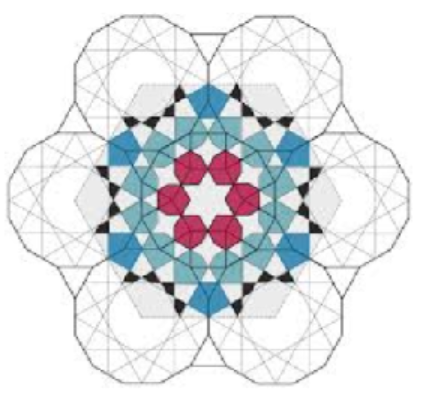
\includegraphics[width=\linewidth]{images/ch1-1.png}
\end{sbspanel}%
\end{sidebyside}%
\par
Circles and triangles are the simplest geometric figures. A circle is the simplest sort of curve, and a triangle is the simplest polygon -{}-{} the one with the fewest sides. Each has properties that makes it useful in many fields of endeavor.  A triangle is the most stable of polygons, because once its sides are fixed in length, its angles cannot change. A triangular truss bridge is a stable structure. A three-legged stool will not wobble.%
\begin{sidebyside}{2}{0}{0}{0}%
\begin{sbspanel}{0.5}%
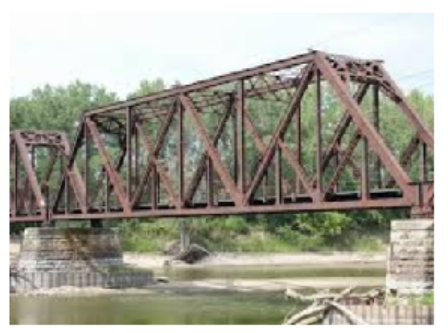
\includegraphics[width=\linewidth]{images/ch1-2.png}
\end{sbspanel}%
\begin{sbspanel}{0.5}%
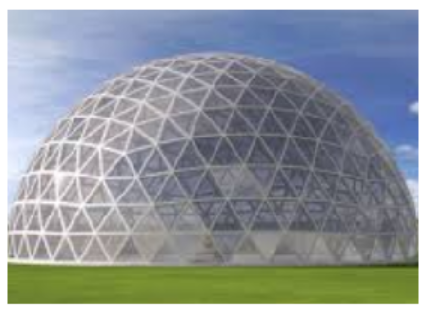
\includegraphics[width=\linewidth]{images/ch1-3.png}
\end{sbspanel}%
\end{sidebyside}%
\par
A circle encloses more area then any other figure of the same length, or perimeter, and a sphere encloses more space. A geodesic dome is a portion of a sphere constructed with triangles.  It has been called "the strongest, lightest and most efficient means of enclosing space known to man.”%
\par
Geodesic domes may also help us learn how to live on another planet. In 2017, the United Arab Emirates began construction on Mars Science City, a series of interconnecting geodesic domes designed to be a realistic model for living on Mars. The city will cover 1.9 million square feet, and its walls will be 3D-printed using sand from the desert.%
\begin{sidebyside}{1}{0.15}{0.15}{0}%
\begin{sbspanel}{0.7}%
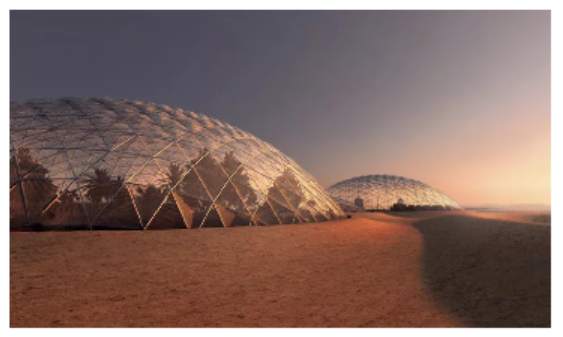
\includegraphics[width=\linewidth]{images/ch1-4.png}
\end{sbspanel}%
\end{sidebyside}%
\par
The city will contain laboratories to address food, sustainability, and energy issues all over the world. Finally, the project will implement an experiment wherein a team will spend a year living in the simulated planet for a year.%
\begin{sidebyside}{1}{0.15}{0.15}{0}%
\begin{sbspanel}{0.7}%
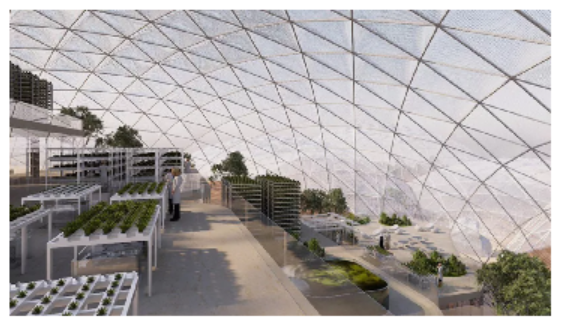
\includegraphics[width=\linewidth]{images/ch1-5.png}
\end{sbspanel}%
\end{sidebyside}%
\begin{activity}{Properties of Triangles.}{g:activity:idm46051688080288}%
%
\par
Materials:  You will need paper and pencil, scissors, a ruler and compass, and two plastic straws.%
\par
Prepare:  Cut the straw into pieces of lengths 2 inches, 3 inches, and 6 inches. Use the ruler to draw a large triangle, and cut it out.%
\par
%
\begin{enumerate}[label=\Alph*]
\item{}What do we know about the sides of a triangle?%
\par
%
\begin{enumerate}[label=\arabic*]
\item{}%
\begin{enumerate}[label=\alph*]
\item{}Can you make a triangle with sides of length 2 inches, 3 inches, and 6 inches?%
\item{}Use the pieces of length 2 inches and 3 inches to form two sides of a triangle. What happens to the length of the third side as you increase the angle between the first two sides?%
\item{}What is the longest that the third side could be? What is the smallest?%
\end{enumerate}
%
\item{}Two sides of a triangle are 6 centimeters and 8 centimeters long. What are the possible lengths of the third side?%
\item{}Two sides of a triangle are \(p\) units and \(q\) units long. What are the possible lengths of the third side?%
\end{enumerate}
%
\item{}What do we know about the angles of a triangle?%
\par
%
\begin{enumerate}[label=\arabic*]
\item{}Use a protractor to measure the three angles of the paper triangle in degrees. Now add up the three angles. What is their sum?%
\item{}Tear off the three corners of the triangle. Place them side-by-side with their vertices (tips) at the same point. What do you find?%
\item{}How are your answers to parts (1) and (2) related?%
\end{enumerate}
%
\item{}How are the sides and angles of a triangle related?%
\par
%
\begin{enumerate}[label=\arabic*]
\item{}A standard way to label a triangle is to call the angles \(A,~B,\) and \(C\). The side opposite angle \(A\) is called \(a\), the side opposite angle \(B\) is called \(b\), and the side opposite angle \(C\) is called \(c\). Sketch a triangle and label it with standard notation.%
\item{}Using a ruler, carefully draw a triangle and label it with standard notation so that \(a \gt b \gt c\). Now use a protractor to measure the angles and list them in order from largest to smallest. What do you observe?%
\item{}Using a ruler, carefully draw another triangle and label it with standard notation so that \(A \gt B \gt C\). Now use a ruler to measure the sides and list them in order from largest to smallest. What do you observe?%
\end{enumerate}
%
\item{}What do we know about right triangles?%
\par
%
\begin{enumerate}[label=\arabic*]
\item{}The side opposite the \(90\degree\) angle in a right triangle is called the \terminology{hypotenuse}. Why is the hypotenuse always the longest side of a right triangle?%
\item{}The Pythagorean theorem states that: \begin{sidebyside}{1}{0}{0}{0}%
\begin{sbspanel}{1}%
{\centering%
{\tabularfont%
\begin{tabular}{ll}
\multicolumn{1}{p{0.15\linewidth}}{\raggedright%
IF:%
}&\multicolumn{1}{p{0.8\linewidth}}{\raggedright%
\(a\), \(b\), and \(c\) are the sides of a right triangle, and \(c\) is the hypotenuse%
}\tabularnewline[0pt]
\multicolumn{1}{p{0.15\linewidth}}{\raggedright%
THEN: \(\qquad\)%
}&\(a^2+b^2=c^2\)
\end{tabular}
}%
\par}
\end{sbspanel}%
\end{sidebyside}%
 The "if" part of the theorem is called the \terminology{hypothesis}\index{hypothesis}, and the "then" part is called the \terminology{conclusion}\index{conclusion}.  The \terminology{converse}\index{converse} of a theorem is the new statement you obtain when you interchange the hypothesis and the conclusion.  Write the converse of the Pythagorean theorem.%
\item{}The converse of the Pythagorean theorem is also true. Use the converse to decide whether each of the following triangles is a right triangle. Support your conclusions with calculations.%
\begin{multicols}{2}
\begin{enumerate}[label=\alph*]
\item{}\(\displaystyle a = 9,~ b = 16,~ c = 25\)%
\item{}\(\displaystyle a = 12,~ b = 16,~ c = 20\)%
\item{}\(\displaystyle a = \sqrt{8},~ b = \sqrt{5},~ c = \sqrt{13}\)%
\item{}\(\displaystyle a = \dfrac{\sqrt{3}}{2},~ b = \dfrac{1}{2},~ c = 1\)%
\end{enumerate}
\end{multicols}
%
\end{enumerate}
%
\end{enumerate}
%
\end{activity}
\end{introduction}%
%
%
\typeout{************************************************}
\typeout{Section 1.1 Angles and Triangles}
\typeout{************************************************}
%
\begin{sectionptx}{Angles and Triangles}{}{Angles and Triangles}{}{}{x:section:AngTri}
\index{angle}%
\index{triangle}%
\begin{introduction}{}%
Historically, trigonometry began as the study of triangles and their properties.  Let's review some definitions and facts from geometry. \index{angle}\index{angle!straight}\index{angle!right}\index{right angle}\index{straight angle}%
\begin{itemize}[label=\textbullet]
\item{}We measure angles in degrees.%
\item{}One full rotation is \(360\degree\), as shown below.%
\item{}Half a full rotation is \(180\degree\) and is called a \terminology{straight angle}.%
\item{}One quarter of a full rotation is \(90\degree\) and is called a \terminology{right angle}.%
\end{itemize}
%
\begin{sidebyside}{1}{0.15}{0.15}{0}%
\begin{sbspanel}{0.7}%
\resizebox{\linewidth}{!}{%
\tikzset{%
  block/.style    = {draw, thick, rectangle, minimum height = 3em,
    minimum width = 3em},
  sum/.style      = {draw, circle, node distance = 2cm}, % Adder
  input/.style    = {coordinate}, % Input
  output/.style   = {coordinate} % Output
}

\begin{tikzpicture}[auto, thick, node distance=2cm]

    \filldraw[black] (0,0) circle (2pt) ;
    \draw[blue, thick] (0,0)rectangle (.25,.25);
    \draw [very thick, -> ] (0,0) -- (2,0);
    \draw[very thick, black!50!blue,->] (0,0) -- (0,2);
    \draw[red, thick, ->] (0.6,0) arc (0:90:.6) node [above right, midway] {$90 \degree$};


    \filldraw[black] (5,0) circle (2pt);
    %\draw[blue, thick] (5,0)rectangle (5.25,.25);
    \draw [very thick, -> ] (5,0) -- (7,0);
    \draw[very thick,black!50!blue, ->] (5,0) -- (3,0);
    \draw[red, thick, ->] (5.5,0) arc (0:180:.5) node [above , midway] {$180 \degree$};


    \filldraw[black] (8,0) circle (2pt);
    \draw[blue, thick] (8,0)rectangle (8.25,-.25);
    \draw [very thick, -> ] (8,0) -- (10,0);
    \draw[very thick,black!50!blue, ->] (8,0) -- (8,-2);
    \draw[red, thick, ->] (8.4,0) arc (0:270:.4) node [above left, midway] {$270 \degree$};


    \filldraw[black] (11,0) circle (2pt);
    %\draw[blue, thick] (5,0)rectangle (5.25,.25);
    \draw [very thick, -> ] (11,0) -- (13,0);
    \draw[very thick,black!50!blue, ->] (11,0) -- (13.2,0);
    \draw[red, thick, ->] (11.4,0) arc (0:360:.4) node [below right] {$360 \degree$};

\end{tikzpicture}
}%
\end{sbspanel}%
\end{sidebyside}%
\end{introduction}%
%
%
\typeout{************************************************}
\typeout{Subsection  Triangles}
\typeout{************************************************}
%
\begin{subsectionptx}{Triangles}{}{Triangles}{}{}{g:subsection:idm46051684748288}
\index{triangle}%
If you tear off the corners of any triangle and line them up, as shown below, they will always form a straight angle.%
\begin{sidebyside}{1}{0.2}{0.2}{0}%
\begin{sbspanel}{0.6}%
\resizebox{\linewidth}{!}{%
\tikzset{%
}
\begin{tikzpicture}
\coordinate (A) at (0,0);
\coordinate (B) at (4,0);
\coordinate (C) at (2.5,1.8);
\coordinate (D) at (2.5,-1.5);
\def\h{5};
\coordinate (S) at (\h,0);
\coordinate (Ap) at ($ (A) + (S)$);
\coordinate (Bp) at ($ (B) + (S)$);
\coordinate (Cp) at ($ (C) + (S)$);
\draw[black,  thick] (A) node[right, xshift=4mm, yshift=2mm]{$x$} -- (B) node[above left, xshift=-6]{$z$} -- (C) node[below, yshift=-3]{$y$} -- cycle;

\draw[gray!60,  thick, dashed] (Ap) node[right, xshift=4mm, yshift=2mm, text=blue!60]{$x$} -- (Bp) node[above left, xshift=-6, text=green!60]{$z$}-- (Cp) node[below, yshift=-3, text=black]{$y$} -- cycle;
\draw[blue!50,thick, dashed] (Ap)++(1.5,0) -- ++(-0.05,.2) -- ++(-.1, .06) -- ++(-0.18,.13)-- ++(-.01,.15)-- ++(-.12,.18);
\draw[green!50,thick, dashed] (Bp)++(-1.1,0)-- ++(0,.19)-- ++(.06,.01)-- ++(.1,.1)-- ++(.1,.02)-- ++(.02,.17)--++(.2,.2);

\draw[blue,thick] (A)++(1.5,0) -- ++(-0.05,.2) -- ++(-.1, .06) -- ++(-0.18,.13)-- ++(-.01,.15)-- ++(-.12,.18);
\draw[blue,thick] (Cp)++(-1.5,0) -- ++(0.05,-.2) -- ++(.1, -.06) -- ++(0.18,-.13)-- ++(.01,-.15)-- ++(.12,-.18);
\draw[black,thick] (Cp)++(-2,0) --(Cp) -- ++ (-1.04,-.72) ;

\draw[green,thick] (B)++(-1.1,0)-- ++(0,.19)-- ++(.06,.01)-- ++(.1,.1)-- ++(.1,.02)-- ++(.02,.17)--++(.21,.21);
\draw[green,thick] (Cp)++(1.1,0)-- ++(0,-.19)-- ++(-.06,-.01)-- ++(-.1,-.1)-- ++(-.1,-.02)-- ++(-.02,-.17)--++(-.21,-.21);
\draw[black,thick] (Cp)++(1.6,0) -- (Cp) -- ++(.77, -.896);
\draw[blue,->,>=stealth'] (.5,.6) arc ({180+atan(18/25)}:{atan(18/25)}:.8);
\draw[green,->,>=stealth'] (3.8,.6) arc ({-atan(18/15)}:{180-atan(18/15)}:.6);

\draw[magenta, thick] (C)++(-.8,-.8*18/25) -- ++(.1,-.2)-- ++(.3, -.16) -- ++(.1, .08)-- ++(.32,-.15)-- ++(.18,.08)-- ++(.27,.01)-- ++(.3,.02);
\draw[magenta] (Cp)++(-.8,-.8*18/25) -- ++(.1,-.2)-- ++(.3, -.16) -- ++(.1, .08)-- ++(.32,-.15)-- ++(.18,.08)-- ++(.27,.01)-- ++(.3,.02);
\node[below left, xshift=-4mm] at (Cp) {$x$};
\node[below right, xshift=4mm] at (Cp) {$z$};
\end{tikzpicture}
}%
\end{sbspanel}%
\end{sidebyside}%
\begin{assemblage}{Sum of angles in a triangle.}{g:assemblage:idm46051685312000}%
1.  The sum of the angles in a triangle is \(180\degree\).%
\end{assemblage}
\begin{example}{}{g:example:idm46051684828560}%
\begin{sidebyside}{2}{0.045}{0.045}{0.09}%
\begin{sbspanel}{0.55}[center]%
Two of the angles in the triangle at right are \(25\degree\) and \(115\degree\).  Find the third angle.%
\end{sbspanel}%
\begin{sbspanel}{0.27}[center]%
\resizebox{\linewidth}{!}{%
\tikzset{%
  block/.style    = {draw, thick, rectangle, minimum height = 3em,
    minimum width = 3em},
  sum/.style      = {draw, circle, node distance = 2cm}, % Adder
  input/.style    = {coordinate}, % Input
  output/.style   = {coordinate} % Output
}

\begin{tikzpicture}[auto, thick, node distance=2cm]

    \coordinate (A) at (0,0);
    \coordinate (B) at (5,0.7);
    \coordinate(C) at (3,2.1);
    \filldraw[black] (A) circle (.2pt) node[anchor=south west, xshift=19, yshift=3] {$25\degree$};
    \filldraw[black] (B) circle (.2pt) node[anchor=south east, xshift=-8, yshift=-3] {$x$};
    \filldraw[black] (C) circle (.2pt) node[anchor=north, yshift=-8] {$115\degree$};
    \draw[black,  thick] (A) -- (B) --( C) -- cycle;

\end{tikzpicture}
}%
\end{sbspanel}%
\end{sidebyside}%
\par\smallskip%
\noindent\textbf{\blocktitlefont Solution}.\label{g:solution:idm46051685598800}{}\hypertarget{g:solution:idm46051685598800}{}\quad{}To find the third angle, we write an equation.%
\par
%
\begin{align*}
x+25+115\amp =180 \amp \amp \blert{\text{Simpify the left side.}}\\
x+140\amp =180 \amp \amp \blert{\text{Subtract 140 from both sides.}}\\
x\amp =40   \amp \amp
\end{align*}
%
\par
The third angle is \(40\degree\).%
\end{example}
\begin{inlineexercise}{}{g:exercise:idm46051686032816}%
\begin{sidebyside}{2}{0.0325}{0.0325}{0.065}%
\begin{sbspanel}{0.6}[center]%
Find each of the angles in the triangle at right.%
\end{sbspanel}%
\begin{sbspanel}{0.27}[center]%
\resizebox{\linewidth}{!}{%
\tikzset{%
  block/.style    = {draw, thick, rectangle, minimum height = 3em,
    minimum width = 3em},
  sum/.style      = {draw, circle, node distance = 2cm}, % Adder
  input/.style    = {coordinate}, % Input
  output/.style   = {coordinate} % Output
}

\begin{tikzpicture}[auto, thick, node distance=2cm]

\coordinate (A) at (0,0);
\coordinate (B) at (5,0);
\coordinate(C) at (3,2.7);
\filldraw[black] (A) circle (.2pt) node[anchor=south west, xshift=12, yshift=1] {$x$};
\filldraw[black] (B) circle (.2pt) node[anchor=south east, xshift=-8, yshift=1] {$2x-15$};
\filldraw[black] (C) circle (.2pt) node[anchor=north, yshift=-8]{$2x$};
\draw[black,  thick] (A) -- (B) --( C) -- cycle;

\end{tikzpicture}
}%
\end{sbspanel}%
\end{sidebyside}%
\par\smallskip%
\noindent\textbf{\blocktitlefont Answer}.\label{g:answer:idm46051686557200}{}\hypertarget{g:answer:idm46051686557200}{}\quad{}\(x=39\degree,~~2x=78\degree, ~~2x-15=63\degree\)%
\end{inlineexercise}
Some special categories of triangles are particularly useful.  Most important of these are the \terminology{right triangles}.%
\begin{assemblage}{Right triangle.}{g:assemblage:idm46051686783792}%
2.  A right triangle has one angle of \(90\degree\).%
\end{assemblage}
\begin{example}{}{g:example:idm46051687512192}%
\begin{sidebyside}{2}{0.0825}{0.0825}{0.165}%
\begin{sbspanel}{0.5}[center]%
One of the smaller angles of a right triangle is \(34\degree\).  What is the third angle?%
\end{sbspanel}%
\begin{sbspanel}{0.17}[center]%
\resizebox{\linewidth}{!}{%
\tikzset{%
  block/.style    = {draw, thick, rectangle, minimum height = 3em,
    minimum width = 3em},
  sum/.style      = {draw, circle, node distance = 2cm}, % Adder
  input/.style    = {coordinate}, % Input
  output/.style   = {coordinate} % Output
}

\begin{tikzpicture}[auto, thick, node distance=2cm]

    \coordinate (A) at (0,0);
    \coordinate (B) at (3,0);
    \coordinate(C) at (0,4);
    \filldraw[black] (A) circle (.2pt) node[anchor=south west, xshift=10, yshift=1]{};
    \filldraw[black] (B) circle (.2pt) node[anchor=south east, xshift=-8, yshift=1]{$x$};
    \filldraw[black] (C) circle (.2pt) node[anchor=north west, yshift=-23]{$34\degree$};
    \draw[black,  thick] (A) -- (B) --( C) -- cycle;
    \draw[blue, thick] (0,0)rectangle (.25,.25);

\end{tikzpicture}
}%
\end{sbspanel}%
\end{sidebyside}%
\par\smallskip%
\noindent\textbf{\blocktitlefont Solution}.\label{g:solution:idm46051687660176}{}\hypertarget{g:solution:idm46051687660176}{}\quad{}The sum of the two smaller angles in a right triangle is \(90\degree\). So%
\par
%
\begin{align*}
x+34\amp =90 \amp \amp \blert{\text{Subtract 34 from both sides.}}\\
x\amp =56   \amp \amp
\end{align*}
%
\par
The unknown angle must be \(56\degree\).%
\end{example}
\begin{inlineexercise}{}{g:exercise:idm46051688199584}%
Two angles of a triangle are \(35\degree\) and \(45\degree\).  Can it be a right triangle?%
\par\smallskip%
\noindent\textbf{\blocktitlefont Answer}.\label{g:answer:idm46051701484928}{}\hypertarget{g:answer:idm46051701484928}{}\quad{}No%
\end{inlineexercise}
An \terminology{equilateral}\index{equilateral triangle}\index{triangle!equilateral}\index{triangle!equilateral|seealso{equilateral triangle}} triangle has all three sides the same length.%
\begin{assemblage}{Angles of equilateral triangle.}{g:assemblage:idm46051696561088}%
3.  All of the angles of an equilateral triangle are equal.%
\end{assemblage}
\begin{example}{}{g:example:idm46051702192656}%
\begin{sidebyside}{2}{0.06}{0.06}{0.12}%
\begin{sbspanel}{0.6}[center]%
All three sides of a triangle are 4 feet long.  Find the angles.%
\end{sbspanel}%
\begin{sbspanel}{0.16}[center]%
\resizebox{\linewidth}{!}{%
\tikzset{%
  block/.style    = {draw, thick, rectangle, minimum height = 3em,
    minimum width = 3em},
  sum/.style      = {draw, circle, node distance = 2cm}, % Adder
  input/.style    = {coordinate}, % Input
  output/.style   = {coordinate} % Output
}

\begin{tikzpicture}[auto, thick, node distance=2cm]

    \coordinate (A) at (0,0);
    \coordinate (B) at (2.5,0);
    \coordinate(C) at (1.25,2.165);
    \filldraw[black] (A) circle (.2pt) node[anchor=south west, xshift=10, yshift=1]{$x$};
    \filldraw[black] (B) circle (.2pt) node[anchor=south east, xshift=-8, yshift=1]{$x$};
    \filldraw[black] (C) circle (.2pt) node[anchor=north , yshift=-10]{$x$};
    %\draw[black,  thick] (A) -- (B) --( C) -- cycle;
    \draw[black] (A) --  (B) node [below, midway] {$4$};
    \draw[black] (A) --  (C) node [above left, midway,yshift=-4] {$4$};
    \draw[black] (C) --  (B) node [above right, midway,yshift=-4] {$4$};

\end{tikzpicture}
}%
\end{sbspanel}%
\end{sidebyside}%
\par\smallskip%
\noindent\textbf{\blocktitlefont Solution}.\label{g:solution:idm46051702499120}{}\hypertarget{g:solution:idm46051702499120}{}\quad{}The triangle is equilateral, so all of its angles are equal.  Thus%
\par
%
\begin{align*}
3x\amp =180 \amp \amp \blert{\text{Divide both sides by 3.}}\\
x\amp =60   \amp \amp  
\end{align*}
%
\par
Each of the angles is \(60\degree\).%
\end{example}
\begin{inlineexercise}{}{g:exercise:idm46051702598576}%
\begin{sidebyside}{2}{0.085}{0.085}{0.17}%
\begin{sbspanel}{0.5}[center]%
Find \(x\), \(y\), and \(z\) in the triangle at right.%
\end{sbspanel}%
\begin{sbspanel}{0.16}[center]%
\resizebox{\linewidth}{!}{%
\tikzset{%
  block/.style    = {draw, thick, rectangle, minimum height = 3em,
    minimum width = 3em},
  sum/.style      = {draw, circle, node distance = 2cm}, % Adder
  input/.style    = {coordinate}, % Input
  output/.style   = {coordinate} % Output
}

\begin{tikzpicture}[auto, thick, node distance=2cm]

    \coordinate (A) at (0,0);
    \coordinate (B) at (2.5,0);
    \coordinate(C) at (1.25,2.165);
    \filldraw[black] (A) circle (.2pt) node[anchor=south west, xshift=10, yshift=1]{$60\degree$};
    \filldraw[black] (B) circle (.2pt) node[anchor=south east, xshift=-8, yshift=1]{$x$};
    \filldraw[black] (C) circle (.2pt) node[anchor=north , yshift=-15]{$60\degree$};
    \draw[black] (A) --  (B) node [below, midway] {$z$};
    \draw[black] (A) --  (C) node [above left, midway,yshift=-4] {$y$};
    \draw[black] (C) --  (B) node [above right, midway,yshift=-4] {$8$};

\end{tikzpicture}
}%
\end{sbspanel}%
\end{sidebyside}%
\par\smallskip%
\noindent\textbf{\blocktitlefont Answer}.\label{g:answer:idm46051696363280}{}\hypertarget{g:answer:idm46051696363280}{}\quad{}\(x=60\degree, ~y=8, ~z=8\)%
\end{inlineexercise}
An \terminology{isosceles}\index{isosceles triangle}\index{triangle!isosceles}\index{triangle!isosceles|seealso{isosceles triangle}} triangle has two sides of equal length.  The angle between the equal sides is the \terminology{vertex angle}\index{vertex angle!of an isosceles triangle}. The other two angles are the \terminology{base angles}.%
\begin{assemblage}{Base angles of an isosceles triangle.}{g:assemblage:idm46051695999840}%
4.  The base angles of an isosceles triangle are equal.%
\end{assemblage}
\begin{example}{}{g:example:idm46051695861424}%
\begin{sidebyside}{2}{0.045}{0.045}{0.09}%
\begin{sbspanel}{0.5}[center]%
Find \(x\) and \(y\) in the triangle at right.%
\end{sbspanel}%
\begin{sbspanel}{0.32}[center]%
\resizebox{\linewidth}{!}{%
\tikzset{%
  block/.style    = {draw, thick, rectangle, minimum height = 3em,
    minimum width = 3em},
  sum/.style      = {draw, circle, node distance = 2cm}, % Adder
  input/.style    = {coordinate}, % Input
  output/.style   = {coordinate} % Output
}

\begin{tikzpicture}[auto, thick, node distance=2cm]

    \coordinate (A) at (0,0);
    \coordinate (B) at (4.7,0);
    \coordinate(C) at (2.35,1.5);
    \filldraw[black] (A) circle (.2pt) node[anchor=south west, xshift=18]{$y$};
    \filldraw[black] (B) circle (.2pt) node[anchor=south east, xshift=-18]{$38\degree$};
    \filldraw[black] (C) circle (.2pt) node[anchor=north , yshift=-3]{$x$};
    %\draw[black,  thick] (A) -- (B) --( C) -- cycle;
    \draw[black] (A) --  (B) node [below, midway] {};
    \draw[black] (A) --  (C) node [above left, midway,yshift=-4] {$12$};
    \draw[black] (C) --  (B) node [above right, midway,yshift=-4] {$12$};

\end{tikzpicture}
}%
\end{sbspanel}%
\end{sidebyside}%
\par\smallskip%
\noindent\textbf{\blocktitlefont Solution}.\label{g:solution:idm46051688977760}{}\hypertarget{g:solution:idm46051688977760}{}\quad{}The triangle is isosceles, so the base angles are equal.  Therefore, \(y=38\degree\).  To find the vertex angle, we solve%
\par
%
\begin{align*}
x+38+38\amp =180 \amp \amp \\
x+76\amp =180 \amp \amp \blert{\text{Subtract 76 from both sides.}}\\
x\amp =104   \amp \amp 
\end{align*}
%
\par
The vertex angle is \(104\degree\).%
\end{example}
\begin{inlineexercise}{}{g:exercise:idm46051689551568}%
\begin{sidebyside}{2}{0.0375}{0.0375}{0.075}%
\begin{sbspanel}{0.5}[center]%
Find \(x\) and \(y\) in the figure at right.%
\end{sbspanel}%
\begin{sbspanel}{0.35}[center]%
\resizebox{\linewidth}{!}{%
\tikzset{%
  block/.style    = {draw, thick, rectangle, minimum height = 3em,
    minimum width = 3em},
  sum/.style      = {draw, circle, node distance = 2cm}, % Adder
  input/.style    = {coordinate}, % Input
  output/.style   = {coordinate} % Output
}
\begin{tikzpicture}[auto, thick, node distance=2cm]
    \coordinate (A) at (0,0);
    \coordinate (B) at (5.6,0);
    \coordinate(C) at (2.8,1.2);
    \filldraw[black] (A) circle (.2pt) node[anchor=south west, xshift=28]{$20\degree$};
    \filldraw[black] (B) circle (.2pt) node[anchor=south east, xshift=-28]{$20\degree$};
    \filldraw[black] (C) circle (.2pt) node[anchor=north , yshift=-2]{$x$};
    %\draw[black,  thick] (A) -- (B) --( C) -- cycle;
    \draw[black] (A) --  (B) node [below, midway] {};
    \draw[black] (A) --  (C) node [above left, midway,yshift=-2] {$9$};
    \draw[black] (C) --  (B) node [above right, midway,yshift=-2] {$y$};
\end{tikzpicture}
}%
\end{sbspanel}%
\end{sidebyside}%
\par\smallskip%
\noindent\textbf{\blocktitlefont Answer}.\label{g:answer:idm46051690023376}{}\hypertarget{g:answer:idm46051690023376}{}\quad{}\(x=140\degree,~y=9\)%
\end{inlineexercise}
\end{subsectionptx}
%
%
\typeout{************************************************}
\typeout{Subsection  Angles}
\typeout{************************************************}
%
\begin{subsectionptx}{Angles}{}{Angles}{}{}{g:subsection:idm46051690158832}
\index{angle}%
In addition to the facts about triangles reviewed above, there are several useful properties of angles. \index{supplementary angles}\index{complementary angles}\index{acute angle}\index{obtuse angle}%
\begin{itemize}[label=\textbullet]
\item{}Two angles that add to \(180\degree\) are called \terminology{supplementary}\index{supplementary angles}\index{angle!supplementary}\index{angle!supplementary|seealso{supplementary angles}}.%
\item{}Two angles that add to \(90\degree\) are called \terminology{complementary}\index{complementary angles}\index{angle!complementary}\index{angle!complementary|seealso{complementary angles}}.%
\item{}Angles between \(0\degree\) and \(90\degree\) are called \terminology{acute}\index{acute angle}\index{angle!acute}\index{angle!acute|seealso{acute angle}}.%
\item{}Angles between \(90\degree\) and \(180\degree\) are called \terminology{obtuse}\index{obtuse angle}\index{angle!obtuse}\index{angle!obtuse|seealso{obtuse angle}}.%
\end{itemize}
%
\begin{sidebyside}{1}{0.05}{0.05}{0}%
\begin{sbspanel}{0.9}%
\resizebox{\linewidth}{!}{%
\tikzset{%
}
\begin{tikzpicture}
%supplementary
\coordinate (O) at (0,0);
\coordinate (A) at (-2,0);
\coordinate (B) at (2,0);
\coordinate(C) at (1.65,1);

\filldraw[blue] (O) circle (.2pt) node[anchor=north]{supplementary angles};

\draw[black, thick, <->] (A)--(B); 
\draw[black, thick, ->] (O)--(C); 
\draw[red, thick, ->] (.7,0) arc (0:30:.7);
\draw[red, thick, ->] (.41,.25) arc (30:180:.5);

%complementary
\coordinate (O2) at (3.5,0);
\coordinate (A2) at (5.5,0);
\coordinate (B2) at (3.5,2);
\coordinate(C2) at (4.65,1.64);

%\filldraw[blue] (O) circle (.2pt) node[anchor=north]{complementary angles};

\draw[black, thick, ->] (O2)--(A2)  node[below,midway ]{\color{blue}complementary angles}; 
\draw[black, thick, ->] (O2)--(B2); 
\draw[black, thick, ->] (O2)--(C2); 
\draw[red, thick, ->] (4.2,0) arc (0:55:.7);
\draw[red, thick, ->] (3.78,.41) arc (55:90:.5);

%acute
\coordinate (O3) at (7,0);
\coordinate (A3) at (9,0);
\coordinate (B3) at (8,1.73);

%\filldraw[blue] (O) circle (.2pt) node[anchor=north]{complementary angles};

\draw[black, thick, ->] (O3)--(A3)  node[below,midway ]{\color{blue}acute angle}; 
\draw[black, thick, ->] (O3)--(B3); 
\draw[red, thick, ->] (7.7,0) arc (0:60:.7);

%obtuse
\coordinate (O4) at (11.2,0);
\coordinate (A4) at (13.,0);
\coordinate (B4) at (9.67,1.29);

\filldraw[blue] (O4) circle (.2pt) node[anchor=north]{obtuse angle};

\draw[black, thick, ->] (O4)--(A4); 
\draw[black, thick, ->] (O4)--(B4); 
\draw[red, thick, ->] (11.7,0) arc (0:140:.5);
\end{tikzpicture}
}%
\end{sbspanel}%
\end{sidebyside}%
\begin{example}{}{g:example:idm46051693776400}%
\begin{sidebyside}{2}{0.025}{0.025}{0.05}%
\begin{sbspanel}{0.6}%
In the figure at right,%
\begin{itemize}[label=\textbullet]
\item{}\(\angle\)\(AOC\) and \(\angle\)\(BOC\) are supplementary.%
\item{}\(\angle\)\(DOE\) and \(\angle\)\(BOE\) are complementary.%
\item{}\(\angle\)\(AOC\) is obtuse,%
\item{}and \(\angle\)\(BOC\) is acute.%
\end{itemize}
%
\end{sbspanel}%
\begin{sbspanel}{0.3}%
\resizebox{\linewidth}{!}{%
\tikzset{%
  block/.style    = {draw, thick, rectangle, minimum height = 3em,
    minimum width = 3em},
  sum/.style      = {draw, circle, node distance = 2cm}, % Adder
  input/.style    = {coordinate}, % Input
  output/.style   = {coordinate} % Output
}
\begin{tikzpicture}[auto, thick, node distance=2cm]
    \coordinate (O) at (0,0);
    \coordinate (A) at (-2,0);
    \coordinate (B) at (2,0);
    \coordinate(C) at (.7,1.2);
    \coordinate (D) at (0,-1.7);
    \coordinate(E) at (1.8,-.5);
    \draw[blue, thick] (O)rectangle (-.25,-.25);
    \filldraw[black] (O) circle (.2pt) node[anchor=south east]{$O$};
    \filldraw[black] (A) circle (.2pt) node[anchor=east]{$A$};
    \filldraw[black] (B) circle (.2pt) node[anchor=west]{$B$};
    \filldraw[black] (C) circle (.2pt) node[anchor=south west]{$C$};
    \filldraw[black] (D) circle (.2pt) node[anchor=north west]{$D$};
    \filldraw[black] (E) circle (.2pt) node[anchor=north west]{$E$};
    %\draw[black,  thick] (A) -- (B) --( C) -- cycle;
    \draw[black] (A) --  (O) --  (B);
    \draw[black] (O) --  (C) ;
    \draw[black] (O) --  (D) ;
    \draw[black] (O) --  (E) ;
\end{tikzpicture}
}%
\end{sbspanel}%
\end{sidebyside}%
\end{example}
In trigonometry we often use lower-case Greek letters to represent unknown angles (or, more specifically, the measure of the angle in degrees).  In the next Exercise, we use the Greek letters \(\alpha\) (alpha), \(\beta\) (beta), and \(\gamma\) (gamma).%
\begin{inlineexercise}{}{g:exercise:idm46051694678384}%
In the figure, \(\alpha\), \(\beta\), and \(\gamma\) denote the measures of the angles in degrees.%
\begin{sidebyside}{2}{0}{0.1}{0}%
\begin{sbspanel}{0.6}[center]%
%
\begin{enumerate}[label=\alph*]
\item{}Find the measure of angle \(\alpha\).%
\item{}Find the measure of angle \(\beta\).%
\item{}Find the measure of angle \(\gamma\).%
\item{}What do you notice about the measures of the angles?%
\end{enumerate}
%
\end{sbspanel}%
\begin{sbspanel}{0.3}[center]%
\resizebox{\linewidth}{!}{%
\tikzset{%
  block/.style    = {draw, thick, rectangle, minimum height = 3em,
    minimum width = 3em},
  sum/.style      = {draw, circle, node distance = 2cm}, % Adder
  input/.style    = {coordinate}, % Input
  output/.style   = {coordinate} % Output
}
\begin{tikzpicture}[auto, thick, node distance=2cm]
    \coordinate (O) at (0,0);
    \coordinate (A) at (-2,0);
    \coordinate (B) at (2,0);
    \coordinate(C) at (-1.157,-1.3789);
    \coordinate (D) at (1.157,1.3789);
    \filldraw[black] (O) circle (.2pt) node[anchor=south east]{$\alpha$};
    \filldraw[black] (O) circle (.2pt) node[anchor=north east, xshift=-10]{$\beta$};
    \filldraw[black] (O) circle (.2pt) node[anchor=north west, yshift=0]{$\gamma$};
    \filldraw[black] (O) circle (.2pt) node[anchor=south west, xshift=9]{$50\degree$};
    \draw[black] (A) --  (B);
    \draw[black] (C) --  (D) ;
\end{tikzpicture}
}%
\end{sbspanel}%
\end{sidebyside}%
\par\smallskip%
\noindent\textbf{\blocktitlefont Answer}.\label{g:answer:idm46051714062352}{}\hypertarget{g:answer:idm46051714062352}{}\quad{}\(\alpha=130\degree, ~\beta=50\degree, ~\gamma=130\degree.\) The non-adjacent angles are equal.%
\end{inlineexercise}
Non-adjacent angles formed by the intersection of two straight lines are called \terminology{vertical angles}\index{vertical angles}\index{angle!vertical}\index{angle!vertical|seealso{vertical angles}}.  In the previous exercise, the angles labeled \(\alpha\) and \(\gamma\) are vertical angles, as are the angles labeled \(\beta\) and \(50\degree\).%
\begin{assemblage}{Vertical Angles.}{g:assemblage:idm46051702144976}%
5.  Vertical angles are equal.%
\end{assemblage}
\begin{example}{}{g:example:idm46051695882896}%
\begin{sidebyside}{2}{0}{0.15}{0.05}%
\begin{sbspanel}{0.6}[center]%
Explain why \(\alpha=\beta\) in the triangle at right.%
\end{sbspanel}%
\begin{sbspanel}{0.2}[center]%
\resizebox{\linewidth}{!}{%
\tikzset{%
  block/.style    = {draw, thick, rectangle, minimum height = 3em,
    minimum width = 3em},
  sum/.style      = {draw, circle, node distance = 2cm}, % Adder
  input/.style    = {coordinate}, % Input
  output/.style   = {coordinate} % Output
}
\begin{tikzpicture}[auto, thick, node distance=2cm]

    \coordinate (A) at (-.6,0);
    \coordinate (B) at (0.6,0);
    \coordinate(C) at (-.6,0);
    \coordinate (D) at (0.6,0);
    \filldraw[black] (A) circle (.2pt) node[anchor=south west, xshift=2]{$\theta$};
    \filldraw[black] (B) circle (.2pt) node[anchor=south east, xshift=-3]{$\phi$};
    \filldraw[black] (C) circle (.2pt) node[anchor=north east, xshift=-2]{$\alpha$};
    \filldraw[black] (D) circle (.2pt) node[anchor=north west, xshift=3]{$\beta$};
    \draw[black,  thick] (-1.5,0) -- (1.5,0);
    \draw[black] (-.8,-.6) --  (0,1.8);
    \draw[black] (0.8,-0.6) --  (0,1.8) ;
    \draw[blue] (-.48,.86) -- (-.15,.75);
    \draw[blue] (.48,.86) -- (.15,.75);

\end{tikzpicture}
}%
\end{sbspanel}%
\end{sidebyside}%
\par\smallskip%
\noindent\textbf{\blocktitlefont Solution}.\label{g:solution:idm46051696733808}{}\hypertarget{g:solution:idm46051696733808}{}\quad{}Because they are the base angles of an isosceles triangle, \(\theta\) (theta) and \(\phi\) (phi) are equal. Also, \(\alpha=\theta\) because they are vertical angles, and similarly \(\beta=\phi\). Therefore, \(\alpha=\beta\) because they are equal to equal quantities.%
\end{example}
\begin{inlineexercise}{}{g:exercise:idm46051696915600}%
\begin{sidebyside}{2}{0.05}{0.05}{0.1}%
\begin{sbspanel}{0.5}[center]%
Find all the unknown angles in the figure at right. (You will find a list of all the Greek letters and their names at the end of this section.)%
\end{sbspanel}%
\begin{sbspanel}{0.3}[center]%
\resizebox{\linewidth}{!}{%
\tikzset{%
  block/.style    = {draw, thick, rectangle, minimum height = 3em,
    minimum width = 3em},
  sum/.style      = {draw, circle, node distance = 2cm}, % Adder
  input/.style    = {coordinate}, % Input
  output/.style   = {coordinate} % Output
}
\begin{tikzpicture}[auto, thick, node distance=2cm]
    \coordinate (A) at (-1.8,0);
    \coordinate (B) at (0.7,0);
    \coordinate (C) at (0,1.50);
    \filldraw[black] (A) circle (.2pt) node[anchor=south east, xshift=4]{$\beta$};
    \filldraw[black] (A) circle (.2pt) node[anchor=south west, xshift=10]{$40\degree$};
    \filldraw[black] (B) circle (.2pt) node[anchor=south east, xshift=-5]{$\delta$};
    \filldraw[black] (A) circle (.2pt) node[anchor=north east, xshift=-10]{$\alpha$};
    \filldraw[black] (B) circle (.2pt) node[anchor=south west, xshift=-3]{$115\degree$};
    \filldraw[black] (C) circle (.2pt) node[anchor=north,xshift=-3, yshift=-5]{$\gamma$};
    \draw[black,  thick] (-3.5,0) -- (1.5,0);
    \draw[black] (-2.4,-.5) --  (0,1.5);
    \draw[black] (B) --  (0,1.5) ;
\end{tikzpicture}
}%
\end{sbspanel}%
\end{sidebyside}%
\par\smallskip%
\noindent\textbf{\blocktitlefont Answer}.\label{g:answer:idm46051697216704}{}\hypertarget{g:answer:idm46051697216704}{}\quad{}\(\alpha=40\degree,~ \beta=140\degree,~ \gamma=75\degree, \delta=65\degree\)%
\end{inlineexercise}
A line that intersects two parallel lines forms eight angles, as shown in the figure below. There are four pairs of vertical angles, and four pairs of \terminology{corresponding angles}\index{corresponding angles}\index{angle!corresponding}\index{angle!corresponding|seealso{corresponding angles}}, or angles in the same position relative to the transversal on each of the parallel lines.%
\begin{sidebyside}{2}{0}{0.05}{0.05}%
\begin{sbspanel}{0.6}[center]%
For example, the angles labeled 1 and 5 are corresponding angles, as are the angles labeled 4 and 8. Finally, angles 3 and 6 are called \terminology{alternate interior angles}\index{alternate interior angles}\index{angle!alternate interior}\index{angle!alternate interior|seealso{alternate interior angles}}, and so are angles 4 and 5.%
\end{sbspanel}%
\begin{sbspanel}{0.3}[center]%
\resizebox{\linewidth}{!}{%
\tikzset{%
  block/.style    = {draw, thick, rectangle, minimum height = 3em,
    minimum width = 3em},
  sum/.style      = {draw, circle, node distance = 2cm}, % Adder
  input/.style    = {coordinate}, % Input
  output/.style   = {coordinate} % Output
}
\begin{tikzpicture}[auto, thick, node distance=2cm]
    \coordinate (A) at (.6,1.8);
    \coordinate (B) at (-.6,0);
    \filldraw[black] (A) circle (.2pt) node[anchor=south east, xshift=3]{$1$};
    \filldraw[black] (A) circle (.2pt) node[anchor=south west, xshift=7]{$2$};
    \filldraw[black] (A) circle (.2pt) node[anchor=north east, xshift=-5]{$3$};
    \filldraw[black] (A) circle (.2pt) node[anchor=north west, xshift=-1]{$4$};
    \filldraw[black] (B) circle (.2pt) node[anchor=south east, xshift=5]{$5$};
    \filldraw[black] (B) circle (.2pt) node[anchor=south west, xshift=7]{$6$};
    \filldraw[black] (B) circle (.2pt) node[anchor=north east, xshift=-5]{$7$};
    \filldraw[black] (B) circle (.2pt) node[anchor=north west, xshift=-1]{$8$};
    \draw[black,  thick] (-2.5,1.8) -- (2.5,1.8);
    \draw[black,  thick] (-2.5,0) -- (2.5,0);
    \draw[black,  thick, ->] (-2.5,1.8) -- (2.,1.8);
    \draw[black,  thick, ->] (-2.5,0) -- (2.,0);
    \draw[black, thick] (-1.2,-.9) --  (1.2,2.7) ;

\end{tikzpicture}
}%
\end{sbspanel}%
\end{sidebyside}%
\begin{assemblage}{Paralles lines cut by a transversal.}{g:assemblage:idm46051698049392}%
6.  If parallel lines are intersected by a transversal, the alternate interior angles are equal.  Corresponding angles are also equal.%
\end{assemblage}
\begin{example}{}{g:example:idm46051701042576}%
\begin{sidebyside}{2}{0.025}{0.025}{0.05}%
\begin{sbspanel}{0.55}[center]%
The parallelogram \(ABCD\) shown at right is formed by the intersection of two sets of parallel lines.  Show that the opposite angles of the parallelogram are equal.%
\end{sbspanel}%
\begin{sbspanel}{0.35}[center]%
\resizebox{\linewidth}{!}{%
\tikzset{%
  block/.style    = {draw, thick, rectangle, minimum height = 3em,
    minimum width = 3em},
  sum/.style      = {draw, circle, node distance = 2cm}, % Adder
  input/.style    = {coordinate}, % Input
  output/.style   = {coordinate} % Output
}
\begin{tikzpicture}[auto, thick, node distance=2cm]
    \coordinate (A) at (0,0);
    \coordinate (B) at (.4,1.6);
    \coordinate (C) at( 4.4,1.6);
    \coordinate (D) at (4,0);
    \filldraw[black] (A) circle (.2pt) node[anchor=north east, xshift=-2]{$A$};
    \filldraw[black] (B) circle (.2pt) node[anchor=south east, xshift=0]{$B$};
    \filldraw[black] (C) circle (.2pt) node[anchor=south west, xshift=2]{$C$};
    \filldraw[black] (D) circle (.2pt) node[anchor=north west, xshift=-2]{$D$};
    \filldraw[black] (D) circle (.2pt) node[anchor=south east, xshift=-1]{$4$};
    \filldraw[black] (C) circle (.2pt) node[anchor=north east, xshift=-2]{$3$};
    \filldraw[black] (C) circle (.2pt) node[anchor=north west, xshift=0]{$5$};
    \filldraw[black] (A) circle (.2pt) node[anchor=south west, xshift=3]{$1$};
    \filldraw[black] (B) circle (.2pt) node[anchor=north east, xshift=-5]{$2$};
    \filldraw[black] (B) circle (.2pt) node[anchor=north west, xshift=-1]{$6$};
    \draw[black,  thick] (-.9,1.6) -- (4.9,1.6);
    \draw[black,  thick] (-.9,0) -- (4.9,0);
    \draw[black,  thick, ->] (-.5,1.6) -- (2.,1.6);
    \draw[black,  thick, ->] (-.5,0) -- (2.3,0);
    \draw[black,  thick, ->] (-.5,1.6) -- (2.3,1.6);
    \draw[black,  thick, ->] (-.5,0) -- (2.,0);
    \draw[black, thick] (-.2,-.8) --  (.6,2.4) ;
    \draw[black, thick] (3.8,-.8) --  (4.6,2.4) ;
    \draw[black, thick, ->] (-.2,-.8) --  (.2,.8) ;
    \draw[black, thick, ->] (3.8,-.8) --  (4.2,.8) ;
\end{tikzpicture}
}%
\end{sbspanel}%
\end{sidebyside}%
\par\smallskip%
\noindent\textbf{\blocktitlefont Solution}.\label{g:solution:idm46051716294384}{}\hypertarget{g:solution:idm46051716294384}{}\quad{}Angles 1 and 2 are equal because they are alternate interior angles, and angles 2 and 3 are equal because they are corresponding angles.  Therefore angles 1 and 3, the opposite angles of the parallelogram, are equal. Similarly, you can show that angles 4, 5, and 6 are equal.%
\end{example}
\begin{inlineexercise}{}{g:exercise:idm46051716247024}%
Show that the adjacent angles of a parallelogram are supplementary.  (You can use angles 1 and 4 in the parallelogram of the previous example.)%
\par\smallskip%
\noindent\textbf{\blocktitlefont Answer}.\label{g:answer:idm46051716190608}{}\hypertarget{g:answer:idm46051716190608}{}\quad{}Note that angles 2 and 6 are supplementary because they form a straight angle. Angle 1 equals angle 2 because they are alternate interior angles, and similarly angle 4 equals angle 5. Angle 5 equals angle 6 because they are corresponding angles. Thus, angle 4 equals angle 6, and angle 1 equals angle 2. So angles 4 and 1 are supplementary because 2 and 6 are.%
\end{inlineexercise}
\begin{note}{}{g:note:idm46051716378976}%
In the Section 1.1 Summary, you will find a list of vocabulary words and a summary of the facts from geometry that we reviewed in this section.  You will also find a set of study questions to test your understanding, and a list of skills to practice in the homework problems.%
\end{note}
\begin{tableptx}{\textbf{Lower Case Letters in the Greek Alphabet}}{g:table:idm46051716126432}{}%
\centering
\index{Greek alphabet}%
{\tabularfont%
\begin{tabular}{AlAlAlA}\hrulethick
\multicolumn{3}{AcA}{Greek Alphabet}\tabularnewline\hrulethin
\(\alpha~~~~\text{alpha}\)&\(\beta~~~~\text{beta}\)&\(\gamma~~~~\text{gamma}\)\tabularnewline\hrulethin
\(\delta~~~~\text{delta}\)&\(\epsilon~~~~\text{epsilon}\)&\(\gamma~~~~\text{gamma}\)\tabularnewline\hrulethin
\(\eta~~~~\text{eta}\)&\(\theta~~~~\text{theta}\)&\(\iota~~~~\text{iota}\)\tabularnewline\hrulethin
\(\kappa~~~~\text{kappa}\)&\(\lambda~~~~\text{lambda}\)&\(\mu~~~~\text{mu}\)\tabularnewline\hrulethin
\(\nu~~~~\text{nu}\)&\(\xi~~~~\text{xi}\)&\(o~~~~\text{omicron}\)\tabularnewline\hrulethin
\(\pi~~~\text{pi}\)&\(\rho~~~~\text{rho}\)&\(\sigma~~~~\text{sigma}\)\tabularnewline\hrulethin
\(\tau~~~~\text{tau}\)&\(\upsilon~~~~\text{upsilon}\)&\(\phi~~~~\text{phi}\)\tabularnewline\hrulethin
\(\chi~~~\text{chi}\)&\(\psi~~~\text{psi}\)&\(\omega~~~\text{omega}\)\tabularnewline\hrulethin
\end{tabular}
}%
\end{tableptx}%
Review the following skills you will need for this section.%
\begin{project}{}{g:project:idm46051700263232}%
\begin{sidebyside}{1}{0}{0}{0}%
\begin{sbspanel}{1}%
Solve the equation.%
\end{sbspanel}%
\end{sidebyside}%
\begin{sidebyside}{2}{0}{0}{0}%
\begin{sbspanel}{0.5}%
1. \(x-8=19-2x\vphantom{\dfrac{1}{2}}\)%
\par
3. \(13x+5=2x-28\)%
\end{sbspanel}%
\begin{sbspanel}{0.5}%
2. \(2x-9=12-x\vphantom{\dfrac{1}{2}}\)%
\par
4. \(4+9x=-7+x\)%
\end{sbspanel}%
\end{sidebyside}%
\begin{sidebyside}{1}{0}{0.05}{0}%
\begin{sbspanel}{0.95}%
Solve the system.%
\end{sbspanel}%
\end{sidebyside}%
\begin{sidebyside}{2}{0}{0}{0}%
\begin{sbspanel}{0.5}%
5. \(\begin{aligned}[t]
5x-2y\amp =-13 \amp \amp \\
2x+3y\amp =-9 \amp \amp \\ \\
\end{aligned}\)%
\end{sbspanel}%
\begin{sbspanel}{0.5}%
\par
6. \(\begin{aligned}[t]
4x+3y\amp =9 \amp \amp \\
3x+2y\amp =8 \amp \amp \\ 
\end{aligned}\)%
\end{sbspanel}%
\end{sidebyside}%
\begin{sidebyside}{1}{0}{0}{0}%
\begin{sbspanel}{1}%
\(\underline{\qquad\qquad\qquad\qquad}\)%
\end{sbspanel}%
\end{sidebyside}%
\begin{sidebyside}{1}{0}{0}{0}%
\begin{sbspanel}{1}%
Algebra Refresher Answers%
\end{sbspanel}%
\end{sidebyside}%
\begin{sidebyside}{1}{0}{0}{0}%
\begin{sbspanel}{1}%
%
\begin{multicols}{3}
\begin{enumerate}[label=\arabic*]
\item{}\(\displaystyle 9\)%
\item{}\(\displaystyle 2\)%
\item{}\(\displaystyle -3\)%
\item{}\(\displaystyle -2\)%
\item{}\(\displaystyle x=-3,y=-1\)%
\item{}\(\displaystyle x=6, y=-5\)%
\end{enumerate}
\end{multicols}
%
\end{sbspanel}%
\end{sidebyside}%
\end{project}
\end{subsectionptx}
%
%
\typeout{************************************************}
\typeout{Subsection  Section 1.1 Summary}
\typeout{************************************************}
%
\begin{subsectionptx}{Section 1.1 Summary}{}{Section 1.1 Summary}{}{}{x:subsection:Section-1-1-Summary}
%
%
\typeout{************************************************}
\typeout{Subsubsection  Vocabulary}
\typeout{************************************************}
%
\begin{subsubsectionptx}{Vocabulary}{}{Vocabulary}{}{}{g:subsubsection:idm46051713966496}
%
\begin{multicols}{2}
\begin{itemize}[label=\textbullet]
\item{}Right angle%
\item{}Straight angle%
\item{}Right triangle%
\item{}Equilateral triangle%
\item{}Isosceles triangle%
\item{}Vertex angle%
\item{}Base angle%
\item{}Supplementary%
\item{}Complementary%
\item{}Acute%
\item{}Obtuse%
\item{}Vertical angles%
\item{}Transversal%
\item{}Corresponding angles%
\item{}Alternate interior angles%
\end{itemize}
\end{multicols}
%
\end{subsubsectionptx}
%
%
\typeout{************************************************}
\typeout{Subsubsection  Concepts}
\typeout{************************************************}
%
\begin{subsubsectionptx}{Concepts}{}{Concepts}{}{}{g:subsubsection:idm46051700589968}
\begin{assemblage}{Facts from Geometry.}{g:assemblage:idm46051700580624}%
1.  The sum of the angles in a triangle is \(180\degree\).%
\par
2.  A right triangle has one angle of \(90\degree\).%
\par
3.  All of the angles of an equilateral triangle are equal.%
\par
4.  The base angles of an isosceles triangle are equal.%
\par
5.  Vertical angles are equal.%
\par
6.  If parallel lines are intersected by a transversal, the alternate interior angles are equal.  Corresponding angles are also equal.%
\end{assemblage}
\end{subsubsectionptx}
%
%
\typeout{************************************************}
\typeout{Subsubsection  Study Questions}
\typeout{************************************************}
%
\begin{subsubsectionptx}{Study Questions}{}{Study Questions}{}{}{g:subsubsection:idm46051716804192}
%
\begin{enumerate}[label=\arabic*]
\item{}Is it possible to have more than one obtuse angle in a triangle?  Why or why not?%
\item{}Draw any quadrilateral (a four-sided polygon) and divide it into two triangles by connecting two opposite vertices by a diagonal.  What is the sum of the angles in your quadrilateral?%
\item{}What is the difference between a vertex angle and vertical angles?%
\item{}Can two acute angles be supplementary?%
\item{}Choose any two of the eight angles formed by a pair of parallel lines cut by a transversal.  Those two angles are either equal or \textunderscore{}\textunderscore{}\textunderscore{}\textunderscore{}\textunderscore{}\textunderscore{}\textunderscore{} .%
\end{enumerate}
%
\end{subsubsectionptx}
%
%
\typeout{************************************************}
\typeout{Subsubsection  Skills}
\typeout{************************************************}
%
\begin{subsubsectionptx}{Skills}{}{Skills}{}{}{g:subsubsection:idm46051716955344}
Practice each skill in the Homework Problems listed.%
\par
%
\begin{enumerate}[label=\arabic*]
\item{}Sketch a triangle with given properties    \#1\textendash{}6%
\item{}Find an unknown angle in a triangle    \#7\textendash{}12, 17\textendash{}20%
\item{}Find angles formed by parallel lines and a transversal    \#13\textendash{}16, 35\textendash{}44%
\item{}Find exterior angles of a triangle    \#21\textendash{}24%
\item{}Find angles in isosceles, equilateral, and right triangles    \#25\textendash{}34%
\item{}State reasons for conclusions    \#45\textendash{}48%
\end{enumerate}
%
\end{subsubsectionptx}
\end{subsectionptx}
%
%
\typeout{************************************************}
\typeout{Exercises  Homework 1.1}
\typeout{************************************************}
%
\begin{exercises-subsection}{Homework 1.1}{}{Homework 1.1}{}{}{x:exercises:section-1-1-exercises}
\par\medskip\noindent%
%
For Problems 1\textendash{}6, sketch and label a triangle with the given properties.%
\begin{exercisegroup}
\begin{divisionexerciseeg}{1}{}{}{g:exercise:idm46051701081136}%
An isosceles triangle with vertex angle 30°%
\end{divisionexerciseeg}%
\begin{divisionexerciseeg}{2}{}{}{g:exercise:idm46051696763216}%
A scalene triangle with one obtuse angle (\terminology{Scalene}\index{scalene triangle}\index{triangle!scalene} means three unequal sides.)%
\end{divisionexerciseeg}%
\begin{divisionexerciseeg}{3}{}{}{g:exercise:idm46051674755808}%
A right triangle with legs 4 and 7%
\end{divisionexerciseeg}%
\begin{divisionexerciseeg}{4}{}{}{g:exercise:idm46051674797216}%
An isosceles right triangle%
\end{divisionexerciseeg}%
\begin{divisionexerciseeg}{5}{}{}{g:exercise:idm46051674796640}%
An isosceles triangle with one obtuse angle%
\end{divisionexerciseeg}%
\begin{divisionexerciseeg}{6}{}{}{g:exercise:idm46051674824800}%
A right triangle with one angle 20°%
\end{divisionexerciseeg}%
\end{exercisegroup}
\par\medskip\noindent
\par\medskip\noindent%
%
For Problems 7\textendash{}20, find each unknown angle.%
\begin{exercisegroupcol}{2}
\begin{divisionexerciseegcol}{7}{}{}{g:exercise:idm46051674852432}%
\begin{sidebyside}{1}{0.3}{0.3}{0}%
\begin{sbspanel}{0.4}%
\resizebox{\linewidth}{!}{%
\tikzset{%
  block/.style    = {draw, thick, rectangle, minimum height = 3em,
    minimum width = 3em},
  sum/.style      = {draw, circle, node distance = 2cm}, % Adder
  input/.style    = {coordinate}, % Input
  output/.style   = {coordinate} % Output
}
\begin{tikzpicture}[auto, thick]
    \coordinate (A) at (0,0);
    \coordinate (B) at (2.8,.5);
    \coordinate (C) at( 3.1,2.);
    \filldraw[black] (A) circle (.2pt) node[anchor=south west, xshift=28, yshift=7] {$23.2\degree$};
    \filldraw[black] (B) circle (.2pt) node[anchor=south east, xshift=0]{$\theta$};
    \filldraw[black] (C) circle (.2pt) node[anchor=north east, xshift=0,yshift=-10] {$48\degree$};\draw[black,  thick] (A) -- (B) --( C) -- cycle;

\end{tikzpicture}
}%
\end{sbspanel}%
\end{sidebyside}%
\end{divisionexerciseegcol}%
\begin{divisionexerciseegcol}{8}{}{}{g:exercise:idm46051674885520}%
\begin{sidebyside}{1}{0.2}{0.2}{0}%
\begin{sbspanel}{0.6}%
\resizebox{\linewidth}{!}{%
\tikzset{%
  block/.style    = {draw, thick, rectangle, minimum height = 3em,
    minimum width = 3em},
  sum/.style      = {draw, circle, node distance = 2cm}, % Adder
  input/.style    = {coordinate}, % Input
  output/.style   = {coordinate} % Output
}
\begin{tikzpicture}[auto, thick]
    \coordinate (A) at (0,0);
    \coordinate (B) at (4.8,1.2);
    \coordinate (C) at( 1.2,1.2);
    \filldraw[black] (A) circle (.2pt) node[anchor=south west, xshift=12, yshift=2] {$\phi$};
    \filldraw[black] (B) circle (.2pt) node[anchor=north east, xshift=-39,yshift=1] {$17\degree$};
    \filldraw[black] (C) circle (.2pt) node[anchor=north west, xshift=-6,yshift=-1] {$131.6\degree$};\draw[black,  thick] (A) -- (B) --( C) -- cycle;
\end{tikzpicture}
}%
\end{sbspanel}%
\end{sidebyside}%
\end{divisionexerciseegcol}%
\begin{divisionexerciseegcol}{9}{}{}{g:exercise:idm46051674686672}%
\begin{sidebyside}{1}{0.275}{0.275}{0}%
\begin{sbspanel}{0.45}%
\resizebox{\linewidth}{!}{%
\tikzset{%
  block/.style    = {draw, thick, rectangle, minimum height = 3em,
    minimum width = 3em},
  sum/.style      = {draw, circle, node distance = 2cm}, % Adder
  input/.style    = {coordinate}, % Input
  output/.style   = {coordinate} % Output
}
\begin{tikzpicture}[auto, thick]
    \coordinate (A) at (0,0);
    \coordinate (B) at (3.7,0);
    \coordinate (C) at( 0,-2);
    %\filldraw[black] (A) circle (.2pt) node[anchor=south west, xshift=8, yshift=2]{$x$};
    \filldraw[black] (B) circle (.2pt) node[anchor=north east, xshift=-15,yshift=1]{$\alpha$};
    \filldraw[black] (C) circle (.2pt) node[anchor=south west, xshift=-0,yshift=6]{$61\degree$};\draw[black,  thick] (A) -- (B) --( C) -- cycle;
    \draw[blue, thick] (O)rectangle (.25,-.25);
\end{tikzpicture}
}%
\end{sbspanel}%
\end{sidebyside}%
\end{divisionexerciseegcol}%
\begin{divisionexerciseegcol}{10}{}{}{g:exercise:idm46051674953072}%
\begin{sidebyside}{1}{0.2}{0.2}{0}%
\begin{sbspanel}{0.6}%
\resizebox{\linewidth}{!}{%
\tikzset{%
  block/.style    = {draw, thick, rectangle, minimum height = 3em,
    minimum width = 3em},
  sum/.style      = {draw, circle, node distance = 2cm}, % Adder
  input/.style    = {coordinate}, % Input
  output/.style   = {coordinate} % Output
}
\begin{tikzpicture}[auto, thick]
    \coordinate (A) at (0,0);
    \coordinate (B) at (5,0);
    \coordinate (C) at( 0.5,-1.5);
    \filldraw[black] (A) circle (.2pt) node[anchor=north west, xshift=1, yshift=0]{$\gamma$};
    \filldraw[black] (B) circle (.2pt) node[anchor=north east, xshift=-26,yshift=1]{$18\degree$};
    %\filldraw[black] (C) circle (.2pt) node[anchor=south west, xshift=-0,yshift=6](a) {$61\degree$};
    \draw[black,  thick] (A) -- (B) --( C) -- cycle;
    \draw[blue] (0.4,-1.2) -- (0.7,-1.1) --(0.8,-1.4) --( C)  -- cycle;
    %\draw[blue, thick] (O)rectangle (.25,-.25);
\end{tikzpicture}
}%
\end{sbspanel}%
\end{sidebyside}%
\end{divisionexerciseegcol}%
\begin{divisionexerciseegcol}{11}{}{}{g:exercise:idm46051684785456}%
\begin{sidebyside}{1}{0.25}{0.25}{0}%
\begin{sbspanel}{0.5}%
\resizebox{\linewidth}{!}{%
\tikzset{%
  block/.style    = {draw, thick, rectangle, minimum height = 3em,
    minimum width = 3em},
  sum/.style      = {draw, circle, node distance = 2cm}, % Adder
  input/.style    = {coordinate}, % Input
  output/.style   = {coordinate} % Output
}
\begin{tikzpicture}[auto, thick]
    \coordinate (A) at (0,0);
    \coordinate (B) at (4.1,0);
    \coordinate (C) at( 3.7,1.8);
    \filldraw[black] (A) circle (.2pt) node[anchor=south west, xshift=25, yshift=0]{$26\degree$};
    \filldraw[black] (C) circle (.2pt) node[anchor=north east, xshift=1,yshift=-4]{$\beta$};%\draw[black,  thick] (A) -- (B) --( C) -- cycle;
    \draw[black,  thick] (A) --  (B) node [below, midway] {$10$};
    \draw[black,  thick] (A) --  (C) node [above, midway, yshift=2] {$10$};
    \draw[black,  thick] (B)--(C);
\end{tikzpicture}
}%
\end{sbspanel}%
\end{sidebyside}%
\end{divisionexerciseegcol}%
\begin{divisionexerciseegcol}{12}{}{}{g:exercise:idm46051674974032}%
\begin{sidebyside}{1}{0.425}{0.425}{0}%
\begin{sbspanel}{0.15}%
\resizebox{\linewidth}{!}{%
\tikzset{%
  block/.style    = {draw, thick, rectangle, minimum height = 3em,
    minimum width = 3em},
  sum/.style      = {draw, circle, node distance = 2cm}, % Adder
  input/.style    = {coordinate}, % Input
  output/.style   = {coordinate} % Output
}
\begin{tikzpicture}[auto, thick]
    \coordinate (A) at (0,0);
    \coordinate (B) at (1.2,1.8);
    \coordinate (C) at( 0,3.6);
    \filldraw[black] (B) circle (.2pt) node[anchor=east, xshift=-1, yshift=0]{$\omega$};
    \filldraw[black] (C) circle (.2pt) node[anchor=north west, xshift=-2,yshift=-26]{$32\degree$};
    %\draw[black,  thick] (A) -- (B) --( C) -- cycle;
    \draw[black,  thick] (A) --  (B) node [below, midway, xshift=5] {$7$};
    \draw[black,  thick] (B) --  (C) node [above, midway, xshift=5] {$7$};
    \draw[black,  thick] (A)--(C);
\end{tikzpicture}
}%
\end{sbspanel}%
\end{sidebyside}%
\end{divisionexerciseegcol}%
\begin{divisionexerciseegcol}{13}{}{}{g:exercise:idm46051702189808}%
\begin{sidebyside}{1}{0.25}{0.25}{0}%
\begin{sbspanel}{0.5}%
\resizebox{\linewidth}{!}{%
\tikzset{%
  block/.style    = {draw, thick, rectangle, minimum height = 3em,
    minimum width = 3em},
  sum/.style      = {draw, circle, node distance = 2cm}, % Adder
  input/.style    = {coordinate}, % Input
  output/.style   = {coordinate} % Output
}
\begin{tikzpicture}[auto, thick]
    \coordinate (A) at (0,0);
    \coordinate (B) at (2.5,0);
    \coordinate (C) at( 0,1.);
    \coordinate (D) at( 2.5,1.);
    \filldraw[black] (B) circle (.2pt) node[anchor=south east, xshift=-22, yshift=-1]{$\alpha$};
    \draw[black, thick] (.8,1) arc (0:-21.8:.8) node [right, midway, xshift=1, yshift=-2] {$12 \degree$};
    \draw[black,  thick] (B) --( C);
    \draw[black,  thick] (-.3,0) --  (3.8,0);
    \draw[black,  thick] (-.3,1.) --  (3.8,1);
    \draw[black,  thick,->] (-.3,0) --  (3,0);
    \draw[black,  thick,->] (-.3,1.) --  (3,1.);
    \draw[blue,  thick, dashed] (A)--(C);
    \draw[blue, thick] (A) rectangle (.25,.25);

\end{tikzpicture}
}%
\end{sbspanel}%
\end{sidebyside}%
\end{divisionexerciseegcol}%
\begin{divisionexerciseegcol}{14}{}{}{g:exercise:idm46051675025824}%
\begin{sidebyside}{1}{0.275}{0.275}{0}%
\begin{sbspanel}{0.45}%
\resizebox{\linewidth}{!}{%
\tikzset{%
  block/.style    = {draw, thick, rectangle, minimum height = 3em,
    minimum width = 3em},
  sum/.style      = {draw, circle, node distance = 2cm}, % Adder
  input/.style    = {coordinate}, % Input
  output/.style   = {coordinate} % Output
}
\begin{tikzpicture}[auto, thick]
    \coordinate (A) at (0,0);
    \coordinate (B) at (1.2,0);
    \coordinate (C) at( 1.2,2.5);
    \coordinate (D) at( 0,2.5);
    \draw[black, thick] (1.2,1.7) arc (-90:-115.64:.8) node [below, midway, xshift=0, yshift=0] {$\beta$};
    %\filldraw[black] (C) circle (.2pt) node[anchor=north east, xshift=-2, yshift=-12]{$\beta$};
    \draw[black, thick] (0,.8) arc (90:64.36:.8) node [above, midway, xshift=2, yshift=0] {$4 \degree$};
    \draw[black,  thick] (A) -- (B) --(C) -- cycle;
    \draw[black,  thick] (-.8,0) --  (2.5,0);
    \draw[blue,  thick, dashed] (A)--(0,2.5);
    \draw[blue, thick] (A) rectangle (-.25,.25);
    \draw[blue, thick] (B) rectangle +(.25,.25);

\end{tikzpicture}
}%
\end{sbspanel}%
\end{sidebyside}%
\end{divisionexerciseegcol}%
\begin{divisionexerciseegcol}{15}{}{}{g:exercise:idm46051718256672}%
\begin{sidebyside}{1}{0.25}{0.25}{0}%
\begin{sbspanel}{0.5}%
\resizebox{\linewidth}{!}{%
\tikzset{%
  block/.style    = {draw, thick, rectangle, minimum height = 3em,
    minimum width = 3em},
  sum/.style      = {draw, circle, node distance = 2cm}, % Adder
  input/.style    = {coordinate}, % Input
  output/.style   = {coordinate} % Output
}
\begin{tikzpicture}[auto, thick]
    \coordinate (A) at (0,0);
    \coordinate (B) at (1.2,0);
    \coordinate (C) at( 1.2,2.5);

    \draw[black, thick] (-.3,0) arc (180:59.6:.3) node [above, midway, xshift=-8, yshift=-3] {$115\degree$};
    \draw[black, thick] (.75,1) arc (0:64.36:.3) node [above right, midway, xshift=-2, yshift=-3] {$\theta$};

    \draw[black,  thick] (A)--(B) --( C) -- cycle;
    \draw[black,  thick] (-.3,-.625) --( C);
    \draw[black,  thick] (-1,0) --  (3.,0);
    \draw[black,  thick] (-1,1.) --  (3.,1);
    \draw[black,  thick,->] (B) --  (2.5,0);
    \draw[black,  thick,->] (1.2,1) --  (2.5,1);

\end{tikzpicture}
}%
\end{sbspanel}%
\end{sidebyside}%
\end{divisionexerciseegcol}%
\begin{divisionexerciseegcol}{16}{}{}{g:exercise:idm46051675086096}%
\begin{sidebyside}{1}{0.25}{0.25}{0}%
\begin{sbspanel}{0.5}%
\resizebox{\linewidth}{!}{%
\tikzset{%
  block/.style    = {draw, thick, rectangle, minimum height = 3em,
    minimum width = 3em},
  sum/.style      = {draw, circle, node distance = 2cm}, % Adder
  input/.style    = {coordinate}, % Input
  output/.style   = {coordinate} % Output
}
\begin{tikzpicture}[auto, thick]
    \coordinate (A) at (0,0);
    \coordinate (B) at (0,1.2);
    \coordinate (C) at(-1.8,0);
    \coordinate (D) at (0,2);
    \coordinate (E) at (-3,0);
    \coordinate (F) at (-.9,.6);
    \coordinate(G) at (-1.26,1.18);

    \draw[black, thick] (0,.9) arc (-90:-147.3:.3) node [below left, midway, xshift=7, yshift=0] {$48\degree$};
    \draw[black, thick] (-2.5,0) arc (0:34.3:.5) node [right, midway, xshift=2, yshift=3] {$\phi$};

    \draw[black,  thick] (A)--(B) --( C) -- cycle;
    \draw[black,  thick] (A)--(D) --( E) -- cycle;

    %\draw[black,  thick] (-3.3,-.625) --(2,3);
    \draw[black,  thick] (-3.3,0) --  (.5,0);
    %\draw[black,  thick] (-1,1.) --  (3.,1);
    \draw[black,  thick,->] (C) --  (F);
    \draw[black,  thick,->] (E) --  (G);
\end{tikzpicture}
}%
\end{sbspanel}%
\end{sidebyside}%
\end{divisionexerciseegcol}%
\begin{divisionexerciseegcol}{17}{}{}{g:exercise:idm46051675113024}%
\begin{sidebyside}{1}{0.275}{0.275}{0}%
\begin{sbspanel}{0.45}%
\resizebox{\linewidth}{!}{%
\tikzset{%
  block/.style    = {draw, thick, rectangle, minimum height = 3em,
    minimum width = 3em},
  sum/.style      = {draw, circle, node distance = 2cm}, % Adder
  input/.style    = {coordinate}, % Input
  output/.style   = {coordinate} % Output
}
\begin{tikzpicture}[auto, thick]
    \coordinate (A) at (0,0);
    \coordinate (B) at (2.5,-1);
    \coordinate (C) at (3,1);

    \draw[red, thick] (0,.5) arc (90:18.4:.5) node [above right, midway,xshift=0, yshift=0] {$82\degree$};
    \draw[red, thick] (.7,0) arc (0:-21.8:.7) node [right, midway, xshift=2, yshift=-1.5] {$4\degree$};
    \draw[red, thick] (1.3,-0.53) arc (-21.8:18.4:1.4) node [right, midway, xshift=0, yshift=0] {$\theta$};

    \draw[black,  thick] (A)--(B) --( C) -- cycle;

    \draw[black,  thick] (0,-1) --(0,1);
    \draw[blue, thick] (A) rectangle (-.25,.25);
    \draw[black,  thick] (-.5, 0) --  (1, 0);

\end{tikzpicture}
}%
\end{sbspanel}%
\end{sidebyside}%
\end{divisionexerciseegcol}%
\begin{divisionexerciseegcol}{18}{}{}{g:exercise:idm46051675154384}%
\begin{sidebyside}{1}{0.25}{0.25}{0}%
\begin{sbspanel}{0.5}%
\resizebox{\linewidth}{!}{%
\tikzset{%
  block/.style    = {draw, thick, rectangle, minimum height = 3em,
    minimum width = 3em},
  sum/.style      = {draw, circle, node distance = 2cm}, % Adder
  input/.style    = {coordinate}, % Input
  output/.style   = {coordinate} % Output
}
\begin{tikzpicture}[auto, thick]
    \coordinate (A) at (0,0);
    \coordinate (B) at (2,-1.9);
    \coordinate (C) at (-2.4,0.8);

    \draw[red, thick] (0,.5) arc (90:161.6:.5) node [above , midway,xshift=-3, yshift=0] {$68\degree$};
    \draw[red, thick] (.5,0) arc (0:-43.5:.5) node [right, midway, xshift=2, yshift=-3] {$43\degree$};
    \draw[red, thick] (-.19,0.063) arc (161.6:316.5:.2) node [below, midway, xshift=-6, yshift=4] {$\alpha$};

    \draw[black,  thick] (A)--(B) --( C) -- cycle;

    \draw[black,  thick] (A) --(0,1);
    \draw[blue, thick] (A) rectangle (.25,.25);
    \draw[black,  thick] (A) --  (1, 0);
\end{tikzpicture}
}%
\end{sbspanel}%
\end{sidebyside}%
\end{divisionexerciseegcol}%
\begin{divisionexerciseegcol}{19}{}{}{g:exercise:idm46051675185392}%
\begin{sidebyside}{1}{0.3}{0.3}{0}%
\begin{sbspanel}{0.4}%
\resizebox{\linewidth}{!}{%
\tikzset{%
  block/.style    = {draw, thick, rectangle, minimum height = 3em,
    minimum width = 3em},
  sum/.style      = {draw, circle, node distance = 2cm}, % Adder
  input/.style    = {coordinate}, % Input
  output/.style   = {coordinate} % Output
}
\begin{tikzpicture}[auto, thick]
    \coordinate (A) at (0,0);
    \coordinate (B) at (3.2,0.8);
    \coordinate (C) at (2,2.4);

    \draw[gray,  thick,->] (A) --(0,3);
    \draw[gray,  thick,->] (2,0) --(2,3);
    \draw[gray, thick] (C) rectangle +(-.25,.25);
    \draw[gray,  thick] (1,2.4) --  (3, 2.4);

    \draw[red, thick] (0,.5) arc (90:50.2:.5) node [above , midway,xshift=5, yshift=0] {$41\degree$};
    \draw[red, thick] (2.3,2.4) arc (0:-53.1:.3) node [right, midway, xshift=0, yshift=-3] {$58\degree$};
    \draw[red, thick] (1.68,2.03) arc (230.2:306.9:.5) node [below, midway, xshift=-6, yshift=0] {$\psi$};

    \draw[black,  thick] (A)--(B) --( C) -- cycle;

\end{tikzpicture}
}%
\end{sbspanel}%
\end{sidebyside}%
\end{divisionexerciseegcol}%
\begin{divisionexerciseegcol}{20}{}{}{g:exercise:idm46051675205056}%
\begin{sidebyside}{1}{0.3}{0.3}{0}%
\begin{sbspanel}{0.4}%
\resizebox{\linewidth}{!}{%
\tikzset{%
  block/.style    = {draw, thick, rectangle, minimum height = 3em,
    minimum width = 3em},
  sum/.style      = {draw, circle, node distance = 2cm}, % Adder
  input/.style    = {coordinate}, % Input
  output/.style   = {coordinate} % Output
}
\begin{tikzpicture}[auto, thick]
    \coordinate (A) at (0,0);
    \coordinate (B) at (1,2.4);
    \coordinate (C) at (3,1.2);

    \draw[gray,  thick,->] (A) --(0,3);
    \draw[gray,  thick,->] (3,0) --(3,3);

    \draw[red, thick] (0,1) arc (90:67.3:1) node [above , midway,xshift=4, yshift=6] {$23\degree$};
    \draw[red, thick] (3,1.6) arc (90:149.1:.4) node [above left, midway, xshift=5, yshift=0] {$61\degree$};
    \draw[red, thick] (0.8,1.93) arc (247:331:.5) node [below, midway, xshift=0, yshift=0] {$\beta$};

    \draw[black,  thick] (A)--(B) --( C) -- cycle;
\end{tikzpicture}
}%
\end{sbspanel}%
\end{sidebyside}%
\end{divisionexerciseegcol}%
\end{exercisegroupcol}
\par\medskip\noindent
\par\medskip\noindent%
%
In Problems 21 and 22, the angle labeled \(\phi\) is called an \terminology{exterior angle}\index{angle!exterior}\index{triangle!exterior angle} of the triangle, formed by one side and the extension of an adjacent side.  Find \(\phi\).%
\begin{exercisegroupcol}{2}
\begin{divisionexerciseegcol}{21}{}{}{g:exercise:idm46051675255248}%
\begin{sidebyside}{1}{0.225}{0.225}{0}%
\begin{sbspanel}{0.55}%
\resizebox{\linewidth}{!}{%
\tikzset{%
  block/.style    = {draw, thick, rectangle, minimum height = 3em,
    minimum width = 3em},
  sum/.style      = {draw, circle, node distance = 2cm}, % Adder
  input/.style    = {coordinate}, % Input
  output/.style   = {coordinate} % Output
}
\begin{tikzpicture}[auto, thick]
    \coordinate (A) at (0,0);
    \coordinate (B) at (2.9,0);
    \coordinate (C) at( 2,1.2);
    \filldraw[black] (A) circle (.2pt) node[anchor=south west, xshift=18, yshift=0]{$30\degree$};
    \filldraw[black] (B) circle (.2pt) node[anchor=south west, xshift=-4, yshift=0]{$122\degree$};
    \filldraw[black] (C) circle (.2pt) node[anchor=east, xshift=-4,yshift=1]{$\phi$};

    \draw[black,  thick] (1.4,2) --  (B);
    \draw[black,  thick] (A) --  (4.2,0);
    \draw[black,  thick] (A)--(C);
\end{tikzpicture}
}%
\end{sbspanel}%
\end{sidebyside}%
\end{divisionexerciseegcol}%
\begin{divisionexerciseegcol}{22}{}{}{g:exercise:idm46051696492992}%
\begin{sidebyside}{1}{0.25}{0.25}{0}%
\begin{sbspanel}{0.5}%
\resizebox{\linewidth}{!}{%
\tikzset{%
  block/.style    = {draw, thick, rectangle, minimum height = 3em,
    minimum width = 3em},
  sum/.style      = {draw, circle, node distance = 2cm}, % Adder
  input/.style    = {coordinate}, % Input
  output/.style   = {coordinate} % Output
}
\begin{tikzpicture}[auto, thick]
    \coordinate (A) at (0,0);
    \coordinate (B) at (3.1,0);
    \coordinate (C) at( 2.4,2.016);
    \filldraw[black] (A) circle (.2pt) node[anchor=north west, xshift=-2, yshift=0]{$140\degree$};
    \filldraw[black] (B) circle (.2pt) node[anchor=north east, xshift=0, yshift=0]{$\phi$};
    \filldraw[black] (C) circle (.2pt) node[anchor=west, xshift=2,yshift=-1]{$110\degree$};
    %\draw[black,  thick] (A) -- (B) --( C) -- cycle;
    \draw[black,  thick] (-.5,-.42) --  (2.9,2.436);
    \draw[black,  thick] (C) --  (3.3,-.576);
    \draw[black,  thick] (A)--(B);
\end{tikzpicture}
}%
\end{sbspanel}%
\end{sidebyside}%
\end{divisionexerciseegcol}%
\end{exercisegroupcol}
\par\medskip\noindent
\begin{divisionexercise}{23}{}{}{g:exercise:idm46051716745104}%
In parts (a) and (b), find the exterior angle \(\phi\).%
\par
%
\begin{multicols}{2}
\begin{enumerate}[label=\alph*]
\item{}\begin{sidebyside}{1}{0}{0}{0}%
\begin{sbspanel}{0.4}%
\resizebox{\linewidth}{!}{%
\tikzset{%
  block/.style    = {draw, thick, rectangle, minimum height = 3em,
    minimum width = 3em},
  sum/.style      = {draw, circle, node distance = 2cm}, % Adder
  input/.style    = {coordinate}, % Input
  output/.style   = {coordinate} % Output
}
\begin{tikzpicture}[auto, thick]
    \coordinate (A) at (0,0);
    \coordinate (B) at (1.73,0);
    \coordinate (C) at( .4,2.3);
    \filldraw[black] (A) circle (.2pt) node[anchor=south west, xshift=0, yshift=0]{$80\degree$};
    \filldraw[black] (B) circle (.2pt) node[anchor=south west, xshift=0, yshift=0]{$\phi$};
    \filldraw[black] (C) circle (.2pt) node[anchor=north, xshift=5,yshift=-20]{$40\degree$};

    \draw[black,  thick] (B) --  (C);
    \draw[black,  thick] (C) --  (A);
    \draw[black,  thick] (A)--(2.4,0);
\end{tikzpicture}
}%
\end{sbspanel}%
\end{sidebyside}%
%
\item{}\begin{sidebyside}{1}{0}{0}{0}%
\begin{sbspanel}{0.6}%
\resizebox{\linewidth}{!}{%
\tikzset{%
  block/.style    = {draw, thick, rectangle, minimum height = 3em,
    minimum width = 3em},
  sum/.style      = {draw, circle, node distance = 2cm}, % Adder
  input/.style    = {coordinate}, % Input
  output/.style   = {coordinate} % Output
}
\begin{tikzpicture}[auto, thick]
    \coordinate (A) at (0,0);
    \coordinate (B) at (3.1,0);
    \coordinate (C) at(1,1.2);
    \filldraw[black] (A) circle (.2pt) node[anchor=south west, xshift=7, yshift=-1]{$50\degree$};
    \filldraw[black] (B) circle (.2pt) node[anchor=south west, xshift=-3, yshift=0]{$\phi$};
    \filldraw[black] (C) circle (.2pt) node[anchor=north , xshift=4,yshift=-6]{$110\degree$};
    \draw[black,  thick] (A) -- (B) --( C) -- cycle;
    \draw[black,  thick] (A)--(3.7,0);
\end{tikzpicture}
}%
\end{sbspanel}%
\end{sidebyside}%
%
\item{}Find an algebraic expression for \(\phi\).%
\par
\begin{sidebyside}{1}{0.2}{0.2}{0}%
\begin{sbspanel}{0.6}%
\resizebox{\linewidth}{!}{%
\tikzset{%
  block/.style    = {draw, thick, rectangle, minimum height = 3em,
    minimum width = 3em},
  sum/.style      = {draw, circle, node distance = 2cm}, % Adder
  input/.style    = {coordinate}, % Input
  output/.style   = {coordinate} % Output
}
\begin{tikzpicture}[auto, thick]
    \coordinate (A) at (0,0);
    \coordinate (B) at (3.1,0);
    \coordinate (C) at(.9,1.6);
    \filldraw[black] (A) circle (.2pt) node[anchor=south west, xshift=4, yshift=-1]{$\alpha$};
    \filldraw[black] (B) circle (.2pt) node[anchor=south west, xshift=-3, yshift=0]{$\phi$};
    \filldraw[black] (C) circle (.2pt) node[anchor=north , xshift=2,yshift=-6]{$\beta$};
    \draw[black,  thick] (A) -- (B) --( C) -- cycle;
    \draw[black,  thick] (A)--(3.7,0);
\end{tikzpicture}
}%
\end{sbspanel}%
\end{sidebyside}%
%
\item{}Use your answer to part (c) to write a rule for finding an exterior angle of a triangle.%
\end{enumerate}
\end{multicols}
%
\end{divisionexercise}%
\begin{divisionexercise}{24}{}{}{g:exercise:idm46051675410992}%
%
\begin{enumerate}[label=\alph*]
\item{}\begin{sidebyside}{2}{0.0575}{0.0575}{0.115}%
\begin{sbspanel}{0.5}[center]%
Find the three exterior angles of the triangle.  What is the sum of the exterior angles?%
\end{sbspanel}%
\begin{sbspanel}{0.27}[center]%
\resizebox{\linewidth}{!}{%
\tikzset{%
  block/.style    = {draw, thick, rectangle, minimum height = 3em,
    minimum width = 3em},
  sum/.style      = {draw, circle, node distance = 2cm}, % Adder
  input/.style    = {coordinate}, % Input
  output/.style   = {coordinate} % Output
}
\begin{tikzpicture}[auto, thick]
    \coordinate (A) at (0,0);
    \coordinate (B) at (3.6,1);
    \coordinate (C) at(2,2.1);

    \filldraw[black] (A) circle (.2pt) node[anchor=south west, xshift=13, yshift=6]{$45\degree$};
    \filldraw[black] (B) circle (.2pt) node[anchor=east, xshift=-6, yshift=1]{$50\degree$};
    \filldraw[black] (C) circle (.2pt) node[anchor=north , xshift=2,yshift=-6]{$85\degree$};

    \filldraw[black] (A) circle (.2pt) node[anchor=north  west, xshift=-4, yshift=0]{$\theta$};
    \filldraw[black] (B) circle (.2pt) node[anchor=south, xshift=1, yshift=0]{$\psi$};
    \filldraw[black] (C) circle (.2pt) node[anchor=east , xshift=-4,yshift=-2]{$\phi$};

    \draw[black,  thick] (A) -- (B) --( C) -- cycle;
    \draw[black,  thick] (B) --  (1.2,2.66);
    \draw[black,  thick] (C) --  (-.5,-.5025);
    \draw[black,  thick] (A)--(4.14,1.15);
\end{tikzpicture}
}%
\end{sbspanel}%
\end{sidebyside}%
%
\item{}\begin{sidebyside}{2}{0.0575}{0.0575}{0.115}%
\begin{sbspanel}{0.5}[center]%
Write an algebraic expression for each exterior angle in terms of one of the angles of the triangle. What is the sum of the exterior angles?%
\end{sbspanel}%
\begin{sbspanel}{0.27}[center]%
\resizebox{\linewidth}{!}{%
\tikzset{%
  block/.style    = {draw, thick, rectangle, minimum height = 3em,
    minimum width = 3em},
  sum/.style      = {draw, circle, node distance = 2cm}, % Adder
  input/.style    = {coordinate}, % Input
  output/.style   = {coordinate} % Output
}
\begin{tikzpicture}[auto, thick]
    \coordinate (A) at (0,0);
    \coordinate (B) at (3.6,1);
    \coordinate (C) at(2,2.1);

    \filldraw[black] (A) circle (.2pt) node[anchor=south west, xshift=13, yshift=6]{$\alpha$};
    \filldraw[black] (B) circle (.2pt) node[anchor=east, xshift=-11, yshift=1]{$\gamma$};
    \filldraw[black] (C) circle (.2pt) node[anchor=north , xshift=0,yshift=-4]{$\beta$};

    \filldraw[black] (A) circle (.2pt) node[anchor=north  west, xshift=-4, yshift=0]{$\theta$};
    \filldraw[black] (B) circle (.2pt) node[anchor=south, xshift=1, yshift=0]{$\psi$};
    \filldraw[black] (C) circle (.2pt) node[anchor=east , xshift=-4,yshift=-2]{$\phi$};

    \draw[black,  thick] (A) -- (B) --( C) -- cycle;
    \draw[black,  thick] (B) --  (1.2,2.66);
    \draw[black,  thick] (C) --  (-.5,-.5025);
    \draw[black,  thick] (A)--(4.14,1.15);
\end{tikzpicture}
}%
\end{sbspanel}%
\end{sidebyside}%
%
\end{enumerate}
%
\end{divisionexercise}%
\par\medskip\noindent%
%
In Problems 25 and 26, the figures inscribed are \terminology{regular polygons}\index{polygon!regular}, which means that all their sides are the same length, and all the angles have the same measure. Find the angles \(\theta\) and \(\phi\).%
\begin{exercisegroupcol}{2}
\begin{divisionexerciseegcol}{25}{}{}{g:exercise:idm46051675507712}%
\begin{sidebyside}{1}{0.275}{0.275}{0}%
\begin{sbspanel}{0.45}%
\resizebox{\linewidth}{!}{%
\tikzset{%
  block/.style    = {draw, thick, rectangle, minimum height = 3em,
    minimum width = 3em},
  sum/.style      = {draw, circle, node distance = 2cm}, % Adder
  input/.style    = {coordinate}, % Input
  output/.style   = {coordinate} % Output
}
\begin{tikzpicture}[auto, thick]
    \coordinate(O) at (0,0);
    \coordinate (A) at (1.71,.556 );
    \coordinate (B) at (0,1.8);
    \coordinate (C) at(-1.71,.556);
    \coordinate (D) at (-1.058,-1.456);
    \coordinate (E) at(1.058,-1.456);

    \draw (0,0) circle (1.8);
    \filldraw[black] (O) circle (.2pt) node[anchor=north, xshift=0, yshift=-5]{$\theta$};
    \filldraw[black] (D) circle (.2pt) node[anchor=south west, xshift=7, yshift=0]{$\phi$};

    \draw[black,  thick] (A) -- (B) --( C) --(D) --(E)-- cycle;
    \draw[black,  thick] (B) --  (O);
    \draw[black,  thick] (C) --  (O);
    \draw[black,  thick] (A)--(O);
    \draw[black,  thick] (D) --  (O);
    \draw[black,  thick] (E)--(O);
\end{tikzpicture}
}%
\end{sbspanel}%
\end{sidebyside}%
\end{divisionexerciseegcol}%
\begin{divisionexerciseegcol}{26}{}{}{g:exercise:idm46051675524720}%
\begin{sidebyside}{1}{0.275}{0.275}{0}%
\begin{sbspanel}{0.45}%
\resizebox{\linewidth}{!}{%
\tikzset{%
  block/.style    = {draw, thick, rectangle, minimum height = 3em,
    minimum width = 3em},
  sum/.style      = {draw, circle, node distance = 2cm}, % Adder
  input/.style    = {coordinate}, % Input
  output/.style   = {coordinate} % Output
}
\begin{tikzpicture}[auto, thick]
    \coordinate(O) at (0,0);
    \coordinate (A) at (1.8,0 );
    \coordinate (B) at (0.9,1.559);
    \coordinate (C) at(-.9,1.559);
    \coordinate (D) at (-1.8,0);
    \coordinate (E) at(-0.9,-1.559);
    \coordinate (F) at(0.9,-1.559);

    \draw (0,0) circle (1.8);
    \filldraw[black] (O) circle (.2pt) node[anchor=north, xshift=0, yshift=-5]{$\theta$};
    \filldraw[black] (E) circle (.2pt) node[anchor=south west, xshift=7, yshift=0]{$\phi$};

    \draw[black,  thick] (A) -- (B) --( C) --(D) --(E)--(F) -- cycle;
    \draw[black,  thick] (B) --  (O);
    \draw[black,  thick] (C) --  (O);
    \draw[black,  thick] (A)--(O);
    \draw[black,  thick] (D) --  (O);
    \draw[black,  thick] (E)--(O);
    \draw[black,  thick] (F)--(O);
\end{tikzpicture}
}%
\end{sbspanel}%
\end{sidebyside}%
\end{divisionexerciseegcol}%
\end{exercisegroupcol}
\par\medskip\noindent
\par\medskip\noindent%
%
In problems 27 and 28, \(\triangle ABC\) is equilateral.  Find the unknown angles.%
\begin{exercisegroupcol}{2}
\begin{divisionexerciseegcol}{27}{}{}{g:exercise:idm46051675547392}%
\begin{sidebyside}{1}{0.235}{0.235}{0}%
\begin{sbspanel}{0.53}%
\resizebox{\linewidth}{!}{%
\tikzset{%
  block/.style    = {draw, thick, rectangle, minimum height = 3em,
    minimum width = 3em},
  sum/.style      = {draw, circle, node distance = 2cm}, % Adder
  input/.style    = {coordinate}, % Input
  output/.style   = {coordinate} % Output
}
\begin{tikzpicture}[auto, thick]
    \coordinate (A) at (0,0 );
    \coordinate (B) at (1.8,3.118);
    \coordinate (C) at (3.6,0);
    \coordinate (D) at (2.425,2.035);
    \coordinate (E) at (2.425,0);


    \filldraw[black] (A) circle (.2pt) node[anchor=south west, xshift=10, yshift=0]{$40\degree$};
    \filldraw[black] (D) circle (.2pt) node[anchor=north west, xshift=-1, yshift=-16]{$\phi$};
    \filldraw[black] (D) circle (.2pt) node[anchor=south east, xshift=-3, yshift=-5]{$\theta$};

    \filldraw[black] (A) circle (.2pt) node[anchor=north  east , xshift=1, yshift=0]{$A$};
    \filldraw[black] (B) circle (.2pt) node[anchor=south east, xshift=1, yshift=-2]{$B$};
    \filldraw[black] (C) circle (.2pt) node[anchor=north west , xshift=-1,yshift=0]{$C$};

    \draw[black,  thick] (A) -- (B) --( C) -- cycle;

    \draw[black,  thick] (A)--(D);
    \draw[black,  thick] (D) --  (E);
    \draw[blue, thick] (E) rectangle +(.25,.25);
\end{tikzpicture}
}%
\end{sbspanel}%
\end{sidebyside}%
\end{divisionexerciseegcol}%
\begin{divisionexerciseegcol}{28}{}{}{g:exercise:idm46051675580496}%
\begin{sidebyside}{1}{0.15}{0.15}{0}%
\begin{sbspanel}{0.7}%
\resizebox{\linewidth}{!}{%
\tikzset{%
  block/.style    = {draw, thick, rectangle, minimum height = 3em,
    minimum width = 3em},
  sum/.style      = {draw, circle, node distance = 2cm}, % Adder
  input/.style    = {coordinate}, % Input
  output/.style   = {coordinate} % Output
}
\begin{tikzpicture}[auto, thick]
    \coordinate (A) at (0,0 );
    \coordinate (B) at (1.8,3);
    \coordinate (C) at (3.6,0);
    \coordinate (D) at (5.4,3.2);
    \coordinate (E) at (2.775,1.66);


    \filldraw[black] (A) circle (.2pt) node[anchor=south west, xshift=18, yshift=-2]{$\phi$};
    \filldraw[black] (A) circle (.2pt) node[anchor= south west, xshift=10, yshift=8]{$\phi$};
    \filldraw[black] (E) circle (.2pt) node[anchor=east, xshift=-8, yshift=0]{$\theta$};
    \filldraw[black] (C) circle (.2pt) node[anchor=south, xshift=0, yshift=5]{$\psi$};
    \filldraw[black] (C) circle (.2pt) node[anchor=south west, xshift=5, yshift=-2]{$\psi$};

    \filldraw[black] (A) circle (.2pt) node[anchor=north  east , xshift=1, yshift=0]{$A$};
    \filldraw[black] (B) circle (.2pt) node[anchor=south east, xshift=1, yshift=-2]{$B$};
    \filldraw[black] (C) circle (.2pt) node[anchor=north west , xshift=-1,yshift=0]{$C$};

    \draw[black,  thick] (A) -- (B) --( C) -- cycle;

    \draw[black,  thick] (A)--(D);
    \draw[black,  thick] (D) --  (C);
    \draw[black,  thick] (5.4,0) --  (C);

\end{tikzpicture}
}%
\end{sbspanel}%
\end{sidebyside}%
\end{divisionexerciseegcol}%
\end{exercisegroupcol}
\par\medskip\noindent
\begin{divisionexercise}{29}{}{}{g:exercise:idm46051700584784}%
\begin{sidebyside}{2}{0.0625}{0.0625}{0.125}%
\begin{sbspanel}{0.35}%
\resizebox{\linewidth}{!}{%
\tikzset{%
  block/.style    = {draw, thick, rectangle, minimum height = 3em,
    minimum width = 3em},
  sum/.style      = {draw, circle, node distance = 2cm}, % Adder
  input/.style    = {coordinate}, % Input
  output/.style   = {coordinate} % Output
}
\begin{tikzpicture}[auto, thick]
    \coordinate (A) at (0,0 );
    \coordinate (B) at (1.2,2);
    \coordinate (C) at (4.8,0);
    \coordinate (D) at (2.4,0);


    \filldraw[black] (A) circle (.2pt) node[anchor=south west, xshift=5, yshift=0]{$\theta$};
    \filldraw[black] (B) circle (.2pt) node[anchor= north, xshift=0, yshift=-5]{$\theta$};
    \filldraw[black] (B) circle (.2pt) node[anchor=north west, xshift=15, yshift=-12]{$\phi$};
    \filldraw[black] (C) circle (.2pt) node[anchor=south east, xshift=-20, yshift=-2]{$\phi$};

    \filldraw[black] (A) circle (.2pt) node[anchor=north  east , xshift=1, yshift=0]{$A$};
    \filldraw[black] (B) circle (.2pt) node[anchor=south east, xshift=1, yshift=-2]{$B$};
    \filldraw[black] (C) circle (.2pt) node[anchor=north west , xshift=-1,yshift=0]{$C$};

    \draw[black,  thick] (A) -- (B) --( C) -- cycle;

    \draw[black,  thick] (B)--(D);
\end{tikzpicture}
}%
\end{sbspanel}%
\begin{sbspanel}{0.4}%
%
\begin{enumerate}[label=\alph*]
\item{}\(2 \theta + 2 \phi =~\)\fillin{3.636363636363636}%
\item{}\(\theta + \phi =~\)\fillin{3.636363636363636}%
\item{}\(\triangle ABC\) is\(~~~\)\fillin{3.636363636363636}%
\end{enumerate}
%
\end{sbspanel}%
\end{sidebyside}%
\end{divisionexercise}%
\begin{divisionexercise}{30}{}{}{g:exercise:idm46051675649072}%
\begin{sidebyside}{2}{0.15}{0.1}{0.02}%
\begin{sbspanel}{0.4}[center]%
Find \(\alpha\) and \(\beta\).%
\end{sbspanel}%
\begin{sbspanel}{0.33}[center]%
\resizebox{\linewidth}{!}{%
\tikzset{%
  block/.style    = {draw, thick, rectangle, minimum height = 3em,
    minimum width = 3em},
  sum/.style      = {draw, circle, node distance = 2cm}, % Adder
  input/.style    = {coordinate}, % Input
  output/.style   = {coordinate} % Output
}
\begin{tikzpicture}[auto, thick]
    \coordinate (A) at (0,0 );
    \coordinate (B) at (5,0);
    \coordinate (C) at (.96,1.9);
    \coordinate (D) at (.96,0);

    \draw[red,thick] (.96,1.2) arc (270: 335:.7) node[below right, midway] {$\beta$};
    \filldraw[black] (A) circle (.2pt) node[anchor=south west, xshift=5, yshift=0]{\color{red}$\alpha$};
    \filldraw[black] (B) circle (.2pt) node[anchor= south east, xshift=-23, yshift=0]{\color{red}$25\degree$};

    \filldraw[black] (A) circle (.2pt) node[anchor=north  east , xshift=1, yshift=0]{$A$};
    \filldraw[black] (B) circle (.2pt) node[anchor=north west, xshift=-1, yshift=0]{$B$};
    \filldraw[black] (C) circle (.2pt) node[anchor=south , xshift=-1,yshift=0]{$C$};
    \filldraw[black] (D) circle (.2pt) node[anchor=north , xshift=0,yshift=0]{$D$};

    \draw[blue,  thick] (0.85,1.67) -- (1.08,1.57) -- (1.19,1.79);
    \draw[black,  thick] (A) -- (B) --( C) -- cycle;

    \draw[gray,  thick] (C)--(D);
    \draw[blue,  thick] (D) rectangle +(.25,.25);
\end{tikzpicture}
}%
\end{sbspanel}%
\end{sidebyside}%
\end{divisionexercise}%
\begin{divisionexercise}{31}{}{}{g:exercise:idm46051675662528}%
\begin{sidebyside}{2}{0.03}{0.03}{0.06}%
\begin{sbspanel}{0.28}[bottom]%
\resizebox{\linewidth}{!}{%
\tikzset{%
  block/.style    = {draw, thick, rectangle, minimum height = 3em,
    minimum width = 3em},
  sum/.style      = {draw, circle, node distance = 2cm}, % Adder
  input/.style    = {coordinate}, % Input
  output/.style   = {coordinate} % Output
}
\begin{tikzpicture}[auto, thick]
    \coordinate(O) at (0,0);
    \coordinate (A) at (-1.6,0 );
    \coordinate (B) at (-0.8,1.39);
    \coordinate (C) at(1.6,0);

    \draw (0,0) circle (1.6);
    \filldraw[black] (O) circle (1.4pt) node[anchor=north, xshift=0, yshift=-1]{$O$};
    \filldraw[black] (A) circle (1.4pt) node[anchor=north east, xshift=0, yshift=0]{$A$};
    \filldraw[black] (B) circle (1.4pt) node[anchor=south east, xshift=0, yshift=0]{$B$};
    \filldraw[black] (C) circle (1.4pt) node[anchor=north west, xshift=0, yshift=0]{$C$};

    \draw[black,  thick] (A) -- (B);
    \draw[black,  thick] (B) --( C)  ;
    \draw[black,  thick] (A) -- (O) node[below, midway]{\color{blue}$r$} ;
    \draw[black, thick] (O) -- (C) node[below, midway]{\color{blue}$r$};
    \draw[black,  thick] (B) --  (O) node[left, midway]{\color{blue}$r$};
\end{tikzpicture}
}%
\end{sbspanel}%
\begin{sbspanel}{0.6}%
%
\begin{enumerate}[label=\alph*]
\item{}Explain why \(\angle OAB\) and \(\angle ABO\) are equal in measure.%
\item{}Explain why \(\angle OBC\) and \(\angle BCO\) are equal in measure.%
\item{}Explain why \(\angle ABC\) is a right angle.  (Hint:  Use Problem 29.)%
\end{enumerate}
%
\end{sbspanel}%
\end{sidebyside}%
\end{divisionexercise}%
\begin{divisionexercise}{32}{}{}{g:exercise:idm46051675777760}%
\begin{sidebyside}{2}{0.03}{0.03}{0.06}%
\begin{sbspanel}{0.28}[bottom]%
\resizebox{\linewidth}{!}{%
\tikzset{%
  block/.style    = {draw, thick, rectangle, minimum height = 3em,
    minimum width = 3em},
  sum/.style      = {draw, circle, node distance = 2cm}, % Adder
  input/.style    = {coordinate}, % Input
  output/.style   = {coordinate} % Output
}
\begin{tikzpicture}[auto, thick]
    \coordinate(O) at (0,0);
    \coordinate (A) at (-1.6,0 );
    \coordinate (B) at (.55,1.5);
    \coordinate (D) at(1.6,0);

    \draw (0,0) circle (1.6);
    \filldraw[black] (O) circle (1.4pt) node[anchor=north, xshift=0, yshift=-1]{$O$};
    \filldraw[black] (O) circle (.4pt) node[anchor=south east, xshift=1, yshift=-2]{\color{red}$\gamma$};
    \filldraw[black] (O) circle (.4pt) node[anchor=south west, xshift=5, yshift=-2]{\color{red}$\theta$};
    \filldraw[black] (A) circle (.4pt) node[anchor=north east, xshift=0, yshift=0]{$A$};
    \filldraw[black] (A) circle (.4pt) node[anchor=south west, xshift=10, yshift=-2]{\color{red}$\alpha$};
    \filldraw[black] (B) circle (.4pt) node[anchor=south east, xshift=0, yshift=0]{$B$};
    \filldraw[black] (B) circle (.4pt) node[anchor=north east, xshift=-4, yshift=-7]{\color{red}$\beta$};
    \filldraw[black] (C) circle (.4pt) node[anchor=north west, xshift=0, yshift=0]{$C$};

    \draw[black,  thick] (A) -- (B);
    \draw[black,  thick] (A) -- (O) ;
    \draw[black, thick] (O) -- (C) ;
    \draw[black,  thick] (B) --  (O) node[right, midway, yshift=-1]{\color{blue}$r$};
\end{tikzpicture}
}%
\end{sbspanel}%
\begin{sbspanel}{0.6}%
%
\begin{enumerate}[label=\alph*]
\item{}Compare \(\theta\) with \(\alpha + \beta\). (Hint:  What do you know about supplementary angles and the sum of angles in a triangle?%
\item{}Compare \(\alpha\) and \(\beta\).%
\item{}Explain why the \terminology{inscribed angle}\index{angle!inscribed} \(\angle BAO\) is half the size of the \terminology{central angle}\index{angle!central} \(\angle BOD\).%
\end{enumerate}
%
\end{sbspanel}%
\end{sidebyside}%
\end{divisionexercise}%
\par\medskip\noindent%
%
\begin{exercisegroupcol}{2}
\begin{divisionexerciseegcol}{33}{}{}{g:exercise:idm46051675868528}%
Find \(\alpha\) and \(\beta\).%
\begin{sidebyside}{1}{0.25}{0.25}{0}%
\begin{sbspanel}{0.5}%
\resizebox{\linewidth}{!}{%
\tikzset{%
  block/.style    = {draw, thick, rectangle, minimum height = 3em,
    minimum width = 3em},
  sum/.style      = {draw, circle, node distance = 2cm}, % Adder
  input/.style    = {coordinate}, % Input
  output/.style   = {coordinate} % Output
}
\begin{tikzpicture}[auto, thick]
    \coordinate (B) at (0,0 );
    \coordinate (A) at (1.5,2.6);
    \coordinate (C) at (1.5,0);
    \coordinate (D) at (3,0);

    \filldraw[black] (A) circle (.2pt) node[anchor=south  east , xshift=0, yshift=0]{$A$};
    \filldraw[black] (A) circle (.2pt) node[anchor=north  east , xshift=2, yshift=-15]{\color{red}$\alpha$};
    \filldraw[black] (A) circle (.2pt) node[anchor=north west , xshift=-2, yshift=-15]{\color{red}$\alpha$};
    \filldraw[black] (B) circle (.2pt) node[anchor=north east, xshift=0, yshift=0]{$B$};
    \filldraw[black] (B) circle (.2pt) node[anchor=south west, xshift=5, yshift=-1]{\color{red}$\beta$};
    \filldraw[black] (C) circle (.2pt) node[anchor=north  , xshift=0,yshift=0]{$C$};
    \filldraw[black] (D) circle (.2pt) node[anchor=north west, xshift=0, yshift=0]{$D$};

    \draw[blue, thick] (C) rectangle +(0.25,0.25);
    \draw[black,  thick] (A) -- (B) node[left, midway, xshift=-2]  {\color{blue}$2$};
    \draw[black,  thick] (A) -- (D) node[right, midway, xshift=2]  {\color{blue}$2$};
    \draw[black,  thick] (C) -- (B) node[below, midway]  {\color{blue}$1$};
    \draw[black,  thick] (C) -- (D) node[below, midway]  {\color{blue}$1$};
    \draw[black,  thick] (A)--(C) node [left, midway, yshift=-4] {\color{blue}$b$};
\end{tikzpicture}
}%
\end{sbspanel}%
\end{sidebyside}%
\end{divisionexerciseegcol}%
\begin{divisionexerciseegcol}{34}{}{}{g:exercise:idm46051675914832}%
Find \(\alpha\) and \(\beta\).%
\begin{sidebyside}{1}{0.25}{0.25}{0}%
\begin{sbspanel}{0.5}%
\resizebox{\linewidth}{!}{%
\tikzset{%
  block/.style    = {draw, thick, rectangle, minimum height = 3em,
    minimum width = 3em},
  sum/.style      = {draw, circle, node distance = 2cm}, % Adder
  input/.style    = {coordinate}, % Input
  output/.style   = {coordinate} % Output
}
\begin{tikzpicture}[auto, thick]
    \coordinate (A) at (0,0 );
    \coordinate (B) at (3,3);
    \coordinate (C) at (3,0);
    \coordinate (D) at (0,3);

    \filldraw[black] (A) circle (.2pt) node[anchor=north  east , xshift=0, yshift=0]{$A$};
    \filldraw[black] (A) circle (.2pt) node[anchor=south west , xshift=7, yshift=0]{\color{red}$\alpha$};
    \filldraw[black] (B) circle (.2pt) node[anchor=south west, xshift=0, yshift=0]{$B$};
    \filldraw[black] (B) circle (.2pt) node[anchor=north east, xshift=2, yshift=-7]{\color{red}$\beta$};
    \filldraw[black] (C) circle (.2pt) node[anchor=north  west, xshift=0,yshift=0]{$C$};

    \draw[blue, thick] (C) rectangle +(-0.25,0.25);
    \draw[blue, thick] (D) rectangle +(0.25,-0.25);
    \draw[black,  thick] (A) -- (B) node[left, midway, xshift=-1, yshift=4]  {\color{blue}$d$};
    \draw[black,  thick] (A) -- (D) node[left, midway, xshift=-2]  {\color{blue}$1$};
    \draw[black,  thick] (C) -- (B) node[right, midway, xshift=2]  {\color{blue}$1$};
    \draw[black,  thick] (B) -- (D) node[above, midway]  {\color{blue}$1$};
    \draw[black,  thick] (A)--(C) node [below, midway] {\color{blue}$1$};
\end{tikzpicture}
}%
\end{sbspanel}%
\end{sidebyside}%
\end{divisionexerciseegcol}%
\end{exercisegroupcol}
\par\medskip\noindent
\par\medskip\noindent%
%
In Problems 35\textendash{}44, arrows on a pair of lines indicate that they are parallel.  Find \(x\) and \(y\) .%
\begin{exercisegroupcol}{2}
\begin{divisionexerciseegcol}{35}{}{}{g:exercise:idm46051675997872}%
\begin{sidebyside}{1}{0.225}{0.225}{0}%
\begin{sbspanel}{0.55}%
\resizebox{\linewidth}{!}{%
\tikzset{%
  block/.style    = {draw, thick, rectangle, minimum height = 3em,
    minimum width = 3em},
  sum/.style      = {draw, circle, node distance = 2cm}, % Adder
  input/.style    = {coordinate}, % Input
  output/.style   = {coordinate} % Output
}
\begin{tikzpicture}[auto, thick]
    \coordinate (A) at (0,0 );
    \coordinate (B) at (1.2,0);
    \coordinate (C) at (0,1);
    \coordinate (D) at (2,1);

    \filldraw[black] (D) circle (.2pt) node[anchor=south  west , xshift=8, yshift=0]{\color{red}$47\degree$};
    \filldraw[black] (D) circle (.2pt) node[anchor=north  east , xshift=-6, yshift=0]{\color{red}$x$};
    \filldraw[black] (B) circle (.2pt) node[anchor=north, xshift=4, yshift=0]{\color{red}$y$};

    \draw[black,  thick] (-.5,0) -- (3.2,0) ;
    \draw[black,  thick, <-] (A) -- (B) ;
    \draw[black,  thick] (.8,-.5) -- (2.4,1.5) ;
    \draw[black,  thick] (-.5,1) -- (3.2,1) ;
    \draw[black,  thick, <-] (C) -- (D) ;
\end{tikzpicture}
}%
\end{sbspanel}%
\end{sidebyside}%
\end{divisionexerciseegcol}%
\begin{divisionexerciseegcol}{36}{}{}{g:exercise:idm46051676025568}%
\begin{sidebyside}{1}{0.225}{0.225}{0}%
\begin{sbspanel}{0.55}%
\resizebox{\linewidth}{!}{%
\tikzset{%
  block/.style    = {draw, thick, rectangle, minimum height = 3em,
    minimum width = 3em},
  sum/.style      = {draw, circle, node distance = 2cm}, % Adder
  input/.style    = {coordinate}, % Input
  output/.style   = {coordinate} % Output
}
\begin{tikzpicture}[auto, thick]
    \coordinate (A) at (0,0 );
    \coordinate (B) at (-1.8,1);
    \coordinate (C) at (1.8,-1);

    \filldraw[black] (A) circle (.2pt) node[anchor=south  east , xshift=0, yshift=5]{\color{red}$x$};
    \filldraw[black] (A) circle (.2pt) node[anchor=north  east , xshift=0, yshift=0]{\color{red}$y$};
    \filldraw[black] (A) circle (.2pt) node[anchor=north west, xshift=20, yshift=0]{\color{red}$28\degree$};

    \draw[blue, thick] (A) rectangle +(.25,.25);
    \draw[black,  thick] (A) -- (2,0) ;
    \draw[black,  thick] (0,-1) -- (0,1) ;
    \draw[black,  thick] (B) -- (C) ;
\end{tikzpicture}
}%
\end{sbspanel}%
\end{sidebyside}%
\end{divisionexerciseegcol}%
\begin{divisionexerciseegcol}{37}{}{}{g:exercise:idm46051676074896}%
\begin{sidebyside}{1}{0.15}{0.15}{0}%
\begin{sbspanel}{0.7}%
\resizebox{\linewidth}{!}{%
\tikzset{%
  block/.style    = {draw, thick, rectangle, minimum height = 3em,
    minimum width = 3em},
  sum/.style      = {draw, circle, node distance = 2cm}, % Adder
  input/.style    = {coordinate}, % Input
  output/.style   = {coordinate} % Output
}
\begin{tikzpicture}[auto, thick]
    \coordinate (A) at (0,0 );
    \coordinate (B) at (1.8,.9);
    \coordinate (C) at (B)++(-1,.5);
    \coordinate (D) at (-1,-.5 );
    \coordinate (E) at (B)++(-1,2);

    \filldraw[black] (A) circle (.2pt) node[anchor=south   , xshift=0, yshift=11]{\color{red}$2x+30$};
    \filldraw[black] (A) circle (.2pt) node[anchor=west , xshift=9, yshift=-2]{\color{red}$x-2y$};
    \filldraw[black] (B) circle (.2pt) node[anchor=north , xshift=0, yshift=-5]{\color{red}$150\degree$};

    \draw[black,  thick] (-2.5,1.25) -- +(4,-2) ;
    \draw[black,  thick] (D) -- +(4,2) ;
    \draw[black,  thick] (B)++(1.4,-.7) -- +(-5,2.5) ;
    \draw[black,  thick, ->] (A) -- +(-1.6,.8);
    \draw[black,  thick, ->] (B) --+ (-2.6,1.3) ;

    \draw[red, thick] (.36,.18) arc (26.6:153.4:.4);
    \draw[red, thick] (1.6,.79) arc (206.6:333.4:.25);
    \draw[red, thick] (.27,.134) arc (26.6:-26.6:.3);
\end{tikzpicture}
}%
\end{sbspanel}%
\end{sidebyside}%
\end{divisionexerciseegcol}%
\begin{divisionexerciseegcol}{38}{}{}{g:exercise:idm46051676100800}%
\begin{sidebyside}{1}{0.2}{0.2}{0}%
\begin{sbspanel}{0.6}%
\resizebox{\linewidth}{!}{%
\tikzset{%
  block/.style    = {draw, thick, rectangle, minimum height = 3em,
    minimum width = 3em},
  sum/.style      = {draw, circle, node distance = 2cm}, % Adder
  input/.style    = {coordinate}, % Input
  output/.style   = {coordinate} % Output
}
\begin{tikzpicture}[auto, thick]
    \coordinate (A) at (0,0 );
    \coordinate (B) at (2,.728);
    \coordinate (C) at (A)++(0,2);
    \coordinate (D) at (2,2);

    \draw[black,  thick] (-1.5,-.546) -- +(4.5,1.638) ;
    \draw[black,  thick] (0,-1) -- +(0,3.5) ;
    \draw[black,  thick] (2,-1) -- +(0,3.5) ;
    \draw[black,  thick, ->] (A) -- +(0,2);
    \draw[black,  thick, ->] (B) -- (2,2) ;

    \draw[red, thick] (0,-.4) arc (-90:-160:.4) node[below left, midway, yshift=-3] {$x+2y$};
    \draw[red, thick] (0,-.25) arc (-90:20:.25) node [below right] {$3x-10$};
    \draw[red, thick] (2,.428) arc (-90:20:.3) node [below right] {$110\degree$};
\end{tikzpicture}
}%
\end{sbspanel}%
\end{sidebyside}%
\end{divisionexerciseegcol}%
\begin{divisionexerciseegcol}{39}{}{}{g:exercise:idm46051676114320}%
\begin{sidebyside}{1}{0.225}{0.225}{0}%
\begin{sbspanel}{0.55}%
\resizebox{\linewidth}{!}{%
\tikzset{%
  block/.style    = {draw, thick, rectangle, minimum height = 3em,
    minimum width = 3em},
  sum/.style      = {draw, circle, node distance = 2cm}, % Adder
  input/.style    = {coordinate}, % Input
  output/.style   = {coordinate} % Output
}
\begin{tikzpicture}[auto, thick]
    \coordinate (A) at (0,0 );

    \draw[black,  thick] (0.13,-.75) -- (-.397,2.25) ;
    \draw[black,  thick] (-2,0) -- +(4,0) ;
    \draw[black,  thick] (-2,1.5) -- +(4,0) ;
    \draw[black,  thick, ->] (A) -- +(1.5,0);
    \draw[black,  thick, ->] (0,1.5) -- +(1.5,0) ;

    \draw[red, thick] (.3,0) arc (0:-80:.3) node[below right, midway, yshift=2] {$4x-20y$};
    \draw[red, thick] (-.3,0) arc (180:100:.3) node [above left, xshift=-5,yshift=-5] {$3y+32$};
    \draw[red, thick] (.041,1.5) arc (0:-80:.35) node [below right, xshift=3,yshift=3] {$5y$};
\end{tikzpicture}
}%
\end{sbspanel}%
\end{sidebyside}%
\end{divisionexerciseegcol}%
\begin{divisionexerciseegcol}{40}{}{}{g:exercise:idm46051676135104}%
\begin{sidebyside}{1}{0.2}{0.2}{0}%
\begin{sbspanel}{0.6}%
\resizebox{\linewidth}{!}{%
\tikzset{%
  block/.style    = {draw, thick, rectangle, minimum height = 3em,
    minimum width = 3em},
  sum/.style      = {draw, circle, node distance = 2cm}, % Adder
  input/.style    = {coordinate}, % Input
  output/.style   = {coordinate} % Output
}
\begin{tikzpicture}[auto, thick]
    \coordinate (A) at (0,0 );
    \coordinate (B) at (0,1);
    \coordinate (C) at(-2,-.5);
    \coordinate (D) at(2,.5);
    \coordinate (E) at (-2,.5);
    \coordinate (F) at (2,1.5);

    \draw[black,  thick] (0.,-1.) -- +(0,3) ;
    \draw[black,  thick, ->] (C) -- (D) ;
    \draw[black,  thick, ->] (E) -- (F) ;
    \draw[black,  thick] (D) -- +(.5,.125);
    \draw[black,  thick] (F) --+ (.5,.125) ;

    \draw[red, thick] (0,.3) arc (90:194:.3) node[left, midway] {$100\degree$};
    \draw[red, thick] (0,-.3) arc (270:374:.3) node[right, midway, yshift=-4] {$x+3y$};
    \draw[red, thick] (0,1.3) arc (90:14:.3) node[right, midway, xshift=-7, yshift=8] {$2x+2y$};
\end{tikzpicture}
}%
\end{sbspanel}%
\end{sidebyside}%
\end{divisionexerciseegcol}%
\begin{divisionexerciseegcol}{41}{}{}{g:exercise:idm46051676133952}%
\begin{sidebyside}{1}{0.125}{0.125}{0}%
\begin{sbspanel}{0.75}%
\resizebox{\linewidth}{!}{%
\tikzset{%
  block/.style    = {draw, thick, rectangle, minimum height = 3em,
    minimum width = 3em},
  sum/.style      = {draw, circle, node distance = 2cm}, % Adder
  input/.style    = {coordinate}, % Input
  output/.style   = {coordinate} % Output
}
\begin{tikzpicture}[auto, thick]
    \coordinate (A) at (0,0 );
    \coordinate (B) at (0.7,-1);
    \coordinate (C) at(1.36,1.94);
    \coordinate (D) at(1.15,1.64);
    \coordinate (E) at (3.5,0);
    \coordinate (F) at (-1,-1.43);
    \coordinate (G) at (-.638,-.9116);
    \coordinate (H) at (-1.94,0);

    \draw[blue,thick] (G)++(-.164,.115) -- ++(.115,.164) -- +(.164,-.115);

    \draw[black,  thick] (-2.5,0) -- (E) ;
    \draw[black,  thick] (E) -- (D) ;
    \draw[black,  thick] (C) -- (F) ;
    \draw[black,  thick] (.056,-1.4116) -- (H);
    \draw[black,  thick, ->] (E) --+ (-1.5,1.05) ;
    \draw[black,  thick, ->] (G) --+ (-.5,.35) ;

    \filldraw[black] (D) circle (.2pt) node[anchor=west, xshift=3]{\color{red}$x$};
    \filldraw[black] (A) circle (.2pt) node[anchor=north east, xshift=-6]{\color{red}$y$};
    \filldraw[black] (E) circle (.2pt) node[anchor=south east, xshift=-12,yshift=-1]{\color{red}$35\degree$};
\end{tikzpicture}
}%
\end{sbspanel}%
\end{sidebyside}%
\end{divisionexerciseegcol}%
\begin{divisionexerciseegcol}{42}{}{}{g:exercise:idm46051676152160}%
\begin{sidebyside}{1}{0.175}{0.175}{0}%
\begin{sbspanel}{0.65}%
\resizebox{\linewidth}{!}{%
\tikzset{%
  block/.style    = {draw, thick, rectangle, minimum height = 3em,
    minimum width = 3em},
  sum/.style      = {draw, circle, node distance = 2cm}, % Adder
  input/.style    = {coordinate}, % Input
  output/.style   = {coordinate} % Output
}
\begin{tikzpicture}[auto, thick]
    \coordinate (A) at (0,0 );
    \coordinate (B) at (2.5,0);
    \coordinate (C) at(.44,2.5);

    \draw[black,  thick] (A) -- (B) --(C) -- cycle;
    \draw[black,  thick] (-1.,0) -- (3.5,0) ;
    \draw[black,  thick] (-1.,2.5) -- (3.5,2.5) ;
    \draw[black,  thick, ->] (A) -- (3,0) ;
    \draw[black,  thick, ->] (C) -- (3.0,2.5) ;

    \filldraw[black] (C) circle (.2pt) node[anchor=north west, xshift=7]{\color{red}$x$};
    \filldraw[black] (C) circle (.2pt) node[anchor=north, xshift=3,yshift=-9]{\color{red}$x$};
    \filldraw[black] (A) circle (.2pt) node[anchor=south west, xshift=0,yshift=0]{\color{red}$80\degree$};
    \filldraw[black] (B) circle (.2pt) node[anchor=south west, xshift=-1,yshift=-1]{\color{red}$y$};

\end{tikzpicture}
}%
\end{sbspanel}%
\end{sidebyside}%
\end{divisionexerciseegcol}%
\begin{divisionexerciseegcol}{43}{}{}{g:exercise:idm46051676176336}%
\begin{sidebyside}{1}{0.2}{0.2}{0}%
\begin{sbspanel}{0.6}%
\resizebox{\linewidth}{!}{%
\tikzset{%
  block/.style    = {draw, thick, rectangle, minimum height = 3em,
    minimum width = 3em},
  sum/.style      = {draw, circle, node distance = 2cm}, % Adder
  input/.style    = {coordinate}, % Input
  output/.style   = {coordinate} % Output
}
\begin{tikzpicture}[auto, thick]
    \coordinate (A) at (0,0 );
    \coordinate (B) at (2.5,0);
    \coordinate (C) at(.44,2.5);

    \draw[black,  thick] (A) -- (B) --(C) -- cycle;
    \draw[black,  thick] (-1.,0) -- (3.5,0) ;
    \draw[black,  thick] (-1.,2.5) -- (3.5,2.5) ;
    \draw[black,  thick, ->] (A) -- (3,0) ;
    \draw[black,  thick, ->] (C) -- (3.0,2.5) ;

    \filldraw[black] (C) circle (.2pt) node[anchor=north east, xshift=0]{\color{red}$y$};
    \filldraw[black] (A) circle (.2pt) node[anchor=south east, xshift=1,yshift=0]{\color{red}$100\degree$};
    \filldraw[black] (B) circle (.2pt) node[anchor=south east, xshift=-6,yshift=-1]{\color{red}$x$};
    \node at (1.25,-.3) {\color{blue}$6$};
    \node at (0,1.25) {\color{blue}$6$};
\end{tikzpicture}
}%
\end{sbspanel}%
\end{sidebyside}%
\end{divisionexerciseegcol}%
\begin{divisionexerciseegcol}{44}{}{}{g:exercise:idm46051676193888}%
\begin{sidebyside}{1}{0.2}{0.2}{0}%
\begin{sbspanel}{0.6}%
\resizebox{\linewidth}{!}{%
\tikzset{%
  block/.style    = {draw, thick, rectangle, minimum height = 3em,
    minimum width = 3em},
  sum/.style      = {draw, circle, node distance = 2cm}, % Adder
  input/.style    = {coordinate}, % Input
  output/.style   = {coordinate} % Output
}
\begin{tikzpicture}[auto, thick]
    \coordinate (A) at (0,0 );
    \coordinate (B) at (2.7,1.25);
    \coordinate (C) at(0,2.5);

    \draw[black,  thick] (A) -- (B) --(C) -- cycle;
    %\draw[black,  thick] (-1.,0) -- (3.5,0) ;
    \draw[black,  thick] (B) -- (2.7,2.5) ;
    \draw[black,  thick] (-.91,-.43) -- (3.61,1.68) ;
    \draw[black,  thick, ->] (A) -- +(0,1.25) ;
    \draw[black,  thick, ->] (B) -- +(0,1) ;

    \filldraw[black] (C) circle (.2pt) node[anchor=north west, xshift=-1, yshift=-9]{\color{red}$65\degree$};
    \filldraw[black] (B) circle (.2pt) node[anchor=south west, xshift=0,yshift=1]{\color{red}$y$};
    \filldraw[black] (B) circle (.2pt) node[anchor=south east, xshift=0,yshift=2]{\color{red}$x$};
    \node at (1.35,2.2) {\color{blue}$15$};
    \node at (1.35,.3) {\color{blue}$15$};
\end{tikzpicture}
}%
\end{sbspanel}%
\end{sidebyside}%
\end{divisionexerciseegcol}%
\end{exercisegroupcol}
\par\medskip\noindent
\begin{divisionexercise}{45}{}{}{g:exercise:idm46051676208048}%
%
\begin{enumerate}[label=\alph*]
\item{}\begin{sidebyside}{2}{0.05}{0.05}{0.1}%
\begin{sbspanel}{0.45}%
Among the angles labeled 1 through 5 in the figure at right, find two pairs of equal angles.%
\end{sbspanel}%
\begin{sbspanel}{0.35}%
\resizebox{\linewidth}{!}{%
\tikzset{%
  block/.style    = {draw, thick, rectangle, minimum height = 3em,
    minimum width = 3em},
  sum/.style      = {draw, circle, node distance = 2cm}, % Adder
  input/.style    = {coordinate}, % Input
  output/.style   = {coordinate} % Output
}
\begin{tikzpicture}[auto, thick]
    \coordinate (A) at (0,0 );
    \coordinate (B) at (3,0);
    \coordinate (C) at(2.5,2);

    \draw[black,  thick] (A) -- (B) --(C) -- cycle;
    \draw[black,  thick] (-.5,0) -- (5,0) ;
    \draw[black,  thick] (-.5,2) -- (5,2) ;
    \draw[black,  thick, ->] (A) -- (4,0) ;
    \draw[black,  thick, ->] (0,2) -- (4,2) ;

    \filldraw[black] (C) circle (.2pt) node[anchor=north east, xshift=-14, yshift=0]{\color{red}$4$};
    \filldraw[black] (C) circle (.2pt) node[anchor=north , xshift=-3, yshift=-5]{\color{red}$2$};
    \filldraw[black] (C) circle (.2pt) node[anchor=north west, xshift=2, yshift=0]{\color{red}$5$};
    \filldraw[black] (A) circle (.2pt) node[anchor=south west, xshift=12,yshift=-1]{\color{red}$1$};
    \filldraw[black] (B) circle (.2pt) node[anchor=south east, xshift=-1,yshift=-1]{\color{red}$3$};
\end{tikzpicture}
}%
\end{sbspanel}%
\end{sidebyside}%
%
\item{}\(\angle 4 + \angle 2 + \angle 5 =~\)\fillin{3.636363636363636}%
\item{}Use parts (a) and (b) to explain why the sum of the angles of a triangle is \(180 \degree \)%
\end{enumerate}
%
\end{divisionexercise}%
\begin{divisionexercise}{46}{}{}{g:exercise:idm46051676259696}%
%
\begin{multicols}{2}
\begin{enumerate}[label=\alph*]
\item{}In the figure below, find \(\theta\), and justify your answer.%
\begin{sidebyside}{1}{0.125}{0.125}{0}%
\begin{sbspanel}{0.75}%
\resizebox{\linewidth}{!}{%
\tikzset{%
  block/.style    = {draw, thick, rectangle, minimum height = 3em,
    minimum width = 3em},
  sum/.style      = {draw, circle, node distance = 2cm}, % Adder
  input/.style    = {coordinate}, % Input
  output/.style   = {coordinate} % Output
}
\begin{tikzpicture}[auto, thick]
    \coordinate (A) at (0,0 );
    \coordinate (B) at (4.5,0);
    \coordinate (C) at(3.45,1.68);
    \coordinate (D) at(5,2.43);

    \draw[black,  thick, dashed] (A) -- (C) ;
    \draw[black,  thick] (C) -- (D) ;
    \draw[black,  thick] (B) -- (C) ;
    \draw[black,  thick] (5.4,0) -- +(.5,0) ;
    \draw[black,  thick] (5.4,2.43) -- +(.5,0) ;
    \draw[black,  thick, ->] (A) -- (5.4,0) ;
    \draw[black,  thick, ->] (0,2.43) -- (5.4,2.43) ;

    \filldraw[black] (D) circle (.2pt) node[anchor=north east, xshift=-20, yshift=0]{\color{red}$26\degree$};
    \filldraw[black] (C) circle (.2pt) node[anchor=west , xshift=7, yshift=-1]{\color{red}$\theta$};
    \filldraw[black] (B) circle (.2pt) node[anchor=south east, xshift=-5,yshift=-1]{\color{red}$58\degree$};
\end{tikzpicture}
}%
\end{sbspanel}%
\end{sidebyside}%
\item{}Write an algebraic expression for \(\theta\) in the figure below.%
\begin{sidebyside}{1}{0.15}{0.15}{0}%
\begin{sbspanel}{0.7}%
\resizebox{\linewidth}{!}{%
\tikzset{%
  block/.style    = {draw, thick, rectangle, minimum height = 3em,
    minimum width = 3em},
  sum/.style      = {draw, circle, node distance = 2cm}, % Adder
  input/.style    = {coordinate}, % Input
  output/.style   = {coordinate} % Output
}
\begin{tikzpicture}[auto, thick]
    \coordinate (B) at (3.5,0);
    \coordinate (C) at(2,.8);
    \coordinate (D) at(3.2,2.4);

    \draw[black,  thick] (C) -- (D) ;
    \draw[black,  thick] (B) -- (C) ;
    \draw[black,  thick] (0,0) -- (5,0) ;
    \draw[black,  thick] (0,2.4) -- +(5,0) ;
    \draw[black,  thick, ->] (0,0) -- (4,0) ;
    \draw[black,  thick, ->] (0,2.4) -- (4,2.4) ;

    \filldraw[black] (D) circle (.2pt) node[anchor=north east, xshift=-7, yshift=0]{\color{red}$v$};
    \filldraw[black] (C) circle (.2pt) node[anchor=west , xshift=6, yshift=1]{\color{red}$\theta$};
    \filldraw[black] (B) circle (.2pt) node[anchor=south east, xshift=-18,yshift=-1]{\color{red}$w$};
\end{tikzpicture}
}%
\end{sbspanel}%
\end{sidebyside}%
\end{enumerate}
\end{multicols}
%
\end{divisionexercise}%
\begin{divisionexercise}{47}{}{}{g:exercise:idm46051676295152}%
\begin{sidebyside}{2}{0.0425}{0.0425}{0.085}%
\begin{sbspanel}{0.65}[center]%
\(ABCD\) is a rectangle.  The diagonals of a rectangle bisect each other.  In the figure, \(\angle AQD = 130\degree\).  Find the angles labeled 1 through 5 in order, and give a reason for each answer.%
\end{sbspanel}%
\begin{sbspanel}{0.18}[center]%
\resizebox{\linewidth}{!}{%
\tikzset{%
  block/.style    = {draw, thick, rectangle, minimum height = 3em,
    minimum width = 3em},
  sum/.style      = {draw, circle, node distance = 2cm}, % Adder
  input/.style    = {coordinate}, % Input
  output/.style   = {coordinate} % Output
}
\begin{tikzpicture}[auto, thick]
    \coordinate (A) at (0,0 );
    \coordinate (B) at (2.5,0);
    \coordinate (C) at(2.5,-5);
    \coordinate (D) at(0,-5);
    \coordinate (Q) at (1.25,-2.5);

    \draw[black,  thick] (A) rectangle (C) ;
    \draw[black,  thin] (B) -- (D) ;
    \draw[black,  thin] (A) -- (C) ;

    \filldraw[black] (B) circle (.2pt) node[anchor=north east, xshift=-7, yshift=0]{\color{red}$4$};
    \filldraw[black] (B) circle (.2pt) node[anchor=north east, xshift=1, yshift=-16]{\color{red}$5$};
    \filldraw[black] (D) circle (.2pt) node[anchor=south west , xshift=4, yshift=0]{\color{red}$3$};
    \filldraw[black] (Q) circle (2pt) node[anchor=south, xshift=0,yshift=6]{$Q$};
    \filldraw[black] (Q) circle (1.5pt) node[anchor=east, xshift=0,yshift=0]{\color{red}$130\degree$};
    \filldraw[black] (Q) circle (.8pt) node[anchor=west, xshift=2,yshift=0]{\color{red}$1$};
    \filldraw[black] (Q) circle (.8pt) node[anchor=north, xshift=0,yshift=-6]{\color{red}$2$};
    \filldraw[black] (A) circle (.8pt) node[anchor=south east, xshift=0,yshift=0]{$A$};
    \filldraw[black] (B) circle (.8pt) node[anchor=south west, xshift=0,yshift=0]{$B$};
    \filldraw[black] (C) circle (.8pt) node[anchor=north west, xshift=0,yshift=0]{$C$};
    \filldraw[black] (D) circle (.8pt) node[anchor=north east, xshift=0,yshift=0]{$D$};
\end{tikzpicture}
}%
\end{sbspanel}%
\end{sidebyside}%
\end{divisionexercise}%
\begin{divisionexercise}{48}{}{}{g:exercise:idm46051676330272}%
\begin{sidebyside}{2}{0.025}{0.025}{0.05}%
\begin{sbspanel}{0.45}[center]%
A tangent meets the radius of a circle at a right angle.  In the figure,\(\angle AOB = 140\degree\).  Find the angles labeled 1 through 5 in order, and give a reason for each answer.%
\end{sbspanel}%
\begin{sbspanel}{0.45}[center]%
\resizebox{\linewidth}{!}{%
\tikzset{%
  block/.style    = {draw, thick, rectangle, minimum height = 3em,
    minimum width = 3em},
  sum/.style      = {draw, circle, node distance = 2cm}, % Adder
  input/.style    = {coordinate}, % Input
  output/.style   = {coordinate} % Output
}
\begin{tikzpicture}[auto, thick]
    \coordinate (O) at (0,0 );
    \coordinate (A) at (0.174,1.99 ); %80 degree
    \coordinate (B) at (0.845,-1.813); %-65 deg
    \coordinate (C) at(6.579,.8606);

    \draw (O) circle (2);
    \draw[black,  thick] (A) -- (C) ;
    \draw[black,  thick] (B) -- (C) ;
    \draw[black,  thick] (A) -- (B) ;
    \draw[black,  thick] (A) -- (O) ;
    \draw[black,  thick] (O) -- (B) ;
    \draw[black,  thick] (O) -- (C) ;

    \filldraw[black] (O) circle (1.5pt) node[anchor=east, xshift=0,yshift=0]{$O$};
    \filldraw[black] (A) circle (.2pt) node[anchor=south, xshift=0,yshift=0]{$A$};
    \filldraw[black] (B) circle (.2pt) node[anchor=north , xshift=0, yshift=0]{$B$};
    \filldraw[black] (C) circle (.2pt) node[anchor=west, xshift=1, yshift=0]{$C$};

    \filldraw[black] (O) circle (1.5pt) node[anchor=south west, xshift=-1,yshift=-1]{\color{red}$5$};
    \filldraw[black] (A) circle (1.5pt) node[anchor=north, xshift=1,yshift=-22]{\color{red}$1$};
    \filldraw[black] (A) circle (1.5pt) node[anchor=north west, xshift=0,yshift=0]{\color{red}$2$};
    \filldraw[black] (C) circle (1.5pt) node[anchor=east, xshift=-30,yshift=0]{\color{red}$3$};
    \node at (.7,.3) {\color{red}$4$};
\end{tikzpicture}
}%
\end{sbspanel}%
\end{sidebyside}%
\end{divisionexercise}%
\end{exercises-subsection}
\end{sectionptx}
%
%
\typeout{************************************************}
\typeout{Section 1.2 Similar Triangles}
\typeout{************************************************}
%
\begin{sectionptx}{Similar Triangles}{}{Similar Triangles}{}{}{x:section:SimTri}
\index{similar triangles}%
%
%
\typeout{************************************************}
\typeout{Subsection  Congruent Triangles}
\typeout{************************************************}
%
\begin{subsectionptx}{Congruent Triangles}{}{Congruent Triangles}{}{}{g:subsection:idm46051676399168}
\index{congruent triangles}%
Two triangles are \terminology{congruent}\index{congruent triangles} if they have exactly the same size and shape.  This means that their corresponding angles are equal, and their corresponding sides have the same lengths, as shown below.%
\begin{sidebyside}{1}{0.225}{0.225}{0}%
\begin{sbspanel}{0.55}%
\resizebox{\linewidth}{!}{%
\tikzset{%
  block/.style    = {draw, thick, rectangle, minimum height = 3em,
    minimum width = 3em},
  sum/.style      = {draw, circle, node distance = 2cm}, % Adder
  input/.style    = {coordinate}, % Input
  output/.style   = {coordinate} % Output
}
\begin{tikzpicture}[auto, thick]
    \coordinate (A) at (0,0 );
    \coordinate (B) at (1.3,1.8);
    \coordinate (C) at (4.5,.25);


    \filldraw[black] (A) circle (.2pt) node[anchor=north east, xshift=0, yshift=0]{$A$};
    \filldraw[black] (B) circle (.2pt) node[anchor=south , xshift=0, yshift=0]{$B$};
    \filldraw[black] (C) circle (.2pt) node[anchor= west, xshift=0, yshift=0]{$C$};

    \filldraw[ black, shift={(7 cm, 3 cm)}, rotate=-65]  (0,0) circle (.2pt) node[anchor=east, xshift=0, yshift=0]{$D$};
    \filldraw[black, shift={(7 cm, 3 cm)}, rotate=-65] (1.3,1.8) circle (.2pt) node[anchor=west , xshift=0, yshift=0]{$E$};
    \filldraw[black, shift={(7 cm, 3 cm)}, rotate=-65] (4.5,.25) circle (.2pt) node[anchor=north west, xshift=0, yshift=0]{$F$};

    \draw (A)--(B) node[left, midway, xshift=-3,yshift=1] {\color{blue}$c$};
    \draw (B)--(C) node[right, midway, xshift=3,yshift=2] {\color{blue}$a$};
    \draw (A)--(C) node[below, midway, yshift=-3] {\color{blue}$b$};

    \draw[black, shift={(7 cm, 3 cm)}, rotate=-65]  (0,0)--(1.3,1.8) node[above, midway, xshift=0,yshift=3] {\color{blue}$f$};
    \draw[black, shift={(7 cm, 3 cm)}, rotate=-65]  (1.3,1.8)--(4.5,.25) node[right, midway, xshift=3,yshift=2] {\color{blue}$d$};
    \draw[black, shift={(7 cm, 3 cm)}, rotate=-65]  (0,0)--(4.5,.25) node[left, midway, xshift=-2, yshift=-3] {\color{blue}$e$};
    \end{tikzpicture}
}%
\end{sbspanel}%
\end{sidebyside}%
\begin{example}{}{g:example:idm46051676422000}%
The two triangles below are congruent.  List the corresponding parts, and find the angles \(\theta\), \(\phi\), and \(\chi\), and side \(z\).%
\begin{sidebyside}{1}{0.25}{0.25}{0}%
\begin{sbspanel}{0.5}%
\resizebox{\linewidth}{!}{%
\tikzset{%
  block/.style    = {draw, thick, rectangle, minimum height = 3em,
    minimum width = 3em},
  sum/.style      = {draw, circle, node distance = 2cm}, % Adder
  input/.style    = {coordinate}, % Input
  output/.style   = {coordinate} % Output
}
\begin{tikzpicture}[auto, thick]
    \coordinate (A) at (-4,-1.5 );
    \coordinate (B) at (-4,0);
    \coordinate (C) at(0,0);
    \coordinate (D) at (4,0);
    \coordinate (E) at(4,1.5);

    \filldraw[black] (A) circle (.2pt) node[anchor=north east, xshift=0, yshift=0]{$A$};
    \filldraw[black] (A) circle (.2pt) node[anchor=south west, xshift=0, yshift=2]{\color{red}$\phi$};

    \filldraw[black] (B) circle (.2pt) node[anchor=south east, xshift=0, yshift=0]{$B$};
    \draw[blue] (B) rectangle +(0.25,-0.25);

    \filldraw[black] (C) circle (.2pt) node[anchor=south, xshift=0, yshift=0]{$C$};
    \filldraw[black] (C) circle (.2pt) node[anchor=north east, xshift=-30, yshift=1]{\color{red}$\theta$};
    \filldraw[black] (C) circle (.2pt) node[anchor=south west, xshift=30, yshift=-1]{\color{red}$25\degree$};

    \filldraw[black] (D) circle (.2pt) node[anchor=north west, xshift=0, yshift=0]{$D$};
    \draw[blue] (D) rectangle +(-0.25,0.25);


    \filldraw[black] (E) circle (.2pt) node[anchor=south west, xshift=0, yshift=0]{$E$};
    \filldraw[black] (E) circle (.2pt) node[anchor=north east, xshift=0, yshift=-6]{\color{red}$\chi$};

    \draw[black,  thick] (A) -- (B) node [left, midway, xshift=-2] {\color{blue}9};
    \draw[black,  thick] (B) --( D)  ;
    \draw[black,  thick] (A) -- (E)  ;
    \draw[black, thick] (E) -- (D) node[right, midway]{\color{blue}$z$};
\end{tikzpicture}
}%
\end{sbspanel}%
\end{sidebyside}%
\par\smallskip%
\noindent\textbf{\blocktitlefont Solution}.\label{g:solution:idm46051676447184}{}\hypertarget{g:solution:idm46051676447184}{}\quad{}In these triangles, \(\angle B=\angle D\) because they are both right angles, and \(\angle BCA=\angle DCE\)  because they are vertical angles, so \(\theta =25\degree\). The third angles, \(\angle A\) and \(\angle E\), must also be equal, so \(\phi = \chi =65\degree\). (Do you see why?)  The sides opposite each pair of corresponding angles are equal, so \(AB=DE\), \(BC=CD\) and \(AC=CE\).  In particular, we find that \(z=9\).%
\end{example}
\begin{inlineexercise}{}{g:exercise:idm46051676477776}%
\begin{sidebyside}{2}{0}{0.1}{0.1}%
\begin{sbspanel}{0.5}[center]%
The two triangles at right are congruent.  Find the values of \(\alpha\), \(\beta\), and \(\gamma\).%
\end{sbspanel}%
\begin{sbspanel}{0.3}[center]%
\resizebox{\linewidth}{!}{%
\tikzset{%
  block/.style    = {draw, thick, rectangle, minimum height = 3em,
    minimum width = 3em},
  sum/.style      = {draw, circle, node distance = 2cm}, % Adder
  input/.style    = {coordinate}, % Input
  output/.style   = {coordinate} % Output
}
\begin{tikzpicture}[auto, thick]
    \coordinate (A) at (0,0 );
    \coordinate (B) at (4,0);
    \coordinate (C) at (3.6,1.3);


    \filldraw[black] (A) circle (.2pt) node[anchor=south west, xshift=20, yshift=-3]{\color{red}$20\degree$};
    \filldraw[black] (B) circle (.2pt) node[anchor=south east, xshift=0, yshift=0]{\color{red}$75\degree$};
    \filldraw[black] (C) circle (.2pt) node[anchor= north east, xshift=0, yshift=-2]{\color{red}$\alpha$};

    \filldraw[ black, shift={(5.5 cm, -1.5 cm)}, rotate=85]  (0,0) circle (.2pt) node[anchor=south, xshift=-3, yshift=42]{\color{red}$20\degree$};
    \filldraw[black, shift={(5.5 cm, -1.5 cm)}, rotate=85] (4,0) circle (.2pt) node[anchor=north east , xshift=0, yshift=0]{\color{red}$\beta$};
    \filldraw[black, shift={(5.5 cm, -1.5 cm)}, rotate=85] (3.6,1.3) circle (.2pt) node[anchor=north west, xshift=0, yshift=0]{\color{red}$\gamma$};


    \draw (A)--(B) ;
    \draw (B)--(C) ;
    \draw (A)--(C) node[above, midway, yshift=3] {\color{blue}$16$};

    \draw[black, shift={(5.5 cm, -1.5 cm)}, rotate=85]  (0,0)--(4,0);
    \draw[black, shift={(5.5 cm, -1.5 cm)}, rotate=85]  (4,0)--(3.6,1.3) ;
    \draw[black, shift={(5.5 cm, -1.5 cm)}, rotate=85]  (0,0)--(3.6,1.3) node[left, midway, xshift=0, yshift=2] {\color{blue}$16$};
\end{tikzpicture}
}%
\end{sbspanel}%
\end{sidebyside}%
\par\smallskip%
\noindent\textbf{\blocktitlefont Answer}.\label{g:answer:idm46051676500240}{}\hypertarget{g:answer:idm46051676500240}{}\quad{}\(\alpha = 85\degree, ~\beta = 75\degree, ~\gamma = 85\degree\)%
\end{inlineexercise}
Recall that the \terminology{altitude}\index{altitude!of a triangle}\index{triangle!altitude} of a triangle is the segment from one vertex of the triangle perpendicular to the opposite side.%
\begin{example}{}{x:example:example-equilateral-triangle-altitude}%
Show that the altitude of an equilateral triangle divides it into two congruent right triangles.%
\begin{sidebyside}{1}{0.2}{0.2}{0}%
\begin{sbspanel}{0.6}%
\resizebox{\linewidth}{!}{%
\tikzset{%
  block/.style    = {draw, thick, rectangle, minimum height = 3em,
    minimum width = 3em},
  sum/.style      = {draw, circle, node distance = 2cm}, % Adder
  input/.style    = {coordinate}, % Input
  output/.style   = {coordinate} % Output
}
\begin{tikzpicture}[auto, thick]
    \coordinate (A) at (0,0);
    \coordinate (B) at (3,0);
    \coordinate(C) at (1.5,2.6);

    \filldraw[black] (A) circle (.2pt) node[anchor=south west, xshift=5, yshift=-1]{\color{red}$60\degree$};
    \filldraw[black] (B) circle (.2pt) node[anchor=south east, xshift=-4, yshift=-1]{\color{red}$60\degree$};
    \filldraw[black] (C) circle (.2pt) node[anchor=north , yshift=-12]{\color{red}$60\degree$};

    \draw[black] (A) --  (B) ;
    \draw[black] (A) --  (C) node [above left, midway,yshift=-4] {\color{blue}$8$};
    \draw[black] (C) --  (B) node [above right, midway,yshift=-4] {\color{blue}$8$};

    \coordinate (A2) at (3.5,0);
    \coordinate (B2) at (6.5,0);
    \coordinate(C2) at (5,2.6);
    \coordinate(D2) at (5,0);

    \filldraw[black] (A2) circle (.2pt) node[anchor=south west, xshift=5, yshift=-1]{\color{red}$60\degree$};
    \filldraw[black] (B2) circle (.2pt) node[anchor=south east, xshift=-4, yshift=-1]{\color{red}$60\degree$};

    \draw[blue] (D2) rectangle +(.25,.25);
    \draw[black] (A2) --  (B2) ;
    \draw[gray] (C2) --  (D2) ;
    \draw[black] (A2) --  (C2) node [above left, midway,yshift=-4] {\color{blue}$8$};
    \draw[black] (C2) --  (B2) node [above right, midway,yshift=-4] {\color{blue}$8$};

    \coordinate (A3) at (7,0);
    \coordinate (B3) at (10,0);
    \coordinate(C3) at (8.5,2.6);
    \coordinate(D3) at (8.5,0);

    \filldraw[black] (A3) circle (.2pt) node[anchor=south west, xshift=5, yshift=-1]{\color{red}$60\degree$};
    \filldraw[black] (B3) circle (.2pt) node[anchor=south east, xshift=-4, yshift=-1]{\color{red}$60\degree$};
    \filldraw[black] (C3) circle (.2pt) node[anchor=north east, xshift=3, yshift=-28]{\color{red}$30\degree$};
    \filldraw[black] (C3) circle (.2pt) node[anchor=north west, xshift=-1, yshift=-28]{\color{red}$30\degree$};

    \draw[blue] (D3) rectangle +(.25,.25);
    \draw[black] (A3) --  (D3)  node [below, midway,yshift=0] {\color{blue}$4$};
    \draw[black] (B3) --  (D3)  node [below, midway,yshift=0] {\color{blue}$4$};
    \draw[gray] (C3) --  (D3) ;
    \draw[black] (A3) --  (C3) node [above left, midway,yshift=-4] {\color{blue}$8$};
    \draw[black] (C3) --  (B3) node [above right, midway,yshift=-4] {\color{blue}$8$};
\end{tikzpicture}
}%
\end{sbspanel}%
\end{sidebyside}%
\par\smallskip%
\noindent\textbf{\blocktitlefont Solution}.\label{g:solution:idm46051676533696}{}\hypertarget{g:solution:idm46051676533696}{}\quad{}Consider for example an equilateral triangle of side 8 inches, as shown above.  The altitude is perpendicular to the base, so each half of the original triangle is a right triangle.  Because each right triangle contains a \(60\degree\) angle, the remaining angle in each triangle must be \(90\degree - 60\degree = 30\degree\).   Both triangles have a side of length 8 between the angles of 30° and 60°, so they are congruent. (Consequently, the short sides of the congruent triangles are equal, so each is half the original base.)%
\end{example}
The triangles in the previous example are a special type of right triangle called \(30\degree\)\textendash{}\(60\degree\)\textendash{}\(90\degree\) triangles.  Notice that in these triangles, the \terminology{leg}\index{leg} opposite the \(30\degree\) angle is half the length of the \terminology{hypotenuse}\index{hypotenuse}.%
\begin{inlineexercise}{}{g:exercise:idm46051676564928}%
\begin{sidebyside}{2}{0}{0.05}{0.05}%
\begin{sbspanel}{0.65}[center]%
The diagonal of a \terminology{parallelogram} divides it into two congruent triangles, as shown at right.  List the corresponding parts of the two triangles, and explain why each pair is equal.%
\end{sbspanel}%
\begin{sbspanel}{0.25}[center]%
\resizebox{\linewidth}{!}{%
\tikzset{%
  block/.style    = {draw, thick, rectangle, minimum height = 3em,
    minimum width = 3em},
  sum/.style      = {draw, circle, node distance = 2cm}, % Adder
  input/.style    = {coordinate}, % Input
  output/.style   = {coordinate} % Output
}
\begin{tikzpicture}[auto, thick]
    \coordinate (A) at (0,0);
    \coordinate (B) at (.8,2.3);
    \coordinate(C) at (4.5,2.3);
    \coordinate (D) at (3.7,0);

    \filldraw[black] (A) circle (.2pt) node[anchor=north east]{$A$};
    \filldraw[black] (B) circle (.2pt) node[anchor=south east, xshift=0]{$B$};
    \filldraw[black] (C) circle (.2pt) node[anchor=south west]{$C$};
    \filldraw[black] (D) circle (.2pt) node[anchor=north west]{$D$};
    \draw[black,  thick] (A) -- (B) --( C) --(D)-- cycle;
    \draw[black] (A) --  (C);
\end{tikzpicture}
}%
\end{sbspanel}%
\end{sidebyside}%
\par\smallskip%
\noindent\textbf{\blocktitlefont Answer}.\label{g:answer:idm46051676593920}{}\hypertarget{g:answer:idm46051676593920}{}\quad{}\(\angle BCA = \angle CAD\) and \(\angle BAC = \angle ACD\) because they are alternate interior angles.  If two pairs of angles in a triangle are equal, so is the third pair, so \(\angle B = \angle D\). \(BC = AD\) and \(AB = CD\) because they are opposite sides of a parallelogram, and \(AC = AC\).%
\end{inlineexercise}
\end{subsectionptx}
%
%
\typeout{************************************************}
\typeout{Subsection  Similar Triangles}
\typeout{************************************************}
%
\begin{subsectionptx}{Similar Triangles}{}{Similar Triangles}{}{}{g:subsection:idm46051676613184}
Two triangles are \terminology{similar}\index{similar triangles}\index{triangle!similar}\index{triangle!similar|seealso{similar triangles}} if they have the same shape but not necessarily the same size.  The corresponding angles are equal, and the corresponding sides are \terminology{proportional}.  We can think of one similar triangle as an enlargement or a reduction of the other.  (See the figures below.)%
\begin{sidebyside}{3}{0.015}{0.015}{0.03}%
\begin{sbspanel}{0.33}%
\resizebox{\linewidth}{!}{%
\tikzset{%
  block/.style    = {draw, thick, rectangle, minimum height = 3em,
    minimum width = 3em},
  sum/.style      = {draw, circle, node distance = 2cm}, % Adder
  input/.style    = {coordinate}, % Input
  output/.style   = {coordinate} % Output
}
\begin{tikzpicture}[auto, thick]
    \coordinate (A) at (1.8,0);
    \coordinate (B) at (-.2,1.2);
    \coordinate(C) at (0,0);

    \filldraw[black] (A) circle (.2pt) node[anchor=north west]{$A$};
    \filldraw[black] (B) circle (.2pt) node[anchor=south east, xshift=0]{$B$};
    \filldraw[black] (C) circle (.2pt) node[anchor=north east]{$C$};

    %\draw[black,  thick] (A) -- (B) --( C) -- cycle;
    \draw[black,  thick] (A) --  (C) node[below, midway] {$\color{blue}b$};
    \draw[black,  thick] (A) --  (B) node[above, midway] {$\color{blue}c$};
    \draw[black,  thick] (B) --  (C) node[left, midway] {$\color{blue}a$};

    \filldraw[black, shift={(1.3 cm, 2 cm)},scale=1.8] (1.8,0) circle (.2pt) node[anchor=north west]{$A'$};
    \filldraw[black, shift={(1.3 cm, 2 cm)},scale=1.8] (-.2,1.2) circle (.2pt) node[anchor=south east, yshift=-2]{$B'$};
    \filldraw[black, shift={(1.3 cm, 2 cm)},scale=1.8] (0,0) circle (.2pt) node[anchor=north east]{$C'$};


    \draw[black,  thick, shift={(1.3 cm, 2 cm)},scale=1.8]  (0,0)--(1.8,0) node[below, midway, xshift=0,yshift=0] {$\color{blue}b '$};
    \draw[black,  thick, shift={(1.3 cm, 2 cm)}, scale=1.8]  (1.8,0)--(-.2,1.2) node[right, midway, xshift=0,yshift=6] {$\color{blue}c '$};
    \draw[black,  thick, shift={(1.3 cm, 2 cm)}, scale=1.8]  (0,0)--(-.2,1.2) node[left, midway, xshift=-2, yshift=-3] {$\color{blue}a '$};
\end{tikzpicture}
}%
\end{sbspanel}%
\begin{sbspanel}{0.25}%
%
\begin{align*}
\angle A \amp= \angle A'\\
\angle B \amp= \angle B'\\
\angle C \amp= \angle C'
\end{align*}
%
\begin{equation*}
\frac{a}{a'}=\frac{b}{b'}=\frac{c}{c'}
\end{equation*}
%
\end{sbspanel}%
\begin{sbspanel}{0.33}%
\resizebox{\linewidth}{!}{%
\tikzset{%
  block/.style    = {draw, thick, rectangle, minimum height = 3em,
    minimum width = 3em},
  sum/.style      = {draw, circle, node distance = 2cm}, % Adder
  input/.style    = {coordinate}, % Input
  output/.style   = {coordinate} % Output
}
\begin{tikzpicture}[auto, thick]
    \coordinate (A) at (1.8,0);
    \coordinate (B) at (-.2,1.2);
    \coordinate(C) at (0,0);
    \coordinate(O) at (-1.44,-2.22);


    \filldraw[black] (A) circle (.2pt) node[anchor=north west]{$A$};
    \filldraw[black] (B) circle (.2pt) node[anchor=south east, xshift=0]{$B$};
    \filldraw[black] (C) circle (.2pt) node[anchor=north east]{$C$};

    \draw[black,  thick] (A) --  (C);
    \draw[black,  thick] (A) --  (B) ;
    \draw[black,  thick] (B) --  (C) ;

    \filldraw[black, shift={(1.3 cm, 2 cm)},scale=1.8] (1.8,0) circle (.2pt) node[anchor=north west]{$A'$};
    \filldraw[black, shift={(1.3 cm, 2 cm)},scale=1.8] (-.2,1.2) circle (.2pt) node[anchor=south east, yshift=-2]{$B'$};
    \filldraw[black, shift={(1.3 cm, 2 cm)},scale=1.8] (0,0) circle (.2pt) node[anchor=north east]{$C'$};


    \draw[black,  thick, shift={(1.3 cm, 2 cm)},scale=1.8]  (0,0)--(1.8,0) ;
    \draw[black,  thick, shift={(1.3 cm, 2 cm)}, scale=1.8]  (1.8,0)--(-.2,1.2) ;
    \draw[black,  thick, shift={(1.3 cm, 2 cm)}, scale=1.8]  (0,0)--(-.2,1.2) ;

    \draw[gray, dashed] (O) --  +(3.9,6);
    \draw[gray, dashed] (O) --    +(2.5,6.84) ;
    \draw[gray, dashed] (O) --    +(6.4,4.44) ;
\end{tikzpicture}
}%
\end{sbspanel}%
\end{sidebyside}%
\par
To decide whether two triangles are similar, it turns out that we need to verify only one of the two conditions for similarity, and the other condition will be true automatically.%
\begin{assemblage}{Similar Triangles.}{g:assemblage:idm46051676667936}%
Two triangles are similar if either%
\begin{enumerate}[label=\arabic*]
\item{}their corresponding angles are equal, or%
\item{}their corresponding sides are proportional.%
\end{enumerate}
%
\end{assemblage}
\begin{example}{}{g:example:idm46051676683680}%
Which of the pairs of triangles shown below are similar?%
\par
%
\begin{multicols}{2}
\begin{enumerate}[label=\alph*]
\item{}\begin{sidebyside}{1}{0}{0}{0}%
\begin{sbspanel}{0.6}%
\resizebox{\linewidth}{!}{%
\tikzset{%
  block/.style    = {draw, thick, rectangle, minimum height = 3em,
    minimum width = 3em},
  sum/.style      = {draw, circle, node distance = 2cm}, % Adder
  input/.style    = {coordinate}, % Input
  output/.style   = {coordinate} % Output
}
\begin{tikzpicture}[auto, thick]
    \coordinate (A) at (0,0);
    \coordinate (B) at (1.6,0);
    \coordinate(C) at (1.6,-1.2);

    \draw[blue, thick] (B) rectangle +(-0.25,-0.25);

    \draw[black,  thick] (A) --  (C) node[below left, midway] {\color{blue}$15$};
    \draw[black,  thick] (A) --  (B) node[above, midway] {\color{blue}$12$} ;
    \draw[black,  thick] (B) --  (C) node[right, midway] {\color{blue}$9$};


    \draw[blue,  thick, shift={(3.5 cm, .1 cm)},scale=0.67, rotate=-90]  (1.6,0) rectangle +(-0.375,-0.375);
    \draw[black,  thick, shift={(3.5 cm, .1 cm)},scale=0.67, rotate=-90]  (0,0)--(1.6,0) node [right, midway] {\color{blue}$8$};
    \draw[black,  thick, shift={(3.5 cm, .1 cm)},scale=0.67, rotate=-90]   (1.6,0)--(1.6,-1.2) node [below, midway] {\color{blue}$6$};
    \draw[black,  thick, shift={(3.5 cm, .1 cm)},scale=0.67, rotate=-90]   (0,0)--(1.6,-1.2) node [above left, midway, xshift=2, yshift=-3] {\color{blue}$10$};
\end{tikzpicture}
}%
\end{sbspanel}%
\end{sidebyside}%
%
\item{}\begin{sidebyside}{1}{0}{0}{0}%
\begin{sbspanel}{0.7}%
\resizebox{\linewidth}{!}{%
\tikzset{%
  block/.style    = {draw, thick, rectangle, minimum height = 3em,
    minimum width = 3em},
  sum/.style      = {draw, circle, node distance = 2cm}, % Adder
  input/.style    = {coordinate}, % Input
  output/.style   = {coordinate} % Output
}
\begin{tikzpicture}[auto, thick]
    \coordinate (A) at (0,0);
    \coordinate (B) at (1.8,0);
    \coordinate(C) at (0,2.4);

    \draw[black,  thick] (A) --  (C) node[below left, midway] {\color{blue}$4$};
    \draw[black,  thick] (A) --  (B) node[below, midway] {\color{blue}$3$} ;
    \draw[black,  thick] (B) --  (C) node[above right, midway] {\color{blue}$5$};


    \coordinate (A2) at (2.4,-0.2);
    \coordinate (B2) at (4.8,-0.2);
    \coordinate(C2) at (2.6,2.6);

    \draw[black,  thick] (A2) --  (C2) node[below left, midway] {\color{blue}$5$};
    \draw[black,  thick] (A2) --  (B2) node[below, midway] {\color{blue}$4$} ;
    \draw[black,  thick] (B2) --  (C2) node[above right, midway] {\color{blue}$6$};

\end{tikzpicture}
}%
\end{sbspanel}%
\end{sidebyside}%
%
\item{}\begin{sidebyside}{1}{0}{0}{0}%
\begin{sbspanel}{0.8}%
\resizebox{\linewidth}{!}{%
\tikzset{%
  block/.style    = {draw, thick, rectangle, minimum height = 3em,
    minimum width = 3em},
  sum/.style      = {draw, circle, node distance = 2cm}, % Adder
  input/.style    = {coordinate}, % Input
  output/.style   = {coordinate} % Output
}
\begin{tikzpicture}[auto, thick]
    \coordinate (A) at (0,0);
    \coordinate (B) at (-1.6,-2);
    \coordinate (C) at (1.8,-1.44);

    \draw[black,  thick] (A) --  (B) -- (C) -- cycle ;
    \draw[blue,  thick]  (A) -- ++(-.16,-.2) -- ++(.2,-.16) -- ++(.16,.2);
    \draw[blue, thick] (-1.3,-1.6) arc ({atan(1.25)}:{atan(.1647}:.5) node [above right, midway] {$42\degree$};


    \coordinate (A2) at (2.5,-1.71);
    \coordinate (B2) at (.6,0);
    \coordinate (C2) at (4.04,0);

    \draw[black,  thick] (A2) --  (B2) -- (C2) -- cycle ;
    \draw[blue,  thick]  (A2) -- ++(-.14,.126) -- ++(.126,.14) -- ++(.14,-.126);
    \draw[blue, thick] (3.54,0) arc (180:228:.5) node [below left, midway] {$48\degree$};

\end{tikzpicture}
}%
\end{sbspanel}%
\end{sidebyside}%
%
\end{enumerate}
\end{multicols}
%
\par\smallskip%
\noindent\textbf{\blocktitlefont Solution}.\label{g:solution:idm46051676740800}{}\hypertarget{g:solution:idm46051676740800}{}\quad{}%
\begin{enumerate}[label=\alph*]
\item{}We will check whether the corresponding sides are proportional.  We compute the ratios of the corresponding sides, making sure to write each ratio in the same order, \(\dfrac{\text{larger triangle}}{\text{smaller triangle}}\).  (The other order, \(\dfrac{\text{smaller triangle}}{\text{larger triangle}}\),  would also work, as long as we use the same order for all the ratios.)%
\begin{sidebyside}{1}{0}{0}{0}%
\begin{sbspanel}{1}%
\(~~~~~\text{shorter legs:}~~\dfrac{9}{6}~~~~~\) longer legs: \(~~\dfrac{12}{8}~~~~~\) hypotenuses: \(~~\dfrac{15}{10}\)%
\end{sbspanel}%
\end{sidebyside}%
\par
Because all of these ratios are equal to \(1.5\), the triangles are similar.%
\item{}The ratios of corresponding sides are not equal:  the ratio of the longest sides is \(\dfrac{6}{5}\), but the ratio of the smallest sides is \(\dfrac{4}{3}\).  The triangles are not similar.%
\item{}The missing angle of the first right triangle is \(48\degree\), and the missing angle in the second right triangle is \(42\degree\), so three pairs of angles match.  The triangles are similar.%
\end{enumerate}
%
\end{example}
\begin{inlineexercise}{}{g:exercise:idm46051676795040}%
Are the triangles below similar?  Explain why or why not in each case.%
\par
%
\begin{multicols}{2}
\begin{enumerate}[label=\alph*]
\item{}\begin{sidebyside}{1}{0}{0}{0}%
\begin{sbspanel}{0.8}%
\resizebox{\linewidth}{!}{%
\tikzset{%
  block/.style    = {draw, thick, rectangle, minimum height = 3em,
    minimum width = 3em},
  sum/.style      = {draw, circle, node distance = 2cm}, % Adder
  input/.style    = {coordinate}, % Input
  output/.style   = {coordinate} % Output
}
\begin{tikzpicture}[auto, thick]
    \coordinate (A) at (0,0);
    \coordinate (B) at (-.5,2.3);
    \coordinate (C) at (1.8,0);

    %\draw[black,  thick] (A) --  (B) -- (C) -- cycle ;
    \draw[black, thick] (A) --  (B) node[left,midway] {\color{blue}$6$} ;
    \draw[black, thick] (A)  -- (C) node[below,midway] {\color{blue}$4$} ;
    \draw[black, thick] (B) -- (C) node[above ,midway,xshift=2] {\color{blue}$8$} ;


    \coordinate (A2) at (4.5,2);
    \coordinate (B2) at (5.2,0);
    \coordinate (C2) at (1.3,1.6);

    %\draw[black,  thick] (A2) --  (B2) -- (C2) -- cycle ;
    \draw[black, thick] (A2) --  (B2) node[right,midway] {\color{blue}$6$} ;
    \draw[black, thick] (A2)  -- (C2) node[above,midway] {\color{blue}$9$} ;
    \draw[black, thick] (B2) -- (C2) node[below,midway,xshift=-2] {\color{blue}$12$} ;

\end{tikzpicture}
}%
\end{sbspanel}%
\end{sidebyside}%
%
\item{}\begin{sidebyside}{1}{0}{0}{0}%
\begin{sbspanel}{0.55}%
\resizebox{\linewidth}{!}{%
\tikzset{%
  block/.style    = {draw, thick, rectangle, minimum height = 3em,
    minimum width = 3em},
  sum/.style      = {draw, circle, node distance = 2cm}, % Adder
  input/.style    = {coordinate}, % Input
  output/.style   = {coordinate} % Output
}
\begin{tikzpicture}[auto, thick]
    \coordinate (A) at (0,0);
    \coordinate (B) at (-.6,2.4);
    \coordinate (C) at (1.27,2.6);

    \draw[black,  thick] (A) --  (B) -- (C) -- cycle ;
    \draw[red, thick] (-.121,.485) arc (104:64:0.5) node [above, midway, xshift=3, yshift=3] {\color{red}$40\degree$};
    \draw[red, thick] (1.05,2.15) arc (244:184:0.5) node [below left, midway, xshift=0, yshift=2] {\color{red}$60\degree$};

    \draw[red, thick,shift={(1 cm, .5 cm)}, rotate=-50, scale=.8] (-.121,.485) arc (104:64:0.5) node [above, midway, xshift=10, yshift=-2] {\color{red}$40\degree$};
    \draw[red, thick, shift={(1 cm, .5 cm)}, rotate=-50, scale=.8] (1.05,2.15) arc (244:184:0.5) node [below left, midway, xshift=2, yshift=8] {\color{red}$60\degree$};

    \draw[black, shift={(1 cm, .5 cm)}, rotate=-50, scale=.8]  (0,0)--(-.6,2.4);
    \draw[black, shift={(1 cm, .5 cm)}, rotate=-50, scale=.8]  (-.6,2.4)--(1.27,2.6) ;
    \draw[black, shift={(1 cm, .5 cm)}, rotate=-50, scale=.8]  (0,0)--(1.27,2.6) ;

\end{tikzpicture}
}%
\end{sbspanel}%
\end{sidebyside}%
%
\end{enumerate}
\end{multicols}
%
\par\smallskip%
\noindent\textbf{\blocktitlefont Answer}.\label{g:answer:idm46051676889328}{}\hypertarget{g:answer:idm46051676889328}{}\quad{}a.  The triangles are similar because \(\displaystyle\frac{4}{6} = \frac{6}{9} = \frac{8}{12}\), so the sides are proportional.%
\par
b.  The third angle in both triangles is \(80\degree\), so the triangles are similar because their corresponding angles are equal.%
\end{inlineexercise}
\begin{note}{}{g:note:idm46051676868960}%
In part (b) of the previous exercise, note that the third angle in each triangle must be \(80\degree\), because the sum of the angles is \(180\degree\).  Thus, we need only show that \emph{two} pairs of angles are equal to show that two triangles are similar.%
\end{note}
\end{subsectionptx}
%
%
\typeout{************************************************}
\typeout{Subsection  Using Proportions with Similar Triangles}
\typeout{************************************************}
%
\begin{subsectionptx}{Using Proportions with Similar Triangles}{}{Using Proportions with Similar Triangles}{}{}{g:subsection:idm46051676922352}
\index{similar triangles!proportions}%
The figure in the next example shows a parallelogram \(ABCD\) and two triangles, \(\triangle ABE\) and \(\triangle FCE\).  Can we find the unknown lengths \(x\) and \(y\) in the larger triangle?%
\par
First note that two pairs of corresponding angles in the triangles are equal: \(\angle BEA\) and \(\angle FEC\) are vertical angles, and \(\angle EFC\) and \(\angle BAE\) are alternate interior angles.  But if two pairs of corresponding angles are equal, then the third pair must be equal also.  This means that the two triangles are similar, and we can use the fact that their corresponding sides are proportional to find \(x\) and \(y\).%
\begin{example}{}{g:example:idm46051676983680}%
\begin{sidebyside}{2}{0.0375}{0.0375}{0.075}%
\begin{sbspanel}{0.55}[center]%
Find the value of \(x\) in the figure at right.%
\end{sbspanel}%
\begin{sbspanel}{0.3}[center]%
\resizebox{\linewidth}{!}{%
\tikzset{%
  block/.style    = {draw, thick, rectangle, minimum height = 3em,
    minimum width = 3em},
  sum/.style      = {draw, circle, node distance = 2cm}, % Adder
  input/.style    = {coordinate}, % Input
  output/.style   = {coordinate} % Output
}
\begin{tikzpicture}[auto, thick]
    \coordinate (A) at (0,0);
    \coordinate (B) at (.7,3);
    \coordinate (C) at (4.3,3);
    \coordinate (D) at (3.6,0);
    \coordinate (E) at (3.27,3);
    \coordinate (F) at (4.58,4.2);

    \draw[black,  thick] (A) --  (B) -- (C) -- (D) -- cycle ;
    \draw[black,  thick] (F) -- (C) node[right, midway] {\color{blue}$6$} ;
    \draw[black,  thick] (F) -- (E) node[left, midway, yshift=2] {\color{blue}$8$} ;
    \draw[black,  thick] (A) -- (E) node[left, midway,yshift=2] {\color{blue}$y$} ;
    \draw[black,  thick] (C) -- (E) node[below, midway] {\color{blue}$4$} ;
    \draw[black,  thick] (B) -- (E) node[below, midway] {\color{blue}$x$} ;
    \draw[black,  thick] (B) -- (A) node[left, midway] {\color{blue}$15$} ;

    \filldraw[black] (A) circle (.2pt) node[anchor=north east]{$A$};
    \filldraw[black] (B) circle (.2pt) node[anchor= east]{$B$};
    \filldraw[black] (C) circle (.2pt) node[anchor=west]{$C$};
    \filldraw[black] (D) circle (.2pt) node[anchor=north west]{$D$};
    \filldraw[black] (E) circle (1.8pt) node[anchor=south east]{$E$};
    \filldraw[black] (F) circle (.2pt) node[anchor= west]{$F$};

\end{tikzpicture}
}%
\end{sbspanel}%
\end{sidebyside}%
\par\smallskip%
\noindent\textbf{\blocktitlefont Solution}.\label{g:solution:idm46051677005728}{}\hypertarget{g:solution:idm46051677005728}{}\quad{}We see that \(x\) is the length of the shortest side in \(\triangle ABE\). We know the short side in \(\triangle FCE\) and the lengths of the medium sides in each triangle.  If we form the ratios of the short sides and the medium sides, we obtain the following proportion.%
\begin{equation*}
\dfrac{\text{larger triangle}}{\text{smaller triangle}}:~~~~~\dfrac{x}{4}~~~=~~~\dfrac{15}{6}
\end{equation*}
To solve the proportion, we cross-multiply to get%
\par
%
\begin{align*}
6x\amp =4(15)=60 \amp \amp \blert{\text{Divide both sides by 6.}}\\
x\amp =\frac{60}{6} = 10  \amp \amp
\end{align*}
%
\end{example}
\begin{warning}{}{g:warning:idm46051677024240}%
Remember that “cross-multiplying” is a short-cut technique for solving proportions.  It does not work for other operations involving fractions.%
\end{warning}
\begin{inlineexercise}{}{g:exercise:idm46051677025952}%
Find the value of \(y\) in the previous example.%
\par\smallskip%
\noindent\textbf{\blocktitlefont Answer}.\label{g:answer:idm46051677036640}{}\hypertarget{g:answer:idm46051677036640}{}\quad{}\(y=20\)%
\end{inlineexercise}
\end{subsectionptx}
%
%
\typeout{************************************************}
\typeout{Subsection  Similar Right Triangles}
\typeout{************************************************}
%
\begin{subsectionptx}{Similar Right Triangles}{}{Similar Right Triangles}{}{}{g:subsection:idm46051677038944}
\index{similar triangles!right triangles}%
\index{right triangle!similar}%
If two \emph{right} triangles have one pair of corresponding acute angles with the same measure, then the triangles are similar.  We can use this fact about right triangles to make indirect measurements.%
\begin{example}{}{g:example:idm46051677059616}%
Delbert would like to know the height of a certain building.  He gets Francine to hold up a 5-foot pole near the building and measures the length of its shadow.  The shadow of the pole is 3 feet long, and the shadow of the building is 12 feet long.%
\begin{sidebyside}{1}{0.2}{0.2}{0}%
\begin{sbspanel}{0.6}%
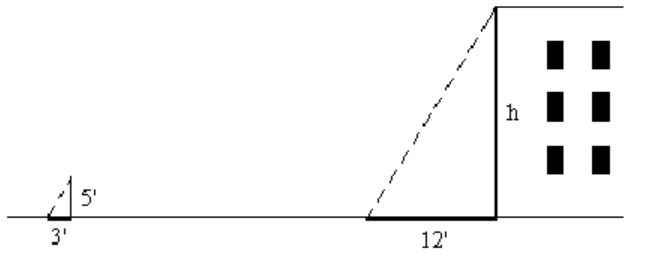
\includegraphics[width=\linewidth]{images/exam1-2-5}
\end{sbspanel}%
\end{sidebyside}%
\par
%
\begin{enumerate}[label=\alph*]
\item{}Use similar triangles to write a proportion involving the height of the building.%
\item{}Solve the proportion to find the height of the building.%
\end{enumerate}
%
\par\smallskip%
\noindent\textbf{\blocktitlefont Solution}.\label{g:solution:idm46051677076400}{}\hypertarget{g:solution:idm46051677076400}{}\quad{}%
\begin{enumerate}[label=\alph*]
\item{}In the figure above we see two right triangles:  One triangle is formed by the building and  its shadow, and the other by the pole and its shadow.  Because the light rays from the sun are parallel, the two angles at the tips of the shadows are equal.  Thus, the two right triangles are similar, and their corresponding sides are proportional.  The ratios of heights and bases in the two triangles yield the proportion%
\begin{equation*}
\dfrac{\text{larger triangle}}{\text{smaller triangle}}:~~~~~\dfrac{h}{5}~~~=~~~\dfrac{12}{3}
\end{equation*}
%
\item{}To solve the proportion, we cross-multiply to get%
\begin{align*}
3h\amp =5(12)=60 \amp \amp \blert{\text{Divide both sides by 3.}}\\
h\amp =\frac{60}{3} = 20  \amp \amp
\end{align*}
The building is 20 feet tall.%
\end{enumerate}
%
\end{example}
\begin{inlineexercise}{}{g:exercise:idm46051677071856}%
Earlier we created a 30°-60°-90° triangle in which the shorter leg was 4 inches and the hypotenuse was 8 inches.  The hypotenuse of another 30°-60°-90° triangle is 5 feet.  What is the length of the side opposite the 30° angle?%
\par\smallskip%
\noindent\textbf{\blocktitlefont Answer}.\label{g:answer:idm46051677097808}{}\hypertarget{g:answer:idm46051677097808}{}\quad{}2.5 feet%
\end{inlineexercise}
\end{subsectionptx}
%
%
\typeout{************************************************}
\typeout{Subsection  Overlapping Triangles}
\typeout{************************************************}
%
\begin{subsectionptx}{Overlapping Triangles}{}{Overlapping Triangles}{}{}{g:subsection:idm46051677101216}
\index{triangle!overlapping}%
In some applications, similar triangles may share a side or an angle.%
\begin{example}{}{g:example:idm46051677115264}%
\begin{sidebyside}{2}{0}{0.1}{0.1}%
\begin{sbspanel}{0.55}[center]%
Identify two similar triangles in the figure at right, and write a proportion to find \(H\).%
\end{sbspanel}%
\begin{sbspanel}{0.25}[center]%
\resizebox{\linewidth}{!}{%
\tikzset{%
  block/.style    = {draw, thick, rectangle, minimum height = 3em,
    minimum width = 3em},
  sum/.style      = {draw, circle, node distance = 2cm}, % Adder
  input/.style    = {coordinate}, % Input
  output/.style   = {coordinate} % Output
}
\begin{tikzpicture}[auto, thick]
    \coordinate (A) at (0,0);
    \coordinate (B) at (2.4,1);
    \coordinate (C) at (2.4,0);
    \coordinate (D) at (3.6,1.5);
    \coordinate (E) at (3.6,0);

    \draw[blue, thick] (C) rectangle +(-.25, .25);
    \draw[blue, thick] (E) rectangle +(-.25, .25);
    \draw[black,  thick] (A) --  (C) node[below,midway] {\color{blue}$24$} ;
    \draw[black,  thick] (B) -- (C) node[right, midway] {\color{blue}$10$} ;
    \draw[black,  thick] (C) -- (E) node[below, midway, yshift=0] {\color{blue}$12$} ;
    \draw[black,  thick] (D) -- (E) node[right, midway,yshift=0] {\color{blue}$H$} ;
    \draw[black,  thick] (A) -- (D)  ;

\end{tikzpicture}
}%
\end{sbspanel}%
\end{sidebyside}%
\par\smallskip%
\noindent\textbf{\blocktitlefont Solution}.\label{g:solution:idm46051677142144}{}\hypertarget{g:solution:idm46051677142144}{}\quad{}The two triangles overlap, sharing the marked angle, as shown below.  Because each triangle also has a right angle, they are similar.%
\begin{sidebyside}{1}{0.225}{0.225}{0}%
\begin{sbspanel}{0.55}%
\resizebox{\linewidth}{!}{%
\tikzset{%
  block/.style    = {draw, thick, rectangle, minimum height = 3em,
    minimum width = 3em},
  sum/.style      = {draw, circle, node distance = 2cm}, % Adder
  input/.style    = {coordinate}, % Input
  output/.style   = {coordinate} % Output
}
\begin{tikzpicture}[auto, thick, scale=1.2]
    \coordinate (A) at (0,0);
    \coordinate (B) at (2.4,1);
    \coordinate (C) at (2.4,0);
    \coordinate (D) at (6.6,1.5);
    \coordinate (E) at (6.6,0);
    \coordinate (A2) at (3,0);

    \draw[blue, thick] (C) rectangle +(-.25, .25);
    \draw[blue, thick] (E) rectangle +(-.25, .25);
    \draw[black,  thick] (A) -- (B)  ;
    \draw[black, thick] (A) --  (C) node[below,midway] {\color{blue}$24$};
    \draw[black,  thick] (B) -- (C) node[right, midway] {\color{blue}$10$} ;

    \draw[red,thick] (0.48,-0.13) arc (-15:35:0.5);

    \draw[black,  thick] (A2) -- (E) node[below, midway, xshift=5] {\color{blue}$24~~~+~~~12$} ;
    \draw[black,  thick] (D) -- (E) node[right, midway,yshift=0] {\color{blue}$H$} ;
    \draw[black,  thick] (A2) -- (D)  ;
    \draw[red,thick] (3.48,-0.13) arc (-15:35:0.5);

\end{tikzpicture}
}%
\end{sbspanel}%
\end{sidebyside}%
\par
Note that the base of the larger triangle is \(24+12=36\).  The ratio of the heights and the ratio of the bases must be equal, so we write the following proportion.%
\begin{align*}
\frac{H}{10}\amp =\frac{36}{24} \amp \amp \blert{\text{Cross-multiply.}}\\
24H\amp =360 \amp \amp \blert{\text{Divide both sides by 24.}}\\
H\amp =\frac{360}{24} = 15  \amp \amp
\end{align*}
%
\end{example}
\begin{inlineexercise}{}{g:exercise:idm46051677169600}%
\begin{sidebyside}{2}{0}{0}{0.1}%
\begin{sbspanel}{0.55}[center]%
Heather wants to know the height of a street lamp.  She discovers that when she is 12 feet from the lamp, her shadow is 6 feet long.  Find the height of the street lamp.%
\end{sbspanel}%
\begin{sbspanel}{0.35}[center]%
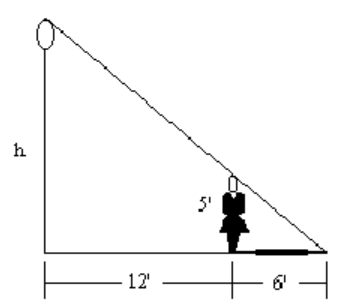
\includegraphics[width=\linewidth]{images/exer1-2-6}
\end{sbspanel}%
\end{sidebyside}%
\par\smallskip%
\noindent\textbf{\blocktitlefont Answer}.\label{g:answer:idm46051677188880}{}\hypertarget{g:answer:idm46051677188880}{}\quad{}15 feet%
\end{inlineexercise}
Review the following skills you will need for this section.%
\begin{project}{}{g:project:idm46051677203488}%
\begin{sidebyside}{1}{0}{0}{0}%
\begin{sbspanel}{1}%
Which of the following expressions and equations are proportions?%
\end{sbspanel}%
\end{sidebyside}%
\begin{sidebyside}{3}{0}{0}{0.05}%
\begin{sbspanel}{0.3}%
1. \(\dfrac{7}{x}=\dfrac{3}{5}\)%
\end{sbspanel}%
\begin{sbspanel}{0.3}%
\par
2. \(\dfrac{x}{2}=\dfrac{8}{x+2}\)%
\end{sbspanel}%
\begin{sbspanel}{0.3}%
\par
3. \(1+\dfrac{x}{4}=\dfrac{2x}{3}\)%
\end{sbspanel}%
\end{sidebyside}%
\begin{sidebyside}{3}{0}{0}{0.05}%
\begin{sbspanel}{0.3}%
4. \(\dfrac{6}{x}+\dfrac{x}{5}\)%
\end{sbspanel}%
\begin{sbspanel}{0.3}%
\par
5. \(\dfrac{3}{x+1}\cdot\dfrac{2x}{5}\)%
\end{sbspanel}%
\begin{sbspanel}{0.3}%
\par
6. \(\dfrac{1}{x}+\dfrac{2}{3x}=\dfrac{x-2}{2}\)%
\end{sbspanel}%
\end{sidebyside}%
\begin{sidebyside}{1}{0}{0}{0}%
\begin{sbspanel}{1}%
Solve each equation.  Begin by writing an equivalent equation without fractions:  multiply both sides by the LCD.%
\end{sbspanel}%
\end{sidebyside}%
\begin{sidebyside}{2}{0}{0}{0.1}%
\begin{sbspanel}{0.45}%
7. \(\dfrac{x}{12}=\dfrac{3}{x}\)%
\end{sbspanel}%
\begin{sbspanel}{0.45}%
\par
8. \(1+\dfrac{x}{2}=\dfrac{2x}{5}\)%
\end{sbspanel}%
\end{sidebyside}%
\begin{sidebyside}{1}{0}{0}{0}%
\begin{sbspanel}{1}%
\(\underline{\qquad\qquad\qquad\qquad}\)%
\end{sbspanel}%
\end{sidebyside}%
\begin{sidebyside}{1}{0}{0}{0}%
\begin{sbspanel}{1}%
Algebra Refresher Answers%
\end{sbspanel}%
\end{sidebyside}%
\begin{sidebyside}{1}{0}{0}{0}%
\begin{sbspanel}{1}%
Only 1 and 2 are proportions.%
\end{sbspanel}%
\end{sidebyside}%
\begin{sidebyside}{2}{0}{0}{0}%
\begin{sbspanel}{0.5}%
7.  \(\pm 6\)%
\end{sbspanel}%
\begin{sbspanel}{0.5}%
\par
8.  \(-10\)%
\end{sbspanel}%
\end{sidebyside}%
\end{project}
\end{subsectionptx}
%
%
\typeout{************************************************}
\typeout{Subsection  Section 1.2 Summary}
\typeout{************************************************}
%
\begin{subsectionptx}{Section 1.2 Summary}{}{Section 1.2 Summary}{}{}{g:subsection:idm46051677289472}
%
%
\typeout{************************************************}
\typeout{Subsubsection  Vocabulary}
\typeout{************************************************}
%
\begin{subsubsectionptx}{Vocabulary}{}{Vocabulary}{}{}{g:subsubsection:idm46051677294256}
Look up the definitions of new terms in the Glossary.%
\par
%
\begin{multicols}{3}
\begin{itemize}[label=\textbullet]
\item{}Congruent%
\item{}Altitude%
\item{}Leg%
\item{}Hypotenuse%
\item{}Parallelogram%
\item{}Similar%
\item{}Proportional%
\end{itemize}
\end{multicols}
%
\end{subsubsectionptx}
%
%
\typeout{************************************************}
\typeout{Subsubsection  Concepts}
\typeout{************************************************}
%
\begin{subsubsectionptx}{Concepts}{}{Concepts}{}{}{g:subsubsection:idm46051678107696}
%
\begin{enumerate}[label=\arabic*]
\item{}Two triangles are \terminology{congruent} if they have exactly the same size and shape.%
\item{}The \terminology{altitude} of an equilateral triangle divides it into two congruent right triangles.%
\item{}In a 30°-60°-90° right triangle, the \terminology{leg} opposite the 30° angle is half the length of the \terminology{hypotenuse}.%
\item{}Two triangles are \terminology{similar} if they have the same shape but not necessarily the same size.  The corresponding angles are equal, and the corresponding sides are \terminology{proportional}.%
\item{}\begin{assemblage}{Similar Triangles.}{g:assemblage:idm46051701396208}%
Two triangles are similar if either%
\begin{enumerate}[label=\arabic*]
\item{}their corresponding angles are equal, or%
\item{}their corresponding sides are proportional.%
\end{enumerate}
%
\end{assemblage}
%
\item{}If two \emph{right} triangles have \emph{one} pair of corresponding acute angles with the same measure, then the triangles are similar.%
\end{enumerate}
%
\end{subsubsectionptx}
%
%
\typeout{************************************************}
\typeout{Subsubsection  Study Questions}
\typeout{************************************************}
%
\begin{subsubsectionptx}{Study Questions}{}{Study Questions}{}{}{g:subsubsection:idm46051677997440}
%
\begin{enumerate}[label=\arabic*]
\item{}What is the difference between congruent triangles and similar triangles?%
\item{}What is the name of the short-cut method for solving proportions? Why does the method work?%
\item{}In two triangles, if two corresponding pairs of angles are equal, are the triangles similar? How do you know?%
\item{}\begin{sidebyside}{2}{0}{0.1}{0.15}%
\begin{sbspanel}{0.45}[center]%
For the triangles shown, which of the following equations is true?  Explain why.%
\end{sbspanel}%
\begin{sbspanel}{0.3}[center]%
\resizebox{\linewidth}{!}{%
\tikzset{%
  block/.style    = {draw, thick, rectangle, minimum height = 3em,
    minimum width = 3em},
  sum/.style      = {draw, circle, node distance = 2cm}, % Adder
  input/.style    = {coordinate}, % Input
  output/.style   = {coordinate} % Output
}
\begin{tikzpicture}[auto, thick]
    \coordinate (A) at (0,0);
    \coordinate (B) at (3.6,0);
    \coordinate (C) at (2.7,1.5);
    \coordinate (D) at (4.8,0);
    \coordinate (E) at (3.6,2);

    \draw[black, thick] (A)--(D)--(E)--cycle;
    \draw[black, thick] (A) -- (B) node [below, midway] {\color{blue}$x$};
    \draw[black, thick] (D) -- (B) node [below, midway] {\color{blue}$4$};
    \draw[black, thick] (D) -- (E) node [above right, midway] {\color{blue}$8$};
    \draw[black, thick] (C) -- (B) node [above right, midway] {\color{blue}$6$};

    \draw[black,  thick, ->] (C) --  (3.15,.75)  ;
    \draw[black,  thick, ->] (E) --  (4.2,1)  ;

\end{tikzpicture}
}%
\end{sbspanel}%
\end{sidebyside}%
\par
%
\begin{multicols}{2}
\begin{enumerate}[label=\alph*]
\item{}\(\displaystyle \dfrac{4}{x} = \dfrac{6}{8}\)%
\item{}\(\displaystyle \dfrac{x}{4} = \dfrac{6}{8}\)%
\item{}\(\displaystyle \dfrac{x}{x+4} = \dfrac{6}{8}\)%
\item{}\(\displaystyle \dfrac{x}{x+4} = \dfrac{6}{14}\)%
\end{enumerate}
\end{multicols}
%
\end{enumerate}
%
\end{subsubsectionptx}
%
%
\typeout{************************************************}
\typeout{Subsubsection  Skills}
\typeout{************************************************}
%
\begin{subsubsectionptx}{Skills}{}{Skills}{}{}{g:subsubsection:idm46051677434704}
Practice each skill in the Homework Problems listed.%
\par
%
\begin{enumerate}[label=\arabic*]
\item{}Identify congruent triangles and find unknown parts     \#1-6%
\item{}Identify similar triangles    \#7-10%
\item{}Find unknown parts of similar triangles    \#11-20%
\item{}Solve problems using proportions and similar triangles    \#21-26%
\item{}Use proportions to relate sides of similar triangles    \#27-38%
\end{enumerate}
%
\end{subsubsectionptx}
\end{subsectionptx}
%
%
\typeout{************************************************}
\typeout{Exercises  Homework 1.2}
\typeout{************************************************}
%
\begin{exercises-subsection}{Homework 1.2}{}{Homework 1.2}{}{}{x:exercises:hmwk-1-2}
\par\medskip\noindent%
%
In Problems 1\textendash{}4, name two congruent triangles and find the unknown quantities.%
\begin{exercisegroupcol}{2}
\begin{divisionexerciseegcol}{1}{}{}{g:exercise:idm46051678814528}%
\(PQRS\) is an isosceles trapezoid.%
\begin{sidebyside}{1}{0.15}{0.15}{0}%
\begin{sbspanel}{0.7}%
\resizebox{\linewidth}{!}{%
\tikzset{%
}
\begin{tikzpicture}[auto, thick]
    \coordinate (T) at (0,0);
    \coordinate (P) at (-2.4,-1.7);
    \coordinate (Q) at (-.8,1.5);
    \coordinate (R) at (.8,1.5);
    \coordinate (S) at (2.4,-1.7);

    \filldraw [black] (T) circle (.2pt) node[anchor=north,yshift=-5] {$T$};
    \filldraw [black] (P) circle (.2pt) node[anchor=north east,yshift=0] {$P$};
    \filldraw [black] (Q) circle (.2pt) node[anchor=south east,yshift=0] {$Q$};
    \filldraw [black] (R) circle (.2pt) node[anchor=south west,yshift=0] {$R$};
    \filldraw [black] (S) circle (.2pt) node[anchor=north west,yshift=0] {$S$};

    \draw[black, thick] (P)--(S);
    \draw[black, thick] (Q)--(R);
    \draw[black, thick] (P)--(T);
    \draw[black, thick] (T)--(S);
    \draw[black, thick] (P) -- (Q) node [left, midway] {\color{blue}$x$};
    \draw[black, thick] (R) -- (S) node [right, midway] {\color{blue}$7$};
    \draw[black, thick] (Q) -- (T) node [left, midway] {\color{blue}$3$};
    \draw[black, thick] (R) -- (T) node [ right, midway] {\color{blue}$y$};
    \draw[blue, thick] (-.94,-.83)-- +(-.17,.24);
    \draw[blue, thick] (-.88,-.77)-- +(-.17,.24);
    \draw[blue, thick] (.94,-.83)-- +(.17,.24);
    \draw[blue, thick] (.88,-.77)-- +(.17,.24);

    \draw [red,thick] (-2.,-0.9) arc({atan(2)}:{atan(17/24)}:.9) node[above right,xshift=-8,yshift=3] {$18\degree$};
    \draw [red,thick] (2.,-0.9) arc({180-atan(2)}:{180-atan(17/24)}:.9) node[above left,xshift=4,yshift=4] {$\alpha$};

\end{tikzpicture}
}%
\end{sbspanel}%
\end{sidebyside}%
\end{divisionexerciseegcol}%
\begin{divisionexerciseegcol}{2}{}{}{g:exercise:idm46051678862560}%
\begin{sidebyside}{1}{0.15}{0.15}{0}%
\begin{sbspanel}{0.7}%
\resizebox{\linewidth}{!}{%
\tikzset{%
}
\begin{tikzpicture}[auto, thick]
    \coordinate (E) at (0,0);
    \coordinate (M) at (-1.8,-1.2);
    \coordinate (N) at (1.8,1.2);
    \coordinate (L) at (.2,2);
    \coordinate (O) at (-.2,-2);

    \filldraw [black] (E) circle (.2pt) node[anchor=east,yshift=4] {$E$};
    \filldraw [black] (M) circle (.2pt) node[anchor=north east,yshift=0] {$M$};
    \filldraw [black] (N) circle (.2pt) node[anchor=south west,yshift=0] {$N$};
    \filldraw [black] (L) circle (.2pt) node[anchor=south,yshift=0] {$L$};
    \filldraw [black] (O) circle (.2pt) node[anchor=north ,yshift=0] {$O$};

    \draw[black, thick] (M)--(N);
    \draw[black, thick] (M)--(N);
    \draw[black, thick] (E) -- (L) node [left, midway] {\color{blue}$24$};
    \draw[black, thick] (E) -- (O) node [right, midway] {\color{blue}$y$};
    \draw[black, thick] (M) -- (O) node [below, midway,xshift=-2] {\color{blue}$z$};
    \draw[black, thick] (L) -- (N) node [ above, midway,xshift=2] {\color{blue}$26$};
    \draw[blue, thick] (-.94,-.83)-- +(-.18,.24);
    \draw[blue, thick] (-.88,-.77)-- +(-.18,.24);
    \draw[blue, thick] (.94,.83)-- +(.18,-.24);
    \draw[blue, thick] (.88,.77)-- +(.18,-.24);

    \coordinate (M2) at (-3,-0.6);
    \coordinate (N2) at (2.4,0.9);
    \coordinate (M3) at (-3.4,-0.4);
    \coordinate (L3) at (-1.4,2.8);
    \coordinate (L2) at (-1,2.6);
    \coordinate (O2) at (0.4,-2.3);

    \draw[black, thick, <-] (M2)--(O2);
    \draw[black, thick, <-] (L2)--(N2);
    \draw[black, thick] (M)--(M3);
    \draw[black, thick] (L3)--(L);

    \draw [red,thick] (-1.38,-0.9) arc({atan(2/3)}:{atan(-.5)}:.5) node[ right,xshift=0,yshift=4] {$\theta$};
    \draw [red,thick] (1.38,0.9) arc({180+atan(2/3)}:{180+atan(-.5)}:.5) node[ left,xshift=0,yshift=-4] {$53\degree$};

\end{tikzpicture}
}%
\end{sbspanel}%
\end{sidebyside}%
\end{divisionexerciseegcol}%
\begin{divisionexerciseegcol}{3}{}{}{g:exercise:idm46051678889888}%
\(\triangle PRU\) is isosceles.%
\begin{sidebyside}{1}{0.225}{0.225}{0}%
\begin{sbspanel}{0.55}%
\resizebox{\linewidth}{!}{%
\tikzset{%
}
\begin{tikzpicture}[auto, thick, scale=1.5]
    \coordinate (R) at (0,0);
    \coordinate (P) at (-1.,-2.8);
    \coordinate (U) at (1, -2.8);
    \coordinate (E) at (-.4,-2.8);
    \coordinate (N) at (.4,-2.8);

    \filldraw [black] (R) circle (.2pt) node[anchor=south] {$R$};
    \filldraw [black] (P) circle (.2pt) node[anchor=north east,yshift=0] {$P$};
    \filldraw [black] (U) circle (.2pt) node[anchor=north west,yshift=0] {$U$};
    \filldraw [black] (E) circle (.2pt) node[anchor=north ,yshift=0] {$E$};
    \filldraw [black] (N) circle (.2pt) node[anchor=north,yshift=0] {$N$};

    \draw[black, thick] (P)--(R)--(U)--cycle;
    \draw[black, thick] (E) -- (R) node [below right, midway,xshift=-5,yshift=-15] {\color{blue}$12$};
    \draw[black, thick] (R) -- (N) node [below right, midway,xshift=2,yshift=-18] {\color{blue}$z$};
    \draw[blue, thick] (-.67,-2.92)-- +(0,.24);
    \draw[blue, thick] (-.73,-2.92)-- +(0,.24);
    \draw[blue, thick] (.67,-2.92)-- +(0,.24);
    \draw[blue, thick] (.73,-2.92)-- +(0,.24);

    \draw [red,thick] (-.8,-2.8) arc(0:{atan(2.8)}:.2) node[above right,xshift=0,yshift=-2] {$18\degree$};
    \draw [red,thick] (.8,-2.8) arc(180:{180-atan(2.8)}:.2) node[above left,xshift=-3,yshift=-2] {$\phi$};
    \draw [red,thick] (-.3,-.85) arc({180+atan(2.8)}:{180+atan(7)}:.9) node[below  left,xshift=1,yshift=0] {$\theta$};
    \draw [red,thick] (.3,-.85) arc({-atan(2.8)}:{-atan(7)}:.9) node[  right,xshift=5,yshift=1] {$10\degree$};

\end{tikzpicture}
}%
\end{sbspanel}%
\end{sidebyside}%
\end{divisionexerciseegcol}%
\begin{divisionexerciseegcol}{4}{}{}{g:exercise:idm46051678904768}%
\(\triangle PRU\) is isosceles and \(OR=NG\). Find \(\angle RNG\) and \(\angle RNO\).%
\begin{sidebyside}{1}{0.2}{0.2}{0}%
\begin{sbspanel}{0.6}%
\resizebox{\linewidth}{!}{%
\tikzset{%
}
\begin{tikzpicture}[auto, thick, scale=1.5]
    \coordinate (A) at (0,0);
    \coordinate (R) at (-.65,-1.3);
    \coordinate (N) at (.65, -1.3);
    \coordinate (O) at (-1.2,-2.4);
    \coordinate (G) at (1.2,-2.4);
    \coordinate (E) at (0,-1.7);

    \filldraw [black] (R) circle (.2pt) node[anchor=east] {$R$};
    \filldraw [black] (N) circle (.2pt) node[anchor=west] {$N$};
    \filldraw [black] (O) circle (.2pt) node[anchor=north east,yshift=0] {$O$};
    \filldraw [black] (G) circle (.2pt) node[anchor=north west,yshift=0] {$G$};
    \filldraw [black] (E) circle (.2pt) node[anchor=north ,yshift=-4] {$E$};
    \filldraw [black] (A) circle (.2pt) node[anchor=south east,yshift=0] {$A$};

    \draw[black, thick] (A)--(G)--(E)--(O)--cycle;
    \draw[black, thick] (G) -- (R) ;
    \draw[black, thick] (O)-- (N);
    \draw[black, thick] (R)--(N);
    \draw[blue] (-.95,-1.65)-- +(.2,-.1);
    \draw[blue] (-.925,-1.6)-- +(.2,-.1);
    \draw[blue] (.95,-1.65)-- +(-.2,-.1);
    \draw[blue] (.925,-1.6)-- +(-.2,-.1);

    \draw [red,thick] (-.98,-1.95) arc({atan(2)}:30.7:.5);
    \draw [red,thick] (.98,-1.95) arc({180-atan(2)}:149.3:.5) node[above left,xshift=9,yshift=3] {$35\degree$};
    \draw [red,thick] (.21,-.45) arc(-65:-115:.5) node[below, midway, xshift=0,yshift=0] {$50\degree$};

\end{tikzpicture}
}%
\end{sbspanel}%
\end{sidebyside}%
\end{divisionexerciseegcol}%
\end{exercisegroupcol}
\par\medskip\noindent
\begin{divisionexercise}{5}{}{}{g:exercise:idm46051678977280}%
Delbert and Francine want to measure the distance across a stream.  They mark point \(A\) directly across the stream from a tree at point \(T\) on the opposite bank.  Delbert walks from point \(A\) down the bank a short distance to point \(B\) and sights the tree.  He measures the angle between his line of sight and the streambank.%
\par
%
\begin{enumerate}[label=\alph*]
\item{}Draw a figure showing the stream, the tree, and right triangle \(ABT\).%
\item{}Meanwhile Francine, who was still standing at point \(A\), walks away from the stream at right-angles to Delbert's path.   Delbert watches her progress, and tells her to stop at point \(C\) when the angle between the stream bank and his line of sight to Francine is the same as the angle from the stream bank to the tree.  Add triangle \(ABC\) to your figure.%
\item{}Delbert now measures the distance from point \(A\) to Francine at point \(C\). Explain why this distance is the same as the distance across the stream.%
\end{enumerate}
%
\end{divisionexercise}%
\begin{divisionexercise}{6}{}{}{g:exercise:idm46051679099840}%
If you have a baseball cap, here is another way to measure the distance across a river.  Stand at point \(A\) directly across the river from a convenient landmark, say a large rock, on the other side.  Tilt your head down so that the brim of the cap points directly at the base of the rock, \(R\).%
\par
%
\begin{enumerate}[label=\alph*]
\item{}Draw a figure showing the river, the rock, and right triangle \(ABR\), where \(B\) is the location of your baseball cap on your head.%
\item{}Now, without changing the angle of your head, rotate \(90\degree\) and sight along the bank on your side of the river.  Have a friend mark the spot \(C\) on the ground where the brim of your cap points.  Add triangle \(ABC\) to your figure.%
\item{}Finally, you can measure the distance from point \(A\) to point \(C\).  Explain why this distance is the same as the distance across the river.%
\end{enumerate}
%
\end{divisionexercise}%
\par\medskip\noindent%
%
For Problems 7\textendash{}10, decide whether the triangles are similar, and explain why or why not.%
\begin{exercisegroupcol}{2}
\begin{divisionexerciseegcol}{7}{}{}{g:exercise:idm46051679186512}%
\begin{sidebyside}{1}{0.225}{0.225}{0}%
\begin{sbspanel}{0.55}%
\resizebox{\linewidth}{!}{%
\tikzset{%
  block/.style    = {draw, thick, rectangle, minimum height = 3em,
    minimum width = 3em},
  sum/.style      = {draw, circle, node distance = 2cm}, % Adder
  input/.style    = {coordinate}, % Input
  output/.style   = {coordinate} % Output
}
\begin{tikzpicture}[auto, thick]
    \coordinate (A) at (0,0);
    \coordinate (B) at (-1.2,2.4);
    \coordinate (C) at (1.3,0);

    \draw[black,  thick] (A) --  (B) node[left,midway,yshift=-5]{\color{blue}$8$} ;
    \draw[black,  thick] (C) --  (B) node[right,midway,xshift=3]{\color{blue}$12$} ;
    \draw[black,  thick] (C) --  (A) node[below,midway]{\color{blue}$6$} ;


    \draw[black, shift={(2.5 cm, 1 cm)}, rotate=90, scale=.5]  (0,0)--(1.2,2.4)  node[right,midway,yshift=3]{\color{blue}$4$};
    \draw[black, shift={(2.5 cm, 1 cm)}, rotate=90, scale=.5]  (1.2,2.4)--(-1.3,0)  node[left,midway,xshift=2,yshift=-4]{\color{blue}$6$};
    \draw[black, shift={(2.5 cm, 1 cm)}, rotate=90, scale=.5]  (0,0)--(-1.3,0) node[right,midway]{\color{blue}$3$}  ;

\end{tikzpicture}
}%
\end{sbspanel}%
\end{sidebyside}%
\end{divisionexerciseegcol}%
\begin{divisionexerciseegcol}{8}{}{}{g:exercise:idm46051679206560}%
\begin{sidebyside}{1}{0.15}{0.15}{0}%
\begin{sbspanel}{0.7}%
\resizebox{\linewidth}{!}{%
\tikzset{%
  block/.style    = {draw, thick, rectangle, minimum height = 3em,
    minimum width = 3em},
  sum/.style      = {draw, circle, node distance = 2cm}, % Adder
  input/.style    = {coordinate}, % Input
  output/.style   = {coordinate} % Output
}
\begin{tikzpicture}[auto, thick]
    \coordinate (A) at (0,0);
    \coordinate (B) at (1.75,.97);
    \coordinate (C) at (1.5,0);

    \draw[black,  thick] (A) --  (B) node[above,midway,xshift=-2]{\color{blue}$4$} ;
    \draw[black,  thick] (C) --  (B) node[right,midway,xshift=0]{\color{blue}$2$} ;
    \draw[black,  thick] (C) --  (A) node[below,midway]{\color{blue}$3$} ;

    \coordinate (A2) at (2.5,-.5);
    \coordinate (B2) at (5,1.95);
    \coordinate (C2) at (5.5,-.5);

    \draw[black,  thick] (A2) --  (B2) node[above,midway,xshift=-2]{\color{blue}$7$} ;
    \draw[black,  thick] (C2) --  (B2) node[right,midway,xshift=0]{\color{blue}$5$} ;
    \draw[black,  thick] (C2) --  (A2) node[below,midway]{\color{blue}$6$} ;

\end{tikzpicture}
}%
\end{sbspanel}%
\end{sidebyside}%
\end{divisionexerciseegcol}%
\begin{divisionexerciseegcol}{9}{}{}{g:exercise:idm46051679199344}%
\begin{sidebyside}{1}{0.25}{0.25}{0}%
\begin{sbspanel}{0.5}%
\resizebox{\linewidth}{!}{%
\tikzset{%
  block/.style    = {draw, thick, rectangle, minimum height = 3em,
    minimum width = 3em},
  sum/.style      = {draw, circle, node distance = 2cm}, % Adder
  input/.style    = {coordinate}, % Input
  output/.style   = {coordinate} % Output
}
\begin{tikzpicture}[auto, thick]
    \coordinate (A) at (0,0);
    \coordinate (B) at (-.1,-1.4);
    \coordinate (C) at (2.5,0);

    \draw[black,  thick] (A) --  (B) -- (C) -- cycle ;
    \draw[red, thick] (0.16,-1.25) arc (30:88:0.3) node [above right, midway, xshift=-5, yshift=0] {\color{red}$62\degree$};
    \draw[red, thick] (.3,0) arc (0:-92:0.3) node [below right, midway, xshift=0, yshift=4] {\color{red}$92\degree$};

    \draw[red, thick,shift={(2.8 cm, -.75 cm)}, rotate=30, scale=1.4]  (-0.16,-1.25) arc (150:92:0.3) node [above left, midway, xshift=0, yshift=-5] {\color{red}$62\degree$};
    \draw[red, thick, shift={(2.8 cm, -.75 cm)}, rotate=30, scale=1.4] (-2.0,0) arc (0:-26:0.5) node [above right, midway, xshift=3, yshift=-5] {\color{red}$26\degree$};

    \draw[black, shift={(2.8 cm, -.75 cm)}, rotate=30, scale=1.4]  (0,0)--(.1,-1.4);
    \draw[black, shift={(2.8 cm, -.75 cm)}, rotate=30, scale=1.4]  (.1,-1.4)--(-2.5,0) ;
    \draw[black, shift={(2.8 cm, -.75 cm)}, rotate=30, scale=1.4]  (0,0)--(-2.5,0) ;

\end{tikzpicture}
}%
\end{sbspanel}%
\end{sidebyside}%
\end{divisionexerciseegcol}%
\begin{divisionexerciseegcol}{10}{}{}{g:exercise:idm46051679276736}%
\begin{sidebyside}{1}{0.25}{0.25}{0}%
\begin{sbspanel}{0.5}%
\resizebox{\linewidth}{!}{%
\tikzset{%
  block/.style    = {draw, thick, rectangle, minimum height = 3em,
    minimum width = 3em},
  sum/.style      = {draw, circle, node distance = 2cm}, % Adder
  input/.style    = {coordinate}, % Input
  output/.style   = {coordinate} % Output
}
\begin{tikzpicture}[auto, thick]
    \coordinate (A) at (0,0);
    \coordinate (B) at (3.5,-1);
    \coordinate (C) at (3.5,0);

    \draw[blue, thick] (C) rectangle +(-.25,-.25);
    \draw[black,  thick] (A) --  (B) -- (C) -- cycle ;
    \draw[red, thick] (3.5,-.7) arc (90:{180-atan(1/3.5)}:0.3) node [above left, midway, xshift=5, yshift=-3] {\color{red}$75\degree$};

    \draw[red, thick, shift={(-.5 cm, -1 cm)}, rotate=-15, scale=0.8] (1.2,0) arc (0:15:1.2) node [ right, midway, xshift=3, yshift=-2] {\color{red}$15\degree$};

    \draw[blue, shift={(-.5 cm, -1 cm)}, rotate=-15, scale=0.8]  (3.5,0) rectangle +(-.3125,.3125);
    \draw[black, shift={(-.5 cm, -1 cm)}, rotate=-15, scale=0.8]  (0,0)--(3.5,1);
    \draw[black, shift={(-.5 cm, -1 cm)}, rotate=-15, scale=0.8]  (3.5,1)--(3.5,0) ;
    \draw[black, shift={(-.5 cm, -1 cm)}, rotate=-15, scale=0.8]  (0,0)--(3.5,0) ;

\end{tikzpicture}
}%
\end{sbspanel}%
\end{sidebyside}%
\end{divisionexerciseegcol}%
\end{exercisegroupcol}
\par\medskip\noindent
\par\medskip\noindent%
%
Assume the triangles in Problems 11\textendash{}14 are similar. Solve for the variables. (Figures are not drawn to scale.)%
\begin{exercisegroupcol}{2}
\begin{divisionexerciseegcol}{11}{}{}{g:exercise:idm46051679310816}%
\begin{sidebyside}{1}{0.225}{0.225}{0}%
\begin{sbspanel}{0.55}%
\resizebox{\linewidth}{!}{%
\tikzset{%
  block/.style    = {draw, thick, rectangle, minimum height = 3em,
    minimum width = 3em},
  sum/.style      = {draw, circle, node distance = 2cm}, % Adder
  input/.style    = {coordinate}, % Input
  output/.style   = {coordinate} % Output
}
\begin{tikzpicture}[auto, thick]
    \coordinate (O) at (0,0);
    \coordinate (B) at (0,2.4);
    \coordinate (C) at (1.8,0);

    \draw[blue, thick] (O) rectangle +(.25,.25);
    \draw[black,  thick] (O) --  (B) -- (C) -- cycle ;
    \draw[red, thick] (0,2) arc (-90:{atan(-4/3)}:0.4) node [below right, midway, xshift=-7, yshift=-5] {\color{red}$B\degree$};
    \draw[red, thick] (1.5,0) arc (180:127:0.3) node [above left, midway, xshift=2, yshift=-5] {\color{red}$53\degree$};

    \draw[red, thick, shift={(4.2 cm, 0 cm)}, scale=1.2]  (0,2) arc (-90:{atan(4/3)-180}:0.4) node [below left, midway, xshift=7, yshift=-5] {\color{red}$A\degree$};
    \draw[red, thick, shift={(4.2 cm, 0 cm)}, scale=1.2] (-1.5,0) arc (0:53:0.3) node [above right, midway, xshift=-1, yshift=-6] {\color{red}$53\degree$};
    \draw[blue, shift={(4.2 cm, 0 cm)}, scale=1.2]  (0,0) rectangle +(-.21,.21);
    \draw[black, shift={(4.2 cm, 0 cm)}, scale=1.2]  (0,0)--(0,2.4);
    \draw[black, shift={(4.2 cm, 0 cm)}, scale=1.2]  (0,2.4)--(-1.8,0) ;
    \draw[black, shift={(4.2 cm, 0 cm)},  scale=1.2]  (0,0)--(-1.8,0) ;

\end{tikzpicture}
}%
\end{sbspanel}%
\end{sidebyside}%
\end{divisionexerciseegcol}%
\begin{divisionexerciseegcol}{12}{}{}{g:exercise:idm46051679349616}%
\begin{sidebyside}{1}{0.275}{0.275}{0}%
\begin{sbspanel}{0.45}%
\resizebox{\linewidth}{!}{%
\tikzset{%
  block/.style    = {draw, thick, rectangle, minimum height = 3em,
    minimum width = 3em},
  sum/.style      = {draw, circle, node distance = 2cm}, % Adder
  input/.style    = {coordinate}, % Input
  output/.style   = {coordinate} % Output
}
\begin{tikzpicture}[auto, thick]
    \coordinate (O) at (0,0);
    \coordinate (B) at (-1.5,.55);
    \coordinate (C) at (0,3.15);

    \draw[black,  thick] (O) --  (B) -- (C) -- cycle ;
    \draw[red, thick] (0,2.55) arc (-90:{atan(2.6/1.5)-180}:0.6);
    \draw[red, thick] (0,.33) arc (90:{180-atan(.55/1.5)}:0.33);
    \draw[red, thick] (-1.25,.98) arc (60:-20:0.5) node [right, midway, xshift=-2, yshift=2] {\color{red}$80\degree$};
    \draw[red] (-.2,2.4) -- +(.09,.3);
    \draw[red] (-.2,2.4) -- +(.09,.3);

    \draw[red] (-.15,.15) -- +(-.2,.22);
    \draw[red] (-.05,.20) -- +(-.2,.22);

    \draw[red, thick, shift={(.2 cm, .2 cm)}, rotate=-30, scale=1.1] (.2,2.4) -- +(-.09,.3);
    \draw[red, thick, shift={(.2 cm, .2 cm)}, rotate=-30, scale=1.1] (.16,.11) -- +(.15,.22);
    \draw[red, thick, shift={(.2 cm, .2 cm)}, rotate=-30, scale=1.1] (.06,.15) -- +(.15,.22);


    \draw[red, thick, shift={(.2 cm, .2 cm)}, rotate=-30, scale=1.1]  (0,2.55) arc (-90:{-atan(2.6/1.5)}:0.6) ;
    \draw[red, thick, shift={(.2 cm, .2 cm)}, rotate=-30, scale=1.1] (0,.3) arc (90:{atan(.55/1.5)}:0.3);
    \draw[red, thick, shift={(.2 cm, .2 cm)}, rotate=-30, scale=1.1] (1.3,.86) arc (120:200:0.4)  node [left, midway, xshift=4, yshift=2] {\color{red}$D\degree$};

    \draw[black, shift={(.2 cm, .2 cm)}, rotate=-30, scale=1.1]  (0,0)--(1.5,.55);
    \draw[black, shift={(.2 cm, .2 cm)}, rotate=-30, scale=1.1]  (1.5,.55)--(0,3.15) ;
    \draw[black, shift={(.2 cm, .2 cm)},  rotate=-30, scale=1.1]  (0,0)--(0,3.15) ;

\end{tikzpicture}
}%
\end{sbspanel}%
\end{sidebyside}%
\end{divisionexerciseegcol}%
\begin{divisionexerciseegcol}{13}{}{}{g:exercise:idm46051679388032}%
\begin{sidebyside}{1}{0.15}{0.15}{0}%
\begin{sbspanel}{0.7}%
\resizebox{\linewidth}{!}{%
\tikzset{%
  block/.style    = {draw, thick, rectangle, minimum height = 3em,
    minimum width = 3em},
  sum/.style      = {draw, circle, node distance = 2cm}, % Adder
  input/.style    = {coordinate}, % Input
  output/.style   = {coordinate} % Output
}
\begin{tikzpicture}[auto, thick]
    \coordinate (O) at (0,0);
    \coordinate (B) at (-.36,2.1);
    \coordinate (C) at (3,0);

    \draw[black,  thick] (O) --  (B) node[left,midway] {\color{blue}$h$} ;
    \draw[black,  thick]  (B) -- (C)  ;
    \draw[black,  thick] (O) --  (C)   node[below,midway] {\color{blue}$18$};

    \draw[red, thick] (2.3,0) arc (180:{180-atan(2.1/3.356)}:0.7);
    \filldraw[black] (O) circle(.2pt) node[anchor= south west] {\color{red}$100\degree$};
    \draw[red] (2.55,0.1) -- +(-.4,.2);

    \draw[red, thick] (-.27,1.6) arc (280:{360-atan(2.1/3.356)}:0.5);
    \draw[red] (-.22,1.78) -- +(.25,-.25);
    \draw[red] (-.18,1.82) -- +(.25,-.25);

    \coordinate (O2) at (3.5,0);
    \coordinate (B2) at (3.26,1.4);
    \coordinate (C2) at (5.5,0);
    \draw[black,  thick] (O2) --  (B2) node[left,midway] {\color{blue}$8$} ;
    \draw[black,  thick]  (B2) -- (C2)  ;
    \draw[black,  thick] (O2) --  (C2)   node[below,midway] {\color{blue}$12$};

    \draw[red, thick] (4.8,0) arc (180:{180-atan(2.1/3.356)}:0.7);
    \filldraw[black] (O2) circle(.2pt) node[anchor= south west] {\color{red}$100\degree$};
    \draw[red] (5.05,0.1) -- +(-.4,.2);

    \draw[red, thick] (3.35,.9) arc (280:{360-atan(2.1/3.356)}:0.5);
    \draw[red] (3.40,1.08) -- +(.25,-.25);
    \draw[red] (3.44,1.12) -- +(.25,-.25);

\end{tikzpicture}
}%
\end{sbspanel}%
\end{sidebyside}%
\end{divisionexerciseegcol}%
\begin{divisionexerciseegcol}{14}{}{}{g:exercise:idm46051679440352}%
\begin{sidebyside}{1}{0.2}{0.2}{0}%
\begin{sbspanel}{0.6}%
\resizebox{\linewidth}{!}{%
\tikzset{%
  block/.style    = {draw, thick, rectangle, minimum height = 3em,
    minimum width = 3em},
  sum/.style      = {draw, circle, node distance = 2cm}, % Adder
  input/.style    = {coordinate}, % Input
  output/.style   = {coordinate} % Output
}
\begin{tikzpicture}[auto, thick]
    \coordinate (O) at (0,0);
    \coordinate (B) at (0.21,2.45);
    \coordinate (C) at (2.1,0);

    \draw[black,  thick] (O) --  (B) ;
    \draw[black,  thick]  (B) -- (C)   node[right,midway] {\color{blue}$c$};
    \draw[black,  thick] (O) --  (C)   node[below,midway] {\color{blue}$42$};

    \draw[red, thick] (0.4,0) arc (0:85:0.4);
    \filldraw[black] (B) circle(.2pt) node[anchor= north,xshift=8,yshift=-18] {\color{red}$35\degree$};
    \draw[red] (0.18,0.22) -- +(.2,.2);
    \draw[red] (0.22,0.16) -- +(.2,.2);

    \draw[red, thick] (1.7,0) arc (180:{180-atan(2.45/1.9)}:0.4);
    \draw[red] (1.85,0.1) -- +(-.25,.18);

    \coordinate (O2) at (3,0);
    \coordinate (B2) at (3.18,2.2);
    \coordinate (C2) at (4.8,0);
    \draw[black,  thick] (O2) --  (B2) ;
    \draw[black,  thick]  (B2) -- (C2)   node[right,midway] {\color{blue}$42$};;
    \draw[black,  thick] (O2) --  (C2)   node[below,midway] {\color{blue}$36$};

    \draw[red, thick] (3.4,0) arc (0:85:0.4);
    \filldraw[black] (B2) circle(.2pt) node[anchor= north,xshift=8,yshift=-18] {\color{red}$35\degree$};
    \draw[red] (3.16,0.22) -- +(.2,.2);
    \draw[red] (3.22,0.16) -- +(.2,.2);

    \draw[red, thick] (4.4,0) arc (180:{180-atan(2.45/1.9)}:0.4);
    \draw[red] (4.55,0.1) -- +(-.25,.18);

\end{tikzpicture}
}%
\end{sbspanel}%
\end{sidebyside}%
\end{divisionexerciseegcol}%
\end{exercisegroupcol}
\par\medskip\noindent
\par\medskip\noindent%
%
In Problems 15\textendash{}20, use properties of similar triangles to solve for the variable.%
\begin{exercisegroupcol}{2}
\begin{divisionexerciseegcol}{15}{}{}{g:exercise:idm46051679481024}%
\begin{sidebyside}{1}{0.15}{0.15}{0}%
\begin{sbspanel}{0.7}%
\resizebox{\linewidth}{!}{%
\tikzset{%
  block/.style    = {draw, thick, rectangle, minimum height = 3em,
    minimum width = 3em},
  sum/.style      = {draw, circle, node distance = 2cm}, % Adder
  input/.style    = {coordinate}, % Input
  output/.style   = {coordinate} % Output
}
\begin{tikzpicture}[auto, thick]
    \coordinate (O) at (0,0);
    \coordinate (B) at (0.27,-1.8);
    \coordinate (C) at (2.7,0);

    \draw[black,  thick] (O) --  (B) ;
    \draw[black,  thick]  (B) -- (C)   node[below right,midway] {\color{blue}$45$};
    \draw[black,  thick] (O) --  (C)   node[above,midway] {\color{blue}$36$};

    \draw[red, thick] (0.4,0) arc (0:{atan(-20/3)}:0.4);
    \draw[red] (0.17,-0.22) -- +(.2,-.2);
    \draw[red] (0.21,-0.16) -- +(.2,-.2);
    \draw[red] (0.25,-0.10) -- +(.2,-.2);

    \draw[red, thick] (2.2,0) arc (180:{180+atan(1.8/2.43)}:0.5);
    \draw[red] (2.36,-0.1) -- +(-.25,-.09);

    \draw[red, thick] (0.67,-1.5) arc ({atan(1.8/2.43)}:{180-atan(20/3}:0.5);
    \draw[red] (0.35,-1.45) -- +(.15,.25);
    \draw[red] (0.43,-1.51) -- +(.15,.25);

    \coordinate (O2) at (3.5,0);
    \coordinate (B2) at (3.71,-1.4);
    \coordinate (C2) at (5.6,0);
    \draw[black,  thick] (O2) --  (B2) ;
    \draw[black,  thick]  (B2) -- (C2)   node[below right,midway] {\color{blue}$p$};;
    \draw[black,  thick] (O2) --  (C2)   node[above,midway] {\color{blue}$28$};

    \draw[red, thick] (3.9,0) arc (0:{atan(-20/3)}:0.4);
    \draw[red] (3.67,-0.22) -- +(.2,-.2);
    \draw[red] (3.71,-0.16) -- +(.2,-.2);
    \draw[red] (3.75,-0.10) -- +(.2,-.2);

    \draw[red, thick] (5.1,0) arc (180:{180+atan(1.8/2.43)}:0.5);
    \draw[red] (5.26,-0.1) -- +(-.25,-.09);

    \draw[red, thick] (4.11,-1.1) arc ({atan(1.8/2.43)}:{180-atan(20/3}:0.5);
    \draw[red] (3.85,-1.05) -- +(.15,.25);
    \draw[red] (3.93,-1.11) -- +(.15,.25);

\end{tikzpicture}
}%
\end{sbspanel}%
\end{sidebyside}%
\end{divisionexerciseegcol}%
\begin{divisionexerciseegcol}{16}{}{}{g:exercise:idm46051679513152}%
\begin{sidebyside}{1}{0.25}{0.25}{0}%
\begin{sbspanel}{0.5}%
\resizebox{\linewidth}{!}{%
\tikzset{%
  block/.style    = {draw, thick, rectangle, minimum height = 3em,
    minimum width = 3em},
  sum/.style      = {draw, circle, node distance = 2cm}, % Adder
  input/.style    = {coordinate}, % Input
  output/.style   = {coordinate} % Output
}
\begin{tikzpicture}[auto, thick]
    \coordinate (O) at (0,0);
    \coordinate (B) at (1.2,3);
    \coordinate (C) at (1.5,0);

    \draw[black,  thick] (O) --  (B) ;
    \draw[black,  thick]  (B) -- (C)   node[below right,midway] {\color{blue}$15$};
    \draw[black,  thick] (O) --  (C)   node[below,midway] {\color{blue}$d$};

    \draw[red, thick] (0.4,0) arc (0:{atan(3/1.2)}:0.4);
    \draw[red] (0.19,0.18) -- +(.2,.2);
    \draw[red] (0.23,0.14) -- +(.2,.2);
    \draw[red] (0.27,0.10) -- +(.2,.2);

    \draw[red, thick] (0.87,2.17) arc ({180+atan(3/1.2)}:{360-atan(10)}:0.9);
    \draw[red] (1.15,2.3) -- +(-.07,-.4);

    \draw[red, thick] (1.2,0) arc (180:{180-atan(10}:0.3);
    \draw[red] (1.4,0.15) -- +(-.25,.20);
    \draw[red] (1.36,0.08) -- +(-.25,.20);

    \coordinate (O2) at (2.5,0);
    \coordinate (B2) at (3.3,2);
    \coordinate (C2) at (3.5,0);
    \draw[black,  thick] (O2) --  (B2) ;
    \draw[black,  thick]  (B2) -- (C2)   node[below right,midway] {\color{blue}$10$};;
    \draw[black,  thick] (O2) --  (C2)   node[below,midway] {\color{blue}$4$};

    \draw[red, thick] (2.9,0) arc (0:{atan(3/1.2)}:0.4);
    \draw[red] (2.69,0.18) -- +(.2,.2);
    \draw[red] (2.73,0.14) -- +(.2,.2);
    \draw[red] (2.77,0.10) -- +(.2,.2);

    \draw[red, thick] (3.08,1.44) arc ({180+atan(3/1.2)}:{360-atan(10)}:0.6);
    \draw[red] (3.25,1.6) -- +(-.07,-.4);

    \draw[red, thick] (3.2,0) arc (180:{180-atan(10}:0.3);
    \draw[red] (3.4,0.15) -- +(-.25,.20);
    \draw[red] (3.36,0.08) -- +(-.25,.20);

\end{tikzpicture}
}%
\end{sbspanel}%
\end{sidebyside}%
\end{divisionexerciseegcol}%
\begin{divisionexerciseegcol}{17}{}{}{g:exercise:idm46051679534576}%
\begin{sidebyside}{1}{0.275}{0.275}{0}%
\begin{sbspanel}{0.45}%
\resizebox{\linewidth}{!}{%
\tikzset{%
  block/.style    = {draw, thick, rectangle, minimum height = 3em,
    minimum width = 3em},
  sum/.style      = {draw, circle, node distance = 2cm}, % Adder
  input/.style    = {coordinate}, % Input
  output/.style   = {coordinate} % Output
}
\begin{tikzpicture}[auto, thick]
    \coordinate (O) at (0,0);
    \coordinate (B) at (.28,2.1);
    \coordinate (C) at (1.4,0);

    \draw[black,  thick] (O) --  (B) ;
    \draw[black,  thick]  (B) -- (C) node[right,midway] {\color{blue}$98$};
    \draw[black,  thick] (O) --  (C)   node[below,midway] {\color{blue}$g$};

    \draw[red, thick] (1,0) arc (180:{180-atan(2.1/1.22)}:0.4);
    \filldraw[black] (B) circle(.2pt) node[anchor= north, xshift=5,yshift=-20] {\small\color{red}$35\degree$};
    \draw[red] (1.2,0.15) -- +(-.3,.15);

    \draw[red, thick] (.3,0) arc (0:{atan(2.1/.28)}:0.3);
    \draw[red] (.14,.06) -- +(.20,.20);
    \draw[red] (.08,.12) -- +(.20,.20);

    \coordinate (O2) at (2,0);
    \coordinate (B2) at (2.24,1.8);
    \coordinate (C2) at (3.2,0);
    \draw[black,  thick] (O2) --  (B2) ;
    \draw[black,  thick]  (B2) -- (C2) node[right,midway] {\color{blue}$84$} ;
    \draw[black,  thick] (O2) --  (C2)   node[below,midway] {\color{blue}$g-12$};

    \draw[red, thick] (2.8,0) arc (180:{180-atan(2.1/1.22)}:0.4);
    \filldraw[black] (B2) circle(.2pt) node[anchor= north, xshift=5,yshift=-20] {\small\color{red}$35\degree$};
    \draw[red] (3,0.15) -- +(-.3,.15);

    \draw[red, thick] (2.3,0) arc (0:{atan(2.1/.28)}:0.3);
    \draw[red] (2.14,.06) -- +(.20,.20);
    \draw[red] (2.08,.12) -- +(.20,.20);

\end{tikzpicture}
}%
\end{sbspanel}%
\end{sidebyside}%
\end{divisionexerciseegcol}%
\begin{divisionexerciseegcol}{18}{}{}{g:exercise:idm46051679573264}%
\begin{sidebyside}{1}{0.05}{0.05}{0}%
\begin{sbspanel}{0.9}%
\resizebox{\linewidth}{!}{%
\tikzset{%
  block/.style    = {draw, thick, rectangle, minimum height = 3em,
    minimum width = 3em},
  sum/.style      = {draw, circle, node distance = 2cm}, % Adder
  input/.style    = {coordinate}, % Input
  output/.style   = {coordinate} % Output
}
\begin{tikzpicture}[auto, thick]
    \coordinate (O) at (0,0);
    \coordinate (B) at (-.4,2.36);
    \coordinate (C) at (3.24,0);

    \draw[black,  thick] (O) --  (B)  node[left,midway] {\color{blue}$8$};
    \draw[black,  thick]  (B) -- (C);
    \draw[black,  thick] (O) --  (C)   node[below,midway] {\color{blue}$t+3$};

    \filldraw[black] (O) circle(.2pt) node[anchor=south west, xshift=-2,yshift=-2] {\color{red}$100\degree$};
    \draw[red, thick] (2.64,0) arc (180:{180-atan(2.36/3.64)}:0.6);
    \draw[red] (2.8,0.15) -- +(-.3,.1);

    \draw[red, thick] (-.31,1.87) arc ({-atan(5.9}:{-atan(2.36/3.64)}:0.5);
    \draw[red] (-.27,2.05) -- +(.20,-.20);
    \draw[red] (-.17,2.1) -- +(.20,-.20);

    \coordinate (O2) at (4,0);
    \coordinate (B2) at (3.7,1.77);
    \coordinate (C2) at (6.43,0);
    \draw[black,  thick] (O2) --  (B2) node[left,midway] {\color{blue}$6$};
    \draw[black,  thick]  (B2) -- (C2)  ;
    \draw[black,  thick] (O2) --  (C2)   node[below,midway] {\color{blue}$t$};

    \filldraw[black] (O2) circle(.2pt) node[anchor=south west, xshift=-2,yshift=-2] {\color{red}$100\degree$};
    \draw[red, thick] (5.83,0) arc (180:{180-atan(2.36/3.64)}:0.6);
    \draw[red] (5.99,0.15) -- +(-.3,.1);

    \draw[red, thick] (3.79,1.28) arc ({-atan(5.9}:{-atan(2.36/3.64)}:0.5);
    \draw[red] (3.83,1.44) -- +(.20,-.20);
    \draw[red] (3.93,1.49) -- +(.20,-.20);

\end{tikzpicture}
}%
\end{sbspanel}%
\end{sidebyside}%
\end{divisionexerciseegcol}%
\begin{divisionexerciseegcol}{19}{}{}{g:exercise:idm46051679604560}%
\begin{sidebyside}{1}{0.225}{0.225}{0}%
\begin{sbspanel}{0.55}%
\resizebox{\linewidth}{!}{%
\tikzset{%
  block/.style    = {draw, thick, rectangle, minimum height = 3em,
    minimum width = 3em},
  sum/.style      = {draw, circle, node distance = 2cm}, % Adder
  input/.style    = {coordinate}, % Input
  output/.style   = {coordinate} % Output
}
\begin{tikzpicture}[auto, thick]
    \coordinate (O) at (0,0);
    \coordinate (B) at (1.5,2.7);
    \coordinate (C) at (1.5,0);

    \draw[blue, thick] (C) rectangle +(-.25,.25);
    \draw[black,  thick] (O) --  (B) ;
    \draw[black,  thick]  (B) -- (C)  node[right,midway] {\color{blue}$h$};
    \draw[black,  thick] (O) --  (C)   node[below,midway] {\color{blue}$12$};

    \draw[red, thick] (.4,0) arc (0:{atan(2.7/1.5)}:0.4);
    \draw[red] (.25,0.15) -- +(.2,.1);


    \coordinate (O2) at (2,0);
    \coordinate (B2) at (3,1.8);
    \coordinate (C2) at (3,0);
    \draw[blue, thick] (C2) rectangle +(-.25,.25);
    \draw[black,  thick] (O2) --  (B2);
    \draw[black,  thick]  (B2) -- (C2)    node[right,midway] {\color{blue}$h-10$};
    \draw[black,  thick] (O2) --  (C2)   node[below,midway] {\color{blue}$8$};

    \draw[red, thick] (2.4,0) arc (0:{atan(2.7/1.5)}:0.4);
    \draw[red] (2.25,0.15) -- +(.2,.1);

\end{tikzpicture}
}%
\end{sbspanel}%
\end{sidebyside}%
\end{divisionexerciseegcol}%
\begin{divisionexerciseegcol}{20}{}{}{g:exercise:idm46051681926256}%
\begin{sidebyside}{1}{0.225}{0.225}{0}%
\begin{sbspanel}{0.55}%
\resizebox{\linewidth}{!}{%
\tikzset{%
  block/.style    = {draw, thick, rectangle, minimum height = 3em,
    minimum width = 3em},
  sum/.style      = {draw, circle, node distance = 2cm}, % Adder
  input/.style    = {coordinate}, % Input
  output/.style   = {coordinate} % Output
}
\begin{tikzpicture}[auto, thick]
    \coordinate (O) at (0,0);
    \coordinate (B) at (2,0);
    \coordinate (C) at (0,-1.5);

    \draw[blue, thick] (O) rectangle +(.25,-.25);
    \draw[black,  thick] (O) --  (B)   node[above,midway] {\color{blue}$20$};
    \draw[black,  thick]  (B) -- (C)  node[below right,midway] {\color{blue}$c$};
    \draw[black,  thick] (O) --  (C) ;

    \draw[red, thick] (0,-1.1) arc (90:{atan(.75)}:0.4);
    \draw[red] (.1,-1.3) -- +(.2,.3);


    \coordinate (O2) at (2.5,0);
    \coordinate (B2) at (4.1,0);
    \coordinate (C2) at (2.5,-1.2);
    \draw[blue, thick] (O2) rectangle +(.25,-.25);
    \draw[black,  thick] (O2) --  (B2)   node[above,midway] {\color{blue}$16$};
    \draw[black,  thick]  (B2) -- (C2)    node[below right,midway] {\color{blue}$c-5$};
    \draw[black,  thick] (O2) --  (C2)  ;

    \draw[red, thick] (2.5,-0.8) arc (90:{atan(.75)}:0.4);
    \draw[red] (2.6,-1) -- +(.2,.3);

\end{tikzpicture}
}%
\end{sbspanel}%
\end{sidebyside}%
\end{divisionexerciseegcol}%
\end{exercisegroupcol}
\par\medskip\noindent
\par\medskip\noindent%
%
For Problems 21\textendash{}26, use properties of similar triangles to solve.%
\begin{exercisegroup}
\begin{divisionexerciseeg}{21}{}{}{g:exercise:idm46051681947792}%
A rock climber estimates the height of a cliff she plans to scale as follows. She places a mirror on the ground so that she can just see the top of the cliff in the mirror while she stands straight.%
\begin{sidebyside}{2}{0}{0}{0.05}%
\begin{sbspanel}{0.5}%
The angles 1 and 2 formed by the light rays are equal, as shown in the figure.  She then measures the distance to the mirror (2 feet) and the distance from the mirror to the base of the cliff (56 feet).  If she is 5 feet 6 inches tall, how high is the cliff?%
\end{sbspanel}%
\begin{sbspanel}{0.45}%
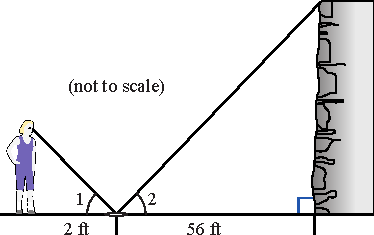
\includegraphics[width=\linewidth]{images/hp1-2-21}
\end{sbspanel}%
\end{sidebyside}%
\end{divisionexerciseeg}%
\begin{divisionexerciseeg}{22}{}{}{g:exercise:idm46051681980880}%
Edo estimates the height of the Washington Monument as follows.  He notices that he can see the reflection of the top of the monument in the reflecting pool.  He is  feet from the tip of the reflection, and that point is 1080 yards from the base of the monument, as shown below.  From his physics class Edo knows that the angles marked and are equal.  If Edo is 6 feet tall, what is his estimate for the height of the Washington Monument?%
\begin{sidebyside}{1}{0.15}{0.15}{0}%
\begin{sbspanel}{0.7}%
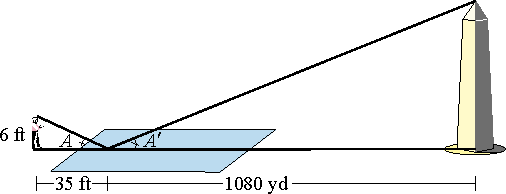
\includegraphics[width=\linewidth]{images/hp1-2-22}
\end{sbspanel}%
\end{sidebyside}%
\end{divisionexerciseeg}%
\begin{divisionexerciseeg}{23}{}{}{g:exercise:idm46051681992816}%
In the sixth century BC, the Greek philosopher and mathematician Thales used similar triangles to measure the distance to a ship at sea.  Two observers on the shore at points \(A\) and \(B\) would sight the ship and measure the angles formed, as shown in figure (a).  They would then construct a similar triangle as shown in figure (b), with the same angles at \(A\) and \(B\), and measure its sides.  (This method is called \emph{triangulation}.)  Use the lengths given in the figures to find the distance from observer  to the ship.%
\begin{sidebyside}{1}{0.2}{0.2}{0}%
\begin{sbspanel}{0.6}%
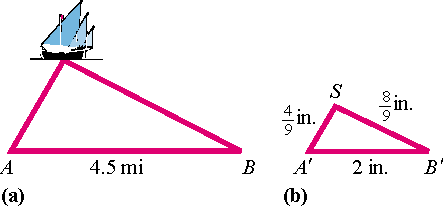
\includegraphics[width=\linewidth]{images/hp1-2-23}
\end{sbspanel}%
\end{sidebyside}%
\end{divisionexerciseeg}%
\begin{divisionexerciseeg}{24}{}{}{g:exercise:idm46051682048128}%
The Capilano Suspension Bridge is a footbridge that spans a 230-foot gorge north of Vancouver, British Columbia.  Before crossing the bridge, you decide to estimate its length.%
\begin{sidebyside}{2}{0}{0}{0.08}%
\begin{sbspanel}{0.6}[center]%
You walk 100 feet downstream from the bridge and sight its far end, noting the angle formed by your line of sight, as shown in figure (a).  You then construct a similar right triangle with a two-centimeter base, as shown in figure (b).  You find that the height of your triangle is 8.98 centimeters.  How long is the Capilano Suspension Bridge?%
\end{sbspanel}%
\begin{sbspanel}{0.32}[center]%

\includegraphics[width=\linewidth]{images/hp1-2-24}
\end{sbspanel}%
\end{sidebyside}%
\end{divisionexerciseeg}%
\begin{divisionexerciseeg}{25}{}{}{g:exercise:idm46051682079984}%
\begin{sidebyside}{2}{0}{0}{0.15}%
\begin{sbspanel}{0.6}[center]%
A conical tank is 12 feet deep and the diameter of the top is 8 feet.  If the tank is filled with water to a depth of 7 feet as shown in the figure at right, what is the area of the exposed surface of the water?%
\end{sbspanel}%
\begin{sbspanel}{0.25}[center]%
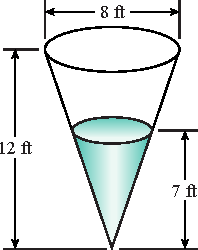
\includegraphics[width=\linewidth]{images/hp1-2-25}
\end{sbspanel}%
\end{sidebyside}%
\end{divisionexerciseeg}%
\begin{divisionexerciseeg}{26}{}{}{g:exercise:idm46051682103040}%
\begin{sidebyside}{2}{0}{0}{0.05}%
\begin{sbspanel}{0.6}[center]%
To measure the distance \(EC\) across the lake shown in the figure at right, stand at \(A\) and sight point \(C\) across the lake, then mark point \(B\).  Then sight to point \(E\) and mark point \(D\) so that \(DB\) is parallel to \(EC\).  If \(AD = 25\) yards, \(AE = 60\) yards, and \(BD = 30\) yards, how wide is the lake?%
\end{sbspanel}%
\begin{sbspanel}{0.35}[center]%
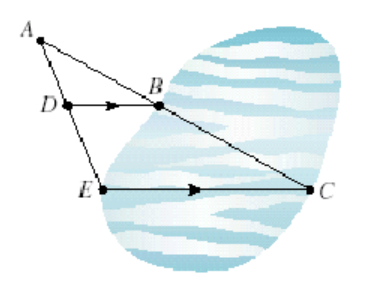
\includegraphics[width=\linewidth]{images/hp1-2-26}
\end{sbspanel}%
\end{sidebyside}%
\end{divisionexerciseeg}%
\end{exercisegroup}
\par\medskip\noindent
\par\medskip\noindent%
%
In Problems 27\textendash{}28, the pairs of triangles are similar.  Solve for \(y\) in terms of \(x\).  (The figures are not drawn to scale.)%
\begin{exercisegroupcol}{2}
\begin{divisionexerciseegcol}{27}{}{}{g:exercise:idm46051685397456}%
\begin{sidebyside}{1}{0.05}{0.05}{0}%
\begin{sbspanel}{0.9}%
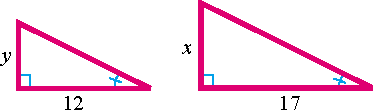
\includegraphics[width=\linewidth]{images/hp1-2-27}
\end{sbspanel}%
\end{sidebyside}%
\end{divisionexerciseegcol}%
\begin{divisionexerciseegcol}{28}{}{}{g:exercise:idm46051685431024}%
\begin{sidebyside}{1}{0.1}{0.1}{0}%
\begin{sbspanel}{0.8}%
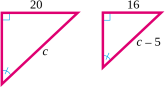
\includegraphics[width=\linewidth]{images/hp1-2-28}
\end{sbspanel}%
\end{sidebyside}%
\end{divisionexerciseegcol}%
\end{exercisegroupcol}
\par\medskip\noindent
\par\medskip\noindent%
%
For Problems 29\textendash{}34, use properties of similar triangles to solve for the variable.%
\begin{exercisegroupcol}{2}
\begin{divisionexerciseegcol}{29}{}{}{g:exercise:idm46051688757840}%
\begin{sidebyside}{1}{0.225}{0.225}{0}%
\begin{sbspanel}{0.55}%

\includegraphics[width=\linewidth]{images/hp1-2-29}
\end{sbspanel}%
\end{sidebyside}%
\end{divisionexerciseegcol}%
\begin{divisionexerciseegcol}{30}{}{}{g:exercise:idm46051688797184}%
\begin{sidebyside}{1}{0.15}{0.15}{0}%
\begin{sbspanel}{0.7}%

\includegraphics[width=\linewidth]{images/hp1-2-30}
\end{sbspanel}%
\end{sidebyside}%
\end{divisionexerciseegcol}%
\begin{divisionexerciseegcol}{31}{}{}{g:exercise:idm46051688803216}%
\begin{sidebyside}{1}{0.3}{0.3}{0}%
\begin{sbspanel}{0.4}%
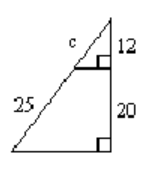
\includegraphics[width=\linewidth]{images/hp1-2-31}
\end{sbspanel}%
\end{sidebyside}%
\end{divisionexerciseegcol}%
\begin{divisionexerciseegcol}{32}{}{}{g:exercise:idm46051688836032}%
\begin{sidebyside}{1}{0.3}{0.3}{0}%
\begin{sbspanel}{0.4}%

\includegraphics[width=\linewidth]{images/hp1-2-32}
\end{sbspanel}%
\end{sidebyside}%
\end{divisionexerciseegcol}%
\begin{divisionexerciseegcol}{33}{}{}{g:exercise:idm46051684854752}%
\begin{sidebyside}{1}{0.275}{0.275}{0}%
\begin{sbspanel}{0.45}%
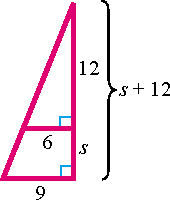
\includegraphics[width=\linewidth]{images/hp1-2-33}
\end{sbspanel}%
\end{sidebyside}%
\end{divisionexerciseegcol}%
\begin{divisionexerciseegcol}{34}{}{}{g:exercise:idm46051684875952}%
\begin{sidebyside}{1}{0.32}{0.32}{0}%
\begin{sbspanel}{0.36}%

\includegraphics[width=\linewidth]{images/hp1-2-34}
\end{sbspanel}%
\end{sidebyside}%
\end{divisionexerciseegcol}%
\end{exercisegroupcol}
\par\medskip\noindent
\par\medskip\noindent%
%
In Problems 35\textendash{}38,solve for \(y\) in terms of \(x\).%
\begin{exercisegroupcol}{2}
\begin{divisionexerciseegcol}{35}{}{}{g:exercise:idm46051684922704}%
\begin{sidebyside}{1}{0.225}{0.225}{0}%
\begin{sbspanel}{0.55}%
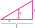
\includegraphics[width=\linewidth]{images/hp1-2-35}
\end{sbspanel}%
\end{sidebyside}%
\end{divisionexerciseegcol}%
\begin{divisionexerciseegcol}{36}{}{}{g:exercise:idm46051688293888}%
\begin{sidebyside}{1}{0.34}{0.34}{0}%
\begin{sbspanel}{0.32}%
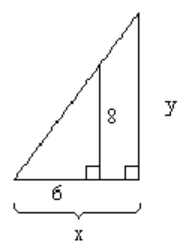
\includegraphics[width=\linewidth]{images/hp1-2-36}
\end{sbspanel}%
\end{sidebyside}%
\end{divisionexerciseegcol}%
\begin{divisionexerciseegcol}{37}{}{}{g:exercise:idm46051688316448}%
\begin{sidebyside}{1}{0.19}{0.19}{0}%
\begin{sbspanel}{0.62}%
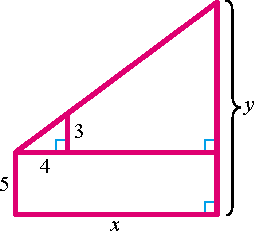
\includegraphics[width=\linewidth]{images/hp1-2-37}
\end{sbspanel}%
\end{sidebyside}%
\end{divisionexerciseegcol}%
\begin{divisionexerciseegcol}{38}{}{}{g:exercise:idm46051688328144}%
\begin{sidebyside}{1}{0.26}{0.26}{0}%
\begin{sbspanel}{0.48}%
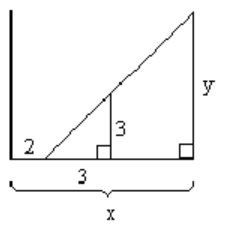
\includegraphics[width=\linewidth]{images/hp1-2-38}
\end{sbspanel}%
\end{sidebyside}%
\end{divisionexerciseegcol}%
\end{exercisegroupcol}
\par\medskip\noindent
\begin{divisionexercise}{39}{}{}{g:exercise:idm46051688349744}%
Triangle \(ABC\) is a right triangle, and \(AD\) meets the hypotenuse \(BC\) at a right angle.%
\begin{sidebyside}{2}{0.0125}{0.0125}{0.025}%
\begin{sbspanel}{0.6}[bottom]%
%
\begin{enumerate}[label=\alph*]
\item{}If \(\angle ACB = 20\degree\), find \(\angle B, \angle CAD\), and \(\angle DAB\).%
\item{}Find two triangles similar to \(\triangle ABC\).  List the corresponding sides in each of the triangles.%
\end{enumerate}
%
\end{sbspanel}%
\begin{sbspanel}{0.35}[center]%
\resizebox{\linewidth}{!}{%
\tikzset{%
  block/.style    = {draw, thick, rectangle, minimum height = 3em,
    minimum width = 3em},
  sum/.style      = {draw, circle, node distance = 2cm}, % Adder
  input/.style    = {coordinate}, % Input
  output/.style   = {coordinate} % Output
}
\begin{tikzpicture}[auto, thick]
    \coordinate (A) at (0,0);
    \coordinate (B) at (0,1.82);
    \coordinate (C) at (5,0);
    \coordinate (D) at (.585,1.6);

    \draw[blue, thick] (A) rectangle +(.25,.25);
    \draw[blue,thick] (D) -- ++(-.235,.0855) -- ++(-.0855,-.235) -- ++(.235,-.0855);
    \draw[black,  thick] (A) --  (B) --(C)--cycle;
    \draw[black,  thick] (A) --  (D) ;

    \draw[red, thick] (4.1,0) arc (180:{180-atan(1.5/4)}:0.9) node [above left, midway, xshift=-3,yshift=-5] {$20\degree$};
    \filldraw [black] (A) circle (.2pt) node[anchor=north east] {$A$};
    \filldraw [black] (B) circle (.2pt) node[anchor=south east] {$B$};
    \filldraw [black] (C) circle (.2pt) node[anchor=north west] {$C$};
    \filldraw [black] (D) circle (.2pt) node[anchor=south west] {$D$};

\end{tikzpicture}
}%
\end{sbspanel}%
\end{sidebyside}%
\end{divisionexercise}%
\begin{divisionexercise}{40}{}{}{g:exercise:idm46051696500464}%
Here is a way to find the distance across a gorge using a carpenter's square and a five-foot pole.  Plant the pole vertically on one side of the gorge at point \(A\) and place the angle of the carpenter's square on top of the pole at point \(B\), as shown in the figure.  Sight along one side of the square so that it points to the opposite side of the gorge at point \(P\).  Without moving the square, sight along the other side and mark point \(Q\).  If the distance from \(Q\) to \(A\) is six inches, calculate the width of the gorge.  Explain your method.%
\begin{sidebyside}{1}{0.2}{0.2}{0}%
\begin{sbspanel}{0.6}%
\resizebox{\linewidth}{!}{%
\tikzset{%
  block/.style    = {draw, thick, rectangle, minimum height = 3em,
    minimum width = 3em},
  sum/.style      = {draw, circle, node distance = 2cm}, % Adder
  input/.style    = {coordinate}, % Input
  output/.style   = {coordinate} % Output
}
\begin{tikzpicture}[auto, thick]
    \coordinate (A) at (0,0);
    \coordinate (B) at (0,3);
    \coordinate (C) at (9,0);
    \coordinate (Q) at (-1,0);

    \draw[black,  thick] (A) --  (B) node[right, midway] {\color{blue}$5'$};
    \draw[black,  thick] (A) --  (Q) node[above, midway] {\color{blue}$6''$};
    \draw[black,  thick] (Q) --  (B) --(C)--cycle;

    \filldraw [black] (A) circle (1.6pt) node[anchor=north east] {$A$};
    \filldraw [black] (B) circle (.2pt) node[anchor=south east] {$B$};
    \filldraw [black] (C) circle (1.6pt) node[anchor=north west] {$P$};
    \filldraw [black] (Q) circle (1.6pt) node[anchor=north east] {$Q$};
    \draw[brown,line width=3pt] (B) -- +(-.2,-.6);
    \draw[brown,line width=3pt] (B) -- +(.9,-.3);

    \draw[black,thin] (0,-.4) -- +(0,-.4);
    \draw[black,thin] (9,-.4) -- +(0,-.4);
    \draw[black,thin] (0,-.6) -- +(3.5,0);
    \node at (4.5,-.6)  {(gorge)};
    \draw[black,thin] (9,-.6) -- +(-3.5,0);

\end{tikzpicture}
}%
\end{sbspanel}%
\end{sidebyside}%
\end{divisionexercise}%
\end{exercises-subsection}
\end{sectionptx}
%
%
\typeout{************************************************}
\typeout{Section 1.3 Circles}
\typeout{************************************************}
%
\begin{sectionptx}{Circles}{}{Circles}{}{}{x:section:circles}
%
%
\typeout{************************************************}
\typeout{Subsection  The Distance Formula}
\typeout{************************************************}
%
\begin{subsectionptx}{The Distance Formula}{}{The Distance Formula}{}{}{g:subsection:idm46051679662656}
\index{distance formula}%
Delbert is hiking in the Santa Monica mountains, and he would like to know the distance from the Sycamore Canyon trail head, located at 12-C on his map, to the Coyote Trail junction, located at 8-F, as shown below.%
\begin{sidebyside}{1}{0.1}{0.1}{0}%
\begin{sbspanel}{0.8}%
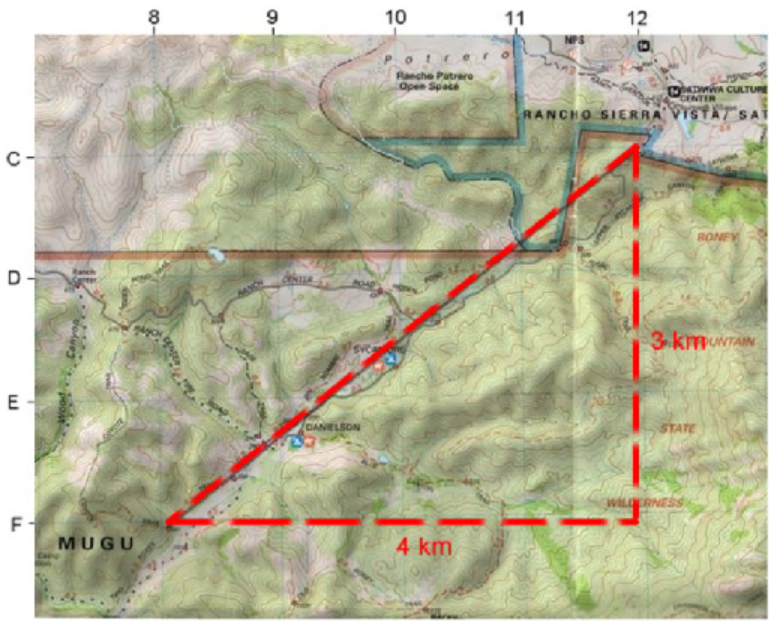
\includegraphics[width=\linewidth]{images/1-3SM.png}
\end{sbspanel}%
\end{sidebyside}%
\par
Each interval on the map represents one kilometer. Delbert remembers the \terminology{Pythagorean theorem}, and uses the map coordinates to label the sides of a right triangle. The distance he wants is the hypotenuse of the triangle, so%
\par
%
\begin{align*}
d^2\amp = 4^2+3^2 = 16+9 = 25\\
d\amp = \sqrt{25} = 5
\end{align*}
%
\par
The straight-line distance to Coyote junction is about 5 kilometers.%
\par
The formula for the distance between two points is obtained in the same way.%
\begin{sidebyside}{2}{0}{0}{0.05}%
\begin{sbspanel}{0.6}%
We first label a right triangle with points \(P_{1}\) and \(P_{2}\) on opposite ends of the hypotenuse.  (See the figure at right.)  The sides of the triangle have lengths \(\abs{x_2-x_1}\) and \(\abs{y_2-y_1}\).  We can use the Pythagorean theorem to calculate the distance between \(P_{1}\) and \(P_{2}\):%
\begin{equation*}
d^2=(x_2-x_1)^2+(y_2-y_1)^2
\end{equation*}
%
\end{sbspanel}%
\begin{sbspanel}{0.35}%
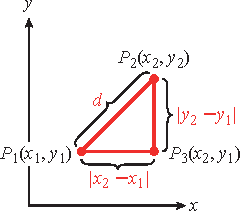
\includegraphics[width=\linewidth]{images/distform}
\end{sbspanel}%
\end{sidebyside}%
\par
Taking the (positive) square root of each side of this equation gives us the \terminology{distance formula}.%
\begin{assemblage}{Distance Formula.}{g:assemblage:idm46051679806672}%
The distance \(d\) between two points \(P_{1}(x_1, y_1)\) and \(P_{2}(x_2, y_2)\) is%
\begin{equation*}
\blert{d=\sqrt{(x_2-x_1)^2+(y_2-y_1)^2}}
\end{equation*}
%
\end{assemblage}
\begin{example}{}{g:example:idm46051679834416}%
Find the distance between \((2,-1)\) and \((4,3)\).%
\par\smallskip%
\noindent\textbf{\blocktitlefont Solution}.\label{g:solution:idm46051679852928}{}\hypertarget{g:solution:idm46051679852928}{}\quad{}\begin{sidebyside}{2}{0.025}{0.025}{0.05}%
\begin{sbspanel}{0.6}%
We substitute \((2,-1)\) for \((x_1, y_1)\) and \((4,3)\) for \((x_2, y_2)\) in the distance formula to obtain%
\begin{align*}
d\amp = \sqrt{(x_2-x_1)^2+(y_2-y_1)^2}\\
\amp = \sqrt{(4-2)^2+[3-(-1)]^2}\\
\amp = \sqrt{4+16} = \sqrt{20} = 2\sqrt{5}
\end{align*}
%
\end{sbspanel}%
\begin{sbspanel}{0.3}%
\resizebox{\linewidth}{!}{%
\tikzset{%
  block/.style    = {draw, thick, rectangle, minimum height = 3em,
    minimum width = 3em},
  sum/.style      = {draw, circle, node distance = 2cm}, % Adder
  input/.style    = {coordinate}, % Input
  output/.style   = {coordinate} % Output
}
\begin{tikzpicture}[auto, thick, scale=.45]
    \draw[step=1cm,cyan,very thin] (-5,-5) grid (5,5);
    \draw[thick,->] (-5,0) -- (5.4,0) node[anchor=west] {$x$};
    \draw[thick,->] (0,-5) -- (0,5.4) node[anchor=south] {$y$};
    `
    \foreach \x in {-5,5}
        \draw (\x cm,1pt) -- (\x cm,-1pt) node[anchor=north] {$\x$};
    \foreach \y in {-5,5}
        \draw (1pt,\y cm) -- (-1pt,\y cm) node[anchor=east] {$\y$};


    \coordinate (A) at (2,-1);
    \coordinate (B) at (4,-1);
    \coordinate (C) at (4,3);

    \filldraw[black] (A) circle (5pt) node[anchor=north east,xshift=11,yshift=-5,fill=white] {$(2,-1)$};
    \filldraw[black] (C) circle (5pt) node[anchor=south ,yshift=2,fill=white] {$(4,3)$};

    \draw[red, thick] (A)--(C) node[above left, midway,fill=white] {$2\sqrt{5}$};
    \draw[black, ultra thick, dashed] (A)--(B) ;
    \draw[black, ultra thick, dashed] (C)--(B) ;
\end{tikzpicture}
}%
\end{sbspanel}%
\end{sidebyside}%
 The exact value of the distance, shown at right, is \(2\sqrt{5}\) units.  We obtain the same answer if we use \((4,3)\) for \(P_1\) and \((2,-1)\) for \(P_2\):%
\begin{equation*}
\begin{aligned}[t]
d\amp = \sqrt{(2-4)^2+[(-1)-3]^2}\\ 
\amp = \sqrt{4+16} = \sqrt{20} = 2\sqrt{5}\\
\end{aligned}
\end{equation*}
We can use a calculator to obtain an approximation for this value, and find%
\begin{equation*}
2\sqrt{5}\approx 2(2.236)=4.472
\end{equation*}
%
\end{example}
\begin{warning}{}{g:warning:idm46051679923248}%
In the previous example, the radical \(\sqrt{4+16}\) cannot be simplified to \(\sqrt{4}+\sqrt{16}\). (Do you remember why not?)%
\end{warning}
\begin{inlineexercise}{}{g:exercise:idm46051679948512}%
%
\begin{enumerate}[label=\alph*]
\item{}Find the distance between the points \((-5,3)\) and \((3,-9)\).%
\item{}Plot the points on a Cartesian grid and show how the Pythagorean theorem is used to calculate the distance.%
\end{enumerate}
%
\par\smallskip%
\noindent\textbf{\blocktitlefont Answer}.\label{g:answer:idm46051679955936}{}\hypertarget{g:answer:idm46051679955936}{}\quad{}\(4\sqrt{13}\)%
\end{inlineexercise}
\end{subsectionptx}
%
%
\typeout{************************************************}
\typeout{Subsection  Equation for a Circle}
\typeout{************************************************}
%
\begin{subsectionptx}{Equation for a Circle}{}{Equation for a Circle}{}{}{g:subsection:idm46051679969392}
\index{circle!equation}%
A \terminology{circle}\index{circle} is the set of all points in a plane that lie at a given distance, called the \terminology{radius}\index{radius}, from a fixed point called the \terminology{center}\index{center}.  We can use the distance formula to find an equation for a circle.%
\par
The circle shown below has its center at the origin, \((0,0)\), and its radius is \(r\).%
\begin{sidebyside}{2}{0}{0.1}{0}%
\begin{sbspanel}{0.6}%
Now, the distance from the origin to any point \(P(x,y)\) on the circle is \(r\).  Therefore,%
\begin{equation*}
\sqrt{(x-0)^2+(y-0)^2} = r
\end{equation*}
or, squaring both sides,%
\begin{equation*}
(x-0)^2+(y-0)^2=r^2
\end{equation*}
%
\end{sbspanel}%
\begin{sbspanel}{0.3}%
\resizebox{\linewidth}{!}{%
\tikzset{%
  block/.style    = {draw, thick, rectangle, minimum height = 3em,
    minimum width = 3em},
  sum/.style      = {draw, circle, node distance = 2cm}, % Adder
  input/.style    = {coordinate}, % Input
  output/.style   = {coordinate} % Output
}
\begin{tikzpicture}

\coordinate(O) at (0,0);
\coordinate (A) at (0.8,1.386 );

\draw (0,0) circle (1.6);

\draw[thick,->] (-2,0) -- (2,0) node[anchor=west] {$x$};
\draw[thick,->] (0,-2) -- (0,2) node[anchor=south] {$y$};

\filldraw[red] (A) circle (1.4pt) node[anchor=south west, xshift=0, yshift=0]{\color{black}$P(x,y)$};

\draw[red, thick] (O) -- (A) node[below right, midway]{\color{blue}$r$};
\end{tikzpicture}
}%
\end{sbspanel}%
\end{sidebyside}%
\par
Because every point on the circle must satisfy this equation, we have found an equation for the circle.%
\begin{assemblage}{Circle.}{g:assemblage:idm46051680076784}%
The equation for a \terminology{circle} of radius \(r\) centered at the origin is%
\begin{equation*}
\blert{x^2+y^2=r^2}
\end{equation*}
%
\end{assemblage}
\begin{example}{}{g:example:idm46051680101216}%
Find two points on the circle \(x^2+y^2=4\) with \(y\)-coordinate \(-1\).%
\par\smallskip%
\noindent\textbf{\blocktitlefont Solution}.\label{g:solution:idm46051680108400}{}\hypertarget{g:solution:idm46051680108400}{}\quad{}We substitute \(x=\alert{-1}\) into the equation for the circle, and solve for \(y\).%
\begin{sidebyside}{2}{0.02}{0.02}{0.04}%
\begin{sbspanel}{0.6}%
%
\begin{align*}
(\alert{-1}^2)+y^2 \amp = 4\\
y^2 \amp = 4-1 = 3\\
y \amp = \pm \sqrt{3}
\end{align*}
The points are \((-1, \sqrt{3})\) and \((-1,\sqrt{3})\), as shown at right. Note that \(\sqrt{3} \approx 1.732\).%
\end{sbspanel}%
\begin{sbspanel}{0.32}%
\resizebox{\linewidth}{!}{%
\tikzset{%
  block/.style    = {draw, thick, rectangle, minimum height = 3em,
    minimum width = 3em},
  sum/.style      = {draw, circle, node distance = 2cm}, % Adder
  input/.style    = {coordinate}, % Input
  output/.style   = {coordinate} % Output
}
\begin{tikzpicture} [scale = .7]

\draw[step=1cm,cyan,very thin] (-3,-3) grid (3,3);
\draw[thick,->] (-3,0) -- (3.4,0) node[anchor=west] {$x$};
\draw[thick,->] (0,-3) -- (0,3.4) node[anchor=south] {$y$};
`
\foreach \x in {-3,1,3}
    \draw (\x cm,3pt) -- (\x cm,-3pt) node[anchor=north] {$\x$};
\foreach \y in {-3,1,3}
    \draw (3pt,\y cm) -- (-3pt,\y cm) node[anchor=east] {$\y$};

\coordinate(O) at (0,0);
\coordinate (A) at (-1,1.732 );
\coordinate (B) at (-1,-1.732 );

\draw[red,thick] (0,0) circle (2);

\filldraw[black] (A) circle (2pt) node[anchor=south east, xshift=3, yshift=2, fill=white]{\color{black}$(-1,\sqrt{3})$};
\filldraw[black] (B) circle (2pt) node[anchor=north east, xshift=3, yshift=-2, fill=white]{\color{black}$(-1,-\sqrt{3})$};
\end{tikzpicture}
}%
\end{sbspanel}%
\end{sidebyside}%
\end{example}
\begin{inlineexercise}{}{g:exercise:idm46051680152240}%
Find the coordinates of two points on the circle \(~~x^2+y^2=1~~\) with \(y\)-coordinate \(\dfrac{1}{2}\).%
\par\smallskip%
\noindent\textbf{\blocktitlefont Answer}.\label{g:answer:idm46051680167440}{}\hypertarget{g:answer:idm46051680167440}{}\quad{}\(\left(\dfrac{\sqrt{3}}{2},\dfrac{1}{2}\right)\), \(\left(\dfrac{-\sqrt{3}}{2},\dfrac{1}{2}\right)\)%
\end{inlineexercise}
\begin{definition}{Unit Circle.}{g:definition:idm46051680171792}%
The circle in the exercise above, \(~~\blert{x^2+y^2=1},~~\) which is centered at the origin and has radius 1 unit, is called the \terminology{unit circle}\index{unit circle}.%
\end{definition}
\end{subsectionptx}
%
%
\typeout{************************************************}
\typeout{Subsection  Rational and Irrational Numbers}
\typeout{************************************************}
%
\begin{subsectionptx}{Rational and Irrational Numbers}{}{Rational and Irrational Numbers}{}{}{g:subsection:idm46051680183664}
\index{rational number}%
\index{irrational number}%
Every common fraction, such as \(\dfrac{3}{4}\), can be written in many equivalent forms, including a decimal form.  For example,%
\begin{equation*}
\frac{3}{4}=\frac{6}{8}=\frac{75}{100}=0.75~~~~~\text{and}~~~~~\frac{5}{11}=\frac{20}{44}=\frac{50}{110}=0.\overline{45}
\end{equation*}
%
\par
where \(0.\overline{45}\) is the repeating decimal \(0.45454545....\)%
\par
Because the fraction bar denotes division, a fraction is a quotient of two integers, and we can calculate its decimal form by dividing the denominator into the numerator.%
\begin{definition}{Rational Number.}{g:definition:idm46051680208336}%
Any number (including fractions) that can be written as a quotient of two integers \(~~\dfrac{a}{b},~~\text{where}~~ b\not=0,~~\) is called a \terminology{rational number}\index{rational number}.%
\end{definition}
The decimal form of a rational number is either a \terminology{terminating decimal}\index{terminating decimal|seealso{rational number}}\index{terminating decimal}, such as \(0.75\), or a \terminology{repeating decimal}\index{repeating decimal|seealso{rational number}}\index{repeating decimal}, such as \(0.\overline{45}\). Thus, we can always write down an exact decimal equivalent for a rational number, although we may choose to round off a particularly long or unwieldy decimal. For example,%
\begin{equation*}
\frac{3}{7}=0.\overline{428571}\approx 0.43
\end{equation*}
%
\begin{warning}{}{g:warning:idm46051680304848}%
Note that \(0.43\) is \emph{not} exactly equal to \(\dfrac{3}{7}\); it is an \emph{approximation} for \(\dfrac{3}{7}\), just as \(0.33\) is an approximation for \(\dfrac{1}{3}\). In our work, it will be important to distinguish between exact values and approximations.%
\end{warning}
\begin{definition}{Irrational Number.}{g:definition:idm46051680357232}%
An \terminology{irrational number}\index{irrational number} is one that \emph{cannot} be written as a quotient of two integers \(\dfrac{a}{b}\),where \(b\not=0\).%
\end{definition}
Examples of irrational numbers are \(\sqrt{3}\), \(\sqrt[3]{586}\), and \(\pi\). The decimal form of an irrational number is nonterminating and nonrepeating.  The first few digits of the examples mentioned are%
\begin{align*}
\sqrt{3} \amp = 1.732050807568...\\
\sqrt[3]{586} \amp = 8.368209391204...\\
\pi \amp = 3.141592653589...
\end{align*}
%
\par
but none of these decimal forms ever ends. Thus, \emph{we cannot write down an exact decimal equivalent for an irrational number}. The best we can do is give a decimal approximation, no matter how many digits we include.%
\begin{example}{}{g:example:idm46051680397968}%
Which values are exact, and which are approximations?%
\par
%
\begin{multicols}{2}
\begin{enumerate}[label=\alph*]
\item{}\(\displaystyle \dfrac{7}{32}\rightarrow 0.21875\)%
\item{}\(\displaystyle \sqrt{8}\rightarrow 2.828427125\)%
\item{}\(\displaystyle \sqrt{0.16}\rightarrow 0.4\)%
\item{}\(\displaystyle \dfrac{\pi}{2}\rightarrow 1.570796327\)%
\end{enumerate}
\end{multicols}
%
\par\smallskip%
\noindent\textbf{\blocktitlefont Solution}.\label{g:solution:idm46051680404880}{}\hypertarget{g:solution:idm46051680404880}{}\quad{}%
\begin{enumerate}[label=\alph*]
\item{}Because \(\dfrac{7}{32}\) is a rational number, it has an exact decimal equivalent.  Divide 7 by 32 to see that \(\dfrac{7}{32}=0.21875\).%
\item{}Because 8 is not a perfect square, \(\sqrt{8}\) is irrational, so \(2.828427125\) is not the exact value of \(\sqrt{8}\).%
\item{}\(\sqrt{0.16}=\sqrt{\dfrac{16}{100}}=\dfrac{4}{10}=0.4\), so this value is exact.%
\item{}Because \(\dfrac{\pi}{2}\) is an irrational number, it has no decimal equivalent, so \(1.570796327\) is an approximation.%
\end{enumerate}
%
\end{example}
\begin{inlineexercise}{}{g:exercise:idm46051680435360}%
For which numbers can you give an exact decimal equivalent?%
\par
%
\begin{multicols}{4}
\begin{enumerate}[label=\alph*]
\item{}\(\displaystyle \dfrac{\sqrt{3}}{2}\)%
\item{}\(\displaystyle \dfrac{\sqrt{16}}{3}\)%
\item{}\(\displaystyle 2\pi\)%
\item{}\(\displaystyle \dfrac{25}{17}\)%
\end{enumerate}
\end{multicols}
%
\par\smallskip%
\noindent\textbf{\blocktitlefont Answer}.\label{g:answer:idm46051680449216}{}\hypertarget{g:answer:idm46051680449216}{}\quad{}b, d%
\end{inlineexercise}
\end{subsectionptx}
%
%
\typeout{************************************************}
\typeout{Subsection  Circumference and Area}
\typeout{************************************************}
%
\begin{subsectionptx}{Circumference and Area}{}{Circumference and Area}{}{}{g:subsection:idm46051680450944}
\index{circumference}%
Recall from geometry that the circumference of a circle is proportional to its radius.%
\begin{assemblage}{Circumference of a Circle.}{g:assemblage:idm46051680455840}%
The \terminology{circumference} of a circle of radius \(r\) is given by%
\begin{equation*}
\blert{C=2\pi r}
\end{equation*}
%
\end{assemblage}
The number \(\pi\)\index{\(\pi\)} gives the ratio of the circumference of any circle to its diameter.  It is an irrational number, \(\pi\approx 3.14159\).%
\par
The length of a portion, or arc, of a circle, is called its \terminology{arclength}\index{arclength}.%
\begin{example}{}{g:example:idm46051679983008}%
Francine baked an apple pie with diameter 8 inches.  If Delbert cuts himself a 60° wedge, what is the arclength of the curved edge?%
\par\smallskip%
\noindent\textbf{\blocktitlefont Solution}.\label{g:solution:idm46051680006976}{}\hypertarget{g:solution:idm46051680006976}{}\quad{}The radius of the pie is 4 inches, so its circumference is \(2\pi (4)\) inches.%
\begin{sidebyside}{2}{0.025}{0.025}{0.05}%
\begin{sbspanel}{0.7}%
A 60° wedge, shown at right, is \(\dfrac{1}{6}\) of the entire pie, so its edge is \(\dfrac{1}{6}\) of the circumference.  The exact length of the arc is thus%
\begin{equation*}
\dfrac{1}{6} (8\pi)=\dfrac{4\pi}{3} \text{ inches.}
\end{equation*}
%
\end{sbspanel}%
\begin{sbspanel}{0.2}%
\resizebox{\linewidth}{!}{%
\tikzset{%
  block/.style    = {draw, thick, rectangle, minimum height = 3em,
    minimum width = 3em},
  sum/.style      = {draw, circle, node distance = 2cm}, % Adder
  input/.style    = {coordinate}, % Input
  output/.style   = {coordinate} % Output
}
\begin{tikzpicture} [scale = .7]

\coordinate(O) at (0,0);
\coordinate (A) at (0,2 );
\coordinate (B) at (1.732,1 );

\draw[gray,thick] (0,0) circle (2);
\draw[black, thick] (O)--(B) node[below right, midway, xshift=-5] {\color{blue}4 in.};
\draw[black, thick] (O)--(A);
\draw[red, thin] (0,.5) arc (90:30:0.5) node[above right, midway, xshift=-5]{$60\degree$};
\end{tikzpicture}
}%
\end{sbspanel}%
\end{sidebyside}%
\par
Using a calculator, we find that \(\dfrac{4\pi}{3}=4.19\) rounded to two decimal places, so the length of the curved edge is between 4 and 4\(\frac{1}{2}\) inches.%
\end{example}
\begin{inlineexercise}{}{g:exercise:idm46051680516544}%
What is the arclength of the curved edge of a 60° wedge cut from a blueberry pie of diameter 10 inches?%
\par\smallskip%
\noindent\textbf{\blocktitlefont Answer}.\label{g:answer:idm46051680535152}{}\hypertarget{g:answer:idm46051680535152}{}\quad{}\(\dfrac{5\pi}{3} \approx 5.24~~\text{inches}\)%
\end{inlineexercise}
The area of a circle is proportional to the square of its radius.%
\begin{assemblage}{Area of a Circle.}{g:assemblage:idm46051680544784}%
The \terminology{area} of a circle of radius \(r\) is given by%
\begin{equation*}
\blert{A=\pi r^2}
\end{equation*}
%
\end{assemblage}
A portion of a circle shaped like a pie-shaped wedge is called a \terminology{sector}\index{sector}.%
\begin{example}{}{g:example:idm46051680582960}%
What is the area of Delbert's slice of apple pie in the previous example?%
\par\smallskip%
\noindent\textbf{\blocktitlefont Solution}.\label{g:solution:idm46051680589200}{}\hypertarget{g:solution:idm46051680589200}{}\quad{}As we saw in the previous example, Delbert's sector of the pie is \(\dfrac{1}{6}\) of the entire pie, so its area \(\dfrac{1}{6}\) of the area of the whole pie, or%
\begin{equation*}
\dfrac{1}{6} \pi (4^2)= \dfrac{8\pi}{3}~~ \text{square inches}
\end{equation*}
%
\par
The area of the wedge is \(\dfrac{8\pi}{3}\), or about 8.34 square inches.%
\end{example}
\begin{inlineexercise}{}{g:exercise:idm46051680632592}%
What is the area of a 60° wedge cut from a blueberry pie of diameter 10 inches?%
\par\smallskip%
\noindent\textbf{\blocktitlefont Answer}.\label{g:answer:idm46051680563744}{}\hypertarget{g:answer:idm46051680563744}{}\quad{}\(\dfrac{25\pi}{6} \approx 13.09~~\text{square inches}\)%
\end{inlineexercise}
Review the following skills you will need for this section.%
\begin{project}{}{g:project:idm46051680613680}%
\begin{sidebyside}{1}{0}{0}{0}%
\begin{sbspanel}{1}%
True of False.%
\end{sbspanel}%
\end{sidebyside}%
\begin{sidebyside}{3}{0}{0}{0.05}%
\begin{sbspanel}{0.3}%
1. \(\sqrt{a^2+b^2}=a+b\)%
\par
4. \(\sqrt{2x}\sqrt{3y}=\sqrt{6xy}\)%
\par
7. \(\sqrt{\dfrac{x}{4}}=\dfrac{\sqrt{x}}{2}\)%
\end{sbspanel}%
\begin{sbspanel}{0.3}%
2. \(\sqrt{36+64}=6+8\)%
\par
5. \(\sqrt{5x}+\sqrt{3x}=\sqrt{8x}\)%
\par
8. \(\sqrt{\dfrac{3}{2}}=\dfrac{\sqrt{6}}{2}\)%
\end{sbspanel}%
\begin{sbspanel}{0.3}%
3. \(\sqrt{16x^4}=4x^2\)%
\par
6. \(\sqrt{4+N}=2+\sqrt{N}\)%
\end{sbspanel}%
\end{sidebyside}%
\begin{sidebyside}{1}{0}{0}{0}%
\begin{sbspanel}{1}%
\(\underline{\qquad\qquad\qquad\qquad}\)%
\end{sbspanel}%
\end{sidebyside}%
\begin{sidebyside}{1}{0}{0}{0}%
\begin{sbspanel}{1}%
Algebra Refresher Answers%
\end{sbspanel}%
\end{sidebyside}%
\begin{sidebyside}{1}{0}{0}{0}%
\begin{sbspanel}{1}%
%
\begin{multicols}{4}
\begin{enumerate}[label=\arabic*]
\item{}False%
\item{}False%
\item{}True%
\item{}True%
\item{}False%
\item{}False%
\item{}True%
\item{}True%
\end{enumerate}
\end{multicols}
%
\end{sbspanel}%
\end{sidebyside}%
\end{project}
\end{subsectionptx}
%
%
\typeout{************************************************}
\typeout{Subsection  Section 1.3 Summary}
\typeout{************************************************}
%
\begin{subsectionptx}{Section 1.3 Summary}{}{Section 1.3 Summary}{}{}{g:subsection:idm46051680780448}
%
%
\typeout{************************************************}
\typeout{Subsubsection  Vocabulary}
\typeout{************************************************}
%
\begin{subsubsectionptx}{Vocabulary}{}{Vocabulary}{}{}{g:subsubsection:idm46051680782464}
Look up the definitions of new terms in the Glossary.%
\par
%
\begin{multicols}{3}
\begin{itemize}[label=\textbullet]
\item{}Rational number%
\item{}Irrational number%
\item{}Repeating decimal%
\item{}Circle%
\item{}Radius%
\item{}Unit circle%
\item{}Circumference%
\item{}Arclength%
\end{itemize}
\end{multicols}
%
\end{subsubsectionptx}
%
%
\typeout{************************************************}
\typeout{Subsubsection  Concepts}
\typeout{************************************************}
%
\begin{subsubsectionptx}{Concepts}{}{Concepts}{}{}{g:subsubsection:idm46051680806144}
%
\begin{enumerate}[label=\arabic*]
\item{}\begin{assemblage}{Distance Formula.}{g:assemblage:idm46051680815824}%
The distance \(d\) between two points \(P_{1}(x_1, y_1)\) and \(P_{2}(x_2, y_2)\) is%
\begin{equation*}
d=\sqrt{(x_2-x_1)^2+(y_2-y_1)^2}
\end{equation*}
%
\end{assemblage}
%
\item{}Any number that can be written as a quotient of two integers \(~~\dfrac{a}{b},~~\text{where}~~ b\not=0,\) is called a \terminology{rational number}.  The decimal form of a rational number is either a \terminology{terminating decimal} or a \terminology{repeating decimal}.%
\item{}An \terminology{irrational number} is one that \emph{cannot} be written as a quotient of two integers \(~~\dfrac{a}{b},~~\text{where}~~ b\not=0\).  We cannot write down an exact decimal equivalent for an irrational number.%
\item{}A \terminology{circle} is the set of all points in a plane that lie at a given distance, called the \terminology{radius}, from a fixed point called the \terminology{center}.%
\item{}\begin{assemblage}{Circle.}{g:assemblage:idm46051680876864}%
The equation for a \terminology{circle} of radius \(r\) centered at the origin is%
\begin{equation*}
x^2+y^2=r^2
\end{equation*}
%
\end{assemblage}
%
\item{}The circle \(~x^2+y^2=1~\), which is centered at the origin and has radius 1 unit, is called the \terminology{unit circle}.%
\item{}\begin{assemblage}{Circumference of a Circle.}{g:assemblage:idm46051680919952}%
The \terminology{circumference} of a circle of radius \(r\) is given by%
\begin{equation*}
C=2\pi r
\end{equation*}
%
\end{assemblage}
%
\item{}\begin{assemblage}{Area of a Circle.}{g:assemblage:idm46051680932784}%
The \terminology{area} of a circle of radius \(r\) is given by%
\begin{equation*}
A=\pi r^2
\end{equation*}
%
\end{assemblage}
%
\end{enumerate}
%
\end{subsubsectionptx}
%
%
\typeout{************************************************}
\typeout{Subsubsection  Study Questions}
\typeout{************************************************}
%
\begin{subsubsectionptx}{Study Questions}{}{Study Questions}{}{}{g:subsubsection:idm46051680950064}
%
\begin{enumerate}[label=\arabic*]
\item{}Explain why the distance formula, \(d=\sqrt{(x_2-x_1)^2+(y_2-y_1)^2}\),  cannot be simplified to \((x_2-x_1)+(y_2-y_1)\).%
\item{}What is a unit circle, and what is its equation?%
\item{}Can you give an exact decimal value for \(\pi\)?%
\item{}What is the arclength of a semicircle of radius \(r\)?%
\end{enumerate}
%
\end{subsubsectionptx}
%
%
\typeout{************************************************}
\typeout{Subsubsection  Skills}
\typeout{************************************************}
%
\begin{subsubsectionptx}{Skills}{}{Skills}{}{}{g:subsubsection:idm46051680979664}
Practice each skill in the Homework Problems listed.%
\par
%
\begin{enumerate}[label=\arabic*]
\item{}Find the distance between two points    \#1-18%
\item{}Distinguish between exact values and approximations    \#19-24%
\item{}Graph a circle    \#25-30, 35-40%
\item{}Find and use the equation for a circle    \#31-34, 39-42, 55-56%
\item{}Find the length of a fraction of a circle    \#35-38, 43-54%
\item{}Find the area of a sector of a circle    \#43-50%
\end{enumerate}
%
\end{subsubsectionptx}
\end{subsectionptx}
%
%
\typeout{************************************************}
\typeout{Exercises  Homework 1.3}
\typeout{************************************************}
%
\begin{exercises-subsection}{Homework 1.3}{}{Homework 1.3}{}{}{x:exercises:hmwk-1-3}
\begin{divisionexercise}{1}{}{}{g:exercise:idm46051681007760}%
Leanne is sailing and is currently 3 miles west and 5 miles south of the harbor.  She heads directly towards an island that is 8 miles west and 7 miles north of the harbor.  How far is Leanne from the island?%
\end{divisionexercise}%
\begin{divisionexercise}{2}{}{}{g:exercise:idm46051681018480}%
Dominic is 100 meters east and 250 meters north of Kristen.  He is walking directly towards a tree that is 220 meters east and 90 meters north of Kristen.  How far is Dominic from the tree?%
\end{divisionexercise}%
\par\medskip\noindent%
%
For Problems 3\textendash{}6, find the distance between the points.  Give your answer as an exact value, then as a decimal rounded to hundredths.%
\begin{exercisegroupcol}{2}
\begin{divisionexerciseegcol}{3}{}{}{g:exercise:idm46051681027408}%
\begin{sidebyside}{1}{0.275}{0.275}{0}%
\begin{sbspanel}{0.45}%
\resizebox{\linewidth}{!}{%
\tikzset{%
}
\begin{tikzpicture}[scale =0.25]

    \coordinate(O) at (3,1);
    \coordinate (A) at (3,9 );
    \coordinate (B) at (9,1 );

    \draw[black ,thick, ->] (-0.5,0) -- (9.5,0 ) node[anchor=west] {$x$};);
    \draw[black ,thick, ->] (0,-0.5) -- (0,9.5 ) node[anchor=south] {$y$};);
    \draw[black, thick, dashed] (O)--(B);
    \draw[black, thick, dashed] (O)--(A);
    \draw[black, thick] (B)--(A);

    \filldraw[black] (A)  circle (8pt) node[anchor=south] {$(3,9)$};
    \filldraw[black] (B)  circle (8pt) node[anchor=west, yshift=3] {$(9,1)$};

\end{tikzpicture}
}%
\end{sbspanel}%
\end{sidebyside}%
\end{divisionexerciseegcol}%
\begin{divisionexerciseegcol}{4}{}{}{g:exercise:idm46051681042928}%
\begin{sidebyside}{1}{0.225}{0.225}{0}%
\begin{sbspanel}{0.55}%
\resizebox{\linewidth}{!}{%
\tikzset{%
}
\begin{tikzpicture}[scale =0.15]

    \coordinate(O) at (-13,3);
    \coordinate (A) at (-13,8 );
    \coordinate (B) at (-1,3 );

    \draw[black ,thick, ->] (-15,0) -- (11,0 ) node[anchor=west] {$x$};);
    \draw[black ,thick, ->] (0,-0.5) -- (0,15 ) node[anchor=south] {$y$};);
    \draw[black, thick, dashed] (O)--(B);
    \draw[black, thick, dashed] (O)--(A);
    \draw[black, thick] (B)--(A);

    \filldraw[black] (A)  circle (12pt) node[anchor=south] {$(-13,8)$};
    \filldraw[black] (B)  circle (12pt) node[anchor=west, xshift=3] {$(-1,3)$};

\end{tikzpicture}
}%
\end{sbspanel}%
\end{sidebyside}%
\end{divisionexerciseegcol}%
\begin{divisionexerciseegcol}{5}{}{}{g:exercise:idm46051681055264}%
\begin{sidebyside}{1}{0.225}{0.225}{0}%
\begin{sbspanel}{0.55}%
\resizebox{\linewidth}{!}{%
\tikzset{%
}
\begin{tikzpicture}[scale=0.25]
    \coordinate(O) at (-6,-2);
    \coordinate (A) at (-6,-6 );
    \coordinate (B) at (2,-2 );

    \draw[black ,thick, ->] (-7,0) -- (7,0 ) node[anchor=west] {$x$};);
    \draw[black ,thick, ->] (0,-8) -- (0,3 ) node[anchor=south] {$y$};);
    \draw[black, thick, dashed] (O)--(B);
    \draw[black, thick, dashed] (O)--(A);
    \draw[black, thick] (B)--(A);

    \filldraw[black] (A)  circle (8pt) node[anchor=north] {$(-6,-6)$};
    \filldraw[black] (B)  circle (8pt) node[anchor=west, yshift=3] {$(2,-2)$};

\end{tikzpicture}
}%
\end{sbspanel}%
\end{sidebyside}%
\end{divisionexerciseegcol}%
\begin{divisionexerciseegcol}{6}{}{}{g:exercise:idm46051681084592}%
\begin{sidebyside}{1}{0.275}{0.275}{0}%
\begin{sbspanel}{0.45}%
\resizebox{\linewidth}{!}{%
\tikzset{%
}
\begin{tikzpicture}[auto, thick]
    \coordinate(O) at (3,-2);
    \coordinate (A) at (-3,-2 );
    \coordinate (B) at (3,10 );

    \draw[black ,thick, ->] (-5,0) -- (5,0 ) node[anchor=west] {$x$};);
    \draw[black ,thick, ->] (0,-3) -- (0,10 ) node[anchor=south] {$y$};);
    \draw[black, thick, dashed] (O)--(B);
    \draw[black, thick, dashed] (O)--(A);
    \draw[black, thick] (B)--(A);

    \filldraw[black] (A)  circle (8pt) node[anchor=north] {$(-3,-2)$};
    \filldraw[black] (B)  circle (8pt) node[anchor=west, yshift=3] {$(3,10)$};

\end{tikzpicture}
}%
\end{sbspanel}%
\end{sidebyside}%
\end{divisionexerciseegcol}%
\end{exercisegroupcol}
\par\medskip\noindent
\par\medskip\noindent%
%
For Problems 7\textendash{}12, find the distance between the points.%
\begin{exercisegroupcol}{2}
\begin{divisionexerciseegcol}{7}{}{}{g:exercise:idm46051681116640}%
\(~(1,1),~(4,5)\)%
\end{divisionexerciseegcol}%
\begin{divisionexerciseegcol}{8}{}{}{g:exercise:idm46051681135072}%
\(~(-1,1),~(5,9)\)%
\end{divisionexerciseegcol}%
\begin{divisionexerciseegcol}{9}{}{}{g:exercise:idm46051681143712}%
\(~(2,-3),~(-2,-1)\)%
\end{divisionexerciseegcol}%
\begin{divisionexerciseegcol}{10}{}{}{g:exercise:idm46051681160080}%
\(~(5,-4),~(-1,1)\)%
\end{divisionexerciseegcol}%
\begin{divisionexerciseegcol}{11}{}{}{g:exercise:idm46051681166864}%
\(~(3,5),~(-2,5)\)%
\end{divisionexerciseegcol}%
\begin{divisionexerciseegcol}{12}{}{}{g:exercise:idm46051681183536}%
\(~(-2,-5),~(-2,3)\)%
\end{divisionexerciseegcol}%
\end{exercisegroupcol}
\par\medskip\noindent
\begin{divisionexercise}{13}{}{}{g:exercise:idm46051681192848}%
Sketch a triangle with vertices \((10,1),~(3,1),~(5,9)\) and find its perimeter.  Round your answer to tenths.%
\end{divisionexercise}%
\begin{divisionexercise}{14}{}{}{g:exercise:idm46051681205600}%
Sketch a triangle with vertices \((-1,5),~(8,-7),~(4,1)\) and find its perimeter. Round your answer to tenths.%
\end{divisionexercise}%
\begin{divisionexercise}{15}{}{}{g:exercise:idm46051681210048}%
%
\begin{enumerate}[label=\alph*]
\item{}Write an expression for the distance between the points \((x,y)\) and \((-3,4)\).%
\item{}Write an equation that says "the distance between the points \((x,y)\) and \((-3,4)\) is 5 units."%
\end{enumerate}
%
\end{divisionexercise}%
\begin{divisionexercise}{16}{}{}{g:exercise:idm46051681280784}%
%
\begin{enumerate}[label=\alph*]
\item{}Write an expression for the distance between the points \((-6,-1)\) and \((h,k)\).%
\item{}Write an equation that says "the point \((-6,-1)\) is 3 units from the point \((h,k)\)."%
\end{enumerate}
%
\end{divisionexercise}%
\par\medskip\noindent%
%
Interpret the equations in Problems 17 and 18 as statements about distance.%
\begin{exercisegroupcol}{2}
\begin{divisionexerciseegcol}{17}{}{}{g:exercise:idm46051681313536}%
\(\sqrt{(x-4)^2+(y+1)^2}=3\)%
\end{divisionexerciseegcol}%
\begin{divisionexerciseegcol}{18}{}{}{g:exercise:idm46051681361472}%
\(\sqrt{(-2-h)^2+(5-k)^2}=l\)%
\end{divisionexerciseegcol}%
\end{exercisegroupcol}
\par\medskip\noindent
\par\medskip\noindent%
%
For Problems 19\textendash{}22,%
\par
%
\begin{enumerate}[label=\alph*]
\item{}give an exact answer,%
\item{}round your answer to hundredths.%
\end{enumerate}
%
\begin{exercisegroup}
\begin{divisionexerciseeg}{19}{}{}{g:exercise:idm46051681395456}%
How long is the diagonal of a square whose side is 6 centimeters?%
\end{divisionexerciseeg}%
\begin{divisionexerciseeg}{20}{}{}{g:exercise:idm46051681447536}%
How long is the side of a cube whose volume is 80 cubic feet?%
\end{divisionexerciseeg}%
\begin{divisionexerciseeg}{21}{}{}{g:exercise:idm46051681459488}%
What is the area of a circle whose radius is 5 inches?%
\end{divisionexerciseeg}%
\begin{divisionexerciseeg}{22}{}{}{g:exercise:idm46051681470928}%
What is the circumference of a circle whose radius is 5 meters?%
\end{divisionexerciseeg}%
\end{exercisegroup}
\par\medskip\noindent
\par\medskip\noindent%
%
In Problems 23 and 24, decide whether the decimal form is an exact value or an approximation.%
\begin{exercisegroup}
\begin{divisionexerciseeg}{23}{}{}{g:exercise:idm46051681499344}%
%
\begin{multicols}{2}
\begin{enumerate}[label=\alph*]
\item{}\(\displaystyle \dfrac{\sqrt{3}}{2}\rightarrow 0.866025\)%
\item{}\(\displaystyle \dfrac{\sqrt{16}}{3}\rightarrow 1.333333\)%
\item{}\(\displaystyle \dfrac{3\pi}{2}\rightarrow 4.712390\)%
\item{}\(\displaystyle \dfrac{5}{7}\rightarrow 0.\overline{714285}\)%
\end{enumerate}
\end{multicols}
%
\end{divisionexerciseeg}%
\begin{divisionexerciseeg}{24}{}{}{g:exercise:idm46051681538048}%
%
\begin{multicols}{2}
\begin{enumerate}[label=\alph*]
\item{}\(\displaystyle \dfrac{\pi}{6}\rightarrow 0.52536\)%
\item{}\(\displaystyle \dfrac{5}{32}\rightarrow 0.15625\)%
\item{}\(\displaystyle \dfrac{\sqrt{196}}{32}\rightarrow 0.4375\)%
\item{}\(\displaystyle \dfrac{\sqrt{8}}{4}\rightarrow 0.707107\)%
\end{enumerate}
\end{multicols}
%
\end{divisionexerciseeg}%
\end{exercisegroup}
\par\medskip\noindent
\begin{divisionexercise}{25}{}{}{g:exercise:idm46051681591120}%
%
\begin{enumerate}[label=\alph*]
\item{}Complete the table of values for the equation \(x^2 + y^2 = 25.\)%
\begin{sidebyside}{1}{0}{0}{0}%
\begin{sbspanel}{1}%
{\centering%
{\tabularfont%
\begin{tabular}{AcAcAcAcAcAcAcAcAcAcAcAcA}\hrulethick
\(x\)&\(-5\)&\(-4\)&\(-3\)&\(-2\)&\(-1\)&\(0\)&\(1\)&\(2\)&\(3\)&\(4\)&\(5\)\tabularnewline\hrulethin
\(y\)&\(\hphantom{0000} \)&\(\hphantom{0000}\)&\(\hphantom{0000}\)&\(\hphantom{0000}\)&\(\hphantom{0000} \)&\(\hphantom{0000}\)&\(\hphantom{0000}\)&\(\hphantom{0000}\)&\(\hphantom{0000} \)&\(\hphantom{0000}\)&\(\hphantom{0000}\)\tabularnewline\hrulethin
\end{tabular}
}%
\par}
\end{sbspanel}%
\end{sidebyside}%
\item{}\begin{sidebyside}{2}{0.0375}{0.0375}{0.075}%
\begin{sbspanel}{0.5}[center]%
Plot the points and graph the equation.%
\end{sbspanel}%
\begin{sbspanel}{0.35}[center]%
\resizebox{\linewidth}{!}{%
\tikzset{%
}
\begin{tikzpicture} [scale =0.3]

\draw[step=1cm,cyan,very thin] (-8,-8) grid (8,8);
\draw[thick,->, >=stealth'] (-8,0) -- (8.8,0) node[anchor=west] {$x$};
\draw[thick,->, >=stealth'] (0,-8) -- (0,8.8) node[anchor=south] {$y$};
`
\foreach \x in {-8,-4,4,8}
    \draw (\x cm,6pt) -- (\x cm,-6pt) node[anchor=north, fill=white, inner sep=1, yshift=-2] {$\x$};
\foreach \y in {-8,-4,4,8}
    \draw (6pt,\y cm) -- (-6pt,\y cm) node[anchor=east, fill=white, inner sep=1, xshift=-2] {$\y$};
\end{tikzpicture}
}%
\end{sbspanel}%
\end{sidebyside}%
%
\end{enumerate}
%
\end{divisionexercise}%
\begin{divisionexercise}{26}{}{}{g:exercise:idm46051685102528}%
%
\begin{enumerate}[label=\alph*]
\item{}Complete the table of values for the equation \(x^2 + y^2 = 1.\)%
\begin{sidebyside}{1}{0}{0}{0}%
\begin{sbspanel}{1}%
{\centering%
{\tabularfont%
\begin{tabular}{AcAcAcAcAcAcAcAcA}\hrulethick
\(x\)&\(-1\)&\(-0.8\)&\(-0.6\)&\(0\)&\(0.6\)&\(0.8\)&\(1\)\tabularnewline\hrulethin
\(y\)&\(\hphantom{0000} \)&\(\hphantom{0000}\)&\(\hphantom{0000}\)&\(\hphantom{0000}\)&\(\hphantom{0000} \)&\(\hphantom{0000}\)&\(\hphantom{0000}\)\tabularnewline\hrulethin
\end{tabular}
}%
\par}
\end{sbspanel}%
\end{sidebyside}%
\item{}\begin{sidebyside}{2}{0.0375}{0.0375}{0.075}%
\begin{sbspanel}{0.5}[center]%
Plot the points and graph the equation.%
\end{sbspanel}%
\begin{sbspanel}{0.35}[center]%
\resizebox{\linewidth}{!}{%
\tikzset{%
}
\begin{tikzpicture} [scale =2.5]

\draw[step=.2cm,cyan,very thin] (-1,-1) grid (1,1);
\draw[thick,->] (-1,0) -- (1.1,0) node[anchor=west] {$x$};
\draw[thick,->] (0,-1) -- (0,1.1) node[anchor=south] {$y$};
`
\foreach \x in {-0.8,-0.4, 0.4, 0.8}
    \draw (\x cm,1pt) -- (\x cm,-1pt) node[anchor=north] {$\x$};
\foreach \y in {-0.8,-0.4, 0.4, 0.8}
    \draw (1pt,\y cm) -- (-1pt,\y cm) node[anchor=east] {$\y$};
\end{tikzpicture}
}%
\end{sbspanel}%
\end{sidebyside}%
%
\end{enumerate}
%
\end{divisionexercise}%
\begin{divisionexercise}{27}{}{}{g:exercise:idm46051684940336}%
%
\begin{enumerate}[label=\alph*]
\item{}Sketch a graph of all points in the plane that lie 6 units from the origin.%
\item{}Write an equation for your graph.%
\end{enumerate}
%
\end{divisionexercise}%
\begin{divisionexercise}{28}{}{}{g:exercise:idm46051684974448}%
%
\begin{enumerate}[label=\alph*]
\item{}Sketch a graph of all points in the plane that lie \(\sqrt{12}\) units from the origin.%
\item{}Write an equation for your graph.%
\end{enumerate}
%
\end{divisionexercise}%
\begin{divisionexercise}{29}{}{}{g:exercise:idm46051684987888}%
%
\begin{enumerate}[label=\alph*]
\item{}Sketch a graph of all points in the plane that lie less than 3 units from the origin.%
\item{}Write an inequality for your graph.%
\end{enumerate}
%
\end{divisionexercise}%
\begin{divisionexercise}{30}{}{}{g:exercise:idm46051687934176}%
%
\begin{enumerate}[label=\alph*]
\item{}Sketch a graph of all points in the plane that lie more than 5 units from the origin.%
\item{}Write an inequality for your graph.%
\end{enumerate}
%
\end{divisionexercise}%
\begin{divisionexercise}{31}{}{}{g:exercise:idm46051687946128}%
%
\begin{enumerate}[label=\alph*]
\item{}Explain why the solutions of the equation \(x^2 +y^2 = 16\) must have \(-4 \le x \le 4\).%
\item{}What does part (a) tell you about the graph of the equation?%
\end{enumerate}
%
\end{divisionexercise}%
\begin{divisionexercise}{32}{}{}{g:exercise:idm46051701757440}%
%
\begin{enumerate}[label=\alph*]
\item{}Explain why the solutions of the equation \(x^2 +y^2 = 100\) must have \(-10 \le x \le 10\)%
\item{}What does part (a) tell you about the graph of the equation?%
\end{enumerate}
%
\end{divisionexercise}%
\begin{divisionexercise}{33}{}{}{g:exercise:idm46051701201632}%
The point \((1,-3)\) lies on a circle centered at the origin.  What is the radius of the circle?%
\end{divisionexercise}%
\begin{divisionexercise}{34}{}{}{g:exercise:idm46051701114320}%
The point \((-2,\sqrt{6})\) lies on a circle centered at the origin.  What is the radius of the circle?%
\end{divisionexercise}%
\par\medskip\noindent%
%
For Problems 35\textendash{}38,%
\par
%
\begin{enumerate}[label=\alph*]
\item{}Graph each equation.%
\item{}Find the circumference of the circle.%
\end{enumerate}
%
\begin{exercisegroupcol}{2}
\begin{divisionexerciseegcol}{35}{}{}{g:exercise:idm46051682145472}%
\(x^2 + y^2 = 36\)%
\begin{sidebyside}{1}{0.125}{0.125}{0}%
\begin{sbspanel}{0.75}%
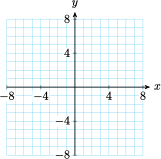
\includegraphics[width=\linewidth]{images/eight-grid}
\end{sbspanel}%
\end{sidebyside}%
\end{divisionexerciseegcol}%
\begin{divisionexerciseegcol}{36}{}{}{g:exercise:idm46051682191440}%
\(x^2 + y^2 = 16\)%
\begin{sidebyside}{1}{0.125}{0.125}{0}%
\begin{sbspanel}{0.75}%
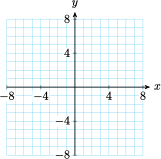
\includegraphics[width=\linewidth]{images/eight-grid}
\end{sbspanel}%
\end{sidebyside}%
\end{divisionexerciseegcol}%
\begin{divisionexerciseegcol}{37}{}{}{g:exercise:idm46051682203824}%
\(4x^2 +4y^2 = 16\)%
\begin{sidebyside}{1}{0.125}{0.125}{0}%
\begin{sbspanel}{0.75}%
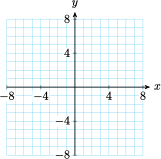
\includegraphics[width=\linewidth]{images/eight-grid}
\end{sbspanel}%
\end{sidebyside}%
\end{divisionexerciseegcol}%
\begin{divisionexerciseegcol}{38}{}{}{g:exercise:idm46051682258320}%
\(2x^2 + 2y^2 = 18\)%
\begin{sidebyside}{1}{0.125}{0.125}{0}%
\begin{sbspanel}{0.75}%
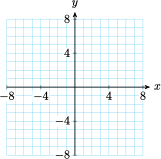
\includegraphics[width=\linewidth]{images/eight-grid}
\end{sbspanel}%
\end{sidebyside}%
\end{divisionexerciseegcol}%
\end{exercisegroupcol}
\par\medskip\noindent
\begin{divisionexercise}{39}{}{}{g:exercise:idm46051682268112}%
Give the coordinates of two points on the circle in Problem 35 that have \(y=-4\). Plot those points on your graph.%
\end{divisionexercise}%
\begin{divisionexercise}{40}{}{}{g:exercise:idm46051682288192}%
Give the coordinates of two points on the circle in Problem 35 that have \(x=-2\). Plot those points on your graph.%
\end{divisionexercise}%
\par\medskip\noindent%
%
For Problems 41 and 43, find the coordinates of the points on the unit circle.%
\begin{exercisegroupcol}{2}
\begin{divisionexerciseegcol}{41}{}{}{g:exercise:idm46051682298576}%
\begin{sidebyside}{1}{0.15}{0.15}{0}%
\begin{sbspanel}{0.7}%
\resizebox{\linewidth}{!}{%
\tikzset{%
  block/.style    = {draw, thick, rectangle, minimum height = 3em,
    minimum width = 3em},
  sum/.style      = {draw, circle, node distance = 2cm}, % Adder
  input/.style    = {coordinate}, % Input
  output/.style   = {coordinate} % Output
}
\begin{tikzpicture} [scale=0.7]

\coordinate(O) at (0,0);
\coordinate (P) at (1,1.732 );
\coordinate (Q) at (1,-1.732 );
\coordinate (R) at (-1.5,-1.32 );
\coordinate (S) at (-1.5,1.32);

\draw (0,0) circle (2);

\draw[thick,->] (-2,0) -- (2.3,0) node[anchor=west] {$x$};
\draw[thick,->] (0,-2) -- (0,2.3) node[anchor=south] {$y$};

\filldraw[red] (P) circle (3pt) node[anchor=south west, xshift=0, yshift=-3]{\color{black}$P\left(\frac{1}{2},? \right)$};
\filldraw[red] (Q) circle (3pt) node[anchor=north west, xshift=0, yshift=3]{\color{black}$Q\left(\frac{1}{2},? \right)$};
\filldraw[red] (R) circle (3pt) node[anchor=north east, xshift=0, yshift=3]{\color{black}$R\left(\frac{-3}{4},? \right)$};
\filldraw[red] (S) circle (3pt) node[anchor=south east, xshift=0, yshift=-3]{\color{black}$S\left(\frac{-3}{4},? \right)$};
\end{tikzpicture}
}%
\end{sbspanel}%
\end{sidebyside}%
\end{divisionexerciseegcol}%
\begin{divisionexerciseegcol}{42}{}{}{g:exercise:idm46051682314544}%
\begin{sidebyside}{1}{0.15}{0.15}{0}%
\begin{sbspanel}{0.7}%
\resizebox{\linewidth}{!}{%
\tikzset{%
  block/.style    = {draw, thick, rectangle, minimum height = 3em,
    minimum width = 3em},
  sum/.style      = {draw, circle, node distance = 2cm}, % Adder
  input/.style    = {coordinate}, % Input
  output/.style   = {coordinate} % Output
}
\begin{tikzpicture} [scale=0.7]

\coordinate(O) at (0,0);
\coordinate (A) at (1.414,1.414 );
\coordinate (D) at (1.49,-1.333 );
\coordinate (C) at (-1.49,-1.333 );
\coordinate (B) at (-1.414,1.414);

\draw (0,0) circle (2);

\draw[thick,->] (-2,0) -- (2.3,0) node[anchor=west] {$x$};
\draw[thick,->] (0,-2) -- (0,2.3) node[anchor=south] {$y$};

\filldraw[red] (A) circle (3pt) node[anchor=south west, xshift=0, yshift=-3]{\color{black}$A\left(?, \frac{1}{\sqrt{2}} \right)$};
\filldraw[red] (D) circle (3pt) node[anchor=north west, xshift=0, yshift=3]{\color{black}$D\left(?, \frac{-2}{3} \right)$};
\filldraw[red] (C) circle (3pt) node[anchor=north east, xshift=0, yshift=3]{\color{black}$C\left(?, \frac{-2}{3} \right)$};
\filldraw[red] (B) circle (3pt) node[anchor=south east, xshift=0, yshift=-3]{\color{black}$B\left(?, \frac{1}{\sqrt{2}} \right)$};

\end{tikzpicture}
}%
\end{sbspanel}%
\end{sidebyside}%
\end{divisionexerciseegcol}%
\end{exercisegroupcol}
\par\medskip\noindent
\begin{divisionexercise}{43}{}{}{g:exercise:idm46051682326960}%
A circular herb garden has diameter 40 feet, and is divided into 8 equal sectors.%
\begin{sidebyside}{2}{0}{0}{0}%
\begin{sbspanel}{0.8}[center]%
%
\begin{enumerate}[label=\alph*]
\item{}What is the central angle of each sector?%
\item{}What is the length of the circular edge of each sector?%
\item{}What is the area of each sector?%
\end{enumerate}
%
\end{sbspanel}%
\begin{sbspanel}{0.2}[center]%
\resizebox{\linewidth}{!}{%
\tikzset{%
  block/.style    = {draw, thick, rectangle, minimum height = 3em,
    minimum width = 3em},
  sum/.style      = {draw, circle, node distance = 2cm}, % Adder
  input/.style    = {coordinate}, % Input
  output/.style   = {coordinate} % Output
}
\begin{tikzpicture} [scale=0.85]

\coordinate(O) at (0,0);
\coordinate (A) at (1.414,1.414 );
\coordinate (B) at (1.414,-1.414 );
\coordinate (C) at (-1.414,-1.414 );
\coordinate (D) at (-1.414,1.414);

\draw (0,0) circle (2);

\draw[gray,thin] (A) --(C);
\draw[gray,thin] (B) --(D);
\draw[gray,thin] (-2,0) --(2,0);
\draw[gray,thin] (0,-2) --(0,2);
\end{tikzpicture}
}%
\end{sbspanel}%
\end{sidebyside}%
\end{divisionexercise}%
\begin{divisionexercise}{44}{}{}{g:exercise:idm46051682335104}%
A dart board is 18 inches in diameter, divided into 20 sectors of equal size. (For this exercise, we will ignore the bulls-eye and the fact that  the sectors are further subdivided.)%
\begin{sidebyside}{2}{0.05}{0.05}{0.1}%
\begin{sbspanel}{0.5}%
%
\begin{enumerate}[label=\alph*]
\item{}What is the central angle of each sector?%
\item{}What is the length of the circular edge of each sector?%
\item{}What is the area of each sector?%
\end{enumerate}
%
\end{sbspanel}%
\begin{sbspanel}{0.3}%
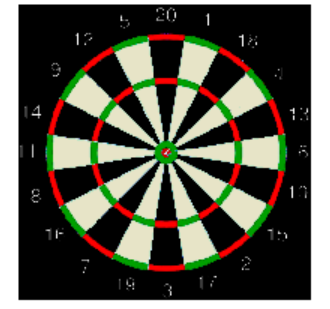
\includegraphics[width=\linewidth]{images/hp1-3-44.png}
\end{sbspanel}%
\end{sidebyside}%
\end{divisionexercise}%
\par\medskip\noindent%
%
For Problems 45\textendash{}50,%
\par
%
\begin{enumerate}[label=\alph*]
\item{}What fraction of one revolution is the central angle?%
\item{}What is the area of the shaded sector?%
\item{}What is the length of the shaded arc?%
\end{enumerate}
%
\begin{exercisegroupcol}{3}
\begin{divisionexerciseegcol}{45}{}{}{g:exercise:idm46051682382224}%
\begin{sidebyside}{1}{0.175}{0.175}{0}%
\begin{sbspanel}{0.65}%
\resizebox{\linewidth}{!}{%
\tikzset{%
  block/.style    = {draw, thick, rectangle, minimum height = 3em,
    minimum width = 3em},
  sum/.style      = {draw, circle, node distance = 2cm}, % Adder
  input/.style    = {coordinate}, % Input
  output/.style   = {coordinate} % Output
}
\begin{tikzpicture} [scale=0.85]

\coordinate(O) at (0,0);
\coordinate (A) at (1.176,-1.618 );
\coordinate (B) at (0,2 );

\filldraw[cyan!40!white!30] (A)--(O)--(B)--(B) arc (90:-54:2)--(A);
\draw (0,0) circle (2);

\draw[black,thick] (A) --(O);
\draw[black,thick] (B) --(O) node[left,midway] {$10'$};

\draw[red,thick] (0,.4) arc (90:-54:0.4) node[right, midway] {$144\degree$};
\draw[red, ultra thick] (B) arc (90:-54:2);
\filldraw[black] (O) circle (.2pt) node[anchor=north east] {$O$};

\end{tikzpicture}
}%
\end{sbspanel}%
\end{sidebyside}%
\end{divisionexerciseegcol}%
\begin{divisionexerciseegcol}{46}{}{}{g:exercise:idm46051682418080}%
\begin{sidebyside}{1}{0.175}{0.175}{0}%
\begin{sbspanel}{0.65}%
\resizebox{\linewidth}{!}{%
\tikzset{%
  block/.style    = {draw, thick, rectangle, minimum height = 3em,
    minimum width = 3em},
  sum/.style      = {draw, circle, node distance = 2cm}, % Adder
  input/.style    = {coordinate}, % Input
  output/.style   = {coordinate} % Output
}
\begin{tikzpicture} [scale=0.85]

\coordinate(O) at (0,0);
\coordinate (A) at (1.218,1.587 );
\coordinate (B) at (-1.218,1.587 );

\filldraw[cyan!40!white!30] (B)--(O)--(A) arc (52.5:127.5:2)--(O);
\draw (0,0) circle (2);

\draw[black,thick] (A) --(O) node[right,midway,xshift=-3,yshift=-6] {$20$ cm};
\draw[black,thick] (B) --(O);

\draw[red,thick] (0.244,0.317) arc (52.5:127.5:0.4) node[above, midway] {$75\degree$};
\draw[red, ultra thick] (A) arc (52.5:127.5:2);
\filldraw[black] (O) circle (.2pt) node[anchor=north east] {$O$};

\end{tikzpicture}
}%
\end{sbspanel}%
\end{sidebyside}%
\end{divisionexerciseegcol}%
\begin{divisionexerciseegcol}{47}{}{}{g:exercise:idm46051682426304}%
\begin{sidebyside}{1}{0.175}{0.175}{0}%
\begin{sbspanel}{0.65}%
\resizebox{\linewidth}{!}{%
\tikzset{%
  block/.style    = {draw, thick, rectangle, minimum height = 3em,
    minimum width = 3em},
  sum/.style      = {draw, circle, node distance = 2cm}, % Adder
  input/.style    = {coordinate}, % Input
  output/.style   = {coordinate} % Output
}
\begin{tikzpicture} [scale=0.85]

\coordinate(O) at (0,0);
\coordinate (A) at (2,0 );
\coordinate (B) at (1.618,1.176 );

\filldraw[cyan!40!white!30] (B)--(O)--(A) arc (0:36:2)--(O);
\draw (0,0) circle (2);

\draw[black,thick] (A) --(O);
\draw[black,thick] (B) --(O) node[above left,midway,xshift=0,yshift=0] {1 km};

\draw[red,thick] (0.4,0) arc (0:36:0.4) node[above right, midway,xshift=3, yshift=-4] {$36\degree$};
\draw[red, ultra thick] (A) arc (0:36:2);
\filldraw[black] (O) circle (.2pt) node[anchor=north east] {$O$};

\end{tikzpicture}
}%
\end{sbspanel}%
\end{sidebyside}%
\end{divisionexerciseegcol}%
\begin{divisionexerciseegcol}{48}{}{}{g:exercise:idm46051682507424}%
\begin{sidebyside}{1}{0.175}{0.175}{0}%
\begin{sbspanel}{0.65}%
\resizebox{\linewidth}{!}{%
\tikzset{%
  block/.style    = {draw, thick, rectangle, minimum height = 3em,
    minimum width = 3em},
  sum/.style      = {draw, circle, node distance = 2cm}, % Adder
  input/.style    = {coordinate}, % Input
  output/.style   = {coordinate} % Output
}
\begin{tikzpicture} [scale=0.85]

\coordinate(O) at (0,0);
\coordinate (A) at (1.983,-0.261 );
\coordinate (B) at (1.983, 0.261 );

\filldraw[cyan!40!white!30] (B)--(O)--(A) arc (-7.5:7.5:2)--(O);
\draw (0,0) circle (2);

\draw[black,thick] (A) --(O) node[below,midway,xshift=0,yshift=-2] {\small{$r=1$ mi}};
\draw[black,thick] (B) --(O);

\draw[red,thick] (1.19,-0.157) arc (-7.5:7.5:1.2) node[above , xshift=0, yshift=0] {$15\degree$};
\draw[red, ultra thick] (A) arc (-7.5:7.5:2);
\filldraw[black] (O) circle (.2pt) node[anchor=north east] {$O$};

\end{tikzpicture}
}%
\end{sbspanel}%
\end{sidebyside}%
\end{divisionexerciseegcol}%
\begin{divisionexerciseegcol}{49}{}{}{g:exercise:idm46051682526384}%
\begin{sidebyside}{1}{0.175}{0.175}{0}%
\begin{sbspanel}{0.65}%
\resizebox{\linewidth}{!}{%
\tikzset{%
  block/.style    = {draw, thick, rectangle, minimum height = 3em,
    minimum width = 3em},
  sum/.style      = {draw, circle, node distance = 2cm}, % Adder
  input/.style    = {coordinate}, % Input
  output/.style   = {coordinate} % Output
}
\begin{tikzpicture} [scale=0.85]

\coordinate(O) at (0,0);
\coordinate (A) at (2,0 );
\coordinate (B) at (1, -1.732 );

\filldraw[cyan!40!white!30] (B)--(O)--(A) arc (0:300:2)--(O);
\draw (0,0) circle (2);

\draw[black,thick] (A) --(O);
\draw[black,thick] (B) --(O) node[below left,midway,xshift=2,yshift=0] {$3$ m};

\draw[red,thick] (0.65,0) arc (0:300:.65) node[above , xshift=-.1cm, yshift=1.cm] {$300\degree$};
\draw[red, ultra thick] (A) arc (0:300:2);
\filldraw[black] (O) circle (.2pt) node[anchor= east] {$O$};

\end{tikzpicture}
}%
\end{sbspanel}%
\end{sidebyside}%
\end{divisionexerciseegcol}%
\begin{divisionexerciseegcol}{50}{}{}{g:exercise:idm46051682579344}%
\begin{sidebyside}{1}{0.175}{0.175}{0}%
\begin{sbspanel}{0.65}%
\resizebox{\linewidth}{!}{%
\tikzset{%
  block/.style    = {draw, thick, rectangle, minimum height = 3em,
    minimum width = 3em},
  sum/.style      = {draw, circle, node distance = 2cm}, % Adder
  input/.style    = {coordinate}, % Input
  output/.style   = {coordinate} % Output
}
\begin{tikzpicture} [scale=0.85]

\coordinate(O) at (0,0);
\coordinate (A) at (2,0 );
\coordinate (B) at ( -1.618,-1.176 );

\filldraw[cyan!40!white!30] (B)--(O)--(A) arc (0:216:2)--(O);
\draw (0,0) circle (2);

\draw[black,thick] (A) --(O) node[above,midway,xshift=2,yshift=0] {$5$ in};
\draw[black,thick] (B) --(O);

\draw[red,thick] (0.3,0) arc (0:216:.3) node[above, midway, xshift=0, yshift=0] {$216\degree$};
\draw[red, ultra thick] (A) arc (0:216:2);
\filldraw[black] (O) circle (.2pt) node[anchor= north , yshift=-2] {$O$};
\end{tikzpicture}
}%
\end{sbspanel}%
\end{sidebyside}%
\end{divisionexerciseegcol}%
\end{exercisegroupcol}
\par\medskip\noindent
\begin{divisionexercise}{51}{}{}{g:exercise:idm46051682594656}%
\begin{sidebyside}{2}{0.0425}{0.0425}{0.085}%
\begin{sbspanel}{0.6}[center]%
South America stretches across \(30\degree\) of longitude at the equator, from Quito in Ecuador to the east coast of Brazil.  (The figure at right shows a view of the earth from above the north pole.)  The radius of the earth is about 3960 miles.  How wide is South America at the equator?%
\end{sbspanel}%
\begin{sbspanel}{0.23}[center]%
\resizebox{\linewidth}{!}{%
\tikzset{%
  block/.style    = {draw, thick, rectangle, minimum height = 3em,
    minimum width = 3em},
  sum/.style      = {draw, circle, node distance = 2cm}, % Adder
  input/.style    = {coordinate}, % Input
  output/.style   = {coordinate} % Output
}
\begin{tikzpicture} [scale=0.85]

\coordinate(O) at (0,0);
\coordinate (A) at (0.278,-1.98 );
\coordinate (B) at (-0.278,-1.98 );

\draw (0,0) circle (2);

\draw[black,thick] (A) --(O) ;
\draw[black,thick] (B) --(O);

\filldraw[black] (O) circle (.2pt) node[anchor= south , xshift=0] {$N$};
\filldraw[black] (A) circle (1.8pt) node[anchor= north west, xshift=2,align=left] {E. coast \\of Brazil};
\filldraw[black] (B) circle (1.8pt) node[anchor= north east, xshift=2] {Quito};

\node[anchor = south] at (0,2) {Equator};
\node[anchor = west, xshift=.3cm, yshift=.7cm,rotate=-90] at (2,0) {Equator};
\node[anchor = east, xshift=-.3cm, yshift=.7cm, rotate=90] at (-2,0) {Equator};
\end{tikzpicture}
}%
\end{sbspanel}%
\end{sidebyside}%
\end{divisionexercise}%
\begin{divisionexercise}{52}{}{}{g:exercise:idm46051682647696}%
\begin{sidebyside}{2}{0.055}{0.055}{0.11}%
\begin{sbspanel}{0.6}[center]%
The radius of the earth is about 3960 miles.  What distance will you cover if you travel north by one degree of latitude?  (See the figure at right.)  There are \(180\degree\) of latitude from the south pole to the north pole.%
\end{sbspanel}%
\begin{sbspanel}{0.18}[center]%
\resizebox{\linewidth}{!}{%
\tikzset{%
  block/.style    = {draw, thick, rectangle, minimum height = 3em,
    minimum width = 3em},
  sum/.style      = {draw, circle, node distance = 2cm}, % Adder
  input/.style    = {coordinate}, % Input
  output/.style   = {coordinate} % Output
}
\begin{tikzpicture} [scale=0.85]

\coordinate(O) at (0,0);
\coordinate (A) at (-1.231,1.576 );
\coordinate (B) at (-1.338,1.486 );

\draw (0,0) circle (2);

\draw[black,thick] (A) --(O) ;
\draw[black,thick] (B) --(O);

\draw[red,thick, ->] (-.336,1.28) arc(105:128:1.3) node[above right,xshift=.3cm,yshift=-2] {$1\degree$};
\draw[red,thick, ->] (-1.178,0.549) arc(155:132:1.3) ;

\filldraw[black] (0,2) circle (1.8pt) node[anchor= south] {N};
\filldraw[black] (0,-2) circle (1.8pt) node[anchor= north , xshift=0] {S};

\end{tikzpicture}
}%
\end{sbspanel}%
\end{sidebyside}%
\end{divisionexercise}%
\begin{divisionexercise}{53}{}{}{g:exercise:idm46051682688032}%
The moon is about 240,000 miles from earth.  It moves in a roughly circular orbit, completing one revolution in 28 days.%
\begin{sidebyside}{2}{0.0325}{0.0325}{0.065}%
\begin{sbspanel}{0.65}[center]%
%
\begin{enumerate}[label=\alph*]
\item{}How far does the moon move around the earth in one day?%
\item{}What is the speed of the moon relative to the earth, in miles per hour?%
\end{enumerate}
%
\end{sbspanel}%
\begin{sbspanel}{0.22}[center]%
\resizebox{\linewidth}{!}{%
\tikzset{%
  block/.style    = {draw, thick, rectangle, minimum height = 3em,
    minimum width = 3em},
  sum/.style      = {draw, circle, node distance = 2cm}, % Adder
  input/.style    = {coordinate}, % Input
  output/.style   = {coordinate} % Output
}
\begin{tikzpicture} [scale=0.85]

\coordinate(O) at (0,0);
\coordinate (A) at (1.414,1.414 );

\draw (0,0) circle (2);

\draw[black,thick] (A) --(O) node[above,midway,yshift=-2, rotate=45] {\footnotesize{240,000 mi}};


\filldraw[gray] (A) circle (2pt) node[anchor= south west] {\color{black}Moon};
\filldraw[green] (O) circle (3pt) node[anchor= north east, xshift=0] {\color{black}Earth};
\end{tikzpicture}
}%
\end{sbspanel}%
\end{sidebyside}%
\end{divisionexercise}%
\begin{divisionexercise}{54}{}{}{g:exercise:idm46051682744672}%
The earth is about 93,000,000 miles from the sun, and its orbit is approximately circular.%
\begin{sidebyside}{2}{0.0325}{0.0325}{0.065}%
\begin{sbspanel}{0.65}[center]%
%
\begin{enumerate}[label=\alph*]
\item{}How far does the earth move around the sun in one month?%
\item{}What is the speed of the earth relative to the sun, in miles per day?  (Assume a month has 30 days.)%
\end{enumerate}
%
\end{sbspanel}%
\begin{sbspanel}{0.22}[center]%
\resizebox{\linewidth}{!}{%
\tikzset{%
  block/.style    = {draw, thick, rectangle, minimum height = 3em,
    minimum width = 3em},
  sum/.style      = {draw, circle, node distance = 2cm}, % Adder
  input/.style    = {coordinate}, % Input
  output/.style   = {coordinate} % Output
}
\begin{tikzpicture} [scale=0.85]

\coordinate(O) at (0,0);
\coordinate (A) at (1.414,1.414 );

\draw (0,0) circle (2);

\draw[black,thick] (A) --(O) node[above,midway,yshift=-2,rotate=45] {\footnotesize{$93\times 10^6$ mi}};


\filldraw[green] (A) circle (2pt) node[anchor= south west] {\color{black}Earth};
\filldraw[red] (O) circle (3pt) node[anchor= north east, xshift=0] {\color{black}Sun};

\end{tikzpicture}
}%
\end{sbspanel}%
\end{sidebyside}%
\end{divisionexercise}%
\begin{divisionexercise}{55}{}{}{g:exercise:idm46051682785568}%
%
\begin{enumerate}[label=\alph*]
\item{}Use the distance formula to write an equation for the circle of radius 6 centered at the point \((3,-2)\).%
\item{}Use the distance formula to derive an equation for the circle of radius \(r\) centered at the point \((h,k)\).%
\end{enumerate}
%
\end{divisionexercise}%
\begin{divisionexercise}{56}{}{}{g:exercise:idm46051682850752}%
Find the coordinates of the indicated points on each circle.%
\par
%
\begin{multicols}{2}
\begin{enumerate}[label=\alph*]
\item{}\(\displaystyle (x-4)^2 + (y-5)^2 = 9\)%
\begin{sidebyside}{1}{0.15}{0.15}{0}%
\begin{sbspanel}{0.7}%
\resizebox{\linewidth}{!}{%
\tikzset{%
  block/.style    = {draw, thick, rectangle, minimum height = 3em,
    minimum width = 3em},
  sum/.style      = {draw, circle, node distance = 2cm}, % Adder
  input/.style    = {coordinate}, % Input
  output/.style   = {coordinate} % Output
}
\begin{tikzpicture} [scale=0.4]

\coordinate(O) at (4,5);
\coordinate (L) at (7,5 );
\coordinate (M) at (4, 8);
\coordinate (N) at (1,5 );
\coordinate (P) at (4,2);

\draw[red,thick] (O) circle (3);

\draw[black,dashed] (0,5) --(10,5) ;
\draw[black,dashed] (4,0) --(4,10) ;
\draw[black,thick,->] (-.5,0) --(10,0) node[right] {$x$};
\draw[black,thick,->] (0,-0.5) --(0,10) node[above] {$y$};

\filldraw[black] (L) circle (4pt) node[anchor= south west] {\color{black}$L$};
\filldraw[black] (M) circle (4pt) node[anchor= south west] {\color{black}$M$};
\filldraw[black] (N) circle (4pt) node[anchor= south west] {\color{black}$N$};
\filldraw[black] (P) circle (4pt) node[anchor= north west] {\color{black}$P$};

\end{tikzpicture}
}%
\end{sbspanel}%
\end{sidebyside}%
\item{}\(\displaystyle (x+3)^2 + (y-1)^2 = 25\)%
\begin{sidebyside}{1}{0.15}{0.15}{0}%
\begin{sbspanel}{0.7}%
\resizebox{\linewidth}{!}{%
\tikzset{%
  block/.style    = {draw, thick, rectangle, minimum height = 3em,
    minimum width = 3em},
  sum/.style      = {draw, circle, node distance = 2cm}, % Adder
  input/.style    = {coordinate}, % Input
  output/.style   = {coordinate} % Output
}
\begin{tikzpicture} [scale=0.3]

\coordinate(O) at (-3,1);
\coordinate (E) at (2,1 );
\coordinate (F) at (-3,6);
\coordinate (G) at (-8,1 );
\coordinate (H) at (-3,-4);

\draw[red,thick] (O) circle (5);

\draw[black,dashed] (-10,1) --(4,1) ;
\draw[black,dashed] (-3,-5) --(-3,8) ;
\draw[black,thick,->] (-10,0) --(4,0) node[right] {$x$};
\draw[black,thick,->] (0,-5) --(0,8) node[above] {$y$};

\filldraw[black] (E) circle (4pt) node[anchor= south west] {\color{black}$E$};
\filldraw[black] (F) circle (4pt) node[anchor= south east] {\color{black}$F$};
\filldraw[black] (G) circle (4pt) node[anchor= south east] {\color{black}$G$};
\filldraw[black] (H) circle (4pt) node[anchor= north east] {\color{black}$H$};
\end{tikzpicture}
}%
\end{sbspanel}%
\end{sidebyside}%
\end{enumerate}
\end{multicols}
%
\end{divisionexercise}%
\end{exercises-subsection}
\end{sectionptx}
%
%
\typeout{************************************************}
\typeout{Section 1.4 Chapter 1 Summary and Review}
\typeout{************************************************}
%
\begin{sectionptx}{Chapter 1 Summary and Review}{}{Chapter 1 Summary and Review}{}{}{x:section:chap1-summary}
%
%
\typeout{************************************************}
\typeout{Subsection  Key Concepts}
\typeout{************************************************}
%
\begin{subsectionptx}{Key Concepts}{}{Key Concepts}{}{}{g:subsection:idm46051682985296}
%
\begin{enumerate}[label=\arabic*]
\item{}The sum of the angles in a triangle is \(180\degree\).%
\item{}A right triangle has one angle of \(90\degree\).%
\item{}All of the angles of an equilateral triangle are equal.%
\item{}The base angles of an isosceles triangle are equal.%
\item{}Vertical angles are equal.%
\item{}If parallel lines are intersected by a transversal, the alternate interior angles are equal.  Corresponding angles are also equal.%
\item{}Two triangles are \terminology{congruent} if they have exactly the same size and shape.%
\item{}The \terminology{altitude} of an equilateral triangle divides it into two congruent right triangles.%
\item{}In a \(30\degree-60\degree-90\degree\) right triangle, the leg opposite the \(30\degree\) angle is half the length of the hypotenuse.%
\item{}Two triangles are \terminology{similar} if they have the same shape but not necessarily the same size.  The corresponding angles are equal, and the corresponding sides are \terminology{proportional}.%
\item{}\begin{assemblage}{Similar Triangles.}{g:assemblage:idm46051683021744}%
Two triangles are similar if either%
\begin{enumerate}[label=\arabic*]
\item{}their corresponding angles are equal, or%
\item{}their corresponding sides are proportional.%
\end{enumerate}
%
\end{assemblage}
%
\item{}If two \emph{right} triangles have \emph{one} pair of corresponding acute angles with the same measure, then the triangles are similar.%
\item{}\begin{assemblage}{Distance Formula.}{g:assemblage:idm46051683038896}%
The distance \(d\) between two points \(P_{1}(x_1, y_1)\) and \(P_{2}(x_2, y_2)\) is%
\begin{equation*}
d=\sqrt{(x_2-x_1)^2+(y_2-y_1)^2}
\end{equation*}
%
\end{assemblage}
%
\item{}Any number that can be written as a quotient of two integers \(\dfrac{a}{b},~~ b\not=0,~~\),  is called a \terminology{rational number}.  The decimal form of a rational number is either a \terminology{terminating decimal} or a \terminology{repeating decimal}.%
\item{}An \terminology{irrational number} is one that cannot be written as a quotient of two integers \(\dfrac{a}{b},~~ b\not=0,~~\).  We cannot write down an exact decimal equivalent for an irrational number.%
\item{}A \terminology{circle} is the set of all points in a plane that lie at a given distance, called the \terminology{radius}, from a fixed point called the \terminology{center}.%
\item{}\begin{assemblage}{Circle.}{g:assemblage:idm46051683089984}%
The equation for a \terminology{circle} of radius \(r\) centered at the origin is%
\begin{equation*}
x^2+y^2=r^2
\end{equation*}
%
\end{assemblage}
%
\item{}The circle \(x^2 + y^2 = 1\), which is centered at the origin and has radius 1 unit, is called the \terminology{unit circle}.%
\item{}\begin{assemblage}{Circumference of a Circle.}{g:assemblage:idm46051683127664}%
The \terminology{circumference} of a circle of radius \(r\) is given by%
\begin{equation*}
C=2\pi r
\end{equation*}
%
\end{assemblage}
%
\item{}\begin{assemblage}{Area of a Circle.}{g:assemblage:idm46051683162832}%
The \terminology{area} of a circle of radius \(r\) is given by%
\begin{equation*}
A=\pi r^2
\end{equation*}
%
\end{assemblage}
%
\end{enumerate}
%
\end{subsectionptx}
%
%
\typeout{************************************************}
\typeout{Exercises  Chapter 1 Review Problems}
\typeout{************************************************}
%
\begin{exercises-subsection}{Chapter 1 Review Problems}{}{Chapter 1 Review Problems}{}{}{x:exercises:chap1-rev-problems}
\par\medskip\noindent%
%
For Problems 1\textendash{}4, sketch the triangle described.%
\begin{exercisegroup}
\begin{divisionexerciseeg}{1}{}{}{g:exercise:idm46051683180480}%
An isosceles triangle with vertex angle \(100\degree\)%
\end{divisionexerciseeg}%
\begin{divisionexerciseeg}{2}{}{}{g:exercise:idm46051683201408}%
An isosceles triangle with base angles of \(75\degree\)%
\end{divisionexerciseeg}%
\begin{divisionexerciseeg}{3}{}{}{g:exercise:idm46051683206592}%
A scalene right triangle%
\end{divisionexerciseeg}%
\begin{divisionexerciseeg}{4}{}{}{g:exercise:idm46051683226928}%
A scalene triangle with one obtuse angle%
\end{divisionexerciseeg}%
\end{exercisegroup}
\par\medskip\noindent
\par\medskip\noindent%
%
For Problems 5-\textendash{}16, find the unknown angles.%
\begin{exercisegroupcol}{3}
\begin{divisionexerciseegcol}{5}{}{}{g:exercise:idm46051683235856}%
\begin{sidebyside}{1}{0.25}{0.25}{0}%
\begin{sbspanel}{0.5}%
\resizebox{\linewidth}{!}{%
\tikzset{%
  block/.style    = {draw, thick, rectangle, minimum height = 3em,
    minimum width = 3em},
  sum/.style      = {draw, circle, node distance = 2cm}, % Adder
  input/.style    = {coordinate}, % Input
  output/.style   = {coordinate} % Output
}
\begin{tikzpicture} 

\coordinate(A) at (0,0);
\coordinate (B) at (0,2 );
\coordinate (C) at (-1.732,1);

\draw[black,thick] (A)--(B) node[right,midway] {\color{blue}$9$};
\draw[black,thick] (A)--(C) node[below left,midway] {\color{blue}$9$};
\draw[black,thick] (C)--(B) node[above left,midway] {\color{blue}$9$};

\filldraw[black] (A) circle (.2pt) node[anchor= south east, xshift=0,yshift=3] {\color{red}$\beta$};
\filldraw[black] (B) circle (.2pt) node[anchor= north east,xshift=1,yshift=-5] {\color{red}$\gamma$};
\filldraw[black] (C) circle (.2pt) node[anchor= west,xshift=5] {\color{red}$\alpha$};
\end{tikzpicture}
}%
\end{sbspanel}%
\end{sidebyside}%
\end{divisionexerciseegcol}%
\begin{divisionexerciseegcol}{6}{}{}{g:exercise:idm46051683246848}%
\begin{sidebyside}{1}{0.15}{0.15}{0}%
\begin{sbspanel}{0.7}%
\resizebox{\linewidth}{!}{%
\tikzset{%
  block/.style    = {draw, thick, rectangle, minimum height = 3em,
    minimum width = 3em},
  sum/.style      = {draw, circle, node distance = 2cm}, % Adder
  input/.style    = {coordinate}, % Input
  output/.style   = {coordinate} % Output
}
\begin{tikzpicture} 

\coordinate(A) at (0,0);
\coordinate (B) at (0,-2.3 );
\coordinate (C) at (-2.3,0);

\draw[black,thick] (A)--(B) node[right,midway] {\color{blue}$21$};
\draw[black,thick] (A)--(C) node[above,midway] {\color{blue}$21$};
\draw[black,thick] (C)--(B);

\draw[blue,thick] (A) rectangle +(-.25,-.25);
\filldraw[black] (B) circle (.2pt) node[anchor= south east,xshift=2,yshift=6] {\color{red}$\theta$};
\filldraw[black] (C) circle (.2pt) node[anchor= north west,xshift=8,yshift=2] {\color{red}$\phi$};

\end{tikzpicture}
}%
\end{sbspanel}%
\end{sidebyside}%
\end{divisionexerciseegcol}%
\begin{divisionexerciseegcol}{7}{}{}{g:exercise:idm46051683264032}%
\begin{sidebyside}{1}{0.1}{0.1}{0}%
\begin{sbspanel}{0.8}%
\resizebox{\linewidth}{!}{%
\tikzset{%
  block/.style    = {draw, thick, rectangle, minimum height = 3em,
    minimum width = 3em},
  sum/.style      = {draw, circle, node distance = 2cm}, % Adder
  input/.style    = {coordinate}, % Input
  output/.style   = {coordinate} % Output
}
\begin{tikzpicture} 

\coordinate(A) at (0,0);
\coordinate (B) at (1.732,-1);
\coordinate (C) at (-1.732,-1);

\draw[black,thick] (A)--(B) node[above,midway] {\color{blue}$1$};
\draw[black,thick] (A)--(C) node[above,midway] {\color{blue}$1$};
\draw[black,thick] (C)--(B);

\filldraw[black] (A) circle (.2pt) node[anchor= north,xshift=0,yshift=-3] {\color{red}$120\degree$};
\filldraw[black] (B) circle (.2pt) node[anchor= south east,xshift=-12,yshift=-2] {\color{red}$\omega$};
\filldraw[black] (C) circle (.2pt) node[anchor= south west,xshift=15,yshift=-2] {\color{red}$\phi$};
\end{tikzpicture}
}%
\end{sbspanel}%
\end{sidebyside}%
\end{divisionexerciseegcol}%
\begin{divisionexerciseegcol}{8}{}{}{g:exercise:idm46051683281040}%
\begin{sidebyside}{1}{0.2}{0.2}{0}%
\begin{sbspanel}{0.6}%
\resizebox{\linewidth}{!}{%
\tikzset{%
  block/.style    = {draw, thick, rectangle, minimum height = 3em,
    minimum width = 3em},
  sum/.style      = {draw, circle, node distance = 2cm}, % Adder
  input/.style    = {coordinate}, % Input
  output/.style   = {coordinate} % Output
}
\begin{tikzpicture} [rotate=60]

\coordinate (O) at (0,0);
\coordinate (A) at (2,0);
\coordinate (B) at (1,1.732);

\draw[black,  thick] (O) --  (A) node[right, midway, xshift=0] {\color{blue}$\sqrt{3}$}  ;
\draw[black,  thick] (O) --  (B) node[ left,midway, xshift=-2] {\color{blue}$\sqrt{3}$}  ;
\draw[black,  thick] (A) --  (B) node[above ,midway] {\color{blue}$\sqrt{3}$}  ;
\node at (O) [anchor=south, yshift=3] {\color{red}$\theta$};
\node at (A) [anchor=north east, xshift=-4] {\color{red}$\phi$};
\node at (B) [anchor=north west, xshift=5] {\color{red}$\psi$};
\end{tikzpicture}
}%
\end{sbspanel}%
\end{sidebyside}%
\end{divisionexerciseegcol}%
\begin{divisionexerciseegcol}{9}{}{}{g:exercise:idm46051700698832}%
\begin{sidebyside}{1}{0}{0}{0}%
\begin{sbspanel}{1}%
\resizebox{\linewidth}{!}{%
\tikzset{%
  block/.style    = {draw, thick, rectangle, minimum height = 3em,
    minimum width = 3em},
  sum/.style      = {draw, circle, node distance = 2cm}, % Adder
  input/.style    = {coordinate}, % Input
  output/.style   = {coordinate} % Output
}
\begin{tikzpicture} [scale=0.8]

\coordinate (O) at (0,0);
\coordinate (y) at (0,2);
\coordinate (x) at (-4.3,0);

\draw[blue,  thick] (O) rectangle  +(-.25,.25)  ;
\draw[black,  thick] (-5.6,0) --  (O)  ;
\draw[black,  thick] (O) --  (y)   ;
\draw[black,  thick] (-5.6,-0.605) --  (1,2.465)  ;
\draw[red, thick] (0,1.7) arc (-90:{atan(2/4.3)}:.3) node [below right, midway,xshift=-2,yshift=4] {$115\degree$};
\draw[red, thick] (0,1.5) arc (-90:{atan(2/4.3)-180}:.5) node [below left, midway,xshift=0,yshift=0] {$\theta$};
\draw[red, thick] (-5,0) arc (180:{atan(2/4.3)+180}:0.7) node [below left, midway,xshift=-3,yshift=6] {$\phi$};
\end{tikzpicture}
}%
\end{sbspanel}%
\end{sidebyside}%
\end{divisionexerciseegcol}%
\begin{divisionexerciseegcol}{10}{}{}{g:exercise:idm46051683282480}%
\begin{sidebyside}{1}{0.125}{0.125}{0}%
\begin{sbspanel}{0.75}%
\resizebox{\linewidth}{!}{%
\tikzset{%
  block/.style    = {draw, thick, rectangle, minimum height = 3em,
    minimum width = 3em},
  sum/.style      = {draw, circle, node distance = 2cm}, % Adder
  input/.style    = {coordinate}, % Input
  output/.style   = {coordinate} % Output
}
\begin{tikzpicture} 

\coordinate (O) at (0,0);
\coordinate (A) at (1.75,0.97);
\coordinate (B) at (-1.272,2.035);

\filldraw (O) circle (.2pt) node[anchor=south, xshift=3] {\color{blue}$\varphi$};
\filldraw (B) circle (.2pt) node[anchor=north west, xshift=8,yshift=-5] {\color{blue}$\psi$};

\draw[black,  thick] (O) --  (A) --(B)--cycle  ;
\draw[black,  thick] (-1.1,0) --  (1.8,0)  ;
\draw[red, thick] (0.5,0) arc (0:29:.5) node [above right, midway,xshift=2,yshift=-5] {$29\degree$};
\draw[red, thick] (-.4,0) arc (180:122:.4) node [above left, midway,xshift=0,yshift=0] {$58\degree$};
\draw[red, thick] (1.49,0.824) arc (209:{180-atan(.935/3)}:.3) node [ left, midway,xshift=0,yshift=-1] {$47\degree$};

\end{tikzpicture}
}%
\end{sbspanel}%
\end{sidebyside}%
\end{divisionexerciseegcol}%
\begin{divisionexerciseegcol}{11}{}{}{g:exercise:idm46051683310352}%
\begin{sidebyside}{1}{0.15}{0.15}{0}%
\begin{sbspanel}{0.7}%
\resizebox{\linewidth}{!}{%
\tikzset{%
  block/.style    = {draw, thick, rectangle, minimum height = 3em,
    minimum width = 3em},
  sum/.style      = {draw, circle, node distance = 2cm}, % Adder
  input/.style    = {coordinate}, % Input
  output/.style   = {coordinate} % Output
}
\begin{tikzpicture}

\coordinate (O) at (0,0);
\coordinate (A) at (3.2,0);
\coordinate (B) at (1.6,2.77);
\coordinate (C) at (1.6,0);

\draw[blue,thick] (C) rectangle +(0.25,0.25);
\draw[black,  thick] (O) --  (C) node[below,midway] {\color{blue}$1$}  ;
\draw[black,  thick] (A) --  (C) node[below,midway] {\color{blue}$1$}  ;
\draw[black,  thick] (O) --  (B) node[above left,midway] {\color{blue}$2$}  ;
\draw[black,  thick] (A) --  (B) node[above right,midway] {\color{blue}$2$}  ;
\draw[gray!50!white!50,  thick] (C) --  (B)  ;
\draw[red, thick] (0.5,0) arc (0:60:.5) node [above right, midway,xshift=-1,yshift=-5] {$\gamma$};
\draw[red, thick] (1.6,2.17) arc (-90:-120:.6) node [below left, midway,xshift=5,yshift=0] {$\delta$};

\end{tikzpicture}
}%
\end{sbspanel}%
\end{sidebyside}%
\end{divisionexerciseegcol}%
\begin{divisionexerciseegcol}{12}{}{}{g:exercise:idm46051683324240}%
\begin{sidebyside}{1}{0.1}{0.1}{0}%
\begin{sbspanel}{0.8}%
\resizebox{\linewidth}{!}{%
\tikzset{%
  block/.style    = {draw, thick, rectangle, minimum height = 3em,
    minimum width = 3em},
  sum/.style      = {draw, circle, node distance = 2cm}, % Adder
  input/.style    = {coordinate}, % Input
  output/.style   = {coordinate} % Output
}
\begin{tikzpicture} [scale=.9]

\coordinate (O) at (0,0);
\coordinate (A) at (3,0);
\coordinate (B) at (3,3);
\coordinate (C) at (0,3);

\draw[blue,thick] (O) rectangle +(0.25,0.25);
\draw[black,  thick] (O) --  (A) node[below,midway] {\color{blue}$9$}  ;
\draw[black,  thick] (A) --  (B) node[right,midway] {\color{blue}$9$}  ;
\draw[black,  thick] (C) --  (B) node[ above,midway] {\color{blue}$9$}  ;
\draw[black,  thick] (C) --  (O) node[left,midway] {\color{blue}$9$}  ;
\draw[gray!50!white!50,  thick] (C) --  (A)  ;
\draw[red, thick] (2.6,3) arc (180:270:.4) node [below left, midway,xshift=0,yshift=0] {$\mu$};
\draw[red, thick] (0.5,3) arc (0:-45:.5) node [below right, midway,xshift=0,yshift=0] {$\lambda$};
\end{tikzpicture}
}%
\end{sbspanel}%
\end{sidebyside}%
\end{divisionexerciseegcol}%
\begin{divisionexerciseegcol}{13}{}{}{g:exercise:idm46051683341536}%
\begin{sidebyside}{1}{0.05}{0.05}{0}%
\begin{sbspanel}{0.9}%
\resizebox{\linewidth}{!}{%
\tikzset{%
  block/.style    = {draw, thick, rectangle, minimum height = 3em,
    minimum width = 3em},
  sum/.style      = {draw, circle, node distance = 2cm}, % Adder
  input/.style    = {coordinate}, % Input
  output/.style   = {coordinate} % Output
}
\begin{tikzpicture} 

\coordinate (O) at (0,0);
\coordinate (A) at (2.8,0);
\coordinate (B) at (1.96,1.58);

\draw[black,  thick,->] (-.5,0) --  (3.2,0)  ;
\draw[black,  thick,->] (-.5,1.58) --  (3.2,1.58)  ;
\draw[black,  thick] (3.2,0) -- +(.5,0) ;
\draw[black,  thick] (3.2,1.58) -- +(.5,0)  ;
\draw[black,  thick] (-.5,-.4) --  (2.4,1.94)  ;
\draw[black,  thick] (A) --  (B)  ;
\draw[black,  thick] (O) --  (B)  ;
\draw[red, thick] (2.5,0) arc (180:118:.3) node [above left, midway,xshift=0,yshift=-4] {$62\degree$};
\draw[red, thick] (1.66,1.58) arc (180:39:.3) node [above left, midway, xshift=2,yshift=-2] {$141\degree$};
\filldraw[black] (O) circle (.2pt) node[anchor=south west,xshift=8,yshift=-2] {\color{red}$\sigma$};
\filldraw[black] (B) circle (.2pt) node[anchor=north,xshift=-2,yshift=-5] {\color{red}$\omega$};
\end{tikzpicture}
}%
\end{sbspanel}%
\end{sidebyside}%
\end{divisionexerciseegcol}%
\begin{divisionexerciseegcol}{14}{}{}{g:exercise:idm46051683360944}%
\begin{sidebyside}{1}{0.075}{0.075}{0}%
\begin{sbspanel}{0.85}%
\resizebox{\linewidth}{!}{%
\tikzset{%
  block/.style    = {draw, thick, rectangle, minimum height = 3em,
    minimum width = 3em},
  sum/.style      = {draw, circle, node distance = 2cm}, % Adder
  input/.style    = {coordinate}, % Input
  output/.style   = {coordinate} % Output
}
\begin{tikzpicture} [scale=.8]

\coordinate (O) at (0,0);
\coordinate (A) at (-2,2.14);
\coordinate (B) at (2.867,1.461);

\draw[gray!50!white,  thick,->] (-2,0) --  (-2,3)  ;
\draw[gray!50!white,  thick,->] (O) --  +(0,1.4)  ;
\draw[gray!50!white,  thick,->] (2.867,0) --  (2.867,3)  ;
\draw[red, thick] (-2,2.44) arc (90:-8:.3) node [above right, midway,xshift=0,yshift=-4] {$98\degree$};
\draw[red, thick] (2.867,1.061) arc (-90:-153:.4) node [below left, midway, xshift=5,yshift=0] {$63\degree$};
\draw[red, thick] (0,.5) arc (90:137:.5) node [above left, midway, xshift=7,yshift=5] {$47\degree$};
\filldraw[black] (A) circle (.2pt) node[anchor=north west,xshift=9,yshift=-1] {\color{red}$\theta$};
\filldraw[black] (B) circle (.2pt) node[anchor=east,xshift=-14,yshift=-4] {\color{red}$\delta$};
\draw[black,thick] (O)--(A)--(B)--cycle;
\end{tikzpicture}
}%
\end{sbspanel}%
\end{sidebyside}%
\end{divisionexerciseegcol}%
\begin{divisionexerciseegcol}{15}{}{}{g:exercise:idm46051683372192}%
\begin{sidebyside}{1}{0.1}{0.1}{0}%
\begin{sbspanel}{0.8}%
\resizebox{\linewidth}{!}{%
\tikzset{%
  block/.style    = {draw, thick, rectangle, minimum height = 3em,
    minimum width = 3em},
  sum/.style      = {draw, circle, node distance = 2cm}, % Adder
  input/.style    = {coordinate}, % Input
  output/.style   = {coordinate} % Output
}
\begin{tikzpicture}
\coordinate(O) at (0,0);
\coordinate (A) at (0,2 );
\coordinate (B) at (1.564,1.247);
\coordinate (C) at(1.945,-0.445);
\coordinate (D) at (0.8878,-1.802);
\coordinate (E) at(-0.8678,-1.802);
\coordinate (F) at(-1.945,-0.445);
\coordinate (G) at(-1.564,1.247);

\draw[red,thick] (0,0) circle (2);
\draw[red] (0,0.4) arc(90:38.57:0.4) node[above right,midway, xshift=-3, yshift=0]{$\alpha$};
\draw[red] (1.25,0.998) arc(218.57:154.29:0.4) node[left, midway,xshift=-2, yshift=0]{$\beta$};

\draw[black,  thick] (A) -- (B) --( C) --(D) --(E)--(F) -- (G)--cycle;
\draw[black,  thick] (B) --  (O);
\draw[black,  thick] (C) --  (O);
\draw[black,  thick] (A)--(O);
\draw[black,  thick] (D) --  (O);
\draw[black,  thick] (E)--(O);
\draw[black,  thick] (F)--(O);
\draw[black,  thick] (G)--(O);
\end{tikzpicture}
}%
\end{sbspanel}%
\end{sidebyside}%
\end{divisionexerciseegcol}%
\begin{divisionexerciseegcol}{16}{}{}{g:exercise:idm46051683392640}%
\begin{sidebyside}{1}{0.1}{0.1}{0}%
\begin{sbspanel}{0.8}%
\resizebox{\linewidth}{!}{%
\tikzset{%
  block/.style    = {draw, thick, rectangle, minimum height = 3em,
    minimum width = 3em},
  sum/.style      = {draw, circle, node distance = 2cm}, % Adder
  input/.style    = {coordinate}, % Input
  output/.style   = {coordinate} % Output
}
\begin{tikzpicture} [rotate=22.5]
\coordinate(O) at (0,0);
\coordinate (A) at (2,0 );
\coordinate (B) at (1.414,1.414);
\coordinate (C) at(0,2);
\coordinate (D) at (-1.414,1.414);
\coordinate (E) at(-2,0);
\coordinate (F) at(-1.414,-1.414);
\coordinate (G) at(0,-2);
\coordinate (H) at (1.414,-1.414);

\draw[red,thick] (0,0) circle (2);
\draw[red,thick] (0,0.4) arc(90:45:0.4) node[above,midway, xshift=0, yshift=0]{$\alpha$};
\draw[red,thick] (1.202,1.202) arc(225:157.5:0.3) node[left, midway,xshift=-2, yshift=-5]{$\beta$};

\draw[black,  thick] (A) -- (B) --( C) --(D) --(E)--(F) -- (G)--(H)--cycle;
\draw[black,  thick] (B) --  (O);
\draw[black,  thick] (C) --  (O);
\draw[black,  thick] (A)--(O);
\draw[black,  thick] (D) --  (O);
\draw[black,  thick] (E)--(O);
\draw[black,  thick] (F)--(O);
\draw[black,  thick] (G)--(O);
\end{tikzpicture}
}%
\end{sbspanel}%
\end{sidebyside}%
\end{divisionexerciseegcol}%
\end{exercisegroupcol}
\par\medskip\noindent
\par\medskip\noindent%
%
In Problems 17 and 18, name two congruent triangles and find the unknown quantities.%
\begin{exercisegroupcol}{2}
\begin{divisionexerciseegcol}{17}{}{}{g:exercise:idm46051683407664}%
\begin{sidebyside}{1}{0.1}{0.1}{0}%
\begin{sbspanel}{0.8}%
\resizebox{\linewidth}{!}{%
\tikzset{%
  block/.style    = {draw, thick, rectangle, minimum height = 3em,
    minimum width = 3em},
  sum/.style      = {draw, circle, node distance = 2cm}, % Adder
  input/.style    = {coordinate}, % Input
  output/.style   = {coordinate} % Output
}
\begin{tikzpicture} [scale=1.2]
\coordinate (A) at (0,1 );
\coordinate (B) at (1.226,1);
\coordinate (C) at (0,0);
\coordinate (D) at (-1.226,-1);
\coordinate (E) at (0,-1);

\filldraw[black] (A) circle (2pt) node[anchor=south] {$A$};
\filldraw[black] (B) circle (.2pt) node[anchor=north west, xshift=-5] {$B$};
\filldraw[black] (B) circle (2pt) node[anchor=north east, xshift=-10, yshift=0] {\color{red}$\alpha$};
\filldraw[black] (C) circle (2pt) node[anchor=north west, xshift=-2] {$C$};

\filldraw[black] (D) circle (2pt) node[anchor=south east, xshift=2] {$D$};
\filldraw[black] (E) circle (2pt) node[anchor=north, yshift=-2] {$E$};

\draw[red,thick] (0.9226,1) arc(180:{atan(1/1.226)}:0.3) node[above left,midway, xshift=3, yshift=-3]{$140\degree$};
\draw[red,thick] (0,0.3) arc(90:{atan(1/1.226)+180}:0.3) node[above left,midway, xshift=3, yshift=-3]{$\beta$};

\draw[blue, thick] (E) rectangle +(0.25,0.25);
\draw[black,  thick] (-1.726,1)--(3,1);
\draw[black,  thick] (-1.726,-1)--(3,-1);

\draw[black,  thick] (B) --  (C) node[below right,midway] {\color{blue}$32$};
\draw[black,  thick] (C) --  (D) node[above left,midway] {\color{blue}$x$};
\draw[black,  thick] (A)--(E);
\draw[black,  thick] (D) --  (E) node[below,midway] {\color{blue}$24$};        \draw[black,  thick] (B)--(C);
\draw[black, thick] (D) -- +(-.5,-.4078);
\draw[black, thick] (B) -- +(.5,.4078);

\draw[gray,thick] (-.15, .45) -- +(.3,0);
\draw[gray,thick] (-.15, .55) -- +(.3,0);
\draw[gray,thick] (-.15, -.45) -- +(.3,0);
\draw[gray,thick] (-.15, -.55) -- +(.3,0);

\draw[black, thick, ->] (A)-- +(2.3,0);
\draw[black, thick, ->] (E)-- +(2.3,0);
\end{tikzpicture}
}%
\end{sbspanel}%
\end{sidebyside}%
\end{divisionexerciseegcol}%
\begin{divisionexerciseegcol}{18}{}{}{g:exercise:idm46051683458736}%
\(PQRS\) is a square%
\begin{sidebyside}{1}{0.225}{0.225}{0}%
\begin{sbspanel}{0.55}%
\resizebox{\linewidth}{!}{%
\tikzset{%
  block/.style    = {draw, thick, rectangle, minimum height = 3em,
    minimum width = 3em},
  sum/.style      = {draw, circle, node distance = 2cm}, % Adder
  input/.style    = {coordinate}, % Input
  output/.style   = {coordinate} % Output
}
\begin{tikzpicture} 
\coordinate(S) at (0,0);
\coordinate (R) at (3,0 );
\coordinate (Q) at (3,3);
\coordinate (P) at(0,3);
\coordinate (T) at (1.5,3);

\filldraw[black] (P) circle (.2pt) node[anchor=south east, xshift=2, yshift=-2] {$P$};
\filldraw[black] (Q) circle (.2pt) node[anchor=south west, xshift=-2, yshift=-2] {$Q$};
\filldraw[black] (R) circle (.2pt) node[anchor=north west, xshift=-2, yshift=2] {$R$};
\filldraw[black] (S) circle (.2pt) node[anchor=north east, xshift=2, yshift=2] {$S$};
\filldraw[black] (T) circle (.2pt) node[anchor=south, xshift=0, yshift=0] {$T$};

\draw[black,  thick] (P) -- (Q) --( R) --(S)--cycle;
\draw[black,  thick] (S) --  (T);
\draw[black,  thick] (R) --  (T) node[below left,midway] {\color{blue}$z$};

\node at (0.75,3) [anchor=south] {\color{blue}$8$};
\node at (2.25,3) [anchor=south] {\color{blue}$8$};
\node at (3,1.5) [anchor=west] {\color{blue}$y$};
\end{tikzpicture}
}%
\end{sbspanel}%
\end{sidebyside}%
\end{divisionexerciseegcol}%
\end{exercisegroupcol}
\par\medskip\noindent
\par\medskip\noindent%
%
In Problems 19\textendash{}22, are the pairs of triangles are similar?  Explain why or why not.%
\begin{exercisegroupcol}{2}
\begin{divisionexerciseegcol}{19}{}{}{g:exercise:idm46051683470544}%
\begin{sidebyside}{1}{0.05}{0.05}{0}%
\begin{sbspanel}{0.9}%
\resizebox{\linewidth}{!}{%
\tikzset{%
  block/.style    = {draw, thick, rectangle, minimum height = 3em,
    minimum width = 3em},
  sum/.style      = {draw, circle, node distance = 2cm}, % Adder
  input/.style    = {coordinate}, % Input
  output/.style   = {coordinate} % Output
}
\begin{tikzpicture}

\draw[black, thick, rotate=170] (0,0) --  (2.2,0) --(-1.3,2)--cycle ;
\draw[black, thick, rotate=170] (2.2,0) --(-1.3,2) node [below left,midway] {\color{blue}$4$} ;
\draw[red, thick, rotate=170] (0.3,0) arc(0:{180-atan(2/1.3)}:0.3);
\draw[red, rotate=170] (.12,.11) -- +(.14,.25);
\draw[red, rotate=170] (.046,.125) -- +(.14,.25);
\draw[red, rotate=170] (-.028,.14) -- +(.14,.25);

\draw[red, thick, rotate=170] (1.4,0) arc(180:{180-atan(2/3.5)}:0.8);
\draw[red, rotate=170] (1.6,.09) -- +(-.35,.13);
\draw[red, rotate=170] (1.65,.18) -- +(-.35,.13);

\draw[red, thick, rotate=170] (-.8095,1.245) arc({atan(-2/1.3)}:{-atan(2/3.5)}:0.9);
\draw[red, rotate=170] (-.75,1.5) -- +(.3,-.3);

\draw[black,  thick, shift={(2 cm, -2 cm)},scale=1.25, rotate=-10]   (0,0) --  (2.2,0) --(-1.3,2)--cycle ;
\draw[black, thick,  shift={(2 cm, -2 cm)},scale=1.25, rotate=-10] (2.2,0) --(-1.3,2) node [above right,midway] {\color{blue}$5$} ;
\draw[red, thick, shift={(2 cm, -2 cm)},scale=1.25, rotate=-10] (0.3,0) arc(0:{180-atan(2/1.3)}:0.3);
\draw[red, shift={(2 cm, -2 cm)},scale=1.25, rotate=-10] (.12,.11) -- +(.14,.25);
\draw[red, shift={(2 cm, -2 cm)},scale=1.25, rotate=-10]  (.046,.125) -- +(.14,.25);
\draw[red, shift={(2 cm, -2 cm)},scale=1.25, rotate=-10]  (-.028,.14) -- +(.14,.25);

\draw[red, thick, shift={(2 cm, -2 cm)},scale=1.25, rotate=-10] (1.4,0) arc(180:{180-atan(2/3.5)}:0.8);
\draw[red,shift={(2 cm, -2 cm)},scale=1.25, rotate=-10] (1.6,.10) -- +(-.35,.13);
\draw[red, shift={(2 cm, -2 cm)},scale=1.25, rotate=-10] (1.65,.17) -- +(-.35,.13);

\draw[red, thick, shift={(2 cm, -2 cm)},scale=1.25, rotate=-10] (-.8095,1.245) arc({atan(-2/1.3)}:{-atan(2/3.5)}:0.9);
\draw[red, shift={(2 cm, -2 cm)},scale=1.25, rotate=-10] (-.75,1.5) -- +(.25,-.25);
\end{tikzpicture}
}%
\end{sbspanel}%
\end{sidebyside}%
\end{divisionexerciseegcol}%
\begin{divisionexerciseegcol}{20}{}{}{g:exercise:idm46051683494592}%
\begin{sidebyside}{1}{0.2}{0.2}{0}%
\begin{sbspanel}{0.6}%
\resizebox{\linewidth}{!}{%
\tikzset{%
  block/.style    = {draw, thick, rectangle, minimum height = 3em,
    minimum width = 3em},
  sum/.style      = {draw, circle, node distance = 2cm}, % Adder
  input/.style    = {coordinate}, % Input
  output/.style   = {coordinate} % Output
}
\begin{tikzpicture} 

\draw[black, thick, scale=.2,rotate=64.62] (0,0) -- (6,0) node[below right,midway] {\color{blue}$6$};
\draw[black, thick, scale=.2,rotate=64.62] (6,0) --( -3,6.3245) node[above left, midway] {\color{blue}$11$};
\draw[black, thick, scale=.2,rotate=64.62] (0,0)  --( -3,6.3245) node[below, midway] {\color{blue}$7$};

\draw[black, thick,xshift=2cm,yshift=-1cm, scale=.2,rotate=53.1] (0,0) -- (9,0) node[below right,midway] {\color{blue}$9$};
\draw[black, thick,xshift=2cm,yshift=-1cm, scale=.2,rotate=53.1] (9,0) --( -6,8) node[above left, midway] {\color{blue}$17$};
\draw[black, thick, xshift=2cm,yshift=-1cm, scale=.2,rotate=53.1] (0,0)  --( -6,8) node[below, midway] {\color{blue}$10$};
\end{tikzpicture}
}%
\end{sbspanel}%
\end{sidebyside}%
\end{divisionexerciseegcol}%
\begin{divisionexerciseegcol}{21}{}{}{g:exercise:idm46051683487104}%
\begin{sidebyside}{1}{0.15}{0.15}{0}%
\begin{sbspanel}{0.7}%
\resizebox{\linewidth}{!}{%
\tikzset{%
  block/.style    = {draw, thick, rectangle, minimum height = 3em,
    minimum width = 3em},
  sum/.style      = {draw, circle, node distance = 2cm}, % Adder
  input/.style    = {coordinate}, % Input
  output/.style   = {coordinate} % Output
}
\begin{tikzpicture} 
\coordinate(O) at (0,0);
\coordinate (A) at (5,0 );
\coordinate (B) at (0,2);
\coordinate (C) at (0,3);
\coordinate (D) at (.4,3);

\draw[blue,thick] (O) rectangle +(0.25,0.25);
\draw[blue,thick] (B) -- ++(0.2,-0.08)-- ++(0.08,0.2)-- ++(-0.2,0.08)-- ++(-0.08,-0.2);
\draw[blue,thick] (C) rectangle +(0.17,-0.17);
\draw[black, thick] (O)--(A)--(B)--(D)--(C)--cycle;
\end{tikzpicture}
}%
\end{sbspanel}%
\end{sidebyside}%
\end{divisionexerciseegcol}%
\begin{divisionexerciseegcol}{22}{}{}{g:exercise:idm46051683523040}%
\begin{sidebyside}{1}{0.15}{0.15}{0}%
\begin{sbspanel}{0.7}%
\resizebox{\linewidth}{!}{%
\tikzset{%
  block/.style    = {draw, thick, rectangle, minimum height = 3em,
    minimum width = 3em},
  sum/.style      = {draw, circle, node distance = 2cm}, % Adder
  input/.style    = {coordinate}, % Input
  output/.style   = {coordinate} % Output
}
\begin{tikzpicture} 
\coordinate(O) at (0,0);
\coordinate (A) at (3.2,-.2 );
\coordinate (B) at (-0.4,1.0);
\coordinate (C) at (2.7,1.05);

\draw[black,thick] (O) -- (C) --(A)--(B)--cycle;
\draw[black, thick, ->] (O) -- (-.3,.75);
\draw[black, thick, ->] (A) -- (2.8,0.8);
\end{tikzpicture}
}%
\end{sbspanel}%
\end{sidebyside}%
\end{divisionexerciseegcol}%
\end{exercisegroupcol}
\par\medskip\noindent
\par\medskip\noindent%
%
In Problems 23\textendash{}26, find the unknown side.%
\begin{exercisegroupcol}{2}
\begin{divisionexerciseegcol}{23}{}{}{g:exercise:idm46051683526496}%
\begin{sidebyside}{1}{0.25}{0.25}{0}%
\begin{sbspanel}{0.5}%
\resizebox{\linewidth}{!}{%
\tikzset{%
  block/.style    = {draw, thick, rectangle, minimum height = 3em,
    minimum width = 3em},
  sum/.style      = {draw, circle, node distance = 2cm}, % Adder
  input/.style    = {coordinate}, % Input
  output/.style   = {coordinate} % Output
}
\begin{tikzpicture} 
\coordinate(O) at (0,0);
\coordinate (A) at (3.5,1 );
\coordinate (B) at (3.5,-1);

\draw[red,thick] (3.5,0.6) arc(270:{180+atan(1/3.5}:0.4);
\draw[red] (3.4,.8) -- +(-.25,-.3);
\draw[red,thick] (3.5,-0.6) arc(90:{180-atan(1/3.5}:0.4);
\draw[red] (3.4,-.8) -- +(-.25,.3);

\draw[black,thick] (O) -- (A) node[above left, midway] {\color{blue}$13$};
\draw[black,thick] (A)--(B) node[right,midway] {\color{blue}$7$};
\draw[black,thick] (O) --(B) node [below left, midway] {\color{blue}$x$};
\end{tikzpicture}
}%
\end{sbspanel}%
\end{sidebyside}%
\end{divisionexerciseegcol}%
\begin{divisionexerciseegcol}{24}{}{}{g:exercise:idm46051683556304}%
\begin{sidebyside}{1}{0.2}{0.2}{0}%
\begin{sbspanel}{0.6}%
\resizebox{\linewidth}{!}{%
\tikzset{%
  block/.style    = {draw, thick, rectangle, minimum height = 3em,
    minimum width = 3em},
  sum/.style      = {draw, circle, node distance = 2cm}, % Adder
  input/.style    = {coordinate}, % Input
  output/.style   = {coordinate} % Output
}
\begin{tikzpicture} 
\coordinate(O) at (0,0);
\coordinate (A) at (2.2,.7 );
\coordinate (B) at (-2.2,.7);

\draw[red,thick] (-1.2,.7) arc(0:{-atan(7/22}:1);
\draw[red] (-1.35,.55) -- +(.3,-.05);
\draw[red,thick] (1.2,.7) arc(180:{180+atan(7/22}:1);
\draw[red] (1.35,.55) -- +(-.3,-.05);

\draw[black,thick] (O) -- (A) node[below right, midway] {\color{blue}$y$};
\draw[black,thick] (A)--(B) node[above,midway] {\color{blue}$43$};
\draw[black,thick] (O) --(B) node [below left, midway] {\color{blue}$26$};
\end{tikzpicture}
}%
\end{sbspanel}%
\end{sidebyside}%
\end{divisionexerciseegcol}%
\begin{divisionexerciseegcol}{25}{}{}{g:exercise:idm46051700816848}%
\begin{sidebyside}{1}{0.3}{0.3}{0}%
\begin{sbspanel}{0.4}%
\resizebox{\linewidth}{!}{%
\tikzset{%
  block/.style    = {draw, thick, rectangle, minimum height = 3em,
    minimum width = 3em},
  sum/.style      = {draw, circle, node distance = 2cm}, % Adder
  input/.style    = {coordinate}, % Input
  output/.style   = {coordinate} % Output
}
\begin{tikzpicture} [scale=.08]
\coordinate(O) at (0,0);
\coordinate (A) at (40,0 );
\coordinate (B) at (40,30);
\coordinate (C) at (25.6,19.2);

\draw[blue,thick] (A) rectangle +(-4,4);
\draw[blue,thick] (C) -- ++(-3,-2.25)--++(2.25,-3)--++(3,2.25);

\draw[black,thick] (C) -- (A) node[below left, midway] {\color{blue}$24$};
\draw[black,thick] (C)--(B) node[above left,midway] {\color{blue}$t$};
\draw[black,thick] (O) --(C) node [above left, midway] {\color{blue}$32$};
\draw[black,thick] (O)--(A)--(B);
\end{tikzpicture}
}%
\end{sbspanel}%
\end{sidebyside}%
\end{divisionexerciseegcol}%
\begin{divisionexerciseegcol}{26}{}{}{g:exercise:idm46051702492736}%
\begin{sidebyside}{1}{0.225}{0.225}{0}%
\begin{sbspanel}{0.55}%
\resizebox{\linewidth}{!}{%
\tikzset{%
  block/.style    = {draw, thick, rectangle, minimum height = 3em,
    minimum width = 3em},
  sum/.style      = {draw, circle, node distance = 2cm}, % Adder
  input/.style    = {coordinate}, % Input
  output/.style   = {coordinate} % Output
}
\begin{tikzpicture} 
\coordinate(O) at (0,0);
\coordinate (A) at (2.5,0 );
\coordinate (B) at (4.5,2.5);
\coordinate (C) at (2.25,1.25);
\coordinate (D) at (3.5,1.25);

\draw[black,thick] (O) -- (A) node[below , midway] {\color{blue}$48$};
\draw[black,thick] (A)--(D) node[below right,midway] {\color{blue}$40$};
\draw[black,thick] (D) --(B) node [below right, midway] {\color{blue}$s$};
\draw[black,thick] (D) --(C) node [below, midway, xshift=-5] {\color{blue}$18$};
\draw[black,thick] (O) --(B);
\draw[black,thick,->] (O) -- (1.5,0);
\draw[black,thick,->] (C) -- +(0.7,0);
\end{tikzpicture}
}%
\end{sbspanel}%
\end{sidebyside}%
\end{divisionexerciseegcol}%
\end{exercisegroupcol}
\par\medskip\noindent
\par\medskip\noindent%
%
In Problems 27\textendash{}34, solve for \(y\) in term s of \(x\).%
\begin{exercisegroupcol}{3}
\begin{divisionexerciseegcol}{27}{}{}{g:exercise:idm46051683588688}%
\begin{sidebyside}{1}{0.05}{0.05}{0}%
\begin{sbspanel}{0.9}%
\resizebox{\linewidth}{!}{%
\tikzset{%
  block/.style    = {draw, thick, rectangle, minimum height = 3em,
    minimum width = 3em},
  sum/.style      = {draw, circle, node distance = 2cm}, % Adder
  input/.style    = {coordinate}, % Input
  output/.style   = {coordinate} % Output
}
\begin{tikzpicture} 
\coordinate (O) at (0,0);
\coordinate (A) at (0,1.7 );
\coordinate (B) at (3.6,-1.2);
\coordinate (C) at (3.6,2.4);

\draw[black,thick] (O) --(A)--(B)--(C)--cycle;
\draw[black,thick,->] (O) -- +(0,1.2);
\draw[black,thick,->] (B) -- (3.6,1.2);
\node at (0,.85) [anchor=west]{\color{blue}$x$};
\node at (3.6,.85) [anchor=west]{\color{blue}$y$};
\node at (.6,.4) [anchor=north west]{\color{blue}$2$};
\node at (2.7,1.8) [anchor=south east]{\color{blue}$5$};
\end{tikzpicture}
}%
\end{sbspanel}%
\end{sidebyside}%
\end{divisionexerciseegcol}%
\begin{divisionexerciseegcol}{28}{}{}{g:exercise:idm46051683610080}%
\begin{sidebyside}{1}{0.225}{0.225}{0}%
\begin{sbspanel}{0.55}%
\resizebox{\linewidth}{!}{%
\tikzset{%
  block/.style    = {draw, thick, rectangle, minimum height = 3em,
    minimum width = 3em},
  sum/.style      = {draw, circle, node distance = 2cm}, % Adder
  input/.style    = {coordinate}, % Input
  output/.style   = {coordinate} % Output
}
\begin{tikzpicture} 
\coordinate (O) at (0,0);
\coordinate (A) at (2.1,1.2 );
\coordinate (B) at (-.2,1.2);
\coordinate (C) at (1.2,2);

\draw[black,thick] (O) --(A)--(B)--(C)--cycle;
\draw[black,thick,->] (O) -- (1.05,.6);
\draw[black,thick,->] (B) -- +(.7,.4);
\node at (1.4,1.2) [anchor=south]{\color{blue}$x$};
\node at (1.05,.6) [anchor=north west]{\color{blue}$y$};
\node at (.2,1.2) [anchor=north ]{\color{blue}$8$};
\node at (.5,1.6) [anchor=south east]{\color{blue}$12$};
\end{tikzpicture}
}%
\end{sbspanel}%
\end{sidebyside}%
\end{divisionexerciseegcol}%
\begin{divisionexerciseegcol}{29}{}{}{g:exercise:idm46051683620160}%
\begin{sidebyside}{1}{0.05}{0.05}{0}%
\begin{sbspanel}{0.9}%
\resizebox{\linewidth}{!}{%
\tikzset{%
  block/.style    = {draw, thick, rectangle, minimum height = 3em,
    minimum width = 3em},
  sum/.style      = {draw, circle, node distance = 2cm}, % Adder
  input/.style    = {coordinate}, % Input
  output/.style   = {coordinate} % Output
}
\begin{tikzpicture} [scale=.8]
\coordinate (O) at (0,0);
\coordinate (A) at (4,0 );
\coordinate (B) at (0,3);
\coordinate (C) at (1.44,1.92);

\draw[blue,thick] (O) rectangle +(0.25,0.25);
\draw[blue,thick] (C) ++(-.15,-0.20) -- ++(.20,-.15)--++(.15,.20);

\draw[black,thick] (O) --(A)--(B)--(O)--(C);
\node at (0,1.5) [anchor=east]{\color{blue}$x$};
\node at (2,0) [anchor=north ]{\color{blue}$y$};
\node at (0.72,2.46) [anchor=south west ]{\color{blue}$3$};
\node at (2.72,0.96) [anchor=south west]{\color{blue}$7$};
\end{tikzpicture}
}%
\end{sbspanel}%
\end{sidebyside}%
\end{divisionexerciseegcol}%
\begin{divisionexerciseegcol}{30}{}{}{g:exercise:idm46051702477328}%
\begin{sidebyside}{1}{0.05}{0.05}{0}%
\begin{sbspanel}{0.9}%
\resizebox{\linewidth}{!}{%
\tikzset{%
  block/.style    = {draw, thick, rectangle, minimum height = 3em,
    minimum width = 3em},
  sum/.style      = {draw, circle, node distance = 2cm}, % Adder
  input/.style    = {coordinate}, % Input
  output/.style   = {coordinate} % Output
}
\begin{tikzpicture} [scale=.8,rotate=-{180+atan(3/4)}]
\coordinate (O) at (0,0);
\coordinate (A) at (4,0 );
\coordinate (B) at (0,3);
\coordinate (C) at (1.44,1.92);

\draw[blue,thick] (O) rectangle +(0.25,0.25);
\draw[blue,thick] (C) ++(-.15,-0.20) -- ++(.20,-.15)--++(.15,.20);

\draw[black,thick] (O) --(A)--(B)--(O)--(C);
\node at (0,1.5) [anchor=south west]{\color{blue}$x$};
\node at (0.72,2.46) [anchor=south ]{\color{blue}$y$};
\node at (2,1.5) [anchor=north ]{\color{blue}$10$};
\draw[gray!90!white,thick] (.06,3.08) -- +(.3,.4);
\draw[gray!90!white,thick] (4.06,.08) -- +(.3,.4);
\draw[gray!90!white,thick,<-] (.21,3.28) -- +(1.6,-1.2);
\draw[gray!90!white,thick,<-] (4.21,.28) -- +(-1.6,1.2);
\end{tikzpicture}
}%
\end{sbspanel}%
\end{sidebyside}%
\end{divisionexerciseegcol}%
\begin{divisionexerciseegcol}{31}{}{}{g:exercise:idm46051683645200}%
\begin{sidebyside}{1}{0.15}{0.15}{0}%
\begin{sbspanel}{0.7}%
\resizebox{\linewidth}{!}{%
\tikzset{%
  block/.style    = {draw, thick, rectangle, minimum height = 3em,
    minimum width = 3em},
  sum/.style      = {draw, circle, node distance = 2cm}, % Adder
  input/.style    = {coordinate}, % Input
  output/.style   = {coordinate} % Output
}
\begin{tikzpicture} [scale=0.6]
\coordinate (O) at (0,0);
\coordinate (A) at (-2,6 );
\coordinate (B) at (2,6);
\coordinate (C) at (0,6);
\coordinate (D) at (0,3);
\coordinate (E) at (1,3);

\draw[blue,thick] (0,6) rectangle +(0.38,-0.38);
\draw[blue,thick] (D) rectangle +(0.38,-0.38);

\draw[black,thick] (O) --(A)--(C)--(O)--(B)--(A);
\draw[black,thick] (D)--(E) node[above,midway] {\color{blue}$y$};
\node at (2,3) [anchor= west,xshift=2]{\color{blue}$6$};
\node at (C) [anchor=south ]{\color{blue}$4$};
\draw[gray!90!white,thick, <-] (-2,6.4) -- +(1.7,0);
\draw[gray!90!white,thick, <-] (2,6.4) -- +(-1.7,0);
\draw[gray!90!white,thick] (-2,6.1) -- +(0,.6);
\draw[gray!90!white,thick] (2,6.1) -- +(0,.6);

\draw[gray!90!white,thick] (.1,0) -- +(2.7,0);
\draw[gray!90!white,thick] (2.1,6) -- +(.7,0);
\draw[gray!90!white,thick,<-] (2.5,6) -- +(0,-2.6);
\draw[gray!90!white,thick,<-] (2.5,0) -- +(0,2.6);

\draw[gray!90!white,thick] (1.1,3) -- +(0.6,0);
\draw[gray!90!white,thick,<-] (1.4,3) -- +(0,-1.2);
\draw[gray!90!white,thick,<-] (1.4,0) -- +(0,1.2);
\node at (1,1.5) [anchor= west,xshift=0]{\color{blue}$x$};
\end{tikzpicture}
}%
\end{sbspanel}%
\end{sidebyside}%
\end{divisionexerciseegcol}%
\begin{divisionexerciseegcol}{32}{}{}{g:exercise:idm46051683657008}%
\begin{sidebyside}{1}{0.05}{0.05}{0}%
\begin{sbspanel}{0.9}%
\resizebox{\linewidth}{!}{%
\tikzset{%
  block/.style    = {draw, thick, rectangle, minimum height = 3em,
    minimum width = 3em},
  sum/.style      = {draw, circle, node distance = 2cm}, % Adder
  input/.style    = {coordinate}, % Input
  output/.style   = {coordinate} % Output
}
\begin{tikzpicture} [scale=0.6, rotate=-90]
\coordinate (O) at (0,0);
\coordinate (A) at (-2,6 );
\coordinate (B) at (2,6);
\coordinate (C) at (0,6);
\coordinate (D) at (0,3);
\coordinate (E) at (1,3);

\draw[blue,thick] (0,6) rectangle +(0.38,-0.38);
\draw[blue,thick] (D) rectangle +(0.38,-0.38);

\draw[black,thick] (O) --(A)--(C)--(O)--(B)--(A);
\draw[black,thick] (D)--(E) node[right, midway] {\color{blue}$y$};
\node at (-2,3) [anchor= south,yshift=2]{\color{blue}$14$};
\node at (C) [anchor=west ]{\color{blue}$10$};
\draw[gray!90!white,thick, <-] (-2,6.4) -- +(1.7,0);
\draw[gray!90!white,thick, <-] (2,6.4) -- +(-1.7,0);
\draw[gray!90!white,thick] (-2,6.1) -- +(0,.6);
\draw[gray!90!white,thick] (2,6.1) -- +(0,.6);

\draw[gray!90!white,thick] (-.1,0) -- +(-2.7,0);
\draw[gray!90!white,thick] (-2.1,6) -- +(-.7,0);
\draw[gray!90!white,thick,<-] (-2.5,6) -- +(0,-2.6);
\draw[gray!90!white,thick,<-] (-2.5,0) -- +(0,2.6);

\node at (0,4.5) [anchor= south,yshift=0]{\color{blue}$x$};
\draw[gray!90!white,thick,<-] (-0.4,6) -- +(0,-1.2);
\draw[gray!90!white,thick,<-] (-0.4,3) -- +(0,1.2);
\draw[gray!90!white,thick] (-0.2,3) -- +(-0.45,0);
\end{tikzpicture}
}%
\end{sbspanel}%
\end{sidebyside}%
\end{divisionexerciseegcol}%
\begin{divisionexerciseegcol}{33}{}{}{g:exercise:idm46051683665920}%
\begin{sidebyside}{1}{0.05}{0.05}{0}%
\begin{sbspanel}{0.9}%
\resizebox{\linewidth}{!}{%
\tikzset{%
  block/.style    = {draw, thick, rectangle, minimum height = 3em,
    minimum width = 3em},
  sum/.style      = {draw, circle, node distance = 2cm}, % Adder
  input/.style    = {coordinate}, % Input
  output/.style   = {coordinate} % Output
}
\begin{tikzpicture} [scale=.35]
\coordinate (O) at (0,0);

\draw[black,thick,rotate=20] (O) --(12,0)--(12,5)--(O);
\draw[black,thick,rotate=20] (O) --(12,0) node[above,midway, xshift=5pt,yshift=3] {\color{blue}$12$};
\draw[black,thick,rotate=20] (O) --(12,5) node[above,midway, xshift=0pt,yshift=4] {\color{blue}$13$};

\coordinate (A) at (11.2763,0 );
\coordinate (B) at (11.2763,8.8027);
\coordinate(C) (11.2763, 4.1042);
\coordinate(D) (9.5662, 8.8027);
\coordinate (E) at (0,8.8027);

\draw[black,thick] (O) rectangle (B);
\draw[blue,thick] (A) rectangle +(-.75,.75);
\draw[blue,thick] (B) rectangle +(-.75,-.75);
\draw[blue,thick] (E) rectangle +(.75,-.75);
\draw[blue,thick,rotate=20] (12,0) rectangle +(-.75,.75);

\node [anchor=west] at (11.2763,2) {\color{blue}$y$};
\node [anchor=south] at (10.8,8.8027) {\color{blue}$x$};

\draw[red,thick] (2.5,0) arc (0:20: 2.5) node[right, midway] {$\alpha$};
\end{tikzpicture}
}%
\end{sbspanel}%
\end{sidebyside}%
\end{divisionexerciseegcol}%
\begin{divisionexerciseegcol}{34}{}{}{g:exercise:idm46051683686160}%
\begin{sidebyside}{1}{0.05}{0.05}{0}%
\begin{sbspanel}{0.9}%
\resizebox{\linewidth}{!}{%
\tikzset{%
  block/.style    = {draw, thick, rectangle, minimum height = 3em,
    minimum width = 3em},
  sum/.style      = {draw, circle, node distance = 2cm}, % Adder
  input/.style    = {coordinate}, % Input
  output/.style   = {coordinate} % Output
}
\begin{tikzpicture}
\coordinate (O) at (0,0);
\coordinate (A) at (3.75,0 );
\coordinate (B) at (3.75,2.8);
\coordinate (C) at (0,2.8);
\coordinate (D) at (1.4, 2.8);
\coordinate (E) at (3.75,1.675);

\draw[blue,thick] (A) rectangle +(-0.25,0.25);
\draw[blue,thick] (B) rectangle +(-0.25,-0.25);
\draw[blue,thick] (C) rectangle +(0.25,-0.25);
\draw[blue,thick] (D) -- ++(-0.12,-0.24) -- ++(0.24,-0.12)-- ++(0.12,0.24);

\draw[black,thick] (O) rectangle (B);
\draw[black,thick] (O) -- (D) -- (E) -- cycle;

\node [anchor=south east] at (2,0.8)  {$\color{blue}73$};
\node [anchor=east] at (0.8,1.6)  {$\color{blue}55$};
\node [anchor=east] at (0,1.4) {\color{blue}$y$};
\node [anchor=south] at (2.7,2.8) {\color{blue}$x$};
\draw[red,thick] (3.75,2.075) arc (90:{180-atan(.5)}: 0.4) node[above left, midway,xshift=3,yshift=-3] {$\theta$};
\end{tikzpicture}
}%
\end{sbspanel}%
\end{sidebyside}%
\end{divisionexerciseegcol}%
\end{exercisegroupcol}
\par\medskip\noindent
\par\medskip\noindent%
%
In Problems 35 and 36, find angle \(\alpha\). The gray lines are horizontal.%
\begin{exercisegroupcol}{2}
\begin{divisionexerciseegcol}{35}{}{}{g:exercise:idm46051683701424}%
\begin{sidebyside}{1}{0.2}{0.2}{0}%
\begin{sbspanel}{0.6}%
\resizebox{\linewidth}{!}{%
\tikzset{%
  block/.style    = {draw, thick, rectangle, minimum height = 3em,
    minimum width = 3em},
  sum/.style      = {draw, circle, node distance = 2cm}, % Adder
  input/.style    = {coordinate}, % Input
  output/.style   = {coordinate} % Output
}
\begin{tikzpicture} [scale=.3]
\coordinate (O) at (0,0);
\coordinate (A) at (3.4,9.4 );
\coordinate (B) at (15.16,6.74);

\draw[gray!50!white,thick] (-1,0) -- +(10,0);
\draw[gray!50!white,thick] (-1,9.4) -- +(10,0);

\draw[blue,thick,>=latex,->] (O) -- (A) node [above left, midway] {$10$};
\draw[blue,thick,>=latex,->] (A) -- (B) node [above right, midway, yshift=-4] {$12.8$};
\draw[black,thick,>=latex,-{>  [length=20,width=20]}] (O) -- (B) node[below right,midway] {$v$};

\draw[red,thick,->,>=latex] (2,0) arc (0:70:2) node [above right, midway, xshift=-4] {$70\degree$};
\draw[red,thick] (4,0) arc (0:{atan(6.74/15.16)}:4) node [right, midway, xshift=0] {$\theta$};
\draw[red,thick] (4.56,2.03) arc ({atan(6.74/15.16)}:{atan(94/34)}:5) node [above right, midway, xshift=-2,yshift=-2] {$\gamma$};
\draw[red,thick,->,>=latex] (4.9,9.4) arc (0:348:1.5) node [above left, midway, xshift=7,yshift=2] {$348\degree$};
\draw[red,thick] (2.74,7.52) arc ({250}:348:2) node [below right, midway, xshift=0,yshift=2] {$\beta$};
\draw[red,thick] (0.9,9.4) arc (180:250:2.5) node [below left, midway, xshift=0,yshift=2] {$\alpha$};
\end{tikzpicture}
}%
\end{sbspanel}%
\end{sidebyside}%
\end{divisionexerciseegcol}%
\begin{divisionexerciseegcol}{36}{}{}{g:exercise:idm46051683723472}%
\begin{sidebyside}{1}{0.1}{0.1}{0}%
\begin{sbspanel}{0.8}%
\resizebox{\linewidth}{!}{%
\tikzset{%
  block/.style    = {draw, thick, rectangle, minimum height = 3em,
    minimum width = 3em},
  sum/.style      = {draw, circle, node distance = 2cm}, % Adder
  input/.style    = {coordinate}, % Input
  output/.style   = {coordinate} % Output
}
\begin{tikzpicture} [scale=.3]
\coordinate (O) at (0,0);
\coordinate (A) at (15.937,6.732 );
\coordinate (B) at (9.56,14.11);

\draw[gray!50!white,thick] (-1,0) -- +(10,0);
\draw[gray!50!white,thick] (10,6.732) -- +(10,0);

\draw[black,thick,>=latex,->] (O) -- (A) node [below right, midway, xshift=8,yshift=6] {$v$};
\draw[blue,thick,>=latex,->] (A) -- (B) node [above right, midway, yshift=-4] {$9.5$};
\draw[black,thick,>=latex,-{>  [length=20,width=20]}] (O) -- (B) node[above left,midway,xshift=6,yshift=6] {$u$};

\node [anchor=south, xshift=3,yshift=6] at (8,3.4) {\color{blue}$17.3$};

\draw[red,thick] (17.937,6.732) arc (0:129:2) node [above right, midway, xshift=-4] {$129\degree$};
\draw[red,thick] (6,0) arc (0:{atan(14.11/9.56)}:6) node [midway, xshift=2, yshift=8] {$\theta$};
\draw[red,thick] (1.5,0) arc (0:22.9:1.5) node [right, midway, xshift=3,yshift=2] {$22.9\degree$};
\draw[red,thick] (1.68,2.48) arc ({atan(14.11/9.56)}:22.9:3) node [above right, midway, xshift=-2,yshift=-4] {$\beta$};
\draw[red,thick] (13.437,6.732) arc (180:202.9:2.5) node [left, midway, xshift=0,yshift=-2] {$\alpha$};
\end{tikzpicture}
}%
\end{sbspanel}%
\end{sidebyside}%
\end{divisionexerciseegcol}%
\end{exercisegroupcol}
\par\medskip\noindent
\par\medskip\noindent%
%
For Problems 37\textendash{}40, make a sketch showing similar triangles, write a proportion, and solve.%
\begin{exercisegroup}
\begin{divisionexerciseeg}{37}{}{}{g:exercise:idm46051683737296}%
\begin{sidebyside}{2}{0}{0}{0.1}%
\begin{sbspanel}{0.6}%
A 6-foot man stands 12 feet from a lamppost.  His shadow is 9 feet long.  How tall is the lamppost?%
\end{sbspanel}%
\begin{sbspanel}{0.3}%
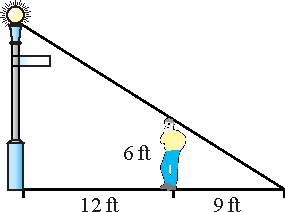
\includegraphics[width=\linewidth]{images/hp1-sum-37}
\end{sbspanel}%
\end{sidebyside}%
\end{divisionexerciseeg}%
\begin{divisionexerciseeg}{38}{}{}{g:exercise:idm46051683757264}%
Judy is observing the Mr. Freeze roller coaster from a safe distance of 1000 feet.  She notices that she can see the reflection of the highest point of the roller coaster in a puddle of water.  Judy is 23.5 feet from that point in the puddle.  If Judy is 5feet 3 inches tall, how tall is the roller coaster?%
\begin{sidebyside}{1}{0.15}{0.15}{0}%
\begin{sbspanel}{0.7}%

\includegraphics[width=\linewidth]{images/hp1-sum-38}
\end{sbspanel}%
\end{sidebyside}%
\end{divisionexerciseeg}%
\begin{divisionexerciseeg}{39}{}{}{g:exercise:idm46051683772368}%
\begin{sidebyside}{2}{0}{0}{0.15}%
\begin{sbspanel}{0.6}%
A florist fits a cylindrical piece of foam into a conical vase that is 10 inches high and measures 8 inches across the top, as shown in the figure.  If the radius of the foam cylinder is 2 inches, how tall should it be just to reach the top of the vase?%
\end{sbspanel}%
\begin{sbspanel}{0.25}%
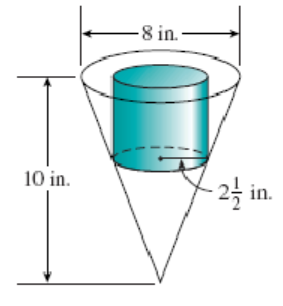
\includegraphics[width=\linewidth]{images/hp1-sum-39}
\end{sbspanel}%
\end{sidebyside}%
\end{divisionexerciseeg}%
\begin{divisionexerciseeg}{40}{}{}{g:exercise:idm46051683794448}%
\begin{sidebyside}{2}{0}{0}{0.1}%
\begin{sbspanel}{0.6}%
To measure the distance across the river shown in the figure, stand at \(A\) and sight across the river to a convenient landmark at \(B\). Then measure the distances \(AC\), \(CD\), and \(DE\).  If  \(AC=20\) feet, \(CD=13\) feet, and \(DE=58\) feet, how wide is the river?%
\end{sbspanel}%
\begin{sbspanel}{0.3}%
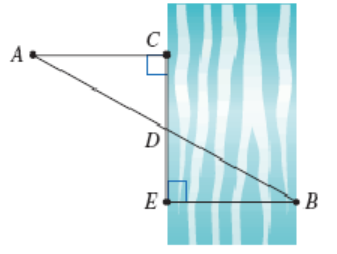
\includegraphics[width=\linewidth]{images/hp1-sum-40}
\end{sbspanel}%
\end{sidebyside}%
\end{divisionexerciseeg}%
\end{exercisegroup}
\par\medskip\noindent
\par\medskip\noindent%
%
For Problems 41\textendash{}44, sketch a diagram on graph paper, then solve the problem.%
\begin{exercisegroup}
\begin{divisionexerciseeg}{41}{}{}{g:exercise:idm46051683857776}%
Show that the rectangle with vertices \((-4,1), (2,6), (7,0)\) and \((1,-5)\) is a square.%
\end{divisionexerciseeg}%
\begin{divisionexerciseeg}{42}{}{}{g:exercise:idm46051683874000}%
Show that the points \((1,6), (5,2), (-2,3)\) and \((2,-1)\) are the vertices of a rectangle. (Hint: If the diagonals of a quadrilateral are of equal length, then the quadrilateral is a rectangle.)%
\end{divisionexerciseeg}%
\begin{divisionexerciseeg}{43}{}{}{g:exercise:idm46051683875440}%
Show that the point \(C(\sqrt{5},2+\sqrt{5})\) is the same distance from \(A(2,0)\) and \(B(-2,4)\).%
\end{divisionexerciseeg}%
\begin{divisionexerciseeg}{44}{}{}{g:exercise:idm46051683894128}%
Show that the points \((-2,1), (0,-1),\) and \((\sqrt{3}-1,\sqrt{3})\) are the vertices of an equilateral triangle.%
\end{divisionexerciseeg}%
\end{exercisegroup}
\par\medskip\noindent
\begin{divisionexercise}{45}{}{}{g:exercise:idm46051683901664}%
%
\begin{enumerate}[label=\alph*]
\item{}Write an equation that says “The distance from \((x,y)\) to \((2,5)\) is 3 units."%
\item{}Write an equation for the circle of radius 3 whose center is \((2,5)\).%
\end{enumerate}
%
\end{divisionexercise}%
\begin{divisionexercise}{46}{}{}{g:exercise:idm46051683925200}%
The points \((-2,4)\) and \((6,-2)\) lie on opposite ends of the diameter of a circle. What is the radius of the circle?%
\end{divisionexercise}%
\begin{divisionexercise}{47}{}{}{g:exercise:idm46051683915984}%
How long is the diagonal of a rectangle that measures 8 cm by 4 cm?  Give an exact value for your answer, and then an approximation rounded to thousandths.%
\end{divisionexercise}%
\begin{divisionexercise}{48}{}{}{g:exercise:idm46051683947712}%
What is the circumference of a circle of radius 6.2 feet?  Give an exact value for your answer, and then an approximation rounded to thousandths.%
\end{divisionexercise}%
\begin{divisionexercise}{49}{}{}{g:exercise:idm46051683963056}%
Find two points on the unit circle with \(x\)-coordinate \(\dfrac{-1}{3}\). Give exact values for your answers.%
\end{divisionexercise}%
\begin{divisionexercise}{50}{}{}{g:exercise:idm46051683980432}%
Find two points on the unit circle with \(y\)-coordinate \(\dfrac{\sqrt{7}}{4}\). Give exact values for your answers.%
\end{divisionexercise}%
\begin{divisionexercise}{51}{}{}{g:exercise:idm46051684019104}%
A circle of radius 10 feet is divided into 5 equal sectors.%
\par
%
\begin{enumerate}[label=\alph*]
\item{}Find the arclength of the circular edge of each sector.%
\item{}Find the area of each sector.%
\end{enumerate}
%
\end{divisionexercise}%
\begin{divisionexercise}{52}{}{}{g:exercise:idm46051684026176}%
The central angle of the sector of a circle is \(150\degree\), and the circle has radius 9 inches.%
\par
%
\begin{enumerate}[label=\alph*]
\item{}Find the arclength of the circular edge of each sector.%
\item{}Find the area of each sector.%
\end{enumerate}
%
\end{divisionexercise}%
\begin{divisionexercise}{53}{}{}{g:exercise:idm46051684053312}%
Delbert slices a 14 inch diameter pizza into 8 equal pieces, and Francine slices a 12 inch diameter pizza into 6 equal slices. Each slice is a sector of a circle.%
\par
%
\begin{enumerate}[label=\alph*]
\item{}Find the central angle for the slices.%
\item{}What are the areas of the slices?  Which slices have the greater area?%
\item{}How long are the crust (curved) edges of the slices?  Which slices have the longer crust edges?%
\end{enumerate}
%
\end{divisionexercise}%
\begin{divisionexercise}{54}{}{}{g:exercise:idm46051684078160}%
Florence wants to create a piechart (or circle graph) to display how much of her hospital's budget is dedicated to nurses. She finds that in the hospital's annual expenses of \textdollar{}60 million, the nurses' salaries and benefits totaled \textdollar{}1,200,000.%
\par
%
\begin{enumerate}[label=\alph*]
\item{}What fraction of the total annual costs comes from the nurses' salaries and benefits?%
\item{}Suppose that the entire budget is represented by the area of a circle. If the costs for the nurses are to be represented by a sector of that circle, what will be the angle of that sector?%
\item{}If the circle has a radius of 20 centimeters, what are the areas of the circle and of the sector representing the nurses? What are the circumference of the circle and the arclength of the sector?%
\end{enumerate}
%
\end{divisionexercise}%
\end{exercises-subsection}
\end{sectionptx}
\end{chapterptx}
%
%
\typeout{************************************************}
\typeout{Chapter 2 The Trigonometric Ratios}
\typeout{************************************************}
%
\begin{chapterptx}{The Trigonometric Ratios}{}{The Trigonometric Ratios}{}{}{x:chapter:chap2}
\begin{introduction}{}%
\begin{sidebyside}{2}{0}{0}{0}%
\begin{sbspanel}{0.6}[center]%
%
\begin{itemize}[label=\textbullet]
\item{}\(\displaystyle \blert{\textbf{Side and Angle Relationships}}\)%
\item{}\(\displaystyle \blert{\textbf{Right Triangle Trigonometry}}\)%
\item{}\(\displaystyle \blert{\textbf{Solving Right Triangles}}\)%
\end{itemize}
%
\end{sbspanel}%
\begin{sbspanel}{0.4}[center]%
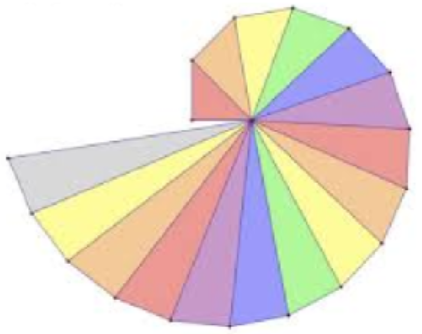
\includegraphics[width=\linewidth]{images/ch2-1.png}
\end{sbspanel}%
\end{sidebyside}%
\par
How would you measure the distance to an inaccessible obect, such as a ship at sea? In the 6th century BC, the Greek philosopher Thales estimated the distances to ships at sea using \terminology{triangulation}\index{triangulation}, a method for calculating distances by forming triangles. Using trigonometry and the measured length of just one side, the lengths of the other sides can be calculated.%
\par
Triangulation has been used to compute distances ever since. In the 16th century mapmakers began to use triangulation to position far-away places accurately. And as new methods in navigation and astronomy required greater precision, the idea of a survey using chains of triangles was developed.%
\par
In 1802, the East India Company embarked on the Great Trigonometrical Survey of India. Its goal was to measure the entire Indian subcontinent with scientific precision.%
\begin{sidebyside}{1}{0}{0}{0}%
\begin{sbspanel}{1}%
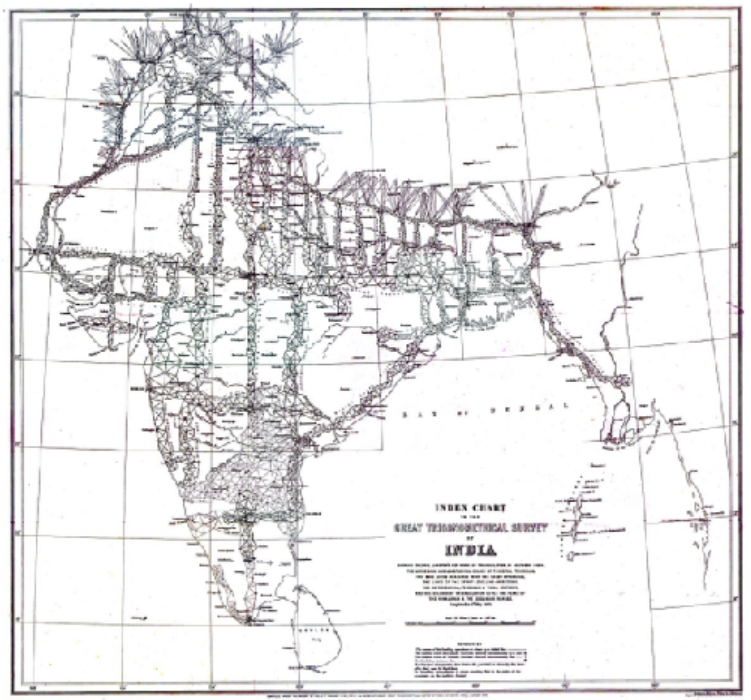
\includegraphics[width=\linewidth]{images/ch2-2.png}
\end{sbspanel}%
\end{sidebyside}%
\par
The surveyors began by measuring a baseline near Madras. The baseline was the only distance they measured; all other distances were calculated from it using measured angles.  Each calculated distance became the base side of another triangle used to calculate the distance to another point, which in turn started another triangle. Eventually this process formed a chain of triangles connecting the origin point to other locations.%
\par
Because of the size of the area to be surveyed, the surveyors did not triangulate the whole of India but instead created what they called a "gridiron" of triangulation chains running from North to South and East to West. You can see these chains in the map of the survey.%
\par
The Survey was completed in 1871. Along the way it calculated the height of the Himalayan giants: Everest, K2, and Kanchenjunga, and provided one of the first accurate measurements of a section of an arc of longitude.%
\par
Triangulation today is used for many purposes, including surveying, navigation, metrology, astrometry, binocular vision, and location of earthquakes.%
\begin{activity}{Trigonometric Ratios.}{g:activity:idm46051682993312}%
%
\par
%
\begin{enumerate}[label=\Alph*]
\item{}Using Ratios and Proportions%
\par
Two related quantities or variables are \terminology{proportional} if their ratio is always the same.%
\begin{enumerate}[label=\arabic*]
\item{}%
\begin{enumerate}[label=\alph*]
\item{}On any given day, the cost of filling up your car's gas tank is proportional to the number of gallons of gas you buy. For each purchase below, compute the ratio%
\begin{equation*}
\dfrac{\text{total cost of gasoline}}{\text{number of gallons}}
\end{equation*}
%
\begin{sidebyside}{1}{0}{0}{0}%
\begin{sbspanel}{1}%
{\centering%
{\tabularfont%
\begin{tabular}{AcAcAcA}\hrulethick
Gallons of Gas Purchased&Total Cost&\(\dfrac{\text{Dollars}}{\text{Gallon}}\)\tabularnewline\hrulethin
\(5\)&\textdollar{}\(14.45\)&\(\hphantom{0000}\)\tabularnewline\hrulethin
\(12\)&\textdollar{}\(34.68\)&\(\hphantom{0000}\)\tabularnewline\hrulethin
\(18\)&\textdollar{}\(52.02\)&\(\hphantom{0000}\)\tabularnewline\hrulethin
\end{tabular}
}%
\par}
\end{sbspanel}%
\end{sidebyside}%
\item{}Write an equation that you can solve to answer the question:  How much does 21 gallons of gas cost?  Use the ratio \(\dfrac{\text{Dollars}}{\text{Gallon}}\) in your equation.%
\item{}Write an equation that you can solve to answer the question:  How many gallons of gas can you buy for \textdollar{}46.24?  Use the ratio \(\dfrac{\text{Dollars}}{\text{Gallon}}\) in your equation.%
\end{enumerate}
%
\item{}A recipe for coffee cake calls for \(\dfrac{3}{4}\) cup of sugar and \(1\dfrac{3}{4}\) cup of flour.%
\par
%
\begin{enumerate}[label=\alph*]
\item{}What is the ratio of sugar to flour?  Write your answer as a common fraction, and then give a decimal approximation rounded to four places.%
\par
For parts (b) and (c) below, write an equation that you can solve to answer the question.  Use the ratio \(\dfrac{\text{Amount of sugar}}{\text{Amount of flour}}\)in your equation.%
\item{}How much sugar should you use if you use 4 cups of flour?  Compute your answer two ways:  writing the ratio as a common fraction, and then writing the ratio as a decimal approximation.  Are your answers the same?%
\item{}How much flour should you use if you use 4 cups of sugar?  Compute your answer two ways:  writing the ratio as a common fraction, and then writing the ratio as a decimal approximation.  Are your answers the same?%
\end{enumerate}
%
\item{}You are making a scale model of the Eiffel tower, which is 324 meters tall and 125 meters wide at its base.%
\begin{sidebyside}{1}{0.3}{0.3}{0}%
\begin{sbspanel}{0.4}%
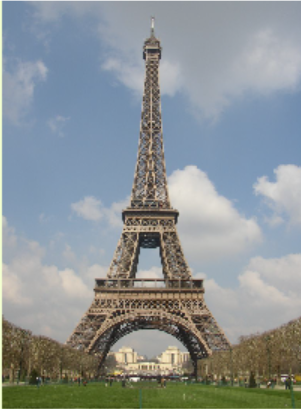
\includegraphics[width=\linewidth]{images/ch2-3.png}
\end{sbspanel}%
\end{sidebyside}%
\par
%
\begin{enumerate}[label=\alph*]
\item{}Compute the ratio of the width of the base to the height of the tower. Round your answer to four decimal places.%
\par
Use your ratio to write equations and answer the questions below:%
\item{}If the base of your model is 8 inches wide, how tall should the model be?%
\item{}If you make a larger model that is 5 feet tall, how wide will the base be?%
\end{enumerate}
%
\end{enumerate}
%
\item{}Similar Triangles%
\par
%
\begin{enumerate}[label=\arabic*]
\item{}Recall that two triangles are \terminology{similar} if their corresponding sides are proportional.  The corresponding angles of similar triangles are equal.%
\par
%
\begin{enumerate}[label=\alph*]
\item{}What is the ratio of the two given sides in each triangle?  Are the corresponding sides of the three triangles proportional? How do we know that \(\alpha = \beta = \gamma\) ?%
\begin{sidebyside}{1}{0}{0}{0}%
\begin{sbspanel}{1}%
\resizebox{\linewidth}{!}{%
\tikzset{%
}
\begin{tikzpicture} 
\coordinate(A) at (0,0);
\coordinate (B) at (2.5,0 );
\coordinate (C) at (2.5,1);

\draw[blue,thick] (B) rectangle +(-0.25,0.25);
\draw[black,thick] (A)--(B) node [below,midway] {\color{blue}$5$};
\draw[black,thick] (C)--(B) node [right,midway] {\color{blue}$2$};
\draw[black,thick] (A)--(C);
\draw[red,thick] (0.8,0) arc (0:{atan(2/5)}:0.8) node[ right, midway] {$\alpha$};

\draw[blue,thick, xshift=3.2cm, scale=1.5] (2.5,0) rectangle +(-0.16,0.16);
\draw[black,thick, xshift=3.2cm, scale=1.5] (0,0)--(2.5,0) node [below,midway] {\color{blue}$7.5$};
\draw[black,thick, xshift=3.2cm, scale=1.5] (2.5,1)--(2.5,0) node [right,midway] {\color{blue}$3$};
\draw[black,thick, xshift=3.2cm, scale=1.5] (0,0)--(2.5,1);
\draw[red,thick, xshift=3.2cm, scale=1.5] (0.7,0) arc (0:{atan(2/5)}:0.7) node[ right, midway] {$\beta$};

\draw[blue,thick, xshift=7.7cm, scale=1.6] (2.5,0) rectangle +(-0.15,0.15);
\draw[black,thick, xshift=7.7cm, scale=1.6] (0,0)--(2.5,0) node [below,midway] {\color{blue}$8$};
\draw[black,thick, xshift=7.7cm, scale=1.6] (2.5,1)--(2.5,0) node [right,midway] {\color{blue}$3.2$};
\draw[black,thick, xshift=7.7cm, scale=1.6] (0,0)--(2.5,1);
\draw[red,thick, xshift=7.7cm, scale=1.6] (0.5,0) arc (0:{atan(2/5)}:0.5) node[ right, midway] {$\gamma$};
\end{tikzpicture}
}%
\end{sbspanel}%
\end{sidebyside}%
\item{}Find the hypotenuse of each right triangle.%
\item{}Use the sides of the approporiate triangle to compute \(\sin \alpha,~ \sin \beta,\) and \(\sin \gamma\). Round your answers to four decimal places. Does the sine of an angle depend on the lengths of its sides?%
\item{}How do you know that the triangle below is similar to the three triangles in part (a)?  Write an equation using the ratio from part (c) to find \(x\).%
\begin{sidebyside}{1}{0.3}{0.3}{0}%
\begin{sbspanel}{0.4}%
\resizebox{\linewidth}{!}{%
\tikzset{%
}
\begin{tikzpicture} 
\coordinate(A) at (0,0);
\coordinate (B) at (4.5,0 );
\coordinate (C) at (4.5,2);

\draw[blue,thick] (B) rectangle +(-0.25,0.25);
\draw[black,thick] (A)--(B);
\draw[black,thick] (C)--(B) node [right,midway] {\color{blue}$12$};
\draw[black,thick] (A)--(C) node [above left,midway] {\color{blue}$x$};
\draw[red,thick] (0.8,0) arc (0:{atan(2/5)}:0.8) node[ right, midway] {$\alpha$};
\end{tikzpicture}
}%
\end{sbspanel}%
\end{sidebyside}%
\end{enumerate}
%
\item{}In the three right triangles below, the angle \(\theta\) is the same size.%
\begin{sidebyside}{1}{0.1}{0.1}{0}%
\begin{sbspanel}{0.8}%
\resizebox{\linewidth}{!}{%
\tikzset{%
}
\begin{tikzpicture} [scale=1.2]
\coordinate(A) at (0,0);
\coordinate (B) at (2.5,0 );
\coordinate (C) at (2.5,2);

\draw[blue,thick] (B) rectangle +(-0.25,0.25);
\draw[black,thick] (A)--(B) node [below,midway] {\color{blue}$10$};
\draw[black,thick] (C)--(B);
\draw[black,thick] (A)--(C) node [above left,midway] {\color{blue}$13$};
\draw[red,thick] (0.4,0) arc (0:{acos(10/13)}:0.4) node[ right, midway, yshift=2] {$\theta$};

\draw[blue,thick, xshift=3.5cm, scale=0.33] (2.5,0) rectangle +(-0.5,0.5);
\draw[black,thick, xshift=3.5cm, scale=0.33] (0,0)--(2.5,0) node [below,midway] {\color{blue}$x$};
\draw[black,thick, xshift=3.5cm, scale=0.33] (2.5,2)--(2.5,0);
\draw[black,thick, xshift=3.5cm, scale=0.33] (0,0)--(2.5,2) node [above left,midway] {\color{blue}$4.3$};
\draw[red,thick, xshift=3.5cm, scale=0.33] (0.7,0) arc (0:{acos(10/13)}:0.7) node[ right, midway, yshift=2] {\footnotesize$\theta$};

\draw[blue,thick, xshift=5.2cm, scale=1.4] (2.5,0) rectangle +(-0.17,0.17);
\draw[black,thick, xshift=5.2cm, scale=1.4] (0,0)--(2.5,0) node [below,midway] {\color{blue}$14$};
\draw[black,thick, xshift=5.2cm, scale=1.4] (2.5,2)--(2.5,0);
\draw[black,thick, xshift=5.2cm, scale=1.4] (0,0)--(2.5,2) node [above left,midway] {\color{blue}$z$};
\draw[red,thick, xshift=5.2cm, scale=1.4] (0.3,0) arc (0:{acos(10/13)}:0.3) node[ right, midway, yshift=2] {$\theta$};
\end{tikzpicture}
}%
\end{sbspanel}%
\end{sidebyside}%
\par
%
\begin{enumerate}[label=\alph*]
\item{}Use the first triangle to calculate \(\cos \theta\). Round your answer to four decimal places.%
\item{}In the second triangle, explain why \(\dfrac{x}{4.3} = \dfrac{10}{13}\).  Write an equation using your answer to part (a) and solve it to find \(x\).%
\item{}Write and solve an equation to find \(z\) in the third triangle.%
\end{enumerate}
%
\item{}%
\begin{enumerate}[label=\alph*]
\item{}Use your calculator to find the value of \(\dfrac{h}{2.4}\). (Hint: Which trig ratio should you use?) What is the length of side \(h\)?%
\begin{sidebyside}{1}{0.325}{0.325}{0}%
\begin{sbspanel}{0.35}%
\resizebox{\linewidth}{!}{%
\tikzset{%
}
\begin{tikzpicture} [scale=.8]
\coordinate(A) at (0,0);
\coordinate (B) at (4.5,0 );
\coordinate (C) at (4.5,-2.4);

\draw[blue,thick] (B) rectangle +(-0.25,-0.25);
\draw[black,thick] (A)--(B) node [above,midway] {\color{blue}$h$};
\draw[black,thick] (C)--(B) node [right,midway] {\color{blue}$2.4$};
\draw[black,thick] (A)--(C);
\draw[red,thick] (4.5,-1.9) arc (90:152:0.5) node[ above , midway, xshift=-3] {$62\degree$};
\end{tikzpicture}
}%
\end{sbspanel}%
\end{sidebyside}%
\item{}What is the value of \(\dfrac{6}{w}\) for the triangle below?  Write an equation and solve for \(w\).%
\begin{sidebyside}{2}{0.13}{0.13}{0.26}%
\begin{sbspanel}{0.2}[bottom]%
\resizebox{\linewidth}{!}{%
\tikzset{%
}
\begin{tikzpicture} [scale=.8, rotate=90]
\coordinate(A) at (0,0);
\coordinate (B) at (4.5,0 );
\coordinate (C) at (4.5,-2.4);

\draw[blue,thick] (B) rectangle +(-0.3,-0.3);
\draw[black,thick] (A)--(B) node [left,midway] {\color{blue}$6$};
\draw[black,thick] (C)--(B) node [above,midway] {\color{blue}$w$};
\draw[black,thick] (A)--(C);
\draw[red,thick] (4.5,-1.9) arc (90:152:0.5) node[ left , midway, yshift=-5] {$62\degree$};
\end{tikzpicture}
}%
\end{sbspanel}%
\begin{sbspanel}{0.28}[bottom]%
\resizebox{\linewidth}{!}{%
\tikzset{%
}
\begin{tikzpicture} [scale=.85, rotate=30]
\coordinate(A) at (0,0);
\coordinate (B) at (-4.5,0 );
\coordinate (C) at (-4.5,-2.4);

\draw[blue,thick] (B) rectangle +(0.3,-0.3);
\draw[black,thick] (A)--(B) node [above left,midway] {\color{blue}$x$};
\draw[black,thick] (C)--(B) node [below left,midway] {\color{blue}$1$};
\draw[black,thick] (A)--(C);
\draw[red,thick] (-4.5,-1.9) arc (90:28:0.5) node[ above , midway, yshift=0] {$62\degree$};
\end{tikzpicture}
}%
\end{sbspanel}%
\end{sidebyside}%
\item{}Write an equation and solve it to find \(x\) in the triangle above.%
\end{enumerate}
%
\end{enumerate}
%
\end{enumerate}
%
\end{activity}
\end{introduction}%
%
%
\typeout{************************************************}
\typeout{Section 2.1 Side and Angle Relationships}
\typeout{************************************************}
%
\begin{sectionptx}{Side and Angle Relationships}{}{Side and Angle Relationships}{}{}{x:section:Side-and-Angle-Relationships}
%
%
\typeout{************************************************}
\typeout{Subsection  Introduction}
\typeout{************************************************}
%
\begin{subsectionptx}{Introduction}{}{Introduction}{}{}{g:subsection:idm46051684717424}
From geometry we know that the sum of the angles in a triangle is 180°.  Are there any relationships between the angles of a triangle and its sides?%
\par
First of all, you have probably observed that the longest side in a triangle is always opposite the largest angle, and the shortest side is opposite the smallest angle, as illustrated below.%
\begin{sidebyside}{2}{0.095}{0.095}{0.19}%
\begin{sbspanel}{0.35}[center]%
\resizebox{\linewidth}{!}{%
\tikzset{%
  block/.style    = {draw, thick, rectangle, minimum height = 3em,
    minimum width = 3em},
  sum/.style      = {draw, circle, node distance = 2cm}, % Adder
  input/.style    = {coordinate}, % Input
  output/.style   = {coordinate} % Output
}
\begin{tikzpicture} [scale=.9]
    \coordinate(A) at (0,0);
    \coordinate (B) at (6,0 );
    \coordinate (C) at (4,1.46);

    \draw[black,thick] (A)--(B) node [below,midway] {\color{blue}$c$};
    \draw[black,thick] (C)--(B) node [above right,midway] {\color{blue}$b$};
    \draw[black,thick] (A)--(C) node [above left,midway] {\color{blue}$a$};
    \draw[red,thick] (.9,0) arc (0:20:0.9) node[ right , midway, xshift=4, yshift=2] {$20\degree$};
    \draw[red,thick] (5.6,0) arc (180:{180-atan(1.46/2)}:0.4) node[ left , midway, xshift=-1, yshift=3] {$40\degree$};
    \draw[red,thick] (3.72,1.36) arc (200:320:0.3) node[ below , midway, yshift=0] {$120\degree$};
\end{tikzpicture}
}%
\end{sbspanel}%
\begin{sbspanel}{0.27}[center]%
\resizebox{\linewidth}{!}{%
\tikzset{%
  block/.style    = {draw, thick, rectangle, minimum height = 3em,
    minimum width = 3em},
  sum/.style      = {draw, circle, node distance = 2cm}, % Adder
  input/.style    = {coordinate}, % Input
  output/.style   = {coordinate} % Output
}
\begin{tikzpicture} [scale=.25,rotate=30]

    \coordinate(A) at (0,0);
    \coordinate (B) at (2,13.86 );
    \coordinate (C) at (10,0);

    \draw[black,thick] (A)--(B) node [left,midway] {\color{blue}$14$};
    \draw[black,thick] (C)--(B) node [above right,midway] {\color{blue}$16$};
    \draw[black,thick] (A)--(C) node [below right,midway] {\color{blue}$10$};

    \node at (A) [anchor=north east] {$A$};
    \node at (B) [anchor= east] {$B$};
    \node at (C) [anchor=west] {$C$};
\end{tikzpicture}
}%
\end{sbspanel}%
\end{sidebyside}%
\begin{note}{}{g:note:idm46051687825536}%
\begin{sidebyside}{2}{0}{0}{0.02}%
\begin{sbspanel}{0.7}[center]%
It is usual to label the angles of a triangle with capital letters, and the side opposite each angle with the corresponding lower-case letter, as shown at right.  We will follow this practice unless indicated otherwise.%
\end{sbspanel}%
\begin{sbspanel}{0.28}[center]%
\resizebox{\linewidth}{!}{%
\tikzset{%
  block/.style    = {draw, thick, rectangle, minimum height = 3em,
    minimum width = 3em},
  sum/.style      = {draw, circle, node distance = 2cm}, % Adder
  input/.style    = {coordinate}, % Input
  output/.style   = {coordinate} % Output
}
\begin{tikzpicture} [rotate=15]

\coordinate(A) at (0,0);
\coordinate (B) at (3,1.6 );
\coordinate (C) at (4,0);

\draw[black,thick] (A)--(B) node [above left,midway] {\color{blue}$c$};
\draw[black,thick] (C)--(B) node [above right,midway] {\color{blue}$a$};
\draw[black,thick] (A)--(C) node [below right,midway] {\color{blue}$b$};

\node at (A) [anchor=north east] {$A$};
\node at (B) [anchor= south] {$B$};
\node at (C) [anchor=west] {$C$};

\end{tikzpicture}
}%
\end{sbspanel}%
\end{sidebyside}%
\end{note}
\begin{example}{}{g:example:idm46051692305488}%
In \(\triangle FGH, \angle F=48\degree,\) and \(\angle G\) is obtuse.  Side \(f\) is 6 feet long. What can you conclude about the other sides?%
\par\smallskip%
\noindent\textbf{\blocktitlefont Solution}.\label{g:solution:idm46051687848640}{}\hypertarget{g:solution:idm46051687848640}{}\quad{}Because \(\angle G\) is greater than \(90\degree\), we know that \(\angle F +\angle G\) is greater than \(90\degree + 48\degree = 138\degree\), so \(\angle F\) is less than \(180\degree-138\degree = 42\degree.\)  Thus, \(\angle H \lt \angle F \lt \angle G,\) and consequently \(h \lt f \lt g\).  We can conclude that \(h \lt 6\) feet long, and \(g \gt 6\) feet long.%
\end{example}
\begin{inlineexercise}{}{g:exercise:idm46051687876256}%
In isosceles triangle \(\triangle RST\), the vertex angle \(\angle S = 72\degree\).  Which side is longer, \(s\) or \(t\)?%
\par\smallskip%
\noindent\textbf{\blocktitlefont Answer}.\label{g:answer:idm46051687889696}{}\hypertarget{g:answer:idm46051687889696}{}\quad{}\(s\) is longer%
\end{inlineexercise}
\end{subsectionptx}
%
%
\typeout{************************************************}
\typeout{Subsection  The Triangle Inequality}
\typeout{************************************************}
%
\begin{subsectionptx}{The Triangle Inequality}{}{The Triangle Inequality}{}{}{g:subsection:idm46051687888544}
\index{triangle inequality}%
It is also true that the sum of the lengths of any two sides of a triangle must be greater than the third side, or else the two sides will not meet to form a triangle. This fact is called the triangle inequality.%
\begin{assemblage}{Triangle Inequality.}{g:assemblage:idm46051687899968}%
\begin{sidebyside}{2}{0.08}{0.08}{0.04}%
\begin{sbspanel}{0.5}[center]%
In any triangle, we must have that%
\begin{equation*}
p+q \gt r
\end{equation*}
where \(p, q, \text{and}~ r\) are the lengths of the sides of the triangle.%
\end{sbspanel}%
\begin{sbspanel}{0.3}[center]%
\resizebox{\linewidth}{!}{%
\tikzset{%
  block/.style    = {draw, thick, rectangle, minimum height = 3em,
    minimum width = 3em},
  sum/.style      = {draw, circle, node distance = 2cm}, % Adder
  input/.style    = {coordinate}, % Input
  output/.style   = {coordinate} % Output
}
\begin{tikzpicture} [rotate=-20]

\coordinate(A) at (0,0);
\coordinate (B) at (5,0 );
\coordinate (C) at (2,2);

\draw[black,thick] (A)--(B) node [below left,midway] {\color{blue}$r$};
\draw[black,thick] (C)--(B) node [above right,midway] {\color{blue}$q$};
\draw[black,thick] (A)--(C) node [above left,midway] {\color{blue}$p$};

\end{tikzpicture}
}%
\end{sbspanel}%
\end{sidebyside}%
\end{assemblage}
We cannot use the triangle inequality to find the \emph{exact} lengths of the sides of a triangle, but we can find largest and smallest possible values for the length.%
\begin{example}{}{g:example:idm46051687792992}%
\begin{sidebyside}{2}{0.025}{0.025}{0.05}%
\begin{sbspanel}{0.55}[center]%
Two sides of a triangle have lengths 7 inches and 10 inches, as shown at right.  What can you say about the length of the third side?%
\end{sbspanel}%
\begin{sbspanel}{0.35}[center]%
\resizebox{\linewidth}{!}{%
\tikzset{%
  block/.style    = {draw, thick, rectangle, minimum height = 3em,
    minimum width = 3em},
  sum/.style      = {draw, circle, node distance = 2cm}, % Adder
  input/.style    = {coordinate}, % Input
  output/.style   = {coordinate} % Output
}
\begin{tikzpicture} [rotate=35]

\coordinate(A) at (0,0);
\coordinate (B) at (4.,0 );
\coordinate (C) at (-.8,2.7);

\draw[black,thick] (A)--(B) node [below right,midway] {\color{blue}$10$};
\draw[black,thick] (C)--(B) node [above right,midway] {\color{blue}$x$};
\draw[black,thick] (A)--(C) node [below left,midway] {\color{blue}$7$};
\end{tikzpicture}
}%
\end{sbspanel}%
\end{sidebyside}%
\par\smallskip%
\noindent\textbf{\blocktitlefont Solution}.\label{g:solution:idm46051687804128}{}\hypertarget{g:solution:idm46051687804128}{}\quad{}We let \(x\) represent the length of the third side of the triangle.  By looking at each side in turn, we can apply the triangle inequality three different ways, to get%
\begin{equation*}
7 \lt x+10, ~~~ 10 \lt x+7, ~~~ \text{and} ~~~ x \lt 10+7
\end{equation*}
We solve \index{solve!inequality} each of these inequalities to find%
\begin{equation*}
-3 \lt x, ~~~ 3 \lt x, ~~~ \text{and} ~~~ x \lt 17
\end{equation*}
We already know that \(x \gt -3\) because \(x\) must be positive, but the other two inequalities do give us new information. The third side must be greater than 3 inches but less than 17 inches long.%
\end{example}
\begin{inlineexercise}{}{g:exercise:idm46051685250752}%
Can you make a triangle with three wooden sticks of lengths 14 feet, 26 feet, and 10 feet?  Sketch a picture, and explain why or why not.%
\par\smallskip%
\noindent\textbf{\blocktitlefont Answer}.\label{g:answer:idm46051685258272}{}\hypertarget{g:answer:idm46051685258272}{}\quad{}No, \(10+14\) is not greater than 26.%
\end{inlineexercise}
\end{subsectionptx}
%
%
\typeout{************************************************}
\typeout{Subsection  Right Triangles: The Pythagorean Theorem}
\typeout{************************************************}
%
\begin{subsectionptx}{Right Triangles: The Pythagorean Theorem}{}{Right Triangles: The Pythagorean Theorem}{}{}{g:subsection:idm46051685262016}
\index{right triangle!Pythagorean theorem}%
\index{Pythagorean theorem}%
\index{hypotenuse}%
\index{leg}%
In Chapter 1 we used the Pythagorean theorem to derive the distance formula.  We can also use the Pythagorean theorem to find one side of a right triangle if we know the other two sides.%
\begin{assemblage}{Pythagorean Theorem.}{g:assemblage:idm46051685257696}%
\begin{sidebyside}{2}{0.02}{0.08}{0.05}%
\begin{sbspanel}{0.6}%
In a right triangle, if \(c\) stands for the length of the hypotenuse, and the lengths of the two legs are denoted by \(a\) and \(b\), then%
\begin{equation*}
\blert{a^2 + b^2 = c^2}
\end{equation*}
%
\end{sbspanel}%
\begin{sbspanel}{0.25}%

\includegraphics[width=\linewidth]{images/pythagorean}
\end{sbspanel}%
\end{sidebyside}%
\end{assemblage}
\begin{example}{}{g:example:idm46051701718288}%
A 25-foot ladder is placed against a wall so that its foot is 7 feet from the base of the wall. How far up the wall does the ladder reach?%
\par\smallskip%
\noindent\textbf{\blocktitlefont Solution}.\label{g:solution:idm46051701721456}{}\hypertarget{g:solution:idm46051701721456}{}\quad{}We make a sketch of the situation, as shown below, and label any known dimensions. We'll call the unknown height \(h\).%
\begin{sidebyside}{2}{0}{0.05}{0.05}%
\begin{sbspanel}{0.75}%
The ladder forms the hypotenuse of a right triangle, so we can apply the Pythagorean theorem, substituting 25 for \(c\), 7 for \(b\), and \(h\) for \(a\).%
\begin{align*}
a^2 + b^2 \amp = c^2\\
h^2 + 7^2 \amp = 25^2
\end{align*}
Now solve by extraction of roots:%
\end{sbspanel}%
\begin{sbspanel}{0.15}%

\includegraphics[width=\linewidth]{images/ladder}
\end{sbspanel}%
\end{sidebyside}%
\par
%
\begin{align*}
h^2 + 49 \amp = 625 \amp\amp \blert{\text{Subtract 49 from both sides.}}\\
h^2 \amp = 576 \amp\amp \blert{\text{Extract roots.}}\\
h \amp = \pm \sqrt{576} \amp\amp \blert{\text{Simplify the radical.}}\\
h \amp = \pm 24
\end{align*}
The height must be a positive number, so the solution \(-24\) does not make sense for this problem. The ladder reaches 24 feet up the wall.%
\end{example}
\begin{inlineexercise}{}{g:exercise:idm46051687698384}%
A baseball diamond is a square whose sides are 90 feet long.  The catcher at home plate sees a runner on first trying to steal second base, and throws the ball to the second-baseman.  Find the straight-line distance from home plate to second base.%
\par\smallskip%
\noindent\textbf{\blocktitlefont Answer}.\label{g:answer:idm46051701218944}{}\hypertarget{g:answer:idm46051701218944}{}\quad{}\(90\sqrt{2} \approx 127.3\) feet%
\end{inlineexercise}
\begin{note}{}{g:note:idm46051701222112}%
Keep in mind that the Pythagorean theorem is true only for right triangles, so the converse \index{Pythagorean theorem!converse} of the theorem is also true.  In other words, if the sides of a triangle satisfy the relationship \(a^2 + b^2 = c^2\), then the triangle must be a right triangle.  We can use this fact to test whether or not a given triangle has a right angle.%
\end{note}
\begin{example}{}{g:example:idm46051687721024}%
Delbert is paving a patio in his back yard, and would like to know if the corner at \(C\) is a right angle.%
\begin{sidebyside}{2}{0}{0}{0}%
\begin{sbspanel}{0.65}[center]%
He measures 20 cm along one side from the corner, and 48 cm along the other side, placing pegs \(P\) and \(Q\) at each position, as shown at right.  The line joining those two pegs is 52 cm long.  Is the corner a right angle?%
\end{sbspanel}%
\begin{sbspanel}{0.35}[center]%
\resizebox{\linewidth}{!}{%
\tikzset{%
  block/.style    = {draw, thick, rectangle, minimum height = 3em,
    minimum width = 3em},
  sum/.style      = {draw, circle, node distance = 2cm}, % Adder
  input/.style    = {coordinate}, % Input
  output/.style   = {coordinate} % Output
}
\begin{tikzpicture} 

\coordinate(A) at (0,0);
\coordinate (B) at (4,0 );
\coordinate (C) at (0,1.7);

\draw[black,thick] (A)--(B) node [below,midway] {\color{blue}$48$ cm};
\draw[black,thick] (C)--(B) node [above right,midway, xshift=-3] {\color{blue}$52$ cm};
\draw[black,thick] (A)--(C) node [left,midway] {\color{blue}$20$ cm};
\draw[black,thick] (C) -- +(0,.7);
\draw[black,thick] (B) -- +(.7,0);

\filldraw[black] (A) circle (.2pt) node[anchor=north east] {$C$};
\filldraw[black] (B) circle (1.6pt) node[anchor=north west] {$Q$};
\filldraw[black] (C) circle (1.6pt) node[anchor=south east] {$P$};
\end{tikzpicture}
}%
\end{sbspanel}%
\end{sidebyside}%
\par\smallskip%
\noindent\textbf{\blocktitlefont Solution}.\label{g:solution:idm46051701913216}{}\hypertarget{g:solution:idm46051701913216}{}\quad{}If  is a right triangle, then its sides must satisfy \(p^2 + q^2 = c^2\). We find%
\begin{align*}
p^2 + q^2 \amp = 20^2 + 48^2 = 400 + 2304 = 2704\\
c^2 \amp = 52^2 = 2704
\end{align*}
Yes, because \(p^2 + q^2 = c^2\), the corner at \(C\) is a right angle.%
\end{example}
\begin{inlineexercise}{}{g:exercise:idm46051682993024}%
The sides of a triangle measure 15 inches, 25 inches, and 30 inches long. Is the triangle a right triangle?%
\par\smallskip%
\noindent\textbf{\blocktitlefont Answer}.\label{g:answer:idm46051685486112}{}\hypertarget{g:answer:idm46051685486112}{}\quad{}No%
\end{inlineexercise}
The Pythagorean theorem relates the sides of \emph{right} triangles. However, for information about the sides of other triangles, the best we can do (without trigonometry!) is the triangle inequality. Nor does the Pythagorean theorem help us find the \emph{angles} in a triangle.  In the next section we discover relationships between the angles and the sides of a right triangle.%
\par
Review the following skills you will need for this section.%
\begin{project}{}{g:project:idm46051685510208}%
\begin{sidebyside}{1}{0}{0}{0}%
\begin{sbspanel}{1}%
Solve the inequality.%
\end{sbspanel}%
\end{sidebyside}%
\begin{sidebyside}{2}{0}{0}{0}%
\begin{sbspanel}{0.5}%
1. \(\:6-x \gt 3\)%
\end{sbspanel}%
\begin{sbspanel}{0.5}%
\par
2. \(\:\dfrac{-3x}{4} \ge -6\)%
\end{sbspanel}%
\end{sidebyside}%
\begin{sidebyside}{2}{0}{0}{0}%
\begin{sbspanel}{0.5}%
3. \(\:3x-7 \le -10\)%
\end{sbspanel}%
\begin{sbspanel}{0.5}%
\par
4. \(\:4-3x \lt 2x+9\)%
\end{sbspanel}%
\end{sidebyside}%
\begin{sidebyside}{1}{0}{0}{0}%
\begin{sbspanel}{1}%
If \(x \lt 0\), which of the following expressions are positive, and which are negative?%
\end{sbspanel}%
\end{sidebyside}%
\begin{sidebyside}{3}{0}{0}{0.05}%
\begin{sbspanel}{0.3}%
5. \(\:-x\)%
\end{sbspanel}%
\begin{sbspanel}{0.3}%
\par
6. \(\:-(-x)\)%
\end{sbspanel}%
\begin{sbspanel}{0.3}%
\par
7. \(\:\abs{x}\)%
\end{sbspanel}%
\end{sidebyside}%
\begin{sidebyside}{3}{0}{0}{0.05}%
\begin{sbspanel}{0.3}%
8. \(\:-\abs{x}\)%
\end{sbspanel}%
\begin{sbspanel}{0.3}%
\par
9. \(\:-\abs{-x}\)%
\end{sbspanel}%
\begin{sbspanel}{0.3}%
\par
10. \(\:x^{-1}\)%
\end{sbspanel}%
\end{sidebyside}%
\begin{sidebyside}{1}{0}{0}{0}%
\begin{sbspanel}{1}%
\(\underline{\qquad\qquad\qquad\qquad}\)%
\end{sbspanel}%
\end{sidebyside}%
\begin{sidebyside}{1}{0}{0}{0}%
\begin{sbspanel}{1}%
Algebra Refresher Answers%
\end{sbspanel}%
\end{sidebyside}%
\par
%
\begin{multicols}{5}
\begin{enumerate}[label=\arabic*]
\item{}\(\displaystyle \:x \lt 3\)%
\item{}\(\displaystyle \:x \le 8\)%
\item{}\(\displaystyle \:x \le -1\)%
\item{}\(\displaystyle \:x \gt -1\)%
\item{}Positive%
\item{}Negative%
\item{}Positive%
\item{}Negative%
\item{}Negative%
\item{}Negative%
\end{enumerate}
\end{multicols}
%
\end{project}
\end{subsectionptx}
%
%
\typeout{************************************************}
\typeout{Subsection  Section 2.1 Summary}
\typeout{************************************************}
%
\begin{subsectionptx}{Section 2.1 Summary}{}{Section 2.1 Summary}{}{}{g:subsection:idm46051685636448}
%
%
\typeout{************************************************}
\typeout{Subsubsection  Vocabulary}
\typeout{************************************************}
%
\begin{subsubsectionptx}{Vocabulary}{}{Vocabulary}{}{}{g:subsubsection:idm46051685642880}
%
\begin{multicols}{3}
\begin{itemize}[label=\textbullet]
\item{}Converse%
\item{}Extraction of roots%
\item{}Inequality%
\end{itemize}
\end{multicols}
%
\end{subsubsectionptx}
%
%
\typeout{************************************************}
\typeout{Subsubsection  Concepts}
\typeout{************************************************}
%
\begin{subsubsectionptx}{Concepts}{}{Concepts}{}{}{g:subsubsection:idm46051685668656}
%
\begin{enumerate}[label=\arabic*]
\item{}The longest side in a triangle is opposite the largest angle, and the shortest side is opposite the smallest angle.%
\item{}Triangle Inequality:  In any triangle, the sum of the lengths of any two sides is greater than the length of the third side.%
\item{}Pythagorean Theorem:  In a right triangle with hypotenuse \(c,~~ a^2 +b^2 = c^2\).%
\item{}If the sides of a triangle satisfy the relationship \(~a^2 +b^2 = c^2~\), then the triangle is a right triangle.%
\end{enumerate}
%
\end{subsubsectionptx}
%
%
\typeout{************************************************}
\typeout{Subsubsection  Study Questions}
\typeout{************************************************}
%
\begin{subsubsectionptx}{Study Questions}{}{Study Questions}{}{}{g:subsubsection:idm46051685699136}
%
\begin{enumerate}[label=\arabic*]
\item{}Is it always true that the hypotenuse is the longest side in a right triangle? Why or why not?%
\item{}In \(\triangle DEF\), is it possible that \(~d+e\gt f~\) and \(~e+f\gt d~\) are both true? Explain your answer.%
\item{}In a right triangle with hypotenuse \(c\), we know that \(~a^2 +b^2 = c^2~\).  Is it also true that \(~a + b = c~\)? Why or why not?%
\item{}The two shorter sides of an obtuse triangle are 3 in and 4 in.  What are the possible lengths for the third side?%
\end{enumerate}
%
\end{subsubsectionptx}
%
%
\typeout{************************************************}
\typeout{Subsubsection  Skills}
\typeout{************************************************}
%
\begin{subsubsectionptx}{Skills}{}{Skills}{}{}{g:subsubsection:idm46051685740272}
%
\begin{enumerate}[label=\arabic*]
\item{}Identify inconsistencies in figures    \#1-12%
\item{}Use the triangle inequality to put bounds on the lengths of sides   \#13-16%
\item{}Use the Pythagorean theorem to find the sides of a right triangle    \#17-26%
\item{}Use the Pythagorean theorem to identify right triangles    \#27-32%
\item{}Solve problems using the Pythagorean theorem    \#33-42%
\end{enumerate}
%
\end{subsubsectionptx}
\end{subsectionptx}
%
%
\typeout{************************************************}
\typeout{Exercises  Homework 2.1}
\typeout{************************************************}
%
\begin{exercises-subsection}{Homework 2.1}{}{Homework 2.1}{}{}{x:exercises:hmwk-2-1}
\par\medskip\noindent%
%
For Problems 1\textendash{}12, explain why the measurements shown cannot be accurate.%
\begin{exercisegroupcol}{3}
\begin{divisionexerciseegcol}{1}{}{}{g:exercise:idm46051685774640}%
\begin{sidebyside}{1}{0.15}{0.15}{0}%
\begin{sbspanel}{0.7}%
\resizebox{\linewidth}{!}{%
\tikzset{%
  block/.style    = {draw, thick, rectangle, minimum height = 3em,
    minimum width = 3em},
  sum/.style      = {draw, circle, node distance = 2cm}, % Adder
  input/.style    = {coordinate}, % Input
  output/.style   = {coordinate} % Output
}
\begin{tikzpicture} 

\coordinate(A) at (0,0);
\coordinate (B) at (2.5,0 );
\coordinate (C) at (-1,-2.2);

\draw[black,thick] (A)--(B)--(C)--cycle;

\draw[red,thick] (0.3,0) arc(0:{-180+atan(2.2)}: 0.3) node[below right, midway, xshift=-5] {$103\degree$};
\draw[red,thick] (2.,0) arc(180:{180+atan(2.2/3.5)}: 0.5) node[below left, midway, yshift=3] {$58\degree$};
\draw[red,thick] (-.79,-1.74) arc({atan(2.2)}:{atan(2.2/3.5)}: 0.5) node[above right, midway, yshift=3] {$27\degree$};

\end{tikzpicture}
}%
\end{sbspanel}%
\end{sidebyside}%
\end{divisionexerciseegcol}%
\begin{divisionexerciseegcol}{2}{}{}{g:exercise:idm46051702242368}%
\begin{sidebyside}{1}{0.1}{0.1}{0}%
\begin{sbspanel}{0.8}%
\resizebox{\linewidth}{!}{%
\tikzset{%
  block/.style    = {draw, thick, rectangle, minimum height = 3em,
    minimum width = 3em},
  sum/.style      = {draw, circle, node distance = 2cm}, % Adder
  input/.style    = {coordinate}, % Input
  output/.style   = {coordinate} % Output
}
\begin{tikzpicture} 

\coordinate(A) at (0,0);
\coordinate (B) at (4.5,0 );
\coordinate (C) at (3.5,0);
\coordinate (D) at (1.5,2);
\coordinate (E) at (.75,1);
\coordinate (F) at (4.5,1);

\draw[blue,thick] (B) rectangle +(-0.25, 0.25);
\draw[blue,thick] (F) rectangle +(-0.25, -0.25);

\draw[black,thick] (A)--(B)--(F)--(E)--cycle;
\draw[black,thick] (C)--(D)--(E);

\draw[red,thick] (0.3,0) arc(0:{atan(2/1.5)}: 0.3) node[right, midway, yshift=3] {$60\degree$};
\draw[red,thick] (1.05,1) arc(0:{atan(2/1.5)}: 0.3) node[right, midway, yshift=3] {$55\degree$};
\end{tikzpicture}
}%
\end{sbspanel}%
\end{sidebyside}%
\end{divisionexerciseegcol}%
\begin{divisionexerciseegcol}{3}{}{}{g:exercise:idm46051685804288}%
\begin{sidebyside}{1}{0.1}{0.1}{0}%
\begin{sbspanel}{0.8}%
\resizebox{\linewidth}{!}{%
\tikzset{%
  block/.style    = {draw, thick, rectangle, minimum height = 3em,
    minimum width = 3em},
  sum/.style      = {draw, circle, node distance = 2cm}, % Adder
  input/.style    = {coordinate}, % Input
  output/.style   = {coordinate} % Output
}
\begin{tikzpicture} 

\coordinate(A) at (0,0);
\coordinate (B) at (3.5,0 );
\coordinate (C) at (2.5,1.5);
\coordinate (D) at (-1,0);

\draw[black,thick] (A)--(B)--(C)--(A)--(D);

\draw[red,thick] (-.2,0) arc(180:{atan(1.5/2.5)}: 0.2) node[above left, midway, xshift=2, yshift=-3] {$120\degree$};
\draw[red,thick] (2.24,1.35) arc({180+atan(.6)}:{360-atan(1.5)}: 0.3) node[below , midway, xshift=0] {$100\degree$};
\draw[red,thick] (3.2,0) arc(180:{180-atan(1.5)}: 0.3) node[above left, midway, xshift=2, yshift=-3] {$50\degree$};

\end{tikzpicture}
}%
\end{sbspanel}%
\end{sidebyside}%
\end{divisionexerciseegcol}%
\begin{divisionexerciseegcol}{4}{}{}{g:exercise:idm46051700751984}%
\begin{sidebyside}{1}{0.15}{0.15}{0}%
\begin{sbspanel}{0.7}%
\resizebox{\linewidth}{!}{%
\tikzset{%
  block/.style    = {draw, thick, rectangle, minimum height = 3em,
    minimum width = 3em},
  sum/.style      = {draw, circle, node distance = 2cm}, % Adder
  input/.style    = {coordinate}, % Input
  output/.style   = {coordinate} % Output
}
\begin{tikzpicture} 

\coordinate(A) at (0,0);
\coordinate (B) at (2.8,0 );
\coordinate (C) at (2.8,1.7);
\coordinate (D) at (0,1.7);

\draw[blue,thick] (A) rectangle +(0.25,0.25);
\draw[blue,thick] (B) rectangle +(-0.25,0.25);
\draw[blue,thick] (C) rectangle +(-0.25,-0.25);
\draw[blue,thick] (D) rectangle +(0.25,-0.25);
\draw[black,thick] (A)--(B)--(C)--(D)--cycle;

\node at (2.8,.85) [anchor = west] {\color{blue}$42$};
\node at (1.4,1.7) [anchor = south] {\color{blue}$63$};
\node at (0,.85) [anchor = east] {\color{blue}$40$};
\end{tikzpicture}
}%
\end{sbspanel}%
\end{sidebyside}%
\end{divisionexerciseegcol}%
\begin{divisionexerciseegcol}{5}{}{}{g:exercise:idm46051700830000}%
\begin{sidebyside}{1}{0.15}{0.15}{0}%
\begin{sbspanel}{0.7}%
\resizebox{\linewidth}{!}{%
\tikzset{%
  block/.style    = {draw, thick, rectangle, minimum height = 3em,
    minimum width = 3em},
  sum/.style      = {draw, circle, node distance = 2cm}, % Adder
  input/.style    = {coordinate}, % Input
  output/.style   = {coordinate} % Output
}
\begin{tikzpicture} 

\coordinate(A) at (0,0);
\coordinate (B) at (2.1,0 );
\coordinate (C) at (0,1.9);

\draw[blue,thick] (A) rectangle +(0.25,0.25);
\draw[black,thick] (A)--(B)--(C)--cycle;

\draw[red,thick] (0,1.5) arc(270:{360-atan(1.9/2.1)}:0.4) node[midway, xshift=0] (measure) {};
\node[anchor=north west] at (.4,2) (description) {\color{red}$(44+x)\degree$};
\draw[red,->] (description) edge[out=270,in=290,->] (measure);

\draw[red,thick] (1.7,0) arc(180:{180-atan(1.9/2.1)}:0.4) node[midway, xshift=0] (measure2) {};
\node[anchor=south west] at (1.7,0.5) (description2) {\color{red}$(44-x)\degree$};
\draw[red,->] (description2) edge[out=180,in=150,->] (measure2);
\end{tikzpicture}
}%
\end{sbspanel}%
\end{sidebyside}%
\end{divisionexerciseegcol}%
\begin{divisionexerciseegcol}{6}{}{}{g:exercise:idm46051685838272}%
\begin{sidebyside}{1}{0.15}{0.15}{0}%
\begin{sbspanel}{0.7}%
\resizebox{\linewidth}{!}{%
\tikzset{%
  block/.style    = {draw, thick, rectangle, minimum height = 3em,
    minimum width = 3em},
  sum/.style      = {draw, circle, node distance = 2cm}, % Adder
  input/.style    = {coordinate}, % Input
  output/.style   = {coordinate} % Output
}
\begin{tikzpicture} 

\coordinate(A) at (0,0);
\coordinate (B) at (3,0 );
\coordinate (C) at (-.5,.8);

\draw[black,thick] (A)--(B) node[below,midway] {\color{blue}$8$};
\draw[black,thick]  (B)--(C) node[above right,midway, xshift=-5] {\color{blue}$12$};
\draw[black,thick] (A)--(C) node[ left,midway, yshift=-2] {\color{blue}$1$};
\end{tikzpicture}
}%
\end{sbspanel}%
\end{sidebyside}%
\end{divisionexerciseegcol}%
\begin{divisionexerciseegcol}{7}{}{}{g:exercise:idm46051685852144}%
\begin{sidebyside}{1}{0.15}{0.15}{0}%
\begin{sbspanel}{0.7}%
\resizebox{\linewidth}{!}{%
\tikzset{%
  block/.style    = {draw, thick, rectangle, minimum height = 3em,
    minimum width = 3em},
  sum/.style      = {draw, circle, node distance = 2cm}, % Adder
  input/.style    = {coordinate}, % Input
  output/.style   = {coordinate} % Output
}
\begin{tikzpicture}  [rotate=150]

\coordinate(A) at (0,0);
\coordinate (B) at (2.9,0 );
\coordinate (C) at (2.8,1.2);

\draw[red,thick] (0.8,0) arc(0:{atan(1/2.5)}:0.8) node[above left, midway, xshift=-2, yshift=-4] {$55\degree$};
\draw[red,thick] (2.5,0) arc(180:{180-atan(12)}:0.4) node[below right, midway, xshift=-6] {$65\degree$};
\draw[black,thick] (A)--(B) node[above right,midway, xshift=-4] {\color{blue}$x+2$};
\draw[black,thick]  (B)--(C) ;
\draw[black,thick] (A)--(C) node[ below,midway, xshift=-4] {\color{blue}$x$};
\end{tikzpicture}
}%
\end{sbspanel}%
\end{sidebyside}%
\end{divisionexerciseegcol}%
\begin{divisionexerciseegcol}{8}{}{}{g:exercise:idm46051702535760}%
\begin{sidebyside}{1}{0.2}{0.2}{0}%
\begin{sbspanel}{0.6}%
\resizebox{\linewidth}{!}{%
\tikzset{%
  block/.style    = {draw, thick, rectangle, minimum height = 3em,
    minimum width = 3em},
  sum/.style      = {draw, circle, node distance = 2cm}, % Adder
  input/.style    = {coordinate}, % Input
  output/.style   = {coordinate} % Output
}
\begin{tikzpicture}  

\coordinate(A) at (0,0);
\coordinate (B) at (2.8,0 );
\coordinate (C) at (1.,2.);

\node at (A) [anchor=south west, xshift=1, yshift=-3] {\small\color{red}$x-10$};
\node at (B) [anchor=south east, xshift=-6, yshift=-3] {\small\color{red}$x+5$};
\node at (C) [anchor=north, xshift=1, yshift=-5] {\color{red}$x$};
\draw[black,thick] (A)--(B) node[below,midway] {\color{blue}$15$};
\draw[black,thick]  (B)--(C) ;
\draw[black,thick] (A)--(C) node[ above left,midway, xshift=0] {\color{blue}$15$};
\end{tikzpicture}
}%
\end{sbspanel}%
\end{sidebyside}%
\end{divisionexerciseegcol}%
\begin{divisionexerciseegcol}{9}{}{}{g:exercise:idm46051700809200}%
\begin{sidebyside}{1}{0.15}{0.15}{0}%
\begin{sbspanel}{0.7}%
\resizebox{\linewidth}{!}{%
\tikzset{%
  block/.style    = {draw, thick, rectangle, minimum height = 3em,
    minimum width = 3em},
  sum/.style      = {draw, circle, node distance = 2cm}, % Adder
  input/.style    = {coordinate}, % Input
  output/.style   = {coordinate} % Output
}
\begin{tikzpicture}  

\coordinate(A) at (0,0);
\coordinate (B) at (3.6,0 );
\coordinate (C) at (0,1.5);

\draw[blue,thick] (A) rectangle +(0.25,0.25);
\draw[black,thick] (A)--(B) node[below,midway, xshift=-3] {\color{blue}$12$};
\draw[black,thick]  (B)--(C) node[above right,midway, xshift=-3] {\color{blue}$15$};
\draw[black,thick] (A)--(C) node[left,midway, xshift=0] {\color{blue}$5$};
\end{tikzpicture}
}%
\end{sbspanel}%
\end{sidebyside}%
\end{divisionexerciseegcol}%
\begin{divisionexerciseegcol}{10}{}{}{g:exercise:idm46051685874512}%
\begin{sidebyside}{1}{0.15}{0.15}{0}%
\begin{sbspanel}{0.7}%
\resizebox{\linewidth}{!}{%
\tikzset{%
  block/.style    = {draw, thick, rectangle, minimum height = 3em,
    minimum width = 3em},
  sum/.style      = {draw, circle, node distance = 2cm}, % Adder
  input/.style    = {coordinate}, % Input
  output/.style   = {coordinate} % Output
}
\begin{tikzpicture}  [rotate=157]

\coordinate(A) at (0,0);
\coordinate (B) at (4.2,0 );
\coordinate (C) at (2.1,0.933844);

\draw[red,thick] (.7,0) arc (0:23:.7) node [left, midway, xshift=-4, yshift=2] {$23\degree$};
\draw[red,thick] (3.5,0) arc (180:157:.7) node [below right, midway, xshift=4, yshift=-2] {$23\degree$};
\draw[black,thick] (A)--(B) node[above right,midway, xshift=-3] {\color{blue}$29$};
\draw[black,thick]  (B)--(C) node[below left,midway, xshift=0] {\color{blue}$20$};
\draw[black,thick] (A)--(C) node[below left,midway, xshift=0] {\color{blue}$21$};
\end{tikzpicture}
}%
\end{sbspanel}%
\end{sidebyside}%
\end{divisionexerciseegcol}%
\begin{divisionexerciseegcol}{11}{}{}{g:exercise:idm46051701612192}%
\begin{sidebyside}{1}{0.175}{0.175}{0}%
\begin{sbspanel}{0.65}%
\resizebox{\linewidth}{!}{%
\tikzset{%
  block/.style    = {draw, thick, rectangle, minimum height = 3em,
    minimum width = 3em},
  sum/.style      = {draw, circle, node distance = 2cm}, % Adder
  input/.style    = {coordinate}, % Input
  output/.style   = {coordinate} % Output
}
\begin{tikzpicture} 

\coordinate(A) at (0,0);
\coordinate (B) at (3.3,0 );
\coordinate (C) at (0.2,2.);

\draw[red,thick] (.3,0) arc (0:{atan(11.25)}:.3) node [above right, midway, xshift=-4, yshift=-2] {$85\degree$};
\draw[red,thick] (2.5,0) arc (180:{180-atan(2/3.1)}:.8) node [left, midway, xshift=4, yshift=0] {$23\degree$};
\draw[black,thick] (A)--(B) node[below,midway, xshift=-3] {\color{blue}$12$};
\draw[black,thick]  (B)--(C) node[above right,midway, xshift=-3] {\color{blue}$13$};
\draw[black,thick] (A)--(C) node[left,midway, xshift=0] {\color{blue}$5$};
\end{tikzpicture}
}%
\end{sbspanel}%
\end{sidebyside}%
\end{divisionexerciseegcol}%
\begin{divisionexerciseegcol}{12}{}{}{g:exercise:idm46051688073392}%
\begin{sidebyside}{1}{0.2}{0.2}{0}%
\begin{sbspanel}{0.6}%
\resizebox{\linewidth}{!}{%
\tikzset{%
  block/.style    = {draw, thick, rectangle, minimum height = 3em,
    minimum width = 3em},
  sum/.style      = {draw, circle, node distance = 2cm}, % Adder
  input/.style    = {coordinate}, % Input
  output/.style   = {coordinate} % Output
}
\begin{tikzpicture} 

\coordinate(A) at (0,0);
\coordinate (B) at (2.7,0 );
\coordinate (C) at (3.1,0.9);
\coordinate (D) at (3.9,2.7);
\coordinate (E) at (1.3,0.9);

\draw[black,thick] (A)--(B) ;
\draw[black,thick]  (B)--(C) node[ right,midway] {\color{blue}$4$};
\draw[black,thick] (D)--(C) node[right,midway] {\color{blue}$8$};
\draw[black,thick] (D)--(E) node[above left,midway] {\color{blue}$10$};
\draw[black,thick] (A)--(E) node[above left,midway] {\color{blue}$6$};
\draw[black,thick] (E)--(C);
\draw[black,thick, ->] (E)-- +(0.9,0);
\draw[black,thick, ->] (A)-- +(1.5,0);
\end{tikzpicture}
}%
\end{sbspanel}%
\end{sidebyside}%
\end{divisionexerciseegcol}%
\end{exercisegroupcol}
\par\medskip\noindent
\begin{divisionexercise}{13}{}{}{g:exercise:idm46051685881808}%
If two sides of a triangle are 6 feet and 10 feet long, what are the largest and smallest possible values for the length of the third side?%
\end{divisionexercise}%
\begin{divisionexercise}{14}{}{}{g:exercise:idm46051685884976}%
Two adjacent sides of a parallelogram are 3 cm and 4 cm long.  What are the largest and smallest possible values for the length of the diagonal?%
\end{divisionexercise}%
\begin{divisionexercise}{15}{}{}{g:exercise:idm46051685901792}%
If one of the equal sides of an isosceles triangle is 8 millimeters long, what are the largest and smallest possible values for the length of the base?%
\end{divisionexercise}%
\begin{divisionexercise}{16}{}{}{g:exercise:idm46051685909168}%
The town of Madison is 15 miles from Newton, and 20 miles from Lewis.  What are the possible values for the distance from Lewis to Newton?%
\end{divisionexercise}%
\par\medskip\noindent%
%
For Problems 17\textendash{}22,%
\par
%
\begin{enumerate}[label=\alph*]
\item{}Make a sketch of the situation described, and label a right triangle.%
\item{}Use the Pythagorean Theorem to solve each problem.%
\end{enumerate}
%
\begin{exercisegroup}
\begin{divisionexerciseeg}{17}{}{}{g:exercise:idm46051685938592}%
The size of a TV screen is the length of its diagonal.  If the width of a 35-inch TV screen is 28 inches, what is its height?%
\end{divisionexerciseeg}%
\begin{divisionexerciseeg}{18}{}{}{g:exercise:idm46051685958160}%
If a 30-meter pine tree casts a shadow of 30 meters, how far is the tip of the shadow from the top of the tree?%
\end{divisionexerciseeg}%
\begin{divisionexerciseeg}{19}{}{}{g:exercise:idm46051685975424}%
The diagonal of a square is 12 inches long.  How long is the side of the square?%
\end{divisionexerciseeg}%
\begin{divisionexerciseeg}{20}{}{}{g:exercise:idm46051685996688}%
The length of a rectangle is twice its width, and its diagonal is  meters long.  Find the dimensions of the rectangle.%
\end{divisionexerciseeg}%
\begin{divisionexerciseeg}{21}{}{}{g:exercise:idm46051686006288}%
\begin{sidebyside}{2}{0.0575}{0.0575}{0.115}%
\begin{sbspanel}{0.6}[center]%
What size rectangle can be inscribed in a circle of radius 30 feet if the length of the rectangle must be three times its width?%
\end{sbspanel}%
\begin{sbspanel}{0.17}[center]%
\resizebox{\linewidth}{!}{%
\tikzset{%
  block/.style    = {draw, thick, rectangle, minimum height = 3em,
    minimum width = 3em},
  sum/.style      = {draw, circle, node distance = 2cm}, % Adder
  input/.style    = {coordinate}, % Input
  output/.style   = {coordinate} % Output
}
\begin{tikzpicture} [scale=.055]

\coordinate(O) at (0,0);
\coordinate(A) at (28.46,9.4868);
\coordinate (B) at (-28.46,9.4868 );
\coordinate (C) at (-28.46,-9.4868);
\coordinate (D) at (28.46,-9.4868);

\draw[fill=white!80!red,draw=red,thick] (A)--(B) --(C)--(D)--cycle;
\draw[black,thick] (O) circle (30);
\draw[blue,thick] (O) -- (A) node[below right, midway, xshift=-7] {\small 30 ft};
\filldraw [blue] (O) circle (1cm);
\end{tikzpicture}
}%
\end{sbspanel}%
\end{sidebyside}%
\end{divisionexerciseeg}%
\begin{divisionexerciseeg}{22}{}{}{g:exercise:idm46051686046928}%
\begin{sidebyside}{2}{0.0575}{0.0575}{0.115}%
\begin{sbspanel}{0.6}[center]%
What size square can be inscribed inside a circle of radius 8 inches, so that its vertices just touch the circle?%
\end{sbspanel}%
\begin{sbspanel}{0.17}[center]%
\resizebox{\linewidth}{!}{%
\tikzset{%
  block/.style    = {draw, thick, rectangle, minimum height = 3em,
    minimum width = 3em},
  sum/.style      = {draw, circle, node distance = 2cm}, % Adder
  input/.style    = {coordinate}, % Input
  output/.style   = {coordinate} % Output
}
\begin{tikzpicture} [scale=.22]

\coordinate(O) at (0,0);
\coordinate(A) at (5.6569,5.6569);
\coordinate (B) at (-5.6569,5.6569);
\coordinate (C) at (-5.6569,-5.6569);
\coordinate (D) at (5.6569,-5.6569);

\draw[fill=white!80!red,draw=red,thick] (A)--(B) --(C)--(D)--cycle;
\draw[black,thick] (O) circle (8);
\draw[blue,thick] (O) -- (A) node[above left, midway, yshift=-3] {\small 8 in.};
\filldraw [blue] (O) circle (.3cm);

\end{tikzpicture}
}%
\end{sbspanel}%
\end{sidebyside}%
\end{divisionexerciseeg}%
\end{exercisegroup}
\par\medskip\noindent
\par\medskip\noindent%
%
For Problems 23\textendash{}26, find the unknown side of the triangle.%
\begin{exercisegroupcol}{2}
\begin{divisionexerciseegcol}{23}{}{}{g:exercise:idm46051686090752}%
\begin{sidebyside}{1}{0.275}{0.275}{0}%
\begin{sbspanel}{0.45}%
\resizebox{\linewidth}{!}{%
\tikzset{%
  block/.style    = {draw, thick, rectangle, minimum height = 3em,
    minimum width = 3em},
  sum/.style      = {draw, circle, node distance = 2cm}, % Adder
  input/.style    = {coordinate}, % Input
  output/.style   = {coordinate} % Output
}
\begin{tikzpicture} [scale=.115, rotate=-133.6]

\coordinate(O) at (0,0);
\coordinate(A) at (20,0);
\coordinate (B) at (0,21);

\draw[blue,thick] (O) rectangle +(2.5,2.5);
\draw[black,thick] (O) --(A) node[above left,midway] {\color{blue}$20$};
\draw[black,thick] (B) --(A) node[below,midway] {\color{blue}$q$};
\draw[black,thick] (B) --(O) node[above right,midway] {\color{blue}$21$};
\end{tikzpicture}
}%
\end{sbspanel}%
\end{sidebyside}%
\end{divisionexerciseegcol}%
\begin{divisionexerciseegcol}{24}{}{}{g:exercise:idm46051701921024}%
\begin{sidebyside}{1}{0.25}{0.25}{0}%
\begin{sbspanel}{0.5}%
\resizebox{\linewidth}{!}{%
\tikzset{%
  block/.style    = {draw, thick, rectangle, minimum height = 3em,
    minimum width = 3em},
  sum/.style      = {draw, circle, node distance = 2cm}, % Adder
  input/.style    = {coordinate}, % Input
  output/.style   = {coordinate} % Output
}
\begin{tikzpicture} [scale=.25]

\coordinate(O) at (0,0);
\coordinate(A) at (12,0);
\coordinate (B) at (0,7.2111);

\draw[blue,thick] (O) rectangle +(1,1);
\draw[black,thick] (O) --(A) node[below,midway] {\color{blue}$12$};
\draw[black,thick] (B) --(A) node[above right,midway] {\color{blue}$d$};
\draw[black,thick] (B) --(O) node[left,midway] {\color{blue}$2\sqrt{13}$};
\end{tikzpicture}
}%
\end{sbspanel}%
\end{sidebyside}%
\end{divisionexerciseegcol}%
\begin{divisionexerciseegcol}{25}{}{}{g:exercise:idm46051686110496}%
\begin{sidebyside}{1}{0.325}{0.325}{0}%
\begin{sbspanel}{0.35}%
\resizebox{\linewidth}{!}{%
\tikzset{%
  block/.style    = {draw, thick, rectangle, minimum height = 3em,
    minimum width = 3em},
  sum/.style      = {draw, circle, node distance = 2cm}, % Adder
  input/.style    = {coordinate}, % Input
  output/.style   = {coordinate} % Output
}
\begin{tikzpicture} [rotate=40.8934]

\coordinate(O) at (0,0);
\coordinate(A) at (2,0);
\coordinate (B) at (0,1.732);

\draw[blue,thick] (O) rectangle +(.25,.25);
\draw[black,thick] (O) --(A) node[below right,midway] {\color{blue}$a$};
\draw[black,thick] (B) --(A) node[above,midway] {\color{blue}$\sqrt{7}$};
\draw[black,thick] (B) --(O) node[below left,midway] {\color{blue}$2$};
\end{tikzpicture}
}%
\end{sbspanel}%
\end{sidebyside}%
\end{divisionexerciseegcol}%
\begin{divisionexerciseegcol}{26}{}{}{g:exercise:idm46051686152368}%
\begin{sidebyside}{1}{0.275}{0.275}{0}%
\begin{sbspanel}{0.45}%
\resizebox{\linewidth}{!}{%
\tikzset{%
  block/.style    = {draw, thick, rectangle, minimum height = 3em,
    minimum width = 3em},
  sum/.style      = {draw, circle, node distance = 2cm}, % Adder
  input/.style    = {coordinate}, % Input
  output/.style   = {coordinate} % Output
}
\begin{tikzpicture} [scale=.13]

\coordinate(O) at (0,0);
\coordinate(A) at (-24,0);
\coordinate (B) at (0,-7);

\draw[blue,thick] (O) rectangle +(-2.,-2.);
\draw[black,thick] (O) --(A) node[above,midway] {\color{blue}$24$};
\draw[black,thick] (B) --(A) node[below left,midway, xshift=3] {\color{blue}$25$};
\draw[black,thick] (B) --(O) node[right,midway] {\color{blue}$s$};
\end{tikzpicture}
}%
\end{sbspanel}%
\end{sidebyside}%
\end{divisionexerciseegcol}%
\end{exercisegroupcol}
\par\medskip\noindent
\par\medskip\noindent%
%
For Problems 27\textendash{}32, decide whether a triangle with the given sides is a right triangle.%
\begin{exercisegroupcol}{3}
\begin{divisionexerciseegcol}{27}{}{}{g:exercise:idm46051686187696}%
9 in,  16 in,  25 in%
\end{divisionexerciseegcol}%
\begin{divisionexerciseegcol}{28}{}{}{g:exercise:idm46051686203808}%
12 m, 16 m, 20 m%
\end{divisionexerciseegcol}%
\begin{divisionexerciseegcol}{29}{}{}{g:exercise:idm46051686212032}%
5 m,  12 m,  13 m%
\end{divisionexerciseegcol}%
\begin{divisionexerciseegcol}{30}{}{}{g:exercise:idm46051686226864}%
5 ft,  8 ft,  13 ft%
\end{divisionexerciseegcol}%
\begin{divisionexerciseegcol}{31}{}{}{g:exercise:idm46051686237632}%
\(5^2\) ft,  \(8^2\) ft,  \(13^2\) ft%
\end{divisionexerciseegcol}%
\begin{divisionexerciseegcol}{32}{}{}{g:exercise:idm46051686267200}%
\(\sqrt{5}\) ft, \(\sqrt{8}\) ft, \(\sqrt{13}\) ft%
\end{divisionexerciseegcol}%
\end{exercisegroupcol}
\par\medskip\noindent
\begin{divisionexercise}{33}{}{}{g:exercise:idm46051686275552}%
Show that the triangle with vertices \((0,0)\), \((6,0)\) and \((3,3)\) is an isosceles right triangle, that is, a right triangle with two sides of the same length.%
\end{divisionexercise}%
\begin{divisionexercise}{34}{}{}{g:exercise:idm46051686313888}%
Two opposite vertices of a square are \(A(-9,-5)\) and \(C(3,3)\).%
\par
%
\begin{enumerate}[label=\alph*]
\item{}Find the length of a diagonal of the square.%
\item{}Find the length of the side of the square.%
\end{enumerate}
%
\end{divisionexercise}%
\begin{divisionexercise}{35}{}{}{g:exercise:idm46051686326848}%
\begin{sidebyside}{2}{0.0625}{0.0625}{0.125}%
\begin{sbspanel}{0.6}[center]%
A 24-foot flagpole is being raised by a rope and pulley, as shown in the figure.  The loose end of the rope can be secured to a ring on the ground 7 feet from the base of the pole.  From the ring to the top of the pulley, how long should the rope be when the flagpole is vertical?%
\end{sbspanel}%
\begin{sbspanel}{0.15}[center]%
\resizebox{\linewidth}{!}{%
\tikzset{%
  block/.style    = {draw, thick, rectangle, minimum height = 3em,
    minimum width = 3em},
  sum/.style      = {draw, circle, node distance = 2cm}, % Adder
  input/.style    = {coordinate}, % Input
  output/.style   = {coordinate} % Output
}
\begin{tikzpicture} [scale=.13]

\coordinate(O) at (0,0);
\coordinate(A) at (12,020.7846);
\coordinate (B) at (0,24);
\coordinate (C) at (-7,0);

\draw[blue,thick] (O) rectangle +(-1.8,1.8);
\draw[gray,ultra thick] (O) --(A) node[below right,midway] {\color{blue}24 ft};
\draw[black,thick] (B) --(A) ;
\draw[black,thick] (B) --(C);
\draw[black,thick] (O) --(C) node[below,midway] {\color{blue}7 ft};
\draw[gray,ultra thick, dashed] (O) -- (B);
\filldraw[gray] (A) circle (1cm);
\filldraw[gray] (B) circle (1 cm);
\draw[green, thick, ->] (9,15.588) arc (60:80:18);
\draw[black,thick] (-8,0) -- +(20.2,0);
\end{tikzpicture}
}%
\end{sbspanel}%
\end{sidebyside}%
\end{divisionexercise}%
\begin{divisionexercise}{36}{}{}{g:exercise:idm46051686340608}%
\begin{sidebyside}{2}{0.0375}{0.0375}{0.075}%
\begin{sbspanel}{0.6}[center]%
To check whether the corners of a frame are square, carpenters sometimes measure the sides of a triangle, with two sides meeting at the join of the boards.  Is the corner shown in the figure square?%
\end{sbspanel}%
\begin{sbspanel}{0.25}[center]%
\resizebox{\linewidth}{!}{%
\tikzset{%
  block/.style    = {draw, thick, rectangle, minimum height = 3em,
    minimum width = 3em},
  sum/.style      = {draw, circle, node distance = 2cm}, % Adder
  input/.style    = {coordinate}, % Input
  output/.style   = {coordinate} % Output
}
\begin{tikzpicture} [scale=.25]

\coordinate(O) at (0,0);
\coordinate(A) at (12,0);
\coordinate (B) at (0,-7);
\coordinate (C) at (-2,2);

\filldraw[gray!30!white] (O)--(A)--(B)--cycle;
\draw[black,thick] (O) --(A) node[above,midway] {\color{blue}$12^{\prime\prime }$};
\draw[black,thick] (B) --(A) node[below right,midway] {\color{blue}$14^{\prime\prime}$} ;
\draw[black,thick] (B) --(O)node[left,midway, xshift=3] {\color{blue}$7^{\prime\prime} $};
\draw[black,thick] (O) --(C) ;
\draw[black,thick] (C) -- +(0,-12);
\draw[black,thick] (B) -- +(0,-3);
\draw[black,thick] (C) -- +(18,0) ;
\draw[black,thick] (A) -- +(4,0);
\end{tikzpicture}
}%
\end{sbspanel}%
\end{sidebyside}%
\end{divisionexercise}%
\par\medskip\noindent%
%
%
\begin{exercisegroupcol}{2}
\begin{divisionexerciseegcol}{37}{}{}{g:exercise:idm46051686378096}%
Find \(\alpha, \beta\) and \(h\).%
\begin{sidebyside}{1}{0.275}{0.275}{0}%
\begin{sbspanel}{0.45}%
\resizebox{\linewidth}{!}{%
\tikzset{%
  block/.style    = {draw, thick, rectangle, minimum height = 3em,
    minimum width = 3em},
  sum/.style      = {draw, circle, node distance = 2cm}, % Adder
  input/.style    = {coordinate}, % Input
  output/.style   = {coordinate} % Output
}
\begin{tikzpicture}  [scale=1.5]

\coordinate (B) at (0,0);
\coordinate (D) at (2,0);
\coordinate (A) at (1,1.732);
\coordinate (C) at (1,0);
\filldraw[black] (B) circle (.2pt) node[anchor=north east] {$B$};
\filldraw[black] (A) circle (.2pt) node[anchor=south east] {$A$};
\filldraw[black] (C) circle (.2pt) node[anchor=north ] {$C$};
\filldraw[black] (D) circle (.2pt) node[anchor=north west] {$D$};

\draw[blue,thick] (C) rectangle +(0.2,0.2);
\draw[black,thick] (D) --(A) node[above right,midway] {\color{blue}$2$};
\draw[black,thick] (B) --(A) node[above left,midway] {\color{blue}$2$};
\draw[black,thick] (C) --(A) node[left,midway, yshift=-3] {\color{blue}$h$} ;
\draw[black,thick] (B) --(C) node[below,midway] {\color{blue}$1 $};
\draw[black,thick] (D) --(C) node[below,midway] {\color{blue}$1 $};

\draw[red,thick] (0.2,0) arc(0:60:.2) node[ right, midway, yshift=2] {$\beta$};
\draw[red,thick] (1,1.332) arc(270:240:.4) node[ below, midway, xshift=-2] {$\alpha$};
\draw[red,thick] (1,1.232) arc(270:300:.5) node[ below, midway, xshift=2] {$\alpha$};
\end{tikzpicture}
}%
\end{sbspanel}%
\end{sidebyside}%
\end{divisionexerciseegcol}%
\begin{divisionexerciseegcol}{38}{}{}{g:exercise:idm46051686417216}%
Find \(\alpha, \beta\) and \(d\).%
\begin{sidebyside}{1}{0.275}{0.275}{0}%
\begin{sbspanel}{0.45}%
\resizebox{\linewidth}{!}{%
\tikzset{%
  block/.style    = {draw, thick, rectangle, minimum height = 3em,
    minimum width = 3em},
  sum/.style      = {draw, circle, node distance = 2cm}, % Adder
  input/.style    = {coordinate}, % Input
  output/.style   = {coordinate} % Output
}
\begin{tikzpicture}  [scale=1.5]

\coordinate (A) at (0,0);
\coordinate (B) at (2,2);
\coordinate (C) at (2,0);
\coordinate (D) at (0,2);
\filldraw[black] (B) circle (.2pt) node[anchor=south west] {$B$};
\filldraw[black] (A) circle (.2pt) node[anchor=north east] {$A$};
\filldraw[black] (C) circle (.2pt) node[anchor=north west] {$C$};
\filldraw[black] (D) circle (.2pt);

\draw[blue,thick] (D) rectangle +(0.2,-0.2);
\draw[blue,thick] (C) rectangle +(-0.2,0.2);
\draw[black,thick] (D) --(A) node[left,midway] {\color{blue}$1$};
\draw[black,thick] (B) --(A) node[above left,midway] {\color{blue}$d$};
\draw[black,thick] (C) --(A) node[below,midway] {\color{blue}$1$} ;
\draw[black,thick] (B) --(C) node[right,midway] {\color{blue}$1 $};
\draw[black,thick] (B) --(D) node[above,midway] {\color{blue}$1 $};

\draw[red,thick] (0.25,0) arc(0:45:.25) node[ right, midway, yshift=2] {$\alpha$};
\draw[red,thick] (2,1.75) arc(270:225:.25) node[ below, midway, xshift=-2] {$\beta$};
\end{tikzpicture}
}%
\end{sbspanel}%
\end{sidebyside}%
\end{divisionexerciseegcol}%
\end{exercisegroupcol}
\par\medskip\noindent
\begin{divisionexercise}{39}{}{}{g:exercise:idm46051686455632}%
\begin{sidebyside}{2}{0.05}{0.05}{0.1}%
\begin{sbspanel}{0.6}[center]%
Find the diagonal of a cube of side 8 inches.  Hint:  Find the diagonal of the base first.%
\end{sbspanel}%
\begin{sbspanel}{0.2}[center]%
\resizebox{\linewidth}{!}{%
\tikzset{%
  block/.style    = {draw, thick, rectangle, minimum height = 3em,
    minimum width = 3em},
  sum/.style      = {draw, circle, node distance = 2cm}, % Adder
  input/.style    = {coordinate}, % Input
  output/.style   = {coordinate} % Output
}
\begin{tikzpicture}  [scale=1.0]

\coordinate (A) at (0,0);
\coordinate (B) at (2,0);
\coordinate (C) at (2,2);
\coordinate (D) at (0,2);
\coordinate (E) at (.8,.6);
\coordinate (F) at (2.8,.6);
\coordinate (G) at (2.8,2.6);
\coordinate (H) at (.8,2.6);

\draw[blue,thick] (F) -- ++(0,0.25)-- ++(-.21,-.045) -- ++(0,-.25);
\draw[blue,thick] (B) -- ++(-0.25,0)-- ++(.16,.12) -- ++(.25,0);
\draw[gray!80!white,thick] (A) --(E)--(H);
\draw[gray!80!white,thick] (E)--(F);
\draw[red] (A) --(G);
\draw[red] (A) --(F);
\draw[black,thick] (B) --(F) node[below right,midway] {\color{blue}8 in};
\draw[black,thick] (F)--(G) node[ right,midway] {\color{blue}8 in};
\draw[black,thick] (B) --(A) node[below,midway] {\color{blue}8 in};
\draw[black,thick] (B)--(C)--(D) -- (A);
\draw[black,thick] (D) --(H)--(G)-- (C);
\end{tikzpicture}
}%
\end{sbspanel}%
\end{sidebyside}%
\end{divisionexercise}%
\begin{divisionexercise}{40}{}{}{g:exercise:idm46051686498144}%
\begin{sidebyside}{2}{0.05}{0.05}{0.1}%
\begin{sbspanel}{0.6}[center]%
Find the diagonal of a rectangular box whose sides are 6 cm by 8 cm by 10 cm.  Hint:  Find the diagonal of the base first.%
\end{sbspanel}%
\begin{sbspanel}{0.2}[center]%
\resizebox{\linewidth}{!}{%
\tikzset{%
  block/.style    = {draw, thick, rectangle, minimum height = 3em,
    minimum width = 3em},
  sum/.style      = {draw, circle, node distance = 2cm}, % Adder
  input/.style    = {coordinate}, % Input
  output/.style   = {coordinate} % Output
}
\begin{tikzpicture}  [scale=1.2]

\coordinate (A) at (0,0);
\coordinate (B) at (1.5,0);
\coordinate (C) at (1.5,1);
\coordinate (D) at (0,1);
\coordinate (E) at (.8,.8);
\coordinate (F) at (2.3,.8);
\coordinate (G) at (2.3,1.8);
\coordinate (H) at (.8,1.8);

\draw[blue,thick] (F) -- ++(0,0.25)-- ++(-.23,-.08) -- ++(0,-.25);
\draw[blue,thick] (B) -- ++(-0.25,0)-- ++(.16,.16) -- ++(.25,0);
\draw[gray!80!white,thick] (A) --(E)--(H);
\draw[gray!80!white,thick] (E)--(F);
\draw[red] (A) --(G);
\draw[red] (A) --(F);
\draw[black,thick] (B) --(F) node[below right,midway] {\color{blue}10 cm};
\draw[black,thick] (F)--(G) node[ right,midway] {\color{blue}6 cm};
\draw[black,thick] (B) --(A) node[below,midway] {\color{blue}8 cm};
\draw[black,thick] (B)--(C)--(D) -- (A);
\draw[black,thick] (D) --(H)--(G)-- (C);
\end{tikzpicture}
}%
\end{sbspanel}%
\end{sidebyside}%
\end{divisionexercise}%
\par\medskip\noindent%
%
For Problems 41 and 42, make a sketch and solve.%
\begin{exercisegroup}
\begin{divisionexerciseeg}{41}{}{}{g:exercise:idm46051686543472}%
%
\begin{enumerate}[label=\alph*]
\item{}The back of Brian's pickup truck is five feet wide and seven feet long.  He wants to bring home a 9-foot length of copper pipe. Will it lie flat on the floor of the truck?%
\item{}Find the length of the side of the square.%
\end{enumerate}
%
\end{divisionexerciseeg}%
\begin{divisionexerciseeg}{42}{}{}{g:exercise:idm46051686579408}%
What is the longest curtain rod that will fit inside a box 60 inches long by 10 inches wide by 4 inches tall?%
\end{divisionexerciseeg}%
\end{exercisegroup}
\par\medskip\noindent
\begin{divisionexercise}{43}{}{}{g:exercise:idm46051686583728}%
\begin{sidebyside}{2}{0.0375}{0.0375}{0.075}%
\begin{sbspanel}{0.6}[center]%
In this problem, we'll show that any angle inscribed in a semi-circle must be a right angle.  The figure shows a triangle inscribed in a unit circle, one side lying on the diameter of the circle and the opposite vertex at point \((p,q)\)  on the circle.%
\end{sbspanel}%
\begin{sbspanel}{0.25}[center]%
\resizebox{\linewidth}{!}{%
\tikzset{%
  block/.style    = {draw, thick, rectangle, minimum height = 3em,
    minimum width = 3em},
  sum/.style      = {draw, circle, node distance = 2cm}, % Adder
  input/.style    = {coordinate}, % Input
  output/.style   = {coordinate} % Output
}
\begin{tikzpicture}  [scale=1.4]

\coordinate (A) at (0,0);
\coordinate (B) at (1,0);
\coordinate (C) at (0,1);
\coordinate (D) at (0.6,0.8);

\draw[black,thick,->] (-1.4,0)--(1.4,0) node[anchor=west] {$x$};
\draw[black,thick,->] (0,-1.3)--(0,1.3) node[anchor=south] {$y$};
\draw[cyan,thick] (O) circle (1);
\draw[red,ultra thick] (-1,0)--(B)--(D)--cycle;
\filldraw[red] (D) circle (1.3pt) node[anchor=south west] {\color{blue}$(p,q)$};
\draw (1 cm,3pt) -- (1 cm,-3pt) node[anchor=north west] {$1$};
\draw (3pt,1 cm) -- (-3pt,1 cm) node[anchor=south east] {$1$};
\end{tikzpicture}
}%
\end{sbspanel}%
\end{sidebyside}%
\par
%
\begin{enumerate}[label=\alph*]
\item{}What are the coordinates of the other two vertices of the triangle?  What is the length of the side joining those vertices?%
\item{}Use the distance formula to compute the lengths of the other two sides of the triangle.%
\item{}Show that the sides of the triangle satisfy the Pythagorean theorem, \(a^2 + b^2 = c^2\).%
\end{enumerate}
%
\end{divisionexercise}%
\begin{divisionexercise}{44}{}{}{g:exercise:idm46051686666160}%
There are many proofs of the Pythagorean theorem. \index{Pythagorean theorem} Here is a simple visual argument.%
\begin{sidebyside}{1}{0.365}{0.365}{0}%
\begin{sbspanel}{0.27}%
\resizebox{\linewidth}{!}{%
\tikzset{%
  block/.style    = {draw, thick, rectangle, minimum height = 3em,
    minimum width = 3em},
  sum/.style      = {draw, circle, node distance = 2cm}, % Adder
  input/.style    = {coordinate}, % Input
  output/.style   = {coordinate} % Output
}
\begin{tikzpicture} 

\coordinate (A) at (0,0);
\coordinate (B) at (4,0);
\coordinate (C) at (4,4);
\coordinate (D) at (0,4);

\coordinate (E) at (1.5,0);
\coordinate (F) at (4,1.5);
\coordinate (G) at (2.5,4);
\coordinate (H) at (0,2.5);

\draw[blue,thick] (A) rectangle +(.25,.25);
\draw[blue,thick] (B) rectangle +(-.25,.25);
\draw[blue,thick] (C) rectangle +(-.25,-.25);
\draw[blue,thick] (D) rectangle +(.25,-.25);

\draw[blue,thick] (E)-- ++(.25,.15)-- ++(-.15,.25)-- ++(-.25,-.15);
\draw[blue,thick] (F)-- ++(-.15,.25)-- ++(-.25,-.15)-- ++(.15,-.25);
\draw[blue,thick] (G)-- ++(-.25,-.15)-- ++(.15,-.25)-- ++(.25,.15);
\draw[blue,thick] (H)-- ++(.15,-.25)-- ++(.25,.15)-- ++(-.15,.25);

\draw[black,thick] (A)--(E) node[below,midway] {\color{blue}$a$};
\draw[black,thick] (B)--(E) node[below,midway] {\color{blue}$b$};
\draw[black,thick] (B)--(F) node[right,midway] {\color{blue}$a$};
\draw[black,thick] (C)--(F) node[right,midway] {\color{blue}$b$};
\draw[black,thick] (C)--(G) node[above,midway] {\color{blue}$a$};
\draw[black,thick] (D)--(G) node[above,midway] {\color{blue}$b$};
\draw[black,thick] (D)--(H) node[left,midway] {\color{blue}$a$};
\draw[black,thick] (A)--(H) node[left,midway] {\color{blue}$b$};

\draw[black,thick] (H)--(E) node[above right,midway] {\color{blue}$c$};
\draw[black,thick] (F)--(E) node[above left,midway] {\color{blue}$c$};
\draw[black,thick] (F)--(G) node[below left,midway] {\color{blue}$c$};
\draw[black,thick] (H)--(G) node[below right,midway] {\color{blue}$c$};
\end{tikzpicture}
}%
\end{sbspanel}%
\end{sidebyside}%
\par
%
\begin{enumerate}[label=\alph*]
\item{}What is the length of the side of the large square in the figure?  Write an expression for its area.%
\item{}Write another expression for the area of the large square by adding the areas of the four right triangles and the smaller central square.%
\item{}Equate your two expressions for the area of the large square, and deduce the Pythagorean theorem.%
\end{enumerate}
%
\end{divisionexercise}%
\end{exercises-subsection}
\end{sectionptx}
%
%
\typeout{************************************************}
\typeout{Section 2.2 Right Triangle Trigonometry}
\typeout{************************************************}
%
\begin{sectionptx}{Right Triangle Trigonometry}{}{Right Triangle Trigonometry}{}{}{x:section:right-triangle-trigonometry}
\index{trigonometry!right triangle}%
\index{right triangle!trigonometry}%
\begin{introduction}{}%
With the Pythagorean theorem we can find one side of a right triangle if we know the other \emph{two} sides.  By using what we know about similar triangles, we can find the unknown sides of a right triangle if we know only \emph{one} side and \emph{one} of the acute angles.%
\begin{sidebyside}{2}{0.17}{0.17}{0.34}%
\begin{sbspanel}{0.1}[center]%
\resizebox{\linewidth}{!}{%
\tikzset{%
  block/.style    = {draw, thick, rectangle, minimum height = 3em,
    minimum width = 3em},
  sum/.style      = {draw, circle, node distance = 2cm}, % Adder
  input/.style    = {coordinate}, % Input
  output/.style   = {coordinate} % Output
}
\begin{tikzpicture}  

\coordinate (A) at (0,0);
\coordinate (B) at (1.5,0);
\coordinate (C) at (0,3.27);

\draw[blue,thick] (A) rectangle +(0.25,0.25);
\draw[black,thick] (A)--(B) node[below,midway] {\color{blue}$5$};
\draw[black,thick] (A)--(C) node[left,midway] {\color{blue}$b$};
\draw[black,thick] (B)--(C) node[above right,midway] {\color{blue}$12$};
\end{tikzpicture}
}%
\end{sbspanel}%
\begin{sbspanel}{0.22}[center]%
\resizebox{\linewidth}{!}{%
\tikzset{%
  block/.style    = {draw, thick, rectangle, minimum height = 3em,
    minimum width = 3em},
  sum/.style      = {draw, circle, node distance = 2cm}, % Adder
  input/.style    = {coordinate}, % Input
  output/.style   = {coordinate} % Output
}
\begin{tikzpicture} [scale=1.1] 

\coordinate (A) at (0,0);
\coordinate (B) at (-3,0);
\coordinate (C) at (0,2.);

\draw[blue,thick] (A) rectangle +(-0.25,0.25);
\draw[black,thick] (A)--(B);
\draw[black,thick] (A)--(C) node[right,midway] {\color{blue}$b$};
\draw[black,thick] (B)--(C) node[above left,midway] {\color{blue}$18$};
\draw[red,thick] (-2.6,0) arc(0:{atan(2/3)}:.4) node[right,midway, xshift=2,yshift=2] {$36\degree$};

\end{tikzpicture}
}%
\end{sbspanel}%
\end{sidebyside}%
\begin{sidebyside}{2}{0}{0.1}{0.4}%
\begin{sbspanel}{0.2}%
\(\blert{\text{We can find side}~ b~ \text{with the Pythagorean theorem.}}\)%
\end{sbspanel}%
\begin{sbspanel}{0.3}%
\par
\(\blert{\text{Can we find side} ~b \text{?}}\)%
\end{sbspanel}%
\end{sidebyside}%
\end{introduction}%
%
%
\typeout{************************************************}
\typeout{Subsection  The Sine of an Angle}
\typeout{************************************************}
%
\begin{subsectionptx}{The Sine of an Angle}{}{The Sine of an Angle}{}{}{g:subsection:idm46051686754608}
\index{sin \(\theta\)}%
\index{sin \(\theta\)|seealso{sine}}%
\index{sine}%
\begin{sidebyside}{2}{0}{0}{0.08}%
\begin{sbspanel}{0.6}[center]%
In \hyperref[x:example:example-equilateral-triangle-altitude]{Example 2 of Section 1.2, p.\,\pageref{x:example:example-equilateral-triangle-altitude}}, we saw that in a 30-60-90 right triangle, the ratio of the shortest side to the hypotenuse was \(\frac{1}{2}\), or 0.5. This ratio is the same for any two right triangles with a \(30\degree\) angle, because they are similar triangles, as shown at right.%
\end{sbspanel}%
\begin{sbspanel}{0.32}[center]%
\resizebox{\linewidth}{!}{%
\tikzset{%
  block/.style    = {draw, thick, rectangle, minimum height = 3em,
    minimum width = 3em},
  sum/.style      = {draw, circle, node distance = 2cm}, % Adder
  input/.style    = {coordinate}, % Input
  output/.style   = {coordinate} % Output
}
\begin{tikzpicture}

\coordinate (A) at (0,0);
\coordinate (B) at (4.2,0);
\coordinate (C) at (4.2,2.7);
\coordinate (D) at (2.8,0);
\coordinate (E) at (2.8,1.8);

\draw[blue,thick] (B) rectangle +(-0.25,0.25);
\draw[blue,thick] (D) rectangle +(-0.25,0.25);
\draw[black,thick] (D)--(E)node[right,midway] {\color{blue}$2$};
\draw[black,thick] (A)--(B);
\draw[black,thick] (A)--(C);
\draw[black,thick] (B)--(C) node[right,midway] {\color{blue}$3$};

\draw [red, thick] (0.5,0) arc(0:{atan(9/14)}:.5) node[right,midway, xshift=1, yshift=2] {$30\degree$};

\draw[gray, thick] (-.09,.14) -- ++(-.27,.42) -- ++(-.27,.42);
\draw[gray, thick] (C)++(-.09,.14) -- ++(-.27,.42) -- ++(-.27,.42);
\draw[gray, thick] (E)++(-.09,.14) -- ++(-.27,.42);
\draw[gray, thick, <-] (E)++(-.225,.35) -- ++(-1.05,-.675);
\draw[gray, thick, <-] (A)++(-.225,.35) -- ++(1.05,.675) node [above right, xshift=2] {\color{blue}$4$};
\draw[gray, thick, <-] (A)++(-.225,.35)++(-.27,.42) -- ++(1.68,1.08) node [above right, xshift=4] {\color{blue}$6$};
\draw[gray, thick, <-] (C)++(-.225,.35)++(-.27,.42) -- ++(-1.68,-1.08);
\end{tikzpicture}
}%
\end{sbspanel}%
\end{sidebyside}%
\par
The ratio is given a name; it is called the "sine of \(30\degree\)."  We write%
\begin{equation*}
\sin 30\degree = 0.5, 
\end{equation*}
where \emph{sin} is an abbreviation for sine. There is nothing special about \(30\degree\) angles; we can talk about the sine of any angle.  The \terminology{sine} of an angle is the ratio of the side opposite the angle to the hypotenuse.%
\begin{definition}{Sine of an Acute Angle.}{g:definition:idm46051686886160}%
\index{sine}%
\index{sine!of an acute angle}%
\begin{sidebyside}{2}{0.1}{0.1}{0.14}%
\begin{sbspanel}{0.3}[center]%
\(~~~~~~\sin \theta = \dfrac{\text{opposite}}{\text{hypotenuse}}\)%
\end{sbspanel}%
\begin{sbspanel}{0.36}[center]%
\resizebox{\linewidth}{!}{%
\tikzset{%
  block/.style    = {draw, thick, rectangle, minimum height = 3em,
    minimum width = 3em},
  sum/.style      = {draw, circle, node distance = 2cm}, % Adder
  input/.style    = {coordinate}, % Input
  output/.style   = {coordinate} % Output
}
\begin{tikzpicture}

\coordinate (A) at (0,0);
\coordinate (B) at (4.2,0);
\coordinate (C) at (4.2,2);

\draw[blue,thick] (B) rectangle +(-0.25,0.25);
\draw[black,thick] (A)--(B);
\draw[black,thick] (A)--(C) node[above left,midway, xshift=6] {hypotenuse};
\draw[black,thick] (B)--(C) node[right,midway] {opposite};

\draw [red, thick] (0.7,0) arc(0:{atan(2/4.2)}:.7) node[right,midway, xshift=3, yshift=1] {$\theta$};
\end{tikzpicture}
}%
\end{sbspanel}%
\end{sidebyside}%
\end{definition}
\begin{example}{}{g:example:idm46051692662624}%
Find the sine of the labeled angle in each triangle below.%
\begin{sidebyside}{2}{0.1}{0.1}{0.2}%
\begin{sbspanel}{0.3}[center]%
\resizebox{\linewidth}{!}{%
\tikzset{%
  block/.style    = {draw, thick, rectangle, minimum height = 3em,
    minimum width = 3em},
  sum/.style      = {draw, circle, node distance = 2cm}, % Adder
  input/.style    = {coordinate}, % Input
  output/.style   = {coordinate} % Output
}
\begin{tikzpicture} [scale=.9]

\coordinate (A) at (0,0);
\coordinate (B) at (6,0);
\coordinate (C) at (0,-2.5);

\draw[blue,thick] (A) rectangle +(0.25,-0.25);
\draw[black,thick] (A)--(B);
\draw[black,thick] (A)--(C) node[left,midway] {\color{blue}5};
\draw[black,thick] (B)--(C) node[below right,midway] {\color{blue}13};

\draw [red, thick] (5,0) arc(180:{180+atan(5/12)}:1) node[left,midway, xshift=-3, yshift=-3] {$\phi$};

\end{tikzpicture}
}%
\end{sbspanel}%
\begin{sbspanel}{0.3}[center]%
\resizebox{\linewidth}{!}{%
\tikzset{%
  block/.style    = {draw, thick, rectangle, minimum height = 3em,
    minimum width = 3em},
  sum/.style      = {draw, circle, node distance = 2cm}, % Adder
  input/.style    = {coordinate}, % Input
  output/.style   = {coordinate} % Output
}
\begin{tikzpicture}  [rotate=-138.1888, scale=1.7]

\coordinate (A) at (0,0);
\coordinate (B) at (2.236,0);
\coordinate (C) at (0,2);

\draw[blue,thick] (A) rectangle +(0.16,0.16);
\draw[black,thick] (A)--(B) node[above left,midway] {\color{blue}$\sqrt{5}$};
\draw[black,thick] (A)--(C);
\draw[black,thick] (B)--(C) node[below ,midway] {\color{blue}3};

\draw [red, thick] (C)++(0,-.4) arc(-90:{-atan(2/2.236)}:.4) node[ left,midway, xshift=-2, yshift=2] {$\beta$};
\end{tikzpicture}
}%
\end{sbspanel}%
\end{sidebyside}%
\par\smallskip%
\noindent\textbf{\blocktitlefont Solution}.\label{g:solution:idm46051702053024}{}\hypertarget{g:solution:idm46051702053024}{}\quad{}%
\begin{enumerate}[label=\alph*]
\item{}The side opposite angle \(\phi\) is 5, and the hypotenuse is 13, so the sine of \(\phi\) is%
\begin{equation*}
\sin \phi =\dfrac{5}{13}, \text{  or approximately}~~ 0.3846
\end{equation*}
%
\item{}The side opposite angle \(\beta\) is \(\sqrt{5}\), and the hypotenuse is 3, so the sine of \(\beta\) is%
\begin{equation*}
\sin \beta =\dfrac{\sqrt{5}}{3}, \text{  or approximately}~~ 0.7454
\end{equation*}
%
\end{enumerate}
%
\end{example}
\begin{inlineexercise}{}{g:exercise:idm46051686940992}%
\begin{sidebyside}{2}{0}{0}{0.12}%
\begin{sbspanel}{0.6}[center]%
Find the sine of the labeled angle in the triangle at right.  Round your answer to 4 decimal places.%
\end{sbspanel}%
\begin{sbspanel}{0.28}[center]%
\resizebox{\linewidth}{!}{%
\tikzset{%
  block/.style    = {draw, thick, rectangle, minimum height = 3em,
    minimum width = 3em},
  sum/.style      = {draw, circle, node distance = 2cm}, % Adder
  input/.style    = {coordinate}, % Input
  output/.style   = {coordinate} % Output
}
\begin{tikzpicture}  [rotate=41.91]

\coordinate (A) at (0,0);
\coordinate (B) at (4,0);
\coordinate (C) at (0,3.6);

\draw[blue,thick] (A) rectangle +(0.25,0.25);
\draw[black,thick] (A)--(B) node[below right,midway] {\color{blue}$6.4$};
\draw[black,thick] (A)--(C);
\draw[black,thick] (B)--(C) node[above ,midway] {\color{blue}8.6};

\draw [red, thick] (C)++(0,-.4) arc(-90:{-atan(0.9)}:.4) node[ below right,midway, xshift=-2, yshift=2] {$\alpha$};

\end{tikzpicture}
}%
\end{sbspanel}%
\end{sidebyside}%
\par\smallskip%
\noindent\textbf{\blocktitlefont Answer}.\label{g:answer:idm46051696293200}{}\hypertarget{g:answer:idm46051696293200}{}\quad{}\(0.7442\)%
\end{inlineexercise}
\begin{warning}{}{g:warning:idm46051696292560}%
\begin{sidebyside}{2}{0}{0}{0.05}%
\begin{sbspanel}{0.65}%
We must use the sides of a \emph{right} triangle to calculate the sine of an angle. For example, in the triangle at right, \(\sin \theta=\frac{4}{7}\), because \(\triangle ABC\) is a right triangle. It is \emph{not} true that \(\sin \theta=\frac{5}{7}\), or \(\sin \theta=\frac{6}{7}\).  In this chapter, we consider only right triangles.%
\end{sbspanel}%
\begin{sbspanel}{0.3}%
\resizebox{\linewidth}{!}{%
\tikzset{%
  block/.style    = {draw, thick, rectangle, minimum height = 3em,
    minimum width = 3em},
  sum/.style      = {draw, circle, node distance = 2cm}, % Adder
  input/.style    = {coordinate}, % Input
  output/.style   = {coordinate} % Output
}
\begin{tikzpicture}  

\coordinate (A) at (0,0);
\coordinate (B) at (3.6,2);
\coordinate (C) at (3.6,0);
\coordinate (D) at (4.2,2.333);
\coordinate (E) at (4.7,2.611);

\filldraw[black] (A) circle (0.2pt) node[anchor=north east] {$A$};
\filldraw[black] (B) circle (0.2pt) node[anchor=south east] {$B$};
\filldraw[black] (C) circle (0.2pt) node[anchor=north ] {$C$};
\filldraw[red] (D) circle (0.2pt) node[anchor=south ] {\color{red}$D$};
\filldraw[cyan] (E) circle (0.2pt) node[anchor=south ] {\color{cyan}$E$};

\draw[blue,thick] (C) rectangle +(-0.25,0.25);
\draw[black,thick] (A)--(B) node[above left,midway] {\color{blue}$7$};
\draw[black,thick] (A)--(C);
\draw[black,thick] (B)--(C) node[left ,midway] {\color{blue}4};
\draw[red,thick] (D)--(C) node[left ,midway, xshift=4, yshift=7] {\color{red}5};
\draw[red,thick] (D)--(B);
\draw[cyan,thick] (E)--(C) node[right ,midway, xshift=2, yshift=7] {6};
\draw[cyan,thick] (E)--(B);

\draw [red, thick] (.4,0) arc(0:{atan(2/3.6)}:.4) node[ right,midway, xshift=2, yshift=2] {$\alpha$};
\end{tikzpicture}
}%
\end{sbspanel}%
\end{sidebyside}%
\end{warning}
\end{subsectionptx}
%
%
\typeout{************************************************}
\typeout{Subsection  Using a Calculator}
\typeout{************************************************}
%
\begin{subsectionptx}{Using a Calculator}{}{Using a Calculator}{}{}{g:subsection:idm46051686994496}
Mathematicians have calculated the sines of any angle we like. The values of the sine were originally collected into tables, and are available on scientific calculators.  For example, let's find the sine of \(50\degree\). First, consider some triangles, as shown below.%
\begin{sidebyside}{1}{0.275}{0.275}{0}%
\begin{sbspanel}{0.45}%
\resizebox{\linewidth}{!}{%
\tikzset{%
  block/.style    = {draw, thick, rectangle, minimum height = 3em,
    minimum width = 3em},
  sum/.style      = {draw, circle, node distance = 2cm}, % Adder
  input/.style    = {coordinate}, % Input
  output/.style   = {coordinate} % Output
}
\begin{tikzpicture}  

\coordinate (A) at (0,0);
\coordinate (B) at (3.464,0);
\coordinate (C) at (3.464,2);

\draw[blue,thick] (B) rectangle +(-0.25,0.25);
\draw[black,thick] (A)--(B);
\draw[black,thick] (C)--(B);
\draw[black,thick] (A)--(C) node[above left,midway] {\color{blue}$18$};

\draw [red, thick] (.5,0) arc(0:30:.5) node[ right,midway, xshift=2, yshift=2] {$30\degree$};

\coordinate (D) at (6,0);
\coordinate (E) at (8.57,0);
\coordinate (F) at (8.57,3.06);

\draw[blue,thick] (E) rectangle +(-0.25,0.25);
\draw[black,thick] (D)--(E);
\draw[black,thick] (F)--(E);
\draw[black,thick] (D)--(F) node[above left,midway] {\color{blue}$18$};

\draw [red, thick] (D)++(.5,0) arc(0:50:.5) node[ right,midway, xshift=2, yshift=2] {$50\degree$};
\end{tikzpicture}
}%
\end{sbspanel}%
\end{sidebyside}%
\begin{sidebyside}{1}{0.225}{0.225}{0}%
\begin{sbspanel}{0.55}%
\(\blert{\text{Which angle has the larger sine,}~ 30\degree~ \text{or}~ 50\degree ?}\)%
\end{sbspanel}%
\end{sidebyside}%
\par
Do you expect the sine of \(50\degree\) to be larger or smaller than the sine of \(30\degree\)?  Do you expect the sine of \(50\degree\) to be larger or smaller than 1?%
\begin{example}{}{g:example:idm46051687036576}%
Use your calculator to find the sine of \(50\degree\) by entering \kbd{SIN} \(50\). (Make sure your calculator is set for degrees.) You should find that%
\begin{equation*}
\sin 50\degree = 0.7660444431\text{.}
\end{equation*}
This is not an exact value; the sine of \(50\degree\) is an irrational number, and your calculator shows as many digits as its display will allow. (Not all sine values are as “nice” as the sine of \(30\degree\)!) Usually we round to four decimal places, so we write%
\begin{equation*}
\sin 50\degree = 0.7660
\end{equation*}
%
\end{example}
\begin{warning}{}{g:warning:idm46051687055088}%
Note that when you press the sine key, \kbd{SIN}, your calculator displays%
\begin{equation*}
\text{sin}~ (  
\end{equation*}
with an open parenthesis, as the prompt to enter an angle. It is more proper to use parentheses and write sin \((50\degree)\) for “the sine of \(50\degree\),” but we often omit the parentheses in simple trigonometric expressions.%
\par
Think of the notation \emph{sin} as an operation symbol telling you to find the sine of an angle, just as the symbol \(\sqrt{~~} \) tells you to take the square root of the expression under the radical.%
\end{warning}
\begin{inlineexercise}{}{g:exercise:idm46051687070192}%
%
\begin{enumerate}[label=\alph*]
\item{}Use your calculator to complete the table, rounding your answers to four decimal places.%
\begin{sidebyside}{1}{0}{0}{0}%
\begin{sbspanel}{1}%
{\centering%
{\tabularfont%
\begin{tabular}{AlAlAlAlAlAlAlAlAlAlAlA}\hrulethick
\(\theta\)&\(~~0 \degree\)&\(~10 \degree\)&\(~20 \degree\)&\(~30 \degree\)&\(~40 \degree\)&\(~50 \degree\)&\(~60 \degree\)&\(~70 \degree\)&\(~80 \degree\)&\(~90 \degree\)\tabularnewline\hrulethin
\(\sin \theta\)&\(~~~\)&\(~~~\)&\(~~~\)&\(~~~\)&\(~~~\)&\(~~~\)&\(~~~\)&\(~~~\)&\(~~~\)&\(~~~\)\tabularnewline\hrulethin
\end{tabular}
}%
\par}
\end{sbspanel}%
\end{sidebyside}%
\item{}What do you notice about the values of \(\sin \theta\) as \(\theta\) increases from \(0 \degree\) to \(90 \degree\)? If you plot the values of \(\sin \theta\) against the values of \(\theta\), will the graph be a straight line? Why or why not?%
\end{enumerate}
%
\par\smallskip%
\noindent\textbf{\blocktitlefont Answer}.\label{g:answer:idm46051687147712}{}\hypertarget{g:answer:idm46051687147712}{}\quad{}%
\begin{enumerate}[label=\alph*]
\item{}\begin{sidebyside}{1}{0}{0}{0}%
\begin{sbspanel}{1}%
{\centering%
{\tabularfont%
\begin{tabular}{AcAcAcAcAcAcAcAcAcAcAcA}\hrulethick
\(\small \theta\)&\(\small 0 \degree\)&\(\small 10 \degree\)&\(\small 20 \degree\)&\(\small 30 \degree\)&\(\small 40 \degree\)&\(\small 50 \degree\)&\(\small 60 \degree\)&\(\small 70 \degree\)&\(\small 0 \degree\)&\(\small 90 \degree\)\tabularnewline\hrulethin
\(\small \sin \theta\)&\(~~0\)&\(\small 0.1737\)&\(\small 0.3420\)&\(\small 0.5\)&\(\small 0.6428\)&\(\small 0.7660\)&\(\small 0.8660\)&\(\small 0.9397\)&\(\small 0.9848\)&\(~~1\)\tabularnewline\hrulethin
\end{tabular}
}%
\par}
\end{sbspanel}%
\end{sidebyside}%
%
\item{}The values of \(\sin \theta\) increase from 0 to 1 as \(\theta\) increases from \(0\degree\) to \(90\degree\). The graph will not be a straight line because the slopes between successive points are not constant.%
\end{enumerate}
%
\end{inlineexercise}
\begin{note}{}{g:note:idm46051687290224}%
The important thing to remember is that the sine of an angle, say \(50 \degree\), is the same for any right triangle with a \(50 \degree\) angle, no matter what the size or orientation of the triangle.%
\par
The figure below shows three different right triangles with a \(50 \degree\) angle.   Although the sides of the triangle may be bigger or smaller, the \emph{ratio} \(\dfrac {\text{opposite}}{\text{hypotenuse}}\) is always the same for that angle, because the triangles are similar. This is why the sine ratio \index{sine ratio}\index{sine ratio|seealso{sine}} is useful.%
\begin{sidebyside}{1}{0.175}{0.175}{0}%
\begin{sbspanel}{0.65}%
\resizebox{\linewidth}{!}{%
\tikzset{%
  block/.style    = {draw, thick, rectangle, minimum height = 3em,
    minimum width = 3em},
  sum/.style      = {draw, circle, node distance = 2cm}, % Adder
  input/.style    = {coordinate}, % Input
  output/.style   = {coordinate} % Output
}
\begin{tikzpicture}  

\coordinate (A) at (0,0);
\coordinate (B) at (-2.25,0);
\coordinate (C) at (0,2.7);

\draw[blue,thick] (A) rectangle +(-0.25,0.25);
\draw[black,thick] (A)--(B) -- (C) -- cycle;
\draw [red, thick] (B)++(.5,0) arc(0:50:.5) node[ right,midway, xshift=2, yshift=2] {$50\degree$};

\draw[blue,thick,xshift=2.3cm, scale=1.2, rotate=-50] (0,0) rectangle +(-0.21,0.21);
\draw[black,thick,xshift=2.3cm, scale=1.2, rotate=-50] (0,0)--(-2.25,0) -- (0,2.7) -- cycle;
\draw [red, thick,xshift=2.3cm, scale=1.2, rotate=-50] (-2.25,0)++(.4,0) arc(0:50:.4) node[ right,midway, xshift=2, yshift=-2] {$50\degree$};


\draw[blue,thick,xshift=6.2cm, scale=1.35, rotate=20] (0,0) rectangle +(0.18,0.18);
\draw[black,thick,xshift=6.2cm, scale=1.35, rotate=20] (0,0)--(2.25,0) -- (0,2.7) -- cycle;
\draw [red, thick,xshift=6.2cm, scale=1.35, rotate=20] (2.25,0)++(-.3,0) arc(180:130:.3) node[ left,midway, xshift=2, yshift=-1] {$50\degree$};
\end{tikzpicture}
}%
\end{sbspanel}%
\end{sidebyside}%
\begin{sidebyside}{1}{0.1}{0.1}{0}%
\begin{sbspanel}{0.8}%
\(\blert{\text{In each triangle, the ratio}~ \sin 50\degree=\dfrac{\text{opposite}}{\text{hypotenuse}}=0.7660} \)%
\end{sbspanel}%
\end{sidebyside}%
\end{note}
\end{subsectionptx}
%
%
\typeout{************************************************}
\typeout{Subsection  Using the Sine Ratio to Find an Unknown Side}
\typeout{************************************************}
%
\begin{subsectionptx}{Using the Sine Ratio to Find an Unknown Side}{}{Using the Sine Ratio to Find an Unknown Side}{}{}{g:subsection:idm46051687371712}
\index{sine ratio}%
\index{sine!using to find an unknown side}%
In the next example we see how to use the sine ratio to find an unknown side in a right triangle, knowing only one other side and one angle.%
\begin{example}{}{g:example:idm46051687379936}%
\begin{sidebyside}{2}{0}{0.2}{0.05}%
\begin{sbspanel}{0.6}%
Find the length of the side opposite the \(50 \degree\) angle in the triangle shown.%
\end{sbspanel}%
\begin{sbspanel}{0.15}%
\resizebox{\linewidth}{!}{%
\tikzset{%
  block/.style    = {draw, thick, rectangle, minimum height = 3em,
    minimum width = 3em},
  sum/.style      = {draw, circle, node distance = 2cm}, % Adder
  input/.style    = {coordinate}, % Input
  output/.style   = {coordinate} % Output
}
\begin{tikzpicture}  

\coordinate (A) at (0,0);
\coordinate (B) at (-2.25,0);
\coordinate (C) at (0,2.7);

\draw[blue,thick] (A) rectangle +(-0.25,0.25);
\draw[black,thick] (A)--(B);
\draw[black,thick] (A)-- (C) node[right,midway] {\color{blue}$x$};
\draw[black,thick] (B) -- (C) node[above left, midway] {\color{blue}18 cm};
\draw [red, thick] (B)++(.5,0) arc(0:50:.5) node[ right,midway, xshift=2, yshift=2] {$50\degree$};
\end{tikzpicture}
}%
\end{sbspanel}%
\end{sidebyside}%
\par\smallskip%
\noindent\textbf{\blocktitlefont Solution}.\label{g:solution:idm46051701771168}{}\hypertarget{g:solution:idm46051701771168}{}\quad{}In this triangle, the ratio \(\dfrac {\text{opposite}}{\text{hypotenuse}}\) is equal to the sine of \(50 \degree\), or%
\par
%
\begin{equation*}
\sin 50\degree = \dfrac {\text{opposite}}{\text{hypotenuse}}
\end{equation*}
%
\par
We use a calculator to find an approximate value for the sine of \(50 \degree\), filling in the lengths of the hypotenuse and the opposite side to get%
\begin{equation*}
0.7660 = \dfrac {x}{18}
\end{equation*}
We solve for \(x\) to find%
\begin{equation*}
x = 18(0.7660)=13.788
\end{equation*}
To two decimal places, the length of the opposite side is 13.79 centimeters.%
\end{example}
\begin{warning}{}{g:warning:idm46051687378208}%
In the previous example, even though we showed only four places in \(\sin 50\degree\), you should not round off intermediate steps in a calculation, because the answer loses accuracy with each rounding. You can use the following keystrokes on your calculator to avoid entering a long approximation for \(\sin 50\degree\):%
\begin{equation*}
\text{sin}~(50)~\times 18
\end{equation*}
The calculator returns \(x=13.78879998.\)%
\end{warning}
\begin{inlineexercise}{}{g:exercise:idm46051687405232}%
\begin{sidebyside}{2}{0}{0.12}{0.13}%
\begin{sbspanel}{0.6}[center]%
Find the length of the hypotenuse in the triangle shown.%
\end{sbspanel}%
\begin{sbspanel}{0.15}[center]%
\resizebox{\linewidth}{!}{%
\tikzset{%
  block/.style    = {draw, thick, rectangle, minimum height = 3em,
    minimum width = 3em},
  sum/.style      = {draw, circle, node distance = 2cm}, % Adder
  input/.style    = {coordinate}, % Input
  output/.style   = {coordinate} % Output
}
\begin{tikzpicture}  

\coordinate (A) at (0,0);
\coordinate (B) at (1.6,3);
\coordinate (C) at (1.6,0);

\draw[blue,thick] (C) rectangle +(-0.25,0.25);
\draw[black,thick] (A)--(B) node[above left,midway] {\color{blue}$x$};
\draw[black,thick] (A)-- (C) ;
\draw[black,thick] (B) -- (C) node[right, midway] {\color{blue}7.5 m};
\draw [red, thick] (A)++(.3,0) arc(0:62:.3) node[ right,midway, xshift=0, yshift=2] {$62\degree$};
\end{tikzpicture}
}%
\end{sbspanel}%
\end{sidebyside}%
\par\smallskip%
\noindent\textbf{\blocktitlefont Answer}.\label{g:answer:idm46051698624224}{}\hypertarget{g:answer:idm46051698624224}{}\quad{}8.5 m%
\end{inlineexercise}
\end{subsectionptx}
%
%
\typeout{************************************************}
\typeout{Subsection  The Cosine and the Tangent}
\typeout{************************************************}
%
\begin{subsectionptx}{The Cosine and the Tangent}{}{The Cosine and the Tangent}{}{}{g:subsection:idm46051698623840}
\index{cosine}%
\index{tangent}%
\index{cosine ratio}%
\index{tangent ratio}%
There are two more trigonometric ratios used for calculating the sides of right triangles, depending on which of the three sides is known and which are unknown.  These ratios are called the \terminology{cosine} and the \terminology{tangent}.%
\par
Suppose we'd like to find the height of a tall cliff without actually climbing it.  We can measure the distance to the base of the cliff, and we can use a surveying tool called a theodolite to measure the angle between the ground and our line of sight to the top of the cliff (this is called the \terminology{angle of elevation}).%
\begin{sidebyside}{2}{0.01}{0.01}{0.02}%
\begin{sbspanel}{0.6}[center]%
These values give us two parts of a right triangle, as shown at right. The height we want is the side opposite the angle of elevation.  The distance to the base of the cliff is the length of the side \terminology{adjacent} to the angle of elevation.%
\end{sbspanel}%
\begin{sbspanel}{0.36}[center]%
\resizebox{\linewidth}{!}{%
\tikzset{%
  block/.style    = {draw, thick, rectangle, minimum height = 3em,
    minimum width = 3em},
  sum/.style      = {draw, circle, node distance = 2cm}, % Adder
  input/.style    = {coordinate}, % Input
  output/.style   = {coordinate} % Output
}
\begin{tikzpicture}  

\coordinate (A) at (0,0);
\coordinate (B) at (-5,0);
\coordinate (C) at (0,2.5);

\draw[blue,thick] (A) rectangle +(-0.25,0.25);
\draw[black,thick] (A)--(B) node[below,midway, xshift=17] {\color{red}angle of elevation};
\draw[black,thick] (A)-- (C)  node[right, midway] {cliff};
\draw[gray,thick, dashed] (B) -- (C);
\draw [red, thick] (B)++(.5,0) arc(0:{atan(.5)}:.5) node[right,midway, xshift=-5](angle) {};

\draw[red] (-3.4,-.3) edge[out=180,in=10,->] (angle);
\end{tikzpicture}
}%
\end{sbspanel}%
\end{sidebyside}%
\par
The ratio of the side opposite an angle to the side adjacent to the angle is called the \terminology{tangent}\index{tangent} of the angle. The abbreviation for “tangent of theta” is tan \(\theta\)\index{tan \(\theta\)}.%
\begin{definition}{Tangent of an Acute Angle.}{g:definition:idm46051687967680}%
\index{tan \(\theta\)}%
\index{tan \(\theta\)|seealso{tangent}}%
\index{tangent}%
\begin{sidebyside}{2}{0.08}{0.08}{0}%
\begin{sbspanel}{0.48}[center]%
\(\qquad\tan \theta = \dfrac{\text{opposite}}{\text{adjacent}}\)%
\end{sbspanel}%
\begin{sbspanel}{0.36}[center]%
\resizebox{\linewidth}{!}{%
\tikzset{%
  block/.style    = {draw, thick, rectangle, minimum height = 3em,
    minimum width = 3em},
  sum/.style      = {draw, circle, node distance = 2cm}, % Adder
  input/.style    = {coordinate}, % Input
  output/.style   = {coordinate} % Output
}
\begin{tikzpicture}

\coordinate (A) at (0,0);
\coordinate (B) at (4.2,0);
\coordinate (C) at (4.2,2);

\draw[blue,thick] (B) rectangle +(-0.25,0.25);
\draw[black,thick] (A)--(B) node[below,midway] {adjacent};
\draw[black,thick] (A)--(C);
\draw[black,thick] (B)--(C) node[right,midway] {opposite};

\draw [red, thick] (0.7,0) arc(0:{atan(2/4.2)}:.7) node[right,midway, xshift=3, yshift=2] {$\theta$};
\end{tikzpicture}
}%
\end{sbspanel}%
\end{sidebyside}%
\end{definition}
Just like the sine of an angle, the tangent ratio is always the same for a given angle, no matter what size triangle it occurs in. And just like \(\sin \theta\), we can find the values of \(\tan \theta\) on a scientific calculator.%
\begin{example}{}{g:example:idm46051696277152}%
%
\begin{enumerate}[label=\alph*]
\item{}Use your calculator to find the tangent of \(58 \degree\).%
\item{}Find the height of the cliff if the angle of elevation to the top of the cliff is \(58 \degree\) at a distance of 300 feet from the base of the cliff.%
\end{enumerate}
%
\par\smallskip%
\noindent\textbf{\blocktitlefont Solution}.\label{g:solution:idm46051696274992}{}\hypertarget{g:solution:idm46051696274992}{}\quad{}%
\begin{enumerate}[label=\alph*]
\item{}Enter \kbd{TAN} 58 to find \(\tan 58\degree = 1.6003\), rounded to four decimal places.%
\item{}\begin{sidebyside}{2}{0}{0}{0}%
\begin{sbspanel}{0.6}%
We use the tangent ratio to write an equation.  In this triangle, the angle is \(58 \degree\).%
\begin{equation*}
\tan 58\degree = \dfrac{\text{opposite}}{\text{adjacent}}
\end{equation*}
%
\end{sbspanel}%
\begin{sbspanel}{0.4}%
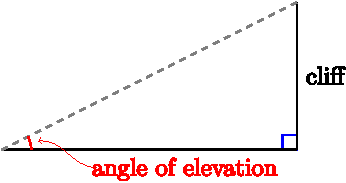
\includegraphics[width=\linewidth]{images/fig-2-2angelev}
\end{sbspanel}%
\end{sidebyside}%
\par
Next we fill in the value of \(\tan 58\degree\), and the lengths of the sides.%
\begin{equation*}
1.6003 = \frac{h}{300}
\end{equation*}
Solving for \(h\) gives%
\begin{equation*}
h = 300(1,6003) = 480.0
\end{equation*}
so the height of the cliff is about 480 feet.%
\end{enumerate}
%
\end{example}
\begin{inlineexercise}{}{g:exercise:idm46051687538112}%
%
\begin{enumerate}[label=\alph*]
\item{}\begin{sidebyside}{2}{0.0625}{0.0625}{0.125}%
\begin{sbspanel}{0.5}[center]%
Use the tangent ratio to find \(x\) in the triangle shown.%
\end{sbspanel}%
\begin{sbspanel}{0.25}[center]%
\resizebox{\linewidth}{!}{%
\tikzset{%
  block/.style    = {draw, thick, rectangle, minimum height = 3em,
    minimum width = 3em},
  sum/.style      = {draw, circle, node distance = 2cm}, % Adder
  input/.style    = {coordinate}, % Input
  output/.style   = {coordinate} % Output
}
\begin{tikzpicture}

\coordinate (A) at (0,0);
\coordinate (B) at (4,0);
\coordinate (C) at (4,1.84);

\draw[blue,thick] (B) rectangle +(-0.25,0.25);
\draw[black,thick] (A)--(B) node[below,midway] {\color{blue}50 ft};
\draw[black,thick] (A)--(C) node[above left,midway] {\color{blue}$c$};
\draw[black,thick] (B)--(C) node[right,midway] {\color{blue}$x$};

\draw [red, thick] (0.7,0) arc(0:24.7:.7) node[right,midway, xshift=3, yshift=2] {\small$24.7\degree$};
\end{tikzpicture}
}%
\end{sbspanel}%
\end{sidebyside}%
%
\item{}Use the sine ratio to find the hypotenuse, \(c\), of the triangle.%
\item{}Use the Pythagorean theorem to find the hypotenuse of the triangle. Do you get the same answer with both methods? Can you explain why the calculations might give (slightly) different answers?%
\end{enumerate}
%
\par\smallskip%
\noindent\textbf{\blocktitlefont Answer}.\label{g:answer:idm46051702046688}{}\hypertarget{g:answer:idm46051702046688}{}\quad{}%
\begin{enumerate}[label=\alph*]
\item{}\(x = 23\) ft%
\item{}\(c = 55\) ft%
\item{}The answers agree when rounded to units. Rounding during calculation can cause the results to differ.%
\end{enumerate}
%
\end{inlineexercise}
The third trigonometric ratio, called the \terminology{cosine}, is the ratio of the side adjacent to an angle and the hypotenuse of the triangle.%
\begin{definition}{Cosine of an Acute Angle.}{g:definition:idm46051687575216}%
\index{cos \(\theta\)}%
\index{cos \(\theta\)|seealso{cosine}}%
\index{cosine}%
\begin{sidebyside}{2}{0}{0.25}{0}%
\begin{sbspanel}{0.5}[center]%
\(\qquad\cos \theta = \dfrac{\text{adjacent}}{\text{hypotenuse}}\)%
\end{sbspanel}%
\begin{sbspanel}{0.25}[center]%
\resizebox{\linewidth}{!}{%
\tikzset{%
  block/.style    = {draw, thick, rectangle, minimum height = 3em,
    minimum width = 3em},
  sum/.style      = {draw, circle, node distance = 2cm}, % Adder
  input/.style    = {coordinate}, % Input
  output/.style   = {coordinate} % Output
}
\begin{tikzpicture}

\coordinate (A) at (0,0);
\coordinate (B) at (4.2,0);
\coordinate (C) at (4.2,2);

\draw[blue,thick] (B) rectangle +(-0.25,0.25);
\draw[black,thick] (A)--(B) node[below,midway] {adjacent};
\draw[black,thick] (A)--(C) node[above left,midway, xshift=6] {hypotenuse};
\draw[black,thick] (B)--(C);

\draw [red, thick] (0.7,0) arc(0:{atan(2/4.2)}:.7) node[right,midway, xshift=3, yshift=2] {$\theta$};
\end{tikzpicture}
}%
\end{sbspanel}%
\end{sidebyside}%
\end{definition}
\begin{example}{}{g:example:idm46051700838512}%
\begin{sidebyside}{2}{0.05}{0.05}{0.08}%
\begin{sbspanel}{0.6}[center]%
Find  \(\sin \theta,~ \cos \theta\), and \(\tan \theta\) for the triangle shown at right.%
\end{sbspanel}%
\begin{sbspanel}{0.22}[center]%
\resizebox{\linewidth}{!}{%
\tikzset{%
  block/.style    = {draw, thick, rectangle, minimum height = 3em,
    minimum width = 3em},
  sum/.style      = {draw, circle, node distance = 2cm}, % Adder
  input/.style    = {coordinate}, % Input
  output/.style   = {coordinate} % Output
}
\begin{tikzpicture} [scale=.8]

\coordinate (A) at (0,0);
\coordinate (B) at (4,0);
\coordinate (C) at (0,-3);

\draw[blue,thick] (A) rectangle +(0.25,-0.25);
\draw[black,thick] (A)--(B) node[above,midway] {\color{blue}8 in};
\draw[black,thick] (A)--(C) node[left,midway] {\color{blue}6 in};
\draw[black,thick] (B)--(C);

\draw [red, thick] (0,-2.6) arc(90:{atan(.75)}:.4) node[above right,midway, xshift=-2, yshift=0] {$\theta$};
\end{tikzpicture}
}%
\end{sbspanel}%
\end{sidebyside}%
\par\smallskip%
\noindent\textbf{\blocktitlefont Solution}.\label{g:solution:idm46051692458304}{}\hypertarget{g:solution:idm46051692458304}{}\quad{}First, we use the Pythagorean theorem to find the hypotenuse, \(c\).%
\begin{align*}
c^2 \amp =6^2 + 8^2\\
c^2 \amp = 536=84 = 100 \amp\amp \blert{\text{Take square roots.}}\\
c \amp =  \sqrt{100} = 10
\end{align*}
For the angle \(\theta\), the opposite side is 8 inches long, and the adjacent side is 6 inches long, as shown in the figure. Thus,%
\begin{align*}
\sin \theta \amp = \dfrac{\text{opposite}}{\text{hypotenuse}} = \frac{8}{10}~~  \text{or}~~ 0.8\\
\cos \theta \amp = \dfrac{\text{adjacent}}{\text{hypotenuse}} = \frac{6}{10} ~~ \text{or}~~ 0.6\\
\tan \theta \amp =  \dfrac{\text{opposite}}{\text{adjacent}}  = \frac{8}{6} ~~ \text{or}~~1.\overline{3}
\end{align*}
%
\end{example}
\begin{inlineexercise}{}{g:exercise:idm46051687619376}%
%
\begin{enumerate}[label=\alph*]
\item{}Use your calculator to complete the table. Rounding the values of sine and cosine to four decimal places.%
\begin{sidebyside}{1}{0}{0}{0}%
\begin{sbspanel}{1}%
{\centering%
{\tabularfont%
\begin{tabular}{AlAlAlAlAlAlAlAlAlAlAlA}\hrulethick
\(\theta\)&\(~~0 \degree\)&\(~10 \degree\)&\(~20 \degree\)&\(~30 \degree\)&\(~40 \degree\)&\(~50 \degree\)&\(~60 \degree\)&\(~70 \degree\)&\(~80 \degree\)&\(~90 \degree\)\tabularnewline\hrulethin
\(\sin \theta\)&\(~~~\)&\(~~~\)&\(~~~\)&\(~~~\)&\(~~~\)&\(~~~\)&\(~~~\)&\(~~~\)&\(~~~\)&\(~~~\)\tabularnewline\hrulethin
\(\cos \theta\)&\(~~~\)&\(~~~\)&\(~~~\)&\(~~~\)&\(~~~\)&\(~~~\)&\(~~~\)&\(~~~\)&\(~~~\)&\(~~~\)\tabularnewline\hrulethin
\end{tabular}
}%
\par}
\end{sbspanel}%
\end{sidebyside}%
\item{}What do you notice about the values of sine and cosine? Can you explain why this is true? (Hint:  If one (non-right) angle of a right triangle measures \(x\) degrees, how big is the other angle? Now sketch the triangle and label the opposite and adjacent sides for each angle.)%
\end{enumerate}
%
\par\smallskip%
\noindent\textbf{\blocktitlefont Answer}.\label{g:answer:idm46051688190656}{}\hypertarget{g:answer:idm46051688190656}{}\quad{}%
\begin{enumerate}[label=\alph*]
\item{}\begin{sidebyside}{1}{0}{0}{0}%
\begin{sbspanel}{1}%
{\centering%
{\tabularfont%
\begin{tabular}{AcAcAcAcAcAcAcAcAcAcAcA}\hrulethick
\(\small \theta\)&\(\small 0 \degree\)&\(\small 10 \degree\)&\(\small 20 \degree\)&\(\small 30 \degree\)&\(\small 40 \degree\)&\(\small 50 \degree\)&\(\small 60 \degree\)&\(\small 70 \degree\)&\(\small 80 \degree\)&\(\small 90 \degree\)\tabularnewline\hrulethin
\(\small \sin \theta\)&\(\small 0\)&\(\small 0.1737\)&\(\small 0.3420\)&\(\small 0.5\)&\(\small 0.6428\)&\(\small 0.7660\)&\(\small 0.8660\)&\(\small 0.9397\)&\(\small 0.9848\)&\(\small 1\)\tabularnewline\hrulethin
\(\small \cos \theta\)&\(\small 1\)&\(\small 0.9848\)&\(\small 0.9397\)&\(\small 0.8660\)&\(\small 0.7660\)&\(\small 0.6428\)&\(\small 0.5\)&\(\small 0.3420\)&\(\small 0.1737\)&\(\small 0\)\tabularnewline\hrulethin
\end{tabular}
}%
\par}
\end{sbspanel}%
\end{sidebyside}%
%
\item{}The cosine of \(\theta\) is equal to the sine of the complement of \(\theta\), or \(\cos \theta = \sin (90-\theta)\).%
\end{enumerate}
%
\end{inlineexercise}
\begin{note}{}{g:note:idm46051688438672}%
In the previous exercise, you should also notice that as the angle \(\theta\) increases, \(\sin \theta\) increases but \(\cos \theta\) decreases.%
\par
You can see why this is true in the figure below.  In each right triangle, the hypotenuse has the same length.  But as the angle increases, the opposite side gets longer and the adjacent side gets shorter.%
\begin{sidebyside}{1}{0.275}{0.275}{0}%
\begin{sbspanel}{0.45}%
\resizebox{\linewidth}{!}{%
\tikzset{%
  block/.style    = {draw, thick, rectangle, minimum height = 3em,
    minimum width = 3em},
  sum/.style      = {draw, circle, node distance = 2cm}, % Adder
  input/.style    = {coordinate}, % Input
  output/.style   = {coordinate} % Output
}
\begin{tikzpicture} 

\coordinate (A) at (0,0);
\coordinate (B) at (2.82,0);
\coordinate (C) at (2.82,1.03);

\draw[blue,thick] (B) rectangle +(-0.25,0.25);
\draw[black,thick] (A)--(B)--(C)--cycle;
\draw [red, thick] (.6,0) arc(0:20:.6) node[right,midway, xshift=5, yshift=2] {$20\degree$};

\draw[blue,thick] (5.4,0) rectangle +(-0.25,0.25);
\draw[black,thick] (3.1,0)--(5.4,0)--(5.4,1.93)--cycle;
\draw [red, thick] (3.6,0) arc(0:40:.5) node[right,midway, yshift=2] {$40\degree$};

\draw[blue,thick] (7.2,0) rectangle +(-0.25,0.25);
\draw[black,thick] (5.7,0)--(7.2,0)--(7.2,2.6)--cycle;
\draw [red, thick] (6.1,0) arc(0:60:.4) node[right,midway, yshift=2] {$60\degree$};
\end{tikzpicture}
}%
\end{sbspanel}%
\end{sidebyside}%
\end{note}
\end{subsectionptx}
%
%
\typeout{************************************************}
\typeout{Subsection  The Three Trigonometric Ratios}
\typeout{************************************************}
%
\begin{subsectionptx}{The Three Trigonometric Ratios}{}{The Three Trigonometric Ratios}{}{}{g:subsection:idm46051688532784}
Here is a summary of the three trigonometric ratios we have discussed.%
\begin{assemblage}{Trigonometric Ratios.}{g:assemblage:idm46051688540064}%
If \(\theta\)  is one of the angles in a right triangle,%
\begin{sidebyside}{2}{0}{0.1}{0.04}%
\begin{sbspanel}{0.5}[center]%
%
\begin{align*}
\sin \theta \amp = \dfrac{\text{opposite}}{\text{hypotenuse}}\\
\cos \theta \amp = \dfrac{\text{adjacent}}{\text{hypotenuse}}\\
\tan \theta \amp =  \dfrac{\text{opposite}}{\text{adjacent}}
\end{align*}
%
\end{sbspanel}%
\begin{sbspanel}{0.36}[center]%
\resizebox{\linewidth}{!}{%
\tikzset{%
  block/.style    = {draw, thick, rectangle, minimum height = 3em,
    minimum width = 3em},
  sum/.style      = {draw, circle, node distance = 2cm}, % Adder
  input/.style    = {coordinate}, % Input
  output/.style   = {coordinate} % Output
}
\begin{tikzpicture}

\coordinate (A) at (0,0);
\coordinate (B) at (4.2,0);
\coordinate (C) at (4.2,2);

\draw[blue,thick] (B) rectangle +(-0.25,0.25);
\draw[black,thick] (A)--(B) node[below,midway] {adjacent};
\draw[black,thick] (A)--(C) node[above left,midway, xshift=6] {hypotenuse};
\draw[black,thick] (B)--(C) node[right,midway] {opposite};

\draw [red, thick] (0.7,0) arc(0:{atan(2/4.2)}:.7) node[right,midway, xshift=3, yshift=2] {$\theta$};
\end{tikzpicture}
}%
\end{sbspanel}%
\end{sidebyside}%
\end{assemblage}
These three definitions are the foundation for all the rest of trigonometry.  \terminology{You must memorize them immediately!!}%
\par
You must also be careful to apply these definitions of the trigonometric ratios \emph{only} to right triangles. In the next example, we create a right triangle by drawing an extra line.%
\begin{example}{}{g:example:idm46051701086208}%
The vertex angle of an isosceles triangle is \(34 \degree\), and the equal sides are 16 meters long. Find the altitude of the triangle.%
\par\smallskip%
\noindent\textbf{\blocktitlefont Solution}.\label{g:solution:idm46051701891760}{}\hypertarget{g:solution:idm46051701891760}{}\quad{}\begin{sidebyside}{2}{0}{0.05}{0.05}%
\begin{sbspanel}{0.7}%
The triangle described is not a right triangle. However, the altitude of an isosceles triangle bisects the vertex angle and divides the triangle into two congruent right triangles, as shown in the figure. The 16-meter side becomes the hypotenuse of the right triangle, and the altitude, \(h\), of original triangle is the side adjacent to the \(17\degree\) angle.%
\end{sbspanel}%
\begin{sbspanel}{0.2}%
\resizebox{\linewidth}{!}{%
\tikzset{%
  block/.style    = {draw, thick, rectangle, minimum height = 3em,
    minimum width = 3em},
  sum/.style      = {draw, circle, node distance = 2cm}, % Adder
  input/.style    = {coordinate}, % Input
  output/.style   = {coordinate} % Output
}
\begin{tikzpicture}

\coordinate (A) at (0,0);
\coordinate (B) at (-1.17,0);
\coordinate (C) at (0,3.8);
\coordinate (D) at (1.17,0);

\draw[blue,thick] (A) rectangle +(0.25,0.25);
\draw[black,thick] (D)--(B)--(A) ;
\draw[gray,thick] (C)--(A) node[left,midway, yshift=-10] {\color{blue}$h$};
\draw[black,thick] (B)--(C) node[above left,midway, yshift=-4] {\color{blue}16 m};
\draw[black,thick] (D)--(C) node[above right,midway, yshift=-4] {\color{blue}16 m};

\draw [red, thick] (0,2.3) arc(-90:{-atan(3.8/1.17)}:1.5) node[below,midway, xshift=1, yshift=-4] {\small$17\degree$};
\end{tikzpicture}
}%
\end{sbspanel}%
\end{sidebyside}%
\par
Which of the three trig ratios is helpful in this problem?  The cosine is the ratio that relates the hypotenuse and the adjacent side, so we'll begin with the equation%
\begin{equation*}
\cos 17\degree =\dfrac{\text{adjacent}}{\text{hypotenuse}}
\end{equation*}
We use a calculator to find \(\cos 17\degree\) and fill in the lengths of the sides.%
\begin{equation*}
0.9563 = \dfrac {h}{16}
\end{equation*}
Solving for \(h\) gives%
\begin{equation*}
h = 16(0.9563) = 15.3008
\end{equation*}
The altitude of the triangle is about 15.3 meters long.%
\end{example}
\begin{inlineexercise}{}{g:exercise:idm46051701997248}%
Another isosceles triangle has base angles of \(72\degree\) and equal sides of length 6.8 centimeters.  Find the length of the base.%
\par\smallskip%
\noindent\textbf{\blocktitlefont Answer}.\label{g:answer:idm46051692292704}{}\hypertarget{g:answer:idm46051692292704}{}\quad{}4 cm%
\end{inlineexercise}
Review the following skills you will need for this section.%
\begin{project}{}{g:project:idm46051702549872}%
\begin{sidebyside}{1}{0}{0}{0}%
\begin{sbspanel}{1}%
Write two more ratios equivalent to the given fraction.%
\end{sbspanel}%
\end{sidebyside}%
\begin{sidebyside}{4}{0}{0}{0}%
\begin{sbspanel}{0.25}%
1. \(\:\dfrac{10}{4}\)%
\end{sbspanel}%
\begin{sbspanel}{0.25}%
\par
2. \(\:\dfrac{6}{8}\)%
\end{sbspanel}%
\begin{sbspanel}{0.25}%
\par
3. \(\:0.6\)%
\end{sbspanel}%
\begin{sbspanel}{0.25}%
\par
4. \(\:1.5\)%
\end{sbspanel}%
\end{sidebyside}%
\begin{sidebyside}{1}{0}{0}{0}%
\begin{sbspanel}{1}%
Compute the slope of the line.%
\end{sbspanel}%
\end{sidebyside}%
\begin{sidebyside}{4}{0}{0}{0.0666666666666667}%
\begin{sbspanel}{0.05}%
5.%
\end{sbspanel}%
\begin{sbspanel}{0.35}%
\resizebox{\linewidth}{!}{%
\tikzset{%
}
\begin{tikzpicture}[scale=.4]

\draw[thick,->] (-5,0) -- (7,0) node[anchor=west] {$x$};
\draw[thick,->] (0,-3) -- (0,3) node[anchor=south] {$y$};
`
\foreach \x in {-5,...,6}
    \draw (\x cm,5pt) -- (\x cm,-5pt) ;
\foreach \y in {-3,...,2}
    \draw (5pt,\y cm) -- (-5pt,\y cm)  ;

\coordinate (A) at (-5,-2);
\coordinate (B) at (5,2);
\coordinate (C) at (7,2.8);
\coordinate (O) at (0,0);

\draw[blue, thick] (A)--(C);

\filldraw[red] (B) circle (5pt) node[anchor=south east,xshift=0,yshift=0] {$(5,2)$};
\filldraw[red] (O) circle (5pt) ;
\end{tikzpicture}
}%
\end{sbspanel}%
\begin{sbspanel}{0.05}%
6.%
\end{sbspanel}%
\begin{sbspanel}{0.35}%
\resizebox{\linewidth}{!}{%
\tikzset{%
}
\begin{tikzpicture}[xscale=.3, yscale=0.16]

\draw[thick,->] (-9,0) -- (7,0) node[anchor=west] {$x$};
\draw[thick,->] (0,-3) -- (0,11) node[anchor=south] {$y$};
`
\foreach \x in {-9,...,6}
    \draw (\x cm,5pt) -- (\x cm,-5pt) ;
\foreach \y in {-3,...,10}
    \draw (5pt,\y cm) -- (-5pt,\y cm)  ;

\coordinate (A) at (-5,8);
\coordinate (B) at (2,-3.2);
\coordinate (C) at (-7,11.2);
\coordinate (O) at (0,0);

\draw[blue, thick] (B)--(C);

\filldraw[red] (A) ellipse (6pt and 12pt) node[anchor=north east,xshift=0,yshift=0] {$(-5,8)$};
\filldraw[red] (O) ellipse (6pt and 12pt)  ;
\end{tikzpicture}
}%
\end{sbspanel}%
\end{sidebyside}%
\begin{sidebyside}{4}{0}{0}{0.0666666666666667}%
\begin{sbspanel}{0.05}%
7.%
\end{sbspanel}%
\begin{sbspanel}{0.35}%
\resizebox{\linewidth}{!}{%
\tikzset{%
}
\begin{tikzpicture}[xscale=.48, yscale=0.32]

\draw[thick,->] (-6,0) -- (6,0) node[anchor=west] {$x$};
\draw[thick,->] (0,-6) -- (0,6) node[anchor=south] {$y$};
`
\foreach \x in {-6,...,5}
    \draw (\x cm,5pt) -- (\x cm,-5pt) ;
\foreach \y in {-6,...,5}
    \draw (5pt,\y cm) -- (-5pt,\y cm)  ;

\coordinate (A) at (-2,3);
\coordinate (B) at (-4,5.4);
\coordinate (C) at (5,-5.4);
\coordinate (O) at (3,-3);

\draw[blue, thick] (B)--(C);

\filldraw[red] (A) ellipse (6pt and 9pt) node[anchor=north east,yshift=2] {$(-2,3)$};
\filldraw[red] (O) ellipse (6pt and 9pt)  node[anchor=south west,yshift=-5] {$(3,-3)$};
\end{tikzpicture}
}%
\end{sbspanel}%
\begin{sbspanel}{0.05}%
8.%
\end{sbspanel}%
\begin{sbspanel}{0.35}%
\resizebox{\linewidth}{!}{%
\tikzset{%
}
\begin{tikzpicture}[xscale=.33, yscale=0.22]

\draw[thick,->] (-6,0) -- (10,0) node[anchor=west] {$x$};
\draw[thick,->] (0,-7) -- (0,4) node[anchor=south] {$y$};

\foreach \x in {-6,...,9}
    \draw (\x cm,9pt) -- (\x cm,-9pt) ;
\foreach \y in {-7,...,3}
    \draw (5pt,\y cm) -- (-5pt,\y cm)  ;

\coordinate (A) at (-4,-5);
\coordinate (B) at (-6,-6);
\coordinate (C) at (10,2);
\coordinate (O) at (4,-1);

\draw[blue, thick] (B)--(C);

\filldraw[red] (A) ellipse (6pt and 9pt) node[anchor=north west,xshift=2,yshift=-2, fill=white] {$(-2,3)$};
\filldraw[red] (O) ellipse (6pt and 9pt)  node[anchor=north west,xshift=-5,yshift=-1] {$(3,-3)$};
\end{tikzpicture}
}%
\end{sbspanel}%
\end{sidebyside}%
\begin{sidebyside}{1}{0}{0}{0}%
\begin{sbspanel}{1}%
Solve.%
\end{sbspanel}%
\end{sidebyside}%
\begin{sidebyside}{2}{0}{0}{0}%
\begin{sbspanel}{0.5}%
9. \(\:\dfrac{12}{x} = 48\)%
\end{sbspanel}%
\begin{sbspanel}{0.5}%
\par
10. \(\:\dfrac{60}{x} = 80\)%
\end{sbspanel}%
\end{sidebyside}%
\begin{sidebyside}{1}{0}{0}{0}%
\begin{sbspanel}{1}%
\(\underline{\qquad\qquad\qquad\qquad}\)%
\end{sbspanel}%
\end{sidebyside}%
\begin{sidebyside}{1}{0}{0}{0}%
\begin{sbspanel}{1}%
Algebra Refresher Answers%
\end{sbspanel}%
\end{sidebyside}%
\par
(Many answers are possible for 1\textendash{}4.)%
\par
%
\begin{multicols}{5}
\begin{enumerate}[label=\arabic*]
\item{}\(\displaystyle \dfrac{5}{2},~~\dfrac{20}{8}\)%
\item{}\(\displaystyle \dfrac{3}{4},~~\dfrac{12}{16}\)%
\item{}\(\displaystyle \dfrac{3}{5},~~\dfrac{12}{20}\)%
\item{}\(\displaystyle \dfrac{6}{4},~~\dfrac{12}{8}\)%
\item{}\(\displaystyle \dfrac{2}{5}\)%
\item{}\(\displaystyle \dfrac{-8}{5}\)%
\item{}\(\displaystyle \dfrac{-6}{5}\)%
\item{}\(\displaystyle \dfrac{1}{2}\)%
\item{}\(\displaystyle \dfrac{1}{4}\)%
\item{}\(\displaystyle \dfrac{3}{4}\)%
\end{enumerate}
\end{multicols}
%
\end{project}
\end{subsectionptx}
%
%
\typeout{************************************************}
\typeout{Subsection  Section 2.2 Summary}
\typeout{************************************************}
%
\begin{subsectionptx}{Section 2.2 Summary}{}{Section 2.2 Summary}{}{}{g:subsection:idm46051691863376}
%
%
\typeout{************************************************}
\typeout{Subsubsection  Vocabulary}
\typeout{************************************************}
%
\begin{subsubsectionptx}{Vocabulary}{}{Vocabulary}{}{}{g:subsubsection:idm46051691864496}
%
\begin{multicols}{3}
\begin{itemize}[label=\textbullet]
\item{}Sine%
\item{}Cosine%
\item{}Tangent%
\item{}Angle of elevation%
\item{}Adjacent side%
\item{}Irrational number%
\end{itemize}
\end{multicols}
%
\end{subsubsectionptx}
%
%
\typeout{************************************************}
\typeout{Subsubsection  Concepts}
\typeout{************************************************}
%
\begin{subsubsectionptx}{Concepts}{}{Concepts}{}{}{g:subsubsection:idm46051691889568}
%
\begin{enumerate}[label=\arabic*]
\item{}By using similar triangles, we can find the unknown sides of a right triangle if we know only \emph{one} side and \emph{one} of the acute angles.%
\item{}\begin{assemblage}{Trigonometric Ratios.}{g:assemblage:idm46051691809360}%
If \(\theta\) is one of the angles in a right triangle,%
\begin{sidebyside}{2}{0}{0}{0}%
\begin{sbspanel}{0.6}[center]%
%
\begin{align*}
\sin \theta \amp = \dfrac{\text{opposite}}{\text{hypotenuse}}\\
\cos \theta \amp = \dfrac{\text{adjacent}}{\text{hypotenuse}}\\
\tan \theta \amp =  \dfrac{\text{opposite}}{\text{adjacent}}
\end{align*}
%
\end{sbspanel}%
\begin{sbspanel}{0.4}[center]%
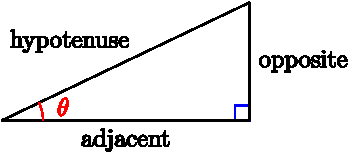
\includegraphics[width=\linewidth]{images/fig-2-2trigratios}
\end{sbspanel}%
\end{sidebyside}%
\end{assemblage}
%
\item{}The trigonometric ratio of an angle \(\theta\) is the same for every right triangle containing the angle.%
\end{enumerate}
%
\end{subsubsectionptx}
%
%
\typeout{************************************************}
\typeout{Subsubsection  Study Questions}
\typeout{************************************************}
%
\begin{subsubsectionptx}{Study Questions}{}{Study Questions}{}{}{g:subsubsection:idm46051691955904}
%
\begin{enumerate}[label=\arabic*]
\item{}Sketch a figure that illustrates why \(\cos 25\degree\) is the same for every right triangle with a \(25\degree\) angle.%
\item{}Sketch a figure that illustrates why \(\cos \theta\) decreases as \(\theta\)  increases from \(0\degree\) to \(90\degree\).%
\item{}Which trigonometric ratio would you use to find the hypotenuse of a right triangle if you knew one acute angle and the side opposite that angle?%
\item{}Does your calculator give you the exact decimal values for the trigonometric ratios of acute angles?%
\end{enumerate}
%
\end{subsubsectionptx}
%
%
\typeout{************************************************}
\typeout{Subsubsection  Skills}
\typeout{************************************************}
%
\begin{subsubsectionptx}{Skills}{}{Skills}{}{}{g:subsubsection:idm46051696044816}
Practice each skill in the Homework Problems listed.%
\par
%
\begin{enumerate}[label=\arabic*]
\item{}Use measurements to calculate the trigonometric ratios for acute angles    \#1-10, 57-60%
\item{}Use trigonometric ratios to find unknown sides of right triangles    \#11-26%
\item{}Solve problems using trigonometric ratios    \#27-34, 41-46%
\item{}Use trig ratios to write equations relating the sides of a right triangle    \#35-40%
\item{}Use relationships among the trigonometric ratios    \#47-56, 61-68%
\end{enumerate}
%
\end{subsubsectionptx}
\end{subsectionptx}
%
%
\typeout{************************************************}
\typeout{Exercises  Homework 2.2}
\typeout{************************************************}
%
\begin{exercises-subsection}{Homework 2.2}{}{Homework 2.2}{}{}{x:exercises:hmwk-2-2}
\begin{divisionexercise}{1}{}{}{g:exercise:idm46051696077072}%
\begin{sidebyside}{2}{0.04}{0.04}{0.08}%
\begin{sbspanel}{0.6}%
Here are two right triangles with a \(65 \degree\) angle.%
\begin{enumerate}[label=\alph*]
\item{}Measure the sides \(AB\) and \(BC\) with a ruler. Use the lengths to estimate \(\sin 65\degree\).%
\item{}Measure the sides \(AD\) and \(DE\) with a ruler. Use the lengths to estimate \(\sin 65\degree\).%
\item{}Use your calculator to look up \(\sin 65\degree\).  Compare your answers. How close were your estimates?%
\end{enumerate}
%
\end{sbspanel}%
\begin{sbspanel}{0.24}%
\resizebox{\linewidth}{!}{%
\tikzset{%
}
\begin{tikzpicture}

\coordinate (A) at (0,0);
\coordinate (B) at (3,6.433);
\coordinate (C) at (3,0);
\coordinate (D) at (2,4.289);
\coordinate (E) at (2,0);

\draw[blue,thick] (C) rectangle +(-.25,.25);
\draw[blue,thick] (E) rectangle +(-.25,.25);
\draw[black, thick] (A)--(B)--(C)--cycle;
\draw[black,thick] (D)--(E);

\draw[red,thick] (0.3,0) arc(0:65:.3) node[right, midway, yshift=2] {$65\degree$};

\filldraw[black] (A) circle (.2pt) node[anchor=north east] {$A$};
\filldraw[black] (B) circle (.2pt) node[anchor=west] {$B$};
\filldraw[black] (C) circle (.2pt) node[anchor=north west] {$C$};
\filldraw[black] (D) circle (.2pt) node[anchor=south east] {$D$};
\filldraw[black] (E) circle (.2pt) node[anchor=north ] {$E$};
\end{tikzpicture}
}%
\end{sbspanel}%
\end{sidebyside}%
\end{divisionexercise}%
\begin{divisionexercise}{2}{}{}{g:exercise:idm46051701136816}%
Use the figure in Problem 1 to calculate two estimates each for the cosine and tangent of \(65 \degree\). Compare your estimates to your calculator's values for \(\cos 65\degree\) and \(\tan 65\degree\).%
\end{divisionexercise}%
\begin{divisionexercise}{3}{}{}{g:exercise:idm46051693301648}%
Here are two right triangles with a \(40 \degree\) angle.%
\begin{sidebyside}{2}{0.025}{0.025}{0.05}%
\begin{sbspanel}{0.5}[center]%
%
\begin{enumerate}[label=\alph*]
\item{}Measure the sides \(AB\) and \(AC\) with a ruler. Use the lengths to estimate \(\cos 40\degree\).%
\item{}Measure the sides \(AD\) and \(AE\) with a ruler. Use the lengths to estimate \(\cos 40\degree\).%
\item{}Use your calculator to look up \(\cos 40\degree\).  Compare your answers. How close were your estimates?%
\end{enumerate}
%
\end{sbspanel}%
\begin{sbspanel}{0.4}[center]%
\resizebox{\linewidth}{!}{%
\tikzset{%
}
\begin{tikzpicture}

\coordinate (A) at (0,0);
\coordinate (B) at (3.5,2.9368);
\coordinate (C) at (3.5,0);
\coordinate (D) at (-2.4,-2.013);
\coordinate (E) at (-2.4,0);

\draw[blue,thick] (C) rectangle +(-.25,.25);
\draw[blue,thick] (E) rectangle +(.25,-.25);
\draw[black, thick] (B)--(C)--(E)--(D)--cycle;

\draw[red,thick] (0.4,0) arc(0:40:.4) node[right, midway, yshift=3] {$40\degree$};

\filldraw[black] (A) circle (.2pt) node[anchor=north ] {$A$};
\filldraw[black] (B) circle (.2pt) node[anchor=west] {$B$};
\filldraw[black] (C) circle (.2pt) node[anchor=north west] {$C$};
\filldraw[black] (D) circle (.2pt) node[anchor= east] {$D$};
\filldraw[black] (E) circle (.2pt) node[anchor=east ] {$E$};
\end{tikzpicture}
}%
\end{sbspanel}%
\end{sidebyside}%
\end{divisionexercise}%
\begin{divisionexercise}{4}{}{}{g:exercise:idm46051701026704}%
Use the figure in Problem 2 to calculate two estimates each for the cosine and tangent of \(40 \degree\). Compare your estimates to your calculator's values for \(\sin 40\degree\) and \(\tan 40\degree\).%
\end{divisionexercise}%
\par\medskip\noindent%
%
For the right triangles in Problems 5\textendash{}10,%
\par
%
\begin{enumerate}[label=\alph*]
\item{}Find the length of the unknown side.%
\item{}Find the sine, cosine, and tangent of \(\theta\). Round your answers to four decimal places.%
\end{enumerate}
%
\begin{exercisegroupcol}{3}
\begin{divisionexerciseegcol}{5}{}{}{g:exercise:idm46051698804912}%
\begin{sidebyside}{1}{0.1}{0.1}{0}%
\begin{sbspanel}{0.8}%
\resizebox{\linewidth}{!}{%
\tikzset{%
}
\begin{tikzpicture}

\coordinate (A) at (0,0);
\coordinate (B) at (3,0);
\coordinate (C) at (0,-2);

\draw[blue,thick] (A) rectangle +(.25,-.25);

\draw[black, thick] (B)--(C) node[below right, midway] {\color{blue}$v$};
\draw[black, thick] (B)--(A) node[above, midway] {\color{blue}$12$};
\draw[black, thick] (A)--(C) node[left, midway] {\color{blue}$8$};

\draw[red,thick] (B)++(-0.6,0) arc(180:{180+atan(2/3)}:.6) node[left, midway, yshift=-3] {$\theta$};
\end{tikzpicture}
}%
\end{sbspanel}%
\end{sidebyside}%
\end{divisionexerciseegcol}%
\begin{divisionexerciseegcol}{6}{}{}{g:exercise:idm46051698854736}%
\begin{sidebyside}{1}{0.3}{0.3}{0}%
\begin{sbspanel}{0.4}%
\resizebox{\linewidth}{!}{%
\tikzset{%
}
\begin{tikzpicture} [scale=1.1]

\coordinate (A) at (0,0);
\coordinate (B) at (1,0);
\coordinate (C) at (0,2);

\draw[blue,thick] (A) rectangle +(.25,.25);

\draw[black, thick] (B)--(C) node[above right, midway] {\color{blue}$z$};
\draw[black, thick] (B)--(A) node[below, midway] {\color{blue}$5$};
\draw[black, thick] (A)--(C) node[left, midway] {\color{blue}$10$};

\draw[red,thick] (B)++(-0.3,0) arc(180:{180-atan(2)}:.3) node[left, midway, yshift=3] {$\theta$};

\end{tikzpicture}
}%
\end{sbspanel}%
\end{sidebyside}%
\end{divisionexerciseegcol}%
\begin{divisionexerciseegcol}{7}{}{}{g:exercise:idm46051698862064}%
\begin{sidebyside}{1}{0.05}{0.05}{0}%
\begin{sbspanel}{0.9}[bottom]%
\resizebox{\linewidth}{!}{%
\tikzset{%
}
\begin{tikzpicture}

\coordinate (A) at (0,0);
\coordinate (B) at (4.2,0);
\coordinate (C) at (0,1);

\draw[blue,thick] (A) rectangle +(.25,.25);

\draw[black, thick] (B)--(C) node[above right, midway] {\color{blue}$16$};
\draw[black, thick] (B)--(A) node[below, midway] {\color{blue}$w$};
\draw[black, thick] (A)--(C) node[left, midway] {\color{blue}$4$};

\draw[red,thick] (C)++(0,-.3) arc(-90:{-atan(1/4.2)}:.3) node[below, midway, xshift=1, yshift=1] {$\theta$};
\end{tikzpicture}
}%
\end{sbspanel}%
\end{sidebyside}%
\end{divisionexerciseegcol}%
\begin{divisionexerciseegcol}{8}{}{}{g:exercise:idm46051698433344}%
\begin{sidebyside}{1}{0.25}{0.25}{0}%
\begin{sbspanel}{0.5}%
\resizebox{\linewidth}{!}{%
\tikzset{%
}
\begin{tikzpicture}

\coordinate (A) at (0,0);
\coordinate (B) at (-1.8,0);
\coordinate (C) at (0,2.6);

\draw[blue,thick] (A) rectangle +(-.25,.25);

\draw[black, thick] (B)--(C) node[above left, midway] {\color{blue}$24$};
\draw[black, thick] (B)--(A) node[below, midway] {\color{blue}$m$};
\draw[black, thick] (A)--(C) node[right, midway] {\color{blue}$20$};

\draw[red,thick] (C)++(0,-.5) arc(270:{180+atan(2.6/1.8)}:.5) node[below, midway, xshift=-1] {$\theta$};
\end{tikzpicture}
}%
\end{sbspanel}%
\end{sidebyside}%
\end{divisionexerciseegcol}%
\begin{divisionexerciseegcol}{9}{}{}{g:exercise:idm46051698431040}%
\begin{sidebyside}{1}{0.05}{0.05}{0}%
\begin{sbspanel}{0.9}%
\resizebox{\linewidth}{!}{%
\tikzset{%
}
\begin{tikzpicture}

\coordinate (A) at (0,0);
\coordinate (B) at (-3,0);
\coordinate (C) at (0,-1.2);

\draw[blue,thick] (A) rectangle +(-.25,-.25);

\draw[black, thick] (B)--(C) node[below left, midway] {\color{blue}$n$};
\draw[black, thick] (B)--(A) node[above, midway] {\color{blue}$16$};
\draw[black, thick] (A)--(C) node[right, midway] {\color{blue}$2\sqrt{3}$};

\draw[red,thick] (B)++(.9,0) arc(0:{-atan(.4)}:.9) node[right, midway, yshift=-1] {$\theta$};
\end{tikzpicture}
}%
\end{sbspanel}%
\end{sidebyside}%
\end{divisionexerciseegcol}%
\begin{divisionexerciseegcol}{10}{}{}{g:exercise:idm46051698473488}%
\begin{sidebyside}{1}{0.15}{0.15}{0}%
\begin{sbspanel}{0.7}%
\resizebox{\linewidth}{!}{%
\tikzset{%
}
\begin{tikzpicture}

\coordinate (A) at (0,0);
\coordinate (B) at (-3,0);
\coordinate (C) at (0,1.8);

\draw[blue,thick] (A) rectangle +(-.25,.25);

\draw[black, thick] (B)--(C) node[above left, midway] {\color{blue}$2\sqrt{5}$};
\draw[black, thick] (B)--(A) node[below, midway] {\color{blue}$\sqrt{7}$};
\draw[black, thick] (A)--(C) node[right, midway] {\color{blue}$d$};

\draw[red,thick] (C)++(0,-0.3) arc(-90:{-180+atan(.6)}:.3) node[below left, midway, xshift=1] {$\theta$};=5=5
\end{tikzpicture}
}%
\end{sbspanel}%
\end{sidebyside}%
\end{divisionexerciseegcol}%
\end{exercisegroupcol}
\par\medskip\noindent
\par\medskip\noindent%
%
For Problems 11\textendash{}16,%
\par
%
\begin{enumerate}[label=\alph*]
\item{}Sketch and label the sides of a right triangle with angle \(\theta\).%
\item{}Sketch and label another right triangle with angle \(\theta\) and longer sides.%
\end{enumerate}
%
\begin{exercisegroupcol}{3}
\begin{divisionexerciseegcol}{11}{}{}{g:exercise:idm46051701402528}%
\(\cos \theta = \dfrac{3}{5}\)%
\end{divisionexerciseegcol}%
\begin{divisionexerciseegcol}{12}{}{}{g:exercise:idm46051695941440}%
\(\tan \theta = \dfrac{7}{2}\)%
\end{divisionexerciseegcol}%
\begin{divisionexerciseegcol}{13}{}{}{g:exercise:idm46051695957216}%
\(\tan \theta = \dfrac{11}{4}\)%
\end{divisionexerciseegcol}%
\begin{divisionexerciseegcol}{14}{}{}{g:exercise:idm46051695976208}%
\(\sin \theta = \dfrac{4}{9}\)%
\end{divisionexerciseegcol}%
\begin{divisionexerciseegcol}{15}{}{}{g:exercise:idm46051698349568}%
\(\sin \theta = \dfrac{1}{9}\)%
\end{divisionexerciseegcol}%
\begin{divisionexerciseegcol}{16}{}{}{g:exercise:idm46051701260048}%
\(\cos \theta = \dfrac{7}{8}\)%
\end{divisionexerciseegcol}%
\end{exercisegroupcol}
\par\medskip\noindent
\par\medskip\noindent%
%
For Problems 17\textendash{}22, use one of the three trigonometric ratios to find the unknown side of the triangle.  Round your answer to hundredths.%
\begin{exercisegroupcol}{3}
\begin{divisionexerciseegcol}{17}{}{}{g:exercise:idm46051698386928}%
\begin{sidebyside}{1}{0.2}{0.2}{0}%
\begin{sbspanel}{0.6}%
\resizebox{\linewidth}{!}{%
\tikzset{%
}
\begin{tikzpicture} [rotate=-75]

\coordinate (A) at (0,0);
\coordinate (B) at (2.8,0);
\coordinate (C) at (0,3);

\draw[blue,thick] (A) rectangle +(.25,.25);

\draw[black, thick] (B)--(C);
\draw[black, thick] (B)--(A) node[ left, midway] {\color{blue}$x$};
\draw[black, thick] (A)--(C) node[above left, midway] {\color{blue}$16$};

\draw[red,thick] (B)++(-0.5,0) arc(180:{180-atan(3/2.8)}:.5) node[above, midway, xshift=3] {$48\degree$};
\end{tikzpicture}
}%
\end{sbspanel}%
\end{sidebyside}%
\end{divisionexerciseegcol}%
\begin{divisionexerciseegcol}{18}{}{}{g:exercise:idm46051701540448}%
\begin{sidebyside}{1}{0.2}{0.2}{0}%
\begin{sbspanel}{0.6}%
\resizebox{\linewidth}{!}{%
\tikzset{%
}
\begin{tikzpicture} [rotate=15]

\coordinate (A) at (0,0);
\coordinate (B) at (2.1,0);
\coordinate (C) at (0,3.5);

\draw[blue,thick] (A) rectangle +(.25,.25);

\draw[black, thick] (B)--(C) node[above right, midway] {\color{blue}$38$};
\draw[black, thick] (B)--(A) node[below right, midway] {\color{blue}$x$};
\draw[black, thick] (A)--(C);

\draw[red,thick] (C)++(0,-0.9) arc(-90:{-atan(3.5/2.1)}:.9) node[below , midway, xshift=5] {$31\degree$};
\end{tikzpicture}
}%
\end{sbspanel}%
\end{sidebyside}%
\end{divisionexerciseegcol}%
\begin{divisionexerciseegcol}{19}{}{}{g:exercise:idm46051701552240}%
\begin{sidebyside}{1}{0.15}{0.15}{0}%
\begin{sbspanel}{0.7}%
\resizebox{\linewidth}{!}{%
\tikzset{%
}
\begin{tikzpicture} [rotate=-130]

\coordinate (A) at (0,0);
\coordinate (B) at (2.25,0);
\coordinate (C) at (0,2.68);

\draw[blue,thick] (A) rectangle +(.25,.25);

\draw[black, thick] (B)--(C) node[below, midway] {\color{blue}$x$};
\draw[black, thick] (B)--(A);
\draw[black, thick] (A)--(C) node[above right, midway] {\color{blue}$29$};

\draw[red,thick] (B)++(-0.4,0) arc(180:{180-atan(2.68/2.25)}:.4) node[right , midway, yshift=2] {$50\degree$};
\end{tikzpicture}
}%
\end{sbspanel}%
\end{sidebyside}%
\end{divisionexerciseegcol}%
\begin{divisionexerciseegcol}{20}{}{}{g:exercise:idm46051701583280}%
\begin{sidebyside}{1}{0.125}{0.125}{0}%
\begin{sbspanel}{0.75}%
\resizebox{\linewidth}{!}{%
\tikzset{%
}
\begin{tikzpicture} [rotate=-135]

\coordinate (A) at (0,0);
\coordinate (B) at (1.82,0);
\coordinate (C) at (0,3.56);

\draw[blue,thick] (A) rectangle +(.25,.25);

\draw[black, thick] (B)--(C) node[below left, midway] {\color{blue}$420$};
\draw[black, thick] (B)--(A) node[above left, midway] {\color{blue}$x$};
\draw[black, thick] (A)--(C);

\draw[red,thick] (B)++(-0.4,0) arc(180:{180-atan(3.56/1.82)}:.4) node[right , midway, yshift=2] {$63\degree$};
\end{tikzpicture}
}%
\end{sbspanel}%
\end{sidebyside}%
\end{divisionexerciseegcol}%
\begin{divisionexerciseegcol}{21}{}{}{g:exercise:idm46051701595984}%
\begin{sidebyside}{1}{0.34}{0.34}{0}%
\begin{sbspanel}{0.32}%
\resizebox{\linewidth}{!}{%
\tikzset{%
}
\begin{tikzpicture} [rotate=15]

\coordinate (C) at (0,0 );
\coordinate (A) at (0,3.4);
\coordinate (B) at (-1.17,0);

\draw[blue,thick] (C) rectangle +(-0.25,.25);
\draw[black,thick] (A)--(B) ;
\draw[black,thick] (C)--(B)  node[below,midway] {\color{blue}$x$};
\draw[black,thick] (A) --(C) node[right,midway, xshift=2, yshift=-3] {\color{blue}$250$};

\draw[red,thick] (A)++(0,-1.2) arc(270:251:1.2) node[ below, midway, xshift=1, yshift=-8] {\footnotesize$19\degree$};

\end{tikzpicture}
}%
\end{sbspanel}%
\end{sidebyside}%
\end{divisionexerciseegcol}%
\begin{divisionexerciseegcol}{22}{}{}{g:exercise:idm46051696412736}%
\begin{sidebyside}{1}{0.125}{0.125}{0}%
\begin{sbspanel}{0.75}%
\resizebox{\linewidth}{!}{%
\tikzset{%
}
\begin{tikzpicture} [rotate=47]

\coordinate (A) at (0,0);
\coordinate (B) at (3.6,0);
\coordinate (C) at (0,1.5);

\draw[blue,thick] (A) rectangle +(.25,.25);

\draw[black, thick] (B)--(C) node[above left, midway] {\color{blue}$x$};
\draw[black, thick] (B)--(A) node[below right, midway] {\color{blue}$3.6$};
\draw[black, thick] (A)--(C);

\draw[red,thick] (C)++(0,-.5) arc(-90:{-atan(1.5/3.6)}:.5) node[right, midway, xshift=0, yshift=0] {$82\degree$};
\end{tikzpicture}
}%
\end{sbspanel}%
\end{sidebyside}%
\end{divisionexerciseegcol}%
\end{exercisegroupcol}
\par\medskip\noindent
\par\medskip\noindent%
%
For Problems 23\textendash{}26, sketch and label a right triangle with the given properties.%
\begin{exercisegroup}
\begin{divisionexerciseeg}{23}{}{}{g:exercise:idm46051696525456}%
One angle is \(40\degree\), the side opposite that angle is 8 inches%
\end{divisionexerciseeg}%
\begin{divisionexerciseeg}{24}{}{}{g:exercise:idm46051693207376}%
One angle is \(65\degree\), the side adjacent to that angle is 30 yards%
\end{divisionexerciseeg}%
\begin{divisionexerciseeg}{25}{}{}{g:exercise:idm46051693228576}%
One angle is \(28\degree\), the hypotenuse is 56 feet%
\end{divisionexerciseeg}%
\begin{divisionexerciseeg}{26}{}{}{g:exercise:idm46051693232928}%
One leg is 15 meters, the hypotenuse is 18 meters%
\end{divisionexerciseeg}%
\end{exercisegroup}
\par\medskip\noindent
\par\medskip\noindent%
%
For Problems 27\textendash{}34,%
\par
%
\begin{enumerate}[label=\alph*]
\item{}Sketch a right triangle that illustrates the situation. Label your sketch with the given information.%
\item{}Choose the appropriate trig ratio and write an equation, then solve the problem.%
\end{enumerate}
%
\begin{exercisegroup}
\begin{divisionexerciseeg}{27}{}{}{g:exercise:idm46051696353552}%
To measure the height of cloud cover, airport controllers fix a searchlight to shine a vertical beam on the clouds. The searchlight is 120 yards from the office. A technician in the office measures the angle of elevation to the light on the cloud cover at \(54.8\degree\). What is the height of the cloud cover?%
\end{divisionexerciseeg}%
\begin{divisionexerciseeg}{28}{}{}{g:exercise:idm46051701649056}%
To measure the distance across a canyon, Evel first sights an interesting rock directly opposite on the other side. He then walks 200 yards down the rim of the canyon and sights the rock again, this time at an angle of \(18.5\degree\) from the canyon rim.  What is the width of the canyon?%
\end{divisionexerciseeg}%
\begin{divisionexerciseeg}{29}{}{}{g:exercise:idm46051701660944}%
A salvage ship is searching for the wreck of a pirate vessel on the ocean floor. Using sonar, they locate the wreck at an angle of depression of \(36.2\degree\). The depth of the ocean at their location is 260 feet. How far should they move so that they are directly above the wrecked vessel?%
\end{divisionexerciseeg}%
\begin{divisionexerciseeg}{30}{}{}{g:exercise:idm46051698344592}%
Ramps for wheelchairs should be no steeper than an angle of \(6\degree\). How much horizontal distance should be allowed for a ramp that rises 5 feet in height?%
\end{divisionexerciseeg}%
\begin{divisionexerciseeg}{31}{}{}{g:exercise:idm46051701675456}%
The radio signal from a weather balloon indicates that it is 1500 meters from a meteorologist on the ground. The angle of elevation to the balloon is \(48\degree\). What is the balloon's altitude?%
\end{divisionexerciseeg}%
\begin{divisionexerciseeg}{32}{}{}{g:exercise:idm46051702361472}%
According to Chinese legend, around 200 BC the general Han Xin used a kite to determine the distance from his location to an enemy palace. He then dug a secret tunnel which emerged inside the palace.  When the kite was directly above the palace, its angle of elevation was \(27\degree\) and the string to the kite was 1850 feet long. How far did Han Xin's troops have to dig?%
\end{divisionexerciseeg}%
\begin{divisionexerciseeg}{33}{}{}{g:exercise:idm46051702162560}%
A cable car on a ski lift traverses a horizontal distance of 1800 meters at an angle of \(38\degree\). How long is the cable?%
\end{divisionexerciseeg}%
\begin{divisionexerciseeg}{34}{}{}{g:exercise:idm46051701343456}%
Zelda is building the loft on her summer cottage. At its central point, the height of the loft is 8 feet, and the pitch of the roof should be \(24\degree\). How long should the rafters be?%
\end{divisionexerciseeg}%
\end{exercisegroup}
\par\medskip\noindent
\par\medskip\noindent%
%
For Problems 35\textendash{}40, use a trig ratio to write an equation for \(x\) in terms of \(\theta\).%
\begin{exercisegroupcol}{3}
\begin{divisionexerciseegcol}{35}{}{}{g:exercise:idm46051701530864}%
\begin{sidebyside}{1}{0.15}{0.15}{0}%
\begin{sbspanel}{0.7}%
\resizebox{\linewidth}{!}{%
\tikzset{%
}
\begin{tikzpicture} 

\coordinate (C) at (0,0 );
\coordinate (A) at (0,-1.1);
\coordinate (B) at (2.8,0);

\draw[blue,thick] (C) rectangle +(0.25,-.25);
\draw[black,thick] (A)--(B) ;
\draw[black,thick] (C)--(B)  node[above,midway] {\color{blue}$82$};
\draw[black,thick] (A) --(C) node[left,midway] {\color{blue}$x$};

\draw[red,thick] (A)++(0,.3) arc(90:{atan(1.1/2.8)}:.3) node[above right, midway, xshift=-3, yshift=-3] {$\theta$};
\end{tikzpicture}
}%
\end{sbspanel}%
\end{sidebyside}%
\end{divisionexerciseegcol}%
\begin{divisionexerciseegcol}{36}{}{}{g:exercise:idm46051688849424}%
\begin{sidebyside}{1}{0.175}{0.175}{0}%
\begin{sbspanel}{0.65}%
\resizebox{\linewidth}{!}{%
\tikzset{%
}
\begin{tikzpicture} [rotate=160]

\coordinate (A) at (0,0);
\coordinate (B) at (3.2,0);
\coordinate (C) at (0,1.6);

\draw[blue,thick] (A) rectangle +(.25,.25);

\draw[black, thick] (B)--(C) node[below left, midway] {\color{blue}$9$};
\draw[black, thick] (B)--(A) node[above right, midway] {\color{blue}$x$};
\draw[black, thick] (A)--(C) ;

\draw[red,thick] (B)++(-.7,0) arc(180:{180-atan(1/2)}:.7) node[below right, midway, xshift=2, yshift=2] {$\theta$};
\end{tikzpicture}
}%
\end{sbspanel}%
\end{sidebyside}%
\end{divisionexerciseegcol}%
\begin{divisionexerciseegcol}{37}{}{}{g:exercise:idm46051688881872}%
\begin{sidebyside}{1}{0.1}{0.1}{0}%
\begin{sbspanel}{0.8}%
\resizebox{\linewidth}{!}{%
\tikzset{%
}
\begin{tikzpicture} [rotate=-110]

\coordinate (C) at (0,0 );
\coordinate (A) at (0,3);
\coordinate (B) at (1.5,0);

\draw[blue,thick] (C) rectangle +(0.25,.25);
\draw[black,thick] (A)--(B) node[below,midway] {\color{blue}$11$} ;
\draw[black,thick] (C)--(B)  node[above left,midway] {\color{blue}$x$};
\draw[black,thick] (A) --(C);

\draw[red,thick] (A)++(0,-.5) arc(-90:{-atan(3/1.5)}:.5) node[left, midway, xshift=-5, yshift=1] {$\theta$};
\end{tikzpicture}
}%
\end{sbspanel}%
\end{sidebyside}%
\end{divisionexerciseegcol}%
\begin{divisionexerciseegcol}{38}{}{}{g:exercise:idm46051688915424}%
\begin{sidebyside}{1}{0.125}{0.125}{0}%
\begin{sbspanel}{0.75}%
\resizebox{\linewidth}{!}{%
\tikzset{%
}
\begin{tikzpicture} [rotate=23.199]

\coordinate (A) at (0,0);
\coordinate (B) at (2.8,0);
\coordinate (C) at (0,1.2);

\draw[blue,thick] (A) rectangle +(.25,.25);

\draw[black, thick] (B)--(C) ;
\draw[black, thick] (B)--(A) node[ below, midway] {\color{blue}$47$};
\draw[black, thick] (A)--(C) node[left , midway] {\color{blue}$x$};

\draw[red,thick] (B)++(-.8,0) arc(180:{180-atan(1.2/2.8)}:.8) node[left, midway, xshift=-1, yshift=-2] {$\theta$};
\end{tikzpicture}
}%
\end{sbspanel}%
\end{sidebyside}%
\end{divisionexerciseegcol}%
\begin{divisionexerciseegcol}{39}{}{}{g:exercise:idm46051688941072}%
\begin{sidebyside}{1}{0.15}{0.15}{0}%
\begin{sbspanel}{0.7}%
\resizebox{\linewidth}{!}{%
\tikzset{%
}
\begin{tikzpicture} [rotate=25.7]

\coordinate (C) at (0,0 );
\coordinate (A) at (0,-1.3);
\coordinate (B) at (-2.7,0);

\draw[blue,thick] (C) rectangle +(-0.25,-.25);
\draw[black,thick] (A)--(B)   node[below,midway] {\color{blue}$x$};
\draw[black,thick] (C)--(B);
\draw[black,thick] (A) --(C)node[right,midway,yshift=2] {\color{blue}$9$} ;

\draw[red,thick] (A)++(0,.3) arc(90:{180-atan(1.3/2.7)}:.3) node[left, midway, xshift=0, yshift=3] {$\theta$};
\end{tikzpicture}
}%
\end{sbspanel}%
\end{sidebyside}%
\end{divisionexerciseegcol}%
\begin{divisionexerciseegcol}{40}{}{}{g:exercise:idm46051688971408}%
\begin{sidebyside}{1}{0.115}{0.115}{0}%
\begin{sbspanel}{0.77}%
\resizebox{\linewidth}{!}{%
\tikzset{%
}
\begin{tikzpicture} [rotate=-15]

\coordinate (C) at (0,0 );
\coordinate (A) at (0,1.3);
\coordinate (B) at (-3.3,0);

\draw[blue,thick] (C) rectangle +(-0.25,.25);
\draw[black,thick] (A)--(B)   node[above,midway] {\color{blue}$x$};
\draw[black,thick] (C)--(B)node[below,midway,yshift=0] {\color{blue}$6$} ;
\draw[black,thick] (A) --(C);

\draw[red,thick] (A)++(0,-.3) arc(270:{180+atan(1.3/3.3)}:.3) node[below left, midway, xshift=0, yshift=3] {$\theta$};
\end{tikzpicture}
}%
\end{sbspanel}%
\end{sidebyside}%
\end{divisionexerciseegcol}%
\end{exercisegroupcol}
\par\medskip\noindent
\par\medskip\noindent%
%
For Problems 41\textendash{}44, find the altitude of the triangle. Round your answer to two decimal places.%
\begin{exercisegroupcol}{2}
\begin{divisionexerciseegcol}{41}{}{}{g:exercise:idm46051688997184}%
\begin{sidebyside}{1}{0.225}{0.225}{0}%
\begin{sbspanel}{0.55}%
\resizebox{\linewidth}{!}{%
\tikzset{%
}
\begin{tikzpicture} 

\coordinate (A) at (0,0);
\coordinate (B) at (2.7189,0);
\coordinate (C) at (2.7189,1.2679);
\coordinate (D) at (3.7189,0);

\draw[blue,thick] (B) rectangle +(-.25,.25);

\draw[black, thick] (A)--(C)  node[above, midway, xshift=-2] {\color{blue}$36$};
\draw[black, thick] (C)--(D)--(A);
\draw[gray, thick, dashed] (B)--(C) node[right , midway, xshift=-1, yshift=-2] {\color{blue}$h$};

\draw[red,thick] (A)++(.6,0) arc(0:25:.6) node[right, midway, xshift=1, yshift=2] {$25\degree$};
\end{tikzpicture}
}%
\end{sbspanel}%
\end{sidebyside}%
\end{divisionexerciseegcol}%
\begin{divisionexerciseegcol}{42}{}{}{g:exercise:idm46051689018256}%
\begin{sidebyside}{1}{0.275}{0.275}{0}%
\begin{sbspanel}{0.45}%
\resizebox{\linewidth}{!}{%
\tikzset{%
}
\begin{tikzpicture} 

\coordinate (A) at (0,0);
\coordinate (B) at (3.135,0);
\coordinate (C) at (2,2.228);
\coordinate (D) at (2,0);

\draw[blue,thick] (D) rectangle +(-.25,.25);

\draw[black, thick] (B)--(C)  node[right, midway] {\color{blue}$14$};
\draw[black, thick] (B)--(A)--(C);
\draw[gray, thick, dashed] (D)--(C) node[left , midway, xshift=1, yshift=-4] {\color{blue}$h$};

\draw[red,thick] (B)++(-.3,0) arc(180:117:.3) node[above left, midway, xshift=1, yshift=-2] {$63\degree$};
\end{tikzpicture}
}%
\end{sbspanel}%
\end{sidebyside}%
\end{divisionexerciseegcol}%
\begin{divisionexerciseegcol}{43}{}{}{g:exercise:idm46051689023680}%
\begin{sidebyside}{1}{0.25}{0.25}{0}%
\begin{sbspanel}{0.5}%
\resizebox{\linewidth}{!}{%
\tikzset{%
}
\begin{tikzpicture}

\coordinate (A) at (0,0 );
\coordinate (C) at (3.289,1.197);
\coordinate (B) at (3.289,0);
\coordinate (D) at (1.6,0);

\draw[blue,thick] (B) rectangle +(-0.25,.25);
\draw[black,thick] (A)--(D) --(C);
\draw[black,thick] (C)--(A)node[above left,midway,yshift=0] {\color{blue}$46$} ;
\draw[gray,thick,dashed] (D)--(B);
\draw[gray,thick,dashed] (B) --(C)  node[right,midway,xshift=-1] {\color{blue}$h$};

\draw[red,thick] (A)++(0.7,0) arc(0:20:.7) node[right, midway, xshift=3, yshift=2] {\small$20\degree$};
\end{tikzpicture}
}%
\end{sbspanel}%
\end{sidebyside}%
\end{divisionexerciseegcol}%
\begin{divisionexerciseegcol}{44}{}{}{g:exercise:idm46051689070624}%
\begin{sidebyside}{1}{0.25}{0.25}{0}%
\begin{sbspanel}{0.5}%
\resizebox{\linewidth}{!}{%
\tikzset{%
}
\begin{tikzpicture}

\coordinate (A) at (0,0 );
\coordinate (C) at (-.803,1.722);
\coordinate (B) at (-.803,0);
\coordinate (D) at (2.5,0);

\draw[blue,thick] (B) rectangle +(0.25,.25);
\draw[black,thick] (A)--(D) --(C);
\draw[black,thick] (C)--(A) node[right,midway,yshift=0] {\color{blue}$9$} ;
\draw[gray,thick,dashed] (D)--(B);
\draw[gray,thick,dashed] (B) --(C)  node[left,midway,xshift=0] {\color{blue}$h$};

\draw[red,thick] (A)++(0.3,0) arc(0:115:.3) node[right, midway, xshift=0, yshift=3] {$115\degree$};
\end{tikzpicture}
}%
\end{sbspanel}%
\end{sidebyside}%
\end{divisionexerciseegcol}%
\end{exercisegroupcol}
\par\medskip\noindent
\par\medskip\noindent%
%
For Problems 45 and 46, find the length of the chord \(AB\). Round your answer to two decimal places.%
\begin{exercisegroupcol}{2}
\begin{divisionexerciseegcol}{45}{}{}{g:exercise:idm46051689091568}%
\begin{sidebyside}{1}{0.25}{0.25}{0}%
\begin{sbspanel}{0.5}%
\resizebox{\linewidth}{!}{%
\tikzset{%
}
\begin{tikzpicture}

\coordinate(O) at (0,0);
\coordinate (A) at (0.278,1.576 );
\coordinate (B) at (1.6,0 );
\coordinate (C) at (0.939,0.788);
\coordinate (D) at (1.226,1.028);

\draw (0,0) circle (1.6);

\draw[thick, blue] (C)++(-.1878,-.1576)--++(-.1576,.1878)--++(.1878,.1576);

\filldraw[black] (A) circle (.4pt) node[anchor=south, xshift=0, yshift=0]{\color{black}$A$};
\filldraw[black] (B) circle (.4pt) node[anchor=west, xshift=0, yshift=0]{\color{black}$B$};
\filldraw[black] (O) circle (.4pt) node[anchor=north east, xshift=0, yshift=0]{\color{black}$O$};
\draw[gray,thick] (A)--(O)--(D);
\draw[gray,thick] (O)--(B) node[below,midway] {\color{blue}6};
\draw[black,thick] (B)--(A);

\draw[red,thick] (0.4,0) arc(0:40:0.4) node[right, midway, yshift=2] {\small$40\degree$};
\end{tikzpicture}
}%
\end{sbspanel}%
\end{sidebyside}%
\end{divisionexerciseegcol}%
\begin{divisionexerciseegcol}{46}{}{}{g:exercise:idm46051678100512}%
\begin{sidebyside}{1}{0.225}{0.225}{0}%
\begin{sbspanel}{0.55}%
\resizebox{\linewidth}{!}{%
\tikzset{%
}
\begin{tikzpicture}

\coordinate(O) at (0,0);
\coordinate (A) at (-1.3856,0.8 );
\coordinate (B) at (1.6,0 );
\coordinate (C) at (0.1072,0.4);
\coordinate (D) at (0.414,1.545);

\draw (0,0) circle (1.6);

\draw[thick, blue] (C)++(0.05175,0.193125)--++(.193125,-0.05175)--++(-0.05175,-0.193125);

\filldraw[black] (A) circle (.4pt) node[anchor=south east, xshift=0, yshift=0]{\color{black}$A$};
\filldraw[black] (B) circle (.4pt) node[anchor=west, xshift=0, yshift=0]{\color{black}$B$};
\filldraw[black] (O) circle (.4pt) node[anchor=north east, xshift=0, yshift=0]{\color{black}$O$};
\draw[gray,thick] (B)--(O)--(D);
\draw[gray,thick] (O)--(A) node[below left,midway] {\color{blue}8};
\draw[black,thick] (B)--(A);

\draw[red,thick] (B)++(-0.6,0) arc(180:165:0.6) node[above, yshift=0] {\small$15\degree$};
\end{tikzpicture}
}%
\end{sbspanel}%
\end{sidebyside}%
\end{divisionexerciseegcol}%
\end{exercisegroupcol}
\par\medskip\noindent
\par\medskip\noindent%
%
For Problems 47\textendash{}50, fill in the table.%
\begin{exercisegroupcol}{2}
\begin{divisionexerciseegcol}{47}{}{}{g:exercise:idm46051702034928}%
\begin{sidebyside}{1}{0.275}{0.275}{0}%
\begin{sbspanel}{0.45}%
\resizebox{\linewidth}{!}{%
\tikzset{%
}
\begin{tikzpicture}

\coordinate (A) at (0,0 );
\coordinate (B) at (2.8,0 );
\coordinate (C) at (0,2.1);

\draw[thick, blue] (A) rectangle (.25,.25);

\draw[black,thick] (B)--(A) node[below, midway] {\color{blue}4};
\draw[black,thick] (B)--(C) node[above right, midway] {\color{blue}5};
\draw[black,thick] (C)--(A) node[left, midway] {\color{blue}3};

\draw[red,thick] (B)++(-0.4,0) arc(180:{180-atan(3/4)}:0.4) node[left,midway, yshift=2] {$\theta$};
\draw[red,thick] (C)++(0,-0.3) arc(-90:{-atan(3/4)}:0.3) node[below, xshift=0] {$\phi$};
\end{tikzpicture}
}%
\end{sbspanel}%
\end{sidebyside}%
\begin{sidebyside}{1}{0}{0}{0}%
\begin{sbspanel}{1}%
{\centering%
{\tabularfont%
\begin{tabular}{AlAlAlAlA}\hrulethick
\(~~~~\)&sin&cos&tan\tabularnewline\hrulethin
\(\theta\)&\(~~~~\)&\(~~~~\)&\(~~~~\)\tabularnewline\hrulethin
\(\phi\)&\(~~~~\)&\(~~~~\)&\(~~~~\)\tabularnewline\hrulethin
\end{tabular}
}%
\par}
\end{sbspanel}%
\end{sidebyside}%
\end{divisionexerciseegcol}%
\begin{divisionexerciseegcol}{48}{}{}{g:exercise:idm46051689220176}%
\begin{sidebyside}{1}{0.375}{0.375}{0}%
\begin{sbspanel}{0.25}%
\resizebox{\linewidth}{!}{%
\tikzset{%
}
\begin{tikzpicture}

\coordinate (A) at (0,0 );
\coordinate (B) at (1.25,0 );
\coordinate (C) at (0,-3);

\draw[thick, blue] (A) rectangle (.25,-.25);

\draw[black,thick] (B)--(A) node[above, midway] {\color{blue}5};
\draw[black,thick] (B)--(C) node[ right, midway] {\color{blue}13};
\draw[black,thick] (C)--(A) node[left, midway] {\color{blue}12};

\draw[red,thick] (B)++(-0.3,0) arc(180:{180+atan(12/5)}:0.3) node[below left,midway, yshift=2] {$\theta$};
\draw[red,thick] (C)++(0,0.7) arc(90:{atan(12/5)}:0.7) node[above, xshift=-2] {$\phi$};
\end{tikzpicture}
}%
\end{sbspanel}%
\end{sidebyside}%
\begin{sidebyside}{1}{0}{0}{0}%
\begin{sbspanel}{1}%
{\centering%
{\tabularfont%
\begin{tabular}{AlAlAlAlA}\hrulethick
\(~~~~\)&sin&cos&tan\tabularnewline\hrulethin
\(\theta\)&\(~~~~\)&\(~~~~\)&\(~~~~\)\tabularnewline\hrulethin
\(\phi\)&\(~~~~\)&\(~~~~\)&\(~~~~\)\tabularnewline\hrulethin
\end{tabular}
}%
\par}
\end{sbspanel}%
\end{sidebyside}%
\end{divisionexerciseegcol}%
\begin{divisionexerciseegcol}{49}{}{}{g:exercise:idm46051689286784}%
\begin{sidebyside}{1}{0.375}{0.375}{0}%
\begin{sbspanel}{0.25}%
\resizebox{\linewidth}{!}{%
\tikzset{%
}
\begin{tikzpicture}

\coordinate (A) at (0,0 );
\coordinate (B) at (-1.1,0 );
\coordinate (C) at (0,2.2);

\draw[thick, blue] (A) rectangle (-.25,.25);

\draw[black,thick] (B)--(A) node[below, midway] {\color{blue}2};
\draw[black,thick] (B)--(C) node[above left, midway] {\color{blue}$2\sqrt{5}$};
\draw[black,thick] (C)--(A) node[right, midway] {\color{blue}4};

\draw[red,thick] (B)++(0.3,0) arc(0:{atan(2)}:0.3) node[above right,midway, yshift=-4] {$\phi$};
\draw[red,thick] (C)++(0,-0.6) arc(-90:{-90-atan(2/4)}:0.6) node[below, xshift=2] {$\theta$};
\end{tikzpicture}
}%
\end{sbspanel}%
\end{sidebyside}%
\begin{sidebyside}{1}{0}{0}{0}%
\begin{sbspanel}{1}%
{\centering%
{\tabularfont%
\begin{tabular}{AlAlAlAlA}\hrulethick
\(~~~~\)&sin&cos&tan\tabularnewline\hrulethin
\(\theta\)&\(~~~~\)&\(~~~~\)&\(~~~~\)\tabularnewline\hrulethin
\(\phi\)&\(~~~~\)&\(~~~~\)&\(~~~~\)\tabularnewline\hrulethin
\end{tabular}
}%
\par}
\end{sbspanel}%
\end{sidebyside}%
\end{divisionexerciseegcol}%
\begin{divisionexerciseegcol}{50}{}{}{g:exercise:idm46051689438160}%
\begin{sidebyside}{1}{0.275}{0.275}{0}%
\begin{sbspanel}{0.45}%
\resizebox{\linewidth}{!}{%
\tikzset{%
}
\begin{tikzpicture}

\coordinate (A) at (0,0 );
\coordinate (B) at (-2.4,0 );
\coordinate (C) at (0,-2.12);

\draw[thick, blue] (A) rectangle (-.25,-.25);

\draw[black,thick] (B)--(A) node[above, midway] {\color{blue}3};
\draw[black,thick] (B)--(C) node[below left, midway] {\color{blue}$4$};
\draw[black,thick] (C)--(A) node[right, midway] {\color{blue}$\sqrt{7}$};

\draw[red,thick] (B)++(0.4,0) arc(0:{-atan(2.12/2.4)}:0.4) node[ right,midway, yshift=-2] {$\theta$};
\draw[red,thick] (C)++(0,0.4) arc(90:{180-atan(2.12/2.4)}:0.4) node[above , xshift=0] {$\phi$};
\end{tikzpicture}
}%
\end{sbspanel}%
\end{sidebyside}%
\begin{sidebyside}{1}{0}{0}{0}%
\begin{sbspanel}{1}%
{\centering%
{\tabularfont%
\begin{tabular}{AlAlAlAlA}\hrulethick
\(~~~~\)&sin&cos&tan\tabularnewline\hrulethin
\(\theta\)&\(~~~~\)&\(~~~~\)&\(~~~~\)\tabularnewline\hrulethin
\(\phi\)&\(~~~~\)&\(~~~~\)&\(~~~~\)\tabularnewline\hrulethin
\end{tabular}
}%
\par}
\end{sbspanel}%
\end{sidebyside}%
\end{divisionexerciseegcol}%
\end{exercisegroupcol}
\par\medskip\noindent
\begin{divisionexercise}{51}{}{}{g:exercise:idm46051689491184}%
%
\begin{enumerate}[label=\alph*]
\item{}In each of the figures for Problems 47-50, what is the relationship between the angles \(\theta\) and \(\phi\)?%
\item{}Study the tables for Problems 47-50. What do you notice about the values of sine and cosine for the angles \(\theta\) and \(\phi\)?  Explain why this is true.%
\end{enumerate}
%
\end{divisionexercise}%
\begin{divisionexercise}{52}{}{}{g:exercise:idm46051689574672}%
There is a relationship between the tangent, the sine, and the cosine of any angle. Study the tables for Problems 47-50 to discover this relationship. Write your answer as an equation.%
\end{divisionexercise}%
\begin{divisionexercise}{53}{}{}{g:exercise:idm46051689586448}%
\begin{sidebyside}{2}{0.07}{0.07}{0.14}%
\begin{sbspanel}{0.6}[center]%
%
\begin{enumerate}[label=\alph*]
\item{}Use the figure to explain what happens to \(\tan \theta\) as \(\theta\) increases, and why.%
\item{}Use the figure to explain what happens to \(\cos \theta\) as \(\theta\) increases, and why.%
\end{enumerate}
%
\end{sbspanel}%
\begin{sbspanel}{0.12}[center]%
\resizebox{\linewidth}{!}{%
\tikzset{%
}
\begin{tikzpicture}

\coordinate (A) at (0,0 );
\coordinate (B) at (2.2,0 );
\coordinate (C) at (2.2,0.6);
\coordinate (D) at (2.2,1.5);
\coordinate (E) at (2.2,2.6);
\coordinate (F) at (2.2,4);

\draw[thick, blue] (B) rectangle +(-.25,.25);

\draw[black,thick] (A)--(B)--(F) --cycle;
\draw[black,thick] (C)--(A) --(D);
\draw[black,thick] (A) --(E);

\draw[red,thick] (A)++(0.4,0) arc(0:{atan(0.6/2.2)}:0.4) ;
\draw[red,thick] (A)++(0.55,0) arc(0:{atan(1.5/2.2)}:0.55);
\draw[red,thick] (A)++(0.7,0) arc(0:{atan(2.6/2.2)}:0.7);
\draw[red,thick] (A)++(0.85,0) arc(0:{atan(4/2.2)}:0.85);
\end{tikzpicture}
}%
\end{sbspanel}%
\end{sidebyside}%
\end{divisionexercise}%
\begin{divisionexercise}{54}{}{}{g:exercise:idm46051689669408}%
%
\begin{enumerate}[label=\alph*]
\item{}Fill in the table for values of tan \(\theta\). Round your answers to four decimal places.%
\begin{sidebyside}{1}{0}{0}{0}%
\begin{sbspanel}{1}%
{\centering%
{\tabularfont%
\begin{tabular}{AlAlAlAlAlAlAlAlAlAlA}\hrulethick
\(\theta\)&\(~~0 \degree\)&\(~10 \degree\)&\(~20 \degree\)&\(~30 \degree\)&\(~40 \degree\)&\(~50 \degree\)&\(~60 \degree\)&\(~70 \degree\)&\(~80 \degree\)\tabularnewline\hrulethin
\(\tan \theta\)&\(~~~\)&\(~~~\)&\(~~~\)&\(~~~\)&\(~~~\)&\(~~~\)&\(~~~\)&\(~~~\)&\(~~~\)\tabularnewline\hrulethin
\end{tabular}
}%
\par}
\end{sbspanel}%
\end{sidebyside}%
\item{}Fill in the table for values of tan \(\theta\). Round your answers to three decimal places.%
\begin{sidebyside}{1}{0}{0}{0}%
\begin{sbspanel}{1}%
{\centering%
{\tabularfont%
\begin{tabular}{AlAlAlAlAlAlAlAlAlAlA}\hrulethick
\(\theta\)&\(~81 \degree\)&\(~82 \degree\)&\(~83 \degree\)&\(~84 \degree\)&\(~85 \degree\)&\(~86 \degree\)&\(~87 \degree\)&\(~88 \degree\)&\(~89 \degree\)\tabularnewline\hrulethin
\(\tan \theta\)&\(~~~\)&\(~~~\)&\(~~~\)&\(~~~\)&\(~~~\)&\(~~~\)&\(~~~\)&\(~~~\)&\(~~~\)\tabularnewline\hrulethin
\end{tabular}
}%
\par}
\end{sbspanel}%
\end{sidebyside}%
\item{}What happens to \(\tan \theta\) as \(\theta\) increases?%
\item{}What value does your calculator give for \(\tan 90\degree\)?  Why?%
\end{enumerate}
%
\end{divisionexercise}%
\begin{divisionexercise}{55}{}{}{g:exercise:idm46051689807536}%
Explain why it makes sense that \(\sin 0\degree = 0\) and \(\sin 90\degree = 1\). Use a figure to illustrate your explanation.%
\end{divisionexercise}%
\begin{divisionexercise}{56}{}{}{g:exercise:idm46051689306880}%
Explain why it makes sense that \(\cos 0\degree = 1\) and \(\cos 90\degree = 0\). Use a figure to illustrate your explanation%
\end{divisionexercise}%
\par\medskip\noindent%
%
For Problems 57\textendash{}60, explain why the trigonometric ratio is \emph{not} correct.%
\begin{exercisegroupcol}{2}
\begin{divisionexerciseegcol}{57}{}{}{g:exercise:idm46051689848144}%
\begin{sidebyside}{2}{0.025}{0.025}{0.05}%
\begin{sbspanel}{0.4}%
\(\sin \theta = \dfrac{5}{9}\)%
\end{sbspanel}%
\begin{sbspanel}{0.5}%
\resizebox{\linewidth}{!}{%
\tikzset{%
}
\begin{tikzpicture}

\coordinate (A) at (0,0 );
\coordinate (B) at (3.6,0 );
\coordinate (C) at (2.44,1.141);

\draw[black,thick] (A)--(B);
\draw[black,thick] (C)--(B)  node[above right,midway] {\color{blue}5};
\draw[black,thick] (A) --(C)  node[above left, midway] {\color{blue}9};

\draw[red,thick] (A)++(0.7,0) arc(0:25:0.7) node[right,midway, yshift=2] {$\theta$};
\end{tikzpicture}
}%
\end{sbspanel}%
\end{sidebyside}%
\end{divisionexerciseegcol}%
\begin{divisionexerciseegcol}{58}{}{}{g:exercise:idm46051689885920}%
\begin{sidebyside}{2}{0.05}{0.05}{0.1}%
\begin{sbspanel}{0.4}%
\(\tan \theta = \dfrac{4}{7}\)%
\end{sbspanel}%
\begin{sbspanel}{0.4}%
\resizebox{\linewidth}{!}{%
\tikzset{%
}
\begin{tikzpicture}

\coordinate (A) at (0,0 );
\coordinate (B) at (-2.1,0 );
\coordinate (C) at (0,-1.2);

\draw[blue,thick] (A) rectangle +(-.25,-.25);
\draw[black,thick] (A)--(B)  node[above,midway] {\color{blue}7};
\draw[black,thick] (C)--(B);
\draw[black,thick] (A) --(C) node[right, midway] {\color{blue}4};

\draw[red,thick] (C)++(0,0.3) arc(90:{180-atan(4/7)}:0.3) node[above left,midway, xshift=2, yshift=-2] {$\theta$};
\end{tikzpicture}
}%
\end{sbspanel}%
\end{sidebyside}%
\end{divisionexerciseegcol}%
\begin{divisionexerciseegcol}{59}{}{}{g:exercise:idm46051689904240}%
\begin{sidebyside}{2}{0.025}{0.025}{0.05}%
\begin{sbspanel}{0.4}%
\(\cos \theta = \dfrac{21}{20}\)%
\end{sbspanel}%
\begin{sbspanel}{0.5}%
\resizebox{\linewidth}{!}{%
\tikzset{%
}
\begin{tikzpicture}

\coordinate (A) at (0,0 );
\coordinate (B) at (3.5,0 );
\coordinate (C) at (3.5,1.2);

\draw[blue,thick] (B) rectangle +(-.25,.25);
\draw[black,thick] (A)--(B)  node[below,midway] {\color{blue}21};
\draw[black,thick] (C)--(B);
\draw[black,thick] (A) --(C) node[above, midway] {\color{blue}20};

\draw[red,thick] (A)++(0.9,0) arc(00:{atan(1.2/3.5)}:0.9) node[right,midway, yshift=1] {$\theta$};

\end{tikzpicture}
}%
\end{sbspanel}%
\end{sidebyside}%
\end{divisionexerciseegcol}%
\begin{divisionexerciseegcol}{60}{}{}{g:exercise:idm46051689933904}%
\begin{sidebyside}{2}{0.075}{0.075}{0.15}%
\begin{sbspanel}{0.4}%
\(\sin \theta = \dfrac{8}{10}\)%
\end{sbspanel}%
\begin{sbspanel}{0.3}%
\resizebox{\linewidth}{!}{%
\tikzset{%
}
\begin{tikzpicture}

\coordinate (A) at (0,0 );
\coordinate (B) at (1.8,0 );
\coordinate (C) at (1.8,2.4);

\draw[blue,thick] (B) rectangle +(-.25,.25);
\draw[gray,thick] (A) -- +(0,2.4);
\draw[black,thick] (A)--(B);
\draw[black,thick] (C)--(B)  node[right,midway] {\color{blue}8};
\draw[black,thick] (A) --(C) node[above , midway, xshift=-4] {\color{blue}10};

\draw[red,thick] (A)++(0,0.4) arc(90:{atan(4/3)}:0.4) node[above right,midway, xshift=-4] {$\theta$};
\end{tikzpicture}
}%
\end{sbspanel}%
\end{sidebyside}%
\end{divisionexerciseegcol}%
\end{exercisegroupcol}
\par\medskip\noindent
\par\medskip\noindent%
%
For Problems 61\textendash{}64, sketch and label a right triangle, then fill in the blank.%
\begin{exercisegroup}
\begin{divisionexerciseeg}{61}{}{}{g:exercise:idm46051689955968}%
%
\begin{enumerate}[label=\alph*]
\item{}If \(\sin \theta = 0.2358\), then  \(\cos (90\degree - \theta) = \fillin{2.727272727272727}\).%
\item{}If \(\cos \alpha = \dfrac{3}{11} \), then \(\fillin{2.727272727272727} (90\degree - \alpha) = \dfrac{3}{11}\).%
\item{}If \(\sin 42\degree = n\), then \(\cos \fillin{2.727272727272727} = n\).%
\item{}If \(\cos 13\degree = z\), then \(\sin \fillin{2.727272727272727} = z\).%
\end{enumerate}
%
\end{divisionexerciseeg}%
\begin{divisionexerciseeg}{62}{}{}{g:exercise:idm46051690042240}%
%
\begin{enumerate}[label=\alph*]
\item{}If \(\cos \beta = \dfrac{2}{\sqrt{7}}\), then \(\sin (90\degree - \beta) = \fillin{2.727272727272727}\).%
\item{}If \(\sin \phi = 0.693\), then \fillin{2.727272727272727}\((90\degree - \phi) = 0.693\).%
\item{}If \(\cos 87\degree = p\), then \(\sin \fillin{2.727272727272727} = p\).%
\item{}If \(\sin 59\degree =w\), then \(\cos \fillin{2.727272727272727} = w\).%
\end{enumerate}
%
\end{divisionexerciseeg}%
\begin{divisionexerciseeg}{63}{}{}{g:exercise:idm46051690076976}%
%
\begin{enumerate}[label=\alph*]
\item{}If \(\sin \phi = \dfrac{5}{13}\) and \(\cos \phi = \dfrac{12}{13}\), then \(\tan \phi = \fillin{2.727272727272727}\).%
\item{}If \(\cos \beta = \dfrac{1}{\sqrt{10}}\), and \(\sin \beta = \dfrac{3}{\sqrt{10}}\), then \(\tan \beta = \fillin{2.727272727272727}\).%
\item{}If \(\tan B = \dfrac{2}{\sqrt{5}}\) and \(\cos B = \dfrac{\sqrt{5}}{3}\), then \(\sin B =\fillin{2.727272727272727}\).%
\item{}If \(\sin W = \sqrt{\dfrac{3}{7}}\) and \(\tan W = \dfrac{\sqrt{3}}{2}\), then \(\cos W =\fillin{2.727272727272727}\).%
\end{enumerate}
%
\end{divisionexerciseeg}%
\begin{divisionexerciseeg}{64}{}{}{g:exercise:idm46051690154560}%
%
\begin{enumerate}[label=\alph*]
\item{}If \(\cos \theta = \dfrac{2}{\sqrt{10}}\) and \(\sin \theta = \sqrt{\dfrac{3}{5}}\), then \(\tan \theta = \fillin{2.727272727272727}\).%
\item{}If \(\sin \alpha = \dfrac{\sqrt{2}}{4}\), and \(\cos \alpha =\dfrac{\sqrt{14}}{4}\), then \(\tan \alpha = \fillin{2.727272727272727}\).%
\item{}If \(\tan A = \dfrac{\sqrt{7}}{3}\) and \(\cos A = \dfrac{3}{4}\), then \(\sin A =\fillin{2.727272727272727}\).%
\item{}If \(\sin V = \sqrt{\dfrac{10}{5}}\) and \(\tan V = \dfrac{2}{5}\), then \(\cos V =\fillin{2.727272727272727}\).%
\end{enumerate}
%
\end{divisionexerciseeg}%
\end{exercisegroup}
\par\medskip\noindent
\begin{divisionexercise}{65}{}{}{g:exercise:idm46051690202000}%
Explain why the cosine of a \(73\degree\) angle is always the same, no matter what size triangle the angle is in. Illustrate your explanation with a sketch.%
\end{divisionexercise}%
\begin{divisionexercise}{66}{}{}{g:exercise:idm46051690224832}%
%
\begin{enumerate}[label=\alph*]
\item{}Use your calculator to fill in a table of values for cos \(\theta\), rounded to hundredths.%
\begin{sidebyside}{1}{0}{0}{0}%
\begin{sbspanel}{1}%
{\centering%
{\tabularfont%
\begin{tabular}{AlAlAlAlAlAlAlAlA}\hrulethick
\(\theta\)&\(~~0 \degree\)&\(~15 \degree\)&\(~30 \degree\)&\(~45 \degree\)&\(~60 \degree\)&\(~75 \degree\)&\(~90 \degree\)\tabularnewline\hrulethin
\(\cos \theta\)&\(~~~\)&\(~~~\)&\(~~~\)&\(~~~\)&\(~~~\)&\(~~~\)&\(~~~\)\tabularnewline\hrulethin
\end{tabular}
}%
\par}
\end{sbspanel}%
\end{sidebyside}%
\item{}If you plotted the points in your table, would they lie on a straight line? Why or why not?%
\end{enumerate}
%
\end{divisionexercise}%
\begin{divisionexercise}{67}{}{}{g:exercise:idm46051690286512}%
\begin{sidebyside}{2}{0.025}{0.025}{0.05}%
\begin{sbspanel}{0.55}[center]%
%
\begin{enumerate}[label=\alph*]
\item{}What is the slope of the line through the origin and point \(P\)?%
\item{}What is the tangent of the angle \(\theta\)?%
\item{}On the same grid, sketch an angle whose tangent is \(\dfrac{8}{5}.\)%
\end{enumerate}
%
\end{sbspanel}%
\begin{sbspanel}{0.35}[center]%
\resizebox{\linewidth}{!}{%
\tikzset{%
}
\begin{tikzpicture}[scale=.35]

\draw[step=1cm,cyan,very thin] (-2,-2) grid (15,10);
\draw[thick,->] (-2,0) -- (15.6,0) node[anchor=west] {$x$};
\draw[thick,->] (0,-2) -- (0,10.6) node[anchor=south] {$y$};
`
\foreach \x in {5,10}
    \draw[black,ultra thick] (\x cm,8pt) -- (\x cm,-8pt);
\foreach \y in {5}
    \draw[black,ultra thick] (8pt,\y cm) -- (-8pt,\y cm);

\coordinate (P) at (12,8);
\coordinate (O) at (0,0);
\coordinate (C) at (12,0);

\draw[black,thick] (O)--(P)--(C) --cycle;

\filldraw[black] (P) circle (5pt) node[anchor=west, xshift=5,yshift=0,fill=white] {$P$};

\draw[red, thick] (O)++(2.5,0) arc(0:{atan(2/3)}:2.5) node[right, midway, xshift=2, yshift=1, fill=white] {$\theta$};
\end{tikzpicture}
}%
\end{sbspanel}%
\end{sidebyside}%
\end{divisionexercise}%
\begin{divisionexercise}{68}{}{}{g:exercise:idm46051690315952}%
\begin{sidebyside}{2}{0.0175}{0.0175}{0.035}%
\begin{sbspanel}{0.58}[center]%
%
\begin{enumerate}[label=\alph*]
\item{}Use your calculator to complete the table. Rounded your answers to hundredths.%
\begin{sidebyside}{1}{0}{0}{0}%
\begin{sbspanel}{1}%
{\centering%
{\tabularfont%
\begin{tabular}{AlAlAlAlAlAlAlA}\hrulethick
\(\theta\)&\(~14 \degree\)&\(~22 \degree\)&\(~35 \degree\)&\(~42 \degree\)&\(~58 \degree\)&\(~78 \degree\)\tabularnewline\hrulethin
\(\tan \theta\)&\(~~~\)&\(~~~\)&\(~~~\)&\(~~~\)&\(~~~\)&\(~~~\)\tabularnewline\hrulethin
\end{tabular}
}%
\par}
\end{sbspanel}%
\end{sidebyside}%
\item{}Use the values of tan \(\theta\) to sketch all the angles listed in the table. Locate the vertex of each angle at the origin, and the initial side along the positive \(x\)-axis.%
\end{enumerate}
%
\end{sbspanel}%
\begin{sbspanel}{0.35}[center]%
\resizebox{\linewidth}{!}{%
\tikzset{%
}
\begin{tikzpicture}[scale=.4]

\draw[step=1cm,cyan,very thin] (0,0) grid (10,10);
\draw[thick,->] (-.2,0) -- (10.9,0) node[anchor=west] {$x$};
\draw[thick,->] (0,-.2) -- (0,10.9) node[anchor=south] {$y$};
`
\foreach \x in {2,4,...,10}
    \draw[black,thick] (\x cm,8pt) -- (\x cm,-8pt)  node[anchor=north] {$\x$};
\foreach \y in {2,4,...,10}
    \draw[black,thick] (8pt,\y cm) -- (-8pt,\y cm) node[anchor=east] {$\y$};
\end{tikzpicture}
}%
\end{sbspanel}%
\end{sidebyside}%
\end{divisionexercise}%
\end{exercises-subsection}
\end{sectionptx}
%
%
\typeout{************************************************}
\typeout{Section 2.3 Solving Right Triangles}
\typeout{************************************************}
%
\begin{sectionptx}{Solving Right Triangles}{}{Solving Right Triangles}{}{}{x:section:solving-right-triangles}
\index{solve!right triangle}%
\index{right triangle!solving}%
%
%
\typeout{************************************************}
\typeout{Subsection  Introduction}
\typeout{************************************************}
%
\begin{subsectionptx}{Introduction}{}{Introduction}{}{}{g:subsection:idm46051690468224}
A triangle has six parts: three sides and three angles. In a right triangle, we know that one of the angles is \(90 \degree\). If we know three parts of a right triangle, including one of the sides, we can use trigonometry to find all the other unknown parts. This is called \emph{solving}\index{solve!a triangle} the triangle.%
\begin{example}{}{g:example:idm46051690492144}%
\begin{sidebyside}{2}{0.05}{0.05}{0.1}%
\begin{sbspanel}{0.6}[center]%
The hypotenuse of a right triangle is 150 feet long, and one of the angles is \(35 \degree\), as shown in the figure. Solve the triangle.%
\end{sbspanel}%
\begin{sbspanel}{0.2}[center]%
\resizebox{\linewidth}{!}{%
\tikzset{%
  block/.style    = {draw, thick, rectangle, minimum height = 3em,
    minimum width = 3em},
  sum/.style      = {draw, circle, node distance = 2cm}, % Adder
  input/.style    = {coordinate}, % Input
  output/.style   = {coordinate} % Output
}
\begin{tikzpicture}

\coordinate (A) at (0,0 );
\coordinate (B) at (3.3,0);
\coordinate (C) at (0,2.3);

\draw[blue,thick] (A) rectangle +(.25,.25);
\draw[black,thick] (C)--(A)--(B);
\draw[black,thick] (C)--(B)  node[above right,midway] {\color{blue}150};

\draw[red,thick] (B)++(-0.4,0) arc(180:{180-atan(2.3/3.3)}:0.4) node[left,midway, yshift=2] {$35\degree$};
\end{tikzpicture}
}%
\end{sbspanel}%
\end{sidebyside}%
\par\smallskip%
\noindent\textbf{\blocktitlefont Solution}.\label{g:solution:idm46051690522032}{}\hypertarget{g:solution:idm46051690522032}{}\quad{}We can find the side opposite the 35° angle by using the sine ratio.%
\begin{align*}
\sin  35 \degree \amp = \dfrac {\text{opposite}}{\text{hypotenuse}}\\
0.5736 \amp = \dfrac{a}{150}\\
a \amp = 150(0.5736) = 86.04 
\end{align*}
The opposite side is about 86 feet long. To find side \(b\) we could use the Pythagorean theorem now, but it is better to use given information, rather than values we have calculated, to find the other unknown parts. We will use the cosine ratio.%
\begin{align*}
\cos 35 \degree \amp = \dfrac {\text{adjacent}}{\text{hypotenuse}}\\
0.8192 \amp = \dfrac{b}{150}\\
b \amp = 150(0.8192) = 122.89
\end{align*}
The adjacent side is about 123 feet long. Finally, the unknown angle is the complement of \(35 \degree\), or \(55 \degree\).%
\end{example}
\begin{inlineexercise}{}{g:exercise:idm46051690583664}%
Sketch a right triangle with%
\par
%
\begin{itemize}[label=\textbullet]
\item{}one angle of \(37 \degree\),%
\item{}the side adjacent to that angle of length 5 centimeters.%
\end{itemize}
Without doing the calculations, list the steps you would use to solve the triangle.%
\par\smallskip%
\noindent\textbf{\blocktitlefont Answer}.\label{g:answer:idm46051690593328}{}\hypertarget{g:answer:idm46051690593328}{}\quad{}Use  tan \(37\degree\) to find the opposite side.  Use cos \(37\degree\) to find the hypotenuse. Subtract \(37\degree\) from \(90\degree\) to find the third angle.%
\end{inlineexercise}
\end{subsectionptx}
%
%
\typeout{************************************************}
\typeout{Subsection  Finding an Angle}
\typeout{************************************************}
%
\begin{subsectionptx}{Finding an Angle}{}{Finding an Angle}{}{}{g:subsection:idm46051690604224}
\index{angle!find}%
While watching her niece at the playground, Francine wonders how steep the slide is. She happens to have a tape measure and her calculator with her, and finds that the slide is 77 inches high and covers a horizontal distance of 136 inches, as shown below.%
\begin{sidebyside}{1}{0.2}{0.2}{0}%
\begin{sbspanel}{0.6}%
\resizebox{\linewidth}{!}{%
\tikzset{%
  block/.style    = {draw, thick, rectangle, minimum height = 3em,
    minimum width = 3em},
  sum/.style      = {draw, circle, node distance = 2cm}, % Adder
  input/.style    = {coordinate}, % Input
  output/.style   = {coordinate} % Output
}
\begin{tikzpicture}
\coordinate (B) at (0,0 );
\coordinate (A) at (3.5,0);
\coordinate (C) at (3.5,2);
\coordinate (D) at (3.5,-0.7);
\coordinate (E) at (0,-0.7);

\draw[blue,thick] (A) rectangle +(-.25,.25);
\draw[red,thick] (3.5,-1.4)--(C)-- (B);
\draw[red,thick, dashed] (A)--(B);
\draw[red,thick] (D)--(E);
\draw[red,thick] (B)--++(0,-1.4);

\draw[red,thick] (A)++(1.5,0)--++(-1.3,0);
\draw[red,thick] (C)++(1.5,0)--++(-1.3,0);
\draw[black,thick,<-] (C)++(0.9,0)--++(0,-0.75) node[below] {\color{blue}77 in};
\draw[black,thick,<-] (A)++(0.9,0)--++(0,0.75);

\draw [black, ultra thick] (C) to[out=185,in=0,distance=1cm] (B);
\draw [black, ultra thick] (B) -- +(-0.25,0);
\draw[black,thick,<-] (B)++(0,-1.1)--++(1.1,0) node[right] {\color{blue}136 in};
\draw[black,thick,<-] (A)++(0,-1.1)--++(-1.1,0);

\coordinate (B) at (6,0 );
\coordinate (A) at (9.5,0);
\coordinate (C) at (9.5,2);
\coordinate (D) at (9.5,-0.7);
\coordinate (E) at (6,-0.7);

\draw[blue,thick] (A) rectangle +(-.25,.25);
\draw[red,thick] (9.5,-1.4)--(C)-- (B);
\draw[red,thick, dashed] (A)--(B);
\draw[red,thick] (D)--(E);
\draw[red,thick] (B)--++(0,-1.4);

\draw[red,thick] (A)++(1.5,0)--++(-1.3,0);
\draw[red,thick] (C)++(+1.5,0)--++(-1.3,0);
\draw[black,thick,<-] (C)++(0.9,0)--++(0,-0.75) node[below] {\color{blue}77 in};
\draw[black,thick,<-] (A)++(0.9,0)--++(0,0.75);

\draw[black,thick,<-] (B)++(0,-1.1)--++(1.1,0) node[right] {\color{blue}136 in};
\draw[black,thick,<-] (A)++(0,-1.1)--++(-1.1,0);
\end{tikzpicture}
}%
\end{sbspanel}%
\end{sidebyside}%
\par
Francine knows that one way to describe the steepness of an incline is to calculate its slope, which in this case is%
\begin{equation*}
\dfrac {\Delta y}{\Delta x} = \dfrac{77}{136} = 0.5662
\end{equation*}
However, Francine would really like to know what angle the slide makes with the horizontal.  She realizes that the slope she has just calculated is also the tangent of the angle she wants.%
\par
If we know the tangent of an angle, can we find the angle?  Yes, we can:  locate the key labeled \(\boxed{\text{TAN}^{-1}}\) on your calculator; it is probably the second function above the \kbd{TAN} key.  Enter%
\par
\(\qquad\qquad\qquad\)\kbd{2nd} \kbd{TAN} 0.5662%
\par
and you should find that%
\begin{equation*}
\text{tan}^{-1} 0.5662 = 29.52 \degree\text{.}
\end{equation*}
\index{tan \(\vphantom{t}^{-1}\)}\index{tan \(\vphantom{t}^{-1}\)|seealso{inverse trigonometric function}} This means that \(29.52 \degree\) is the angle whose tangent is \(0.5662\). We read the notation as "\terminology{inverse tangent}\index{inverse trigonometric function} of 0.5662 is 29.52 degrees."%
\par
When we find tan\(^{-1}\) of a number, we are finding an angle whose tangent is that number. Similarly, sin\(^{-1}\)\index{sin \(\vphantom{t}^{-1}\)}\index{sin \(\vphantom{t}^{-1}\)|seealso{inverse trigonometric function}} and cos\(^{-1}\)\index{cos \(\vphantom{t}^{-1}\)}\index{cos \(\vphantom{t}^{-1}\)|seealso{inverse trigonometric function}}  are read as “inverse sine” and “inverse cosine.” They find an angle with the given sine or cosine.%
\begin{example}{}{g:example:idm46051690682272}%
Find the angle whose sine is \(0.6834\).%
\par\smallskip%
\noindent\textbf{\blocktitlefont Solution}.\label{g:solution:idm46051690688112}{}\hypertarget{g:solution:idm46051690688112}{}\quad{}Enter \kbd{2nd} \kbd{SIN}  0.6834  into your calculator to find%
\begin{equation*}
\sin^{-1} 0.6834 = 43.11\degree
\end{equation*}
So \(43.11\degree\) is the angle whose sine is \(0.6834\). Or we can say that%
\begin{equation*}
\sin 43.11\degree = 0.6834
\end{equation*}
You can check the last equation on your calculator.%
\end{example}
\begin{note}{}{g:note:idm46051690700528}%
In the last example, the two equations%
\begin{equation*}
\sin 43.11\degree = 0.6834~~~~~~\text{and}~~~~~~\sin^{-1} 0.6834 = 43.11\degree
\end{equation*}
say the same thing in different ways.%
\end{note}
\begin{warning}{}{g:warning:idm46051690706624}%
The notation \(\sin^{-1} x\)  does \emph{not} mean \(\dfrac{1}{\sin x}\).  It is true that  we use negative exponents to indicate reciprocals of numbers, for example \(a^{-1} = \dfrac{1}{a}\) and \(3^{-1} = \dfrac{1}{3}\). But “sin” by itself is not a variable.%
\par
%
\begin{itemize}[label=\textbullet]
\item{}\(\sin^{-1} x\)    means  “the angle whose sine is \(x\)”%
\item{}\(\dfrac{1}{\sin x}\)     means  “the reciprocal of the sine of angle \(x\)”%
\end{itemize}
(You may recall that \(f^{-1}(x)\) denotes the inverse function for \(f(x)\). We will study trigonometric functions in Chapter 4.)%
\end{warning}
\begin{inlineexercise}{}{g:exercise:idm46051690735904}%
Write the following fact in two different ways: \(68\degree\) is the angle whose cosine is \(0.3746\).%
\par\smallskip%
\noindent\textbf{\blocktitlefont Answer}.\label{g:answer:idm46051690743264}{}\hypertarget{g:answer:idm46051690743264}{}\quad{}\(\cos 68\degree = 0.3746\)  or  \(\cos^{-1}(0.3746) = 68\degree\)%
\end{inlineexercise}
\begin{example}{}{g:example:idm46051690749104}%
Find the angle of inclination of a hill if you gain 400 feet in elevation while traveling half a mile.%
\par\smallskip%
\noindent\textbf{\blocktitlefont Solution}.\label{g:solution:idm46051690751984}{}\hypertarget{g:solution:idm46051690751984}{}\quad{}A sketch of the hill is shown at right. (Recall that 1 mile = 5280 feet.)%
\begin{sidebyside}{2}{0.025}{0.025}{0.05}%
\begin{sbspanel}{0.55}[center]%
%
\begin{align*}
\sin \theta \amp = \dfrac {400}{2640} = 0.\overline{15}\\
\theta \amp = \sin^{-1} 0.\overline{15} = 8.71\degree
\end{align*}
%
\end{sbspanel}%
\begin{sbspanel}{0.35}[center]%
\resizebox{\linewidth}{!}{%
\tikzset{%
  block/.style    = {draw, thick, rectangle, minimum height = 3em,
    minimum width = 3em},
  sum/.style      = {draw, circle, node distance = 2cm}, % Adder
  input/.style    = {coordinate}, % Input
  output/.style   = {coordinate} % Output
}
\begin{tikzpicture}

\coordinate (A) at (0,0 );
\coordinate (B) at (5,0 );
\coordinate (C) at (5,1);

\draw[blue,thick] (B) rectangle +(-.25,.25);
\draw[black,thick] (A)--(B);
\draw[black,thick] (C)--(B)  node[right,midway] {\color{blue}400};
\draw[black,thick] (A) --(C) node[above, midway] {\color{blue}2640};

\draw[red,thick] (A)++(1.6,0) arc(00:{atan(1/5)}:1.6) node[right,midway, xshift=2,yshift=1] {\small$\theta$};
\end{tikzpicture}
}%
\end{sbspanel}%
\end{sidebyside}%
\par
The angle of inclination of the hill is about \(8.7\degree\).%
\end{example}
\begin{inlineexercise}{}{g:exercise:idm46051690790880}%
The tallest living tree is a coast redwood named Hyperion, at 378.1 feet tall. If you stand 100 feet from the base of the tree, what is the angle of elevation of your line of sight to the top of the tree? Round your answer to the nearest degree.%
\par\smallskip%
\noindent\textbf{\blocktitlefont Answer}.\label{g:answer:idm46051690782688}{}\hypertarget{g:answer:idm46051690782688}{}\quad{}\(75\degree\)%
\end{inlineexercise}
\end{subsectionptx}
%
%
\typeout{************************************************}
\typeout{Subsection  The Special Angles}
\typeout{************************************************}
%
\begin{subsectionptx}{The Special Angles}{}{The Special Angles}{}{}{g:subsection:idm46051690799680}
\index{angle!special}%
The trigonometric ratios for most angles are irrational numbers, but there are a few angles whose trig ratios are “nice” values. You already know one of these values:  the sine of \(30\degree\). Because the sides of a right triangle are related by the Pythagorean theorem, if we know any one of the trig ratios for an angle, we can find the others.%
\par
Recall that the side opposite a \(30\degree\) angle is half the length of the hypotenuse, so \(\sin 30\degree = \dfrac{1}{2}\).%
\begin{sidebyside}{2}{0}{0.1}{0.06}%
\begin{sbspanel}{0.72}[center]%
The figure at right shows a 30-60-90 triangle with hypotenuse of length 2. The opposite side has length 1, and we can calculate the length of the adjacent side.%
\begin{align*}
1^2 + b^2 \amp = 2^2 \\
b^2 \amp = 2^2 - 1^2 = 3\\
b \amp = \sqrt{3}
\end{align*}
%
\end{sbspanel}%
\begin{sbspanel}{0.12}[center]%
\resizebox{\linewidth}{!}{%
\tikzset{%
  block/.style    = {draw, thick, rectangle, minimum height = 3em,
    minimum width = 3em},
  sum/.style      = {draw, circle, node distance = 2cm}, % Adder
  input/.style    = {coordinate}, % Input
  output/.style   = {coordinate} % Output
}
\begin{tikzpicture}

\coordinate (A) at (0,0 );
\coordinate (B) at (1.6,0 );
\coordinate (C) at (0,2.77);

\draw[blue,thick] (A) rectangle +(.25,.25);
\draw[black,thick] (A)--(B) node[below,midway] {\color{blue}1};
\draw[black,thick] (C)--(B)  node[above right,midway, yshift=-2] {\color{blue}2};
\draw[black,thick] (A) --(C) node[left, midway, yshift=-2] {\color{blue}$b$};

\draw[red,thick] (B)++(-.3,0) arc(180:120:0.3) node[left,midway, yshift=3] {$60\degree$};
\draw[red,thick] (C)++(0,-.9) arc(-90:-60:0.9) node[below,midway, xshift=3, yshift=-3] {$30\degree$};
\end{tikzpicture}
}%
\end{sbspanel}%
\end{sidebyside}%
\par
Now we know the cosine and tangent of \(30\degree\).%
\begin{equation*}
\cos 30\degree = \dfrac {\text{adjacent}}{\text{hypotenuse}} = \dfrac{\sqrt{3}}{2} \qquad \tan 30\degree = \dfrac {\text{opposite}}{\text{adjacent}} = \dfrac{1}{\sqrt{3}}
\end{equation*}
%
\par
These are \emph{exact} values for the trig ratios, but we can also find decimal approximations. Use your calculator to verify the following approximate values.%
\begin{align*}
\amp \blert{\text{exact value}}     \amp\amp  \blert{\text{approximation}}\\
\cos 30\degree \amp = \dfrac{\sqrt{3}}{2} \amp\amp \approx 0.8660\\
\tan 30\degree\amp = \dfrac{1}{\sqrt{3}} \amp\amp \approx 0.5774
\end{align*}
%
\begin{warning}{}{g:warning:idm46051702382720}%
It is important for you to understand the difference between exact and approximate values. These decimal approximations, like nearly all the other trig values your calculator gives you, are rounded off. Even if your calculator shows you ten or twelve digits, the values are not exactly correct -{}-{} although they are quite adequate for most practical calculations!%
\end{warning}
The angles \(30\degree\), \(60\degree\), and \(45\degree\) are “special” \index{angle!special} because we can easily find exact values for their trig ratios, and use those exact values to find exact lengths for the sides of triangles with those angles.%
\begin{example}{}{g:example:idm46051690904080}%
The sides of an equilateral triangle are 8 centimeters long. Find the exact length of the triangle's altitude, \(h\).%
\par\smallskip%
\noindent\textbf{\blocktitlefont Solution}.\label{g:solution:idm46051690918416}{}\hypertarget{g:solution:idm46051690918416}{}\quad{}\begin{sidebyside}{2}{0}{0.1}{0.05}%
\begin{sbspanel}{0.65}[center]%
The altitude divides the triangle into two 30-60-90 right triangles as shown in the figure. The altitude is adjacent to the \(30\degree\) angle, and the hypotenuse of the right triangle is 8 centimeters. Thus,%
\end{sbspanel}%
\begin{sbspanel}{0.2}[center]%
\resizebox{\linewidth}{!}{%
\tikzset{%
  block/.style    = {draw, thick, rectangle, minimum height = 3em,
    minimum width = 3em},
  sum/.style      = {draw, circle, node distance = 2cm}, % Adder
  input/.style    = {coordinate}, % Input
  output/.style   = {coordinate} % Output
}
\begin{tikzpicture}

\coordinate (A) at (0,0 );
\coordinate (B) at (1.6,0 );
\coordinate (C) at (0,2.77);
\coordinate (D) at (-1.6,0 );

\draw[blue,thick] (A) rectangle +(.25,.25);
\draw[black,thick] (C)--(D)--(B);
\draw[black,thick] (C)--(B)  node[above right,midway, yshift=-2] {\color{blue}8};
\draw[gray,thick] (A) --(C);

\draw[red,thick] (B)++(-.3,0) arc(180:120:0.3) node[left,midway, yshift=3] {$60\degree$};
\end{tikzpicture}
}%
\end{sbspanel}%
\end{sidebyside}%
\par
%
\begin{align*}
\cos 35 \degree \amp = \dfrac {\text{adjacent}}{\text{hypotenuse}} \amp \amp \blert{\text{Fill in the values.}}\\
\dfrac{\sqrt{3}}{2} \amp = \dfrac{h}{8} \amp \amp \blert{\text{Multiply both sides by 8.}}\\
h \amp = 8\left(\dfrac{\sqrt{3}}{2}\right) = 4\sqrt{3} 
\end{align*}
The altitude is exactly \(4\sqrt{3}\) centimeters long.%
\end{example}
From this exact answer, we can find approximations to any degree of accuracy we like.  You can check that \(4\sqrt{3} \approx6.9282\), so the altitude is approximately 6.9 centimeters long.%
\begin{inlineexercise}{}{g:exercise:idm46051701140448}%
Use the figure in the previous example to find exact values for the sine, cosine, and tangent of \(60\degree\).%
\par\smallskip%
\noindent\textbf{\blocktitlefont Answer}.\label{g:answer:idm46051690950112}{}\hypertarget{g:answer:idm46051690950112}{}\quad{}\(\sin 60\degree = \dfrac{\sqrt{3}}{2}\), \(~~\cos 60\degree = \dfrac{1}{2}\), \(~~\tan 60\degree = \sqrt{3}\)%
\end{inlineexercise}
There is one more special angle\index{angle!special}: \(45\degree\). We find the trig ratios for this angle using an isosceles right triangle. Because the base angles of an isosceles triangle are equal, they must both be \(45\degree\).%
\par
The figure shows an isosceles right triangle with equal sides of length 1. You can use the Pythagorean theorem to show that the hypotenuse has length \(\sqrt{2}\), so the trig ratios for \(45\degree\) are%
\begin{sidebyside}{2}{0.05}{0.05}{0.1}%
\begin{sbspanel}{0.6}[center]%
%
\begin{align*}
\sin 45\degree \amp = \dfrac {\text{opposite}}{\text{hypotenuse}} = \dfrac{1}{\sqrt{2}} \approx 0.7071\\
\cos 45\degree \amp = \dfrac {\text{adjacent}}{\text{hypotenuse}} = \dfrac{1}{\sqrt{2}} \approx 0.7071\\
\tan 45\degree\amp = \dfrac {\text{opposite}}{\text{adjacent}} = 1
\end{align*}
%
\end{sbspanel}%
\begin{sbspanel}{0.2}[center]%
\resizebox{\linewidth}{!}{%
\tikzset{%
  block/.style    = {draw, thick, rectangle, minimum height = 3em,
    minimum width = 3em},
  sum/.style      = {draw, circle, node distance = 2cm}, % Adder
  input/.style    = {coordinate}, % Input
  output/.style   = {coordinate} % Output
}
\begin{tikzpicture}

\coordinate (A) at (0,0 );
\coordinate (B) at (-3,0 );
\coordinate (C) at (0,3);

\draw[blue,thick] (A) rectangle +(-0.25,.25);
\draw[black,thick] (A)--(B) node[below right,midway] {\color{blue}1};
\draw[black,thick] (C)--(B)  node[above left,midway] {\color{blue}$\sqrt{2}$};
\draw[black,thick] (A) --(C) node[right,midway] {\color{blue}1};

\draw[red,thick] (B)++(.3,0) arc(0:45:0.3) node[right,midway, yshift=3] {$45\degree$};
\end{tikzpicture}
}%
\end{sbspanel}%
\end{sidebyside}%
\end{subsectionptx}
%
%
\typeout{************************************************}
\typeout{Subsection  The Trigonometric Ratios for the Special Angles}
\typeout{************************************************}
%
\begin{subsectionptx}{The Trigonometric Ratios for the Special Angles}{}{The Trigonometric Ratios for the Special Angles}{}{}{g:subsection:idm46051691054352}
\index{angle!special}%
Here is a summary of the trig ratios for the special angles.%
\begin{sidebyside}{1}{0}{0}{0}%
\begin{sbspanel}{1}%
{\centering%
{\tabularfont%
\begin{tabular}{AcAcAcAcA}\hrulethick
\multicolumn{4}{AcA}{Trigonometric Ratios for the Special Angles}\tabularnewline\hrulethin
Angle&Sine&Cosine&Tangent\tabularnewline\hrulethin
\(30\degree\)&\(\dfrac{1}{2} = 0.5 \)&\(\dfrac{\sqrt{3}}{2} \approx 0.8660\)&\(\dfrac{1}{\sqrt{3}} \approx 0.5774\)\tabularnewline\hrulethin
\(45\degree\)&\(\dfrac{1}{\sqrt{2}} \approx 0.7071\)&\(\dfrac{1}{\sqrt{2}} \approx 0.7071\)&\(1\)\tabularnewline\hrulethin
\(60\degree\)&\(\dfrac{\sqrt{3}}{2} \approx 0.8660\)&\(\dfrac{1}{2} = 0.5 \)&\(\sqrt{3} \approx 1.732\)\tabularnewline\hrulethin
\end{tabular}
}%
\par}
\end{sbspanel}%
\end{sidebyside}%
\par
You should memorize the exact values for these trig ratios. A good way to remember them is to know the two special triangles shown below. From these triangles, you can always write down the three trig ratios for the special angles.%
\begin{sidebyside}{2}{0.18}{0.18}{0.23}%
\begin{sbspanel}{0.18}[center]%
\resizebox{\linewidth}{!}{%
\tikzset{%
  block/.style    = {draw, thick, rectangle, minimum height = 3em,
    minimum width = 3em},
  sum/.style      = {draw, circle, node distance = 2cm}, % Adder
  input/.style    = {coordinate}, % Input
  output/.style   = {coordinate} % Output
}
\begin{tikzpicture}

\coordinate (A) at (0,0 );
\coordinate (B) at (-3,0 );
\coordinate (C) at (0,3);

\draw[blue,thick] (A) rectangle +(-0.25,.25);
\draw[black,thick] (A)--(B) node[below right,midway] {\color{blue}1};
\draw[black,thick] (C)--(B)  node[above left,midway] {\color{blue}$\sqrt{2}$};
\draw[black,thick] (A) --(C) node[right,midway] {\color{blue}1};

\draw[red,thick] (B)++(.3,0) arc(0:45:0.3) node[right,midway, yshift=3] {$45\degree$};
\end{tikzpicture}
}%
\end{sbspanel}%
\begin{sbspanel}{0.23}[center]%
\resizebox{\linewidth}{!}{%
\tikzset{%
  block/.style    = {draw, thick, rectangle, minimum height = 3em,
    minimum width = 3em},
  sum/.style      = {draw, circle, node distance = 2cm}, % Adder
  input/.style    = {coordinate}, % Input
  output/.style   = {coordinate} % Output
}
\begin{tikzpicture}

\coordinate (A) at (0,0 );
\coordinate (B) at (-4,0 );
\coordinate (C) at (0,2.4);

\draw[blue,thick] (A) rectangle +(-0.25,.25);
\draw[black,thick] (A)--(B) node[below right,midway] {\color{blue}$\sqrt{3}$};
\draw[black,thick] (C)--(B)  node[above left,midway] {\color{blue}$2$};
\draw[black,thick] (A) --(C) node[right,midway] {\color{blue}1};

\draw[red,thick] (B)++(.5,0) arc(0:30:0.5) node[right,midway, xshift=1, yshift=3] {$30\degree$};
\draw[red,thick] (C)++(0,-.3) arc(-90:-150:0.3) node[below,midway, xshift=-5] {$60\degree$};
\end{tikzpicture}
}%
\end{sbspanel}%
\end{sidebyside}%
\par
You should also be able to recognize their decimal approximations.%
\begin{note}{}{g:note:idm46051687962224}%
We can use the special angles as benchmarks for estimating and mental calculation. For example, we know that \(60\degree \approx 0.8660\), so if sin \(\theta = 0.95\) for some unknown angle \(\theta\), we know that \(\theta \gt 60\degree\), because as \(\theta\) increases from  the sine of \(\theta\) increases also.%
\end{note}
\begin{example}{}{g:example:idm46051691217600}%
If \(\cos \alpha \gt \dfrac{\sqrt{3}}{2}\), what can we say about \(\alpha\)?%
\par\smallskip%
\noindent\textbf{\blocktitlefont Solution}.\label{g:solution:idm46051691230064}{}\hypertarget{g:solution:idm46051691230064}{}\quad{}As an angle increases from \(0\degree\) to \(90\degree\), its cosine decreases. Now, \(\cos 30\degree = \dfrac{\sqrt{3}}{2}\), so if \(\cos \alpha \gt \dfrac{\sqrt{3}}{2}\), then \(\alpha\) must be less than \(30\degree\).%
\end{example}
\begin{inlineexercise}{}{g:exercise:idm46051691244096}%
If \(1 \lt \tan \beta \lt \sqrt{3}\), what can we say about \(\beta\)?%
\par\smallskip%
\noindent\textbf{\blocktitlefont Answer}.\label{g:answer:idm46051691250720}{}\hypertarget{g:answer:idm46051691250720}{}\quad{}\(45\degree \lt \beta \lt 60\degree \)%
\end{inlineexercise}
Review the following skills you will need for this section.%
\begin{project}{}{g:project:idm46051691254464}%
\begin{sidebyside}{1}{0}{0}{0}%
\begin{sbspanel}{1}%
Simplify.%
\end{sbspanel}%
\end{sidebyside}%
\begin{sidebyside}{4}{0}{0}{0}%
\begin{sbspanel}{0.25}%
1. \(\:\sqrt{2}\sqrt{2}\)%
\end{sbspanel}%
\begin{sbspanel}{0.25}%
\par
2. \(\:\dfrac{3}{\sqrt{3}}\)%
\end{sbspanel}%
\begin{sbspanel}{0.25}%
\par
3. \(\:\sqrt{8}\)%
\end{sbspanel}%
\begin{sbspanel}{0.25}%
\par
4. \(\:\sqrt{\dfrac{3}{4}}\)%
\end{sbspanel}%
\end{sidebyside}%
\begin{sidebyside}{1}{0}{0}{0}%
\begin{sbspanel}{1}%
Rationalize the denominator.%
\end{sbspanel}%
\end{sidebyside}%
\begin{sidebyside}{4}{0}{0}{0}%
\begin{sbspanel}{0.25}%
5. \(\:\dfrac{1}{\sqrt{2}}\)%
\end{sbspanel}%
\begin{sbspanel}{0.25}%
\par
6. \(\:\dfrac{2}{\sqrt{3}}\)%
\end{sbspanel}%
\begin{sbspanel}{0.25}%
\par
7. \(\:\dfrac{6}{\sqrt{3}}\)%
\end{sbspanel}%
\begin{sbspanel}{0.25}%
\par
8. \(\:\dfrac{4}{\sqrt{8}}\)%
\end{sbspanel}%
\end{sidebyside}%
\begin{sidebyside}{1}{0}{0}{0}%
\begin{sbspanel}{1}%
\(\underline{\qquad\qquad\qquad\qquad}\)%
\end{sbspanel}%
\end{sidebyside}%
\begin{sidebyside}{1}{0}{0}{0}%
\begin{sbspanel}{1}%
Algebra Refresher Answers%
\end{sbspanel}%
\end{sidebyside}%
\par
%
\begin{multicols}{4}
\begin{enumerate}[label=\arabic*]
\item{}\(\displaystyle 2\vphantom{\dfrac{\sqrt{3}}{2}}\)%
\item{}\(\displaystyle \sqrt{3}\vphantom{\vphantom{\dfrac{\sqrt{3}}{2}}}\)%
\item{}\(\displaystyle 2\sqrt{2}\vphantom{\dfrac{\sqrt{3}}{2}}\)%
\item{}\(\displaystyle \dfrac{\sqrt{3}}{2}\)%
\item{}\(\displaystyle \dfrac{\sqrt{2}}{2}\)%
\item{}\(\displaystyle \dfrac{2\sqrt{3}}{3}\)%
\item{}\(\displaystyle 2\sqrt{3}\vphantom{\dfrac{\sqrt{3}}{2}}\)%
\item{}\(\displaystyle \sqrt{2}\vphantom{\dfrac{\sqrt{3}}{2}}\)%
\end{enumerate}
\end{multicols}
%
\end{project}
\end{subsectionptx}
%
%
\typeout{************************************************}
\typeout{Subsection  Section 2.3 Summary}
\typeout{************************************************}
%
\begin{subsectionptx}{Section 2.3 Summary}{}{Section 2.3 Summary}{}{}{g:subsection:idm46051691398512}
%
%
\typeout{************************************************}
\typeout{Subsubsection  Vocabulary}
\typeout{************************************************}
%
\begin{subsubsectionptx}{Vocabulary}{}{Vocabulary}{}{}{g:subsubsection:idm46051691394400}
%
\begin{multicols}{3}
\begin{itemize}[label=\textbullet]
\item{}Solve a triangle%
\item{}Inverse sine%
\item{}Inverse cosine%
\item{}Inverse tangent%
\item{}Special angles%
\item{}Exact value%
\item{}Decimal approximation%
\end{itemize}
\end{multicols}
%
\end{subsubsectionptx}
%
%
\typeout{************************************************}
\typeout{Subsubsection  Concepts}
\typeout{************************************************}
%
\begin{subsubsectionptx}{Concepts}{}{Concepts}{}{}{g:subsubsection:idm46051691451888}
%
\begin{enumerate}[label=\arabic*]
\item{}If we know one of the sides of a right triangle and any one of the other four parts, we can use trigonometry to find all the other unknown parts.%
\item{}If we know one of the trigonometric ratios of an acute angle, we can find the angle using the inverse trig key on a calculator.%
\item{}The exact values of trigonometric ratios of the special angles should be memorized.%
\begin{sidebyside}{1}{0}{0}{0}%
\begin{sbspanel}{1}%
{\centering%
{\tabularfont%
\begin{tabular}{AcAcAcAcA}\hrulethick
Angle&Sine&Cosine&Tangent\tabularnewline\hrulethin
\(30\degree\)&\(\dfrac{1}{2} = 0.5 \)&\(\dfrac{\sqrt{3}}{2} \approx 0.8660\)&\(\dfrac{1}{\sqrt{3}} \approx 0.5774\)\tabularnewline\hrulethin
\(45\degree\)&\(\dfrac{1}{\sqrt{2}} \approx 0.7071\)&\(\dfrac{1}{\sqrt{2}} \approx 0.7071\)&\(1\)\tabularnewline\hrulethin
\(60\degree\)&\(\dfrac{\sqrt{3}}{2} \approx 0.8660\)&\(\dfrac{1}{2} = 0.5 \)&\(\sqrt{3} \approx 1.732\)\tabularnewline\hrulethin
\end{tabular}
}%
\par}
\end{sbspanel}%
\end{sidebyside}%
\item{}You can remember the trig values for the special angles if you memorize two triangles:%
\begin{sidebyside}{2}{0.18}{0.18}{0.17}%
\begin{sbspanel}{0.2}[center]%
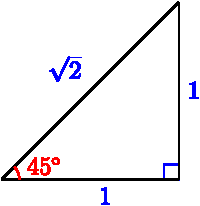
\includegraphics[width=\linewidth]{images/fig-45-45-90}
\end{sbspanel}%
\begin{sbspanel}{0.27}[center]%
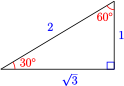
\includegraphics[width=\linewidth]{images/fig-30-60-90}
\end{sbspanel}%
\end{sidebyside}%
\item{}For the trigonometric ratios of most angles, your calculator gives approximations, not exact values.%
\end{enumerate}
%
\end{subsubsectionptx}
%
%
\typeout{************************************************}
\typeout{Subsubsection  Study Questions}
\typeout{************************************************}
%
\begin{subsubsectionptx}{Study Questions}{}{Study Questions}{}{}{g:subsubsection:idm46051691653552}
%
\begin{enumerate}[label=\arabic*]
\item{}How many parts of a right triangle (including the right angle) do you need to know in order to solve the triangle?%
\item{}Why is it better to use the given values when solving a triangle, rather than values you have calculated?%
\item{}What is the \(\sin^{-1}\) (or \(\cos^{-1}\) or \(\tan^{-1}\)) button on the calculator used for?%
\item{}Which are the "special" angles, and why are they special?%
\end{enumerate}
%
\end{subsubsectionptx}
%
%
\typeout{************************************************}
\typeout{Subsubsection  Skills}
\typeout{************************************************}
%
\begin{subsubsectionptx}{Skills}{}{Skills}{}{}{g:subsubsection:idm46051691693232}
Practice each skill in the Homework Problems listed.%
\par
%
\begin{enumerate}[label=\arabic*]
\item{}Solve a right triangle    \#1-16, 63-74%
\item{}Use inverse trig ratio notation    \#17-34%
\item{}Use trig ratios to find an angle    \#17-22, 35-38%
\item{}Solve problems involving right triangles    \#35-48%
\item{}Know the trig ratios for the special angles    \#49-62, 75-78%
\end{enumerate}
%
\end{subsubsectionptx}
\end{subsectionptx}
%
%
\typeout{************************************************}
\typeout{Exercises  Homework 2.3}
\typeout{************************************************}
%
\begin{exercises-subsection}{Homework 2.3}{}{Homework 2.3}{}{}{x:exercises:hmwk-2-3-exercises}
\begin{introduction}{}%
\begin{sidebyside}{2}{0.025}{0.025}{0.05}%
\begin{sbspanel}{0.65}[center]%
In these Homework Problems, we use the following standard notation for a right triangle: in \(\triangle ABC\), \(\angle C\) is a right angle. The side opposite \(\angle C\) has length \(c\), and so on. (See the figure at right.)%
\end{sbspanel}%
\begin{sbspanel}{0.25}[center]%
\resizebox{\linewidth}{!}{%
\tikzset{%
  block/.style    = {draw, thick, rectangle, minimum height = 3em,
    minimum width = 3em},
  sum/.style      = {draw, circle, node distance = 2cm}, % Adder
  input/.style    = {coordinate}, % Input
  output/.style   = {coordinate} % Output
}
\begin{tikzpicture}

\coordinate (A) at (0,0 );
\coordinate (C) at (3,0 );
\coordinate (B) at (3,1.6);

\filldraw[black] (A) circle (.2pt) node[anchor=east] {$A$};
\filldraw[black] (B) circle (.2pt) node[anchor=west] {$B$};
\filldraw[black] (C) circle (.2pt) node[anchor=west] {$C$};

\draw[blue,thick] (C) rectangle +(-0.25,.25);
\draw[black,thick] (A)--(B) node[above left,midway] {\color{blue}$c$};
\draw[black,thick] (C)--(B)  node[right,midway] {\color{blue}$a$};
\draw[black,thick] (A) --(C) node[below,midway] {\color{blue}$b$};
\end{tikzpicture}
}%
\end{sbspanel}%
\end{sidebyside}%
\end{introduction}%
\par\medskip\noindent%
%
For Problems 1\textendash{}4, solve the triangle.  Round answers to hundredths.%
\begin{exercisegroupcol}{2}
\begin{divisionexerciseegcol}{1}{}{}{g:exercise:idm46051701830848}%
\begin{sidebyside}{1}{0.15}{0.15}{0}%
\begin{sbspanel}{0.7}%
\resizebox{\linewidth}{!}{%
\tikzset{%
  block/.style    = {draw, thick, rectangle, minimum height = 3em,
    minimum width = 3em},
  sum/.style      = {draw, circle, node distance = 2cm}, % Adder
  input/.style    = {coordinate}, % Input
  output/.style   = {coordinate} % Output
}
\begin{tikzpicture} [rotate=61]

\coordinate (C) at (0,0 );
\coordinate (A) at (2.42,0 );
\coordinate (B) at (0,4.37);

\filldraw[black] (A) circle (.2pt) node[anchor=west] {$A$};
\filldraw[black] (B) circle (.2pt) node[anchor=east] {$B$};
\filldraw[black] (C) circle (.2pt) node[anchor=north] {$C$};

\draw[blue,thick] (C) rectangle +(0.25,.25);
\draw[black,thick] (A)--(B) ;
\draw[black,thick] (C)--(B)  ;
\draw[black,thick] (A) --(C) node[below right,midway] {\color{blue}$14$};

\draw[red,thick] (B)++(0,-0.7) arc(-90:-61:.7) node[right, midway, yshift=-3] {$29\degree$};
\end{tikzpicture}
}%
\end{sbspanel}%
\end{sidebyside}%
\end{divisionexerciseegcol}%
\begin{divisionexerciseegcol}{2}{}{}{g:exercise:idm46051691799744}%
\begin{sidebyside}{1}{0.275}{0.275}{0}%
\begin{sbspanel}{0.45}%
\resizebox{\linewidth}{!}{%
\tikzset{%
  block/.style    = {draw, thick, rectangle, minimum height = 3em,
    minimum width = 3em},
  sum/.style      = {draw, circle, node distance = 2cm}, % Adder
  input/.style    = {coordinate}, % Input
  output/.style   = {coordinate} % Output
}
\begin{tikzpicture} 

\coordinate (C) at (0,0 );
\coordinate (A) at (0, -2.27);
\coordinate (B) at (2.8,0);

\filldraw[black] (A) circle (.2pt) node[anchor=east] {$A$};
\filldraw[black] (B) circle (.2pt) node[anchor=west] {$B$};
\filldraw[black] (C) circle (.2pt) node[anchor=east] {$C$};

\draw[blue,thick] (C) rectangle +(0.25,-.25);
\draw[black,thick] (A)--(B) ;
\draw[black,thick] (C)--(B)  node[above,midway] {\color{blue}$46$} ;
\draw[black,thick] (A) --(C);

\draw[red,thick] (B)++(-0.5,0) arc(180:219:.5) node[left, midway, yshift=-3] {$39\degree$};
\end{tikzpicture}
}%
\end{sbspanel}%
\end{sidebyside}%
\end{divisionexerciseegcol}%
\begin{divisionexerciseegcol}{3}{}{}{g:exercise:idm46051701497888}%
\begin{sidebyside}{1}{0.2}{0.2}{0}%
\begin{sbspanel}{0.6}%
\resizebox{\linewidth}{!}{%
\tikzset{%
  block/.style    = {draw, thick, rectangle, minimum height = 3em,
    minimum width = 3em},
  sum/.style      = {draw, circle, node distance = 2cm}, % Adder
  input/.style    = {coordinate}, % Input
  output/.style   = {coordinate} % Output
}
\begin{tikzpicture} 

\coordinate (C) at (0,0 );
\coordinate (A) at (0, 1.69);
\coordinate (B) at (4.17,0);

\filldraw[black] (A) circle (.2pt) node[anchor=east] {$A$};
\filldraw[black] (B) circle (.2pt) node[anchor=west] {$B$};
\filldraw[black] (C) circle (.2pt) node[anchor=east] {$C$};

\draw[blue,thick] (C) rectangle +(0.25,.25);
\draw[black,thick] (A)--(B) node[above,midway] {\color{blue}$1$} ;
\draw[black,thick] (C)--(B)  ;
\draw[black,thick] (A) --(C);

\draw[red,thick] (B)++(-0.9,0) arc(180:158:.9) node[left, midway, yshift=2] {$22\degree$};
\end{tikzpicture}
}%
\end{sbspanel}%
\end{sidebyside}%
\end{divisionexerciseegcol}%
\begin{divisionexerciseegcol}{4}{}{}{g:exercise:idm46051701968112}%
\begin{sidebyside}{1}{0.2}{0.2}{0}%
\begin{sbspanel}{0.6}%
\resizebox{\linewidth}{!}{%
\tikzset{%
  block/.style    = {draw, thick, rectangle, minimum height = 3em,
    minimum width = 3em},
  sum/.style      = {draw, circle, node distance = 2cm}, % Adder
  input/.style    = {coordinate}, % Input
  output/.style   = {coordinate} % Output
}
\begin{tikzpicture} [rotate=-109]

\coordinate (C) at (0,0 );
\coordinate (A) at (0, 4.25);
\coordinate (B) at (1.46,0);

\filldraw[black] (A) circle (.2pt) node[anchor=west] {$A$};
\filldraw[black] (B) circle (.2pt) node[anchor=east] {$B$};
\filldraw[black] (C) circle (.2pt) node[anchor=south west] {$C$};

\draw[blue,thick] (C) rectangle +(0.25,.25);
\draw[black,thick] (A)--(B) node[below,midway] {\color{blue}$120$} ;
\draw[black,thick] (C)--(B)  ;
\draw[black,thick] (A) --(C);

\draw[red,thick] (B)++(-0.3,0) arc(180:109:.3) node[right, midway, yshift=2] {$71\degree$};
\end{tikzpicture}
}%
\end{sbspanel}%
\end{sidebyside}%
\end{divisionexerciseegcol}%
\end{exercisegroupcol}
\par\medskip\noindent
\par\medskip\noindent%
%
For Problems 5\textendash{}10,%
\begin{enumerate}[label=\alph*]
\item{}Sketch the right triangle described.%
\item{}Solve the triangle.%
\end{enumerate}
%
\begin{exercisegroupcol}{3}
\begin{divisionexerciseegcol}{5}{}{}{g:exercise:idm46051692947232}%
\(A = 42\degree,~ c = 26\)%
\end{divisionexerciseegcol}%
\begin{divisionexerciseegcol}{6}{}{}{g:exercise:idm46051692991440}%
\(B = 28\degree,~ c = 6.8\)%
\end{divisionexerciseegcol}%
\begin{divisionexerciseegcol}{7}{}{}{g:exercise:idm46051692985360}%
\(B = 33\degree,~ a = 300\)%
\end{divisionexerciseegcol}%
\begin{divisionexerciseegcol}{8}{}{}{g:exercise:idm46051693022592}%
\(B = 79\degree,~ a = 116\)%
\end{divisionexerciseegcol}%
\begin{divisionexerciseegcol}{9}{}{}{g:exercise:idm46051693030880}%
\(A = 12\degree,~ a = 4\)%
\end{divisionexerciseegcol}%
\begin{divisionexerciseegcol}{10}{}{}{g:exercise:idm46051692387936}%
\(A = 50\degree,~ a = 10\)%
\end{divisionexerciseegcol}%
\end{exercisegroupcol}
\par\medskip\noindent
\par\medskip\noindent%
%
For Problems 11\textendash{}16,%
\begin{enumerate}[label=\alph*]
\item{}Sketch the right triangle described.%
\item{}Without doing the calculations, list the steps you would use to solve the triangle.%
\end{enumerate}
%
\begin{exercisegroupcol}{2}
\begin{divisionexerciseegcol}{11}{}{}{g:exercise:idm46051693094624}%
\(B = 53.7\degree,~ b = 8.2\)%
\end{divisionexerciseegcol}%
\begin{divisionexerciseegcol}{12}{}{}{g:exercise:idm46051692250896}%
\(B = 80\degree,~ a = 250\)%
\end{divisionexerciseegcol}%
\begin{divisionexerciseegcol}{13}{}{}{g:exercise:idm46051692265968}%
\(A = 25\degree,~ b = 40\)%
\end{divisionexerciseegcol}%
\begin{divisionexerciseegcol}{14}{}{}{g:exercise:idm46051692112928}%
\(A = 15\degree,~ c = 62\)%
\end{divisionexerciseegcol}%
\begin{divisionexerciseegcol}{15}{}{}{g:exercise:idm46051692128512}%
\(A = 64.5\degree,~ c = 24\)%
\end{divisionexerciseegcol}%
\begin{divisionexerciseegcol}{16}{}{}{g:exercise:idm46051692296384}%
\(B = 44\degree,~ b = 0.6\)%
\end{divisionexerciseegcol}%
\end{exercisegroupcol}
\par\medskip\noindent
\par\medskip\noindent%
%
For Problems 17\textendash{}22, find the labeled angle. Round your answer to tenths of a degree.%
\begin{exercisegroupcol}{3}
\begin{divisionexerciseegcol}{17}{}{}{g:exercise:idm46051692165680}%
\begin{sidebyside}{1}{0.125}{0.125}{0}%
\begin{sbspanel}{0.75}%
\resizebox{\linewidth}{!}{%
\tikzset{%
  block/.style    = {draw, thick, rectangle, minimum height = 3em,
    minimum width = 3em},
  sum/.style      = {draw, circle, node distance = 2cm}, % Adder
  input/.style    = {coordinate}, % Input
  output/.style   = {coordinate} % Output
}
\begin{tikzpicture} [rotate=-160]

\coordinate (C) at (0,0 );
\coordinate (A) at (0, 1);
\coordinate (B) at (3.5,0);

\draw[blue,thick] (C) rectangle +(0.25,.25);
\draw[black,thick] (A)--(B) node[below,midway] {\color{blue}$22$} ;
\draw[black,thick] (C)--(B)  ;
\draw[black,thick] (A) --(C) node[right,midway] {\color{blue}$6$} ;

\draw[red,thick] (A)++(0,-0.3) arc(-90:{-atan(1/3.5)}:.3) node[above left, midway, yshift=-4] {$\theta$};
\end{tikzpicture}
}%
\end{sbspanel}%
\end{sidebyside}%
\end{divisionexerciseegcol}%
\begin{divisionexerciseegcol}{18}{}{}{g:exercise:idm46051692466928}%
\begin{sidebyside}{1}{0.2}{0.2}{0}%
\begin{sbspanel}{0.6}%
\resizebox{\linewidth}{!}{%
\tikzset{%
  block/.style    = {draw, thick, rectangle, minimum height = 3em,
    minimum width = 3em},
  sum/.style      = {draw, circle, node distance = 2cm}, % Adder
  input/.style    = {coordinate}, % Input
  output/.style   = {coordinate} % Output
}
\begin{tikzpicture} [rotate=20]

\coordinate (C) at (0,0 );
\coordinate (A) at (0, 2.4);
\coordinate (B) at (2.26,0);

\draw[blue,thick] (C) rectangle +(0.25,.25);
\draw[black,thick] (A)--(B) node[above,midway, xshift=3] {\color{blue}$11$} ;
\draw[black,thick] (C)--(B)  ;
\draw[black,thick] (A) --(C) node[left,midway] {\color{blue}$8$} ;

\draw[red,thick] (B)++(-0.3,0) arc(180:{180-atan(2.4/2.26)}:.3) node[ left, midway, yshift=0] {$\theta$};
\end{tikzpicture}
}%
\end{sbspanel}%
\end{sidebyside}%
\end{divisionexerciseegcol}%
\begin{divisionexerciseegcol}{19}{}{}{g:exercise:idm46051692518048}%
\begin{sidebyside}{1}{0.2}{0.2}{0}%
\begin{sbspanel}{0.6}%
\resizebox{\linewidth}{!}{%
\tikzset{%
  block/.style    = {draw, thick, rectangle, minimum height = 3em,
    minimum width = 3em},
  sum/.style      = {draw, circle, node distance = 2cm}, % Adder
  input/.style    = {coordinate}, % Input
  output/.style   = {coordinate} % Output
}
\begin{tikzpicture} 

\coordinate (C) at (0,0 );
\coordinate (A) at (0, -1.8);
\coordinate (B) at (3,0);

\draw[blue,thick] (C) rectangle +(0.25,-.25);
\draw[black,thick] (A)--(B) node[below right,midway, xshift=3] {\color{blue}$60$} ;
\draw[black,thick] (C)--(B)  node[above,midway] {\color{blue}$50$}  ;
\draw[black,thick] (A) --(C);

\draw[red,thick] (A)++(0,.5) arc(90:{atan(1.8/3)}:.5) node[ above, midway, yshift=0] {$\theta$};
\end{tikzpicture}
}%
\end{sbspanel}%
\end{sidebyside}%
\end{divisionexerciseegcol}%
\begin{divisionexerciseegcol}{20}{}{}{g:exercise:idm46051692514384}%
\begin{sidebyside}{1}{0.175}{0.175}{0}%
\begin{sbspanel}{0.65}%
\resizebox{\linewidth}{!}{%
\tikzset{%
  block/.style    = {draw, thick, rectangle, minimum height = 3em,
    minimum width = 3em},
  sum/.style      = {draw, circle, node distance = 2cm}, % Adder
  input/.style    = {coordinate}, % Input
  output/.style   = {coordinate} % Output
}
\begin{tikzpicture} 

\coordinate (C) at (0,0 );
\coordinate (A) at (0, 1.8);
\coordinate (B) at (2.8,0);

\draw[blue,thick] (C) rectangle +(0.25,.25);
\draw[black,thick] (A)--(B) ;
\draw[black,thick] (C)--(B)  node[below,midway] {\color{blue}$8.4$}  ;
\draw[black,thick] (A) --(C)  node[left,midway] {\color{blue}$5.2$};

\draw[red,thick] (A)++(0,-.4) arc(-90:{-atan(1.8/2.8)}:.4) node[ below, midway, xshift=2] {$\theta$};
\end{tikzpicture}
}%
\end{sbspanel}%
\end{sidebyside}%
\end{divisionexerciseegcol}%
\begin{divisionexerciseegcol}{21}{}{}{g:exercise:idm46051702113792}%
\begin{sidebyside}{1}{0.15}{0.15}{0}%
\begin{sbspanel}{0.7}%
\resizebox{\linewidth}{!}{%
\tikzset{%
  block/.style    = {draw, thick, rectangle, minimum height = 3em,
    minimum width = 3em},
  sum/.style      = {draw, circle, node distance = 2cm}, % Adder
  input/.style    = {coordinate}, % Input
  output/.style   = {coordinate} % Output
}
\begin{tikzpicture} 

\coordinate (C) at (0,0 );
\coordinate (A) at (0, -1.3);
\coordinate (B) at (-3,0);

\draw[blue,thick] (C) rectangle +(-0.25,-.25);
\draw[black,thick] (A)--(B) ;
\draw[black,thick] (C)--(B)  node[above,midway] {\color{blue}$6.3$}  ;
\draw[black,thick] (A) --(C)  node[right,midway] {\color{blue}$2.8$};

\draw[red,thick] (A)++(0,.4) arc(90:{180-atan(1.3/3)}:.4) node[ above, midway, xshift=-2] {$\theta$};
\end{tikzpicture}
}%
\end{sbspanel}%
\end{sidebyside}%
\end{divisionexerciseegcol}%
\begin{divisionexerciseegcol}{22}{}{}{g:exercise:idm46051702110192}%
\begin{sidebyside}{1}{0.175}{0.175}{0}%
\begin{sbspanel}{0.65}%
\resizebox{\linewidth}{!}{%
\tikzset{%
  block/.style    = {draw, thick, rectangle, minimum height = 3em,
    minimum width = 3em},
  sum/.style      = {draw, circle, node distance = 2cm}, % Adder
  input/.style    = {coordinate}, % Input
  output/.style   = {coordinate} % Output
}
\begin{tikzpicture} [rotate=55.491]

\coordinate (C) at (0,0 );
\coordinate (A) at (0, 3.2);
\coordinate (B) at (2.2,0);

\draw[blue,thick] (C) rectangle +(0.25,.25);
\draw[black,thick] (A)--(B) ;
\draw[black,thick] (C)--(B)  node[below right,midway] {\color{blue}$60$}  ;
\draw[black,thick] (A) --(C)  node[below left,midway] {\color{blue}$110$};

\draw[red,thick] (A)++(0,-.6) arc(-90:{-atan(3.2/2.2)}:.6) node[right, midway, yshift=-2] {$\theta$};
\end{tikzpicture}
}%
\end{sbspanel}%
\end{sidebyside}%
\end{divisionexerciseegcol}%
\end{exercisegroupcol}
\par\medskip\noindent
\par\medskip\noindent%
%
For Problems 23\textendash{}28, evaluate the expression and sketch a right triangle to illustrate.%
\begin{exercisegroupcol}{3}
\begin{divisionexerciseegcol}{23}{}{}{g:exercise:idm46051701493008}%
\(\sin^{-1} 0.2\)%
\end{divisionexerciseegcol}%
\begin{divisionexerciseegcol}{24}{}{}{g:exercise:idm46051702523392}%
\(\cos^{-1} 0.8\)%
\end{divisionexerciseegcol}%
\begin{divisionexerciseegcol}{25}{}{}{g:exercise:idm46051702522624}%
\(\tan^{-1} 1.5\)%
\end{divisionexerciseegcol}%
\begin{divisionexerciseegcol}{26}{}{}{g:exercise:idm46051684766688}%
\(\tan^{-1} 2.5\)%
\end{divisionexerciseegcol}%
\begin{divisionexerciseegcol}{27}{}{}{g:exercise:idm46051684765808}%
\(\cos^{-1} 0.2839\)%
\end{divisionexerciseegcol}%
\begin{divisionexerciseegcol}{28}{}{}{g:exercise:idm46051684762608}%
\(\sin^{-1} 0.4127\)%
\end{divisionexerciseegcol}%
\end{exercisegroupcol}
\par\medskip\noindent
\par\medskip\noindent%
%
For Problems 29\textendash{}32, write two different equations for the statement.%
\begin{exercisegroup}
\begin{divisionexerciseeg}{29}{}{}{g:exercise:idm46051692312704}%
The cosine of \(15 \degree\) is \(0.9659\).%
\end{divisionexerciseeg}%
\begin{divisionexerciseeg}{30}{}{}{g:exercise:idm46051693424368}%
The sine of \(70 \degree\) is \(0.9397\).%
\end{divisionexerciseeg}%
\begin{divisionexerciseeg}{31}{}{}{g:exercise:idm46051693447600}%
The angle whose tangent is \(3.1445\) is \(65 \degree\).%
\end{divisionexerciseeg}%
\begin{divisionexerciseeg}{32}{}{}{g:exercise:idm46051693481952}%
The angle whose cosine is \(0.0872\) is \(85 \degree\).%
\end{divisionexerciseeg}%
\end{exercisegroup}
\par\medskip\noindent
\begin{divisionexercise}{33}{}{}{g:exercise:idm46051693503472}%
Evaluate the expressions, and explain what each means.%
\begin{equation*}
\sin^{-1} (0.6),~~~ (\sin 6\degree)^{-1}
\end{equation*}
%
\end{divisionexercise}%
\begin{divisionexercise}{34}{}{}{g:exercise:idm46051693553280}%
Evaluate the expressions, and explain what each means.%
\begin{equation*}
\cos^{-1} (0.36),~~~ (\cos 36\degree)^{-1}
\end{equation*}
%
\end{divisionexercise}%
\par\medskip\noindent%
%
For Problems 35\textendash{}38,%
\begin{enumerate}[label=\alph*]
\item{}Sketch a right triangle that illustrates the situation. Label your sketch with the given information.%
\item{}Choose the appropriate trig ratio and write an equation, then solve the problem.%
\end{enumerate}
%
\begin{exercisegroup}
\begin{divisionexerciseeg}{35}{}{}{g:exercise:idm46051693583152}%
The gondola cable for the ski lift at Snowy Peak is 2458 yards long and climbs 1860 feet. What angle with the horizontal does the cable make?%
\end{divisionexerciseeg}%
\begin{divisionexerciseeg}{36}{}{}{g:exercise:idm46051692675360}%
The Leaning Tower of Pisa is 55 meters in length. An object dropped from the top of the tower lands 4.8 meters from the base of the tower. At what angle from the horizontal does the tower lean?%
\end{divisionexerciseeg}%
\begin{divisionexerciseeg}{37}{}{}{g:exercise:idm46051692674400}%
A mining company locates a vein of minerals at a depth of 32 meters. However, there is a layer of granite directly above the minerals, so they decide to drill at an angle, starting 10 meters from their original location. At what angle from the horizontal should they drill?%
\end{divisionexerciseeg}%
\begin{divisionexerciseeg}{38}{}{}{g:exercise:idm46051696504816}%
The birdhouse in Carolyn's front yard is 12 feet tall, and its shadow at 4 pm is 15 feet 4 inches long.  What is the angle of elevation of the sun at 4 pm?%
\end{divisionexerciseeg}%
\end{exercisegroup}
\par\medskip\noindent
\par\medskip\noindent%
%
For Problems 39\textendash{}42,%
\par
%
\begin{enumerate}[label=\alph*]
\item{}Sketch the right triangle described.%
\item{}Solve the triangle.%
\end{enumerate}
%
\begin{exercisegroupcol}{2}
\begin{divisionexerciseegcol}{39}{}{}{g:exercise:idm46051696502048}%
\(a = 18, ~ b = 26\)%
\end{divisionexerciseegcol}%
\begin{divisionexerciseegcol}{40}{}{}{g:exercise:idm46051702263792}%
\(a = 35, ~ b = 27\)%
\end{divisionexerciseegcol}%
\begin{divisionexerciseegcol}{41}{}{}{g:exercise:idm46051702262912}%
\(b = 10.6 ,~ c = 19.2\)%
\end{divisionexerciseegcol}%
\begin{divisionexerciseegcol}{42}{}{}{g:exercise:idm46051685025760}%
\(a = 88, ~ c = 132\)%
\end{divisionexerciseegcol}%
\end{exercisegroupcol}
\par\medskip\noindent
\par\medskip\noindent%
%
For Problems 43\textendash{}48,%
\par
%
\begin{enumerate}[label=\alph*]
\item{}Make a sketch that illustrates the situation. Label your sketch with the given information.%
\item{}Write an equation and solve the problem.%
\end{enumerate}
%
\begin{exercisegroup}
\begin{divisionexerciseeg}{43}{}{}{g:exercise:idm46051685022736}%
The Mayan pyramid of El Castillo at Chichen Itza in Mexico has 91 steps. Each step is 26 cm high and 30 cm deep.%
\par
%
\begin{enumerate}[label=\roman*]
\item{}What angle does the side of the pyramid make with the horizontal?%
\item{}What is the distance up the face of the pyramid, from base to top platform?%
\end{enumerate}
%
\end{divisionexerciseeg}%
\begin{divisionexerciseeg}{44}{}{}{g:exercise:idm46051702135760}%
An airplane begins its descent when its altitude is 10 kilometers. The angle of descent should be \(3\degree\) from horizontal.%
\par
%
\begin{enumerate}[label=\roman*]
\item{}How far from the airport (measured along the ground) should the airplane begin its descent?%
\item{}How far will the airplane travel on its descent to the airport?%
\end{enumerate}
%
\end{divisionexerciseeg}%
\begin{divisionexerciseeg}{45}{}{}{g:exercise:idm46051702133392}%
A communications satellite is in a low earth orbit (LOE) at an altitude of 400 km. From the satellite, the angle of depression to earth's horizon is \(19.728\degree\). Use this information to calculate the radius of the earth.%
\end{divisionexerciseeg}%
\begin{divisionexerciseeg}{46}{}{}{g:exercise:idm46051693711024}%
The first Ferris wheel was built for the 1893 Chicago world's fair. It had a diameter of 250 feet, and the boarding platform, at the base of the wheel, was 14 feet above the ground. If you boarded the wheel and rotated through an angle of \(50\degree\), what would be your height above the ground?%
\end{divisionexerciseeg}%
\begin{divisionexerciseeg}{47}{}{}{g:exercise:idm46051693722304}%
To find the distance across a ravine, Delbert takes some measurements from a small airplane. When he is a short distance from the ravine at an altitude of 500 feet, he finds that the angle of depression to the near side of the ravine is \(56\degree\), and the angle of depression to the far side is \(32\degree\). What is the width of the ravine?  (Hint:  First find the horizontal distance from Delbert to the near side of the ravine.)%
\end{divisionexerciseeg}%
\begin{divisionexerciseeg}{48}{}{}{g:exercise:idm46051693778272}%
The window in Francine's office is 4 feet wide and 5 feet tall. The bottom of the window is 3 feet from the floor.  When the sun is at an angle of elevation of \(64\degree\), what is the area of the sunny spot on the floor?%
\end{divisionexerciseeg}%
\end{exercisegroup}
\par\medskip\noindent
\begin{divisionexercise}{49}{}{}{g:exercise:idm46051693795472}%
Which of the following numbers are equal to \(\cos 45\degree\)?%
\par
%
\begin{multicols}{4}
\begin{enumerate}[label=\alph*]
\item{}\(\displaystyle \dfrac{\sqrt{2}}{2}\)%
\item{}\(\displaystyle \dfrac{1}{\sqrt{2}}\)%
\item{}\(\displaystyle \dfrac{2}{\sqrt{2}}\)%
\item{}\(\displaystyle \sqrt{2}\)%
\end{enumerate}
\end{multicols}
%
\end{divisionexercise}%
\begin{divisionexercise}{50}{}{}{g:exercise:idm46051693832832}%
Which of the following numbers are equal to \(\tan 30\degree\)?%
\par
%
\begin{multicols}{4}
\begin{enumerate}[label=\alph*]
\item{}\(\displaystyle \sqrt{3}\)%
\item{}\(\displaystyle \dfrac{1}{\sqrt{3}}\)%
\item{}\(\displaystyle \dfrac{\sqrt{3}}{3}\)%
\item{}\(\displaystyle \dfrac{3}{\sqrt{3}}\)%
\end{enumerate}
\end{multicols}
%
\end{divisionexercise}%
\begin{divisionexercise}{51}{}{}{g:exercise:idm46051693851024}%
Which of the following numbers are equal to \(\tan 60\degree\)?%
\par
%
\begin{multicols}{4}
\begin{enumerate}[label=\alph*]
\item{}\(\displaystyle \sqrt{3}\)%
\item{}\(\displaystyle \dfrac{1}{\sqrt{3}}\)%
\item{}\(\displaystyle \dfrac{\sqrt{3}}{3}\)%
\item{}\(\displaystyle \dfrac{3}{\sqrt{3}}\)%
\end{enumerate}
\end{multicols}
%
\end{divisionexercise}%
\begin{divisionexercise}{52}{}{}{g:exercise:idm46051693892768}%
Which of the following numbers are equal to \(\sin 60\degree\)?%
\par
%
\begin{multicols}{4}
\begin{enumerate}[label=\alph*]
\item{}\(\displaystyle \dfrac{3}{\sqrt{2}}\)%
\item{}\(\displaystyle \dfrac{\sqrt{3}}{2}\)%
\item{}\(\displaystyle \dfrac{\sqrt{2}}{3}\)%
\item{}\(\displaystyle \dfrac{2}{\sqrt{3}}\)%
\end{enumerate}
\end{multicols}
%
\end{divisionexercise}%
\par\medskip\noindent%
%
For Problems 53\textendash{}58, choose all values from the list below that are exactly equal to, or decimal approximations for, the given trig ratio. (Try not to use a calculator!)%
\begin{sidebyside}{1}{0}{0}{0}%
\begin{sbspanel}{1}%
{\centering%
{\tabularfont%
\begin{tabular}{AcccccA}\hrulethin
\(\sin 30\degree\)&\(\cos 45\degree\)&\(\sin 60\degree\)&\(\tan 45\degree\)&\(\tan 60\degree\)\tabularnewline[0pt]
\(~~~0.5000~~~\)&\(~~~0.5774~~~\)&\(~~~0.7071~~~\)&\(~~~0.8660~~~\)&\(~~~1.0000~~~\)\tabularnewline[0pt]
\(\dfrac{1}{\sqrt{2}}\)&\(\dfrac{2}{\sqrt{2}}\)&\(\dfrac{3}{\sqrt{2}}\)&\(\dfrac{1}{2}\)&\(\dfrac{\sqrt{2}}{2}\)\tabularnewline[0pt]
\(\dfrac{1}{\sqrt{3}}\)&\(\dfrac{2}{\sqrt{3}}\)&\(\dfrac{\sqrt{3}}{2}\)&\(\sqrt{3}\)&\(\dfrac{\sqrt{3}}{3}\)\tabularnewline\hrulethin
\end{tabular}
}%
\par}
\end{sbspanel}%
\end{sidebyside}%
\begin{exercisegroupcol}{3}
\begin{divisionexerciseegcol}{53}{}{}{g:exercise:idm46051694128912}%
\(\cos 30\degree\)%
\end{divisionexerciseegcol}%
\begin{divisionexerciseegcol}{54}{}{}{g:exercise:idm46051694138560}%
\(\sin 45\degree\)%
\end{divisionexerciseegcol}%
\begin{divisionexerciseegcol}{55}{}{}{g:exercise:idm46051694156128}%
\(\tan 30\degree\)%
\end{divisionexerciseegcol}%
\begin{divisionexerciseegcol}{56}{}{}{g:exercise:idm46051694176816}%
\(\cos 60\degree\)%
\end{divisionexerciseegcol}%
\begin{divisionexerciseegcol}{57}{}{}{g:exercise:idm46051694182096}%
\(\sin 90\degree\)%
\end{divisionexerciseegcol}%
\begin{divisionexerciseegcol}{58}{}{}{g:exercise:idm46051694204000}%
\(\cos 0\degree\)%
\end{divisionexerciseegcol}%
\end{exercisegroupcol}
\par\medskip\noindent
\begin{divisionexercise}{59}{}{}{g:exercise:idm46051694212416}%
Fill in the table from memory with exact values. Do you notice any patterns that might help you memorize the values?%
\begin{sidebyside}{1}{0}{0}{0}%
\begin{sbspanel}{1}%
{\centering%
{\tabularfont%
\begin{tabular}{AcAcAcAcAcAcA}\hrulethin
\(\theta\)&\(~~~0\degree~~~\)&\(~~~30\degree~~~\)&\(~~~45\degree~~~\)&\(~~~60\degree~~~\)&\(~~~90\degree~~~\)\tabularnewline\hrulethin
\(\sin \theta\)&\(~\)&\(~\)&\(~\)&\(~\)&\(~\)\tabularnewline\hrulethin
\(\cos \theta\)&\(~\)&\(~\)&\(~\)&\(~\)&\(~\)\tabularnewline\hrulethin
\(\tan \theta\)&\(~\)&\(~\)&\(~\)&\(~\)&\(~\)\tabularnewline\hrulethin
\end{tabular}
}%
\par}
\end{sbspanel}%
\end{sidebyside}%
\end{divisionexercise}%
\begin{divisionexercise}{60}{}{}{g:exercise:idm46051694409456}%
Fill in the table from memory with decimal approximations to four places.%
\begin{sidebyside}{1}{0}{0}{0}%
\begin{sbspanel}{1}%
{\centering%
{\tabularfont%
\begin{tabular}{AcAcAcAcAcAcA}\hrulethin
\(\theta\)&\(~~~0\degree~~~\)&\(~~~30\degree~~~\)&\(~~~45\degree~~~\)&\(~~~60\degree~~~\)&\(~~~90\degree~~~\)\tabularnewline\hrulethin
\(\sin \theta\)&\(~\)&\(~\)&\(~\)&\(~\)&\(~\)\tabularnewline\hrulethin
\(\cos \theta\)&\(~\)&\(~\)&\(~\)&\(~\)&\(~\)\tabularnewline\hrulethin
\(\tan \theta\)&\(~\)&\(~\)&\(~\)&\(~\)&\(~\)\tabularnewline\hrulethin
\end{tabular}
}%
\par}
\end{sbspanel}%
\end{sidebyside}%
\end{divisionexercise}%
\par\medskip\noindent%
%
For Problems 61 and 62, compare the given value with the trig ratios of the special angles to answer the questions. Try not to use a calculator.%
\begin{exercisegroup}
\begin{divisionexerciseeg}{61}{}{}{g:exercise:idm46051694541616}%
Is the acute angle larger or smaller than \(45\degree\)?%
\par
%
\begin{multicols}{3}
\begin{enumerate}[label=\alph*]
\item{}\(\displaystyle \sin \alpha = 0.7\)%
\item{}\(\displaystyle \tan \beta = 1.2\)%
\item{}\(\displaystyle \cos \gamma = 0.65\)%
\end{enumerate}
\end{multicols}
%
\end{divisionexerciseeg}%
\begin{divisionexerciseeg}{62}{}{}{g:exercise:idm46051694599408}%
Is the acute angle larger or smaller than \(60\degree\)?%
\par
%
\begin{multicols}{3}
\begin{enumerate}[label=\alph*]
\item{}\(\displaystyle \cos \theta = 0.75\)%
\item{}\(\displaystyle \tan \phi = 1.5\)%
\item{}\(\displaystyle \sin \psi = 0.72\)%
\end{enumerate}
\end{multicols}
%
\end{divisionexerciseeg}%
\end{exercisegroup}
\par\medskip\noindent
\par\medskip\noindent%
%
For Problems 63\textendash{}72, solve the triangle. Give your answers as exact values.%
\begin{exercisegroupcol}{2}
\begin{divisionexerciseegcol}{63}{}{}{g:exercise:idm46051694650688}%
\begin{sidebyside}{1}{0.35}{0.35}{0}%
\begin{sbspanel}{0.3}%
\resizebox{\linewidth}{!}{%
\tikzset{%
  block/.style    = {draw, thick, rectangle, minimum height = 3em,
    minimum width = 3em},
  sum/.style      = {draw, circle, node distance = 2cm}, % Adder
  input/.style    = {coordinate}, % Input
  output/.style   = {coordinate} % Output
}
\begin{tikzpicture}

\coordinate (C) at (0,0 );
\coordinate (A) at (-1.7,0);
\coordinate (B) at (0,2.944);

\filldraw[black] (A) circle (.2pt) node[anchor=east] {$A$};
\filldraw[black] (B) circle (.2pt) node[anchor=west] {$B$};
\filldraw[black] (C) circle (.2pt) node[anchor=west] {$C$};

\draw[blue,thick] (C) rectangle +(-0.25,.25);
\draw[black,thick] (A)--(B)  node[above left,midway] {\color{blue}$6$};
\draw[black,thick] (C)--(B)  node[right,midway] {\color{blue}$a$}  ;
\draw[black,thick] (A) --(C)  node[below,midway] {\color{blue}$b$};

\draw[red,thick] (A)++(.4,0) arc(0:60:.4) node[right, midway, yshift=2] {$60\degree$};
\end{tikzpicture}
}%
\end{sbspanel}%
\end{sidebyside}%
\end{divisionexerciseegcol}%
\begin{divisionexerciseegcol}{64}{}{}{g:exercise:idm46051694705312}%
\begin{sidebyside}{1}{0.275}{0.275}{0}%
\begin{sbspanel}{0.45}%
\resizebox{\linewidth}{!}{%
\tikzset{%
  block/.style    = {draw, thick, rectangle, minimum height = 3em,
    minimum width = 3em},
  sum/.style      = {draw, circle, node distance = 2cm}, % Adder
  input/.style    = {coordinate}, % Input
  output/.style   = {coordinate} % Output
}
\begin{tikzpicture}

\coordinate (C) at (0,0 );
\coordinate (A) at (-2.944,0);
\coordinate (B) at (0,1.7);

\filldraw[black] (A) circle (.2pt) node[anchor=east] {$A$};
\filldraw[black] (B) circle (.2pt) node[anchor=west] {$B$};
\filldraw[black] (C) circle (.2pt) node[anchor=west] {$C$};

\draw[blue,thick] (C) rectangle +(-0.25,.25);
\draw[black,thick] (A)--(B)  node[above left,midway] {\color{blue}$c$};
\draw[black,thick] (C)--(B)  node[right,midway] {\color{blue}$a$}  ;
\draw[black,thick] (A) --(C)  node[below,midway] {\color{blue}$6$};

\draw[red,thick] (A)++(.5,0) arc(0:30:.5) node[right, midway, xshift=1, yshift=2] {$30\degree$};
\end{tikzpicture}
}%
\end{sbspanel}%
\end{sidebyside}%
\end{divisionexerciseegcol}%
\begin{divisionexerciseegcol}{65}{}{}{g:exercise:idm46051694723504}%
\begin{sidebyside}{1}{0.2}{0.2}{0}%
\begin{sbspanel}{0.6}%
\resizebox{\linewidth}{!}{%
\tikzset{%
  block/.style    = {draw, thick, rectangle, minimum height = 3em,
    minimum width = 3em},
  sum/.style      = {draw, circle, node distance = 2cm}, % Adder
  input/.style    = {coordinate}, % Input
  output/.style   = {coordinate} % Output
}
\begin{tikzpicture} [rotate=-135]

\coordinate (C) at (0,0 );
\coordinate (A) at (3,0);
\coordinate (B) at (0,3);

\filldraw[black] (A) circle (.2pt) node[anchor=east] {$A$};
\filldraw[black] (B) circle (.2pt) node[anchor=west] {$B$};
\filldraw[black] (C) circle (.2pt) node[anchor=east, yshift=2] {$C$};

\draw[blue,thick] (C) rectangle +(0.25,.25);
\draw[black,thick] (A)--(B)  node[below,midway] {\color{blue}$8$};
\draw[black,thick] (C)--(B)  node[above right,midway] {\color{blue}$a$}  ;
\draw[black,thick] (A) --(C)  node[above left,midway] {\color{blue}$b$};

\draw[red,thick] (A)++(-.5,0) arc(180:135:.5) node[right, midway, xshift=1, yshift=2] {$45\degree$};
\end{tikzpicture}
}%
\end{sbspanel}%
\end{sidebyside}%
\end{divisionexerciseegcol}%
\begin{divisionexerciseegcol}{66}{}{}{g:exercise:idm46051694758496}%
\begin{sidebyside}{1}{0.25}{0.25}{0}%
\begin{sbspanel}{0.5}%
\resizebox{\linewidth}{!}{%
\tikzset{%
  block/.style    = {draw, thick, rectangle, minimum height = 3em,
    minimum width = 3em},
  sum/.style      = {draw, circle, node distance = 2cm}, % Adder
  input/.style    = {coordinate}, % Input
  output/.style   = {coordinate} % Output
}
\begin{tikzpicture}

\coordinate (C) at (0,0 );
\coordinate (A) at (3,0);
\coordinate (B) at (0,-3);

\filldraw[black] (A) circle (.2pt) node[anchor=west] {$A$};
\filldraw[black] (B) circle (.2pt) node[anchor=east] {$B$};
\filldraw[black] (C) circle (.2pt) node[anchor=east] {$C$};

\draw[blue,thick] (C) rectangle +(0.25,-.25);
\draw[black,thick] (A)--(B)  node[below right,midway] {\color{blue}$c$};
\draw[black,thick] (C)--(B)  node[left,midway] {\color{blue}$3\sqrt{2}$}  ;
\draw[black,thick] (A) --(C)  node[above,midway] {\color{blue}$b$};

\draw[red,thick] (A)++(-.5,0) arc(180:225:.5) node[left, midway, xshift=0, yshift=-3] {$45\degree$};
\end{tikzpicture}
}%
\end{sbspanel}%
\end{sidebyside}%
\end{divisionexerciseegcol}%
\begin{divisionexerciseegcol}{67}{}{}{g:exercise:idm46051694786000}%
\begin{sidebyside}{1}{0.2}{0.2}{0}%
\begin{sbspanel}{0.6}%
\resizebox{\linewidth}{!}{%
\tikzset{%
  block/.style    = {draw, thick, rectangle, minimum height = 3em,
    minimum width = 3em},
  sum/.style      = {draw, circle, node distance = 2cm}, % Adder
  input/.style    = {coordinate}, % Input
  output/.style   = {coordinate} % Output
}
\begin{tikzpicture}

\coordinate (D) at (0,0 );
\coordinate (F) at (2.07,1.2);
\coordinate (E) at (4.14,0);
\coordinate (G) at (2.07,0);

\filldraw[black] (D) circle (.2pt) node[anchor=east] {$D$};
\filldraw[black] (E) circle (.2pt) node[anchor=west] {$E$};
\filldraw[black] (F) circle (.2pt) node[anchor=south east] {$F$};

\draw[blue,thick] (G) rectangle +(0.25,.25);
\draw[gray,thick, dashed] (G)--(F);
\draw[gray,thick] (D)++(0,-.07) --+(0,-.4);
\draw[gray,thick] (E)++(0,-.07) --+(0,-.4);
\draw[gray,thick,<-] (D)++(0,-.3) --+(1.75,0);
\draw[gray,thick,<-] (E)++(0,-.3) --+(-1.75,0);

\draw[black,thick] (D)--(F)  node[above left,midway] {\color{blue}$e$};
\draw[black,thick] (D)--(E)  node[below,midway] {\color{blue}$f$}  ;
\draw[black,thick] (E) --(F)  node[above right,midway] {\color{blue}$4$};

\draw[red,thick] (D)++(0.7,0) arc(0:30:.7) node[right, midway, xshift=0, yshift=2] {\small$30\degree$};
\draw[red,thick] (E)++(-0.7,0) arc(180:150:.7) node[left, midway, xshift=0, yshift=2] {\small$30\degree$};
\end{tikzpicture}
}%
\end{sbspanel}%
\end{sidebyside}%
\end{divisionexerciseegcol}%
\begin{divisionexerciseegcol}{68}{}{}{g:exercise:idm46051694803856}%
\begin{sidebyside}{1}{0.175}{0.175}{0}%
\begin{sbspanel}{0.65}%
\resizebox{\linewidth}{!}{%
 \tikzset{%
   block/.style    = {draw, thick, rectangle, minimum height = 3em,
     minimum width = 3em},
   sum/.style      = {draw, circle, node distance = 2cm}, % Adder
   input/.style    = {coordinate}, % Input
   output/.style   = {coordinate} % Output
 }
  \begin{tikzpicture}

 \coordinate (D) at (0,0 );
 \coordinate (F) at (4.8,0);
 \coordinate (E) at (2.4,-2.4);
 \coordinate (G) at (2.4,0);

 \filldraw[black] (D) circle (.2pt) node[anchor=east] {$D$};
 \filldraw[black] (E) circle (.2pt) node[anchor=north east] {$E$};
 \filldraw[black] (F) circle (.2pt) node[anchor=west] {$F$};

 \draw[blue,thick] (G) rectangle +(0.25,-.25);
 \draw[gray,thick, dashed] (G)--(E) node[left,midway]{\color{blue}7};
 \draw[gray,thick] (D)++(0,.07) --+(0,.4);
 \draw[gray,thick] (F)++(0,.07) --+(0,.4);
 \draw[gray,thick,<-] (D)++(0,.3) --+(2.2,0);
 \draw[gray,thick,<-] (F)++(0,.3) --+(-2.2,0);

 \draw[black,thick] (D)--(F)  node[above,midway, yshift=2] {\color{blue}$e$};
 \draw[black,thick] (D)--(E)  node[below left,midway] {\color{blue}$f$}  ;
 \draw[black,thick] (E) --(F)  node[below right,midway] {\color{blue}$d$};

 \draw[red,thick] (D)++(0.6,0) arc(0:-45:.6) node[right, midway, xshift=0, yshift=-2] {\small$45\degree$};
 \draw[red,thick] (F)++(-0.6,0) arc(180:225:.6) node[left, midway, xshift=0, yshift=-2] {\small$45\degree$};
\end{tikzpicture}
}%
\end{sbspanel}%
\end{sidebyside}%
\end{divisionexerciseegcol}%
\begin{divisionexerciseegcol}{69}{}{}{g:exercise:idm46051694821024}%
\begin{sidebyside}{1}{0.2}{0.2}{0}%
\begin{sbspanel}{0.6}%
\resizebox{\linewidth}{!}{%
\tikzset{%
  block/.style    = {draw, thick, rectangle, minimum height = 3em,
    minimum width = 3em},
  sum/.style      = {draw, circle, node distance = 2cm}, % Adder
  input/.style    = {coordinate}, % Input
  output/.style   = {coordinate} % Output
}
\begin{tikzpicture}

\coordinate (D) at (0,0 );
\coordinate (F) at (1.5,2.6);
\coordinate (E) at (4.1,0);
\coordinate (G) at (1.5,0);

\filldraw[black] (D) circle (.2pt) node[anchor=east] {$D$};
\filldraw[black] (E) circle (.2pt) node[anchor=west] {$E$};
\filldraw[black] (F) circle (.2pt) node[anchor=east] {$F$};

\draw[blue,thick] (G) rectangle +(0.25,.25);
\draw[gray,thick, dashed] (G)--(F) node[right,midway]{\color{blue}$\sqrt{6}$};
\draw[gray,thick] (D)++(0,-0.07) --+(0,-0.4);
\draw[gray,thick] (E)++(0,-0.07) --+(0,-0.4);
\draw[gray,thick,<-] (D)++(0,-0.3) --+(1.65,0);
\draw[gray,thick,<-] (E)++(0,-0.3) --+(-1.65,0);

\draw[black,thick] (D)--(F)  node[above left,midway, yshift=2] {\color{blue}$e$};
\draw[black,thick] (D)--(E)  node[below,midway] {\color{blue}$f$}  ;
\draw[black,thick] (E) --(F)  node[above right,midway] {\color{blue}$d$};

\draw[red,thick] (D)++(0.3,0) arc(0:60:.3) node[right, midway, xshift=0, yshift=2] {\small$60\degree$};
\draw[red,thick] (E)++(-0.4,0) arc(180:135:.4) node[left, midway, xshift=0, yshift=2] {\small$45\degree$};
\end{tikzpicture}
}%
\end{sbspanel}%
\end{sidebyside}%
\end{divisionexerciseegcol}%
\begin{divisionexerciseegcol}{70}{}{}{g:exercise:idm46051694849680}%
\begin{sidebyside}{1}{0.075}{0.075}{0}%
\begin{sbspanel}{0.85}%
\resizebox{\linewidth}{!}{%
\tikzset{%
  block/.style    = {draw, thick, rectangle, minimum height = 3em,
    minimum width = 3em},
  sum/.style      = {draw, circle, node distance = 2cm}, % Adder
  input/.style    = {coordinate}, % Input
  output/.style   = {coordinate} % Output
}
\begin{tikzpicture}

\coordinate (D) at (0,0 );
\coordinate (F) at (6.557,0);
\coordinate (E) at (4.157,-2.4);
\coordinate (G) at (4.157,0);

\filldraw[black] (D) circle (.2pt) node[anchor=east] {$D$};
\filldraw[black] (E) circle (.2pt) node[anchor=west] {$E$};
\filldraw[black] (F) circle (.2pt) node[anchor=west] {$F$};

\draw[blue,thick] (G) rectangle +(-0.25,-.25);
\draw[gray,thick, dashed] (G)--(E) node[left,midway]{\color{blue}5};
\draw[gray,thick] (D)++(0,.07) --+(0,.4);
\draw[gray,thick] (F)++(0,.07) --+(0,.4);
\draw[gray,thick,<-] (D)++(0,.3) --+(3,0);
\draw[gray,thick,<-] (F)++(0,.3) --+(-3,0);

\draw[black,thick] (D)--(F)  node[above,midway, yshift=2] {\color{blue}$e$};
\draw[black,thick] (D)--(E)  node[below left,midway] {\color{blue}$f$}  ;
\draw[black,thick] (E) --(F)  node[below right,midway] {\color{blue}$d$};

\draw[red,thick] (D)++(0.6,0) arc(0:-30:.6) node[right, midway, xshift=0, yshift=-2] {\small$30\degree$};
\draw[red,thick] (E)++(0,0.5) arc(90:45:.5) node[above, midway, xshift=4, yshift=0] {\small$45\degree$};
\end{tikzpicture}
}%
\end{sbspanel}%
\end{sidebyside}%
\end{divisionexerciseegcol}%
\begin{divisionexerciseegcol}{71}{}{}{g:exercise:idm46051694864048}%
\begin{sidebyside}{1}{0.25}{0.25}{0}%
\begin{sbspanel}{0.5}%
\resizebox{\linewidth}{!}{%
\tikzset{%
  block/.style    = {draw, thick, rectangle, minimum height = 3em,
    minimum width = 3em},
  sum/.style      = {draw, circle, node distance = 2cm}, % Adder
  input/.style    = {coordinate}, % Input
  output/.style   = {coordinate} % Output
}
\begin{tikzpicture}

\coordinate (C) at (0,0 );
\coordinate (B) at (3.278,0);
\coordinate (A) at (0,-3.278);
\coordinate (G) at (1.639,-1.639);

\filldraw[black] (A) circle (.2pt) node[anchor=north east] {$A$};
\filldraw[black] (B) circle (.2pt) node[anchor=west] {$B$};
\filldraw[black] (C) circle (.2pt) node[anchor=east] {$C$};

\draw[blue,thick] (C) rectangle +(0.25,-.25);
\draw[blue,thick] (C)++(1.639,0) rectangle +(0.25,-.25);
\draw[blue,thick] (C)++(0,-1.639) rectangle +(0.25,-.25);
\draw[gray,thick, dashed] (G)--+(-1.639,0) node[above,midway]{\color{blue}10};
\draw[gray,thick, dashed] (G)--+(0,1.639) node[left,midway]{\color{blue}10};

\draw[black,thick] (A)--(B)  node[below right,midway, yshift=2] {\color{blue}$c$};
\draw[black,thick] (B)--(C)  node[above,midway] {\color{blue}$a$}  ;
\draw[black,thick] (A) --(C)  node[left,midway] {\color{blue}$b$};

\draw[red,thick] (A)++(0,0.5) arc(90:45:.5) node[above, midway, xshift=4, yshift=0] {\small$45\degree$};
\draw[red,thick] (B)++(-0.5,0) arc(180:225:.5) node[below left, midway, xshift=1, yshift=2] {\small$45\degree$};
\end{tikzpicture}
}%
\end{sbspanel}%
\end{sidebyside}%
\end{divisionexerciseegcol}%
\begin{divisionexerciseegcol}{72}{}{}{g:exercise:idm46051694902576}%
\begin{sidebyside}{1}{0.2}{0.2}{0}%
\begin{sbspanel}{0.6}%
\resizebox{\linewidth}{!}{%
\tikzset{%
  block/.style    = {draw, thick, rectangle, minimum height = 3em,
    minimum width = 3em},
  sum/.style      = {draw, circle, node distance = 2cm}, % Adder
  input/.style    = {coordinate}, % Input
  output/.style   = {coordinate} % Output
}
\begin{tikzpicture}

\coordinate (C) at (0,0 );
\coordinate (B) at (0,2.5);
\coordinate (A) at (-4.33,0);
\coordinate (G) at (-1.559,0);

\filldraw[black] (A) circle (.2pt) node[anchor=east] {$A$};
\filldraw[black] (B) circle (.2pt) node[anchor=west] {$B$};
\filldraw[black] (C) circle (.2pt) node[anchor=west] {$C$};

\draw[blue,thick] (C) rectangle +(-0.25,.25);
\draw[blue,thick] (G) rectangle +(-0.25,.25);
\draw[blue,thick] (C)++(0,1.559) rectangle +(-0.25,.25);
\draw[gray,thick, dashed] (G)--+(0,1.559) node[right,midway, yshift=0] {\color{blue}$1$};
\draw[gray,thick, dashed] (G)++(0,1.559)--+(1.559,0);

\draw[black,thick] (A)--(B)  node[above left,midway, yshift=9] {\color{blue}$c$};
\draw[black,thick] (B)--(C)  node[right,midway] {\color{blue}$a$}  ;
\draw[black,thick] (A) --(C)  node[below,midway] {\color{blue}$b$};
\draw[black,thick] (G) --(C)  node[above,midway] {\color{blue}$1$};

\draw[red,thick] (A)++(0.6,0) arc(0:30:.6) node[right, midway, xshift=1, yshift=2] {\small$30\degree$};
\end{tikzpicture}
}%
\end{sbspanel}%
\end{sidebyside}%
\end{divisionexerciseegcol}%
\end{exercisegroupcol}
\par\medskip\noindent
\begin{divisionexercise}{73}{}{}{g:exercise:idm46051694930800}%
\begin{sidebyside}{2}{0.05}{0.05}{0.1}%
\begin{sbspanel}{0.6}[center]%
%
\begin{enumerate}[label=\alph*]
\item{}Find the perimeter of a regular hexagon if the apothegm is 8 cm long. (The \terminology{apothegm} is the segment from the center of the hexagon and perpendicular to one of its sides.)%
\item{}Find the area of the hexagon.%
\end{enumerate}
%
\end{sbspanel}%
\begin{sbspanel}{0.2}[center]%
\resizebox{\linewidth}{!}{%
\tikzset{%
  block/.style    = {draw, thick, rectangle, minimum height = 3em,
    minimum width = 3em},
  sum/.style      = {draw, circle, node distance = 2cm}, % Adder
  input/.style    = {coordinate}, % Input
  output/.style   = {coordinate} % Output
}
\begin{tikzpicture}

\coordinate (O) at (0,0 );
\coordinate (A) at (2,0);
\coordinate (B) at (1,1.732);
\coordinate (C) at (-1,1.732);
\coordinate (D) at (-2,0);
\coordinate (E) at (-1,-1.732);
\coordinate (F) at (1,-1.732);

\filldraw[black] (O) circle (2pt);

\draw[blue,thick] (E)++(1,0) rectangle +(0.25,.25);
\draw[gray,thick, dashed] (E)++(1,0)--+(0,1.732) node[right,midway, yshift=0] {\color{blue}$8$};

\draw[black,thick] (A)--(B)--(C)--(D)--(E)--(F)--cycle;
\end{tikzpicture}
}%
\end{sbspanel}%
\end{sidebyside}%
\end{divisionexercise}%
\begin{divisionexercise}{74}{}{}{g:exercise:idm46051695004544}%
\begin{sidebyside}{2}{0.045}{0.045}{0.09}%
\begin{sbspanel}{0.6}[center]%
Triangle \(ABC\) is equilateral, and its angle bisectors meet at point \(P\). The sides of \(\triangle ABC\) are 6 inches long.  Find the length of \(AP\).%
\end{sbspanel}%
\begin{sbspanel}{0.22}[center]%
\resizebox{\linewidth}{!}{%
\tikzset{%
  block/.style    = {draw, thick, rectangle, minimum height = 3em,
    minimum width = 3em},
  sum/.style      = {draw, circle, node distance = 2cm}, % Adder
  input/.style    = {coordinate}, % Input
  output/.style   = {coordinate} % Output
}
\begin{tikzpicture}

\coordinate (A) at (0,0 );
\coordinate (B) at (1.8,3.118);
\coordinate (C) at (3.6,0);
\coordinate (P) at (1.8,1.04);

\filldraw[black] (A) circle (.2pt) node[anchor=north east] {$A$};
\filldraw[black] (B) circle (.2pt) node[anchor=south] {$B$};
\filldraw[black] (C) circle (.2pt) node[anchor=north west] {$C$};
\filldraw[black] (P) circle (2pt) node[anchor=south east] {$P$};

\draw[black,thick] (A)--(B)--(P)--(C)--(A)--(P);
\draw[black,thick] (C)--(B) node[above right, midway] {\color{blue}6};
\end{tikzpicture}
}%
\end{sbspanel}%
\end{sidebyside}%
\end{divisionexercise}%
\begin{divisionexercise}{75}{}{}{g:exercise:idm46051692715856}%
Find an exact value for the area of each triangle.%
\par
%
\begin{multicols}{3}
\begin{enumerate}[label=\alph*]
\item{}\begin{sidebyside}{1}{0}{0.15}{0}%
\begin{sbspanel}{0.8}%
\resizebox{\linewidth}{!}{%
\tikzset{%
  block/.style    = {draw, thick, rectangle, minimum height = 3em,
    minimum width = 3em},
  sum/.style      = {draw, circle, node distance = 2cm}, % Adder
  input/.style    = {coordinate}, % Input
  output/.style   = {coordinate} % Output
}
\begin{tikzpicture}

\coordinate (C) at (0,0 );
\coordinate (A) at (1.3,0.75);
\coordinate (B) at (3.4,0);

\draw[black,thick] (A)--(B) ;
\draw[black,thick] (C)--(B)  node[below,midway] {\color{blue}10 cm};
\draw[black,thick] (A) --(C) node[above left,midway] {\color{blue}4 cm};

\draw[red,thick] (C)++(0.5,0) arc(0:30:.5) node[right, midway, yshift=2] {\small$30\degree$};
\end{tikzpicture}
}%
\end{sbspanel}%
\end{sidebyside}%
%
\item{}\begin{sidebyside}{1}{0}{0.15}{0}%
\begin{sbspanel}{0.8}%
\resizebox{\linewidth}{!}{%
\tikzset{%
  block/.style    = {draw, thick, rectangle, minimum height = 3em,
    minimum width = 3em},
  sum/.style      = {draw, circle, node distance = 2cm}, % Adder
  input/.style    = {coordinate}, % Input
  output/.style   = {coordinate} % Output
}
\begin{tikzpicture}

\coordinate (C) at (0,0 );
\coordinate (A) at (1.06,1.06);
\coordinate (B) at (3.4,0);

\draw[black,thick] (A)--(B) ;
\draw[black,thick] (C)--(B)  node[below,midway] {\color{blue}10 cm};
\draw[black,thick] (A) --(C) node[above left,midway] {\color{blue}4 cm};

\draw[red,thick] (C)++(0.5,0) arc(0:45:.5) node[right, midway, yshift=2] {\small$45\degree$};
\end{tikzpicture}
}%
\end{sbspanel}%
\end{sidebyside}%
%
\item{}\begin{sidebyside}{1}{0}{0.15}{0}%
\begin{sbspanel}{0.8}%
\resizebox{\linewidth}{!}{%
\tikzset{%
  block/.style    = {draw, thick, rectangle, minimum height = 3em,
    minimum width = 3em},
  sum/.style      = {draw, circle, node distance = 2cm}, % Adder
  input/.style    = {coordinate}, % Input
  output/.style   = {coordinate} % Output
}
\begin{tikzpicture}

\coordinate (C) at (0,0 );
\coordinate (A) at (0.75,1.3);
\coordinate (B) at (3.4,0);

\draw[black,thick] (A)--(B) ;
\draw[black,thick] (C)--(B)  node[below,midway] {\color{blue}10 cm};
\draw[black,thick] (A) --(C) node[above left,midway] {\color{blue}4 cm};

\draw[red,thick] (C)++(0.5,0) arc(0:60:.5) node[right, midway, yshift=2] {\small$60\degree$};
\end{tikzpicture}
}%
\end{sbspanel}%
\end{sidebyside}%
%
\end{enumerate}
\end{multicols}
%
\end{divisionexercise}%
\begin{divisionexercise}{76}{}{}{g:exercise:idm46051695150528}%
Find an exact value for the perimeter of each rhombus.%
\par
%
\begin{multicols}{3}
\begin{enumerate}[label=\alph*]
\item{}\begin{sidebyside}{1}{0}{0.15}{0}%
\begin{sbspanel}{0.8}%
\resizebox{\linewidth}{!}{%
\tikzset{%
  block/.style    = {draw, thick, rectangle, minimum height = 3em,
    minimum width = 3em},
  sum/.style      = {draw, circle, node distance = 2cm}, % Adder
  input/.style    = {coordinate}, % Input
  output/.style   = {coordinate} % Output
}
\begin{tikzpicture}

\coordinate (C) at (0,0 );
\coordinate (A) at (1.732,1);
\coordinate (B) at (1.732,0);

\coordinate (E) at (2,0);
\coordinate (F) at (3.732,1);

\draw[blue,thick] (B) rectangle +(-0.25,0.25);
\draw[gray,thick, dashed] (A)--(B)   node[right,midway, xshift=-2,yshift=2] {\footnotesize\color{blue}5 cm};
\draw[black,thick] (C)--(E)--(F)--(A)--cycle;

\draw[gray!50!white,thick] (C)++(0,-.1) -- +(0,-.5);
\draw[gray!50!white,thick] (E)++(0,-.1) -- +(0,-.5);
\draw[gray!50!white,thick,<-] (C)++(0,-.3) -- +(.45,0) node[right] {\footnotesize\color{blue}10 cm};
\draw[gray!50!white,thick,<-] (E)++(0,-.3) -- +(-.45,0);

\draw[red,thick] (C)++(0.5,0) arc(0:30:.5) node[right, midway, yshift=2] {\small$30\degree$};
\end{tikzpicture}
}%
\end{sbspanel}%
\end{sidebyside}%
%
\item{}\begin{sidebyside}{1}{0}{0.15}{0}%
\begin{sbspanel}{0.7}%
\resizebox{\linewidth}{!}{%
\tikzset{%
  block/.style    = {draw, thick, rectangle, minimum height = 3em,
    minimum width = 3em},
  sum/.style      = {draw, circle, node distance = 2cm}, % Adder
  input/.style    = {coordinate}, % Input
  output/.style   = {coordinate} % Output
}
\begin{tikzpicture}

\coordinate (C) at (0,0 );
\coordinate (A) at (1,1);
\coordinate (B) at (1,0);

\coordinate (E) at (2,0);
\coordinate (F) at (3,1);

\draw[blue,thick] (B) rectangle +(0.25,0.25);
\draw[gray,thick, dashed] (A)--(B)   node[right,midway, yshift=2] {\footnotesize\color{blue}5 cm};
\draw[black,thick] (C)--(E)--(F)--(A)--cycle;

\draw[gray!50!white,thick] (C)++(0,-.1) -- +(0,-.5);
\draw[gray!50!white,thick] (E)++(0,-.1) -- +(0,-.5);
\draw[gray!50!white,thick,<-] (C)++(0,-.3) -- +(.45,0) node[right] {\footnotesize\color{blue}10 cm};
\draw[gray!50!white,thick,<-] (E)++(0,-.3) -- +(-.45,0);

\draw[red,thick] (C)++(0.3,0) arc(0:45:.3) node[right, midway, xshift=-2,yshift=2] {\small$45\degree$};
\end{tikzpicture}
}%
\end{sbspanel}%
\end{sidebyside}%
%
\item{}\begin{sidebyside}{1}{0}{0.15}{0}%
\begin{sbspanel}{0.7}%
\resizebox{\linewidth}{!}{%
\tikzset{%
  block/.style    = {draw, thick, rectangle, minimum height = 3em,
    minimum width = 3em},
  sum/.style      = {draw, circle, node distance = 2cm}, % Adder
  input/.style    = {coordinate}, % Input
  output/.style   = {coordinate} % Output
}
\begin{tikzpicture}

\coordinate (C) at (0,0 );
\coordinate (A) at (0.5774,1);
\coordinate (B) at (0.5774,0);

\coordinate (E) at (2,0);
\coordinate (F) at (2.5774,1);

\draw[blue,thick] (B) rectangle +(0.25,0.25);
\draw[gray,thick, dashed] (A)--(B)   node[right,midway, yshift=2] {\footnotesize\color{blue}5 cm};
\draw[black,thick] (C)--(E)--(F)--(A)--cycle;

\draw[gray!50!white,thick] (C)++(0,-.1) -- +(0,-.5);
\draw[gray!50!white,thick] (E)++(0,-.1) -- +(0,-.5);
\draw[gray!50!white,thick,<-] (C)++(0,-.3) -- +(.45,0) node[right] {\footnotesize\color{blue}10 cm};
\draw[gray!50!white,thick,<-] (E)++(0,-.3) -- +(-.45,0);

\draw[red,thick] (C)++(0.3,0) arc(0:60:.3) node[left, xshift=2, yshift=3] {\footnotesize$60\degree$};
\end{tikzpicture}
}%
\end{sbspanel}%
\end{sidebyside}%
%
\end{enumerate}
\end{multicols}
%
\end{divisionexercise}%
\begin{divisionexercise}{77}{}{}{g:exercise:idm46051695259664}%
\begin{sidebyside}{2}{0.0375}{0.0375}{0.075}%
\begin{sbspanel}{0.65}[center]%
%
\begin{enumerate}[label=\alph*]
\item{}Find the area of the outer square.%
\item{}Find the dimensions and the area of the inner square.%
\item{}What is the ratio of the area of the outer square to the area of the inner square?%
\end{enumerate}
%
\end{sbspanel}%
\begin{sbspanel}{0.2}[center]%
\resizebox{\linewidth}{!}{%
\tikzset{%
  block/.style    = {draw, thick, rectangle, minimum height = 3em,
    minimum width = 3em},
  sum/.style      = {draw, circle, node distance = 2cm}, % Adder
  input/.style    = {coordinate}, % Input
  output/.style   = {coordinate} % Output
}
\begin{tikzpicture} [scale=.9]

\coordinate (C) at (0,0 );
\coordinate (A) at (2.8,0);
\coordinate (B) at (2.8,2.8);
\coordinate (D) at (0,2.8);
\coordinate (E) at (1.4,0);
\coordinate (F) at (2.8,1.4);
\coordinate (G) at (1.4,2.8);
\coordinate (H) at (0,1.4);

\draw[black,thick] (D)--(C)--(A)--(F)--(E)--(H)--(G)--(F)--(B)--(D);

\draw[red,thick] (H)++(0,-0.6) arc(-90:-45:.6) node[below , midway, xshift=3, yshift=-1] {\footnotesize$45\degree$};
\node[text width=1cm] at (-.3,2.1) 
    {\color{blue}4 in};
\node[text width=1cm] at (-.3,.7) 
    {\color{blue}4 in};
\end{tikzpicture}
}%
\end{sbspanel}%
\end{sidebyside}%
\end{divisionexercise}%
\begin{divisionexercise}{78}{}{}{g:exercise:idm46051695406640}%
\begin{sidebyside}{2}{0.0475}{0.0475}{0.095}%
\begin{sbspanel}{0.65}[center]%
%
\begin{enumerate}[label=\alph*]
\item{}Find the area of the inner square.%
\item{}Find the dimensions and the area of the outer square.%
\item{}What is the ratio of the area of the outer square to the area of the inner square?%
\end{enumerate}
%
\end{sbspanel}%
\begin{sbspanel}{0.16}[center]%
\resizebox{\linewidth}{!}{%
\tikzset{%
  block/.style    = {draw, thick, rectangle, minimum height = 3em,
    minimum width = 3em},
  sum/.style      = {draw, circle, node distance = 2cm}, % Adder
  input/.style    = {coordinate}, % Input
  output/.style   = {coordinate} % Output
}
\begin{tikzpicture}

\coordinate (C) at (0,0 );
\coordinate (A) at (2.732,0);
\coordinate (B) at (2.732,2.732);
\coordinate (D) at (0,2.732);
\coordinate (E) at (1,0);
\coordinate (F) at (2.732,1);
\coordinate (G) at (1.732,2.732);
\coordinate (H) at (0,1.732);

\draw[black,thick] (D)--(C)--(A)--(F)--(E)--(H)--(G)--(F)--(B)--(D);

\draw[red,thick] (H)++(0,-0.8) arc(-90:-60:.8) node[below , midway, xshift=3, yshift=-2] {\footnotesize$30\degree$};
\node[text width=1cm] at (1.1,1) 
    {\color{blue}8 in};
\end{tikzpicture}
}%
\end{sbspanel}%
\end{sidebyside}%
\end{divisionexercise}%
\end{exercises-subsection}
\end{sectionptx}
%
%
\typeout{************************************************}
\typeout{Section 2.4 Chapter 2 Summary and Review}
\typeout{************************************************}
%
\begin{sectionptx}{Chapter 2 Summary and Review}{}{Chapter 2 Summary and Review}{}{}{x:section:chap2-summary}
%
%
\typeout{************************************************}
\typeout{Subsection  Key Concepts}
\typeout{************************************************}
%
\begin{subsectionptx}{Key Concepts}{}{Key Concepts}{}{}{g:subsection:idm46051695462528}
%
\begin{enumerate}[label=\arabic*]
\item{}The longest side in a triangle is opposite the largest angle, and the shortest side is opposite the smallest angle%
\item{}\terminology{Triangle Inequality}: In any triangle, the sum of the lengths of any two sides is greater than the length of the third side.%
\item{}\terminology{Pythagorean Theorem}: In a right triangle with hypotenuse \(c,~~a^2 + b^2 = c^2\).%
\item{}If the sides of a triangle satisfy the relationship \(a^2 + b^2 = c^2\), then the triangle is a right triangle.%
\item{}By using similar triangles, we can find the unknown sides of a right triangle if we know only \emph{one} side and \emph{one} of the acute angles.%
\item{}\begin{assemblage}{Trigonometric Ratios.}{g:assemblage:idm46051695520400}%
If \(\theta\) is one of the angles in a right triangle,%
\begin{sidebyside}{2}{0}{0}{0}%
\begin{sbspanel}{0.6}[center]%
%
\begin{align*}
\sin \theta \amp = \dfrac{\text{opposite}}{\text{hypotenuse}}\\
\cos \theta \amp = \dfrac{\text{adjacent}}{\text{hypotenuse}}\\
\tan \theta \amp =  \dfrac{\text{opposite}}{\text{adjacent}} 
\end{align*}
%
\end{sbspanel}%
\begin{sbspanel}{0.4}[center]%
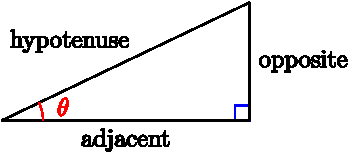
\includegraphics[width=\linewidth]{images/fig-2-2trigratios}
\end{sbspanel}%
\end{sidebyside}%
\end{assemblage}
%
\item{}The trigonometric ratio of an angle \(\theta\) is the same for every right triangle containing the angle.%
\item{}If we know one of the sides of a right triangle and any one of the other four parts, we can use trigonometry to find all the other unknown parts.%
\item{}If we know one of the trigonometric ratios of an acute angle, we can find the angle using the inverse trig key on a calculator.%
\item{}The exact values of trigonometric ratios of the special angles should be memorized.%
\begin{sidebyside}{1}{0}{0}{0}%
\begin{sbspanel}{1}%
{\centering%
{\tabularfont%
\begin{tabular}{AcAcAcAcA}\hrulethick
\multicolumn{4}{AcA}{Trigonometric Ratios for the Special Angles}\tabularnewline\hrulethin
Angle&Sine&Cosine&Tangent\tabularnewline\hrulethin
\(30\degree\)&\(\dfrac{1}{2} \)&\(\dfrac{\sqrt{3}}{2}\)&\(\dfrac{1}{\sqrt{3}} \)\tabularnewline\hrulethin
\(45\degree\)&\(\dfrac{1}{\sqrt{2}}\)&\(\dfrac{1}{\sqrt{2}}\)&\(1\)\tabularnewline\hrulethin
\(60\degree\)&\(\dfrac{\sqrt{3}}{2} \)&\(\dfrac{1}{2} \)&\(\sqrt{3} \)\tabularnewline\hrulethin
\end{tabular}
}%
\par}
\end{sbspanel}%
\end{sidebyside}%
\item{}You can remember the trig values for the special angles if you memorize two triangles:%
\begin{sidebyside}{2}{0.18}{0.18}{0.17}%
\begin{sbspanel}{0.2}%
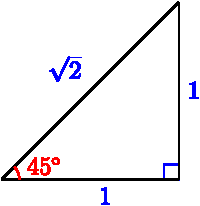
\includegraphics[width=\linewidth]{images/fig-45-45-90}
\end{sbspanel}%
\begin{sbspanel}{0.27}%
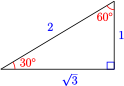
\includegraphics[width=\linewidth]{images/fig-30-60-90}
\end{sbspanel}%
\end{sidebyside}%
\item{}For the trigonometric ratios of most angles, your calculator gives approximations, not exact values.%
\end{enumerate}
%
\end{subsectionptx}
%
%
\typeout{************************************************}
\typeout{Exercises  Chapter 2 Review Problems}
\typeout{************************************************}
%
\begin{exercises-subsection}{Chapter 2 Review Problems}{}{Chapter 2 Review Problems}{}{}{x:exercises:chap2-rev-problems}
\par\medskip\noindent%
%
For Problems 1\textendash{}6, explain why the description of \(\triangle ABC\) is impossible.%
\begin{exercisegroupcol}{2}
\begin{divisionexerciseegcol}{1}{}{}{g:exercise:idm46051695749296}%
\(A \lt B \lt C\), and \(B = 93\degree\)%
\end{divisionexerciseegcol}%
\begin{divisionexerciseegcol}{2}{}{}{g:exercise:idm46051696179648}%
\(A \lt B \lt C\), and \(C = 58\degree\)%
\end{divisionexerciseegcol}%
\begin{divisionexerciseegcol}{3}{}{}{g:exercise:idm46051696208992}%
\(a \lt b \lt c,\) and \(C = 58\degree\)%
\end{divisionexerciseegcol}%
\begin{divisionexerciseegcol}{4}{}{}{g:exercise:idm46051696236768}%
\(a \lt b \lt c,\) and \(B =93\degree\)%
\end{divisionexerciseegcol}%
\end{exercisegroupcol}
\par\medskip\noindent
\begin{divisionexercise}{5}{}{}{g:exercise:idm46051695821520}%
\(A=80\degree,~B=50\degree,~ b=4,\) and \(c=6 \)%
\end{divisionexercise}%
\begin{divisionexercise}{6}{}{}{g:exercise:idm46051693400304}%
\(a = 23,~ b = 28,~ c=55,\) and \(A =30\degree\)%
\end{divisionexercise}%
\par\medskip\noindent%
%
For Problems 7 and 8, sketch the triangle.%
\begin{exercisegroup}
\begin{divisionexerciseeg}{7}{}{}{g:exercise:idm46051696588576}%
The three angles of a triangle are \(20\degree, 50\degree, \text{and}~ 110\degree,\) and the three sides are 15 cm, 6.7 cm, and 18.4 cm. Sketch and label the triangle.%
\end{divisionexerciseeg}%
\begin{divisionexerciseeg}{8}{}{}{g:exercise:idm46051685020032}%
Sketch and label an isosceles triangle with sides 5 in and 12 in, and one angle \(78\degree\).%
\end{divisionexerciseeg}%
\end{exercisegroup}
\par\medskip\noindent
\par\medskip\noindent%
%
For Problems 9\textendash{}12, find the unknown side of the right triangle.%
\begin{exercisegroupcol}{2}
\begin{divisionexerciseegcol}{9}{}{}{g:exercise:idm46051685017888}%
\begin{sidebyside}{1}{0.275}{0.275}{0}%
\begin{sbspanel}{0.45}%
\resizebox{\linewidth}{!}{%
\tikzset{%
}
\begin{tikzpicture}

\coordinate (C) at (0,0 );
\coordinate (A) at (-2.7,0);
\coordinate (B) at (0,-2.2);

\draw[blue,thick] (C) rectangle +(-0.25,-0.25);

\draw[black,thick](C)--(A) node[above,midway] {\color{blue}$72$};
\draw[black,thick](C)--(B) node[right,midway] {\color{blue}$65$};
\draw[black,thick](A)--(B) node[below left,midway] {\color{blue}$a$};
\end{tikzpicture}
}%
\end{sbspanel}%
\end{sidebyside}%
\end{divisionexerciseegcol}%
\begin{divisionexerciseegcol}{10}{}{}{g:exercise:idm46051685015072}%
\begin{sidebyside}{1}{0.225}{0.225}{0}%
\begin{sbspanel}{0.55}%
\resizebox{\linewidth}{!}{%
\tikzset{%
}
\begin{tikzpicture} [rotate=30.7]

\coordinate (C) at (0,0 );
\coordinate (A) at (3.2,0);
\coordinate (B) at (0,1.9);

\draw[blue,thick] (C) rectangle +(0.25,0.25);

\draw[black,thick](C)--(A) node[below right,midway] {\color{blue}$105$};
\draw[black,thick](C)--(B) node[below left,midway] {\color{blue}$88$};
\draw[black,thick](A)--(B) node[above,midway] {\color{blue}$b$};
\end{tikzpicture}
}%
\end{sbspanel}%
\end{sidebyside}%
\end{divisionexerciseegcol}%
\begin{divisionexerciseegcol}{11}{}{}{g:exercise:idm46051696653664}%
\begin{sidebyside}{1}{0.175}{0.175}{0}%
\begin{sbspanel}{0.65}%
\resizebox{\linewidth}{!}{%
\tikzset{%
}
\begin{tikzpicture} [rotate=206.565]

\coordinate (C) at (0,0 );
\coordinate (A) at (4,0);
\coordinate (B) at (0,2);

\draw[blue,thick] (C) rectangle +(0.25,0.25);

\draw[black,thick](C)--(A) node[above left,midway] {\color{blue}$c$};
\draw[black,thick](C)--(B) node[above right,midway] {\color{blue}$39$};
\draw[black,thick](A)--(B) node[below,midway] {\color{blue}$65$};
\end{tikzpicture}
}%
\end{sbspanel}%
\end{sidebyside}%
\end{divisionexerciseegcol}%
\begin{divisionexerciseegcol}{12}{}{}{g:exercise:idm46051696683008}%
\begin{sidebyside}{1}{0.1}{0.1}{0}%
\begin{sbspanel}{0.8}%
\resizebox{\linewidth}{!}{%
\tikzset{%
}
\begin{tikzpicture} 

\coordinate (C) at (0,0 );
\coordinate (A) at (-5.5,0);
\coordinate (B) at (0,1.6);

\draw[blue,thick] (C) rectangle +(-0.25,0.25);

\draw[black,thick](C)--(A) node[below,midway] {\color{blue}$168$};
\draw[black,thick](C)--(B) node[right,midway] {\color{blue}$d$};
\draw[black,thick](A)--(B) node[above ,midway] {\color{blue}$175$};
\end{tikzpicture}
}%
\end{sbspanel}%
\end{sidebyside}%
\end{divisionexerciseegcol}%
\end{exercisegroupcol}
\par\medskip\noindent
\begin{divisionexercise}{13}{}{}{g:exercise:idm46051696702704}%
A triangle has sides of length 33, 56, and 65.  Is it a right triangle?%
\end{divisionexercise}%
\begin{divisionexercise}{14}{}{}{g:exercise:idm46051696715200}%
A triangle has sides of length 22.5, 27.2, and 35.3.  Is it a right triangle?%
\end{divisionexercise}%
\begin{divisionexercise}{15}{}{}{g:exercise:idm46051696723120}%
\begin{sidebyside}{2}{0.08}{0.08}{0.16}%
\begin{sbspanel}{0.5}[center]%
Find the angle between the diagonal of a cube and the diagonal of one of the sides. (See the figure at right.)%
\end{sbspanel}%
\begin{sbspanel}{0.18}[center]%
\resizebox{\linewidth}{!}{%
\tikzset{%
}
\begin{tikzpicture}  [scale=0.9]

\coordinate (O) at (0,0 );
\coordinate (A) at (3,0);
\coordinate (B) at (3,3);
\coordinate (C) at (0,3);

\coordinate (D) at (0.4,1);
\coordinate (E) at (3.4,1);
\coordinate (F) at (3.4,4);
\coordinate (G) at (0.4,4);

\draw[red,thick](O)--(E);
\draw[red,thick](O)--(F);
\draw[gray!50!white,thick](O)--(D);
\draw[gray!50!white,thick](G)--(D)--(E);
\draw[black,thick](A)--(E)--(F)--(G)--(C);
\draw[black,thick](B)--(F);
\draw[black,thick](A)--(B)--(C)--(O)--cycle;

\draw[gray,thick] (.68,.2) arc({atan(1/3.4)}:{atan(4/3.4)}:.7) node[above right,midway, yshift=-3]{\color{red}$\theta$};
\end{tikzpicture}
}%
\end{sbspanel}%
\end{sidebyside}%
\end{divisionexercise}%
\begin{divisionexercise}{16}{}{}{g:exercise:idm46051701477888}%
\begin{sidebyside}{2}{0.08}{0.08}{0.16}%
\begin{sbspanel}{0.5}[center]%
Find the angle between the diagonal of a cube and one edge. (See the figure at right.)%
\end{sbspanel}%
\begin{sbspanel}{0.18}[center]%
\resizebox{\linewidth}{!}{%
\tikzset{%
}
\begin{tikzpicture} [scale=0.9]

\coordinate (O) at (0,0 );
\coordinate (A) at (3,0);
\coordinate (B) at (3,3);
\coordinate (C) at (0,3);

\coordinate (D) at (0.4,1);
\coordinate (E) at (3.4,1);
\coordinate (F) at (3.4,4);
\coordinate (G) at (0.4,4);

\draw[red,thick](O)--(F);
\draw[gray!50!white,thick](O)--(D);
\draw[gray!50!white,thick](G)--(D)--(E);
\draw[black,thick](A)--(E)--(F)--(G)--(C);
\draw[black,thick](B)--(F);
\draw[black,thick](A)--(B)--(C)--(O)--cycle;

\draw[red,thick](O)--(A);
\draw[gray,thick] (.7,0) arc(0:{atan(4/3.4)}:.7) node[above right,midway, yshift=-4]{\color{red}$\theta$};
\end{tikzpicture}
}%
\end{sbspanel}%
\end{sidebyside}%
\end{divisionexercise}%
\begin{divisionexercise}{17}{}{}{g:exercise:idm46051701474448}%
\begin{sidebyside}{2}{0.0825}{0.0825}{0.165}%
\begin{sbspanel}{0.55}%
In the triangle shown, \(\cos \theta = \dfrac{3}{5}\). Can we conclude that \(a = 3\) and \(c = 5\)?  Give two other possibilities for the values of \(a\) and \(c\).%
\end{sbspanel}%
\begin{sbspanel}{0.12}%
\resizebox{\linewidth}{!}{%
\tikzset{%
}
\begin{tikzpicture} [scale=0.9]

\coordinate (O) at (0,0 );
\coordinate (A) at (-1.5,0);
\coordinate (B) at (0,2.3);

\draw[blue,thick] (O) rectangle +(-0.25,0.25);
\draw[black,thick](B)--(O) node[right,midway] {\color{blue}$b$};
\draw[black,thick](A)--(B) node[above left,midway] {\color{blue}$c$};
\draw[black,thick](A)--(O) node[below,midway] {\color{blue}$a$};

\draw[red,thick] (A)++(.3,0) arc(0:{atan(2.3/1.5)}:.3) node[above right,midway, yshift=-3]{\color{red}$\theta$};
\end{tikzpicture}
}%
\end{sbspanel}%
\end{sidebyside}%
\end{divisionexercise}%
\begin{divisionexercise}{18}{}{}{g:exercise:idm46051696796192}%
\begin{sidebyside}{2}{0.0825}{0.0825}{0.165}%
\begin{sbspanel}{0.55}%
In the triangle shown, \(\tan \theta = \dfrac{5}{3}\). Can we conclude that \(a = 5\) and \(b = 3\)?  Give two other possibilities for the values of \(a\) and \(b\)%
\end{sbspanel}%
\begin{sbspanel}{0.12}%
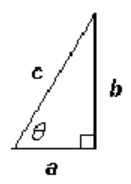
\includegraphics[width=\linewidth]{images/hp2-sum-17}
\end{sbspanel}%
\end{sidebyside}%
\end{divisionexercise}%
\par\medskip\noindent%
%
For Problems 19\textendash{}22,%
\par
%
\begin{enumerate}[label=\alph*]
\item{}Find the unknown side.%
\item{}Find the sine, cosine, and tangent of \(\theta\).  Round your answers to four decimal places.%
\end{enumerate}
%
\begin{exercisegroupcol}{2}
\begin{divisionexerciseegcol}{19}{}{}{g:exercise:idm46051696849520}%
\begin{sidebyside}{1}{0.225}{0.225}{0}%
\begin{sbspanel}{0.55}%
\resizebox{\linewidth}{!}{%
\tikzset{%
}
\begin{tikzpicture}

\coordinate (O) at (0,0 );
\coordinate (A) at (3.35,0);
\coordinate (B) at (0,2.7);

\draw[blue,thick] (O) rectangle +(0.25,0.25);
\draw[black,thick](B)--(O) node[left,midway] {\color{blue}$54$};
\draw[black,thick](A)--(B) node[above right,midway] {\color{blue}$w$};
\draw[black,thick](A)--(O) node[below,midway] {\color{blue}$67$};

\draw[red,thick] (B)++(0,-.4) arc(-90:{-atan(2.7/3.35)}:.4) node[below right,midway, xshift=-3]{\color{red}$\theta$};

\end{tikzpicture}
}%
\end{sbspanel}%
\end{sidebyside}%
\end{divisionexerciseegcol}%
\begin{divisionexerciseegcol}{20}{}{}{g:exercise:idm46051696898768}%
\begin{sidebyside}{1}{0.175}{0.175}{0}%
\begin{sbspanel}{0.65}%
\resizebox{\linewidth}{!}{%
\tikzset{%
}
\begin{tikzpicture} [rotate=212]

\coordinate (O) at (0,0 );
\coordinate (A) at (4,0);
\coordinate (B) at (0,2.5);

\draw[blue,thick] (O) rectangle +(0.25,0.25);
\draw[black,thick](B)--(O) node[above right,midway] {\color{blue}$3.2$};
\draw[black,thick](A)--(B) node[below,midway] {\color{blue}$x$};
\draw[black,thick](A)--(O) node[above left,midway] {\color{blue}$4.4$};

\draw[red,thick] (A)++(-.6,0) arc(180:{180-atan(2.5/4)}:.6) node[right,midway, yshift=2]{\color{red}$\theta$};
\end{tikzpicture}
}%
\end{sbspanel}%
\end{sidebyside}%
\end{divisionexerciseegcol}%
\begin{divisionexerciseegcol}{21}{}{}{g:exercise:idm46051696940944}%
\begin{sidebyside}{1}{0.225}{0.225}{0}%
\begin{sbspanel}{0.55}%
\resizebox{\linewidth}{!}{%
\tikzset{%
}
\begin{tikzpicture} [rotate=52]

\coordinate (O) at (0,0 );
\coordinate (A) at (2.5,0);
\coordinate (B) at (0,3.2);

\draw[blue,thick] (O) rectangle +(0.25,0.25);
\draw[black,thick](B)--(O) node[below left,midway] {\color{blue}$y$};
\draw[black,thick](A)--(B) node[above,midway] {\color{blue}$23$};
\draw[black,thick](A)--(O) node[below right,midway] {\color{blue}$16$};

\draw[red,thick] (B)++(0,-.6) arc(-90:{-atan(3.2/2.5)}:.6) node[right,midway, yshift=-2]{\color{red}$\theta$};
\end{tikzpicture}
}%
\end{sbspanel}%
\end{sidebyside}%
\end{divisionexerciseegcol}%
\begin{divisionexerciseegcol}{22}{}{}{g:exercise:idm46051696969888}%
\begin{sidebyside}{1}{0.3}{0.3}{0}%
\begin{sbspanel}{0.4}%
\resizebox{\linewidth}{!}{%
\tikzset{%
}
\begin{tikzpicture}

\coordinate (O) at (0,0 );
\coordinate (A) at (-2.5,0);
\coordinate (B) at (0,2.7);

\draw[blue,thick] (O) rectangle +(-0.25,0.25);
\draw[black,thick](B)--(O) node[right,midway] {\color{blue}$z$};
\draw[black,thick](A)--(B) node[above left,midway] {\color{blue}$38$};
\draw[black,thick](A)--(O)node[below,midway] {\color{blue}$29$};

\draw[red,thick] (A)++(.3,0) arc(0:{atan(2.7/2.5)}:.3) node[right,midway, yshift=2]{\color{red}$\theta$};
\end{tikzpicture}
}%
\end{sbspanel}%
\end{sidebyside}%
\end{divisionexerciseegcol}%
\end{exercisegroupcol}
\par\medskip\noindent
\par\medskip\noindent%
%
For Problems 23\textendash{}28,find the unknown side of the triangle. Round your answer to hundredths.%
\begin{exercisegroupcol}{3}
\begin{divisionexerciseegcol}{23}{}{}{g:exercise:idm46051696985696}%
\begin{sidebyside}{1}{0.05}{0.05}{0}%
\begin{sbspanel}{0.9}%
\resizebox{\linewidth}{!}{%
\tikzset{%
}
\begin{tikzpicture} [scale=1.2, rotate=197]

\coordinate (O) at (0,0 );
\coordinate (A) at (2.8689,0);
\coordinate (B) at (0,0.8771);

\draw[blue,thick] (O) rectangle +(0.2,0.2);
\draw[black,thick](B)--(O) node[above right,midway, yshift=-3] {\color{blue}$a$};
\draw[black,thick](A)--(B) node[below,midway] {\color{blue}$27$};
\draw[black,thick](A)--(O);

\draw[red,thick] (B)++(0,-.3) arc(-90:-17:.3) node[left,midway, xshift=2, yshift=2]{\footnotesize\color{red}$73\degree$};
\end{tikzpicture}
}%
\end{sbspanel}%
\end{sidebyside}%
\end{divisionexerciseegcol}%
\begin{divisionexerciseegcol}{24}{}{}{g:exercise:idm46051696999232}%
\begin{sidebyside}{1}{0.075}{0.075}{0}%
\begin{sbspanel}{0.85}%
\resizebox{\linewidth}{!}{%
\tikzset{%
}
\begin{tikzpicture} [rotate=231]

\coordinate (O) at (0,0 );
\coordinate (A) at (2.26555,0);
\coordinate (B) at (0,2.7977);

\draw[blue,thick] (O) rectangle +(0.25,0.25);
\draw[black,thick](B)--(O) node[above right,midway, yshift=-3] {\color{blue}$d$};
\draw[black,thick](A)--(B) node[below,midway] {\color{blue}$36$};
\draw[black,thick](A)--(O);

\draw[red,thick] (A)++(-.4,0) arc(180:129:.4) node[right,midway,  yshift=3]{\color{red}$51\degree$};
\end{tikzpicture}
}%
\end{sbspanel}%
\end{sidebyside}%
\end{divisionexerciseegcol}%
\begin{divisionexerciseegcol}{25}{}{}{g:exercise:idm46051697010080}%
\begin{sidebyside}{1}{0.1}{0.1}{0}%
\begin{sbspanel}{0.8}%
\resizebox{\linewidth}{!}{%
\tikzset{%
}
\begin{tikzpicture} [rotate=63]

\coordinate (O) at (0,0 );
\coordinate (A) at (1.453,0);
\coordinate (B) at (0,2.851);

\draw[blue,thick] (O) rectangle +(0.25,0.25);
\draw[black,thick](B)--(O) node[below left,midway] {\color{blue}$7$};
\draw[black,thick](A)--(B);
\draw[black,thick](A)--(O) node[right,midway] {\color{blue}$x$};

\draw[red,thick] (B)++(0,-.7) arc(-90:-63:.7) node[right,midway,  yshift=-2]{\color{red}$27\degree$};
\end{tikzpicture}
}%
\end{sbspanel}%
\end{sidebyside}%
\end{divisionexerciseegcol}%
\begin{divisionexerciseegcol}{26}{}{}{g:exercise:idm46051697031104}%
\begin{sidebyside}{1}{0.075}{0.075}{0}%
\begin{sbspanel}{0.85}%
\resizebox{\linewidth}{!}{%
\tikzset{%
}
\begin{tikzpicture} 

\coordinate (O) at (0,0 );
\coordinate (A) at (3.2,0);
\coordinate (B) at (0,-2.4);

\draw[blue,thick] (O) rectangle +(0.25,-0.25);
\draw[black,thick](B)--(O) node[left,midway] {\color{blue}$2$};
\draw[black,thick](A)--(B) node[below right,midway] {\color{blue}$z$};
\draw[black,thick](A)--(O);

\draw[red,thick] (A)++(-.7,0) arc(180:{180+atan(2.4/3.2)}:.7) node[left,midway,  yshift=-2]{\color{red}$38\degree$};
\end{tikzpicture}
}%
\end{sbspanel}%
\end{sidebyside}%
\end{divisionexerciseegcol}%
\begin{divisionexerciseegcol}{27}{}{}{g:exercise:idm46051697041728}%
\begin{sidebyside}{1}{0.05}{0.05}{0}%
\begin{sbspanel}{0.9}%
\resizebox{\linewidth}{!}{%
\tikzset{%
}
\begin{tikzpicture} 

\coordinate (O) at (0,0 );
\coordinate (A) at (3.3,0);
\coordinate (B) at (0,2.1);

\draw[blue,thick] (O) rectangle +(0.25,0.25);
\draw[black,thick](B)--(O) node[left,midway] {\color{blue}$87$};
\draw[black,thick](A)--(B);
\draw[black,thick](A)--(O) node[below,midway] {\color{blue}$b$};

\draw[red,thick] (A)++(-.7,0) arc(180:{180-atan(2.1/3.3)}:.7) node[left,midway,  yshift=2]{\color{red}$29\degree$};
\end{tikzpicture}
}%
\end{sbspanel}%
\end{sidebyside}%
\end{divisionexerciseegcol}%
\begin{divisionexerciseegcol}{28}{}{}{g:exercise:idm46051697056816}%
\begin{sidebyside}{1}{0.225}{0.225}{0}%
\begin{sbspanel}{0.55}%
\resizebox{\linewidth}{!}{%
\tikzset{%
}
\begin{tikzpicture} 

\coordinate (O) at (0,0 );
\coordinate (A) at (-2,0);
\coordinate (B) at (0,2.1);

\draw[blue,thick] (O) rectangle +(-0.25,0.25);
\draw[black,thick](B)--(O) node[right,midway] {\color{blue}$c$};
\draw[black,thick](A)--(B) node[above left,midway] {\color{blue}$10$};
\draw[black,thick](A)--(O);

\draw[red,thick] (B)++(0,-.7) arc(270:{270-atan(2.1/2.1)}:.7) node[below,midway,  xshift=-2]{\small\color{red}$47\degree$};

\end{tikzpicture}
}%
\end{sbspanel}%
\end{sidebyside}%
\end{divisionexerciseegcol}%
\end{exercisegroupcol}
\par\medskip\noindent
\par\medskip\noindent%
%
For Problems 29\textendash{}32,solve the triangle. Give exact values.%
\begin{exercisegroupcol}{2}
\begin{divisionexerciseegcol}{29}{}{}{g:exercise:idm46051697097712}%
\begin{sidebyside}{1}{0.25}{0.25}{0}%
\begin{sbspanel}{0.5}%
\resizebox{\linewidth}{!}{%
\tikzset{%
}
\begin{tikzpicture} [scale=1.6]

\coordinate (O) at (0,0 );
\coordinate (A) at (-1.732,0);
\coordinate (B) at (0,-1);

\filldraw[black] (O) circle (.1pt) node[anchor=south west] {$C$};
\filldraw[black] (A) circle (.1pt) node[anchor=east] {$A$};
\filldraw[black] (B) circle (.1pt) node[anchor=north west] {$B$};

\draw[blue,thick] (O) rectangle +(-0.15,-0.15);
\draw[black,thick](B)--(O);
\draw[black,thick](A)--(B);
\draw[black,thick](A)--(O) node[above,midway] {\color{blue}$23$};

\draw[red,thick] (B)++(0,.2) arc(90:150:.2) node[above,midway,  xshift=-2]{\small\color{red}$60\degree$};
\end{tikzpicture}
}%
\end{sbspanel}%
\end{sidebyside}%
\end{divisionexerciseegcol}%
\begin{divisionexerciseegcol}{30}{}{}{g:exercise:idm46051697134416}%
\begin{sidebyside}{1}{0.25}{0.25}{0}%
\begin{sbspanel}{0.5}%
\resizebox{\linewidth}{!}{%
\tikzset{%
}
\begin{tikzpicture}

\coordinate (C) at (0,0 );
\coordinate (A) at (-2.8,0);
\coordinate (B) at (0,-2.8);

\filldraw[black] (C) circle (.1pt) node[anchor=west] {$C$};
\filldraw[black] (A) circle (.1pt) node[anchor=east] {$A$};
\filldraw[black] (B) circle (.1pt) node[anchor=west] {$B$};

\draw[blue,thick] (O) rectangle +(-0.25,-0.25);
\draw[black,thick](B)--(O);
\draw[black,thick](A)--(B) node[below left,midway] {\color{blue}$14$};
\draw[black,thick](A)--(O);

\draw[red,thick] (B)++(0,.5) arc(90:135:.5) node[above,midway,  xshift=-2]{\small\color{red}$45\degree$};
\end{tikzpicture}
}%
\end{sbspanel}%
\end{sidebyside}%
\end{divisionexerciseegcol}%
\begin{divisionexerciseegcol}{31}{}{}{g:exercise:idm46051697167008}%
\begin{sidebyside}{1}{0.1}{0.1}{0}%
\begin{sbspanel}{0.8}%
\resizebox{\linewidth}{!}{%
\tikzset{%
}
\begin{tikzpicture}

\coordinate (C) at (0,0 );
\coordinate (D) at (-3.464,0);
\coordinate (E) at (2,0);
\coordinate (F) at (0,2);

\filldraw[black] (D) circle (.1pt) node[anchor=south, yshift=2] {$D$};
\filldraw[black] (E) circle (.1pt) node[anchor=south, yshift=2] {$E$};
\filldraw[black] (F) circle (.1pt) node[anchor=east, yshift=2] {$F$};

\draw[blue,thick] (O) rectangle +(-0.25,0.25);
\draw[black,thick] (D)--(E)--(F)--(D);
\draw[gray,thick, dashed] (C)--(F) node[left,midway] {\color{blue}$10$};

\draw[red,thick] (D)++(.5,0) arc(0:30:.5) node[right,midway,  yshift=2]{\small\color{red}$30\degree$};
\draw[red,thick] (E)++(-.4,0) arc(180:135:.4) node[left,midway,  yshift=2]{\small\color{red}$45\degree$};
\end{tikzpicture}
}%
\end{sbspanel}%
\end{sidebyside}%
\end{divisionexerciseegcol}%
\begin{divisionexerciseegcol}{32}{}{}{g:exercise:idm46051696029184}%
\begin{sidebyside}{1}{0.25}{0.25}{0}%
\begin{sbspanel}{0.5}%
\resizebox{\linewidth}{!}{%
\tikzset{%
}
\begin{tikzpicture}

\coordinate (C) at (0,0 );
\coordinate (D) at (0,2.4);
\coordinate (E) at (0,-1.386);
\coordinate (F) at (2.4,0);

\filldraw[black] (D) circle (.1pt) node[anchor=east] {$D$};
\filldraw[black] (E) circle (.1pt) node[anchor=east] {$E$};
\filldraw[black] (F) circle (.1pt) node[anchor=west] {$F$};

\draw[blue,thick] (O) rectangle +(0.25,0.25);
\draw[black,thick] (D)--(E)--(F)--(D);
\draw[gray,thick, dashed] (C)--(F) node[above,midway] {\color{blue}$12$};

\draw[red,thick] (D)++(0,-.5) arc(-90:-45:.5) node[below,midway,  xshift=4]{\small\color{red}$45\degree$};
\draw[red,thick] (E)++(0,.3) arc(90:30:.3) node[above,midway,  xshift=6]{\small\color{red}$60\degree$};
\end{tikzpicture}
}%
\end{sbspanel}%
\end{sidebyside}%
\end{divisionexerciseegcol}%
\end{exercisegroupcol}
\par\medskip\noindent
\begin{divisionexercise}{33}{}{}{g:exercise:idm46051696026192}%
\begin{sidebyside}{2}{0.0375}{0.0375}{0.075}%
\begin{sbspanel}{0.6}[center]%
Find the diameter of a hex nut if one of the sides is 1.5 cm.%
\end{sbspanel}%
\begin{sbspanel}{0.25}[center]%
\resizebox{\linewidth}{!}{%
\tikzset{%
}
\begin{tikzpicture} [scale=.8]

\coordinate (O) at (0,0 );
\coordinate (A) at (2,0);
\coordinate (B) at (1,1.732);
\coordinate (C) at (-1,1.732);
\coordinate (D) at (-2,0);
\coordinate (E) at (-1,-1.732);
\coordinate (F) at (1,-1.732);

\draw[black,thick] (A)--(B) node[left,midway] {\small\color{blue}1.5};
\draw[black,thick] (C)--(B) node[below,midway] {\small\color{blue}1.5};
\draw[black,thick] (C)--(D) node[right,midway] {\small\color{blue}1.5};
\draw[black,thick] (D)--(E) node[left,midway] {\small\color{blue}1.5};
\draw[black,thick] (F)--(E) node[below,midway] {\small\color{blue}1.5};
\draw[black,thick] (F)--(A) node[right,midway] {\small\color{blue}1.5};

\draw[gray!60!white,thick, dashed] (A)--(D);
\draw[gray!60!white,thick, dashed] (B)--(E);
\draw[gray!60!white,thick, dashed] (C)--(F);

\draw[gray!60!white,thick] (D)++(0,.2)--+(0,2.15);
\draw[gray!60!white,thick] (A)++(0,.2)--+(0,2.15);
\draw[gray!60!white,thick, <-] (D)++(0,2.1)--+(.9,0) node[right, xshift=1] {\small\color{blue}diameter};
\draw[gray!60!white,thick, <-] (A)++(0,2.1)--+(-.9,0);
\end{tikzpicture}
}%
\end{sbspanel}%
\end{sidebyside}%
\end{divisionexercise}%
\begin{divisionexercise}{34}{}{}{g:exercise:idm46051697216288}%
\begin{sidebyside}{2}{0.025}{0.025}{0.05}%
\begin{sbspanel}{0.6}[center]%
Find the long edge of the trapezoidal block of height 3 centimeters.%
\end{sbspanel}%
\begin{sbspanel}{0.3}[center]%
\resizebox{\linewidth}{!}{%
\tikzset{%
}
\begin{tikzpicture} [scale=.85]

\coordinate (O) at (0,0 );
\coordinate (A) at (2.6,0);
\coordinate (B) at (1.3,2.25);
\coordinate (C) at (-1.3,2.25);
\coordinate (D) at (-2.6,0);
\coordinate (E) at (0,2.25);

\draw[black,thick] (A)--(B)--(C)--(D)--(A);
\draw[gray,thick, dashed] (O)--(E) node[midway,fill=white, yshift=3] {\small\color{blue}3 cm};
\draw[gray,thick] (B)--(O)--(C);

\draw[red,thick] (D)++(.4,0) arc(0:60:.4);
\draw[red,thick] (D)++(.2,.115) -- +(.35,.17);

\draw[red,thick] (O)++(.4,0) arc(0:60:.4);
\draw[red,thick] (O)++(.2,.115) -- +(.35,.17);
\draw[red,thick] (O)++(-.4,0) arc(180:120:.4);
\draw[red,thick] (O)++(-.2,.115) -- +(-.35,.17);

\draw[red,thick] (A)++(-.4,0) arc(180:120:.4);
\draw[red,thick] (A)++(-.2,.115) -- +(-.35,.17);

\draw[red,thick] (C)++(-.2,-.346) arc(240:300:.4);
\draw[red,thick] (C)++(0,-.25) -- +(0,-.32);
\end{tikzpicture}
}%
\end{sbspanel}%
\end{sidebyside}%
\end{divisionexercise}%
\begin{divisionexercise}{35}{}{}{g:exercise:idm46051697220288}%
\begin{sidebyside}{2}{0.045}{0.045}{0.09}%
\begin{sbspanel}{0.6}[center]%
If a stop sign is 80 centimeters across, what is the radius of a circle that circumscribes the stop sign?%
\end{sbspanel}%
\begin{sbspanel}{0.22}[center]%
\resizebox{\linewidth}{!}{%
\tikzset{%
 }
\begin{tikzpicture} [rotate=22.5]

\coordinate(O) at (0,0);
\coordinate (A) at (2,0 );
\coordinate (B) at (1.414,1.414);
\coordinate (C) at(0,2);
\coordinate (D) at (-1.414,1.414);
\coordinate (E) at(-2,0);
\coordinate (F) at(-1.414,-1.414);
\coordinate (G) at(0,-2);
\coordinate (H) at (1.414,-1.414);

\draw[black] (O) circle(2);

\draw[gray] (D)++(0.06,0.1414) -- +(.6,1.414);
\draw[gray, <-] (D)++(.6,1.414) -- +(1.131,-.48) node[right] {\color{blue}80 cm};
\draw[gray] (A)++(0.06,0.1414) -- +(.6,1.414);
\draw[gray, <-] (A)++(.6,1.414) -- +(-1.131,.48);

\filldraw[red,thick] (A)--(B)--(C)--(D)--(E)--(F)--(G)--(H)--(A);
\node [text width=2cm,font=\sffamily] at (O) {\Huge\color{white}STOP};
\end{tikzpicture}
}%
\end{sbspanel}%
\end{sidebyside}%
\end{divisionexercise}%
\begin{divisionexercise}{36}{}{}{g:exercise:idm46051701792368}%
\begin{sidebyside}{2}{0.025}{0.025}{0.05}%
\begin{sbspanel}{0.6}%
The Pentagon, which houses the U.S. Department of Defense, is in the shape of a regular pentagon.  Each of the five outer walls is 921.6 feet long.  What is the shortest distance from one of the outer walls to the opposite vertex of the pentagon?%
\end{sbspanel}%
\begin{sbspanel}{0.3}%
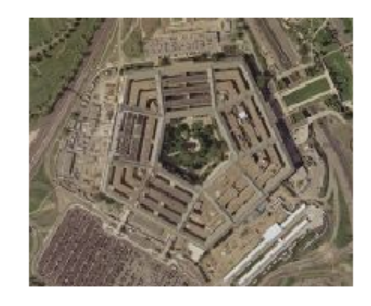
\includegraphics[width=\linewidth]{images/hp2-sum-36.png}
\end{sbspanel}%
\end{sidebyside}%
\end{divisionexercise}%
\begin{divisionexercise}{37}{}{}{g:exercise:idm46051701790304}%
A building casts a 12 meter shadow. At that moment, the sun is \(53\degree\) above the horizon. How tall is the building?%
\end{divisionexercise}%
\begin{divisionexercise}{38}{}{}{g:exercise:idm46051697142384}%
A ramp is rising at an angle \(25\degree\) from horizontal. What is the distance (along the ramp) from the base of the ramp to the point on the ramp that is 1 meter higher than the base of the ramp?%
\end{divisionexercise}%
\begin{divisionexercise}{39}{}{}{g:exercise:idm46051697309632}%
A baseball diamond is a square with sides 90 feet long. The corners are called (in clockwise order) first base, second base, third base, and home plate. The sides are called baselines. A runner is on the baseline between first and second base, 20 feet from second base. How far is the runner from home plate? What is the angle between the baseline from home plate to first base and the line from home plate to the runner?%
\end{divisionexercise}%
\begin{divisionexercise}{40}{}{}{g:exercise:idm46051697322176}%
A runner is on the baseline between second and third base, 10 feet from second base. How far is the runner from home plate?  What is the angle between the baseline from home plate to third base and the line from home plate to the runner?%
\end{divisionexercise}%
\begin{divisionexercise}{41}{}{}{g:exercise:idm46051697325968}%
Let \(l\) be the line that passes through the origin and the point \((4,7)\). Let \(\theta\) be the angle that \(l\) makes with the positive \(x\)-axis.%
\par
%
\begin{enumerate}[label=\alph*]
\item{}Find the value of \(\theta\). Hint: Draw the triangle with vertices at the origin, \((4,7)\), and \((4,0)\), labeling the angle at the origin \(\theta\). What is \(\tan \theta\) ?)%
\item{}Let \(l ^{\prime}\) be any line parallel to \(l\). Find the measure of the acute angle that \(l ^{\prime}\) makes with the positive \(x\)-axis.%
\item{}What is the slope of the line \(l\) ?  How is it related to \(\tan \theta\) ?%
\end{enumerate}
%
\end{divisionexercise}%
\begin{divisionexercise}{42}{}{}{g:exercise:idm46051697388912}%
Let \(l\) be the line that passes through the origin and the point \((a,b)\), where \(a\) and \(b\) are positive numbers. Let \(\theta\) be the angle that \(l\) makes with the positive \(x\)-axis.%
\par
%
\begin{enumerate}[label=\alph*]
\item{}Find the value of \(\theta\). Hint: Draw the triangle with vertices at the origin, \((a,b)\), and \((a,0)\), labeling the angle at the origin \(\theta\). What is \(\tan \theta\) ?)%
\item{}What is the slope of the line \(l\) ? How is it related to \(\tan \theta\)?%
\item{}Let \(l ^{\prime}\) be any line parallel to \(l\). How is the slope of the line \(l ^{\prime}\) related to \(\tan \theta\)?%
\end{enumerate}
%
\end{divisionexercise}%
\begin{divisionexercise}{43}{}{}{g:exercise:idm46051697486992}%
\begin{sidebyside}{2}{0.0125}{0.0125}{0.025}%
\begin{sbspanel}{0.7}[center]%
The figure illustrates the Pythagorean theorem.%
\begin{enumerate}[label=\alph*]
\item{}What is the area of the whole square?%
\item{}What is the side of the smaller interior square? What is its area?%
\item{}What is the area of one of the right triangles?%
\item{}Add the areas of the four triangles and the smaller square to obtain another expression for the area of the whole square.%
\end{enumerate}
%
\end{sbspanel}%
\begin{sbspanel}{0.25}[center]%
\resizebox{\linewidth}{!}{%
\tikzset{%
}
\begin{tikzpicture} 

\coordinate(O) at (0,0);
\coordinate (A) at (3.2,0 );
\coordinate (B) at (3.2,3.2);
\coordinate (C) at(0,3.2);
\coordinate (D) at (2.4,1.4);
\coordinate (E) at(1.8,2.4);
\coordinate (F) at(0.8,1.8);
\coordinate (G) at(1.4,0.8);

\draw[blue,thick] (D)++(-.175,-.1)--++(.1,-.175)--++(.175,.1);
\draw[blue,thick] (E)++(.1,-.175)--++(.175,.1)--++(-.1,.175);
\draw[blue,thick] (F)++(.175,.1)--++(-.1,.175)--++(-.175,-.1);
\draw[blue,thick] (G)++(-.1,.175)--++(-.175,-.1)--++(.1,-.175);

\draw[black, thick] (O)--(A) node[below,midway] {\color{blue}$c$};
\draw[black, thick] (B)--(A) node[right,midway] {\color{blue}$c$};
\draw[black, thick] (B)--(C) node[above,midway] {\color{blue}$c$};
\draw[black, thick] (O)--(C) node[left,midway] {\color{blue}$c$};

\draw[black, thick] (O)--(G) node[above,midway] {\color{blue}$a$};
\draw[black, thick] (O)--(D) node[below,midway] {\color{blue}$b$};

\draw[black, thick] (A)--(D) node[below left, xshift=2, yshift=3,midway] {\color{blue}$a$};
\draw[black, thick] (A)--(E) node[above,midway, xshift=2] {\color{blue}$b$};

\draw[black, thick] (B)--(E) node[below,midway, xshift=1] {\color{blue}$a$};
\draw[black, thick] (B)--(F) node[above,midway,xshift=-4,yshift=-3] {\color{blue}$b$};

\draw[black, thick] (C)--(F) node[above,midway, xshift=5,yshift=-3] {\color{blue}$a$};
\draw[black, thick] (C)--(G) node[below,midway, xshift=-2] {\color{blue}$b$};

\draw[black, thick] (O)--(A)--(B)--(C)--(O)--(D);
\draw[black, thick] (A)--(E);
\draw[black, thick] (B)--(F);
\draw[black, thick] (C)--(G);
\end{tikzpicture}
}%
\end{sbspanel}%
\end{sidebyside}%
\end{divisionexercise}%
\begin{divisionexercise}{44}{}{}{g:exercise:idm46051697540784}%
\begin{sidebyside}{2}{0.0375}{0.0375}{0.075}%
\begin{sbspanel}{0.6}[center]%
The figure illustrates a proof of the Pythagorean theorem given by Euclid. It shows that the area of the square on the hypotenuse \(\overline{AB}\) is the sum of the areas of the squares on legs \(\overline{BC}\) and \(\overline{AC}\). We first draw a line segment from point \(C\) perpendicular to the hypotenuse \(\overline{AB}\) to meet the far side of the square on the hypotenuse. This segment meets \(\overline{AB}\) at \(G\) and the opposite side of the square at \(D\).%
\end{sbspanel}%
\begin{sbspanel}{0.25}[center]%
\resizebox{\linewidth}{!}{%
\tikzset{%
}
\begin{tikzpicture} 

\coordinate(C) at (0,0);
\coordinate (A) at (1.732,0 );
\coordinate (B) at (0,1);
\coordinate (D) at (1.433,2.482);
\coordinate (E) at(2.732,1.732);
\coordinate (F) at(1.732,-1.732);
\coordinate (G) at(0.433,0.75);
\coordinate (H) at(1,2.732);

\filldraw[black] (A) circle (0.2pt) node[anchor=west] {$A$};
\filldraw[black] (B) circle (0.2pt) node[anchor=south east] {$B$};
\filldraw[black] (C) circle (0.2pt) node[anchor=north east] {$C$};
\filldraw[black] (D) circle (0.2pt) node[anchor=south west] {$D$};
\filldraw[black] (E) circle (0.2pt) node[anchor=west] {$E$};
\filldraw[black] (F) circle (0.2pt) node[anchor=north west] {$F$};
\filldraw[black] (H) circle (0.2pt) node[anchor=east] {$H$};


\draw[black, thick] (A)--(E)--(H)--(B);
\draw[black, thick] (C) rectangle +(-1,1);
\draw[black, thick] (C) rectangle +(1.732,-1.732);
\draw[red, thick] (C)--(A)--(B)--(C);
\filldraw[blue] (G) circle (1.5pt) node[anchor=west, yshift=3] {\color{black}$G$};

\draw[green] (B)--(F);

\draw[gray!70!white] (C)--(E);
\draw[gray!70!white] (C)--(D);
\end{tikzpicture}
}%
\end{sbspanel}%
\end{sidebyside}%
\par
%
\begin{enumerate}[label=\alph*]
\item{}How does the area of \(\triangle ACE\) compare with the area of \(\triangle ABF\) ? (Hint:  Show that the triangles are congruent.)%
\item{}How does the area of \(\triangle ABF\) compare with the area of the square on \(\overline{AC}\)? (Hint: Consider \(\overline{AF}\) to be the base of the triangle. What is the height?)%
\item{}How does the area of \(\triangle ACE\) compare with the area of the rectangle \(AGDE\) ? (Hint: Consider \(\overline{AE}\) to be the base of the triangle. What is the height?)%
\item{}Explain why the area of the square on \(\overline{AC}\) equals the area of the rectangle \(AGDE\).%
\item{}An argument similar to parts (a)\textendash{}(d) will show that the area of the square on \(\overline{BC}\) equals the area of the rectangle \(BGDH\). Explain how writing the area of the square on \(\overline{AB}\) as the sum of the areas of two rectangles gives the Pythagorean theorem.%
\end{enumerate}
%
\end{divisionexercise}%
\end{exercises-subsection}
\end{sectionptx}
\end{chapterptx}
%
%
\typeout{************************************************}
\typeout{Chapter 3 Laws of Sines and Cosines}
\typeout{************************************************}
%
\begin{chapterptx}{Laws of Sines and Cosines}{}{Laws of Sines and Cosines}{}{}{x:chapter:chap3}
\begin{introduction}{}%
\begin{sidebyside}{2}{0}{0}{0}%
\begin{sbspanel}{0.6}[center]%
%
\begin{itemize}[label=\textbullet]
\item{}\(\displaystyle \blert{\textbf{Obtuse Angles}}\)%
\item{}\(\displaystyle \blert{\textbf{The Law of Sines}}\)%
\item{}\(\displaystyle \blert{\textbf{The Law of Cosines}}\)%
\end{itemize}
%
\end{sbspanel}%
\begin{sbspanel}{0.4}[center]%
\includegraphics[width=\linewidth]{images/ch3-1.png}
\end{sbspanel}%
\end{sidebyside}%
\par
The first science developed by humans is probably astronomy. Before the invention of clocks and calendars, early people looked to the night sky to help them keep track of time. What is the best time to plant crops, and when will they ripen?  On what day exactly do important religious festivals fall?%
\par
By tracking the motions of the stars, early astronomers could identify the summer and winter solstices and the equinoxes.  The rising and setting of certain stars marked the hours of the night.%
\par
If we think of the stars as traveling on a dome above the Earth, we create the \terminology{celestial sphere}. Actually, of course, the Earth itself rotates among the stars, but for calculating the motions of heavenly objects, this model works very well.%
\begin{sidebyside}{1}{0.3}{0.3}{0}%
\begin{sbspanel}{0.4}%
\includegraphics[width=\linewidth]{images/ch3-2.png}
\end{sbspanel}%
\end{sidebyside}%
\par
Babylonian astronomers kept detailed records on the motion of the planets, and were able to predict solar and lunar eclipses.  All of this required familiarity with angular distances measured on the celestial sphere.%
\par
To find angles and distances on this imaginary sphere, astronomers invented techniques that are now part of \terminology{spherical trigonometry}. The laws of sines and cosines were first stated in this context, in a slightly different form than the laws for plane trigonometry.%
\begin{sidebyside}{1}{0.3}{0.3}{0}%
\begin{sbspanel}{0.4}%
\includegraphics[width=\linewidth]{images/ch3-3.png}
\end{sbspanel}%
\end{sidebyside}%
\par
On a sphere, a \terminology{great-circle} lies in a plane passing through the sphere's center. It gives the shortest distance between any two points on a sphere,  and is the analogue of a straight line on a plane.  A spherical angle is formed where two such arcs intersect, and a spherical triangle is made up of three arcs of great circles.%
\par
The spherical law of sines was first introduced in Europe in 1464 by Johann Muller, also known as Regiomontus, who wrote:%
\par
"You, who wish to study great and wondrous things, who wonder about the movement of the stars, must read these theorems about triangles. ... For no one can bypass the science of triangles and reach a satisfying knowledge of the stars."%
\end{introduction}%
%
%
\typeout{************************************************}
\typeout{Section 3.1 Obtuse Angles}
\typeout{************************************************}
%
\begin{sectionptx}{Obtuse Angles}{}{Obtuse Angles}{}{}{x:section:Obtuse-Angles}
\begin{introduction}{}%
\index{angle!obtuse}%
The town of Avery lies 48 miles due east of Baker, and Clio is 34 miles from Baker, in the direction \(35\degree\) west of north.  How far is it from Avery to Clio?%
\begin{sidebyside}{2}{0}{0}{0.05}%
\begin{sbspanel}{0.55}[center]%
We know how to solve right triangles using the trigonometric ratios.  But the triangle formed by the three towns is not a right triangle, because it includes an obtuse angle of \(125\degree\) at \(B\), as shown in the figure.%
\end{sbspanel}%
\begin{sbspanel}{0.4}[center]%
\resizebox{\linewidth}{!}{%
\tikzset{%
}
\begin{tikzpicture} 

\coordinate(A) at (3.2,0);
\coordinate (B) at (0,0 );
\coordinate (C) at (-1.3,1.857);

\filldraw[black] (A) circle (1.5pt) node[anchor=north] {$A$};
\filldraw[black] (B) circle (1.5pt) node[anchor=north east] {$B$};
\filldraw[black] (C) circle (1.5pt) node[anchor=east] {$C$};

\draw[black,thick] (A)--(B) node [below,midway] {\color{blue}48 mi};
\draw[black,thick] (C)--(B) node [left,midway] {\color{blue}34 mi};
\draw[black,thick] (A)--(C) node [above,midway] {\color{blue}?};

\draw[black,thick,->] (B) -- +(3.7,0) node[right] {East};
\draw[black,thick,->] (B) -- +(0,2.1) node[above] {North};

\draw[red,thick] (0,0.7) arc (90:{180-atan(1.857/1.3)}:0.7) node[ above, midway, xshift=-2] {\footnotesize$35\degree$};
\end{tikzpicture}
}%
\end{sbspanel}%
\end{sidebyside}%
\par
A triangle that is not a right triangle is called an \terminology{oblique}\index{oblique triangle}\index{triangle!oblique} triangle. In this chapter we learn how to solve oblique triangles using the laws of sines and cosines.  But first we must be able to find the sine, cosine, and tangent ratios for obtuse angles.%
\end{introduction}%
%
%
\typeout{************************************************}
\typeout{Subsection  Angles in Standard Position}
\typeout{************************************************}
%
\begin{subsectionptx}{Angles in Standard Position}{}{Angles in Standard Position}{}{}{g:subsection:idm46051701043408}
\index{angle!standard position}%
To extend our definition of the trigonometric ratios to obtuse angles, we use a Cartesian coordinate system. We put an angle \(\theta\) in \terminology{standard position} as follows:%
\par
\index{angle!standard position}%
\begin{itemize}[label=\textbullet]
\item{}Place the vertex at the origin with the \terminology{initial side}\index{initial side of an angle in standard position} on the positive \(x\)-axis;%
\item{}the \terminology{terminal side}\index{terminal side of an angle in standard position} opens in the counter-clockwise direction.%
\item{}We choose a point \(P\) on the terminal side of the angle, and form a right triangle by drawing a vertical line from \(P\) to the \(x\)-axis.%
\end{itemize}
%
\par
The length of the side adjacent to \(\theta\) is the \(x\)-coordinate of point \(P\), and the length of the side opposite is the \(y\)-coordinate of \(P\). The length of the hypotenuse is the distance from the origin to \(P\), which we call \(r\).  With this notation, our definitions of the trigonometric ratios are as follows.%
\begin{assemblage}{Coordinate Definitions of the Trigonometric Ratios.}{g:assemblage:idm46051697952928}%
\begin{sidebyside}{2}{0.1}{0.14}{0.06}%
\begin{sbspanel}{0.4}[center]%
%
\begin{itemize}[label=\textbullet]
\item{}\(\displaystyle \cos \theta = \dfrac{x}{r}\)%
\item{}\(\displaystyle \sin \theta = \dfrac{y}{r}\)%
\item{}\(\displaystyle \tan \theta = \dfrac{y}{x}\)%
\end{itemize}
%
\end{sbspanel}%
\begin{sbspanel}{0.3}[center]%
\resizebox{\linewidth}{!}{%
\tikzset{%
}
\begin{tikzpicture} 

\coordinate(A) at (4.5,0);
\coordinate (B) at (4.5,2.5);
\coordinate (C) at (0,0);

\filldraw[black] (B) circle (1.5pt) node[anchor=south east, yshift=-2] {$P(x,y)$};
\draw[blue,thick] (A) rectangle +(-0.25,0.25);

\draw[gray,thick, dashed] (A)--(B) node [right,midway] {\color{blue}$y$};
\draw[black,ultra thick] (C)--(B) node [above,midway] {\color{blue}$r$};
\draw[black,thick] (B)--+(.45,.25);
\draw[gray,thick,dashed] (A)--(C) node [below,midway] {\color{blue}$x$};

\draw[black,thick,->] (A) -- (5,0);
\draw[black,thick] (-.5,0) -- (C);
\draw[black,thick,->] (0,-0.5) -- (0,2.8) ;

\draw[red,thick] (0.75,0) arc (0:{atan(2.5/4.5)}:0.75) node[ right, midway, yshift=2] {$\theta$};
\end{tikzpicture}
}%
\end{sbspanel}%
\end{sidebyside}%
\end{assemblage}
\begin{sidebyside}{2}{0.0125}{0.0125}{0.025}%
\begin{sbspanel}{0.63}[center]%
It doesn't matter which point \(P\) on the terminal side we use to calculate the trig ratios. If we choose some other point, say \(P^{\prime}\), with coordinates \((x^{\prime}, y^{\prime})\), as shown at right, we will get the same values for the sine, cosine and tangent of \(\theta\). The new triangle formed is similar to the first one, so the ratios of the sides of the new triangle are equal to the corresponding ratios in the first triangle.%
\end{sbspanel}%
\begin{sbspanel}{0.32}[center]%
\resizebox{\linewidth}{!}{%
\tikzset{%
}
\begin{tikzpicture} 

\coordinate(A) at (1.7,0);
\coordinate (B) at (1.7,1.4);
\coordinate(Ap) at (3.4,0);
\coordinate (Bp) at (3.4,2.8);
\coordinate (O) at (0,0);

\filldraw[black] (O) circle (.2pt) node[anchor=north east, yshift=0] {$O$};
\filldraw[black] (B) circle (1.5pt) node[anchor=south east, yshift=-2] {$P(x,y)$};
\filldraw[black] (Bp) circle (1.5pt) node[anchor=north west, yshift=-2] {$P'(x',y')$};
\filldraw[black] (A) circle (1.5pt) node[anchor=south west, yshift=-2] {$Q$};
\filldraw[black] (Ap) circle (1.5pt) node[anchor=south west, yshift=-2] {$Q'$};

\draw[gray,thick, dashed] (A)--(B) node [right,midway] {\color{blue}$y$};
\draw[gray,thick, dashed] (Ap)--(Bp) node [right,midway] {\color{blue}$y'$};
\draw[black,thick] (O)--++(3.4,2.8)--++(.34,.28);
\draw[gray,thick,dashed] (A)--(O) node [above,midway, xshift=5, yshift=-1] {\color{blue}$x$};
\draw[gray,thick,dashed] (Ap)--(O) node [below,midway, xshift=10] {\color{blue}$x'$};

\draw[black,thick,->] (-.5,0) -- (4,0);
\draw[black,thick] (-.5,0) -- (O);
\draw[black,thick,->] (0,-0.5) -- (0,3.1) ;

\draw[red,thick] (0.3,0) arc (0:{atan(2.8/3.4)}:0.3) node[ right, midway, yshift=2] {$\theta$};
\end{tikzpicture}
}%
\end{sbspanel}%
\end{sidebyside}%
\begin{example}{}{g:example:idm46051698020496}%
Find the values of cos \(\theta\), sin \(\theta\), and tan \(\theta\) if the point \((12, 5)\) is on the terminal side of \(\theta\).%
\par\smallskip%
\noindent\textbf{\blocktitlefont Solution}.\label{g:solution:idm46051698034352}{}\hypertarget{g:solution:idm46051698034352}{}\quad{}For the point \(P(12, 5)\), we have \(x=12\) and \(y=5\).  We use the distance formula to find \(r\).%
\begin{align*}
r \amp = \sqrt{(2-0)^2 + (5-0)^2}\\
\amp = \sqrt{25+144} = \sqrt{169} = 13
\end{align*}
The trig ratios are%
\begin{sidebyside}{2}{0}{0.2}{0.05}%
\begin{sbspanel}{0.45}[center]%
%
\begin{align*}
\cos \theta \amp = \dfrac{x}{r} = \dfrac{12}{13}\\
\sin \theta \amp = \dfrac{y}{r} = \dfrac{5}{13}\\
\tan \theta \amp = \dfrac{y}{x} = \dfrac{5}{12}
\end{align*}
%
\end{sbspanel}%
\begin{sbspanel}{0.3}[center]%
\resizebox{\linewidth}{!}{%
\tikzset{%
}
\begin{tikzpicture} 

\coordinate(A) at (3.6,0);
\coordinate (B) at (3.6,1.5);
\coordinate (O) at (0,0);

\filldraw[black] (B) circle (1.5pt) node[anchor=south east, xshift=3, yshift=-2] {$(12,5)$};
\draw[blue,thick] (A) rectangle +(-0.25,0.25);
\draw[gray,thick, dashed] (A)--(B) node [right,midway] {\color{blue}$y$};
\draw[black, ultra thick] (C)--(B) node[above,midway] {\color{blue}$r$};
\draw[black,thick] (B) --++(.36,.15);
\draw[black,thick] (A)--(C) node [below,midway] {\color{blue}$12$};

\draw[black,thick,->] (-.5,0) -- (4,0);
\draw[black,thick] (-.5,0) -- (C);
\draw[black,thick,->] (0,-0.5) -- (0,2) ;

\draw[red,thick] (0.9,0) arc (0:{atan(1.5/3.6)}:0.9) node[ right, midway, yshift=1] {$\theta$};
\end{tikzpicture}
}%
\end{sbspanel}%
\end{sidebyside}%
\end{example}
\begin{note}{}{g:note:idm46051696273392}%
In the previous example, we get the same results by using the triangle definitions of the trig ratios. We create a right triangle by dropping a vertical line from \(P\) to the \(x\)-axis, as shown in the figure. The legs of the right triangle have lengths 12 and 5, and the hypotenuse has length 13.%
\end{note}
\begin{inlineexercise}{}{g:exercise:idm46051696272032}%
%
\begin{enumerate}[label=\alph*]
\item{}Find the equation of the terminal side of the angle in the previous example. (Hint:  The terminal side lies on a line that goes through the origin and the point \((12,5)\).)%
\item{}Show that the point \(P^{\prime}(24, 10)\) also lies on the terminal side of the angle.%
\item{}Compute the trig ratios for \(\theta\) using the point \(P^{\prime}\) instead of \(P\).%
\end{enumerate}
%
\par\smallskip%
\noindent\textbf{\blocktitlefont Answer}.\label{g:answer:idm46051696268304}{}\hypertarget{g:answer:idm46051696268304}{}\quad{}%
\begin{enumerate}[label=\alph*]
\item{}\(\displaystyle y = \dfrac{5}{12}x\)%
\item{}\((24, 10)\) satisfies \(y = \dfrac{5}{12}x\), that is, the equation \(10 = \dfrac{5}{12}(24)\) is true.%
\item{}\(r^2 = 24^2 + 10^2 = 676\), so \(r = \sqrt{676} = 26.\) Then \(\cos \theta = \dfrac{x}{r} = \dfrac{24}{26} =\dfrac{12}{13},~~\sin\theta = \dfrac{y}{r} = \dfrac{10}{26} =\dfrac{5}{13}\), and \(\tan\theta = \dfrac{y}{x} = \dfrac{10}{24} =\dfrac{5}{12}\).%
\end{enumerate}
%
\end{inlineexercise}
\begin{activity}{Obtuse Angles.}{g:activity:idm46051698112400}%
\index{obtuse angle}%
\index{trigonometric ratios!obtuse angle}%
%
\par
An \terminology{obtuse angle} has measure between \(90\degree\) and \(180\degree\).  In this section we will define the trigonometric ratios of an obtuse angle as follows.%
\begin{itemize}[label=\textbullet]
\item{}Place the angle \(\theta\) in standard position and choose a point \(P\) with coordinates \((x,y)\) on the terminal side.%
\item{}The distance from the origin to \(P\) is \(\sqrt{x^2+y^2}\).%
\item{}The trigonometric ratios of \(\theta\) are defined as follows.%
\end{itemize}
%
\begin{assemblage}{The Trigonometric Ratios.}{g:assemblage:idm46051698152304}%
%
\begin{equation*}
\sin \theta = \dfrac{y}{r}~~~~~~~~\cos \theta = \dfrac{x}{r}~~~~~~~~\tan \theta = \dfrac{y}{x}
\end{equation*}
%
\end{assemblage}
\begin{sidebyside}{1}{0.2}{0.2}{0}%
\begin{sbspanel}{0.6}%
\resizebox{\linewidth}{!}{%
\tikzset{%
}
\begin{tikzpicture}[scale=.5]

\draw[step=1cm,cyan,very thin] (-10,-3) grid (10,7);
\draw[thick,->] (-10,0) -- (10.8,0) node[anchor=west] {$x$};
\draw[thick,->] (0,-3) -- (0,7.8) node[anchor=south] {$y$};
\foreach \x in {-10, -5,5,10}
    \draw[ultra thick] (\x cm,0)+(0,.25) -- +(0,-.25) node[below, yshift=-1,fill=white, inner sep=1pt] {\x};

    \draw[ultra thick] (0,5 cm)+(.25,0) -- +(-.25,0) node[left,fill=white, inner sep=1pt] {5};
\end{tikzpicture}
}%
\end{sbspanel}%
\end{sidebyside}%
\par
%
\begin{enumerate}[label=\arabic*]
\item{}Draw an angle \(\theta\) in standard position with the point \(P(6,4)\) on its terminal side.%
\item{}Find \(r\), the distance from the origin to \(P\).%
\item{}Calculate \(\sin \theta,~ \cos \theta\), and \(\tan \theta\).  Give both exact answers and decimal approximations rounded to four places.%
\item{}Use the inverse cosine key on your calculator to find \(\theta\).  Use your calculator to verify the values of \(\sin \theta,~ \cos \theta\), and \(\tan \theta\) that you found in part (3).%
\item{}Draw another angle \(\phi\) in standard position with the point \(Q(-6,4)\) on its terminal side. Explain why \(\phi\) is the supplement of \(\theta\). (Hint:  Consider the right triangles formed by drawing vertical lines from \(P\) and \(Q\).)%
\item{}Can you use the right triangle definitions (using opposite, adjacent and hypotenuse) to compute the sine and cosine of \(\phi\)?  Why or why not?%
\item{}Calculate \(\sin \phi,~ \cos \phi\), and \(\tan \phi\) using the extended definitions listed above.  How are the trig values of \(\phi\) related to the trig values of \(\theta\)?%
\item{}Explain why \(\theta\) and \(\phi\) have the same sine but different cosines.%
\item{}Use the inverse cosine key on your calculator to find \(\phi\).  Use your calculator to verify the values of \(\sin \phi,~ \cos \phi\), and \(\tan \phi\) that you found in part (7).%
\item{}Compute \(180\degree-\phi\).  What answer should you expect to get?%
\end{enumerate}
%
\end{activity}
\end{subsectionptx}
%
%
\typeout{************************************************}
\typeout{Subsection  Trigonometric Ratios for Obtuse Angles}
\typeout{************************************************}
%
\begin{subsectionptx}{Trigonometric Ratios for Obtuse Angles}{}{Trigonometric Ratios for Obtuse Angles}{}{}{g:subsection:idm46051698505680}
\index{trigonometric ratios!obtuse angle}%
Our new definitions for the trig ratios work just as well for obtuse angles, even though \(\theta\) is not technically “inside” a triangle, because we use the coordinates of \(P\) instead of the sides of a triangle to compute the ratios.%
\par
Notice first of all that because \(x\)-coordinates are negative in the second quadrant, the cosine and tangent ratios are both negative for obtuse angles. For example, in the figure below, the point \((-4, 3)\) lies on the terminal side of the angle \(\theta\). We see that \(~~r = \sqrt{(-4)^2 + 3^2} = 5~~\), so%
\begin{sidebyside}{2}{0.045}{0.045}{0.09}%
\begin{sbspanel}{0.55}[center]%
%
\begin{align*}
\cos \theta \amp = \dfrac{x}{r} = \dfrac{-4}{5}\\
\sin \theta \amp = \dfrac{y}{r} = \dfrac{3}{5}\\
\tan \theta \amp = \dfrac{y}{x} = \dfrac{3}{-4} = \dfrac{-3}{4}
\end{align*}
%
\end{sbspanel}%
\begin{sbspanel}{0.27}[center]%
\resizebox{\linewidth}{!}{%
\tikzset{%
}
\begin{tikzpicture} 

\coordinate(A) at (-3.6,0);
\coordinate (B) at (-3.6,2.7);
\coordinate (O) at (0,0);

\filldraw[black] (B) circle (1.5pt) node[anchor=south west, yshift=-6] {$P(-4,3)$};
\draw[blue,thick] (A) rectangle +(0.25,0.25);
\draw[gray,thick, dashed] (A)--(B) node [left,midway] {\color{blue}$y$};
\draw[gray,thick, dashed] (A)--(O);
\draw[black,thick,->] (A) -- +(-.5,0);
\draw[black, ultra thick] (C)--(B) node[above,midway] {\color{blue}$r$};
\draw[black,thick,->] (B) --+(-.36,.27);
\draw[black,thick] (A)--(C) node [below,midway] {\color{blue}$12$};

\draw[black,thick,->] (O) -- (1,0);
\draw[black,thick] (-.5,0) -- (C);
\draw[black,thick,->] (0,-0.5) -- (0,3) ;

\draw[red,thick, ->] (0.4,0) arc (0:{180-atan(3/4)}:0.4) node[above right, midway, yshift=-1] {$\theta$};
\end{tikzpicture}
}%
\end{sbspanel}%
\end{sidebyside}%
\begin{example}{}{g:example:idm46051696266304}%
Find the values of cos \(\theta\) and tan \(\theta\) if \(\theta\) is an obtuse angle with \(\sin \theta = \dfrac{1}{3}\).%
\par\smallskip%
\noindent\textbf{\blocktitlefont Solution}.\label{g:solution:idm46051696264256}{}\hypertarget{g:solution:idm46051696264256}{}\quad{}Because \(\theta\) is obtuse, the terminal side of the angle lies in the second quadrant, as shown in the figure below. Because \(\sin \theta = \dfrac{1}{3}\), we know that \(\dfrac{y}{r} = \dfrac{1}{3}\), so we can choose a point \(P\) with \(y=1\) and \(r=3\).  To find cos \(\theta\) and tan \(\theta\) we need to know the value of \(x\). From the Pythagorean Theorem,%
\begin{sidebyside}{2}{0}{0.1}{0}%
\begin{sbspanel}{0.55}[center]%
%
\begin{align*}
x^2 + 1^2 \amp = 3^2\\
x^2 \amp = 3^2 - 1^2 = 8\\
x \amp = -\sqrt{8}
\end{align*}
%
\end{sbspanel}%
\begin{sbspanel}{0.35}[center]%
\resizebox{\linewidth}{!}{%
\tikzset{%
}
\begin{tikzpicture}  [xscale=1.2] 

\coordinate(A) at (-2.83,0);
\coordinate (B) at (-2.83,1);
\coordinate (O) at (0,0);

\filldraw[black] (B) circle (1.5pt) node[anchor=south west, yshift=-6] {$(x,1)$};
\draw[blue,thick] (A) rectangle +(0.25,0.25);
\draw[gray,thick, dashed] (A)--(B) node [left,midway] {\color{blue}$1$};
\draw[gray,thick, dashed] (A)--(O);
\draw[black, ultra thick] (C)--(B) node[above,midway] {\color{blue}$3$};
\draw[black,thick] (B) --+(-.28,.1);
\draw[black,thick] (A)--(C);

\draw[black,thick,->] (A)++(-.4,0) -- (1,0);
\draw[black,thick,->] (0,-0.5) -- (0,1.5) ;

\draw[red,thick, ->] (0.4,0) arc (0:{180-atan(1/2.83)}:0.4) node[above right, midway, yshift=-1] {$\theta$};
\end{tikzpicture}
}%
\end{sbspanel}%
\end{sidebyside}%
\par
Remember that \(x\) is negative in the second quadrant! Thus%
\begin{equation*}
\cos \theta = \dfrac{x}{r} = \dfrac{-\sqrt{8}}{3}~~~~~ \text{and}~~~~~\tan \theta = \dfrac{y}{x} = \dfrac{-1}{\sqrt{8}}
\end{equation*}
%
\end{example}
\begin{inlineexercise}{}{g:exercise:idm46051695670864}%
%
\begin{enumerate}[label=\alph*]
\item{}Sketch an obtuse angle \(\theta\) whose cosine is \(\dfrac{-8}{17}\).%
\item{}Find the sine and the tangent of \(\theta\).%
\end{enumerate}
%
\par\smallskip%
\noindent\textbf{\blocktitlefont Answer}.\label{g:answer:idm46051695668224}{}\hypertarget{g:answer:idm46051695668224}{}\quad{}%
\begin{multicols}{2}
\begin{enumerate}[label=\alph*]
\item{}\begin{sidebyside}{1}{0}{0}{0}%
\begin{sbspanel}{0.4}%
\resizebox{\linewidth}{!}{%
\tikzset{%
}
\begin{tikzpicture} 

\coordinate (A) at (-.8,0);
\coordinate (B) at (-.8,1.5);
\coordinate (O) at (0,0);

\draw[blue,thick] (A) rectangle +(0.25,0.25);
\draw[black,thick, ->] (O)+(-1.2,0)--+(1,0);
\draw[black,thick] (O)--(B)  node[right,midway, xshift=-4, yshift=3] {\footnotesize\color{blue}17};
\draw[black,thick] (B)--(A);
\draw[black,thick,->] (O)+(0,-.2)--+(0,2) ;

\filldraw[black] (B) circle (2pt) node[anchor=south , xshift=-4, yshift=-1] {$(-8,15)$};
\draw[red,thick] (O)+(0.3,0) arc(0:{180-atan(1.5/.8)}:.3) node[above,midway, xshift=2] {$\theta$};
\end{tikzpicture}
}%
\end{sbspanel}%
\end{sidebyside}%
%
\item{}\(\displaystyle \sin\theta = \dfrac{15}{17},~\tan\theta = \dfrac{-15}{8}\)%
\end{enumerate}
\end{multicols}
%
\end{inlineexercise}
\end{subsectionptx}
%
%
\typeout{************************************************}
\typeout{Subsection  Using a Calculator}
\typeout{************************************************}
%
\begin{subsectionptx}{Using a Calculator}{}{Using a Calculator}{}{}{g:subsection:idm46051698767536}
In the examples above, we used a point on the terminal side to find exact values for the trigonometric ratios of obtuse angles. Scientific and graphing calculators are programmed with approximations for these trig ratios.%
\begin{example}{}{g:example:idm46051698736688}%
Find the sine and cosine of \(130\degree\). Compare to the sine and cosine of \(50\degree\).%
\par\smallskip%
\noindent\textbf{\blocktitlefont Solution}.\label{g:solution:idm46051698774208}{}\hypertarget{g:solution:idm46051698774208}{}\quad{}Using a calculator and rounding the values to four places, we find%
\begin{align*}
\sin 130\degree \amp = 0.7660 ~~~~~ \text{and}~~~~~ \cos 130\degree = -0.6428\\
\sin 50\degree \amp = 0.7660 ~~~~~ \text{and}~~~~~~~ \cos 50\degree = 0.6428
\end{align*}
%
\par
We see that  \(\sin 130\degree = \sin 50\degree\) and  \(\cos 130\degree = -\cos 50\degree\). This result should not be surprising when we look at both angles in standard position, as shown below.%
\begin{sidebyside}{2}{0}{0.15}{0.05}%
\begin{sbspanel}{0.5}[center]%
The angles \(50\degree\) and \(130\degree\) are supplementary.  The right triangles formed by choosing the points \((x,y)\) and \((-x,y)\) on their terminal sides are congruent triangles.%
\end{sbspanel}%
\begin{sbspanel}{0.3}[center]%
\resizebox{\linewidth}{!}{%
\tikzset{%
}
\begin{tikzpicture} 

\coordinate(A) at (1.8,0);
\coordinate (B) at (1.8,2.145);
\coordinate(Ap) at (-1.8,0);
\coordinate (Bp) at (-1.8,2.145);
\coordinate (O) at (0,0);

\filldraw[black] (B) circle (1.5pt) node[anchor=south] {$(x,y)$};
\draw[blue,thick] (A) rectangle +(-0.25,0.25);
\draw[gray,thick, dashed] (A)--(B);
\draw[black, ultra thick] (C)--(B) node[above,midway] {\color{blue}$r$};

\filldraw[black] (Bp) circle (1.5pt) node[anchor=south] {$(-x,y)$};
\draw[blue,thick] (Ap) rectangle +(0.25,0.25);
\draw[gray,thick, dashed] (Ap)--(Bp);
\draw[black, ultra thick] (C)--(Bp) node[above,midway] {\color{blue}$r$};

\draw[black,thick,->] (-2,0) -- (2.2,0);
\draw[black,thick,->] (0,-0.5) -- (0,2.5) ;

\draw[red!80!white,thick] (0.8,0) arc (0:50:0.8) node[below left, midway, xshift=4, yshift=2] {\scriptsize$50\degree$};
\draw[red,thick] (1,0) arc (0:130:1) node[midway, xshift=-12, yshift=1, fill=white] {\footnotesize$130\degree$};
\end{tikzpicture}
}%
\end{sbspanel}%
\end{sidebyside}%
\par
Consequently, the trigonometric ratios for \(50\degree\) and for \(130\degree\) are equal, except that the cosine of \(130\degree\) is negative.%
\end{example}
\begin{inlineexercise}{}{g:exercise:idm46051701208768}%
Use your calculator to fill in the table. Round to four decimal places.%
\begin{sidebyside}{1}{0}{0}{0}%
\begin{sbspanel}{1}%
{\centering%
{\tabularfont%
\begin{tabular}{AlAlAlAlAlAlA}\hrulethick
\(\theta\)&\(~~~~\cos \theta~~~~\)&\(~~~~\sin \theta~~~~\)&\(180\degree - \theta\)&\(\cos (180\degree - \theta)\)&\(\sin (180\degree - \theta)\)\tabularnewline\hrulethin
\(10 \degree\)&\(~\)&\(~\)&\(~\)&\(~\)&\(~\)\tabularnewline\hrulethin
\(20 \degree\)&\(~\)&\(~\)&\(~\)&\(~\)&\(~\)\tabularnewline\hrulethin
\(30 \degree\)&\(~\)&\(~\)&\(~\)&\(~\)&\(~\)\tabularnewline\hrulethin
\(40 \degree\)&\(~\)&\(~\)&\(~\)&\(~\)&\(~\)\tabularnewline\hrulethin
\(50 \degree\)&\(~\)&\(~\)&\(~\)&\(~\)&\(~\)\tabularnewline\hrulethin
\(60 \degree\)&\(~\)&\(~\)&\(~\)&\(~\)&\(~\)\tabularnewline\hrulethin
\(70 \degree\)&\(~\)&\(~\)&\(~\)&\(~\)&\(~\)\tabularnewline\hrulethin
\(80 \degree\)&\(~\)&\(~\)&\(~\)&\(~\)&\(~\)\tabularnewline\hrulethin
\end{tabular}
}%
\par}
\end{sbspanel}%
\end{sidebyside}%
\par\smallskip%
\noindent\textbf{\blocktitlefont Answer}.\label{g:answer:idm46051699199872}{}\hypertarget{g:answer:idm46051699199872}{}\quad{}\begin{sidebyside}{1}{0}{0}{0}%
\begin{sbspanel}{1}%
{\centering%
{\tabularfont%
\begin{tabular}{AcAcAcAcAcAcA}\hrulethick
\(\theta\)&\(~~~~\cos \theta~~~~\)&\(~~~~\sin \theta~~~~\)&\(180\degree - \theta\)&\(\cos (180\degree - \theta)\)&\(\sin (180\degree - \theta)\)\tabularnewline\hrulethin
\(10 \degree\)&\(0.9848\)&\(0.1736\)&\(170\degree\)&\(-0.9848\)&\(0.1736\)\tabularnewline\hrulethin
\(20 \degree\)&\(0.9397\)&\(0.3420\)&\(160\degree\)&\(-0.9397\)&\(0.3420\)\tabularnewline\hrulethin
\(30 \degree\)&\(0.8660\)&\(0.5\)&\(150\degree\)&\(0.8660\)&\(-0.5\)\tabularnewline\hrulethin
\(40 \degree\)&\(0.7660\)&\(0.6428\)&\(140\degree\)&\(-0.7660\)&\(0.6428\)\tabularnewline\hrulethin
\(50 \degree\)&\(0.6428\)&\(0.7660\)&\(130\degree\)&\(-0.6428\)&\(0.7660\)\tabularnewline\hrulethin
\(60 \degree\)&\(0.5\)&\(0.8660\)&\(120\degree\)&\(-0.5\)&\(0.8660\)\tabularnewline\hrulethin
\(70 \degree\)&\(0.3420\)&\(0.9397\)&\(110\degree\)&\(-0.9397\)&\(0.3420\)\tabularnewline\hrulethin
\(80 \degree\)&\(0.1736\)&\(0.9848\)&\(100\degree\)&\(-0.9848\)&\(0.1736\)\tabularnewline\hrulethin
\end{tabular}
}%
\par}
\end{sbspanel}%
\end{sidebyside}%
\end{inlineexercise}
\end{subsectionptx}
%
%
\typeout{************************************************}
\typeout{Subsection  Trigonometric Ratios for Supplementary Angles}
\typeout{************************************************}
%
\begin{subsectionptx}{Trigonometric Ratios for Supplementary Angles}{}{Trigonometric Ratios for Supplementary Angles}{}{}{g:subsection:idm46051699450208}
\index{trigonometric ratios!supplementary angles}%
\index{supplementary angles!trigonometric ratios of}%
The examples above illustrate the following equations for supplementary angles. These three equations are called \terminology{identities}, which means that they are true for all values of the variable \(\theta\).%
\begin{assemblage}{Trigonometric Ratios for Supplementary Angles.}{g:assemblage:idm46051699481616}%
\begin{sidebyside}{2}{0.07}{0.07}{0}%
\begin{sbspanel}{0.5}[center]%
%
\begin{itemize}[label=\textbullet]
\item{}\(\displaystyle \cos(180\degree - \theta) = -\cos \theta\)%
\item{}\(\displaystyle \sin(180\degree - \theta) = \sin \theta\)%
\item{}\(\displaystyle \tan(180\degree - \theta) = -\tan \theta \)%
\end{itemize}
%
\end{sbspanel}%
\begin{sbspanel}{0.36}[center]%
\resizebox{\linewidth}{!}{%
\tikzset{%
}
\begin{tikzpicture} 

\coordinate(A) at (2,0);
\coordinate (B) at (2,1.2);
\coordinate(Ap) at (-2,0);
\coordinate (Bp) at (-2,1.2);
\coordinate (C) at (0,0);

\filldraw[black] (B) circle (1.5pt) node[anchor=south] {$P(x,y)$};
\draw[blue,thick] (A) rectangle +(-0.25,0.25);
\draw[gray,thick, dashed] (A)--(B);
\draw[black, ultra thick] (C)--(B) node[above,midway] {\color{blue}$r$};

\filldraw[black] (Bp) circle (1.5pt) node[anchor=south] {$P'(-x,y)$};
\draw[blue,thick] (Ap) rectangle +(0.25,0.25);
\draw[gray,thick, dashed] (Ap)--(Bp);
\draw[black, ultra thick] (C)--(Bp) node[above,midway] {\color{blue}$r$};

\draw[black,thick,->] (-2.5,0) -- (2.5,0);
\draw[black,thick,->] (0,.8) -- (0,2.2) ;
\draw[black,thick] (0,-0.5) -- (0,0.45) ;

\draw[red!80!white,thick,->] (1,0) arc (0:{atan(1.2/2)}:1) node[right, midway, xshift=0, yshift=1] {\footnotesize$\theta$};
\draw[red,thick,->] (.4,0) arc (0:{180-atan(1.2/2)}:.4) node[midway, xshift=-4, yshift=5] {\footnotesize$180\degree-\theta$};
\end{tikzpicture}
}%
\end{sbspanel}%
\end{sidebyside}%
\end{assemblage}
\begin{warning}{}{g:warning:idm46051699587072}%
Because of these relationships, there are always two (supplementary) angles between \(0 \degree\) and \(180 \degree\) that have the same sine. Your calculator will only tell you one of them, so you have to be able to find the other one on your own!  Fortunately, this is not difficult.%
\end{warning}
\begin{example}{}{g:example:idm46051699603664}%
Find two different angles \(\theta\), rounded to the nearest \(0.1 \degree\), that satisfy \(\sin \theta = 0.25\).%
\par\smallskip%
\noindent\textbf{\blocktitlefont Solution}.\label{g:solution:idm46051699620256}{}\hypertarget{g:solution:idm46051699620256}{}\quad{}To find an angle with \(\sin \theta = 0.25\), we calculate \(\theta = \sin^{-1}(0.25)\). With the calculator in degree mode, we press%
\par
\(\qquad\qquad\qquad\)\kbd{2nd} \kbd{SIN} 0.25 \kbd{)} \kbd{ENTER}%
\par
to find that one angle is \(\theta \approx 14.5 \degree\).  We draw this acute angle in standard position in the first quadrant, and sketch in a right triangle as shown below. There must also be an obtuse angle whose sine is \(0.25\).  To see the second angle, we draw a congruent triangle in the second quadrant as shown.%
\begin{sidebyside}{1}{0.175}{0.175}{0}%
\begin{sbspanel}{0.65}%
\resizebox{\linewidth}{!}{%
\tikzset{%
}
\begin{tikzpicture} 
\coordinate(A) at (3.9,0);
\coordinate (B) at (3.9,1);
\coordinate(Ap) at (-3.9,0);
\coordinate (Bp) at (-3.9,1);
\coordinate (O) at (0,0);
\filldraw[black] (B) circle (1.5pt);
\draw[blue,thick] (A) rectangle +(-0.25,0.25);
\draw[gray,thick, dashed] (A)--(B) node[right,midway] {\color{blue}$y$};
\draw[black, ultra thick] (C)--(B) node[above,midway] {\color{blue}$r$};
\draw[black,thick] (B)--++(.39,.1);
\filldraw[black] (Bp) circle (1.5pt) ;
\draw[blue,thick] (Ap) rectangle +(0.25,0.25);
\draw[gray,thick, dashed] (Ap)--(Bp) node[left,midway] {\color{blue}$y$};
\draw[black, ultra thick] (C)--(Bp) node[above,midway] {\color{blue}$r$};
\draw[black,thick] (Bp)--++(-.39,.1);
\draw[black,thick,->] (-4.2,0) -- (4.5,0);
\draw[black,thick,->] (0,-0.5) -- (0,1.5) ;
\draw[red,thick] (1,0) arc (0:{atan(1/3.9)}:1) node[right, midway, xshift=5, yshift=1] {\footnotesize$14.5\degree$};
\draw[red,thick] (-1,0) arc (180:{180-atan(1/3.9)}:1) node[left, midway, xshift=-5, yshift=1] {\footnotesize$14.5\degree$};
\draw[red,thick] (.6,0) arc (0:{180-atan(1/3.9)}:.6) ;
\end{tikzpicture}
}%
\end{sbspanel}%
\end{sidebyside}%
\par
The supplement of \(14.5 \degree\), namely \(\theta = 180\degree - 14.5 \degree = 165.5\degree\), is the obtuse angle we need. Notice that \(\dfrac{y}{r} = 0.25\) for both triangles, so \(\sin \theta = 0.25\) for both angles.%
\end{example}
\begin{inlineexercise}{}{g:exercise:idm46051699677824}%
Find two different angles \(\theta\) that satisfy \(\sin \theta = 0.5\).%
\par\smallskip%
\noindent\textbf{\blocktitlefont Answer}.\label{g:answer:idm46051699691952}{}\hypertarget{g:answer:idm46051699691952}{}\quad{}\(\theta = 30\degree\), \(~ \theta = 150\degree\)%
\end{inlineexercise}
Because there are two angles with the same sine, it is easier to find an obtuse angle if we know its cosine instead of its sine.%
\begin{example}{}{g:example:idm46051699705696}%
\begin{sidebyside}{2}{0}{0.2}{0.08}%
\begin{sbspanel}{0.47}[center]%
Find the angle shown at right.%
\end{sbspanel}%
\begin{sbspanel}{0.25}[center]%
\resizebox{\linewidth}{!}{%
\tikzset{%
}
\begin{tikzpicture} 

\coordinate(A) at (-1.5,0);
\coordinate (B) at (-1.5,2);
\coordinate (O) at (0,0);

\filldraw[black] (B) circle (1.5pt)node[anchor=east] {\color{blue}$(-3,4)$};;
\draw[blue,thick] (A) rectangle +(0.25,0.25);
\draw[gray,thick, dashed] (A)--(B) node[left,midway] {\color{blue}$4$};
\draw[gray,thick, dashed] (A)--(O) node[below,midway] {\color{blue}$3$};
\draw[black, ultra thick] (C)--(B) node[above right,midway] {\color{blue}$r$};
\draw[black,thick,->] (B)--++(-.3,.4);

\draw[black,ultra thick,->] (O) -- (1.5,0);
\draw[black,thick] (-2.5,0) -- (O);
\draw[black,thick,->] (0,-0.5) -- (0,2.5) ;

\draw[red,thick] (.5,0) arc (0:{180-atan(4/3)}:.5) node[above right, midway, xshift=0, yshift=0] {$\theta$};
\end{tikzpicture}
}%
\end{sbspanel}%
\end{sidebyside}%
\par\smallskip%
\noindent\textbf{\blocktitlefont Solution}.\label{g:solution:idm46051701803760}{}\hypertarget{g:solution:idm46051701803760}{}\quad{}Using \(x=-3\) and \(y=4\), we find%
\begin{equation*}
r=\sqrt{3^2 + 4^2} = \sqrt{25} = 5
\end{equation*}
so \(\cos \theta = \dfrac{x}{r} = \dfrac{-3}{5}\), and \(\theta = \cos^{-1}\left(\dfrac{-3}{5}\right).\) We can enter%
\begin{equation*}
\text{2nd   COS}~~~ -3/5~ ) ~~~\text{ENTER }
\end{equation*}
to see that \(\theta \approx 126.9 \degree\).%
\end{example}
\begin{warning}{}{g:warning:idm46051699729648}%
In the previous example, you might notice that \(\tan \theta = \dfrac{-4}{3}\) and try to find  by calculating \(\tan^{-1}\left(\dfrac{-4}{3}\right)\). However, if we press%
\par
\(\qquad\qquad\qquad\)\kbd{2nd} \kbd{TAN} 4 \kbd{\textdiv} 3 \kbd{)} \kbd{ENTER}%
\par
the calculator returns an angle of \(\theta \approx -53.1 \degree\).  It is true that \(\tan (-53.1 \degree) = \dfrac{-4}{3}\), but this is not the obtuse angle we want.%
\begin{sidebyside}{2}{0}{0}{0.07}%
\begin{sbspanel}{0.6}[center]%
We also know that \(\sin \theta = \dfrac{4}{5}\), and if we press%
\par
\(\qquad\qquad\quad\)\kbd{2nd} \kbd{SIN} 4 \kbd{\textdiv} 5 \kbd{)} \kbd{ENTER}%
\par
we get \(\theta \approx 53.1 \degree\).%
\end{sbspanel}%
\begin{sbspanel}{0.33}[center]%
\resizebox{\linewidth}{!}{%
\tikzset{%
}
\begin{tikzpicture} 
\coordinate(A) at (-1.5,0);
\coordinate (B) at (-1.5,2);
\coordinate(Ap) at (1.5,0);
\coordinate (Bp) at (1.5,2);
\coordinate (O) at (0,0);
\filldraw[black] (B) circle (1.5pt) node[anchor=east] {\color{blue}$(-3,4)$};
\draw[blue,thick] (A) rectangle +(0.25,0.25);
\draw[gray,thick, dashed] (A)--(B) node[left,midway] {\color{blue}$4$};
\draw[gray,thick, dashed] (A)--(O) node[below,midway] {\color{blue}$3$};
\draw[black, ultra thick] (C)--(B) node[above right,midway, xshift=-3] {\color{blue}$r$};
\draw[black,thick,->] (B)--++(-.3,.4);
\filldraw[black] (Bp) circle (1.5pt)node[anchor=west] {\color{blue}$(-3,4)$};
\draw[blue,thick] (Ap) rectangle +(-0.25,0.25);
\draw[gray,thick, dashed] (Ap)--(Bp) node[right,midway] {\color{blue}$4$};
\draw[gray,thick, dashed] (Ap)--(O) node[below,midway] {\color{blue}$3$};
\draw[black, ultra thick] (C)--(Bp) node[above left,midway, xshift=3] {\color{blue}$r$};
\draw[black,thick,->] (Bp)--++(.3,.4);
\draw[black,ultra thick,->] (O) -- (2,0);
\draw[black,thick] (-2.5,0) -- (O);
\draw[black,thick,->] (0,-0.5) -- (0,2.5) ;
\draw[red,thick] (.5,0) arc (0:{atan(4/3)}:.5) node[above right, midway, xshift=-2, yshift=-3] {\footnotesize$53.1\degree$};
\end{tikzpicture}
}%
\end{sbspanel}%
\end{sidebyside}%
\par
This is the acute angle whose terminal side passes through the point \((3,4)\), as shown in the figure above.  The angle we want is its supplement, \(\theta \approx 180\degree - 53.1\degree = 126.9\degree\).%
\end{warning}
\begin{inlineexercise}{}{g:exercise:idm46051699886624}%
%
\begin{enumerate}[label=\alph*]
\item{}Find the cosine of an obtuse angle with \(\tan \theta = -2\) .%
\item{}Find the angle \(\theta\) in part (a).%
\end{enumerate}
%
\par\smallskip%
\noindent\textbf{\blocktitlefont Answer}.\label{g:answer:idm46051699906688}{}\hypertarget{g:answer:idm46051699906688}{}\quad{}%
\begin{multicols}{2}
\begin{enumerate}[label=\alph*]
\item{}\(\displaystyle \dfrac{-1}{\sqrt{5}}\)%
\item{}\(\displaystyle \theta \approx 116.565\degree\)%
\end{enumerate}
\end{multicols}
%
\end{inlineexercise}
\end{subsectionptx}
%
%
\typeout{************************************************}
\typeout{Subsection  Supplements of the Special Angles}
\typeout{************************************************}
%
\begin{subsectionptx}{Supplements of the Special Angles}{}{Supplements of the Special Angles}{}{}{g:subsection:idm46051699935760}
\index{angle!supplementary}%
\index{special angles!supplements of}%
\begin{sidebyside}{2}{0}{0.05}{0.05}%
\begin{sbspanel}{0.5}[bottom]%
In Chapter 2 we learned that the angles \(30\degree, 45\degree\) and \(60\degree\) are useful because we can find exact values for their trigonometric ratios. The same is true for the supplements of these angles in the second quadrant, shown at right.%
\end{sbspanel}%
\begin{sbspanel}{0.4}[bottom]%
\resizebox{\linewidth}{!}{%
\tikzset{%
}
\begin{tikzpicture} 

\coordinate(A) at (3.12,1.8);
\coordinate (B) at (2.546, 2.546);
\coordinate(C) at (1.8,3.12);
\coordinate (D) at (-1.8,3.12);
\coordinate (E) at (-2.546,2.546);
\coordinate(F) at (-3.12,1.8);
\coordinate (O) at (0,0);

\draw[blue,thick] (3.12,0) rectangle +(-0.25,0.25);
\draw[blue,thick] (2.546,0) rectangle +(-0.25,0.25);
\draw[blue,thick] (1.8,0) rectangle +(-0.25,0.25);
\draw[blue,thick] (-3.12,0) rectangle +(0.25,0.25);
\draw[blue,thick] (-2.546,0) rectangle +(0.25,0.25);
\draw[blue,thick] (-1.8,0) rectangle +(0.25,0.25);

\draw[black,thick] (O)--(A) node[above right] {\color{blue}$30\degree$};
\draw[gray,thick] (A) -- +(0,-1.8);
\draw[black,thick] (O)--(B) node[above right, xshift=-3, yshift=-3] {\color{blue}$45\degree$};
\draw[gray,thick] (B) -- +(0,-2.546);
\draw[black,thick] (O)--(C) node[above right, xshift=-3, yshift=-3] {\color{blue}$60\degree$};
\draw[gray,thick] (C) -- +(0,-3.12);

\draw[black,ultra thick,->] (-3.5,0) -- (3.5,0);
\draw[black,thick,->] (0,-0.5) -- (0,3.5) ;

\draw[black,thick] (O)--(F) node[above left] {\color{blue}$150\degree$};
\draw[gray,thick] (F) -- +(0,-1.8);
\draw[black,thick] (O)--(E) node[above left, xshift=5, yshift=-3] {\color{blue}$135\degree$};
\draw[gray,thick] (E) -- +(0,-2.546);
\draw[black,thick] (O)--(D) node[above left, xshift=5, yshift=-3] {\color{blue}$120\degree$};
\draw[gray,thick] (D) -- +(0,-3.12);

\draw[black,ultra thick,->] (-3.5,0) -- (3.5,0);
\draw[black,thick,->] (0,-0.5) -- (0,3.5) ;
\end{tikzpicture}
}%
\end{sbspanel}%
\end{sidebyside}%
\begin{example}{}{g:example:idm46051699983376}%
Find exact values for the trigonometric ratios of \(135 \degree\).%
\par\smallskip%
\noindent\textbf{\blocktitlefont Solution}.\label{g:solution:idm46051699993392}{}\hypertarget{g:solution:idm46051699993392}{}\quad{}We sketch an angle of \(\theta = 135\degree\) in standard position, as shown below. The terminal side is in the second quadrant and makes an acute angle of \(45\degree\) with the negative \(x\)-axis, and passes through the point \((-1,1)\). Thus,  \(~r=\sqrt{(-1)^2 +1^2} = \sqrt{2}~\),  and we calculate%
\begin{sidebyside}{2}{0}{0.1}{0.1}%
\begin{sbspanel}{0.5}[center]%
%
\begin{align*}
\cos 135\degree \amp = \dfrac{x}{r} = \dfrac{-1}{\sqrt{2}}\\
\sin 135\degree \amp = \dfrac{y}{r} = \dfrac{1}{\sqrt{2}}\\
\tan 135\degree \amp = \dfrac{y}{x} = \dfrac{1}{-1} = -1
\end{align*}
%
\end{sbspanel}%
\begin{sbspanel}{0.3}[center]%
\resizebox{\linewidth}{!}{%
\tikzset{%
}
\begin{tikzpicture} 

\coordinate (A) at (2.5,0);
\coordinate (B) at (-2.5,2.5);
\coordinate (C) at (-2.5,0);
\coordinate (O) at (0,0);

\draw[blue,thick] (C) rectangle +(0.25,0.25);

\draw[black,ultra thick] (O)--(A);
\draw[black,ultra thick] (O)--(B) node[above, midway, xshift=2] {\color{blue}$\sqrt{2}$};
\draw[black,thick] (B) -- +(-.2,.2);
\draw[gray,thick] (B) -- (C);
\filldraw[black] (B) circle (2pt) node[anchor=south west, yshift=-2] {\color{blue}$(-1,1)$};

\draw[black,thick] (-3,0) -- (O) ;
\draw[black,thick,->] (0,-0.5) -- (0,3) ;

\draw[red,thick] (0.6,0) arc(0:135:.6) node[above right,midway, yshift=-2] {\color{blue}$135\degree$};
\draw[red,thick] (-0.4,0) arc(180:135:.4) node[left,midway,yshift=2] {\color{blue}$45\degree$};
\end{tikzpicture}
}%
\end{sbspanel}%
\end{sidebyside}%
\end{example}
\begin{inlineexercise}{}{g:exercise:idm46051685462736}%
Find exact values for the trigonometric ratios of \(120\degree\) and \(150\degree\).%
\par\smallskip%
\noindent\textbf{\blocktitlefont Answer}.\label{g:answer:idm46051685461088}{}\hypertarget{g:answer:idm46051685461088}{}\quad{}\begin{sidebyside}{1}{0}{0}{0}%
\begin{sbspanel}{1}%
{\centering%
{\tabularfont%
\begin{tabular}{AcAcAcAcA}\hrulethick
\(\theta\)&\(\cos\theta\)&\(\sin\theta\)&\(\tan\theta\)\tabularnewline\hrulethin
\(120\degree\)&\(\dfrac{-1}{2} \)&\(\dfrac{\sqrt{3}}{2}\)&\(-\sqrt{3} \)\tabularnewline\hrulethin
\(150\degree\)&\(\dfrac{-\sqrt{3}}{2} \)&\(\dfrac{1}{2} \)&\(\dfrac{-1}{\sqrt{3}} \)\tabularnewline\hrulethin
\end{tabular}
}%
\par}
\end{sbspanel}%
\end{sidebyside}%
\end{inlineexercise}
We can also find the trig ratios for the \terminology{quadrantal}\index{quadrantal angles} angles. These are the angles, including \(0\degree\), \(90\degree\) and \(180\degree\), whose terminal sides lie on one of the axes.%
\begin{example}{}{g:example:idm46051700107280}%
Find exact values for the trigonometric ratios of \(90\degree\).%
\par\smallskip%
\noindent\textbf{\blocktitlefont Solution}.\label{g:solution:idm46051700098144}{}\hypertarget{g:solution:idm46051700098144}{}\quad{}\begin{sidebyside}{2}{0}{0}{0}%
\begin{sbspanel}{0.75}[center]%
The terminal side of a \(90\degree\) angle in standard position is the positive \(y\)-axis. If we take the point \(P(0,1)\) on the terminal side as shown at right, then \(x=0\) and \(y=1\). Although we don't have a triangle, we can still calculate a value for \(r\), the distance from the origin to \(P\).%
\begin{equation*}
r = \sqrt{0^2 + 1^2} = 1
\end{equation*}
%
\end{sbspanel}%
\begin{sbspanel}{0.25}[center]%
\resizebox{\linewidth}{!}{%
\tikzset{%
}
\begin{tikzpicture} 

\coordinate (A) at (3,0);
\coordinate (B) at (0,3);
\coordinate (O) at (0,0);

\draw[blue,thick] (O) rectangle +(0.25,0.25);

\draw[black,ultra thick] (B)--(O)--(A);
\filldraw[black] (0,2.5) circle (2pt) node[anchor=south west, yshift=-2] {\color{blue}$(0,1)$};

\draw[black,thick] (-1.2,0) -- (O) ;
\draw[black,thick] (0,-0.5) -- (O) ;
\end{tikzpicture}
}%
\end{sbspanel}%
\end{sidebyside}%
\par
Our coordinate definitions for the trig ratios give us%
\begin{equation*}
\cos 90\degree = \dfrac{x}{r} = \dfrac{0}{1}~~~~~ \text{and}~~~~~\sin 90\degree = \dfrac{y}{r} = \dfrac{1}{1}
\end{equation*}
so \(~\cos 90\degree = 0~\) and \(~\sin 90\degree = 1~.\)  Also, \(~\tan 90\degree = \dfrac{y}{x} = \dfrac{1}{0}~,\) so \(\tan 90\degree\) is undefined.%
\end{example}
\begin{inlineexercise}{}{g:exercise:idm46051700192288}%
Find exact values for the trigonometric ratios of \(180\degree\).%
\par\smallskip%
\noindent\textbf{\blocktitlefont Answer}.\label{g:answer:idm46051700204512}{}\hypertarget{g:answer:idm46051700204512}{}\quad{}\(\cos 180\degree = -1\), \(~\sin 180\degree = 0\), \(~\tan 180\degree = 0\)%
\end{inlineexercise}
\end{subsectionptx}
%
%
\typeout{************************************************}
\typeout{Subsection  The Area of a Triangle}
\typeout{************************************************}
%
\begin{subsectionptx}{The Area of a Triangle}{}{The Area of a Triangle}{}{}{g:subsection:idm46051700216688}
\index{area!of triangle}%
\index{triangle!area of}%
The figure below shows part of the map for a new housing development, Pacific Shores. You are interested in the corner lot, number 86, and you would like to know the area of the lot in square feet. The sales representative for Pacific Shores provides you with the dimensions of the lot, but you don't know a formula for the area of an irregularly shaped quadrilateral.%
\begin{sidebyside}{1}{0.175}{0.175}{0}%
\begin{sbspanel}{0.65}%
\includegraphics[width=\linewidth]{images/3-1-houses.png}
\end{sbspanel}%
\end{sidebyside}%
\begin{sidebyside}{2}{0.0125}{0.0125}{0.025}%
\begin{sbspanel}{0.65}[center]%
It occurs to you that you can divide the quadrilateral into two triangles, and find the area of each. Now, you know a formula for the area of a triangle in terms of its base and height, namely,%
\begin{equation*}
A = \dfrac{1}{2}bh\text{,}
\end{equation*}
%
\end{sbspanel}%
\begin{sbspanel}{0.3}[center]%
\resizebox{\linewidth}{!}{%
\tikzset{%
}
\begin{tikzpicture} [rotate=2]

\coordinate (A) at (3.525,0);
\coordinate (B) at (2.464,3.88);
\coordinate (C) at (-.2621,3);
\coordinate (O) at (0,0);

\draw[black,thick] (O)--(A) node[below,midway] {\color{blue}141 ft};
\draw[black,thick] (B)--(A) node[right,midway] {\color{blue}161 ft};
\draw[black,thick] (B)--(C) node[above left,midway, xshift=6] {\color{blue}114.8 ft};
\draw[black,thick] (O)--(C) node[left,midway] {\color{blue}120.3 ft};
\draw[black,thick] (A)--(C);

\draw[red,thick] (0.3,0) arc(0:95:.3) node[above right, midway, xshift=-2, yshift=-2] {$95\degree$};
\draw[red,thick] (B)++(.075,-.291) arc(-74.7:-160.1:.3) node[below, midway, xshift=-6, yshift=0] {$86.1\degree$};

\node[text width=1 cm] at (2.5,0.9)  {\Huge\color{gray}86};
\end{tikzpicture}
}%
\end{sbspanel}%
\end{sidebyside}%
\par
but unfortunately, you don't know the height of either triangle.%
\par
However, you can easily measure the angles at the corners of the lot using the plot map and a protractor. You can check the values on the plot map for lot 86 shown above.%
\par
Using trigonometry, we can find the area of a triangle if we know two of its sides, say \(a\) and \(b\), and the included angle, \(\theta\). The figure below shows three possibilities, depending on whether the angle \(\theta\) is acute, obtuse, or \(90\degree\).%
\begin{sidebyside}{1}{0.125}{0.125}{0}%
\begin{sbspanel}{0.75}%
\resizebox{\linewidth}{!}{%
\tikzset{%
}
\begin{tikzpicture}

\coordinate (A) at (3.6,0);
\coordinate (B) at (3,2.5);
\coordinate (C) at (3,0);
\coordinate (O) at (0,0);

\node[anchor=south,text width=1cm] at (B) {\color{blue}$(x,y)$};

\draw[blue,thick] (C) rectangle +(-0.25,0.25);
\draw[black,ultra thick] (O)--(A) node[below,midway] {\color{blue}$b$};
\draw[black,ultra thick] (B)--(A);
\draw[black,ultra thick] (B)--(O) node[above left,midway] {\color{blue}$a$};
\draw[gray,thick,dashed] (B)--(C) node[left,midway] {\color{blue}$h$};

\draw[red,thick] (O)++(0.4,0) arc(0:{atan(2.5/3)}:.4) node[right, midway, xshift=0, yshift=2] {$\theta$};

\draw[black,thick,->] (O)+(-.5,0) -- +(4,0);
\draw[black,thick,->] (O)+(0,-.5) -- +(0,3);

% second triangle
\coordinate (A) at (8,0);
\coordinate (B) at (5,2.5);
\coordinate (C) at (5,0);
\coordinate (O) at (6,0);

\node[anchor=south,text width=1cm] at (B) {\color{blue}$(x,y)$};

\draw[blue,thick] (C) rectangle +(0.25,0.25);
\draw[black,ultra thick] (O)--(A) node[below,midway] {\color{blue}$b$};
\draw[black,ultra thick] (B)--(A);
\draw[black,ultra thick] (B)--(O) node[left,midway, xshift=4,yshift=-5] {\color{blue}$a$};
\draw[gray,thick,dashed] (B)--(C) node[left,midway] {\color{blue}$h$};

\draw[red,thick] (O)++(0.4,0) arc(0:{180-atan(2.5)}:.4) node[right, midway, xshift=0, yshift=2] {$\theta$};

\draw[black,thick,->] (O)++(-1.3,0) -- +(3.8,0);
\draw[black,thick,->] (O)+(0,-.5) -- +(0,3);

% third triangle
\coordinate (A) at (11.7,0);
\coordinate (B) at (9.5,2.5);
\coordinate (C) at (9.5,0);
\coordinate (O) at (9.5,0);

\node[anchor=east,text width=1cm, xshift=2] at (B) {\color{blue}$(x,y)$};

\draw[black,ultra thick] (O)--(A) node[below,midway] {\color{blue}$b$};
\draw[black,ultra thick] (B)--(A);
\draw[black,ultra thick] (B)--(O) node[left,midway, xshift=2,yshift=-5] {\color{blue}$h=a$};

\draw[red,thick] (O)++(0.4,0) arc(0:90:.4) node[right, midway, xshift=0, yshift=2] {$\theta$};

\draw[black,thick,->] (O)+(-.5,0) -- +(2.8,0);
\draw[black,thick,->] (O)+(0,-.5) -- +(0,3);
\end{tikzpicture}
}%
\end{sbspanel}%
\end{sidebyside}%
\par
In each case, \(b\) is the base of the triangle, and its altitude is \(h\).  Our task is to find an expression for \(h\) in terms of the quantities we know: \(a\), \(b\), and \(\theta\). You should check that in all three triangles%
\begin{equation*}
\sin \theta = \dfrac{h}{a}
\end{equation*}
Solving for \(h\) gives us \(h = a\sin \theta\).  Finally, we substitute this expression for \(h\) into our old formula for the area to get%
\begin{equation*}
A = \dfrac{1}{2}b~\blert{h} = \dfrac{1}{2}b~ \blert{a\sin \theta}
\end{equation*}
%
\begin{assemblage}{Area of a Triangle.}{g:assemblage:idm46051700361568}%
If a triangle has sides of length \(a\) and \(b\), and the angle between those two sides is \(\theta\), then the area of the triangle is given by%
\begin{sidebyside}{2}{0.05}{0.1}{0}%
\begin{sbspanel}{0.6}[center]%
%
\begin{equation*}
\blert{A =  \dfrac{1}{2} ab \sin \theta}
\end{equation*}
%
\end{sbspanel}%
\begin{sbspanel}{0.25}[center]%
\resizebox{\linewidth}{!}{%
\tikzset{%
}
\begin{tikzpicture} [rotate=20]

\coordinate (A) at (2.8,0);
\coordinate (B) at (-.4,1.7);
\coordinate (O) at (0,0);

\draw[black,thick] (O)--(A) node[below,midway] {\color{blue}$b$};
\draw[black,thick] (B)--(A);
\draw[black,thick] (B)--(O) node[left,midway] {\color{blue}$a$};

\draw[red,thick] (O)++(0.4,0) arc(0:{180-atan(1.7/.4)}:.4) node[above, midway, xshift=0, yshift=0] {$\theta$};
\end{tikzpicture}
}%
\end{sbspanel}%
\end{sidebyside}%
\end{assemblage}
\begin{example}{}{g:example:idm46051700428096}%
Find the area of lot 86.%
\par\smallskip%
\noindent\textbf{\blocktitlefont Solution}.\label{g:solution:idm46051700435280}{}\hypertarget{g:solution:idm46051700435280}{}\quad{}For the triangle in the lower portion of lot 86, \(a = 120.3\), \(b = 141\), and \(\theta = 95\degree\). The area of that portion is%
\par
%
\begin{align*}
\text{First Area}\amp = \dfrac{1}{2}ab\sin \theta\\
\amp = \dfrac{1}{2} (120.3)((141)~\sin 95\degree \approx 8448.88
\end{align*}
%
\par
For the triangle in the upper portion of the lot, \(a = 161\), \(b = 114.8\), and \(\theta = 86.1\degree\). The area of that portion is%
\par
%
\begin{align*}
\text{Second Area}\amp = \dfrac{1}{2}ab\sin \theta\\
\amp = \dfrac{1}{2} (161)((114.8)~\sin 86.1\degree \approx 9220.00
\end{align*}
%
\par
The total area of the lot is the sum of the areas of the triangles%
\begin{equation*}
\text{Total area} = \text{First Area} + \text{Second Area}\approx 17668.88
\end{equation*}
Lot 86 has an area of approximately 17,669 square feet.%
\end{example}
\begin{warning}{}{g:warning:idm46051700512624}%
The formula \(~A= \dfrac{1}{2}ab\sin \theta~\) does \emph{not} mean that we always use the sides labeled \(a\) and \(b\) to find the area of a triangle.%
\begin{sidebyside}{2}{0}{0.05}{0}%
\begin{sbspanel}{0.7}[center]%
In this formula, the variables \(a\) and \(b\) represent the lengths of the sides that \emph{include} the known angle. For example, the area of the triangle at right is given by \(A= \dfrac{1}{2}(5c)\sin \phi\).%
\end{sbspanel}%
\begin{sbspanel}{0.25}[center]%
\resizebox{\linewidth}{!}{%
\tikzset{%
}
\begin{tikzpicture} [rotate=20]

\coordinate (A) at (2.8,0);
\coordinate (B) at (-.4,1.7);
\coordinate (O) at (0,0);

\draw[black,thick] (O)--(A) node[below,midway] {\color{blue}$c$};
\draw[black,thick] (B)--(A) node[above,midway] {\color{blue}$b$};
\draw[black,thick] (B)--(O) node[left,midway,yshift=-2] {\color{blue}$5$};

\draw[red,thick] (O)++(0.4,0) arc(0:{180-atan(1.7/.4)}:.4) node[above, midway, xshift=0, yshift=0] {$\phi$};
\end{tikzpicture}
}%
\end{sbspanel}%
\end{sidebyside}%
\end{warning}
\begin{inlineexercise}{}{g:exercise:idm46051700570608}%
A triangle has sides of length 6 and 7, and the angle between those sides is \(150\degree\). Find the area of the triangle.%
\par\smallskip%
\noindent\textbf{\blocktitlefont Answer}.\label{g:answer:idm46051700853936}{}\hypertarget{g:answer:idm46051700853936}{}\quad{}\(\dfrac{21}{2}\)%
\end{inlineexercise}
Review the following skills you will need for this section.%
\begin{project}{}{g:project:idm46051700861344}%
\begin{sidebyside}{1}{0}{0}{0}%
\begin{sbspanel}{1}%
Find the area of the triangle.%
\end{sbspanel}%
\end{sidebyside}%
\begin{sidebyside}{4}{0}{0.1}{0.12}%
\begin{sbspanel}{0.02}%
1.%
\end{sbspanel}%
\begin{sbspanel}{0.25}%
\resizebox{\linewidth}{!}{%
\tikzset{%
}
\begin{tikzpicture}[scale=1.5]

\coordinate (A) at (2,0);
\coordinate (B) at (0,1.5);
\coordinate (O) at (0,0);

\draw[black,thick, ->] (O)+(-.2,0)--+(2.5,0);
\draw[black,thick] (B)--(A) ;
\draw[black,thick,->] (O)+(0,-.2)--+(0,2) ;

\draw[black] (A)+(0,.1)--+(0,-.1) node[below] {8};
\draw[black] (B)+(.1,0)--+(-.1,0) node[left] {6};
\end{tikzpicture}
}%
\end{sbspanel}%
\begin{sbspanel}{0.02}%
2.%
\end{sbspanel}%
\begin{sbspanel}{0.25}%
\resizebox{\linewidth}{!}{%
\tikzset{%
}
\begin{tikzpicture}[scale=1.65]

\coordinate (A) at (2,0);
\coordinate (B) at (0.5,1.5);
\coordinate (O) at (0,0);

\draw[black,thick, ->] (O)+(-.2,0)--+(2.5,0);
\draw[black,thick] (O)--(B)--(A) ;
\draw[black,thick,->] (O)+(0,-.2)--+(0,2) ;

\draw[black] (A)+(0,.1)--+(0,-.1) node[below] {8};
\filldraw[black] (B) circle (.2pt) node[anchor=south, xshift=3, yshift=-2] {$(2,6)$};

\end{tikzpicture}
}%
\end{sbspanel}%
\end{sidebyside}%
\begin{sidebyside}{4}{0}{0.1}{0.12}%
\begin{sbspanel}{0.02}%
3.%
\end{sbspanel}%
\begin{sbspanel}{0.25}%
\resizebox{\linewidth}{!}{%
\tikzset{%
}
\begin{tikzpicture}[scale=1.6]

\coordinate (A) at (2,0);
\coordinate (B) at (1,1.5);
\coordinate (O) at (0,0);

\draw[black,thick, ->] (O)+(-.2,0)--+(2.5,0);
\draw[black,thick] (O)--(B)--(A) ;
\draw[black,thick,->] (O)+(0,-.2)--+(0,2) ;

\draw[black] (A)+(0,.1)--+(0,-.1) node[below] {8};
\filldraw[black] (B) circle (.2pt) node[anchor=south, xshift=3, yshift=-2] {$(4,6)$};
\end{tikzpicture}
}%
\end{sbspanel}%
\begin{sbspanel}{0.02}%
4.%
\end{sbspanel}%
\begin{sbspanel}{0.25}%
\resizebox{\linewidth}{!}{%
\tikzset{%
}
\begin{tikzpicture}

\coordinate (A) at (2,0);
\coordinate (B) at (3,1.5);
\coordinate (O) at (0,0);

\draw[black,thick, ->] (O)+(-.2,0)--+(3.5,0);
\draw[black,thick] (O)--(B)--(A) ;
\draw[black,thick,->] (O)+(0,-.2)--+(0,2) ;

\draw[black] (A)+(0,.1)--+(0,-.1) node[below] {8};
\filldraw[black] (B) circle (.2pt) node[anchor=west, xshift=0, yshift=0] {$(12,6)$};
\end{tikzpicture}
}%
\end{sbspanel}%
\end{sidebyside}%
\begin{sidebyside}{1}{0}{0}{0}%
\begin{sbspanel}{1}%
How many degrees are in each fraction of one complete revolution?%
\end{sbspanel}%
\end{sidebyside}%
\begin{sidebyside}{4}{0}{0}{0}%
\begin{sbspanel}{0.25}%
5. \(\:\dfrac{1}{4}\)%
\end{sbspanel}%
\begin{sbspanel}{0.25}%
\par
6. \(\:\dfrac{1}{5}\)%
\end{sbspanel}%
\begin{sbspanel}{0.25}%
\par
7. \(\:\dfrac{1}{6}\)%
\end{sbspanel}%
\begin{sbspanel}{0.25}%
\par
8. \(\:\dfrac{1}{8}\)%
\end{sbspanel}%
\end{sidebyside}%
\begin{sidebyside}{1}{0}{0}{0}%
\begin{sbspanel}{1}%
\(\underline{\qquad\qquad\qquad\qquad}\)%
\end{sbspanel}%
\end{sidebyside}%
\begin{sidebyside}{1}{0}{0}{0}%
\begin{sbspanel}{1}%
Algebra Refresher Answers%
\end{sbspanel}%
\end{sidebyside}%
\par
%
\begin{multicols}{4}
\begin{enumerate}[label=\arabic*]
\item{}\(\displaystyle 24\)%
\item{}\(\displaystyle 24\)%
\item{}\(\displaystyle 24\)%
\item{}\(\displaystyle 24\)%
\item{}\(\displaystyle 90\degree\)%
\item{}\(\displaystyle 72\degree\)%
\item{}\(\displaystyle 60\degree\)%
\item{}\(\displaystyle 45\degree\)%
\end{enumerate}
\end{multicols}
%
\end{project}
\end{subsectionptx}
%
%
\typeout{************************************************}
\typeout{Subsection  Section 3.1 Summary}
\typeout{************************************************}
%
\begin{subsectionptx}{Section 3.1 Summary}{}{Section 3.1 Summary}{}{}{g:subsection:idm46051701061232}
%
%
\typeout{************************************************}
\typeout{Subsubsection  Vocabulary}
\typeout{************************************************}
%
\begin{subsubsectionptx}{Vocabulary}{}{Vocabulary}{}{}{g:subsubsection:idm46051701072080}
%
\begin{multicols}{3}
\begin{itemize}[label=\textbullet]
\item{}Standard position%
\item{}Initial side%
\item{}Terminal side%
\item{}Quadrantal angle%
\item{}Oblique triangle%
\item{}Quadrilateral%
\item{}Identity%
\end{itemize}
\end{multicols}
%
\end{subsubsectionptx}
%
%
\typeout{************************************************}
\typeout{Subsubsection  Concepts}
\typeout{************************************************}
%
\begin{subsubsectionptx}{Concepts}{}{Concepts}{}{}{g:subsubsection:idm46051702394144}
%
\begin{enumerate}[label=\arabic*]
\item{}We put an angle  in \terminology{standard position} by placing its vertex at the origin and the \terminology{initial side} on the positive \(x\)-axis.%
\item{}\begin{assemblage}{Coordinate Definitions of the Trigonometric Ratios.}{g:assemblage:idm46051702393248}%
\begin{sidebyside}{2}{0.05}{0.05}{0}%
\begin{sbspanel}{0.3}[center]%
%
\begin{itemize}[label=\textbullet]
\item{}\(\displaystyle \cos \theta = \dfrac{x}{r}\)%
\item{}\(\displaystyle \sin \theta = \dfrac{y}{r}\)%
\item{}\(\displaystyle \tan \theta = \dfrac{y}{x}\)%
\end{itemize}
%
\end{sbspanel}%
\begin{sbspanel}{0.6}[center]%
\resizebox{\linewidth}{!}{%
\tikzset{%
}
\begin{tikzpicture} 
\coordinate(A) at (3,0);
\coordinate (B) at (3,2);
\coordinate (C) at (0,0);
\filldraw[black] (B) circle (.2pt) node[anchor=south, xshift=-2, yshift=-2] {$P(x,y)$};
\draw[blue,thick] (A) rectangle +(-0.25,0.25);
\draw[black,ultra thick] (A)--(B) node [right,midway] {\color{blue}$y$};
\draw[black,ultra thick] (C)--(B) node [above,midway] {\color{blue}$r$};
\draw[black,ultra thick] (A)--(C) node [below,midway] {\color{blue}$x$};
\draw[black,thick,->] (A) -- ++(0.7,0);
\draw[black,thick] (-.5,0) -- (C);
\draw[black,thick,->] (C)++(0,-0.5) -- +(0,3) ;
\draw[red,thick] (0.75,0) arc (0:{atan(2/3)}:0.75) node[ right, midway, yshift=2] {$\theta$};
% shift
\coordinate(A) at (6,0);
\coordinate (B) at (6,2);
\coordinate (C) at (9,0);
\filldraw[black] (B) circle (.2pt) node[anchor=south, xshift=-2, yshift=-2] {$P(x,y)$};
\draw[blue,thick] (A) rectangle +(0.25,0.25);
\draw[black,ultra thick] (A)--(B) node [left,midway] {\color{blue}$y$};
\draw[black,ultra thick] (C)--(B) node [above,midway] {\color{blue}$r$};
\draw[black,ultra thick] (A)--(C);
\draw[black,thick,->] (C) -- ++(0.9,0);
\draw[black,thick] (A) -- ++(-.5,0);
\draw[black,thick,->] (C)++(0,-0.5) -- +(0,3) ;
\draw[red,thick] (C)++(0.55,0) arc (0:{180-atan(2/3)}:0.5) node[ right, midway, yshift=4] {$\theta$};
\end{tikzpicture}
}%
\end{sbspanel}%
\end{sidebyside}%
\end{assemblage}
%
\item{}\begin{assemblage}{Trigonometric Ratios for Supplementary Angles.}{g:assemblage:idm46051702548480}%
\begin{sidebyside}{2}{0}{0.1}{0}%
\begin{sbspanel}{0.5}[center]%
%
\begin{itemize}[label=\textbullet]
\item{}\(\displaystyle \cos(180\degree - \theta) = -\cos \theta\)%
\item{}\(\displaystyle \sin(180\degree - \theta) = \sin \theta\)%
\item{}\(\displaystyle \tan(180\degree - \theta) = -\tan \theta \)%
\end{itemize}
%
\end{sbspanel}%
\begin{sbspanel}{0.4}[center]%
\includegraphics[width=\linewidth]{images/fig-3-1-supang}
\end{sbspanel}%
\end{sidebyside}%
\end{assemblage}
%
\item{}There are always two (supplementary) angles between \(0\degree\) and \(180\degree\) that have the same sine.  Your calculator will only tell you one of them.%
\item{}\begin{assemblage}{Area of a Triangle.}{g:assemblage:idm46051679224256}%
If a triangle has sides of length \(a\) and \(b\), and the angle between those two sides is \(\theta\), then the area of the triangle is given by%
\begin{sidebyside}{2}{0}{0.1}{0.1}%
\begin{sbspanel}{0.5}[center]%
%
\begin{equation*}
A =  \dfrac{1}{2} ab \sin \theta
\end{equation*}
%
\end{sbspanel}%
\begin{sbspanel}{0.3}[center]%
\includegraphics[width=\linewidth]{images/fig-3-1areatri}
\end{sbspanel}%
\end{sidebyside}%
\end{assemblage}
%
\end{enumerate}
%
\end{subsubsectionptx}
%
%
\typeout{************************************************}
\typeout{Subsubsection  Study Questions}
\typeout{************************************************}
%
\begin{subsubsectionptx}{Study Questions}{}{Study Questions}{}{}{g:subsubsection:idm46051686395072}
%
\begin{enumerate}[label=\arabic*]
\item{}Delbert says that \(\sin \theta = \dfrac{4}{7}\) in the figure. Is he correct? Why or why not?%
\begin{sidebyside}{1}{0.375}{0.375}{0}%
\begin{sbspanel}{0.25}%
\resizebox{\linewidth}{!}{%
\tikzset{%
}
\begin{tikzpicture} 

\coordinate(A) at (2.5,0);
\coordinate (B) at (-1, 1.4);
\coordinate (C) at (0,0);

\draw[black,thick] (A)--(B) node [above right,midway] {\color{blue}$7$};
\draw[black,thick] (C)--(B) node [below left,midway] {\color{blue}$4$};
\draw[black,thick] (A)--(C);

\draw[red,thick] (A)++(-0.9,0) arc (180:{180-atan(1.4/3.5)}:0.9) node[left, midway, yshift=1] {$\theta$};

\end{tikzpicture}
}%
\end{sbspanel}%
\end{sidebyside}%
\item{}Give the lengths of the legs of each right triangle.%
\begin{sidebyside}{4}{0.07625}{0.07625}{0.1525}%
\begin{sbspanel}{0.02}%
a.%
\end{sbspanel}%
\begin{sbspanel}{0.15}%
\resizebox{\linewidth}{!}{%
\tikzset{%
}
\begin{tikzpicture} 

\coordinate(A) at (0.5,0);
\coordinate (B) at (0.5,2);
\coordinate (C) at (0,0);

\draw[blue,thick] (A) rectangle +(-0.2,0.2);
\draw[black,thick,->] (C)+(-.5,0) -- +(1.5,0);
\draw[black,thick,->] (C)+(0,-.5) -- +(0,2.2);

\draw[black,thick] (A)--(B) --(C);

\filldraw[black] (B) circle (2pt) node[anchor=west] {$(2,8)$};
\end{tikzpicture}
}%
\end{sbspanel}%
\begin{sbspanel}{0.02}%
b.%
\end{sbspanel}%
\begin{sbspanel}{0.2}%
\resizebox{\linewidth}{!}{%
\tikzset{%
}
\begin{tikzpicture} 

\coordinate(A) at (-1.5,0);
\coordinate (B) at (-1.5,.6);
\coordinate (C) at (0,0);

\draw[blue,thick] (A) rectangle +(0.2,0.2);
\draw[black,thick,->] (A)+(-.5,0) -- +(2,0);
\draw[black,thick,->] (C)+(0,-.5) -- +(0,1.5);

\draw[black,thick] (A)--(B) --(C);

\filldraw[black] (B) circle (2pt) node[anchor=south] {$(-5,2)$};
\end{tikzpicture}
}%
\end{sbspanel}%
\end{sidebyside}%
\item{}Explain why the length of the horizontal leg of the right triangle is \(-x\) .%
\begin{sidebyside}{1}{0.375}{0.375}{0}%
\begin{sbspanel}{0.25}%
\resizebox{\linewidth}{!}{%
\tikzset{%
}
\begin{tikzpicture} 

\coordinate(A) at (-1.5,0);
\coordinate (B) at (-1.5,1.8);
\coordinate (C) at (0,0);

\filldraw[black] (B) circle (2pt) node[anchor=south, yshift=-2] {$P(x,y)$};
\draw[blue,thick] (A) rectangle +(0.25,0.25);

\draw[black,thick] (A)--(B)--(C) --(A);

\draw[black,thick,->] (C) -- +(1.5,0);
\draw[black,thick] (A)+(-.5,0) -- (A);
\draw[black,thick,->] (O)++(0,-0.5) -- +(0,2.8) ;

\draw[red,thick,->] (C)++(0.4,0) arc (0:{180-atan(6/5)}:0.4) node[ right, midway, yshift=4] {$\theta$};
\end{tikzpicture}
}%
\end{sbspanel}%
\end{sidebyside}%
\item{}Why are the sines of supplementary angles equal, but the cosines are not? What about the tangents of supplementary angles?%
\item{}Use your calculator to evaluate \(\sin 118\degree\), then evaluate \(\sin^{-1} \text{ANS}\) .  Explain the result.%
\item{}\begin{sidebyside}{2}{0}{0.1}{0.1}%
\begin{sbspanel}{0.6}[center]%
Write an expression for the area of the triangle.%
\end{sbspanel}%
\begin{sbspanel}{0.2}[center]%
\resizebox{\linewidth}{!}{%
\tikzset{%
}
\begin{tikzpicture} [rotate=5]

\coordinate(A) at (2.5,0);
\coordinate (B) at (1,.8);
\coordinate (C) at (0,0);

\draw[black,thick] (A)--(B) node[above right,midway, xshift=-3] {\color{blue}8};
\draw[black,thick] (B)--(C) node[above left,midway] {\color{blue}$a$};
\draw[black,thick] (C) --(A) node[below,midway] {\color{blue}$b$};

\draw[red,thick] (A)++(-0.7,0) arc (180:{180-atan(.8/1.5)}:0.7) node[ left, midway, yshift=0] {\small$\theta$};
\end{tikzpicture}
}%
\end{sbspanel}%
\end{sidebyside}%
%
\end{enumerate}
%
\end{subsubsectionptx}
%
%
\typeout{************************************************}
\typeout{Subsubsection  Skills}
\typeout{************************************************}
%
\begin{subsubsectionptx}{Skills}{}{Skills}{}{}{g:subsubsection:idm46051684512048}
Practice each skill in the Homework Problems listed.%
\par
%
\begin{enumerate}[label=\arabic*]
\item{}Use the coordinate definition of the trig ratios    \#3-20, 45-48%
\item{}Find the trig ratios of supplementary angles    \#7-10, 21-38%
\item{}Know the trig ratios of the special angles in the second quadrant    \#21, 41-44%
\item{}Find two solutions of the equation  \(\sin \theta = k\)     \#29-38%
\item{}Find the area of a triangle    \#49-58%
\end{enumerate}
%
\end{subsubsectionptx}
\end{subsectionptx}
%
%
\typeout{************************************************}
\typeout{Exercises  Homework 3.1}
\typeout{************************************************}
%
\begin{exercises-subsection}{Homework 3.1}{}{Homework 3.1}{}{}{x:exercises:hmwk-3-1-exercises}
\begin{divisionexercise}{1}{}{}{g:exercise:idm46051686627392}%
Without using pencil and paper or a calculator, give the supplement of each angle.%
\par
%
\begin{multicols}{3}
\begin{enumerate}[label=\alph*]
\item{}\(\displaystyle 30\degree\)%
\item{}\(\displaystyle 45\degree\)%
\item{}\(\displaystyle 120\degree\)%
\item{}\(\displaystyle 25\degree\)%
\item{}\(\displaystyle 165\degree\)%
\item{}\(\displaystyle 110\degree\)%
\end{enumerate}
\end{multicols}
%
\end{divisionexercise}%
\begin{divisionexercise}{2}{}{}{g:exercise:idm46051687187696}%
Without using pencil and paper or a calculator, give the complement of each angle.%
\par
%
\begin{multicols}{3}
\begin{enumerate}[label=\alph*]
\item{}\(\displaystyle 60\degree\)%
\item{}\(\displaystyle 80\degree\)%
\item{}\(\displaystyle 25\degree\)%
\item{}\(\displaystyle 18\degree\)%
\item{}\(\displaystyle 64\degree\)%
\item{}\(\displaystyle 47\degree\)%
\end{enumerate}
\end{multicols}
%
\end{divisionexercise}%
\par\medskip\noindent%
%
For Problems 3\textendash{}6,%
\par
%
\begin{enumerate}[label=\alph*]
\item{}Give the coordinates of point \(P\) on the terminal side of the angle.%
\item{}Find the distance from the origin to point \(P\).%
\item{}Find \(\cos \theta,~~\sin \theta,\) and \(\tan \theta.\)%
\end{enumerate}
%
\begin{exercisegroupcol}{2}
\begin{divisionexerciseegcol}{3}{}{}{g:exercise:idm46051689057312}%
\begin{sidebyside}{1}{0.2}{0.2}{0}%
\begin{sbspanel}{0.6}%
\resizebox{\linewidth}{!}{%
\tikzset{%
  block/.style    = {draw, thick, rectangle, minimum height = 3em,
    minimum width = 3em},
  sum/.style      = {draw, circle, node distance = 2cm}, % Adder
  input/.style    = {coordinate}, % Input
  output/.style   = {coordinate} % Output
}
\begin{tikzpicture}[scale=.3]

\draw[step=1cm,cyan,very thin] (-2,-2) grid (10,10);
\draw[thick,->] (-2,0) -- (10.8,0) node[anchor=west] {$x$};
\draw[thick,->] (0,-2) -- (0,10.8) node[anchor=south] {$y$};
\draw[ultra thick] (5,0)+(0,-.25) -- +(0,.25);
\draw[ultra thick] (0,5)+(-.25,0) -- +(.25,0);

\coordinate (O) at (0,0);

\coordinate (P) at (5,2);

\filldraw[black] (P) circle (.25cm) node[anchor=south,xshift=-.3cm,yshift=.2cm,fill=white,inner sep=1pt] {$P$};

\draw[black, ultra thick] (10,0)--(O)--(10,4) ;
\draw[red, thick] (O)++(3cm,0) arc(0:{atan(2/5)}:3cm) node[right,midway, xshift=5, yshift=1,fill=white,inner sep=1pt] {$\theta$};
\end{tikzpicture}
}%
\end{sbspanel}%
\end{sidebyside}%
\end{divisionexerciseegcol}%
\begin{divisionexerciseegcol}{4}{}{}{g:exercise:idm46051690480816}%
\begin{sidebyside}{1}{0.2}{0.2}{0}%
\begin{sbspanel}{0.6}%
\resizebox{\linewidth}{!}{%
\tikzset{%
  block/.style    = {draw, thick, rectangle, minimum height = 3em,
    minimum width = 3em},
  sum/.style      = {draw, circle, node distance = 2cm}, % Adder
  input/.style    = {coordinate}, % Input
  output/.style   = {coordinate} % Output
}
\begin{tikzpicture}[scale=.3]

\draw[step=1cm,cyan,very thin] (-10,-2) grid (3,10);
\draw[thick,->] (-10,0) -- (3.8,0) node[anchor=west] {$x$};
\draw[thick,->] (0,-2) -- (0,10.8) node[anchor=south] {$y$};
\draw[ultra thick] (-5,0)+(0,-.25) -- +(0,.25);
\draw[ultra thick] (0,5)+(-.25,0) -- +(.25,0);

\coordinate (O) at (0,0);

\coordinate (P) at (-3,8);

\filldraw[black] (P) circle (.25cm) node[anchor=north east,xshift=-.3cm,yshift=0cm,fill=white,inner sep=1pt] {$P$};

\draw[black, ultra thick] (3,0)--(O)--(P)--++(-.75,2) ;
\draw[red, thick] (O)++(1.5cm,0) arc(0:{180-atan(8/3)}:1.5cm) node[right,midway,xshift=-2,yshift=6,fill=white,inner sep=1pt] {$\theta$};
\end{tikzpicture}
}%
\end{sbspanel}%
\end{sidebyside}%
\end{divisionexerciseegcol}%
\begin{divisionexerciseegcol}{5}{}{}{g:exercise:idm46051690671248}%
\begin{sidebyside}{1}{0.2}{0.2}{0}%
\begin{sbspanel}{0.6}%
\resizebox{\linewidth}{!}{%
\tikzset{%
  block/.style    = {draw, thick, rectangle, minimum height = 3em,
    minimum width = 3em},
  sum/.style      = {draw, circle, node distance = 2cm}, % Adder
  input/.style    = {coordinate}, % Input
  output/.style   = {coordinate} % Output
}
\begin{tikzpicture}[scale=.3]

\draw[step=1cm,cyan,very thin] (-10,-2) grid (3,10);
\draw[thick,->] (-10,0) -- (3.8,0) node[anchor=west] {$x$};
\draw[thick,->] (0,-2) -- (0,10.8) node[anchor=south] {$y$};
\draw[ultra thick] (-5,0)+(0,-.25) -- +(0,.25);
\draw[ultra thick] (0,5)+(-.25,0) -- +(.25,0);

\coordinate (O) at (0,0);

\coordinate (P) at (-4,7);

\filldraw[black] (P) circle (.25cm) node[anchor=north east,xshift=-.3cm,yshift=0cm,fill=white,inner sep=1pt] {$P$};

\draw[black, ultra thick] (3,0)--(O)--(P)--++(-1.7,3) ;
\draw[red, thick] (O)++(1.5cm,0) arc(0:{180-atan(7/4)}:1.5cm) node[right,midway,xshift=-2,yshift=6,fill=white,inner sep=1pt] {$\theta$};
\end{tikzpicture}
}%
\end{sbspanel}%
\end{sidebyside}%
\end{divisionexerciseegcol}%
\begin{divisionexerciseegcol}{6}{}{}{g:exercise:idm46051691124192}%
\begin{sidebyside}{1}{0.2}{0.2}{0}%
\begin{sbspanel}{0.6}%
\resizebox{\linewidth}{!}{%
\tikzset{%
  block/.style    = {draw, thick, rectangle, minimum height = 3em,
    minimum width = 3em},
  sum/.style      = {draw, circle, node distance = 2cm}, % Adder
  input/.style    = {coordinate}, % Input
  output/.style   = {coordinate} % Output
}
\begin{tikzpicture}[scale=.3]

\draw[step=1cm,cyan,very thin] (-2,-2) grid (10,10);
\draw[thick,->] (-2,0) -- (10.8,0) node[anchor=west] {$x$};
\draw[thick,->] (0,-2) -- (0,10.8) node[anchor=south] {$y$};
\draw[ultra thick] (5,0)+(0,-.25) -- +(0,.25);
\draw[ultra thick] (0,5)+(-.25,0) -- +(.25,0);

\coordinate (O) at (0,0);

\coordinate (P) at (6,5);

\filldraw[black] (P) circle (.25cm) node[anchor=south,xshift=-.3cm,yshift=.2cm,fill=white,inner sep=1pt] {$P$};

\draw[black, ultra thick] (10,0)--(O)--(P)--+(4,3.333) ;
\draw[red, thick] (O)++(3cm,0) arc(0:{atan(5/6)}:3cm) node[right,midway, xshift=5, yshift=1,fill=white,inner sep=1pt] {$\theta$};
\end{tikzpicture}
}%
\end{sbspanel}%
\end{sidebyside}%
\end{divisionexerciseegcol}%
\end{exercisegroupcol}
\par\medskip\noindent
\par\medskip\noindent%
%
For Problems 7\textendash{}10,%
\par
%
\begin{enumerate}[label=\alph*]
\item{}Find the sine and cosine of the angle.%
\item{}Sketch the supplement of the angle in standard position. (Use congruent triangles.)%
\item{}Find the sine and cosine of the supplement.%
\item{}Find the angle and its supplement, rounded to the nearest degree.%
\end{enumerate}
%
\begin{exercisegroupcol}{2}
\begin{divisionexerciseegcol}{7}{}{}{g:exercise:idm46051691321264}%
\begin{sidebyside}{1}{0.15}{0.15}{0}%
\begin{sbspanel}{0.7}%
\resizebox{\linewidth}{!}{%
\tikzset{%
  block/.style    = {draw, thick, rectangle, minimum height = 3em,
    minimum width = 3em},
  sum/.style      = {draw, circle, node distance = 2cm}, % Adder
  input/.style    = {coordinate}, % Input
  output/.style   = {coordinate} % Output
}
\begin{tikzpicture}[scale=.3]

\draw[step=1cm,cyan,very thin] (-10,-2) grid (10,10);
\draw[thick,->] (-10,0) -- (10.8,0) node[anchor=west] {$x$};
\draw[thick,->] (0,-2) -- (0,10.8) node[anchor=south] {$y$};
\draw[ultra thick] (-5,0)+(0,-.25) -- +(0,.25);
\draw[ultra thick] (5,0)+(0,-.25) -- +(0,.25);
\draw[ultra thick] (0,5)+(-.25,0) -- +(.25,0);

\coordinate (O) at (0,0);

\coordinate (P) at (4,9);

\filldraw[black] (P) circle (.25cm) ;

\draw[black, ultra thick] (10,0)--(O)--(P)--+(.444,1) ;
\draw[red, thick] (O)++(2cm,0) arc(0:{atan(9/4)}:2cm) node[right,midway, xshift=5, yshift=1,fill=white,inner sep=1pt] {$\theta$};
\end{tikzpicture}
}%
\end{sbspanel}%
\end{sidebyside}%
\end{divisionexerciseegcol}%
\begin{divisionexerciseegcol}{8}{}{}{g:exercise:idm46051691350992}%
\begin{sidebyside}{1}{0.15}{0.15}{0}%
\begin{sbspanel}{0.7}%
\resizebox{\linewidth}{!}{%
\tikzset{%
  block/.style    = {draw, thick, rectangle, minimum height = 3em,
    minimum width = 3em},
  sum/.style      = {draw, circle, node distance = 2cm}, % Adder
  input/.style    = {coordinate}, % Input
  output/.style   = {coordinate} % Output
}
\begin{tikzpicture}[scale=.3]

\draw[step=1cm,cyan,very thin] (-10,-2) grid (10,10);
\draw[thick,->] (-10,0) -- (10.8,0) node[anchor=west] {$x$};
\draw[thick,->] (0,-2) -- (0,10.8) node[anchor=south] {$y$};
\draw[ultra thick] (-5,0)+(0,-.25) -- +(0,.25);
\draw[ultra thick] (5,0)+(0,-.25) -- +(0,.25);
\draw[ultra thick] (0,5)+(-.25,0) -- +(.25,0);

\coordinate (O) at (0,0);

\coordinate (P) at (7,5);

\filldraw[black] (P) circle (.25cm) ;

\draw[black, ultra thick] (10,0)--(O)--(P)--+(3,2.143) ;
\draw[red, thick] (O)++(2cm,0) arc(0:{atan(5/7)}:2cm) node[right,midway, xshift=5, yshift=1,fill=white,inner sep=1pt] {$\theta$};
\end{tikzpicture}
}%
\end{sbspanel}%
\end{sidebyside}%
\end{divisionexerciseegcol}%
\begin{divisionexerciseegcol}{9}{}{}{g:exercise:idm46051691361936}%
\begin{sidebyside}{1}{0.15}{0.15}{0}%
\begin{sbspanel}{0.7}%
\resizebox{\linewidth}{!}{%
\tikzset{%
  block/.style    = {draw, thick, rectangle, minimum height = 3em,
    minimum width = 3em},
  sum/.style      = {draw, circle, node distance = 2cm}, % Adder
  input/.style    = {coordinate}, % Input
  output/.style   = {coordinate} % Output
}
\begin{tikzpicture}[scale=.3]

\draw[step=1cm,cyan,very thin] (-10,-2) grid (10,10);
\draw[thick,->] (-10,0) -- (10.8,0) node[anchor=west] {$x$};
\draw[thick,->] (0,-2) -- (0,10.8) node[anchor=south] {$y$};
\draw[ultra thick] (-5,0)+(0,-.25) -- +(0,.25);
\draw[ultra thick] (5,0)+(0,-.25) -- +(0,.25);
\draw[ultra thick] (0,5)+(-.25,0) -- +(.25,0);

\coordinate (O) at (0,0);

\coordinate (P) at (-5,8);

\filldraw[black] (P) circle (.25cm) ;

\draw[black, ultra thick] (10,0)--(O)--(P)--+(-1.25,2) ;
\draw[red, thick] (O)++(2cm,0) arc(0:{180-atan(8/5)}:2cm) node[right,midway, xshift=2, yshift=4,fill=white,inner sep=1pt] {$\theta$};
\end{tikzpicture}
}%
\end{sbspanel}%
\end{sidebyside}%
\end{divisionexerciseegcol}%
\begin{divisionexerciseegcol}{10}{}{}{g:exercise:idm46051702295424}%
\begin{sidebyside}{1}{0.15}{0.15}{0}%
\begin{sbspanel}{0.7}%
\resizebox{\linewidth}{!}{%
\tikzset{%
  block/.style    = {draw, thick, rectangle, minimum height = 3em,
    minimum width = 3em},
  sum/.style      = {draw, circle, node distance = 2cm}, % Adder
  input/.style    = {coordinate}, % Input
  output/.style   = {coordinate} % Output
}
\begin{tikzpicture}[scale=.3]

\draw[step=1cm,cyan,very thin] (-10,-2) grid (10,10);
\draw[thick,->] (-10,0) -- (10.8,0) node[anchor=west] {$x$};
\draw[thick,->] (0,-2) -- (0,10.8) node[anchor=south] {$y$};
\draw[ultra thick] (-5,0)+(0,-.25) -- +(0,.25);
\draw[ultra thick] (5,0)+(0,-.25) -- +(0,.25);
\draw[ultra thick] (0,5)+(-.25,0) -- +(.25,0);

\coordinate (O) at (0,0);

\coordinate (P) at (-7,4);

\filldraw[black] (P) circle (.25cm) ;

\draw[black, ultra thick] (10,0)--(O)--(P)--+(-3,1.714) ;
\draw[red, thick] (O)++(2cm,0) arc(0:{180-atan(4/7)}:2cm) node[right,midway, xshift=3, yshift=4,fill=white,inner sep=1pt] {$\theta$};
\end{tikzpicture}
}%
\end{sbspanel}%
\end{sidebyside}%
\end{divisionexerciseegcol}%
\end{exercisegroupcol}
\par\medskip\noindent
\par\medskip\noindent%
%
For Problems 11\textendash{}20,%
\par
%
\begin{enumerate}[label=\alph*]
\item{}Sketch an angle in standard position with the given properties.%
\item{}Find \(\cos \theta,~~\sin \theta,\) and \(\tan \theta.\)%
\item{}Find the angle \(\theta \), rounded to tenths of a degree.%
\end{enumerate}
%
\begin{exercisegroupcol}{2}
\begin{divisionexerciseegcol}{11}{}{}{g:exercise:idm46051691640016}%
The point \((-5, 12)\) is on the terminal side.%
\begin{sidebyside}{1}{0.1}{0.1}{0}%
\begin{sbspanel}{0.8}%
\resizebox{\linewidth}{!}{%
\tikzset{%
  block/.style    = {draw, thick, rectangle, minimum height = 3em,
    minimum width = 3em},
  sum/.style      = {draw, circle, node distance = 2cm}, % Adder
  input/.style    = {coordinate}, % Input
  output/.style   = {coordinate} % Output
}
\begin{tikzpicture}[scale=.3]

\draw[step=1cm,cyan,very thin] (-10,-2) grid (13,13);
\draw[thick,->] (-10,0) -- (13.8,0) node[anchor=west] {$x$};
\draw[thick,->] (0,-2) -- (0,13.8) node[anchor=south] {$y$};
\foreach \x in {-5,5,10}
    \draw[ultra thick] (\x cm,0)+(0,-.25) -- +(0,.25);
\foreach \y in {5,10}
    \draw[ultra thick] (0,\y cm)+(-.25,0) -- +(.25,0);
\end{tikzpicture}
}%
\end{sbspanel}%
\end{sidebyside}%
\end{divisionexerciseegcol}%
\begin{divisionexerciseegcol}{12}{}{}{g:exercise:idm46051695333536}%
The point \((12, 9)\) is on the terminal side.%
\begin{sidebyside}{1}{0.1}{0.1}{0}%
\begin{sbspanel}{0.8}%
\includegraphics[width=\linewidth]{images/hp3-1-grid}
\end{sbspanel}%
\end{sidebyside}%
\end{divisionexerciseegcol}%
\begin{divisionexerciseegcol}{13}{}{}{g:exercise:idm46051695348032}%
\(\cos \theta = -0.8\)%
\begin{sidebyside}{1}{0.1}{0.1}{0}%
\begin{sbspanel}{0.8}%
\includegraphics[width=\linewidth]{images/hp3-1-grid}
\end{sbspanel}%
\end{sidebyside}%
\end{divisionexerciseegcol}%
\begin{divisionexerciseegcol}{14}{}{}{g:exercise:idm46051695377584}%
\(\cos \theta = \dfrac{5}{13}\)%
\begin{sidebyside}{1}{0.1}{0.1}{0}%
\begin{sbspanel}{0.8}%
\includegraphics[width=\linewidth]{images/hp3-1-grid}
\end{sbspanel}%
\end{sidebyside}%
\end{divisionexerciseegcol}%
\begin{divisionexerciseegcol}{15}{}{}{g:exercise:idm46051695387040}%
\(\cos \theta = \dfrac{3}{11}\)%
\begin{sidebyside}{1}{0.1}{0.1}{0}%
\begin{sbspanel}{0.8}%
\includegraphics[width=\linewidth]{images/hp3-1-grid}
\end{sbspanel}%
\end{sidebyside}%
\end{divisionexerciseegcol}%
\begin{divisionexerciseegcol}{16}{}{}{g:exercise:idm46051696150176}%
\(\cos \theta = \dfrac{-5}{6}\)%
\begin{sidebyside}{1}{0.1}{0.1}{0}%
\begin{sbspanel}{0.8}%
\includegraphics[width=\linewidth]{images/hp3-1-grid}
\end{sbspanel}%
\end{sidebyside}%
\end{divisionexerciseegcol}%
\begin{divisionexerciseegcol}{17}{}{}{g:exercise:idm46051696159920}%
\(\tan \theta = \dfrac{-1}{6}\)%
\begin{sidebyside}{1}{0.1}{0.1}{0}%
\begin{sbspanel}{0.8}%
\includegraphics[width=\linewidth]{images/hp3-1-grid}
\end{sbspanel}%
\end{sidebyside}%
\end{divisionexerciseegcol}%
\begin{divisionexerciseegcol}{18}{}{}{g:exercise:idm46051696187920}%
\(\tan \theta = \dfrac{9}{5}\)%
\begin{sidebyside}{1}{0.1}{0.1}{0}%
\begin{sbspanel}{0.8}%
\includegraphics[width=\linewidth]{images/hp3-1-grid}
\end{sbspanel}%
\end{sidebyside}%
\end{divisionexerciseegcol}%
\begin{divisionexerciseegcol}{19}{}{}{g:exercise:idm46051696197376}%
\(\tan \theta = 4\)%
\begin{sidebyside}{1}{0.1}{0.1}{0}%
\begin{sbspanel}{0.8}%
\includegraphics[width=\linewidth]{images/hp3-1-grid}
\end{sbspanel}%
\end{sidebyside}%
\end{divisionexerciseegcol}%
\begin{divisionexerciseegcol}{20}{}{}{g:exercise:idm46051697694544}%
\(\tan \theta = -1\)%
\begin{sidebyside}{1}{0.1}{0.1}{0}%
\begin{sbspanel}{0.8}%
\includegraphics[width=\linewidth]{images/hp3-1-grid}
\end{sbspanel}%
\end{sidebyside}%
\end{divisionexerciseegcol}%
\end{exercisegroupcol}
\par\medskip\noindent
\begin{divisionexercise}{21}{}{}{g:exercise:idm46051697712976}%
Fill in exact values from memory without using a calculator.%
\begin{sidebyside}{1}{0}{0}{0}%
\begin{sbspanel}{1}%
{\centering%
{\tabularfont%
\begin{tabular}{AcAcAcAcAcAcAcAcAcAcA}\hrulethin
\(\theta\)&\(~~~0\degree~~~\)&\(~~~30\degree~~~\)&\(~~~45\degree~~~\)&\(~~~60\degree~~~\)&\(~~~90\degree~~~\)&\(~~~120\degree~~~\)&\(~~~135\degree~~~\)&\(~~~150\degree~~~\)&\(~~~180\degree~~~\)\tabularnewline\hrulethin
\(\cos \theta\)&\(~\)&\(~\)&\(~\)&\(~\)&\(~\)&\(~\)&\(~\)&\(~\)&\(~\)\tabularnewline\hrulethin
\(\sin \theta\)&\(~\)&\(~\)&\(~\)&\(~\)&\(~\)&\(~\)&\(~\)&\(~\)&\(~\)\tabularnewline\hrulethin
\(\tan \theta\)&\(~\)&\(~\)&\(~\)&\(~\)&\(~\)&\(~\)&\(~\)&\(~\)&\(~\)\tabularnewline\hrulethin
\end{tabular}
}%
\par}
\end{sbspanel}%
\end{sidebyside}%
\end{divisionexercise}%
\begin{divisionexercise}{22}{}{}{g:exercise:idm46051702139664}%
Use your calculator to fill in the table.  Round values to four decimal places.%
\begin{sidebyside}{1}{0}{0}{0}%
\begin{sbspanel}{1}%
{\centering%
{\tabularfont%
\begin{tabular}{AcAcAcAcAcAcAcAcAcA}\hrulethin
\(\theta\)&\(~~~15\degree~~~\)&\(~~~25\degree~~~\)&\(~~~65\degree~~~\)&\(~~~75\degree~~~\)&\(~~~105\degree~~~\)&\(~~~115\degree~~~\)&\(~~~155\degree~~~\)&\(~~~165\degree~~~\)\tabularnewline\hrulethin
\(\cos \theta\)&\(~\)&\(~\)&\(~\)&\(~\)&\(~\)&\(~\)&\(~\)&\(~\)\tabularnewline\hrulethin
\(\sin \theta\)&\(~\)&\(~\)&\(~\)&\(~\)&\(~\)&\(~\)&\(~\)&\(~\)\tabularnewline\hrulethin
\(\tan \theta\)&\(~\)&\(~\)&\(~\)&\(~\)&\(~\)&\(~\)&\(~\)&\(~\)\tabularnewline\hrulethin
\end{tabular}
}%
\par}
\end{sbspanel}%
\end{sidebyside}%
\end{divisionexercise}%
\begin{divisionexercise}{23}{}{}{g:exercise:idm46051675605456}%
For each angle \(\theta\) in the table for Problem 22, the angle \(180\degree - \theta\) is also in the table.%
\par
%
\begin{enumerate}[label=\alph*]
\item{}What is true about \(\sin \theta\) and \(\sin (180\degree - \theta)\)?%
\item{}What is true about \(\cos \theta\) and \(\cos (180\degree - \theta)\)?%
\item{}What is true about \(\tan \theta\) and \(\tan (180\degree - \theta)\)?%
\end{enumerate}
%
\end{divisionexercise}%
\par\medskip\noindent%
%
For Problems 25\textendash{}28,%
\par
%
\begin{enumerate}[label=\alph*]
\item{}Evaluate each pair of angles to the nearest \(0.1\degree\), and show that they are supplements.%
\item{}Sketch both angles.%
\item{}Find the sine of each angle.%
\end{enumerate}
%
\begin{exercisegroup}
\begin{divisionexerciseeg}{25}{}{}{g:exercise:idm46051676544864}%
\(\theta = \cos^{-1} \left(\dfrac{3}{4}\right)\), \(~ \phi = \cos^{-1} \left(\dfrac{-3}{4}\right)\)%
\end{divisionexerciseeg}%
\begin{divisionexerciseeg}{26}{}{}{g:exercise:idm46051676200272}%
\(\theta = \cos^{-1} \left(\dfrac{1}{5}\right)\), \(~ \phi = \cos^{-1} \left(\dfrac{-1}{5}\right)\)%
\end{divisionexerciseeg}%
\begin{divisionexerciseeg}{27}{}{}{g:exercise:idm46051676490192}%
\(\theta = \cos^{-1} (0.1525)\), \(~ \phi = \cos^{-1} (-0.1525)\)%
\end{divisionexerciseeg}%
\begin{divisionexerciseeg}{28}{}{}{g:exercise:idm46051676931408}%
\(\theta = \cos^{-1} (0.6825)\), \(~ \phi = \cos^{-1} (-0.6825)\)%
\end{divisionexerciseeg}%
\end{exercisegroup}
\par\medskip\noindent
\par\medskip\noindent%
%
For Problems 29\textendash{}34, find two different angles  that satisfy the equation. Round to the nearest \(0.1\degree\).%
\begin{exercisegroupcol}{3}
\begin{divisionexerciseegcol}{29}{}{}{g:exercise:idm46051677109952}%
\(\sin \theta = 0.7\)%
\end{divisionexerciseegcol}%
\begin{divisionexerciseegcol}{30}{}{}{g:exercise:idm46051677173792}%
\(\sin \theta = 0.1\)%
\end{divisionexerciseegcol}%
\begin{divisionexerciseegcol}{31}{}{}{g:exercise:idm46051677270432}%
\(\dfrac{\sin \theta}{6} = 0.14\)%
\end{divisionexerciseegcol}%
\begin{divisionexerciseegcol}{32}{}{}{g:exercise:idm46051701393120}%
\(\dfrac{5}{\sin \theta} = 6\)%
\end{divisionexerciseegcol}%
\begin{divisionexerciseegcol}{33}{}{}{g:exercise:idm46051701860048}%
\(4.8 = \dfrac{3.2}{\sin \theta}\)%
\end{divisionexerciseegcol}%
\begin{divisionexerciseegcol}{34}{}{}{g:exercise:idm46051678836080}%
\(1.5 = \dfrac{\sin \theta}{0.3}\)%
\end{divisionexerciseegcol}%
\end{exercisegroupcol}
\par\medskip\noindent
\par\medskip\noindent%
%
For Problems 35\textendash{}38, fill in the blanks with complements or supplements.%
\begin{exercisegroup}
\begin{divisionexerciseeg}{35}{}{}{g:exercise:idm46051678873584}%
If \(~\sin 57\degree = q~\), then \(~\sin \fillin{2.727272727272727} = q~\) also, \(~\cos \fillin{2.727272727272727} = q~\), and \(~\cos \fillin{2.727272727272727} = -q\).%
\end{divisionexerciseeg}%
\begin{divisionexerciseeg}{36}{}{}{g:exercise:idm46051679146464}%
If \(~\sin 18\degree = w~\), then \(~\sin \fillin{2.727272727272727} = w~\) also, \(~\cos \fillin{2.727272727272727} = w~\), and \(~ \cos \fillin{2.727272727272727} = -w\).%
\end{divisionexerciseeg}%
\begin{divisionexerciseeg}{37}{}{}{g:exercise:idm46051679168256}%
If \(~\cos 74\degree = m~\), then \(\cos \fillin{2.727272727272727} = -m~\), and \(~\sin \fillin{2.727272727272727}~\) and \(~\sin  \fillin{2.727272727272727}~\) both equal \(m\).%
\end{divisionexerciseeg}%
\begin{divisionexerciseeg}{38}{}{}{g:exercise:idm46051679572640}%
If \(~\cos 36\degree = t~\), then \(~\cos \fillin{2.727272727272727} = -t~\), and \(~\sin \fillin{2.727272727272727}\) and \(~\sin  \fillin{2.727272727272727}\) both equal \(t\).%
\end{divisionexerciseeg}%
\end{exercisegroup}
\par\medskip\noindent
\begin{divisionexercise}{39}{}{}{g:exercise:idm46051681952416}%
%
\begin{enumerate}[label=\alph*]
\item{}Sketch the line \(y = \dfrac{3}{4}x\).%
\item{}Find two points on the line with positive \(x\)-coordinates.%
\item{}The line \(y = \dfrac{3}{4}x\)  makes an angle with the positive \(x\)-axis. What is that angle?%
\item{}Repeat parts (a) through (c) for the line \(y = \dfrac{-3}{4}x\), except find two points with \emph{negative} \(x\)-coordinates.%
\end{enumerate}
%
\end{divisionexercise}%
\begin{divisionexercise}{40}{}{}{g:exercise:idm46051679866624}%
%
\begin{enumerate}[label=\alph*]
\item{}Sketch the line \(y = \dfrac{5}{3}x\).%
\item{}Find two points on the line with positive \(x\)-coordinates.%
\item{}The line \(y = \dfrac{5}{3}x\)  makes an angle with the positive \(x\)-axis. What is that angle?%
\item{}Repeat parts (a) through (c) for the line \(y = \dfrac{-5}{3}x\), except find two points with \emph{negative} \(x\)-coordinates.%
\end{enumerate}
%
\end{divisionexercise}%
\par\medskip\noindent%
%
For Problems 41\textendash{}44,%
\begin{enumerate}[label=\alph*]
\item{}Find exact values for the base and height of the triangle.%
\item{}Compute an exact value for the area of the triangle.%
\end{enumerate}
%
\begin{exercisegroupcol}{2}
\begin{divisionexerciseegcol}{41}{}{}{g:exercise:idm46051679926912}%
\begin{sidebyside}{1}{0.2}{0.2}{0}%
\begin{sbspanel}{0.6}%
\resizebox{\linewidth}{!}{%
\tikzset{%
  block/.style    = {draw, thick, rectangle, minimum height = 3em,
    minimum width = 3em},
  sum/.style      = {draw, circle, node distance = 2cm}, % Adder
  input/.style    = {coordinate}, % Input
  output/.style   = {coordinate} % Output
}
\begin{tikzpicture}

\coordinate (O) at (0,0);
\coordinate (A) at (3.3,0);
\coordinate (B) at (-.9,1.55);

\draw[black,thick] (O)--(A)--(B);
\draw[black,thick] (O)--(B) node[right,midway] {\color{blue}6 in};

\draw[gray!50!white] (B)++(-.1,0)--+(-.5,0);
\draw[gray!50!white,<-] (B)++(-.3,0)--+(0,-.5) node[below] {\color{blue}$h$};
\draw[gray!50!white,<-] (O)++(-1.2,0)--+(0,.5);
\draw[gray!50!white] (O)++(-.1,0)--+(-1.4,0);

\draw[gray!50!white] (A)++(0,-.1)--+(0,-.5);
\draw[gray!50!white,<-] (A)++(0,-.3)--+(-1.5,0) node[left] {\color{blue}11 in};
\draw[gray!50!white,<-] (B)++(0,-1.85)--+(1.5,0);
\draw[gray!50!white] (B)++(0,-.3)--+(0,-1.85);

\draw[red,thick] (O) ++(0.25,0) arc(0:120:0.25) node[above right, xshift=-2, yshift=-5, midway] {\small$120\degree$};
\end{tikzpicture}
}%
\end{sbspanel}%
\end{sidebyside}%
\end{divisionexerciseegcol}%
\begin{divisionexerciseegcol}{42}{}{}{g:exercise:idm46051680380992}%
\begin{sidebyside}{1}{0.2}{0.2}{0}%
\begin{sbspanel}{0.6}%
\resizebox{\linewidth}{!}{%
\tikzset{%
  block/.style    = {draw, thick, rectangle, minimum height = 3em,
    minimum width = 3em},
  sum/.style      = {draw, circle, node distance = 2cm}, % Adder
  input/.style    = {coordinate}, % Input
  output/.style   = {coordinate} % Output
}
\begin{tikzpicture}

\coordinate (O) at (0,0);
\coordinate (A) at (2.5,0);
\coordinate (B) at (-2.263,2.263);

\draw[black,thick] (O)--(A)--(B);
\draw[black,thick] (O)--(B) node[left,midway, xshift=7,yshift=-6] {\small\color{blue}12 cm};

\draw[gray!50!white] (B)++(-.1,0)--+(-.5,0);
\draw[gray!50!white,<-] (B)++(-.3,0)--+(0,-.9) node[below] {\color{blue}$h$};
\draw[gray!50!white,<-] (O)++(-2.563,0)--+(0,.9);
\draw[gray!50!white] (O)++(-.1,0)--+(-2.763,0);

\draw[gray!50!white] (A)++(0,-.1)--+(0,-.5);
\draw[gray!50!white,<-] (A)++(0,-.3)--+(-1.5,0) node[left] {\color{blue}$12\sqrt{2}$ cm};
\draw[gray!50!white,<-] (B)++(0,-2.563)--+(1.5,0);
\draw[gray!50!white] (B)++(0,-.2)--+(0,-2.564);

\draw[red,thick] (O) ++(0.25,0) arc(0:135:0.25) node[above right, xshift=-2, yshift=-3, midway] {\small$135\degree$};
\end{tikzpicture}
}%
\end{sbspanel}%
\end{sidebyside}%
\end{divisionexerciseegcol}%
\begin{divisionexerciseegcol}{43}{}{}{g:exercise:idm46051679997168}%
\begin{sidebyside}{1}{0.125}{0.125}{0}%
\begin{sbspanel}{0.75}%
\resizebox{\linewidth}{!}{%
\tikzset{%
  block/.style    = {draw, thick, rectangle, minimum height = 3em,
    minimum width = 3em},
  sum/.style      = {draw, circle, node distance = 2cm}, % Adder
  input/.style    = {coordinate}, % Input
  output/.style   = {coordinate} % Output
}
\begin{tikzpicture}

\coordinate (O) at (0,0);
\coordinate (A) at (3.6,0);
\coordinate (B) at (-2.263,2.263);

\draw[black,thick] (O)--(A)--(B);
\draw[black,thick] (O)--(B) node[left,midway, xshift=6,yshift=-7] {\small\color{blue}3 mi};

\draw[gray!50!white] (B)++(-.1,0)--+(-.5,0);
\draw[gray!50!white,<-] (B)++(-.3,0)--+(0,-.9) node[below] {\color{blue}$h$};
\draw[gray!50!white,<-] (O)++(-2.563,0)--+(0,.9);
\draw[gray!50!white] (O)++(-.1,0)--+(-2.763,0);

\draw[gray!50!white] (A)++(0,-.1)--+(0,-.5);
\draw[gray!50!white,<-] (A)++(0,-.3)--+(-2.4,0) node[left] {\color{blue}$6$ mi};
\draw[gray!50!white,<-] (B)++(0,-2.563)--+(2.4,0);
\draw[gray!50!white] (B)++(0,-.2)--+(0,-2.564);

\draw[red,thick] (O) ++(0.25,0) arc(0:135:0.25) node[above right, xshift=-2, yshift=-3, midway] {\small$135\degree$};
\end{tikzpicture}
}%
\end{sbspanel}%
\end{sidebyside}%
\end{divisionexerciseegcol}%
\begin{divisionexerciseegcol}{44}{}{}{g:exercise:idm46051680707504}%
\begin{sidebyside}{1}{0.175}{0.175}{0}%
\begin{sbspanel}{0.65}%
\resizebox{\linewidth}{!}{%
\tikzset{%
  block/.style    = {draw, thick, rectangle, minimum height = 3em,
    minimum width = 3em},
  sum/.style      = {draw, circle, node distance = 2cm}, % Adder
  input/.style    = {coordinate}, % Input
  output/.style   = {coordinate} % Output
}
\begin{tikzpicture}

\coordinate (O) at (0,0);
\coordinate (A) at (2.6,0);
\coordinate (B) at (-2.6,1.5);

\draw[black,thick] (O)--(A)--(B);
\draw[black,thick] (O)--(B) node[left,midway, xshift=6,yshift=-7] {\small\color{blue}10 ft};

\draw[gray!50!white] (B)++(-.1,0)--+(-.5,0);
\draw[gray!50!white,<-] (B)++(-.3,0)--+(0,-.5) node[below] {\color{blue}$h$};
\draw[gray!50!white,<-] (O)++(-2.9,0)--+(0,.5);
\draw[gray!50!white] (O)++(-.1,0)--+(-3.1,0);

\draw[gray!50!white] (A)++(0,-.1)--+(0,-.5);
\draw[gray!50!white,<-] (A)++(0,-.3)--+(-2.1,0) node[left] {\color{blue}17 ft};
\draw[gray!50!white,<-] (B)++(0,-1.8)--+(2.1,0);
\draw[gray!50!white] (B)++(0,-.2)--+(0,-1.9);

\draw[red,thick] (O) ++(0.25,0) arc(0:150:0.25) node[above, xshift=2, yshift=-3, midway] {\small$150\degree$};
\end{tikzpicture}
}%
\end{sbspanel}%
\end{sidebyside}%
\end{divisionexerciseegcol}%
\end{exercisegroupcol}
\par\medskip\noindent
\begin{divisionexercise}{45}{}{}{g:exercise:idm46051680952832}%
Sketch an angle of \(120\degree\) in standard position. Find the missing coordinates of the points on the terminal side.%
\par
%
\begin{multicols}{2}
\begin{enumerate}[label=\alph*]
\item{}\(\displaystyle (-1, ?)\)%
\item{}\(\displaystyle (?, 3)\)%
\end{enumerate}
\end{multicols}
%
\end{divisionexercise}%
\begin{divisionexercise}{46}{}{}{g:exercise:idm46051681221168}%
Sketch an angle of \(150\degree\) in standard position. Find the missing coordinates of the points on the terminal side.%
\begin{multicols}{2}
\begin{enumerate}[label=\alph*]
\item{}\(\displaystyle (?, 2)\)%
\item{}\(\displaystyle (-4, ?)\)%
\end{enumerate}
\end{multicols}
%
\end{divisionexercise}%
\begin{divisionexercise}{47}{}{}{g:exercise:idm46051681338880}%
Sketch an angle of \(135\degree\) in standard position. Find the missing coordinates of the points on the terminal side.%
\begin{multicols}{2}
\begin{enumerate}[label=\alph*]
\item{}\(\displaystyle (?, 3)\)%
\item{}\(\displaystyle (-\sqrt{5}, ?)\)%
\end{enumerate}
\end{multicols}
%
\end{divisionexercise}%
\begin{divisionexercise}{48}{}{}{g:exercise:idm46051681752800}%
%
\begin{enumerate}[label=\alph*]
\item{}Use a sketch to explain why \(\cos 90\degree = 0\).%
\item{}Use a sketch to explain why \(\cos 180\degree = 1\).%
\end{enumerate}
%
\end{divisionexercise}%
\par\medskip\noindent%
%
For Problems 49\textendash{}54, find the area of the triangle with the given properties. Round your answer to two decimal places.%
\begin{exercisegroupcol}{2}
\begin{divisionexerciseegcol}{49}{}{}{g:exercise:idm46051681871408}%
\begin{sidebyside}{1}{0.32}{0.32}{0}%
\begin{sbspanel}{0.36}%
\resizebox{\linewidth}{!}{%
\tikzset{%
  block/.style    = {draw, thick, rectangle, minimum height = 3em,
    minimum width = 3em},
  sum/.style      = {draw, circle, node distance = 2cm}, % Adder
  input/.style    = {coordinate}, % Input
  output/.style   = {coordinate} % Output
}
\begin{tikzpicture}

\coordinate (O) at (0,0);
\coordinate (A) at (3,0);
\coordinate (B) at (2.17,2.35);

\draw[black,thick] (B)--(A);
\draw[black,thick] (O)--(A) node[below,midway, xshift=0,yshift=0] {\small\color{blue}8.3 m};
\draw[black,thick] (O)--(B) node[above left,midway, xshift=0,yshift=0] {\small\color{blue}6.8 m};

\draw[red,thick] (O) ++(0.3,0) arc(0:47.2:0.3) node[right, xshift=0, yshift=3, midway] {\small$47.2\degree$};
\draw[red,thick] (A) ++(-0.25,0) arc(180:{180-atan(2.35/.83)}:0.25) node[left, xshift=1, yshift=2, midway] {\small$53.6\degree$};
\end{tikzpicture}
}%
\end{sbspanel}%
\end{sidebyside}%
\end{divisionexerciseegcol}%
\begin{divisionexerciseegcol}{50}{}{}{g:exercise:idm46051700983264}%
\begin{sidebyside}{1}{0.25}{0.25}{0}%
\begin{sbspanel}{0.5}%
\resizebox{\linewidth}{!}{%
\tikzset{%
  block/.style    = {draw, thick, rectangle, minimum height = 3em,
    minimum width = 3em},
  sum/.style      = {draw, circle, node distance = 2cm}, % Adder
  input/.style    = {coordinate}, % Input
  output/.style   = {coordinate} % Output
}
\begin{tikzpicture} [rotate=210.1]

\coordinate (O) at (0,0);
\coordinate (A) at (2.8,0);
\coordinate (B) at (0.074,1.698);

\draw[black,thick] (B)--(A);
\draw[black,thick] (O)--(A) node[above left,midway, xshift=5,yshift=0] {\small\color{blue}8.7 km};
\draw[black,thick] (O)--(B) node[above right,midway, xshift=0,yshift=0] {\small\color{blue}5.3 km};

\draw[red,thick] (O) ++(0.3,0) arc(0:92.5:0.3) node[below, xshift=-3, yshift=0, midway] {\small$92.5\degree$};
\draw[red,thick] (A) ++(-0.4,0) arc(180:{180-atan(1.698/2.726)}:0.4) node[right, xshift=1, yshift=2, midway] {\small$30.1\degree$};
\end{tikzpicture}
}%
\end{sbspanel}%
\end{sidebyside}%
\end{divisionexerciseegcol}%
\begin{divisionexerciseegcol}{51}{}{}{g:exercise:idm46051685109888}%
\begin{sidebyside}{1}{0.25}{0.25}{0}%
\begin{sbspanel}{0.5}%
\resizebox{\linewidth}{!}{%
\tikzset{%
  block/.style    = {draw, thick, rectangle, minimum height = 3em,
    minimum width = 3em},
  sum/.style      = {draw, circle, node distance = 2cm}, % Adder
  input/.style    = {coordinate}, % Input
  output/.style   = {coordinate} % Output
}
\begin{tikzpicture} [rotate=15]

\coordinate (O) at (0,0);
\coordinate (A) at (2.55,0);
\coordinate (B) at (-0.354,1.968);

\draw[black,thick] (B)--(A) node[above right,midway, xshift=-3,yshift=0] {\small\color{blue}16.5 cm};
\draw[black,thick] (O)--(A) node[below right,midway, xshift=-3,yshift=0] {\small\color{blue}12 cm};
\draw[black,thick] (O)--(B) node[left,midway, xshift=0,yshift=0] {\small\color{blue}9.4 cm};

\draw[red,thick] (O) ++(0.3,0) arc(0:100.2:0.3) node[above, xshift=7, yshift=-1, midway] {\small$100.2\degree$};
\end{tikzpicture}
}%
\end{sbspanel}%
\end{sidebyside}%
\end{divisionexerciseegcol}%
\begin{divisionexerciseegcol}{52}{}{}{g:exercise:idm46051685212048}%
\begin{sidebyside}{1}{0.3}{0.3}{0}%
\begin{sbspanel}{0.4}%
\resizebox{\linewidth}{!}{%
\tikzset{%
  block/.style    = {draw, thick, rectangle, minimum height = 3em,
    minimum width = 3em},
  sum/.style      = {draw, circle, node distance = 2cm}, % Adder
  input/.style    = {coordinate}, % Input
  output/.style   = {coordinate} % Output
}
\begin{tikzpicture} [rotate=-130]

\coordinate (O) at (0,0);
\coordinate (A) at (2.8,0);
\coordinate (B) at (0,2.1);

\draw[black,thick] (B)--(A) node[below,midway, xshift=4,yshift=0] {\small\color{blue}10 ft};
\draw[black,thick] (O)--(A) node[above left,midway, xshift=0,yshift=0] {\small\color{blue}8 ft};
\draw[black,thick] (O)--(B) node[above right,midway, xshift=0,yshift=0] {\small\color{blue}6 ft};

\draw[red,thick] (O) ++(0.3,0) arc(0:90:0.3) node[below, xshift=0, yshift=0, midway] {\small$90\degree$};
\end{tikzpicture}
}%
\end{sbspanel}%
\end{sidebyside}%
\end{divisionexerciseegcol}%
\begin{divisionexerciseegcol}{53}{}{}{g:exercise:idm46051696385568}%
\(b = 2.5\) in, \(c = 7.6\) in, \(A = 138\degree\)%
\end{divisionexerciseegcol}%
\begin{divisionexerciseegcol}{54}{}{}{g:exercise:idm46051696383280}%
\(a = 0.8\) m, \(c = 0.15\) m, \(B = 15\degree\)%
\end{divisionexerciseegcol}%
\end{exercisegroupcol}
\par\medskip\noindent
\begin{divisionexercise}{55}{}{}{g:exercise:idm46051696381632}%
\begin{sidebyside}{2}{0.0425}{0.0425}{0.085}%
\begin{sbspanel}{0.65}[center]%
Find the area of the regular pentagon shown at right. (Hint: The pentagon can be divided into five congruent triangles.)%
\end{sbspanel}%
\begin{sbspanel}{0.18}[center]%
\resizebox{\linewidth}{!}{%
\tikzset{%
  block/.style    = {draw, thick, rectangle, minimum height = 3em,
    minimum width = 3em},
  sum/.style      = {draw, circle, node distance = 2cm}, % Adder
  input/.style    = {coordinate}, % Input
  output/.style   = {coordinate} % Output
}
\begin{tikzpicture}
\coordinate(O) at (0,0);
\coordinate (A) at (1.71,.556 );
\coordinate (B) at (0,1.8);
\coordinate (C) at(-1.71,.556);
\coordinate (D) at (-1.058,-1.456);
\coordinate (E) at(1.058,-1.456);

\draw[red,thick] (O)++(.294,-.405) arc(-54:-126:.5) node[below,midway] {\small$72\degree$};
\draw[black,  thick] (A) -- (B) --( C) --(D) --(E)-- cycle;
\draw[gray, thick, dashed] (B) -- (O)--(A);
\draw[gray, thick, dashed] (C) --  (O);
\draw[gray, thick, dashed] (D) --(O) node[above left,midway, yshift=-4] {\color{blue}4};
\draw[gray, thick, dashed] (E) --(O) node[above right,midway, yshift=-4] {\color{blue}4};
\end{tikzpicture}
}%
\end{sbspanel}%
\end{sidebyside}%
\end{divisionexercise}%
\begin{divisionexercise}{56}{}{}{g:exercise:idm46051681825936}%
\begin{sidebyside}{2}{0.0425}{0.0425}{0.085}%
\begin{sbspanel}{0.65}[center]%
Find the area of the regular hexagon shown at right. (Hint: The hexagon can be divided into six congruent triangles.)%
\end{sbspanel}%
\begin{sbspanel}{0.18}[center]%
\resizebox{\linewidth}{!}{%
\tikzset{%
  block/.style    = {draw, thick, rectangle, minimum height = 3em,
    minimum width = 3em},
  sum/.style      = {draw, circle, node distance = 2cm}, % Adder
  input/.style    = {coordinate}, % Input
  output/.style   = {coordinate} % Output
}
\begin{tikzpicture} [scale=1.1]
\coordinate(O) at (0,0);
\coordinate (A) at (1.6,0);
\coordinate (B) at (0.8,1.386);
\coordinate (C) at(-0.8,1.386);
\coordinate (D) at (-1.6,0);
\coordinate (E) at(-0.8,-1.386);
\coordinate (F) at (0.8,-1.386);

\draw[red,thick] (O)++(.25,-.433) arc(-60:-120:.5) node[below,midway] {\small$60\degree$};
\draw[black,  thick] (A) -- (B) --( C) --(D) --(E)-- (F)--cycle;
\draw[gray, thick, dashed] (B) -- (O)--(A);
\draw[gray, thick, dashed] (C) -- (O)--(D);
\draw[gray, thick, dashed] (E) --(O) node[above left,midway, yshift=-4] {\color{blue}7};
\draw[gray, thick, dashed] (F) --(O) node[above right,midway, yshift=-4] {\color{blue}7};
\end{tikzpicture}
}%
\end{sbspanel}%
\end{sidebyside}%
\end{divisionexercise}%
\par\medskip\noindent%
%
For Problems 57 and 58, lots from a housing development have been subdivided into triangles. Find the total area of each lot by computing and adding the areas of each triangle.%
\begin{exercisegroupcol}{2}
\begin{divisionexerciseegcol}{57}{}{}{g:exercise:idm46051684997488}%
\begin{sidebyside}{1}{0.05}{0.05}{0}%
\begin{sbspanel}{0.9}%
\resizebox{\linewidth}{!}{%
\tikzset{%
  block/.style    = {draw, thick, rectangle, minimum height = 3em,
    minimum width = 3em},
  sum/.style      = {draw, circle, node distance = 2cm}, % Adder
  input/.style    = {coordinate}, % Input
  output/.style   = {coordinate} % Output
}
\begin{tikzpicture} [rotate=14]
\coordinate(O) at (0,0);
\coordinate (A) at (4.1,0);
\coordinate (B) at (-.063,4.52);
\coordinate (C) at(1.15,5.21);
\coordinate (D) at (2.51,5.29);

\draw[black,  thick] (O)--(A) node[below right,midway, yshift=0] {\color{blue}117'};
\draw[black,  thick] (O)--(B) node[left,midway, yshift=0] {\color{blue}129.2'};
\draw[black,  thick] (C)--(B) node[above left,midway, xshift=4] {\color{blue}39.8'};
\draw[black,  thick] (C)--(D) node[above,midway, yshift=0] {\color{blue}38.9'};
\draw[black,  thick] (A)--(D) node[above right,midway, xshift=-8, yshift=5] {\color{blue}156'};
\draw[black,  thick] (A)--(B) node[below left,midway, yshift=3] {\color{blue}173.1'};
\draw[black,  thick] (A)--(C) node[below left,midway, xshift=-16, yshift=22] {\color{blue}168.5'};

\draw[red,thick] (O)++(.3,0) arc(0:90.8:.3) node[above right] {\footnotesize$90.8\degree$};
\draw[red,thick] (A)++(-1.66,1.87) arc(132.:120.:2.5) node[above left, midway, xshift=3] {\footnotesize$13.3\degree$};
\draw[red,thick] (D)++(-.25,-.013) arc(183.15:287.45:.25) node[below, midway, xshift=-5] {\footnotesize$104.4\degree$};

\node[text width=3cm] at (-1.5,3.5) 
    {\large Lot 106};
\end{tikzpicture}
}%
\end{sbspanel}%
\end{sidebyside}%
\end{divisionexerciseegcol}%
\begin{divisionexerciseegcol}{58}{}{}{g:exercise:idm46051692797072}%
\begin{sidebyside}{1}{0.05}{0.05}{0}%
\begin{sbspanel}{0.9}%
\resizebox{\linewidth}{!}{%
\tikzset{%
  block/.style    = {draw, thick, rectangle, minimum height = 3em,
    minimum width = 3em},
  sum/.style      = {draw, circle, node distance = 2cm}, % Adder
  input/.style    = {coordinate}, % Input
  output/.style   = {coordinate} % Output
}
\begin{tikzpicture} [rotate=-55]
\coordinate(O) at (0,0);
\coordinate (A) at (4.667,0);
\coordinate (B) at (-.51,2.21);
\coordinate (C) at(4.4,3.085);
\coordinate (D) at (5.05,2.04);

\draw[black, thick] (O)--(A) node[below left,midway, yshift=0] {\color{blue}159'};
\draw[black,  thick] (O)--(B) node[above left,midway, yshift=0] {\color{blue}77.3'};
\draw[black,  thick] (C)--(B) node[above right,midway, xshift=-4] {\color{blue}169.2'};
\draw[black,  thick] (C)--(D) node[right,midway, yshift=0] {\color{blue}41.8'};
\draw[black,  thick] (A)--(D) node[below right,midway, xshift=0, yshift=0] {\color{blue}70.7'};
\draw[black,  thick] (A)--(B) node[left,midway, yshift=4] {\color{blue}190.8'};
\draw[black,  thick] (A)--(C) node[above left,midway, xshift=10, yshift=3] {\color{blue}105.5'};

\draw[red,thick] (O)++(.3,0) arc(0:102.1:.3) node[right,midway] {\footnotesize$102.1\degree$};
\draw[red,thick] (A)++(-.459,.197) arc(156.8:94.9:.5) node[above, midway, xshift=3] {\footnotesize$61.9\degree$};
\draw[red,thick] (D)++(-.055,-.295) arc(-100.5:-230.5:.3) node[below right, midway, xshift=8] {\footnotesize$138\degree$};

\node[text width=3cm] at (.4,-.6) {\huge Lot 91};
\end{tikzpicture}
}%
\end{sbspanel}%
\end{sidebyside}%
\end{divisionexerciseegcol}%
\end{exercisegroupcol}
\par\medskip\noindent
\par\medskip\noindent%
%
For Problems 59 and 60,%
\begin{enumerate}[label=\alph*]
\item{}Find the coordinates of point \(P\). Round to two decimal places.%
\item{}Find the sides \(BC\) and \(PC\) of \(\triangle PCB\).%
\item{}Find side \(PB\).%
\end{enumerate}
%
\begin{exercisegroupcol}{2}
\begin{divisionexerciseegcol}{59}{}{}{g:exercise:idm46051682141504}%
\begin{sidebyside}{1}{0.15}{0.15}{0}%
\begin{sbspanel}{0.7}%
\resizebox{\linewidth}{!}{%
\tikzset{%
  block/.style    = {draw, thick, rectangle, minimum height = 3em,
    minimum width = 3em},
  sum/.style      = {draw, circle, node distance = 2cm}, % Adder
  input/.style    = {coordinate}, % Input
  output/.style   = {coordinate} % Output
}
\begin{tikzpicture} 
\coordinate (A) at (0,0);
\coordinate (B) at (2,0);
\coordinate (C) at (-2.24,0);
\coordinate (P) at (-2.24,1.76);

\filldraw[black] (A) circle (1.5pt) node[anchor=north] {$A$};
\filldraw[black] (B) circle (1.5pt) node[anchor=north] {$B$};
\filldraw[black] (C) circle (1.5pt) node[anchor=north] {$C$};
\filldraw[black] (P) circle (1.5pt) node[anchor=south] {$P$};

\draw[blue, thick] (C) rectangle +(.25,.25);
\draw[black,thick,->] (C)++(-.5,0) -- (2.5,0);
\draw[black,thick,->] (A) -- +(0,2.5);

\draw[black,  thick] (A)--(B) node[below,midway, yshift=0] {\color{blue}67};
\draw[black,  thick] (A)--(P) node[below left,midway, xshift=3] {\color{blue}95.4};
\draw[black, thick] (P)--(B) ;
\draw[gray, thick, dashed] (C)--(P) ;

\draw[red,thick] (A)++(.2,0) arc(0:141.6:.2) node[above,midway,xshift=4, yshift=2, fill=white, inner sep=0pt] {\footnotesize$141.8\degree$};
\end{tikzpicture}
}%
\end{sbspanel}%
\end{sidebyside}%
\end{divisionexerciseegcol}%
\begin{divisionexerciseegcol}{60}{}{}{g:exercise:idm46051682638352}%
\begin{sidebyside}{1}{0.225}{0.225}{0}%
\begin{sbspanel}{0.55}%
\resizebox{\linewidth}{!}{%
\tikzset{%
  block/.style    = {draw, thick, rectangle, minimum height = 3em,
    minimum width = 3em},
  sum/.style      = {draw, circle, node distance = 2cm}, % Adder
  input/.style    = {coordinate}, % Input
  output/.style   = {coordinate} % Output
}
\begin{tikzpicture} 
\coordinate (A) at (0,0);
\coordinate (B) at (2.2,0);
\coordinate (C) at (-.732,0);
\coordinate (P) at (-.732,2.04);

\filldraw[black] (A) circle (1.5pt) node[anchor=north] {$A$};
\filldraw[black] (B) circle (1.5pt) node[anchor=north] {$B$};
\filldraw[black] (C) circle (1.5pt) node[anchor=north] {$C$};
\filldraw[black] (P) circle (1.5pt) node[anchor=south] {$P$};

\draw[blue, thick] (C) rectangle +(.25,.25);
\draw[black,thick,->] (C)++(-.5,0) -- (2.7,0);
\draw[black,thick,->] (A) -- +(0,2.5);

\draw[black,  thick] (A)--(B) node[below,midway, yshift=0] {\color{blue}8.1};
\draw[black,  thick] (A)--(P) node[below left,midway, xshift=4] {\color{blue}8};
\draw[black, thick] (P)--(B) ;
\draw[gray, thick, dashed] (C)--(P) ;

\draw[red,thick] (A)++(.3,0) arc(0:109.7:.3) node[above,midway,xshift=9, yshift=2, fill=white, inner sep=0pt] {\footnotesize$109.7\degree$};
\end{tikzpicture}
}%
\end{sbspanel}%
\end{sidebyside}%
\end{divisionexerciseegcol}%
\end{exercisegroupcol}
\par\medskip\noindent
\begin{divisionexercise}{61}{}{}{g:exercise:idm46051682694912}%
Later we will be able to show that \(\sin 18\degree = \dfrac{\sqrt{5} - 1}{4}\). What is the exact value of \(\sin 162\degree?\) (Hint: Sketch both angles in standard position.)%
\end{divisionexercise}%
\begin{divisionexercise}{62}{}{}{g:exercise:idm46051682827328}%
Later we will be able to show that \(\cos 36\degree = \dfrac{\sqrt{5} + 1}{4}\). What is the exact value of \(\cos 144\degree?\) (Hint: Sketch both angles in standard position.)%
\end{divisionexercise}%
\begin{divisionexercise}{63}{}{}{g:exercise:idm46051682824976}%
Alice wants an obtuse angle \(\theta\) that satisfies \(\sin \theta = 0.3\). Bob presses some buttons on his calculator and reports that \(\theta = 17.46\degree\).  Explain Bob's error and give a correct approximation of \(\theta\) accurate to two decimal places.%
\end{divisionexercise}%
\begin{divisionexercise}{64}{}{}{g:exercise:idm46051683192640}%
Yaneli finds that the angle \(\theta\) opposite the longest side of a triangle satisfies \(\sin \theta = 0.8\). Zelda reports that \(\theta = 53.13\degree\).  Explain Zelda's error and give a correct approximation of \(\theta\) accurate to two decimal places.%
\end{divisionexercise}%
\par\medskip\noindent%
%
For Problems 65\textendash{}70,%
\begin{enumerate}[label=\alph*]
\item{}Sketch an angle \(\theta\) in standard position, \(0\degree \le \theta \le 180\degree\), with the given properties.%
\item{}Find expressions for \(\cos \theta, ~\sin \theta\), and \(\tan \theta\) in terms of the given variable.%
\end{enumerate}
%
\begin{exercisegroupcol}{2}
\begin{divisionexerciseegcol}{65}{}{}{g:exercise:idm46051683705440}%
\(\cos \theta = \dfrac{x}{3}, ~ x \lt 0\)%
\end{divisionexerciseegcol}%
\begin{divisionexerciseegcol}{66}{}{}{g:exercise:idm46051688664768}%
\(\tan \theta = \dfrac{4}{\alpha}, ~ \alpha \lt 0\)%
\end{divisionexerciseegcol}%
\begin{divisionexerciseegcol}{67}{}{}{g:exercise:idm46051688663888}%
\(\theta\) is obtuse and \(\sin \theta = \dfrac{y}{2}\)%
\end{divisionexerciseegcol}%
\begin{divisionexerciseegcol}{68}{}{}{g:exercise:idm46051688658528}%
\(\theta\) is obtuse and \(\tan \theta = \dfrac{q}{-7}\)%
\end{divisionexerciseegcol}%
\begin{divisionexerciseegcol}{69}{}{}{g:exercise:idm46051683572176}%
\(\theta\) is obtuse and \(\tan \theta = m\)%
\end{divisionexerciseegcol}%
\begin{divisionexerciseegcol}{70}{}{}{g:exercise:idm46051692647840}%
\(\cos \theta = h\)%
\end{divisionexerciseegcol}%
\end{exercisegroupcol}
\par\medskip\noindent
\end{exercises-subsection}
\end{sectionptx}
%
%
\typeout{************************************************}
\typeout{Section 3.2 The Law of Sines}
\typeout{************************************************}
%
\begin{sectionptx}{The Law of Sines}{}{The Law of Sines}{}{}{x:section:The-Law-of-Sines}
\begin{introduction}{}%
\index{law of sines}%
We have learned to use the trigonometric ratios to solve right triangles. But the trig ratios are only valid for the sides of right triangles. Can we find unknown sides or angles in an oblique triangle?%
\begin{sidebyside}{1}{0}{0}{0}%
\begin{sbspanel}{1}%
\resizebox{\linewidth}{!}{%
    \tikzset{%
      block/.style    = {draw, thick, rectangle, minimum height = 3em,
        minimum width = 3em},
      sum/.style      = {draw, circle, node distance = 2cm}, % Adder
      input/.style    = {coordinate}, % Input
      output/.style   = {coordinate} % Output
    }
\begin{tikzpicture} 
\coordinate (C) at (0,0);
\coordinate (A) at (2,0);
\coordinate (B) at (0,1.5);

\draw[blue, thick] (C) rectangle +(.25,.25);
\draw[black] (A) node[anchor=north west] {$A$};
\draw[black] (B) node[anchor=south east, yshift=-3] {$B$};
\draw[black] (C) node[anchor=north east] {$C$};

\draw[black, thick] (C)--(B) node[left,midway] {\color{blue}?};
\draw[black, thick] (A)--(B) node[above right,midway] {\color{blue}$c$};
\draw[black, thick] (A)--(C) ;

\draw[red,thick] (A)++(-.5,0) arc(180:{180-atan(1.5/2)}:.5);

\node[text width=9cm] at (1,-1.){\small\color{blue}We can find $a$ if we know $A$ and $c$ (and $C=90\degree$).};

%second triangle
\coordinate (C) at (7,0);
\coordinate (A) at (10,0);
\coordinate (B) at (7.5,1.5);

\draw[black] (A) node[anchor=north west] {$A$};
\draw[black] (B) node[anchor=south east, yshift=-3] {$B$};
\draw[black] (C) node[anchor=north east] {$C$};

\draw[black, thick] (C)--(B) node[left,midway] {\color{blue}?};
\draw[black, thick] (A)--(B) node[above right,midway] {\color{blue}$c$};
\draw[black, thick] (A)--(C) ;

\draw[red,thick] (A)++(-.5,0) arc(180:{180-atan(1.5/2.5)}:.5);

\node[text width=9cm] at (10,-1.){\small\color{blue}Can find $a$ if we know $A$ and $c$ and $C$?};
    \end{tikzpicture}
}%
\end{sbspanel}%
\end{sidebyside}%
\par
In this section and the next we find relationships among the sides and angles of oblique triangles. These relationships are called the Law of Sines and the Law of Cosines. To derive these new rules, we use what we already know about right triangles.%
\begin{note}{}{g:note:idm46051684174528}%
Reducing a new problem to an earlier one is a frequently used technique in mathematics.%
\end{note}
Consider the oblique triangle below. By drawing in the altitude \(h\) of the triangle, we create two right triangles, \(\triangle BCD\) and \(\triangle ABD\), as shown in the figure. Now we can write expressions in terms of \(h\) for \(\sin A\) and for \(\sin C\).%
\begin{sidebyside}{2}{0}{0}{0.05}%
\begin{sbspanel}{0.55}[center]%
Looking at \(\triangle BCD\), we see that \(~~~\dfrac{h}{a} = \sin C.\)%
\par
Looking at \(\triangle ABD\), we see that \(~~\dfrac{h}{c} = \sin A.\)%
\end{sbspanel}%
\begin{sbspanel}{0.4}[center]%
\resizebox{\linewidth}{!}{%
    \tikzset{%
      block/.style    = {draw, thick, rectangle, minimum height = 3em,
        minimum width = 3em},
      sum/.style      = {draw, circle, node distance = 2cm}, % Adder
      input/.style    = {coordinate}, % Input
      output/.style   = {coordinate} % Output
    }
\begin{tikzpicture} 
\coordinate (C) at (0,0);
\coordinate (A) at (6.5,0);
\coordinate (B) at (2.5,2.5);
\coordinate (D) at (2.5,0);

\draw[blue, thick] (D) rectangle +(-.25,.25);
\draw[blue, thick] (D) rectangle +(.25,.25);
\draw[black] (A) node[anchor= west] {$A$};
\draw[black] (B) node[anchor=south west, yshift=-3] {$B$};
\draw[black] (C) node[anchor=east] {$C$};
\draw[black] (D) node[anchor=north] {$D$};

\draw[black, thick] (C)--(B) node[above left,midway] {\color{blue}$a$};
\draw[black, thick] (A)--(B) node[above right,midway] {\color{blue}$c$};
\draw[black, thick] (A)--(C) ;
\draw[gray, thick, dashed] (D)--(B) node[right,midway] {\color{blue}$h$};
    \end{tikzpicture}
}%
\end{sbspanel}%
\end{sidebyside}%
\par
Now we solve each of these equations for \(h\):%
\begin{align*}
\dfrac{h}{a} \amp = \sin C \amp\amp\text{and}\amp \dfrac{h}{c} \amp = \sin A\amp \amp\blert{\text{Solve each equation for } h.}\\
h \amp = a \sin C  \amp\amp\text{and}\amp   h\amp = c \sin A \amp\amp \blert{\text{Equate the expressions for } h.}
\end{align*}
%
\begin{align*}
\amp\amp a \sin C \amp = c \sin A  \amp\amp \qquad\quad\amp \amp \blert{\text{Divide both sides by } ac.}\\
\amp\amp \dfrac {\sin C}{c} \amp = \dfrac {\sin A}{a} 
\end{align*}
%
\par
We have derived a relationship between the angles \(A\) and \(C\) and their opposite sides, \(a\) and \(c\). If we know any three of these quantities, we can find the fourth.%
\par
In a similar way, by drawing in the altitude from the vertex \(C\), we can show that%
\begin{equation*}
\dfrac {\sin A}{a} = \dfrac {\sin B}{b}
\end{equation*}
Putting both results together, we have the \terminology{Law of Sines}. The Law of Sines is true for any triangle, whether it is acute, right, or obtuse.%
\begin{assemblage}{Law of Sines.}{g:assemblage:idm46051685629776}%
\begin{sidebyside}{2}{0}{0.05}{0}%
\begin{sbspanel}{0.7}%
If the angles of a triangle are \(A, B\), and \(C\), and the opposite sides are respectively \(a, b,\) and \(c\), then%
\begin{equation*}
\blert{\dfrac {\sin A}{a} = \dfrac {\sin B}{b} = \dfrac {\sin C}{c}}
\end{equation*}
%
\end{sbspanel}%
\begin{sbspanel}{0.25}%
\resizebox{\linewidth}{!}{%
    \tikzset{%
      block/.style    = {draw, thick, rectangle, minimum height = 3em,
        minimum width = 3em},
      sum/.style      = {draw, circle, node distance = 2cm}, % Adder
      input/.style    = {coordinate}, % Input
      output/.style   = {coordinate} % Output
    }
\begin{tikzpicture} [rotate=10]
\coordinate (A) at (0,0);
\coordinate (B) at (1.3,1.5);
\coordinate (C) at (3.2,0);

\draw[black] (A) node[anchor= east] {$A$};
\draw[black] (B) node[anchor=south, xshift=-3] {$B$};
\draw[black] (C) node[anchor=west] {$C$};

\draw[black, thick] (C)--(B) node[above right,midway] {\color{blue}$a$};
\draw[black, thick] (A)--(B) node[above left,midway] {\color{blue}$c$};
\draw[black, thick] (A)--(C) node[below,midway] {\color{blue}$b$};
    \end{tikzpicture}
}%
\end{sbspanel}%
\end{sidebyside}%
\par
or equivalently,%
\begin{equation*}
\blert{\dfrac {a}{\sin A} = \dfrac {b}{\sin B} = \dfrac {c}{\sin C}}
\end{equation*}
%
\end{assemblage}
\end{introduction}%
%
%
\typeout{************************************************}
\typeout{Subsection  Finding a Side}
\typeout{************************************************}
%
\begin{subsectionptx}{Finding a Side}{}{Finding a Side}{}{}{g:subsection:idm46051685761968}
In the next example, we use the Law of Sines to find a distance.%
\begin{example}{}{g:example:idm46051685755728}%
Two observers onshore sight a ship at an unknown distance from the shore. The observers are 400 yards apart at points \(A\) and \(B\), and they each measure the angle from the shoreline to the ship, as shown below.  How far is the ship from the observer at \(A\)?%
\begin{sidebyside}{1}{0.15}{0.15}{0}%
\begin{sbspanel}{0.7}%
\resizebox{\linewidth}{!}{%
    \tikzset{%
      block/.style    = {draw, thick, rectangle, minimum height = 3em,
        minimum width = 3em},
      sum/.style      = {draw, circle, node distance = 2cm}, % Adder
      input/.style    = {coordinate}, % Input
      output/.style   = {coordinate} % Output
    }
\begin{tikzpicture} 
\coordinate (A) at (0,0);
\coordinate (B) at (0.284,2.383);
\coordinate (C) at (11,0);

\draw[black] (A) node[anchor= east] {$A$};
\draw[black] (B) node[anchor=east] {$B$};
\draw[black] (C) node[anchor=south] {$C$};

\draw[black, thick] (C)--(B);
\draw[black, thick] (A)--(B) node[above left,midway] {\color{blue}400 yd};
\draw[black, thick] (A)--(C) node[below,midway] {\color{blue}$d$};

\draw[red, thick] (C)++(-2,0) arc(180:{180-atan(2.4/11)}:2) node[left,midway] {\small$\theta$};
\draw[red, thick] (A)++(.3,0) arc(0:83.2:.3) node[above right,midway] {\small$83.2\degree$};
\draw[red, thick] (B)++(-.035,-.3) arc(-96.7:-17.3:.3) node[below right,midway] {\small$79.4\degree$};

\filldraw[black] (C)++(0,-.1)--++(0,-.2) -- ++(.8,0) -- ++(.2,.2) -- ++(-.3,0) --++(0,.1) -- ++ (-.25,0) -- ++(0,.3) -- ++(-.1,0) -- ++(0,-.3) -- ++(-.2,0) -- ++(0,-.1) --cycle;
    \end{tikzpicture}
}%
\end{sbspanel}%
\end{sidebyside}%
\par\smallskip%
\noindent\textbf{\blocktitlefont Solution}.\label{g:solution:idm46051685634880}{}\hypertarget{g:solution:idm46051685634880}{}\quad{}First note that \(\triangle ABC\) is not a right triangle, so we cannot use the trig ratios directly to find the sides of this triangle.%
\par
The unknown distance \(d\) is the side opposite \(\angle B = 79.4\degree\).  In order to use the Law of Sines, we must know another angle and the side opposite that angle.  We do: we know that side \(c = 400\), and we can compute the angle at the ship, \(\angle C\).%
\begin{equation*}
\angle C = 180\degree - (79.4\degree + 83.2\degree) = 17.4\degree
\end{equation*}
Now we apply the Law of Sines, using angles \(B\) and \(C\).%
\begin{align*}
\dfrac{b}{\sin B} \amp = \dfrac{c}{\sin C} \amp\amp \blert{\text{Substitute the given values.}}\\
\dfrac{d}{\sin 79.4\degree} \amp = \dfrac{400}{\sin 17.4\degree} \amp\amp \blert{\text{Evaluate sines.}}\\
\dfrac{d}{0.9829} \amp = \dfrac{400}{0.2990} \amp\amp \blert{\text{Multiply both sides by 0.9829.}}\\
d \amp = 1315
\end{align*}
The ship is about 1315 yards from the observer at \(A\).%
\end{example}
\begin{inlineexercise}{}{g:exercise:idm46051685881232}%
\begin{sidebyside}{2}{0}{0}{0.03}%
\begin{sbspanel}{0.65}[center]%
Delbert and Francine are 40 feet apart on one side of a river. They make angle measurements to a pine tree on the opposite shore as shown at right. What is the distance  from Francine to the pine tree?%
\end{sbspanel}%
\begin{sbspanel}{0.32}[center]%
\resizebox{\linewidth}{!}{%
    \tikzset{%
      block/.style    = {draw, thick, rectangle, minimum height = 3em,
        minimum width = 3em},
      sum/.style      = {draw, circle, node distance = 2cm}, % Adder
      input/.style    = {coordinate}, % Input
      output/.style   = {coordinate} % Output
    }
\begin{tikzpicture} 
\coordinate (C) at (0,0);
\coordinate (B) at (0,1.5);
\coordinate (A) at (-4.25,0.673);

\draw[black] (A) node[anchor= east] {$P$};
\draw[black] (B) node[anchor=west] {$D$};
\draw[black] (C) node[anchor=north west] {$F$};

\draw[black, thick] (C)--(B) node[right,midway] {\color{blue} 40 ft};
\draw[black, thick] (A)--(B);
\draw[black, thick] (A)--(C) node[below,midway] {\color{blue}$d$};

\draw[red, thick] (C)++(-.3,0) arc(180:99:.3) node[above left,midway, xshift=5, yshift=-3] {\small$81\degree$};
\draw[red, thick] (B)++(0,-.3) arc(-90:-169:.3) node[below left,midway,xshift=3] {\small$79\degree$};
    \end{tikzpicture}
}%
\end{sbspanel}%
\end{sidebyside}%
\par\smallskip%
\noindent\textbf{\blocktitlefont Answer}.\label{g:answer:idm46051686251888}{}\hypertarget{g:answer:idm46051686251888}{}\quad{}About 114.8 feet%
\end{inlineexercise}
\end{subsectionptx}
%
%
\typeout{************************************************}
\typeout{Subsection  Solving Triangles with the Law of Sines}
\typeout{************************************************}
%
\begin{subsectionptx}{Solving Triangles with the Law of Sines}{}{Solving Triangles with the Law of Sines}{}{}{g:subsection:idm46051686287600}
In order to apply the Law of Sines to find a side, we must know one angle of the triangle and its opposite side (either \(a\) and \(A\), or \(b\) and \(B\), or \(c\) and \(C\)), and one other angle. Then we can find the side opposite that angle.%
\begin{example}{}{g:example:idm46051686307296}%
\begin{sidebyside}{2}{0}{0}{0}%
\begin{sbspanel}{0.65}%
In the triangle shown at right, \(A = 37\degree, B = 54\degree\), and \(a = 11\).%
\begin{enumerate}[label=\alph*]
\item{}Find \(b\).%
\item{}Solve the triangle.%
\end{enumerate}
%
\end{sbspanel}%
\begin{sbspanel}{0.35}%
\resizebox{\linewidth}{!}{%
    \tikzset{%
      block/.style    = {draw, thick, rectangle, minimum height = 3em,
        minimum width = 3em},
      sum/.style      = {draw, circle, node distance = 2cm}, % Adder
      input/.style    = {coordinate}, % Input
      output/.style   = {coordinate} % Output
    }
\begin{tikzpicture} 
\coordinate (A) at (0,0);
\coordinate (B) at (4.55,3.43);
\coordinate (C) at (4.7,0);

\draw[black] (A) node[anchor= east] {$A$};
\draw[black] (B) node[anchor=west] {$B$};
\draw[black] (C) node[anchor=north west] {$C$};

\draw[black, thick] (C)--(B) node[right,midway] {\color{blue} $a=11$};
\draw[black, thick] (A)--(B) node[above left,midway] {\color{blue} $c$};
\draw[black, thick] (A)--(C) node[below,midway] {\color{blue}$b$};

\draw[red, thick] (A)++(.6,0) arc(0:37:.6) node[right,midway] {\small$37\degree$};
\draw[red, thick] (B)++(0.05,-.4) arc(-89:-143:.4) node[below left,midway,xshift=7] {\small$54\degree$};
    \end{tikzpicture}
}%
\end{sbspanel}%
\end{sidebyside}%
\par\smallskip%
\noindent\textbf{\blocktitlefont Solution}.\label{g:solution:idm46051692640784}{}\hypertarget{g:solution:idm46051692640784}{}\quad{}%
\begin{enumerate}[label=\alph*]
\item{}We use the Law of Sines with \(a\) and angle \(A\) to find \(b\).%
\par
%
\begin{align*}
\dfrac{a}{\sin A} \amp = \dfrac{b}{\sin B} \amp\amp \blert{\text{Substitute the given values.}}\\
\dfrac{11}{\sin 37\degree} \amp = \dfrac{b}{\sin 54\degree} \amp\amp \blert{\text{Multiply both sides by} \sin 54\degree.}\\
\dfrac{11}{\sin 37\degree} \cdot \sin 54\degree\amp = b
\end{align*}
%
\par
Evaluating this expression with a calculator, we find that \(b \approx 14.79\).%
\item{}The angle \(C = 180\degree - (37\degree + 54\degree) = 89\degree\).  Now we use the Law of Sines to find side \(c\). Note that it is safer to use the given side, \(a\), rather than the value we calculated for \(b\).%
\begin{align*}
\dfrac{a}{\sin A} \amp = \dfrac{c}{\sin C} \amp\amp \blert{\text{Substitute the known values.}}\\
\dfrac{11}{\sin 37\degree} \amp = \dfrac{c}{\sin 89\degree} \amp\amp \blert{\text{Multiply both sides by} \sin 89\degree.}\\
\dfrac{11}{\sin 37\degree} \cdot \sin 89\degree\amp = c 
\end{align*}
so \(c \approx 18.28.\)%
\end{enumerate}
%
\end{example}
\begin{inlineexercise}{}{g:exercise:idm46051686973104}%
\begin{sidebyside}{2}{0}{0.15}{0.1}%
\begin{sbspanel}{0.5}[center]%
In the triangle at right, \(A = 65\degree, C = 42\degree\), and \(c = 16\).  Solve the triangle.  (Hint:  Which side will you find first?)%
\end{sbspanel}%
\begin{sbspanel}{0.25}[center]%
\resizebox{\linewidth}{!}{%
    \tikzset{%
      block/.style    = {draw, thick, rectangle, minimum height = 3em,
        minimum width = 3em},
      sum/.style      = {draw, circle, node distance = 2cm}, % Adder
      input/.style    = {coordinate}, % Input
      output/.style   = {coordinate} % Output
    }
\begin{tikzpicture} 
\coordinate (B) at (0,0);
\coordinate (A) at (0.6,1.8);
\coordinate (C) at (3.,0);

\draw[black] (A) node[anchor= south] {$A$};
\draw[black] (B) node[anchor=east, xshift=-3] {$B$};
\draw[black] (C) node[anchor=west] {$C$};

\draw[black, thick] (C)--(B) node[below,midway] {\color{blue}$a$};
\draw[black, thick] (A)--(B) node[above left,midway] {\color{blue}$c$};
\draw[black, thick] (A)--(C) node[above right,midway] {\color{blue}$b$};
    \end{tikzpicture}
}%
\end{sbspanel}%
\end{sidebyside}%
\par\smallskip%
\noindent\textbf{\blocktitlefont Answer}.\label{g:answer:idm46051687212624}{}\hypertarget{g:answer:idm46051687212624}{}\quad{}\(B = 73\degree\), \(~b = 22.87\), \(~a = 21.68\)%
\end{inlineexercise}
\end{subsectionptx}
%
%
\typeout{************************************************}
\typeout{Subsection  Finding an Angle}
\typeout{************************************************}
%
\begin{subsectionptx}{Finding an Angle}{}{Finding an Angle}{}{}{g:subsection:idm46051687363792}
\index{angle!find}%
We can also use the Law of Sines to find an unknown angle of a triangle.  We must know two sides of the triangle and the angle opposite one of them.%
\begin{example}{}{g:example:idm46051687492240}%
\begin{sidebyside}{2}{0}{0}{0.05}%
\begin{sbspanel}{0.75}%
In the triangle shown at right, \(B = 55\degree, a = 5\), and \(b = 11\). Solve the triangle.%
\end{sbspanel}%
\begin{sbspanel}{0.2}%
\resizebox{\linewidth}{!}{%
    \tikzset{%
      block/.style    = {draw, thick, rectangle, minimum height = 3em,
        minimum width = 3em},
      sum/.style      = {draw, circle, node distance = 2cm}, % Adder
      input/.style    = {coordinate}, % Input
      output/.style   = {coordinate} % Output
    }
\begin{tikzpicture} 
\coordinate (C) at (0,0);
\coordinate (A) at (2.2,0);
\coordinate (B) at (-.226,.974);

\draw[black] (A) node[anchor= west] {$A$};
\draw[black] (B) node[anchor=east, xshift=0] {$B$};
\draw[black] (C) node[anchor=north east] {$C$};

\draw[black, thick] (C)--(B) node[left,midway, yshift=-2] {\color{blue}$a$};
\draw[black, thick] (A)--(B) node[above,midway] {\color{blue}$c$};
\draw[black, thick] (A)--(C) node[below,midway] {\color{blue}$b$};
    \end{tikzpicture}
}%
\end{sbspanel}%
\end{sidebyside}%
\par\smallskip%
\noindent\textbf{\blocktitlefont Solution}.\label{g:solution:idm46051700770816}{}\hypertarget{g:solution:idm46051700770816}{}\quad{}We must find the three remaining parts of the triangle, \(A, C\), and \(c\). First, we use the Law of Sines to find \(\sin A\).%
\begin{align*}
\dfrac{\sin A}{a} \amp = \dfrac{\sin B}{b} \amp\amp \blert{\text{Substitute the known values.}}\\
\dfrac{\sin A}{5} \amp = \dfrac{\sin 55\degree}{11} \amp\amp \blert{\text{Multiply both sides by 5.}}\\
\sin A \amp = 5 \cdot \dfrac{\sin 55\degree}{11} \approx 0.3723
\end{align*}
So \(A = \sin^{-1}(0.3723) \approx 21.9\degree\). Now we know two angles, and we can find angle \(C\).%
\begin{align*}
C \amp = 180\degree - (B + A)\\
\amp = 180\degree - 55\degree - 21.9\degree = 103.1\degree
\end{align*}
Finally, we use the Law of Sines to find side \(c\).%
\begin{align*}
\dfrac{b}{\sin B} \amp = \dfrac{c}{\sin C} \amp\amp \blert{\text{Substitute the known values.}}\\
\dfrac{11}{\sin 55\degree} \amp = \dfrac{c}{\sin 103.1\degree} \amp\amp \blert{\text{Multiply both sides by} \sin 103.1\degree.}\\
\dfrac{11}{\sin 55\degree} \cdot \sin 103.1\degree\amp = c
\end{align*}
Evaluating this expression with a calculator gives \(c \approx 13.1.\)%
\end{example}
\begin{inlineexercise}{}{g:exercise:idm46051700770560}%
Sketch a triangle with \(C = 93\degree, a = 7\), and \(c = 11\).%
\begin{enumerate}[label=\alph*]
\item{}Use the Law of Sines to find another angle of the triangle.%
\item{}Solve the triangle, and label your sketch with the results.%
\end{enumerate}
%
\par\smallskip%
\noindent\textbf{\blocktitlefont Answer}.\label{g:answer:idm46051688136304}{}\hypertarget{g:answer:idm46051688136304}{}\quad{}%
\begin{multicols}{2}
\begin{enumerate}[label=\alph*]
\item{}\(\displaystyle A = 39.5\degree\)%
\item{}\(\displaystyle b = 8.13,~B = 47.5\degree\)%
\end{enumerate}
\end{multicols}
%
\end{inlineexercise}
\begin{warning}{}{g:warning:idm46051688220896}%
In the last example we used the value of \(\sin A\) to find angle \(A\).  But there are two angles that satisfy \(\sin A = 0.3723\), one acute (\(21.9\degree\)) and one obtuse (\(168.1\degree\)). How did we know which one to choose?%
\begin{sidebyside}{1}{0.275}{0.275}{0}%
\begin{sbspanel}{0.45}%
\resizebox{\linewidth}{!}{%
    \tikzset{%
      block/.style    = {draw, thick, rectangle, minimum height = 3em,
        minimum width = 3em},
      sum/.style      = {draw, circle, node distance = 2cm}, % Adder
      input/.style    = {coordinate}, % Input
      output/.style   = {coordinate} % Output
    }
\begin{tikzpicture}  [scale=1.1]
\coordinate (O) at (0,0);
\coordinate (A) at (2.78,0);
\coordinate (B) at (2.78,1.118);
\coordinate (C) at (-2.78,0);
\coordinate (D) at (-2.78,1.118);

\draw[blue, thick] (A) rectangle +(-.25,.25);
\draw[blue, thick] (C) rectangle +(.25,.25);
\draw[gray, thick, dashed] (A)--(B);
\draw[gray, thick, dashed] (C)--(D);
\draw[black,thick,->] (C)++(-.5,0) -- (3.25,0) ;
\draw[black,thick,->] (O)++(0,-.1) -- +(0,2.5);
\draw[black, ultra thick] (.1,1.118) -- (-.1, 1.118) node[left] {$y$};

\draw[black,  thick] (O)--(3.24,1.305);
\draw[black,  thick] (O)--(-3.24,1.305);
\draw[black,  thick] (O)--(B) node[above,midway, xshift=5, yshift=2] {\color{blue}$r$};
\draw[black, thick] (O)--(D)  node[above, midway, xshift=-5, yshift=2] {\color{blue}$r$};

\draw[red,thick, ->] (O)++(.7,0) arc(0:158.1:.7) node[above,midway,xshift=-25, yshift=-1 , fill=white, inner sep=0pt] {\footnotesize$158.1\degree$};
\draw[red,thick, ->] (O)++(1,0) arc(0:21.9:1) node[right,midway,yshift=0 ] {\footnotesize$21.9\degree$};

\filldraw[red] (B) circle (2pt);
\filldraw[red] (D) circle (2pt);

\node[text width=3cm] at (-1,1.7){\color{black}$\frac{y}{r}\approx 0.3723$};
\end{tikzpicture}
}%
\end{sbspanel}%
\end{sidebyside}%
\par
In this case, the obtuse angle is too big to fit in the triangle, because angle \(B = 55\degree\).  Sometimes both angles will produce (different) triangles, and sometimes only the acute angle will work.  You should always check whether both angles provide solutions.%
\end{warning}
\begin{note}{}{g:note:idm46051701896032}%
Because there can be more than one solution for a triangle in which we know two sides and an angle opposite one of them, this situation is called the \terminology{ambiguous case}\index{ambiguous case} for the Law of Sines. (See Homework Problems 33-42 for more about the ambiguous case.)%
\end{note}
\begin{example}{}{g:example:idm46051701994160}%
Find two triangles in which \(B = 14.4\degree, a = 8\), and \(b = 3\), and sketch both triangles.%
\par\smallskip%
\noindent\textbf{\blocktitlefont Solution}.\label{g:solution:idm46051691870880}{}\hypertarget{g:solution:idm46051691870880}{}\quad{}Using the Law of Sines, we have%
\begin{align*}
\dfrac{\sin A}{a} \amp = \dfrac{\sin B}{b} \amp\amp \blert{\text{Substitute the known values.}}\\
\dfrac{\sin A}{8} \amp = \dfrac{\sin 14.4\degree}{3} \amp\amp \blert{\text{Multiply both sides by 8.}}\\
\sin A \amp = 8 \cdot \dfrac{\sin 14.4\degree}{3} \approx 0.6632
\end{align*}
There are two angles with sine \(0.6632\):%
\begin{itemize}[label=\textbullet]
\item{}the acute angle \(A = \sin^{-1}(0.6632) = 41.5\degree,\)%
\item{}or its supplement, \(A^{\prime} = 180\degree - 41.5\degree = 138.5\degree\).%
\end{itemize}
%
\par
Each of these angles produces a different solution triangle, because the angle \(C\) and side \(c\) will be different also.%
\begin{itemize}[label=\textbullet]
\item{}In the first case, angle \(C = 180\degree - (14.4\degree + 138.5\degree) = 27.1\degree\), and we have the triangle shown in figure (a).%
\item{}In the second case, \(C = 180\degree - (14.4\degree + 41.5\degree) = 124.1\degree\), which gives us the triangle shown in figure (b).%
\end{itemize}
%
\begin{sidebyside}{1}{0.05}{0.05}{0}%
\begin{sbspanel}{0.9}%
\resizebox{\linewidth}{!}{%
    \tikzset{%
      block/.style    = {draw, thick, rectangle, minimum height = 3em,
        minimum width = 3em},
      sum/.style      = {draw, circle, node distance = 2cm}, % Adder
      input/.style    = {coordinate}, % Input
      output/.style   = {coordinate} % Output
    }
\begin{tikzpicture} 
\coordinate (B) at (0,0);
\coordinate (A) at (3.73,.957);
\coordinate (C) at (5.6,0);

\draw[black] (A) node[anchor=south east] {$A$};
\draw[black] (B) node[anchor=east] {$B$};
\draw[black] (C) node[anchor=north west] {$C$};

\draw[black, thick] (C)--(B) node[below,midway] {8};
\draw[black, thick] (A)--(B) node[above left,midway, xshift=8] {\color{red}$5.5$};
\draw[black, thick] (A)--(C) node[above right,midway] {3};

\draw[black,thick] (B)++(1.2,0) arc(0:14.4:1.2) node[right, midway, yshift=1] {\footnotesize$14.4\degree$};
\draw[red,thick] (C)++(-.6,0) arc(180:152.9:.6) node[left, midway, yshift=1] {\footnotesize$27.1\degree$};
\draw[red,thick] (A)++(-.291,-0.075) arc(194.4:332.9:.3) node[below, midway, yshift=0] {\footnotesize$138.5\degree$};

\node[text width=1cm] at (3,-1.){a.};

%second triangle
\coordinate (B) at (7,0);
\coordinate (A) at (13.77,1.74);
\coordinate (C) at (12.6,0);

\draw[black] (A) node[anchor=west] {$A$};
\draw[black] (B) node[anchor=east] {$B$};
\draw[black] (C) node[anchor=north west] {$C$};

\draw[black, thick] (C)--(B) node[below,midway] {8};
\draw[black, thick] (A)--(B) node[above left,midway, xshift=8] {\color{red}$5.5$};
\draw[black, thick] (A)--(C) node[below right,midway] {3};

\draw[black,thick] (B)++(1.2,0) arc(0:14.4:1.2) node[right, midway, yshift=1] {\footnotesize$14.4\degree$};
\draw[red,thick] (C)++(-.3,0) arc(180:55.9:.3) node[left, midway, yshift=1] {\footnotesize$124.1\degree$};
\draw[red,thick] (A)++(-.291,-0.075) arc(194.4:235.9:.3) node[below left, midway, yshift=0] {\footnotesize$41.5\degree$};

\node[text width=1cm] at (11,-1.){b.};
    \end{tikzpicture}
}%
\end{sbspanel}%
\end{sidebyside}%
\end{example}
\begin{inlineexercise}{}{g:exercise:idm46051691995760}%
Suppose that \(C = 29.7\degree, b = 8\), and \(c = 5\).%
\par
%
\begin{enumerate}[label=\alph*]
\item{}Find two possible values for angle \(B\).%
\item{}Solve the triangle for both values of \(B\), and sketch both solutions.%
\end{enumerate}
%
\par\smallskip%
\noindent\textbf{\blocktitlefont Answer}.\label{g:answer:idm46051698803424}{}\hypertarget{g:answer:idm46051698803424}{}\quad{}%
\begin{enumerate}[label=\alph*]
\item{}\(B = 52.4\degree\) or \(B = 127.6\degree\)%
\item{}\begin{sidebyside}{2}{0}{0.3}{0.07}%
\begin{sbspanel}{0.4}[center]%
\(A = 97.9\degree,~a = 10\)%
\end{sbspanel}%
\begin{sbspanel}{0.23}[center]%
\resizebox{\linewidth}{!}{%
    \tikzset{%
      block/.style    = {draw, thick, rectangle, minimum height = 3em,
        minimum width = 3em},
      sum/.style      = {draw, circle, node distance = 2cm}, % Adder
      input/.style    = {coordinate}, % Input
      output/.style   = {coordinate} % Output
    }
\begin{tikzpicture} 

\coordinate (C) at (0,0);
\coordinate (A) at (2.4,0);
\coordinate (B) at (2.61,1.49);

\draw[black] (A) node[anchor=north west, yshift=3] {$A$};
\draw[black] (B) node[anchor=south west, yshift=-3] {$B$};
\draw[black] (C) node[anchor=east] {$C$};

\draw[black, thick] (C)--(B) node[above left,midway] {\color{blue}10};
\draw[black, thick] (A)--(B) node[right,midway] {\color{blue}5};
\draw[black, thick] (A)--(C) node[below,midway] {\color{blue}8};

\draw[red, thick] (A)++(-.2,0) arc(180:82.1:.2) node[above,midway, xshift=-7, yshift=-2] {\footnotesize$97.9\degree$};
\draw[red, thick] (C)++(.5,0) arc(0:29.7:.5) node[right,midway, yshift=1] {\footnotesize$29.7\degree$};
\draw[red, thick] (B)++(-.261,-.149) arc(209.7:264.1:.3) node[below left,midway, xshift=6, yshift=-3] {\footnotesize$54.4\degree$};
    \end{tikzpicture}
}%
\end{sbspanel}%
\end{sidebyside}%
 \begin{sidebyside}{2}{0}{0.23}{0.07}%
\begin{sbspanel}{0.4}[center]%
or \(A = 22.7\degree,~a = 3.9\)%
\end{sbspanel}%
\begin{sbspanel}{0.3}[center]%
\resizebox{\linewidth}{!}{%
    \tikzset{%
      block/.style    = {draw, thick, rectangle, minimum height = 3em,
        minimum width = 3em},
      sum/.style      = {draw, circle, node distance = 2cm}, % Adder
      input/.style    = {coordinate}, % Input
      output/.style   = {coordinate} % Output
    }
\begin{tikzpicture} [scale=1.4]

\coordinate (C) at (0,0);
\coordinate (A) at (2.4,0);
\coordinate (B) at (1.12,.638);

\draw[black] (A) node[anchor=north west, yshift=3] {$A$};
\draw[black] (B) node[anchor=south] {$B$};
\draw[black] (C) node[anchor=east] {$C$};

\draw[black, thick] (C)--(B) node[above left,midway] {\color{blue}3.9};
\draw[black, thick] (A)--(B) node[above right,midway] {\color{blue}5};
\draw[black, thick] (A)--(C) node[below,midway] {\color{blue}8};

\draw[red, thick] (A)++(-.25,0) arc(180:157.3:.25) node[left,midway, xshift=-2, yshift=2] {\footnotesize$22.7\degree$};
\draw[red, thick] (C)++(.25,0) arc(0:29.7:.25) node[right,midway, yshift=1] {\footnotesize$29.7\degree$};
\draw[red, thick] (B)++(-.1305,-.0745) arc(209.7:337.3:.15) node[below,midway, xshift=0, yshift=2] {\footnotesize$127.6\degree$};
    \end{tikzpicture}
}%
\end{sbspanel}%
\end{sidebyside}%
%
\end{enumerate}
%
\end{inlineexercise}
\end{subsectionptx}
%
%
\typeout{************************************************}
\typeout{Subsection  Applications}
\typeout{************************************************}
%
\begin{subsectionptx}{Applications}{}{Applications}{}{}{g:subsection:idm46051698358288}
In the next example, we use two triangles to solve the problem.%
\begin{example}{}{g:example:idm46051698391232}%
Richard wants to measure the height of a castle controlled by hostile forces. When he is as close as he can get to the castle, the angle of elevation to the top of the wall is \(18.5\degree\). He then retreats 20 yards and measures the angle of elevation again; this time it is \(15.9\degree\). How tall is the castle?%
\begin{sidebyside}{1}{0.175}{0.175}{0}%
\begin{sbspanel}{0.65}%
\resizebox{\linewidth}{!}{%
    \tikzset{%
      block/.style    = {draw, thick, rectangle, minimum height = 3em,
        minimum width = 3em},
      sum/.style      = {draw, circle, node distance = 2cm}, % Adder
      input/.style    = {coordinate}, % Input
      output/.style   = {coordinate} % Output
    }
\begin{tikzpicture} 

\filldraw[gray!30!white] (0,0) -- ++(0,4.5) -- ++(-.5,0) -- ++(0,-.5) -- ++(-.5,0) -- ++(0,.5) -- ++(-.5,0) -- ++(0,-.5) -- ++(-.5,0) -- ++(0,.5) -- ++(-.5,0) -- ++(0,-4.5)--cycle;

\filldraw[black] (-1.55,2.5) -- ++(.6,0) -- ++(0,.6) arc(0:180:.3) -- cycle;

\coordinate (D) at (0,0);
\coordinate (A) at (0,4.5);
\coordinate (B) at (6,0);
\coordinate (C) at (10,0);

\draw[black] (A) node[anchor=south] {$A$};
\draw[black] (B) node[anchor=north] {$B$};
\draw[black] (C) node[anchor=north] {$C$};
\draw[black] (D) node[anchor=north] {$D$};

\draw[black, thick] (C)--(B) node[below,midway] {\color{blue}20 yd};
\draw[black, thick] (A)--(B)--(D);
\draw[black, thick] (A)--(C) node[above right,midway] {\color{blue}$r$};
\draw[black, thick] (A)--(D) node[right,midway] {\color{blue}$h$};
\draw[red] (B)++(-.7,0) arc(180:{180-atan(3/4)}:.7) node[left, xshift=2, yshift=1, midway]{$18.5\degree$};
\draw[red] (C)++(-1,0) arc(180:{180-atan(9/20)}:1) node[left, xshift=2, yshift=1, midway]{$15.9\degree$};
    \end{tikzpicture}
}%
\end{sbspanel}%
\end{sidebyside}%
\par\smallskip%
\noindent\textbf{\blocktitlefont Solution}.\label{g:solution:idm46051696320704}{}\hypertarget{g:solution:idm46051696320704}{}\quad{}\begin{sidebyside}{2}{0.0125}{0.0125}{0.025}%
\begin{sbspanel}{0.45}[center]%
Notice that \(h\) is one side of the right triangle \(ADC\). If we can find its hypotenuse, labeled \(r\) in the figure, we can use the sine ratio to find \(h\). To find \(r\), we consider a second triangle, \(ABC\), as shown below.%
\end{sbspanel}%
\begin{sbspanel}{0.5}[center]%
\resizebox{\linewidth}{!}{%
    \tikzset{%
      block/.style    = {draw, thick, rectangle, minimum height = 3em,
        minimum width = 3em},
      sum/.style      = {draw, circle, node distance = 2cm}, % Adder
      input/.style    = {coordinate}, % Input
      output/.style   = {coordinate} % Output
    }
\begin{tikzpicture} 

\coordinate (D) at (0,0);
\coordinate (A) at (0,4.5);
\coordinate (B) at (6,0);
\coordinate (C) at (10,0);

\draw[black] (A) node[anchor=south] {$A$};
\draw[black] (B) node[anchor=north] {$B$};
\draw[black] (C) node[anchor=north] {$C$};
\draw[black] (D) node[anchor=north] {$D$};

\draw[red, thick] (B)++(-.7,0) arc(180:{180-atan(4.5/6)}:.7) node[left, midway, yshift=1] {$18.5\degree$};
\draw[red, thick] (C)++(-.9,0) arc(180:{180-atan(4.5/10)}:.9) node[left, midway, yshift=1] {$15.9\degree$};

\draw[black, thick] (C)--(B) node[below,midway] {\color{blue}20 yd};
\draw[black, thick] (A)--(B)--(D);
\draw[black, thick] (A)--(C) node[above right,midway] {\color{blue}$r$};
\draw[black, thick] (A)--(D) node[right,midway] {\color{blue}$h$};
    \end{tikzpicture}
}%
\end{sbspanel}%
\end{sidebyside}%
\par
In this triangle, we know side \(BC = 20\) and would like to find side \(AC = r\).  We can use the Law of Sines to find \(r\), but first we must calculate the other angles of the triangle.%
\par
Now, the angle opposite \(r, ~\angle ABC\), is the complement of \(18.5\degree\), so%
\begin{equation*}
\angle ABC = 180\degree - 18.5\degree = 161.5\degree
\end{equation*}
The angle opposite the 20-yard side, \(\angle BAC\), is%
\begin{equation*}
\angle BAC = 180\degree - (161.5\degree + 15.9\degree) = 2.6\degree
\end{equation*}
Now we can apply the Law of Sines to find \(r\). We have%
\par
%
\begin{align*}
\dfrac{r}{\sin 161.5\degree} \amp = \dfrac{20}{\sin 2.6\degree} \amp\amp \blert{\text{Solve for }r.}\\
r \amp = \sin 161.5\degree \cdot \dfrac{20}{\sin 2.6\degree}\\
\amp  \approx 139.9
\end{align*}
%
\par
So \(r\) is about 139.9 yards.  Finally, using the right triangle \(ADC\) and the definition of sine, we can write%
\par
%
\begin{align*}
\dfrac{h}{r} \amp = \sin 15.9\degree \amp\amp \blert{\text{Solve for }h.}\\
h \amp = r \cdot \sin 15.9\degree \approx 38.33
\end{align*}
%
\par
The castle is about 38.33 yards tall.%
\end{example}
\begin{inlineexercise}{}{g:exercise:idm46051702358704}%
Solve the problem in the previous example again, but instead of finding \(r\), find the length \(AB\), and then use \(\triangle ABD\)  to find \(h\).%
\par\smallskip%
\noindent\textbf{\blocktitlefont Answer}.\label{g:answer:idm46051702171968}{}\hypertarget{g:answer:idm46051702171968}{}\quad{}\(AB = 120.79\), the castle is about 38.33 yards tall.%
\end{inlineexercise}
\end{subsectionptx}
%
%
\typeout{************************************************}
\typeout{Subsection  Measuring Astronomical Distances}
\typeout{************************************************}
%
\begin{subsectionptx}{Measuring Astronomical Distances}{}{Measuring Astronomical Distances}{}{}{g:subsection:idm46051701680224}
\index{parallax}%
If you look at a nearby object and alternately close your left and right eyes, the object seems to jump in position. This apparent change occurs because your eyes are viewing the object from two different positions spaced several centimeters apart. If the object at point \(O\) is straight ahead of one eye, it appears to be at some angle \(p\) away from the line of sight of the other eye. The angle \(p\) is called the \terminology{parallax}\index{parallax} of the object.%
\par
Use the figure below to see that \(p\) is also the angle between the directions to your two eyes when viewed from point \(O\).  (What fact from geometry justifies this statement?)%
\begin{sidebyside}{1}{0.275}{0.275}{0}%
\begin{sbspanel}{0.45}%
\resizebox{\linewidth}{!}{%
    \tikzset{%
      block/.style    = {draw, thick, rectangle, minimum height = 3em,
        minimum width = 3em},
      sum/.style      = {draw, circle, node distance = 2cm}, % Adder
      input/.style    = {coordinate}, % Input
      output/.style   = {coordinate} % Output
    }
\begin{tikzpicture} 

\coordinate (A) at (0,0);
\coordinate (O) at (5.5,1.5);
\coordinate (B) at (0,1.5);
\coordinate (C) at (5.5,0);

\draw[red, thick] (A)++(1.5,0) arc(0:{atan(1.5/5.5)}:1.5) node[right, midway] {$p$};
\draw[red, thick] (O)++(-1.5,0) arc(180:{180+atan(1.5/5.5)}:1.5) node[left, midway, yshift=-2] {$p$};

\filldraw[black] (O) circle (1.5pt) node[anchor=south] {$O$};

\draw[black, thick] (B)-- +(7.7,0) ;
\draw[black, thick] (A)-- +(7.7,0);
\draw[black, thick,->] (O)--+(1.5,0);
\draw[black, thick,->] (C)--+(1.5,0);
\draw[black, thick] (A) -- (O) --+(2.2,.6);

\draw[black] (-.26,0) circle (.2);
\filldraw[black] (-.16,0) circle (.1);
\draw[black] (-.26,1.5) circle (.2);
\filldraw[black] (-.16,1.5) circle (.1);
    \end{tikzpicture}
}%
\end{sbspanel}%
\end{sidebyside}%
\par
Astronomers use parallax to determine the distance from earth to stars and other celestial objects. Two observers on Earth at a known distance apart both measure the direction to the star. The difference in angle between those two directions is the parallax.%
\begin{example}{}{g:example:idm46051688897872}%
Astronomers 1000 kilometers apart observe an asteroid with a parallax of \(0.001\degree\).  How far is the asteroid from Earth?%
\par\smallskip%
\noindent\textbf{\blocktitlefont Solution}.\label{g:solution:idm46051689128928}{}\hypertarget{g:solution:idm46051689128928}{}\quad{}We let \(x\) represent the distance to the asteroid.  The asteroid and the two observers make an isosceles triangle with base 1000 km and equal sides of length \(x\), as shown below.%
\begin{sidebyside}{1}{0.225}{0.225}{0}%
\begin{sbspanel}{0.55}%
\resizebox{\linewidth}{!}{%
    \tikzset{%
      block/.style    = {draw, thick, rectangle, minimum height = 3em,
        minimum width = 3em},
      sum/.style      = {draw, circle, node distance = 2cm}, % Adder
      input/.style    = {coordinate}, % Input
      output/.style   = {coordinate} % Output
    }
\begin{tikzpicture} 

\coordinate (O) at (0,0);
\coordinate (A) at (-7.5,.5);
\coordinate (B) at (-7.5,-.5);

\filldraw[black] (A) node[anchor=south east] {$A$};
\filldraw[black] (B) node[anchor=north east] {$B$};
\filldraw[black] (O) node[anchor=west] {$O$};

\draw[red, thick] (O)++(-2.49,-.166) arc({180+atan(1/15)}:{180-atan(1/15)}:2.5) node[left, midway, xshift=-2] {\footnotesize$0.001\degree$};

\draw[black, thick] (B)-- (O) node[below,midway] {\color{blue}$x$};
\draw[black, thick] (A)-- (O) node[above,midway] {\color{blue}$x$};
\draw[black, thick] (B)-- (A) node[left,midway] {\color{blue}$1000$};
    \end{tikzpicture}
}%
\end{sbspanel}%
\end{sidebyside}%
\par
The base angles of the triangle are both \(\dfrac{180\degree - 0.001\degree}{2} = 89.999\degree\). By the Law of Sines,%
\par
%
\begin{align*}
\dfrac{x}{\sin 89.999\degree} \amp = \dfrac{1000}{\sin 0.001\degree} \amp\amp \blert{\text{Solve for }x.}\\
x \amp = \sin 89.999\degree \cdot \dfrac{1000}{\sin 0.001\degree}\\
x \amp \approx 57,000,000
\end{align*}
%
\par
The asteroid is about 57 million kilometers from Earth (roughly one third of the distance to the Sun).%
\end{example}
\begin{inlineexercise}{}{g:exercise:idm46051692324480}%
Two observers 800 kilometers apart observe an object with a parallax of \(0.0005\degree\). How far is the object from Earth?%
\par\smallskip%
\noindent\textbf{\blocktitlefont Answer}.\label{g:answer:idm46051692323584}{}\hypertarget{g:answer:idm46051692323584}{}\quad{}About 91,673,247 km%
\end{inlineexercise}
\end{subsectionptx}
%
%
\typeout{************************************************}
\typeout{Subsection  Small Angles: Minutes and Seconds}
\typeout{************************************************}
%
\begin{subsectionptx}{Small Angles: Minutes and Seconds}{}{Small Angles: Minutes and Seconds}{}{}{g:subsection:idm46051692323200}
To obtain the most accurate parallax measurements, the distance between the two observers should be as large as possible. But even measured from opposite sides of Earth's orbit, stars outside the solar system have parallaxes much smaller than \(0.0001\degree\).%
\par
In order to handle such small angles, we divide degrees into smaller units called \terminology{minutes} and \terminology{seconds}.  One minute is \(\dfrac{1}{60}\) of a degree, and 1 second is \(\dfrac{1}{60}\) of a minute, or \(\dfrac{1}{3600}\) of a degree.  We use the following notation for minutes and seconds.%
\begin{assemblage}{Fractions of a Degree.}{g:assemblage:idm46051692321792}%
%
\begin{itemize}[label=\textbullet]
\item{}One minute:    \(~~~~~~1^{\prime} = \dfrac{1\degree}{60}\)%
\item{}One second:    \(~~~~~~1^{\prime \prime} = \dfrac{1^{\prime}}{60} = \dfrac{1\degree}{3600}\)%
\end{itemize}
%
\end{assemblage}
When describing large distances, astronomers sometimes use the distance from Earth to the Sun, about 93 million miles, as the unit of measurement. This distance is called 1 \terminology{Astronomical Unit}\index{astronomical unit (AU)}, or 1 \terminology{AU}. For example, an object that is three times as far away as the Sun would be at a distance of 3 AU.%
\begin{example}{}{g:example:idm46051689497728}%
The star Wolf 359 has a parallax of \(0.85^{\prime \prime}\) when observed from opposites sides of Earth's orbit. How far away is the star?%
\par\smallskip%
\noindent\textbf{\blocktitlefont Solution}.\label{g:solution:idm46051689572912}{}\hypertarget{g:solution:idm46051689572912}{}\quad{}In the figure below, the star Wolf 359 is located at point \(O\). Our Sun is located at point \(C\), halfway between the two observation points at \(A\) and \(B\).  Thus, the distance between the observation points is twice the distance from the Earth to the Sun, or 2 AU.%
\begin{sidebyside}{1}{0.25}{0.25}{0}%
\begin{sbspanel}{0.5}%
\resizebox{\linewidth}{!}{%
    \tikzset{%
      block/.style    = {draw, thick, rectangle, minimum height = 3em,
        minimum width = 3em},
      sum/.style      = {draw, circle, node distance = 2cm}, % Adder
      input/.style    = {coordinate}, % Input
      output/.style   = {coordinate} % Output
    }
\begin{tikzpicture} 

\coordinate (O) at (0,0);
\coordinate (A) at (-7.5,1.5);
\coordinate (B) at (-7.5,-1.5);
\coordinate (C) at (-7.5,0);

\filldraw[black] (A) node[anchor=south] {$A$};
\filldraw[black] (B) node[anchor=north] {$B$};
\filldraw[black] (O) node[anchor=west] {$O$};
\filldraw[black] (C) circle(1.8pt) node[anchor=north west] {$C$};

\draw[black, thick] (C)-- (O) node[above,midway] {\color{blue}$x$};
\draw[black, thick] (A)-- (O) -- (B) --cycle;

\draw[gray, thick] (A)++(-.1,0) -- +(-.5,0);
\draw[gray, thick] (B)++(-.1,0) -- +(-.5,0);
\draw[gray, thick] (A)++(-.3,0) -- +(0,-1);
\draw[gray, thick] (B)++(-.3,0) -- +(0,1);

\node[label={[rotate=90, color=blue]center:2 AU}] at (-7.8,0){};
    \end{tikzpicture}
}%
\end{sbspanel}%
\end{sidebyside}%
\par
The altitude from \(O\) to side \(\overline{AB}\) forms a right triangle \(ACO\) and bisects the angle at \(O\). Thus%
\begin{equation*}
\angle AOC = \dfrac{1}{2}(0.85^{\prime \prime}) = 0.425^{\prime \prime}
\end{equation*}
We use the definition of tangent to find%
\par
%
\begin{align*}
\tan 0.425^{\prime \prime} \amp = \dfrac{\text{opposite}}{\text{adjacent}}\\
\tan (0.425\degree / 3600) \amp = \dfrac{1}{x}  \amp\amp \blert{\text{Solve for }x.}\\
x \amp = \dfrac{1}{\tan 0.425\degree / 3600}  \approx 485,000
\end{align*}
%
\par
The star is approximately \(485,000\) AU from Earth, or nearly half a million times the distance from Earth to the Sun.%
\end{example}
\begin{inlineexercise}{}{g:exercise:idm46051689884032}%
Two observers are 1 AU (astronomical unit) apart.  They find that the parallax to a distant star is \(1^{\prime \prime}\).  What is the distance to the star, in astronomical units?%
\par
(This distance is called a \terminology{parsec}\index{parsec}. In other words, a parsec is the distance at which the parallax from observations 1 AU apart is \(1^{\prime \prime}\).  In this Exercise, you are calculating the number of astronomical units in 1 parsec.)%
\par\smallskip%
\noindent\textbf{\blocktitlefont Answer}.\label{g:answer:idm46051689952960}{}\hypertarget{g:answer:idm46051689952960}{}\quad{}1 parsec \(\approx 206,265\) AU%
\end{inlineexercise}
Review the following skills you will need for this section.%
\begin{project}{}{g:project:idm46051689944224}%
\begin{sidebyside}{1}{0}{0}{0}%
\begin{sbspanel}{1}%
Convert to a decimal fraction.%
\end{sbspanel}%
\end{sidebyside}%
\begin{sidebyside}{1}{0}{0}{0}%
\begin{sbspanel}{1}%
%
\begin{multicols}{2}
\begin{enumerate}[label=\arabic*]
\item{}5 inches \(=\) \fillin{2.727272727272727} foot%
\item{}10 ounces \(=\) \fillin{2.727272727272727} pound%
\item{}24 minutes \(=\) \fillin{2.727272727272727} hour%
\item{}35 seconds \(=\) \fillin{2.727272727272727} minute%
\item{}16 minutes \(=\) \fillin{2.727272727272727} degree%
\item{}\(4^{\prime} =\) \fillin{2.727272727272727} \(\degree\)%
\item{}\(2^{\prime \prime} =\) \fillin{2.727272727272727} \(\degree\)%
\item{}\(1^{\prime} ~5^{\prime \prime}=\) \fillin{2.727272727272727}\(\degree\)%
\end{enumerate}
\end{multicols}
%
\end{sbspanel}%
\end{sidebyside}%
\begin{sidebyside}{1}{0}{0}{0}%
\begin{sbspanel}{1}%
\(\underline{\qquad\qquad\qquad\qquad}\)%
\end{sbspanel}%
\end{sidebyside}%
\begin{sidebyside}{1}{0}{0}{0}%
\begin{sbspanel}{1}%
Algebra Refresher Answers%
\end{sbspanel}%
\end{sidebyside}%
\par
%
\begin{multicols}{4}
\begin{enumerate}[label=\arabic*]
\item{}\(\displaystyle 0.41\overline{6}\)%
\item{}\(\displaystyle 0.625\)%
\item{}\(\displaystyle 0.4\)%
\item{}\(\displaystyle 0.58\overline{3}\)%
\item{}\(\displaystyle 0.2\overline{6}\)%
\item{}\(\displaystyle 0.0\overline{6}\)%
\item{}\(\displaystyle 0.000\overline{5}\)%
\item{}\(\displaystyle 0.0180\overline{5}\)%
\end{enumerate}
\end{multicols}
%
\end{project}
\end{subsectionptx}
%
%
\typeout{************************************************}
\typeout{Subsection  Section 3.2 Summary}
\typeout{************************************************}
%
\begin{subsectionptx}{Section 3.2 Summary}{}{Section 3.2 Summary}{}{}{g:subsection:idm46051691263744}
%
%
\typeout{************************************************}
\typeout{Subsubsection  Vocabulary}
\typeout{************************************************}
%
\begin{subsubsectionptx}{Vocabulary}{}{Vocabulary}{}{}{g:subsubsection:idm46051691278800}
%
\begin{multicols}{3}
\begin{itemize}[label=\textbullet]
\item{}Parallax%
\item{}Minute%
\item{}Second%
\end{itemize}
\end{multicols}
%
\end{subsubsectionptx}
%
%
\typeout{************************************************}
\typeout{Subsubsection  Concepts}
\typeout{************************************************}
%
\begin{subsubsectionptx}{Concepts}{}{Concepts}{}{}{g:subsubsection:idm46051691392736}
%
\begin{enumerate}[label=\arabic*]
\item{}\begin{assemblage}{Law of Sines.}{g:assemblage:idm46051691571904}%
If the angles of a triangle are \(A, B\), and \(C\), and the opposite sides are respectively \(a, b,\) and \(c\), then%
\begin{sidebyside}{2}{0.025}{0.025}{0.05}%
\begin{sbspanel}{0.6}%
%
\begin{equation*}
\dfrac {\sin A}{a} = \dfrac {\sin B}{b} = \dfrac {\sin C}{c}
\end{equation*}
%
\end{sbspanel}%
\begin{sbspanel}{0.3}%
\includegraphics[width=\linewidth]{images/fig-3-2-sineslaw}
\end{sbspanel}%
\end{sidebyside}%
\par
or equivalently,%
\begin{equation*}
\dfrac {a}{\sin A} = \dfrac {b}{\sin B} = \dfrac {c}{\sin C}
\end{equation*}
%
\end{assemblage}
%
\item{}We can use the Law of Sines to find an unknown side in an oblique triangle\index{oblique triangle}\index{triangle!oblique|seealso{oblique triangle}}. We must know the angle opposite the unknown side, and another side-angle pair.%
\item{}We can also use the Law of Sines to find an unknown angle of a triangle. We must know two sides of the triangle and the angle opposite one of them.%
\item{}Remember that there are two angles with a given sine. When using the Law of Sines, we must check whether both angles result in possible triangles.%
\item{}We use minutes and seconds to measure very small angles. \begin{assemblage}{Fractions of a Degree.}{g:assemblage:idm46051691771696}%
%
\begin{itemize}[label=\textbullet]
\item{}One minute:    \(~~~~~~1^{\prime} = \dfrac{1\degree}{60}\)%
\item{}One second:    \(~~~~~~1^{\prime \prime} = \dfrac{1^{\prime}}{60} = \dfrac{1\degree}{3600}\)%
\end{itemize}
%
\end{assemblage}
%
\end{enumerate}
%
\end{subsubsectionptx}
%
%
\typeout{************************************************}
\typeout{Subsubsection  Study Questions}
\typeout{************************************************}
%
\begin{subsubsectionptx}{Study Questions}{}{Study Questions}{}{}{g:subsubsection:idm46051692989056}
%
\begin{enumerate}[label=\arabic*]
\item{}Can we use the Law of Sines to solve a right triangle?%
\item{}Explain why we cannot use the Law of Sines to solve the triangle with \(a = 8,~b = c\) and \(C = 35\degree\).%
\item{}Francine says "I'm thinking of an angle whose sine is \(0.3420\) (rounded to four decimal places)."   Delbert says "The angle must be \(20\degree\) (rounded to the nearest degree)." Is he correct? Why or why not?%
\item{}Sketch two possible triangles with \(A=25\degree, ~b = 18\), and \(a = 10\).%
\item{}Try to sketch a triangle with \(A=65\degree, ~b = 18\), and \(a = 10\). What went wrong?%
\end{enumerate}
%
\end{subsubsectionptx}
%
%
\typeout{************************************************}
\typeout{Subsubsection  Skills}
\typeout{************************************************}
%
\begin{subsubsectionptx}{Skills}{}{Skills}{}{}{g:subsubsection:idm46051692197536}
%
\begin{enumerate}[label=\arabic*]
\item{}Use the Law of Sines to find a side    \#1-6%
\item{}Use the Law of Sines to find an angle    \#7-12%
\item{}Use the Law of Sines to solve an oblique triangle    \#13-18%
\item{}Solve problems using the Law of Sines    \#19-28%
\item{}Compute distances using parallax    \#29-32%
\item{}Solve problems involving the ambiguous case    \#33-46%
\end{enumerate}
%
\end{subsubsectionptx}
\end{subsectionptx}
%
%
\typeout{************************************************}
\typeout{Exercises  Homework 3.2}
\typeout{************************************************}
%
\begin{exercises-subsection}{Homework 3.2}{}{Homework 3.2}{}{}{x:exercises:hmwk-3-2-exercises}
\par\medskip\noindent%
%
For Problems 1\textendash{}6, use the Law of Sines to find the indicated side. Round to two decimal places.%
\begin{exercisegroupcol}{3}
\begin{divisionexerciseegcol}{1}{}{}{g:exercise:idm46051693427552}%
\begin{sidebyside}{1}{0.05}{0.05}{0}%
\begin{sbspanel}{0.9}%
\resizebox{\linewidth}{!}{%
\tikzset{%
}
\begin{tikzpicture} 

\coordinate (O) at (0,0);
\coordinate (A) at (4.8,0);
\coordinate (B) at (1.45,2.56);

\draw[red, thick] (A)++(-.4,0) arc(180:142.6:.4) node[left, midway, yshift=3] {\footnotesize$37.4\degree$};
\draw[red, thick] (B)++(-.148,-0.26) arc(240.4:322.6:.3) node[below, midway, xshift=3] {\footnotesize$82.2\degree$};

\draw[black, thick] (B)-- (O) node[left,midway] {\color{blue}$x$};
\draw[black, thick] (A)-- (O) node[below,midway] {\color{blue}$12.8$};
\draw[black, thick] (B)-- (A);
\end{tikzpicture}
}%
\end{sbspanel}%
\end{sidebyside}%
\end{divisionexerciseegcol}%
\begin{divisionexerciseegcol}{2}{}{}{g:exercise:idm46051693589072}%
\begin{sidebyside}{1}{0.2}{0.2}{0}%
\begin{sbspanel}{0.6}%
\resizebox{\linewidth}{!}{%
\tikzset{%
}
\begin{tikzpicture} 

\coordinate (O) at (0,0);
\coordinate (A) at (2.2,0);
\coordinate (B) at (3.1,3.9);

\draw[red, thick] (O)++(.3,0) arc(0:51.8:.3) node[right, midway, yshift=3] {\footnotesize$51.8\degree$};
\draw[red, thick] (B)++(-.62,-0.78) arc(231.8:258.7:1) node[below left, midway, xshift=6, yshift=-11] {\footnotesize$26.9\degree$};

\draw[black, thick] (B)-- (O);
\draw[black, thick] (A)-- (O) node[below,midway] {\color{blue}$5.8$};
\draw[black, thick] (B)-- (A) node[below right,midway] {\color{blue}$r$};
\end{tikzpicture}
}%
\end{sbspanel}%
\end{sidebyside}%
\end{divisionexerciseegcol}%
\begin{divisionexerciseegcol}{3}{}{}{g:exercise:idm46051686592624}%
\begin{sidebyside}{1}{0.125}{0.125}{0}%
\begin{sbspanel}{0.75}%
\resizebox{\linewidth}{!}{%
\tikzset{%
}
\begin{tikzpicture} 

\coordinate (O) at (0,0);
\coordinate (A) at (3.6,0);
\coordinate (B) at (2.5,-1.7);

\draw[red, thick] (A)++(-.3,0) arc(180:230.9:.3) node[left, midway, yshift=-6] {\small$50.9\degree$};
\draw[red, thick] (B)++(-.25,0.17) arc(146.1:50.9:.3) node[above, midway, xshift=0, yshift=0] {\small$95.2\degree$};

\draw[black, thick] (B)-- (O) node[below left,midway] {\color{blue}$q$};
\draw[black, thick] (A)-- (O);
\draw[black, thick] (B)-- (A) node[below right,midway] {\color{blue}$24.3$};
\end{tikzpicture}
}%
\end{sbspanel}%
\end{sidebyside}%
\end{divisionexerciseegcol}%
\begin{divisionexerciseegcol}{4}{}{}{g:exercise:idm46051693819312}%
\begin{sidebyside}{1}{0.05}{0.05}{0}%
\begin{sbspanel}{0.9}%
\resizebox{\linewidth}{!}{%
\tikzset{%
}
\begin{tikzpicture} [rotate=12]

\coordinate (O) at (0,0);
\coordinate (A) at (4,0);
\coordinate (B) at (-.36,1.97);

\draw[red, thick] (O)++(.25,0) arc(0:100.5:.25) node[above right, midway, xshift=-5] {\small$100.5\degree$};
\draw[red, thick] (B)++(.072,-0.394) arc(280.5:334.9:.4) node[below right, midway, xshift=0, yshift=0] {\small$54.4\degree$};

\draw[black, thick] (B)-- (O) ;
\draw[black, thick] (A)-- (O) node[below right,midway, xshift=-4] {\color{blue}$19.3$};
\draw[black, thick] (B)-- (A) node[above right,midway, xshift=-4] {\color{blue}$w$};
\end{tikzpicture}
}%
\end{sbspanel}%
\end{sidebyside}%
\end{divisionexerciseegcol}%
\begin{divisionexerciseegcol}{5}{}{}{g:exercise:idm46051693833552}%
\begin{sidebyside}{1}{0.275}{0.275}{0}%
\begin{sbspanel}{0.45}%
\resizebox{\linewidth}{!}{%
\tikzset{%
}
\begin{tikzpicture} [rotate=18]

\coordinate (O) at (0,0);
\coordinate (A) at (2.4,0);
\coordinate (B) at (1.3,4.2);

\draw[red, thick] (A)++(-.25,0) arc(180:104.8:.25) node[left, midway, xshift=0] {\small$75.2\degree$};
\draw[red, thick] (B)++(-.26,-.84) arc(252.3:284.8:.88) node[below, midway, xshift=5, yshift=-10] {\footnotesize$32.5\degree$};

\draw[black, thick] (B)-- (O) ;
\draw[black, thick] (A)-- (O) node[below right,midway, xshift=-4] {\color{blue}$16$};
\draw[black, thick] (B)-- (A) node[above right,midway, yshift=-4] {\color{blue}$d$};
\end{tikzpicture}
}%
\end{sbspanel}%
\end{sidebyside}%
\end{divisionexerciseegcol}%
\begin{divisionexerciseegcol}{6}{}{}{g:exercise:idm46051693972208}%
\begin{sidebyside}{1}{0.125}{0.125}{0}%
\begin{sbspanel}{0.75}%
\resizebox{\linewidth}{!}{%
\tikzset{%
}
\begin{tikzpicture} 

\coordinate (O) at (0,0);
\coordinate (A) at (0,2.6);
\coordinate (B) at (-4,1.33);

\draw[red, thick] (O)++(0,.3) arc(90:161.6:.3) node[above left, midway, xshift=5] {\small$71.6\degree$};
\draw[red, thick] (B)++(.4,-.133) arc(-18.4:17:.42) node[right, midway, xshift=0, yshift=0] {\small$35.4\degree$};

\draw[black, thick] (B)-- (O) node[below left,midway, xshift=0] {\color{blue}$k$};
\draw[black, thick] (A)-- (O);
\draw[black, thick] (B)-- (A) node[above left,midway, xshift=4] {\color{blue}$24$};
\end{tikzpicture}
}%
\end{sbspanel}%
\end{sidebyside}%
\end{divisionexerciseegcol}%
\end{exercisegroupcol}
\par\medskip\noindent
\par\medskip\noindent%
%
For Problems 7\textendash{}12, use the Law of Sines to find the indicated angle. Round to two decimal places.%
\begin{exercisegroupcol}{2}
\begin{divisionexerciseegcol}{7}{}{}{g:exercise:idm46051694194480}%
\begin{sidebyside}{1}{0.15}{0.15}{0}%
\begin{sbspanel}{0.7}%
\resizebox{\linewidth}{!}{%
\tikzset{%
}
\begin{tikzpicture} 

\coordinate (O) at (0,0);
\coordinate (A) at (4.3,0);
\coordinate (B) at (-1,3.22);

\draw[red, thick] (A)++(-.8,0) arc(180:149.2:.8) node[left, midway, yshift=2] {$\theta$};
\draw[red, thick] (B)++(.2,-.644) arc(287.2:329.2:.68) node[below right, midway, xshift=-3, yshift=0] {\small$42\degree$};

\draw[black, thick] (B)-- (O) node[left,midway, xshift=0] {\color{blue}$10.1$};
\draw[black, thick] (A)-- (O) node[below,midway, xshift=4] {\color{blue}$13.2$};
\draw[black, thick] (B)-- (A);

\node[text width=2.3cm] at (1.9,-1) {($\theta$ is acute.)};
\end{tikzpicture}
}%
\end{sbspanel}%
\end{sidebyside}%
\end{divisionexerciseegcol}%
\begin{divisionexerciseegcol}{8}{}{}{g:exercise:idm46051694203136}%
\begin{sidebyside}{1}{0.15}{0.15}{0}%
\begin{sbspanel}{0.7}%
\resizebox{\linewidth}{!}{%
\tikzset{%
}
\begin{tikzpicture} 

\coordinate (O) at (0,0);
\coordinate (A) at (5.3,0);
\coordinate (B) at (1.24,-3.8);

\draw[red, thick] (A)++(-.5,0) arc(180:222.5:.5) node[left, midway, yshift=-2] {$\alpha$};
\draw[red, thick] (O)++(.3,0) arc(0:-72:.3) node[below right, midway, xshift=0, yshift=0] {\small$72\degree$};

\draw[black, thick] (B)-- (O) node[left,midway, xshift=0] {\color{blue}$5.9$};
\draw[black, thick] (A)-- (O) ;
\draw[black, thick] (B)-- (A) node[below right,midway, xshift=4] {\color{blue}$8.3$};

\node[text width=2.3cm] at (2.2,-4.3) {($\alpha$ is acute.)};
\end{tikzpicture}
}%
\end{sbspanel}%
\end{sidebyside}%
\end{divisionexerciseegcol}%
\begin{divisionexerciseegcol}{9}{}{}{g:exercise:idm46051694310736}%
\begin{sidebyside}{1}{0.15}{0.15}{0}%
\begin{sbspanel}{0.7}%
\resizebox{\linewidth}{!}{%
\tikzset{%
}
\begin{tikzpicture} 

\coordinate (O) at (0,0);
\coordinate (A) at (4.8,0);
\coordinate (B) at (5.5,1.1);

\draw[red, thick] (A)++(-.3,0) arc(180:53.4:.3) node[left, midway, yshift=0] {$\theta$};
\draw[red, thick] (B)++(-.55,-.11) arc(191.4:233.4:.56) node[below left, midway, xshift=2, yshift=3] {\small$42\degree$};

\draw[black, thick] (B)-- (O) node[above left,midway, xshift=5] {\color{blue}$24$};
\draw[black, thick] (A)-- (O) node[below ,midway, xshift=4] {\color{blue}$20$};
\draw[black, thick] (B)-- (A) ;

\node[text width=2.3cm] at (2.5,-.9) {($\theta$ is acute.)};
\end{tikzpicture}
}%
\end{sbspanel}%
\end{sidebyside}%
\end{divisionexerciseegcol}%
\begin{divisionexerciseegcol}{10}{}{}{g:exercise:idm46051694370992}%
\begin{sidebyside}{1}{0.125}{0.125}{0}%
\begin{sbspanel}{0.75}%
\resizebox{\linewidth}{!}{%
\tikzset{%
}
\begin{tikzpicture} 

\coordinate (O) at (0,0);
\coordinate (A) at (5,0);
\coordinate (B) at (-.73,-.68);

\draw[red, thick] (O)++(.2,0) arc(0:-144:.2) node[below, midway, xshift=8, yshift=4] {$\gamma$};
\draw[red, thick] (B)++(.292,.272) arc(42.8:6.8:.4) node[below , xshift=3, yshift=0] {\small$36\degree$};

\draw[black, thick] (B)-- (O);
\draw[black, thick] (A)-- (O) node[above ,midway, xshift=-4] {\color{blue}$5.8$};
\draw[black, thick] (B)-- (A) node[below,midway, xshift=0] {\color{blue}$6.7$};

\node[text width=2.3cm] at (2.5,-1.3) {($\gamma$ is acute.)};
\end{tikzpicture}
}%
\end{sbspanel}%
\end{sidebyside}%
\end{divisionexerciseegcol}%
\begin{divisionexerciseegcol}{11}{}{}{g:exercise:idm46051694456032}%
\begin{sidebyside}{1}{0.225}{0.225}{0}%
\begin{sbspanel}{0.55}%
\resizebox{\linewidth}{!}{%
\tikzset{%
}
\begin{tikzpicture} 

\coordinate (O) at (0,0);
\coordinate (A) at (3.5,0);
\coordinate (B) at (4.15,3.14);

\draw[red, thick] (O)++(.5,0) arc(0:37.14:.5) node[right, midway, xshift=0, yshift=2] {$\beta$};
\draw[red, thick] (A)++(-0.25,0) arc(180:75:.25) node[above left , yshift=-3, yshift=0] {\small$105\degree$};

\draw[black, thick] (B)-- (O) node[above left,midway, xshift=0] {\color{blue}$800$};
\draw[black, thick] (A)-- (O);
\draw[black, thick] (B)-- (A) node[below right,midway, xshift=0] {\color{blue}$500$};
\end{tikzpicture}
}%
\end{sbspanel}%
\end{sidebyside}%
\end{divisionexerciseegcol}%
\begin{divisionexerciseegcol}{12}{}{}{g:exercise:idm46051694604096}%
\begin{sidebyside}{1}{0.25}{0.25}{0}%
\begin{sbspanel}{0.5}%
\resizebox{\linewidth}{!}{%
\tikzset{%
}
\begin{tikzpicture} 

\coordinate (O) at (0,0);
\coordinate (A) at (3.7,0);
\coordinate (B) at (.63,3.95);

\draw[red, thick] (O)++(.4,0) arc(0:81:.4) node[right, midway, xshift=0, yshift=2] {$81\degree$};
\draw[red, thick] (A)++(-0.4,0) arc(180:127.8:.4) node[left, midway , yshift=3] {$\phi$};

\draw[black, thick] (B)-- (O) node[ left,midway] {\color{blue}$80$};
\draw[black, thick] (A)-- (O);
\draw[black, thick] (B)-- (A) node[above right,midway, yshift=-6] {\color{blue}$100$};
\end{tikzpicture}
}%
\end{sbspanel}%
\end{sidebyside}%
\end{divisionexerciseegcol}%
\end{exercisegroupcol}
\par\medskip\noindent
\par\medskip\noindent%
%
For Problems 13\textendash{}18,sketch the triangle and solve. Round answers to two decimal places.%
\begin{exercisegroupcol}{2}
\begin{divisionexerciseegcol}{13}{}{}{g:exercise:idm46051694509408}%
\(b = 7,~ A = 23\degree,~ B = 42\degree\)%
\end{divisionexerciseegcol}%
\begin{divisionexerciseegcol}{14}{}{}{g:exercise:idm46051694877312}%
\(c = 34,~ A = 53\degree,~ C = 26\degree\)%
\end{divisionexerciseegcol}%
\begin{divisionexerciseegcol}{15}{}{}{g:exercise:idm46051694901472}%
\(a = 1.8,~ c = 2.1,~ C = 44\degree\)%
\end{divisionexerciseegcol}%
\begin{divisionexerciseegcol}{16}{}{}{g:exercise:idm46051694874656}%
\(b = 8.5,~ c = 6.8,~ B = 23\degree\)%
\end{divisionexerciseegcol}%
\begin{divisionexerciseegcol}{17}{}{}{g:exercise:idm46051695070752}%
\(c = 75,~ A = 35\degree,~ B = 46\degree\)%
\end{divisionexerciseegcol}%
\begin{divisionexerciseegcol}{18}{}{}{g:exercise:idm46051695268048}%
\(a = 94,~ B = 29\degree,~ C = 84\degree\)%
\end{divisionexerciseegcol}%
\end{exercisegroupcol}
\par\medskip\noindent
\par\medskip\noindent%
%
For Problems 19\textendash{}26,%
\par
%
\begin{enumerate}[label=\alph*]
\item{}Sketch and label a triangle to illustrate the problem.%
\item{}Solve the problem.%
\end{enumerate}
%
\begin{exercisegroup}
\begin{divisionexerciseeg}{19}{}{}{g:exercise:idm46051695470496}%
Maryam wants to know the height of a cliff on the other side of a ravine. The angle of elevation from her edge of the ravine to the cliff top is \(84.6\degree\). When she moves 30 feet back from the ravine, the angle of elevation is \(82.5\degree\). How tall is the cliff?%
\end{divisionexerciseeg}%
\begin{divisionexerciseeg}{20}{}{}{g:exercise:idm46051695195584}%
Amir wants to know the height of a tree in the median strip of a highway. The angle of elevation from the highway shoulder to the treetop is \(43.5\degree\). When he moves 10 feet farther away from the tree, the angle of elevation is \(37.2\degree\)  How tall is the tree?%
\end{divisionexerciseeg}%
\begin{divisionexerciseeg}{21}{}{}{g:exercise:idm46051695393520}%
Delbert and Francine are 10 kilometers apart, both observing a satellite that passes directly over their heads. At a moment when the satellite is between them, Francine measures its angle of elevation as \(84.6\degree\), and Delbert measures an angle of \(87\degree\). How far is the satellite from Delbert?%
\end{divisionexerciseeg}%
\begin{divisionexerciseeg}{22}{}{}{g:exercise:idm46051702152384}%
Megan rows her kayak due east. When she began, she spotted a lighthouse 2000 meters in the distance at an angle of \(14\degree\) south of east. After traveling for of an hour, the lighthouse was at an angle of \(83\degree\) south of east. How far did Megan travel, and what was her average speed?%
\end{divisionexerciseeg}%
\begin{divisionexerciseeg}{23}{}{}{g:exercise:idm46051696790000}%
Chad is hiking along a straight path but needs to detour around a large pond. He turns \(23\degree\) from his path until clear of the pond, then walks back to his original path, intercepting it at an angle of \(29\degree\) and at a distance of 2 miles from where he had left the path. How far did Chad walk in each of the two segments of his detour, and how much farther did his detour require compared with a straight line through the pond?%
\begin{sidebyside}{1}{0.3}{0.3}{0}%
\begin{sbspanel}{0.4}%
\resizebox{\linewidth}{!}{%
\tikzset{%
}
\begin{tikzpicture} 

\filldraw[cyan!50!white] (2,.3)-- ++(-.1,-.2) -- ++(.05,-.1) -- ++(-.01,-.1) -- ++(.15,-.05) -- ++(.04,-.2) -- ++(.23, -.1) -- ++(.05,-.12) -- ++(.2,-.05)-- ++(.2,.05)--++(.3,.02) -- ++(.5, -.02) -- ++(.5,.01) -- ++(.1,.01)--++(.2,.5) -- ++(.02,.1) -- ++(-.03,.2) -- ++(-.07,.2) -- ++(-.2,.1) -- ++(-.1,.3) --++(-.3,.01) --++(-.2,-.1) -- ++(-.15,.02) -- ++(-.2,.03) -- ++(-.23,-.01) --cycle;
\node[text width=1.3cm] at (3.4,.4)    {pond};
\coordinate (Q) at (5,8);

\coordinate (O) at (0,0);
\coordinate (A) at (6,0);
\coordinate (B) at (3.41,1.45);

\draw[red, thick] (O)++(.9,0) arc(0:23:.9) node[right, midway, xshift=0, yshift=2] {$23\degree$};
\draw[red, thick] (A)++(-0.7,0) arc(180:151:.7) node[left, midway , yshift=3] {$29\degree$};

\draw[black, thick] (B)-- (O) -- (A) --cycle;
\draw[black,thick] (O)++(-.5,0)--(A)+(.5,0);
\draw[gray,thick] (O)++(0,-.1) -- +(0,-1);
\draw[gray,thick] (A)++(0,-.1) -- +(0,-1);
\draw[gray,thick, <-] (O)++(0,-.9) -- +(2.2,0) node[right] {\color{blue}2 miles};
\draw[gray,thick, <-] (A)++(0,-.9) -- +( -2.2,0);
\end{tikzpicture}
}%
\end{sbspanel}%
\end{sidebyside}%
\end{divisionexerciseeg}%
\begin{divisionexerciseeg}{24}{}{}{g:exercise:idm46051697112528}%
Bob is flying to Monterey but must change course to avoid a storm. He flies \(19\degree\) off from his original direction until he clears the storm, then turns again to return back to his original flight path, intercepting it at an angle of \(54.9\degree\) and at a distance of 50 miles from where he had left it. How much farther did his detour require compared with his original course?%
\begin{sidebyside}{1}{0.2}{0.2}{0}%
\begin{sbspanel}{0.6}%
\resizebox{\linewidth}{!}{%
\tikzset{%
}
\begin{tikzpicture} 

\coordinate (O) at (0,0);
\coordinate (A) at (7.4,0);
\coordinate (B) at (6,2);

\draw[red, thick] (O)++(1.1,0) arc(0:19:1.1) node[right, midway, xshift=0, yshift=1] {$19\degree$};
\draw[red, thick] (A)++(-0.5,0) arc(180:125.1:.5) node[left, midway , yshift=3] {$54.9\degree$};

\draw[black, thick] (B)-- (O) -- (A) --cycle;
\draw[black, thick, ->] (A)--+(.7,0) node[right] {\small original flight path};
%\draw[black,thick] (O)++(-.5,0)--(A)+(.5,0);
\draw[gray,thick] (O)++(0,-.1) -- +(0,-.5);
\draw[gray,thick] (A)++(0,-.1) -- +(0,-.5);
\draw[gray,thick, <-] (O)++(0,-.4) -- +(2.9,0) node[right] {\color{blue}50 miles};
\draw[gray,thick, <-] (A)++(0,-.4) -- +( -2.9,0);
\end{tikzpicture}
}%
\end{sbspanel}%
\end{sidebyside}%
\end{divisionexerciseeg}%
\begin{divisionexerciseeg}{25}{}{}{g:exercise:idm46051692526608}%
Geologists find an outcropping from an underground rock formation that normally indicates the presence of oil. The outcropping is on a hillside, and the formation itself dips another \(17\degree\) from the surface. If an oil well is placed 1000 meters downhill from the outcropping, how far will the well have to drill before it reaches the formation?%
\begin{sidebyside}{1}{0.275}{0.275}{0}%
\begin{sbspanel}{0.45}%
\resizebox{\linewidth}{!}{%
\tikzset{%
}
\begin{tikzpicture} 

\coordinate (O) at (0,0);
\coordinate (A) at (6.5,.92);
\coordinate (B) at (0,-2.2);

\draw[red, thick] (A)++(-2.5,0) arc(180:188:2.5) node[left, midway, xshift=0, yshift=-1] {\footnotesize$8\degree$};
\draw[red, thick] (A)++($-1.5*cos(8)*(1,0)-1.5*sin(8)*(0,1)$) arc(188:205:1.5) node[left, midway, xshift=0, yshift=-3] {\footnotesize$17\degree$};
%\draw[gray!50!white] (B)--(A);
%\draw[gray!50!white] ($(B)- .1*(A)+.1*(B)$)--(A);
%\draw[gray!50!white] ($(B)- .1*(A)+.1*(B)-(0,.2)$)--($(A)-(0,.2)+(.429,.2)$)   ;
\filldraw[pattern=north west lines, pattern color=gray!80!white] (A)--($(B)- .1*(A)+.1*(B)$)--
 ($(B)- .1*(A)+.1*(B)-(0,.2)$)--($(A)-(0,.2)+(.429,.2)$)--cycle ;

\draw[gray, thick] (B)-- (O) node[right,midway] {\color{blue}$x$};
\draw[black, thick] (O)++(-.65,-.092)--($(A)+(.65,.092)$);

\draw[gray,thick,dashed] (A) -- ++(-3,0);

\draw[black] (O)++(.2,.003)-- (0,1) -- (-.2,-.003) -- (.08,.4) -- (-.06,.7) -- (.06,.7) --(-.08,.4) -- cycle;
\draw[black] (-.09,.4) --(.09,.4);

\draw[gray,thick] (A)++(-.0092,.065)--++(-.184,1.3);
\draw[gray,thick,<-] (A)++($12*(-.0092,.065)$)--++($-.37*(6.5,.92)$);
\draw[gray,thick,<-] (0.1,0)++($12*(-.0092,.065)$)--++($.37*(6.5,.92)$) node[right,rotate=8] {\color{blue}1000 m};
\end{tikzpicture}
}%
\end{sbspanel}%
\end{sidebyside}%
\end{divisionexerciseeg}%
\begin{divisionexerciseeg}{26}{}{}{g:exercise:idm46051697157072}%
A proposed ski lift will rise from point near the base of the slope with an angle of \(27\degree\). At a distance of 400 meters further from the slope, the angle of elevation to the top of the ski lift is \(19\degree\). How long is the ski lift?%
\begin{sidebyside}{1}{0.25}{0.25}{0}%
\begin{sbspanel}{0.5}%
\resizebox{\linewidth}{!}{%
\tikzset{%
}
\begin{tikzpicture} 

\coordinate (O) at (0,0);
\coordinate (A) at (2,0);
\coordinate (B) at (6.15,2.12);

\draw[red, thick] (O)++(0.9,0) arc(0:19:0.9) node[right, midway, xshift=0, yshift=1] {\footnotesize$19\degree$};
\draw[red, thick] (A)++(0.7,0) arc(0:27:.7) node[right, midway , yshift=2] {\footnotesize$27\degree$};

\draw[black, thick] (-.5,0)-- (7,0) ;
\draw[blue, thick] (B)-- (A);
\draw[black, thick] (B)--++(0,-.2);

\filldraw[pattern=crosshatch dots, pattern color=brown] ($(B)+(0,-.2)$) --++(-.1,-.2) -- ++(-.3,-.15) -- ++(-.3,-.25)--++(-.18,-.1) --++(-.15,-.14) -- ++(-.28,-.13) -- ++(-.2,-.4) -- ++(-.35,-.05) -- (4,0) --(7,0)--++(0,1.5) -- ++(-.13,.01) --++(-.12,.1) -- ++(-.3,.08) -- cycle;

\draw[blue] ($(A)!.5!(B) +(-.1,-.2)$) rectangle +(.2,-.2);
\draw[black] ($(A)!.5!(B)$) --++(-.1,-.2)-- ++(.2,0) -- cycle;

\draw[gray,thick,dashed] (O)--(B);

\draw[gray,thick] (O)+(0,-.1)-- ++(0,-.5);
\draw[gray,thick] (A)+(0,-.1)-- ++(0,-.5);
\draw[gray,thick,<-] (O)++(0,-.3)-- ++(.35,0) node[right]{\color{blue}400 m};
\draw[gray,thick,<-] (A)++(0,-.3)-- ++(-.35,0);
\end{tikzpicture}
}%
\end{sbspanel}%
\end{sidebyside}%
\end{divisionexerciseeg}%
\begin{divisionexerciseeg}{27}{}{}{g:exercise:idm46051697432112}%
Thelma wants to measure the height of a hill. She first plants a 50 foot tall antenna at the hill's peak. Then she descends the hill and finds a point where she can see the top and the bottom of the antenna. The angle of elevation to the bottom of the antenna is \(23\degree\), and the angle of elevation to the top of the antenna is \(24\degree\).%
\begin{sidebyside}{1}{0.275}{0.275}{0}%
\begin{sbspanel}{0.45}%
\resizebox{\linewidth}{!}{%
\tikzset{%
}
\begin{tikzpicture} 

\coordinate (O) at (0,0);
\coordinate (A) at (0,3);
\coordinate (B) at (0,2);
\coordinate (C) at (-5,0);

\filldraw (A) circle (.2pt) node[anchor=south east]{$A$};
\filldraw (B) circle (.2pt) node[anchor=south west]{$B$};
\filldraw (C) circle (.2pt) node[anchor=south, yshift=3]{$C$};

\draw[red, thick] (C)++(0.6,0) arc(0:{atan(2/5)}:0.6) node[right, midway, xshift=0, yshift=1] {\footnotesize$23\degree$};
\draw[red, thick] (C)++(1.5,0) arc(0:{atan(3/5)}:1.5) node[right, midway , yshift=-2] {\footnotesize$24\degree$};

\filldraw[green!50!white] (B) arc(90:100:.5) --++(-.2,-.2) -- ++(-.3,-.15) arc(100:150:2) arc(-30:-80:1.2)-- (-4,0) --(2,0)--++(0,1.7) -- ++(-.13,.01) --++(-.12,.1) -- ++(-.3,.08) -- cycle;
\node[text width=1cm] at (1.3,.5)    {(hill)};

\draw[black, thick] (C)-- (A)--(O)--(C)--(B);
\draw[blue, thick] (O) rectangle (-.25,.25);

\draw[gray,thick] (B)+(.1,0)-- ++(2,0);
\draw[gray,thick] (A)+(.1,0)-- ++(2,0);
\node[text width=1cm] at (1.5,2.5)    {\color{blue} 50 ft};
\draw[gray,thick,<-] (B)++(1.5,0)-- ++(0,-.5) ;
\draw[gray,thick,<-] (A)++(1.5,0)-- ++(0, .5);

\end{tikzpicture}
}%
\end{sbspanel}%
\end{sidebyside}%
\par
%
\begin{enumerate}[label=\alph*]
\item{}Find \(\angle ACB\).%
\item{}Find\(\angle CAB\), at the top of the antenna.%
\item{}How long is \(BC\), the distance from the bottom of the antenna to \(C\)?%
\item{}How tall is the hill?%
\end{enumerate}
%
\end{divisionexerciseeg}%
\begin{divisionexerciseeg}{28}{}{}{g:exercise:idm46051697919152}%
\begin{sidebyside}{2}{0.0375}{0.0375}{0.075}%
\begin{sbspanel}{0.45}%
A billboard of California's gubernatorial candidate Angelyne is located on the roof of a building. At a distance of 180 feet from the building, the angles of elevation to the bottom and top of the billboard are respectively \(39.8\degree\) and \(47.3\degree\). How tall is the billboard?%
\end{sbspanel}%
\begin{sbspanel}{0.4}%
\resizebox{\linewidth}{!}{%
\tikzset{%
}
\begin{tikzpicture} [scale=.80]

\coordinate (A) at (0,0);
\coordinate (B) at (6.1,6.6);
\coordinate (C) at (6.1,5.1);
\coordinate (D) at (6.1,0);

\draw[blue, thick] (D) rectangle +(-.25,.25);
\filldraw (A) circle (.2pt) node[anchor=north east]{$A$};
\filldraw (B) circle (.2pt) node[anchor=south west]{$B$};
\filldraw (C) circle (.2pt) node[anchor=west, yshift=3]{$C$};
\filldraw (D) circle (.2pt) node[anchor=north west]{$D$};

\draw[red, thick] (A)++(0.5,0) arc(0:39.8:0.5) node[right, midway, xshift=0, yshift=1] {\footnotesize$39.8\degree$};
\draw[red, thick] (A)++(1.8,0) arc(0:47.3:1.8) node[right, midway , yshift=-2] {\footnotesize$47.3\degree$};
\draw[red, thick] (B)++(-.5,0) arc(180:227.3:.5) node[left, midway , yshift=-3] {$\theta$};

\draw[gray, thick, dashed] (B)++(-.1,0) -- +(-2,0);
\draw[gray, thick, dashed] (A)--(B);
\draw[blue, ultra thick] (B)--(C) node[right,midway] {\color{blue}$h$};
\draw[gray, thick, dashed] (C)-- (A) node[below right, midway] {\color{blue}$x$};
\draw[black, thick] (D)-- (A) node[below, midway] {\color{blue}180 ft};
\draw[black,thick] (D) --++(0,4.9) -- ++(2,0);

\foreach \x in {6.5, 7, 7.5}
    \foreach \y in {.25, 1.5, 2.75, 4.}
        \filldraw (\x,\y) rectangle +(.2,.5);;
\end{tikzpicture}
}%
\end{sbspanel}%
\end{sidebyside}%
\end{divisionexerciseeg}%
\end{exercisegroup}
\par\medskip\noindent
\par\medskip\noindent%
%
For Problems 29\textendash{}32, compute the following distances in Astronomical Units. Then convert to kilometers, using the fact that 1 AU \(\approx 1.5 \times 10^{8}\) km.%
\begin{exercisegroup}
\begin{divisionexerciseeg}{29}{}{}{g:exercise:idm46051698003296}%
When observed from opposite sides of Earth's orbit, the star Alpha Centauri has a parallax of \(0.76^{\prime \prime}\). How far from the Sun is Alpha Centauri?%
\end{divisionexerciseeg}%
\begin{divisionexerciseeg}{30}{}{}{g:exercise:idm46051698111824}%
How far from the Sun is Barnard's star, which has a parallax of \(1.1^{\prime \prime}\) when observed at opposite ends of Earth's orbit?%
\end{divisionexerciseeg}%
\begin{divisionexerciseeg}{31}{}{}{g:exercise:idm46051698164240}%
How far from the Sun is Tau Ceti, which has a parallax of \(0.55^{\prime \prime}\) when observed from opposite ends of Earth's orbit?%
\end{divisionexerciseeg}%
\begin{divisionexerciseeg}{32}{}{}{g:exercise:idm46051698196368}%
How far from the Sun is Sirius, which has a parallax of \(0.75^{\prime \prime}\) when observed from opposite ends of Earth's orbit?%
\end{divisionexerciseeg}%
\end{exercisegroup}
\par\medskip\noindent
\par\medskip\noindent%
%
Problems 33\textendash{}38 consider the ambiguous case of the Law of Sines, when two sides and an angle opposite one of them are known.%
\begin{exercisegroup}
\begin{divisionexerciseeg}{33}{}{}{g:exercise:idm46051698578960}%
\begin{sidebyside}{2}{0.0425}{0.0425}{0.085}%
\begin{sbspanel}{0.55}[center]%
In the right triangle \(ABC\) shown, \(\angle A = 30\degree,~\angle C = 90\degree\), and \(c = 3\) inches.%
\end{sbspanel}%
\begin{sbspanel}{0.28}[center]%
\resizebox{\linewidth}{!}{%
\tikzset{%
}
\begin{tikzpicture} 
\coordinate (A) at (0,0);
\coordinate (B) at (30:3);
\coordinate (C) at($ 3*cos(30)*(1,0) $);
\coordinate (D) at (4,0);

\filldraw[black] (A) circle (.5pt) node[anchor = north east] {$A$};
\filldraw[black] (B) circle (.5pt) node[anchor = south] {$B$};
\filldraw[black] (C) circle (.5pt) node[anchor = north] {$C$};
\draw[blue, thick] (C) rectangle +(-.25, .25);

\draw[black, thick] (B)--(A) node[above left,midway, yshift=0] {\color{blue} 3};
\draw[black,  thick] (C)--(B) node[right,midway, yshift=0] {\color{blue}$a$};
\draw[black,  thick] (D)--(A) ;

\draw[red,thick] (O)++(.5,0) arc(0:30:.5) node[right,midway, yshift=2] {\footnotesize$30\degree$};
\end{tikzpicture}
}%
\end{sbspanel}%
\end{sidebyside}%
\par
%
\begin{enumerate}[label=\alph*]
\item{}Use the definition of \(\sin A\) to solve for \(a\) (the length of side \(\overline{BC}\)).%
\item{}Can you draw a triangle \(ABC\) with \(A = 30\degree\) and \(c = 3\) if \(a \lt \dfrac{3}{2}\)? Why or why not?%
\item{}How many triangles are possible if \(\dfrac{3}{2} \lt a \lt 3\)?%
\item{}How many triangles are possible if \(a \gt 3\)?%
\end{enumerate}
%
\end{divisionexerciseeg}%
\begin{divisionexerciseeg}{34}{}{}{g:exercise:idm46051699031712}%
In this problem we show that there are two different triangles \(ABC\) with \(A = 30\degree,~ a = 2\) and \(c = 3\).%
\par
%
\begin{enumerate}[label=\alph*]
\item{}Use a protractor to draw an angle \(A = 30\degree\).  Mark point \(B\) on one side of the angle so that \(\overline{AB}\) is 3 inches long.%
\item{}Locate two distinct points on the other side of the angle that are each 2 inches from point \(B\). These points are both possible locations for point \(C\).%
\item{}Use the Law of Sines to find two distinct possible measures for \(\angle C\).%
\end{enumerate}
%
\end{divisionexerciseeg}%
\begin{divisionexerciseeg}{35}{}{}{g:exercise:idm46051699489296}%
In \(\triangle ABC, \angle A = 30\degree\) and \(c = 12\). How many triangles are possible for each of the following lengths for side \(a\)? Sketch the solutions in each case.%
\par
%
\begin{multicols}{4}
\begin{enumerate}[label=\alph*]
\item{}\(\displaystyle a = 6\)%
\item{}\(\displaystyle a = 4\)%
\item{}\(\displaystyle a = 9\)%
\item{}\(\displaystyle a = 15\)%
\end{enumerate}
\end{multicols}
%
\end{divisionexerciseeg}%
\begin{divisionexerciseeg}{36}{}{}{g:exercise:idm46051701822640}%
Consider the triangle \(ABC\) shown below.%
\begin{sidebyside}{1}{0.25}{0.25}{0}%
\begin{sbspanel}{0.5}%
\resizebox{\linewidth}{!}{%
\tikzset{%
}
\begin{tikzpicture}

\coordinate (A) at (0,0);
\coordinate (B) at (4.2,2);
\coordinate (C) at (6.7,0);
\coordinate (D) at (4.2,0);

\filldraw (A) circle (.2pt) node[anchor=east]{$A$};
\filldraw (B) circle (.2pt) node[anchor=south]{$B$};
\filldraw (C) circle (.2pt) node[anchor=west]{$C$};

\draw[blue, thick] (D) rectangle +(-.25,.25);
\draw[gray, thick, dashed] (B) -- (D) node[right, midway] {\color{blue}$h$};;

\draw[black, thick] (B)-- (A) node[above left, midway] {\color{blue}$c$};
\draw[black, thick] (B)-- (C) node[above right, midway] {\color{blue}$a$};
\draw[black,thick] (A) -- (C);
\end{tikzpicture}
}%
\end{sbspanel}%
\end{sidebyside}%
\par
%
\begin{enumerate}[label=\alph*]
\item{}Express the length of the altitude in terms of \(\angle A\) and \(c\).%
\item{}Now suppose we keep \(\angle A\) and side \(c\) fixed, but allow \(a\) to vary in length. What is the smallest value \(a\) can have and still be long enough to make a triangle?%
\item{}What are the largest and smallest values that \(a\) can have in order to produce two distinct triangles \(ABC\) (without changing  \(\angle A\) and side \(c\))?%
\end{enumerate}
%
\end{divisionexerciseeg}%
\begin{divisionexerciseeg}{37}{}{}{g:exercise:idm46051699884848}%
For the triangle in Problem 36, suppose \(A = 40\degree\) and \(c = 8\).%
\par
%
\begin{enumerate}[label=\alph*]
\item{}Sketch and solve the triangle if \(a = 12\).%
\item{}Sketch and solve the triangle if \(a = 6\).%
\item{}Sketch and solve the triangle if \(a = 4\).%
\item{}For what value of \(a\) is \(c\) the hypotenuse of a right triangle?%
\end{enumerate}
%
\end{divisionexerciseeg}%
\begin{divisionexerciseeg}{38}{}{}{g:exercise:idm46051700400320}%
For the figure in Problem 36, suppose \(A = 70\degree\) and \(c = 20\).%
\par
%
\begin{enumerate}[label=\alph*]
\item{}For what value of \(a\) is the triangle a right triangle?%
\item{}For what values of \(a\) are there two solutions for the triangle?%
\item{}For what values of \(a\) is there one obtuse solution for the triangle?%
\item{}For what value of \(a\) is there no solution?%
\end{enumerate}
%
\end{divisionexerciseeg}%
\end{exercisegroup}
\par\medskip\noindent
\par\medskip\noindent%
%
For Problems 39\textendash{}42, find the remaining angles of the triangle. Round answers to two decimal places. (These problems involve the ambiguous case.)%
\begin{exercisegroupcol}{2}
\begin{divisionexerciseegcol}{39}{}{}{g:exercise:idm46051686882416}%
\(a = 66,~ c = 43,~ C = 25\degree\)%
\end{divisionexerciseegcol}%
\begin{divisionexerciseegcol}{40}{}{}{g:exercise:idm46051688093472}%
\(b = 10,~ c = 14,~ B = 20\degree\)%
\end{divisionexerciseegcol}%
\begin{divisionexerciseegcol}{41}{}{}{g:exercise:idm46051688248272}%
\(b = 100,~ c = 80,~ B = 49\degree\)%
\end{divisionexerciseegcol}%
\begin{divisionexerciseegcol}{42}{}{}{g:exercise:idm46051691320080}%
\(b = 4.7,~ c = 6.3,~ C = 54\degree\)%
\end{divisionexerciseegcol}%
\end{exercisegroupcol}
\par\medskip\noindent
\begin{divisionexercise}{43}{}{}{g:exercise:idm46051691368992}%
Delbert and Francine are 1000 yards apart. The angle Delbert sees between Francine and a certain tree is \(38\degree\). If the tree is 800 yards from Francine, how far is it from Delbert? (There are two possible answers.)%
\end{divisionexercise}%
\begin{divisionexercise}{44}{}{}{g:exercise:idm46051697405072}%
From the lookout point on Fabrick Rock, Ann can see not only see the famous "Crooked Spire" in Chesterfield, which is 8 miles away, but also the red phone box in the village of Alton. Chesterfield and Alton are 7 miles apart. Fabrick Rock has a plaque that shows directions to famous sites, and from the plaque Ann determines that the angle between the lines to the spire and the phone box measures \(19\degree\). How far is Fabrick Rock from the the phone box? (There are two possible answers.)%
\end{divisionexercise}%
\begin{divisionexercise}{45}{}{}{g:exercise:idm46051681628448}%
%
\begin{enumerate}[label=\alph*]
\item{}Sketch a triangle with \(A = 25\degree,~ B = 35\degree\), and \(b = 16\).%
\item{}Use the Law of Sines to find \(a\).%
\item{}Use the Law of Sines to find \(c\).%
\item{}Find \(c\) without using the Law of Sines. (Hint:  Sketch the altitude, \(h\), from \(C\) to make two right triangles. Find \(h\), then use \(h\) to find \(c\).)%
\end{enumerate}
%
\end{divisionexercise}%
\begin{divisionexercise}{46}{}{}{g:exercise:idm46051702289328}%
%
\begin{enumerate}[label=\alph*]
\item{}Sketch a triangle with \(A = 75\degree,~ a = 15\), and \(b = 6\).%
\item{}Use the Law of Sines to find \(c\).%
\item{}Find \(c\) without using the Law of Sines.%
\end{enumerate}
%
\end{divisionexercise}%
\par\medskip\noindent%
%
Problems 47\textendash{}48 prove the Law of Sines using the formula for the area of a triangle. (See Section 3.1 for the appropriate formula.)%
\begin{exercisegroup}
\begin{divisionexerciseeg}{47}{}{}{g:exercise:idm46051674862624}%
Sketch a triangle with angles \(A, ~B\) and \(C\) and opposite sides of lengths respectively \(a,~ b\) and \(c\).%
\par
%
\begin{enumerate}[label=\alph*]
\item{}Write the area of the triangle in terms of \(a,~b\), and angle \(C\).%
\item{}Write the area of the triangle in terms of \(a,~c\), and angle \(B\).%
\item{}Write the area of the triangle in terms of \(b,~c\), and angle \(A\).%
\end{enumerate}
%
\end{divisionexerciseeg}%
\begin{divisionexerciseeg}{48}{}{}{g:exercise:idm46051675454800}%
Equate the three different expressions from Problem 47 for the area of the triangle. Multiply through by \(\dfrac{2}{abc}\) and simplify to deduce the Law of Sines.%
\end{divisionexerciseeg}%
\end{exercisegroup}
\par\medskip\noindent
\begin{divisionexercise}{49}{}{}{g:exercise:idm46051675475472}%
Here is a method for solving certain oblique triangles by dividing them into two right triangles.  In the triangle shown, we know two angles, \(A\) and \(B\), and the side opposite one of them, say \(a\).  We would like to find side \(b\).%
\begin{sidebyside}{1}{0.3}{0.3}{0}%
\begin{sbspanel}{0.4}%
\resizebox{\linewidth}{!}{%
\tikzset{%
}
\begin{tikzpicture}

\coordinate (A) at (0,0);
\coordinate (C) at (4.2,2);
\coordinate (B) at (6.7,0);

\filldraw (A) circle (.2pt) node[anchor=east]{$A$};
\filldraw (B) circle (.2pt) node[anchor=west]{$B$};
\filldraw (C) circle (.2pt) node[anchor=south]{$C$};

\draw[black, thick] (B)-- (A);
\draw[black, thick] (B)-- (C) node[above right, midway] {\color{blue}$a$};
\draw[black,thick] (A) -- (C) node[above left, midway] {\color{blue}$b$};
\end{tikzpicture}
}%
\end{sbspanel}%
\end{sidebyside}%
\par
%
\begin{enumerate}[label=\alph*]
\item{}Draw the altitude \(h\) from angle \(C\).%
\item{}Write an expression for \(b\) in terms of \(h\) and angle \(A\).%
\item{}Write an expression for \(h\) in terms of angle \(B\).%
\item{}Substitute your expression for \(h\) into your expression for \(b\).%
\item{}Which of the following is equivalent to the formula you wrote in part (d)?%
\par
%
\begin{enumerate}[label=\roman*]
\item{}\(\displaystyle a \sin A = b \sin B\)%
\item{}\(\displaystyle \dfrac{a}{\sin A} = \dfrac{b}{\sin B}\)%
\item{}\(\displaystyle \dfrac{a}{\sin B} = \dfrac{b}{\sin A}\)%
\end{enumerate}
%
\end{enumerate}
%
\end{divisionexercise}%
\end{exercises-subsection}
\end{sectionptx}
%
%
\typeout{************************************************}
\typeout{Section 3.3 The Law of Cosines}
\typeout{************************************************}
%
\begin{sectionptx}{The Law of Cosines}{}{The Law of Cosines}{}{}{x:section:The-Law-of-Cosines}
\begin{introduction}{}%
\index{law of cosines}%
If we know two angles and one side of a triangle, we can use the Law of Sines to solve the triangle. We can also use the Law of Sines when we know two sides and the angle opposite one of them.  But the Law of Sines is not helpful for the problem that opened this chapter, finding the distance from Avery to Clio.  In this case we know two sides of the triangle, \(a\) and \(c\), and the \emph{included} angle, \(B\).%
\begin{sidebyside}{1}{0.1}{0.1}{0}%
\begin{sbspanel}{0.8}%
\resizebox{\linewidth}{!}{%
\tikzset{%
  block/.style    = {draw, thick, rectangle, minimum height = 3em,
    minimum width = 3em},
  sum/.style      = {draw, circle, node distance = 2cm}, % Adder
  input/.style    = {coordinate}, % Input
  output/.style   = {coordinate} % Output
}
\begin{tikzpicture}

\coordinate (A) at (0,0);
\coordinate (B) at (2.2,1.17);
\coordinate (C) at (5.5,0);

\draw[red,thick] (A)++(1,0) arc(0:28:1) node[right,midway,yshift=2]{$28\degree$};

\filldraw (A) circle (.2pt) node[anchor=east]{$A$};
\filldraw (B) circle (.2pt) node[anchor=south]{$B$};
\filldraw (C) circle (.2pt) node[anchor=west]{$C$};

\draw[black, thick] (B)-- (A) node[above left, midway] {\color{blue}$5$};
\draw[black, thick] (B)-- (C) node[above right, midway] {\color{blue}$7$};
\draw[black,thick] (A) -- (C);

\node[text width=6.6cm] at ($(A)+(3.,-1)$){\small\color{blue}Two sides and an angle opposite one of them. We can use the Law of Sines.};

%second triangle

\coordinate (A) at (7.7,0);
\coordinate (B) at (9.7,1.6);
\coordinate (C) at (12.7,0);

\draw[red,thick] (B)++(-.4,-.32) arc(218.6:333.6:.5) node[below,midway]{$115\degree$};

\filldraw (A) circle (.2pt) node[anchor=east]{$A$};
\filldraw (B) circle (.2pt) node[anchor=south]{$B$};
\filldraw (C) circle (.2pt) node[anchor=west]{$C$};

\draw[black, thick] (B)-- (A) node[above left, midway] {\color{blue}$5$};
\draw[black, thick] (B)-- (C) node[above right, midway] {\color{blue}$7$};
\draw[black,thick] (A) -- (C);

\node[text width=6.4cm] at ($(A)+(3.,-1)$){\small\color{blue}Two sides and the included angle. We cannot use the Law of Sines.};
\end{tikzpicture}
}%
\end{sbspanel}%
\end{sidebyside}%
\par
To solve a triangle when we know two sides and the included angle, we will need a generalization of the Pythagorean theorem known as the Law of Cosines.%
\par
In a right triangle, with \(C = 90\degree\), the Pythagorean theorem tells us that%
\begin{equation*}
c^{2} = a^{2} + b^{2}
\end{equation*}
If we allow angle \(C\) to vary, but keep \(a\) and \(b\) the same length, the side \(c\) will grow or shrink, depending on whether we increase or decrease the angle \(C\), as shown below.%
\begin{sidebyside}{1}{0.15}{0.15}{0}%
\begin{sbspanel}{0.7}%
\resizebox{\linewidth}{!}{%
\tikzset{%
  block/.style    = {draw, thick, rectangle, minimum height = 3em,
    minimum width = 3em},
  sum/.style      = {draw, circle, node distance = 2cm}, % Adder
  input/.style    = {coordinate}, % Input
  output/.style   = {coordinate} % Output
}
\begin{tikzpicture}
\coordinate (A) at (2,0);
\coordinate (B) at (0,3);
\coordinate (C) at (0,0);

\draw[blue,thick] (C) rectangle +(.25,.25);

\filldraw (C) circle (.2pt) node[anchor=north east]{$C$};

\draw[black, thick] (B)-- (A) node[above right, midway] {\color{blue}$c$};
\draw[black, thick] (B)-- (C) node[left, midway] {\color{blue}$a$};
\draw[black,thick] (A) -- (C) node[below, midway] {\color{blue}$b$};

\node[text width=2.2cm] at ($(C)+(1.,-1)$){\color{blue}$\angle C=90\degree$ $c^2=a^2+b^2$};

%second triangle

\coordinate (A) at (6,0);
\coordinate (B) at (6.5,2.5);
\coordinate (C) at (4,0);

\filldraw (C) circle (.2pt) node[anchor=north east]{$C$};

\draw[black, thick] (B)-- (A) node[right, midway] {\color{blue}$c$};
\draw[black, thick] (B)-- (C) node[above left, midway] {\color{blue}$a$};
\draw[black,thick] (A) -- (C) node[below, midway] {\color{blue}$b$};

\node[text width=2.2cm] at ($(C)+(1.25,-1)$){\color{blue} $\angle C$ is acute $c^2 < a^2+b^2$};

%third triangle

\coordinate (A) at (11.25,0);
\coordinate (B) at (8.25,2.8);
\coordinate (C) at (9.25,0);

\filldraw (C) circle (.2pt) node[anchor=north east]{$C$};

\draw[black, thick] (B)-- (A) node[above right, midway] {\color{blue}$c$};
\draw[black, thick] (B)-- (C) node[below left, midway] {\color{blue}$a$};
\draw[black,thick] (A) -- (C) node[below, midway] {\color{blue}$b$};

\node[text width=2.4cm] at ($(C)+(1.,-1)$){\color{blue} $\angle C$ is obtuse $c^2 > a^2+b^2$};

\end{tikzpicture}
}%
\end{sbspanel}%
\end{sidebyside}%
\par
The Pythagorean theorem \index{Pythagorean theorem} is actually a special case of a more general law that applies to all triangles, no matter what the size of angle \(C\). The equation relating the three sides of a triangle is%
\begin{equation*}
c^{2} = a^{2} + b^{2} - 2ab \cos C
\end{equation*}
You can see that when \(C\) is a right angle, \(\cos 90\degree = 0\), so the equation reduces to the Pythagorean theorem.%
\par
We can write similar equations involving the angles or \(A\) or \(B\). The three equations are all versions of the Law of Cosines.%
\begin{assemblage}{Law of Cosines.}{g:assemblage:idm46051701924224}%
If the angles of a triangle are \(A, B\), and \(C\), and the opposite sides are respectively \(a, b,\) and \(c\), then%
\par
%
\begin{gather*}
\blert{a^{2} = b^{2} + c^{2} - 2bc \cos A}\\
\blert{b^{2} = a^{2} + c^{2} - 2ac \cos B}\\
\blert{c^{2} = a^{2} + b^{2} - 2ab \cos C}
\end{gather*}
%
\end{assemblage}
\begin{note}{}{g:note:idm46051679116000}%
For a proof of the Law of Cosines, see Homework Problems 57 and 58.%
\end{note}
\end{introduction}%
%
%
\typeout{************************************************}
\typeout{Subsection  Finding a Side}
\typeout{************************************************}
%
\begin{subsectionptx}{Finding a Side}{}{Finding a Side}{}{}{g:subsection:idm46051679126944}
\begin{sidebyside}{2}{0}{0.05}{0.05}%
\begin{sbspanel}{0.55}[center]%
Now we can solve the problem of the distance from Avery to Clio. Here is the figure from Section 3.1 showing the location of the three towns.%
\end{sbspanel}%
\begin{sbspanel}{0.35}[center]%
\includegraphics[width=\linewidth]{images/fig-3-1-towns}
\end{sbspanel}%
\end{sidebyside}%
\begin{example}{}{g:example:idm46051679284368}%
How far is it from Avery to Clio?%
\par\smallskip%
\noindent\textbf{\blocktitlefont Solution}.\label{g:solution:idm46051679352752}{}\hypertarget{g:solution:idm46051679352752}{}\quad{}\begin{sidebyside}{2}{0.0375}{0.0375}{0.075}%
\begin{sbspanel}{0.55}[center]%
The angle \(\angle ABC = 35\degree + 90\degree = 125\degree\). Thus, in \(\triangle ABC\) we have \(a = 34,~ c = 48\) and \(B = 125\degree\). The distance from Avery to Clio is represented by \(b\) in the figure.%
\end{sbspanel}%
\begin{sbspanel}{0.3}[center]%
\resizebox{\linewidth}{!}{%
\tikzset{%
  block/.style    = {draw, thick, rectangle, minimum height = 3em,
    minimum width = 3em},
  sum/.style      = {draw, circle, node distance = 2cm}, % Adder
  input/.style    = {coordinate}, % Input
  output/.style   = {coordinate} % Output
}
\begin{tikzpicture} 

\coordinate(A) at (3.2,0);
\coordinate (B) at (0,0 );
\coordinate (C) at (-1.3,1.857);

\filldraw[black] (A) circle (.5pt) node[anchor=north] {$A$};
\filldraw[black] (B) circle (.5pt) node[anchor=north east] {$B$};
\filldraw[black] (C) circle (.5pt) node[anchor=east] {$C$};

\draw[black,thick] (A)--(B) node [below,midway] {\color{blue}48};
\draw[black,thick] (C)--(B) node [below left,midway] {\color{blue}34};
\draw[black,thick] (A)--(C) ;

\draw[red,thick] (0.3,0) arc (0:{180-atan(1.857/1.3)}:0.3) node[above right, midway, yshift=-3] {\footnotesize$125\degree$};
\end{tikzpicture}
}%
\end{sbspanel}%
\end{sidebyside}%
\par
We know two sides and the included angle, and we choose the version of the Law of Cosines that uses our known angle, \(B\).%
\begin{align*}
b^{2} \amp = a^{2} + c^{2} - 2ac \cos B \amp\amp \blert{\text{Substitute the known values.}}\\
b^{2} \amp = 34^{2} + 48^{2} - 2(34)(48) \cos 125\degree \amp\amp \blert{\text{Simplify the right side.}}\\
b^{2} \amp = 3460 - 3264 \cos 125\degree = 5332.153 \amp\amp \blert{\text{Take square roots.}} \\
b \amp = 73.02
\end{align*}
Avery is about 73 miles from Clio.%
\end{example}
\begin{warning}{}{g:warning:idm46051682017936}%
When simplifying the Law of Cosines, be careful to follow the order of operations.  In the previous example, the right side of the equation%
\begin{equation*}
b^{2} = 34^{2} + 48^{2} - 2(34)(48) \cos 125\degree
\end{equation*}
has three terms, and simplifies to%
\begin{align*}
b^{2} \amp = 1156 + 2304 - 3264 \cos 125\degree\\
b^{2} \amp = 3460 - 3264(-0.573567364 ...)
\end{align*}
Note that 3264 is the coefficient of \(\cos 125\degree\), so it would be incorrect to subtract 3264 from 3460. If you are using a graphing calculator, you can enter the right side of the equation exactly as it is written.%
\end{warning}
\begin{inlineexercise}{}{g:exercise:idm46051685353840}%
In \(\triangle ABC\), \(a = 11,~c = 23\), and \(B = 87\degree\).  Find \(b\), and round your answer to two decimal places.%
\par\smallskip%
\noindent\textbf{\blocktitlefont Answer}.\label{g:answer:idm46051685415904}{}\hypertarget{g:answer:idm46051685415904}{}\quad{}24.97%
\end{inlineexercise}
\end{subsectionptx}
%
%
\typeout{************************************************}
\typeout{Subsection  Finding an Angle}
\typeout{************************************************}
%
\begin{subsectionptx}{Finding an Angle}{}{Finding an Angle}{}{}{g:subsection:idm46051685428448}
\index{angle!find}%
We can also use the Law of Cosines to find an angle when we know all three sides of a triangle. Pay close attention to the algebraic steps used to solve the equation in the next example.%
\begin{example}{}{g:example:idm46051685420320}%
\begin{sidebyside}{2}{0.045}{0.045}{0.09}%
\begin{sbspanel}{0.55}[center]%
In the triangle at right, \(a = 6,~ b = 7\), and \(c = 11\). Find angle \(C\).%
\end{sbspanel}%
\begin{sbspanel}{0.27}[center]%
\resizebox{\linewidth}{!}{%
\tikzset{%
  block/.style    = {draw, thick, rectangle, minimum height = 3em,
    minimum width = 3em},
  sum/.style      = {draw, circle, node distance = 2cm}, % Adder
  input/.style    = {coordinate}, % Input
  output/.style   = {coordinate} % Output
}
\begin{tikzpicture} [scale=.36, rotate=-140]

\coordinate(B) at (6,0);
\coordinate (A) at (-3,6.32);
\coordinate (C) at (0,0);

\filldraw[black] (A) circle (.5pt) node[anchor=west] {$A$};
\filldraw[black] (B) circle (.5pt) node[anchor=east] {$B$};
\filldraw[black] (C) circle (.5pt) node[anchor=south] {$C$};

\draw[black,thick] (A)--(B) node [below,midway] {\color{blue}11};
\draw[black,thick] (C)--(B) node [above left,midway] {\color{blue}6};
\draw[black,thick] (A)--(C) node [above right,midway] {\color{blue}7};
\end{tikzpicture}
}%
\end{sbspanel}%
\end{sidebyside}%
\par\smallskip%
\noindent\textbf{\blocktitlefont Solution}.\label{g:solution:idm46051702567984}{}\hypertarget{g:solution:idm46051702567984}{}\quad{}We choose the version of the Law of Cosines that uses angle \(C\).%
\begin{align*}
c^{2} \amp = a^{2} + b^{2} - 2ab \cos C \amp\amp \blert{\text{Substitute the known values.}}\\
11^{2} \amp = 6^{2} + 7^{2} - 2(6)(7) \cos C \amp\amp \blert{\text{Simplify each side.}}\\
121 \amp = 36 + 49 - 84 \cos C \amp\amp \blert{\text{Isolate the cosine term.}}\\
36 \amp = -84 \cos C \amp\amp \blert{\text{Solve for cos C.}}\\
\dfrac{-3}{7} \amp = \cos C \amp\amp \blert{\text{Solve for C.}}\\
C \amp = \cos^{-1} \left(\dfrac{-3}{7}\right) = 115.4\degree
\end{align*}
Angle \(C\) is about \(115.4\degree\).%
\end{example}
\begin{inlineexercise}{}{g:exercise:idm46051702564432}%
In \(\triangle ABC\), \(a = 5.3,~b = 4.7\), and \(c = 6.1\). Find angle \(B\), and round your answer to two decimal places.%
\par\smallskip%
\noindent\textbf{\blocktitlefont Answer}.\label{g:answer:idm46051688834608}{}\hypertarget{g:answer:idm46051688834608}{}\quad{}\(48.07\degree\)%
\end{inlineexercise}
Once we have calculated one of the angles in a triangle, we can use either the Law of Sines or the Law of Cosines to find a second angle. Here is how we would use the Law of Sines to find angle \(A\) in the previous example.%
\par
%
\begin{align*}
\dfrac{\sin A}{a} \amp = \dfrac{\sin C}{c} \amp\amp \blert{\text{Substitute the known values.}}\\
\dfrac{\sin A}{6} \amp = \dfrac{\sin 115.4\degree}{11} \amp\amp \blert{\text{Solve for} \sin A.}\\
\sin A \amp = 6 \cdot \dfrac{\sin 115.4\degree}{11} \approx 0.4928
\end{align*}
%
\par
Thus, \(A = \sin^{-1}(0.4928) = 29.5\degree\). (We know that \(A\) is an acute angle because it is opposite the shortest side of the triangle.)  Finally,%
\begin{equation*}
B = 180\degree - (A + C) \approx 35.1\degree
\end{equation*}
Alternatively, we can use the Law of Cosines to find angle \(A\).%
\begin{align*}
a^{2} \amp = b^{2} + c^{2} - 2bc \cos A \amp\amp \blert{\text{Substitute the known values.}}\\
6^{2} \amp = 7^{2} + 11^{2} - 2(7)(11) \cos A \amp\amp \blert{\text{Simplify each side.}}\\
36 \amp = 49 + 121 - 154 \cos A \amp\amp \blert{\text{Isolate the cosine term.}}\\
-134 \amp = -154 \cos A \amp\amp \blert{\text{Solve for} \cos A.}\\
\dfrac{67}{77} \amp = \cos A \amp\amp \blert{\text{Solve for A.}}\\
A \amp = \cos^{-1} \left(\dfrac{67}{77}\right) = 29.5\degree
\end{align*}
%
\begin{note}{}{g:note:idm46051684926368}%
Using the Law of Sines requires fewer calculations than the Law of Cosines, but the Law of Cosines uses only the original values, instead of the results of our previous calculations and approximations.%
\par
Whenever we round off a number, we introduce inaccuracy into the calculations, and these inaccuracies grow with each additional calculation. Thus, for the sake of accuracy, it is best to use given values in preference to calculated values whenever possible.%
\end{note}
\end{subsectionptx}
%
%
\typeout{************************************************}
\typeout{Subsection  Using the Law of Cosines for the Ambiguous Case}
\typeout{************************************************}
%
\begin{subsectionptx}{Using the Law of Cosines for the Ambiguous Case}{}{Using the Law of Cosines for the Ambiguous Case}{}{}{g:subsection:idm46051692826016}
\index{ambiguous case}%
In Section 3.2 we encountered the ambiguous case:%
\par
If we know two sides \(a\) and \(b\) of a triangle and the acute angle \(\alpha\) opposite one of them, there may be one solution, two solutions, or no solution, depending on the size of \(a\) in relation to \(b\) and \(\alpha\), as shown below.%
\begin{assemblage}{The Ambiguous Case.}{g:assemblage:idm46051679769600}%
%
\begin{multicols}{2}
\begin{enumerate}[label=\arabic*]
\item{}No solution: \(a \lt b \sin \alpha\)%
\begin{sidebyside}{1}{0.25}{0.25}{0}%
\begin{sbspanel}{0.5}%
\resizebox{\linewidth}{!}{%
\tikzset{%
  block/.style    = {draw, thick, rectangle, minimum height = 3em,
    minimum width = 3em},
  sum/.style      = {draw, circle, node distance = 2cm}, % Adder
  input/.style    = {coordinate}, % Input
  output/.style   = {coordinate} % Output
}
\begin{tikzpicture}

\coordinate (A) at (0,0);
\coordinate (B) at (3,0);
\coordinate (C) at (1.6,1.5);

\draw[red,thick] (A)++(.5,0) arc(0:{atan(1.5/1.6)}:.5) node[right,midway,yshift=2]{$\alpha$};
\draw[gray!80!white] (C)++(-.4,-.69) arc(-120:-60:.8);

\draw[black,thick] (A)--(B) ;
\draw[red,thick] (C)--+(0,-.8) node [right,midway] {\color{blue}$a$};
\draw[black,thick] (A)--(C) node [above left,midway] {\color{blue}$b$};
\end{tikzpicture}
}%
\end{sbspanel}%
\end{sidebyside}%
\par
\(\alpha\) is too short to make a triangle.%
\item{}One solution: \(a = b \sin \alpha\)%
\begin{sidebyside}{1}{0.25}{0.25}{0}%
\begin{sbspanel}{0.5}%
\resizebox{\linewidth}{!}{%
\tikzset{%
  block/.style    = {draw, thick, rectangle, minimum height = 3em,
    minimum width = 3em},
  sum/.style      = {draw, circle, node distance = 2cm}, % Adder
  input/.style    = {coordinate}, % Input
  output/.style   = {coordinate} % Output
}
\begin{tikzpicture}

\coordinate (A) at (0,0);
\coordinate (B) at (3,0);
\coordinate (C) at (1.6,1.5);

\draw[red,thick] (A)++(.5,0) arc(0:{atan(1.5/1.6)}:.5) node[right,midway,yshift=2]{$\alpha$};
\draw[gray!90!white] (C)++(-.51,-1.4) arc(-110:-70:1.5);

\draw[black,thick] (A)--(B) ;
\draw[red,thick] (C)--+(0,-1.5) node [right,midway] {\color{blue}$a$};
\draw[black,thick] (A)--(C) node [above left,midway] {\color{blue}$b$};
\end{tikzpicture}
}%
\end{sbspanel}%
\end{sidebyside}%
\par
\(\alpha\) is exactly the right length to make a right triangle.%
\item{}Two solutions:  \(b \sin \alpha \lt a \lt b\)%
\begin{sidebyside}{1}{0.25}{0.25}{0}%
\begin{sbspanel}{0.5}%
\resizebox{\linewidth}{!}{%
\tikzset{%
  block/.style    = {draw, thick, rectangle, minimum height = 3em,
    minimum width = 3em},
  sum/.style      = {draw, circle, node distance = 2cm}, % Adder
  input/.style    = {coordinate}, % Input
  output/.style   = {coordinate} % Output
}
\begin{tikzpicture}

\coordinate (A) at (0,0);
\coordinate (B) at (3,0);
\coordinate (C) at (1.6,1.5);

\draw[red,thick] (A)++(.5,0) arc(0:{atan(1.5/1.6)}:.5) node[right,midway,yshift=2]{$\alpha$};
\draw[gray!90!white] (C)++(-.547,-1.5) arc(-110:-70:1.5);

\draw[black,thick] (A)--(B) ;
\draw[red,thick] (C)--+(-.547,-1.5) node [right,midway, xshift=-3, yshift=-2] {\color{blue}$a$};
\draw[red,thick] (C)--+(.547,-1.5) node [right,midway, yshift=-2] {\color{blue}$a$};
\draw[black,thick] (A)--(C) node [above left,midway] {\color{blue}$b$};
\end{tikzpicture}
}%
\end{sbspanel}%
\end{sidebyside}%
\item{}One solution: \(a \gt b\)%
\begin{sidebyside}{1}{0.075}{0.075}{0}%
\begin{sbspanel}{0.85}%
\resizebox{\linewidth}{!}{%
\tikzset{%
  block/.style    = {draw, thick, rectangle, minimum height = 3em,
    minimum width = 3em},
  sum/.style      = {draw, circle, node distance = 2cm}, % Adder
  input/.style    = {coordinate}, % Input
  output/.style   = {coordinate} % Output
}
\begin{tikzpicture}

\coordinate (A) at (0,0);
\coordinate (B) at (5,0);
\coordinate (C) at (1.6,1.5);

\draw[red,thick] (A)++(.5,0) arc(0:{atan(1.5/1.6)}:.5) node[right,midway,yshift=2]{$\alpha$};
\draw[gray!90!white] (C)++(-2.6,-1.5) arc(-150:-30:3);

\draw[black,thick] (A)--(B) ;
\draw[red,thick] (C)--+(2.6,-1.5) node [above right,midway, yshift=-2] {\color{blue}$a$};
\draw[black,thick] (A)--(C) node [above left,midway] {\color{blue}$b$};

\end{tikzpicture}
}%
\end{sbspanel}%
\end{sidebyside}%
\end{enumerate}
\end{multicols}
%
\end{assemblage}
If \(\alpha\) is an obtuse angle, things are simpler: there is one solution if \(a \gt b\), and no solution if \(a \le b\).%
\par
Because there are always two angles with a given sine, if we use the Law of Sines for the ambiguous case, we must check whether both possible angles result in a triangle. But here is another approach: We can apply the Law of Cosines to find the third side first. With that method, we'll need the quadratic formula.%
\begin{assemblage}{Quadratic Formula.}{g:assemblage:idm46051696302544}%
The solutions of the quadratic equation \(ax^{2} + bx + c = 0,~~a \not= 0,\) are given by%
\begin{equation*}
\blert{x = \dfrac{-b \pm \sqrt{b^{2} - 4ac}}{2a}}
\end{equation*}
%
\end{assemblage}
A quadratic equation can have one solution, two solutions, or no solution, depending on the value of the \terminology{discriminant}\index{discriminant}, \(b^{2} - 4ac\). If we use the Law of Cosines to find a side in the ambiguous case, the quadratic formula will tell us how many triangles have the given properties.%
\par
%
\begin{itemize}[label=\textbullet]
\item{}If the quadratic equation has one positive solutions, there is one triangle.%
\item{}If the quadratic equation has two positive solutions, there are two triangles.%
\item{}If the quadratic equation has no positive solutions, there is no triangle with the given properties.%
\end{itemize}
%
\begin{example}{}{g:example:idm46051696297920}%
In \(\triangle ABC,~ B = 14.4\degree,~ a = 8\), and \(b = 3\). Solve the triangle.%
\par\smallskip%
\noindent\textbf{\blocktitlefont Solution}.\label{g:solution:idm46051696296640}{}\hypertarget{g:solution:idm46051696296640}{}\quad{}We begin by finding the third side of the triangle.  Using the Law of Cosines, we have%
\par
%
\begin{align*}
b^{2} \amp = a^{2} + c^{2} - 2ac \cos B \amp\amp \blert{\text{Substitute the known values.}}\\
3^{2} \amp = 8^{2} + c^{2} - 2(8)c \cos 14.4\degree \amp\amp \blert{\text{Simplify.}}\\
9 \amp = 64 + c^{2} - 16c (0.9686)  \amp\amp \blert{\text{Write the quadratic equation in standard form.}}\\
0 \amp = c^{2}-15.497c + 55 \amp\amp \blert{\text{Apply the quadratic formula.}}
\end{align*}
%
\par
%
\begin{align*}
c \amp = \dfrac{15.497 \pm \sqrt{(-15.497)^{2} - 4(1)(55)}}{2(1)} \amp\amp \blert{\text{Simplify.}}\\
\amp = \dfrac{15.497 \pm  4.490}{2} = 5.503~ \text{ or }~ 9.994
\end{align*}
%
\par
Because there are two positive solutions for side \(c\), either \(c = 5.503\) or \(c = 9.994\), there are two triangles with the given properties.  We apply the Law of Cosines again to find angle \(C\) in each triangle.%
\par
For the triangle with \(c = 5.503\), we have%
\par
%
\begin{align*}
c^{2} \amp = a^{2} + b^{2} - 2ab \cos C \amp\amp \blert{\text{Substitute the known values.}}\\
5.503^{2} \amp = 8^{2} + 3^{2} - 2(8)(3) \cos C \amp\amp \blert{\text{Solve for} \cos C.}\\
\cos C \amp = \dfrac{5.503^{2} - 64 - 9}{-48} = 0.889876\\
C \amp = \cos^{-1} 0.889876) = 27.1\degree
\end{align*}
%
\par
and \(A = 180\degree - (14.4\degree + 27.1\degree) = 138.5\degree\).%
\par
For the triangle with \(c = 9.994\), we have%
\par
%
\begin{align*}
c^{2} \amp = a^{2} + b^{2} - 2ab \cos C \amp\amp \blert{\text{Substitute the known values.}}\\
9.994^{2} \amp = 8^{2} + 3^{2} - 2(8)(3) \cos C \amp\amp \blert{\text{Solve for} \cos C.}\\
\cos C \amp = \dfrac{9.994^{2} - 64 - 9}{-48} = -0.560027\\
C \amp = \cos^{-1} (-0.560027) = 124.1\degree
\end{align*}
%
\par
and \(A = 180\degree - (14.4\degree + 124.1\degree) = 41.5\degree\).  Both triangles are shown below.%
\begin{sidebyside}{1}{0.075}{0.075}{0}%
\begin{sbspanel}{0.85}%
\resizebox{\linewidth}{!}{%
\tikzset{%
  block/.style    = {draw, thick, rectangle, minimum height = 3em,
    minimum width = 3em},
  sum/.style      = {draw, circle, node distance = 2cm}, % Adder
  input/.style    = {coordinate}, % Input
  output/.style   = {coordinate} % Output
}
\begin{tikzpicture}

\coordinate (A) at (3.73,.96);
\coordinate (B) at (0,0);
\coordinate (C) at (5.6,0);

\filldraw[black] (A) circle (.2pt) node[anchor=south east] {$A$};
\filldraw[black] (B) circle (.2pt) node[anchor=east] {$B$};
\filldraw[black] (C) circle (.2pt) node[anchor=north west] {$C$};

\draw[black,thick] (B)++(1.2,0) arc(0:14.4:1.2) node[right,midway,yshift=1]{\footnotesize$14.4\degree$};
\draw[red,thick] (A)++(-.29,-.07) arc(194.4:332.9:.3) node[below,midway,yshift=2]{\footnotesize$138.5\degree$};
\draw[red,thick] (C)++(-.5,0) arc(180:152.9:.5) node[left,midway,yshift=2]{\footnotesize$27.1\degree$};

\draw[black,thick] (A)--(B) node [above left,midway, xshift=5] {\color{red}$5.5$};
\draw[black,thick] (C)--(B) node [below,midway, yshift=-2] {$8$};
\draw[black,thick] (A)--(C) node [above right,midway] {$3$};

%second triangle
\coordinate (A) at (13.71,1.72);
\coordinate (B) at (7,0);
\coordinate (C) at (12.6,0);

\filldraw[black] (A) circle (.2pt) node[anchor=south] {$A$};
\filldraw[black] (B) circle (.2pt) node[anchor=east] {$B$};
\filldraw[black] (C) circle (.2pt) node[anchor=north west] {$C$};

\draw[black,thick] (B)++(1.2,0) arc(0:14.4:1.2) node[right,midway,yshift=1]{\footnotesize$14.4\degree$};
\draw[red,thick] (A)++(-.29,-.07) arc(194.4:235.9:.3) node[below left,midway,xshift=2]{\footnotesize$41.5\degree$};
\draw[red,thick] (C)++(-.3,0) arc(180:55.9:.3) node[left,midway,yshift=2]{\footnotesize$124.1\degree$};

\draw[black,thick] (A)--(B) node [above left,midway, xshift=5] {\color{red}$9.99$};
\draw[black,thick] (C)--(B) node [below,midway, yshift=-2] {$8$};
\draw[black,thick] (A)--(C) node [below right,midway] {$3$};
\end{tikzpicture}
}%
\end{sbspanel}%
\end{sidebyside}%
\end{example}
\begin{note}{}{g:note:idm46051696296512}%
In the previous example, notice that we used the Law of Cosines instead of the Law of Sines to find a second angle in the triangle, because there is only one angle between \(0\degree\) and \(180\degree\) with a given cosine. We don't have to check the results, as we would if we used the Law of Sines.%
\end{note}
\begin{inlineexercise}{}{g:exercise:idm46051680540960}%
Use the Law of Cosines to find all triangles \(ABC\) with \(A = 48\degree,~ a = 10\), and \(b = 15\).%
\par\smallskip%
\noindent\textbf{\blocktitlefont Answer}.\label{g:answer:idm46051680680736}{}\hypertarget{g:answer:idm46051680680736}{}\quad{}No solution%
\end{inlineexercise}
\end{subsectionptx}
%
%
\typeout{************************************************}
\typeout{Subsection  Navigation}
\typeout{************************************************}
%
\begin{subsectionptx}{Navigation}{}{Navigation}{}{}{g:subsection:idm46051680729696}
Even with the aid of GPS (Global Positioning System) instruments, aircraft pilots and ship captains need to understand navigation based on trigonometry.%
\begin{example}{}{g:example:idm46051680817584}%
The sailing club leaves the marina on a heading \(15\degree\) east of north and sails for 18 miles. They then change course, and after traveling for 12 miles on a heading \(35\degree\) east of north, they experience engine trouble and radio for help. The marina sends a speed boat to rescue them. How far should the speed boat go, and on what heading?%
\par\smallskip%
\noindent\textbf{\blocktitlefont Solution}.\label{g:solution:idm46051680857056}{}\hypertarget{g:solution:idm46051680857056}{}\quad{}\begin{sidebyside}{2}{0}{0.1}{0.18}%
\begin{sbspanel}{0.5}%
We'd like to find the distance \(x\) and the angle \(\theta\) shown in the figure. In \(\triangle ABC\), we can calculate the angle at point \(B\) where the sailing club changed course:%
\begin{equation*}
B = 180\degree - 35\degree+ 15\degree = 160\degree
\end{equation*}
We know \(a = 12\) and \(c = 18\).  We use the Law of Cosines to find \(b\) and \(\angle A\).%
\end{sbspanel}%
\begin{sbspanel}{0.22}%
\resizebox{\linewidth}{!}{%
\tikzset{%
  block/.style    = {draw, thick, rectangle, minimum height = 3em,
    minimum width = 3em},
  sum/.style      = {draw, circle, node distance = 2cm}, % Adder
  input/.style    = {coordinate}, % Input
  output/.style   = {coordinate} % Output
}
\begin{tikzpicture} [scale=.8]

\coordinate (A) at (0,0);
\coordinate (B) at (1.16,4.35);
\coordinate (C) at (2.89,6.8);

\draw[gray!50!white,thick,dashed] (B)++(0,-4.35) -- +(0,7);
\draw[gray!50!white,thick] (A)+(-.5,0)--+(3,0);
\draw[gray!50!white,thick] (A)+(0,-.5)--+(0,7);

\filldraw[black] (A) circle (.2pt) node[anchor=north east] {$A$};
\filldraw[black] (B) circle (.2pt) node[anchor=east] {$B$};
\filldraw[black] (C) circle (.2pt) node[anchor=west] {$C$};

\draw[red,thick,->] (A)++(0,1.2) arc(90:{atan(6.8/2.89}:1.2) node[above right,midway,xshift=-8]{\small$\theta$};
\draw[red,thick,->] (A)++(0,2) arc(90:75:2) node[above,midway,xshift=1]{\footnotesize$15\degree$};
\draw[red,thick,->] (B)++(0,.65) arc(90:55:.65) node[above right,midway,xshift=-.3cm]{\footnotesize$35\degree$};

\draw[black,thick] (A)--(B) node [above left,midway, xshift=7, yshift=13] {\color{blue}$18$};
\draw[black,thick] (C)--(B) node [above left,midway, xshift=3, yshift=-1] {\color{blue}$12$};
\draw[black,thick] (A)--(C) node [below right,midway] {\color{blue}$x$};
\end{tikzpicture}
}%
\end{sbspanel}%
\end{sidebyside}%
\par
%
\begin{align*}
b^{2} \amp = a^{2} + c^{2} - 2ac \cos B \amp\amp \blert{\text{Substitute the known values.}}\\
\amp = 12^{2} + 18^{2} - 2(12)18 \cos 160\degree \amp\amp \blert{\text{Evaluate.}}\\
\amp = 873.95\amp\amp \blert{\text{Take positive square root.}}\\
b \amp = 29.56 
\end{align*}
%
\par
Next, we apply the Law of Cosines again to find \(\angle A\).%
\par
%
\begin{align*}
a^{2} \amp = b^{2} + c^{2} - 2bc \cos A \amp\amp \blert{\text{Substitute the known values.}}\\
12^{2} \amp = 29.56^{2} + 18^{2} - 2(29.56)(18) \cos A \amp\amp \blert{\text{Solve for} \cos A.}\\
\cos A \amp = \dfrac{12^{2} - 29.56^{2} - 18^{2}}{-2(29.56)(18)} = 0.9903\\
C \amp = \cos^{-1} (0.9903) = 8\degree
\end{align*}
%
\par
Thus, \(x = 29.56\) and \(\theta = 8\degree + 15\degree = 23\degree\). The speed boat should travel 29.56 miles on a heading \(23\degree\) east of north.%
\end{example}
\begin{inlineexercise}{}{g:exercise:idm46051681461632}%
\begin{sidebyside}{2}{0}{0}{0.05}%
\begin{sbspanel}{0.6}[center]%
Howard wants to fly from Anchorage to Nome, Alaska, a distance of 540 miles on a heading \(57\degree\) west of north. After flying for some time, he discovers that his heading is in error, and he is actually flying \(47\degree\) west of north. Howard corrects his flight plan and changes course when he is exactly 200 miles from Anchorage. What is his new heading, and how far is he from Nome?%
\end{sbspanel}%
\begin{sbspanel}{0.35}[center]%
\resizebox{\linewidth}{!}{%
\tikzset{%
  block/.style    = {draw, thick, rectangle, minimum height = 3em,
    minimum width = 3em},
  sum/.style      = {draw, circle, node distance = 2cm}, % Adder
  input/.style    = {coordinate}, % Input
  output/.style   = {coordinate} % Output
}
\begin{tikzpicture} 

\coordinate (A) at (0,0);
\coordinate (B) at (-5,3.3);
\coordinate (C) at (-1.63,1.52);

\draw[gray!50!white,thick] (A)+(.5,0)--+(-5.5,0);
\draw[gray!50!white,thick] (A)+(0,-.1)--+(0,3.5);

\filldraw[black] (A) circle (.2pt) node[anchor=north] {\small Anchorage};
\filldraw[black] (B) circle (.2pt) node[anchor=south] {\small Nome};

\draw[red,thick,->] (A)++(0,.4) arc(90:137:.4) node[above,midway,xshift=-2, yshift=-2]{\footnotesize$47\degree$};
\draw[red,thick,->] (A)++(0,.9) arc(90:147:.9) node[above,midway,xshift=3]{\footnotesize$57\degree$};

\draw[black,thick] (A)--(B) node [below left,midway, xshift=2, yshift=0] {\small\color{blue}$540$};
\draw[black,thick] (A)--(C) node [right, xshift=8, yshift=-6] {\small\color{blue}200};
\draw[black,thick] (C)--(B) ;
\end{tikzpicture}
}%
\end{sbspanel}%
\end{sidebyside}%
\par\smallskip%
\noindent\textbf{\blocktitlefont Answer}.\label{g:answer:idm46051687915632}{}\hypertarget{g:answer:idm46051687915632}{}\quad{}\(62.8\degree\) west of north, 344.8 miles%
\end{inlineexercise}
\end{subsectionptx}
%
%
\typeout{************************************************}
\typeout{Subsection  Which Law to Use}
\typeout{************************************************}
%
\begin{subsectionptx}{Which Law to Use}{}{Which Law to Use}{}{}{g:subsection:idm46051687927504}
\index{oblique triangle}%
\index{right triangle!solving}%
\index{triangle!solving}%
How can we decide which law, the Law of Sines or the Law of Cosines, is appropriate for a given problem?%
\par
%
\begin{itemize}[label=\textbullet]
\item{}If we are solving a \emph{right} triangle, we don't need the Laws of Sines and Cosines; all we need are the definitions of the trigonometric ratios.%
\item{}But for oblique triangles, we can identify the following cases:%
\end{itemize}
%
\begin{assemblage}{How to Solve an Oblique Triangle.}{g:assemblage:idm46051682434160}%
\begin{sidebyside}{1}{0}{0}{0}%
\begin{sbspanel}{1}%
{\centering%
{\tabularfont%
\begin{tabular}{AlAlA}\hrulethick
If we know:&We can use:\tabularnewline\hrulethin
1. One side and two angles (SAA)&1. Law of Sines, to find another side\tabularnewline\hrulethin
\tablecelllines{l}{m}
{2. Two sides and the angle opposite\\
one of them (SSA, the ambiguous\\
case)}
&\tablecelllines{l}{m}
{2. Law of Sines, to find another angle,\\
or Law of Cosines, to find another\\
side}
\tabularnewline\hrulethin
\tablecelllines{l}{m}
{3. Two sides and the included angle\\
(SAS)}
&\tablecelllines{l}{m}
{3. Law of Cosines, to find the third\\
side}
\tabularnewline\hrulethin
4. Three sides (SSS)&4. Law of Cosines, to find an angle\tabularnewline\hrulethin
\end{tabular}
}%
\par}
\end{sbspanel}%
\end{sidebyside}%
\end{assemblage}
\begin{note}{}{g:note:idm46051683381424}%
In the ambiguous case, SSA, the Law of Sines is easier to apply, but there will be two possible angles, and we must check each angle to see if it produces a solution.  Using the Law of Cosines involves solving a quadratic equation, but each positive solution of the equation yields a solution of the triangle.%
\end{note}
\begin{example}{}{g:example:idm46051683409264}%
\begin{sidebyside}{2}{0.0375}{0.0375}{0.075}%
\begin{sbspanel}{0.5}[center]%
In the triangle at right, which law should you use to find \(\angle B\) ?  Which law should you use to find \(c\) ?%
\end{sbspanel}%
\begin{sbspanel}{0.35}[center]%
\resizebox{\linewidth}{!}{%
\tikzset{%
  block/.style    = {draw, thick, rectangle, minimum height = 3em,
    minimum width = 3em},
  sum/.style      = {draw, circle, node distance = 2cm}, % Adder
  input/.style    = {coordinate}, % Input
  output/.style   = {coordinate} % Output
}
\begin{tikzpicture} 

\coordinate (A) at (0,0);
\coordinate (C) at (1.84,1.54);
\coordinate (B) at (5.53,0);

\filldraw[black] (A) circle (.2pt) node[anchor=east] {$A$};
\filldraw[black] (B) circle (.2pt) node[anchor=west] {$B$};
\filldraw[black] (C) circle (.2pt) node[anchor=south] {$C$};

\draw[red,thick] (A)++(.5,0) arc(0:40:.5) node[right,midway,yshift=2]{\footnotesize$40\degree$};

\draw[black,thick] (A)--(B) node [below,midway] {\color{blue}$c$};
\draw[black,thick] (A)--(C) node [above left,midway] {\color{blue}6};
\draw[black,thick] (C)--(B)  node [above right, midway] {\color{blue}10};
\end{tikzpicture}
}%
\end{sbspanel}%
\end{sidebyside}%
\par\smallskip%
\noindent\textbf{\blocktitlefont Solution}.\label{g:solution:idm46051683672672}{}\hypertarget{g:solution:idm46051683672672}{}\quad{}We know two sides of the triangle and the angle opposite one of them.  We can use the Law of Sines to find \(\angle B\).%
\par
%
\begin{align*}
\dfrac{\sin B}{6} \amp = \dfrac{\sin 40\degree}{10}\\
\sin B \amp = 0.3857
\end{align*}
%
\par
This is the ambiguous case; there are two angles between \(0\degree\) and \(180\degree\) with sine \(0.3857\), and we must check each angle to see if it produces a solution.%
\par
If instead we start by finding side \(c\), we use the Law of Cosines.%
\par
%
\begin{align*}
10^{2} \amp = 6^{2} + c^{2} - 2(6)c \cos 40\degree\\
c^{2} - (12 \cos 40\degree)c - 64 \amp = 0\\
c \amp = \dfrac{12 \cos 40\degree \pm \sqrt{(-12 \cos 40\degree)^{2} - 4(1)(-64)}}{2(1)}
\end{align*}
%
\par
You can check that the quadratic equation has only one positive solution for \(c\) (or notice that because \(a \gt b\), angle \(B\) must be acute).%
\end{example}
\begin{inlineexercise}{}{g:exercise:idm46051684200576}%
\begin{sidebyside}{2}{0.025}{0.025}{0.05}%
\begin{sbspanel}{0.6}%
In the triangle at right, which part of the triangle can you find, and which law should you use?%
\end{sbspanel}%
\begin{sbspanel}{0.3}%
\resizebox{\linewidth}{!}{%
\tikzset{%
  block/.style    = {draw, thick, rectangle, minimum height = 3em,
    minimum width = 3em},
  sum/.style      = {draw, circle, node distance = 2cm}, % Adder
  input/.style    = {coordinate}, % Input
  output/.style   = {coordinate} % Output
}
\begin{tikzpicture} 

\coordinate (A) at (0,0);
\coordinate (C) at (-2.67,1.37);
\coordinate (B) at (-4.38,0);

\filldraw[black] (A) circle (.2pt) node[anchor=west] {$A$};
\filldraw[black] (B) circle (.2pt) node[anchor=east] {$B$};
\filldraw[black] (C) circle (.2pt) node[anchor=south] {$C$};

\draw[red,thick] (C)++(.222,-.114) arc({-atan(1.37/2.67)}:{-atan(1.37/2.67)-115}:.25) node[below,midway]{$115\degree$};

\draw[black,thick] (A)--(B) node [below,midway] {\color{blue}$c$};
\draw[black,thick] (A)--(C) node [above right,midway] {\color{blue}71};
\draw[black,thick] (C)--(B)  node [above left, midway] {\color{blue}53};

\end{tikzpicture}
}%
\end{sbspanel}%
\end{sidebyside}%
\par\smallskip%
\noindent\textbf{\blocktitlefont Answer}.\label{g:answer:idm46051684241280}{}\hypertarget{g:answer:idm46051684241280}{}\quad{}We first find side \(c\) using the Law of Cosines%
\end{inlineexercise}
Review the following skills you will need for this section.%
\begin{project}{}{g:project:idm46051684294416}%
\begin{sidebyside}{1}{0}{0}{0}%
\begin{sbspanel}{1}%
Solve each quadratic equation.%
\end{sbspanel}%
\end{sidebyside}%
\begin{sidebyside}{1}{0}{0}{0}%
\begin{sbspanel}{1}%
%
\begin{multicols}{2}
\begin{enumerate}[label=\arabic*]
\item{}\(\displaystyle 2.5x^{2} + 6.2 = 816.2\)%
\item{}\(\displaystyle 0.8x^{2} - 124 = 376\)%
\item{}\(\displaystyle 2x(2x - 3) = 208\)%
\item{}\(\displaystyle 3x(x + 5) = 900\)%
\item{}\(\displaystyle 2x^{2} - 6x = 233.12\)%
\item{}\(\displaystyle 0.5x^{2} + 1.5x = 464\)%
\end{enumerate}
\end{multicols}
%
\end{sbspanel}%
\end{sidebyside}%
\begin{sidebyside}{1}{0}{0}{0}%
\begin{sbspanel}{1}%
\(\underline{\qquad\qquad\qquad\qquad}\)%
\end{sbspanel}%
\end{sidebyside}%
\begin{sidebyside}{1}{0}{0}{0}%
\begin{sbspanel}{1}%
Algebra Refresher Answers%
\end{sbspanel}%
\end{sidebyside}%
\par
%
\begin{multicols}{3}
\begin{enumerate}[label=\arabic*]
\item{}\(\displaystyle \pm 8\)%
\item{}\(\displaystyle \pm 25\)%
\item{}\(\displaystyle 8,~ {-6.5}\)%
\item{}\(\displaystyle 15,~ {-20}\)%
\item{}\(\displaystyle 12.4,~ {-9.4}\)%
\item{}\(\displaystyle 29,~ {-32}\)%
\end{enumerate}
\end{multicols}
%
\end{project}
\end{subsectionptx}
%
%
\typeout{************************************************}
\typeout{Subsection  Section 3.3 Summary}
\typeout{************************************************}
%
\begin{subsectionptx}{Section 3.3 Summary}{}{Section 3.3 Summary}{}{}{g:subsection:idm46051688051056}
%
%
\typeout{************************************************}
\typeout{Subsubsection  Vocabulary}
\typeout{************************************************}
%
\begin{subsubsectionptx}{Vocabulary}{}{Vocabulary}{}{}{g:subsubsection:idm46051684664640}
%
\begin{multicols}{3}
\begin{itemize}[label=\textbullet]
\item{}Quadratic equation%
\item{}Quadratic formula%
\item{}Discriminant%
\end{itemize}
\end{multicols}
%
\end{subsubsectionptx}
%
%
\typeout{************************************************}
\typeout{Subsubsection  Concepts}
\typeout{************************************************}
%
\begin{subsubsectionptx}{Concepts}{}{Concepts}{}{}{g:subsubsection:idm46051684719536}
%
\begin{enumerate}[label=\arabic*]
\item{}The Law of Sines is not helpful when we know two sides of the triangle and the included angle. In this case we need the Law of Cosines.%
\item{}\begin{assemblage}{Law of Cosines.}{g:assemblage:idm46051687818080}%
If the angles of a triangle are \(A, B\), and \(C\), and the opposite sides are respectively \(a, b,\) and \(c\), then%
\par
%
\begin{gather*}
a^{2} = b^{2} + c^{2} - 2bc \cos A\\
b^{2} = a^{2} + c^{2} - 2ac \cos B\\
c^{2} = a^{2} + b^{2} - 2ab \cos C
\end{gather*}
%
\end{assemblage}
%
\item{}We can also use the Law of Cosines to find an angle when we know all three sides of a triangle.%
\item{}We can use the Law of Cosines to solve the ambiguous case.%
\item{}\begin{assemblage}{How to Solve an Oblique Triangle.}{g:assemblage:idm46051685595280}%
\begin{sidebyside}{1}{0}{0}{0}%
\begin{sbspanel}{1}%
{\centering%
{\tabularfont%
\begin{tabular}{AlAlA}\hrulethick
If we know:&We can use:\tabularnewline\hrulethin
1. One side and two angles (SAA)&1. Law of Sines, to find another side\tabularnewline\hrulethin
\tablecelllines{l}{m}
{2. Two sides and the angle opposite\\
one of them (SSA, the ambiguous\\
case)}
&\tablecelllines{l}{m}
{2. Law of Sines, to find another angle,\\
or Law of Cosines, to find another\\
side}
\tabularnewline\hrulethin
\tablecelllines{l}{m}
{3. Two sides and the included angle\\
(SAS)}
&\tablecelllines{l}{m}
{3. Law of Cosines, to find the third\\
side}
\tabularnewline\hrulethin
4. Three sides (SSS)&4. Law of Cosines, to find an angle\tabularnewline\hrulethin
\end{tabular}
}%
\par}
\end{sbspanel}%
\end{sidebyside}%
\end{assemblage}
%
\end{enumerate}
%
\end{subsubsectionptx}
%
%
\typeout{************************************************}
\typeout{Subsubsection  Study Questions}
\typeout{************************************************}
%
\begin{subsubsectionptx}{Study Questions}{}{Study Questions}{}{}{g:subsubsection:idm46051686023152}
%
\begin{enumerate}[label=\arabic*]
\item{}The Law of Cosines is really a generalization of what familiar theorem?%
\item{}If you know all three sides of a triangle and one angle, what might be the advantage in using the Law of Cosines o find another angle, instead of the Law of Sines?%
\item{}State the quadratic formula from memory. Try to sing the quadratic formula to the tune of "Pop Goes the Weasel."%
\item{}Francine is solving a triangle in which \(a = 20,~ b = 16\), and \(A = 26\degree\). She finds that \(\sin B = 0.3507\). How does she know that \(B = 20.5\degree\), and not \(159.5\degree\)?%
\end{enumerate}
%
\end{subsubsectionptx}
%
%
\typeout{************************************************}
\typeout{Subsubsection  Skills}
\typeout{************************************************}
%
\begin{subsubsectionptx}{Skills}{}{Skills}{}{}{g:subsubsection:idm46051686168496}
%
\begin{enumerate}[label=\arabic*]
\item{}Use the Law of Cosines to find the side opposite an angle    \#7-12%
\item{}Use the Law of Cosines to find an angle    \#13-20%
\item{}Use the Law of Cosines to find a side adjacent to an angle    \#21-26%
\item{}Decide which law to use    \#27-34%
\item{}Solve a triangle    \#35-42%
\item{}Solve problems using the Law of Cosines    \#43-56%
\end{enumerate}
%
\end{subsubsectionptx}
\end{subsectionptx}
%
%
\typeout{************************************************}
\typeout{Exercises  Homework 3.3}
\typeout{************************************************}
%
\begin{exercises-subsection}{Homework 3.3}{}{Homework 3.3}{}{}{x:exercises:hmwk-3-3-exercises}
\begin{divisionexercise}{1}{}{}{g:exercise:idm46051686343984}%
%
\begin{enumerate}[label=\alph*]
\item{}Simplify \(~~5^2 + 7^2 - 2(5)(7)\cos \theta\)%
\item{}Evaluate the expression in part (a) for \(\theta = 29\degree\)%
\item{}Evaluate the expression in part (a) for \(\theta = 151\degree\)%
\end{enumerate}
%
\end{divisionexercise}%
\begin{divisionexercise}{2}{}{}{g:exercise:idm46051686538464}%
%
\begin{enumerate}[label=\alph*]
\item{}Simplify \(~~26.1^2 + 32.5^2 - 2(26.1)(32.5)\cos \phi\)%
\item{}Evaluate the expression in part (a) for \(\phi = 64\degree\)%
\item{}Evaluate the expression in part (a) for \(\phi = 116\degree\)%
\end{enumerate}
%
\end{divisionexercise}%
\begin{divisionexercise}{3}{}{}{g:exercise:idm46051686706688}%
%
\begin{enumerate}[label=\alph*]
\item{}Solve \(~~b^2 = a^2 + c^2 - 2ac \cos \beta~~\) for \(~~ \cos \beta\)%
\item{}For the equation in part (a), find \(\cos \beta\) if \(a = 5,~ b = 11\), and \(c = 8\).%
\end{enumerate}
%
\end{divisionexercise}%
\begin{divisionexercise}{4}{}{}{g:exercise:idm46051687149168}%
%
\begin{enumerate}[label=\alph*]
\item{}Solve \(~~a^2 = b^2 + c^2 - 2bc \cos \alpha~~\) for \(~~ \cos \alpha\)%
\item{}For the equation in part (a), find \(\cos \alpha\) if \(a = 4.6,~ b = 7.2\), and \(c = 9.4\).%
\end{enumerate}
%
\end{divisionexercise}%
\begin{divisionexercise}{5}{}{}{g:exercise:idm46051687518768}%
%
\begin{enumerate}[label=\alph*]
\item{}The equation \(~~9^2 = b^2 + 4^2 - 2b(4) \cos \alpha~~\) is quadratic in \(b\). Write the equation in standard form.%
\item{}Solve the equation in part (a) for \(b\) if \(\alpha = 48\degree\).%
\end{enumerate}
%
\end{divisionexercise}%
\begin{divisionexercise}{6}{}{}{g:exercise:idm46051688181424}%
%
\begin{enumerate}[label=\alph*]
\item{}The equation \(~~5^2 = 6^2 + c^2 - 2(5)c \cos \beta~~\) is quadratic in \(c\). Write the equation in standard form.%
\item{}Solve the equation in part (a) for \(c\) if \(\beta = 126\degree\).%
\end{enumerate}
%
\end{divisionexercise}%
\par\medskip\noindent%
%
For Problems 7\textendash{}12, use the Law of Cosines to find the indicated side. Round to two decimal places.%
\begin{exercisegroupcol}{3}
\begin{divisionexerciseegcol}{7}{}{}{g:exercise:idm46051691883424}%
\begin{sidebyside}{1}{0.1}{0.1}{0}%
\begin{sbspanel}{0.8}%
\resizebox{\linewidth}{!}{%
\tikzset{%
  block/.style    = {draw, thick, rectangle, minimum height = 3em,
    minimum width = 3em},
  sum/.style      = {draw, circle, node distance = 2cm}, % Adder
  input/.style    = {coordinate}, % Input
  output/.style   = {coordinate} % Output
}
\begin{tikzpicture} 

\coordinate (A) at (0,0);
\coordinate (B) at (4.2,0);
\coordinate (C) at (1.64,1.28);

\draw[red,thick] (A)++(.5,0) arc(0:38:.5) node[right,midway, yshift=2]{$38\degree$};

\draw[black,thick] (A)--(B) node [below,midway] {\color{blue}$11.3$};
\draw[black,thick] (A)--(C) node [above left,midway] {\color{blue}5.6};
\draw[black,thick] (C)--(B)  node [above right, midway] {\color{blue}$x$};
\end{tikzpicture}
}%
\end{sbspanel}%
\end{sidebyside}%
\end{divisionexerciseegcol}%
\begin{divisionexerciseegcol}{8}{}{}{g:exercise:idm46051692501392}%
\begin{sidebyside}{1}{0.275}{0.275}{0}%
\begin{sbspanel}{0.45}%
\resizebox{\linewidth}{!}{%
\tikzset{%
  block/.style    = {draw, thick, rectangle, minimum height = 3em,
    minimum width = 3em},
  sum/.style      = {draw, circle, node distance = 2cm}, % Adder
  input/.style    = {coordinate}, % Input
  output/.style   = {coordinate} % Output
}
\begin{tikzpicture} 

\coordinate (A) at (0,0);
\coordinate (B) at (2.28,0);
\coordinate (C) at (1.32,4.3);

\draw[red,thick] (A)++(.3,0) arc(0:73:.3) node[right,midway, yshift=2]{$73\degree$};

\draw[black,thick] (A)--(B) node [below,midway] {\color{blue}$42$};
\draw[black,thick] (A)--(C) node [above left,midway] {\color{blue}83};
\draw[black,thick] (C)--(B)  node [above right, midway] {\color{blue}$z$};
\end{tikzpicture}
}%
\end{sbspanel}%
\end{sidebyside}%
\end{divisionexerciseegcol}%
\begin{divisionexerciseegcol}{9}{}{}{g:exercise:idm46051701608384}%
\begin{sidebyside}{1}{0.075}{0.075}{0}%
\begin{sbspanel}{0.85}%
\resizebox{\linewidth}{!}{%
\tikzset{%
  block/.style    = {draw, thick, rectangle, minimum height = 3em,
    minimum width = 3em},
  sum/.style      = {draw, circle, node distance = 2cm}, % Adder
  input/.style    = {coordinate}, % Input
  output/.style   = {coordinate} % Output
}
\begin{tikzpicture} 

\coordinate (A) at (0,0);
\coordinate (B) at (3,0);
\coordinate (C) at (3.61,.945);

\draw[red,thick] (B)++(-.25,0) arc(180:57.1:.25) node[left,midway, xshift=2, yshift=2] {\footnotesize$122.9\degree$};

\draw[black,thick] (A)--(B) node [below,midway] {\color{blue}$10.80$};
\draw[black,thick] (A)--(C) node [above left,midway] {\color{blue}$u$};
\draw[black,thick] (C)--(B)  node [below right, midway] {\color{blue}$4.05$};
\end{tikzpicture}
}%
\end{sbspanel}%
\end{sidebyside}%
\end{divisionexerciseegcol}%
\begin{divisionexerciseegcol}{10}{}{}{g:exercise:idm46051701605136}%
\begin{sidebyside}{1}{0.05}{0.05}{0}%
\begin{sbspanel}{0.9}%
\resizebox{\linewidth}{!}{%
\tikzset{%
  block/.style    = {draw, thick, rectangle, minimum height = 3em,
    minimum width = 3em},
  sum/.style      = {draw, circle, node distance = 2cm}, % Adder
  input/.style    = {coordinate}, % Input
  output/.style   = {coordinate} % Output
}
\begin{tikzpicture} 

\coordinate (A) at (0,0);
\coordinate (B) at (3.11,0);
\coordinate (C) at (-1,-1.23);

\draw[red,thick] (C)++(.316,.388) arc(50.86:15.06:.5) node[above right,midway, xshift=1, yshift=0]{\footnotesize$34.2\degree$};

\draw[black,thick] (C)--(B) node [below,midway, yshift=-2] {\color{blue}$16.37$};
\draw[black,thick] (A)--(C) node [above left,midway] {\color{blue}$5.53$};
\draw[black,thick] (A)--(B)  node [above, midway] {\color{blue}$d$};
\end{tikzpicture}
}%
\end{sbspanel}%
\end{sidebyside}%
\end{divisionexerciseegcol}%
\begin{divisionexerciseegcol}{11}{}{}{g:exercise:idm46051701602256}%
\begin{sidebyside}{1}{0.1}{0.1}{0}%
\begin{sbspanel}{0.8}%
\resizebox{\linewidth}{!}{%
\tikzset{%
  block/.style    = {draw, thick, rectangle, minimum height = 3em,
    minimum width = 3em},
  sum/.style      = {draw, circle, node distance = 2cm}, % Adder
  input/.style    = {coordinate}, % Input
  output/.style   = {coordinate} % Output
}
\begin{tikzpicture} [rotate=137.8]

\coordinate (A) at (0,0);
\coordinate (B) at (-4.7,0);
\coordinate (C) at (-2.1,2.35);

\draw[red,thick] (A)++(-.5,0) arc(180:133:.5) node[below,midway, xshift=3, yshift=0]{\footnotesize$47\degree$};

\draw[black,thick] (C)--(B) node [below,midway, yshift=-2] {\color{blue}$d$};
\draw[black,thick] (A)--(C) node [above left,midway] {\color{blue}$5$};
\draw[black,thick] (A)--(B)  node [above right, midway] {\color{blue}$7$};
\end{tikzpicture}
}%
\end{sbspanel}%
\end{sidebyside}%
\end{divisionexerciseegcol}%
\begin{divisionexerciseegcol}{12}{}{}{g:exercise:idm46051701598992}%
\begin{sidebyside}{1}{0.025}{0.025}{0}%
\begin{sbspanel}{0.95}%
\resizebox{\linewidth}{!}{%
\tikzset{%
  block/.style    = {draw, thick, rectangle, minimum height = 3em,
    minimum width = 3em},
  sum/.style      = {draw, circle, node distance = 2cm}, % Adder
  input/.style    = {coordinate}, % Input
  output/.style   = {coordinate} % Output
}
\begin{tikzpicture} 

\coordinate (A) at (0,0);
\coordinate (B) at (4.72,0);
\coordinate (C) at (.532,2.13);

\draw[red,thick] (C)++(.445,-.227) arc(-27:-104:.5) node[below,midway, xshift=3, yshift=0]{\footnotesize$77\degree$};

\draw[black,thick] (C)--(B) node [above right,midway] {\color{blue}$47$};
\draw[black,thick] (A)--(C) node [above left,midway, yshift=-3] {\color{blue}$22$};
\draw[black,thick] (A)--(B)  node [below, midway] {\color{blue}$z$};
\end{tikzpicture}
}%
\end{sbspanel}%
\end{sidebyside}%
\end{divisionexerciseegcol}%
\end{exercisegroupcol}
\par\medskip\noindent
\par\medskip\noindent%
%
For Problems 13\textendash{}16,use the Law of Cosines to find the indicated angle. Round to two decimal places.%
\begin{exercisegroupcol}{2}
\begin{divisionexerciseegcol}{13}{}{}{g:exercise:idm46051688689696}%
\begin{sidebyside}{1}{0.275}{0.275}{0}%
\begin{sbspanel}{0.45}%
\resizebox{\linewidth}{!}{%
\tikzset{%
  block/.style    = {draw, thick, rectangle, minimum height = 3em,
    minimum width = 3em},
  sum/.style      = {draw, circle, node distance = 2cm}, % Adder
  input/.style    = {coordinate}, % Input
  output/.style   = {coordinate} % Output
}
\begin{tikzpicture} [scale=1.7]

\coordinate (A) at (0,0);
\coordinate (B) at (1,0);
\coordinate (C) at (-1.1,1.16);

\draw[red,thick] (A)++(.15,0) arc(0:133.4:.15) node[above,midway, xshift=0, yshift=-1]{\footnotesize$\alpha$};

\draw[black,thick] (C)--(B) node [above right,midway] {\color{blue}$12$};
\draw[black,thick] (A)--(C) node [below left,midway, yshift=0] {\color{blue}$8$};
\draw[black,thick] (A)--(B)  node [below, midway] {\color{blue}$5$};
\end{tikzpicture}
}%
\end{sbspanel}%
\end{sidebyside}%
\end{divisionexerciseegcol}%
\begin{divisionexerciseegcol}{14}{}{}{g:exercise:idm46051688686304}%
\begin{sidebyside}{1}{0.275}{0.275}{0}%
\begin{sbspanel}{0.45}%
\resizebox{\linewidth}{!}{%
\tikzset{%
  block/.style    = {draw, thick, rectangle, minimum height = 3em,
    minimum width = 3em},
  sum/.style      = {draw, circle, node distance = 2cm}, % Adder
  input/.style    = {coordinate}, % Input
  output/.style   = {coordinate} % Output
}
\begin{tikzpicture} [scale=1.2]

\coordinate (A) at (0,0);
\coordinate (B) at (2.3,0);
\coordinate (C) at (-.589,1.59);

\draw[red,thick] (A)++(.15,0) arc(0:110.3:.15) node[above,midway, xshift=0, yshift=-1]{$\gamma$};

\draw[black,thick] (C)--(B) node [above right,midway] {\color{blue}$33$};
\draw[black,thick] (A)--(C) node [below left,midway, yshift=0] {\color{blue}$17$};
\draw[black,thick] (A)--(B)  node [below, midway] {\color{blue}$23$};
\end{tikzpicture}
}%
\end{sbspanel}%
\end{sidebyside}%
\end{divisionexerciseegcol}%
\begin{divisionexerciseegcol}{15}{}{}{g:exercise:idm46051688683440}%
\begin{sidebyside}{1}{0.26}{0.26}{0}%
\begin{sbspanel}{0.48}%
\resizebox{\linewidth}{!}{%
\tikzset{%
  block/.style    = {draw, thick, rectangle, minimum height = 3em,
    minimum width = 3em},
  sum/.style      = {draw, circle, node distance = 2cm}, % Adder
  input/.style    = {coordinate}, % Input
  output/.style   = {coordinate} % Output
}
\begin{tikzpicture} [scale=1.3]

\coordinate (A) at (0,0);
\coordinate (B) at (3,0);
\coordinate (C) at (1.4,1.2);

\draw[red,thick] (A)++(.25,0) arc(0:40.6:.25) node[right,midway, xshift=0, yshift=2]{$\theta$};

\draw[black,thick] (C)--(B) node [above right,midway] {\color{blue}$8$};
\draw[black,thick] (A)--(C) node [above left,midway, yshift=0] {\color{blue}$7.4$};
\draw[black,thick] (A)--(B)  node [below, midway] {\color{blue}$12$};
\end{tikzpicture}
}%
\end{sbspanel}%
\end{sidebyside}%
\end{divisionexerciseegcol}%
\begin{divisionexerciseegcol}{16}{}{}{g:exercise:idm46051702349856}%
\begin{sidebyside}{1}{0.225}{0.225}{0}%
\begin{sbspanel}{0.55}%
\resizebox{\linewidth}{!}{%
\tikzset{%
  block/.style    = {draw, thick, rectangle, minimum height = 3em,
    minimum width = 3em},
  sum/.style      = {draw, circle, node distance = 2cm}, % Adder
  input/.style    = {coordinate}, % Input
  output/.style   = {coordinate} % Output
}
\begin{tikzpicture} 

\coordinate (A) at (0,0);
\coordinate (B) at (4,0);
\coordinate (C) at (-.43,-1.15);

\draw[red,thick] (B)++(-1.5,0) arc(180:194.5:1.5) node[left,midway, xshift=0, yshift=-1]{$\theta$};

\draw[black,thick] (C)--(B) node [below right,midway, xshift=-7] {\color{blue}$14.9$};
\draw[black,thick] (A)--(C) node [above left,midway, yshift=0] {\color{blue}$4$};
\draw[black,thick] (A)--(B)  node [above, midway, xshift=-7] {\color{blue}$13$};
\end{tikzpicture}
}%
\end{sbspanel}%
\end{sidebyside}%
\end{divisionexerciseegcol}%
\end{exercisegroupcol}
\par\medskip\noindent
\par\medskip\noindent%
%
For Problems 17\textendash{}20,  find the angles of the triangle. Round answers to two decimal places.%
\begin{exercisegroupcol}{2}
\begin{divisionexerciseegcol}{17}{}{}{g:exercise:idm46051685281552}%
\(a = 23,~ b = 14,~ c = 18\)%
\end{divisionexerciseegcol}%
\begin{divisionexerciseegcol}{18}{}{}{g:exercise:idm46051685280160}%
\(a = 18,~ b = 25,~ c = 19\)%
\end{divisionexerciseegcol}%
\begin{divisionexerciseegcol}{19}{}{}{g:exercise:idm46051685279280}%
\(a = 16.3,~ b = 28.1,~ c = 19.4\)%
\end{divisionexerciseegcol}%
\begin{divisionexerciseegcol}{20}{}{}{g:exercise:idm46051685277888}%
\(a = 82.3,~ b = 22.5,~ c = 66.8\)%
\end{divisionexerciseegcol}%
\end{exercisegroupcol}
\par\medskip\noindent
\par\medskip\noindent%
%
For Problems 21\textendash{}26, use the Law of Cosines to find the unknown side. Round your answers to two decimal places.%
\begin{exercisegroupcol}{2}
\begin{divisionexerciseegcol}{21}{}{}{g:exercise:idm46051685275888}%
\begin{sidebyside}{1}{0.15}{0.15}{0}%
\begin{sbspanel}{0.7}%
\resizebox{\linewidth}{!}{%
\tikzset{%
  block/.style    = {draw, thick, rectangle, minimum height = 3em,
    minimum width = 3em},
  sum/.style      = {draw, circle, node distance = 2cm}, % Adder
  input/.style    = {coordinate}, % Input
  output/.style   = {coordinate} % Output
}
\begin{tikzpicture} [scale=1.2]

\coordinate (A) at (0,0);
\coordinate (B) at (4,0);
\coordinate (C) at (4.3,1.31);

\draw[red,thick] (C)++(-.29,-.1) arc(197:256:.3) node[below left,midway, xshift=0, yshift=0]{\small$60\degree$};

\draw[black,thick] (C)--(B) node [right,midway, xshift=0] {\color{blue}$x$};
\draw[black,thick] (A)--(C) node [above left,midway, yshift=0] {\color{blue}$9$};
\draw[black,thick] (A)--(B)  node [below, midway, xshift=0] {\color{blue}$8$};
\end{tikzpicture}
}%
\end{sbspanel}%
\end{sidebyside}%
\end{divisionexerciseegcol}%
\begin{divisionexerciseegcol}{22}{}{}{g:exercise:idm46051685272608}%
\begin{sidebyside}{1}{0.15}{0.15}{0}%
\begin{sbspanel}{0.7}%
\resizebox{\linewidth}{!}{%
\tikzset{%
  block/.style    = {draw, thick, rectangle, minimum height = 3em,
    minimum width = 3em},
  sum/.style      = {draw, circle, node distance = 2cm}, % Adder
  input/.style    = {coordinate}, % Input
  output/.style   = {coordinate} % Output
}
\begin{tikzpicture} 

\coordinate (A) at (0,0);
\coordinate (B) at (5,0);
\coordinate (C) at (-.39,-1.36);

\draw[red,thick] (C)++(.48,.12) arc(14.2:74.2:.5) node[above right,midway, xshift=0, yshift=-5]{\small$60\degree$};

\draw[black,thick] (C)--(B) node [below right,midway, xshift=-5] {\color{blue}$50$};
\draw[black,thick] (A)--(C) node [left,midway,xshift=2, yshift=2] {\color{blue}$t$};
\draw[black,thick] (A)--(B)  node [above, midway, xshift=-5] {\color{blue}$45$};
\end{tikzpicture}
}%
\end{sbspanel}%
\end{sidebyside}%
\end{divisionexerciseegcol}%
\begin{divisionexerciseegcol}{23}{}{}{g:exercise:idm46051701909824}%
\begin{sidebyside}{1}{0.25}{0.25}{0}%
\begin{sbspanel}{0.5}%
\resizebox{\linewidth}{!}{%
\tikzset{%
  block/.style    = {draw, thick, rectangle, minimum height = 3em,
    minimum width = 3em},
  sum/.style      = {draw, circle, node distance = 2cm}, % Adder
  input/.style    = {coordinate}, % Input
  output/.style   = {coordinate} % Output
}
\begin{tikzpicture} 

\coordinate (A) at (0,0);
\coordinate (B) at (3.6,0);
\coordinate (C) at (.41,4.3);

\draw[red,thick] (C)++(-.05,-.5) arc(264.6:306.6:.5) node[below,midway, xshift=3, yshift=-3]{\small$42\degree$};

\draw[black,thick] (C)--(B) node [above right,midway, xshift=0] {\color{blue}$x$};
\draw[black,thick] (A)--(C) node [left,midway,xshift=0, yshift=0] {\color{blue}$24$};
\draw[black,thick] (A)--(B)  node [below, midway, xshift=0] {\color{blue}$20$};
\end{tikzpicture}
}%
\end{sbspanel}%
\end{sidebyside}%
\end{divisionexerciseegcol}%
\begin{divisionexerciseegcol}{24}{}{}{g:exercise:idm46051701906656}%
\begin{sidebyside}{1}{0.225}{0.225}{0}%
\begin{sbspanel}{0.55}%
\resizebox{\linewidth}{!}{%
\tikzset{%
  block/.style    = {draw, thick, rectangle, minimum height = 3em,
    minimum width = 3em},
  sum/.style      = {draw, circle, node distance = 2cm}, % Adder
  input/.style    = {coordinate}, % Input
  output/.style   = {coordinate} % Output
}
\begin{tikzpicture} 

\coordinate (A) at (0,0);
\coordinate (B) at (3.28,0);
\coordinate (C) at (4.24,-3.92);

\draw[red,thick] (C)++(-.097,.49) arc(101.2:137.2:.5) node[above left,midway, xshift=3, yshift=5]{\footnotesize$36\degree$};

\draw[black,thick] (C)--(B) node [above right,midway, xshift=0] {\color{blue}$6.7$};
\draw[black,thick] (A)--(C) node [below left,midway,xshift=0, yshift=0] {\color{blue}$r$};
\draw[black,thick] (A)--(B)  node [above, midway, xshift=0] {\color{blue}$5.8$};
\end{tikzpicture}
}%
\end{sbspanel}%
\end{sidebyside}%
\end{divisionexerciseegcol}%
\begin{divisionexerciseegcol}{25}{}{}{g:exercise:idm46051701903744}%
\begin{sidebyside}{1}{0.15}{0.15}{0}%
\begin{sbspanel}{0.7}%
\resizebox{\linewidth}{!}{%
\tikzset{%
  block/.style    = {draw, thick, rectangle, minimum height = 3em,
    minimum width = 3em},
  sum/.style      = {draw, circle, node distance = 2cm}, % Adder
  input/.style    = {coordinate}, % Input
  output/.style   = {coordinate} % Output
}
\begin{tikzpicture} 

\coordinate (A) at (0,0);
\coordinate (B) at (5.24,0);
\coordinate (C) at (3.2,1.65);

\draw[red,thick] (B)++(-.5,0) arc(180:141:.5) node[left,midway, xshift=0, yshift=1]{\small$39\degree$};

\draw[black,thick] (C)--(B) node [above right,midway, xshift=0] {\color{blue}$8$};
\draw[black,thick] (A)--(C) node [above left,midway,xshift=0, yshift=0] {\color{blue}$11$};
\draw[black,thick] (A)--(B)  node [below, midway, xshift=0] {\color{blue}$b$};
\end{tikzpicture}
}%
\end{sbspanel}%
\end{sidebyside}%
\end{divisionexerciseegcol}%
\begin{divisionexerciseegcol}{26}{}{}{g:exercise:idm46051701900464}%
\begin{sidebyside}{1}{0.2}{0.2}{0}%
\begin{sbspanel}{0.6}%
\resizebox{\linewidth}{!}{%
\tikzset{%
  block/.style    = {draw, thick, rectangle, minimum height = 3em,
    minimum width = 3em},
  sum/.style      = {draw, circle, node distance = 2cm}, % Adder
  input/.style    = {coordinate}, % Input
  output/.style   = {coordinate} % Output
}
\begin{tikzpicture} [scale=1.2]

\coordinate (A) at (0,0);
\coordinate (B) at (3.1,0);
\coordinate (C) at (-.63,2.52);

\draw[red,thick] (C)++(.12,-.49) arc(-76.1:-32.1:.5) node[below right,midway, xshift=-4, yshift=0]{\small$42\degree$};

\draw[black,thick] (C)--(B) node [above right,midway, xshift=0] {\color{blue}$w$};
\draw[black,thick] (A)--(C) node [below left,midway,xshift=0, yshift=0] {\color{blue}$2.6$};
\draw[black,thick] (A)--(B)  node [below, midway, xshift=0] {\color{blue}$3.1$};
\end{tikzpicture}
}%
\end{sbspanel}%
\end{sidebyside}%
\end{divisionexerciseegcol}%
\end{exercisegroupcol}
\par\medskip\noindent
\par\medskip\noindent%
%
For Problems 27\textendash{}34, which law should you use to find the labeled unknown value, the Law of Sines or the Law of Cosines? Write an equation you can solve to find the unknown value. For Problems 31-34, you may need two steps to find the unknown value.%
\begin{exercisegroupcol}{2}
\begin{divisionexerciseegcol}{27}{}{}{g:exercise:idm46051685012352}%
\begin{sidebyside}{1}{0.275}{0.275}{0}%
\begin{sbspanel}{0.45}%
\resizebox{\linewidth}{!}{%
\tikzset{%
  block/.style    = {draw, thick, rectangle, minimum height = 3em,
    minimum width = 3em},
  sum/.style      = {draw, circle, node distance = 2cm}, % Adder
  input/.style    = {coordinate}, % Input
  output/.style   = {coordinate} % Output
}
\begin{tikzpicture} 

\coordinate (A) at (0,0);
\coordinate (B) at (2.71,0);
\coordinate (C) at (-.49,1.64);

\draw[red,thick] (A)++(.3,0) arc(0:106.7:.3) node[above right,midway, xshift=-3, yshift=-3]{$\phi$};

\draw[black,thick] (C)--(B) node [above right,midway, xshift=0] {\color{blue}$61$};
\draw[black,thick] (A)--(C) node [below left,midway,xshift=0, yshift=0] {\color{blue}$29$};
\draw[black,thick] (A)--(B)  node [below, midway, xshift=0] {\color{blue}$46$};
\end{tikzpicture}
}%
\end{sbspanel}%
\end{sidebyside}%
\end{divisionexerciseegcol}%
\begin{divisionexerciseegcol}{28}{}{}{g:exercise:idm46051685008816}%
\begin{sidebyside}{1}{0.2}{0.2}{0}%
\begin{sbspanel}{0.6}%
\resizebox{\linewidth}{!}{%
\tikzset{%
  block/.style    = {draw, thick, rectangle, minimum height = 3em,
    minimum width = 3em},
  sum/.style      = {draw, circle, node distance = 2cm}, % Adder
  input/.style    = {coordinate}, % Input
  output/.style   = {coordinate} % Output
}
\begin{tikzpicture} 

\coordinate (A) at (0,0);
\coordinate (B) at (4.91,0);
\coordinate (C) at (3.18,1.47);

\draw[red,thick] (C)++(-.27,-.13) arc(204.8:319.8:.3) node[below,midway, xshift=0, yshift=0]{$115\degree$};

\draw[black,thick] (C)--(B) node [above right,midway, xshift=0] {\color{blue}$6.1$};
\draw[black,thick] (A)--(C) node [above left,midway,xshift=0, yshift=0] {\color{blue}$9.4$};
\draw[black,thick] (A)--(B)  node [below, midway, xshift=0] {\color{blue}$w$};
\end{tikzpicture}
}%
\end{sbspanel}%
\end{sidebyside}%
\end{divisionexerciseegcol}%
\begin{divisionexerciseegcol}{29}{}{}{g:exercise:idm46051685005920}%
\begin{sidebyside}{1}{0.225}{0.225}{0}%
\begin{sbspanel}{0.55}%
\resizebox{\linewidth}{!}{%
\tikzset{%
  block/.style    = {draw, thick, rectangle, minimum height = 3em,
    minimum width = 3em},
  sum/.style      = {draw, circle, node distance = 2cm}, % Adder
  input/.style    = {coordinate}, % Input
  output/.style   = {coordinate} % Output
}
\begin{tikzpicture} 

\coordinate (A) at (0,0);
\coordinate (B) at (3.4,0);
\coordinate (C) at (4.1,1.89);

\draw[red,thick] (A)++(.9,0) arc(0:25:.9) node[right,midway, xshift=0, yshift=1]{\small$25\degree$};
\draw[red,thick] (C)++(-.16,-.47) arc(-109:-155:.5) node[below,midway, xshift=-6, yshift=0]{\small$46\degree$};

\draw[black,thick] (C)--(B) node [below right,midway, xshift=0] {\color{blue}$16$};
\draw[black,thick] (A)--(C) ;
\draw[black,thick] (A)--(B)  node [below, midway, xshift=0] {\color{blue}$a$};
\end{tikzpicture}
}%
\end{sbspanel}%
\end{sidebyside}%
\end{divisionexerciseegcol}%
\begin{divisionexerciseegcol}{30}{}{}{g:exercise:idm46051701241264}%
\begin{sidebyside}{1}{0.175}{0.175}{0}%
\begin{sbspanel}{0.65}%
\resizebox{\linewidth}{!}{%
\tikzset{%
  block/.style    = {draw, thick, rectangle, minimum height = 3em,
    minimum width = 3em},
  sum/.style      = {draw, circle, node distance = 2cm}, % Adder
  input/.style    = {coordinate}, % Input
  output/.style   = {coordinate} % Output
}
\begin{tikzpicture} 

\coordinate (A) at (0,0);
\coordinate (B) at (5.2,0);
\coordinate (C) at (1.93,1.31);

\draw[red,thick] (A)++(.6,0) arc(0:34.2:.6) node[right,midway, xshift=0, yshift=1]{$\omega$};
\draw[red,thick] (B)++(-1.2,0) arc(180:158:1.2) node[left,midway, xshift=0, yshift=2]{\small$22\degree$};

\draw[black,thick] (C)--(B) node [above right,midway, xshift=-4] {\color{blue}$42$};
\draw[black,thick] (A)--(C) node [above left,midway, xshift=0] {\color{blue}$28$};
\draw[black,thick] (A)--(B) ;
\end{tikzpicture}
}%
\end{sbspanel}%
\end{sidebyside}%
\end{divisionexerciseegcol}%
\begin{divisionexerciseegcol}{31}{}{}{g:exercise:idm46051701238320}%
\begin{sidebyside}{1}{0.2}{0.2}{0}%
\begin{sbspanel}{0.6}%
\resizebox{\linewidth}{!}{%
\tikzset{%
  block/.style    = {draw, thick, rectangle, minimum height = 3em,
    minimum width = 3em},
  sum/.style      = {draw, circle, node distance = 2cm}, % Adder
  input/.style    = {coordinate}, % Input
  output/.style   = {coordinate} % Output
}
\begin{tikzpicture} 

\coordinate (A) at (0,0);
\coordinate (B) at (4.12,0);
\coordinate (C) at (.4,2.52);

\draw[red,thick] (A)++(.3,0) arc(0:81:.3) node[above right,midway, xshift=0, yshift=0]{\small$81\degree$};
\draw[red,thick] (C)++(-.08,-.49) arc(261:325:.5) node[below,midway]{$\theta$};

\draw[black,thick] (C)--(B) ;
\draw[black,thick] (A)--(C) node [above left,midway, yshift=-5] {\color{blue}$29$};
\draw[black,thick] (A)--(B)node [below,midway] {\color{blue}$47$};
\end{tikzpicture}
}%
\end{sbspanel}%
\end{sidebyside}%
\end{divisionexerciseegcol}%
\begin{divisionexerciseegcol}{32}{}{}{g:exercise:idm46051701234000}%
\begin{sidebyside}{1}{0.275}{0.275}{0}%
\begin{sbspanel}{0.45}%
\resizebox{\linewidth}{!}{%
\tikzset{%
  block/.style    = {draw, thick, rectangle, minimum height = 3em,
    minimum width = 3em},
  sum/.style      = {draw, circle, node distance = 2cm}, % Adder
  input/.style    = {coordinate}, % Input
  output/.style   = {coordinate} % Output
}
\begin{tikzpicture} 

\coordinate (A) at (0,0);
\coordinate (B) at (-3.15,0);
\coordinate (C) at (-3.4,2.13);
\draw[red,thick] (A)++(-.6,0) arc(180:148:.6) node[left,midway, xshift=0, yshift=1]{\small$32\degree$};
\draw[red,thick] (B)++(.3,0) arc(0:97:.3) node[above right,midway, xshift=-2, yshift=-2]{\small$97\degree$};

\draw[black,thick] (C)--(B) ;
\draw[black,thick] (A)--(C) node [above right,midway, yshift=-2] {\color{blue}$p$};
\draw[black,thick] (A)--(B)node [below,midway] {\color{blue}$6.3$};
\end{tikzpicture}
}%
\end{sbspanel}%
\end{sidebyside}%
\end{divisionexerciseegcol}%
\begin{divisionexerciseegcol}{33}{}{}{g:exercise:idm46051696258880}%
\begin{sidebyside}{1}{0.1}{0.1}{0}%
\begin{sbspanel}{0.8}%
\resizebox{\linewidth}{!}{%
\tikzset{%
  block/.style    = {draw, thick, rectangle, minimum height = 3em,
    minimum width = 3em},
  sum/.style      = {draw, circle, node distance = 2cm}, % Adder
  input/.style    = {coordinate}, % Input
  output/.style   = {coordinate} % Output
}
\begin{tikzpicture}

\coordinate (A) at (0,0);
\coordinate (B) at (4.5,0);
\coordinate (C) at (-1.53,1.28);

\draw[red,thick] (C)++(.61,-.51) arc(-40:-12:.8) node[below right,midway, xshift=0, yshift=2]{\small$28\degree$};

\draw[black,thick] (C)--(B) node [above right,midway, yshift=-2] {\color{blue}$z$};
\draw[black,thick] (A)--(C) node [below left,midway, yshift=-2] {\color{blue}$4$};
\draw[black,thick] (A)--(B)node [below,midway] {\color{blue}$9$};
\end{tikzpicture}
}%
\end{sbspanel}%
\end{sidebyside}%
\end{divisionexerciseegcol}%
\begin{divisionexerciseegcol}{34}{}{}{g:exercise:idm46051696254304}%
\begin{sidebyside}{1}{0.2}{0.2}{0}%
\begin{sbspanel}{0.6}%
\resizebox{\linewidth}{!}{%
\tikzset{%
  block/.style    = {draw, thick, rectangle, minimum height = 3em,
    minimum width = 3em},
  sum/.style      = {draw, circle, node distance = 2cm}, % Adder
  input/.style    = {coordinate}, % Input
  output/.style   = {coordinate} % Output
}
\begin{tikzpicture}

\coordinate (A) at (0,0);
\coordinate (B) at (3.5,0);
\coordinate (C) at (4.67,1.8);

\draw[red,thick] (B)++(-.3,0) arc(180:57.2:.3) node[above left,midway, xshift=0, yshift=-6]{$\beta$};
\draw[red,thick] (C)++(-.43,-.67) arc(-122.8:-158.8:.8) node[below left,midway, xshift=3, yshift=2]{\small$36\degree$};

\draw[black,thick] (C)--(B) node [below right,midway, yshift=-2] {\color{blue}$5.1$};
\draw[black,thick] (A)--(C) ;
\draw[black,thick] (A)--(B)node [below,midway] {\color{blue}$8.3$};
\end{tikzpicture}
}%
\end{sbspanel}%
\end{sidebyside}%
\end{divisionexerciseegcol}%
\end{exercisegroupcol}
\par\medskip\noindent
\par\medskip\noindent%
%
For Problems 35\textendash{}42,%
\par
%
\begin{enumerate}[label=\alph*]
\item{}Sketch and label the triangle.%
\item{}Solve the triangle. Round answers to two decimal places.%
\end{enumerate}
%
\begin{exercisegroupcol}{2}
\begin{divisionexerciseegcol}{35}{}{}{g:exercise:idm46051696249344}%
\(B = 47\degree,~a = 23,~ c = 17\)%
\end{divisionexerciseegcol}%
\begin{divisionexerciseegcol}{36}{}{}{g:exercise:idm46051689428912}%
\(C = 32\degree, ~a = 14,~ b = 18\)%
\end{divisionexerciseegcol}%
\begin{divisionexerciseegcol}{37}{}{}{g:exercise:idm46051689422256}%
\(a = 8,~ b =7,~ c = 9\)%
\end{divisionexerciseegcol}%
\begin{divisionexerciseegcol}{38}{}{}{g:exercise:idm46051702256192}%
\(a = 23,~ b = 34,~ c = 45\)%
\end{divisionexerciseegcol}%
\begin{divisionexerciseegcol}{39}{}{}{g:exercise:idm46051702255424}%
\(b = 72,~ c = 98,~ B = 38\degree\)%
\end{divisionexerciseegcol}%
\begin{divisionexerciseegcol}{40}{}{}{g:exercise:idm46051689790544}%
\(a = 28,~ c = 41,~A = 27\degree\)%
\end{divisionexerciseegcol}%
\begin{divisionexerciseegcol}{41}{}{}{g:exercise:idm46051689266400}%
\(c =5.7,~A = 59\degree,~B = 82\degree\)%
\end{divisionexerciseegcol}%
\begin{divisionexerciseegcol}{42}{}{}{g:exercise:idm46051690005152}%
\(b = 82,~ A = 11\degree,~C = 42\degree\)%
\end{divisionexerciseegcol}%
\end{exercisegroupcol}
\par\medskip\noindent
\par\medskip\noindent%
%
For Problems 35\textendash{}42,%
\par
%
\begin{enumerate}[label=\alph*]
\item{}Sketch and label a triangle to illustrate the problem.%
\item{}Solve the problem. Round answers to one decimal place.%
\end{enumerate}
%
\begin{exercisegroup}
\begin{divisionexerciseeg}{43}{}{}{g:exercise:idm46051690527152}%
\begin{sidebyside}{2}{0.0125}{0.0125}{0.025}%
\begin{sbspanel}{0.6}[center]%
A surveyor would like to know the distance \(PQ\) across a small lake, as shown in the figure. She stands at point \(O\) and measures the angle between the lines of sight to points \(P\) and \(Q\) at \(76\degree\). She also finds \(OP = 1400\) meters and \(OQ = 600\) meters.  Calculate the distance \(PQ\).%
\end{sbspanel}%
\begin{sbspanel}{0.35}[center]%
\resizebox{\linewidth}{!}{%
\tikzset{%
  block/.style    = {draw, thick, rectangle, minimum height = 3em,
    minimum width = 3em},
  sum/.style      = {draw, circle, node distance = 2cm}, % Adder
  input/.style    = {coordinate}, % Input
  output/.style   = {coordinate} % Output
}
\begin{tikzpicture}

\coordinate (A) at (0,0);
\coordinate (B) at (4.446,0);
\coordinate (C) at (4.08,-1.89);

\draw[blue,thick,fill=blue!20!white] (A) -- ++(.5,-.1) -- ++(.25,-.1) arc(260:280:1) -- ++(.3,-.2) arc(200:270:.4) arc(200:270:.3) -- ++(.8,-.1) arc(270:300:1)--++(.3,-.05) arc(260:320:.3) arc(140:90:.2) arc(270:300:.2)--(B) arc(0:90: .4) -- ++(-.2,0) arc(270:200:.3) -- ++(-.2,.1) arc(20:100:.3) arc(270:200:.5) arc(80:170:.3) arc(300:260:1) arc(90:110:1.8) arc(100:120:2) -- cycle;

\filldraw[black] (A) circle (.2pt) node[anchor=east] {$P$};
\filldraw[black] (B) circle (.2pt) node[anchor=west] {$Q$};
\filldraw[black] (C) circle (.2pt) node[anchor=north] {$O$};

\draw[red,thick] (C)++(-.454,.21) arc(155.1:79.1:.5) node[above left,midway, xshift=4, yshift=-2]{\small$76\degree$};

\draw[black,thick] (C)--(B) node [below right,midway, yshift=-2] {\color{blue}600 m};
\draw[black,thick] (A)--(C) node [below left,midway] {\color{blue}1400 m};
\draw[black,thick] (A)--(B);

\end{tikzpicture}
}%
\end{sbspanel}%
\end{sidebyside}%
\end{divisionexerciseeg}%
\begin{divisionexerciseeg}{44}{}{}{g:exercise:idm46051691507104}%
\begin{sidebyside}{2}{0.0125}{0.0125}{0.025}%
\begin{sbspanel}{0.6}[center]%
Highway engineers plan to drill a tunnel through Boney Mountain from \(G\) to \(H\), as shown in the figure. The angle at point \(F\) is \(41\degree\), and the distances to \(G\) and \(H\) are 900 yards and 2500 yards, respectively.  How long will the tunnel be?%
\end{sbspanel}%
\begin{sbspanel}{0.35}[center]%
\resizebox{\linewidth}{!}{%
\tikzset{%
  block/.style    = {draw, thick, rectangle, minimum height = 3em,
    minimum width = 3em},
  sum/.style      = {draw, circle, node distance = 2cm}, % Adder
  input/.style    = {coordinate}, % Input
  output/.style   = {coordinate} % Output
}
\begin{tikzpicture}

\coordinate (G) at (0,0);
\coordinate (H) at (3.44,0);
\coordinate (F) at (-.835,1.388);

\draw[brown,thick,fill=green!20!white] (G) arc(185:195:2) arc(230:280:.5)  arc(100:20:.6) arc(250:320:.8) arc(100:60:.5) arc(240:280:.5) -- (H) arc(0:70: 1.5) arc(270:200:.3)  arc(20:100:.3)  arc(80:170:.3) arc(300:240:.7) arc(80:170:.3) -- cycle;

\draw[green!20!black] (G)++(.5,0.3) arc(-20:-10:3) arc(190:205:2);
\draw[green!20!black] (G)++(1.11,-0.1) arc(-20:-10:3.4) arc(190:205:2.3);
\draw[green!20!black] (G)++(2,-0.25) arc(-20:-10:3) arc(190:205:2);
\draw[green!20!black] (G)++(1.9,1.4) arc(-20:-10:3.2) arc(190:205:2.1);

\filldraw[black] (G) circle (.2pt) node[anchor=north east] {$G$};
\filldraw[black] (H) circle (.2pt) node[anchor=north west] {$H$};
\filldraw[black] (F) circle (.2pt) node[anchor=south east] {$F$};

\draw[red,thick] (F)++(.31,-.51) arc(-59:-28:.8) node[below right,midway, xshift=-3, yshift=1]{\small$41\degree$};

\draw[black,thick] (F)--(H) node [above right,midway, yshift=-2] {\color{blue}2500 yd};
\draw[black,thick] (G)--(F) node [below left,midway] {\color{blue}900 yd};
\draw[black,thick] (G)--(H);
\end{tikzpicture}
}%
\end{sbspanel}%
\end{sidebyside}%
\end{divisionexerciseeg}%
\begin{divisionexerciseeg}{45}{}{}{g:exercise:idm46051691679952}%
Two pilots leave an airport at the same time. One pilot flies \(3\degree\) east of north at a speed of 320 miles per hour, the other flies \(157\degree\) east of north at a speed of 406 miles per hour. How far apart are the two pilots after 3 hours? What is the heading from the first plane to the second plane at that time?%
\end{divisionexerciseeg}%
\begin{divisionexerciseeg}{46}{}{}{g:exercise:idm46051693125232}%
Two boats leave port at the same time. One boat sails due west at a speed of 17 miles per hour, the other powers \(42\degree\) east of north at a speed of 23 miles per hour. How far apart are the two boats after 2 hours? What is the heading from the first boat to the second boat at that time?%
\end{divisionexerciseeg}%
\begin{divisionexerciseeg}{47}{}{}{g:exercise:idm46051692952432}%
Caroline wants to fly directly south from Indianapolis to Cancun, Mexico, a distance of 1290 miles. However, to avoid bad weather, she flies for 400 miles on a heading \(18\degree\) east of south. What is the heading to Cancun from that location, and how far is it?%
\end{divisionexerciseeg}%
\begin{divisionexerciseeg}{48}{}{}{g:exercise:idm46051693644496}%
Alex sails 8 miles from Key West, Florida on a heading \(40\degree\) east of south. He then changes course and sails for 10 miles due east. What is the heading back to Key West from that point, and how far is it?%
\end{divisionexerciseeg}%
\begin{divisionexerciseeg}{49}{}{}{g:exercise:idm46051693681664}%
The phone company wants to erect a cell tower on a steep hill inclined \(26\degree\) to the horizontal. The installation crew plans to run a guy wire from a point on the ground 20 feet uphill from the base of the tower and attach it to the tower at a height of 100 feet. How long should the guy wire be?%
\end{divisionexerciseeg}%
\begin{divisionexerciseeg}{50}{}{}{g:exercise:idm46051688604816}%
Sandstone Peak rises 3500 above the desert. The Park Service plans to run an aerial tramway up the north face, which is inclined at an angle of \(68\degree\) to the horizontal. The base station will be located 500 feet from the foot of Sndstone Peak. Ignoring any slack in the cable, how long should it be?%
\end{divisionexerciseeg}%
\begin{divisionexerciseeg}{51}{}{}{g:exercise:idm46051688603360}%
The sides of a triangle are 27 cm, 15 cm, and 20 cm. Find the area of the triangle. (Hint: Find one of the angles first.)%
\end{divisionexerciseeg}%
\begin{divisionexerciseeg}{52}{}{}{g:exercise:idm46051688601824}%
The sides of a parallelogram are 10 inches and 8 inches, and form an angle of \(130\degree\). Find the lengths of the diagonals of the parallelogram.%
\end{divisionexerciseeg}%
\end{exercisegroup}
\par\medskip\noindent
\par\medskip\noindent%
%
For Problems 53\textendash{}56, find \(x\), the distance from one vertex to the foot of the altitude.%
\begin{exercisegroupcol}{2}
\begin{divisionexerciseegcol}{53}{}{}{g:exercise:idm46051693569920}%
\begin{sidebyside}{1}{0.25}{0.25}{0}%
\begin{sbspanel}{0.5}%
\resizebox{\linewidth}{!}{%
\tikzset{%
  block/.style    = {draw, thick, rectangle, minimum height = 3em,
    minimum width = 3em},
  sum/.style      = {draw, circle, node distance = 2cm}, % Adder
  input/.style    = {coordinate}, % Input
  output/.style   = {coordinate} % Output
}
\begin{tikzpicture} [scale=1.1]

\coordinate (A) at (0,0);
\coordinate (B) at (3.4,0);
\coordinate (C) at (2.1,1.52);
\coordinate (D) at (2.1,0);

\draw[gray, thick, dashed] (C)--(D);
\draw[gray, thick] (A)++(0,-.1) -- +(0,-1);
\draw[gray, thick] (D)++(0,-.1) -- +(0,-.4);
\draw[gray, thick, <-] (A)++(0,-.3) -- +(.8,0) node[right] {\color{blue} $x$};
\draw[gray, thick, <-] (D)++(0,-.3) -- +(-.8,0);

\draw[gray, thick] (B)++(0,-.1) -- +(0,-1);
\draw[gray, thick,<-] (A)++(0,-.8) -- +(1.3,0) node[right] {\color{blue} $17$};
\draw[gray, thick, <-] (B)++(0,-.8) -- +(-1.3,0);
\draw[blue,thick] (D) rectangle +(-.2,.2);

\draw[black,thick] (C)--(B) node [above right,midway, yshift=-2] {\color{blue}$10$};
\draw[black,thick] (A)--(C) node [above left,midway] {\color{blue}$13$};
\draw[black,thick] (A)--(B);

\end{tikzpicture}
}%
\end{sbspanel}%
\end{sidebyside}%
\end{divisionexerciseegcol}%
\begin{divisionexerciseegcol}{54}{}{}{g:exercise:idm46051693939520}%
\begin{sidebyside}{1}{0.2}{0.2}{0}%
\begin{sbspanel}{0.6}%
\resizebox{\linewidth}{!}{%
\tikzset{%
  block/.style    = {draw, thick, rectangle, minimum height = 3em,
    minimum width = 3em},
  sum/.style      = {draw, circle, node distance = 2cm}, % Adder
  input/.style    = {coordinate}, % Input
  output/.style   = {coordinate} % Output
}
\begin{tikzpicture} 

\coordinate (A) at (0,0);
\coordinate (B) at (4.65,0);
\coordinate (C) at (3.49,1.74);
\coordinate (D) at (3.49,0);

\draw[gray, thick, dashed] (C)--(D);
\draw[gray, thick] (A)++(0,-.1) -- +(0,-.4);
\draw[gray, thick] (D)++(0,-.1) -- +(0,-.4);
\draw[gray, thick, <-] (A)++(0,-.3) -- +(1.5,0) node[right] {\color{blue} $x$};
\draw[gray, thick, <-] (D)++(0,-.3) -- +(-1.5,0);

\draw[blue,thick] (D) rectangle +(-.25,.25);
\draw[red,thick] (C)++(-.27,-.13) arc(206.6:303.6:.3) node[below,midway, fill=white] {\small $97\degree$}; 

\draw[black,thick] (C)--(B) node [above right,midway, yshift=-2] {\color{blue}$7$};
\draw[black,thick] (A)--(C) node [above left,midway] {\color{blue}$13$};
\draw[black,thick] (A)--(B);
\end{tikzpicture}
}%
\end{sbspanel}%
\end{sidebyside}%
\end{divisionexerciseegcol}%
\begin{divisionexerciseegcol}{55}{}{}{g:exercise:idm46051693982128}%
\begin{sidebyside}{1}{0.2}{0.2}{0}%
\begin{sbspanel}{0.6}%
\resizebox{\linewidth}{!}{%
\tikzset{%
  block/.style    = {draw, thick, rectangle, minimum height = 3em,
    minimum width = 3em},
  sum/.style      = {draw, circle, node distance = 2cm}, % Adder
  input/.style    = {coordinate}, % Input
  output/.style   = {coordinate} % Output
}
\begin{tikzpicture} [rotate=-27.46]

\coordinate (A) at (0,0);
\coordinate (B) at (1.96,0);
\coordinate (C) at (4.08,2.12);
\coordinate (D) at (4.08,0);

\draw[gray, thick, dashed] (C)--(D);
\draw[gray, thick, dashed] (B)--(D);
\draw[gray, thick] (A)++(0,-.1) -- +(0,-.4);
\draw[gray, thick] (D)++(0,-.1) -- +(0,-.4);
\draw[gray, thick, <-] (A)++(0,-.3) -- +(1.8,0) node[below right, xshift=-2, yshift=3] {\color{blue} $x$};
\draw[gray, thick, <-] (D)++(0,-.3) -- +(-1.8,0);

\draw[blue,thick] (D) rectangle +(-.25,.25);
\draw[red,thick] (B)++(-.25,0) arc(180:45:.25) node[above,midway] {\footnotesize $135\degree$}; 

\draw[black,thick] (C)--(B) node [below right,midway, xshift=-5] {\color{blue}$3$};
\draw[black,thick] (A)--(C) node [above,midway] {\color{blue}$4.6$};
\draw[black,thick] (A)--(B);
\end{tikzpicture}
}%
\end{sbspanel}%
\end{sidebyside}%
\end{divisionexerciseegcol}%
\begin{divisionexerciseegcol}{56}{}{}{g:exercise:idm46051694026272}%
\begin{sidebyside}{1}{0.175}{0.175}{0}%
\begin{sbspanel}{0.65}%
\resizebox{\linewidth}{!}{%
\tikzset{%
  block/.style    = {draw, thick, rectangle, minimum height = 3em,
    minimum width = 3em},
  sum/.style      = {draw, circle, node distance = 2cm}, % Adder
  input/.style    = {coordinate}, % Input
  output/.style   = {coordinate} % Output
}
\begin{tikzpicture} [rotate=154.12]

\coordinate (A) at (0,0);
\coordinate (B) at (3.86,0);
\coordinate (C) at (4.5,2.18);
\coordinate (D) at (4.5,0);

\draw[gray, thick, dashed] (C)--(D);
\draw[gray, thick, dashed] (B)--(D);
\draw[gray, thick] (A)++(0,-.1) -- +(0,-.4);
\draw[gray, thick] (D)++(0,-.1) -- +(0,-.4);
\draw[gray, thick, <-] (A)++(0,-.3) -- +(2,0) node[above left, xshift=0, yshift=-5] {\color{blue} $x$};
\draw[gray, thick, <-] (D)++(0,-.3) -- +(-2,0);

\draw[blue,thick] (D) rectangle +(-.2,.2);

\draw[black,thick] (C)--(B) node [below right,midway, yshift=3] {\color{blue}$10$};
\draw[black,thick] (A)--(C) node [above,midway, xshift=-5, yshift=-2] {\color{blue}$22$};
\draw[black,thick] (A)--(B) node [below left,midway, xshift=-5, yshift=5] {\color{blue}$17$};
\end{tikzpicture}
}%
\end{sbspanel}%
\end{sidebyside}%
\end{divisionexerciseegcol}%
\end{exercisegroupcol}
\par\medskip\noindent
\par\medskip\noindent%
%
Problems 57 and 58 prove the Law of Cosines.%
\begin{sidebyside}{1}{0.1}{0.1}{0}%
\begin{sbspanel}{0.8}%
\resizebox{\linewidth}{!}{%
\tikzset{%
  block/.style    = {draw, thick, rectangle, minimum height = 3em,
    minimum width = 3em},
  sum/.style      = {draw, circle, node distance = 2cm}, % Adder
  input/.style    = {coordinate}, % Input
  output/.style   = {coordinate} % Output
}
\begin{tikzpicture} 

\coordinate (C) at (0,0);
\coordinate (B) at (4,0);
\coordinate (A) at (3.2,2.4);
\coordinate (D) at (3.2,0);

\draw[black,thick,->] (C)+(-.5,0) --+(5,0);
\draw[black,thick,->] (C)+(0,-.5) --+(0,3);

\filldraw[black] (A) circle  (1.2pt) node[anchor=south] {$P(x,y)$};

\draw[gray, thick, dashed] (A)--(D);
\draw[blue,thick] (D) rectangle +(-.25,.25);

\draw[red, thick] (C)++(.4,0) arc(0:{atan(2.4/3.2)}:.4) node[right,midway,yshift=2] {$C$};

\draw[black,thick] (C)--(B) node [below,midway] {\color{blue}$b$};
\draw[black,thick] (A)--(C) node [above left,midway] {\color{blue}$a$};
\draw[black,thick] (A)--(B) node [above right,midway] {\color{blue}$c$};

%obtuse triangle

\coordinate (C) at (7,0);
\coordinate (B) at (9,0);
\coordinate (A) at (5.8,2.4);
\coordinate (D) at (5.8,0);

\draw[black,thick,->] (C)+(-1.5,0) --+(2.8,0);
\draw[black,thick,->] (C)+(0,-.5) --+(0,3);

\filldraw[black] (A) circle  (1.2pt) node[anchor=south] {$P(x,y)$};

\draw[gray, thick, dashed] (A)--(D);
\draw[blue,thick] (D) rectangle +(.25,.25);

\draw[red, thick] (C)++(.3,0) arc(0:{180-atan(2.4/1.2)}:.3) node[above right,midway,yshift=-3] {$C$};

\draw[black,thick] (C)--(B) node [below,midway] {\color{blue}$b$};
\draw[black,thick] (A)--(C) node [below left,midway] {\color{blue}$a$};
\draw[black,thick] (A)--(B) node [above right,midway] {\color{blue}$c$};

%right triangle

\coordinate (C) at (11,0);
\coordinate (B) at (13,0);
\coordinate (A) at (11,2.4);
\coordinate (D) at (11,0);

\draw[black,thick,->] (C)+(-.5,0) --+(2.8,0);
\draw[black,thick,->] (C)+(0,-.5) --+(0,3);

\filldraw[black] (A) circle  (1.2pt) node[anchor=south west, yshift=-8] {$P(x,y)$};

\draw[blue,thick] (D) rectangle +(.25,.25);

\node[text width=.3cm] at (11.45,.45) {\color{red}$C$};

\draw[black,thick] (C)--(B) node [below,midway] {\color{blue}$b$};
\draw[black,thick] (A)--(C) node [left,midway] {\color{blue}$a$};
\draw[black,thick] (A)--(B) node [above right,midway] {\color{blue}$c$};
\end{tikzpicture}
}%
\end{sbspanel}%
\end{sidebyside}%
\begin{exercisegroup}
\begin{divisionexerciseeg}{57}{}{}{g:exercise:idm46051694093008}%
%
\begin{enumerate}[label=\alph*]
\item{}Copy the three figures above showing the three possibilities for an angle \(C\) in a triangle: \(C\)  is acute, obtuse, or a right angle. For each figure, explain why it is true that \(c^2 = (b - x)^2 + y^2\), then rewrite the right side to get \(c^2 = (x^2 + y^2) + b^2 - 2bx\).%
\item{}For each figure, explain why it is true that \(x^2 + y^2 = a^2\).%
\item{}For all three figures, \(a\) is the distance from the origin to the point \((x,y)\). Use the definition of cosine to write \(\cos C\) in terms of \(a\) and \(x\), then solve your equation for \(x\).%
\item{}Start with the last equation from (a), and substitute expressions from (b) and (c) to conclude one case of the Law of Cosines.%
\end{enumerate}
%
\end{divisionexerciseeg}%
\begin{divisionexerciseeg}{58}{}{}{g:exercise:idm46051694645552}%
Demonstrate the other two cases of the Law of Cosines:%
\par
%
\begin{itemize}[label=\textbullet]
\item{}\(\displaystyle a^2 = b^2 + c^2 - 2bc \cos A\)%
\item{}\(\displaystyle b^2 = a^2 + c^2 - 2ac  \cos B\)%
\end{itemize}
%
\par
(Hint: See Problem 57 and switch the roles of \(a\) and \(c\), etc.)%
\end{divisionexerciseeg}%
\end{exercisegroup}
\par\medskip\noindent
\begin{divisionexercise}{59}{}{}{g:exercise:idm46051694774960}%
Use the Law of Cosines to prove the projection laws:%
\begin{align*}
a \amp = b \cos C + c \cos B\\
b \amp = c \cos A + a \cos C\\
c \amp = a \cos B + b \cos A
\end{align*}
Illustrate with a sketch. (Hint: Add together two of the versions of the Law of Cosines.)%
\end{divisionexercise}%
\begin{divisionexercise}{60}{}{}{g:exercise:idm46051694912336}%
If \(\triangle ABC\) is isosceles with \(a = b\), show that \(c^2 = 2a^2(1 - \cos C)\).%
\end{divisionexercise}%
\begin{divisionexercise}{61}{}{}{g:exercise:idm46051695281200}%
Use the Law of Cosines to prove:%
\begin{align*}
1 + \cos A \amp = \dfrac{(a + b + c)(-a + b + C)}{2bc}\\
1 - \cos A \amp = \dfrac{(a - b + c)(-a + b + C)}{2bc}
\end{align*}
%
\end{divisionexercise}%
\begin{divisionexercise}{62}{}{}{g:exercise:idm46051696646000}%
Prove that%
\begin{equation*}
\dfrac{\cos A}{a} + \dfrac{\cos B}{b} + \dfrac{\cos C}{c} = \dfrac{a^2 + b^2 + c^2}{2abc}
\end{equation*}
%
\end{divisionexercise}%
\end{exercises-subsection}
\end{sectionptx}
%
%
\typeout{************************************************}
\typeout{Section 3.4 Chapter 3 Summary and Review}
\typeout{************************************************}
%
\begin{sectionptx}{Chapter 3 Summary and Review}{}{Chapter 3 Summary and Review}{}{}{x:section:chap3-summary}
%
%
\typeout{************************************************}
\typeout{Subsection  Key Concepts}
\typeout{************************************************}
%
\begin{subsectionptx}{Key Concepts}{}{Key Concepts}{}{}{g:subsection:idm46051696686320}
%
\begin{enumerate}[label=\arabic*]
\item{}We put an angle \(\theta\) in \emph{standard position} by placing its vertex at the origin and the \emph{initial side} on the positive \(x\)-axis.%
\item{}\begin{assemblage}{Coordinate Definitions of the Trigonometric Ratios.}{g:assemblage:idm46051696765984}%
\begin{sidebyside}{2}{0}{0.05}{0}%
\begin{sbspanel}{0.25}[center]%
%
\begin{itemize}[label=\textbullet]
\item{}\(\displaystyle \cos \theta = \dfrac{x}{r}\)%
\item{}\(\displaystyle \sin \theta = \dfrac{y}{r}\)%
\item{}\(\displaystyle \tan \theta = \dfrac{y}{x}\)%
\end{itemize}
%
\end{sbspanel}%
\begin{sbspanel}{0.7}[center]%
\includegraphics[width=\linewidth]{images/fig-coord-def-trig-ratios}
\end{sbspanel}%
\end{sidebyside}%
\end{assemblage}
%
\item{}\begin{assemblage}{Trigonometric Ratios for Supplementary Angles.}{g:assemblage:idm46051696861840}%
\begin{sidebyside}{2}{0}{0.1}{0}%
\begin{sbspanel}{0.5}[center]%
%
\begin{itemize}[label=\textbullet]
\item{}\(\displaystyle \cos(180\degree - \theta) = -\cos \theta\)%
\item{}\(\displaystyle \sin(180\degree - \theta) = \sin \theta\)%
\item{}\(\displaystyle \tan(180\degree - \theta) = -\tan \theta \)%
\end{itemize}
%
\end{sbspanel}%
\begin{sbspanel}{0.4}[center]%
\includegraphics[width=\linewidth]{images/fig-3-1-supang}
\end{sbspanel}%
\end{sidebyside}%
\end{assemblage}
%
\item{}There are always two (supplementary) angles between \(0\degree\) and \(180\degree\) that have the same sine.  Your calculator will only tell you one of them.%
\item{}\begin{assemblage}{Area of a Triangle.}{g:assemblage:idm46051696933856}%
If a triangle has sides of length \(a\) and \(b\), and the angle between those two sides is \(\theta\), then the area of the triangle is given by%
\begin{sidebyside}{2}{0.025}{0.025}{0.05}%
\begin{sbspanel}{0.6}[center]%
%
\begin{equation*}
A =  \dfrac{1}{2} ab \sin \theta
\end{equation*}
%
\end{sbspanel}%
\begin{sbspanel}{0.3}[center]%
\includegraphics[width=\linewidth]{images/fig-3-1areatri}
\end{sbspanel}%
\end{sidebyside}%
\end{assemblage}
%
\item{}\begin{assemblage}{Law of Sines.}{g:assemblage:idm46051697124688}%
If the angles of a triangle are \(A, B\), and \(C\), and the opposite sides are respectively \(a, b,\) and \(c\), then%
\begin{sidebyside}{2}{0.025}{0.025}{0.05}%
\begin{sbspanel}{0.6}%
%
\begin{equation*}
\dfrac {\sin A}{a} = \dfrac {\sin B}{b} = \dfrac {\sin C}{c}
\end{equation*}
%
\end{sbspanel}%
\begin{sbspanel}{0.3}%
\includegraphics[width=\linewidth]{images/fig-3-2-sineslaw}
\end{sbspanel}%
\end{sidebyside}%
\par
or equivalently,%
\begin{equation*}
\dfrac {a}{\sin A} = \dfrac {b}{\sin B} = \dfrac {c}{\sin C}
\end{equation*}
%
\end{assemblage}
%
\item{}We can use the Law of Sines to find an unknown side in an oblique triangle. We must know the angle opposite the unknown side, and another side-angle pair.%
\item{}We can also use the Law of Sines to find an unknown angle of a triangle. We must know two sides of the triangle and the angle opposite one of them.%
\item{}Remember that there are two angles with a given sine. When using the Law of Sines, we must check whether both angles result in possible triangles.%
\item{}We use minutes and seconds to measure very small angles. \begin{assemblage}{Fractions of a Degree.}{g:assemblage:idm46051697221712}%
%
\begin{itemize}[label=\textbullet]
\item{}One minute:    \(~~~~~~1^{\prime} = \dfrac{1\degree}{60}\)%
\item{}One second:    \(~~~~~~1^{\prime \prime} = \dfrac{1^{\prime}}{60} = \dfrac{1\degree}{3600}\)%
\end{itemize}
%
\end{assemblage}
%
\item{}You can remember the trig values for the special angles if you memorize two triangles:%
\begin{sidebyside}{2}{0.18}{0.18}{0.17}%
\begin{sbspanel}{0.2}%
\includegraphics[width=\linewidth]{images/fig-45-45-90}
\end{sbspanel}%
\begin{sbspanel}{0.27}%
\includegraphics[width=\linewidth]{images/fig-30-60-90}
\end{sbspanel}%
\end{sidebyside}%
\item{}For the trigonometric ratios of most angles, your calculator gives approximations, not exact values.%
\item{}The Law of Sines is not helpful when we know two sides of the triangle and the included angle. In this case we need the Law of Cosines.%
\item{}\begin{assemblage}{Law of Cosines.}{g:assemblage:idm46051697375488}%
If the angles of a triangle are \(A, B\), and \(C\), and the opposite sides are respectively \(a, b,\) and \(c\), then%
\par
%
\begin{gather*}
a^{2} = b^{2} + c^{2} - 2bc \cos A\\
b^{2} = a^{2} + c^{2} - 2ac \cos B\\
c^{2} = a^{2} + b^{2} - 2ab \cos C
\end{gather*}
%
\end{assemblage}
%
\item{}We can also use the Law of Cosines to find an angle when we know all three sides of a triangle.%
\item{}We can use the Law of Cosines to solve the ambiguous case.%
\item{}\begin{assemblage}{How to Solve an Oblique Triangle.}{g:assemblage:idm46051697609536}%
\begin{sidebyside}{1}{0}{0}{0}%
\begin{sbspanel}{1}%
{\centering%
{\tabularfont%
\begin{tabular}{AlAlA}\hrulethick
If we know:&We can use:\tabularnewline\hrulethin
1. One side and two angles (SAA)&1. Law of Sines, to find another side\tabularnewline\hrulethin
\tablecelllines{l}{m}
{2. Two sides and the angle opposite\\
one of them (SSA, the ambiguous\\
case)}
&\tablecelllines{l}{m}
{2. Law of Sines, to find another angle,\\
or Law of Cosines, to find another\\
side}
\tabularnewline\hrulethin
\tablecelllines{l}{m}
{3. Two sides and the included angle\\
(SAS)}
&\tablecelllines{l}{m}
{3. Law of Cosines, to find the third\\
side}
\tabularnewline\hrulethin
4. Three sides (SSS)&4. Law of Cosines, to find an angle\tabularnewline\hrulethin
\end{tabular}
}%
\par}
\end{sbspanel}%
\end{sidebyside}%
\end{assemblage}
%
\end{enumerate}
%
\end{subsectionptx}
%
%
\typeout{************************************************}
\typeout{Exercises  Chapter 3 Review Problems}
\typeout{************************************************}
%
\begin{exercises-subsection}{Chapter 3 Review Problems}{}{Chapter 3 Review Problems}{}{}{x:exercises:chap3-rev-problems}
\par\medskip\noindent%
%
Use facts about supplementary angles to answer the questions in Problems 1and 2.%
\begin{exercisegroup}
\begin{divisionexerciseeg}{1}{}{}{g:exercise:idm46051697961296}%
If \(\sin \theta = \dfrac{1}{2}\), what is \(\sin (180\degree-\theta)\)? What are the possible values for \(\cos \theta\)?%
\end{divisionexerciseeg}%
\begin{divisionexerciseeg}{2}{}{}{g:exercise:idm46051698036416}%
If \(\sin \theta = \dfrac{3}{5}\), what is \(\sin (180\degree-\theta)\)? What are the possible values for \(\cos \theta\)?%
\end{divisionexerciseeg}%
\end{exercisegroup}
\par\medskip\noindent
\begin{divisionexercise}{3}{}{}{g:exercise:idm46051698504432}%
Two sides of a triangle are 12 and 9 units long. The angle \(\theta\) between those sides is \(66\degree\).%
\par
%
\begin{enumerate}[label=\alph*]
\item{}Sketch the triangle with \(\theta\) in standard position.%
\item{}What is the area of the triangle?%
\item{}Draw another triangle with the same area you found in (b) and with sides 12 and 9, but with an obtuse angle between those two sides. What is the obtuse angle?%
\end{enumerate}
%
\end{divisionexercise}%
\begin{divisionexercise}{4}{}{}{g:exercise:idm46051699269408}%
A triangle has base 5 units and altitude 6 units, and another side of length 8 units.%
\par
%
\begin{enumerate}[label=\alph*]
\item{}Sketch the triangle so that the acute angle \(\theta\) between the sides of length 5 and 8 is in standard position.%
\item{}What is the area of the triangle?%
\item{}What is \(\theta\) ?%
\item{}Draw another triangle with the same area you found in (b) and with sides 5 and 8, but with an obtuse angle between those two sides. What is the obtuse angle?%
\end{enumerate}
%
\end{divisionexercise}%
\par\medskip\noindent%
%
For Problems 5\textendash{}12,%
\par
%
\begin{enumerate}[label=\alph*]
\item{}Sketch an angle in standard position with the given properties.%
\item{}Find \(\cos \theta,~\sin \theta,\) and \(\tan \theta\).%
\item{}Find the angle \(\theta\), rounded to tenths of a degree.%
\end{enumerate}
%
\begin{exercisegroupcol}{2}
\begin{divisionexerciseegcol}{5}{}{}{g:exercise:idm46051700134208}%
The point \((-2,3)\) is on the terminal side.%
\begin{sidebyside}{1}{0}{0}{0}%
\begin{sbspanel}{1}%
\includegraphics[width=\linewidth]{images/hp3-1-grid}
\end{sbspanel}%
\end{sidebyside}%
\end{divisionexerciseegcol}%
\begin{divisionexerciseegcol}{6}{}{}{g:exercise:idm46051700414448}%
The point \((-1,6)\) is on the terminal side.%
\begin{sidebyside}{1}{0}{0}{0}%
\begin{sbspanel}{1}%
\includegraphics[width=\linewidth]{images/hp3-1-grid}
\end{sbspanel}%
\end{sidebyside}%
\end{divisionexerciseegcol}%
\begin{divisionexerciseegcol}{7}{}{}{g:exercise:idm46051700504896}%
The point on the terminal side 20 units from the origin has \(x\)-coordinate \(-16\).%
\begin{sidebyside}{1}{0}{0}{0}%
\begin{sbspanel}{1}%
\includegraphics[width=\linewidth]{images/hp3-1-grid}
\end{sbspanel}%
\end{sidebyside}%
\end{divisionexerciseegcol}%
\begin{divisionexerciseegcol}{8}{}{}{g:exercise:idm46051700380768}%
The point on the terminal side 25 units from the origin has \(x\)-coordinate \(-7\).%
\begin{sidebyside}{1}{0}{0}{0}%
\begin{sbspanel}{1}%
\includegraphics[width=\linewidth]{images/hp3-1-grid}
\end{sbspanel}%
\end{sidebyside}%
\end{divisionexerciseegcol}%
\begin{divisionexerciseegcol}{9}{}{}{g:exercise:idm46051700867536}%
\(\theta\) is obtuse, and the point on the terminal side 6 units from the origin has \(y\)-coordinate \(5\).%
\begin{sidebyside}{1}{0}{0}{0}%
\begin{sbspanel}{1}%
\includegraphics[width=\linewidth]{images/hp3-1-grid}
\end{sbspanel}%
\end{sidebyside}%
\end{divisionexerciseegcol}%
\begin{divisionexerciseegcol}{10}{}{}{g:exercise:idm46051684040656}%
\(\theta\) is obtuse, and the point on the terminal side 4 units from the origin has \(y\)-coordinate \(1\).%
\begin{sidebyside}{1}{0}{0}{0}%
\begin{sbspanel}{1}%
\includegraphics[width=\linewidth]{images/hp3-1-grid}
\end{sbspanel}%
\end{sidebyside}%
\end{divisionexerciseegcol}%
\begin{divisionexerciseegcol}{11}{}{}{g:exercise:idm46051684551584}%
\(\theta\) is obtuse, and \(\sin \theta = 0.96.\)%
\begin{sidebyside}{1}{0}{0}{0}%
\begin{sbspanel}{1}%
\includegraphics[width=\linewidth]{images/hp3-1-grid}
\end{sbspanel}%
\end{sidebyside}%
\end{divisionexerciseegcol}%
\begin{divisionexerciseegcol}{12}{}{}{g:exercise:idm46051686558784}%
\(\theta\) is obtuse, and \(\sin \theta = 0.8.\)%
\begin{sidebyside}{1}{0}{0}{0}%
\begin{sbspanel}{1}%
\includegraphics[width=\linewidth]{images/hp3-1-grid}
\end{sbspanel}%
\end{sidebyside}%
\end{divisionexerciseegcol}%
\end{exercisegroupcol}
\par\medskip\noindent
\par\medskip\noindent%
%
For Problems 13\textendash{}16, solve the equation. Round to the nearest \(0.1\degree\).%
\begin{exercisegroupcol}{2}
\begin{divisionexerciseegcol}{13}{}{}{g:exercise:idm46051688206992}%
\(2.5 \sin \theta = 0.43\)%
\end{divisionexerciseegcol}%
\begin{divisionexerciseegcol}{14}{}{}{g:exercise:idm46051689012160}%
\(5 \sin \theta = 1.25\)%
\end{divisionexerciseegcol}%
\begin{divisionexerciseegcol}{15}{}{}{g:exercise:idm46051689036928}%
\(\dfrac{3}{\sin \theta} = 8\)%
\end{divisionexerciseegcol}%
\begin{divisionexerciseegcol}{16}{}{}{g:exercise:idm46051689532896}%
\(0.6 = \dfrac{\sin \theta}{1.5} = 8\)%
\end{divisionexerciseegcol}%
\end{exercisegroupcol}
\par\medskip\noindent
\par\medskip\noindent%
%
For Problems 17\textendash{}18,%
\par
%
\begin{enumerate}[label=\alph*]
\item{}Find exact values for the base and height of the triangle.%
\item{}Compute an exact value for the area of the triangle.%
\end{enumerate}
%
\begin{exercisegroupcol}{2}
\begin{divisionexerciseegcol}{17}{}{}{g:exercise:idm46051689549056}%
\begin{sidebyside}{1}{0.3}{0.3}{0}%
\begin{sbspanel}{0.4}%
\resizebox{\linewidth}{!}{%
\tikzset{%
  block/.style    = {draw, thick, rectangle, minimum height = 3em,
    minimum width = 3em},
  sum/.style      = {draw, circle, node distance = 2cm}, % Adder
  input/.style    = {coordinate}, % Input
  output/.style   = {coordinate} % Output
}
\begin{tikzpicture}

\coordinate (O) at (0,0);
\coordinate (A) at (2,0);
\coordinate (B) at (2.47,2.47);

\draw[red, thick] (O)++(.3,0) arc(0:45:.3) node[right, midway, yshift=2] {$45\degree$} ;
\draw[black, thick] (B)--(A);
\draw[black, thick] (O)--(A) node[below,midway] {\color{blue}8} ;
\draw[black, thick] (O)--(B) node[above left,midway] {\color{blue}14} ;

\draw[gray!50!white,thick] (A)++(.1,0) -- +(.9,0);
\draw[gray!50!white,thick] (B)++(.1,0) -- +(.43,0);
\draw[gray!50!white,thick,<-] (A)++(.8,0) -- +(0,.95) node[above] {\color{blue}$h$};
\draw[gray!50!white,thick,<-] (B)++(.33,0) -- +(0,-.95);
\end{tikzpicture}
}%
\end{sbspanel}%
\end{sidebyside}%
\end{divisionexerciseegcol}%
\begin{divisionexerciseegcol}{18}{}{}{g:exercise:idm46051690372448}%
\begin{sidebyside}{1}{0.25}{0.25}{0}%
\begin{sbspanel}{0.5}%
\resizebox{\linewidth}{!}{%
\tikzset{%
  block/.style    = {draw, thick, rectangle, minimum height = 3em,
    minimum width = 3em},
  sum/.style      = {draw, circle, node distance = 2cm}, % Adder
  input/.style    = {coordinate}, % Input
  output/.style   = {coordinate} % Output
}
\begin{tikzpicture}

\coordinate (O) at (0,0);
\coordinate (A) at (-2.6,0);
\coordinate (B) at (-2.94,1.7);

\draw[red, thick] (O)++(-.5,0) arc(180:150:.5) node[left, midway, yshift=2] {\small $30\degree$} ;
\draw[black, thick] (B)--(A);
\draw[black, thick] (O)--(A) node[below,midway] {\color{blue}26} ;
\draw[black, thick] (O)--(B) node[above right,midway, xshift=-2] {\color{blue}34} ;

\draw[gray!50!white,thick] (A)++(-.1,0) -- +(-.9,0);
\draw[gray!50!white,thick] (B)++(-.1,0) -- +(-.56,0);
\draw[gray!50!white,thick,<-] (A)++(-.8,0) -- +(0,.5) node[above] {\color{blue}$h$};
\draw[gray!50!white,thick,<-] (B)++(-.46,0) -- +(0,-.5);
\end{tikzpicture}
}%
\end{sbspanel}%
\end{sidebyside}%
\end{divisionexerciseegcol}%
\end{exercisegroupcol}
\par\medskip\noindent
\begin{divisionexercise}{19}{}{}{g:exercise:idm46051690457168}%
\begin{sidebyside}{2}{0.07}{0.07}{0.14}%
\begin{sbspanel}{0.5}[center]%
Find the area of the triangular plot of land shown at right if \(\theta = 109.9\degree\).%
\end{sbspanel}%
\begin{sbspanel}{0.22}[center]%
\resizebox{\linewidth}{!}{%
\tikzset{%
  block/.style    = {draw, thick, rectangle, minimum height = 3em,
    minimum width = 3em},
  sum/.style      = {draw, circle, node distance = 2cm}, % Adder
  input/.style    = {coordinate}, % Input
  output/.style   = {coordinate} % Output
}
\begin{tikzpicture}

\coordinate (C) at (0,0);
\coordinate (A) at (-1.1,3.05);
\coordinate (B) at (2,0);
\coordinate (D) at (-1.1,0);

\draw[blue,thick] (D) rectangle +(-.25,.25);

\draw[gray!50!white,thick,dashed] (D)++(-.5,0) -- (C);
\draw[gray!50!white,thick,dashed] (D) -- (A) node[left,midway] {\color{blue}$h$};

\filldraw[black] (A) circle (1.5pt) node[anchor=west, xshift=2] {$A$};
\filldraw[black] (B) circle (1.5pt) node[anchor=west] {$B$};
\filldraw[black] (C) circle (1.5pt) node[anchor=north east] {$C$};

\draw[red, thick] (C)++(.25,0) arc(0:109.9:.25) node[above right, midway, inner sep=2pt] {$\theta$} ;
\draw[black, thick] (B)--(A);
\draw[black, thick] (C)--(A) node[above right,midway, xshift=-2, yshift=5,rotate=-70.1] {\small\color{blue}133 ft} ;
\draw[black, thick] (C)--(B) node[below,midway, xshift=-2] {\color{blue}82 ft} ;
\end{tikzpicture}
}%
\end{sbspanel}%
\end{sidebyside}%
\end{divisionexercise}%
\begin{divisionexercise}{20}{}{}{g:exercise:idm46051691499024}%
\begin{sidebyside}{2}{0.06}{0.06}{0.12}%
\begin{sbspanel}{0.5}[center]%
What is the area of the triangular piece of tile shown at right?%
\end{sbspanel}%
\begin{sbspanel}{0.26}[center]%
\resizebox{\linewidth}{!}{%
\tikzset{%
  block/.style    = {draw, thick, rectangle, minimum height = 3em,
    minimum width = 3em},
  sum/.style      = {draw, circle, node distance = 2cm}, % Adder
  input/.style    = {coordinate}, % Input
  output/.style   = {coordinate} % Output
}
\begin{tikzpicture}

\coordinate (C) at (0,0);
\coordinate (A) at (-2.5,0);
\coordinate (B) at (2,-2.56);

\draw[red, thick] (C)++(-.25,0) arc(180:308:.25) node[below left, midway, inner sep=2pt] {$128\degree$} ;
\draw[black, thick] (B)--(A);
\draw[black, thick] (C)--(A) node[above,midway] {\color{blue}8.4 cm} ;
\draw[black, thick] (C)--(B) node[above right,midway, xshift=-5] {\color{blue}10.9 cm} ;
\end{tikzpicture}
}%
\end{sbspanel}%
\end{sidebyside}%
\end{divisionexercise}%
\par\medskip\noindent%
%
For Problems 21\textendash{}22, use the Law of Sines to find the indicated angle. Round to two decimal places.%
\begin{exercisegroupcol}{2}
\begin{divisionexerciseegcol}{21}{}{}{g:exercise:idm46051692850400}%
\begin{sidebyside}{1}{0.15}{0.15}{0}%
\begin{sbspanel}{0.7}%
\resizebox{\linewidth}{!}{%
\tikzset{%
  block/.style    = {draw, thick, rectangle, minimum height = 3em,
    minimum width = 3em},
  sum/.style      = {draw, circle, node distance = 2cm}, % Adder
  input/.style    = {coordinate}, % Input
  output/.style   = {coordinate} % Output
}
\begin{tikzpicture} 

\coordinate (O) at (0,0);
\coordinate (A) at (4,0);
\coordinate (B) at (5.25,1.95);

\draw[red, thick] (O)++(1.2,0) arc(0:{atan(1.95/5.25}:1.2) node[right, midway, yshift=1] {$\beta$};
\draw[red, thick] (B)++(-.27,-.42) arc({180+atan(1.95/1.25)}:({143+atan(1.95/1.25)}:.5) node[below left, midway, xshift=0, yshift=0] {\small$37\degree$};

\draw[black, thick] (B)-- (O) node[above left,midway, xshift=0] {\color{blue}$7$};
\draw[black, thick] (A)-- (O) node[below,midway, xshift=4] {\color{blue}$5$};
\draw[black, thick] (B)-- (A);

\node[text width=2.3cm] at (2.2,-.9) {($\beta$ is acute.)};
\end{tikzpicture}
}%
\end{sbspanel}%
\end{sidebyside}%
\end{divisionexerciseegcol}%
\begin{divisionexerciseegcol}{22}{}{}{g:exercise:idm46051693720688}%
\begin{sidebyside}{1}{0.15}{0.15}{0}%
\begin{sbspanel}{0.7}%
\resizebox{\linewidth}{!}{%
\tikzset{%
  block/.style    = {draw, thick, rectangle, minimum height = 3em,
    minimum width = 3em},
  sum/.style      = {draw, circle, node distance = 2cm}, % Adder
  input/.style    = {coordinate}, % Input
  output/.style   = {coordinate} % Output
}
\begin{tikzpicture} 

\coordinate (O) at (0,0);
\coordinate (A) at (3.5,0);
\coordinate (B) at (5.11,2.37);

\draw[red, thick] (O)++(1.2,0) arc(0:{atan(2.37/5.11}:1.2) node[right, midway, yshift=1] {$\alpha$};
\draw[red, thick] (B)++(-.45,-.21) arc({180+atan(2.37/5.11)}:({180+atan(2.37/5.11)+31}:.5) node[below left, midway, xshift=0, yshift=-2] {\small$31\degree$};

\draw[black, thick] (B)-- (O) node[above left,midway, xshift=0] {\color{blue}$37$};
\draw[black, thick] (A)-- (O) node[below,midway, xshift=4] {\color{blue}$23$};
\draw[black, thick] (B)-- (A);

\node[text width=2.3cm] at (2.,-.9) {($\alpha$ is acute.)};
\end{tikzpicture}
}%
\end{sbspanel}%
\end{sidebyside}%
\end{divisionexerciseegcol}%
\end{exercisegroupcol}
\par\medskip\noindent
\par\medskip\noindent%
%
For Problems 23\textendash{}26, use the Law of Sines to find the indicated side. Round to two decimal places.%
\begin{exercisegroupcol}{2}
\begin{divisionexerciseegcol}{23}{}{}{g:exercise:idm46051694103744}%
\begin{sidebyside}{1}{0.15}{0.15}{0}%
\begin{sbspanel}{0.7}%
\resizebox{\linewidth}{!}{%
\tikzset{%
  block/.style    = {draw, thick, rectangle, minimum height = 3em,
    minimum width = 3em},
  sum/.style      = {draw, circle, node distance = 2cm}, % Adder
  input/.style    = {coordinate}, % Input
  output/.style   = {coordinate} % Output
}
\begin{tikzpicture} 

\coordinate (O) at (0,0);
\coordinate (A) at (4.5,0);
\coordinate (B) at (-.35,-1.61);

\draw[red, thick] (A)++(-1.2,0) arc(180:198.4:1.2) node[left, midway, yshift=-1] {\small$18.4\degree$};
\draw[red, thick] (B)++(.38,.13) arc(18.4:77.7:.4) node[above right, midway, xshift=0, yshift=0] {\small$59.3\degree$};

\draw[black, thick] (B)-- (A) node[below right,midway, xshift=0] {\color{blue}$a$};
\draw[black, thick] (B)-- (O) node[left,midway, yshift=2] {\color{blue}$9$};
\draw[black, thick] (O)-- (A);
\end{tikzpicture}
}%
\end{sbspanel}%
\end{sidebyside}%
\end{divisionexerciseegcol}%
\begin{divisionexerciseegcol}{24}{}{}{g:exercise:idm46051694580064}%
\begin{sidebyside}{1}{0.175}{0.175}{0}%
\begin{sbspanel}{0.65}%
\resizebox{\linewidth}{!}{%
\tikzset{%
  block/.style    = {draw, thick, rectangle, minimum height = 3em,
    minimum width = 3em},
  sum/.style      = {draw, circle, node distance = 2cm}, % Adder
  input/.style    = {coordinate}, % Input
  output/.style   = {coordinate} % Output
}
\begin{tikzpicture} 

\coordinate (O) at (0,0);
\coordinate (A) at (4.5,0);
\coordinate (B) at (1.18,1.86);

\draw[red, thick] (A)++(-.8,0) arc(180:150.7:.8) node[left, midway] {\small$29.3\degree$};
\draw[red, thick] (B)++(.26,-.15) arc(-29.3:-122.4:.3) node[below, midway, xshift=4, yshift=0] {\small$93.1\degree$};

\draw[black, thick] (B)-- (A) node[above right,midway, xshift=0] {\color{blue}$w$};
\draw[black, thick] (B)-- (O);
\draw[black, thick] (O)-- (A) node[below,midway] {\color{blue}$27$};
\end{tikzpicture}
}%
\end{sbspanel}%
\end{sidebyside}%
\end{divisionexerciseegcol}%
\begin{divisionexerciseegcol}{25}{}{}{g:exercise:idm46051694760880}%
\begin{sidebyside}{1}{0.1}{0.1}{0}%
\begin{sbspanel}{0.8}%
\resizebox{\linewidth}{!}{%
\tikzset{%
  block/.style    = {draw, thick, rectangle, minimum height = 3em,
    minimum width = 3em},
  sum/.style      = {draw, circle, node distance = 2cm}, % Adder
  input/.style    = {coordinate}, % Input
  output/.style   = {coordinate} % Output
}
\begin{tikzpicture} 

\coordinate (O) at (0,0);
\coordinate (A) at (6.05,0);
\coordinate (B) at (1.29,-1.55);

\draw[red, thick] (A)++(-1.2,0) arc(180:198:1.2) node[left, midway, yshift=-2] {\small$18\degree$};

\draw[black, thick] (B)-- (A) node[below right,midway, xshift=0] {\color{blue}$5$};
\draw[black, thick] (B)-- (O) node[below left,midway] {\color{blue}$2$};
\draw[black, thick] (O)-- (A) node[above,midway] {\color{blue}$b$};
\end{tikzpicture}
}%
\end{sbspanel}%
\end{sidebyside}%
\end{divisionexerciseegcol}%
\begin{divisionexerciseegcol}{26}{}{}{g:exercise:idm46051688625936}%
\begin{sidebyside}{1}{0.175}{0.175}{0}%
\begin{sbspanel}{0.65}%
\resizebox{\linewidth}{!}{%
\tikzset{%
  block/.style    = {draw, thick, rectangle, minimum height = 3em,
    minimum width = 3em},
  sum/.style      = {draw, circle, node distance = 2cm}, % Adder
  input/.style    = {coordinate}, % Input
  output/.style   = {coordinate} % Output
}
\begin{tikzpicture} 

\coordinate (O) at (0,0);
\coordinate (A) at (3.5,0);
\coordinate (B) at (5,-2);

\draw[red, thick] (O)++(1.2,0) arc(0:{-atan(2/5)}:1.2) node[right, midway, yshift=-2] {$\alpha$};
\draw[red, thick] (B)++(-.46,.18) arc({180-atan(2/5)}:{180-atan(2/5)-31}:.5) node[above left, midway, xshift=-1, yshift=1] {\small $31\degree$};

\draw[black, thick] (B)-- (A) node[above right,midway, xshift=0] {\color{blue}$38$};
\draw[black, thick] (B)-- (O) node[below left,midway] {\color{blue}$r$};
\draw[black, thick] (O)-- (A) node[above,midway] {\color{blue}$53$};
\end{tikzpicture}
}%
\end{sbspanel}%
\end{sidebyside}%
\end{divisionexerciseegcol}%
\end{exercisegroupcol}
\par\medskip\noindent
\par\medskip\noindent%
%
For Problems 27\textendash{}30, use the Law of Cosines to find the indicated side. Round to two decimal places.%
\begin{exercisegroupcol}{2}
\begin{divisionexerciseegcol}{27}{}{}{g:exercise:idm46051688621920}%
\begin{sidebyside}{1}{0.175}{0.175}{0}%
\begin{sbspanel}{0.65}%
\resizebox{\linewidth}{!}{%
\tikzset{%
  block/.style    = {draw, thick, rectangle, minimum height = 3em,
    minimum width = 3em},
  sum/.style      = {draw, circle, node distance = 2cm}, % Adder
  input/.style    = {coordinate}, % Input
  output/.style   = {coordinate} % Output
}
\begin{tikzpicture} 

\coordinate (O) at (0,0);
\coordinate (A) at (4.5,0);
\coordinate (B) at (3.77,.71);

\draw[red, thick] (B)++(-.25,-.05) arc({180+atan(.71/3.77)}:{180+atan(.71/3.77)+125}:.25) node[below, midway, xshift=-1, yshift=1] {\small $125\degree$};

\draw[black, thick] (B)-- (A) node[above right,midway, yshift=-3] {\color{blue}$14$};
\draw[black, thick] (B)-- (O) node[above left,midway] {\color{blue}$53$};
\draw[black, thick] (O)-- (A) node[below,midway] {\color{blue}$w$};
\end{tikzpicture}
}%
\end{sbspanel}%
\end{sidebyside}%
\end{divisionexerciseegcol}%
\begin{divisionexerciseegcol}{28}{}{}{g:exercise:idm46051694803056}%
\begin{sidebyside}{1}{0.175}{0.175}{0}%
\begin{sbspanel}{0.65}%
\resizebox{\linewidth}{!}{%
\tikzset{%
  block/.style    = {draw, thick, rectangle, minimum height = 3em,
    minimum width = 3em},
  sum/.style      = {draw, circle, node distance = 2cm}, % Adder
  input/.style    = {coordinate}, % Input
  output/.style   = {coordinate} % Output
}
\begin{tikzpicture} [rotate=39.4]

\coordinate (O) at (0,0);
\coordinate (A) at (5.1,0);
\coordinate (B) at (1.4,1.7);

\draw[red, thick] (O)++(0.6,0) arc(0:50.6:.6) node[above right, midway, xshift=-8, yshift=0] {\small $50.6\degree$};
\draw[red, thick] (A)++(-0.9,0) arc(180:155.3:.9) node[below left, midway, xshift=0, yshift=0] {\small $24.7\degree$};

\draw[black, thick] (B)-- (A) node[above,midway, xshift=-3] {\color{blue}$b$};
\draw[black, thick] (B)-- (O) node[left,midway] {\color{blue}$7.344$};
\draw[black, thick] (O)-- (A) node[below right,midway] {\color{blue}$17$};
\end{tikzpicture}
}%
\end{sbspanel}%
\end{sidebyside}%
\end{divisionexerciseegcol}%
\begin{divisionexerciseegcol}{29}{}{}{g:exercise:idm46051688070560}%
\begin{sidebyside}{1}{0.25}{0.25}{0}%
\begin{sbspanel}{0.5}%
\resizebox{\linewidth}{!}{%
\tikzset{%
  block/.style    = {draw, thick, rectangle, minimum height = 3em,
    minimum width = 3em},
  sum/.style      = {draw, circle, node distance = 2cm}, % Adder
  input/.style    = {coordinate}, % Input
  output/.style   = {coordinate} % Output
}
\begin{tikzpicture} 

\coordinate (O) at (0,0);
\coordinate (A) at (2.4,0);
\coordinate (B) at (-1.27,3.27);

\draw[red, thick] (B)++(.29,-.75) arc({360-atan(3.27/1.27)}:{360-atan(3.27/1.27)+27}:.8) node[below right, midway, xshift=-2, yshift=-4] {\footnotesize $27\degree$};

\draw[black, thick] (B)-- (A) node[above right,midway, xshift=0] {\color{blue}$s$};
\draw[black, thick] (B)-- (O) node[left,midway] {\color{blue}$41$};
\draw[black, thick] (O)-- (A) node[below,midway] {\color{blue}$28$};
\end{tikzpicture}
}%
\end{sbspanel}%
\end{sidebyside}%
\end{divisionexerciseegcol}%
\begin{divisionexerciseegcol}{30}{}{}{g:exercise:idm46051688067120}%
\begin{sidebyside}{1}{0.15}{0.15}{0}%
\begin{sbspanel}{0.7}%
\resizebox{\linewidth}{!}{%
\tikzset{%
  block/.style    = {draw, thick, rectangle, minimum height = 3em,
    minimum width = 3em},
  sum/.style      = {draw, circle, node distance = 2cm}, % Adder
  input/.style    = {coordinate}, % Input
  output/.style   = {coordinate} % Output
}
\begin{tikzpicture} 

\coordinate (O) at (0,0);
\coordinate (A) at (5,0);
\coordinate (B) at (2.57,-1.04);

\draw[red, thick] (O)++(1,0) arc(0:-22:1) node[right, midway, yshift=-2] {\footnotesize $22\degree$};

\draw[black, thick] (B)-- (A) node[below right,midway, xshift=0] {\color{blue}$47$};
\draw[black, thick] (B)-- (O) node[below left,midway] {\color{blue}$a$};
\draw[black, thick] (O)-- (A) node[above,midway] {\color{blue}$89$};
\end{tikzpicture}
}%
\end{sbspanel}%
\end{sidebyside}%
\end{divisionexerciseegcol}%
\end{exercisegroupcol}
\par\medskip\noindent
\par\medskip\noindent%
%
For Problems 31\textendash{}40,%
\par
%
\begin{enumerate}[label=\alph*]
\item{}Sketch the triangle described.%
\item{}Find the missing angle or length. Round answers to two decimal places.%
\end{enumerate}
%
\begin{exercisegroupcol}{2}
\begin{divisionexerciseegcol}{31}{}{}{g:exercise:idm46051688062064}%
\(A = 111\degree\), \(~ b = 9\), \(~ c = 4\), \(~ a = ?\)%
\end{divisionexerciseegcol}%
\begin{divisionexerciseegcol}{32}{}{}{g:exercise:idm46051696761248}%
\(B = 32\degree\), \(~ a = 7\), \(~ c = 5\), \(~ b =\) ?%
\end{divisionexerciseegcol}%
\begin{divisionexerciseegcol}{33}{}{}{g:exercise:idm46051696752080}%
\(C = 87\degree\), \(~ a = 26\), \(~ b = 42\), \(~ A = ?\)%
\end{divisionexerciseegcol}%
\begin{divisionexerciseegcol}{34}{}{}{g:exercise:idm46051697942864}%
\(C = 11\degree\), \(~ a = 49\), \(~ b = 56\), \(~ B = ?\)%
\end{divisionexerciseegcol}%
\begin{divisionexerciseegcol}{35}{}{}{g:exercise:idm46051697765072}%
\(a = 16\), \(~ B = 88\degree\), \(~ C = 13\degree\), \(~ b = ?\)%
\end{divisionexerciseegcol}%
\begin{divisionexerciseegcol}{36}{}{}{g:exercise:idm46051699163456}%
\(b = 71\), \(~ A = 19\degree\), \(~ C = 110\degree\), \(~ a = ?\)%
\end{divisionexerciseegcol}%
\begin{divisionexerciseegcol}{37}{}{}{g:exercise:idm46051699243344}%
\(a = 5.8\), \(~ b = 4.6\), \(~ c = 5.2\), \(~ C = ?\)%
\end{divisionexerciseegcol}%
\begin{divisionexerciseegcol}{38}{}{}{g:exercise:idm46051701779424}%
\(a = 17.7\), \(~ b = 18.4\), \(~ c = 28.1\), \(~ A = ?\)%
\end{divisionexerciseegcol}%
\begin{divisionexerciseegcol}{39}{}{}{g:exercise:idm46051701777392}%
\(a = 52\), \(~ b = 36\), \(~ B = 19\degree\), \(~ c = ?\)%
\end{divisionexerciseegcol}%
\begin{divisionexerciseegcol}{40}{}{}{g:exercise:idm46051700436320}%
\(a = 83\), \(~ c = 133\), \(~ A = 31\degree\), \(~ b = ?\)%
\end{divisionexerciseegcol}%
\end{exercisegroupcol}
\par\medskip\noindent
\par\medskip\noindent%
%
For Problems 41\textendash{}46,%
\par
%
\begin{enumerate}[label=\alph*]
\item{}Sketch and label a triangle to illustrate the problem.%
\item{}Use the Law of Sines and\slash{}or the Law of Cosines to answer the questions.%
\end{enumerate}
%
\begin{exercisegroup}
\begin{divisionexerciseeg}{41}{}{}{g:exercise:idm46051678758400}%
A radio tower is 40 miles from an airport, in the direction of \(23\degree\) east of north. Maria flies due north from the airport, and after 12 minutes, she sees the radio tower in the direction \(37\degree\) east of north. How far has she traveled, and what is her average ground speed?%
\end{divisionexerciseeg}%
\begin{divisionexerciseeg}{42}{}{}{g:exercise:idm46051699154064}%
As Odysseus begins a sailing journey, an island 2 kilometers distant is in the direction \(12\degree\) west of north. After he sails due east for a time, the island is \(75\degree\) west of north. How far has Odysseus sailed?%
\end{divisionexerciseeg}%
\begin{divisionexerciseeg}{43}{}{}{g:exercise:idm46051699211152}%
Delbert and Francine are standing 100 meters apart on one side of a stream. A tree lies on the opposite shore. The angle Delbert sees from Francine to the tree is \(37\degree\), and the angle Francine sees from Delbert to the tree is \(46\degree\). How far is Delbert from tree?%
\end{divisionexerciseeg}%
\begin{divisionexerciseeg}{44}{}{}{g:exercise:idm46051688495536}%
Evel and Carla are estimating the distance across a canyon. They stand 75 meters apart and each site a larger boulder on the opposite side. Evel measures an angle of \(82\degree\) from Carla to the boulder, and Carla measures an angle of \(74\degree\) from Evel to the boulder.  How far is Evel from the boulder?%
\end{divisionexerciseeg}%
\begin{divisionexerciseeg}{45}{}{}{g:exercise:idm46051688493840}%
A blimp is flying in a straight line towards a football stadium. Giselle and Hakim have homes 520 meters apart, both directly below the blimp's path. At a moment when the blimp is between them, Giselle measures an angle of elevation to the blimp to be \(38\degree\), and Hakim measures the angle of elevation to be \(42\degree\).%
\par
%
\begin{enumerate}[label=\alph*]
\item{}How far is the blimp from Giselle?%
\item{}How high is the blimp above the ground?%
\end{enumerate}
%
\end{divisionexerciseeg}%
\begin{divisionexerciseeg}{46}{}{}{g:exercise:idm46051688488544}%
A model plane flying in a straight line passes directly over both first Adi's and then Bettina's head. Adi sees an angle of elevation of \(17\degree\) to the plane and Bettina sees an angle of elevation of \(58\degree\). Adi and Bettina are 150 meters apart, and Bettina is between Adi and the plane.%
\par
%
\begin{enumerate}[label=\alph*]
\item{}How far is the model plane from Bettina?%
\item{}How high above the ground is the plane?%
\end{enumerate}
%
\end{divisionexerciseeg}%
\end{exercisegroup}
\par\medskip\noindent
\begin{divisionexercise}{47}{}{}{g:exercise:idm46051685479088}%
\begin{sidebyside}{2}{0.025}{0.025}{0.05}%
\begin{sbspanel}{0.6}%
You are viewing the Statue of Liberty from sea level at a horizontal distance of 65 meters from the point below the torch. Standing on its pedestal above sea level, the statue subtends an angle of \(19.5\degree\), and the angle of elevation to the foot of the statue is \(32.3\degree\). See the figure at right.%
\end{sbspanel}%
\begin{sbspanel}{0.3}%
\includegraphics[width=\linewidth]{images/hp3-sum-47.png}
\end{sbspanel}%
\end{sidebyside}%
\par
%
\begin{enumerate}[label=\alph*]
\item{}Find the distance \(AB\).%
\item{}What is the angle at \(C\)?%
\item{}According to your measurements, how tall is the statue?%
\end{enumerate}
%
\end{divisionexercise}%
\begin{divisionexercise}{48}{}{}{g:exercise:idm46051685472816}%
\begin{sidebyside}{2}{0.0125}{0.0125}{0.025}%
\begin{sbspanel}{0.55}%
King Kong is hanging from the top of a building. From a safe distance Sherman measures that Kong subtends an angle of \(1.5\degree\), and the angle of elevation to Kong's foot is \(47.3\degree\). See the figure at right. We know that Kong is 60 feet tall.%
\end{sbspanel}%
\begin{sbspanel}{0.4}%
\includegraphics[width=\linewidth]{images/hp3-sum-48.png}
\end{sbspanel}%
\end{sidebyside}%
\par
%
\begin{enumerate}[label=\alph*]
\item{}What is the angle to the top of the building (or Kong's highest point)?%
\item{}What is the angle \(DEF\) at Kong's foot?%
\item{}How long is \(DF\), the distance from the top of the building to Sherman at \(F\)?%
\item{}How tall is the building?%
\end{enumerate}
%
\end{divisionexercise}%
\par\medskip\noindent%
%
Here is a surveyor's technique for making a right angle.%
\begin{sidebyside}{2}{0.025}{0.025}{0.05}%
\begin{sbspanel}{0.6}[center]%
%
\begin{enumerate}[label=\arabic*]
\item{}Place two stakes at points \(A\) and \(B\), 5 units apart.%
\item{}Draw an arc of radius 4 centered at \(A\), and an arc of radius 3 centered at \(B\).%
\item{}Place a third stake at \(C\), the intersection of the two arcs.%
\item{}Because \(3^2 + 4^2 = 5^2\), the angle at \(C\) is a right angle.%
\end{enumerate}
%
\end{sbspanel}%
\begin{sbspanel}{0.3}[center]%
\resizebox{\linewidth}{!}{%
\tikzset{%
  block/.style    = {draw, thick, rectangle, minimum height = 3em,
    minimum width = 3em},
  sum/.style      = {draw, circle, node distance = 2cm}, % Adder
  input/.style    = {coordinate}, % Input
  output/.style   = {coordinate} % Output
}
\begin{tikzpicture} [scale=.9]

\coordinate (A) at (0,0);
\coordinate (B) at (5,0);
\coordinate (C) at (3.2,2.4);

\draw[red,thick, dashed] (A)++(0,4) arc(90:10:4) ;
\draw[green,thick, dashed] (B)++(0,3) arc(90:164:3) ;
\filldraw[black] (A) circle (1.5pt) node[anchor=north] {$A$};
\filldraw[black] (B) circle (1.5pt) node[anchor=north] {$B$};
\filldraw[black] (C) circle (1.5pt) node[anchor=south, yshift=0] {$C$};

\draw[black,thick] (C)--(B) node [above right,midway] {\color{blue}3};
\draw[black,thick] (A)--(C) node [above left,midway] {\color{blue}4};
\draw[black,thick] (A)--(B) node [below,midway] {\color{blue}5};
\end{tikzpicture}
}%
\end{sbspanel}%
\end{sidebyside}%
\par
Of course, the accuracy of the right angle constructed in this way depends on the accuracy of the measurements of length.  Problems 49 and 50 refer to the surveyor's technique.%
\begin{exercisegroup}
\begin{divisionexerciseeg}{49}{}{}{g:exercise:idm46051692702688}%
Suppose that you use the surveyor's technique to create a right angle, but all three of your distance measurements are in error. The actual sides of your triangle are \(a = 2.9,~ b = 3.9,~ c = 5.1\). How far off from \(90\degree\) is the angle at \(C\)?%
\end{divisionexerciseeg}%
\begin{divisionexerciseeg}{50}{}{}{g:exercise:idm46051692700096}%
Suppose that you use the surveyor's technique to create a right angle, but the true distance measurements are\(a = 3.1,~ b = 4.1,~ c = 5.1\). How far off from \(90\degree\) is the angle at \(C\)?%
\end{divisionexerciseeg}%
\end{exercisegroup}
\par\medskip\noindent
\begin{divisionexercise}{51}{}{}{g:exercise:idm46051692698064}%
Triangle \(ABC\) has sides \(a = 5,~ b = 8,~ c = 9\). How far from \(B\) is the foot of the altitude from point \(A\)?%
\end{divisionexercise}%
\begin{divisionexercise}{52}{}{}{g:exercise:idm46051692780064}%
Triangle \(ABC\) has sides \(a = 53,~ b = 27,~ c = 71\). How far from \(C\) is the foot of the altitude from point \(A\)?%
\end{divisionexercise}%
\begin{divisionexercise}{53}{}{}{g:exercise:idm46051692777776}%
The hour hand of Big Ben is 9 feet long, and the minute hand is 14 feet long. How far apart are the tips of the two hands at 5:00 o'clock?%
\end{divisionexercise}%
\begin{divisionexercise}{54}{}{}{g:exercise:idm46051692773856}%
The largest clock in the world sits atop the Abraj Al Bait Towers in Mecca, Saudi Arabia. The clock face is 46 meters in diameter, the minute hand is 22 meters long, and the hour hand is 17 meters long. How far apart are the tips of the two hands at 8:00 o'clock?%
\end{divisionexercise}%
\begin{divisionexercise}{55}{}{}{g:exercise:idm46051692772832}%
How far away is a star with a parallax of \(5.2^{\prime \prime}\) when observed from opposite ends of earth's orbit?%
\end{divisionexercise}%
\begin{divisionexercise}{56}{}{}{g:exercise:idm46051701889808}%
How far away is a star with a parallax of \(23^{\prime \prime}\) when observed from opposite ends of earth's orbit?%
\end{divisionexercise}%
\par\medskip\noindent%
%
Problems 57\textendash{}58 provide a geometric interpretation of the Law of Sines. Recall the fact from geometry that the measure of an angle inscribed in a circle is half the intercepted arc.%
\begin{exercisegroup}
\begin{divisionexerciseeg}{57}{}{}{g:exercise:idm46051701887824}%
\begin{sidebyside}{2}{0.0375}{0.0375}{0.075}%
\begin{sbspanel}{0.55}%
In the figure, the circle centered at \(O\) circumscribes \(\triangle XYZ\). Suppose that \(\theta = \angle X\) is an acute angle, and the side opposite \(\theta\), \(\overline{YZ}\), has length \(s\). Notice that \(\triangle OYZ\) is isosceles, because two of its sides are radii of the circle.%
\end{sbspanel}%
\begin{sbspanel}{0.3}%
\resizebox{\linewidth}{!}{%
\tikzset{%
  block/.style    = {draw, thick, rectangle, minimum height = 3em,
    minimum width = 3em},
  sum/.style      = {draw, circle, node distance = 2cm}, % Adder
  input/.style    = {coordinate}, % Input
  output/.style   = {coordinate} % Output
}
\begin{tikzpicture} [scale=.1]

\coordinate (O) at (0,0);
\coordinate (X) at (-24,7);
\coordinate (Y) at (15,20);
\coordinate (Z) at (24,7);
\coordinate (W) at ($(Y)!.5!(Z)$);

\draw[gray!50!white, thick] (O) circle (25cm);

\filldraw[black] (O) circle (.5pt) node[anchor=north east] {$O$};
\filldraw[black] (X) circle (.5pt) node[anchor=east] {$X$};
\filldraw[black] (Y) circle (.5pt) node[anchor=south west] {$Y$};
\filldraw[black] (Z) circle (.5pt) node[anchor=west] {$Z$};
\filldraw[black] (W) circle (.5pt) node[anchor=north, xshift=-2, yshift=-3] {\small $W$};

\draw[blue,thick] (W)++(-1.95,-1.35)-- ++(-1.35,1.95)-- ++(1.95,1.35);

\draw[black,thick] (O)--(W);
\draw[black,thick] (O)--(Y) node [above left,midway, xshift=2, yshift=-2] {\color{blue}$r$};
\draw[black,thick] (O)--(Z) node [below right,midway] {\color{blue}$r$};

\draw[red,thick] (X)++(12cm,0) arc(0:{atan(1/3}:12cm) node[right, midway] {$\theta$};
\draw[magenta, ultra thick] (X)--(Y)--(Z)--(X);
\end{tikzpicture}
}%
\end{sbspanel}%
\end{sidebyside}%
\par
%
\begin{enumerate}[label=\alph*]
\item{}If \(W\) is the midpoint of \(\overline{YZ}\), explain why \(\angle WOY = \theta\).%
\item{}Write \(\sin \theta\) in terms of \(s\) and the radius \(r\). (Hint: Use the right triangle \(WOY\) and the fact that \(WY = \dfrac{1}{2}s\).)%
\item{}Use your equation from (b) to write \(r\) in terms of \(\sin \theta\) and \(s\).%
\item{}Use your equation from (c) to write the diameter \(d\) in terms of \(\sin \theta\) and \(s\).%
\end{enumerate}
%
\end{divisionexerciseeg}%
\begin{divisionexerciseeg}{58}{}{}{g:exercise:idm46051678709792}%
Let \(\triangle ABC\) have lengths \(a,~ b\), and \(c\) opposite the angles \(A,~ B\), and \(C\) as usual. Use the result of Problem 57, the Law of Sines, and the fact that every triangle has an acute angle to show that the quantities \(\dfrac{a}{\sin A}\), \(\dfrac{b}{\sin B}\), and \(\dfrac{c}{\sin C}\) all represent the diameter of the circumscribing circle.%
\end{divisionexerciseeg}%
\end{exercisegroup}
\par\medskip\noindent
\end{exercises-subsection}
\end{sectionptx}
%
%
\typeout{************************************************}
\typeout{Section 3.5 Chapter 3 Activity}
\typeout{************************************************}
%
\begin{sectionptx}{Chapter 3 Activity}{}{Chapter 3 Activity}{}{}{x:section:chap3-activity}
\begin{activity}{Understanding the Law of Sines.}{g:activity:idm46051678705008}%
\index{law of sines}%
%
\begin{itemize}[label=\textbullet]
\item{}Materials: You will need paper and pencil, a ruler, compass, and protractor, or a dynamic geometry program such as Geogebra.%
\end{itemize}
%
\par
%
\begin{enumerate}[label=\Alph*]
\item{}The vertices of a triangle determine a unique circumscribing circle.%
\begin{enumerate}[label=\arabic*]
\item{}Draw a large acute triangle and label the vertices \(A\) , \(B\), and \(C\).%
\item{}Draw the perpendicular bisector of side \(\overline{AC}\). You can use a compass, or use your ruler and protractor as follows:%
\begin{enumerate}[label=\alph*]
\item{}Find the midpoint, \(M\), of side \(AC\).%
\item{}Draw a line that passes through \(M\) and is perpendicular to side \(\overline{AC}\).%
\end{enumerate}
%
\item{}Draw the perpendicular bisector of side \(\overline{BC}\) . Label the point where the two perpendicular bisectors meet with the letter \(O\).%
\item{}From geometry, we know that every point on the perpendicular bisector of a segment \(\overline{PQ}\) is equidistant between \(P\) and \(Q\). Use this fact to explain why the point \(O\) is the same distance from each vertex of your triangle.%
\item{}\begin{sidebyside}{2}{0}{0.05}{0.1}%
\begin{sbspanel}{0.55}[center]%
Using the point at \(O\) as the center, draw the circle that passes through all three vertices of your triangle. The circle is called the \terminology{circumscribing circle}\index{circle!circumscribing} of the triangle.%
\end{sbspanel}%
\begin{sbspanel}{0.3}[center]%
\resizebox{\linewidth}{!}{%
    \tikzset{%
    }
\begin{tikzpicture} [scale=.4]

\coordinate (O) at (0,0);
\coordinate (A) at (185:5);
\coordinate (B) at (100:5);
\coordinate (C) at (-50:5);

\filldraw (A) circle (.1cm) node[anchor= east] {$A$};
\filldraw (B) circle (.1cm) node[anchor=south] {$B$};
\filldraw (C) circle (.1cm) node[anchor=north west] {$C$};

\draw[black,thick] (A)--(B) node[above left, midway, yshift=-2]{$c$};
\draw[black,thick] (B)--(C)--(A);
\draw[blue] (O) circle (5);
    \end{tikzpicture}
}%
\end{sbspanel}%
\end{sidebyside}%
%
\end{enumerate}
%
\item{}We can move a vertex around the circle without changing the measure of its angle.%
\begin{enumerate}[label=\arabic*]
\item{}Measure angle \(C\) in your triangle. We say that this angle \terminology{subtends}\index{subtend} the arc joining \(A\) and \(B\) on the circle.%
\item{}Choose any other point on the circle that is \emph{not} on the arc \(\overset{\large\frown}{AB}\). Call this point \(D\). Draw the line segments \(\overline{AD}\) and \(\overline{BD}\) to create a second triangle. Measure the angle at \(D\); it should be the same as the angle \(C\).%
\item{}In fact, all angles with vertex on the circle that subtend the same arc have the same measure. Verify this fact by creating two more angles that subtend the arc \(\overset{\large\frown}{AB}\).%
\begin{sidebyside}{1}{0.35}{0.35}{0}%
\begin{sbspanel}{0.3}%
\resizebox{\linewidth}{!}{%
\tikzset{%
}
\begin{tikzpicture} [scale=.4]
\coordinate (O) at (0,0);
\coordinate (A) at (-3,-4);
\coordinate (B) at (3,-4);
\coordinate (C) at (-1.92,4.62);
\coordinate (Cp) at (-4.62,1.92);
\coordinate (Cpp) at (0,5);
\coordinate (Cppp) at (3,4);
\coordinate (Cpppp) at (5,0);

\filldraw (O) circle (.1cm) node[anchor=north east] {$O$};
\filldraw (A) circle (.1cm) node[anchor=north east] {$A$};
\filldraw (B) circle (.1cm) node[anchor=north west] {$B$};
\filldraw (C) circle (.1cm) node[anchor=south east] {$C$};

\draw[draw= blue, fill=blue!80!white] (A)--(B)--(C)--(A);
\draw[draw= blue, fill=blue!30!white, opacity=.5] (A)--(B)--(Cp)--(A);
\draw[draw= blue, fill=blue!30!white, opacity=.5] (A)--(B)--(Cpp)--(A);
\draw[draw= blue, fill=blue!30!white, opacity=.5] (A)--(B)--(Cppp)--(A);
\draw[draw= blue, fill=blue!30!white, opacity=.5] (A)--(B)--(Cpppp)--(A);

\draw[blue] (O) circle (5);
\end{tikzpicture}
}%
\end{sbspanel}%
\end{sidebyside}%
\end{enumerate}
%
\item{}What is the length of the diameter of the circumscribing circle?%
\begin{enumerate}[label=\arabic*]
\item{}At this point, if your drawing is too cluttered, you may need to make a fresh copy of the circumscribing circle. On this circle draw just the side \(\overline{AB}\) from your original triangle.%
\item{}Draw the diameter that passes through \(B\) (remember that \(O\) is the center of the circle), and label the other end of the diameter with the letter \(C'\).%
\item{}Draw triangle \(\Delta ABC'\), and measure the angle at \(C'\). It should be the same as angle \(C\) in your original triangle. (Why?) Let's call this angle \(\theta\).%
\item{}Now measure angle \(\angle BAC'\). It should be 90 degrees, This is another fact from geometry: Any angle that intercepts the diameter of a circle is a right angle. Put a right angle symbol at angle \(\angle BAC'\).%
\item{}Label the length of the sides of your triangle as follows:%
\begin{itemize}[label=\textbullet]
\item{}Side \(\overline{BC'}\) has length \(d\) (for diameter)%
\item{}Side \(\overline{AC'}\) has length \(b\)%
\item{}Side \(\overline{AB}\) has length \(c\)%
\end{itemize}
(Notice that \(c\) is the side opposite the angle \(\theta\)). Using the letters \(d\), \(b\), and \(c\) as needed, finish the equation%
\begin{equation*}
\sin\theta =\hphantom{000000000000000}
\end{equation*}
%
\begin{sidebyside}{1}{0.335}{0.335}{0}%
\begin{sbspanel}{0.33}%
\resizebox{\linewidth}{!}{%
\tikzset{%
}
\begin{tikzpicture} [scale=.4]
\coordinate (O) at (0,0);
\coordinate (A) at (185:5);
\coordinate (B) at (100:5);
\coordinate (C) at (-80:5);
\coordinate (p) at ($ (100:5) - (185:5) $);
\coordinate (pp) at ($ (0,0)!1!-90:(p)$);
\filldraw (A) circle (.1cm) node[anchor= east] {$A$};
\filldraw (B) circle (.1cm) node[anchor=south] {$B$};
\filldraw (C) circle (.1cm) node[anchor=north west] {$C$};

\draw[blue] ($ (A) + 0.1*(p)$)--++($ 0.1*(pp) $)--++($ -0.1*(p)$);
\draw[black,thick] (A)--(B) node[above left, midway, yshift=-2]{$c$};
\draw[black,thick] (A)--(C) node[below left, midway, yshift=4]{$b$};
\draw[black,thick] (C)--(B) ;
\draw[red] (C)++(100:1.2) arc (100:142.5:1.2) node[above, midway, xshift=-3, yshift=-2, text=black]{$\theta$};
\draw[blue] (O) circle (5);
\filldraw[blue] (O) circle (.15cm) node[anchor= east, text=black] {$O$};
\draw [decorate,decoration={brace,amplitude=10pt},rotate=190] (-.6,-5) -- (-.6,5) node[right, midway, xshift=.3cm, yshift=.1cm] {$d$};
\end{tikzpicture}
}%
\end{sbspanel}%
\end{sidebyside}%
\item{}Start from the last equation, and solve for \(d\) in terms of \(\sin C\) and \(c\).%
\end{enumerate}
%
\item{}Equating expressions for the diameter: The Law of Sines%
\begin{enumerate}[label=\arabic*]
\item{}You have now written an expression for the diameter of the circumscribing circle in terms of angle \(C\) and its opposite side. If you start the derivation with angle \(B\) and the arc \(\overset{\large\frown}{AC}\), you will get another expression for the diameter. Write that expression here.%
\item{}Now write an expression for the diameter that results from starting with angle \(A\) and arc \(\overset{\large\frown}{BC}\).%
\item{}Write an equation that reflects the fact that the diameter of the circle has the same length in all three expressions.%
\par
This is the Law of Sines! All three expressions represent the diameter of the circumscribing circle, so they are equal to each other.%
\end{enumerate}
%
\item{}Verification for right and obtuse triangles%
\par
If ABC is not an acute triangle, then one of the angles must either be a right angle or an obtuse angle.%
\begin{itemize}[label=\textbullet]
\item{}In a right triangle, call the right angle \(A\). Now you are already at step (4) of part C , so the derivation continues as before.%
\end{itemize}
%
\par
To see the derivation for an obtuse triangle, follow the steps:%
\begin{enumerate}[label=\arabic*]
\item{}Draw a circle and a triangle with vertices \(A\), \(B\), and \(C\) on the circle so that there is an obtuse angle at point \(C\).%
\item{}Measure the angle at \(C\). and note that the larger arc \(\overset{\large\frown}{AB}\) subtended by \(\theta\) is more than half of the circle.%
\item{}Choose a point \(D\) on the larger arc \(\overset{\large\frown}{AB}\). In triangle \(\Delta ABD\), the angle at \(D\) subtends the shorter arc connecting \(A\) and \(B\). Measure the angle at \(D\). You should find that the angles at \(C\) and \(D\) are supplementary.%
\item{}Here is another fact from geometry: The measure of an inscribed angle in a circle is half the measure of the arc it subtends. Use this fact to explain why the angles at \(C\) and \(D\) are supplementary.%
\item{}What can you say about the sines of angles \(C\) and \(D\)? Because it is an acute triangle, we can use our original derivation on \(\Delta ABD\), and substitute \(C\) for \(D\) in the result.%
\begin{sidebyside}{1}{0.335}{0.335}{0}%
\begin{sbspanel}{0.33}%
\resizebox{\linewidth}{!}{%
\tikzset{%
}
\begin{tikzpicture} [scale=.4]

\coordinate (O) at (0,0);
\coordinate (A) at (230:5);
\coordinate (B) at (20:5);
\coordinate (C) at (-70:5);
\coordinate (D) at (150:5);

\filldraw (A) circle (.1cm) node[anchor= north east] {$A$};
\filldraw (B) circle (.1cm) node[anchor=west] {$B$};
\filldraw (C) circle (.1cm) node[anchor=north west] {$C$};
\filldraw (D) circle (.1cm) node[anchor=south east] {$D$};

\draw[gray,thick] (A)--(B)--(D)--(A) ;
\draw[black,thick] (A)--(B)--(C)--(A) ;
\draw[blue] (O) circle (5);
\end{tikzpicture}
}%
\end{sbspanel}%
\end{sidebyside}%
\end{enumerate}
%
\end{enumerate}
%
\end{activity}
\end{sectionptx}
\end{chapterptx}
%
%
\typeout{************************************************}
\typeout{Chapter 4 Trigonometric Functions}
\typeout{************************************************}
%
\begin{chapterptx}{Trigonometric Functions}{}{Trigonometric Functions}{}{}{x:chapter:chap4}
\index{trigonometric function}%
\index{trigonometric function|seealso{trigonometric ratios}}%
\begin{introduction}{}%
\begin{sidebyside}{2}{0}{0}{0}%
\begin{sbspanel}{0.6}[center]%
%
\begin{itemize}[label=\textbullet]
\item{}\(\displaystyle \blert{\textbf{Angles and Rotation}}\)%
\item{}\(\displaystyle \blert{\textbf{Graphs of Sine and Cosine}}\)%
\item{}\(\displaystyle \blert{\textbf{Periodic Functions}}\)%
\end{itemize}
%
\end{sbspanel}%
\begin{sbspanel}{0.4}[center]%
\includegraphics[width=\linewidth]{images/ch4-1.png}
\end{sbspanel}%
\end{sidebyside}%
\par
A \terminology{Lissajous figure}\index{Lissajous figure} is a pattern produced by the intersection of two sinusoidal curves at right angles to each other. They are the curves you often see on oscilloscope screens depicting compound vibration.%
\begin{sidebyside}{1}{0.15}{0.15}{0}%
\begin{sbspanel}{0.7}%
\includegraphics[width=\linewidth]{images/ch4-2.png}
\end{sbspanel}%
\end{sidebyside}%
\par
They were first studied by the American mathematician Nathaniel Bowditch in 1815, and later by the French mathematician Jules-Antoine Lissajous, and today have applications in physics and astronomy, medicine, music, and many other fields.%
\par
In 1855 Lissajous invented a pair of tuning forks designed to visualize sound vibrations. Each tuning fork had a small mirror mounted at the end of one prong, and a light beam reflected from one mirror to the other was projected onto a screen, producing a Lissajous figure. Stable patterns appear only when the two forks vibrate at frequencies in simple ratios, such as 2:1 or 3:2, which correspond to the musical intervals of the octave and perfect fifth. So, by observing the Lissajous figures, people were able to make tuning adjustments more accurately than they could do by ear.%
\par
In 1942 the Dadaist artist Max Ernst punched a small hole in a can of paint, attached it to a coupled pendulum, and set it swinging to create Lissajous figures. He then used the designs in some of his paintings.%
\begin{sidebyside}{1}{0.1}{0.1}{0}%
\begin{sbspanel}{0.8}%
\includegraphics[width=\linewidth]{images/ch4-3.png}
\end{sbspanel}%
\end{sidebyside}%
\par
In 2001, NASA launched the Wilkinson Microwave Anisotropy Probe (WMAP) to make fundamental measurements of our universe as a whole. The probe was positioned near a gravitational balance point between Earth and the Sun and moved in a controlled Lissajous pattern around the point. This orbit isolated the spacecraft from radio emissions from Earth.%
\begin{sidebyside}{1}{0.3}{0.3}{0}%
\begin{sbspanel}{0.4}%
\includegraphics[width=\linewidth]{images/ch4-4.png}
\end{sbspanel}%
\end{sidebyside}%
\par
The goal of WMAP was to map the relative cosmic microwave background (CMB)  temperature over the full sky.  CMB radiation is the radiant heat left over from the Big Bang. Tiny fluctuations in the CMB are the result of fluctuations in the density of matter in the early universe, so they carry information about the initial conditions for the formation of cosmic structures such as galaxies, clusters, and voids.%
\par
Here is the first fine-resolution map of the microwave sky, produced from the WMAP data. This picture of the infant universe shows the temperature fluctuations corresponding to the seeds of galaxies.%
\begin{sidebyside}{1}{0.3}{0.3}{0}%
\begin{sbspanel}{0.4}%
\includegraphics[width=\linewidth]{images/ch4-5.png}
\end{sbspanel}%
\end{sidebyside}%
\par
From the WMAP data, scientists were able to:%
\begin{itemize}[label=\textbullet]
\item{}estimate the age of the universe at 13.77 billion years old.%
\item{}calculate the curvature of space to within 0.4\% of "flat" Euclidean.%
\item{}determine that ordinary atoms (also called baryons) make up only 4.6\% of the universe.%
\item{}find that dark matter (matter not made of atoms) is 24.0\% of the universe.%
\end{itemize}
%
\end{introduction}%
%
%
\typeout{************************************************}
\typeout{Section 4.1 Angles and Rotation}
\typeout{************************************************}
%
\begin{sectionptx}{Angles and Rotation}{}{Angles and Rotation}{}{}{x:section:Angles-and-Rotation}
\index{angle!as rotation}%
\index{rotation}%
%
%
\typeout{************************************************}
\typeout{Subsection  Introduction}
\typeout{************************************************}
%
\begin{subsectionptx}{Introduction}{}{Introduction}{}{}{g:subsection:idm46051692835408}
So far we have studied angles as parts of triangles, but we can also use angles to describe rotation. For example, think of the minute hand on a clock.  Every hour, the minute hand moves through one complete rotation, or \(360\degree\). In two hours, the minute hand rotates through \(720\degree\).%
\begin{example}{}{g:example:idm46051692833760}%
Through how many degrees does the minute hand rotate in an hour and a half? In forty minutes?%
\par\smallskip%
\noindent\textbf{\blocktitlefont Solution}.\label{g:solution:idm46051692833136}{}\hypertarget{g:solution:idm46051692833136}{}\quad{}\begin{sidebyside}{3}{0.0233333333333333}{0.0233333333333333}{0.0466666666666667}%
\begin{sbspanel}{0.5}%
Look at the figure at right. An hour and a half represents 1.5 complete rotations, or%
\begin{equation*}
1.5(360\degree) = 540\degree
\end{equation*}
%
\end{sbspanel}%
\begin{sbspanel}{0.18}%
\resizebox{\linewidth}{!}{%
\tikzset{%
  block/.style    = {draw, thick, rectangle, minimum height = 3em,
    minimum width = 3em},
  sum/.style      = {draw, circle, node distance = 2cm}, % Adder
  input/.style    = {coordinate}, % Input
  output/.style   = {coordinate} % Output
}
\begin{tikzpicture}
\coordinate(O) at (0,0);
\filldraw [fill=cyan!10!white] (O) circle [radius=2cm];
\filldraw [black] (O) circle [radius=.075cm];
\foreach \angle [count=\xi] in {60,30,...,-270}
{
  \draw[line width=1pt] (\angle:1.9cm) -- (\angle:2cm);
  \node[font=\large] at (\angle:1.65cm) {\textsf{\xi}};
}
\draw[black,ultra thick,->] (O) -- (90:1.5cm);
\draw[gray!70!white,ultra thick,->] (0,0) -- (270:1.5cm);

\draw [thick, color=red, ->, domain=9*pi/2:3*pi/2, samples=200, smooth]
  plot (xy polar cs:angle=\x r, radius={.45-(\x r)/2500});

\node[text width=.6cm] at (0,-2.5)  {$540\degree$};
\end{tikzpicture}
}%
\end{sbspanel}%
\begin{sbspanel}{0.18}%
\resizebox{\linewidth}{!}{%
\tikzset{%
  block/.style    = {draw, thick, rectangle, minimum height = 3em,
    minimum width = 3em},
  sum/.style      = {draw, circle, node distance = 2cm}, % Adder
  input/.style    = {coordinate}, % Input
  output/.style   = {coordinate} % Output
}
\begin{tikzpicture}
\coordinate(O) at (0,0);
\filldraw [fill=cyan!10!white] (O) circle [radius=2cm];
\filldraw [black] (O) circle [radius=.075cm];
\foreach \angle [count=\xi] in {60,30,...,-270}
{
  \draw[line width=1pt] (\angle:1.9cm) -- (\angle:2cm);
  \node[font=\large] at (\angle:1.65cm) {\textsf{\xi}};
}
\draw[black,ultra thick,->] (O) -- (90:1.5cm);
\draw[gray!70!white,ultra thick,->] (0,0) -- (210:1.5cm);

\draw [thick, color=red, ->, domain=5*pi/2:7*pi/6, samples=200, smooth]
  plot (xy polar cs:angle=\x r, radius={.45-(\x r)/2500});

\node[text width=.6cm] at (0,-2.5)  {$240\degree$};
\end{tikzpicture}
}%
\end{sbspanel}%
\end{sidebyside}%
\par
Forty minutes is two-thirds of an hour, so the minute hand rotates through%
\begin{equation*}
\dfrac{2}{3}(360\degree) = 240\degree
\end{equation*}
%
\end{example}
\begin{inlineexercise}{}{g:exercise:idm46051688650784}%
\begin{sidebyside}{2}{0}{0.15}{0.07}%
\begin{sbspanel}{0.6}[center]%
The volume control on an amplifier is a dial with ten settings, as shown at right. Through how many degrees would you rotate the dial to increase the volume level from 0 to 7?%
\end{sbspanel}%
\begin{sbspanel}{0.18}[center]%
\resizebox{\linewidth}{!}{%
\tikzset{%
  block/.style    = {draw, thick, rectangle, minimum height = 3em,
    minimum width = 3em},
  sum/.style      = {draw, circle, node distance = 2cm}, % Adder
  input/.style    = {coordinate}, % Input
  output/.style   = {coordinate} % Output
}
\begin{tikzpicture} 
\coordinate(O) at (0,0);
\filldraw [fill=gray!10!white] (O) circle [radius=2cm];
\filldraw [black] (O) circle [radius=.075cm];
\foreach    [evaluate={\xmod=int(mod(\xi+1,10));}]
 \angle [count=\xi] in {54,18,...,-270}
{
  \draw[line width=1pt] (\angle:1.9cm) -- (\angle:2cm);
  \node[font=\large] at (\angle:1.65cm) {\textsf{\xmod}};
}
\draw[black,ultra thick,->] (O) -- (90:1.3cm);
\draw[gray!70!white,ultra thick,->] (0,0) -- (196:1.3cm);

\draw [thick, color=red, <->, domain=pi/2:-9*pi/10, samples=200, smooth]
  plot (xy polar cs:angle=\x r, radius={.45});

\end{tikzpicture}
}%
\end{sbspanel}%
\end{sidebyside}%
\par\smallskip%
\noindent\textbf{\blocktitlefont Answer}.\label{g:answer:idm46051688647040}{}\hypertarget{g:answer:idm46051688647040}{}\quad{}\(252\degree\)%
\end{inlineexercise}
\end{subsectionptx}
%
%
\typeout{************************************************}
\typeout{Subsection  Angles in Standard Position}
\typeout{************************************************}
%
\begin{subsectionptx}{Angles in Standard Position}{}{Angles in Standard Position}{}{}{g:subsection:idm46051688646528}
\index{angle!standard position}%
The degree measure of an angle depends only on the fraction of a whole rotation between its sides, and not on the location or position of the angle.  To compare and analyze angles, we place them in \terminology{standard position}, so that the vertex of the angle is located at the origin and its initial side lies on the positive \(x\)-axis. The figure below shows several angles placed in standard position.%
\begin{sidebyside}{4}{0.02875}{0.02875}{0.0575}%
\begin{sbspanel}{0.18}[bottom]%
\resizebox{\linewidth}{!}{%
\tikzset{%
  block/.style    = {draw, thick, rectangle, minimum height = 3em,
    minimum width = 3em},
  sum/.style      = {draw, circle, node distance = 2cm}, % Adder
  input/.style    = {coordinate}, % Input
  output/.style   = {coordinate} % Output
}
\begin{tikzpicture} 
\coordinate(O) at (0,0);
\coordinate(A) at (0,1);
\coordinate(B) at (130:1);

\draw [thick, color=red, <->] (0,.3) arc(90:-230:.3) node[below, midway] {\small$320\degree$};
\draw[gray!70!white] (0,1) arc(90:-230:1);
\draw[blue,thick] (A)--(O)--(B);

%second angle
\coordinate(O) at (0,-3.5);
\coordinate(A) at (1.5,-3.5);
\coordinate(B) at ($ (O)++1.5*cos(320)*(1,0) ++ 1.5*sin(320)*(0,1) $);

\draw[black,thick,->] (O)++(0,-1.5)--++(0,3.2);
\draw[black,thick] (O)--+(-1.5,0); 

\draw [thick, color=red, <->] (O)++(.3,0) arc(0:320:.3) node[above left, midway, inner sep=1pt] {\small$320\degree$};
\draw[gray!70!white] (O) circle(1.5);
\draw[blue,ultra thick,<-] (A)--(O);
\draw[blue,ultra thick,->] (O)--(B);

\node[text width=2.5cm] at (0,1.5) {\color{blue} 8/9 of a cake};

\end{tikzpicture}
}%
\end{sbspanel}%
\begin{sbspanel}{0.18}[bottom]%
\resizebox{\linewidth}{!}{%
\tikzset{%
  block/.style    = {draw, thick, rectangle, minimum height = 3em,
    minimum width = 3em},
  sum/.style      = {draw, circle, node distance = 2cm}, % Adder
  input/.style    = {coordinate}, % Input
  output/.style   = {coordinate} % Output
}
\begin{tikzpicture} 
\coordinate(O) at (0,0);
\coordinate(A) at (0,1);
\coordinate(B) at (210:1);
\node[text width=.5cm] at (0,.8) {12};
\node[text width=.5cm] at (0,-.8) {6};
\node[text width=.5cm] at (.8,0) {3};
\node[text width=.5cm] at (-.8,0) {9};


\draw [thick, color=red, <->] (0,.3) arc(90:-150:.3) ;
\draw[gray!70!white] (O) circle (1);
\draw[blue,thick] (A)--(O)--(B);

%second angle
\coordinate(O) at (0,-3.5);
\coordinate(A) at (1.5,-3.5);
\coordinate(B) at ($ (O)++1.5*cos(240)*(1,0) ++ 1.5*sin(240)*(0,1) $);

\draw[black,thick,->] (O)++(0,-1.5)--++(0,3.2);
\draw[black,thick] (O)--+(-1.5,0); 

\draw [thick, color=red, <->] (O)++(.3,0) arc(0:240:.3) node[above left, midway, inner sep=1pt] {\small$240\degree$};
\draw[gray!70!white] (O) circle(1.5);
\draw[blue,ultra thick,<-] (A)--(O);
\draw[blue,ultra thick,->] (O)--(B);

\node[text width=2.cm] at (0,1.5) {\color{blue} 40 minutes};

\end{tikzpicture}
}%
\end{sbspanel}%
\begin{sbspanel}{0.22}[bottom]%
\resizebox{\linewidth}{!}{%
\tikzset{%
  block/.style    = {draw, thick, rectangle, minimum height = 3em,
    minimum width = 3em},
  sum/.style      = {draw, circle, node distance = 2cm}, % Adder
  input/.style    = {coordinate}, % Input
  output/.style   = {coordinate} % Output
}
\begin{tikzpicture} 
\coordinate(O) at (0,0);
\coordinate(A) at (-1.5,0.7);
\coordinate(B) at (.4,-1.5);

\draw[black,thick,->] (-1.5,0)--(1.5,0);
\draw[black,thick,->] (0,-1.5)--(0,1.5) node[right, xshift=2] {N};

\draw [thick, color=blue, ->] (O)--(A) node[above, xshift=12] {\footnotesize\color{black} $25\degree$ N of W} ;
\draw [thick, color=blue, ->] (O)--(B) node[right] {\footnotesize\color{black} $15\degree$ E of S} ;

\draw[red,thick,<->] (O)++(-.36,.169) arc(155:285:.3) node[left,midway, yshift=-5] {\small$130\degree$};

%second angle
\coordinate(O) at (0,-3.5);
\coordinate(A) at (1.5,-3.5);
\coordinate(B) at ($ (O)++1.5*cos(130)*(1,0) ++ 1.5*sin(130)*(0,1) $);

\draw[black,thick,->] (O)++(0,-1.5)--++(0,3.2);
\draw[black,thick] (O)--+(-1.5,0); 

\draw [thick, color=red, <->] (O)++(.3,0) arc(0:130:.3) node[above right, midway, inner sep=1pt] {\small$130\degree$};
\draw[gray!70!white] (O) circle(1.5);
\draw[blue,ultra thick,<-] (A)--(O);
\draw[blue,ultra thick,->] (O)--(B);

\node[text width=3.2cm] at (0,1.9) {\color{blue} relative direction};
\end{tikzpicture}
}%
\end{sbspanel}%
\begin{sbspanel}{0.19}[bottom]%
\resizebox{\linewidth}{!}{%
\tikzset{%
  block/.style    = {draw, thick, rectangle, minimum height = 3em,
    minimum width = 3em},
  sum/.style      = {draw, circle, node distance = 2cm}, % Adder
  input/.style    = {coordinate}, % Input
  output/.style   = {coordinate} % Output
}
\begin{tikzpicture} 
\coordinate(O) at (0,0);
\coordinate(A) at (-1.5,0);
\coordinate(B) at (-1.05,-1.5);

\draw[black,thick,->] (-1.5,0)--(1.5,0);
\draw[black,thick,->] (0,-1.5)--(0,1.5) node[right, xshift=2] {N};

\draw [thick, color=blue, ->] (O)--(A);
\draw [thick, color=blue, ->] (O)--(B);

\draw[red,thick,<->] (O)++(-0.7,0) arc(180:235:.7) node[below left,midway, inner sep=2pt] {\small$55\degree$};
\draw[red,thick,<->] (O)++(0.3,0) arc(0:235:.3) node[above right,midway, inner sep=2pt, xshift=4] {\small$235\degree$};

%second angle
\coordinate(O) at (0,-3.5);
\coordinate(A) at (1.5,-3.5);
\coordinate(B) at ($ (O)++1.5*cos(55)*(1,0) ++ 1.5*sin(55)*(0,1) $);

\draw[black,thick,->] (O)++(0,-1.5)--++(0,3.2);
\draw[black,thick] (O)--+(-1.5,0); 

\draw [thick, color=red, <->] (O)++(.5,0) arc(0:55:.5) node[right, midway, yshift=2, inner sep=4pt] {\small$55\degree$};
\draw[gray!70!white] (O) circle(1.5);
\draw[blue,ultra thick,<-] (A)--(O);
\draw[blue,ultra thick,->] (O)--(B);

\node[text width=3.5cm] at (0,1.7) {\color{blue} difference of angles};
\end{tikzpicture}
}%
\end{sbspanel}%
\end{sidebyside}%
\par
One-half a complete revolution is \(180\degree\), and three-quarters of one revolution is \(270\degree\). Thus, for angles between \(180\degree\) and \(270\degree\) in standard position, the terminal side lies in the third quadrant, and for angles between \(270\degree\) and \(360\degree\), the terminal side lies in the fourth quadrant.%
\begin{example}{}{g:example:idm46051702230496}%
Find the degree measure of each angle shown below, and sketch the angle in standard position.%
\begin{sidebyside}{2}{0.25}{0.25}{0.18}%
\begin{sbspanel}{0.16}%
\resizebox{\linewidth}{!}{%
\tikzset{%
  block/.style    = {draw, thick, rectangle, minimum height = 3em,
    minimum width = 3em},
  sum/.style      = {draw, circle, node distance = 2cm}, % Adder
  input/.style    = {coordinate}, % Input
  output/.style   = {coordinate} % Output
}
\begin{tikzpicture}
\coordinate(O) at (0,0);
\coordinate(A) at (90:1.5cm);
\coordinate(B) at (18:1.5cm);
\coordinate(C) at (-54:1.5cm);
\coordinate(D) at (-126:1.5cm);
\coordinate(E) at (-198:1.5cm);
\draw [gray!40!white,thick] (O) circle [radius=1.5cm];
\foreach [evaluate={\angleB=\xi*(-72)+90;}] \angle [count=\xi]  in {90,18,...,-270}
{
  \draw[gray,thick] (O) -- (\angle:1.5cm);
}

\draw[black,thick] (A)--(B)--(C)--(D)--(E)--(A);

\draw [red,thick,<->] ($.4*cos(162)*(1,0)++.4*sin(162)*(0,1) $) arc(162:235:0.4) node[left,midway, yshift=-2] {$\alpha$};

\node[text width=.6cm] at (0,-2.5)  {a.};
\end{tikzpicture}
}%
\end{sbspanel}%
\begin{sbspanel}{0.16}%
\resizebox{\linewidth}{!}{%
\tikzset{%
  block/.style    = {draw, thick, rectangle, minimum height = 3em,
    minimum width = 3em},
  sum/.style      = {draw, circle, node distance = 2cm}, % Adder
  input/.style    = {coordinate}, % Input
  output/.style   = {coordinate} % Output
}
\begin{tikzpicture} 
\coordinate(O) at (0,0);
\draw [gray!70!white] (O) circle [radius=1.5cm];
\foreach \angle [count=\xi] in {60,30,...,-270}
{
  \node at (\angle:1.32cm) {\textsf{\xi}};
}
\draw[black,ultra thick] (O) -- (90:1.25cm);
\draw[gray!70!white,ultra thick] (0,0) -- (120:1.25cm);

\draw [red,thick, <->] (0,.3) arc(90:-240:.3) node[below right, midway, inner sep=2pt] {$\beta$};

\node[text width=.6cm] at (0,-2.5)  {b.};
\end{tikzpicture}
}%
\end{sbspanel}%
\end{sidebyside}%
\par\smallskip%
\noindent\textbf{\blocktitlefont Solution}.\label{g:solution:idm46051692355280}{}\hypertarget{g:solution:idm46051692355280}{}\quad{}a.  The angle \(\alpha\) is one-fifth of a complete revolution, or%
\begin{equation*}
\dfrac{1}{5}(360\degree) = 72\degree
\end{equation*}
In standard position, it is a first-quadrant angle, as shown in figure (a) below.%
\begin{sidebyside}{2}{0.23}{0.23}{0.14}%
\begin{sbspanel}{0.2}%
\resizebox{\linewidth}{!}{%
\tikzset{%
  block/.style    = {draw, thick, rectangle, minimum height = 3em,
    minimum width = 3em},
  sum/.style      = {draw, circle, node distance = 2cm}, % Adder
  input/.style    = {coordinate}, % Input
  output/.style   = {coordinate} % Output
}
\begin{tikzpicture}
\coordinate(O) at (0,0);
\coordinate(A) at (0:1.5cm);
\coordinate(B) at (72:1.5cm);

\draw [gray!40!white,thick] (O) circle [radius=1.5cm];
\draw[black, thick,->] (0,-1.65)--(0,1.65);
\draw[black, thick] (O)--++(-1.65,0);
\draw[blue, ultra thick,->] (O)--(A);
\draw[blue, ultra thick,->] (O)--(B);

\draw [red,thick,<->] (0.35,0) arc(0:72:0.35) node[above right,midway, yshift=-2, inner sep=1pt] {\footnotesize$\alpha=72\degree$};

\node[text width=.6cm] at (0,-2.5)  {a.};
\end{tikzpicture}
}%
\end{sbspanel}%
\begin{sbspanel}{0.2}%
\resizebox{\linewidth}{!}{%
\tikzset{%
  block/.style    = {draw, thick, rectangle, minimum height = 3em,
    minimum width = 3em},
  sum/.style      = {draw, circle, node distance = 2cm}, % Adder
  input/.style    = {coordinate}, % Input
  output/.style   = {coordinate} % Output
}
\begin{tikzpicture}
\coordinate(O) at (0,0);
\coordinate(A) at (0:1.5cm);
\coordinate(B) at (330:1.5cm);

\draw [gray!40!white,thick] (O) circle [radius=1.5cm];
\draw[black, thick,->] (0,-1.65)--(0,1.65);
\draw[black, thick] (O)--++(-1.65,0);
\draw[blue, ultra thick,->] (O)--(A);
\draw[blue, ultra thick,->] (O)--(B);

\draw [red,thick,<->] (0.25,0) arc(0:330:0.25) node[below left,midway, xshift=7, yshift=-10, inner sep=1pt] {\footnotesize$\beta=330\degree$};

\node[text width=.6cm] at (0,-2.5)  {b.};
\end{tikzpicture}
}%
\end{sbspanel}%
\end{sidebyside}%
\par
b.  The angle \(\beta\) is \(\dfrac{11}{12}\) of a complete revolution, or%
\begin{equation*}
\dfrac{11}{12}(360\degree) = 330\degree
\end{equation*}
In standard position, it is a fourth-quadrant angle. (See Figure (b).)%
\end{example}
\begin{inlineexercise}{}{g:exercise:idm46051692347808}%
Find the degree measure of each angle below, and sketch the angle in standard position.%
\begin{sidebyside}{2}{0.25}{0.25}{0.14}%
\begin{sbspanel}{0.18}%
\resizebox{\linewidth}{!}{%
\tikzset{%
  block/.style    = {draw, thick, rectangle, minimum height = 3em,
    minimum width = 3em},
  sum/.style      = {draw, circle, node distance = 2cm}, % Adder
  input/.style    = {coordinate}, % Input
  output/.style   = {coordinate} % Output
}
\begin{tikzpicture}
\coordinate(O) at (0,0);
\draw [gray!40!white,thick] (O) circle [radius=1.5cm];
\foreach \angle in {30,150,270}
{
  \draw[blue,thick] (O) -- (\angle:1.5cm);
}

\draw [red,thick,<->] ($.4*cos(30)*(1,0)++.4*sin(30)*(0,1) $) arc(30:150:0.4) node[above,midway] {$\theta$};

\node[text width=.6cm] at (0,-2.2)  {a.};
\end{tikzpicture}
}%
\end{sbspanel}%
\begin{sbspanel}{0.18}%
\resizebox{\linewidth}{!}{%
\tikzset{%
  block/.style    = {draw, thick, rectangle, minimum height = 3em,
    minimum width = 3em},
  sum/.style      = {draw, circle, node distance = 2cm}, % Adder
  input/.style    = {coordinate}, % Input
  output/.style   = {coordinate} % Output
}
\begin{tikzpicture} 
\coordinate(O) at (0,0);
\coordinate(A) at (0:1.5cm);
\coordinate(B) at (250:1.5cm);

\draw[black, thick,->] (0,-1.65)--(0,1.65);
\draw[black, thick] (O)--++(-1.65,0);
\draw [gray!70!white] (O) circle [radius=1.5cm];

\draw[blue, thick,->] (O) -- (0:1.5cm);
\draw[blue, thick,->] (O) -- (250:1.5cm);

\draw [red,thick, <->] (.3,0) arc(0:250:.3) node[above left, midway, inner sep=2pt] {\footnotesize $250\degree$};
\draw [red,thick, <->] (-.7,0) arc(180:250:.7) node[below left, midway, inner sep=2pt] {$\alpha$};

\node[text width=.6cm] at (0,-2.2)  {b.};
\end{tikzpicture}
}%
\end{sbspanel}%
\end{sidebyside}%
\par\smallskip%
\noindent\textbf{\blocktitlefont Answer}.\label{g:answer:idm46051702223312}{}\hypertarget{g:answer:idm46051702223312}{}\quad{}\begin{sidebyside}{4}{0}{0.2}{0.0666666666666667}%
\begin{sbspanel}{0.15}[center]%
a. \(120\degree\)%
\end{sbspanel}%
\begin{sbspanel}{0.18}[center]%
\resizebox{\linewidth}{!}{%
\tikzset{%
  block/.style    = {draw, thick, rectangle, minimum height = 3em,
    minimum width = 3em},
  sum/.style      = {draw, circle, node distance = 2cm}, % Adder
  input/.style    = {coordinate}, % Input
  output/.style   = {coordinate} % Output
}
\begin{tikzpicture}
\coordinate(O) at (0,0);
\coordinate(A) at (120:1.7cm);

\draw[black, thick, ->] (0,-.2)--(0,1.5) node[above] {$y$};
\draw[black, thick, ->] (-.6,0)--(1,0) node[right] {$x$};
\draw[red, thick, ->] (.3,0) arc(0:120:0.3) node[above right, midway, xshift=-1, yshift=-1]{\footnotesize$\theta = 120\degree$};

\draw[blue, thick, ->] (O) --(A);
\end{tikzpicture}
}%
\end{sbspanel}%
\begin{sbspanel}{0.15}[center]%
b. \(70\degree\)%
\end{sbspanel}%
\begin{sbspanel}{0.12}[center]%
\resizebox{\linewidth}{!}{%
\tikzset{%
  block/.style    = {draw, thick, rectangle, minimum height = 3em,
    minimum width = 3em},
  sum/.style      = {draw, circle, node distance = 2cm}, % Adder
  input/.style    = {coordinate}, % Input
  output/.style   = {coordinate} % Output
}
\begin{tikzpicture}
\coordinate(O) at (0,0);
\coordinate(A) at (70:1.6cm);

\draw[black, thick, ->] (0,-.2)--(0,1.5) node[above] {$y$};
\draw[black, thick, ->] (-.3,0)--(1,0) node[right] {$x$};
\draw[red, thick, ->] (.3,0) arc(0:70:0.3) node[above right, midway, xshift=-1, yshift=-3]{\footnotesize$\alpha = 70\degree$};

\draw[blue, thick, ->] (O) --(A);
\end{tikzpicture}
}%
\end{sbspanel}%
\end{sidebyside}%
\end{inlineexercise}
\end{subsectionptx}
%
%
\typeout{************************************************}
\typeout{Subsection  Trigonometric Ratios for All Angles}
\typeout{************************************************}
%
\begin{subsectionptx}{Trigonometric Ratios for All Angles}{}{Trigonometric Ratios for All Angles}{}{}{g:subsection:idm46051688479920}
\index{trigonometric ratios!for all angles}%
In Chapter 3 we defined the sine, cosine, and tangent for obtuse angles by placing the angle in a Cartesian coordinate system. We can do the same for angles that represent rotations.%
\begin{sidebyside}{2}{0}{0}{0.05}%
\begin{sbspanel}{0.7}[center]%
%
\begin{itemize}[label=\textbullet]
\item{}First, we place the angle \(\theta\) in standard position, with its vertex at the origin. We picture the terminal side sweeping counter-clockwise around a circle to form the angle.%
\item{}Next, we choose a point \(P\) with coordinates \((x,y)\) on the terminal side, as shown at right.  The distance from the origin to \(P\) is then \(r = \sqrt{x^2 + y^2}\). The trigonometric ratios of \(\theta\) are defined as follows.%
\end{itemize}
%
\end{sbspanel}%
\begin{sbspanel}{0.25}[center]%
\resizebox{\linewidth}{!}{%
\tikzset{%
  block/.style    = {draw, thick, rectangle, minimum height = 3em,
    minimum width = 3em},
  sum/.style      = {draw, circle, node distance = 2cm}, % Adder
  input/.style    = {coordinate}, % Input
  output/.style   = {coordinate} % Output
}
\begin{tikzpicture} 
\coordinate(O) at (0,0);
\coordinate(A) at (0:2cm);
\coordinate(B) at (245:2cm);
\coordinate(C) at ($ 2*cos(245)*(1,0) $);

\draw[blue, thick] (C) rectangle +(.25,-.25);
\draw[gray!70!white, thick, dashed] (C) -- (B);

\draw[black, thick,->] (0,-2.15)--(0,2.2);
\draw[black, thick, ->] (-2.15,0)--(2.2,0);
\draw [gray!70!white] (O) circle [radius=2cm];

\draw[blue, thick] (O) -- (A);
\draw[blue, thick] (O) -- ($ 2.4*cos(245)*(1,0)++2.4*sin(245)*(0,1) $) node[below right, midway, xshift=-2] {$r$};

\draw [red,thick, ->] (.3,0) arc(0:250:.3) node[above left, midway, inner sep=2pt] {$\theta$};

\filldraw[black] (B) circle (1.75pt) node[anchor=north west, xshift=-7, yshift=-7] {$P(x,y)$};
\end{tikzpicture}
}%
\end{sbspanel}%
\end{sidebyside}%
\begin{assemblage}{The Trigonometric Ratios.}{g:assemblage:idm46051688471824}%
If \(\theta\) is an angle in standard position, and \((x,y)\) is a point on its terminal side, with  \(r = \sqrt{x^2 + y^2}\),  then%
\begin{equation*}
\blert{\sin \theta = \dfrac{y}{r}~~~~~~~~~ \cos \theta = \dfrac{x}{r}~~~~~~~~~ \tan \theta = \dfrac{y}{x}}
\end{equation*}
%
\end{assemblage}
We can choose any point on the terminal side of the angle, and the trig ratios defined by its coordinates will be the same.  (Can you explain why?)%
\par
Because it is the distance from the origin to \(P\), \(r\) is always positive.  However, \(x\) and \(y\) can be positive or negative (or zero), depending on the angle \(\theta\). For example, in the second quadrant, \(x\) is negative but \(y\) is positive, so the cosine and the tangent of angles between \(90\degree\) and \(180\degree\) are negative, but their sines are positive.%
\begin{example}{}{g:example:idm46051701948016}%
Give the sign of each of the three trigonometric ratios of the angles.%
\begin{multicols}{2}
\begin{enumerate}[label=\alph*]
\item{}\(\displaystyle 200\degree\)%
\item{}\(\displaystyle 300\degree\)%
\end{enumerate}
\end{multicols}
%
\par\smallskip%
\noindent\textbf{\blocktitlefont Solution}.\label{g:solution:idm46051701942496}{}\hypertarget{g:solution:idm46051701942496}{}\quad{}a.  In standard position, the terminal side of an angle of \(200\degree\) lies in the third quadrant. (See figure (a) below.) In the third quadrant, \(x \lt 0\) and \(y \lt 0\), but \(r \gt 0\).  Thus, \(\sin 200\degree\) is negative, \(\cos 200\degree\) is negative, and \(\tan 200\degree\) is positive.%
\begin{sidebyside}{2}{0.15}{0.15}{0.22}%
\begin{sbspanel}{0.24}%
\resizebox{\linewidth}{!}{%
\tikzset{%
  block/.style    = {draw, thick, rectangle, minimum height = 3em,
    minimum width = 3em},
  sum/.style      = {draw, circle, node distance = 2cm}, % Adder
  input/.style    = {coordinate}, % Input
  output/.style   = {coordinate} % Output
}
\begin{tikzpicture} 
\coordinate(O) at (0,0);
\coordinate(A) at (0:1.75cm);
\coordinate(B) at (200:1.75cm);

\draw[black, thick,->] (0,-1.85)--(0,2);
\draw[black, thick, ->] (-1.85,0)--(2,0);
\draw [gray!70!white] (O) circle [radius=1.75cm];

\draw[blue, thick] (O) -- (A);
\draw[blue, thick] (O) -- (B);

\draw [red,thick, ->] (O)++(.3,0) arc(0:200:.3) node[above left, midway, inner sep=2pt] {$200\degree$};

\filldraw[black] (B) circle (1.75pt) node[anchor=north west, xshift=0, yshift=3] {$P(x,y)$};

\node[text width=.25cm] at (0,-2.2)  {a.};

\end{tikzpicture}
}%
\end{sbspanel}%
\begin{sbspanel}{0.24}%
\resizebox{\linewidth}{!}{%
\tikzset{%
  block/.style    = {draw, thick, rectangle, minimum height = 3em,
    minimum width = 3em},
  sum/.style      = {draw, circle, node distance = 2cm}, % Adder
  input/.style    = {coordinate}, % Input
  output/.style   = {coordinate} % Output
}
\begin{tikzpicture} 
\coordinate(O) at (0,0);
\coordinate(A) at (0:1.75cm);
\coordinate(B) at (300:1.75cm);

\draw[black, thick,->] (0,-1.85)--(0,2);
\draw[black, thick, ->] (-1.85,0)--(2,0);
\draw [gray!70!white] (O) circle [radius=1.75cm];

\draw[blue, thick] (O) -- (A);
\draw[blue, thick] (O) -- (B);

\draw [red,thick, ->] (O)++(.3,0) arc(0:300:.3) node[below left, yshift=-.3cm, midway, inner sep=2pt] {$300\degree$};

\filldraw[black] (B) circle (1.75pt) node[anchor=north west, xshift=0, yshift=3] {$P(x,y)$};

\node[text width=.25cm] at (0,-2.2)  {b.};
\end{tikzpicture}
}%
\end{sbspanel}%
\end{sidebyside}%
\par
b.  The terminal side of \(300\degree\) lies in the fourth quadrant, so \(x \gt 0\) and \(y \lt 0\), and \(r \gt 0\).  Thus, \(\sin 300\degree\) is negative, \(\cos 300\degree\) is positive, and \(\tan 300\degree\) is negative.%
\end{example}
\begin{inlineexercise}{}{g:exercise:idm46051701934336}%
For angles in each of the four quadrants shown below, explain why the indicated trig ratios are positive. Then complete the table.%
\begin{sidebyside}{2}{0}{0}{0.03}%
\begin{sbspanel}{0.65}[center]%
{\centering%
{\tabularfont%
\begin{tabular}{AcAcAcAcAcA}\hrulethick
Quadrant&Degrees&Sine&Cosine&Tangent\tabularnewline\hrulethin
First&\(0\degree \lt \theta \lt 90\degree\)&positive&positive&positive\tabularnewline\hrulethin
Second&\(90\degree \lt \theta \lt 180\degree\)&\(\hphantom{0000}\)&\(\hphantom{0000}\)&\(\hphantom{0000}\)\tabularnewline\hrulethin
Third&\(180\degree \lt \theta \lt 270\degree\)&\(\hphantom{0000}\)&\(\hphantom{0000}\)&\(\hphantom{0000}\)\tabularnewline\hrulethin
Fourth&\(270\degree \lt \theta \lt 360\degree\)&\(\hphantom{0000}\)&\(\hphantom{0000}\)&\(\hphantom{0000}\)\tabularnewline\hrulethin
\end{tabular}
}%
\par}
\end{sbspanel}%
\begin{sbspanel}{0.32}[center]%
\resizebox{\linewidth}{!}{%
\tikzset{%
}
\begin{tikzpicture} 
\draw[black, thick,->,>=stealth'] (0,-3)--(0,3);
\draw[black, thick, ->,>=stealth'] (-3,0)--(3,0);

\node[align=center] at (1.5,1.5) {Quadrant I\\ \\ \Large{All}\\are poositive};
\node[align=center] at (-1.5,1.5) {Quadrant II\\ \\ \Large{Sine}\\is poositive};
\node[align=center] at (-1.5,-1.5) {Quadrant III\\ \\ \Large{Tangent}\\is poositive};
\node[align=center] at (1.5,-1.5) {Quadrant IV\\ \\ \Large{Cosine}\\is poositive};
\end{tikzpicture}
}%
\end{sbspanel}%
\end{sidebyside}%
\par\smallskip%
\noindent\textbf{\blocktitlefont Answer}.\label{g:answer:idm46051701838560}{}\hypertarget{g:answer:idm46051701838560}{}\quad{}\begin{sidebyside}{1}{0}{0}{0}%
\begin{sbspanel}{1}%
{\centering%
{\tabularfont%
\begin{tabular}{AcAcAcAcAcA}\hrulethick
Quadrant&Degrees&Sine&Cosine&Tangent\tabularnewline\hrulethin
First&\(0\degree \lt \theta \lt 90\degree\)&positive&positive&positive\tabularnewline\hrulethin
Second&\(90\degree \lt \theta \lt 180\degree\)&positive&negative&negative\tabularnewline\hrulethin
Third&\(180\degree \lt \theta \lt 270\degree\)&negative&negative&positive\tabularnewline\hrulethin
Fourth&\(270\degree \lt \theta \lt 360\degree\)&negative&positive&negative\tabularnewline\hrulethin
\end{tabular}
}%
\par}
\end{sbspanel}%
\end{sidebyside}%
\end{inlineexercise}
\begin{example}{}{g:example:idm46051693390736}%
\begin{sidebyside}{2}{0}{0.15}{0.03}%
\begin{sbspanel}{0.6}[center]%
Find the sine, cosine, and tangent of the angle shown at right.%
\end{sbspanel}%
\begin{sbspanel}{0.22}[center]%
\resizebox{\linewidth}{!}{%
\tikzset{%
  block/.style    = {draw, thick, rectangle, minimum height = 3em,
    minimum width = 3em},
  sum/.style      = {draw, circle, node distance = 2cm}, % Adder
  input/.style    = {coordinate}, % Input
  output/.style   = {coordinate} % Output
}
\begin{tikzpicture}[scale=.3]
\coordinate(O) at (0,0);
\coordinate(A) at (0:6);
%\coordinate(B) at ($ -6*asin(5/6)*(1,0)++(0,-5)$);
\coordinate(B) at (-3.32,-5);

\draw[thick,->] (-6.2,0) -- (6.8,0);
\draw[thick,->] (0,-6.2) -- (0,6.8);
\draw[gray,thick,dashed] (B) -- (0,-5);
\draw[blue, ultra thick] (O) -- (A);
\draw[blue,  thick, ->] (O) -- (B) node[above left, midway, yshift=-.2cm] {\footnotesize $r=6$};

\foreach \x in {-5,-4,...,4}
    \draw[black,thick] (\x cm,8pt) -- (\x cm,-8pt) ;
\foreach \y in {-5,-4,...,4}
    \draw[black,thick] (8pt,\y cm) -- (-8pt,\y cm);
\draw[black,thick] (5 cm,8pt) --(5cm,-8pt) node[anchor=north] {$5$};            
\draw[black,thick] (8pt,5 cm) -- (-8pt,5 cm) node[anchor=east] {$5$};

\filldraw[black] (B) circle (.75pt) node[anchor=north east, xshift=0, yshift=0] {$P$};
\draw[gray!70!white,thick] (O) circle (6cm);

\draw [red,thick, ->] (O)++(1.3,0) arc(0:{180+asin(5/6)}:1.3) node[above left, xshift=-3, yshift=-5, midway, inner sep=2pt] {$\theta$};
\end{tikzpicture}
}%
\end{sbspanel}%
\end{sidebyside}%
\par\smallskip%
\noindent\textbf{\blocktitlefont Solution}.\label{g:solution:idm46051693386736}{}\hypertarget{g:solution:idm46051693386736}{}\quad{}The \(y\)-coordinate of the point \(P\) is \(-5\), and \(r = 6\), so%
\begin{equation*}
\sin \theta = \dfrac{y}{r} = \dfrac{-5}{6}
\end{equation*}
To find the \(x\)-coordinate of \(P\), we use the equation of a circle of radius \(6\), \(x^2 + y^2 = 36\).%
\begin{align*}
x^2 + (-5)^2 \amp = 36\\
x^2 \amp = 36 - 25 = 11\\
x \amp = \pm \sqrt{11}
\end{align*}
Because \(P\) is in the third quadrant, \(x = -\sqrt{11}\). Thus,%
\begin{equation*}
\cos \theta = \dfrac{x}{r} = \dfrac{-\sqrt{11}}{6}~~~~ \text{and} ~~~~\tan \theta = \dfrac{y}{x} = \dfrac{-5}{-\sqrt{11}} = \dfrac{5}{\sqrt{11}}
\end{equation*}
%
\end{example}
\begin{inlineexercise}{}{g:exercise:idm46051693386480}%
\begin{sidebyside}{2}{0}{0.15}{0.05}%
\begin{sbspanel}{0.6}[center]%
Find the sine, cosine, and tangent of the angle shown at right. The circle has radius 4.%
\end{sbspanel}%
\begin{sbspanel}{0.2}[center]%
\resizebox{\linewidth}{!}{%
\tikzset{%
  block/.style    = {draw, thick, rectangle, minimum height = 3em,
    minimum width = 3em},
  sum/.style      = {draw, circle, node distance = 2cm}, % Adder
  input/.style    = {coordinate}, % Input
  output/.style   = {coordinate} % Output
}
    \begin{tikzpicture}[scale=.4]
    \coordinate(O) at (0,0);
    \coordinate(A) at (0:4);
    %\coordinate(B) at ($ -6*asin(5/6)*(1,0)++(0,-5)$);
    \coordinate(B) at (138.6:4);
    \draw[gray,thick,dashed] (B) -- (-3,0);

    \draw[thick,->] (-4.2,0) -- (4.8,0);
    \draw[thick,->] (0,-4.2) -- (0,4.8);
    \draw[blue, ultra thick] (O) -- (A);
    \draw[blue,  thick ] (O) -- (B) ;

    \foreach \x in {-3,-2,...,3}
        \draw[black,thick] (\x cm,6pt) -- (\x cm,-6pt) ;
    \foreach \y in {-3,-2,...,3}
        \draw[black,thick] (6pt,\y cm) -- (-6pt,\y cm);
    \draw[black,thick] (3 cm,8pt) --(3cm,-8pt) node[anchor=north] {$3$};            
    \draw[black,thick] (8pt,3 cm) -- (-8pt,3 cm) node[anchor=east] {$3$};
    \draw[gray!70!white,thick] (O) circle (4cm);

    \draw [red,thick, ->] (O)++(1.4,0) arc(0:{acos(-3/4)}:1.4) node[above right, xshift=-0, yshift=-2, midway, inner sep=2pt] {$\phi$};

\end{tikzpicture}
}%
\end{sbspanel}%
\end{sidebyside}%
\par\smallskip%
\noindent\textbf{\blocktitlefont Answer}.\label{g:answer:idm46051688508368}{}\hypertarget{g:answer:idm46051688508368}{}\quad{}\(\sin \theta = \dfrac{\sqrt{7}}{4},~~\cos \theta = \dfrac{-3}{4},~~\tan \theta = \dfrac{-\sqrt{7}}{3}\)%
\end{inlineexercise}
\end{subsectionptx}
%
%
\typeout{************************************************}
\typeout{Subsection  Reference Angles}
\typeout{************************************************}
%
\begin{subsectionptx}{Reference Angles}{}{Reference Angles}{}{}{g:subsection:idm46051688479792}
\index{reference angle}%
\index{angle!reference}%
In Section 3.1 we learned that the trig ratios for angles in the second quadrant are the same as the trig ratios for their supplements, except for sign. For example, you can use your calculator to verify that%
\begin{sidebyside}{2}{0.045}{0.045}{0.09}%
\begin{sbspanel}{0.5}[center]%
{\centering%
{\tabularfont%
\begin{tabular}{ll}
\(\sin 130\degree = 0.7660\)&\(\sin 50\degree = 0.7660\)\tabularnewline[0pt]
\(\cos 130\degree = -0.6428\)&\(\cos 50\degree = 0.6428\)\tabularnewline[0pt]
\(\tan 130\degree = -1.1918\)&\(\tan 50\degree = 1.1918\)
\end{tabular}
}%
\par}
\end{sbspanel}%
\begin{sbspanel}{0.32}[center]%
\resizebox{\linewidth}{!}{%
\tikzset{%
  block/.style    = {draw, thick, rectangle, minimum height = 3em,
    minimum width = 3em},
  sum/.style      = {draw, circle, node distance = 2cm}, % Adder
  input/.style    = {coordinate}, % Input
  output/.style   = {coordinate} % Output
}
\begin{tikzpicture} 
\coordinate(O) at (0,0);
\coordinate(P) at (50:2.5);
\filldraw (P) circle (2pt) node[anchor=south]{$P$};
\node[text width=.25cm] at ($ 2.5*cos(50)*(1,0) + (0,-.4)  $) {$Q$};

\draw[gray,thick] (P) -- +($ -2.5*sin(50)*(0,1) $);
\draw[blue,thick] ($ 2.5*cos(50)*(1,0) $) rectangle +(.25,.25);
\coordinate(Pp) at (130:2.5);
\filldraw (Pp) circle (2pt) node[anchor=south]{$P'$};
\node[text width=.25cm] at ($ -2.5*cos(50)*(1,0) + (0,-.4)  $) {$Q'$};
\draw[gray,thick] (Pp) -- +($ -2.5*sin(50)*(0,1) $);
\draw[blue,thick] ($ -2.5*cos(50)*(1,0) $) rectangle +(-.25,.25);

\draw[thick,->] (-2.6,0) -- (2.8,0);
\draw[thick,->] (0,-.2) -- (0,2.8);
\draw[blue, thick] (O) -- (P) node[above left, midway, xshift=6, yshift=7, inner sep=1pt] {$r$};
\draw[blue, thick ] (O) -- (Pp) node[above right, xshift=-5, yshift=7, midway, inner sep=1pt] {$r$} ;

\draw[gray!70!white,thick] (O)++(2.5,0) arc (0:180:2.5cm);

\draw [red,thick, ->] (O)++(.6,0) arc(0:50:.6) node[ right, xshift=-0, yshift=0, midway, inner sep=2pt] {\footnotesize$50\degree$};

\draw [red,thick, ->] (O)++(1.35,0) arc(0:130:1.35) node[ right, xshift=-0, yshift=0, midway, xshift=-17, yshift=2, fill=white,inner sep=0pt] {\footnotesize$130\degree$};

\draw [red,thick, <->] (O)++(-.6,0) arc(180:130:.6) node[ left, xshift=-0, yshift=0, midway, inner sep=2pt] {\footnotesize$50\degree$};
\end{tikzpicture}
}%
\end{sbspanel}%
\end{sidebyside}%
\par
The trig ratios for \(130\degree\) and \(50\degree\) have the same absolute value because the two triangles formed by the angles are congruent, as shown above.%
\par
\(\triangle OP^{\prime}Q^{\prime}\) is called a \terminology{reference triangle}\index{reference triangle}\index{triangle!reference} for \(130\degree\), and \(50\degree\) is called the \terminology{reference angle}\index{reference angle}\index{angle!reference}.%
\par
The trig ratios for angles between \(180\degree\) and \(360\degree\), whose terminal sides lie in the third and fourth quadrants, are also related to the trig ratios of familiar angles in the first quadrant. We "refer" the angle to a first quadrant angle with a congruent reference triangle.%
\begin{note}{}{g:note:idm46051684805408}%
Reference angles \index{reference angle} will be important when we need to solve trigonometric equations.\index{trigonometric equation}  There will always be two angles with the same trig ratio (except for quadrantal angles), and they will have the same reference angle.%
\end{note}
We can construct reference triangles for angles in any of the four quadrants, and the trig ratios of the angle are the same as the trig ratios of its reference angle, up to sign. Here is how to construct a reference triangle for an angle :%
\par
%
\begin{enumerate}[label=\arabic*]
\item{}Choose a point \(P\) on the terminal side.%
\item{}Draw a line from point \(P\) perpendicular to the \(x\)-axis.%
\end{enumerate}
%
\par
The figure below shows angles \(\theta\) in all four quadrants, and the reference angle, \(\widetilde{\theta}\), for each. Study the figures, and make sure you understand the formula for finding the reference angle in each quadrant.%
\begin{sidebyside}{1}{0.1}{0.1}{0}%
\begin{sbspanel}{0.8}%
\resizebox{\linewidth}{!}{%
\tikzset{%
  block/.style    = {draw, thick, rectangle, minimum height = 3em,
    minimum width = 3em},
  sum/.style      = {draw, circle, node distance = 2cm}, % Adder
  input/.style    = {coordinate}, % Input
  output/.style   = {coordinate} % Output
}
\begin{tikzpicture} [scale=1.4]

\coordinate (O) at (0,0);
\coordinate (x) at (2.5,0);
\coordinate (P) at (2.5,2);
\coordinate (A) at (3.5,0);
\coordinate (B) at (0,3);
\coordinate (C) at (3.5,2.8);

\draw[black,  thick, ->] (O)++(-.3,0) --(A);
\draw[black,  thick, ->] (O)++(0,-.3) -- (B) ;
\draw[blue,  thick, ->] (O) --  (C) node[left, midway, xshift=-5, yshift=-2]{$r$}  ;
\draw[red, thick, ->] (.6,0) arc (0:{atan(2/2.5)}:.6) node [right, midway,xshift=0,yshift=2] {$\color{black}\theta=\color{red}\tilde{\theta}$};

\draw[gray, thick, dashed] (x) -- (P);
\draw[blue, thick] (x) rectangle +(-.25,.25);

\filldraw (P) circle (1.5pt) node[anchor = south east, xshift=2]{$P(x,y)$}; 

\node[text width=4cm] at (1.7,-.5)     {\color{blue} First-quadrant: $\tilde{\theta}=\theta$};

%second quadrant

\coordinate (O) at (9.5,0);
\coordinate (x) at (7,0);
\coordinate (P) at (7,2);
\coordinate (A) at (6,0);
\coordinate (B) at (9.5,3);
\coordinate (C) at (6,2.8);

\draw[black,  thick, <-] (O)++(.6,0) --(A);
\draw[black,  thick, ->] (O)++(0,-.3) -- (B) ;
\draw[blue,  thick, ->] (O) --  (C) node[right, midway, xshift=5, yshift=-2]{$r$}  ;

\draw[red, thick, <->] (O)++(-.7,0) arc (180:{180-atan(2/2.5)}:.7) node [left, midway,xshift=0,yshift=2] {$\tilde{\theta}$};
\draw[gray, thick, ->] (O)++(.3,0) arc (0:{180-atan(2/2.5)}:.3) node [above, midway,xshift=2,yshift=0] {\color{black}$\theta$};

\draw[gray, thick, dashed] (x) -- (P);
\draw[blue, thick] (x) rectangle +(.25,.25);

\filldraw (P) circle (1.5pt) node[anchor = south west, xshift=-2]{$P(x,y)$}; 

\node[text width=5.5cm] at (8.8,-.5)     {\color{blue} Second-quadrant: $\tilde{\theta}=180\degree-\theta$};

%third quadrant

\coordinate (O) at (3.5,-2);
\coordinate (x) at (1,-2);
\coordinate (P) at (1,-4);
\coordinate (A) at (0,-2);
\coordinate (B) at (3.5,-4.8);
\coordinate (C) at (0,-4.8);

\draw[black,  thick, <-] (O)++(.5,0) --(A);
\draw[black,  thick, <-] (O)++(0,.7) -- (B) ;
\draw[blue,  thick, ->] (O) --  (C) node[right, midway, xshift=5, yshift=2]{$r$}  ;
\draw[red, thick, <->] (O)++(-.7,0) arc (180:{180+atan(2/2.5)}:.7) node [left, midway,xshift=-2,yshift=-2] {$\tilde{\theta}$};
\draw[gray, thick, ->] (O)++(.3,0) arc (0:{180+atan(2/2.5)}:.3) node [above, midway,xshift=-7,yshift=-5] {\color{black}$\theta$};

\draw[gray, thick, dashed] (x) -- (P);
\draw[blue, thick] (x) rectangle +(.25,-.25);

\filldraw (P) circle (1.5pt) node[anchor = north west, xshift=-2]{$P(x,y)$}; 

\node[text width=5.5cm] at (2.5,-5.5)     {\color{blue} Third-quadrant: $\tilde{\theta}=\theta-180\degree$};

%fourth quadrant

\coordinate (O) at (6,-2);
\coordinate (x) at (8.5,-2);
\coordinate (P) at (8.5,-4);
\coordinate (A) at (9.5,-2);
\coordinate (B) at (6,-4.8);
\coordinate (C) at (9.5,-4.8);

\draw[black,  thick, ->] (O)++(-.5,0) --(A);
\draw[black,  thick, <-] (O)++(0,.7) -- (B) ;
\draw[blue,  thick, ->] (O) --  (C) node[left, midway, xshift=-5, yshift=2]{$r$}  ;
\draw[red, thick, <->] (O)++(.7,0) arc (0:{-atan(2/2.5)}:.7) node [right, midway,xshift=2,yshift=-2] {$\tilde{\theta}$};
\draw[gray, thick, ->] (O)++(.3,0) arc (0:{360-atan(2/2.5)}:.3) node [above, midway,xshift=0,yshift=0] {\color{black}$\theta$};

\draw[gray, thick, dashed] (x) -- (P);
\draw[blue, thick] (x) rectangle +(-.25,-.25);

\filldraw (P) circle (1.5pt) node[anchor = north east, xshift=2]{$P(x,y)$}; 

\node[text width=5.5cm] at (8.5,-5.5)     {\color{blue} Fourth-quadrant: $\tilde{\theta}=360\degree -\theta$};

\end{tikzpicture}
}%
\end{sbspanel}%
\end{sidebyside}%
\begin{note}{}{g:note:idm46051684798512}%
These observations may help you remember the formulas:%
\par
%
\begin{itemize}[label=\textbullet]
\item{}The right triangle formed in this way always lies between the terminal side and the \(x\)-axis.%
\item{}The positive acute angle formed between the terminal side and the \(x\)-axis is the reference angle, and the right triangle is the reference triangle.%
\end{itemize}
%
\end{note}
\begin{activity}{Reference Angles.}{g:activity:idm46051684796368}%
\index{reference angle}%
\index{angle!reference|seealso{reference angle}}%
\begin{sidebyside}{1}{0.225}{0.225}{0}%
\begin{sbspanel}{0.55}%
\resizebox{\linewidth}{!}{%
\tikzset{%
  block/.style    = {draw, thick, rectangle, minimum height = 3em,
    minimum width = 3em},
  sum/.style      = {draw, circle, node distance = 2cm}, % Adder
  input/.style    = {coordinate}, % Input
  output/.style   = {coordinate} % Output
  }
\begin{tikzpicture} [scale = .4] 
\draw[cyan] (-10,-10) grid (10,10);
\draw[black, thick] (-10,0) -- (10,0);
\draw[black, thick] (0,-10) -- (0, 10);

\coordinate (O) at (0,0);

\draw[red,thick] (O) circle (10cm);

\foreach \x  in {-10, -9, ..., 10} 
{
\draw[black,  thick] ($ \x *(1,0) +(0,.2) $) --++(0,-0.4); 
\draw[black,  thick] ($ \x *(0,1) +(.2,0) $) --++(-0.4,0); 
};

\foreach \x  in {-10, -5, 5, 10} 
{
\draw[black, very thick] ($ \x *(1,0) +(0,.3) $) --++(0,-0.6); 
\draw[black, very thick] ($ \x *(0,1) +(.3,0) $) --++(-0.6,0); 
};

\filldraw[black] (10,0) circle (.5pt) node[anchor=north, yshift=-4, fill=white, inner sep=1pt, text=red] {1};
\filldraw[black] (0,10) circle (.5pt) node[anchor=east, xshift=-5, fill=white, inner sep=1pt, text=red] {1};
\end{tikzpicture}
}%
\end{sbspanel}%
\end{sidebyside}%
\par
%
\begin{enumerate}[label=\arabic*]
\item{}Use a protractor to draw an angle of \(56\degree\) in standard position. Draw its reference triangle.%
\item{}Use your calculator to find the sine and cosine of \(56\degree\), rounded to two decimal places. Label the sides of the reference triangle with their lengths.%
\item{}What are the coordinates of the point \(P\) where your angle intersects the unit circle?%
\item{}Draw the reflection of your reference triangle across the \(y\)-axis, so that you have a congruent triangle in the second quadrant.%
\item{}You now have the reference triangle for a second-quadrant angle in standard position. What is that angle?%
\item{}Use your calculator to find the sine and cosine of your new angle.  Label the coordinates of the point \(Q\) where the angle intersects the unit circle.%
\item{}Draw the reflection of your triangle from part (4) across the \(x\)-axis, so that you have a congruent triangle in the third quadrant.%
\item{}You now have the reference triangle for a third-quadrant angle in standard position. What is that angle?%
\item{}Use your calculator to find the sine and cosine of your new angle. Label the coordinates of the point \(R\) where the angle intersects the unit circle.%
\item{}Draw the reflection of your triangle from part (7) across the \(y\)-axis, so that you have a congruent triangle in the fourth quadrant.%
\item{}You now have the reference triangle for a fourth-quadrant angle in standard position. What is that angle?%
\item{}Use your calculator to find the sine and cosine of your new angle.  Label the coordinates of the point where the angle intersects the unit circle.%
\end{enumerate}
%
\par
Generalize:  All four of your angles have the same reference angle, \(56\degree\). For each quadrant, write a formula for the angle whose reference angle is \(\theta\).%
\begin{itemize}[label=\textbullet]
\item{}Quadrant I:%
\item{}Quadrant II:%
\item{}Quadrant III:%
\item{}Quadrant IV:%
\end{itemize}
%
\end{activity}
\begin{example}{}{g:example:idm46051695685344}%
%
\begin{enumerate}[label=\alph*]
\item{}Find the reference angle for \(200\degree\).%
\item{}Sketch \(200\degree\) and its reference angle in standard position, along with their reference triangles. Verify that both angles have the same trigonometric ratios, up to sign.%
\end{enumerate}
%
\par\smallskip%
\noindent\textbf{\blocktitlefont Solution}.\label{g:solution:idm46051695923376}{}\hypertarget{g:solution:idm46051695923376}{}\quad{}\begin{sidebyside}{2}{0.0125}{0.0125}{0.025}%
\begin{sbspanel}{0.63}[center]%
%
\begin{enumerate}[label=\alph*]
\item{}In standard position, an angle of \(200\degree\) lies in the third quadrant. Its reference angle is%
\begin{equation*}
200\degree - 180\degree = 20\degree
\end{equation*}
%
\item{}Both angles are shown at right. Note that the reference triangle for \(200\degree\) is congruent to the reference triangle for \(20\degree\). You can use your calculator to verify the following values.%
\end{enumerate}
%
\end{sbspanel}%
\begin{sbspanel}{0.32}[center]%
\resizebox{\linewidth}{!}{%
\tikzset{%
  block/.style    = {draw, thick, rectangle, minimum height = 3em,
    minimum width = 3em},
  sum/.style      = {draw, circle, node distance = 2cm}, % Adder
  input/.style    = {coordinate}, % Input
  output/.style   = {coordinate} % Output
}
\begin{tikzpicture} 
\coordinate(O) at (0,0);
\coordinate(A) at (20:2.75cm);
\coordinate(B) at (200:2.75cm);

\draw[black, thick,->] (0,-2.7)--(0,2.8) node[above]{$y$};
\draw[black, thick, ->] (-2.7,0)--(2.8,0) node[right]{$x$};
\draw [gray!80!white] (O) circle [radius=2.5cm];

\draw[blue,thick] ($ 2.5*cos(20)*(1,0)$) rectangle +(-.2,.2);
\draw[gray!80!white, densely dashed] ($ 2.5*cos(20)*(1,0)$) --(20:2.5);
\draw[blue,thick] ($ 2.5*cos(20)*(-1,0)$) rectangle +(.2,-.2);
\draw[gray!80!white, densely dashed] ($ 2.5*cos(20)*(-1,0)$) --(200:2.5);

\draw[blue, thick] (O) -- (A);
\draw[blue, thick] (O) -- (B);

\draw [red,thick, ->] (O)++(.4,0) arc(0:200:.4) node[above left, midway, yshift=-2, inner sep=2pt] {\footnotesize$200\degree$};

\draw [red,thick] (O)++(.9,0) arc(0:20:.9) node[ right, midway, yshift=1, inner sep=2pt] {\footnotesize$20\degree$};
\draw [red,thick] (O)++(-.9,0) arc(180:200:.9) node[ left, midway, yshift=-2, inner sep=2pt] {\footnotesize$20\degree$};

\end{tikzpicture}
}%
\end{sbspanel}%
\end{sidebyside}%
\par
%
\begin{align*}
\sin 20\degree \amp = 0.3420 \amp\amp \sin 200\degree = -0.3420\\
\cos 20\degree\amp = 0.9397 \amp\amp \cos 200\degree = -0.9397\\
\tan 20\degree \amp = 0.3640 \amp\amp \tan 200\degree  = 0.3640
\end{align*}
%
\end{example}
\begin{inlineexercise}{}{g:exercise:idm46051695916592}%
%
\begin{enumerate}[label=\alph*]
\item{}Find the reference angle for \(285\degree\).%
\item{}Sketch \(285\degree\) and its reference angle in standard position, along with their reference triangles. Verify that both angles have the same trigonometric ratios, up to sign.%
\end{enumerate}
%
\par\smallskip%
\noindent\textbf{\blocktitlefont Answer}.\label{g:answer:idm46051695914384}{}\hypertarget{g:answer:idm46051695914384}{}\quad{}%
\begin{enumerate}[label=\alph*]
\item{}\(\displaystyle 75\degree\)%
\item{}\begin{sidebyside}{2}{0}{0}{0.05}%
\begin{sbspanel}{0.15}[center]%
\resizebox{\linewidth}{!}{%
\tikzset{%
  block/.style    = {draw, thick, rectangle, minimum height = 3em,
    minimum width = 3em},
  sum/.style      = {draw, circle, node distance = 2cm}, % Adder
  input/.style    = {coordinate}, % Input
  output/.style   = {coordinate} % Output
}
\begin{tikzpicture}
\coordinate(O) at (0,0);
\coordinate(A) at (285:1.5cm);
\coordinate(B) at (75:1.5cm);
\coordinate(C) at ($ 1.5*cos(75)*(1,0)   $);
\draw[blue,thick] (C) rectangle ++(.2,.2);
\draw[black, thick, ->] (0,-.2)--(0,1.5) node[above] {$y$};
\draw[black, thick, ->] (-.8,0)--(1,0) node[right] {$x$};
\draw[gray!50!white, thick] (A) -- (B);
\draw[blue, thick, ->] (O) --(B) node[above right,xshift=-3, yshift=-3] {\color{red}\footnotesize$75\degree$};
\draw[red, thick, ->] (.2,0) arc(0:285:0.2);
\draw[blue, thick, ->] (O) --(A) node[below right,xshift=-3, yshift=3] {\color{red}\footnotesize$285\degree$};
\end{tikzpicture}
}%
\end{sbspanel}%
\begin{sbspanel}{0.8}[center]%
\(\sin 285\degree = -\sin 75\degree = -0.9659\), \(\cos 285\degree = \cos 75\degree = 0.2588\), \(\tan 285\degree = -\tan 75\degree = -3.7321\)%
\end{sbspanel}%
\end{sidebyside}%
%
\end{enumerate}
%
\end{inlineexercise}
\end{subsectionptx}
%
%
\typeout{************************************************}
\typeout{Subsection  Using Reference Angles}
\typeout{************************************************}
%
\begin{subsectionptx}{Using Reference Angles}{}{Using Reference Angles}{}{}{g:subsection:idm46051688507744}
\index{reference angle}%
Here is a summary of our discussion about reference angles.%
\begin{assemblage}{Reference Angles.}{g:assemblage:idm46051695908016}%
The trigonometric ratios of any angle are equal to the ratios of its reference angle, except for sign. The sign of the ratio is determined by the quadrant.%
\end{assemblage}
Any acute angle \(\theta\) is the reference angle for four angles between \(0\degree\) and \(360\degree\), one in each quadrant. The figure below shows the four angles in standard position whose reference angle is \(35\degree\). Note that each angle is found by measuring \(35\degree\) from the \(x\)-axis in the appropriate quadrant, and that the four angles together make a “bow-tie” shape.%
\begin{sidebyside}{1}{0.325}{0.325}{0}%
\begin{sbspanel}{0.35}%
\resizebox{\linewidth}{!}{%
\tikzset{%
  block/.style    = {draw, thick, rectangle, minimum height = 3em,
    minimum width = 3em},
  sum/.style      = {draw, circle, node distance = 2cm}, % Adder
  input/.style    = {coordinate}, % Input
  output/.style   = {coordinate} % Output
}
\begin{tikzpicture} 
\coordinate(O) at (0,0);
\coordinate(A) at (35:2.5cm);
\coordinate(B) at (215:2.5cm);
\coordinate(C) at (-35:2.5cm);
\coordinate(D) at (145:2.5cm);

\draw[black, thick,->] (0,-2.2)--(0,2.3) node[above]{$y$};
\draw[black, thick, ->] (-2.2,0)--(2.3,0) node[right]{$x$};
\draw [gray!80!white] (O) circle [radius=2cm];


\draw[red, ultra thick] (O) -- (A) node[above right, xshift=-3, yshift=-3] {$35\degree$};
\draw[red, ultra thick] (O) -- (B) node[below left, xshift=3, yshift=3] {$215\degree$};
\draw[red, ultra thick] (O) -- (D) node[above left, xshift=3, yshift=-3] {$145\degree$};
\draw[red, ultra thick] (O) -- (C) node[below right, xshift=-3, yshift=3] {$325\degree$};

\draw [gray!60!white,thick, <->] (O)++(1,0) arc(0:35:1) node[right, midway, yshift=2, inner sep=2pt] {\color{black}\footnotesize$35\degree$};

\draw [gray!60!white,thick, <->] (O)++(1,0) arc(0:-35:1) node[ right, midway, yshift=-2, inner sep=2pt] {\color{black}\footnotesize$35\degree$};
\draw [gray!60!white,thick, <->] (O)++(-1,0) arc(180:215:1) node[ left, midway, yshift=-2, inner sep=2pt] {\color{black}\footnotesize$35\degree$};
\draw [gray!60!white,thick, <->] (O)++(-1,0) arc(180:145:1) node[ left, midway, yshift=2, inner sep=2pt] {\color{black}\footnotesize$35\degree$};
\end{tikzpicture}
}%
\end{sbspanel}%
\end{sidebyside}%
\par
From the figure, you can see that the angles in each quadrant with a given reference angle are computed as follows.%
\begin{assemblage}{To find an angle \(\theta\) with a given reference angle \(\widetilde{\theta}\):.}{g:assemblage:idm46051678591536}%
\begin{sidebyside}{1}{0}{0}{0}%
\begin{sbspanel}{1}%
{\centering%
{\tabularfont%
\begin{tabular}{lll}
Quadrant I:    \(~~~~~~\theta = \widetilde{\theta}\)&\(\hphantom{0000}\)&Quadrant II:  \(~~~~\theta = 180\degree - \widetilde{\theta}\)\tabularnewline[0pt]
Quadrant III:  \(~~~~~\theta = 180\degree + \widetilde{\theta}\)&\(\hphantom{0000}\)&Quadrant IV:  \(~~~~\theta = 360\degree - \widetilde{\theta}\)
\end{tabular}
}%
\par}
\end{sbspanel}%
\end{sidebyside}%
\end{assemblage}
\begin{example}{}{g:example:idm46051678586672}%
%
\begin{enumerate}[label=\alph*]
\item{}Find two angles between \(0\degree\) and \(360\degree\) whose cosine is \(\dfrac{5}{8}\).  Round your answers to the nearest tenth of a degree.%
\item{}Find two angles between \(0\degree\) and \(360\degree\) whose cosine is \(\dfrac{-5}{8}\).  Sketch the reference triangle for each angle.%
\end{enumerate}
%
\par\smallskip%
\noindent\textbf{\blocktitlefont Solution}.\label{g:solution:idm46051678583104}{}\hypertarget{g:solution:idm46051678583104}{}\quad{}%
\begin{enumerate}[label=\alph*]
\item{}One of the angles we want is \(\cos^{-1}\dfrac{5}{8}\). Enter%
\begin{sidebyside}{2}{0.025}{0.025}{0.05}%
\begin{sbspanel}{0.55}%
%
\begin{equation*}
\text{COS}^{-1} (5 \div 8)
\end{equation*}
in your calculator to find the first quadrant angle, \(51.3\degree\). The cosine is also positive in the fourth quadrant, so we look for the angle in the fourth quadrant with reference angle \(51.3\degree\). That angle is \(360\degree - 51.3\degree = 308.7\degree\), as shown at right.%
\end{sbspanel}%
\begin{sbspanel}{0.35}%
\resizebox{\linewidth}{!}{%
\tikzset{%
  block/.style    = {draw, thick, rectangle, minimum height = 3em,
    minimum width = 3em},
  sum/.style      = {draw, circle, node distance = 2cm}, % Adder
  input/.style    = {coordinate}, % Input
  output/.style   = {coordinate} % Output
}
\begin{tikzpicture} 
\coordinate(O) at (0,0);
\coordinate(A) at (51.3:2cm);
\coordinate(B) at (-51.3:2cm);

\draw[black, thick,->] (0,-2.2)--(0,2.3) node[above]{$y$};
\draw[black, thick, ->] (-2.2,0)--(2.3,0) node[right]{$x$};
\draw [gray!80!white] (O) circle [radius=2cm];

\draw[blue, thick, ->] (O) -- (A);
\draw[blue, thick, ->] (O) -- (B);

\draw [gray!60!white,thick, <->] (O)++(1,0) arc(0:51.3:1) node[right, midway, yshift=2, inner sep=2pt] {\color{black}\footnotesize$51.3\degree$};

\draw [gray!60!white,thick, <->] (O)++(1,0) arc(0:-51.3:1) node[ right, midway, yshift=-2, inner sep=2pt] {\color{black}\footnotesize$51.3\degree$};
\draw [red,thick, ->] (O)++(.4,0) arc(0:308.7:.4) node[above left, midway, yshift=-2, inner sep=2pt] {\color{red}\footnotesize$308.7\degree$};

\node[text width=.25cm] at (0,-2.45){ a.};

\end{tikzpicture}
}%
\end{sbspanel}%
\end{sidebyside}%
\item{}\begin{sidebyside}{2}{0.0375}{0.0375}{0.075}%
\begin{sbspanel}{0.5}%
Because the cosine is negative in the second and third quadrants, we would like angles \(\theta\) in those quadrants whose reference angle is \(\widetilde{\theta} = 51.3\degree\). In the second quadrant, we find%
\begin{align*}
\theta \amp = 180\degree - \widetilde{\theta}\\
\amp = 180\degree - 51.3\degree = 128.7\degree
\end{align*}
%
\end{sbspanel}%
\begin{sbspanel}{0.35}%
\resizebox{\linewidth}{!}{%
\tikzset{%
  block/.style    = {draw, thick, rectangle, minimum height = 3em,
    minimum width = 3em},
  sum/.style      = {draw, circle, node distance = 2cm}, % Adder
  input/.style    = {coordinate}, % Input
  output/.style   = {coordinate} % Output
}
\begin{tikzpicture} 
\coordinate(O) at (0,0);
\coordinate(A) at (128.7:2cm);
\coordinate(B) at (231.3:2cm);

\draw[black, thick,->] (0,-2.2)--(0,2.3) node[above]{$y$};
\draw[black, thick, ->] (-2.2,0)--(2.3,0) node[right]{$x$};
\draw [gray!80!white] (O) circle [radius=2cm];

\draw[blue, thick, ->] (O) -- (A) node[above left, xshift=3, yshift=-3] {\color{red}$128.7\degree$};;
\draw[blue, thick, ->] (O) -- (B) node[below left, xshift=3, yshift=-3] {\color{red}$231.3\degree$};;

\draw [gray!60!white,thick, <->] (O)++(-1,0) arc(180:128.7:1) node[left, midway, yshift=2, inner sep=2pt] {\color{black}\footnotesize$51.3\degree$};

\draw [gray!60!white,thick, <->] (O)++(-1,0) arc(180:231.3:1) node[ left, midway, yshift=-2, inner sep=2pt] {\color{black}\footnotesize$51.3\degree$};
\draw [red,thick, ->] (O)++(.7,0) arc(0:128.7:.7);
\draw [red,thick, ->] (O)++(.4,0) arc(0:231.3:.4);

\node[text width=.25cm] at (0,-2.45){ b.};

\end{tikzpicture}
}%
\end{sbspanel}%
\end{sidebyside}%
\par
And in the third quadrant,%
\begin{align*}
\theta \amp = 180\degree + \widetilde{\theta}\\
\amp = 180\degree + 51.3\degree = 231.3\degree
\end{align*}
Both angles are shown above. You can check that the cosines of \(128.7\degree\) and \(231.3\degree\) are both approximately \(-0.625\).%
\end{enumerate}
%
\end{example}
\begin{inlineexercise}{}{g:exercise:idm46051700998320}%
%
\begin{enumerate}[label=\alph*]
\item{}Find an angle in the third quadrant whose tangent is \(3.66\). Round your answer to the nearest tenth of a degree.%
\item{}Use reference angles to find two angles whose tangent is \(-3.66\).%
\end{enumerate}
%
\par\smallskip%
\noindent\textbf{\blocktitlefont Answer}.\label{g:answer:idm46051700996288}{}\hypertarget{g:answer:idm46051700996288}{}\quad{}%
\begin{multicols}{2}
\begin{enumerate}[label=\alph*]
\item{}\(\displaystyle 254.7\degree\)%
\item{}\(105.3\degree\), \(~-258.3\degree\)%
\end{enumerate}
\end{multicols}
%
\end{inlineexercise}
\end{subsectionptx}
%
%
\typeout{************************************************}
\typeout{Subsection  Coterminal Angles}
\typeout{************************************************}
%
\begin{subsectionptx}{Coterminal Angles}{}{Coterminal Angles}{}{}{g:subsection:idm46051700994272}
\index{angle!coterminal}%
\index{coterminal angles}%
Because \(360\degree\) represents one complete revolution, we can add or subtract a multiple of \(360\degree\) to any angle, and the terminal side will arrive at the same position. For example, the angles \(70\degree\) and \(430\degree\) have the same terminal side because \(430\degree = 70\degree + 360\degree\). Such angles are called \terminology{coterminal}.%
\par
The angle \(790\degree\) is also coterminal with \(70\degree\), because \(790\degree = 70\degree+ 2(360\degree)\). See the figure below.%
\begin{sidebyside}{2}{0.2}{0.2}{0.2}%
\begin{sbspanel}{0.2}%
\resizebox{\linewidth}{!}{%
\tikzset{%
  block/.style    = {draw, thick, rectangle, minimum height = 3em,
    minimum width = 3em},
  sum/.style      = {draw, circle, node distance = 2cm}, % Adder
  input/.style    = {coordinate}, % Input
  output/.style   = {coordinate} % Output
}
\begin{tikzpicture}
\coordinate(O) at (0,0);
\coordinate(A) at (70:2cm);
\draw[black, thick] (0,-2.2)--(0,2.2);
\draw[black, thick] (-2.2,0)--(0,0) ;
\draw [gray!80!white] (O) circle [radius=2cm];

\draw[blue, thick, ->] (O) -- +(2,0);
\draw[blue, thick, ->] (O) -- (A) node[above right, xshift=-3, yshift=-3] {\color{red}$70\degree$};

\draw [thick, color=red, ->, domain=0:pi*(2+7/18), samples=200, smooth]
  plot (xy polar cs:angle=\x r, radius={.2+(\x r)/2500}) node[above left, midway] {$430\degree$};
\end{tikzpicture}
}%
\end{sbspanel}%
\begin{sbspanel}{0.2}%
\resizebox{\linewidth}{!}{%
\tikzset{%
  block/.style    = {draw, thick, rectangle, minimum height = 3em,
    minimum width = 3em},
  sum/.style      = {draw, circle, node distance = 2cm}, % Adder
  input/.style    = {coordinate}, % Input
  output/.style   = {coordinate} % Output
}
\begin{tikzpicture}
\coordinate(O) at (0,0);
\coordinate(A) at (70:2cm);
\draw[black, thick] (0,-2.2)--(0,2.2);
\draw[black, thick] (-2.2,0)--(0,0) ;
\draw [gray!80!white] (O) circle [radius=2cm];

\draw[blue, thick, ->] (O) -- +(2,0);
\draw[blue, thick, ->] (O) -- (A) node[above right, xshift=-3, yshift=-3] {\color{red}$70\degree$};

\draw [thick, color=red, ->, domain=0:pi*(4+7/18), samples=200, smooth]
  plot (xy polar cs:angle=\x r, radius={.2+(\x r)/2500}) node[above left, midway, xshift=-2, yshift=2] {$790\degree$};

\end{tikzpicture}
}%
\end{sbspanel}%
\end{sidebyside}%
\par
Because coterminal angles have the same standard position, their trigonometric ratios are equal. For example, you can verify that, to four decimal places,%
\begin{equation*}
\cos 790\degree = \cos 70\degree = 0.3420
\end{equation*}
%
\begin{example}{}{g:example:idm46051692407536}%
%
\begin{enumerate}[label=\alph*]
\item{}Find an angle between \(0\degree\) and \(360\degree\) that is coterminal with \(520\degree\).%
\item{}Use a calculator to verify that the trig ratios of \(520\degree\) are the same as the ratios of the coterminal angle.%
\end{enumerate}
%
\par\smallskip%
\noindent\textbf{\blocktitlefont Solution}.\label{g:solution:idm46051692404736}{}\hypertarget{g:solution:idm46051692404736}{}\quad{}%
\begin{enumerate}[label=\alph*]
\item{}We subtract multiples of \(360\degree\) from \(520\degree\) until the remainder is less than \(360\degree\).%
\begin{equation*}
520\degree - 360\degree = 160\degree
\end{equation*}
Because \(160\degree\) is between \(0\degree\) and \(360\degree\), this is the angle we want.%
\item{}Enter  \kbd{SIN} 160  and  \kbd{SIN}  520  to see that%
\begin{equation*}
\sin 160\degree = \sin 520\degree = 0.3420
\end{equation*}
Enter  \kbd{COS} 160  and  \kbd{COS} 520  to see that%
\begin{equation*}
\cos 160\degree = \cos 520\degree = -0.9397
\end{equation*}
Enter  \kbd{TAN} 160  and  \kbd{TAN} 520  to see that%
\begin{equation*}
\tan 160\degree = \tan 520\degree = -0.3640
\end{equation*}
%
\end{enumerate}
%
\end{example}
\begin{sidebyside}{2}{0}{0.05}{0.03}%
\begin{sbspanel}{0.72}[center]%
If the direction of rotation \index{rotation} is important, we let positive angles represent rotation in the counter-clockwise direction, and negative angles represent rotation in the clockwise direction. For example, the angle \(-60\degree\) shown at right lies in the fourth quadrant. It is coterminal with  \(-60\degree + 360\degree = 300\degree\).%
\end{sbspanel}%
\begin{sbspanel}{0.2}[center]%
\resizebox{\linewidth}{!}{%
\tikzset{%
  block/.style    = {draw, thick, rectangle, minimum height = 3em,
    minimum width = 3em},
  sum/.style      = {draw, circle, node distance = 2cm}, % Adder
  input/.style    = {coordinate}, % Input
  output/.style   = {coordinate} % Output
}
\begin{tikzpicture}
\coordinate(O) at (0,0);
\coordinate(A) at (-60:1.5cm);
\draw[black, thick, ->] (0,-1.6)--(0,1.7);
\draw[black, thick] (-1.6,0)--(0,0) ;
\draw [gray!80!white] (O) circle [radius=1.5];

\draw[blue, thick, ->] (O) -- +(1.6,0);
\draw[blue, thick, ->] (O) -- (A);

\draw [thick, color=red, ->](O)++(.25,0) arc (0:300:.25) node[below left, midway, xshift=2, yshift=-4] {\footnotesize$300\degree$};

\draw [thick, color=red, ->](O)++(.6,0) arc (0:-60:.6) node[below right, midway, xshift=-2, yshift=2] {\footnotesize$-60\degree$};
\end{tikzpicture}
}%
\end{sbspanel}%
\end{sidebyside}%
%
\begin{inlineexercise}{}{g:exercise:idm46051692392672}%
Find two angles coterminal with \(102\degree\), one positive and one negative.%
\par\smallskip%
\noindent\textbf{\blocktitlefont Answer}.\label{g:answer:idm46051692391776}{}\hypertarget{g:answer:idm46051692391776}{}\quad{}\(462\degree\), \(~-258\degree\)%
\end{inlineexercise}
\end{subsectionptx}
%
%
\typeout{************************************************}
\typeout{Subsection  Solving Trigonometric Equations}
\typeout{************************************************}
%
\begin{subsectionptx}{Solving Trigonometric Equations}{}{Solving Trigonometric Equations}{}{}{g:subsection:idm46051688728576}
\index{trigonometric equation}%
In Chapter 3 we saw that there are always two angles between \(0\degree\) and \(180\degree\) with a given sine ratio between 0 and 1.%
\par
For example, the two solutions to the equation \(~~\sin \theta = 0.4226~~\) are \(25\degree\) and \(155\degree\). That is,%
\begin{equation*}
\sin 25\degree = \sin 155\degree = 0.4226
\end{equation*}
These two angles are supplementary, so they have the same reference angle, as shown below.%
\begin{sidebyside}{2}{0.15}{0.15}{0.16}%
\begin{sbspanel}{0.27}%
\resizebox{\linewidth}{!}{%
\tikzset{%
  block/.style    = {draw, thick, rectangle, minimum height = 3em,
    minimum width = 3em},
  sum/.style      = {draw, circle, node distance = 2cm}, % Adder
  input/.style    = {coordinate}, % Input
  output/.style   = {coordinate} % Output
}
\begin{tikzpicture}
\coordinate(O) at (0,0);
\coordinate(A) at (25:2cm);
\coordinate(B) at (155:2cm);
\draw[black, thick, ->] (0,-2.2)--(0,2.2) node[above] {$y$};
\draw[black, thick, ->] (-2.2,0)--(2.2,0) node[right] {$x$};
\draw [gray!80!white] (O) circle [radius=2cm];

\draw[blue, thick, ->] (O) -- (B) node[above left, xshift=3, yshift=-3] {\color{red}$155\degree$};
\draw[blue, thick, ->] (O) -- (A);

\draw [thick, color=red] (O) ++(.9,0) arc(0:25:.9)
   node[right, midway] {\footnotesize$25\degree$};
\draw [thick, color=red] (O) ++(-.9,0) arc(180:155:.9)
   node[left, midway] {\footnotesize$25\degree$};
\draw [thick, red, ->] (O) ++(.3,0) arc(0:155:.3);

\node[text width=.25cm] at (0,-2.45){ a.};

\end{tikzpicture}
}%
\end{sbspanel}%
\begin{sbspanel}{0.27}%
\resizebox{\linewidth}{!}{%
\tikzset{%
  block/.style    = {draw, thick, rectangle, minimum height = 3em,
    minimum width = 3em},
  sum/.style      = {draw, circle, node distance = 2cm}, % Adder
  input/.style    = {coordinate}, % Input
  output/.style   = {coordinate} % Output
}
\begin{tikzpicture}
\coordinate(O) at (0,0);
\coordinate(A) at (-25:2cm);
\coordinate(B) at (205:2cm);
\draw[black, thick, ->] (0,-2.2)--(0,2.2) node[above] {$y$};
\draw[black, thick, ->] (-2.2,0)--(2.2,0) node[right] {$x$};
\draw [gray!80!white] (O) circle [radius=2cm];

\draw[blue, thick, ->] (O) -- (B) node[below left, xshift=3, yshift=3] {\color{red}$205\degree$};
\draw[blue, thick, ->] (O) -- (A) node[below right, xshift=-3, yshift=3] {\color{red}$335\degree$};

\draw [thick, color=red] (O) ++(.9,0) arc(0:-25:.9)
   node[right, midway] {\footnotesize$25\degree$};
\draw [thick, color=red] (O) ++(-.9,0) arc(180:205:.9)
   node[left, midway] {\footnotesize$25\degree$};
\draw [thick, red, ->] (O) ++(.3,0) arc(0:335:.3);
\draw [thick, red, ->] (O) ++(.6,0) arc(0:205:.6);

\node[text width=.25cm] at (0,-2.45){ b.};

\end{tikzpicture}
}%
\end{sbspanel}%
\end{sidebyside}%
\par
There are also two solutions between \(0\degree\) and \(360\degree\) to the equation \(~~\sin \theta = -0.4226~~\). They are the angles in the third and fourth quadrants whose reference angle is \(25\degree\), namely \(205\degree\) and \(355\degree\), as shown above.%
\par
In fact, there are always two angles between \(0\degree\) and \(360\degree\) (except for the quadrantal angles) that have the same sine.  There are also two angles that have the same cosine, and two angles that have the same tangent.%
\begin{example}{}{g:example:idm46051688715520}%
Solve the equation%
\begin{equation*}
\sin \theta = -0.6428
\end{equation*}
for angles between \(0\degree\) and \(360\degree\). Round your answers to the nearest degree.%
\par\smallskip%
\noindent\textbf{\blocktitlefont Solution}.\label{g:solution:idm46051688713856}{}\hypertarget{g:solution:idm46051688713856}{}\quad{}Enter \kbd{2nd} \kbd{SIN} \(-0.6428\) to find that%
\begin{equation*}
\sin^{-1}(-0.6428) = -40\degree
\end{equation*}
The angle \(-40\degree\) is in the fourth quadrant, but it is not between \(0\degree\) and \(360\degree\). We need an angle that is coterminal with \(-40\degree\), so we add \(360\degree\).%
\begin{equation*}
-40\degree + 360\degree = 320\degree
\end{equation*}
%
\begin{sidebyside}{2}{0}{0}{0.1}%
\begin{sbspanel}{0.6}%
Thus, one of the solutions is \(320\degree\). The sine is also negative in the third quadrant, so there should also be a solution in the third quadrant. The reference angle for \(320\degree\) is \(40\degree\), and the third-quadrant angle with reference angle \(40\degree\) is \(220\degree\), as shown at right.You can check that, rounded to four decimal places, both angles satisfy the equation, that is,%
\end{sbspanel}%
\begin{sbspanel}{0.3}%
\resizebox{\linewidth}{!}{%
\tikzset{%
  block/.style    = {draw, thick, rectangle, minimum height = 3em,
    minimum width = 3em},
  sum/.style      = {draw, circle, node distance = 2cm}, % Adder
  input/.style    = {coordinate}, % Input
  output/.style   = {coordinate} % Output
}
\begin{tikzpicture}
\coordinate(O) at (0,0);
\coordinate(A) at (-40:2cm);
\coordinate(B) at (220:2cm);
\draw[black, thick, ->] (0,-2.2)--(0,2.2) node[above] {$y$};
\draw[black, thick, ->] (-2.2,0)--(2.2,0) node[right] {$x$};
\draw [gray!80!white] (O) circle [radius=2cm];

\draw[blue, thick, ->] (O) -- (B) node[below left, xshift=3, yshift=3] {\color{red}$220\degree$};
\draw[blue, thick, ->] (O) -- (A) node[below right, xshift=-3, yshift=3] {\color{red}$320\degree$};

\draw [thick, red, <->] (O) ++(.9,0) arc(0:-40:.9)
   node[right, midway] {\footnotesize$40\degree$};
\draw [thick, red, <->] (O) ++(-.9,0) arc(180:220:.9)
   node[left, midway] {\footnotesize$40\degree$};
\draw [thick, red, ->] (O) ++(.3,0) arc(0:320:.3);
\draw [thick, red, ->] (O) ++(.6,0) arc(0:220:.6);
\end{tikzpicture}
}%
\end{sbspanel}%
\end{sidebyside}%
\par
%
\begin{equation*}
\sin 320\degree = -0.6428~~~~\text{and} ~~~~\sin 220\degree = -0.6428
\end{equation*}
%
\end{example}
\begin{warning}{}{g:warning:idm46051692691648}%
When you ask your calculator to find an angle with a given sine by pressing  \kbd{2nd}\kbd{SIN},  it will give you only one of the many possible answers. The same is true of the  \kbd{2nd}\kbd{COS} and  \kbd{2nd}\kbd{TAN} keys.  You must be careful to choose the appropriate answer for the situation, using reference and coterminal angles.%
\end{warning}
\begin{inlineexercise}{}{g:exercise:idm46051692689216}%
Solve the equation \(\tan \theta = -0.4\) for angles between \(0\degree\) and \(360\degree\).%
\par\smallskip%
\noindent\textbf{\blocktitlefont Answer}.\label{g:answer:idm46051692687552}{}\hypertarget{g:answer:idm46051692687552}{}\quad{}\(338.2\degree\), \(~158.2\degree\)%
\end{inlineexercise}
\begin{note}{}{g:note:idm46051692686656}%
In the previous example we found two solutions of the equation \(\sin \theta = -0.6428\). Actually, there are infinitely many solutions -{}-{} namely, all the angles coterminal with \(320\degree\) or \(220\degree\).  Some of these angles are listed below.%
\begin{align*}
\text{Angles coterminal with}~ 220\degree: \amp~~  \cdots, ~{-500\degree}, ~{-140\degree}, ~580\degree, ~940\degree, ~\cdots\\
\amp~~  \cdots, ~{-400\degree}, ~{-40\degree}, ~680\degree, ~1040\degree, ~\cdots
\end{align*}
Because we can easily find coterminal solutions by adding or subtracting multiples of \(360\degree\), when solving an equation we usually list only the solutions between \(0\degree\) and \(360\degree\).%
\end{note}
\end{subsectionptx}
%
%
\typeout{************************************************}
\typeout{Subsection  The Special Angles}
\typeout{************************************************}
%
\begin{subsectionptx}{The Special Angles}{}{The Special Angles}{}{}{g:subsection:idm46051692686400}
\index{special angles}%
The angles \(30\degree,~45\degree\) and \(60\) are called the special angles because we can express the exact values of their trigonometric ratios in terms of radicals. There are special angles in all four quadrants; namely, those whose reference angles are \(30\degree,~45\degree\) and \(60\).%
\begin{example}{}{g:example:idm46051692680128}%
Find exact values for the sine, cosine, and tangent of \(210\degree\).%
\par\smallskip%
\noindent\textbf{\blocktitlefont Solution}.\label{g:solution:idm46051692679232}{}\hypertarget{g:solution:idm46051692679232}{}\quad{}\begin{sidebyside}{2}{0.025}{0.025}{0.05}%
\begin{sbspanel}{0.6}[center]%
An angle of \(210\degree\) lies in the third quadrant, and its reference angle is%
\begin{equation*}
\widetilde{\theta} = 210\degree - 180\degree =30\degree
\end{equation*}
We draw a reference triangle as shown at right.  Because the sides of a 30-60-90 triangle are in the ratio \(1:\sqrt{3}:2\), we can choose point \(P\) with coordinates \((-\sqrt{3}, -1)\).%
\end{sbspanel}%
\begin{sbspanel}{0.3}[center]%
\resizebox{\linewidth}{!}{%
\tikzset{%
  block/.style    = {draw, thick, rectangle, minimum height = 3em,
    minimum width = 3em},
  sum/.style      = {draw, circle, node distance = 2cm}, % Adder
  input/.style    = {coordinate}, % Input
  output/.style   = {coordinate} % Output
}
\begin{tikzpicture}
\coordinate(O) at (0,0);
\coordinate(A) at (210:2cm);
\coordinate(Ap) at (210:2.5cm);
\coordinate(B) at (-1.732,0);
\draw[blue, thick] (B) rectangle ++(.25,-.25);
\draw[gray!80!white, thick, dashed] (B)--(A);
\draw[black, thick, ->] (0,-2.2)--(0,2.2) node[above] {$y$};
\draw[black, thick, ->] (-2.2,0)--(2.2,0) node[right] {$x$};
\draw [gray!80!white] (O) circle [radius=2cm];
\draw[blue, thick, ->] (O) --(Ap);
\filldraw[black] (A) circle (1.8pt) node[anchor=north west, yshift=-2,fill=white, inner sep=1pt] {\footnotesize $P(-\sqrt{3}, -1)$};

\draw [thick, red, ->] (O) ++(.3,0) arc(0:210:.3)node[above right, midway, xshift=1, yshift=-3] {\footnotesize$210\degree$};

\node[text width=.25cm] at (-.6,-.65){ 2};
\end{tikzpicture}
}%
\end{sbspanel}%
\end{sidebyside}%
\par
(We must be careful to use the correct signs for the coordinates of point \(P\); in the third quadrant both coordinates are negative.)  Thus, \(x = -\sqrt{3},~ y = -1\), and \(r = 2\), so%
\begin{equation*}
\sin \theta = \dfrac{-1}{2},~~~\cos \theta = \dfrac{-\sqrt{3}}{2}, ~~~\tan \theta = \dfrac{-1}{\sqrt{3}}
\end{equation*}
%
\end{example}
\begin{inlineexercise}{}{g:exercise:idm46051692380528}%
%
\begin{enumerate}[label=\alph*]
\item{}Sketch an angle of \(300\degree\) in standard position, and its reference triangle.  Find the reference angle for \(300\degree\).%
\item{}Find exact values for the sine, cosine, and tangent of \(300\degree\).%
\end{enumerate}
%
\par\smallskip%
\noindent\textbf{\blocktitlefont Answer}.\label{g:answer:idm46051692378112}{}\hypertarget{g:answer:idm46051692378112}{}\quad{}%
\begin{enumerate}[label=\alph*]
\item{}\(\displaystyle 60\degree\)%
\item{}\(\sin 300\degree = \dfrac {-\sqrt{3}}{2}\), \(~\cos 300\degree = \dfrac {1}{2}\), \(~\tan 300\degree = -\sqrt{3}\)%
\end{enumerate}
%
\end{inlineexercise}
\begin{sidebyside}{2}{0.0375}{0.0375}{0.075}%
\begin{sbspanel}{0.5}[center]%
All of the special angles are shown at right. In the Homework Problems you will calculate the three trigonometric ratios for all the special angles, and you should memorize these values, or be able to calculate them quickly.%
\end{sbspanel}%
\begin{sbspanel}{0.35}[center]%
\resizebox{\linewidth}{!}{%
\tikzset{%
  block/.style    = {draw, thick, rectangle, minimum height = 3em,
    minimum width = 3em},
  sum/.style      = {draw, circle, node distance = 2cm}, % Adder
  input/.style    = {coordinate}, % Input
  output/.style   = {coordinate} % Output
}
\begin{tikzpicture}
\draw[black, thick, ->] (0,-2)--(0,2.75) node[above left, yshift=-6] {$y$};
\draw[black, thick, ->] (-2,0)--(2.75,0) node[right] {$x$};

\coordinate(O) at (0,0);
\draw [gray] (O) circle [radius=2cm];
\filldraw [black] (O) circle [radius=.075cm];

\foreach \angle [count=\xi] in {15,30,...,345}
{
  \draw[red!50!white] (O) -- (\angle:2cm);
}

\foreach \angle [count=\xi] in {30,60,...,330}
{
  \draw[blue] (O) -- (\angle:2cm);
  \node[font=\footnotesize,] at (\angle:2.35cm) {$\color{red}\angle\degree$};
}

\draw[magenta] (O) -- (45:2cm);
  \node[font=\footnotesize,] at (45:2.35cm) {$\color{red}45\degree$};

\draw[magenta] (O) -- (135:2cm);
  \node[font=\footnotesize,] at (135:2.35cm) {$\color{red}135\degree$};

\draw[magenta] (O) -- (225:2cm);
  \node[font=\footnotesize,] at (225:2.35cm) {$\color{red}225\degree$};

\draw[magenta] (O) -- (315:2cm);
  \node[font=\footnotesize,] at (315:2.35cm) {$\color{red}315\degree$};

\node[text width=.25cm,font=\footnotesize] at (2.2,.2){$\color{red}\footnotesize 0\degree$ };
\node[text width=.25cm,font=\tiny] at (2.2,-.2){ $\color{red}\footnotesize 360\degree$};
\end{tikzpicture}
}%
\end{sbspanel}%
\end{sidebyside}%
\begin{activity}{Unit Circles.}{g:activity:idm46051692372016}%
\index{unit circle}%
\begin{sidebyside}{1}{0.15}{0.15}{0}%
\begin{sbspanel}{0.7}%
\resizebox{\linewidth}{!}{%
\tikzset{%
}
\begin{tikzpicture}[scale=.25]
\coordinate (O) at (0,0);
\draw[step=1cm,cyan,very thin] (-21,-21) grid (21,21);
\draw[thick,->] (-21,0) -- (21.8,0) node[anchor=west] {$x$};
\draw[thick,->] (0,-21) -- (0,21.8) node[anchor=south] {$y$};

\draw[red,thick] (O) circle (10);
\draw[blue,thick] (O) circle (20);

\node[text width=.2cm,fill=white,inner sep=1pt] at (10,-1)    {1};
\node[text width=.2cm,fill=white,inner sep=1pt] at (20,-1)    {2};
\node[text width=.2cm,fill=white,inner sep=1pt] at (-1,10)    {1};
\node[text width=.2cm,fill=white,inner sep=1pt] at (-1,20)    {2};
\end{tikzpicture}
}%
\end{sbspanel}%
\end{sidebyside}%
\par
%
\begin{enumerate}[label=\arabic*]
\item{}Use a protractor to draw an angle \(36\degree\) in standard position.%
\begin{enumerate}[label=\alph*]
\item{}Estimate the coordinates of the point \(P\) where the terminal side of the angle intersects the circle of radius \(r=2\).%
\item{}Calculate approximate values for \(\cos \theta\) and \(\sin \theta\) using the coordinates of \(P\).%
\item{}Estimate the coordinates of the point \(Q\) where the terminal side of the angle intersects the circle of radius \(r=1\).%
\item{}Calculate approximate values for \(\cos \theta\) and \(\sin \theta\) using the coordinates of \(Q\).%
\end{enumerate}
%
\item{}Use a protractor to draw an angle \(107\degree\) in standard position.  Repeat parts (a)-(d) for this new angle.%
\item{}Use a protractor to draw an angle \(212\degree\) in standard position.  Repeat parts (a)-(d) for this new angle.%
\item{}Use a protractor to draw an angle \(325\degree\) in standard position.  Repeat parts (a)-(d) for this new angle.%
\item{}What do you notice about the coordinates of the point located on the unit circle by an angle and the values of the trig ratios of that angle?%
\begin{sidebyside}{1}{0}{0}{0}%
\begin{sbspanel}{1}%
\resizebox{\linewidth}{!}{%
\tikzset{%
}
\begin{tikzpicture}[scale=.25]
\coordinate (O) at (0,0);
\draw[step=1cm,cyan,very thin] (-11,-11) grid (11,11);
\draw[thick,->] (-11,0) -- (11.8,0) node[anchor=west] {$x$};
\draw[thick,->] (0,-11) -- (0,11.8) node[anchor=south] {$y$};
\draw[red,thick] (O) circle (10);
\node[text width=.2cm,fill=white,inner sep=1pt, text=red] at (10,-1)    {1};
\node[text width=.2cm,fill=white,inner sep=1pt, text=red] at (-1,10)    {1};
\node[scale=.9] at (0,-12.5) {Use this grid for \#6 and \#7};

%second grid
\def\del{27};
\coordinate (O) at (\del,0);
\draw[step=1cm,cyan,very thin] ($ (\del,0)+(-11,-11)$) grid ($ (\del,0)+(11,11)$);
\draw[thick,->] ($ (\del,0)+(-11,0)$) --++(22.8,0) node[anchor=west] {$x$};
\draw[thick,->] ($ (\del,0)+(0,-11)$) --++(0,22.8) node[anchor=south] {$y$};
\draw[red,thick] (O) circle (10);
\node[text width=.2cm,fill=white,inner sep=1pt, text=red] at ($ (\del,0)+(10,-1) $)   {1};
\node[text width=.2cm,fill=white,inner sep=1pt, text=red] at ($ (\del,0)+(-1,10) $)   {1};
\node[scale=.9] at ($ (\del,0)+(0,-12.5)$) {Use this grid for \#8 and \#9};
\end{tikzpicture}
}%
\end{sbspanel}%
\end{sidebyside}%
\item{}Draw two different angles \(\alpha\) and \(\beta\) in standard position whose sine is \(0.6\).%
\begin{enumerate}[label=\alph*]
\item{}Use a protractor to measure \(\alpha\) and \(\beta\).%
\item{}Find the reference angles for both \(\alpha\) and \(\beta\). Draw in the reference triangles.%
\end{enumerate}
%
\item{}Draw two different angles \(\theta\) and \(\phi\) in standard position whose sine is \(-0.8\).%
\begin{enumerate}[label=\alph*]
\item{}Use a protractor to measure \(\theta\) and \(\phi\).%
\item{}Find the reference angles for both \(\theta\) and \(\phi\). Draw in the reference triangles.%
\end{enumerate}
%
\item{}Draw two different angles \(\alpha\) and \(\beta\) in standard position whose cosine is \(0.3\).%
\begin{enumerate}[label=\alph*]
\item{}Use a protractor to measure \(\alpha\) and \(\beta\).%
\item{}Find the reference angles for both \(\alpha\) and \(\beta\).  Draw in the reference triangles.%
\end{enumerate}
%
\item{}Draw two different angles \(\theta\) and \(\phi\) in standard position whose cosine is \(-0.4\).%
\begin{enumerate}[label=\alph*]
\item{}Use a protractor to measure \(\theta\) and \(\phi\).%
\item{}Find the reference angles for both \(\theta\) and \(\phi\).  Draw in the reference triangles.%
\end{enumerate}
%
\item{}%
\begin{enumerate}[label=\alph*]
\item{}If you know one angle whose sine is a given positive number, how can you find the other angle?%
\item{}If you know one angle whose sine is a given negative number, how can you find the other angle?%
\item{}If you know one angle whose cosine is a given positive number, how can you find the other angle?%
\item{}If you know one angle whose cosine is a given negative number, how can you find the other angle?%
\end{enumerate}
%
\item{}Use your answers to the problems above to solve the equations for \(0\degree \le \theta \le 360\degree\).%
\par
%
\begin{multicols}{2}
\begin{enumerate}[label=\alph*]
\item{}\(\displaystyle \sin \theta = 0.6\)%
\item{}\(\displaystyle \sin \theta = -0.8\)%
\item{}\(\displaystyle \cos \theta = 0.3\)%
\item{}\(\displaystyle \cos \theta = -0.4\)%
\end{enumerate}
\end{multicols}
%
\end{enumerate}
%
\end{activity}
\end{subsectionptx}
%
%
\typeout{************************************************}
\typeout{Subsection  The Unit Circle}
\typeout{************************************************}
%
\begin{subsectionptx}{The Unit Circle}{}{The Unit Circle}{}{}{g:subsection:idm46051692368752}
\index{unit circle}%
Figure (a) below shows an angle of \(30\degree\) in standard position in a circle of radius 2. The hypotenuse of its reference triangle is the radius of the circle, so the legs of the triangle have lengths 1 and \(\sqrt{3}\). The coordinates of the point \(P\) where the terminal side meets the circle are thus \((\sqrt{3}, 1)\).  (You should check that these coordinates satisfy the equation of the circle, \(x^2 + y^2 = 4\).)%
\begin{sidebyside}{2}{0.075}{0.075}{0.15}%
\begin{sbspanel}{0.35}%
\resizebox{\linewidth}{!}{%
\tikzset{%
  block/.style    = {draw, thick, rectangle, minimum height = 3em,
    minimum width = 3em},
  sum/.style      = {draw, circle, node distance = 2cm}, % Adder
  input/.style    = {coordinate}, % Input
  output/.style   = {coordinate} % Output
}
\begin{tikzpicture}
\coordinate(O) at (0,0);
\coordinate(A) at (30:2cm);
\coordinate(Ap) at (30:2.7cm);
\coordinate(B) at ($ 2* cos(30)*(1,0) $);

\draw[black, thick, ->] (0,-2.2)--(0,2.2) node[above] {$y$};
\draw[black, thick, ->] (-2.2,0)--(2.2,0) node[right] {$x$};
\draw [gray!80!white] (O) circle [radius=2cm];

\draw[blue, thick] (B) rectangle ++(-.25,.25);
\draw[gray!80!white, thick, dashed] (B)--(A) node[right, midway, xshift=-3.5]{\color{blue}1};
\draw[gray!80!white, thick, dashed] (B)--(O) node[below, midway]{\color{blue}$\sqrt{3}$};
\draw[blue, thick, ->] (O) --(Ap);
\filldraw[black] (A) circle (1.8pt) node[anchor=north west, xshift=2,yshift=7] {\footnotesize $P(-\sqrt{3}, 1)$};

\node[text width=.15cm] at (.7,.7){\color{blue} 2};
\node[text width=.25cm] at (0,-2.5){ a.};
\end{tikzpicture}
}%
\end{sbspanel}%
\begin{sbspanel}{0.35}%
\resizebox{\linewidth}{!}{%
\tikzset{%
  block/.style    = {draw, thick, rectangle, minimum height = 3em,
    minimum width = 3em},
  sum/.style      = {draw, circle, node distance = 2cm}, % Adder
  input/.style    = {coordinate}, % Input
  output/.style   = {coordinate} % Output
}
\begin{tikzpicture}
\coordinate(O) at (0,0);
\coordinate(A) at (30:2cm);
\coordinate(Ap) at (30:2.7cm);
\coordinate(B) at ($ 2* cos(30)*(1,0) $);

\draw[black, thick, ->] (0,-2.2)--(0,2.2) node[above] {$y$};
\draw[black, thick, ->] (-2.2,0)--(2.2,0) node[right] {$x$};
\draw [gray!80!white] (O) circle [radius=2cm];

\draw[blue, thick] (B) rectangle ++(-.25,.25);
\draw[gray!80!white, thick, dashed] (B)--(A) node[right, midway, xshift=1, yshift=-1,fill=white, inner sep=1pt]{\color{blue} $\frac{1}{2}  $ };
\draw[gray!80!white, thick, dashed] (B)--(O) node[below, midway]{\color{blue}$\frac{\sqrt{3}}{2}$};
\draw[blue, thick, ->] (O) --(Ap);
\filldraw[black] (A) circle (1.8pt) node[anchor=north west, xshift=4,yshift=9] {\footnotesize 
$P(\frac{-\sqrt{3}}{2}, \frac{1}{2})$};

\node[text width=.15cm] at (.7,.7){\color{blue} 1};
\node[text width=.25cm] at (0,-2.5){ b.};

\end{tikzpicture}
}%
\end{sbspanel}%
\end{sidebyside}%
\par
Now consider the circle of radius 1 in Figure (b).  (A circle of radius 1 is called a \terminology{unit circle}\index{unit circle}.)  In this figure, the hypotenuse of the reference triangle for \(30\degree\) has length 1.  What are the coordinates of the point \(Q\) where the terminal side meets the circle?  Each side of this triangle is \(\frac{1}{2}\) the length of the sides of the similar triangle in Figure (a), so the coordinates of \(Q\) are \(\left(\dfrac{\sqrt{3}}{2}, \dfrac{1}{2}\right)\). (Once again, you should check that these coordinates satisfy the equation of the circle, \(x^2 + y^2 = 1\).)%
\par
Perhaps you recognize the coordinates of the point \(Q\). Because \(r = 1\) in this circle, the definitions of the sine and cosine are%
\begin{equation*}
\cos \theta = \dfrac{x}{r} = \dfrac{x}{1} = x ~~~~\text{and}~~~~ \sin \theta = \dfrac{y}{r} = \dfrac{y}{1} = y
\end{equation*}
We see that the coordinates \((x,y)\) of \(Q\) are given by \((\cos \theta, \sin \theta)\).  We have discovered an important property of unit circles.%
\begin{assemblage}{Angles in a Unit Circle.}{g:assemblage:idm46051700677824}%
Let \(P\) be a point on a unit circle determined by the terminal side of an angle \(\theta\) in standard position. Then the coordinates \((x,y)\)  of \(P\) are given by%
\begin{equation*}
\blert{x = \cos \theta,~~~~~~y = \sin \theta}
\end{equation*}
%
\end{assemblage}
\begin{example}{}{g:example:idm46051692742832}%
\begin{sidebyside}{2}{0}{0.1}{0.02}%
\begin{sbspanel}{0.66}[center]%
Find the coordinates of point \(P\) on the unit circle shown at right.%
\end{sbspanel}%
\begin{sbspanel}{0.22}[center]%
\resizebox{\linewidth}{!}{%
\tikzset{%
  block/.style    = {draw, thick, rectangle, minimum height = 3em,
    minimum width = 3em},
  sum/.style      = {draw, circle, node distance = 2cm}, % Adder
  input/.style    = {coordinate}, % Input
  output/.style   = {coordinate} % Output
}
\begin{tikzpicture}
\coordinate(O) at (0,0);
\coordinate(A) at (315:1.5cm);
\coordinate(B) at ($ 1.5* cos(45)*(1,0) $);

\draw[black, thick, ->] (0,-1.6)--(0,1.7) node[above] {$y$};
\draw[black, thick, ->] (-1.6,0)--(1.7,0) node[right] {$x$};
\draw[blue,thick] (B) rectangle ++(-.2,-.2);
\draw [gray!80!white] (O) circle [radius=1.5cm];
\draw[red, thick] (.3,0) arc(0:315:0.3) node[left, midway, xshift=3, yshift=-11]{\footnotesize$315\degree$};

\draw[gray!80!white, thick, dashed] (B)--(A);
\draw[blue, thick] (O) --(A) node[left,midway, xshift=3, yshift=-4]{1};
\filldraw[black] (A) circle (1.8pt) node[anchor= west, xshift=4,yshift=0] {\footnotesize 
$P$};

\end{tikzpicture}
}%
\end{sbspanel}%
\end{sidebyside}%
\par\smallskip%
\noindent\textbf{\blocktitlefont Solution}.\label{g:solution:idm46051692738704}{}\hypertarget{g:solution:idm46051692738704}{}\quad{}The coordinates of \(P\) are given by%
\begin{equation*}
x = \cos 315\degree,~~~y = \sin 315\degree\text{.}
\end{equation*}
The reference angle for \(315\degree\) is \(~ 360\degree - 315\degree = 45\degree\), so the trig ratios of \(315\degree\) are the same as the ratios for \(45\degree\), up to sign.%
\par
Because \(315\degree\) is in the fourth quadrant, we have  \(\cos 315\degree = \dfrac{1}{\sqrt{2}}\)  and  \(\sin 315\degree = \dfrac{-1}{\sqrt{2}}\). Thus, the coordinates of \(P\) are \(\left(\dfrac{1}{\sqrt{2}}, \dfrac{1}{\sqrt{2}}\right)\).%
\end{example}
\begin{inlineexercise}{}{g:exercise:idm46051692735840}%
\begin{sidebyside}{2}{0}{0.05}{0.05}%
\begin{sbspanel}{0.6}[center]%
Find the sine, cosine, and tangent ofthe angle \(\varphi\) shown at right.%
\end{sbspanel}%
\begin{sbspanel}{0.3}[center]%
\resizebox{\linewidth}{!}{%
\tikzset{%
  block/.style    = {draw, thick, rectangle, minimum height = 3em,
    minimum width = 3em},
  sum/.style      = {draw, circle, node distance = 2cm}, % Adder
  input/.style    = {coordinate}, % Input
  output/.style   = {coordinate} % Output
}
\begin{tikzpicture}
\coordinate(O) at (0,0);
\coordinate(A) at (224.43:1.5cm);
\coordinate(B) at (-1.5,-1.05);

\draw[black, thick, ->] (0,-1.6)--(0,1.7) node[above] {$y$};
\draw[black, thick, ->] (-1.6,0)--(1.7,0) node[right] {$x$};
\draw [gray!80!white] (O) circle [radius=1.5cm];
\draw[red, thick] (.3,0) arc(0:180+asin(.7):0.3) node[left, midway, xshift=0, yshift=1]{$\varphi$};

\draw[gray!80!white, thick, dashed, text=black] (B)--++(3.1,0) node[right]{$y=-0.7$};
\draw[blue, thick] (O) --(A);
\filldraw[black] (A) circle (1.8pt);

\node[text width=2cm,anchor=west] at (1,1.2){ $x^2+y^2=1 $ };
\end{tikzpicture}
}%
\end{sbspanel}%
\end{sidebyside}%
\par\smallskip%
\noindent\textbf{\blocktitlefont Answer}.\label{g:answer:idm46051692729680}{}\hypertarget{g:answer:idm46051692729680}{}\quad{}\(\sin \varphi = -0.7000\), \(~\cos \varphi = -0.7141\), \(~\tan \varphi = 0.9802\)%
\end{inlineexercise}
Review the following skills you will need for this section.%
\begin{project}{}{g:project:idm46051692728144}%
\begin{sidebyside}{1}{0}{0}{0}%
\begin{sbspanel}{1}%
Evaluate the function.%
\end{sbspanel}%
\end{sidebyside}%
\begin{sidebyside}{1}{0}{0}{0}%
\begin{sbspanel}{1}%
%
\begin{enumerate}[label=\arabic*]
\item{}\(f(x) = x^2 - 2x\)%
\par
%
\begin{multicols}{4}
\begin{enumerate}[label=\alph*]
\item{}\(\displaystyle f(-3)\)%
\item{}\(\displaystyle f(a-3)\)%
\item{}\(\displaystyle f(a) - 5\)%
\item{}\(\displaystyle f(a) - f(5)\)%
\end{enumerate}
\end{multicols}
%
\item{}\(g(x) = \sqrt{x + 4}\)%
\par
%
\begin{multicols}{4}
\begin{enumerate}[label=\alph*]
\item{}\(\displaystyle g(9)\)%
\item{}\(\displaystyle g(4h)\)%
\item{}\(\displaystyle g(0) + g(1)\)%
\item{}\(\displaystyle g(c^2)\)%
\end{enumerate}
\end{multicols}
%
\item{}\(F(x) = \dfrac{2}{x}\)%
\par
%
\begin{multicols}{4}
\begin{enumerate}[label=\alph*]
\item{}\(\displaystyle F\left(\dfrac{-1}{2}\right)\)%
\item{}\(\displaystyle F\left(\dfrac{w}{2}\right)\)%
\item{}\(\displaystyle F(w + 2)\)%
\item{}\(\displaystyle F(w) + F(2)\)%
\end{enumerate}
\end{multicols}
%
\item{}\(G(x) = 2^x\)%
\par
%
\begin{multicols}{4}
\begin{enumerate}[label=\alph*]
\item{}\(\displaystyle G(-3)\)%
\item{}\(\displaystyle G(a + 3)\)%
\item{}\(\displaystyle G(a) + G(3)\)%
\item{}\(\displaystyle G\left(\dfrac{3}{2}\right)\)%
\end{enumerate}
\end{multicols}
%
\end{enumerate}
%
\end{sbspanel}%
\end{sidebyside}%
\begin{sidebyside}{1}{0}{0}{0}%
\begin{sbspanel}{1}%
\(\underline{\qquad\qquad\qquad\qquad}\)%
\end{sbspanel}%
\end{sidebyside}%
\begin{sidebyside}{1}{0}{0}{0}%
\begin{sbspanel}{1}%
Algebra Refresher Answers%
\end{sbspanel}%
\end{sidebyside}%
\par
%
\begin{enumerate}[label=\arabic*]
\item{}%
\begin{multicols}{4}
\begin{enumerate}[label=\alph*]
\item{}\(\displaystyle 15\)%
\item{}\(\displaystyle a^2-8a+15\)%
\item{}\(\displaystyle a^2-2a-5\)%
\item{}\(\displaystyle a^2-2a-15\)%
\end{enumerate}
\end{multicols}
%
\item{}%
\begin{multicols}{4}
\begin{enumerate}[label=\alph*]
\item{}\(\displaystyle \sqrt{13}\)%
\item{}\(\displaystyle 2\sqrt{h+1}\)%
\item{}\(\displaystyle 2 + \sqrt{5}\)%
\item{}\(\displaystyle \sqrt{c^2 + 4}\)%
\end{enumerate}
\end{multicols}
%
\item{}%
\begin{multicols}{4}
\begin{enumerate}[label=\alph*]
\item{}\(\displaystyle -4\)%
\item{}\(\displaystyle \dfrac{4}{w} \)%
\item{}\(\displaystyle \dfrac{2}{w + 2}\)%
\item{}\(\displaystyle \dfrac{2}{w} + 1\)%
\end{enumerate}
\end{multicols}
%
\item{}%
\begin{multicols}{4}
\begin{enumerate}[label=\alph*]
\item{}\(\displaystyle \dfrac{1}{8}\)%
\item{}\(\displaystyle 8(2^a)\)%
\item{}\(\displaystyle 2^a + 8\)%
\item{}\(\displaystyle 2\sqrt{2}\)%
\end{enumerate}
\end{multicols}
%
\end{enumerate}
%
\end{project}
\end{subsectionptx}
%
%
\typeout{************************************************}
\typeout{Subsection  Section 4.1 Summary}
\typeout{************************************************}
%
\begin{subsectionptx}{Section 4.1 Summary}{}{Section 4.1 Summary}{}{}{g:subsection:idm46051700689920}
%
%
\typeout{************************************************}
\typeout{Subsubsection  Vocabulary}
\typeout{************************************************}
%
\begin{subsubsectionptx}{Vocabulary}{}{Vocabulary}{}{}{g:subsubsection:idm46051678766976}
%
\begin{multicols}{3}
\begin{itemize}[label=\textbullet]
\item{}Standard position%
\item{}Reference angle%
\item{}Reference triangle%
\item{}Coterminal angle%
\item{}Unit circle%
\end{itemize}
\end{multicols}
%
\end{subsubsectionptx}
%
%
\typeout{************************************************}
\typeout{Subsubsection  Concepts}
\typeout{************************************************}
%
\begin{subsubsectionptx}{Concepts}{}{Concepts}{}{}{g:subsubsection:idm46051678764816}
%
\begin{enumerate}[label=\arabic*]
\item{}We can use angles to describe rotation. Positive angles indicate rotation in the counter-clockwise direction; negative angles describe clockwise rotation.%
\item{}We define the trigonometric ratios of any angle by placing the angle in standard position and choosing a point  on the terminal side, with \(r = \sqrt{x^2 + y^2}\). \begin{assemblage}{The Trigonometric Ratios.}{g:assemblage:idm46051700805264}%
If \(\theta\) is an angle in standard position, and \((x,y)\) is a point on its terminal side, with  \(r = \sqrt{x^2 + y^2}\),  then%
\begin{equation*}
\sin \theta = \dfrac{y}{r}~~~~~~~~~ \cos \theta = \dfrac{x}{r}~~~~~~~~~ \tan \theta = \dfrac{y}{x}
\end{equation*}
%
\end{assemblage}
%
\item{}To construct a reference triangle for an angle :%
\par
%
\begin{enumerate}[label=\arabic*]
\item{}Choose a point \(P\) on the terminal side.%
\item{}Draw a line from point \(P\) perpendicular to the \(x\)-axis.%
\end{enumerate}
%
\item{}The \terminology{reference angle} for \(\theta\) is the positive acute angle formed between the terminal side of \(\theta\) and the \(x\)-axis.%
\begin{sidebyside}{1}{0.05}{0.05}{0}%
\begin{sbspanel}{0.9}%
\includegraphics[width=\linewidth]{images/fig-4-1ref}
\end{sbspanel}%
\end{sidebyside}%
\item{}The trigonometric ratios of any angle are equal to the ratios of its reference angle, except for sign. The sign of the ratio is determined by the quadrant.%
\item{}\begin{assemblage}{To find an angle \(\theta\) with a given reference angle \(\widetilde{\theta}\):.}{g:assemblage:idm46051700796832}%
\begin{sidebyside}{1}{0}{0}{0}%
\begin{sbspanel}{1}%
{\centering%
{\tabularfont%
\begin{tabular}{lll}
Quadrant I:    \(~~~~~~\theta = \widetilde{\theta}\)&\(\hphantom{0000}\)&Quadrant II:  \(~~~~\theta = 180\degree - \widetilde{\theta}\)\tabularnewline[0pt]
Quadrant III:  \(~~~~~\theta = 180\degree + \widetilde{\theta}\)&\(\hphantom{0000}\)&Quadrant IV:  \(~~~~\theta = 360\degree - \widetilde{\theta}\)
\end{tabular}
}%
\par}
\end{sbspanel}%
\end{sidebyside}%
\end{assemblage}
 \begin{sidebyside}{1}{0.25}{0.25}{0}%
\begin{sbspanel}{0.5}%
\resizebox{\linewidth}{!}{%
\tikzset{%
  block/.style    = {draw, thick, rectangle, minimum height = 3em,
    minimum width = 3em},
  sum/.style      = {draw, circle, node distance = 2cm}, % Adder
  input/.style    = {coordinate}, % Input
  output/.style   = {coordinate} % Output
}
\begin{tikzpicture}

\coordinate (O) at (0,0);
\coordinate (A) at (3,1.8);
\coordinate (B) at (-3.,1.8);
\coordinate (C) at (-3,-1.8);
\coordinate (D) at (3,-1.8);

\draw[black,  thick, ->] (-3.1,0) --  (3.1,0) node[right] {$x$} ;
\draw[black,  thick, ->] (0,-1.9) --  (0,1.9) node[above] {$y$}  ;

\draw[blue, thick] (O)--(A) node[above right, xshift=-10, yshift=-3]{\footnotesize\color{red}$\theta = \tilde\theta$} ;
\draw[red, thick, <->] (.9,0) arc (0:{atan(.6)}:.9) node [right, midway,xshift=0,yshift=2] {\footnotesize$\tilde\theta$};

\draw[blue, thick] (O)--(B) node[above left, xshift=35, yshift=-3]{\footnotesize\color{red}$\theta = 180\degree- \tilde\theta$} ;
\draw[red, thick, <->] (-.9,0) arc (180:{180-atan(.6)}:.9) node [left, midway,xshift=0,yshift=2] {\footnotesize$\tilde\theta$};

\draw[blue, thick] (O)--(C) node[below left, xshift=35, yshift=3]{\footnotesize\color{red}$\theta = 180\degree + \tilde\theta$} ;
\draw[red, thick, <->] (-.9,0) arc (180:{180+atan(.6)}:.9) node [left, midway,xshift=0,yshift=-2] {\footnotesize$\tilde\theta$};

\draw[blue, thick] (O)--(D) node[below right, xshift=-35, yshift=3]{\footnotesize\color{red}$\theta = 360\degree - \tilde\theta$} ;
\draw[red, thick, <->] (.9,0) arc (0:{-atan(.6)}:.9) node [right, midway,xshift=0,yshift=-2] {$\footnotesize\tilde\theta$};

\end{tikzpicture}
}%
\end{sbspanel}%
\end{sidebyside}%
%
\item{}There are always two angles between \(0\degree\) and \(360\degree\) (except for the quadrantal angles) with a given trigonometric ratio.%
\item{}\terminology{Coterminal angles} have equal trigonometric ratios.%
\item{}To solve an equation of the form \(\sin \theta = k\), or \(\cos \theta = k\), or \(\tan \theta = k\), we can use the appropriate inverse trig key on a calculator to find one solution (or a coterminal angle.)  We use reference angles to find a second solution between \(0\degree\) and \(360\degree\).%
\item{}\begin{assemblage}{Angles in a Unit Circle.}{g:assemblage:idm46051700784720}%
Let \(P\) be a point on a unit circle determined by the terminal side of an angle \(\theta\) in standard position. Then the coordinates \((x,y)\)  of \(P\) are given by%
\begin{equation*}
x = \cos \theta,~~~~~~y = \sin \theta
\end{equation*}
%
\end{assemblage}
%
\end{enumerate}
%
\end{subsubsectionptx}
%
%
\typeout{************************************************}
\typeout{Subsubsection  Study Questions}
\typeout{************************************************}
%
\begin{subsubsectionptx}{Study Questions}{}{Study Questions}{}{}{g:subsubsection:idm46051678764176}
%
\begin{enumerate}[label=\arabic*]
\item{}Explain why \(\cos \theta \le 1\) for any angle \(\theta\).%
\item{}Is it true that \(\tan \theta \le 1\) for any angle \(\theta\) ?  Explain.%
\item{}Sketch a figure showing how to compute the reference angle for angles in each of the four quadrants.%
\item{}True or false:  If \(\beta \gt \alpha\), then \(\sin \beta \gt \sin \alpha\).%
\item{}How many solutions are there to the equation \(\cos \theta = 0.4\) ? How many solutions are there between \(0\degree\) and \(360\degree\) ?%
\end{enumerate}
%
\end{subsubsectionptx}
%
%
\typeout{************************************************}
\typeout{Subsubsection  Skills}
\typeout{************************************************}
%
\begin{subsubsectionptx}{Skills}{}{Skills}{}{}{g:subsubsection:idm46051688564592}
%
\begin{enumerate}[label=\arabic*]
\item{}Use angles to represent rotations    \#1-6%
\item{}Sketch angles in standard position    \#7-12%
\item{}Find coterminal angles    \#13-24%
\item{}Find and use reference angles    \#25-44, 55-60%
\item{}Find trigonometric ratios for the special angles    \#45-54%
\item{}Solve equations    \#61-72%
\item{}Find coordinates of points on circles    \#73-82%
\end{enumerate}
%
\end{subsubsectionptx}
\end{subsectionptx}
%
%
\typeout{************************************************}
\typeout{Exercises  Homework 4.1}
\typeout{************************************************}
%
\begin{exercises-subsection}{Homework 4.1}{}{Homework 4.1}{}{}{x:exercises:hmwk-4-1-exercises}
\begin{divisionexercise}{1}{}{}{g:exercise:idm46051688560448}%
How many degrees are in each angle?%
\par
%
\begin{multicols}{2}
\begin{enumerate}[label=\alph*]
\item{}\(\dfrac{3}{5}\) of one rotation%
\item{}\(\dfrac{3}{10}\) of one rotation%
\item{}\(\dfrac{4}{3}\) of one rotation%
\item{}\(\dfrac{8}{3}\) of one rotation%
\end{enumerate}
\end{multicols}
%
\end{divisionexercise}%
\begin{divisionexercise}{2}{}{}{g:exercise:idm46051688554752}%
How many degrees are in each angle?%
\par
%
\begin{multicols}{2}
\begin{enumerate}[label=\alph*]
\item{}\(\dfrac{5}{6}\) of one rotation%
\item{}\(\dfrac{3}{8}\) of one rotation%
\item{}\(\dfrac{7}{4}\) of one rotation%
\item{}\(\dfrac{7}{12}\) of one rotation%
\end{enumerate}
\end{multicols}
%
\end{divisionexercise}%
\begin{divisionexercise}{3}{}{}{g:exercise:idm46051688551216}%
What fraction of a complete rotation is represented by each angle?%
\par
%
\begin{multicols}{4}
\begin{enumerate}[label=\alph*]
\item{}\(\displaystyle 45\degree\)%
\item{}\(\displaystyle 300\degree\)%
\item{}\(\displaystyle 540\degree\)%
\item{}\(\displaystyle 420\degree\)%
\end{enumerate}
\end{multicols}
%
\end{divisionexercise}%
\begin{divisionexercise}{4}{}{}{g:exercise:idm46051678218128}%
What fraction of a complete rotation is represented by each angle?%
\par
%
\begin{multicols}{4}
\begin{enumerate}[label=\alph*]
\item{}\(\displaystyle 60\degree\)%
\item{}\(\displaystyle 240\degree\)%
\item{}\(\displaystyle 450\degree\)%
\item{}\(\displaystyle 150\degree\)%
\end{enumerate}
\end{multicols}
%
\end{divisionexercise}%
\begin{divisionexercise}{5}{}{}{g:exercise:idm46051678214848}%
%
\begin{enumerate}[label=\alph*]
\item{}Through what angle does the hour hand of a clock rotate between 2 pm and 10 pm?%
\item{}Through what angle does the hour hand of a clock rotate between 2 am and 10 pm?%
\end{enumerate}
%
\end{divisionexercise}%
\begin{divisionexercise}{6}{}{}{g:exercise:idm46051678211952}%
%
\begin{enumerate}[label=\alph*]
\item{}Through what angle does the hour hand of a clock rotate between 3:25 am and 3:50 am?%
\item{}Through what angle does the hour hand of a clock rotate between 4:10 pm and 6:25 pm?%
\end{enumerate}
%
\end{divisionexercise}%
\par\medskip\noindent%
%
For Problems 7\textendash{}12, calculate the degree measure of the unknown angle, and sketch the angle in standard position.%
\begin{exercisegroupcol}{2}
\begin{divisionexerciseegcol}{7}{}{}{g:exercise:idm46051678209328}%
\begin{sidebyside}{1}{0.15}{0.15}{0}%
\begin{sbspanel}{0.7}%
\resizebox{\linewidth}{!}{%
\tikzset{%
  block/.style    = {draw, thick, rectangle, minimum height = 3em,
    minimum width = 3em},
  sum/.style      = {draw, circle, node distance = 2cm}, % Adder
  input/.style    = {coordinate}, % Input
  output/.style   = {coordinate} % Output
}
\begin{tikzpicture}

\coordinate (O) at (0,0);
\coordinate (A) at (135:3);
\coordinate (B) at (105:3);
\coordinate (C) at (75:3);
\coordinate (D) at (135:.8);
\coordinate (E) at (105:.8);
\coordinate (F) at (75:.8);
\coordinate (G) at (45:3);
\coordinate (H) at (45:.8);

\draw[gray, thick] (-3,0) --  (3,0) node[below, midway, color=black] {an electrical meter dial} ;
\draw[gray!70!white, thick] (A) --(135:3.2);
\draw[gray!70!white, thick] (E) --(105:3.2) node[above] {\color{black} 1}  ;
\draw[gray!70!white, thick] (O) --(75:3.2) node[above] {\color{black} 10}  ;
\draw[gray!70!white, thick] (O) --(45:3.2) node[above] {\color{black} 100}  ;


\draw[black,thick] (A) -- (D);
\draw[black,thick] (G) -- (H);
\draw[black,thick] (A) arc (135:45:3);
\draw[black,thick] (D) arc (135:45:.8);

\draw[blue, ultra thick, ->] (O)--(135:2.3);
\draw[blue, ultra thick, ->] (O)--(75:2.3);
\draw[red, thick, ->] (135:.6) arc (135:75:.6);

\draw[gray!70!white, thick,<->] (180:1) arc (180:135:1) node[ left, midway, xshift=0, yshift=0]{\footnotesize\color{black}$45\degree$} ;
\draw[gray!70!white, thick,<->] (1,0) arc (0:45:1) node[ right, midway, xshift=0, yshift=0]{\footnotesize\color{black}$ 45\degree$} ;
\end{tikzpicture}
}%
\end{sbspanel}%
\end{sidebyside}%
\end{divisionexerciseegcol}%
\begin{divisionexerciseegcol}{8}{}{}{g:exercise:idm46051678205072}%
\begin{sidebyside}{1}{0.225}{0.225}{0}%
\begin{sbspanel}{0.55}%
\resizebox{\linewidth}{!}{%
\tikzset{%
  block/.style    = {draw, thick, rectangle, minimum height = 3em,
    minimum width = 3em},
  sum/.style      = {draw, circle, node distance = 2cm}, % Adder
  input/.style    = {coordinate}, % Input
  output/.style   = {coordinate} % Output
}
\begin{tikzpicture}
\coordinate(O) at (0,0);
\draw [black,thick] (O) -- (230:1.5) arc (230:-50:1.5) -- (O);

\foreach \angle [evaluate=\angle as \xi using int( 115 - \angle /2)] in {230,210,...,-50}
{
  \draw[line width=1pt] (\angle:1.5cm) -- (\angle:1.7cm);
  \node[font=\small] at (\angle:2cm) {\textsf{\xi}};
}

\draw[blue,thick,<->] (230:.7) arc(230:110:.7);

\draw [thick, gray!70!white, <->] (230:.5) arc (230:310:.5) node[below, midway, xshift=1, yshift=-1, color=black]{$\footnotesize 80\degree$};

\draw[red,ultra thick,->] (O) -- (110:1.48cm);

\node[text width=2.7cm] at (0,-2.1)  {a speedometer};
\end{tikzpicture}
}%
\end{sbspanel}%
\end{sidebyside}%
\end{divisionexerciseegcol}%
\begin{divisionexerciseegcol}{9}{}{}{g:exercise:idm46051678202016}%
\begin{sidebyside}{1}{0.25}{0.25}{0}%
\begin{sbspanel}{0.5}%
\resizebox{\linewidth}{!}{%
\tikzset{%
  block/.style    = {draw, thick, rectangle, minimum height = 3em,
    minimum width = 3em},
  sum/.style      = {draw, circle, node distance = 2cm}, % Adder
  input/.style    = {coordinate}, % Input
  output/.style   = {coordinate} % Output
}
\begin{tikzpicture}
\coordinate(O) at (0,0);
\draw [gray!60!white,thick] (-1.5,0) -- (1.5,0);
\draw [black, thick] (O) circle (1.5);

\foreach \angle [count=\xi][evaluate=\xi as \xj using int( \xi+5)] in {180,165,...,90}
{
  \draw[line width=1pt] (\angle:1.5cm) -- (\angle:1.55cm);
  \node[font=\small] at (\angle:1.7cm) {\textsf{\xj}};
}
\foreach \angle [count=\xi] in {75,60,...,0}
{
  \draw[line width=1pt] (\angle:1.5cm) -- (\angle:1.55cm);
  \node[font=\small] at (\angle:1.7cm) {\textsf{\xi}};
}

\draw[blue,thick,->] (90:.7) arc(90:-210:.7);

\draw[red,ultra thick,->] (O) -- (90:1.48cm);
\draw[red,ultra thick,->] (O) -- (150:1.48cm);

\node[text width=1.8cm] at (0,-2.)  {a sundial};

\end{tikzpicture}
}%
\end{sbspanel}%
\end{sidebyside}%
\end{divisionexerciseegcol}%
\begin{divisionexerciseegcol}{10}{}{}{g:exercise:idm46051678198304}%
\begin{sidebyside}{1}{0.29}{0.29}{0}%
\begin{sbspanel}{0.42}%
\resizebox{\linewidth}{!}{%
\tikzset{%
  block/.style    = {draw, thick, rectangle, minimum height = 3em,
    minimum width = 3em},
  sum/.style      = {draw, circle, node distance = 2cm}, % Adder
  input/.style    = {coordinate}, % Input
  output/.style   = {coordinate} % Output
}
\begin{tikzpicture}
\coordinate(O) at (0,0);

\draw [black, thick] (O) circle (1.5);

\draw[blue,thick,->] (210:.7) arc(210:90:.7);

\draw[black, thick] (O) -- (90:1.5);
\draw[black, thick] (O) -- (210:1.5);
\draw[black, thick] (O) -- (-30:1.5);

\node[text width=3cm] at (0,-2.)  {a revolving door};

\end{tikzpicture}
}%
\end{sbspanel}%
\end{sidebyside}%
\end{divisionexerciseegcol}%
\begin{divisionexerciseegcol}{11}{}{}{g:exercise:idm46051685049776}%
\begin{sidebyside}{1}{0.25}{0.25}{0}%
\begin{sbspanel}{0.5}%
\resizebox{\linewidth}{!}{%
\tikzset{%
  block/.style    = {draw, thick, rectangle, minimum height = 3em,
    minimum width = 3em},
  sum/.style      = {draw, circle, node distance = 2cm}, % Adder
  input/.style    = {coordinate}, % Input
  output/.style   = {coordinate} % Output
}
\begin{tikzpicture}
\coordinate(O) at (0,0);
\coordinate(A) at (263:3cm);
\coordinate(B) at (277:3cm);
\draw[gray!70!white, thick] (O) -- +(-1.5,0);
\draw[gray!70!white, thick, <->] (-0.6,0) arc (180: 263: .6) node[below left, midway, text=black] {$\footnotesize 83\degree$};
\draw[gray, thick] (O) -- (A);
\draw[gray, thick] (O) -- (B);

\draw [red, thick, ->] (263:1.7cm) arc (263:277:1.7);
\draw [red, thick] (263:3cm) arc (263:277:3);
\filldraw[teal] (A) circle(2pt);
\filldraw[teal] (B) circle(2pt);

\node[text width=4.cm] at (0,-3.4)  {a swinging pendulum};

\end{tikzpicture}
}%
\end{sbspanel}%
\end{sidebyside}%
\end{divisionexerciseegcol}%
\begin{divisionexerciseegcol}{12}{}{}{g:exercise:idm46051685046160}%
\begin{sidebyside}{1}{0.275}{0.275}{0}%
\begin{sbspanel}{0.45}%
\resizebox{\linewidth}{!}{%
\tikzset{%
  block/.style    = {draw, thick, rectangle, minimum height = 3em,
    minimum width = 3em},
  sum/.style      = {draw, circle, node distance = 2cm}, % Adder
  input/.style    = {coordinate}, % Input
  output/.style   = {coordinate} % Output
}
\begin{tikzpicture}
\coordinate(O) at (0,0);
\draw [black,thick] (O) circle (1.5cm) -- (O);

\foreach \angle in {0,22.5,...,337.5}
{
  \draw[green, thick] (O) -- (\angle: 1.5cm);
  \filldraw[cyan] (\angle:1.5cm)++(-.1,0) rectangle +(.2,-.2);
}

\draw[red,ultra thick] (O) -- (157.5:1.5cm);
  \filldraw[cyan] (157.5:1.5cm)++(-.1,0) rectangle +(.2,-.2);
\draw[red,ultra thick] (O) -- (-90:1.5cm);

\draw[blue,thick,->] (-90:.7) arc(-90:157.5:.7);

\node[text width=2.6cm] at (0,-2.1)  {a Ferris wheel};
\end{tikzpicture}
}%
\end{sbspanel}%
\end{sidebyside}%
\end{divisionexerciseegcol}%
\end{exercisegroupcol}
\par\medskip\noindent
\par\medskip\noindent%
%
For Problems 13\textendash{}18, find two angles, one positive and one negative, that are coterminal with the given angle.%
\begin{exercisegroupcol}{3}
\begin{divisionexerciseegcol}{13}{}{}{g:exercise:idm46051685042080}%
\(40\degree\)%
\end{divisionexerciseegcol}%
\begin{divisionexerciseegcol}{14}{}{}{g:exercise:idm46051685040016}%
\(160\degree\)%
\end{divisionexerciseegcol}%
\begin{divisionexerciseegcol}{15}{}{}{g:exercise:idm46051685039136}%
\(215\degree\)%
\end{divisionexerciseegcol}%
\begin{divisionexerciseegcol}{16}{}{}{g:exercise:idm46051685037232}%
\(250\degree\)%
\end{divisionexerciseegcol}%
\begin{divisionexerciseegcol}{17}{}{}{g:exercise:idm46051685036352}%
\(305\degree\)%
\end{divisionexerciseegcol}%
\begin{divisionexerciseegcol}{18}{}{}{g:exercise:idm46051685034448}%
\(340\degree\)%
\end{divisionexerciseegcol}%
\end{exercisegroupcol}
\par\medskip\noindent
\par\medskip\noindent%
%
For Problems 19\textendash{}24, find a positive angle between \(0\degree\) and \(360\degree\) that is coterminal with the given angle.%
\begin{exercisegroupcol}{3}
\begin{divisionexerciseegcol}{19}{}{}{g:exercise:idm46051685031792}%
\(-65\degree\)%
\end{divisionexerciseegcol}%
\begin{divisionexerciseegcol}{20}{}{}{g:exercise:idm46051685030400}%
\(-140\degree\)%
\end{divisionexerciseegcol}%
\begin{divisionexerciseegcol}{21}{}{}{g:exercise:idm46051685029520}%
\(-290\degree\)%
\end{divisionexerciseegcol}%
\begin{divisionexerciseegcol}{22}{}{}{g:exercise:idm46051685028128}%
\(-325\degree\)%
\end{divisionexerciseegcol}%
\begin{divisionexerciseegcol}{23}{}{}{g:exercise:idm46051692496256}%
\(-405\degree\)%
\end{divisionexerciseegcol}%
\begin{divisionexerciseegcol}{24}{}{}{g:exercise:idm46051692494864}%
\(-750\degree\)%
\end{divisionexerciseegcol}%
\end{exercisegroupcol}
\par\medskip\noindent
\par\medskip\noindent%
%
For Problems 25\textendash{}30,find the reference angle. Make a sketch showing the angle, the reference angle, and the reference triangle.%
\begin{exercisegroupcol}{3}
\begin{divisionexerciseegcol}{25}{}{}{g:exercise:idm46051692492848}%
\(100\degree\)%
\end{divisionexerciseegcol}%
\begin{divisionexerciseegcol}{26}{}{}{g:exercise:idm46051692488608}%
\(125\degree\)%
\end{divisionexerciseegcol}%
\begin{divisionexerciseegcol}{27}{}{}{g:exercise:idm46051692487728}%
\(216\degree\)%
\end{divisionexerciseegcol}%
\begin{divisionexerciseegcol}{28}{}{}{g:exercise:idm46051692483488}%
\(242\degree\)%
\end{divisionexerciseegcol}%
\begin{divisionexerciseegcol}{29}{}{}{g:exercise:idm46051692482528}%
\(297\degree\)%
\end{divisionexerciseegcol}%
\begin{divisionexerciseegcol}{30}{}{}{g:exercise:idm46051692478288}%
\(336\degree\)%
\end{divisionexerciseegcol}%
\end{exercisegroupcol}
\par\medskip\noindent
\par\medskip\noindent%
%
For Problems 31\textendash{}36, find three angles between \(90\degree\) and \(360\degree\) with the given reference angle, and sketch all four angles on the same grid.%
\begin{exercisegroupcol}{3}
\begin{divisionexerciseegcol}{31}{}{}{g:exercise:idm46051692475552}%
\(15\degree\)%
\end{divisionexerciseegcol}%
\begin{divisionexerciseegcol}{32}{}{}{g:exercise:idm46051678622032}%
\(26\degree\)%
\end{divisionexerciseegcol}%
\begin{divisionexerciseegcol}{33}{}{}{g:exercise:idm46051678621152}%
\(40\degree\)%
\end{divisionexerciseegcol}%
\begin{divisionexerciseegcol}{34}{}{}{g:exercise:idm46051678615792}%
\(50\degree\)%
\end{divisionexerciseegcol}%
\begin{divisionexerciseegcol}{35}{}{}{g:exercise:idm46051678614832}%
\(68\degree\)%
\end{divisionexerciseegcol}%
\begin{divisionexerciseegcol}{36}{}{}{g:exercise:idm46051678609472}%
\(75\degree\)%
\end{divisionexerciseegcol}%
\end{exercisegroupcol}
\par\medskip\noindent
\par\medskip\noindent%
%
For Problems 37\textendash{}44, use the values given below to find the trigonometric ratio.  Do not use a calculator!%
\begin{equation*}
\cos 23\degree = 0.9205~~~~~~\sin 46\degree = 0.7193~~~~~~\tan 78\degree = 4.7046
\end{equation*}
%
\begin{exercisegroupcol}{4}
\begin{divisionexerciseegcol}{37}{}{}{g:exercise:idm46051678607008}%
\(\cos 157\degree\)%
\end{divisionexerciseegcol}%
\begin{divisionexerciseegcol}{38}{}{}{g:exercise:idm46051678605536}%
\(\sin 226\degree\)%
\end{divisionexerciseegcol}%
\begin{divisionexerciseegcol}{39}{}{}{g:exercise:idm46051678604656}%
\(\sin 314\degree\)%
\end{divisionexerciseegcol}%
\begin{divisionexerciseegcol}{40}{}{}{g:exercise:idm46051678603264}%
\(\cos 203\degree\)%
\end{divisionexerciseegcol}%
\begin{divisionexerciseegcol}{41}{}{}{g:exercise:idm46051678602384}%
\(\tan 258\degree\)%
\end{divisionexerciseegcol}%
\begin{divisionexerciseegcol}{42}{}{}{g:exercise:idm46051678600992}%
\(\tan 282\degree\)%
\end{divisionexerciseegcol}%
\begin{divisionexerciseegcol}{43}{}{}{g:exercise:idm46051678600112}%
\(\sin (-134\degree)\)%
\end{divisionexerciseegcol}%
\begin{divisionexerciseegcol}{44}{}{}{g:exercise:idm46051678598720}%
\(\cos (-383\degree)\)%
\end{divisionexerciseegcol}%
\end{exercisegroupcol}
\par\medskip\noindent
\begin{divisionexercise}{45}{}{}{g:exercise:idm46051678597840}%
\begin{sidebyside}{2}{0.0375}{0.0375}{0.075}%
\begin{sbspanel}{0.55}%
On the circle in the figure, all angles are shown in standard position. Find the measure in degrees of the angles labeled (a)-(i).%
\end{sbspanel}%
\begin{sbspanel}{0.3}%
\resizebox{\linewidth}{!}{%
\tikzset{%
  block/.style    = {draw, thick, rectangle, minimum height = 3em,
    minimum width = 3em},
  sum/.style      = {draw, circle, node distance = 2cm}, % Adder
  input/.style    = {coordinate}, % Input
  output/.style   = {coordinate} % Output
}
    \begin{tikzpicture}  [scale = 1.5]
    \coordinate(O) at (0,0);
    \draw [black,thick] (O) circle (1.5cm) ;

    \foreach \angle in {0,90,...,270}
    {
      \draw[gray, thick] (O) -- (\angle: 1.5cm);
      \node[font=\small, text=blue] at (\angle:1.8cm) {$\angle\degree$};
    }
    \foreach \angle in {30,45,...,60}
    {
      \draw[gray, thick] (O) -- (\angle: 1.5cm);
      \node[font=\small, text=blue] at (\angle:1.8cm) {$\angle\degree$};
    }

    \draw[gray, thick] (O) -- (120: 1.5cm);
    \node[font=\small, text=blue] at (120:1.7cm) {a};
    \draw[gray, thick] (O) -- (135: 1.5cm);
    \node[font=\small, text=blue] at (135:1.7cm) {b};
    \draw[gray, thick] (O) -- (150: 1.5cm);
    \node[font=\small, text=blue] at (150:1.7cm) {c};

    \draw[gray, thick] (O) -- (210: 1.5cm);
    \node[font=\small, text=blue] at (210:1.7cm) {d};
    \draw[gray, thick] (O) -- (225: 1.5cm);
    \node[font=\small, text=blue] at (225:1.7cm) {e};
    \draw[gray, thick] (O) -- (240: 1.5cm);
    \node[font=\small, text=blue] at (240:1.7cm) {f};

    \draw[gray, thick] (O) -- (300: 1.5cm);
    \node[font=\small, text=blue] at (300:1.7cm) {g};
    \draw[gray, thick] (O) -- (315: 1.5cm);
    \node[font=\small, text=blue] at (315:1.7cm) {h};
    \draw[gray, thick] (O) -- (330: 1.5cm);
    \node[font=\small, text=blue] at (330:1.7cm) {i};

\end{tikzpicture}
}%
\end{sbspanel}%
\end{sidebyside}%
\end{divisionexercise}%
\begin{divisionexercise}{46}{}{}{g:exercise:idm46051678699296}%
Find the reference angle for each of your answers in Problem 45.%
\end{divisionexercise}%
\begin{divisionexercise}{47}{}{}{g:exercise:idm46051678694560}%
%
\begin{enumerate}[label=\alph*]
\item{}Draw three angles, one in each quadrant except the first, whose reference angle is \(60\degree\).%
\item{}Find exact values for the sine, cosine, and tangent of each of the angles in part (a).%
\end{enumerate}
%
\end{divisionexercise}%
\begin{divisionexercise}{48}{}{}{g:exercise:idm46051678687232}%
%
\begin{enumerate}[label=\alph*]
\item{}Draw three angles, one in each quadrant except the first, whose reference angle is \(30\degree\).%
\item{}Find exact values for the sine, cosine, and tangent of each of the angles in part (a).%
\end{enumerate}
%
\end{divisionexercise}%
\begin{divisionexercise}{49}{}{}{g:exercise:idm46051678685344}%
%
\begin{enumerate}[label=\alph*]
\item{}Draw three angles, one in each quadrant except the first, whose reference angle is \(45\degree\).%
\item{}Find exact values for the sine, cosine, and tangent of each of the angles in part (a).%
\end{enumerate}
%
\end{divisionexercise}%
\begin{divisionexercise}{50}{}{}{g:exercise:idm46051678678016}%
Complete the table with exact values.%
\begin{sidebyside}{1}{0}{0}{0}%
\begin{sbspanel}{1}%
{\centering%
{\tabularfont%
\begin{tabular}{AlAlAlAlAlAlAlAlAlAlAlAlAlA}\hrulethick
\(\theta\)&\(30\degree\)&\(45\degree\)&\(60\degree\)&\(120\degree\)&\(135\degree\)&\(150\degree\)&\(210\degree\)&\(225\degree\)&\(240\degree\)&\(300\degree\)&\(315\degree\)&\(330\degree\)\tabularnewline\hrulethin
\(\cos \theta\)&\(\hphantom{0000}\)&\(\hphantom{0000}\)&\(\hphantom{0000}\)&\(\hphantom{0000}\)&\(\hphantom{0000}\)&\(\hphantom{0000}\)&\(\hphantom{0000}\)&\(\hphantom{0000}\)&\(\hphantom{0000}\)&\(\hphantom{0000}\)&\(\hphantom{0000}\)&\(\hphantom{0000}\)\tabularnewline\hrulethin
\(\sin \theta\)&\(\hphantom{0000}\)&\(\hphantom{0000}\)&\(\hphantom{0000}\)&\(\hphantom{0000}\)&\(\hphantom{0000}\)&\(\hphantom{0000}\)&\(\hphantom{0000}\)&\(\hphantom{0000}\)&\(\hphantom{0000}\)&\(\hphantom{0000}\)&\(\hphantom{0000}\)&\(\hphantom{0000}\)\tabularnewline\hrulethin
\(\tan \theta\)&\(\hphantom{0000}\)&\(\hphantom{0000}\)&\(\hphantom{0000}\)&\(\hphantom{0000}\)&\(\hphantom{0000}\)&\(\hphantom{0000}\)&\(\hphantom{0000}\)&\(\hphantom{0000}\)&\(\hphantom{0000}\)&\(\hphantom{0000}\)&\(\hphantom{0000}\)&\(\hphantom{0000}\)\tabularnewline\hrulethin
\end{tabular}
}%
\par}
\end{sbspanel}%
\end{sidebyside}%
\end{divisionexercise}%
\begin{divisionexercise}{51}{}{}{g:exercise:idm46051692583296}%
In which two quadrants is the statement true?%
\par
%
\begin{enumerate}[label=\alph*]
\item{}The sine is negative.%
\item{}The cosine is negative.%
\item{}The tangent is positive.%
\end{enumerate}
%
\end{divisionexercise}%
\begin{divisionexercise}{52}{}{}{g:exercise:idm46051692574848}%
Find all angles between \(0\degree\) and \(360\degree\) for which the statement is true.%
\par
%
\begin{multicols}{3}
\begin{enumerate}[label=\alph*]
\item{}\(\displaystyle \cos \theta = -1\)%
\item{}\(\displaystyle \sin \theta = -1\)%
\item{}\(\displaystyle \tan \theta = -1\)%
\end{enumerate}
\end{multicols}
%
\end{divisionexercise}%
\begin{divisionexercise}{53}{}{}{g:exercise:idm46051692571056}%
%
\begin{enumerate}[label=\alph*]
\item{}Find two angles, \(0 \le \theta \le 360\degree\), with \(\sin \theta = 0\).%
\item{}Find two angles, \(0 \le \theta \le 360\degree\), with \(\cos \theta = 0\).%
\end{enumerate}
%
\end{divisionexercise}%
\begin{divisionexercise}{54}{}{}{g:exercise:idm46051692445920}%
%
\begin{enumerate}[label=\alph*]
\item{}Find two angles, \(0 \le \theta \le 360\degree\), with \(\sin \theta = \cos \theta\).%
\item{}Find two angles, \(0 \le \theta \le 360\degree\), with \(\sin \theta = -\cos \theta\).%
\end{enumerate}
%
\end{divisionexercise}%
\par\medskip\noindent%
%
For Problems 55\textendash{}60, find a second angle between \(0\degree\) and \(360\degree\) with the given trigonometric ratio.%
\begin{exercisegroupcol}{3}
\begin{divisionexerciseegcol}{55}{}{}{g:exercise:idm46051692441104}%
\(\sin 75\degree\)%
\end{divisionexerciseegcol}%
\begin{divisionexerciseegcol}{56}{}{}{g:exercise:idm46051692439712}%
\(\cos 32\degree\)%
\end{divisionexerciseegcol}%
\begin{divisionexerciseegcol}{57}{}{}{g:exercise:idm46051692438832}%
\(\tan 84\degree\)%
\end{divisionexerciseegcol}%
\begin{divisionexerciseegcol}{58}{}{}{g:exercise:idm46051692437440}%
\(\sin 16\degree\)%
\end{divisionexerciseegcol}%
\begin{divisionexerciseegcol}{59}{}{}{g:exercise:idm46051692436560}%
\(\cos 47\degree\)%
\end{divisionexerciseegcol}%
\begin{divisionexerciseegcol}{60}{}{}{g:exercise:idm46051692435168}%
\(\tan 56\degree\)%
\end{divisionexerciseegcol}%
\end{exercisegroupcol}
\par\medskip\noindent
\par\medskip\noindent%
%
For Problems 61\textendash{}66, find all solutions between \(0\degree\) and \(360\degree\). Round to the nearest degree.%
\begin{exercisegroupcol}{3}
\begin{divisionexerciseegcol}{61}{}{}{g:exercise:idm46051692432512}%
\(\tan \theta = 8.1443\)%
\end{divisionexerciseegcol}%
\begin{divisionexerciseegcol}{62}{}{}{g:exercise:idm46051692431120}%
\(\sin \theta = 0.7880\)%
\end{divisionexerciseegcol}%
\begin{divisionexerciseegcol}{63}{}{}{g:exercise:idm46051692430240}%
\(\cos \theta = 0.9205\)%
\end{divisionexerciseegcol}%
\begin{divisionexerciseegcol}{64}{}{}{g:exercise:idm46051692428848}%
\(\tan \theta = -3.4874\)%
\end{divisionexerciseegcol}%
\begin{divisionexerciseegcol}{65}{}{}{g:exercise:idm46051692427968}%
\(\sin \theta = -0.9962\)%
\end{divisionexerciseegcol}%
\begin{divisionexerciseegcol}{66}{}{}{g:exercise:idm46051692426576}%
\(\cos \theta = -0.0349\)%
\end{divisionexerciseegcol}%
\end{exercisegroupcol}
\par\medskip\noindent
\par\medskip\noindent%
%
For Problems 67\textendash{}72, find exact values for all solutions between \(0\degree\) and \(360\degree\).%
\begin{exercisegroupcol}{3}
\begin{divisionexerciseegcol}{67}{}{}{g:exercise:idm46051692423920}%
\(\cos \theta = -\cos 24\degree\)%
\end{divisionexerciseegcol}%
\begin{divisionexerciseegcol}{68}{}{}{g:exercise:idm46051692422528}%
\(\tan\theta = -\tan 9\degree\)%
\end{divisionexerciseegcol}%
\begin{divisionexerciseegcol}{69}{}{}{g:exercise:idm46051692421648}%
\(\sin \theta =-\sin 66\degree\)%
\end{divisionexerciseegcol}%
\begin{divisionexerciseegcol}{70}{}{}{g:exercise:idm46051692420256}%
\(\cos \theta = -\cos 78\degree\)%
\end{divisionexerciseegcol}%
\begin{divisionexerciseegcol}{71}{}{}{g:exercise:idm46051692419376}%
\(\tan \theta = -\tan 31\degree\)%
\end{divisionexerciseegcol}%
\begin{divisionexerciseegcol}{72}{}{}{g:exercise:idm46051692417984}%
\(\sin \theta = -\sin 42\degree\)%
\end{divisionexerciseegcol}%
\end{exercisegroupcol}
\par\medskip\noindent
\par\medskip\noindent%
%
For Problems 73\textendash{}78, use similar triangles to find the coordinates of the point on the circle.%
\begin{exercisegroupcol}{3}
\begin{divisionexerciseegcol}{73}{}{}{g:exercise:idm46051692416096}%
\begin{sidebyside}{1}{0.05}{0.05}{0}%
\begin{sbspanel}{0.9}%
\resizebox{\linewidth}{!}{%
\tikzset{%
  block/.style    = {draw, thick, rectangle, minimum height = 3em,
    minimum width = 3em},
  sum/.style      = {draw, circle, node distance = 2cm}, % Adder
  input/.style    = {coordinate}, % Input
  output/.style   = {coordinate} % Output
}
\begin{tikzpicture}
\coordinate(O) at (0,0);
\coordinate(A) at (135:2cm);

\draw[gray!80!white, thick] (O) circle (2cm);

\draw[black, thick, ->] (0,-2.2)--(0,2.3) node[above] {$y$};
\draw[black, thick, ->] (-2.3,0)--(2.3,0) node[right] {$x$};
\draw[red, thick, ->] (.5,0) arc(0:135:0.5) node[above right, midway,  xshift=3, yshift=0,fill=white, inner sep=0pt]{\footnotesize$135\degree$};

\draw[blue, thick] (O) --(A) node[below left, midway, yshift=2] {4};
\filldraw[red] (A) circle (2pt);

\end{tikzpicture}
}%
\end{sbspanel}%
\end{sidebyside}%
\end{divisionexerciseegcol}%
\begin{divisionexerciseegcol}{74}{}{}{g:exercise:idm46051692412656}%
\begin{sidebyside}{1}{0.05}{0.05}{0}%
\begin{sbspanel}{0.9}%
\resizebox{\linewidth}{!}{%
\tikzset{%
  block/.style    = {draw, thick, rectangle, minimum height = 3em,
    minimum width = 3em},
  sum/.style      = {draw, circle, node distance = 2cm}, % Adder
  input/.style    = {coordinate}, % Input
  output/.style   = {coordinate} % Output
}
\begin{tikzpicture}
\coordinate(O) at (0,0);
\coordinate(A) at (300:2cm);

\draw[gray!80!white, thick] (O) circle (2cm);

\draw[black, thick, ->] (0,-2.2)--(0,2.3) node[above] {$y$};
\draw[black, thick, ->] (-2.3,0)--(2.3,0) node[right] {$x$};
\draw[red, thick, ->] (.5,0) arc(0:300:0.5) node[above left, midway,  xshift=-1, yshift=0,fill=white, inner sep=0pt]{\footnotesize$300\degree$};

\draw[blue, thick] (O) --(A) node[above right, midway, yshift=-2] {6};
\filldraw[red] (A) circle (2pt);
\end{tikzpicture}
}%
\end{sbspanel}%
\end{sidebyside}%
\end{divisionexerciseegcol}%
\begin{divisionexerciseegcol}{75}{}{}{g:exercise:idm46051678753792}%
\begin{sidebyside}{1}{0.05}{0.05}{0}%
\begin{sbspanel}{0.9}%
\resizebox{\linewidth}{!}{%
\tikzset{%
  block/.style    = {draw, thick, rectangle, minimum height = 3em,
    minimum width = 3em},
  sum/.style      = {draw, circle, node distance = 2cm}, % Adder
  input/.style    = {coordinate}, % Input
  output/.style   = {coordinate} % Output
}
\begin{tikzpicture}
\coordinate(O) at (0,0);
\coordinate(A) at (60:2cm);

\draw[gray!80!white, thick] (O) circle (2cm);

\draw[black, thick, ->] (0,-2.2)--(0,2.3) node[above] {$y$};
\draw[black, thick, ->] (-2.3,0)--(2.3,0) node[right] {$x$};
\draw[red, thick, ->] (.5,0) arc(0:60:0.5) node[right, midway,  xshift=0, yshift=0]{\footnotesize$60\degree$};

\draw[blue, thick] (O) --(A) node[above left, midway, yshift=-2] {3};
\filldraw[red] (A) circle (2pt);
\end{tikzpicture}
}%
\end{sbspanel}%
\end{sidebyside}%
\end{divisionexerciseegcol}%
\begin{divisionexerciseegcol}{76}{}{}{g:exercise:idm46051678750224}%
\begin{sidebyside}{1}{0.05}{0.05}{0}%
\begin{sbspanel}{0.9}%
\resizebox{\linewidth}{!}{%
\tikzset{%
  block/.style    = {draw, thick, rectangle, minimum height = 3em,
    minimum width = 3em},
  sum/.style      = {draw, circle, node distance = 2cm}, % Adder
  input/.style    = {coordinate}, % Input
  output/.style   = {coordinate} % Output
}
\begin{tikzpicture}
\coordinate(O) at (0,0);
\coordinate(A) at (30:2cm);

\draw[gray!80!white, thick] (O) circle (2cm);

\draw[black, thick, ->] (0,-2.2)--(0,2.3) node[above] {$y$};
\draw[black, thick, ->] (-2.3,0)--(2.3,0) node[right] {$x$};
\draw[red, thick, ->] (.7,0) arc(0:30:0.7) node[right, midway,  xshift=0, yshift=0]{\footnotesize$30\degree$};

\draw[blue, thick] (O) --(A) node[above left, midway, xshift=2, yshift=-2] {12};
\filldraw[red] (A) circle (2pt);
\end{tikzpicture}
}%
\end{sbspanel}%
\end{sidebyside}%
\end{divisionexerciseegcol}%
\begin{divisionexerciseegcol}{77}{}{}{g:exercise:idm46051678747328}%
\begin{sidebyside}{1}{0.05}{0.05}{0}%
\begin{sbspanel}{0.9}%
\resizebox{\linewidth}{!}{%
\tikzset{%
  block/.style    = {draw, thick, rectangle, minimum height = 3em,
    minimum width = 3em},
  sum/.style      = {draw, circle, node distance = 2cm}, % Adder
  input/.style    = {coordinate}, % Input
  output/.style   = {coordinate} % Output
}
\begin{tikzpicture}
\coordinate(O) at (0,0);
\coordinate(A) at (210:2cm);

\draw[gray!80!white, thick] (O) circle (2cm);

\draw[black, thick, ->] (0,-2.2)--(0,2.3) node[above] {$y$};
\draw[black, thick, ->] (-2.3,0)--(2.3,0) node[right] {$x$};
\draw[red, thick, ->] (.5,0) arc(0:210:0.5) node[above left, midway,  xshift=0, yshift=-3]{\footnotesize$210\degree$};

\draw[blue, thick] (O) --(A) node[below right, midway, xshift=-2, yshift=2] {1};
\filldraw[red] (A) circle (2pt);
\end{tikzpicture}
}%
\end{sbspanel}%
\end{sidebyside}%
\end{divisionexerciseegcol}%
\begin{divisionexerciseegcol}{78}{}{}{g:exercise:idm46051678743744}%
\begin{sidebyside}{1}{0.05}{0.05}{0}%
\begin{sbspanel}{0.9}%
\resizebox{\linewidth}{!}{%
\tikzset{%
  block/.style    = {draw, thick, rectangle, minimum height = 3em,
    minimum width = 3em},
  sum/.style      = {draw, circle, node distance = 2cm}, % Adder
  input/.style    = {coordinate}, % Input
  output/.style   = {coordinate} % Output
}
\begin{tikzpicture}
\coordinate(O) at (0,0);
\coordinate(A) at (225:2cm);

\draw[gray!80!white, thick] (O) circle (2cm);

\draw[black, thick, ->] (0,-2.2)--(0,2.3) node[above] {$y$};
\draw[black, thick, ->] (-2.3,0)--(2.3,0) node[right] {$x$};
\draw[red, thick, ->] (.5,0) arc(0:225:0.5) node[above left, midway,  xshift=0, yshift=-3]{\footnotesize$225\degree$};

\draw[blue, thick] (O) --(A) node[below right, midway, xshift=-2, yshift=2] {1};
\filldraw[red] (A) circle (2pt);
\end{tikzpicture}
}%
\end{sbspanel}%
\end{sidebyside}%
\end{divisionexerciseegcol}%
\end{exercisegroupcol}
\par\medskip\noindent
\par\medskip\noindent%
%
For Problems 79\textendash{}82,%
\par
%
\begin{enumerate}[label=\alph*]
\item{}Use the grid to estimate the coordinates of the point \(P\) on the unit circle.%
\item{}Use a calculator to find the coordinates of the point \(P\). Round to thousandths.%
\item{}Estimate the coordinates of the point \(Q\) on the circle of radius 2, and verify with a calculator.%
\end{enumerate}
%
\begin{exercisegroupcol}{2}
\begin{divisionexerciseegcol}{79}{}{}{g:exercise:idm46051678737408}%
\begin{sidebyside}{1}{0}{0}{0}%
\begin{sbspanel}{1}%
\resizebox{\linewidth}{!}{%
\tikzset{%
  block/.style    = {draw, thick, rectangle, minimum height = 3em,
    minimum width = 3em},
  sum/.style      = {draw, circle, node distance = 2cm}, % Adder
  input/.style    = {coordinate}, % Input
  output/.style   = {coordinate} % Output
}
\begin{tikzpicture}[scale=.25]

\coordinate (O) at (0,0);
\coordinate (P) at (200:10);
\coordinate (Q) at (200:20);

\draw[step=1cm,cyan,very thin] (-21,-21) grid (21,21);
\draw[thick,->] (-21,0) -- (21.8,0) node[anchor=west] {$x$};
\draw[thick,->] (0,-21) -- (0,21.8) node[anchor=south] {$y$};
\draw[black,  thick] (Q)++(200:2)--(O) ;

\draw[red,thick] (O) circle (10);
\draw[blue,thick] (O) circle (20);

\filldraw[red] (P) circle (.25cm) node[anchor=north east, yshift=-5,fill=white,inner sep=1pt]{$P$};
\filldraw[blue] (Q) circle (.25cm) node[anchor=north east, yshift=-5,fill=white,inner sep=1pt]{$Q$} ;

\draw[gray, thick, ->] (3,0) arc(0:200:3) node[above left,midway, xshift=0, yshift=0,fill=white,inner sep=1pt, text=black] {$\small 200\degree$};

\node[text width=.2cm,fill=white,inner sep=1pt] at (10,-1)    {1};
\node[text width=.2cm,fill=white,inner sep=1pt] at (20,-1)    {2};
\node[text width=.2cm,fill=white,inner sep=1pt] at (-1,10)    {1};
\node[text width=.2cm,fill=white,inner sep=1pt] at (-1,20)    {2};
\end{tikzpicture}
}%
\end{sbspanel}%
\end{sidebyside}%
\end{divisionexerciseegcol}%
\begin{divisionexerciseegcol}{80}{}{}{g:exercise:idm46051678731488}%
\begin{sidebyside}{1}{0}{0}{0}%
\begin{sbspanel}{1}%
\resizebox{\linewidth}{!}{%
\tikzset{%
  block/.style    = {draw, thick, rectangle, minimum height = 3em,
    minimum width = 3em},
  sum/.style      = {draw, circle, node distance = 2cm}, % Adder
  input/.style    = {coordinate}, % Input
  output/.style   = {coordinate} % Output
}
\begin{tikzpicture}[scale=.25]

\coordinate (O) at (0,0);
\coordinate (P) at (228:10);
\coordinate (Q) at (228:20);

\draw[step=1cm,cyan,very thin] (-21,-21) grid (21,21);
\draw[thick,->] (-21,0) -- (21.8,0) node[anchor=west] {$x$};
\draw[thick,->] (0,-21) -- (0,21.8) node[anchor=south] {$y$};
\draw[black,  thick] (Q)++(228:8)--(O) ;

\draw[red,thick] (O) circle (10);
\draw[blue,thick] (O) circle (20);

\filldraw[red] (P) circle (.25cm) node[anchor=north , yshift=-7,fill=white,inner sep=1pt]{$P$};
\filldraw[blue] (Q) circle (.25cm) node[anchor=north , yshift=-7,fill=white,inner sep=1pt]{$Q$} ;

\draw[gray, thick, ->] (3,0) arc(0:228:3) node[above left,midway, xshift=0, yshift=0,fill=white,inner sep=1pt, text=black] {$\small 228\degree$};

\node[text width=.2cm,fill=white,inner sep=1pt] at (10,-1)    {1};
\node[text width=.2cm,fill=white,inner sep=1pt] at (20,-1)    {2};
\node[text width=.2cm,fill=white,inner sep=1pt] at (-1,10)    {1};
\node[text width=.2cm,fill=white,inner sep=1pt] at (-1,20)    {2};
\end{tikzpicture}
}%
\end{sbspanel}%
\end{sidebyside}%
\end{divisionexerciseegcol}%
\begin{divisionexerciseegcol}{81}{}{}{g:exercise:idm46051678727984}%
\begin{sidebyside}{1}{0}{0}{0}%
\begin{sbspanel}{1}%
\resizebox{\linewidth}{!}{%
\tikzset{%
  block/.style    = {draw, thick, rectangle, minimum height = 3em,
    minimum width = 3em},
  sum/.style      = {draw, circle, node distance = 2cm}, % Adder
  input/.style    = {coordinate}, % Input
  output/.style   = {coordinate} % Output
}
\begin{tikzpicture}[scale=.25]

\coordinate (O) at (0,0);
\coordinate (P) at (160:10);
\coordinate (Q) at (160:20);

\draw[step=1cm,cyan,very thin] (-21,-21) grid (21,21);
\draw[thick,->] (-21,0) -- (21.8,0) node[anchor=west] {$x$};
\draw[thick,->] (0,-21) -- (0,21.8) node[anchor=south] {$y$};
\draw[black,  thick] (Q)++(160:2)--(O) ;

\draw[red,thick] (O) circle (10);
\draw[blue,thick] (O) circle (20);

\filldraw[red] (P) circle (.25cm) node[anchor=south east , yshift=7,fill=white,inner sep=1pt]{$P$};
\filldraw[blue] (Q) circle (.25cm) node[anchor=south east , yshift=7,fill=white,inner sep=1pt]{$Q$} ;

\draw[gray, thick, ->] (3,0) arc(0:160:3) node[above right,midway, xshift=0, yshift=0,fill=white,inner sep=1pt, text=black] {$\small 160\degree$};

\node[text width=.2cm,fill=white,inner sep=1pt] at (10,-1)    {1};
\node[text width=.2cm,fill=white,inner sep=1pt] at (20,-1)    {2};
\node[text width=.2cm,fill=white,inner sep=1pt] at (-1,10)    {1};
\node[text width=.2cm,fill=white,inner sep=1pt] at (-1,20)    {2};
\end{tikzpicture}
}%
\end{sbspanel}%
\end{sidebyside}%
\end{divisionexerciseegcol}%
\begin{divisionexerciseegcol}{82}{}{}{g:exercise:idm46051678722144}%
\begin{sidebyside}{1}{0}{0}{0}%
\begin{sbspanel}{1}%
\resizebox{\linewidth}{!}{%
\tikzset{%
  block/.style    = {draw, thick, rectangle, minimum height = 3em,
    minimum width = 3em},
  sum/.style      = {draw, circle, node distance = 2cm}, % Adder
  input/.style    = {coordinate}, % Input
  output/.style   = {coordinate} % Output
}
\begin{tikzpicture}[scale=.25]

\coordinate (O) at (0,0);
\coordinate (P) at (312:10);
\coordinate (Q) at (312:20);

\draw[step=1cm,cyan,very thin] (-21,-21) grid (21,21);
\draw[thick,->] (-21,0) -- (21.8,0) node[anchor=west] {$x$};
\draw[thick,->] (0,-21) -- (0,21.8) node[anchor=south] {$y$};
\draw[black,  thick] (Q)++(312:10)--(O) ;

\draw[red,thick] (O) circle (10);
\draw[blue,thick] (O) circle (20);

\filldraw[red] (P) circle (.25cm) node[anchor=west , xshift=7,fill=white,inner sep=1pt]{$P$};
\filldraw[blue] (Q) circle (.25cm) node[anchor=west , xshift=7,fill=white,inner sep=1pt]{$Q$} ;

\draw[gray, thick, ->] (3,0) arc(0:312:3) node[above left,midway, xshift=0, yshift=0,fill=white,inner sep=1pt, text=black] {$\small 312\degree$};

\node[text width=.2cm,fill=white,inner sep=1pt] at (10,-1)    {1};
\node[text width=.2cm,fill=white,inner sep=1pt] at (20,-1)    {2};
\node[text width=.2cm,fill=white,inner sep=1pt] at (-1,10)    {1};
\node[text width=.2cm,fill=white,inner sep=1pt] at (-1,20)    {2};
\end{tikzpicture}
}%
\end{sbspanel}%
\end{sidebyside}%
\end{divisionexerciseegcol}%
\end{exercisegroupcol}
\par\medskip\noindent
\begin{divisionexercise}{83}{}{}{g:exercise:idm46051678718640}%
Explain why the definitions of the trigonometric ratios for a third-quadrant angle (between \(180\degree\) and \(270\degree\)) are independent of the point \(P\) chosen on the terminal side. Illustrate with a figure.%
\end{divisionexercise}%
\begin{divisionexercise}{84}{}{}{g:exercise:idm46051692640016}%
Explain why the definitions of the trigonometric ratios for a fourth-quadrant angle (between \(270\degree\) and \(360\degree\)) are independent of the point \(P\) chosen on the terminal side. Illustrate with a figure.%
\end{divisionexercise}%
\end{exercises-subsection}
\end{sectionptx}
%
%
\typeout{************************************************}
\typeout{Section 4.2 Graphs of Trigonometric Functions}
\typeout{************************************************}
%
\begin{sectionptx}{Graphs of Trigonometric Functions}{}{Graphs of Trigonometric Functions}{}{}{x:section:Graphs-of-Trigonometric-Functions}
\index{trigonometric function!graph}%
%
%
\typeout{************************************************}
\typeout{Subsection  Location by Coordinates}
\typeout{************************************************}
%
\begin{subsectionptx}{Location by Coordinates}{}{Location by Coordinates}{}{}{g:subsection:idm46051692636688}
One of the most useful applications of the trigonometric ratios allows us to find distances or locations specified by angles. Starting with the definitions of sine and cosine,%
\begin{equation*}
\cos \theta = \dfrac{x}{r} ~~~~   \text{and} ~~~~   \sin \theta = \dfrac{y}{r}
\end{equation*}
we can solve for \(x\) and \(y\), the coordinates of points on the terminal side of the angle, and obtain the following results.%
\begin{assemblage}{Coordinates.}{g:assemblage:idm46051692634592}%
If point \(P\) is located at a distance \(r\) from the origin in the direction specified by angle \(\theta\) in standard position, then the coordinates of \(P\) are%
\begin{equation*}
\blert{x = r \cos \theta ~~~~ \text{and} ~~~~ y = r \sin \theta}
\end{equation*}
%
\end{assemblage}
\begin{sidebyside}{2}{0}{0}{0.03}%
\begin{sbspanel}{0.55}%
These formulas make sense when we think of the unit circle. On a unit circle, the coordinates of a point designated by angle \(\theta\) are \((\cos \theta, \sin \theta\), as shown at right.  On a circle of radius \(r\), the angle \(\theta\) forms a similar triangle whose dimensions are scaled up by a factor of \(r\). In particular, the legs of the new triangle are \(r\) times larger than the original triangle.%
\end{sbspanel}%
\begin{sbspanel}{0.42}%
\resizebox{\linewidth}{!}{%
\tikzset{%
  block/.style    = {draw, thick, rectangle, minimum height = 3em,
    minimum width = 3em},
  sum/.style      = {draw, circle, node distance = 2cm}, % Adder
  input/.style    = {coordinate}, % Input
  output/.style   = {coordinate} % Output
}
\begin{tikzpicture}
\coordinate(O) at (0,0);
\coordinate(P) at (50:2cm);
\coordinate(Q) at ($ 2*cos(50)*(1,0)$);
\coordinate(R) at (50:0.9cm);
\coordinate(S) at ($ 0.9*cos(50)*(1,0)$);


\draw[gray!80!white, thick] (P) -- (Q);
\draw[gray!80!white, thick] (Q) rectangle ++(-.2,.2);
\draw[gray!80!white, thick] (R) -- (S);
\draw[gray!80!white, thick] (S) rectangle ++(-.2,.2);

\draw[black, thick] (O) circle (2cm);
\draw[black, thick] (O) circle (0.9cm);

\draw[black, thick, ->] (0,-2.2)--(0,2.3) node[above] {$y$};
\draw[black, thick, ->] (-2.3,0)--(2.3,0) node[right] {$x$};

\draw[blue, thick] (O) --(P) node[above , yshift=0] {$P$};
\filldraw[blue] (P) circle (2pt)  node[anchor=west , xshift=3] {($r \, \cos \theta, r \, \sin \theta)$};
\filldraw[blue] (R) circle (2pt);

\node[text width=2cm,fill=white, inner sep=1pt] at (0.2,-1.3)    {\small $x^2+y^2=1$};
\node[text width=2cm] at (2,-2.) {\small $x^2+y^2=r^2$};

\end{tikzpicture}
}%
\end{sbspanel}%
\end{sidebyside}%
\begin{example}{}{g:example:idm46051692625024}%
Point \(P\) is located 6 centimeters from the origin in the direction of \(292\degree\). Find the coordinates of \(P\), rounded to hundredths.%
\par\smallskip%
\noindent\textbf{\blocktitlefont Solution}.\label{g:solution:idm46051692623280}{}\hypertarget{g:solution:idm46051692623280}{}\quad{}\begin{sidebyside}{2}{0}{0.05}{0.05}%
\begin{sbspanel}{0.65}[center]%
The location of point \(P\) is shown at right. We see that \(r = 6\), and we can use a calculator to evaluate \(\cos 292\degree\) and \(\sin 292\degree\).%
\begin{align*}
x \amp = r \cos 292\degree \amp\amp \text{and} \amp y \amp = r \sin 292\degree\\
\amp = 6(0.3746) \amp\amp\amp \amp = 6(-0.9272)\\
\amp = 2.2476 \amp\amp\amp \amp = -5.5632
\end{align*}
%
\end{sbspanel}%
\begin{sbspanel}{0.25}[center]%
\resizebox{\linewidth}{!}{%
\tikzset{%
  block/.style    = {draw, thick, rectangle, minimum height = 3em,
    minimum width = 3em},
  sum/.style      = {draw, circle, node distance = 2cm}, % Adder
  input/.style    = {coordinate}, % Input
  output/.style   = {coordinate} % Output
}
\begin{tikzpicture}
\coordinate(O) at (0,0);
\coordinate(P) at (292:2cm);
\coordinate(Q) at ($ 2*cos(292)*(1,0)$);
\coordinate(R) at (292:2.3cm);

\draw[gray!80!white, thick] (Q) rectangle ++(-.2,-.2);
\draw[gray!80!white, thick, dashed] (P) -- (Q);

\draw[black, thick, ->] (0,-2.2)--(0,1.3) node[above] {$y$};
\draw[black, thick, ->] (-1.5,0)--(2.3,0) node[right] {$x$};
\draw[gray!80!white, ultra thick, dashed] (Q) -- (O);
\draw[red, thick, ->] (0.25,0) arc (0:292:0.25) node[left, midway, yshift=-12] {$\scriptsize 292\degree$};
\draw[blue, thick] (O) --(R) ;
\filldraw[blue] (P) circle (2pt)  node[anchor=west , xshift=3] {$P(x,y)$};

\node[text width=1cm,fill=white, inner sep=1pt] at (0.0,-1.5)    {$\color{blue}\scriptsize r=6$};
\end{tikzpicture}
}%
\end{sbspanel}%
\end{sidebyside}%
\par
The coordinates of \(P\) are approximately \((2.25, -5.56)\).%
\end{example}
\begin{inlineexercise}{}{g:exercise:idm46051692615984}%
\begin{sidebyside}{2}{0}{0.05}{0.05}%
\begin{sbspanel}{0.6}[center]%
You find an old map that shows a buried treasure located 500 yards from the big oak tree in the direction \(215\degree\), as shown at right. You don't have anything  with you to measure angles, but you have your calculator.%
\end{sbspanel}%
\begin{sbspanel}{0.3}[center]%
\resizebox{\linewidth}{!}{%
\tikzset{%
}
\begin{tikzpicture} [scale=1.2,cross/.style={cross out, draw=black, minimum size=2*(#1-\pgflinewidth), inner sep=0pt, outer sep=0pt},cross/.default={5pt}];
\coordinate(O) at (0,0);
\coordinate(P) at (215:2cm);
\coordinate(Q) at ($ 2*cos(215)*(1,0)$);
\coordinate(R) at (215:2.3cm);

\draw[gray!80!white, thick] (Q) rectangle ++(.2,-.2);
\draw[gray!80!white, thick, dashed] (P) -- (Q);

\draw[black, thick, ->] (0,-1.6)--(0,1.3) node[above, scale=.8] {N};
\draw[black, thick, ->] (1.5,0)--(-2.3,0) node[left, scale=.8] {W};
\draw[gray!80!white, ultra thick, dashed] (Q) -- (O);

\draw[red, thick, ->] (0.25,0) arc (0:215:0.25) node[above left, midway, yshift=0] {\footnotesize$ 215\degree$};
\draw[blue, thick] (O) --(R) ;

\node[text width=1.cm,fill=white, inner sep=1pt] at (-.6,-0.9)    {\color{blue}\scriptsize 500 yd};
\filldraw[black] (O) circle (1.3pt) node[anchor=north west, xshift=2, yshift=-1, fill=white,inner sep=1pt]{\footnotesize oak tree};
\draw (P) node[cross,red, ultra thick] {};
\node[text width=1.cm, anchor=north west, xshift=-3, yshift=-3] at (P) {\color{red}\small treasure};
\end{tikzpicture}
}%
\end{sbspanel}%
\end{sidebyside}%
\par
%
\begin{enumerate}[label=\alph*]
\item{}Find the cosine of \(215\degree\). How far west should you walk from the big oak in order to be directly north of the treasure?%
\item{}Find the tangent of \(215\degree\). How far south should you walk from your present location before you begin digging?%
\end{enumerate}
%
\par\smallskip%
\noindent\textbf{\blocktitlefont Answer}.\label{g:answer:idm46051692609520}{}\hypertarget{g:answer:idm46051692609520}{}\quad{}%
\begin{multicols}{2}
\begin{enumerate}[label=\alph*]
\item{}409.58 yds%
\item{}286.79 yds%
\end{enumerate}
\end{multicols}
%
\end{inlineexercise}
\end{subsectionptx}
%
%
\typeout{************************************************}
\typeout{Subsection  Bearings}
\typeout{************************************************}
%
\begin{subsectionptx}{Bearings}{}{Bearings}{}{}{g:subsection:idm46051692608144}
\index{bearing}%
\begin{sidebyside}{2}{0}{0.05}{0.07}%
\begin{sbspanel}{0.6}[center]%
Navigational directions for ships and planes are sometimes given as \terminology{bearings}\index{bearing}, which are angles measured clockwise from north.  For example, a bearing of \(110\degree\) is equivalent to an angle of \(20\degree\) in standard position, or to its coterminal angle \(340\degree\), as shown at right.%
\end{sbspanel}%
\begin{sbspanel}{0.28}[center]%
\resizebox{\linewidth}{!}{%
\tikzset{%
  block/.style    = {draw, thick, rectangle, minimum height = 3em,
    minimum width = 3em},
  sum/.style      = {draw, circle, node distance = 2cm}, % Adder
  input/.style    = {coordinate}, % Input
  output/.style   = {coordinate} % Output
}
\begin{tikzpicture} 
\coordinate(O) at (0,0);
\coordinate(P) at (340:2.4cm);

\draw[black, thick, ->] (0,-1.2)--(0,1.3) node[above] {N};
\draw[black, thick, ->] (-1.7,0)--(2.3,0);

\draw[red, thick, ->] (0.25,0) arc (0:340:0.25) node[below left, midway, xshift=3, yshift=-3] {\footnotesize$ \theta = 340\degree$};
\draw[blue, thick, ->] (0, 0.5,0) arc (90:-20:0.5) node[above right, midway, xshift=-2, yshift=-2] {\footnotesize bearing $110\degree$};
\draw[blue, thick] (O) --(P) ;
\end{tikzpicture}
}%
\end{sbspanel}%
\end{sidebyside}%
\par
From this example, we see that to convert a bearing to an angle \(\theta\) in standard position, we can subtract the bearing from \(90\degree\), or%
\begin{equation*}
\blert{\theta = -\text{bearing} + 90\degree}
\end{equation*}
%
\begin{example}{}{g:example:idm46051692600784}%
Francine leaves the airport at a bearing of \(245\degree\) and flies 60 miles. How far south of the airport is she at that time?%
\par\smallskip%
\noindent\textbf{\blocktitlefont Solution}.\label{g:solution:idm46051692599888}{}\hypertarget{g:solution:idm46051692599888}{}\quad{}A bearing of \(245\degree\) is in the same direction as an angle of%
\begin{sidebyside}{2}{0.0375}{0.0375}{0.075}%
\begin{sbspanel}{0.55}[center]%
%
\begin{equation*}
-245\degree + 90\degree = -155\degree
\end{equation*}
in standard position, as shown at right, or as the coterminal angle%
\begin{equation*}
-155\degree + 360\degree = 205\degree\text{.}
\end{equation*}
%
\end{sbspanel}%
\begin{sbspanel}{0.3}[center]%
\resizebox{\linewidth}{!}{%
\tikzset{%
  block/.style    = {draw, thick, rectangle, minimum height = 3em,
    minimum width = 3em},
  sum/.style      = {draw, circle, node distance = 2cm}, % Adder
  input/.style    = {coordinate}, % Input
  output/.style   = {coordinate} % Output
}
\begin{tikzpicture} 
\coordinate(O) at (0,0);
\coordinate(P) at (205:2.cm);
\coordinate(Q) at ($ 2*cos(205)*(1,0) $);

\draw[blue, thick] (Q) rectangle ++(.2,-.2);
\draw[gray!80!white, thick, dashed] (P)--(Q) node[left, midway] {$\color{blue} y$};
\draw[black, thick, ->] (0,-1.2)--(0,1.3) node[above] {N};
\draw[black, thick, ->] (-2.1,0)--(2.3,0);
\draw[blue, thick] (P)--(O) node[below right, midway, xshift=-7, yshift=-1] {\footnotesize\color{blue} 60 mi};

\draw[red, thick, ->] (0.25,0) arc (0:205:0.25) node[above left, midway, xshift=1, yshift=-5] {\footnotesize$ \theta = 205\degree$};
\draw[blue, thick, ->] (0, 0.5,0) arc (90:-155:0.5) node[right, midway, xshift=0, yshift=18] {\footnotesize bearing $245\degree$};
\draw[blue, thick] (O) --(P) ;

\end{tikzpicture}
}%
\end{sbspanel}%
\end{sidebyside}%
\par
We would like the \(y\)-coordinate of Francine's position, so we calculate \(y = r \sin 205\degree\).%
\begin{align*}
y \amp = r \sin 205\degree\\
\amp = 60(-0.4226) = -25.36
\end{align*}
Francine is about 25.4 miles south of the airport.%
\end{example}
\begin{inlineexercise}{}{g:exercise:idm46051678666752}%
Delbert leaves the airport and flies 150 miles at a bearing of \(132\degree\). How far east of the airport is he at that time?%
\par\smallskip%
\noindent\textbf{\blocktitlefont Answer}.\label{g:answer:idm46051678665696}{}\hypertarget{g:answer:idm46051678665696}{}\quad{}111.5 mile%
\end{inlineexercise}
\end{subsectionptx}
%
%
\typeout{************************************************}
\typeout{Subsection  A Periodic Function of Angle}
\typeout{************************************************}
%
\begin{subsectionptx}{A Periodic Function of Angle}{}{A Periodic Function of Angle}{}{}{g:subsection:idm46051678665312}
\index{periodic function}%
Imagine that you are riding on a Ferris wheel. As the wheel turns, your height above the ground increases and then decreases again, repeating the same pattern each time the Ferris wheel makes a complete rotation. This pattern is an example of a \terminology{periodic function}\index{periodic function}. We use periodic functions to model phenomena that exhibit cyclical behavior, such as the height of tides, seasonal patterns of growth in plants and animals, radio waves, and planetary motion.%
\par
We'll create a \terminology{mathematical model}\index{mathematical model} for a ride on a Ferris wheel. Our Ferris wheel has a radius of 100 feet and rotates counterclockwise. In order to graph the Ferris wheel function, we must first specify the input and output variables, and then choose a coordinate system to display their values.%
\begin{sidebyside}{2}{0.0125}{0.0125}{0.025}%
\begin{sbspanel}{0.6}[center]%
We'll place the origin at the center of the Ferris wheel. Then the line from the origin to your position on the wheel makes an angle with the horizontal, as shown at right.  This angle, \(\theta\), will be the \terminology{input variable}\index{input variable} for the function. Your height, \(h\), is also a variable, and is related to the \(y\)-coordinate of your position; in fact, you can check that \(h = y + 100\), because the center of the wheel is 100 feet above the ground.%
\end{sbspanel}%
\begin{sbspanel}{0.35}[center]%
\resizebox{\linewidth}{!}{%
\tikzset{%
  block/.style    = {draw, thick, rectangle, minimum height = 3em,
    minimum width = 3em},
  sum/.style      = {draw, circle, node distance = 2cm}, % Adder
  input/.style    = {coordinate}, % Input
  output/.style   = {coordinate} % Output
}
\begin{tikzpicture}
\coordinate(O) at (0,0);
\coordinate(P) at (50:2cm);
\coordinate(Q) at ($ 2*cos(50)*(1,0)$);

\draw[blue, thick] (Q) rectangle ++(-.2,.2);
\draw[gray!80!white, thick, dashed] (P) -- (Q)node[right, midway, color=blue] {\footnotesize $y$};
\draw[gray!80!white, thick, <-] (-2.2,0) -- +(0,-.8) node[below, yshift=2, color=blue] {\footnotesize $100'$};
\draw[gray!80!white, thick, <-] (-2.2,-2) -- +(0,.8) ;
\draw[gray!80!white, thick] (-2.25,-2) -- +(5.2,0);
\draw[gray!80!white, thick] (P)++(.2,0) -- +(1.5,0);
\draw[gray!80!white, thick, <-] (P)++(1,0) -- +(0,-1.7) node[below, color=blue] {\footnotesize $h$};
\draw[gray!80!white, thick, <-] (Q)++(1,-2) -- +(0,1.2) ;

\draw[black, thick, ->] (0,-2.25)--(0,2.3);
\draw[black, thick, ->] (-2.3,0)--(3,0);
\draw[red, thick, ->] (0.4,0) arc (0:50:0.4) node[right, midway] {$\footnotesize \theta$};

\draw[blue, thick] (O) --(P) node[above left, midway, xshift=8, color=blue] {\footnotesize $100'$};

\draw[black, thick] (O) circle (2cm);
\filldraw[black] (P) circle (1.5pt);

\end{tikzpicture}
}%
\end{sbspanel}%
\end{sidebyside}%
\par
To simplify the model, we'll first graph \(y\) as the \terminology{output variable}\index{output variable}, instead of \(h\). As the angle \(\theta\) increases from \(0\degree\) to \(90\degree\), your \(y\)-coordinate increases from 0 to 100. You are then at the top of the wheel. Then, as \(\theta\) increases from \(90\degree\) to \(180\degree\), your \(y\)-coordinate decreases from 100 back to 0.%
\begin{sidebyside}{1}{0.125}{0.125}{0}%
\begin{sbspanel}{0.75}%
\resizebox{\linewidth}{!}{%
\tikzset{%
  block/.style    = {draw, thick, rectangle, minimum height = 3em,
    minimum width = 3em},
  sum/.style      = {draw, circle, node distance = 2cm}, % Adder
  input/.style    = {coordinate}, % Input
  output/.style   = {coordinate} % Output
}
\begin{tikzpicture}
\coordinate(O) at (-4,0);

\draw[black, thick, ->] (O)++(0,-2.25)--++(0,4.7);
\draw[black, thick, ->] (O)++(-2.3,0)--+(4.7,0);

\draw[black, thick, ->] (0,-2.25)--(0,2.45);
\draw[black, thick, ->] (-.3,0)--(5.2,0);
\draw[domain=0:3*pi/2,smooth,variable=\x,red,very thick] plot ({\x},{2*sin(deg(\x))});

\draw[black, thick] (O) circle (2cm);

\coordinate(P) at ($ (O)++2*cos(30)*(1,0)++2*sin(30)*(0,1) $);
\coordinate(Pp) at ($ pi/6*(1,0)++2*sin(30)*(0,1) $);
\coordinate(Po) at ($ pi/6*(1,0) $);
\coordinate(Ph) at ($ (0, -.2)++pi/6*(1,0) $);
\draw[gray!80!white, thick] (P)--(O);
\filldraw[black] (P) circle (1.5pt);
\draw[gray!80!white, thick, dashed] (P)--(Pp);
\draw[blue, thick] (Pp) -- (Po);
\filldraw[black] (Pp) circle (1.5pt);
\node[text width=0.4cm, color=blue] at (Ph) {\scriptsize $30\degree$};

\coordinate(Q) at ($ (O)++2*cos(60)*(1,0)++2*sin(60)*(0,1) $);
\coordinate(Qp) at ($ pi/3*(1,0)++2*sin(60)*(0,1) $);
\coordinate(Qo) at ($ pi/3*(1,0) $);
\coordinate(Qh) at ($ (0, -.4)++pi/3*(1,0) $);
\draw[gray!80!white, thick] (Q)--(O);
\filldraw[black] (Q) circle (1.5pt);
\draw[gray!80!white, thick, dashed] (Q)--(Qp);
\draw[blue, thick] (Qp) -- (Qo);
\filldraw[black] (Qp) circle (1.5pt);
\node[text width=0.4cm, color=blue] at (Qh) {\scriptsize $60\degree$};

\coordinate(R) at ($ (O)++2*(0,1) $);
\coordinate(Rp) at ($ pi/2*(1,0)++2*(0,1) $);
\coordinate(Ro) at ($ pi/2*(1,0) $);
\coordinate(Rh) at ($ (0, -.2)++pi/2*(1,0) $);
\draw[gray!80!white, thick] (R)--(O);
\filldraw[black] (R) circle (1.5pt);
\draw[gray!80!white, thick, dashed] (R)--(Rp);
\draw[blue, thick] (Rp) -- (Ro);
\filldraw[black] (Rp) circle (1.5pt);
\node[text width=0.4cm, color=blue] at (Rh) {\scriptsize $90\degree$};

\coordinate(S) at ($ (O)++2*cos(135)*(1,0)++2*sin(135)*(0,1) $);
\coordinate(Sp) at ($ 3*pi/4*(1,0)++2*sin(135)*(0,1) $);
\coordinate(So) at ($ 3*pi/4*(1,0) $);
\coordinate(Sh) at ($ (0, -.2)++3*pi/4*(1,0) $);
\draw[gray!80!white, thick] (S)--(O);
\filldraw[black] (S) circle (1.5pt);
\draw[gray!80!white, thick, dashed] (S)--(Sp);
\draw[blue, thick] (Sp) -- (So);
\filldraw[black] (Sp) circle (1.5pt);
\node[text width=0.4cm, color=blue] at (Sh) {\scriptsize $135\degree$};

\coordinate(T) at ($ (O)++2*cos(210)*(1,0)++2*sin(210)*(0,1) $);
\coordinate(Tp) at ($ 7*pi/6*(1,0)++2*sin(210)*(0,1) $);
\coordinate(To) at ($ 7*pi/6*(1,0) $);
\coordinate(Th) at ($ (0, .2)++7*pi/6*(1,0) $);
\draw[gray!80!white, thick] (P)--(O);
\filldraw[black] (T) circle (1.5pt);
\draw[gray!80!white, thick, dashed] (T)--(Tp);
\draw[blue, thick] (Tp) -- (To);
\filldraw[black] (Tp) circle (1.5pt);
\node[text width=0.4cm, color=blue] at (Th) {\scriptsize $210\degree$};

\coordinate(U) at ($ (O)++2*(0,-1) $);
\coordinate(Up) at ($ 3*pi/2*(1,0)++2*(0,-1) $);
\coordinate(Uo) at ($ 3*pi/2*(1,0) $);
\coordinate(Uh) at ($ (0, .2)++3*pi/2*(1,0) $);
\draw[gray!80!white, thick] (U)--(O);
\filldraw[black] (U) circle (1.5pt);
\draw[gray!80!white, thick, dashed] (U)--(Up);
\draw[blue, thick] (Up) -- (Uo);
\filldraw[black] (Up) circle (1.5pt);
\node[text width=0.4cm, color=blue] at (Uh) {\scriptsize $270\degree$};

\node[text width=0.5cm, anchor=south east, xshift=1, yshift=-3, color=blue] at (R) {\footnotesize 100};

\node[text width=0.5cm, anchor=south east, xshift=1, yshift=-3, color=blue] at (0,2) {\footnotesize 100};
\end{tikzpicture}
}%
\end{sbspanel}%
\end{sidebyside}%
\par
Finally, as \(\theta\) increases from \(180\degree\) to \(360\degree\), your \(y\)-coordinate decreases from 0 to \(-100\) and then increases from \(-100\) back to 0. You have made one complete rotation on the Ferris wheel. If you go around again, \(\theta\) increases from \(360\degree\) to \(720\degree\), and the graph of your \(y\)-coordinate will repeat the pattern of the first rotation. The figure above shows how your \(y\)-coordinate is plotted as a function of the angle \(\theta\).%
\par
You may have noticed that you can find the \(y\)-coordinate of your position on the Ferris wheel by using the coordinate formulas from the beginning of this section. Because the Ferris wheel has radius 100 feet, we have%
\begin{equation*}
y = 100 \sin \theta
\end{equation*}
%
\par
For example, when \(\theta = 30\degree\), the \(y\)-coordinate is%
\begin{sidebyside}{2}{0.0125}{0.0125}{0.025}%
\begin{sbspanel}{0.6}%
%
\begin{equation*}
y = 100 \sin 30\degree = 100(\dfrac{1}{2}) = 50
\end{equation*}
and your height above the ground is%
\begin{equation*}
h = y + 100 = 150~~ \text{feet}
\end{equation*}
%
\end{sbspanel}%
\begin{sbspanel}{0.35}%
\resizebox{\linewidth}{!}{%
\tikzset{%
  block/.style    = {draw, thick, rectangle, minimum height = 3em,
    minimum width = 3em},
  sum/.style      = {draw, circle, node distance = 2cm}, % Adder
  input/.style    = {coordinate}, % Input
  output/.style   = {coordinate} % Output
}
\begin{tikzpicture} [scale=.8]
\coordinate(O) at (0,0);
\coordinate(P) at (30:2cm);
\coordinate(Q) at ($ 2*cos(30)*(1,0)$);

\draw[black, thick] (O) circle (2cm);
\draw[blue, thick] (Q) rectangle ++(-.2,.2);
\draw[gray!80!white, thick, dashed] (P) -- (Q)node[right, midway, color=blue,fill=white, inner sep=2pt] {\footnotesize $y=100 \sin \theta$};
\draw[gray!80!white, thick, <-] (-2.25,0) -- +(0,-.8) node[below, yshift=2, color=blue] {\footnotesize $100'$};
\draw[gray!80!white, thick, <-] (-2.2,-2) -- +(0,.8) ;
\draw[gray!80!white, thick] (-2.25,-2) -- +(5.2,0);

\draw[black, thick, ->] (0,-2.25)--(0,2.3);
\draw[black, thick, ->] (-2.3,0)--(3,0);
\draw[red, thick, ->] (0.6,0) arc (0:30:0.6) node[right, midway, yshift=1] {$\footnotesize \theta$};

\draw[blue, thick] (O) --(P) node[above left, midway, xshift=8, color=blue] {\footnotesize $100'$};

\filldraw[black] (P) circle (1.5pt);
\end{tikzpicture}
}%
\end{sbspanel}%
\end{sidebyside}%
\par
In general, then, \(h\) is given as a function of \(\theta\) by%
\begin{equation*}
h = y + 100 = 100 \sin \theta + 100
\end{equation*}
%
\end{subsectionptx}
%
%
\typeout{************************************************}
\typeout{Subsection  The Sine Function}
\typeout{************************************************}
%
\begin{subsectionptx}{The Sine Function}{}{The Sine Function}{}{}{g:subsection:idm46051678665184}
\index{sine function}%
\index{sine function|seealso{sine}}%
The trigonometric ratio \(\sin \theta\) is actually a function of the angle \(\theta\). As we have seen, the value of \(\sin \theta\)  does not depend on the size of the triangle that contains the angle \(\theta\), but only on the size of the angle itself. Thus, for each value of \(\theta\), there is only one value of \(\sin \theta\), and we may write \(f(\theta) = \sin \theta\).%
\begin{example}{}{g:example:idm46051678630592}%
Graph the sine function \(f(\theta) = \sin \theta\).%
\par\smallskip%
\noindent\textbf{\blocktitlefont Solution}.\label{g:solution:idm46051678626672}{}\hypertarget{g:solution:idm46051678626672}{}\quad{}We first make a table of values. You can use your calculator's table feature to verify the following values, rounded to two decimal places.%
\begin{sidebyside}{1}{0}{0}{0}%
\begin{sbspanel}{1}%
{\centering%
{\tabularfont%
\begin{tabular}{AlAlAlAlAlAlAlAlAlAlAlA}\hrulethick
\(\theta\)&\(0\degree\)&\(10\degree\)&\(20\degree\)&\(30\degree\)&\(40\degree\)&\(50\degree\)&\(60\degree\)&\(70\degree\)&\(80\degree\)&\(90\degree\)\tabularnewline\hrulethin
\(\sin \theta\)&\(0\)&\(0.17\)&\(0.34\)&\(0.50\)&\(0.64\)&\(0.77\)&\(0.87\)&\(0.94\)&\(0.98\)&\(1\)\tabularnewline\hrulethin
\end{tabular}
}%
\par}
\end{sbspanel}%
\end{sidebyside}%
\par
If we plot the points in the table, we can graph the sine function in the first quadrant, from \(0\degree\) to \(90\degree\).%
\par
Recall that the values of \(\sin \theta\) in the second quadrant can be found using reference angles: \(\sin (180\degree - \theta) = \sin \theta\).  This fact gives us values of \(\sin \theta\)  from \(90\degree\) to \(180\degree\).%
\begin{sidebyside}{1}{0}{0}{0}%
\begin{sbspanel}{1}%
{\centering%
{\tabularfont%
\begin{tabular}{AlAlAlAlAlAlAlAlAlAlA}\hrulethick
\(\theta\)&\(100\degree\)&\(110\degree\)&\(120\degree\)&\(130\degree\)&\(140\degree\)&\(150\degree\)&\(160\degree\)&\(170\degree\)&\(180\degree\)\tabularnewline\hrulethin
\(\sin \theta\)&\(0.98\)&\(0.94\)&\(0.87\)&\(0.77\)&\(0.64\)&\(0.50\)&\(0.34\)&\(0.17\)&\(0\)\tabularnewline\hrulethin
\end{tabular}
}%
\par}
\end{sbspanel}%
\end{sidebyside}%
\par
The values of \(\sin \theta\) in the third and fourth quadrants are the negatives of their values in the second and first quadrants.%
\begin{sidebyside}{1}{0}{0}{0}%
\begin{sbspanel}{1}%
{\centering%
{\tabularfont%
\begin{tabular}{AlAlAlAlAlAlAlAlAlAlA}\hrulethick
\(\theta\)&\(190\degree\)&\(200\degree\)&\(210\degree\)&\(220\degree\)&\(230\degree\)&\(240\degree\)&\(250\degree\)&\(260\degree\)&\(270\degree\)\tabularnewline\hrulethin
\(\sin \theta\)&\(-0.17\)&\(-0.34\)&\(-0.50\)&\(-0.64\)&\(-0.77\)&\(-0.87\)&\(-0.94\)&\(-0.98\)&\(-1\)\tabularnewline\hrulethin
\end{tabular}
}%
\par}
\end{sbspanel}%
\end{sidebyside}%
\begin{sidebyside}{1}{0}{0}{0}%
\begin{sbspanel}{1}%
{\centering%
{\tabularfont%
\begin{tabular}{AlAlAlAlAlAlAlAlAlAlA}\hrulethick
\(\theta\)&\(280\degree\)&\(290\degree\)&\(300\degree\)&\(310\degree\)&\(320\degree\)&\(330\degree\)&\(340\degree\)&\(350\degree\)&\(360\degree\)\tabularnewline\hrulethin
\(\sin \theta\)&\(-0.98\)&\(-0.94\)&\(-0.87\)&\(-0.77\)&\(-0.64\)&\(-0.50\)&\(-0.34\)&\(-0.17\)&\(0\)\tabularnewline\hrulethin
\end{tabular}
}%
\par}
\end{sbspanel}%
\end{sidebyside}%
\par
The graph of \(f(\theta) = \sin \theta\) from \(0\degree\) to \(360\degree\) is shown below.%
\begin{sidebyside}{1}{0.225}{0.225}{0}%
\begin{sbspanel}{0.55}%
\resizebox{\linewidth}{!}{%
\tikzset{%
  block/.style    = {draw, thick, rectangle, minimum height = 3em,
    minimum width = 3em},
  sum/.style      = {draw, circle, node distance = 2cm}, % Adder
  input/.style    = {coordinate}, % Input
  output/.style   = {coordinate} % Output
}
\begin{tikzpicture}

\draw[cyan,xstep=pi/6,ystep=0.18]
(0,-1.8) grid (2*pi,1.8);

\draw[->] (-.3,0) -- (6.5,0) node[right] {$\theta$};
\draw[->] (0,-1.8) -- (0,2.1) node[above] {$y$};

\foreach \x [evaluate=\x as \xi using int( 60* \x )] in {0,1,...,6}
\draw[black] ($ pi*\x /3*(1,0) +(0,.08) $) --++(0,-.16) node[anchor=north, xshift=0,yshift=-3, fill=white, inner sep=1pt] {\scriptsize$ \xi \degree$};
\foreach \y in {-0.9, 0.9}
\draw[black] (.08,\y ) --++(-.16,0);
\foreach \y in {-1,1}
\draw[black, thick] (.12,1.8*\y ) --++(-.24,0) node[anchor=east, xshift=-3, fill=white, inner sep=1pt] {\scriptsize\y};

\draw[domain=0:2*pi,smooth,variable=\x,red,very thick] plot ({\x},{1.8*sin(deg(\x))});
\end{tikzpicture}
}%
\end{sbspanel}%
\end{sidebyside}%
\end{example}
If we continue the graph for angles larger than \(360\degree\) or smaller than \(0\degree\), we find that the same pattern repeats, as shown below. This should not be surprising, because we know that coterminal angles have the same trigonometric ratios.%
\begin{sidebyside}{1}{0}{0}{0}%
\begin{sbspanel}{1}%
\resizebox{\linewidth}{!}{%
\tikzset{%
  block/.style    = {draw, thick, rectangle, minimum height = 3em,
    minimum width = 3em},
  sum/.style      = {draw, circle, node distance = 2cm}, % Adder
  input/.style    = {coordinate}, % Input
  output/.style   = {coordinate} % Output
}
\begin{tikzpicture} [scale=.75]

\draw[cyan,xstep=pi/6,ystep=0.24]
(-2*pi,-2.4) grid (4*pi,2.4);

\draw[->] (-6.3,0) -- (13.1,0) node[right] {$\theta$};
\draw[->] (0,-2.4) -- (0,2.7) node[above] {$y$};

\foreach \x [evaluate=\x as \xi using int( 90* \x )] in {-4,-3,...,8}
\draw[black] ($ pi*\x /2*(1,0) +(0,.08) $) --++(0,-.16) node[anchor=north, xshift=0,yshift=-3, fill=white, inner sep=1pt] {\scriptsize$ \xi \degree$};
\foreach \y in {-1.2, 1.2}
\draw[black] (.08,\y ) --++(-.16,0);
\foreach \y in {-1,1}
\draw[black, thick] (.12,2.4*\y ) --++(-.24,0) node[anchor=east, xshift=-3, fill=white, inner sep=1pt] {\scriptsize\y};

\draw[domain=-2*pi:4*pi,smooth,variable=\x,red,very thick] plot ({\x},{2.4*sin(deg(\x))});
\end{tikzpicture}
}%
\end{sbspanel}%
\end{sidebyside}%
\par
The sine is an example of a periodic function.\index{periodic function} The smallest interval on which the graph repeats is called the \terminology{period}\index{period} of the graph. From the graph in the previous example, we make the following observations:%
\par
%
\begin{itemize}[label=\textbullet]
\item{}The period of the sine function is \(360\degree\).%
\item{}The maximum and minimum function values are 1 and 1, respectively.%
\item{}The graph oscillates around its \terminology{midline}\index{midline}, the horizontal line \(y = 0\).%
\item{}The distance between the midline and either the maximum or minimum value is called the \terminology{amplitude}\index{amplitude} of the function, so the amplitude of the sine function is 1.%
\end{itemize}
%
\par
You can use your calculator to graph the sine function, by entering%
\par
\(\qquad\qquad\qquad \text{Y}_{1} =\)\kbd{SIN} \(\small\boxed{X,T,\theta, n}\) \kbd{)}%
\par
and pressing  \kbd{ZOOM} \(7\) for the trig window.  The graph shows two periods of the sine function, from  \(\theta = -360\degree\) to \(\theta = 360\degree\).%
\begin{inlineexercise}{}{g:exercise:idm46051678092240}%
Your height \(h\) on the Ferris wheel is a function of \(\theta\),%
\begin{equation*}
h = 100 + y = 100 + 100 \sin \theta
\end{equation*}
Complete the table of values and graph the Ferris wheel function, \(h = F(\theta)\).%
\begin{sidebyside}{1}{0}{0}{0}%
\begin{sbspanel}{1}%
{\centering%
{\tabularfont%
\begin{tabular}{AlAlAlAlAlAlAlAlA}\hrulethick
\(\theta\)&\(0\degree\)&\(30\degree\)&\(60\degree\)&\(90\degree\)&\(120\degree\)&\(150\degree\)&\(180\degree\)\tabularnewline\hrulethin
\(\sin \theta\)&\(\hphantom{0000}\)&\(\hphantom{0000}\)&\(\hphantom{0000}\)&\(\hphantom{0000}\)&\(\hphantom{0000}\)&\(\hphantom{0000}\)&\(\hphantom{0000}\)\tabularnewline\hrulethin
\(h = F(\theta)\)&\(\hphantom{0000}\)&\(\hphantom{0000}\)&\(\hphantom{0000}\)&\(\hphantom{0000}\)&\(\hphantom{0000}\)&\(\hphantom{0000}\)&\(\hphantom{0000}\)\tabularnewline\hrulethin
\end{tabular}
}%
\par}
\end{sbspanel}%
\end{sidebyside}%
\begin{sidebyside}{1}{0}{0}{0}%
\begin{sbspanel}{1}%
{\centering%
{\tabularfont%
\begin{tabular}{AlAlAlAlAlAlAlA}\hrulethick
\(\theta\)&\(210\degree\)&\(240\degree\)&\(270\degree\)&\(300\degree\)&\(330\degree\)&\(360\degree\)\tabularnewline\hrulethin
\(\sin \theta\)&\(\hphantom{0000}\)&\(\hphantom{0000}\)&\(\hphantom{0000}\)&\(\hphantom{0000}\)&\(\hphantom{0000}\)&\(\hphantom{0000}\)\tabularnewline\hrulethin
\(h = F(\theta)\)&\(\hphantom{0000}\)&\(\hphantom{0000}\)&\(\hphantom{0000}\)&\(\hphantom{0000}\)&\(\hphantom{0000}\)&\(\hphantom{0000}\)\tabularnewline\hrulethin
\end{tabular}
}%
\par}
\end{sbspanel}%
\end{sidebyside}%
\begin{sidebyside}{1}{0.15}{0.15}{0}%
\begin{sbspanel}{0.7}%
\resizebox{\linewidth}{!}{%
\tikzset{%
  block/.style    = {draw, thick, rectangle, minimum height = 3em,
    minimum width = 3em},
  sum/.style      = {draw, circle, node distance = 2cm}, % Adder
  input/.style    = {coordinate}, % Input
  output/.style   = {coordinate} % Output
}
\begin{tikzpicture} [scale=1.2]
\draw[cyan,xstep=0.5,ystep=0.4]
(0,0) grid (9,4);

\draw[->] (-.3,0) -- (9.3,0) node[right] {$\theta$};
\draw[->] (0,-.3) -- (0,4.3) node[above] {$h$};

\foreach \x [evaluate=\x as \xi using int( 60* \x )] in {1,2,...,9}
\draw[black] ($ \x *(1,0) +(0,.08) $) --++(0,-.16) node[anchor=north, xshift=0,yshift=-3, fill=white, inner sep=1pt] {\scriptsize$ \xi $};

\foreach \y  [evaluate=\y as \yi using int( 50* \y )] in {2,4}
\draw[black] (.08,\y ) --++(-.16,0) node[anchor=east, xshift=-3, fill=white, inner sep=1pt] {\scriptsize\yi};

\end{tikzpicture}
}%
\end{sbspanel}%
\end{sidebyside}%
\par\smallskip%
\noindent\textbf{\blocktitlefont Answer}.\label{g:answer:idm46051678066096}{}\hypertarget{g:answer:idm46051678066096}{}\quad{}\begin{sidebyside}{1}{0}{0}{0}%
\begin{sbspanel}{1}%
{\centering%
{\tabularfont%
\begin{tabular}{AcAcAcAcAcAcAcAcA}\hrulethick
\(\theta\)&\(0\degree\)&\(30\degree\)&\(60\degree\)&\(90\degree\)&\(120\degree\)&\(150\degree\)&\(180\degree\)\tabularnewline\hrulethin
\(\sin \theta\)&\(0\)&\(0.5\)&\(0.866\)&\(1.0\)&\(0.866\)&\(0.5\)&\(0\)\tabularnewline\hrulethin
\(h = F(\theta)\)&\(100\)&\(150\)&\(186.6\)&\(200\)&\(186.6\)&\(150\)&\(100\)\tabularnewline\hrulethin
\end{tabular}
}%
\par}
\end{sbspanel}%
\end{sidebyside}%
\begin{sidebyside}{1}{0}{0}{0}%
\begin{sbspanel}{1}%
{\centering%
{\tabularfont%
\begin{tabular}{AcAcAcAcAcAcAcA}\hrulethick
\(\theta\)&\(210\degree\)&\(240\degree\)&\(270\degree\)&\(300\degree\)&\(330\degree\)&\(360\degree\)\tabularnewline\hrulethin
\(\sin \theta\)&\(-0.5\)&\(-0.866\)&\(-1.0\)&\(-0.866\)&\(-0.5\)&\(0\)\tabularnewline\hrulethin
\(h = F(\theta)\)&\(50\)&\(13.4\)&\(0\)&\(13.4\)&\(50\)&\(100\)\tabularnewline\hrulethin
\end{tabular}
}%
\par}
\end{sbspanel}%
\end{sidebyside}%
\begin{sidebyside}{1}{0.25}{0.25}{0}%
\begin{sbspanel}{0.5}%
\resizebox{\linewidth}{!}{%
\tikzset{%
  block/.style    = {draw, thick, rectangle, minimum height = 3em,
    minimum width = 3em},
  sum/.style      = {draw, circle, node distance = 2cm}, % Adder
  input/.style    = {coordinate}, % Input
  output/.style   = {coordinate} % Output
}
\begin{tikzpicture} [scale=1]
\draw[cyan,xstep=0.5,ystep=0.4]
(0,0) grid (6,4);

\draw[->] (-.3,0) -- (6.3,0) node[right] {$\theta$};
\draw[->] (0,-.3) -- (0,4.3) node[above] {$h$};

\foreach \x [evaluate=\x as \xi using int( 60* \x )] in {1,2,...,6}
\draw[black] ($ \x *(1,0) +(0,.08) $) --++(0,-.16) node[anchor=north, xshift=0,yshift=-3, fill=white, inner sep=1pt] {\scriptsize$ \xi $};

\foreach \y  [evaluate=\y as \yi using int( 60* \y )] in {2,4}
\draw[black] (.08,\y ) --++(-.16,0) node[anchor=east, xshift=-3, fill=white, inner sep=1pt] {\scriptsize\yi};

\draw[domain=0:6,smooth,variable=\x,red,very thick] plot ({\x},{2+2*sin(pi/3*deg(\x))});
\end{tikzpicture}
}%
\end{sbspanel}%
\end{sidebyside}%
\end{inlineexercise}
\end{subsectionptx}
%
%
\typeout{************************************************}
\typeout{Subsection  The Cosine Function}
\typeout{************************************************}
%
\begin{subsectionptx}{The Cosine Function}{}{The Cosine Function}{}{}{g:subsection:idm46051678632176}
\index{cosine function}%
\index{cosine function|seealso{cosine}}%
In the previous exercise you graphed the height of a person riding on a Ferris wheel. Your graph involved \(\sin \theta\), because the sine function tells us the \(y\)-coordinate of a point that travels around a circle.  The cosine function tells us the \(x\)-coordinate of a point that travels around a circle.%
\begin{example}{}{g:example:idm46051678039040}%
\begin{sidebyside}{2}{0}{0}{0.05}%
\begin{sbspanel}{0.65}%
Small adjustments to the fit of a bicycle can affect both the cyclist's efficiency and the stress on his or her jounts.  The KOPS rule (Knee Over Pedal Stem) aligns the cyclist's knee directly over the pedal at the point of maximum force, as shown at right.  As the cyclist's foot rotates away from this KOPS line, stress on the knee increases.%
\end{sbspanel}%
\begin{sbspanel}{0.3}%
\includegraphics[width=\linewidth]{images/exam4-2-4bike.png}
\end{sbspanel}%
\end{sidebyside}%
\par
%
\begin{enumerate}[label=\alph*]
\item{}Suppose the pedal crank is 18 centimeters long.  When the crank makes an angle  with the horizontal, how far is the cyclist's foot displaced horizontally from the KOPS line?%
\item{}Graph the horizontal displacement, \(d\), as a function of \(\theta\).%
\end{enumerate}
%
\par\smallskip%
\noindent\textbf{\blocktitlefont Solution}.\label{g:solution:idm46051678034960}{}\hypertarget{g:solution:idm46051678034960}{}\quad{}%
\begin{enumerate}[label=\alph*]
\item{}The cyclist's foot travels around a circle of radius 18 centimeters. If we place the origin at the center of the chain gear, the \(x\)-coordinate of the foot is given by%
\begin{equation*}
x = r \cos \theta = 18 \cos \theta
\end{equation*}
%
\begin{sidebyside}{2}{0}{0}{0.07}%
\begin{sbspanel}{0.58}[center]%
(See the figure at right.) The KOPS line is the vertical line \(x = 18\), so the horizontal distance between the cyclist's foot and the KOPS line is%
\begin{equation*}
d = 18 - 18 \cos \theta
\end{equation*}
%
\end{sbspanel}%
\begin{sbspanel}{0.35}[center]%
\resizebox{\linewidth}{!}{%
\tikzset{%
  block/.style    = {draw, thick, rectangle, minimum height = 3em,
    minimum width = 3em},
  sum/.style      = {draw, circle, node distance = 2cm}, % Adder
  input/.style    = {coordinate}, % Input
  output/.style   = {coordinate} % Output
}
\begin{tikzpicture}
\coordinate(O) at (0,0);
\coordinate(P) at (50:2cm);
\coordinate(Q) at ($ 2*cos(50)*(1,0)$);
\coordinate(R) at ($ (2,0) ++2*sin(50)*(0,1)$);

\draw[blue, thick] (Q) rectangle ++(.2,.2);
\draw[gray!80!white, thick, dashed] (P) -- (Q);

\draw[gray!80!white, thick] (2,2.3) -- (2, -2.25) node[below right, yshift=13, color=blue] {\small $x=18$};
\draw[blue, thick] (P) -- (R) node[above, midway] {\small $d$};

\draw[black, thick, ->] (0,-2.25)--(0,2.3);
\draw[black, thick, ->] (-2.3,0)--(3,0);
\draw[red, thick, ->] (0.4,0) arc (0:50:0.4) node[right, midway] {$\footnotesize \theta$};

\draw[blue, thick] (O) --(P) node[above left, midway, xshift=4, color=blue] {\small $18$};

\draw[black, thick] (O) circle (2cm);
\filldraw[black] (P) circle (1.5pt);

\end{tikzpicture}
}%
\end{sbspanel}%
\end{sidebyside}%
\item{}You can use your calculator to verify the table and graph for the function%
\begin{equation*}
d = 18 - 18 \cos \theta
\end{equation*}
shown below.%
\begin{sidebyside}{1}{0}{0}{0}%
\begin{sbspanel}{1}%
{\centering%
{\tabularfont%
\begin{tabular}{AcAcAcAcAcAcAcAcAcAcAcAcAcAcA}\hrulethick
\(\theta\)&\(0\degree\)&\(30\degree\)&\(60\degree\)&\(90\degree\)&\(120\degree\)&\(150\degree\)&\(180\degree\)&\(210\degree\)&\(240\degree\)&\(270\degree\)&\(300\degree\)&\(330\degree\)&\(360\degree\)\tabularnewline\hrulethin
\(d\)&\(0\)&\(2.4\)&\(9\)&\(18\)&\(27\)&\(33.6\)&\(36\)&\(33.6\)&\(27\)&\(18\)&\(9\)&\(2.4\)&\(0\)\tabularnewline\hrulethin
\end{tabular}
}%
\par}
\end{sbspanel}%
\end{sidebyside}%
\begin{sidebyside}{1}{0.15}{0.15}{0}%
\begin{sbspanel}{0.7}%
\resizebox{\linewidth}{!}{%
\tikzset{%
  block/.style    = {draw, thick, rectangle, minimum height = 3em,
    minimum width = 3em},
  sum/.style      = {draw, circle, node distance = 2cm}, % Adder
  input/.style    = {coordinate}, % Input
  output/.style   = {coordinate} % Output
}
\begin{tikzpicture} [xscale=1.3]

\draw[cyan,xstep=pi/6,ystep=0.4] (0,0) grid (2*pi,4);

\draw[->] (-.3,0) -- (6.5,0) node[right] {$\theta$};
\draw[->] (0,-0.3) -- (0,4.2) node[above] {$y$};

\foreach \x [evaluate=\x as \xi using int( 60* \x )] in {0,1,...,6}
\draw[black] ($ pi*\x /3*(1,0) +(0,.08) $) --++(0,-.16) node[anchor=north, xshift=0,yshift=-3, fill=white, inner sep=1pt] {\scriptsize$ \xi \degree$};
\foreach \y [evaluate=\y as \yi using int(10* \y )] in {.401, .801,..., 4.01}
\draw[black] (.08,\y ) --++(-.16,0) node[anchor=east, xshift=0,yshift=0, fill=white, inner sep=1pt] {\scriptsize$ \yi $};

\draw[domain=0:2*pi,smooth,variable=\x,red,very thick] plot ({\x},{1.8-1.8*cos(deg(\x))});
\end{tikzpicture}
}%
\end{sbspanel}%
\end{sidebyside}%
\end{enumerate}
%
\end{example}
You can see that the cosine graph is similar to the sine graph, but they are not identical.%
\begin{inlineexercise}{}{g:exercise:idm46051678011712}%
%
\begin{enumerate}[label=\alph*]
\item{}Complete the table below with values rounded to two decimal places. Use the table and your knowledge of reference angles to graph the cosine function, \(f(\theta) = \cos \theta~\) from \(-180\degree\) to \(540\degree\).%
\begin{sidebyside}{1}{0}{0}{0}%
\begin{sbspanel}{1}%
{\centering%
{\tabularfont%
\begin{tabular}{AcAcAcAcAcAcAcAcAcAcAcA}\hrulethick
\(\theta\)&\(0\degree\)&\(10\degree\)&\(20\degree\)&\(30\degree\)&\(40\degree\)&\(50\degree\)&\(60\degree\)&\(70\degree\)&\(80\degree\)&\(90\degree\)\tabularnewline\hrulethin
\(\cos \theta\)&\(\hphantom{0000}\)&\(\hphantom{0000}\)&\(\hphantom{0000}\)&\(\hphantom{0000}\)&\(\hphantom{0000}\)&\(\hphantom{0000}\)&\(\hphantom{0000}\)&\(\hphantom{0000}\)&\(\hphantom{0000}\)&\(\hphantom{0000}\)\tabularnewline\hrulethin
\end{tabular}
}%
\par}
\end{sbspanel}%
\end{sidebyside}%
\begin{sidebyside}{1}{0.05}{0.05}{0}%
\begin{sbspanel}{0.9}%
\resizebox{\linewidth}{!}{%
\tikzset{%
  block/.style    = {draw, thick, rectangle, minimum height = 3em,
    minimum width = 3em},
  sum/.style      = {draw, circle, node distance = 2cm}, % Adder
  input/.style    = {coordinate}, % Input
  output/.style   = {coordinate} % Output
}
\begin{tikzpicture} [xscale=1.6, yscale=1.2]
\draw[cyan,xstep=0.3333, ystep=0.4]
(-2.01,-2) grid (6,2);

\draw[->] (-2.2,0) -- (6.3,0) node[right] {$\theta$};
\draw[->] (0,-2.2) -- (0,2.3) node[above] {$y$};

\foreach \x [evaluate=\x as \xi using int( 90* \x )] in {1,2,...,6}
\draw[black] ($ \x *(1,0) +(0,.08) $) --++(0,-.16) node[anchor=north, xshift=0,yshift=-3, fill=white, inner sep=1pt] {\scriptsize$ \xi $};
\foreach \x [evaluate=\x as \xi using int( 90* \x )] in {-2,-1}
\draw[black] ($ \x *(1,0) +(0,.08) $) --++(0,-.16) node[anchor=north, xshift=0,yshift=-3, fill=white, inner sep=1pt] {\scriptsize$ \xi $};

\foreach \y  [evaluate=\y as \yi using int(  \y /2 )] in {-2,2}
\draw[black] (.08,\y ) --++(-.16,0) node[anchor=east, xshift=-3, fill=white, inner sep=1pt] {\scriptsize\yi};
\end{tikzpicture}
}%
\end{sbspanel}%
\end{sidebyside}%
\item{}Use your graph to find the period, amplitude, and midline of the cosine function. How does the graph of cosine differ from the graph of sine? (Hint:  Consider the intercepts of the graph, and the location of the maximum and minimum values.)%
\end{enumerate}
%
\par\smallskip%
\noindent\textbf{\blocktitlefont Answer}.\label{g:answer:idm46051677593984}{}\hypertarget{g:answer:idm46051677593984}{}\quad{}%
\begin{enumerate}[label=\alph*]
\item{}\begin{sidebyside}{1}{0}{0}{0}%
\begin{sbspanel}{1}%
{\centering%
{\tabularfont%
\begin{tabular}{AcAcAcAcAcAcAcAcAcAcAcA}\hrulethick
\(\theta\)&\(0\degree\)&\(10\degree\)&\(20\degree\)&\(30\degree\)&\(40\degree\)&\(50\degree\)&\(60\degree\)&\(70\degree\)&\(80\degree\)&\(90\degree\)\tabularnewline\hrulethin
\(\cos \theta\)&\(1\)&\(0.98\)&\(0.94\)&\(0.87\)&\(0.77\)&\(0.64\)&\(0.50\)&\(0.34\)&\(0.17\)&\(0\)\tabularnewline\hrulethin
\end{tabular}
}%
\par}
\end{sbspanel}%
\end{sidebyside}%
 \begin{sidebyside}{1}{0.2}{0.2}{0}%
\begin{sbspanel}{0.6}%
\resizebox{\linewidth}{!}{%
\tikzset{%
  block/.style    = {draw, thick, rectangle, minimum height = 3em,
    minimum width = 3em},
  sum/.style      = {draw, circle, node distance = 2cm}, % Adder
  input/.style    = {coordinate}, % Input
  output/.style   = {coordinate} % Output
}
\begin{tikzpicture} [xscale=0.8, yscale=0.6]
\draw[cyan,xstep=0.3333, ystep=0.4]
(-2.01,-2) grid (6,2);

\draw[->] (-2.2,0) -- (6.3,0) node[right] {$\theta$};
\draw[->] (0,-2.2) -- (0,2.3) node[above] {$y$};

\foreach \x [evaluate=\x as \xi using int( 90* \x )] in {1,2,...,6}
\draw[black] ($ \x *(1,0) +(0,.08) $) --++(0,-.16) node[anchor=north, xshift=0,yshift=-3, fill=white, inner sep=1pt] {\scriptsize$ \xi $};
\foreach \x [evaluate=\x as \xi using int( 90* \x )] in {-2,-1}
\draw[black] ($ \x *(1,0) +(0,.08) $) --++(0,-.16) node[anchor=north, xshift=0,yshift=-3, fill=white, inner sep=1pt] {\scriptsize$ \xi $};

\foreach \y  [evaluate=\y as \yi using int(  \y /2 )] in {-2,2}
\draw[black] (.08,\y ) --++(-.16,0) node[anchor=east, xshift=-3, fill=white, inner sep=1pt] {\scriptsize\yi};

\draw[domain=-2:6,smooth,variable=\x,red,very thick] plot ({\x},{2* cos(deg(\x*pi/2))});
\end{tikzpicture}
}%
\end{sbspanel}%
\end{sidebyside}%
%
\item{}Period: \(360\degree\), amplitude: 1,  midline: \(y = 0\).  The cosine graph starts \((\theta = 0\degree)\) at its high point, while the sine graph starts \((\theta = 0\degree)\) at its midline.%
\end{enumerate}
%
\end{inlineexercise}
\end{subsectionptx}
%
%
\typeout{************************************************}
\typeout{Subsection  Function Notation}
\typeout{************************************************}
%
\begin{subsectionptx}{Function Notation}{}{Function Notation}{}{}{g:subsection:idm46051677577888}
\index{function!notation}%
We use the notation \(y = f(x)\)\index{function!notation} to indicate that \(y\) is a function of \(x\), that is, \(x\)\index{input variable} is the input variable and \(y\)\index{output variable} is the output variable.%
\begin{example}{}{g:example:idm46051677576736}%
Make a table of input and output values and a graph for the function \(y = f(x) = \sqrt{9 - x^2}\).%
\par\smallskip%
\noindent\textbf{\blocktitlefont Solution}.\label{g:solution:idm46051677572336}{}\hypertarget{g:solution:idm46051677572336}{}\quad{}We choose several values for the input variable, \(x\), and evaluate the function to find the corresponding values of the output variable, \(y\). For example,%
\begin{equation*}
f(-3) = \sqrt{9 - (-3)^2} = 0
\end{equation*}
%
\begin{sidebyside}{2}{0}{0}{0.1}%
\begin{sbspanel}{0.5}[center]%
We plot the points in the table and connect them to obtain the graph shown at right.%
\par
{\centering%
{\tabularfont%
\begin{tabular}{AcAcAcAcAcAcAcAcA}\hrulethick
\(x\)&\(-3\)&\(-2\)&\(-1\)&\(0\)&\(1\)&\(2\)&\(3\)\tabularnewline\hrulethin
\(y\)&\(0\)&\(\sqrt{5}\)&\(2\sqrt{2}\)&\(3\)&\(2\sqrt{2}\)&\(\sqrt{5}\)&\(0\)\tabularnewline\hrulethin
\end{tabular}
}%
\par}
\end{sbspanel}%
\begin{sbspanel}{0.4}[center]%
\resizebox{\linewidth}{!}{%
\tikzset{%
  block/.style    = {draw, thick, rectangle, minimum height = 3em,
    minimum width = 3em},
  sum/.style      = {draw, circle, node distance = 2cm}, % Adder
  input/.style    = {coordinate}, % Input
  output/.style   = {coordinate} % Output
}
\begin{tikzpicture} [scale=.55]
\draw[cyan] (-4,0) grid (4,4);

\draw[->] (-4.2,0) -- (4.3,0) node[right] {$x$};
\draw[->] (0,-.2) -- (0,4.3) node[above] {$y$};

\foreach \x  in {-4, -3, ..., -1, 1,2,...,4}
\draw[black] ($ \x *(1,0) +(0,.08) $) --++(0,-.16) node[anchor=north, xshift=0,yshift=-3, fill=white, inner sep=1pt] {\scriptsize$ \x $};

\foreach \y  in {1,2, 3, 4}
\draw[black] (.08,\y ) --++(-.16,0) node[anchor=east, xshift=-3, fill=white, inner sep=1pt] {\scriptsize\y};

\draw[red, ultra thick] (3,0) arc (0:180:3);
\end{tikzpicture}
}%
\end{sbspanel}%
\end{sidebyside}%
\end{example}
Of course, we don't always use \(x\) and \(y\) for the input and output variables.  In the previous example, we could write \(w = f(t) = \sqrt{9 - t^2}\) for the function, so that \(t\) is the input and \(w\) is the output. The table of values and the graph are the same; only the names of the variables have changed.%
\begin{warning}{}{g:warning:idm46051677559376}%
When we discuss trigonometric functions, there are several variables involved.  Our definitions of the trig ratios involve four variables: \(x\), \(y\), \(r\), and \(\theta\), as illustrated below.%
\begin{sidebyside}{2}{0.15}{0.15}{0.18}%
\begin{sbspanel}{0.3}%
\resizebox{\linewidth}{!}{%
\tikzset{%
  block/.style    = {draw, thick, rectangle, minimum height = 3em,
    minimum width = 3em},
  sum/.style      = {draw, circle, node distance = 2cm}, % Adder
  input/.style    = {coordinate}, % Input
  output/.style   = {coordinate} % Output
}
\begin{tikzpicture} 
\coordinate(O) at (0,0);
\coordinate(P) at (220:2cm);
\coordinate(Pp) at (220:2.7cm);
\coordinate(Q) at ($ 2*cos(220)*(1,0)$);

\draw[blue, thick] (Q) rectangle +(.25, -.25);

\draw[->] (-2.2,0) -- (2.3,0) node[right] {$x$};
\draw[->] (0,-1.7) -- (0,1.3) node[above] {$y$};

\draw[blue, thick] (O) -- (P) node[below right, midway, yshift = 3] {$r$};
\draw[gray!80!white, thick, ->] (P) -- (Pp);
\draw[gray!80!white, thick] (Q)--(P);
\filldraw[black] (P) circle (1.5pt) node[anchor=north, xshift=14, yshift=-2] {$P(x,y)$};

\draw[red, thick, ->] (.4,0) arc (0:220:.4) node[above right, midway, xshift=6, yshift=-4]{$\theta$};
\end{tikzpicture}
}%
\end{sbspanel}%
\begin{sbspanel}{0.22}%
\resizebox{\linewidth}{!}{%
\tikzset{%
  block/.style    = {draw, thick, rectangle, minimum height = 3em,
    minimum width = 3em},
  sum/.style      = {draw, circle, node distance = 2cm}, % Adder
  input/.style    = {coordinate}, % Input
  output/.style   = {coordinate} % Output
}
\begin{tikzpicture} 
\coordinate(O) at (0,0);
\coordinate(P) at (115:1.4cm);

\draw[gray!60!white, thick] (O) circle (1.4cm);

\draw[->] (-1.5,0) -- (1.7,0) node[right] {$x$};
\draw[->] (0,-1.5) -- (0,1.7) node[above] {$y$};

\draw[blue, thick] (O) -- (P) node[below left, midway, xshift=2, yshift = 3] {\footnotesize $r=1$};
\filldraw[blue] (P) circle (1.5pt) node[anchor=south, xshift=-6] {$P(x,y)$};

\draw[red, thick, ->] (.4,0) arc (0:115:.4) node[above right, midway, xshift=0, yshift=-4]{$\theta$};
\end{tikzpicture}
}%
\end{sbspanel}%
\end{sidebyside}%
\par
If the value of \(r\) is fixed for a given situation, such as the Ferris wheel or the bicycle wheel discussed above, then \(x\) and \(y\) are both functions of \(\theta\). This means that the values of \(x\) and \(y\) depend only on the value of the angle \(\theta\).  If \(r = 1\), we have%
\begin{align*}
x \amp = f(\theta) = \cos \theta\\
y \amp = g(\theta) = \sin \theta
\end{align*}
The graphs of these functions are shown below. Note particularly that the horizontal axis displays values of the input variable, and the vertical axis displays the output variable.%
\begin{sidebyside}{2}{0.05}{0.05}{0.1}%
\begin{sbspanel}{0.4}%
\resizebox{\linewidth}{!}{%
\tikzset{%
  block/.style    = {draw, thick, rectangle, minimum height = 3em,
    minimum width = 3em},
  sum/.style      = {draw, circle, node distance = 2cm}, % Adder
  input/.style    = {coordinate}, % Input
  output/.style   = {coordinate} % Output
}
\begin{tikzpicture} 
\draw[cyan] (-1,-2) grid (5,2);

\draw[->] (-1.1,0) -- (5.2,0) node[right] {$\theta$};
\draw[->] (0,-2.1) -- (0,2.3) node[above] {$x$};
\foreach \x [evaluate=\x as \xi using int( 90* \x )] in {-1,1,2,...,5}
\draw[black] ($ \x *(1,0) +(0,.08) $) --++(0,-.16) node[anchor=north, xshift=0,yshift=-3, fill=white, inner sep=1pt] {\scriptsize$ \xi $};

\foreach \y   in {-1,1} \draw[black] (.08,\y ) --++(-.16,0) node[anchor=east, xshift=-3, fill=white, inner sep=1pt] {\scriptsize\y};

\draw[domain=-1:5,smooth,variable=\x,red,very thick] plot ({\x},{cos(pi/2*deg(\x))});

\end{tikzpicture}
}%
\end{sbspanel}%
\begin{sbspanel}{0.4}%
\resizebox{\linewidth}{!}{%
\tikzset{%
  block/.style    = {draw, thick, rectangle, minimum height = 3em,
    minimum width = 3em},
  sum/.style      = {draw, circle, node distance = 2cm}, % Adder
  input/.style    = {coordinate}, % Input
  output/.style   = {coordinate} % Output
}
\begin{tikzpicture} 
\draw[cyan] (-1,-2) grid (5,2);

\draw[->] (-1.1,0) -- (5.2,0) node[right] {$\theta$};
\draw[->] (0,-2.1) -- (0,2.3) node[above] {$y$};
\foreach \x [evaluate=\x as \xi using int( 90* \x )] in {-1,1,2,...,5}
\draw[black] ($ \x *(1,0) +(0,.08) $) --++(0,-.16) node[anchor=north, xshift=0,yshift=-3, fill=white, inner sep=1pt] {\scriptsize$ \xi $};

\foreach \y   in {-1,1} \draw[black] (.08,\y ) --++(-.16,0) node[anchor=east, xshift=-3, fill=white, inner sep=1pt] {\scriptsize\y};

\draw[domain=-1:5,smooth,variable=\x,red,very thick] plot ({\x},{sin(pi/2*deg(\x))});
\end{tikzpicture}
}%
\end{sbspanel}%
\end{sidebyside}%
\par
If we use different variables for the input and output, the functions and their graphs are the same, but the axes should be labeled with the appropriate variables.%
\end{warning}
\begin{inlineexercise}{}{g:exercise:idm46051677540208}%
Sketch a graph of each function, and label the axes.%
\par
%
\begin{multicols}{2}
\begin{enumerate}[label=\alph*]
\item{}\(\displaystyle d = F(\phi) = \sin \phi\)%
\item{}\(\displaystyle t = G(\beta) = \cos \beta\)%
\end{enumerate}
\end{multicols}
%
\par\smallskip%
\noindent\textbf{\blocktitlefont Answer}.\label{g:answer:idm46051677538032}{}\hypertarget{g:answer:idm46051677538032}{}\quad{}%
\begin{multicols}{2}
\begin{enumerate}[label=\alph*]
\item{}\begin{sidebyside}{1}{0}{0.05}{0}%
\begin{sbspanel}{0.8}%
\resizebox{\linewidth}{!}{%
\tikzset{%
  block/.style    = {draw, thick, rectangle, minimum height = 3em,
    minimum width = 3em},
  sum/.style      = {draw, circle, node distance = 2cm}, % Adder
  input/.style    = {coordinate}, % Input
  output/.style   = {coordinate} % Output
}
\begin{tikzpicture} [scale=.8]
\draw[cyan] (-1,-2) grid (5,2);

\draw[->] (-1.1,0) -- (5.2,0) node[right] {$\phi$};
\draw[->] (0,-2.1) -- (0,2.3) node[above] {$d$};
\foreach \x [evaluate=\x as \xi using int( 90* \x )] in {-1,1,2,...,5}
\draw[black] ($ \x *(1,0) +(0,.08) $) --++(0,-.16) node[anchor=north, xshift=0,yshift=-3, fill=white, inner sep=1pt] {\scriptsize$ \xi $};

\foreach \y   in {-1,1} \draw[black] (.08,\y ) --++(-.16,0) node[anchor=east, xshift=-3, fill=white, inner sep=1pt] {\scriptsize\y};

\draw[domain=-1:5,smooth,variable=\x,red,very thick] plot ({\x},{sin(pi/2*deg(\x))});
\end{tikzpicture}
}%
\end{sbspanel}%
\end{sidebyside}%
%
\item{}\begin{sidebyside}{1}{0}{0.05}{0}%
\begin{sbspanel}{0.8}%
\resizebox{\linewidth}{!}{%
\tikzset{%
  block/.style    = {draw, thick, rectangle, minimum height = 3em,
    minimum width = 3em},
  sum/.style      = {draw, circle, node distance = 2cm}, % Adder
  input/.style    = {coordinate}, % Input
  output/.style   = {coordinate} % Output
}
\begin{tikzpicture} [scale=.8] 
\draw[cyan] (-1,-2) grid (5,2);

\draw[->] (-1.1,0) -- (5.2,0) node[right] {$\beta$};
\draw[->] (0,-2.1) -- (0,2.3) node[above] {$t$};
\foreach \x [evaluate=\x as \xi using int( 90* \x )] in {-1,1,2,...,5}
\draw[black] ($ \x *(1,0) +(0,.08) $) --++(0,-.16) node[anchor=north, xshift=0,yshift=-3, fill=white, inner sep=1pt] {\scriptsize$ \xi $};

\foreach \y   in {-1,1} \draw[black] (.08,\y ) --++(-.16,0) node[anchor=east, xshift=-3, fill=white, inner sep=1pt] {\scriptsize\y};

\draw[domain=-1:5,smooth,variable=\x,red,very thick] plot ({\x},{cos(pi/2*deg(\x))});
\end{tikzpicture}
}%
\end{sbspanel}%
\end{sidebyside}%
%
\end{enumerate}
\end{multicols}
%
\end{inlineexercise}
\begin{warning}{}{g:warning:idm46051677531376}%
When we write \(\cos \theta\), we really mean \(\cos (\theta)\), because we are using "cos" as the name of a function whose input is \(\theta\).%
\par
A common mistake is to think of \(\cos \theta\)  or \(\cos (\theta)\) as a product, cos \emph{times} \(\theta\), but this makes no sense, because "cos" by itself has no meaning. Remember that \(\cos \theta\)  represents a single number, namely the output of the cosine function.%
\end{warning}
\end{subsectionptx}
%
%
\typeout{************************************************}
\typeout{Subsection  The Tangent Function}
\typeout{************************************************}
%
\begin{subsectionptx}{The Tangent Function}{}{The Tangent Function}{}{}{g:subsection:idm46051677529632}
\index{tangent function}%
\index{tangent function|seealso{tangent}}%
\begin{sidebyside}{2}{0}{0.05}{0.05}%
\begin{sbspanel}{0.75}[center]%
The tangent function is periodic, but its graph is not similar to the graphs of sine and cosine. Recall that the tangent of an angle in standard position is defined by%
\begin{equation*}
\tan \theta = \dfrac{y}{x}
\end{equation*}
Study the figure at right to see that as \(\theta\) increases from \(0\degree\) to \(90\degree\), \(y\) increases while \(x\) remains constant, so the value of \(\tan \theta\) increases.%
\end{sbspanel}%
\begin{sbspanel}{0.15}[center]%
\includegraphics[width=\linewidth]{images/hp2-2-53}
\end{sbspanel}%
\end{sidebyside}%
\begin{example}{}{g:example:idm46051677521392}%
Sketch a graph of \(f(\theta) = \tan \theta\) for \(0\degree \le \theta \le 180\degree\).%
\par\smallskip%
\noindent\textbf{\blocktitlefont Solution}.\label{g:solution:idm46051677520112}{}\hypertarget{g:solution:idm46051677520112}{}\quad{}You can use your calculator to verify the following values for \(\tan \theta\).%
\begin{sidebyside}{2}{0}{0.05}{0.1}%
\begin{sbspanel}{0.5}[center]%
\begin{sidebyside}{1}{0}{0}{0}%
\begin{sbspanel}{1}%
{\centering%
{\tabularfont%
\begin{tabular}{AcAcAcAcAcAcAcA}\hrulethick
\(\theta\)&\(0\degree\)&\(30\degree\)&\(60\degree\)&\(70\degree\)&\(80\degree\)&\(85\degree\)\tabularnewline\hrulethin
\(\tan \theta\)&\(0\)&\(0.58\)&\(1.73\)&\(2.75\)&\(5.67\)&\(11.43\)\tabularnewline\hrulethin
\end{tabular}
}%
\par}
\end{sbspanel}%
\end{sidebyside}%
%
\par
As \(\theta\) gets closer to \(90\degree\), \(\tan \theta\) increases very rapidly. Recall that \(\tan 90\degree\) is undefined, so there is no point on the graph at \(\theta = 90\degree\). The graph of \(f(\theta) = \tan \theta\) in the first quadrant is shown at right.%
\end{sbspanel}%
\begin{sbspanel}{0.35}[center]%
\resizebox{\linewidth}{!}{%
\tikzset{%
  block/.style    = {draw, thick, rectangle, minimum height = 3em,
    minimum width = 3em},
  sum/.style      = {draw, circle, node distance = 2cm}, % Adder
  input/.style    = {coordinate}, % Input
  output/.style   = {coordinate} % Output
}
\begin{tikzpicture} [scale=0.7]
\draw[cyan] (0,-3) grid (6,5);

\draw[->] (-.1,0) -- (6.2,0) node[right] {$\theta$};
\draw[->] (0,-3.1) -- (0,5.3);
\foreach \x [evaluate=\x as \xi using int( 30* \x )] in {1,2,...,6}
\draw[black] ($ \x *(1,0) +(0,.08) $) --++(0,-.16) node[anchor=north, xshift=0,yshift=-3, fill=white, inner sep=1pt] {\scriptsize$ \xi $};

\foreach \y [evaluate=\y as \yi using int( 2* \y )]   in {-2,-1,1,2,...,5} \draw[black] (.08,\y ) --++(-.16,0) node[anchor=east, xshift=-3, fill=white, inner sep=1pt] {\scriptsize\yi};

\draw[domain={0:atan(5)/30},smooth,variable=\x,red,very thick] plot ({\x},{tan(30*\x)});
\end{tikzpicture}
}%
\end{sbspanel}%
\end{sidebyside}%
\begin{sidebyside}{2}{0}{0.07}{0.11}%
\begin{sbspanel}{0.5}[center]%
In the second quadrant, the tangent is negative. The reference angle for each angle in the second quadrant is its supplement, so%
\begin{equation*}
\tan \theta =-\tan (180\degree - \theta)
\end{equation*}
%
\end{sbspanel}%
\begin{sbspanel}{0.32}[center]%
\resizebox{\linewidth}{!}{%
\tikzset{%
  block/.style    = {draw, thick, rectangle, minimum height = 3em,
    minimum width = 3em},
  sum/.style      = {draw, circle, node distance = 2cm}, % Adder
  input/.style    = {coordinate}, % Input
  output/.style   = {coordinate} % Output
}
\begin{tikzpicture} 
\coordinate(A) at (2,0);
\coordinate (B) at ($ (2,0)++2*tan(50)*(0,1)  $);
\coordinate(Ap) at (-2,0);
\coordinate (Bp) at ($ (-2,0)++2*tan(50)*(0,1)  $);
\coordinate (O) at (0,0);

\filldraw[black] (B) circle (1.5pt) node[anchor=south] {$(x,y)$};
\draw[blue,thick] (A) rectangle +(-0.25,0.25);
\draw[gray,thick, dashed] (A)--(B);
\draw[black, ultra thick] (O)--(B) node[above,midway] {\color{blue}$r$};

\filldraw[black] (Bp) circle (1.5pt) node[anchor=south] {$(-x,y)$};
\draw[blue,thick] (Ap) rectangle +(0.25,0.25);
\draw[gray,thick, dashed] (Ap)--(Bp);
\draw[black, ultra thick] (O)--(Bp) node[above,midway, xshift=1] {\color{blue}$r$};

\draw[black,thick,->] (-2.5,0) -- (2.5,0);
\draw[black,thick,->] (0,-.2) -- (0,2.2) ;

\draw[red!80!white,thick,->] (1,0) arc (0:50:1) node[right, midway, xshift=0, yshift=1] {\footnotesize$50\degree$};
\draw[red,thick,->] (.4,0) arc (0:130:.4) node[above, midway, xshift=-4, yshift=3,fill=white, inner sep=1pt] {\footnotesize$130\degree$};
\end{tikzpicture}
}%
\end{sbspanel}%
\end{sidebyside}%
\par
as shown at right. For example, you can verify that%
\begin{equation*}
\tan 130\degree = -\tan (180\degree - 130\degree) = -\tan 50\degree = -1.19
\end{equation*}
%
\begin{sidebyside}{2}{0}{0}{0.05}%
\begin{sbspanel}{0.6}[center]%
In particular, for values of \(\theta\) close to \(90\degree\), the values of \(\tan \theta\) are large negative numbers. We plot several points and sketch the graph in the second quadrant.%
\par
%
\par
{\centering%
{\tabularfont%
\begin{tabular}{AcAcAcAcAcAcA}\hrulethick
\(\theta\)&\(100\degree\)&\(110\degree\)&\(120\degree\)&\(150\degree\)&\(180\degree\)\tabularnewline\hrulethin
\(\tan \theta\)&\(-5.67\)&\(-2.75\)&\(-1.73\)&\(-0.58\)&\(0\)\tabularnewline\hrulethin
\end{tabular}
}%
\par}
In the figure at right, note that the graph has a break at \(\theta = 90\degree\), because  \(\tan 90\degree\) is undefined.%
\end{sbspanel}%
\begin{sbspanel}{0.35}[center]%
\resizebox{\linewidth}{!}{%
\tikzset{%
  block/.style    = {draw, thick, rectangle, minimum height = 3em,
    minimum width = 3em},
  sum/.style      = {draw, circle, node distance = 2cm}, % Adder
  input/.style    = {coordinate}, % Input
  output/.style   = {coordinate} % Output
}
\begin{tikzpicture}  [scale=0.7]
\draw[cyan] (0,-5) grid (6,5);

\draw[->] (-.1,0) -- (6.2,0) node[right] {$\theta$};
\draw[->] (0,-5.1) -- (0,5.3);
\foreach \x [evaluate=\x as \xi using int( 30* \x )] in {1,2,...,6}
\draw[black] ($ \x *(1,0) +(0,.08) $) --++(0,-.16) node[anchor=north, xshift=0,yshift=-3, fill=white, inner sep=1pt] {\scriptsize$ \xi $};

\foreach \y [evaluate=\y as \yi using int( 2* \y )]   in {-5,-4,...,-1,1,2,...,5} \draw[black] (.08,\y ) --++(-.16,0) node[anchor=east, xshift=-3, fill=white, inner sep=1pt] {\scriptsize\yi};

\draw[domain={0:atan(5)/30},smooth,variable=\x,red,very thick] plot ({\x},{tan(30*\x)});

\draw[domain={atan(-5)/30+6:6},smooth,variable=\x,red,very thick] plot ({\x},{tan(30*\x)});
\end{tikzpicture}
}%
\end{sbspanel}%
\end{sidebyside}%
\end{example}
Now let's consider the graph of \(f(\theta) = \tan \theta\) in the third and fourth quadrants. The tangent is positive in the third quadrant, and negative in the fourth quadrant. In fact, from the figure below you can see that the angles \(\theta\) and \(180\degree + \theta\) are vertical angles.%
\begin{sidebyside}{2}{0.15}{0.15}{0.13}%
\begin{sbspanel}{0.3}[center]%
\resizebox{\linewidth}{!}{%
\tikzset{%
  block/.style    = {draw, thick, rectangle, minimum height = 3em,
    minimum width = 3em},
  sum/.style      = {draw, circle, node distance = 2cm}, % Adder
  input/.style    = {coordinate}, % Input
  output/.style   = {coordinate} % Output
}
\begin{tikzpicture} 
\coordinate (O) at (0,0);
\coordinate (B) at (1,0);
\coordinate (A) at (1,2);
\coordinate (Bp) at (-1,0);
\coordinate (Ap) at (-1,-2);

\draw[blue, thick] (B) rectangle +(-.2,.2);
\draw[blue, thick] (Bp) rectangle +(.2,-.2);

\draw[gray!80!white, dashed] (A)--(B);
\draw[gray!80!white, dashed] (Ap)--(Bp);

\draw[->] (-2,0) -- (2.2,0);
\draw[->] (0,-2) -- (0,2);

\draw[gray, ultra thick] (A) -- (Ap);
\filldraw[black] (A) circle (1.5pt) node[anchor=west] {$(x,y)$};
\filldraw[black] (Ap) circle (1.5pt) node[anchor=east] {$(-x,-y)$};

\draw[red, thick, ->] (0.3,0) arc(0:{atan(2)+180}:.3) node[below  left, midway, xshift=2, yshift=10] {\footnotesize $180\degree + \theta$};
\draw[red, thick, ->] (0.6,0) arc(0:{atan(2)}:.6) node[above  right, midway, xshift=-2, yshift=-2] {\footnotesize $\theta$};
\end{tikzpicture}
}%
\end{sbspanel}%
\begin{sbspanel}{0.27}[center]%
\resizebox{\linewidth}{!}{%
\tikzset{%
  block/.style    = {draw, thick, rectangle, minimum height = 3em,
    minimum width = 3em},
  sum/.style      = {draw, circle, node distance = 2cm}, % Adder
  input/.style    = {coordinate}, % Input
  output/.style   = {coordinate} % Output
}
\begin{tikzpicture} 
\coordinate (O) at (0,0);
\coordinate (B) at (1.6,0);
\coordinate (A) at (1.6,-1);
\coordinate (Bp) at (-1.6,0);
\coordinate (Ap) at (-1.6,1);

\draw[blue, thick] (B) rectangle +(-.2,-.2);
\draw[blue, thick] (Bp) rectangle +(.2,.2);

\draw[gray!80!white, dashed] (A)--(B);
\draw[gray!80!white, dashed] (Ap)--(Bp);

\draw[->] (-2,0) -- (2.2,0);
\draw[->] (0,-1.5) -- (0,1.5);

\draw[gray, ultra thick] (A) -- (Ap);
\filldraw[black] (A) circle (1.5pt) node[anchor=north] {$(-x,-y)$};
\filldraw[black] (Ap) circle (1.5pt) node[anchor=south] {$(x,y)$};

\draw[red, thick, ->] (0.3,0) arc(0:{360-atan(1/1.6)}:.3) node[below left, midway, xshift=3, yshift=-5] {\footnotesize $180\degree + \theta$};
\draw[red, thick, ->] (0.6,0) arc(0:{180-atan(1/1.6)}:.6) node[above, midway, xshift=7, yshift=-5] {\footnotesize $\theta$};
\end{tikzpicture}
}%
\end{sbspanel}%
\end{sidebyside}%
\par
Because \(\theta\) and \(180\degree + \theta\) have the same reference angle, they have the same tangent.  For example,%
\begin{align*}
\tan 200\degree \amp = \tan 20\degree\\
\tan 230\degree \amp = \tan 50\degree\\
\tan 250\degree \amp = \tan 70\degree 
\end{align*}
Thus, the graph of \(\tan \theta\) in the third quadrant is the same as its graph in the first quadrant. Similarly, the graph of the tangent function in the fourth quadrant is the same as its graph in the second quadrant. The completed graph is shown below.%
\begin{sidebyside}{1}{0.225}{0.225}{0}%
\begin{sbspanel}{0.55}%
\resizebox{\linewidth}{!}{%
\tikzset{%
  block/.style    = {draw, thick, rectangle, minimum height = 3em,
    minimum width = 3em},
  sum/.style      = {draw, circle, node distance = 2cm}, % Adder
  input/.style    = {coordinate}, % Input
  output/.style   = {coordinate} % Output
}
\begin{tikzpicture} [scale=.7]
\draw[cyan] (-4,-4) grid (8,4);

\draw[->] (-.1,0) -- (8.2,0) node[right] {$\theta$};
\draw[->] (0,-4.1) -- (0,4.3);
\foreach \x [evaluate=\x as \xi using int( 45* \x )] in {-4, -2, 2, 4,6,8} \draw[black] ($ \x *(1,0) +(0,.08) $) --++(0,-.16) node[anchor=north, xshift=0,yshift=-3, fill=white, inner sep=1pt] {\scriptsize$ \xi $};

\foreach \y [evaluate=\y as \yi using int( 2* \y )]   in {-4,-3,...,-1,1,2,...,4} \draw[black] (.08,\y ) --++(-.16,0) node[anchor=east, xshift=-3, fill=white, inner sep=1pt] {\scriptsize\yi};

\draw[domain={atan(-4)/45:atan(4)/45},smooth,variable=\x,red,very thick] plot ({\x},{tan(45*\x)});

\draw[domain={atan(-4)/45+4:4+atan(4)/45},smooth,variable=\x,red,very thick] plot ({\x},{tan(45*\x)});

\draw[domain={-4:atan(4)/45-4},smooth,variable=\x,red,very thick] plot ({\x},{tan(45*\x)});

\draw[domain={atan(-4)/45+8:8},smooth,variable=\x,red,very thick] plot ({\x},{tan(45*\x)});
\end{tikzpicture}
}%
\end{sbspanel}%
\end{sidebyside}%
\begin{inlineexercise}{}{g:exercise:idm46051677474960}%
%
\begin{enumerate}[label=\alph*]
\item{}What is the period of the tangent function?%
\item{}Does the graph of tangent have an amplitude?%
\item{}For what values of \(\theta\) is \(\tan \theta\) undefined?%
\item{}Give the equations of any horizontal or vertical asymptotes for \(0\degree \le \theta \le 360\degree\).%
\end{enumerate}
%
\par\smallskip%
\noindent\textbf{\blocktitlefont Answer}.\label{g:answer:idm46051677471792}{}\hypertarget{g:answer:idm46051677471792}{}\quad{}%
\begin{enumerate}[label=\alph*]
\item{}\(\displaystyle 180\degree\)%
\item{}No%
\item{}\(90\degree, ~270\degree\), and their coterminal angles%
\item{}\(\displaystyle \theta = 90\degree, ~\theta = 270\degree\)%
\end{enumerate}
%
\end{inlineexercise}
\end{subsectionptx}
%
%
\typeout{************************************************}
\typeout{Subsection  Angle of Inclination}
\typeout{************************************************}
%
\begin{subsectionptx}{Angle of Inclination}{}{Angle of Inclination}{}{}{g:subsection:idm46051678413776}
\index{angle of inclination}%
\begin{sidebyside}{2}{0}{0.1}{0.05}%
\begin{sbspanel}{0.6}[center]%
The figure at right shows a line in the \(xy\)-plane. The angle \(\alpha\) measured in the positive direction from the positive \(x\)-axis to the line is called the \terminology{angle of inclination} of the line.%
\end{sbspanel}%
\begin{sbspanel}{0.25}[center]%
\resizebox{\linewidth}{!}{%
\tikzset{%
  block/.style    = {draw, thick, rectangle, minimum height = 3em,
    minimum width = 3em},
  sum/.style      = {draw, circle, node distance = 2cm}, % Adder
  input/.style    = {coordinate}, % Input
  output/.style   = {coordinate} % Output
}
\begin{tikzpicture}
\coordinate (O) at (0,0);
\coordinate (x) at (3.5,0);
\coordinate (y) at (0,2);
\coordinate (A) at (3,1.8);
\coordinate (B) at (1.,0);
\coordinate (C) at (2.5,0);
\coordinate (D) at (-1,-1.8);

\draw[black,  thick, ->,>=stealth'] (-1.5,0) --  (x) node[right] {$x$} ;
\draw[black,  thick, ->,>=stealth'] (0,-2) --  (y) node[above] {$y$}  ;
\draw[black,  thick, <->,>=stealth'] (D) --  (A)  ;
\draw[red, thick] (1.9,0) arc (0:{atan(0.9)}:.9) node [left, midway,xshift=0,yshift=-3] {$\alpha$};

\end{tikzpicture}
}%
\end{sbspanel}%
\end{sidebyside}%
\begin{note}{}{g:note:idm46051678408272}%
Recall that the \terminology{slope}\index{slope} of a line is given by the ratio \(\dfrac {\text{change in}~ y}{\text{change in}~x}\) as we move from one point to another on the line. So, if we create a right triangle by dropping a perpendicular segment from the line to the \(x\)-axis, the ratio of sides \(\dfrac {\text{opposite}}{\text{adjacent}}\) gives the slope of the line.%
\end{note}
\begin{assemblage}{Angle of Inclination.}{g:assemblage:idm46051678405808}%
The \terminology{angle of inclination} of a line is the angle \(\alpha\) measured in the positive direction from the positive \(x\)-axis to the line. If the slope of the line is \(m\), then%
\begin{equation*}
\blert{\tan \alpha = m}
\end{equation*}
where \(0\degree \le \alpha \le 180\degree\).%
\end{assemblage}
\begin{example}{}{g:example:idm46051678403376}%
Find the angle of inclination of the line \(y = \frac{3}{4}x - 3\).%
\par\smallskip%
\noindent\textbf{\blocktitlefont Solution}.\label{g:solution:idm46051678400000}{}\hypertarget{g:solution:idm46051678400000}{}\quad{}\begin{sidebyside}{2}{0.05}{0.05}{0.1}%
\begin{sbspanel}{0.5}[center]%
The slope of the line is \(\frac{3}{4}\). Therefore,%
\begin{align*}
\tan \alpha \amp = \dfrac{3}{4}\\
\alpha \amp = \tan^{-1} \left(\dfrac{3}{4}\right) = 36.9\degree
\end{align*}
The angle of inclination is \(36.9\degree\).%
\end{sbspanel}%
\begin{sbspanel}{0.3}[center]%
\resizebox{\linewidth}{!}{%
\tikzset{%
  block/.style    = {draw, thick, rectangle, minimum height = 3em,
    minimum width = 3em},
  sum/.style      = {draw, circle, node distance = 2cm}, % Adder
  input/.style    = {coordinate}, % Input
  output/.style   = {coordinate} % Output
}
\begin{tikzpicture} [scale = 0.5]
\draw[cyan] (-1,-3) grid (8,5);

\coordinate (A) at (-1, -9/4);
\coordinate (B) at (8, 4.5);

\draw[black,  thick, ->] (-1.1,0) --  (8.5,0) node[right] {$x$} ;
\draw[black,  thick, ->] (0,-3.1) --  (0,5.5) node[above] {$y$}  ;
\draw[red,  thick] (B) --  (A)  ;

\foreach \x [evaluate=\x as \xi using int( 2* \x )] in {2, 4, 6, 8} \draw[black] ($ \x *(1,0) +(0,.08) $) --++(0,-.16) node[anchor=north, xshift=0,yshift=-3, fill=white, inner sep=1pt] {\scriptsize$ \xi $};

\foreach \y [evaluate=\y as \yi using int( 2* \y )]   in {-3, -1, 2, 4} \draw[black] (.08,\y ) --++(-.16,0) node[anchor=east, xshift=-3, fill=white, inner sep=1pt] {\scriptsize\yi};

\end{tikzpicture}
}%
\end{sbspanel}%
\end{sidebyside}%
\end{example}
\begin{inlineexercise}{}{g:exercise:idm46051678395136}%
\begin{sidebyside}{2}{0}{0.13}{0.1}%
\begin{sbspanel}{0.5}[center]%
Find the angle of inclination of the line shown at right,%
\begin{equation*}
y = \dfrac{-6}{5}x + 2
\end{equation*}
%
\end{sbspanel}%
\begin{sbspanel}{0.27}[center]%
\resizebox{\linewidth}{!}{%
\tikzset{%
  block/.style    = {draw, thick, rectangle, minimum height = 3em,
    minimum width = 3em},
  sum/.style      = {draw, circle, node distance = 2cm}, % Adder
  input/.style    = {coordinate}, % Input
  output/.style   = {coordinate} % Output
}
\begin{tikzpicture} [yscale=.8]
\draw[cyan] (-1,-1) grid (3,3);

\coordinate (A) at (-5/6, 3);
\coordinate (B) at (2.5,-1);

\draw[black,  thick, ->] (-1.1,0) --  (3.3,0) node[right] {$x$} ;
\draw[black,  thick, ->] (0,-1.1) --  (0,3.3) node[above] {$y$}  ;
\draw[red,  thick] (B) --  (A)  ;

\foreach \x [evaluate=\x as \xi using int( 1* \x )] in {1,2,3} \draw[black] ($ \x *(1,0) +(0,.08) $) --++(0,-.16) node[anchor=north, xshift=0,yshift=-3, fill=white, inner sep=1pt] {\scriptsize$ \xi $};

\foreach \y [evaluate=\y as \yi using int( 1* \y )]   in {1,2,3} \draw[black] (.08,\y ) --++(-.16,0) node[anchor=east, xshift=-3, fill=white, inner sep=1pt] {\scriptsize\yi};
\end{tikzpicture}
}%
\end{sbspanel}%
\end{sidebyside}%
\par\smallskip%
\noindent\textbf{\blocktitlefont Answer}.\label{g:answer:idm46051678390912}{}\hypertarget{g:answer:idm46051678390912}{}\quad{}\(129.8\degree\)%
\end{inlineexercise}
Review the following skills you will need for this section.%
\begin{project}{}{g:project:idm46051678390064}%
\begin{sidebyside}{1}{0}{0}{0}%
\begin{sbspanel}{1}%
%
\begin{enumerate}[label=\alph*]
\item{}Graph the function.%
\item{}Give the coordinates of any intercepts, and any maximum or minimum values.%
\end{enumerate}
%
\end{sbspanel}%
\end{sidebyside}%
\begin{sidebyside}{1}{0}{0}{0}%
\begin{sbspanel}{1}%
%
\begin{multicols}{3}
\begin{enumerate}[label=\arabic*]
\item{}\(\displaystyle f(x) = -6 + \dfrac{2}{3} x\)%
\item{}\(\displaystyle g(x) = 4 - \dfrac{3}{2} x\)%
\item{}\(\displaystyle p(t) = t^2 - 4\)%
\item{}\(\displaystyle q(t) = 9 - t^2\)%
\item{}\(\displaystyle F(x) = 2 - \sqrt{z}\)%
\item{}\(\displaystyle G(z) = \sqrt{4 - z}\)%
\end{enumerate}
\end{multicols}
%
\end{sbspanel}%
\end{sidebyside}%
\begin{sidebyside}{1}{0}{0}{0}%
\begin{sbspanel}{1}%
\(\underline{\qquad\qquad\qquad\qquad}\)%
\end{sbspanel}%
\end{sidebyside}%
\begin{sidebyside}{1}{0}{0}{0}%
\begin{sbspanel}{1}%
Algebra Refresher Answers%
\end{sbspanel}%
\end{sidebyside}%
\par
%
\begin{multicols}{2}
\begin{enumerate}[label=\arabic*]
\item{}%
\begin{enumerate}[label=\alph*]
\item{}\begin{sidebyside}{1}{0}{0.05}{0}%
\begin{sbspanel}{0.6}%
\resizebox{\linewidth}{!}{%
\tikzset{%
}
\begin{tikzpicture} [scale=.27]
\draw[cyan, xstep=2, ystep=2] (-2,-8) grid (10,4);

\draw[black, thick, ->] (-2.1,0) -- (10.5,0) node[right] {$x$} ;
\draw[black, thick, ->] (0,-8.1) -- (0,4.5) node[above] {$y$}  ;

\foreach \x [evaluate=\x as \xi using int( 1* \x )] in {4, 8} \draw[black] ($ \x *(1,0) +(0,.08) $) --++(0,-.16) node[anchor=north, xshift=0,yshift=-3, fill=white, inner sep=1pt] {\scriptsize$ \xi $};

\foreach \y [evaluate=\y as \yi using int( 1* \y )] in {-4, 4} \draw[black] (.08,\y ) --++(-.16,0) node[anchor=east, xshift=-3, fill=white, inner sep=1pt] {\scriptsize\yi};

\draw[domain=-2:10,smooth,variable=\x,red,very thick] plot ({\x},{-6+ 2/3 *\x)});
\end{tikzpicture}
}%
\end{sbspanel}%
\end{sidebyside}%
%
\item{}\(\displaystyle (0,-6), ~ (9,0)\)%
\end{enumerate}
%
\item{}%
\begin{enumerate}[label=\alph*]
\item{}\begin{sidebyside}{1}{0}{0.05}{0}%
\begin{sbspanel}{0.6}%
\resizebox{\linewidth}{!}{%
\tikzset{%
}
\begin{tikzpicture} [scale=.27]
\draw[cyan, xstep=2, ystep=2] (-4,-6) grid (8,6);

\draw[black, thick, ->] (-4.1,0) -- (8.5,0) node[right] {$x$} ;
\draw[black, thick, ->] (0,-6.1) -- (0,6.5) node[above] {$y$}  ;

\foreach \x [evaluate=\x as \xi using int( 1* \x )] in {-4, 4, 8} \draw[black] ($ \x *(1,0) +(0,.08) $) --++(0,-.16) node[anchor=north, xshift=0,yshift=-3, fill=white, inner sep=1pt] {\scriptsize$ \xi $};

\foreach \y [evaluate=\y as \yi using int( 1* \y )] in {-4, 4} \draw[black] (.08,\y ) --++(-.16,0) node[anchor=east, xshift=-3, fill=white, inner sep=1pt] {\scriptsize\yi};

\draw[domain={-4/3}:{20/3},smooth,variable=\x,red,very thick] plot ({\x},{4 - 3/2 *\x)});
\end{tikzpicture}
}%
\end{sbspanel}%
\end{sidebyside}%
%
\item{}\((0,4)\), \(~ \left(\dfrac{8}{3},0\right)\)%
\end{enumerate}
%
\item{}%
\begin{enumerate}[label=\alph*]
\item{}\begin{sidebyside}{1}{0}{0.05}{0}%
\begin{sbspanel}{0.6}%
\resizebox{\linewidth}{!}{%
\tikzset{%
}
\begin{tikzpicture} [scale=.27]
\draw[cyan, xstep=2, ystep=2] (-6,-6) grid (6,6);

\draw[black, thick, ->] (-6.1,0) -- (6.5,0) node[right] {$t$} ;
\draw[black, thick, ->] (0,-6.1) -- (0,6.5) node[above] {$y$}  ;

\foreach \x [evaluate=\x as \xi using int( 1* \x )] in {-4, 4} \draw[black] ($ \x *(1,0) +(0,.08) $) --++(0,-.16) node[anchor=north, xshift=0,yshift=-3, fill=white, inner sep=1pt] {\scriptsize$ \xi $};

\foreach \y [evaluate=\y as \yi using int( 1* \y )] in {-4, 4} \draw[black] (.08,\y ) --++(-.16,0) node[anchor=east, xshift=-3, fill=white, inner sep=1pt] {\scriptsize\yi};

\draw[domain={-sqrt(10)}:{sqrt(10)},smooth,variable=\x,red,very thick] plot ({\x},{(\x)^2 -4});
\end{tikzpicture}
}%
\end{sbspanel}%
\end{sidebyside}%
%
\item{}\(\displaystyle (0,-4), ~ (-2,0), ~ (2,0), ~ \text{Min:}~-4\)%
\end{enumerate}
%
\item{}%
\begin{enumerate}[label=\alph*]
\item{}\begin{sidebyside}{1}{0}{0.05}{0}%
\begin{sbspanel}{0.6}%
\resizebox{\linewidth}{!}{%
\tikzset{%
}
\begin{tikzpicture} [scale=.27]
\draw[cyan, xstep=2, ystep=2] (-6,-2) grid (6,10);

\draw[black, thick, ->] (-6.1,0) -- (6.5,0) node[right] {$t$} ;
\draw[black, thick, ->] (0,-2.1) -- (0,10.5) node[above] {$y$}  ;

\foreach \x [evaluate=\x as \xi using int( 1* \x )] in {-4, 4} \draw[black] ($ \x *(1,0) +(0,.08) $) --++(0,-.16) node[anchor=north, xshift=0,yshift=-3, fill=white, inner sep=1pt] {\scriptsize$ \xi $};

\foreach \y [evaluate=\y as \yi using int( 1* \y )] in {4, 8} \draw[black] (.08,\y ) --++(-.16,0) node[anchor=east, xshift=-3, fill=white, inner sep=1pt] {\scriptsize\yi};

\draw[domain={-sqrt(11)}:{sqrt(11)},smooth,variable=\x,red,very thick] plot ({\x},{9 - (\x)^2 });
\end{tikzpicture}
}%
\end{sbspanel}%
\end{sidebyside}%
%
\item{}\(\displaystyle (0,9), ~ (-3,0), ~ (3,0), ~ \text{Max:}~9\)%
\end{enumerate}
%
\item{}%
\begin{enumerate}[label=\alph*]
\item{}\begin{sidebyside}{1}{0}{0.05}{0}%
\begin{sbspanel}{0.6}%
\resizebox{\linewidth}{!}{%
\tikzset{%
}
\begin{tikzpicture} [xscale=.27, yscale = .54]
\draw[cyan, xstep=2, ystep=1] (-2,-2) grid (10,4);

\draw[black, thick, ->] (-2.1,0) -- (10.5,0) node[right] {$z$} ;
\draw[black, thick, ->] (0,-2.1) -- (0,4.3) node[above] {$y$}  ;

\foreach \x [evaluate=\x as \xi using int( 1* \x )] in {4, 8} \draw[black] ($ \x *(1,0) +(0,.08) $) --++(0,-.16) node[anchor=north, xshift=0,yshift=-3, fill=white, inner sep=1pt] {\scriptsize$ \xi $};

\foreach \y [evaluate=\y as \yi using int( 1* \y )] in {-2, 2, 4} \draw[black] (.08,\y ) --++(-.16,0) node[anchor=east, xshift=-3, fill=white, inner sep=1pt] {\scriptsize\yi};

\draw[domain={0:10},smooth,variable=\x,red,very thick] plot ({\x},{2 - sqrt(\x) });
\end{tikzpicture}
}%
\end{sbspanel}%
\end{sidebyside}%
%
\item{}\(\displaystyle (0,2), ~ (4,0), ~ \text{Max:}~2\)%
\end{enumerate}
%
\item{}%
\begin{enumerate}[label=\alph*]
\item{}\begin{sidebyside}{1}{0}{0.05}{0}%
\begin{sbspanel}{0.6}%
\resizebox{\linewidth}{!}{%
\tikzset{%
}
\begin{tikzpicture} [xscale=.27, yscale = .54]
\draw[cyan, xstep=2, ystep=1] (-6,-2) grid (6,4);

\draw[black, thick, ->] (-6.1,0) -- (6.5,0) node[right] {$z$} ;
\draw[black, thick, ->] (0,-2.1) -- (0,4.3) node[above] {$y$}  ;

\foreach \x [evaluate=\x as \xi using int( 1* \x )] in {-4, 4} \draw[black] ($ \x *(1,0) +(0,.08) $) --++(0,-.16) node[anchor=north, xshift=0,yshift=-3, fill=white, inner sep=1pt] {\scriptsize$ \xi $};

\foreach \y [evaluate=\y as \yi using int( 1* \y )] in {-2, 2, 4} \draw[black] (.08,\y ) --++(-.16,0) node[anchor=east, xshift=-3, fill=white, inner sep=1pt] {\scriptsize\yi};

\draw[domain={-6:4},smooth,variable=\x,red,very thick] plot ({\x},{sqrt(4-\x) });
\end{tikzpicture}
}%
\end{sbspanel}%
\end{sidebyside}%
%
\item{}\(\displaystyle (0,2), ~ (4,0),  ~ \text{Min:}~0\)%
\end{enumerate}
%
\end{enumerate}
\end{multicols}
%
\end{project}
\end{subsectionptx}
%
%
\typeout{************************************************}
\typeout{Subsection  Section 4.2 Summary}
\typeout{************************************************}
%
\begin{subsectionptx}{Section 4.2 Summary}{}{Section 4.2 Summary}{}{}{g:subsection:idm46051678360064}
%
%
\typeout{************************************************}
\typeout{Subsubsection  Vocabulary}
\typeout{************************************************}
%
\begin{subsubsectionptx}{Vocabulary}{}{Vocabulary}{}{}{g:subsubsection:idm46051678359680}
%
\begin{multicols}{3}
\begin{itemize}[label=\textbullet]
\item{}Input variable%
\item{}Output variable%
\item{}Periodic function%
\item{}Period%
\item{}Midline%
\item{}Amplitude%
\item{}Asymptote%
\item{}Angle of Inclination%
\item{}Bearings%
\end{itemize}
\end{multicols}
%
\end{subsubsectionptx}
%
%
\typeout{************************************************}
\typeout{Subsubsection  Concepts}
\typeout{************************************************}
%
\begin{subsubsectionptx}{Concepts}{}{Concepts}{}{}{g:subsubsection:idm46051678356496}
%
\begin{enumerate}[label=\arabic*]
\item{}\begin{assemblage}{Coordinates.}{g:assemblage:idm46051678355488}%
If point \(P\) is located at a distance \(r\) from the origin in the direction specified by angle \(\theta\) in standard position, then the coordinates of \(P\) are%
\begin{equation*}
x = r \cos \theta ~~~~ \text{and} ~~~~ y = r \sin \theta
\end{equation*}
%
\end{assemblage}
%
\item{}Navigational directions for ships and planes are sometimes given as \terminology{bearings}, which are angles measured clockwise from north.%
\item{}Periodic functions are used to model phenomena that exhibit cyclical behavior.%
\item{}The trigonometric ratios \(\sin \theta\) and \(\cos \theta\) are functions of the angle \(\theta\).%
\item{}The \terminology{period} of the sine function is \(360\degree\). Its \terminology{midline} is the horizontal line \(y = 0\), and the \terminology{amplitude} of the sine function is 1.%
\item{}The graph of the cosine function has the same period, midline, and amplitude as the graph of the sine function. However, the locations of the intercepts and of the maximum and minimum values are different.%
\item{}We use the notation \(y = f(x)\) to indicate that \(y\) is a function of \(x\), that is, \(x\) is the input variable and \(y\) is the output variable.%
\item{}The tangent function has period \(180\degree\). It is undefined at odd multiples of \(90\degree\), and is increasing on each interval of its domain.%
\item{}\begin{assemblage}{Angle of Inclination.}{g:assemblage:idm46051678344336}%
The \terminology{angle of inclination} of a line is the angle \(\alpha\) measured in the positive direction from the positive \(x\)-axis to the line. If the slope of the line is \(m\), then%
\begin{equation*}
\tan \alpha = m
\end{equation*}
where  \(0\degree \le \alpha \le 180\degree\).%
\end{assemblage}
%
\end{enumerate}
%
\end{subsubsectionptx}
%
%
\typeout{************************************************}
\typeout{Subsubsection  Study Questions}
\typeout{************************************************}
%
\begin{subsubsectionptx}{Study Questions}{}{Study Questions}{}{}{g:subsubsection:idm46051678343824}
%
\begin{enumerate}[label=\arabic*]
\item{}\begin{sidebyside}{2}{0.0425}{0.0425}{0.085}%
\begin{sbspanel}{0.6}[center]%
Use the figure to help you fill in the blanks.%
\end{sbspanel}%
\begin{sbspanel}{0.23}[center]%
\resizebox{\linewidth}{!}{%
\tikzset{%
  block/.style    = {draw, thick, rectangle, minimum height = 3em,
    minimum width = 3em},
  sum/.style      = {draw, circle, node distance = 2cm}, % Adder
  input/.style    = {coordinate}, % Input
  output/.style   = {coordinate} % Output
}
\begin{tikzpicture} 
\coordinate (O) at (0,0);
\coordinate (A) at (25:1.5);
\coordinate (Ap) at ($ 1.5*cos(25)*(1,0) $);
\coordinate (B) at (60:1.5);
\coordinate (Bp) at ($ 1.5*cos(60)*(1,0) $);
\coordinate (C) at (75:1.5);
\coordinate (Cp) at ($ 1.5*cos(75)*(1,0) $);

\draw[black, thick, ->] (-1.7,0) -- (2,0) ;
\draw[black, thick, ->] (0,-1.7) -- (0,2) ;

\draw[red, thick, ->] (15:1.8) arc(15:65:1.8) node[left,yshift=2]{$\theta$};

\draw[gray!80!white, thick] (O) circle (1.5cm);
\draw[blue, thick] (O)--(A)--(Ap);
\draw[blue, thick] (O)--(B)--(Bp);
\draw[blue, thick] (O)--(C)--(Cp);

\node[text width=1cm, text=blue,fill=white, inner sep=0pt] at (1.5,-.5)  {$r=1$};
\end{tikzpicture}
}%
\end{sbspanel}%
\end{sidebyside}%
\par
%
\begin{enumerate}[label=\alph*]
\item{}As \(\theta\) increases from \(0\degree\) to \(90\degree\), \(f(\theta) = \sin \theta\) \fillin{2.727272727272727} from \fillin{1.818181818181818} to \fillin{1.818181818181818} .%
\item{}As \(\theta\) increases from \(90\degree\) to \(180\degree\), \(f(\theta) = \sin \theta\) \fillin{2.727272727272727} from \fillin{1.818181818181818} to \fillin{1.818181818181818} .%
\item{}As \(\theta\) increases from \(180\degree\) to \(270\degree\), \(f(\theta) = \sin \theta\) \fillin{2.727272727272727} from \fillin{1.818181818181818} to \fillin{1.818181818181818} .%
\item{}As \(\theta\) increases from \(270\degree\) to \(360\degree\), \(f(\theta) = \sin \theta\) \fillin{2.727272727272727} from \fillin{1.818181818181818} to \fillin{1.818181818181818} .%
\end{enumerate}
%
\item{}\begin{sidebyside}{2}{0.0425}{0.0425}{0.085}%
\begin{sbspanel}{0.6}[center]%
Use the figure to help you fill in the blanks.%
\end{sbspanel}%
\begin{sbspanel}{0.23}[center]%
\resizebox{\linewidth}{!}{%
\tikzset{%
  block/.style    = {draw, thick, rectangle, minimum height = 3em,
    minimum width = 3em},
  sum/.style      = {draw, circle, node distance = 2cm}, % Adder
  input/.style    = {coordinate}, % Input
  output/.style   = {coordinate} % Output
}
\begin{tikzpicture} 
\coordinate (O) at (0,0);
\coordinate (A) at (25:1.5);
\coordinate (Ap) at ($ 1.5*sin(25)*(0,1) $);
\coordinate (B) at (60:1.5);
\coordinate (Bp) at ($ 1.5*sin(60)*(0,1) $);
\coordinate (C) at (75:1.5);
\coordinate (Cp) at ($ 1.5*sin(75)*(0,1) $);

\draw[black, thick, ->] (-1.7,0) -- (2,0) ;
\draw[black, thick, ->] (0,-1.7) -- (0,2) ;

\draw[red, thick, ->] (15:1.8) arc(15:65:1.8) node[left,yshift=2]{$\theta$};

\draw[gray!80!white, thick] (O) circle (1.5cm);
\draw[blue, thick] (O)--(A)--(Ap);
\draw[blue, thick] (O)--(B)--(Bp);
\draw[blue, thick] (O)--(C)--(Cp);

\node[text width=1cm, text=blue,fill=white, inner sep=0pt] at (1.5,-.5)  {$r=1$};
\end{tikzpicture}
}%
\end{sbspanel}%
\end{sidebyside}%
\par
%
\begin{enumerate}[label=\alph*]
\item{}As \(\theta\) increases from \(0\degree\) to \(90\degree\), \(f(\theta) = \cos \theta\) \fillin{2.727272727272727} from \fillin{1.818181818181818} to \fillin{1.818181818181818} .%
\item{}As \(\theta\) increases from \(90\degree\) to \(180\degree\), \(f(\theta) = \cos \theta\) \fillin{2.727272727272727} from \fillin{1.818181818181818} to \fillin{1.818181818181818} .%
\item{}As \(\theta\) increases from \(180\degree\) to \(270\degree\), \(f(\theta) = \cos \theta\) \fillin{2.727272727272727} from \fillin{1.818181818181818} to \fillin{1.818181818181818} .%
\item{}As \(\theta\) increases from \(270\degree\) to \(360\degree\), \(f(\theta) = \cos \theta\) \fillin{2.727272727272727} from \fillin{1.818181818181818} to \fillin{1.818181818181818} .%
\end{enumerate}
%
\item{}List several ways in which the graph of \(y = \tan \theta\) is different from the graphs of \(y = \sin \theta\) and \(y = \cos \theta\).%
\item{}If the angle of inclination of a line is greater than \(45\degree\), what can you say about its slope?%
\end{enumerate}
%
\end{subsubsectionptx}
%
%
\typeout{************************************************}
\typeout{Subsubsection  Skills}
\typeout{************************************************}
%
\begin{subsubsectionptx}{Skills}{}{Skills}{}{}{g:subsubsection:idm46051678302800}
%
\begin{enumerate}[label=\arabic*]
\item{}Find coordinates    \#1-12, 19-20%
\item{}Use bearings to determine position    \#13-18%
\item{}Sketch graphs of the sine and cosine functions    \#21-26, 31-32%
\item{}Find the coordinates of points on a sine or cosine graph    \#27-30, 41-44%
\item{}Use function notation    \#33-40%
\item{}Find reference angles    \#45-48%
\item{}Solve equations graphically    \#49-56%
\item{}Graph the tangent function    \#57-60%
\item{}Find and use the angle of inclination of a line    \#61-70%
\end{enumerate}
%
\end{subsubsectionptx}
\end{subsectionptx}
%
%
\typeout{************************************************}
\typeout{Exercises  Homework 4.2}
\typeout{************************************************}
%
\begin{exercises-subsection}{Homework 4.2}{}{Homework 4.2}{}{}{x:exercises:hmwk-4-2-exercises}
\par\medskip\noindent%
%
For Problems 1\textendash{}6, find exact values for the coordinates of the point.%
\begin{exercisegroupcol}{3}
\begin{divisionexerciseegcol}{1}{}{}{g:exercise:idm46051678297488}%
\begin{sidebyside}{1}{0.1}{0.1}{0}%
\begin{sbspanel}{0.8}%
\resizebox{\linewidth}{!}{%
\tikzset{%
  block/.style    = {draw, thick, rectangle, minimum height = 3em,
    minimum width = 3em},
  sum/.style      = {draw, circle, node distance = 2cm}, % Adder
  input/.style    = {coordinate}, % Input
  output/.style   = {coordinate} % Output
}
\begin{tikzpicture} 
\coordinate (O) at (0,0);
\coordinate (A) at (315:1.5);
\draw[black, thick, ->] (-1.7,0) -- (2,0) ;
\draw[black, thick, ->] (0,-1.7) -- (0,2) ;

\draw[red, thick, ->] (0.25,0) arc(0:315:.25) node[left, midway, xshift=2,yshift=2]{\footnotesize $315\degree$};

\draw[gray!80!white, thick] (O) circle (1.5cm);
\draw[blue, thick] (O)--(A) node[above right, midway, yshift=-4]{\footnotesize 8};
\filldraw[black] (A) circle (1.5pt);
\end{tikzpicture}
}%
\end{sbspanel}%
\end{sidebyside}%
\end{divisionexerciseegcol}%
\begin{divisionexerciseegcol}{2}{}{}{g:exercise:idm46051678293936}%
\begin{sidebyside}{1}{0.1}{0.1}{0}%
\begin{sbspanel}{0.8}%
\resizebox{\linewidth}{!}{%
\tikzset{%
  block/.style    = {draw, thick, rectangle, minimum height = 3em,
    minimum width = 3em},
  sum/.style      = {draw, circle, node distance = 2cm}, % Adder
  input/.style    = {coordinate}, % Input
  output/.style   = {coordinate} % Output
}
\begin{tikzpicture} 
\coordinate (O) at (0,0);
\coordinate (A) at (225:1.5);
\draw[black, thick, ->] (-1.7,0) -- (2,0) ;
\draw[black, thick, ->] (0,-1.7) -- (0,2) ;

\draw[red, thick, ->] (0.25,0) arc(0:225:.25) node[above left, midway, xshift=5, yshift=-2]{\footnotesize $225\degree$};

\draw[gray!80!white, thick] (O) circle (1.5cm);
\draw[blue, thick] (O)--(A) node[above left, midway, yshift=-4]{\footnotesize 12};
\filldraw[black] (A) circle (1.5pt);
\end{tikzpicture}
}%
\end{sbspanel}%
\end{sidebyside}%
\end{divisionexerciseegcol}%
\begin{divisionexerciseegcol}{3}{}{}{g:exercise:idm46051678291056}%
\begin{sidebyside}{1}{0.1}{0.1}{0}%
\begin{sbspanel}{0.8}%
\resizebox{\linewidth}{!}{%
\tikzset{%
  block/.style    = {draw, thick, rectangle, minimum height = 3em,
    minimum width = 3em},
  sum/.style      = {draw, circle, node distance = 2cm}, % Adder
  input/.style    = {coordinate}, % Input
  output/.style   = {coordinate} % Output
}
\begin{tikzpicture} 
\coordinate (O) at (0,0);
\coordinate (A) at (240:1.5);
\draw[black, thick, ->] (-1.7,0) -- (2,0) ;
\draw[black, thick, ->] (0,-1.7) -- (0,2) ;

\draw[red, thick, ->] (0.25,0) arc(0:240:.25) node[above left, midway, xshift=5, yshift=-2]{\footnotesize $240\degree$};

\draw[gray!80!white, thick] (O) circle (1.5cm);
\draw[blue, thick] (O)--(A) node[above left, midway, yshift=-4]{\footnotesize 20};
\filldraw[black] (A) circle (1.5pt);
\end{tikzpicture}
}%
\end{sbspanel}%
\end{sidebyside}%
\end{divisionexerciseegcol}%
\begin{divisionexerciseegcol}{4}{}{}{g:exercise:idm46051678287504}%
\begin{sidebyside}{1}{0.1}{0.1}{0}%
\begin{sbspanel}{0.8}%
\resizebox{\linewidth}{!}{%
\tikzset{%
  block/.style    = {draw, thick, rectangle, minimum height = 3em,
    minimum width = 3em},
  sum/.style      = {draw, circle, node distance = 2cm}, % Adder
  input/.style    = {coordinate}, % Input
  output/.style   = {coordinate} % Output
}
\begin{tikzpicture} 
\coordinate (O) at (0,0);
\coordinate (A) at (330:1.5);
\draw[black, thick, ->] (-1.7,0) -- (2,0) ;
\draw[black, thick, ->] (0,-1.7) -- (0,2) ;

\draw[red, thick, ->] (0.25,0) arc(0:330:.25) node[below left, midway, xshift=3, yshift=-2]{\footnotesize $330\degree$};

\draw[gray!80!white, thick] (O) circle (1.5cm);
\draw[blue, thick] (O)--(A) node[above right, midway, yshift=-4]{\footnotesize 4};
\filldraw[black] (A) circle (1.5pt);
\end{tikzpicture}
}%
\end{sbspanel}%
\end{sidebyside}%
\end{divisionexerciseegcol}%
\begin{divisionexerciseegcol}{5}{}{}{g:exercise:idm46051678284624}%
\begin{sidebyside}{1}{0.1}{0.1}{0}%
\begin{sbspanel}{0.8}%
\resizebox{\linewidth}{!}{%
\tikzset{%
  block/.style    = {draw, thick, rectangle, minimum height = 3em,
    minimum width = 3em},
  sum/.style      = {draw, circle, node distance = 2cm}, % Adder
  input/.style    = {coordinate}, % Input
  output/.style   = {coordinate} % Output
}
\begin{tikzpicture} 
\coordinate (O) at (0,0);
\coordinate (A) at (150:1.5);
\draw[black, thick, ->] (-1.7,0) -- (2,0) ;
\draw[black, thick, ->] (0,-1.7) -- (0,2) ;

\draw[red, thick, ->] (0.25,0) arc(0:150:.25) node[above right, midway, xshift=0, yshift=-5]{\footnotesize $150\degree$};

\draw[gray!80!white, thick] (O) circle (1.5cm);
\draw[blue, thick] (O)--(A) node[above right, midway, xshift=-4]{\footnotesize 15};
\filldraw[black] (A) circle (1.5pt);
\end{tikzpicture}
}%
\end{sbspanel}%
\end{sidebyside}%
\end{divisionexerciseegcol}%
\begin{divisionexerciseegcol}{6}{}{}{g:exercise:idm46051678281056}%
\begin{sidebyside}{1}{0.1}{0.1}{0}%
\begin{sbspanel}{0.8}%
\resizebox{\linewidth}{!}{%
\tikzset{%
  block/.style    = {draw, thick, rectangle, minimum height = 3em,
    minimum width = 3em},
  sum/.style      = {draw, circle, node distance = 2cm}, % Adder
  input/.style    = {coordinate}, % Input
  output/.style   = {coordinate} % Output
}
\begin{tikzpicture} 
\coordinate (O) at (0,0);
\coordinate (A) at (120:1.5);
\draw[black, thick, ->] (-1.7,0) -- (2,0) ;
\draw[black, thick, ->] (0,-1.7) -- (0,2) ;

\draw[red, thick, ->] (0.25,0) arc(0:120:.25) node[above right, midway, xshift=0, yshift=-5]{\footnotesize $120\degree$};

\draw[gray!80!white, thick] (O) circle (1.5cm);
\draw[blue, thick] (O)--(A) node[above right, midway, xshift=-4]{\footnotesize 9};
\filldraw[black] (A) circle (1.5pt);
\end{tikzpicture}
}%
\end{sbspanel}%
\end{sidebyside}%
\end{divisionexerciseegcol}%
\end{exercisegroupcol}
\par\medskip\noindent
\par\medskip\noindent%
%
For Problems 7\textendash{}12, find the coordinates of the point, rounded to hundredths.%
\begin{exercisegroupcol}{3}
\begin{divisionexerciseegcol}{7}{}{}{g:exercise:idm46051678277168}%
\begin{sidebyside}{1}{0.1}{0.1}{0}%
\begin{sbspanel}{0.8}%
\resizebox{\linewidth}{!}{%
\tikzset{%
  block/.style    = {draw, thick, rectangle, minimum height = 3em,
    minimum width = 3em},
  sum/.style      = {draw, circle, node distance = 2cm}, % Adder
  input/.style    = {coordinate}, % Input
  output/.style   = {coordinate} % Output
}
\begin{tikzpicture} 
\coordinate (O) at (0,0);
\coordinate (A) at (258:1.5);
\draw[black, thick, ->] (-1.7,0) -- (2,0) ;
\draw[black, thick, ->] (0,-1.7) -- (0,2) ;

\draw[red, thick, ->] (0.25,0) arc(0:258:.25) node[above left, midway, xshift=4, yshift=-5]{\footnotesize $258\degree$};

\draw[gray!80!white, thick] (O) circle (1.5cm);
\draw[blue, thick] (O)--(A) node[ left, midway, xshift=0]{\footnotesize 6};
\filldraw[black] (A) circle (1.5pt);

\end{tikzpicture}
}%
\end{sbspanel}%
\end{sidebyside}%
\end{divisionexerciseegcol}%
\begin{divisionexerciseegcol}{8}{}{}{g:exercise:idm46051678273536}%
\begin{sidebyside}{1}{0.1}{0.1}{0}%
\begin{sbspanel}{0.8}%
\resizebox{\linewidth}{!}{%
\tikzset{%
  block/.style    = {draw, thick, rectangle, minimum height = 3em,
    minimum width = 3em},
  sum/.style      = {draw, circle, node distance = 2cm}, % Adder
  input/.style    = {coordinate}, % Input
  output/.style   = {coordinate} % Output
}
\begin{tikzpicture} 
\coordinate (O) at (0,0);
\coordinate (A) at (312:1.5);
\draw[black, thick, ->] (-1.7,0) -- (2,0) ;
\draw[black, thick, ->] (0,-1.7) -- (0,2) ;

\draw[red, thick, ->] (0.25,0) arc(0:312:.25) node[ left, midway, xshift=1, yshift=-10]{\footnotesize $312\degree$};

\draw[gray!80!white, thick] (O) circle (1.5cm);
\draw[blue, thick] (O)--(A) node[above right, midway, yshift=-3]{\footnotesize 16};
\filldraw[black] (A) circle (1.5pt);
\end{tikzpicture}
}%
\end{sbspanel}%
\end{sidebyside}%
\end{divisionexerciseegcol}%
\begin{divisionexerciseegcol}{9}{}{}{g:exercise:idm46051678270656}%
\begin{sidebyside}{1}{0.1}{0.1}{0}%
\begin{sbspanel}{0.8}%
\resizebox{\linewidth}{!}{%
\tikzset{%
  block/.style    = {draw, thick, rectangle, minimum height = 3em,
    minimum width = 3em},
  sum/.style      = {draw, circle, node distance = 2cm}, % Adder
  input/.style    = {coordinate}, % Input
  output/.style   = {coordinate} % Output
}
\begin{tikzpicture} 
\coordinate (O) at (0,0);
\coordinate (A) at (296:1.5);
\draw[black, thick, ->] (-1.7,0) -- (2,0) ;
\draw[black, thick, ->] (0,-1.7) -- (0,2) ;

\draw[red, thick, ->] (0.25,0) arc(0:296:.25) node[above left, midway, xshift=4, yshift=0]{\footnotesize $296\degree$};

\draw[gray!80!white, thick] (O) circle (1.5cm);
\draw[blue, thick] (O)--(A) node[above right, midway, yshift=-5]{\footnotesize 13};
\filldraw[black] (A) circle (1.5pt);
\end{tikzpicture}
}%
\end{sbspanel}%
\end{sidebyside}%
\end{divisionexerciseegcol}%
\begin{divisionexerciseegcol}{10}{}{}{g:exercise:idm46051678267104}%
\begin{sidebyside}{1}{0.1}{0.1}{0}%
\begin{sbspanel}{0.8}%
\resizebox{\linewidth}{!}{%
\tikzset{%
  block/.style    = {draw, thick, rectangle, minimum height = 3em,
    minimum width = 3em},
  sum/.style      = {draw, circle, node distance = 2cm}, % Adder
  input/.style    = {coordinate}, % Input
  output/.style   = {coordinate} % Output
}
\begin{tikzpicture} 
\coordinate (O) at (0,0);
\coordinate (A) at (341:1.5);
\draw[black, thick, ->] (-1.7,0) -- (2,0) ;
\draw[black, thick, ->] (0,-1.7) -- (0,2) ;

\draw[red, thick, ->] (0.25,0) arc(0:341:.25) node[ left, midway, xshift=2, yshift=-8]{\footnotesize $341\degree$};

\draw[gray!80!white, thick] (O) circle (1.5cm);
\draw[blue, thick] (O)--(A) node[below , midway, yshift=0]{\footnotesize 10};
\filldraw[black] (A) circle (1.5pt);
\end{tikzpicture}
}%
\end{sbspanel}%
\end{sidebyside}%
\end{divisionexerciseegcol}%
\begin{divisionexerciseegcol}{11}{}{}{g:exercise:idm46051678264224}%
\begin{sidebyside}{1}{0.1}{0.1}{0}%
\begin{sbspanel}{0.8}%
\resizebox{\linewidth}{!}{%
\tikzset{%
  block/.style    = {draw, thick, rectangle, minimum height = 3em,
    minimum width = 3em},
  sum/.style      = {draw, circle, node distance = 2cm}, % Adder
  input/.style    = {coordinate}, % Input
  output/.style   = {coordinate} % Output
}
\begin{tikzpicture} 
\coordinate (O) at (0,0);
\coordinate (A) at (204:1.5);
\draw[black, thick, ->] (-1.7,0) -- (2,0) ;
\draw[black, thick, ->] (0,-1.7) -- (0,2) ;

\draw[red, thick, ->] (0.25,0) arc(0:204:.25) node[above left, midway, xshift=2, yshift=-4]{\footnotesize $204\degree$};

\draw[gray!80!white, thick] (O) circle (1.5cm);
\draw[blue, thick] (O)--(A) node[below , midway, yshift=0]{\footnotesize 20};
\filldraw[black] (A) circle (1.5pt);
\end{tikzpicture}
}%
\end{sbspanel}%
\end{sidebyside}%
\end{divisionexerciseegcol}%
\begin{divisionexerciseegcol}{12}{}{}{g:exercise:idm46051678260672}%
\begin{sidebyside}{1}{0.1}{0.1}{0}%
\begin{sbspanel}{0.8}%
\resizebox{\linewidth}{!}{%
\tikzset{%
  block/.style    = {draw, thick, rectangle, minimum height = 3em,
    minimum width = 3em},
  sum/.style      = {draw, circle, node distance = 2cm}, % Adder
  input/.style    = {coordinate}, % Input
  output/.style   = {coordinate} % Output
}
\begin{tikzpicture} 
\coordinate (O) at (0,0);
\coordinate (A) at (106:1.5);
\draw[black, thick, ->] (-1.7,0) -- (2,0) ;
\draw[black, thick, ->] (0,-1.7) -- (0,2) ;

\draw[red, thick, ->] (0.25,0) arc(0:106:.25) node[above right, midway, xshift=0, yshift=-4]{\footnotesize $106\degree$};

\draw[gray!80!white, thick] (O) circle (1.5cm);
\draw[blue, thick] (O)--(A) node[left , midway, yshift=0]{\footnotesize 7};
\filldraw[black] (A) circle (1.5pt);
\end{tikzpicture}
}%
\end{sbspanel}%
\end{sidebyside}%
\end{divisionexerciseegcol}%
\end{exercisegroupcol}
\par\medskip\noindent
\par\medskip\noindent%
%
For Problems 13\textendash{}18, a ship sails from the seaport on the given bearing for the given distance.%
\par
%
\begin{enumerate}[label=\alph*]
\item{}Make a sketch showing the ship's current location relative to the seaport.%
\item{}How far east or west of the seaport is the ship's present location?  How far north or south?%
\end{enumerate}
%
\begin{exercisegroupcol}{3}
\begin{divisionexerciseegcol}{13}{}{}{g:exercise:idm46051678255664}%
\(36\degree\), 26 miles%
\end{divisionexerciseegcol}%
\begin{divisionexerciseegcol}{14}{}{}{g:exercise:idm46051678250960}%
\(124\degree\), 80 km%
\end{divisionexerciseegcol}%
\begin{divisionexerciseegcol}{15}{}{}{g:exercise:idm46051678249952}%
\(230\degree\), 120 km%
\end{divisionexerciseegcol}%
\begin{divisionexerciseegcol}{16}{}{}{g:exercise:idm46051678245616}%
\(318\degree\), 75 miles%
\end{divisionexerciseegcol}%
\begin{divisionexerciseegcol}{17}{}{}{g:exercise:idm46051678244608}%
\(285\degree\), 32 km%
\end{divisionexerciseegcol}%
\begin{divisionexerciseegcol}{18}{}{}{g:exercise:idm46051678240144}%
\(192\degree\), 260 miles%
\end{divisionexerciseegcol}%
\end{exercisegroupcol}
\par\medskip\noindent
\begin{divisionexercise}{19}{}{}{g:exercise:idm46051678239136}%
Estimate the \(x\)-coordinate of the points on the unit circle designated by each angle, and complete the table. (Hint:  Use symmetry in the second, third, and fourth quadrants.)%
\begin{sidebyside}{1}{0.275}{0.275}{0}%
\begin{sbspanel}{0.45}%
\resizebox{\linewidth}{!}{%
\tikzset{%
  block/.style    = {draw, thick, rectangle, minimum height = 3em,
    minimum width = 3em},
  sum/.style      = {draw, circle, node distance = 2cm}, % Adder
  input/.style    = {coordinate}, % Input
  output/.style   = {coordinate} % Output
}
\begin{tikzpicture} [scale = .35] 
\draw[cyan] (-10,-10) grid (10,10);

\coordinate (O) at (0,0);

\draw[red,thick] (O) circle (10cm);
\foreach \theta  in {0,10,...,360}
\draw[black] (O)--(\theta:10)  ;

\foreach \x [evaluate=\x as \xi using int( \x /10)] in {-10, -9, ..., 10} 
{
\draw[black,  thick] ($ \x *(1,0) +(0,.2) $) --++(0,-0.4); 
\draw[black,  thick] ($ \x *(0,1) +(.2,0) $) --++(-0.4,0); 
};

\foreach \x [evaluate=\x as \xi using int( \x /10)] in {-10, -5, 5, 10} 
{
\draw[black, ultra thick] ($ \x *(1,0) +(0,.4) $) --++(0,-0.8); 
\draw[black, ultra thick] ($ \x *(0,1) +(.4,0) $) --++(-0.8,0); 
};

\foreach \theta  in {30, 60, 120, 150, 210, 240, 300, 330}
{
\draw[black] (O)--(\theta:10.4) ;
\node[text width=0.5cm, color=red,fill=white, inner sep=1pt] at (\theta:11.3) {\footnotesize $\theta\degree$};
};
\end{tikzpicture}
}%
\end{sbspanel}%
\end{sidebyside}%
\begin{sidebyside}{1}{0}{0}{0}%
\begin{sbspanel}{1}%
{\centering%
{\tabularfont%
\begin{tabular}{AcAcAcAcAcAcAcAcAcAcAcA}\hrulethick
Angle&\(0\degree\)&\(10\degree\)&\(20\degree\)&\(30\degree\)&\(40\degree\)&\(50\degree\)&\(60\degree\)&\(70\degree\)&\(80\degree\)&\(90\degree\)\tabularnewline\hrulethin
\(x\)-coordinate&\(\hphantom{0000}\)&\(\hphantom{0000}\)&\(\hphantom{0000}\)&\(\hphantom{0000}\)&\(\hphantom{0000}\)&\(\hphantom{0000}\)&\(\hphantom{0000}\)&\(\hphantom{0000}\)&\(\hphantom{0000}\)&\(\hphantom{0000}\)\tabularnewline\hrulethin
\end{tabular}
}%
\par}
\end{sbspanel}%
\end{sidebyside}%
\begin{sidebyside}{1}{0}{0}{0}%
\begin{sbspanel}{1}%
{\centering%
{\tabularfont%
\begin{tabular}{AcAcAcAcAcAcAcAcAcAcA}\hrulethick
Angle&\(100\degree\)&\(110\degree\)&\(120\degree\)&\(130\degree\)&\(140\degree\)&\(150\degree\)&\(160\degree\)&\(170\degree\)&\(180\degree\)\tabularnewline\hrulethin
\(x\)-coordinate&\(\hphantom{0000}\)&\(\hphantom{0000}\)&\(\hphantom{0000}\)&\(\hphantom{0000}\)&\(\hphantom{0000}\)&\(\hphantom{0000}\)&\(\hphantom{0000}\)&\(\hphantom{0000}\)&\(\hphantom{0000}\)\tabularnewline\hrulethin
\end{tabular}
}%
\par}
\end{sbspanel}%
\end{sidebyside}%
\begin{sidebyside}{1}{0}{0}{0}%
\begin{sbspanel}{1}%
{\centering%
{\tabularfont%
\begin{tabular}{AcAcAcAcAcAcAcAcAcAcA}\hrulethick
Angle&\(190\degree\)&\(200\degree\)&\(210\degree\)&\(220\degree\)&\(230\degree\)&\(240\degree\)&\(250\degree\)&\(260\degree\)&\(270\degree\)\tabularnewline\hrulethin
\(x\)-coordinate&\(\hphantom{0000}\)&\(\hphantom{0000}\)&\(\hphantom{0000}\)&\(\hphantom{0000}\)&\(\hphantom{0000}\)&\(\hphantom{0000}\)&\(\hphantom{0000}\)&\(\hphantom{0000}\)&\(\hphantom{0000}\)\tabularnewline\hrulethin
\end{tabular}
}%
\par}
\end{sbspanel}%
\end{sidebyside}%
\begin{sidebyside}{1}{0}{0}{0}%
\begin{sbspanel}{1}%
{\centering%
{\tabularfont%
\begin{tabular}{AcAcAcAcAcAcAcAcAcAcA}\hrulethick
Angle&\(280\degree\)&\(290\degree\)&\(300\degree\)&\(310\degree\)&\(320\degree\)&\(330\degree\)&\(340\degree\)&\(350\degree\)&\(360\degree\)\tabularnewline\hrulethin
\(x\)-coordinate&\(\hphantom{0000}\)&\(\hphantom{0000}\)&\(\hphantom{0000}\)&\(\hphantom{0000}\)&\(\hphantom{0000}\)&\(\hphantom{0000}\)&\(\hphantom{0000}\)&\(\hphantom{0000}\)&\(\hphantom{0000}\)\tabularnewline\hrulethin
\end{tabular}
}%
\par}
\end{sbspanel}%
\end{sidebyside}%
\end{divisionexercise}%
\begin{divisionexercise}{20}{}{}{g:exercise:idm46051674618768}%
Estimate the \(y\)-coordinate of the points on the unit circle designated by each angle, and complete the table. (Hint:  Use symmetry in the second, third, and fourth quadrants.)%
\begin{sidebyside}{1}{0.275}{0.275}{0}%
\begin{sbspanel}{0.45}%
\includegraphics[width=\linewidth]{images/fig-4-2-unitcircle}
\end{sbspanel}%
\end{sidebyside}%
\begin{sidebyside}{1}{0}{0}{0}%
\begin{sbspanel}{1}%
{\centering%
{\tabularfont%
\begin{tabular}{AcAcAcAcAcAcAcAcAcAcAcA}\hrulethick
Angle&\(0\degree\)&\(10\degree\)&\(20\degree\)&\(30\degree\)&\(40\degree\)&\(50\degree\)&\(60\degree\)&\(70\degree\)&\(80\degree\)&\(90\degree\)\tabularnewline\hrulethin
\(x\)-coordinate&\(\hphantom{0000}\)&\(\hphantom{0000}\)&\(\hphantom{0000}\)&\(\hphantom{0000}\)&\(\hphantom{0000}\)&\(\hphantom{0000}\)&\(\hphantom{0000}\)&\(\hphantom{0000}\)&\(\hphantom{0000}\)&\(\hphantom{0000}\)\tabularnewline\hrulethin
\end{tabular}
}%
\par}
\end{sbspanel}%
\end{sidebyside}%
\begin{sidebyside}{1}{0}{0}{0}%
\begin{sbspanel}{1}%
{\centering%
{\tabularfont%
\begin{tabular}{AcAcAcAcAcAcAcAcAcAcA}\hrulethick
Angle&\(100\degree\)&\(110\degree\)&\(120\degree\)&\(130\degree\)&\(140\degree\)&\(150\degree\)&\(160\degree\)&\(170\degree\)&\(180\degree\)\tabularnewline\hrulethin
\(x\)-coordinate&\(\hphantom{0000}\)&\(\hphantom{0000}\)&\(\hphantom{0000}\)&\(\hphantom{0000}\)&\(\hphantom{0000}\)&\(\hphantom{0000}\)&\(\hphantom{0000}\)&\(\hphantom{0000}\)&\(\hphantom{0000}\)\tabularnewline\hrulethin
\end{tabular}
}%
\par}
\end{sbspanel}%
\end{sidebyside}%
\begin{sidebyside}{1}{0}{0}{0}%
\begin{sbspanel}{1}%
{\centering%
{\tabularfont%
\begin{tabular}{AcAcAcAcAcAcAcAcAcAcA}\hrulethick
Angle&\(190\degree\)&\(200\degree\)&\(210\degree\)&\(220\degree\)&\(230\degree\)&\(240\degree\)&\(250\degree\)&\(260\degree\)&\(270\degree\)\tabularnewline\hrulethin
\(x\)-coordinate&\(\hphantom{0000}\)&\(\hphantom{0000}\)&\(\hphantom{0000}\)&\(\hphantom{0000}\)&\(\hphantom{0000}\)&\(\hphantom{0000}\)&\(\hphantom{0000}\)&\(\hphantom{0000}\)&\(\hphantom{0000}\)\tabularnewline\hrulethin
\end{tabular}
}%
\par}
\end{sbspanel}%
\end{sidebyside}%
\begin{sidebyside}{1}{0}{0}{0}%
\begin{sbspanel}{1}%
{\centering%
{\tabularfont%
\begin{tabular}{AcAcAcAcAcAcAcAcAcAcA}\hrulethick
Angle&\(280\degree\)&\(290\degree\)&\(300\degree\)&\(310\degree\)&\(320\degree\)&\(330\degree\)&\(340\degree\)&\(350\degree\)&\(360\degree\)\tabularnewline\hrulethin
\(x\)-coordinate&\(\hphantom{0000}\)&\(\hphantom{0000}\)&\(\hphantom{0000}\)&\(\hphantom{0000}\)&\(\hphantom{0000}\)&\(\hphantom{0000}\)&\(\hphantom{0000}\)&\(\hphantom{0000}\)&\(\hphantom{0000}\)\tabularnewline\hrulethin
\end{tabular}
}%
\par}
\end{sbspanel}%
\end{sidebyside}%
\end{divisionexercise}%
\begin{divisionexercise}{21}{}{}{g:exercise:idm46051674576928}%
%
\begin{enumerate}[label=\alph*]
\item{}Draw vertical line segments from the unit circle to the \(x\)-axis to illustrate the \(y\)-coordinate of each point designated by the angles, \(0\degree\) to \(90\degree\), shown on the figure below.%
\item{}Transfer your vertical line segments to the appropriate position on the grid below.%
\item{}Repeat parts (a) and (b) for the other three quadrants.%
\item{}Connect the tops of the segments to sketch a graph of \(y = \sin \theta\).%
\end{enumerate}
%
\begin{sidebyside}{1}{0}{0}{0}%
\begin{sbspanel}{1}%
\resizebox{\linewidth}{!}{%
\tikzset{%
  block/.style    = {draw, thick, rectangle, minimum height = 3em,
    minimum width = 3em},
  sum/.style      = {draw, circle, node distance = 2cm}, % Adder
  input/.style    = {coordinate}, % Input
  output/.style   = {coordinate} % Output
}
\begin{tikzpicture} [scale = .24] 
\draw[cyan] (-10,-10) grid (10,10);

\coordinate (O) at (0,0);

\draw[red,thick] (O) circle (10cm);
\foreach \theta  in {0,10,...,360}
\draw[black] (O)--(\theta:10)  ;

\foreach \x  in {-10, -9, ..., 10} 
{
\draw[black,  thick] ($ \x *(1,0) +(0,.2) $) --++(0,-0.4); 
\draw[black,  thick] ($ \x *(0,1) +(.2,0) $) --++(-0.4,0); 
};

\foreach \x  in {-10, -5, 5, 10} 
{
\draw[black, ultra thick] ($ \x *(1,0) +(0,.4) $) --++(0,-0.8); 
\draw[black, ultra thick] ($ \x *(0,1) +(.4,0) $) --++(-0.8,0); 
};

\foreach \theta  in {30, 60, 120, 150, 210, 240, 300, 330}
{
\draw[black] (O)--(\theta:10.4) ;
\node[text width=0.5cm, color=red,fill=white, inner sep=1pt] at (\theta:11.3) {\footnotesize $\theta\degree$};
};

\draw[cyan] (14,-10) grid (50,10);
\draw[black,very thick, ->] (14,0) --+(36.9,0) node[right]{$\theta$};
\foreach \x [evaluate=\x as \xi using int( 10*(\x - 14))] in {17, 20, ..., 50} 
{
\draw[black,  thick] ($ \x *(1,0) +(0,.2) $) --++(0,-0.4) node[anchor=north, yshift=-2,fill=white, inner sep=1pt]{\scriptsize$\xi \degree$}; 
};
\draw[black,very thick, ->] (14,-10) --(14,10.9);
\foreach \x  in {-10, -9, ..., 10} 
{
\draw[black,  thick] ($ \x *(0,1) +(14.2,0) $) --++(-0.4,0); 
};
\end{tikzpicture}
}%
\end{sbspanel}%
\end{sidebyside}%
\end{divisionexercise}%
\begin{divisionexercise}{22}{}{}{g:exercise:idm46051674566704}%
%
\begin{enumerate}[label=\alph*]
\item{}Draw horizontal line segments from the unit circle to the \(y\)-axis to illustrate the \(x\)-coordinate of each point designated by the angles, \(0\degree\) to \(90\degree\), shown on the figure below.%
\item{}Transfer your horizontal line segments into vertical line segments at the appropriate position on the grid below.%
\item{}Repeat parts (a) and (b) for the other three quadrants.%
\item{}Connect the tops of the segments to sketch a graph of \(y = \cos \theta\).%
\end{enumerate}
%
\begin{sidebyside}{1}{0}{0}{0}%
\begin{sbspanel}{1}%
\includegraphics[width=\linewidth]{images/fig-4-2-circleandgraph}
\end{sbspanel}%
\end{sidebyside}%
\end{divisionexercise}%
\begin{divisionexercise}{23}{}{}{g:exercise:idm46051674561648}%
%
\begin{enumerate}[label=\alph*]
\item{}Prepare a graph with the horizontal axis scaled from \(0\degree\) to \(360\degree\) in multiples of \(45\degree\).%
\item{}Sketch a graph of \(f(\theta) = \sin \theta\) by plotting points for multiples of \(45\degree\).%
\end{enumerate}
%
\end{divisionexercise}%
\begin{divisionexercise}{24}{}{}{g:exercise:idm46051674555232}%
%
\begin{enumerate}[label=\alph*]
\item{}Prepare a graph with the horizontal axis scaled from \(0\degree\) to \(360\degree\) in multiples of \(45\degree\).%
\item{}Sketch a graph of \(f(\theta) = \cos \theta\) by plotting points for multiples of \(45\degree\).%
\end{enumerate}
%
\end{divisionexercise}%
\begin{divisionexercise}{25}{}{}{g:exercise:idm46051674551808}%
%
\begin{enumerate}[label=\alph*]
\item{}Prepare a graph with the horizontal axis scaled from \(0\degree\) to \(360\degree\) in multiples of \(30\degree\).%
\item{}Sketch a graph of \(f(\theta) = \cos \theta\) by plotting points for multiples of \(30\degree\).%
\end{enumerate}
%
\end{divisionexercise}%
\begin{divisionexercise}{26}{}{}{g:exercise:idm46051674545376}%
%
\begin{enumerate}[label=\alph*]
\item{}Prepare a graph with the horizontal axis scaled from \(0\degree\) to \(360\degree\) in multiples of \(30\degree\).%
\item{}Sketch a graph of \(f(\theta) = \sin \theta\) by plotting points for multiples of \(30\degree\).%
\end{enumerate}
%
\end{divisionexercise}%
\par\medskip\noindent%
%
For Problems 27\textendash{}30, give the coordinates of each point on the graph of \(f(\theta) = \sin \theta\) or \(f(\theta) = \cos \theta\).%
\begin{exercisegroup}
\begin{divisionexerciseeg}{27}{}{}{g:exercise:idm46051674540416}%
\begin{sidebyside}{1}{0.1}{0.1}{0}%
\begin{sbspanel}{0.8}%
\resizebox{\linewidth}{!}{%
\tikzset{%
  block/.style    = {draw, thick, rectangle, minimum height = 3em,
    minimum width = 3em},
  sum/.style      = {draw, circle, node distance = 2cm}, % Adder
  input/.style    = {coordinate}, % Input
  output/.style   = {coordinate} % Output
}
\begin{tikzpicture} [scale = 1.25 ] 
\draw[cyan, xstep=0.5, ystep=0.2] (-4,-1) grid (4,1);
\draw[black, thick, ->] (-4,0) --+(8.3,0) node[right]{$\theta$};
\draw[black, thick, ->] (0,-1) --+(0,2.2);
\foreach \x [evaluate=\x as \xi using int( 90*(\x ))] in {-4, -1, 1, 3} 
{
\draw[black,  thick] ($ \x *(1,0) +(0,.04) $) --++(0,-0.08) node[anchor=north, yshift=-2,fill=white, inner sep=1pt]{\scriptsize$\xi \degree$}; 
};
\foreach \y in {-1, 1} 
{
\draw[black,  thick] ($ (0, \y) +(.08,0) $) --++(-0.16, 0) node[anchor=east, xshift=-2,fill=white, inner sep=1pt]{\scriptsize \y }; 
};

\draw[domain={-4:4},smooth,variable=\x,red,very thick] plot ({\x},{ sin(deg(\x *pi/2)) });

\coordinate (a) at ($ sin(-225) *(0,1) + (-2.5,0) $);
\coordinate (b) at ($ sin(-135)*(0,1) + (-1.5,0) $);
\coordinate (c) at ($ sin(-90)*(0,1) + (-1,0) $);
\coordinate (d) at ($ sin(45)*(0,1) + (0.5,0) $);
\coordinate (e) at ($ sin(180)*(0,1) + (2,0) $);
\coordinate (f) at ($ sin(315)*(0,1) + (3.5,0) $);

\filldraw[black] (a) circle (1.5pt) node[anchor=south west]{$a$};
\filldraw[black] (b) circle (1.5pt) node[anchor=north east]{$b$};
\filldraw[black] (c) circle (1.5pt) node[anchor=north]{$c$};
\filldraw[black] (d) circle (1.5pt) node[anchor=south east]{$d$};
\filldraw[black] (e) circle (1.5pt) node[anchor=north east]{$e$};
\filldraw[black] (f) circle (1.5pt) node[anchor=north west]{$f$};
\end{tikzpicture}
}%
\end{sbspanel}%
\end{sidebyside}%
\end{divisionexerciseeg}%
\begin{divisionexerciseeg}{28}{}{}{g:exercise:idm46051674533312}%
\begin{sidebyside}{1}{0.1}{0.1}{0}%
\begin{sbspanel}{0.8}%
\resizebox{\linewidth}{!}{%
\tikzset{%
  block/.style    = {draw, thick, rectangle, minimum height = 3em,
    minimum width = 3em},
  sum/.style      = {draw, circle, node distance = 2cm}, % Adder
  input/.style    = {coordinate}, % Input
  output/.style   = {coordinate} % Output
}
\begin{tikzpicture} [scale = 1.25 ] 
\draw[cyan, xstep=0.3333, ystep=0.2] (-4,-1) grid (4,1);
\draw[black, thick, ->] (-4,0) --+(8.3,0) node[right]{$\theta$};
\draw[black, thick, ->] (0,-1) --+(0,2.2);
\foreach \x [evaluate=\x as \xi using int( 90*(\x ))] in {-4, -1, 1, 3} 
{
\draw[black,  thick] ($ \x *(1,0) +(0,.04) $) --++(0,-0.08) node[anchor=north, yshift=-2,fill=white, inner sep=1pt]{\scriptsize$\xi \degree$}; 
};
\foreach \y in {-1, 1} 
{
\draw[black,  thick] ($ (0, \y) +(.08,0) $) --++(-0.16, 0) node[anchor=east, xshift=-2,fill=white, inner sep=1pt]{\scriptsize \y }; 
};

\draw[domain={-4:4},smooth,variable=\x,red,very thick] plot ({\x},{ sin(deg(\x *pi/2)) });

\coordinate (a) at ($ sin(-270) *(0,1) + (-3,0) $);
\coordinate (b) at ($ sin(-210)*(0,1) + (-2.33,0) $);
\coordinate (c) at ($ sin(-60)*(0,1) + (-0.667,0) $);
\coordinate (d) at ($ sin(30)*(0,1) + (0.333,0) $);
\coordinate (e) at ($ sin(120)*(0,1) + (1.333,0) $);
\coordinate (f) at ($ sin(240)*(0,1) + (2.667,0) $);

\filldraw[black] (a) circle (1.5pt) node[anchor=south]{$a$};
\filldraw[black] (b) circle (1.5pt) node[anchor=south west]{$b$};
\filldraw[black] (c) circle (1.5pt) node[anchor=south east]{$c$};
\filldraw[black] (d) circle (1.5pt) node[anchor=north west]{$d$};
\filldraw[black] (e) circle (1.5pt) node[anchor=south west]{$e$};
\filldraw[black] (f) circle (1.5pt) node[anchor=north east]{$f$};

\end{tikzpicture}
}%
\end{sbspanel}%
\end{sidebyside}%
\end{divisionexerciseeg}%
\begin{divisionexerciseeg}{29}{}{}{g:exercise:idm46051674529360}%
\begin{sidebyside}{1}{0.1}{0.1}{0}%
\begin{sbspanel}{0.8}%
\resizebox{\linewidth}{!}{%
\tikzset{%
  block/.style    = {draw, thick, rectangle, minimum height = 3em,
    minimum width = 3em},
  sum/.style      = {draw, circle, node distance = 2cm}, % Adder
  input/.style    = {coordinate}, % Input
  output/.style   = {coordinate} % Output
}
\begin{tikzpicture} [scale = 1.25 ] 
\draw[cyan, xstep=0.3333, ystep=0.2] (-4,-1) grid (4,1);
\draw[black, thick, ->] (-4,0) --+(8.3,0) node[right]{$\theta$};
\draw[black, thick, ->] (0,-1) --+(0,2.2);
\foreach \x [evaluate=\x as \xi using int( 90*(\x ))] in {-4, -2, 2, 4} 
{
\draw[black,  thick] ($ \x *(1,0) +(0,.04) $) --++(0,-0.08) node[anchor=north, yshift=-2,fill=white, inner sep=1pt]{\scriptsize$\xi \degree$}; 
};
\foreach \y in {-1, 1} 
{
\draw[black,  thick] ($ (0, \y) +(.08,0) $) --++(-0.16, 0) node[anchor=east, xshift=-2,fill=white, inner sep=1pt]{\scriptsize \y }; 
};

\draw[domain={-4:4},smooth,variable=\x,red,very thick] plot ({\x},{ cos(deg(\x *pi/2)) });

\coordinate (a) at ($ cos(-240) *(0,1) + (-2.667,0) $);
\coordinate (b) at ($ cos(-210)*(0,1) + (-2.33,0) $);
\coordinate (c) at ($ cos(-60)*(0,1) + (-0.667,0) $);
\coordinate (d) at ($ cos(30)*(0,1) + (0.333,0) $);
\coordinate (e) at ($ cos(120)*(0,1) + (1.333,0) $);
\coordinate (f) at ($ cos(270)*(0,1) + (3,0) $);

\filldraw[black] (a) circle (1.5pt) node[anchor=north east]{$a$};
\filldraw[black] (b) circle (1.5pt) node[anchor=north east]{$b$};
\filldraw[black] (c) circle (1.5pt) node[anchor=south east]{$c$};
\filldraw[black] (d) circle (1.5pt) node[anchor=south west]{$d$};
\filldraw[black] (e) circle (1.5pt) node[anchor=north east]{$e$};
\filldraw[black] (f) circle (1.5pt) node[anchor=south east]{$f$};
\end{tikzpicture}
}%
\end{sbspanel}%
\end{sidebyside}%
\end{divisionexerciseeg}%
\begin{divisionexerciseeg}{30}{}{}{g:exercise:idm46051674522112}%
\begin{sidebyside}{1}{0.1}{0.1}{0}%
\begin{sbspanel}{0.8}%
\resizebox{\linewidth}{!}{%
\tikzset{%
  block/.style    = {draw, thick, rectangle, minimum height = 3em,
    minimum width = 3em},
  sum/.style      = {draw, circle, node distance = 2cm}, % Adder
  input/.style    = {coordinate}, % Input
  output/.style   = {coordinate} % Output
}
\begin{tikzpicture} [scale = 1.25 ] 
\draw[cyan, xstep=0.5, ystep=0.2] (-4,-1) grid (4,1);
\draw[black, thick, ->] (-4,0) --+(8.3,0) node[right]{$\theta$};
\draw[black, thick, ->] (0,-1) --+(0,2.2);
\foreach \x [evaluate=\x as \xi using int( 90*(\x ))] in {-4, -2, 2, 4} 
{
\draw[black,  thick] ($ \x *(1,0) +(0,.04) $) --++(0,-0.08) node[anchor=north, yshift=-2,fill=white, inner sep=1pt]{\scriptsize$\xi \degree$}; 
};
\foreach \y in {-1, 1} 
{
\draw[black,  thick] ($ (0, \y) +(.08,0) $) --++(-0.16, 0) node[anchor=east, xshift=-2,fill=white, inner sep=1pt]{\scriptsize \y }; 
};

\draw[domain={-4:4},smooth,variable=\x,red,very thick] plot ({\x},{ cos(deg(\x *pi/2)) });

\coordinate (a) at ($ cos(-315) *(0,1) + (-3.5,0) $);
\coordinate (b) at ($ cos(-135)*(0,1) + (-1.5,0) $);
\coordinate (c) at ($ cos(-90)*(0,1) + (-1,0) $);
\coordinate (d) at ($ cos(135)*(0,1) + (1.5,0) $);
\coordinate (e) at ($ cos(180)*(0,1) + (2,0) $);
\coordinate (f) at ($ cos(225)*(0,1) + (2.5,0) $);

\filldraw[black] (a) circle (1.5pt) node[anchor=south west]{$a$};
\filldraw[black] (b) circle (1.5pt) node[anchor=north east]{$b$};
\filldraw[black] (c) circle (1.5pt) node[anchor=north east]{$c$};
\filldraw[black] (d) circle (1.5pt) node[anchor=north east]{$d$};
\filldraw[black] (e) circle (1.5pt) node[anchor=north ]{$e$};
\filldraw[black] (f) circle (1.5pt) node[anchor=north west]{$f$};
\end{tikzpicture}
}%
\end{sbspanel}%
\end{sidebyside}%
\end{divisionexerciseeg}%
\end{exercisegroup}
\par\medskip\noindent
\begin{divisionexercise}{31}{}{}{g:exercise:idm46051674518176}%
Make a short table of values like the one shown, and sketch the function by hand.  Be sure to label the \(x\)-axis and \(y\)-axis appropriately.%
\begin{sidebyside}{1}{0}{0}{0}%
\begin{sbspanel}{1}%
{\centering%
{\tabularfont%
\begin{tabular}{AcAcAcAcAcAcA}\hrulethick
\(\theta\)&\(0\degree\)&\(90\degree\)&\(180\degree\)&\(270\degree\)&\(360\degree\)\tabularnewline\hrulethin
\(f(\theta)\)&\(\hphantom{0000}\)&\(\hphantom{0000}\)&\(\hphantom{0000}\)&\(\hphantom{0000}\)&\(\hphantom{0000}\)\tabularnewline\hrulethin
\end{tabular}
}%
\par}
\end{sbspanel}%
\end{sidebyside}%
\par
%
\begin{multicols}{2}
\begin{enumerate}[label=\alph*]
\item{}\(\displaystyle f(\theta) = \sin \theta\)%
\item{}\(\displaystyle f(\theta) = \cos \theta\)%
\end{enumerate}
\end{multicols}
%
\end{divisionexercise}%
\begin{divisionexercise}{32}{}{}{g:exercise:idm46051674490112}%
One of these graphs is \(y = A \sin k\theta\),  and the other is \(y = A \cos k\theta\). Explain how you know which is which.%
\begin{sidebyside}{1}{0.2}{0.2}{0}%
\begin{sbspanel}{0.6}%
\resizebox{\linewidth}{!}{%
\tikzset{%
  block/.style    = {draw, thick, rectangle, minimum height = 3em,
    minimum width = 3em},
  sum/.style      = {draw, circle, node distance = 2cm}, % Adder
  input/.style    = {coordinate}, % Input
  output/.style   = {coordinate} % Output
}
\begin{tikzpicture} 
\draw[black, thick, ->] (0,0) --+(3.3,0) node[right]{$\theta$};
\draw[black, thick, ->] (0,-1) --+(0,2.3) node[above]{$y$};
\draw[domain={0:pi},smooth,variable=\x,red,very thick] plot ({\x},{ cos(deg(\x *2)) });
\node[text width=.3cm] at (-0.5,0)  {a.};

\draw[black, thick, ->] (6,0) --+(3.3,0) node[right]{$\theta$};
\draw[black, thick, ->] (6,-1) --+(0,2.3) node[above]{$y$};
\draw[domain={6:pi+6},smooth,variable=\x,red,very thick] plot ({\x},{ sin(deg((\x - 6)*2)) });
\node[text width=.3cm] at (5.5,0)  {b.};
\end{tikzpicture}
}%
\end{sbspanel}%
\end{sidebyside}%
\end{divisionexercise}%
\par\medskip\noindent%
%
For Problems 33\textendash{}40, evaluate the expression for \(f(\theta) = \sin \theta\) and \(g(\theta) = \cos \theta\).%
\begin{exercisegroupcol}{2}
\begin{divisionexerciseegcol}{33}{}{}{g:exercise:idm46051674484352}%
\(3 + f(30\degree)\)%
\end{divisionexerciseegcol}%
\begin{divisionexerciseegcol}{34}{}{}{g:exercise:idm46051674482960}%
\(3 f(30\degree)\)%
\end{divisionexerciseegcol}%
\begin{divisionexerciseegcol}{35}{}{}{g:exercise:idm46051674482080}%
\(4g(225\degree) - 1\)%
\end{divisionexerciseegcol}%
\begin{divisionexerciseegcol}{36}{}{}{g:exercise:idm46051674480688}%
\(-4 + 2g(225\degree) - 1\)%
\end{divisionexerciseegcol}%
\begin{divisionexerciseegcol}{37}{}{}{g:exercise:idm46051674479808}%
\(-2f(3\theta)\), for \(\theta = 90\degree\)%
\end{divisionexerciseegcol}%
\begin{divisionexerciseegcol}{38}{}{}{g:exercise:idm46051674478032}%
\(6f(\dfrac{\theta}{2})\), for \(\theta = 90\degree\)%
\end{divisionexerciseegcol}%
\begin{divisionexerciseegcol}{39}{}{}{g:exercise:idm46051674476768}%
\(8 - 5g(\dfrac{\theta}{3})\), for \(\theta = 360\degree\)%
\end{divisionexerciseegcol}%
\begin{divisionexerciseegcol}{40}{}{}{g:exercise:idm46051674474992}%
\(1 - 4g(4\theta)\), for \(\theta = 135\degree\)%
\end{divisionexerciseegcol}%
\end{exercisegroupcol}
\par\medskip\noindent
\begin{divisionexercise}{41}{}{}{g:exercise:idm46051674473728}%
The graph shows your height as a function of angle as you ride the Ferris wheel. For each location A-E on the Ferris wheel, mark the corresponding point on the graph.%
\begin{sidebyside}{1}{0.05}{0.05}{0}%
\begin{sbspanel}{0.9}%
\resizebox{\linewidth}{!}{%
\tikzset{%
  block/.style    = {draw, thick, rectangle, minimum height = 3em,
    minimum width = 3em},
  sum/.style      = {draw, circle, node distance = 2cm}, % Adder
  input/.style    = {coordinate}, % Input
  output/.style   = {coordinate} % Output
}
\begin{tikzpicture} [scale = .2] 
\coordinate (O) at (0,0);

\draw[black,thick] (-11.4,0) --(11.4,0);
\draw[black,thick] (0,-11.4) --(0,11.4);
\draw[red,thick] (O) circle (10cm);
\foreach \theta  in {0,15,...,360}
\draw[black] (O)--(\theta:10)  ;

\draw[cyan, xstep = 4, ystep = 5] (16,-10) grid (64,10);
\draw[black,thick, ->] (16,0) --+(48.9,0) node[right]{$\theta$};
\draw[black,thick, ->] (16,-10) --(16,11.5);

\draw[domain={16:64},smooth,variable=\x,red,very thick] plot ({\x},{ 10* sin(deg( (\x-16) *pi/24)) });

\coordinate (A) at (0:10);
\filldraw[black] (A) circle (0.4cm) node[anchor=north west]{$A$};
\coordinate (B) at (60:10);
\filldraw[black] (B) circle (0.4cm) node[anchor=south west]{$B$};
\coordinate (C) at (90:10);
\filldraw[black] (C) circle (0.4cm) node[anchor=south east]{$C$};
\coordinate (D) at (135:10);
\filldraw[black] (D) circle (0.4cm) node[anchor=east]{$D$};
\coordinate (E) at (210:10);
\filldraw[black] (E) circle (0.4cm) node[anchor=north east]{$E$};
\end{tikzpicture}
}%
\end{sbspanel}%
\end{sidebyside}%
\end{divisionexercise}%
\begin{divisionexercise}{42}{}{}{g:exercise:idm46051674466592}%
The graph shows your height as a function of angle as you ride the Ferris wheel. For each location F-J on the graph, mark the corresponding point on the Ferris wheel.%
\begin{sidebyside}{1}{0.05}{0.05}{0}%
\begin{sbspanel}{0.9}%
\resizebox{\linewidth}{!}{%
\tikzset{%
  block/.style    = {draw, thick, rectangle, minimum height = 3em,
    minimum width = 3em},
  sum/.style      = {draw, circle, node distance = 2cm}, % Adder
  input/.style    = {coordinate}, % Input
  output/.style   = {coordinate} % Output
}
\begin{tikzpicture} [scale = .2] 
\coordinate (O) at (0,0);

\draw[black,thick] (-11.4,0) --(11.4,0);
\draw[black,thick] (0,-11.4) --(0,11.4);
\draw[red,thick] (O) circle (10cm);
\foreach \theta  in {0,15,...,360}
\draw[black] (O)--(\theta:10)  ;

\draw[cyan, xstep = 4, ystep = 5] (16,-10) grid (64,10);
\draw[black,thick, ->] (16,0) --+(48.9,0) node[right]{$\theta$};
\draw[black,thick, ->] (16,-10) --(16,11.5);

\draw[domain={16:64},smooth,variable=\x,red,very thick] plot ({\x},{ 10* sin(deg( (\x-16) *pi/24)) });

\coordinate (F) at ($ 10*sin(120)*(0,1)+(32,0) $);
\filldraw[black] (F) circle (0.4cm) node[anchor=south west]{$F$};
\coordinate (G) at (40,0);
\filldraw[black] (G) circle (0.4cm) node[anchor=north east]{$G$};
\coordinate (H) at ($ 10*sin(240)*(0,1) + (48,0) $);
\filldraw[black] (H) circle (0.4cm) node[anchor=north east]{$H$};
\coordinate (I) at (52,-10);
\filldraw[black] (I) circle (0.4cm) node[anchor=north, yshift=-1]{$I$};
\coordinate (J) at ($ 10*sin(315)*(0,1) + (58,0) $);
\filldraw[black] (J) circle (0.4cm) node[anchor=north west]{$J$};

\end{tikzpicture}
}%
\end{sbspanel}%
\end{sidebyside}%
\end{divisionexercise}%
\begin{divisionexercise}{43}{}{}{g:exercise:idm46051674462560}%
The graph shows the horizontal displacement of your foot from the center of the chain gear as you pedal a bicycle. For each location K-O on the chain gear, mark the corresponding point on the graph.%
\begin{sidebyside}{1}{0.05}{0.05}{0}%
\begin{sbspanel}{0.9}%
\resizebox{\linewidth}{!}{%
\tikzset{%
  block/.style    = {draw, thick, rectangle, minimum height = 3em,
    minimum width = 3em},
  sum/.style      = {draw, circle, node distance = 2cm}, % Adder
  input/.style    = {coordinate}, % Input
  output/.style   = {coordinate} % Output
}
\begin{tikzpicture} [scale = .2] 
\coordinate (O) at (0,0);

\draw[black,thick] (-11.4,0) --(11.4,0);
\draw[black,thick] (0,-11.4) --(0,11.4);
\draw[red,thick] (O) circle (10cm);
\foreach \theta  in {0,15,...,360}
\draw[black] (O)--(\theta:10)  ;

\draw[cyan, xstep = 4, ystep = 5] (16,-10) grid (64,10);
\draw[black,thick, ->] (16,0) --+(48.9,0) node[right]{$\theta$};
\draw[black,thick, ->] (16,-10) --(16,11.5);

\draw[domain={16:64},smooth,variable=\x,red,very thick] plot ({\x},{ 10* cos(deg( (\x-16) *pi/24)) });

\coordinate (A) at (90:10);
\filldraw[black] (A) circle (0.4cm) node[anchor=south east]{$K$};
\coordinate (B) at (150:10);
\filldraw[black] (B) circle (0.4cm) node[anchor=south east]{$L$};
\coordinate (C) at (225:10);
\filldraw[black] (C) circle (0.4cm) node[anchor=north east]{$M$};
\coordinate (D) at (270:10);
\filldraw[black] (D) circle (0.4cm) node[anchor=north east]{$N$};
\coordinate (E) at (300:10);
\filldraw[black] (E) circle (0.4cm) node[anchor=north west]{$O$};
\end{tikzpicture}
}%
\end{sbspanel}%
\end{sidebyside}%
\end{divisionexercise}%
\begin{divisionexercise}{44}{}{}{g:exercise:idm46051674455376}%
The graph shows the horizontal displacement of your foot from the center of the chain gear as you pedal a bicycle. For each location  P-T on the graph, mark the corresponding point on the chain gear.%
\begin{sidebyside}{1}{0.05}{0.05}{0}%
\begin{sbspanel}{0.9}%
\resizebox{\linewidth}{!}{%
\tikzset{%
  block/.style    = {draw, thick, rectangle, minimum height = 3em,
    minimum width = 3em},
  sum/.style      = {draw, circle, node distance = 2cm}, % Adder
  input/.style    = {coordinate}, % Input
  output/.style   = {coordinate} % Output
}
\begin{tikzpicture} [scale = .2] 
\coordinate (O) at (0,0);

\draw[black,thick] (-11.4,0) --(11.4,0);
\draw[black,thick] (0,-11.4) --(0,11.4);
\draw[red,thick] (O) circle (10cm);
\foreach \theta  in {0,15,...,360}
\draw[black] (O)--(\theta:10)  ;

\draw[cyan, xstep = 4, ystep = 5] (16,-10) grid (64,10);
\draw[black,thick, ->] (16,0) --+(48.9,0) node[right]{$\theta$};
\draw[black,thick, ->] (16,-10) --(16,11.5);

\draw[domain={16:64},smooth,variable=\x,red,very thick] plot ({\x},{ 10* cos(deg( (\x-16) *pi/24)) });

\coordinate (F) at ($ 10*(0,1)+(16,0) $);
\filldraw[black] (F) circle (0.4cm) node[anchor=east]{$P$};
\coordinate (G) at ($ 10*cos(120)*(0,1) + (32,0) $);
\filldraw[black] (G) circle (0.4cm) node[anchor=north east]{$Q$};
\coordinate (H) at ($ 10*cos(210)*(0,1) + (44,0) $);
\filldraw[black] (H) circle (0.4cm) node[anchor=north west]{$R$};
\coordinate (I) at (52,0);
\filldraw[black] (I) circle (0.4cm) node[anchor=north west, yshift=-1]{$S$};
\coordinate (J) at ($ 10*cos(315)*(0,1) + (58,0) $);
\filldraw[black] (J) circle (0.4cm) node[anchor=north west]{$T$};
\end{tikzpicture}
}%
\end{sbspanel}%
\end{sidebyside}%
\end{divisionexercise}%
\par\medskip\noindent%
%
For Problems 45\textendash{}46, use the grid provided below.%
\begin{sidebyside}{1}{0.25}{0.25}{0}%
\begin{sbspanel}{0.5}%
\resizebox{\linewidth}{!}{%
\tikzset{%
  block/.style    = {draw, thick, rectangle, minimum height = 3em,
    minimum width = 3em},
  sum/.style      = {draw, circle, node distance = 2cm}, % Adder
  input/.style    = {coordinate}, % Input
  output/.style   = {coordinate} % Output
}
\begin{tikzpicture} [scale = .4] 
\draw[cyan] (-10,-10) grid (10,10);

\coordinate (O) at (0,0);

\draw[red,thick] (O) circle (10cm);

\foreach \x  in {-10, -9, ..., 10} 
{
\draw[black,  thick] ($ \x *(1,0) +(0,.2) $) --++(0,-0.4); 
\draw[black,  thick] ($ \x *(0,1) +(.2,0) $) --++(-0.4,0); 
};

\foreach \x  in {-10, -5, 5, 10} 
{
\draw[black, very thick] ($ \x *(1,0) +(0,.3) $) --++(0,-0.6); 
\draw[black, very thick] ($ \x *(0,1) +(.3,0) $) --++(-0.6,0); 
};

\filldraw[black] (10,0) circle (.5pt) node[anchor=north, yshift=-4, fill=white, inner sep=1pt, text=red] {1};
\filldraw[black] (0,10) circle (.5pt) node[anchor=east, xshift=-5, fill=white, inner sep=1pt, text=red] {1};

\node[text width=5.6cm] at (0,-11) {Use this grid for \#45 and \#46};
\end{tikzpicture}
}%
\end{sbspanel}%
\end{sidebyside}%
\begin{exercisegroup}
\begin{divisionexerciseeg}{45}{}{}{g:exercise:idm46051674447776}%
Draw two different angles \(\alpha\) and \(\beta\) in standard position whose sine is \(0.6\).%
\begin{enumerate}[label=\alph*]
\item{}Use a protractor to measure \(\alpha\) and \(\beta\).%
\item{}Find the reference angles for both \(\alpha\) and \(\beta\). Draw in the reference triangles.%
\end{enumerate}
%
\end{divisionexerciseeg}%
\begin{divisionexerciseeg}{46}{}{}{g:exercise:idm46051674438464}%
Draw two different angles \(\theta\) and \(\phi\) in standard position whose sine is \(-0.8\).%
\begin{enumerate}[label=\alph*]
\item{}Use a protractor to measure \(\theta\) and \(\phi\).%
\item{}Find the reference angles for both \(\theta\) and \(\phi\). Draw in the reference triangles.%
\end{enumerate}
%
\end{divisionexerciseeg}%
\end{exercisegroup}
\par\medskip\noindent
\par\medskip\noindent%
%
For Problems 47\textendash{}48, use the grid provided below.%
\begin{sidebyside}{1}{0.25}{0.25}{0}%
\begin{sbspanel}{0.5}%
\resizebox{\linewidth}{!}{%
\tikzset{%
  block/.style    = {draw, thick, rectangle, minimum height = 3em,
    minimum width = 3em},
  sum/.style      = {draw, circle, node distance = 2cm}, % Adder
  input/.style    = {coordinate}, % Input
  output/.style   = {coordinate} % Output
}
\begin{tikzpicture} [scale = .4] 
\draw[cyan] (-10,-10) grid (10,10);
\draw[black, thick] (-10,0) -- (10,0);
\draw[black, thick] (0,-10) -- (0, 10);

\coordinate (O) at (0,0);

\draw[red,thick] (O) circle (10cm);

\foreach \x  in {-10, -9, ..., 10} 
{
\draw[black,  thick] ($ \x *(1,0) +(0,.2) $) --++(0,-0.4); 
\draw[black,  thick] ($ \x *(0,1) +(.2,0) $) --++(-0.4,0); 
};

\foreach \x  in {-10, -5, 5, 10} 
{
\draw[black, very thick] ($ \x *(1,0) +(0,.3) $) --++(0,-0.6); 
\draw[black, very thick] ($ \x *(0,1) +(.3,0) $) --++(-0.6,0); 
};

\filldraw[black] (10,0) circle (.5pt) node[anchor=north, yshift=-4, fill=white, inner sep=1pt, text=red] {1};
\filldraw[black] (0,10) circle (.5pt) node[anchor=east, xshift=-5, fill=white, inner sep=1pt, text=red] {1};

\node[text width=5.6cm] at (0,-11) {Use this grid for \#47 and \#48};
\end{tikzpicture}
}%
\end{sbspanel}%
\end{sidebyside}%
\begin{exercisegroup}
\begin{divisionexerciseeg}{47}{}{}{g:exercise:idm46051674430272}%
Draw two different angles \(\alpha\) and \(\beta\) in standard position whose cosine is \(0.3\).%
\begin{enumerate}[label=\alph*]
\item{}Use a protractor to measure \(\alpha\) and \(\beta\).%
\item{}Find the reference angles for both \(\alpha\) and \(\beta\). Draw in the reference triangles.%
\end{enumerate}
%
\end{divisionexerciseeg}%
\begin{divisionexerciseeg}{48}{}{}{g:exercise:idm46051674421360}%
Draw two different angles \(\theta\) and \(\phi\) in standard position whose cosine is \(-0.4\).%
\begin{enumerate}[label=\alph*]
\item{}Use a protractor to measure \(\theta\) and \(\phi\).%
\item{}Find the reference angles for both \(\theta\) and \(\phi\). Draw in the reference triangles.%
\end{enumerate}
%
\end{divisionexerciseeg}%
\end{exercisegroup}
\par\medskip\noindent
\par\medskip\noindent%
%
For Problems 49\textendash{}56, use the graphs to estimate the solutions to the equations. Show your work on the graph.%
\begin{sidebyside}{1}{0.2}{0.2}{0}%
\begin{sbspanel}{0.6}%
\resizebox{\linewidth}{!}{%
\tikzset{%
  block/.style    = {draw, thick, rectangle, minimum height = 3em,
    minimum width = 3em},
  sum/.style      = {draw, circle, node distance = 2cm}, % Adder
  input/.style    = {coordinate}, % Input
  output/.style   = {coordinate} % Output
}
\begin{tikzpicture} [xscale=1.2, yscale=2]

\draw[cyan,xstep=pi/9,ystep=0.2]
(0,-1) grid (2*pi,1);

\draw[->] (-0.3,0) -- (6.5,0) node[right] {\footnotesize$\theta$};
\draw[->] (0,-0.2) -- (0,1.2) node[above] {\footnotesize$y=\sin(\theta)$};

\foreach \x [evaluate=\x as \xi using int( 20*(\x ))]  in {2, 4,...,18}
\draw[black] ($ pi*\x /9*(1,0) +(0,.04) $) --++(0,-.08) node[anchor=north, yshift=-4, fill=white, inner sep=0pt] {\scriptsize \xi};
\foreach \y   in {-1, -.8, ..., -.2, .2, .4,..., 1}
\draw[black] (.08,\y ) --++(-.16,0) ;
\foreach \y in {-1,1}
\draw[black, thick] (.12,\y ) --++(-.24,0) node[anchor=east] {\footnotesize \y};

\draw[domain=0:2*pi,smooth,variable=\x,red,very thick] plot ({\x},{sin(deg(\x))});
\end{tikzpicture}
}%
\end{sbspanel}%
\end{sidebyside}%
\begin{sidebyside}{1}{0.2}{0.2}{0}%
\begin{sbspanel}{0.6}%
\resizebox{\linewidth}{!}{%
\tikzset{%
  block/.style    = {draw, thick, rectangle, minimum height = 3em,
    minimum width = 3em},
  sum/.style      = {draw, circle, node distance = 2cm}, % Adder
  input/.style    = {coordinate}, % Input
  output/.style   = {coordinate} % Output
}
\begin{tikzpicture} [xscale=1.2, yscale=2]

\draw[cyan,xstep=pi/9,ystep=0.2]
(0,-1) grid (2*pi,1);

\draw[->] (-0.3,0) -- (6.5,0) node[right] {\footnotesize$\theta$};
\draw[->] (0,-0.2) -- (0,1.2) node[above] {\footnotesize$y=\cos(\theta)$};

\foreach \x [evaluate=\x as \xi using int( 20*(\x ))]  in {2, 4,...,18}
\draw[black] ($ pi*\x /9*(1,0) +(0,.04) $) --++(0,-.08) node[anchor=north, yshift=-4, fill=white, inner sep=0pt] {\scriptsize \xi};
\foreach \y   in {-1, -.8, ..., -.2, .2, .4,..., 1}
\draw[black] (.08,\y ) --++(-.16,0) ;
\foreach \y in {-1,1}
\draw[black, thick] (.12,\y ) --++(-.24,0) node[anchor=east] {\footnotesize \y};

\draw[domain=0:2*pi,smooth,variable=\x,red,very thick] plot ({\x},{cos(deg(\x))});
\end{tikzpicture}
}%
\end{sbspanel}%
\end{sidebyside}%
\begin{exercisegroupcol}{3}
\begin{divisionexerciseegcol}{49}{}{}{g:exercise:idm46051674410288}%
\(\sin \theta = 0.6\)%
\end{divisionexerciseegcol}%
\begin{divisionexerciseegcol}{50}{}{}{g:exercise:idm46051674408896}%
\(\sin \theta = -0.8\)%
\end{divisionexerciseegcol}%
\begin{divisionexerciseegcol}{51}{}{}{g:exercise:idm46051674408016}%
\(\cos \theta = 0.3\)%
\end{divisionexerciseegcol}%
\begin{divisionexerciseegcol}{52}{}{}{g:exercise:idm46051674406624}%
\(\cos \theta = -0.4\)%
\end{divisionexerciseegcol}%
\begin{divisionexerciseegcol}{53}{}{}{g:exercise:idm46051674405744}%
\(\sin \theta = -0.2\)%
\end{divisionexerciseegcol}%
\begin{divisionexerciseegcol}{54}{}{}{g:exercise:idm46051674404352}%
\(\sin \theta = 1.2\)%
\end{divisionexerciseegcol}%
\begin{divisionexerciseegcol}{55}{}{}{g:exercise:idm46051674403472}%
\(\cos \theta = -0.9\)%
\end{divisionexerciseegcol}%
\begin{divisionexerciseegcol}{56}{}{}{g:exercise:idm46051674402080}%
\(\cos \theta = -1.1\)%
\end{divisionexerciseegcol}%
\end{exercisegroupcol}
\par\medskip\noindent
\begin{divisionexercise}{57}{}{}{g:exercise:idm46051674401200}%
%
\begin{enumerate}[label=\alph*]
\item{}Fill in the table for values of \(\tan \theta\). Round your answers to three decimal places.%
\begin{sidebyside}{1}{0}{0}{0}%
\begin{sbspanel}{1}%
{\centering%
{\tabularfont%
\begin{tabular}{AcAcAcAcAcAcAcAcAcAcA}\hrulethick
\(\theta\)&\(81\degree\)&\(82\degree\)&\(83\degree\)&\(84\degree\)&\(85\degree\)&\(86\degree\)&\(87\degree\)&\(88\degree\)&\(89\degree\)\tabularnewline\hrulethin
\(\tan \theta\)&\(\hphantom{0000}\)&\(\hphantom{0000}\)&\(\hphantom{0000}\)&\(\hphantom{0000}\)&\(\hphantom{0000}\)&\(\hphantom{0000}\)&\(\hphantom{0000}\)&\(\hphantom{0000}\)&\(\hphantom{0000}\)\tabularnewline\hrulethin
\end{tabular}
}%
\par}
\end{sbspanel}%
\end{sidebyside}%
\item{}What happens to \(\tan \theta\) as \(\theta\) increases toward \(90\degree\)?%
\item{}Fill in the table for values of \(\tan \theta\). Round your answers to three decimal places.%
\begin{sidebyside}{1}{0}{0}{0}%
\begin{sbspanel}{1}%
{\centering%
{\tabularfont%
\begin{tabular}{AcAcAcAcAcAcAcAcAcAcA}\hrulethick
\(\theta\)&\(99\degree\)&\(98\degree\)&\(97\degree\)&\(96\degree\)&\(95\degree\)&\(94\degree\)&\(93\degree\)&\(92\degree\)&\(91\degree\)\tabularnewline\hrulethin
\(\tan \theta\)&\(\hphantom{0000}\)&\(\hphantom{0000}\)&\(\hphantom{0000}\)&\(\hphantom{0000}\)&\(\hphantom{0000}\)&\(\hphantom{0000}\)&\(\hphantom{0000}\)&\(\hphantom{0000}\)&\(\hphantom{0000}\)\tabularnewline\hrulethin
\end{tabular}
}%
\par}
\end{sbspanel}%
\end{sidebyside}%
\item{}What happens to \(\tan \theta\) as \(\theta\) decreases toward \(90\degree\)?%
\item{}What value does your calculator give for \(\tan 90\degree\)?  Why?%
\end{enumerate}
%
\end{divisionexercise}%
\begin{divisionexercise}{58}{}{}{g:exercise:idm46051674353824}%
%
\begin{enumerate}[label=\alph*]
\item{}Fill in the table with exact values of \(\tan \theta\). Then give decimal approximations to two places.%
\begin{sidebyside}{1}{0}{0}{0}%
\begin{sbspanel}{1}%
{\centering%
{\tabularfont%
\begin{tabular}{AcAcAcAcAcAcAcAcAcAcA}\hrulethick
\(\theta\)&\(0\degree\)&\(30\degree\)&\(45\degree\)&\(60\degree\)&\(90\degree\)&\(120\degree\)&\(135\degree\)&\(150\degree\)&\(180\degree\)\tabularnewline\hrulethin
\(\tan \theta\) (exact)&\(\hphantom{0000}\)&\(\hphantom{0000}\)&\(\hphantom{0000}\)&\(\hphantom{0000}\)&\(\hphantom{0000}\)&\(\hphantom{0000}\)&\(\hphantom{0000}\)&\(\hphantom{0000}\)&\(\hphantom{0000}\)\tabularnewline\hrulethin
\(\tan \theta\) (approx.)&\(\hphantom{0000}\)&\(\hphantom{0000}\)&\(\hphantom{0000}\)&\(\hphantom{0000}\)&\(\hphantom{0000}\)&\(\hphantom{0000}\)&\(\hphantom{0000}\)&\(\hphantom{0000}\)&\(\hphantom{0000}\)\tabularnewline\hrulethin
\end{tabular}
}%
\par}
\end{sbspanel}%
\end{sidebyside}%
\item{}Fill in the table with exact values of \(\tan \theta\). Then give decimal approximations to two places.%
\begin{sidebyside}{1}{0}{0}{0}%
\begin{sbspanel}{1}%
{\centering%
{\tabularfont%
\begin{tabular}{AcAcAcAcAcAcAcAcAcAcA}\hrulethick
\(\theta\)&\(180\degree\)&\(210\degree\)&\(225\degree\)&\(240\degree\)&\(270\degree\)&\(300\degree\)&\(315\degree\)&\(330\degree\)&\(360\degree\)\tabularnewline\hrulethin
\(\tan \theta\) (exact)&\(\hphantom{0000}\)&\(\hphantom{0000}\)&\(\hphantom{0000}\)&\(\hphantom{0000}\)&\(\hphantom{0000}\)&\(\hphantom{0000}\)&\(\hphantom{0000}\)&\(\hphantom{0000}\)&\(\hphantom{0000}\)\tabularnewline\hrulethin
\(\tan \theta\) (approx.)&\(\hphantom{0000}\)&\(\hphantom{0000}\)&\(\hphantom{0000}\)&\(\hphantom{0000}\)&\(\hphantom{0000}\)&\(\hphantom{0000}\)&\(\hphantom{0000}\)&\(\hphantom{0000}\)&\(\hphantom{0000}\)\tabularnewline\hrulethin
\end{tabular}
}%
\par}
\end{sbspanel}%
\end{sidebyside}%
\item{}Plot the points from the tables and sketch a graph of \(f(\theta) = \tan \theta\).%
\begin{sidebyside}{1}{0.25}{0.25}{0}%
\begin{sbspanel}{0.5}%
\resizebox{\linewidth}{!}{%
\tikzset{%
  block/.style    = {draw, thick, rectangle, minimum height = 3em,
    minimum width = 3em},
  sum/.style      = {draw, circle, node distance = 2cm}, % Adder
  input/.style    = {coordinate}, % Input
  output/.style   = {coordinate} % Output
}
\begin{tikzpicture} [xscale=1.6, yscale=.25]
\draw[cyan,xstep=0.3333, ystep=2]
(0,-10) grid (4,10);

\draw[->] (-.1,0) -- (4.2,0) node[right] {$\theta$};
\draw[->] (0,-10.2) -- (0,10.9) node[above] {$y$};

\foreach \x [evaluate=\x as \xi using int( 90* \x )] in {1,2,...,4}
\draw[black] ($ \x *(1,0) +(0,.8) $) --++(0,-1.6) node[anchor=north, xshift=0,yshift=-3, fill=white, inner sep=1pt] {\scriptsize$ \xi $};

\foreach \y in {-10, -8,...,-2,2, 4, ...,10}
\draw[black] (.08,\y ) --++(-.16,0) node[anchor=east, xshift=-3, fill=white, inner sep=1pt] {\scriptsize\y};
\end{tikzpicture}
}%
\end{sbspanel}%
\end{sidebyside}%
\end{enumerate}
%
\end{divisionexercise}%
\begin{divisionexercise}{59}{}{}{g:exercise:idm46051674319840}%
Sketch by hand a graph of \(y = \tan \theta\) for \(-180\degree \le \theta \le 180\degree\).%
\end{divisionexercise}%
\begin{divisionexercise}{60}{}{}{g:exercise:idm46051674315184}%
Use your calculator to graph \(y = \tan \theta\) in the ZTrig window (press ZOOM 7). Sketch the result. On your sketch, mark scales on the axes and include dotted lines for the vertical asymptotes.%
\end{divisionexercise}%
\par\medskip\noindent%
%
For Problems 61\textendash{}64,find the angle of inclination of the line.%
\begin{exercisegroupcol}{2}
\begin{divisionexerciseegcol}{61}{}{}{g:exercise:idm46051674312880}%
\(y = \dfrac{5}{4}x - 3\)%
\end{divisionexerciseegcol}%
\begin{divisionexerciseegcol}{62}{}{}{g:exercise:idm46051674311488}%
\(y = 6 + \dfrac{2}{9}x\)%
\end{divisionexerciseegcol}%
\begin{divisionexerciseegcol}{63}{}{}{g:exercise:idm46051674310608}%
\(y = -2 - \dfrac{3}{8}x\)%
\end{divisionexerciseegcol}%
\begin{divisionexerciseegcol}{64}{}{}{g:exercise:idm46051674309216}%
\(y = \dfrac{-7}{2}x + 1\)%
\end{divisionexerciseegcol}%
\end{exercisegroupcol}
\par\medskip\noindent
\par\medskip\noindent%
%
For Problems 65\textendash{}68, find an equation for the line passing through the given point with angle of inclination \(\alpha\).%
\begin{exercisegroupcol}{2}
\begin{divisionexerciseegcol}{65}{}{}{g:exercise:idm46051674306832}%
\((3,-5), ~\alpha = 28\degree\)%
\end{divisionexerciseegcol}%
\begin{divisionexerciseegcol}{66}{}{}{g:exercise:idm46051674305056}%
\((-2,6), ~\alpha = 67\degree\)%
\end{divisionexerciseegcol}%
\begin{divisionexerciseegcol}{67}{}{}{g:exercise:idm46051674304176}%
\((-8,12), ~\alpha = 112\degree\)%
\end{divisionexerciseegcol}%
\begin{divisionexerciseegcol}{68}{}{}{g:exercise:idm46051674302400}%
\((-4,-1), ~\alpha = 154\degree\)%
\end{divisionexerciseegcol}%
\end{exercisegroupcol}
\par\medskip\noindent
\begin{divisionexercise}{69}{}{}{g:exercise:idm46051674301520}%
The slope of a line is a function of its angle of inclination, \(m = f(\alpha)\). Complete the table and sketch a graph of the function.%
\begin{sidebyside}{1}{0}{0}{0}%
\begin{sbspanel}{1}%
{\centering%
{\tabularfont%
\begin{tabular}{AcAcAcAcAcAcAcAcAcAcAcAcAcAcA}\hrulethick
\(\alpha\)&\(0\degree\)&\(15\degree\)&\(30\degree\)&\(45\degree\)&\(60\degree\)&\(75\degree\)&\(90\degree\)&\(105\degree\)&\(120\degree\)&\(135\degree\)&\(150\degree\)&\(165\degree\)&\(180\degree\)\tabularnewline\hrulethin
\(m\)&\(\hphantom{0000}\)&\(\hphantom{0000}\)&\(\hphantom{0000}\)&\(\hphantom{0000}\)&\(\hphantom{0000}\)&\(\hphantom{0000}\)&\(\hphantom{0000}\)&\(\hphantom{0000}\)&\(\hphantom{0000}\)&\(\hphantom{0000}\)&\(\hphantom{0000}\)&\(\hphantom{0000}\)&\(\hphantom{0000}\)\tabularnewline\hrulethin
\end{tabular}
}%
\par}
\end{sbspanel}%
\end{sidebyside}%
\par
%
\begin{enumerate}[label=\alph*]
\item{}What happens to the slope of the line as \(\alpha\) increases toward \(90\degree\)?%
\item{}What happens to the slope of the line as \(\alpha\) decreases toward \(90\degree\)?%
\end{enumerate}
%
\end{divisionexercise}%
\begin{divisionexercise}{70}{}{}{g:exercise:idm46051674267440}%
The angle of inclination of a line is a function of its slope, \(\alpha = g(m)\). Complete the table and sketch a graph of the function.%
\begin{sidebyside}{1}{0}{0}{0}%
\begin{sbspanel}{1}%
{\centering%
{\tabularfont%
\begin{tabular}{AcAcAcAcAcAcAcAcAcAcA}\hrulethick
\(m\)&\(-20\)&\(-10\)&\(-5\)&\(-2\)&\(-1\)&\(-0.75\)&\(-0.5\)&\(-0.25\)&\(0\)\tabularnewline\hrulethin
\(\alpha\)&\(\hphantom{0000}\)&\(\hphantom{0000}\)&\(\hphantom{0000}\)&\(\hphantom{0000}\)&\(\hphantom{0000}\)&\(\hphantom{0000}\)&\(\hphantom{0000}\)&\(\hphantom{0000}\)&\(\hphantom{0000}\)\tabularnewline\hrulethin
\end{tabular}
}%
\par}
\end{sbspanel}%
\end{sidebyside}%
\begin{sidebyside}{1}{0}{0}{0}%
\begin{sbspanel}{1}%
{\centering%
{\tabularfont%
\begin{tabular}{AcAcAcAcAcAcAcAcAcA}\hrulethick
\(m\)&\(0.25\)&\(0.5\)&\(0.75\)&\(1\)&\(2\)&\(5\)&\(10\)&\(20\)\tabularnewline\hrulethin
\(\alpha\)&\(\hphantom{0000}\)&\(\hphantom{0000}\)&\(\hphantom{0000}\)&\(\hphantom{0000}\)&\(\hphantom{0000}\)&\(\hphantom{0000}\)&\(\hphantom{0000}\)&\(\hphantom{0000}\)\tabularnewline\hrulethin
\end{tabular}
}%
\par}
\end{sbspanel}%
\end{sidebyside}%
\par
%
\begin{enumerate}[label=\alph*]
\item{}What happens to the angle of inclination as the slope increases toward infinity?%
\item{}What happens to the angle of inclination as the slope decreases toward negative infinity?%
\end{enumerate}
%
\end{divisionexercise}%
\end{exercises-subsection}
\end{sectionptx}
%
%
\typeout{************************************************}
\typeout{Section 4.3 Periodic Functions}
\typeout{************************************************}
%
\begin{sectionptx}{Periodic Functions}{}{Periodic Functions}{}{}{x:section:Periodic-Functions}
\index{periodic function}%
%
%
\typeout{************************************************}
\typeout{Subsection  Period, Midline and Amplitude}
\typeout{************************************************}
%
\begin{subsectionptx}{Period, Midline and Amplitude}{}{Period, Midline and Amplitude}{}{}{g:subsection:idm46051674245872}
All sine and cosine graphs have the characteristic "wave" shape we've seen in previous examples. But we can alter the size and frequency of the waves by changing the formula for the function. In the next example we consider three variations of the sine function.%
\begin{example}{}{g:example:idm46051674244960}%
Make a table of values and sketch a graph for each of the functions. How does each differ from the graph of \(y = \sin \theta\) ?%
\par
%
\begin{multicols}{3}
\begin{enumerate}[label=\alph*]
\item{}\(\displaystyle y = 3\sin \theta\)%
\item{}\(\displaystyle y = 3 + \sin \theta\)%
\item{}\(\displaystyle y = \sin 3\theta\)%
\end{enumerate}
\end{multicols}
%
\par\smallskip%
\noindent\textbf{\blocktitlefont Solution}.\label{g:solution:idm46051674242048}{}\hypertarget{g:solution:idm46051674242048}{}\quad{}%
\begin{enumerate}[label=\alph*]
\item{}We make a table with multiples of \(45\degree\).%
\begin{sidebyside}{1}{0}{0}{0}%
\begin{sbspanel}{1}%
{\centering%
{\tabularfont%
\begin{tabular}{AlAlAlAlAlAlAlAlAlAlA}\hrulethick
\(\theta\)&\(0\degree\)&\(45\degree\)&\(90\degree\)&\(135\degree\)&\(180\degree\)&\(225\degree\)&\(270\degree\)&\(315\degree\)&\(360\degree\)\tabularnewline\hrulethin
\(y = 3\sin \theta\)&\(0\)&\(2.1\)&\(3\)&\(2.1\)&\(0\)&\(-2.1\)&\(-3\)&\(-2.1\)&\(0\)\tabularnewline\hrulethin
\end{tabular}
}%
\par}
\end{sbspanel}%
\end{sidebyside}%
\begin{sidebyside}{2}{0.0125}{0.0125}{0.025}%
\begin{sbspanel}{0.55}%
We plot the points, and connect them with a sine-shaped wave. Compare the graph, shown at right, to the graph of \(y = \sin \theta\). The graph is like a sine graph, except that it oscillates between a maximum value of \(3\) and a minimum value of \(-3\). The amplitude of this function is 3.%
\end{sbspanel}%
\begin{sbspanel}{0.4}%
\resizebox{\linewidth}{!}{%
\tikzset{%
  block/.style    = {draw, thick, rectangle, minimum height = 3em,
    minimum width = 3em},
  sum/.style      = {draw, circle, node distance = 2cm}, % Adder
  input/.style    = {coordinate}, % Input
  output/.style   = {coordinate} % Output
}
\begin{tikzpicture} [scale=.6] 
\draw[cyan]
(-0.1,-3) grid (8,3);

\draw[->] (-0.1,0) -- (8.3,0) node[right] {$\theta$};
\draw[->] (0,-3.2) -- (0,3.3) node[above] {$y$};

\foreach \x [evaluate=\x as \xi using int( 45* \x )] in {2, 4, 6, 8}
\draw[black] ($ \x *(1,0) +(0,.08) $) --++(0,-.16) node[anchor=north, xshift=0,yshift=-3, fill=white, inner sep=1pt] {\scriptsize$ \xi $};

\foreach \y  [evaluate=\y as \yi using int(  \y )] in {-3, -2, -1,1, 2, 3}
\draw[black] (.08,\y ) --++(-.16,0) node[anchor=east, xshift=-3, fill=white, inner sep=1pt] {\scriptsize\yi};

\draw[domain=-0:8,smooth,variable=\x,red,very thick] plot ({\x},{ 3*sin(deg(\x*pi/4))});

\draw[red, thick, <-] (2.8, 2.6) -- +(0.7,0) node[right, fill=white, inner sep=1pt] {$y=3\sin \theta$};
\draw[domain=-0:8,smooth,variable=\x,blue,very thick] plot ({\x},{ sin(deg(\x*pi/4))});
\draw[blue, thick, <-] (3.2, 0.7) -- +(0.9,0.3) node[right, fill=white, inner sep=1pt] {$y=\sin \theta$};
\end{tikzpicture}
}%
\end{sbspanel}%
\end{sidebyside}%
\item{}Again, we make a table of values with multiples of \(45\degree\) and plot the points.%
\begin{sidebyside}{1}{0}{0}{0}%
\begin{sbspanel}{1}%
{\centering%
{\tabularfont%
\begin{tabular}{AlAlAlAlAlAlAlAlAlAlA}\hrulethick
\(\theta\)&\(0\degree\)&\(45\degree\)&\(90\degree\)&\(135\degree\)&\(180\degree\)&\(225\degree\)&\(270\degree\)&\(315\degree\)&\(360\degree\)\tabularnewline\hrulethin
\(y = 3 + \sin \theta\)&\(3\)&\(3.7\)&\(4\)&\(3.7\)&\(3\)&\(2.3\)&\(2\)&\(2.1\)&\(3\)\tabularnewline\hrulethin
\end{tabular}
}%
\par}
\end{sbspanel}%
\end{sidebyside}%
\begin{sidebyside}{2}{0.0125}{0.0125}{0.025}%
\begin{sbspanel}{0.55}%
This graph has the same amplitude as \(y = \sin \theta\), but the entire graph is shifted up by 3 units, as shown at right. The midline of this function is the line \(y = 3\).%
\end{sbspanel}%
\begin{sbspanel}{0.4}%
\resizebox{\linewidth}{!}{%
\tikzset{%
  block/.style    = {draw, thick, rectangle, minimum height = 3em,
    minimum width = 3em},
  sum/.style      = {draw, circle, node distance = 2cm}, % Adder
  input/.style    = {coordinate}, % Input
  output/.style   = {coordinate} % Output
}
\begin{tikzpicture} [scale=.6]  
\draw[cyan]
(-0.1,-2) grid (8,5);

\draw[->] (-0.1,0) -- (8.3,0) node[right] {$\theta$};
\draw[->] (0,-2.2) -- (0,5.3) node[above] {$y$};

\foreach \x [evaluate=\x as \xi using int( 45* \x )] in {2, 4, 6, 8}
\draw[black] ($ \x *(1,0) +(0,.08) $) --++(0,-.16) node[anchor=north, xshift=0,yshift=-3, fill=white, inner sep=1pt] {\scriptsize$ \xi $};

\foreach \y  [evaluate=\y as \yi using int(  \y )] in { -1,1, 2, 3, 4, 5}
\draw[black] (.08,\y ) --++(-.16,0) node[anchor=east, xshift=-3, fill=white, inner sep=1pt] {\scriptsize\yi};

\draw[domain=-0:8,smooth,variable=\x,red,very thick] plot ({\x},{ 3+sin(deg(\x*pi/4))});
\draw[red, thick, <-] (3.2, 3.7) -- +(0.9,0.3) node[right, fill=white, inner sep=1pt] {$y=3+\sin \theta$};

\draw[domain=-0:8,smooth,variable=\x,blue,very thick] plot ({\x},{ sin(deg(\x*pi/4))});
\draw[blue, thick, <-] (3.2, 0.7) -- +(0.9,0.3) node[right, fill=white, inner sep=1pt] {$y=\sin \theta$};
\end{tikzpicture}
}%
\end{sbspanel}%
\end{sidebyside}%
\item{}This time we'll make a table with multiples of \(15\degree\).%
\begin{sidebyside}{1}{0}{0}{0}%
\begin{sbspanel}{1}%
{\centering%
{\tabularfont%
\begin{tabular}{AlAlAlAlAlAlAlAlAlAlAlAlAlA}\hrulethick
\(\theta\)&\(15\degree\)&\(30\degree\)&\(45\degree\)&\(60\degree\)&\(75\degree\)&\(90\degree\)&\(105\degree\)&\(120\degree\)&\(135\degree\)&\(150\degree\)&\(165\degree\)&\(180\degree\)\tabularnewline\hrulethin
\(y = \sin 3\theta\)&\(0.7\)&\(1\)&\(0.7\)&\(0\)&\(-0.7\)&\(-1\)&\(-0.7\)&\(0\)&\(0.7\)&\(1\)&\(0.7\)&\(0\)\tabularnewline\hrulethin
\end{tabular}
}%
\par}
\end{sbspanel}%
\end{sidebyside}%
\begin{sidebyside}{2}{0.0125}{0.0125}{0.025}%
\begin{sbspanel}{0.55}%
You can continue the table for \(\theta\) between \(180\degree\) and \(360\degree\), and plot the points to find the graph shown at right. The graph has the same amplitude and midline as \(y = \sin \theta\), but it completes three cycles from \(0\degree\) to \(360\degree\) instead of one cycle. The period of this graph is one-third of \(360\degree\), or \(120\degree\).%
\end{sbspanel}%
\begin{sbspanel}{0.4}%
\resizebox{\linewidth}{!}{%
\tikzset{%
  block/.style    = {draw, thick, rectangle, minimum height = 3em,
    minimum width = 3em},
  sum/.style      = {draw, circle, node distance = 2cm}, % Adder
  input/.style    = {coordinate}, % Input
  output/.style   = {coordinate} % Output
}
\begin{tikzpicture} [scale=.6]  
\draw[cyan]
(-0.1,-3) grid (8,3);

\draw[->] (-0.1,0) -- (8.3,0) node[right] {$\theta$};
\draw[->] (0,-3.2) -- (0,3.3) node[above] {$y$};

\foreach \x [evaluate=\x as \xi using int( 45* \x )] in {2, 4, 6, 8}
\draw[black] ($ \x *(1,0) +(0,.08) $) --++(0,-.16) node[anchor=north, xshift=0,yshift=-3, fill=white, inner sep=1pt] {\scriptsize$ \xi $};

\foreach \y  [evaluate=\y as \yi using int(  \y )] in {-3, -2 -1,1, 2, 3 }
\draw[black] (.08,\y ) --++(-.16,0) node[anchor=east, xshift=-3, fill=white, inner sep=1pt] {\scriptsize\yi};

\draw[domain=-0:8,smooth,variable=\x,red,very thick] plot ({\x},{ sin(deg(\x*3*pi/4))});
\draw[red, thick, <-] (3.5, 1.1) -- +(0.9,0.4) node[right, fill=white, inner sep=1pt] {$y=\sin 3 \theta$};

\draw[domain=-0:8,smooth,variable=\x,blue,very thick] plot ({\x},{ sin(deg(\x*pi/4))});
\draw[blue, thick, <-] (1.9, 1.1) -- +(-0.5,0.4) node[above, fill=white, inner sep=1pt] {$y=\sin \theta$};
\end{tikzpicture}
}%
\end{sbspanel}%
\end{sidebyside}%
\end{enumerate}
%
\end{example}
The graphs in the previous example illustrate a general rule about sine and cosine graphs.%
\begin{assemblage}{Amplitude, Period, and Midline.}{g:assemblage:idm46051674191616}%
%
\begin{enumerate}[label=\arabic*]
\item{}The graph of%
\begin{equation*}
\blert{y = A\cos\theta} ~~~\text{or}~~~ \blert{y = A\sin\theta}
\end{equation*}
has amplitude \(\abs{A}\).%
\item{}The graph of%
\begin{equation*}
\blert{y =\cos B\theta} ~~~\text{or}~~~ \blert{y = \sin B\theta}
\end{equation*}
has period \(\dfrac{360\degree}{\abs{B}}\).%
\item{}The graph of%
\begin{equation*}
\blert{y = k + \cos\theta} ~~~\text{or}~~~ \blert{y =k + \sin\theta}
\end{equation*}
has midline \(y = k\).%
\end{enumerate}
%
\end{assemblage}
\begin{inlineexercise}{}{g:exercise:idm46051674186128}%
Sketch a graph for each of the following functions.  Describe how each is different from the graph of \(y = \cos \theta\).%
\par
%
\begin{multicols}{3}
\begin{enumerate}[label=\alph*]
\item{}\(\displaystyle f(\theta) = 2 + \cos \theta\)%
\item{}\(\displaystyle g(\theta) = \cos 2\theta\)%
\item{}\(\displaystyle h(\theta) = 2\cos \theta\)%
\end{enumerate}
\end{multicols}
%
\par\smallskip%
\noindent\textbf{\blocktitlefont Answer}.\label{g:answer:idm46051674183232}{}\hypertarget{g:answer:idm46051674183232}{}\quad{}%
\begin{enumerate}[label=\alph*]
\item{}\begin{sidebyside}{2}{0.0625}{0.0625}{0.125}%
\begin{sbspanel}{0.35}[center]%
\resizebox{\linewidth}{!}{%
\tikzset{%
  block/.style    = {draw, thick, rectangle, minimum height = 3em,
    minimum width = 3em},
  sum/.style      = {draw, circle, node distance = 2cm}, % Adder
  input/.style    = {coordinate}, % Input
  output/.style   = {coordinate} % Output
}
\begin{tikzpicture} [scale=0.45]
\draw[cyan]
(-0.1,0) grid (8,4);

\draw[->] (-0.1,0) -- (8.3,0) node[right] {$\theta$};
\draw[->] (0,-.2) -- (0,4.3) node[above] {$y$};

\foreach \x [evaluate=\x as \xi using int( 45* \x )] in {2, 4, 6, 8}
\draw[black] ($ \x *(1,0) +(0,.08) $) --++(0,-.16) node[anchor=north, xshift=0,yshift=-3, fill=white, inner sep=1pt] {\scriptsize$ \xi $};

\foreach \y  [evaluate=\y as \yi using int(  \y )] in {1, 2, 3 }
\draw[black] (.08,\y ) --++(-.16,0) node[anchor=east, xshift=-3, fill=white, inner sep=1pt] {\scriptsize\yi};

\draw[domain=-0:8,smooth,variable=\x,red,very thick] plot ({\x},{ 2+cos(deg(\x*pi/4))});
\end{tikzpicture}
}%
\end{sbspanel}%
\begin{sbspanel}{0.4}[center]%
The midline is \(y = 2\).%
\end{sbspanel}%
\end{sidebyside}%
%
\item{}\begin{sidebyside}{2}{0.0625}{0.0625}{0.125}%
\begin{sbspanel}{0.35}[center]%
\resizebox{\linewidth}{!}{%
\tikzset{%
  block/.style    = {draw, thick, rectangle, minimum height = 3em,
    minimum width = 3em},
  sum/.style      = {draw, circle, node distance = 2cm}, % Adder
  input/.style    = {coordinate}, % Input
  output/.style   = {coordinate} % Output
}
\begin{tikzpicture} [scale=0.45]
\draw[cyan]
(-0.1,-2) grid (8,2);

\draw[->] (-0.1,0) -- (8.3,0) node[right] {$\theta$};
\draw[->] (0,-2.2) -- (0,2.3) node[above] {$y$};

\foreach \x [evaluate=\x as \xi using int( 45* \x )] in {2, 4, 6, 8}
\draw[black] ($ \x *(1,0) +(0,.08) $) --++(0,-.16) node[anchor=north, xshift=0,yshift=-3, fill=white, inner sep=1pt] {\scriptsize$ \xi $};

\foreach \y  [evaluate=\y as \yi using int(  \y )] in { -2, -1, 1, 2 }
\draw[black] (.08,\y ) --++(-.16,0) node[anchor=east, xshift=-3, fill=white, inner sep=1pt] {\scriptsize\yi};

\draw[domain=-0:8,smooth,variable=\x,red,very thick] plot ({\x},{ cos(deg(\x*2*pi/4))});
\end{tikzpicture}
}%
\end{sbspanel}%
\begin{sbspanel}{0.4}[center]%
The period is \(180\degree\).%
\end{sbspanel}%
\end{sidebyside}%
%
\item{}\begin{sidebyside}{2}{0.0625}{0.0625}{0.125}%
\begin{sbspanel}{0.35}[center]%
\resizebox{\linewidth}{!}{%
\tikzset{%
  block/.style    = {draw, thick, rectangle, minimum height = 3em,
    minimum width = 3em},
  sum/.style      = {draw, circle, node distance = 2cm}, % Adder
  input/.style    = {coordinate}, % Input
  output/.style   = {coordinate} % Output
}
\begin{tikzpicture} [scale=0.45]
\draw[cyan]
(-0.1,-2) grid (8,2);

\draw[->] (-0.1,0) -- (8.3,0) node[right] {$\theta$};
\draw[->] (0,-2.2) -- (0,2.3) node[above] {$y$};

\foreach \x [evaluate=\x as \xi using int( 45* \x )] in {2, 4, 6, 8}
\draw[black] ($ \x *(1,0) +(0,.08) $) --++(0,-.16) node[anchor=north, xshift=0,yshift=-3, fill=white, inner sep=1pt] {\scriptsize$ \xi $};

\foreach \y  [evaluate=\y as \yi using int(  \y )] in { -2, -1, 1, 2 }
\draw[black] (.08,\y ) --++(-.16,0) node[anchor=east, xshift=-3, fill=white, inner sep=1pt] {\scriptsize\yi};

\draw[domain=-0:8,smooth,variable=\x,red,very thick] plot ({\x},{ 2*cos(deg(\x*pi/4))});
\end{tikzpicture}
}%
\end{sbspanel}%
\begin{sbspanel}{0.4}[center]%
The amplitude is 2.%
\end{sbspanel}%
\end{sidebyside}%
%
\end{enumerate}
%
\end{inlineexercise}
The quantities \(A, B,\) and \(k\) in the equations above are called \terminology{parameters}\index{parameter}, and their values for a particular function give us information about its graph.%
\begin{example}{}{g:example:idm46051674170016}%
State the period, midline, and amplitude of the graph of \(y = -3 + 4\sin 3\theta,\)  and graph the function.%
\par\smallskip%
\noindent\textbf{\blocktitlefont Solution}.\label{g:solution:idm46051674169120}{}\hypertarget{g:solution:idm46051674169120}{}\quad{}\begin{sidebyside}{2}{0.05}{0.05}{0.1}%
\begin{sbspanel}{0.45}[center]%
For this function, \(A = 4,~ B = 3,\) and \(k = -3\).  Its amplitude is 4, its period is \(\dfrac{360\degree}{3} = 120\degree\), and its midline is \(y = -3\). The graph is shown at right.%
\end{sbspanel}%
\begin{sbspanel}{0.35}[center]%
\resizebox{\linewidth}{!}{%
\tikzset{%
  block/.style    = {draw, thick, rectangle, minimum height = 3em,
    minimum width = 3em},
  sum/.style      = {draw, circle, node distance = 2cm}, % Adder
  input/.style    = {coordinate}, % Input
  output/.style   = {coordinate} % Output
}
\begin{tikzpicture} [xscale=.6, yscale=.4]
\draw[cyan]
(-0.1,-7) grid (8,1);

\draw[->] (-0.1,0) -- (8.3,0) node[right] {$\theta$};
\draw[->] (0,-6.2) -- (0,1.3) node[above] {$y$};

\foreach \x [evaluate=\x as \xi using int( 45* \x )] in {2, 4, 6, 8}
\draw[black] ($ \x *(1,0) +(0,.08) $) --++(0,-.16) node[anchor=north, xshift=0,yshift=-3, fill=white, inner sep=1pt] {\scriptsize$ \xi $};

\foreach \y  [evaluate=\y as \yi using int(  \y )] in { -6, -4, -2,1}
\draw[black] (.08,\y ) --++(-.16,0) node[anchor=east, xshift=-3, fill=white, inner sep=1pt] {\scriptsize\yi};

\draw[domain=-0:8,smooth,variable=\x,red,very thick] plot ({\x},{ -3+4*sin(deg(\x*3*pi/4))});

\node [text width= 3cm, text=red] at (4, 1.6){\small $y=-3+4\sin 3 \theta$};
\end{tikzpicture}
}%
\end{sbspanel}%
\end{sidebyside}%
\end{example}
\begin{inlineexercise}{}{g:exercise:idm46051674164272}%
State the period, midline, and amplitude of the graph of  \(y = 1 - 3\sin 2\theta,\)  and graph the function.%
\par\smallskip%
\noindent\textbf{\blocktitlefont Answer}.\label{g:answer:idm46051674163376}{}\hypertarget{g:answer:idm46051674163376}{}\quad{}\begin{sidebyside}{2}{0.0175}{0.0175}{0.035}%
\begin{sbspanel}{0.55}[center]%
Amplitude 3, period \(180\degree\), midline  \(y = 1\)%
\end{sbspanel}%
\begin{sbspanel}{0.38}[center]%
\resizebox{\linewidth}{!}{%
\tikzset{%
  block/.style    = {draw, thick, rectangle, minimum height = 3em,
    minimum width = 3em},
  sum/.style      = {draw, circle, node distance = 2cm}, % Adder
  input/.style    = {coordinate}, % Input
  output/.style   = {coordinate} % Output
}
\begin{tikzpicture} [xscale=0.7, yscale=.5]
\draw[cyan] (-0.1,-2) grid (8,4);

\draw[->] (-0.1,0) -- (8.3,0) node[right] {$\theta$};
\draw[->] (0,-2.2) -- (0,4.3) node[above] {$y$};

\foreach \x [evaluate=\x as \xi using int( 45* \x )] in {2, 4, 6, 8}
\draw[black] ($ \x *(1,0) +(0,.08) $) --++(0,-.16) node[anchor=north, xshift=0,yshift=-3, fill=white, inner sep=1pt] {\scriptsize$ \xi $};

\foreach \y  [evaluate=\y as \yi using int(  \y )] in { -2, -1, 1, 2,3,4 }
\draw[black] (.08,\y ) --++(-.16,0) node[anchor=east, xshift=-3, fill=white, inner sep=1pt] {\scriptsize\yi};

\draw[domain=-0:8,smooth,variable=\x,red,very thick] plot ({\x},{ 1-3*sin(deg(\x*2*pi/4))});
\end{tikzpicture}
}%
\end{sbspanel}%
\end{sidebyside}%
\end{inlineexercise}
\end{subsectionptx}
%
%
\typeout{************************************************}
\typeout{Subsection  Sinusoidal Functions}
\typeout{************************************************}
%
\begin{subsectionptx}{Sinusoidal Functions}{}{Sinusoidal Functions}{}{}{g:subsection:idm46051674159504}
\index{sinusoidal function}%
\index{function!sinusoidal}%
Many interesting functions have graphs shaped like sines or cosines, even though they may not be functions of angles. These functions are called \terminology{sinusoidal}.%
\begin{example}{}{g:example:idm46051674157296}%
Imagine a grandfather clock. As the minute hand sweeps around, the height of its tip changes with time. Which of the graphs shown below best represents the height of the tip of the minute hand as a function of time?%
\begin{sidebyside}{1}{0.075}{0.075}{0}%
\begin{sbspanel}{0.85}%
\resizebox{\linewidth}{!}{%
\tikzset{%
  block/.style    = {draw, thick, rectangle, minimum height = 3em,
    minimum width = 3em},
  sum/.style      = {draw, circle, node distance = 2cm}, % Adder
  input/.style    = {coordinate}, % Input
  output/.style   = {coordinate} % Output
}
\begin{tikzpicture} 
\coordinate (O) at (0,0);

\draw[->] (O)++(-1.5,0) -- +(3.2,0) node[right] {$t$};
\draw[->] (O)++(0,-0.1) -- +(0,3.3) node[above] {$h$};

\draw[red, very thick] (O)++(0,2) circle (.7 cm);
\node[text width=.2 cm] at (0,-.6) {a.};

% second graph
\coordinate (O) at (4.2,0);

\draw[->] (O)++(-0.2,0) -- +(3.2,0) node[right] {$t$};
\draw[->] (O)++(0,-0.1) -- +(0,3.3) node[above] {$h$};

\draw[red, very thick] (O)++(0,2.7) --++(.6,-1.4)--++(.6,1.4)--++(.6,-1.4)--++(.6,1.4)--++(.12,-0.28);

\node[text width=.2 cm] at ($(O)+(1.5,-.6)$) {b.};

% third graph
\coordinate (O) at (9.4,0);

\draw[->] (O)++(-0.2,0) -- +(3.2,0) node[right] {$t$};
\draw[->] (O)++(0,-0.1) -- +(0,3.3) node[above] {$h$};

\draw[domain=9.4:12.2,smooth,variable=\x,red,very thick] plot ({\x},{2+ 0.7*cos(deg((\x- 9.4)*4.8))});
\node[text width=.2 cm] at ($(O)+(1.5,-.6)$) {c.};
\end{tikzpicture}
}%
\end{sbspanel}%
\end{sidebyside}%
\par\smallskip%
\noindent\textbf{\blocktitlefont Solution}.\label{g:solution:idm46051674153680}{}\hypertarget{g:solution:idm46051674153680}{}\quad{}Figure (a) is not the graph of a function at all: It does not pass the vertical line test. That is, some values of \(t\), such as \(t = 0\), correspond to more than one value of \(h\), which is not possible in the graph of a function.%
\par
Figure (b) shows the height of the minute hand varying between a maximum and minimum value. The height decreases at a constant rate (the graph is straight and the slope is constant) until the minimum is reached, and then increases at a constant rate.%
\begin{sidebyside}{2}{0.0125}{0.0125}{0.025}%
\begin{sbspanel}{0.6}%
But notice that during the 10 minutes from 12:10 to 12:20 the height of the minute hand decreases about half the diameter of the clock, while from 12:20 to 12:30 the height decreases only about a quarter of the diameter of the clock, as shown at right.%
\end{sbspanel}%
\begin{sbspanel}{0.35}%
\resizebox{\linewidth}{!}{%
\tikzset{%
  block/.style    = {draw, thick, rectangle, minimum height = 3em,
    minimum width = 3em},
  sum/.style      = {draw, circle, node distance = 2cm}, % Adder
  input/.style    = {coordinate}, % Input
  output/.style   = {coordinate} % Output
}
\begin{tikzpicture}
\coordinate (O) at (0,0);
\draw[black, thick] (O) circle (1.6 cm);

\foreach \theta [evaluate=\theta as \h using int(3*\theta )]  in {1, 2, 3, 4}  {
  \node[text width = .3cm] at (-90*\theta+90:1.3){\h}; }

\coordinate (h2) at (30:1.5);
\coordinate (h4) at (-30:1.5);
\coordinate (h6) at (-90:1.5);

\draw[red, very thick] (h2)--(O)--(h4)--(O)--(h6);

\coordinate (P) at ($ (1.5,0)+ 1.5*sin(30)*(0,1) $);
\coordinate (Q) at ($ (1.5,0)+ 1.5*sin(30)*(0,-1) $);
\coordinate (R) at (0.9,-1.5);

\draw[gray!70!white, thick] (P) -- +(2.5,0);
\draw[gray!70!white, thick] (Q) -- +(2.5,0);
\draw[blue, thick, <-] (P)++(1.3,0) --+(0,-.5) node[below, fill=white, inner sep=0] {\small 1/2 diameter};
\draw[blue, thick, <-] (Q)++(1.3,0) --+(0,.5);
\draw[gray!70!white, thick] (R) -- +(3.1,0);
\node[text width = 2.4cm, text=blue] at (2.9,-1.2){\small 1/4 diameter};
\end{tikzpicture}
}%
\end{sbspanel}%
\end{sidebyside}%
\par
Thus the height of the minute hand does not decrease at a constant rate.%
\par
Figure (c) is the best choice. The graph is curved because the slopes are not constant. The graph is steep when the height is changing rapidly, and the graph is nearly horizontal when the height is changing slowly. The height changes slowly near the hour and the half-hour, and more rapidly near the quarter-hours.%
\end{example}
\begin{inlineexercise}{}{g:exercise:idm46051674147232}%
As the moon revolves around the earth, the percent of the disk that we see varies sinusoidally with a period of approximately 30 days. There are eight phases, starting with the new moon, when the moon's disk is dark, followed by waxing crescent, first quarter, waxing gibbous, full moon, waning gibbous, last quarter, and waning crescent. Which graph  best represents the phases of the moon?%
\begin{sidebyside}{3}{0.00166666666666667}{0.00166666666666667}{0.00333333333333333}%
\begin{sbspanel}{0.33}%
\resizebox{\linewidth}{!}{%
\tikzset{%
  block/.style    = {draw, thick, rectangle, minimum height = 3em,
    minimum width = 3em},
  sum/.style      = {draw, circle, node distance = 2cm}, % Adder
  input/.style    = {coordinate}, % Input
  output/.style   = {coordinate} % Output
}
\begin{tikzpicture} [xscale=.9,yscale=.54]
\draw[cyan, xstep=.5, ystep=.5] (0,0) grid (6,5);

\draw[->] (-0.1,0) -- (6.3,0) node[right] {$t$};
\draw[->] (0,-.1) -- (0,5.3) node[above] {$y$};

\foreach \x [evaluate=\x as \xi using int( 10* \x )] in {0, 1, 2, ..., 6}
\draw[black] ($ \x *(1,0) +(0,.08) $) --++(0,-.16) node[anchor=north, xshift=0,yshift=-3, fill=white, inner sep=1pt] {$ \xi $};

\foreach \y  [evaluate=\y as \yi using int( 20* \y )] in {2.5,5}
\draw[black] (.08,\y ) --++(-.16,0) node[anchor=east, xshift=-3, fill=white, inner sep=1pt] {\yi};

\draw[domain=-0:6,smooth,variable=\x,red,very thick] plot ({\x},{ 2.5+2.5*sin(deg(\x*2*pi/3))});
\end{tikzpicture}
}%
\end{sbspanel}%
\begin{sbspanel}{0.33}%
\resizebox{\linewidth}{!}{%
\tikzset{%
  block/.style    = {draw, thick, rectangle, minimum height = 3em,
    minimum width = 3em},
  sum/.style      = {draw, circle, node distance = 2cm}, % Adder
  input/.style    = {coordinate}, % Input
  output/.style   = {coordinate} % Output
}
\begin{tikzpicture} [xscale=.9,yscale=.54]
\draw[cyan, xstep=.5, ystep=.5] (0,0) grid (6,5);

\draw[->] (-0.1,0) -- (6.3,0) node[right] {$t$};
\draw[->] (0,-.1) -- (0,5.3) node[above] {$y$};

\foreach \x [evaluate=\x as \xi using int( 10* \x )] in {0, 1, 2, ..., 6}
\draw[black] ($ \x *(1,0) +(0,.08) $) --++(0,-.16) node[anchor=north, xshift=0,yshift=-3, fill=white, inner sep=1pt] {$ \xi $};

\foreach \y  [evaluate=\y as \yi using int( 20* \y )] in {2.5,5}
\draw[black] (.08,\y ) --++(-.16,0) node[anchor=east, xshift=-3, fill=white, inner sep=1pt] {\yi};

\draw[domain=-0:6,smooth,variable=\x,red,very thick] plot ({\x},{ 2.5-2.5*cos(deg(\x*2*pi/3))});
\end{tikzpicture}
}%
\end{sbspanel}%
\begin{sbspanel}{0.33}%
\resizebox{\linewidth}{!}{%
\tikzset{%
  block/.style    = {draw, thick, rectangle, minimum height = 3em,
    minimum width = 3em},
  sum/.style      = {draw, circle, node distance = 2cm}, % Adder
  input/.style    = {coordinate}, % Input
  output/.style   = {coordinate} % Output
}
\begin{tikzpicture} [xscale=.9,yscale=.54]
\draw[cyan, xstep=.5, ystep=.5] (0,0) grid (6,5);

\draw[->] (-0.1,0) -- (6.3,0) node[right] {$t$};
\draw[->] (0,-.1) -- (0,5.3) node[above] {$y$};

\foreach \x [evaluate=\x as \xi using int( 50* \x /3)] in {0, 3, 6}
\draw[black] ($ \x *(1,0) +(0,.08) $) --++(0,-.16) node[anchor=north, xshift=0,yshift=-3, fill=white, inner sep=1pt] {$ \xi $};

\foreach \y  [evaluate=\y as \yi using int( 6* \y )] in {2.5,5}
\draw[black] (.08,\y ) --++(-.16,0) node[anchor=east, xshift=-3, fill=white, inner sep=1pt] {   \yi};

\draw[domain=-0:6,smooth,variable=\x,red,very thick] plot ({\x},{ 2.5-2.5*cos(deg(\x*2*pi/3))});
\end{tikzpicture}
}%
\end{sbspanel}%
\end{sidebyside}%
\par\smallskip%
\noindent\textbf{\blocktitlefont Answer}.\label{g:answer:idm46051674139280}{}\hypertarget{g:answer:idm46051674139280}{}\quad{}(b)%
\end{inlineexercise}
\begin{example}{}{g:example:idm46051674138896}%
The table shows the number of hours of daylight in Glasgow, Scotland on the first of each month.%
\begin{sidebyside}{1}{0}{0}{0}%
\begin{sbspanel}{1}%
{\centering%
{\tabularfont%
\begin{tabular}{AlAlAlAlAlAlAlAlAlAlAlAlAlA}\hrulethick
Month&Jan&Feb&Mar&Apr&May&Jun&Jul&Aug&Sep&Oct&Nov&Dec\tabularnewline\hrulethin
Daylight Hours&\(7.1\)&\(8.7\)&\(10.7\)&\(13.1\)&\(15.3\)&\(17.2\)&\(17.5\)&\(16.7\)&\(13.8\)&\(11.5\)&\(9.2\)&\(7.5\)\tabularnewline\hrulethin
\end{tabular}
}%
\par}
\end{sbspanel}%
\end{sidebyside}%
\par
%
\begin{enumerate}[label=\alph*]
\item{}Sketch a sinusoidal graph of daylight hours as a function of time, with \(t = 1\) in January.%
\item{}Estimate the period, amplitude, and midline of the graph.%
\end{enumerate}
%
\par\smallskip%
\noindent\textbf{\blocktitlefont Solution}.\label{g:solution:idm46051674126640}{}\hypertarget{g:solution:idm46051674126640}{}\quad{}%
\begin{enumerate}[label=\alph*]
\item{}Plot the data points and fit a sinusoidal curve by eye, as shown below.%
\begin{sidebyside}{1}{0.15}{0.15}{0}%
\begin{sbspanel}{0.7}%
\resizebox{\linewidth}{!}{%
\tikzset{%
  block/.style    = {draw, thick, rectangle, minimum height = 3em,
    minimum width = 3em},
  sum/.style      = {draw, circle, node distance = 2cm}, % Adder
  input/.style    = {coordinate}, % Input
  output/.style   = {coordinate} % Output
}
\begin{tikzpicture} [xscale=.5, yscale=.2] 
\draw[cyan, xstep=1, ystep=2] (0,0) grid (18,20);

\draw[->] (-0.1,0) -- (18.6,0) node[right] {$t$};
\draw[->] (0,-.1) -- (0,20.9) node[above] {$y$};
\draw[green, ultra thick, dashed] (0,12.12)--+(18,0);

\foreach \x [evaluate=\x as \xi using int( 1* \x /1)] in {4, 8, ..., 16}
\draw[black] ($ \x *(1,0) +(0,.08) $) --++(0,-.16) node[anchor=north, xshift=0,yshift=-3, fill=white, inner sep=1pt] {\scriptsize$ \xi $};

\foreach \y  [evaluate=\y as \yi using int( 1* \y )] in {4, 8,..., 20}
\draw[black] (.08,\y ) --++(-.16,0) node[anchor=east, xshift=-3, fill=white, inner sep=1pt] {\scriptsize\yi};

\draw[domain=-0:18,smooth,variable=\x,red,very thick] plot ({\x},{ 12.25-5.25*cos(deg((\x-.66)*pi/6))});
\end{tikzpicture}
}%
\end{sbspanel}%
\end{sidebyside}%
\item{}The period of the graph is 12 months. The midline is approximately \(y = 12.25,\) and the amplitude is approximately 5.25.%
\end{enumerate}
%
\end{example}
\begin{inlineexercise}{}{g:exercise:idm46051674122304}%
The figure shows the number of daylight hours in Jacksonville, Florida, in Anchorage, Alaska, at the Arctic Circle, and at the Equator.%
\begin{sidebyside}{1}{0.2}{0.2}{0}%
\begin{sbspanel}{0.6}%
\includegraphics[width=\linewidth]{images/fig-chap2-proj-ex-2-1}
\end{sbspanel}%
\end{sidebyside}%
\par
%
\begin{enumerate}[label=\alph*]
\item{}Which graph corresponds to each location?%
\item{}What are the maxium and minimum number of daylight hours in Jacksonville?%
\item{}For how long are there 24 hours of daylight per day at the Arctic Circle?%
\end{enumerate}
%
\par\smallskip%
\noindent\textbf{\blocktitlefont Answer}.\label{g:answer:idm46051674119392}{}\hypertarget{g:answer:idm46051674119392}{}\quad{}%
\begin{enumerate}[label=\alph*]
\item{}From top to bottom in January:  Equator, Jacksonville, Anchorage, Arctic Circle%
\item{}14 hours and 10 hours%
\item{}Four months%
\end{enumerate}
%
\end{inlineexercise}
\end{subsectionptx}
%
%
\typeout{************************************************}
\typeout{Subsection  Other Periodic Functions}
\typeout{************************************************}
%
\begin{subsectionptx}{Other Periodic Functions}{}{Other Periodic Functions}{}{}{g:subsection:idm46051674118000}
\index{periodic function}%
There are other periodic functions besides sinusoidal functions. Any function that repeats a pattern at intervals of fixed length is periodic.%
\begin{assemblage}{Periodic Function.}{g:assemblage:idm46051674116816}%
The function \(y = f(x)\) is \terminology{periodic} if there is a smallest value of \(p\) such that%
\begin{equation*}
\blert{f(x + p) = f(x)}
\end{equation*}
for all \(x\). The constant \(p\)  is called the \terminology{period} of the function.%
\end{assemblage}
\begin{example}{}{g:example:idm46051674115536}%
Which of the functions shown below are periodic? If the function is periodic, give its period.%
\begin{sidebyside}{1}{0.075}{0.075}{0}%
\begin{sbspanel}{0.85}%
\includegraphics[width=\linewidth]{images/fig-chap2-proj-example-1}
\end{sbspanel}%
\end{sidebyside}%
\par\smallskip%
\noindent\textbf{\blocktitlefont Solution}.\label{g:solution:idm46051674111056}{}\hypertarget{g:solution:idm46051674111056}{}\quad{}%
\begin{enumerate}[label=\alph*]
\item{}This graph is periodic with period 360.%
\item{}This graph is not periodic.%
\item{}This graph is periodic with period 8.%
\end{enumerate}
%
\end{example}
\begin{inlineexercise}{}{g:exercise:idm46051674109664}%
Which of the functions shown below are periodic? If the function is periodic, give its period.%
\begin{sidebyside}{1}{0.075}{0.075}{0}%
\begin{sbspanel}{0.85}%
\includegraphics[width=\linewidth]{images/fig-chap2-proj-ex-1-1}
\end{sbspanel}%
\end{sidebyside}%
\par\smallskip%
\noindent\textbf{\blocktitlefont Answer}.\label{g:answer:idm46051674108048}{}\hypertarget{g:answer:idm46051674108048}{}\quad{}%
\begin{multicols}{3}
\begin{enumerate}[label=\alph*]
\item{}Period:  2%
\item{}Period:  3%
\item{}Not periodic%
\end{enumerate}
\end{multicols}
%
\end{inlineexercise}
\begin{example}{}{g:example:idm46051674106416}%
A patient receives regular doses of medication to maintain a certain level of the drug in his body.  After each dose, the patient's body eliminates a certain percent of the medication before the next dose is administered. The graph shows the amount of the drug, in milliliters, in the patient's body as a function of time in hours.%
\begin{sidebyside}{1}{0.25}{0.25}{0}%
\begin{sbspanel}{0.5}%
\includegraphics[width=\linewidth]{images/fig-chap2-proj-ex-1-4}
\end{sbspanel}%
\end{sidebyside}%
\par
%
\begin{enumerate}[label=\alph*]
\item{}How much of the medication is administered with each dose?%
\item{}How often is the medication administered?%
\item{}What percent of the drug is eliminated from the body between doses?%
\end{enumerate}
%
\par\smallskip%
\noindent\textbf{\blocktitlefont Solution}.\label{g:solution:idm46051674103296}{}\hypertarget{g:solution:idm46051674103296}{}\quad{}%
\begin{enumerate}[label=\alph*]
\item{}The medication level increase from 30 ml to 50 ml at each cycle of the graph, so 20 ml of medication are administerd at each dose.%
\item{}The medication level peaks sharply evey four hours, when each new dose is administered.%
\item{}The medication level declines by 20 ml between doses, or \(\dfrac{20}{50} = 0.6\), or 60\%%
\end{enumerate}
%
\end{example}
\begin{inlineexercise}{}{g:exercise:idm46051674101376}%
You are sitting on your front porch late one evening, and you see a light coming down the road tracing out the path shown below, with distances in inches. You realize that you are seeing a bicycle light, fixed to the front wheel of the bike.%
\begin{sidebyside}{1}{0.225}{0.225}{0}%
\begin{sbspanel}{0.55}%
\includegraphics[width=\linewidth]{images/fig-chap2-proj-ex-1-5}
\end{sbspanel}%
\end{sidebyside}%
\par
%
\begin{enumerate}[label=\alph*]
\item{}Approximately what is the period of the graph?%
\item{}How far above the ground is the light?%
\item{}What is the diameter of the bicycle wheel?%
\end{enumerate}
%
\par\smallskip%
\noindent\textbf{\blocktitlefont Answer}.\label{g:answer:idm46051674098352}{}\hypertarget{g:answer:idm46051674098352}{}\quad{}%
\begin{multicols}{3}
\begin{enumerate}[label=\alph*]
\item{}75 in%
\item{}4 in%
\item{}24 in%
\end{enumerate}
\end{multicols}
%
\end{inlineexercise}
Review the following skills you will need for this section.%
\begin{project}{}{g:project:idm46051674096464}%
\begin{sidebyside}{1}{0}{0}{0}%
\begin{sbspanel}{1}%
Sketch the graph.  Give the equations of any vertical or horizontal asymptotes.%
\end{sbspanel}%
\end{sidebyside}%
\begin{sidebyside}{1}{0}{0}{0}%
\begin{sbspanel}{1}%
%
\begin{multicols}{3}
\begin{enumerate}[label=\arabic*]
\item{}\(\displaystyle f(x) = \dfrac{1}{x - 2}\)%
\item{}\(\displaystyle g(x) = \dfrac{1}{x + 3} \)%
\item{}\(\displaystyle h(x) = \dfrac{1}{x^2 - 1}\)%
\item{}\(\displaystyle H(x) = \dfrac{-1}{(x + 1)^2}\)%
\item{}\(\displaystyle G(x) = \dfrac{2x + 1}{x}\)%
\item{}\(\displaystyle F(x) = \dfrac{x}{x - 1}\)%
\end{enumerate}
\end{multicols}
%
\end{sbspanel}%
\end{sidebyside}%
\begin{sidebyside}{1}{0}{0}{0}%
\begin{sbspanel}{1}%
\(\underline{\qquad\qquad\qquad\qquad}\)%
\end{sbspanel}%
\end{sidebyside}%
\begin{sidebyside}{1}{0}{0}{0}%
\begin{sbspanel}{1}%
Algebra Refresher Answers%
\end{sbspanel}%
\end{sidebyside}%
\par
%
\begin{multicols}{3}
\begin{enumerate}[label=\arabic*]
\item{}\begin{sidebyside}{1}{0}{0}{0}%
\begin{sbspanel}{0.75}%
\resizebox{\linewidth}{!}{%
\tikzset{%
}
\begin{tikzpicture} [scale=.5]
\draw[cyan] (-2,-3) grid (4,3);

\draw[->] (-2.1,0) -- (4.6,0) node[right] {$x$};
\draw[->] (0,-3.1) -- (0,3.3) node[above] {$y$};

\foreach \x [evaluate=\x as \xi using int( 2* \x )] in {-2,2} \draw[black] ($ \x *(1,0) +(0,.08) $) --++(0,-.16) node[anchor=north, xshift=0,yshift=-3, fill=white, inner sep=1pt] {\scriptsize$ \xi $};

\foreach \y [evaluate=\y as \yi using int( 1* \y )]   in {-2, 2} \draw[black] (.08,\y ) --++(-.16,0) node[anchor=east, xshift=-3, fill=white, inner sep=1pt] {\scriptsize\yi};

\draw[domain={-2:5/6},smooth,variable=\x,red,very thick] plot ({\x},{1/(2*\x-2)});

\draw[domain={7/6:4},smooth,variable=\x,red,very thick] plot ({\x},{1/(2*\x-2)});
\end{tikzpicture}
}%
\end{sbspanel}%
\end{sidebyside}%
\par
\(\displaystyle x = 2,~~y = 0\)%
\item{}\begin{sidebyside}{1}{0}{0}{0}%
\begin{sbspanel}{0.75}%
\resizebox{\linewidth}{!}{%
\tikzset{%
}
\begin{tikzpicture} [scale=.5]
\draw[cyan] (-4,-3) grid (2,3);

\draw[->] (-4.1,0) -- (2.6,0) node[right] {$x$};
\draw[->] (0,-3.1) -- (0,3.3) node[above] {$y$};

\foreach \x [evaluate=\x as \xi using int( 2* \x )] in {-4,-2,2} \draw[black] ($ \x *(1,0) +(0,.08) $) --++(0,-.16) node[anchor=north, xshift=0,yshift=-3, fill=white, inner sep=1pt] {\scriptsize$ \xi $};

\foreach \y [evaluate=\y as \yi using int( 1* \y )]   in {-2, 2} \draw[black] (.08,\y ) --++(-.16,0) node[anchor=east, xshift=-3, fill=white, inner sep=1pt] {\scriptsize\yi};

\draw[domain={-4:-5/3},smooth,variable=\x,red,very thick] plot ({\x},{1/(2*\x +3)});

\draw[domain={-8/6:2},smooth,variable=\x,red,very thick] plot ({\x},{1/(2*\x +3)});
\end{tikzpicture}
}%
\end{sbspanel}%
\end{sidebyside}%
\par
\(\displaystyle x = -3,~~y = 0\)%
\item{}\begin{sidebyside}{1}{0}{0}{0}%
\begin{sbspanel}{0.75}%
\resizebox{\linewidth}{!}{%
\tikzset{%
}
\begin{tikzpicture} [xscale=.375, yscale=.5]
\draw[cyan] (-4,-3) grid (4,3);

\draw[->] (-4.1,0) -- (4.6,0) node[right] {$x$};
\draw[->] (0,-3.1) -- (0,3.3) node[above] {$y$};

\foreach \x [evaluate=\x as \xi using int(  \x )] in {-4,-2,2,4} \draw[black] ($ \x *(1,0) +(0,.08) $) --++(0,-.16) node[anchor=north, xshift=0,yshift=-3, fill=white, inner sep=1pt] {\scriptsize$ \xi $};

\foreach \y [evaluate=\y as \yi using int( 1* \y )]   in {-2, 2} \draw[black] (.08,\y ) --++(-.16,0) node[anchor=east, xshift=-3, fill=white, inner sep=1pt] {\scriptsize\yi};

\draw[domain={-4:-2/sqrt(3)},smooth,variable=\x,red,very thick] plot ({\x},{1/( (\x)^2 -1)});

\draw[domain={-sqrt(2/3):sqrt(2/3)},smooth,variable=\x,red,very thick] plot ({\x},{1/( (\x)^2 -1)});

\draw[domain={2/sqrt(3):4},smooth,variable=\x,red,very thick] plot ({\x},{1/( (\x)^2 -1)});
\end{tikzpicture}
}%
\end{sbspanel}%
\end{sidebyside}%
\par
\(\displaystyle x = -1,~~x = 1~~y = 0\)%
\item{}\begin{sidebyside}{1}{0}{0}{0}%
\begin{sbspanel}{0.75}%
\resizebox{\linewidth}{!}{%
\tikzset{%
}
\begin{tikzpicture} [scale=.5]
\draw[cyan] (-3,-4) grid (3,2);

\draw[->] (-3.1,0) -- (3.3,0) node[right] {$x$};
\draw[->] (0,-4.1) -- (0,2.3) node[above] {$y$};

\foreach \x [evaluate=\x as \xi using int( 2* \x )] in {-2,2} \draw[black] ($ \x *(1,0) +(0,.08) $) --++(0,-.16) node[anchor=north, xshift=0,yshift=-3, fill=white, inner sep=1pt] {\scriptsize$ \xi $};

\foreach \y [evaluate=\y as \yi using int( 1* \y )]   in {-2, 2} \draw[black] (.08,\y ) --++(-.16,0) node[anchor=east, xshift=-3, fill=white, inner sep=1pt] {\scriptsize\yi};

\draw[domain={-3:-3/4},smooth,variable=\x,red,very thick] plot ({\x},{-1/( (2*\x +1)^2 )});

\draw[domain={-1/4:3},smooth,variable=\x,red,very thick] plot ({\x},{-1/( (2*\x +1)^2 )});
\end{tikzpicture}
}%
\end{sbspanel}%
\end{sidebyside}%
\par
\(\displaystyle x = -1,~~y = 0\)%
\item{}\begin{sidebyside}{1}{0}{0}{0}%
\begin{sbspanel}{0.75}%
\resizebox{\linewidth}{!}{%
\tikzset{%
}
\begin{tikzpicture} [xscale=.5, yscale=.375]
\draw[cyan] (-3,-2) grid (3,6);

\draw[->] (-3.1,0) -- (3.3,0) node[right] {$x$};
\draw[->] (0,-2.1) -- (0,6.3) node[above] {$y$};

\foreach \x [evaluate=\x as \xi using int( 2* \x )] in {-2,2} \draw[black] ($ \x *(1,0) +(0,.08) $) --++(0,-.16) node[anchor=north, xshift=0,yshift=-3, fill=white, inner sep=1pt] {\scriptsize$ \xi $};

\foreach \y [evaluate=\y as \yi using int( 1* \y )]   in {-2, 2} \draw[black] (.08,\y ) --++(-.16,0) node[anchor=east, xshift=-3, fill=white, inner sep=1pt] {\scriptsize\yi};

\draw[domain={-3:-1/8},smooth,variable=\x,red,very thick] plot ({\x},{ (4*\x+1)/( 2*\x ) });

\draw[domain={1/8:3},smooth,variable=\x,red,very thick] plot ({\x},{ (4*\x+1)/( 2*\x )});
\end{tikzpicture}
}%
\end{sbspanel}%
\end{sidebyside}%
\par
\(\displaystyle x = 0,~~y = 2\)%
\item{}\begin{sidebyside}{1}{0}{0}{0}%
\begin{sbspanel}{0.75}%
\resizebox{\linewidth}{!}{%
\tikzset{%
}
\begin{tikzpicture} [scale=.5]
\draw[cyan] (-3,-2) grid (3,4);

\draw[->] (-3.1,0) -- (3.3,0) node[right] {$x$};
\draw[->] (0,-2.1) -- (0,4.3) node[above] {$y$};

\foreach \x [evaluate=\x as \xi using int( 2* \x )] in {-2,2} \draw[black] ($ \x *(1,0) +(0,.08) $) --++(0,-.16) node[anchor=north, xshift=0,yshift=-3, fill=white, inner sep=1pt] {\scriptsize$ \xi $};

\foreach \y [evaluate=\y as \yi using int( 1* \y )]   in {-2, 2, 4} \draw[black] (.08,\y ) --++(-.16,0) node[anchor=east, xshift=-3, fill=white, inner sep=1pt] {\scriptsize\yi};

\draw[domain={-3:1/3},smooth,variable=\x,red,very thick] plot ({\x},{ (2*\x)/( 2*\x - 1) });

\draw[domain={4/6:3},smooth,variable=\x,red,very thick] plot ({\x},{ (2*\x)/( 2*\x - 1 )});
\end{tikzpicture}
}%
\end{sbspanel}%
\end{sidebyside}%
\par
\(\displaystyle x = 1,~~y = 1\)%
\end{enumerate}
\end{multicols}
%
\end{project}
\end{subsectionptx}
%
%
\typeout{************************************************}
\typeout{Subsection  Section 4.3 Summary}
\typeout{************************************************}
%
\begin{subsectionptx}{Section 4.3 Summary}{}{Section 4.3 Summary}{}{}{g:subsection:idm46051674070832}
%
%
\typeout{************************************************}
\typeout{Subsubsection  Vocabulary}
\typeout{************************************************}
%
\begin{subsubsectionptx}{Vocabulary}{}{Vocabulary}{}{}{g:subsubsection:idm46051674070448}
%
\begin{multicols}{4}
\begin{itemize}[label=\textbullet]
\item{}Sinusoidal%
\item{}Period%
\item{}Periodic%
\item{}Parameter%
\end{itemize}
\end{multicols}
%
\end{subsubsectionptx}
%
%
\typeout{************************************************}
\typeout{Subsubsection  Concepts}
\typeout{************************************************}
%
\begin{subsubsectionptx}{Concepts}{}{Concepts}{}{}{g:subsubsection:idm46051674068544}
%
\begin{enumerate}[label=\arabic*]
\item{}\begin{assemblage}{Amplitude, Period, and Midline.}{g:assemblage:idm46051674067536}%
%
\begin{enumerate}[label=\arabic*]
\item{}The graph of%
\begin{equation*}
y = A\cos\theta ~~\text{or}~~ y = A\sin\theta
\end{equation*}
has amplitude \(\abs{A}\).%
\item{}The graph of%
\begin{equation*}
y =\cos B\theta ~~\text{or}~~ y = \sin B\theta
\end{equation*}
has period \(\dfrac{360\degree}{\abs{B}}\).%
\item{}The graph of%
\begin{equation*}
y = k + \cos\theta ~~\text{or}~~ y =k + \sin\theta
\end{equation*}
has midline \(y = k\).%
\end{enumerate}
%
\end{assemblage}
%
\item{}The graph of \(y = k + A\sin B\theta\) has amplitude \(A\), period \(\dfrac{360\degree}{B}\), and midline \(y = k\). The same is true for the graph of \(y = k + A\cos B\theta\).%
\item{}Functions that have graphs shaped like sines or cosines are called \terminology{sinusoidal}.%
\item{}\begin{assemblage}{Periodic Function.}{g:assemblage:idm46051674060592}%
The function \(y = f(x)\) is \terminology{periodic} if there is a smallest value of \(p\) such that%
\begin{equation*}
f(x + p) = f(x)
\end{equation*}
for all \(x\). The constant \(p\)  is called the \terminology{period} of the function.%
\end{assemblage}
%
\end{enumerate}
%
\end{subsubsectionptx}
%
%
\typeout{************************************************}
\typeout{Subsubsection  Study Questions}
\typeout{************************************************}
%
\begin{subsubsectionptx}{Study Questions}{}{Study Questions}{}{}{g:subsubsection:idm46051674060080}
%
\begin{enumerate}[label=\arabic*]
\item{}Sketch two examples of a function with period 8:  one that is sinusoidal, and one that is not.%
\item{}Delbert says that  \(\tan (\theta + 180\degree) = \tan \theta\)  for any value of \(\theta\). Is he correct? Explain why or why not.%
\par
Each statement in Questions 3\textendash{}6 is false. Write a corrected statement.%
\item{}The period of a sine or cosine function is the distance between horizontal intercepts.%
\item{}The amplitude is the vertical distance between the maximum and minimum values.%
\item{}The midline of the cosine graph is the vertical line \(\theta = 180\degree\).%
\item{}The cosine graph looks just like the sine graph except flipped upside down.%
\end{enumerate}
%
\end{subsubsectionptx}
%
%
\typeout{************************************************}
\typeout{Subsubsection  Skills}
\typeout{************************************************}
%
\begin{subsubsectionptx}{Skills}{}{Skills}{}{}{g:subsubsection:idm46051674052768}
%
\begin{enumerate}[label=\arabic*]
\item{}Graph periodic functions    \#1\textendash{}6, 11\textendash{}14, 27\textendash{}28%
\item{}Write equations for sinusoidal functions    \#7\textendash{}12%
\item{}Graph sinusoidal functions    \#13\textendash{}18, 25\textendash{}32%
\item{}Find amplitude, period and midline    \#19\textendash{}32%
\item{}Fit a sinusoidal function to data or to a description    \#33\textendash{}42%
\item{}Find coordinates of points on a sinusoidal graph    \#43\textendash{}48%
\item{}Identify periodic functions and give their periods    \#49\textendash{}52%
\item{}Sketch graphs to model sinusoidal functions    \#53\textendash{}66%
\item{}Analyze periodic graphs    \#67\textendash{}74%
\end{enumerate}
%
\end{subsubsectionptx}
\end{subsectionptx}
%
%
\typeout{************************************************}
\typeout{Exercises  Homework 4.3}
\typeout{************************************************}
%
\begin{exercises-subsection}{Homework 4.3}{}{Homework 4.3}{}{}{x:exercises:hmwk-4-3-exercises}
\begin{divisionexercise}{1}{}{}{g:exercise:idm46051674045552}%
An ant is walking clockwise around the face of a sundial in the garden. The sundial is a circle with a 12-inch diameter, and the ant makes one circuit of the sundial in 24 seconds.%
\par
%
\begin{enumerate}[label=\alph*]
\item{}Sketch the sundial and a coordinate system with its origin at the center of the dial. Draw the \(y\)-axis to align with the gnomon (pointer) of the sundial.%
\item{}Suppose we start timing the ant when it is at the tip of the gnomon. Complete the table showing the ant's location as an angle in standard position, and its \(y\)-coordinate at that time.%
\begin{sidebyside}{1}{0}{0}{0}%
\begin{sbspanel}{1}%
{\centering%
{\tabularfont%
\begin{tabular}{AlAlAlAlAlAlAlAlAlAlAlAlAlAlA}\hrulethick
\(t\)&0&2&4&6&8&10&12&14&16&18&20&22&24\tabularnewline\hrulethin
\(\theta\)&\(90\degree\)&\(60\degree\)&\(\hphantom{0000}\)&\(\hphantom{0000}\)&\(\hphantom{0000}\)&\(\hphantom{0000}\)&\(\hphantom{0000}\)&\(\hphantom{0000}\)&\(\hphantom{0000}\)&\(\hphantom{0000}\)&\(\hphantom{0000}\)&\(\hphantom{0000}\)&\(\hphantom{0000}\)\tabularnewline\hrulethin
\(y = f(t)\)&\(6\)&\(3\sqrt{3}\)&\(\hphantom{0000}\)&\(\hphantom{0000}\)&\(\hphantom{0000}\)&\(\hphantom{0000}\)&\(\hphantom{0000}\)&\(\hphantom{0000}\)&\(\hphantom{0000}\)&\(\hphantom{0000}\)&\(\hphantom{0000}\)&\(\hphantom{0000}\)&\(\hphantom{0000}\)\tabularnewline\hrulethin
\end{tabular}
}%
\par}
\end{sbspanel}%
\end{sidebyside}%
\item{}Sketch a graph of the ant's \(y\)-coordinate as a function of time.%
\begin{sidebyside}{1}{0.2}{0.2}{0}%
\begin{sbspanel}{0.6}%
\resizebox{\linewidth}{!}{%
\tikzset{%
  block/.style    = {draw, thick, rectangle, minimum height = 3em,
    minimum width = 3em},
  sum/.style      = {draw, circle, node distance = 2cm}, % Adder
  input/.style    = {coordinate}, % Input
  output/.style   = {coordinate} % Output
}
\begin{tikzpicture} [scale=.3]
\draw[cyan, xstep=2, ystep=1] (0,-8) grid (24,8);

\draw[black,thick, ->] (-.2,0) -- (24.5,0) node[right]{$t$};
\draw[black, thick, ->] (0,-8.1) -- (0,8.6) node[above]{$y$};

\foreach \x in {4, 8, ..., 24} 
  \draw[black] ($ \x *(1,0) +(0,.08) $) --++(0,-.16) node[anchor=north, xshift=0,yshift=-3, fill=white, inner sep=1pt] {\scriptsize$ \x $};
\foreach \y in {-8, -4, 4, 8} 
  \draw[black] ($ \y *(0,1) +(.12,0) $) --++(-.24,0) node[anchor=east, xshift=-3, fill=white, inner sep=1pt] {\scriptsize$ \y $};
\end{tikzpicture}
}%
\end{sbspanel}%
\end{sidebyside}%
\item{}If the ant makes a second trip around the sundial, what will the graph look like from \(t = 24\) to \(t = 48\) ? Explain the statement \(f(t + 24) = f(t).\)%
\end{enumerate}
%
\end{divisionexercise}%
\begin{divisionexercise}{2}{}{}{g:exercise:idm46051673996944}%
Repeat Problem 1, but make a table and graph of the ant's \(x\)-coordinate as a function of time.%
\begin{sidebyside}{1}{0}{0}{0}%
\begin{sbspanel}{1}%
{\centering%
{\tabularfont%
\begin{tabular}{AlAlAlAlAlAlAlAlAlAlAlAlAlAlA}\hrulethick
\(t\)&0&2&4&6&8&10&12&14&16&18&20&22&24\tabularnewline\hrulethin
\(\theta\)&\(90\degree\)&\(60\degree\)&\(\hphantom{0000}\)&\(\hphantom{0000}\)&\(\hphantom{0000}\)&\(\hphantom{0000}\)&\(\hphantom{0000}\)&\(\hphantom{0000}\)&\(\hphantom{0000}\)&\(\hphantom{0000}\)&\(\hphantom{0000}\)&\(\hphantom{0000}\)&\(\hphantom{0000}\)\tabularnewline\hrulethin
\(x = g(t)\)&\(0\)&\(3\)&\(\hphantom{0000}\)&\(\hphantom{0000}\)&\(\hphantom{0000}\)&\(\hphantom{0000}\)&\(\hphantom{0000}\)&\(\hphantom{0000}\)&\(\hphantom{0000}\)&\(\hphantom{0000}\)&\(\hphantom{0000}\)&\(\hphantom{0000}\)&\(\hphantom{0000}\)\tabularnewline\hrulethin
\end{tabular}
}%
\par}
\end{sbspanel}%
\end{sidebyside}%
\begin{sidebyside}{1}{0.2}{0.2}{0}%
\begin{sbspanel}{0.6}%
\includegraphics[width=\linewidth]{images/hp4-3-1}
\end{sbspanel}%
\end{sidebyside}%
\end{divisionexercise}%
\begin{divisionexercise}{3}{}{}{g:exercise:idm46051673974496}%
\begin{sidebyside}{2}{0.05}{0.05}{0.1}%
\begin{sbspanel}{0.5}[center]%
Delbert is standing at the point \((5,0)\) on the square shown. If he walks around the square in the counter-clockwise direction, his \(y\)-coordinate is a function of the distance, \(d\), he has walked.%
\end{sbspanel}%
\begin{sbspanel}{0.3}[center]%
\resizebox{\linewidth}{!}{%
\tikzset{%
  block/.style    = {draw, thick, rectangle, minimum height = 3em,
    minimum width = 3em},
  sum/.style      = {draw, circle, node distance = 2cm}, % Adder
  input/.style    = {coordinate}, % Input
  output/.style   = {coordinate} % Output
}
\begin{tikzpicture} [scale=0.5]
\draw[cyan] (-6,-6) grid (6,6);
\draw[black, thick, ->] (-6.1,0)--(6.5,0) node[right]{$x$};
\draw[black, thick, ->] (0, -6.1)--(0, 6.5) node[above]{$y$};

\draw[red, ultra thick] (-5,-5) rectangle (5,5);
\end{tikzpicture}
}%
\end{sbspanel}%
\end{sidebyside}%
\par
%
\begin{enumerate}[label=\alph*]
\item{}What is the \(y\)-coordinate of Delbert's position when he has walked  2 units?  5 units?  8 units?  (Start filling in the table in part (c).)%
\item{}After Delbert reaches the upper right corner of the square, he will turn left and start walking along the top of the square.  What is his  \(y\)-coordinate from \(d = 5\) to \(d = 15\) ?%
\item{}Fill in the rest of the table with the \(y\)-coordinates of Delbert's position when he has walked a distance \(d\).%
\begin{sidebyside}{1}{0}{0}{0}%
\begin{sbspanel}{1}%
{\centering%
{\tabularfont%
\begin{tabular}{AcAcAcAcAcAcAcAcAcAcAcAcAcAcAcAcAcAcA}\hrulethick
\(d\)&0&2&5&8&10&12&15&18&20&22&25&28&30&32&35&38&40\tabularnewline\hrulethin
\(y\)&\(\hphantom{000}\)&\(\hphantom{000}\)&\(\hphantom{000}\)&\(\hphantom{000}\)&\(\hphantom{000}\)&\(\hphantom{000}\)&\(\hphantom{000}\)&\(\hphantom{000}\)&\(\hphantom{000}\)&\(\hphantom{000}\)&\(\hphantom{000}\)&\(\hphantom{000}\)&\(\hphantom{000}\)&\(\hphantom{000}\)&\(\hphantom{000}\)&\(\hphantom{000}\)&\(\hphantom{000}\)\tabularnewline\hrulethin
\end{tabular}
}%
\par}
\end{sbspanel}%
\end{sidebyside}%
\item{}Plot a graph of  Delbert's -coordinate as a function of the distance he has walked.%
\begin{sidebyside}{1}{0.2}{0.2}{0}%
\begin{sbspanel}{0.6}%
\resizebox{\linewidth}{!}{%
\tikzset{%
  block/.style    = {draw, thick, rectangle, minimum height = 3em,
    minimum width = 3em},
  sum/.style      = {draw, circle, node distance = 2cm}, % Adder
  input/.style    = {coordinate}, % Input
  output/.style   = {coordinate} % Output
}
\begin{tikzpicture} [xscale=0.7, yscale=.4]
\draw[cyan] (0,-6) grid (12,6);
\draw[black, thick, ->] (-0.1,0)--(12.5,0) node[right]{$d$};
\draw[black, thick, ->] (0, -6.1)--(0, 6.5) node[above]{$y$};

\foreach \x [evaluate=\x as \xi using int( 5* \x )] in { 2, 4, ..., 12} \draw[black] ($ \x *(1,0) +(0,.08) $) --++(0,-.16) node[anchor=north, xshift=0,yshift=-3, fill=white, inner sep=1pt] {\scriptsize$ \xi $};

\foreach \y   in { -5, 5} \draw[black] (.08,\y ) --++(-.16,0) node[anchor=east, xshift=-3, fill=white, inner sep=1pt] {\scriptsize\y};
\end{tikzpicture}
}%
\end{sbspanel}%
\end{sidebyside}%
\end{enumerate}
%
\end{divisionexercise}%
\begin{divisionexercise}{4}{}{}{g:exercise:idm46051673931408}%
Repeat Problem 3, except consider Delbert's \(x\)-coordinate as a function of the distance he has walked.%
\begin{sidebyside}{1}{0}{0}{0}%
\begin{sbspanel}{1}%
{\centering%
{\tabularfont%
\begin{tabular}{AcAcAcAcAcAcAcAcAcAcAcAcAcAcAcAcAcAcA}\hrulethick
\(d\)&0&2&5&8&10&12&15&18&20&22&25&28&30&32&35&38&40\tabularnewline\hrulethin
\(x\)&\(\hphantom{000}\)&\(\hphantom{000}\)&\(\hphantom{000}\)&\(\hphantom{000}\)&\(\hphantom{000}\)&\(\hphantom{000}\)&\(\hphantom{000}\)&\(\hphantom{000}\)&\(\hphantom{000}\)&\(\hphantom{000}\)&\(\hphantom{000}\)&\(\hphantom{000}\)&\(\hphantom{000}\)&\(\hphantom{000}\)&\(\hphantom{000}\)&\(\hphantom{000}\)&\(\hphantom{000}\)\tabularnewline\hrulethin
\end{tabular}
}%
\par}
\end{sbspanel}%
\end{sidebyside}%
\begin{sidebyside}{1}{0.2}{0.2}{0}%
\begin{sbspanel}{0.6}%
\resizebox{\linewidth}{!}{%
\tikzset{%
}
\begin{tikzpicture} [xscale=0.7, yscale=.4]
\draw[cyan] (0,-6) grid (12,6);
\draw[black, thick, ->] (-0.1,0)--(12.5,0) node[right]{$d$};
\draw[black, thick, ->] (0, -6.1)--(0, 6.5) node[above]{$x$};
\foreach \x [evaluate=\x as \xi using int( 5* \x )] in { 2, 4, ..., 12} \draw[black] ($ \x *(1,0) +(0,.08) $) --++(0,-.16) node[anchor=north, xshift=0,yshift=-3, fill=white, inner sep=1pt] {\scriptsize$ \xi $};
\foreach \y   in { -5, 5} \draw[black] (.08,\y ) --++(-.16,0) node[anchor=east, xshift=-3, fill=white, inner sep=1pt] {\scriptsize\y};
\end{tikzpicture}
}%
\end{sbspanel}%
\end{sidebyside}%
\end{divisionexercise}%
\begin{divisionexercise}{5}{}{}{g:exercise:idm46051673914400}%
%
\begin{enumerate}[label=\alph*]
\item{}Refer to Problem 3.  Suppose you know where Delbert is on the square at some given time.  Can you predict where he will be after he has walked another 40 units?%
\item{}Let \(y = f(d)\).   What does your answer say about \(f(d)\) and \(f(d + 40)\) for any positive value of \(d\)?%
\item{}How does the graph of \(f\) for \(0 \le d \le 40\) compare with the graph for \(40 \le d \le 80\) ?%
\item{}Describe how the graph of \(f\) would continue for \(0 \le d \le 400\).%
\end{enumerate}
%
\end{divisionexercise}%
\begin{divisionexercise}{6}{}{}{g:exercise:idm46051673906208}%
Refer to Problem 4.  Sketch a graph of  Delbert's \(x\)-coordinate, \(x = g(d)\), for \(0 \le d \le 120\).%
\end{divisionexercise}%
\begin{divisionexercise}{7}{}{}{g:exercise:idm46051673904304}%
Write an equation for a sine function with amplitude 6.%
\end{divisionexercise}%
\begin{divisionexercise}{8}{}{}{g:exercise:idm46051673903040}%
Write an equation for a cosine function with amplitude \(\dfrac{1}{2}\).%
\end{divisionexercise}%
\begin{divisionexercise}{9}{}{}{g:exercise:idm46051673901904}%
Write an equation for a cosine function with midline \(-5\).%
\end{divisionexercise}%
\begin{divisionexercise}{10}{}{}{g:exercise:idm46051673900256}%
Write an equation for a sine function with midline 2.%
\end{divisionexercise}%
\begin{divisionexercise}{11}{}{}{g:exercise:idm46051673899504}%
Write an equation for a sine function with period \(90\degree\).%
\end{divisionexercise}%
\begin{divisionexercise}{12}{}{}{g:exercise:idm46051673897856}%
Write an equation for a cosine function with period \(720\degree\).%
\end{divisionexercise}%
\par\medskip\noindent%
%
For Problems 13\textendash{}18,%
\par
%
\begin{enumerate}[label=\alph*]
\item{}Graph the function.%
\item{}State the amplitude, period and midline of the function.%
\end{enumerate}
%
\begin{exercisegroupcol}{2}
\begin{divisionexerciseegcol}{13}{}{}{g:exercise:idm46051673894704}%
\(y = 3 \cos \theta\)%
\begin{sidebyside}{1}{0}{0}{0}%
\begin{sbspanel}{1}%
\resizebox{\linewidth}{!}{%
\tikzset{%
  block/.style    = {draw, thick, rectangle, minimum height = 3em,
    minimum width = 3em},
  sum/.style      = {draw, circle, node distance = 2cm}, % Adder
  input/.style    = {coordinate}, % Input
  output/.style   = {coordinate} % Output
}
\begin{tikzpicture} [scale=.5]
\draw[cyan] (0,-4) grid (12,4);
\draw[black, thick, ->] (0,0)--(12.5,0) node[right]{$\theta$};
\draw[black, thick, ->] (0,-4)--(0,4.5) node[above]{$y$};

\foreach \x [evaluate=\x as \xi using int( 30* \x )] in { 2, 4, ..., 12} \draw[black] ($ \x *(1,0) +(0,.08) $) --++(0,-.16) node[anchor=north, xshift=0,yshift=-3, fill=white, inner sep=1pt] {\scriptsize$ \xi $};

\foreach \y   in { -4, -2, 2, 4} \draw[black] (.08,\y ) --++(-.16,0) node[anchor=east, xshift=-3, fill=white, inner sep=1pt] {\scriptsize\y};
\end{tikzpicture}
}%
\end{sbspanel}%
\end{sidebyside}%
\end{divisionexerciseegcol}%
\begin{divisionexerciseegcol}{14}{}{}{g:exercise:idm46051673888464}%
\(y = 4 \sin \theta\)%
\begin{sidebyside}{1}{0}{0}{0}%
\begin{sbspanel}{1}%
\includegraphics[width=\linewidth]{images/hp4-3-13}
\end{sbspanel}%
\end{sidebyside}%
\end{divisionexerciseegcol}%
\begin{divisionexerciseegcol}{15}{}{}{g:exercise:idm46051673886592}%
\(y = 3 + \sin \theta\)%
\begin{sidebyside}{1}{0}{0}{0}%
\begin{sbspanel}{1}%
\includegraphics[width=\linewidth]{images/hp4-3-13}
\end{sbspanel}%
\end{sidebyside}%
\end{divisionexerciseegcol}%
\begin{divisionexerciseegcol}{16}{}{}{g:exercise:idm46051673881808}%
\(y = -2 + \cos \theta\)%
\begin{sidebyside}{1}{0}{0}{0}%
\begin{sbspanel}{1}%
\includegraphics[width=\linewidth]{images/hp4-3-13}
\end{sbspanel}%
\end{sidebyside}%
\end{divisionexerciseegcol}%
\begin{divisionexerciseegcol}{17}{}{}{g:exercise:idm46051673879936}%
\(y = \cos 3\theta\)%
\begin{sidebyside}{1}{0}{0}{0}%
\begin{sbspanel}{1}%
\resizebox{\linewidth}{!}{%
\tikzset{%
}
\begin{tikzpicture} [xscale=.5]
\draw[cyan] (0,-2) grid[ystep = 1/2] (12,2);
\draw[black, thick, ->] (0,0)--(12.5,0) node[right]{$\theta$};
\draw[black, thick, ->] (0,-2)--(0,2.2) node[above]{$y$};

\foreach \x [evaluate=\x as \xi using int( 30* \x )] in { 2, 4, ..., 12} \draw[black] ($ \x *(1,0) +(0,.04) $) --++(0,-.08) node[anchor=north, xshift=0,yshift=-3, fill=white, inner sep=1pt] {\scriptsize$ \xi $};

\foreach \y   in { -2,-1,1, 2} \draw[black] (.08,\y ) --++(-.16,0) node[anchor=east, xshift=-3, fill=white, inner sep=1pt] {\scriptsize\y};
\end{tikzpicture}
}%
\end{sbspanel}%
\end{sidebyside}%
\end{divisionexerciseegcol}%
\begin{divisionexerciseegcol}{18}{}{}{g:exercise:idm46051673873952}%
\(y = \sin 2 \theta\)%
\begin{sidebyside}{1}{0}{0}{0}%
\begin{sbspanel}{1}%
\includegraphics[width=\linewidth]{images/hp4-3-17}
\end{sbspanel}%
\end{sidebyside}%
\end{divisionexerciseegcol}%
\end{exercisegroupcol}
\par\medskip\noindent
\par\medskip\noindent%
%
For Problems 19\textendash{}24, graph the function in the Trig window ( ZOOM 7), but change Ymin to \(-10\) and Ymax to \(10\).  State the amplitude, period, and midline.%
\begin{exercisegroupcol}{3}
\begin{divisionexerciseegcol}{19}{}{}{g:exercise:idm46051673870304}%
\(y = 3 + 4 \cos \theta\)%
\end{divisionexerciseegcol}%
\begin{divisionexerciseegcol}{20}{}{}{g:exercise:idm46051673868016}%
\(y = -4 + 3 \sin \theta\)%
\end{divisionexerciseegcol}%
\begin{divisionexerciseegcol}{21}{}{}{g:exercise:idm46051673867136}%
\(y = 5 \sin 2\theta\)%
\end{divisionexerciseegcol}%
\begin{divisionexerciseegcol}{22}{}{}{g:exercise:idm46051673864848}%
\(y = 6 \cos 4\theta\)%
\end{divisionexerciseegcol}%
\begin{divisionexerciseegcol}{23}{}{}{g:exercise:idm46051673863968}%
\(f(\theta) = -4 + 3 \sin 3\theta\)%
\end{divisionexerciseegcol}%
\begin{divisionexerciseegcol}{24}{}{}{g:exercise:idm46051673861680}%
\(f(\theta) = 2 + 4 \cos 3\theta\)%
\end{divisionexerciseegcol}%
\end{exercisegroupcol}
\par\medskip\noindent
\par\medskip\noindent%
%
For Problems 25\textendash{}32,%
\par
%
\begin{enumerate}[label=\alph*]
\item{}State the amplitude, period, and midline for the graph.%
\item{}Write an equation for the graph using sine or cosine.%
\end{enumerate}
%
\begin{exercisegroupcol}{2}
\begin{divisionexerciseegcol}{25}{}{}{g:exercise:idm46051673858784}%
\begin{sidebyside}{1}{0.15}{0.15}{0}%
\begin{sbspanel}{0.7}%
\resizebox{\linewidth}{!}{%
\tikzset{%
  block/.style    = {draw, thick, rectangle, minimum height = 3em,
    minimum width = 3em},
  sum/.style      = {draw, circle, node distance = 2cm}, % Adder
  input/.style    = {coordinate}, % Input
  output/.style   = {coordinate} % Output
}
\begin{tikzpicture} [xscale=.56, yscale=.8]
\draw[cyan, xstep=1, ystep=1/2] (0,-2) grid (8,2);
\draw[black, thick, ->] (0,0)--(8.3,0) node[right]{$\theta$};
\draw[black, thick, ->] (0,-2)--(0,2.2) node[above]{$y$};

\foreach \x [evaluate=\x as \xi using int( 45* \x )] in { 2, 4, ..., 8} \draw[black] ($ \x *(1,0) +(0,.08) $) --++(0,-.16) node[anchor=north, xshift=0,yshift=-3, fill=white, inner sep=1pt] {\footnotesize$ \xi $};

\foreach \y   in { -1,1} \draw[black] (.08,\y ) --++(-.16,0) node[anchor=east, xshift=-3, fill=white, inner sep=1pt] {\footnotesize\y};

\draw[domain={0:8},smooth,variable=\x,red,very thick] plot ({\x},{sin(4*45*\x)});
\end{tikzpicture}
}%
\end{sbspanel}%
\end{sidebyside}%
\end{divisionexerciseegcol}%
\begin{divisionexerciseegcol}{26}{}{}{g:exercise:idm46051673853936}%
\begin{sidebyside}{1}{0.15}{0.15}{0}%
\begin{sbspanel}{0.7}%
\resizebox{\linewidth}{!}{%
\tikzset{%
  block/.style    = {draw, thick, rectangle, minimum height = 3em,
    minimum width = 3em},
  sum/.style      = {draw, circle, node distance = 2cm}, % Adder
  input/.style    = {coordinate}, % Input
  output/.style   = {coordinate} % Output
}
\begin{tikzpicture} [xscale=.56, yscale=.32]
\draw[cyan ] (0,-5) grid (8,5);
\draw[black, thick, ->] (0,0)--(8.3,0) node[right]{$\theta$};
\draw[black, thick, ->] (0,-5)--(0,5.4) node[above]{$y$};

\foreach \x [evaluate=\x as \xi using int( 45* \x )] in { 2, 4, ..., 8} \draw[black] ($ \x *(1,0) +(0,.08) $) --++(0,-.16) node[anchor=north, xshift=0,yshift=-3, fill=white, inner sep=1pt] {\footnotesize$ \xi $};

\foreach \y   in { -4, -2, 2, 4} \draw[black] (.08,\y ) --++(-.16,0) node[anchor=east, xshift=-3, fill=white, inner sep=1pt] {\footnotesize\y};

\draw[domain={0:8},smooth,variable=\x,red,very thick] plot ({\x},{4*sin(45*\x)});
\end{tikzpicture}
}%
\end{sbspanel}%
\end{sidebyside}%
\end{divisionexerciseegcol}%
\begin{divisionexerciseegcol}{27}{}{}{g:exercise:idm46051673850880}%
\begin{sidebyside}{1}{0.15}{0.15}{0}%
\begin{sbspanel}{0.7}%
\resizebox{\linewidth}{!}{%
\tikzset{%
  block/.style    = {draw, thick, rectangle, minimum height = 3em,
    minimum width = 3em},
  sum/.style      = {draw, circle, node distance = 2cm}, % Adder
  input/.style    = {coordinate}, % Input
  output/.style   = {coordinate} % Output
}
\begin{tikzpicture} [scale=.56]
\draw[cyan ] (0,-1) grid (8,5);
\draw[black, thick, ->] (0,0)--(8.3,0) node[right]{$\theta$};
\draw[black, thick, ->] (0,-1)--(0,5.4) node[above]{$y$};

\foreach \x [evaluate=\x as \xi using int( 45* \x )] in { 2, 4, ..., 8} \draw[black] ($ \x *(1,0) +(0,.08) $) --++(0,-.16) node[anchor=north, xshift=0,yshift=-3, fill=white, inner sep=1pt] {\footnotesize$ \xi $};

\foreach \y   in { 2, 4} \draw[black] (.08,\y ) --++(-.16,0) node[anchor=east, xshift=-3, fill=white, inner sep=1pt] {\footnotesize\y};

\draw[domain={0:8},smooth,variable=\x,red,very thick] plot ({\x},{3+cos(45*\x)});
\end{tikzpicture}
}%
\end{sbspanel}%
\end{sidebyside}%
\end{divisionexerciseegcol}%
\begin{divisionexerciseegcol}{28}{}{}{g:exercise:idm46051673846048}%
\begin{sidebyside}{1}{0.15}{0.15}{0}%
\begin{sbspanel}{0.7}%
\resizebox{\linewidth}{!}{%
\tikzset{%
  block/.style    = {draw, thick, rectangle, minimum height = 3em,
    minimum width = 3em},
  sum/.style      = {draw, circle, node distance = 2cm}, % Adder
  input/.style    = {coordinate}, % Input
  output/.style   = {coordinate} % Output
}
\begin{tikzpicture} [xscale=.56, yscale=.4]
\draw[cyan ] (0,-4) grid (8,4);
\draw[black, thick, ->] (0,0)--(8.3,0) node[right]{$\theta$};
\draw[black, thick, ->] (0,-4)--(0,4.4) node[above]{$y$};

\foreach \x [evaluate=\x as \xi using int( 45* \x )] in { 2, 4, ..., 8} \draw[black] ($ \x *(1,0) +(0,.08) $) --++(0,-.16) node[anchor=north, xshift=0,yshift=-3, fill=white, inner sep=1pt] {\footnotesize$ \xi $};

\foreach \y   in { -3,3} \draw[black] (.08,\y ) --++(-.16,0) node[anchor=east, xshift=-3, fill=white, inner sep=1pt] {\footnotesize\y};

\draw[domain={0:8},smooth,variable=\x,red,very thick] plot ({\x},{3*cos(45*\x)});
\end{tikzpicture}
}%
\end{sbspanel}%
\end{sidebyside}%
\end{divisionexerciseegcol}%
\begin{divisionexerciseegcol}{29}{}{}{g:exercise:idm46051673843008}%
\begin{sidebyside}{1}{0.15}{0.15}{0}%
\begin{sbspanel}{0.7}%
\resizebox{\linewidth}{!}{%
\tikzset{%
  block/.style    = {draw, thick, rectangle, minimum height = 3em,
    minimum width = 3em},
  sum/.style      = {draw, circle, node distance = 2cm}, % Adder
  input/.style    = {coordinate}, % Input
  output/.style   = {coordinate} % Output
}
\begin{tikzpicture} [xscale=.56, yscale=.4]
\draw[cyan ] (0,-6) grid (8,2);
\draw[black, thick, ->] (0,0)--(8.3,0) node[right]{$\theta$};
\draw[black, thick, ->] (0,-6)--(0,2.4) node[above]{$y$};

\foreach \x [evaluate=\x as \xi using int( 45* \x )] in { 2, 4, ..., 8} \draw[black] ($ \x *(1,0) +(0,.08) $) --++(0,-.16) node[anchor=north, xshift=0,yshift=-3, fill=white, inner sep=1pt] {\footnotesize$ \xi $};

\foreach \y   in { -6, -4, -2, 2} \draw[black] (.08,\y ) --++(-.16,0) node[anchor=east, xshift=-3, fill=white, inner sep=1pt] {\footnotesize\y};

\draw[domain={0:8},smooth,variable=\x,red,very thick] plot ({\x},{-2+4*sin(45*\x)});
\end{tikzpicture}
}%
\end{sbspanel}%
\end{sidebyside}%
\end{divisionexerciseegcol}%
\begin{divisionexerciseegcol}{30}{}{}{g:exercise:idm46051673838160}%
\begin{sidebyside}{1}{0.15}{0.15}{0}%
\begin{sbspanel}{0.7}%
\resizebox{\linewidth}{!}{%
\tikzset{%
  block/.style    = {draw, thick, rectangle, minimum height = 3em,
    minimum width = 3em},
  sum/.style      = {draw, circle, node distance = 2cm}, % Adder
  input/.style    = {coordinate}, % Input
  output/.style   = {coordinate} % Output
}
\begin{tikzpicture} [scale=.56]
\draw[cyan ] (0,-4) grid (8,2);
\draw[black, thick, ->] (0,0)--(8.3,0) node[right]{$\theta$};
\draw[black, thick, ->] (0,-4)--(0,2.4) node[above]{$y$};

\foreach \x [evaluate=\x as \xi using int( 45* \x )] in { 2, 4, ..., 8} \draw[black] ($ \x *(1,0) +(0,.08) $) --++(0,-.16) node[anchor=north, xshift=0,yshift=-3, fill=white, inner sep=1pt] {\footnotesize$ \xi $};

\foreach \y   in { -3, -2, -1,1} \draw[black] (.08,\y ) --++(-.16,0) node[anchor=east, xshift=-3, fill=white, inner sep=1pt] {\footnotesize\y};

\draw[samples=65, domain={0:8}, smooth, variable=\x, red, very thick] plot ({\x},{-2+cos(4*45*\x)});
\end{tikzpicture}
}%
\end{sbspanel}%
\end{sidebyside}%
\end{divisionexerciseegcol}%
\begin{divisionexerciseegcol}{31}{}{}{g:exercise:idm46051673835104}%
\begin{sidebyside}{1}{0.15}{0.15}{0}%
\begin{sbspanel}{0.7}%
\resizebox{\linewidth}{!}{%
\tikzset{%
  block/.style    = {draw, thick, rectangle, minimum height = 3em,
    minimum width = 3em},
  sum/.style      = {draw, circle, node distance = 2cm}, % Adder
  input/.style    = {coordinate}, % Input
  output/.style   = {coordinate} % Output
}
\begin{tikzpicture} [xscale=.4, yscale=.56]
\draw[cyan ] (0,-1) grid (12,5);
\draw[black, thick, ->] (0,0)--(12.5,0) node[right]{$\theta$};
\draw[black, thick, ->] (0,-1)--(0,5.4) node[above]{$y$};

\foreach \x [evaluate=\x as \xi using int( 30* \x )] in { 2, 4, ..., 12} \draw[black] ($ \x *(1,0) +(0,.08) $) --++(0,-.16) node[anchor=north, xshift=0,yshift=-3, fill=white, inner sep=1pt] {\footnotesize$ \xi $};

\foreach \y   in { 2,4} \draw[black] (.08,\y ) --++(-.16,0) node[anchor=east, xshift=-3, fill=white, inner sep=1pt] {\footnotesize\y};

\draw[samples=65,domain={0:12},smooth,variable=\x,red,very thick] plot ({\x},{2+2*cos(3*30*\x)});
\end{tikzpicture}
}%
\end{sbspanel}%
\end{sidebyside}%
\end{divisionexerciseegcol}%
\begin{divisionexerciseegcol}{32}{}{}{g:exercise:idm46051673830256}%
\begin{sidebyside}{1}{0.15}{0.15}{0}%
\begin{sbspanel}{0.7}%
\resizebox{\linewidth}{!}{%
\tikzset{%
  block/.style    = {draw, thick, rectangle, minimum height = 3em,
    minimum width = 3em},
  sum/.style      = {draw, circle, node distance = 2cm}, % Adder
  input/.style    = {coordinate}, % Input
  output/.style   = {coordinate} % Output
}
\begin{tikzpicture} [xscale=.56, yscale=.4]
\draw[cyan ] (0,-5) grid (8,3);
\draw[black, thick, ->] (0,0)--(8.3,0) node[right]{$\theta$};
\draw[black, thick, ->] (0,-5)--(0,3.4) node[above]{$y$};

\foreach \x [evaluate=\x as \xi using int( 45* \x )] in { 2, 4, ..., 8} \draw[black] ($ \x *(1,0) +(0,.08) $) --++(0,-.16) node[anchor=north, xshift=0,yshift=-3, fill=white, inner sep=1pt] {\footnotesize$ \xi $};

\foreach \y   in { -4, -2, 2} \draw[black] (.08,\y ) --++(-.16,0) node[anchor=east, xshift=-3, fill=white, inner sep=1pt] {\footnotesize\y};

\draw[samples=65,domain={0:8},smooth,variable=\x,red,very thick] plot ({\x},{-1+4*sin(3*45*\x)});
\end{tikzpicture}
}%
\end{sbspanel}%
\end{sidebyside}%
\end{divisionexerciseegcol}%
\end{exercisegroupcol}
\par\medskip\noindent
\par\medskip\noindent%
%
For Problems 33\textendash{}36, the table describes a sine or cosine function.  Find an equation for the function.%
\begin{exercisegroup}
\begin{divisionexerciseeg}{33}{}{}{g:exercise:idm46051673826416}%
\begin{sidebyside}{1}{0}{0}{0}%
\begin{sbspanel}{1}%
{\centering%
{\tabularfont%
\begin{tabular}{AcAcAcAcAcAcAcAcAcAcA}\hrulethick
\(\theta\)&\(0\degree\)&\(45\degree\)&\(90\degree\)&\(135\degree\)&\(180\degree\)&\(225\degree\)&\(270\degree\)&\(315\degree\)&\(360\degree\)\tabularnewline\hrulethin
\(f(\theta)\)&\(7\)&\(5.56\)&\(2\)&\(-1.54\)&\(-3\)&\(-1.54\)&\(2\)&\(5.54\)&\(7\)\tabularnewline\hrulethin
\end{tabular}
}%
\par}
\end{sbspanel}%
\end{sidebyside}%
\end{divisionexerciseeg}%
\begin{divisionexerciseeg}{34}{}{}{g:exercise:idm46051673815728}%
\begin{sidebyside}{1}{0}{0}{0}%
\begin{sbspanel}{1}%
{\centering%
{\tabularfont%
\begin{tabular}{AcAcAcAcAcAcAcAcAcAcA}\hrulethick
\(\theta\)&\(0\degree\)&\(45\degree\)&\(90\degree\)&\(135\degree\)&\(180\degree\)&\(225\degree\)&\(270\degree\)&\(315\degree\)&\(360\degree\)\tabularnewline\hrulethin
\(f(\theta)\)&\(1\)&\(3.12\)&\(4\)&\(3.12\)&\(1\)&\(-1.12\)&\(-2\)&\(-1.12\)&\(1\)\tabularnewline\hrulethin
\end{tabular}
}%
\par}
\end{sbspanel}%
\end{sidebyside}%
\end{divisionexerciseeg}%
\begin{divisionexerciseeg}{35}{}{}{g:exercise:idm46051673805552}%
\begin{sidebyside}{1}{0}{0}{0}%
\begin{sbspanel}{1}%
{\centering%
{\tabularfont%
\begin{tabular}{AcAcAcAcAcAcAcAcAcAcA}\hrulethick
\(\theta\)&\(0\degree\)&\(45\degree\)&\(90\degree\)&\(135\degree\)&\(180\degree\)&\(225\degree\)&\(270\degree\)&\(315\degree\)&\(360\degree\)\tabularnewline\hrulethin
\(f(\theta)\)&\(0\)&\(-2.83\)&\(-4\)&\(-2.83\)&\(0\)&\(2.83\)&\(4\)&\(2.83\)&\(0\)\tabularnewline\hrulethin
\end{tabular}
}%
\par}
\end{sbspanel}%
\end{sidebyside}%
\end{divisionexerciseeg}%
\begin{divisionexerciseeg}{36}{}{}{g:exercise:idm46051673794864}%
\begin{sidebyside}{1}{0}{0}{0}%
\begin{sbspanel}{1}%
{\centering%
{\tabularfont%
\begin{tabular}{AcAcAcAcAcAcAcAcAcAcA}\hrulethick
\(\theta\)&\(0\degree\)&\(45\degree\)&\(90\degree\)&\(135\degree\)&\(180\degree\)&\(225\degree\)&\(270\degree\)&\(315\degree\)&\(360\degree\)\tabularnewline\hrulethin
\(f(\theta)\)&\(-9\)&\(-6.36\)&\(0\)&\(6.36\)&\(9\)&\(6.36\)&\(0\)&\(-6.36\)&\(-9\)\tabularnewline\hrulethin
\end{tabular}
}%
\par}
\end{sbspanel}%
\end{sidebyside}%
\end{divisionexerciseeg}%
\end{exercisegroup}
\par\medskip\noindent
\par\medskip\noindent%
%
For Problems 37\textendash{}42, write the equation of a sine or cosine function with the given properties.%
\begin{exercisegroup}
\begin{divisionexerciseeg}{37}{}{}{g:exercise:idm46051673783920}%
Midline \(y = -4\), amplitude \(6\), period \(120\degree\)%
\end{divisionexerciseeg}%
\begin{divisionexerciseeg}{38}{}{}{g:exercise:idm46051673781504}%
Midline \(y = 5\), amplitude \(\dfrac{3}{2}\), period \(180\degree\)%
\end{divisionexerciseeg}%
\begin{divisionexerciseeg}{39}{}{}{g:exercise:idm46051673779728}%
Maximum points at \((0\degree, 5)\) and \((360\degree, 5)\), minimum point at \((180\degree, 1)\)%
\end{divisionexerciseeg}%
\begin{divisionexerciseeg}{40}{}{}{g:exercise:idm46051673777312}%
Maximum point at \((90\degree, 1)\), minimum point at \((270\degree, -3)\)%
\end{divisionexerciseeg}%
\begin{divisionexerciseeg}{41}{}{}{g:exercise:idm46051673775920}%
Horizontal intercepts at \(45\degree\) and \(135\degree\), vertical intercept at \((0\degree, 12)\)%
\end{divisionexerciseeg}%
\begin{divisionexerciseeg}{42}{}{}{g:exercise:idm46051673773504}%
Horizontal intercepts at \(30\degree\) and \(90\degree\), vertical intercept at \((0\degree,-8)\)%
\end{divisionexerciseeg}%
\end{exercisegroup}
\par\medskip\noindent
\par\medskip\noindent%
%
For Problems 43\textendash{}48, give the coordinates of the points on the graph.%
\begin{exercisegroupcol}{2}
\begin{divisionexerciseegcol}{43}{}{}{g:exercise:idm46051673770720}%
\(f(\theta) = -3 \cos \theta\)%
\begin{sidebyside}{1}{0.225}{0.225}{0}%
\begin{sbspanel}{0.55}%
\resizebox{\linewidth}{!}{%
\tikzset{%
  block/.style    = {draw, thick, rectangle, minimum height = 3em,
    minimum width = 3em},
  sum/.style      = {draw, circle, node distance = 2cm}, % Adder
  input/.style    = {coordinate}, % Input
  output/.style   = {coordinate} % Output
}
\begin{tikzpicture} [scale=.5]
\draw[cyan, xstep=1 ] (0,-4) grid (8,4);
\draw[black, thick, ->] (0,0)--(8.3,0) node[right]{$\theta$};
\draw[black, thick, ->] (0,-4)--(0,4.4) node[above]{$y$};

\draw[domain={0:8},smooth,variable=\x,red,very thick] plot ({\x},{-3*cos(45*\x)});

\coordinate (A) at (0,-3);
\coordinate (B) at ($(3,0) + 3*cos(135)*(0,-1) $);
\coordinate (C) at ($ (20/3,0) +3*cos(300)*(0,-1)$);

\filldraw[blue] (A) circle (2.6pt) node[anchor=east]{$A$};
\filldraw[blue] (B) circle (2.6pt) node[anchor=south east, xshift=-1, yshift=-1, fill=white, inner sep=1pt]{$B$};
\filldraw[blue] (C) circle (2.6pt) node[anchor=west, xshift=3, yshift=1, fill=white, inner sep=1pt]{$C$};
\end{tikzpicture}
}%
\end{sbspanel}%
\end{sidebyside}%
\end{divisionexerciseegcol}%
\begin{divisionexerciseegcol}{44}{}{}{g:exercise:idm46051673765920}%
\(f(\theta) = 4 \sin \theta\)%
\begin{sidebyside}{1}{0.225}{0.225}{0}%
\begin{sbspanel}{0.55}%
\resizebox{\linewidth}{!}{%
\tikzset{%
  block/.style    = {draw, thick, rectangle, minimum height = 3em,
    minimum width = 3em},
  sum/.style      = {draw, circle, node distance = 2cm}, % Adder
  input/.style    = {coordinate}, % Input
  output/.style   = {coordinate} % Output
}
\begin{tikzpicture} [scale=.5]
\draw[cyan, xstep=1 ] (-4,-4) grid (4,4);
\draw[black, thick, ->] (-4,0)--(4.3,0) node[right]{$\theta$};
\draw[black, thick, ->] (0,-4)--(0,4.4) node[above]{$y$};

\draw[domain={-4:4},smooth,variable=\x,red,very thick] plot ({\x},{4*sin(45*\x)});

\coordinate (A) at ($(-10/3,0) + 4*sin(-150)*(0,1) $);
\coordinate (B) at (0,0);
\coordinate (C) at ($ (3,0) +4*sin(135)*(0,1)$);

\filldraw[blue] (A) circle (2.6pt) node[anchor=south west, xshift=2, yshift=1, fill=white, inner sep=1pt]{$E$};
\filldraw[blue] (B) circle (2.6pt) node[anchor=south east, xshift=-3, yshift=2, fill=white, inner sep=1pt]{$F$};
\filldraw[blue] (C) circle (2.6pt) node[anchor=north east, xshift=-3, yshift=1, fill=white, inner sep=1pt]{$G$};
\end{tikzpicture}
}%
\end{sbspanel}%
\end{sidebyside}%
\end{divisionexerciseegcol}%
\begin{divisionexerciseegcol}{45}{}{}{g:exercise:idm46051673762336}%
\(f(\theta) =\sin 4\theta\)%
\begin{sidebyside}{1}{0.2}{0.2}{0}%
\begin{sbspanel}{0.6}%
\resizebox{\linewidth}{!}{%
\tikzset{%
  block/.style    = {draw, thick, rectangle, minimum height = 3em,
    minimum width = 3em},
  sum/.style      = {draw, circle, node distance = 2cm}, % Adder
  input/.style    = {coordinate}, % Input
  output/.style   = {coordinate} % Output
}
\begin{tikzpicture} [scale=.5]
\draw[cyan, xstep=1 ] (-0,-4) grid (8,4);
\draw[black, thick, ->] (0,0)--(8.3,0) node[right]{$\theta$};
\draw[black, thick, ->] (0,-4)--(0,4.4) node[above]{$y$};

\draw[samples=65,domain={-0:8},smooth,variable=\x,red,very thick] plot ({\x},{2*sin(4* 45*\x)});

\coordinate (A) at ($(2.5,0) + 2*sin(450)*(0,1) $);
\coordinate (B) at (4,0);
\coordinate (C) at ($ (7.5,0) +2*sin(1350)*(0,1)$);

\filldraw[blue] (A) circle (2.8pt) node[anchor=south, xshift=0, yshift=1, fill=white, inner sep=1pt]{\small $P$};
\filldraw[blue] (B) circle (2.8pt) node[anchor=north west, xshift=1, yshift=-2, fill=white, inner sep=1pt]{\small $Q$};
\filldraw[blue] (C) circle (2.8pt) node[anchor=north , xshift=0, yshift=-3, fill=white, inner sep=1pt]{\small $R$};
\end{tikzpicture}
}%
\end{sbspanel}%
\end{sidebyside}%
\end{divisionexerciseegcol}%
\begin{divisionexerciseegcol}{46}{}{}{g:exercise:idm46051673757456}%
\(f(\theta) = -\cos 3\theta\)%
\begin{sidebyside}{1}{0.2}{0.2}{0}%
\begin{sbspanel}{0.6}%
\resizebox{\linewidth}{!}{%
\tikzset{%
  block/.style    = {draw, thick, rectangle, minimum height = 3em,
    minimum width = 3em},
  sum/.style      = {draw, circle, node distance = 2cm}, % Adder
  input/.style    = {coordinate}, % Input
  output/.style   = {coordinate} % Output
}
\begin{tikzpicture} [xscale=.4, yscale=.5]
\draw[cyan, xstep=2 ] (-0,-4) grid (12,4);
\draw[black, thick, ->] (0,0)--(12.4,0) node[right]{$\theta$};
\draw[black, thick, ->] (0,-4)--(0,4.4) node[above]{$y$};

\draw[samples=65,domain={-0:12},smooth,variable=\x,red,very thick] plot ({\x},{2*cos(3* 30*\x)});

\coordinate (A) at ($(1,0) + 2*cos(90)*(0,1) $);
\coordinate (B) at (6,-2);
\coordinate (C) at ($ (11.33,0) +2*cos(1020)*(0,1)$);

\filldraw[blue] (A) ellipse (3pt and 2.4pt) node[anchor=north east, xshift=-1, yshift=-1, fill=white, inner sep=1pt]{\small $S$};
\filldraw[blue] (B) ellipse (3pt and 2.4pt) node[anchor=north east, xshift=-1, yshift=-2, fill=white, inner sep=1pt]{\small $T$};
\filldraw[blue] (C) ellipse (3pt and 2.4pt) node[anchor=south east , xshift=-1, yshift=1, fill=white, inner sep=1pt]{\small $U$};
\end{tikzpicture}
}%
\end{sbspanel}%
\end{sidebyside}%
\end{divisionexerciseegcol}%
\begin{divisionexerciseegcol}{47}{}{}{g:exercise:idm46051673753792}%
\(f(\theta) = -3 + \cos \theta\)%
\begin{sidebyside}{1}{0.2}{0.2}{0}%
\begin{sbspanel}{0.6}%
\resizebox{\linewidth}{!}{%
\tikzset{%
  block/.style    = {draw, thick, rectangle, minimum height = 3em,
    minimum width = 3em},
  sum/.style      = {draw, circle, node distance = 2cm}, % Adder
  input/.style    = {coordinate}, % Input
  output/.style   = {coordinate} % Output
}
\begin{tikzpicture} [scale=.5]
\draw[cyan, xstep=1 ] (-0,-5) grid (8,1);
\draw[black, thick, ->] (0,0)--(8.3,0) node[right]{$\theta$};
\draw[black, thick, ->] (0,-5)--(0,1.4) node[above]{$y$};

\draw[samples=65,domain={-0:8},smooth,variable=\x,red,very thick] plot ({\x},{-3 + cos( 45*\x)});

\coordinate (A) at ($(1,-3) + cos(45)*(0,1) $);
\coordinate (B) at (2,-3);
\coordinate (C) at (8,-2);

\filldraw[blue] (A) circle (2.8pt) node[anchor=north east, xshift=-1, yshift=-1, fill=white, inner sep=1pt]{\small $X$};
\filldraw[blue] (B) circle (2.8pt) node[anchor=south west, xshift=1, yshift=2, fill=white, inner sep=1pt]{\small $Y$};
\filldraw[blue] (C) circle (2.8pt) node[anchor=south , xshift=0, yshift=3, fill=white, inner sep=1pt]{\small $Z$};
\end{tikzpicture}
}%
\end{sbspanel}%
\end{sidebyside}%
\end{divisionexerciseegcol}%
\begin{divisionexerciseegcol}{48}{}{}{g:exercise:idm46051673748928}%
\(f(\theta) = 1 + \sin \theta\)%
\begin{sidebyside}{1}{0.2}{0.2}{0}%
\begin{sbspanel}{0.6}%
\resizebox{\linewidth}{!}{%
\tikzset{%
  block/.style    = {draw, thick, rectangle, minimum height = 3em,
    minimum width = 3em},
  sum/.style      = {draw, circle, node distance = 2cm}, % Adder
  input/.style    = {coordinate}, % Input
  output/.style   = {coordinate} % Output
}
\begin{tikzpicture} [scale=.5]
\draw[cyan, xstep=1 ] (-0,-2) grid (8,6);
\draw[black, thick, ->] (0,0)--(8.4,0) node[right]{$\theta$};
\draw[black, thick, ->] (0,-2)--(0,6.6) node[above]{$y$};

\draw[samples=65,domain={-0:8},smooth,variable=\x,red,very thick] plot ({\x},{2+ 2*sin( 45*\x)});

\coordinate (A) at (0, 2);
\coordinate (B) at (3.33, 3);
\coordinate (C) at (7.333, 1);

\filldraw[blue] (A) circle (2.8pt) node[anchor=east]{\small $H$};
\filldraw[blue] (B) circle (2.8pt) node[anchor=south west, xshift=2, yshift=2, fill=white, inner sep=1pt]{\small $I$};
\filldraw[blue] (C) circle (2.8pt) node[anchor=north west, xshift=2, yshift=-2, fill=white, inner sep=1pt]{\small $J$};
\end{tikzpicture}
}%
\end{sbspanel}%
\end{sidebyside}%
\end{divisionexerciseegcol}%
\end{exercisegroupcol}
\par\medskip\noindent
\par\medskip\noindent%
%
Which of the graphs in Problems Problems 49\textendash{}52 are periodic? If the graph is periodic, give its period.%
\begin{exercisegroupcol}{2}
\begin{divisionexerciseegcol}{49}{}{}{g:exercise:idm46051673744400}%
\begin{sidebyside}{1}{0.2}{0.2}{0}%
\begin{sbspanel}{0.6}%
\includegraphics[width=\linewidth]{images/hp4-3-49}
\end{sbspanel}%
\end{sidebyside}%
\end{divisionexerciseegcol}%
\begin{divisionexerciseegcol}{50}{}{}{g:exercise:idm46051673742528}%
\begin{sidebyside}{1}{0.2}{0.2}{0}%
\begin{sbspanel}{0.6}%
\includegraphics[width=\linewidth]{images/hp4-3-50}
\end{sbspanel}%
\end{sidebyside}%
\end{divisionexerciseegcol}%
\begin{divisionexerciseegcol}{51}{}{}{g:exercise:idm46051673741040}%
\begin{sidebyside}{1}{0.2}{0.2}{0}%
\begin{sbspanel}{0.6}%
\includegraphics[width=\linewidth]{images/hp4-3-51}
\end{sbspanel}%
\end{sidebyside}%
\end{divisionexerciseegcol}%
\begin{divisionexerciseegcol}{52}{}{}{g:exercise:idm46051673739168}%
\begin{sidebyside}{1}{0.2}{0.2}{0}%
\begin{sbspanel}{0.6}%
\includegraphics[width=\linewidth]{images/hp4-3-52}
\end{sbspanel}%
\end{sidebyside}%
\end{divisionexerciseegcol}%
\end{exercisegroupcol}
\par\medskip\noindent
\par\medskip\noindent%
%
For Problems 53\textendash{}56, sketch a periodic function that models the situation.%
\begin{exercisegroup}
\begin{divisionexerciseeg}{53}{}{}{g:exercise:idm46051673736912}%
At a ski slope, the lift chairs take 5 minutes to travel from the bottom, at an elevation of 3000 feet, to the top, at elevation 4000 feet.  The cable supporting the ski lift chairs is a loop turning on pulleys at a constant speed.  At the top and bottom, the chairs are at a constant elevation for a few seconds to allow skiers to get on and off.%
\par
%
\begin{enumerate}[label=\alph*]
\item{}Sketch a graph of \(h(t)\), the height of one chair at time \(t\). Show at least two complete trips.%
\item{}What is the period of \(h(t)\)?%
\end{enumerate}
%
\end{divisionexerciseeg}%
\begin{divisionexerciseeg}{54}{}{}{g:exercise:idm46051673729952}%
The heater in Paul's house doesn't have a thermostat; it runs on a timer.  It uses 300 watts when it is running.  Paul sets the heater to run from 6 am to noon, and again from 4 pm to 10 pm in the evening.%
\par
%
\begin{enumerate}[label=\alph*]
\item{}Sketch a graph of \(P(t)\), the power drawn by the heater as a function of time.  Show at least two days of heater use.%
\item{}What is the period of \(P(t)\)?%
\end{enumerate}
%
\end{divisionexerciseeg}%
\begin{divisionexerciseeg}{55}{}{}{g:exercise:idm46051673727088}%
Francine adds water to her fish pond once a week to keep the depth at 30 centimeters.  During the week the water evaporates at a constant rate of 0.5 centimeters per day.%
\par
%
\begin{enumerate}[label=\alph*]
\item{}Sketch a graph of \(D(t)\), the depth of the water as a function of time.  Show at least two weeks.%
\item{}What is the period of \(D(t)\)?%
\end{enumerate}
%
\end{divisionexerciseeg}%
\begin{divisionexerciseeg}{56}{}{}{g:exercise:idm46051673720656}%
Erin's fox terrier, Casey, is very energetic and bounces excitedly at dinner time.  Casey can jump 30 inches high, and each jump takes him 0.8 seconds.%
\par
%
\begin{enumerate}[label=\alph*]
\item{}Sketch a graph of Casey's height, \(D(t)\), as a function of time.  Show at least two jumps.%
\item{}What is the period of \(h(t)\)?%
\end{enumerate}
%
\end{divisionexerciseeg}%
\end{exercisegroup}
\par\medskip\noindent
\par\medskip\noindent%
%
For Problems 57\textendash{}62, sketch a sinusoidal function that models the situation.%
\begin{exercisegroup}
\begin{divisionexerciseeg}{57}{}{}{g:exercise:idm46051673717200}%
Delbert's bicycle wheel is 24 inches in diameter, and he has a light attached to the spokes 10 inches from the center of the wheel.  It is dark, and he is cycling home slowly from work.  The bicycle wheel makes one revolution every second.%
\par
%
\begin{enumerate}[label=\alph*]
\item{}At \(t = 0\), the light is at its highest point the bicycle wheel.  Sketch a graph of the light's height as a function of \(t\).%
\item{}Give the period, midline, and amplitude of your graph.%
\end{enumerate}
%
\end{divisionexerciseeg}%
\begin{divisionexerciseeg}{58}{}{}{g:exercise:idm46051673710160}%
The paddlewheel on the Delta Queen steamboat is 28 feet in diameter, and is rotating once every ten seconds.  The bottom of the paddlewheel is 4 feet below the surface of the water.%
\par
%
\begin{enumerate}[label=\alph*]
\item{}The ship's logo is painted on the center of one of the paddlewheel blades.  At \(t = 0\), the logo is at the top of the wheel.  Sketch a graph of the logo's heightabove the water as a function of \(t\).%
\item{}Give the period, midline, and amplitude of your graph.%
\end{enumerate}
%
\end{divisionexerciseeg}%
\begin{divisionexerciseeg}{59}{}{}{g:exercise:idm46051673707312}%
The population of mosquitoes at Marsh Lake is a sinusoidal function of time.  The population peaks around June 1 at about 6000 mosquitoes per square kilometer, and is smallest on December 1, at 1000 mosquitoes per square kilometer.%
\par
%
\begin{enumerate}[label=\alph*]
\item{}Sketch a graph of \(M(t)\), the number of mosquitoes as a function of the month, where \(t = 0\) on January 1.%
\item{}Give the period, midline, and amplitude of your graph.%
\end{enumerate}
%
\end{divisionexerciseeg}%
\begin{divisionexerciseeg}{60}{}{}{g:exercise:idm46051673700448}%
The height of the tide in Cabot Cove can be approximated by a sinusoidal function.  At 5 am on July 23, the water level reached its high mark at the 20-foot line on the pier, and at 11 am, the water level was at its lowest at the 4-foot line.%
\par
%
\begin{enumerate}[label=\alph*]
\item{}Sketch a graph of \(W(t)\), the water level as a function of time, from midnight on July 23 to midnight on July 24.%
\item{}Give the period, midline, and amplitude of your graph.%
\end{enumerate}
%
\end{divisionexerciseeg}%
\begin{divisionexerciseeg}{61}{}{}{g:exercise:idm46051673697936}%
The average daily maximum temperature in Stockholm, Sweden is \(30\degree\)F in January and \(72\degree\) F in July.%
\par
%
\begin{enumerate}[label=\alph*]
\item{}Sketch a sinusoidal graph of \(S(t)\), the average maximum temperature in Stockholm as a function of time, for one year.%
\item{}Give the period, midline, and amplitude of your graph.%
\end{enumerate}
%
\end{divisionexerciseeg}%
\begin{divisionexerciseeg}{62}{}{}{g:exercise:idm46051673690848}%
The average daily maximum temperature in Riyadh, Saudi Arabia is \(86\degree\) Fin January and \(113\degree\) F in July.%
\par
%
\begin{enumerate}[label=\alph*]
\item{}Sketch a sinusoidal graph of \(R(t)\), the average maximum temperature in Riyadh as a function of time, for one year.%
\item{}Give the period, midline, and amplitude of your graph.%
\end{enumerate}
%
\end{divisionexerciseeg}%
\end{exercisegroup}
\par\medskip\noindent
\begin{divisionexercise}{63}{}{}{g:exercise:idm46051673687936}%
Each situation describes a periodic function.  Match each situation with the appropriate graph.%
\par
%
\begin{enumerate}[label=\alph*]
\item{}When the heart contracts, blood pressure in the arteries rises rapidly to a peak (systolic blood pressure) and then falls off quickly to a minimum (diastolic blood pressure).  Blood pressure is a function of time.%
\item{}After an injection is given to a patient, the amount of the drug present in his bloodstream decreases over time.  The patient receives injections at regular intervals to restore the drug level to the prescribed level.  The amount of the drug present is a function of time.%
\item{}The monorail shuttle train between the north and south terminals at Gatwick Airport departs from the south terminal every 12 minutes.  The distance from the train to the south terminal is a function of time.%
\item{}Delbert gets a haircut every two weeks.  The length of his hair is a function of time.%
\end{enumerate}
%
\begin{sidebyside}{1}{0}{0}{0}%
\begin{sbspanel}{1}%
\includegraphics[width=\linewidth]{images/fig-chap2-proj-ex-1-3}
\end{sbspanel}%
\end{sidebyside}%
\end{divisionexercise}%
\begin{divisionexercise}{64}{}{}{g:exercise:idm46051673683440}%
Match each of the following situations with an appropriate graph below.%
\par
%
\begin{enumerate}[label=\alph*]
\item{}The number of hours of daylight in Salt Lake City varies from a minimum of 9.6 hours on the winter solstice to a maximum of 14.4 hours on the summer solstice.%
\item{}A weight is 6.5 feet above the floor, suspended from the ceiling by a spring.  The weight is pulled down to 5 feet above the floor and released, rising past 6.5 feet in 0.5 seconds before attaining its maximum height of  feet.  Neglecting the effects of friction, the height of the weight will continue to oscillate between its minimum and maximum height.%
\item{}The voltage used in U.S. electrical current changes from \(155\)V to \(-155\)V and back 60 times each second.%
\item{}Although the moon is spherical, what we see from earth looks like a disk, sometimes only partly visible.  The percentage of the moon's disk that is visible varies between 0 (at new moon) to 100 (at full moon).%
\end{enumerate}
%
\begin{sidebyside}{1}{0.175}{0.175}{0}%
\begin{sbspanel}{0.65}%
\includegraphics[width=\linewidth]{images/hp4-3-64}
\end{sbspanel}%
\end{sidebyside}%
\end{divisionexercise}%
\begin{divisionexercise}{65}{}{}{g:exercise:idm46051673678640}%
The table shows sunrise and sunset times in Los Angeles on the fifteenth of each month.%
\begin{sidebyside}{1}{0}{0}{0}%
\begin{sbspanel}{1}%
{\centering%
{\tabularfont%
\begin{tabular}{AcAcAcAcAcAcAcA}\hrulethick
Month&Oct&Nov&Dec&Jan&Feb&Mar\tabularnewline\hrulethin
Sunrise&\(5:58\)&\(6:26\)&\(6:51\)&\(6:59\)&\(6:39\)&\(6:04\)\tabularnewline\hrulethin
Sunset&\(17:20\)&\(16:50\)&\(16:45\)&\(17:07\)&\(17:37\)&\(18:01\)\tabularnewline\hrulethin
\end{tabular}
}%
\par}
\end{sbspanel}%
\end{sidebyside}%
\begin{sidebyside}{1}{0}{0}{0}%
\begin{sbspanel}{1}%
{\centering%
{\tabularfont%
\begin{tabular}{AcAcAcAcAcAcAcA}\hrulethick
Month&Apr&May&Jun&Jul&Aug&Sep\tabularnewline\hrulethin
Sunrise&\(5:22\)&\(4:52\)&\(4:42\)&\(4:43\)&\(5:15\)&\(5:37\)\tabularnewline\hrulethin
Sunset&\(18:25\)&\(18:48\)&\(19:07\)&\(19:05\)&\(18:40\)&\(18:00\)\tabularnewline\hrulethin
\end{tabular}
}%
\par}
\end{sbspanel}%
\end{sidebyside}%
\par
%
\begin{enumerate}[label=\alph*]
\item{}Use the left-hand grid to plot the sunrise times and sketch a sinusoidal graph through the points.%
\item{}Use the right-hand grid to plot the sunset times and sketch a sinusoidal graph through the points.%
\end{enumerate}
%
\begin{sidebyside}{1}{0.05}{0.05}{0}%
\begin{sbspanel}{0.9}%
\resizebox{\linewidth}{!}{%
\tikzset{%
  block/.style    = {draw, thick, rectangle, minimum height = 3em,
    minimum width = 3em},
  sum/.style      = {draw, circle, node distance = 2cm}, % Adder
  input/.style    = {coordinate}, % Input
  output/.style   = {coordinate} % Output
}
\begin{tikzpicture} [xscale=.5, yscale=.4] 
\coordinate (O) at (0,0);
\draw[cyan] (0,0.9) grid (12,12);
\draw[black,->] (O) --+(12.5,0) node[right]{$m$};
\draw[black,thick,->] (O)++(0,.9) --++(0,12.) node[above]{$y$};
\draw[black] (O)++(0,.9)--++(-.3, -.2)--++(.6,-.2)--++(-.3,-.2) -- ++(0, -.3);

\foreach \x  in {2,4,...,12} {
 \draw[black] (\x,0)--+(0, -.2) node[below]{\footnotesize \x};
};
\foreach \y  [evaluate=\y as \yi using int(  \y /2 + 2)] in {2, 4, 6, ..., 12} {
 \draw[black] (0.1,\y)--+(-.2,0) node[left]{\footnotesize \yi};
};

% second grid
\coordinate (O) at (15,0);
\draw[cyan] (15,0.9) grid (27,12);
\draw[black,->] (O) --+(12.5,0) node[right]{$m$};
\draw[black,thick,->] (O)++(0,.9) --++(0,12.) node[above]{$y$};
\draw[black] (O)++(0,.9)--++(-.3, -.2)--++(.6,-.2)--++(-.3,-.2) -- ++(0, -.3);

\foreach \x  in {2,4,...,12} {
 \draw[black] (O)++(\x,0)--+(0, -.2) node[below]{\footnotesize \x};
};
\foreach \y  [evaluate=\y as \yi using int(  \y /2 + 14)] in {2, 4, 6, ..., 12} {
 \draw[black] (O)++(0.1,\y)--+(-.2,0) node[left]{\footnotesize \yi};
};
\end{tikzpicture}
}%
\end{sbspanel}%
\end{sidebyside}%
\end{divisionexercise}%
\begin{divisionexercise}{66}{}{}{g:exercise:idm46051673651648}%
%
\begin{enumerate}[label=\alph*]
\item{}Use the data from Problem 65 to complete the table with the hours of sunlight in Los Angeles on the fifteenth of each month.%
\begin{sidebyside}{1}{0}{0}{0}%
\begin{sbspanel}{1}%
{\centering%
{\tabularfont%
\begin{tabular}{AcAcAcAcAcAcAcA}\hrulethick
Month&Oct&Nov&Dec&Jan&Feb&Mar\tabularnewline\hrulethin
Hours of Daylight&\(\hphantom{0000}\)&\(\hphantom{0000}\)&\(\hphantom{0000}\)&\(\hphantom{0000}\)&\(\hphantom{0000}\)&\(\hphantom{0000}\)\tabularnewline\hrulethin
\end{tabular}
}%
\par}
\end{sbspanel}%
\end{sidebyside}%
\begin{sidebyside}{1}{0}{0}{0}%
\begin{sbspanel}{1}%
{\centering%
{\tabularfont%
\begin{tabular}{AcAcAcAcAcAcAcA}\hrulethick
Month&Apr&May&Jun&Jul&Aug&Sep\tabularnewline\hrulethin
Hours of Daylight&\(\hphantom{0000}\)&\(\hphantom{0000}\)&\(\hphantom{0000}\)&\(\hphantom{0000}\)&\(\hphantom{0000}\)&\(\hphantom{0000}\)\tabularnewline\hrulethin
\end{tabular}
}%
\par}
\end{sbspanel}%
\end{sidebyside}%
\item{}Plot the daylight hours and sketch a sinusoidal graph through the points.%
\begin{sidebyside}{1}{0.275}{0.275}{0}%
\begin{sbspanel}{0.45}%
\resizebox{\linewidth}{!}{%
\tikzset{%
  block/.style    = {draw, thick, rectangle, minimum height = 3em,
    minimum width = 3em},
  sum/.style      = {draw, circle, node distance = 2cm}, % Adder
  input/.style    = {coordinate}, % Input
  output/.style   = {coordinate} % Output
}
\begin{tikzpicture} [xscale=.5, yscale=.4] 
\coordinate (O) at (0,0);
\draw[cyan] (0,0.9) grid (12,12);
\draw[black,->] (O) --+(12.5,0) node[right]{$m$};
\draw[black,thick,->] (O)++(0,.9) --++(0,12.) node[above]{$y$};
\draw[black] (O)++(0,.9)--++(-.3, -.2)--++(.6,-.2)--++(-.3,-.2) -- ++(0, -.3);

\foreach \x  in {2,4,...,12} {
 \draw[black] (\x,0)--+(0, -.2) node[below]{\footnotesize \x};
};
\foreach \y  [evaluate=\y as \yi using int(  \y /2 + 9)] in {2, 4, 6, ..., 12} {
 \draw[black] (0.1,\y)--+(-.2,0) node[left]{\footnotesize \yi};
};
\end{tikzpicture}
}%
\end{sbspanel}%
\end{sidebyside}%
\end{enumerate}
%
\end{divisionexercise}%
\begin{divisionexercise}{67}{}{}{g:exercise:idm46051673634384}%
Many people who believe in astrology also believe in biorhythms.  The graph shows an individual's three biorhythms, physical, emotional, and intellectual, for 36 days, from \(t = 0\) on September 30 to November 5.%
\begin{sidebyside}{1}{0.175}{0.175}{0}%
\begin{sbspanel}{0.65}%
\includegraphics[width=\linewidth]{images/fig-chap2-proj-ex-2-6}
\end{sbspanel}%
\end{sidebyside}%
\par
%
\begin{enumerate}[label=\alph*]
\item{}Find the dates of highest and lowest activity for each biorhythm during the month of October.%
\item{}Find the period of each biorhythm in days.%
\item{}On the day of your birth, all three biorhythms are at their maximum.  How old will you be before all three are again at the maximum level?%
\end{enumerate}
%
\end{divisionexercise}%
\begin{divisionexercise}{68}{}{}{g:exercise:idm46051673628976}%
The path of a satellite orbiting above the earth makes a sinusoidal graph on a map of the earth, with its midline at the equator.  On the map on the next page, sketch a graph for a satellite that orbits the earth every 90 minutes, and strays no farther than 4000 km from the equator.   (One degree of latitude is equal to 111 kilometers.)  The satellite passes over the spot \(0\degree\) latitude and \(0\degree\) longitude at time \(t = 0\). Label a scale on the equator to serve as a time axis for your graph.%
\begin{sidebyside}{1}{0.05}{0.05}{0}%
\begin{sbspanel}{0.9}%
\includegraphics[width=\linewidth]{images/hp4-3-68.png}
\end{sbspanel}%
\end{sidebyside}%
\end{divisionexercise}%
\begin{divisionexercise}{69}{}{}{g:exercise:idm46051673625696}%
%
\begin{enumerate}[label=\alph*]
\item{}Is the function shown periodic?  If so, what is its period?  If not, explain why not.%
\begin{sidebyside}{1}{0.25}{0.25}{0}%
\begin{sbspanel}{0.5}%
\includegraphics[width=\linewidth]{images/fig-chap2-proj-ex-2-7}
\end{sbspanel}%
\end{sidebyside}%
\item{}Compute the difference between the maximum and minimum function values.  Sketch in the midline of the graph.%
\item{}Find the smallest positive value of \(k\) for which \(f(x) = f(x + k)\) for all \(x\).%
\item{}Find the smallest positive values of \(a\) and \(b\) for which \(f(b) - f(a)\) is a maximum.%
\end{enumerate}
%
\end{divisionexercise}%
\begin{divisionexercise}{70}{}{}{g:exercise:idm46051673617840}%
%
\begin{enumerate}[label=\alph*]
\item{}Find the period, the maximum and minimum values, and the midline of the graph of \(y = f(x)\) shown.%
\begin{sidebyside}{1}{0.25}{0.25}{0}%
\begin{sbspanel}{0.5}%
\includegraphics[width=\linewidth]{images/fig-chap2-proj-ex-2-8}
\end{sbspanel}%
\end{sidebyside}%
\item{}Sketch a graph of \(y = 2f(x)\).%
\item{}Sketch a graph of \(y = 2 + f(x)\).%
\item{}Modify the graph of \(f(x)\) so that the period is twice its current value.%
\end{enumerate}
%
\end{divisionexercise}%
\begin{divisionexercise}{71}{}{}{g:exercise:idm46051673613040}%
The graph shows arterial blood pressure, measured in millimeters of mercury (mmHg), as a function of time.%
\begin{sidebyside}{1}{0.225}{0.225}{0}%
\begin{sbspanel}{0.55}%
\includegraphics[width=\linewidth]{images/fig-chap2-proj-ex-1-6}
\end{sbspanel}%
\end{sidebyside}%
\par
%
\begin{enumerate}[label=\alph*]
\item{}What are the maximum (systolic) and minimum (diastolic) pressures?  The pulse pressure is the difference of systolic and diastolic pressures.  What is the pulse pressure?%
\item{}The mean arterial pressure is the diastolic pressure plus one-third of the pulse pressure.  Calculate the mean arterial pressure, and draw a horizontal line on the graph at that pressure.%
\item{}The blood pressure graph repeats its cycle with each heartbeat.  What is the heart rate, in beats per minute, of the person whose blood pressure is shown in the graph?%
\end{enumerate}
%
\end{divisionexercise}%
\begin{divisionexercise}{72}{}{}{g:exercise:idm46051673607680}%
Here is a tide chart for Los Angeles for the week of December 17–23, 2000.  The horizontal axis shows time in hours, with \(t = 12\) corresponding to noon on December 17.  The vertical axis shows the height of the tide in feet above mean sea level.%
\begin{sidebyside}{1}{0.1}{0.1}{0}%
\begin{sbspanel}{0.8}%
\includegraphics[width=\linewidth]{images/fig-chap2-proj-ex-2-11}
\end{sbspanel}%
\end{sidebyside}%
\par
%
\begin{enumerate}[label=\alph*]
\item{}High tides occurred at 3:07 am and 2:08 pm on December 17, and low tides at 8:41 am and 9:02 pm.  Estimate the heights of the high and low tides on that day.%
\item{}Is tide height a periodic function of time?  Use the information from part (a) to justify your answer.%
\item{}Make a table showing approximate times and heights for the high tides throughout the week.  Make a similar table for the low tides.%
\item{}Describe the trend in the heights of the high tides over the week.  Describe the trend in the heights of the low tides.%
\item{}What is the largest height difference between consecutive high and low tides during the week shown?   When does it occur?%
\end{enumerate}
%
\end{divisionexercise}%
\begin{divisionexercise}{73}{}{}{g:exercise:idm46051673602800}%
The apparent magnitude of a star is a measure of its brightness as seen from earth.  Smaller values of apparent magnitude correspond to brighter stars.  The graph below, called a light curve, shows the apparent magnitude of the star Algol as a function of time.  Algol is actually a system of two stars, a bright principal star and its dimmer companion, in orbit around each other.  As each star passes in front of the other it eclipses some of the light that reaches earth.%
\begin{sidebyside}{1}{0.125}{0.125}{0}%
\begin{sbspanel}{0.75}%
\includegraphics[width=\linewidth]{images/fig-chap2-proj-ex-2-9}
\end{sbspanel}%
\end{sidebyside}%
\par
%
\begin{enumerate}[label=\alph*]
\item{}The light curve is periodic.  What is its period?%
\item{}What is the range of apparent magnitudes of the Algol system?%
\item{}Explain the large and small dips in the light curve.  What is happening to cause the dips?%
\end{enumerate}
%
\end{divisionexercise}%
\begin{divisionexercise}{74}{}{}{g:exercise:idm46051673597648}%
Some stars, called Cepheid variable stars, appear to pulse, getting brighter and dimmer periodically.  The graph shows the light curve for the star Delta Cephei.%
\begin{sidebyside}{1}{0.125}{0.125}{0}%
\begin{sbspanel}{0.75}%
\includegraphics[width=\linewidth]{images/fig-chap2-proj-ex-2-10}
\end{sbspanel}%
\end{sidebyside}%
\par
%
\begin{enumerate}[label=\alph*]
\item{}What is the period of the graph?%
\item{}What is the range of apparent magnitudes for Delta Cephei?%
\end{enumerate}
%
\end{divisionexercise}%
\end{exercises-subsection}
\end{sectionptx}
%
%
\typeout{************************************************}
\typeout{Section 4.4 Chapter 4 Summary and Review}
\typeout{************************************************}
%
\begin{sectionptx}{Chapter 4 Summary and Review}{}{Chapter 4 Summary and Review}{}{}{x:section:chap4-summary}
%
%
\typeout{************************************************}
\typeout{Subsection  Key Concepts}
\typeout{************************************************}
%
\begin{subsectionptx}{Key Concepts}{}{Key Concepts}{}{}{g:subsection:idm46051673594224}
%
\begin{enumerate}[label=\arabic*]
\item{}We can use angles to describe rotation. Positive angles indicate rotation in the counter-clockwise direction; negative angles describe clockwise rotation.%
\item{}We define the trigonometric ratios of any angle by placing the angle in standard position and choosing a point  on the terminal side, with \(r = \sqrt{x^2 + y^2}\). \begin{assemblage}{The Trigonometric Ratios.}{g:assemblage:idm46051673591776}%
If \(\theta\) is an angle in standard position, and \((x,y)\) is a point on its terminal side, with  \(r = \sqrt{x^2 + y^2}\),  then%
\begin{equation*}
\sin \theta = \dfrac{y}{r}~~~~~~~~~ \cos \theta = \dfrac{x}{r}~~~~~~~~~ \tan \theta = \dfrac{y}{x}
\end{equation*}
%
\end{assemblage}
%
\item{}To construct a reference triangle for an angle :%
\par
%
\begin{enumerate}[label=\arabic*]
\item{}Choose a point \(P\) on the terminal side.%
\item{}Draw a line from point \(P\) perpendicular to the \(x\)-axis.%
\end{enumerate}
%
\item{}The \terminology{reference angle} for \(\theta\) is the positive acute angle formed between the terminal side of \(\theta\) and the \(x\)-axis.%
\begin{sidebyside}{1}{0.05}{0.05}{0}%
\begin{sbspanel}{0.9}%
\includegraphics[width=\linewidth]{images/fig-4-1ref}
\end{sbspanel}%
\end{sidebyside}%
\item{}The trigonometric ratios of any angle are equal to the ratios of its reference angle, except for sign. The sign of the ratio is determined by the quadrant.%
\item{}\begin{assemblage}{To find an angle \(\theta\) with a given reference angle \(\widetilde{\theta}\):.}{g:assemblage:idm46051673583344}%
\begin{sidebyside}{1}{0}{0}{0}%
\begin{sbspanel}{1}%
{\centering%
{\tabularfont%
\begin{tabular}{lll}
Quadrant I:    \(~~~~~~\theta = \widetilde{\theta}\)&\(\hphantom{0000}\)&Quadrant II:  \(~~~~\theta = 180\degree - \widetilde{\theta}\)\tabularnewline[0pt]
Quadrant III:  \(~~~~~\theta = 180\degree + \widetilde{\theta}\)&\(\hphantom{0000}\)&Quadrant IV:  \(~~~~\theta = 360\degree - \widetilde{\theta}\)
\end{tabular}
}%
\par}
\end{sbspanel}%
\end{sidebyside}%
\end{assemblage}
 \begin{sidebyside}{1}{0.25}{0.25}{0}%
\begin{sbspanel}{0.5}%
\includegraphics[width=\linewidth]{images/fig-4-1-concept6}
\end{sbspanel}%
\end{sidebyside}%
%
\item{}There are always two angles between \(0\degree\) and \(360\degree\) (except for the quadrantal angles) with a given trigonometric ratio.%
\item{}\terminology{Coterminal angles} have equal trigonometric ratios.%
\item{}To solve an equation of the form \(\sin \theta = k\), or \(\cos \theta = k\), or \(\tan \theta = k\), we can use the appropriate inverse trig key on a calculator to find one solution (or a coterminal angle.)  We use reference angles to find a second solution between \(0\degree\) and \(360\degree\).%
\item{}\begin{assemblage}{Angles in a Unit Circle.}{g:assemblage:idm46051673573552}%
Let \(P\) be a point on a unit circle determined by the terminal side of an angle \(\theta\) in standard position. Then the coordinates \((x,y)\)  of \(P\) are given by%
\begin{equation*}
x = \cos \theta,~~~~~~y = \sin \theta
\end{equation*}
%
\end{assemblage}
%
\item{}\begin{assemblage}{Coordinates.}{g:assemblage:idm46051673570992}%
If point \(P\) is located at a distance \(r\) from the origin in the direction specified by angle \(\theta\) in standard position, then the coordinates of \(P\) are%
\begin{equation*}
x = r \cos \theta ~~~~ \text{and} ~~~~ y = r \sin \theta
\end{equation*}
%
\end{assemblage}
%
\item{}Navigational directions for ships and planes are sometimes given as \terminology{bearings}, which are angles measured clockwise from north.%
\item{}Periodic functions are used to model phenomena that exhibit cyclical behavior.%
\item{}The trigonometric ratios \(\sin \theta\) and \(\cos \theta\) are functions of the angle \(\theta\).%
\item{}The \terminology{period} of the sine function is \(360\degree\). Its \terminology{midline} is the horizontal line \(y = 0\), and the \terminology{amplitude} of the sine function is 1.%
\item{}The graph of the cosine function has the same period, midline, and amplitude as the graph of the sine function. However, the locations of the intercepts and of the maximum and minimum values are different.%
\item{}We use the notation \(y = f(x)\) to indicate that \(y\) is a function of \(x\), that is, \(x\) is the input variable and \(y\) is the output variable.%
\item{}The tangent function has period \(180\degree\). It is undefined at odd multiples of \(90\degree\), and is increasing on each interval of its domain.%
\item{}\begin{assemblage}{Angle of Inclination.}{g:assemblage:idm46051673560000}%
The \terminology{angle of inclination} of a line is the angle \(\alpha\) measured in the positive direction from the positive \(x\)-axis to the line. If the slope of the line is \(m\), then%
\begin{equation*}
\tan \alpha = m
\end{equation*}
where  \(0\degree \le \alpha \le 180\degree\).%
\end{assemblage}
%
\item{}\begin{assemblage}{Amplitude, Period, and Midline.}{g:assemblage:idm46051673556880}%
%
\begin{enumerate}[label=\arabic*]
\item{}The graph of%
\begin{equation*}
y = A\cos\theta ~~\text{or}~~ y = A\sin\theta
\end{equation*}
has amplitude \(\abs{A}\).%
\item{}The graph of%
\begin{equation*}
y =\cos B\theta ~~\text{or}~~ y = \sin B\theta
\end{equation*}
has period \(\dfrac{360\degree}{\abs{B}}\).%
\item{}The graph of%
\begin{equation*}
y = k + \cos\theta ~~\text{or}~~ y =k + \sin\theta
\end{equation*}
has midline \(y = k\).%
\end{enumerate}
%
\end{assemblage}
%
\item{}The graph of \(y = k + A\sin B\theta\) has amplitude \(A\), period \(\dfrac{360\degree}{B}\), and midline \(y = k\). The same is true for the graph of \(y = k + A\cos B\theta\).%
\item{}Functions that have graphs shaped like sines or cosines are called \terminology{sinusoidal}.%
\item{}\begin{assemblage}{Periodic Function.}{g:assemblage:idm46051673549936}%
The function \(y = f(x)\) is \terminology{periodic} if there is a smallest value of \(p\) such that%
\begin{equation*}
f(x + p) = f(x)
\end{equation*}
for all \(x\). The constant \(p\)  is called the \terminology{period} of the function.%
\end{assemblage}
%
\end{enumerate}
%
\end{subsectionptx}
%
%
\typeout{************************************************}
\typeout{Exercises  Chapter 4 Review Problems}
\typeout{************************************************}
%
\begin{exercises-subsection}{Chapter 4 Review Problems}{}{Chapter 4 Review Problems}{}{}{x:exercises:chap4-rev-problems}
\begin{divisionexercise}{1}{}{}{g:exercise:idm46051673545344}%
The London Eye, the world's largest Ferris wheel, completes one revolution every 30 minutes.  By how many degrees will it rotate in 1 minute?%
\end{divisionexercise}%
\begin{divisionexercise}{2}{}{}{g:exercise:idm46051673543920}%
The London Eye in Problem 1 has 32 cabins evenly spaced along the wheel.  If the cabins are numbered consecutively from 1 to 32, what is the angular separation between cabins number 1 and number 15?%
\end{divisionexercise}%
\par\medskip\noindent%
%
For Problems 3\textendash{}4,find two angles, one positive and one negative, that are coterminal with the given angle.%
\begin{exercisegroup}
\begin{divisionexerciseeg}{3}{}{}{g:exercise:idm46051673542080}%
%
\begin{multicols}{4}
\begin{enumerate}[label=\alph*]
\item{}\(\displaystyle 510\degree\)%
\item{}\(\displaystyle 600\degree\)%
\item{}\(\displaystyle -200\degree\)%
\item{}\(\displaystyle -700\degree\)%
\end{enumerate}
\end{multicols}
%
\end{divisionexerciseeg}%
\begin{divisionexerciseeg}{4}{}{}{g:exercise:idm46051673537152}%
%
\begin{multicols}{4}
\begin{enumerate}[label=\alph*]
\item{}\(\displaystyle -380\degree\)%
\item{}\(\displaystyle -423\degree\)%
\item{}\(\displaystyle 187\degree\)%
\item{}\(\displaystyle 1000\degree\)%
\end{enumerate}
\end{multicols}
%
\end{divisionexerciseeg}%
\end{exercisegroup}
\par\medskip\noindent
\par\medskip\noindent%
%
For the angles in Problems 5\textendash{}6, state the corresponding quadrant and reference angle.  Give three other angles with the same reference angle, one for each of the other three quadrants.  Sketch all four angles.%
\begin{exercisegroup}
\begin{divisionexerciseeg}{5}{}{}{g:exercise:idm46051673533424}%
%
\begin{multicols}{4}
\begin{enumerate}[label=\alph*]
\item{}\(\displaystyle -300\degree\)%
\item{}\(\displaystyle -25\degree\)%
\item{}\(\displaystyle 100\degree\)%
\item{}\(\displaystyle 250\degree\)%
\end{enumerate}
\end{multicols}
%
\end{divisionexerciseeg}%
\begin{divisionexerciseeg}{6}{}{}{g:exercise:idm46051673528496}%
%
\begin{multicols}{4}
\begin{enumerate}[label=\alph*]
\item{}\(\displaystyle 430\degree\)%
\item{}\(\displaystyle -590\degree\)%
\item{}\(\displaystyle -95\degree\)%
\item{}\(\displaystyle 1050\degree\)%
\end{enumerate}
\end{multicols}
%
\end{divisionexerciseeg}%
\end{exercisegroup}
\par\medskip\noindent
\begin{divisionexercise}{7}{}{}{g:exercise:idm46051673525728}%
Let \(\widetilde{\theta} = f(\theta)\) be the function that gives the reference angle of \(\theta\).  For example, \(f(110\degree) = 70\degree\) because the reference angle for \(110\degree\) is \(70\degree\).%
\par
%
\begin{enumerate}[label=\alph*]
\item{}Fill in the table of values.%
\begin{sidebyside}{1}{0}{0}{0}%
\begin{sbspanel}{1}%
{\centering%
{\tabularfont%
\begin{tabular}{AcAcAcAcAcAcAcAcAcAcAcAcAcAcA}\hrulethick
\(\theta\)&\(0\degree\)&\(30\degree\)&\(60\degree\)&\(90\degree\)&\(120\degree\)&\(150\degree\)&\(180\degree\)&\(210\degree\)&\(240\degree\)&\(270\degree\)&\(300\degree\)&\(330\degree\)&\(360\degree\)\tabularnewline\hrulethin
\(f(\theta)\)&\(\hphantom{000}\)&\(\hphantom{000}\)&\(\hphantom{000}\)&\(\hphantom{000}\)&\(\hphantom{000}\)&\(\hphantom{000}\)&\(\hphantom{000}\)&\(\hphantom{000}\)&\(\hphantom{000}\)&\(\hphantom{000}\)&\(\hphantom{000}\)&\(\hphantom{000}\)&\(\hphantom{000}\)\tabularnewline\hrulethin
\end{tabular}
}%
\par}
\end{sbspanel}%
\end{sidebyside}%
\item{}Choose appropriate scales for the axes and graph the function for \(-360\degree \le \theta \le 360\degree\).%
\begin{sidebyside}{1}{0.15}{0.15}{0}%
\begin{sbspanel}{0.7}%
\resizebox{\linewidth}{!}{%
\tikzset{%
  block/.style    = {draw, thick, rectangle, minimum height = 3em,
    minimum width = 3em},
  sum/.style      = {draw, circle, node distance = 2cm}, % Adder
  input/.style    = {coordinate}, % Input
  output/.style   = {coordinate} % Output
}
\begin{tikzpicture} [scale=.5]
\draw[cyan] (-12, -6) grid (12,6);
\draw[black, thick, ->] (-12,0)--(12.5,0) node[right]{$\theta$};
\draw[black, thick, ->] (0,-6)--(0,6.5) node[above]{$\tilde{\theta}$};
\end{tikzpicture}
}%
\end{sbspanel}%
\end{sidebyside}%
\end{enumerate}
%
\end{divisionexercise}%
\begin{divisionexercise}{8}{}{}{g:exercise:idm46051673490368}%
Let \(\widetilde{\theta} = f(\theta)\) be the function that gives the reference angle of \(\theta\).  (See Problem 7.)  Is \(f\) a periodic function?  If so, give its period, midline, and amplitude.  If not, explain why not.%
\end{divisionexercise}%
\par\medskip\noindent%
%
For Problems 9\textendash{}20, solve the equation exactly for \(0\degree \le \theta \le 360\degree\).%
\begin{exercisegroupcol}{2}
\begin{divisionexerciseegcol}{9}{}{}{g:exercise:idm46051673486784}%
\(\sin \theta = \dfrac{-1}{2}\)%
\end{divisionexerciseegcol}%
\begin{divisionexerciseegcol}{10}{}{}{g:exercise:idm46051673485264}%
\(\cos \theta = \dfrac{-1}{\sqrt{2}}\)%
\end{divisionexerciseegcol}%
\begin{divisionexerciseegcol}{11}{}{}{g:exercise:idm46051673484384}%
\(2\cos \theta + 1 = 0\)%
\end{divisionexerciseegcol}%
\begin{divisionexerciseegcol}{12}{}{}{g:exercise:idm46051673482992}%
\(5\sin \theta + 5 = 0\)%
\end{divisionexerciseegcol}%
\begin{divisionexerciseegcol}{13}{}{}{g:exercise:idm46051673482112}%
\(\tan \theta - 1 = 0\)%
\end{divisionexerciseegcol}%
\begin{divisionexerciseegcol}{14}{}{}{g:exercise:idm46051673480720}%
\(\sqrt{3} + 3\tan \theta = 0\)%
\end{divisionexerciseegcol}%
\begin{divisionexerciseegcol}{15}{}{}{g:exercise:idm46051673479840}%
\(\cos \theta = \cos(-23\degree)\)%
\end{divisionexerciseegcol}%
\begin{divisionexerciseegcol}{16}{}{}{g:exercise:idm46051673478448}%
\(\sin \theta = \sin(370\degree)\)%
\end{divisionexerciseegcol}%
\begin{divisionexerciseegcol}{17}{}{}{g:exercise:idm46051673477568}%
\(\tan \theta = \tan 432\degree\)%
\end{divisionexerciseegcol}%
\begin{divisionexerciseegcol}{18}{}{}{g:exercise:idm46051673476176}%
\(\tan \theta = \tan (-6\degree)\)%
\end{divisionexerciseegcol}%
\begin{divisionexerciseegcol}{19}{}{}{g:exercise:idm46051673475296}%
\(\sin \theta + \sin 83\degree = 0\)%
\end{divisionexerciseegcol}%
\begin{divisionexerciseegcol}{20}{}{}{g:exercise:idm46051673473904}%
\(\cos \theta + \cos 429\degree = 0\)%
\end{divisionexerciseegcol}%
\end{exercisegroupcol}
\par\medskip\noindent
\par\medskip\noindent%
%
For Problems 21\textendash{}26, solve the equation for \(0\degree \le \theta \le 360\degree\). Round your answers to two decimal places.%
\begin{exercisegroupcol}{2}
\begin{divisionexerciseegcol}{21}{}{}{g:exercise:idm46051673471760}%
\(3\sin \theta + 2 = 0\)%
\end{divisionexerciseegcol}%
\begin{divisionexerciseegcol}{22}{}{}{g:exercise:idm46051673470368}%
\(5\cos \theta + 4 = 0\)%
\end{divisionexerciseegcol}%
\begin{divisionexerciseegcol}{23}{}{}{g:exercise:idm46051673469488}%
\(\dfrac{2}{3}\tan \theta + 1 = 0\)%
\end{divisionexerciseegcol}%
\begin{divisionexerciseegcol}{24}{}{}{g:exercise:idm46051673468096}%
\(-4\tan \theta + 12 = 0\)%
\end{divisionexerciseegcol}%
\begin{divisionexerciseegcol}{25}{}{}{g:exercise:idm46051673467216}%
\(4 = 8\cos \theta + 9\)%
\end{divisionexerciseegcol}%
\begin{divisionexerciseegcol}{26}{}{}{g:exercise:idm46051673465824}%
\(-3 = 6\sin \theta -5\)%
\end{divisionexerciseegcol}%
\end{exercisegroupcol}
\par\medskip\noindent
\par\medskip\noindent%
%
For Problems 27\textendash{}32, find the coordinates of the point where the terminal side of angle \(\theta\) in standard position intersects the circle of radius \(r\) centered at the origin.  Round your answers to two decimal places.%
\begin{exercisegroupcol}{2}
\begin{divisionexerciseegcol}{27}{}{}{g:exercise:idm46051673463168}%
\(\theta = 193\degree,~ r = 10\)%
\end{divisionexerciseegcol}%
\begin{divisionexerciseegcol}{28}{}{}{g:exercise:idm46051673461776}%
\(\theta = -12\degree,~ r = 20\)%
\end{divisionexerciseegcol}%
\begin{divisionexerciseegcol}{29}{}{}{g:exercise:idm46051673460896}%
\(\theta = 92\degree,~ r = 8\)%
\end{divisionexerciseegcol}%
\begin{divisionexerciseegcol}{30}{}{}{g:exercise:idm46051673459504}%
\(\theta = 403\degree,~ r = 6\)%
\end{divisionexerciseegcol}%
\begin{divisionexerciseegcol}{31}{}{}{g:exercise:idm46051673458624}%
\(\theta = -341\degree,~ r = 3\)%
\end{divisionexerciseegcol}%
\begin{divisionexerciseegcol}{32}{}{}{g:exercise:idm46051673457232}%
\(\theta = -107\degree,~ r = 20\)%
\end{divisionexerciseegcol}%
\end{exercisegroupcol}
\par\medskip\noindent
\begin{divisionexercise}{33}{}{}{g:exercise:idm46051673456352}%
If you follow a bearing of \(190\degree\) for 10 miles, how far south and how far west are you from your starting point?  Round to two decimal places.%
\end{divisionexercise}%
\begin{divisionexercise}{34}{}{}{g:exercise:idm46051673454704}%
A child releases a balloon, which then follows a bearing of \(84\degree\) for 150 meters.  How far east and how far north is the balloon from where it was released?  Round to the nearest meter.%
\end{divisionexercise}%
\par\medskip\noindent%
%
For Problems 35\textendash{}38, write the equation of a sine or cosine function with the given properties and sketch the graph, including at least one period.%
\begin{exercisegroup}
\begin{divisionexerciseeg}{35}{}{}{g:exercise:idm46051673452512}%
Amplitude 7, midline \(y = 4\), period 2, \(y\)-intercept 4%
\end{divisionexerciseeg}%
\begin{divisionexerciseeg}{36}{}{}{g:exercise:idm46051673447808}%
Amplitude 100, midline \(y = 50\), period 12, \(y\)-intercept 100%
\end{divisionexerciseeg}%
\begin{divisionexerciseeg}{37}{}{}{g:exercise:idm46051673446288}%
Maximum point at \((90\degree, 24)\) and minimum point at \((270\degree, 10)\)%
\end{divisionexerciseeg}%
\begin{divisionexerciseeg}{38}{}{}{g:exercise:idm46051673441664}%
Horizontal intercept at \(180\degree\), maximum points at \((0\degree, 5)\) and \((360\degree, 5)\)%
\end{divisionexerciseeg}%
\end{exercisegroup}
\par\medskip\noindent
\par\medskip\noindent%
%
For Problems 39\textendash{}42, evaluate the expression for \(f(\theta) = \sin \theta\)  and \(g(\theta) = \cos \theta\).%
\begin{exercisegroupcol}{2}
\begin{divisionexerciseegcol}{39}{}{}{g:exercise:idm46051673438112}%
\(2f(\theta)g(\theta)\) for \(\theta = 30\degree\)%
\end{divisionexerciseegcol}%
\begin{divisionexerciseegcol}{40}{}{}{g:exercise:idm46051673436336}%
\(f(\dfrac{\theta}{2})\) for \(\theta = 120\degree\)%
\end{divisionexerciseegcol}%
\begin{divisionexerciseegcol}{41}{}{}{g:exercise:idm46051673435072}%
\(g(4\theta) - f(2\theta)\) for \(\theta = 15\degree\)%
\end{divisionexerciseegcol}%
\begin{divisionexerciseegcol}{42}{}{}{g:exercise:idm46051673433424}%
\(\dfrac{1 - g(2\theta)}{2}\) for \(\theta = 45\degree\)%
\end{divisionexerciseegcol}%
\end{exercisegroupcol}
\par\medskip\noindent
\par\medskip\noindent%
%
For Problems 43\textendash{}46, write an equation for the given graph, and give the exact coordinates of the labeled points.%
\begin{exercisegroup}
\begin{divisionexerciseeg}{43}{}{}{g:exercise:idm46051673431280}%
\begin{sidebyside}{1}{0.125}{0.125}{0}%
\begin{sbspanel}{0.75}%
\resizebox{\linewidth}{!}{%
\tikzset{%
  block/.style    = {draw, thick, rectangle, minimum height = 3em,
    minimum width = 3em},
  sum/.style      = {draw, circle, node distance = 2cm}, % Adder
  input/.style    = {coordinate}, % Input
  output/.style   = {coordinate} % Output
}
\begin{tikzpicture} [xscale=.5, yscale=.6]
\draw[cyan, ystep=.5] (-13,-2) grid (13,2);
\draw[black, thick, ->] (-13,0)--(13.2,0) node[right]{$\theta$};
\draw[black, thick, ->] (0,-2)--(0,2.4) node[above]{$y$};

\foreach \x  [evaluate =\x as \xi using int(90*\x)] in {-12, -6, -2, 2, 6, 12}
 \draw[black] (\x, 0.15)--++(0, -.3) node[below, fill=white, inner sep=1pt]{\scriptsize $\xi\degree$};
\foreach \y  in {-2, -1, 1, 2}
 \draw[black] (0.08,\y)--++(-.16,0) node[left, fill=white, inner sep=1pt]{\footnotesize \y};
 
\draw[domain=-13:13,smooth,variable=\x,red,very thick] plot ({\x},{1.5*cos(90*\x/3)});

\coordinate (M) at ($ 1.5*cos(30)*(0,1) + (-1,0)$);
\filldraw[blue] (M) ellipse (3pt and 2.5pt) node[anchor=south east, xshift=-2, yshift=2, fill=white, inner sep=1pt] {\small $M$};

\coordinate (N) at ($ 1.5*cos(60)*(0,1) + (2,0)$);

\filldraw[blue] (N) ellipse (3pt and 2.5pt) node[anchor=south west, xshift=2, yshift=1, fill=white, inner sep=1pt] {\small $N$};
\end{tikzpicture}
}%
\end{sbspanel}%
\end{sidebyside}%
\end{divisionexerciseeg}%
\begin{divisionexerciseeg}{44}{}{}{g:exercise:idm46051673427216}%
\begin{sidebyside}{1}{0.15}{0.15}{0}%
\begin{sbspanel}{0.7}%
\resizebox{\linewidth}{!}{%
\tikzset{%
  block/.style    = {draw, thick, rectangle, minimum height = 3em,
    minimum width = 3em},
  sum/.style      = {draw, circle, node distance = 2cm}, % Adder
  input/.style    = {coordinate}, % Input
  output/.style   = {coordinate} % Output
}
\begin{tikzpicture} [xscale=.7, yscale=.6]
\draw[cyan, ystep=.5] (-9,-2) grid (9,2);
\draw[black, thick, ->] (-9,0)--(9.2,0) node[right]{$\theta$};
\draw[black, thick, ->] (0,-2)--(0,2.4) node[above]{$y$};

\foreach \x  [evaluate =\x as \xi using int(25*\x)] in {-6, -2, 2, 6}
 \draw[black] (\x, 0.15)--++(0, -.3) node[below, fill=white, inner sep=1pt]{\scriptsize $\xi\degree$};
\foreach \y  in {-2, -1, 1, 2}
 \draw[black] (0.08,\y)--++(-.16,0) node[left, fill=white, inner sep=1pt]{\footnotesize \y};
 
\draw[domain=-9:9,smooth,variable=\x,red,very thick] plot ({\x},{2*sin(25*\x *9/5)});

\coordinate (P) at ($ 2*sin(-45)*(0,1) + (-1,0)$);
\filldraw[blue] (P) ellipse (3pt and 3.5pt) node[anchor=south east, xshift=-2, yshift=2, fill=white, inner sep=1pt] {\small $P$};

\coordinate (Q) at ($ 10/3*(1,0) + (0,1) $);

\filldraw[blue] (Q) ellipse (3pt and 3.5pt) node[anchor=south west, xshift=2, yshift=1, fill=white, inner sep=1pt] {\small $Q$};
\end{tikzpicture}
}%
\end{sbspanel}%
\end{sidebyside}%
\end{divisionexerciseeg}%
\begin{divisionexerciseeg}{45}{}{}{g:exercise:idm46051673423792}%
\begin{sidebyside}{1}{0.125}{0.125}{0}%
\begin{sbspanel}{0.75}%
\resizebox{\linewidth}{!}{%
\tikzset{%
  block/.style    = {draw, thick, rectangle, minimum height = 3em,
    minimum width = 3em},
  sum/.style      = {draw, circle, node distance = 2cm}, % Adder
  input/.style    = {coordinate}, % Input
  output/.style   = {coordinate} % Output
}
\begin{tikzpicture} [xscale=1, yscale=.4]
\draw[cyan] (-6.5,0) grid (6.5,6);
\draw[black, thick, ->] (-6.5,0)--(6.8,0) node[right]{$\theta$};
\draw[black, thick, ->] (0,0)--(0,6.2) node[above]{$y$};

\foreach \x  [evaluate =\x as \xi using int(30*\x)] in {-6, -3, 3, 6}
 \draw[black] (\x, 0.15)--++(0, -.3) node[below, fill=white, inner sep=1pt]{\scriptsize $\xi\degree$};
\foreach \y  in {2, 4, 6}
 \draw[black] (0.08,\y)--++(-.16,0) node[left, fill=white, inner sep=1pt]{\footnotesize \y};
 
\draw[domain=-6.5:6.5,smooth,variable=\x,red,very thick] plot ({\x},{3+3*sin(30*\x *2)});

\coordinate (A) at (1.5,6);
\filldraw[blue] (A) ellipse (2pt and 5pt) node[anchor=south ,  yshift=2, fill=white, inner sep=1pt] {\small $A$};

\coordinate (B) at ($ 3*sin(240)*(0,1) + (4,3) $);

\filldraw[blue] (B) ellipse (2pt and 5pt) node[anchor=south west, xshift=2, yshift=1, fill=white, inner sep=1pt] {\small $B$};
\end{tikzpicture}
}%
\end{sbspanel}%
\end{sidebyside}%
\end{divisionexerciseeg}%
\begin{divisionexerciseeg}{46}{}{}{g:exercise:idm46051673419904}%
\begin{sidebyside}{1}{0.15}{0.15}{0}%
\begin{sbspanel}{0.7}%
\resizebox{\linewidth}{!}{%
\tikzset{%
  block/.style    = {draw, thick, rectangle, minimum height = 3em,
    minimum width = 3em},
  sum/.style      = {draw, circle, node distance = 2cm}, % Adder
  input/.style    = {coordinate}, % Input
  output/.style   = {coordinate} % Output
}
\begin{tikzpicture} [xscale=1.3, yscale=.5]
\draw[cyan, xstep=.5] (-1,0) grid (8.5,5);
\draw[black, thick, ->] (-1,0)--(8.9,0) node[right]{$\theta$};
\draw[black, thick, ->] (0,0)--(0,5.8) node[above]{$y$};

\foreach \x  [evaluate =\x as \xi using int(10*\x)] in {2, 4, 6, 8}
 \draw[black] (\x, 0.15)--++(0, -.3) node[below, fill=white, inner sep=1pt]{\scriptsize $\xi\degree$};
\foreach \y [evaluate=\y as \yi using int(4*\y)] in {2, 4}
 \draw[black] (0.08,\y)--++(-.16,0) node[left, fill=white, inner sep=1pt]{\footnotesize \yi};
 
\draw[domain=-1:8.5,smooth,variable=\x,red,very thick] plot ({\x},{3+2*cos(10*\x *9)});

\coordinate (C) at (2/3,4);
\filldraw[blue] (C) ellipse (2pt and 5pt) node[anchor=south west, xshift=2, yshift=2, fill=white, inner sep=1pt] {\small $C$};

\coordinate (D) at ($ 2*cos(315)*(0,1) + (3.5,3) $);

\filldraw[blue] (D) ellipse (2pt and 5pt) node[anchor=south east, xshift=-2, yshift=1, fill=white, inner sep=1pt] {\small $D$};
\end{tikzpicture}
}%
\end{sbspanel}%
\end{sidebyside}%
\end{divisionexerciseeg}%
\end{exercisegroup}
\par\medskip\noindent
\begin{divisionexercise}{47}{}{}{g:exercise:idm46051673416480}%
Every 24 hours Delbert takes 50 mg of a therapeutic drug.  The level of that drug in Delbert's bloodstream immediately jumps to its peak level of 60 mg, but the level diminishes to its lowest level of 10 mg just before the next dose.%
\par
%
\begin{enumerate}[label=\alph*]
\item{}Sketch a graph of \(d(t)\), the amount of the drug in Delbert's bloodstream  after one of his doses, Show at least three doses.%
\item{}What is the period of \(d(t)\)?%
\end{enumerate}
%
\end{divisionexercise}%
\begin{divisionexercise}{48}{}{}{g:exercise:idm46051673409344}%
A water fountain has water trickling into a container, but once the container is full, it tilts and the water pours quickly out.  Then the container tilts back and starts to fill again.  The container is filled 5 times every minute.%
\par
%
\begin{enumerate}[label=\alph*]
\item{}Sketch a graph of \(h(t)\), the height of water in the container at time Show at least two complete fill-and-empty cycles.%
\item{}What is the period of \(h(t)\)?%
\end{enumerate}
%
\end{divisionexercise}%
\begin{divisionexercise}{49}{}{}{g:exercise:idm46051673406448}%
Henry is watching Billie ride a carousel.  He stands 2 meters from the carousel, which has a diameter of 10 meters.  He notices that she passes by him three times each minute.%
\par
%
\begin{enumerate}[label=\alph*]
\item{}Sketch a graph of \(f(t)\), the distance between Henry and Billie at time \(t\). Show at least two complete circuits.%
\item{}What is the period of \(f(t)\)?%
\end{enumerate}
%
\end{divisionexercise}%
\begin{divisionexercise}{50}{}{}{g:exercise:idm46051673399504}%
An ant walks at constant unit speed (1 unit of distance per second) along the triangle with vertices at \((0,0),~(1,1),\) and \((0,1)\).%
\par
%
\begin{enumerate}[label=\alph*]
\item{}How far does the ant need to walk to get from \((0,0)\) to \((1,1)\)?  From \((1,1)\) to \((0,1)\)?  From \((0,1)\) to \((0,0)\)?%
\item{}Sketch a graph of \(g(t)\), the ant's \(y\)-coordinate at time \(t\). Show at least two circuits around the triangle.%
\item{}What is the period of \(g(t)\)?%
\end{enumerate}
%
\end{divisionexercise}%
\par\medskip\noindent%
%
For Problems 51\textendash{}54,%
\par
%
\begin{enumerate}[label=\alph*]
\item{}Graph the function.%
\item{}State the amplitude, period, and midline of the function.%
\end{enumerate}
%
\begin{exercisegroupcol}{2}
\begin{divisionexerciseegcol}{51}{}{}{g:exercise:idm46051673390688}%
\(y = 4 + 2 \cos \theta\)%
\end{divisionexerciseegcol}%
\begin{divisionexerciseegcol}{52}{}{}{g:exercise:idm46051673385344}%
\(y = -1 + 3 \cos \theta\)%
\end{divisionexerciseegcol}%
\begin{divisionexerciseegcol}{53}{}{}{g:exercise:idm46051673384464}%
\(y = 1.5 + 3.5 \sin 2\theta\)%
\end{divisionexerciseegcol}%
\begin{divisionexerciseegcol}{54}{}{}{g:exercise:idm46051673379088}%
\(y = 1.6 + 1.4 \sin (0.5\theta)\)%
\end{divisionexerciseegcol}%
\end{exercisegroupcol}
\par\medskip\noindent
\par\medskip\noindent%
%
For Problems 55\textendash{}58, find the angle of inclination of the line.%
\begin{exercisegroupcol}{2}
\begin{divisionexerciseegcol}{55}{}{}{g:exercise:idm46051673377200}%
\(y = \dfrac{\sqrt{3}}{3} x + 1\)%
\end{divisionexerciseegcol}%
\begin{divisionexerciseegcol}{56}{}{}{g:exercise:idm46051673375808}%
\(y = - x - 11\)%
\end{divisionexerciseegcol}%
\begin{divisionexerciseegcol}{57}{}{}{g:exercise:idm46051673374928}%
\(y = 100 - 28 x\)%
\end{divisionexerciseegcol}%
\begin{divisionexerciseegcol}{58}{}{}{g:exercise:idm46051673373536}%
\(y = - 3.7 + 1.4x\)%
\end{divisionexerciseegcol}%
\end{exercisegroupcol}
\par\medskip\noindent
\par\medskip\noindent%
%
For Problems 59\textendash{}62, find an equation for the line passing through the given point with  angle of inclination \(\alpha\).%
\begin{exercisegroupcol}{2}
\begin{divisionexerciseegcol}{59}{}{}{g:exercise:idm46051673371152}%
\((0,2)\), \(~ \alpha = 45\degree\)%
\end{divisionexerciseegcol}%
\begin{divisionexerciseegcol}{60}{}{}{g:exercise:idm46051673369376}%
\((4,0)\), \(~ \alpha = 135\degree\)%
\end{divisionexerciseegcol}%
\begin{divisionexerciseegcol}{61}{}{}{g:exercise:idm46051673368112}%
\((3,-4)\), \(~ \alpha = 120\degree\)%
\end{divisionexerciseegcol}%
\begin{divisionexerciseegcol}{62}{}{}{g:exercise:idm46051673366336}%
\((-7,2)\), \(~ \alpha = 60\degree\)%
\end{divisionexerciseegcol}%
\end{exercisegroupcol}
\par\medskip\noindent
\begin{divisionexercise}{63}{}{}{g:exercise:idm46051673365072}%
Sketch the graphs of \(y = \tan \theta\) and \(y = \cos \theta\) on the same grid for \(-180\degree \lt \theta \lt 180\degree\).  How are the \(\theta\)-intercepts of the graph of \(y = \cos \theta\) related to the graph of \(y = \tan \theta\) ?%
\end{divisionexercise}%
\begin{divisionexercise}{64}{}{}{g:exercise:idm46051673357280}%
Sketch the graphs of \(y = \tan \theta\) and \(y = \sin \theta\) on the same grid for \(-180\degree \lt \theta \lt 180\degree\).  How are the \(\theta\)-intercepts of the graph of \(y = \sin \theta\) related to the graph of \(y = \tan \theta\) ?%
\end{divisionexercise}%
\end{exercises-subsection}
\end{sectionptx}
\end{chapterptx}
%
%
\typeout{************************************************}
\typeout{Chapter 5 Equations and Identities}
\typeout{************************************************}
%
\begin{chapterptx}{Equations and Identities}{}{Equations and Identities}{}{}{x:chapter:chap5}
\begin{introduction}{}%
\begin{sidebyside}{2}{0}{0}{0}%
\begin{sbspanel}{0.6}[center]%
%
\begin{itemize}[label=\textbullet]
\item{}\(\displaystyle \blert{\textbf{Algebra with Trigonometric Ratios}}\)%
\item{}\(\displaystyle \blert{\textbf{Solving Equations}}\)%
\item{}\(\displaystyle \blert{\textbf{Trigonometric Identities}}\)%
\end{itemize}
%
\end{sbspanel}%
\begin{sbspanel}{0.4}[center]%
\includegraphics[width=\linewidth]{images/ch5-1.png}
\end{sbspanel}%
\end{sidebyside}%
\par
%
\begin{sidebyside}{1}{0}{0}{0}%
\begin{sbspanel}{1}%
\includegraphics[width=\linewidth]{images/ch5-2.png}
\end{sbspanel}%
\end{sidebyside}%
\begin{sidebyside}{1}{0}{0}{0}%
\begin{sbspanel}{1}%
\includegraphics[width=\linewidth]{images/ch5-3.png}
\end{sbspanel}%
\end{sidebyside}%
\begin{sidebyside}{1}{0}{0}{0}%
\begin{sbspanel}{1}%
\includegraphics[width=\linewidth]{images/ch5-4.png}
\end{sbspanel}%
\end{sidebyside}%
\begin{sidebyside}{1}{0}{0}{0}%
\begin{sbspanel}{1}%
\includegraphics[width=\linewidth]{images/ch5-5.png}
\end{sbspanel}%
\end{sidebyside}%
\begin{sidebyside}{1}{0}{0}{0}%
\begin{sbspanel}{1}%
\includegraphics[width=\linewidth]{images/ch5-6.png}
\end{sbspanel}%
\end{sidebyside}%
\begin{sidebyside}{1}{0}{0}{0}%
\begin{sbspanel}{1}%
\includegraphics[width=\linewidth]{images/ch5-7.png}
\end{sbspanel}%
\end{sidebyside}%
\begin{sidebyside}{1}{0.2}{0.2}{0}%
\begin{sbspanel}{0.6}%
\includegraphics[width=\linewidth]{images/ch5-8.png}
\end{sbspanel}%
\end{sidebyside}%
\end{introduction}%
%
%
\typeout{************************************************}
\typeout{Section 5.1 Algebra with Trigonometric Ratios}
\typeout{************************************************}
%
\begin{sectionptx}{Algebra with Trigonometric Ratios}{}{Algebra with Trigonometric Ratios}{}{}{x:section:Algebra-with-Trigonometric-Ratios}
\begin{introduction}{}%
In this chapter we apply some techniques from algebra to analyze more complicated trigonometric expressions.  Before we begin, let's review some algebraic terminology.%
\par
%
\begin{itemize}[label=\textbullet]
\item{}An algebraic \terminology{expression}\index{expression}\index{algebraic expression}\index{algebraic expression|seealso{expression}} is any meaningful collection of numbers, variables, and operation symbols.  For example, the height of a golf ball is given in feet by the expression \(-16t^2 + 64t\), where \(t\) is the number of seconds after the ball is hit.%
\item{}We \terminology{evaluate}\index{evaluate} an expression by substituting a specific value for the variable or variables involved.  Thus, after 1 second, the height of the golf ball is%
\begin{equation*}
-16(\alert{1})^2 + 64(1\alert{1}) = -16 + 64 = 48~ \text{feet}
\end{equation*}
and after 2 seconds, the height is%
\begin{equation*}
-16(\alert{2})^2 + 64(\alert{2}) = -64 + 128 = 64~ \text{feet}
\end{equation*}
and so on.%
\end{itemize}
%
\end{introduction}%
%
%
\typeout{************************************************}
\typeout{Subsection  Evaluating Trigonometric Expressions}
\typeout{************************************************}
%
\begin{subsectionptx}{Evaluating Trigonometric Expressions}{}{Evaluating Trigonometric Expressions}{}{}{g:subsection:idm46051673338512}
\index{trigonometric expression}%
\index{expression!trigonometric}%
\index{expression!trigonometric|seealso{trigonometric expression}}%
Trigonometric ratios represent numbers, and they may appear as part of an algebraic expression.  Expressions containing trig ratios can be simplified or evaluated like other algebraic expressions.%
\begin{example}{}{g:example:idm46051673335744}%
Evaluate each expression for \(X = 30\degree\) and \(Y = 135\degree\).%
\par
%
\begin{multicols}{2}
\begin{enumerate}[label=\alph*]
\item{}\(\displaystyle 2 \tan Y + 3\sin X\)%
\item{}\(\displaystyle 6\tan X \cos Y\)%
\end{enumerate}
\end{multicols}
%
\par\smallskip%
\noindent\textbf{\blocktitlefont Solution}.\label{g:solution:idm46051673332960}{}\hypertarget{g:solution:idm46051673332960}{}\quad{}%
\begin{enumerate}[label=\alph*]
\item{}Substituting the values for \(X\) and \(Y\), we get%
\begin{equation*}
2 \tan \alert{135\degree} + 3\sin \alert{30\degree}
\end{equation*}
Next, we evaluate each trig ratio and follow the order of operations.%
\begin{align*}
2 \tan \alert{135\degree} + 3\sin \alert{30\degree} \amp = 2(-1) + 3(\dfrac{1}{2})\\
\amp= -2 + \dfrac{3}{2} =\dfrac{-1}{2}
\end{align*}
%
\item{}This expression includes the product of two trig ratios \(6(\tan X)(\cos Y)\), where the parentheses indicate multiplication.%
\begin{align*}
6\tan X \cos Y\amp = 6(\tan \alert{30\degree})(\cos \alert{135\degree})\\
\amp= 6\left(\frac{1}{\sqrt{3}}\right) \left(\dfrac{-1}{\sqrt{2}}\right) \\
\amp =\dfrac{-6}{\sqrt{6}} = -\sqrt{6}
\end{align*}
%
\end{enumerate}
%
\end{example}
\begin{inlineexercise}{}{g:exercise:idm46051673328752}%
Evaluate each expression for \(X = 30\degree\), \(Y = 60\degree\).%
\par
%
\begin{multicols}{2}
\begin{enumerate}[label=\alph*]
\item{}\(\displaystyle 4\sin (3X + 45\degree)\)%
\item{}\(\displaystyle 1 - \cos(4Y)\)%
\end{enumerate}
\end{multicols}
%
\par\smallskip%
\noindent\textbf{\blocktitlefont Answer}.\label{g:answer:idm46051673325968}{}\hypertarget{g:answer:idm46051673325968}{}\quad{}%
\begin{multicols}{2}
\begin{enumerate}[label=\alph*]
\item{}\(\displaystyle 2\sqrt{2}\)%
\item{}\(\displaystyle \dfrac{3}{2}\)%
\end{enumerate}
\end{multicols}
%
\end{inlineexercise}
\begin{warning}{}{g:warning:idm46051673324336}%
In the previous Exercise, \(\sin (3X + 45\degree)\) is \emph{not} equal to \(\sin 3X + \sin 45\degree\). That is,%
\begin{equation*}
\sin (90\degree + 45\degree) \not= \sin 90\degree + \sin 45\degree
\end{equation*}
(You can check this for yourself.)  We must follow the order of operations and evaluate the expression \(3X + 45\degree\)  inside parentheses before applying the sine function.%
\end{warning}
\end{subsectionptx}
%
%
\typeout{************************************************}
\typeout{Subsection  Simplifying Trigonometric Expressions}
\typeout{************************************************}
%
\begin{subsectionptx}{Simplifying Trigonometric Expressions}{}{Simplifying Trigonometric Expressions}{}{}{g:subsection:idm46051673324080}
\index{trigonometric expression!simplifying}%
When we \terminology{simplify}\index{simplify} an algebraic expression, we obtain a new expression that has the same values as the old one, but is easier to work with.  For example, we can apply the distributive law and combine like terms to simplify%
\begin{align*}
2x(x - 6) + 3(x + 2) \amp = 2x^2 - 12x + 3x + 6\\
\amp = 2x^2 - 9x + 6
\end{align*}
The new expression is \terminology{equivalent}\index{equivalent} to the old one, that is, the expressions have the same value when we evaluate them at any value of \(x\).  For instance, you can check that, at \(x = \alert{3}\),%
\begin{align*}
2(\alert{3})(\alert{3} - 6) + 3(\alert{3} + 2)\amp = 6(-3) + 3(5) = -3\\
\text{and}~~~~~~~~~~~~~~~          2(\alert{3})^2 - 9(\alert{3}) + 6 \amp = 18 - 27 + 6 = -3
\end{align*}
To simplify an expression containing trig ratios, we treat each ratio as a single variable.  Compare the two calculations below:%
\begin{alignat*}{4}
\amp 8xy\amp \amp -{}\amp\amp 6xy \amp\amp = 2xy\\
\amp 8\cos \theta \sin \theta\amp \amp -{}\amp \amp  6\cos\theta \sin \theta \amp \amp = 2\cos \theta  \sin \theta
\end{alignat*}
Both calculations are examples of combining like terms.  In the second calculation, we treat  \(\cos \theta\)  and \(\sin \theta\) as variables, just as we treat \(x\) and \(y\) in the first calculation.%
\begin{example}{}{g:example:idm46051673320704}%
Simplify.%
\par
%
\begin{multicols}{2}
\begin{enumerate}[label=\alph*]
\item{}\(\displaystyle 3\tan A + 4\tan A - 2\cos A\)%
\item{}\(\displaystyle 2 - \sin B + 2\sin B\)%
\end{enumerate}
\end{multicols}
%
\par\smallskip%
\noindent\textbf{\blocktitlefont Solution}.\label{g:solution:idm46051673311248}{}\hypertarget{g:solution:idm46051673311248}{}\quad{}%
\begin{enumerate}[label=\alph*]
\item{}Combine like terms.%
\begin{equation*}
3\tan A + 4\tan A - 2\cos A = 7 \tan A - 2\cos A
\end{equation*}
Note that \(\tan A\) and \(\cos A\) are not like terms.%
\item{}Combine like terms.%
\begin{equation*}
2 - \sin B + 2\sin B = 2 + \sin B
\end{equation*}
Note that \(-\sin B\) means \(-1\cdot \sin B\).%
\end{enumerate}
%
\end{example}
\begin{inlineexercise}{}{g:exercise:idm46051673307552}%
Simplify  \(2 \cos t - 4 \cos w \sin w + 3 \cos t - 2 \cos w\)%
\par\smallskip%
\noindent\textbf{\blocktitlefont Answer}.\label{g:answer:idm46051673306784}{}\hypertarget{g:answer:idm46051673306784}{}\quad{}\(5\cos t - 4\cos w \sin w - 2 \cos w\)%
\end{inlineexercise}
\begin{warning}{}{g:warning:idm46051673306272}%
In the previous Exercise, note that \(\cos t\) and \(\cos w\) are not like terms.  (We can choose values for \(t\) and \(w\) so that \(\cos t\) and \(\cos w\) have different values.)%
\end{warning}
\begin{example}{}{g:example:idm46051673306016}%
Simplify, and evaluate for \(z = 40\degree\).%
\begin{equation*}
3 \sin z - \sin z \tan z + 3 \sin z
\end{equation*}
%
\par\smallskip%
\noindent\textbf{\blocktitlefont Solution}.\label{g:solution:idm46051673302384}{}\hypertarget{g:solution:idm46051673302384}{}\quad{}We can combine like terms to get%
\begin{equation*}
6 \sin z - \sin z \tan z
\end{equation*}
Because \(40\degree\) is not one of the angles for which we know exact trig values, we use a calculator to evaluate the expression.%
\begin{align*}
6 \sin 40\degree - (\sin 40\degree)(\tan 40\degree) \amp = 6 (0.6428)(0.8391)\\
\amp = 3.3174
\end{align*}
%
\end{example}
\begin{inlineexercise}{}{g:exercise:idm46051673300464}%
Simplify, and evaluate for \(x = 25\degree,~y = 70\degree\)%
\begin{equation*}
3 \cos x + \cos y - 2 \cos y + \cos x
\end{equation*}
%
\par\smallskip%
\noindent\textbf{\blocktitlefont Answer}.\label{g:answer:idm46051673299312}{}\hypertarget{g:answer:idm46051673299312}{}\quad{}\(3.2832\)%
\end{inlineexercise}
\end{subsectionptx}
%
%
\typeout{************************************************}
\typeout{Subsection  Powers of Trigonometric Ratios}
\typeout{************************************************}
%
\begin{subsectionptx}{Powers of Trigonometric Ratios}{}{Powers of Trigonometric Ratios}{}{}{g:subsection:idm46051673298800}
\index{trigonometric function!raising to power}%
Compare the two expressions%
\begin{equation*}
(\cos \theta)^2~~\text{and}~~~ \cos (\theta^2)
\end{equation*}
They are not the same.%
\par
%
\begin{itemize}[label=\textbullet]
\item{}The first expression, \((\cos \theta)^2\), says to compute \(\cos \theta\) and then square the result.%
\item{}\(\cos (\theta^2)\) says to square the angle first, and then compute the cosine.%
\end{itemize}
%
\par
For example, if \(\theta = 30\degree\), then%
\begin{align*}
(\cos 30\degree)^2 \amp = \left(\dfrac{\sqrt{3}}{2}\right)^2  = \dfrac{3}{4}\\
\text{but}~~~~~~~~ \cos (30^2)\degree\amp =\cos 900\degree = \cos 180\degree = -1
\end{align*}
%
\par
We usually write \(\cos^2 \theta\) instead of \((\cos \theta)^2\), and \(\cos \theta^2\) for  \(\cos (\theta^2)\).  You must remember that%
\begin{assemblage}{The square of cosine.}{g:assemblage:idm46051673292096}%
%
\begin{equation*}
\cos^2 \theta ~~~~ \text{means} ~~~~~(\cos \theta)^2
\end{equation*}
%
\end{assemblage}
The same notation applies to the other trig ratios, so that%
\begin{equation*}
\sin^2 \theta = (\sin \theta)^2 ~~~\text{and}~~~ \tan^2 \theta = (\tan \theta)^2
\end{equation*}
\index{trigonometric function!raising to power}%
\begin{example}{}{g:example:idm46051673289536}%
Evaluate \(\sin^2 45\degree\).%
\par\smallskip%
\noindent\textbf{\blocktitlefont Solution}.\label{g:solution:idm46051673288640}{}\hypertarget{g:solution:idm46051673288640}{}\quad{}\(\sin^2 45\degree = (\sin 45\degree)^2 = \left(\dfrac{1}{\sqrt{2}}\right)^2 = \dfrac{1}{2}\)%
\end{example}
Other powers are written in the same fashion.  Thus, for example, \(\sin^3\theta = (\sin \theta)^3\).%
\begin{inlineexercise}{}{g:exercise:idm46051673287376}%
Evaluate \(\tan^4 60\degree\)%
\par\smallskip%
\noindent\textbf{\blocktitlefont Answer}.\label{g:answer:idm46051673286608}{}\hypertarget{g:answer:idm46051673286608}{}\quad{}\(9\)%
\end{inlineexercise}
\end{subsectionptx}
%
%
\typeout{************************************************}
\typeout{Subsection  Products}
\typeout{************************************************}
%
\begin{subsectionptx}{Products}{}{Products}{}{}{g:subsection:idm46051673298672}
\index{trigonometric function!product of}%
We can multiply together trigonometric expressions, just as we multiply algebraic expressions.  Recall that we use the distributive law in computing products such as%
\begin{equation*}
x(3x - 2) = 3x^2 - 2x
\end{equation*}
and%
\begin{equation*}
(x - 3)(x + 5) = x^2 + 2x - 15
\end{equation*}
%
\begin{example}{}{g:example:idm46051673284112}%
Using the distributive law, multiply \(~~\cos t (3 \cos t - 2)\).%
\par\smallskip%
\noindent\textbf{\blocktitlefont Solution}.\label{g:solution:idm46051673283216}{}\hypertarget{g:solution:idm46051673283216}{}\quad{}Think of \(\cos t\) as a single variable, and multiply by each term inside parentheses. (The algebraic form of the calculation is shown on the right in blue).%
\begin{align*}
\cos t  (3 \cos t - 2)\amp = (\cos t)(3 \cos t) - (\cos t)\cdot 2  \amp \amp  \blert{x (3x-2) = x\cdot 3x - x\cdot 2}\\
\amp = 3\cos^2 t - 2\cos t \amp \amp \blert{=3x^2 - 2x}
\end{align*}
Notice that we write \((\cos t)^2\) as \(\cos^2 t\).%
\end{example}
\begin{inlineexercise}{}{g:exercise:idm46051673280624}%
Multiply  \(~~2\tan \beta (4 \tan^2 \beta + \tan \alpha)\)%
\par\smallskip%
\noindent\textbf{\blocktitlefont Answer}.\label{g:answer:idm46051673279856}{}\hypertarget{g:answer:idm46051673279856}{}\quad{}\(8 \tan^3 \beta + 2 \tan \beta \tan \alpha\)%
\end{inlineexercise}
We can also use the distributive law to multiply binomials that include trig ratios.  You may have used the acronym \(\blert{FOIL}\)\index{FOIL (acronym: First, Outside, Inside, Last)} to remember the four multiplications in a product of binomials:  \(\blert{F}\)irst terms, \(\blert{O}\)utside terms, \(\blert{I}\)nside terms, and \(\blert{L}\)ast terms.%
\begin{example}{}{g:example:idm46051673279216}%
Multiply \(~~(4\sin C - 1)(3 \sin C + 2)\).%
\par\smallskip%
\noindent\textbf{\blocktitlefont Solution}.\label{g:solution:idm46051673275712}{}\hypertarget{g:solution:idm46051673275712}{}\quad{}This calculation is similar to the product \((4x - 1)(3x+2)\), except that the variable \(x\) has been replaced by \(\sin C\). Compare the calculations for the two products; first the familiar algebraic product:%
\begin{align*}
(4x  - 1)(3x + 2) \amp = 4x\cdot 3x + 4x\cdot 2 - 1\cdot 3x - 1\cdot 2\\
\amp  = 12x^2 + 8x - 3x - 2 = 12x^2 + 5x - 2
\end{align*}
We compute the product in this example in the same way, but replacing \(x\) by \(\sin C\).%
\begin{align*}
(4\sin C  - 1)(\sin C + 2) \amp = (4\sin C)(3\sin C) + (4\sin C)\cdot 2 - 1(3\sin C) - 1\cdot 2\\
\amp  = 12\sin^2 C + 5\sin C - 2
\end{align*}
%
\end{example}
\begin{inlineexercise}{}{g:exercise:idm46051673275456}%
Expand  \(~~(4\cos \alpha + 3)^2\)%
\par\smallskip%
\noindent\textbf{\blocktitlefont Answer}.\label{g:answer:idm46051673270960}{}\hypertarget{g:answer:idm46051673270960}{}\quad{}\(16 \cos^2 \alpha + 24 \cos \alpha + 9\)%
\end{inlineexercise}
\end{subsectionptx}
%
%
\typeout{************************************************}
\typeout{Subsection  Factoring}
\typeout{************************************************}
%
\begin{subsectionptx}{Factoring}{}{Factoring}{}{}{g:subsection:idm46051673270448}
\index{trigonometric expression!factoring}%
We can factor trigonometric expressions with the same techniques we use for algebraic expressions.  In the next two Examples, compare the familiar algebraic factoring with a similar trigonometric expression.%
\begin{example}{}{g:example:idm46051673268944}%
Factor.%
\par
%
\begin{multicols}{2}
\begin{enumerate}[label=\alph*]
\item{}\(\displaystyle 6w^2 - 9w\)%
\item{}\(\displaystyle 6 \sin^2 \theta - 9\sin \theta\)%
\end{enumerate}
\end{multicols}
%
\par\smallskip%
\noindent\textbf{\blocktitlefont Solution}.\label{g:solution:idm46051673266928}{}\hypertarget{g:solution:idm46051673266928}{}\quad{}%
\begin{enumerate}[label=\alph*]
\item{}We factor out the common factor, \(3w\).%
\begin{equation*}
6w^2 - 9w = 3w(2w-3)
\end{equation*}
%
\item{}We factor out the common factor, \(3\sin \theta\).%
\begin{equation*}
6\sin^2 \theta- 9\sin \theta = 3\sin \theta(2\sin \theta-3)
\end{equation*}
%
\end{enumerate}
%
\end{example}
\begin{inlineexercise}{}{g:exercise:idm46051673264256}%
Factor.%
\par
%
\begin{multicols}{2}
\begin{enumerate}[label=\alph*]
\item{}\(\displaystyle 2a^2 - ab\)%
\item{}\(\displaystyle 2 \cos^2 \phi - \cos \phi \sin \phi\)%
\end{enumerate}
\end{multicols}
%
\par\smallskip%
\noindent\textbf{\blocktitlefont Answer}.\label{g:answer:idm46051673262240}{}\hypertarget{g:answer:idm46051673262240}{}\quad{}%
\begin{multicols}{2}
\begin{enumerate}[label=\alph*]
\item{}\(\displaystyle a(2a - b)\)%
\item{}\(\displaystyle \cos \phi (2\cos \phi - \sin \phi)\)%
\end{enumerate}
\end{multicols}
%
\end{inlineexercise}
We can also factor quadratic trinomials.%
\begin{example}{}{g:example:idm46051673260096}%
Factor.%
\par
%
\begin{multicols}{2}
\begin{enumerate}[label=\alph*]
\item{}\(\displaystyle t^2 - 3t - 10\)%
\item{}\(\displaystyle \tan^2 \alpha - 3\tan \alpha - 10\)%
\end{enumerate}
\end{multicols}
%
\par\smallskip%
\noindent\textbf{\blocktitlefont Solution}.\label{g:solution:idm46051673258080}{}\hypertarget{g:solution:idm46051673258080}{}\quad{}%
\begin{enumerate}[label=\alph*]
\item{}We look for numbers \(p\) and \(q\) so that \((t + p)(t + q) = t^2 - 3t - 10\).  Their product is \(pq = -10\), and their sum is \(p + q = -3\).   By checking the factors of \(-10\) for the correct sum, we find \(p = -5\) and \(q = 2\).  Thus,%
\begin{equation*}
t^2 - 3t - 10 = (t - 5)(t + 2)
\end{equation*}
%
\item{}Now replace \(t\) by \(\tan \alpha\) to find%
\begin{equation*}
\tan^2 \alpha - 3\tan \alpha - 10 = (\tan \alpha - 5)(\tan \alpha + 2)
\end{equation*}
%
\end{enumerate}
%
\end{example}
\begin{inlineexercise}{}{g:exercise:idm46051673252288}%
Factor.%
\par
%
\begin{multicols}{2}
\begin{enumerate}[label=\alph*]
\item{}\(\displaystyle 3z^2 - 2z - 1\)%
\item{}\(\displaystyle 3 \sin^2 \beta - 2\sin \beta - 1\)%
\end{enumerate}
\end{multicols}
%
\par\smallskip%
\noindent\textbf{\blocktitlefont Answer}.\label{g:answer:idm46051673250272}{}\hypertarget{g:answer:idm46051673250272}{}\quad{}%
\begin{multicols}{2}
\begin{enumerate}[label=\alph*]
\item{}\(\displaystyle (3z + 1)(z - 1)\)%
\item{}\(\displaystyle (3\sin \beta + 1)(\sin \beta - 1)\)%
\end{enumerate}
\end{multicols}
%
\end{inlineexercise}
Review the following skills you will need for this section.%
\begin{project}{}{g:project:idm46051673248128}%
\begin{sidebyside}{1}{0}{0}{0}%
\begin{sbspanel}{1}%
Factor.%
\end{sbspanel}%
\end{sidebyside}%
\begin{sidebyside}{1}{0}{0}{0}%
\begin{sbspanel}{1}%
%
\begin{multicols}{3}
\begin{enumerate}[label=\arabic*]
\item{}\(\displaystyle 2x^2 + 5x - 12\)%
\item{}\(\displaystyle 3x^2 - 2x - 8\)%
\item{}\(\displaystyle 12x^2 + x - 1\)%
\item{}\(\displaystyle 6x^2 - 13x - 15\)%
\item{}\(\displaystyle 6x^2 - x - 12\)%
\item{}\(\displaystyle 24x^2 + 10x - 21\)%
\end{enumerate}
\end{multicols}
%
\end{sbspanel}%
\end{sidebyside}%
\begin{sidebyside}{1}{0}{0}{0}%
\begin{sbspanel}{1}%
\(\underline{\qquad\qquad\qquad\qquad}\)%
\end{sbspanel}%
\end{sidebyside}%
\begin{sidebyside}{1}{0}{0}{0}%
\begin{sbspanel}{1}%
Algebra Refresher Answers%
\end{sbspanel}%
\end{sidebyside}%
\par
%
\begin{multicols}{3}
\begin{enumerate}[label=\arabic*]
\item{}\(\displaystyle (2x - 3)(x + 4)\)%
\item{}\(\displaystyle (3x + 4)(x - 2)\)%
\item{}\(\displaystyle (4x - 1)(3x + 1)\)%
\item{}\(\displaystyle (6x + 5)(x - 3)\)%
\item{}\(\displaystyle (2x - 3)(3x + 4)\)%
\item{}\(\displaystyle (6x + 7)(4x - 3)\)%
\end{enumerate}
\end{multicols}
%
\end{project}
\end{subsectionptx}
%
%
\typeout{************************************************}
\typeout{Subsection  Section 5.1 Summary}
\typeout{************************************************}
%
\begin{subsectionptx}{Section 5.1 Summary}{}{Section 5.1 Summary}{}{}{g:subsection:idm46051673238080}
%
%
\typeout{************************************************}
\typeout{Subsubsection  Vocabulary}
\typeout{************************************************}
%
\begin{subsubsectionptx}{Vocabulary}{}{Vocabulary}{}{}{g:subsubsection:idm46051673237696}
%
\begin{multicols}{3}
\begin{itemize}[label=\textbullet]
\item{}Expression%
\item{}Evaluate%
\item{}Binomial%
\item{}Trinomial%
\item{}Simplify%
\item{}Equivalent expression%
\item{}Like terms%
\item{}Distributive law%
\item{}Factor%
\end{itemize}
\end{multicols}
%
\end{subsubsectionptx}
%
%
\typeout{************************************************}
\typeout{Subsubsection  Concepts}
\typeout{************************************************}
%
\begin{subsubsectionptx}{Concepts}{}{Concepts}{}{}{g:subsubsection:idm46051673234512}
%
\begin{enumerate}[label=\arabic*]
\item{}Expressions containing trig ratios can be simplified or evaluated like other algebraic expressions. To simplify an expression containing trig ratios, we treat each ratio as a single variable.%
\item{}\(\sin (X + Y)\) is not equal to \(\sin X + \sin Y\) (and the same holds for the other trig ratios). Remember that the parentheses indicate function notation, not multiplication.%
\item{}We write \(\cos^2 \theta\) to denote \((\cos \theta)^2\), and \(\cos^n \theta\) to denote \((\cos \theta)^n\).  (Similarly for the other trig ratios.)%
\item{}We can factor trigonometric expressions with the same techniques we use for algebraic expressions.%
\end{enumerate}
%
\end{subsubsectionptx}
%
%
\typeout{************************************************}
\typeout{Subsubsection  Study Questions}
\typeout{************************************************}
%
\begin{subsubsectionptx}{Study Questions}{}{Study Questions}{}{}{g:subsubsection:idm46051673229968}
%
\begin{enumerate}[label=\arabic*]
\item{}To evaluate \(\cos^2 30\degree\), Delbert used the keystrokes%
\begin{equation*}
\boxed {\text{COS}}~~ 30~~ \boxed{x^2}~~ \boxed{\text{ENTER}}
\end{equation*}
and got the answer 1. Were his keystrokes correct?  Why or why not?%
\item{}Make up an example to show that \(\tan (\theta + \phi) \not= \tan \theta + \tan \phi\).%
\item{}Factor each expression, if possible.%
\begin{multicols}{2}
\begin{enumerate}[label=\alph*]
\item{}\(\displaystyle x^2 - 4x\)%
\item{}\(\displaystyle x^2 - 4\)%
\item{}\(\displaystyle x^2 + 4\)%
\item{}\(\displaystyle x^2 + 4x + 4\)%
\item{}\(\displaystyle x^2 - 4x + 4\)%
\item{}\(\displaystyle x^2 + 4x\)%
\item{}\(\displaystyle x^2 - 4x - 4\)%
\item{}\(\displaystyle -x^2 + 4\)%
\end{enumerate}
\end{multicols}
%
\end{enumerate}
%
\end{subsubsectionptx}
%
%
\typeout{************************************************}
\typeout{Subsubsection  Skills}
\typeout{************************************************}
%
\begin{subsubsectionptx}{Skills}{}{Skills}{}{}{g:subsubsection:idm46051673223360}
%
\begin{enumerate}[label=\arabic*]
\item{}Evaluate trigonometric expressions    \#1\textendash{}22%
\item{}Simplify trigonometric expressions    \#23\textendash{}34%
\item{}Recognize equivalent expressions    \#35\textendash{}44%
\item{}Multiply or expand trigonometric expressions    \#45\textendash{}56%
\item{}Factor trigonometric expressions    \#57\textendash{}70%
\end{enumerate}
%
\end{subsubsectionptx}
\end{subsectionptx}
%
%
\typeout{************************************************}
\typeout{Exercises  Homework 5.1}
\typeout{************************************************}
%
\begin{exercises-subsection}{Homework 5.1}{}{Homework 5.1}{}{}{x:exercises:hmwk-5-1-exercises}
\par\medskip\noindent%
%
For Problems 1\textendash{}8, evaluate the expressions, using exact values for the trigonometric ratios.%
\begin{exercisegroupcol}{2}
\begin{divisionexerciseegcol}{1}{}{}{g:exercise:idm46051673218288}%
\(5 \tan 135\degree + 6 \cos 60\degree\)%
\end{divisionexerciseegcol}%
\begin{divisionexerciseegcol}{2}{}{}{g:exercise:idm46051673216896}%
\(3 \tan 240\degree + 8 \sin 300\degree\)%
\end{divisionexerciseegcol}%
\begin{divisionexerciseegcol}{3}{}{}{g:exercise:idm46051673216016}%
\(\sin (15\degree + 30\degree)\)%
\end{divisionexerciseegcol}%
\begin{divisionexerciseegcol}{4}{}{}{g:exercise:idm46051673214624}%
\(\cos(2 \cdot 75\degree)\)%
\end{divisionexerciseegcol}%
\begin{divisionexerciseegcol}{5}{}{}{g:exercise:idm46051673213744}%
\(8 \cos^2 (30\degree)\)%
\end{divisionexerciseegcol}%
\begin{divisionexerciseegcol}{6}{}{}{g:exercise:idm46051673212352}%
\(12 \sin^2 (315\degree)\)%
\end{divisionexerciseegcol}%
\begin{divisionexerciseegcol}{7}{}{}{g:exercise:idm46051673211472}%
\(3 \tan^2 (150\degree) - \sin^2 (45\degree)\)%
\end{divisionexerciseegcol}%
\begin{divisionexerciseegcol}{8}{}{}{g:exercise:idm46051673210080}%
\(1 + \tan^2 (120\degree)\)%
\end{divisionexerciseegcol}%
\end{exercisegroupcol}
\par\medskip\noindent
\par\medskip\noindent%
%
For Problems 9\textendash{}16, evaluate the expressions for \(x = 30\degree,~y = 45\degree\), and \(z = 60\degree\).  Give exact values for your answers.%
\begin{exercisegroupcol}{2}
\begin{divisionexerciseegcol}{9}{}{}{g:exercise:idm46051673207424}%
\(3 \sin x + 5 \cos y\)%
\end{divisionexerciseegcol}%
\begin{divisionexerciseegcol}{10}{}{}{g:exercise:idm46051673206032}%
\(4 \tan y + 6 \cos y\)%
\end{divisionexerciseegcol}%
\begin{divisionexerciseegcol}{11}{}{}{g:exercise:idm46051673205152}%
\(-2 \tan 3y\)%
\end{divisionexerciseegcol}%
\begin{divisionexerciseegcol}{12}{}{}{g:exercise:idm46051673203760}%
\(\sin (3x - 2x)\)%
\end{divisionexerciseegcol}%
\begin{divisionexerciseegcol}{13}{}{}{g:exercise:idm46051673202880}%
\(\cos^2 x + \sin^2 x\)%
\end{divisionexerciseegcol}%
\begin{divisionexerciseegcol}{14}{}{}{g:exercise:idm46051673201488}%
\(7 \sin^2 y + 7 \cos^2 y\)%
\end{divisionexerciseegcol}%
\begin{divisionexerciseegcol}{15}{}{}{g:exercise:idm46051673200608}%
\(\cos x \cos x - \sin x \sin z\)%
\end{divisionexerciseegcol}%
\begin{divisionexerciseegcol}{16}{}{}{g:exercise:idm46051673199136}%
\(\tan (180\degree - x) \tan x\)%
\end{divisionexerciseegcol}%
\end{exercisegroupcol}
\par\medskip\noindent
\par\medskip\noindent%
%
For Problems 17\textendash{}22,evaluate the expressions using a calculator.%
\begin{exercisegroupcol}{2}
\begin{divisionexerciseegcol}{17}{}{}{g:exercise:idm46051673197088}%
%
\begin{enumerate}[label=\alph*]
\item{}\(\displaystyle \sin (10\degree + 40\degree)\)%
\item{}\(\displaystyle \sin 10\degree + \sin 40\degree\)%
\item{}\(\displaystyle \sin 10\degree \cos 40\degree + \cos 10\degree \sin 40\degree\)%
\end{enumerate}
%
\end{divisionexerciseegcol}%
\begin{divisionexerciseegcol}{18}{}{}{g:exercise:idm46051673193008}%
%
\begin{enumerate}[label=\alph*]
\item{}\(\displaystyle \cos (20\degree + 50\degree)\)%
\item{}\(\displaystyle \cos 20\degree + \cos 50\degree\)%
\item{}\(\displaystyle \cos 20\degree \cos 50\degree - \sin 20\degree \sin 50\degree\)%
\end{enumerate}
%
\end{divisionexerciseegcol}%
\begin{divisionexerciseegcol}{19}{}{}{g:exercise:idm46051673190864}%
%
\begin{enumerate}[label=\alph*]
\item{}\(\displaystyle \cos (2 \cdot 24\degree)\)%
\item{}\(\displaystyle 2 \cos 24\degree\)%
\item{}\(\displaystyle 2 \cos^2 (24\degree) - 1\)%
\end{enumerate}
%
\end{divisionexerciseegcol}%
\begin{divisionexerciseegcol}{20}{}{}{g:exercise:idm46051673186704}%
%
\begin{enumerate}[label=\alph*]
\item{}\(\displaystyle \cos (3 \cdot 49\degree)\)%
\item{}\(\displaystyle 3 \cos 49\degree\)%
\item{}\(\displaystyle 4 \cos^3 (49\degree) - 3\cos 49\degree\)%
\end{enumerate}
%
\end{divisionexerciseegcol}%
\begin{divisionexerciseegcol}{21}{}{}{g:exercise:idm46051673184560}%
%
\begin{enumerate}[label=\alph*]
\item{}\(\displaystyle \cos^2 (17\degree) + \sin^2 (17\degree)\)%
\item{}\(\displaystyle \cos^2 (86\degree) + \sin^2 (86\degree)\)%
\item{}\(\displaystyle \cos^2 (111\degree) + \sin^2 (111\degree)\)%
\end{enumerate}
%
\end{divisionexerciseegcol}%
\begin{divisionexerciseegcol}{22}{}{}{g:exercise:idm46051673180640}%
%
\begin{enumerate}[label=\alph*]
\item{}\(\displaystyle \dfrac{1}{\cos^2 (25\degree)} - \tan^2 (25\degree)\)%
\item{}\(\displaystyle \dfrac{1}{\cos^2 (100\degree)} - \tan^2 (100\degree)\)%
\item{}\(\displaystyle \dfrac{1}{\cos^2 (8\degree)} - \tan^2 (8\degree)\)%
\end{enumerate}
%
\end{divisionexerciseegcol}%
\end{exercisegroupcol}
\par\medskip\noindent
\par\medskip\noindent%
%
For Problems 23\textendash{}28, combine like terms.%
\begin{exercisegroupcol}{3}
\begin{divisionexerciseegcol}{23}{}{}{g:exercise:idm46051673177488}%
%
\begin{enumerate}[label=\alph*]
\item{}\(\displaystyle 3x^2 - x - 5x^2\)%
\item{}\(\displaystyle 3\cos^2 \theta - \cos \theta - 5\cos^2 \theta\)%
\end{enumerate}
%
\end{divisionexerciseegcol}%
\begin{divisionexerciseegcol}{24}{}{}{g:exercise:idm46051673174256}%
%
\begin{enumerate}[label=\alph*]
\item{}\(\displaystyle 4x + 5y - y\)%
\item{}\(\displaystyle 4\cos \theta + 5\sin \theta - \sin \theta\)%
\end{enumerate}
%
\end{divisionexerciseegcol}%
\begin{divisionexerciseegcol}{25}{}{}{g:exercise:idm46051673172496}%
%
\begin{enumerate}[label=\alph*]
\item{}\(\displaystyle -3SC + 7SC\)%
\item{}\(\displaystyle -3\sin \theta \cos \theta + 7\sin \theta \cos \theta\)%
\end{enumerate}
%
\end{divisionexerciseegcol}%
\begin{divisionexerciseegcol}{26}{}{}{g:exercise:idm46051673169344}%
%
\begin{enumerate}[label=\alph*]
\item{}\(\displaystyle 4SC + 11SC - 17SC\)%
\item{}\(\displaystyle 4\sin \theta \cos \theta + 11\sin \theta \cos \theta - 17\sin \theta \cos \theta\)%
\end{enumerate}
%
\end{divisionexerciseegcol}%
\begin{divisionexerciseegcol}{27}{}{}{g:exercise:idm46051673167584}%
%
\begin{enumerate}[label=\alph*]
\item{}\(\displaystyle -C^2S^3 + 6C^2S^3\)%
\item{}\(\displaystyle -\cos^2 \theta \sin^3 \theta + 6 \cos^2 \theta \sin^3 \theta\)%
\end{enumerate}
%
\end{divisionexerciseegcol}%
\begin{divisionexerciseegcol}{28}{}{}{g:exercise:idm46051673164432}%
%
\begin{enumerate}[label=\alph*]
\item{}\(\displaystyle 7C^2S^2 - (2CS)^2\)%
\item{}\(\displaystyle 7\cos^2 \theta \sin^2 \theta - (2\cos \theta \sin \theta)^2\)%
\end{enumerate}
%
\end{divisionexerciseegcol}%
\end{exercisegroupcol}
\par\medskip\noindent
\par\medskip\noindent%
%
For Problems 29\textendash{}34, simplify the expression, then evaluate.%
\begin{exercisegroup}
\begin{divisionexerciseeg}{29}{}{}{g:exercise:idm46051673161904}%
\(\cos t + 2 \cos t \sin t - 3 \cos t,\) for \(t = 143\degree\)%
\end{divisionexerciseeg}%
\begin{divisionexerciseeg}{30}{}{}{g:exercise:idm46051673160128}%
\(11 \tan w - 4 \tan w + 6 \tan w \cos w,\) for \(w = 8\degree\)%
\end{divisionexerciseeg}%
\begin{divisionexerciseeg}{31}{}{}{g:exercise:idm46051673158864}%
\(7 \tan \theta - 4 \tan \phi + 3 \tan \phi - 6 \tan \theta,\) for \(\theta = 21 \degree, ~ \phi = 89\degree\)%
\end{divisionexerciseeg}%
\begin{divisionexerciseeg}{32}{}{}{g:exercise:idm46051673157088}%
\(5 \sin A + \sin B - 6\sin B + 6 \sin A,\) for \(A = 111\degree,~ B = 26\degree\)%
\end{divisionexerciseeg}%
\begin{divisionexerciseeg}{33}{}{}{g:exercise:idm46051673155824}%
\(-\sin x \cos x - \sin (2x) + 3\sin x \cos x,\) for \(x = 107\degree\)%
\end{divisionexerciseeg}%
\begin{divisionexerciseeg}{34}{}{}{g:exercise:idm46051673154048}%
\(4 \cos u \sin u + 3 \sin 2u - 10 \sin u \cos u,\) for \(u = 2\degree\)%
\end{divisionexerciseeg}%
\end{exercisegroup}
\par\medskip\noindent
\par\medskip\noindent%
%
For Problems 35\textendash{}44, decide whether or not the expressions are equivalent. Explain.%
\begin{exercisegroupcol}{2}
\begin{divisionexerciseegcol}{35}{}{}{g:exercise:idm46051673151600}%
\(\cos (x + y),~~\cos x + \cos y\)%
\end{divisionexerciseegcol}%
\begin{divisionexerciseegcol}{36}{}{}{g:exercise:idm46051673150336}%
\(\sin (\theta - \phi),~~\sin \theta - \sin \phi\)%
\end{divisionexerciseegcol}%
\begin{divisionexerciseegcol}{37}{}{}{g:exercise:idm46051673149456}%
\(\tan (2A),~~ 2 \tan A\)%
\end{divisionexerciseegcol}%
\begin{divisionexerciseegcol}{38}{}{}{g:exercise:idm46051673148192}%
\(\cos (\frac{1}{2}\beta),~~\frac{1}{2}\cos \beta\)%
\end{divisionexerciseegcol}%
\begin{divisionexerciseegcol}{39}{}{}{g:exercise:idm46051673147312}%
\((\sin \alpha)^2,~~\sin^2 \alpha\)%
\end{divisionexerciseegcol}%
\begin{divisionexerciseegcol}{40}{}{}{g:exercise:idm46051673146048}%
\((\tan B)^2,~~ \tan (B^2)\)%
\end{divisionexerciseegcol}%
\begin{divisionexerciseegcol}{41}{}{}{g:exercise:idm46051673145168}%
\(\sin 3t + \sin 5t,~~\sin 8t\)%
\end{divisionexerciseegcol}%
\begin{divisionexerciseegcol}{42}{}{}{g:exercise:idm46051673143904}%
\(3\cos 2x + 5\cos 2x,~~ 8\cos 2x\)%
\end{divisionexerciseegcol}%
\begin{divisionexerciseegcol}{43}{}{}{g:exercise:idm46051673143024}%
\(\tan (\theta + 45\degree) - \tan \theta,~~ \tan 45\degree\)%
\end{divisionexerciseegcol}%
\begin{divisionexerciseegcol}{44}{}{}{g:exercise:idm46051673141760}%
\(\sin (30\degree + z) + \sin (30\degree - z),~~ \sin 60\degree\)%
\end{divisionexerciseegcol}%
\end{exercisegroupcol}
\par\medskip\noindent
\par\medskip\noindent%
%
For Problems 45\textendash{}56, multiply or expand.%
\begin{exercisegroupcol}{2}
\begin{divisionexerciseegcol}{45}{}{}{g:exercise:idm46051673139824}%
%
\begin{enumerate}[label=\alph*]
\item{}\(\displaystyle x(2x-1)\)%
\item{}\(\displaystyle \sin A (2\sin A - 1)\)%
\end{enumerate}
%
\end{divisionexerciseegcol}%
\begin{divisionexerciseegcol}{46}{}{}{g:exercise:idm46051673136672}%
%
\begin{enumerate}[label=\alph*]
\item{}\(\displaystyle q(5r-q)\)%
\item{}\(\displaystyle \cos \theta (5\sin \theta - \cos \theta)\)%
\end{enumerate}
%
\end{divisionexerciseegcol}%
\begin{divisionexerciseegcol}{47}{}{}{g:exercise:idm46051673134912}%
%
\begin{enumerate}[label=\alph*]
\item{}\(\displaystyle a(b - 3a)\)%
\item{}\(\displaystyle \tan A (\tan B - 3 \tan A)\)%
\end{enumerate}
%
\end{divisionexerciseegcol}%
\begin{divisionexerciseegcol}{48}{}{}{g:exercise:idm46051673131760}%
%
\begin{enumerate}[label=\alph*]
\item{}\(\displaystyle 3w(2w - z)\)%
\item{}\(\displaystyle 3 \sin \alpha (2 \sin \alpha - \sin \beta)\)%
\end{enumerate}
%
\end{divisionexerciseegcol}%
\begin{divisionexerciseegcol}{49}{}{}{g:exercise:idm46051673130000}%
%
\begin{enumerate}[label=\alph*]
\item{}\(\displaystyle (C + 1)(2C - 1)\)%
\item{}\(\displaystyle (\cos \phi + 1)(2\cos \phi - 1)\)%
\end{enumerate}
%
\end{divisionexerciseegcol}%
\begin{divisionexerciseegcol}{50}{}{}{g:exercise:idm46051673126848}%
%
\begin{enumerate}[label=\alph*]
\item{}\(\displaystyle (3S - 2)(S + 1)\)%
\item{}\(\displaystyle (3\sin B - 2)(\sin B + 1)\)%
\end{enumerate}
%
\end{divisionexerciseegcol}%
\begin{divisionexerciseegcol}{51}{}{}{g:exercise:idm46051673125088}%
%
\begin{enumerate}[label=\alph*]
\item{}\(\displaystyle (a + b)(a - b)\)%
\item{}\(\displaystyle (\cos \theta + \cos \phi)(\cos \theta - \cos \phi)\)%
\end{enumerate}
%
\end{divisionexerciseegcol}%
\begin{divisionexerciseegcol}{52}{}{}{g:exercise:idm46051673121936}%
%
\begin{enumerate}[label=\alph*]
\item{}\(\displaystyle (t - w)(t + 4w)\)%
\item{}\(\displaystyle (\tan \alpha - \tan \beta)(\tan \alpha + 4 \tan \beta)\)%
\end{enumerate}
%
\end{divisionexerciseegcol}%
\begin{divisionexerciseegcol}{53}{}{}{g:exercise:idm46051673119920}%
%
\begin{enumerate}[label=\alph*]
\item{}\(\displaystyle (1 - T)^2\)%
\item{}\(\displaystyle (1 - \tan \theta)^2\)%
\end{enumerate}
%
\end{divisionexerciseegcol}%
\begin{divisionexerciseegcol}{54}{}{}{g:exercise:idm46051673116768}%
%
\begin{enumerate}[label=\alph*]
\item{}\(\displaystyle (2 + 3S)^2\)%
\item{}\(\displaystyle (2 + 3\sin \theta)^2\)%
\end{enumerate}
%
\end{divisionexerciseegcol}%
\begin{divisionexerciseegcol}{55}{}{}{g:exercise:idm46051673115008}%
%
\begin{enumerate}[label=\alph*]
\item{}\(\displaystyle (T^2 + 2)(T^2 - 2)\)%
\item{}\(\displaystyle (\tan^2 \theta + 2)(\tan^2 \theta - 2)\)%
\end{enumerate}
%
\end{divisionexerciseegcol}%
\begin{divisionexerciseegcol}{56}{}{}{g:exercise:idm46051673111856}%
%
\begin{enumerate}[label=\alph*]
\item{}\(\displaystyle (2c^2 - 3)(2c^2 + 3)\)%
\item{}\(\displaystyle (2\cos^2\phi - 3)(2\cos^2 \phi + 3)\)%
\end{enumerate}
%
\end{divisionexerciseegcol}%
\end{exercisegroupcol}
\par\medskip\noindent
\par\medskip\noindent%
%
For Problems 57\textendash{}70, factor.%
\begin{exercisegroupcol}{2}
\begin{divisionexerciseegcol}{57}{}{}{g:exercise:idm46051673109040}%
%
\begin{enumerate}[label=\alph*]
\item{}\(\displaystyle 9m + 15n\)%
\item{}\(\displaystyle 9\cos\alpha + 15\cos\beta\)%
\end{enumerate}
%
\end{divisionexerciseegcol}%
\begin{divisionexerciseegcol}{58}{}{}{g:exercise:idm46051673105888}%
%
\begin{enumerate}[label=\alph*]
\item{}\(\displaystyle 12p - 20q\)%
\item{}\(\displaystyle 12\sin \theta - 20 \sin \phi\)%
\end{enumerate}
%
\end{divisionexerciseegcol}%
\begin{divisionexerciseegcol}{59}{}{}{g:exercise:idm46051673104128}%
%
\begin{enumerate}[label=\alph*]
\item{}\(\displaystyle 5r^2 - 10 qr\)%
\item{}\(\displaystyle 5\tan^2 C - 10 \tan B \tan C\)%
\end{enumerate}
%
\end{divisionexerciseegcol}%
\begin{divisionexerciseegcol}{60}{}{}{g:exercise:idm46051673100976}%
%
\begin{enumerate}[label=\alph*]
\item{}\(\displaystyle 2x^2 - 6xy\)%
\item{}\(\displaystyle 2\sin^2 a - 6\sin A \cos A\)%
\end{enumerate}
%
\end{divisionexerciseegcol}%
\begin{divisionexerciseegcol}{61}{}{}{g:exercise:idm46051673099216}%
%
\begin{enumerate}[label=\alph*]
\item{}\(\displaystyle 9C^2 - 1\)%
\item{}\(\displaystyle 9\cos^2 \beta - 1\)%
\end{enumerate}
%
\end{divisionexerciseegcol}%
\begin{divisionexerciseegcol}{62}{}{}{g:exercise:idm46051673096064}%
%
\begin{enumerate}[label=\alph*]
\item{}\(\displaystyle 25S^2 - 16S\)%
\item{}\(\displaystyle 25\sin^2 \beta - 16 \sin \beta\)%
\end{enumerate}
%
\end{divisionexerciseegcol}%
\begin{divisionexerciseegcol}{63}{}{}{g:exercise:idm46051673094304}%
%
\begin{enumerate}[label=\alph*]
\item{}\(\displaystyle 6T^3 - 8T^2\)%
\item{}\(\displaystyle 6\tan^3 A - 8 \tan^2 A\)%
\end{enumerate}
%
\end{divisionexerciseegcol}%
\begin{divisionexerciseegcol}{64}{}{}{g:exercise:idm46051673091152}%
%
\begin{enumerate}[label=\alph*]
\item{}\(\displaystyle 9T^2 - 15T^3\)%
\item{}\(\displaystyle 9\tan^2 B - 15\tan^3 B\)%
\end{enumerate}
%
\end{divisionexerciseegcol}%
\begin{divisionexerciseegcol}{65}{}{}{g:exercise:idm46051673089392}%
%
\begin{enumerate}[label=\alph*]
\item{}\(\displaystyle t^2 - t - 20\)%
\item{}\(\displaystyle \tan^2 \theta - \tan \theta - 20\)%
\end{enumerate}
%
\end{divisionexerciseegcol}%
\begin{divisionexerciseegcol}{66}{}{}{g:exercise:idm46051673086240}%
%
\begin{enumerate}[label=\alph*]
\item{}\(\displaystyle s^2 + 5s - 6\)%
\item{}\(\displaystyle \sin^2 A + 5 \sin A - 6\)%
\end{enumerate}
%
\end{divisionexerciseegcol}%
\begin{divisionexerciseegcol}{67}{}{}{g:exercise:idm46051673084480}%
%
\begin{enumerate}[label=\alph*]
\item{}\(\displaystyle 3c^2 + 2c - 1\)%
\item{}\(\displaystyle 3\cos^2 B + 2\cos B - 1\)%
\end{enumerate}
%
\end{divisionexerciseegcol}%
\begin{divisionexerciseegcol}{68}{}{}{g:exercise:idm46051673081328}%
%
\begin{enumerate}[label=\alph*]
\item{}\(\displaystyle 8S^2 - 6S + 1\)%
\item{}\(\displaystyle 8\sin^2 \phi - 6 \sin \phi + 1\)%
\end{enumerate}
%
\end{divisionexerciseegcol}%
\begin{divisionexerciseegcol}{69}{}{}{g:exercise:idm46051673079568}%
%
\begin{enumerate}[label=\alph*]
\item{}\(\displaystyle 6S^2 - 5S - 1\)%
\item{}\(\displaystyle 6\sin^2 \alpha - 5\sin \alpha - 1\)%
\end{enumerate}
%
\end{divisionexerciseegcol}%
\begin{divisionexerciseegcol}{70}{}{}{g:exercise:idm46051673076416}%
%
\begin{enumerate}[label=\alph*]
\item{}\(\displaystyle T^2 - 4T - 12\)%
\item{}\(\displaystyle \tan^2 \alpha - 4\tan \alpha - 12\)%
\end{enumerate}
%
\end{divisionexerciseegcol}%
\end{exercisegroupcol}
\par\medskip\noindent
\end{exercises-subsection}
\end{sectionptx}
%
%
\typeout{************************************************}
\typeout{Section 5.2 Solving Equations}
\typeout{************************************************}
%
\begin{sectionptx}{Solving Equations}{}{Solving Equations}{}{}{x:section:Solving-Equations}
%
%
\typeout{************************************************}
\typeout{Subsection  Introduction}
\typeout{************************************************}
%
\begin{subsectionptx}{Introduction}{}{Introduction}{}{}{g:subsection:idm46051673074160}
It is important to distinguish between an algebraic \emph{expression} and an \emph{equation}.  An \terminology{equation}\index{equation} is a statement that two algebraic expressions are equal.  It may be true or false, depending on the values of any variables involved.  Here are some examples of equations.%
\begin{align*}
5(2 + 6) \amp = 5(2) + 5(6)\\
\sqrt{3^2 + 4^2}\amp= 3 + 4\\
x^2 + 3x \amp = 10
\end{align*}
The first equation is true, the second is false, and the third equation is true only if \(x = 2\) or \(x = -5\).  When you \terminology{solve}\index{solve!an equation} an equation, you are finding the values of the variable that make the equation true.%
\begin{example}{}{g:example:idm46051673073648}%
%
\begin{enumerate}[label=\alph*]
\item{}Evaluate \(~~2x + \sqrt[3]{x - 1}\) for \(x = 9\).%
\item{}Solve \(~~2x + \sqrt[3]{x - 1} = 20\).%
\end{enumerate}
%
\par\smallskip%
\noindent\textbf{\blocktitlefont Solution}.\label{g:solution:idm46051673066400}{}\hypertarget{g:solution:idm46051673066400}{}\quad{}%
\begin{enumerate}[label=\alph*]
\item{}Substitute \(x = 9\) into the expression to find%
\begin{align*}
2x + \sqrt[3]{x - 1} \amp = 2(\alert{9}) + \sqrt[3]{\alert{9} - 1}\\
\amp = 18 +  \sqrt[3]{8} = 20
\end{align*}
%
\item{}We must find a value for \(x\) that makes \(2x + \sqrt[3]{x - 1}\) equal to 20.  In part (a) we saw that this expression equals 20 when \(x = 9\), so the solution of the equation \(2x + \sqrt[3]{x - 1} = 20\) is \(x = 9\).%
\end{enumerate}
%
\end{example}
\begin{inlineexercise}{}{g:exercise:idm46051673064368}%
Use trial and error to find a solution of the equation%
\begin{equation*}
2x^3 - 4x = 5x^2 - 3
\end{equation*}
%
\par\smallskip%
\noindent\textbf{\blocktitlefont Hint}.\label{g:hint:idm46051673061376}{}\hypertarget{g:hint:idm46051673061376}{}\quad{}Try small integer values for \(x\).%
\par\smallskip%
\noindent\textbf{\blocktitlefont Answer}.\label{g:answer:idm46051673060608}{}\hypertarget{g:answer:idm46051673060608}{}\quad{}\(x = 3\)%
\end{inlineexercise}
You probably remember a number of algebraic techniques for solving equations of different types.  Another useful equation-solving method uses graphs. \index{solve!an equation using a graph}%
\begin{example}{}{g:example:idm46051673059040}%
Use a graph to solve the equation  \(x^3 - 2x^2 - 5x = -6\).%
\par\smallskip%
\noindent\textbf{\blocktitlefont Solution}.\label{g:solution:idm46051673058144}{}\hypertarget{g:solution:idm46051673058144}{}\quad{}We graph the expressions on either side of the equation, that is, we graph \(y = x^3 - 2x^2 - 5x\) and \(y = -6\)  on the same grid, as shown below.%
\begin{sidebyside}{2}{0}{0.05}{0.08}%
\begin{sbspanel}{0.55}%
We are looking for any values of \(x\) where the two \(y\)-values are equal, and these occur at the intersection points of the two graphs.  At those points, the \(x\)-values are \(x = -2,~ x = 1\) and \(x = 3\), and these are the solutions of the equation.  You can check that all three values make the equation true.%
\end{sbspanel}%
\begin{sbspanel}{0.32}%
\resizebox{\linewidth}{!}{%
\tikzset{%
  block/.style    = {draw, thick, rectangle, minimum height = 3em,
    minimum width = 3em},
  sum/.style      = {draw, circle, node distance = 2cm}, % Adder
  input/.style    = {coordinate}, % Input
  output/.style   = {coordinate} % Output
}
\begin{tikzpicture} [xscale=.5, yscale=.5]
\draw[cyan, ] (-5,-7) grid (5,3);
\draw[black, thick, ->] (-5,0) -- (5.4, 0) node[right]{\footnotesize$x$};
\draw[black, thick, ->] (0, -7) -- (0,3.4) node[above]{\footnotesize$y$};

\foreach \x in {-4, -2, 2, 4}
 \draw[black] (\x,0.1)--++(0,-0.2) node[below, fill=white, yshift=-1, inner sep = 1pt] {\footnotesize \x};
\foreach \y [evaluate=\y as \yi using int(2*\y)] in {-6, -4, -2, 2}
 \draw[black] (0.2,\y)--++(-0.4,0) node[left, fill=white, xshift=-1, inner sep = 1pt] {\footnotesize\yi};

\draw[domain=-2.44:3.756,smooth,variable=\x,red,very thick] plot ({\x},{(\x^3 -2*(\x)^2-5*\x)/2});
\draw[blue,very thick] (-5,-3)--++(10,0);

\filldraw[black] (-2,-3) circle (2.9pt);
\filldraw[black] (1,-3) circle (2.9pt);
\filldraw[black] (3,-3) circle (2.9pt);
\end{tikzpicture}
}%
\end{sbspanel}%
\end{sidebyside}%
\end{example}
\begin{inlineexercise}{}{g:exercise:idm46051673051520}%
Use a graph to show that the equation \(x^2 - 2x + 4 = 0\)  has no real-valued solutions.%
\par\smallskip%
\noindent\textbf{\blocktitlefont Answer}.\label{g:answer:idm46051673050624}{}\hypertarget{g:answer:idm46051673050624}{}\quad{}\begin{sidebyside}{2}{0.05}{0.05}{0.1}%
\begin{sbspanel}{0.55}[center]%
The graph does not cross the line \(y = 0\).%
\end{sbspanel}%
\begin{sbspanel}{0.25}[center]%
\resizebox{\linewidth}{!}{%
 \tikzset{%
   block/.style    = {draw, thick, rectangle, minimum height = 3em,
     minimum width = 3em},
   sum/.style      = {draw, circle, node distance = 2cm}, % Adder
   input/.style    = {coordinate}, % Input
   output/.style   = {coordinate} % Output
 }
 \begin{tikzpicture} [xscale=.5, yscale=.4]

 \draw[cyan] (-3,-2) grid (5,8);
 \draw[black, thick, ->] (-3,0)--(5.5,0) node[right]{$x$};
 \draw[black, thick, ->] (0,-2)--(0,8.5) node[above]{$y$};
 \foreach \x in {-2, 2, 4} 
  \draw[black] (\x,.08)--++(0,-.16) node[below, yshift=-1, fill=white, inner sep=1pt] {\small \x};
 \foreach \y in {-2, 2, 4, 8} 
  \draw[black] (.08, \y)--++(-.16,0) node[left, xshift=-1, fill=white, inner sep=1pt] {\small \y};

 \draw[domain=-1.235:3.236,smooth,variable=\x,red, thick] plot ({\x},{(\x)^2 - 2*\x + 4 });
\end{tikzpicture}
}%
\end{sbspanel}%
\end{sidebyside}%
\end{inlineexercise}
\end{subsectionptx}
%
%
\typeout{************************************************}
\typeout{Subsection  Trigonometric Equations}
\typeout{************************************************}
%
\begin{subsectionptx}{Trigonometric Equations}{}{Trigonometric Equations}{}{}{g:subsection:idm46051673047024}
\index{trigonometric equation}%
\index{equation!trigonometric}%
\index{equation!trigonometric|seealso{trigonometric equation}}%
The first Ferris wheel was built for the Chicago World's Fair in 1893.  It had a diameter of 250 feet and could carry 2160 people in 36 carriages.  From the top of the wheel, passengers could see into four states.  After loading all the passengers, the wheel made one revolution in nine minutes.%
\par
If you are in the bottom carriage of the Ferris wheel at the start of its revolution, your height after \(t\) seconds is given by%
\begin{equation*}
h = f(t) = 139 - 125\cos \left(\dfrac{2t}{3}\right)
\end{equation*}
For how long are you more than 240 feet above the ground?%
\par
The figure below shows a graph of the height function and a horizontal line at \(h = 240\).%
\begin{sidebyside}{1}{0.225}{0.225}{0}%
\begin{sbspanel}{0.55}%
\resizebox{\linewidth}{!}{%
\tikzset{%
  block/.style    = {draw, thick, rectangle, minimum height = 3em,
    minimum width = 3em},
  sum/.style      = {draw, circle, node distance = 2cm}, % Adder
  input/.style    = {coordinate}, % Input
  output/.style   = {coordinate} % Output
}
\begin{tikzpicture} [xscale=.5, yscale=.5]
\draw[cyan, ] (0,0) grid (18,12);
\draw[black, thick, ->] (0,0) -- (18.8, 0) node[right]{\footnotesize$t$};
\draw[black, thick, ->] (0, 0) -- (0,12.6) node[above]{\footnotesize$h$};

\foreach \x [evaluate=\x as \xi using int(30*\x)] in {2, 4, ..., 18}
 \draw[black] (\x,0.1)--++(0,-0.2) node[below, fill=white, yshift=-1, inner sep = 1pt] {\footnotesize \xi};
\foreach \y [evaluate=\y as \yi using int(25*\y)] in {2, 4, ..., 12}
 \draw[black] (0.2,\y)--++(-0.4,0) node[left, fill=white, xshift=-1, inner sep = 1pt] {\footnotesize\yi};

\draw[domain=0:18,smooth,variable=\x,red,ultra thick] plot ({\x},{ 139/25 - 5* cos(30 * 2 * \x /3 });
\draw[blue,ultra thick] (0,240/25)--++(18,0);

\draw[gray!80!white, thick, dashed] (215/30, 0) -- ++(0,240/25);
\draw[gray!80!white, thick, dashed] (325/30, 0) -- ++(0,240/25);

\filldraw[black] (215/30, 240/25) circle (2.6pt);
\filldraw[black] (325/30, 240/25) circle (2.6pt);
\end{tikzpicture}
}%
\end{sbspanel}%
\end{sidebyside}%
\par
From the graph, we see that \(h = 240\) at approximately 215 seconds and 325 seconds into the ride.  Your height is more than 240 feet between those two times, or for about 110 seconds.%
\end{subsectionptx}
%
%
\typeout{************************************************}
\typeout{Subsection  Solving Trigonometric Equations}
\typeout{************************************************}
%
\begin{subsectionptx}{Solving Trigonometric Equations}{}{Solving Trigonometric Equations}{}{}{g:subsection:idm46051673038624}
\index{trigonometric equation!solving}%
\index{solve!trigonometric equations}%
\index{solve!trigonometric equations|seealso{trigonometric equation}}%
In the example above, we used a graph to solve the equation \(h = 240\), or%
\begin{equation*}
139 - 125\cos \left(\dfrac{2t}{3}\right) = 240
\end{equation*}
To find a more precise solution, we can use algebraic methods.  As an example, we'll solve the slightly simpler equation%
\begin{equation*}
139 - 125\cos\theta = 240
\end{equation*}
We'll look for all solutions for \(\theta\) between \(0\degree\) and \(360\degree\).  We begin by isolating the trigonometric ratio on one side of the equation.%
\begin{align*}
139 - 125\cos \theta \amp = 240  \amp \amp \blert{\text{Subtract 139 from both sides.}}\\
- 125\cos \theta   \amp = 101 \amp \amp \blert{\text{Divide both sides by }{-125.}}\\
\cos\theta \amp = -0.808
\end{align*}
We have solved equations like this one before:  we use the inverse cosine to solve for \(\theta\).  Remember that there are two angles between \(0\degree\) and \(360\degree\) that have a cosine of \(-0.808\), one in the second quadrant and one in the third quadrant.  The calculator will give us only the second quadrant solution.%
\begin{equation*}
\theta = \cos^{-1}(-0.808) = 143.9\degree
\end{equation*}
To find the second solution, we need the third-quadrant angle whose cosine is \(-0.808\).%
\begin{sidebyside}{2}{0}{0}{0.05}%
\begin{sbspanel}{0.55}[center]%
Now, the reference angle for \(143.9\degree\) is%
\begin{equation*}
180\degree - 143.9\degree = 36.1\degree
\end{equation*}
and the angle in the third quadrant with the same reference angle is%
\begin{equation*}
180\degree + 36.1\degree = 216.1\degree
\end{equation*}
(See the figure at right.)  Thus, the other solution is \(216.1\degree\).%
\end{sbspanel}%
\begin{sbspanel}{0.4}[center]%
\resizebox{\linewidth}{!}{%
\tikzset{%
  block/.style    = {draw, thick, rectangle, minimum height = 3em,
    minimum width = 3em},
  sum/.style      = {draw, circle, node distance = 2cm}, % Adder
  input/.style    = {coordinate}, % Input
  output/.style   = {coordinate} % Output
}
\begin{tikzpicture}

\draw[black,thick,->] (-2.8,0)--++(5,0);
\draw[black,thick,->] (0,-2.2)--++(0,4.4);

\coordinate (O) at (0,0);
\coordinate (A) at (143.9:3.3);
\coordinate (B) at (216.1:3.3);

\draw[black,thick] (O)--(A) node[anchor=south east, xshift=3, yshift=-3]{\color{red}\footnotesize$143.9\degree$};
\draw[black,thick] (O)--(B) node[anchor=north east, xshift=3]{\color{red}\footnotesize$216.1\degree$};

\draw[blue, thick, <->] (180:.9) arc (180:143.9:0.9) node[left, midway, yshift=2] {\scriptsize$36.1\degree$};
\draw[blue, thick, <->] (180:.9) arc (180:216.1:0.9) node[left, midway, yshift=-2] {\scriptsize$36.1\degree$};
\draw[red, thick, ->] (0:.4) arc (0:216.1:0.4);
\draw[red, thick, ->] (0:.6) arc (0:143.9:0.6);
\end{tikzpicture}
}%
\end{sbspanel}%
\end{sidebyside}%
\par
To solve simple equations involving a single trigonometric ratio (either \(\sin \theta, \cos \theta,\) or \(\tan \theta\)), we can follow the steps below.%
\begin{assemblage}{To Solve a Trigonometric Equation for \(0\degree \le\theta\le 360\degree\).}{g:assemblage:idm46051673023520}%
%
\begin{enumerate}[label=\arabic*]
\item{}Isolate the trigonometric ratio.%
\item{}Find one solution.%
\par
%
\begin{enumerate}[label=\alph*]
\item{}Give an exact solution if the trig ratio is one of the special values.%
\item{}Otherwise use the inverse trig keys on a calculator.%
\end{enumerate}
%
\item{}Use reference angles to find a second solution (if there is one).%
\end{enumerate}
%
\end{assemblage}
\begin{note}{}{g:note:idm46051673019840}%
In step 3, note that if the first solution is a quadrantal angle, there may not be a second solution. Consider, for example, the equation \(\cos \theta = -1\).%
\end{note}
\begin{example}{}{g:example:idm46051673018912}%
Solve the equation \(~~8 \sin \theta - 1 = 3~~\) for \(0\degree \le\theta\le 360\degree\).%
\par\smallskip%
\noindent\textbf{\blocktitlefont Solution}.\label{g:solution:idm46051673017632}{}\hypertarget{g:solution:idm46051673017632}{}\quad{}We begin by isolating the trig ratio.%
\begin{align*}
8 \sin \theta - 1 \amp = 3 \amp \amp \blert{\text{Add 1 to both sides.}}\\
8 \sin \theta \amp = 4  \amp \amp \blert{\text{Divide both sides by 8.}}\\
\sin \theta \amp = \dfrac{4}{8} = \dfrac{1}{2}
\end{align*}
%
\begin{sidebyside}{2}{0}{0.05}{0.03}%
\begin{sbspanel}{0.52}%
We recognize that \(\sin \theta = \dfrac{1}{2}\) for one of the special angles, namely \(\theta = 30\degree\), and also for the obtuse angle \(\theta = 150\degree\), as shown at right.%
\end{sbspanel}%
\begin{sbspanel}{0.4}%
\resizebox{\linewidth}{!}{%
\tikzset{%
  block/.style    = {draw, thick, rectangle, minimum height = 3em,
    minimum width = 3em},
  sum/.style      = {draw, circle, node distance = 2cm}, % Adder
  input/.style    = {coordinate}, % Input
  output/.style   = {coordinate} % Output
}
\begin{tikzpicture}

\draw[black,thick,->] (-2.8,0)--++(5.6,0);
\draw[black,thick,->] (0,-.7)--++(0,2.4);

\coordinate (O) at (0,0);
\coordinate (A) at (30:3);
\coordinate (B) at (150:3);
\coordinate (C) at ($ sqrt(3)*(1,0)$);
\coordinate (D) at ($ -sqrt(3)*(1,0)$);

\draw[black,thick] (B)--(O)--(A) ;

\draw[red, thick] (180:.6) arc (180:150:0.6) node[left, midway, yshift=2] {\scriptsize$30\degree$};
\draw[red, thick] (0:.6) arc (0:30:0.6) node[right, midway, yshift=2] {\scriptsize$30\degree$};
\draw[blue,thick] (C) rectangle ++(-.25,.25);
\draw[blue,thick] (D) rectangle ++(.25,.25);
\draw[gray, thick] (C)--++(0,1) node[right, midway]{\footnotesize\color{blue}1};
\draw[gray, thick] (D)--++(0,1) node[left, midway]{\footnotesize\color{blue}1};

\node[text width=.3cm] at (.8,-.3)    {\color{blue}\footnotesize$\sqrt{3}$};
\node[text width=.3cm] at (-.8,-.3)    {\color{blue}\footnotesize$\sqrt{3}$};
\node[text width=.2cm] at (-.8,.8)    {\color{blue}\footnotesize 2};
\node[text width=.2cm] at (.8,.8)    {\color{blue}\footnotesize 2};
\end{tikzpicture}
}%
\end{sbspanel}%
\end{sidebyside}%
\par
Note that \(\theta = 150\degree\) is the second-quadrant angle with reference angle\(\theta = 30\degree\). Because the sine is negative in the third and fourth quadrants, there are no other solutions between \(0\degree\) and \(360\degree\).  The solutions we want are \(\theta = 30\degree\) and \(\theta = 150\degree\).%
\end{example}
\begin{warning}{}{g:warning:idm46051673011520}%
To solve the equation in the previous example, it is not enough to find the solution \(\theta = 30\degree\);  we must find \emph{all} the solutions between \(0\degree\) and \(360\degree\). To find the solutions in other quadrants, we use reference angles.%
\end{warning}
\begin{note}{}{g:note:idm46051673007008}%
In the previous example, we found two solutions of the equation \(8 \sin \theta - 1 = 3\).  The equation actually has infinitely many solutions, as you can see in the figure below, which shows a graph of \(y = 8 \sin \theta - 1\)  and the horizontal line \(y = 3\).  The line intersects the sine graph infinitely many times, twice in each cycle.%
\begin{sidebyside}{1}{0.2}{0.2}{0}%
\begin{sbspanel}{0.6}%
\resizebox{\linewidth}{!}{%
\tikzset{%
  block/.style    = {draw, thick, rectangle, minimum height = 3em,
    minimum width = 3em},
  sum/.style      = {draw, circle, node distance = 2cm}, % Adder
  input/.style    = {coordinate}, % Input
  output/.style   = {coordinate} % Output
}
\begin{tikzpicture} [xscale=.6, yscale=.25]
\draw[cyan, ] (-5,-9) grid (9,9);
\draw[black, thick, ->] (-5,0) -- (9.8, 0) node[right]{\footnotesize$t$};
\draw[black, thick, ->] (0, -9) -- (0,9.6) node[above]{\footnotesize$h$};

\foreach \x [evaluate=\x as \xi using int(90*\x)] in {-4,-2, 2,4,6,8}
 \draw[black] (\x,0.1)--++(0,-0.2) node[below, fill=white, yshift=-2, inner sep = 1pt] {\scriptsize \xi};
\foreach \y [evaluate=\y as \yi using int(1*\y)] in {-8, -4, 4, 8}
 \draw[black] (0.2,\y)--++(-0.4,0) node[left, fill=white, xshift=-1, inner sep = 1pt] {\scriptsize\yi};

\draw[samples=65,domain=-5:9,smooth,variable=\x,red,ultra thick] plot ({\x},{ -1 + 8* sin(90* \x  });
\draw[blue,ultra thick] (-5,3)--++(14,0);
\end{tikzpicture}
}%
\end{sbspanel}%
\end{sidebyside}%
\par
Each intersection represents a solution of the equation.  Thus, all of the angles coterminal with \(30\degree\) and \(150\degree\) are also solutions.  We can easily find these solutions by adding integer multiples of \(360\degree\) to \(30\degree\) or \(150\degree\).  This is why, when solving a trigonometric equation, we usually list only the solutions in one cycle, typically those between \(0\degree\) and \(360\degree\).%
\end{note}
\begin{inlineexercise}{}{g:exercise:idm46051673002560}%
Solve the equation \(~~5 \tan \theta + 7 = 2~~\) for \(0\degree \le\theta\le 360\degree\).%
\par\smallskip%
\noindent\textbf{\blocktitlefont Answer}.\label{g:answer:idm46051672998048}{}\hypertarget{g:answer:idm46051672998048}{}\quad{}\(\theta = 135\degree~ \text{and}~ \theta = 315\degree\)%
\end{inlineexercise}
We can use a calculator to help us solve equations that do not involve special angles.%
\begin{example}{}{g:example:idm46051672997280}%
Solve the equation \(~~3 \tan \beta + 1 = -8~~\) for \(0\degree \le\theta\le 360\degree\). Round your solutions to three decimal places.%
\par\smallskip%
\noindent\textbf{\blocktitlefont Solution}.\label{g:solution:idm46051672996000}{}\hypertarget{g:solution:idm46051672996000}{}\quad{}First, we isolate the trig ratio.%
\begin{align*}
3 \tan \beta + 1 \amp = -8\\
3 \tan \beta \amp = -9\\
\tan \beta \amp = -3
\end{align*}
%
\begin{sidebyside}{2}{0}{0.05}{0.05}%
\begin{sbspanel}{0.65}[center]%
There are two angles with tangent -3, one in the second quadrant and one in the fourth quadrant.  The calculator finds the solution%
\begin{equation*}
\tan^{-1}(-3) = -71.565\degree
\end{equation*}
This angle is in the fourth quadrant, but it is not between \(0\degree\) and \(360\degree\).%
\end{sbspanel}%
\begin{sbspanel}{0.25}[center]%
\resizebox{\linewidth}{!}{%
\tikzset{%
  block/.style    = {draw, thick, rectangle, minimum height = 3em,
    minimum width = 3em},
  sum/.style      = {draw, circle, node distance = 2cm}, % Adder
  input/.style    = {coordinate}, % Input
  output/.style   = {coordinate} % Output
}
\begin{tikzpicture}

\draw[black,thick,->] (-1.6,0)--++(3.2,0);
\draw[black,thick,->] (0,-1.9)--++(0,3.8);

\coordinate (O) at (0,0);
\coordinate (A) at ({180-atan(3)}:2.);
\coordinate (B) at ({-atan(3)}:2.);

\draw[black,thick] (B)--(O)--(A) ;

\draw[blue,thick] (.5,0) rectangle ++(-.2,-.2);
\draw[blue,thick] (-.5,0) rectangle ++(.2,.2);
\draw[gray, thick] (.5,0)--++(0,-1.5) node[right, midway]{\footnotesize\color{blue} 3};
\draw[gray, thick] (-.5,0)--++(0,1.5) node[left, midway]{\footnotesize\color{blue} 3};

\node[text width=.1cm] at (.25,.2) {\color{blue}\footnotesize 1};
\node[text width=.1cm] at (-.25,-.2) {\color{blue}\footnotesize 1};
\node[text width=.1cm] at (-.16,1.1) {\color{blue}\footnotesize $r$};
\node[text width=.1cm] at (.16,-1.1){\color{blue}\footnotesize $r$};
\end{tikzpicture}
}%
\end{sbspanel}%
\end{sidebyside}%
\par
The angle we want is coterminal with \(-71.565\degree\), so we add \(360\degree\) to get the first solution:%
\begin{equation*}
B = \tan^{-1}(-3) + 360\degree = 288.435\degree
\end{equation*}
%
\par
The other solution is in the second quadrant, as shown in the figure.  This angle is \(180\degree\) less than the fourth quadrant solution:%
\begin{equation*}
B = \tan^{-1}(-3) + 180\degree = 108.435\degree 
\end{equation*}
%
\end{example}
\begin{note}{}{g:note:idm46051672987728}%
In the previous example, notice that the solutions are \(180\degree\) apart. The solutions of an equation \(\tan \theta = k\) always differ by \(180\degree\), so the use of reference angles is not necessary for these equations:  once we have found one solution, we can add or subtract \(180\degree\) to find the other solution between \(0\degree\) and \(360\degree\).  (See Homework Problems 69 and 70.)%
\end{note}
\begin{inlineexercise}{}{x:exercise:checkpoint-solve-algebraically}%
Solve the equation \(~~4 \cos C - 6 = -3\), for \(0\degree \le\theta\le 360\degree\). Round your solutions to three decimal places.%
\par\smallskip%
\noindent\textbf{\blocktitlefont Answer}.\label{g:answer:idm46051672983328}{}\hypertarget{g:answer:idm46051672983328}{}\quad{}\(C = 41.410\degree~\) or \(~ C = 318.590\degree\)%
\end{inlineexercise}
Some trigonometric equations have no solution.  As we can observe from their graphs or from their definitions, the sine and cosine functions only have values ranging from \(-1\) to \(1\).%
\begin{example}{}{g:example:idm46051672981216}%
Solve  \(~~\dfrac{\sin \beta}{5} - 3 = 1~~\) for \(0\degree \le\theta\le 360\degree\).%
\par\smallskip%
\noindent\textbf{\blocktitlefont Solution}.\label{g:solution:idm46051672979936}{}\hypertarget{g:solution:idm46051672979936}{}\quad{}We begin by isolating \(\sin \beta\).%
\begin{align*}
\dfrac{\sin \beta}{5} - 3 \amp = 1 \amp \amp \blert{\text{Add 3 to both sides.}}\\
\dfrac{\sin \beta}{5} \amp = 4  \amp \amp \blert{\text{Multiply both sides by 5.}}\\
\sin \beta \amp = 20
\end{align*}
Because \(\sin \beta\)  is never greater than 1, there is no angle \(\beta\) whose sine is 20. The equation has no solution.%
\end{example}
\begin{inlineexercise}{}{g:exercise:idm46051672977376}%
Solve \(~~\cos \theta + 5 = 3~~\) for \(0\degree \le\theta\le 360\degree\).%
\par\smallskip%
\noindent\textbf{\blocktitlefont Answer}.\label{g:answer:idm46051672976096}{}\hypertarget{g:answer:idm46051672976096}{}\quad{}No solution%
\end{inlineexercise}
\end{subsectionptx}
%
%
\typeout{************************************************}
\typeout{Subsection  Graphical Solutions}
\typeout{************************************************}
%
\begin{subsectionptx}{Graphical Solutions}{}{Graphical Solutions}{}{}{g:subsection:idm46051673038496}
\index{trigonometric equation!graphical solutions}%
We can use graphs to approximate the solutions to trigonometric equations.%
\begin{example}{}{g:example:idm46051672974560}%
Use a graph to solve the equation \(~~3\tan B + 1 = -8\).%
\par\smallskip%
\noindent\textbf{\blocktitlefont Solution}.\label{g:solution:idm46051672973664}{}\hypertarget{g:solution:idm46051672973664}{}\quad{}Graph the equation \(~~y = 3\tan B + 1~~\) and the horizontal line \(y = -8\) on the same axes, as shown below.%
\begin{sidebyside}{1}{0.3}{0.3}{0}%
\begin{sbspanel}{0.4}%
\resizebox{\linewidth}{!}{%
\tikzset{%
  block/.style    = {draw, thick, rectangle, minimum height = 3em,
    minimum width = 3em},
  sum/.style      = {draw, circle, node distance = 2cm}, % Adder
  input/.style    = {coordinate}, % Input
  output/.style   = {coordinate} % Output
}
\begin{tikzpicture} [xscale=.85, yscale=.28]

\draw[cyan, ystep=2] (0,-12) grid (8,8);
\draw[black,thick,->] (0,0)--(8.4,0) node[right]{\small$B$};
\draw[black,thick,->] (0,-12)--(0,8.8) node[above]{\small$y$};

\foreach \x [evaluate=\x as \xi using int(45*\x)] in {2, 4, 6, 8}
 \draw[black] (\x,0.1)--++(0,-0.2) node[below, fill=white, xshift=-3, yshift=-2, inner sep = 1pt] {\small \xi};
\foreach \y [evaluate=\y as \yi using int(1*\y)] in {-12, -8, -4, 4, 8}
 \draw[black] (0.2,\y)--++(-0.4,0) node[left, fill=white, xshift=-1, inner sep = 1pt] {\small\yi};
 
\draw[domain={0:atan(7)/45},smooth,variable=\x,red,ultra thick] plot ({\x},{ 1+tan(45* \x)  });
\draw[domain={4-atan(13)/45:4+atan(7)/45},smooth,variable=\x,red,ultra thick] plot ({\x},{ 1+tan(45* \x)  });
\draw[domain={8-atan(13)/45:8},smooth,variable=\x,red,ultra thick] plot ({\x},{ 1+tan(45* \x)  });

\draw[blue,ultra thick] (0,-8)--(8,-8);
\coordinate (A) at ($ atan(-9)/45*(1,0)+(4,0) $);
\draw[gray, dashed] (A) --++(0,-8);
\coordinate (B) at ($ atan(-9)/45*(1,0)+(8,0) $);
\draw[gray, dashed] (B) --++(0,-8);
\end{tikzpicture}
}%
\end{sbspanel}%
\end{sidebyside}%
\par
It is difficult to read the graph with much accuracy, but you can use the intersect feature on your calculator to verify that the graph of \(~~y = 3\tan B + 1~~\) has \(y\)-value \(-8\) when \(B\) is about \(108.4\degree\) or \(288.4\degree\).%
\end{example}
\begin{inlineexercise}{}{g:exercise:idm46051672969312}%
Use a graph to verify your solutions to \(~~4 \cos C - 6 = -3\) from \hyperref[x:exercise:checkpoint-solve-algebraically]{Checkpoint~{\xreffont\ref{x:exercise:checkpoint-solve-algebraically}}, p.\,\pageref{x:exercise:checkpoint-solve-algebraically}}.%
\par\smallskip%
\noindent\textbf{\blocktitlefont Answer}.\label{g:answer:idm46051672965776}{}\hypertarget{g:answer:idm46051672965776}{}\quad{}\begin{sidebyside}{1}{0.3}{0.3}{0}%
\begin{sbspanel}{0.4}%
\resizebox{\linewidth}{!}{%
\tikzset{%
  block/.style    = {draw, thick, rectangle, minimum height = 3em,
    minimum width = 3em},
  sum/.style      = {draw, circle, node distance = 2cm}, % Adder
  input/.style    = {coordinate}, % Input
  output/.style   = {coordinate} % Output
}
\begin{tikzpicture} [xscale=.5, yscale=.2]

\draw[cyan, ystep=2] (0,-12) grid (8,2);
\draw[black, thick, ->] (0,0)--(8.5,0) node[right]{\footnotesize$C$};
\draw[black, thick, ->] (0,-12)--(0,2.9) node[above]{\footnotesize$y$};
\foreach \x [evaluate=\x as \xi using int(45*\x)] in {2, 4, 6, 8} 
 \draw[black] (\x,.08)--++(0,-.16) node[below, yshift=-1, fill=white, inner sep=1pt] {\scriptsize \xi};
\foreach \y in {-12, -8, -4,2} 
 \draw[black] (.08, \y)--++(-.16,0) node[left, xshift=-1, fill=white, inner sep=1pt] {\scriptsize \y};

\draw[domain=0:8,smooth,variable=\x,red, thick] plot ({\x},{4*cos(45*\x) - 6 });
\draw[blue, very thick] (0,-3)--++(8,0);
\end{tikzpicture}
}%
\end{sbspanel}%
\end{sidebyside}%
\end{inlineexercise}
\end{subsectionptx}
%
%
\typeout{************************************************}
\typeout{Subsection  Equations with Squares of Trig Ratios}
\typeout{************************************************}
%
\begin{subsectionptx}{Equations with Squares of Trig Ratios}{}{Equations with Squares of Trig Ratios}{}{}{g:subsection:idm46051672961856}
\index{trigonometric equation!with squares of trig ratios}%
Simple quadratic equations can be solved by extracting roots.  For example, to solve the equation%
\begin{equation*}
4x^2 + 3 = 15
\end{equation*}
we first isolate \(x^2\):%
\begin{align*}
4x^2 \amp = 12\\
x^2 \amp = 3
\end{align*}
and then take square roots of both sides to find%
\begin{equation*}
x = \pm \sqrt{3} \approx \pm 1.732
\end{equation*}
Recall that a quadratic equation may have two real solutions, one (repeated) real solution, or no real solutions.  We can use extraction of roots to solve trigonometric equations as well.%
\begin{example}{}{g:example:idm46051672958144}%
Solve \(~~4 \tan^2 \theta + 3 = 15~~ \) for \(0\degree \le\theta\le 360\degree\).%
\par\smallskip%
\noindent\textbf{\blocktitlefont Solution}.\label{g:solution:idm46051672956864}{}\hypertarget{g:solution:idm46051672956864}{}\quad{}We begin by isolating the power of tangent, \(\tan^2 \theta\).%
\begin{align*}
4\tan^2 \theta \amp = 12\\
\tan^2 \theta \amp = 3
\end{align*}
Next, we solve for \(\tan \theta\)  by extracting roots.%
\begin{equation*}
\tan \theta = \pm \sqrt{3}
\end{equation*}
There are two angles between \(0\degree\) and \(360\degree\) with tangent \(\sqrt{3}\) and two angles with tangent \(-\sqrt{3}\), making four solutions to this equation. We know that \(\tan 60\degree = \sqrt{3}\),  so one of the solutions is \(60\degree\).%
\begin{sidebyside}{2}{0}{0.1}{0.1}%
\begin{sbspanel}{0.6}[center]%
The tangent function is also positive in the third quadrant, and the angle in the third quadrant with reference angle \(60\degree\) is \(180\degree + 60\degree = 240\degree\). The angles in the second and fourth quadrants with reference angle \(60\degree\) have tangent \(-\sqrt{3}\).  These angles are%
\end{sbspanel}%
\begin{sbspanel}{0.2}[center]%
\resizebox{\linewidth}{!}{%
\tikzset{%
  block/.style    = {draw, thick, rectangle, minimum height = 3em,
    minimum width = 3em},
  sum/.style      = {draw, circle, node distance = 2cm}, % Adder
  input/.style    = {coordinate}, % Input
  output/.style   = {coordinate} % Output
}
\begin{tikzpicture}

\draw[black,thick,->] (-1.6,0)--++(3.2,0);
\draw[black,thick,->] (0,-1.9)--++(0,3.8);

\coordinate (O) at (0,0);
\coordinate (A) at (60:2.);
\coordinate (B) at (120:2.);
\coordinate (C) at (240:2.);
\coordinate (D) at (300:2.);

\draw[black,thick] (O)--(A) node[above right, xshift=-4, yshift=-2]{\footnotesize \color{red}$60\degree$};
\draw[black,thick] (O)--(B) node[above left, xshift=4, yshift=-2]{\footnotesize \color{red}$120\degree$};
\draw[black,thick] (O)--(C) node[below left, xshift=4, yshift=2]{\footnotesize \color{red}$240\degree$};
\draw[black,thick] (O)--(D) node[below right, xshift=-4, yshift=2]{\footnotesize \color{red}$300\degree$};

\draw[red,thick, <->] (.5,0) arc (0:60:.5) node[right, midway, yshift=1] {\footnotesize $60\degree$};
\draw[red,thick, <->] (-.5,0) arc (180:120:.5) node[left, midway, yshift=1] {\footnotesize $60\degree$};
\draw[red,thick, <->] (-.5,0) arc (180:240:.5) node[left, midway, yshift=-3] {\footnotesize $60\degree$};
\draw[red,thick, <->] (.5,0) arc (0:-60:.5) node[right, midway, yshift=-3] {\footnotesize $60\degree$};
\end{tikzpicture}
}%
\end{sbspanel}%
\end{sidebyside}%
\par
%
\begin{equation*}
180\degree - 60\degree = 120\degree ~~ \text{and} ~~ 360\degree - 60\degree = 300\degree
\end{equation*}
The four solutions are shown at right.%
\end{example}
\begin{inlineexercise}{}{g:exercise:idm46051672945920}%
Solve the equation \(~~2\sin^2 \theta = 1~~\) for \(0\degree \le\theta\le 360\degree\).%
\par\smallskip%
\noindent\textbf{\blocktitlefont Answer}.\label{g:answer:idm46051672944640}{}\hypertarget{g:answer:idm46051672944640}{}\quad{}\(\theta = 45\degree\), \(~\theta = 135\degree\), \(~\theta = 225\degree~\),  or \(~\theta = 315\degree\)%
\end{inlineexercise}
Other quadratic equations can be solved by factoring.  For example, we can solve the equation%
\begin{equation*}
4x^2 + 4x - 3 = 0
\end{equation*}
by factoring the left side to get%
\begin{equation*}
(2x + 3)(2x - 1) = 0
\end{equation*}
Then we apply the Zero Factor Principle to set each factor equal to zero, and solve each equation.%
\begin{align*}
2x + 3\amp = 12 \amp 2x - 1\amp= 0\\
x \amp = \dfrac{-3}{2}  \amp x \amp= \dfrac{1}{2}
\end{align*}
The solutions are \(\dfrac{-3}{2}\) and \(\dfrac{1}{2}\).%
\begin{example}{}{g:example:idm46051672942848}%
Solve \(~~2 \cos^2 \theta - \cos \theta - 1 = 0~~\) for \(0\degree \le\theta\le 360\degree\).%
\par\smallskip%
\noindent\textbf{\blocktitlefont Solution}.\label{g:solution:idm46051672938848}{}\hypertarget{g:solution:idm46051672938848}{}\quad{}Compare this equation to the algebraic equation \(2x^2 - x - 1 = 0\).  Our equation has the same algebraic form, but with \(x\) replaced by \(\cos \theta \).%
\par
We can solve the algebraic equation by factoring \(2x^2 - x - 1\) as \((2x + 1)(x - 1),\) and we'll use the same strategy on the trigonometric equation.%
\begin{align*}
2 \cos^2 \theta - \cos \theta - 1 \amp = 0 \amp \amp \blert{\text{Factor the left side.}}\\
(2\cos \theta + 1)(\cos \theta - 1) \amp = 0  \amp \amp \blert{\text{Set each factor equal to zero.}}\\
\cos \theta = \dfrac{-1}{2} ~~ \text{ or } ~~\cos \theta \amp= 1\amp
\end{align*}
Now we solve each equation for \(\theta\).  We know that \(\cos 60\degree = \dfrac {1}{2},\) and the cosine function is negative in the second and third quadrants.  The angles in those quadrants with reference angle \(60\degree\) are%
\begin{equation*}
180\degree - 60\degree = 120\degree ~~~\text{and} ~~~ 180\degree + 60\degree = 240\degree
\end{equation*}
Also, \(\cos \theta = 1\)  when \(\theta = 0\degree\).  Thus, the original equation has three solutions: \(\theta = 120\degree, ~ \theta = 240\degree,\) and \(\theta = 0\degree.\)%
\end{example}
\begin{inlineexercise}{}{g:exercise:idm46051672937184}%
Solve \(~~9 \sin^2 \theta - 3 \sin \theta = 2~~\) for \(0\degree \le\theta\le 360\degree\). Round your answers to the nearest degree.%
\par\smallskip%
\noindent\textbf{\blocktitlefont Answer}.\label{g:answer:idm46051672930352}{}\hypertarget{g:answer:idm46051672930352}{}\quad{}\(\theta = 42\degree\), \(~\theta = 138\degree\), \(~\theta = 199\degree~\), or \(~\theta = 341\degree\)%
\end{inlineexercise}
\end{subsectionptx}
%
%
\typeout{************************************************}
\typeout{Subsection  Snell's Law}
\typeout{************************************************}
%
\begin{subsectionptx}{Snell's Law}{}{Snell's Law}{}{}{g:subsection:idm46051672928688}
\index{Snell's Law}%
\begin{sidebyside}{2}{0}{0.05}{0.13}%
\begin{sbspanel}{0.6}%
When you view an object through a liquid, such as a spoon in a glass of water, or a fish in an aquarium, the object looks distorted or bent.  This distortion is caused by refraction of light.  Light rays bend when they pass from one medium to another, for instance from water to glass or from glass to air.%
\end{sbspanel}%
\begin{sbspanel}{0.22}%
\includegraphics[width=\linewidth]{images/5-2-refrac.png}
\end{sbspanel}%
\end{sidebyside}%
\par
A light ray enters the boundary between the two media at a certain angle, called the \terminology{angle of incidence}\index{angle!of incidence}, but leaves the boundary at a different angle, the \terminology{angle of refraction}\index{angle!of refraction}.  Both angles are acute angles measured from the \terminology{normal}\index{normal line} line perpendicular to the boundary, as shown below.%
\begin{sidebyside}{2}{0}{0.05}{0.07}%
\begin{sbspanel}{0.58}%
The change of angle is caused by the fact that light travels at different speeds in different media.  The relationship between the angle of incidence and the angle of refraction is given by Snell's Law\index{Snell's Law}:%
\begin{equation*}
\dfrac{\sin \theta_1}{\sin \theta_2} = \dfrac{v_1}{v_2}
\end{equation*}
%
\end{sbspanel}%
\begin{sbspanel}{0.3}%
\resizebox{\linewidth}{!}{%
\tikzset{%
  block/.style    = {draw, thick, rectangle, minimum height = 3em,
    minimum width = 3em},
  sum/.style      = {draw, circle, node distance = 2cm}, % Adder
  input/.style    = {coordinate}, % Input
  output/.style   = {coordinate} % Output
}
\begin{tikzpicture} 

\coordinate (O) at (0,0);
\coordinate (A) at (-2.5,-1.5);
\coordinate (B) at (-2.5,2);
\coordinate (C) at (0,2);
\coordinate (D) at (0,-1.5);
\coordinate (E) at (-2.5,1.7);
\coordinate (F) at (2.5,-1);

\draw[draw=cyan!80!white, fill=cyan!80!white, opacity=.6] (A)--(B)--(C)--(D);
\draw[blue, thick] (O) rectangle ++(-.25, -.25);
\draw[black, thick] (-2.5,0)--(2.5,0);
\draw[black, very thick] (0,-1.5)--(0,2);
\draw[red, thick] (E)--(O)--(F);
\draw[red, thick] (-.5,0) arc (180:{180-atan(1.7/2.5)}:.5) node[left, midway, yshift=2] {\small $\theta_1$};
\draw[red, thick] (1.1,0) arc (0:{-atan(1/2.5)}:1.1) node[right, midway, yshift=-2] {\small $\theta_2$};

\node [text width=1cm, fill=white, inner sep=1pt] at (-.9,1.4) {\small water};
\node [text width=1cm, fill=white, inner sep=1pt] at (1,-1.1) {\small glass};
\coordinate (N) at (2.4,.4);
\draw[black] (N)--++(-.2,0) node[left]{\footnotesize normal line};
\draw[black, ->] (N)--++(-.2,-.39)  ;
\end{tikzpicture}
}%
\end{sbspanel}%
\end{sidebyside}%
\par
where \(\theta_1\) is the angle in the medium where light travels at speed \(v_1\), and \(\theta_2\) is the angle where light travels at speed  \(v_2\). The ratio of the speeds is called the \emph{index of refraction}.%
\begin{example}{}{g:example:idm46051672918432}%
The index of refraction from water to glass is 1.1.  If light passes from water to glass with a \(23\degree\) angle of incidence, what is the angle of refraction?%
\par\smallskip%
\noindent\textbf{\blocktitlefont Solution}.\label{g:solution:idm46051672915328}{}\hypertarget{g:solution:idm46051672915328}{}\quad{}If \(\theta\) is the angle of refraction, then from Snell's Law we have%
\begin{align*}
\dfrac{\sin 23\degree}{\sin \theta} \amp = 1.1 \amp \amp \blert{\text{Multiply both sides by} \sin \theta.}\\
\sin 23\degree \amp = 1.1 \sin \theta  \amp \amp \blert{\text{Divide both sides by 1.1.}}\\
\sin \theta \amp = \dfrac{\sin 23\degree}{1.1} = 0.3552
\end{align*}
Because \(\sin \theta = 0.3552\), \(~ \theta = \sin^{-1}(0.3552) = 20.8\degree.\)  (For Snell's Law we use only acute angles.)  The angle of refraction is approximately \(20.8\degree\).%
\end{example}
\begin{inlineexercise}{}{g:exercise:idm46051672915072}%
A light ray passes from water to glass with an \(18\degree\) angle of incidence.  What is the angle of refraction?%
\par\smallskip%
\noindent\textbf{\blocktitlefont Answer}.\label{g:answer:idm46051672911088}{}\hypertarget{g:answer:idm46051672911088}{}\quad{}\(16.315\degree\)%
\end{inlineexercise}
Review the following skills you will need for this section.%
\begin{project}{}{g:project:idm46051672910320}%
\begin{sidebyside}{1}{0}{0}{0}%
\begin{sbspanel}{1}%
Each of the following "solutions" contains an error.  Find the error, and supply a correct solution.%
\end{sbspanel}%
\end{sidebyside}%
\begin{sidebyside}{1}{0}{0}{0}%
\begin{sbspanel}{1}%
%
\begin{multicols}{2}
\begin{enumerate}[label=\arabic*]
\item{}\(\displaystyle \begin{aligned}[t]
3x^2 - 5x\amp = 0 \\
3x^2 \amp = 5x\\
3x \amp = 5\\
x \amp = \dfrac{5}{3}\\                            
\end{aligned}\)%
\item{}\(\displaystyle \begin{aligned}[t]
4x^2 - 5x\amp =12 \\
x^2 \amp = 3\\
x \amp = \sqrt{3}\\                           
\end{aligned}\)%
\item{}\(\displaystyle \begin{aligned}[t]
(2x+1)^2\amp = 4 \\
2x+1 \amp = 2\\
2x \amp = 1\\
x \amp = \dfrac{1}{2}\\                            
\end{aligned}\)%
\item{}\(\displaystyle \begin{aligned}[t]
2x^2 - 4x\amp = 3 \\
2x(x-2) \amp = 3\\
2x  = 3 \qquad \amp x - 2 = 3\\
x  = \dfrac{3}{2} \qquad\amp x = 5\\                            
\end{aligned}\)%
\end{enumerate}
\end{multicols}
%
\end{sbspanel}%
\end{sidebyside}%
\begin{sidebyside}{1}{0}{0}{0}%
\begin{sbspanel}{1}%
\(\underline{\qquad\qquad\qquad\qquad}\)%
\end{sbspanel}%
\end{sidebyside}%
\begin{sidebyside}{1}{0}{0}{0}%
\begin{sbspanel}{1}%
Algebra Refresher Answers%
\end{sbspanel}%
\end{sidebyside}%
\par
%
\begin{enumerate}[label=\arabic*]
\item{}We can't divide by \(x.~~x = 0, \dfrac{5}{3}\)%
\item{}3 has two square roots. \(~x = \pm\sqrt{3}\)%
\item{}4 has two square roots. \(~x = \dfrac{-3}{2}, \dfrac{1}{2} \)%
\item{}One side must be zero to use the zero-factor principle.  No real solutions.%
\end{enumerate}
%
\end{project}
\end{subsectionptx}
%
%
\typeout{************************************************}
\typeout{Subsection  Section 5.2 Summary}
\typeout{************************************************}
%
\begin{subsectionptx}{Section 5.2 Summary}{}{Section 5.2 Summary}{}{}{g:subsection:idm46051672901472}
%
%
\typeout{************************************************}
\typeout{Subsubsection  Vocabulary}
\typeout{************************************************}
%
\begin{subsubsectionptx}{Vocabulary}{}{Vocabulary}{}{}{g:subsubsection:idm46051672901088}
%
\begin{multicols}{3}
\begin{itemize}[label=\textbullet]
\item{}Equation%
\item{}Solve%
\item{}Zero Factor Principle%
\item{}Angle of incidence%
\item{}Angle of refraction%
\item{}Normal%
\end{itemize}
\end{multicols}
%
\end{subsubsectionptx}
%
%
\typeout{************************************************}
\typeout{Subsubsection  Concepts}
\typeout{************************************************}
%
\begin{subsubsectionptx}{Concepts}{}{Concepts}{}{}{g:subsubsection:idm46051672898672}
%
\begin{enumerate}[label=\arabic*]
\item{}An \terminology{equation} is a statement that two algebraic expressions are equal.  It may be true or false.%
\item{}We can solve equations by trial and error, by using graphs, or by algebraic techniques.%
\item{}To solve a trigonometric equation, we first isolate the trigonometric ratio on one side of the equation.%
\item{}We use reference angles to find all the solutions between \(0\degree\) and \(360\degree\).%
\item{}We can use factoring or extraction of roots to solve some quadratic equations.%
\end{enumerate}
%
\end{subsubsectionptx}
%
%
\typeout{************************************************}
\typeout{Subsubsection  Study Questions}
\typeout{************************************************}
%
\begin{subsubsectionptx}{Study Questions}{}{Study Questions}{}{}{g:subsubsection:idm46051672895232}
%
\begin{enumerate}[label=\arabic*]
\item{}How many solutions between \(0\degree\) and \(360\degree\) does the equation \(\cos \theta = k\)  have for each value of \(k\) between -1 and 0?%
\item{}How many solutions between \(0\degree\) and \(360\degree\) does the equation \(\cos \theta = k\)  have for each value of \(k\) greater than 1?%
\item{}How many solutions between \(0\degree\) and \(360\degree\) does the equation \(\sin^2 \theta = k\) have for each value of \(k\) between -1 and 0?%
\end{enumerate}
%
\end{subsubsectionptx}
%
%
\typeout{************************************************}
\typeout{Subsubsection  Skills}
\typeout{************************************************}
%
\begin{subsubsectionptx}{Skills}{}{Skills}{}{}{g:subsubsection:idm46051672888976}
%
\begin{enumerate}[label=\arabic*]
\item{}Use reference angles    \#1\textendash{}8%
\item{}Solve equations by trial and error    \#9\textendash{}14%
\item{}Use graphs to solve equations    \#15\textendash{}18, \#39\textendash{}52%
\item{}Solve trigonometric equations for exact values    \#19\textendash{}32, 39\textendash{}46%
\item{}Use a calculator to solve trigonometric equations    \#33\textendash{}38, 47\textendash{}52, 65\textendash{}68%
\item{}Solve trigonometric equations that involve factoring    \#53\textendash{}64%
\end{enumerate}
%
\end{subsubsectionptx}
\end{subsectionptx}
%
%
\typeout{************************************************}
\typeout{Exercises  Homework 5.2}
\typeout{************************************************}
%
\begin{exercises-subsection}{Homework 5.2}{}{Homework 5.2}{}{}{x:exercises:hmwk-5-2-exercises}
\par\medskip\noindent%
%
For Problems 1\textendash{}4, find the reference angle. (If you would like to review reference angles, see Section 4.1.)%
\begin{exercisegroupcol}{4}
\begin{divisionexerciseegcol}{1}{}{}{g:exercise:idm46051672882080}%
\(250\degree\)%
\end{divisionexerciseegcol}%
\begin{divisionexerciseegcol}{2}{}{}{g:exercise:idm46051672880688}%
\(145\degree\)%
\end{divisionexerciseegcol}%
\begin{divisionexerciseegcol}{3}{}{}{g:exercise:idm46051672879808}%
\(320\degree\)%
\end{divisionexerciseegcol}%
\begin{divisionexerciseegcol}{4}{}{}{g:exercise:idm46051672878416}%
\(-110\degree\)%
\end{divisionexerciseegcol}%
\end{exercisegroupcol}
\par\medskip\noindent
\par\medskip\noindent%
%
For Problems 5\textendash{}8, find an angle in each quadrant with the given reference angle.%
\begin{exercisegroupcol}{4}
\begin{divisionexerciseegcol}{5}{}{}{g:exercise:idm46051672876528}%
\(18\degree\)%
\end{divisionexerciseegcol}%
\begin{divisionexerciseegcol}{6}{}{}{g:exercise:idm46051672873856}%
\(35\degree\)%
\end{divisionexerciseegcol}%
\begin{divisionexerciseegcol}{7}{}{}{g:exercise:idm46051672872976}%
\(52\degree\)%
\end{divisionexerciseegcol}%
\begin{divisionexerciseegcol}{8}{}{}{g:exercise:idm46051672870304}%
\(78\degree\)%
\end{divisionexerciseegcol}%
\end{exercisegroupcol}
\par\medskip\noindent
\par\medskip\noindent%
%
For Problems 9\textendash{}14,%
\par
%
\begin{enumerate}[label=\alph*]
\item{}Evaluate the expression at the given values of the variable.%
\item{}Give one solution of the equation.%
\end{enumerate}
%
\begin{exercisegroupcol}{2}
\begin{divisionexerciseegcol}{9}{}{}{g:exercise:idm46051672867408}%
%
\begin{enumerate}[label=\alph*]
\item{}\(\displaystyle x^3 - 3x^2 + 4;~~~x = -1, 0, 1, 2, 3\)%
\item{}\(\displaystyle x^3 - 3x^2 + 4 = 0\)%
\end{enumerate}
%
\end{divisionexerciseegcol}%
\begin{divisionexerciseegcol}{10}{}{}{g:exercise:idm46051672864256}%
%
\begin{enumerate}[label=\alph*]
\item{}\(\displaystyle \sqrt{x} + \sqrt{2x+1};~~~x = 0, 2, 4, 6\)%
\item{}\(\displaystyle \sqrt{x} + \sqrt{2x+1} = 5\)%
\end{enumerate}
%
\end{divisionexerciseegcol}%
\begin{divisionexerciseegcol}{11}{}{}{g:exercise:idm46051672862496}%
%
\begin{enumerate}[label=\alph*]
\item{}\(\displaystyle \sin \theta + \cos \theta;~~~\theta = 0\degree, 30\degree, 45\degree, 60\degree\)%
\item{}\(\displaystyle \sin \theta + \cos \theta = \sqrt{2}\)%
\end{enumerate}
%
\end{divisionexerciseegcol}%
\begin{divisionexerciseegcol}{12}{}{}{g:exercise:idm46051672859344}%
%
\begin{enumerate}[label=\alph*]
\item{}\(\displaystyle \sin^2 \alpha - \cos \alpha;~~~\alpha = 45\degree, 90\degree, 135\degree, 180\degree\)%
\item{}\(\displaystyle \sin^2 \alpha - \cos \alpha = 1\)%
\end{enumerate}
%
\end{divisionexerciseegcol}%
\begin{divisionexerciseegcol}{13}{}{}{g:exercise:idm46051672857584}%
%
\begin{enumerate}[label=\alph*]
\item{}\(\displaystyle \sin \beta + 2\cos^2 \beta;~~~\beta = 210\degree, 225\degree, 240\degree, 270\degree\)%
\item{}\(\displaystyle \sin \beta + 2\cos^2 \beta = -1\)%
\end{enumerate}
%
\end{divisionexerciseegcol}%
\begin{divisionexerciseegcol}{14}{}{}{g:exercise:idm46051672854432}%
%
\begin{enumerate}[label=\alph*]
\item{}\(\displaystyle 3\cos^2 \phi - \sin^2 \phi;~~~\phi = 270\degree, 300\degree, 315\degree, 330\degree\)%
\item{}\(\displaystyle 3\cos^2 \phi - \sin^2 \phi = 2\)%
\end{enumerate}
%
\end{divisionexerciseegcol}%
\end{exercisegroupcol}
\par\medskip\noindent
\par\medskip\noindent%
%
For Problems 15\textendash{}18, use a graph to solve the equation.  Check your solution by substitution.%
\begin{exercisegroupcol}{2}
\begin{divisionexerciseegcol}{15}{}{}{g:exercise:idm46051672851664}%
\(\dfrac{-1}{3}x^2 + \dfrac{2}{3}x + 5 = 0\)%
\end{divisionexerciseegcol}%
\begin{divisionexerciseegcol}{16}{}{}{g:exercise:idm46051672850272}%
\(0.0625x^2 + 0.5 x = -1\)%
\end{divisionexerciseegcol}%
\begin{divisionexerciseegcol}{17}{}{}{g:exercise:idm46051672849392}%
\(x^3 + 2x^2 - 6 = 2x^2 + 7x\)%
\end{divisionexerciseegcol}%
\begin{divisionexerciseegcol}{18}{}{}{g:exercise:idm46051672848000}%
\(8 - 12x + 6x^2 - x^3\)%
\end{divisionexerciseegcol}%
\end{exercisegroupcol}
\par\medskip\noindent
\par\medskip\noindent%
%
For Problems 19\textendash{}32, solve the equation exactly for \(0\degree \le\theta\le 360\degree\).%
\begin{exercisegroupcol}{2}
\begin{divisionexerciseegcol}{19}{}{}{g:exercise:idm46051672845552}%
\(3\tan \theta = \sqrt{3}\)%
\end{divisionexerciseegcol}%
\begin{divisionexerciseegcol}{20}{}{}{g:exercise:idm46051672843776}%
\(7\sin \theta + 11 = 11\)%
\end{divisionexerciseegcol}%
\begin{divisionexerciseegcol}{21}{}{}{g:exercise:idm46051672842896}%
\(3 = 5 - 4\cos \theta \)%
\end{divisionexerciseegcol}%
\begin{divisionexerciseegcol}{22}{}{}{g:exercise:idm46051672841120}%
\(6\tan \theta + 21 = 15\)%
\end{divisionexerciseegcol}%
\begin{divisionexerciseegcol}{23}{}{}{g:exercise:idm46051672840240}%
\(8\sin \theta + 5 = 1\)%
\end{divisionexerciseegcol}%
\begin{divisionexerciseegcol}{24}{}{}{g:exercise:idm46051672838464}%
\(9\cos \theta + 15 = 6\)%
\end{divisionexerciseegcol}%
\begin{divisionexerciseegcol}{25}{}{}{g:exercise:idm46051672837584}%
\(0 = \sqrt{2} + 2\sin \theta \)%
\end{divisionexerciseegcol}%
\begin{divisionexerciseegcol}{26}{}{}{g:exercise:idm46051672835808}%
\(\sqrt{3}\cos \theta = -\dfrac{3}{2}\)%
\end{divisionexerciseegcol}%
\begin{divisionexerciseegcol}{27}{}{}{g:exercise:idm46051672834928}%
\(\cos^2 \theta - 1 = 0\)%
\end{divisionexerciseegcol}%
\begin{divisionexerciseegcol}{28}{}{}{g:exercise:idm46051672833152}%
\(1 - \sin^2 \theta = 0\)%
\end{divisionexerciseegcol}%
\begin{divisionexerciseegcol}{29}{}{}{g:exercise:idm46051672832272}%
\(4\sin^2 \theta - 3 = 0 \)%
\end{divisionexerciseegcol}%
\begin{divisionexerciseegcol}{30}{}{}{g:exercise:idm46051672830496}%
\(0 = 1 - 2\cos^2 \theta\)%
\end{divisionexerciseegcol}%
\begin{divisionexerciseegcol}{31}{}{}{g:exercise:idm46051672829616}%
\(1 - \tan^2 \theta = 0\)%
\end{divisionexerciseegcol}%
\begin{divisionexerciseegcol}{32}{}{}{g:exercise:idm46051672827840}%
\(0 = 6 \tan^2 \theta - 2\)%
\end{divisionexerciseegcol}%
\end{exercisegroupcol}
\par\medskip\noindent
\par\medskip\noindent%
%
For Problems 33\textendash{}38, solve the equation for \(0\degree \le\theta\le 360\degree\).  Round your answers to two decimal places.%
\begin{exercisegroupcol}{2}
\begin{divisionexerciseegcol}{33}{}{}{g:exercise:idm46051672825696}%
\(\dfrac{1}{2}\tan \theta - 1 = -3\)%
\end{divisionexerciseegcol}%
\begin{divisionexerciseegcol}{34}{}{}{g:exercise:idm46051672823920}%
\(3\tan \theta - 2 = 4\)%
\end{divisionexerciseegcol}%
\begin{divisionexerciseegcol}{35}{}{}{g:exercise:idm46051672823040}%
\(3 = 5\cos \theta \)%
\end{divisionexerciseegcol}%
\begin{divisionexerciseegcol}{36}{}{}{g:exercise:idm46051672821264}%
\(4 = 6\sin \theta\)%
\end{divisionexerciseegcol}%
\begin{divisionexerciseegcol}{37}{}{}{g:exercise:idm46051672820384}%
\(7 \sin \theta + 2 = 1\)%
\end{divisionexerciseegcol}%
\begin{divisionexerciseegcol}{38}{}{}{g:exercise:idm46051672818608}%
\(2 = 5 - \dfrac{1}{3} \tan \theta \)%
\end{divisionexerciseegcol}%
\end{exercisegroupcol}
\par\medskip\noindent
\par\medskip\noindent%
%
For Problems 39\textendash{}46,%
\par
%
\begin{enumerate}[label=\alph*]
\item{}Use a graph to estimate the solutions for angles between \(0\degree\) and \(360\degree\).%
\item{}Solve the equation algebraically.%
\end{enumerate}
%
\begin{exercisegroupcol}{2}
\begin{divisionexerciseegcol}{39}{}{}{g:exercise:idm46051672814944}%
\(7 - \tan A = 8\)%
\end{divisionexerciseegcol}%
\begin{divisionexerciseegcol}{40}{}{}{g:exercise:idm46051672813168}%
\(6 = 8\tan w - 2\)%
\end{divisionexerciseegcol}%
\begin{divisionexerciseegcol}{41}{}{}{g:exercise:idm46051672812288}%
\(5 = 1 - 8\sin \phi\)%
\end{divisionexerciseegcol}%
\begin{divisionexerciseegcol}{42}{}{}{g:exercise:idm46051672810192}%
\(9 - 4\sin t = 13\)%
\end{divisionexerciseegcol}%
\begin{divisionexerciseegcol}{43}{}{}{g:exercise:idm46051672809232}%
\(2\cos B - 2 = -2\)%
\end{divisionexerciseegcol}%
\begin{divisionexerciseegcol}{44}{}{}{g:exercise:idm46051672807840}%
\(2 - 6\cos u = 5\)%
\end{divisionexerciseegcol}%
\begin{divisionexerciseegcol}{45}{}{}{g:exercise:idm46051672806960}%
\(3 = 2\sin \theta + 4\)%
\end{divisionexerciseegcol}%
\begin{divisionexerciseegcol}{46}{}{}{g:exercise:idm46051672805184}%
\(5 = 3\cos x + 5\)%
\end{divisionexerciseegcol}%
\end{exercisegroupcol}
\par\medskip\noindent
\par\medskip\noindent%
%
For Problems 47\textendash{}52,%
\par
%
\begin{enumerate}[label=\alph*]
\item{}Use a graph to estimate the solutions for angles between \(0\degree\) and \(360\degree\).%
\item{}Solve the equation algebraically, rounding angles to the nearest degree.%
\end{enumerate}
%
\begin{exercisegroupcol}{2}
\begin{divisionexerciseegcol}{47}{}{}{g:exercise:idm46051672801520}%
\(8\sin t + 7 = 4\)%
\end{divisionexerciseegcol}%
\begin{divisionexerciseegcol}{48}{}{}{g:exercise:idm46051672799584}%
\(9 - 6\cos A = 5\)%
\end{divisionexerciseegcol}%
\begin{divisionexerciseegcol}{49}{}{}{g:exercise:idm46051672798704}%
\(5\tan B - 4 = -2\)%
\end{divisionexerciseegcol}%
\begin{divisionexerciseegcol}{50}{}{}{g:exercise:idm46051672797312}%
\(3 - 10\tan C = -11\)%
\end{divisionexerciseegcol}%
\begin{divisionexerciseegcol}{51}{}{}{g:exercise:idm46051672796432}%
\(1 + 6\cos \phi = -4\)%
\end{divisionexerciseegcol}%
\begin{divisionexerciseegcol}{52}{}{}{g:exercise:idm46051672794656}%
\(4\sin u - 2 = -1\)%
\end{divisionexerciseegcol}%
\end{exercisegroupcol}
\par\medskip\noindent
\par\medskip\noindent%
%
For Problems 53\textendash{}64, solve the equation for \(0\degree \le\theta\le 360\degree\).  Round angles to two decimal places.%
\begin{exercisegroupcol}{2}
\begin{divisionexerciseegcol}{53}{}{}{g:exercise:idm46051672792208}%
\(6\cos^2 \theta = 2\)%
\end{divisionexerciseegcol}%
\begin{divisionexerciseegcol}{54}{}{}{g:exercise:idm46051672790432}%
\(2 - 7\sin^2 \phi = 1\)%
\end{divisionexerciseegcol}%
\begin{divisionexerciseegcol}{55}{}{}{g:exercise:idm46051672789552}%
\(5\sin^2 \theta + \sin \theta = 0\)%
\end{divisionexerciseegcol}%
\begin{divisionexerciseegcol}{56}{}{}{g:exercise:idm46051672787008}%
\(4\tan^2 \theta = \tan \theta\)%
\end{divisionexerciseegcol}%
\begin{divisionexerciseegcol}{57}{}{}{g:exercise:idm46051672786128}%
\(2\cos^2 \theta + \cos \theta - 1 = 0\)%
\end{divisionexerciseegcol}%
\begin{divisionexerciseegcol}{58}{}{}{g:exercise:idm46051672783968}%
\(\tan^2 \theta - 5\tan \theta + 6 = 0\)%
\end{divisionexerciseegcol}%
\begin{divisionexerciseegcol}{59}{}{}{g:exercise:idm46051672783088}%
\(6\tan^2 \theta - \tan \theta - 1 = 0\)%
\end{divisionexerciseegcol}%
\begin{divisionexerciseegcol}{60}{}{}{g:exercise:idm46051672780544}%
\(10\cos^2 \theta - 7 \cos \theta + 1 = 0\)%
\end{divisionexerciseegcol}%
\begin{divisionexerciseegcol}{61}{}{}{g:exercise:idm46051672779664}%
\(\tan^2 \theta - 2\tan \theta = 15\)%
\end{divisionexerciseegcol}%
\begin{divisionexerciseegcol}{62}{}{}{g:exercise:idm46051672777120}%
\(\tan \theta = \tan^2 \theta - 0\)%
\end{divisionexerciseegcol}%
\begin{divisionexerciseegcol}{63}{}{}{g:exercise:idm46051672776240}%
\(\cos^2 \theta - 4\cos \theta + 3 = 0\)%
\end{divisionexerciseegcol}%
\begin{divisionexerciseegcol}{64}{}{}{g:exercise:idm46051672774848}%
\(\sin^2 \theta + 8\sin \theta + 7 = 0\)%
\end{divisionexerciseegcol}%
\end{exercisegroupcol}
\par\medskip\noindent
\par\medskip\noindent%
%
For Problems 65\textendash{}68, use Snell's Law to answer the question.%
\begin{exercisegroup}
\begin{divisionexerciseeg}{65}{}{}{g:exercise:idm46051672773328}%
A light ray passes from water to glass, with a \(19\degree\) angle of incidence.  What is the angle of refraction?%
\end{divisionexerciseeg}%
\begin{divisionexerciseeg}{66}{}{}{g:exercise:idm46051672771680}%
A light ray passes from water to glass, with an \(82\degree\) angle of incidence.  What is the angle of refraction?%
\end{divisionexerciseeg}%
\begin{divisionexerciseeg}{67}{}{}{g:exercise:idm46051672770544}%
A light ray passes from water to glass, with a \(32\degree\) angle of refraction.  What is the angle of incidence?%
\end{divisionexerciseeg}%
\begin{divisionexerciseeg}{68}{}{}{g:exercise:idm46051672768896}%
A light ray passes from water to glass, with a \(58\degree\) angle of refraction.  What is the angle of incidence?%
\end{divisionexerciseeg}%
\end{exercisegroup}
\par\medskip\noindent
\begin{divisionexercise}{69}{}{}{g:exercise:idm46051672767760}%
%
\begin{enumerate}[label=\alph*]
\item{}Use your calculator to graph the function \(y = \tan \theta\) in the ZTrig window (press \(\boxed{\text{ZOOM}}~ \boxed{\text{7}}\)), along with the horizontal line \(y = 2\).  Use the intersect feature to verify that the solutions of the equation \(\tan \theta = 2\)  differ by \(180\degree\).%
\item{}Repeat part (a) with the horizontal line \(y = -2\) to verify that the solutions of the equation \(\tan \theta = -2\) differ by \(180\degree\).%
\end{enumerate}
%
\end{divisionexercise}%
\begin{divisionexercise}{70}{}{}{g:exercise:idm46051672763136}%
%
\begin{enumerate}[label=\alph*]
\item{}What is the angle in the third quadrant with reference angle \(\theta\) ?  Show this angle differs from  by \(180\degree\).  Explain how this fact shows that the solutions of \(\tan \theta = k\), for \(k \gt 0\), differ by \(180\degree\).%
\item{}What is the angle in the second quadrant with reference angle \(\theta\) ?  What is the angle in the fourth quadrant with reference angle \(\theta\) ?  Show that these two angles differ by \(180\degree\).  Explain how this fact shows that the solutions \(\tan \theta = k\), for \(k \lt 0\), differ by \(180\degree\).%
\end{enumerate}
%
\end{divisionexercise}%
\end{exercises-subsection}
\end{sectionptx}
%
%
\typeout{************************************************}
\typeout{Section 5.3 Trigonometric Identities}
\typeout{************************************************}
%
\begin{sectionptx}{Trigonometric Identities}{}{Trigonometric Identities}{}{}{x:section:Trigonometric-Identities}
%
%
\typeout{************************************************}
\typeout{Subsection  What is an Identity?}
\typeout{************************************************}
%
\begin{subsectionptx}{What is an Identity?}{}{What is an Identity?}{}{}{g:subsection:idm46051672756352}
\index{identity}%
Recall that an equation may be true or false, depending on the values of any variables involved.  For example, the equation%
\begin{equation*}
x^2 + 3x =10
\end{equation*}
is true only if \(x = 2\) or \(x = 5\).   An equation that is true only for certain values of the variable, and false for others, is called a \terminology{conditional equation}\index{equation!conditional}.  When you solve a conditional equation, you are finding the values of the variable that make the equation true.%
\par
Some equations are true for all legitimate values of the variables.  Such equations are called \terminology{identities}\index{identity}.  Here are some examples of identities.%
\begin{align*}
3(x + y) \amp =3x + 3y\\
(x + 1)^2 \amp = x^2 + 2x + 1
\end{align*}
In an identity, the expressions on either side of the equal sign are \emph{equivalent expressions}, because they have the same value for all values of the variable.%
\begin{assemblage}{Identity.}{g:assemblage:idm46051672750464}%
An \terminology{identity} is an equation that is true for all legitimate values of the variables.%
\end{assemblage}
\begin{example}{}{g:example:idm46051672749056}%
Which of the following equations are identities?%
\par
%
\begin{enumerate}[label=\alph*]
\item{}\(\displaystyle 3s + 7s = 10s\)%
\item{}\(\displaystyle 5c(c - 2s) = 5c^2 - 10cs\)%
\item{}\(\displaystyle 2t - 1 = 3\)%
\end{enumerate}
%
\par\smallskip%
\noindent\textbf{\blocktitlefont Solution}.\label{g:solution:idm46051672746768}{}\hypertarget{g:solution:idm46051672746768}{}\quad{}Many of the algebraic operations you have already learned, such as combining like terms or applying the distributive law, produce equivalent expressions.%
\par
%
\begin{enumerate}[label=\alph*]
\item{}Equation (a) is an identity obtained by combining like terms on the left side.%
\item{}Equation (b) is an identity obtained by applying the distributive law on the left side.%
\item{}Equation (c) is not an identity, because the equation is true only for \(t = 2\).%
\end{enumerate}
%
\end{example}
\begin{inlineexercise}{}{g:exercise:idm46051672744448}%
Which of the following equations are identities?%
\par
%
\begin{enumerate}[label=\alph*]
\item{}\(\displaystyle (c - s)(c + s) = c^2 - s^2\)%
\item{}\(\displaystyle 3t^2 = 1\)%
\item{}\(\displaystyle (2c + 1) + (s - 3) = 2c + s - 2\)%
\end{enumerate}
%
\par\smallskip%
\noindent\textbf{\blocktitlefont Answer}.\label{g:answer:idm46051672742160}{}\hypertarget{g:answer:idm46051672742160}{}\quad{}(a) and (c)%
\end{inlineexercise}
Of course, you wouldn't be asked to \emph{solve} an identity, because all values of the variable are solutions.  Instead, we use identities to replace one form of an expression by a more useful form. You do this when you solve a quadratic equation by factoring. For example,%
\begin{align*}
2x^2 - x - 1 \amp = 0  \amp \amp \blert{\text{Factor the left side.}}\\
(2x+ 1)(x - 1) \amp =0
\end{align*}
Because \((2x+ 1)(x - 1)\) is equivalent to \(2x^2 - x - 1\),  we have not changed the equation or its solutions.  But now we can apply the Zero Factor principle and solve the equation.%
\par
Using identities is especially useful when we are working with trigonometric ratios.%
\end{subsectionptx}
%
%
\typeout{************************************************}
\typeout{Subsection  Using Trigonometric Ratios in Identities}
\typeout{************************************************}
%
\begin{subsectionptx}{Using Trigonometric Ratios in Identities}{}{Using Trigonometric Ratios in Identities}{}{}{g:subsection:idm46051672738944}
\index{trigonometric identity}%
\index{identity!with trigonometric ratios}%
\index{identity!with trigonometric ratios|seealso{trigonometric identity}}%
Because the identity%
\begin{equation*}
2x^2 - x - 1 = (2x + 1)(x - 1)
\end{equation*}
is true for any value of \(x\), it is true when \(x\) is replaced, for instance, by \(\cos \theta\).  This gives us a new identity%
\begin{equation*}
2\cos^2 \theta - \cos \theta - 1 = (2\cos \theta + 1)(\cos \theta - 1)
\end{equation*}
Expressions involving \(\sin \theta, \cos \theta, \text{or} \tan \theta\) can be manipulated by the same rules (such as the distributive law or the laws of exponents) that we use with simple variables.%
\begin{example}{}{g:example:idm46051672736512}%
Which of the following equations are identities?%
\par
%
\begin{enumerate}[label=\alph*]
\item{}\(\displaystyle 3\sin \theta + 7\sin \theta = 10\sin \theta\)%
\item{}\(\displaystyle 5\cos \theta(\cos \theta - 2\sin \theta) = 5\cos \theta^2 - 10c\sin \theta\)%
\item{}\(\displaystyle 2\tan \theta - 1 = 3\)%
\end{enumerate}
%
\par\smallskip%
\noindent\textbf{\blocktitlefont Solution}.\label{g:solution:idm46051672731600}{}\hypertarget{g:solution:idm46051672731600}{}\quad{}These equations are obtained from the equations in the previous example by replacing the variable \(s\) with \(\sin \theta\), the variable \(c\) with \(\cos \theta\), and the variable \(t\) with \(\tan \theta\).  Equations (a) and (b) are identities, and equation (c) is not, for the same reasons as before.%
\end{example}
\begin{inlineexercise}{}{g:exercise:idm46051672731344}%
Which of the following equations are identities?%
\par
%
\begin{enumerate}[label=\alph*]
\item{}\(\displaystyle (\cos \theta - \sin \theta)(\cos \theta + \sin \theta) = \cos^2 \theta - \sin^2 \theta\)%
\item{}\(\displaystyle 3\tan^2 \theta = 1\)%
\item{}\(\displaystyle (2\cos \theta + 1) + (\sin \theta - 3) = 2\cos \theta + \sin \theta - 2\)%
\end{enumerate}
%
\par\smallskip%
\noindent\textbf{\blocktitlefont Answer}.\label{g:answer:idm46051672726352}{}\hypertarget{g:answer:idm46051672726352}{}\quad{}(a) and (c)%
\end{inlineexercise}
\begin{warning}{}{g:warning:idm46051672725968}%
To show that an equation is \emph{not} an identity, we need only find one value of the variable for which the equation is false.  However, to show that a given equation \emph{is} an identity, it is not enough to show that the equation is true for one or even a dozen values of the variable.  The equation must be true for \emph{all} legitimate values of the variable.  Because we cannot check all values of the variable numerically, we must use algebraic methods to prove that an equation is an identity.%
\end{warning}
\end{subsectionptx}
%
%
\typeout{************************************************}
\typeout{Subsection  Checking Identities Graphically}
\typeout{************************************************}
%
\begin{subsectionptx}{Checking Identities Graphically}{}{Checking Identities Graphically}{}{}{g:subsection:idm46051672723936}
\index{identity!check graphically}%
Is the equation  \(\sqrt{x^2} = x\) an identity?  The answer is no!  Even though the equation is true for all \emph{positive} values of \(x\), it is false for negative values of \(x\).  For example, if \(x = -3\), then%
\begin{equation*}
\sqrt{x^2} = \sqrt{(-3)^2} = \sqrt{9} = 3
\end{equation*}
so \(\sqrt{x^2} \not= x\).   Because the radical symbol \(\sqrt{}\) stands for the \emph{nonnegative} square root, the left side of the equation, \(\sqrt{x^2}\), is never negative.  Therefore, \(\sqrt{x^2}\) cannot equal \(x\) when \(x\) is a negative number. The equation is false for \(x \lt 0\).%
\par
One way to see that \(\sqrt{x^2}\) and \(x\) are not equivalent is to compare the graphs of \(Y_1 = \sqrt{x^2}\) and \(Y_2 = x\), shown below.  You can see that \(\sqrt{x^2}\) and \(x\) do not have the same value for \(x \lt 0\).%
\begin{sidebyside}{1}{0.25}{0.25}{0}%
\begin{sbspanel}{0.5}%
\resizebox{\linewidth}{!}{%
\tikzset{%
  block/.style    = {draw, thick, rectangle, minimum height = 3em,
    minimum width = 3em},
  sum/.style      = {draw, circle, node distance = 2cm}, % Adder
  input/.style    = {coordinate}, % Input
  output/.style   = {coordinate} % Output
}
\begin{tikzpicture} [scale=.5]
\coordinate (O) at (0,0);
\coordinate (B) at ($ (O)+(0,-4) $);
\draw[black, thick] (O)++(-4.7,0)--++(9.4,0);
\draw[black, thick] (O)++(0,-3.1)--++(0,6.2);
\draw[blue, thick] (O)++(-3.1,3.1)--(O)--++(3.1,3.1);
\node[text width = 1.8cm] at (B) {\color{blue}$Y_1=\sqrt{x^2}$};

\coordinate (O) at (11,0);
\coordinate (B) at ($ (O)+(0,-4) $);
\draw[black, thick] (O)++(-4.7,0)--++(9.4,0);
\draw[black, thick] (O)++(0,-3.1)--++(0,6.2);
\draw[blue, thick] (O)++(-3.1,-3.1)--(O)--++(3.1,3.1);
\node[text width = 1.4cm] at (B) {\color{blue}$Y_2=x$};
\end{tikzpicture}
}%
\end{sbspanel}%
\end{sidebyside}%
\par
Thus, to check to whether an equation is an identity, we can compare graphs of \(Y_1 = \) (left side of the equation) and \(Y_2 = \) (right side of the equation). If the two graphs are identical, the equation is an identity.  If the two graphs are not the same, the equation is not an identity.%
\begin{example}{}{g:example:idm46051672710512}%
Which of the following equations are identities?%
\par
%
\begin{multicols}{2}
\begin{enumerate}[label=\alph*]
\item{}\(\displaystyle \sin 2\alpha = 2\sin \alpha\)%
\item{}\(\displaystyle \cos (x + 1) = \cos x\)%
\end{enumerate}
\end{multicols}
%
\par\smallskip%
\noindent\textbf{\blocktitlefont Solution}.\label{g:solution:idm46051672708496}{}\hypertarget{g:solution:idm46051672708496}{}\quad{}%
\begin{enumerate}[label=\alph*]
\item{}Compare the graphs of \(Y_1 = \sin 2x\) and \(Y_2 = 2\sin x\). Enter the two equations in the ZTrig window and press \kbd{ZOOM} \(7\) to see the graphs shown below.%
\begin{sidebyside}{1}{0.1}{0.1}{0}%
\begin{sbspanel}{0.8}%
\includegraphics[width=\linewidth]{images/exam5-3-3a.png}
\end{sbspanel}%
\end{sidebyside}%
\par
To help distinguish which graph is which, we can use the calculator's trace feature, illustrated in the figure at right.  Because there are two distinct graphs, the expressions \(\sin 2x\) and \(2\sin x\) are not equivalent, and consequently \(\sin 2\alpha = 2\sin \alpha\) is not an identity.%
\item{}This time we graph \(Y_1 = \cos (x + 1)\) and \(Y_2 = \cos x\).  Although the graphs appear to be identical, when we use the trace feature we see that their \(y\)-values differ at \(x = 0\) (and at many other values of \(x\).)  See the figures below.%
\begin{sidebyside}{1}{0.1}{0.1}{0}%
\begin{sbspanel}{0.8}%
\includegraphics[width=\linewidth]{images/exam5-3-3b.png}
\end{sbspanel}%
\end{sidebyside}%
\par
The graphs are so close together that calculator's resolution does not distinguish them, but tracing the graphs reveals that they are not identical.  Because the two graphs differ, the equation \(\cos (x + 1) = \cos x\) is not an identity.%
\end{enumerate}
%
\end{example}
\begin{warning}{}{g:warning:idm46051672698544}%
%
\begin{itemize}[label=\textbullet]
\item{}The example above illustrates the fact that graphs can be deceiving:  even if two graphs look identical, it is always a good idea to check some numerical values as well.%
\item{}Remember that we can use graphs to prove that an equation is \emph{not} an identity, if the two graphs are clearly different, but to prove that an equation is an identity, we will need algebraic methods.%
\end{itemize}
%
\end{warning}
\begin{inlineexercise}{}{g:exercise:idm46051672696928}%
Use graphs to decide which of the following equations are identities.%
\par
%
\begin{enumerate}[label=\alph*]
\item{}\(\displaystyle \cos 2\theta = 2\cos \theta\)%
\item{}\(\displaystyle \cos 2\theta =\cos^2 \theta - \sin^2 \theta\)%
\item{}\(\displaystyle \cos (\theta ^2) = \cos^2 \theta\)%
\end{enumerate}
%
\par\smallskip%
\noindent\textbf{\blocktitlefont Answer}.\label{g:answer:idm46051672694768}{}\hypertarget{g:answer:idm46051672694768}{}\quad{}(b)%
\end{inlineexercise}
\end{subsectionptx}
%
%
\typeout{************************************************}
\typeout{Subsection  Pythagorean Identity}
\typeout{************************************************}
%
\begin{subsectionptx}{Pythagorean Identity}{}{Pythagorean Identity}{}{}{g:subsection:idm46051672694384}
\index{Pythagorean identity}%
\index{identity!Pythagorean}%
\index{identity!Pythagorean|seealso{Pythagorean identity}}%
All of the trigonometric functions are related.  We begin by considering the relationship between \(\sin \theta\) and \(\cos \theta\).  Complete the following table with exact values.%
\begin{sidebyside}{1}{0}{0}{0}%
\begin{sbspanel}{1}%
{\centering%
{\tabularfont%
\begin{tabular}{AlAlAlAlAlAlA}\hrulethick
\(\theta\)&\(\cos \theta\)&\(\sin \theta\)&\(\cos^2 \theta\)&\(\sin^2 \theta\)&\(\cos^2 \theta + \sin^2 \theta\)\tabularnewline\hrulethin
\(0\degree\)&\(\hphantom{0000}\)&\(\hphantom{0000}\)&\(\hphantom{0000}\)&\(\hphantom{0000}\)&\(\hphantom{0000}\)\tabularnewline\hrulethin
\(30\degree\)&\(\hphantom{0000}\)&\(\hphantom{0000}\)&\(\hphantom{0000}\)&\(\hphantom{0000}\)&\(\hphantom{0000}\)\tabularnewline\hrulethin
\(45\degree\)&\(\hphantom{0000}\)&\(\hphantom{0000}\)&\(\hphantom{0000}\)&\(\hphantom{0000}\)&\(\hphantom{0000}\)\tabularnewline\hrulethin
\(60\degree\)&\(\hphantom{0000}\)&\(\hphantom{0000}\)&\(\hphantom{0000}\)&\(\hphantom{0000}\)&\(\hphantom{0000}\)\tabularnewline\hrulethin
\(90\degree\)&\(\hphantom{0000}\)&\(\hphantom{0000}\)&\(\hphantom{0000}\)&\(\hphantom{0000}\)&\(\hphantom{0000}\)\tabularnewline\hrulethin
\end{tabular}
}%
\par}
\end{sbspanel}%
\end{sidebyside}%
\par
You should find that all the entries in the last column are 1.%
\begin{sidebyside}{2}{0}{0}{0.03}%
\begin{sbspanel}{0.6}[center]%
For all of the angles in the table,%
\begin{equation*}
\cos^2 \theta + \sin^2 \theta = 1
\end{equation*}
We can verify that this equation holds for all angles by graphing the expressions on either side of the equal sign. The graphs of these two functions in the ZTrig window are shown at right.%
\end{sbspanel}%
\begin{sbspanel}{0.37}[center]%
\includegraphics[width=\linewidth]{images/5-3-pyth.png}
\end{sbspanel}%
\end{sidebyside}%
\par
We see that the graph of \(Y_1 = \cos^2 \theta + \sin^2 \theta\) appears identical to the horizontal line \(Y_2 = 1\). In fact, the graphs are identical, and the equation  \(\cos^2 \theta + \sin^2 \theta = 1\) is an identity.  It is important enough to earn a special name.%
\begin{assemblage}{Pythagorean Identity.}{g:assemblage:idm46051672670448}%
For any angle \(\theta\),%
\begin{equation*}
\blert{\cos^2 \theta + \sin^2 \theta = 1}
\end{equation*}
%
\end{assemblage}
As you might guess from its name, the Pythagorean identity is true because it is related to the Pythagorean theorem.  We have not actually proved the identity, and a skeptical student may wonder if \(~~\cos^2 \theta + \sin^2 \theta~~\) is only very close to 1, or if it equals 1 for only some values of \(\theta\).  Homework Problem 77 offers a proof of the Pythagorean identity.%
\begin{example}{}{g:example:idm46051672667552}%
Evaluate \(~~\cos^2 (27\degree) + \sin^2 (27\degree)~~\) without using a calculator.%
\par\smallskip%
\noindent\textbf{\blocktitlefont Solution}.\label{g:solution:idm46051672666656}{}\hypertarget{g:solution:idm46051672666656}{}\quad{}Because the identity \(\cos^2 \theta + \sin^2 \theta = 1\) is true for any value of \(\theta\), it is true in particular for \(\theta = 27\degree\).  So \(\cos^2 (27\degree) + \sin^2 (27\degree) = 1\).%
\end{example}
\begin{inlineexercise}{}{g:exercise:idm46051672664736}%
Evaluate \(~~5\left[\cos^2 (12\degree) + \sin^2 (12\degree)\right]~~\) without using a calculator.%
\par\smallskip%
\noindent\textbf{\blocktitlefont Answer}.\label{g:answer:idm46051672663840}{}\hypertarget{g:answer:idm46051672663840}{}\quad{}\(5\)%
\end{inlineexercise}
When we solve more complicated trigonometric equations in later chapters, we will need to simplify trigonometric expressions so that they involve only one of the trig functions. The Pythagorean identity is useful when we wish to write an equivalent expression for either \(\cos^2 \theta\) or for \(\sin^2 \theta\).  Note that we can write the identity in two alternate forms:%
\begin{assemblage}{Alternate Forms of the Pythagorean Identity.}{g:assemblage:idm46051672662016}%
%
\begin{align*}
\blert{\cos^2 \theta} \amp \blert{= 1 - \sin^2 \theta}\\
\blert{\sin^2 \theta} \amp \blert{= 1 -  \cos^2 \theta} 
\end{align*}
%
\end{assemblage}
\begin{example}{}{g:example:idm46051672660224}%
Rewrite \(\sin \theta \cos^2 \theta\)  as an expression involving \(\sin \theta\) only.%
\par\smallskip%
\noindent\textbf{\blocktitlefont Solution}.\label{g:solution:idm46051672658944}{}\hypertarget{g:solution:idm46051672658944}{}\quad{}Using one of the alternate forms of the Pythagorean identity, we replace \(\cos^2\theta\) by \(1 - \sin^2 \theta\) to get%
\begin{align*}
\sin \theta \alert{\cos^2 \theta} \amp = \sin \theta \alert{(1 - \sin^2 \theta)}  \amp \amp \blert{\text{Apply the distributive law.}}\\
\amp = \sin \theta - \sin^3 \theta
\end{align*}
%
\end{example}
In the previous example, we have shown that%
\begin{equation*}
\sin \theta \cos^2 \theta = \sin \theta - \sin^3 \theta
\end{equation*}
is an identity.%
\begin{sidebyside}{2}{0}{0.2}{0}%
\begin{sbspanel}{0.5}[center]%
If we graph%
\begin{align*}
Y_1 \amp = \sin X \cos^2 X\\
Y_2 \amp = \sin X - \sin^3 X
\end{align*}
%
\end{sbspanel}%
\begin{sbspanel}{0.3}[center]%
\includegraphics[width=\linewidth]{images/exam5-3-5.png}
\end{sbspanel}%
\end{sidebyside}%
\par
for \(~-360\degree \le X \le 360\degree,~\) we see that they have the same graph, as shown in the figure.%
\begin{inlineexercise}{}{g:exercise:idm46051672653360}%
%
\begin{enumerate}[label=\alph*]
\item{}Rewrite \(\sin^2 \alpha \cos^2 \alpha\) as an expression in \(\cos \alpha\).%
\item{}Verify your identity by graphing.%
\end{enumerate}
%
\par\smallskip%
\noindent\textbf{\blocktitlefont Answer}.\label{g:answer:idm46051672651328}{}\hypertarget{g:answer:idm46051672651328}{}\quad{}\(\cos^2 \alpha - \cos^4 \alpha\)%
\end{inlineexercise}
\end{subsectionptx}
%
%
\typeout{************************************************}
\typeout{Subsection  Tangent Identity}
\typeout{************************************************}
%
\begin{subsectionptx}{Tangent Identity}{}{Tangent Identity}{}{}{g:subsection:idm46051672694256}
\index{tangent identity}%
There is also a relationship between the tangent ratio and the sine and cosine.  Complete the following table with exact values.  You should find that the entries in the last two columns are identical.%
\begin{sidebyside}{1}{0}{0}{0}%
\begin{sbspanel}{1}%
{\centering%
{\tabularfont%
\begin{tabular}{AlAlAlAlAlA}\hrulethick
\(\theta\)&\(\cos \theta\)&\(\sin \theta\)&\(\dfrac{\sin \theta}{\cos \theta}\)&\(\tan \theta\)\tabularnewline\hrulethin
\(0\degree\)&\(\hphantom{0000}\)&\(\hphantom{0000}\)&\(\hphantom{0000}\)&\(\hphantom{0000}\)\tabularnewline\hrulethin
\(30\degree\)&\(\hphantom{0000}\)&\(\hphantom{0000}\)&\(\hphantom{0000}\)&\(\hphantom{0000}\)\tabularnewline\hrulethin
\(45\degree\)&\(\hphantom{0000}\)&\(\hphantom{0000}\)&\(\hphantom{0000}\)&\(\hphantom{0000}\)\tabularnewline\hrulethin
\(60\degree\)&\(\hphantom{0000}\)&\(\hphantom{0000}\)&\(\hphantom{0000}\)&\(\hphantom{0000}\)\tabularnewline\hrulethin
\end{tabular}
}%
\par}
\end{sbspanel}%
\end{sidebyside}%
\par
For the angles in the table,%
\begin{equation*}
\tan \theta = \dfrac{\sin \theta}{\cos \theta}
\end{equation*}
Because \(\cos 90\degree = 0\), the quotient \(\dfrac{\sin \theta}{\cos \theta}\) is undefined for \(\theta = 90\degree\), and \(\tan 90\degree\) is undefined, too.  The same is true for \(\theta = 270\degree\).  For all other angles between \(0\degree\) and \(360\degree\), \(\tan \theta = \dfrac{\sin \theta}{\cos \theta}\). A proof of the tangent identity is outlined in Homework Problem 78.%
\begin{assemblage}{Tangent Identity.}{g:assemblage:idm46051672637632}%
For any angle not coterminal with \(90\degree\) or \(270\degree\),%
\begin{equation*}
\blert{\tan \theta = \dfrac{\sin \theta}{\cos \theta}}
\end{equation*}
%
\end{assemblage}
Now we can see how to use identities to simplify trigonometric expressions.  One strategy for simplifying a trigonometric expression is to reduce the number of different trig ratios involved.  We can use the tangent identity to replace the tangent ratio by sines and cosines.%
\begin{example}{}{g:example:idm46051672631408}%
Simplify the expression \(~~\cos \theta \tan \theta + \sin \theta\).%
\par\smallskip%
\noindent\textbf{\blocktitlefont Solution}.\label{g:solution:idm46051672630512}{}\hypertarget{g:solution:idm46051672630512}{}\quad{}We apply the tangent identity to replace \(~\tan \theta~\) by \(~\dfrac{\sin \theta}{\cos \theta}~\) and obtain%
\begin{align*}
\cos \theta \alert{\tan \theta} + \sin \theta \amp = \cos \theta \left(\alert{\dfrac{\sin \theta}{\cos \theta}}\right) + \sin \theta\\
\amp = \sin \theta + \sin \theta = 2\sin \theta
\end{align*}
%
\end{example}
\begin{inlineexercise}{}{g:exercise:idm46051672628576}%
Simplify the expression  \(~~(1 + \tan^2 \theta)(1 - \cos^2 \theta)\).%
\par\smallskip%
\noindent\textbf{\blocktitlefont Answer}.\label{g:answer:idm46051672627680}{}\hypertarget{g:answer:idm46051672627680}{}\quad{}\(\tan^2 x\)%
\end{inlineexercise}
\end{subsectionptx}
%
%
\typeout{************************************************}
\typeout{Subsection  Trig Ratios are Related}
\typeout{************************************************}
%
\begin{subsectionptx}{Trig Ratios are Related}{}{Trig Ratios are Related}{}{}{g:subsection:idm46051672627168}
All three of the trigonometric functions of an angle are related.  If we know the value of one of the three, we can calculate the other two (up to sign) by using the Pythagorean and tangent identities.  We do \emph{not} need to find the angle itself in order to do this.  We need only know in which quadrant the angle lies to determine the correct sign for the trig ratios.%
\begin{example}{}{g:example:idm46051672625744}%
If \(~\sin \theta = \dfrac{7}{25}~\) and \(~90\degree \lt \theta \lt 180\degree~,\) find \(\cos \theta\) and \(\tan \theta\).%
\par\smallskip%
\noindent\textbf{\blocktitlefont Solution}.\label{g:solution:idm46051672623696}{}\hypertarget{g:solution:idm46051672623696}{}\quad{}We substitute \(~\sin \theta = \dfrac{7}{25}~\) into the Pythagorean identity \(~\cos^2 \theta + \sin^2 \theta = 1~\) to get%
\begin{align*}
\cos^2 \theta + \left(\dfrac{7}{25}\right)^2 \amp = 1 \amp \amp \blert{\text{Isolate } \cos^2 \theta.}\\
\cos^2 \theta \amp = 1 - \left(\dfrac{7}{25}\right)^2 \amp \amp  \textstyle{\blert{1 - \left(\frac{7}{25}\right)^2 = 1 - \frac{49}{625} = \frac{625-49}{625}}}\\
\cos^2 \theta \amp = \dfrac{576}{625} \amp \amp \blert{\text{Take square roots.}}\\
\cos \theta \amp = \pm \sqrt{\dfrac{576}{625}} \pm \dfrac{24}{25} 
\end{align*}
Because \(\theta\) is between \(90\degree\) and \(180\degree\), \(\cos \theta\) must be negative, so \(\cos \theta = \dfrac{-24}{25}\).  To find \(\tan \theta\), we use the tangent identity.%
\begin{equation*}
\tan \theta = \dfrac{\sin \theta}{\cos \theta} = \dfrac{7/25}{-24/25} = \dfrac{-7}{24}
\end{equation*}
%
\end{example}
We can also solve the previous example by sketching an appropriate triangle.  We begin by drawing an obtuse angle \(\theta\) and its reference triangle.  Because \(\sin \theta = \dfrac{7}{25}\), we can choose a point on the terminal side to have \(y\)-coordinate 7 and \(r = 25\), as shown below.  In order to calculate \(\cos \theta\) and \(\tan \theta\), we must find the \(x\)-coordinate of the point.  By the Pythagorean theorem,%
\begin{sidebyside}{2}{0.02}{0.02}{0.04}%
\begin{sbspanel}{0.6}%
%
\begin{align*}
x^2 + 7^2 \amp = 25^2 \amp \amp \blert{\text{Isolate } x^2.}\\
x^2 \amp = 576 \amp \amp \blert{\text{Take square roots.}}\\
x \amp = -24
\end{align*}
%
\end{sbspanel}%
\begin{sbspanel}{0.32}%
\resizebox{\linewidth}{!}{%
\tikzset{%
  block/.style    = {draw, thick, rectangle, minimum height = 3em,
    minimum width = 3em},
  sum/.style      = {draw, circle, node distance = 2cm}, % Adder
  input/.style    = {coordinate}, % Input
  output/.style   = {coordinate} % Output
}
\begin{tikzpicture} [scale=.15]

\coordinate (O) at (0,0);
\coordinate (A) at (-24,7);
\coordinate (B) at (-24,0);
\draw[black, thick, ->] (-29,0) -- (7,0);
\draw[black, thick, ->] (0,-2) -- (0,12);
\draw[blue, very thick] (O)--(A) node [above, midway] {\small 25};
\draw[blue, very thick] (A)--+(-4.8, 1.4);

\draw[blue, thick] (B) rectangle ++(2,2);
\draw[gray] (A)--(B) node[left, midway] {\small \color{blue} 7};
\filldraw[black] (A) circle (.4cm) node[anchor=south west]{\small $(x,7)$};
\draw[red, thick, ->] (2.5,0) arc (0:{180-atan(7/24)}:2.5) node[above, midway, xshift=5, yshift=-2] {\small $\theta$};
\end{tikzpicture}
}%
\end{sbspanel}%
\end{sidebyside}%
\par
Note that \(x\) is negative because the point \((x,7)\) is in the second quadrant.  Then%
\begin{equation*}
\cos \theta = \dfrac {x}{r} = \dfrac{-24}{25}~~~~~~\text{and}~~~~~~\tan \theta = \dfrac {y}{x} = \dfrac{7}{-24} = \dfrac{-7}{24}
\end{equation*}
%
\begin{inlineexercise}{}{g:exercise:idm46051672609984}%
%
\begin{enumerate}[label=\alph*]
\item{}If \(~\cos \theta = \dfrac{5}{13}~\) and \(~-90\degree \lt \theta \lt 0\degree~,\) find \(\sin \theta\) and \(\tan \theta\).%
\item{}Find \(\sin \theta\) and \(\tan \theta\) by using an appropriate sketch.%
\end{enumerate}
%
\par\smallskip%
\noindent\textbf{\blocktitlefont Answer}.\label{g:answer:idm46051672606416}{}\hypertarget{g:answer:idm46051672606416}{}\quad{}\(\sin \theta = \dfrac{-12}{13}\), \(~ \tan \theta = \dfrac{-12}{5}\)%
\end{inlineexercise}
\end{subsectionptx}
%
%
\typeout{************************************************}
\typeout{Subsection  Solving Equations}
\typeout{************************************************}
%
\begin{subsectionptx}{Solving Equations}{}{Solving Equations}{}{}{g:subsection:idm46051672605520}
\index{trigonometric equation!solving}%
Now we'll see how identities are useful for solving trigonometric equations.  So far we have only solved equations that involve a single trigonometric ratio.  If the equation involves more than one trig function, we use identities to rewrite the equation in terms of a single trig function.%
\begin{example}{}{g:example:idm46051672603936}%
Solve \(~~\cos^2 A - \sin^2 A - \sin A = 0 ~~\) for \(0\degree \le A \le 360\degree\).%
\par\smallskip%
\noindent\textbf{\blocktitlefont Solution}.\label{g:solution:idm46051672602656}{}\hypertarget{g:solution:idm46051672602656}{}\quad{}The equation involves both the cosine and sine functions, and we will rewrite the left side in terms of the sine only. To eliminate the cosines, we use the Pythagorean identity \(\cos^2 A = 1 - \sin^2 A\).%
\begin{align*}
\cos^2 A - \sin^2 A - \sin A  \amp = 0  \amp \amp \blert{\text{Replace } \cos^2 A \text{ by } 1 - \sin^2 A.}\\
(1 - \sin^2 A) - \sin^2 A - \sin A  \amp = 0  \amp \amp \blert{\text{Combine like terms.}}\\
1 - 2\sin^2 A - \sin A  \amp = 0  \amp \amp \blert{\text{Multiply both sides by }-1.}\\
2\sin^2 A + \sin A - 1 \amp = 0  \amp \amp \blert{\text{Factor the left side.}}\\
(2\sin A - 1)(\sin A + 1) \amp = 0
\end{align*}
Set each factor equal to zero to see that either \(\sin A = \frac{1}{2}\) or \(\sin A = -1\). Now, \(\sin A = \frac{1}{2}\) when \(A = 30\degree\) or \(A = 150\degree\), and \(\sin A = -1\) when \(A = 270\degree\).  The solutions are \(A = 30\degree,~A = 150\degree\), or  \(A = 270\degree\).%
\end{example}
\begin{inlineexercise}{}{g:exercise:idm46051672602400}%
Solve \(~~1 - \sin^2 \theta + \cos \theta = 0~~\) for \(0\degree \le\theta\le 360\degree\).%
\par\smallskip%
\noindent\textbf{\blocktitlefont Answer}.\label{g:answer:idm46051672594976}{}\hypertarget{g:answer:idm46051672594976}{}\quad{}\(90\degree\), \(~180\degree\), \(~270\degree\)%
\end{inlineexercise}
Like the Pythagorean identity, the tangent identity can be helpful in solving trigonometric equations.%
\begin{example}{}{g:example:idm46051672593328}%
Solve \(~~\cos B + \sqrt{3} \sin B = 0~~\) for \(0\degree \le B \le 360\degree\).%
\par\smallskip%
\noindent\textbf{\blocktitlefont Solution}.\label{g:solution:idm46051672592048}{}\hypertarget{g:solution:idm46051672592048}{}\quad{}We first try to write the equation in terms of a single trig function.%
\begin{align*}
\sqrt{3} \sin B \amp = -\cos B  \amp \amp \blert{\text{Divide both sides by } \cos B \text{ and } \sqrt{3}.}\\
\dfrac {\sin B} {\cos B} \amp = \dfrac{-1} {\sqrt{3}} \amp \amp \blert{\text{Apply the tangent identity.}}\\
\tan B \amp = \dfrac{-1} {\sqrt{3}}
\end{align*}
%
\begin{sidebyside}{2}{0}{0.05}{0.05}%
\begin{sbspanel}{0.6}[center]%
Because \(\tan 30\degree = \dfrac{-1}{\sqrt{3}}\), we see that \(B\) has a reference angle of \(30\degree\). And because the tangent is negative in the second and fourth quadrants, we have \(B = 150\degree\) or \(B = 330\degree\), as shown in the figure.%
\end{sbspanel}%
\begin{sbspanel}{0.3}[center]%
\resizebox{\linewidth}{!}{%
\tikzset{%
  block/.style    = {draw, thick, rectangle, minimum height = 3em,
    minimum width = 3em},
  sum/.style      = {draw, circle, node distance = 2cm}, % Adder
  input/.style    = {coordinate}, % Input
  output/.style   = {coordinate} % Output
}
\begin{tikzpicture} 
\coordinate (O) at (0,0);
\coordinate (A) at ($ sqrt(3)*(1,0)  $);
\coordinate (B) at ($ sqrt(3)*(-1,0)  $);
\coordinate (Ap) at (-30:2.2);
\coordinate (Bp) at (150:2.2);

\draw[black, thick, ->] (-2,0) -- (2,0);
\draw[black, thick, ->] (0,-1.3) -- (0,1.3);
\draw[blue, very thick] (Ap)--(Bp);

\draw[blue, thick] (A) rectangle ++(-.25,-.25);
\draw[blue, thick] (B) rectangle ++(.25,.25);
\draw[gray, thick] (A)--++(0,-1) node[right, midway] {\small \color{blue} 1};
\draw[gray,thick] (B)--++(0,1) node[left, midway] {\small \color{blue} 1};

\draw[red, thick] (-.5,0) arc (180:150:.5) node[left, midway, yshift=2 ] {\scriptsize $30\degree$};
\draw[red, thick] (.5,0) arc (0:-30:.5) node[right, midway, yshift=-2 ] {\scriptsize $30\degree$};

\node[text width=.7cm] at (.9,.3) {\color{blue}\footnotesize$\sqrt{3}$};
\node[text width=.7cm] at (-.8,-.3) {\color{blue}\footnotesize$\sqrt{3}$};
\end{tikzpicture}
}%
\end{sbspanel}%
\end{sidebyside}%
\end{example}
\begin{inlineexercise}{}{g:exercise:idm46051672584896}%
Solve \(~~2 \tan \beta \cos \beta - \sqrt{3} = 0~~\) for \(0\degree \le \beta \le 360\degree\).%
\par\smallskip%
\noindent\textbf{\blocktitlefont Answer}.\label{g:answer:idm46051672583616}{}\hypertarget{g:answer:idm46051672583616}{}\quad{}\(60\degree\), \(~ 120\degree\)%
\end{inlineexercise}
\end{subsectionptx}
%
%
\typeout{************************************************}
\typeout{Subsection  Proving Identities}
\typeout{************************************************}
%
\begin{subsectionptx}{Proving Identities}{}{Proving Identities}{}{}{g:subsection:idm46051672582720}
\index{identity!proving}%
When we show that one trigonometric expression is equivalent to another expression, we have proved a trigonometric identity.  In a previous example we proved that the equation%
\begin{equation*}
\cos \theta \tan \theta + \sin \theta = 2\sin \theta
\end{equation*}
is an identity; it is true for all values of \(\theta\).  A common strategy for proving an identity is to transform one side of the equation using equivalent expressions until it is identical to the other side.  To help us choose the transformations at each step of the proof, we try to match the algebraic form of the final expression.%
\begin{example}{}{g:example:idm46051672580176}%
Prove the identity \(~~1 + \tan^2 t = \dfrac{1}{\cos^2 t}\)%
\par\smallskip%
\noindent\textbf{\blocktitlefont Solution}.\label{g:solution:idm46051672579408}{}\hypertarget{g:solution:idm46051672579408}{}\quad{}By manipulating the left side of the equation, we will show that the expression \(1 + \tan^2 t\) is equivalent to \(\dfrac{1}{\cos^2 t}\). First, we use the tangent identity to write the expression in terms of sines and cosines:%
\begin{equation*}
1 + \tan^2 t = 1 +\left(\dfrac{\sin t}{\cos t}\right)^2 = 1 + \dfrac{\sin^2 t}{\cos^2 t}
\end{equation*}
Next, we notice that the right side of the proposed identity has only one term, so we combine the terms on the left side.  So that the fractions have the same denominator, we write 1 as \(\dfrac{\cos^2 t}{\cos^2 t}\).%
\begin{equation*}
\alert{1} + \dfrac{\sin^2 t}{\cos^2 t} = \alert{\dfrac{\cos^2 t}{\cos^2 t}} + \dfrac{\sin^2 t}{\cos^2 t} = \dfrac{\cos^2 t + \sin^2 t}{\cos^2 t}
\end{equation*}
Finally, we apply the Pythagorean identity to the numerator.%
\begin{equation*}
\dfrac{\cos^2 t + \sin^2 t}{\cos^2 t} =  \dfrac{1}{\cos^2 t}
\end{equation*}
Thus, \(1 + \tan^2 t = \dfrac{1}{\cos^2 t}\), and the identity is proved.%
\end{example}
When you write out the proof of an identity, you should transform the expression on one side of the identity into the expression on the other side, showing one step of the calculation on each line of your proof.  You can provide a justification for each step to the right of the calculation. The proof of the identity in the previous example would look like this:%
\begin{align*}
1 + \tan^2 t \amp = 1 +\left(\dfrac{\sin t}{\cos t}\right)^2  \amp \amp \blert{\text{Replace }\tan t \text{ by } \dfrac{\sin t}{\cos t}.}\\
\amp= 1 + \dfrac{\sin^2 t}{\cos^2 t}\amp\amp \blert{\text{Square the fraction.}} \\
\amp = \dfrac{\cos^2 t}{\cos^2 t} + \dfrac{\sin^2 t}{\cos^2 t}  \amp \amp \blert{\text{Replace 1 by } \dfrac{\cos^2 t}{\cos^2 t}.}\\
\amp= \dfrac{\cos^2 t + \sin^2 t}{\cos^2 t}\amp \amp \blert{\text{Add fractions.}}\\
\amp = \dfrac{1}{\cos^2 t} \amp \amp \blert{\text{Apply Pythagorean identity.}}
\end{align*}
%
\begin{inlineexercise}{}{g:exercise:idm46051672573344}%
Prove the identity  \(~~2\cos^2 x - 1 = 1 - 2\sin^2 x\)%
\par\smallskip%
\noindent\textbf{\blocktitlefont Answer}.\label{g:answer:idm46051672572576}{}\hypertarget{g:answer:idm46051672572576}{}\quad{}\(2 \cos^2 x - 1 = 2(1 - \sin^2 x) = 2 - 2\sin^2 x - 1 = 1 - 2\sin^2 x\)%
\end{inlineexercise}
Review the following skills you will need for this section.%
\begin{project}{}{g:project:idm46051672571808}%
\begin{sidebyside}{1}{0}{0}{0}%
\begin{sbspanel}{1}%
Write each expression as a single fraction in simplest form.%
\end{sbspanel}%
\end{sidebyside}%
\begin{sidebyside}{1}{0}{0}{0}%
\begin{sbspanel}{1}%
%
\begin{multicols}{3}
\begin{enumerate}[label=\arabic*]
\item{}\(\displaystyle \dfrac{1}{x} + \dfrac{1}{y}\)%
\item{}\(\displaystyle 1 - \dfrac{1}{x}\)%
\item{}\(\displaystyle \dfrac{1}{x - 1} + \dfrac{1}{x + 1}\)%
\item{}\(\displaystyle x - \dfrac{x}{x + 1}\)%
\item{}\(\displaystyle \dfrac{\dfrac{y}{x} - \dfrac{x}{y}}{\dfrac{y}{x} + 1}\)%
\item{}\(\displaystyle \dfrac{1 - \dfrac{x^2}{y^2}}{1 + \dfrac{x^2}{y^2}}\)%
\item{}\(\displaystyle \dfrac{\dfrac{2a}{x}}{1 - \dfrac{a^2}{x^2}}\)%
\item{}\(\displaystyle \dfrac{\dfrac{a}{x} + \dfrac{b}{y}}{1 - \dfrac{ab}{xy}}\)%
\end{enumerate}
\end{multicols}
%
\end{sbspanel}%
\end{sidebyside}%
\begin{sidebyside}{1}{0}{0}{0}%
\begin{sbspanel}{1}%
\(\underline{\qquad\qquad\qquad\qquad}\)%
\end{sbspanel}%
\end{sidebyside}%
\begin{sidebyside}{1}{0}{0}{0}%
\begin{sbspanel}{1}%
Algebra Refresher Answers%
\end{sbspanel}%
\end{sidebyside}%
\par
%
\begin{multicols}{4}
\begin{enumerate}[label=\arabic*]
\item{}\(\displaystyle \dfrac{x + y}{xy}\)%
\item{}\(\displaystyle \dfrac{x - 1}{x}\)%
\item{}\(\displaystyle \dfrac{2x}{x^2 - 1}\)%
\item{}\(\displaystyle \dfrac{x^2}{x + 1}\)%
\item{}\(\displaystyle \dfrac{y - x}{y}\)%
\item{}\(\displaystyle \dfrac{y^2 - x^2}{y^2 + x^2}\)%
\item{}\(\displaystyle \dfrac{2ax}{x^2 - a^2}\)%
\item{}\(\displaystyle \dfrac{ay + bx}{xy - ab}\)%
\end{enumerate}
\end{multicols}
%
\end{project}
\end{subsectionptx}
%
%
\typeout{************************************************}
\typeout{Subsection  Section 5.3 Summary}
\typeout{************************************************}
%
\begin{subsectionptx}{Section 5.3 Summary}{}{Section 5.3 Summary}{}{}{g:subsection:idm46051672561504}
%
%
\typeout{************************************************}
\typeout{Subsubsection  Vocabulary}
\typeout{************************************************}
%
\begin{subsubsectionptx}{Vocabulary}{}{Vocabulary}{}{}{g:subsubsection:idm46051672561120}
%
\begin{multicols}{2}
\begin{itemize}[label=\textbullet]
\item{}Conditional equation%
\item{}Identity%
\item{}Equivalent expressions%
\end{itemize}
\end{multicols}
%
\end{subsubsectionptx}
%
%
\typeout{************************************************}
\typeout{Subsubsection  Concepts}
\typeout{************************************************}
%
\begin{subsubsectionptx}{Concepts}{}{Concepts}{}{}{g:subsubsection:idm46051672559472}
%
\begin{enumerate}[label=\arabic*]
\item{}An equation that is true only for certain values of the variable, and false for others, is called a \terminology{conditional equation}. An equation that is true for all legitimate values of the variables is called an \terminology{identity}.%
\item{}The expressions on either side of the equal sign in an identity are called \terminology{equivalent expressions}, because they have the same value for all values of the variable.%
\item{}We often use identities to replace one form of an expression by a more useful form.%
\item{}To check to whether an equation is an identity we can compare graphs of \(Y_1 = \) (left side of the equation) and \(Y_2 = \) (right side of the equation). If the two graphs agree, the equation is an identity.  If the two graphs are not the same, the equation is not an identity.%
\item{}\begin{assemblage}{Pythagorean Identity.}{g:assemblage:idm46051672555232}%
For any angle \(\theta\),%
\begin{equation*}
\cos^2 \theta + \sin^2 \theta = 1
\end{equation*}
Alternate forms:%
\begin{align*}
\cos^2 \theta \amp = 1 - \sin^2 \theta\\
\sin^2 \theta \amp = 1 -  \cos^2 \theta
\end{align*}
%
\end{assemblage}
%
\item{}\begin{assemblage}{Tangent Identity.}{g:assemblage:idm46051672553056}%
For any angle not coterminal with \(90\degree\) or \(270\degree\),%
\begin{equation*}
\tan \theta = \dfrac{\sin \theta}{\cos \theta}
\end{equation*}
%
\end{assemblage}
%
\item{}To solve an equation involving more than one trig function, we use identities to rewrite the equation in terms of a single trig function.%
\item{}To prove an identity, we write one side of the equation in equivalent forms until it is identical to the other side of the equation.%
\end{enumerate}
%
\end{subsubsectionptx}
%
%
\typeout{************************************************}
\typeout{Subsubsection  Study Questions}
\typeout{************************************************}
%
\begin{subsubsectionptx}{Study Questions}{}{Study Questions}{}{}{g:subsubsection:idm46051672550576}
%
\begin{enumerate}[label=\arabic*]
\item{}What is the difference between a conditional equation and an identity? Give an example of each.%
\item{}What happens when you try to "solve" an identity?%
\item{}Explain how to use graphs to verify an identity.%
\item{}Delbert claims that since \(\cos^2 \theta + \sin^2 \theta = 1\), we can take the square root of both sides to get the simpler form \(\cos \theta + \sin \theta = 1\). Is he correct? Why or why not?%
\item{}If \(\dfrac{a}{b} = \dfrac{2}{5}\), is it necessarily true that \(a = 2\) and \(b = 5\)? Explain. If  \(\tan \theta = \dfrac{3}{11}\), is it true that \(\sin \theta = 3\)  and \(\cos \theta = 11\)?%
\end{enumerate}
%
\end{subsubsectionptx}
%
%
\typeout{************************************************}
\typeout{Subsubsection  Skills}
\typeout{************************************************}
%
\begin{subsubsectionptx}{Skills}{}{Skills}{}{}{g:subsubsection:idm46051672547664}
%
\begin{enumerate}[label=\arabic*]
\item{}Recognize identities    \#1\textendash{}16, 41\textendash{}46%
\item{}Verify identities    \#17\textendash{}26, 73\textendash{}78%
\item{}Rewrite expressions using identities    \#27\textendash{}34, 47\textendash{}50%
\item{}Use identities to evaluate expressions    \#35\textendash{}40%
\item{}olve trigonometric equations    \#51\textendash{}58, 67\textendash{}72%
\item{}Given one trig ratio, find the others    \#59\textendash{}72%
\end{enumerate}
%
\end{subsubsectionptx}
\end{subsectionptx}
%
%
\typeout{************************************************}
\typeout{Exercises  Homework 5.3}
\typeout{************************************************}
%
\begin{exercises-subsection}{Homework 5.3}{}{Homework 5.3}{}{}{x:exercises:hmwk-5-3-exercises}
\par\medskip\noindent%
%
For Problems 1\textendash{}8, decide which of the following equations are identities. Explain your reasoning.%
\begin{exercisegroupcol}{2}
\begin{divisionexerciseegcol}{1}{}{}{g:exercise:idm46051672538400}%
\(\left(\sqrt{a} + \sqrt{b}\right)^2 = a + b\)%
\end{divisionexerciseegcol}%
\begin{divisionexerciseegcol}{2}{}{}{g:exercise:idm46051672537136}%
\(\sqrt{a^2 - b^2} = a - b\)%
\end{divisionexerciseegcol}%
\begin{divisionexerciseegcol}{3}{}{}{g:exercise:idm46051672536256}%
\(\dfrac{1}{a + b} = \dfrac{1}{a} + \dfrac{1}{b}\)%
\end{divisionexerciseegcol}%
\begin{divisionexerciseegcol}{4}{}{}{g:exercise:idm46051672534992}%
\(\dfrac{a + b}{a} = b\)%
\end{divisionexerciseegcol}%
\begin{divisionexerciseegcol}{5}{}{}{g:exercise:idm46051672534112}%
\(\tan (\alpha + \beta) = \dfrac{\sin (\alpha + \beta)}{\cos (\alpha + \beta)}\)%
\end{divisionexerciseegcol}%
\begin{divisionexerciseegcol}{6}{}{}{g:exercise:idm46051672532848}%
\(\dfrac{1}{\tan \theta} = \dfrac{\cos \theta}{\sin \theta}\)%
\end{divisionexerciseegcol}%
\begin{divisionexerciseegcol}{7}{}{}{g:exercise:idm46051672531968}%
\((1 + \tan \theta)^2 = 1 + \tan^2 \theta\)%
\end{divisionexerciseegcol}%
\begin{divisionexerciseegcol}{8}{}{}{g:exercise:idm46051672530704}%
\(\sqrt{1 - \sin^2 \phi} = 1 - \sin \phi\)%
\end{divisionexerciseegcol}%
\end{exercisegroupcol}
\par\medskip\noindent
\par\medskip\noindent%
%
For Problems 9\textendash{}16, use graphs to decide which of the following equations are identities.%
\begin{exercisegroupcol}{2}
\begin{divisionexerciseegcol}{9}{}{}{g:exercise:idm46051672528816}%
\(\sin 2t = 2 \sin t\)%
\end{divisionexerciseegcol}%
\begin{divisionexerciseegcol}{10}{}{}{g:exercise:idm46051672527552}%
\(\cos \theta + \sin \theta = 1\)%
\end{divisionexerciseegcol}%
\begin{divisionexerciseegcol}{11}{}{}{g:exercise:idm46051672526672}%
\(\sin (30\degree + \beta) = \dfrac{1}{2} + \sin \beta\)%
\end{divisionexerciseegcol}%
\begin{divisionexerciseegcol}{12}{}{}{g:exercise:idm46051672525408}%
\(\cos (90\degree - C) = \sin C\)%
\end{divisionexerciseegcol}%
\begin{divisionexerciseegcol}{13}{}{}{g:exercise:idm46051672524528}%
\(\tan (90\degree - \theta) = \dfrac{1}{\tan \theta}\)%
\end{divisionexerciseegcol}%
\begin{divisionexerciseegcol}{14}{}{}{g:exercise:idm46051672523264}%
\(\tan 2\theta = \dfrac{2\tan \theta}{1 - \tan^2 \theta}\)%
\end{divisionexerciseegcol}%
\begin{divisionexerciseegcol}{15}{}{}{g:exercise:idm46051672522384}%
\(\dfrac{\tan^2 x}{1 + \tan^2 x} = \sin^2 x\)%
\end{divisionexerciseegcol}%
\begin{divisionexerciseegcol}{16}{}{}{g:exercise:idm46051672521120}%
\(\tan x + \dfrac{1}{\tan x} = \sin x \cos x\)%
\end{divisionexerciseegcol}%
\end{exercisegroupcol}
\par\medskip\noindent
\par\medskip\noindent%
%
For Problems 17\textendash{}26, show that the equation is an identity by transforming the left side into the right side.%
\begin{exercisegroupcol}{2}
\begin{divisionexerciseegcol}{17}{}{}{g:exercise:idm46051672518944}%
\((1 + \sin w)(1 - \sin w) = \cos^2 w\)%
\end{divisionexerciseegcol}%
\begin{divisionexerciseegcol}{18}{}{}{g:exercise:idm46051672517552}%
\((\cos \theta - 1)(\cos \theta + 1) = -\sin^2 \theta\)%
\end{divisionexerciseegcol}%
\begin{divisionexerciseegcol}{19}{}{}{g:exercise:idm46051672516672}%
\((\cos \theta - \sin \theta)^2 = 1 - 2 \sin \theta \cos \theta\)%
\end{divisionexerciseegcol}%
\begin{divisionexerciseegcol}{20}{}{}{g:exercise:idm46051672515008}%
\(\sin^2 x - \cos^2 x = 1 - 2\cos^2 x\)%
\end{divisionexerciseegcol}%
\begin{divisionexerciseegcol}{21}{}{}{g:exercise:idm46051672514128}%
\(\tan \theta \cos \theta = \sin \theta\)%
\end{divisionexerciseegcol}%
\begin{divisionexerciseegcol}{22}{}{}{g:exercise:idm46051672512624}%
\(\dfrac{\sin \mu}{\tan \mu} = \cos \mu\)%
\end{divisionexerciseegcol}%
\begin{divisionexerciseegcol}{23}{}{}{g:exercise:idm46051672511424}%
\(\cos^4 x - \sin^4 x = \cos^2 x - \sin^2 x\)%
\end{divisionexerciseegcol}%
\begin{divisionexerciseegcol}{24}{}{}{g:exercise:idm46051672509664}%
\(1 - 2\cos^2 v + \cos^4 v = \sin^4 v\)%
\end{divisionexerciseegcol}%
\begin{divisionexerciseegcol}{25}{}{}{g:exercise:idm46051672508784}%
\(\dfrac{\sin u}{1 + \cos u} = \dfrac{1 - \cos u}{\sin u}\)%
\par\smallskip%
\noindent\textbf{\blocktitlefont Hint}.\label{g:hint:idm46051672507824}{}\hypertarget{g:hint:idm46051672507824}{}\quad{}Multiply numerator and denominator of the left side by  \(1 - \cos u\).%
\end{divisionexerciseegcol}%
\begin{divisionexerciseegcol}{26}{}{}{g:exercise:idm46051672506352}%
\(\dfrac{\sin v}{1 - \cos v} = \dfrac{\tan v(1 + \sin v)}{\cos v}\)%
\par\smallskip%
\noindent\textbf{\blocktitlefont Hint}.\label{g:hint:idm46051672505392}{}\hypertarget{g:hint:idm46051672505392}{}\quad{}Multiply numerator and denominator of the left side by \(1 + \sin v\).%
\end{divisionexerciseegcol}%
\end{exercisegroupcol}
\par\medskip\noindent
\par\medskip\noindent%
%
For Problems 27\textendash{}34, simplify, using identities as necessary.%
\begin{exercisegroupcol}{2}
\begin{divisionexerciseegcol}{27}{}{}{g:exercise:idm46051672503744}%
\(\dfrac{1}{\cos^2 \beta}- \dfrac{\sin^2 \beta}{\cos^2 \beta}\)%
\end{divisionexerciseegcol}%
\begin{divisionexerciseegcol}{28}{}{}{g:exercise:idm46051672502272}%
\(\dfrac{1}{\sin^2 \phi}- \dfrac{1}{\tan^2 \phi}\)%
\end{divisionexerciseegcol}%
\begin{divisionexerciseegcol}{29}{}{}{g:exercise:idm46051672501392}%
\(\cos^2 \alpha (1 + \tan^2 \alpha)\)%
\end{divisionexerciseegcol}%
\begin{divisionexerciseegcol}{30}{}{}{g:exercise:idm46051672500000}%
\(\cos^3 \phi + \sin^2 \phi \cos \phi\)%
\end{divisionexerciseegcol}%
\begin{divisionexerciseegcol}{31}{}{}{g:exercise:idm46051672499120}%
\(\tan^2 A - \tan^2 A \sin^2 A\)%
\end{divisionexerciseegcol}%
\begin{divisionexerciseegcol}{32}{}{}{g:exercise:idm46051672497728}%
\(\cos^2 B \tan^2 B + \cos^2 B\)%
\end{divisionexerciseegcol}%
\begin{divisionexerciseegcol}{33}{}{}{g:exercise:idm46051672496848}%
\(\dfrac{1 - \cos^2 z}{\cos^2 z}\)%
\end{divisionexerciseegcol}%
\begin{divisionexerciseegcol}{34}{}{}{g:exercise:idm46051672495456}%
\(\dfrac{\sin t}{\cos t \tan t}\)%
\end{divisionexerciseegcol}%
\end{exercisegroupcol}
\par\medskip\noindent
\par\medskip\noindent%
%
For Problems 35\textendash{}40, evaluate without using a calculator.%
\begin{exercisegroupcol}{2}
\begin{divisionexerciseegcol}{35}{}{}{g:exercise:idm46051672493568}%
\(3\cos^2 1.7\degree + 3\sin^2 1.7\degree\)%
\end{divisionexerciseegcol}%
\begin{divisionexerciseegcol}{36}{}{}{g:exercise:idm46051672492096}%
\(4 - \cos^2 338\degree - \sin^2 338\degree\)%
\end{divisionexerciseegcol}%
\begin{divisionexerciseegcol}{37}{}{}{g:exercise:idm46051672491216}%
\((\cos^2 20\degree + \sin^2 20\degree)^4\)%
\end{divisionexerciseegcol}%
\begin{divisionexerciseegcol}{38}{}{}{g:exercise:idm46051672489824}%
\(\dfrac{18}{\cos^2 17\degree + \sin^2 17\degree}\)%
\end{divisionexerciseegcol}%
\begin{divisionexerciseegcol}{39}{}{}{g:exercise:idm46051672488944}%
\(\dfrac{6}{\cos^2 53\degree} - 6 \tan^2 53\degree\)%
\end{divisionexerciseegcol}%
\begin{divisionexerciseegcol}{40}{}{}{g:exercise:idm46051672487552}%
\(\dfrac{1}{\sin^2 102\degree} - \dfrac{\cos^2 102\degree}{\sin^2 102\degree}\)%
\end{divisionexerciseegcol}%
\end{exercisegroupcol}
\par\medskip\noindent
\par\medskip\noindent%
%
For Problems 41\textendash{}46, one side of an identity is given. Graph the expression, and make a conjecture about the other side of the identity.%
\begin{exercisegroupcol}{2}
\begin{divisionexerciseegcol}{41}{}{}{g:exercise:idm46051672485536}%
\(2\cos^2 \theta - 1 = ?\)%
\end{divisionexerciseegcol}%
\begin{divisionexerciseegcol}{42}{}{}{g:exercise:idm46051672484144}%
\(1 - 2\sin^2 (\dfrac{\theta}{2}) = ?\)%
\end{divisionexerciseegcol}%
\begin{divisionexerciseegcol}{43}{}{}{g:exercise:idm46051672483264}%
\(1 - \dfrac{\sin^2 x}{1 + \cos x} = ?\)%
\end{divisionexerciseegcol}%
\begin{divisionexerciseegcol}{44}{}{}{g:exercise:idm46051672481872}%
\(\dfrac{\sin x}{\sqrt{1 - \sin^2 x}} = ?\)%
\end{divisionexerciseegcol}%
\begin{divisionexerciseegcol}{45}{}{}{g:exercise:idm46051672480992}%
\(2\tan t \cos^2 t = ?\)%
\end{divisionexerciseegcol}%
\begin{divisionexerciseegcol}{46}{}{}{g:exercise:idm46051672479600}%
\(\dfrac{2 \tan t}{1 - \tan^2 t} = ?\)%
\end{divisionexerciseegcol}%
\end{exercisegroupcol}
\par\medskip\noindent
\par\medskip\noindent%
%
For Problems 47\textendash{}50, use identities to rewrite each expression.%
\begin{exercisegroup}
\begin{divisionexerciseeg}{47}{}{}{g:exercise:idm46051672477952}%
\(2 - \cos^2 \theta + 2 \sin \theta~~~\) as an expression in \(\sin \theta\) only%
\end{divisionexerciseeg}%
\begin{divisionexerciseeg}{48}{}{}{g:exercise:idm46051672476048}%
\(3\sin^2 B + 2\cos B - 4~~~\) as an expression in \(\cos B\) only%
\end{divisionexerciseeg}%
\begin{divisionexerciseeg}{49}{}{}{g:exercise:idm46051672474656}%
\(\cos^2 \phi - 2\sin^2 \phi~~~\) as an expression in \(\cos \phi\) only%
\end{divisionexerciseeg}%
\begin{divisionexerciseeg}{50}{}{}{g:exercise:idm46051672472752}%
\(\cos^2 \phi \sin^2 \phi~~~\) as an expression in \(\sin \phi\) only%
\end{divisionexerciseeg}%
\end{exercisegroup}
\par\medskip\noindent
\par\medskip\noindent%
%
For Problems 51\textendash{}58, solve the equation for \(0\degree \le\theta\le 360\degree\).  Round angles to three decimal places if necessary.%
\begin{exercisegroupcol}{2}
\begin{divisionexerciseegcol}{51}{}{}{g:exercise:idm46051672469968}%
\(\cos \theta  - \sin^2 \theta + 1 = 0\)%
\end{divisionexerciseegcol}%
\begin{divisionexerciseegcol}{52}{}{}{g:exercise:idm46051672468576}%
\(4\sin \theta + 2\cos^2 \theta - 3 = -1\)%
\end{divisionexerciseegcol}%
\begin{divisionexerciseegcol}{53}{}{}{g:exercise:idm46051672467696}%
\(1 - \sin \theta - 2\cos^2 \theta = 0\)%
\end{divisionexerciseegcol}%
\begin{divisionexerciseegcol}{54}{}{}{g:exercise:idm46051672466304}%
\(3\cos^2 \theta - \sin^2 \theta = 2\)%
\end{divisionexerciseegcol}%
\begin{divisionexerciseegcol}{55}{}{}{g:exercise:idm46051672465424}%
\(2\cos \theta \tan \theta + 1 = 0\)%
\end{divisionexerciseegcol}%
\begin{divisionexerciseegcol}{56}{}{}{g:exercise:idm46051672464032}%
\(\cos \theta - \sin \theta = 0\)%
\end{divisionexerciseegcol}%
\begin{divisionexerciseegcol}{57}{}{}{g:exercise:idm46051672463152}%
\(\dfrac{1}{3}\cos \theta = \sin \theta\)%
\end{divisionexerciseegcol}%
\begin{divisionexerciseegcol}{58}{}{}{g:exercise:idm46051672461760}%
\(5\sin C = 2\cos C\)%
\end{divisionexerciseegcol}%
\end{exercisegroupcol}
\par\medskip\noindent
\par\medskip\noindent%
%
For Problems 59\textendash{}62, use identities to find exact values for the other two trig ratios.%
\begin{exercisegroup}
\begin{divisionexerciseeg}{59}{}{}{g:exercise:idm46051672460112}%
\(\cos A = \dfrac{12}{13}~~~\) and \(~270\degree \lt\ A \lt 360\degree\)%
\end{divisionexerciseeg}%
\begin{divisionexerciseeg}{60}{}{}{g:exercise:idm46051672458336}%
\(\sin B = \dfrac{-3}{5}~~~\) and \(~180\degree \lt\ B \lt 270\degree\)%
\end{divisionexerciseeg}%
\begin{divisionexerciseeg}{61}{}{}{g:exercise:idm46051672457072}%
\(\sin \phi = \dfrac{1}{7}~~~\) and \(~90\degree \lt\ \phi \lt 180\degree\)%
\end{divisionexerciseeg}%
\begin{divisionexerciseeg}{62}{}{}{g:exercise:idm46051672455296}%
\(\cos t = \dfrac{-2}{3}~~~\) and \(~180\degree \lt\ t \lt 270\degree\)%
\end{divisionexerciseeg}%
\end{exercisegroup}
\par\medskip\noindent
\par\medskip\noindent%
%
For Problems 63\textendash{}66, use the identity below to find the sine and cosine of the angle.%
\begin{equation*}
\blert{1 + \tan^2 \theta = \dfrac{1}{\cos^2 \theta}}
\end{equation*}
%
\begin{exercisegroup}
\begin{divisionexerciseeg}{63}{}{}{g:exercise:idm46051672453008}%
\(\tan \theta = -\dfrac{1}{2}~~~\) and \(~270\degree \lt\ \theta \lt 360\degree\)%
\end{divisionexerciseeg}%
\begin{divisionexerciseeg}{64}{}{}{g:exercise:idm46051672450848}%
\(\tan \theta = 2~~~\) and \(~180\degree \lt\ \theta \lt 270\degree\)%
\end{divisionexerciseeg}%
\begin{divisionexerciseeg}{65}{}{}{g:exercise:idm46051672449584}%
\(\tan \theta = \dfrac{3}{4}~~~\) and \(~180\degree \lt\ \theta \lt 270\degree\)%
\end{divisionexerciseeg}%
\begin{divisionexerciseeg}{66}{}{}{g:exercise:idm46051672447424}%
\(\tan \theta = -3~~~\) and \(~90\degree \lt\ \theta \lt 180\degree\)%
\end{divisionexerciseeg}%
\end{exercisegroup}
\par\medskip\noindent
\par\medskip\noindent%
%
For Problems 67\textendash{}72, find exact values for the sine, cosine, and tangent of the angle.%
\begin{exercisegroup}
\begin{divisionexerciseeg}{67}{}{}{g:exercise:idm46051672445392}%
\(2\cos A + 9 = 8~~~\) and \(~90\degree \lt\ A \lt 180\degree\)%
\end{divisionexerciseeg}%
\begin{divisionexerciseeg}{68}{}{}{g:exercise:idm46051672442848}%
\(25\sin B + 8 = -12~~~\) and \(~180\degree \lt\ B \lt 270\degree\)%
\end{divisionexerciseeg}%
\begin{divisionexerciseeg}{69}{}{}{g:exercise:idm46051672441584}%
\(8\tan \beta + 5 = -11~~~\) and \(~90\degree \lt\ \beta \lt 180\degree\)%
\end{divisionexerciseeg}%
\begin{divisionexerciseeg}{70}{}{}{g:exercise:idm46051672439040}%
\(6(\tan \beta - 4) = -24~~~\) and \(~90\degree \lt\ \beta \lt 270\degree\)%
\end{divisionexerciseeg}%
\begin{divisionexerciseeg}{71}{}{}{g:exercise:idm46051672437776}%
\(\tan^2 C - \dfrac{1}{4} = 0~~~\) and \(~0\degree \lt\ C \lt 180\degree\)%
\end{divisionexerciseeg}%
\begin{divisionexerciseeg}{72}{}{}{g:exercise:idm46051672435728}%
\(4\cos^2 A - \cos A = 0~~~\) and \(~00\degree \lt\ A \lt 180\degree\)%
\end{divisionexerciseeg}%
\end{exercisegroup}
\par\medskip\noindent
\par\medskip\noindent%
%
For Problems 73\textendash{}76, prove the identity by rewriting tangents in terms of sines and cosines. (These problems involve simplifying complex fractions. See the Algebra Refresher to review this skill.)%
\begin{exercisegroupcol}{2}
\begin{divisionexerciseegcol}{73}{}{}{g:exercise:idm46051672433264}%
\(\dfrac{\tan \alpha}{1 + \tan \alpha} = \dfrac{\sin \alpha}{\sin \alpha + \cos \alpha}\)%
\end{divisionexerciseegcol}%
\begin{divisionexerciseegcol}{74}{}{}{g:exercise:idm46051672431648}%
\(\dfrac{1 - \tan u}{1 + \tan u} = \dfrac{\cos u - \sin u}{\cos u + \sin u}\)%
\end{divisionexerciseegcol}%
\begin{divisionexerciseegcol}{75}{}{}{g:exercise:idm46051672430768}%
\(\dfrac{1 + \tan^2 \beta}{1 - \tan^2 \beta} = \dfrac{1}{\cos^2 \beta - \sin^2 \beta}\)%
\end{divisionexerciseegcol}%
\begin{divisionexerciseegcol}{76}{}{}{g:exercise:idm46051672429168}%
\(\tan^2 v - \sin^2 v = \tan^2 v \sin^2 v\)%
\end{divisionexerciseegcol}%
\end{exercisegroupcol}
\par\medskip\noindent
\begin{divisionexercise}{77}{}{}{g:exercise:idm46051672428288}%
Prove the Pythagorean identity \(\cos^2 \theta + \sin^2 \theta = 1\) by carrying out the following steps.  Sketch an angle \(\theta\) in standard position, and label a point \((x,y)\) on the terminal side, at a distance \(r\) from the vertex.%
\par
%
\begin{enumerate}[label=\alph*]
\item{}Begin with the equation \(\sqrt{x^2 + y^2} = r\), and square both sides.%
\item{}Divide both sides of your equation from part (a) by \(r^2\).%
\item{}Write the left side of the equation as the sum of the squares of two fractions.%
\item{}Substitute the appropriate trigonometric ratio for each fraction.%
\end{enumerate}
%
\end{divisionexercise}%
\begin{divisionexercise}{78}{}{}{g:exercise:idm46051672419296}%
Prove the tangent identity \(\tan \theta = \dfrac{\sin \theta}{\cos \theta}\) by carrying out the following steps. Sketch an angle \(\theta\) in standard position, and label a point \((x,y)\) on the terminal side, at a distance \(r\) from the vertex.%
\par
%
\begin{enumerate}[label=\alph*]
\item{}Write \(\sin \theta\) in terms of \(y\) and \(r\), and solve for \(y\).%
\item{}Write \(\cos \theta\) in terms of \(x\) and \(r\), and solve for \(x\).%
\item{}Write \(\tan \theta\) in terms of \(x\) and \(y\), then substitute your results from parts (a) and (b).%
\item{}Simplify your fraction in part (c).%
\end{enumerate}
%
\end{divisionexercise}%
\end{exercises-subsection}
\end{sectionptx}
%
%
\typeout{************************************************}
\typeout{Section 5.4 Chapter 5 Summary and Review}
\typeout{************************************************}
%
\begin{sectionptx}{Chapter 5 Summary and Review}{}{Chapter 5 Summary and Review}{}{}{x:section:chap5-summary}
%
%
\typeout{************************************************}
\typeout{Subsection  Key Concepts}
\typeout{************************************************}
%
\begin{subsectionptx}{Key Concepts}{}{Key Concepts}{}{}{g:subsection:idm46051672410496}
%
\begin{enumerate}[label=\arabic*]
\item{}Expressions containing trig ratios can be simplified or evaluated like other algebraic expressions. To simplify an expression containing trig ratios, we treat each ratio as a single variable.%
\item{}The parentheses in an expression such as \(\sin (X + Y)\) indicate function notation, not multiplication.%
\item{}We write \(\cos^2 \theta\) to denote \((\cos \theta)^2\), and  \(\cos^n \theta\) to denote \((\cos \theta)^n\).  (Similarly for the other trig ratios.)%
\item{}An \terminology{equation} is a statement that two algebraic expressions are equal.  It may be true or false.%
\item{}We can solve equations by trial and error, by using graphs, or by algebraic techniques.%
\item{}To solve a trigonometric equation, we first isolate the trigonometric ratio on one side of the equation. We then use reference angles to find all the solutions between \(0\degree\) and \(360\degree\).%
\item{}An equation that is true only for certain values of the variable, and false for others, is called a \terminology{conditional equation}. An equation that is true for all legitimate values of the variables is called an \terminology{identity}.%
\item{}The expressions on either side of the equal sign in an identity are called \terminology{equivalent expressions}, because they have the same value for all values of the variable.%
\item{}We often use identities to replace one form of an expression by a more useful form.%
\item{}To check to whether an equation is an identity we can compare graphs of \(Y_1 = \) (left side of the equation) and \(Y_2 = \) (right side of the equation). If the two graphs agree, the equation is an identity.  If the two graphs are not the same, the equation is not an identity.%
\item{}\begin{assemblage}{Pythagorean Identity.}{g:assemblage:idm46051672401072}%
For any angle \(\theta\),%
\begin{equation*}
\cos^2 \theta + \sin^2 \theta = 1
\end{equation*}
Alternate forms:%
\begin{align*}
\cos^2 \theta \amp = 1 - \sin^2 \theta\\
\sin^2 \theta \amp = 1 -  \cos^2 \theta 
\end{align*}
%
\end{assemblage}
%
\item{}\begin{assemblage}{Tangent Identity.}{g:assemblage:idm46051672398896}%
For any angle not coterminal with \(90\degree\) or \(270\degree\),%
\begin{equation*}
\tan \theta = \dfrac{\sin \theta}{\cos \theta}
\end{equation*}
%
\end{assemblage}
%
\item{}To solve an equation involving more than one trig function, we use identities to rewrite the equation in terms of a single trig function.%
\item{}To prove an identity, we write one side of the equation in equivalent forms until it is identical to the other side of the equation.%
\end{enumerate}
%
\end{subsectionptx}
%
%
\typeout{************************************************}
\typeout{Exercises  Chapter 5 Review Problems}
\typeout{************************************************}
%
\begin{exercises-subsection}{Chapter 5 Review Problems}{}{Chapter 5 Review Problems}{}{}{x:exercises:chap5-rev-problems}
\par\medskip\noindent%
%
For Problems 1\textendash{}4, evaluate the expressions for \(x = 120\degree,~ y = 225\degree,\) and \(z = 90\degree\).  Give exact values for your answers.%
\begin{exercisegroupcol}{2}
\begin{divisionexerciseegcol}{1}{}{}{g:exercise:idm46051672393808}%
\(\sin^2 x \cos y\)%
\end{divisionexerciseegcol}%
\begin{divisionexerciseegcol}{2}{}{}{g:exercise:idm46051672392416}%
\(\sin z - \dfrac{1}{2} \sin y\)%
\end{divisionexerciseegcol}%
\begin{divisionexerciseegcol}{3}{}{}{g:exercise:idm46051672391536}%
\(\tan (z - x) \cos (y - z)\)%
\end{divisionexerciseegcol}%
\begin{divisionexerciseegcol}{4}{}{}{g:exercise:idm46051672390144}%
\(\dfrac{\tan^2 x}{2 \cos y}\)%
\end{divisionexerciseegcol}%
\end{exercisegroupcol}
\par\medskip\noindent
\par\medskip\noindent%
%
For Problems 5\textendash{}8, evaluate the expressions using a calculator. Are they equal?%
\begin{exercisegroupcol}{2}
\begin{divisionexerciseegcol}{5}{}{}{g:exercise:idm46051672388256}%
%
\begin{enumerate}[label=\alph*]
\item{}\(\displaystyle \sin (20\degree + 40\degree)\)%
\item{}\(\displaystyle \sin 20\degree + \sin 40\degree\)%
\end{enumerate}
%
\end{divisionexerciseegcol}%
\begin{divisionexerciseegcol}{6}{}{}{g:exercise:idm46051672384848}%
%
\begin{enumerate}[label=\alph*]
\item{}\(\displaystyle \cos^2 70\degree - \sin^2 70\degree\)%
\item{}\(\displaystyle \cos (2\cdot 70\degree)\)%
\end{enumerate}
%
\end{divisionexerciseegcol}%
\begin{divisionexerciseegcol}{7}{}{}{g:exercise:idm46051672383088}%
%
\begin{enumerate}[label=\alph*]
\item{}\(\displaystyle \dfrac{\sin 55\degree}{\cos 55\degree}\)%
\item{}\(\displaystyle \tan 55\degree\)%
\end{enumerate}
%
\end{divisionexerciseegcol}%
\begin{divisionexerciseegcol}{8}{}{}{g:exercise:idm46051672379680}%
%
\begin{enumerate}[label=\alph*]
\item{}\(\displaystyle \tan 80\degree - \tan 10\degree\)%
\item{}\(\displaystyle \tan (80\degree - 10\degree)\)%
\end{enumerate}
%
\end{divisionexerciseegcol}%
\end{exercisegroupcol}
\par\medskip\noindent
\par\medskip\noindent%
%
For Problems 9\textendash{}12, simplify the expression.%
\begin{exercisegroup}
\begin{divisionexerciseeg}{9}{}{}{g:exercise:idm46051672377152}%
\(3\sin x - 2\sin x \cos y + 2\sin x - \cos y\)%
\end{divisionexerciseeg}%
\begin{divisionexerciseeg}{10}{}{}{g:exercise:idm46051672375760}%
\(\cos t + 3\cos 3t - 3\cos t - 2\cos 3t\)%
\end{divisionexerciseeg}%
\begin{divisionexerciseeg}{11}{}{}{g:exercise:idm46051672374880}%
\(6 \tan^2 \theta + 2\tan \theta - (4\tan \theta )^2\)%
\end{divisionexerciseeg}%
\begin{divisionexerciseeg}{12}{}{}{g:exercise:idm46051672373488}%
\(\sin \theta (2\cos \theta - 2) + \sin \theta (1 - \sin \theta)\)%
\end{divisionexerciseeg}%
\end{exercisegroup}
\par\medskip\noindent
\par\medskip\noindent%
%
For Problems 13\textendash{}16, decide whether or not the expressions are equivalent. Explain.%
\begin{exercisegroupcol}{2}
\begin{divisionexerciseegcol}{13}{}{}{g:exercise:idm46051672371600}%
\(\cos \theta + \cos 2\theta;~~\cos 3\theta\)%
\end{divisionexerciseegcol}%
\begin{divisionexerciseegcol}{14}{}{}{g:exercise:idm46051672370336}%
\(1 + \sin^2 x;~~(1 + \sin x)^2\)%
\end{divisionexerciseegcol}%
\begin{divisionexerciseegcol}{15}{}{}{g:exercise:idm46051672369456}%
\(3\tan^2 t - \tan^2 t;~~2\tan^2 t\)%
\end{divisionexerciseegcol}%
\begin{divisionexerciseegcol}{16}{}{}{g:exercise:idm46051672368192}%
\(\cos 4\theta;~~2\cos 2\theta\)%
\end{divisionexerciseegcol}%
\end{exercisegroupcol}
\par\medskip\noindent
\par\medskip\noindent%
%
For Problems 17\textendash{}20, multiply or expand.%
\begin{exercisegroupcol}{2}
\begin{divisionexerciseegcol}{17}{}{}{g:exercise:idm46051672365920}%
\((\cos \alpha + 2)(2\cos \alpha - 3)\)%
\end{divisionexerciseegcol}%
\begin{divisionexerciseegcol}{18}{}{}{g:exercise:idm46051672364240}%
\((1 - 3\tan \beta)^2\)%
\end{divisionexerciseegcol}%
\begin{divisionexerciseegcol}{19}{}{}{g:exercise:idm46051672363328}%
\((\tan \phi - \cos \phi)^2 = 0\)%
\end{divisionexerciseegcol}%
\begin{divisionexerciseegcol}{20}{}{}{g:exercise:idm46051672361808}%
\((\sin \rho - 2\cos \rho)(\sin \rho + \cos \rho)\)%
\end{divisionexerciseegcol}%
\end{exercisegroupcol}
\par\medskip\noindent
\par\medskip\noindent%
%
For Problems 21\textendash{}24, factor the expression.%
\begin{exercisegroupcol}{2}
\begin{divisionexerciseegcol}{21}{}{}{g:exercise:idm46051672359824}%
\(12\sin 3x - 6\sin 2x\)%
\end{divisionexerciseegcol}%
\begin{divisionexerciseegcol}{22}{}{}{g:exercise:idm46051672358224}%
\(2\cos^2 \beta + \cos \beta\)%
\end{divisionexerciseegcol}%
\begin{divisionexerciseegcol}{23}{}{}{g:exercise:idm46051672357280}%
\(1 - 9\tan^2 \theta\)%
\end{divisionexerciseegcol}%
\begin{divisionexerciseegcol}{24}{}{}{g:exercise:idm46051672355824}%
\(\sin^2 \phi - \sin \phi \tan \phi - 2\tan^2 \phi\)%
\end{divisionexerciseegcol}%
\end{exercisegroupcol}
\par\medskip\noindent
\par\medskip\noindent%
%
For Problems 25\textendash{}30, reduce the fraction.%
\begin{exercisegroupcol}{2}
\begin{divisionexerciseegcol}{25}{}{}{g:exercise:idm46051672353840}%
\(\dfrac{\cos^2 \alpha - \sin^2 \alpha}{\cos \alpha - \sin \alpha}\)%
\end{divisionexerciseegcol}%
\begin{divisionexerciseegcol}{26}{}{}{g:exercise:idm46051672352352}%
\(\dfrac{1 - \tan^2 \theta}{1 - \tan \theta}\)%
\end{divisionexerciseegcol}%
\begin{divisionexerciseegcol}{27}{}{}{g:exercise:idm46051672351472}%
\(\dfrac{3\cos x + 9}{2\cos x + 6}\)%
\end{divisionexerciseegcol}%
\begin{divisionexerciseegcol}{28}{}{}{g:exercise:idm46051672350080}%
\(\dfrac{5\sin \theta - 10}{\sin^2 \theta - 4}\)%
\end{divisionexerciseegcol}%
\begin{divisionexerciseegcol}{29}{}{}{g:exercise:idm46051672349200}%
\(\dfrac{3\tan^2 C - 12}{\tan^2 C - 4\tan C + 4}\)%
\end{divisionexerciseegcol}%
\begin{divisionexerciseegcol}{30}{}{}{g:exercise:idm46051672347808}%
\(\dfrac{\tan^2 \beta - \tan \beta - 6}{\tan \beta - 3}\)%
\end{divisionexerciseegcol}%
\end{exercisegroupcol}
\par\medskip\noindent
\par\medskip\noindent%
%
For Problems 31\textendash{}32, use a graph to solve the equation for \(0\degree \le x \lt 360\degree\). Check your solutions by substitution.%
\begin{exercisegroupcol}{2}
\begin{divisionexerciseegcol}{31}{}{}{g:exercise:idm46051672345536}%
\(8\cos x - 3 = 2\)%
\end{divisionexerciseegcol}%
\begin{divisionexerciseegcol}{32}{}{}{g:exercise:idm46051672344144}%
\(6\tan x - 2 = 8\)%
\end{divisionexerciseegcol}%
\end{exercisegroupcol}
\par\medskip\noindent
\par\medskip\noindent%
%
For Problems 33\textendash{}40, find all solutions between \(0\degree\) and \(360\degree\). Give exact answers.%
\begin{exercisegroupcol}{2}
\begin{divisionexerciseegcol}{33}{}{}{g:exercise:idm46051672341488}%
\(2\cos^2 \theta + \cos \theta = 0\)%
\end{divisionexerciseegcol}%
\begin{divisionexerciseegcol}{34}{}{}{g:exercise:idm46051672338944}%
\(\sin^2 \alpha - \sin \alpha = 0\)%
\end{divisionexerciseegcol}%
\begin{divisionexerciseegcol}{35}{}{}{g:exercise:idm46051672338064}%
\(2\sin^2 x - \sin x - 1 = 0\)%
\end{divisionexerciseegcol}%
\begin{divisionexerciseegcol}{36}{}{}{g:exercise:idm46051672335904}%
\(\cos^2 B + 2\cos B + 1 = 0\)%
\end{divisionexerciseegcol}%
\begin{divisionexerciseegcol}{37}{}{}{g:exercise:idm46051672335024}%
\(\tan^2 x = \dfrac{1}{3}\)%
\end{divisionexerciseegcol}%
\begin{divisionexerciseegcol}{38}{}{}{g:exercise:idm46051672332480}%
\(\tan^2 t - \tan t = 0\)%
\end{divisionexerciseegcol}%
\begin{divisionexerciseegcol}{39}{}{}{g:exercise:idm46051672331600}%
\(6\cos^2 \alpha - 3\cos \alpha - 3 = 0\)%
\end{divisionexerciseegcol}%
\begin{divisionexerciseegcol}{40}{}{}{g:exercise:idm46051672329440}%
\(2\sin^2 \theta + 4\sin \theta + 2 = 0\)%
\end{divisionexerciseegcol}%
\end{exercisegroupcol}
\par\medskip\noindent
\par\medskip\noindent%
%
For Problems 41\textendash{}44, solve the equation for \(0\degree \le x \lt 360\degree\). Round your answers to two decimal places.%
\begin{exercisegroupcol}{2}
\begin{divisionexerciseegcol}{41}{}{}{g:exercise:idm46051672327168}%
\(2 - 5\tan \theta = -6\)%
\end{divisionexerciseegcol}%
\begin{divisionexerciseegcol}{42}{}{}{g:exercise:idm46051672325776}%
\(3 + 5\cos \theta = 4\)%
\end{divisionexerciseegcol}%
\begin{divisionexerciseegcol}{43}{}{}{g:exercise:idm46051672324896}%
\(3\cos^2 x + 7\cos x = 0\)%
\end{divisionexerciseegcol}%
\begin{divisionexerciseegcol}{44}{}{}{g:exercise:idm46051672323504}%
\(8 - 9\sin^2 x = 0\)%
\end{divisionexerciseegcol}%
\end{exercisegroupcol}
\par\medskip\noindent
\begin{divisionexercise}{45}{}{}{g:exercise:idm46051672322624}%
A light ray passes from glass to water, with a \(37\degree\) angle of incidence. What is the angle of refraction? The index of refraction from water to glass is 1.1.%
\end{divisionexercise}%
\begin{divisionexercise}{46}{}{}{g:exercise:idm46051672320848}%
A light ray passes from glass to water, with a \(76\degree\) angle of incidence. What is the angle of refraction? The index of refraction from water to glass is 1.1.%
\end{divisionexercise}%
\par\medskip\noindent%
%
For Problems 47\textendash{}50, decide which of the following equations are identities. Explain your reasoning.%
\begin{exercisegroupcol}{2}
\begin{divisionexerciseegcol}{47}{}{}{g:exercise:idm46051672318576}%
\(\cos x\tan x = \sin x\)%
\end{divisionexerciseegcol}%
\begin{divisionexerciseegcol}{48}{}{}{g:exercise:idm46051672317312}%
\(\sin \theta = 1 - \cos \theta\)%
\end{divisionexerciseegcol}%
\begin{divisionexerciseegcol}{49}{}{}{g:exercise:idm46051672316432}%
\(\tan \phi + \tan \phi = \tan 2\phi\)%
\end{divisionexerciseegcol}%
\begin{divisionexerciseegcol}{50}{}{}{g:exercise:idm46051672315168}%
\(\tan^2 x = \dfrac{\sin^2 x}{1 - \sin^2 x}\)%
\end{divisionexerciseegcol}%
\end{exercisegroupcol}
\par\medskip\noindent
\par\medskip\noindent%
%
For Problems 51\textendash{}54, use graphs to decide which of the following equations are identities.%
\begin{exercisegroupcol}{2}
\begin{divisionexerciseegcol}{51}{}{}{g:exercise:idm46051672313280}%
\(\cos 2\theta = 2 \cos \theta\)%
\end{divisionexerciseegcol}%
\begin{divisionexerciseegcol}{52}{}{}{g:exercise:idm46051672312016}%
\(\cos (x - 90\degree) = \sin x\)%
\end{divisionexerciseegcol}%
\begin{divisionexerciseegcol}{53}{}{}{g:exercise:idm46051672311136}%
\(\sin 2x = 2\sin x \cos x\)%
\end{divisionexerciseegcol}%
\begin{divisionexerciseegcol}{54}{}{}{g:exercise:idm46051672309872}%
\(\cos (\theta + 90\degree) = \cos \theta - 1\)%
\end{divisionexerciseegcol}%
\end{exercisegroupcol}
\par\medskip\noindent
\par\medskip\noindent%
%
For Problems 55\textendash{}58, show that the equation is an identity by transforming the left side into the right side.%
\begin{exercisegroupcol}{2}
\begin{divisionexerciseegcol}{55}{}{}{g:exercise:idm46051672307872}%
\(\dfrac{1 - \cos^2 \alpha}{\tan \alpha} = \sin \alpha \cos \alpha\)%
\end{divisionexerciseegcol}%
\begin{divisionexerciseegcol}{56}{}{}{g:exercise:idm46051672306352}%
\(\cos^2 \beta \tan^2 \beta + \cos^2 \beta = 1\)%
\end{divisionexerciseegcol}%
\begin{divisionexerciseegcol}{57}{}{}{g:exercise:idm46051672305472}%
\(\dfrac{\tan \theta - \sin \theta \cos \theta}{\sin \theta \cos \theta} = \sin \theta\)%
\end{divisionexerciseegcol}%
\begin{divisionexerciseegcol}{58}{}{}{g:exercise:idm46051672303552}%
\(\tan \phi - \dfrac{\sin^2 \phi}{\tan \phi} = \tan \phi \sin^2 \phi\)%
\end{divisionexerciseegcol}%
\end{exercisegroupcol}
\par\medskip\noindent
\par\medskip\noindent%
%
For Problems 59\textendash{}62, simplify, using identities as necessary.%
\begin{exercisegroupcol}{2}
\begin{divisionexerciseegcol}{59}{}{}{g:exercise:idm46051672301664}%
\(\tan \theta + \dfrac{\cos \theta}{\sin \theta}\)%
\end{divisionexerciseegcol}%
\begin{divisionexerciseegcol}{60}{}{}{g:exercise:idm46051672300272}%
\(\dfrac{1 - 2\cos^2 \beta}{\sin \beta \cos \beta} + \dfrac{\cos \beta}{\sin \beta}\)%
\end{divisionexerciseegcol}%
\begin{divisionexerciseegcol}{61}{}{}{g:exercise:idm46051672299392}%
\(\dfrac{1}{1 - \sin^2 v} - \tan^2 v\)%
\end{divisionexerciseegcol}%
\begin{divisionexerciseegcol}{62}{}{}{g:exercise:idm46051672298000}%
\(\cos u + (\sin u)(\tan u)\)%
\end{divisionexerciseegcol}%
\end{exercisegroupcol}
\par\medskip\noindent
\par\medskip\noindent%
%
For Problems 63\textendash{}66, evaluate the expressions without using a calculator.%
\begin{exercisegroupcol}{2}
\begin{divisionexerciseegcol}{63}{}{}{g:exercise:idm46051672296112}%
\(\sin 137\degree - \tan 137\degree \cdot \cos 137\degree\)%
\end{divisionexerciseegcol}%
\begin{divisionexerciseegcol}{64}{}{}{g:exercise:idm46051672294720}%
\(\cos^2 8\degree + \cos 8\degree \cdot \tan 8\degree \cdot \sin 8\degree\)%
\end{divisionexerciseegcol}%
\begin{divisionexerciseegcol}{65}{}{}{g:exercise:idm46051672293840}%
\(\dfrac{1}{\cos^2 54\degree} - \tan^2 54\degree\)%
\end{divisionexerciseegcol}%
\begin{divisionexerciseegcol}{66}{}{}{g:exercise:idm46051672292448}%
\(\dfrac{2}{\cos^2 7\degree} - 2\tan^2 7\degree\)%
\end{divisionexerciseegcol}%
\end{exercisegroupcol}
\par\medskip\noindent
\par\medskip\noindent%
%
For Problems 67\textendash{}70,use identities to rewrite each expression.%
\begin{exercisegroup}
\begin{divisionexerciseeg}{67}{}{}{g:exercise:idm46051672290800}%
Write \(\tan^2 \beta + 1\) in terms of \(\cos^2 \beta\).%
\end{divisionexerciseeg}%
\begin{divisionexerciseeg}{68}{}{}{g:exercise:idm46051672288768}%
Write \(2\sin^2 t + \cos t\) in terms of \(\cos t\).%
\end{divisionexerciseeg}%
\begin{divisionexerciseeg}{69}{}{}{g:exercise:idm46051672287248}%
Write \(\dfrac{\cos x}{\tan x}\) in terms of \(\sin x\).%
\end{divisionexerciseeg}%
\begin{divisionexerciseeg}{70}{}{}{g:exercise:idm46051672285216}%
Write \(\tan^2 \beta + 1\) in terms of \(\cos^2 \beta\).%
\end{divisionexerciseeg}%
\end{exercisegroup}
\par\medskip\noindent
\par\medskip\noindent%
%
For Problems 71\textendash{}74, find the values of the three trigonometric functions.%
\begin{exercisegroup}
\begin{divisionexerciseeg}{71}{}{}{g:exercise:idm46051672282928}%
\(7\tan \beta - 4 = 2, ~~ 180\degree \lt \beta \lt 270\degree\)%
\end{divisionexerciseeg}%
\begin{divisionexerciseeg}{72}{}{}{g:exercise:idm46051672281424}%
\(3\tan C + 5 = 3, ~~-90\degree \lt C \lt 0\degree\)%
\end{divisionexerciseeg}%
\begin{divisionexerciseeg}{73}{}{}{g:exercise:idm46051672280544}%
\(5\cos \alpha + 3 = 1, ~~ 90\degree \lt \alpha \lt 180\degree\)%
\end{divisionexerciseeg}%
\begin{divisionexerciseeg}{74}{}{}{g:exercise:idm46051672279040}%
\(3\sin \theta + 2 = 4, ~~ 90\degree \lt \beta \lt 180\degree\)%
\end{divisionexerciseeg}%
\end{exercisegroup}
\par\medskip\noindent
\par\medskip\noindent%
%
For Problems 75\textendash{}82, solve the equation for \(0\degree \le x \lt 360\degree\). Round angles to three decimal places if necessary.%
\begin{exercisegroupcol}{2}
\begin{divisionexerciseegcol}{75}{}{}{g:exercise:idm46051672276768}%
\(\sin w + 1 = \cos^2 w\)%
\end{divisionexerciseegcol}%
\begin{divisionexerciseegcol}{76}{}{}{g:exercise:idm46051672275376}%
\(\cos^2 \phi - \cos \phi - \sin^2 \phi = 0\)%
\end{divisionexerciseegcol}%
\begin{divisionexerciseegcol}{77}{}{}{g:exercise:idm46051672274496}%
\(\cos x + \sin x = 0\)%
\end{divisionexerciseegcol}%
\begin{divisionexerciseegcol}{78}{}{}{g:exercise:idm46051672273104}%
\(3\sin \theta = \sqrt{3} \cos \theta\)%
\end{divisionexerciseegcol}%
\begin{divisionexerciseegcol}{79}{}{}{g:exercise:idm46051672272224}%
\(2\sin \beta - \tan \beta = 0\)%
\end{divisionexerciseegcol}%
\begin{divisionexerciseegcol}{80}{}{}{g:exercise:idm46051672270832}%
\(6\tan \theta \cos \theta + 6 = 0\)%
\end{divisionexerciseegcol}%
\begin{divisionexerciseegcol}{81}{}{}{g:exercise:idm46051672269952}%
\(\cos^2 t - \sin^2 t = 1\)%
\end{divisionexerciseegcol}%
\begin{divisionexerciseegcol}{82}{}{}{g:exercise:idm46051672268560}%
\(5\cos^2 \beta - 5\sin^2 \beta = -5\)%
\end{divisionexerciseegcol}%
\end{exercisegroupcol}
\par\medskip\noindent
\end{exercises-subsection}
\end{sectionptx}
\end{chapterptx}
%
%
\typeout{************************************************}
\typeout{Chapter 6 Radians}
\typeout{************************************************}
%
\begin{chapterptx}{Radians}{}{Radians}{}{}{x:chapter:chap6}
\begin{introduction}{}%
\begin{sidebyside}{2}{0}{0}{0}%
\begin{sbspanel}{0.6}[center]%
%
\begin{itemize}[label=\textbullet]
\item{}\(\displaystyle \blert{\textbf{Arclength and Radians}}\)%
\item{}\(\displaystyle \blert{\textbf{Circular Functions}}\)%
\item{}\(\displaystyle \blert{\textbf{Graphs of the Circular Functions}}\)%
\end{itemize}
%
\end{sbspanel}%
\begin{sbspanel}{0.4}[center]%
\includegraphics[width=\linewidth]{images/ch6-1.png}
\end{sbspanel}%
\end{sidebyside}%
\par
Have you ever wonderd why we divide the circle into 360 degrees?  Nobody really knows the answer, but it may well have started around 600 BCE with the Babylonians.%
\begin{sidebyside}{2}{0}{0}{0.1}%
\begin{sbspanel}{0.6}[center]%
The Babylonians lived between the Tigris and Euphrates rivers in present day Turkey and Syria.  They kept written records using a stylus to press cuneiform, or wedge-shaped, symbols into wet clay tablets, which were then baked in the sun. Thousands of these tablets have survived and give us detailed information about the mathematical practices of the time.%
\par
The Babylonians used a base 60 number system because the number 60 has many factors. They did not invent decimal fractions, so they found it difficult to deal with remainders when doing division.  But 60 can be divided evenly by 2, 3, 4, 5, and 6, which made calculations with common fractions much easier.%
\end{sbspanel}%
\begin{sbspanel}{0.3}[center]%
\includegraphics[width=\linewidth]{images/ch6-2.png}
\end{sbspanel}%
\end{sidebyside}%
\par
We still see traces of their base 60 system in our own day:  there are 60 seconds in a minute, and 60 minutes in an hour.%
\begin{sidebyside}{2}{0}{0}{0.1}%
\begin{sbspanel}{0.6}%
In geometry, Babylonian mathematicians used the corner of an equilateral triangle as their basic unit of angular measure, and naturally divided that angle into 60 smaller angles.  Now, if the corners of six equilateral triangles are placed together they form a complete circle, and that is why there are six times 60, or 360 degrees of arc in a circle.%
\end{sbspanel}%
\begin{sbspanel}{0.3}%
\includegraphics[width=\linewidth]{images/ch6-3.png}
\end{sbspanel}%
\end{sidebyside}%
\par
During the reign of Nebuchadnezzar, using the tools and technology available to them, Babylonian astronomers calculated that a complete year numbered 360 days.  This made dividing the circle into 360 degrees even more useful.%
\par
So the number 360 is not fundamental to the nature of a circle.  If ancient civilizations had defined the full circle to be some other number of degrees, we'd probably be using that number today.%
\par
But why do we need another, different way to measure angles?  In this chapter we'll study \terminology{radian measure}\index{radian}, which at first may seem awkward and unnatural.  As a hint, consider that although 360 is not fundamental to circles, the number \(\alert{\pi}\) is.%
\begin{sidebyside}{1}{0.1}{0.1}{0}%
\begin{sbspanel}{0.8}%
\resizebox{\linewidth}{!}{%
      \tikzset{%
        block/.style    = {draw, thick, rectangle, minimum height = 3em,
          minimum width = 3em},
        sum/.style      = {draw, circle, node distance = 2cm}, % Adder
        input/.style    = {coordinate}, % Input
        output/.style   = {coordinate} % Output
      }
\begin{tikzpicture} 
\coordinate (O) at (0,0);
\coordinate (A) at (0,2.5);
\draw[black, thick] (A)--++(1.2,0);
\filldraw[red] (A) circle (1.5pt);
\draw[red, thick, ->] (.6,2.5) arc (0:360:.6cm) node[below right]{\color{blue}\footnotesize $2\pi$};

%second fig
\draw[black, thick] (-1.2,0)--(1.2,0);
\filldraw[red] (O) circle (1.5pt);
\draw[red, thick, ->] (.6,0) arc (0:180:.6cm) node[above left]{\color{blue}\footnotesize $\pi$};

%third fig
\coordinate (O) at (2.2,0);
\coordinate (A) at ($ (O) + 2*sqrt(3)*(1,0) $);
\coordinate (B) at ($ (A)+ sqrt(3)*(-1,0)+(0,3) $);
\coordinate (C) at ($ (O)+ sqrt(3)*(1,0) $);
\draw[black, thick] (O)--(A) -- (B)--(O);
\draw[gray, thick] (B)--(C);
\filldraw[red] (O) circle (1.5pt);
\draw[red, thick, ->] (2.7,0) arc (0:60:.5cm) node[right, midway]{\color{blue}\footnotesize $\pi/3$};
\filldraw[red] (C) circle (1.5pt);
\draw[red, thick, ->] ($ (C) + (.5,0) $) arc (0:90:.5cm) node[right, midway]{\color{blue}\footnotesize $\pi/2$};
\filldraw[red] (B) circle (1.5pt);
\draw[red, thick, ->] ($ (B) + (0, -.5) $) arc (-90:-60:.5cm) node[ right, ]{\color{blue}\footnotesize $\pi/6$};

%fourth fig
\coordinate (O) at (6.5,0);
\coordinate (A) at ($ (O) +(2.5,0) $);
\coordinate (B) at ($ (A)+ (0,2.5) $);
\coordinate (C) at ($ (O) + (0,2.5) $);
\draw[gray, thick] (O) rectangle ++(.25,.25);
\draw[black, thick] (A) -- (B)-- (C)--(O)--(A)--(C);

\filldraw[red] (O) circle (1.5pt);
\draw[red, thick, ->] ($ (O) + (.5,0)$) arc (0:90:.5cm) node[right, midway]{\color{blue}\footnotesize $\pi/2$};
\filldraw[red] (C) circle (1.5pt);
\draw[red, thick, ->] ($ (C) + (0,-.5)$) arc (-90:-45:.5cm) node[anchor=north east, xshift=-9, yshift=3]{\color{blue}\footnotesize $\pi/4$};
\filldraw[red] (B) circle (1.5pt);
\draw[red, thick, ->] ($ (B) + (0,-.4)$) arc (-90:180:.4cm) node[anchor=south east, ]{\color{blue}\footnotesize $3\pi/2$};

%fifth fig
\coordinate (O) at (.5,-3);
\coordinate (A) at ($ (O) +1.5*(0,1) $);
\coordinate (B) at ($ (O)+1.5*cos(72)*(0,1) +1.5*sin(72)*(-1,0) $);
\coordinate (C) at ($ (O)+1.5*cos(36)*(0,-1) +1.5*sin(36)*(-1,0) $);
\coordinate (D) at ($ (O)+1.5*cos(36)*(0,-1) +1.5*sin(36)*(1,0) $);
\coordinate (E) at ($ (O)+1.5*cos(72)*(0,1) +1.5*sin(72)*(1,0) $);

\draw[black, thick] (E)--(A)-- (B)-- (C)--(D)--(E)--(O)--(D);

\filldraw[red] (O) circle (1.5pt);
\draw[red, thick, ->] ($ (O) + .5*sin(36)*(1,0) + .5*cos(36)*(0,-1)$) arc (-54:18:.5cm) node[right, midway, yshift=-4]{\color{blue}\small $\frac{2\pi}{5}$};
\filldraw[red] (C) circle (1.5pt);
\draw[red, thick, ->] ($ (C) + (.5,0)$) arc (0:108:.5cm) node[anchor=north east, yshift=8]{\color{blue}\small $\frac{3\pi}{5}$};
\filldraw[red] (A) circle (1.5pt);
\draw[red, thick, ->] ($ (A) + 0.4*sin(36)*(0,-1) + .4*cos(32)*(1,0)$) arc (-36:216:.4cm) node[anchor=south east, yshift=1]{\color{blue}\footnotesize $7\pi/5$};

%sixth fig
\coordinate (O) at (4,-3);
\coordinate (A) at ($ (O) +1.4*(1,0) $);
\coordinate (B) at ($ (O)+1.4*cos(60)*(1,0) +1.4*sin(60)*(0,1) $);
\coordinate (C) at ($ (O)+1.4*cos(60)*(-1,0) +1.4*sin(60)*(0,1) $);
\coordinate (D) at ($ (O)+1.4*(-1,0) $);
\coordinate (E) at ($ (O)+1.4*cos(60)*(-1,0) +1.4*sin(60)*(0,-1) $);
\coordinate (F) at ($ (O)+1.4*cos(60)*(1,0) +1.4*sin(60)*(0,-1) $);

\draw[black, thick] (A)-- (B)-- (C)--(D)--(E)--(F)--(A)--(O)--(F);

\filldraw[red] (O) circle (1.5pt);
\draw[red, thick, <-] ($ (O) + .5*(1,0) $) arc (0:-60:.5cm) node[right, midway, yshift=-6]{\color{blue}\small $\frac{\pi}{3}$};
\filldraw[red] (E) circle (1.5pt);
\draw[red, thick, ->] ($ (E) + (.5,0)$) arc (0:120:.5cm) node[left, yshift=-4]{\color{blue}\small $\frac{3\pi}{5}$};
\filldraw[red] (B) circle (1.5pt);
\draw[red, thick, ->] ($ (B) + 0.4*sin(60)*(0,-1) + .4*cos(60)*(1,0)$) arc (-60:180:.4cm) node[anchor=south east, yshift=1]{\color{blue}\footnotesize $4\pi/3$};


%fifth fig
\coordinate (O) at (.5,-3);
\coordinate (A) at ($ (O) +1.5*(0,1) $);
\coordinate (B) at ($ (O)+1.5*cos(72)*(0,1) +1.5*sin(72)*(-1,0) $);
\coordinate (C) at ($ (O)+1.5*cos(36)*(0,-1) +1.5*sin(36)*(-1,0) $);
\coordinate (D) at ($ (O)+1.5*cos(36)*(0,-1) +1.5*sin(36)*(1,0) $);
\coordinate (E) at ($ (O)+1.5*cos(72)*(0,1) +1.5*sin(72)*(1,0) $);

\draw[black, thick] (E)--(A)-- (B)-- (C)--(D)--(E)--(O)--(D);

\filldraw[red] (O) circle (1.5pt);
\draw[red, thick, ->] ($ (O) + .5*sin(36)*(1,0) + .5*cos(36)*(0,-1)$) arc (-54:18:.5cm) node[right, midway, yshift=-4]{\color{blue}\small $\frac{2\pi}{5}$};
\filldraw[red] (C) circle (1.5pt);
\draw[red, thick, ->] ($ (C) + (.5,0)$) arc (0:108:.5cm) node[anchor=north east, yshift=8]{\color{blue}\small $\frac{3\pi}{5}$};
\filldraw[red] (A) circle (1.5pt);
\draw[red, thick, ->] ($ (A) + 0.4*sin(36)*(0,-1) + .4*cos(32)*(1,0)$) arc (-36:216:.4cm) node[anchor=south east, yshift=1]{\color{blue}\footnotesize $7\pi/5$};

%seventh fig
\coordinate (O) at (7.7,-3);
\coordinate (A) at ($ (O) +1.3*cos(22.5)*(1,0) +1.4*sin(22.5)*(0,1) $);
\coordinate (B) at ($ (O)+1.3*cos(66.5)*(1,0) +1.4*sin(66.5)*(0,1) $);
\coordinate (C) at ($ (O)+1.3*cos(66.5)*(-1,0) +1.4*sin(66.5)*(0,1) $);
\coordinate (D) at ($ (O) +1.3*cos(22.5)*(-1,0) +1.4*sin(22.5)*(0,1) $);
\coordinate (E) at ($ (O) +1.3*cos(22.5)*(-1,0) +1.4*sin(22.5)*(0,-1) $);
\coordinate (F) at ($ (O)+1.3*cos(66.5)*(-1,0) +1.4*sin(66.5)*(0,-1)  $);
\coordinate (G) at ($ (O)+1.3*cos(66.5)*(1,0) +1.4*sin(66.5)*(0,-1) $);
\coordinate (H) at ($ (O) +1.3*cos(22.5)*(1,0) +1.4*sin(22.5)*(0,-1) $);

\draw[black, thick] (A)-- (B)-- (C)--(D)--(E)--(F)--(G)--(H)--(A)--(O)--(H);

\filldraw[red] (O) circle (1.5pt);
\draw[red, thick, ->] ($ (O) + .5*cos(22.5)*(1,0)+ .5*sin(22.5)*(0,-1) $) arc (-22.5:22.5:.5cm) node[right, midway, yshift=-2]{\color{blue}\small $\frac{\pi}{4}$};
\filldraw[red] (F) circle (1.5pt);
\draw[red, thick, ->] ($ (F) + (.5,0)$) arc (0:135:.5cm) node[left, yshift=-4]{\color{blue}\small $\frac{3\pi}{4}$};
\filldraw[red] (B) circle (1.5pt);
\draw[red, thick, ->] ($ (B) + 0.4*sin(45)*(0,-1) + .4*cos(45)*(1,0)$) arc (-45:180:.4cm) node[anchor=south east, yshift=1]{\color{blue}\footnotesize $5\pi/4$};
      \end{tikzpicture}
}%
\end{sbspanel}%
\end{sidebyside}%
\par
Radians connect the measure of an angle with the arclength it cuts out on a circle.%
\begin{sidebyside}{2}{0}{0}{0.05}%
\begin{sbspanel}{0.5}[center]%
\resizebox{\linewidth}{!}{%
      \tikzset{%
        block/.style    = {draw, thick, rectangle, minimum height = 3em,
          minimum width = 3em},
        sum/.style      = {draw, circle, node distance = 2cm}, % Adder
        input/.style    = {coordinate}, % Input
        output/.style   = {coordinate} % Output
      }
\begin{tikzpicture} 
\coordinate (O) at (0,0);
\coordinate (A) at (0,1);
\coordinate (B) at ($ (A) + cos(0)*(1,0) + sin(0)*(0,1) $);
\coordinate (C) at ($ (A) + cos(45)*(1,0) + sin(45)*(0,1) $);
\coordinate (D) at ($ (A) + cos(90)*(1,0) + sin(90)*(0,1) $);
\coordinate (E) at ($ (A) + cos(135)*(1,0) + sin(135)*(0,1) $);
\coordinate (F) at ($ (A) + cos(180)*(1,0) + sin(180)*(0,1) $);
\coordinate (G) at ($ (A) + cos(225)*(1,0) + sin(225)*(0,1) $);
\coordinate (H) at ($ (A) + cos(270)*(1,0) + sin(270)*(0,1) $);
\coordinate (I) at ($ (A) + cos(315)*(1,0) + sin(315)*(0,1) $);
\foreach \x in {0, 1, ..., 7}
 \draw[cyan, thick] ($ (O)+(\x,-.5) $)--++(0,2.6) node[anchor=south]{\footnotesize\color{black} \x};

\draw[orange!50!yellow, very thick] (A) circle (1cm);
\draw[orange!50!yellow, very thick] (B) -- (F);
\draw[orange!50!yellow, very thick] (C) -- (G);
\draw[orange!50!yellow, very thick] (D) -- (H);
\draw[orange!50!yellow, very thick] (E) -- (I);
\filldraw[black] (A) circle (2.2pt);
\coordinate (P) at ($ (H) + .15*cos(65)*(1,0)+.15*sin(70)*(0,1) $);
\coordinate (Q) at at ($ (P) + .15*cos(65)*(-1,0)+ .15* sin(65)*(0,1) $);
\coordinate (R) at at ($ (Q) + .15* cos(65)*(-1,0)+.15* sin(65)*(0,-1) $);
\draw[draw=none, fill=red] (H)--(P)--(Q)--(R)--cycle;

\coordinate (P) at ($ (H) + .15*cos(65)*(1,0)+.15*sin(65)*(0,-1) $);
\coordinate (Q) at at ($ (P) + .15*cos(65)*(-1,0)+ .15* sin(65)*(0,-1) $);
\coordinate (R) at at ($ (Q) + .15* cos(65)*(-1,0)+ .15* sin(65)*(0,1) $);
\draw[draw=none, fill=red] (H)--(P)--(Q)--(R)--cycle;
\draw[black, thick] (O)+(-1.5,0)--+(7.2,0);

%second fig
\coordinate (O) at (0,-4);
\coordinate (A) at ($ 100*pi/180*(1,0)+(0,-3) $);
\coordinate (B) at ($ (A) + cos(-100)*(1,0) + sin(-100)*(0,1) $);
\coordinate (C) at ($ (A) + cos(-55)*(1,0) + sin(-55)*(0,1) $);
\coordinate (D) at ($ (A) + cos(-10)*(1,0) + sin(-10)*(0,1) $);
\coordinate (E) at ($ (A) + cos(35)*(1,0) + sin(35)*(0,1) $);
\coordinate (F) at ($ (A) + cos(80)*(1,0) + sin(80)*(0,1) $);
\coordinate (G) at ($ (A) + cos(125)*(1,0) + sin(125)*(0,1) $);
\coordinate (H) at ($ (A) + cos(170)*(1,0) + sin(170)*(0,1) $);
\coordinate (I) at ($ (A) + cos(215)*(1,0) + sin(215)*(0,1) $);
\foreach \x in {0, 1, ..., 7}
 \draw[cyan, thick] ($ (O)+(\x,-.5) $)--++(0,2.6) node[anchor=south]{\footnotesize\color{black} \x};

\draw[orange!50!yellow, very thick] (A) circle (1cm);
\draw[orange!50!yellow, very thick] (B) -- (F);
\draw[orange!50!yellow, very thick] (C) -- (G);
\draw[orange!50!yellow, very thick] (D) -- (H);
\draw[orange!50!yellow, very thick] (E) -- (I);
\filldraw[black] (A) circle (2.2pt);
\coordinate (T) at ($ (A) + (0,-1) $);
\coordinate (P) at ($ (H) + .15*cos(-35)*(1,0)+.15* sin(-35)*(0,1) $);
\coordinate (Q) at at ($ (P) + .15*cos(15)*(1,0)+ .15* sin(15)*(0,1) $);
\coordinate (R) at at ($ (Q) + .15* cos(-35)*(-1,0)+.15* sin(-35)*(0,-1) $);
\draw[draw=none, fill=red] (H)--(P)--(Q)--(R)--cycle;
%red diamond on axis
\coordinate (P) at ($ (T) + .15*cos(65)*(1,0)+.15*sin(65)*(0,-1) $);
\coordinate (Q) at at ($ (P) + .15*cos(65)*(-1,0)+ .15* sin(65)*(0,-1) $);
\coordinate (R) at at ($ (Q) + .15* cos(65)*(-1,0)+ .15* sin(65)*(0,1) $);
\draw[draw=none, fill=red] (T)--(P)--(Q)--(R)--cycle;
%yellow diamond on axis
\coordinate (P) at ($ (O) + .15*cos(65)*(1,0)+.15*sin(65)*(0,-1) $);
\coordinate (Q) at at ($ (P) + .15*cos(65)*(-1,0)+ .15* sin(65)*(0,-1) $);
\coordinate (R) at at ($ (Q) + .15* cos(65)*(-1,0)+ .15* sin(65)*(0,1) $);
\draw[draw=none, fill=orange!50!yellow] (O)--(P)--(Q)--(R)--cycle;

\draw[black, thick] (O)+(-1.5,0)--+(7.2,0);

%fourth fig
\coordinate (O) at (0,-12);
\coordinate (A) at ($ 2* pi*(1,0)+(0,-11) $);
\coordinate (B) at ($ (A) + cos(0)*(1,0) + sin(0)*(0,1) $);
\coordinate (C) at ($ (A) + cos(45)*(1,0) + sin(45)*(0,1) $);
\coordinate (D) at ($ (A) + cos(90)*(1,0) + sin(90)*(0,1) $);
\coordinate (E) at ($ (A) + cos(135)*(1,0) + sin(135)*(0,1) $);
\coordinate (F) at ($ (A) + cos(180)*(1,0) + sin(180)*(0,1) $);
\coordinate (G) at ($ (A) + cos(225)*(1,0) + sin(225)*(0,1) $);
\coordinate (H) at ($ (A) + cos(270)*(1,0) + sin(270)*(0,1) $);
\coordinate (I) at ($ (A) + cos(315)*(1,0) + sin(315)*(0,1) $);
\foreach \x in {0, 1, ..., 7}
 \draw[cyan, thick] ($ (O)+(\x,-.5) $)--++(0,2.6) node[anchor=south]{\footnotesize\color{black} \x};

\draw[red] ($ (O)+(2*pi,-.5) $)--++(0,2.57) node[anchor=south, yshift=-3]{\scriptsize $2\pi$};
\draw[red] ($ (O)+(pi,-.5) $)--++(0,2.57) node[anchor=south, yshift=-3]{\scriptsize $\pi$};

\draw[orange!50!yellow, very thick] (A) circle (1cm);
\draw[orange!50!yellow, very thick] (B) -- (F);
\draw[orange!50!yellow, very thick] (C) -- (G);
\draw[orange!50!yellow, very thick] (D) -- (H);
\draw[orange!50!yellow, very thick] (E) -- (I);
\filldraw[black] (A) circle (2.2pt);
\coordinate (T) at ($ (A) + (0,-1) $);
\coordinate (P) at ($ (H) + .15*cos(65)*(1,0)+.15*sin(70)*(0,1) $);
\coordinate (Q) at at ($ (P) + .15*cos(65)*(-1,0)+ .15* sin(65)*(0,1) $);
\coordinate (R) at at ($ (Q) + .15* cos(65)*(-1,0)+.15* sin(65)*(0,-1) $);
\draw[draw=none, fill=red] (H)--(P)--(Q)--(R)--cycle;

%red diamond on axis
\coordinate (P) at ($ (T) + .15*cos(65)*(1,0)+.15*sin(65)*(0,-1) $);
\coordinate (Q) at at ($ (P) + .15*cos(65)*(-1,0)+ .15* sin(65)*(0,-1) $);
\coordinate (R) at at ($ (Q) + .15* cos(65)*(-1,0)+ .15* sin(65)*(0,1) $);
\draw[draw=none, fill=red] (T)--(P)--(Q)--(R)--cycle;
%yellow diamond on axis
\coordinate (P) at ($ (O) + .15*cos(65)*(1,0)+.15*sin(65)*(0,-1) $);
\coordinate (Q) at at ($ (P) + .15*cos(65)*(-1,0)+ .15* sin(65)*(0,-1) $);
\coordinate (R) at at ($ (Q) + .15* cos(65)*(-1,0)+ .15* sin(65)*(0,1) $);
\draw[draw=none, fill=orange!50!yellow] (O)--(P)--(Q)--(R)--cycle;

\draw[black, thick] (O)+(-1.5,0)--+(7.2,0);

%third fig
\coordinate (O) at (0,-8);
\coordinate (A) at ($ pi*(1,0)+(0,-7) $);
\coordinate (B) at ($ (A) + cos(-180)*(1,0) + sin(-180)*(0,1) $);
\coordinate (C) at ($ (A) + cos(-135)*(1,0) + sin(-135)*(0,1) $);
\coordinate (D) at ($ (A) + cos(-90)*(1,0) + sin(-90)*(0,1) $);
\coordinate (E) at ($ (A) + cos(-45)*(1,0) + sin(-45)*(0,1) $);
\coordinate (F) at ($ (A) + cos(0)*(1,0) + sin(0)*(0,1) $);
\coordinate (G) at ($ (A) + cos(45)*(1,0) + sin(45)*(0,1) $);
\coordinate (H) at ($ (A) + cos(90)*(1,0) + sin(90)*(0,1) $);
\coordinate (I) at ($ (A) + cos(135)*(1,0) + sin(135)*(0,1) $);
\foreach \x in {0, 1, ..., 7}
 \draw[cyan, thick] ($ (O)+(\x,-.5) $)--++(0,2.6) node[anchor=south]{\footnotesize\color{black} \x};

\draw[red] ($ (O)+(pi,-.5) $)--++(0,2.57) node[anchor=south, yshift=-3]{\scriptsize $\pi$};

\draw[orange!50!yellow, very thick] (A) circle (1cm);
\draw[orange!50!yellow, very thick] (B) -- (F);
\draw[orange!50!yellow, very thick] (C) -- (G);
\draw[orange!50!yellow, very thick] (D) -- (H);
\draw[orange!50!yellow, very thick] (E) -- (I);
\filldraw[black] (A) circle (2.2pt);
\coordinate (T) at ($ (A) + (0,-1) $);
\coordinate (P) at ($ (H) + .15*cos(65)*(1,0)+.15* sin(65)*(0,-1) $);
\coordinate (Q) at at ($ (P) + .15*cos(65)*(-1,0)+ .15* sin(65)*(0,-1) $);
\coordinate (R) at at ($ (Q) + .15* cos(65)*(-1,0)+ .15* sin(65)*(0,1) $);
\draw[draw=none, fill=red] (H)--(P)--(Q)--(R)--cycle;
%red diamond on axis
\coordinate (P) at ($ (T) + .15*cos(65)*(1,0)+.15*sin(65)*(0,-1) $);
\coordinate (Q) at at ($ (P) + .15*cos(65)*(-1,0)+ .15* sin(65)*(0,-1) $);
\coordinate (R) at at ($ (Q) + .15* cos(65)*(-1,0)+ .15* sin(65)*(0,1) $);
\draw[draw=none, fill=red] (T)--(P)--(Q)--(R)--cycle;
%yellow diamond on axis
\coordinate (P) at ($ (O) + .15*cos(65)*(1,0)+.15*sin(65)*(0,-1) $);
\coordinate (Q) at at ($ (P) + .15*cos(65)*(-1,0)+ .15* sin(65)*(0,-1) $);
\coordinate (R) at at ($ (Q) + .15* cos(65)*(-1,0)+ .15* sin(65)*(0,1) $);
\draw[draw=none, fill=orange!50!yellow] (O)--(P)--(Q)--(R)--cycle;

\draw[black, thick] (O)+(-1.5,0)--+(7.2,0);
      \end{tikzpicture}
}%
\end{sbspanel}%
\begin{sbspanel}{0.45}[center]%
Imagine a circle of radius 1unit rolling along a straight line. The circumference of a circle is \(2\pi\) times the length of its radius, so when the circle has turned through one complete revolution, it has traveled a distance of \(2\pi\) units.  When the circle has turned through half a revolution, it has taveled a distance of \(\pi\) units.%
\par
In radian measure, the angle through which the circle has turned is equal to the distance the circle has traveled, or the length of the arc that has unrolled on the line.%
\par
The idea of radian measure was developed by Roger Cotes, an English mathematician who worked closely with Isaac Newton.  He described the radian in everything but name, and recognized its naturalness as a unit of angular measure.%
\end{sbspanel}%
\end{sidebyside}%
\par
The term \terminology{radian}\index{radian} first appeared in print on June 5, 1873, on an exam written by James Thomson, the brother of Lord Kelvin, at Queen's College in Belfast.%
\par
In calculus and most other branches of mathematics beyond practical geometry, angles are nearly always measured in radians. Because radians arise naturally when dealing with circles, important relationships are expressed more concisely in radians. In particular, results involving trigonometric functions are simpler when the variables are expressed in radians.%
\end{introduction}%
%
%
\typeout{************************************************}
\typeout{Section 6.1 Arclength and Radians}
\typeout{************************************************}
%
\begin{sectionptx}{Arclength and Radians}{}{Arclength and Radians}{}{}{x:section:Arclength-and-Radians}
\index{arclength}%
\index{radian}%
\begin{introduction}{}%
\begin{sidebyside}{2}{0}{0.05}{0.03}%
\begin{sbspanel}{0.6}[center]%
Imagine that you are riding on a Ferris wheel of radius 100 feet, and each rotation takes eight minutes.  We can use angles in standard position to describe your location as you travel around the wheel. The figure at right shows the locations indicated by \(\theta = 0\degree,~ 90\degree,~ 180\degree,\) and  \(270\degree\).  But degrees are not the only way to specify location on a circle.%
\end{sbspanel}%
\begin{sbspanel}{0.32}[center]%
\resizebox{\linewidth}{!}{%
    \tikzset{%
      block/.style    = {draw, thick, rectangle, minimum height = 3em,
        minimum width = 3em},
      sum/.style      = {draw, circle, node distance = 2cm}, % Adder
      input/.style    = {coordinate}, % Input
      output/.style   = {coordinate} % Output
    }
\begin{tikzpicture}

\coordinate (O) at (0,0);
\draw[blue,thick] (O) circle (1.5cm);
\coordinate (A) at (0:1.5);
\coordinate (B) at (90:1.5);
\coordinate (C) at (180:1.5);
\coordinate (D) at (270:1.5);

\draw[black,thick] (-1.7,0)--(1.7,0);
\draw[black,thick] (0,-1.7)--(0,1.7);

\filldraw[red] (A) circle (2.pt) node[anchor=west, align=left, yshift=-.2cm,scale=.8] {$\theta=0\degree$ \\ $p=0$ \\ $t=0$};
\filldraw[red] (B) circle (2.pt) node[anchor=south west, align=left,scale=.8] {$\theta=90\degree$ \\ $p=25$ \\ $t=2$};
\filldraw[red] (C) circle (2.pt) node[anchor=east, align=left, yshift=-.2cm,scale=.8] {$\theta=180\degree$ \\ $p=50$ \\ $t=4$};
\filldraw[red] (D) circle (2.pt) node[anchor=north west, align=left, yshift=-2, scale=.8] {$\theta=270\degree$ \\ $p=75$ \\ $t=6$};
    \end{tikzpicture}
}%
\end{sbspanel}%
\end{sidebyside}%
\par
We could use percent of one complete rotation and label the same locations by \(p = 0,~ p = 25,~ p = 50,~\text{and}~ p = 75\). Or we could use the time elapsed, so that for this example we would have \(t = 0,~ t = 2,~t = 4,~\text{and}~ t = 6\) minutes.%
\par
Another useful method uses distance traveled, or arclength, along the circle.  How far have you traveled around the Ferris wheel at each of the locations shown?%
\end{introduction}%
%
%
\typeout{************************************************}
\typeout{Subsection  Arclength}
\typeout{************************************************}
%
\begin{subsectionptx}{Arclength}{}{Arclength}{}{}{g:subsection:idm46051672223904}
\index{arclength}%
Recall that the circumference of a circle is proportional to its radius,%
\begin{equation*}
\blert{C = 2 \pi r}
\end{equation*}
If we walk around the entire circumference of a circle, the distance we travel is \(2\pi\) times the length of the radius, or about 6.28 times the radius.  If we walk only part of the way around the circle, then the distance we travel depends also on the angle of displacement.%
\begin{sidebyside}{2}{0}{0}{0.05}%
\begin{sbspanel}{0.4}%
For example, an angle of \(45\degree\) is \(\dfrac{1}{8}\) of a complete revolution, so the arclength, \(s\), from point \(A\) to point \(B\) in the figure at right is \(\dfrac{1}{8}\) of the circumference. Thus%
\end{sbspanel}%
\begin{sbspanel}{0.55}%
\resizebox{\linewidth}{!}{%
    \tikzset{%
      block/.style    = {draw, thick, rectangle, minimum height = 3em,
        minimum width = 3em},
      sum/.style      = {draw, circle, node distance = 2cm}, % Adder
      input/.style    = {coordinate}, % Input
      output/.style   = {coordinate} % Output
    }
\begin{tikzpicture}

\coordinate (O) at (0,0);
\draw[gray!90!white,thick] (O) circle (1.5cm);
\coordinate (A) at (0:1.5);
\coordinate (B) at (45:1.5);

\draw[black,thick] (-1.7,0)--(1.7,0);
\draw[black,thick] (0,-1.7)--(0,1.7);
\draw[gray, thick] (O)--(B);

\filldraw[red] (A) circle (2.pt) node[anchor=north west, yshift=0,scale=.8] {$A$};
\filldraw[red] (B) circle (2.pt) node[anchor=south, xshift=4, scale=.8] {$B$};

\draw[red,thick,->](0.4,0) arc(0:45:.4) node[right, midway, yshift=3]{\footnotesize $\frac{1}{8}$ rev};
\draw[blue, ultra thick](1.5,0) arc(0:45:1.5) node[right, midway, color=blue] {\small $s=\frac{\pi}{4}r$ (or $\frac{1}{8}$ circumference)};
    \end{tikzpicture}
}%
\end{sbspanel}%
\end{sidebyside}%
\par
%
\begin{equation*}
s = \dfrac{1}{8}(2\pi r) = \dfrac{\pi}{4} r
\end{equation*}
%
\begin{sidebyside}{2}{0}{0}{0.05}%
\begin{sbspanel}{0.5}%
Similarly, the angle of displacement from point \(A\) to point \(C\) is \(\dfrac{3}{4}\) of a complete revolution, so the arclength along the circle from \(A\) to \(C\), shown at right, is%
\end{sbspanel}%
\begin{sbspanel}{0.45}%
\resizebox{\linewidth}{!}{%
    \tikzset{%
      block/.style    = {draw, thick, rectangle, minimum height = 3em,
        minimum width = 3em},
      sum/.style      = {draw, circle, node distance = 2cm}, % Adder
      input/.style    = {coordinate}, % Input
      output/.style   = {coordinate} % Output
    }
\begin{tikzpicture} [scale=.8]

\coordinate (O) at (0,0);
\draw[gray!90!white,thick] (O) circle (1.5cm);
\coordinate (A) at (0:1.5);
\coordinate (C) at (270:1.5);

\draw[black,thick] (-1.7,0)--(1.7,0);
\draw[black,thick] (0,-1.7)--(0,1.7);
\draw[gray, thick] (O)--(C);

\filldraw[red] (A) circle (2.pt) node[anchor=north west, yshift=0,scale=.8] {$A$};
\filldraw[red] (C) circle (2.pt) node[anchor=north east, scale=.8] {$C$};

\draw[red,thick,->](0.3,0) arc(0:270:.3) node[above left, midway, xshift=6, yshift=-5]{\small $\frac{3}{4}$ rev};
\draw[blue, ultra thick](1.5,0) arc(0:270:1.5) node[left, midway, xshift=-.55cm, yshift=-1.1cm, align=right, color=blue]{$s=\frac{3\pi}{2}r$ \\ (or $\frac{3}{4}$ circumference)};
    \end{tikzpicture}
}%
\end{sbspanel}%
\end{sidebyside}%
\par
%
\begin{equation*}
s = \dfrac{3}{4}(2\pi r) = \dfrac{3\pi}{2} r
\end{equation*}
%
\par
In general, for a given circle the length of the arc spanned by an angle is proportional to the size of the angle.%
\begin{assemblage}{Arclength on a Circle.}{g:assemblage:idm46051672209936}%
%
\begin{equation*}
\blert{\textbf{Arclength}}~ = ~ \blert{(\textbf{fraction of one revolution}) \cdot (2\pi r)}
\end{equation*}
%
\end{assemblage}
The Ferris wheel in the introduction has circumference%
\begin{equation*}
C = 2\pi (100) = 628~ \text{feet}
\end{equation*}
so in half a revolution you travel 314 feet around the edge, and in one-quarter revolution you travel 157 feet.%
\begin{sidebyside}{2}{0}{0.1}{0.03}%
\begin{sbspanel}{0.55}%
To indicate the same four locations on the wheel by distance traveled, we would use%
\begin{equation*}
s = 0,~ s = 157,~ s = 314,~ \text{and}~ s = 471\text{,}
\end{equation*}
as shown at right.%
\end{sbspanel}%
\begin{sbspanel}{0.32}%
\resizebox{\linewidth}{!}{%
    \tikzset{%
      block/.style    = {draw, thick, rectangle, minimum height = 3em,
        minimum width = 3em},
      sum/.style      = {draw, circle, node distance = 2cm}, % Adder
      input/.style    = {coordinate}, % Input
      output/.style   = {coordinate} % Output
    }
\begin{tikzpicture}

\coordinate (O) at (0,0);
\draw[gray,thick] (O) circle (1.5cm);
\coordinate (A) at (0:1.5);
\coordinate (B) at (90:1.5);
\coordinate (C) at (180:1.5);
\coordinate (D) at (270:1.5);

\draw[black,thick] (-1.7,0)--(1.7,0);
\draw[black,thick] (0,-1.7)--(0,1.7);

\filldraw[red] (A) circle (2.pt) node[anchor=south west, yshift=0,scale=.8, text=blue] {$s=0$};
\filldraw[red] (B) circle (2.pt) node[anchor=south west, align=left,scale=.8, text=blue] {$s=157$};
\filldraw[red] (C) circle (2.pt) node[anchor=east, align=left, yshift=-.2cm,scale=.8, text=blue] {$s=314$};
\filldraw[red] (D) circle (2.pt) node[anchor=north west, align=left, yshift=-2, scale=.8, text=blue] {$s=471$};
\node[text width=1.1cm,  text=blue] at (.7,.15){\scriptsize $r=100$};
    \end{tikzpicture}
}%
\end{sbspanel}%
\end{sidebyside}%
\begin{example}{}{g:example:idm46051672204224}%
What length of arc is spanned by an angle of \(120\degree\) on a circle of radius 12 centimeters?%
\par\smallskip%
\noindent\textbf{\blocktitlefont Solution}.\label{g:solution:idm46051672203328}{}\hypertarget{g:solution:idm46051672203328}{}\quad{}Because \(\dfrac{120}{360} = \dfrac{1}{3}\), an angle of \(120\degree\) is \(\dfrac{1}{3}\) of a complete revolution, as shown at right.%
\begin{sidebyside}{2}{0}{0}{0.02}%
\begin{sbspanel}{0.68}%
Using the formula above with \(r = 12\), we find that%
\begin{equation*}
s = \dfrac{1}{3}(2\pi \cdot 12) = \dfrac{2 \pi}{3} \cdot 12 = 8\pi ~ \text{cm}
\end{equation*}
or about 25.1 cm.%
\end{sbspanel}%
\begin{sbspanel}{0.3}%
\resizebox{\linewidth}{!}{%
    \tikzset{%
      block/.style    = {draw, thick, rectangle, minimum height = 3em,
        minimum width = 3em},
      sum/.style      = {draw, circle, node distance = 2cm}, % Adder
      input/.style    = {coordinate}, % Input
      output/.style   = {coordinate} % Output
    }
\begin{tikzpicture}

\coordinate (O) at (0,0);
\draw[gray!90!white,thick] (O) circle (1.5cm);
\coordinate (A) at (0:1.5);
\coordinate (B) at (120:1.5);

\draw[black,thick] (-1.7,0)--(1.7,0);
\draw[black,thick] (0,-1.7)--(0,1.7);
\draw[gray, thick] (O)--(B);

\filldraw[blue] (A) circle (2.pt);
\filldraw[blue] (B) circle (2.pt);

\draw[red,thick,->](0.3,0) arc(0:120:.3) node[above right, midway, xshift=2, yshift=-5]{\scriptsize $120\degree$};
\draw[blue, ultra thick](1.5,0) arc(0:120:1.5) node[above right, midway, xshift=.3cm, yshift=-.4cm, scale=.8]{$s=8\pi$ cm};
\node[text width=1.4cm, text=blue, fill=white, inner sep=1pt] at (.9,-.45){\scriptsize $r=12$ cm};
    \end{tikzpicture}
}%
\end{sbspanel}%
\end{sidebyside}%
\end{example}
\begin{inlineexercise}{}{g:exercise:idm46051672197952}%
How far have you traveled around the edge of a Ferris wheel of radius 100 feet when you have turned through an angle of \(150\degree\)?%
\par\smallskip%
\noindent\textbf{\blocktitlefont Answer}.\label{g:answer:idm46051672196912}{}\hypertarget{g:answer:idm46051672196912}{}\quad{}\(261.8\) ft%
\end{inlineexercise}
\end{subsectionptx}
%
%
\typeout{************************************************}
\typeout{Subsection  Measuring Angles in Radians}
\typeout{************************************************}
%
\begin{subsectionptx}{Measuring Angles in Radians}{}{Measuring Angles in Radians}{}{}{g:subsection:idm46051672223776}
\index{radian}%
\index{angle!in radians}%
\index{angle!in radians|seealso{radian}}%
If you think about measuring arclength, you will see that the degree measure of the spanning angle is not as important as the fraction of one revolution it covers. This observation suggests a new unit of measurement for angles, one that is better suited to calculations involving arclength. We'll make one change in our formula for arclength, from%
\begin{equation*}
\textbf{Arclength}~ = ~ (\textbf{fraction of one revolution}) \cdot (2\pi r)
\end{equation*}
to%
\begin{equation*}
\blert{\textbf{Arclength}~ =} ~ \blert{(\textbf{fraction of one revolution}\times 2\pi) \cdot r}
\end{equation*}
We'll call the quantity in parentheses, (fraction of one revolution \(\times 2\pi\)), the \terminology{radian measure} of the angle that spans the arc.%
\begin{assemblage}{Radians.}{g:assemblage:idm46051672191648}%
The \terminology{radian measure} of an angle is given by%
\begin{equation*}
\blert{(\textbf{fraction of one revolution}\times 2\pi)}
\end{equation*}
%
\end{assemblage}
For example, one complete revolution, or \(360\degree\), is equal to \(2\pi\) radians, and one-quarter revolution, or \(90\degree\), is equal to \(\dfrac{1}{4}(2\pi)\) or \(\dfrac{\pi}{2}\) radians. The figure below shows the radian measure of the quadrantal angles.%
\begin{sidebyside}{1}{0}{0}{0}%
\begin{sbspanel}{1}%
\resizebox{\linewidth}{!}{%
    \tikzset{%
      block/.style    = {draw, thick, rectangle, minimum height = 3em,
        minimum width = 3em},
      sum/.style      = {draw, circle, node distance = 2cm}, % Adder
      input/.style    = {coordinate}, % Input
      output/.style   = {coordinate} % Output
    }
\begin{tikzpicture}

\coordinate (O) at (0,0);
\draw[gray!90!white,thick] (O) circle (1.5cm);
\coordinate (A) at (0:1.5);
\coordinate (B) at (90:1.5);

\draw[black,thick] (-1.7,0)--(1.7,0);
\draw[black,thick] (0,-1.7)--(0,1.7);
\draw[gray, thick] (O)--(B);

\draw[red,thick,->](0.4,0) arc(0:90:.4) ;
\draw[blue, ultra thick,->](1.5,0) arc(0:90:1.5) node[above left, xshift=2, yshift=-2]{$\frac{\pi}{2}$};
\node[text width=1cm, text=blue] at (0,-2.75){\small $\theta = \frac{\pi}{2}$};

%second circle
\coordinate (O) at (4,0);
\draw[gray!90!white,thick] (O) circle (1.5cm);
\coordinate (A) at ($ (O)+(1.5,0) $);
\coordinate (B) at ($ (O)+(-1.5,0) $);

\draw[black,thick] (O)++(-1.7,0)--++(3.47,0);
\draw[black,thick] (O)++(0,-1.7)--++(0,3.4);
\draw[gray, thick] (O)--(B);

\draw[red,thick,->](4.4,0) arc(0:180:.4) ;
\draw[blue, ultra thick,->](5.5,0) arc(0:180:1.5) node[above left, xshift=0, yshift=0]{$\small\pi$};
\node[text width=1cm, text=blue] at (4,-2.75){\small $\theta = \pi$};

%third circle
\coordinate (O) at (8,0);
\draw[gray!90!white,thick] (O) circle (1.5cm);
\coordinate (A) at ($ (O)+(1.5,0) $);
\coordinate (B) at ($ (O)+(0, -1.5) $);

\draw[black,thick] (O)++(-1.7,0)--++(3.47,0);
\draw[black,thick] (O)++(0,-1.7)--++(0,3.4);
\draw[gray, thick] (O)--(B);

\draw[red,thick,->](8.4,0) arc(0:270:.4) ;
\draw[blue, ultra thick,->](9.5,0) arc(0:270:1.5) node[below left, xshift=0, yshift=0]{$\frac{3\pi}{2}$};
\node[text width=1.3cm, text=blue] at (8,-2.75){\small $\theta = \frac{3\pi}{2}$};

%fourth circle
\coordinate (O) at (12,0);
\draw[gray!90!white,thick] (O) circle (1.5cm);
\coordinate (A) at ($ (O)+(1.5,0) $);
\coordinate (B) at ($ (O)+(0, -1.5) $);

\draw[black,thick] (O)++(-1.7,0)--++(3.47,0);
\draw[black,thick] (O)++(0,-1.7)--++(0,3.4);
\draw[gray, thick] (O)--(B);

\draw[red,thick,->](12.4,0) arc(0:360:.4) ;
\draw[blue, ultra thick,->](13.5,0) arc(0:360:1.5) node[below right, xshift=0, yshift=-2]{\small $2\pi$};
\node[text width=1.3cm, text=blue] at (12,-2.75){$\small \theta = 2\pi$};
    \end{tikzpicture}
}%
\end{sbspanel}%
\end{sidebyside}%
\begin{example}{}{g:example:idm46051672183696}%
What is the radian measure of an angle of \(120\degree\)?%
\par\smallskip%
\noindent\textbf{\blocktitlefont Solution}.\label{g:solution:idm46051672182800}{}\hypertarget{g:solution:idm46051672182800}{}\quad{}An angle of \(120\degree\) is \(\dfrac{1}{3}\) of a complete revolution, as we saw in the previous example.  Thus, an angle of \(120\degree\) has a radian measure of\(\dfrac{1}{3}(2\pi)\), or  \(\dfrac{2\pi}{3}\).%
\end{example}
\begin{inlineexercise}{}{g:exercise:idm46051672182544}%
What fraction of a revolution is \(\pi\) radians?  How many degrees is that?%
\par\smallskip%
\noindent\textbf{\blocktitlefont Answer}.\label{g:answer:idm46051672179552}{}\hypertarget{g:answer:idm46051672179552}{}\quad{}Half a revolution, \(180\degree\)%
\end{inlineexercise}
Radian measure does not have to be expressed in multiples of \(\pi\).  Remember that \(\pi \approx 3.14\), so one complete revolution is about 6.28 radians, and one-quarter revolution is \(\dfrac{1}{4}(2\pi) = \dfrac{\pi}{2}\), or about 1.57 radians. The figure below shows decimal approximations for the quadrantal angles.%
\begin{sidebyside}{2}{0}{0}{0}%
\begin{sbspanel}{0.6}[center]%
{\centering%
{\tabularfont%
\begin{tabular}{AcAcAcA}\hrulethick
Degrees&\tablecelllines{c}{m}
{Radians:\\
Exact Values}
&\tablecelllines{c}{m}
{Radians: Decimal\\
Approximations}
\tabularnewline\hrulethin
\(0\degree\)&\(0\)&\(0\)\tabularnewline\hrulethin
\(90\degree\)&\(\dfrac{\pi}{2}\)&\(1.57\)\tabularnewline\hrulethin
\(180\degree\)&\(\pi\)&\(3.14\)\tabularnewline\hrulethin
\(270\degree\)&\(\dfrac{3\pi}{2}\)&\(4.71\)\tabularnewline\hrulethin
\(360\degree\)&\(2\pi\)&\(6.28\)\tabularnewline\hrulethin
\end{tabular}
}%
\par}
\end{sbspanel}%
\begin{sbspanel}{0.4}[center]%
\resizebox{\linewidth}{!}{%
    \tikzset{%
      block/.style    = {draw, thick, rectangle, minimum height = 3em,
        minimum width = 3em},
      sum/.style      = {draw, circle, node distance = 2cm}, % Adder
      input/.style    = {coordinate}, % Input
      output/.style   = {coordinate} % Output
    }
\begin{tikzpicture}

\coordinate (O) at (0,0);
\draw[gray!90!white,thick] (O) circle (1.5cm);
\coordinate (A) at (0:1.5);
\coordinate (B) at (90:1.5);
\coordinate (C) at (180:1.5);
\coordinate (D) at (270:1.5);

\draw[black,thick] (-1.7,0)--(1.7,0);
\draw[black,thick] (0,-1.7)--(0,1.7);
\draw[red, fill=red] (A) circle (1.5pt) node[anchor=south west] {0};
\draw[red, fill=red] (A) circle (1.5pt) node[anchor=north west] {$2\pi \approx 6.28$};
\draw[red, fill=red] (B) circle (1.5pt) node[anchor=south west] {$\frac{\pi}{2}\approx 1.57$};
\draw[red, fill=red] (C) circle (1.5pt) node[anchor=south east] {$\pi\approx 3.14$};
\draw[red, fill=red] (D) circle (1.5pt) node[anchor=north, yshift=-3] {$\frac{3\pi}{2}\approx 4.71$};
    \end{tikzpicture}
}%
\end{sbspanel}%
\end{sidebyside}%
\begin{note}{}{g:note:idm46051672164832}%
You should memorize both the exact values of these angles in radians and their approximations!%
\end{note}
\begin{example}{}{g:example:idm46051672164336}%
In which quadrant would you find an angle of 2 radians?  An angle of 5 radians?%
\par\smallskip%
\noindent\textbf{\blocktitlefont Solution}.\label{g:solution:idm46051672163824}{}\hypertarget{g:solution:idm46051672163824}{}\quad{}Look at the figure above. The second quadrant includes angles between \(\dfrac{\pi}{2}\) and \(\pi\), or 1.57 and 3.14 radians, so 2 radians lies in the second quadrant. An angle of 5 radians is between 4.71 and 6.28, or between \(\dfrac{3\pi}{2}\) and \(2\pi\) radians, so it lies in the fourth quadrant.%
\end{example}
\begin{inlineexercise}{}{g:exercise:idm46051672161760}%
Draw a circle centered at the origin and sketch (in standard position) angles of approximately 3 radians, 4 radians, and 6 radians.%
\par\smallskip%
\noindent\textbf{\blocktitlefont Answer}.\label{g:answer:idm46051672161104}{}\hypertarget{g:answer:idm46051672161104}{}\quad{}\begin{sidebyside}{1}{0}{0.5}{0}%
\begin{sbspanel}{0.22}%
\resizebox{\linewidth}{!}{%
    \tikzset{%
      block/.style    = {draw, thick, rectangle, minimum height = 3em,
        minimum width = 3em},
      sum/.style      = {draw, circle, node distance = 2cm}, % Adder
      input/.style    = {coordinate}, % Input
      output/.style   = {coordinate} % Output
    }
\begin{tikzpicture}

\coordinate (O) at (0,0);
\draw[black, thick] (-1.7,0)--(1.7,0);
\draw[black, thick] (0,-1.7)--(0,1.7);
\draw[gray, thick] (O) circle (1.5cm);

\coordinate (A) at ({deg(3)}:1.5);
\coordinate (B) at ({deg(4)}:1.5);
\coordinate (C) at ({deg(6)}:1.5);

\draw[blue, thick] (A)--(O);
\draw[red, thick, ->] (.7,0) arc (0:{deg(3)}:.7) node[above, xshift=-3, yshift=1, scale=.9]{3};
\draw[blue, thick] (B)--(O);
\draw[red, thick, ->] (.5,0) arc (0:{deg(4)}:.5) node[left, xshift=-3, yshift=1, scale=.9]{4};
\draw[blue, thick] (C)--(O);
\draw[red, thick, ->] (.3,0) arc (0:{deg(6)}:.3) node[below, yshift=-3, scale=.9]{6};
    \end{tikzpicture}
}%
\end{sbspanel}%
\end{sidebyside}%
\end{inlineexercise}
\end{subsectionptx}
%
%
\typeout{************************************************}
\typeout{Subsection  Converting Between Degrees and Radians}
\typeout{************************************************}
%
\begin{subsectionptx}{Converting Between Degrees and Radians}{}{Converting Between Degrees and Radians}{}{}{g:subsection:idm46051672196272}
It is not difficult to convert the measure of an angle in degrees to its measure in radians, or vice versa.  One complete revolution is equal to 2 radians or to \(360\degree\), so%
\begin{equation*}
2\pi ~\text{radians} = 360\degree
\end{equation*}
Dividing both sides of this equation by 2 gives us a \emph{conversion factor}:%
\begin{assemblage}{Unit Conversion for Angles.}{g:assemblage:idm46051672156336}%
%
\begin{equation*}
\blert{\dfrac{180\degree}{\pi~\text{radians}} = 1}
\end{equation*}
%
\end{assemblage}
\begin{note}{}{g:note:idm46051672154928}%
%
\begin{itemize}[label=\textbullet]
\item{}To convert from radians to degrees we multiply the radian measure by \(\dfrac{180\degree}{\pi}\).%
\item{}To convert from degrees to radians we multiply the degree measure by \(\dfrac{\pi}{180}\).%
\end{itemize}
%
\end{note}
\begin{example}{}{g:example:idm46051672153264}%
%
\begin{enumerate}[label=\alph*]
\item{}Convert 3 radians to degrees.%
\item{}Convert 3 degrees to radians.%
\end{enumerate}
%
\par\smallskip%
\noindent\textbf{\blocktitlefont Solution}.\label{g:solution:idm46051672152000}{}\hypertarget{g:solution:idm46051672152000}{}\quad{}%
\begin{enumerate}[label=\alph*]
\item{}\(\displaystyle (3 ~\text{radians}) \times \left(\dfrac{180\degree}{\pi}\right) = \dfrac{540\degree}{\pi} \approx 171.9\degree\)%
\item{}\(\displaystyle (3\degree) \times \left(\dfrac{\pi}{180\degree}\right) = \dfrac{\pi}{60}\approx 0.05~ \text{radians.}\)%
\end{enumerate}
%
\end{example}
\begin{inlineexercise}{}{g:exercise:idm46051672150368}%
%
\begin{enumerate}[label=\alph*]
\item{}Convert \(60\degree\) to radians. Give both an exact answer and an approximation to three decimal places.%
\item{}Convert \(\dfrac{3\pi}{4}\) radians to degrees.%
\end{enumerate}
%
\par\smallskip%
\noindent\textbf{\blocktitlefont Answer}.\label{g:answer:idm46051672148336}{}\hypertarget{g:answer:idm46051672148336}{}\quad{}%
\begin{multicols}{2}
\begin{enumerate}[label=\alph*]
\item{}\(\displaystyle \dfrac{\pi}{3} \approx 1.047\)%
\item{}\(\displaystyle 135\degree\)%
\end{enumerate}
\end{multicols}
%
\end{inlineexercise}
\begin{sidebyside}{2}{0}{0}{0}%
\begin{sbspanel}{0.65}[center]%
From our conversion factor we also learn that%
\begin{equation*}
\blert{ 1~\text{radian} = \dfrac{180\degree}{\pi} \approx 57.3\degree}
\end{equation*}
So while \(1\degree\) is a relatively small angle, 1 radian is much larger — nearly \(60\degree\), in fact.%
\end{sbspanel}%
\begin{sbspanel}{0.35}[center]%
\resizebox{\linewidth}{!}{%
    \tikzset{%
      block/.style    = {draw, thick, rectangle, minimum height = 3em,
        minimum width = 3em},
      sum/.style      = {draw, circle, node distance = 2cm}, % Adder
      input/.style    = {coordinate}, % Input
      output/.style   = {coordinate} % Output
    }
\begin{tikzpicture}
\coordinate (O) at (0,0);
\draw[gray!90!white,thick] (O) circle (1.5cm);
\coordinate (A) at (0:1.5);
\coordinate (B) at ($({deg(1)}:1.5) $);
\draw[black,thick] (-1.7,0)--(1.7,0);
\draw[black,thick] (0,-1.7)--(0,1.7);
\draw[blue,thick] (O)--(B);
\draw[red, fill=red] (A) circle (1.5pt);
\draw[red, thick, ->] (0.4,0) arc ((0:{deg(1)}:0.4) ;
\draw[red, fill=red] (B) circle (1.5pt);
\draw[red, ultra thick] (A) arc ((0:{deg(1)}:1.5) node[right, midway] {1 rad$\approx 57.3\degree$};
    \end{tikzpicture}
}%
\end{sbspanel}%
\end{sidebyside}%
 But this is reasonable, because there are only a little more than 6 radians in an entire revolution. An angle of 1 radian is shown above.%
\par
We'll soon see that, for many applications, it is easier to work entirely in radians. For reference, the figure below shows a radian protractor.%
\begin{sidebyside}{1}{0.2}{0.2}{0}%
\begin{sbspanel}{0.6}%
\resizebox{\linewidth}{!}{%
    \tikzset{%
      block/.style    = {draw, thick, rectangle, minimum height = 3em,
        minimum width = 3em},
      sum/.style      = {draw, circle, node distance = 2cm}, % Adder
      input/.style    = {coordinate}, % Input
      output/.style   = {coordinate} % Output
    }
\begin{tikzpicture}

\coordinate (O) at (0,0);
\draw[gray!60!white, thick] (-6.1,0) --(6.1,0);
\draw[gray!60!white, thick] (0,-6.1) --(0, 6.1);

\draw[red, thick] (O) circle (3.5cm);
\draw[red, thick] (O) circle (6cm);

\foreach \i in {0.1, 0.2, ..., 6.2}
 \draw[black,thick] ({deg(\i)}:6)--({deg(\i)}:5.7);
\foreach \i in {1, 2, ..., 6}{
 \draw[black,thick] ({deg(\i)}:6)--({deg(\i)}:5);
 \node[text width=.3cm] at ({deg(\i}:4.7) {\i}; };
\foreach \i in {0.5,1.5, 2.5, ..., 5.5} {
 \draw[black,thick] ({deg(\i)}:6)--({deg(\i)}:5.3);
 \node[text width=.25cm, scale=.9] at ({deg(\i}:4.9) {\i}; };
    \end{tikzpicture}
}%
\end{sbspanel}%
\end{sidebyside}%
\end{subsectionptx}
%
%
\typeout{************************************************}
\typeout{Subsection  Arclength Formula}
\typeout{************************************************}
%
\begin{subsectionptx}{Arclength Formula}{}{Arclength Formula}{}{}{g:subsection:idm46051672138800}
\index{arclength!formula}%
Measuring angles in radians has the following advantage: To calculate an arclength we need only multiply the radius of the circle by the radian measure of the spanning angle, \(\theta\). Look again at our formula for arclength:%
\begin{equation*}
\blert{\textbf{Arclength}~ =} ~ \blert{(\textbf{fraction of one revolution}\times 2\pi) \cdot r}
\end{equation*}
%
\par
The quantity in parentheses, fraction of one revolution \(\times 2\pi\), is just the measure of the spanning angle in radians.  Thus, if \(\theta\) is measured in radians, we have the following formula for arclength, \(s\).%
\begin{assemblage}{Arclength Formula.}{g:assemblage:idm46051672135168}%
On a circle of radius \(r\), the \terminology{length \(s\) of an arc} spanned by an angle \(\theta\) in radians is%
\begin{equation*}
\blert{s = r\theta}
\end{equation*}
%
\end{assemblage}
\begin{sidebyside}{2}{0}{0.05}{0.05}%
\begin{sbspanel}{0.55}[center]%
In particular, if \(\theta = 1\) we have \(s = r\). We see that an angle of one radian spans an arc whose length is the radius of the circle. This is true for a circle of any size, as illustrated at right:  \emph{an arclength equal to one radius determines a central angle of one radian,} or about \(57.3\degree\).%
\end{sbspanel}%
\begin{sbspanel}{0.35}[center]%
\resizebox{\linewidth}{!}{%
    \tikzset{%
      block/.style    = {draw, thick, rectangle, minimum height = 3em,
        minimum width = 3em},
      sum/.style      = {draw, circle, node distance = 2cm}, % Adder
      input/.style    = {coordinate}, % Input
      output/.style   = {coordinate} % Output
    }
\begin{tikzpicture}[scale=.7]

\coordinate (O) at (0,0);
\draw[gray!90!white,thick] (O) circle (1.cm);
\draw[gray!90!white,thick] (O) circle (2cm);
\draw[gray!90!white,thick] (O) circle (4cm);
\coordinate (A) at (0:1.);
\coordinate (B) at ($({deg(1)}:4.5) $);
\coordinate (Ab) at ($(0:2) $);
\coordinate (Ac) at ($(0:4) $);

\draw[black,thick] (-4.2,0)--(4.2,0);
\draw[black,thick] (0,-4.2)--(0,4.2);
\draw[blue,thick] (O)--(B) node[anchor=south west, xshift=-1, yshift=-2, text=red]{1 rad};
\draw[red, fill=red] (A) circle (1.5pt) node[anchor=north west, scale=.9, text=black]{1};
\draw[red, fill=red] ($({deg(1)}:1) $) circle (1.5pt);
\draw[red, ultra thick] (A) arc ((0:{deg(1)}:1) node[right, midway, xshift=-2, yshift=2, scale=.85, text=blue, scale=.8] {$s=1$};

\draw[red, fill=red] (Ab) circle (1.5pt) node[anchor=north west, scale=.9, text=black]{2};
\draw[red, fill=red] ($({deg(1)}:2) $) circle (1.5pt);
\draw[red, ultra thick] (Ab) arc ((0:{deg(1)}:2) node[right, midway, text=blue] {$s=2$};

\draw[red, fill=red] (Ac) circle (1.5pt) node[anchor=north west, scale=.9, text=black]{4};
\draw[red, fill=red] ($({deg(1)}:4) $) circle (1.5pt);
\draw[red, ultra thick] (Ac) arc ((0:{deg(1)}:4) node[right, midway, text=blue] {$s=4$};
    \end{tikzpicture}
}%
\end{sbspanel}%
\end{sidebyside}%
\par
In the next example, we use the arclength formula to compute a change in latitude on the Earth's surface. Latitude is measured in degrees north or south of the equator.%
\begin{example}{}{g:example:idm46051672126016}%
The radius of the Earth is about 3960 miles. If you travel 500 miles due north, how many degrees of latitude will you traverse?%
\par\smallskip%
\noindent\textbf{\blocktitlefont Solution}.\label{g:solution:idm46051672125360}{}\hypertarget{g:solution:idm46051672125360}{}\quad{}\begin{sidebyside}{2}{0}{0.05}{0.1}%
\begin{sbspanel}{0.55}[center]%
We think of the distance 500 miles as an arclength on the surface of the Earth, as shown at right. Substituting \(s = 500\) and \(r = 3960\) into the arclength formula gives%
\begin{align*}
500 \amp = 3960 \theta\\
\theta \amp = \dfrac{500}{3960} = 0.1263~ \text{radians}
\end{align*}
%
\end{sbspanel}%
\begin{sbspanel}{0.3}[center]%
\resizebox{\linewidth}{!}{%
    \tikzset{% 
      block/.style    = {draw, thick, rectangle, minimum height = 3em, 
        minimum width = 3em}, 
      sum/.style      = {draw, circle, node distance = 2cm}, % Adder 
      input/.style    = {coordinate}, % Input 
      output/.style   = {coordinate} % Output 
    } 
\begin{tikzpicture}

\coordinate (O) at (0,0);
\draw[gray, thick] (O) circle (1.5cm);

\coordinate (A) at (26:1.5);
\coordinate (B) at (40:1.5);

\draw[blue, thick] (A)--(O);
\draw[blue, thick] (O) --(B) node[above left, midway] {\scriptsize 3960 mi};

\draw[red, ultra thick] (A) arc(26:40:1.5) node[above right, midway, xshift=-2, yshift=-4, text=blue] {\scriptsize 500 mi};

\node[text width=.2 cm] at (32:1) {\color{red}\scriptsize$\theta$};
    \end{tikzpicture}
}%
\end{sbspanel}%
\end{sidebyside}%
\par
To convert the angle measure to degrees, we multiply by \(\dfrac{180\degree}{\pi}\) to get%
\begin{equation*}
0.1263\left(\dfrac{180\degree}{\pi}\right) = 7.23\degree
\end{equation*}
Your latitude has changed by about \(7.23\degree\).%
\end{example}
\begin{inlineexercise}{}{g:exercise:idm46051672119200}%
The distance around the face of a large clock from 2 to 3 is five feet. What is the radius of the clock?%
\par\smallskip%
\noindent\textbf{\blocktitlefont Answer}.\label{g:answer:idm46051672118560}{}\hypertarget{g:answer:idm46051672118560}{}\quad{}\(9.55\) ft%
\end{inlineexercise}
\end{subsectionptx}
%
%
\typeout{************************************************}
\typeout{Subsection  Unit Circle}
\typeout{************************************************}
%
\begin{subsectionptx}{Unit Circle}{}{Unit Circle}{}{}{g:subsection:idm46051672117920}
\index{unit circle!arclength and radians}%
On a unit circle, \(r = 1\), so the arclength formula becomes \(s = \theta\). Thus, \emph{on a unit circle, the measure of a (positive) angle in radians is equal to the length of the arc it spans.}%
\begin{example}{}{g:example:idm46051672115488}%
You have walked 4 miles around a circular pond of radius one mile.  What is your position relative to your starting point?%
\par\smallskip%
\noindent\textbf{\blocktitlefont Solution}.\label{g:solution:idm46051672114832}{}\hypertarget{g:solution:idm46051672114832}{}\quad{}The pond is a unit circle, so you have traversed an angle in radians equal to the arc length traveled, 4 miles. An angle of 4 radians is in the middle of the third quadrant relative to your starting point, more than halfway but less than three-quarters around the pond.%
\end{example}
\begin{inlineexercise}{}{g:exercise:idm46051672114160}%
An ant walks around the rim of a circular birdbath of radius 1 foot. How far has the ant walked when it has turned through an angle of \(210\degree\)?%
\par\smallskip%
\noindent\textbf{\blocktitlefont Answer}.\label{g:answer:idm46051672113120}{}\hypertarget{g:answer:idm46051672113120}{}\quad{}\(3.67\) ft%
\end{inlineexercise}
Review the following skills you will need for this section.%
\begin{project}{}{g:project:idm46051672112224}%
\begin{sidebyside}{1}{0}{0}{0}%
\begin{sbspanel}{1}%
Use the appropriate conversion factor to convert units.%
\end{sbspanel}%
\end{sidebyside}%
\begin{sidebyside}{1}{0}{0}{0}%
\begin{sbspanel}{1}%
%
\begin{multicols}{2}
\begin{enumerate}[label=\arabic*]
\item{}\(\dfrac{1~ \text{mile}}{1.609~\text{kilometers}} = 1\)%
\begin{enumerate}[label=\alph*]
\item{}10 miles = \fillin{2.727272727272727} km%
\item{}50 km = \fillin{2.727272727272727} miles%
\end{enumerate}
%
\item{}\(\dfrac{1~ \text{acre}}{0.405~\text{hectare}} = 1\)%
\begin{enumerate}[label=\alph*]
\item{}40 acres = \fillin{2.727272727272727} hectares%
\item{}5 hectares = \fillin{2.727272727272727}acres%
\end{enumerate}
%
\item{}\(\dfrac{1~ \text{horsepower}}{746~\text{watts}} = 1\)%
\begin{enumerate}[label=\alph*]
\item{}250 horsepower = \fillin{2.727272727272727} watts%
\item{}1000 watts = \fillin{2.727272727272727} horsepower%
\end{enumerate}
%
\item{}\(\dfrac{1~ \text{troy ounce}}{480~\text{grains}} = 1\)%
\begin{enumerate}[label=\alph*]
\item{}0.5 troy oz = \fillin{2.727272727272727} grains%
\item{}100 grains = \fillin{2.727272727272727} troy oz%
\end{enumerate}
%
\end{enumerate}
\end{multicols}
%
\end{sbspanel}%
\end{sidebyside}%
\begin{sidebyside}{1}{0}{0}{0}%
\begin{sbspanel}{1}%
\(\underline{\qquad\qquad\qquad\qquad}\)%
\end{sbspanel}%
\end{sidebyside}%
\begin{sidebyside}{1}{0}{0}{0}%
\begin{sbspanel}{1}%
Algebra Refresher Answers%
\end{sbspanel}%
\end{sidebyside}%
\par
%
\begin{enumerate}[label=\arabic*]
\item{}a.\(16.09\) km b. \(31.08\) mi%
\item{}a. \(16.2\) hectares b.\(12.35\) acres%
\item{}a. \(186,500\) watts b. \(1.34\) horsepower%
\item{}a. \(240\) grains b. \(0.21\) troy oz%
\end{enumerate}
%
\end{project}
\end{subsectionptx}
%
%
\typeout{************************************************}
\typeout{Subsection  Section 6.1 Summary}
\typeout{************************************************}
%
\begin{subsectionptx}{Section 6.1 Summary}{}{Section 6.1 Summary}{}{}{g:subsection:idm46051672095184}
%
%
\typeout{************************************************}
\typeout{Subsubsection  Vocabulary}
\typeout{************************************************}
%
\begin{subsubsectionptx}{Vocabulary}{}{Vocabulary}{}{}{g:subsubsection:idm46051672094800}
%
\begin{multicols}{3}
\begin{itemize}[label=\textbullet]
\item{}Arclength%
\item{}Radian%
\item{}Conversion factor%
\item{}Latitude%
\item{}Unit circle%
\end{itemize}
\end{multicols}
%
\end{subsubsectionptx}
%
%
\typeout{************************************************}
\typeout{Subsubsection  Concepts}
\typeout{************************************************}
%
\begin{subsubsectionptx}{Concepts}{}{Concepts}{}{}{g:subsubsection:idm46051672092640}
%
\begin{enumerate}[label=\arabic*]
\item{}The distance we travel around a circle of radius  is proportional to the angle of displacement.%
\begin{equation*}
\textbf{Arclength}~ = ~ (\textbf{fraction of one revolution}) \cdot (2\pi r)
\end{equation*}
%
\item{}We measure angles in radians when we work with arclength.%
\begin{assemblage}{Radians.}{g:assemblage:idm46051672090624}%
The \terminology{radian measure} of an angle is given by%
\begin{equation*}
(\textbf{fraction of one revolution}\times 2\pi)
\end{equation*}
%
\end{assemblage}
\item{}An arclength equal to one radius determines a central angle of one radian.%
\item{}Radian measure can be expressed as multiples of  or as decimals.%
\begin{sidebyside}{2}{0}{0}{0}%
\begin{sbspanel}{0.6}[center]%
{\centering%
{\tabularfont%
\begin{tabular}{AcAcAcA}\hrulethick
Degrees&\(\dfrac{\text{Radians:}}{\text{Exact Values}}\)&\(\dfrac{\text{Radians: Decimal}}{\text{Approximations}}\)\tabularnewline\hrulethin
\(0\degree\)&\(0\)&\(0\)\tabularnewline\hrulethin
\(90\degree\)&\(\dfrac{\pi}{2}\)&\(1.57\)\tabularnewline\hrulethin
\(180\degree\)&\(\pi\)&\(3.14\)\tabularnewline\hrulethin
\(270\degree\)&\(\dfrac{3\pi}{2}\)&\(4.71\)\tabularnewline\hrulethin
\(360\degree\)&\(2\pi\)&\(6.28\)\tabularnewline\hrulethin
\end{tabular}
}%
\par}
\end{sbspanel}%
\begin{sbspanel}{0.4}[center]%
\includegraphics[width=\linewidth]{images/fig-6-1-decrad}
\end{sbspanel}%
\end{sidebyside}%
\item{}We multiply by the appropriate conversion factor to convert between degrees and radians.%
\begin{assemblage}{Unit Conversion for Angles.}{g:assemblage:idm46051672076480}%
%
\begin{equation*}
\dfrac{180\degree}{\pi~\text{radians}} = 1
\end{equation*}
%
\end{assemblage}
To convert from radians to degrees we multiply the radian measure by \(\dfrac{180\degree}{\pi}\).%
\par
To convert from degrees to radians we multiply the degree measure by \(\dfrac{\pi}{180}\).%
\item{}\begin{assemblage}{Arclength Formula.}{g:assemblage:idm46051672073920}%
On a circle of radius \(r\), the \terminology{length \(s\) of an arc} spanned by an angle \(\theta\) in radians is%
\begin{equation*}
s = r\theta
\end{equation*}
%
\end{assemblage}
%
\item{}On a \terminology{unit circle}, the measure of a (positive) angle in radians is equal to the length of the arc it spans.%
\end{enumerate}
%
\end{subsubsectionptx}
%
%
\typeout{************************************************}
\typeout{Subsubsection  Study Questions}
\typeout{************************************************}
%
\begin{subsubsectionptx}{Study Questions}{}{Study Questions}{}{}{g:subsubsection:idm46051672070736}
%
\begin{enumerate}[label=\arabic*]
\item{}The length of a circular arc depends on what two variables?%
\item{}Define the radian measure of an angle.%
\item{}What is the conversion factor from radians to degrees?%
\item{}On a unit circle, the length of an arc is equal to what other quantity?%
\end{enumerate}
%
\end{subsubsectionptx}
%
%
\typeout{************************************************}
\typeout{Subsubsection  Skills}
\typeout{************************************************}
%
\begin{subsubsectionptx}{Skills}{}{Skills}{}{}{g:subsubsection:idm46051672068832}
%
\begin{enumerate}[label=\arabic*]
\item{}Express angles in degrees and radians   \#1\textendash{}8, 25\textendash{}32%
\item{}Sketch angles given in radians    \#1 and 2, 11 and 12%
\item{}Estimate angles in radians    \#9\textendash{}10, 13\textendash{}24%
\item{}Use the arclength formula    \#33\textendash{}46%
\item{}Find coordinates of a point on a unit circle    \#47\textendash{}52%
\item{}Calculate angular velocity and area of a sector    \#55\textendash{}60%
\end{enumerate}
%
\end{subsubsectionptx}
\end{subsectionptx}
%
%
\typeout{************************************************}
\typeout{Exercises  Homework 6.1}
\typeout{************************************************}
%
\begin{exercises-subsection}{Homework 6.1}{}{Homework 6.1}{}{}{x:exercises:hmwk-6-1-exercises}
\begin{divisionexercise}{1}{}{}{g:exercise:idm46051672063664}%
\begin{sidebyside}{2}{0.0625}{0.0625}{0.125}%
\begin{sbspanel}{0.6}[center]%
{\centering%
{\tabularfont%
\begin{tabular}{AcAcAcAcAcAcAcAcAcAcA}\hrulethick
Radians&\(0\)&\(\dfrac{\pi}{4}\)&\(\dfrac{\pi}{2}\)&\(\dfrac{3\pi}{4}\)&\(\pi\)&\(\dfrac{5\pi}{4}\)&\(\dfrac{3\pi}{2}\)&\(\dfrac{7\pi}{4}\)&\(2 \pi\)\tabularnewline\hrulethin
Degrees&\(\hphantom{0000}\)&\(\hphantom{0000}\)&\(\hphantom{0000}\)&\(\hphantom{0000}\)&\(\hphantom{0000}\)&\(\hphantom{0000}\)&\(\hphantom{0000}\)&\(\hphantom{0000}\)&\(\hphantom{0000}\)\tabularnewline\hrulethin
\end{tabular}
}%
\par}
\end{sbspanel}%
\begin{sbspanel}{0.15}[center]%
\resizebox{\linewidth}{!}{%
\tikzset{%
  block/.style    = {draw, thick, rectangle, minimum height = 3em,
    minimum width = 3em},
  sum/.style      = {draw, circle, node distance = 2cm}, % Adder
  input/.style    = {coordinate}, % Input
  output/.style   = {coordinate} % Output
}
\begin{tikzpicture}

\coordinate (O) at (0,0);
\draw[black, thick] (-1.7,0)--(1.7,0);
\draw[black, thick] (0,-1.7)--(0,1.7);
\draw[red, thick] (O) circle (1.5cm);
\end{tikzpicture}
}%
\end{sbspanel}%
\end{sidebyside}%
\par
%
\begin{enumerate}[label=\alph*]
\item{}Convert each angle to degrees.%
\item{}Sketch each angle on a circle like this one, and label in radians.%
\end{enumerate}
%
\end{divisionexercise}%
\begin{divisionexercise}{2}{}{}{g:exercise:idm46051672037056}%
\begin{sidebyside}{1}{0}{0}{0}%
\begin{sbspanel}{1}%
{\centering%
{\tabularfont%
\begin{tabular}{AcAcAcAcAcAcAcAcAcAcAcAcAcAcA}\hrulethick
Radians&\(0\)&\(\dfrac{\pi}{6}\)&\(\dfrac{\pi}{3}\)&\(\dfrac{\pi}{2}\)&\(\dfrac{2\pi}{3}\)&\(\dfrac{5\pi}{6}\)&\(\pi\)&\(\dfrac{7\pi}{6}\)&\(\dfrac{4\pi}{3}\)&\(\dfrac{3\pi}{2}\)&\(\dfrac{5\pi}{3}\)&\(\dfrac{11\pi}{6}\)&\(2 \pi\)\tabularnewline\hrulethin
Degrees&\(\hphantom{0000}\)&\(\hphantom{0000}\)&\(\hphantom{0000}\)&\(\hphantom{0000}\)&\(\hphantom{0000}\)&\(\hphantom{0000}\)&\(\hphantom{0000}\)&\(\hphantom{0000}\)&\(\hphantom{0000}\)&\(\hphantom{0000}\)&\(\hphantom{0000}\)&\(\hphantom{0000}\)&\(\hphantom{0000}\)\tabularnewline\hrulethin
\end{tabular}
}%
\par}
\end{sbspanel}%
\end{sidebyside}%
\begin{sidebyside}{2}{0.0125}{0.0125}{0.025}%
\begin{sbspanel}{0.8}[center]%
%
\begin{enumerate}[label=\alph*]
\item{}Convert each angle to degrees.%
\item{}Sketch each angle on a circle like this one, and label in radians.%
\end{enumerate}
%
\end{sbspanel}%
\begin{sbspanel}{0.15}[center]%
\includegraphics[width=\linewidth]{images/hp6-1-1}
\end{sbspanel}%
\end{sidebyside}%
\end{divisionexercise}%
\par\medskip\noindent%
%
For Problems 3\textendash{}6, express each fraction of one complete rotation in degrees and in radians.%
\begin{exercisegroup}
\begin{divisionexerciseeg}{3}{}{}{g:exercise:idm46051672021008}%
\begin{sidebyside}{2}{0}{0}{0}%
\begin{sbspanel}{0.85}[center]%
%
\begin{multicols}{4}
\begin{enumerate}[label=\alph*]
\item{}\(\displaystyle \dfrac{1}{3}\)%
\item{}\(\displaystyle \dfrac{2}{3}\)%
\item{}\(\displaystyle \dfrac{4}{3}\)%
\item{}\(\displaystyle \dfrac{5}{3}\)%
\end{enumerate}
\end{multicols}
%
\end{sbspanel}%
\begin{sbspanel}{0.15}[center]%
\resizebox{\linewidth}{!}{%
\tikzset{%
  block/.style    = {draw, thick, rectangle, minimum height = 3em,
    minimum width = 3em},
  sum/.style      = {draw, circle, node distance = 2cm}, % Adder
  input/.style    = {coordinate}, % Input
  output/.style   = {coordinate} % Output
}
\begin{tikzpicture}

\coordinate (O) at (0,0);
\draw[gray, thick] (-1.7,0)--(1.7,0);
\draw[gray, thick] (0,-1.7)--(0,1.7);
\draw[red, thick] (O) circle (1.5cm);

\foreach \i in {0, 1, 2}
 \draw[blue,ultra thick] (O)--({\i*120}:1.5);
\end{tikzpicture}
}%
\end{sbspanel}%
\end{sidebyside}%
\end{divisionexerciseeg}%
\begin{divisionexerciseeg}{4}{}{}{g:exercise:idm46051672013456}%
\begin{sidebyside}{2}{0}{0}{0}%
\begin{sbspanel}{0.85}[center]%
%
\begin{multicols}{4}
\begin{enumerate}[label=\alph*]
\item{}\(\displaystyle \dfrac{1}{5}\)%
\item{}\(\displaystyle \dfrac{2}{5}\)%
\item{}\(\displaystyle \dfrac{3}{5}\)%
\item{}\(\displaystyle \dfrac{4}{5}\)%
\end{enumerate}
\end{multicols}
%
\end{sbspanel}%
\begin{sbspanel}{0.15}[center]%
\resizebox{\linewidth}{!}{%
\tikzset{%
  block/.style    = {draw, thick, rectangle, minimum height = 3em,
    minimum width = 3em},
  sum/.style      = {draw, circle, node distance = 2cm}, % Adder
  input/.style    = {coordinate}, % Input
  output/.style   = {coordinate} % Output
}
\begin{tikzpicture}

\coordinate (O) at (0,0);
\draw[gray, thick] (-1.7,0)--(1.7,0);
\draw[gray, thick] (0,-1.7)--(0,1.7);
\draw[red, thick] (O) circle (1.5cm);

\foreach \i in {0, 1, ..., 4}
 \draw[blue,ultra thick] (O)--({\i*72}:1.5);
\end{tikzpicture}
}%
\end{sbspanel}%
\end{sidebyside}%
\end{divisionexerciseeg}%
\begin{divisionexerciseeg}{5}{}{}{g:exercise:idm46051672007984}%
\begin{sidebyside}{2}{0}{0}{0}%
\begin{sbspanel}{0.85}[center]%
%
\begin{multicols}{4}
\begin{enumerate}[label=\alph*]
\item{}\(\displaystyle \dfrac{1}{8}\)%
\item{}\(\displaystyle \dfrac{3}{8}\)%
\item{}\(\displaystyle \dfrac{5}{8}\)%
\item{}\(\displaystyle \dfrac{7}{8}\)%
\end{enumerate}
\end{multicols}
%
\end{sbspanel}%
\begin{sbspanel}{0.15}[center]%
\resizebox{\linewidth}{!}{%
\tikzset{%
  block/.style    = {draw, thick, rectangle, minimum height = 3em,
    minimum width = 3em},
  sum/.style      = {draw, circle, node distance = 2cm}, % Adder
  input/.style    = {coordinate}, % Input
  output/.style   = {coordinate} % Output
}
\begin{tikzpicture}

\coordinate (O) at (0,0);
\draw[gray, thick] (-1.7,0)--(1.7,0);
\draw[gray, thick] (0,-1.7)--(0,1.7);
\draw[red, thick] (O) circle (1.5cm);

\foreach \i in {0, 1, ..., 7}
 \draw[blue,ultra thick] (O)--({\i*45}:1.5);
\end{tikzpicture}
}%
\end{sbspanel}%
\end{sidebyside}%
\end{divisionexerciseeg}%
\begin{divisionexerciseeg}{6}{}{}{g:exercise:idm46051671999008}%
\begin{sidebyside}{2}{0}{0}{0}%
\begin{sbspanel}{0.85}[center]%
%
\begin{multicols}{4}
\begin{enumerate}[label=\alph*]
\item{}\(\displaystyle \dfrac{1}{12}\)%
\item{}\(\displaystyle \dfrac{1}{6}\)%
\item{}\(\displaystyle \dfrac{5}{12}\)%
\item{}\(\displaystyle \dfrac{5}{6}\)%
\end{enumerate}
\end{multicols}
%
\end{sbspanel}%
\begin{sbspanel}{0.15}[center]%
\resizebox{\linewidth}{!}{%
\tikzset{%
  block/.style    = {draw, thick, rectangle, minimum height = 3em,
    minimum width = 3em},
  sum/.style      = {draw, circle, node distance = 2cm}, % Adder
  input/.style    = {coordinate}, % Input
  output/.style   = {coordinate} % Output
}
\begin{tikzpicture}

\coordinate (O) at (0,0);
\draw[gray, thick] (-1.7,0)--(1.7,0);
\draw[gray, thick] (0,-1.7)--(0,1.7);
\draw[red, thick] (O) circle (1.5cm);

\foreach \i in {0, 1, ..., 11}
 \draw[blue,ultra thick] (O)--({\i*30}:1.5);
\end{tikzpicture}
}%
\end{sbspanel}%
\end{sidebyside}%
\end{divisionexerciseeg}%
\end{exercisegroup}
\par\medskip\noindent
\par\medskip\noindent%
%
For Problems 7\textendash{}8, label each angle in standard position with radian measure.%
\begin{exercisegroupcol}{2}
\begin{divisionexerciseegcol}{7}{}{}{g:exercise:idm46051671992352}%
Rotate counter-clockwise from 0.%
\begin{sidebyside}{1}{0.275}{0.275}{0}%
\begin{sbspanel}{0.45}%
\resizebox{\linewidth}{!}{%
\tikzset{%
  block/.style    = {draw, thick, rectangle, minimum height = 3em,
    minimum width = 3em},
  sum/.style      = {draw, circle, node distance = 2cm}, % Adder
  input/.style    = {coordinate}, % Input
  output/.style   = {coordinate} % Output
}
\begin{tikzpicture}

\coordinate (O) at (0,0);
\draw[gray, thick] (-1.7,0)--(1.7,0);
\draw[gray, thick] (0,-1.7)--(0,1.7);
\draw[red, thick] (O) circle (1.5cm);

\foreach \i in {0, 30,45,60,90,120,135,150,180, 210, 225, 240, 270, 300, 315, 330}
 \draw[blue,ultra thick] (O)--(\i:1.5);

\node[text width=.2cm] at (0:1.9) {0};
\end{tikzpicture}
}%
\end{sbspanel}%
\end{sidebyside}%
\end{divisionexerciseegcol}%
\begin{divisionexerciseegcol}{8}{}{}{g:exercise:idm46051671984448}%
Rotate clockwise from 0.%
\begin{sidebyside}{1}{0.275}{0.275}{0}%
\begin{sbspanel}{0.45}%
\includegraphics[width=\linewidth]{images/hp6-1-7}
\end{sbspanel}%
\end{sidebyside}%
\end{divisionexerciseegcol}%
\end{exercisegroupcol}
\par\medskip\noindent
\par\medskip\noindent%
%
For Problems 9\textendash{}10, give a decimal approximation to hundredths for each angle in radians.%
\begin{exercisegroup}
\begin{divisionexerciseeg}{9}{}{}{g:exercise:idm46051671981936}%
%
\begin{multicols}{4}
\begin{enumerate}[label=\alph*]
\item{}\(\displaystyle \dfrac{\pi}{6}\)%
\item{}\(\displaystyle \dfrac{5\pi}{6}\)%
\item{}\(\displaystyle \dfrac{7\pi}{6}\)%
\item{}\(\displaystyle \dfrac{11\pi}{6}\)%
\end{enumerate}
\end{multicols}
%
\end{divisionexerciseeg}%
\begin{divisionexerciseeg}{10}{}{}{g:exercise:idm46051671976768}%
%
\begin{multicols}{4}
\begin{enumerate}[label=\alph*]
\item{}\(\displaystyle \dfrac{\pi}{4}\)%
\item{}\(\displaystyle \dfrac{\pi}{4}\)%
\item{}\(\displaystyle \dfrac{5\pi}{4}\)%
\item{}\(\displaystyle \dfrac{7\pi}{4}\)%
\end{enumerate}
\end{multicols}
%
\end{divisionexerciseeg}%
\end{exercisegroup}
\par\medskip\noindent
\begin{divisionexercise}{11}{}{}{g:exercise:idm46051671974000}%
\begin{sidebyside}{2}{0.0375}{0.0375}{0.075}%
\begin{sbspanel}{0.6}[center]%
Locate and label each angle from Problem 9 on the unit circle below. (The circle is marked off in tenths of a radian.)%
\end{sbspanel}%
\begin{sbspanel}{0.25}[center]%
\resizebox{\linewidth}{!}{%
\tikzset{%
  block/.style    = {draw, thick, rectangle, minimum height = 3em,
    minimum width = 3em},
  sum/.style      = {draw, circle, node distance = 2cm}, % Adder
  input/.style    = {coordinate}, % Input
  output/.style   = {coordinate} % Output
}
\begin{tikzpicture}

\coordinate (O) at (0,0);
\draw[gray!60!white, thick] (-2.1,0) --(2.1,0);
\draw[gray!60!white, thick] (0,-2.1) --(0, 2.1);

\draw[red, thick] (O) circle (2cm);

\foreach \i in {0.1, 0.2, ..., 6.2}
 \draw[black,thick] ({deg(\i)}:1.9)--({deg(\i)}:2.1);
\foreach \i in {1, 2, ..., 6}{
 \draw[black,thick] ({deg(\i)}:1.8)--({deg(\i)}:2.1);
 \node[text width=.3cm, scale=.9] at ({deg(\i}:2.3) {\i}; };
\end{tikzpicture}
}%
\end{sbspanel}%
\end{sidebyside}%
\end{divisionexercise}%
\begin{divisionexercise}{12}{}{}{g:exercise:idm46051671967232}%
\begin{sidebyside}{2}{0.0375}{0.0375}{0.075}%
\begin{sbspanel}{0.6}[center]%
Locate and label each angle from Problem 10 on the unit circle below. (The circle is marked off in tenths of a radian.)%
\end{sbspanel}%
\begin{sbspanel}{0.25}[center]%
\includegraphics[width=\linewidth]{images/hp6-1-11}
\end{sbspanel}%
\end{sidebyside}%
\end{divisionexercise}%
\par\medskip\noindent%
%
From the list below, choose the best decimal approximation for each angle in radians in Problems 13\textendash{}20. Do not use a calculator; use the fact that \(\pi\) is a little greater than 3.%
\begin{equation*}
0.52,~~  0.79,~~  2.09,~~ 2.36,~~  2.62,~~  3.67,~~  5.24,~~  5.50 
\end{equation*}
%
\begin{exercisegroupcol}{4}
\begin{divisionexerciseegcol}{13}{}{}{g:exercise:idm46051671963232}%
\(\dfrac{2\pi}{3}\)%
\end{divisionexerciseegcol}%
\begin{divisionexerciseegcol}{14}{}{}{g:exercise:idm46051671961840}%
\(\dfrac{\pi}{4}\)%
\end{divisionexerciseegcol}%
\begin{divisionexerciseegcol}{15}{}{}{g:exercise:idm46051671960960}%
\(\dfrac{5\pi}{6}\)%
\end{divisionexerciseegcol}%
\begin{divisionexerciseegcol}{16}{}{}{g:exercise:idm46051671959568}%
\(\dfrac{5\pi}{3}\)%
\end{divisionexerciseegcol}%
\begin{divisionexerciseegcol}{17}{}{}{g:exercise:idm46051671958688}%
\(\dfrac{\pi}{6}\)%
\end{divisionexerciseegcol}%
\begin{divisionexerciseegcol}{18}{}{}{g:exercise:idm46051671957296}%
\(\dfrac{7\pi}{4}\)%
\end{divisionexerciseegcol}%
\begin{divisionexerciseegcol}{19}{}{}{g:exercise:idm46051671956416}%
\(\dfrac{3\pi}{4}\)%
\end{divisionexerciseegcol}%
\begin{divisionexerciseegcol}{20}{}{}{g:exercise:idm46051671955024}%
\(\dfrac{7\pi}{6}\)%
\end{divisionexerciseegcol}%
\end{exercisegroupcol}
\par\medskip\noindent
\par\medskip\noindent%
%
For Problems 21\textendash{}24, say in which quadrant each angle lies.%
\begin{exercisegroup}
\begin{divisionexerciseeg}{21}{}{}{g:exercise:idm46051671953296}%
%
\begin{multicols}{4}
\begin{enumerate}[label=\alph*]
\item{}\(\displaystyle \dfrac{\pi}{4}\)%
\item{}\(\displaystyle \dfrac{\pi}{4}\)%
\item{}\(\displaystyle \dfrac{5\pi}{4}\)%
\item{}\(\displaystyle \dfrac{7\pi}{4}\)%
\end{enumerate}
\end{multicols}
%
\end{divisionexerciseeg}%
\begin{divisionexerciseeg}{22}{}{}{g:exercise:idm46051671948000}%
%
\begin{multicols}{4}
\begin{enumerate}[label=\alph*]
\item{}\(\displaystyle \dfrac{\pi}{4}\)%
\item{}\(\displaystyle \dfrac{\pi}{4}\)%
\item{}\(\displaystyle \dfrac{5\pi}{4}\)%
\item{}\(\displaystyle \dfrac{7\pi}{4}\)%
\end{enumerate}
\end{multicols}
%
\end{divisionexerciseeg}%
\begin{divisionexerciseeg}{23}{}{}{g:exercise:idm46051671945136}%
%
\begin{multicols}{4}
\begin{enumerate}[label=\alph*]
\item{}\(\displaystyle \dfrac{\pi}{4}\)%
\item{}\(\displaystyle \dfrac{\pi}{4}\)%
\item{}\(\displaystyle \dfrac{5\pi}{4}\)%
\item{}\(\displaystyle \dfrac{7\pi}{4}\)%
\end{enumerate}
\end{multicols}
%
\end{divisionexerciseeg}%
\begin{divisionexerciseeg}{24}{}{}{g:exercise:idm46051671940480}%
%
\begin{multicols}{4}
\begin{enumerate}[label=\alph*]
\item{}\(\displaystyle \dfrac{\pi}{4}\)%
\item{}\(\displaystyle \dfrac{\pi}{4}\)%
\item{}\(\displaystyle \dfrac{5\pi}{4}\)%
\item{}\(\displaystyle \dfrac{7\pi}{4}\)%
\end{enumerate}
\end{multicols}
%
\end{divisionexerciseeg}%
\end{exercisegroup}
\par\medskip\noindent
\par\medskip\noindent%
%
For Problems 25\textendash{}28, complete the table.%
\begin{exercisegroupcol}{2}
\begin{divisionexerciseegcol}{25}{}{}{g:exercise:idm46051671936704}%
\begin{sidebyside}{1}{0}{0}{0}%
\begin{sbspanel}{1}%
{\centering%
{\tabularfont%
\begin{tabular}{AcAcAcAcA}\hrulethick
Radians&\(\dfrac{\pi}{6}\)&\(\dfrac{\pi}{4}\)&\(\dfrac{\pi}{3}\)\tabularnewline\hrulethin
Degrees&\(\hphantom{0000}\)&\(\hphantom{0000}\)&\(\hphantom{0000}\)\tabularnewline\hrulethin
\end{tabular}
}%
\par}
\end{sbspanel}%
\end{sidebyside}%
\end{divisionexerciseegcol}%
\begin{divisionexerciseegcol}{26}{}{}{g:exercise:idm46051671926544}%
\begin{sidebyside}{1}{0}{0}{0}%
\begin{sbspanel}{1}%
{\centering%
{\tabularfont%
\begin{tabular}{AcAcAcAcA}\hrulethick
Radians&\(\dfrac{2\pi}{3}\)&\(\dfrac{3\pi}{4}\)&\(\dfrac{5\pi}{6}\)\tabularnewline\hrulethin
Degrees&\(\hphantom{0000}\)&\(\hphantom{0000}\)&\(\hphantom{0000}\)\tabularnewline\hrulethin
\end{tabular}
}%
\par}
\end{sbspanel}%
\end{sidebyside}%
\end{divisionexerciseegcol}%
\begin{divisionexerciseegcol}{27}{}{}{g:exercise:idm46051671921280}%
\begin{sidebyside}{1}{0}{0}{0}%
\begin{sbspanel}{1}%
{\centering%
{\tabularfont%
\begin{tabular}{AcAcAcAcA}\hrulethick
Radians&\(\dfrac{7\pi}{6}\)&\(\dfrac{5\pi}{4}\)&\(\dfrac{4\pi}{3}\)\tabularnewline\hrulethin
Degrees&\(\hphantom{0000}\)&\(\hphantom{0000}\)&\(\hphantom{0000}\)\tabularnewline\hrulethin
\end{tabular}
}%
\par}
\end{sbspanel}%
\end{sidebyside}%
\end{divisionexerciseegcol}%
\begin{divisionexerciseegcol}{28}{}{}{g:exercise:idm46051671910752}%
\begin{sidebyside}{1}{0}{0}{0}%
\begin{sbspanel}{1}%
{\centering%
{\tabularfont%
\begin{tabular}{AcAcAcAcA}\hrulethick
Radians&\(\dfrac{5\pi}{3}\)&\(\dfrac{7\pi}{4}\)&\(\dfrac{11\pi}{6}\)\tabularnewline\hrulethin
Degrees&\(\hphantom{0000}\)&\(\hphantom{0000}\)&\(\hphantom{0000}\)\tabularnewline\hrulethin
\end{tabular}
}%
\par}
\end{sbspanel}%
\end{sidebyside}%
\end{divisionexerciseegcol}%
\end{exercisegroupcol}
\par\medskip\noindent
\par\medskip\noindent%
%
For Problems 29\textendash{}30, convert to radians. Round to hundredths.%
\begin{exercisegroup}
\begin{divisionexerciseeg}{29}{}{}{g:exercise:idm46051671904240}%
%
\begin{multicols}{3}
\begin{enumerate}[label=\alph*]
\item{}\(\displaystyle 75\degree\)%
\item{}\(\displaystyle 236\degree\)%
\item{}\(\displaystyle 327\degree\)%
\end{enumerate}
\end{multicols}
%
\end{divisionexerciseeg}%
\begin{divisionexerciseeg}{30}{}{}{g:exercise:idm46051671899344}%
%
\begin{multicols}{3}
\begin{enumerate}[label=\alph*]
\item{}\(\displaystyle 138\degree\)%
\item{}\(\displaystyle 194\degree\)%
\item{}\(\displaystyle 342\degree\)%
\end{enumerate}
\end{multicols}
%
\end{divisionexerciseeg}%
\end{exercisegroup}
\par\medskip\noindent
\par\medskip\noindent%
%
For Problems 31\textendash{}32, convert to degrees. Round to tenths.%
\begin{exercisegroup}
\begin{divisionexerciseeg}{31}{}{}{g:exercise:idm46051671896000}%
%
\begin{multicols}{3}
\begin{enumerate}[label=\alph*]
\item{}\(\displaystyle 0.8\)%
\item{}\(\displaystyle 3.5\)%
\item{}\(\displaystyle 5.1\)%
\end{enumerate}
\end{multicols}
%
\end{divisionexerciseeg}%
\begin{divisionexerciseeg}{32}{}{}{g:exercise:idm46051671891152}%
%
\begin{multicols}{3}
\begin{enumerate}[label=\alph*]
\item{}\(\displaystyle 1.1\)%
\item{}\(\displaystyle 2.6\)%
\item{}\(\displaystyle 4.6\)%
\end{enumerate}
\end{multicols}
%
\end{divisionexerciseeg}%
\end{exercisegroup}
\par\medskip\noindent
\par\medskip\noindent%
%
For Problems 33\textendash{}37, use the arclength formula to answer the questions. Round answers to hundredths%
\begin{exercisegroup}
\begin{divisionexerciseeg}{33}{}{}{g:exercise:idm46051671887808}%
Find the arclength spanned by an angle of \(80\degree\) on a circle of radius 4 inches.%
\end{divisionexerciseeg}%
\begin{divisionexerciseeg}{34}{}{}{g:exercise:idm46051671886032}%
Find the arclength spanned by an angle of \(200\degree\) on a circle of radius 18 feet.%
\end{divisionexerciseeg}%
\begin{divisionexerciseeg}{35}{}{}{g:exercise:idm46051671884768}%
Find the radius of a cricle if an angle of \(250\degree\) spans an arclength of 18 meters.%
\end{divisionexerciseeg}%
\begin{divisionexerciseeg}{36}{}{}{g:exercise:idm46051671882960}%
Find the radius of a cricle if an angle of \(20\degree\) spans an arclength of 0.5 kilometers.%
\end{divisionexerciseeg}%
\begin{divisionexerciseeg}{37}{}{}{g:exercise:idm46051671881696}%
Find the angle subtended by an arclength of 28 centimeters on a circle of diameter 20 centimeters.%
\end{divisionexerciseeg}%
\begin{divisionexerciseeg}{38}{}{}{g:exercise:idm46051671880256}%
Find the angle subtended by an arclength of 1.6 yards on a circle of diameter 2 yards.%
\end{divisionexerciseeg}%
\end{exercisegroup}
\par\medskip\noindent
\par\medskip\noindent%
%
For Problems 39\textendash{}46, use the arclength formula to answer the questions.%
\begin{exercisegroup}
\begin{divisionexerciseeg}{39}{}{}{g:exercise:idm46051671878704}%
%
\begin{enumerate}[label=\alph*]
\item{}Through how many radians does the minute hand of a clock sweep between 9:05 pm and 9:30 pm?%
\item{}The dial of Big Ben's clock in London is 23 feet in diameter. How long is the arc traced by the minute hand between 9:05 pm and 9:30 pm?%
\end{enumerate}
%
\end{divisionexerciseeg}%
\begin{divisionexerciseeg}{40}{}{}{g:exercise:idm46051671875216}%
The largest clock ever constructed was the Floral Clock in the garden of the 1904 World's Fair in St. Louis. The hour hand was 50 feet long, the minute hand was 75 feet long, and the radius of the clockface was 112 feet.%
\par
%
\begin{enumerate}[label=\alph*]
\item{}If you started at the 12 and walked 500 feet clockwise around the clockface, through how many radians would you walk?%
\item{}If you started your walk at noon, how long would it take the minute hand to reach your position?  How far did the tip of the minute hand move in its arc?%
\end{enumerate}
%
\end{divisionexerciseeg}%
\begin{divisionexerciseeg}{41}{}{}{g:exercise:idm46051671872848}%
In 1851 Jean-Bernard Foucault demonstrated the rotation of the earth with a pendulum installed in the Pantheon in Paris.  Foucault's pendulum consisted of a cannonball suspended on a 67 meter wire, and it swept out an arc of 8 meters on each swing. Through what angle did the pendulum swing? Give your answer in radians and then in degrees, rounded to the nearest hundredth.%
\end{divisionexerciseeg}%
\begin{divisionexerciseeg}{42}{}{}{g:exercise:idm46051671871136}%
A wheel with radius 40 centimeters is rolled a distance of 1000 centimeters on a flat surface.  Through what angle has the wheel rotated? Give your answer in radians and then in degrees, rounded to one decimal place.%
\end{divisionexerciseeg}%
\begin{divisionexerciseeg}{43}{}{}{g:exercise:idm46051671870144}%
Clothes dryers draw 3.5 times as much power as washing machines, so newer machines have been engineered for greater efficiency. A vigorous spin cycle reduces the time needed for drying, and some front-loading models spin at a rate of 1500 rotations per minute.%
\par
%
\begin{enumerate}[label=\alph*]
\item{}If the radius of the drum is 11 inches, how far do your socks travel in one minute?%
\item{}How fast are your socks traveling during the spin cycle?%
\end{enumerate}
%
\end{divisionexerciseeg}%
\begin{divisionexerciseeg}{44}{}{}{g:exercise:idm46051671866464}%
The Hubble telescope is in orbit around the earth at an altitude of 600 kilometers, and completes one orbit in 97 minutes.%
\par
%
\begin{enumerate}[label=\alph*]
\item{}How far does the telescope travel in one hour? (The radius of the earth is 6400 kilometers.)%
\item{}What is the speed of the Hubble telescope?%
\end{enumerate}
%
\end{divisionexerciseeg}%
\begin{divisionexerciseeg}{45}{}{}{g:exercise:idm46051671864352}%
The first large windmill used to generate electricity was built in Cleveland, Ohio in 1888. Its sails were 17 meters in diameter, and moved at 10 rotations per minute. How fast did the ends of the sails travel?%
\end{divisionexerciseeg}%
\begin{divisionexerciseeg}{46}{}{}{g:exercise:idm46051671862864}%
The largest windmill operating today has wings 54 meters in length. To be most efficient, the tips of the wings must travel at 50 meters per second. How fast must the wings rotate?%
\end{divisionexerciseeg}%
\end{exercisegroup}
\par\medskip\noindent
\par\medskip\noindent%
%
For Problems 47\textendash{}52, find two points on the unit circle with the given coordinate.Sketch the approximate location of the points on the circle. (Hint: what is the equation for the unit circle?)%
\begin{exercisegroupcol}{3}
\begin{divisionexerciseegcol}{47}{}{}{g:exercise:idm46051671860688}%
\(x = 0.2\)%
\end{divisionexerciseegcol}%
\begin{divisionexerciseegcol}{48}{}{}{g:exercise:idm46051671856592}%
\(x = -0.6\)%
\end{divisionexerciseegcol}%
\begin{divisionexerciseegcol}{49}{}{}{g:exercise:idm46051671855648}%
\(y = -0.35\)%
\end{divisionexerciseegcol}%
\begin{divisionexerciseegcol}{50}{}{}{g:exercise:idm46051671851504}%
\(y = 0.7\)%
\end{divisionexerciseegcol}%
\begin{divisionexerciseegcol}{51}{}{}{g:exercise:idm46051671850592}%
\(x = \dfrac{-\sqrt{3}}{2}\)%
\end{divisionexerciseegcol}%
\begin{divisionexerciseegcol}{52}{}{}{g:exercise:idm46051671845936}%
\(y = \dfrac{1}{\sqrt{2}}\)%
\end{divisionexerciseegcol}%
\end{exercisegroupcol}
\par\medskip\noindent
\begin{divisionexercise}{53}{}{}{g:exercise:idm46051671845024}%
\begin{sidebyside}{2}{0.0125}{0.0125}{0.025}%
\begin{sbspanel}{0.55}[center]%
%
\begin{enumerate}[label=\alph*]
\item{}Sketch a circle of radius 4 units, and mark the positions of 1, 2, 3, 4, 5, and 6 radians on the circle.%
\item{}On a circle of radius 4 feet, find the arclength determined by each angle in radians.%
\begin{sidebyside}{1}{0}{0}{0}%
\begin{sbspanel}{1}%
{\centering%
{\tabularfont%
\begin{tabular}{AcAcAcAcAcAcAcA}\hrulethick
\(\theta\)&\(1\)&\(2\)&\(3\)&\(4\)&\(5\)&\(6\)\tabularnewline\hrulethin
\(s\)&\(\hphantom{0000}\)&\(\hphantom{0000}\)&\(\hphantom{0000}\)&\(\hphantom{0000}\)&\(\hphantom{0000}\)&\(\hphantom{0000}\)\tabularnewline\hrulethin
\end{tabular}
}%
\par}
\end{sbspanel}%
\end{sidebyside}%
\item{}Graph \(\theta\) against \(s\). What is the slope of the graph?%
\item{}If you double the angle , what happens to the arclength? What happens if you triple \(\theta\) ?%
\end{enumerate}
%
\end{sbspanel}%
\begin{sbspanel}{0.4}[center]%
\resizebox{\linewidth}{!}{%
\tikzset{%
  block/.style    = {draw, thick, rectangle, minimum height = 3em,
    minimum width = 3em},
  sum/.style      = {draw, circle, node distance = 2cm}, % Adder
  input/.style    = {coordinate}, % Input
  output/.style   = {coordinate} % Output
}
\begin{tikzpicture} [yscale=.55]

\draw[cyan] (0,0) grid (6,14);
\draw[black, thick,->] (0,0)-- (6.3,0) node[right, scale=.9]{$\theta$};
\draw[black, thick, ->] (0,0) --(0,14.4) node[above, scale=.9]{$s$};

\foreach \x in {2, 4, 6}
 \draw[black] (\x,.3) -- ++(0,-.6) node[below, scale=.9]{\x};

\foreach \y [evaluate=\y as \yi using int(2*\y)] in {2, 4, ..., 14} 
 \draw[black] (.08,\y)--++(-.16,0) node[left, scale=.9]{\yi};
\end{tikzpicture}
}%
\end{sbspanel}%
\end{sidebyside}%
\end{divisionexercise}%
\begin{divisionexercise}{54}{}{}{g:exercise:idm46051671814496}%
\begin{sidebyside}{2}{0.0125}{0.0125}{0.025}%
\begin{sbspanel}{0.55}[center]%
%
\begin{enumerate}[label=\alph*]
\item{}Sketch several concentric circles with increasing radius, and draw an angle of 2 radians through all of them.%
\item{}Find the arclength determined by an angle of 2 radians on circles of given radius.%
\begin{sidebyside}{1}{0}{0}{0}%
\begin{sbspanel}{1}%
{\centering%
{\tabularfont%
\begin{tabular}{AcAcAcAcAcAcAcA}\hrulethick
\(r\)&\(1\)&\(2\)&\(3\)&\(4\)&\(5\)&\(6\)\tabularnewline\hrulethin
\(s\)&\(\hphantom{0000}\)&\(\hphantom{0000}\)&\(\hphantom{0000}\)&\(\hphantom{0000}\)&\(\hphantom{0000}\)&\(\hphantom{0000}\)\tabularnewline\hrulethin
\end{tabular}
}%
\par}
\end{sbspanel}%
\end{sidebyside}%
\item{}Graph \(s\) against \(r\). What is the slope of the graph?%
\item{}If you double the radus \(r\), what happens to the arclength? What happens if you triple \(r\)?%
\end{enumerate}
%
\end{sbspanel}%
\begin{sbspanel}{0.4}[center]%
\resizebox{\linewidth}{!}{%
\tikzset{%
  block/.style    = {draw, thick, rectangle, minimum height = 3em,
    minimum width = 3em},
  sum/.style      = {draw, circle, node distance = 2cm}, % Adder
  input/.style    = {coordinate}, % Input
  output/.style   = {coordinate} % Output
}
\begin{tikzpicture} [yscale=.55]

\draw[cyan] (0,0) grid (6,14);
\draw[black, thick,->] (0,0)-- (6.3,0) node[right, scale=.9]{$r$};
\draw[black, thick, ->] (0,0) --(0,14.4) node[above, scale=.9]{$s$};

\foreach \x in {2, 4, 6}
 \draw[black] (\x,.3) -- ++(0,-.6) node[below, scale=.9]{\x};

\foreach \y [evaluate=\y as \yi using int(\y)] in {2, 4, ..., 14} 
 \draw[black] (.08,\y)--++(-.16,0) node[left, scale=.9]{\yi};
\end{tikzpicture}
}%
\end{sbspanel}%
\end{sidebyside}%
\end{divisionexercise}%
\begin{divisionexercise}{55}{}{}{g:exercise:idm46051671799872}%
The angular velocity, \(\omega\), of a rotating object is given in radians per unit time.  Thus, an object that rotates through \(\theta\) radians in time \(t\) has angular velocity given by \(\omega = \dfrac{\theta}{t}\). Find the angular velocity of the following objects.%
\par
%
\begin{enumerate}[label=\alph*]
\item{}The London Eye ferris wheel, which makes one revolution every 20 minutes.%
\item{}An old-fashioned long-playing record, which revolved \(33\frac{1}{3}\) times in 60 seconds.%
\end{enumerate}
%
\end{divisionexercise}%
\begin{divisionexercise}{56}{}{}{g:exercise:idm46051671793904}%
Use the arclength formula to derive a formula relating linear velocity, \(v\), and angular velocity, \(\omega\). (See Problem 55 for the definition of angular velocity.) Start with the formula for linear velocity:%
\begin{equation*}
\text{velocity} = \dfrac{\text{distance}}{\text{time}},~~~ \text{or} ~~~ v = \dfrac{s}{t}
\end{equation*}
and substitute the arclength formula for \(s\).%
\end{divisionexercise}%
\begin{divisionexercise}{57}{}{}{g:exercise:idm46051671791232}%
Recall that to calculate a fraction of a revolution in degrees we divide the angle by \(360\degree\).  For example, \(90\degree\) is \(\dfrac{1}{4}\) of a revolution because \(\dfrac{90\degree}{360\degree} = \dfrac{1}{4}\).%
\par
%
\begin{enumerate}[label=\alph*]
\item{}Write an expression that gives the fraction of a revolution for an angle \(\theta\) in radians.%
\item{}Use your expression to calculate what fraction of a revolution is represented by each of the following angles: \(~\theta = \dfrac{3\pi}{4}, ~~ \theta = \dfrac{5\pi}{3}, ~~ \theta = \dfrac{7\pi}{6}\).%
\end{enumerate}
%
\end{divisionexercise}%
\begin{divisionexercise}{58}{}{}{g:exercise:idm46051671784928}%
Use your result from Problem 57a to write each statement as a mathematical formula.%
\begin{sidebyside}{2}{0.16}{0.16}{0.32}%
\begin{sbspanel}{0.18}%
\resizebox{\linewidth}{!}{%
\tikzset{%
  block/.style    = {draw, thick, rectangle, minimum height = 3em,
    minimum width = 3em},
  sum/.style      = {draw, circle, node distance = 2cm}, % Adder
  input/.style    = {coordinate}, % Input
  output/.style   = {coordinate} % Output
}
\begin{tikzpicture}

\coordinate (O) at (0,0);
\coordinate (A) at (1.5,0);
\coordinate (B) at (140:1.5);
\draw[gray, thick] (O) circle (1.5cm);
\draw[blue, thick] (B)--(O);
\draw[blue, thick] (O)--(A) node[below, midway] {$r$};
\draw[red, ultra thick] (A) arc (0:140:1.5) node[above right, midway, text=blue]{$s$};
\draw[red] (0.25,0) arc(0:140:0.25) node[above right, midway, yshift=-3] {$\theta$};
\end{tikzpicture}
}%
\end{sbspanel}%
\begin{sbspanel}{0.18}%
\resizebox{\linewidth}{!}{%
\tikzset{%
  block/.style    = {draw, thick, rectangle, minimum height = 3em,
    minimum width = 3em},
  sum/.style      = {draw, circle, node distance = 2cm}, % Adder
  input/.style    = {coordinate}, % Input
  output/.style   = {coordinate} % Output
}
\begin{tikzpicture}

\coordinate (O) at (0,0);
\coordinate (A) at (1.5,0);
\coordinate (B) at (140:1.5);
\filldraw[cyan!40] (B)--(O)--(A) arc(0:140:1.5) ;
\draw[gray, thick] (O) circle (1.5cm);
\draw[blue, thick] (B)--(O);
\draw[blue, thick] (O)--(A) node[below, midway] {$r$};
\draw[red, ultra thick] (A) arc (0:140:1.5) ;
\draw[red] (0.25,0) arc(0:140:0.25) node[above right, midway, yshift=-3] {$\theta$};
\draw[black, thick, <-] (60:1.1)--(1.1,1.3) node[above right, xshift=-2, yshift=-5]{$A$};
\end{tikzpicture}
}%
\end{sbspanel}%
\end{sidebyside}%
\par
%
\begin{enumerate}[label=\alph*]
\item{}The length of the arc, \(s\), is equal to:%
\begin{equation*}
\text{(the fraction of a revolution)} \times \text{(circumference of the circle)}
\end{equation*}
%
\item{}The area of the sector, \(A\), is equal to:%
\begin{equation*}
\text{(the fraction of a revolution)} \times \text{(area of the circle)}
\end{equation*}
%
\end{enumerate}
%
\end{divisionexercise}%
\par\medskip\noindent%
%
For Problems 59\textendash{}60, Use the formula for the area of a sector from Problem 58.%
\begin{exercisegroupcol}{2}
\begin{divisionexerciseegcol}{59}{}{}{g:exercise:idm46051671775488}%
\begin{sidebyside}{1}{0.3}{0.3}{0}%
\begin{sbspanel}{0.4}%
\resizebox{\linewidth}{!}{%
\tikzset{%
  block/.style    = {draw, thick, rectangle, minimum height = 3em,
    minimum width = 3em},
  sum/.style      = {draw, circle, node distance = 2cm}, % Adder
  input/.style    = {coordinate}, % Input
  output/.style   = {coordinate} % Output
}
\begin{tikzpicture}

\coordinate (O) at (0,0);
\coordinate (A) at (1.5,0);
\coordinate (B) at (155:1.5);
\filldraw[cyan!40] (B)--(O)--(A) arc(0:155:1.5) ;
\draw[gray, thick] (O) circle (1.5cm);
\draw[blue, thick] (B)--(O);
\draw[blue, thick] (O)--(A) node[below, midway] {5 cm};
\draw[red, ultra thick] (A) arc (0:155:1.5) ;
\draw[red] (0.2,0) arc(0:155:0.2) node[above, midway, yshift=-3] {$2.6$};
\end{tikzpicture}
}%
\end{sbspanel}%
\end{sidebyside}%
\end{divisionexerciseegcol}%
\begin{divisionexerciseegcol}{60}{}{}{g:exercise:idm46051671771632}%
\begin{sidebyside}{1}{0.3}{0.3}{0}%
\begin{sbspanel}{0.4}%
\resizebox{\linewidth}{!}{%
\tikzset{%
  block/.style    = {draw, thick, rectangle, minimum height = 3em,
    minimum width = 3em},
  sum/.style      = {draw, circle, node distance = 2cm}, % Adder
  input/.style    = {coordinate}, % Input
  output/.style   = {coordinate} % Output
}
\begin{tikzpicture}

\coordinate (O) at (0,0);
\coordinate (A) at (1.5,0);
\coordinate (B) at ({deg(4.5)}:1.5);
\filldraw[cyan!40] (B)--(O)--(A) arc(0:{deg(4.5)}:1.5) ;
\draw[gray, thick] (O) circle (1.5cm);
\draw[blue, thick] (B)--(O);
\draw[blue, thick] (O)--(A) node[below, midway] {18};
\draw[red, ultra thick] (A) arc (0:{deg(4.5)}:1.5) ;
\draw[red] (0.2,0) arc(0:{deg(4.5)}:0.2) node[above left, midway, yshift=-3] {$4.5$};
\end{tikzpicture}
}%
\end{sbspanel}%
\end{sidebyside}%
\end{divisionexerciseegcol}%
\end{exercisegroupcol}
\par\medskip\noindent
\end{exercises-subsection}
\end{sectionptx}
%
%
\typeout{************************************************}
\typeout{Section 6.2 The Circular Functions}
\typeout{************************************************}
%
\begin{sectionptx}{The Circular Functions}{}{The Circular Functions}{}{}{x:section:The-Circular-Functions}
%
%
\typeout{************************************************}
\typeout{Subsection  Trigonometric Functions of Angles in Radians}
\typeout{************************************************}
%
\begin{subsectionptx}{Trigonometric Functions of Angles in Radians}{}{Trigonometric Functions of Angles in Radians}{}{}{g:subsection:idm46051671767920}
Measuring angles in radians has other applications besides calculating arclength, and we will need to evaluate trigonometric functions of angles in radians.  The sine, cosine, or tangent of a particular angle is the same whether the angle is measured in radians or in degrees.%
\par
For example, \(\dfrac{\pi}{3}\) radians is the same as \(60\degree\), because \(\dfrac{\pi}{3} \cdot \dfrac{180\degree}{\pi} = 60\degree\), so%
\begin{equation*}
\sin \dfrac{\pi}{3} = \sin 60\degree = \dfrac{\sqrt{3}}{2}
\end{equation*}
However, we don't have to convert radians to degrees in order to evaluate trig ratios;  your calculator can give you the trigonometric function values for angles expressed in radians.  First, change the calculator setting from Degree mode to Radian mode. Then enter%
\par
\(\qquad\qquad\qquad\)\kbd{SIN} \(\pi\) \kbd{\textdiv} 3%
\par
and the calculator will return \(0.8660254038\). You can check that this number is a decimal approximation for \(\dfrac{\sqrt{3}}{2}\).%
\begin{example}{}{g:example:idm46051671761440}%
Use your calculator to find the sine and cosine of the following angles in radians. Round your answers to four decimal places.%
\par
%
\begin{multicols}{2}
\begin{enumerate}[label=\alph*]
\item{}\(\displaystyle \theta = \dfrac{7\pi}{4}\)%
\item{}\(\displaystyle \theta = 3.5\)%
\end{enumerate}
\end{multicols}
%
\par\smallskip%
\noindent\textbf{\blocktitlefont Solution}.\label{g:solution:idm46051671758976}{}\hypertarget{g:solution:idm46051671758976}{}\quad{}%
\begin{enumerate}[label=\alph*]
\item{}With your calculator in radian mode, enter \kbd{COS}  \(7\pi\) \kbd{\textdiv} \(4\) and \kbd{SIN}  \(7\pi\) \kbd{\textdiv} \(4\) to find%
\begin{align*}
\cos (7\pi/4) \amp = 0.7071067812\\
\sin (7\pi/4) \amp = -0.7071067812
\end{align*}
Rounding to four decimal places gives \(\cos \dfrac{7\pi}{4} = 0.7071\) and \(\sin \dfrac{7\pi}{4} = -0.7071\).%
\item{}Your calculator will give you the values%
\begin{align*}
\cos (3.5) \amp = -0.9364566873\\
\sin (3.5) \amp = -0.3507832277
\end{align*}
Rounding to four places, we have \(\cos (3.5) = -0.9365\) and \(\sin (3.5) = -0.3508\). Note that 3.5 radians is a third-quadrant angle, so the signs of the trig values make sense.%
\end{enumerate}
%
\end{example}
\begin{note}{}{g:note:idm46051671750096}%
Recall the formula for arclength when the angle is measured in radians:  \(s = r \theta\). If we solve for \(\theta\), we see that \(\theta = \dfrac{s}{r}\), a ratio of two lengths.  The units of length cancel out, so that radian measure has no units; it is a "dimensionless" quantity.%
\par
We shall see that this property makes radians especially useful in applications.  From now on we shall omit the tag "radians," and you may assume that any angle given without units is in radians.%
\end{note}
\begin{inlineexercise}{}{g:exercise:idm46051671747888}%
Use your calculator to find the tangents of the following angles in radians.  Round your answers to four decimal places.%
\par
%
\begin{multicols}{2}
\begin{enumerate}[label=\alph*]
\item{}\(\displaystyle \theta = \dfrac{5\pi}{12}\)%
\item{}\(\displaystyle \theta = 5.2\)%
\end{enumerate}
\end{multicols}
%
\par\smallskip%
\noindent\textbf{\blocktitlefont Answer}.\label{g:answer:idm46051671745184}{}\hypertarget{g:answer:idm46051671745184}{}\quad{}%
\begin{multicols}{2}
\begin{enumerate}[label=\alph*]
\item{}\(\displaystyle 3.7321\)%
\item{}\(\displaystyle -1.8856\)%
\end{enumerate}
\end{multicols}
%
\end{inlineexercise}
\end{subsectionptx}
%
%
\typeout{************************************************}
\typeout{Subsection  The Special Values}
\typeout{************************************************}
%
\begin{subsectionptx}{The Special Values}{}{The Special Values}{}{}{g:subsection:idm46051671743136}
\index{special angles!radians}%
Many applications of trigonometric functions, including most of the periodic functions we encountered in Chapter 5, use radians for input values, rather than degrees.  For this reason, it is important to know the trig values for the special angles, which you learned in degrees in Chapter 2, when the angles are given in radians.%
\begin{sidebyside}{2}{0}{0}{0}%
\begin{sbspanel}{0.6}%
{\centering%
{\tabularfont%
\begin{tabular}{AcAcAcAcAcA}\hrulethick
Degrees&Radians&Sine&Cosine&Tangent\tabularnewline\hrulethin
\(0\degree\)&\(0\)&\(0\)&\(1\)&\(0\)\tabularnewline\hrulethin
\(30\degree\)&\(\dfrac{\pi}{6}\)&\(\dfrac{1}{2}\)&\(\dfrac{\sqrt{3}}{2}\)&\(\dfrac{1}{\sqrt{3}}\)\tabularnewline\hrulethin
\(45\degree\)&\(\dfrac{\pi}{4}\)&\(\dfrac{1}{\sqrt{2}}\)&\(\dfrac{1}{\sqrt{2}}\)&\(1\)\tabularnewline\hrulethin
\(60\degree\)&\(\dfrac{\pi}{3}\)&\(\dfrac{\sqrt{3}}{2}\)&\(\dfrac{1}{2}\)&\(\sqrt{3}\)\tabularnewline\hrulethin
\(90\degree\)&\(\dfrac{\pi}{2}\)&\(1\)&\(0\)&undefined\tabularnewline\hrulethin
\end{tabular}
}%
\par}
\end{sbspanel}%
\begin{sbspanel}{0.4}%
\resizebox{\linewidth}{!}{%
\tikzset{%
  block/.style    = {draw, thick, rectangle, minimum height = 3em,
    minimum width = 3em},
  sum/.style      = {draw, circle, node distance = 2cm}, % Adder
  input/.style    = {coordinate}, % Input
  output/.style   = {coordinate} % Output
}
\begin{tikzpicture}

\coordinate (O) at (0,0);
\coordinate (A) at (0:2.5);
\coordinate (B) at (30:2.5);
\coordinate (C) at (45:2.5);
\coordinate (D) at (60:2.5);
\coordinate (E) at (90:2.5);

\draw[black, thick] (-2.7,0)--(2.8,0);
\draw[black, thick] (0,-2.7)--(0,2.8);
\draw[blue, thick] (O) circle (2.5);

\draw[red, thick] (O)--(A) node[right, xshift=.3cm]{$\theta = 0$};
\draw[red, thick] (O)--(B) node[right]{$\theta = \frac{\pi}{6}$};
\draw[red, thick] (O)--(C) node[above right, yshift=-.2cm]{$\theta = \frac{\pi}{4}$};
\draw[red, thick] (O)--(D) node[above, xshift=.2cm]{$\theta = \frac{\pi}{3}$};
\draw[red, thick] (O)--(E) node[above, xshift=.2cm, yshift=.1cm]{$\theta = \frac{\pi}{2}$};

\filldraw[black] (A) circle (.1cm);
\filldraw[black] (B) circle (.1cm);
\filldraw[black] (C) circle (.1cm);
\filldraw[black] (D) circle (.1cm);
\filldraw[black] (E) circle (.1cm);

\node[text width=.15cm, scale=.8] at (2.6,-.3) {1};
\node[text width=.15cm, scale=.8] at (-.2,2.7) {1};
\end{tikzpicture}
}%
\end{sbspanel}%
\end{sidebyside}%
\par
You should memorize these function values, and be able to use them to find trig values for the special angles in all four quadrants.%
\par
Recall that we use reference angles to define the trigonometric ratios for angles greater than \(90\degree\). (See Section 4.1 to review reference angles.) The figure below shows how to calculate reference angles in radians.%
\begin{sidebyside}{1}{0.1}{0.1}{0}%
\begin{sbspanel}{0.8}%
\resizebox{\linewidth}{!}{%
\tikzset{%
  block/.style    = {draw, thick, rectangle, minimum height = 3em,
    minimum width = 3em},
  sum/.style      = {draw, circle, node distance = 2cm}, % Adder
  input/.style    = {coordinate}, % Input
  output/.style   = {coordinate} % Output
}
\begin{tikzpicture}[scale=1.4]

\coordinate (O) at (0,0);
\coordinate (x) at (2.5,0);
\coordinate (P) at (2.5,2);
\coordinate (A) at (3.5,0);
\coordinate (B) at (0,3);
\coordinate (C) at (3.5,2.8);

\draw[black,  thick, ->] (O)++(-.3,0) --(A);
\draw[black,  thick, ->] (O)++(0,-.3) -- (B) ;
\draw[blue,  thick, ->] (O) --  (C) node[left, midway, xshift=-5, yshift=-2]{$r$}  ;
\draw[red, thick, ->] (.6,0) arc (0:{atan(2/2.5)}:.6) node [right, midway,xshift=0,yshift=2] {$\color{black}\theta=\color{red}\tilde{\theta}$};

\draw[gray, thick, dashed] (x) -- (P);
\draw[blue, thick] (x) rectangle +(-.25,.25);

\filldraw (P) circle (1.5pt) node[anchor = south east, xshift=2]{$P(x,y)$}; 

\node[text width=4cm] at (1.7,-.5)     {\color{blue} First-quadrant: $\tilde{\theta}=\theta$};

%second quadrant


\coordinate (O) at (9.5,0);
\coordinate (x) at (7,0);
\coordinate (P) at (7,2);
\coordinate (A) at (6,0);
\coordinate (B) at (9.5,3);
\coordinate (C) at (6,2.8);

\draw[black,  thick, <-] (O)++(.6,0) --(A);
\draw[black,  thick, ->] (O)++(0,-.3) -- (B) ;
\draw[blue,  thick, ->] (O) --  (C) node[right, midway, xshift=5, yshift=-2]{$r$}  ;

\draw[red, thick, <->] (O)++(-.7,0) arc (180:{180-atan(2/2.5)}:.7) node [left, midway,xshift=0,yshift=2] {$\tilde{\theta}$};
\draw[gray, thick, ->] (O)++(.3,0) arc (0:{180-atan(2/2.5)}:.3) node [above, midway,xshift=2,yshift=0] {\color{black}$\theta$};

\draw[gray, thick, dashed] (x) -- (P);
\draw[blue, thick] (x) rectangle +(.25,.25);

\filldraw (P) circle (1.5pt) node[anchor = south west, xshift=-2]{$P(x,y)$}; 

\node[text width=5.cm] at (7.8,-.5)     {\color{blue} Second-quadrant: $\tilde{\theta}=\pi-\theta$};

%third quadrant

\coordinate (O) at (3.5,-2);
\coordinate (x) at (1,-2);
\coordinate (P) at (1,-4);
\coordinate (A) at (0,-2);
\coordinate (B) at (3.5,-4.8);
\coordinate (C) at (0,-4.8);

\draw[black,  thick, <-] (O)++(.5,0) --(A);
\draw[black,  thick, <-] (O)++(0,.7) -- (B) ;
\draw[blue,  thick, ->] (O) --  (C) node[right, midway, xshift=5, yshift=2]{$r$}  ;
\draw[red, thick, <->] (O)++(-.7,0) arc (180:{180+atan(2/2.5)}:.7) node [left, midway,xshift=-2,yshift=-2] {$\tilde{\theta}$};
\draw[gray, thick, ->] (O)++(.3,0) arc (0:{180+atan(2/2.5)}:.3) node [above, midway,xshift=-7,yshift=-5] {\color{black}$\theta$};

\draw[gray, thick, dashed] (x) -- (P);
\draw[blue, thick] (x) rectangle +(.25,-.25);

\filldraw (P) circle (1.5pt) node[anchor = north west, xshift=-2]{$P(x,y)$}; 

\node[text width=5.5cm] at (2.,-5.5)     {\color{blue} Third-quadrant: $\tilde{\theta}=\theta-\pi$};

%fourth quadrant

\coordinate (O) at (6,-2);
\coordinate (x) at (8.5,-2);
\coordinate (P) at (8.5,-4);
\coordinate (A) at (9.5,-2);
\coordinate (B) at (6,-4.8);
\coordinate (C) at (9.5,-4.8);

\draw[black,  thick, ->] (O)++(-.5,0) --(A);
\draw[black,  thick, <-] (O)++(0,.7) -- (B) ;
\draw[blue,  thick, ->] (O) --  (C) node[left, midway, xshift=-5, yshift=2]{$r$}  ;
\draw[red, thick, <->] (O)++(.7,0) arc (0:{-atan(2/2.5)}:.7) node [right, midway,xshift=2,yshift=-2] {$\tilde{\theta}$};
\draw[gray, thick, ->] (O)++(.3,0) arc (0:{360-atan(2/2.5)}:.3) node [above, midway,xshift=0,yshift=0] {\color{black}$\theta$};

\draw[gray, thick, dashed] (x) -- (P);
\draw[blue, thick] (x) rectangle +(-.25,-.25);

\filldraw (P) circle (1.5pt) node[anchor = north east, xshift=2]{$P(x,y)$}; 

\node[text width=5.2cm] at (7.6,-5.5)     {\color{blue} Fourth-quadrant: $\tilde{\theta}=2\pi -\theta$};
\end{tikzpicture}
}%
\end{sbspanel}%
\end{sidebyside}%
\begin{activity}{Radians.}{g:activity:idm46051671716800}%
\index{radian}%
\begin{sidebyside}{1}{0.2}{0.2}{0}%
\begin{sbspanel}{0.6}%
\resizebox{\linewidth}{!}{%
\tikzset{%
  block/.style    = {draw, thick, rectangle, minimum height = 3em,
    minimum width = 3em},
  sum/.style      = {draw, circle, node distance = 2cm}, % Adder
  input/.style    = {coordinate}, % Input
  output/.style   = {coordinate} % Output
}
\begin{tikzpicture} [scale=4]

\draw[cyan] (-1.0001,-1.0001) grid[step = 0.1] (1,1);
\draw[black, thick] (-1,0)--(1,0);
\draw[black, thick] (0,-1)--(0,1);

\draw[red,thick] (0,0) circle (1cm);

\foreach \i in {0.1, 0.2, ..., 6.2} {
 \draw[black, thick] ({deg(\i)}:1) -- ({deg(\i)}:1.03);
};
\foreach \i in {0.5, 1.5, ..., 5.5} {
 \draw[black, thick] ({deg(\i)}:1) -- ({deg(\i)}:1.06);
 \node[text width=.4cm, fill=white, inner sep=1, scale=.8] at ({deg(\i)}:1.15) { \i};
};
\foreach \i in {1,2, ..., 6} {
 \draw[black, thick] ({deg(\i)}:1) -- ({deg(\i)}:1.1);
 \node[text width=.2cm, fill=white, inner sep=1, scale=.9] at ({deg(\i)}:1.15) { \i};
};
\foreach \i in {-0.5, 0.5} {
 \draw[black, thick] (0.03,\i) -- (-0.03,\i) node[left, fill=white, inner sep=1, scale=.8]{ \i};
 \draw[black, thick] (\i,0.03) -- (\i,-0.03) node[below, fill=white, inner sep=1, scale=.8]{\i};
};
\end{tikzpicture}
}%
\end{sbspanel}%
\end{sidebyside}%
\par
%
\begin{enumerate}[label=\arabic*]
\item{}Use the unit circle to estimate the sine, cosine, and tangent of each arc of given length.%
\begin{multicols}{4}
\begin{enumerate}[label=\alph*]
\item{}\(\displaystyle 0.6\)%
\item{}\(\displaystyle 2.3\)%
\item{}\(\displaystyle 3.5\)%
\item{}\(\displaystyle 5.3\)%
\end{enumerate}
\end{multicols}
%
\item{}Use the unit circle to estimate two solutions to each equation.%
\begin{multicols}{2}
\begin{enumerate}[label=\alph*]
\item{}\(\displaystyle \cos t = 0.3\)%
\item{}\(\displaystyle \sin t = 0.7\)%
\end{enumerate}
\end{multicols}
%
\item{}Sketch the angle on the unit circle. Find the reference angle in radians, rounded to two decimal places, and sketch the reference triangle.%
\begin{multicols}{4}
\begin{enumerate}[label=\alph*]
\item{}\(\displaystyle 1.8\)%
\item{}\(\displaystyle 5.2\)%
\item{}\(\displaystyle 3.7\)%
\end{enumerate}
\end{multicols}
%
\item{}Give a decimal approximation to two places for each angle, then the degree measure of each.%
\begin{sidebyside}{1}{0}{0}{0}%
\begin{sbspanel}{1}%
{\centering%
{\tabularfont%
\begin{tabular}{AcAcAcAcAcAcAcAcAcAcAcAcAcAcA}\hrulethick
Radians&\(0\)&\(\dfrac{\pi}{12}\)&\(\dfrac{\pi}{6}\)&\(\dfrac{\pi}{4}\)&\(\dfrac{\pi}{3}\)&\(\dfrac{5\pi}{12}\)&\(\dfrac{\pi}{2}\)&\(\dfrac{7\pi}{12}\)&\(\dfrac{2\pi}{3}\)&\(\dfrac{3\pi}{4}\)&\(\dfrac{5\pi}{6}\)&\(\dfrac{11\pi}{12}\)&\(\pi\)\tabularnewline\hrulethin
\tablecelllines{c}{m}
{Decimal\\
Approx.}
&\(\hphantom{000}\)&\(\hphantom{000}\)&\(\hphantom{000}\)&\(\hphantom{000}\)&\(\hphantom{000}\)&\(\hphantom{000}\)&\(\hphantom{000}\)&\(\hphantom{000}\)&\(\hphantom{000}\)&\(\hphantom{000}\)&\(\hphantom{000}\)&\(\hphantom{000}\)&\(\hphantom{000}\)\tabularnewline\hrulethin
Degrees&\(\hphantom{000}\)&\(\hphantom{000}\)&\(\hphantom{000}\)&\(\hphantom{000}\)&\(\hphantom{000}\)&\(\hphantom{000}\)&\(\hphantom{000}\)&\(\hphantom{000}\)&\(\hphantom{000}\)&\(\hphantom{000}\)&\(\hphantom{000}\)&\(\hphantom{000}\)&\(\hphantom{000}\)\tabularnewline\hrulethin
\end{tabular}
}%
\par}
\end{sbspanel}%
\end{sidebyside}%
\begin{sidebyside}{1}{0}{0}{0}%
\begin{sbspanel}{1}%
{\centering%
{\tabularfont%
\begin{tabular}{AcAcAcAcAcAcAcAcAcAcAcAcAcAcA}\hrulethick
Radians&\(\pi\)&\(\frac{13\pi}{12}\)&\(\dfrac{7\pi}{6}\)&\(\dfrac{5\pi}{4}\)&\(\dfrac{4\pi}{3}\)&\(\dfrac{17\pi}{12}\)&\(\dfrac{3\pi}{2}\)&\(\frac{19\pi}{12}\)&\(\dfrac{5\pi}{3}\)&\(\dfrac{7\pi}{4}\)&\(\frac{11\pi}{6}\)&\(\frac{23\pi}{12}\)&\(2\pi\)\tabularnewline\hrulethin
\tablecelllines{c}{m}
{Decimal\\
Approx.}
&\(\hphantom{0}\)&\(\hphantom{00}\)&\(\hphantom{00}\)&\(\hphantom{00}\)&\(\hphantom{00}\)&\(\hphantom{00}\)&\(\hphantom{00}\)&\(\hphantom{00}\)&\(\hphantom{00}\)&\(\hphantom{00}\)&\(\hphantom{00}\)&\(\hphantom{00}\)&\(\hphantom{0}\)\tabularnewline\hrulethin
Degrees&\(\hphantom{0}\)&\(\hphantom{00}\)&\(\hphantom{00}\)&\(\hphantom{00}\)&\(\hphantom{00}\)&\(\hphantom{00}\)&\(\hphantom{00}\)&\(\hphantom{00}\)&\(\hphantom{00}\)&\(\hphantom{00}\)&\(\hphantom{00}\)&\(\hphantom{00}\)&\(\hphantom{0}\)\tabularnewline\hrulethin
\end{tabular}
}%
\par}
\end{sbspanel}%
\end{sidebyside}%
\item{}On the unit circle above, plot the endpoint of each arc in standard position.%
\begin{multicols}{4}
\begin{enumerate}[label=\alph*]
\item{}\(\displaystyle \dfrac{\pi}{3}\)%
\item{}\(\displaystyle \dfrac{7\pi}{6}\)%
\item{}\(\displaystyle \dfrac{7\pi}{4}\)%
\end{enumerate}
\end{multicols}
%
\end{enumerate}
%
\end{activity}
\begin{example}{}{g:example:idm46051671661552}%
Give exact values for the following.%
\par
%
\begin{multicols}{2}
\begin{enumerate}[label=\alph*]
\item{}\(\displaystyle \tan \dfrac{2\pi}{3}\)%
\item{}\(\displaystyle \cos \dfrac{5\pi}{4}\)%
\end{enumerate}
\end{multicols}
%
\par\smallskip%
\noindent\textbf{\blocktitlefont Solution}.\label{g:solution:idm46051671659472}{}\hypertarget{g:solution:idm46051671659472}{}\quad{}%
\begin{enumerate}[label=\alph*]
\item{}\begin{sidebyside}{2}{0.0125}{0.0125}{0.025}%
\begin{sbspanel}{0.65}[center]%
The reference angle for \(\dfrac{2\pi}{3}\) is \(\pi - \dfrac{2\pi}{3} = \dfrac{\pi}{3}\), and the tangent is negative in the second quadrant. (See the figure at right.)  Thus,%
\begin{equation*}
\tan \dfrac{2\pi}{3} = -\tan \dfrac{\pi}{3} = -\sqrt{3}
\end{equation*}
%
\end{sbspanel}%
\begin{sbspanel}{0.3}[center]%
\resizebox{\linewidth}{!}{%
\tikzset{% 
  block/.style    = {draw, thick, rectangle, minimum height = 3em, 
    minimum width = 3em}, 
  sum/.style      = {draw, circle, node distance = 2cm}, % Adder 
  input/.style    = {coordinate}, % Input 
  output/.style   = {coordinate} % Output 
} 
\begin{tikzpicture}

\coordinate (O) at (0,0);
\coordinate (A) at (60:1.5);
\coordinate (B) at (120:1.5);
\coordinate (C) at (0.75,0);
\coordinate (D) at (-0.75,0);

\draw[blue,thick] (C) rectangle ++(-.2,.2);
\draw[blue,thick] (D) rectangle ++(.2,.2);

\draw[black, thick, ->] (-1.7,0)--(1.8,0);
\draw[black, thick, ->] (0,-1.7)--(0,1.8);
\draw[gray, thick] (O) circle (1.5);

\draw[gray!80, thick, dashed] (O)--(A)--(C);
\draw[blue, thick] (O)--(B) ;
\draw[gray!80, thick, dashed] (B)--(D) ;
\draw[red, thick, ->] (0.3,0) arc(0:120:0.3);
\draw[red, thick, ->] (-0.5,0) arc(180:120:0.5);
\filldraw[black] (A) circle (.06cm) node[anchor=south west, yshift=-0.1cm, text=red] {$s=\frac{\pi}{3}$};
\filldraw[black] (B) circle (.06cm) node[anchor=south east, yshift=-0.1cm, text=red] {$s=\frac{2\pi}{3}$};
\end{tikzpicture}
}%
\end{sbspanel}%
\end{sidebyside}%
%
\item{}\begin{sidebyside}{2}{0}{0}{0}%
\begin{sbspanel}{0.65}[center]%
The reference angle for \(\dfrac{5\pi}{4}\) is \(\dfrac{5\pi}{4} - \pi = \dfrac{\pi}{4}\), and the cosine is negative in the third quadrant, so%
\begin{equation*}
\cos \dfrac{5\pi}{4} = - \cos \dfrac{\pi}{4} = \dfrac{-1}{\sqrt{2}}
\end{equation*}
%
\end{sbspanel}%
\begin{sbspanel}{0.35}[center]%
\resizebox{\linewidth}{!}{%
\tikzset{%
  block/.style    = {draw, thick, rectangle, minimum height = 3em,
    minimum width = 3em},
  sum/.style      = {draw, circle, node distance = 2cm}, % Adder
  input/.style    = {coordinate}, % Input
  output/.style   = {coordinate} % Output
}
\begin{tikzpicture}

\coordinate (O) at (0,0);
\coordinate (A) at (45:1.5);
\coordinate (B) at (225:1.5);
\coordinate (C) at ($ sqrt(2)*(.75,0) $);
\coordinate (D) at ($ -sqrt(2)*(.75,0) $);

\draw[blue,thick] (C) rectangle ++(-.2,.2);
\draw[blue,thick] (D) rectangle ++(.2,-.2);

\draw[black, thick, ->] (-1.7,0)--(1.8,0);
\draw[black, thick, ->] (0,-1.7)--(0,1.8);
\draw[gray, thick] (O) circle (1.5);

\draw[gray!80, thick, dashed] (O)--(A)--(C);
\draw[blue, thick] (O)--(B) ;
\draw[gray!80, thick, dashed] (B)--(D) ;
\draw[red, thick, ->] (0.3,0) arc(0:225:0.3);
\draw[red, thick, ->] (-0.5,0) arc(180:225:0.5);
\filldraw[black] (A) circle (.06cm) node[anchor=south west, yshift=-0.1cm, text=red] {$s=\frac{\pi}{4}$};
\filldraw[black] (B) circle (.06cm) node[anchor=north east, yshift=0.1cm, text=red] {$s=\frac{5\pi}{4}$};
\end{tikzpicture}
}%
\end{sbspanel}%
\end{sidebyside}%
%
\end{enumerate}
%
\end{example}
\begin{note}{}{g:note:idm46051671648576}%
At this point, you may feel that expressions such as \(~\cos \dfrac{5\pi}{4} = \dfrac{-1}{\sqrt{2}}~\) look like hieroglyphics.  Keep in mind that \(\dfrac{5\pi}{4}\) and \(\dfrac{-1}{\sqrt{2}}\) are just numbers, so the equation above says that "the cosine of an angle of 3.9 radians is about -0.7."%
\end{note}
\begin{inlineexercise}{}{g:exercise:idm46051671646704}%
Give exact values for the following.%
\par
%
\begin{multicols}{2}
\begin{enumerate}[label=\alph*]
\item{}\(\displaystyle \sin \dfrac{5\pi}{6}\)%
\item{}\(\displaystyle \tan \dfrac{7\pi}{4}\)%
\end{enumerate}
\end{multicols}
%
\par\smallskip%
\noindent\textbf{\blocktitlefont Answer}.\label{g:answer:idm46051671644208}{}\hypertarget{g:answer:idm46051671644208}{}\quad{}%
\begin{multicols}{2}
\begin{enumerate}[label=\alph*]
\item{}\(\displaystyle \dfrac{1}{2}\)%
\item{}\(\displaystyle -1\)%
\end{enumerate}
\end{multicols}
%
\end{inlineexercise}
\end{subsectionptx}
%
%
\typeout{************************************************}
\typeout{Subsection  Sine and Cosine of Real Numbers}
\typeout{************************************************}
%
\begin{subsectionptx}{Sine and Cosine of Real Numbers}{}{Sine and Cosine of Real Numbers}{}{}{g:subsection:idm46051671743008}
\index{sine!of a real number}%
\index{cosine!of a real number}%
In Section 6.1 we derived the arclength formula, \(s = r\theta\), where \(\theta\) is measured in radians, and observed that, on a unit circle where \(r = 1\), the measure of a positive angle in radians is equal to the length of the arc it spans.  This is an important observation, because it allows us to define the sine and cosine as functions of real numbers, instead of as functions of angles.%
\begin{sidebyside}{2}{0}{0.05}{0.08}%
\begin{sbspanel}{0.65}[center]%
Consider the unit circle shown at right, and the angle \(\theta\) determined by the arc of length \(t\). The radian measure of \(\theta\) is the same as the length \(t\) of the arc. (For example, in this figure \(\theta = t = 2\).)%
\end{sbspanel}%
\begin{sbspanel}{0.22}[center]%
\resizebox{\linewidth}{!}{%
\tikzset{%
  block/.style    = {draw, thick, rectangle, minimum height = 3em,
    minimum width = 3em},
  sum/.style      = {draw, circle, node distance = 2cm}, % Adder
  input/.style    = {coordinate}, % Input
  output/.style   = {coordinate} % Output
}
\begin{tikzpicture}

\coordinate (O) at (0,0);
\coordinate (A) at (0:1.5);
\coordinate (B) at ($({deg(2)}:1.5)$);
\coordinate (C) at ($ 1.5*cos(deg(2))*(1,0) $);
\coordinate (D) at ($ 1.5*sin(deg(2))*(0,1) $);

\draw[black, thick, ->] (-1.7,0)--(1.8,0);
\draw[black, thick, ->] (0,-1.7)--(0,1.8);
\draw[gray, thick] (O) circle (1.5);

\draw[gray!80, thick, dashed] (O)--(A)--(C);
\draw[black, thick] (O)--(B) ;
\draw[gray!80, thick, dashed] (C)--(B)--(D) ;
\draw[red, thick, ->] (0.3,0) arc(0:{deg(2)}:0.3)  node[above right, midway, xshift=2, scale=.8] {$\theta=2$};
\draw[blue, ultra thick] (1.5,0) arc(0:{deg(2)}:1.5)  node[above right, midway, xshift=2, scale=.8 ] {$t=2$};
\filldraw[black] (B) circle (.06cm) node[anchor=south east, yshift=2, scale=.8] { $P(x,y)$};
\end{tikzpicture}
}%
\end{sbspanel}%
\end{sidebyside}%
\begin{assemblage}{Sine and Cosine of Real Numbers.}{g:assemblage:idm46051671632896}%
We define the trigonometric functions of the number \(t\) by%
\begin{equation*}
\blert{\cos t = \cos \theta} ~~~~\text{and} ~~~~ \blert{\sin t = \sin \theta}
\end{equation*}
where \(t\) is the length of the arc subtended by an angle \(\theta\), measured in radians, on a unit circle.%
\end{assemblage}
We can think of the definition this way:  to find the sine or cosine of a real number \(t\), we draw an arc of length \(t\) on a unit circle, and then find the sine or cosine of the angle \(\theta\) determined by the arc.%
\begin{note}{}{g:note:idm46051671627552}%
In practice, there is no difference between finding the sine or cosine of the number 2 and the sine or cosine of an angle of 2 radians:  in each case we set the calculator in Radian mode and evaluate%
\par
\(\qquad\qquad\qquad\) \kbd{COS} \(2 = -0.4161~\)\(\qquad\) and \(\qquad\) \kbd{SIN} \(2 = 0.9093\)%
\end{note}
\begin{example}{}{g:example:idm46051671626768}%
The sunset time in Stockholm, Sweden, on the \(n\)th day of the year can be modeled by%
\begin{equation*}
T = 3.11 \sin (0.017n - 1.38) + 6.03
\end{equation*}
where \(T\) is given in hours after noon.  Find the sunset time on January 1 (day \(n = 1\)) and on July 1 (day \(n = 182\)).%
\par\smallskip%
\noindent\textbf{\blocktitlefont Solution}.\label{g:solution:idm46051671623520}{}\hypertarget{g:solution:idm46051671623520}{}\quad{}Evaluate the function for \(n = \alert{1}\) to find%
\begin{equation*}
T = 3.11 \sin (0.017(\alert{1}) - 1.38) + 6.03 = 2.99
\end{equation*}
On January 1, sunset in Stockholm occurs about 2.99 hours after noon, or at 2:59 pm.%
\par
Evaluate the function at \(n = \alert{182}\) to find%
\begin{equation*}
T = 3.11 \sin (0.017(\alert{182}) - 1.38) + 6.03 = 9.11
\end{equation*}
On July 1, sunset occurs about 9.11 hours after noon, or at 9:07 pm. (Actually, 10:07 pm, because of daylight savings time.)%
\end{example}
\begin{inlineexercise}{}{g:exercise:idm46051671618016}%
Variable stars are important in astronomy because they are used to estimate distances. Their magnitude, or brightness, varies periodically and can be modeled by trigonometric functions. The star T Herculis reached its maximum magnitude on December 27, 2004, and \(t\) days later its magnitude is approximately%
\begin{equation*}
M = 10.2 - 2.2 \cos(0.038t)
\end{equation*}
%
\par
%
\begin{enumerate}[label=\alph*]
\item{}What was the magnitude of T Herculis on December 27, 2004?%
\item{}What was the magnitude of T Herculis be on December 27, 2006 (730 days later)?%
\end{enumerate}
%
\par\smallskip%
\noindent\textbf{\blocktitlefont Answer}.\label{g:answer:idm46051671614976}{}\hypertarget{g:answer:idm46051671614976}{}\quad{}%
\begin{multicols}{2}
\begin{enumerate}[label=\alph*]
\item{}\(\displaystyle 8\)%
\item{}\(\displaystyle 12.09\)%
\end{enumerate}
\end{multicols}
%
\end{inlineexercise}
\end{subsectionptx}
%
%
\typeout{************************************************}
\typeout{Subsection  Coordinates on a Unit Circle}
\typeout{************************************************}
%
\begin{subsectionptx}{Coordinates on a Unit Circle}{}{Coordinates on a Unit Circle}{}{}{g:subsection:idm46051671613024}
There is another useful connection between the unit circle and the trigonometric functions. Consider an arc of length \(t\) in standard position on a unit circle, and the angle \(\theta\) spanned by the arc. Because \(r = 1\) on a unit circle,%
\begin{equation*}
\cos \theta = \dfrac{x}{r} = \dfrac{x}{1}~~~~\text{and}~~~~  \sin \theta = \dfrac{y}{r} = \dfrac{y}{1}
\end{equation*}
But because \(\cos t = \cos \theta\) and \(\sin t = \sin \theta\), we have%
\begin{equation*}
\cos t = x ~~~~ \text{and} ~~~~  \sin t = y
\end{equation*}
We have established the following result for the sine and cosine of a real number \(t\).%
\begin{assemblage}{Coordinates on a Unit Circle.}{g:assemblage:idm46051671612512}%
\begin{sidebyside}{2}{0.0125}{0.0125}{0.025}%
\begin{sbspanel}{0.6}[center]%
The \terminology{coordinates} of the point \(P\) determined by an arc of length \(t\) in standard position on a unit circle are%
\begin{equation*}
\blert{(x, y) = (\cos t, \sin t)}
\end{equation*}
%
\end{sbspanel}%
\begin{sbspanel}{0.35}[center]%
\resizebox{\linewidth}{!}{%
\tikzset{%
  block/.style    = {draw, thick, rectangle, minimum height = 3em,
    minimum width = 3em},
  sum/.style      = {draw, circle, node distance = 2cm}, % Adder
  input/.style    = {coordinate}, % Input
  output/.style   = {coordinate} % Output
}
\begin{tikzpicture}

\coordinate (O) at (0,0);
\coordinate (A) at (0:1.5);
\coordinate (B) at (140:1.5);

\draw[black, thick, ->] (-1.7,0)--(1.8,0);
\draw[black, thick, ->] (0,-1.7)--(0,1.8);
\draw[gray, thick] (O) circle (1.5);

\draw[blue, ultra thick] (1.5,0) arc(0:140:1.5)  node[above right, xshift=8, midway, scale=.8 ] {$t$};
\filldraw[black] (A) circle (.06cm) node[anchor=north west, yshift=-5, scale=.8] { $(1,0)$};
\filldraw[black] (B) circle (.06cm) node[anchor=south east, yshift=3, scale=.8] { $(\cos t, \sin t)$};
\end{tikzpicture}
}%
\end{sbspanel}%
\end{sidebyside}%
\end{assemblage}
We sometimes call the trigonometric functions of arclength, \(\sin t\) and \(\cos t\), the \terminology{circular functions}\index{circular function}\index{circular function|seealso{sine}}\index{circular function|seealso{cosine}}, because they are defined by the coordinates of points on a unit circle.%
\begin{example}{}{g:example:idm46051671599104}%
Find the coordinates of the terminal point, \(P\), of an arc of length \(t\) starting at \((1,0)\) on a unit circle.%
\par
%
\begin{multicols}{2}
\begin{enumerate}[label=\alph*]
\item{}\(\displaystyle t = \dfrac{\pi}{2}\)%
\item{}\(\displaystyle t = \dfrac{5\pi}{6}\)%
\end{enumerate}
\end{multicols}
%
\par\smallskip%
\noindent\textbf{\blocktitlefont Solution}.\label{g:solution:idm46051671595264}{}\hypertarget{g:solution:idm46051671595264}{}\quad{}%
\begin{enumerate}[label=\alph*]
\item{}On a unit circle, the coordinates of \(P\) are \(\left(\cos \dfrac{\pi}{2}, \sin \dfrac{\pi}{2}\right)\), so%
\begin{sidebyside}{2}{0.0375}{0.0375}{0.075}%
\begin{sbspanel}{0.6}[center]%
%
\begin{equation*}
x = \cos \dfrac{\pi}{2} = 0~~~\text{and}~~~ y = \sin \dfrac{\pi}{2} = 1
\end{equation*}
The coordinates of \(P\) are \((0,1)\), as shown at right.%
\end{sbspanel}%
\begin{sbspanel}{0.25}[center]%
\resizebox{\linewidth}{!}{%
\tikzset{%
  block/.style    = {draw, thick, rectangle, minimum height = 3em,
    minimum width = 3em},
  sum/.style      = {draw, circle, node distance = 2cm}, % Adder
  input/.style    = {coordinate}, % Input
  output/.style   = {coordinate} % Output
}
\begin{tikzpicture}

\coordinate (O) at (0,0);
\coordinate (A) at (0:1.5);
\coordinate (B) at (90:1.5);

\draw[black, thick, ->] (-1.7,0)--(1.8,0);
\draw[black, thick, ->] (0,-1.7)--(0,1.8);
\draw[gray, thick] (O) circle (1.5);

\draw[red, thick, ->] (0.3,0) arc(0:90:0.3)  node[above right, midway, xshift=3, scale=.9] {$\theta$};
\draw[blue, ultra thick] (1.5,0) arc(0:90:1.5)  node[above right, midway, xshift=6, scale=.9 ] {$t=\frac{\pi}{2}$};
\filldraw[black] (B) circle (.06cm) node[anchor=south east, xshift=-4, yshift=3, scale=.9] { $P(0,1)$};
\end{tikzpicture}
}%
\end{sbspanel}%
\end{sidebyside}%
\par
(We could also observe that an arc of length \(\dfrac{\pi}{2}\) is one quarter of a unit circle, so the point \(P\) sits at the twelve o'clock position on the circle.)%
\item{}The coordinates of \(P\) are \(\left(\cos \dfrac{5\pi}{6}, \sin \dfrac{5\pi}{6}\right)\), so%
\begin{sidebyside}{2}{0}{0.05}{0.12}%
\begin{sbspanel}{0.5}[center]%
%
\begin{align*}
x \amp= \cos \dfrac{5\pi}{6} = \dfrac{-\sqrt{3}}{2}~~~\\
y \amp= \sin \dfrac{5\pi}{6} = \dfrac{1}{2}
\end{align*}
%
\end{sbspanel}%
\begin{sbspanel}{0.33}[center]%
\resizebox{\linewidth}{!}{%
\tikzset{%
  block/.style    = {draw, thick, rectangle, minimum height = 3em,
    minimum width = 3em},
  sum/.style      = {draw, circle, node distance = 2cm}, % Adder
  input/.style    = {coordinate}, % Input
  output/.style   = {coordinate} % Output
}
\begin{tikzpicture}

\coordinate (O) at (0,0);
\coordinate (A) at (0:1.5);
\coordinate (B) at (150:1.5);

\draw[black, thick, ->] (-1.7,0)--(1.8,0);
\draw[black, thick, ->] (0,-1.7)--(0,1.8);
\draw[black, thick] (O)--(B);
\draw[gray, thick] (O) circle (1.5);

\draw[red, thick, ->] (0.3,0) arc(0:150:0.3)  node[above right, xshift=3, midway, scale=.9] {$\theta$};
\draw[blue, ultra thick] (1.5,0) arc(0:150:1.5)  node[above right, midway, xshift=6, scale=.9 ] {$t=\frac{5\pi}{6}$};
\filldraw[black] (B) circle (.06cm) node[anchor=south east, yshift=3, scale=.9] { $P(\frac{-\sqrt{3}}{2}, \frac{1}{2})$};
\end{tikzpicture}
}%
\end{sbspanel}%
\end{sidebyside}%
\par
Thus, the coordinates of \(P\) are \(\left(\dfrac{-\sqrt{3}}{2},\dfrac{1}{2}\right)\), as shown at right.%
\end{enumerate}
%
\end{example}
\begin{inlineexercise}{}{g:exercise:idm46051671579344}%
Find the coordinates of the terminal point, \(P\), of an arc of length \(t\) starting at \((1,0)\) on a unit circle.%
\par
%
\begin{multicols}{2}
\begin{enumerate}[label=\alph*]
\item{}\(\displaystyle t = \pi\)%
\item{}\(\displaystyle t = \dfrac{\pi}{3}\)%
\end{enumerate}
\end{multicols}
%
\par\smallskip%
\noindent\textbf{\blocktitlefont Answer}.\label{g:answer:idm46051671575568}{}\hypertarget{g:answer:idm46051671575568}{}\quad{}%
\begin{multicols}{2}
\begin{enumerate}[label=\alph*]
\item{}\(\displaystyle (-1,0)\)%
\item{}\(\displaystyle \left(\dfrac{1}{2},\dfrac{\sqrt{3}}{2}\right)\)%
\end{enumerate}
\end{multicols}
%
\end{inlineexercise}
\end{subsectionptx}
%
%
\typeout{************************************************}
\typeout{Subsection  The Tangent Function}
\typeout{************************************************}
%
\begin{subsectionptx}{The Tangent Function}{}{The Tangent Function}{}{}{g:subsection:idm46051671573744}
\index{tangent function}%
We can also define the tangent function for real numbers. Let \(P(x,y)\) be the terminal point of an arc of length \(t\) in standard position on a unit circle. Then%
\begin{sidebyside}{2}{0.0125}{0.0125}{0.025}%
\begin{sbspanel}{0.6}[center]%
%
\begin{equation*}
\blert{\tan t = \dfrac{y}{x}}
\end{equation*}
Of course, this definition agrees with our earlier definition of the tangent function for angles, because the point \(P\) lies on the terminal side of the angle \(\theta = t\) radians.%
\end{sbspanel}%
\begin{sbspanel}{0.35}[center]%
\resizebox{\linewidth}{!}{%
\tikzset{%
  block/.style    = {draw, thick, rectangle, minimum height = 3em,
    minimum width = 3em},
  sum/.style      = {draw, circle, node distance = 2cm}, % Adder
  input/.style    = {coordinate}, % Input
  output/.style   = {coordinate} % Output
}
\begin{tikzpicture}

\coordinate (O) at (0,0);
\coordinate (A) at (0:1.5);
\coordinate (B) at ($ ({deg(2)}:1.5) $);
\coordinate (C) at ($ 1.5*cos(deg(2))*(1,0) $);
\coordinate (D) at ($ 1.5*sin(deg(2))*(0,0) $);

\draw[black, thick, ->] (-1.7,0)--(1.8,0);
\draw[black, thick, ->] (0,-1.7)--(0,1.8);
\draw[gray, thick, dashed] (C)--(B)--(D);
\draw[black, thick] (O)--(B);
\draw[gray, thick] (O) circle (1.5);

\draw[red, thick, ->] (0.3,0) arc(0:{deg(2)}:0.3)  node[above right, midway, scale=.9] {$\theta=2$};
\draw[blue, ultra thick] (1.5,0) arc(0:{deg(2)}:1.5)  node[above right, midway, xshift=6, scale=.9 ] {$t=2$};
\filldraw[black] (B) circle (.06cm) node[anchor=south east, yshift=3, scale=.9] { $P(-0.4161,0.9093)$};
\end{tikzpicture}
}%
\end{sbspanel}%
\end{sidebyside}%
\par
For example, we saw earlier that, rounded to four decimal places,%
\begin{equation*}
\cos 2 = -0.4161~~~~\text{and} ~~~~ \sin 2 = 0.9093
\end{equation*}
so the coordinates of point \(P\) on the unit circle in the figure above are \((-0.4161, 0.9093)\). Therefore,%
\begin{equation*}
\tan 2 = \dfrac{0.9093}{-0.4161} = -2.1853
\end{equation*}
You can set your calculator in radian mode to verify that, to three decimal places,%
\par
\(\qquad\qquad\qquad\qquad\qquad\qquad\qquad\) \kbd{TAN} \(2 = -2.185\)%
\par
We now have the following definitions for the circular functions of real numbers.%
\begin{assemblage}{The Circular Functions.}{g:assemblage:idm46051671563312}%
Let \(P\) be the terminal point of an arc of length \(t\) in standard position on a unit circle. The \terminology{circular functions} of \(t\) are defined by%
\begin{sidebyside}{2}{0}{0.1}{0.1}%
\begin{sbspanel}{0.55}[center]%
%
\begin{align*}
\blert{\cos t~} \amp \blert{= x}\\
\blert{\sin t~} \amp \blert{= y}\\
\blert{\tan t~} \amp \blert{= \dfrac{y}{x},~~~~x \not= 0}
\end{align*}
%
\end{sbspanel}%
\begin{sbspanel}{0.25}[center]%
\resizebox{\linewidth}{!}{%
\tikzset{%
  block/.style    = {draw, thick, rectangle, minimum height = 3em,
    minimum width = 3em},
  sum/.style      = {draw, circle, node distance = 2cm}, % Adder
  input/.style    = {coordinate}, % Input
  output/.style   = {coordinate} % Output
}
\begin{tikzpicture}

\coordinate (O) at (0,0);
\coordinate (A) at (0:1.5);
\coordinate (B) at (140:1.5);

\draw[black, thick, ->] (-1.7,0)--(1.8,0);
\draw[black, thick, ->] (0,-1.7)--(0,1.8);
\draw[gray, thick] (O) circle (1.5);

\draw[blue, ultra thick] (1.5,0) arc(0:140:1.5)  node[above right, midway, xshift=6, scale=.8 ] {$t$};
\filldraw[black] (A) circle (.06cm) node[anchor=north west, yshift=-5, scale=.8] { $(1,0)$};
\filldraw[black] (B) circle (.06cm) node[anchor=south east, yshift=3, scale=.8] { $(x,y)$};
\end{tikzpicture}
}%
\end{sbspanel}%
\end{sidebyside}%
\end{assemblage}
\begin{example}{}{g:example:idm46051671553360}%
Use the graph of the unit circle shown below to estimate \(\cos 2.5,~\sin 2.5\), and \(\tan 2.5\).%
\begin{sidebyside}{1}{0.25}{0.25}{0}%
\begin{sbspanel}{0.5}%
\resizebox{\linewidth}{!}{%
\tikzset{%
}
\begin{tikzpicture} [scale=4]

\draw[cyan] (-1.0001,-1.0001) grid[step = 0.1] (1,1);
\draw[black, thick, ->] (-1,0)--(1.1,0);
\draw[black, thick, ->] (0,-1)--(0,1.1);

\draw[red,thick] (0,0) circle (1cm);

\foreach \i in {0.1, 0.2, ..., 6.2} {
 \draw[black, thick] ({deg(\i)}:.98) -- ({deg(\i)}:1.02);
};
\foreach \i in {1,2, ..., 6} {
 \draw[black, thick] ({deg(\i)}:1) -- ({deg(\i)}:1.05);
 \node[text width=.2cm, fill=white, inner sep=1, scale=.9] at ({deg(\i)}:1.1) { $\i$};
};
\foreach \i in {-0.5, 0.5} {
 \draw[black, thick] (0.03,\i) -- (-0.03,\i) node[left, fill=white, inner sep=1, scale=.8]{ $\i$};
 \draw[black, thick] (\i,0.03) -- (\i,-0.03) node[below, fill=white, inner sep=1, scale=.8]{$\i$};
};
\end{tikzpicture}
}%
\end{sbspanel}%
\end{sidebyside}%
\par\smallskip%
\noindent\textbf{\blocktitlefont Solution}.\label{g:solution:idm46051671549056}{}\hypertarget{g:solution:idm46051671549056}{}\quad{}The circle is scaled in units of 0.1 radians, and an arc of 2.5 radians in standard position has its terminal point, \(P\), in the second quadrant. The coordinates of \(P\) are approximately \((-0.8,0.6)\), so we have%
\begin{equation*}
\cos 2.5 = -0.8~~~~\text{and}~~~~\sin 2.5 = 0.6
\end{equation*}
To find \(\tan 2.5\),  we calculate \(\dfrac{y}{x}\).%
\begin{equation*}
\tan 2.5 = \dfrac{y}{x} = \dfrac{0.6}{-0.8} = -0.75
\end{equation*}
%
\end{example}
\begin{inlineexercise}{}{g:exercise:idm46051671548720}%
Use the graph of the unit circle in the previous example to estimate \(\cos 4.2,~ \sin 4.2\), and \(\tan 4.2\).%
\par\smallskip%
\noindent\textbf{\blocktitlefont Answer}.\label{g:answer:idm46051671543744}{}\hypertarget{g:answer:idm46051671543744}{}\quad{}\(-0.49\), \(~{-0.87}\), \(~1.78\)%
\end{inlineexercise}
Review the following skills you will need for this section.%
\begin{project}{}{g:project:idm46051671542016}%
\begin{sidebyside}{1}{0}{0}{0}%
\begin{sbspanel}{1}%
Simplify.%
\end{sbspanel}%
\end{sidebyside}%
\begin{sidebyside}{1}{0}{0}{0}%
\begin{sbspanel}{1}%
%
\begin{multicols}{3}
\begin{enumerate}[label=\arabic*]
\item{}%
\begin{enumerate}[label=\alph*]
\item{}\(\displaystyle \dfrac{2}{3} + \dfrac{1}{6}\)%
\item{}\(\displaystyle \dfrac{2x}{3} + \dfrac{x}{6}\)%
\end{enumerate}
%
\item{}%
\begin{enumerate}[label=\alph*]
\item{}\(\displaystyle \dfrac{3}{4} - \dfrac{5}{8}\)%
\item{}\(\displaystyle \dfrac{3n}{4} - \dfrac{5n}{8}\)%
\end{enumerate}
%
\item{}%
\begin{enumerate}[label=\alph*]
\item{}\(\displaystyle 2 - \dfrac{3}{4}\)%
\item{}\(\displaystyle 2b - \dfrac{3b}{4}\)%
\end{enumerate}
%
\item{}%
\begin{enumerate}[label=\alph*]
\item{}\(\displaystyle 1 + \dfrac{3}{8}\)%
\item{}\(\displaystyle m + \dfrac{3m}{8}\)%
\end{enumerate}
%
\item{}%
\begin{enumerate}[label=\alph*]
\item{}\(\displaystyle \dfrac{5}{6} - \dfrac{7}{6}\)%
\item{}\(\displaystyle \dfrac{5q}{6} - \dfrac{7q}{6}\)%
\end{enumerate}
%
\item{}%
\begin{enumerate}[label=\alph*]
\item{}\(\displaystyle \dfrac{2}{3} - \dfrac{5}{3}\)%
\item{}\(\displaystyle \dfrac{2p}{3} - \dfrac{5p}{3}\)%
\end{enumerate}
%
\end{enumerate}
\end{multicols}
%
\end{sbspanel}%
\end{sidebyside}%
\begin{sidebyside}{1}{0}{0}{0}%
\begin{sbspanel}{1}%
\(\underline{\qquad\qquad\qquad\qquad}\)%
\end{sbspanel}%
\end{sidebyside}%
\begin{sidebyside}{1}{0}{0}{0}%
\begin{sbspanel}{1}%
Algebra Refresher Answers%
\end{sbspanel}%
\end{sidebyside}%
\par
%
\begin{multicols}{3}
\begin{enumerate}[label=\arabic*]
\item{}%
\begin{enumerate}[label=\alph*]
\item{}\(\displaystyle \dfrac{5}{6}\)%
\item{}\(\displaystyle \dfrac{5x}{6}\)%
\end{enumerate}
%
\item{}%
\begin{enumerate}[label=\alph*]
\item{}\(\displaystyle \dfrac{1}{8}\)%
\item{}\(\displaystyle \dfrac{n}{8}\)%
\end{enumerate}
%
\item{}%
\begin{enumerate}[label=\alph*]
\item{}\(\displaystyle \dfrac{5}{4}\)%
\item{}\(\displaystyle \dfrac{5b}{4}\)%
\end{enumerate}
%
\item{}%
\begin{enumerate}[label=\alph*]
\item{}\(\displaystyle \dfrac{11}{8}\)%
\item{}\(\displaystyle \dfrac{11m}{8}\)%
\end{enumerate}
%
\item{}%
\begin{enumerate}[label=\alph*]
\item{}\(\displaystyle \dfrac{-1}{6}\)%
\item{}\(\displaystyle \dfrac{-q}{6}\)%
\end{enumerate}
%
\item{}%
\begin{enumerate}[label=\alph*]
\item{}\(\displaystyle -1\)%
\item{}\(\displaystyle -p\)%
\end{enumerate}
%
\end{enumerate}
\end{multicols}
%
\end{project}
\end{subsectionptx}
%
%
\typeout{************************************************}
\typeout{Subsection  Section 6.2 Summary}
\typeout{************************************************}
%
\begin{subsectionptx}{Section 6.2 Summary}{}{Section 6.2 Summary}{}{}{g:subsection:idm46051671573616}
%
%
\typeout{************************************************}
\typeout{Subsubsection  Vocabulary}
\typeout{************************************************}
%
\begin{subsubsectionptx}{Vocabulary}{}{Vocabulary}{}{}{g:subsubsection:idm46051671518048}
%
\begin{multicols}{3}
\begin{itemize}[label=\textbullet]
\item{}Circular functions%
\end{itemize}
\end{multicols}
%
\end{subsubsectionptx}
%
%
\typeout{************************************************}
\typeout{Subsubsection  Concepts}
\typeout{************************************************}
%
\begin{subsubsectionptx}{Concepts}{}{Concepts}{}{}{g:subsubsection:idm46051671516912}
%
\begin{enumerate}[label=\arabic*]
\item{}The sine, cosine, or tangent of a particular angle is the same whether the angle is measured in radians or in degrees.%
\item{}You should memorize the trig values of the special angles in radians.%
\begin{sidebyside}{1}{0}{0}{0}%
\begin{sbspanel}{1}%
{\centering%
{\tabularfont%
\begin{tabular}{AcAcAcAcAcA}\hrulethick
Degrees&Radians&Sine&Cosine&Tangent\tabularnewline\hrulethin
\(0\degree\)&\(0\)&\(0\)&\(1\)&\(0\)\tabularnewline\hrulethin
\(30\degree\)&\(\dfrac{\pi}{6}\)&\(\dfrac{1}{2}\)&\(\dfrac{\sqrt{3}}{2}\)&\(\dfrac{1}{\sqrt{3}}\)\tabularnewline\hrulethin
\(45\degree\)&\(\dfrac{\pi}{4}\)&\(\dfrac{1}{\sqrt{2}}\)&\(\dfrac{1}{\sqrt{2}}\)&\(1\)\tabularnewline\hrulethin
\(60\degree\)&\(\dfrac{\pi}{3}\)&\(\dfrac{\sqrt{3}}{2}\)&\(\dfrac{1}{2}\)&\(\sqrt{3}\)\tabularnewline\hrulethin
\(90\degree\)&\(\dfrac{\pi}{2}\)&\(1\)&\(0\)&undefined\tabularnewline\hrulethin
\end{tabular}
}%
\par}
\end{sbspanel}%
\end{sidebyside}%
\item{}To find the sine or cosine of a real number \(t\), we draw an arc of length \(t\) on a unit circle, and then find the sine or cosine of the angle \(\theta\) determined by the arc.%
\item{}\begin{assemblage}{Coordinates on a Unit Circle.}{g:assemblage:idm46051671498768}%
\begin{sidebyside}{2}{0.0125}{0.0125}{0.025}%
\begin{sbspanel}{0.6}%
The \terminology{coordinates} of the point \(P\) determined by an arc of length \(t\) in standard position on a unit circle are%
\begin{equation*}
(x, y) = (\cos t, \sin t)
\end{equation*}
%
\end{sbspanel}%
\begin{sbspanel}{0.35}%
\includegraphics[width=\linewidth]{images/fig-6-2-coords}
\end{sbspanel}%
\end{sidebyside}%
\end{assemblage}
%
\item{}\begin{assemblage}{The Circular Functions.}{g:assemblage:idm46051671495040}%
Let \(P\) be the terminal point of an arc of length \(t\) in standard position on a unit circle. The \terminology{circular functions} of \(t\) are defined by%
\begin{sidebyside}{2}{0}{0}{0}%
\begin{sbspanel}{0.65}[center]%
%
\begin{equation*}
\begin{aligned}[t]
\cos t \amp = x\\
\sin t \amp = y\\
\tan t \amp = \dfrac{y}{x},~~x \not= 0\\
\end{aligned}
\end{equation*}
%
\end{sbspanel}%
\begin{sbspanel}{0.35}[center]%
\includegraphics[width=\linewidth]{images/fig-6-2-circfun}
\end{sbspanel}%
\end{sidebyside}%
\end{assemblage}
%
\end{enumerate}
%
\end{subsubsectionptx}
%
%
\typeout{************************************************}
\typeout{Subsubsection  Study Questions}
\typeout{************************************************}
%
\begin{subsubsectionptx}{Study Questions}{}{Study Questions}{}{}{g:subsubsection:idm46051671490432}
%
\begin{enumerate}[label=\arabic*]
\item{}Write each statement using decimal approximations to four places.%
\par
%
\begin{multicols}{2}
\begin{enumerate}[label=\alph*]
\item{}\(\displaystyle \cos \dfrac{\pi}{6} = \dfrac{\sqrt{3}}{2}\)%
\item{}\(\displaystyle \sin \dfrac{5\pi}{4} = \dfrac{-1}{\sqrt{2}}\)%
\end{enumerate}
\end{multicols}
%
\item{}Sketch a figure on a unit circle to illustrate each equation.%
\par
%
\begin{multicols}{2}
\begin{enumerate}[label=\alph*]
\item{}\(\displaystyle \sin \dfrac{3\pi}{4} = 0.7071\)%
\item{}\(\displaystyle \cos 2.5 = -0.8011\)%
\end{enumerate}
\end{multicols}
%
\item{}Write down the multiples of \(\dfrac{\pi}{12}\) from \(0\) to \(2\pi\). Reduce each fraction.%
\item{}On a unit circle, sketch arcs in standard position with the following lengths.%
\begin{equation*}
s = \dfrac{\pi}{2},~s = \dfrac{3\pi}{4},~s = \dfrac{\pi}{3},~s = \dfrac{2\pi}{3}
\end{equation*}
%
\end{enumerate}
%
\end{subsubsectionptx}
%
%
\typeout{************************************************}
\typeout{Subsubsection  Skills}
\typeout{************************************************}
%
\begin{subsubsectionptx}{Skills}{}{Skills}{}{}{g:subsubsection:idm46051671482800}
%
\begin{enumerate}[label=\arabic*]
\item{}Know the trigonometric function values for the special angles in radians  \#1\textendash{}4, 46\textendash{}48%
\item{}Use a unit circle to find trig values  \#5\textendash{}30, 45\textendash{}58%
\item{}Find reference angles in radians    \#33\textendash{}45%
\item{}Evaluate trigonometric expressions    \#31\textendash{}32, 49\textendash{}54%
\item{}Find coordinates on a unit circle    \#55\textendash{}60, 67\textendash{}68%
\item{}Find an angle with a given terminal point on a unit circle    \#61\textendash{}66%
\item{}Use the tangent ratio to find slope    \#69\textendash{}74%
\item{}Find coordinates on a circle of radius     \#77\textendash{}80%
\end{enumerate}
%
\end{subsubsectionptx}
\end{subsectionptx}
%
%
\typeout{************************************************}
\typeout{Exercises  Homework 6.2}
\typeout{************************************************}
%
\begin{exercises-subsection}{Homework 6.2}{}{Homework 6.2}{}{}{x:exercises:hmwk-6-2-exercises}
\par\medskip\noindent%
%
For Problems 1\textendash{}4, each point on the unit circle is the terminal point of an angle in standard position. Give exact values for the radian measure, \(t\), of the angle, and the coordinates \((x,y)\) of the point.%
\begin{exercisegroupcol}{2}
\begin{divisionexerciseegcol}{1}{}{}{g:exercise:idm46051671472688}%
\begin{sidebyside}{1}{0.275}{0.275}{0}%
\begin{sbspanel}{0.45}%
\resizebox{\linewidth}{!}{%
\tikzset{%
}
\begin{tikzpicture} 
\draw[black, thick, ->] (-1.3,0)--(1.3,0);
\draw[black, thick, ->] (0,-1.3)--(0,1.3);

\draw[gray,thick] (0,0) circle (1cm);

\foreach \i in {45, 135, 225, 315} {
 \draw[black, thick] (\i:1) -- (0,0);
 \filldraw[black] (\i:1) circle (0.05cm);
};

\node [text width=.2cm, scale=0.8] at (45:1.3) {$a$};
\node [text width=.2cm, scale=0.8] at (135:1.3) {$b$};
\node [text width=.2cm, scale=0.8] at (225:1.3) {$c$};
\node [text width=.2cm, scale=0.8] at (315:1.3) {$d$};
\end{tikzpicture}
}%
\end{sbspanel}%
\end{sidebyside}%
\begin{sidebyside}{1}{0}{0}{0}%
\begin{sbspanel}{1}%
{\centering%
{\tabularfont%
\begin{tabular}{AcAcAcAcAcA}\hrulethick
\(\hphantom{0000}\)&a&b&c&d\tabularnewline\hrulethin
\(t\)&\(\hphantom{0000}\)&\(\hphantom{0000}\)&\(\hphantom{0000}\)&\(\hphantom{0000}\)\tabularnewline\hrulethin
\(x\)&\(\hphantom{0000}\)&\(\hphantom{0000}\)&\(\hphantom{0000}\)&\(\hphantom{0000}\)\tabularnewline\hrulethin
\(y\)&\(\hphantom{0000}\)&\(\hphantom{0000}\)&\(\hphantom{0000}\)&\(\hphantom{0000}\)\tabularnewline\hrulethin
\end{tabular}
}%
\par}
\end{sbspanel}%
\end{sidebyside}%
\end{divisionexerciseegcol}%
\begin{divisionexerciseegcol}{2}{}{}{g:exercise:idm46051671448512}%
\begin{sidebyside}{1}{0.275}{0.275}{0}%
\begin{sbspanel}{0.45}%
\resizebox{\linewidth}{!}{%
\tikzset{%
}
\begin{tikzpicture} 
\draw[black, thick, ->] (-1.3,0)--(1.3,0);
\draw[black, thick, ->] (0,-1.3)--(0,1.3);

\draw[gray,thick] (0,0) circle (1cm);

\foreach \i in {45, 135, 225, 315} {
 \draw[gray!80, thick, dashed] (\i:1) -- (0,0);
};

\filldraw[black] (1,0) circle (0.05cm) node [anchor=south west, yshift=3, scale=0.8]  {$a$};
\filldraw[black] (0,1) circle (0.05cm) node [anchor=south east, xshift=-3,  scale=0.8]  {$b$};
\filldraw[black] (-1,0) circle (0.05cm) node [anchor=north east, xshift=-2, yshift=-2, scale=0.8]  {$c$};
\filldraw[black] (0,-1) circle (0.05cm) node [anchor=north west, xshift=2, yshift=-2, scale=0.8]  {$d$};
\end{tikzpicture}
}%
\end{sbspanel}%
\end{sidebyside}%
\begin{sidebyside}{1}{0}{0}{0}%
\begin{sbspanel}{1}%
{\centering%
{\tabularfont%
\begin{tabular}{AcAcAcAcAcA}\hrulethick
\(\hphantom{0000}\)&a&b&c&d\tabularnewline\hrulethin
\(t\)&\(\hphantom{0000}\)&\(\hphantom{0000}\)&\(\hphantom{0000}\)&\(\hphantom{0000}\)\tabularnewline\hrulethin
\(x\)&\(\hphantom{0000}\)&\(\hphantom{0000}\)&\(\hphantom{0000}\)&\(\hphantom{0000}\)\tabularnewline\hrulethin
\(y\)&\(\hphantom{0000}\)&\(\hphantom{0000}\)&\(\hphantom{0000}\)&\(\hphantom{0000}\)\tabularnewline\hrulethin
\end{tabular}
}%
\par}
\end{sbspanel}%
\end{sidebyside}%
\end{divisionexerciseegcol}%
\begin{divisionexerciseegcol}{3}{}{}{g:exercise:idm46051671435104}%
\begin{sidebyside}{1}{0.275}{0.275}{0}%
\begin{sbspanel}{0.45}%
\resizebox{\linewidth}{!}{%
\tikzset{%
}
\begin{tikzpicture} 
\draw[black, thick, ->] (-1.3,0)--(1.3,0);
\draw[black, thick, ->] (0,-1.3)--(0,1.3);

\draw[gray,thick] (0,0) circle (1cm);

\foreach \i in {30, 60, 120, 150, 210, 240, 300, 330} {
 \draw[gray!80, thick, dashed] (\i:1) -- (0,0);
};

\filldraw[black] (60:1) circle (0.05cm) node [anchor=south west, xshift=2, yshift=2, scale=0.8]  {$a$};
\filldraw[black] (120:1) circle (0.05cm) node [anchor=south east, xshift=-2, yshift=2, scale=0.8]  {$b$};
\filldraw[black] (240:1) circle (0.05cm) node [anchor=north east, xshift=-2, yshift=-2, scale=0.8]  {$c$};
\filldraw[black] (300:1) circle (0.05cm) node [anchor=north west, scale=0.8]  {$d$};
\end{tikzpicture}
}%
\end{sbspanel}%
\end{sidebyside}%
\begin{sidebyside}{1}{0}{0}{0}%
\begin{sbspanel}{1}%
{\centering%
{\tabularfont%
\begin{tabular}{AcAcAcAcAcA}\hrulethick
\(\hphantom{0000}\)&a&b&c&d\tabularnewline\hrulethin
\(t\)&\(\hphantom{0000}\)&\(\hphantom{0000}\)&\(\hphantom{0000}\)&\(\hphantom{0000}\)\tabularnewline\hrulethin
\(x\)&\(\hphantom{0000}\)&\(\hphantom{0000}\)&\(\hphantom{0000}\)&\(\hphantom{0000}\)\tabularnewline\hrulethin
\(y\)&\(\hphantom{0000}\)&\(\hphantom{0000}\)&\(\hphantom{0000}\)&\(\hphantom{0000}\)\tabularnewline\hrulethin
\end{tabular}
}%
\par}
\end{sbspanel}%
\end{sidebyside}%
\end{divisionexerciseegcol}%
\begin{divisionexerciseegcol}{4}{}{}{g:exercise:idm46051671411344}%
\begin{sidebyside}{1}{0.275}{0.275}{0}%
\begin{sbspanel}{0.45}%
\resizebox{\linewidth}{!}{%
\tikzset{%
}
\begin{tikzpicture} 
\draw[black, thick, ->] (-1.3,0)--(1.3,0);
\draw[black, thick, ->] (0,-1.3)--(0,1.3);

\draw[gray,thick] (0,0) circle (1cm);

\foreach \i in {30, 60, 120, 150, 210, 240, 300, 330} {
 \draw[gray!80, thick, dashed] (\i:1) -- (0,0);
};

\filldraw[black] (30:1) circle (0.05cm) node [anchor=south west, xshift=2, yshift=1, scale=0.8]  {$a$};
\filldraw[black] (150:1) circle (0.05cm) node [anchor=south east, xshift=-2, yshift=1, scale=0.8]  {$b$};
\filldraw[black] (210:1) circle (0.05cm) node [anchor=north east, xshift=-2, yshift=-1, scale=0.8]  {$c$};
\filldraw[black] (330:1) circle (0.05cm) node [anchor=north west, scale=0.8]  {$d$};
\end{tikzpicture}
}%
\end{sbspanel}%
\end{sidebyside}%
\begin{sidebyside}{1}{0}{0}{0}%
\begin{sbspanel}{1}%
{\centering%
{\tabularfont%
\begin{tabular}{AcAcAcAcAcA}\hrulethick
\(\hphantom{0000}\)&a&b&c&d\tabularnewline\hrulethin
\(t\)&\(\hphantom{0000}\)&\(\hphantom{0000}\)&\(\hphantom{0000}\)&\(\hphantom{0000}\)\tabularnewline\hrulethin
\(x\)&\(\hphantom{0000}\)&\(\hphantom{0000}\)&\(\hphantom{0000}\)&\(\hphantom{0000}\)\tabularnewline\hrulethin
\(y\)&\(\hphantom{0000}\)&\(\hphantom{0000}\)&\(\hphantom{0000}\)&\(\hphantom{0000}\)\tabularnewline\hrulethin
\end{tabular}
}%
\par}
\end{sbspanel}%
\end{sidebyside}%
\end{divisionexerciseegcol}%
\end{exercisegroupcol}
\par\medskip\noindent
\par\medskip\noindent%
%
For Problems 5\textendash{}8, use the unit circle to estimate the sine, cosine, and tangent of each arc of given length.%
\begin{sidebyside}{1}{0.25}{0.25}{0}%
\begin{sbspanel}{0.5}%
\includegraphics[width=\linewidth]{images/exam6-2-5}
\end{sbspanel}%
\end{sidebyside}%
\begin{exercisegroupcol}{4}
\begin{divisionexerciseegcol}{5}{}{}{g:exercise:idm46051671395760}%
%
\begin{enumerate}[label=\alph*]
\item{}\(\displaystyle 0.4\)%
\item{}\(\displaystyle 1.2\)%
\item{}\(\displaystyle 2\)%
\end{enumerate}
%
\end{divisionexerciseegcol}%
\begin{divisionexerciseegcol}{6}{}{}{g:exercise:idm46051671391280}%
%
\begin{enumerate}[label=\alph*]
\item{}\(\displaystyle 0.8\)%
\item{}\(\displaystyle 2.6\)%
\item{}\(\displaystyle 4\)%
\end{enumerate}
%
\end{divisionexerciseegcol}%
\begin{divisionexerciseegcol}{7}{}{}{g:exercise:idm46051671389008}%
%
\begin{enumerate}[label=\alph*]
\item{}\(\displaystyle 2.8\)%
\item{}\(\displaystyle 3.5\)%
\item{}\(\displaystyle 5\)%
\end{enumerate}
%
\end{divisionexerciseegcol}%
\begin{divisionexerciseegcol}{8}{}{}{g:exercise:idm46051671384624}%
%
\begin{enumerate}[label=\alph*]
\item{}\(\displaystyle 3\)%
\item{}\(\displaystyle 4.3\)%
\item{}\(\displaystyle 5.5\)%
\end{enumerate}
%
\end{divisionexerciseegcol}%
\end{exercisegroupcol}
\par\medskip\noindent
\par\medskip\noindent%
%
For Problems 9\textendash{}14, use the unit circle to estimate two numbers with the given trig value.%
\begin{sidebyside}{1}{0.25}{0.25}{0}%
\begin{sbspanel}{0.5}%
\includegraphics[width=\linewidth]{images/exam6-2-5}
\end{sbspanel}%
\end{sidebyside}%
\begin{exercisegroupcol}{3}
\begin{divisionexerciseegcol}{9}{}{}{g:exercise:idm46051671380288}%
\(\cos t = 0.3\)%
\end{divisionexerciseegcol}%
\begin{divisionexerciseegcol}{10}{}{}{g:exercise:idm46051671378240}%
\(\sin t = 0.1\)%
\end{divisionexerciseegcol}%
\begin{divisionexerciseegcol}{11}{}{}{g:exercise:idm46051671377296}%
\(\sin t = -0.7\)%
\end{divisionexerciseegcol}%
\begin{divisionexerciseegcol}{12}{}{}{g:exercise:idm46051671375360}%
\(\cos t = -0.6\)%
\end{divisionexerciseegcol}%
\begin{divisionexerciseegcol}{13}{}{}{g:exercise:idm46051671374416}%
\(\tan t = \dfrac{-4}{9}\)%
\end{divisionexerciseegcol}%
\begin{divisionexerciseegcol}{14}{}{}{g:exercise:idm46051671372480}%
\(\tan t = \dfrac{8}{6}\)%
\end{divisionexerciseegcol}%
\end{exercisegroupcol}
\par\medskip\noindent
\par\medskip\noindent%
%
Each of Problems 13\textendash{}20 describes an arc in standard position on the unit circle.  In which quadrant does the terminal point of the arc lie?%
\begin{exercisegroupcol}{2}
\begin{divisionexerciseegcol}{15}{}{}{g:exercise:idm46051671370368}%
\(\sin s \gt 0,~ \cos s \lt 0\)%
\end{divisionexerciseegcol}%
\begin{divisionexerciseegcol}{16}{}{}{g:exercise:idm46051671368960}%
\(\sin s \lt 0,~ \cos s \gt 0\)%
\end{divisionexerciseegcol}%
\begin{divisionexerciseegcol}{17}{}{}{g:exercise:idm46051671367968}%
\(\cos t \lt 0,~ \tan t \lt 0\)%
\end{divisionexerciseegcol}%
\begin{divisionexerciseegcol}{18}{}{}{g:exercise:idm46051671366624}%
\(\cos t \gt 0,~ \tan t \lt 0\)%
\end{divisionexerciseegcol}%
\begin{divisionexerciseegcol}{19}{}{}{g:exercise:idm46051671365632}%
\(\sin x \lt 0,~ \tan x \gt 0\)%
\end{divisionexerciseegcol}%
\begin{divisionexerciseegcol}{20}{}{}{g:exercise:idm46051671364288}%
\(\sin x \gt 0,~ \tan x \lt 0\)%
\end{divisionexerciseegcol}%
\end{exercisegroupcol}
\par\medskip\noindent
\par\medskip\noindent%
%
For Problems 21\textendash{}26, without using a calculator, decide whether the quantity is positive or negative.%
\begin{exercisegroupcol}{3}
\begin{divisionexerciseegcol}{21}{}{}{g:exercise:idm46051671362288}%
\(\cos 2.7\)%
\end{divisionexerciseegcol}%
\begin{divisionexerciseegcol}{22}{}{}{g:exercise:idm46051671360928}%
\(\sin 4.1\)%
\end{divisionexerciseegcol}%
\begin{divisionexerciseegcol}{23}{}{}{g:exercise:idm46051671359952}%
\(\tan 3.8\)%
\end{divisionexerciseegcol}%
\begin{divisionexerciseegcol}{24}{}{}{g:exercise:idm46051671358624}%
\(\tan 5.4\)%
\end{divisionexerciseegcol}%
\begin{divisionexerciseegcol}{25}{}{}{g:exercise:idm46051671357648}%
\(\sin 2.2\)%
\end{divisionexerciseegcol}%
\begin{divisionexerciseegcol}{26}{}{}{g:exercise:idm46051671356320}%
\(\cos 4.9\)%
\end{divisionexerciseegcol}%
\end{exercisegroupcol}
\par\medskip\noindent
\par\medskip\noindent%
%
For Problems 27\textendash{}30, place the trig values in order from smallest to largest. Use the figure to help you, but try not to use a calculator!%
\begin{sidebyside}{1}{0.25}{0.25}{0}%
\begin{sbspanel}{0.5}%
\includegraphics[width=\linewidth]{images/exam6-2-5}
\end{sbspanel}%
\end{sidebyside}%
\begin{exercisegroupcol}{2}
\begin{divisionexerciseegcol}{27}{}{}{g:exercise:idm46051671353072}%
\(\sin 0.5,~ \sin 1.5,~ \sin 2.5,~ \sin 3.5\)%
\end{divisionexerciseegcol}%
\begin{divisionexerciseegcol}{28}{}{}{g:exercise:idm46051671351456}%
\(\cos 1.6,~ \cos 2.6,~ \cos 3.6,~ \cos 5.6\)%
\end{divisionexerciseegcol}%
\begin{divisionexerciseegcol}{29}{}{}{g:exercise:idm46051671350480}%
\(\cos 2,~ \cos 3,~ \cos 4,~ \cos 5\)%
\end{divisionexerciseegcol}%
\begin{divisionexerciseegcol}{30}{}{}{g:exercise:idm46051671348960}%
\(\sin 2.8,~ \sin 3.8,~ \sin 4.8,~ \sin 5.8\)%
\end{divisionexerciseegcol}%
\end{exercisegroupcol}
\par\medskip\noindent
\begin{divisionexercise}{31}{}{}{g:exercise:idm46051671347984}%
The sunrise time in Wellington, New Zealand, on the \(n\)th day of the year can be modeled by%
\begin{equation*}
S = 1.93 \sin (0.016n - 1.13) + 6.14
\end{equation*}
where \(S\) is given in hours after midnight. Find the sunrise time on January 1 (day \(n = 1\)),  April 1 (day \(n = 91\)), July 1 (day \(n = 182\)), and on October 1 (day \(n = 274\)).%
\end{divisionexercise}%
\begin{divisionexercise}{32}{}{}{g:exercise:idm46051671343616}%
The variable star RT Cygni reached its maximum magnitude on May 22, 2004, and \(t\) days later its magnitude is given by%
\begin{equation*}
M = 9.55 - 2.25 \cos (0.033t)
\end{equation*}
Find the magnitude of RT Cygni on days \(t = 0,~ t = 48,~ t = 95,~ t = 142,\) and \(t = 190\). (Note that smaller values of \(M\) denote brighter magnitudes.)%
\end{divisionexercise}%
\par\medskip\noindent%
%
For Problems 33\textendash{}38, find the reference angle in radians, rounded to two decimal places.%
\begin{exercisegroupcol}{3}
\begin{divisionexerciseegcol}{33}{}{}{g:exercise:idm46051671339424}%
\(1.8\)%
\end{divisionexerciseegcol}%
\begin{divisionexerciseegcol}{34}{}{}{g:exercise:idm46051671337648}%
\(4.9\)%
\end{divisionexerciseegcol}%
\begin{divisionexerciseegcol}{35}{}{}{g:exercise:idm46051671336704}%
\(-2.3\)%
\end{divisionexerciseegcol}%
\begin{divisionexerciseegcol}{36}{}{}{g:exercise:idm46051671335216}%
\(-6.0\)%
\end{divisionexerciseegcol}%
\begin{divisionexerciseegcol}{37}{}{}{g:exercise:idm46051671334272}%
\(9.4\)%
\end{divisionexerciseegcol}%
\begin{divisionexerciseegcol}{38}{}{}{g:exercise:idm46051671332784}%
\(7.1\)%
\end{divisionexerciseegcol}%
\end{exercisegroupcol}
\par\medskip\noindent
\par\medskip\noindent%
%
For Problems 39\textendash{}44, find the reference angle in radians, expressed as a multiple of \(\pi\).%
\begin{exercisegroupcol}{3}
\begin{divisionexerciseegcol}{39}{}{}{g:exercise:idm46051671330416}%
\(\dfrac{11\pi}{12}\)%
\end{divisionexerciseegcol}%
\begin{divisionexerciseegcol}{40}{}{}{g:exercise:idm46051671328752}%
\(\dfrac{11\pi}{8}\)%
\end{divisionexerciseegcol}%
\begin{divisionexerciseegcol}{41}{}{}{g:exercise:idm46051671327808}%
\(\dfrac{4\pi}{3}\)%
\end{divisionexerciseegcol}%
\begin{divisionexerciseegcol}{42}{}{}{g:exercise:idm46051671326320}%
\(\dfrac{7\pi}{6}\)%
\end{divisionexerciseegcol}%
\begin{divisionexerciseegcol}{43}{}{}{g:exercise:idm46051671325376}%
\(\dfrac{13\pi}{4}\)%
\end{divisionexerciseegcol}%
\begin{divisionexerciseegcol}{44}{}{}{g:exercise:idm46051671323888}%
\(\dfrac{8\pi}{3}\)%
\end{divisionexerciseegcol}%
\end{exercisegroupcol}
\par\medskip\noindent
\begin{divisionexercise}{45}{}{}{g:exercise:idm46051671322944}%
Find three angles in radians between \(0\) and \(2\pi\) with the given reference angle. Sketch all the angles on a unit circle.%
\par
%
\begin{multicols}{3}
\begin{enumerate}[label=\alph*]
\item{}\(\displaystyle \dfrac{\pi}{6}\)%
\item{}\(\displaystyle \dfrac{\pi}{4}\)%
\item{}\(\displaystyle \dfrac{\pi}{3}\)%
\end{enumerate}
\end{multicols}
%
\end{divisionexercise}%
\begin{divisionexercise}{46}{}{}{g:exercise:idm46051671305024}%
Complete the table.%
\begin{sidebyside}{1}{0}{0}{0}%
\begin{sbspanel}{1}%
{\centering%
{\tabularfont%
\begin{tabular}{AcAcAcAcA}\hrulethick
\(~\theta~\)&\(~~~\sin \theta~~~\)&\(~~~\cos \theta~~~\)&\(~~~\tan \theta~~~\)\tabularnewline\hrulethin
\(\dfrac{2\pi}{3}\)&\(\hphantom{0000}\)&\(\hphantom{0000}\)&\(\hphantom{0000}\)\tabularnewline\hrulethin
\(\dfrac{3\pi}{4}\)&\(\hphantom{0000}\)&\(\hphantom{0000}\)&\(\hphantom{0000}\)\tabularnewline\hrulethin
\(\dfrac{5\pi}{6}\)&\(\hphantom{0000}\)&\(\hphantom{0000}\)&\(\hphantom{0000}\)\tabularnewline\hrulethin
\end{tabular}
}%
\par}
\end{sbspanel}%
\end{sidebyside}%
\end{divisionexercise}%
\begin{divisionexercise}{47}{}{}{g:exercise:idm46051671295184}%
Complete the table.%
\begin{sidebyside}{1}{0}{0}{0}%
\begin{sbspanel}{1}%
{\centering%
{\tabularfont%
\begin{tabular}{AcAcAcAcA}\hrulethick
\(~\theta~\)&\(~~~\sin \theta~~~\)&\(~~~\cos \theta~~~\)&\(~~~\tan \theta~~~\)\tabularnewline\hrulethin
\(\dfrac{7\pi}{6}\)&\(\hphantom{0000}\)&\(\hphantom{0000}\)&\(\hphantom{0000}\)\tabularnewline\hrulethin
\(\dfrac{5\pi}{4}\)&\(\hphantom{0000}\)&\(\hphantom{0000}\)&\(\hphantom{0000}\)\tabularnewline\hrulethin
\(\dfrac{4\pi}{3}\)&\(\hphantom{0000}\)&\(\hphantom{0000}\)&\(\hphantom{0000}\)\tabularnewline\hrulethin
\end{tabular}
}%
\par}
\end{sbspanel}%
\end{sidebyside}%
\end{divisionexercise}%
\begin{divisionexercise}{48}{}{}{g:exercise:idm46051671276128}%
Complete the table.%
\begin{sidebyside}{1}{0}{0}{0}%
\begin{sbspanel}{1}%
{\centering%
{\tabularfont%
\begin{tabular}{AcAcAcAcA}\hrulethick
\(~\theta~\)&\(~~~\sin \theta~~~\)&\(~~~\cos \theta~~~\)&\(~~~\tan \theta~~~\)\tabularnewline\hrulethin
\(\dfrac{5\pi}{3}\)&\(\hphantom{0000}\)&\(\hphantom{0000}\)&\(\hphantom{0000}\)\tabularnewline\hrulethin
\(\dfrac{7\pi}{4}\)&\(\hphantom{0000}\)&\(\hphantom{0000}\)&\(\hphantom{0000}\)\tabularnewline\hrulethin
\(\dfrac{11\pi}{6}\)&\(\hphantom{0000}\)&\(\hphantom{0000}\)&\(\hphantom{0000}\)\tabularnewline\hrulethin
\end{tabular}
}%
\par}
\end{sbspanel}%
\end{sidebyside}%
\end{divisionexercise}%
\par\medskip\noindent%
%
For Problems 49\textendash{}54, evaluate the expression exactly.%
\begin{exercisegroupcol}{2}
\begin{divisionexerciseegcol}{49}{}{}{g:exercise:idm46051671265216}%
\(\cos \dfrac{\pi}{3} \sin \dfrac{\pi}{6}\)%
\end{divisionexerciseegcol}%
\begin{divisionexerciseegcol}{50}{}{}{g:exercise:idm46051671263584}%
\(\sin \dfrac{\pi}{4} \tan \dfrac{\pi}{3}\)%
\end{divisionexerciseegcol}%
\begin{divisionexerciseegcol}{51}{}{}{g:exercise:idm46051671262592}%
\(\tan \dfrac{5\pi}{6} + \tan \dfrac{7\pi}{4}\)%
\end{divisionexerciseegcol}%
\begin{divisionexerciseegcol}{52}{}{}{g:exercise:idm46051671261104}%
\(\cos \dfrac{3\pi}{4} - \cos \dfrac{5\pi}{3}\)%
\end{divisionexerciseegcol}%
\begin{divisionexerciseegcol}{53}{}{}{g:exercise:idm46051671260096}%
\(\cos^2 (\dfrac{11\pi}{6}) - 3\cos \dfrac{11\pi}{6}\)%
\end{divisionexerciseegcol}%
\begin{divisionexerciseegcol}{54}{}{}{g:exercise:idm46051671258608}%
\(2\sin \dfrac{4\pi}{3} - \sin^2 (\dfrac{4\pi}{3})\)%
\end{divisionexerciseegcol}%
\end{exercisegroupcol}
\par\medskip\noindent
\par\medskip\noindent%
%
Starting at \((1,0)\), you walk \(s\) units around a unit circle. For Problems 55\textendash{}58, sketch a unit circle showing your position. What are your coordinates?%
\begin{exercisegroupcol}{4}
\begin{divisionexerciseegcol}{55}{}{}{g:exercise:idm46051671255728}%
\(s = 2.5\)%
\end{divisionexerciseegcol}%
\begin{divisionexerciseegcol}{56}{}{}{g:exercise:idm46051671254096}%
\(s = 4.3\)%
\end{divisionexerciseegcol}%
\begin{divisionexerciseegcol}{57}{}{}{g:exercise:idm46051671253184}%
\(s = 8.5\)%
\end{divisionexerciseegcol}%
\begin{divisionexerciseegcol}{58}{}{}{g:exercise:idm46051671251632}%
\(s = 11\)%
\end{divisionexerciseegcol}%
\end{exercisegroupcol}
\par\medskip\noindent
\begin{divisionexercise}{59}{}{}{g:exercise:idm46051671250720}%
City Park features a circular jogging track of radius 1 mile, centered on the open-air bandstand. You start jogging on the track 1 mile due east of the bandstand and proceed counterclockwise. What are your coordinates, relative to the bandstand, when you have jogged five miles?%
\end{divisionexercise}%
\begin{divisionexercise}{60}{}{}{g:exercise:idm46051671248512}%
Silver Reservoir is a circular man-made lake of radius 1 kilometer. If you start at the easternmost point on the reservoir and walk counterclockwise for 4 kilometers, how far south of your intial position are you?%
\end{divisionexercise}%
\par\medskip\noindent%
%
For Problems 61\textendash{}66, find the angle in radians between \(0\) and \(2\pi\) determined by the terminal point on the unit circle. Round your answer to hundredths.%
\begin{exercisegroupcol}{2}
\begin{divisionexerciseegcol}{61}{}{}{g:exercise:idm46051671245600}%
\((-0.1782, 0.9840)\)%
\end{divisionexerciseegcol}%
\begin{divisionexerciseegcol}{62}{}{}{g:exercise:idm46051671244000}%
\((-0.8968, -0.4425)\)%
\end{divisionexerciseegcol}%
\begin{divisionexerciseegcol}{63}{}{}{g:exercise:idm46051671243056}%
\((0.8855, -0.4646)\)%
\end{divisionexerciseegcol}%
\begin{divisionexerciseegcol}{64}{}{}{g:exercise:idm46051671241568}%
\((0.9801, 0.1987)\)%
\end{divisionexerciseegcol}%
\begin{divisionexerciseegcol}{65}{}{}{g:exercise:idm46051671240624}%
\((-0.7659, -0.6430)\)%
\end{divisionexerciseegcol}%
\begin{divisionexerciseegcol}{66}{}{}{g:exercise:idm46051671239136}%
\((0.9602, -0.2794)\)%
\end{divisionexerciseegcol}%
\end{exercisegroupcol}
\par\medskip\noindent
\begin{divisionexercise}{67}{}{}{g:exercise:idm46051671238192}%
%
\begin{enumerate}[label=\alph*]
\item{}Sketch a unit circle and the line \(y = x\). Find the coordinates of the two points where the line and the circle intersect.%
\item{}State your answers to part (a) using trigonometric functions.%
\end{enumerate}
%
\end{divisionexercise}%
\begin{divisionexercise}{68}{}{}{g:exercise:idm46051671230208}%
%
\begin{enumerate}[label=\alph*]
\item{}Sketch a unit circle and the line \(y = -x\). Find the coordinates of the two points where the line and the circle intersect.%
\item{}State your answers to part (a) using trigonometric functions.%
\end{enumerate}
%
\end{divisionexercise}%
\begin{divisionexercise}{69}{}{}{g:exercise:idm46051671228208}%
\begin{sidebyside}{2}{0.025}{0.025}{0.05}%
\begin{sbspanel}{0.6}%
%
\begin{enumerate}[label=\alph*]
\item{}Sketch a line that passes through the origin and the point \((8,3)\).  What is the slope of the line?%
\item{}What is the angle of inclination of the line in radians, measured from the positive \(x\)-axis?%
\end{enumerate}
%
\end{sbspanel}%
\begin{sbspanel}{0.3}%
\resizebox{\linewidth}{!}{%
\tikzset{%
}
\begin{tikzpicture} [scale=0.35] 
\draw[cyan] (-2,-2) grid (10,10);
\draw[black, thick, ->] (-2,0)--(10.8,0) node[right, scale=.9]{$x$};
\draw[black, thick, ->] (0,-2)--(0,10.8) node[above, scale=.9]{$y$};

\foreach \i in {-2,5,10} {
 \draw[black,thick] (\i,0.2)--++(0,-.4) node[below, scale=.8, fill=white, inner sep=2]{$\i$};
 \draw[black,thick] (.2, \i)--++(-.4,0) node[left, scale=.8, fill=white, inner sep=2]{$\i$};
}
\end{tikzpicture}
}%
\end{sbspanel}%
\end{sidebyside}%
\end{divisionexercise}%
\begin{divisionexercise}{70}{}{}{g:exercise:idm46051671218400}%
\begin{sidebyside}{2}{0.025}{0.025}{0.05}%
\begin{sbspanel}{0.6}%
%
\begin{enumerate}[label=\alph*]
\item{}Sketch a line that passes through the origin and the point \((3,8)\).  What is the slope of the line?%
\item{}What is the angle of inclination of the line in radians, measured from the positive \(x\)-axis?%
\end{enumerate}
%
\end{sbspanel}%
\begin{sbspanel}{0.3}%
\includegraphics[width=\linewidth]{images/hp6-2-69}
\end{sbspanel}%
\end{sidebyside}%
\end{divisionexercise}%
\par\medskip\noindent%
%
For Problems 71\textendash{}74, find an equation for the line with the given angle of inclination, passing through the given point. (See Section 4.3 to review angle of inclination.)%
\begin{exercisegroupcol}{2}
\begin{divisionexerciseegcol}{71}{}{}{g:exercise:idm46051671213600}%
\(\alpha = \dfrac{\pi}{3},~ (4,2)\)%
\end{divisionexerciseegcol}%
\begin{divisionexerciseegcol}{72}{}{}{g:exercise:idm46051671211984}%
\(\alpha = \dfrac{5\pi}{6},~ (-6,3)\)%
\end{divisionexerciseegcol}%
\begin{divisionexerciseegcol}{73}{}{}{g:exercise:idm46051671210992}%
\(\alpha = 2.4,~ (5,-8)\)%
\end{divisionexerciseegcol}%
\begin{divisionexerciseegcol}{74}{}{}{g:exercise:idm46051671209072}%
\(\alpha = 0.6,~ (-2,-3)\)%
\end{divisionexerciseegcol}%
\end{exercisegroupcol}
\par\medskip\noindent
\begin{divisionexercise}{75}{}{}{g:exercise:idm46051671208128}%
\begin{sidebyside}{2}{0.0375}{0.0375}{0.075}%
\begin{sbspanel}{0.55}[center]%
Use similar triangles to show that the coordinates of point \(P\) on the unit circle shown at right are \((\cos t, \sin t)\).%
\end{sbspanel}%
\begin{sbspanel}{0.3}[center]%
\resizebox{\linewidth}{!}{%
\tikzset{%
}
\begin{tikzpicture} [scale=1.2] 
\coordinate (O) at (0,0);
\coordinate (P) at (30:1);
\coordinate (Q) at ($ cos(30)*(1,0) $);
\coordinate (R) at (30:3);
\coordinate (S) at ($ 3*cos(30)*(1,0) $);
\draw[gray, thick] (O) circle (1cm);
\draw[gray!90, thick] (Q) rectangle ++(-.15,.15);
\draw[gray!90, thick] (S) rectangle ++(-.15,.15);
\draw[gray, thick] (P)--(Q);
\draw[gray, thick] (R)--(S);

\draw[black, thick] (-1.1,0)-- (S) ;
\draw[black, thick] (0,-1.1)--(0,1.2) ;

\draw[red, ultra thick] (1,0) arc(0:30:1) node[right, midway, text=black, scale=.8]{$t$};
\draw[blue,thick](O)--(R);
\filldraw[black] (P) circle (.04cm) node[above, scale=.8]{$P$};
\node[text width=.2cm, above, scale=.8] at (30:.5) {$1$};
\end{tikzpicture}
}%
\end{sbspanel}%
\end{sidebyside}%
\end{divisionexercise}%
\begin{divisionexercise}{76}{}{}{g:exercise:idm46051671203024}%
\begin{sidebyside}{2}{0.05}{0.05}{0.1}%
\begin{sbspanel}{0.6}[center]%
Use similar triangles to show that \(ST = \tan t\).%
\end{sbspanel}%
\begin{sbspanel}{0.2}[center]%
\resizebox{\linewidth}{!}{%
\tikzset{%
}
\begin{tikzpicture} [scale=1.2] 
\coordinate (O) at (0,0);
\coordinate (P) at (50:1);
\coordinate (Q) at ($ cos(50)*(1,0) $);
\coordinate (R) at ($ tan(50) *(0,1)+(1,0) $);
\coordinate (S) at (1,0);
\draw[gray, thick] (O) circle (1cm);
\draw[gray!90, thick] (Q) rectangle ++(-.15,.15);
\draw[gray!90, thick] (S) rectangle ++(.15,.15);
\draw[gray, thick] (P)--(Q);
\draw[gray, thick] (R)--(S);

\draw[black, thick] (-1.1,0)-- (1.3,0) ;
\draw[black, thick] (0,-1.1)--(0,1.5) ;

\draw[red, ultra thick] (1,0) arc(0:50:1) node[below left, midway, text=black, scale=.8]{$t$};
\draw[blue,thick](O)--(50:2.3);
\filldraw[black] (P) circle (.04cm);
\node[text width=.2cm, above, scale=.8] at (50:.5) {$1$};
\filldraw[black] (R) circle (.04cm) node[above left, scale=.8]{$T$};
\filldraw[black] (S) circle (.04cm) node[below right, scale=.8]{$S$};
\end{tikzpicture}
}%
\end{sbspanel}%
\end{sidebyside}%
\end{divisionexercise}%
\par\medskip\noindent%
%
Use the results of Problem 77 for for Problems 78\textendash{}80.%
\begin{exercisegroup}
\begin{divisionexerciseeg}{77}{}{}{g:exercise:idm46051671193232}%
\begin{sidebyside}{2}{0.025}{0.025}{0.05}%
\begin{sbspanel}{0.55}[center]%
Use similar triangles to show that the coordinates of a point \(P\) determined by angle \(\theta\) on a circle of radius \(r\) are \(x = r \cos \theta,~ y = r\sin \theta\). (See the figure at right.)%
\end{sbspanel}%
\begin{sbspanel}{0.35}[center]%
\resizebox{\linewidth}{!}{%
\tikzset{%
}
\begin{tikzpicture}  
\coordinate (O) at (0,0);
\coordinate (P) at (35:1);
\coordinate (Q) at ($ cos(35)*(1,0) $);
\coordinate (R) at (35:1.5);
\coordinate (S) at ($ 1.5*cos(35)*(1,0) $);
\draw[gray, thick] (O) circle (1cm);
\draw[gray, thick] (O) circle (1.5cm);
\draw[gray!90, thick] (Q) rectangle ++(-.15,.15);
\draw[gray!90, thick] (S) rectangle ++(.15,.15);
\draw[gray, thick] (P)--(Q);
\draw[gray, thick] (R)--(S);

\draw[black, thick, ->] (-1.7,0)-- (2.9,0) ;
\draw[black, thick, ->] (0,-1.6)--(0,1.9) ;

\draw[red, thick] (.3,0) arc(0:35:.3) node[right, midway, xshift=2, yshift=1, scale=.7]{$\theta$};
\draw[blue,thick](O)--(R);
\node[text width=.2cm, above, yshift=2, scale=.8] at (35:.5) {$1$};
\filldraw[black] (R) circle (.04cm) node[above right, xshift=3, scale=.8]{$P$};
\node[text width=2.1cm, scale=.8] at (2.,-1.2) {$x^2+y^2=r^2$};
\end{tikzpicture}
}%
\end{sbspanel}%
\end{sidebyside}%
\end{divisionexerciseeg}%
\begin{divisionexerciseeg}{78}{}{}{g:exercise:idm46051671186848}%
The Astrodome in Houston has a diameter of 710 feet. If you start at the easternmost point and walk counterclockwise around its perimeter for a distance of 250 feet, how far north of your starting point are you?%
\end{divisionexerciseeg}%
\begin{divisionexerciseeg}{79}{}{}{g:exercise:idm46051671183216}%
The Barringer meteor crater near Winslow, Arizona is 1182 meters in diameter.  You start at the easternmost point on the rim of the crater and walk counterclockwise around the edge.  After walking for 1 kilometer, what is your position relative to your starting point%
\end{divisionexerciseeg}%
\begin{divisionexerciseeg}{80}{}{}{g:exercise:idm46051671181760}%
One of the most intriguing features of Stonehenge is the position of the four Station Stones.%
\begin{sidebyside}{1}{0.1}{0.1}{0}%
\begin{sbspanel}{0.8}%
\includegraphics[width=\linewidth]{images/hp6-2-80a.png}
\end{sbspanel}%
\end{sidebyside}%
\par
They form the corners of a rectangle inscribed in the Aubrey Circle on the perimeter of the henge, which has diameter 288 feet. A line from the center of the circle and perpendicular to the long edge of the rectangle points through the Slaughter Stones at the entrance of the henge and out to the Heel Stone. If you stood in the center of the circle on the summer solstice, you would see the sun rise directly over the Heel Stone.%
\begin{sidebyside}{1}{0.175}{0.175}{0}%
\begin{sbspanel}{0.65}%
\includegraphics[width=\linewidth]{images/hp6-2-80b.png}
\end{sbspanel}%
\end{sidebyside}%
\par
%
\begin{enumerate}[label=\alph*]
\item{}The sun rises \(48.6\degree\) east of north on the summer solstice at Stonehenge. If the positive \(y\)-axis points north, find the coordinates of the henge entrance relative to its center.%
\item{}The northernmost station stone is located \(66.6\degree\) of arc counterclockwise from the entrance. Find its coordinates relative to the center of the henge.%
\end{enumerate}
%
\end{divisionexerciseeg}%
\end{exercisegroup}
\par\medskip\noindent
\end{exercises-subsection}
\end{sectionptx}
%
%
\typeout{************************************************}
\typeout{Section 6.3 Graphs of the Circular Functions}
\typeout{************************************************}
%
\begin{sectionptx}{Graphs of the Circular Functions}{}{Graphs of the Circular Functions}{}{}{x:section:Graphs-of-the-The-Circular-Functions}
\begin{introduction}{}%
We can graph the circular functions \(y =\sin t,~ y = \cos t,\) and \(y = \tan t\) just as we graphed trigonometric functions of angles in degrees.  The only difference is that we scale the horizontal axis in radians.%
\end{introduction}%
%
%
\typeout{************************************************}
\typeout{Subsection  The Sine and Cosine Functions}
\typeout{************************************************}
%
\begin{subsectionptx}{The Sine and Cosine Functions}{}{The Sine and Cosine Functions}{}{}{g:subsection:idm46051671172896}
Consider the graph shown below.%
\begin{sidebyside}{1}{0.25}{0.25}{0}%
\begin{sbspanel}{0.5}%
\resizebox{\linewidth}{!}{%
\tikzset{%
}
\begin{tikzpicture}

\draw[cyan,step=1/2] (0,-2) grid (8,2);
\draw[->] (0,0) -- (8.3,0) node[right, xshift=2, scale=0.9] {$t$};
\draw[->] (0,-2) -- (0,2.3) node[above, yshift=2, scale=0.9] {$y$};

\foreach \x in {1,2, ...,8}
 \draw[black] (\x, .08) --++(0,-.16) node[below, fill=white, inner sep=1, yshift=-2, scale=0.9]{$\x$};
\foreach \y in {-1,1}
 \draw[black, thick] (.08,\y ) --++(-.16,0) node[anchor=east, xshift=-3, scale=0.9] {$\y$};

\draw[domain=0:8,smooth,variable=\x,red,very thick] plot ({\x},{sin(deg(\x))});
\end{tikzpicture}
}%
\end{sbspanel}%
\end{sidebyside}%
\par
You should be able to recognize this graph as \(y = \sin t\). For example, you can see that the graph completes one cycle at \(t = 2\pi\) radians, or approximately 6.28. It reaches its maximum value, \(y = 1\), at \(t = \dfrac{\pi}{2}\), or approximately 1.57. You should also notice that \(y = 0\) at \(t = \pi\), approximately 3.14.%
\par
Instead of scaling the horizontal axis with integers, we often use multiples of \(\pi\). Using such a scale, we can show the exact location of the intercepts of the graph, and of its high and low points.%
\begin{example}{}{g:example:idm46051671165808}%
Graph one cycle of \(y = \sin t\), and scale the horizontal axis in multiples of \(\pi\).%
\par\smallskip%
\noindent\textbf{\blocktitlefont Solution}.\label{g:solution:idm46051671164304}{}\hypertarget{g:solution:idm46051671164304}{}\quad{}We start by making a table of values for \(\sin t\), where \(t\) is in radians. We'll use the special values of \(t\), because we know the sines of those values.%
\begin{sidebyside}{1}{0}{0}{0}%
\begin{sbspanel}{1}%
{\centering%
{\tabularfont%
\begin{tabular}{AcAcAcAcAcAcAcAcAcAcA}\hrulethick
\(t\)&\(0\)&\(\dfrac{\pi}{6}\)&\(\dfrac{\pi}{4}\)&\(\dfrac{\pi}{3}\)&\(\dfrac{\pi}{2}\)&\(\dfrac{2\pi}{3}\)&\(\dfrac{3\pi}{4}\)&\(\dfrac{5\pi}{6}\)&\(\pi\)\tabularnewline\hrulethin
\(\sin t\)&\(0\)&\(0.500\)&\(0.707\)&\(0.866\)&\(1.000\)&\(0.866\)&\(0.707\)&\(0.500\)&\(0\)\tabularnewline\hrulethin
\end{tabular}
}%
\par}
\end{sbspanel}%
\end{sidebyside}%
\par
In order to plot the points in the table, we scale the horizontal axis in multiples of \(\dfrac{\pi}{12}\). (Note that the special values are all multiples of \(\dfrac{\pi}{12}\). Thus, \(\dfrac{\pi}{6} = 2\left(\dfrac{\pi}{12}\right)\), \(~ \dfrac{\pi}{4} = 3\left(\dfrac{\pi}{12}\right)\), and so on.)  The table lists values of \(\sin t\) in the first two quadrants; in quadrants three and four the sine values are negative.%
\begin{sidebyside}{1}{0}{0}{0}%
\begin{sbspanel}{1}%
{\centering%
{\tabularfont%
\begin{tabular}{AcAcAcAcAcAcAcAcAcAcA}\hrulethick
\(t\)&\(\pi\)&\(\dfrac{7\pi}{6}\)&\(\dfrac{5\pi}{4}\)&\(\dfrac{4\pi}{3}\)&\(\dfrac{3\pi}{2}\)&\(\dfrac{5\pi}{3}\)&\(\dfrac{7\pi}{4}\)&\(\dfrac{11\pi}{6}\)&\(2\pi\)\tabularnewline\hrulethin
\(\sin t\)&\(0\)&\(-0.500\)&\(-0.707\)&\(-0.866\)&\(-1.000\)&\(-0.866\)&\(-0.707\)&\(-0.500\)&\(0\)\tabularnewline\hrulethin
\end{tabular}
}%
\par}
\end{sbspanel}%
\end{sidebyside}%
\par
The completed graph is shown below.%
\begin{sidebyside}{1}{0.15}{0.15}{0}%
\begin{sbspanel}{0.7}%
\resizebox{\linewidth}{!}{%
\tikzset{%
}
\begin{tikzpicture} [scale=1.6]

\draw[cyan,xstep=pi/12, ystep=1/4] (0,-3/2) grid ($2*pi*(1,0)+(0,3/2) $);
\draw[->] (0,0) -- (6.5,0) node[right, xshift=2, scale=0.9] {$t$};
\draw[->] (0,-1.5) -- (0,1.8) node[above, yshift=2, scale=0.9] {$y$};

\foreach \y in {-1, -0.5, 0.5,1}
\draw[black, thick] (.06,\y ) --++(-.12,0) node[anchor=east, xshift=-3, fill=white, inner sep=1pt, scale=.8] {$\y$};

\draw[black, thick] (2*pi,.06) --++(0,-.12) node[anchor=north, xshift=2,yshift=-3, fill=white, inner sep=1pt, scale=.9] {$2\pi$};

\draw[black] (pi,.06) --++(0,-.12) node[anchor=north, yshift=-3, fill=white, inner sep=1pt, scale=.9] {$\pi$};

\draw[black] (pi,.06) --++(0,-.12) node[anchor=north, yshift=-3, fill=white, inner sep=1pt, scale=.9] {$\pi$};

\draw[black] (pi/2,.06) --++(0,-.12) node[anchor=north, yshift=-3, fill=white, inner sep=1pt] {$\frac{\pi}{2}$};
\draw[black] (3*pi/2,.06) --++(0,-.12) node[anchor=north, yshift=-3, fill=white, inner sep=1pt] {$\frac{3\pi}{2}$};

\draw[black] (pi/4,.06) --++(0,-.12) node[anchor=north, yshift=-4, fill=white, inner sep=1pt] {$\frac{\pi}{4}$};

\draw[black] (3*pi/4,.06) --++(0,-.12) node[anchor=north, yshift=-3, fill=white, inner sep=1pt] {$\frac{3\pi}{4}$};
\draw[black] (5*pi/4,.06) --++(0,-.12) node[anchor=north, yshift=-3, fill=white, inner sep=1pt] {$\frac{5\pi}{4}$};
\draw[black] (7*pi/4,.06) --++(0,-.12) node[anchor=north, yshift=-3, fill=white, inner sep=1pt] {$\frac{7\pi}{4}$};

\draw[domain=0:2*pi,smooth,variable=\x,red,very thick] plot ({\x},{sin(deg(\x))});
\end{tikzpicture}
}%
\end{sbspanel}%
\end{sidebyside}%
\end{example}
\begin{inlineexercise}{}{g:exercise:idm46051671134656}%
%
\begin{enumerate}[label=\alph*]
\item{}Complete the table of values for \(y = \cos t\).%
\begin{sidebyside}{1}{0}{0}{0}%
\begin{sbspanel}{1}%
{\centering%
{\tabularfont%
\begin{tabular}{AcAcAcAcAcAcAcAcAcAcA}\hrulethick
\(t\)&\(0\)&\(\dfrac{\pi}{6}\)&\(\dfrac{\pi}{4}\)&\(\dfrac{\pi}{3}\)&\(\dfrac{\pi}{2}\)&\(\dfrac{2\pi}{3}\)&\(\dfrac{3\pi}{4}\)&\(\dfrac{5\pi}{6}\)&\(\pi\)\tabularnewline\hrulethin
\(\cos t\)&\(\hphantom{0000}\)&\(\hphantom{0000}\)&\(\hphantom{0000}\)&\(\hphantom{0000}\)&\(\hphantom{0000}\)&\(\hphantom{0000}\)&\(\hphantom{0000}\)&\(\hphantom{0000}\)&\(\hphantom{0000}\)\tabularnewline\hrulethin
\end{tabular}
}%
\par}
\end{sbspanel}%
\end{sidebyside}%
\begin{sidebyside}{1}{0}{0}{0}%
\begin{sbspanel}{1}%
{\centering%
{\tabularfont%
\begin{tabular}{AcAcAcAcAcAcAcAcAcAcA}\hrulethick
\(t\)&\(\pi\)&\(\dfrac{7\pi}{6}\)&\(\dfrac{5\pi}{4}\)&\(\dfrac{4\pi}{3}\)&\(\dfrac{3\pi}{2}\)&\(\dfrac{5\pi}{3}\)&\(\dfrac{7\pi}{4}\)&\(\dfrac{11\pi}{6}\)&\(2\pi\)\tabularnewline\hrulethin
\(\cos t\)&\(\hphantom{0000}\)&\(\hphantom{0000}\)&\(\hphantom{0000}\)&\(\hphantom{0000}\)&\(\hphantom{0000}\)&\(\hphantom{0000}\)&\(\hphantom{0000}\)&\(\hphantom{0000}\)&\(\hphantom{0000}\)\tabularnewline\hrulethin
\end{tabular}
}%
\par}
\end{sbspanel}%
\end{sidebyside}%
\item{}Graph one cycle of \(y = \cos t\), and scale the horizontal axis in multiples of \(\pi\). Use the grid below.%
\begin{sidebyside}{1}{0.15}{0.15}{0}%
\begin{sbspanel}{0.7}%
\resizebox{\linewidth}{!}{%
\tikzset{%
}
\begin{tikzpicture} 
\draw[cyan,xstep=pi/12, ystep=1/4] (0,-3/2) grid ($2*pi*(1,0)+(0,3/2) $);
\draw[->] (0,0) -- (6.5,0) node[right, scale=0.9] {$t$};
\draw[->] (0,-3/2) -- (0,1.7) node[above, scale=0.9] {$y$};

\foreach \x in {1, 2,...,24}
\draw[black] ($ pi*\x /12*(1,0) +(0,.08) $) --++(0,-.16);

\foreach \y in {-1, -0.5, 0.5,1}
\draw[black, thick] (.06,\y ) --++(-.12,0) node[anchor=east, xshift=-3, fill=white, inner sep=1pt, scale=.6] {$\y$};
\end{tikzpicture}
}%
\end{sbspanel}%
\end{sidebyside}%
\end{enumerate}
%
\par\smallskip%
\noindent\textbf{\blocktitlefont Answer}.\label{g:answer:idm46051671107120}{}\hypertarget{g:answer:idm46051671107120}{}\quad{}%
\begin{enumerate}[label=\alph*]
\item{}\begin{sidebyside}{1}{0}{0}{0}%
\begin{sbspanel}{1}%
{\centering%
{\tabularfont%
\begin{tabular}{AcAcAcAcAcAcAcAcAcAcA}\hrulethick
\(t\)&\(0\)&\(\dfrac{\pi}{6}\)&\(\dfrac{\pi}{4}\)&\(\dfrac{\pi}{3}\)&\(\dfrac{\pi}{2}\)&\(\dfrac{2\pi}{3}\)&\(\dfrac{3\pi}{4}\)&\(\dfrac{5\pi}{6}\)&\(\pi\)\tabularnewline\hrulethin
\(\cos t\)&\(1\)&\(\dfrac{\sqrt{3}}{2}\)&\(\dfrac{1}{\sqrt{2}}\)&\(\dfrac{1}{2}\)&\(0\)&\(\dfrac{-1}{2}\)&\(\dfrac{-1}{\sqrt{2}}\)&\(\dfrac{-\sqrt{3}}{2}\)&\(-1\)\tabularnewline\hrulethin
\end{tabular}
}%
\par}
\end{sbspanel}%
\end{sidebyside}%
%
\item{}\begin{sidebyside}{1}{0}{0}{0}%
\begin{sbspanel}{1}%
{\centering%
{\tabularfont%
\begin{tabular}{AcAcAcAcAcAcAcAcAcAcA}\hrulethick
\(t\)&\(\pi\)&\(\dfrac{7\pi}{6}\)&\(\dfrac{5\pi}{4}\)&\(\dfrac{4\pi}{3}\)&\(\dfrac{3\pi}{2}\)&\(\dfrac{5\pi}{3}\)&\(\dfrac{7\pi}{4}\)&\(\dfrac{11\pi}{6}\)&\(2\pi\)\tabularnewline\hrulethin
\(\cos t\)&\(-1\)&\(-\dfrac{\sqrt{3}}{2}\)&\(-\dfrac{1}{\sqrt{2}}\)&\(-\dfrac{1}{2}\)&\(0\)&\(\dfrac{1}{2}\)&\(\dfrac{1}{\sqrt{2}}\)&\(\dfrac{\sqrt{3}}{2}\)&\(1\)\tabularnewline\hrulethin
\end{tabular}
}%
\par}
\end{sbspanel}%
\end{sidebyside}%
%
\item{}\begin{sidebyside}{1}{0}{0.55}{0}%
\begin{sbspanel}{0.45}%
\resizebox{\linewidth}{!}{%
\tikzset{%
}
\begin{tikzpicture} 

\draw[cyan,xstep=pi/12, ystep=1/4] (0,-3/2) grid ($2*pi*(1,0)+(0,3/2) $);
\draw[->] (0,0) -- (6.5,0) node[right, scale=0.9] {$t$};
\draw[->] (0,-3/2) -- (0,1.7) node[above, scale=0.9] {$y$};

\foreach \x in {1, 2,...,24}
\draw[black] ($ pi*\x /12*(1,0) +(0,.08) $) --++(0,-.16);

\foreach \y in {-1, -0.5, 0.5,1}
\draw[black, thick] (.06,\y ) --++(-.12,0) node[anchor=east, xshift=-3, fill=white, inner sep=1pt, scale=.6] {$\y$};


\draw[black, thick] (2*pi,.15) --++(0,-.3) node[anchor=north, xshift=2,yshift=-3, fill=white, inner sep=1pt, scale=.9] {$2\pi$};

\draw[black] (pi,.15) --++(0,-.3) node[anchor=north, yshift=-3, fill=white, inner sep=1pt, scale=.9] {$\pi$};

\draw[black] (pi,.15) --++(0,-.3) node[anchor=north, yshift=-3, fill=white, inner sep=1pt, scale=.9] {$\pi$};

\draw[black] (pi/2,.15) --++(0,-.3) node[anchor=north, yshift=-3, fill=white, inner sep=1pt, scale=.9] {$\frac{\pi}{2}$};
\draw[black] (3*pi/2,.15) --++(0,-.3) node[anchor=north, yshift=-3, fill=white, inner sep=1pt, scale=.9] {$\frac{3\pi}{2}$};

\draw[black] (pi/4,.11) --++(0,-.22) node[anchor=north, yshift=-4, fill=white, inner sep=1pt, scale=.9] {$\frac{\pi}{4}$};

\draw[black] (3*pi/4,.11) --++(0,-.22) node[anchor=north, yshift=-3, fill=white, inner sep=1pt, scale=.9] {$\frac{3\pi}{4}$};
\draw[black] (5*pi/4,.11) --++(0,-.22) node[anchor=north, yshift=-3, fill=white, inner sep=1pt, scale=.9] {$\frac{5\pi}{4}$};
\draw[black] (7*pi/4,.11) --++(0,-.22) node[anchor=north, yshift=-3, fill=white, inner sep=1pt, scale=.9] {$\frac{7\pi}{4}$};

\draw[domain=0:2*pi,smooth,variable=\x,red,very thick] plot ({\x},{cos(deg(\x))});
\end{tikzpicture}
}%
\end{sbspanel}%
\end{sidebyside}%
%
\end{enumerate}
%
\end{inlineexercise}
\begin{note}{}{g:note:idm46051671081040}%
Because we know the basic shapes of the sine and cosine graphs, to make an adequate graph it is usually sufficient to plot the guide points at the quadrantal angles, and then draw a smooth curve through the points. Try it for yourself. Use the axes below.%
\begin{sidebyside}{2}{0.1}{0.1}{0.05}%
\begin{sbspanel}{0.4}%
{\centering%
{\tabularfont%
\begin{tabular}{AcAcAcAcAcAcA}\hrulethick
\(t\)&\(0\)&\(\dfrac{\pi}{2}\)&\(\pi\)&\(\dfrac{3\pi}{2}\)&\(2\pi\)\tabularnewline\hrulethin
\(\sin t\)&\(0\)&\(1\)&\(0\)&\(-1\)&\(0\)\tabularnewline\hrulethin
\end{tabular}
}%
\par}
\end{sbspanel}%
\begin{sbspanel}{0.35}%
\resizebox{\linewidth}{!}{%
\tikzset{%
}
\begin{tikzpicture} 

\draw[->] (0,0) -- (6.3,0) ;
\draw[->] (0,-2) -- (0,2.3);

\foreach \x in {1.5, 3, 4.5, 6}
\draw[black] ($ \x *(1,0) +(0,.08) $) --++(0,-.16);

\foreach \y in {-2, -1, 1, 2}
\draw[black, thick] (.06,\y ) --++(-.12,0) node[anchor=east, xshift=-3, fill=white, inner sep=1pt, scale=.9] {$\y$};
\end{tikzpicture}
}%
\end{sbspanel}%
\end{sidebyside}%
\end{note}
\begin{activity}{Graphs of Sine and Cosine.}{g:activity:idm46051671071536}%
%
\par
We are going to graph \(f(\theta) = \sin \theta\) and \(g(\theta) = \cos \theta\) from their definitions.  The unit circle at the left of each grid is marked off in radians.  (Each tick mark is \(0.1\) radian.)  The \(x\)-axis of each grid is also marked in radians.%
\par
%
\begin{enumerate}[label=\arabic*]
\item{}Choose a value of \(\theta\) along the horizontal axis of the \(f(\theta) = \sin \theta\) grid. This value of \(\theta\) represents an angle in radians.%
\item{}Now look at the unit circle and find the point \(P\) designated by that same angle in radians.%
\item{}Measure the vertical (signed) distance that gives the \(y\)-coordinate of point \(P\).%
\item{}At the value of \(\theta\) you chose in step 1, lightly draw a vertical line segment the same length as the \(y\)-coordinate of \(P\).  Put a dot at the top (or bottom) of the line segment.%
\item{}Repeat for some more values of \(\theta\).  Connect the dots to see the graph of \(f(\theta) = \sin \theta\).%
\end{enumerate}
%
\begin{sidebyside}{1}{0}{0}{0}%
\begin{sbspanel}{1}%
\resizebox{\linewidth}{!}{%
\tikzset{%
}
\begin{tikzpicture} [scale=2]

\draw[cyan] (-1.0001,-1.0001) grid[step = 0.1] (1,1);
\draw[black, thick, ->] (-1,0)--(1.1,0);
\draw[black, thick, ->] (0,-1)--(0,1.1);

\draw[red,thick] (0,0) circle (1cm);

\foreach \i in {0.1, 0.2, ..., 6.2} {
 \draw[black, thick] ({deg(\i)}:.98) -- ({deg(\i)}:1.02);
};
\foreach \i in {1,2, ..., 6} {
 \draw[black, thick] ({deg(\i)}:1) -- ({deg(\i)}:1.05);
 \node[text width=.2cm, fill=white, inner sep=1, scale=.8] at ({deg(\i)}:1.1) { $\i$};
};
\foreach \i in {-0.5, 0.5} {
 \draw[black, thick] (0.03,\i) -- (-0.03,\i) node[left, xshift=-2, fill=white, inner sep=1, scale=.7]{ $\i$};
 \draw[black, thick] (\i,0.03) -- (\i,-0.03) node[below, yshift=-2, fill=white, inner sep=1, scale=.7]{$\i$};
};
\node[text width=2cm, scale=.7] at (0,-1.3) {Unit circle};

%second grid
\draw[cyan] (1.4999,-1.0001) grid[xstep=.3, ystep=.1] (5.7,1);
\draw[black,thick,->] (1.45,0)--(5.8,0);
\draw[black,thick,->] (1.5,-1)--(1.5,1.1);

\foreach \x [evaluate=\x as \xi using (1.5 + .6* \x )]  in {1, 2,...,7}
 \draw[black] (\xi,.05)--++(0,-.1) node[below, yshift=-2, fill=white, inner sep =1, scale=.8] {$\x$};
 \foreach \y in {-1, -0.5, 0.5,1}
  \draw[black] (1.55,\y)--++(-.1,0) node[left, xshift=-2, fill=white, inner sep =1, scale=.7] {$\y$};

\node[text width=3cm, scale=.7] at (3.6,-1.3) {$ f(\theta) =\sin \theta $};
\end{tikzpicture}
}%
\end{sbspanel}%
\end{sidebyside}%
\par
%
\begin{enumerate}[label=\arabic*]
\item{}Choose a value of \(\theta\) along the horizontal axis of the \(g(\theta) = \cos \theta\) grid.  This value of \(\theta\) represents an angle in radians.%
\item{}Now look at the unit circle and find the point \(P\) designated by that same angle in radians.%
\item{}Measure the horizontal (signed) distance that gives the \(x\)-coordinate of point \(P\).%
\item{}At the value of \(\theta\) you chose in step 1, lightly draw a vertical line segment the same length as the \(x\)-coordinate of \(P\).  Put a dot at the top (or bottom) of the line segment.%
\item{}Repeat for some more values of \(\theta\).  Connect the dots to see the graph of \(g(\theta) = \cos \theta\).%
\end{enumerate}
%
\begin{sidebyside}{1}{0}{0}{0}%
\begin{sbspanel}{1}%
\resizebox{\linewidth}{!}{%
\tikzset{%
}
\begin{tikzpicture} [scale=2]

\draw[cyan] (-1.0001,-1.0001) grid[step = 0.1] (1,1);
\draw[black, thick, ->] (-1,0)--(1.1,0);
\draw[black, thick, ->] (0,-1)--(0,1.1);

\draw[red,thick] (0,0) circle (1cm);

\foreach \i in {0.1, 0.2, ..., 6.2} {
 \draw[black, thick] ({deg(\i)}:.98) -- ({deg(\i)}:1.02);
};
\foreach \i in {1,2, ..., 6} {
 \draw[black, thick] ({deg(\i)}:1) -- ({deg(\i)}:1.05);
 \node[text width=.2cm, fill=white, inner sep=1, scale=.8] at ({deg(\i)}:1.1) { $\i$};
};
\foreach \i in {-0.5, 0.5} {
 \draw[black, thick] (0.03,\i) -- (-0.03,\i) node[left, xshift=-2, fill=white, inner sep=1, scale=.7]{ $\i$};
 \draw[black, thick] (\i,0.03) -- (\i,-0.03) node[below, yshift=-2, fill=white, inner sep=1, scale=.7]{$\i$};
};

\node[text width=2cm, scale=.7] at (0,-1.3) {Unit circle};

%second grid
\draw[cyan] (1.4999,-1.0001) grid[xstep=.3, ystep=.1] (5.7,1);
\draw[black,thick,->] (1.45,0)--(5.8,0);
\draw[black,thick,->] (1.5,-1)--(1.5,1.1);

\foreach \x [evaluate=\x as \xi using (1.5 + .6* \x )]  in {1, 2,...,7}
 \draw[black] (\xi,.05)--++(0,-.1) node[below, yshift=-2, fill=white, inner sep =1, scale=.8] {$\x$};
 \foreach \y in {-1, -0.5, 0.5,1}
  \draw[black] (1.55,\y)--++(-.1,0) node[left, xshift=-2, fill=white, inner sep =1, scale=.7] {$\y$};

\node[text width=3cm, scale=.8] at (3.6,-1.3) {$ g(\theta) =\cos \theta $};
\end{tikzpicture}
}%
\end{sbspanel}%
\end{sidebyside}%
\end{activity}
\end{subsectionptx}
%
%
\typeout{************************************************}
\typeout{Subsection  The Tangent Function}
\typeout{************************************************}
%
\begin{subsectionptx}{The Tangent Function}{}{The Tangent Function}{}{}{g:subsection:idm46051671047584}
Finally, we consider the graph of the tangent function. Once again, the only difference between this new graph and our old version of the tangent graph in degrees is that the horizontal axis is scaled in radians.%
\begin{example}{}{g:example:idm46051671046720}%
Graph the tangent function, \(y = \tan t\), where \(t\) is measured in radians.%
\par\smallskip%
\noindent\textbf{\blocktitlefont Solution}.\label{g:solution:idm46051671045136}{}\hypertarget{g:solution:idm46051671045136}{}\quad{}We begin by making a table of values for the tangent function. We choose the special values for \(t\) between \(0\) and \(\pi\).%
\begin{sidebyside}{1}{0}{0}{0}%
\begin{sbspanel}{1}%
{\centering%
{\tabularfont%
\begin{tabular}{AcAcAcAcAcAcAcAcAcAcA}\hrulethick
\(t\)&\(0\)&\(\dfrac{\pi}{6}\)&\(\dfrac{\pi}{4}\)&\(\dfrac{\pi}{3}\)&\(\dfrac{\pi}{2}\)&\(\dfrac{2\pi}{3}\)&\(\dfrac{3\pi}{4}\)&\(\dfrac{5\pi}{6}\)&\(\pi\)\tabularnewline\hrulethin
\(\tan t\)&\(0\)&\(0.577\)&\(1\)&\(1.732\)&\(---\)&\(-1.732\)&\(-1\)&\(-0.577\)&\(0\)\tabularnewline\hrulethin
\end{tabular}
}%
\par}
\end{sbspanel}%
\end{sidebyside}%
\begin{sidebyside}{2}{0}{0}{0.05}%
\begin{sbspanel}{0.55}[center]%
Plot the points and connect them with smooth curves, remembering that \(\tan (\dfrac{\pi}{2})\) is undefined. The graph repeats for values of \(t\) between \(\pi\) and \(2\pi\). So, while the old graph had vertical asymptotes at \(\theta = 90\degree\) and \(\theta = 270\degree\), this graph has vertical asymptotes at \(t = \dfrac{\pi}{2}\) and \(t = \dfrac{3\pi}{2}\). The figure at right shows the graph of \(y = \tan t\) for \(0 \le t \le 2\pi\).%
\end{sbspanel}%
\begin{sbspanel}{0.4}[center]%
\resizebox{\linewidth}{!}{%
\tikzset{%
}
\begin{tikzpicture} [yscale=0.85]

\draw[cyan,xstep=pi/4,ystep=1]
(0,-4) grid (2*pi,4);

\draw[gray, very thick, dashed] (pi/2,-4)--++(0,8);
\draw[gray, very thick, dashed] (3*pi/2,-4)--++(0,8);

\draw[->] (-0,0) -- (6.5,0) node[right] {$t$};
\draw[->] (0,-4) -- (0,4.5) ;

\foreach \x in {1,2,...,8}
\draw[black] ($ pi*\x /4*(1,0) +(0,.08) $) --++(0,-.16);
\foreach \y in {-4,-2,2, 4}
\draw[black, thick] (.10,\y ) --++(-.2,0) node[anchor=east, xshift=-3, fill=white, inner sep=1pt] {\y};

\draw[black, thick] (2*pi,.2) --++(0,-.4) node[anchor=north, xshift=2,yshift=-3, fill=white, inner sep=1pt] {$2\pi$};

\draw[black] (pi,.2) --++(0,-.4) node[anchor=north, yshift=-3, fill=white, inner sep=1pt] {$\pi$};

\draw[domain={pi-atan(4)*pi/180}:{pi+atan(4)*pi/180}, smooth, variable=\x,red,very thick, <->] plot ({\x},{tan(deg(\x))}) ;

\draw[domain={0:atan(4)*pi/180}, smooth, variable=\x,red,very thick,->] plot ({\x},{tan(deg(\x))}) ;
\draw[domain={2*pi-atan(4)*pi/180:2*pi}, smooth, variable=\x,red,very thick, <-] plot ({\x},{tan(deg(\x))}) ;
\end{tikzpicture}
}%
\end{sbspanel}%
\end{sidebyside}%
\end{example}
\begin{inlineexercise}{}{g:exercise:idm46051671023936}%
Sketch a graph of the tangent function \(y =\tan t\) and scale the horizontal axis in integers, as shown below. Label the \(t\)-intercepts and the vertical asymptotes with their coordinates.%
\begin{sidebyside}{1}{0.25}{0.25}{0}%
\begin{sbspanel}{0.5}%
\resizebox{\linewidth}{!}{%
\tikzset{%
}
\begin{tikzpicture} [yscale=0.5]

\draw[cyan] (0,-8) grid[xstep=0.5, ystep=1] (10,8);
\draw[black,thick,->] (0,0)--(10.3,0) node[right]{$t$};
\draw[black,thick,->](0,-8)--(0,8.3) node[above] {$y$};

\foreach \x in {1,2,...,10} \draw[black] (\x,0.08)--++(0,-.16) node[below, yshift=-2, fill=white, inner sep=1, scale=0.9] {\x};
\foreach \y in {-8, -6, -4, -2, 2, 4, 6, 8} \draw[black] (0.08,\y)--++(-.16,0) node[left, xshift=-2, fill=white, inner sep=1, scale=0.9] {\y};
\end{tikzpicture}
}%
\end{sbspanel}%
\end{sidebyside}%
\par\smallskip%
\noindent\textbf{\blocktitlefont Answer}.\label{g:answer:idm46051671019776}{}\hypertarget{g:answer:idm46051671019776}{}\quad{}\begin{sidebyside}{1}{0}{0.3}{0}%
\begin{sbspanel}{0.4}%
\resizebox{\linewidth}{!}{%
\tikzset{%
}
\begin{tikzpicture} [yscale=0.5]

\draw[cyan] (0,-8) grid[xstep=0.5, ystep=1] (10,8);
\draw[black,thick,->] (0,0)--(10.3,0) node[right]{$t$};
\draw[black,thick,->](0,-8)--(0,8.3) node[above] {$y$};

\foreach \x in {1,2,...,10} \draw[black] (\x,0.08)--++(0,-.16) node[below, yshift=-2, fill=white, inner sep=1, scale=0.9] {\x};
\foreach \y in {-8, -6, -4, -2, 2, 4, 6, 8} \draw[black] (0.08,\y)--++(-.16,0) node[left, xshift=-2, fill=white, inner sep=1, scale=0.9] {\y};

\draw[domain={pi-atan(8)*pi/180}:{pi+atan(8)*pi/180}, smooth, variable=\x,red,very thick, <->] plot ({\x},{tan(deg(\x))}) ;
\draw[domain={2*pi-atan(8)*pi/180}:{2*pi+atan(8)*pi/180}, smooth, variable=\x,red,very thick, <->] plot ({\x},{tan(deg(\x))}) ;

\draw[domain={0:atan(8)*pi/180}, smooth, variable=\x,red,very thick,->] plot ({\x},{tan(deg(\x))}) ;
\draw[domain={3*pi-atan(8)*pi/180:10}, smooth, variable=\x,red,very thick, <-] plot ({\x},{tan(deg(\x))}) ;
\end{tikzpicture}
}%
\end{sbspanel}%
\end{sidebyside}%
\end{inlineexercise}
\begin{activity}{Solving Equations.}{g:activity:idm46051671016400}%
\begin{sidebyside}{1}{0.05}{0.05}{0}%
\begin{sbspanel}{0.9}%
\resizebox{\linewidth}{!}{%
\tikzset{%
}
\begin{tikzpicture} [scale=2]

\draw[cyan] (-1.0001,-1.0001) grid[step = 0.1] (1,1);
\draw[black, thick, ->] (-1,0)--(1.1,0);
\draw[black, thick, ->] (0,-1)--(0,1.1);

\draw[red,thick] (0,0) circle (1cm);

\foreach \i in {0.1, 0.2, ..., 6.2} {
 \draw[black, thick] ({deg(\i)}:.98) -- ({deg(\i)}:1.02);
};
\foreach \i in {1,2, ..., 6} {
 \draw[black, thick] ({deg(\i)}:1) -- ({deg(\i)}:1.05);
 \node[text width=.2cm, fill=white, inner sep=1, scale=.8] at ({deg(\i)}:1.1) { $\i$};
};
\foreach \i in {-0.5, 0.5} {
 \draw[black, thick] (0.03,\i) -- (-0.03,\i) node[left, xshift=-2, fill=white, inner sep=1, scale=.7]{ $\i$};
 \draw[black, thick] (\i,0.03) -- (\i,-0.03) node[below, yshift=-2, fill=white, inner sep=1, scale=.8]{$\i$};
};


%second grid
\draw[cyan] (1.4999,-1.0001) grid[xstep=.3, ystep=.1] (5.4,1);
\draw[black,thick,->] (1.45,0)--(5.5,0);
\draw[black,thick,->] (1.5,-1)--(1.5,1.1);

\foreach \x [evaluate=\x as \xi using (1.5 + .6* \x )]  in {1, 2,...,6}
 \draw[black] (\xi,.05)--++(0,-.1) node[below, yshift=-2, fill=white, inner sep =1, scale=.7] {$\x$};
 \foreach \y in {-1, -0.5, 0.5,1}
  \draw[black] (1.55,\y)--++(-.1,0) node[left, xshift=-2, fill=white, inner sep =1, scale=.7] {$\y$};

\draw[domain=1.5:5.4,smooth,variable=\x,red,very thick] plot ({\x},{ sin(deg( (\x-1.5)/.6))});
\end{tikzpicture}
}%
\end{sbspanel}%
\end{sidebyside}%
\par
%
\begin{enumerate}[label=\arabic*]
\item{}%
\begin{enumerate}[label=\alph*]
\item{}Use the graph of \(y=\sin x\) to estimate two solutions of the equation \(\sin x = 0.65\). Show your solutions on the graph.%
\item{}Use the unit circle to estimate two solutions of the equation \(\sin x = 0.65\). Show your solutions on the circle.%
\end{enumerate}
%
\item{}%
\begin{enumerate}[label=\alph*]
\item{}Use the graph of \(y=\sin x\) to estimate two solutions of the equation \(\sin x = -0.2\). Show your solutions on the graph.%
\item{}Use the unit circle to estimate two solutions of the equation \(\sin x = -0.2\). Show your solutions on the circle.%
\end{enumerate}
%
\begin{sidebyside}{1}{0}{0}{0}%
\begin{sbspanel}{1}%
\resizebox{\linewidth}{!}{%
\tikzset{%
}
\begin{tikzpicture} [scale=2]

\draw[cyan] (-1.0001,-1.0001) grid[step = 0.1] (1,1);
\draw[black, thick, ->] (-1,0)--(1.1,0);
\draw[black, thick, ->] (0,-1)--(0,1.1);

\draw[red,thick] (0,0) circle (1cm);

\foreach \i in {0.1, 0.2, ..., 6.2} {
 \draw[black, thick] ({deg(\i)}:.98) -- ({deg(\i)}:1.02);
};
\foreach \i in {1,2, ..., 6} {
 \draw[black, thick] ({deg(\i)}:1) -- ({deg(\i)}:1.05);
 \node[text width=.2cm, fill=white, inner sep=1, scale=.8] at ({deg(\i)}:1.1) { $\i$};
};
\foreach \i in {-0.5, 0.5} {
 \draw[black, thick] (0.03,\i) -- (-0.03,\i) node[left, xshift=-2, fill=white, inner sep=1, scale=.7]{ $\i$};
 \draw[black, thick] (\i,0.03) -- (\i,-0.03) node[below, yshift=-2, fill=white, inner sep=1, scale=.8]{$\i$};
};


%second grid
\draw[cyan] (1.4999,-1.0001) grid[xstep=.3, ystep=.1] (5.4,1);
\draw[black,thick,->] (1.45,0)--(5.5,0);
\draw[black,thick,->] (1.5,-1)--(1.5,1.1);

\foreach \x [evaluate=\x as \xi using (1.5 + .6* \x )]  in {1, 2,...,6}
 \draw[black] (\xi,.05)--++(0,-.1) node[below, yshift=-2, fill=white, inner sep =1, scale=.7] {$\x$};
 \foreach \y in {-1, -0.5, 0.5,1}
  \draw[black] (1.55,\y)--++(-.1,0) node[left, xshift=-2, fill=white, inner sep =1, scale=.7] {$\y$};

\draw[domain=1.5:5.4,smooth,variable=\x,red,very thick] plot ({\x},{ cos(deg( (\x-1.5)/.6))});
\end{tikzpicture}
}%
\end{sbspanel}%
\end{sidebyside}%
\item{}%
\begin{enumerate}[label=\alph*]
\item{}Use the graph of \(y=\cos x\) to estimate two solutions of the equation \(\cos x = 0.15\). Show your solutions on the graph.%
\item{}Use the unit circle to estimate two solutions of the equation \(\cos x = 0.15\). Show your solutions on the circle.%
\end{enumerate}
%
\item{}%
\begin{enumerate}[label=\alph*]
\item{}Use the graph of \(y=\cos x\) to estimate two solutions of the equation \(\cos x = -0.4\). Show your solutions on the graph.%
\item{}Use the unit circle to estimate two solutions of the equation \(\cos x = -0.4\). Show your solutions on the circle.%
\end{enumerate}
%
\end{enumerate}
%
\end{activity}
\end{subsectionptx}
%
%
\typeout{************************************************}
\typeout{Subsection  Solving Equations}
\typeout{************************************************}
%
\begin{subsectionptx}{Solving Equations}{}{Solving Equations}{}{}{g:subsection:idm46051670997360}
We can also find solutions in radians to trigonometric equations.%
\begin{example}{}{g:example:idm46051670996720}%
Use a graph to find all solutions of \(\cos t = -0.62\) between \(0\) and \(2\pi\).%
\par\smallskip%
\noindent\textbf{\blocktitlefont Solution}.\label{g:solution:idm46051670994864}{}\hypertarget{g:solution:idm46051670994864}{}\quad{}The figure shows a graph of \(y = \cos t\), with \(t\) in radians, and the horizontal line \(y = -0.62\).  The solutions of the equation are the \(t\)-coordinates of the intersection points, and these appear to be about \(t = 2.25\) and slightly over \(4.0\), perhaps \(4.05\). You can check that these values roughly satisfy the equation; it is difficult to read the graph with any greater accuracy.%
\begin{sidebyside}{1}{0.2}{0.2}{0}%
\begin{sbspanel}{0.6}%
\resizebox{\linewidth}{!}{%
\tikzset{%
}
\begin{tikzpicture} [scale=2]

\draw[cyan] (0,-1.0001) grid[xstep=.15, ystep=.2] (3.9,1);
\draw[black,thick,->] (-0.05,0)--(4,0);
\draw[black,thick,->] (0,-1)--(0,1.1);

\foreach \x [evaluate=\x as \xi using ( .6* \x )]  in {1, 2,...,6}
 \draw[black] (\xi,.05)--++(0,-.1) node[below, yshift=-2, fill=white, inner sep =1, scale=.7] {$\x$};
 \foreach \y in {-1, -0.8,-0.6,-0.4,-0.2,0.2,0.4,0.6,0.8,1}
  \draw[black] (0,\y)--++(-.1,0) node[left, xshift=-2, fill=white, inner sep =1, scale=.7] {$\y$};

\draw[gray, very thick] (0,-0.62)--++(3.9,0);
\draw[domain=0:3.9,smooth,variable=\x,red,very thick] plot ({\x},{ cos(deg( (\x)/.6))});
\end{tikzpicture}
}%
\end{sbspanel}%
\end{sidebyside}%
\end{example}
\begin{inlineexercise}{}{g:exercise:idm46051670988432}%
Use a graph to find the two angles between \(0\) and \(2\pi\) that satisfy \(\sin t = -0.85\).%
\par\smallskip%
\noindent\textbf{\blocktitlefont Answer}.\label{g:answer:idm46051670986192}{}\hypertarget{g:answer:idm46051670986192}{}\quad{}Approximately 4.14 and 5.25%
\end{inlineexercise}
We can also solve equations algebraically, using a calculator or computer to obtain more accurate values for the solutions.%
\begin{example}{}{g:example:idm46051670985360}%
Solve the equation \(~~\cos t = -0.62~~\) algebraically, for \(0 \le t \le 2\pi\).%
\par\smallskip%
\noindent\textbf{\blocktitlefont Solution}.\label{g:solution:idm46051670983952}{}\hypertarget{g:solution:idm46051670983952}{}\quad{}The cosine is negative in the second and third quadrants, so we expect to find our answers between \(t = 1.57\) and \(t = 4.71\). We use a calculator to find one of the angles:%
\begin{equation*}
\cos^{-1}~ (-0.62) = 2.23953903
\end{equation*}
Rounded to hundredths, the second quadrant angle is \(t_1 = 2.24\) radans. To find the other angle, we first find the reference angle for \(t_1\):%
\begin{sidebyside}{2}{0}{0}{0}%
\begin{sbspanel}{0.6}[center]%
%
\begin{equation*}
\text{reference angle} = \pi - t_1 = 0.90
\end{equation*}
The third quadrant angle with the same reference angle is%
\begin{equation*}
t_2 = \pi + 0.90 = 4.04
\end{equation*}
%
\end{sbspanel}%
\begin{sbspanel}{0.4}[center]%
\resizebox{\linewidth}{!}{%
\tikzset{%
}
\begin{tikzpicture}

\coordinate (O) at (0,0);
\coordinate (A) at ({acos(0.62)}:1);
\coordinate (B) at ({acos(-0.62)}:1);
\coordinate (C) at ({180+acos(0.62)}:1);

\draw[black,thick,->] (-1.2,0) --++(2.5,0);
\draw[black,thick,->] (0,-1.2)--++(0,2.5);
\draw[gray,thick] (O) circle (1cm);

\draw[blue!80, thick] (O)--(A) node[above right, scale=0.7] {\color{red} ref ang $\,=0.90$};
\draw[blue, thick] (O)--(B) node[above left, scale=0.8] {\color{red} $t_1=2.24$};
\draw[blue, thick] (O)--(C) node[below left, scale=0.8] {\color{red} $t_2=4.04$};
\draw[gray!80,thick, dashed] (B)--(C);

\draw[red,thick,->] (.2,0) arc(0:{180+acos(0.62)}:0.2);
\draw[red,thick,->] (0.4,0) arc(0:{acos(-0.62)}:0.4);
\draw[red!60,thick,->] (0.6,0) arc(0:{acos(0.62)}:0.6);

\filldraw[black] (A) circle (0.06cm);
\filldraw[black] (B) circle (0.06cm);
\filldraw[black] (C) circle (0.06cm);
\end{tikzpicture}
}%
\end{sbspanel}%
\end{sidebyside}%
\par
Thus, the two solutions are \(t_1 = 2.24\) and \(t_2 = 4.04\) radians, as shown in the figure.%
\end{example}
\begin{inlineexercise}{}{g:exercise:idm46051670976128}%
Solve the equation \(~~\sin t = -0.85~~\) algebraically, for \(0 \le t \le 2\pi\).%
\par\smallskip%
\noindent\textbf{\blocktitlefont Answer}.\label{g:answer:idm46051670974576}{}\hypertarget{g:answer:idm46051670974576}{}\quad{}\(4.16,~5.27\)%
\end{inlineexercise}
We can find exact values for the solutions of equations involving the special values without using a calculator.%
\begin{example}{}{g:example:idm46051670973616}%
Find exact values for all the solutions of \(~~\tan t = 1\).%
\par\smallskip%
\noindent\textbf{\blocktitlefont Solution}.\label{g:solution:idm46051670972720}{}\hypertarget{g:solution:idm46051670972720}{}\quad{}Because \(\tan \dfrac{\pi}{4} = 1\), one of the solutions is \(t_1 = \dfrac{\pi}{4}\). Remember that there are two solutions between \(0\) and \(2\pi\); and the tangent function is positive in the third quadrant.%
\par
The third quadrant angle with reference angle \(\dfrac{\pi}{4}\) is \(~~\pi + \dfrac{\pi}{4} = \dfrac{5\pi}{4},~~\) so the second solution is \(t_2 = \dfrac{5\pi}{4}\).%
\par
All other solutions of the equation \(\tan t = 1\) can be found by adding (or subtracting) multiples of \(2\pi\) to these two solutions. We write the solutions as%
\begin{equation*}
t = \dfrac{\pi}{4} \pm 2\pi k,~~ \dfrac{5\pi}{4} \pm 2\pi k,~~  \text{where } k \text{ is an integer.}
\end{equation*}
%
\end{example}
\begin{inlineexercise}{}{g:exercise:idm46051670967136}%
Find exact values for all the solutions of \(~~\tan t = -\sqrt{3}\).%
\par\smallskip%
\noindent\textbf{\blocktitlefont Answer}.\label{g:answer:idm46051670965872}{}\hypertarget{g:answer:idm46051670965872}{}\quad{}\(\dfrac{2\pi}{3} \pm 2\pi k\), \(~ \dfrac{5\pi}{3} \pm 2\pi k\)%
\end{inlineexercise}
\end{subsectionptx}
%
%
\typeout{************************************************}
\typeout{Subsection  Modeling with Circular Functions}
\typeout{************************************************}
%
\begin{subsectionptx}{Modeling with Circular Functions}{}{Modeling with Circular Functions}{}{}{g:subsection:idm46051670964784}
Now that we have used radians to define the trigonometric functions, we can describe periodic phenomena as functions of time (or other variables besides angles).%
\par
For example, we began this chapter with a Ferris wheel of radius 100 feet that rotates once every 8 minutes. If you board the Ferris wheel at the bottom, your height is given as a function of time by%
\begin{equation*}
h = f(t) = 100 - 100\cos \left(\dfrac{\pi}{4}t\right)
\end{equation*}
where \(t\) is measured in minutes after boarding.%
\begin{sidebyside}{2}{0}{0}{0.05}%
\begin{sbspanel}{0.45}[center]%
Thus, after \(\alert{2}\) minutes your height is%
\begin{align*}
f(\alert{2}) \amp = 100 - 100\cos \left(\dfrac{\pi}{2}\right)\\
\amp = 100 - 100(0) = 100
\end{align*}
and after \(\alert{4}\) minutes your height is%
\begin{align*}
f(\alert{4}) \amp = 100 - 100\cos (\pi)
\end{align*}
%
\end{sbspanel}%
\begin{sbspanel}{0.5}[center]%
\resizebox{\linewidth}{!}{%
\tikzset{%
}
\begin{tikzpicture} [xscale=.6, yscale=.024]

\draw[cyan] (0,0) grid[ystep=25] (16,200);
\draw[black,thick,->] (0,0)--(16.4,0) node[right]{ $t$};
\draw[black,thick,->] (0,0)--(0,210) node[above]{ $h$};

\foreach \x in {2,4,..., 16} \draw[black] (\x,2)--++(0,-4) node[below, yshift=-2, fill=white, inner sep=1]{\x};
\foreach \y in {50, 100, 150, 200} \draw[black] (.08,\y)--++(-0.16,0) node[left, xshift=-2, fill=white, inner sep=1]{\y};

\draw[samples=65,domain=0:16,smooth,variable=\x,red,very thick] plot ({\x},{100-100* cos( 45*\x)});
\end{tikzpicture}
}%
\end{sbspanel}%
\end{sidebyside}%
\par
The graph of \(h = f(t)\) is shown above. From the graph, we see that the midline of the function is \(h = 100\), its amplitude is 100, and its period is 8 (which is reasonable because the Ferris wheel rotates every 8 minutes).%
\begin{example}{}{g:example:idm46051670955808}%
The formula%
\begin{equation*}
D(t) = 12.25 - 5.25\cos \left(\dfrac{\pi}{6}t\right)
\end{equation*}
gives the number of hours of daylight in Glasgow, Scotland, as a function of time, in months after January 1.%
\par
%
\begin{enumerate}[label=\alph*]
\item{}Graph the function on your calculator (make sure the calculator is set in radian mode).%
\item{}State the midline, amplitude, and period of the graph.%
\item{}How many hours of daylight does Glasgow enjoy on the longest day of the year?%
\item{}In which months does Glasgow experience less than 8 hours of light per day?%
\end{enumerate}
%
\par\smallskip%
\noindent\textbf{\blocktitlefont Solution}.\label{g:solution:idm46051670952656}{}\hypertarget{g:solution:idm46051670952656}{}\quad{}%
\begin{enumerate}[label=\alph*]
\item{}The graph is shown below.%
\begin{sidebyside}{1}{0.225}{0.225}{0}%
\begin{sbspanel}{0.55}%
\resizebox{\linewidth}{!}{%
\tikzset{%
}
\begin{tikzpicture} [xscale=.5, yscale=.25]
\draw[cyan] (0,0) grid[ystep=2] (18,24);

\draw[black,thick,->] (0,0)--(18.5,0) node[right]{$t$};
\draw[black,thick,->] (0,0)--(0,24.9) node[above]{$D$};
\foreach \x in {2,4,...,18} \draw[black,thick] (\x,0.24)--++(0,-.48) node[below] {\x};
\foreach \y in {4,8,...,24} \draw[black,thick] (0.12,\y)--++(-.24,0) node[left] {\y};

\draw[blue, very thick, dashed] (0,12.25)--++(18,0);
\draw[samples=65,domain=0:18,smooth,variable=\x,red,very thick] plot ({\x},{12.25-5.25* cos( 30*\x)});
\end{tikzpicture}
}%
\end{sbspanel}%
\end{sidebyside}%
\item{}The midline of the graph is \(D = 12.25\) hours, the amplitude is 5.25 hours, and the period is 12 months.%
\item{}On the longest day of the year, there are \(12.25 + 5.25 = 17.5\) hours of daylight in Glasgow.%
\item{}From the graph, we see that \(D(t) \lt 8\) for \(t\) between 0 and 2, or in January and February. \(D(t)\) is also less than 8 for a short time between \(t = 11\) and \(t = 12\), at the end of December.%
\end{enumerate}
%
\end{example}
\begin{inlineexercise}{}{g:exercise:idm46051670946768}%
The pistons in an automobile engine move up and down in the cylinders. If \(t\) is in milliseconds, the distance from the top of the piston to the top of the cylinder is given in centimeters by%
\begin{equation*}
D = 7 + 6\sin (4\pi t)
\end{equation*}
%
\par
%
\begin{enumerate}[label=\alph*]
\item{}Graph the function on your calculator (make sure the calculator is set in radian mode).%
\item{}State the midline, amplitude, and period of the graph.%
\item{}Find the largest and the smallest clearance between the piston and the top of the cylinder.%
\end{enumerate}
%
\par\smallskip%
\noindent\textbf{\blocktitlefont Answer}.\label{g:answer:idm46051670941152}{}\hypertarget{g:answer:idm46051670941152}{}\quad{}%
\begin{enumerate}[label=\alph*]
\item{}\begin{sidebyside}{1}{0}{0.6}{0}%
\begin{sbspanel}{0.25}%
\resizebox{\linewidth}{!}{%
\tikzset{%
}
\begin{tikzpicture} [xscale=1.5, yscale=.15]
\draw[cyan] (0,0) grid[xstep=.25, ystep=2] (2,14);

\draw[black,thick,->] (0,0)--(2.05,0) node[right, scale=.7]{$t$};
\draw[black,thick,->] (0,0)--(0,15) node[above, scale=.7]{$D$};
\foreach \x in {0.5, 1, 1.5, 2} \draw[black,thick] (\x,0.4)--++(0,-.8) node[below, scale=.7] {\x};
\foreach \y in {4,8, 12} \draw[black,thick] (0.04,\y)--++(-.08,0) node[left, scale=.7] {\y};

\draw[samples=65,domain=0:2,smooth,variable=\x,red,very thick] plot ({\x},{7+6* sin( 4*180*\x)});
\end{tikzpicture}
}%
\end{sbspanel}%
\end{sidebyside}%
%
\item{}Midline: \(D = 7\), amplitude: \(6\), period: \(0.5\) millisec%
\item{}Largest: 13 cm, smallest: 1 cm%
\end{enumerate}
%
\end{inlineexercise}
\end{subsectionptx}
%
%
\typeout{************************************************}
\typeout{Subsection  Domain and Range}
\typeout{************************************************}
%
\begin{subsectionptx}{Domain and Range}{}{Domain and Range}{}{}{g:subsection:idm46051670935520}
The \terminology{domain}\index{domain} of a function is the set of all possible input values. For many familiar functions, the domain is the set of all real numbers. In particular, the domain of any linear or quadratic function is the set of all real numbers.%
\par
Consider the functions \(f(x) = 2x + 5\) and \(g(x) = x^2 - 4\) shown below.  We can use any real number as an input for either of these functions, and their graphs extend across the entire \(x\)-axis.%
\begin{sidebyside}{1}{0.075}{0.075}{0}%
\begin{sbspanel}{0.85}%
\resizebox{\linewidth}{!}{%
\tikzset{%
}
\begin{tikzpicture} [scale=.2]

\coordinate (O) at (0,0);
\coordinate (A) at (-8.001,-8.01);
\coordinate (B) at (8,8);
\draw[cyan] (A) grid[step=2] (B);
\draw[black,thick,->] (-8,0)--++(17.,0) ;
\draw[black,thick,->] (0,-8)--++(0,17) ;
\foreach \i in {-8,-4,4,8} {
 \draw[black,thick] (\i,0.16)--++(0,-.32)node[below, yshift=-2, fill=white, inner sep=1, scale=.7]{\i};
 \draw[black,thick] (0.16,\i)--++(-.32,0)node[left, xshift=-2, fill=white, inner sep=1, scale=.7]{\i};
};
\draw[red,thick,<->] (-13/2, -8)--(3/2,8);

\node[align=center, text=blue, scale=.7] at (0, -10.5) {$f(x)=2x+5$};
\node[align=left, text=blue, scale=.7] at (0, -13.3) { Domain: all real numbers \\ Range: all real numbers};


%second grid
\coordinate (O) at (20,0);
\coordinate (A) at (11.999,-8.01);
\coordinate (B) at (28.001,8);
\draw[cyan] (A) grid[step=2] (B);
\draw[black,thick,->] (12,0)--++(17.,0) ;
\draw[black,thick,->] (20,-8)--++(0,17) ;

\foreach \i [evaluate=\i as \ix using int(\i+20]  in {-8,-4,4,8} {
 \draw[black,thick] (\ix,0.16)--++(0,-.32)node[below, yshift=-2, fill=white, inner sep=1, scale=.7]{\i};
 \draw[black,thick] (20.16,\i)--++(-.32,0)node[left, xshift=-2, fill=white, inner sep=1, scale=.7]{\i};
};

\draw[domain=16.536:23.4641,smooth,variable=\x,red,very thick] plot ({\x},{(\x-20)^2 -4});
\draw[red,very thick,<-] (16.536,8)--(17,5);
\draw[red,very thick,<-] (23.4641,8)--(23,5);

\node[align=center, text=blue, scale=.7] at (20, -10.5) {$g(x)=x^2-4$};
\node[align=left, text=blue, scale=.7] at (20, -13.3) { Domain: all real numbers \\ Range: $y \ge -4$};


%third grid
\coordinate (O) at (40,0);
\coordinate (A) at (31.999,-8.01);
\coordinate (B) at (48.001,8);
\draw[cyan] (A) grid[step=2] (B);
\draw[black,thick,->] (32,0)--++(17.,0) ;
\draw[black,thick,->] (40,-8)--++(0,17) ;

\foreach \i [evaluate=\i as \ix using int(\i+40]  in {-8,-4,4,8} {
 \draw[black,thick] (\ix,0.16)--++(0,-.32)node[below, yshift=-2, fill=white, inner sep=1, scale=.7]{\i};
 \draw[black,thick] (40.16,\i)--++(-.32,0)node[left, xshift=-2, fill=white, inner sep=1, scale=.7]{\i};
};

\draw[domain=37:48,smooth,variable=\x,red,very thick] plot ({\x},{sqrt(\x -37)});
\draw[red,very thick,->] (46,3)--(48,3.3166);

\node[align=center, text=blue, scale=.7] at (40, -10.5) {$h(x)=\sqrt{x+3}$};
\node[align=left, text=blue, scale=.7] at (40, -13.3) { Domain: $x \ge -3$ \\ Range: $y \ge 0$};
\end{tikzpicture}
}%
\end{sbspanel}%
\end{sidebyside}%
\par
However, for other types of functions we must sometimes exclude certain values from the domain.  For example, the domain of  the function \(h(x) = \sqrt{x + 3}\) is restricted because we cannot take the square root of a negative number. We must have \(x + 3 \ge 0\), so the domain of the function consists of all \(x \ge -3\).%
\par
You can see the domain of a function in its graph; notice that there are no points on the graph of \(h(x) = \sqrt{x + 3}\) with \(x\)-coordinates less than \(-3\).%
\par
The \terminology{range}\index{range} of a function is the set of all output values for the function. We can also see the range of a function in its graph; it is the set of all \(y\)-values for points on the graph.%
\par
%
\begin{itemize}[label=\textbullet]
\item{}Because the graph of \(f(x) = 2x + 5\) extends infinitely in both directions, its range consists of all real numbers. There is an input value that will produce any output we want.%
\item{}However, the range of \(g(x) = x^2 - 4\) consists of all \(y \ge -4\), because there are no points on the graph with \(y\)-coordinate less than \(-4\).%
\item{}The range of \(h(x) = \sqrt{x + 3}\) consists of all \(y \ge 0\).%
\end{itemize}
%
\begin{example}{}{g:example:idm46051670918128}%
Find the domain and range of each function.%
\par
%
\begin{multicols}{2}
\begin{enumerate}[label=\alph*]
\item{}\(\displaystyle f(x) = 1 - x^2\)%
\item{}\(\displaystyle g(x) = \dfrac{1}{x - 3}\)%
\end{enumerate}
\end{multicols}
%
\par\smallskip%
\noindent\textbf{\blocktitlefont Solution}.\label{g:solution:idm46051670915632}{}\hypertarget{g:solution:idm46051670915632}{}\quad{}%
\begin{enumerate}[label=\alph*]
\item{}There are no restrictions on the input values for this function, so its domain is all real numbers. The graph is a parabola with high point at \((0,1)\), so the range of the function is all \(y \le 1\). See the figure below.%
\begin{sidebyside}{2}{0.125}{0.125}{0.25}%
\begin{sbspanel}{0.25}%
\resizebox{\linewidth}{!}{%
\tikzset{%
}
\begin{tikzpicture} [scale=.2]

\draw[cyan] (-8,-8) grid[step=2] (8,8);
\draw[black,thick,->] (-8,0)--++(17.,0) ;
\draw[black,thick,->] (0,-8)--++(0,17) ;
\foreach \i in {-8,-4,4,8} {
 \draw[black,thick] (\i,0.16)--++(0,-.32)node[below, yshift=-2, fill=white, inner sep=1, scale=.7]{\i};
 \draw[black,thick] (0.16,\i)--++(-.32,0)node[left, xshift=-2, fill=white, inner sep=1, scale=.7]{\i};
};
\draw[domain=-3:3,smooth,variable=\x,red,very thick] plot ({\x},{1-(\x) ^2});
\draw[red,very thick,->] (-5/2,-21/4)--(-3,-8);
\draw[red,very thick,->] (5/2,-21/4)--(3,-8);

\node[align=center, text=blue, scale=.7] at (0, -10.5) {$f(x)=1-x^2$};
\end{tikzpicture}
}%
\end{sbspanel}%
\begin{sbspanel}{0.25}%
\resizebox{\linewidth}{!}{%
\tikzset{%
}
\begin{tikzpicture} [scale=.2]

\draw[cyan] (-8,-8) grid[step=2] (8,8);
\draw[black,thick,->] (-8,0)--++(17.,0) ;
\draw[black,thick,->] (0,-8)--++(0,17) ;
\foreach \i in {-8,-4,4,8} {
 \draw[black,thick] (\i,0.16)--++(0,-.32)node[below, yshift=-2, fill=white, inner sep=1, scale=.7]{\i};
 \draw[black,thick] (0.16,\i)--++(-.32,0)node[left, xshift=-2, fill=white, inner sep=1, scale=.7]{\i};
};

\draw[gray,thick,dashed] (3,-8)--(3,8);
\draw[samples=65,domain=-8:23/8,smooth,variable=\x,red,very thick] plot ({\x},{1/(\x -3)});
\draw[red,very thick,->] (-7,-1/10)--(-8,-1/11);
\draw[red,very thick,->] (20/7,-7)--(23/8,-8);

\draw[samples=65,domain=25/8:8,smooth,variable=\x,red,very thick] plot ({\x},{1/(\x -3)});
\draw[red,very thick,->] (22/7,7)--(25/8,8);
\draw[red,very thick,->] (7,1/4)--(8,1/5);
\node[align=center, text=blue, scale=.7] at (0, -10.5) {$\displaystyle g(x)=\frac{1}{x-3}$};
\end{tikzpicture}
}%
\end{sbspanel}%
\end{sidebyside}%
\item{}Because we cannot divide by zero, we cannot allow \(x = 3\) for this function. Thus, the domain of \(g\) is all real numbers except \(3\). The graph has a horizontal asymptote at \(y = 0\), and you can see that there is no input that will produce an output of zero. So the range of \(g\) is all real numbers except \(0\).%
\end{enumerate}
%
\end{example}
\begin{inlineexercise}{}{g:exercise:idm46051670907840}%
Use the formula and a graph to find the domain and range.%
\par
%
\begin{multicols}{2}
\begin{enumerate}[label=\alph*]
\item{}\(\displaystyle f(x) = \dfrac{2x}{x + 4}\)%
\item{}\(\displaystyle g(x) = 1 + \sqrt{5 - x}\)%
\end{enumerate}
\end{multicols}
%
\par\smallskip%
\noindent\textbf{\blocktitlefont Answer}.\label{g:answer:idm46051670902400}{}\hypertarget{g:answer:idm46051670902400}{}\quad{}%
\begin{enumerate}[label=\alph*]
\item{}Dom (\(f\)): all real numbers except \(-4\), Rge (\(f\)): all real numbers except \(2\)%
\item{}Dom (\(8\)): \((-\infty, 5]\), Rge (\(g\)): \([1, \infty)\)%
\end{enumerate}
%
\end{inlineexercise}
What about the domain and range of the trigonometric functions? The sine and cosine both include all real numbers in their domains; we can find the sine or cosine of any number. Because the output values of the sine and cosine are both defined by the coordinates of points on a unit circle, their values cannot be greater than \(1\) or less than \(-1\).%
\par
The tangent function is undefined at odd multiples of \(\dfrac{\pi}{2}\) (that is, at \(\cdots,~ \dfrac{-3\pi}{2},~ \dfrac{-\pi}{2},~ \dfrac{\pi}{2},~ \dfrac{3\pi}{2},~\cdots\)), so those values must be excluded from its domain.  However, the output values of the tangent function increase without bound as the input approaches \(\dfrac{\pi}{2}\) from the left, and decrease from the right. The range of the tangent is all real numbers.%
\par
These facts about the three trigonometric functions appear in the Section 6.3 Summary.%
\par
Review the following skills you will need for this section.%
\begin{project}{}{g:project:idm46051670894224}%
\begin{sidebyside}{1}{0}{0}{0}%
\begin{sbspanel}{1}%
Evaluate the function in part (a), and solve the equation in part (b).%
\end{sbspanel}%
\end{sidebyside}%
\begin{sidebyside}{1}{0}{0}{0}%
\begin{sbspanel}{1}%
%
\begin{multicols}{2}
\begin{enumerate}[label=\arabic*]
\item{}\(f(x) = x^2 + 1\)%
\begin{enumerate}[label=\alph*]
\item{}\(\displaystyle f(5)\)%
\item{}\(\displaystyle f(x) = 5\)%
\end{enumerate}
%
\item{}\(g(x) = x^3 - 2\)%
\begin{enumerate}[label=\alph*]
\item{}\(\displaystyle g(-10)\)%
\item{}\(\displaystyle g(x) = -10\)%
\end{enumerate}
%
\item{}\(h(t) = \sqrt{2t + 6}\)%
\begin{enumerate}[label=\alph*]
\item{}\(\displaystyle h(3)\)%
\item{}\(\displaystyle h(t) = 3\)%
\end{enumerate}
%
\item{}\(m(t) = 6\left(2^t\right)\)%
\begin{enumerate}[label=\alph*]
\item{}\(\displaystyle m(3)\)%
\item{}\(\displaystyle m(t) = 3\)%
\end{enumerate}
%
\end{enumerate}
\end{multicols}
%
\end{sbspanel}%
\end{sidebyside}%
\begin{sidebyside}{1}{0}{0}{0}%
\begin{sbspanel}{1}%
\(\underline{\qquad\qquad\qquad\qquad}\)%
\end{sbspanel}%
\end{sidebyside}%
\begin{sidebyside}{1}{0}{0}{0}%
\begin{sbspanel}{1}%
Algebra Refresher Answers%
\end{sbspanel}%
\end{sidebyside}%
\par
%
\begin{multicols}{2}
\begin{enumerate}[label=\arabic*]
\item{}%
\begin{enumerate}[label=\alph*]
\item{}\(\displaystyle 26\)%
\item{}\(\displaystyle \pm 2\)%
\end{enumerate}
%
\item{}%
\begin{enumerate}[label=\alph*]
\item{}\(\displaystyle -102\)%
\item{}\(\displaystyle -2\)%
\end{enumerate}
%
\item{}%
\begin{enumerate}[label=\alph*]
\item{}\(\displaystyle 2\sqrt{3}\)%
\item{}\(\displaystyle \dfrac{3}{2}\)%
\end{enumerate}
%
\item{}%
\begin{enumerate}[label=\alph*]
\item{}\(\displaystyle 48\)%
\item{}\(\displaystyle -1\)%
\end{enumerate}
%
\end{enumerate}
\end{multicols}
%
\end{project}
\end{subsectionptx}
%
%
\typeout{************************************************}
\typeout{Subsection  Section 6.3 Summary}
\typeout{************************************************}
%
\begin{subsectionptx}{Section 6.3 Summary}{}{Section 6.3 Summary}{}{}{g:subsection:idm46051670935392}
%
%
\typeout{************************************************}
\typeout{Subsubsection  Vocabulary}
\typeout{************************************************}
%
\begin{subsubsectionptx}{Vocabulary}{}{Vocabulary}{}{}{g:subsubsection:idm46051670876896}
%
\begin{multicols}{2}
\begin{itemize}[label=\textbullet]
\item{}Domain%
\item{}Range%
\end{itemize}
\end{multicols}
%
\end{subsubsectionptx}
%
%
\typeout{************************************************}
\typeout{Subsubsection  Concepts}
\typeout{************************************************}
%
\begin{subsubsectionptx}{Concepts}{}{Concepts}{}{}{g:subsubsection:idm46051670875504}
%
\begin{enumerate}[label=\arabic*]
\item{}We can use circular functions of real numbers to describe periodic phenomena.%
\item{}The \terminology{domain} of a function is the set of all possible input values. The \terminology{range} of a function is the set of all output values for the function.%
\item{}We can use a graph to solve trigonometric equations, or the inverse trig keys on a calculator or computer. We can find exact values for the solutions of equations involving the special values without using a calculator.%
\item{}\begin{sidebyside}{2}{0}{0}{0}%
\begin{sbspanel}{0.4}[center]%
\begin{assemblage}{\(f(x) = \sin x\).}{g:assemblage:idm46051670871376}%
Domain: all real numbers%
\par
Range: \([-1,1]\)%
\par
Period: \(2\pi\)%
\end{assemblage}
%
\end{sbspanel}%
\begin{sbspanel}{0.6}[center]%
\resizebox{\linewidth}{!}{%
\tikzset{%
}
\begin{tikzpicture}

\draw[cyan,xstep=pi/12,ystep=0.18]
(-2*pi,-1.8) grid (2*pi,1.8);

\draw[->] (-6.3,0) -- (6.5,0) node[right] {$x$};
\draw[->] (0,-1.8) -- (0,2.2) node[above] {$f(x)=\sin(x)$};

\foreach \x in {-24,-23,...,24}
\draw[black] ($ pi*\x /12*(1,0) +(0,.08) $) --++(0,-.16);
\foreach \y in {-0.9, 0.9}
\draw[black] (.08,\y ) --++(-.16,0);
\foreach \y in {-1,1}
\draw[black, thick] (.12,1.8*\y ) --++(-.24,0) node[anchor=east, xshift=-3, fill=white, inner sep=1pt] {\y};

\draw[black, thick] (-2*pi,.2) --++(0,-.4) node[anchor=north, xshift=-2,yshift=-3, fill=white, inner sep=1pt] {$-2\pi$};
\draw[black, thick] (2*pi,.2) --++(0,-.4) node[anchor=north, xshift=2,yshift=-3, fill=white, inner sep=1pt] {$2\pi$};

\draw[black] (pi,.2) --++(0,-.4) node[anchor=north, yshift=-3, fill=white, inner sep=1pt] {$\pi$};

\draw[black] (pi,.2) --++(0,-.4) node[anchor=north, yshift=-3, fill=white, inner sep=1pt] {$\pi$};
\draw[black] (-pi,.2) --++(0,-.4) node[anchor=north, xshift=-2,yshift=-3, fill=white, inner sep=1pt] {$-\pi$};
\draw[black] (-pi/2,.15) --++(0,-.3) node[anchor=north, yshift=-3, fill=white, inner sep=1pt] {$\frac{-\pi}{2}$};
\draw[black] (pi/2,.15) --++(0,-.3) node[anchor=north, yshift=-3, fill=white, inner sep=1pt] {$\frac{\pi}{2}$};
\draw[black] (3*pi/2,.15) --++(0,-.3) node[anchor=north, yshift=-3, fill=white, inner sep=1pt] {$\frac{3\pi}{2}$};
\draw[black] (-3*pi/2,.15) --++(0,-.3) node[anchor=north, yshift=-3, fill=white, inner sep=1pt] {$\frac{-3\pi}{2}$};

\draw[black] (pi/4,.11) --++(0,-.22) node[anchor=north, yshift=-4, fill=white, inner sep=1pt] {$\frac{\pi}{4}$};

\draw[black] (3*pi/4,.11) --++(0,-.22) node[anchor=north, yshift=-3, fill=white, inner sep=1pt] {$\frac{3\pi}{4}$};

\draw[samples=65,domain=-2*pi:2*pi,smooth,variable=\x,red,very thick] plot ({\x},{1.8*sin(deg(\x))});
\end{tikzpicture}
}%
\end{sbspanel}%
\end{sidebyside}%
 \begin{sidebyside}{2}{0}{0}{0}%
\begin{sbspanel}{0.4}[center]%
\begin{assemblage}{\(g(x) = \cos x\).}{g:assemblage:idm46051670864752}%
Domain: all real numbers%
\par
Range: \([-1,1]\)%
\par
Period: \(2\pi\)%
\end{assemblage}
%
\end{sbspanel}%
\begin{sbspanel}{0.6}[center]%
\resizebox{\linewidth}{!}{%
\tikzset{%
}
\begin{tikzpicture} 

\draw[cyan,xstep=pi/12,ystep=0.18]
(-2*pi,-1.8) grid (2*pi,1.8);

\draw[->] (-6.3,0) -- (6.5,0) node[right] {$x$};
\draw[->] (0,-1.8) -- (0,2.2) node[above] {$g(x)=\cos(x)$};

\foreach \x in {-24,-23,...,24}
\draw[black] ($ pi*\x /12*(1,0) +(0,.08) $) --++(0,-.16);
\foreach \y in {-0.9, 0.9}
\draw[black] (.08,\y ) --++(-.16,0);
\foreach \y in {-1,1}
\draw[black, thick] (.12,1.8*\y ) --++(-.24,0) node[anchor=east, xshift=-3, fill=white, inner sep=1pt] {\y};

\draw[black, thick] (-2*pi,.2) --++(0,-.4) node[anchor=north, xshift=-2,yshift=-3, fill=white, inner sep=1pt] {$-2\pi$};
\draw[black, thick] (2*pi,.2) --++(0,-.4) node[anchor=north, xshift=2,yshift=-3, fill=white, inner sep=1pt] {$2\pi$};

\draw[black] (pi,.2) --++(0,-.4) node[anchor=north, yshift=-3, fill=white, inner sep=1pt] {$\pi$};

\draw[black] (pi,.2) --++(0,-.4) node[anchor=north, yshift=-3, fill=white, inner sep=1pt] {$\pi$};
\draw[black] (-pi,.2) --++(0,-.4) node[anchor=north, xshift=-2,yshift=-3, fill=white, inner sep=1pt] {$-\pi$};
\draw[black] (-pi/2,.15) --++(0,-.3) node[anchor=north, yshift=-3, fill=white, inner sep=1pt] {$\frac{-\pi}{2}$};
\draw[black] (pi/2,.15) --++(0,-.3) node[anchor=north, yshift=-3, fill=white, inner sep=1pt] {$\frac{\pi}{2}$};
\draw[black] (3*pi/2,.15) --++(0,-.3) node[anchor=north,xshift=3, yshift=-3, fill=white, inner sep=1pt] {$\frac{3\pi}{2}$};
\draw[black] (-3*pi/2,.15) --++(0,-.3) node[anchor=north,xshift=-3, yshift=-3, fill=white, inner sep=1pt] {$\frac{-3\pi}{2}$};

\draw[black] (pi/4,.11) --++(0,-.22) node[anchor=north, yshift=-4, fill=white, inner sep=1pt] {$\frac{\pi}{4}$};

\draw[black] (3*pi/4,.11) --++(0,-.22) node[anchor=north, yshift=-3, fill=white, inner sep=1pt] {$\frac{3\pi}{4}$};

\draw[black] (5*pi/4,.11) --++(0,-.22) node[anchor=north, yshift=-3, fill=white, inner sep=1pt] {$\frac{5\pi}{4}$};

\draw[samples=65, domain=-2*pi:2*pi,smooth,variable=\x,red,very thick] plot ({\x},{1.8*cos(deg(\x))});
\end{tikzpicture}
}%
\end{sbspanel}%
\end{sidebyside}%
 \begin{sidebyside}{2}{0}{0}{0}%
\begin{sbspanel}{0.45}[center]%
\begin{assemblage}{\(h(x) = \tan x\).}{g:assemblage:idm46051670857936}%
Domain: all real numbers except \(\cdots,~ \dfrac{-3\pi}{2},~ \dfrac{-\pi}{2},~ \dfrac{\pi}{2},~ \dfrac{3\pi}{2},~\cdots\)%
\par
Range: all real numbers%
\par
Period: \(\pi\)%
\end{assemblage}
%
\end{sbspanel}%
\begin{sbspanel}{0.55}[center]%
\resizebox{\linewidth}{!}{%
\tikzset{%
}
\begin{tikzpicture} [yscale=.5]

\draw[cyan,xstep=pi/12,ystep=0.5]
(-2*pi,-5) grid (2*pi,5);

\draw[->] (-6.3,0) -- (6.5,0) node[right] {$x$};
\draw[->] (0,-5) -- (0,5.5) node[above] {$h(x)=\tan(x)$};

\foreach \x in {-24,-23,...,24}
\draw[black] ($ pi*\x /12*(1,0) +(0,.08) $) --++(0,-.16);
\foreach \y in {-5,-4,...,-1,1,2,...,5}
\draw[black, thick] (.10,\y ) --++(-.2,0) node[anchor=east, xshift=-3, fill=white, inner sep=1pt] {\y};

\draw[black, thick] (-2*pi,.2) --++(0,-.4) node[anchor=north, xshift=-2,yshift=-3, fill=white, inner sep=1pt] {$-2\pi$};
\draw[black, thick] (2*pi,.2) --++(0,-.4) node[anchor=north, xshift=2,yshift=-3, fill=white, inner sep=1pt] {$2\pi$};

\draw[black] (pi,.2) --++(0,-.4) node[anchor=north, yshift=-3, fill=white, inner sep=1pt] {$\pi$};

\draw[black] (pi,.2) --++(0,-.4) node[anchor=north, yshift=-3, fill=white, inner sep=1pt] {$\pi$};
\draw[black] (-pi,.2) --++(0,-.4) node[anchor=north, xshift=-2,yshift=-3, fill=white, inner sep=1pt] {$-\pi$};
\draw[black] (-pi/2,.15) --++(0,-.3) node[anchor=north, yshift=-3, fill=white, inner sep=1pt] {$\frac{-\pi}{2}$};
\draw[black] (pi/2,.15) --++(0,-.3) node[anchor=north, yshift=-3, fill=white, inner sep=1pt] {$\frac{\pi}{2}$};
\draw[black] (3*pi/2,.15) --++(0,-.3) node[anchor=north,xshift=3, yshift=-3, fill=white, inner sep=1pt] {$\frac{3\pi}{2}$};
\draw[black] (-3*pi/2,.15) --++(0,-.3) node[anchor=north,xshift=-3, yshift=-3, fill=white, inner sep=1pt] {$\frac{-3\pi}{2}$};

\draw[black] (pi/4,.11) --++(0,-.22) node[anchor=north, yshift=-4, fill=white, inner sep=1pt] {$\frac{\pi}{4}$};

\draw[black] (3*pi/4,.11) --++(0,-.22) node[anchor=north, yshift=-3, fill=white, inner sep=1pt] {$\frac{3\pi}{4}$};

\draw[black] (5*pi/4,.11) --++(0,-.22) node[anchor=north, yshift=-3, fill=white, inner sep=1pt] {$\frac{5\pi}{4}$};

\foreach \i in {-1, 0, 1}
    \draw[domain={\i*pi-atan(5)*pi/180}:{\i*pi+atan(5)*pi/180}, smooth, variable=\x,red,very thick] plot ({\x},{tan(deg(\x))}) ;

\draw[domain={-2*pi:atan(5)*pi/180-2*pi}, smooth, variable=\x,red,very thick] plot ({\x},{tan(deg(\x))}) ;
\draw[domain={2*pi-atan(5)*pi/180:2*pi}, smooth, variable=\x,red,very thick] plot ({\x},{tan(deg(\x))}) ;
\end{tikzpicture}
}%
\end{sbspanel}%
\end{sidebyside}%
%
\end{enumerate}
%
\end{subsubsectionptx}
%
%
\typeout{************************************************}
\typeout{Subsubsection  Study Questions}
\typeout{************************************************}
%
\begin{subsubsectionptx}{Study Questions}{}{Study Questions}{}{}{g:subsubsection:idm46051670851792}
%
\begin{enumerate}[label=\arabic*]
\item{}How do the graphs of the circular functions differ from the graphs of the trigonometric functions of angles in degrees?%
\item{}Use guidepoints to sketch graphs of \(y = \cos t\) and \(y = \tan t\).%
\begin{sidebyside}{2}{0.025}{0.025}{0.05}%
\begin{sbspanel}{0.6}[center]%
For each equation below, suppose that \(\omega\) is one of the solutions between \(0\) and \(2\pi\). Use the diagram to find the other solution.%
\end{sbspanel}%
\begin{sbspanel}{0.3}[center]%
\resizebox{\linewidth}{!}{%
\tikzset{%
}
\begin{tikzpicture}

\draw[black,thick,->] (-1.1,0)--(1.2,0);
\draw[black,thick,->] (0,-1.1)--(0,1.2);
\draw[gray,thick] (0,0) circle (1cm);

\coordinate(A) at (35:1);
\coordinate(B) at (145:1);
\coordinate(C) at (215:1);
\coordinate(D) at (325:1);

\draw[gray!60, thick] (A)--(C);
\draw[gray!60, thick] (B)--(D);

\filldraw[black] (A) circle (.05cm) node[above right, scale=.75, color=red]{$\omega$};
\filldraw[black] (B) circle (.05cm) node[above left, scale=.75, color=red]{$\pi -\omega$};
\filldraw[black] (C) circle (.05cm) node[below left, scale=.75, color=red]{$\pi +\omega$};
\filldraw[black] (D) circle (.05cm) node[below right, scale=.75, color=red]{$2\pi-\omega$};
\end{tikzpicture}
}%
\end{sbspanel}%
\end{sidebyside}%
\item{}\(\displaystyle \sin t = k\)%
\item{}\(\displaystyle \cos t = k\)%
\item{}\(\displaystyle \tan t = k\)%
\end{enumerate}
%
\end{subsubsectionptx}
%
%
\typeout{************************************************}
\typeout{Subsubsection  Skills}
\typeout{************************************************}
%
\begin{subsubsectionptx}{Skills}{}{Skills}{}{}{g:subsubsection:idm46051670843040}
%
\begin{enumerate}[label=\arabic*]
\item{}Graph the trig functions of real numbers    \#1\textendash{}8%
\item{}Solve trigonometric equations graphically    \#9\textendash{}20%
\item{}Work with reference angles    \#21\textendash{}26%
\item{}Solve trigonometric equations algebraically    \#27\textendash{}52%
\item{}Evaluate trigonometric functions of real numbers    \#45\textendash{}58%
\item{}Use trigonometric models    \#59\textendash{}62%
\item{}Locate points on the graphs of the trigonometric functions    \#63\textendash{}70%
\item{}Find the domain and range of a function    \#71\textendash{}80%
\end{enumerate}
%
\end{subsubsectionptx}
\end{subsectionptx}
%
%
\typeout{************************************************}
\typeout{Exercises  Homework 6.3}
\typeout{************************************************}
%
\begin{exercises-subsection}{Homework 6.3}{}{Homework 6.3}{}{}{x:exercises:hmwk-6-3-exercises}
\begin{divisionexercise}{1}{}{}{g:exercise:idm46051670835472}%
%
\begin{enumerate}[label=\alph*]
\item{}Use your calculator to complete the table of values. Round values to hundredths.%
\begin{sidebyside}{1}{0}{0}{0}%
\begin{sbspanel}{1}%
{\centering%
{\tabularfont%
\begin{tabular}{AcAcAcAcAcAcAcAcAcAcAcAcAcAcA}\hrulethick
\(\theta\)&\(0\)&\(\dfrac{\pi}{12}\)&\(\dfrac{\pi}{6}\)&\(\dfrac{\pi}{4}\)&\(\dfrac{\pi}{3}\)&\(\dfrac{5\pi}{12}\)&\(\dfrac{\pi}{2}\)&\(\dfrac{7\pi}{12}\)&\(\dfrac{2\pi}{3}\)&\(\dfrac{3\pi}{4}\)&\(\dfrac{5\pi}{6}\)&\(\dfrac{11\pi}{12}\)&\(\pi\)\tabularnewline\hrulethin
\(\cos \theta\)&\(\hphantom{0000}\)&\(\hphantom{0000}\)&\(\hphantom{0000}\)&\(\hphantom{0000}\)&\(\hphantom{0000}\)&\(\hphantom{0000}\)&\(\hphantom{0000}\)&\(\hphantom{0000}\)&\(\hphantom{0000}\)&\(\hphantom{0000}\)&\(\hphantom{0000}\)&\(\hphantom{0000}\)&\(\hphantom{0000}\)\tabularnewline\hrulethin
\end{tabular}
}%
\par}
\end{sbspanel}%
\end{sidebyside}%
\item{}\begin{sidebyside}{2}{0.0125}{0.0125}{0.025}%
\begin{sbspanel}{0.5}[center]%
Sketch a graph of \(~~y = \cos \theta~~\) on the grid.%
\end{sbspanel}%
\begin{sbspanel}{0.45}[center]%
\resizebox{\linewidth}{!}{%
\tikzset{%
}
\begin{tikzpicture} [scale=2]
\draw[cyan] (0,-1) grid[xstep=pi/12, ystep=1/4] (pi,1);
\draw[black,thick, ->] (0,0) --(3.3,0) node[right] {$\theta$};
\draw[black,thick,->] (0,-1)--(0,1.2) node[above]{$y$};
\foreach \y in {-1,-0.5, 0.5, 1} \draw[black,thick] (.08,\y)--++(-.16,0) node[left]{\y};

\draw[black,thick] (pi/4,.08)--++(0,-.16) node[below, yshift=-2, fill=white, inner sep=1] {$\frac{\pi}{4}$};
\draw[black,thick] (pi/2,.08)--++(0,-.16) node[below, yshift=-2, fill=white, inner sep=1] {$\frac{\pi}{2}$};
\draw[black,thick] (3*pi/4,.08)--++(0,-.16) node[below, yshift=-2, fill=white, inner sep=1] {$\frac{3\pi}{4}$};
\draw[black,thick] (pi,.08)--++(0,-.16) node[below, yshift=-2, fill=white, inner sep=1] {$\pi$};
\end{tikzpicture}
}%
\end{sbspanel}%
\end{sidebyside}%
%
\end{enumerate}
%
\end{divisionexercise}%
\begin{divisionexercise}{2}{}{}{g:exercise:idm46051670797904}%
%
\begin{enumerate}[label=\alph*]
\item{}Use your calculator to complete the table of values. Round values to hundredths.%
\begin{sidebyside}{1}{0}{0}{0}%
\begin{sbspanel}{1}%
{\centering%
{\tabularfont%
\begin{tabular}{AcAcAcAcAcAcAcAcAcAcAcAcAcA}\hrulethick
\(\theta\)&\(0\)&\(\dfrac{\pi}{12}\)&\(\dfrac{\pi}{6}\)&\(\dfrac{\pi}{4}\)&\(\dfrac{\pi}{3}\)&\(\dfrac{\pi}{2}\)&\(\dfrac{7\pi}{12}\)&\(\dfrac{2\pi}{3}\)&\(\dfrac{3\pi}{4}\)&\(\dfrac{5\pi}{6}\)&\(\dfrac{11\pi}{12}\)&\(\pi\)\tabularnewline\hrulethin
\(\sin \theta\)&\(\hphantom{0000}\)&\(\hphantom{0000}\)&\(\hphantom{0000}\)&\(\hphantom{0000}\)&\(\hphantom{0000}\)&\(\hphantom{0000}\)&\(\hphantom{0000}\)&\(\hphantom{0000}\)&\(\hphantom{0000}\)&\(\hphantom{0000}\)&\(\hphantom{0000}\)&\(\hphantom{0000}\)\tabularnewline\hrulethin
\end{tabular}
}%
\par}
\end{sbspanel}%
\end{sidebyside}%
\item{}\begin{sidebyside}{2}{0.0125}{0.0125}{0.025}%
\begin{sbspanel}{0.5}[center]%
Sketch a graph of \(~~y = \sin \theta~~\) on the grid.%
\end{sbspanel}%
\begin{sbspanel}{0.45}[center]%
\includegraphics[width=\linewidth]{images/hp6-3-1}
\end{sbspanel}%
\end{sidebyside}%
%
\end{enumerate}
%
\end{divisionexercise}%
\begin{divisionexercise}{3}{}{}{g:exercise:idm46051670781088}%
Sketch a graph of \(y = \sin x\) on each grid.%
\begin{sidebyside}{2}{0.05}{0.05}{0.1}%
\begin{sbspanel}{0.4}%
\includegraphics[width=\linewidth]{images/hp6-3-1}
\end{sbspanel}%
\begin{sbspanel}{0.4}%
\resizebox{\linewidth}{!}{%
\tikzset{%
}
\begin{tikzpicture} [scale=2]
\draw[cyan] (0,-1) grid[xstep=3.14/12, ystep=1/4] (3.14,1);
\draw[black,thick, ->] (0,0) --(3.3,0) node[right] {$\theta$};
\draw[black,thick,->] (0,-1)--(0,1.2) node[above]{$y$};
\foreach \y in {-1,-0.5, 0.5, 1} \draw[black,thick] (.08,\y)--++(-.16,0) node[left]{\y};

\draw[black,thick] (3.14/4,.08)--++(0,-.16) node[below, yshift=-2, fill=white, inner sep=1] {0.79};
\draw[black,thick] (3.14/2,.08)--++(0,-.16) node[below, yshift=-2, fill=white, inner sep=1] {1.57};
\draw[black,thick] (3*3.14/4,.08)--++(0,-.16) node[below, yshift=-2, fill=white, inner sep=1] {2.36};
\draw[black,thick] (pi,.08)--++(0,-.16) node[below, yshift=-2, fill=white, inner sep=1] {3.14};
\end{tikzpicture}
}%
\end{sbspanel}%
\end{sidebyside}%
\end{divisionexercise}%
\begin{divisionexercise}{4}{}{}{g:exercise:idm46051670770864}%
Sketch a graph of \(y = \cos x\) on each grid.%
\begin{sidebyside}{2}{0.05}{0.05}{0.1}%
\begin{sbspanel}{0.4}%
\includegraphics[width=\linewidth]{images/hp6-3-1}
\end{sbspanel}%
\begin{sbspanel}{0.4}%
\includegraphics[width=\linewidth]{images/hp6-3-3}
\end{sbspanel}%
\end{sidebyside}%
\end{divisionexercise}%
\begin{divisionexercise}{5}{}{}{g:exercise:idm46051670767824}%
%
\begin{enumerate}[label=\alph*]
\item{}Sketch a graph of \(f(x) = \sin x\) where \(x\) is a real number.%
\item{}State the domain and range of \(f(x) = \sin x\).%
\end{enumerate}
%
\begin{sidebyside}{1}{0.15}{0.15}{0}%
\begin{sbspanel}{0.7}%
\resizebox{\linewidth}{!}{%
\tikzset{%
}
\begin{tikzpicture}

\draw[cyan] (-4,-1.5) grid[step=1/2] (8,1.5);
\draw[black,thick,->] (-4,0)--(8.3,0) node[right, scale=.9]{$x$};
\draw[black,thick,->] (0,-1.5)--(0,1.8) ;

\foreach \x in {-4, -3,-2,-1, 1, 2, ..., 8} \draw[black,thick] (\x,0.08) -- ++(0,-.16) node[below, yshift=-2, fill=white, inner sep = 1, scale=.9] {\x};

\foreach \y in {-1, 1} \draw[black,thick] (0.08, \y) -- ++(-.16,0) node[left, xshift=-2, fill=white, inner sep = 1, scale=.9] {\y};
\end{tikzpicture}
}%
\end{sbspanel}%
\end{sidebyside}%
\end{divisionexercise}%
\begin{divisionexercise}{6}{}{}{g:exercise:idm46051670757744}%
%
\begin{enumerate}[label=\alph*]
\item{}Sketch a graph of \(g(x) = \cos x\) where \(x\) is a real number.%
\item{}State the domain and range of \(g(x) = \cos x\).%
\end{enumerate}
%
\begin{sidebyside}{1}{0.15}{0.15}{0}%
\begin{sbspanel}{0.7}%
\includegraphics[width=\linewidth]{images/hp6-3-5}
\end{sbspanel}%
\end{sidebyside}%
\end{divisionexercise}%
\begin{divisionexercise}{7}{}{}{g:exercise:idm46051670753744}%
%
\begin{enumerate}[label=\alph*]
\item{}Sketch a graph of \(h(x) = \tan x\) where \(x\) is a real number.%
\item{}State the domain and range of \(h(x) = \tan x\).%
\end{enumerate}
%
\begin{sidebyside}{1}{0.15}{0.15}{0}%
\begin{sbspanel}{0.7}%
\resizebox{\linewidth}{!}{%
\tikzset{%
}
\begin{tikzpicture} [yscale=1/2]

\draw[cyan] (-4,-4) grid[xstep=1/2] (8,4);
\draw[black,thick,->] (-4,0)--(8.3,0) node[right, scale=.9]{$x$};
\draw[black,thick,->] (0,-4)--(0,4.4) node[above, scale=.9]{$y$};

\foreach \x in {-4, -3,-2,-1, 1, 2, ..., 8} \draw[black,thick] (\x,0.08) -- ++(0,-.16) node[below, yshift=-2, fill=white, inner sep = 1, scale=.9] {\x};

\foreach \y in {-2, 2} \draw[black,thick] (0.08, \y) -- ++(-.16,0) node[left, xshift=-2, fill=white, inner sep = 1, scale=.9] {\y};
\end{tikzpicture}
}%
\end{sbspanel}%
\end{sidebyside}%
\end{divisionexercise}%
\begin{divisionexercise}{8}{}{}{g:exercise:idm46051670743312}%
Sketch \(f(x) = \cos x\) and \(g(x) = \sin x\) on the same grid.%
\begin{sidebyside}{1}{0.225}{0.225}{0}%
\begin{sbspanel}{0.55}%
\resizebox{\linewidth}{!}{%
\tikzset{%
}
\begin{tikzpicture} 

\draw[cyan] (-3,-3/2) grid[step=1/2] (5,3/2);
\draw[black,thick,->] (-3,0)--(5.3,0) node[right, scale=.9]{$x$};
\draw[black,thick,->] (0,-3/2)--(0,1.8) node[above, scale=.9]{$y$};

\foreach \y in {-1, 1} \draw[black,thick] (0.08, \y) -- ++(-.16,0) node[left, xshift=-2, fill=white, inner sep = 1, scale=.9] {\y};
\end{tikzpicture}
}%
\end{sbspanel}%
\end{sidebyside}%
\end{divisionexercise}%
\par\medskip\noindent%
%
For Problems 9\textendash{}10, use the figures below. Show your solutions on the graphs.%
\begin{sidebyside}{1}{0.2}{0.2}{0}%
\begin{sbspanel}{0.6}%
\resizebox{\linewidth}{!}{%
\tikzset{%
}
\begin{tikzpicture} [yscale=2]

\draw[cyan] (0,-1) grid[xstep=1/5, ystep=1/10] (6.4,1);
\draw[black,thick,->] (0,0)--(6.5,0) node[right, scale=.9]{$x$};
\draw[black,thick,->] (0,-1)--(0,1.1) node[above, scale=.9]{$y$};

\foreach \x in { 1, 2, ..., 6} \draw[black,thick] (\x,0.04) -- ++(0,-.08) node[below, yshift=-2, fill=white, inner sep = 1, scale=.8] {\x};

\foreach \y in {-1, -0.5, 0.5, 1} \draw[black,thick] (0.08, \y) -- ++(-.16,0) node[left, xshift=-2, fill=white, inner sep = 1, scale=.8] {\y};

\draw[samples=65,domain=-0:6.4,smooth,variable=\x,red,very thick] plot ({\x},{sin(deg(\x))});
\end{tikzpicture}
}%
\end{sbspanel}%
\end{sidebyside}%
\begin{sidebyside}{1}{0.3}{0.3}{0}%
\begin{sbspanel}{0.4}%
\resizebox{\linewidth}{!}{%
\tikzset{%
}
\begin{tikzpicture} [scale=2]

\draw[cyan] (-1.0001,-1.0001) grid[step = 0.1] (1,1);
\draw[black, thick, ->] (-1,0)--(1.1,0);
\draw[black, thick, ->] (0,-1)--(0,1.1);

\draw[red,thick] (0,0) circle (1cm);

\foreach \i in {0.1, 0.2, ..., 6.2} {
 \draw[black, thick] ({deg(\i)}:.98) -- ({deg(\i)}:1.02);
};
\foreach \i in {1,2, ..., 6} {
 \draw[black, thick] ({deg(\i)}:1) -- ({deg(\i)}:1.05);
 \node[text width=.2cm, fill=white, inner sep=1, scale=.8] at ({deg(\i)}:1.1) { $\i$};
};
\foreach \i in {-0.5, 0.5} {
 \draw[black, thick] (0.03,\i) -- (-0.03,\i) node[left, xshift=-2, fill=white, inner sep=1, scale=.7]{ $\i$};
 \draw[black, thick] (\i,0.03) -- (\i,-0.03) node[below, yshift=-2, fill=white, inner sep=1, scale=.8]{$\i$};
};
\end{tikzpicture}
}%
\end{sbspanel}%
\end{sidebyside}%
\begin{exercisegroup}
\begin{divisionexerciseeg}{9}{}{}{g:exercise:idm46051670733184}%
%
\begin{enumerate}[label=\alph*]
\item{}Use the graph of \(y = \sin x\) to estimate two solutions of the equation \(\sin x = 0.65\).%
\item{}Use the unit circle to estimate two solutions of the equation \(\sin x = 0.35\).%
\end{enumerate}
%
\end{divisionexerciseeg}%
\begin{divisionexerciseeg}{10}{}{}{g:exercise:idm46051670727456}%
%
\begin{enumerate}[label=\alph*]
\item{}Use the graph of \(y = \sin x\) to estimate two solutions of the equation \(\sin x = -0.2\).%
\item{}Use the unit circle to estimate two solutions of the equation \(\sin x = -0.6\).%
\end{enumerate}
%
\end{divisionexerciseeg}%
\end{exercisegroup}
\par\medskip\noindent
\par\medskip\noindent%
%
For Problems 11\textendash{}12, use the figures below. Show your solutions on the graphs.%
\begin{sidebyside}{1}{0.2}{0.2}{0}%
\begin{sbspanel}{0.6}%
\resizebox{\linewidth}{!}{%
\tikzset{%
}
\begin{tikzpicture} [yscale=2]

\draw[cyan] (0,-1) grid[xstep=1/5, ystep=1/10] (6.4,1);
\draw[black,thick,->] (0,0)--(6.5,0) node[right, scale=.9]{$x$};
\draw[black,thick,->] (0,-1)--(0,1.1) node[above, scale=.9]{$y$};

\foreach \x in { 1, 2, ..., 6} \draw[black,thick] (\x,0.04) -- ++(0,-.08) node[below, yshift=-2, fill=white, inner sep = 1, scale=.8] {\x};

\foreach \y in {-1, -0.5, 0.5, 1} \draw[black,thick] (0.08, \y) -- ++(-.16,0) node[left, xshift=-2, fill=white, inner sep = 1, scale=.8] {\y};

\draw[samples=65,domain=-0:6.4,smooth,variable=\x,red,very thick] plot ({\x},{cos(deg(\x))});
\end{tikzpicture}
}%
\end{sbspanel}%
\end{sidebyside}%
\begin{sidebyside}{1}{0.3}{0.3}{0}%
\begin{sbspanel}{0.4}%
\includegraphics[width=\linewidth]{images/hp6-3-10}
\end{sbspanel}%
\end{sidebyside}%
\begin{exercisegroup}
\begin{divisionexerciseeg}{11}{}{}{g:exercise:idm46051670720064}%
%
\begin{enumerate}[label=\alph*]
\item{}Use the graph of \(y = \cos x\) to estimate two solutions of the equation \(\cos x = -0.4\).%
\item{}Use the unit circle to estimate two solutions of the equation \(\cos x = -0.8\).%
\end{enumerate}
%
\end{divisionexerciseeg}%
\begin{divisionexerciseeg}{12}{}{}{g:exercise:idm46051670714384}%
%
\begin{enumerate}[label=\alph*]
\item{}Use the graph of \(y = \cos x\) to estimate two solutions of the equation \(\cos x = 0.15\).%
\item{}Use the unit circle to estimate two solutions of the equation \(\cos x = 0.55\).%
\end{enumerate}
%
\end{divisionexerciseeg}%
\end{exercisegroup}
\par\medskip\noindent
\par\medskip\noindent%
%
For Problems 13\textendash{}20, use the graph of \(y = \tan x\) to estimate two solutions to the equation.%
\begin{sidebyside}{1}{0.2}{0.2}{0}%
\begin{sbspanel}{0.6}%
\resizebox{\linewidth}{!}{%
\tikzset{%
}
\begin{tikzpicture} [yscale=.4]

\draw[cyan] (0,-10) grid[xstep=1/5, ystep=1/2] (6.4,10);
\draw[black,thick,->] (0,0)--(6.5,0) node[right, scale=.9]{$x$};
\draw[black,thick,->] (0,-10)--(0,10.4) node[above, scale=.9]{$y$};
\draw[gray, very thick,dashed] (pi/2,-10)--++(0,20);
\draw[gray, very thick,dashed] (3*pi/2,-10)--++(0,20);

\foreach \x in { 1,2,..., 6} \draw[black,thick] (\x,0.04) -- ++(0,-.08) node[below, yshift=-2, fill=white, inner sep = 1, scale=.8] {\x};

\foreach \y in {-10, -8,...,-2, 2,4,..., 10} \draw[black,thick] (0.08, \y) -- ++(-.16,0) node[left, xshift=-2, fill=white, inner sep = 1, scale=.8] {\y};

\draw[samples=65,domain=0:{atan(10)*pi/180},smooth,variable=\x,red,very thick] plot ({\x},{tan(deg(\x))});
\draw[red,thick,->] ($ atan(9.5)*pi/180*(1,0)+(0,9.5)$)--($ atan(10)*pi/180*(1,0)+(0,10)$);

\draw[samples=65,domain={pi-atan(10)*pi/180}:{pi+atan(10)*pi/180},smooth,variable=\x,red,very thick] plot ({\x},{tan(deg(\x))});
\draw[red,thick,->] ($ atan(9.5)*pi/180*(1,0)+(pi,9.5)$)--($ atan(10)*pi/180*(1,0)+(pi,10)$);
\draw[red,thick,->] ($ atan(9.5)*pi/180*(-1,0)+(pi,-9.5)$)--($ atan(10)*pi/180*(-1,0)+(pi,-10)$);

\draw[samples=65,domain={2*pi-atan(10)*pi/180}:6.4,smooth,variable=\x,red,very thick] plot ({\x},{tan(deg(\x))});
\draw[red,thick,->] ($ atan(9.5)*pi/180*(-1,0)+(2*pi,-9.5)$)--($ atan(10)*pi/180*(-1,0)+(2*pi,-10)$);
\end{tikzpicture}
}%
\end{sbspanel}%
\end{sidebyside}%
\begin{exercisegroupcol}{2}
\begin{divisionexerciseegcol}{13}{}{}{g:exercise:idm46051670706544}%
\(\tan x = 4\)%
\end{divisionexerciseegcol}%
\begin{divisionexerciseegcol}{14}{}{}{g:exercise:idm46051670704432}%
\(\tan x = 7\)%
\end{divisionexerciseegcol}%
\begin{divisionexerciseegcol}{15}{}{}{g:exercise:idm46051670703488}%
\(\tan x = -0.5\)%
\end{divisionexerciseegcol}%
\begin{divisionexerciseegcol}{16}{}{}{g:exercise:idm46051670701552}%
\(\tan x = -2.5\)%
\end{divisionexerciseegcol}%
\begin{divisionexerciseegcol}{17}{}{}{g:exercise:idm46051670700608}%
\(\sin x = 5.5\cos x\)%
\end{divisionexerciseegcol}%
\begin{divisionexerciseegcol}{18}{}{}{g:exercise:idm46051670698672}%
\(\sin x = -4.5\cos x\)%
\end{divisionexerciseegcol}%
\begin{divisionexerciseegcol}{19}{}{}{g:exercise:idm46051670697728}%
\(-2\sin x = 3\cos x\)%
\end{divisionexerciseegcol}%
\begin{divisionexerciseegcol}{20}{}{}{g:exercise:idm46051670695792}%
\(2\sin x = \cos x\)%
\end{divisionexerciseegcol}%
\end{exercisegroupcol}
\par\medskip\noindent
\par\medskip\noindent%
%
For Problems 21\textendash{}26, find an angle in each quadrant, rounded to tenths, with the same reference angle as the angle given in radians.%
\begin{exercisegroupcol}{3}
\begin{divisionexerciseegcol}{21}{}{}{g:exercise:idm46051670693680}%
\(5.8\)%
\end{divisionexerciseegcol}%
\begin{divisionexerciseegcol}{22}{}{}{g:exercise:idm46051670692192}%
\(2.9\)%
\end{divisionexerciseegcol}%
\begin{divisionexerciseegcol}{23}{}{}{g:exercise:idm46051670691248}%
\(3.7\)%
\end{divisionexerciseegcol}%
\begin{divisionexerciseegcol}{24}{}{}{g:exercise:idm46051670689872}%
\(5.1\)%
\end{divisionexerciseegcol}%
\begin{divisionexerciseegcol}{25}{}{}{g:exercise:idm46051670688928}%
\(1.8\)%
\end{divisionexerciseegcol}%
\begin{divisionexerciseegcol}{26}{}{}{g:exercise:idm46051670687552}%
\(4.4\)%
\end{divisionexerciseegcol}%
\end{exercisegroupcol}
\par\medskip\noindent
\par\medskip\noindent%
%
For Problems 27\textendash{}32, find all solutions between \(0\) and \(2\pi\). Round to two decimal places. Sketch your solutions on a unit circle.%
\begin{sidebyside}{1}{0.225}{0.225}{0}%
\begin{sbspanel}{0.55}%
\includegraphics[width=\linewidth]{images/exam6-2-5}
\end{sbspanel}%
\end{sidebyside}%
\begin{exercisegroupcol}{3}
\begin{divisionexerciseegcol}{27}{}{}{g:exercise:idm46051670683616}%
\(\cos t = 0.74\)%
\end{divisionexerciseegcol}%
\begin{divisionexerciseegcol}{28}{}{}{g:exercise:idm46051670681520}%
\(\sin t = 0.58\)%
\end{divisionexerciseegcol}%
\begin{divisionexerciseegcol}{29}{}{}{g:exercise:idm46051670680576}%
\(\tan t = 1.6\)%
\end{divisionexerciseegcol}%
\begin{divisionexerciseegcol}{30}{}{}{g:exercise:idm46051670678640}%
\(\tan x = -0.6\)%
\end{divisionexerciseegcol}%
\begin{divisionexerciseegcol}{31}{}{}{g:exercise:idm46051670677696}%
\(\sin x = -0.72\)%
\end{divisionexerciseegcol}%
\begin{divisionexerciseegcol}{32}{}{}{g:exercise:idm46051670675760}%
\(\cos x = -0.48\)%
\end{divisionexerciseegcol}%
\end{exercisegroupcol}
\par\medskip\noindent
\par\medskip\noindent%
%
For Problems 33\textendash{}44, solve the equation. Give exact values between \(0\) and \(2\pi\).%
\begin{exercisegroupcol}{3}
\begin{divisionexerciseegcol}{33}{}{}{g:exercise:idm46051670672768}%
\(\sin t = -1\)%
\end{divisionexerciseegcol}%
\begin{divisionexerciseegcol}{34}{}{}{g:exercise:idm46051670671120}%
\(\tan t = -1\)%
\end{divisionexerciseegcol}%
\begin{divisionexerciseegcol}{35}{}{}{g:exercise:idm46051670670176}%
\(\tan x = 1\)%
\end{divisionexerciseegcol}%
\begin{divisionexerciseegcol}{36}{}{}{g:exercise:idm46051670668240}%
\(\cos x = 0\)%
\end{divisionexerciseegcol}%
\begin{divisionexerciseegcol}{37}{}{}{g:exercise:idm46051670667296}%
\(\cos z = \dfrac{1}{2}\)%
\end{divisionexerciseegcol}%
\begin{divisionexerciseegcol}{38}{}{}{g:exercise:idm46051670665360}%
\(\sin z = \dfrac{1}{\sqrt{2}}\)%
\end{divisionexerciseegcol}%
\begin{divisionexerciseegcol}{39}{}{}{g:exercise:idm46051670664368}%
\(\tan s = -\sqrt{3}\)%
\end{divisionexerciseegcol}%
\begin{divisionexerciseegcol}{40}{}{}{g:exercise:idm46051670662464}%
\(\tan s = \dfrac{1}{\sqrt{3}}\)%
\end{divisionexerciseegcol}%
\begin{divisionexerciseegcol}{41}{}{}{g:exercise:idm46051670661472}%
\(\sin t = \dfrac{-1}{\sqrt{2}}\)%
\end{divisionexerciseegcol}%
\begin{divisionexerciseegcol}{42}{}{}{g:exercise:idm46051670659552}%
\(\cos t = \dfrac{-1}{2}\)%
\end{divisionexerciseegcol}%
\begin{divisionexerciseegcol}{43}{}{}{g:exercise:idm46051670658608}%
\(\cos x = \dfrac{-\sqrt{3}}{2}\)%
\end{divisionexerciseegcol}%
\begin{divisionexerciseegcol}{44}{}{}{g:exercise:idm46051670656656}%
\(\sin x = \dfrac{-\sqrt{3}}{2}\)%
\end{divisionexerciseegcol}%
\end{exercisegroupcol}
\par\medskip\noindent
\par\medskip\noindent%
%
For Problems 45\textendash{}52, use your calculator in radian mode.  In part (a),evaluate the trigonometric function, and in part (b), find all solutions between \(0\) and \(\dfrac{\pi}{2}\). Round your answers to two decimal places.%
\begin{exercisegroupcol}{3}
\begin{divisionexerciseegcol}{45}{}{}{g:exercise:idm46051670653840}%
%
\begin{enumerate}[label=\alph*]
\item{}\(\displaystyle x = \sin 0.9\)%
\item{}\(\displaystyle \sin x = 0.9\)%
\end{enumerate}
%
\end{divisionexerciseegcol}%
\begin{divisionexerciseegcol}{46}{}{}{g:exercise:idm46051670650240}%
%
\begin{enumerate}[label=\alph*]
\item{}\(\displaystyle x = \cos 0.73\)%
\item{}\(\displaystyle \cos x = 0.73\)%
\end{enumerate}
%
\end{divisionexerciseegcol}%
\begin{divisionexerciseegcol}{47}{}{}{g:exercise:idm46051670648352}%
%
\begin{enumerate}[label=\alph*]
\item{}\(\displaystyle x = \tan 3.4\)%
\item{}\(\displaystyle \tan x = 3.4\)%
\end{enumerate}
%
\end{divisionexerciseegcol}%
\begin{divisionexerciseegcol}{48}{}{}{g:exercise:idm46051670644976}%
%
\begin{enumerate}[label=\alph*]
\item{}\(\displaystyle x = \tan 5.8\)%
\item{}\(\displaystyle \tan x = 5.8\)%
\end{enumerate}
%
\end{divisionexerciseegcol}%
\begin{divisionexerciseegcol}{49}{}{}{g:exercise:idm46051670643088}%
%
\begin{enumerate}[label=\alph*]
\item{}\(\displaystyle x = \cos 2.7\)%
\item{}\(\displaystyle \cos x = 2.7\)%
\end{enumerate}
%
\end{divisionexerciseegcol}%
\begin{divisionexerciseegcol}{50}{}{}{g:exercise:idm46051670639872}%
%
\begin{enumerate}[label=\alph*]
\item{}\(\displaystyle x = \sin 1.2\)%
\item{}\textbackslash{}sin x = 1.2%
\end{enumerate}
%
\end{divisionexerciseegcol}%
\begin{divisionexerciseegcol}{51}{}{}{g:exercise:idm46051670638112}%
%
\begin{enumerate}[label=\alph*]
\item{}\(\displaystyle x = \sin \dfrac{\pi}{4}\)%
\item{}\(\displaystyle \sin x = \dfrac{\pi}{4}\)%
\end{enumerate}
%
\end{divisionexerciseegcol}%
\begin{divisionexerciseegcol}{52}{}{}{g:exercise:idm46051670634704}%
%
\begin{enumerate}[label=\alph*]
\item{}\(\displaystyle x = \cos \dfrac{\pi}{6}\)%
\item{}\(\displaystyle \cos x = \dfrac{\pi}{6}\)%
\end{enumerate}
%
\end{divisionexerciseegcol}%
\end{exercisegroupcol}
\par\medskip\noindent
\par\medskip\noindent%
%
For Problems 53\textendash{}58, evaluate the function.%
\begin{exercisegroupcol}{2}
\begin{divisionexerciseegcol}{53}{}{}{g:exercise:idm46051670631808}%
\(f(t) - 12\sin(2t - \dfrac{\pi}{4}),~~ t = \dfrac{3\pi}{4}\)%
\end{divisionexerciseegcol}%
\begin{divisionexerciseegcol}{54}{}{}{g:exercise:idm46051670630352}%
\(F(t) = 40\sin \left(\dfrac{t}{3} + \dfrac{\pi}{6}\right),~~ t = \pi\)%
\end{divisionexerciseegcol}%
\begin{divisionexerciseegcol}{55}{}{}{g:exercise:idm46051670629408}%
\(G(x) = 8\cos\left(\dfrac{x}{2} + \dfrac{2\pi}{3}\right),\) \(~~ x = \dfrac{\pi}{3}\)%
\end{divisionexerciseegcol}%
\begin{divisionexerciseegcol}{56}{}{}{g:exercise:idm46051670627376}%
\(g(x) = -2\cos(3x - \pi),\) \(~~ x = \dfrac{5\pi}{4}\)%
\end{divisionexerciseegcol}%
\begin{divisionexerciseegcol}{57}{}{}{g:exercise:idm46051670625968}%
\(H(\theta) = 6 - 2\tan \left(3\theta - \dfrac{\pi}{2}\right),\) \(~~ \theta = \dfrac{5\pi}{6}\)%
\end{divisionexerciseegcol}%
\begin{divisionexerciseegcol}{58}{}{}{g:exercise:idm46051670623968}%
\(h(\theta) = 2 + 4\tan \left(\dfrac{\theta}{2} - \dfrac{\pi}{3}\right),\) \(~~ \theta = \dfrac{3\pi}{2}\)%
\end{divisionexerciseegcol}%
\end{exercisegroupcol}
\par\medskip\noindent
\begin{divisionexercise}{59}{}{}{g:exercise:idm46051670622480}%
When observed from earth, the moon looks like a disk that is partially visible and partially in shadow. The percentage of the disk that is visible can be approximated by%
\begin{equation*}
V(t) = 50\cos (0.21t) + 50
\end{equation*}
where \(t\) is the number of days since the last full moon.%
\par
%
\begin{enumerate}[label=\alph*]
\item{}\begin{sidebyside}{2}{0.025}{0.025}{0.05}%
\begin{sbspanel}{0.4}[center]%
Graph \(V(t)\) in the window%
\begin{equation*}
\begin{aligned}[t]
\text{Xmin} = 0,~~\amp \text{Xmax} = 30\\
\text{Ymin} = 0,~~\amp \text{Ymax} = 120\\
\end{aligned}
\end{equation*}
%
\end{sbspanel}%
\begin{sbspanel}{0.5}[center]%
\resizebox{\linewidth}{!}{%
\tikzset{%
}
\begin{tikzpicture} [xscale=.25, yscale=.05]

\draw[cyan] (0,0) grid[xstep=2,ystep=10] (30,100);
\draw[black,thick,->] (0,0)--(30.8,0) node[right, scale=.9]{$t$};
\draw[black,thick,->] (0,0)--(0, 106) node[above, scale=.9]{$V$};
\foreach \x in {4, 8, ..., 28} \draw[black, thick] (\x,1.5)--++(0,-3) node[below, scale=0.8]{\x};

\foreach \y in {20,40, ..., 100} \draw[black, thick] (.3,\y)--++(-.6,0) node[left, scale=0.8]{\y};
\end{tikzpicture}
}%
\end{sbspanel}%
\end{sidebyside}%
%
\item{}Sketch the graph on the grid.%
\item{}Label on your graph the points that correspond to full moon, half moon, and new moon. (\emph{New moon} occurs when the part of the moon receiving sunlight is facing directly away from the earth.)%
\item{}At what times during the lunar month is 25\% of the moon visible? Mark those points on your graph.%
\item{}During which days is less than 50\% of the moon visible? Mark the corresponding points on your graph.%
\end{enumerate}
%
\end{divisionexercise}%
\begin{divisionexercise}{60}{}{}{g:exercise:idm46051670609040}%
The tide in Malibu is approximated by the function%
\begin{equation*}
h(t) = 2.5 - 2.5\cos(0.5t)
\end{equation*}
measured in feet above low tide, where \(t\) is the number of hours since the last low tide.%
\par
%
\begin{enumerate}[label=\alph*]
\item{}\begin{sidebyside}{2}{0.025}{0.025}{0.05}%
\begin{sbspanel}{0.4}[center]%
Graph \(h(t)\) in the window%
\begin{align*}
\text{Xmin} = 0,~~\amp \text{Xmax} = 25\\
\text{Ymin} = 0,~~\amp \text{Ymax} = 6
\end{align*}
%
\end{sbspanel}%
\begin{sbspanel}{0.5}[center]%
\resizebox{\linewidth}{!}{%
\tikzset{%
}
\begin{tikzpicture} [xscale=.25, yscale=1]

\draw[cyan] (0,0) grid[xstep=2,ystep=1/2] (26,5);
\draw[black,thick,->] (0,0)--(26.6,0) node[right, scale=.9]{$t$};
\draw[black,thick,->] (0,0)--(0, 5.2) node[above, scale=.9]{$h$};
\foreach \x in {4, 8, ..., 24} \draw[black, thick] (\x,.12)--++(0,-.24) node[below, scale=0.8]{\x};

\foreach \y in {1,2,...,5} \draw[black, thick] (.3,\y)--++(-.6,0) node[left, scale=0.8]{\y};
\end{tikzpicture}
}%
\end{sbspanel}%
\end{sidebyside}%
%
\item{}Sketch the graph on the grid.%
\item{}Label on your graph the points that correspond to high tide and low tide.%
\item{}How high is high tide, and at what times does it occur?%
\item{}At what times during the 25-hour period is the tide 4 feet above low tide? Mark those points on your graph.%
\item{}Kathie walks along the beach only when the tide is below 1 foot. Find the intervals on your graph when the tide is below 1 foot.%
\end{enumerate}
%
\end{divisionexercise}%
\begin{divisionexercise}{61}{}{}{g:exercise:idm46051670600400}%
The average daily high temperature in the town of Beardsley, Arizona is approximated by the function%
\begin{equation*}
T(d) = 85.5 - 19.5\cos(0.0175d - 0.436)
\end{equation*}
where the temperature is measured in degrees Fahrenheit, and \(d\) is the number of days since January 1.%
\par
%
\begin{enumerate}[label=\alph*]
\item{}\begin{sidebyside}{2}{0.025}{0.025}{0.05}%
\begin{sbspanel}{0.4}[center]%
Graph \(T(d)\) in the window%
\begin{align*}
\text{Xmin} = 0,~~\amp \text{Xmax} = 365\\
\text{Ymin} = 60,~~\amp \text{Ymax} = 110
\end{align*}
%
\end{sbspanel}%
\begin{sbspanel}{0.5}[center]%
\resizebox{\linewidth}{!}{%
\tikzset{%
}
\begin{tikzpicture} [xscale=.02, yscale=.1]

\draw[cyan] (0,63) grid[xstep=25,ystep=5] (365,110);
\draw[black,thick,->] (0,60)--++(369,0) node[right, scale=.9]{$d$};
\draw[black,thick,->] (0,63)--(0, 112) node[above, scale=.9]{$T$};
\foreach \x in {50, 100, ..., 350} \draw[black, thick] (\x,60.12)--++(0,-.24) node[below, scale=0.8]{\x};
\coordinate (O) at (0,62);
\draw[black] (O)++(0,.9)--++(-9, -.6)--++(18,-.6)--++(-18,-.6)--++(9,-.3) -- ++(0, -.7);

\foreach \y in {70,80, ...,110} \draw[black, thick] (.3,\y)--++(-.6,0) node[left, scale=0.8]{\y};
\end{tikzpicture}
}%
\end{sbspanel}%
\end{sidebyside}%
%
\item{}Sketch the graph on the grid.%
\item{}Label on your graph the points that correspond to highest and lowest average temperature.%
\item{}What is the hottest day and what is its average temperature? What is the day with the lowest average temperature, and what is that temperature?%
\item{}At what times during the year are average high temperatures above \(90\degree\)? Mark those points on your graph.%
\end{enumerate}
%
\end{divisionexercise}%
\begin{divisionexercise}{62}{}{}{g:exercise:idm46051670586080}%
A weight is suspended from the ceiling on a spring. The weight is pushed straight up, compressing the spring, then released. The height of the weight above the ground is given by the function%
\begin{equation*}
H(t) = 2 + 0.5\cos(6t)
\end{equation*}
where the height is measured in meters, and \(t\) is the number of seconds since the mass was released.%
\par
%
\begin{enumerate}[label=\alph*]
\item{}\begin{sidebyside}{2}{0.025}{0.025}{0.05}%
\begin{sbspanel}{0.4}[center]%
Graph \(H(t)\) in the window%
\begin{align*}
\text{Xmin} = 0,~~\amp \text{Xmax} = 3\\
\text{Ymin} = 0,~~\amp \text{Ymax} = 3
\end{align*}
%
\end{sbspanel}%
\begin{sbspanel}{0.5}[center]%
\resizebox{\linewidth}{!}{%
\tikzset{%
}
\begin{tikzpicture} [xscale=2.8, yscale=2]
\draw[cyan] (0,0) grid[step=.25] (3,3);
\draw[black,thick,->] (0,0)--++(3.1,0) node[right, scale=.9]{$t$};
\draw[black,thick,->] (0,0)--(0, 3.15);
\foreach \x in {0,0.5,1,1.5,2,2.5,3} \draw[black, thick] (\x,0.06)--++(0,-.12) node[below, scale=0.8]{\x};

\foreach \y in {0,0.5,1,1.5,2,2.5,3} \draw[black, thick] (.04,\y)--++(-.08,0) node[left, scale=0.8]{\y};
\end{tikzpicture}
}%
\end{sbspanel}%
\end{sidebyside}%
%
\item{}Sketch the graph on the grid.%
\item{}Label on your graph the points that correspond to highest and lowest positions of the mass.%
\item{}How high is highest point, and when is that height attained during the first 3 seconds?%
\item{}How high is lowest point, and when is that height attained during the first 3 seconds?%
\item{}Find the intervals during the first 3 seconds when the mass is less than 2 meters above the ground.%
\end{enumerate}
%
\end{divisionexercise}%
\par\medskip\noindent%
%
For Problems 63\textendash{}66, the figure shows an arc of length \(t\), and the coordinates of its terminal point. Find the terminal point of each related arc given below, and give its sine, cosine, and tangent.%
\par
%
\begin{multicols}{3}
\begin{enumerate}[label=\alph*]
\item{}\(\displaystyle 2\pi - t\)%
\item{}\(\displaystyle \pi - t\)%
\item{}\(\displaystyle \pi + t\)%
\end{enumerate}
\end{multicols}
%
\begin{exercisegroupcol}{2}
\begin{divisionexerciseegcol}{63}{}{}{g:exercise:idm46051670573536}%
\begin{sidebyside}{1}{0.25}{0.25}{0}%
\begin{sbspanel}{0.5}%
\resizebox{\linewidth}{!}{%
\tikzset{%
}
\begin{tikzpicture}
\draw[black,thick,->] (-1.3,0)--(1.3,0);
\draw[black,thick,->] (0,-1.3)--(0,1.3);
\draw[gray] (0,0) circle (1cm);
\draw[red, very thick] (1,0) arc (0:{atan(4/3)}:1) node[right, midway, scale=0.8] {$t$};
\filldraw[red] (0.6,0.8) circle (1.5pt) node[anchor=south west, xshift=-4, yshift=-1, scale=0.8, text=black] {$(0.6,0.8)$};
\end{tikzpicture}
}%
\end{sbspanel}%
\end{sidebyside}%
\end{divisionexerciseegcol}%
\begin{divisionexerciseegcol}{64}{}{}{g:exercise:idm46051670568416}%
\begin{sidebyside}{1}{0.215}{0.215}{0}%
\begin{sbspanel}{0.57}%
\resizebox{\linewidth}{!}{%
\tikzset{%
}
\begin{tikzpicture}
\draw[black,thick,->] (-1.3,0)--(1.3,0);
\draw[black,thick,->] (0,-1.3)--(0,1.3);
\draw[gray] (0,0) circle (1cm);
\draw[red, very thick] (1,0) arc (0:{360-atan(10/49)}:1) node[ left, midway, xshift=.3cm, yshift=-.9cm,  scale=0.8] {$t$};
\filldraw[red] (0.98,-0.2) circle (1.5pt) node[anchor=north west, xshift=-4, yshift=-1, scale=0.8, text=black] {$(0.98,-0.2)$};
\end{tikzpicture}
}%
\end{sbspanel}%
\end{sidebyside}%
\end{divisionexerciseegcol}%
\begin{divisionexerciseegcol}{65}{}{}{g:exercise:idm46051670565648}%
\begin{sidebyside}{1}{0.285}{0.285}{0}%
\begin{sbspanel}{0.43}%
\resizebox{\linewidth}{!}{%
\tikzset{%
}
\begin{tikzpicture}
\draw[black,thick,->] (-1.3,0)--(1.3,0);
\draw[black,thick,->] (0,-1.1)--(0,1.3);
\draw[gray] (0,0) circle (1cm);
\draw[red, very thick] (1,0) arc (0:{180+atan(92/39)}:1) node[above left, midway, scale=0.8] {$t$};
\filldraw[red] (-0.39,-0.92) circle (1.5pt) node[anchor=north , xshift=4, yshift=-4, scale=0.8, text=black] {$(-0.39,-0.92)$};
\end{tikzpicture}
}%
\end{sbspanel}%
\end{sidebyside}%
\end{divisionexerciseegcol}%
\begin{divisionexerciseegcol}{66}{}{}{g:exercise:idm46051670560512}%
\begin{sidebyside}{1}{0.215}{0.215}{0}%
\begin{sbspanel}{0.57}%
\resizebox{\linewidth}{!}{%
\tikzset{%
}
\begin{tikzpicture}
\draw[black,thick,->] (-1.3,0)--(1.3,0);
\draw[black,thick,->] (0,-1.3)--(0,1.3);
\draw[gray] (0,0) circle (1cm);
\draw[red, very thick] (1,0) arc (0:{180-atan(75/66)}:1) node[ above right, midway,scale=0.8] {$t$};
\filldraw[red] (-0.66,0.75) circle (1.5pt) node[anchor=south east, xshift=4, yshift=-1, scale=0.8, text=black] {$(-0.66,0.75)$};
\end{tikzpicture}
}%
\end{sbspanel}%
\end{sidebyside}%
\end{divisionexerciseegcol}%
\end{exercisegroupcol}
\par\medskip\noindent
\begin{divisionexercise}{67}{}{}{g:exercise:idm46051670557760}%
Locate the four values \(t,~ 2\pi - t,~ \pi - t,~ \) and \(\pi + t\) from Problem 63 on the graph of \(f(t) = \sin t\), on the graph of \(g(t) = \cos t\), and on the graph of \(h(t) = \tan t\) shown below.%
\begin{sidebyside}{1}{0.25}{0.25}{0}%
\begin{sbspanel}{0.5}%
\includegraphics[width=\linewidth]{images/hp6-3-9}
\end{sbspanel}%
\end{sidebyside}%
\begin{sidebyside}{1}{0.25}{0.25}{0}%
\begin{sbspanel}{0.5}%
\includegraphics[width=\linewidth]{images/hp6-3-11}
\end{sbspanel}%
\end{sidebyside}%
\begin{sidebyside}{1}{0.275}{0.275}{0}%
\begin{sbspanel}{0.45}%
\includegraphics[width=\linewidth]{images/hp6-3-13}
\end{sbspanel}%
\end{sidebyside}%
\end{divisionexercise}%
\begin{divisionexercise}{68}{}{}{g:exercise:idm46051670544432}%
Repeat Problem 67 for the values in Problem 64.%
\end{divisionexercise}%
\begin{divisionexercise}{69}{}{}{g:exercise:idm46051670543680}%
Repeat Problem 67 for the values in Problem 65.%
\end{divisionexercise}%
\begin{divisionexercise}{70}{}{}{g:exercise:idm46051670537088}%
Repeat Problem 67 for the values in Problem 66.%
\end{divisionexercise}%
\par\medskip\noindent%
%
For Problems 71\textendash{}78,%
\par
%
\begin{enumerate}[label=\alph*]
\item{}Sketch a graph of the function.%
\item{}State the domain and range of the function.%
\end{enumerate}
%
\begin{exercisegroupcol}{3}
\begin{divisionexerciseegcol}{71}{}{}{g:exercise:idm46051670533952}%
\(f(x) = 9 - x^2\)%
\end{divisionexerciseegcol}%
\begin{divisionexerciseegcol}{72}{}{}{g:exercise:idm46051670527808}%
\(g(x) = 5 + \dfrac{1}{2}x\)%
\end{divisionexerciseegcol}%
\begin{divisionexerciseegcol}{73}{}{}{g:exercise:idm46051670526880}%
\(h(x) = \dfrac{-1}{x^2} + 2\)%
\end{divisionexerciseegcol}%
\begin{divisionexerciseegcol}{74}{}{}{g:exercise:idm46051670521088}%
\(j(x) = -3 + \dfrac{1}{x^2}\)%
\end{divisionexerciseegcol}%
\begin{divisionexerciseegcol}{75}{}{}{g:exercise:idm46051670520160}%
\(F(x) = \sqrt{x - 6}\)%
\end{divisionexerciseegcol}%
\begin{divisionexerciseegcol}{76}{}{}{g:exercise:idm46051670514496}%
\(G(x) = 6 - \sqrt{x}\)%
\end{divisionexerciseegcol}%
\begin{divisionexerciseegcol}{77}{}{}{g:exercise:idm46051670513616}%
\(H(x) = -\sqrt{4 - x^2}\)%
\end{divisionexerciseegcol}%
\begin{divisionexerciseegcol}{78}{}{}{g:exercise:idm46051670508048}%
\(J(x) = \sqrt{1 - x^2}\)%
\end{divisionexerciseegcol}%
\end{exercisegroupcol}
\par\medskip\noindent
\begin{divisionexercise}{79}{}{}{g:exercise:idm46051670507168}%
%
\begin{enumerate}[label=\alph*]
\item{}Sketch a graph of \(y = \cos x\), using the guidepoints in the table below.%
\begin{sidebyside}{1}{0}{0}{0}%
\begin{sbspanel}{1}%
{\centering%
{\tabularfont%
\begin{tabular}{AcAcAcAcAcAcA}\hrulethick
\(x\)&\(0\)&\(\dfrac{\pi}{2}\)&\(\pi\)&\(\dfrac{3\pi}{2}\)&\(2\pi\)\tabularnewline\hrulethin
\(\cos x\)&\(\hphantom{0000}\)&\(\hphantom{0000}\)&\(\hphantom{0000}\)&\(\hphantom{0000}\)&\(\hphantom{0000}\)\tabularnewline\hrulethin
\end{tabular}
}%
\par}
\end{sbspanel}%
\end{sidebyside}%
\item{}State the domain and range of the function \(y = \cos x\).%
\end{enumerate}
%
\end{divisionexercise}%
\begin{divisionexercise}{80}{}{}{g:exercise:idm46051670484144}%
%
\begin{enumerate}[label=\alph*]
\item{}Sketch a graph of \(y = \tan x\), using the guidepoints in the table below.%
\begin{sidebyside}{1}{0}{0}{0}%
\begin{sbspanel}{1}%
{\centering%
{\tabularfont%
\begin{tabular}{AcAcAcAcAcAcA}\hrulethick
\(x\)&\(0\)&\(\dfrac{\pi}{4}\)&\(\dfrac{\pi}{2}\)&\(\dfrac{3\pi}{4}\)&\(\pi\)\tabularnewline\hrulethin
\(\cos x\)&\(\hphantom{0000}\)&\(\hphantom{0000}\)&\(\hphantom{0000}\)&\(\hphantom{0000}\)&\(\hphantom{0000}\)\tabularnewline\hrulethin
\end{tabular}
}%
\par}
\end{sbspanel}%
\end{sidebyside}%
\item{}State the domain and range of the function \(y = \tan x\).%
\end{enumerate}
%
\end{divisionexercise}%
\end{exercises-subsection}
\end{sectionptx}
%
%
\typeout{************************************************}
\typeout{Section 6.4 Chapter 6 Summary and Review}
\typeout{************************************************}
%
\begin{sectionptx}{Chapter 6 Summary and Review}{}{Chapter 6 Summary and Review}{}{}{x:section:chap6-summary}
%
%
\typeout{************************************************}
\typeout{Subsection  Key Concepts}
\typeout{************************************************}
%
\begin{subsectionptx}{Key Concepts}{}{Key Concepts}{}{}{g:subsection:idm46051670473488}
%
\begin{enumerate}[label=\arabic*]
\item{}The distance we travel around a circle of radius  is proportional to the angle of displacement.%
\begin{equation*}
\textbf{Arclength}~ = ~ (\textbf{fraction of one revolution}) \cdot (2\pi r)
\end{equation*}
%
\item{}We measure angles in radians when we work with arclength.%
\begin{assemblage}{Radians.}{g:assemblage:idm46051670471296}%
The \terminology{radian measure} of an angle is given by%
\begin{equation*}
(\textbf{fraction of one revolution}\times 2\pi)
\end{equation*}
%
\end{assemblage}
\item{}An arclength equal to one radius determines a central angle of one radian.%
\item{}Radian measure can be expressed as multiples of  or as decimals.%
\begin{sidebyside}{2}{0}{0}{0}%
\begin{sbspanel}{0.6}%
{\centering%
{\tabularfont%
\begin{tabular}{AcAcAcA}\hrulethick
Degrees&\(\dfrac{\text{Radians:}}{\text{Exact Values}}\)&\(\dfrac{\text{Radians: Decimal}}{\text{Approximations}}\)\tabularnewline\hrulethin
\(0\degree\)&\(0\)&\(0\)\tabularnewline\hrulethin
\(90\degree\)&\(\dfrac{\pi}{2}\)&\(1.57\)\tabularnewline\hrulethin
\(180\degree\)&\(\pi\)&\(3.14\)\tabularnewline\hrulethin
\(270\degree\)&\(\dfrac{3\pi}{2}\)&\(4.71\)\tabularnewline\hrulethin
\(360\degree\)&\(2\pi\)&\(6.28\)\tabularnewline\hrulethin
\end{tabular}
}%
\par}
\end{sbspanel}%
\begin{sbspanel}{0.4}%
\includegraphics[width=\linewidth]{images/fig-6-1-decrad}
\end{sbspanel}%
\end{sidebyside}%
\item{}We multiply by the appropriate conversion factor to convert between degrees and radians.%
\begin{assemblage}{Unit Conversion for Angles.}{g:assemblage:idm46051670457152}%
%
\begin{equation*}
\dfrac{180\degree}{\pi~\text{radians}} = 1
\end{equation*}
%
\end{assemblage}
To convert from radians to degrees we multiply the radian measure by \(\dfrac{180\degree}{\pi}\).%
\par
To convert from degrees to radians we multiply the degree measure by \(\dfrac{\pi}{180}\).%
\item{}\begin{assemblage}{Arclength Formula.}{g:assemblage:idm46051670454176}%
On a circle of radius \(r\), the \terminology{length \(s\) of an arc} spanned by an angle \(\theta\) in radians is%
\begin{equation*}
s = r\theta
\end{equation*}
%
\end{assemblage}
%
\item{}On a \terminology{unit circle}, the measure of a (positive) angle in radians is equal to the length of the arc it spans.%
\item{}The sine, cosine, or tangent of a particular angle is the same whether the angle is measured in radians or in degrees.%
\item{}You should memorize the trig values of the special angles in radians.%
\begin{sidebyside}{1}{0}{0}{0}%
\begin{sbspanel}{1}%
{\centering%
{\tabularfont%
\begin{tabular}{AcAcAcAcAcA}\hrulethick
Degrees&Radians&Sine&Cosine&Tangent\tabularnewline\hrulethin
\(0\degree\)&\(0\)&\(0\)&\(1\)&\(0\)\tabularnewline\hrulethin
\(30\degree\)&\(\dfrac{\pi}{6}\)&\(\dfrac{1}{2}\)&\(\dfrac{\sqrt{3}}{2}\)&\(\dfrac{1}{\sqrt{3}}\)\tabularnewline\hrulethin
\(45\degree\)&\(\dfrac{\pi}{4}\)&\(\dfrac{1}{\sqrt{2}}\)&\(\dfrac{1}{\sqrt{2}}\)&\(1\)\tabularnewline\hrulethin
\(60\degree\)&\(\dfrac{\pi}{3}\)&\(\dfrac{\sqrt{3}}{2}\)&\(\dfrac{1}{2}\)&\(\sqrt{3}\)\tabularnewline\hrulethin
\(90\degree\)&\(\dfrac{\pi}{2}\)&\(1\)&\(0\)&undefined\tabularnewline\hrulethin
\end{tabular}
}%
\par}
\end{sbspanel}%
\end{sidebyside}%
\item{}To find the sine or cosine of a real number \(t\), we draw an arc of length \(t\) on a unit circle, and then find the sine or cosine of the angle \(\theta\) determined by the arc.%
\item{}\begin{assemblage}{Coordinates on a Unit Circle.}{g:assemblage:idm46051670433376}%
\begin{sidebyside}{2}{0.0125}{0.0125}{0.025}%
\begin{sbspanel}{0.6}%
The \terminology{coordinates} of the point \(P\) determined by an arc of length \(t\) in standard position on a unit circle are%
\begin{equation*}
(x, y) = (\cos t, \sin t)
\end{equation*}
%
\end{sbspanel}%
\begin{sbspanel}{0.35}%
\includegraphics[width=\linewidth]{images/fig-6-2-coords}
\end{sbspanel}%
\end{sidebyside}%
\end{assemblage}
%
\item{}\begin{assemblage}{The Circular Functions.}{g:assemblage:idm46051670429664}%
Let \(P\) be the terminal point of an arc of length \(t\) in standard position on a unit circle. The \terminology{circular functions} of \(t\) are defined by%
\begin{sidebyside}{2}{0}{0}{0}%
\begin{sbspanel}{0.65}[center]%
%
\begin{equation*}
\begin{aligned}[t]
\cos t \amp = x\\
\sin t \amp = y\\
\tan t \amp = \dfrac{y}{x},~~x \not= 0\\
\end{aligned}
\end{equation*}
%
\end{sbspanel}%
\begin{sbspanel}{0.35}[center]%
\includegraphics[width=\linewidth]{images/fig-6-2-circfun}
\end{sbspanel}%
\end{sidebyside}%
\end{assemblage}
%
\item{}The \terminology{domain} of a function is the set of all possible input values. The \terminology{range} of a function is the set of all output values for the function.%
\item{}\begin{sidebyside}{2}{0}{0}{0}%
\begin{sbspanel}{0.4}[center]%
\begin{assemblage}{\(f(x) = \sin x\).}{g:assemblage:idm46051670422752}%
Domain: all real numbers%
\par
Range: \([-1,1]\)%
\par
Period: \(2\pi\)%
\end{assemblage}
%
\end{sbspanel}%
\begin{sbspanel}{0.6}[center]%
\resizebox{\linewidth}{!}{%
\tikzset{%
}
\begin{tikzpicture}

\draw[cyan,xstep=pi/12,ystep=0.18]
(-2*pi,-1.8) grid (2*pi,1.8);

\draw[->] (-6.3,0) -- (6.5,0) node[right] {$x$};
\draw[->] (0,-1.8) -- (0,2.2) node[above] {$f(x)=\sin(x)$};

\foreach \x in {-24,-23,...,24}
\draw[black] ($ pi*\x /12*(1,0) +(0,.08) $) --++(0,-.16);
\foreach \y in {-0.9, 0.9}
\draw[black] (.08,\y ) --++(-.16,0);
\foreach \y in {-1,1}
\draw[black, thick] (.12,1.8*\y ) --++(-.24,0) node[anchor=east, xshift=-3, fill=white, inner sep=1pt] {\y};

\draw[black, thick] (-2*pi,.2) --++(0,-.4) node[anchor=north, xshift=-2,yshift=-3, fill=white, inner sep=1pt] {$-2\pi$};
\draw[black, thick] (2*pi,.2) --++(0,-.4) node[anchor=north, xshift=2,yshift=-3, fill=white, inner sep=1pt] {$2\pi$};

\draw[black] (pi,.2) --++(0,-.4) node[anchor=north, yshift=-3, fill=white, inner sep=1pt] {$\pi$};

\draw[black] (pi,.2) --++(0,-.4) node[anchor=north, yshift=-3, fill=white, inner sep=1pt] {$\pi$};
\draw[black] (-pi,.2) --++(0,-.4) node[anchor=north, xshift=-2,yshift=-3, fill=white, inner sep=1pt] {$-\pi$};
\draw[black] (-pi/2,.15) --++(0,-.3) node[anchor=north, yshift=-3, fill=white, inner sep=1pt] {$\frac{-\pi}{2}$};
\draw[black] (pi/2,.15) --++(0,-.3) node[anchor=north, yshift=-3, fill=white, inner sep=1pt] {$\frac{\pi}{2}$};
\draw[black] (3*pi/2,.15) --++(0,-.3) node[anchor=north, yshift=-3, fill=white, inner sep=1pt] {$\frac{3\pi}{2}$};
\draw[black] (-3*pi/2,.15) --++(0,-.3) node[anchor=north, yshift=-3, fill=white, inner sep=1pt] {$\frac{-3\pi}{2}$};

\draw[black] (pi/4,.11) --++(0,-.22) node[anchor=north, yshift=-4, fill=white, inner sep=1pt] {$\frac{\pi}{4}$};

\draw[black] (3*pi/4,.11) --++(0,-.22) node[anchor=north, yshift=-3, fill=white, inner sep=1pt] {$\frac{3\pi}{4}$};

\draw[samples=65,domain=-2*pi:2*pi,smooth,variable=\x,red,very thick] plot ({\x},{1.8*sin(deg(\x))});
\end{tikzpicture}
}%
\end{sbspanel}%
\end{sidebyside}%
 \begin{sidebyside}{2}{0}{0}{0}%
\begin{sbspanel}{0.4}[center]%
\begin{assemblage}{\(g(x) = \cos x\).}{g:assemblage:idm46051670416256}%
Domain: all real numbers%
\par
Range: \([-1,1]\)%
\par
Period: \(2\pi\)%
\end{assemblage}
%
\end{sbspanel}%
\begin{sbspanel}{0.6}[center]%
\resizebox{\linewidth}{!}{%
\tikzset{%
}
\begin{tikzpicture} 

\draw[cyan,xstep=pi/12,ystep=0.18]
(-2*pi,-1.8) grid (2*pi,1.8);

\draw[->] (-6.3,0) -- (6.5,0) node[right] {$x$};
\draw[->] (0,-1.8) -- (0,2.2) node[above] {$g(x)=\cos(x)$};

\foreach \x in {-24,-23,...,24}
\draw[black] ($ pi*\x /12*(1,0) +(0,.08) $) --++(0,-.16);
\foreach \y in {-0.9, 0.9}
\draw[black] (.08,\y ) --++(-.16,0);
\foreach \y in {-1,1}
\draw[black, thick] (.12,1.8*\y ) --++(-.24,0) node[anchor=east, xshift=-3, fill=white, inner sep=1pt] {\y};

\draw[black, thick] (-2*pi,.2) --++(0,-.4) node[anchor=north, xshift=-2,yshift=-3, fill=white, inner sep=1pt] {$-2\pi$};
\draw[black, thick] (2*pi,.2) --++(0,-.4) node[anchor=north, xshift=2,yshift=-3, fill=white, inner sep=1pt] {$2\pi$};

\draw[black] (pi,.2) --++(0,-.4) node[anchor=north, yshift=-3, fill=white, inner sep=1pt] {$\pi$};

\draw[black] (pi,.2) --++(0,-.4) node[anchor=north, yshift=-3, fill=white, inner sep=1pt] {$\pi$};
\draw[black] (-pi,.2) --++(0,-.4) node[anchor=north, xshift=-2,yshift=-3, fill=white, inner sep=1pt] {$-\pi$};
\draw[black] (-pi/2,.15) --++(0,-.3) node[anchor=north, yshift=-3, fill=white, inner sep=1pt] {$\frac{-\pi}{2}$};
\draw[black] (pi/2,.15) --++(0,-.3) node[anchor=north, yshift=-3, fill=white, inner sep=1pt] {$\frac{\pi}{2}$};
\draw[black] (3*pi/2,.15) --++(0,-.3) node[anchor=north,xshift=3, yshift=-3, fill=white, inner sep=1pt] {$\frac{3\pi}{2}$};
\draw[black] (-3*pi/2,.15) --++(0,-.3) node[anchor=north,xshift=-3, yshift=-3, fill=white, inner sep=1pt] {$\frac{-3\pi}{2}$};

\draw[black] (pi/4,.11) --++(0,-.22) node[anchor=north, yshift=-4, fill=white, inner sep=1pt] {$\frac{\pi}{4}$};

\draw[black] (3*pi/4,.11) --++(0,-.22) node[anchor=north, yshift=-3, fill=white, inner sep=1pt] {$\frac{3\pi}{4}$};

\draw[black] (5*pi/4,.11) --++(0,-.22) node[anchor=north, yshift=-3, fill=white, inner sep=1pt] {$\frac{5\pi}{4}$};

\draw[samples=65, domain=-2*pi:2*pi,smooth,variable=\x,red,very thick] plot ({\x},{1.8*cos(deg(\x))});
\end{tikzpicture}
}%
\end{sbspanel}%
\end{sidebyside}%
 \begin{sidebyside}{2}{0}{0}{0}%
\begin{sbspanel}{0.45}[center]%
\begin{assemblage}{\(h(x) = \tan x\).}{g:assemblage:idm46051670409600}%
Domain: all real numbers except \(\cdots,~ \dfrac{-3\pi}{2},~ \dfrac{-\pi}{2},~ \dfrac{\pi}{2},~ \dfrac{3\pi}{2},~\cdots\)%
\par
Range: all real numbers%
\par
Period: \(\pi\)%
\end{assemblage}
%
\end{sbspanel}%
\begin{sbspanel}{0.55}[center]%
\resizebox{\linewidth}{!}{%
\tikzset{%
}
\begin{tikzpicture} [yscale=.5]

\draw[cyan,xstep=pi/12,ystep=0.5]
(-2*pi,-5) grid (2*pi,5);

\draw[->] (-6.3,0) -- (6.5,0) node[right] {$x$};
\draw[->] (0,-5) -- (0,5.5) node[above] {$h(x)=\tan(x)$};

\foreach \x in {-24,-23,...,24}
\draw[black] ($ pi*\x /12*(1,0) +(0,.08) $) --++(0,-.16);
\foreach \y in {-5,-4,...,-1,1,2,...,5}
\draw[black, thick] (.10,\y ) --++(-.2,0) node[anchor=east, xshift=-3, fill=white, inner sep=1pt] {\y};

\draw[black, thick] (-2*pi,.2) --++(0,-.4) node[anchor=north, xshift=-2,yshift=-3, fill=white, inner sep=1pt] {$-2\pi$};
\draw[black, thick] (2*pi,.2) --++(0,-.4) node[anchor=north, xshift=2,yshift=-3, fill=white, inner sep=1pt] {$2\pi$};

\draw[black] (pi,.2) --++(0,-.4) node[anchor=north, yshift=-3, fill=white, inner sep=1pt] {$\pi$};

\draw[black] (pi,.2) --++(0,-.4) node[anchor=north, yshift=-3, fill=white, inner sep=1pt] {$\pi$};
\draw[black] (-pi,.2) --++(0,-.4) node[anchor=north, xshift=-2,yshift=-3, fill=white, inner sep=1pt] {$-\pi$};
\draw[black] (-pi/2,.15) --++(0,-.3) node[anchor=north, yshift=-3, fill=white, inner sep=1pt] {$\frac{-\pi}{2}$};
\draw[black] (pi/2,.15) --++(0,-.3) node[anchor=north, yshift=-3, fill=white, inner sep=1pt] {$\frac{\pi}{2}$};
\draw[black] (3*pi/2,.15) --++(0,-.3) node[anchor=north,xshift=3, yshift=-3, fill=white, inner sep=1pt] {$\frac{3\pi}{2}$};
\draw[black] (-3*pi/2,.15) --++(0,-.3) node[anchor=north,xshift=-3, yshift=-3, fill=white, inner sep=1pt] {$\frac{-3\pi}{2}$};

\draw[black] (pi/4,.11) --++(0,-.22) node[anchor=north, yshift=-4, fill=white, inner sep=1pt] {$\frac{\pi}{4}$};

\draw[black] (3*pi/4,.11) --++(0,-.22) node[anchor=north, yshift=-3, fill=white, inner sep=1pt] {$\frac{3\pi}{4}$};

\draw[black] (5*pi/4,.11) --++(0,-.22) node[anchor=north, yshift=-3, fill=white, inner sep=1pt] {$\frac{5\pi}{4}$};

\foreach \i in {-1, 0, 1}
    \draw[domain={\i*pi-atan(5)*pi/180}:{\i*pi+atan(5)*pi/180}, smooth, variable=\x,red,very thick] plot ({\x},{tan(deg(\x))}) ;

\draw[domain={-2*pi:atan(5)*pi/180-2*pi}, smooth, variable=\x,red,very thick] plot ({\x},{tan(deg(\x))}) ;
\draw[domain={2*pi-atan(5)*pi/180:2*pi}, smooth, variable=\x,red,very thick] plot ({\x},{tan(deg(\x))}) ;
\end{tikzpicture}
}%
\end{sbspanel}%
\end{sidebyside}%
%
\end{enumerate}
%
\end{subsectionptx}
%
%
\typeout{************************************************}
\typeout{Exercises  Chapter 6 Review Problems}
\typeout{************************************************}
%
\begin{exercises-subsection}{Chapter 6 Review Problems}{}{Chapter 6 Review Problems}{}{}{x:exercises:chap6-rev-problems}
\par\medskip\noindent%
%
For Problems 1\textendash{}2, convert from degrees to radians. Give exact answers.%
\begin{exercisegroupcol}{2}
\begin{divisionexerciseegcol}{1}{}{}{g:exercise:idm46051670401216}%
%
\begin{enumerate}[label=\alph*]
\item{}\(\displaystyle 75\degree\)%
\item{}\(\displaystyle 210\degree\)%
\item{}\(\displaystyle 340\degree\)%
\end{enumerate}
%
\end{divisionexerciseegcol}%
\begin{divisionexerciseegcol}{2}{}{}{g:exercise:idm46051670396176}%
%
\begin{enumerate}[label=\alph*]
\item{}\(\displaystyle 130\degree\)%
\item{}\(\displaystyle 300\degree\)%
\item{}\(\displaystyle 12\degree\)%
\end{enumerate}
%
\end{divisionexerciseegcol}%
\end{exercisegroupcol}
\par\medskip\noindent
\par\medskip\noindent%
%
For Problems 3\textendash{}4, convert from degrees to radians. Round to two decimal places.%
\begin{exercisegroupcol}{2}
\begin{divisionexerciseegcol}{3}{}{}{g:exercise:idm46051670392864}%
%
\begin{enumerate}[label=\alph*]
\item{}\(\displaystyle 27\degree\)%
\item{}\(\displaystyle 142\degree\)%
\item{}\(\displaystyle 218\degree\)%
\end{enumerate}
%
\end{divisionexerciseegcol}%
\begin{divisionexerciseegcol}{4}{}{}{g:exercise:idm46051670388512}%
%
\begin{multicols}{3}
\begin{enumerate}[label=\alph*]
\item{}\(\displaystyle 76\degree\)%
\item{}\(\displaystyle 328\degree\)%
\item{}\(\displaystyle 111\degree\)%
\end{enumerate}
\end{multicols}
%
\end{divisionexerciseegcol}%
\end{exercisegroupcol}
\par\medskip\noindent
\par\medskip\noindent%
%
For Problems 5\textendash{}8, convert from radians to degrees. Round to hundredths if necessary.%
\begin{exercisegroupcol}{4}
\begin{divisionexerciseegcol}{5}{}{}{g:exercise:idm46051670384928}%
%
\begin{enumerate}[label=\alph*]
\item{}\(\displaystyle \dfrac{5\pi}{6}\)%
\item{}\(\displaystyle \dfrac{3\pi}{10}\)%
\item{}\(\displaystyle \dfrac{23\pi}{18}\)%
\end{enumerate}
%
\end{divisionexerciseegcol}%
\begin{divisionexerciseegcol}{6}{}{}{g:exercise:idm46051670380304}%
%
\begin{enumerate}[label=\alph*]
\item{}\(\displaystyle \dfrac{7\pi}{4}\)%
\item{}\(\displaystyle \dfrac{8\pi}{15}\)%
\item{}\(\displaystyle \dfrac{35\pi}{20}\)%
\end{enumerate}
%
\end{divisionexerciseegcol}%
\begin{divisionexerciseegcol}{7}{}{}{g:exercise:idm46051670378000}%
%
\begin{enumerate}[label=\alph*]
\item{}\(\displaystyle 2\)%
\item{}\(\displaystyle 3.6\)%
\item{}\(\displaystyle 0.8\)%
\end{enumerate}
%
\end{divisionexerciseegcol}%
\begin{divisionexerciseegcol}{8}{}{}{g:exercise:idm46051670373520}%
%
\begin{enumerate}[label=\alph*]
\item{}\(\displaystyle 4\)%
\item{}\(\displaystyle 1.2\)%
\item{}\(\displaystyle 5.3\)%
\end{enumerate}
%
\end{divisionexerciseegcol}%
\end{exercisegroupcol}
\par\medskip\noindent
\par\medskip\noindent%
%
For Problems 9\textendash{}10, express each fraction of one revolution as an angle in radians.%
\begin{exercisegroup}
\begin{divisionexerciseeg}{9}{}{}{g:exercise:idm46051670370448}%
%
\begin{multicols}{3}
\begin{enumerate}[label=\alph*]
\item{}\(\displaystyle \dfrac{2}{3}\)%
\item{}\(\displaystyle \dfrac{7}{12}\)%
\item{}\(\displaystyle \dfrac{9}{8}\)%
\end{enumerate}
\end{multicols}
%
\end{divisionexerciseeg}%
\begin{divisionexerciseeg}{10}{}{}{g:exercise:idm46051670365584}%
%
\begin{multicols}{3}
\begin{enumerate}[label=\alph*]
\item{}\(\displaystyle \dfrac{5}{4}\)%
\item{}\(\displaystyle \dfrac{4}{6}\)%
\item{}\(\displaystyle \dfrac{2}{5}\)%
\end{enumerate}
\end{multicols}
%
\end{divisionexerciseeg}%
\end{exercisegroup}
\par\medskip\noindent
\par\medskip\noindent%
%
For Problems 11\textendash{}12, express each angle in radians as a fraction of one revolution.%
\begin{exercisegroup}
\begin{divisionexerciseeg}{11}{}{}{g:exercise:idm46051670362240}%
%
\begin{multicols}{3}
\begin{enumerate}[label=\alph*]
\item{}\(\displaystyle \dfrac{\pi}{4}\)%
\item{}\(\displaystyle \dfrac{5\pi}{8}\)%
\item{}\(\displaystyle \dfrac{7\pi}{3}\)%
\end{enumerate}
\end{multicols}
%
\end{divisionexerciseeg}%
\begin{divisionexerciseeg}{12}{}{}{g:exercise:idm46051670357376}%
%
\begin{multicols}{3}
\begin{enumerate}[label=\alph*]
\item{}\(\displaystyle \dfrac{11\pi}{6}\)%
\item{}\(\displaystyle \dfrac{13\pi}{4}\)%
\item{}\(\displaystyle \dfrac{\pi}{9}\)%
\end{enumerate}
\end{multicols}
%
\end{divisionexerciseeg}%
\end{exercisegroup}
\par\medskip\noindent
\par\medskip\noindent%
%
For Problems 13\textendash{}14, in which quadrant on a unit circle does an arc with given length lie?%
\begin{exercisegroup}
\begin{divisionexerciseeg}{13}{}{}{g:exercise:idm46051670354032}%
%
\begin{multicols}{3}
\begin{enumerate}[label=\alph*]
\item{}\(\displaystyle 2.15\)%
\item{}\(\displaystyle 1.5\)%
\item{}\(\displaystyle 6.0\)%
\end{enumerate}
\end{multicols}
%
\end{divisionexerciseeg}%
\begin{divisionexerciseeg}{14}{}{}{g:exercise:idm46051670349568}%
%
\begin{multicols}{3}
\begin{enumerate}[label=\alph*]
\item{}\(\displaystyle 5.4\)%
\item{}\(\displaystyle 4.32\)%
\item{}\(\displaystyle 3.1\)%
\end{enumerate}
\end{multicols}
%
\end{divisionexerciseeg}%
\end{exercisegroup}
\par\medskip\noindent
\begin{divisionexercise}{15}{}{}{g:exercise:idm46051670346960}%
%
\begin{enumerate}[label=\alph*]
\item{}The Earth's radius at the equator is 3960 miles. If you travel 150 miles along the equator, what fraction of its circumference have you covered? How many degrees of longitude have you crossed? Convert your answer to radians.%
\item{}Use the arclength formula to calculate the answer to part (a). Do your answers agree?%
\end{enumerate}
%
\end{divisionexercise}%
\begin{divisionexercise}{16}{}{}{g:exercise:idm46051670343424}%
A lawn sprinkler has a range of 15 feet, and waters a porion of a circle whose curved edge is 39.27 feet long. Through what angle does the sprinkler turn?%
\end{divisionexercise}%
\begin{divisionexercise}{17}{}{}{g:exercise:idm46051670342496}%
Many telecommunications satellites are put into geostationary orbits, so that they have the same period as the rotation of the earth, and hence stay in the same relative position seen from earth. Hundreds of these satellites orbit 22,300 miles above the equator in what is called the Clarke belt, named after Arthur C. Clarke. What is the speed of the satellites? (The radius of the earth is about 4000 miles.)%
\end{divisionexercise}%
\begin{divisionexercise}{18}{}{}{g:exercise:idm46051670340640}%
The planet Neptune is 4504 million kilometers from the Sun. In one Earth year (365 days), it travels a distance of 171.58 million kilometers around its orbit.%
\par
%
\begin{enumerate}[label=\alph*]
\item{}What fraction of its orbit does Neptune travel in one Earth year? What angle in radians does it traverse in that time?%
\item{}How many days does it take Neptune to complete one orbit around the Sun? What is its speed, in kilometers per day?%
\item{}Earth is 150 million kilometers from the Sun. What is Earth's orbital speed?%
\end{enumerate}
%
\end{divisionexercise}%
\par\medskip\noindent%
%
For Problems 19\textendash{}20, evaluate exactly.%
\begin{exercisegroupcol}{2}
\begin{divisionexerciseegcol}{19}{}{}{g:exercise:idm46051670337024}%
%
\begin{enumerate}[label=\alph*]
\item{}\(\displaystyle \cos \dfrac{2\pi}{3} + \sin \dfrac{\pi}{6}\)%
\item{}\(\displaystyle \tan \dfrac{\pi}{6} - 3\tan \dfrac{4\pi}{3}\)%
\item{}\(\displaystyle \sin^2 \left(\dfrac{5\pi}{4}\right) \cos \pi\)%
\end{enumerate}
%
\end{divisionexerciseegcol}%
\begin{divisionexerciseegcol}{20}{}{}{g:exercise:idm46051670332128}%
%
\begin{enumerate}[label=\alph*]
\item{}\(\displaystyle \sin \dfrac{7\pi}{6} \cos \dfrac{3\pi}{4}\)%
\item{}\(\displaystyle 4\cos \dfrac{3\pi}{2} + \tan \dfrac{7\pi}{4}\)%
\item{}\(\displaystyle 2\tan^2 \left(\dfrac{5\pi}{3}\right) \sin \dfrac{4\pi}{3}\)%
\end{enumerate}
%
\end{divisionexerciseegcol}%
\end{exercisegroupcol}
\par\medskip\noindent
\par\medskip\noindent%
%
For Problems 21\textendash{}22, factor the expressionsketch an arc with the given length in standard position on a unit circle.  Find the coordinates of the terminal point. Round to tenths.%
\begin{exercisegroup}
\begin{divisionexerciseeg}{21}{}{}{g:exercise:idm46051670328816}%
%
\begin{multicols}{3}
\begin{enumerate}[label=\alph*]
\item{}\(\displaystyle 1\)%
\item{}\(\displaystyle 2\)%
\item{}\(\displaystyle 3\)%
\end{enumerate}
\end{multicols}
%
\end{divisionexerciseeg}%
\begin{divisionexerciseeg}{22}{}{}{g:exercise:idm46051670324048}%
%
\begin{multicols}{3}
\begin{enumerate}[label=\alph*]
\item{}\(\displaystyle 4\)%
\item{}\(\displaystyle 5\)%
\item{}\(\displaystyle 6\)%
\end{enumerate}
\end{multicols}
%
\end{divisionexerciseeg}%
\end{exercisegroup}
\par\medskip\noindent
\par\medskip\noindent%
%
In Problems 23\textendash{}24, the circle has radius \(r\), and its center is the point \((0,0)\).%
\begin{exercisegroup}
\begin{divisionexerciseeg}{23}{}{}{g:exercise:idm46051670319824}%
Find the coordinates of each point in terms of \(\alpha\).%
\begin{sidebyside}{2}{0.05}{0.2}{0.07}%
\begin{sbspanel}{0.5}[center]%
%
\begin{multicols}{2}
\begin{enumerate}[label=\alph*]
\item{}\(\displaystyle P\)%
\item{}\(\displaystyle Q\)%
\item{}\(\displaystyle R\)%
\item{}\(\displaystyle S\)%
\end{enumerate}
\end{multicols}
%
\end{sbspanel}%
\begin{sbspanel}{0.18}[center]%
\resizebox{\linewidth}{!}{%
\tikzset{%
}
\begin{tikzpicture} [scale=1.5]
\draw[black,thick] (0,0) circle (1cm);
\draw[gray,thick] (-1.1,0)--(1.1,0);
\draw[gray,thick] (0,-1.1)--(0,1.1);
\coordinate (P) at (65:1);
\coordinate (Q) at (115:1);
\coordinate (R) at (245:1);
\coordinate (S) at (295:1);
\filldraw[black] (P) circle (.05cm) node[above right, inner sep=2pt, scale=.9] {$P$};
\filldraw[black] (Q) circle (.05cm) node[above left, inner sep=2pt, scale=.9] {$Q$};
\filldraw[black] (R) circle (.05cm) node[below left, inner sep=2pt, scale=.9] {$R$};
\filldraw[black] (S) circle (.05cm) node[below right, inner sep=2pt, scale=.9] {$S$};
\draw[blue, thick,dashed] (P)--(R);
\draw[blue, thick,dashed] (Q)--(S);
\draw[red,->] (0.25,0) arc(0:65:0.25) node[right, midway]{$\alpha$};
\draw[red,->] (-0.25,0) arc(180:115:0.25) node[left, midway]{$\alpha$};
\end{tikzpicture}
}%
\end{sbspanel}%
\end{sidebyside}%
\end{divisionexerciseeg}%
\begin{divisionexerciseeg}{24}{}{}{g:exercise:idm46051670309760}%
Find the length of each arc in terms of \(\alpha\).%
\begin{sidebyside}{2}{0.05}{0.2}{0.07}%
\begin{sbspanel}{0.5}[center]%
%
\begin{multicols}{2}
\begin{enumerate}[label=\alph*]
\item{}\(\displaystyle OP\)%
\item{}\(\displaystyle OQ\)%
\item{}\(\displaystyle PQ\)%
\item{}\(\displaystyle QR\)%
\end{enumerate}
\end{multicols}
%
\end{sbspanel}%
\begin{sbspanel}{0.18}[center]%
\includegraphics[width=\linewidth]{images/hp6-sum-23}
\end{sbspanel}%
\end{sidebyside}%
\end{divisionexerciseeg}%
\end{exercisegroup}
\par\medskip\noindent
\par\medskip\noindent%
%
For Problems 25\textendash{}26, find an exact value for the area of the sector.%
\begin{exercisegroup}
\begin{divisionexerciseeg}{25}{}{}{g:exercise:idm46051670303664}%
With a central angle of \(135\degree\) in a circle of radius 4 inches.%
\end{divisionexerciseeg}%
\begin{divisionexerciseeg}{26}{}{}{g:exercise:idm46051670301680}%
With a central angle of \(240\degree\) in a circle of radius 12 centimeters.%
\end{divisionexerciseeg}%
\end{exercisegroup}
\par\medskip\noindent
\begin{divisionexercise}{27}{}{}{g:exercise:idm46051670300384}%
If \(\dfrac{\pi}{2} \lt \alpha \lt \beta \lt \pi\), then \(\cos \alpha \fillin{2.727272727272727} \cos \beta.\)%
\end{divisionexercise}%
\begin{divisionexercise}{28}{}{}{g:exercise:idm46051670297728}%
If \(\pi \lt \theta \lt \phi \lt \dfrac{3\pi}{2}\), then \(\sin \theta \fillin{2.727272727272727} \sin \phi.\)%
\end{divisionexercise}%
\begin{divisionexercise}{29}{}{}{g:exercise:idm46051670295552}%
If \(\dfrac{3\pi}{2} \lt s \lt t \lt 2\pi\), then \(\tan s \fillin{2.727272727272727} \tan t.\)%
\end{divisionexercise}%
\begin{divisionexercise}{30}{}{}{g:exercise:idm46051670292912}%
If \(\dfrac{\pi}{2} \lt x \lt y \lt \dfrac{3\pi}{2}\), then \(\cos x \fillin{2.727272727272727} \cos y.\)%
\end{divisionexercise}%
\par\medskip\noindent%
%
For Problems 31\textendash{}34, evaluate the function%
\begin{exercisegroup}
\begin{divisionexerciseeg}{31}{}{}{g:exercise:idm46051670289968}%
\(f(t) = 12 - 2.8\sin (3.5t - 2)\) for \(t = 8\)%
\end{divisionexerciseeg}%
\begin{divisionexerciseeg}{32}{}{}{g:exercise:idm46051670287936}%
\(h(x) = 2.4 + 6\tan(\dfrac{3x-5}{4})\) for \(x = 1.8\)%
\end{divisionexerciseeg}%
\begin{divisionexerciseeg}{33}{}{}{g:exercise:idm46051670286528}%
\(g(z) = 0.07\tan(0.4z + 0.2) - 1.3\) for \(z = 22\)%
\end{divisionexerciseeg}%
\begin{divisionexerciseeg}{34}{}{}{g:exercise:idm46051670284576}%
\(F(s) = -1.5\cos(\dfrac{s}{8} - 3) + 5\) for \(s = 6.2\)%
\end{divisionexerciseeg}%
\end{exercisegroup}
\par\medskip\noindent
\par\medskip\noindent%
%
For Problems 35\textendash{}38, find the reference angle in radians.%
\begin{exercisegroup}
\begin{divisionexerciseeg}{35}{}{}{g:exercise:idm46051670282400}%
%
\begin{multicols}{4}
\begin{enumerate}[label=\alph*]
\item{}\(\displaystyle \dfrac{5\pi}{6}\)%
\item{}\(\displaystyle \dfrac{5\pi}{4}\)%
\item{}\(\displaystyle \dfrac{3\pi}{8}\)%
\item{}\(\displaystyle \dfrac{7\pi}{12}\)%
\end{enumerate}
\end{multicols}
%
\end{divisionexerciseeg}%
\begin{divisionexerciseeg}{36}{}{}{g:exercise:idm46051670276656}%
%
\begin{multicols}{4}
\begin{enumerate}[label=\alph*]
\item{}\(\displaystyle \dfrac{5\pi}{3}\)%
\item{}\(\displaystyle \dfrac{9\pi}{8}\)%
\item{}\(\displaystyle \dfrac{17\pi}{12}\)%
\item{}\(\displaystyle \dfrac{7\pi}{6}\)%
\end{enumerate}
\end{multicols}
%
\end{divisionexerciseeg}%
\begin{divisionexerciseeg}{37}{}{}{g:exercise:idm46051670273664}%
%
\begin{multicols}{4}
\begin{enumerate}[label=\alph*]
\item{}\(\displaystyle 2.8\)%
\item{}\(\displaystyle 3.9\)%
\item{}\(\displaystyle 5.03\)%
\item{}\(\displaystyle 1.5\)%
\end{enumerate}
\end{multicols}
%
\end{divisionexerciseeg}%
\begin{divisionexerciseeg}{38}{}{}{g:exercise:idm46051670268080}%
%
\begin{multicols}{4}
\begin{enumerate}[label=\alph*]
\item{}\(\displaystyle 1.2\)%
\item{}\(\displaystyle 6.2\)%
\item{}\(\displaystyle 2.36\)%
\item{}\(\displaystyle 4.15\)%
\end{enumerate}
\end{multicols}
%
\end{divisionexerciseeg}%
\end{exercisegroup}
\par\medskip\noindent
\par\medskip\noindent%
%
For Problems 39\textendash{}40, find the angle of inclination of the line.%
\begin{exercisegroupcol}{2}
\begin{divisionexerciseegcol}{39}{}{}{g:exercise:idm46051670264080}%
\(2x + 5y = -3\)%
\end{divisionexerciseegcol}%
\begin{divisionexerciseegcol}{40}{}{}{g:exercise:idm46051670262528}%
\(\dfrac{x}{8} - \dfrac{y}{11} = 1\)%
\end{divisionexerciseegcol}%
\end{exercisegroupcol}
\par\medskip\noindent
\begin{divisionexercise}{41}{}{}{g:exercise:idm46051670261536}%
%
\begin{enumerate}[label=\alph*]
\item{}Prepare a Cartesian coordinate system with the \(x\)-axis scaled from 0 to 10 and the \(y\)-axis scaled from \(-2\) to \(2\). Label multiples of \(\dfrac{\pi}{4}\) on the \(x\)-axis.%
\item{}Sketch an accurate graph of \(y = \cos x\) on the grid. Sketch an accurate graph of \(y = \sin x\) on the same grid.%
\end{enumerate}
%
\end{divisionexercise}%
\begin{divisionexercise}{42}{}{}{g:exercise:idm46051670252112}%
%
\begin{enumerate}[label=\alph*]
\item{}Use your calculator to make a table of values for \(Y_1 = \sin x,~ Y_2 = \cos x,\) and \(Y_s = \dfrac{Y_1}{Y_2}\), for \(0 \le x \le 3,\) and \(\Delta x = 0.1\).%
\item{}Plot the points \((x,Y_3)\) from the table. Identify the graph.%
\end{enumerate}
%
\end{divisionexercise}%
\par\medskip\noindent%
%
For Problems 43\textendash{}46,%
\par
%
\begin{enumerate}[label=\alph*]
\item{}Graph the function for \(0 \le s \lt 2\pi\). State the amplitude, period, and midline of the graph.%
\item{}Use the graph to solve the equation for \(0 \le s \lt 2\pi\).%
\end{enumerate}
%
\begin{exercisegroupcol}{2}
\begin{divisionexerciseegcol}{43}{}{}{g:exercise:idm46051670245232}%
%
\begin{enumerate}[label=\alph*]
\item{}\(\displaystyle h(s) = 5 + 3\cos 2s\)%
\item{}\(\displaystyle 5 + 3\cos 2s = 4.56\)%
\end{enumerate}
%
\end{divisionexerciseegcol}%
\begin{divisionexerciseegcol}{44}{}{}{g:exercise:idm46051670233216}%
%
\begin{enumerate}[label=\alph*]
\item{}\(\displaystyle f(s) = 4 - 2\sin 3s\)%
\item{}\(\displaystyle 4 - 2\sin 3s = 2\)%
\end{enumerate}
%
\end{divisionexerciseegcol}%
\begin{divisionexerciseegcol}{45}{}{}{g:exercise:idm46051670231392}%
%
\begin{enumerate}[label=\alph*]
\item{}\(\displaystyle g(s) = 10 + 4.8\sin (s - 1.5)\)%
\item{}\(\displaystyle 10 + 4.8\sin (s - 1.5) = 12\)%
\end{enumerate}
%
\end{divisionexerciseegcol}%
\begin{divisionexerciseegcol}{46}{}{}{g:exercise:idm46051670219920}%
%
\begin{enumerate}[label=\alph*]
\item{}\(\displaystyle j(s) = 1.5 + 0.25\cos (s + 0.5)\)%
\item{}\(\displaystyle 1.5 + 0.25\cos (s + 0.5) = 1.4\)%
\end{enumerate}
%
\end{divisionexerciseegcol}%
\end{exercisegroupcol}
\par\medskip\noindent
\par\medskip\noindent%
%
For Problems 47\textendash{}48, solve the equation graphically for \(0 \le x \lt 2\pi\).%
\begin{exercisegroupcol}{2}
\begin{divisionexerciseegcol}{47}{}{}{g:exercise:idm46051670216640}%
\(6 + \tan (x - \dfrac{\pi}{6}) = 7\)%
\end{divisionexerciseegcol}%
\begin{divisionexerciseegcol}{48}{}{}{g:exercise:idm46051670214928}%
\(3 - \tan (x + \dfrac{3\pi}{4}) = 4\)%
\end{divisionexerciseegcol}%
\end{exercisegroupcol}
\par\medskip\noindent
\par\medskip\noindent%
%
For Problems 49\textendash{}52, solve the equation exactly for \(0 \le x \lt 2\pi\).%
\begin{exercisegroupcol}{2}
\begin{divisionexerciseegcol}{49}{}{}{g:exercise:idm46051670212576}%
\(\sin \theta = \dfrac{\sqrt{3}}{2}\)%
\end{divisionexerciseegcol}%
\begin{divisionexerciseegcol}{50}{}{}{g:exercise:idm46051670210880}%
\(\sin \theta = -\dfrac{1}{2}\)%
\end{divisionexerciseegcol}%
\begin{divisionexerciseegcol}{51}{}{}{g:exercise:idm46051670209920}%
\(\cos \theta = -1\)%
\end{divisionexerciseegcol}%
\begin{divisionexerciseegcol}{52}{}{}{g:exercise:idm46051670208464}%
\(\tan \theta = \sqrt{3}\)%
\end{divisionexerciseegcol}%
\end{exercisegroupcol}
\par\medskip\noindent
\par\medskip\noindent%
%
For Problems 53\textendash{}58, find all solutions between \(0\) and \(2\pi\). Round to two decimal places.%
\begin{exercisegroupcol}{3}
\begin{divisionexerciseegcol}{53}{}{}{g:exercise:idm46051670205600}%
\(\tan t = 5\)%
\end{divisionexerciseegcol}%
\begin{divisionexerciseegcol}{54}{}{}{g:exercise:idm46051670204000}%
\(\cos x = -0.63\)%
\end{divisionexerciseegcol}%
\begin{divisionexerciseegcol}{55}{}{}{g:exercise:idm46051670203056}%
\(\sin h = -0.26\)%
\end{divisionexerciseegcol}%
\begin{divisionexerciseegcol}{56}{}{}{g:exercise:idm46051670201568}%
\(\tan \phi = -2.5\)%
\end{divisionexerciseegcol}%
\begin{divisionexerciseegcol}{57}{}{}{g:exercise:idm46051670200624}%
\(\cos \beta = 0.95\)%
\end{divisionexerciseegcol}%
\begin{divisionexerciseegcol}{58}{}{}{g:exercise:idm46051670199136}%
\(\sin \alpha = 0.1\)%
\end{divisionexerciseegcol}%
\end{exercisegroupcol}
\par\medskip\noindent
\par\medskip\noindent%
%
For Problems 59\textendash{}62, solve for \(x\).%
\begin{exercisegroupcol}{2}
\begin{divisionexerciseegcol}{59}{}{}{g:exercise:idm46051670196736}%
%
\begin{enumerate}[label=\alph*]
\item{}\(\displaystyle \cos x = 0.35\)%
\item{}\(\displaystyle \cos 0.35 = x\)%
\end{enumerate}
%
\end{divisionexerciseegcol}%
\begin{divisionexerciseegcol}{60}{}{}{g:exercise:idm46051670192928}%
%
\begin{enumerate}[label=\alph*]
\item{}\(\displaystyle \sin x = 0.84\)%
\item{}\(\displaystyle \sin 0.84 = x\)%
\end{enumerate}
%
\end{divisionexerciseegcol}%
\begin{divisionexerciseegcol}{61}{}{}{g:exercise:idm46051670191040}%
%
\begin{enumerate}[label=\alph*]
\item{}\(\displaystyle \sin x = \dfrac{\pi}{8}\)%
\item{}\(\displaystyle \sin {\pi}{8} = x\)%
\end{enumerate}
%
\end{divisionexerciseegcol}%
\begin{divisionexerciseegcol}{62}{}{}{g:exercise:idm46051670187552}%
%
\begin{enumerate}[label=\alph*]
\item{}\(\displaystyle \tan x = 1.7\pi\)%
\item{}\(\displaystyle \tan 1.7\pi = x\)%
\end{enumerate}
%
\end{divisionexerciseegcol}%
\end{exercisegroupcol}
\par\medskip\noindent
\par\medskip\noindent%
%
For Problems 63\textendash{}66, sketch the graph. State its domain and range.%
\begin{exercisegroupcol}{2}
\begin{divisionexerciseegcol}{63}{}{}{g:exercise:idm46051670184784}%
\(g(x) = 2x^2 + 4\)%
\end{divisionexerciseegcol}%
\begin{divisionexerciseegcol}{64}{}{}{g:exercise:idm46051670180288}%
\(h(w) = 1 - \dfrac{1}{w^2}\)%
\end{divisionexerciseegcol}%
\begin{divisionexerciseegcol}{65}{}{}{g:exercise:idm46051670179328}%
\(F(s) = -\sqrt{16 - s^2}\)%
\end{divisionexerciseegcol}%
\begin{divisionexerciseegcol}{66}{}{}{g:exercise:idm46051670174368}%
\(G(t) = 4 + \sqrt{4 - t}\)%
\end{divisionexerciseegcol}%
\end{exercisegroupcol}
\par\medskip\noindent
\begin{divisionexercise}{67}{}{}{g:exercise:idm46051670173456}%
Prove the Pythagorean identity \(\cos^2 t + \sin^2 t = 1\) by carrying out the following steps. Sketch a unit circle, and an arc \(t\) in standard position.%
\par
%
\begin{enumerate}[label=\alph*]
\item{}Write the equation of the unit circle.%
\item{}Use trig ratios to write the coordinates of the terminal point \(P\) of the arc.%
\item{}Substitute the coordinates of point \(P\) into your equation from part (a).%
\item{}Does the identity hold for all values of \(t\)?%
\end{enumerate}
%
\end{divisionexercise}%
\begin{divisionexercise}{68}{}{}{g:exercise:idm46051670166336}%
Prove the tangent identity \(\tan t = \dfrac{\sin t}{\cos t}\) by carrying out the following steps. Sketch an arc \(t\) in standard position on a unit circle, and label its terminal point \((x,y)\).%
\par
%
\begin{enumerate}[label=\alph*]
\item{}Write \(\sin t\) and \(\cos t\) in terms of \(x\) and \(y\).%
\item{}Write the definition of \(\tan t\).%
\item{}Substitute your results from part (a) into your expression for (b).%
\item{}Does the identity hold for all values of \(t\)?%
\end{enumerate}
%
\end{divisionexercise}%
\end{exercises-subsection}
\end{sectionptx}
\end{chapterptx}
%
%
\typeout{************************************************}
\typeout{Chapter 7 Circular Functions}
\typeout{************************************************}
%
\begin{chapterptx}{Circular Functions}{}{Circular Functions}{}{}{x:chapter:chap7}
\begin{introduction}{}%
\begin{sidebyside}{2}{0}{0}{0}%
\begin{sbspanel}{0.6}[center]%
%
\begin{itemize}[label=\textbullet]
\item{}\(\displaystyle \blert{\textbf{Transformations of Graphs}}\)%
\item{}\(\displaystyle \blert{\textbf{The General Sinusoidal Function}}\)%
\item{}\(\displaystyle \blert{\textbf{Solving Equations}}\)%
\end{itemize}
%
\end{sbspanel}%
\begin{sbspanel}{0.4}[center]%
\includegraphics[width=\linewidth]{images/ch7-1.png}
\end{sbspanel}%
\end{sidebyside}%
\par
Musical instruments produce sound by the vibration of a string on a violin, guitar, or piano, or a column of air in a brass or woodwind instrument. The vibration causes a periodic variation in air pressure that is heard as sound.  Periodic vibrations create a pleasing, musical sound, while random vibrations sound like noise.%
\begin{sidebyside}{1}{0.3}{0.3}{0}%
\begin{sbspanel}{0.4}%
\includegraphics[width=\linewidth]{images/ch7-2.png}
\end{sbspanel}%
\end{sidebyside}%
\par
There are three distinguishing characteristics of musical notes: loudness, pitch, and timbre.%
\begin{itemize}[label=\textbullet]
\item{}The \terminology{loudness}\index{loudness} of a note is measured by the magnitude, or amplitude, of the changes in air pressure.%
\item{}The \terminology{pitch}\index{pitch of musical note} of the note is determined by its frequency, the number of times its basic pattern is repeated each second. For example, a note with pitch 440 hertz repeats its pattern 440 times per second. Humans can hear frequencies that range roughly from 20 to 18,000 hertz.%
\item{}The \terminology{timbre}\index{timbre} of the note allows us to tell a piano note from a guitar note with the same loudness and pitch.%
\end{itemize}
%
\par
The simplest pressure vibration is produced by a tuning fork. The graph of its pressure function resembles a sine curve, and the corresponding sound is called a \terminology{pure tone}. When a musical instrument produces a pure tone, not only is its frequency produced, but integer multiples of the \terminology{fundamental frequency}, called \terminology{harmonics}, are produced as well. Sine curves of different frequencies combine to create the timbre of the note.%
\begin{sidebyside}{1}{0.2}{0.2}{0}%
\begin{sbspanel}{0.6}%
\includegraphics[width=\linewidth]{images/ch7-3.png}
\end{sbspanel}%
\end{sidebyside}%
\par
If two musical instruments play the same note, the notes have the same pitch, but they sound different beause the amplitudes of each of the harmonics is different for the two instruments.%
\begin{sidebyside}{1}{0.15}{0.15}{0}%
\begin{sbspanel}{0.7}%
\includegraphics[width=\linewidth]{images/ch7-4.png}
\end{sbspanel}%
\end{sidebyside}%
\par
The French mathematician Joseph Fourier, who lived from 1768 to 1830, discovered that any periodic wave can be written as the sum of a number of sines and cosines with differing amplitudes.%
\begin{sidebyside}{1}{0.15}{0.15}{0}%
\begin{sbspanel}{0.7}%
\includegraphics[width=\linewidth]{images/ch7-5.png}
\end{sbspanel}%
\end{sidebyside}%
\par
Fourier created a method for determining the frequencies and amplitudes of the simpler waves that make up a more complicated periodic function.  Applying the Fourier transform to a sampled musical note reveals which component frequencies are present in the note. The same sound can then be re-synthesized by including those frequency components.%
\begin{sidebyside}{1}{0.15}{0.15}{0}%
\begin{sbspanel}{0.7}%
\includegraphics[width=\linewidth]{images/ch7-6.png}
\end{sbspanel}%
\end{sidebyside}%
\par
Today, Fourier analysis is the foundation of signal processing, not only for audio waves, but for radio waves, light waves, seismic waves, and even images.  By analyzing a compound waveform, the "noise" components can be isolated and removed in order to smooth out the signal.%
\par
Fourier analysis is also used in X-ray crystallography to reconstruct a crystal structure from its diffraction pattern, and in nuclear magnetic resonance spectroscopy to determine the mass of ions from the frequency of their motion in a magnetic field.%
\end{introduction}%
%
%
\typeout{************************************************}
\typeout{Section 7.1 Transformations of Graphs}
\typeout{************************************************}
%
\begin{sectionptx}{Transformations of Graphs}{}{Transformations of Graphs}{}{}{x:section:Transformations-of-Graphs}
\begin{introduction}{}%
In Chapter 4 we saw that the amplitude, period, and midline of a sinusoidal graph are determined by the coefficients in its formula.  The \terminology{circular functions} (sine and cosine of real numbers) behave the same way.%
\end{introduction}%
%
%
\typeout{************************************************}
\typeout{Subsection  Period, Midline, and Amplitude}
\typeout{************************************************}
%
\begin{subsectionptx}{Period, Midline, and Amplitude}{}{Period, Midline, and Amplitude}{}{}{g:subsection:idm46051670138320}
Changes to the amplitude, period, and midline are called \terminology{transformations}\index{transformation} of the basic sine and cosine graphs.%
\par
%
\begin{itemize}[label=\textbullet]
\item{}Changing the midline shifts the graph vertically.%
\item{}Changing the amplitude stretches or compresses the graph vertically.%
\item{}Changing the period stretches or compresses the graph horizontally.%
\end{itemize}
%
\par
First, we'll consider changes in amplitude.%
\begin{example}{}{g:example:idm46051670134944}%
Compare the graphs of \(f(x)=2\sin x\) and \(g(x)=0.5\sin x\) with the graph of \(y=\sin x\).%
\par\smallskip%
\noindent\textbf{\blocktitlefont Solution}.\label{g:solution:idm46051670133088}{}\hypertarget{g:solution:idm46051670133088}{}\quad{}With your calculator set in radian mode, graph the three functions in the ZTrig window (press ZOOM 7). The graphs are shown below.%
\begin{sidebyside}{1}{0.25}{0.25}{0}%
\begin{sbspanel}{0.5}%
\resizebox{\linewidth}{!}{%
\tikzset{%
}
\begin{tikzpicture} [scale=1/2]
\draw[cyan] (-2*pi,-3) grid[xstep=pi/4, ystep=1] (2*pi,3);
\draw[black,thick,->](-2*pi,0)--(6.6,0) node[right]{$x$};
\draw[black,thick,->](0,-3)--(0,3.5) node[above]{$y$};
\foreach \y in {-3,-2,-1,1,2,3} \draw[black,thick] (0.08,\y)--++(-.16,0) node[left, scale=.8]{\y};
\draw[black,thick] (pi,.08)--++(0,-.16) node[below, yshift=-4, fill=white, inner sep=1, scale=.8] {$ \pi$};
\draw[black,thick] (2*pi,.08)--++(0,-.16) node[below, yshift=-4, fill=white, inner sep=1, scale=.8] {$ 2\pi$};
\draw[black,thick] (-pi,.08)--++(0,-.16) node[below, yshift=-2, fill=white, inner sep=1, scale=.8] {$ -\pi$};
\draw[black,thick] (-2*pi,.08)--++(0,-.16) node[below, yshift=-4, fill=white, inner sep=1, scale=.8] {$ -2\pi$};
\draw[samples=65, domain=-2*pi:2*pi, variable=\x, smooth,red, very thick] plot(\x,{sin(deg(\x))});
\draw[samples=65, domain=-2*pi:2*pi, variable=\x, smooth, blue, very thick] plot(\x,{2*sin(deg(\x))});
\draw[samples=65, domain=-2*pi:2*pi, variable=\x, smooth, green!70!black, very thick] plot(\x,{0.5*sin(deg(\x))});
\draw[red, <-] (1.9,1.1)--(3.3,1.8) node[above right, xshift=2, yshift=-4, fill=white, inner sep=1, scale=.8] {$y=\sin x$};
\draw[blue, <-] (-4.5,2.1)--(-4.1,2.3) node[above right, xshift=2, yshift=-4, fill=white, inner sep=1, scale=.8] {$y=2\sin x$};
\draw[green!70!black, <-] (1.5,0.4)--(1.3,-1.8) node[below, xshift=.3cm, yshift=-4, fill=white, inner sep=1, scale=.8] {$y=0.5\sin x$};
\end{tikzpicture}
}%
\end{sbspanel}%
\end{sidebyside}%
\par
All three graphs have the same period (\(2\pi\)) and midline (\(y=0\)), but the graph of \(f\) has amplitude 2, and the graph of \(g\) has amplitude 0.5.%
\end{example}
The amplitude of \(y=A\sin t\)  is given by \(\abs A\), and the same is true of \(y=A\cos t\).  In the next exercise, remember that the amplitude is always a nonnegative number.%
\begin{inlineexercise}{}{g:exercise:idm46051670125488}%
Compare the graphs of \(f(x)=3\cos x\) and \(g(x)=-3\cos x\) with the graph of \(y=\cos x\).%
\par\smallskip%
\noindent\textbf{\blocktitlefont Answer}.\label{g:answer:idm46051670123280}{}\hypertarget{g:answer:idm46051670123280}{}\quad{}Both graphs have amplitude 3. The graph of \(g(x)=-3\cos x\) is reflected about the \(x\)-axis.%
\end{inlineexercise}
Next, we'll consider changes in the period of the graph.%
\begin{example}{}{g:example:idm46051670121664}%
Compare the graphs of \(f(x)=\cos 2x\) and \(g(x)=\cos \dfrac{1}{3}x\) with the graph of \(y=\cos x\).%
\par\smallskip%
\noindent\textbf{\blocktitlefont Solution}.\label{g:solution:idm46051670119808}{}\hypertarget{g:solution:idm46051670119808}{}\quad{}With your calculator set in radian mode, graph \(f(x)=\cos 2x\) and \(y=\cos x\) in the same window, as shown below.%
\begin{sidebyside}{1}{0.25}{0.25}{0}%
\begin{sbspanel}{0.5}%
\resizebox{\linewidth}{!}{%
\tikzset{%
}
\begin{tikzpicture} [scale=1/2]
\draw[cyan] (-2*pi,-2) grid[xstep=pi/4, ystep=1] (2*pi,2);
\draw[black,thick,->](-2*pi,0)--(6.6,0) node[right]{$x$};
\draw[black,thick,->](0,-2)--(0,2.5) node[above]{$y$};
\foreach \y in {-2,-1,1,2} \draw[black,thick] (0.08,\y)--++(-.16,0) node[left, scale=.8]{\y};
\draw[black,thick] (pi,.08)--++(0,-.16) node[below, yshift=-4, fill=white, inner sep=1, scale=.8] {$ \pi$};
\draw[black,thick] (2*pi,.08)--++(0,-.16) node[below, yshift=-4, fill=white, inner sep=1, scale=.8] {$ 2\pi$};
\draw[black,thick] (-pi,.08)--++(0,-.16) node[below, yshift=-2, fill=white, inner sep=1, scale=.8] {$ -\pi$};
\draw[black,thick] (-2*pi,.08)--++(0,-.16) node[below, yshift=-4, fill=white, inner sep=1, scale=.8] {$ -2\pi$};
\draw[samples=65, domain=-2*pi:2*pi, variable=\x, smooth,red, very thick] plot(\x,{cos(deg(\x))});
\draw[samples=65, domain=-2*pi:2*pi, variable=\x, smooth, blue, very thick] plot(\x,{cos(deg(2*\x))});
\draw[red, <-] (-5.5,0.9)--++(0.3,0.4) node[above right, fill=white, inner sep=1, scale=.8] {$y=\cos x$};
\draw[blue, <-] (3.3,1.1)--++(0.3,0.4) node[above right, fill=white, inner sep=1, scale=.8] {$y=\cos 2x$};
\end{tikzpicture}
}%
\end{sbspanel}%
\end{sidebyside}%
\par
Both graphs have the same amplitude (\(1\)) and midline (\(y=0\)), but the graph of \(f\) completes two cycles from \(0\) to \(2\pi\) instead of one. The period of \(f(x)=\cos \alert{2}x\) is \(\dfrac{2\pi}{\alert{2}}=\pi\).%
\par
Now graph \(g(x)=\cos \dfrac{1}{3}x\) and \(y=\cos x\) in the same window.  Set  Xmin \(=0\) and  Xmax \(=6\pi\).%
\begin{sidebyside}{1}{0.25}{0.25}{0}%
\begin{sbspanel}{0.5}%
\resizebox{\linewidth}{!}{%
\tikzset{%
}
\begin{tikzpicture} [xscale=.33,yscale=.45]
\draw[cyan] (0,-2) grid[xstep=3*pi/8, ystep=1] (6*pi,2);
\draw[black,thick,->](0,0)--(19.3,0) node[right]{$x$};
\draw[black,thick,->](0,-2)--(0,2.5) node[above]{$y$};
\foreach \y in {-2,-1,1,2} \draw[black,thick] (0.08,\y)--++(-.16,0) node[left, scale=.8]{\y};
\draw[black,thick] (3*pi,.08)--++(0,-.16) node[below, yshift=-4, fill=white, inner sep=1, scale=.8] {$ 3\pi$};
\draw[black,thick] (6*pi,.08)--++(0,-.16) node[below, yshift=-4, fill=white, inner sep=1, scale=.8] {$ 6\pi$};
\draw[samples=65, domain=0:6*pi, variable=\x, smooth,red, very thick] plot(\x,{cos(deg(\x))});
\draw[samples=65, domain=0:6*pi, variable=\x, smooth, blue, very thick] plot(\x,{cos(deg(\x/3))});
\draw[red, <-] (6.5,1.1)--++(0.3,0.4) node[above right, fill=white, inner sep=1, scale=.8] {$y=\cos x$};
\draw[blue, <-] (10.4,-1.1)--++(0.3,-0.4) node[below right, yshift=2, fill=white, inner sep=1, scale=.8] {$y=\cos \frac{1}{3}x$};
\end{tikzpicture}
}%
\end{sbspanel}%
\end{sidebyside}%
\par
The graph of \(g(x)=\cos \alert{\dfrac{1}{3}}x\) completes one cycle between \(0\) and \(6\pi\). Its period is \(\dfrac{2\pi}{\alert{\dfrac{1}{3}}}=6\pi\).%
\end{example}
The period of \(y=\cos Bt\) is given by \(\dfrac{2\pi}{\abs B}\), and the same is true of \(y=\sin Bt\).%
\begin{inlineexercise}{}{g:exercise:idm46051670103008}%
%
\begin{enumerate}[label=\alph*]
\item{}Compare the graph of \(f(x)=\sin 3x\) with the graph of \(y=\sin x\). Use the window  Xmin \(=0\), Xmax \(=2\pi\), Ymin \(=-2\), Ymax \(=2\).%
\item{}Compare the graph of \(g(x)=\sin \dfrac{1}{4}x\) with the graph of \(y=\sin x\). Use the window Xmin \(=0\), Xmax \(=8\pi\), Ymin \(=-2\), Ymax \(=2\).%
\end{enumerate}
%
\par\smallskip%
\noindent\textbf{\blocktitlefont Answer}.\label{g:answer:idm46051670095728}{}\hypertarget{g:answer:idm46051670095728}{}\quad{}%
\begin{enumerate}[label=\alph*]
\item{}The graph of \(f\) completes 3 cycles from \(0\) to \(2\pi\). Its period is \(\dfrac{2\pi}{3}\).%
\item{}The graph of \(g\) completes one cycle from \(0\) to \(8\pi\). Its period is \(8\pi\).%
\end{enumerate}
%
\end{inlineexercise}
Next we'll consider changes in midline.%
\begin{example}{}{g:example:idm46051670090640}%
Compare the graph of \(f(x)=2+\sin x\) with the graph of \(y=\sin x\).%
\par\smallskip%
\noindent\textbf{\blocktitlefont Solution}.\label{g:solution:idm46051670089296}{}\hypertarget{g:solution:idm46051670089296}{}\quad{}Graph both functions in the ZTrig window. The graphs are shown below.%
\begin{sidebyside}{1}{0.25}{0.25}{0}%
\begin{sbspanel}{0.5}%
\resizebox{\linewidth}{!}{%
\tikzset{%
}
\begin{tikzpicture} [scale=1/2]
\draw[cyan] (-2*pi,-3) grid[xstep=pi/4, ystep=1] (2*pi,3);
\draw[black,thick,->](-2*pi,0)--(6.6,0) node[right]{$x$};
\draw[black,thick,->](0,-3)--(0,3.5) node[above]{$y$};
\foreach \y in {-3,-2,-1,1,2,3} \draw[black,thick] (0.08,\y)--++(-.16,0) node[left, scale=.8]{\y};
\draw[black,thick] (pi,.08)--++(0,-.16) node[below, yshift=-4, fill=white, inner sep=1, scale=.8] {$ \pi$};
\draw[black,thick] (2*pi,.08)--++(0,-.16) node[below, yshift=-4, fill=white, inner sep=1, scale=.8] {$ 2\pi$};
\draw[black,thick] (-pi,.08)--++(0,-.16) node[below, yshift=-2, fill=white, inner sep=1, scale=.8] {$ -\pi$};
\draw[black,thick] (-2*pi,.08)--++(0,-.16) node[below, yshift=-4, fill=white, inner sep=1, scale=.8] {$ -2\pi$};
\draw[samples=65, domain=-2*pi:2*pi, variable=\x, smooth,red, very thick] plot(\x,{sin(deg(\x))});
\draw[samples=65, domain=-2*pi:2*pi, variable=\x, smooth, blue, very thick] plot(\x,{2+sin(deg(\x))});
\draw[red, <-] (4,-1.1)--++(-0.9,-0.5) node[below left, xshift=2, yshift=4, fill=white, inner sep=1, scale=.8] {$y=\sin x$};
\draw[blue, <-] (3.2,2.2)--++(0.6,0.2) node[above right, xshift=2, yshift=-4, fill=white, inner sep=1, scale=.8] {$y=2+\sin x$};
\end{tikzpicture}
}%
\end{sbspanel}%
\end{sidebyside}%
\par
Each point on the graph of \(f(x)=2+\sin x\) has \(y\)-coordinate 2 units higher than the corresponding point on the graph of \(y=\sin x\). Thus, the graph of \(f(x)=2+\sin x\) is shifted vertically by 2 units relative to the graph of \(y=\sin x\). In particular, the midline of \(f(x)=\alert{2}+\sin x\) is the line \(y=\alert{2}\).%
\end{example}
\begin{inlineexercise}{}{g:exercise:idm46051670085568}%
Compare the graph of \(g(x)=-3+\cos x\) with the graph of \(y=\cos x\).%
\par\smallskip%
\noindent\textbf{\blocktitlefont Answer}.\label{g:answer:idm46051670080624}{}\hypertarget{g:answer:idm46051670080624}{}\quad{}The graph of \(g\) is shifted down 3 units. Its midline is \(y=-3\).%
\end{inlineexercise}
Here is a summary of our findings.%
\begin{assemblage}{Amplitude, Period, and Midline of Sinusoidal Functions.}{g:assemblage:idm46051670078992}%
%
\begin{enumerate}[label=\arabic*]
\item{}The graph of%
\begin{equation*}
y=A\cos x ~~~~\text{or}~~~~ y=A\sin x
\end{equation*}
has \terminology{amplitude} \(\abs A\).%
\item{}The graph of%
\begin{equation*}
y=\cos Bx ~~~~\text{or}~~~~ y=\sin Bx
\end{equation*}
has \terminology{period} \(\dfrac{2\pi}{B}\).%
\item{}The graph of%
\begin{equation*}
y=k+\cos x ~~~~\text{or}~~~~ y=k+\sin x
\end{equation*}
has \terminology{midline} \(y=k\).%
\end{enumerate}
%
\end{assemblage}
\end{subsectionptx}
%
%
\typeout{************************************************}
\typeout{Subsection  Graphs of Sinusoidal Functions}
\typeout{************************************************}
%
\begin{subsectionptx}{Graphs of Sinusoidal Functions}{}{Graphs of Sinusoidal Functions}{}{}{g:subsection:idm46051670138192}
\index{sinusoidal function!graph}%
The values of the parameters \(A,~ B, ~ \text{and}~ k\)  determine the shape of the graphs of%
\begin{equation*}
y=k+A\sin Bx ~~~~\text{or}~~~~ y=k+A\cos Bx
\end{equation*}
By adjusting the amplitude, period, and midline of the sine or cosine graph, we can sketch these sinusoidal functions.%
\begin{example}{}{g:example:idm46051670069568}%
%
\begin{enumerate}[label=\alph*]
\item{}State the amplitude, period, and midline of \(y=2+3\cos 4t\).%
\item{}Sketch by hand a graph of \(y=2+3\cos 4t\).%
\end{enumerate}
%
\par\smallskip%
\noindent\textbf{\blocktitlefont Solution}.\label{g:solution:idm46051670067008}{}\hypertarget{g:solution:idm46051670067008}{}\quad{}%
\begin{enumerate}[label=\alph*]
\item{}The amplitude of the graph is 3, its midline is \(y=2\), and its period is \(\dfrac{2\pi}{4}=\dfrac{\pi}{2}\).%
\item{}One way to make a quick sketch of a sinusoidal graph is to use a table of values.  The trick is to choose convenient values for the input variable. In the table below, notice that we choose the quadrantal angles as the input values for the trigonometric function.%
\begin{sidebyside}{1}{0}{0}{0}%
\begin{sbspanel}{1}%
{\centering%
{\tabularfont%
\begin{tabular}{AcAcAcAcAcA}\hrulethick
\(t\)&\(4t\)&\(\cos 4t\)&\(3\cos 4t\)&\(y=2+\cos 4t\)\tabularnewline\hrulethin
\(\hphantom{0000}\)&\(\alert{0}\)&\(1\)&\(\hphantom{0000}\)&\(\hphantom{0000}\)\tabularnewline\hrulethin
\(\hphantom{0000}\)&\(\alert{\dfrac{\pi}{2}}\)&\(0\)&\(\hphantom{0000}\)&\(\hphantom{0000}\)\tabularnewline\hrulethin
\(\hphantom{0000}\)&\(\alert{\pi}\)&\(-1\)&\(\hphantom{0000}\)&\(\hphantom{0000}\)\tabularnewline\hrulethin
\(\hphantom{0000}\)&\(\alert{\dfrac{3\pi}{2}}\)&\(0\)&\(\hphantom{0000}\)&\(\hphantom{0000}\)\tabularnewline\hrulethin
\(\hphantom{0000}\)&\(\alert{2\pi}\)&\(1\)&\(\hphantom{0000}\)&\(\hphantom{0000}\)\tabularnewline\hrulethin
\end{tabular}
}%
\par}
\end{sbspanel}%
\end{sidebyside}%
\par
Now we work backwards from \(4t\) to find the values of \(t\), and forwards from \(\cos 4t\) to find the values of \(y\).%
\begin{sidebyside}{1}{0}{0}{0}%
\begin{sbspanel}{1}%
{\centering%
{\tabularfont%
\begin{tabular}{AcAcAcAcAcA}\hrulethick
\(t\)&\(4t\)&\(\cos 4t\)&\(3\cos 4t\)&\(y=2+\cos 4t\)\tabularnewline\hrulethin
\(0\)&\(0\)&\(1\)&\(3\)&\(5\)\tabularnewline\hrulethin
\(\blert{\dfrac{\pi}{8}}\)&\(\dfrac{\pi}{2}\)&\(0\)&\(0\)&\(\blert{2}\)\tabularnewline\hrulethin
\(\blert{\dfrac{\pi}{4}}\)&\(\pi\)&\(-1\)&\(-3\)&\(\blert{-1}\)\tabularnewline\hrulethin
\(\blert{\dfrac{3\pi}{8}}\)&\(\dfrac{3\pi}{2}\)&\(0\)&\(0\)&\(\blert{2}\)\tabularnewline\hrulethin
\(\blert{\dfrac{\pi}{2}}\)&\(2\pi\)&\(1\)&\(3\)&\(\blert{5}\)\tabularnewline\hrulethin
\end{tabular}
}%
\par}
\end{sbspanel}%
\end{sidebyside}%
\par
Notice from the table that the graph completes one cycle from \(t=0\) to \(t=\dfrac{\pi}{2}\), which confirms that the period is \(\dfrac{\pi}{2}\). Finally, we plot the points \((t,y)\) from the table, and use them as "guidepoints" to sketch a sinusoidal graph, as shown below.%
\begin{sidebyside}{1}{0.3}{0.3}{0}%
\begin{sbspanel}{0.4}%
\resizebox{\linewidth}{!}{%
\tikzset{%
}
\begin{tikzpicture} [xscale=2.5, yscale=.3]
\draw[cyan] (0,-2) grid[xstep=pi/12, ystep=1] (pi/2,6);
\draw[black,thick,->](-0.05,0)--(1.7,0) node[right, scale=.9]{$t$};
\draw[black,thick,->](0,-2)--(0,6.5) node[above, scale=.9]{$y$};
\foreach \y in {-2, 2, 4, 6} \draw[black,thick] (0.04,\y)--++(-.08,0) node[left, scale=.8]{\y};
\draw[black,thick] (pi/4,.07)--++(0,-.14) node[below, fill=white, inner sep=1, scale=.6] {$ \pi/4$};
\draw[black,thick] (pi/2,.1)--++(0,-.2) node[below, yshift=-2, fill=white, inner sep=1, scale=.7] {$ \pi/2$};
\draw[samples=65, domain=0:pi/2, variable=\x, smooth, red, very thick] plot(\x,{2+3*cos(deg(4*\x))});
\node[text=red, fill=white, inner sep=1, scale=.8] at (.8,5) {$y=2+3\sin 4t$};
\end{tikzpicture}
}%
\end{sbspanel}%
\end{sidebyside}%
\end{enumerate}
%
\end{example}
\begin{inlineexercise}{}{g:exercise:idm46051670064960}%
%
\begin{enumerate}[label=\alph*]
\item{}State the amplitude, period, and midline of the graph of \(y=4-2\sin \dfrac{t}{3}\).%
\item{}Complete the table and sketch a graph of \(y=4-2\sin \dfrac{t}{3}\).%
\begin{sidebyside}{2}{0.025}{0.025}{0.05}%
\begin{sbspanel}{0.5}%
{\centering%
{\tabularfont%
\begin{tabular}{AcAcAcAcAcA}\hrulethick
\(t\)&\(\dfrac{t}{3}\)&\(\sin \dfrac{t}{3}\)&\(-2\sin \dfrac{t}{3}\)&\(y=4-2\sin \dfrac{t}{3}\)\tabularnewline\hrulethin
\(\hphantom{0000}\)&\(\alert{0}\)&\(\hphantom{0000}\)&\(\hphantom{0000}\)&\(\hphantom{0000}\)\tabularnewline\hrulethin
\(\hphantom{0000}\)&\(\alert{\dfrac{\pi}{2}}\)&\(\hphantom{0000}\)&\(\hphantom{0000}\)&\(\hphantom{0000}\)\tabularnewline\hrulethin
\(\hphantom{0000}\)&\(\alert{\pi}\)&\(\hphantom{0000}\)&\(\hphantom{0000}\)&\(\hphantom{0000}\)\tabularnewline\hrulethin
\(\hphantom{0000}\)&\(\alert{\dfrac{3\pi}{2}}\)&\(\hphantom{0000}\)&\(\hphantom{0000}\)&\(\hphantom{0000}\)\tabularnewline\hrulethin
\(\hphantom{0000}\)&\(\alert{2\pi}\)&\(\hphantom{0000}\)&\(\hphantom{0000}\)&\(\hphantom{0000}\)\tabularnewline\hrulethin
\end{tabular}
}%
\par}
\end{sbspanel}%
\begin{sbspanel}{0.4}%
\resizebox{\linewidth}{!}{%
\tikzset{%
}
\begin{tikzpicture} [xscale=.6, yscale=.4]
\draw[cyan] (0,0) grid (8,8);
\draw[black,thick,->] (0,0)--(8.2,0) node[right, scale=0.9] {$t$};
\draw[black,thick,->] (0,0)--(0,8.4) node[above, scale=0.9] {$y$};
\foreach \y in {2,4,6,8} \draw[black,thick] (.1,\y)--++(-.2,0) node[left, scale=.9] {\y};
\end{tikzpicture}
}%
\end{sbspanel}%
\end{sidebyside}%
\end{enumerate}
%
\par\smallskip%
\noindent\textbf{\blocktitlefont Answer}.\label{g:answer:idm46051670005968}{}\hypertarget{g:answer:idm46051670005968}{}\quad{}%
\begin{enumerate}[label=\alph*]
\item{}Amplitude: 2, period: \(6\pi\), midline: \(y=4\).%
\item{}\begin{sidebyside}{2}{0.01}{0.01}{0.02}%
\begin{sbspanel}{0.58}%
{\centering%
{\tabularfont%
\begin{tabular}{AcAcAcAcAcA}\hrulethick
\(t\)&\(\frac{t}{3}\)&\(\sin \frac{t}{3}\)&\(-2\sin \frac{t}{3}\)&\(y=4-2\sin \frac{t}{3}\)\tabularnewline\hrulethin
\(0\)&\(0\)&\(0\)&\(0\)&\(4\)\tabularnewline\hrulethin
\(\frac{3\pi}{2}\)&\(\frac{\pi}{2}\)&\(1\)&\(-2\)&\(2\)\tabularnewline\hrulethin
\(3\pi\)&\(\pi\)&\(0\)&\(0\)&\(4\)\tabularnewline\hrulethin
\(\frac{9\pi}{2}\)&\(\frac{3\pi}{2}\)&\(-1\)&\(2\)&\(6\)\tabularnewline\hrulethin
\(6\pi\)&\(2\pi\)&\(0\)&\(0\)&\(4\)\tabularnewline\hrulethin
\end{tabular}
}%
\par}
\end{sbspanel}%
\begin{sbspanel}{0.38}%
\resizebox{\linewidth}{!}{%
\tikzset{%
}
\begin{tikzpicture} [xscale=.6, yscale=.4]
\draw[cyan] (0,0) grid (8,8);
\draw[black,thick,->] (0,0)--(8.4,0) node[right, scale=0.9] {$t$};
\draw[black,thick,->] (0,0)--(0,8.4) node[above, scale=0.9] {$y$};
\foreach \y in {2,4,6,8} \draw[black,thick] (.1,\y)--++(-.2,0) node[left, scale=.9] {\y};
\draw[black, thick] (4,.15)--++(0,-.3) node[below, scale=.9]{$3\pi$};
\draw[black, thick] (8,.15)--++(0,-.3) node[below, scale=.9]{$6\pi$};
\draw[samples=65, domain=0:8, smooth, variable=\x, red, very thick] plot({\x},{4-2*sin(\x*45)});
\end{tikzpicture}
}%
\end{sbspanel}%
\end{sidebyside}%
%
\end{enumerate}
%
\end{inlineexercise}
\end{subsectionptx}
%
%
\typeout{************************************************}
\typeout{Subsection  Modeling with Sinusoidal Functions}
\typeout{************************************************}
%
\begin{subsectionptx}{Modeling with Sinusoidal Functions}{}{Modeling with Sinusoidal Functions}{}{}{g:subsection:idm46051669986032}
Sinusoidal functions are used to model a great variety of physical phenomena, including sound and light waves, tides and planetary orbits, and the life cycles of plants and animals. They are also often used to approximate periodic functions that are not exactly sinusoidal, such as blood pressure.%
\begin{example}{}{g:example:idm46051669985072}%
A typical blood pressure for a healthy adult, measured in millimeters of mercury, varies between 70 and 110, and a typical heart rate is 60 beats per minute. Write a sinusoidal function that approximates blood pressure, and sketch its graph.%
\par\smallskip%
\noindent\textbf{\blocktitlefont Solution}.\label{g:solution:idm46051669984304}{}\hypertarget{g:solution:idm46051669984304}{}\quad{}We would like a function of the form \(y=k+a\sin Bt\), so we must find the values of the parameters \(A,~B\) and \(k\).%
\begin{itemize}[label=\textbullet]
\item{}The midline of the graph is \(y=\dfrac{70+110}{2}=90\), and the amplitude is \(110-90=20\), so \(A=20\) and \(k=90\).%
\item{}The graph repeats 60 times per minute, so the period is \(\dfrac{1}{60}\) minute, and \(B=\dfrac{2\pi}{\dfrac{1}{60}}=120\pi\).%
\end{itemize}
Thus,%
\begin{equation*}
y=90+20\sin 120 \pi t
\end{equation*}
The graph of the function is shown below.%
\begin{sidebyside}{1}{0.25}{0.25}{0}%
\begin{sbspanel}{0.5}%
\resizebox{\linewidth}{!}{%
\tikzset{%
}
\begin{tikzpicture} [xscale=120, yscale=1/25]
\draw[cyan] (0,64) grid[xstep=1/240, ystep=10] (1/20,120);
\draw[black,thick,->] (0,60)--++(.052,0) node[right, scale=0.8] {$t$};
\draw[black,thick,->] (0,68)--(0,124) node[above, scale=0.8] {$y$};
\foreach \y in {70,80,90,...,110} \draw[black,thick] (.001,\y)--++(-.002,0) node[left, scale=.8] {\y};
\foreach \x in {1/60, 1/30, 1/20} \draw[black,thick] (\x,62)--++(0,-4) node[below, scale=.8] {\x};
\draw[black] (0,65)++(0,1.8)--++(-.0009, -1.2)--++(.0018,-1.2)--++(-.0018,-1.2)--++(.0009,-.6) -- ++(0, -1.4);

\draw[samples=64, domain=0:1/20, smooth, variable=\x, red, very thick] plot({\x},{90+20*sin(\x*60*360)});
\end{tikzpicture}
}%
\end{sbspanel}%
\end{sidebyside}%
\end{example}
\begin{note}{}{g:note:idm46051669976016}%
In Example 5, we could have chosen either a sine or a cosine function to model blood pressure; both describe the periodic behavior described. However, if we are given, or would like to specify, the starting point for a sinusoidal function, one choice can be more suitable than the other. Consider the functions graphed below.%
\begin{sidebyside}{2}{0.075}{0.075}{0.15}%
\begin{sbspanel}{0.35}%
\resizebox{\linewidth}{!}{%
\tikzset{%
}
\begin{tikzpicture} [xscale=.7, yscale=.4]
\draw[cyan] (0,-3) grid[xstep=pi/6] (2*pi,3);
\draw[black,thick,->] (0,0)--(6.7,0) node[right, scale=0.9] {$x$};
\draw[black,thick,->] (0,-3)--(0,3.4) node[above, scale=0.9] {$y$};
\foreach \y in {-3,3} \draw[black,thick] (.1,\y)--++(-.2,0) node[left, scale=.9] {\y};
\draw[black, thick] (pi,.15)--++(0,-.3) node[below, xshift=3, scale=.9]{$\pi$};
\draw[black, thick] (2*pi,.15)--++(0,-.3) node[below, xshift=5, scale=.9]{$2\pi$};
\draw[samples=65, domain=0:2*pi, smooth, variable=\x, red, very thick] plot({\x},{3*sin(deg(\x*2))});
\node[scale=.8] at(pi,-4.5) {a.  $\color{blue}y=3\sin 2x$};
\end{tikzpicture}
}%
\end{sbspanel}%
\begin{sbspanel}{0.35}%
\resizebox{\linewidth}{!}{%
\tikzset{%
}
\begin{tikzpicture} [xscale=.7, yscale=.4]
\draw[cyan] (0,-3) grid[xstep=pi/6] (2*pi,3);
\draw[black,thick,->] (0,0)--(6.7,0) node[right, scale=0.9] {$x$};
\draw[black,thick,->] (0,-3)--(0,3.4) node[above, scale=0.9] {$y$};
\foreach \y in {-3,3} \draw[black,thick] (.1,\y)--++(-.2,0) node[left, scale=.9] {\y};
\draw[black, thick] (pi,.15)--++(0,-.3) node[below, xshift=3, scale=.9]{$\pi$};
\draw[black, thick] (2*pi,.15)--++(0,-.3) node[below, xshift=5, scale=.9]{$2\pi$};
\draw[samples=65, domain=0:2*pi, smooth, variable=\x, red, very thick] plot({\x},{-3*sin(deg(\x*2))});
\node[scale=.8] at(pi,-4.5) {b.  $\color{blue}y=-3\sin 2x$};
\end{tikzpicture}
}%
\end{sbspanel}%
\end{sidebyside}%
\begin{sidebyside}{2}{0.075}{0.075}{0.15}%
\begin{sbspanel}{0.35}%
\resizebox{\linewidth}{!}{%
\tikzset{%
}
\begin{tikzpicture} [xscale=.7, yscale=.4]
\draw[cyan] (0,-3) grid[xstep=pi/6] (2*pi,3);
\draw[black,thick,->] (0,0)--(6.7,0) node[right, scale=0.9] {$x$};
\draw[black,thick,->] (0,-3)--(0,3.4) node[above, scale=0.9] {$y$};
\foreach \y in {-3,3} \draw[black,thick] (.1,\y)--++(-.2,0) node[left, scale=.9] {\y};
\draw[black, thick] (pi,.15)--++(0,-.3) node[below, xshift=3, scale=.9]{$\pi$};
\draw[black, thick] (2*pi,.15)--++(0,-.3) node[below, xshift=5, scale=.9]{$2\pi$};
\draw[samples=65, domain=0:2*pi, smooth, variable=\x, red, very thick] plot({\x},{3*cos(deg(\x*2))});
\node[scale=.8] at(pi,-4.5) {c.  $\color{blue}y=3\cos 2x$};
\end{tikzpicture}
}%
\end{sbspanel}%
\begin{sbspanel}{0.35}%
\resizebox{\linewidth}{!}{%
\tikzset{%
}
\begin{tikzpicture} [xscale=.7, yscale=.4]
\draw[cyan] (0,-3) grid[xstep=pi/6] (2*pi,3);
\draw[black,thick,->] (0,0)--(6.7,0) node[right, scale=0.9] {$x$};
\draw[black,thick,->] (0,-3)--(0,3.4) node[above, scale=0.9] {$y$};
\foreach \y in {-3,3} \draw[black,thick] (.1,\y)--++(-.2,0) node[left, scale=.9] {\y};
\draw[black, thick] (pi,.15)--++(0,-.3) node[below, xshift=3, scale=.9]{$\pi$};
\draw[black, thick] (2*pi,.15)--++(0,-.3) node[below, xshift=5, scale=.9]{$2\pi$};
\draw[samples=65, domain=0:2*pi, smooth, variable=\x, red, very thick] plot({\x},{-3*cos(deg(\x*2))});
\node[scale=.8] at(pi,-4.5) {d.  $\color{blue}y=-3\cos 2x$};
\end{tikzpicture}
}%
\end{sbspanel}%
\end{sidebyside}%
\par
All four functions have the same amplitude and period, but they start at different points on the cycle.%
\begin{itemize}[label=\textbullet]
\item{}The graphs in (a) and (b) start on the midline, so they are best modeled by sine functions.%
\item{}The graph in (b) starts out decreasing instead of increasing, so the coefficient \(A\) is negative.%
\item{}The graph in (c) is modeled by a cosine, because it starts at the maximum point, and the graph in (d) starts at the minimum point, so we choose a negative cosine to model it.%
\end{itemize}
%
\end{note}
(In Section 7.2, we'll consider sinusoidal functions that start at other positions on the cycle.)%
\par
In Exercise 5, note the starting point of the graph, and choose the most appropriate sinusoidal function to model the function.%
\begin{inlineexercise}{}{g:exercise:idm46051669962544}%
The graph below shows the voltage of a generator, as seen on an oscilloscope.%
\begin{enumerate}[label=\alph*]
\item{}Write a sinusoidal function for the voltage level.%
\item{}What is the frequency of the signal, in cycles per second?%
\end{enumerate}
%
\begin{sidebyside}{1}{0.325}{0.325}{0}%
\begin{sbspanel}{0.35}%
\resizebox{\linewidth}{!}{%
\tikzset{%
}
\begin{tikzpicture} [xscale=40, yscale=1/30]
\draw[cyan] (0,-40) grid[xstep=0.01, ystep=10] (0.1,40);
\draw[black,thick,->] (0,0)--(0.105,0) node[right, scale=0.9] {$t$};
\draw[black,thick,->] (0,-40)--(0,44) node[above, scale=0.9] {$y$};
\foreach \y in {-40,-20, 20,,40} \draw[black,thick] (.001,\y)--++(-.002,0) node[left, scale=.7] {\y};
\draw[black, thick] (0.05,2.1)--++(0,-4.2) node[below, yshift=-5, fill=white, inner sep=1, scale=.6]{$0.05$};
\draw[black, thick] (0.1,2.1)--++(0,-4.2) node[below, xshift=1, yshift=-3, fill=white, inner sep=1, scale=.6]{$0.1$};

\draw[samples=65, domain=0:0.1, smooth, variable=\x, red, very thick] plot({\x},{-35*cos(deg(100*pi*\x))});
\end{tikzpicture}
}%
\end{sbspanel}%
\end{sidebyside}%
\par\smallskip%
\noindent\textbf{\blocktitlefont Answer}.\label{g:answer:idm46051669958144}{}\hypertarget{g:answer:idm46051669958144}{}\quad{}%
\begin{multicols}{2}
\begin{enumerate}[label=\alph*]
\item{}\(\displaystyle y=-35\cos 100\pi t\)%
\item{}50 cycles per second%
\end{enumerate}
\end{multicols}
%
\end{inlineexercise}
\end{subsectionptx}
%
%
\typeout{************************************************}
\typeout{Subsection  The Tangent Function}
\typeout{************************************************}
%
\begin{subsectionptx}{The Tangent Function}{}{The Tangent Function}{}{}{g:subsection:idm46051669956144}
\index{tangent function}%
The transformations of shifting and stretching can be applied to the tangent function as well.  The graph of \(y=\tan x\) does not have an amplitude, but we can see any vertical stretch by comparing the function values at the guidepoints.%
\begin{example}{}{g:example:idm46051669954480}%
%
\begin{enumerate}
\item{}Graph \(y=1+3\tan 2x\).%
\item{}Describe the transformations of the graph, compared to \(y=\tan x\).%
\end{enumerate}
%
\par\smallskip%
\noindent\textbf{\blocktitlefont Solution}.\label{g:solution:idm46051669952432}{}\hypertarget{g:solution:idm46051669952432}{}\quad{}%
\begin{enumerate}[label=\alph*]
\item{}Recall that the period of the tangent function is \(\pi\).  We make a table of values for one cycle of the function, choosing multiples of \(\dfrac{\pi}{4}\) as the inputs for the tangent function.  Then we plot the guidepoints, and sketch a tangent function through them. The graph is shown below.%
\begin{sidebyside}{2}{0}{0}{0}%
\begin{sbspanel}{0.5}%
{\centering%
{\tabularfont%
\begin{tabular}{AcAcAcAcA}\hrulethick
\(x\)&\(2x\)&\(\tan 2x\)&\(1+3\tan 2x\)\tabularnewline\hrulethin
\(0\)&\(\alert{0}\)&\(0\)&\(1\)\tabularnewline\hrulethin
\(\dfrac{\pi}{8}\)&\(\alert{\dfrac{\pi}{4}}\)&\(1\)&\(4\)\tabularnewline\hrulethin
\(\dfrac{\pi}{4}\)&\(\alert{\dfrac{\pi}{2}}\)&\(---\)&\(---\)\tabularnewline\hrulethin
\(\dfrac{3\pi}{8}\)&\(\alert{\dfrac{3\pi}{4}}\)&\(-1\)&\(-2\)\tabularnewline\hrulethin
\(\dfrac{\pi}{2}\)&\(\alert{\pi}\)&\(0\)&\(1\)\tabularnewline\hrulethin
\end{tabular}
}%
\par}
\end{sbspanel}%
\begin{sbspanel}{0.5}%
\resizebox{\linewidth}{!}{%
\tikzset{%
}
\begin{tikzpicture} [xscale=1.5, yscale=.3]
\draw[cyan] (0,-6) grid[xstep=pi/16] (pi,6);
\draw[black,thick,->] (0,0)--(3.3,0) node[right, scale=0.9] {$x$};
\draw[black,thick,->] (0,-6)--(0,6.4) node[above, scale=0.9] {$y$};
\foreach \y in {-6,-4,-2,2,4,6} \draw[black,thick] (.04,\y)--++(-.08,0) node[left, scale=.7] {\y};
\draw[black, thick] (pi/2,.1)--++(0,-.2) node[below, yshift=-2, fill=white, inner sep=1, scale=.9]{$ \frac{\pi}{2} $};
\draw[black, thick] (pi,.1)--++(0,-.2) node[below, xshift=1, yshift=-3, fill=white, inner sep=1, scale=.8]{$\pi$};
\draw[gray!50!black,thick,dashed] (pi/4,-6)--++(0,12);
\draw[gray!50!black,thick,dashed] (3*pi/4,-6)--++(0,12);
\draw[gray!50!black,thick,dashed] (0,1)--++(pi,0);
\draw[domain=0:{atan(5/3)/2*pi/180}, smooth, variable=\x, red, thick] plot({\x},{1+3*tan(deg(2*\x))});
\draw[domain={-atan(7/3)/2*pi/180}:{atan(5/3)/2*pi/180}, smooth, variable=\x, red, thick] plot({\x+pi/2},{1+3*tan(deg(2*\x))});
\draw[domain={-atan(7/3)/2*pi/180}:{0}, smooth, variable=\x, red, thick] plot({\x+pi},{1+3*tan(deg(2*\x))});
\end{tikzpicture}
}%
\end{sbspanel}%
\end{sidebyside}%
\item{}Writing the formula as%
\begin{equation*}
y=A\tan Bx+k=3\tan 2x+1
\end{equation*}
we see that the graph is stretched vertically by a factor of \(A=3\).  The midline is \(y=1\), so the graph is shifted up by 1 unit. Finally, the coefficient \(B=2\) compresses the graph horizontally by a factor of 2, so the period of the graph is \(\dfrac{\pi}{2}\), and there are four cycles between \(0\) and \(2\pi\)%
\end{enumerate}
%
\end{example}
\begin{inlineexercise}{}{g:exercise:idm46051669933968}%
%
\begin{enumerate}[label=\alph*]
\item{}Identify the midline and period of the tangent graph shown below.%
\item{}\begin{sidebyside}{2}{0}{0.1}{0.15}%
\begin{sbspanel}{0.4}%
Find an equation of the form%
\begin{equation*}
y=A\tan Bx + k
\end{equation*}
for the graph.%
\end{sbspanel}%
\begin{sbspanel}{0.35}%
\resizebox{\linewidth}{!}{%
\tikzset{%
}
\begin{tikzpicture} [xscale=1, yscale=.35]
\draw[cyan] (0,-6) grid[xstep=1/2] (4,4);
\draw[black,thick,->] (0,0)--(4.3,0) node[right, scale=0.9] {$x$};
\draw[black,thick,->] (0,-6)--(0,4.4) node[above, scale=0.9] {$y$};
\foreach \y in {-6,-3,3} \draw[black,thick] (.08,\y)--++(-.16,0) node[left, scale=.7] {\y};
\foreach \x in {1,2,3,4} \draw[black,thick] (\x,.15)--++(0,-.3) node[below, yshift=-2, fill=white, inner sep=1, scale=.7] {\x};
\draw[gray!50!black,thick,dashed] (1/2,-6)--++(0,10);
\draw[gray!50!black,thick,dashed] (3/2,-6)--++(0,10);
\draw[gray!50!black,thick,dashed] (5/2,-6)--++(0,10);
\draw[gray!50!black,thick,dashed] (7/2,-6)--++(0,10);
\draw[domain=0:{atan(7/2)/180}, smooth, variable=\x, red, thick] plot({\x},{-3+2*tan(180*\x)});
\draw[domain={1-atan(3/2)/180}:{1+atan(7/2)/180}, smooth, variable=\x, red, thick] plot({\x},{-3+2*tan(180*\x)});
\draw[domain={2-atan(3/2)/180}:{2+atan(7/2)/180}, smooth, variable=\x, red, thick] plot({\x},{-3+2*tan(180*\x)});
\draw[domain={3-atan(3/2)/180}:{3+atan(7/2)/180}, smooth, variable=\x, red, thick] plot({\x},{-3+2*tan(180*\x)});
\draw[domain={4-atan(3/2)/180}:{4}, smooth, variable=\x, red, thick] plot({\x},{-3+2*tan(180*\x)});
\end{tikzpicture}
}%
\end{sbspanel}%
\end{sidebyside}%
%
\end{enumerate}
%
\par\smallskip%
\noindent\textbf{\blocktitlefont Answer}.\label{g:answer:idm46051669925136}{}\hypertarget{g:answer:idm46051669925136}{}\quad{}%
\begin{multicols}{2}
\begin{enumerate}[label=\alph*]
\item{}Midline: \(y=-2\), period \(=2\)%
\item{}\(\displaystyle y=-3+2\tan \pi x\)%
\end{enumerate}
\end{multicols}
%
\end{inlineexercise}
Review the following skills you will need for this section.%
\begin{project}{}{g:project:idm46051669922400}%
\begin{sidebyside}{1}{0}{0}{0}%
\begin{sbspanel}{1}%
Complete the table.%
\end{sbspanel}%
\end{sidebyside}%
\begin{sidebyside}{1}{0}{0}{0}%
\begin{sbspanel}{1}%
%
\begin{enumerate}[label=\arabic*]
\item{}\begin{sidebyside}{1}{0}{0.4}{0}%
\begin{sbspanel}{0.6}%
{\centering%
{\tabularfont%
\begin{tabular}{AcAcAcAcAcAcA}\hrulethick
\(t\)&\(0\)&\(\dfrac{\pi}{2}\)&\(\pi\)&\(\dfrac{3\pi}{2}\)&\(2\pi\)\tabularnewline\hrulethin
\(t+\dfrac{\pi}{6}\)&\(\hphantom{0000}\)&\(\hphantom{0000}\)&\(\hphantom{0000}\)&\(\hphantom{0000}\)&\(\hphantom{0000}\)\tabularnewline\hrulethin
\end{tabular}
}%
\par}
\end{sbspanel}%
\end{sidebyside}%
%
\item{}\begin{sidebyside}{1}{0}{0.4}{0}%
\begin{sbspanel}{0.6}%
{\centering%
{\tabularfont%
\begin{tabular}{AcAcAcAcAcAcA}\hrulethick
\(t\)&\(0\)&\(\dfrac{\pi}{2}\)&\(\pi\)&\(\dfrac{3\pi}{2}\)&\(2\pi\)\tabularnewline\hrulethin
\(t-\dfrac{\pi}{6}\)&\(\hphantom{0000}\)&\(\hphantom{0000}\)&\(\hphantom{0000}\)&\(\hphantom{0000}\)&\(\hphantom{0000}\)\tabularnewline\hrulethin
\end{tabular}
}%
\par}
\end{sbspanel}%
\end{sidebyside}%
%
\item{}\begin{sidebyside}{1}{0}{0.4}{0}%
\begin{sbspanel}{0.6}%
{\centering%
{\tabularfont%
\begin{tabular}{AcAcAcAcAcAcA}\hrulethick
\(x\)&\(0\)&\(\dfrac{\pi}{2}\)&\(\pi\)&\(\dfrac{3\pi}{2}\)&\(2\pi\)\tabularnewline\hrulethin
\(x-\dfrac{\pi}{3}\)&\(\hphantom{0000}\)&\(\hphantom{0000}\)&\(\hphantom{0000}\)&\(\hphantom{0000}\)&\(\hphantom{0000}\)\tabularnewline\hrulethin
\end{tabular}
}%
\par}
\end{sbspanel}%
\end{sidebyside}%
%
\item{}\begin{sidebyside}{1}{0}{0.4}{0}%
\begin{sbspanel}{0.6}%
{\centering%
{\tabularfont%
\begin{tabular}{AcAcAcAcAcAcA}\hrulethick
\(x\)&\(0\)&\(\dfrac{\pi}{2}\)&\(\pi\)&\(\dfrac{3\pi}{2}\)&\(2\pi\)\tabularnewline\hrulethin
\(x+\dfrac{\pi}{3}\)&\(\hphantom{0000}\)&\(\hphantom{0000}\)&\(\hphantom{0000}\)&\(\hphantom{0000}\)&\(\hphantom{0000}\)\tabularnewline\hrulethin
\end{tabular}
}%
\par}
\end{sbspanel}%
\end{sidebyside}%
%
\end{enumerate}
%
\end{sbspanel}%
\end{sidebyside}%
\begin{sidebyside}{1}{0}{0}{0}%
\begin{sbspanel}{1}%
\(\underline{\qquad\qquad\qquad\qquad}\)%
\end{sbspanel}%
\end{sidebyside}%
\begin{sidebyside}{1}{0}{0}{0}%
\begin{sbspanel}{1}%
Algebra Refresher Answers%
\end{sbspanel}%
\end{sidebyside}%
\par
%
\begin{multicols}{2}
\begin{enumerate}[label=\arabic*]
\item{}\begin{sidebyside}{1}{0}{0}{0}%
\begin{sbspanel}{1}%
{\centering%
{\tabularfont%
\begin{tabular}{AcAcAcAcAcAcA}\hrulethick
\(t\)&\(0\)&\(\dfrac{\pi}{2}\)&\(\pi\)&\(\dfrac{3\pi}{2}\)&\(2\pi\)\tabularnewline\hrulethin
\(t+\dfrac{\pi}{6}\)&\(\dfrac{\pi}{6}\)&\(\dfrac{2\pi}{3}\)&\(\dfrac{7\pi}{6}\)&\(\dfrac{5\pi}{3}\)&\(\dfrac{13\pi}{6}\)\tabularnewline\hrulethin
\end{tabular}
}%
\par}
\end{sbspanel}%
\end{sidebyside}%
%
\item{}\begin{sidebyside}{1}{0}{0}{0}%
\begin{sbspanel}{1}%
{\centering%
{\tabularfont%
\begin{tabular}{AcAcAcAcAcAcA}\hrulethick
\(t\)&\(0\)&\(\dfrac{\pi}{2}\)&\(\pi\)&\(\dfrac{3\pi}{2}\)&\(2\pi\)\tabularnewline\hrulethin
\(t-\dfrac{\pi}{6}\)&\(\dfrac{-\pi}{6}\)&\(\dfrac{\pi}{3}\)&\(\dfrac{5\pi}{6}\)&\(\dfrac{4\pi}{3}\)&\(\dfrac{11\pi}{6}\)\tabularnewline\hrulethin
\end{tabular}
}%
\par}
\end{sbspanel}%
\end{sidebyside}%
%
\item{}\begin{sidebyside}{1}{0}{0}{0}%
\begin{sbspanel}{1}%
{\centering%
{\tabularfont%
\begin{tabular}{AcAcAcAcAcAcA}\hrulethick
\(x\)&\(0\)&\(\dfrac{\pi}{2}\)&\(\pi\)&\(\dfrac{3\pi}{2}\)&\(2\pi\)\tabularnewline\hrulethin
\(x-\dfrac{\pi}{3}\)&\(\dfrac{-\pi}{3}\)&\(\dfrac{\pi}{6}\)&\(\dfrac{2\pi}{3}\)&\(\dfrac{7\pi}{6}\)&\(\dfrac{5\pi}{3}\)\tabularnewline\hrulethin
\end{tabular}
}%
\par}
\end{sbspanel}%
\end{sidebyside}%
%
\item{}\begin{sidebyside}{1}{0}{0}{0}%
\begin{sbspanel}{1}%
{\centering%
{\tabularfont%
\begin{tabular}{AcAcAcAcAcAcA}\hrulethick
\(x\)&\(0\)&\(\dfrac{\pi}{2}\)&\(\pi\)&\(\dfrac{3\pi}{2}\)&\(2\pi\)\tabularnewline\hrulethin
\(x+\dfrac{\pi}{3}\)&\(\dfrac{\pi}{3}\)&\(\dfrac{5\pi}{6}\)&\(\dfrac{4\pi}{3}\)&\(\dfrac{11\pi}{6}\)&\(\dfrac{7\pi}{3}\)\tabularnewline\hrulethin
\end{tabular}
}%
\par}
\end{sbspanel}%
\end{sidebyside}%
%
\end{enumerate}
\end{multicols}
%
\end{project}
\end{subsectionptx}
%
%
\typeout{************************************************}
\typeout{Subsection  Section 7.1 Summary}
\typeout{************************************************}
%
\begin{subsectionptx}{Section 7.1 Summary}{}{Section 7.1 Summary}{}{}{g:subsection:idm46051669858432}
%
%
\typeout{************************************************}
\typeout{Subsubsection  Vocabulary}
\typeout{************************************************}
%
\begin{subsubsectionptx}{Vocabulary}{}{Vocabulary}{}{}{g:subsubsection:idm46051669858048}
%
\begin{multicols}{3}
\begin{itemize}[label=\textbullet]
\item{}Transformation%
\item{}Amplitude%
\item{}Period%
\item{}Midline%
\end{itemize}
\end{multicols}
%
\end{subsubsectionptx}
%
%
\typeout{************************************************}
\typeout{Subsubsection  Concepts}
\typeout{************************************************}
%
\begin{subsubsectionptx}{Concepts}{}{Concepts}{}{}{g:subsubsection:idm46051669856112}
%
\begin{enumerate}[label=\arabic*]
\item{}Changes to the amplitude, period, and midline of the basic sine and cosine graphs are called \terminology{transformations}.  Changing the midline shifts the graph vertically, changing the amplitude stretches or compresses the graph vertically, and changing the period stretches or compresses the graph horizontally.%
\item{}\begin{assemblage}{Amplitude, Period, and Midline of Sinusoidal Functions.}{g:assemblage:idm46051669854016}%
%
\begin{enumerate}[label=\arabic*]
\item{}The graph of%
\begin{equation*}
y=A\cos x ~~~~\text{or}~~~~ y=A\sin x
\end{equation*}
has \terminology{amplitude} \(\abs A\).%
\item{}The graph of%
\begin{equation*}
y=\cos Bx ~~~~\text{or}~~~~ y=\sin Bx
\end{equation*}
has \terminology{period} \(\dfrac{2\pi}{B}\).%
\item{}The graph of%
\begin{equation*}
y=k+\cos x ~~~~\text{or}~~~~ y=k+\sin x
\end{equation*}
has \terminology{midline} \(y=k\).%
\end{enumerate}
%
\end{assemblage}
%
\item{}One way to make a quick sketch of a sinusoidal graph is to use a table of values.  The trick is to choose convenient values for the input variable.%
\item{}The transformations of shifting and stretching can be applied to the tangent function as well.%
\end{enumerate}
%
\end{subsubsectionptx}
%
%
\typeout{************************************************}
\typeout{Subsubsection  Study Questions}
\typeout{************************************************}
%
\begin{subsubsectionptx}{Study Questions}{}{Study Questions}{}{}{g:subsubsection:idm46051669847216}
%
\begin{enumerate}[label=\arabic*]
\item{}Count from \(0\) to \(2\pi\) by multiples of \(\dfrac{\pi}{4}\).%
\item{}Count from \(0\) to \(2\pi\) by multiples of \(\dfrac{\pi}{6}\).%
\item{}Transformationhe maximum value of a certain sinusoidal function is \(M\), and its minimum value is \(m\). What is the midline of the function? What is its amplitude?%
\item{}\(f(x)=k+A\tan x\), and \(f(0)=4,~~f(\dfrac{\pi}{4})=6\). What are the values of \(k\) and \(A\)?%
\end{enumerate}
%
\end{subsubsectionptx}
%
%
\typeout{************************************************}
\typeout{Subsubsection  Skills}
\typeout{************************************************}
%
\begin{subsubsectionptx}{Skills}{}{Skills}{}{}{g:subsubsection:idm46051669839888}
%
\begin{enumerate}[label=\arabic*]
\item{}Identify the amplitude, period, and midline of a circular function    \#1\textendash{}8, 23\textendash{}30%
\item{}Graph a circular function    \#9\textendash{}16, 31\textendash{}44%
\item{}Find a formula for the graph of a circular function    \#17\textendash{}30%
\item{}Model periodic phenomena with circular functions    \#45\textendash{}52%
\item{}Graph transformations of the tangent function    \#535\textendash{}8%
\item{}Solve trigonometric equations graphically    \#59\textendash{}70%
\end{enumerate}
%
\end{subsubsectionptx}
\end{subsectionptx}
%
%
\typeout{************************************************}
\typeout{Exercises  Homework 7-1}
\typeout{************************************************}
%
\begin{exercises-subsection}{Homework 7-1}{}{Homework 7-1}{}{}{x:exercises:hmwk-7-1-exercises}
\par\medskip\noindent%
%
For Problems 1\textendash{}8, state the amplitude, period, and midline of the graph.%
\begin{exercisegroupcol}{3}
\begin{divisionexerciseegcol}{1}{}{}{g:exercise:idm46051669831920}%
\(y = -3+2\sin x\)%
\end{divisionexerciseegcol}%
\begin{divisionexerciseegcol}{2}{}{}{g:exercise:idm46051669828864}%
\(y = 4-3\cos x\)%
\end{divisionexerciseegcol}%
\begin{divisionexerciseegcol}{3}{}{}{g:exercise:idm46051669827888}%
\(y = -\cos 4x\)%
\end{divisionexerciseegcol}%
\begin{divisionexerciseegcol}{4}{}{}{g:exercise:idm46051669825216}%
\(y = -\sin 3x\)%
\end{divisionexerciseegcol}%
\begin{divisionexerciseegcol}{5}{}{}{g:exercise:idm46051669824240}%
\(y = -5\sin \dfrac{x}{3}\)%
\end{divisionexerciseegcol}%
\begin{divisionexerciseegcol}{6}{}{}{g:exercise:idm46051669821568}%
\(y = 6\cos \dfrac{x}{2}\)%
\end{divisionexerciseegcol}%
\begin{divisionexerciseegcol}{7}{}{}{g:exercise:idm46051669820592}%
\(y = 1-\cos \pi x\)%
\end{divisionexerciseegcol}%
\begin{divisionexerciseegcol}{8}{}{}{g:exercise:idm46051669817920}%
\(y = 2+\sin 2\pi x \)%
\end{divisionexerciseegcol}%
\end{exercisegroupcol}
\par\medskip\noindent
\par\medskip\noindent%
%
In Problems 9\textendash{}16, we use transformations to sketch graphs of the functions in Problems 1\textendash{}8.  Sketch one cycle of each graph by hand and label scales on the axes.%
\begin{exercisegroupcol}{3}
\begin{divisionexerciseegcol}{9}{}{}{g:exercise:idm46051669815648}%
%
\begin{enumerate}[label=\alph*]
\item{}\(\displaystyle y = \sin x\)%
\item{}\(\displaystyle y = 2\sin x\)%
\item{}\(\displaystyle y = -3+2\sin x\)%
\end{enumerate}
%
\end{divisionexerciseegcol}%
\begin{divisionexerciseegcol}{10}{}{}{g:exercise:idm46051669809728}%
%
\begin{enumerate}[label=\alph*]
\item{}\(\displaystyle y = \cos x\)%
\item{}\(\displaystyle y = -3\cos x\)%
\item{}\(\displaystyle y = 4-3\cos x\)%
\end{enumerate}
%
\end{divisionexerciseegcol}%
\begin{divisionexerciseegcol}{11}{}{}{g:exercise:idm46051669807360}%
%
\begin{enumerate}[label=\alph*]
\item{}\(\displaystyle y = \cos x\)%
\item{}\(\displaystyle y = \cos 4x\)%
\item{}\(\displaystyle y = -\cos x\)%
\end{enumerate}
%
\end{divisionexerciseegcol}%
\begin{divisionexerciseegcol}{12}{}{}{g:exercise:idm46051669801440}%
%
\begin{enumerate}[label=\alph*]
\item{}\(\displaystyle y = \sin x\)%
\item{}\(\displaystyle y = \sin 3x\)%
\item{}\(\displaystyle y = -\sin 3x\)%
\end{enumerate}
%
\end{divisionexerciseegcol}%
\begin{divisionexerciseegcol}{13}{}{}{g:exercise:idm46051669798896}%
%
\begin{enumerate}[label=\alph*]
\item{}\(\displaystyle y = \sin x\)%
\item{}\(\displaystyle y = \sin \dfrac{x}{3}\)%
\item{}\(\displaystyle y = -5\sin \dfrac{x}{3}\)%
\end{enumerate}
%
\end{divisionexerciseegcol}%
\begin{divisionexerciseegcol}{14}{}{}{g:exercise:idm46051669792960}%
%
\begin{enumerate}[label=\alph*]
\item{}\(\displaystyle y = \cos x\)%
\item{}\(\displaystyle y = \cos \dfrac{x}{2}\)%
\item{}\(\displaystyle y = 6\cos \dfrac{x}{2}\)%
\end{enumerate}
%
\end{divisionexerciseegcol}%
\begin{divisionexerciseegcol}{15}{}{}{g:exercise:idm46051669790416}%
%
\begin{enumerate}[label=\alph*]
\item{}\(\displaystyle y = \cos x\)%
\item{}\(\displaystyle y = \cos \pi x\)%
\item{}\(\displaystyle y = 1-\cos \pi x\)%
\end{enumerate}
%
\end{divisionexerciseegcol}%
\begin{divisionexerciseegcol}{16}{}{}{g:exercise:idm46051669785088}%
%
\begin{enumerate}[label=\alph*]
\item{}\(\displaystyle y = \sin x\)%
\item{}\(\displaystyle y = \sin 2\pi x\)%
\item{}\(\displaystyle y = 2+\sin 2\pi x\)%
\end{enumerate}
%
\end{divisionexerciseegcol}%
\end{exercisegroupcol}
\par\medskip\noindent
\par\medskip\noindent%
%
For Problems 17\textendash{}22, write an equation for the graph using sine or cosine.%
\begin{exercisegroupcol}{2}
\begin{divisionexerciseegcol}{17}{}{}{g:exercise:idm46051669781440}%
\begin{sidebyside}{1}{0.15}{0.15}{0}%
\begin{sbspanel}{0.7}%
\resizebox{\linewidth}{!}{%
\tikzset{%
}
\begin{tikzpicture} [xscale=.6,yscale=.4]
\draw[cyan] (0,-3) grid[xstep=pi/6] (2*pi,3);
\draw[black,thick,->] (0,0)--(6.5,0) node[right, scale=.9]{$x$};
\draw[black,thick,->] (0,-3)--(0,3.3) node[above,scale=.9] {$y$};
\foreach \y in {-2,2} \draw[black,thick] (.15,\y)--++(-.3,0) node[left,scale=.9]{\y};
\draw[black,thick] (pi,.07)--++(0,-.14) node[below, yshift=-3, fill=white, inner sep=1, scale=.8]{$\pi$};
\draw[black,thick] (2*pi,.07)--++(0,-.14) node[below, yshift=-3, fill=white, inner sep=1, scale=.8]{$2\pi$};
\draw[domain=0:2*pi, smooth, variable=\x,red, thick] plot({\x},{-2*sin(deg(\x))});
\end{tikzpicture}
}%
\end{sbspanel}%
\end{sidebyside}%
\end{divisionexerciseegcol}%
\begin{divisionexerciseegcol}{18}{}{}{g:exercise:idm46051669777600}%
\begin{sidebyside}{1}{0.15}{0.15}{0}%
\begin{sbspanel}{0.7}%
\resizebox{\linewidth}{!}{%
\tikzset{%
}
\begin{tikzpicture} [xscale=.6,yscale=.8]
\draw[cyan] (0,-3/2) grid[xstep=pi/6,ystep=1/2] (2*pi,3/2);
\draw[black,thick,->] (0,0)--(6.5,0) node[right, scale=.9]{$x$};
\draw[black,thick,->] (0,-3/2)--(0,1.7) node[above,scale=.9] {$y$};
\foreach \y in {-1,1} \draw[black,thick] (.15,\y)--++(-.3,0) node[left,scale=.9]{\y};
\draw[black,thick] (pi,.07)--++(0,-.14) node[below, yshift=-3, fill=white, inner sep=1, scale=.8]{$\pi$};
\draw[black,thick] (2*pi,.07)--++(0,-.14) node[below, yshift=-3, fill=white, inner sep=1, scale=.8]{$2\pi$};
\draw[domain=0:2*pi, smooth, variable=\x,red, thick] plot({\x},{1/2*cos(deg(\x))});
\end{tikzpicture}
}%
\end{sbspanel}%
\end{sidebyside}%
\end{divisionexerciseegcol}%
\begin{divisionexerciseegcol}{19}{}{}{g:exercise:idm46051669774480}%
\begin{sidebyside}{1}{0.15}{0.15}{0}%
\begin{sbspanel}{0.7}%
\resizebox{\linewidth}{!}{%
\tikzset{%
}
\begin{tikzpicture} [xscale=.6,yscale=.4]
\draw[cyan] (0,-3) grid[xstep=pi/6] (2*pi,3);
\draw[black,thick,->] (0,0)--(6.5,0) node[right, scale=.9]{$x$};
\draw[black,thick,->] (0,-3)--(0,3.3) node[above,scale=.9] {$y$};
\foreach \y in {-2,2} \draw[black,thick] (.15,\y)--++(-.3,0) node[left,scale=.9]{\y};
\draw[black,thick] (pi,.07)--++(0,-.14) node[below, yshift=-3, fill=white, inner sep=1, scale=.8]{$\pi$};
\draw[black,thick] (2*pi,.07)--++(0,-.14) node[below, yshift=-3, fill=white, inner sep=1, scale=.8]{$2\pi$};
\draw[domain=0:2*pi, smooth, variable=\x,red, thick] plot({\x},{-2*cos(deg(\x))});
\end{tikzpicture}
}%
\end{sbspanel}%
\end{sidebyside}%
\end{divisionexerciseegcol}%
\begin{divisionexerciseegcol}{20}{}{}{g:exercise:idm46051669770752}%
\begin{sidebyside}{1}{0.15}{0.15}{0}%
\begin{sbspanel}{0.7}%
\resizebox{\linewidth}{!}{%
\tikzset{%
}
\begin{tikzpicture} [xscale=.6,yscale=.4]
\draw[cyan] (0,-3) grid[xstep=pi/6] (2*pi,3);
\draw[black,thick,->] (0,0)--(6.5,0) node[right, scale=.9]{$x$};
\draw[black,thick,->] (0,-3)--(0,3.3) node[above,scale=.9] {$y$};
\foreach \y in {-2,2} \draw[black,thick] (.15,\y)--++(-.3,0) node[left,scale=.9]{\y};
\draw[black,thick] (pi,.07)--++(0,-.14) node[below, yshift=-3, fill=white, inner sep=1, scale=.8]{$\pi$};
\draw[black,thick] (2*pi,.07)--++(0,-.14) node[below, yshift=-3, fill=white, inner sep=1, scale=.8]{$2\pi$};
\draw[domain=0:2*pi, smooth, variable=\x,red, thick] plot({\x},{2.5*sin(deg(\x))});
\end{tikzpicture}
}%
\end{sbspanel}%
\end{sidebyside}%
\end{divisionexerciseegcol}%
\begin{divisionexerciseegcol}{21}{}{}{g:exercise:idm46051669767648}%
\begin{sidebyside}{1}{0.15}{0.15}{0}%
\begin{sbspanel}{0.7}%
\resizebox{\linewidth}{!}{%
\tikzset{%
}
\begin{tikzpicture} [xscale=.6,yscale=1.2]
\draw[cyan] (-pi,-1) grid[xstep=pi/6, ystep=1/4] (pi,1);
\draw[black,thick,->] (-pi,0)--(3.3,0) node[right, scale=.9]{$x$};
\draw[black,thick,->] (0,-1)--(0,1.15) node[above,scale=.9] {$y$};
\foreach \y in {-0.5,0.5} \draw[black,thick] (.1,\y)--++(-.2,0) node[left, xshift=-2, fill=white, inner sep=1,scale=.8]{\y};
\draw[black,thick] (pi,.07)--++(0,-.14) node[below, yshift=-3, fill=white, inner sep=1, scale=.8]{$\pi$};
\draw[black,thick] (-pi,.07)--++(0,-.14) node[below, yshift=-3, fill=white, inner sep=1, scale=.8]{$-\pi$};
\draw[domain=-pi:pi, smooth, variable=\x,red, thick] plot({\x},{-0.75*cos(deg(\x))});
\end{tikzpicture}
}%
\end{sbspanel}%
\end{sidebyside}%
\end{divisionexerciseegcol}%
\begin{divisionexerciseegcol}{22}{}{}{g:exercise:idm46051669763856}%
\begin{sidebyside}{1}{0.15}{0.15}{0}%
\begin{sbspanel}{0.7}%
\resizebox{\linewidth}{!}{%
\tikzset{%
}
\begin{tikzpicture} [xscale=.6,yscale=.15]
\draw[cyan] (-pi,-8) grid[xstep=pi/6, ystep=2] (pi,8);
\draw[black,thick,->] (-pi,0)--(3.3,0) node[right, scale=.9]{$x$};
\draw[black,thick,->] (0,-8)--(0,8.9) node[above,scale=.9] {$y$};
\foreach \y in {-8,-4,4,8} \draw[black,thick] (.1,\y)--++(-.2,0) node[left, xshift=-2, fill=white, inner sep=1,scale=.8]{\y};
\draw[black,thick] (pi,.1)--++(0,-.1) node[below, yshift=-3, fill=white, inner sep=1, scale=.8]{$\pi$};
\draw[black,thick] (-pi,.1)--++(0,-.2) node[below, yshift=-3, fill=white, inner sep=1, scale=.8]{$-\pi$};
\draw[domain=-pi:pi, smooth, variable=\x,red, thick] plot({\x},{-6*cos(deg(\x))});
\end{tikzpicture}
}%
\end{sbspanel}%
\end{sidebyside}%
\end{divisionexerciseegcol}%
\end{exercisegroupcol}
\par\medskip\noindent
\par\medskip\noindent%
%
For Problems 23\textendash{}30,%
\par
%
\begin{enumerate}[label=\alph*]
\item{}State the amplitude, period, and midline of the graph.%
\item{}Write an equation for the graph using sine or cosine.%
\end{enumerate}
%
\begin{exercisegroupcol}{2}
\begin{divisionexerciseegcol}{23}{}{}{g:exercise:idm46051669758480}%
\begin{sidebyside}{1}{0.15}{0.15}{0}%
\begin{sbspanel}{0.7}%
\resizebox{\linewidth}{!}{%
\tikzset{%
}
\begin{tikzpicture} [xscale=1.5,yscale=.6]
\draw[cyan] (-pi/2,-2) grid[xstep=pi/6, ystep=1] (pi/2,2);
\draw[black,thick,->] (-pi/2,0)--(1.7,0) node[right, scale=.9]{$x$};
\draw[black,thick,->] (0,-2)--(0,2.3) node[above,scale=.9] {$y$};
\foreach \y in {-2,2} \draw[black,thick] (.1,\y)--++(-.2,0) node[left, xshift=-2, fill=white, inner sep=1,scale=.8]{\y};
\draw[black,thick] (-pi/3,.1)--++(0,-.2) node[below, yshift=-3, fill=white, inner sep=1, scale=1]{$\frac{-\pi}{3}$};
\draw[black,thick] (-pi/6,.1)--++(0,-.2) node[below, yshift=-3, fill=white, inner sep=1, scale=1]{$\frac{-\pi}{6}$};
\draw[black,thick] (pi/3,.1)--++(0,-.2) node[below, yshift=-3, fill=white, inner sep=1, scale=1]{$\frac{\pi}{3}$};
\draw[black,thick] (pi/6,.1)--++(0,-.2) node[below, yshift=-3, fill=white, inner sep=1, scale=1]{$\frac{\pi}{6}$};
\draw[samples=65,domain=-pi/2:pi/2, smooth, variable=\x,red, thick] plot({\x},{-2*sin(deg(3*\x))});
\end{tikzpicture}
}%
\end{sbspanel}%
\end{sidebyside}%
\end{divisionexerciseegcol}%
\begin{divisionexerciseegcol}{24}{}{}{g:exercise:idm46051669752448}%
\begin{sidebyside}{1}{0.15}{0.15}{0}%
\begin{sbspanel}{0.7}%
\resizebox{\linewidth}{!}{%
\tikzset{%
}
\begin{tikzpicture} [xscale=.75,yscale=.6]
\draw[cyan] (-pi,-2) grid[xstep=pi/4, ystep=1] (pi,2);
\draw[black,thick,->] (-pi,0)--(3.4,0) node[right, scale=.9]{$x$};
\draw[black,thick,->] (0,-2)--(0,2.3) node[above,scale=.9] {$y$};
\foreach \y in {-1,1} \draw[black,thick] (.06,\y)--++(-.12,0) node[left, xshift=-2, fill=white, inner sep=1,scale=.7]{\y};
\draw[black,thick] (-pi/2,.1)--++(0,-.2) node[below, yshift=-3, fill=white, inner sep=1, scale=1]{$\frac{-\pi}{2}$};
\draw[black,thick] (pi/2,.1)--++(0,-.2) node[below, yshift=-3, fill=white, inner sep=1, scale=1]{$\frac{\pi}{2}$};
\draw[samples=65,domain=-pi:pi, smooth, variable=\x,red, thick] plot({\x},{1+cos(deg(2*\x))});
\end{tikzpicture}
}%
\end{sbspanel}%
\end{sidebyside}%
\end{divisionexerciseegcol}%
\begin{divisionexerciseegcol}{25}{}{}{g:exercise:idm46051669749344}%
\begin{sidebyside}{1}{0.15}{0.15}{0}%
\begin{sbspanel}{0.7}%
\resizebox{\linewidth}{!}{%
\tikzset{%
}
\begin{tikzpicture} [xscale=.18,yscale=.31]
\draw[cyan] (-4*pi,-4) grid[xstep=pi, ystep=1] (4*pi,4);
\draw[black,thick,->] (-4*pi,0)--(13.4,0) node[right, scale=.9]{$x$};
\draw[black,thick,->] (0,-4)--(0,4.6) node[above,scale=.9] {$y$};
\foreach \y in {-2,2} \draw[black,thick] (.06,\y)--++(-.12,0) node[left, xshift=-2, fill=white, inner sep=1,scale=.7]{\y};
\draw[black,thick] (-4*pi,.1)--++(0,-.2) node[below, yshift=-3, fill=white, inner sep=1, scale=.8]{$-4\pi$};
\draw[black,thick] (-2*pi,.1)--++(0,-.2) node[below, yshift=-3, fill=white, inner sep=1, scale=.8]{$-2\pi$};
\draw[black,thick] (2*pi,.1)--++(0,-.2) node[below, yshift=-3, fill=white, inner sep=1, scale=.8]{$2\pi$};
\draw[black,thick] (4*pi,.1)--++(0,-.2) node[below, yshift=-3, fill=white, inner sep=1, scale=.8]{$4\pi$};
\draw[samples=65,domain=-4*pi:4*pi, smooth, variable=\x,red, thick] plot({\x},{3*cos(deg(\x/2))});
\end{tikzpicture}
}%
\end{sbspanel}%
\end{sidebyside}%
\end{divisionexerciseegcol}%
\begin{divisionexerciseegcol}{26}{}{}{g:exercise:idm46051669743248}%
\begin{sidebyside}{1}{0.15}{0.15}{0}%
\begin{sbspanel}{0.7}%
\resizebox{\linewidth}{!}{%
\tikzset{%
}
\begin{tikzpicture} [xscale=.12,yscale=.4]
\draw[cyan] (-6*pi,-6) grid[xstep=pi, ystep=1] (6*pi,0);
\draw[black,thick,->] (-6*pi,0)--(20.4,0) node[right, scale=.9]{$x$};
\draw[black,thick,->] (0,-6)--(0,.4) node[above,scale=.9] {$y$};
\foreach \y in {-2,-4,-6} \draw[black,thick] (.6,\y)--++(-1.2,0) node[left, xshift=-2, fill=white, inner sep=1,scale=.7]{\y};
\draw[black,thick] (-4*pi,.1)--++(0,-.2) node[below, yshift=-3, fill=white, inner sep=1, scale=.8]{$-4\pi$};
\draw[black,thick] (-2*pi,.1)--++(0,-.2) node[below, yshift=-3, fill=white, inner sep=1, scale=.8]{$-2\pi$};
\draw[black,thick] (2*pi,.1)--++(0,-.2) node[below, yshift=-3, fill=white, inner sep=1, scale=.8]{$2\pi$};
\draw[black,thick] (4*pi,.1)--++(0,-.2) node[below, yshift=-3, fill=white, inner sep=1, scale=.8]{$4\pi$};
\draw[black,thick] (6*pi,.1)--++(0,-.2) node[below, yshift=-3, fill=white, inner sep=1, scale=.8]{$6\pi$};
\draw[samples=65,domain=-6*pi:6*pi, smooth, variable=\x,red, thick] plot({\x},{-4.5+1.5*cos(deg(\x/3))});
\end{tikzpicture}
}%
\end{sbspanel}%
\end{sidebyside}%
\end{divisionexerciseegcol}%
\begin{divisionexerciseegcol}{27}{}{}{g:exercise:idm46051669739856}%
\begin{sidebyside}{1}{0.15}{0.15}{0}%
\begin{sbspanel}{0.7}%
\resizebox{\linewidth}{!}{%
    \tikzset{%
    }
\begin{tikzpicture} [xscale=.18,yscale=.6]
\draw[cyan] (-4*pi,0) grid[xstep=pi, ystep=1] (4*pi,4);
\draw[black,thick,->] (-4*pi,0)--(12.9,0) node[right, scale=.9]{$x$};
\draw[black,thick,->] (0,0)--(0,4.3) node[above,scale=.9] {$y$};
\foreach \y in {1,2,3,4} \draw[black,thick] (.6,\y)--++(-1.2,0) node[left, xshift=-2, fill=white, inner sep=1,scale=.7]{\y};
\draw[black,thick] (-2*pi,.1)--++(0,-.2) node[below, yshift=-3, fill=white, inner sep=1, scale=.8]{$-2\pi$};
\draw[black,thick] (2*pi,.1)--++(0,-.2) node[below, yshift=-3, fill=white, inner sep=1, scale=.8]{$2\pi$};
\draw[black,thick] (4*pi,.1)--++(0,-.2) node[below, yshift=-3, fill=white, inner sep=1, scale=.8]{$4\pi$};
\draw[samples=65,domain=-4*pi:4*pi, smooth, variable=\x,red, thick] plot({\x},{3.5+.5*cos(deg(\x/2))});
    \end{tikzpicture}
}%
\end{sbspanel}%
\end{sidebyside}%
\end{divisionexerciseegcol}%
\begin{divisionexerciseegcol}{28}{}{}{g:exercise:idm46051669733792}%
\begin{sidebyside}{1}{0.15}{0.15}{0}%
\begin{sbspanel}{0.7}%
\resizebox{\linewidth}{!}{%
\tikzset{%
}
\begin{tikzpicture} [xscale=.12,yscale=.4]
\draw[cyan] (-6*pi,-4) grid[xstep=pi, ystep=1] (6*pi,2);
\draw[black,thick,->] (-6*pi,0)--(20.9,0) node[right, scale=.9]{$x$};
\draw[black,thick,->] (0,-4)--(0,2.3) node[above,scale=.9] {$y$};
\foreach \y in {-3,-2,-1,1} \draw[black,thick] (.6,\y)--++(-1.2,0) node[left, xshift=-2, fill=white, inner sep=1,scale=.7]{\y};
\draw[black,thick] (-4*pi,.1)--++(0,-.2) node[below, yshift=-3, fill=white, inner sep=1, scale=.8]{$-4\pi$};
\draw[black,thick] (-2*pi,.1)--++(0,-.2) node[below, yshift=-3, fill=white, inner sep=1, scale=.8]{$-2\pi$};
\draw[black,thick] (2*pi,.1)--++(0,-.2) node[below, yshift=-3, fill=white, inner sep=1, scale=.8]{$2\pi$};
\draw[black,thick] (4*pi,.1)--++(0,-.2) node[below, yshift=-3, fill=white, inner sep=1, scale=.8]{$4\pi$};
\draw[black,thick] (6*pi,.1)--++(0,-.2) node[below, yshift=-3, fill=white, inner sep=1, scale=.8]{$6\pi$};
\draw[samples=65,domain=-6*pi:6*pi, smooth, variable=\x,red, thick] plot({\x},{-1.5+2.5*sin(deg(\x/3))});
\end{tikzpicture}
}%
\end{sbspanel}%
\end{sidebyside}%
\end{divisionexerciseegcol}%
\begin{divisionexerciseegcol}{29}{}{}{g:exercise:idm46051669730432}%
\begin{sidebyside}{1}{0.15}{0.15}{0}%
\begin{sbspanel}{0.7}%
\resizebox{\linewidth}{!}{%
\tikzset{%
}
\begin{tikzpicture} [xscale=.55,yscale=.4]
\draw[cyan] (-4,-4) grid[xstep=1/2, ystep=1] (4,2);
\draw[black,thick,->] (-4,0)--(4.4,0) node[right, scale=.9]{$x$};
\draw[black,thick,->] (0,-4)--(0,2.6) node[above,scale=.9] {$y$};
\foreach \x in {-3,-2,-1,1,2,3,4} \draw[black,thick] (\x,.1)--++(0,-.2) node[below, yshift=-2, fill=white, inner sep=1,scale=.7]{\x};
\foreach \y in {-3,-2,-1,1} \draw[black,thick] (.06,\y)--++(-.12,0) node[left, xshift=-2, fill=white, inner sep=1,scale=.7]{\y};
\draw[samples=65,domain=-4:4, smooth, variable=\x,red, thick] plot({\x},{-1+2*sin(90*\x)});
\end{tikzpicture}
}%
\end{sbspanel}%
\end{sidebyside}%
\end{divisionexerciseegcol}%
\begin{divisionexerciseegcol}{30}{}{}{g:exercise:idm46051669724496}%
\begin{sidebyside}{1}{0.15}{0.15}{0}%
\begin{sbspanel}{0.7}%
\resizebox{\linewidth}{!}{%
\tikzset{%
}
\begin{tikzpicture} [xscale=1.1,yscale=.4]
\draw[cyan] (-2,0) grid[xstep=1/2, ystep=1] (2,6);
\draw[black,thick,->] (-2,0)--(2.2,0) node[right, scale=.9]{$x$};
\draw[black,thick,->] (0,0)--(0,6.6) node[above,scale=.9] {$y$};
\foreach \x in {-1,1} \draw[black,thick] (\x,.1)--++(0,-.2) node[below, yshift=-2, fill=white, inner sep=1,scale=.7]{\x};
\foreach \y in {1,2,3,4,5} \draw[black,thick] (.06,\y)--++(-.12,0) node[left, xshift=-2, fill=white, inner sep=1,scale=.7]{\y};
\draw[samples=65,domain=-2:2, smooth, variable=\x,red, thick] plot({\x},{3-2*cos(180*\x)});
\end{tikzpicture}
}%
\end{sbspanel}%
\end{sidebyside}%
\end{divisionexerciseegcol}%
\end{exercisegroupcol}
\par\medskip\noindent
\par\medskip\noindent%
%
In Problems 31\textendash{}36, we use a table of values to sketch circular functions.%
\par
%
\begin{enumerate}[label=\alph*]
\item{}Complete the table of values for the function.%
\item{}Sketch a graph of the function and label the scales on the axes.%
\end{enumerate}
%
\begin{exercisegroup}
\begin{divisionexerciseeg}{31}{}{}{g:exercise:idm46051669719648}%
\(y=2-5\cos 2t\)%
\begin{sidebyside}{2}{0.0375}{0.0375}{0.075}%
\begin{sbspanel}{0.5}[center]%
{\centering%
{\tabularfont%
\begin{tabular}{AcAcAcAcAcA}\hrulethick
\(t\)&\(2t\)&\(\cos 2t\)&\(-5\cos 2t\)&\(2-5\cos 2t\)\tabularnewline\hrulethin
\(\hphantom{0000}\)&\(0\)&\(\hphantom{0000}\)&\(\hphantom{0000}\)&\(\hphantom{0000}\)\tabularnewline\hrulethin
\(\hphantom{0000}\)&\(\dfrac{\pi}{2}\)&\(\hphantom{0000}\)&\(\hphantom{0000}\)&\(\hphantom{0000}\)\tabularnewline\hrulethin
\(\hphantom{0000}\)&\(\pi\)&\(\hphantom{0000}\)&\(\hphantom{0000}\)&\(\hphantom{0000}\)\tabularnewline\hrulethin
\(\hphantom{0000}\)&\(\dfrac{3\pi}{2}\)&\(\hphantom{0000}\)&\(\hphantom{0000}\)&\(\hphantom{0000}\)\tabularnewline\hrulethin
\(\hphantom{0000}\)&\(2\pi\)&\(\hphantom{0000}\)&\(\hphantom{0000}\)&\(\hphantom{0000}\)\tabularnewline\hrulethin
\end{tabular}
}%
\par}
\end{sbspanel}%
\begin{sbspanel}{0.35}[center]%
\resizebox{\linewidth}{!}{%
\tikzset{%
}
\begin{tikzpicture} [scale=5/8]
\draw[cyan] (0,-4) grid[ystep=1/2, xstep=1] (8,4);
\draw[black,thick,->] (0,0)--(8.3,0) node[right, scale=.9]{$t$};
\draw[black,thick,->] (0,-4)--(0,4.3) node[above, scale=.9]{$y$};
\end{tikzpicture}
}%
\end{sbspanel}%
\end{sidebyside}%
\end{divisionexerciseeg}%
\begin{divisionexerciseeg}{32}{}{}{g:exercise:idm46051669681552}%
\(y=-2+4\sin 3t\)%
\begin{sidebyside}{2}{0.0375}{0.0375}{0.075}%
\begin{sbspanel}{0.5}[center]%
{\centering%
{\tabularfont%
\begin{tabular}{AcAcAcAcAcA}\hrulethick
\(t\)&\(3t\)&\(\sin 3t\)&\(4\sin 3t\)&\(-2+4\sin 3t\)\tabularnewline\hrulethin
\(\hphantom{0000}\)&\(0\)&\(\hphantom{0000}\)&\(\hphantom{0000}\)&\(\hphantom{0000}\)\tabularnewline\hrulethin
\(\hphantom{0000}\)&\(\dfrac{\pi}{2}\)&\(\hphantom{0000}\)&\(\hphantom{0000}\)&\(\hphantom{0000}\)\tabularnewline\hrulethin
\(\hphantom{0000}\)&\(\pi\)&\(\hphantom{0000}\)&\(\hphantom{0000}\)&\(\hphantom{0000}\)\tabularnewline\hrulethin
\(\hphantom{0000}\)&\(\dfrac{3\pi}{2}\)&\(\hphantom{0000}\)&\(\hphantom{0000}\)&\(\hphantom{0000}\)\tabularnewline\hrulethin
\(\hphantom{0000}\)&\(2\pi\)&\(\hphantom{0000}\)&\(\hphantom{0000}\)&\(\hphantom{0000}\)\tabularnewline\hrulethin
\end{tabular}
}%
\par}
\end{sbspanel}%
\begin{sbspanel}{0.35}[center]%
\includegraphics[width=\linewidth]{images/hp7-1-grid}
\end{sbspanel}%
\end{sidebyside}%
\end{divisionexerciseeg}%
\begin{divisionexerciseeg}{33}{}{}{g:exercise:idm46051669664288}%
\(y=1+3\cos \dfrac{t}{2}\)%
\begin{sidebyside}{2}{0.0375}{0.0375}{0.075}%
\begin{sbspanel}{0.5}[center]%
{\centering%
{\tabularfont%
\begin{tabular}{AcAcAcAcAcA}\hrulethick
\(t\)&\(\dfrac{t}{2}\)&\(\cos \dfrac{t}{2}\)&\(3\cos \dfrac{t}{2}\)&\(1+3\cos \dfrac{t}{2}\)\tabularnewline\hrulethin
\(\hphantom{0000}\)&\(0\)&\(\hphantom{0000}\)&\(\hphantom{0000}\)&\(\hphantom{0000}\)\tabularnewline\hrulethin
\(\hphantom{0000}\)&\(\dfrac{\pi}{2}\)&\(\hphantom{0000}\)&\(\hphantom{0000}\)&\(\hphantom{0000}\)\tabularnewline\hrulethin
\(\hphantom{0000}\)&\(\pi\)&\(\hphantom{0000}\)&\(\hphantom{0000}\)&\(\hphantom{0000}\)\tabularnewline\hrulethin
\(\hphantom{0000}\)&\(\dfrac{3\pi}{2}\)&\(\hphantom{0000}\)&\(\hphantom{0000}\)&\(\hphantom{0000}\)\tabularnewline\hrulethin
\(\hphantom{0000}\)&\(2\pi\)&\(\hphantom{0000}\)&\(\hphantom{0000}\)&\(\hphantom{0000}\)\tabularnewline\hrulethin
\end{tabular}
}%
\par}
\end{sbspanel}%
\begin{sbspanel}{0.35}[center]%
\includegraphics[width=\linewidth]{images/hp7-1-grid}
\end{sbspanel}%
\end{sidebyside}%
\end{divisionexerciseeg}%
\begin{divisionexerciseeg}{34}{}{}{g:exercise:idm46051669627680}%
\(y=-2-3\sin \dfrac{t}{4}\)%
\begin{sidebyside}{2}{0.0375}{0.0375}{0.075}%
\begin{sbspanel}{0.5}[center]%
{\centering%
{\tabularfont%
\begin{tabular}{AcAcAcAcAcA}\hrulethick
\(t\)&\(\dfrac{t}{4}\)&\(\sin \dfrac{t}{4}\)&\(3\sin \dfrac{t}{4}\)&\(-2-3\sin \dfrac{t}{4}\)\tabularnewline\hrulethin
\(\hphantom{0000}\)&\(0\)&\(\hphantom{0000}\)&\(\hphantom{0000}\)&\(\hphantom{0000}\)\tabularnewline\hrulethin
\(\hphantom{0000}\)&\(\dfrac{\pi}{2}\)&\(\hphantom{0000}\)&\(\hphantom{0000}\)&\(\hphantom{0000}\)\tabularnewline\hrulethin
\(\hphantom{0000}\)&\(\pi\)&\(\hphantom{0000}\)&\(\hphantom{0000}\)&\(\hphantom{0000}\)\tabularnewline\hrulethin
\(\hphantom{0000}\)&\(\dfrac{3\pi}{2}\)&\(\hphantom{0000}\)&\(\hphantom{0000}\)&\(\hphantom{0000}\)\tabularnewline\hrulethin
\(\hphantom{0000}\)&\(2\pi\)&\(\hphantom{0000}\)&\(\hphantom{0000}\)&\(\hphantom{0000}\)\tabularnewline\hrulethin
\end{tabular}
}%
\par}
\end{sbspanel}%
\begin{sbspanel}{0.35}[center]%
\includegraphics[width=\linewidth]{images/hp7-1-grid}
\end{sbspanel}%
\end{sidebyside}%
\end{divisionexerciseeg}%
\begin{divisionexerciseeg}{35}{}{}{g:exercise:idm46051669610416}%
\(y=-3+2\sin \dfrac{t}{3}\)%
\begin{sidebyside}{2}{0.0375}{0.0375}{0.075}%
\begin{sbspanel}{0.5}[center]%
{\centering%
{\tabularfont%
\begin{tabular}{AcAcAcAcAcA}\hrulethick
\(\hphantom{0000}\)&\(\hphantom{0000}\)&\(\hphantom{0000}\)&\(\hphantom{0000}\)&\(\hphantom{0000}\)\tabularnewline\hrulethin
\(\hphantom{0000}\)&\(\hphantom{0000}\)&\(\hphantom{0000}\)&\(\hphantom{0000}\)&\(\hphantom{0000}\)\tabularnewline\hrulethin
\(\hphantom{0000}\)&\(\hphantom{0000}\)&\(\hphantom{0000}\)&\(\hphantom{0000}\)&\(\hphantom{0000}\)\tabularnewline\hrulethin
\(\hphantom{0000}\)&\(\hphantom{0000}\)&\(\hphantom{0000}\)&\(\hphantom{0000}\)&\(\hphantom{0000}\)\tabularnewline\hrulethin
\(\hphantom{0000}\)&\(\hphantom{0000}\)&\(\hphantom{0000}\)&\(\hphantom{0000}\)&\(\hphantom{0000}\)\tabularnewline\hrulethin
\(\hphantom{0000}\)&\(\hphantom{0000}\)&\(\hphantom{0000}\)&\(\hphantom{0000}\)&\(\hphantom{0000}\)\tabularnewline\hrulethin
\end{tabular}
}%
\par}
\end{sbspanel}%
\begin{sbspanel}{0.35}[center]%
\includegraphics[width=\linewidth]{images/hp7-1-grid}
\end{sbspanel}%
\end{sidebyside}%
\end{divisionexerciseeg}%
\begin{divisionexerciseeg}{36}{}{}{g:exercise:idm46051669573776}%
\(y=-1+4\cos \dfrac{t}{6}\)%
\begin{sidebyside}{2}{0.0375}{0.0375}{0.075}%
\begin{sbspanel}{0.5}[center]%
{\centering%
{\tabularfont%
\begin{tabular}{AcAcAcAcAcA}\hrulethick
\(\hphantom{0000}\)&\(\hphantom{0000}\)&\(\hphantom{0000}\)&\(\hphantom{0000}\)&\(\hphantom{0000}\)\tabularnewline\hrulethin
\(\hphantom{0000}\)&\(\hphantom{0000}\)&\(\hphantom{0000}\)&\(\hphantom{0000}\)&\(\hphantom{0000}\)\tabularnewline\hrulethin
\(\hphantom{0000}\)&\(\hphantom{0000}\)&\(\hphantom{0000}\)&\(\hphantom{0000}\)&\(\hphantom{0000}\)\tabularnewline\hrulethin
\(\hphantom{0000}\)&\(\hphantom{0000}\)&\(\hphantom{0000}\)&\(\hphantom{0000}\)&\(\hphantom{0000}\)\tabularnewline\hrulethin
\(\hphantom{0000}\)&\(\hphantom{0000}\)&\(\hphantom{0000}\)&\(\hphantom{0000}\)&\(\hphantom{0000}\)\tabularnewline\hrulethin
\(\hphantom{0000}\)&\(\hphantom{0000}\)&\(\hphantom{0000}\)&\(\hphantom{0000}\)&\(\hphantom{0000}\)\tabularnewline\hrulethin
\end{tabular}
}%
\par}
\end{sbspanel}%
\begin{sbspanel}{0.35}[center]%
\includegraphics[width=\linewidth]{images/hp7-1-grid}
\end{sbspanel}%
\end{sidebyside}%
\end{divisionexerciseeg}%
\end{exercisegroup}
\par\medskip\noindent
\par\medskip\noindent%
%
For Problems 37\textendash{}44, label the scales on the axes for the graph.%
\begin{exercisegroupcol}{2}
\begin{divisionexerciseegcol}{37}{}{}{g:exercise:idm46051669555504}%
\(y=3-4\sin 2x\)%
\begin{sidebyside}{1}{0.15}{0.15}{0}%
\begin{sbspanel}{0.7}%
\resizebox{\linewidth}{!}{%
\tikzset{%
}
\begin{tikzpicture} [xscale=.6,yscale=.25]
\draw[cyan] (-pi,-1) grid[xstep=pi/4] (pi,8);
\draw[black,thick,->] (-pi,0)--(3.4,0) node[right,scale=.8]{$x$};
\draw[black,thick,->] (0,-1)--(0,8.5) node[above,scale=.8]{$y$};
\draw[domain=-pi:pi, smooth, variable=\x, red, thick] plot (\x,{3-4*sin(deg(2*\x))});
\end{tikzpicture}
}%
\end{sbspanel}%
\end{sidebyside}%
\end{divisionexerciseegcol}%
\begin{divisionexerciseegcol}{38}{}{}{g:exercise:idm46051669548880}%
\(y=2\cos 5x+2\)%
\begin{sidebyside}{1}{0.15}{0.15}{0}%
\begin{sbspanel}{0.7}%
\resizebox{\linewidth}{!}{%
\tikzset{%
}
\begin{tikzpicture} [scale=.5]
\draw[cyan] (-4,0) grid (4,4);
\draw[black,thick,->] (-4,0)--(4.4,0) node[right,scale=.8]{$x$};
\draw[black,thick,->] (0,0)--(0,4.4) node[above,scale=.8]{$y$};
\draw[samples=65,domain=-4:4, smooth, variable=\x, red, thick] plot (\x,{2+2*cos(90*\x)});
\end{tikzpicture}
}%
\end{sbspanel}%
\end{sidebyside}%
\end{divisionexerciseegcol}%
\begin{divisionexerciseegcol}{39}{}{}{g:exercise:idm46051669545616}%
\(y=\dfrac{1}{2} \sin 3x+\dfrac{3}{2}\)%
\begin{sidebyside}{1}{0.15}{0.15}{0}%
\begin{sbspanel}{0.7}%
\resizebox{\linewidth}{!}{%
\tikzset{%
}
\begin{tikzpicture} [scale=.5]
\draw[cyan] (-4,0) grid (4,4);
\draw[black,thick,->] (-4,0)--(4.4,0) node[right,scale=.8]{$x$};
\draw[black,thick,->] (0,0)--(0,4.4) node[above,scale=.8]{$y$};
\draw[samples=65,domain=-4:4, smooth, variable=\x, red, thick] plot (\x,{3+1*sin(90*\x)});
\end{tikzpicture}
}%
\end{sbspanel}%
\end{sidebyside}%
\end{divisionexerciseegcol}%
\begin{divisionexerciseegcol}{40}{}{}{g:exercise:idm46051669539008}%
\(y = \dfrac{2}{5}\cos 6x +\dfrac{4}{5}\)%
\begin{sidebyside}{1}{0.15}{0.15}{0}%
\begin{sbspanel}{0.7}%
\resizebox{\linewidth}{!}{%
\tikzset{%
}
\begin{tikzpicture} [xscale=.5, yscale=.45]
\draw[cyan] (-4,0) grid (4,6);
\draw[black,thick,->] (-4,0)--(4.4,0) node[right,scale=.8]{$x$};
\draw[black,thick,->] (0,0)--(0,6.4) node[above,scale=.8]{$y$};
\draw[samples=65,domain=-4:4, smooth, variable=\x, red, thick] plot (\x,{4+2*cos(90*\x)});
\end{tikzpicture}
}%
\end{sbspanel}%
\end{sidebyside}%
\end{divisionexerciseegcol}%
\begin{divisionexerciseegcol}{41}{}{}{g:exercise:idm46051669535712}%
\(50-30 \sin \dfrac{x}{4}\)%
\begin{sidebyside}{1}{0.15}{0.15}{0}%
\begin{sbspanel}{0.7}%
\resizebox{\linewidth}{!}{%
 \tikzset{%
 }
 \begin{tikzpicture} [xscale=.5, yscale=.25]
 \draw[cyan] (-4,0) grid (4,8);
 \draw[black,thick,->] (-4,0)--(4.4,0) node[right,scale=.8]{$x$};
 \draw[black,thick,->] (0,0)--(0,8.8) node[above,scale=.8]{$y$};
 \draw[samples=65,domain=-4:4, smooth, variable=\x, red, thick] plot (\x,{5+3*sin(45*\x)});
\end{tikzpicture}
}%
\end{sbspanel}%
\end{sidebyside}%
\end{divisionexerciseegcol}%
\begin{divisionexerciseegcol}{42}{}{}{g:exercise:idm46051669529216}%
\(25 \cos \dfrac{x}{3} + 15\)%
\begin{sidebyside}{1}{0.15}{0.15}{0}%
\begin{sbspanel}{0.7}%
\resizebox{\linewidth}{!}{%
\tikzset{%
}
\begin{tikzpicture} [xscale=1/3, yscale=.2]
\draw[cyan] (-6,-2) grid (6,8);
\draw[black,thick,->] (-6,0)--(6.6,0) node[right,scale=.8]{$x$};
\draw[black,thick,->] (0,-2)--(0,8.8) node[above,scale=.8]{$y$};
\draw[samples=65,domain=-6:6, smooth, variable=\x, red, thick] plot (\x,{3+5*cos(30*\x)});
\end{tikzpicture}
}%
\end{sbspanel}%
\end{sidebyside}%
\end{divisionexerciseegcol}%
\begin{divisionexerciseegcol}{43}{}{}{g:exercise:idm46051669525824}%
\(y = 4 \sin \pi x - 3\)%
\begin{sidebyside}{1}{0.15}{0.15}{0}%
\begin{sbspanel}{0.7}%
\resizebox{\linewidth}{!}{%
\tikzset{%
}
\begin{tikzpicture} [xscale=.5, yscale=.25]
\draw[cyan] (-4,-7) grid (4,1);
\draw[black,thick,->] (-4,0)--(4.4,0) node[right,scale=.8]{$x$};
\draw[black,thick,->] (0,-7)--(0,1.8) node[above,scale=.8]{$y$};
\draw[samples=65,domain=-4:4, smooth, variable=\x, red, thick] plot (\x,{-3+4*sin(90*\x)});
\end{tikzpicture}
}%
\end{sbspanel}%
\end{sidebyside}%
\end{divisionexerciseegcol}%
\begin{divisionexerciseegcol}{44}{}{}{g:exercise:idm46051669519520}%
\(y = \dfrac{1}{2} \cos \dfrac{\pi x}{2} + 2\)%
\begin{sidebyside}{1}{0.15}{0.15}{0}%
\begin{sbspanel}{0.7}%
\resizebox{\linewidth}{!}{%
\tikzset{%
}
\begin{tikzpicture} [xscale=.5, yscale=.4]
\draw[cyan] (-4,0) grid[xstep=1/2] (4,5);
\draw[black,thick,->] (-4,0)--(4.4,0) node[right,scale=.8]{$x$};
\draw[black,thick,->] (0,0)--(0,5.8) node[above,scale=.8]{$y$};
\draw[samples=65,domain=-4:4, smooth, variable=\x, red, thick] plot (\x,{4+1*cos(90*\x)});
\end{tikzpicture}
}%
\end{sbspanel}%
\end{sidebyside}%
\end{divisionexerciseegcol}%
\end{exercisegroupcol}
\par\medskip\noindent
\begin{divisionexercise}{45}{}{}{g:exercise:idm46051669516112}%
The height of the tide in Cabot Cove can be approximated by a sinusoidal function.  At 5 am on July 23, the water level reached its high mark at the 20-foot line on the pier, and at 11 am, the water level was at its lowest at the 4-foot line.%
\par
%
\begin{enumerate}[label=\alph*]
\item{}Sketch a graph of \(W(t)\), the water level as a function of time, from 5 am on July 23 to 5 am on July 24.%
\item{}Write an equation for the function.%
\end{enumerate}
%
\end{divisionexercise}%
\begin{divisionexercise}{46}{}{}{g:exercise:idm46051669509120}%
The population of mosquitoes at Marsh Lake is a sinusoidal function of time.  The population peaks around June 1 at about 6000 mosquitoes per square kilometer, and is smallest on December 1, at 1000 mosquitoes per square kilometer.%
\par
%
\begin{enumerate}[label=\alph*]
\item{}Sketch a graph of \(M(t)\), the number of mosquitoes as a function of the month, where \(t=0\) on June 1.%
\item{}Write an equation for the function.%
\end{enumerate}
%
\end{divisionexercise}%
\begin{divisionexercise}{47}{}{}{g:exercise:idm46051669506096}%
The paddlewheel on the Delta Queen steamboat is 28 feet in diameter, and is rotating once every ten seconds.  The bottom of the paddlewheel is 4 feet below the surface of the water.%
\par
%
\begin{enumerate}[label=\alph*]
\item{}The ship's logo is painted on one of the paddlewheel blades.  At \(t=0\), the blade with the logo is at the top of the wheel.  Sketch a graph of the logo's heightabove the water as a function of \(t\).%
\item{}Write an equation for the function.%
\end{enumerate}
%
\end{divisionexercise}%
\begin{divisionexercise}{48}{}{}{g:exercise:idm46051669498896}%
Delbert's bicycle wheel is 24 inches in diameter, and he has a light attached to the spokes 10 inches from the center of the wheel.  It is dark, and he is cycling home slowly from work. The bicycle wheel makes one revolution every second.%
\begin{enumerate}[label=\alph*]
\item{}At \(t=0\), the light is at its highest point the bicycle wheel.  Sketch a graph of the light's height as a function of \(t\).%
\item{}Write an equation for the function.%
\end{enumerate}
%
\end{divisionexercise}%
\par\medskip\noindent%
%
For Problems 49\textendash{}52, write an equation for the sinusoidal function whose graph is shown.%
\begin{exercisegroup}
\begin{divisionexerciseeg}{49}{}{}{g:exercise:idm46051669495168}%
\begin{sidebyside}{2}{0.025}{0.025}{0.05}%
\begin{sbspanel}{0.5}[center]%
The number of hours of daylight in Salt Lake City varies from a minimum of 9.6 hours on the winter solstice to a maximum of 14.4 hours on the summer solstice.  Time is measured in months, starting at the winter solstice.%
\end{sbspanel}%
\begin{sbspanel}{0.4}[center]%
\resizebox{\linewidth}{!}{%
\tikzset{%
}
\begin{tikzpicture} [xscale=.2, yscale=.16]
\draw[cyan] (0,0) grid[xstep=6, ystep=5] (24,15);
\draw[black,thick,->] (0,0)--(24.9,0) node[right,scale=.8]{$t$};
\draw[black,thick,->] (0,0)--(0,15.9) node[above,scale=.8]{$y$};
\foreach \x in {6,12,18,24} \draw[black,thick] (\x,.3)--++(0,-.6) node[below, scale=.8]{\x};
\foreach \y in {5,10,15} \draw[black,thick] (.4,\y)--++(-.8,0) node[left, scale=.8]{\y};
\draw[samples=65,domain=0:24, smooth, variable=\x, red, thick] plot (\x,{12-2.4*cos(20*\x)});
\end{tikzpicture}
}%
\end{sbspanel}%
\end{sidebyside}%
\end{divisionexerciseeg}%
\begin{divisionexerciseeg}{50}{}{}{g:exercise:idm46051669490672}%
\begin{sidebyside}{2}{0.025}{0.025}{0.05}%
\begin{sbspanel}{0.5}[center]%
A weight is 6.5 feet above the floor, suspended from the ceiling by a spring.  The weight is pulled down to 5 feet above the floor and released, rising past 6.5 feet in 0.5 seconds before attaining its maximum height of feet.  The weight oscillates between its minimum and maximum height.%
\end{sbspanel}%
\begin{sbspanel}{0.4}[center]%
\resizebox{\linewidth}{!}{%
\tikzset{%
}
\begin{tikzpicture} [xscale=1.1, yscale=.25]
\draw[cyan] (0,0) grid[xstep=1, ystep=2] (4,10);
\draw[black,thick,->] (0,0)--(4.2,0) node[right,scale=.8]{$t$};
\draw[black,thick,->] (0,0)--(0,10.9) node[above,scale=.8]{$y$};
\foreach \x in {1,2,3,4} \draw[black,thick] (\x,.3)--++(0,-.6) node[below, scale=.8]{\x};
\foreach \y in {2,4,6,8,10} \draw[black,thick] (.04,\y)--++(-.08,0) node[left, scale=.8]{\y};
\draw[samples=65,domain=0:4, smooth, variable=\x, red, thick] plot (\x,{6.5-1.5*cos(180*\x)});
\end{tikzpicture}
}%
\end{sbspanel}%
\end{sidebyside}%
\end{divisionexerciseeg}%
\begin{divisionexerciseeg}{51}{}{}{g:exercise:idm46051669486752}%
\begin{sidebyside}{2}{0.025}{0.025}{0.05}%
\begin{sbspanel}{0.5}[center]%
The voltage used in U.S. electrical current changes from 155V to 155V and back 60 times each second.%
\end{sbspanel}%
\begin{sbspanel}{0.4}[center]%
\resizebox{\linewidth}{!}{%
\tikzset{%
}
\begin{tikzpicture} [xscale=1.2, yscale=.8]
\draw[cyan] (0,-2) grid[xstep=1, ystep=1] (5,2);
\draw[black,thick,->] (0,0)--(5.2,0) node[right,scale=.8]{$t$};
\draw[black,thick,->] (0,-2)--(0,2.2) node[above,scale=.8]{$y$};
\draw[black,thick] (5,.1)--++(0,-.2) node[below, yshift=-2, fill=white, inner sep=1, scale=.8] {0.05};
\foreach \y [evaluate=\y as \yi using int(100*\y)]  in {-2,-1,1,2} \draw[black,thick] (.04,\y)--++(-.08,0) node[left, scale=.8]{\yi};
\draw[samples=65,domain=0:5, smooth, variable=\x, red, thick] plot (\x,{1.55*cos(216*\x)});
\end{tikzpicture}
}%
\end{sbspanel}%
\end{sidebyside}%
\end{divisionexerciseeg}%
\begin{divisionexerciseeg}{52}{}{}{g:exercise:idm46051669482304}%
\begin{sidebyside}{2}{0.025}{0.025}{0.05}%
\begin{sbspanel}{0.5}[center]%
Although the moon is spherical, what we see from earth looks like a disk, sometimes only partly visible.  The percentage of the moon's disk that is visible varies between 0 (at new moon) to 100 (at full moon), over a 28-day cycle.%
\end{sbspanel}%
\begin{sbspanel}{0.4}[center]%
\resizebox{\linewidth}{!}{%
\tikzset{%
}
\begin{tikzpicture} [xscale=.15, yscale=.25]
\draw[cyan] (0,0) grid[xstep=7, ystep=1] (28,10);
\draw[black,thick,->] (0,0)--(29.5,0) node[right,scale=.8]{$t$};
\draw[black,thick,->] (0,0)--(0,10.2) node[above,scale=.8]{$y$};
\foreach \y [evaluate=\y as \yi using int(10*\y)]  in {5,10} 
\draw[black,thick] (.04,\y)--++(-.08,0) node[left, scale=.8]{\yi};
\foreach \x in {7,14,21,28} \draw[black,thick] (\x,.3)--++(0,-.6) node[below, scale=.8]{\x};
\draw[samples=65,domain=0:28, smooth, variable=\x, red, thick] plot (\x,{5+5*cos(180*\x/7)});
\end{tikzpicture}
}%
\end{sbspanel}%
\end{sidebyside}%
\end{divisionexerciseeg}%
\end{exercisegroup}
\par\medskip\noindent
\par\medskip\noindent%
%
For Problems 53\textendash{}58,%
\par
%
\begin{enumerate}[label=\alph*]
\item{}Make a table of values and sketch a graph of the function.%
\item{}Give its period and midline.%
\end{enumerate}
%
\begin{exercisegroupcol}{3}
\begin{divisionexerciseegcol}{53}{}{}{g:exercise:idm46051669476304}%
\(y=\tan 2x\)%
\end{divisionexerciseegcol}%
\begin{divisionexerciseegcol}{54}{}{}{g:exercise:idm46051669462496}%
\(y=\tan 4x\)%
\end{divisionexerciseegcol}%
\begin{divisionexerciseegcol}{55}{}{}{g:exercise:idm46051669461616}%
\(y=4+2\tan 3x\)%
\end{divisionexerciseegcol}%
\begin{divisionexerciseegcol}{56}{}{}{g:exercise:idm46051669448528}%
\(y=3+\dfrac{1}{2} \tan 2x\)%
\end{divisionexerciseegcol}%
\begin{divisionexerciseegcol}{57}{}{}{g:exercise:idm46051669447600}%
\(y=3-\tan \dfrac{x}{4}\)%
\end{divisionexerciseegcol}%
\begin{divisionexerciseegcol}{58}{}{}{g:exercise:idm46051669434592}%
\(y=1-2\tan \dfrac{x}{3}\)%
\end{divisionexerciseegcol}%
\end{exercisegroupcol}
\par\medskip\noindent
\par\medskip\noindent%
%
For Problems 59\textendash{}64, use the graph to find all solutions between \(0\) and \(2\pi\).%
\begin{exercisegroupcol}{2}
\begin{divisionexerciseegcol}{59}{}{}{g:exercise:idm46051669431872}%
\(3\cos 4x = 1.5\)%
\begin{sidebyside}{1}{0.05}{0.05}{0}%
\begin{sbspanel}{0.9}%
\resizebox{\linewidth}{!}{%
\tikzset{%
}
\begin{tikzpicture} [xscale=.8, yscale=.45]
\draw[cyan] (0,-3) grid[xstep=pi/12] (2*pi,3);
\draw[black,thick,->] (0,0)--(6.6,0) node[right, scale=.9] {$x$};
\draw[black,thick,->] (0,-3)--(0,3.4) node[above, scale=.9] {$y$};
\foreach \y in {-3,-2,-1,1,2,3} \draw[black,thick] (.08,\y)--++(-.16,0) node[left, scale=.8] {\y};
\draw[black,thick] (pi/2,.1)--++(0,-.2) node[below, yshift=-2, fill=white, inner sep=1]{$\frac{\pi}{2}$};
\draw[black,thick] (pi,.1)--++(0,-.2) node[below, yshift=-4, fill=white, inner sep=1, scale=.8]{$\pi$};
\draw[black,thick] (3*pi/2,.1)--++(0,-.2) node[below, yshift=-2, fill=white, inner sep=1]{$\frac{3\pi}{2}$};
\draw[black,thick] (2*pi,.1)--++(0,-.2) node[below, yshift=-4, fill=white, inner sep=1, scale=.8]{$2\pi$};
\draw[samples=65,domain=0:2*pi, smooth, variable=\x, red, thick] plot ({\x},{3*cos(deg(4*\x))});
\draw[blue,thick] (0,1.5) --++(2*pi,0);
\end{tikzpicture}
}%
\end{sbspanel}%
\end{sidebyside}%
\end{divisionexerciseegcol}%
\begin{divisionexerciseegcol}{60}{}{}{g:exercise:idm46051669427568}%
\(2\sin 3x = -\sqrt{2}\)%
\begin{sidebyside}{1}{0.05}{0.05}{0}%
\begin{sbspanel}{0.9}%
\resizebox{\linewidth}{!}{%
\tikzset{%
}
\begin{tikzpicture} [xscale=.8, yscale=.45]
\draw[cyan] (0,-3) grid[xstep=pi/12] (2*pi,3);
\draw[black,thick,->] (0,0)--(6.6,0) node[right, scale=.9] {$x$};
\draw[black,thick,->] (0,-3)--(0,3.4) node[above, scale=.9] {$y$};
\foreach \y in {-3,-2,-1,1,2,3} \draw[black,thick] (.08,\y)--++(-.16,0) node[left, scale=.8] {\y};
\draw[black,thick] (pi/2,.1)--++(0,-.2) node[below, yshift=-2, fill=white, inner sep=1]{$\frac{\pi}{2}$};
\draw[black,thick] (pi,.1)--++(0,-.2) node[below, yshift=-4, fill=white, inner sep=1, scale=.8]{$\pi$};
\draw[black,thick] (3*pi/2,.1)--++(0,-.2) node[below, yshift=-2, fill=white, inner sep=1]{$\frac{3\pi}{2}$};
\draw[black,thick] (2*pi,.1)--++(0,-.2) node[below, yshift=-4, fill=white, inner sep=1, scale=.8]{$2\pi$};
\draw[samples=65,domain=0:2*pi, smooth, variable=\x, red, thick] plot ({\x},{2*sin(deg(3*\x))});
\draw[blue,very thick] ($ -sqrt(2)*(0,1) $) --++(2*pi,0);
\end{tikzpicture}
}%
\end{sbspanel}%
\end{sidebyside}%
\end{divisionexerciseegcol}%
\begin{divisionexerciseegcol}{61}{}{}{g:exercise:idm46051669420512}%
\(2+3\sin 2x = 0.5\)%
\begin{sidebyside}{1}{0.05}{0.05}{0}%
\begin{sbspanel}{0.9}%
\resizebox{\linewidth}{!}{%
\tikzset{%
}
\begin{tikzpicture} [xscale=.8, yscale=.45]
\draw[cyan] (0,-1) grid[xstep=pi/12] (2*pi,5);
\draw[black,thick,->] (0,0)--(6.6,0) node[right, scale=.9] {$x$};
\draw[black,thick,->] (0,-1)--(0,5.4) node[above, scale=.9] {$y$};
\foreach \y in {2,4} \draw[black,thick] (.08,\y)--++(-.16,0) node[left, scale=.8] {\y};
\draw[black,thick] (pi/2,.1)--++(0,-.2) node[below, yshift=-2, fill=white, inner sep=1]{$\frac{\pi}{2}$};
\draw[black,thick] (pi,.1)--++(0,-.2) node[below, yshift=-4, fill=white, inner sep=1, scale=.8]{$\pi$};
\draw[black,thick] (3*pi/2,.1)--++(0,-.2) node[below, yshift=-2, fill=white, inner sep=1]{$\frac{3\pi}{2}$};
\draw[black,thick] (2*pi,.1)--++(0,-.2) node[below, yshift=-4, fill=white, inner sep=1, scale=.8]{$2\pi$};
\draw[samples=65,domain=0:2*pi, smooth, variable=\x, red, thick] plot ({\x},{2+3*sin(deg(2*\x))});
\draw[blue,very thick] (0,0.5) --++(2*pi,0);
\end{tikzpicture}
}%
\end{sbspanel}%
\end{sidebyside}%
\end{divisionexerciseegcol}%
\begin{divisionexerciseegcol}{62}{}{}{g:exercise:idm46051669414672}%
\(2+4\cos 2x = 4\)%
\begin{sidebyside}{1}{0.05}{0.05}{0}%
\begin{sbspanel}{0.9}%
\resizebox{\linewidth}{!}{%
\tikzset{%
}
\begin{tikzpicture} [xscale=.8, yscale=.33]
\draw[cyan] (0,-2) grid[xstep=pi/12] (2*pi,6);
\draw[black,thick,->] (0,0)--(6.6,0) node[right, scale=.9] {$x$};
\draw[black,thick,->] (0,-2)--(0,6.6) node[above, scale=.9] {$y$};
\foreach \y in {-2,2,4,6} \draw[black,thick] (.09,\y)--++(-.18,0) node[left, scale=.8] {\y};
\draw[black,thick] (pi/2,.1)--++(0,-.2) node[below, yshift=-2, fill=white, inner sep=1]{$\frac{\pi}{2}$};
\draw[black,thick] (pi,.1)--++(0,-.2) node[below, yshift=-4, fill=white, inner sep=1, scale=.8]{$\pi$};
\draw[black,thick] (3*pi/2,.1)--++(0,-.2) node[below, yshift=-2, fill=white, inner sep=1]{$\frac{3\pi}{2}$};
\draw[black,thick] (2*pi,.1)--++(0,-.2) node[below, yshift=-4, fill=white, inner sep=1, scale=.8]{$2\pi$};
\draw[samples=65,domain=0:2*pi, smooth, variable=\x, red, thick] plot ({\x},{2+4*cos(deg(2*\x))});
\draw[blue,very thick] (0,4) --++(2*pi,0);
\end{tikzpicture}
}%
\end{sbspanel}%
\end{sidebyside}%
\end{divisionexerciseegcol}%
\begin{divisionexerciseegcol}{63}{}{}{g:exercise:idm46051669410848}%
\(-3+\tan 3x = -2\)%
\begin{sidebyside}{1}{0.05}{0.05}{0}%
\begin{sbspanel}{0.9}%
\resizebox{\linewidth}{!}{%
\tikzset{%
}
\begin{tikzpicture} [xscale=.8, yscale=.25]
\draw[cyan] (0,-6) grid[xstep=pi/12] (2*pi,4);
\draw[black,thick,->] (0,0)--(6.6,0) node[right, scale=.9] {$x$};
\draw[black,thick,->] (0,-6)--(0,4.6) node[above, scale=.9] {$y$};
\foreach \y in {-6,-4,-2,2,4} \draw[black,thick] (.09,\y)--++(-.18,0) node[left, scale=.8] {\y};
\draw[black,thick] (pi/2,.1)--++(0,-.2) node[below, yshift=-2, fill=white, inner sep=1]{$\frac{\pi}{2}$};
\draw[black,thick] (pi,.1)--++(0,-.2) node[below, yshift=-4, fill=white, inner sep=1, scale=.8]{$\pi$};
\draw[black,thick] (3*pi/2,.1)--++(0,-.2) node[below, yshift=-2, fill=white, inner sep=1]{$\frac{3\pi}{2}$};
\draw[black,thick] (2*pi,.1)--++(0,-.2) node[below, yshift=-4, fill=white, inner sep=1, scale=.8]{$2\pi$};
\draw[samples=65,domain=0:{atan(7)/3*pi/180}, smooth, variable=\x, red, thick] plot ({\x},{-3+tan(deg(3*\x))});
\draw[samples=65,domain={atan(-3)/3*pi/180}:{atan(7)/3*pi/180}, smooth, variable=\x, red, thick] plot ({\x+pi/3},{-3+tan(deg(3*\x))});
\draw[samples=65,domain={atan(-3)/3*pi/180}:{atan(7)/3*pi/180}, smooth, variable=\x, red, thick] plot ({\x+2*pi/3},{-3+tan(deg(3*\x))});
\draw[samples=65,domain={atan(-3)/3*pi/180}:{atan(7)/3*pi/180}, smooth, variable=\x, red, thick] plot ({\x+pi},{-3+tan(deg(3*\x))});
\draw[samples=65,domain={atan(-3)/3*pi/180}:{atan(7)/3*pi/180}, smooth, variable=\x, red, thick] plot ({\x+4*pi/3},{-3+tan(deg(3*\x))});
\draw[samples=65,domain={atan(-3)/3*pi/180}:{atan(7)/3*pi/180}, smooth, variable=\x, red, thick] plot ({\x+5*pi/3},{-3+tan(deg(3*\x))});
\draw[samples=65,domain={atan(-3)/3*pi/180}:{0}, smooth, variable=\x, red, thick] plot ({\x+2*pi},{-3+tan(deg(3*\x))});
\draw[blue,very thick] (0,-2) --++(2*pi,0);
\end{tikzpicture}
}%
\end{sbspanel}%
\end{sidebyside}%
\end{divisionexerciseegcol}%
\begin{divisionexerciseegcol}{64}{}{}{g:exercise:idm46051669405792}%
\(2+\tan 4x = 3\)%
\begin{sidebyside}{1}{0.05}{0.05}{0}%
\begin{sbspanel}{0.9}%
\resizebox{\linewidth}{!}{%
\tikzset{%
}
\begin{tikzpicture} [xscale=.8, yscale=.25]
\draw[cyan] (0,-2) grid[xstep=pi/12] (2*pi,8);
\draw[black,thick,->] (0,0)--(6.6,0) node[right, scale=.9] {$x$};
\draw[black,thick,->] (0,-2)--(0,8.6) node[above, scale=.9] {$y$};
\foreach \y in {-2,2,4,6,8} \draw[black,thick] (.09,\y)--++(-.18,0) node[left, scale=.8] {\y};
\draw[black,thick] (pi/2,.1)--++(0,-.2) node[below, yshift=-2, fill=white, inner sep=1]{$\frac{\pi}{2}$};
\draw[black,thick] (pi,.1)--++(0,-.2) node[below, yshift=-4, fill=white, inner sep=1, scale=.8]{$\pi$};
\draw[black,thick] (3*pi/2,.1)--++(0,-.2) node[below, yshift=-2, fill=white, inner sep=1]{$\frac{3\pi}{2}$};
\draw[black,thick] (2*pi,.1)--++(0,-.2) node[below, yshift=-4, fill=white, inner sep=1, scale=.8]{$2\pi$};
\draw[samples=65,domain=0:{atan(6)/4*pi/180}, smooth, variable=\x, red, thick] plot ({\x},{2+tan(deg(4*\x))});
\draw[samples=65,domain={atan(-4)/4*pi/180}:{atan(6)/4*pi/180}, smooth, variable=\x, red, thick] plot ({\x+pi/4},{2+tan(deg(4*\x))});
\draw[samples=65,domain={atan(-4)/4*pi/180}:{atan(6)/4*pi/180}, smooth, variable=\x, red, thick] plot ({\x+pi/2},{2+tan(deg(4*\x))});
\draw[samples=65,domain={atan(-4)/4*pi/180}:{atan(6)/4*pi/180}, smooth, variable=\x, red, thick] plot ({\x+3*pi/4},{2+tan(deg(4*\x))});
\draw[samples=65,domain={atan(-4)/4*pi/180}:{atan(6)/4*pi/180}, smooth, variable=\x, red, thick] plot ({\x+pi},{2+tan(deg(4*\x))});
\draw[samples=65,domain={atan(-4)/4*pi/180}:{atan(6)/4*pi/180}, smooth, variable=\x, red, thick] plot ({\x+5*pi/4},{2+tan(deg(4*\x))});
\draw[samples=65,domain={atan(-4)/4*pi/180}:{atan(6)/4*pi/180}, smooth, variable=\x, red, thick] plot ({\x+3*pi/2},{2+tan(deg(4*\x))});
\draw[samples=65,domain={atan(-4)/4*pi/180}:{atan(6)/4*pi/180}, smooth, variable=\x, red, thick] plot ({\x+7*pi/4},{2+tan(deg(4*\x))});
\draw[samples=65,domain={atan(-4)/4*pi/180}:{0}, smooth, variable=\x, red, thick] plot ({\x+2*pi},{2+tan(deg(4*\x))});
\draw[blue,very thick] (0,3) --++(2*pi,0);
\end{tikzpicture}
}%
\end{sbspanel}%
\end{sidebyside}%
\end{divisionexerciseegcol}%
\end{exercisegroupcol}
\par\medskip\noindent
\par\medskip\noindent%
%
For Problems 65\textendash{}70,%
\par
%
\begin{enumerate}[label=\alph*]
\item{}Use a calculator to graph the function for \(0\le x \le 2\pi\).%
\item{}Use the intersect feature to find all solutions between \(0\) and \(2\pi\). Round your answers to hundredths.%
\end{enumerate}
%
\begin{exercisegroupcol}{2}
\begin{divisionexerciseegcol}{65}{}{}{g:exercise:idm46051669394704}%
%
\begin{enumerate}[label=\alph*]
\item{}\(\displaystyle f(x)=3\sin 2x\)%
\item{}\(\displaystyle 3\sin 2x = -1.5\)%
\end{enumerate}
%
\end{divisionexerciseegcol}%
\begin{divisionexerciseegcol}{66}{}{}{g:exercise:idm46051669391872}%
%
\begin{enumerate}[label=\alph*]
\item{}\(\displaystyle g(x)=-2\cos 3x\)%
\item{}\(\displaystyle -2\cos 3x = 1\)%
\end{enumerate}
%
\end{divisionexerciseegcol}%
\begin{divisionexerciseegcol}{67}{}{}{g:exercise:idm46051669389952}%
%
\begin{enumerate}[label=\alph*]
\item{}\(\displaystyle h(x)=2 - 4\cos \dfrac{x}{4}\)%
\item{}\(\displaystyle 2 - 4\cos \dfrac{x}{4} = 0\)%
\end{enumerate}
%
\end{divisionexerciseegcol}%
\begin{divisionexerciseegcol}{68}{}{}{g:exercise:idm46051669387488}%
%
\begin{enumerate}[label=\alph*]
\item{}\(\displaystyle H(x)= 3+2\sin \dfrac{x}{2}\)%
\item{}\(\displaystyle 3+2\sin \dfrac{x}{2} = 5\)%
\end{enumerate}
%
\end{divisionexerciseegcol}%
\begin{divisionexerciseegcol}{69}{}{}{g:exercise:idm46051669385536}%
%
\begin{enumerate}[label=\alph*]
\item{}\(\displaystyle G(x)= -1 + 3 \cos 3x\)%
\item{}\(\displaystyle -1 + 3 \cos 3x = 1\)%
\end{enumerate}
%
\end{divisionexerciseegcol}%
\begin{divisionexerciseegcol}{70}{}{}{g:exercise:idm46051669383120}%
%
\begin{enumerate}[label=\alph*]
\item{}\(\displaystyle F(x)= 4 - 3\sin 2x\)%
\item{}\(\displaystyle 4 - 3\sin 2x = 2.5\)%
\end{enumerate}
%
\end{divisionexerciseegcol}%
\end{exercisegroupcol}
\par\medskip\noindent
\end{exercises-subsection}
\end{sectionptx}
%
%
\typeout{************************************************}
\typeout{Section 7.2 The General Sinusoidal Function}
\typeout{************************************************}
%
\begin{sectionptx}{The General Sinusoidal Function}{}{The General Sinusoidal Function}{}{}{x:section:The-General-Sinusoidal-Function}
%
%
\typeout{************************************************}
\typeout{Subsection  Horizontal Shifts}
\typeout{************************************************}
%
\begin{subsectionptx}{Horizontal Shifts}{}{Horizontal Shifts}{}{}{g:subsection:idm46051669380448}
In the previous section we considered transformations of sinusoidal graphs, including vertical shifts, which change the midline of the graph, vertical stretches and compressions, which change its amplitude, and horizontal stretches and compressions, which occur when we change the period of the graph.%
\par
In this section we consider one more transformation, shifting the graph horizontally.  The figure below shows four different transformations of the graph of \(y=\sin x\).%
\begin{sidebyside}{2}{0.05}{0.05}{0.1}%
\begin{sbspanel}{0.4}%
\resizebox{\linewidth}{!}{%
\tikzset{%
}
\begin{tikzpicture} [scale=1/2]
\draw[cyan] (-2*pi,-3) grid[xstep=pi/4, ystep=1] (2*pi,3);
\draw[black,thick,->](-2*pi,0)--(6.6,0) node[right]{$x$};
\draw[black,thick,->](0,-3)--(0,3.7) node[above]{$y$};
\foreach \y in {-3,-2,-1,1,2,3} \draw[black,thick] (0.08,\y)--++(-.16,0) node[left, scale=.8]{\y};
\draw[black,thick] (pi,.08)--++(0,-.16) node[below, yshift=-4, fill=white, inner sep=1, scale=.8] {$ \pi$};
\draw[black,thick] (2*pi,.08)--++(0,-.16) node[below, yshift=-4, fill=white, inner sep=1, scale=.8] {$ 2\pi$};
\draw[black,thick] (-pi,.08)--++(0,-.16) node[below, yshift=-2, fill=white, inner sep=1, scale=.8] {$ -\pi$};
\draw[black,thick] (-2*pi,.08)--++(0,-.16) node[below, yshift=-4, fill=white, inner sep=1, scale=.8] {$ -2\pi$};
\draw[samples=65, domain=-2*pi:2*pi, variable=\x, smooth,red, very thick] plot(\x,{sin(deg(\x))});
\draw[samples=65, domain=-2*pi:2*pi, variable=\x, smooth, blue, very thick] plot(\x,{2+sin(deg(\x))});
\draw[red, <-] (4.1,-1.1)--++(-.7,-.5) node[below left, xshift=-2, yshift=4, fill=white, inner sep=1, scale=.8] {$y=\sin x$};
\draw[blue, <-] (2.3,3.1)--++(.5,.3) node[above right, xshift=2, yshift=-4, fill=white, inner sep=1, scale=.8] {$y=2+\sin x$};
\node[text=blue, scale=.8] at (0,-3.9) {A vertical shift};
\end{tikzpicture}
}%
\end{sbspanel}%
\begin{sbspanel}{0.4}%
\resizebox{\linewidth}{!}{%
\tikzset{%
}
\begin{tikzpicture} [scale=1/2]
\draw[cyan] (-2*pi,-3) grid[xstep=pi/4, ystep=1] (2*pi,3);
\draw[black,thick,->](-2*pi,0)--(6.6,0) node[right]{$x$};
\draw[black,thick,->](0,-3)--(0,3.7) node[above]{$y$};
\foreach \y in {-3,-2,-1,1,2,3} \draw[black,thick] (0.08,\y)--++(-.16,0) node[left, scale=.8]{\y};
\draw[black,thick] (pi,.08)--++(0,-.16) node[below, yshift=-4, fill=white, inner sep=1, scale=.8] {$ \pi$};
\draw[black,thick] (2*pi,.08)--++(0,-.16) node[below, yshift=-4, fill=white, inner sep=1, scale=.8] {$ 2\pi$};
\draw[black,thick] (-pi,.08)--++(0,-.16) node[below, yshift=-2, fill=white, inner sep=1, scale=.8] {$ -\pi$};
\draw[black,thick] (-2*pi,.08)--++(0,-.16) node[below, yshift=-4, fill=white, inner sep=1, scale=.8] {$ -2\pi$};
\draw[samples=65, domain=-2*pi:2*pi, variable=\x, smooth,red, very thick] plot(\x,{sin(deg(\x))});
\draw[samples=65, domain=-2*pi:2*pi, variable=\x, smooth, blue, very thick] plot(\x,{3*sin(deg(\x))});
\draw[red, <-] (pi/2,0.8)--++(-0,-2.3) node[below , xshift=-2, yshift=4, fill=white, inner sep=1, scale=.8] {$y=\sin x$};
\draw[blue, <-] (2.3,2.6)--++(.5,.3) node[above right, xshift=2, yshift=-4, fill=white, inner sep=1, scale=.8] {$y=3\sin x$};
\node[text=blue, scale=.8] at (0,-3.9) {A vertical stretch};
\end{tikzpicture}
}%
\end{sbspanel}%
\end{sidebyside}%
\begin{sidebyside}{2}{0.05}{0.05}{0.1}%
\begin{sbspanel}{0.4}%
\resizebox{\linewidth}{!}{%
\tikzset{%
}
\begin{tikzpicture} [scale=1/2]
\draw[cyan] (-2*pi,-3) grid[xstep=pi/4, ystep=1] (2*pi,3);
\draw[black,thick,->](-2*pi,0)--(6.6,0) node[right]{$x$};
\draw[black,thick,->](0,-3)--(0,3.7) node[above]{$y$};
\foreach \y in {-3,-2,-1,1,2,3} \draw[black,thick] (0.08,\y)--++(-.16,0) node[left, scale=.8]{\y};
\draw[black,thick] (pi,.08)--++(0,-.16) node[below, yshift=-4, fill=white, inner sep=1, scale=.8] {$ \pi$};
\draw[black,thick] (2*pi,.08)--++(0,-.16) node[below, yshift=-4, fill=white, inner sep=1, scale=.8] {$ 2\pi$};
\draw[black,thick] (-pi,.08)--++(0,-.16) node[below, yshift=-2, fill=white, inner sep=1, scale=.8] {$ -\pi$};
\draw[black,thick] (-2*pi,.08)--++(0,-.16) node[below, yshift=-4, fill=white, inner sep=1, scale=.8] {$ -2\pi$};
\draw[samples=65, domain=-2*pi:2*pi, variable=\x, smooth,red, very thick] plot(\x,{sin(deg(\x))});
\draw[samples=65, domain=-2*pi:2*pi, variable=\x, smooth, blue, very thick] plot(\x,{sin(deg(2*\x))});
\draw[red, <-] (1.6,1.1)--++(0.2,.8) node[above right , yshift=-2, yshift=4, fill=white, inner sep=1, scale=.8] {$y=\sin x$};
\draw[blue, <-] (4.1,1.1)--++(.3,.3) node[above right, xshift=2, yshift=-4, fill=white, inner sep=1, scale=.8] {$y=\sin 2x$};
\node[text=blue, scale=.8] at (0,-3.9) {A horizontal compression};
\end{tikzpicture}
}%
\end{sbspanel}%
\begin{sbspanel}{0.4}%
\resizebox{\linewidth}{!}{%
\tikzset{%
}
\begin{tikzpicture} [scale=1/2]
\draw[cyan] (-2*pi,-3) grid[xstep=pi/4, ystep=1] (2*pi,3);
\draw[black,thick,->](-2*pi,0)--(6.6,0) node[right]{$x$};
\draw[black,thick,->](0,-3)--(0,3.7) node[above]{$y$};
\foreach \y in {-3,-2,-1,1,2,3} \draw[black,thick] (0.08,\y)--++(-.16,0) node[left, scale=.8]{\y};
\draw[black,thick] (pi,.08)--++(0,-.16) node[below, yshift=-4, fill=white, inner sep=1, scale=.8] {$ \pi$};
\draw[black,thick] (2*pi,.08)--++(0,-.16) node[below, yshift=-4, fill=white, inner sep=1, scale=.8] {$ 2\pi$};
\draw[black,thick] (-pi,.08)--++(0,-.16) node[below, yshift=-2, fill=white, inner sep=1, scale=.8] {$ -\pi$};
\draw[black,thick] (-2*pi,.08)--++(0,-.16) node[below, yshift=-4, fill=white, inner sep=1, scale=.8] {$ -2\pi$};
\draw[samples=65, domain=-2*pi:2*pi, variable=\x, smooth,red, very thick] plot(\x,{sin(deg(\x))});
\draw[samples=65, domain=-2*pi:2*pi, variable=\x, smooth, blue, very thick] plot(\x,{sin(deg(\x-1))});
\draw[red, <-] (1.6,1.1)--++(0.2,.9) node[above  , yshift=-2, yshift=4, fill=white, inner sep=1, scale=.8] {$y=\sin x$};
\draw[blue, <-] (2.9,1.1)--++(.2,.3) node[above right, yshift=2, yshift=-4, fill=white, inner sep=1, scale=.8] {$y=\sin (x-1)$};
\node[text=blue, scale=.8] at (0,-3.9) {A horizontal shift};
\end{tikzpicture}
}%
\end{sbspanel}%
\end{sidebyside}%
\begin{example}{}{g:example:idm46051669366480}%
Graph \(f(x)=\sin x\) and \(g(x)= \sin \left(x - \dfrac{\pi}{4}\right)\) in the ZTrig window. How is the graph of \(g\) different from the graph of \(f\)?%
\par\smallskip%
\noindent\textbf{\blocktitlefont Solution}.\label{g:solution:idm46051669363984}{}\hypertarget{g:solution:idm46051669363984}{}\quad{}The graphs are shown below. The graph of \(g(x)= \sin (x - \dfrac{\pi}{4})\) has the same amplitude, midline, and period as the graph of \(f(x)=\sin x\), but the graph of \(g\) is shifted to the right by \(\dfrac{\pi}{4}\) units, compared to the graph of \(f\).%
\begin{sidebyside}{1}{0.25}{0.25}{0}%
\begin{sbspanel}{0.5}%
\resizebox{\linewidth}{!}{%
\tikzset{%
}
\begin{tikzpicture} [scale=1/2]
\draw[cyan] (-2*pi,-3) grid[xstep=pi/4, ystep=1] (2*pi,3);
\draw[black,thick,->](-2*pi,0)--(6.6,0) node[right]{$x$};
\draw[black,thick,->](0,-3)--(0,3.7) node[above]{$y$};
\foreach \y in {-3,-2,-1,1,2,3} \draw[black,thick] (0.08,\y)--++(-.16,0) node[left, scale=.8]{\y};
\draw[black,thick] (pi,.08)--++(0,-.16) node[below, yshift=-4, fill=white, inner sep=1, scale=.8] {$ \pi$};
\draw[black,thick] (2*pi,.08)--++(0,-.16) node[below, yshift=-4, fill=white, inner sep=1, scale=.8] {$ 2\pi$};
\draw[black,thick] (-pi,.08)--++(0,-.16) node[below, yshift=-2, fill=white, inner sep=1, scale=.8] {$ -\pi$};
\draw[black,thick] (-2*pi,.08)--++(0,-.16) node[below, yshift=-4, fill=white, inner sep=1, scale=.8] {$ -2\pi$};
\draw[samples=65, domain=-2*pi:2*pi, variable=\x, smooth,red, very thick] plot(\x,{sin(deg(\x))});
\draw[samples=65, domain=-2*pi:2*pi, variable=\x, smooth, blue, very thick] plot(\x,{sin(deg(\x-pi/4))});
\draw[red, <-] (1.6,1.1)--++(0.2,.9) node[above  , yshift=-2, yshift=4, fill=white, inner sep=1, scale=.8] {$y=\sin x$};
\draw[blue, <-] (2.9,1.1)--++(.2,.3) node[above right, yshift=2, yshift=-4, fill=white, inner sep=1, scale=.8] {$y=\sin (x-\frac{\pi}{4})$};
\end{tikzpicture}
}%
\end{sbspanel}%
\end{sidebyside}%
\par
We can see why this shift occurs by studying a table of values for the two functions.%
\begin{sidebyside}{1}{0}{0}{0}%
\begin{sbspanel}{1}%
{\centering%
{\tabularfont%
\begin{tabular}{AcAcAcAcAcAcAcAcAcAcA}\hrulethick
\(x\)&\(0\)&\(\dfrac{\pi}{4}\)&\(\dfrac{\pi}{2}\)&\(\dfrac{3\pi}{4}\)&\(\pi\)&\(\dfrac{5\pi}{4}\)&\(\dfrac{3\pi}{2}\)&\(\dfrac{7\pi}{4}\)&\(2\pi\)\tabularnewline\hrulethin
\(f(x)\)&\(0\)&\(\dfrac{\sqrt{2}}{2}\)&\(1\)&\(\dfrac{\sqrt{2}}{2}\)&\(0\)&\(\dfrac{-\sqrt{2}}{2}\)&\(-1\)&\(\dfrac{-\sqrt{2}}{2}\)&\(0\)\tabularnewline\hrulethin
\(g(x)\)&\(\dfrac{-\sqrt{2}}{2}\)&\(0\)&\(\dfrac{\sqrt{2}}{2}\)&\(1\)&\(\dfrac{\sqrt{2}}{2}\)&\(0\)&\(\dfrac{-\sqrt{2}}{2}\)&\(-1\)&\(\dfrac{-\sqrt{2}}{2}\)\tabularnewline\hrulethin
\end{tabular}
}%
\par}
\end{sbspanel}%
\end{sidebyside}%
\par
Notice that in the table, \(g\) has the same function values as \(f\), but each one is shifted \(\dfrac{\pi}{4}\) units to the right. The same thing happens in the graph: each \(y\)-value appears \(\dfrac{\pi}{4}\) units farther to the right on \(g\) than it does on \(f\).%
\end{example}
\begin{inlineexercise}{}{g:exercise:idm46051669342192}%
Graph \(f(x)=\cos x\) and \(g(x)= \cos \left(x + \dfrac{\pi}{4}\right)\) in the ZTrig window. How is the graph of \(g\) different from the graph of \(f\)?%
\par\smallskip%
\noindent\textbf{\blocktitlefont Answer}.\label{g:answer:idm46051669336224}{}\hypertarget{g:answer:idm46051669336224}{}\quad{}The graph of \(g\) is shifted \(\dfrac{\pi}{4}\) units to the left of \(f\).%
\end{inlineexercise}
The examples above illustrate the following principle.%
\begin{assemblage}{Horizontal Shifts.}{g:assemblage:idm46051669334176}%
The graphs of%
\begin{equation*}
y = \sin (x-h)~~~~ \text{and}~~~~ t = \cos (x-h)
\end{equation*}
are \emph{shifted horizontally} compared to the graphs of \(y = \sin x\) and \(y = \cos x\).%
\par
%
\begin{itemize}[label=\textbullet]
\item{}If \(h \gt 0\), the graph is shifted to the right.%
\item{}If \(h \lt 0\), the graph is shifted to the left.%
\end{itemize}
%
\end{assemblage}
We can use a table of values to sketch graphs that involve horizontal shifts.%
\begin{example}{}{g:example:idm46051669328560}%
Make a table of values and sketch a graph of \(y=-2\cos \left(x+\dfrac{\pi}{3}\right)\).%
\par\smallskip%
\noindent\textbf{\blocktitlefont Solution}.\label{g:solution:idm46051669327552}{}\hypertarget{g:solution:idm46051669327552}{}\quad{}First notice that we can write the equation as%
\begin{equation*}
y=-2\cos \left[x-\left(\dfrac{-\pi}{3}\right)\right]
\end{equation*}
so that \(h = -\dfrac{\pi}{3}\), and we expect the graph to be shifted \(\dfrac{\pi}{3}\) units to the left compared to the graph of \(y = \cos x\).%
\par
We choose convenient values for the inputs of the cosine function, namely \(x+\dfrac{\pi}{3}\).%
\begin{sidebyside}{1}{0}{0}{0}%
\begin{sbspanel}{1}%
{\centering%
{\tabularfont%
\begin{tabular}{AcAcAcAcA}\hrulethick
\(x\)&\(x+\dfrac{\pi}{3}\)&\(\cos\left(x+\dfrac{\pi}{3}\right) \)&\(y = \cos\left(x+\dfrac{\pi}{3}\right)\)\tabularnewline\hrulethin
\(\hphantom{0000}\)&\(\alert{0}\)&\(\hphantom{0000}\)&\(\hphantom{0000}\)\tabularnewline\hrulethin
\(\hphantom{0000}\)&\(\alert{\dfrac{\pi}{2}}\)&\(\hphantom{0000}\)&\(\hphantom{0000}\)\tabularnewline\hrulethin
\(\hphantom{0000}\)&\(\alert{\pi}\)&\(\hphantom{0000}\)&\(\hphantom{0000}\)\tabularnewline\hrulethin
\(\hphantom{0000}\)&\(\alert{\dfrac{3\pi}{2}}\)&\(\hphantom{0000}\)&\(\hphantom{0000}\)\tabularnewline\hrulethin
\(\hphantom{0000}\)&\(\alert{2\pi}\)&\(\hphantom{0000}\)&\(\hphantom{0000}\)\tabularnewline\hrulethin
\end{tabular}
}%
\par}
\end{sbspanel}%
\end{sidebyside}%
\par
From those values, we work backwards to \(x\) and forwards to \(y\). (To obtain the values of \(x\), we subtract \(\dfrac{\pi}{3}\)from the values of \(x+\dfrac{\pi}{3}\).)%
\begin{sidebyside}{1}{0}{0}{0}%
\begin{sbspanel}{1}%
{\centering%
{\tabularfont%
\begin{tabular}{AcAcAcAcA}\hrulethick
\(x\)&\(x+\dfrac{\pi}{3}\)&\(\cos\left(x+\dfrac{\pi}{3}\right) \)&\(y = \cos\left(x+\dfrac{\pi}{3}\right)\)\tabularnewline\hrulethin
\(\dfrac{-\pi}{3}\)&\(0\)&\(1\)&\(-2\)\tabularnewline\hrulethin
\(\dfrac{\pi}{6}\)&\(\dfrac{\pi}{2}\)&\(0\)&\(0\)\tabularnewline\hrulethin
\(\dfrac{2\pi}{3}\)&\(\pi\)&\(-1\)&\(2\)\tabularnewline\hrulethin
\(\dfrac{7\pi}{6}\)&\(\dfrac{3\pi}{2}\)&\(0\)&\(0\)\tabularnewline\hrulethin
\(\dfrac{5\pi}{3}\)&\(2\pi\)&\(1\)&\(-2\)\tabularnewline\hrulethin
\end{tabular}
}%
\par}
\end{sbspanel}%
\end{sidebyside}%
\par
To make the graph, we'll scale the \(x\)-axis in multiples of \(\dfrac{\pi}{6}\). We plot the guide points \((x,y)\) from the table, and sketch a sinusoidal graph through the points. One cycle of the graph is shown below. As we expected,the graph is shifted \(\dfrac{\pi}{3}\) units to the left compared to the graph of \(y = \cos x\).%
\begin{sidebyside}{1}{0.25}{0.25}{0}%
\begin{sbspanel}{0.5}%
\resizebox{\linewidth}{!}{%
\tikzset{%
}
\begin{tikzpicture} [yscale=.7]
\draw[cyan] (-pi/3,-2) grid[xstep=pi/6, ystep=1] (5*pi/3,2);
\draw[black,thick,->](-pi/3,0)--(5.5,0) node[right, scale=.9]{$x$};
\draw[black,thick,->](0,-2)--(0,2.2) node[above, scale=.9]{$y$};
\foreach \y in {-1,1} \draw[black,thick] (0.08,\y)--++(-.16,0) node[left, scale=.8]{\y};
\draw[black,thick] (pi,.08)--++(0,-.16) node[below, yshift=-4, fill=white, inner sep=1, scale=.8] {$ \pi$};
\draw[black,thick] (-pi/3,.08)--++(0,-.16) node[below, yshift=-2, fill=white, inner sep=1] {$ \frac{-\pi}{3}$};
\draw[black,thick] (pi/2,.08)--++(0,-.16) node[below, yshift=-2, fill=white, inner sep=1] {$ \frac{\pi}{2}$};
\draw[black,thick] (3*pi/2,.08)--++(0,-.16) node[below, yshift=-2, fill=white, inner sep=1] {$ \frac{3\pi}{2}$};
\draw[samples=65, domain=-pi/3:5*pi/3, variable=\x, smooth,red, very thick] plot(\x,{-2*cos(deg(\x+pi/3))});
\end{tikzpicture}
}%
\end{sbspanel}%
\end{sidebyside}%
\end{example}
\begin{inlineexercise}{}{g:exercise:idm46051669394576}%
Complete the table and sketch a graph of \(y = -2+\sin\left(x - \dfrac{\pi}{6}\right)\) on the grid below.  (Do you expect the graph to be shifted to the left or to the right, compared to the graph of \(y = \sin x\)?)%
\begin{sidebyside}{1}{0}{0}{0}%
\begin{sbspanel}{1}%
{\centering%
{\tabularfont%
\begin{tabular}{AcAcAcAcA}\hrulethick
\(x\)&\(x-\dfrac{\pi}{6}\)&\(\sin\left(x-\dfrac{\pi}{6}\right) \)&\(y = -2+\sin\left(x-\dfrac{\pi}{6}\right)\)\tabularnewline\hrulethin
\(\hphantom{0000}\)&\(0\)&\(\hphantom{0000}\)&\(\hphantom{0000}\)\tabularnewline\hrulethin
\(\hphantom{0000}\)&\(\dfrac{\pi}{2}\)&\(\hphantom{0000}\)&\(\hphantom{0000}\)\tabularnewline\hrulethin
\(\hphantom{0000}\)&\(\pi\)&\(\hphantom{0000}\)&\(\hphantom{0000}\)\tabularnewline\hrulethin
\(\hphantom{0000}\)&\(\dfrac{3\pi}{2}\)&\(\hphantom{0000}\)&\(\hphantom{0000}\)\tabularnewline\hrulethin
\(\hphantom{0000}\)&\(2\pi\)&\(\hphantom{0000}\)&\(\hphantom{0000}\)\tabularnewline\hrulethin
\end{tabular}
}%
\par}
\end{sbspanel}%
\end{sidebyside}%
\begin{sidebyside}{1}{0.25}{0.25}{0}%
\begin{sbspanel}{0.5}%
\resizebox{\linewidth}{!}{%
\tikzset{%
}
\begin{tikzpicture} [xscale=.75, yscale=.4]
\draw[cyan] (-pi/3,-5) grid[xstep=pi/6] (7*pi/3,1);
\draw[black,thick,->] (-pi/3,0)--(7.7,0) node[right, scale=.9]{$x$};
\draw[black,thick,->] (0,-5)--(0,1.5) node[above, scale=.9]{$y$};
\end{tikzpicture}
}%
\end{sbspanel}%
\end{sidebyside}%
\par\smallskip%
\noindent\textbf{\blocktitlefont Answer}.\label{g:answer:idm46051669274192}{}\hypertarget{g:answer:idm46051669274192}{}\quad{}\begin{sidebyside}{1}{0}{0}{0}%
\begin{sbspanel}{1}%
{\centering%
{\tabularfont%
\begin{tabular}{AcAcAcAcA}\hrulethick
\(x\)&\(x-\dfrac{\pi}{6}\)&\(\sin\left(x-\dfrac{\pi}{6}\right) \)&\(y = -2+\sin\left(x-\dfrac{\pi}{6}\right)\)\tabularnewline\hrulethin
\(\dfrac{\pi}{6}\)&\(0\)&\(0\)&\(-2\)\tabularnewline\hrulethin
\(\dfrac{2\pi}{3}\)&\(\dfrac{\pi}{2}\)&\(1\)&\(-1\)\tabularnewline\hrulethin
\(\dfrac{7\pi}{6}\)&\(\pi\)&\(0\)&\(-2\)\tabularnewline\hrulethin
\(\dfrac{5\pi}{3}\)&\(\dfrac{3\pi}{2}\)&\(-1\)&\(-3\)\tabularnewline\hrulethin
\(\dfrac{13\pi}{6}\)&\(2\pi\)&\(0\)&\(-2\)\tabularnewline\hrulethin
\end{tabular}
}%
\par}
\end{sbspanel}%
\end{sidebyside}%
\begin{sidebyside}{1}{0.275}{0.275}{0}%
\begin{sbspanel}{0.45}%
\resizebox{\linewidth}{!}{%
\tikzset{%
}
\begin{tikzpicture} [xscale=.75, yscale=.4]
\draw[cyan] (-pi/3,-5) grid[xstep=pi/6] (7*pi/3,1);
\draw[black,thick,->] (-pi/3,0)--(7.7,0) node[right, scale=.9]{$x$};
\draw[black,thick,->] (0,-5)--(0,1.5) node[above, scale=.9]{$y$};
\foreach \y in {-4,-2} \draw[black,thick] (.05,\y)--++(-.1,0) node[left, xshift=-2, fill=white, inner sep=1, scale=.8] {\y};
\draw[black,thick] (pi,.1)--++(0,-.2) node[below, yshift=-2, scale=.8] {$\pi$};
\draw[black,thick] (2*pi,.1)--++(0,-.2) node[below, yshift=-2, scale=.8] {$2\pi$};
\draw[samples=65, domain=-pi/3:7*pi/3, variable=\x, smooth,red, very thick] plot(\x,{-2+sin(deg(\x-pi/6))});
\end{tikzpicture}
}%
\end{sbspanel}%
\end{sidebyside}%
\end{inlineexercise}
\end{subsectionptx}
%
%
\typeout{************************************************}
\typeout{Subsection  Combining Transformations}
\typeout{************************************************}
%
\begin{subsectionptx}{Combining Transformations}{}{Combining Transformations}{}{}{g:subsection:idm46051669380320}
\index{transformation!combining}%
The order in which we apply transformations to a function makes a difference in the graph. We'll compare the graphs of the two functions%
\begin{equation*}
f(x) = \sin [2(x - \dfrac{\pi}{3})]~~~~  \text{and}  ~~~~ g(x)= \sin (2x - \dfrac{\pi}{3})
\end{equation*}
Graph the two functions in the ZTrig window, along with \(y = \sin 2x\), as shown below. Each graph involves a horizontal shift relative to \(y = \sin 2x\), but the graph of \(f\) is shifted \(\dfrac{\pi}{3}\) units to the right, while the graph of \(g\) is shifted only \(\dfrac{\pi}{6}\) units to the right. This difference occurs because of the order of the transformations.%
\begin{sidebyside}{2}{0.025}{0.025}{0.05}%
\begin{sbspanel}{0.45}%
\resizebox{\linewidth}{!}{%
\tikzset{%
}
\begin{tikzpicture} [xscale=1, yscale=1]
\draw[cyan] (0,-2) grid[xstep=pi/6, ystep=1/2] (2*pi,2);
\draw[black,thick,->] (0,0)--(6.6,0) node[right, scale=.9]{$x$};
\draw[black,thick,->] (0,-2)--(0,2.3) node[above, scale=.9]{$y$};
\foreach \y in {-1,1} \draw[black,thick] (.05,\y)--++(-.1,0) node[left, xshift=-2, fill=white, inner sep=1, scale=.8] {\y};
\draw[black,thick] (pi,.1)--++(0,-.2) node[below, yshift=-2, scale=.8] {$\pi$};
\draw[black,thick] (2*pi,.1)--++(0,-.2) node[below, yshift=-2, scale=.8] {$2\pi$};
\draw[samples=65, domain=0:2*pi, variable=\x, smooth,red, thick, dashed] plot(\x,{ sin( (deg(2* \x) )});
\draw[samples=65, domain=0:2*pi, variable=\x, smooth,blue, very thick] plot(\x,{sin( (deg(2* (\x-pi/3)) )});
\node[text=blue, scale=.8] at (pi,-2.7) {$\displaystyle f(x)=\sin\left[2\left(x-\frac{\pi}{3}\right)\right]$};
\end{tikzpicture}
}%
\end{sbspanel}%
\begin{sbspanel}{0.45}%
\resizebox{\linewidth}{!}{%
\tikzset{%
}
\begin{tikzpicture} [xscale=1, yscale=1]
\draw[cyan] (0,-2) grid[xstep=pi/6, ystep=1/2] (2*pi,2);
\draw[black,thick,->] (0,0)--(6.6,0) node[right, scale=.9]{$x$};
\draw[black,thick,->] (0,-2)--(0,2.3) node[above, scale=.9]{$y$};
\foreach \y in {-1,1} \draw[black,thick] (.05,\y)--++(-.1,0) node[left, xshift=-2, fill=white, inner sep=1, scale=.8] {\y};
\draw[black,thick] (pi,.1)--++(0,-.2) node[below, yshift=-2, scale=.8] {$\pi$};
\draw[black,thick] (2*pi,.1)--++(0,-.2) node[below, yshift=-2, scale=.8] {$2\pi$};
\draw[samples=65, domain=0:2*pi, variable=\x, smooth,red, thick, dashed] plot(\x,{ sin( (deg(2* \x) )});
\draw[samples=65, domain=0:2*pi, variable=\x, smooth,blue, very thick] plot(\x,{sin (deg( (2*\x-pi/3)) });
\node[text=blue, scale=.8] at (pi,-2.7) {$\displaystyle f(x)=\sin \left(2x-\frac{\pi}{3}\right)$};
\end{tikzpicture}
}%
\end{sbspanel}%
\end{sidebyside}%
\par
We transform the graph of \(y = \sin x\) into the graph of \(f\) in two steps:%
\par
Step 1: First we replace \(x\) by \(2x\) to get \(y = \sin 2x\), which compresses the graph horizontally by a factor of 2.  (See figure (a) below.)%
\par
Step 2:  Then we replace \(x\) by \(x - \dfrac{\pi}{3}\) to get \(f(x) = \sin \left[2\left(x - \dfrac{\pi}{3}\right)\right]\), which shifts the graph \(\dfrac{\pi}{3}\) units to the right.  (See figure (b).)%
\begin{sidebyside}{2}{0.025}{0.025}{0.05}%
\begin{sbspanel}{0.45}%
\resizebox{\linewidth}{!}{%
\tikzset{%
}
\begin{tikzpicture} [xscale=1, yscale=1]
\draw[cyan] (0,-2) grid[xstep=pi/6, ystep=1/2] (2*pi,2);
\draw[black,thick,->] (0,0)--(6.6,0) node[right, scale=.9]{$x$};
\draw[black,thick,->] (0,-2)--(0,2.3) node[above, scale=.9]{$y$};
\foreach \y in {-1,1} \draw[black,thick] (.05,\y)--++(-.1,0) node[left, xshift=-2, fill=white, inner sep=1, scale=.8] {\y};
\draw[black,thick] (pi,.1)--++(0,-.2) node[below, yshift=-2, scale=.8] {$\pi$};
\draw[black,thick] (2*pi,.1)--++(0,-.2) node[below, yshift=-2, scale=.8] {$2\pi$};
\draw[samples=65, domain=0:2*pi, variable=\x, smooth,blue, thick, dashed] plot(\x,{ sin( deg( \x) });
\draw[samples=65, domain=0:2*pi, variable=\x, smooth,red, very thick] plot(\x,{sin( deg(2* \x) });
\draw[blue, <-] (2.1,1.)--++(0.8,.3) node[above right, yshift=-3,  fill=white, inner sep=1, scale=.8] {$y=\sin x$};
\draw[red, <-] (0.8,1.1)--++(.2,.5) node[above right, yshift=-2, fill=white, inner sep=1, scale=.8] {$y=\sin 2x$};
\node[text=blue, scale=.8] at (pi,-2.7) {a. Step 1};
\end{tikzpicture}
}%
\end{sbspanel}%
\begin{sbspanel}{0.45}%
\resizebox{\linewidth}{!}{%
\tikzset{%
}
\begin{tikzpicture} [xscale=1, yscale=1]
\draw[cyan] (0,-2) grid[xstep=pi/6, ystep=1/2] (2*pi,2);
\draw[black,thick,->] (0,0)--(6.6,0) node[right, scale=.9]{$x$};
\draw[black,thick,->] (0,-2)--(0,2.3) node[above, scale=.9]{$y$};
\foreach \y in {-1,1} \draw[black,thick] (.05,\y)--++(-.1,0) node[left, xshift=-2, fill=white, inner sep=1, scale=.8] {\y};
\draw[black,thick] (pi,.1)--++(0,-.2) node[below, yshift=-2, scale=.8] {$\pi$};
\draw[black,thick] (2*pi,.1)--++(0,-.2) node[below, yshift=-2, scale=.8] {$2\pi$};
\draw[samples=65, domain=0:2*pi, variable=\x, smooth,red, very thick] plot(\x,{ sin( deg( 2*(\x- pi/3)) });
\draw[samples=65, domain=0:2*pi, variable=\x, smooth,blue, thick, dashed] plot(\x,{sin( deg(2* \x) });
\draw[red, <-] (2.1,1.)--++(0.8,.6) node[above right, yshift=-9,  fill=white, inner sep=1, scale=.8] {$\displaystyle y=\sin \left[ 2\left( x - \frac{\pi}{3}\right)\right]$};
\draw[blue, <-] (0.8,1.1)--++(.2,.5) node[above right, yshift=-2, fill=white, inner sep=1, scale=.8] {$y=\sin 2x$};
\node[text=blue, scale=.8] at (pi,-2.7) {b. Step 2};
\end{tikzpicture}
}%
\end{sbspanel}%
\end{sidebyside}%
\par
To transform the graph of \(y = \sin x\) into the graph of \(g\), we perform the two steps in the opposite order:%
\par
Step 1:  We replace \(x\) by \(x - \dfrac{\pi}{3}\) which shifts the graph \(\dfrac{\pi}{3}\) units to the right. (See figure (a).)%
\par
Step 2: Then we replace \(x\) by \(2x\) to get \(g(x)= \sin (2x - \dfrac{\pi}{3})\) which compresses the graph horizontally by a factor of 2, including the horizontal shift.  This reduces the horizontal shift from \(\dfrac{\pi}{3}\) to \(\dfrac{\pi}{6}\). (See figure (b.)%
\begin{sidebyside}{2}{0.025}{0.025}{0.05}%
\begin{sbspanel}{0.45}%
\resizebox{\linewidth}{!}{%
\tikzset{%
}
\begin{tikzpicture} [xscale=1, yscale=1]
\draw[cyan] (0,-2) grid[xstep=pi/6, ystep=1/2] (2*pi,2);
\draw[black,thick,->] (0,0)--(6.6,0) node[right, scale=.9]{$x$};
\draw[black,thick,->] (0,-2)--(0,2.3) node[above, scale=.9]{$y$};
\foreach \y in {-1,1} \draw[black,thick] (.05,\y)--++(-.1,0) node[left, xshift=-2, fill=white, inner sep=1, scale=.8] {\y};
\draw[black,thick] (pi,.1)--++(0,-.2) node[below, yshift=-2, scale=.8] {$\pi$};
\draw[black,thick] (2*pi,.1)--++(0,-.2) node[below, yshift=-2, scale=.8] {$2\pi$};
\draw[samples=65, domain=0:2*pi, variable=\x, smooth,blue, thick, dashed] plot(\x,{ sin( deg( \x) });
\draw[samples=65, domain=0:2*pi, variable=\x, smooth,red, very thick] plot(\x,{sin( deg( \x - pi/3 ) });
\draw[blue, <-] (1.1,1.)--++(-0.3,.5) node[above , yshift=-6,  fill=white, inner sep=1, scale=.8] {$y=\sin x$};
\draw[red, <-] (3.,1.1)--++(.2,.3) node[above right, yshift=-2, fill=white, inner sep=1, scale=.8] {$\displaystyle y=\sin \left(x- \frac{\pi}{3}\right)$};
\node[text=blue, scale=.8] at (pi,-2.7) {a. Step 1};
\end{tikzpicture}
}%
\end{sbspanel}%
\begin{sbspanel}{0.45}%
\resizebox{\linewidth}{!}{%
\tikzset{%
}
\begin{tikzpicture} [xscale=1, yscale=1]
\draw[cyan] (0,-2) grid[xstep=pi/6, ystep=1/2] (2*pi,2);
\draw[black,thick,->] (0,0)--(6.6,0) node[right, scale=.9]{$x$};
\draw[black,thick,->] (0,-2)--(0,2.3) node[above, scale=.9]{$y$};
\foreach \y in {-1,1} \draw[black,thick] (.05,\y)--++(-.1,0) node[left, xshift=-2, fill=white, inner sep=1, scale=.8] {\y};
\draw[black,thick] (pi,.1)--++(0,-.2) node[below, yshift=-2, scale=.8] {$\pi$};
\draw[black,thick] (2*pi,.1)--++(0,-.2) node[below, yshift=-2, scale=.8] {$2\pi$};
\draw[samples=65, domain=0:2*pi, variable=\x, smooth,red, very thick] plot(\x,{ sin(  deg( 2*\x - pi/3  });
\draw[samples=65, domain=0:2*pi, variable=\x, smooth,blue, dashed, thick] plot(\x,{sin( deg( \x - pi/3 ) });
\draw[red, <-] (1.25,1.1)--++(0.1,.4) node[above , yshift=-6,  fill=white, inner sep=1, scale=.8] {$\displaystyle y=\sin \left(2x - \frac{\pi}{3}\right)$};
\draw[blue, <-] (3.,1.1)--++(.2,.3) node[above right, yshift=-2, fill=white, inner sep=1, scale=.8] {$\displaystyle y=\sin \left(x- \frac{\pi}{3}\right)$};
\node[text=blue, scale=.8] at (pi,-2.7) {b. Step 2};
\end{tikzpicture}
}%
\end{sbspanel}%
\end{sidebyside}%
\par
It is easier to analyze the transformations in the function \(f\), because we can read the horizontal shift from the formula.%
\begin{equation*}
f(x) = \sin 2\left(x - \dfrac{\pi}{3}\right)
\end{equation*}
where \(2\) is the compression factor and \(\dfrac{\pi}{3}\) is the horizontal shift.%
\par
We can write the formula for \(g(x)\) in the same easy-to-analyze form by factoring the input for the sine function:%
\begin{equation*}
g(x) = \sin \left(2x - \dfrac{\pi}{3}\right) = \sin 2\left(x - \dfrac{\pi}{6}\right)
\end{equation*}
%
\par
In general, if we write the formula for a sinusoidal function in \terminology{standard form}, we can read all the transformations from the constants in the formula.%
\begin{assemblage}{Standard Form for Sinusoidal Functions.}{g:assemblage:idm46051669222592}%
The graphs of the functions%
\begin{equation*}
\blert{y = A\sin B(x-h) + k}~~~~ \text {and}~~~~ \blert{y = A\cos B(x-h) + k}
\end{equation*}
are transformations of the sine and cosine graphs.%
\par
%
\begin{enumerate}[label=\arabic*]
\item{}The amplitude is \(\abs{A}\).%
\item{}The midline is \(y = k\).%
\item{}The period is \(\dfrac{2\pi}{\abs{B}},~~B \not= 0\).%
\item{}The horizontal shift is \(h\) units to the right if \(h\) is positive, and \(h\) units to the left if \(h\) is negative.%
\end{enumerate}
%
\end{assemblage}
\begin{example}{}{g:example:idm46051669215296}%
%
\begin{enumerate}[label=\alph*]
\item{}State the midline, amplitude, period, and horizontal shift for the function%
\begin{equation*}
f(x) = 4\cos (3x+\pi) - 2
\end{equation*}
%
\item{}Sketch a graph of the function for \(-\pi \le x \le \pi\).%
\end{enumerate}
%
\par\smallskip%
\noindent\textbf{\blocktitlefont Solution}.\label{g:solution:idm46051669212976}{}\hypertarget{g:solution:idm46051669212976}{}\quad{}%
\begin{enumerate}[label=\alph*]
\item{}First, we write the input for the cosine function in factored form:%
\begin{equation*}
f(x) = 4\cos 3\left(x+\dfrac{\pi}{3}\right) - 2
\end{equation*}
Comparing the formula for \(f\) with the standard form, we see that \(A=4\), \(B=3,~h = \dfrac{-\pi}{3}\), and  \(k = 2\). Thus, the midline is \(y = -2\), the amplitude is \(4\), the period is \(\dfrac{2\pi}{3}\), and the horizontal shift is \(\dfrac{\pi}{3}\) units to the left.%
\item{}Use a table of values to locate the guidepoints for the graph.  Begin by choosing convenient values for the input, \(3x+\pi\).  Then work backwards to find values for \(x\) and forwards to find values for \(f(x)\).%
\begin{sidebyside}{1}{0}{0}{0}%
\begin{sbspanel}{1}%
{\centering%
{\tabularfont%
\begin{tabular}{AcAcAcAcAcA}\hrulethick
\(x\)&\(3x\)&\(3x+\pi\)&\(\cos(3x+\pi) \)&\(4\cos 3(x+\dfrac{\pi}{3})-2\)\tabularnewline\hrulethin
\(\dfrac{-\pi}{3}\)&\(-\pi\)&\(0\)&\(1\)&\(2\)\tabularnewline\hrulethin
\(\dfrac{-\pi}{6}\)&\(\dfrac{-\pi}{2}\)&\(\dfrac{\pi}{2}\)&\(0\)&\(-2\)\tabularnewline\hrulethin
\(0\)&\(0\)&\(\pi\)&\(-1\)&\(-6\)\tabularnewline\hrulethin
\(\dfrac{\pi}{6}\)&\(\dfrac{\pi}{2}\)&\(\dfrac{3\pi}{2}\)&\(0\)&\(-2\)\tabularnewline\hrulethin
\(\dfrac{\pi}{3}\)&\(\pi\)&\(2\pi\)&\(1\)&\(2\)\tabularnewline\hrulethin
\end{tabular}
}%
\par}
\end{sbspanel}%
\end{sidebyside}%
\begin{sidebyside}{2}{0.0125}{0.0125}{0.025}%
\begin{sbspanel}{0.45}[center]%
Finally, plot the guidepoints and connect them with a sinusoidal curve.  The graph is shown at right.%
\end{sbspanel}%
\begin{sbspanel}{0.5}[center]%
\resizebox{\linewidth}{!}{%
\tikzset{%
}
\begin{tikzpicture} [xscale=1, yscale=.4]
\draw[cyan] (-pi,-6) grid[xstep=pi/6] (pi,2);
\draw[black,thick,->] (-pi,0)--(3.4,0) node[right, scale=.9]{$x$};
\draw[black,thick,->] (0,-6)--(0,2.4) node[above, scale=.9]{$y$};
\foreach \y in {-6,-4,-2,2} \draw[black,thick] (.05,\y)--++(-.1,0) node[left, xshift=-2, fill=white, inner sep=1, scale=.8] {\y};
\draw[black,thick] (-pi,.1)--++(0,-.2) node[below, yshift=-4, fill=white, inner sep=1, scale=.8] {$-\pi$};
\draw[black,thick] (pi,.1)--++(0,-.2) node[below, yshift=-4, fill=white, inner sep=1, scale=.8] {$\pi$};
\draw[black,thick] (-2*pi/3,.1)--++(0,-.2) node[below, yshift=-2, fill=white, inner sep=1] {$\frac{-2\pi}{3}$};
\draw[black,thick] (-pi/3,.1)--++(0,-.2) node[below, yshift=-2, fill=white, inner sep=1] {$\frac{-\pi}{3}$};
\draw[black,thick] (2*pi/3,.1)--++(0,-.2) node[below, yshift=-2, fill=white, inner sep=1] {$\frac{2\pi}{3}$};
\draw[black,thick] (pi/3,.1)--++(0,-.2) node[below, yshift=-2, fill=white, inner sep=1] {$\frac{\pi}{3}$};
\draw[green!80!black, very thick, dashed] (-pi,-2)--(pi,-2);
\draw[samples=65, domain=-pi:pi, variable=\x, smooth,red] plot(\x,{ 4*cos( 3* deg( \x + pi/3))-2 });
\draw[samples=65, domain=-pi/3:pi/3, variable=\x, smooth,blue, ultra thick] plot(\x,{ 4*cos( 3* deg( \x + pi/3))-2 });
\end{tikzpicture}
}%
\end{sbspanel}%
\end{sidebyside}%
\end{enumerate}
%
\end{example}
\begin{inlineexercise}{}{g:exercise:idm46051669185872}%
%
\begin{enumerate}[label=\alph*]
\item{}State the midline, amplitude, period, and horizontal shift of the graph of%
\begin{equation*}
g(x) = 150 - 25\cos \left(4x-\dfrac{\pi}{2}\right)
\end{equation*}
%
\item{}Make a table of values and sketch a graph of the function.%
\begin{sidebyside}{1}{0}{0}{0}%
\begin{sbspanel}{1}%
{\centering%
{\tabularfont%
\begin{tabular}{AcAcAcAcAcA}\hrulethick
\(x\)&\(4x\)&\(4x-\dfrac{\pi}{2}\)&\(\cos\left(4x-\dfrac{\pi}{2}\right) \)&\(150 - 25\cos\left(4x-\dfrac{\pi}{2}\right)\)\tabularnewline\hrulethin
\(\hphantom{0000}\)&\(\hphantom{0000}\)&\(0\)&\(\hphantom{0000}\)&\(\hphantom{0000}\)\tabularnewline\hrulethin
\(\hphantom{0000}\)&\(\hphantom{0000}\)&\(\dfrac{\pi}{2}\)&\(\hphantom{0000}\)&\(\hphantom{0000}\)\tabularnewline\hrulethin
\(\hphantom{0000}\)&\(\hphantom{0000}\)&\(\pi\)&\(\hphantom{0000}\)&\(\hphantom{0000}\)\tabularnewline\hrulethin
\(\hphantom{0000}\)&\(\hphantom{0000}\)&\(\dfrac{3\pi}{2}\)&\(\hphantom{0000}\)&\(\hphantom{0000}\)\tabularnewline\hrulethin
\(\hphantom{0000}\)&\(\hphantom{0000}\)&\(2\pi\)&\(\hphantom{0000}\)&\(\hphantom{0000}\)\tabularnewline\hrulethin
\end{tabular}
}%
\par}
\end{sbspanel}%
\end{sidebyside}%
\end{enumerate}
%
\par\smallskip%
\noindent\textbf{\blocktitlefont Answer}.\label{g:answer:idm46051669168160}{}\hypertarget{g:answer:idm46051669168160}{}\quad{}%
\begin{enumerate}[label=\alph*]
\item{}midline: \(y=150\), amplitude: \(25\),  period: \(\dfrac{\pi}{2}\),  horizontal shift: \(\dfrac{\pi}{8}\)  to the right%
\item{}\begin{sidebyside}{1}{0}{0}{0}%
\begin{sbspanel}{1}%
{\centering%
{\tabularfont%
\begin{tabular}{AcAcAcAcAcA}\hrulethick
\(x\)&\(4x\)&\(4x-\dfrac{\pi}{2}\)&\(\cos\left(4x-\dfrac{\pi}{2}\right)\)&\(150-25\cos\left(4x-\dfrac{\pi}{2}\right)\)\tabularnewline\hrulethin
\(\dfrac{\pi}{8}\)&\(\dfrac{\pi}{2}\)&\(0\)&\(1\)&\(125\)\tabularnewline\hrulethin
\(\dfrac{\pi}{4}\)&\(\pi\)&\(\dfrac{\pi}{2}\)&\(0\)&\(150\)\tabularnewline\hrulethin
\(\dfrac{3\pi}{8}\)&\(\dfrac{3\pi}{2}\)&\(\pi\)&\(-1\)&\(175\)\tabularnewline\hrulethin
\(\dfrac{\pi}{2}\)&\(2\pi\)&\(\dfrac{3\pi}{2}\)&\(0\)&\(150\)\tabularnewline\hrulethin
\(\dfrac{5\pi}{8}\)&\(\dfrac{5\pi}{2}\)&\(2\pi\)&\(1\)&\(125\)\tabularnewline\hrulethin
\end{tabular}
}%
\par}
\end{sbspanel}%
\end{sidebyside}%
 \begin{sidebyside}{1}{0.275}{0.275}{0}%
\begin{sbspanel}{0.45}%
\resizebox{\linewidth}{!}{%
\tikzset{%
}
\begin{tikzpicture} [xscale=1.6, yscale=.013]
\draw[cyan] (-pi/4,0) grid[xstep=pi/16, ystep=25] (3*pi/4,200);
\draw[black,thick,->] (-pi/4,0)--(2.6,0) node[right, scale=.9]{$x$};
\draw[black,thick,->] (0,-10)--(0,220) node[above, scale=.9]{$y$};
\foreach \y in {50,100, 150,200} \draw[black,thick] (.05,\y)--++(-.1,0) node[left, xshift=-2, fill=white, inner sep=1, scale=.8] {\y};
\draw[black,thick] (pi/4,4)--++(0,-8) node[below] {$\frac{\pi}{4}$};
\draw[black,thick] (-pi/4,4)--++(0,-8) node[below] {$\frac{-\pi}{4}$};
\draw[black,thick] (pi/2,4)--++(0,-8) node[below] {$\frac{\pi}{2}$};
\draw[black,thick] (3*pi/4,4)--++(0,-8) node[below] {$\frac{3\pi}{4}$};
\draw[samples=65, domain=-pi/4:3*pi/4, variable=\x, smooth,red, very thick] plot(\x,{150-25*cos( deg(4*\x-pi/2))});
\end{tikzpicture}
}%
\end{sbspanel}%
\end{sidebyside}%
%
\end{enumerate}
%
\end{inlineexercise}
\end{subsectionptx}
%
%
\typeout{************************************************}
\typeout{Subsection  Modeling with Sinusoidal Functions}
\typeout{************************************************}
%
\begin{subsectionptx}{Modeling with Sinusoidal Functions}{}{Modeling with Sinusoidal Functions}{}{}{g:subsection:idm46051669258560}
In Section 7.1 we found formulas for sinusoidal functions that start on the midline, or at their maximum or minimum value.  We use horizontal transformations to write formulas for functions that start at other points on the cycle.%
\begin{example}{}{g:example:idm46051669146224}%
Find a formula for the sinusoidal function whose graph is shown below.%
\begin{sidebyside}{1}{0.275}{0.275}{0}%
\begin{sbspanel}{0.45}%
\resizebox{\linewidth}{!}{%
\tikzset{%
}
\begin{tikzpicture} [xscale=.6, yscale=.2]
\draw[cyan] (-pi,-6) grid[xstep=pi/6, ystep=2] (5*pi/2,6);
\draw[black,thick,->] (-pi,0)--(8.2,0) node[right, scale=.9]{$x$};
\draw[black,thick,->] (0,-6)--(0,6.7) node[above, scale=.9]{$y$};
\foreach \y in {-4,4} \draw[black,thick] (.05,\y)--++(-.1,0) node[left, xshift=-2, fill=white, inner sep=1, scale=.8] {\y};
\draw[black,thick] (-pi,0.1)--++(0,-.2) node[below, yshift=-4, fill=white, inner sep=1, scale=.8] {$-\pi$};
\draw[black,thick] (pi,0.1)--++(0,-.2) node[below, yshift=-4, fill=white, inner sep=1, scale=.8] {$\pi$};
\draw[black,thick] (2*pi,0.1)--++(0,-.2) node[below, yshift=-4, fill=white, inner sep=1, scale=.8] {$2\pi$};
\draw[samples=65, domain=-pi:5*pi/2, variable=\x, smooth,red, very thick] plot(\x,{4*cos( deg(\x-pi/6))});
\end{tikzpicture}
}%
\end{sbspanel}%
\end{sidebyside}%
\par\smallskip%
\noindent\textbf{\blocktitlefont Solution}.\label{g:solution:idm46051669143136}{}\hypertarget{g:solution:idm46051669143136}{}\quad{}The midline of the graph is \(y=0\),  and its amplitude is \(4\). It has the shape of a cosine, but its maximum value occurs at \(x=\dfrac{\pi}{6}\) instead of at \(x=0\); so the graph is shifted \(\dfrac{\pi}{6}\) units to the right, compared to the graph of \(y=\cos x\).%
\par
The graph completes one cycle between \(x=\dfrac{\pi}{6}\) and \(x=\dfrac{13\pi}{6}\), so its period is \(2\pi\).  Thus, we use the standard form \(y = A\cos B(x-h) + k\) with \(A=4,~B=1,~h=\dfrac{\pi}{6}\), and \(k=0\), giving us%
\begin{equation*}
y = 4\cos (x-\dfrac{\pi}{6})
\end{equation*}
as our formula for the function.%
\end{example}
\begin{note}{}{g:note:idm46051669139712}%
In Example 4, our solution is not the only sinusoidal function that fits the given graph.  For example, if we regard the graph as a sine function shifted \(\dfrac{\pi}{3}\) units to the left, we would use the formula \(y = 4\sin \left(x+\dfrac{\pi}{3}\right)\). You can check that the two functions have identical graphs.  Usually it is a good idea to choose a formula with a small horizontal shift.%
\end{note}
\begin{inlineexercise}{}{g:exercise:idm46051669134720}%
\begin{sidebyside}{2}{0.025}{0.025}{0.05}%
\begin{sbspanel}{0.45}[center]%
Find a formula for the sinusoidal function whose graph is shown at right.%
\end{sbspanel}%
\begin{sbspanel}{0.45}[center]%
\resizebox{\linewidth}{!}{%
\tikzset{%
}
\begin{tikzpicture} [xscale=.6, yscale=.2]
\draw[cyan] (-pi,-6) grid[xstep=pi/4, ystep=2] (5*pi/2,6);
\draw[black,thick,->] (-pi,0)--(8.2,0) node[right, scale=.9]{$x$};
\draw[black,thick,->] (0,-6)--(0,6.7) node[above, scale=.9]{$y$};
\foreach \y in {-4,4} \draw[black,thick] (.05,\y)--++(-.1,0) node[left, xshift=-2, fill=white, inner sep=1, scale=.8] {\y};
\draw[black,thick] (-pi,0.1)--++(0,-.2) node[below, yshift=-4, fill=white, inner sep=1, scale=.8] {$-\pi$};
\draw[black,thick] (pi,0.1)--++(0,-.2) node[below, yshift=-4, fill=white, inner sep=1, scale=.8] {$\pi$};
\draw[black,thick] (2*pi,0.1)--++(0,-.2) node[below, yshift=-4, fill=white, inner sep=1, scale=.8] {$2\pi$};
\draw[samples=65, domain=-pi:5*pi/2, variable=\x, smooth,red, very thick] plot(\x,{6*sin( deg(\x-pi/4))});
\end{tikzpicture}
}%
\end{sbspanel}%
\end{sidebyside}%
\par\smallskip%
\noindent\textbf{\blocktitlefont Answer}.\label{g:answer:idm46051669130864}{}\hypertarget{g:answer:idm46051669130864}{}\quad{}\(y = 6\sin \left(x - \dfrac{\pi}{4}\right)\)%
\end{inlineexercise}
Many natural phenomena can be modeled with sinusoidal functions.%
\begin{example}{}{g:example:idm46051669130032}%
Sunspots are dark regions on the Sun first observed by Galileo in 1610.  The number of sunspots is not constant, but varies with a period of approximately 11 years, called the solar cycle.  Solar activity is directly related to this cycle, and can cause disturbances in the earth's upper atmosphere.  Planning for satellite orbits and space missions requires knowledge of solar activity levels years in advance.%
\par
The figure below shows sunspot data for the last solar cycle, from July, 1985 through June, 1996, and a sinusoidal function that models the data.%
\begin{sidebyside}{1}{0.15}{0.15}{0}%
\begin{sbspanel}{0.7}%
\includegraphics[width=\linewidth]{images/exam7-2-5.png}
\end{sbspanel}%
\end{sidebyside}%
\par
%
\begin{enumerate}[label=\alph*]
\item{}The period of the solar cycle shown is actually 10.8 years. Use this information and the graph to write a formula for the model.%
\item{}Improve the fit of the model by adjusting its horizontal shift.%
\end{enumerate}
%
\par\smallskip%
\noindent\textbf{\blocktitlefont Solution}.\label{g:solution:idm46051669126400}{}\hypertarget{g:solution:idm46051669126400}{}\quad{}%
\begin{enumerate}[label=\alph*]
\item{}The graph has the shape of \(y=-\cos x\). It appears to have midline \(y=75\) and amplitude \(75\), so \(k=75\)   and \(A=-75\)  To find \(B\), we compute%
\begin{equation*}
B=\dfrac{2\pi}{\text{period}}=\dfrac{2\pi}{10.8}=0.58
\end{equation*}
Thus, a formula for the model is \(y=75-75\cos[0.58(x-h)]\).%
\item{}Fitting a curve by eye is a subjective process, but it looks like we can get a better fit by shifting the curve slightly to 	the left. By trying several values for \(h\) in%
\begin{equation*}
y=75-75\cos[0.58(x-h)]\text{,}
\end{equation*}
we might settle on \(h=0.3\), which results in the curve shown below.%
\begin{sidebyside}{1}{0.15}{0.15}{0}%
\begin{sbspanel}{0.7}%
\includegraphics[width=\linewidth]{images/exam7-2-5ans.png}
\end{sbspanel}%
\end{sidebyside}%
\end{enumerate}
%
\end{example}
\begin{inlineexercise}{}{g:exercise:idm46051669118528}%
The figure below shows the sunspot data for the current solar cycle, which began in July 1996, and a curve of best fit calculated by NASA.  This curve is not sinusoidal, but has a similar shape.%
\begin{sidebyside}{1}{0.25}{0.25}{0}%
\begin{sbspanel}{0.5}%
\includegraphics[width=\linewidth]{images/exer7-2-5.png}
\end{sbspanel}%
\end{sidebyside}%
\par
%
\begin{enumerate}[label=\alph*]
\item{}The minimum sunspot number occurred in October 1996. Use the graph to estimate the period, midline, and amplitude of a sinusoidal function that approximates the data.%
\item{}Write a function that approximates the data.%
\item{}Use your function to predict the sunspot number in January, 2005.%
\end{enumerate}
%
\par\smallskip%
\noindent\textbf{\blocktitlefont Answer}.\label{g:answer:idm46051669114992}{}\hypertarget{g:answer:idm46051669114992}{}\quad{}%
\begin{enumerate}[label=\alph*]
\item{}Period: 10 years, midline: \(y=61.5\), amplitude: 53%
\item{}\(\displaystyle y=61.5-53\cos (x-0.25)\)%
\item{}37%
\end{enumerate}
%
\end{inlineexercise}
Review the following skills you will need for this section.%
\begin{project}{}{g:project:idm46051669112240}%
\begin{sidebyside}{1}{0}{0}{0}%
\begin{sbspanel}{1}%
%
\begin{enumerate}[label=\alph*]
\item{}Write a formula for \(g(x)\).%
\item{}Graph \(f(x)\) and \(g(x)\) on the same axes.%
\end{enumerate}
%
\end{sbspanel}%
\end{sidebyside}%
\begin{sidebyside}{1}{0}{0}{0}%
\begin{sbspanel}{1}%
%
\begin{multicols}{2}
\begin{enumerate}[label=\arabic*]
\item{}\(\displaystyle f(x)=x^2,~g(x)=f(x-2)\)%
\item{}\(\displaystyle f(x)=\sqrt{x},~g(x)=f(x+4)\)%
\item{}\(\displaystyle f(x)=\dfrac{1}{x},~g(x)=f(x+1)\)%
\item{}\(\displaystyle f(x)=\dfrac{1}{x^2},~g(x)=f(x-1)\)%
\item{}\(\displaystyle f(x)=\abs{x},~g(x)=f(x-3)\)%
\item{}\(\displaystyle f(x)=2^x,~g(x)=f(x+3)\)%
\end{enumerate}
\end{multicols}
%
\end{sbspanel}%
\end{sidebyside}%
\begin{sidebyside}{1}{0}{0}{0}%
\begin{sbspanel}{1}%
\(\underline{\qquad\qquad\qquad\qquad}\)%
\end{sbspanel}%
\end{sidebyside}%
\begin{sidebyside}{1}{0}{0}{0}%
\begin{sbspanel}{1}%
Algebra Refresher Answers%
\end{sbspanel}%
\end{sidebyside}%
\par
%
\begin{multicols}{3}
\begin{enumerate}[label=\arabic*]
\item{}\(\displaystyle g(x)=(x-2)^2\)%
\begin{sidebyside}{1}{0.1}{0.1}{0}%
\begin{sbspanel}{0.8}%
\resizebox{\linewidth}{!}{%
\tikzset{%
}
\begin{tikzpicture} [scale=.25]
\draw[cyan] (-4,-2) grid[step=2] (6,8);
\draw[black,thick,->] (-4,0)--(6.8,0) node[right, scale=.9]{$x$};
\draw[black,thick,->] (0,-2)--(0,8.8) node[above, scale=.9]{$y$};
\foreach \x in {-4,4} \draw[black] (\x,.1)--++(0,-.2) node[below, yshift=-2, fill=white, inner sep=1, scale=.8] {\x};
\foreach \y in {-2,4,8} \draw[black] (.15,\y)--++(-.3,0) node[left, xshift=-2, fill=white, inner sep=1, scale=.8] {\y};
\draw[samples=65, domain={-2*sqrt(2)}:{2*sqrt(2)}, variable=\x, smooth,blue, thick] plot(\x,{ (\x)^2 });
\draw[samples=65, domain={2-2*sqrt(2)}:{2+2*sqrt(2)}, variable=\x, smooth,red, very thick] plot(\x,{ (\x-2)^2 });
\end{tikzpicture}
}%
\end{sbspanel}%
\end{sidebyside}%
\item{}\(\displaystyle g(x)=\sqrt{x+4}\)%
\begin{sidebyside}{1}{0.1}{0.1}{0}%
\begin{sbspanel}{0.8}%
\resizebox{\linewidth}{!}{%
\tikzset{%
}
\begin{tikzpicture} [scale=.3]
\draw[cyan] (-5,-2) grid (5,4);
\draw[black,thick,->] (-5,0)--(5.6,0) node[right, scale=.9]{$x$};
\draw[black,thick,->] (0,-2)--(0,4.6) node[above, scale=.9]{$y$};
\foreach \x in {-4,4, -2,2} \draw[black] (\x,.1)--++(0,-.2) node[below, yshift=-2, fill=white, inner sep=1, scale=.8] {\x};
\foreach \y in {-2,2,4} \draw[black] (.15,\y)--++(-.3,0) node[left, xshift=-2, fill=white, inner sep=1, scale=.8] {\y};
\draw[samples=65, domain=0:5, variable=\x, smooth,blue, thick] plot(\x,{ sqrt(\x) });
\draw[samples=65, domain=-4:5, variable=\x, smooth,red, very thick] plot(\x,{ sqrt(\x+4) });
\end{tikzpicture}
}%
\end{sbspanel}%
\end{sidebyside}%
\item{}\(\displaystyle g(x)=\dfrac{1}{x+1}\)%
\begin{sidebyside}{1}{0.1}{0.1}{0}%
\begin{sbspanel}{0.8}%
\resizebox{\linewidth}{!}{%
\tikzset{%
}
\begin{tikzpicture} [scale=.38]
\draw[cyan] (-4,-4) grid (4,4);
\draw[black,thick,->] (-4,0)--(4.4,0) node[right, scale=.9]{$x$};
\draw[black,thick,->] (0,-4)--(0,4.4) node[above, scale=.9]{$y$};
\foreach \x in {-4,4, -2,2} \draw[black] (\x,.1)--++(0,-.2) node[below, yshift=-2, fill=white, inner sep=1, scale=.8] {\x};
\foreach \y in {-2,2,4,-4} \draw[black] (.15,\y)--++(-.3,0) node[left, xshift=-2, fill=white, inner sep=1, scale=.8] {\y};
\draw[samples=65, domain=-4:-1/4, variable=\x, smooth,blue, thick] plot(\x,{ 1/(\x) });
\draw[samples=65, domain=1/4:4, variable=\x, smooth,blue, thick] plot(\x,{ 1/(\x) });
\draw[samples=65, domain=-4:-1/4-1, variable=\x, smooth,red, very thick] plot(\x,{ 1/(\x+1) });
\draw[samples=65, domain=1/4-1:4, variable=\x, smooth,red, very thick] plot(\x,{ 1/(\x+1) });
    \end{tikzpicture}
}%
\end{sbspanel}%
\end{sidebyside}%
\item{}\(\displaystyle g(x)=\dfrac{1}{(x-1)^2}\)%
\begin{sidebyside}{1}{0.1}{0.1}{0}%
\begin{sbspanel}{0.8}%
\resizebox{\linewidth}{!}{%
\tikzset{%
}
\begin{tikzpicture} [scale=.38]
\draw[cyan] (-4,-2) grid (4,6);
\draw[black,thick,->] (-4,0)--(4.4,0) node[right, scale=.9]{$x$};
\draw[black,thick,->] (0,-2)--(0,6.4) node[above, scale=.9]{$y$};
\foreach \x in {-4,4, -2,2} \draw[black] (\x,.1)--++(0,-.2) node[below, yshift=-2, fill=white, inner sep=1, scale=.8] {\x};
\foreach \y in {-2,2,4,6} \draw[black] (.15,\y)--++(-.3,0) node[left, xshift=-2, fill=white, inner sep=1, scale=.8] {\y};
\draw[samples=65, domain=-4:-1/sqrt(6), variable=\x, smooth,blue, thick] plot(\x,{ 1/(\x)^2 });
\draw[samples=65, domain=1/sqrt(6):4, variable=\x, smooth,blue, thick] plot(\x,{  1/(\x)^2 });
\draw[samples=65, domain=-4:-1/1/sqrt(6)+1, variable=\x, smooth,red, very thick] plot(\x,{  1/(\x -1)^2 });
\draw[samples=65, domain=1/1/sqrt(6)+1:4, variable=\x, smooth,red, very thick] plot(\x,{  1/(\x -1)^2 });
\end{tikzpicture}
}%
\end{sbspanel}%
\end{sidebyside}%
\item{}\(\displaystyle g(x)=\abs{x-3}\)%
\begin{sidebyside}{1}{0.1}{0.1}{0}%
\begin{sbspanel}{0.8}%
\resizebox{\linewidth}{!}{%
\tikzset{%
}
\begin{tikzpicture} [scale=.38]
\draw[cyan] (-3,-2) grid (5,6);
\draw[black,thick,->] (-3,0)--(5.4,0) node[right, scale=.9]{$x$};
\draw[black,thick,->] (0,-2)--(0,6.4) node[above, scale=.9]{$y$};
\foreach \x in {4, -2,2} \draw[black] (\x,.1)--++(0,-.2) node[below, yshift=-2, fill=white, inner sep=1, scale=.8] {\x};
\foreach \y in {-2,2,4,6} \draw[black] (.15,\y)--++(-.3,0) node[left, xshift=-2, fill=white, inner sep=1, scale=.8] {\y};
\draw[samples=65, domain=-3:5, variable=\x, smooth,blue, thick] plot(\x,{  abs(\x)});
\draw[samples=65, domain=-3:5, variable=\x, smooth,red, very thick] plot(\x,{ abs(\x-3 });
\end{tikzpicture}
}%
\end{sbspanel}%
\end{sidebyside}%
\item{}\(\displaystyle g(x)=2^{x+3}\)%
\begin{sidebyside}{1}{0.1}{0.1}{0}%
\begin{sbspanel}{0.8}%
\resizebox{\linewidth}{!}{%
\tikzset{%
}
\begin{tikzpicture} [xscale=.38, yscale=.18]
\draw[cyan] (-5,0) grid[ystep=2] (3,14);
\draw[black,thick,->] (-5,0)--(3.4,0) node[right, scale=.9]{$x$};
\draw[black,thick,->] (0,-.8)--(0,14.8) node[above, scale=.9]{$y$};
\foreach \x in {-4,-2,2} \draw[black] (\x,.2)--++(0,-.4) node[below, yshift=-2, fill=white, inner sep=1, scale=.8] {\x};
\foreach \y in {4,8,12} \draw[black] (.15,\y)--++(-.3,0) node[left, xshift=-2, fill=white, inner sep=1, scale=.8] {\y};
\draw[samples=65, domain=-5:3, variable=\x, smooth,blue, thick] plot(\x,{  2^(\x)});
\draw[samples=65, domain=-5:{log2(14)-3}, variable=\x, smooth,red, very thick] plot(\x,{ 2^(\x+3 });
\end{tikzpicture}
}%
\end{sbspanel}%
\end{sidebyside}%
\end{enumerate}
\end{multicols}
%
\end{project}
\end{subsectionptx}
%
%
\typeout{************************************************}
\typeout{Subsection  Section 7.2 Summary}
\typeout{************************************************}
%
\begin{subsectionptx}{Section 7.2 Summary}{}{Section 7.2 Summary}{}{}{g:subsection:idm46051669082560}
%
%
\typeout{************************************************}
\typeout{Subsubsection  Concepts}
\typeout{************************************************}
%
\begin{subsubsectionptx}{Concepts}{}{Concepts}{}{}{g:subsubsection:idm46051669082096}
%
\begin{enumerate}[label=\arabic*]
\item{}\begin{assemblage}{Horizontal Shifts.}{g:assemblage:idm46051669081088}%
The graphs of%
\begin{equation*}
y = \sin (x-h)~~~~ \text{and}~~~~ t = \cos (x-h)
\end{equation*}
are \emph{shifted horizontally} compared to the graphs of \(y = \sin x\) and \(y = \cos x\).%
\par
%
\begin{itemize}[label=\textbullet]
\item{}If \(h \gt 0\), the graph is shifted to the right.%
\item{}If \(h \lt 0\), the graph is shifted to the left.%
\end{itemize}
%
\end{assemblage}
%
\item{}The order in which we apply transformations to a function makes a difference in the graph.%
\item{}\begin{assemblage}{Standard Form for Sinusoidal Functions.}{g:assemblage:idm46051669076064}%
The graphs of the functions%
\begin{equation*}
y = A\sin B(x-h) + k~~~~ \text {and}~~~~ y = A\cos B(x-h) + k
\end{equation*}
are transformations of the sine and cosine graphs.%
\par
%
\begin{enumerate}[label=\arabic*]
\item{}The amplitude is \(\abs{A}\).%
\item{}The midline is \(y = k\).%
\item{}The period is \(\dfrac{2\pi}{\abs{B}},~~B \not= 0\).%
\item{}The horizontal shift is \(h\) units to the right if \(h\) is positive, and \(h\) units to the left if \(h\) is negative.%
\end{enumerate}
%
\end{assemblage}
%
\end{enumerate}
%
\end{subsubsectionptx}
%
%
\typeout{************************************************}
\typeout{Subsubsection  Study Questions}
\typeout{************************************************}
%
\begin{subsubsectionptx}{Study Questions}{}{Study Questions}{}{}{g:subsubsection:idm46051669069968}
%
\begin{enumerate}[label=\arabic*]
\item{}Which of the following functions are the same?  Explain your answer.%
\begin{equation*}
f(x)=\cos (2x-\dfrac{\pi}{3}), ~~ g(x)=(\cos 2x)-\dfrac{\pi}{3}, ~~ h(x)=\cos 2x - \cos \dfrac{\pi}{3}
\end{equation*}
%
\item{}Which of the following functions are the same?  Explain your answer.%
\begin{equation*}
f(x)=\sin \left(2x-\dfrac{\pi}{3}\right), ~~ g(x)=\sin \left[2\left(x-\dfrac{\pi}{6}\right)\right], ~~ h(x)=2\sin \left(x - \dfrac{\pi}{6})\right)
\end{equation*}
Calculate the horizontal shift.%
\item{}%
\begin{multicols}{2}
\begin{enumerate}[label=\alph*]
\item{}\(\displaystyle y=-2\sin \left(3x-\dfrac{\pi}{4}\right)\)%
\item{}\(\displaystyle y=6\cos \left(2x+\dfrac{3\pi}{4}\right)\)%
\end{enumerate}
\end{multicols}
%
\item{}%
\begin{multicols}{2}
\begin{enumerate}[label=\alph*]
\item{}\(\displaystyle y=12\cos \left(\dfrac{t}{3}+0.8\right)\)%
\item{}\(\displaystyle y=-5\sin \left(\dfrac{t}{4}-0.6\right)\)%
\end{enumerate}
\end{multicols}
%
\end{enumerate}
%
\end{subsubsectionptx}
%
%
\typeout{************************************************}
\typeout{Subsubsection  Skills}
\typeout{************************************************}
%
\begin{subsubsectionptx}{Skills}{}{Skills}{}{}{g:subsubsection:idm46051669063776}
%
\begin{enumerate}[label=\arabic*]
\item{}Graph trigonometric functions using a table of values    \#1\textendash{}6, 11\textendash{}16%
\item{}Find a formula for a transformation of a trigonometric function    \#7\textendash{}10, 17\textendash{}26%
\item{}Solve trigonometric equations graphically    \#1\textendash{}6, 11\textendash{}16%
\item{}Model periodic phenomena with trigonometric functions    \#27\textendash{}30%
\item{}Fit a circular function to data    \#31\textendash{}34%
\end{enumerate}
%
\end{subsubsectionptx}
\end{subsectionptx}
%
%
\typeout{************************************************}
\typeout{Exercises  Homework 7-2}
\typeout{************************************************}
%
\begin{exercises-subsection}{Homework 7-2}{}{Homework 7-2}{}{}{x:exercises:hmwk-7-2-exercises}
\begin{divisionexercise}{1}{}{}{g:exercise:idm46051669057232}%
\(f(x)=\sin x\) and \(g(x)=\sin \left(x-\dfrac{\pi}{3}\right)\)%
\begin{enumerate}[label=\alph*]
\item{}Fill in the table of values.%
\begin{sidebyside}{1}{0}{0}{0}%
\begin{sbspanel}{1}%
{\centering%
{\tabularfont%
\begin{tabular}{AcAcAcAcAcAcAcAcAcAcAcAcAcAcA}\hrulethick
\(x\)&\(-\pi\)&\(\dfrac{-5\pi}{6}\)&\(\dfrac{-2\pi}{3}\)&\(\dfrac{-\pi}{2}\)&\(\dfrac{-\pi}{3}\)&\(\dfrac{-\pi}{6}\)&\(0\)&\(\dfrac{\pi}{6}\)&\(\dfrac{\pi}{3}\)&\(\dfrac{\pi}{2}\)&\(\dfrac{2\pi}{3}\)&\(\dfrac{5\pi}{6}\)&\(\pi\)\tabularnewline\hrulethin
\(f(x)\)&\(\hphantom{0000}\)&\(\hphantom{0000}\)&\(\hphantom{0000}\)&\(\hphantom{0000}\)&\(\hphantom{0000}\)&\(\hphantom{0000}\)&\(\hphantom{0000}\)&\(\hphantom{0000}\)&\(\hphantom{0000}\)&\(\hphantom{0000}\)&\(\hphantom{0000}\)&\(\hphantom{0000}\)&\(\hphantom{0000}\)\tabularnewline\hrulethin
\(g(x)\)&\(\hphantom{0000}\)&\(\hphantom{0000}\)&\(\hphantom{0000}\)&\(\hphantom{0000}\)&\(\hphantom{0000}\)&\(\hphantom{0000}\)&\(\hphantom{0000}\)&\(\hphantom{0000}\)&\(\hphantom{0000}\)&\(\hphantom{0000}\)&\(\hphantom{0000}\)&\(\hphantom{0000}\)&\(\hphantom{0000}\)\tabularnewline\hrulethin
\end{tabular}
}%
\par}
\end{sbspanel}%
\end{sidebyside}%
\item{}Sketch the graphs of \(f\) and \(g\) on the same axes.%
\begin{sidebyside}{1}{0.225}{0.225}{0}%
\begin{sbspanel}{0.55}%
\resizebox{\linewidth}{!}{%
\tikzset{%
}
\begin{tikzpicture}
\draw[cyan] (-7*pi/6,-3/2) grid[xstep=pi/6, ystep=1/2] (7*pi/6,3/2);
\draw[black,thick,->] (-7*pi/6,0)--(3.9,0) node[right, scale=.9]{$x$};
\draw[black,thick,->] (0,-1.5)--(0,1.7) node[above, scale=.9]{$y$};
\foreach \y in {-1,1} \draw(.1,\y)--++(-.2,0) node[left, xshift=-2, fill=white, inner sep=1, scale=.8] {\y};
\draw[black,thick] (-pi,.08)--++(0,-.16) node[below, yshift=-4, fill=white, inner sep=1, scale=.8] {$-\pi$};
\draw[black,thick] (pi,.08)--++(0,-.16) node[below, yshift=-4, fill=white, inner sep=1, scale=.8] {$\pi$};
\draw[black,thick] (-2*pi/3,.08)--++(0,-.16) node[below, yshift=-2, fill=white, inner sep=1] {$\frac{-2\pi}{3}$};
\draw[black,thick] (-pi/3,.08)--++(0,-.16) node[below, yshift=-2, fill=white, inner sep=1] {$\frac{-\pi}{3}$};
\draw[black,thick] (pi/3,.08)--++(0,-.16) node[below, yshift=-2, fill=white, inner sep=1] {$\frac{\pi}{3}$};
\draw[black,thick] (2*pi/3,.08)--++(0,-.16) node[below, yshift=-2, fill=white, inner sep=1] {$\frac{2\pi}{3}$};
\end{tikzpicture}
}%
\end{sbspanel}%
\end{sidebyside}%
\item{}What is the horizontal shift from \(f\) to \(g\)?%
\item{}Find all values of \(x\) for which \(\sin \left(x-\dfrac{\pi}{3}\right)=1\), for \(-\pi \le x \le \pi\).%
\item{}Find all values of \(x\) for which \(\sin \left(x-\dfrac{\pi}{3}\right)=0\), for \(-\pi \le x \le \pi\).%
\end{enumerate}
%
\end{divisionexercise}%
\begin{divisionexercise}{2}{}{}{g:exercise:idm46051668999904}%
\(f(x)=\cos x\) and \(g(x)=\cos \left(x+\dfrac{\pi}{3}\right)\)%
\begin{enumerate}[label=\alph*]
\item{}Fill in the table of values.%
\begin{sidebyside}{1}{0}{0}{0}%
\begin{sbspanel}{1}%
{\centering%
{\tabularfont%
\begin{tabular}{AcAcAcAcAcAcAcAcAcAcAcAcAcAcA}\hrulethick
\(x\)&\(-\pi\)&\(\dfrac{-5\pi}{6}\)&\(\dfrac{-2\pi}{3}\)&\(\dfrac{-\pi}{2}\)&\(\dfrac{-\pi}{3}\)&\(\dfrac{-\pi}{6}\)&\(0\)&\(\dfrac{\pi}{6}\)&\(\dfrac{\pi}{3}\)&\(\dfrac{\pi}{2}\)&\(\dfrac{2\pi}{3}\)&\(\dfrac{5\pi}{6}\)&\(\pi\)\tabularnewline\hrulethin
\(f(x)\)&\(\hphantom{0000}\)&\(\hphantom{0000}\)&\(\hphantom{0000}\)&\(\hphantom{0000}\)&\(\hphantom{0000}\)&\(\hphantom{0000}\)&\(\hphantom{0000}\)&\(\hphantom{0000}\)&\(\hphantom{0000}\)&\(\hphantom{0000}\)&\(\hphantom{0000}\)&\(\hphantom{0000}\)&\(\hphantom{0000}\)\tabularnewline\hrulethin
\(g(x)\)&\(\hphantom{0000}\)&\(\hphantom{0000}\)&\(\hphantom{0000}\)&\(\hphantom{0000}\)&\(\hphantom{0000}\)&\(\hphantom{0000}\)&\(\hphantom{0000}\)&\(\hphantom{0000}\)&\(\hphantom{0000}\)&\(\hphantom{0000}\)&\(\hphantom{0000}\)&\(\hphantom{0000}\)&\(\hphantom{0000}\)\tabularnewline\hrulethin
\end{tabular}
}%
\par}
\end{sbspanel}%
\end{sidebyside}%
\item{}Sketch the graphs of \(f\) and \(g\) on the same axes.%
\begin{sidebyside}{1}{0.225}{0.225}{0}%
\begin{sbspanel}{0.55}%
\includegraphics[width=\linewidth]{images/hp7-2-1}
\end{sbspanel}%
\end{sidebyside}%
\item{}What is the horizontal shift from \(f\) to \(g\)?%
\item{}Find all values of \(x\) for which \(\cos \left(x+\dfrac{\pi}{3}\right)=1\), for \(-\pi \le x \le \pi\).%
\item{}Find all values of \(x\) for which \(\cos \left(x+\dfrac{\pi}{3}\right)=0\), for \(-\pi \le x \le \pi\).%
\end{enumerate}
%
\end{divisionexercise}%
\begin{divisionexercise}{3}{}{}{g:exercise:idm46051668970864}%
\(f(x)=\tan x\) and \(g(x)=\tan \left(x+\dfrac{\pi}{4}\right)\)%
\begin{enumerate}[label=\alph*]
\item{}Fill in the table of values.%
\begin{sidebyside}{1}{0}{0}{0}%
\begin{sbspanel}{1}%
{\centering%
{\tabularfont%
\begin{tabular}{AcAcAcAcAcAcAcAcAcAcA}\hrulethick
\(x\)&\(-\pi\)&\(\dfrac{-3\pi}{4}\)&\(\dfrac{-\pi}{2}\)&\(\dfrac{-\pi}{4}\)&\(0\)&\(\dfrac{\pi}{4}\)&\(\dfrac{\pi}{2}\)&\(\dfrac{3\pi}{4}\)&\(\pi\)\tabularnewline\hrulethin
\(f(x)\)&\(\hphantom{0000}\)&\(\hphantom{0000}\)&\(\hphantom{0000}\)&\(\hphantom{0000}\)&\(\hphantom{0000}\)&\(\hphantom{0000}\)&\(\hphantom{0000}\)&\(\hphantom{0000}\)&\(\hphantom{0000}\)\tabularnewline\hrulethin
\(g(x)\)&\(\hphantom{0000}\)&\(\hphantom{0000}\)&\(\hphantom{0000}\)&\(\hphantom{0000}\)&\(\hphantom{0000}\)&\(\hphantom{0000}\)&\(\hphantom{0000}\)&\(\hphantom{0000}\)&\(\hphantom{0000}\)\tabularnewline\hrulethin
\end{tabular}
}%
\par}
\end{sbspanel}%
\end{sidebyside}%
\item{}\begin{sidebyside}{2}{0.05}{0.05}{0.1}%
\begin{sbspanel}{0.45}[center]%
Sketch the graphs of \(f\) and \(g\) on the same axes.%
\end{sbspanel}%
\begin{sbspanel}{0.35}[center]%
\resizebox{\linewidth}{!}{%
\tikzset{%
}
\begin{tikzpicture} [xscale=.6, yscale=.8]
\draw[cyan] (-5*pi/4,-3) grid[xstep=pi/4, ystep=1/2] (5*pi/4,3);
\draw[black,thick,->] (-5*pi/4,0)--(4.2,0) node[right, scale=.9]{$x$};
\draw[black,thick,->] (0,-3)--(0,3.3) node[above, scale=.9]{$y$};
\foreach \y in {-1,1,-2,2,-3,3} \draw(.1,\y)--++(-.2,0) node[left, xshift=-2, fill=white, inner sep=1, scale=.8] {\y};
\draw[black,thick] (-pi,.08)--++(0,-.16) node[below, yshift=-4, fill=white, inner sep=1, scale=.8] {$-\pi$};
\draw[black,thick] (pi,.08)--++(0,-.16) node[below, yshift=-4, fill=white, inner sep=1, scale=.8] {$\pi$};
\draw[black,thick] (-pi/2,.08)--++(0,-.16) node[below, yshift=-2, fill=white, inner sep=1] {$\frac{-\pi}{2}$};
\draw[black,thick] (pi/2,.08)--++(0,-.16) node[below, yshift=-2, fill=white, inner sep=1] {$\frac{\pi}{2}$};
\end{tikzpicture}
}%
\end{sbspanel}%
\end{sidebyside}%
%
\item{}What is the horizontal shift from \(f\) to \(g\)?%
\item{}Solve \(\tan \left(x+\dfrac{\pi}{4}\right)=1\), for \(-\pi \le x \le \pi\).%
\item{}Solve \(\tan \left(x+\dfrac{\pi}{4}\right)=0\), for \(-\pi \le x \le \pi\).%
\end{enumerate}
%
\end{divisionexercise}%
\begin{divisionexercise}{4}{}{}{g:exercise:idm46051668924720}%
\(f(x)=\tan x\) and \(g(x)=\tan \left(x-\dfrac{\pi}{2}\right)\)%
\begin{enumerate}[label=\alph*]
\item{}Fill in the table of values.%
\begin{sidebyside}{1}{0}{0}{0}%
\begin{sbspanel}{1}%
{\centering%
{\tabularfont%
\begin{tabular}{AcAcAcAcAcAcAcAcAcAcA}\hrulethick
\(x\)&\(-\pi\)&\(\dfrac{-3\pi}{4}\)&\(\dfrac{-\pi}{2}\)&\(\dfrac{-\pi}{4}\)&\(0\)&\(\dfrac{\pi}{4}\)&\(\dfrac{\pi}{2}\)&\(\dfrac{3\pi}{4}\)&\(\pi\)\tabularnewline\hrulethin
\(f(x)\)&\(\hphantom{0000}\)&\(\hphantom{0000}\)&\(\hphantom{0000}\)&\(\hphantom{0000}\)&\(\hphantom{0000}\)&\(\hphantom{0000}\)&\(\hphantom{0000}\)&\(\hphantom{0000}\)&\(\hphantom{0000}\)\tabularnewline\hrulethin
\(g(x)\)&\(\hphantom{0000}\)&\(\hphantom{0000}\)&\(\hphantom{0000}\)&\(\hphantom{0000}\)&\(\hphantom{0000}\)&\(\hphantom{0000}\)&\(\hphantom{0000}\)&\(\hphantom{0000}\)&\(\hphantom{0000}\)\tabularnewline\hrulethin
\end{tabular}
}%
\par}
\end{sbspanel}%
\end{sidebyside}%
\item{}\begin{sidebyside}{2}{0.05}{0.05}{0.1}%
\begin{sbspanel}{0.45}[center]%
Sketch the graphs of \(f\) and \(g\) on the same axes.%
\end{sbspanel}%
\begin{sbspanel}{0.35}[center]%
\includegraphics[width=\linewidth]{images/hp7-2-3}
\end{sbspanel}%
\end{sidebyside}%
%
\item{}What is the horizontal shift from \(f\) to \(g\)?%
\item{}Solve \(\tan \left(x-\dfrac{\pi}{2}\right)=1\), for \(-\pi \le x \le \pi\).%
\item{}Solve \(\tan \left(x-\dfrac{\pi}{2}\right)=0\), for \(-\pi \le x \le \pi\).%
\end{enumerate}
%
\end{divisionexercise}%
\begin{divisionexercise}{5}{}{}{g:exercise:idm46051668901136}%
\(y = -2\cos\left(x+ \dfrac{\pi}{6}\right)\)%
\begin{enumerate}[label=\alph*]
\item{}What are the amplitude and the horizontal shift?%
\item{}Fill in the table of values.%
\begin{sidebyside}{1}{0}{0}{0}%
\begin{sbspanel}{1}%
{\centering%
{\tabularfont%
\begin{tabular}{AcAcAcAcA}\hrulethick
\(x\)&\(x+\dfrac{\pi}{6}\)&\(\cos\left(x+\dfrac{\pi}{6}\right) \)&\(-2\cos\left(x+\dfrac{\pi}{6}\right)\)\tabularnewline\hrulethin
\(\hphantom{0000}\)&\(-\pi\)&\(\hphantom{0000}\)&\(\hphantom{0000}\)\tabularnewline\hrulethin
\(\hphantom{0000}\)&\(\dfrac{-\pi}{2}\)&\(\hphantom{0000}\)&\(\hphantom{0000}\)\tabularnewline\hrulethin
\(\hphantom{0000}\)&\(0\)&\(\hphantom{0000}\)&\(\hphantom{0000}\)\tabularnewline\hrulethin
\(\hphantom{0000}\)&\(\dfrac{\pi}{2}\)&\(\hphantom{0000}\)&\(\hphantom{0000}\)\tabularnewline\hrulethin
\(\hphantom{0000}\)&\(\pi\)&\(\hphantom{0000}\)&\(\hphantom{0000}\)\tabularnewline\hrulethin
\(\hphantom{0000}\)&\(\dfrac{3\pi}{2}\)&\(\hphantom{0000}\)&\(\hphantom{0000}\)\tabularnewline\hrulethin
\(\hphantom{0000}\)&\(2\pi\)&\(\hphantom{0000}\)&\(\hphantom{0000}\)\tabularnewline\hrulethin
\end{tabular}
}%
\par}
\end{sbspanel}%
\end{sidebyside}%
\item{}Sketch the graph.%
\begin{sidebyside}{1}{0.15}{0.15}{0}%
\begin{sbspanel}{0.7}%
\resizebox{\linewidth}{!}{%
\tikzset{%
}
\begin{tikzpicture}
\draw[cyan] (-7*pi/6,-5/2) grid[xstep=pi/6, ystep=1/2] (13*pi/6,5/2);
\draw[black,thick,->] (-7*pi/6,0)--(6.9,0) node[right, scale=.9]{$x$};
\draw[black,thick,->] (0,-2.5)--(0,2.7) node[above, scale=.9]{$y$};
\foreach \y in {-1,1,-2,2} \draw(.1,\y)--++(-.2,0) node[left, xshift=-2, fill=white, inner sep=1, scale=.8] {\y};
\draw[black,thick] (-pi,.08)--++(0,-.16) node[below, yshift=-4, fill=white, inner sep=1, scale=.8] {$-\pi$};
\draw[black,thick] (pi,.08)--++(0,-.16) node[below, yshift=-4, fill=white, inner sep=1, scale=.8] {$\pi$};
\draw[black,thick] (-2*pi/3,.08)--++(0,-.16) node[below, yshift=-2, fill=white, inner sep=1] {$\frac{-2\pi}{3}$};
\draw[black,thick] (-pi/3,.08)--++(0,-.16) node[below, yshift=-2, fill=white, inner sep=1] {$\frac{-\pi}{3}$};
\draw[black,thick] (pi/3,.08)--++(0,-.16) node[below, yshift=-2, fill=white, inner sep=1] {$\frac{\pi}{3}$};
\draw[black,thick] (2*pi/3,.08)--++(0,-.16) node[below, yshift=-2, fill=white, inner sep=1] {$\frac{2\pi}{3}$};
\draw[black,thick] (4*pi/3,.08)--++(0,-.16) node[below, yshift=-2, fill=white, inner sep=1] {$\frac{4\pi}{3}$};
\draw[black,thick] (5*pi/3,.08)--++(0,-.16) node[below, yshift=-2, fill=white, inner sep=1] {$\frac{5\pi}{3}$};
\draw[black,thick] (2*pi/3,.08)--++(0,-.16) node[below, yshift=-2, fill=white, inner sep=1] {$\frac{2\pi}{3}$};
\draw[black,thick] (2*pi,.08)--++(0,-.16) node[below, yshift=-4, fill=white, inner sep=1, scale=.8] {$2\pi$};
\end{tikzpicture}
}%
\end{sbspanel}%
\end{sidebyside}%
\item{}Solve \(-2\cos\left(x+\dfrac{\pi}{6}\right)=1\), for \(0 \le x \le 2\pi\)%
\item{}Solve \(-2\cos\left(x+\dfrac{\pi}{6}\right)=0\), for \(0 \le x \le 2\pi\)%
\end{enumerate}
%
\end{divisionexercise}%
\begin{divisionexercise}{6}{}{}{g:exercise:idm46051668853744}%
\(y = -6\sin\left(x- \dfrac{2\pi}{3}\right)\)%
\begin{enumerate}[label=\alph*]
\item{}What are the amplitude and the horizontal shift?%
\item{}Fill in the table of values.%
\begin{sidebyside}{1}{0}{0}{0}%
\begin{sbspanel}{1}%
{\centering%
{\tabularfont%
\begin{tabular}{AcAcAcAcA}\hrulethick
\(x\)&\(x-\dfrac{2\pi}{3}\)&\(\sin\left(x-\dfrac{2\pi}{3}\right) \)&\(-6\sin\left(x-\dfrac{2\pi}{3}\right)\)\tabularnewline\hrulethin
\(\hphantom{0000}\)&\(-\pi\)&\(\hphantom{0000}\)&\(\hphantom{0000}\)\tabularnewline\hrulethin
\(\hphantom{0000}\)&\(\dfrac{-\pi}{2}\)&\(\hphantom{0000}\)&\(\hphantom{0000}\)\tabularnewline\hrulethin
\(\hphantom{0000}\)&\(0\)&\(\hphantom{0000}\)&\(\hphantom{0000}\)\tabularnewline\hrulethin
\(\hphantom{0000}\)&\(\dfrac{\pi}{2}\)&\(\hphantom{0000}\)&\(\hphantom{0000}\)\tabularnewline\hrulethin
\(\hphantom{0000}\)&\(\pi\)&\(\hphantom{0000}\)&\(\hphantom{0000}\)\tabularnewline\hrulethin
\(\hphantom{0000}\)&\(\dfrac{3\pi}{2}\)&\(\hphantom{0000}\)&\(\hphantom{0000}\)\tabularnewline\hrulethin
\(\hphantom{0000}\)&\(2\pi\)&\(\hphantom{0000}\)&\(\hphantom{0000}\)\tabularnewline\hrulethin
\end{tabular}
}%
\par}
\end{sbspanel}%
\end{sidebyside}%
\item{}Sketch the graph.%
\begin{sidebyside}{1}{0.15}{0.15}{0}%
\begin{sbspanel}{0.7}%
\resizebox{\linewidth}{!}{%
\tikzset{%
}
\begin{tikzpicture} [yscale=.475]
\draw[cyan] (-pi,-6) grid[xstep=pi/6, ystep=1] (8*pi/3,6);
\draw[black,thick,->] (-pi,0)--(8.9,0) node[right, scale=.9]{$x$};
\draw[black,thick,->] (0,-6)--(0,6.7) node[above, scale=.9]{$y$};
\foreach \y in {-6,-3,3,6} \draw(.1,\y)--++(-.2,0) node[left, xshift=-2, fill=white, inner sep=1, scale=.8] {\y};
\draw[black,thick] (-pi,.08)--++(0,-.16) node[below, yshift=-4, fill=white, inner sep=1, scale=.8] {$-\pi$};
\draw[black,thick] (pi,.08)--++(0,-.16) node[below, yshift=-4, fill=white, inner sep=1, scale=.8] {$\pi$};
\draw[black,thick] (-2*pi/3,.08)--++(0,-.16) node[below, yshift=-2, fill=white, inner sep=1] {$\frac{-2\pi}{3}$};
\draw[black,thick] (-pi/3,.08)--++(0,-.16) node[below, yshift=-2, fill=white, inner sep=1] {$\frac{-\pi}{3}$};
\draw[black,thick] (pi/3,.08)--++(0,-.16) node[below, yshift=-2, fill=white, inner sep=1] {$\frac{\pi}{3}$};
\draw[black,thick] (2*pi/3,.08)--++(0,-.16) node[below, yshift=-2, fill=white, inner sep=1] {$\frac{2\pi}{3}$};
\draw[black,thick] (4*pi/3,.08)--++(0,-.16) node[below, yshift=-2, fill=white, inner sep=1] {$\frac{4\pi}{3}$};
\draw[black,thick] (5*pi/3,.08)--++(0,-.16) node[below, yshift=-2, fill=white, inner sep=1] {$\frac{5\pi}{3}$};
\draw[black,thick] (2*pi/3,.08)--++(0,-.16) node[below, yshift=-2, fill=white, inner sep=1] {$\frac{2\pi}{3}$};
\draw[black,thick] (2*pi,.08)--++(0,-.16) node[below, yshift=-4, fill=white, inner sep=1, scale=.8] {$2\pi$};
\draw[black,thick] (7*pi/3,.08)--++(0,-.16) node[below, yshift=-2, fill=white, inner sep=1] {$\frac{7\pi}{3}$};
\draw[black,thick] (8*pi/3,.08)--++(0,-.16) node[below, yshift=-2, fill=white, inner sep=1] {$\frac{8\pi}{3}$};
\end{tikzpicture}
}%
\end{sbspanel}%
\end{sidebyside}%
\item{}Solve \(-6\sin\left(x-\dfrac{2\pi}{3}\right)=1\), for \(0 \le x \le 2\pi\)%
\item{}Solve \(-6\sin\left(x-\dfrac{2\pi}{3}\right)=0\), for \(0 \le x \le 2\pi\)%
\end{enumerate}
%
\end{divisionexercise}%
\begin{divisionexercise}{7}{}{}{g:exercise:idm46051668828784}%
The figure shows the graph of \(y = f(x)\).%
\begin{sidebyside}{1}{0.2}{0.2}{0}%
\begin{sbspanel}{0.6}%
\resizebox{\linewidth}{!}{%
\tikzset{%
}
\begin{tikzpicture}
\draw[cyan] (-3*pi/2,-3/2) grid[xstep=pi/4, ystep=1/2] (3*pi/2,3/2);
\draw[black,thick,->] (-3*pi/2,0)--(4.9,0) node[right, scale=.9] {$x$};
\draw[black,thick,->] (0,-3/2)--(0,1.7) node[above, scale=.9] {$y$};
\foreach \y in {-1,1} \draw[black,thick] (.1,\y)--++(-.2,0) node[left, xshift=-2, fill=white, inner sep=1, scale=.8] {\y};
\draw[black,thick] (-3*pi/2,.08)--++(0,-.16) node[below, yshift=-2, fill=white, inner sep=1] {$\frac{-3\pi}{2}$};
\draw[black,thick] (-pi/2,.08)--++(0,-.16) node[below, yshift=-2, fill=white, inner sep=1] {$\frac{-\pi}{2}$};
\draw[black,thick] (pi/2,.08)--++(0,-.16) node[below, yshift=-2, fill=white, inner sep=1] {$\frac{\pi}{2}$};
\draw[black,thick] (3*pi/2,.08)--++(0,-.16) node[below, yshift=-2, fill=white, inner sep=1] {$\frac{3\pi}{2}$};
\draw[black,thick] (-pi,.08)--++(0,-.16) node[below, yshift=-4, fill=white, inner sep=1, scale=.8] {$-\pi$};
\draw[black,thick] (pi,.08)--++(0,-.16) node[below, yshift=-4, fill=white, inner sep=1, scale=.8] {$\pi$};
\draw[samples=65, domain=-3*pi/2:3*pi/2, variable=\x,smooth, red, thick] plot (\x,{cos(deg(\x-pi/4))});
\end{tikzpicture}
}%
\end{sbspanel}%
\end{sidebyside}%
\par
%
\begin{enumerate}[label=\alph*]
\item{}Find a formula for \(f(x)\) as a shift of the sine function.%
\item{}Find a formula for \(f(x)\) as a shift of the cosine function.%
\end{enumerate}
%
\end{divisionexercise}%
\begin{divisionexercise}{8}{}{}{g:exercise:idm46051668820848}%
The figure shows the graph of \(y = f(x)\).%
\begin{sidebyside}{1}{0.2}{0.2}{0}%
\begin{sbspanel}{0.6}%
\resizebox{\linewidth}{!}{%
\tikzset{%
}
\begin{tikzpicture}
\draw[cyan] (-3*pi/2,-3/2) grid[xstep=pi/6, ystep=1/2] (3*pi/2,3/2);
\draw[black,thick,->] (-3*pi/2,0)--(4.9,0) node[right, scale=.9] {$x$};
\draw[black,thick,->] (0,-3/2)--(0,1.7) node[above, scale=.9] {$y$};
\foreach \y in {-1,1} \draw[black,thick] (.1,\y)--++(-.2,0) node[left, xshift=-2, fill=white, inner sep=1, scale=.8] {\y};
\draw[black,thick] (-4*pi/3,.08)--++(0,-.16) node[below, yshift=-2, fill=white, inner sep=1] {$\frac{-4\pi}{3}$};
\draw[black,thick] (-2*pi/3,.08)--++(0,-.16) node[below, yshift=-2, fill=white, inner sep=1] {$\frac{-2\pi}{3}$};
\draw[black,thick] (-pi/3,.08)--++(0,-.16) node[below, yshift=-2, fill=white, inner sep=1] {$\frac{-\pi}{3}$};
\draw[black,thick] (pi/3,.08)--++(0,-.16) node[below, yshift=-2, fill=white, inner sep=1] {$\frac{\pi}{3}$};
\draw[black,thick] (2*pi/3,.08)--++(0,-.16) node[below, yshift=-2, fill=white, inner sep=1] {$\frac{2\pi}{3}$};
\draw[black,thick] (4*pi/3,.08)--++(0,-.16) node[below, yshift=-2, fill=white, inner sep=1] {$\frac{4\pi}{3}$};
\draw[black,thick] (-pi,.08)--++(0,-.16) node[below, yshift=-4, fill=white, inner sep=1, scale=.8] {$-\pi$};
\draw[black,thick] (pi,.08)--++(0,-.16) node[below, yshift=-4, fill=white, inner sep=1, scale=.8] {$\pi$};
\draw[samples=65, domain=-3*pi/2:3*pi/2, variable=\x,smooth, red, thick] plot (\x,{cos(deg(\x-pi/3))});
\end{tikzpicture}
}%
\end{sbspanel}%
\end{sidebyside}%
\par
%
\begin{enumerate}[label=\alph*]
\item{}Find a formula for \(f(x)\) as a shift of the sine function.%
\item{}Find a formula for \(f(x)\) as a shift of the cosine function.%
\end{enumerate}
%
\end{divisionexercise}%
\begin{divisionexercise}{9}{}{}{g:exercise:idm46051668814256}%
The figure shows the graph of \(y = f(x)\).%
\begin{sidebyside}{1}{0.275}{0.275}{0}%
\begin{sbspanel}{0.45}%
\resizebox{\linewidth}{!}{%
\tikzset{%
}
\begin{tikzpicture}
\draw[cyan] (-7*pi/6,-5/2) grid[xstep=pi/6, ystep=1/2] (7*pi/6,5/2);
\draw[black,thick,->] (-7*pi/6,0)--(3.8,0) node[right, scale=.9] {$x$};
\draw[black,thick,->] (0,-5/2)--(0,2.7) node[above, scale=.9] {$y$};
\foreach \y in {-1,1} \draw[black,thick] (.1,\y)--++(-.2,0) node[left, xshift=-2, fill=white, inner sep=1, scale=.8] {\y};
\draw[black,thick] (-2*pi/3,.08)--++(0,-.16) node[below, yshift=-2, fill=white, inner sep=1] {$\frac{-2\pi}{3}$};
\draw[black,thick] (-pi/3,.08)--++(0,-.16) node[below, yshift=-2, fill=white, inner sep=1] {$\frac{-\pi}{3}$};
\draw[black,thick] (pi/3,.08)--++(0,-.16) node[below, yshift=-2, fill=white, inner sep=1] {$\frac{\pi}{3}$};
\draw[black,thick] (2*pi/3,.08)--++(0,-.16) node[below, yshift=-2, fill=white, inner sep=1] {$\frac{2\pi}{3}$};
\draw[black,thick] (-pi,.08)--++(0,-.16) node[below, yshift=-4, fill=white, inner sep=1, scale=.8] {$-\pi$};
\draw[black,thick] (pi,.08)--++(0,-.16) node[below, yshift=-4, fill=white, inner sep=1, scale=.8] {$\pi$};
\draw[blue,thick,dashed] (-pi/6,-5/2)--++(0,5);
\draw[blue,thick,dashed] (5*pi/6,-5/2)--++(0,5);
\draw[samples=65, domain={-atan(5/2)*pi/180}:{atan(5/2)*pi/180}, variable=\x,smooth, red, thick] plot (\x+pi/3,{tan(deg(\x))});
\draw[samples=65, domain={-atan(5/2)*pi/180}:{atan(5/2)*pi/180}, variable=\x,smooth, red, thick] plot (\x-2*pi/3,{tan(deg(\x))});
\draw[samples=65, domain={-atan(5/2)*pi/180+4*pi/3}:7*pi/6, variable=\x,smooth, red, thick] plot (\x,{tan(deg(\x-pi/3))});
\end{tikzpicture}
}%
\end{sbspanel}%
\end{sidebyside}%
\par
%
\begin{enumerate}[label=\alph*]
\item{}Find a formula for \(f(x)\) as a shift of the tnagent function.%
\item{}Find another formula for \(f(x)\) as a different shift of the cosine function.%
\end{enumerate}
%
\end{divisionexercise}%
\begin{divisionexercise}{10}{}{}{g:exercise:idm46051668805760}%
The figure shows the graph of \(y = f(x)\).%
\begin{sidebyside}{1}{0.275}{0.275}{0}%
\begin{sbspanel}{0.45}%
\resizebox{\linewidth}{!}{%
\tikzset{%
}
\begin{tikzpicture}
\draw[cyan] (-7*pi/6,-5/2) grid[xstep=pi/6, ystep=1/2] (7*pi/6,5/2);
\draw[black,thick,->] (-7*pi/6,0)--(3.8,0) node[right, scale=.9] {$x$};
\draw[black,thick,->] (0,-5/2)--(0,2.7) node[above, scale=.9] {$y$};
\foreach \y in {-1,1} \draw[black,thick] (.1,\y)--++(-.2,0) node[left, xshift=-2, fill=white, inner sep=1, scale=.8] {\y};
\draw[black,thick] (-2*pi/3,.08)--++(0,-.16) node[below, yshift=-2, fill=white, inner sep=1] {$\frac{-2\pi}{3}$};
\draw[black,thick] (-pi/3,.08)--++(0,-.16) node[below, yshift=-2, fill=white, inner sep=1] {$\frac{-\pi}{3}$};
\draw[black,thick] (pi/3,.08)--++(0,-.16) node[below, yshift=-2, fill=white, inner sep=1] {$\frac{\pi}{3}$};
\draw[black,thick] (2*pi/3,.08)--++(0,-.16) node[below, yshift=-2, fill=white, inner sep=1] {$\frac{2\pi}{3}$};
\draw[black,thick] (-pi,.08)--++(0,-.16) node[below, yshift=-4, fill=white, inner sep=1, scale=.8] {$-\pi$};
\draw[black,thick] (pi,.08)--++(0,-.16) node[below, yshift=-4, fill=white, inner sep=1, scale=.8] {$\pi$};
\draw[blue,thick,dashed] (-2*pi/3,-5/2)--++(0,5);
\draw[blue,thick,dashed] (pi/3,-5/2)--++(0,5);
\draw[samples=65, domain={-atan(5/2)*pi/180}:{atan(5/2)*pi/180}, variable=\x,smooth, red, thick] plot (\x-pi/6,{tan(deg(\x))});
\draw[samples=65, domain={-atan(5/2)*pi/180+5*pi/6}:7*pi/6, variable=\x,smooth, red, thick] plot (\x,{tan(deg(\x+pi/6))});
\draw[samples=65, domain={-7*pi/6}:{atan(5/2)*pi/180-7*pi/6}, variable=\x,smooth, red, thick] plot (\x,{tan(deg(\x+pi/6))});
\end{tikzpicture}
}%
\end{sbspanel}%
\end{sidebyside}%
\par
%
\begin{enumerate}[label=\alph*]
\item{}Find a formula for \(f(x)\) as a shift of the tangent function.%
\item{}Find another formula for \(f(x)\) as a different shift of the cosine function.%
\end{enumerate}
%
\end{divisionexercise}%
\begin{divisionexercise}{11}{}{}{g:exercise:idm46051668798816}%
\(y = \cos\left(2x-\dfrac{\pi}{3}\right)\)%
\begin{enumerate}[label=\alph*]
\item{}What are the period and the horizontal shift? (Hint: Factor out 2 from \(2x-\dfrac{\pi}{3}\).)%
\item{}Fill in the table of values.%
\begin{sidebyside}{1}{0}{0}{0}%
\begin{sbspanel}{1}%
{\centering%
{\tabularfont%
\begin{tabular}{AcAcAcAcA}\hrulethick
\(x\)&\(2x\)&\(2x-\dfrac{\pi}{3} \)&\(\cos\left(2x-\dfrac{\pi}{3}\right)\)\tabularnewline\hrulethin
\(\hphantom{0000}\)&\(\hphantom{0000}\)&\(0\)&\(\hphantom{0000}\)\tabularnewline\hrulethin
\(\hphantom{0000}\)&\(\hphantom{0000}\)&\(\dfrac{\pi}{2}\)&\(\hphantom{0000}\)\tabularnewline\hrulethin
\(\hphantom{0000}\)&\(\hphantom{0000}\)&\(\pi\)&\(\hphantom{0000}\)\tabularnewline\hrulethin
\(\hphantom{0000}\)&\(\hphantom{0000}\)&\(\dfrac{3\pi}{2}\)&\(\hphantom{0000}\)\tabularnewline\hrulethin
\(\hphantom{0000}\)&\(\hphantom{0000}\)&\(2\pi\)&\(\hphantom{0000}\)\tabularnewline\hrulethin
\end{tabular}
}%
\par}
\end{sbspanel}%
\end{sidebyside}%
\item{}Sketch the graph.%
\begin{sidebyside}{1}{0.2}{0.2}{0}%
\begin{sbspanel}{0.6}%
\resizebox{\linewidth}{!}{%
\tikzset{%
}
\begin{tikzpicture} [scale=1.2]
\draw[cyan] (0,-3/2) grid[xstep=pi/6, ystep=1/2] (2*pi,3/2);
\draw[black,thick,->] (0,0)--(6.5,0) node[right, scale=.9] {$x$};
\draw[black,thick,->] (0,-3/2)--(0,1.7) node[above, scale=.9] {$y$};
\foreach \y in {-1,1} \draw[black,thick] (.1,\y)--++(-.2,0) node[left, xshift=-2, fill=white, inner sep=1, scale=.8] {\y};
\draw[black,thick] (pi/3,.08)--++(0,-.16) node[below, yshift=-2, fill=white, inner sep=1] {$\frac{\pi}{3}$};
\draw[black,thick] (2*pi/3,.08)--++(0,-.16) node[below, yshift=-2, fill=white, inner sep=1] {$\frac{2\pi}{3}$};
\draw[black,thick] (4*pi/3,.08)--++(0,-.16) node[below, yshift=-2, fill=white, inner sep=1] {$\frac{4\pi}{3}$};
\draw[black,thick] (5*pi/3,.08)--++(0,-.16) node[below, yshift=-2, fill=white, inner sep=1] {$\frac{5\pi}{3}$};
\draw[black,thick] (pi,.08)--++(0,-.16) node[below, yshift=-4, fill=white, inner sep=1, scale=.8] {$\pi$};
\end{tikzpicture}
}%
\end{sbspanel}%
\end{sidebyside}%
\item{}Solve \(\cos\left(2x-\dfrac{\pi}{3}\right)=1\), for \(0 \le x \le 2\pi\)%
\item{}Solve \(\cos\left(2x-\dfrac{\pi}{3}\right)=0\), for \(0 \le x \le 2\pi\)%
\end{enumerate}
%
\end{divisionexercise}%
\begin{divisionexercise}{12}{}{}{g:exercise:idm46051668758496}%
\(y = \sin\left(3x+\dfrac{\pi}{2}\right)\)%
\begin{enumerate}[label=\alph*]
\item{}What are the period and the horizontal shift? (Hint: Factor out 3 from \(3x+\dfrac{\pi}{2}\).)%
\item{}Fill in the table of values.%
\begin{sidebyside}{1}{0}{0}{0}%
\begin{sbspanel}{1}%
{\centering%
{\tabularfont%
\begin{tabular}{AcAcAcAcA}\hrulethick
\(x\)&\(3x\)&\(3x+\dfrac{\pi}{2} \)&\(\sin\left(3x+\dfrac{\pi}{2}\right)\)\tabularnewline\hrulethin
\(\hphantom{0000}\)&\(\hphantom{0000}\)&\(0\)&\(\hphantom{0000}\)\tabularnewline\hrulethin
\(\hphantom{0000}\)&\(\hphantom{0000}\)&\(\dfrac{\pi}{2}\)&\(\hphantom{0000}\)\tabularnewline\hrulethin
\(\hphantom{0000}\)&\(\hphantom{0000}\)&\(\pi\)&\(\hphantom{0000}\)\tabularnewline\hrulethin
\(\hphantom{0000}\)&\(\hphantom{0000}\)&\(\dfrac{3\pi}{2}\)&\(\hphantom{0000}\)\tabularnewline\hrulethin
\(\hphantom{0000}\)&\(\hphantom{0000}\)&\(2\pi\)&\(\hphantom{0000}\)\tabularnewline\hrulethin
\end{tabular}
}%
\par}
\end{sbspanel}%
\end{sidebyside}%
\item{}Sketch the graph.%
\begin{sidebyside}{1}{0.2}{0.2}{0}%
\begin{sbspanel}{0.6}%
\includegraphics[width=\linewidth]{images/hp7-2-11}
\end{sbspanel}%
\end{sidebyside}%
\item{}Solve \(\sin\left(3x+\dfrac{\pi}{2}\right)=1\), for \(0 \le x \le 2\pi\)%
\item{}Solve \(\sin\left(3x+\dfrac{\pi}{2}\right)=0\), for \(0 \le x \le 2\pi\)%
\end{enumerate}
%
\end{divisionexercise}%
\begin{divisionexercise}{13}{}{}{g:exercise:idm46051668739072}%
\(y = \sin\left(\pi x+\dfrac{\pi}{3}\right)\)%
\begin{enumerate}[label=\alph*]
\item{}What are the period and the horizontal shift? (Hint: Factor out \(\pi\) from \(\pi x+\dfrac{\pi}{3}\).)%
\item{}Fill in the table of values.%
\begin{sidebyside}{1}{0}{0}{0}%
\begin{sbspanel}{1}%
{\centering%
{\tabularfont%
\begin{tabular}{AcAcAcAcA}\hrulethick
\(x\)&\(\pi x\)&\(\pi x+\dfrac{\pi}{3} \)&\(\sin\left(\pi x+\dfrac{\pi}{3}\right)\)\tabularnewline\hrulethin
\(\hphantom{0000}\)&\(\hphantom{0000}\)&\(0\)&\(\hphantom{0000}\)\tabularnewline\hrulethin
\(\hphantom{0000}\)&\(\hphantom{0000}\)&\(\dfrac{\pi}{2}\)&\(\hphantom{0000}\)\tabularnewline\hrulethin
\(\hphantom{0000}\)&\(\hphantom{0000}\)&\(\pi\)&\(\hphantom{0000}\)\tabularnewline\hrulethin
\(\hphantom{0000}\)&\(\hphantom{0000}\)&\(\dfrac{3\pi}{2}\)&\(\hphantom{0000}\)\tabularnewline\hrulethin
\(\hphantom{0000}\)&\(\hphantom{0000}\)&\(2\pi\)&\(\hphantom{0000}\)\tabularnewline\hrulethin
\end{tabular}
}%
\par}
\end{sbspanel}%
\end{sidebyside}%
\item{}Sketch the graph.%
\begin{sidebyside}{1}{0.15}{0.15}{0}%
\begin{sbspanel}{0.7}%
\resizebox{\linewidth}{!}{%
\tikzset{%
}
\begin{tikzpicture} [xscale=2.5]
\draw[cyan] (-13/6,-3/2) grid[xstep=1/6, ystep=1/2] (13/6,3/2);
\draw[black,thick,->] (-13/6,0)--(2.3,0) node[right, scale=.9] {$x$};
\draw[black,thick,->] (0,-3/2)--(0,1.7) node[above, scale=.9] {$y$};
\foreach \x in {-2, -1.5,-1,-0.5,0.5,1,1.5,2} \draw[black,thick] (\x,.1)--++(0,-.2) node[below, yshift=-2, fill=white, inner sep=1, scale=.8] {\x};
\foreach \y in {-1,1} \draw[black,thick] (.1,\y)--++(-.2,0) node[left, xshift=-2, fill=white, inner sep=1, scale=.8] {\y};
\end{tikzpicture}
}%
\end{sbspanel}%
\end{sidebyside}%
\item{}Solve \(\sin\left(\pi x+\dfrac{\pi}{3}\right)=1\), for \(-2 \le x \le 2\)%
\item{}Solve \(\sin\left(\pi x+\dfrac{\pi}{3}\right)=0\), for \(-2 \le x \le 2\)%
\end{enumerate}
%
\end{divisionexercise}%
\begin{divisionexercise}{14}{}{}{g:exercise:idm46051668699840}%
\(y = \cos\left(\pi x-\dfrac{\pi}{3}\right)\)%
\begin{enumerate}[label=\alph*]
\item{}What are the period and the horizontal shift? (Hint: Factor out \(\pi\) from \(\pi x-\dfrac{\pi}{3}\).)%
\item{}Fill in the table of values.%
\begin{sidebyside}{1}{0}{0}{0}%
\begin{sbspanel}{1}%
{\centering%
{\tabularfont%
\begin{tabular}{AcAcAcAcA}\hrulethick
\(x\)&\(\pi x\)&\(\pi x-\dfrac{\pi}{3} \)&\(\cos\left(\pi x-\dfrac{\pi}{3}\right)\)\tabularnewline\hrulethin
\(\hphantom{0000}\)&\(\hphantom{0000}\)&\(0\)&\(\hphantom{0000}\)\tabularnewline\hrulethin
\(\hphantom{0000}\)&\(\hphantom{0000}\)&\(\dfrac{\pi}{2}\)&\(\hphantom{0000}\)\tabularnewline\hrulethin
\(\hphantom{0000}\)&\(\hphantom{0000}\)&\(\pi\)&\(\hphantom{0000}\)\tabularnewline\hrulethin
\(\hphantom{0000}\)&\(\hphantom{0000}\)&\(\dfrac{3\pi}{2}\)&\(\hphantom{0000}\)\tabularnewline\hrulethin
\(\hphantom{0000}\)&\(\hphantom{0000}\)&\(2\pi\)&\(\hphantom{0000}\)\tabularnewline\hrulethin
\end{tabular}
}%
\par}
\end{sbspanel}%
\end{sidebyside}%
\item{}Sketch the graph.%
\begin{sidebyside}{1}{0.15}{0.15}{0}%
\begin{sbspanel}{0.7}%
\includegraphics[width=\linewidth]{images/hp7-2-13}
\end{sbspanel}%
\end{sidebyside}%
\item{}Solve \(\cos\left(\pi x-\dfrac{\pi}{3}\right)=1\), for \(-2 \le x \le 2\)%
\item{}Solve \(\cos\left(\pi x-\dfrac{\pi}{3}\right)=0\), for \(-2 \le x \le 2\)%
\end{enumerate}
%
\end{divisionexercise}%
\begin{divisionexercise}{15}{}{}{g:exercise:idm46051668680048}%
\(y = 3\sin\left(\dfrac{x}{2}-\dfrac{\pi}{6}\right)+4\)%
\begin{enumerate}[label=\alph*]
\item{}What are the midline, period, horizontal shift, and amplitude?%
\item{}Fill in the table of values.%
\begin{sidebyside}{1}{0}{0}{0}%
\begin{sbspanel}{1}%
{\centering%
{\tabularfont%
\begin{tabular}{AcAcAcAcAcA}\hrulethick
\(x\)&\(\dfrac{x}{2}\)&\(\dfrac{x}{2}-\dfrac{\pi}{6} \)&\(\sin\left(\dfrac{x}{2}-\dfrac{\pi}{6}\right)\)&\(3\sin\left(\dfrac{x}{2}-\dfrac{\pi}{6}\right)+4\)\tabularnewline\hrulethin
\(\hphantom{0000}\)&\(\hphantom{0000}\)&\(0\)&\(\hphantom{0000}\)&\(\hphantom{0000}\)\tabularnewline\hrulethin
\(\hphantom{0000}\)&\(\hphantom{0000}\)&\(\dfrac{\pi}{2}\)&\(\hphantom{0000}\)&\(\hphantom{0000}\)\tabularnewline\hrulethin
\(\hphantom{0000}\)&\(\hphantom{0000}\)&\(\pi\)&\(\hphantom{0000}\)&\(\hphantom{0000}\)\tabularnewline\hrulethin
\(\hphantom{0000}\)&\(\hphantom{0000}\)&\(\dfrac{3\pi}{2}\)&\(\hphantom{0000}\)&\(\hphantom{0000}\)\tabularnewline\hrulethin
\(\hphantom{0000}\)&\(\hphantom{0000}\)&\(2\pi\)&\(\hphantom{0000}\)&\(\hphantom{0000}\)\tabularnewline\hrulethin
\end{tabular}
}%
\par}
\end{sbspanel}%
\end{sidebyside}%
\item{}Sketch the graph.%
\begin{sidebyside}{1}{0.125}{0.125}{0}%
\begin{sbspanel}{0.75}%
\resizebox{\linewidth}{!}{%
\tikzset{%
}
\begin{tikzpicture} [xscale=.8, yscale=.5]
\draw[cyan] (-pi/6,-1) grid[xstep=pi/6, ystep=1] (25*pi/6,7);
\draw[black,thick,->] (-pi/6,0)--(13.3,0) node[right, scale=.9] {$x$};
\draw[black,thick,->] (0,-1)--(0,7.3) node[above, scale=.9] {$y$};

\foreach \y in {2,4,6} \draw[black,thick] (.1,\y)--++(-.2,0) node[left, xshift=-2, fill=white, inner sep=1, scale=.8] {\y};
\draw[black,thick] (pi/3,.1)--++(0,-.2) node[below,yshift=-2, fill=white, inner sep=1] {$\frac{\pi}{3}$};
\draw[black,thick] (2*pi/3,.1)--++(0,-.2) node[below,yshift=-2, fill=white, inner sep=1] {$\frac{2\pi}{3}$};
\draw[black,thick] (4*pi/3,.1)--++(0,-.2) node[below,yshift=-2, fill=white, inner sep=1] {$\frac{4\pi}{3}$};
\draw[black,thick] (5*pi/3,.1)--++(0,-.2) node[below,yshift=-2, fill=white, inner sep=1] {$\frac{5\pi}{3}$};
\draw[black,thick] (7*pi/3,.1)--++(0,-.2) node[below,yshift=-2, fill=white, inner sep=1] {$\frac{7\pi}{3}$};
\draw[black,thick] (8*pi/3,.1)--++(0,-.2) node[below,yshift=-2, fill=white, inner sep=1] {$\frac{8\pi}{3}$};
\draw[black,thick] (10*pi/3,.1)--++(0,-.2) node[below,yshift=-2, fill=white, inner sep=1] {$\frac{10\pi}{3}$};
\draw[black,thick] (11*pi/3,.1)--++(0,-.2) node[below,yshift=-2, fill=white, inner sep=1] {$\frac{11\pi}{3}$};
\draw[black,thick] (pi,.1)--++(0,-.2) node[below,yshift=-4, fill=white, inner sep=1, scale=.8] {$\pi$};
\draw[black,thick] (2*pi,.1)--++(0,-.2) node[below,yshift=-4, fill=white, inner sep=1, scale=.8] {$2\pi$};
\draw[black,thick] (3*pi,.1)--++(0,-.2) node[below,yshift=-4, fill=white, inner sep=1, scale=.8] {$3\pi$};
\draw[black,thick] (4*pi,.1)--++(0,-.2) node[below,yshift=-4, fill=white, inner sep=1, scale=.8] {$4\pi$};
\end{tikzpicture}
}%
\end{sbspanel}%
\end{sidebyside}%
\item{}Solve for \(0 \le x \le 2\pi\):%
\begin{equation*}
3\sin\left(\dfrac{x}{2}-\dfrac{\pi}{6}\right)+4=1
\end{equation*}
%
\item{}Solve for \(0 \le x \le 2\pi\):%
\begin{equation*}
3\sin\left(\dfrac{x}{2}-\dfrac{\pi}{6}\right)+4=4
\end{equation*}
%
\end{enumerate}
%
\end{divisionexercise}%
\begin{divisionexercise}{16}{}{}{g:exercise:idm46051668633152}%
\(y = 2\cos\left(\dfrac{x}{3}-\dfrac{\pi}{4}\right)-1\)%
\begin{enumerate}[label=\alph*]
\item{}What are the midline, period, horizontal shift, and amplitude?%
\item{}Fill in the table of values.%
\begin{sidebyside}{1}{0}{0}{0}%
\begin{sbspanel}{1}%
{\centering%
{\tabularfont%
\begin{tabular}{AcAcAcAcAcA}\hrulethick
\(x\)&\(\dfrac{x}{3}\)&\(\dfrac{x}{3}-\dfrac{\pi}{4} \)&\(\cos\left(\dfrac{x}{3}-\dfrac{\pi}{4}\right)\)&\(2\cos\left(\dfrac{x}{3}-\dfrac{\pi}{4}\right)-1\)\tabularnewline\hrulethin
\(\hphantom{0000}\)&\(\hphantom{0000}\)&\(0\)&\(\hphantom{0000}\)&\(\hphantom{0000}\)\tabularnewline\hrulethin
\(\hphantom{0000}\)&\(\hphantom{0000}\)&\(\dfrac{\pi}{2}\)&\(\hphantom{0000}\)&\(\hphantom{0000}\)\tabularnewline\hrulethin
\(\hphantom{0000}\)&\(\hphantom{0000}\)&\(\pi\)&\(\hphantom{0000}\)&\(\hphantom{0000}\)\tabularnewline\hrulethin
\(\hphantom{0000}\)&\(\hphantom{0000}\)&\(\dfrac{3\pi}{2}\)&\(\hphantom{0000}\)&\(\hphantom{0000}\)\tabularnewline\hrulethin
\(\hphantom{0000}\)&\(\hphantom{0000}\)&\(2\pi\)&\(\hphantom{0000}\)&\(\hphantom{0000}\)\tabularnewline\hrulethin
\end{tabular}
}%
\par}
\end{sbspanel}%
\end{sidebyside}%
\item{}Sketch the graph.%
\begin{sidebyside}{1}{0.125}{0.125}{0}%
\begin{sbspanel}{0.75}%
\resizebox{\linewidth}{!}{%
\tikzset{%
}
\begin{tikzpicture} [xscale=.5, yscale=.6]
\draw[cyan] (-pi/4,-3) grid[xstep=pi/4, ystep=1] (13*pi/2,2);
\draw[black,thick,->] (-pi/4,0)--(20.9,0) node[right, scale=.9] {$x$};
\draw[black,thick,->] (0,-3)--(0,2.3) node[above, scale=.9] {$y$};

\foreach \y in {-2,-1,1} \draw[black,thick] (.1,\y)--++(-.2,0) node[left, xshift=-2, fill=white, inner sep=1, scale=.8] {\y};
\draw[black,thick] (pi/2,.1)--++(0,-.2) node[below,yshift=-2, fill=white, inner sep=1] {$\frac{\pi}{2}$};
\draw[black,thick] (3*pi/2,.1)--++(0,-.2) node[below,yshift=-2, fill=white, inner sep=1] {$\frac{3\pi}{2}$};
\draw[black,thick] (5*pi/2,.1)--++(0,-.2) node[below,yshift=-2, fill=white, inner sep=1] {$\frac{5\pi}{2}$};
\draw[black,thick] (7*pi/2,.1)--++(0,-.2) node[below,yshift=-2, fill=white, inner sep=1] {$\frac{7\pi}{2}$};
\draw[black,thick] (9*pi/2,.1)--++(0,-.2) node[below,yshift=-2, fill=white, inner sep=1] {$\frac{9\pi}{2}$};
\draw[black,thick] (11*pi/2,.1)--++(0,-.2) node[below,yshift=-2, fill=white, inner sep=1] {$\frac{11\pi}{2}$};
\draw[black,thick] (13*pi/2,.1)--++(0,-.2) node[below,yshift=-2, fill=white, inner sep=1] {$\frac{13\pi}{2}$};
\draw[black,thick] (pi,.1)--++(0,-.2) node[below,yshift=-4, fill=white, inner sep=1, scale=.8] {$\pi$};
\draw[black,thick] (2*pi,.1)--++(0,-.2) node[below,yshift=-4, fill=white, inner sep=1, scale=.8] {$2\pi$};
\draw[black,thick] (3*pi,.1)--++(0,-.2) node[below,yshift=-4, fill=white, inner sep=1, scale=.8] {$3\pi$};
\draw[black,thick] (4*pi,.1)--++(0,-.2) node[below,yshift=-4, fill=white, inner sep=1, scale=.8] {$4\pi$};
\draw[black,thick] (5*pi,.1)--++(0,-.2) node[below,yshift=-4, fill=white, inner sep=1, scale=.8] {$5\pi$};
\draw[black,thick] (6*pi,.1)--++(0,-.2) node[below,yshift=-4, fill=white, inner sep=1, scale=.8] {$6\pi$};
\end{tikzpicture}
}%
\end{sbspanel}%
\end{sidebyside}%
\item{}Solve for \(0 \le x \le 2\pi\):%
\begin{equation*}
2\cos\left(\dfrac{x}{3}-\dfrac{\pi}{4}\right)-1=1
\end{equation*}
%
\item{}Solve for \(0 \le x \le 2\pi\):%
\begin{equation*}
2\cos\left(\dfrac{x}{3}-\dfrac{\pi}{4}\right)-1=-1
\end{equation*}
%
\end{enumerate}
%
\end{divisionexercise}%
\begin{divisionexercise}{17}{}{}{g:exercise:idm46051668609040}%
Find a formula for a sinusoidal function that has an amplitude of 2, a period of 3, and is shifted 4 units to the left and 5 units upwards compared with the sine function. Sketch the graph for \(0 \le x \le 3\).%
\end{divisionexercise}%
\begin{divisionexercise}{18}{}{}{g:exercise:idm46051668604176}%
Find a formula for a sinusoidal function that has an amplitude of 3, a period of 24, and is shifted 2 units to the right and 4 units upwards compared with the cosine function. Sketch the graph for \(0 \le x \le 24\).%
\end{divisionexercise}%
\begin{divisionexercise}{19}{}{}{g:exercise:idm46051668602800}%
Find a formula for a sinusoidal function that has an amplitude of 5, a period of 360, its midline at \(y=12\), and passes through \((0,7)\).  Sketch the graph for \(0 \le x \le 360\).%
\end{divisionexercise}%
\begin{divisionexercise}{20}{}{}{g:exercise:idm46051668597040}%
Find a formula for a sinusoidal function that has an amplitude of 50, a period of 30, its midline at \(y=50\), and passes through \((0,100)\).  Sketch the graph for \(0 \le x \le 30\).%
\end{divisionexercise}%
\par\medskip\noindent%
%
For Problems 21\textendash{}26, find a formula for the circular function whose graph is shown.%
\par
%
\begin{enumerate}[label=\alph*]
\item{}Write the function in the form \(f(x)=A\sin (B(x-h))\).%
\item{}Write the function in the form \(f(x)=A\cos (B(x-h))\)%
\end{enumerate}
%
\begin{exercisegroupcol}{2}
\begin{divisionexerciseegcol}{21}{}{}{g:exercise:idm46051668591888}%
\begin{sidebyside}{1}{0.05}{0.05}{0}%
\begin{sbspanel}{0.9}%
\resizebox{\linewidth}{!}{%
\tikzset{%
}
\begin{tikzpicture} [xscale=.8,yscale=.4]
\draw[cyan] (-pi/6,-3) grid[xstep=pi/6] (2*pi,3);
\draw[black,thick,->] (-pi/6,0)--(6.6,0) node[right, scale=.9] {$x$};
\draw[black,thick,->] (0,-3)--(0,3.4) node[above, scale=.9] {$y$};
\foreach \y in {-2,2} \draw[black,thick] (.1,\y)--++(-.2,0) node[left, xshift=-2, fill=white, inner sep=1, scale=.9] {\y};
\draw[black,thick] (pi/3,.1)--++(0,-.2) node[below, yshift=-2, fill=white, inner sep=1, scale=.9] {$\frac{\pi}{3}$};
\draw[black,thick] (2*pi/3,.1)--++(0,-.2) node[below, yshift=-2, fill=white, inner sep=1, scale=.9] {$\frac{2\pi}{3}$};
\draw[black,thick] (pi,.1)--++(0,-.2) node[below, yshift=-4, fill=white, inner sep=1, scale=.8] {$\pi$};
\draw[black,thick] (4*pi/3,.1)--++(0,-.2) node[below, yshift=-2, fill=white, inner sep=1, scale=.9] {$\frac{4\pi}{3}$};
\draw[black,thick] (5*pi/3,.1)--++(0,-.2) node[below, yshift=-2, fill=white, inner sep=1, scale=.9] {$\frac{5\pi}{3}$};
\draw[black,thick] (2*pi,.1)--++(0,-.2) node[below, yshift=-3, fill=white, inner sep=1, scale=.8] {$2\pi$};
\draw[samples=65, domain=-pi/6:2*pi, variable=\x,smooth, red, thick] plot (\x,{3*cos( deg(\x+pi/6) )});
\end{tikzpicture}
}%
\end{sbspanel}%
\end{sidebyside}%
\end{divisionexerciseegcol}%
\begin{divisionexerciseegcol}{22}{}{}{g:exercise:idm46051668586448}%
\begin{sidebyside}{1}{0.05}{0.05}{0}%
\begin{sbspanel}{0.9}%
\resizebox{\linewidth}{!}{%
\tikzset{%
}
\begin{tikzpicture} [xscale=.75,yscale=.3]
\draw[cyan] (-pi/4,-4) grid[xstep=pi/4] (9*pi/4,4);
\draw[black,thick,->] (-pi/4,0)--(7.3,0) node[right, scale=.9] {$x$};
\draw[black,thick,->] (0,-4)--(0,4.5) node[above, scale=.9] {$y$};
\foreach \y in {-2,2,-4,4} \draw[black,thick] (.1,\y)--++(-.2,0) node[left, xshift=-2, fill=white, inner sep=1, scale=.9] {\y};
\draw[black,thick] (pi/2,.1)--++(0,-.2) node[below, yshift=-2, fill=white, inner sep=1, scale=.9] {$\frac{\pi}{2}$};
\draw[black,thick] (3*pi/2,.1)--++(0,-.2) node[below, yshift=-2, fill=white, inner sep=1, scale=.9] {$\frac{3\pi}{2}$};
\draw[black,thick] (pi,.1)--++(0,-.2) node[below, yshift=-4, fill=white, inner sep=1, scale=.8] {$\pi$};
\draw[black,thick] (2*pi,.1)--++(0,-.2) node[below, yshift=-3, fill=white, inner sep=1, scale=.8] {$2\pi$};
\draw[samples=65, domain=-pi/4:9*pi/4, variable=\x,smooth, red, thick] plot (\x,{4*sin( deg(\x-pi/4) )});
\end{tikzpicture}
}%
\end{sbspanel}%
\end{sidebyside}%
\end{divisionexerciseegcol}%
\begin{divisionexerciseegcol}{23}{}{}{g:exercise:idm46051668583184}%
\begin{sidebyside}{1}{0.05}{0.05}{0}%
\begin{sbspanel}{0.9}%
\resizebox{\linewidth}{!}{%
\tikzset{%
}
\begin{tikzpicture} [xscale=.75,yscale=.6]
\draw[cyan] (-pi/4,-2) grid[xstep=pi/4] (9*pi/4,2);
\draw[black,thick,->] (-pi/4,0)--(7.3,0) node[right, scale=.9] {$x$};
\draw[black,thick,->] (0,-2)--(0,2.3) node[above, scale=.9] {$y$};
\foreach \y in {-2,2} \draw[black,thick] (.1,\y)--++(-.2,0) node[left, xshift=-2, fill=white, inner sep=1, scale=.9] {\y};
\draw[black,thick] (pi/2,.1)--++(0,-.2) node[below, yshift=-2, fill=white, inner sep=1, scale=.9] {$\frac{\pi}{2}$};
\draw[black,thick] (3*pi/2,.1)--++(0,-.2) node[below, yshift=-2, fill=white, inner sep=1, scale=.9] {$\frac{3\pi}{2}$};
\draw[black,thick] (pi,.1)--++(0,-.2) node[below, yshift=-4, fill=white, inner sep=1, scale=.8] {$\pi$};
\draw[black,thick] (2*pi,.1)--++(0,-.2) node[below, yshift=-3, fill=white, inner sep=1, scale=.8] {$2\pi$};
\draw[samples=65, domain=-pi/4:9*pi/4, variable=\x,smooth, red, thick] plot (\x,{-2*cos( deg(2*\x) )});
\end{tikzpicture}
}%
\end{sbspanel}%
\end{sidebyside}%
\end{divisionexerciseegcol}%
\begin{divisionexerciseegcol}{24}{}{}{g:exercise:idm46051668578080}%
\begin{sidebyside}{1}{0.05}{0.05}{0}%
\begin{sbspanel}{0.9}%
\resizebox{\linewidth}{!}{%
\tikzset{%
}
\begin{tikzpicture} [xscale=.78,yscale=.4]
\draw[cyan] (-pi/3,-3) grid[xstep=pi/6] (2*pi,3);
\draw[black,thick,->] (-pi/3,0)--(6.6,0) node[right, scale=.9] {$x$};
\draw[black,thick,->] (0,-3)--(0,3.4) node[above, scale=.9] {$y$};
\foreach \y in {-2,2} \draw[black,thick] (.1,\y)--++(-.2,0) node[left, xshift=-2, fill=white, inner sep=1, scale=.9] {\y};
\draw[black,thick] (pi/3,.1)--++(0,-.2) node[below, yshift=-2, fill=white, inner sep=1, scale=.9] {$\frac{\pi}{3}$};
\draw[black,thick] (2*pi/3,.1)--++(0,-.2) node[below, yshift=-2, fill=white, inner sep=1, scale=.9] {$\frac{2\pi}{3}$};
\draw[black,thick] (pi,.1)--++(0,-.2) node[below, yshift=-4, fill=white, inner sep=1, scale=.8] {$\pi$};
\draw[black,thick] (4*pi/3,.1)--++(0,-.2) node[below, yshift=-2, fill=white, inner sep=1, scale=.9] {$\frac{4\pi}{3}$};
\draw[black,thick] (5*pi/3,.1)--++(0,-.2) node[below, yshift=-2, fill=white, inner sep=1, scale=.9] {$\frac{5\pi}{3}$};
\draw[black,thick] (2*pi,.1)--++(0,-.2) node[below, yshift=-3, fill=white, inner sep=1, scale=.8] {$2\pi$};
\draw[samples=65, domain=-pi/3:2*pi, variable=\x,smooth, red, thick] plot (\x,{-3*cos( deg(3*\x) )});
\end{tikzpicture}
}%
\end{sbspanel}%
\end{sidebyside}%
\end{divisionexerciseegcol}%
\begin{divisionexerciseegcol}{25}{}{}{g:exercise:idm46051668574544}%
\begin{sidebyside}{1}{0.05}{0.05}{0}%
\begin{sbspanel}{0.9}%
\resizebox{\linewidth}{!}{%
\tikzset{%
}
\begin{tikzpicture} [xscale=.18,yscale=.3]
\draw[cyan] (-2*pi/3,-4) grid[xstep=2*pi/3] (28*pi/3,4);
\draw[black,thick,->] (-2*pi/3,0)--(30.3,0) node[right, scale=.9] {$x$};
\draw[black,thick,->] (0,-4)--(0,4.5) node[above, scale=.9] {$y$};
\foreach \y in {-2,2,-4,4} \draw[black,thick] (.1,\y)--++(-.2,0) node[left, xshift=-2, fill=white, inner sep=1, scale=.9] {\y};
\foreach \x [evaluate=\x as \xi using (pi*\x)] in {2,4,6,8} \draw[black,thick] (\xi,.1)--++(0,-.2) node[below, yshift=-3, fill=white, inner sep=1, scale=.8] {$\x\pi$};
\draw[samples=65, domain=-2*pi/3:28*pi/3, variable=\x,smooth, red, thick] plot (\x,{-4*cos( deg(\x/4 -pi/12) )});
\end{tikzpicture}
}%
\end{sbspanel}%
\end{sidebyside}%
\end{divisionexerciseegcol}%
\begin{divisionexerciseegcol}{26}{}{}{g:exercise:idm46051668569472}%
\begin{sidebyside}{1}{0.05}{0.05}{0}%
\begin{sbspanel}{0.9}%
\resizebox{\linewidth}{!}{%
\tikzset{%
}
\begin{tikzpicture} [xscale=.4,yscale=.6]
\draw[cyan] (-pi/3,-2) grid[xstep=pi/3] (4*pi,2);
\draw[black,thick,->] (-pi/3,0)--(13.1,0) node[right, scale=.9] {$x$};
\draw[black,thick,->] (0,-2)--(0,2.3) node[above, scale=.9] {$y$};
\foreach \y in {-2,2} \draw[black,thick] (.1,\y)--++(-.2,0) node[left, xshift=-2, fill=white, inner sep=1, scale=.9] {\y};
\draw[black,thick] (pi,.1)--++(0,-.2) node[below, yshift=-3, fill=white, inner sep=1, scale=.8] {$\pi$};
\foreach \x [evaluate=\x as \xi using (pi*\x)] in {2,3,4} \draw[black,thick] (\xi,.1)--++(0,-.2) node[below, yshift=-3, fill=white, inner sep=1, scale=.8] {$\x\pi$};
\draw[samples=65, domain=-pi/3:4*pi, variable=\x,smooth, red, thick] plot (\x,{-2*sin( deg(1/2*(\x+pi/6)) )});
\end{tikzpicture}
}%
\end{sbspanel}%
\end{sidebyside}%
\end{divisionexerciseegcol}%
\end{exercisegroupcol}
\par\medskip\noindent
\begin{divisionexercise}{27}{}{}{g:exercise:idm46051668566400}%
The average daily high temperature in Fairbanks, Alaska can be approximated by a sinusoidal function with a period of 12 months. The low temperature of \(-1.6\degree\) occurs in January, and the high temperature of \(72.3\degree\) in July.%
\par
%
\begin{enumerate}[label=\alph*]
\item{}What are the midline, period, and amplitude?%
\item{}Write a formula for the average daily high temperature \(T(m)\), where \(m\) is the number of months since January.%
\item{}Graph \(T(m)\) for two periods, labeling the points that correspond to highest and lowest average temperature.%
\end{enumerate}
%
\end{divisionexercise}%
\begin{divisionexercise}{28}{}{}{g:exercise:idm46051668556272}%
Depending on its phase, the moon looks like a disk that is partially visible and partially in shadow. The visible fraction ranges from 0\% to 100\%, and can be approximated by a sinusoidal function \(V(t)\), where \(t\) is the number of days since the last full moon. The time between successive full moons (a lunar month) is 29.5 days.%
\par
%
\begin{enumerate}[label=\alph*]
\item{}What are the period, midline, and amplitude of \(V(t)\)?%
\item{}Write a formula for \(V(t)\).%
\item{}Graph your function over two periods, labeling the points that correspond to full moon, half moon, and new moon.%
\end{enumerate}
%
\end{divisionexercise}%
\begin{divisionexercise}{29}{}{}{g:exercise:idm46051668551888}%
The tide in Yorktown is approximated by the function%
\begin{equation*}
h(t)=1.4-1.4\cos(0.51t),
\end{equation*}
measured in feet above low tide, where \(t\) is the number of hours since the last low tide.%
\par
%
\begin{enumerate}[label=\alph*]
\item{}What are the midline, period, and amplitude?%
\item{}Graph \(h(t)\) for two periods, labeling the points that correspond to high tide and low tide.%
\item{}If the last low tide occurred at 5:00 am, predict when the next high and low tides will occur.%
\end{enumerate}
%
\end{divisionexercise}%
\begin{divisionexercise}{30}{}{}{g:exercise:idm46051668542448}%
The height of a child's toy suspended at the end of a spring is approximated by a sinusoidal function. The toy's height ranges between 200 centimeters and 260 centimeters above the ground, and it completes one up-and-down cycle every 0.8 seconds.%
\par
%
\begin{enumerate}[label=\alph*]
\item{}What are the midline, period, and amplitude?%
\item{}Let \(h(t)\) be the height of the toy in centimeters, where \(t=0\) seconds corresponds to a time when the object was at the midline and moving upwards. Graph \(h(t)\) for two periods, labeling the points that correspond to the high and low positions of the toy.%
\item{}When does the toy reach its maximum height the second time?%
\end{enumerate}
%
\end{divisionexercise}%
\par\medskip\noindent%
%
In Problems 31\textendash{}34,%
\par
%
\begin{enumerate}[label=\alph*]
\item{}Estimate the amplitude, period, and midline of a circular function that fits the data.%
\item{}Write a formula for the function.%
\end{enumerate}
%
\begin{exercisegroup}
\begin{divisionexerciseeg}{31}{}{}{g:exercise:idm46051668536624}%
\begin{sidebyside}{1}{0}{0}{0}%
\begin{sbspanel}{1}%
{\centering%
{\tabularfont%
\begin{tabular}{AcAcAcAcAcAcAcAcAcAcAcAcA}\hrulethick
\(t\)&\(0\)&\(0.25\)&\(0.5\)&\(0.75\)&\(1\)&\(1.25\)&\(1.5\)&\(1.75\)&\(2\)&\(2.25\)&\(2.5\)\tabularnewline\hrulethin
\(f(t)\)&\(5.2\)&\(4.26\)&\(2\)&\(-0.26\)&\(-1.2\)&\(-0.26\)&\(2\)&\(4.26\)&\(5.2\)&\(4.26\)&\(2\)\tabularnewline\hrulethin
\end{tabular}
}%
\par}
\end{sbspanel}%
\end{sidebyside}%
\end{divisionexerciseeg}%
\begin{divisionexerciseeg}{32}{}{}{g:exercise:idm46051668521936}%
\begin{sidebyside}{1}{0}{0}{0}%
\begin{sbspanel}{1}%
{\centering%
{\tabularfont%
\begin{tabular}{AcAcAcAcAcAcAcAcAcAcAcAcA}\hrulethick
\(s\)&\(0\)&\(1\)&\(2\)&\(3\)&\(4\)&\(5\)&\(6\)&\(7\)&\(8\)&\(9\)&\(10\)\tabularnewline\hrulethin
\(g(s)\)&\(3\)&\(2.58\)&\(2.4\)&\(2.58\)&\(3\)&\(3.42\)&\(3.6\)&\(3.42\)&\(3\)&\(2.58\)&\(2.4\)\tabularnewline\hrulethin
\end{tabular}
}%
\par}
\end{sbspanel}%
\end{sidebyside}%
\end{divisionexerciseeg}%
\begin{divisionexerciseeg}{33}{}{}{g:exercise:idm46051668514192}%
\begin{sidebyside}{1}{0}{0}{0}%
\begin{sbspanel}{1}%
{\centering%
{\tabularfont%
\begin{tabular}{AcAcAcAcAcAcAcAcAcAcA}\hrulethick
\(x\)&\(0\)&\(0.1\)&\(0.2\)&\(0.3\)&\(0.4\)&\(0.5\)&\(0.6\)&\(0.7\)&\(0.8\)\tabularnewline\hrulethin
\(H(x)\)&\(5\)&\(7.9\)&\(9.8\)&\(9.8\)&\(7.9\)&\(5\)&\(2.1\)&\(0.2\)&\(0.2\)\tabularnewline\hrulethin
\end{tabular}
}%
\par}
\end{sbspanel}%
\end{sidebyside}%
\end{divisionexerciseeg}%
\begin{divisionexerciseeg}{34}{}{}{g:exercise:idm46051668496464}%
\begin{sidebyside}{1}{0}{0}{0}%
\begin{sbspanel}{1}%
{\centering%
{\tabularfont%
\begin{tabular}{AcAcAcAcAcAcAcAcAcAcA}\hrulethick
\(t\)&\(0\)&\(0.79\)&\(1.57\)&\(2.36\)&\(3.14\)&\(3.93\)&\(4.71\)&\(5.50\)&\(6.28\)\tabularnewline\hrulethin
\(V(t)\)&\(1\)&\(-0.17\)&\(-3\)&\(-5.8\)&\(-7\)&\(-5.3\)&\(-3\)&\(-0.17\)&\(1\)\tabularnewline\hrulethin
\end{tabular}
}%
\par}
\end{sbspanel}%
\end{sidebyside}%
\end{divisionexerciseeg}%
\end{exercisegroup}
\par\medskip\noindent
\end{exercises-subsection}
\end{sectionptx}
%
%
\typeout{************************************************}
\typeout{Section 7.3 Solving Equations}
\typeout{************************************************}
%
\begin{sectionptx}{Solving Equations}{}{Solving Equations}{}{}{x:section:Solving-Equations-Chap7}
\index{trigonometric equation!solving}%
%
%
\typeout{************************************************}
\typeout{Subsection  Introduction}
\typeout{************************************************}
%
\begin{subsectionptx}{Introduction}{}{Introduction}{}{}{g:subsection:idm46051668484192}
We have seen that an equation of the form \(\sin \theta = k\) (for \(-1 \lt k \lt 1\)) always has two solutions between \(0\) and \(2\pi \).  For example, the figure below illustrates that \(x=\dfrac{\pi}{6}\) and \(x=\dfrac{5\pi}{6}\) are solutions of the equation \(\sin x = 0.5\). These two solutions correspond to the two points on the unit circle where \(y=0.5\).%
\begin{sidebyside}{1}{0.125}{0.125}{0}%
\begin{sbspanel}{0.75}%
\resizebox{\linewidth}{!}{%
\tikzset{%
}
\begin{tikzpicture} 
\draw[cyan] (0,-1) grid[xstep=pi/6, ystep=1/2] (2*pi,1);
\draw[black,thick,->,>=stealth'] (0,0)--(6.6,0) node[right, scale=.9] {$x$};
\draw[black,thick,->,>=stealth'] (0,-1.1)--(0,1.45) node[above, scale=.9] {$y$};
\draw[black,thick] (pi/2,.1)--++(0,-.2) node[below, yshift=-2, fill=white, inner sep=1] {$\frac{\pi}{2}$};
\draw[black,thick] (pi,.1)--++(0,-.2) node[below, yshift=-4, fill=white, inner sep=1, scale=.8] {$\pi$};
\draw[black,thick] (3*pi/2,.1)--++(0,-.2) node[below, yshift=-2, fill=white, inner sep=1] {$\frac{3\pi}{2}$};
\draw[black,thick] (2*pi,.1)--++(0,-.2) node[below, yshift=-4, fill=white, inner sep=1, scale=.8] {$2\pi$};
\foreach \y in {-1, 0.5, 1} \draw[black,thick] (.1,\y)--++(-.2,0) node[left, scale=.8] {\y};
\draw[samples=65, domain=0:2*pi, variable=\x,smooth, red, thick] plot (\x,{ sin( deg(\x) });
\draw[gray!80!white, very thick, dashed] (0,0.5)--(2*pi,0.5);
\node[scale=.8, text=blue] at (pi,-1.5) {$y=\sin x$};
\filldraw[blue] (pi/6,1/2) circle (.08cm);
\filldraw[green] (5*pi/6,1/2) circle (.08cm);

%unit circle
\coordinate (O) at (9,0);
\coordinate (A) at ($ cos(30)*(1,0)+(9,1/2) $);
\coordinate (B) at ($ cos(150)*(1,0)+(9,1/2) $);
\draw[black,thick,->, >=stealth'] (O)++(-1.1,0)--++(2.5,0); 
\draw[black,thick,->, >=stealth'] (O)++(0,-1.1)--++(0,2.55); 
\draw[red,thick] (O) circle(1cm);
\draw[gray,thick] (O) --(A);
\draw[gray,thick] (O) --(B);
\draw[gray!70!white,thick,->] (9.4,0) arc(0:30:.4);
\draw[gray!70!white,thick,->] (9.25,0) arc(0:150:.25);
\node[scale=.8, text=blue] at (9,-1.5) {The unit circle};
\node[scale=.8] at (10.1,-.2) {1};
\node[scale=.8] at (8.85,1.13) {1};
\filldraw[blue] (A) circle (.08cm);
\filldraw[green] (B) circle (.08cm);
\end{tikzpicture}
}%
\end{sbspanel}%
\end{sidebyside}%
\par
The calculator gives us only one of these solutions, but we can use reference angles to find the other solution. In fact, if we use a calculator to find one solution as \(\theta_{1}=\sin^{-1}k\), then the other solution is \(\theta_{2}=\pi - \theta_{1}\). You can see this by considering the symmetry of the sine graph, or of the unit circle, as shown below.%
\begin{sidebyside}{1}{0.125}{0.125}{0}%
\begin{sbspanel}{0.75}%
\resizebox{\linewidth}{!}{%
      \tikzset{%
      }
\begin{tikzpicture} 
\draw[black,thick,->,>=stealth'] (0,0)--(6.6,0) node[right, scale=.9] {$\theta$};
\draw[black,thick,->,>=stealth'] (0,-1.1)--(0,1.45);
\draw[gray,thick, dashed] (.7,{.6})--++(0,-.7) node[below, yshift=-2, fill=white, inner sep=1, scale=.9, text=blue] {$\theta_1$};
\draw[black,thick] (pi,.1)--++(0,-.2) ;
\draw[gray,thick, dashed] ({pi-.7},.6)--++(0,-.7) node[below, yshift=-2, fill=white, inner sep=1, scale=.9, text=green!60!black] {$\pi - \theta_1$};
\draw[black,thick] (2*pi,.1)--++(0,-.2);
\draw[black,thick] ($ (.1, 0) + sin(deg(.7)*(0,1) $)--++(-.2,0) node[left, scale=.8, text=red] {$k$};
\draw[samples=65, domain=0:2*pi, variable=\x,smooth, red, thick] plot (\x,{ sin( deg(\x) });
\draw[gray!80!white, thick, dashed] ($ sin(deg(.7)*(0,1) $)--++(2*pi,0);
\node[scale=.8, text=blue] at (5.2,-1.5) {Solutions of $\sin \theta=k, \quad k > 0$};
\filldraw[blue] ($ (.7, 0) + sin(deg(.7)*(0,1) $) circle (.08cm);
\filldraw[green] ($ ({pi-.7}, 0) + sin(deg(.7)*(0,1) $) circle (.08cm);

%unit circle
\coordinate (O) at (9,0);
\coordinate (A) at ($ cos(deg(.7))*(1,0)+(9,{sin(deg(.7))}) $);
\coordinate (B) at ($ cos(deg(.7))*(-1,0)+(9,{sin(deg(.7))}) $);
\draw[black,thick,->, >=stealth'] (O)++(-1.1,0)--++(2.5,0); 
\draw[black,thick,->, >=stealth'] (O)++(0,-1.1)--++(0,2.55); 
\draw[gray!80!white, thick, dashed] ($ sin(deg(.7)*(0,1) + (7.9,0) $)--++(2.3,0) node[right,text=black, scale=.9] {$y=k$};
\draw[red,thick] (O) circle(1cm);
\draw[gray,thick] (O) --(A);
\draw[gray,thick] (O) --(B);
\draw[gray!70!white,thick,->] (9.4,0) arc(0:{deg(.7)}:.4);
\draw[gray!70!white,thick,->] (9.25,0) arc(0:{deg(pi-.7)}:.25);
\filldraw[blue] (A) circle (.08cm);
\filldraw[green] (B) circle (.08cm);
\node[anchor=south west, scale=.8,text=blue] at (A) {$\theta_1$};
\node[anchor=south east, scale=.8, text=green!80!black] at (B) {$\pi - \theta_1$};
      \end{tikzpicture}
}%
\end{sbspanel}%
\end{sidebyside}%
\par
This relationship between the two solutions still holds if \(k\) is negative, because the calculator returns a negative angle for \(\theta_{1}=\sin^{-1}k\).  See the figure below.%
\begin{sidebyside}{1}{0.1}{0.1}{0}%
\begin{sbspanel}{0.8}%
\resizebox{\linewidth}{!}{%
        \tikzset{%
        }
\begin{tikzpicture} 
\draw[black,thick,->,>=stealth'] (-pi/2,0)--(6.6,0) node[right, scale=.9] {$\theta$};
\draw[black,thick,->,>=stealth'] (0,-1.1)--(0,1.45);
\draw[gray,thick, dashed] (-.5,-{.5})--++(0,.6) node[above,  fill=white, inner sep=1, scale=.9, text=blue] {$\theta_1$};
\draw[black,thick] (pi,.1)--++(0,-.2) ;
\draw[gray,thick, dashed] ({pi+.5},-.5)--++(0,.6) node[above,  fill=white, inner sep=1, scale=.9, text=green!60!black] {$\pi - \theta_1$};
\draw[black,thick] (2*pi,.1)--++(0,-.2);
\draw[samples=65, domain=-pi/2:2*pi, variable=\x,smooth, red, thick] plot (\x,{ sin( deg(\x) });
\draw[gray!80!white, thick, dashed] ($ (-pi/2,0)+ sin(deg(.5)*(0,-1) $)--++(5*pi/2,0);
\node[scale=.8, text=blue] at (5.2,-1.5) {Solutions of $\sin \theta=k, \quad k < 0$};
\filldraw[blue] ($ (-.5, 0) + sin(deg(.5)*(0,-1) $) circle (.08cm);
\filldraw[green] ($ ({pi+.5}, 0) + sin(deg(.5)*(0,-1) $) circle (.08cm);
\node[fill=white, inner sep=2, text=red, scale=.8] at ($ (.2, 0) + sin(deg(.5)*(0,-1) $) {$k$};

%unit circle
\coordinate (O) at (9,0);
\coordinate (A) at ($ cos(deg(.5))*(1,0)+(9,{-sin(deg(.5))}) $);
\coordinate (B) at ($ cos(deg(.5))*(-1,0)+(9,{-sin(deg(.5))}) $);
\draw[black,thick,->, >=stealth'] (O)++(-1.1,0)--++(2.5,0); 
\draw[black,thick,->, >=stealth'] (O)++(0,-1.1)--++(0,2.55); 
\draw[gray!80!white, thick, dashed] ($ sin(deg(.5)*(0,-1) + (7.9,0) $)--++(2.3,0) node[right,text=black, scale=.9] {$y=k$};
\draw[red,thick] (O) circle(1cm);
\draw[gray,thick] (O) --(A);
\draw[gray,thick] (O) --(B);
\draw[gray!70!white,thick,->] (9.4,0) arc(0:{-deg(.5)}:.4);
\draw[gray!70!white,thick,->] (9.25,0) arc(0:{deg(pi+.5)}:.25);
\filldraw[blue] (A) circle (.08cm);
\filldraw[green] (B) circle (.08cm);
\node[anchor=north west, scale=.8,text=blue] at (A) {$\theta_1$};
\node[anchor=north east, scale=.8, text=green!80!black] at (B) {$\pi - \theta_1$};
        \end{tikzpicture}
}%
\end{sbspanel}%
\end{sidebyside}%
\begin{note}{}{g:note:idm46051668466016}%
Why is \(\pi - \theta\) greater than \(\theta\) in the figure above?  Think about negative numbers: if \(\theta\) is a negative number, then \(\pi - \theta\) is greater than \(\theta\).  For example, if \(\theta=\dfrac{-\pi}{4}\),  then%
\begin{equation*}
\pi - \theta=\pi - \dfrac{-\pi}{4}=\pi + \dfrac{\pi}{4}=\dfrac{5\pi}{4}
\end{equation*}
%
\end{note}
\begin{activity}{Solving Equations.}{g:activity:idm46051668465760}%
%
\begin{enumerate}[label=\arabic*]
\item{}Solutions of \(\sin x = k,~ k \gt 0\)%
\begin{enumerate}[label=\alph*]
\item{}Use your calculator to graph \(y=\sin x\) and \(y=0.6\) in the window%
\begin{equation*}
\text{Xmin} = 0,~~\text{Xmax} = 2\pi,~~\text{Ymin} = -1.5,~~\text{Ymax} = 1.5
\end{equation*}
%
\item{}Use the Trace and intersect features to find the smallest solution to \(\sin x = 0.6\), accurate to two decimal places.%
\item{}Look at the graph, and by symmetry write an expression for the second solution. Hint:  What is the \(x\)-coordinate of the first \(x\)-intercept of \(\sin x\)?%
\end{enumerate}
%
\item{}Solutions of \(\sin x = k,~ k \lt 0\)%
\begin{enumerate}[label=\alph*]
\item{}Use your calculator to graph \(y=\sin x\) and \(y=-0.6\) in the window%
\begin{equation*}
\text{Xmin} = 0,~~\text{Xmax} = 2\pi,~~\text{Ymin} = -1.5,~~\text{Ymax} = 1.5
\end{equation*}
%
\item{}On your graph, locate the solution to \(\sin x = -0.6\) given by \(\sin^{-1}(-0.6)\).%
\item{}Can you write an expression for the second solution similar to the expression you wrote in part (1c)?%
\end{enumerate}
%
\item{}Solutions of \(\sin nx = k,~ k \lt 0\)%
\begin{enumerate}[label=\alph*]
\item{}Use your calculator to graph  \(y=\sin x\) and \(y=0.6\) in the window%
\begin{equation*}
\text{Xmin} = 0,~~\text{Xmax} = 2\pi,~~\text{Ymin} = -1.5,~~\text{Ymax} = 1.5
\end{equation*}
%
\item{}How many solutions are there to the equation \(\sin 2x = 0.6\)?%
\item{}Look at the first two solutions.  How are they related to the solutions of \(y=\sin x = 0.6\) that you found in part (1)?  Test your conjecture by using the Trace and intersect features.%
\item{}If you know the first two solutions of \(\sin 2x = 0.6\), how can you find the other solutions?  Hint:  What is the period of \(y=\sin 2x\)?%
\end{enumerate}
%
\item{}Solutions of \(\cos nx=k\)%
\begin{enumerate}[label=\alph*]
\item{}Repeat part (1) for \(y=\cos x\) and \(y=0.6\).%
\item{}Repeat part (2) for \(y=\cos x\) and \(y=-0.6\).%
\item{}Repeat part (3) for \(y=\cos 2x\) and \(y=0.6\).%
\end{enumerate}
%
\end{enumerate}
%
\end{activity}
\begin{example}{}{g:example:idm46051668441328}%
Solve  \(~~\sin \theta = -0.58~~\) for \(0 \le \theta \lt 2\pi\).%
\par\smallskip%
\noindent\textbf{\blocktitlefont Solution}.\label{g:solution:idm46051668440016}{}\hypertarget{g:solution:idm46051668440016}{}\quad{}The calculator gives us the solution%
\begin{equation*}
\sin^{-1}(-0.58)=-0.6187
\end{equation*}
However, because this solution is not between \(0\) and \(2\pi\), we find a coterminal angle,%
\begin{equation*}
\theta_{1}=\sin^{-1}(-0.58)+2\pi = -0.6187+2\pi=5.6645
\end{equation*}
for the solution in the fourth quadrant.  The second quadrant solution is%
\begin{equation*}
\theta_2=\pi-\sin^{-1}(-0.58)=\pi +0.6187=3.7603
\end{equation*}
To four decimal places, the desired solutions are 3.7603 and 5.6645.%
\end{example}
A similar method applies to equations of the form \(\cos \theta = k\).  The two solutions between \(0\) and \(2\pi\) are \(\theta_{1}=\cos^{-1}(k)\) and \(\theta_{2}=2\pi -\cos^{-1}(k)\).  Once again, you can see this by considering the symmetry of the cosine graph, or of the unit circle, as shown belo%
\begin{sidebyside}{1}{0.15}{0.15}{0}%
\begin{sbspanel}{0.7}%
\resizebox{\linewidth}{!}{%
      \tikzset{%
      }
\begin{tikzpicture} 
\draw[black,thick,->,>=stealth'] (0,0)--(6.6,0) node[right, scale=.9] {$\theta$};
\draw[black,thick,->,>=stealth'] (0,-1.1)--(0,1.45);
\draw[gray,thick, dashed] (1.1,{.4})--++(0,-.5) node[below, yshift=-2, fill=white, inner sep=1, scale=.9, text=blue] {$\theta_1$};
\draw[black,thick] (pi,.1)--++(0,-.2) ;
\draw[gray,thick, dashed] ({2*pi-1.1},.4)--++(0,-.5) node[below, yshift=-2, fill=white, inner sep=1, scale=.9, text=green!60!black] {2$\pi - \theta_1$};
\draw[black,thick] (2*pi,.1)--++(0,-.2);
\draw[black,thick] ($ (.1, 0) + cos(deg(1.1)*(0,1) $)--++(-.2,0) node[left, scale=.8, text=red] {$k$};
\draw[samples=65, domain=0:2*pi, variable=\x,smooth, red, thick] plot (\x,{ cos( deg(\x) });
\draw[gray!80!white, thick, dashed] ($ cos(deg(1.1)*(0,1) $)--++(2*pi,0);
\node[scale=.8, text=blue] at (5.2,-1.5) {Solutions of $\cos \theta=k, \quad k > 0$};
\filldraw[blue] ($ (1.1, 0) + cos(deg(1.1)*(0,1) $) circle (.08cm);
\filldraw[green] ($ ({2*pi-1.1}, 0) + cos(deg(1.1)*(0,1) $) circle (.08cm);

%unit circle
\coordinate (O) at (9,0);
\coordinate (A) at ($ cos(deg(1.1))*(1,0)+(9,{sin(deg(1.1))}) $);
\coordinate (B) at ($ cos(deg(1.1))*(1,0)+(9,{-sin(deg(1.1))}) $);
\draw[black,thick,->, >=stealth'] (O)++(-1.1,0)--++(2.5,0); 
\draw[black,thick,->, >=stealth'] (O)++(0,-1.1)--++(0,2.55); 
\draw[gray!80!white, thick, dashed] ($ cos(deg(1.1)*(1,0) + (9,-0.2) +  sin(deg(-1.1)*(0,1)$)--++(0,2.6) node[above, yshift=-.1cm,text=black, scale=.9] {$x=k$};
\draw[red,thick] (O) circle(1cm);
\draw[gray,thick] (O) --(A);
\draw[gray,thick] (O) --(B);
\draw[gray!70!white,thick,->] (9.35,0) arc(0:{deg(1.1)}:.35);
\draw[gray!70!white,thick,->] (9.2,0) arc(0:{360-deg(1.1)}:.2);
\filldraw[blue] (A) circle (.08cm);
\filldraw[green] (B) circle (.08cm);
\node[anchor=south west, scale=.8,text=blue] at (A) {$\theta_1$};
\node[anchor=north west, scale=.8, text=green!80!black] at (B) {$2\pi - \theta_1$};
      \end{tikzpicture}
}%
\end{sbspanel}%
\end{sidebyside}%
\par
The relationship between the two solutions still holds if \(k\) is negative. See the figure below.%
\begin{sidebyside}{1}{0.15}{0.15}{0}%
\begin{sbspanel}{0.7}%
\resizebox{\linewidth}{!}{%
\tikzset{%
}
\begin{tikzpicture} 
\draw[black,thick,->,>=stealth'] (0,0)--(6.6,0) node[right, scale=.9] {$\theta$};
\draw[black,thick,->,>=stealth'] (0,-1.1)--(0,1.45);
\draw[gray,thick, dashed] (2,{-.4})--++(0,.5) node[above, yshift=0, fill=white, inner sep=1, scale=.9, text=blue] {$\theta_1$};
\draw[black,thick] (pi,.1)--++(0,-.2) ;
\draw[gray,thick, dashed] ({2*pi-2},-.4)--++(0,.5) node[above, yshift=0, fill=white, inner sep=1, scale=.9, text=green!60!black] {2$\pi - \theta_1$};
\draw[black,thick] (2*pi,.1)--++(0,-.2);
\draw[black,thick] ($ (.1, 0) + cos(deg(2)*(0,1) $)--++(-.2,0) node[left, scale=.8, text=red] {$k$};
\draw[samples=65, domain=0:2*pi, variable=\x,smooth, red, thick] plot (\x,{ cos( deg(\x) });
\draw[gray!80!white, thick, dashed] ($ cos(deg(2)*(0,1) $)--++(2*pi,0);
\node[scale=.8, text=blue] at (5,-1.5) {Solutions of $\cos \theta=k, \quad k < 0$};
\filldraw[blue] ($ (2, 0) + cos(deg(2)*(0,1) $) circle (.08cm);
\filldraw[green] ($ ({2*pi-2}, 0) + cos(deg(2)*(0,1) $) circle (.08cm);

%unit circle
\coordinate (O) at (9,0);
\coordinate (A) at ($ cos(deg(2))*(1,0)+(9,{sin(deg(2))}) $);
\coordinate (B) at ($ cos(deg(2))*(1,0)+(9,{-sin(deg(2))}) $);
\draw[black,thick,->, >=stealth'] (O)++(-1.1,0)--++(2.5,0); 
\draw[black,thick,->, >=stealth'] (O)++(0,-1.1)--++(0,2.55); 
\draw[gray!80!white, thick, dashed] ($ cos(deg(2)*(1,0) + (9,-0.2) +  sin(deg(-1.1)*(0,1)$)--++(0,2.6) node[above, yshift=-.1cm,text=black, scale=.9] {$x=k$};
\draw[red,thick] (O) circle(1cm);
\draw[gray,thick] (O) --(A);
\draw[gray,thick] (O) --(B);
\draw[gray!70!white,thick,->] (9.35,0) arc(0:{deg(2)}:.35);
\draw[gray!70!white,thick,->] (9.2,0) arc(0:{360-deg(2)}:.2);
\filldraw[blue] (A) circle (.08cm);
\filldraw[green] (B) circle (.08cm);
\node[anchor=south east, scale=.8,text=blue] at (A) {$\theta_1$};
\node[anchor=north east, xshift=.8cm, yshift=-2, scale=.8, text=green!80!black] at (B) {$2\pi - \theta_1$};
\end{tikzpicture}
}%
\end{sbspanel}%
\end{sidebyside}%
\begin{inlineexercise}{}{g:exercise:idm46051668425872}%
Solve  \(~~\cos \theta = -0.36~~\) for \(0 \le \theta \lt 2\pi\).%
\par\smallskip%
\noindent\textbf{\blocktitlefont Answer}.\label{g:answer:idm46051668424112}{}\hypertarget{g:answer:idm46051668424112}{}\quad{}1.9391, 4,3441%
\end{inlineexercise}
Equations of the form \(\tan \theta = k\) are generally easier to solve, because there is only one solution in each cycle of the graph.  Each solution differs from the previous one by \(\pi\), as shown below.%
\begin{sidebyside}{1}{0.125}{0.125}{0}%
\begin{sbspanel}{0.75}%
\resizebox{\linewidth}{!}{%
      \tikzset{%
      }
\begin{tikzpicture} 
\def\k{0.9};
\def\tank{tan(deg(\k))};
\draw[black,thick,->,>=stealth'] (0,0)--(6.6,0) node[right, scale=.9] {$\theta$};
\draw[black,thick,->,>=stealth'] (0,-2)--(0,2);
\draw[blue,thick, dashed] (\k,1.3)--++(0,-1.5) node[below, yshift=0, fill=white, inner sep=1, scale=.9, text=blue] {$\theta_1$};
\draw[black,thick] (pi,.1)--++(0,-.2) ;
\draw[green,thick, dashed] ({pi+\k},1.3)--++(0,-1.5) node[below, yshift=0, fill=white, inner sep=1, scale=.9, text=green!60!black] {$\pi + \theta_1$};
\draw[black,thick] (2*pi,.1)--++(0,-.2);
\draw[black,thick] ($ (.1, 0) + \tank*(0,1) $)--++(-.2,0) node[left, scale=.8, text=red] {$k$};
\draw[samples=65, domain=0:{atan(2)*pi/180}, variable=\x,smooth, red, thick] plot (\x,{ tan( deg(\x) });
\draw[samples=65, domain={-atan(2)*pi/180+pi}:{atan(2)*pi/180+pi}, variable=\x,smooth, red, thick] plot (\x,{ tan( deg(\x) });
\draw[samples=65, domain={-atan(2)*pi/180+2*pi}:{2*pi}, variable=\x,smooth, red, thick] plot (\x,{ tan( deg(\x) });
\draw[gray!80!white, thick, dashed] ($ \tank*(0,1) $)--++(2*pi,0);
\node[scale=.8, text=blue] at (5.2,-2.5) {Solutions of $\tan \theta=k, $};
\filldraw[blue] ($ (0.9, 0) + \tank *(0,1) $) circle (.08cm);
\filldraw[green] ($ ({pi+0.9}, 0) + \tank*(0,1) $) circle (.08cm);

%slope on second axis
\coordinate (O) at (10,0);
\coordinate (A) at ($ 2/ \tank *(1,0)+(10,2) $);
\coordinate (B) at ($ -2/ \tank *(1,0)+(10,-2) $);
\draw[black,thick,->, >=stealth'] (O)++(-2,0)--++(4,0); 
\draw[black,thick,->, >=stealth'] (O)++(0,-2)--++(0,4); 
\draw[gray!80!white, thick, dashed](B)--(A) node[below right, xshift=-.2cm, yshift=-.1cm,text=black, scale=.8] {slope $=k$};
%\draw[green,thick, dashed] (O) --(B);
\draw[blue,thick,->] (10.45,0) arc(0:{deg(\k)}:.45) node[right, midway, scale=.8]  {$\theta_1$};
\draw[green,thick,->] (10.3,0) arc(0:{180+deg(\k)}:.3) node[above left, yshift=-2, midway, scale=.8, text=green!60!black]  {$\pi+\theta_1$};;
      \end{tikzpicture}
}%
\end{sbspanel}%
\end{sidebyside}%
\par
For example, to solve the equation \(\tan \theta = -2.4\) for \(0 \le \theta \lt 2\pi\), we first calculate%
\begin{equation*}
\tan^{-1}(-2.4)=-1.1760
\end{equation*}
Because this angle is not between \(0\) and \(2\pi\), we add \(\pi\) to find the next two solutions:%
\begin{align*}
\theta_{1}\amp = -1.1760+\pi=1.9656\\
\theta_{2}\amp = 1.9656+\pi=5.1072
\end{align*}
%
\par
We summarize these observations for the three trigonometric functions as follows.%
\begin{assemblage}{Solutions of Trigonometric Equations.}{g:assemblage:idm46051668414768}%
%
\begin{enumerate}[label=\arabic*]
\item{}The equation \(\cos \theta = k, ~~ -1\lt k \lt 1\), has two solutions between \(0\) and \(2\pi\):%
\begin{equation*}
\theta_{1}=\cos^{-1}(k)~~ \text{and}~~ \theta_{2}=2\pi -\theta_{1}
\end{equation*}
%
\item{}The equation \(\sin \theta = k, ~~ -1\lt k \lt 1\), has two solutions between \(0\) and \(2\pi\):%
\begin{equation*}
\text{If}~k \gt 0:~~ \theta_{1} =\sin^{-1}(k)~~ \text{and}~~ \theta_{2}=\pi -\theta_{1}
\end{equation*}
%
\begin{equation*}
\text{If}~k \lt 0:~~ \theta_{1}=\sin^{-1}(k) + 2\pi ~~ \text{and}~~ \theta_{2}=\pi -\sin^{-1}(k)
\end{equation*}
%
\item{}The equation \(\tan \theta = k\), has two solutions between \(0\) and \(2\pi\):%
\begin{equation*}
\text{If}~k \gt 0:~~ \theta_{1}=\tan^{-1}(k)~~ \text{and}~~ \theta_{2}=\pi +\theta_{1}
\end{equation*}
%
\begin{equation*}
\text{If}~k \lt 0:~~ \theta_{1}=\tan^{-1}(k) + \pi ~~ \text{and}~~ \theta_{2}=\pi +\theta_{1}
\end{equation*}
%
\end{enumerate}
%
\end{assemblage}
\end{subsectionptx}
%
%
\typeout{************************************************}
\typeout{Subsection  Multiple Solutions}
\typeout{************************************************}
%
\begin{subsectionptx}{Multiple Solutions}{}{Multiple Solutions}{}{}{g:subsection:idm46051668484064}
If \(n\) is an integer, what can we say about the solutions of the equation%
\begin{equation*}
\sin nx = k~~ \text{?}
\end{equation*}
For example, how many solutions are there for the equation \(\sin 2x=0.5\)? The figure below shows that this equation has four solutions between \(0\) and \(2\pi\). The graph of \(y=\sin 2x\) completes two cycles between \(0\) and \(2\pi\), and each cycle produces two solutions, for a total of four.%
\begin{sidebyside}{1}{0.1}{0.1}{0}%
\begin{sbspanel}{0.8}%
\resizebox{\linewidth}{!}{%
      \tikzset{%
      }
\begin{tikzpicture} 
\draw[black,thick,->,>=stealth'] (0,0)--(6.6,0) node[right, scale=.9] {$x$};
\draw[black,thick,->,>=stealth'] (0,-1.1)--(0,1.45) node[above, scale=.9] {$y$};
\foreach \y in {-1, 0.5, 1} \draw[black,thick] (.1,\y)--++(-.2,0) node[left, scale=.8] {\y};
\draw[blue,thick, dashed] (pi/12,0.5)--++(0,-.6) node[below,scale=.9]{$x_1$};
\draw[green,thick, dashed, text=green!60!black] ({5*pi/12},0.5)--++(0,-.6)  node[below,scale=.9]{$x_2$};
\draw[blue,thick, dashed] (13*pi/12,0.5)--++(0,-.6) node[below,scale=.9]{$x_3$};
\draw[green,thick, dashed, text=green!60!black] ({17*pi/12},0.5)--++(0,-.6)  node[below,scale=.9]{$x_4$};
\draw[black,thick] (pi,.1)--++(0,-.2) ;
\draw[black,thick] (2*pi,.1)--++(0,-.2);
\draw[samples=65, domain=0:2*pi, variable=\x,smooth, red, thick] plot (\x,{ sin( deg(2*\x) });
\draw[gray!80!white, thick, dashed] (0,0.5)--++(2*pi,0);
\node[scale=.8, text=blue] at (3.2,-1.5) {$y=\sin 2x$};
\filldraw[blue] (pi/12, 0.5) circle (.08cm);
\filldraw[green] (5*pi/12,0.5) circle (.08cm);
\filldraw[blue] (13*pi/12, 0.5) circle (.08cm);
\filldraw[green] (17*pi/12,0.5) circle (.08cm);

%unit circle
\def\del{9.7};
\coordinate (O) at (\del,0);
\coordinate (A) at ($ sqrt(3)*(1/2,0)+(\del,0.5) $);
\coordinate (B) at ($ -sqrt(3)*(1/2,0)+(\del,0.5) $);
\coordinate (x1) at ($ cos(15)*(1,0)+(\del,0) + sin(15)*(0,1)$);
\coordinate (x3) at ($ cos(15)*(-1,0)+(\del,0) + sin(15)*(0,-1)$);
\draw[blue] (x1)--(x3);
\coordinate (x2) at ($ cos(75)*(1,0)+(\del,0) + sin(75)*(0,1)$);
\coordinate (x4) at ($ cos(75)*(-1,0)+(\del,0) + sin(75)*(0,-1)$);
\draw[green] (x2)--(x4);
\draw[black,thick,->, >=stealth'] (O)++(-1.1,0)--++(2.5,0); 
\draw[black,thick,->, >=stealth'] (O)++(0,-1.1)--++(0,2.55); 
\draw[gray!80!white, thick, dashed] ($ \del*(1,0)+(0,0.5) + (-1.,0) $)--++(2.,0) ;
\draw[red,thick] (O) circle(1cm);
\draw[gray,thick] (O) --(A);
\draw[gray,thick] (O) --(B);
\draw[gray!70!white,thick,->] ($ \del*(1,0) +(.5,0)$) arc(0:30:.5);
\draw[gray!70!white,thick,->] ($ \del*(1,0) +(.25,0)$) arc(0:150:.25);
\filldraw[blue] (x1) circle (.08cm) node[right, xshift=2, scale=.9] {$x_1=\frac{\pi}{12}$};
\filldraw[blue] (x3) circle (.08cm) node[left, scale=.9] {$x_3=\frac{13\pi}{12}$};
\filldraw[green] (x2) circle (.08cm) node[above right, text=green!60!black, scale=.9] {$x_2=\frac{5\pi}{12}$};
\filldraw[green] (x4) circle (.08cm) node[below left, xshift=2, text=green!60!black, scale=.9] {$x_4=\frac{17\pi}{12}$};
\filldraw[red] (A) circle (.08cm);
\filldraw[red] (B) circle (.08cm);
\node[anchor=south west, scale=.8,text=blue] at (A) {$2x_1\, \& \, 2x_3$};
\node[anchor=south east, scale=.8, text=green!60!black] at (B) {$2x_2\, \& \, 2x_4$};
\node[fill=white, inner sep=0, scale=.7] at ($ (\del,0) + (-.2,0.5) $) {$0.5$};
      \end{tikzpicture}
}%
\end{sbspanel}%
\end{sidebyside}%
\begin{example}{}{g:example:idm46051668396720}%
Find all solutions of \(~~\sin 2x=0.5~~\) between \(0\) and \(2\pi\).%
\par\smallskip%
\noindent\textbf{\blocktitlefont Solution}.\label{g:solution:idm46051668394752}{}\hypertarget{g:solution:idm46051668394752}{}\quad{}We begin as usual, by taking the inverse sine of each side of the equation, to get%
\begin{equation*}
2x=\sin^{-1}(0.5)
\end{equation*}
There are two values of \(2x\) between \(0\) and \(2\pi\) with \(\sin 2x=0.5\) namely \(2x=\dfrac{\pi}{6}\) and  \(2x=\pi - \dfrac{\pi}{6}=\dfrac{5\pi}{6}\).  Solving these equations for \(x\) yields \(x=\dfrac{\pi}{12}\) and \(x=\dfrac{5\pi}{12}\).%
\par
But these are only two of the four solutions!  The graph of \(y=\sin 2x\) completes \emph{two} cycles between \(0\) and \(2\pi\), each of length \(\pi\).  We must add \(\pi\) to each of the first two solutions to find the solutions in the second cycle.  These two solutions are%
\begin{equation*}
\dfrac{\pi}{12}+\pi=\dfrac{13\pi}{12}~~ \text{and}~~  \dfrac{5\pi}{12}+\pi=\dfrac{17\pi}{12}
\end{equation*}
Note that the solutions in the second cycle are still less than \(2\pi\), so they must be included in the set of all solutions between \(0\) and \(2\pi\).  The four solutions are \(\dfrac{\pi}{12},~\dfrac{5\pi}{12},~\dfrac{13\pi}{12}\) and \(\dfrac{17\pi}{12}\).%
\end{example}
\begin{inlineexercise}{}{g:exercise:idm46051668389504}%
%
\begin{enumerate}[label=\alph*]
\item{}Sketch a graph of \(~~y=\cos 2x~~\) for  \(0 \le \theta \le 2\pi\).%
\item{}Find exact values for all solutions of \(\cos 2x=\dfrac{-\sqrt{2}}{2}\)  between \(0\) and \(2\pi\).%
\end{enumerate}
%
\par\smallskip%
\noindent\textbf{\blocktitlefont Answer}.\label{g:answer:idm46051668379520}{}\hypertarget{g:answer:idm46051668379520}{}\quad{}%
\begin{multicols}{2}
\begin{enumerate}[label=\alph*]
\item{}\begin{sidebyside}{1}{0}{0}{0}%
\begin{sbspanel}{1}%
\resizebox{\linewidth}{!}{%
\tikzset{%
}
\begin{tikzpicture}
\draw[cyan] (0,-1) grid[xstep=pi/4, ystep=1/2] (2*pi,1);
\draw[black,thick,->,>=stealth'] (0,0) -- (6.5,0) node[right,scale=.9] {$x$};
\draw[black,thick] (2*pi,.1)--++(0,-.2) node[below, yshift=-2, fill=white, inner sep=1, scale=.9] {$2\pi$};
\draw[black,thick,->,>=stealth'] (0,-1) -- (0,1.3) node[above,scale=.9] {$y$};
\foreach \y in {-1,1} \draw[black,thick] (.1,\y)--++(-.2,0) node[left, xshift=2, yshift=-2, scale=.9]{\y};
\draw[samples=65,domain=0:2*pi, variable=\x, smooth, red, thick] plot(\x,{cos(deg(2*\x))});
\coordinate (C) at ($ 1/sqrt(2)*(0, -1) $);
\coordinate (D) at ($ 1/sqrt(2)*(0, -1)+(2*pi,0) $);
\draw[green, thick, dashed] (D)--(C) node[left, scale=.7, text=black] {$-\sqrt{2}/2$};
\filldraw[blue] ($ 1/sqrt(2)*(0,-1)+(3*pi/8,0) $) circle (.07cm);
\filldraw[blue] ($ 1/sqrt(2)*(0,-1)+(5*pi/8,0) $) circle (.07cm);
\filldraw[blue] ($ 1/sqrt(2)*(0,-1)+(11*pi/8,0) $) circle (.07cm);
\filldraw[blue] ($ 1/sqrt(2)*(0,-1)+(13*pi/8,0) $) circle (.07cm);
\end{tikzpicture}
}%
\end{sbspanel}%
\end{sidebyside}%
%
\item{}\(\displaystyle \dfrac{3\pi}{8},~\dfrac{5\pi}{8},~\dfrac{11\pi}{8},~\dfrac{13\pi}{8}\)%
\end{enumerate}
\end{multicols}
%
\end{inlineexercise}
As we observed earlier, equations involving the tangent function are easier to solve, because there is only one solution in each cycle of the graph. Once we have found one solution, we can find all the others by adding multiples of the period.%
\begin{example}{}{g:example:idm46051668374048}%
Find all solutions of \(~~\tan 2t=-1~~\)  between \(0\) and \(2\pi\).%
\par\smallskip%
\noindent\textbf{\blocktitlefont Solution}.\label{g:solution:idm46051668372384}{}\hypertarget{g:solution:idm46051668372384}{}\quad{}\begin{sidebyside}{2}{0.025}{0.025}{0.05}%
\begin{sbspanel}{0.5}[center]%
We expect to find four solutions between \(0\) and \(2\pi\). The first angle \(2t\) between \(0\) and \(2\pi\) whose tangent is 1 is \(2t=\dfrac{3\pi}{4}\), so the first solution is \(t_{1}=\dfrac{3\pi}{8}\).  Now, the period of the graph of \(y=\tan 2t\) is \(\dfrac{\pi}{2}\), as shown at right.%
\end{sbspanel}%
\begin{sbspanel}{0.4}[center]%
\resizebox{\linewidth}{!}{%
\tikzset{%
}
\begin{tikzpicture} [yscale=.8]
\draw[cyan] (0,-3) grid[xstep=pi/4] (2*pi,3);
\draw[black,thick,->,>=stealth'] (0,0) -- (6.6,0) node[right] {$t$};
\draw[black,thick] (pi,.1)--++(0,-.2) node[below, yshift=-4, fill=white, inner sep=1] {$\pi$};
\draw[black,thick] (2*pi,.1)--++(0,-.2) node[below, yshift=-4, fill=white, inner sep=1] {$2\pi$};
\draw[black,thick,->,>=stealth'] (0,-3) -- (0,3.3) node[above] {$y$};
\foreach \y in {-2,2,-1} \draw[black,thick] (.1,\y)--++(-.2,0) node[left]{\y};
\draw[domain=0:{atan(3)*pi/360}, variable=\x, smooth, red, thick] plot(\x,{tan(deg(2*\x))});
\draw[domain={pi/2-atan(3)*pi/360}:{pi/2+atan(3)*pi/360}, variable=\x, smooth, red, thick] plot(\x,{tan(deg(2*\x))});
\draw[domain={pi-atan(3)*pi/360}:{pi+atan(3)*pi/360}, variable=\x, smooth, red, thick] plot(\x,{tan(deg(2*\x))});
\draw[domain={3*pi/2-atan(3)*pi/360}:{3*pi/2+atan(3)*pi/360}, variable=\x, smooth, red, thick] plot(\x,{tan(deg(2*\x))});
\draw[domain={2*pi-atan(3)*pi/360}:2*pi, variable=\x, smooth, red, thick] plot(\x,{tan(deg(2*\x))});
\draw[green, thick, dashed] (2*pi,-1)--++(-2*pi,0);
\filldraw[blue] (3*pi/8,-1) circle (.07cm);
\filldraw[blue] (7*pi/8,-1) circle (.07cm);
\filldraw[blue] (11*pi/8,-1) circle (.07cm);
\filldraw[blue] (15*pi/8,-1) circle (.07cm);
\end{tikzpicture}
}%
\end{sbspanel}%
\end{sidebyside}%
\par
There is one solution in each cycle, so we add multiples of \(\dfrac{\pi}{2}\) to \(t_{1}\) to find the other solutions.%
\begin{align*}
t_{2}\amp=\dfrac{3\pi}{8}+\dfrac{\pi}{2}=\dfrac{7\pi}{8}\\
t_{3}\amp=\dfrac{7\pi}{8}+\dfrac{\pi}{2}=\dfrac{11\pi}{8}\\
t_{4}\amp=\dfrac{11\pi}{8}+\dfrac{\pi}{2}=\dfrac{15\pi}{8}
\end{align*}
The four solutions are \(\dfrac{3\pi}{8},~ \dfrac{7\pi}{8},~ \dfrac{11\pi}{8}\) and \(\dfrac{15\pi}{8}\).%
\end{example}
\begin{inlineexercise}{}{g:exercise:idm46051668364208}%
Find all solutions of \(~~\tan 2x=\sqrt{3}~~\)  between \(0\) and \(2\pi\).%
\par\smallskip%
\noindent\textbf{\blocktitlefont Answer}.\label{g:answer:idm46051668358768}{}\hypertarget{g:answer:idm46051668358768}{}\quad{}\(\dfrac{\pi}{6},~\dfrac{2\pi}{3},~\dfrac{7\pi}{6},~\dfrac{5\pi}{3}\)%
\end{inlineexercise}
The larger the value of \(n\), the more cycles the graph completes between \(0\) and \(2\pi\), and the more solutions we find.  Thus, for \(-1 \lt k \lt 1\), there are six solutions of \(\sin 3x=k\)  between \(0\) and \(2\pi\), eight solutions of \(\sin 4x=k\),  and so on.  (See the figure below.)%
\begin{sidebyside}{1}{0.1}{0.1}{0}%
\begin{sbspanel}{0.8}%
\resizebox{\linewidth}{!}{%
      \tikzset{%
      }
\begin{tikzpicture}
\draw[cyan] (0,-2) grid[xstep=pi/6, ystep=1/2] (2*pi,2);
\draw[black,thick,->,>=stealth'] (0,0) -- (6.5,0) node[right,scale=.9] {$x$};
\draw[black,thick,->,>=stealth'] (0,-2) -- (0,2.3) node[above,scale=.9] {$y$};
\draw[black,thick] (pi,.1)--++(0,-.2) node[below, yshift=-2, fill=white, inner sep=1, scale=.9] {$\pi$};
\draw[black,thick] (2*pi,.1)--++(0,-.2) node[below, yshift=-2, fill=white, inner sep=1, scale=.9] {$2\pi$};
\foreach \y in {-1,1} \draw[black,thick] (.1,\y)--++(-.2,0) node[left, xshift=2, yshift=-2, scale=.9]{\y};
\draw[samples=65,domain=0:2*pi, variable=\x, smooth, red, thick] plot(\x,{sin(deg(3*\x))});
\def\k{.6};
\node[text=blue] at (pi,-2.5) {$y=\sin 3x$};
\coordinate (C) at (0,\k) ;
\coordinate (D) at (2*pi,\k) ;
\draw[green,thick,dashed] (D)--(C) node[left,scale=.8, text=green!60!black] {$k$};

%second grid
\def\del{8*pi/3};
\coordinate (O) at ($ \del*(1,0) $);
\draw[cyan] ($ \del*(1,0) +(0,-2) $) grid[xstep=pi/6, ystep=1/2] ($ \del*(1,0) +(2*pi,2) $);
\draw[black,thick,->,>=stealth'] (O) --++ (6.5,0) node[right,scale=.9] {$x$};
\draw[black,thick,->,>=stealth'] ($ \del*(1,0) +(0,-2)$) --++ (0,4.3) node[above,scale=.9] {$y$};
\draw[black,thick] ($ \del*(1,0) +(pi,.1)$)--++(0,-.2) node[below, yshift=-2, fill=white, inner sep=1, scale=.9] {$\pi$};
\draw[black,thick] ($ \del*(1,0) +(2*pi,.1)$)--++(0,-.2) node[below, yshift=-2, fill=white, inner sep=1, scale=.9] {$2\pi$};
\foreach \y in {-1,1} \draw[black,thick] ($ \del*(1,0) +(.1,\y)$)--++(-.2,0) node[left, xshift=2, yshift=-2, scale=.9]{\y};
\draw[samples=65,domain=0:2*pi, variable=\x, smooth, red, thick] plot({\x+\del},{sin(deg(4*\x))});
\def\k{.6};
\node[text=blue] at ($ \del*(1,0) +(pi,-2.5)$) {$y=\sin 4x$};
\coordinate (C) at ($ \del*(1,0)+(0,\k) $);
\coordinate (D) at ($ \del*(1,0)+(2*pi,\k)$) ;
\draw[green,thick,dashed] (D)--(C) node[left,scale=.8, text=green!60!black] {$k$};
      \end{tikzpicture}
}%
\end{sbspanel}%
\end{sidebyside}%
\end{subsectionptx}
%
%
\typeout{************************************************}
\typeout{Subsection  Using a Calculator for Multiple Solutions}
\typeout{************************************************}
%
\begin{subsectionptx}{Using a Calculator for Multiple Solutions}{}{Using a Calculator for Multiple Solutions}{}{}{g:subsection:idm46051668350592}
Of course, if \(k\) is not one of the special values, we'll need a calculator to help us solve the equation.%
\begin{example}{}{g:example:idm46051668349456}%
Solve  \(~~1+4\cos 2x=2~~\) for \(0 \le x \le 2\pi\).%
\par\smallskip%
\noindent\textbf{\blocktitlefont Solution}.\label{g:solution:idm46051668348080}{}\hypertarget{g:solution:idm46051668348080}{}\quad{}We first solve for the trig ratio, \(\cos 2x\)%
\begin{align*}
1+4\cos 2x \amp = 2  \amp\amp \blert{\text{Subtract 1 from both sides.}}\\
4\cos 2x \amp = 1  \amp\amp \blert{\text{Divide both sides by 4.}}\\
\cos 2x \amp = 0.25
\end{align*}
Next, we use a calculator to find two solutions of \(\cos 2x=0.25\).  The solutions of this equation, rounded to three decimal places, are%
\begin{align*}
2x \amp = 1.318  \amp\amp \text{and} \amp  2x \amp = 4.965\\
x_{1} \amp = 0.659  \amp\amp  \amp  x_{2}\amp =2.483
\end{align*}
Finally, because the period of the function \(f(x)=\cos 2x\) is \(\pi\), we can find the other two solutions by adding \(\pi\) to the first two solutions, to get%
\begin{align*}
x_{3}\amp=0.659+\pi = 3.801\\
x_{4}\amp=2.483+\pi=5.624
\end{align*}
To two decimal places, the four solutions are  0.66, 2.48, 3.80, and 5.62%
\end{example}
\begin{inlineexercise}{}{g:exercise:idm46051668347824}%
Solve  \(~~5-2\sin 3x = 3.7~~\)  for \(0 \le x \le 2\pi\).%
\par\smallskip%
\noindent\textbf{\blocktitlefont Answer}.\label{g:answer:idm46051668340304}{}\hypertarget{g:answer:idm46051668340304}{}\quad{}0.24, 1.86, 2.33, 2,95, 4.43, 6.06%
\end{inlineexercise}
\end{subsectionptx}
%
%
\typeout{************************************************}
\typeout{Subsection  Using a Substitution}
\typeout{************************************************}
%
\begin{subsectionptx}{Using a Substitution}{}{Using a Substitution}{}{}{g:subsection:idm46051668339872}
\index{substitution!to solve trigonometric equations}%
For more complicated equations, it can be helpful to use a substitution, in order to reduce the equation to the form \(\sin \theta=k\) (or \(\cos \theta=k\) or \(\tan \theta=k\)).  We want our substitution to replace the input of the sine function by a single variable.  For example, in the next example, we substitute \(\theta\) for the angle \(2x+1.5\), so that the equation \(\sin (2x+1.5)=-0.3\) becomes \(\sin \theta = -0.3\).%
\begin{example}{}{g:example:idm46051668338688}%
Use a substitution to solve \(~~\sin (2x+1.5)=-0.3~~\)  for \(0 \le x \le 2\pi\).%
\par\smallskip%
\noindent\textbf{\blocktitlefont Solution}.\label{g:solution:idm46051668333712}{}\hypertarget{g:solution:idm46051668333712}{}\quad{}We expect to find four solutions.  Let \(\theta = 2x+1.5\), and use a calculator to find two solutions of \(\sin \theta = -0.3\).  The solutions, rounded to three decimal places, are%
\begin{equation*}
\theta_{1}=\sin^{-1}(-0.3)=-0.3047 ~~ \text{and} ~~ \theta_{2}=\pi - \sin^{-1}(-0.3)=3.4463
\end{equation*}
Because \(\theta\) is not between \(0\) and \(2\pi\), we find a coterminal angle,%
\begin{equation*}
\theta_{1}=\sin^{-1}(-0.3)+2\pi = 5.9785
\end{equation*}
Next we replace \(\theta\) by \(2x+1.5\) to find two of the solutions of the original equation:%
\begin{align*}
2x+1.5 \amp = 3.4463  \amp\amp \text{and} \amp  2x+1.5 \amp = 5.9785\\
x_{1} \amp = 0.9731  \amp\amp  \amp  x_{2}\amp =2.2392
\end{align*}
Finally, because the period of the function \(f(x)=\sin (2x+1.5)\) is \(\pi\), we find the other two solutions by adding \(\pi\) to the first two solutions, to get%
\begin{align*}
x_{3}\amp=0.9731+\pi = 4.1147\\
x_{4}\amp=2.2392+\pi=5.3808
\end{align*}
Rounded to hundredths, the four solutions are  0.97, 2.24, 4.11, and 5.38.%
\end{example}
\begin{inlineexercise}{}{g:exercise:idm46051668333456}%
Use a substitution to solve  \(~~4\cos (3x-0.5) = -3.2~~\)  for  \(0 \le x \le 2\pi\).%
\par\smallskip%
\noindent\textbf{\blocktitlefont Answer}.\label{g:answer:idm46051668324112}{}\hypertarget{g:answer:idm46051668324112}{}\quad{}\(1.00, 1.43, 3.09, 3.52, 5.19, 5.62\)%
\end{inlineexercise}
Here is our strategy for solving trigonometric equations by using a substitution.%
\begin{assemblage}{Using a Substitution to Solve Trigonometric Equations.}{g:assemblage:idm46051668323232}%
To solve the equation \(\sin (Bx+C)=k\)  or  \(\cos (Bx+C)=k\):%
\par
%
\begin{enumerate}[label=\arabic*]
\item{}Substitute \(\theta = Bx+C\),  and find two solutions for \(\sin \theta = k\)  or  \(\cos \theta = k\).%
\item{}Replace \(\theta\) by \(Bx+C\) in each solution, and solve for \(x\).%
\item{}Find the other solutions by adding multiples of \(\dfrac{2\pi}{B}\) to the first two solutions.%
\end{enumerate}
%
\par
To solve the equation \(\tan (Bx+C)=k\):%
\par
%
\begin{enumerate}[label=\arabic*]
\item{}Substitute \(\theta = Bx+C\),  and find one solution for \(\tan \theta = k\).%
\item{}Replace \(\theta\) by \(Bx+C\) and solve for \(x\).%
\item{}Find the other solutions by adding multiples of \(\dfrac{\pi}{B}\) to the first solution.%
\end{enumerate}
%
\end{assemblage}
\begin{example}{}{g:example:idm46051668311392}%
Find all solutions between \(0\) and \(2\pi\) to \(~~5+0.4\tan (3x-0.5)=4.5\).%
\par\smallskip%
\noindent\textbf{\blocktitlefont Solution}.\label{g:solution:idm46051668309472}{}\hypertarget{g:solution:idm46051668309472}{}\quad{}The graph of \(f(x)=5+0.4\tan (3x-0.5)\) completes six cycles between \(0\) and \(2\pi\), so we expect to find six solutions, as illustrated below.  We'll use the substitution \(\theta=3x-0.5\) to reduce the equation to \(5+0.4\tan \theta)=4.5\).  Next, we isolate the trig ratio.  Subtract 5 from both sides of the equation, then divide by 0.4.%
\begin{sidebyside}{2}{0}{0.1}{0.1}%
\begin{sbspanel}{0.4}[center]%
%
\begin{align*}
0.4\tan \theta \amp = -0.5\\
\tan \theta \amp = -1.25
\end{align*}
Now we can solve for \(\theta\).%
\begin{equation*}
\theta = \tan^{-1}(-1.25)=-0.8960
\end{equation*}
%
\end{sbspanel}%
\begin{sbspanel}{0.4}[center]%
\resizebox{\linewidth}{!}{%
\tikzset{%
}
\begin{tikzpicture} [yscale=.6]
\draw[cyan] (0,-1) grid[xstep=pi/6] (2*pi,7);
\draw[black,thick,->,>=stealth'] (-0.2,0) -- (6.5,0) node[right,scale=.9] {$x$};
\draw[black,thick,->,>=stealth'] (0,-1) -- (0,7.3) node[above,scale=.9] {$y$};
\draw[black,thick] (pi,.1)--++(0,-.2) node[below, yshift=-4, fill=white, inner sep=1, scale=.9] {$\pi$};
\draw[black,thick] (2*pi,.1)--++(0,-.2) node[below, yshift=-4, fill=white, inner sep=1, scale=.9] {$2\pi$};
\foreach \y in {-1,5,1,2,3,4,6,7} \draw[black,thick] (.1,\y)--++(-.2,0) node[left, scale=.9]{\y};
\draw[domain=0:{atan(5)*pi/540+0.5/3}, variable=\x, smooth, red, thick] plot({\x},{5+0.4*tan(deg(3*\x-0.5 ))});
\draw[domain={atan(-15)*pi/540+0.5/3 +pi/3}:{atan(5)*pi/540+0.5/3+pi/3}, variable=\x, smooth, red, thick] plot({\x+pi/3},{5+0.4*tan(deg(3*\x-0.5 ))});
\draw[domain={atan(-15)*pi/540+0.5/3 +pi/3}:{atan(5)*pi/540+0.5/3+pi/3}, variable=\x, smooth, red, thick] plot({\x},{5+0.4*tan(deg(3*\x-0.5 ))});
\draw[domain={atan(-15)*pi/540+0.5/3 +pi/3}:{atan(5)*pi/540+0.5/3+pi/3}, variable=\x, smooth, red, thick] plot({\x+2*pi/3},{5+0.4*tan(deg(3*\x-0.5 ))});
\draw[domain={atan(-15)*pi/540+0.5/3 +pi/3}:{atan(5)*pi/540+0.5/3+pi/3}, variable=\x, smooth, red, thick] plot({\x+pi},{5+0.4*tan(deg(3*\x-0.5 ))});
\draw[domain={atan(-15)*pi/540+0.5/3 +pi/3}:{atan(5)*pi/540+0.5/3+pi/3}, variable=\x, smooth, red, thick] plot({\x+4*pi/3},{5+0.4*tan(deg(3*\x-0.5 ))});
\draw[domain={atan(-15)*pi/540+0.5/3 +pi/3}:{pi/3}, variable=\x, smooth, red, thick] plot({\x+5*pi/3},{5+0.4*tan(deg(3*\x-0.5 ))});
\draw[green, very thick, dashed] (0,4.5)--++(2*pi,0);
\node[text=blue] at (pi,-1.75) {$f(x) = 5+0.4 \tan(3x-0.5)$};
\end{tikzpicture}
}%
\end{sbspanel}%
\end{sidebyside}%
\par
Replacing \(\theta\) by \(3x-0.5\), we find the first solution.%
\begin{align*}
3x-0.5 \amp = -0.8960\\
3x\amp = -0.3960\\
x \amp = -0.1320
\end{align*}
This value of \(x\) is not between \(0\) and \(2\pi\), but because the period of \(f(x)\) is \(\dfrac{\pi}{3}\), we can add \(\dfrac{\pi}{3} \approx 1.0472\) to any solution to find another solution.%
\begin{align*}
x_{1} \amp =-0.1320+1.0472=0.9152\\
x_{2} \amp =0.9152+1.0472=1.9624\\
x_{3} \amp =1.9624+1.0472=3.0096\\
x_{4} \amp =3.0096+1.0472=4.0568\\
x_{5} \amp =4.0568+1.0472=5.1040\\
x_{6} \amp =5.1040+1.0472=6.1512
\end{align*}
We stop here, because the next solution is greater than \(2\pi\). Rounded to two decimal places, the six solutions are  0.92, 1.96, 3.01, 4.06, 5.10, and 6.15.%
\end{example}
\begin{inlineexercise}{}{g:exercise:idm46051668300208}%
%
\begin{enumerate}[label=\alph*]
\item{}Graph \(~~y=2-4\tan 3(x+0.2)~~\)  from \(x=0\) to \(x=2\pi\).%
\item{}Find all solutions of \(2-4\tan 3(x+0.2)=5\) between \(0\) and \(2\pi\). Round your answers to two decimal places.%
\end{enumerate}
%
\par\smallskip%
\noindent\textbf{\blocktitlefont Answer}.\label{g:answer:idm46051668288208}{}\hypertarget{g:answer:idm46051668288208}{}\quad{}%
\begin{multicols}{2}
\begin{enumerate}[label=\alph*]
\item{}\begin{sidebyside}{1}{0}{0}{0}%
\begin{sbspanel}{0.8}%
\resizebox{\linewidth}{!}{%
        \tikzset{%
        }
\begin{tikzpicture} [yscale=.6]
\draw[cyan] (0,-1) grid[xstep=pi/6] (2*pi,7);
\draw[black,thick,->,>=stealth'] (-0.2,0) -- (6.5,0) node[right,scale=.9] {$t$};
\draw[black,thick,->,>=stealth'] (0,-1) -- (0,7.3) node[above,scale=.9] {$y$};
\draw[black,thick] (pi,.1)--++(0,-.2) node[below, yshift=-4, fill=white, inner sep=1, scale=.9] {$\pi$};
\draw[black,thick] (2*pi,.1)--++(0,-.2) node[below, yshift=-4, fill=white, inner sep=1, scale=.9] {$2\pi$};
\foreach \y in {-1,5,1,2,3,4,6,7} \draw[black,thick] (.1,\y)--++(-.2,0) node[left, scale=.9]{\y};
\draw[domain={atan(-5/4)*pi/540-0.2+pi/3}:{atan(3/4)*pi/540-0.2+pi/3}, variable=\x, smooth, red, thick] plot({\x},{2-4*tan(deg(3*(\x+0.2) ))});
\draw[domain={atan(-5/4)*pi/540-0.2+pi/3}:{atan(3/4)*pi/540-0.2+pi/3}, variable=\x, smooth, red, thick] plot({\x+pi/3},{2-4*tan(deg(3*(\x+0.2) ))});
\draw[domain={atan(-5/4)*pi/540-0.2+pi/3}:{atan(3/4)*pi/540-0.2+pi/3}, variable=\x, smooth, red, thick] plot({\x+2*pi/3},{2-4*tan(deg(3*(\x+0.2) ))});
\draw[domain={atan(-5/4)*pi/540-0.2+pi/3}:{atan(3/4)*pi/540-0.2+pi/3}, variable=\x, smooth, red, thick] plot({\x+pi},{2-4*tan(deg(3*(\x+0.2) ))});
\draw[domain={atan(-5/4)*pi/540-0.2+pi/3}:{atan(3/4)*pi/540-0.2+pi/3}, variable=\x, smooth, red, thick] plot({\x+4*pi/3},{2-4*tan(deg(3*(\x+0.2) ))});
\draw[domain=0:{atan(3/4)*pi/540-0.2}, variable=\x, smooth, red, thick] plot({\x},{2-4*tan(deg(3*(\x+0.2) ))});
\draw[domain={atan(-5/4)*pi/540-0.2+pi/3}:{pi/3}, variable=\x, smooth, red, thick] plot({\x+5*pi/3},{2-4*tan(deg(3*(\x+0.2) ))});
\draw[green, very thick, dashed] (0,5)--++(2*pi,0);
        \end{tikzpicture}
}%
\end{sbspanel}%
\end{sidebyside}%
%
\item{}\(\displaystyle 0.63, 1.68, 2,73, 3.77, 4.82, 5.87\)%
\end{enumerate}
\end{multicols}
%
\end{inlineexercise}
\end{subsectionptx}
%
%
\typeout{************************************************}
\typeout{Subsection  Applications}
\typeout{************************************************}
%
\begin{subsectionptx}{Applications}{}{Applications}{}{}{g:subsection:idm46051668282672}
Trigonometric equations often arise in the study of periodic models.%
\begin{example}{}{g:example:idm46051668282032}%
A piston is pumping vertically at a rate of 1000 cycles per second. The distance between its lowest and highest position is 16 centimeters.%
\par
%
\begin{enumerate}[label=\alph*]
\item{}Suppose the piston is at its midline position at \(t=0\) and moving downwards.  Find a formula for the sinusoidal function \(h(t)\) that gives the piston's height.%
\item{}Use the formula to find the first two times the piston is 14 centimeters above its lowest position.%
\end{enumerate}
%
\par\smallskip%
\noindent\textbf{\blocktitlefont Solution}.\label{g:solution:idm46051668279392}{}\hypertarget{g:solution:idm46051668279392}{}\quad{}%
\begin{enumerate}[label=\alph*]
\item{}Because the piston starts at its midline and moves down, we will write \(h(y)\) as a sine function:%
\begin{equation*}
h(t)=-A\sin (Bt) + k
\end{equation*}
The amplitude is \(A=\dfrac{16}{2} = 8\), and the midline is \(k=8\). The period is \(\dfrac{1}{1000}\), so \(\dfrac{B}{1000} = 2\pi\), and \(B=2000\pi\). Thus%
\begin{equation*}
h(t)=-8\sin (2000\pi t) + 8
\end{equation*}
%
\begin{sidebyside}{2}{0}{0.15}{0.1}%
\begin{sbspanel}{0.4}[center]%
The graph is shown at right.%
\end{sbspanel}%
\begin{sbspanel}{0.35}[center]%
\resizebox{\linewidth}{!}{%
      \tikzset{%
      }
\begin{tikzpicture} [xscale=.4,yscale=.13]
\draw[cyan] (0,0) grid[ystep=4] (10,20);
\draw[black,thick,->,>=stealth'] (0,0)--(10.7,0) node[right, scale=.9] {$t$};
\draw[black,thick,->,>=stealth'] (0,0)--(0,21.9) node[above, scale=.9] {$y$};
\foreach \y in {4,8,12,16,20} \draw[black,thick] (.15,\y)--++(-.3,0) node[left,scale=.9] {\y};
\draw[black,thick] (5,.8)--++(0,-1.6) node[below] {$\frac{1}{2000}$};
\draw[black,thick] (10,.8)--++(0,-1.6) node[below] {$\frac{1}{1000}$};
\draw[samples=65,domain=0:10, variable=\t, smooth, red, thick] plot(\t, {8-8*sin( 36*\t )});
\draw[green,thick,dashed] (0,14)--++(10,0);
      \end{tikzpicture}
}%
\end{sbspanel}%
\end{sidebyside}%
\item{}With \(h(t)=14\), we have%
\begin{align*}
-8\sin (2000\pi t) + 8 \amp = 14 \amp\amp  \blert{\text{Subtract 8 from both sides.}}\\
- 8\sin (2000\pi t) \amp = 6 \amp\amp \blert{\text{Divide both sides by} -8.}\\
\sin (2000\pi t) \amp =\dfrac{-3}{4}
\end{align*}
We use the substitution \(\theta = 2000\pi t\) and find two positive solutions of the equation \(\sin \theta = \dfrac{-3}{4}\).%
\begin{equation*}
\theta = \sin^{-1}\left(\dfrac{-3}{4}\right)2\pi = 5.4351 ~~ \text{and} ~~ \theta = \pi - \sin^{-1}\left(\dfrac{-3}{4}\right)=3.9897
\end{equation*}
Replace \(\theta\) by \(2000\pi t\), and solve each equation for \(t\):%
\begin{align*}
2000\pi t \amp = 5.4351  \amp\amp \text{and} \amp  2000\pi t \amp = 3.9897\\
t \amp = 0.000865  \amp\amp  \amp  t \amp =0.000635
\end{align*}
Thus, the first two times the piston is at a height of 14 centimeters are approximately \(t = 0.000865\) and \(t =0.000635\) seconds.%
\end{enumerate}
%
\end{example}
\begin{inlineexercise}{}{g:exercise:idm46051668270976}%
A lever on an oil well is pumping vertically at a rate of 10 cycles per minute. The distance between its lowest position at the ground and its highest position is 1.8 meters.%
\par
%
\begin{enumerate}[label=\alph*]
\item{}Suppose the lever is at its midline position at \(t=0\) and moving downwards. Find a formula for the sinusoidal function \(h(t)\) that gives the lever's height.%
\item{}Find the first two times that lever is 1 meter above its lowest position.%
\end{enumerate}
%
\par\smallskip%
\noindent\textbf{\blocktitlefont Answer}.\label{g:answer:idm46051668261440}{}\hypertarget{g:answer:idm46051668261440}{}\quad{}%
\begin{enumerate}[label=\alph*]
\item{}\(\displaystyle h(t)=-0.9\sin (20\pi t)+0.9\)%
\item{}0.0518 minutes and 0.9823 minutes%
\end{enumerate}
%
\end{inlineexercise}
Review the following skills you will need for this section.%
\begin{project}{}{g:project:idm46051668259664}%
\begin{sidebyside}{1}{0}{0}{0}%
\begin{sbspanel}{1}%
Solve.%
\end{sbspanel}%
\end{sidebyside}%
\begin{sidebyside}{1}{0}{0}{0}%
\begin{sbspanel}{1}%
%
\begin{multicols}{3}
\begin{enumerate}[label=\arabic*]
\item{}\(\displaystyle (2x-6)^2=4\)%
\item{}\(\displaystyle \sqrt{2x-6}=4\)%
\item{}\(\displaystyle \dfrac{1}{2x-6}=4\)%
\item{}\(\displaystyle \abs{2x-6}=4\)%
\item{}\(\displaystyle \log{2x-6}=4\)%
\item{}\(\displaystyle 2^{2x-6}=4\)%
\end{enumerate}
\end{multicols}
%
\end{sbspanel}%
\end{sidebyside}%
\begin{sidebyside}{1}{0}{0}{0}%
\begin{sbspanel}{1}%
\(\underline{\qquad\qquad\qquad\qquad}\)%
\end{sbspanel}%
\end{sidebyside}%
\begin{sidebyside}{1}{0}{0}{0}%
\begin{sbspanel}{1}%
Algebra Refresher Answers%
\end{sbspanel}%
\end{sidebyside}%
\par
%
\begin{multicols}{3}
\begin{enumerate}[label=\arabic*]
\item{}\(\displaystyle 2,4\)%
\item{}\(\displaystyle 11\)%
\item{}\(\displaystyle \dfrac{25}{8}\)%
\item{}\(\displaystyle 1,5\)%
\item{}\(\displaystyle 5003\)%
\item{}\(\displaystyle 4\)%
\end{enumerate}
\end{multicols}
%
\end{project}
\end{subsectionptx}
%
%
\typeout{************************************************}
\typeout{Subsection  Section 7.3 Summary}
\typeout{************************************************}
%
\begin{subsectionptx}{Section 7.3 Summary}{}{Section 7.3 Summary}{}{}{g:subsection:idm46051668248608}
%
%
\typeout{************************************************}
\typeout{Subsubsection  Concepts}
\typeout{************************************************}
%
\begin{subsubsectionptx}{Concepts}{}{Concepts}{}{}{g:subsubsection:idm46051668248224}
%
\begin{enumerate}[label=\arabic*]
\item{}\begin{assemblage}{Solutions of Trigonometric Equations.}{g:assemblage:idm46051668247152}%
%
\begin{enumerate}[label=\arabic*]
\item{}The equation \(\cos \theta = k, ~~ -1\lt k \lt 1\), has two solutions between \(0\) and \(2\pi\):%
\begin{equation*}
\theta_{1}=\cos^{-1}(k)~~ \text{and}~~ \theta_{2}=2\pi -\theta_{1}
\end{equation*}
%
\item{}The equation \(\sin \theta = k, ~~ -1\lt k \lt 1\), has two solutions between \(0\) and \(2\pi\):%
\begin{equation*}
\text{If}~k \gt 0:~~ \theta_{1} =\sin^{-1}(k)~~ \text{and}~~ \theta_{2}=\pi -\theta_{1}
\end{equation*}
%
\begin{equation*}
\text{If}~k \lt 0:~~ \theta_{1}=\sin^{-1}(k) + 2\pi ~~ \text{and}~~ \theta_{2}=\pi -\sin^{-1}(k)
\end{equation*}
%
\item{}The equation \(\tan \theta = k\), has two solutions between \(0\) and \(2\pi\):%
\begin{equation*}
\text{If}~k \gt 0:~~ \theta_{1}=\tan^{-1}(k)~~ \text{and}~~ \theta_{2}=\pi +\theta_{1}
\end{equation*}
%
\begin{equation*}
\text{If}~k \lt 0:~~ \theta_{1}=\tan^{-1}(k) + \pi ~~ \text{and}~~ \theta_{2}=\pi +\theta_{1}
\end{equation*}
%
\end{enumerate}
%
\end{assemblage}
%
\item{}If \(n\) is a positive integer, the equations \(\sin n\theta = k\) and \(\cos n\theta = k\) each have \(2n\) solutions between \(0\) and \(2\pi\), for \(-1\lt k \lt 1\).%
\item{}The equation \(\tan n\theta = k\) has one solution in each cycle of the graph.%
\item{}For more complicated equations, it can be helpful to use a substitution to replace the input of the trig function by a single variable.%
\item{}\begin{assemblage}{Using a Substitution to Solve Trigonometric Equations.}{g:assemblage:idm46051668234208}%
To solve the equation \(\sin (Bx+C)=k\)  or  \(\cos (Bx+C)=k\):%
\par
%
\begin{enumerate}[label=\arabic*]
\item{}Substitute \(\theta = Bx+C\),  and find two solutions for \(\sin \theta = k\)  or  \(\cos \theta = k\).%
\item{}Replace \(\theta\) by \(Bx+C\) in each solution, and solve for \(x\).%
\item{}Find the other solutions by adding multiples of \(\dfrac{2\pi}{B}\) to the first two solutions.%
\end{enumerate}
%
\par
To solve the equation \(\tan (Bx+C)=k\):%
\par
%
\begin{enumerate}[label=\arabic*]
\item{}Substitute \(\theta = Bx+C\),  and find one solution for \(\tan \theta = k\).%
\item{}Replace \(\theta\) by \(Bx+C\) and solve for \(x\).%
\item{}Find the other solutions by adding multiples of \(\dfrac{\pi}{B}\) to the first solution.%
\end{enumerate}
%
\end{assemblage}
%
\end{enumerate}
%
\end{subsubsectionptx}
%
%
\typeout{************************************************}
\typeout{Subsubsection  Study Questions}
\typeout{************************************************}
%
\begin{subsubsectionptx}{Study Questions}{}{Study Questions}{}{}{g:subsubsection:idm46051668223056}
%
\begin{enumerate}[label=\arabic*]
\item{}If \(x=0.68\) is one solution of the equation \(\cos x = c\), what is other?  Illustrate on a unit circle.%
\item{}If \(t=2.45\) is one solution of the equation \(\sin t = k\), what is the other?  Illustrate on a unit circle.%
\item{}If \(\theta = 1.73\) is one solution of the equation \(\tan \theta = C\),  what is the other?%
\item{}Explain why the equation \(\cos nx = k,~~0 \lt k \lt 1\), has \(2n\) solutions between \(0\) and \(2\pi\).%
\end{enumerate}
%
\end{subsubsectionptx}
%
%
\typeout{************************************************}
\typeout{Subsubsection  Skills}
\typeout{************************************************}
%
\begin{subsubsectionptx}{Skills}{}{Skills}{}{}{g:subsubsection:idm46051668216464}
%
\begin{enumerate}[label=\arabic*]
\item{}Find exact solutions to equations of the form \(\sin nx = k\)     \#1\textendash{}10%
\item{}Find all solutions between \(0\) and \(2\pi\)  \#11\textendash{}16%
\item{}Use a substitution to solve trigonometric equations    \#17\textendash{}28%
\item{}Write expressions for exact solutions    \#29\textendash{}42%
\item{}Solve problems involving trigonometric models    \#43\textendash{}46%
\end{enumerate}
%
\end{subsubsectionptx}
\end{subsectionptx}
%
%
\typeout{************************************************}
\typeout{Exercises  Homework 7-3}
\typeout{************************************************}
%
\begin{exercises-subsection}{Homework 7-3}{}{Homework 7-3}{}{}{x:exercises:hmwk-7-3-exercises}
\par\medskip\noindent%
%
For Problems 1\textendash{}10,%
\par
%
\begin{enumerate}[label=\alph*]
\item{}Use a graph to estimate all solutions between \(0\) and \(2\pi\).%
\item{}Give exact values for the solutions between \(0\) and \(2\pi\).%
\end{enumerate}
%
\begin{exercisegroupcol}{2}
\begin{divisionexerciseegcol}{1}{}{}{g:exercise:idm46051668205344}%
\(\sin 4x = -1\)%
\end{divisionexerciseegcol}%
\begin{divisionexerciseegcol}{2}{}{}{g:exercise:idm46051668202208}%
\(\cos 3t = 0\)%
\end{divisionexerciseegcol}%
\begin{divisionexerciseegcol}{3}{}{}{g:exercise:idm46051668201264}%
\(5\tan 2q = 0\)%
\end{divisionexerciseegcol}%
\begin{divisionexerciseegcol}{4}{}{}{g:exercise:idm46051668197984}%
\(6\sin 4w = -3\sqrt{2}\)%
\end{divisionexerciseegcol}%
\begin{divisionexerciseegcol}{5}{}{}{g:exercise:idm46051668197040}%
\(4\cos 3\phi = -2\)%
\end{divisionexerciseegcol}%
\begin{divisionexerciseegcol}{6}{}{}{g:exercise:idm46051668195840}%
\(\sqrt{3}\tan 2\alpha = 3\)%
\end{divisionexerciseegcol}%
\begin{divisionexerciseegcol}{7}{}{}{g:exercise:idm46051668192320}%
\(2\sin 2\beta = 1\)%
\end{divisionexerciseegcol}%
\begin{divisionexerciseegcol}{8}{}{}{g:exercise:idm46051668189520}%
\(-6\cos 2\theta = 6\)%
\end{divisionexerciseegcol}%
\begin{divisionexerciseegcol}{9}{}{}{g:exercise:idm46051668188576}%
\(3\tan 3w = \sqrt{3}\)%
\end{divisionexerciseegcol}%
\begin{divisionexerciseegcol}{10}{}{}{g:exercise:idm46051668187376}%
\(2\tan 3u = -2\)%
\end{divisionexerciseegcol}%
\end{exercisegroupcol}
\par\medskip\noindent
\par\medskip\noindent%
%
For Problems 11\textendash{}20, find all solutions between \(0\) and \(2\pi\).  Round your answers to three decimal places.%
\begin{exercisegroupcol}{2}
\begin{divisionexerciseegcol}{11}{}{}{g:exercise:idm46051668181936}%
\(9\cos 2\theta + 1 = 6\)%
\end{divisionexerciseegcol}%
\begin{divisionexerciseegcol}{12}{}{}{g:exercise:idm46051668180320}%
\(7\cos 2t-3=2\)%
\end{divisionexerciseegcol}%
\begin{divisionexerciseegcol}{13}{}{}{g:exercise:idm46051668179408}%
\(8\tan 4t+1=-11\)%
\end{divisionexerciseegcol}%
\begin{divisionexerciseegcol}{14}{}{}{g:exercise:idm46051668178208}%
\(3=3\tan 4x+4\)%
\end{divisionexerciseegcol}%
\begin{divisionexerciseegcol}{15}{}{}{g:exercise:idm46051668173792}%
\(5\sin 3\theta -3=-4\)%
\end{divisionexerciseegcol}%
\begin{divisionexerciseegcol}{16}{}{}{g:exercise:idm46051668172592}%
\(150\sin 3s = 27\)%
\end{divisionexerciseegcol}%
\begin{divisionexerciseegcol}{17}{}{}{g:exercise:idm46051668169072}%
\(6\cos 2r+2=3\)%
\end{divisionexerciseegcol}%
\begin{divisionexerciseegcol}{18}{}{}{g:exercise:idm46051668166240}%
\(2-8\cos 3t=-4\)%
\end{divisionexerciseegcol}%
\begin{divisionexerciseegcol}{19}{}{}{g:exercise:idm46051668165296}%
\(\dfrac{5}{7} \tan \pi x +11=11\)%
\end{divisionexerciseegcol}%
\begin{divisionexerciseegcol}{20}{}{}{g:exercise:idm46051668164096}%
\(2\tan 2\pi \beta + 5 = 3\)%
\end{divisionexerciseegcol}%
\end{exercisegroupcol}
\par\medskip\noindent
\par\medskip\noindent%
%
For Problems 21\textendash{}28, use a substitution to find exact values for all solutions between \(0\) and \(2\pi\).%
\begin{exercisegroupcol}{2}
\begin{divisionexerciseegcol}{21}{}{}{g:exercise:idm46051668158736}%
\(2-\tan\left(2x-\dfrac{\pi}{3}\right)=2\)%
\end{divisionexerciseegcol}%
\begin{divisionexerciseegcol}{22}{}{}{g:exercise:idm46051668155824}%
\(2\cos\left(3t+\dfrac{\pi}{4}\right)=\sqrt{3}\)%
\end{divisionexerciseegcol}%
\begin{divisionexerciseegcol}{23}{}{}{g:exercise:idm46051668154816}%
\(6\cos\left(3\theta-\dfrac{\pi}{2}\right) = -3\sqrt{2}\)%
\end{divisionexerciseegcol}%
\begin{divisionexerciseegcol}{24}{}{}{g:exercise:idm46051668153584}%
\(8\sin \left(2\theta - \dfrac{\pi}{6}\right)=-4\)%
\end{divisionexerciseegcol}%
\begin{divisionexerciseegcol}{25}{}{}{g:exercise:idm46051668150032}%
\(7\sin \left(\dfrac{\phi}{2}+\dfrac{3\pi}{4}\right)+3=-4\)%
\end{divisionexerciseegcol}%
\begin{divisionexerciseegcol}{26}{}{}{g:exercise:idm46051668148544}%
\(3\tan\left(\dfrac{w}{2}+\dfrac{\pi}{4}\right)+4=1\)%
\end{divisionexerciseegcol}%
\begin{divisionexerciseegcol}{27}{}{}{g:exercise:idm46051668147536}%
\(160\sin(\pi \phi -1)+10=90\)%
\end{divisionexerciseegcol}%
\begin{divisionexerciseegcol}{28}{}{}{g:exercise:idm46051668146368}%
\(200\sin \left(\dfrac{t}{\pi}+6\right)-10=-110\)%
\end{divisionexerciseegcol}%
\end{exercisegroupcol}
\par\medskip\noindent
\par\medskip\noindent%
%
For Problems 29\textendash{}42, use a substitution to find all solutions between \(0\) and \(2\pi\). Round your answers to hundredths.%
\begin{exercisegroupcol}{2}
\begin{divisionexerciseegcol}{29}{}{}{g:exercise:idm46051668140800}%
\(16\cos(3t-1)+4=-8\)%
\end{divisionexerciseegcol}%
\begin{divisionexerciseegcol}{30}{}{}{g:exercise:idm46051668139472}%
\(3-5\cos (2\phi -1)=6\)%
\end{divisionexerciseegcol}%
\begin{divisionexerciseegcol}{31}{}{}{g:exercise:idm46051668135952}%
\(23-24\tan(\pi x+2)=17\)%
\end{divisionexerciseegcol}%
\begin{divisionexerciseegcol}{32}{}{}{g:exercise:idm46051668134752}%
\(14\tan (\pi \beta -4)+31=10\)%
\end{divisionexerciseegcol}%
\begin{divisionexerciseegcol}{33}{}{}{g:exercise:idm46051668131232}%
\(120\sin\left(\dfrac{\pi}{3}(t-0.2)\right)+21=-3\)%
\end{divisionexerciseegcol}%
\begin{divisionexerciseegcol}{34}{}{}{g:exercise:idm46051668128848}%
\(9\sin \left(\dfrac{\pi}{2}(t-1)\right)+5=-1\)%
\end{divisionexerciseegcol}%
\begin{divisionexerciseegcol}{35}{}{}{g:exercise:idm46051668127840}%
\(5\sin\left(3w-\dfrac{\pi}{3}\right)+1=4\)%
\end{divisionexerciseegcol}%
\begin{divisionexerciseegcol}{36}{}{}{g:exercise:idm46051668126672}%
\(8\tan \left(4t-\dfrac{\pi}{3}\right)-24=1\)%
\end{divisionexerciseegcol}%
\begin{divisionexerciseegcol}{37}{}{}{g:exercise:idm46051668123120}%
\(16\cos\left(\dfrac{\pi}{2}(t+0.3)\right)-7=5\)%
\end{divisionexerciseegcol}%
\begin{divisionexerciseegcol}{38}{}{}{g:exercise:idm46051668120736}%
\(5\cos \left(\dfrac{\pi}{4}\left(t+\dfrac{1}{4}\right)\right)+3=2\)%
\end{divisionexerciseegcol}%
\begin{divisionexerciseegcol}{39}{}{}{g:exercise:idm46051668119792}%
\(6\tan\left(\dfrac{\pi}{3}(\theta - 1)\right)+4=5\)%
\end{divisionexerciseegcol}%
\begin{divisionexerciseegcol}{40}{}{}{g:exercise:idm46051668118304}%
\(1.5\sin \left(\dfrac{\pi}{2}(\alpha + 0.1)\right)+0.4=0.1\)%
\end{divisionexerciseegcol}%
\begin{divisionexerciseegcol}{41}{}{}{g:exercise:idm46051668117360}%
\(5-3\cos\left(\dfrac{\pi}{6}(w+0.1)\right)=4\)%
\end{divisionexerciseegcol}%
\begin{divisionexerciseegcol}{42}{}{}{g:exercise:idm46051668115792}%
\(0.34\cos (2\pi(\alpha-0.2))=0.085\)%
\end{divisionexerciseegcol}%
\end{exercisegroupcol}
\par\medskip\noindent
\begin{divisionexercise}{43}{}{}{g:exercise:idm46051668142688}%
The population of deer in Marquette County over the course of a typical year can be approximated by a sinusoidal function.  The population reached a maximum of 50,000 deer on September 1, and a minimum of 42,000 deer on March 1.%
\par
%
\begin{enumerate}[label=\alph*]
\item{}Write a formula for the function \(P(t)\) that gives the deer population on the first of each month, where \(t=0\) is September 1.%
\item{}When is the deer population 45,000?  Give exact expressions and approximations rounded to two decimal places.%
\item{}Graph your function over one period, and label the points that correspond to a deer population of 45,000.  Is the population greater or less than 45,000 between the two solutions?%
\end{enumerate}
%
\end{divisionexercise}%
\begin{divisionexercise}{44}{}{}{g:exercise:idm46051668103776}%
The percent of the moon visible from earth is a sinusoidal function ranging from 0\% to 100\%, with a period of 29.5 days.%
\par
%
\begin{enumerate}[label=\alph*]
\item{}Write a formula for the function \(f(t)\) that gives the percent of the moon that is visible, if a new moon (0\% visible) occurs at \(t=0\) days.%
\item{}When is 25\% of the moon visible?  Give approximations rounded to two decimal places.%
\item{}Graph your function over one period, and label the points that correspond to a quarter moon.  Is more or less than 25\% of the moon visible between the two solutions you found in part (b)?%
\end{enumerate}
%
\end{divisionexercise}%
\begin{divisionexercise}{45}{}{}{g:exercise:idm46051668100352}%
A Ferris wheel has a diameter of 20 meters and completes one revolution every 60 seconds.  Delbert is at the lowest position of the Ferris wheel, 1 meter above ground, when \(t=0\) seconds.%
\par
%
\begin{enumerate}[label=\alph*]
\item{}Write a formula for the function \(h(t)\) that gives Delbert's altitude in meters after \(t\) seconds.%
\item{}When is Delbert at an altitude of 18 meters during his first revolution?  Give exact expressions and approximations rounded to two decimal places.%
\item{}Graph your function over one period, labeling the points that correspond to an altitude of 18 meters.  Is Delbert above or below 18 meters between the two solutions you found in part (b)?%
\end{enumerate}
%
\end{divisionexercise}%
\begin{divisionexercise}{46}{}{}{g:exercise:idm46051668089648}%
High tides occur every 12.2 hours at Point Lookout.  The depth of the water at the end of David's dock is 2.6 meters at high tide and 1.8 meters at low tide.%
\par
%
\begin{enumerate}[label=\alph*]
\item{}Write a formula for the function \(d(t)\) that gives the depth of the water \(t\) hours after last night's high tide.%
\item{}When is the water at the end of the dock 2 meters deep?  Give exact approximations rounded to two decimal places.%
\item{}Graph your function over one period, labeling the points that correspond to a depth of 2 meters. Is the water depth greater or less than 2 meters between the two solutions you found in part (b)?%
\end{enumerate}
%
\end{divisionexercise}%
\end{exercises-subsection}
\end{sectionptx}
%
%
\typeout{************************************************}
\typeout{Section 7.4 Chapter 7 Summary and Review}
\typeout{************************************************}
%
\begin{sectionptx}{Chapter 7 Summary and Review}{}{Chapter 7 Summary and Review}{}{}{x:section:chap7-summary}
%
%
\typeout{************************************************}
\typeout{Subsection  Key Concepts}
\typeout{************************************************}
%
\begin{subsectionptx}{Key Concepts}{}{Key Concepts}{}{}{g:subsection:idm46051668085424}
%
\begin{enumerate}[label=\arabic*]
\item{}Changes to the amplitude, period, and midline of the basic sine and cosine graphs are called \terminology{transformations}.  Changing the midline shifts the graph vertically, changing the amplitude stretches or compresses the graph vertically, and changing the period stretches or compresses the graph horizontally.%
\item{}The order in which we apply transformations to a function makes a difference in the graph.%
\item{}\begin{assemblage}{Amplitude, Period, and Midline of Sinusoidal Functions.}{g:assemblage:idm46051668083024}%
%
\begin{enumerate}[label=\arabic*]
\item{}The graph of%
\begin{equation*}
y=A\cos x ~~~~\text{or}~~~~ y=A\sin x
\end{equation*}
has \terminology{amplitude} \(\abs A\).%
\item{}The graph of%
\begin{equation*}
y=\cos Bx ~~~~\text{or}~~~~ y=\sin Bx
\end{equation*}
has \terminology{period} \(\dfrac{2\pi}{B}\).%
\item{}The graph of%
\begin{equation*}
y=k+\cos x ~~~~\text{or}~~~~ y=k+\sin x
\end{equation*}
has \terminology{midline} \(y=k\).%
\end{enumerate}
%
\end{assemblage}
%
\item{}\begin{assemblage}{Horizontal Shifts.}{g:assemblage:idm46051668076784}%
The graphs of%
\begin{equation*}
y = \sin (x-h)~~~~ \text{and}~~~~ t = \cos (x-h)
\end{equation*}
are \emph{shifted horizontally} compared to the graphs of \(y = \sin x\) and \(y = \cos x\).%
\par
%
\begin{itemize}[label=\textbullet]
\item{}If \(h \gt 0\), the graph is shifted to the right.%
\item{}If \(h \lt 0\), the graph is shifted to the left.%
\end{itemize}
%
\end{assemblage}
%
\item{}\begin{assemblage}{Standard Form for Sinusoidal Functions.}{g:assemblage:idm46051668072320}%
The graphs of the functions%
\begin{equation*}
y = A\sin B(x-h) + k~~~~ \text {and}~~~~ y = A\cos B(x-h) + k
\end{equation*}
are transformations of the sine and cosine graphs.%
\par
%
\begin{enumerate}[label=\arabic*]
\item{}The amplitude is \(\abs{A}\).%
\item{}The midline is \(y = k\).%
\item{}The period is \(\dfrac{2\pi}{\abs{B}},~~B \not= 0\).%
\item{}The horizontal shift is \(h\) units to the right if \(h\) is positive, and \(h\) units to the left if \(h\) is negative.%
\end{enumerate}
%
\end{assemblage}
%
\item{}\begin{assemblage}{Solutions of Trigonometric Equations.}{g:assemblage:idm46051668066176}%
%
\begin{enumerate}[label=\arabic*]
\item{}The equation \(\cos \theta = k, ~~ -1\lt k \lt 1\), has two solutions between \(0\) and \(2\pi\):%
\begin{equation*}
\theta_{1}=\cos^{-1}(k)~~ \text{and}~~ \theta_{2}=2\pi -\theta_{1}
\end{equation*}
%
\item{}The equation \(\sin \theta = k, ~~ -1\lt k \lt 1\), has two solutions between \(0\) and \(2\pi\):%
\begin{equation*}
\text{If}~k \gt 0:~~ \theta_{1} =\sin^{-1}(k)~~ \text{and}~~ \theta_{2}=\pi -\theta_{1}
\end{equation*}
%
\begin{equation*}
\text{If}~k \lt 0:~~ \theta_{1}=\sin^{-1}(k) + 2\pi ~~ \text{and}~~ \theta_{2}=\pi -\sin^{-1}(k)
\end{equation*}
%
\item{}The equation \(\tan \theta = k\), has two solutions between \(0\) and \(2\pi\):%
\begin{equation*}
\text{If}~k \gt 0:~~ \theta_{1}=\tan^{-1}(k)~~ \text{and}~~ \theta_{2}=\pi +\theta_{1}
\end{equation*}
%
\begin{equation*}
\text{If}~k \lt 0:~~ \theta_{1}=\tan^{-1}(k) + \pi ~~ \text{and}~~ \theta_{2}=\pi +\theta_{1}
\end{equation*}
%
\end{enumerate}
%
\end{assemblage}
%
\item{}If \(n\) is a positive integer, the equations \(\sin n\theta = k\) and \(\cos n\theta = k\) each have \(2n\) solutions between \(0\) and \(2\pi\), for \(-1\lt k \lt 1\).%
\item{}The equation \(\tan n\theta = k\) has one solution in each cycle of the graph.%
\item{}\begin{assemblage}{Using a Substitution to Solve Trigonometric Equations.}{g:assemblage:idm46051668053856}%
To solve the equation \(\sin (Bx+C)=k\)  or  \(\cos (Bx+C)=k\):%
\par
%
\begin{enumerate}[label=\arabic*]
\item{}Substitute \(\theta = Bx+C\),  and find two solutions for \(\sin \theta = k\)  or  \(\cos \theta = k\).%
\item{}Replace \(\theta\) by \(Bx+C\) in each solution, and solve for \(x\).%
\item{}Find the other solutions by adding multiples of \(\dfrac{2\pi}{B}\) to the first two solutions.%
\end{enumerate}
%
\par
To solve the equation \(\tan (Bx+C)=k\):%
\par
%
\begin{enumerate}[label=\arabic*]
\item{}Substitute \(\theta = Bx+C\),  and find one solution for \(\tan \theta = k\).%
\item{}Replace \(\theta\) by \(Bx+C\) and solve for \(x\).%
\item{}Find the other solutions by adding multiples of \(\dfrac{\pi}{B}\) to the first solution.%
\end{enumerate}
%
\end{assemblage}
%
\end{enumerate}
%
\end{subsectionptx}
%
%
\typeout{************************************************}
\typeout{Exercises  Review Problems}
\typeout{************************************************}
%
\begin{exercises-subsection}{Review Problems}{}{Review Problems}{}{}{x:exercises:chap7-rev-problems}
\par\medskip\noindent%
%
For Problems 1\textendash{}4, state the amplitude, period, and midline of the graph.%
\begin{exercisegroupcol}{2}
\begin{divisionexerciseegcol}{1}{}{}{g:exercise:idm46051668040128}%
\(y=4-2\sin 3x\)%
\end{divisionexerciseegcol}%
\begin{divisionexerciseegcol}{2}{}{}{g:exercise:idm46051668037072}%
\(y=1+5\cos \dfrac{x}{2}\)%
\end{divisionexerciseegcol}%
\begin{divisionexerciseegcol}{3}{}{}{g:exercise:idm46051668036096}%
\(y=2.5\cos \pi x - 2\)%
\end{divisionexerciseegcol}%
\begin{divisionexerciseegcol}{4}{}{}{g:exercise:idm46051668033552}%
\(y=0.8\sin \dfrac{\pi x}{6} + 0.3\)%
\end{divisionexerciseegcol}%
\end{exercisegroupcol}
\par\medskip\noindent
\par\medskip\noindent%
%
For Problems 5\textendash{}8, use transformations to sketch graphs of the functions.%
\begin{exercisegroupcol}{2}
\begin{divisionexerciseegcol}{5}{}{}{g:exercise:idm46051668031552}%
\(f(t)=2+3\cos t\)%
\end{divisionexerciseegcol}%
\begin{divisionexerciseegcol}{6}{}{}{g:exercise:idm46051668027264}%
\(g(t)=-4-2\sin t\)%
\end{divisionexerciseegcol}%
\begin{divisionexerciseegcol}{7}{}{}{g:exercise:idm46051668026384}%
\(h(w)=-4\sin \pi w\)%
\end{divisionexerciseegcol}%
\begin{divisionexerciseegcol}{8}{}{}{g:exercise:idm46051668022512}%
\(q(w)=3-\cos \dfrac{w}{2}\)%
\end{divisionexerciseegcol}%
\end{exercisegroupcol}
\par\medskip\noindent
\par\medskip\noindent%
%
For Problems 9\textendash{}12, write an equation for the graph using sine or cosine.%
\begin{exercisegroupcol}{2}
\begin{divisionexerciseegcol}{9}{}{}{g:exercise:idm46051668020592}%
\begin{sidebyside}{1}{0.1}{0.1}{0}%
\begin{sbspanel}{0.8}%
\resizebox{\linewidth}{!}{%
\tikzset{%
}
\begin{tikzpicture} [scale=.4]
\draw[cyan] (-2*pi,-1) grid[xstep=pi/2] (2*pi,5);
\draw[black,thick,->,>=stealth'] (-2*pi,0)--(6.9,0) node[right, scale=.9] {$x$};
\draw[black,thick,->,>=stealth'] (0,-1.2)--(0,5.8) node[above, scale=.9] {$y$};
\draw[black,thick] (-2*pi,.15)--++(0,-.3) node[below, yshift=-2, fill=white, inner sep=1, scale=.8] {$-2\pi$};
\draw[black,thick] (-pi,.15)--++(0,-.3) node[below, yshift=-1, fill=white, inner sep=1, scale=.8] {$-\pi$};
\draw[black,thick] (2*pi,.15)--++(0,-.3) node[below, yshift=-2, fill=white, inner sep=1, scale=.8] {$2\pi$};
\draw[black,thick] (pi,.15)--++(0,-.3) node[below, yshift=-2, fill=white, inner sep=1, scale=.8] {$\pi$};
\foreach \y in {-1,1,2,...,5} \draw[black,thick] (.15,\y)--++(-.3,0) node[left, xshift=-2, fill=white, inner sep=1, scale=.8] {\y};
\draw[samples=65,domain=-2*pi:2*pi, variable=\t, smooth, red, thick] plot (\t,{3+2*sin(deg(\t))});
\end{tikzpicture}
}%
\end{sbspanel}%
\end{sidebyside}%
\end{divisionexerciseegcol}%
\begin{divisionexerciseegcol}{10}{}{}{g:exercise:idm46051668016544}%
\begin{sidebyside}{1}{0.1}{0.1}{0}%
\begin{sbspanel}{0.8}%
\resizebox{\linewidth}{!}{%
\tikzset{%
}
\begin{tikzpicture} [scale=.4]
\draw[cyan] (-2*pi,-5) grid[xstep=pi/2] (2*pi,1);
\draw[black,thick,->,>=stealth'] (-2*pi,0)--(6.9,0) node[right, scale=.9] {$x$};
\draw[black,thick,->,>=stealth'] (0,-5)--(0,1.8) node[above, scale=.9] {$y$};
\draw[black,thick] (-2*pi,.15)--++(0,-.3) node[below, yshift=-2, fill=white, inner sep=1, scale=.8] {$-2\pi$};
\draw[black,thick] (-pi,.15)--++(0,-.3) node[below, yshift=-1, fill=white, inner sep=1, scale=.8] {$-\pi$};
\draw[black,thick] (2*pi,.15)--++(0,-.3) node[below, yshift=-2, fill=white, inner sep=1, scale=.8] {$2\pi$};
\draw[black,thick] (pi,.15)--++(0,-.3) node[below, yshift=-2, fill=white, inner sep=1, scale=.8] {$\pi$};
\foreach \y in {-5,-4,...,-1,1} \draw[black,thick] (.15,\y)--++(-.3,0) node[left, xshift=-2, fill=white, inner sep=1, scale=.8] {\y};
\draw[samples=65,domain=-2*pi:2*pi, variable=\t, smooth, red, thick] plot (\t,{-2+3*cos(deg(\t))});
\end{tikzpicture}
}%
\end{sbspanel}%
\end{sidebyside}%
\end{divisionexerciseegcol}%
\begin{divisionexerciseegcol}{11}{}{}{g:exercise:idm46051668013120}%
\begin{sidebyside}{1}{0.1}{0.1}{0}%
\begin{sbspanel}{0.8}%
\resizebox{\linewidth}{!}{%
\tikzset{%
}
\begin{tikzpicture} [xscale=.1,yscale=.3]
\draw[cyan] (-8*pi,-1) grid[xstep=pi] (8*pi,7);
\draw[black,thick,->,>=stealth'] (-8*pi,0)--(27.3,0) node[right, scale=.9] {$x$};
\draw[black,thick,->,>=stealth'] (0,-1)--(0,7.8) node[above, scale=.9] {$y$};
\foreach \x [evaluate=\x as \xi using (pi*\x)]  in {-8,-6,-4,-2,2,4,6,8}  \draw[black,thick] (\xi,.15)--++(0,-.3) node[below, yshift=-2, fill=white, inner sep=1, scale=.8] {$\x \pi$};
\foreach \y in {2,4,6} \draw[black,thick] (.15,\y)--++(-.3,0) node[left, xshift=-2, fill=white, inner sep=1, scale=.8] {\y};
\draw[samples=65,domain=-8*pi:8*pi, variable=\t, smooth, red, thick] plot (\t,{4-3*sin(deg(\t)/4)});
\end{tikzpicture}
}%
\end{sbspanel}%
\end{sidebyside}%
\end{divisionexerciseegcol}%
\begin{divisionexerciseegcol}{12}{}{}{g:exercise:idm46051668009168}%
\begin{sidebyside}{1}{0.1}{0.1}{0}%
\begin{sbspanel}{0.8}%
\resizebox{\linewidth}{!}{%
\tikzset{%
}
\begin{tikzpicture} [xscale=1.6,yscale=.3]
\draw[cyan] (-pi/2,-2) grid[xstep=pi/8] (pi/2,6);
\draw[black,thick,->,>=stealth'] (-pi/2,0)--(1.75,0) node[right, scale=.9] {$x$};
\draw[black,thick,->,>=stealth'] (0,-2)--(0,7.) node[above, scale=.9] {$y$};
\draw[black,thick] (-pi/2,.15)--++(0,-.3) node[below, yshift=-2, fill=white, inner sep=1] {$\frac{-\pi}{2}$};
\draw[black,thick] (-pi/4,.15)--++(0,-.3) node[below, yshift=-2, fill=white, inner sep=1] {$\frac{-\pi}{4}$};
\draw[black,thick] (pi/4,.15)--++(0,-.3) node[below, yshift=-2, fill=white, inner sep=1] {$\frac{\pi}{4}$};
\draw[black,thick] (pi/2,.15)--++(0,-.3) node[below, yshift=-2, fill=white, inner sep=1] {$\frac{\pi}{2}$};
\foreach \y in {-2,2,4,6} \draw[black,thick] (.05,\y)--++(-.1,0) node[left, xshift=-2, fill=white, inner sep=1, scale=.8] {\y};
\draw[samples=65,domain=-pi/2:pi/2, variable=\t, smooth, red, thick] plot (\t,{2-4*cos(deg(\t)*4)});
\end{tikzpicture}
}%
\end{sbspanel}%
\end{sidebyside}%
\end{divisionexerciseegcol}%
\end{exercisegroupcol}
\par\medskip\noindent
\par\medskip\noindent%
%
For Problems 13\textendash{}16, complete the table of values and sketch a graph of the function.%
\begin{exercisegroup}
\begin{divisionexerciseeg}{13}{}{}{g:exercise:idm46051668005040}%
\(y=\sin\left(\dfrac{x}{2}+\dfrac{\pi}{6}\right)\)%
\par
%
\begin{enumerate}[label=\alph*]
\item{}What are the period and the horizontal shift?%
\par
(Hint: Factor out \(\dfrac{1}{2}\) from \(\dfrac{x}{2}+\dfrac{\pi}{6}\).)%
\item{}Fill in the table of values.%
\begin{sidebyside}{1}{0}{0}{0}%
\begin{sbspanel}{1}%
{\centering%
{\tabularfont%
\begin{tabular}{AcAcAcAcA}\hrulethick
\(x\)&\(\dfrac{x}{2}\)&\(\dfrac{x}{2}+\dfrac{\pi}{6} \)&\(\sin\left(\dfrac{x}{2}+\dfrac{\pi}{6}\right)\)\tabularnewline\hrulethin
\(\hphantom{0000}\)&\(\hphantom{0000}\)&\(\dfrac{-\pi}{6}\)&\(\hphantom{0000}\)\tabularnewline\hrulethin
\(\hphantom{0000}\)&\(\hphantom{0000}\)&\(0\)&\(\hphantom{0000}\)\tabularnewline\hrulethin
\(\hphantom{0000}\)&\(\hphantom{0000}\)&\(\dfrac{\pi}{6}\)&\(\hphantom{0000}\)\tabularnewline\hrulethin
\(\hphantom{0000}\)&\(\hphantom{0000}\)&\(\dfrac{\pi}{4}\)&\(\hphantom{0000}\)\tabularnewline\hrulethin
\(\hphantom{0000}\)&\(\hphantom{0000}\)&\(\dfrac{\pi}{3}\)&\(\hphantom{0000}\)\tabularnewline\hrulethin
\(\hphantom{0000}\)&\(\hphantom{0000}\)&\(\dfrac{\pi}{2}\)&\(\hphantom{0000}\)\tabularnewline\hrulethin
\(\hphantom{0000}\)&\(\hphantom{0000}\)&\(\dfrac{2\pi}{3}\)&\(\hphantom{0000}\)\tabularnewline\hrulethin
\end{tabular}
}%
\par}
\end{sbspanel}%
\end{sidebyside}%
\item{}Sketch the graph.%
\begin{sidebyside}{1}{0.125}{0.125}{0}%
\begin{sbspanel}{0.75}%
\resizebox{\linewidth}{!}{%
\tikzset{%
}
\begin{tikzpicture} [xscale=1.8]
\draw[cyan] (-2*pi/3,-1) grid[xstep=pi/6, ystep=1/2] (pi,1);
\draw[black,thick,->,>=stealth'] (-2*pi/3,0)--(3.3,0) node[right, scale=.9] {$x$};
\draw[black,thick,->,>=stealth'] (0,-1)--(0,1.2) node[above, scale=.9] {$y$};
\draw[black,thick] (-2*pi/3,.05)--++(0,-.1) node[below, yshift=-2, fill=white, inner sep=1] {$\frac{-2\pi}{3}$};
\draw[black,thick] (-pi/3,.05)--++(0,-.1) node[below, yshift=-2, fill=white, inner sep=1] {$\frac{-\pi}{3}$};
\draw[black,thick] (pi/3,.05)--++(0,-.1) node[below, yshift=-2, fill=white, inner sep=1] {$\frac{\pi}{3}$};
\draw[black,thick] (2*pi/3,.05)--++(0,-.1) node[below, yshift=-2, fill=white, inner sep=1] {$\frac{2\pi}{3}$};
\draw[black,thick] (pi,.05)--++(0,-.1) node[below, yshift=-4, fill=white, inner sep=1, scale=.8] {$\pi$};
\foreach \y in {-1,1} \draw[black,thick] (.05,\y)--++(-.1,0) node[left, xshift=-2, fill=white, inner sep=1, scale=.8] {\y};
\end{tikzpicture}
}%
\end{sbspanel}%
\end{sidebyside}%
\item{}Solve \(~~\sin\left(\dfrac{x}{2}+\dfrac{\pi}{6}\right)=1,~~ \text{for}~~ \dfrac{-2\pi}{3} \le x \le \dfrac{2\pi}{3}\)%
\item{}Solve \(~~\sin\left(\dfrac{x}{2}+\dfrac{\pi}{6}\right)=0,~~ \text{for}~~ \dfrac{-2\pi}{3} \le x \le \dfrac{2\pi}{3}\)%
\end{enumerate}
%
\end{divisionexerciseeg}%
\begin{divisionexerciseeg}{14}{}{}{g:exercise:idm46051667956512}%
\(f(x)=2\cos\left(3x-\dfrac{\pi}{2}\right)+5\)%
\par
%
\begin{enumerate}[label=\alph*]
\item{}What are the midline, period, horizontal shift, and amplitude?%
\item{}Fill in the table of values.%
\begin{sidebyside}{1}{0}{0}{0}%
\begin{sbspanel}{1}%
{\centering%
{\tabularfont%
\begin{tabular}{AcAcAcAcAcA}\hrulethick
\(x\)&\(3x\)&\(3x-\dfrac{\pi}{2} \)&\(\cos\left(3x-\dfrac{\pi}{2}\right)\)&\(2\cos\left(3x-\dfrac{\pi}{2}\right)+5\)\tabularnewline\hrulethin
\(\hphantom{0000}\)&\(\hphantom{0000}\)&\(0\)&\(\hphantom{0000}\)&\(\hphantom{0000}\)\tabularnewline\hrulethin
\(\hphantom{0000}\)&\(\hphantom{0000}\)&\(\dfrac{\pi}{2}\)&\(\hphantom{0000}\)&\(\hphantom{0000}\)\tabularnewline\hrulethin
\(\hphantom{0000}\)&\(\hphantom{0000}\)&\(\pi\)&\(\hphantom{0000}\)&\(\hphantom{0000}\)\tabularnewline\hrulethin
\(\hphantom{0000}\)&\(\hphantom{0000}\)&\(\dfrac{3\pi}{2}\)&\(\hphantom{0000}\)&\(\hphantom{0000}\)\tabularnewline\hrulethin
\(\hphantom{0000}\)&\(\hphantom{0000}\)&\(2\pi\)&\(\hphantom{0000}\)&\(\hphantom{0000}\)\tabularnewline\hrulethin
\end{tabular}
}%
\par}
\end{sbspanel}%
\end{sidebyside}%
\item{}Sketch the graph.%
\begin{sidebyside}{1}{0.125}{0.125}{0}%
\begin{sbspanel}{0.75}%
\resizebox{\linewidth}{!}{%
\tikzset{%
}
\begin{tikzpicture} [xscale=3.7, yscale=.4]
\draw[cyan] (0,0) grid[xstep=pi/18] (5*pi/6,7);
\draw[black,thick,->,>=stealth'] (0,0)--(2.7,0) node[right, scale=.9] {$x$};
\draw[black,thick,->,>=stealth'] (0,0)--(0,7.5) node[above, scale=.9] {$y$};
\draw[black,thick] (pi/6,.2)--++(0,-.4) node[below, yshift=-2, fill=white, inner sep=1] {$\frac{\pi}{6}$};
\draw[black,thick] (pi/3,.2)--++(0,-.4) node[below, yshift=-2, fill=white, inner sep=1] {$\frac{\pi}{3}$};
\draw[black,thick] (pi/2,.2)--++(0,-.4) node[below, yshift=-2, fill=white, inner sep=1] {$\frac{\pi}{2}$};
\draw[black,thick] (2*pi/3,.2)--++(0,-.4) node[below, yshift=-2, fill=white, inner sep=1] {$\frac{2\pi}{3}$};
\draw[black,thick] (5*pi/6,.2)--++(0,-.4) node[below, yshift=-2, fill=white, inner sep=1] {$\frac{5\pi}{6}$};
\foreach \y in {2,4,6} \draw[black,thick] (.03,\y)--++(-.06,0) node[left, xshift=-2, fill=white, inner sep=1, scale=.8] {\y};
\end{tikzpicture}
}%
\end{sbspanel}%
\end{sidebyside}%
\item{}Solve \(~~2\cos\left(3x-\dfrac{\pi}{2}\right)+5=7,~~ \text{for}~~ 0 \le x \le 2\pi\)%
\item{}Solve \(~~2\cos\left(3x-\dfrac{\pi}{2}\right)+5=5,~~ \text{for}~~ 0 \le x \le 2\pi\)%
\end{enumerate}
%
\end{divisionexerciseeg}%
\begin{divisionexerciseeg}{15}{}{}{g:exercise:idm46051667934544}%
\(y=20-5\cos\left(\dfrac{\pi}{30}x\right)\)%
\par
%
\begin{enumerate}[label=\alph*]
\item{}What are the midline, period, horizontal shift, and amplitude?%
\item{}Fill in the table of values.%
\begin{sidebyside}{1}{0}{0}{0}%
\begin{sbspanel}{1}%
{\centering%
{\tabularfont%
\begin{tabular}{AcAcAcAcA}\hrulethick
\(x\)&\(\dfrac{\pi}{30}x \)&\(\cos\left(\dfrac{\pi}{30}x\right)\)&\(20-5\cos\left(\dfrac{\pi}{30}x\right)\)\tabularnewline\hrulethin
\(\hphantom{0000}\)&\(\dfrac{-\pi}{6}\)&\(\hphantom{0000}\)&\(\hphantom{0000}\)\tabularnewline\hrulethin
\(\hphantom{0000}\)&\(0\)&\(\hphantom{0000}\)&\(\hphantom{0000}\)\tabularnewline\hrulethin
\(\hphantom{0000}\)&\(\dfrac{\pi}{6}\)&\(\hphantom{0000}\)&\(\hphantom{0000}\)\tabularnewline\hrulethin
\(\hphantom{0000}\)&\(\dfrac{\pi}{3}\)&\(\hphantom{0000}\)&\(\hphantom{0000}\)\tabularnewline\hrulethin
\(\hphantom{0000}\)&\(\dfrac{\pi}{2}\)&\(\hphantom{0000}\)&\(\hphantom{0000}\)\tabularnewline\hrulethin
\(\hphantom{0000}\)&\(\pi\)&\(\hphantom{0000}\)&\(\hphantom{0000}\)\tabularnewline\hrulethin
\end{tabular}
}%
\par}
\end{sbspanel}%
\end{sidebyside}%
\item{}Sketch the graph.%
\begin{sidebyside}{1}{0.125}{0.125}{0}%
\begin{sbspanel}{0.75}%
\resizebox{\linewidth}{!}{%
\tikzset{%
}
\begin{tikzpicture} [scale=0.1]
\draw[cyan] (-60,0) grid[step=5] (60,30);
\draw[black,thick,->,>=stealth'] (-60,0)--(63,0) node[right, scale=.9] {$x$};
\draw[black,thick,->,>=stealth'] (0,-3)--(0,33) node[above, scale=.9] {$y$};
\foreach \x in {-60,-50,...,-10,10,20,...,60} \draw[black,thick] (\x,.8)--++(0,-1.6) node[below, yshift=-2, fill=white, inner sep=1, scale=.8] {\x};
\foreach \y in {5,10,...,30} \draw[black,thick] (.8,\y)--++(-1.6,0) node[left, xshift=-2, fill=white, inner sep=1, scale=.8] {\y};
\end{tikzpicture}
}%
\end{sbspanel}%
\end{sidebyside}%
\item{}Solve \(~~20-5\cos\left(\dfrac{\pi}{30}x\right)=25,~~ \text{for}~~ 0 \le x \le 60\)%
\item{}Solve \(~~20-5\cos\left(\dfrac{\pi}{30}x\right)=20,~~ \text{for}~~ 0 \le x \le 60\)%
\end{enumerate}
%
\end{divisionexerciseeg}%
\begin{divisionexerciseeg}{16}{}{}{g:exercise:idm46051667892704}%
\(y=50-50\cos(2\pi x)\)%
\par
%
\begin{enumerate}[label=\alph*]
\item{}What are the midline, period, horizontal shift, and amplitude?%
\item{}Fill in the table of values.%
\begin{sidebyside}{1}{0}{0}{0}%
\begin{sbspanel}{1}%
{\centering%
{\tabularfont%
\begin{tabular}{AcAcAcAcA}\hrulethick
\(x\)&\(2\pi x \)&\(\cos(2\pi x)\)&\(50-50\cos(2\pi x)\)\tabularnewline\hrulethin
\(\hphantom{0000}\)&\(0\)&\(\hphantom{0000}\)&\(\hphantom{0000}\)\tabularnewline\hrulethin
\(\hphantom{0000}\)&\(\dfrac{\pi}{4}\)&\(\hphantom{0000}\)&\(\hphantom{0000}\)\tabularnewline\hrulethin
\(\hphantom{0000}\)&\(\dfrac{\pi}{3}\)&\(\hphantom{0000}\)&\(\hphantom{0000}\)\tabularnewline\hrulethin
\(\hphantom{0000}\)&\(\dfrac{\pi}{2}\)&\(\hphantom{0000}\)&\(\hphantom{0000}\)\tabularnewline\hrulethin
\(\hphantom{0000}\)&\(\pi\)&\(\hphantom{0000}\)&\(\hphantom{0000}\)\tabularnewline\hrulethin
\(\hphantom{0000}\)&\(\dfrac{-\pi}{3}\)&\(\hphantom{0000}\)&\(\hphantom{0000}\)\tabularnewline\hrulethin
\end{tabular}
}%
\par}
\end{sbspanel}%
\end{sidebyside}%
\item{}Sketch the graph.%
\begin{sidebyside}{1}{0.075}{0.075}{0}%
\begin{sbspanel}{0.85}%
\resizebox{\linewidth}{!}{%
\tikzset{%
}
\begin{tikzpicture} [xscale=4.8, yscale=0.024]
\draw[cyan] (-5/4,0) grid[xstep=1/4, ystep=10] (5/4,100);
\draw[black,thick,->,>=stealth'] (-1.25,0)--(1.34,0) node[right, scale=.9] {$x$};
\draw[black,thick,->,>=stealth'] (0,-3)--(0,110) node[above, scale=.9] {$y$};
\foreach \x in {-1,-0.5, 0.5,1} \draw[black,thick] (\x,3)--++(0,-6) node[below, yshift=-2, fill=white, inner sep=1, scale=.8] {\x};
\foreach \y in {20,40,...,100} \draw[black,thick] (.02,\y)--++(-.04,0) node[left, xshift=-2, fill=white, inner sep=1, scale=.8] {\y};
\end{tikzpicture}
}%
\end{sbspanel}%
\end{sidebyside}%
\item{}Solve \(~~50-50\cos(2\pi x)=50,~~ \text{for}~~ -1 \le x \le 1\)%
\item{}Solve \(~~50-50\cos(2\pi x)=0,~~ \text{for}~~ -1 \le x \le 1\)%
\end{enumerate}
%
\end{divisionexerciseeg}%
\end{exercisegroup}
\par\medskip\noindent
\par\medskip\noindent%
%
For Problems 17\textendash{}18, label the scales on the axes for the graph.%
\begin{exercisegroup}
\begin{divisionexerciseeg}{17}{}{}{g:exercise:idm46051667870816}%
\begin{sidebyside}{2}{0.1}{0}{0.1}%
\begin{sbspanel}{0.4}[center]%
\(y=\dfrac{1}{4}\sin\left(\dfrac{x}{6}\right)+\dfrac{1}{2}\)%
\end{sbspanel}%
\begin{sbspanel}{0.4}[center]%
\resizebox{\linewidth}{!}{%
\tikzset{%
}
\begin{tikzpicture} [xscale=.2, yscale=3]
\draw[cyan] (-6*pi,0) grid[xstep=pi, ystep=1/4] (6*pi,1);
\draw[black,thick,->,>=stealth'] (-6*pi,0)--(19.5,0) node[right] {$x$};
\draw[black,thick,->,>=stealth'] (0,-0.03)--(0,1.2) node[above] {$y$};
\foreach \x [evaluate=\x as \xi using (pi*\x)] in {-6,-4,-2,2,4,6}  \draw[black,thick] (\xi,.03)--++(0,-.06) ;
\foreach \y in {0.5,1} \draw[black,thick] (.6,\y)--++(-1.2,0);
\draw[samples=65,domain=-6*pi:6*pi,variable=\x, smooth, red, thick] plot (\x,{ 1/4*sin(deg(\x/6) ) +1/2 });
\end{tikzpicture}
}%
\end{sbspanel}%
\end{sidebyside}%
\end{divisionexerciseeg}%
\begin{divisionexerciseeg}{18}{}{}{g:exercise:idm46051667863664}%
\begin{sidebyside}{2}{0.1}{0}{0.1}%
\begin{sbspanel}{0.4}[center]%
\(y=\dfrac{3}{2}\cos\left(\dfrac{x}{2}\right)-2\)%
\end{sbspanel}%
\begin{sbspanel}{0.4}[center]%
\resizebox{\linewidth}{!}{%
\tikzset{%
}
\begin{tikzpicture} [xscale=.56, yscale=.8]
\draw[cyan] (-2*pi,-4) grid[xstep=pi/2, ystep=1/2] (2*pi,0);
\draw[black,thick,->,>=stealth'] (-2*pi,0)--(6.65,0) node[right, scale=.9] {$x$};
\draw[black,thick,->,>=stealth'] (0,-4)--(0,0.2) node[above, scale=.9] {$y$};
\foreach \x [evaluate=\x as \xi using (pi/2*\x)] in {-4,-2,2,4}  \draw[black,thick] (\xi,.04)--++(0,-.08) ;
\foreach \y in {-4,-3,-2,-1} \draw[black,thick] (.08,\y)--++(-.16,0);
\draw[samples=65,domain=-2*pi:2*pi,variable=\x, smooth, red, thick] plot (\x,{ 3/2*cos(deg(\x/2) ) -2 });
\end{tikzpicture}
}%
\end{sbspanel}%
\end{sidebyside}%
\end{divisionexerciseeg}%
\end{exercisegroup}
\par\medskip\noindent
\par\medskip\noindent%
%
For Problems 19\textendash{}20,%
\begin{enumerate}[label=\alph*]
\item{}Use a calculator to graph the function for \(0 \le x \le 2\pi\).%
\item{}Use the intersect feature to find all solutions between \(0\) and \(2\pi\).  Round your answers to hundredths.%
\end{enumerate}
%
\begin{exercisegroupcol}{2}
\begin{divisionexerciseegcol}{19}{}{}{g:exercise:idm46051667856288}%
%
\begin{enumerate}[label=\alph*]
\item{}\(\displaystyle y=-5\cos (2x-0.5)+3\)%
\item{}\(\displaystyle -5\cos (2x-0.5)+3=-1\)%
\end{enumerate}
%
\end{divisionexerciseegcol}%
\begin{divisionexerciseegcol}{20}{}{}{g:exercise:idm46051667850160}%
%
\begin{enumerate}[label=\alph*]
\item{}\(\displaystyle y=2-4\sin 3(x+0.2)\)%
\item{}\(\displaystyle 2-4\sin 3(x+0.2)=5\)%
\end{enumerate}
%
\end{divisionexerciseegcol}%
\end{exercisegroupcol}
\par\medskip\noindent
\par\medskip\noindent%
%
For Problems 21\textendash{}22, write a formula for the function.%
\begin{exercisegroup}
\begin{divisionexerciseeg}{21}{}{}{g:exercise:idm46051667847536}%
The average high temperature in Phoenix, Arizona is minimum in January at 66\(\degree\) and maximum in July at 105\(\degree\).  Write a sinusoidal function that models the average high temperature in Phoenix.%
\end{divisionexerciseeg}%
\begin{divisionexerciseeg}{22}{}{}{g:exercise:idm46051667845184}%
The average monthly rainfall in Hawaii reaches a maximum of 3.4 inches in December and a minimum of 0.4 inches in June.  Write a sinusoidal function that models the monthly rainfall in Hawaii.%
\end{divisionexerciseeg}%
\end{exercisegroup}
\par\medskip\noindent
\par\medskip\noindent%
%
For Problems 23\textendash{}24,%
\par
%
\begin{enumerate}[label=\alph*]
\item{}Estimate the amplitude, period, and midline of a circular function that fits the data.%
\item{}Write a formula for the function.%
\end{enumerate}
%
\begin{exercisegroup}
\begin{divisionexerciseeg}{23}{}{}{g:exercise:idm46051667842352}%
\begin{sidebyside}{1}{0}{0}{0}%
\begin{sbspanel}{1}%
{\centering%
{\tabularfont%
\begin{tabular}{AcAcAcAcAcAcAcAcAcA}\hrulethick
\(x\)&\(0\)&\(2\)&\(4\)&\(6\)&\(8\)&\(10\)&\(12\)&\(14\)\tabularnewline\hrulethin
\(y\)&\(12\)&\(13.4\)&\(16.2\)&\(18\)&\(17\)&\(14.1\)&\(12.1\)&\(12.7\)\tabularnewline\hrulethin
\end{tabular}
}%
\par}
\end{sbspanel}%
\end{sidebyside}%
\end{divisionexerciseeg}%
\begin{divisionexerciseeg}{24}{}{}{g:exercise:idm46051667829984}%
\begin{sidebyside}{1}{0}{0}{0}%
\begin{sbspanel}{1}%
{\centering%
{\tabularfont%
\begin{tabular}{AcAcAcAcAcAcAcAcAcAcA}\hrulethick
\(x\)&\(0\)&\(0.05\)&\(0.1\)&\(0.15\)&\(0.2\)&\(0.25\)&\(0.3\)&\(0.35\)&\(0.4\)\tabularnewline\hrulethin
\(y\)&\(8\)&\(10.4\)&\(11.8\)&\(11.8\)&\(10.4\)&\(8\)&\(5.6\)&\(4.2\)&\(4.2\)\tabularnewline\hrulethin
\end{tabular}
}%
\par}
\end{sbspanel}%
\end{sidebyside}%
\end{divisionexerciseeg}%
\end{exercisegroup}
\par\medskip\noindent
\par\medskip\noindent%
%
For Problems 25\textendash{}28, give exact values for the solutions between \(0\) and \(2\pi\).%
\begin{exercisegroupcol}{2}
\begin{divisionexerciseegcol}{25}{}{}{g:exercise:idm46051667817200}%
\(10\sin 2\theta = -5\)%
\end{divisionexerciseegcol}%
\begin{divisionexerciseegcol}{26}{}{}{g:exercise:idm46051667814080}%
\(\sqrt{2}\cos 3\phi = 1\)%
\end{divisionexerciseegcol}%
\begin{divisionexerciseegcol}{27}{}{}{g:exercise:idm46051667813104}%
\(12\tan 4\beta = 0\)%
\end{divisionexerciseegcol}%
\begin{divisionexerciseegcol}{28}{}{}{g:exercise:idm46051667811904}%
\(2\sqrt{3}\tan 2\alpha = -6\)%
\end{divisionexerciseegcol}%
\end{exercisegroupcol}
\par\medskip\noindent
\par\medskip\noindent%
%
For Problems 29\textendash{}32, find all solutions between \(0\) and \(2\pi\).  Round your answers to three decimal places.%
\begin{exercisegroupcol}{2}
\begin{divisionexerciseegcol}{29}{}{}{g:exercise:idm46051667805488}%
\(5\tan 3x+2 = 3\)%
\end{divisionexerciseegcol}%
\begin{divisionexerciseegcol}{30}{}{}{g:exercise:idm46051667803968}%
\(-8\sin 2t - 4 = 3\)%
\end{divisionexerciseegcol}%
\begin{divisionexerciseegcol}{31}{}{}{g:exercise:idm46051667803024}%
\(2.8 - 3.6\cos 2s = 5.2\)%
\end{divisionexerciseegcol}%
\begin{divisionexerciseegcol}{32}{}{}{g:exercise:idm46051667801648}%
\(6.7 \tan 3u + 1.2 = 28\)%
\end{divisionexerciseegcol}%
\end{exercisegroupcol}
\par\medskip\noindent
\par\medskip\noindent%
%
For Problems 33\textendash{}36, use a substitution to find exact values for all solutions between \(0\) and \(2\pi\).%
\begin{exercisegroupcol}{2}
\begin{divisionexerciseegcol}{33}{}{}{g:exercise:idm46051667798832}%
\(2\cos\left(2\phi - \dfrac{\pi}{4}\right)=\sqrt{3}\)%
\end{divisionexerciseegcol}%
\begin{divisionexerciseegcol}{34}{}{}{g:exercise:idm46051667795792}%
\(3\sin (3z+\pi) + 2 = -1\)%
\end{divisionexerciseegcol}%
\begin{divisionexerciseegcol}{35}{}{}{g:exercise:idm46051667794848}%
\(-4\sin\left(\dfrac{t}{2}+\dfrac{\pi}{8}\right)=\sqrt{8}\)%
\end{divisionexerciseegcol}%
\begin{divisionexerciseegcol}{36}{}{}{g:exercise:idm46051667793456}%
\(7\cos\left(\dfrac{w}{2}-\dfrac{\pi}{3}\right)=-3.5\)%
\end{divisionexerciseegcol}%
\end{exercisegroupcol}
\par\medskip\noindent
\par\medskip\noindent%
%
For Problems 37\textendash{}40, use a substitution to find all solutions between \(0\) and \(2\pi\). Round your answers to hundredths.%
\begin{exercisegroupcol}{2}
\begin{divisionexerciseegcol}{37}{}{}{g:exercise:idm46051667790608}%
\(0.4\tan(3x+0.2)=1.6\)%
\end{divisionexerciseegcol}%
\begin{divisionexerciseegcol}{38}{}{}{g:exercise:idm46051667789040}%
\(15\tan\left(1.4s-2\right)=20\)%
\end{divisionexerciseegcol}%
\begin{divisionexerciseegcol}{39}{}{}{g:exercise:idm46051667788048}%
\(8\sin\left(\dfrac{\pi t}{6}-\dfrac{\pi}{12}\right) = 6\)%
\end{divisionexerciseegcol}%
\begin{divisionexerciseegcol}{40}{}{}{g:exercise:idm46051667786688}%
\(12\cos\left(\dfrac{\pi t}{2}-\dfrac{3\pi}{5}\right) = 5\)%
\end{divisionexerciseegcol}%
\end{exercisegroupcol}
\par\medskip\noindent
\end{exercises-subsection}
\end{sectionptx}
\end{chapterptx}
%
%
\typeout{************************************************}
\typeout{Chapter 8 More Functions and Identities}
\typeout{************************************************}
%
\begin{chapterptx}{More Functions and Identities}{}{More Functions and Identities}{}{}{x:chapter:chap8}
\begin{introduction}{}%
\index{Mercator map}%
\begin{sidebyside}{2}{0}{0}{0}%
\begin{sbspanel}{0.5}[center]%
%
\begin{itemize}[label=\textbullet]
\item{}\(\displaystyle \blert{\textbf{Sum and Difference Formulas}}\)%
\item{}\(\displaystyle \blert{\textbf{Inverse Trigonometric Functions}}\)%
\item{}\(\displaystyle \blert{\textbf{The Reciprocal Functions}}\)%
\end{itemize}
%
\end{sbspanel}%
\begin{sbspanel}{0.5}[center]%
\resizebox{\linewidth}{!}{%
      \tikzset{%
      }
\begin{tikzpicture} 
\draw[gray!20!white] (-3*pi/2,-3) grid[xstep=pi/4, ystep=1] (3*pi/2,3);
\draw[gray!30!white, ->,>=stealth'] (-3*pi/2,0) -- (5.,0);
\draw[gray!30!white, ->,>=stealth'] (0,-3) -- (0,3.2);
\draw[samples=65, domain=-3*pi/2:3*pi/2, variable=\x,smooth, blue, thick] plot (\x,{ sin( deg(\x) });
\def\as{asin(1/3)*pi/180};
\draw[samples=65, domain={\as}:{pi-\as}, variable=\x,smooth, blue, thick, densely dotted] plot (\x,{ cosec( deg(\x) });
\draw[samples=65, domain={-3/2*pi}:{-pi-\as}, variable=\x,smooth, blue, thick, densely dotted] plot (\x,{ cosec( deg(\x) });
\draw[samples=65, domain={-pi+\as}:{-\as}, variable=\x,smooth, blue, thick, densely dotted] plot (\x,{ cosec( deg(\x) });
\draw[samples=65, domain={\as}:{pi-\as}, variable=\x,smooth, blue, thick, densely dotted] plot (\x,{ cosec( deg(\x) });
\draw[samples=65, domain={pi+\as}:{3/2*pi}, variable=\x,smooth, blue, thick, densely dotted] plot (\x,{ cosec( deg(\x) });

\def\ac{acos(1/3)*pi/180};
\draw[samples=65, domain=-3*pi/2:3*pi/2, variable=\x,smooth, green!70!black, thick] plot (\x,{ cos( deg(\x) });
\draw[samples=65, domain={-\ac}:{\ac}, variable=\x,smooth, green!70!black, thick, dashdotted] plot (\x,{ sec( deg(\x) });
\draw[samples=65, domain={-pi-\ac}:{-pi+\ac}, variable=\x,smooth, green!70!black, thick, dashdotted] plot (\x,{ sec( deg(\x) });
\draw[samples=65, domain={pi-\ac}:{pi+\ac}, variable=\x,smooth, green!70!black, thick, dashdotted] plot (\x,{ sec( deg(\x) });

\def\at{atan(3)*pi/180};
\def\att{atan(1/3)*pi/180};
\draw[samples=65, domain={-\at}:{\at}, variable=\x,smooth,red, thick] plot (\x,{ tan( deg(\x) });
\draw[samples=65, domain={pi-\at}:{pi+\at}, variable=\x,smooth,red, thick] plot (\x,{ tan( deg(\x) });
\draw[samples=65, domain={-pi-\at}:{-pi+\at}, variable=\x,smooth,red, thick] plot (\x,{ tan( deg(\x) });
\draw[samples=65, domain={\att}:{pi-\att}, variable=\x,smooth,red, thick, dashed] plot (\x,{ cot( deg(\x) });
\draw[samples=65, domain={-pi+\att}:{-\att}, variable=\x,smooth,red, thick, dashed] plot (\x,{ cot( deg(\x) });
\draw[samples=65, domain={-3/2*pi}:{-pi-\att}, variable=\x,smooth,red, thick, dashed] plot (\x,{ cot( deg(\x) });
\draw[samples=65, domain={pi+\att}:{3/2*pi}, variable=\x,smooth,red, thick, dashed] plot (\x,{ cot( deg(\x) });
     \end{tikzpicture}
}%
\end{sbspanel}%
\end{sidebyside}%
\par
Mapmakers have always faced an unavoidable challenge: It is impossible to translate the surface of a sphere onto a flat map without some form of distortion. Over the years, a variety of map projections have been developed to suit different uses.%
\begin{sidebyside}{1}{0}{0}{0}%
\begin{sbspanel}{1}%
\includegraphics[width=\linewidth]{images/ch8-2.png}
\end{sbspanel}%
\end{sidebyside}%
\par
The sixteenth century was an age of discovery, when explorers and merchants began sailing to distant and previously unknown lands. But at that time there was no reliable technology for navigation. Although more regions of the world were being mapped more accurately, a flat map by itself was not enough to help a sailor in the middle of the ocean.%
\begin{sidebyside}{2}{0.0125}{0.0125}{0.025}%
\begin{sbspanel}{0.45}[center]%
In 1569, the Flemish cartographer Gerardus Mercator published a new map using what is known as a cylindrical projection. To imagine how a Mercator projection works, picture shining a light through a glass globe onto a piece of paper rolled into a cylinder and wrapped around the globe. The cylinder is tangent to the globe at its equator.%
\end{sbspanel}%
\begin{sbspanel}{0.5}[center]%
\includegraphics[width=\linewidth]{images/ch8-3.png}
\end{sbspanel}%
\end{sidebyside}%
\par
Notice how the latitude lines are farther apart the farther you get from the Equator. This projection distorts the size of objects as the latitude increases, so that Greenland and Antarctica appear much larger than they actually are.%
\begin{sidebyside}{1}{0.2}{0.2}{0}%
\begin{sbspanel}{0.6}%
\includegraphics[width=\linewidth]{images/ch8-4.png}
\end{sbspanel}%
\end{sidebyside}%
\par
But the Mercator projection map is ideally suited for navigation, because any straight line on the map is a line of constant true bearing. If a navigator measures the bearing on the map from his location to his destination, he can set his ship's compass for the same bearing and maintain that course.%
\par
However, the Mercator projection does not preserve distances. On a globe, circles of latitude (also known as parallels) get smaller as they move away from the Equator towards the poles. Thus, in the Mercator projection, when a globe is "unwrapped" on to a rectangular map, the parallels need to be stretched to the length of the Equator.  Mercator had to increase the scale of his map gradually as it moved away from the equator, so that the latitude lines appear equal in length to the equator.%
\par
The horizontal scale factor at any latitude must be inversely proportional to lengths on that latitude. Because the radius of the circle of latitude \(\theta\) is \(R \cos \theta\), the corresponding parallel on the map must be stretched by a factor of \(\dfrac{1}{\cos \theta}\). And because the secant is the reciprocal of the cosine, the scale factor is proportional to the secant \index{secant!Mercator map}\index{Mercator map!and secant function} of the latitude.%
\par
A variety of "equal area" projections have been developed in modern times, but the Mercator projection is still widely used, in classrooms and atlases. For many people, it represents our image of the world.%
\begin{sidebyside}{1}{0.25}{0.25}{0}%
\begin{sbspanel}{0.5}%
\includegraphics[width=\linewidth]{images/ch8-5.png}
\end{sbspanel}%
\end{sidebyside}%
\end{introduction}%
%
%
\typeout{************************************************}
\typeout{Section 8.1 Sum and Difference Formulas}
\typeout{************************************************}
%
\begin{sectionptx}{Sum and Difference Formulas}{}{Sum and Difference Formulas}{}{}{x:section:Sum-and-Difference-Formulas}
\begin{introduction}{}%
In Chapter 5 we studied identities that relate the three trigonometric functions sine, cosine, and tangent.%
\begin{assemblage}{Pythagorean and Tangent Identities.}{g:assemblage:idm46051667764976}%
%
\begin{align*}
\amp \text{Pythagorean identity}  \amp\amp   \blert{\sin^2 \theta + \cos^2 \theta = 1}\\
\amp \text{Tangent identity}   \amp\amp  \blert{\tan \theta = \dfrac{\sin \theta}{\cos \theta}}
\end{align*}
%
\end{assemblage}
If we know one of the three trig values for an angle, we can find the other two by using these identities.  Identities are useful for changing from one form to another when solving equations, and for finding exact values for trigonometric functions.%
\par
Are there identities relating the trig ratios of different angles?%
\par
For example, if we know the sine of \(27\degree\), can we find the sine of \(2(27\degree)=54\degree\) without using a calculator?  Or, if we know \(\cos \alpha\) and \(\cos \beta\), can we calculate \(\cos (\alpha + \beta)\)?%
\end{introduction}%
%
%
\typeout{************************************************}
\typeout{Subsection  The Sum of Angles Identities}
\typeout{************************************************}
%
\begin{subsectionptx}{The Sum of Angles Identities}{}{The Sum of Angles Identities}{}{}{g:subsection:idm46051667760992}
\index{trigonometric identity!sum of angles}%
All of the identities that relate the trig ratios of different angles are derived from the sum and difference formulas.  Let's see why we need these formulas.%
\par
Is it true that%
\begin{equation*}
\cos (\alpha + \beta)~~~~\text{and}~~~~\cos \alpha + \cos \beta
\end{equation*}
are equal for any values of \(\alpha\) and \(\beta\) ?  We can test this hypothesis by evaluating both expressions for some specific values of \(\alpha\) and \(\beta\), say \(\alpha=45\degree\) and \(\beta=30\degree\), as shown below.%
\begin{sidebyside}{1}{0.175}{0.175}{0}%
\begin{sbspanel}{0.65}%
\resizebox{\linewidth}{!}{%
\tikzset{%
}
\begin{tikzpicture}
\coordinate (O) at (0,0);
\draw[black,->,>=stealth'] (-1.1,0)--++(2.5,0) node[below left, xshift=-3, scale=.7] {1};
\draw[black,->,>=stealth'] (0,-1.1)--++(0,2.50) node[below left, yshift=-2, scale=.7] {1};
\draw[gray,thick] (O) circle(1cm);
\coordinate (P) at (75:1cm);
\coordinate (Q) at ($ cos(75)*(1,0) $);
\draw[gray] (Q) rectangle ++(-.15,.15);
\draw[green,thick] (P)--(O);
\draw[gray!70!,thick,dashed] (P)--(Q);
\draw[blue, ultra thick] (O)--(Q);
\node[scale=.8] at (-.55,-1.5) {Is};
\node[scale=.8, text=blue] at (.3,-1.5) {$\cos 75\degree$};
\node[scale=.8] at (1.5,-1.5) {$=$};
\draw[red,thick,->] (0.5,0) arc(0:75:0.5) node[right, midway, scale=.7] {$75\degree$};

%second circle
\coordinate (O) at (3,0);
\draw[black,->,>=stealth'] ($ 3*(1,0)+(-1.1,0) $)--++(2.5,0) node[below left, xshift=-3, scale=.7] {1};
\draw[black,->,>=stealth'] ($ 3*(1,0)+(0,-1.1) $)--++(0,2.50) node[below left, yshift=-2, scale=.7] {1};
\draw[gray,thick] (O) circle(1cm);
\coordinate (P) at ($ 3*(1,0)+(45:1cm) $);
\coordinate (Q) at ($ 3*(1,0)+ cos(45)*(1,0) $);
\draw[gray] (Q) rectangle ++(-.15,.15);
\draw[green,thick] (P)--(O);
\draw[gray!70!,thick,dashed] (P)--(Q);
\draw[blue, ultra thick] (O)--(Q);
\node[scale=.8, text=blue] at ($ 3*(1,0)+(0,-1.5) $) {$\cos 45\degree$};
\node[scale=.8] at ($ 3*(1,0)+(1.5,-1.5) $) {$+$};
\draw[red,thick,->] ($ 3*(1,0)+(0.45,0) $) arc(0:45:0.45) node[above, xshift=-1, yshift=2 , inner sep=0,  scale=.7] {$45\degree$};

%third circle
\coordinate (O) at (6,0);
\draw[black,->,>=stealth'] ($ 6*(1,0)+(-1.1,0) $)--++(2.5,0) node[below left, xshift=-3, scale=.7] {1};
\draw[black,->,>=stealth'] ($ 6*(1,0)+(0,-1.1) $)--++(0,2.50) node[below left, yshift=-2, scale=.7] {1};
\draw[gray,thick] (O) circle(1cm);
\coordinate (P) at ($ 6*(1,0)+(30:1cm) $);
\coordinate (Q) at ($ 6*(1,0)+ cos(30)*(1,0) $);
\draw[gray] (Q) rectangle ++(-.15,.15);
\draw[green,thick] (P)--(O);
\draw[gray!70!,thick,dashed] (P)--(Q);
\draw[blue, ultra thick] (O)--(Q);
\node[scale=.8, text=blue] at ($ 6*(1,0)+(0,-1.5) $) {$\cos 30\degree$};
\node[scale=.8] at ($ 6*(1,0)+(1.5,-1.5) $) {?};
\draw[red,thick,->] ($ 6*(1,0)+(0.45,0) $) arc(0:30:0.45) node[above, xshift=0, yshift=2 , inner sep=0,  scale=.7] {$30\degree$};
\end{tikzpicture}
}%
\end{sbspanel}%
\end{sidebyside}%
\par
From the figure, you should be able to see that \(\cos 75\degree\) is in fact smaller than either \(\cos 45\degree\) or \(\cos 30\degree\), so it cannot be true that \(\cos 75\degree\) is equal to \(\cos 45\degree + \cos 30\degree\).%
\begin{example}{}{g:example:idm46051667748640}%
Verify that \(\cos (45\degree + 30\degree)\) is not equal to \(\cos 45\degree + \cos 30\degree\).%
\par\smallskip%
\noindent\textbf{\blocktitlefont Solution}.\label{g:solution:idm46051667744624}{}\hypertarget{g:solution:idm46051667744624}{}\quad{}Use your calculator to evaluate each expression.%
\begin{align*}
\cos (45\degree + 30\degree) \amp = \cos 75\degree = 0.2588\\
\text{but}  \cos 45\degree + \cos 30\degree \amp = 0.7071 + 0.8660 = 1.5731
\end{align*}
The two expressions are not equal.%
\end{example}
\begin{inlineexercise}{}{g:exercise:idm46051667743120}%
Show that \(\sin(60\degree + 30\degree)\) is not equal to \(\sin 60\degree + \sin 30\degree\).%
\par\smallskip%
\noindent\textbf{\blocktitlefont Answer}.\label{g:answer:idm46051667741408}{}\hypertarget{g:answer:idm46051667741408}{}\quad{}\(\sin(60\degree + 30\degree)=1\), but \(\sin 60\degree + \sin 30\degree = \dfrac{\sqrt{3}}{2} + \dfrac{1}{2}\)%
\end{inlineexercise}
\begin{warning}{}{g:warning:idm46051667740400}%
Because the values of the expressions in the previous Example and Exercise are different, it is not true that \(\cos (\alpha + \beta)\) is equal to \(\cos \alpha + \cos \beta\) for all angles \(\alpha\) and \(\beta\), or that \(\sin (\alpha + \beta)\) is equal to \(\sin \alpha + \sin \beta\).%
\par
It turns out that there is a relationship between the trig ratios for \(\alpha + \beta\)  and the trig ratios of \(\alpha\) and \(\beta\), but it is a little more complicated.%
\end{warning}
\begin{assemblage}{Sum of Angles Identities.}{g:assemblage:idm46051667735680}%
%
\begin{equation*}
\blert{\cos (\alpha + \beta) = \cos \alpha \cos \beta - \sin \alpha \sin \beta}
\end{equation*}
%
\begin{equation*}
\blert{\sin (\alpha + \beta) = \sin \alpha \cos \beta + \cos \alpha \sin \beta}
\end{equation*}
%
\end{assemblage}
Notice that to find the sine or cosine of \(\alpha + \beta\) we must know (or be able to find) both trig ratios for both  and \(\alpha\) and \(\beta\).%
\par
The sum and difference formulas can be used to find exact values for trig ratios of various angles.%
\begin{example}{}{g:example:idm46051667728944}%
Find an exact value for \(\cos 105\degree\).%
\par\smallskip%
\noindent\textbf{\blocktitlefont Solution}.\label{g:solution:idm46051667727712}{}\hypertarget{g:solution:idm46051667727712}{}\quad{}We can write \(105\degree\) as the sum of two special angles: \(105\degree = 60\degree + 45\degree\).  Now apply the sum of angles identity for cosine.%
\begin{align*}
\cos (60\degree + 45\degree) \amp = \cos 60\degree \cos 45\degree - \sin 60\degree \sin 45\degree\\
\amp = \dfrac{1}{2} \dfrac{\sqrt{2}}{2}-\dfrac{\sqrt{3}}{2} \dfrac{\sqrt{2}}{2} = \dfrac{\sqrt{2}-\sqrt{6}}{4}
\end{align*}
Thus, \(\cos 105\degree = \dfrac{\sqrt{2}-\sqrt{6}}{4}\). You can check that your calculator gives the same decimal approximation of about \(-0.2588\) for both \(\cos 105\degree\) and \(\dfrac{\sqrt{2}-\sqrt{6}}{4}\).%
\end{example}
\begin{inlineexercise}{}{g:exercise:idm46051667727456}%
Find an exact value for \(\sin 75\degree\).%
\par\smallskip%
\noindent\textbf{\blocktitlefont Answer}.\label{g:answer:idm46051667722080}{}\hypertarget{g:answer:idm46051667722080}{}\quad{}\(\dfrac{\sqrt{6}+\sqrt{2}}{4}\)%
\end{inlineexercise}
Of course, the sum formulas hold for angles in radians as well as degrees.%
\begin{example}{}{g:example:idm46051667721200}%
Suppose that \(\sin \theta = 0.6\) and \(\cos \theta = -0.8\). Find an exact value for \(\sin\left(\theta + \dfrac{2\pi}{3}\right)\).%
\par\smallskip%
\noindent\textbf{\blocktitlefont Solution}.\label{g:solution:idm46051667719344}{}\hypertarget{g:solution:idm46051667719344}{}\quad{}Recall that \(\sin \dfrac{2\pi}{3} = \dfrac{\sqrt{3}}{2}\) and \(\cos \dfrac{2\pi}{3} = \dfrac{-1}{2}\).  Substituting these values into the sum formula for sine, we find%
\begin{align*}
\sin\left(\theta + \dfrac{2\pi}{3}\right) \amp = \sin \theta \cos \dfrac{2\pi}{3} +\cos \theta	\sin \dfrac{2\pi}{3}\\
\amp = 0.6 \left(\dfrac{-1}{2}\right) +(-0.8)\left(\dfrac{\sqrt{3}}{2}\right)\\
\amp = \dfrac{3}{5} \cdot \dfrac{-1}{2} + \dfrac{-4}{5} \cdot \dfrac{\sqrt{3}}{2} = \dfrac{-3-4\sqrt{3}}{10}
\end{align*}
%
\end{example}
\begin{activity}{Negative Angles.}{g:activity:idm46051667716480}%
%
\par
I Using Reference Triangles%
\par
%
\begin{enumerate}[label=\arabic*]
\item{}%
\begin{enumerate}[label=\alph*]
\item{}Suppose that \(\theta\) is a first-quadrant angle.  In which quadrant would you find \(-\theta\)?%
\item{}Sketch an example for \(\theta\), \(-\theta\), and the reference triangle for each.%
\item{}How is \(\sin (-\theta)\) related to \(\sin \theta\)?  What about \(\cos (-\theta)\) and \(\tan (-\theta)\)?%
\end{enumerate}
%
\item{}Repeat part (1) for the case where  is a second-quadrant angle.%
\end{enumerate}
%
\par
II Using Graphs%
\par
%
\begin{enumerate}[label=\arabic*]
\item{}%
\begin{enumerate}[label=\alph*]
\item{}Look at the graph of \(f(\theta) = \sin \theta\), and choose three positive values of \(\theta\). Draw dots on the graph that show their function values.%
\begin{sidebyside}{1}{0.075}{0.075}{0}%
\begin{sbspanel}{0.85}%
\resizebox{\linewidth}{!}{%
      \tikzset{%
      }
\begin{tikzpicture}
\draw[cyan,xstep=pi/12,ystep=0.18]
(-2*pi,-1.8) grid (2*pi,1.8);

\draw[->] (-6.3,0) -- (6.5,0) node[right] {$\theta$};
\draw[->] (0,-1.8) -- (0,2.2) node[above] {$f(\theta)=\sin(\theta)$};

\foreach \x in {-24,-23,...,24}
\draw[black] ($ pi*\x /12*(1,0) +(0,.08) $) --++(0,-.16);
\foreach \y in {-0.9, 0.9}
\draw[black] (.08,\y ) --++(-.16,0);
\foreach \y in {-1,1}
\draw[black, thick] (.12,1.8*\y ) --++(-.24,0) node[anchor=east, xshift=-3, fill=white, inner sep=1pt] {\y};

\draw[black, thick] (-2*pi,.2) --++(0,-.4) node[anchor=north, xshift=-2,yshift=-3, fill=white, inner sep=1pt] {$-2\pi$};
\draw[black, thick] (2*pi,.2) --++(0,-.4) node[anchor=north, xshift=2,yshift=-3, fill=white, inner sep=1pt] {$2\pi$};

\draw[black] (pi,.2) --++(0,-.4) node[anchor=north, yshift=-3, fill=white, inner sep=1pt] {$\pi$};

\draw[black] (pi,.2) --++(0,-.4) node[anchor=north, yshift=-3, fill=white, inner sep=1pt] {$\pi$};
\draw[black] (-pi,.2) --++(0,-.4) node[anchor=north, xshift=-2,yshift=-3, fill=white, inner sep=1pt] {$-\pi$};
\draw[black] (-pi/2,.15) --++(0,-.3) node[anchor=north, yshift=-3, fill=white, inner sep=1pt] {$\frac{-\pi}{2}$};
\draw[black] (pi/2,.15) --++(0,-.3) node[anchor=north, yshift=-3, fill=white, inner sep=1pt] {$\frac{\pi}{2}$};
\draw[black] (3*pi/2,.15) --++(0,-.3) node[anchor=north, yshift=-3, fill=white, inner sep=1pt] {$\frac{3\pi}{2}$};
\draw[black] (-3*pi/2,.15) --++(0,-.3) node[anchor=north, yshift=-3, fill=white, inner sep=1pt] {$\frac{-3\pi}{2}$};

\draw[black] (pi/4,.11) --++(0,-.22) node[anchor=north, yshift=-4, fill=white, inner sep=1pt] {$\frac{\pi}{4}$};

\draw[black] (3*pi/4,.11) --++(0,-.22) node[anchor=north, yshift=-3, fill=white, inner sep=1pt] {$\frac{3\pi}{4}$};

\draw[domain=-2*pi:2*pi,smooth,variable=\x,red,very thick] plot ({\x},{1.8*sin(deg(\x))});
      \end{tikzpicture}
}%
\end{sbspanel}%
\end{sidebyside}%
\item{}Find the negatives of your three values of \(\theta\) from part (a), and draw dots to show their function values.%
\item{}How do the values of \(\sin (-\theta)\) compare to the values of \(\sin \theta\)?%
\end{enumerate}
%
\item{}Repeat part (1) for the graph of \(f(\theta) = \cos \theta\).%
\begin{sidebyside}{1}{0.1}{0.1}{0}%
\begin{sbspanel}{0.8}%
\resizebox{\linewidth}{!}{%
      \tikzset{%
      }
\begin{tikzpicture} 
\draw[cyan,xstep=pi/12,ystep=0.18]
(-2*pi,-1.8) grid (2*pi,1.8);

\draw[->] (-6.3,0) -- (6.5,0) node[right] {$\theta$};
\draw[->] (0,-1.8) -- (0,2.2) node[above] {$f(\theta)=\cos(\theta)$};

\foreach \x in {-24,-23,...,24}
\draw[black] ($ pi*\x /12*(1,0) +(0,.08) $) --++(0,-.16);
\foreach \y in {-0.9, 0.9}
\draw[black] (.08,\y ) --++(-.16,0);
\foreach \y in {-1,1}
\draw[black, thick] (.12,1.8*\y ) --++(-.24,0) node[anchor=east, xshift=-3, fill=white, inner sep=1pt] {\y};

\draw[black, thick] (-2*pi,.2) --++(0,-.4) node[anchor=north, xshift=-2,yshift=-3, fill=white, inner sep=1pt] {$-2\pi$};
\draw[black, thick] (2*pi,.2) --++(0,-.4) node[anchor=north, xshift=2,yshift=-3, fill=white, inner sep=1pt] {$2\pi$};

\draw[black] (pi,.2) --++(0,-.4) node[anchor=north, yshift=-3, fill=white, inner sep=1pt] {$\pi$};

\draw[black] (pi,.2) --++(0,-.4) node[anchor=north, yshift=-3, fill=white, inner sep=1pt] {$\pi$};
\draw[black] (-pi,.2) --++(0,-.4) node[anchor=north, xshift=-2,yshift=-3, fill=white, inner sep=1pt] {$-\pi$};
\draw[black] (-pi/2,.15) --++(0,-.3) node[anchor=north, yshift=-3, fill=white, inner sep=1pt] {$\frac{-\pi}{2}$};
\draw[black] (pi/2,.15) --++(0,-.3) node[anchor=north, yshift=-3, fill=white, inner sep=1pt] {$\frac{\pi}{2}$};
\draw[black] (3*pi/2,.15) --++(0,-.3) node[anchor=north,xshift=3, yshift=-3, fill=white, inner sep=1pt] {$\frac{3\pi}{2}$};
\draw[black] (-3*pi/2,.15) --++(0,-.3) node[anchor=north,xshift=-3, yshift=-3, fill=white, inner sep=1pt] {$\frac{-3\pi}{2}$};

\draw[black] (pi/4,.11) --++(0,-.22) node[anchor=north, yshift=-4, fill=white, inner sep=1pt] {$\frac{\pi}{4}$};

\draw[black] (3*pi/4,.11) --++(0,-.22) node[anchor=north, yshift=-3, fill=white, inner sep=1pt] {$\frac{3\pi}{4}$};

\draw[black] (5*pi/4,.11) --++(0,-.22) node[anchor=north, yshift=-3, fill=white, inner sep=1pt] {$\frac{5\pi}{4}$};

\draw[domain=-2*pi:2*pi,smooth,variable=\x,red,very thick] plot ({\x},{1.8*cos(deg(\x))});
      \end{tikzpicture}
}%
\end{sbspanel}%
\end{sidebyside}%
\item{}Repeat part (1) for the graph of \(f(\theta) = \tan \theta\).%
\begin{sidebyside}{1}{0.1}{0.1}{0}%
\begin{sbspanel}{0.8}%
\resizebox{\linewidth}{!}{%
      \tikzset{%
      }
\begin{tikzpicture} [yscale=.5]
\draw[cyan,xstep=pi/12,ystep=0.5]
(-2*pi,-5) grid (2*pi,5);

\draw[->] (-6.3,0) -- (6.5,0) node[right] {$\theta$};
\draw[->] (0,-5) -- (0,5.5) node[above] {$f(\theta)=\tan(\theta)$};

\foreach \x in {-24,-23,...,24}
\draw[black] ($ pi*\x /12*(1,0) +(0,.08) $) --++(0,-.16);
\foreach \y in {-5,-4,...,-1,1,2,...,5}
\draw[black, thick] (.10,\y ) --++(-.2,0) node[anchor=east, xshift=-3, fill=white, inner sep=1pt] {\y};

\draw[black, thick] (-2*pi,.2) --++(0,-.4) node[anchor=north, xshift=-2,yshift=-3, fill=white, inner sep=1pt] {$-2\pi$};
\draw[black, thick] (2*pi,.2) --++(0,-.4) node[anchor=north, xshift=2,yshift=-3, fill=white, inner sep=1pt] {$2\pi$};

\draw[black] (pi,.2) --++(0,-.4) node[anchor=north, yshift=-3, fill=white, inner sep=1pt] {$\pi$};

\draw[black] (pi,.2) --++(0,-.4) node[anchor=north, yshift=-3, fill=white, inner sep=1pt] {$\pi$};
\draw[black] (-pi,.2) --++(0,-.4) node[anchor=north, xshift=-2,yshift=-3, fill=white, inner sep=1pt] {$-\pi$};
\draw[black] (-pi/2,.15) --++(0,-.3) node[anchor=north, yshift=-3, fill=white, inner sep=1pt] {$\frac{-\pi}{2}$};
\draw[black] (pi/2,.15) --++(0,-.3) node[anchor=north, yshift=-3, fill=white, inner sep=1pt] {$\frac{\pi}{2}$};
\draw[black] (3*pi/2,.15) --++(0,-.3) node[anchor=north,xshift=3, yshift=-3, fill=white, inner sep=1pt] {$\frac{3\pi}{2}$};
\draw[black] (-3*pi/2,.15) --++(0,-.3) node[anchor=north,xshift=-3, yshift=-3, fill=white, inner sep=1pt] {$\frac{-3\pi}{2}$};

\draw[black] (pi/4,.11) --++(0,-.22) node[anchor=north, yshift=-4, fill=white, inner sep=1pt] {$\frac{\pi}{4}$};

\draw[black] (3*pi/4,.11) --++(0,-.22) node[anchor=north, yshift=-3, fill=white, inner sep=1pt] {$\frac{3\pi}{4}$};

\draw[black] (5*pi/4,.11) --++(0,-.22) node[anchor=north, yshift=-3, fill=white, inner sep=1pt] {$\frac{5\pi}{4}$};

\foreach \i in {-1, 0, 1}
	\draw[domain={\i*pi-atan(5)*pi/180}:{\i*pi+atan(5)*pi/180}, smooth, variable=\x,red,very thick] plot ({\x},{tan(deg(\x))}) ;

\draw[domain={-2*pi:atan(5)*pi/180-2*pi}, smooth, variable=\x,red,very thick] plot ({\x},{tan(deg(\x))}) ;
\draw[domain={2*pi-atan(5)*pi/180:2*pi}, smooth, variable=\x,red,very thick] plot ({\x},{tan(deg(\x))}) ;
      \end{tikzpicture}
}%
\end{sbspanel}%
\end{sidebyside}%
\end{enumerate}
%
\par
III	Negative Angle Identities%
\par
State your conclusions from parts I and II as identities:%
\begin{equation*}
\sin (-\theta) = \qquad\qquad
\end{equation*}
%
\begin{equation*}
\cos (-\theta) = \qquad\qquad
\end{equation*}
%
\begin{equation*}
\tan (-\theta) = \qquad\qquad
\end{equation*}
%
\end{activity}
\begin{inlineexercise}{}{g:exercise:idm46051667688672}%
Suppose that \(\sin \theta = \dfrac{-5}{13}\) and \(\cos \theta = \dfrac{12}{13}\). Find an exact value for \(\cos\left(\dfrac{\pi}{4} + \theta\right)\).%
\par\smallskip%
\noindent\textbf{\blocktitlefont Answer}.\label{g:answer:idm46051667686368}{}\hypertarget{g:answer:idm46051667686368}{}\quad{}\(\dfrac{17}{13\sqrt{2}} = \dfrac{17\sqrt{2}}{26}\)%
\end{inlineexercise}
\end{subsectionptx}
%
%
\typeout{************************************************}
\typeout{Subsection  The Difference of Angles Identities}
\typeout{************************************************}
%
\begin{subsectionptx}{The Difference of Angles Identities}{}{The Difference of Angles Identities}{}{}{g:subsection:idm46051667758368}
The difference formulas for sine and cosine can be derived easily from the sum formulas, using the identities for negative angles.  Note that the difference formulas are identical to the corresponding sum formulas, except for the signs.%
\begin{assemblage}{Difference of Angles Identities.}{g:assemblage:idm46051667684992}%
%
\begin{equation*}
\blert{\cos (\alpha - \beta) = \cos \alpha \cos \beta + \sin \alpha \sin \beta}
\end{equation*}
%
\begin{equation*}
\blert{\sin (\alpha - \beta) = \sin \alpha \cos \beta - \cos \alpha \sin \beta}
\end{equation*}
%
\end{assemblage}
\begin{example}{}{g:example:idm46051667681888}%
Use the fact that \(\dfrac{\pi}{12} = \dfrac{\pi}{4} - \dfrac{\pi}{6}\) to evaluate \(\cos \dfrac{\pi}{12}\) exactly.%
\par\smallskip%
\noindent\textbf{\blocktitlefont Solution}.\label{g:solution:idm46051667680416}{}\hypertarget{g:solution:idm46051667680416}{}\quad{}Remember that \(\cos \dfrac{\pi}{4} = \dfrac{\sqrt{2}}{2},~~\cos\dfrac{\pi}{6} =\dfrac{\sqrt{3}}{2},~~\sin\dfrac{\pi}{4} = \dfrac{\sqrt{2}}{2}\), and \(\sin \dfrac{\pi}{6} = \dfrac{1}{2}\). Substituting all these values into the difference formula for cosine, we obtain the following.%
\begin{align*}
\cos\dfrac{\pi}{12} \amp = \cos \left(\dfrac{\pi}{4} - \dfrac{\pi}{6}\right)\\
\amp = \cos \dfrac{\pi}{4} \cos \dfrac{\pi}{6} + \sin \dfrac{\pi}{4} \sin \dfrac{\pi}{6}\\
\amp = \dfrac{\sqrt{2}}{2} \cdot \dfrac{\sqrt{3}}{2} +\dfrac{\sqrt{2}}{2} \cdot \dfrac{1}{2}= \dfrac{\sqrt{6}+\sqrt{2}}{4}
\end{align*}
You can check that your calculator gives the same decimal approximation of about 0.9659 for both \(\cos \dfrac{\pi}{12}\) and \(\dfrac{\sqrt{6}+\sqrt{2}}{4}\).%
\end{example}
\begin{inlineexercise}{}{g:exercise:idm46051667680160}%
Evaluate \(\sin \dfrac{\pi}{12}\) exactly.%
\par\smallskip%
\noindent\textbf{\blocktitlefont Answer}.\label{g:answer:idm46051667675360}{}\hypertarget{g:answer:idm46051667675360}{}\quad{}\(\dfrac{\sqrt{3}-1}{2\sqrt{2}} = \dfrac{\sqrt{6}-\sqrt{2}}{4}\)%
\end{inlineexercise}
\end{subsectionptx}
%
%
\typeout{************************************************}
\typeout{Subsection  Sum and Difference Identities for Tangent}
\typeout{************************************************}
%
\begin{subsectionptx}{Sum and Difference Identities for Tangent}{}{Sum and Difference Identities for Tangent}{}{}{g:subsection:idm46051667674784}
There are also sum and difference formulas for the tangent.%
\begin{assemblage}{Sum and Difference Identities for Tangent.}{g:assemblage:idm46051667674144}%
\index{trigonometric identity!sum and difference for tangent}\index{difference of angles}\index{sum of angles}%
\begin{equation*}
\blert{\tan (\alpha + \beta) = \dfrac{\tan \alpha + \tan \beta}{1 - \tan \alpha \tan \beta}}
\end{equation*}
%
\begin{equation*}
\blert{\tan (\alpha - \beta) = \dfrac{\tan \alpha - \tan \beta}{1 + \tan \alpha \tan \beta}}
\end{equation*}
%
\end{assemblage}
\begin{example}{}{g:example:idm46051667670592}%
Find an exact value for \(\tan 75\degree\).%
\par\smallskip%
\noindent\textbf{\blocktitlefont Solution}.\label{g:solution:idm46051667669616}{}\hypertarget{g:solution:idm46051667669616}{}\quad{}We observe that \(75\degree = 45\degree + 30\degree\), so \(\tan 75\degree = \tan (45\degree + 30\degree)\).  We can apply the sum formula for tangent.%
\begin{align*}
\tan(45\degree + 30\degree) \amp = \dfrac{\tan 45\degree + \tan 30\degree}{1 - \tan 45\degree \tan 30\degree}\\
\amp = \dfrac{1+\dfrac{1}{\sqrt{3}}}{1-1\left(\dfrac{1}{\sqrt{3}}\right)} \cdot \blert{\dfrac{\sqrt{3}}{\sqrt{3}}} =\dfrac{\sqrt{3}+1}{\sqrt{3}-1}
\end{align*}
%
\end{example}
\begin{inlineexercise}{}{g:exercise:idm46051667666976}%
Evaluate \(\tan \dfrac{\pi}{12}\) exactly.%
\par\smallskip%
\noindent\textbf{\blocktitlefont Answer}.\label{g:answer:idm46051667665744}{}\hypertarget{g:answer:idm46051667665744}{}\quad{}\(\dfrac{\sqrt{3}-1}{\sqrt{3}+1}\)%
\end{inlineexercise}
\end{subsectionptx}
%
%
\typeout{************************************************}
\typeout{Subsection  Double Angle Identities}
\typeout{************************************************}
%
\begin{subsectionptx}{Double Angle Identities}{}{Double Angle Identities}{}{}{g:subsection:idm46051667665120}
\index{double angle identity}%
There are a number of other very useful identities that can be derived from the sum and difference formulas.  In particular, if we set \(\alpha = \beta = \theta\) in the sum of angles identities (also called \terminology{addition formulas}\index{addition formula}\index{addition formula|seealso{sum of angles}}), we obtain the \terminology{double angle formulas}\index{double angle formulas}\index{double angle formulas|seealso{double angle identity}}.  These identities are used frequently and should be memorized!%
\begin{assemblage}{Double Angle Identities.}{g:assemblage:idm46051667664048}%
\index{trigonometric identity!double angle}\index{double angle identity}%
\begin{equation*}
\blert{\cos 2\theta = \cos^2 \theta - \sin^2 \theta}
\end{equation*}
%
\begin{equation*}
\blert{\sin 2\theta = 2\sin \theta \cos \theta}
\end{equation*}
%
\begin{equation*}
\blert{\tan 2\theta = \dfrac {2\tan \theta}{1-\tan^2 \theta}}
\end{equation*}
%
\end{assemblage}
You can also justify the identities to yourself by graphing both sides of the formula to see that the graphs are identical.%
\begin{warning}{}{g:warning:idm46051667656432}%
The first thing we can learn from the double angle formulas is that \(\sin 2\theta\) is not equal to \(2\sin \theta\)! You can check this very easily by choosing a value for \(\theta\), say \(45\degree\). Then%
\begin{align*}
\sin 2\theta \amp = \sin (90\degree) =1\\
\text{but}~~~ 2\sin \theta\amp = 2\sin (45\degree) = 2\left(\dfrac{\sqrt{2}}{2}\right) = \sqrt{2}
\end{align*}
and \(\sqrt{2} \not= 1\).  Similarly, \(\cos 2\theta \not= 2\cos \theta\) and \(\tan 2\theta \not= 2\tan \theta\)%
\end{warning}
\begin{example}{}{g:example:idm46051667656176}%
\begin{sidebyside}{2}{0.05}{0.2}{0.05}%
\begin{sbspanel}{0.5}[center]%
Find \(\sin 2\theta\) for the angle \(\theta\) shown.%
\end{sbspanel}%
\begin{sbspanel}{0.2}[center]%
\resizebox{\linewidth}{!}{%
      \tikzset{%
      }
\begin{tikzpicture} 
\coordinate (O) at (0,0);
\coordinate (A) at (3,0);
\coordinate (B) at (3,2);
\draw[blue,thick] (A) rectangle ++(-.25, .25);
\draw[black,thick] (O)--(A) node[below, midway, scale=.9, text=blue] {3};
\draw[black,thick] (A)--(B) node[right, midway, scale=.9, text=blue] {2};
\draw[black,thick] (B)--(O);
\draw[red,thick] (0.5,0) arc(0:{atan(2/3)}:.5) node[right, yshift=1, midway, scale=.9] {$\theta$};
      \end{tikzpicture}
}%
\end{sbspanel}%
\end{sidebyside}%
\par\smallskip%
\noindent\textbf{\blocktitlefont Solution}.\label{g:solution:idm46051667647712}{}\hypertarget{g:solution:idm46051667647712}{}\quad{}We start by using the Pythagorean Theorem to find the hypotenuse of the triangle.%
\begin{equation*}
c^2 = 2^2 + 3^2 = 13
\end{equation*}
so \(c = \sqrt{13}\). Thus, \(\cos \theta = \dfrac{3}{\sqrt{13}}\) and \(\sin \theta = \dfrac{2}{\sqrt{13}}\). Now we can use these values in the double angle identity to find \(\sin 2\theta\).%
\begin{align*}
\sin 2\theta \amp = 2\sin \theta \cos \theta\\
\amp = 2\left(\dfrac{2}{\sqrt{13}}\right)\left(\dfrac{3}{\sqrt{13}}\right) = \dfrac{12}{13}
\end{align*}
%
\end{example}
\begin{inlineexercise}{}{g:exercise:idm46051667647376}%
Find \(\cos 2\theta\) and \(\tan 2\theta\) for the angle \(\theta\) shown in the previous example.%
\par\smallskip%
\noindent\textbf{\blocktitlefont Answer}.\label{g:answer:idm46051667641776}{}\hypertarget{g:answer:idm46051667641776}{}\quad{}\(\cos 2\theta = \dfrac{5}{13},~~\tan 2\theta = \dfrac{12}{5}\)%
\end{inlineexercise}
We can work with algebraic expressions instead of numerical values for the trig ratios.%
\begin{example}{}{g:example:idm46051667640976}%
\begin{sidebyside}{2}{0.0625}{0.0625}{0.125}%
\begin{sbspanel}{0.6}[center]%
Use the figure to express \(\cos 2\phi\) in terms of \(a\).%
\end{sbspanel}%
\begin{sbspanel}{0.15}[center]%
\resizebox{\linewidth}{!}{%
      \tikzset{%
      }
\begin{tikzpicture} 
\coordinate (O) at (0,0);
\coordinate (A) at (2.4,0);
\coordinate (B) at (0,-2);
\draw[blue,thick] (O) rectangle ++(.25, -.25);
\draw[black,thick] (O)--(A) node[above, midway, scale=.9, text=blue] {$a$};
\draw[black,thick] (A)--(B) node[below right, midway, scale=.9, text=blue] {3};
\draw[black,thick] (B)--(O);
\draw[red,thick] (1.9,0) arc(180:{180+atan(5/6)}:.5) node[left, yshift=-1, midway, scale=.9] {$\phi$};
      \end{tikzpicture}
}%
\end{sbspanel}%
\end{sidebyside}%
\par\smallskip%
\noindent\textbf{\blocktitlefont Solution}.\label{g:solution:idm46051667636976}{}\hypertarget{g:solution:idm46051667636976}{}\quad{}We use the Pythagorean Theorem to find an expression for the third side of the triangle.%
\begin{align*}
a^2 + b^2 \amp = 3^2 \amp\amp  \blert{\text{Solve for}~~b.}\\
b \amp = \sqrt{9 - a^2}
\end{align*}
Now we can write expressions for the sine and cosine of \(\phi\).%
\begin{equation*}
\cos \phi = \dfrac{a}{3} ~~~~\text{and}~~~~\sin \phi = \dfrac{\sqrt{9 - a^2}}{3}
\end{equation*}
Finally, we substitute these expressions into the double angle identity.%
\begin{align*}
\cos 2\phi \amp = \cos^2 \phi - \sin^2 \phi\\
\amp = \left(\dfrac{a}{3}\right)^2 - \left(\dfrac{\sqrt{9 - a^2}}{3}\right)^2\\
\amp = \dfrac{a^2}{9} - \dfrac{9 - a^2}{9} = \dfrac{a^2-9}{9}
\end{align*}
%
\end{example}
\begin{inlineexercise}{}{g:exercise:idm46051667633600}%
For the triangle in the previous example, find expressions for \(\sin 2\phi\) and \(\tan 2\phi\).%
\par\smallskip%
\noindent\textbf{\blocktitlefont Answer}.\label{g:answer:idm46051667631984}{}\hypertarget{g:answer:idm46051667631984}{}\quad{}\(\sin 2\phi = \dfrac{2a\sqrt{9-a^2}}{9},~~\tan 2\phi = \dfrac{2a\sqrt{9-a^2}}{2a^2 - 9}\)%
\end{inlineexercise}
By using the Pythagorean identity, we can write the double angle formula for cosine in two alternate forms.%
\par
%
\begin{align*}
\cos 2\theta \amp = \cos^2 \theta - \sin^2 \theta\\
\amp = \cos^2 \theta - (1-\cos^2 \theta)\\
\amp = 2\cos^2 \theta -1
\end{align*}
%
\begin{align*}
\cos 2\theta \amp = \cos^2 \theta - \sin^2 \theta\\
\amp = (1-\sin^2 \theta) - \sin^2 \theta\\
\amp = 1-2\sin^2 \theta
\end{align*}
%
\par
Thus, we have three forms for the double angle formula for cosine, and we can use whichever form is most convenient for a particular problem.%
\begin{assemblage}{Double Angle Identities for Cosine.}{g:assemblage:idm46051667628368}%
%
\begin{align*}
\blert{\cos 2\theta} \amp = \blert{\cos^2 \theta - \sin^2 \theta}\\
\amp \blert{= 2\cos^2 \theta -1}\\
\amp \blert{= 1-2\sin^2 \theta}
\end{align*}
%
\end{assemblage}
\begin{example}{}{g:example:idm46051667625376}%
Find an expression for \(\cos 2\beta\) if you know that \(\cos \beta = \dfrac{x}{4}\).%
\par\smallskip%
\noindent\textbf{\blocktitlefont Solution}.\label{g:solution:idm46051667623952}{}\hypertarget{g:solution:idm46051667623952}{}\quad{}We use the identity \(\cos 2\theta = 2\cos^2 \theta -1\)%
\par
%
\begin{align*}
\cos 2\beta \amp = 2\cos^2 \beta -1\\
\amp = 2\left(\dfrac{x}{4}\right)^2 - 1 = \dfrac{2x^2}{16} - 1\\
\amp = \dfrac{2x^2 - 16}{16} = \dfrac{x^2 - 8}{8}
\end{align*}
%
\end{example}
\begin{inlineexercise}{}{g:exercise:idm46051667621856}%
Find an expression for \(\cos 2\alpha\) if you know that \(\sin \alpha = \dfrac{6}{w}\).%
\par\smallskip%
\noindent\textbf{\blocktitlefont Answer}.\label{g:answer:idm46051667620336}{}\hypertarget{g:answer:idm46051667620336}{}\quad{}\(\dfrac{w^2 - 76}{w^2}\)%
\end{inlineexercise}
\end{subsectionptx}
%
%
\typeout{************************************************}
\typeout{Subsection  Solving Equations}
\typeout{************************************************}
%
\begin{subsectionptx}{Solving Equations}{}{Solving Equations}{}{}{g:subsection:idm46051667664992}
If a trigonometric equation involves more than one angle, we use identities to rewrite the equation in terms of a single angle.%
\begin{example}{}{g:example:idm46051667619136}%
Solve \(~~\sin 2x - \cos x~~\) for \(0 \le x \le 2\pi\).%
\par\smallskip%
\noindent\textbf{\blocktitlefont Solution}.\label{g:solution:idm46051667617632}{}\hypertarget{g:solution:idm46051667617632}{}\quad{}We first use the double angle formula to write \(\sin 2x\) in terms of trig functions of \(x\) alone.%
\par
%
\begin{align*}
\sin 2x -\cos x \amp = 0\\
2\sin x \cos x -\cos x \amp = 0
\end{align*}
%
\par
Once we have all the trig functions in terms of a single angle, we try to write the equation in terms of a single trig function.  In this case, we can factor the left side to separate the trig functions.%
\par
%
\begin{align*}
2\sin x \cos x -\cos x \amp = 0\\
\cos x (2\sin x - 1) \amp = 0  \amp\amp \blert{\text{Set each factor equal to zero.}}\\
\cos x = 0 \qquad 2\sin x - 1 \amp = 0 \amp\amp \blert{\text{Solve each equation.}}\\
\sin x \amp = \dfrac{1}{2}\\
x = \dfrac{\pi}{2},~\dfrac{3\pi}{2} \qquad x = \dfrac{\pi}{6}\amp,~\dfrac{5\pi}{6}
\end{align*}
%
\par
There are four solutions, \(x = \dfrac{\pi}{2},~\dfrac{3\pi}{2},~\dfrac{\pi}{6},\) and \(\dfrac{5\pi}{6}\).%
\end{example}
\begin{inlineexercise}{}{g:exercise:idm46051667611936}%
Solve \(~~\cos 2t = \cos t~~\) for \(0 \le x \le 2\pi\).%
\par\smallskip%
\noindent\textbf{\blocktitlefont Answer}.\label{g:answer:idm46051667610272}{}\hypertarget{g:answer:idm46051667610272}{}\quad{}\(t = 0,~ \dfrac{2\pi}{3},~\dfrac{4\pi}{3}\)%
\end{inlineexercise}
\begin{activity}{Identities.}{g:activity:idm46051667609632}%
%
\par
I  Sum of Angles Identities%
\par
%
\begin{enumerate}[label=\arabic*]
\item{}Is it true that \(\cos (\theta + \phi) = \cos \theta + \cos \phi\)?  Try it for \(\theta = 60\degree\) and \(\phi = 45\degree\).%
\item{}%
\begin{enumerate}[label=\alph*]
\item{}Recall the distributive law, \(a(b+c) = ab + ac\),  where the parentheses denote multiplication.  Is the same law true when the parentheses denote a function?  In other words, is it true that \(f(a+b) = f(a) + f(b)\)?%
\item{}In the expression \(\sin (\theta + \phi)\), do the parentheses denote multiplication or the application of a function?  Does the distributive law apply to \(\sin (\theta + \phi)\)?  Do you think that \(\sin (\theta + \phi) = \sin \theta + \sin \phi\) is an identity?%
\end{enumerate}
%
\item{}%
\begin{enumerate}[label=\alph*]
\item{}Look at the Sum of Angles Identities in this section.  Make some observations that will help you memorize these formulas.%
\item{}Do you think you would have to memorize these formulas if the equation  \(\sin (\theta + \phi) = \sin \theta + \sin \phi\) were an identity?%
\end{enumerate}
%
\end{enumerate}
%
\par
II  Difference of Angles Identities, Tangent Identities%
\par
%
\begin{enumerate}[label=\arabic*]
\item{}%
\begin{enumerate}[label=\alph*]
\item{}Yikes!  More formulas.  Compare the Difference of Angles Identities with the Sum of Angles Identities.  If you have memorized the Sum formulas, how can you also memorize the Difference formulas?%
\item{}Comment on the sign patterns in the Sum and Difference Identities for Tangent.%
\end{enumerate}
%
\item{}%
\begin{enumerate}[label=\alph*]
\item{}Now let's use the formulas backwards:  look at the expression below:%
\begin{equation*}
\dfrac{\tan 285\degree - \tan 75\degree}{1 + \tan 285\degree \tan 75\degree}
\end{equation*}
Does it remind you of the left side of one of the six new identities?  Use that identity to simplify the expression.%
\item{}Do the same thing for this expression:%
\begin{equation*}
\sin 4t \cos 0.7 - \cos 4t \sin 0.7
\end{equation*}
%
\end{enumerate}
%
\end{enumerate}
%
\par
III  Double Angle Identities%
\par
%
\begin{enumerate}[label=\arabic*]
\item{}%
\begin{enumerate}[label=\alph*]
\item{}Is it true that \(\sin 2\theta = 2\sin \theta\)?  Choose a value for \(\theta\) and try it. Sketch \(\theta\) and \(2\theta\) on a unit circle and show the sine of each.%
\item{}Is it true that \(\cos 2\theta = 2\cos \theta\)?  Repeat part (a) for cosine.%
\end{enumerate}
%
\item{}%
\begin{enumerate}[label=\alph*]
\item{}Substitute \(\alpha = \theta\) and \(\beta = \theta\) into the sum of angles formulas for sine, cosine, and tangent to derive the double angle formulas.%
\item{}Choose one of the three forms of the Double Angle Identity for Cosine.  Use the Pythagorean Identity to convert from that form to each of the other two forms.%
\end{enumerate}
%
\end{enumerate}
%
\end{activity}
Review the following skills you will need for this section.%
\begin{project}{}{g:project:idm46051667589168}%
\begin{sidebyside}{1}{0}{0}{0}%
\begin{sbspanel}{1}%
%
\begin{enumerate}[label=\alph*]
\item{}Compute \(f(2),~ f(3)\), and \(f(2+3)\).%
\item{}For which of the following functions is it true that \(f(a+b) = f(a) + f(b)\) whenever the function values are defined?%
\end{enumerate}
%
\end{sbspanel}%
\end{sidebyside}%
\begin{sidebyside}{1}{0}{0}{0}%
\begin{sbspanel}{1}%
%
\begin{multicols}{3}
\begin{enumerate}[label=\arabic*]
\item{}\(\displaystyle f(x) = 3x+2\)%
\item{}\(\displaystyle f(x) = x^2\)%
\item{}\(\displaystyle f(x) = \sqrt{x}\)%
\item{}\(\displaystyle f(x) = \dfrac{1}{x}\)%
\item{}\(\displaystyle f(x) = \abs{x}\)%
\item{}\(\displaystyle f(x) = 2^x\)%
\end{enumerate}
\end{multicols}
%
\end{sbspanel}%
\end{sidebyside}%
\begin{sidebyside}{1}{0}{0}{0}%
\begin{sbspanel}{1}%
\(\underline{\qquad\qquad\qquad\qquad}\)%
\end{sbspanel}%
\end{sidebyside}%
\begin{sidebyside}{1}{0}{0}{0}%
\begin{sbspanel}{1}%
Algebra Refresher Answers%
\end{sbspanel}%
\end{sidebyside}%
\par
%
\begin{multicols}{2}
\begin{enumerate}[label=\arabic*]
\item{}%
\begin{enumerate}[label=\alph*]
\item{}8, 11, 17%
\item{}Not true%
\end{enumerate}
%
\item{}%
\begin{enumerate}[label=\alph*]
\item{}4, 9, 25%
\item{}Not true%
\end{enumerate}
%
\item{}%
\begin{enumerate}[label=\alph*]
\item{}\(\displaystyle \sqrt{2},~\sqrt{3},~\sqrt{5}\)%
\item{}Not true%
\end{enumerate}
%
\item{}%
\begin{enumerate}[label=\alph*]
\item{}\(\displaystyle \dfrac{1}{2},~\dfrac{1}{3},~\dfrac{1}{5}\)%
\item{}Not true%
\end{enumerate}
%
\item{}%
\begin{enumerate}[label=\alph*]
\item{}2, 3, 5%
\item{}Not true%
\end{enumerate}
%
\item{}%
\begin{enumerate}[label=\alph*]
\item{}4, 8, 32%
\item{}Not true%
\end{enumerate}
%
\end{enumerate}
\end{multicols}
%
\end{project}
\end{subsectionptx}
%
%
\typeout{************************************************}
\typeout{Subsection  Section 8.1 Summary}
\typeout{************************************************}
%
\begin{subsectionptx}{Section 8.1 Summary}{}{Section 8.1 Summary}{}{}{g:subsection:idm46051667570576}
%
%
\typeout{************************************************}
\typeout{Subsubsection  Concepts}
\typeout{************************************************}
%
\begin{subsubsectionptx}{Concepts}{}{Concepts}{}{}{g:subsubsection:idm46051667570192}
%
\begin{enumerate}[label=\arabic*]
\item{}Identities are useful for changing from one form to another when solving equations, for simplifying expressions, and for finding exact values for trigonometric functions.%
\item{}it is not true in general that \(\cos (\alpha + \beta)\) is equal to \(\cos \alpha + \cos \beta\) for all angles \(\alpha\) and \(\beta\), or that \(\sin (\alpha + \beta)\) is equal to \(\sin \alpha + \sin \beta\).%
\item{}\begin{assemblage}{Negative Angle Identities.}{g:assemblage:idm46051667565664}%
%
\begin{equation*}
\cos (-\theta) = \cos \theta
\end{equation*}
%
\begin{equation*}
\sin (-\theta) = -\sin \theta
\end{equation*}
%
\begin{equation*}
\tan (-\theta) = -\tan \theta
\end{equation*}
%
\end{assemblage}
%
\item{}\begin{assemblage}{Sum and Difference of Angles Identities.}{g:assemblage:idm46051667563536}%
%
\begin{equation*}
\cos (\alpha + \beta) = \cos \alpha \cos \beta - \sin \alpha \sin \beta
\end{equation*}
%
\begin{equation*}
\sin (\alpha + \beta) = \sin \alpha \cos \beta + \cos \alpha \sin \beta
\end{equation*}
%
\begin{equation*}
\tan (\alpha + \beta) = \dfrac{\tan \alpha + \tan \beta}{1 - \tan \alpha \tan \beta}
\end{equation*}
%
\par
%
\par
%
\begin{equation*}
\cos (\alpha - \beta) = \cos \alpha \cos \beta + \sin \alpha \sin \beta
\end{equation*}
%
\begin{equation*}
\sin (\alpha - \beta) = \sin \alpha \cos \beta - \cos \alpha \sin \beta
\end{equation*}
%
\begin{equation*}
\tan (\alpha - \beta) = \dfrac{\tan \alpha - \tan \beta}{1 + \tan \alpha \tan \beta}
\end{equation*}
%
\end{assemblage}
%
\item{}\begin{assemblage}{Double Angle Identities.}{g:assemblage:idm46051667559776}%
%
\begin{align*}
\cos 2\theta \amp = \cos^2 \theta - \sin^2 \theta \amp\amp \sin 2\theta = 2\sin \theta \cos \theta\\
\amp = 2\cos^2 \theta -1 \amp\amp \tan 2\theta = \dfrac {2\tan \theta}{1-\tan^2 \theta}\\
\amp = 1-2\sin^2 \theta
\end{align*}
%
\end{assemblage}
%
\end{enumerate}
%
\end{subsubsectionptx}
%
%
\typeout{************************************************}
\typeout{Subsubsection  Study Questions}
\typeout{************************************************}
%
\begin{subsubsectionptx}{Study Questions}{}{Study Questions}{}{}{g:subsubsection:idm46051667558000}
%
\begin{enumerate}[label=\arabic*]
\item{}Explain why \(f(a+b) - f(a) + f(b)\) is not a valid application of the distributive law.%
\item{}Delbert says that \(\sin\left(\theta + \dfrac{\pi}{6}\right) = \dfrac{1}{2} + \sin \theta\). Is he correct? Explain.%
\item{}Francine says that  \(\tan\left(\theta + \dfrac{\pi}{4}\right)= \dfrac{1+\tan \theta}{1 - \tan \theta}\). Is she correct? Explain.%
\item{}Provide an example to show that doubling an angle does not double its sine or cosine.%
\end{enumerate}
%
\end{subsubsectionptx}
%
%
\typeout{************************************************}
\typeout{Subsubsection  Skills}
\typeout{************************************************}
%
\begin{subsubsectionptx}{Skills}{}{Skills}{}{}{g:subsubsection:idm46051667554576}
%
\begin{enumerate}[label=\arabic*]
\item{}Find trig values for the negative of an angle    \#1\textendash{}6%
\item{}Verify or disprove possible formulas    \#7\textendash{}12, 31\textendash{}42, 73\textendash{}76, 79\textendash{}88%
\item{}Find exact values for trigonometric functions    \#13\textendash{}24, 55\textendash{}62%
\item{}Simplify or expand expressions    \#25\textendash{}30, 43\textendash{}54%
\item{}Solve equations    \#63\textendash{}72%
\item{}Prove standard identities    \#77\textendash{}78, 89\textendash{}91%
\end{enumerate}
%
\end{subsubsectionptx}
\end{subsectionptx}
%
%
\typeout{************************************************}
\typeout{Exercises  Homework 8-1}
\typeout{************************************************}
%
\begin{exercises-subsection}{Homework 8-1}{}{Homework 8-1}{}{}{x:exercises:hmwk-8-1-exercises}
\begin{divisionexercise}{1}{}{}{g:exercise:idm46051667546560}%
%
\begin{enumerate}[label=\alph*]
\item{}Sketch an angle \(\alpha\) in standard position, with \(\dfrac{\pi}{2} \lt \alpha \lt \pi\). Also sketch the angle \(-\alpha\).%
\item{}Choose a point on the terminal side of \(\alpha\), and show that the negative angle identities hold for \(\alpha\).%
\end{enumerate}
%
\end{divisionexercise}%
\begin{divisionexercise}{2}{}{}{g:exercise:idm46051667536080}%
%
\begin{enumerate}[label=\alph*]
\item{}Sketch an angle \(\beta\) in standard position, with \(\pi \lt \beta \lt \dfrac{3\pi}{2}\). Also sketch the angle \(-\beta\).%
\item{}Choose a point on the terminal side of \(\beta\), and show that the negative angle identities hold for \(\beta\).%
\end{enumerate}
%
\end{divisionexercise}%
\begin{divisionexercise}{3}{}{}{g:exercise:idm46051667532000}%
Given that \(~~\sin \dfrac{7\pi}{12} = \dfrac{\sqrt{2} + \sqrt{6}}{4}~~\), find \(\sin \dfrac{-7\pi}{12}\).  Sketch both angles.%
\end{divisionexercise}%
\begin{divisionexercise}{4}{}{}{g:exercise:idm46051667526784}%
Given that \(~~\cos \dfrac{7\pi}{12} = \dfrac{\sqrt{2} - \sqrt{6}}{4}~~\), find \(\cos \dfrac{-7\pi}{12}\).  Sketch both angles.%
\end{divisionexercise}%
\begin{divisionexercise}{5}{}{}{g:exercise:idm46051667525088}%
If \(~~\cos(2x-0.3)=0.24~~\) and \(~~\sin(2x-0.3) \lt 0~~\), find \(\cos(0.3-2x)\) and  \(\sin(0.3-2x)\).%
\end{divisionexercise}%
\begin{divisionexercise}{6}{}{}{g:exercise:idm46051667521456}%
If \(~~\sin(1.5-\phi)=-0.28~~\) and \(~~\cos(1.5-\phi) \gt 0~~\), find \(\sin(1.5-\phi)\) and  \(\cos(1.5-\phi)\).%
\end{divisionexercise}%
\begin{divisionexercise}{7}{}{}{g:exercise:idm46051667518848}%
Show that \(\cos(45\degree+45\degree)\) is not equal to \(\cos 45\degree + \cos 45\degree\).%
\end{divisionexercise}%
\begin{divisionexercise}{8}{}{}{g:exercise:idm46051667516048}%
Show that \(\tan(60\degree-30\degree)\) is not equal to \(\tan 60\degree - \tan 30\degree\).%
\end{divisionexercise}%
\begin{divisionexercise}{9}{}{}{g:exercise:idm46051667514336}%
Use your calculator to verify that \(\tan (87\degree-29\degree)\) is not equal to \(\tan 87\degree - \tan 29\degree\).%
\end{divisionexercise}%
\begin{divisionexercise}{10}{}{}{g:exercise:idm46051667511504}%
Use your calculator to verify that \(\cos (52\degree+64\degree)\) is not equal to \(\cos 52\degree + \cos 64\degree\).%
\end{divisionexercise}%
\begin{divisionexercise}{11}{}{}{g:exercise:idm46051667509776}%
Use graphs to show that \(\sin\left(x-\dfrac{\pi}{6}\right)\) is not equivalent to \(\sin x - \sin\dfrac{\pi}{6}\).%
\end{divisionexercise}%
\begin{divisionexercise}{12}{}{}{g:exercise:idm46051667504336}%
Use graphs to show that \(\tan\left(x+\dfrac{\pi}{4}\right)\) is not equivalent to \(\tan x + \tan\dfrac{\pi}{4}\).%
\end{divisionexercise}%
\par\medskip\noindent%
%
For Problems 13\textendash{}24, find exact values for the trig ratios. (Do not use a calculator!)%
\begin{exercisegroup}
\begin{divisionexerciseeg}{13}{}{}{g:exercise:idm46051667501632}%
Suppose \(\cos \alpha = \dfrac{3}{5},~ \sin \alpha = \dfrac{4}{5},~ \cos \beta = \dfrac{5}{13}\), and \(\sin \beta = \dfrac{-12}{13}\). Evaluate the following.%
\par
%
\begin{multicols}{3}
\begin{enumerate}[label=\alph*]
\item{}\(\displaystyle \cos(\alpha + \beta)\)%
\item{}\(\displaystyle \sin(\alpha + \beta)\)%
\item{}\(\displaystyle \tan(\alpha + \beta)\)%
\end{enumerate}
\end{multicols}
%
\end{divisionexerciseeg}%
\begin{divisionexerciseeg}{14}{}{}{g:exercise:idm46051667495168}%
Suppose \(\cos \alpha = \dfrac{-2}{3},~ \sin \alpha = \dfrac{\sqrt{5}}{3},~ \cos \beta = \dfrac{\sqrt{3}}{2}\), and \(\sin \beta = \dfrac{-1}{2}\). Evaluate the following.%
\par
%
\begin{multicols}{3}
\begin{enumerate}[label=\alph*]
\item{}\(\displaystyle \cos(\alpha - \beta)\)%
\item{}\(\displaystyle \sin(\alpha - \beta)\)%
\item{}\(\displaystyle \tan(\alpha - \beta)\)%
\end{enumerate}
\end{multicols}
%
\end{divisionexerciseeg}%
\begin{divisionexerciseeg}{15}{}{}{g:exercise:idm46051667491296}%
If \(\tan t = \dfrac{3}{4}\) and \(\tan s =  \dfrac{-7}{24}\), find exact values for:%
\par
%
\begin{multicols}{2}
\begin{enumerate}[label=\alph*]
\item{}\(\displaystyle \tan(s+t)\)%
\item{}\(\displaystyle \tan(s-t)\)%
\end{enumerate}
\end{multicols}
%
\end{divisionexerciseeg}%
\begin{divisionexerciseeg}{16}{}{}{g:exercise:idm46051667486160}%
If \(\tan x = -3\) and \(\tan y = -5\), find exact values for:%
\par
%
\begin{multicols}{2}
\begin{enumerate}[label=\alph*]
\item{}\(\displaystyle \tan(x+y)\)%
\item{}\(\displaystyle \tan(x-y)\)%
\end{enumerate}
\end{multicols}
%
\end{divisionexerciseeg}%
\begin{divisionexerciseeg}{17}{}{}{g:exercise:idm46051667482880}%
Suppose \(\cos \theta = \dfrac{15}{17}\) and \(\sin \phi = \dfrac{3}{5}\), where \(\theta\) and \(\phi\) are in quadrant I.  Evaluate the following.%
\par
%
\begin{multicols}{2}
\begin{enumerate}[label=\alph*]
\item{}\(\displaystyle \cos(\theta + \phi)\)%
\item{}\(\displaystyle \tan(\theta - \phi)\)%
\end{enumerate}
\end{multicols}
%
\end{divisionexerciseeg}%
\begin{divisionexerciseeg}{18}{}{}{g:exercise:idm46051667476816}%
Suppose \(\cos \theta = \dfrac{15}{17}\), where \(\theta\) is in quadrant IV, and \(\sin \phi = \dfrac{3}{5}\), where \(\phi\) is in quadrant II.  Evaluate the following.%
\par
%
\begin{multicols}{2}
\begin{enumerate}[label=\alph*]
\item{}\(\displaystyle \sin(\theta - \phi)\)%
\item{}\(\displaystyle \tan(\theta + \phi)\)%
\end{enumerate}
\end{multicols}
%
\end{divisionexerciseeg}%
\begin{divisionexerciseeg}{19}{}{}{g:exercise:idm46051667472496}%
If \(\sin \alpha = \dfrac{12}{13},~ \dfrac{\pi}{2} \lt\alpha \lt \pi\), and \(\cos \beta = \dfrac{-3}{5},~ \pi \lt \beta \lt \dfrac{3\pi}{2}\), find exact values for:%
\par
%
\begin{multicols}{2}
\begin{enumerate}[label=\alph*]
\item{}\(\displaystyle \sin(\alpha + \beta)\)%
\item{}\(\displaystyle \cos(\alpha + \beta)\)%
\item{}\(\displaystyle \tan(\alpha + \beta)\)%
\item{}Sketch the angles \(\alpha, \beta\) and \(\alpha + \beta\).%
\end{enumerate}
\end{multicols}
%
\end{divisionexerciseeg}%
\begin{divisionexerciseeg}{20}{}{}{g:exercise:idm46051667462016}%
If \(\cos \alpha = \dfrac{3}{8},~ \dfrac{3\pi}{2} \lt\alpha \lt 2\pi\), and \(\sin \beta = \dfrac{-1}{4},~ \pi \lt \beta \lt \dfrac{3\pi}{2}\), find exact values for:%
\par
%
\begin{multicols}{2}
\begin{enumerate}[label=\alph*]
\item{}\(\displaystyle \sin(\alpha - \beta)\)%
\item{}\(\displaystyle \cos(\alpha - \beta)\)%
\item{}\(\displaystyle \tan(\alpha - \beta)\)%
\item{}Sketch the angles \(\alpha, \beta\) and \(\alpha - \beta\).%
\end{enumerate}
\end{multicols}
%
\end{divisionexerciseeg}%
\begin{divisionexerciseeg}{21}{}{}{g:exercise:idm46051667457056}%
Find the exact values of \(\cos 15\degree\) and \(\tan 15\degree\).%
\end{divisionexerciseeg}%
\begin{divisionexerciseeg}{22}{}{}{g:exercise:idm46051667454288}%
Find the exact values of \(\sin 165\degree\) and \(\tan 165\degree\).%
\end{divisionexerciseeg}%
\begin{divisionexerciseeg}{23}{}{}{g:exercise:idm46051667452624}%
If \(\sin \theta = 0.2\) and \(\cos \theta \gt 0\), find \(\sin \left(\theta + \dfrac{\pi}{3}\right)\).%
\end{divisionexerciseeg}%
\begin{divisionexerciseeg}{24}{}{}{g:exercise:idm46051667449856}%
If \(\cos \theta = 0.6\) and \(\sin \theta \lt 0\), find \(\cos \left(\theta + \dfrac{3\pi}{4}\right)\).%
\end{divisionexerciseeg}%
\end{exercisegroup}
\par\medskip\noindent
\par\medskip\noindent%
%
For Problems 25\textendash{}30, use the sum and difference formulas to expand each expression.%
\begin{exercisegroupcol}{3}
\begin{divisionexerciseegcol}{25}{}{}{g:exercise:idm46051667446784}%
\(\sin (\theta - 270\degree)\)%
\end{divisionexerciseegcol}%
\begin{divisionexerciseegcol}{26}{}{}{g:exercise:idm46051667445104}%
\(\cos(270\degree + \theta)\)%
\end{divisionexerciseegcol}%
\begin{divisionexerciseegcol}{27}{}{}{g:exercise:idm46051667444112}%
\(\cos\left(t + \dfrac{\pi}{6}\right)\)%
\end{divisionexerciseegcol}%
\begin{divisionexerciseegcol}{28}{}{}{g:exercise:idm46051667442576}%
\(\sin \left(t - \dfrac{2\pi}{3}\right)\)%
\end{divisionexerciseegcol}%
\begin{divisionexerciseegcol}{29}{}{}{g:exercise:idm46051667441616}%
\(\tan\left(\beta - \dfrac{\pi}{6}\right)\)%
\end{divisionexerciseegcol}%
\begin{divisionexerciseegcol}{30}{}{}{g:exercise:idm46051667440080}%
\(\tan \left(\phi + \dfrac{\pi}{4}\right)\)%
\end{divisionexerciseegcol}%
\end{exercisegroupcol}
\par\medskip\noindent
\par\medskip\noindent%
%
For Problems 31\textendash{}34, use the unit circle to estimate trig values. Then verify with your calculator.%
\begin{sidebyside}{1}{0.3}{0.3}{0}%
\begin{sbspanel}{0.4}%
\resizebox{\linewidth}{!}{%
\tikzset{%
}
\begin{tikzpicture} [scale = .35] 
\draw[cyan] (-10,-10) grid (10,10);
\draw[black,thick,->,>=stealth'] (-10,0)--(11,0);
\draw[black,thick,->,>=stealth'] (0,-10)--(0,11);
\coordinate (O) at (0,0);

\draw[red,thick] (O) circle (10cm);
\foreach \theta  in {0,10,...,360}
\draw[black] (\theta: 9.8)--(\theta:10.2)  ;

\draw[black,  thick] (5,0.2) --++(0,-0.4) node[below, yshift=-2, inner sep=1] {0.5};
\draw[black,  thick] (-5,0.2) --++(0,-0.4) node[below, yshift=-2, inner sep=1] {0.5};
\draw[black,  thick] (0.2,5) --++(-0.4,0) node[left, xshift=-2, inner sep=1] {0.5};
\draw[black,  thick] (0.2,-5) --++(-0.4,0) node[left, xshift=-2, inner sep=1] {-0.5};

\foreach \theta  in {30, 60, 120, 150, 210, 240, 300, 330}
{
\draw[black] (\theta: 9.6)--(\theta:10.4) ;
\node[text width=0.5cm, color=red,fill=white, inner sep=1pt] at (\theta:11.3) {\small $\theta\degree$};
};
\end{tikzpicture}
}%
\end{sbspanel}%
\end{sidebyside}%
\begin{exercisegroupcol}{2}
\begin{divisionexerciseegcol}{31}{}{}{g:exercise:idm46051667435296}%
Does \(\sin(2\cdot 90\degree) = 2\sin 80\degree\)?%
\end{divisionexerciseegcol}%
\begin{divisionexerciseegcol}{32}{}{}{g:exercise:idm46051667433568}%
Does \(\cos(2\cdot 25\degree) = 2\cos 25\degree\)?%
\end{divisionexerciseegcol}%
\begin{divisionexerciseegcol}{33}{}{}{g:exercise:idm46051667432240}%
Does \(\tan(2\cdot 70\degree) = 2\tan 70\degree\)?%
\end{divisionexerciseegcol}%
\begin{divisionexerciseegcol}{34}{}{}{g:exercise:idm46051667430560}%
Does \(\tan(2\cdot 100\degree) = 2\tan 100\degree\)?%
\end{divisionexerciseegcol}%
\end{exercisegroupcol}
\par\medskip\noindent
\par\medskip\noindent%
%
For Problems 35\textendash{}38, verify that each statement is true.%
\begin{exercisegroupcol}{2}
\begin{divisionexerciseegcol}{35}{}{}{g:exercise:idm46051667428192}%
\(\sin 90\degree = 2\sin 45\degree \cos 45\degree\)%
\end{divisionexerciseegcol}%
\begin{divisionexerciseegcol}{36}{}{}{g:exercise:idm46051667426512}%
\(\sin 60\degree = 2\sin 30\degree \cos 30\degree\)%
\end{divisionexerciseegcol}%
\begin{divisionexerciseegcol}{37}{}{}{g:exercise:idm46051667425536}%
\(\cos 60\degree = \cos^2 30\degree - \sin^2 30\degree\)%
\end{divisionexerciseegcol}%
\begin{divisionexerciseegcol}{38}{}{}{g:exercise:idm46051667424048}%
\(\tan 60\degree = \dfrac{2\tan 30\degree}{1 - \tan^2 30\degree}\)%
\end{divisionexerciseegcol}%
\end{exercisegroupcol}
\par\medskip\noindent
\par\medskip\noindent%
%
In Problems 39\textendash{}42, is the statement true or false? Explain your answer.%
\begin{exercisegroup}
\begin{divisionexerciseeg}{39}{}{}{g:exercise:idm46051667422368}%
If \(\cos \alpha = 0.32\), then \(\cos 2\alpha = 2(0.32) = 0.64\).%
\end{divisionexerciseeg}%
\begin{divisionexerciseeg}{40}{}{}{g:exercise:idm46051667419648}%
If \(\cos 2\beta = 0.86\), then \(\cos \beta = 0.43\), so \(\beta = \cos^{-1}(0.43)\).%
\end{divisionexerciseeg}%
\begin{divisionexerciseeg}{41}{}{}{g:exercise:idm46051667417552}%
If \(\sin 2\theta = h\), then \(\sin \theta = \dfrac{h}{2}\), so \(\theta = \sin^{-1}\left(\dfrac{h}{2}\right)\).%
\end{divisionexerciseeg}%
\begin{divisionexerciseeg}{42}{}{}{g:exercise:idm46051667414608}%
If \(\cos \phi = r\), then \(\cos 2\phi = 2r\).%
\end{divisionexerciseeg}%
\end{exercisegroup}
\par\medskip\noindent
\par\medskip\noindent%
%
For Problems 43\textendash{}54, use the double angle identities to simplify the expression.%
\begin{exercisegroupcol}{3}
\begin{divisionexerciseegcol}{43}{}{}{g:exercise:idm46051667411680}%
\(2\sin 34\degree \cos 34\degree\)%
\end{divisionexerciseegcol}%
\begin{divisionexerciseegcol}{44}{}{}{g:exercise:idm46051667410064}%
\(\cos^2 \dfrac{\pi}{10} - \sin^2 \dfrac{\pi}{10}\)%
\end{divisionexerciseegcol}%
\begin{divisionexerciseegcol}{45}{}{}{g:exercise:idm46051667409056}%
\(1 - 2\sin^2 \dfrac{\pi}{16}\)%
\end{divisionexerciseegcol}%
\begin{divisionexerciseegcol}{46}{}{}{g:exercise:idm46051667407584}%
\(2\cos^2 18\degree - 1\)%
\end{divisionexerciseegcol}%
\begin{divisionexerciseegcol}{47}{}{}{g:exercise:idm46051667406640}%
\(\cos^2 3\theta - \sin^2 3\theta\)%
\end{divisionexerciseegcol}%
\begin{divisionexerciseegcol}{48}{}{}{g:exercise:idm46051667405136}%
\(2\sin 2\alpha \cos 2\alpha\)%
\end{divisionexerciseegcol}%
\begin{divisionexerciseegcol}{49}{}{}{g:exercise:idm46051667404144}%
\(2\sin 5t \cos 5t\)%
\end{divisionexerciseegcol}%
\begin{divisionexerciseegcol}{50}{}{}{g:exercise:idm46051667402688}%
\(\cos^2 4w - \sin^2 4w\)%
\end{divisionexerciseegcol}%
\begin{divisionexerciseegcol}{51}{}{}{g:exercise:idm46051667401744}%
\(\dfrac{2\tan 64\degree}{1- \tan^2 64\degree}\)%
\end{divisionexerciseegcol}%
\begin{divisionexerciseegcol}{52}{}{}{g:exercise:idm46051667400224}%
\(\dfrac{2\tan \dfrac{\pi}{3}}{1- \tan^2 \dfrac{\pi}{3}}\)%
\end{divisionexerciseegcol}%
\begin{divisionexerciseegcol}{53}{}{}{g:exercise:idm46051667399216}%
\(2\cos^2 2\beta - 1\)%
\end{divisionexerciseegcol}%
\begin{divisionexerciseegcol}{54}{}{}{g:exercise:idm46051667397760}%
\(1 - 2\sin^2 6s\)%
\end{divisionexerciseegcol}%
\end{exercisegroupcol}
\par\medskip\noindent
\par\medskip\noindent%
%
For Problems 55\textendash{}58, use the figures to find the trigonometric ratios.%
\begin{sidebyside}{1}{0.25}{0.25}{0}%
\begin{sbspanel}{0.5}%
\resizebox{\linewidth}{!}{%
\tikzset{%
}
\begin{tikzpicture} [scale=.6]
\coordinate (C) at (0,0);
\coordinate (A) at (5,0);
\coordinate (B) at ($ sqrt(11)*(0,1) $);
\draw[blue,thick] (C) rectangle ++(.3,.3);
\draw[black,thick] (C)--(A) node[below, midway, text=blue] {5};
\draw[black,thick] (B)--(A) node[above, midway, text=blue] {6};
\draw[black,thick] (C)--(B);
\draw[red,thick] ($ sqrt(11)*(0,1) + (0,-0.7) $) arc(-90:{-acos(5/6)}:0.7) node[below, xshift=2, midway] {$\alpha$};
\draw[red,thick] (3.9,0) arc(180:{180-acos(5/6)}:1.1) node[left, midway] {$\beta$};

%second triangle
\def\sh{13};
\coordinate (F) at (\sh,0);
\coordinate (D) at ($ \sh*(1,0)+ (-4,0) $);
\coordinate (E) at ($ \sh*(1,0)+ (0,3) $);
\draw[blue,thick] (F) rectangle ++(-.3,.3);
\draw[black,thick] (F)--(D) node[below, midway, text=blue] {$w$};
\draw[black,thick] (E)--(D);
\draw[black,thick] (F)--(E) node[right, midway, text=blue] {1};
\draw[red,thick] ($ \sh*(1,0) + (0,2.3) $) arc(270:{180+atan(3/4)}:0.7) node[below, xshift=-2, midway] {$t$};
\draw[red,thick] ($ \sh*(1,0) +(-3.2,0) $) arc(0:{atan(3/4)}:0.8) node[right, midway] {$s$};
\end{tikzpicture}
}%
\end{sbspanel}%
\end{sidebyside}%
\begin{exercisegroup}
\begin{divisionexerciseeg}{55}{}{}{g:exercise:idm46051667393056}%
%
\begin{multicols}{3}
\begin{enumerate}[label=\alph*]
\item{}\(\displaystyle \sin \alpha\)%
\item{}\(\displaystyle \cos \alpha\)%
\item{}\(\displaystyle \tan \alpha\)%
\item{}\(\displaystyle \sin 2\alpha\)%
\item{}\(\displaystyle \cos 2\alpha\)%
\item{}\(\displaystyle \tan 2\alpha\)%
\end{enumerate}
\end{multicols}
%
\end{divisionexerciseeg}%
\begin{divisionexerciseeg}{56}{}{}{g:exercise:idm46051667385456}%
%
\begin{multicols}{3}
\begin{enumerate}[label=\alph*]
\item{}\(\displaystyle \sin \beta\)%
\item{}\(\displaystyle \cos \beta\)%
\item{}\(\displaystyle \tan \beta\)%
\item{}\(\displaystyle \sin 2\beta\)%
\item{}\(\displaystyle \cos 2\beta\)%
\item{}\(\displaystyle \tan 2\beta\)%
\end{enumerate}
\end{multicols}
%
\end{divisionexerciseeg}%
\begin{divisionexerciseeg}{57}{}{}{g:exercise:idm46051667381632}%
%
\begin{multicols}{3}
\begin{enumerate}[label=\alph*]
\item{}\(\displaystyle \sin s\)%
\item{}\(\displaystyle \cos s\)%
\item{}\(\displaystyle \tan s\)%
\item{}\(\displaystyle \sin s\)%
\item{}\(\displaystyle \cos s\)%
\item{}\(\displaystyle \tan s\)%
\end{enumerate}
\end{multicols}
%
\end{divisionexerciseeg}%
\begin{divisionexerciseeg}{58}{}{}{g:exercise:idm46051667374352}%
%
\begin{multicols}{3}
\begin{enumerate}[label=\alph*]
\item{}\(\displaystyle \sin t\)%
\item{}\(\displaystyle \cos t\)%
\item{}\(\displaystyle \tan t\)%
\item{}\(\displaystyle \sin t\)%
\item{}\(\displaystyle \cos t\)%
\item{}\(\displaystyle \tan t\)%
\end{enumerate}
\end{multicols}
%
\end{divisionexerciseeg}%
\end{exercisegroup}
\par\medskip\noindent
\begin{divisionexercise}{59}{}{}{g:exercise:idm46051667370528}%
Suppose \(\cos \theta = \dfrac{12}{13}\) and \(\dfrac{3\pi}{2} \lt \theta \lt 2\pi\). Compute exact values for:%
\begin{multicols}{2}
\begin{enumerate}[label=\alph*]
\item{}\(\displaystyle \sin \theta\)%
\item{}\(\displaystyle \sin 2\theta\)%
\item{}\(\displaystyle \cos 2\theta\)%
\item{}\(\displaystyle \tan 2\theta\)%
\item{}Sketch the angles \(\theta\) and \(2\theta\).%
\end{enumerate}
\end{multicols}
%
\end{divisionexercise}%
\begin{divisionexercise}{60}{}{}{g:exercise:idm46051667359232}%
Suppose \(\sin \phi = \dfrac{5}{6}\) and \(\dfrac{\pi}{2} \lt \phi \lt \pi\). Compute exact values for:%
\begin{multicols}{2}
\begin{enumerate}[label=\alph*]
\item{}\(\displaystyle \cos \phi\)%
\item{}\(\displaystyle \sin 2\phi\)%
\item{}\(\displaystyle \cos 2\phi\)%
\item{}\(\displaystyle \tan 2\phi\)%
\item{}Sketch the angles \(\phi\) and \(2\phi\).%
\end{enumerate}
\end{multicols}
%
\end{divisionexercise}%
\begin{divisionexercise}{61}{}{}{g:exercise:idm46051667354048}%
If \(\tan u = -4\) and \(270\degree \lt u \lt 360\degree\), find exact values for:%
\begin{multicols}{3}
\begin{enumerate}[label=\alph*]
\item{}\(\displaystyle \tan 2u\)%
\item{}\(\displaystyle \cos 2u\)%
\item{}\(\displaystyle \sin 2u\)%
\end{enumerate}
\end{multicols}
%
\end{divisionexercise}%
\begin{divisionexercise}{62}{}{}{g:exercise:idm46051667347680}%
If \(\tan v = \dfrac{2}{3}\) and \(180\degree \lt u \lt 270\degree\), find exact values for:%
\begin{multicols}{3}
\begin{enumerate}[label=\alph*]
\item{}\(\displaystyle \tan 2v\)%
\item{}\(\displaystyle \cos 2v\)%
\item{}\(\displaystyle \sin 2v\)%
\end{enumerate}
\end{multicols}
%
\end{divisionexercise}%
\par\medskip\noindent%
%
For Problems 63\textendash{}72,%
\begin{enumerate}[label=\alph*]
\item{}Use identities to rewrite the equation in terms of a single angle.%
\item{}Solve.  Give exact solutions between \(0\) and \(2\pi\).%
\end{enumerate}
%
\begin{exercisegroupcol}{2}
\begin{divisionexerciseegcol}{63}{}{}{g:exercise:idm46051667341024}%
\(\sin 2\theta + \sqrt{2} \cos \theta = 0\)%
\end{divisionexerciseegcol}%
\begin{divisionexerciseegcol}{64}{}{}{g:exercise:idm46051667336320}%
\(\sin 2\alpha \sin \alpha =\cos \alpha\)%
\end{divisionexerciseegcol}%
\begin{divisionexerciseegcol}{65}{}{}{g:exercise:idm46051667335392}%
\(\cos 2t -5\cos t + 3 = 0\)%
\end{divisionexerciseegcol}%
\begin{divisionexerciseegcol}{66}{}{}{g:exercise:idm46051667331872}%
\(\cos 2x + 3\sin x = 2\)%
\end{divisionexerciseegcol}%
\begin{divisionexerciseegcol}{67}{}{}{g:exercise:idm46051667330992}%
\(\tan 2\beta + 2\sin \beta = 0\)%
\end{divisionexerciseegcol}%
\begin{divisionexerciseegcol}{68}{}{}{g:exercise:idm46051667327808}%
\(\tan 2z - 2\cos z = 0\)%
\end{divisionexerciseegcol}%
\begin{divisionexerciseegcol}{69}{}{}{g:exercise:idm46051667326928}%
\(3\cos \phi - \sin \left(\dfrac{\pi}{2} - \phi\right) = \sqrt{3}\)%
\end{divisionexerciseegcol}%
\begin{divisionexerciseegcol}{70}{}{}{g:exercise:idm46051667323856}%
\(\sin w + \cos\left(\dfrac{\pi}{2} - w\right) = 1\)%
\end{divisionexerciseegcol}%
\begin{divisionexerciseegcol}{71}{}{}{g:exercise:idm46051667322912}%
\(\sin 2\phi \cos \phi + \cos 2\phi \sin \phi = 1 \)%
\end{divisionexerciseegcol}%
\begin{divisionexerciseegcol}{72}{}{}{g:exercise:idm46051667319792}%
\(\cos \theta \cos 3\theta + \sin \theta \sin 3\theta = \dfrac{\sqrt{2}}{2}\)%
\end{divisionexerciseegcol}%
\end{exercisegroupcol}
\par\medskip\noindent
\begin{divisionexercise}{73}{}{}{g:exercise:idm46051667343920}%
Use the sum of angles formulas for sine and cosine to derive a formula for each expression.  Then use graphs to verify your formula.%
\begin{multicols}{2}
\begin{enumerate}[label=\alph*]
\item{}\(\displaystyle \cos (\theta + 90\degree)\)%
\item{}\(\displaystyle \sin (\theta + 90\degree)\)%
\end{enumerate}
\end{multicols}
%
\end{divisionexercise}%
\begin{divisionexercise}{74}{}{}{g:exercise:idm46051667314912}%
Use the sum of angles formulas for sine and cosine to derive a formula for each expression.  Then use graphs to verify your formula.%
\begin{multicols}{2}
\begin{enumerate}[label=\alph*]
\item{}\(\displaystyle \cos (\theta + \pi)\)%
\item{}\(\displaystyle \sin (\theta + \pi)\)%
\end{enumerate}
\end{multicols}
%
\end{divisionexercise}%
\begin{divisionexercise}{75}{}{}{g:exercise:idm46051667312496}%
Use the difference of angles formulas for sine and cosine to prove that:%
\begin{multicols}{2}
\begin{enumerate}[label=\alph*]
\item{}\(\displaystyle \cos \left(\dfrac{\pi}{2} -\theta\right) = \sin \theta\)%
\item{}\(\displaystyle \sin \left(\dfrac{\pi}{2} -\theta\right) = \cos \theta\)%
\end{enumerate}
\end{multicols}
%
\end{divisionexercise}%
\begin{divisionexercise}{76}{}{}{g:exercise:idm46051667308176}%
Use the difference of angles formulas for sine and cosine to derive formulas for:%
\begin{multicols}{2}
\begin{enumerate}[label=\alph*]
\item{}\(\displaystyle \cos \left(\theta - \dfrac{\pi}{2}\right)\)%
\item{}\(\displaystyle \sin \left(\theta - \dfrac{\pi}{2}\right)\)%
\end{enumerate}
\end{multicols}
%
\end{divisionexercise}%
\begin{divisionexercise}{77}{}{}{g:exercise:idm46051667305728}%
Prove the double angle identity \(\sin 2\theta = 2\sin \theta \cos\theta\). (Hint:  Start with the sum of angles formula for sine and replace both \(\alpha\) and \(\beta\) by \(\theta\).)%
\end{divisionexercise}%
\begin{divisionexercise}{78}{}{}{g:exercise:idm46051667302496}%
Prove the double angle identity \(\cos 2\theta = \cos^2 \theta - \sin^2 \theta\). (Hint:  Start with the sum of angles formula for sine and replace both \(\alpha\) and \(\beta\) by \(\theta\).)%
\end{divisionexercise}%
\par\medskip\noindent%
%
For Problems 79\textendash{}88,%
\begin{enumerate}[label=\alph*]
\item{}Use graphs to decide if the equation is an identity.%
\item{}If the equation is not an identity, find a value of the variable that makes the equation false.%
\end{enumerate}
%
\begin{exercisegroupcol}{2}
\begin{divisionexerciseegcol}{79}{}{}{g:exercise:idm46051667297568}%
\(\sin \left(\dfrac{\pi}{2} + \beta\right) = 1 + \sin \beta\)%
\end{divisionexerciseegcol}%
\begin{divisionexerciseegcol}{80}{}{}{g:exercise:idm46051667294336}%
\(\cos \left(\dfrac{\pi}{3} - \beta\right) =\cos \left(\beta - \dfrac{\pi}{3}\right)\)%
\end{divisionexerciseegcol}%
\begin{divisionexerciseegcol}{81}{}{}{g:exercise:idm46051667293456}%
\(\sin(A+180\degree) = -\sin A\)%
\end{divisionexerciseegcol}%
\begin{divisionexerciseegcol}{82}{}{}{g:exercise:idm46051667292144}%
\(\tan \theta + \tan(-\theta) = 0\)%
\end{divisionexerciseegcol}%
\begin{divisionexerciseegcol}{83}{}{}{g:exercise:idm46051667291152}%
\(\cos 4\theta = 4\cos \theta\)%
\end{divisionexerciseegcol}%
\begin{divisionexerciseegcol}{84}{}{}{g:exercise:idm46051667288240}%
\(\cos\left(\phi + \dfrac{\pi}{3}\right)= \dfrac{1}{2} + \cos \phi\)%
\end{divisionexerciseegcol}%
\begin{divisionexerciseegcol}{85}{}{}{g:exercise:idm46051667287360}%
\(\sin\left(x + \dfrac{\pi}{4}\right) = \dfrac{\sqrt{2}}{2}(\sin x + \cos x)\)%
\end{divisionexerciseegcol}%
\begin{divisionexerciseegcol}{86}{}{}{g:exercise:idm46051667286016}%
\(2\cos\left(x - \dfrac{\pi}{6}\right) = \sin x + \sqrt{3}\cos x\)%
\end{divisionexerciseegcol}%
\begin{divisionexerciseegcol}{87}{}{}{g:exercise:idm46051667285072}%
\(\sin\left(x - \dfrac{\pi}{3}\right) + \cos \left(x + \dfrac{\pi}{6}\right)= 0\)%
\end{divisionexerciseegcol}%
\begin{divisionexerciseegcol}{88}{}{}{g:exercise:idm46051667283696}%
\(\cos 2x = (\cos x + \sin x)(\cos x - \sin x) \)%
\end{divisionexerciseegcol}%
\end{exercisegroupcol}
\par\medskip\noindent
\par\medskip\noindent%
%
Problems 89 and 90 verify the addition and subtraction formulas for acute angles.%
\begin{exercisegroup}
\begin{divisionexerciseeg}{89}{}{}{g:exercise:idm46051667281152}%
The figure below shows a right triangle inscribed in a rectangle.%
\begin{sidebyside}{1}{0.275}{0.275}{0}%
\begin{sbspanel}{0.45}%
\resizebox{\linewidth}{!}{%
\tikzset{%
}
\begin{tikzpicture} [scale=1.3]
\coordinate (O) at (0,0);
\coordinate (A) at (4.5,0);
\coordinate (B) at (4.5,2.5);
\coordinate (C) at (0,2.5);
\coordinate (P) at (0,1.1);
\coordinate (Q) at (1,2.5);
\draw[black,thick] (O)--(A) node[below,midway, text=blue] {$s_2$};
\draw[black,thick] (B)--(A) node[right,midway, text=blue] {$s_5$};
\draw[black,thick] (B)--(Q) node[above,midway, text=blue] {$s_6$};
\draw[black,thick] (C)--(Q) node[above,midway, text=blue] {$s_4$};
\draw[black,thick] (C)--(P) node[left,midway, text=blue] {$s_3$};
\draw[black,thick] (O)--(P) node[left,midway, text=blue] {$s_1$};
\draw[green!50!black,thick] (A)--(P) node[below left, xshift=-8, yshift=3,midway, text=blue, scale=.9] {$1$};
\draw[green!50!black,thick] (A)--(Q) node[above right, xshift=-5, yshift=1,midway, text=blue, scale=.9] {$l_2$};
\draw[green!50!black,thick] (P)--(Q) node[below right, xshift=-2, yshift=1,midway, text=blue, scale=.9] {$l_1$};
\draw[blue,thick] (Q)++(.175,-.125)--++(-.125,-.175)--++(-.175,.125);

\draw[red,thick] (Q)++(-.4,0) arc(180:{180+atan(7/5)}:.4) node[left, xshift=2, yshift=-3, midway, scale=.8] {$\theta_1$};
\draw[red,thick] (P)++(0,-.3) arc(270:{270+atan(45/11)}:.3) node[below right, xshift=-2, midway, scale=.8] {$\theta_2$};
\draw[red,thick] (A)++({180-atan(11/45}:0.8) arc({180-atan(11/45)}:{90+atan(7/5)}:.8) node[above left, xshift=-1, yshift=-2, midway, scale=.8] {$\alpha$};
\draw[red,thick] (A)++(0,.6) arc(90:{90+atan(7/5)}:.6) node[above , xshift=-1, yshift=-2, midway, scale=.8] {$\beta$};
\end{tikzpicture}
}%
\end{sbspanel}%
\end{sidebyside}%
\par
%
\begin{enumerate}[label=\alph*]
\item{}Label the legs \(l_1\) and \(l_2\) of the right triangle with their lengths.%
\item{}Explain why \(\theta_1 = \beta\) and \(\theta_2 = \alpha +\beta\). Label the diagram with these angles.%
\item{}Label the legs \(s_1\) and \(s_2\) of the bottom triangle with their lengths.%
\item{}Label the legs \(s_3\) and \(s_4\) of the top left triangle with their lengths.%
\item{}Label the legs \(s_5\) and \(s_6\) of the top right triangle with their lengths.%
\item{}Use the fact that the opposite sides of a rectangle are equal to state the addition formulas for sine and cosine.%
\end{enumerate}
%
\end{divisionexerciseeg}%
\begin{divisionexerciseeg}{90}{}{}{g:exercise:idm46051667256144}%
The figure below shows a right triangle inscribed in a rectangle.%
\begin{sidebyside}{1}{0.3}{0.3}{0}%
\begin{sbspanel}{0.4}%
\resizebox{\linewidth}{!}{%
\tikzset{%
}
\begin{tikzpicture}
\coordinate (O) at (0,0);
\coordinate (A) at (4.5,0);
\coordinate (B) at (4.5,2.5);
\coordinate (C) at (0,2.5);
\coordinate (P) at (0,1.1);
\coordinate (Q) at (1,2.5);
\draw[black,thick] (O)--(A) node[below,midway, text=blue] {$s_2$};
\draw[black,thick] (B)--(A) node[right,midway, text=blue] {$s_5$};
\draw[black,thick] (B)--(Q) node[above,midway, text=blue] {$s_6$};
\draw[black,thick] (C)--(Q) node[above,midway, text=blue] {$s_4$};
\draw[black,thick] (C)--(P) node[left,midway, text=blue] {$s_3$};
\draw[black,thick] (O)--(P) node[left,midway, text=blue] {$s_1$};
\draw[green!50!black,thick] (A)--(P) node[below left, xshift=-8, yshift=3,midway, text=blue, scale=.9] {$1$};
\draw[green!50!black,thick] (A)--(Q) node[above right, xshift=-5, yshift=1,midway, text=blue, scale=.9] {$l_2$};
\draw[green!50!black,thick] (P)--(Q) node[below right, xshift=-2, yshift=1,midway, text=blue, scale=.9] {$l_1$};
\draw[blue,thick] (Q)++(.175,-.125)--++(-.125,-.175)--++(-.175,.125);

\draw[red,thick] (P)++(0,.5) arc(90:{90-atan(5/7)}:.5) node[above, xshift=2, yshift=-1, midway, scale=.8] {$\theta_1$};
\draw[red,thick] (A)++({180-atan(11/45}:2.2) arc({180-atan(11/45)}:{90+atan(7/5)}:2.2) node[above left, xshift=1, yshift=-3, midway, scale=.8] {$\theta_2$};
\draw[red,thick] (A)++(-1.7,0) arc({180}:{90+atan(7/5)}:1.7) node[left, xshift=2, yshift=3, midway, scale=.8] {$\alpha$};
\draw[red,thick] (A)++(-1.2,0) arc(180:{180-atan(11/45)}:1.2) node[left,, midway, xshift=-1, yshift=0, midway, scale=.8] {$\beta$};
\end{tikzpicture}
}%
\end{sbspanel}%
\end{sidebyside}%
\par
%
\begin{enumerate}[label=\alph*]
\item{}Label the legs \(l_1\) and \(l_2\) of the right triangle with their lengths.%
\item{}Explain why \(\theta_1 = \beta\) and \(\theta_2 = \alpha -\beta\). Label the diagram with these angles.%
\item{}Label the legs \(s_1\) and \(s_2\) of the bottom triangle with their lengths.%
\item{}Label the legs \(s_3\) and \(s_4\) of the top left triangle with their lengths.%
\item{}Label the legs \(s_5\) and \(s_6\) of the top right triangle with their lengths.%
\item{}Use the fact that the opposite sides of a rectangle are equal to state the subtraction formulas for sine and cosine.%
\end{enumerate}
%
\end{divisionexerciseeg}%
\end{exercisegroup}
\par\medskip\noindent
\begin{divisionexercise}{91}{}{}{g:exercise:idm46051667244752}%
Follow the steps to prove the difference of angles formula for cosine,%
\begin{equation*}
\cos(\alpha - \beta) = \cos\alpha \cos\beta + \sin\alpha \sin\beta
\end{equation*}
%
\begin{sidebyside}{1}{0.3}{0.3}{0}%
\begin{sbspanel}{0.4}%
\resizebox{\linewidth}{!}{%
\tikzset{%
}
\begin{tikzpicture} [scale=2];
\coordinate (O) at (0,0);
\coordinate (B) at (40:1);
\coordinate (A) at (110:1);
\node[below right] at (1,0) {1};
\node[above left, xshift=1] at (0,1) {1};
\draw[black,thick,->,>=stealth'] (-1.2,0)--(1.5,0) node[right] {$x$};
\draw[black,thick,->,>=stealth'] (0,-1.2)--(0,1.4) node[above]{$y$};
\draw[gray,thick] (O) circle (1cm);
\draw[green!50!black, thick] (A)--(O)--(B);
\draw[gray,thick,dashed] (A)--(B);
\filldraw[black] (A) circle (.04cm) node[above left]{$A(\cos\alpha , \sin\alpha )$};
\filldraw[black] (B) circle (.04cm) node[above right]{$B(\cos\beta , \sin\beta )$};

\draw[red,thick,->] (0.25,0) arc(0:110:0.25) node[above, midway, xshift=-2, yshift=3,fill=white, inner sep=1, scale=0.8] {$\alpha$};
\draw[red,thick,->] (0.4,0) arc(0:40:0.4) node[right, xshift=2, midway,fill=white, inner sep=1, scale=0.8] {$\beta$};
\draw[red,thick,->] (40:0.5) arc(40:110:0.5) node[above right, xshift=-5, yshift=2, midway,fill=white, inner sep=0, scale=0.8] {$\alpha-\beta$};
\end{tikzpicture}
}%
\end{sbspanel}%
\end{sidebyside}%
\par
%
\begin{enumerate}[label=\alph*]
\item{}Write an expression for \((AB)^2\), the square of the distance between the points \(A\) and \(B\), using the Law of Cosines for \(\triangle AOB\).%
\item{}Write another expression for \((AB)^2\) using the distance formula and the coordinates of \(A\) and \(B\).%
\item{}Equate the two expressions for \((AB)^2\) you obtained in (a) and (b).  Simplify the equation to obtain \(\cos(\alpha - \beta) = \cos\alpha \cos\beta + \sin\alpha \sin\beta\).%
\end{enumerate}
%
\end{divisionexercise}%
\end{exercises-subsection}
\end{sectionptx}
%
%
\typeout{************************************************}
\typeout{Section 8.2 Inverse Trigonometric Functions}
\typeout{************************************************}
%
\begin{sectionptx}{Inverse Trigonometric Functions}{}{Inverse Trigonometric Functions}{}{}{x:section:Inverse-Trigonometric-Functions}
\index{inverse!function}%
\index{inverse!function|seealso{inverse trigonometric function}}%
\index{inverse trigonometric function}%
\begin{introduction}{}%
We have been using the calculator keys \(\boxed{SIN^{-1}}\), \(\boxed{COS^{-1}}\), and \(\boxed{TAN^{-1}}\) to find approximate values of \(\theta\) when we know either \(\sin \theta,~ \cos \theta\), or \(\tan \theta\).  For example, if we know that \(\cos \theta = 0.3\), then%
\begin{equation*}
\theta = \cos^{-1}(0.3) \approx 1.2661~ \text{radians}
\end{equation*}
%
\par
In other words, we use the \(\boxed{SIN^{-1}}\), \(\boxed{COS^{-1}}\), and \(\boxed{TAN^{-1}}\) keys to solve trigonometric equations, just as we use square roots to solve quadratic equations.  Using one of these keys performs the \terminology{inverse operation}\index{inverse!operation}\index{inverse!operation|seealso{inverse}} for computing a sine, cosine or tangent, just as extracting square roots is the inverse of squaring a number.%
\par
Many functions can be described as an operation or as a sequence of operations on the input value, and this leads us to the notion of an inverse function.%
\end{introduction}%
%
%
\typeout{************************************************}
\typeout{Subsection  Inverse of a Function}
\typeout{************************************************}
%
\begin{subsectionptx}{Inverse of a Function}{}{Inverse of a Function}{}{}{g:subsection:idm46051667220032}
\index{inverse!function}%
Raising a number to the \(n^{th}\) power and taking \(n^{th}\) roots are an example of inverse operations.  For example, if we first cube a number and then take the cube root of the result, we return to the original number.%
\begin{sidebyside}{1}{0.1}{0.1}{0}%
\begin{sbspanel}{0.8}%
\includegraphics[width=\linewidth]{images/8-2-1.png}
\end{sbspanel}%
\end{sidebyside}%
\par
We say that the two functions \(f(x)=x^3\) and \(g(x)=\sqrt[3]{x}\) are \terminology{inverse functions}\index{inverse!function}.  Each of the functions undoes the results of the other function.  You can confirm this behavior by consulting the tables of values for the two functions.%
\begin{sidebyside}{2}{0.05}{0.05}{0.1}%
\begin{sbspanel}{0.4}%
{\centering%
{\tabularfont%
\begin{tabular}{AcAcA}\hrulethick
\(x\)&\(f(x)=x^3\)\tabularnewline\hrulethin
\(-2\)&\(-8\)\tabularnewline\hrulethin
\(-1\)&\(-1\)\tabularnewline\hrulethin
\(-\dfrac{1}{2}\)&\(-\dfrac{1}{8}\)\tabularnewline\hrulethin
\(0\)&\(0\)\tabularnewline\hrulethin
\(\dfrac{1}{2}\)&\(\dfrac{1}{8}\)\tabularnewline\hrulethin
\(1\)&\(1\)\tabularnewline\hrulethin
\(2\)&\(8\)\tabularnewline\hrulethin
\end{tabular}
}%
\par}
\end{sbspanel}%
\begin{sbspanel}{0.4}%
{\centering%
{\tabularfont%
\begin{tabular}{AcAcA}\hrulethick
\(x\)&\(g(x)=\sqrt[3]{x}\)\tabularnewline\hrulethin
\(-8\)&\(-2\)\tabularnewline\hrulethin
\(-1\)&\(-1\)\tabularnewline\hrulethin
\(-\dfrac{1}{8}\)&\(-\dfrac{1}{2}\)\tabularnewline\hrulethin
\(0\)&\(0\)\tabularnewline\hrulethin
\(\dfrac{1}{8}\)&\(\dfrac{1}{2}\)\tabularnewline\hrulethin
\(1\)&\(1\)\tabularnewline\hrulethin
\(8\)&\(2\)\tabularnewline\hrulethin
\end{tabular}
}%
\par}
\end{sbspanel}%
\end{sidebyside}%
\par
Observe that the table of values for \(g(x)=\sqrt[3]{x}\) can be obtained from the table for \(f(x)=x^3\) by interchanging the values of \(x\) and \(y\) in each ordered pair.  In fact, we can often find a formula for the inverse function by interchanging the input and output variables in the formula for the function, and then solving for the new output variable.%
\par
For our example, we start with the formula for the cubing function:%
\begin{align*}
y \amp = x^3  \amp\amp  \blert{\text{Interchange  }x \text{ and }y.}\\
x \amp = y^3   \amp\amp \blert{\text{Solve for } y.}\\
y \amp = \sqrt[3]{x}    \amp\amp  \blert{\text{A formula for the inverse function.}}
\end{align*}
We use the notation \(\blert{f^{-1}(x)}\) to denote the inverse function.  Thus, we have just shown that the inverse function for \(f(x)=x^3\) is \(f^{-1}(x)=\sqrt[3]{x}\).%
\begin{warning}{}{g:warning:idm46051667189792}%
The notation \(f^{-1}(x)\) does \(\alert{\text{not}}\) mean \(\dfrac{1}{f(x)}\) !%
\par
For example, if \(f(x)=x^3\), we have \(f^{-1}(x)=\sqrt[3]{x}\), but \(\dfrac{1}{f(x)} = \dfrac{1}{x^3}\), and we know that \(\sqrt[3]{x} \not= \dfrac{1}{x^3}\).%
\par
Although it is true that a negative exponent denotes a reciprocal, so that, for instance, \(a^{-2} = \dfrac{1}{a^2}\), the \(-1\) in \(f^{-1}(x)\) is \emph{not} an exponent; this is an entirely new use for the same symbol.%
\end{warning}
\begin{example}{}{g:example:idm46051667183632}%
Let \(~~f(x)=\dfrac{1}{x-3}.~~\) Find a formula for the inverse function.%
\par\smallskip%
\noindent\textbf{\blocktitlefont Solution}.\label{g:solution:idm46051667182352}{}\hypertarget{g:solution:idm46051667182352}{}\quad{}We interchange the variables in the formula for \(f\) (that is, in \(y=\dfrac{1}{x-3}\)) to get \(~~x = \dfrac{1}{y-3}.\)%
\par
Now we solve for \(y\) in terms of \(x\) by taking the reciprocal of both sides. \(~~y - 3 = \dfrac{1}{x},~~\) so \(~~y = \dfrac{1}{x} + 3.~~\)%
\par
The formula for the inverse function is \(f^{-1}(x)=\dfrac{1}{x} + 3\).%
\end{example}
\begin{inlineexercise}{}{g:exercise:idm46051667177984}%
Let \(g(x)=2x-6\). Find a formula for the inverse function.%
\par\smallskip%
\noindent\textbf{\blocktitlefont Answer}.\label{g:answer:idm46051667176656}{}\hypertarget{g:answer:idm46051667176656}{}\quad{}\(g^{-1}(x)=\dfrac{1}{2}x+3 \)%
\end{inlineexercise}
In the examples above, note that \(f^{-1}(x) \not= \dfrac{1}{f(x)}\), and \(g^{-1}(x) \not= \dfrac{1}{g(x)}\).%
\end{subsectionptx}
%
%
\typeout{************************************************}
\typeout{Subsection  The Graph of the Inverse}
\typeout{************************************************}
%
\begin{subsectionptx}{The Graph of the Inverse}{}{The Graph of the Inverse}{}{}{g:subsection:idm46051667219904}
\index{inverse!graph of}%
If we graph the function \(f(x)=x^3\) and  its inverse \(f^{-1}(x)=\sqrt[3]{x}\) on the same set of axes, we see that the graphs are related in an interesting way, as shown below.%
\begin{sidebyside}{2}{0.025}{0.025}{0.05}%
\begin{sbspanel}{0.5}[center]%
The graphs are symmetric about the line \(y=x\), which means that if we were to place a mirror along the line each graph would be the reflection of the other.%
\par
This symmetry occurs because we interchanged the roles of \(x\) and \(y\) when we defined the inverse function.%
\end{sbspanel}%
\begin{sbspanel}{0.4}[center]%
\resizebox{\linewidth}{!}{%
\tikzset{%
}
\begin{tikzpicture} [scale=.6]
\draw[cyan] (-4,-4) grid (4,4);
\draw[black,thick,->,>=stealth'] (-4,0)--(4.3,0) node[right, scale=.9] {$x$};
\draw[black,thick,->,>=stealth'] (0,-4)--(0,4.3) node[above, scale=.9] {$y$};
\foreach \x in {-4, -2, 2, 4} {
  \draw[black,thick] (\x, .08)--++(0,-.16) node[below, yshift=-2, fill=white, inner sep=1, scale=.8] {\x};
  \draw[black,thick] ( .08,\x)--++(-.16,0) node[below, xshift=-2, fill=white, inner sep=1, scale=.8] {\x};
};
\draw[gray!80!, thick, dashed] (-4,-4)--(4,4) node[above right, text=black] {$y=x$};
\draw[samples=65, domain=0:4, variable=\x, smooth, red, thick] plot (-\x, {-(\x)^(1/3)});
\draw[samples=65, domain={-4^(1/3)}:{4^(1/3)}, variable=\x, smooth, blue,thick,densely dashed] plot (\x, {(\x)^3}) node[above, scale=.9] {$f(x)=x^3$};
\draw[samples=65, domain=0:4, variable=\x, smooth, red, thick] plot (-\x, {-(\x)^(1/3)});
\draw[samples=65, domain=0:4, variable=\x, smooth, red, thick] plot (\x, {(\x)^(1/3)}) node[right, scale=.9] {$f^{-1}(x)=\sqrt[3]{x}$};
\end{tikzpicture}
}%
\end{sbspanel}%
\end{sidebyside}%
\par
Note that, for this example, both graphs pass the vertical line test, so they are both graphs of functions.%
\begin{example}{}{g:example:idm46051667166736}%
%
\begin{enumerate}[label=\alph*]
\item{}Graph the function \(f(x)=\dfrac{1}{x-3}\) and its inverse \(f^{-1}(x)=\dfrac{1}{x} + 3\) on the same grid, and sketch in the line \(y=x\) to illustrate the symmetry.%
\item{}Find the domain and range of \(f\), and the domain and range of \(f^{-1}\).%
\end{enumerate}
%
\par\smallskip%
\noindent\textbf{\blocktitlefont Solution}.\label{g:solution:idm46051667162784}{}\hypertarget{g:solution:idm46051667162784}{}\quad{}%
\begin{enumerate}[label=\alph*]
\item{}\begin{sidebyside}{2}{0.0375}{0.0375}{0.075}%
\begin{sbspanel}{0.5}[center]%
The graph is shown at right. Note that \(f\) has a vertical asymptote at \(x=3\), and \(f^{-1}\) has a horizontal asymptote at \(y=3\).%
\end{sbspanel}%
\begin{sbspanel}{0.35}[center]%
\resizebox{\linewidth}{!}{%
\tikzset{%
}
\begin{tikzpicture} [scale=.45]
\draw[cyan] (-3,-3) grid (7,7);
\draw[black,thick,->,>=stealth'] (-3,0)--(7.3,0) node[right, scale=.9] {$x$};
\draw[black,thick,->,>=stealth'] (0,-3)--(0,7.3) node[above, scale=.9] {$y$};
\foreach \x in { -2, 2, 4,6} {
  \draw[black,thick] (\x, .08)--++(0,-.16) node[below, yshift=-2, fill=white, inner sep=1, scale=.8] {\x};
  \draw[black,thick] ( .08,\x)--++(-.16,0) node[left, xshift=-2, fill=white, inner sep=1, scale=.8] {\x};
};
\draw[gray!80!, thick, dashed] (-3,-3)--(7,7) node[above right, xshift=-.3cm, text=black] {$y=x$};
\draw[samples=65, domain=-3:{3-1/3}, variable=\x, smooth, blue, thick, densely dashed] plot (\x, {1/(\x-3)});
\draw[samples=65, domain=7:{3+1/7)}, variable=\x, smooth, blue,thick,densely dashed] plot (\x, {1/(\x-3)}) node[above, scale=.9] {$f(x)$};
\draw[samples=65, domain=-3:-1/6, variable=\x, smooth, red, thick] plot (\x, {1/(\x) +3 });
\draw[samples=65, domain=1/4:7, variable=\x, smooth, red, thick] plot (\x, {1/(\x) +3}) node[right, scale=.9] {$f^{-1}(x)$};
\end{tikzpicture}
}%
\end{sbspanel}%
\end{sidebyside}%
%
\item{}Note that \(f\) is undefined at \(x=3\), and \(f^{-1}\) is undefined at \(x=0\). Thus, the domain of \(f\) is all real numbers except 3, and the domain of \(f^{-1}\) is all real numbers except 0.%
\par
We can find the range of each function by examining its graph:%
\begin{itemize}[label=\textbullet]
\item{}\(f\) has a horizontal asymptote at \(y=0\), so there is no point on the graph with \(y=0\). Its range is all real numbers except 0.%
\item{}Similarly, there is no point on the graph of \(f^{-1}\) with \(y=3\), so its range is all real numbers except 3.%
\end{itemize}
%
\end{enumerate}
%
\end{example}
\begin{inlineexercise}{}{g:exercise:idm46051667149520}%
%
\begin{enumerate}[label=\alph*]
\item{}\begin{sidebyside}{2}{0.0425}{0.0425}{0.085}%
\begin{sbspanel}{0.5}[center]%
Graph \(g(x)=2x-6\) and its inverse function on the grid at right, and sketch in the line \(y=x\) to show the symmetry.%
\end{sbspanel}%
\begin{sbspanel}{0.33}[center]%
\resizebox{\linewidth}{!}{%
\tikzset{%
}
\begin{tikzpicture} [scale=0.3]
\draw[cyan] (-8,-8) grid (8,8);
\draw[black,thick,->,>=stealth'] (-8,0)--(8.5,0) node[right, scale=.9] {$x$};
\draw[black,thick,->,>=stealth'] (0,-8)--(0,8.5) node[above, scale=.9] {$y$};
\foreach \x in {-8,-4,4,8} {
  \draw[black,thick] (\x,0.1)--++(0,-.2) node[below, yshift=-2, fill=white, inner sep=1] {\x};
  \draw[black,thick] (0.1,\x)--++(-.2,0) node[left, xshift=-2, fill=white, inner sep=1] {\x};
};
\end{tikzpicture}
}%
\end{sbspanel}%
\end{sidebyside}%
%
\item{}Find the domain and range of \(g\), and the domain and range of \(g^{-1}\).%
\end{enumerate}
%
\par\smallskip%
\noindent\textbf{\blocktitlefont Answer}.\label{g:answer:idm46051667143344}{}\hypertarget{g:answer:idm46051667143344}{}\quad{}%
\begin{multicols}{2}
\begin{enumerate}[label=\alph*]
\item{}\begin{sidebyside}{1}{0}{0}{0}%
\begin{sbspanel}{0.7}%
\resizebox{\linewidth}{!}{%
\tikzset{%
}
\begin{tikzpicture} [scale=0.3]
\draw[cyan] (-8,-8) grid (8,8);
\draw[black,thick,->,>=stealth'] (-8,0)--(8.5,0) node[right] {$x$};
\draw[black,thick,->,>=stealth'] (0,-8)--(0,8.5) node[above] {$y$};
\foreach \x in {-8,-4,4,8} {
  \draw[black,thick] (\x,0.1)--++(0,-.2) node[below, yshift=-2, fill=white, inner sep=1] {\x};
  \draw[black,thick] (0.1,\x)--++(-.2,0) node[left, xshift=-2, fill=white, inner sep=1] {\x};
};
\draw[gray!80!, thick, dashed] (8,8)--(-8,-8);
\draw[blue, densely dashed,thick] (-1,-8)--(7,8);
\draw[red, thick] (-8,-1)--(8,7);
\end{tikzpicture}
}%
\end{sbspanel}%
\end{sidebyside}%
%
\item{}The domain and range of \(g\) and \(g^{-1} \) each include all real numbers%
\end{enumerate}
\end{multicols}
%
\end{inlineexercise}
From the examples above, we see that the domain of \(f^{-1}\) is the same as the range of \(f\), and the range of \(f^{-1}\) is the same as the domain of \(f\). This should seem reasonable, because we obtain the inverse function by interchanging the values of theinput and output variables.%
\begin{assemblage}{Domain and Range of Inverse Function.}{g:assemblage:idm46051667136016}%
Domain \((f) = \) Range \((f^{-1})~~~~~~~~ \text{and}~~~~~~~~\) Domain \((f^{-1}) = \) Range \((f)\)%
\end{assemblage}
\end{subsectionptx}
%
%
\typeout{************************************************}
\typeout{Subsection  Does Every Function Have an Inverse?}
\typeout{************************************************}
%
\begin{subsectionptx}{Does Every Function Have an Inverse?}{}{Does Every Function Have an Inverse?}{}{}{g:subsection:idm46051667132240}
In the examples above, the inverse of the function turned out to be a function as well.  But this is not always the case. Consider the function \(F(x)=x^2 - 4\). First we'll find a formula for the inverse. We interchange \(x\) and \(y\) and solve for \(y\):%
\begin{sidebyside}{2}{0.025}{0.025}{0.05}%
\begin{sbspanel}{0.55}[center]%
%
\begin{align*}
x \amp = y^2 - 4\\
y^2 \amp = x-4\\
y \amp = \pm \sqrt{x-4}
\end{align*}
The graphs of \(F\) and its inverse are shown at right. You can see that although \(F\) is a function, its inverse is not.%
\end{sbspanel}%
\begin{sbspanel}{0.35}[center]%
\resizebox{\linewidth}{!}{%
\tikzset{%
}
\begin{tikzpicture} [scale=1/2]
\draw[cyan] (-6,-6) grid (6,6);
\draw[black,thick,->,>=stealth'] (-6,0)--(6.4,0) node[right, scale=.9] {$x$};
\draw[black,thick,->,>=stealth'] (0,-6)--(0,6.4) node[above, scale=.9] {$y$};
\foreach \x in {-6,-4,-2,2,4,6} {
  \draw[black,thick] (\x,.1)--++(0,-.2) node[below, yshift=-2, fill=white, inner sep=1, scale=.8] {\x};
  \draw[black,thick] (.1,\x)--++(-.2,0) node[left, xshift=-2, fill=white, inner sep=1, scale=.8] {\x};
};
\draw[domain={-sqrt(10)}:{sqrt(10)},smooth, blue, thick, densely dashed] plot (\x, {(\x)^2-4}) node[above, scale=.8] {$F$};
\draw[domain={-sqrt(10)}:{sqrt(10)},smooth, red, thick] plot ( {(\x)^2-4}, \x) node[right, scale=.8] {$F^{-1}$};
\end{tikzpicture}
}%
\end{sbspanel}%
\end{sidebyside}%
\par
Is there some way to predict whether the inverse of a function will  be a function, too?  Yes!  In order for the inverse to be a function, its graph must pass the vertical line test. (Recall that if a graph passes the vertical line test, there is only one \(y\)-value for each value of \(x\).)%
\par
Now, we obtain the inverse by interchanging \(x\) and \(y\) in the formula for a function, so the \emph{inverse} will be a function only if the \emph{original} function passes the \emph{horizontal} line test. A function that passes the horizontal line test is called \terminology{one-to-one}\index{one-to-one}.%
\begin{assemblage}{Horizontal Line Test.}{g:assemblage:idm46051667122880}%
A function passes the \terminology{Horizontal Line Test} if every horizontal line intersects the graph at most once.  In that case, there is only one \(x\)-value for each \(y\)-value, and the function is called \terminology{one-to-one}.%
\end{assemblage}
\begin{warning}{}{g:warning:idm46051667116464}%
It is always the case that we can find the inverse of a function:  we just interchange the domain and range values.  However, the important question is whether the inverse is also a function.  If the inverse is a function, we say that “\(f\) has an \terminology{inverse function}\index{inverse!function}.” All of this leads us to the following result.%
\end{warning}
\begin{assemblage}{Inverse Function.}{g:assemblage:idm46051667114128}%
A function \(f\) has an \terminology{inverse function} if and only if \(f\) is one-to-one.%
\end{assemblage}
\begin{example}{}{g:example:idm46051667112144}%
%
\begin{enumerate}[label=\alph*]
\item{}Which of the graphs below represent functions?%
\item{}Which of the functions are one-to-one?%
\item{}Which of these functions have inverse functions?%
\end{enumerate}
%
\begin{sidebyside}{1}{0.125}{0.125}{0}%
\begin{sbspanel}{0.75}%
\resizebox{\linewidth}{!}{%
\tikzset{%
}
\begin{tikzpicture} [scale=.2]
\draw[cyan] (-8,-8) grid[step=2] (8,8);
\draw[black,thick,->,>=stealth] (-8,0)--++(16.9,0) node[right, scale=.8] {$x$};
\draw[black,thick,->,>=stealth'] (0,-8)--++(0,16.9) node[above, scale=.8] {$y$};;
\foreach \x in {-8,-4,4,8}{
  \draw[black,thick] (\x,.4)--++(0,-.8) node[below, yshift=-2, fill=white, inner sep=1, scale=.8] {\x};
  \draw[black,thick] (.4,\x)--++(-.8,0) node[left, xshift=-2, fill=white, inner sep=1, scale=.8] {\x};
};
\node[scale=.8] at (0,-11) {I};
\draw[domain=-8:{-1/sqrt(8)}, variable=\x, smooth, red, thick] plot (\x,{1/(\x)^2});
\draw[domain={1/sqrt(8)}:8, variable=\x, smooth, red, thick] plot (\x,{1/(\x)^2});

%second grid
\def\del{20};
\draw[cyan] ($ (\del,0)+(-8,-8)$) grid[step=2] ($ (\del,0)+(8,8)$);
\draw[black,thick,->,>=stealth] ($ (\del,0)+(-8,0)$)--++(16.9,0) node[right, scale=.8] {$x$};
\draw[black,thick,->,>=stealth'] ($ (\del,0)+(0,-8)$)--++(0,16.9) node[above, scale=.8] {$y$};;
\foreach \x in {-8,-4,4,8}{
  \draw[black,thick] ($ (\del,0)+(\x,.4)$)--++(0,-.8) node[below, yshift=-2, fill=white, inner sep=1, scale=.8] {\x};
  \draw[black,thick] ($ (\del,0)+(.4,\x)$)--++(-.8,0) node[left, xshift=-2, fill=white, inner sep=1, scale=.8] {\x};
};
\node[scale=.8] at ($ (\del,0)+(0,-11)$) {II};
\draw[,domain={-6}:{8}, variable=\x, smooth, red, thick] plot ({\x+\del},{sqrt(\x+6)});

%third grid
\def\del{40};
\draw[cyan] ($ (\del,0)+(-8,-8)$) grid[step=2] ($ (\del,0)+(8,8)$);
\draw[black,thick,->,>=stealth] ($ (\del,0)+(-8,0)$)--++(16.9,0) node[right, scale=.8] {$x$};
\draw[black,thick,->,>=stealth'] ($ (\del,0)+(0,-8)$)--++(0,16.9) node[above, scale=.8] {$y$};;
\foreach \x in {-8,-4,4,8}{
  \draw[black,thick] ($ (\del,0)+(\x,.4)$)--++(0,-.8) node[below, yshift=-2, fill=white, inner sep=1, scale=.8] {\x};
  \draw[black,thick] ($ (\del,0)+(.4,\x)$)--++(-.8,0) node[left, xshift=-2, fill=white, inner sep=1, scale=.8] {\x};
};
\node[scale=.8] at ($ (\del,0)+(0,-11)$) {III};
\draw[samples=65,domain={-2.23}:{6.525}, variable=\x, smooth, red, thick] plot ({\x+\del},{(\x+1)*(\x-4)^2 /6});
\end{tikzpicture}
}%
\end{sbspanel}%
\end{sidebyside}%
\par\smallskip%
\noindent\textbf{\blocktitlefont Solution}.\label{g:solution:idm46051667106112}{}\hypertarget{g:solution:idm46051667106112}{}\quad{}%
\begin{enumerate}[label=\alph*]
\item{}All three graphs pass the vertical line test, so all three represent functions.%
\item{}Only the function represented by graph II passes the horizontal line test, so it is the only one-to-one function.%
\item{}Only function II is one-to-one, so it is the only function that has an inverse function.%
\end{enumerate}
%
\end{example}
\begin{inlineexercise}{}{g:exercise:idm46051667104480}%
Which of the functions below are one-to-one?%
\begin{sidebyside}{1}{0.125}{0.125}{0}%
\begin{sbspanel}{0.75}%
\resizebox{\linewidth}{!}{%
\tikzset{%
}
\begin{tikzpicture} [scale=.27]
\draw[cyan] (-6,-6) grid[step=1] (6,6);
\draw[black,thick,->,>=stealth] (-6,0)--++(12.6,0) node[right, scale=.8] {$x$};
\draw[black,thick,->,>=stealth'] (0,-6)--++(0,12.6) node[above, scale=.8] {$y$};;
\foreach \x in {-6,-4,-2,2,4,6}{
  \draw[black,thick] (\x,.4)--++(0,-.8) node[below, yshift=-2, fill=white, inner sep=1, scale=.8] {\x};
  \draw[black,thick] (.4,\x)--++(-.8,0) node[left, xshift=-2, fill=white, inner sep=1, scale=.8] {\x};
};
\node[scale=.8] at (0,-8) {I};
\draw[domain=-6:{2-1/6}, variable=\x, smooth, red, thick] plot (\x,{1/(\x-2)});
\draw[domain={13/6}:6, variable=\x, smooth, red, thick] plot (\x,{1/(\x-2)});

%second grid
\def\del{15};
\draw[cyan] ($ (\del,0)+(-6,-6)$) grid[step=1] ($ (\del,0)+(6,6)$);
\draw[black,thick,->,>=stealth] ($ (\del,0)+(-6,0)$)--++(12.6,0) node[right, scale=.8] {$x$};
\draw[black,thick,->,>=stealth'] ($ (\del,0)+(0,-6)$)--++(0,12.6) node[above, scale=.8] {$y$};;
\foreach \x in {-6,-4,-2,2,4,6}{
  \draw[black,thick] ($ (\del,0)+(\x,.4)$)--++(0,-.8) node[below, yshift=-2, fill=white, inner sep=1, scale=.8] {\x};
  \draw[black,thick] ($ (\del,0)+(.4,\x)$)--++(-.8,0) node[left, xshift=-2, fill=white, inner sep=1, scale=.8] {\x};
};
\node[scale=.8] at ($ (\del,0)+(0,-8)$) {II};
\draw[,domain={-6}:{6}, variable=\x, smooth, red, thick] plot ({\x+\del},{3*cos(deg(\x))});

%third grid
\def\del{28};
\draw[cyan] ($ (\del,0)+(-4,-6)$) grid[step=1] ($ (\del,0)+(8,6)$);
\draw[black,thick,->,>=stealth] ($ (\del,0)+(-4,0)$)--++(12.9,0) node[right, scale=.8] {$x$};
\draw[black,thick,->,>=stealth'] ($ (\del,0)+(0,-6)$)--++(0,12.6) node[above, scale=.8] {$y$};;
\foreach \x in {-6,-4,-2,2,4,6}{
  \draw[black,thick] ($ (\del,0)+(.4,\x)$)--++(-.8,0) node[left, xshift=-2, fill=white, inner sep=1, scale=.8] {\x};
};
\foreach \x in {-4,-2,2,4,6,8}{
  \draw[black,thick] ($ (\del,0)+(\x,.4)$)--++(0,-.8) node[below, yshift=-2, fill=white, inner sep=1, scale=.8] {\x};
};
\node[scale=.8] at ($ (\del,0)+(2,-8)$) {III};
\draw[samples=65,domain={-4}:{8}, variable=\x, smooth, red, thick] plot ({\x+\del},{ 5*e^\x)/(1+e^(\x)  ) });
\end{tikzpicture}
}%
\end{sbspanel}%
\end{sidebyside}%
\par\smallskip%
\noindent\textbf{\blocktitlefont Answer}.\label{g:answer:idm46051667099520}{}\hypertarget{g:answer:idm46051667099520}{}\quad{}I and III%
\end{inlineexercise}
\end{subsectionptx}
%
%
\typeout{************************************************}
\typeout{Subsection  Restricting the Domain: The Inverse Sine Function}
\typeout{************************************************}
%
\begin{subsectionptx}{Restricting the Domain: The Inverse Sine Function}{}{Restricting the Domain: The Inverse Sine Function}{}{}{g:subsection:idm46051667099136}
\index{domain!restrict}%
Sometimes it is so important that the inverse be a function that we are willing to sacrifice part of the original function to achieve this result.%
\begin{sidebyside}{2}{0.025}{0.025}{0.05}%
\begin{sbspanel}{0.55}[center]%
Look again at the graph of \(F(x)=x^2 - 4\). If we use only nonnegative \(x\)-values for the domain, we create a new function,%
\begin{equation*}
f(x)=x^2 - 4,~~x \ge 0
\end{equation*}
The graph of this new function is shown as a dashed curve in the figure at right.%
\end{sbspanel}%
\begin{sbspanel}{0.35}[center]%
\resizebox{\linewidth}{!}{%
\tikzset{%
}
\begin{tikzpicture} [scale=1/2]
\draw[cyan] (-6,-6) grid (6,6);
\draw[black,thick,->,>=stealth'] (-6,0)--(6.4,0) node[right, scale=.9] {$x$};
\draw[black,thick,->,>=stealth'] (0,-6)--(0,6.4) node[above, scale=.9] {$y$};
\foreach \x in {-6,-4,-2,2,4,6} {
  \draw[black,thick] (\x,.1)--++(0,-.2) node[below, yshift=-2, fill=white, inner sep=1, scale=.8] {\x};
  \draw[black,thick] (.1,\x)--++(-.2,0) node[left, xshift=-2, fill=white, inner sep=1, scale=.8] {\x};
};
\draw[domain=0:{sqrt(10)},smooth, blue, thick, densely dashed] plot (\x, {(\x)^2-4}) node[above, scale=.9] {$f$};
\draw[domain=0:{sqrt(10)},smooth, red, thick] plot ( {(\x)^2-4}, \x) node[right, scale=.9] {$f^{-1}$};
\end{tikzpicture}
}%
\end{sbspanel}%
\end{sidebyside}%
\par
The new function is one-to-one, and its inverse, \(f^{-1}(x) = \sqrt{x+4}\), is also a function. (We could also have used only negative \(x\)-values for the domain, or some smaller interval, just as long as the resulting function is one-to-one.)%
\par
We say that we have \emph{restricted the domain}\index{domain!restrict} of the original function, and we will use this technique to define inverse functions for the trigonometric functions.%
\par
The sine function is not one-to-one; there are many angles that have the same sine value. In order to define its inverse function, we must restrict the domain of the sine to an interval on which the \(y\)-values do not repeat. But there are many candidates for such an interval; which one shall we choose?%
\par
It turns out that the most useful interval is found by starting at \(x=0\) and moving as far as we can in either direction until the \(y\)-values begin to repeat. By doing so, we obtain the restricted domain \(\dfrac{-\pi}{2} \le x \le \dfrac{\pi}{2}\), as shown below. This piece of the function includes all of the original range values, from \(-1\) to \(1\).%
\begin{sidebyside}{1}{0.15}{0.15}{0}%
\begin{sbspanel}{0.7}%
\resizebox{\linewidth}{!}{%
\tikzset{%
}
\begin{tikzpicture} [scale=.7]
\draw[black,thick,->,>=stealth'] (-2*pi,0)--(6.5,0) node[right, scale=.8] {$x$};
\draw[black,thick,->,>=stealth'] (0,-1)--(0,1.4) node[above, scale=.8] {$y$};
\foreach \y in {-1,1} \draw[black,thick] (.1,\y)--++(-.2,0) node[left, scale=.8] {$\y$};
\draw[black,thick] (-2*pi,0.1)--++(0,-.2) node [below, scale=.8] {$-2\pi$};
\draw[black,thick] (-3*pi/2,0.1)--++(0,-.2) node [below] {$\frac{-3\pi}{2} $};
\draw[black,thick] (-pi/2,0.1)--++(0,-.2) node [below] {$\frac{-\pi}{2} $};
\draw[black,thick] (-pi,0.1)--++(0,-.2) node [below, scale=.8] {$-\pi$};
\draw[black,thick] (pi/2,0.1)--++(0,-.2) node [below] {$\frac{\pi}{2} $};
\draw[black,thick] (pi,0.1)--++(0,-.2) node [below, scale=.8] {$\pi$};
\draw[black,thick] (3*pi/2,0.1)--++(0,-.2) node [below] {$\frac{3\pi}{2} $};
\draw[black,thick] (2*pi,0.1)--++(0,-.2) node [below, scale=.8] {$2\pi$};
\draw[samples=65,domain=-2*pi:2*pi,variable=\x, smooth, blue, densely dashed] plot (\x,{sin(deg(\x))});
\draw[samples=65,domain=-pi/2:pi/2,variable=\x, smooth, blue, ultra thick] plot (\x,{sin(deg(\x))});
\end{tikzpicture}
}%
\end{sbspanel}%
\end{sidebyside}%
\par
Because the sine function is one-to-one on this domain, its inverse is a function.%
\par
The graph of the inverse sine function, \(y=\sin^{-1}x\), is shown below. Its domain is the same as the range of the sine function, namely \(-1 \le x \le 1\), and its range is our restricted domain for sine, \(\dfrac{-\pi}{2} \le y \le \dfrac{\pi}{2}\).%
\begin{sidebyside}{1}{0.35}{0.35}{0}%
\begin{sbspanel}{0.3}%
\resizebox{\linewidth}{!}{%
\tikzset{%
}
\begin{tikzpicture} [scale=.7]
\draw[black,thick,->,>=stealth'] (-2.5,0)--(2.5,0) node[right, scale=.8] {$x$};
\draw[black,thick,->,>=stealth'] (0,-1.9)--(0,2) node[above, scale=.8] {$y$};
\draw[black,thick] (0.1, -pi/2)--++(-.2,0) node [left, xshift=2] {$\frac{-\pi}{2}$};
\draw[black,thick] (0.1, pi/2)--++(-.2,0) node [left, xshift=2] {$\frac{\pi}{2} $};
\foreach \x in {-2,-1,1,2} {
 \draw[black,thick] (\x,0.1)--++(0,-.2) node [below, yshift=2, scale=.8] {$\x $};
}
\draw[gray, dashed] (1.6,1.6)--(-1.6,-1.6) node[below, xshift=-4 , scale=.8, text=gray] {$y=x$};
\draw[samples=65,domain=-2.5:2.5,variable=\x, smooth, blue, densely dashed] plot (\x,{sin(deg(\x))});
\draw[samples=65,domain=-pi/2:pi/2,variable=\x, smooth, blue, ultra thick] plot (\x,{sin(deg(\x))});
\draw[samples=65,domain=-pi/2:pi/2,variable=\x, smooth, blue, thick, densely dashed] plot (\x,{sin(deg(\x))}) node[above right, xshift=-2, yshift=-2, scale=.8] {$y=\sin x$};
\draw[samples=65,domain=-pi/2:pi/2,variable=\x, smooth, red, ultra thick] plot ({sin(deg(\x))},\x) node[above right, xshift=-12, scale=.8] {$y=\sin^{-1} x$};
\end{tikzpicture}
}%
\end{sbspanel}%
\end{sidebyside}%
\begin{definition}{The inverse sine function.}{g:definition:idm46051667078064}%
\index{inverse sine}%
\index{sin \(\vphantom{t}^{-1}\)}%
The function \(f(x)=\sin^{-1}x\) is defined as follows:%
\begin{equation*}
\blert{\sin^{-1}x=\theta}~~~\text{if and only if}~~~~\blert{\sin \theta = x}~~~\text{and}~~~\blert{\dfrac{-\pi}{2} \le \theta \le \dfrac{\pi}{2}}
\end{equation*}
%
\end{definition}
In other words, \(\sin^{-1}x\) is the angle in radians, \emph{between \(\dfrac{-\pi}{2}\) and \(\dfrac{\pi}{2}\)}, whose sine is \(x\). There are many angles with a given sine value \(x\), but only one of these angles can be \(\sin^{-1}x\). This is why the calculator's \(SIN^{-1}\) key only gives outputs between \(\dfrac{-\pi}{2}\) and \(\dfrac{\pi}{2}\).%
\begin{itemize}[label=\textbullet]
\item{}If \(x=\sin \theta\) is positive, the inverse sine function delivers a first quadrant angle, \(0 \le \theta \le \dfrac{\pi}{2}\).%
\item{}If \(x=\sin \theta\) is negative, the inverse sine function delivers a fourth quadrant angle, \(\dfrac{-\pi}{2} \le \theta \le 0\).%
\end{itemize}
%
\begin{example}{}{g:example:idm46051667074848}%
Simplify each expression without using a calculator.%
\begin{multicols}{2}
\begin{enumerate}[label=\alph*]
\item{}\(\displaystyle \sin^{-1}\left(\dfrac{-\sqrt{3}}{2}\right)\)%
\item{}\(\displaystyle \sin^{-1}(\sin \pi)\)%
\end{enumerate}
\end{multicols}
%
\par\smallskip%
\noindent\textbf{\blocktitlefont Solution}.\label{g:solution:idm46051667065232}{}\hypertarget{g:solution:idm46051667065232}{}\quad{}%
\begin{enumerate}[label=\alph*]
\item{}We know that \(\sin^{-1}\left(\dfrac{-\sqrt{3}}{2}\right)\) is an angle whose sine is \(\dfrac{-\sqrt{3}}{2}\), and that \(\dfrac{-\pi}{2} \le \theta \le \dfrac{\pi}{2}\).  Because \(\sin \theta\) is negative, we must find an angle in the fourth quadrant, and because \(\sin \dfrac{\pi}{3}=\dfrac{\sqrt{3}}{2}\), the reference angle for \(\theta\) is \(\dfrac{\pi}{3}\). Thus, the angle we want is \(\theta=\dfrac{-\pi}{3}\), and\(\sin^{-1}\left(\dfrac{-\sqrt{3}}{2}\right)=\dfrac{-\pi}{3}\).%
\item{}First note that \(\sin^{-1}(\sin \pi)\not= \pi\) !  We start by simplifying the expression inside parentheses: \(\alert{\sin \pi = 0}\), so \(\sin^{-1}(\alert{\sin \pi})=\sin^{-1}\alert{0}\). We want an angle whose sine is 0, and which lies in the interval \(\dfrac{-\pi}{2} \le \theta \le \dfrac{\pi}{2}\). This angle is 0, so \(\sin^{-1}(\sin \pi)=0\). (It is also true that \(\sin \pi = 0\), but \(\pi\) is not in the interval \(\dfrac{-\pi}{2} \le \theta \le \dfrac{\pi}{2}\).)%
\end{enumerate}
%
\end{example}
\begin{inlineexercise}{}{g:exercise:idm46051667060064}%
Simplify each expression without using a calculator.%
\begin{multicols}{2}
\begin{enumerate}[label=\alph*]
\item{}\(\displaystyle \sin^{-1}\left(\sin \dfrac{\pi}{3}\right)\)%
\item{}\(\displaystyle \sin^{-1}\left(\sin \dfrac{2\pi}{3}\right)\)%
\end{enumerate}
\end{multicols}
%
\par\smallskip%
\noindent\textbf{\blocktitlefont Answer}.\label{g:answer:idm46051667053456}{}\hypertarget{g:answer:idm46051667053456}{}\quad{}%
\begin{multicols}{2}
\begin{enumerate}[label=\alph*]
\item{}\(\displaystyle \dfrac{\pi}{3}\)%
\item{}\(\displaystyle \dfrac{\pi}{3}\)%
\end{enumerate}
\end{multicols}
%
\end{inlineexercise}
\end{subsectionptx}
%
%
\typeout{************************************************}
\typeout{Subsection  The Inverse Cosine and Inverse Tangent Functions}
\typeout{************************************************}
%
\begin{subsectionptx}{The Inverse Cosine and Inverse Tangent Functions}{}{The Inverse Cosine and Inverse Tangent Functions}{}{}{g:subsection:idm46051667099008}
The cosine and tangent functions are also periodic, so, just as with the sine function, to define their inverse functions we must restrict their domains to intervals where they are one-to-one. The graph of cosine is shown below.%
\begin{sidebyside}{1}{0.15}{0.15}{0}%
\begin{sbspanel}{0.7}%
\resizebox{\linewidth}{!}{%
\tikzset{%
}
\begin{tikzpicture} [scale=1.]
\draw[black,thick,->,>=stealth'] (-2*pi,0)--(6.5,0) node[right] {$x$};
\draw[black,thick,->,>=stealth'] (0,-1)--(0,1.4) node[right] {$y$};
\foreach \y in {-1,1} \draw[black,thick] (.1,\y)--++(-.2,0) node[left, scale=.8] {$\y$};
\draw[black,thick] (-2*pi,0.1)--++(0,-.2) node [below, scale=.8] {$-2\pi$};
\draw[black,thick] (-3*pi/2,0.1)--++(0,-.2) node [below] {$\frac{-3\pi}{2} $};
\draw[black,thick] (-pi/2,0.1)--++(0,-.2) node [below] {$\frac{-\pi}{2} $};
\draw[black,thick] (-pi,0.1)--++(0,-.2) node [below, scale=.8] {$-\pi$};
\draw[black,thick] (pi/2,0.1)--++(0,-.2) node [below] {$\frac{\pi}{2} $};
\draw[black,thick] (pi,0.1)--++(0,-.2) node [below, scale=.8] {$\pi$};
\draw[black,thick] (3*pi/2,0.1)--++(0,-.2) node [below] {$\frac{3\pi}{2} $};
\draw[black,thick] (2*pi,0.1)--++(0,-.2) node [below, scale=.8] {$2\pi$};
\draw[samples=65,domain=-2*pi:2*pi,variable=\x, smooth, blue, densely dashed] plot (\x,{cos(deg(\x))});
\draw[samples=65,domain=0:pi,variable=\x, smooth, blue, ultra thick] plot (\x,{cos(deg(\x))});
\end{tikzpicture}
}%
\end{sbspanel}%
\end{sidebyside}%
\par
Once again the choice of these intervals is arbitrary. If we start at \(\theta=0\) on the cosine graph, we can move in only one direction, either right or left, without encountering repeated \(y\)-values.%
\par
We choose to move in the positive direction, to obtain the interval \(0 \le\theta\le \pi\), as shown above. On this domain, the inverse of cosine is a function. Its graph is shown below.%
\begin{sidebyside}{1}{0.325}{0.325}{0}%
\begin{sbspanel}{0.35}%
\resizebox{\linewidth}{!}{%
\tikzset{%
}
\begin{tikzpicture} [scale=1.]
\draw[black,thick,->,>=stealth'] (-1.,0)--(3.5,0) node[right] {$x$};
\draw[black,thick,->,>=stealth'] (0,-1.)--(0,3.5) node[above] {$y$};
\draw[black,thick] (0.1, pi)--++(-.2,0) node [left, xshift=2] {$\pi$};
\draw[black,thick] (0.1, pi/2)--++(-.2,0) node [left, xshift=2] {$\frac{\pi}{2} $};
\foreach \x in {-1,1,2,3} {
 \draw[black,thick] (\x,0.1)--++(0,-.2) node [below, yshift=2, scale=.8] {$\x $};
}
\draw[gray, dashed] (-1.,-1.)--(2.7,2.7) node[above right] {$y=x$};
\draw[samples=65,domain=1:3.5,variable=\x, smooth, blue, densely dashed] plot (\x,{cos(deg(\x))});
\draw[samples=65,domain=0:pi,variable=\x, smooth, blue, ultra thick] plot (\x,{cos(deg(\x))});
\draw[samples=65,domain=-1:3.7,variable=\x, smooth, blue, thick, densely dashed] plot (\x,{cos(deg(\x))}) node[above, xshift=5, yshift=-4] {$y=\cos x$};
\draw[samples=65,domain=0:pi,variable=\x, smooth, red, ultra thick] plot ({cos(deg(\x))},\x) node[above left, xshift=5,, yshift=-1] {$y=\cos^{-1} x$};
\end{tikzpicture}
}%
\end{sbspanel}%
\end{sidebyside}%
\begin{definition}{The inverse cosine function.}{g:definition:idm46051667043024}%
\index{inverse cosine}%
\index{cos \(\vphantom{t}^{-1}\)}%
The function \(f(x)=\cos^{-1}x\) is defined as follows:%
\begin{equation*}
\blert{\cos^{-1}x=\theta}~~~\text{if and only if}~~~~\blert{\cos \theta = x}~~~\text{and}~~~\blert{0 \le \theta \le \pi}
\end{equation*}
%
\end{definition}
The range of the inverse cosine function is \(0 \le y le \pi\), so it delivers angles in the first and second quadrants. (Compare to the inverse sine, whose outputs are angles in the first or fourth quadrants.)%
\begin{example}{}{g:example:idm46051667039232}%
Simplify each expression without using a calculator.%
\begin{multicols}{2}
\begin{enumerate}[label=\alph*]
\item{}\(\displaystyle \cos^{-1}\left(\dfrac{-\sqrt{3}}{2}\right)\)%
\item{}\(\displaystyle \cos^{-1}\left(\cos \dfrac{7\pi}{4}\right)\)%
\end{enumerate}
\end{multicols}
%
\par\smallskip%
\noindent\textbf{\blocktitlefont Solution}.\label{g:solution:idm46051667036800}{}\hypertarget{g:solution:idm46051667036800}{}\quad{}%
\begin{enumerate}[label=\alph*]
\item{}The expression\(\cos^{-1}\left(\dfrac{-\sqrt{3}}{2}\right)\) represents an angle in the second quadrant whose cosine is \(\dfrac{-\sqrt{3}}{2}\).  Because \(\cos \dfrac{\pi}{6}=\dfrac{\sqrt{3}}{2}\), the reference angle for \(\theta\) is \(\dfrac{\pi}{6}\). The angle in the second quadrant with this reference angle is \(\theta=\dfrac{5\pi}{6}\), so \(\cos^{-1}\left(\dfrac{-\sqrt{3}}{2}\right)=\dfrac{5\pi}{6}\).%
\item{}Because \(\cos \dfrac{7\pi}{4}\) is positive, the angle \(\cos^{-1}\left(\cos \dfrac{7\pi}{4}\right)\) is a first quadrant angle whose cosine is the same as \(\cos \dfrac{7\pi}{4}\).  This angle is \(\dfrac{\pi}{4}\), so \(\cos^{-1}\left(\cos \dfrac{7\pi}{4}\right)=\dfrac{\pi}{4}\).%
\end{enumerate}
%
\end{example}
\begin{inlineexercise}{}{g:exercise:idm46051667032448}%
Simplify \(\cos^{-1}(-1)\) without using a calculator.%
\par\smallskip%
\noindent\textbf{\blocktitlefont Answer}.\label{g:answer:idm46051667028640}{}\hypertarget{g:answer:idm46051667028640}{}\quad{}\(\pi\)%
\end{inlineexercise}
\begin{sidebyside}{2}{0.025}{0.025}{0.05}%
\begin{sbspanel}{0.55}[center]%
Finally, consider the graph of the tangent function. To choose a convenient interval on which the tangent is one-to-one, we start at \(x=0\) and move as far as we can in either direction along the \(x\)-axis. In this way we obtain one cycle of the graph, on the interval \(\dfrac{-\pi}{2} \lt \theta \lt \dfrac{\pi}{2}\), as shown at right.%
\end{sbspanel}%
\begin{sbspanel}{0.35}[center]%
\resizebox{\linewidth}{!}{%
\tikzset{%
}
\begin{tikzpicture} [scale=.6]
\draw[black,thick,->,>=stealth'] (-3*pi/2,0)--(4.7,0) node[right, scale=.8] {$x$};
\draw[black,thick,->,>=stealth'] (0,-4.7)--(0,4.7) node[above, scale=.8] {$y$};
\foreach \y in {-4,-2,2,4} \draw[black,thick] (.1,\y)--++(-.2,0) node[left, scale=.8] {$\y$};
\draw[black,thick] (-3*pi/2,0.1)--++(0,-.2) node [below] {$\frac{-3\pi}{2} $};
\draw[black,thick] (-pi/2,0.1)--++(0,-.2) node [below] {$\frac{-\pi}{2} $};
\draw[black,thick] (-pi,0.1)--++(0,-.2) node [below, scale=.8] {$-\pi$};
\draw[black,thick] (pi/2,0.1)--++(0,-.2) node [below] {$\frac{\pi}{2} $};
\draw[black,thick] (pi,0.1)--++(0,-.2) node [below, scale=.8] {$\pi$};
\draw[black,thick] (3*pi/2,0.1)--++(0,-.2) node [below] {$\frac{3\pi}{2} $};
\draw[green, dashed] (-pi/2,-4.7)--++(0,9.4);
\draw[green, dashed] (pi/2,-4.7)--++(0,9.4);
\draw[samples=65,domain={-atan(4.7)*pi/180}:{atan(4.7)*pi/180},variable=\x, smooth, blue, thick, densely dashed] plot (\x-pi,{tan(deg(\x))});
\draw[samples=65,domain={-atan(4.7)*pi/180}:{atan(4.7)*pi/180},variable=\x, smooth, blue, thick, densely dashed] plot (\x+pi,{tan(deg(\x))});
\draw[samples=65,domain={-atan(4.7)*pi/180}:{atan(4.7)*pi/180},variable=\x, smooth, blue, ultra thick] plot (\x,{tan(deg(\x))});
\end{tikzpicture}
}%
\end{sbspanel}%
\end{sidebyside}%
\begin{sidebyside}{2}{0.0175}{0.0175}{0.035}%
\begin{sbspanel}{0.48}[center]%
The range of the tangent on that interval includes all real numbers. Consequently, the domain of the inverse tangent function includes all real numbers, and its range is the interval \(\dfrac{-\pi}{2} \lt y \lt \dfrac{\pi}{2}\). The graph of the inverse tangent function is shown below. Its outputs are angles in the first and fourth quadrants.%
\end{sbspanel}%
\begin{sbspanel}{0.45}[center]%
\resizebox{\linewidth}{!}{%
\tikzset{%
}
\begin{tikzpicture} [scale=0.6]
\draw[black,thick,->,>=stealth'] (-3.5,0)--(3.5,0) node[right, scale=.8] {$x$};
\draw[black,thick,->,>=stealth'] (0,-3.5)--(0,3.5) node[above, scale=.8] {$y$};
\draw[green, dashed] (-3.5,pi/2)--++(7,0);
\draw[green, dashed] (-3.5,-pi/2)--++(7,0);
\draw[green, dashed] (-pi/2,-3.5)--++(0,7);
\draw[green, dashed] (pi/2,-3.5)--++(0,7);
\foreach \x in {-2,2} {
    \draw[black,thick] (\x,0.1)--++(0,-.2) node [below, scale=.8] {$\x$};
 };
\foreach \y in {pi} {
  \draw[black,thick] (.1,\y)--++(-.2,0) node[left, scale=.8] {$\pi$};
  \draw[black,thick] (.1,-\y)--++(-.2,0) node[left, scale=.8] {$-\pi$};
 };
  \draw[black,thick] (.1,-pi/2)--++(-.2,0) node[left, scale=.8, fill=white, inner sep = 1] {$\frac{-\pi}{2} $};
  \draw[black,thick] (.1,pi/2)--++(-.2,0) node[left, scale=.8, fill=white, inner sep = 1] {$\frac{\pi}{2} $};
\draw[samples=65,domain={-atan(3.5)*pi/180}:{atan(3.5)*pi/180},variable=\x, smooth, red, ultra thick] plot ({tan(deg(\x))},\x) node[right, scale=.8] {$y=\tan^{-1} x$};
\draw[samples=65,domain={-atan(3.5)*pi/180}:{atan(3.5)*pi/180},variable=\x, smooth, blue,ultra thick] plot (\x,{tan(deg(\x))}) node[above right, xshift=-9, scale=.8] {$y=\tan  x$};;
\draw[gray, dashed] (-3.5,-3.5)--(3.5,3.5) node[right, scale=.8, text=black] {$y=x$};
\end{tikzpicture}
}%
\end{sbspanel}%
\end{sidebyside}%
\begin{definition}{The inverse tangent function.}{g:definition:idm46051667018496}%
\index{inverse tangent}%
\index{tan \(\vphantom{t}^{-1}\)}%
The function \(f(x)=\tan^{-1}x\) is defined as follows:%
\begin{equation*}
\blert{\tan^{-1}x=\theta}~~~\text{if and only if}~~~~\blert{\tan \theta = x}~~~\text{and}~~~\blert{\dfrac{-\pi}{2} \lt \theta \lt \dfrac{\pi}{2}}
\end{equation*}
%
\end{definition}
\begin{example}{}{g:example:idm46051667015504}%
Simplify each expression without using a calculator.%
\begin{multicols}{2}
\begin{enumerate}[label=\alph*]
\item{}\(\displaystyle \tan^{-1}\left(-\sqrt{3}\right)\)%
\item{}\(\displaystyle \tan^{-1}\left(\tan \dfrac{7\pi}{4}\right)\)%
\end{enumerate}
\end{multicols}
%
\par\smallskip%
\noindent\textbf{\blocktitlefont Solution}.\label{g:solution:idm46051667013120}{}\hypertarget{g:solution:idm46051667013120}{}\quad{}%
\begin{enumerate}[label=\alph*]
\item{}The expression \(\tan^{-1}\left(-\sqrt{3}\right)\) represents an angle between \(\dfrac{-\pi}{2}\) and \(\dfrac{\pi}{2}\) whose tangent is \(-\sqrt{3}\).  Now, \(\tan \dfrac{\pi}{3}=\sqrt{3}\), and  \(\tan(-\theta) = -\tan\theta\),  so \(\tan =\dfrac{-\pi}{3}-\sqrt{3}\). Thus, \(\tan^{-1}\left(-\sqrt{3}\right)=\dfrac{-\pi}{3}\).%
\item{}Because \(\dfrac{7\pi}{4}\) is in the fourth quadrant, \(\tan \dfrac{7\pi}{4}\) is negative. The angle \(\tan^{-1}\left(\tan \dfrac{7\pi}{4}\right)\) is also in the fourth quadrant, but it must be between \(\dfrac{-\pi}{2}\) and 0. The angle \(\dfrac{-\pi}{4}\) is coterminal with \(\dfrac{7\pi}{4}\), so \(\tan^{-1}\left(\tan \dfrac{7\pi}{4}\right)=\dfrac{-\pi}{4}\)%
\end{enumerate}
%
\end{example}
\begin{inlineexercise}{}{g:exercise:idm46051667008336}%
Simplify \(\tan^{-1}(-1)\) without using a calculator.%
\par\smallskip%
\noindent\textbf{\blocktitlefont Answer}.\label{g:answer:idm46051667003840}{}\hypertarget{g:answer:idm46051667003840}{}\quad{}\(\dfrac{-\pi}{4} \)%
\end{inlineexercise}
\begin{warning}{}{g:warning:idm46051667003296}%
In the examples above, perhaps you noticed that \(\sin(\sin^{-1}x) = x\) for any value of \(x\) in the domain of the inverse sine.  In other words, if we find the inverse sine of a number between \(-1\) and \(1\), and then take the sine of the resulting angle, we get the original number back again.  The same is true for the cosine and tangent, so that \(\cos(\cos^{-1}x) = x\) and  \(\tan(\tan^{-1}x) = x\).%
\par
However, if we apply the functions in the opposite order, we may not get back the original number. For example,%
\begin{equation*}
\sin^{-1}\left(\sin \dfrac{3\pi}{4}\right)= \sin^{-1}\left(\dfrac{-1}{\sqrt{2}}\right)=\dfrac{\pi}{4}
\end{equation*}
This inequality occurs because the inverse sine function returns just one of the many angles whose sine is \(\dfrac{-1}{\sqrt{2}}\), and that angle may not be the angle we started with.%
\end{warning}
We summarize the content of the Caution above as follows.%
\begin{assemblage}{Inverse Trigonometric Functions.}{g:assemblage:idm46051666998288}%
%
\begin{equation*}
\sin(\sin^{-1}x) = x~~~~\text{for}~ -1 \le x \le 1
\end{equation*}
%
\begin{equation*}
\cos(\cos^{-1}x) = x~~~~\text{for}~ -1 \le x \le 1
\end{equation*}
%
\begin{equation*}
\tan(\tan^{-1}x) = x~~~~\text{for all}~x
\end{equation*}
%
\par
However,%
\begin{equation*}
\sin^{-1}(\sin x)~~\text{may not be equal to}~x
\end{equation*}
%
\begin{equation*}
\cos^{-1}(\cos x)~~\text{may not be equal to}~x
\end{equation*}
%
\begin{equation*}
\tan^{-1}(\tan x)~~\text{may not be equal to}~x
\end{equation*}
%
\end{assemblage}
\end{subsectionptx}
%
%
\typeout{************************************************}
\typeout{Subsection  Modeling with Inverse Functions}
\typeout{************************************************}
%
\begin{subsectionptx}{Modeling with Inverse Functions}{}{Modeling with Inverse Functions}{}{}{g:subsection:idm46051667051728}
The inverse trig functions are used to model situations in which an angle is described in terms of one of its trigonometric ratios.%
\begin{example}{}{g:example:idm46051666991536}%
The bottom of a 3-meter tall tapestry on a chateau wall is at your eye level. The angle \(\theta\) subtended vertically by the tapestry changes as you approach the wall.%
\par
%
\begin{enumerate}[label=\alph*]
\item{}Express your distance from the wall, \(d\), as a function of \(\theta\).%
\item{}Express \(\theta\) as a function of \(d\).%
\end{enumerate}
%
\par\smallskip%
\noindent\textbf{\blocktitlefont Solution}.\label{g:solution:idm46051666987456}{}\hypertarget{g:solution:idm46051666987456}{}\quad{}%
\begin{enumerate}[label=\alph*]
\item{}\begin{sidebyside}{2}{0.0375}{0.0375}{0.075}%
\begin{sbspanel}{0.7}[center]%
We draw a sketch of the triangle formed by the tapestry and the lines of sight to its bottom and top, as shown at right.  From the triangle we see that \(\tan \theta = \dfrac{3}{d}\), so \(d=\dfrac{3}{\tan \theta}\).%
\end{sbspanel}%
\begin{sbspanel}{0.15}[center]%
\resizebox{\linewidth}{!}{%
\tikzset{%
}
\begin{tikzpicture}
\coordinate (O) at (0,0);
\coordinate (A) at (2,0);
\coordinate (B) at (2,3);
\draw[red, ultra thick] (A)--(B) node[right, midway, scale=.9, text=blue] {3};
\draw[gray!70!white] (O)--(A) node[below, midway, text=blue, scale=.9] {$d$};
\draw[gray!70!white] (O)--(B) ;
\draw[red] (0.5,0) arc (0:atan(3/2): 0.5) node [right, midway, scale=.9] {$\theta$};
\end{tikzpicture}
}%
\end{sbspanel}%
\end{sidebyside}%
%
\item{}Because \(\tan \theta = \dfrac{3}{d}\), \(\theta = \tan^{-1}\dfrac{3}{d}\).%
\end{enumerate}
%
\end{example}
\begin{inlineexercise}{}{g:exercise:idm46051666981168}%
The tapestry from the previous example includes a 2-meter tall unicorn with its feet at the bottom of the tapestry.%
\begin{sidebyside}{2}{0}{0}{0}%
\begin{sbspanel}{0.8}[center]%
%
\begin{enumerate}[label=\alph*]
\item{}Express \(\alpha\), the angle subtended vertically by the unicorn, as a function of \(d\), your distance to the tapestry.%
\item{}Express \(\beta\), the angle subtended by the portion of the tapestry above the unicorn, as a function of \(d\). (See the figure at right).%
\end{enumerate}
%
\end{sbspanel}%
\begin{sbspanel}{0.2}[center]%
\resizebox{\linewidth}{!}{%
\tikzset{%
}
\begin{tikzpicture}
\coordinate (O) at (0,0);
\coordinate (A) at (2,0);
\coordinate (B) at (2,3);
\coordinate (C) at (2,2);
\draw[red, ultra thick] (A)--(B);
\draw[black, ultra thick] (A)--(C);
\draw[gray!90!white] (O)--(A) node[below, midway, text=blue, scale=.9] {$d$};
\draw[gray!90!white] (O)--(B) ;
\draw[gray!90!white] (O)--(C) ;
\draw[red] (0.5,0) arc (0:atan(2/2): 0.5) node [right, midway, scale=.9] {$\alpha$};
\draw[red] ({atan(3/2)}:1.3) arc (atan(3/2):atan(1): 1.3) node [above right, xshift=-1,yshift=-1, midway, scale=.9] {$\beta$};
\draw[gray!70!white] ((2.1,3)--++(0.9,0);
\draw[gray!70!white] ((2.1,2)--++(0.4,0);
\draw[gray!70!white] ((2.1,0)--++(0.9,0);

\draw[gray!70!white,<-,>=stealth'] ((2.3,2)--++(0, -.8);
\draw[gray!70!white,<-,>=stealth'] ((2.3,0)--++(0, .8);
\node[scale=.9, text=blue] at (2.3,1) {$2$};
\draw[gray!70!white,<-,>=stealth'] ((2.8,3)--++(0, -1.3);
\draw[gray!70!white,<-,>=stealth'] ((2.8,0)--++(0, 1.3);
\node[scale=.9, text=blue] at (2.8,1.5) {$3$};
\end{tikzpicture}
}%
\end{sbspanel}%
\end{sidebyside}%
\par\smallskip%
\noindent\textbf{\blocktitlefont Answer}.\label{g:answer:idm46051666973840}{}\hypertarget{g:answer:idm46051666973840}{}\quad{}%
\begin{multicols}{2}
\begin{enumerate}[label=\alph*]
\item{}\(\displaystyle \alpha=\tan^{-1}\left(\dfrac{2}{d} \right)\)%
\item{}\(\displaystyle \beta=\tan^{-1}\left(\dfrac{3}{d} \right)- \tan^{-1}\left(\dfrac{2}{d} \right)\)%
\end{enumerate}
\end{multicols}
%
\end{inlineexercise}
\end{subsectionptx}
%
%
\typeout{************************************************}
\typeout{Subsection  Alternate Notations}
\typeout{************************************************}
%
\begin{subsectionptx}{Alternate Notations}{}{Alternate Notations}{}{}{g:subsection:idm46051666971456}
\begin{sidebyside}{2}{0.025}{0.025}{0.05}%
\begin{sbspanel}{0.65}[center]%
The inverse sine function, \(\sin^{-1}x\), is also called the \terminology{arcsine}\index{arcsin}\index{arcsin|seealso{inverse sine}}  function and denoted by \terminology{arcsin \(x\)}. (This terminology reminds us that the output of the inverse sine function is an angle, or the arc on a unit circle determined by that angle, as shown at right.)%
\end{sbspanel}%
\begin{sbspanel}{0.25}[center]%
\resizebox{\linewidth}{!}{%
\tikzset{%
}
\begin{tikzpicture} [scale=1.5]
\def\th{55};
\coordinate (O) at (0,0);
\coordinate (A) at (1,0);
\coordinate (B) at ({\th}:1);
\coordinate (D) at ($ cos(\th)*(1,0)$);
\draw[blue] (D) rectangle ++(-.1,.1);
\draw[black,thick,->,>=stealth'] (-1.1,0)--(1.3,0) node[below left, xshift=-2, scale=.8] {1};
\draw[black,thick,->,>=stealth'] (0,-1.1)--(0,1.3) node[below left, yshift=-2, scale=.8] {1};
\draw[gray] (O) circle (1cm);
\draw[red,ultra thick] (A) arc(0:{\th}:1) node[right, midway, scale=.9] {$\arcsin t$};
\filldraw[red] (A) circle (.05cm);
\filldraw[red] (B) circle (.05cm);
\draw[blue,thick] (D)--(B) node[right, midway, scale=.8, inner sep=1.5] {$t$};
\draw[gray!70!white,thick] (O)--(B);
\end{tikzpicture}
}%
\end{sbspanel}%
\end{sidebyside}%
\par
Similarly, the inverse cosine function is sometimes denoted by \terminology{arccos \(x\)}\index{arccos}\index{arccos|seealso{inverse cosine}}, and the inverse tangent function by  \terminology{arctan \(x\)}\index{arctan}\index{arctan|seealso{inverse tangent}}.  Some computer programs use the notation \terminology{asin \(x\)}, \terminology{accos \(x\)}, and \terminology{atan \(x\)}.\index{acos}\index{acos|seealso{inverse cosine}}\index{asin}\index{asin|seealso{inverse sine}}\index{atan}\index{atan|seealso{inverse tangent}}%
\begin{example}{}{g:example:idm46051666965040}%
Simplify each expression.%
\begin{multicols}{2}
\begin{enumerate}[label=\alph*]
\item{}\(\displaystyle \cos\left(\arccos \dfrac{1}{3}\right)\)%
\item{}\(\displaystyle \arcsin\left(\sin \dfrac{3\pi}{2}\right)\)%
\end{enumerate}
\end{multicols}
%
\par\smallskip%
\noindent\textbf{\blocktitlefont Solution}.\label{g:solution:idm46051666953264}{}\hypertarget{g:solution:idm46051666953264}{}\quad{}%
\begin{enumerate}[label=\alph*]
\item{}Keep in mind that \(\arccos \dfrac{1}{3}\) is an angle.  We'll call it \(\theta\), so that \(\theta = \arccos \dfrac{1}{3}\), and hence \(\cos \theta = \dfrac{1}{3}\). Then substituting \(\theta\) for \(\arccos \dfrac{1}{3}\) in the original expression gives us%
\begin{equation*}
\cos\left(\arccos \dfrac{1}{3}\right) = \cos \theta = \dfrac{1}{3}
\end{equation*}
%
\item{}We start inside the parentheses:  \(\sin \dfrac{3\pi}{2} = -1\). So \(\arcsin\left(\sin \dfrac{3\pi}{2}\right) = \arcsin(-1)\). Now \(\arcsin(-1)\) is the angle between \(\dfrac{-\pi}{2}\) and 0 whose sine is \(-1\), and that angle is \(\dfrac{-\pi}{2}\). Thus, \(\arcsin\left(\sin \dfrac{3\pi}{2}\right) = \dfrac{-\pi}{2}\)%
\end{enumerate}
%
\end{example}
\begin{inlineexercise}{}{g:exercise:idm46051666949136}%
Simplify each expression.%
\begin{multicols}{2}
\begin{enumerate}[label=\alph*]
\item{}\(\displaystyle \tan\left(\arctan \dfrac{-5}{2}\right)\)%
\item{}\(\displaystyle \arctan\left(\tan \dfrac{-5\pi}{6}\right)\)%
\end{enumerate}
\end{multicols}
%
\par\smallskip%
\noindent\textbf{\blocktitlefont Answer}.\label{g:answer:idm46051666943488}{}\hypertarget{g:answer:idm46051666943488}{}\quad{}%
\begin{multicols}{2}
\begin{enumerate}[label=\alph*]
\item{}\(\displaystyle \dfrac{-5}{2} \)%
\item{}\(\displaystyle \dfrac{\pi}{6} \)%
\end{enumerate}
\end{multicols}
%
\end{inlineexercise}
\end{subsectionptx}
%
%
\typeout{************************************************}
\typeout{Subsection  Simplifying Expressions}
\typeout{************************************************}
%
\begin{subsectionptx}{Simplifying Expressions}{}{Simplifying Expressions}{}{}{g:subsection:idm46051666941408}
The key to simplifying expressions involving inverse trigonometric functions is to remember that the inverse sine, cosine, or tangent of a number can be treated as an angle.  If we assign a name such as \(\theta\) or \(\phi\) to the inverse trig value, it can often clarify the computations.%
\begin{example}{}{g:example:idm46051666939776}%
Evaluate \(\sin\left(\cos^{-1} \dfrac{3}{5}\right)\).%
\par\smallskip%
\noindent\textbf{\blocktitlefont Solution}.\label{g:solution:idm46051666938816}{}\hypertarget{g:solution:idm46051666938816}{}\quad{}Let \(\theta\) represent the angle \(\cos^{-1} \dfrac{3}{5}\), so that \(\theta = \cos^{-1} \dfrac{3}{5}\), and consequently \(\cos \theta = \dfrac{3}{5}\). Then \(\sin\left(\cos^{-1} \dfrac{3}{5}\right)\) simplifies to \(\sin \theta\), and we know that \(\cos \theta = \dfrac{3}{5}\). If we know one of the trigonometric ratios of an angle, we can find all the others, either by using a diagram or by using identities.  In this case we'll use the Pythagorean identity, \(\sin^2 \theta + \cos^2 \theta = 1\). We have%
\begin{equation*}
\sin^2 \theta + \left(\dfrac{3}{5}\right)^2  = 1
\end{equation*}
and solving for \(\sin \theta\) gives us \(\sin \theta = \dfrac{\pm 4}{5}\). But \(\theta = \cos^{-1} \dfrac{3}{5}\) is a first quadrant angle, so its sine is positive.  Thus, \(\sin\left(\cos^{-1} \dfrac{3}{5}\right) = \dfrac{4}{5}\).%
\end{example}
\begin{inlineexercise}{}{g:exercise:idm46051666938560}%
Evaluate \(\cos\left(\tan^{-1} \dfrac{2}{3}\right)\).%
\par\smallskip%
\noindent\textbf{\blocktitlefont Answer}.\label{g:answer:idm46051666930912}{}\hypertarget{g:answer:idm46051666930912}{}\quad{}\(\dfrac{3}{\sqrt{13}} \)%
\end{inlineexercise}
We can verify the results of the previous example using a calculator, but the same technique can be applied to simplify similar expressions involving variables.%
\begin{example}{}{g:example:idm46051666929936}%
Simplify \(\tan(\sin^{-1} x)\), assuming that \(0 \le x \le 1\).%
\par\smallskip%
\noindent\textbf{\blocktitlefont Solution}.\label{g:solution:idm46051666928560}{}\hypertarget{g:solution:idm46051666928560}{}\quad{}Let \(\theta = \sin^{-1}x\), so that \(\sin \theta = x\), and the expression \(\tan(\sin^{-1} x) = \tan \theta\).  Now we use identities to write \(\tan \theta\) in terms of \(x\).  First, from the Pythagorean identity we know that \(\cos \theta = \sqrt{1-\sin^2\theta} = \sqrt{1-x^2}\), and then%
\begin{equation*}
\tan \theta = \dfrac{\sin \theta}{\cos \theta} = \dfrac{x}{\sqrt{1-x^2}}
\end{equation*}
%
\end{example}
\begin{inlineexercise}{}{g:exercise:idm46051666928304}%
Simplify \(\sin(\tan^{-1} z)\), assuming that \(z \ge 0\).%
\par\smallskip%
\noindent\textbf{\blocktitlefont Answer}.\label{g:answer:idm46051666923552}{}\hypertarget{g:answer:idm46051666923552}{}\quad{}\(\dfrac{z}{\sqrt{1+z^2}} \)%
\end{inlineexercise}
Review the following skills you will need for this section.%
\begin{project}{}{g:project:idm46051666922672}%
\begin{sidebyside}{1}{0}{0}{0}%
\begin{sbspanel}{1}%
%
\begin{enumerate}[label=\alph*]
\item{}Find a formula for the inverse function.%
\item{}State the domain and range of the inverse function.%
\item{}Graph the function and its inverse on the same grid.%
\end{enumerate}
%
\end{sbspanel}%
\end{sidebyside}%
\begin{sidebyside}{1}{0}{0}{0}%
\begin{sbspanel}{1}%
%
\begin{multicols}{3}
\begin{enumerate}[label=\arabic*]
\item{}\(\displaystyle f(x) = \dfrac{1}{2}x-4\)%
\item{}\(\displaystyle g(x) = 3x+6\)%
\item{}\(\displaystyle F(x) = 2+\dfrac{1}{x}\)%
\item{}\(\displaystyle G(x) = \dfrac{1}{x+5}\)%
\item{}\(\displaystyle h(x) = \sqrt{x+2}\)%
\item{}\(\displaystyle H(x) = 3+\sqrt[3]{x}\)%
\end{enumerate}
\end{multicols}
%
\end{sbspanel}%
\end{sidebyside}%
\begin{sidebyside}{1}{0}{0}{0}%
\begin{sbspanel}{1}%
\(\underline{\qquad\qquad\qquad\qquad}\)%
\end{sbspanel}%
\end{sidebyside}%
\begin{sidebyside}{1}{0}{0}{0}%
\begin{sbspanel}{1}%
Algebra Refresher Answers%
\end{sbspanel}%
\end{sidebyside}%
\par
%
\begin{multicols}{2}
\begin{enumerate}[label=\arabic*]
\item{}%
\begin{enumerate}[label=\alph*]
\item{}\(\displaystyle f^{-1}(x)=2x+8\)%
\item{}Dom: \((-\infty, \infty)\) Rge: \((-\infty, \infty)\)%
\item{}\begin{sidebyside}{1}{0}{0.05}{0}%
\begin{sbspanel}{0.8}%
\resizebox{\linewidth}{!}{%
\tikzset{%
}
\begin{tikzpicture} [scale=0.2]
\draw[cyan] (-10,-10) grid[step=2] (10,10);
\draw[black,thick,->,>=stealth'] (-10,0)--(10.7,0) node[right, scale=.9] {$x$};
\draw[black,thick,->,>=stealth'] (0,-10)--(0,10.7) node[above, scale=.9] {$y$};
\foreach \x in {-8,-4,4,8} {
  \draw[black,thick] (\x,0.1)--++(0,-.2) node[below, yshift=-2, fill=white, inner sep=1] {\x};
  \draw[black,thick] (0.1,\x)--++(-.2,0) node[left, xshift=-2, fill=white, inner sep=1] {\x};
};
\draw[gray!80!, thick, dashed] (-10,-10)--(10,10);
\draw[blue, densely dashed,thick] (-10,-9)--(10,1) node[right, scale=.8] {$f(x)$};
\draw[red, thick] (-9,-10)--(1,10) node[above right, xshift=-2, scale=.8] {$f^{-1}(x) $};
\end{tikzpicture}
}%
\end{sbspanel}%
\end{sidebyside}%
%
\end{enumerate}
%
\item{}%
\begin{enumerate}[label=\alph*]
\item{}\(\displaystyle g^{-1}(x)=\dfrac{1}{3}x-2\)%
\item{}Dom: \((-\infty, \infty)\) Rge: \((-\infty, \infty)\)%
\item{}\begin{sidebyside}{1}{0}{0.05}{0}%
\begin{sbspanel}{0.8}%
\resizebox{\linewidth}{!}{%
\tikzset{%
}
\begin{tikzpicture} [scale=0.2]
\draw[cyan] (-10,-10) grid[step=2] (10,10);
\draw[black,thick,->,>=stealth'] (-10,0)--(10.7,0) node[right] {$x$};
\draw[black,thick,->,>=stealth'] (0,-10)--(0,10.7) node[above] {$y$};
\foreach \x in {-8,-4,4,8} {
  \draw[black,thick] (\x,0.1)--++(0,-.2) node[below, yshift=-2, fill=white, inner sep=1] {\x};
  \draw[black,thick] (0.1,\x)--++(-.2,0) node[left, xshift=-2, fill=white, inner sep=1] {\x};
};
\draw[gray!80!, thick, dashed] (-10,-10)--(10,10);
\draw[blue, densely dashed,thick] (-16/3,-10)--(4/3,10) node[above right, xshift=-2] {$g(x)$};
\draw[red, thick] (-10,-16/3)--(10,4/3) node[ right, yshift=2] {$g^{-1}(x)$};
\end{tikzpicture}
}%
\end{sbspanel}%
\end{sidebyside}%
%
\end{enumerate}
%
\item{}%
\begin{enumerate}[label=\alph*]
\item{}\(\displaystyle F^{-1}(x)=\dfrac{1}{x-2}\)%
\item{}Dom: \(x \not=0\) Rge: \(y \not=2\)%
\item{}\begin{sidebyside}{1}{0}{0.05}{0}%
\begin{sbspanel}{0.7}%
\resizebox{\linewidth}{!}{%
\tikzset{%
}
\begin{tikzpicture} [scale=0.3]
\draw[cyan] (-6,-6) grid[step=2] (6,6);
\draw[black,thick,->,>=stealth'] (-6,0)--(6.7,0) node[right, scale=.9] {$x$};
\draw[black,thick,->,>=stealth'] (0,-6)--(0,6.7) node[above, scale=.9] {$y$};
\foreach \x in {-6,-4,-2,2,4,6} {
  \draw[black,thick] (\x,0.1)--++(0,-.2) node[below, yshift=-2, fill=white, inner sep=1] {\x};
  \draw[black,thick] (0.1,\x)--++(-.2,0) node[left, xshift=-2, fill=white, inner sep=1] {\x};
};
\draw[gray!80!, thick, dashed] (-6,-6)--(6,6) ;
\draw[samples=65,domain=-1/8:-6, variable=\x, smooth, blue, densely dashed,thick] plot (\x,{ 2+1/\x}) node[above , xshift=-2, scale=.8, fill=white, inner sep=1] {$F(x) $};
\draw[samples=65,domain=1/4:6, variable=\x, smooth, blue, densely dashed,thick] plot (\x,{ 2+1/\x});
\draw[samples=65,domain=-6:11/6, variable=\x, smooth ,red, thick] plot (\x,{ 1/(\x-2)});
\draw[samples=65,domain=6:13/6, variable=\x ,red, thick] plot (\x,{ 1/(\x-2)}) node[above right, xshift=-10, scale=.8, inner sep=1]  {$F^{-1}(x) $};
\end{tikzpicture}
}%
\end{sbspanel}%
\end{sidebyside}%
%
\end{enumerate}
%
\item{}%
\begin{enumerate}[label=\alph*]
\item{}\(\displaystyle G^{-1}(x)=\dfrac{1}{x}-5\)%
\item{}Dom: \(x \not=-5\) Rge: \(y \not=0\)%
\item{}\begin{sidebyside}{1}{0}{0.05}{0}%
\begin{sbspanel}{0.7}%
\resizebox{\linewidth}{!}{%
\tikzset{%
}
\begin{tikzpicture} [scale=0.3]
\draw[cyan] (-8,-8) grid[step=2] (4,4);
\draw[black,thick,->,>=stealth'] (-8,0)--(4.7,0) node[right, scale=.9] {$x$};
\draw[black,thick,->,>=stealth'] (0,-8)--(0,5.1) node[above, scale=.9] {$y$};
\foreach \x in {-8,-4,4} {
  \draw[black,thick] (\x,0.1)--++(0,-.2) node[below, yshift=-2, fill=white, inner sep=1] {\x};
  \draw[black,thick] (0.1,\x)--++(-.2,0) node[left, xshift=-2, fill=white, inner sep=1] {\x};
};
\draw[gray!80!, thick, dashed] (-8,-8)--(4,4);
\draw[samples=65,domain=4:-19/4, variable=\x, smooth, blue, densely dashed,thick] plot (\x,{ 1/(\x+5)}) node[above , xshift=-2, scale=.8, fill=white, inner sep=1] {$G(x) $};
\draw[samples=65,domain=-8:-41/8, variable=\x, smooth, blue, densely dashed,thick] plot (\x,{ 1/(\x+5)});
\draw[samples=65,domain=-8:-1/3, variable=\x, smooth ,red, thick] plot (\x,{ 1/(\x)-5});
\draw[samples=65,domain=4:1/9, variable=\x ,red, thick] plot (\x,{ 1/(\x)-5}) node[above right, xshift=0, scale=.8, inner sep=1]  {$G^{-1}(x)$};
\end{tikzpicture}
}%
\end{sbspanel}%
\end{sidebyside}%
%
\end{enumerate}
%
\item{}%
\begin{enumerate}[label=\alph*]
\item{}\(\displaystyle h^{-1}(x)=x^2-2\)%
\item{}Dom: \(x \ge 0\) Rge: \(y \ge -2\)%
\item{}\begin{sidebyside}{1}{0}{0.05}{0}%
\begin{sbspanel}{0.7}%
\resizebox{\linewidth}{!}{%
\tikzset{%
}
\begin{tikzpicture} [scale=0.45]
\draw[cyan] (-4,-4) grid[step=2] (4,4);
\draw[black,thick,->,>=stealth'] (-4,0)--(4.5,0) node[right, scale=.9] {$x$};
\draw[black,thick,->,>=stealth'] (0,-4)--(0,4.5) node[above, scale=.9] {$y$};
\foreach \x in {-2,2,-4,4} {
  \draw[black,thick] (\x,0.1)--++(0,-.2) node[below, yshift=-2, fill=white, inner sep=1] {\x};
  \draw[black,thick] (0.1,\x)--++(-.2,0) node[left, xshift=-2, fill=white, inner sep=1] {\x};
};
\draw[gray!80!, thick, dashed] (-4,-4)--(4,4) ;
\draw[samples=65,domain=-2:4, variable=\x, smooth, blue, densely dashed,thick] plot (\x,{ sqrt(\x+2) }) node[right, xshift=1,  scale=.8, fill=white, inner sep=1] {$h(x) $};
\draw[samples=65,domain=-2:4, variable=\x, smooth ,red, thick] plot ({ sqrt(\x+2) },\x) node[above , xshift=0, scale=.8, inner sep=1]  {$h^{-1}(x) $};
\end{tikzpicture}
}%
\end{sbspanel}%
\end{sidebyside}%
%
\end{enumerate}
%
\item{}%
\begin{enumerate}[label=\alph*]
\item{}\(\displaystyle H^{-1}(x)=(x-3)^3\)%
\item{}Dom: \((-\infty, \infty)\) Rge: \((-\infty, \infty)\)%
\item{}\begin{sidebyside}{1}{0}{0.05}{0}%
\begin{sbspanel}{0.7}%
\resizebox{\linewidth}{!}{%
\tikzset{%
}
\begin{tikzpicture} [scale=0.3]
\draw[cyan] (-4,-4) grid[step=2] (8,8);
\draw[black,thick,->,>=stealth'] (-4,0)--(8.6,0) node[right, scale=.9] {$x$};
\draw[black,thick,->,>=stealth'] (0,-4)--(0,8.6) node[above, scale=.9] {$y$};
\foreach \x in {8,-4,4} {
  \draw[black,thick] (\x,0.1)--++(0,-.2) node[below, yshift=-2, fill=white, inner sep=1] {\x};
  \draw[black,thick] (0.1,\x)--++(-.2,0) node[left, xshift=-2, fill=white, inner sep=1] {\x};
};
\draw[gray!80!, thick, dashed] (-4,-4)--(4,4) ;
\draw[samples=65,domain={3-4^(1/3)}:5, variable=\x, smooth, blue, densely dashed,thick] plot ({(\x-3)^3},\x) node[right, xshift=1,  scale=.8, fill=white, inner sep=1] {$H(x) $};
\draw[samples=65,domain={3-4^(1/3)}:5, variable=\x, smooth ,red, thick] plot (\x,{ (\x-3)^3 }) node[above , xshift=0, scale=.8, inner sep=1]  {$H^{-1}(x) $};
\end{tikzpicture}
}%
\end{sbspanel}%
\end{sidebyside}%
%
\end{enumerate}
%
\end{enumerate}
\end{multicols}
%
\end{project}
\end{subsectionptx}
%
%
\typeout{************************************************}
\typeout{Subsection  Section 8.2 Summary}
\typeout{************************************************}
%
\begin{subsectionptx}{Section 8.2 Summary}{}{Section 8.2 Summary}{}{}{g:subsection:idm46051666880848}
%
%
\typeout{************************************************}
\typeout{Subsubsection  Vocabulary}
\typeout{************************************************}
%
\begin{subsubsectionptx}{Vocabulary}{}{Vocabulary}{}{}{g:subsubsection:idm46051666880464}
%
\begin{multicols}{3}
\begin{itemize}[label=\textbullet]
\item{}Inverse function%
\item{}One-to-one%
\item{}Subtend%
\end{itemize}
\end{multicols}
%
\end{subsubsectionptx}
%
%
\typeout{************************************************}
\typeout{Subsubsection  Concepts}
\typeout{************************************************}
%
\begin{subsubsectionptx}{Concepts}{}{Concepts}{}{}{g:subsubsection:idm46051666878736}
%
\begin{enumerate}[label=\arabic*]
\item{}Using one of the calculator keys \(SIN^{-1},~  COS^{-1}\), or \(TAN^{-1}\) performs the inverse operation for computing a sine, cosine or tangent.%
\item{}Two functions are called inverse functions if each "undoes" the results of the other function.%
\item{}If \(y=f(x)\) is a function, we can often find a formula for the inverse function by interchanging \(x\) and \(y\) in the formula for the function, and then solving for \(y\).%
\item{}The graphs of \(y=f(x)\) and \(y=f^{-1}(x)\) are symmetric about the line \(y=x\).%
\item{}The domain of \(f^{-1}\) is the same as the range of \(f\), and the range of \(f^{-1}\) is the same as the domain of \(f\).%
\item{}\begin{assemblage}{Horizontal Line Test.}{g:assemblage:idm46051666870112}%
A function passes the \terminology{Horizontal Line Test} if every horizontal line intersects the graph at most once.  In that case, there is only one \(x\)-value for each \(y\)-value, and the function is called \terminology{one-to-one}.%
\end{assemblage}
%
\item{}A function \(f\) has an inverse function if and only if \(f\) is one-to-one.%
\item{}\begin{assemblage}{Definitions of the inverse trig functions.}{g:assemblage:idm46051666866176}%
%
\begin{equation*}
\sin^{-1}x=\theta~~~\text{if and only if}~~~~\sin \theta = x~~~\text{and}~~~\dfrac{-\pi}{2} \le \theta \le \dfrac{\pi}{2}
\end{equation*}
%
\begin{equation*}
\cos^{-1}x=\theta~~~\text{if and only if}~~~~\cos \theta = x~~~\text{and}~~~0 \le \theta \le \pi
\end{equation*}
%
\begin{equation*}
\tan^{-1}x=\theta~~~\text{if and only if}~~~~\tan \theta = x~~~\text{and}~~~\dfrac{-\pi}{2} \lt \theta \lt \dfrac{\pi}{2}
\end{equation*}
%
\end{assemblage}
%
\item{}\begin{assemblage}{Inverse Trigonometric Functions.}{g:assemblage:idm46051666863760}%
%
\begin{equation*}
\sin(\sin^{-1}x) = x~~~~\text{for}~ -1 \le x \le 1
\end{equation*}
%
\begin{equation*}
\cos(\cos^{-1}x) = x~~~~\text{for}~ -1 \le x \le 1
\end{equation*}
%
\begin{equation*}
\tan(\tan^{-1}x) = x~~~~\text{for all}~x
\end{equation*}
%
\par
However,%
\begin{equation*}
\sin^{-1}(\sin x)~~\text{may not be equal to}~x
\end{equation*}
%
\begin{equation*}
\cos^{-1}(\cos x)~~\text{may not be equal to}~x
\end{equation*}
%
\begin{equation*}
\tan^{-1}(\tan x)~~\text{may not be equal to}~x
\end{equation*}
%
\end{assemblage}
%
\item{}The inverse sine function is also called the arcsine function and denoted by \(\arcsin (x)\).  Similarly, the inverse cosine function is sometimes denoted by \(\arccos (x)\), and the inverse tangent function by \(\arctan (x)\).%
\item{}When simplifying expressions involving inverse trigonometric functions, it can often clarify the computations if we assign a name such as \(\theta\) or \(\phi\) to the inverse trig value.%
\end{enumerate}
%
\end{subsubsectionptx}
%
%
\typeout{************************************************}
\typeout{Subsubsection  Study Questions}
\typeout{************************************************}
%
\begin{subsubsectionptx}{Study Questions}{}{Study Questions}{}{}{g:subsubsection:idm46051666878096}
%
\begin{enumerate}[label=\arabic*]
\item{}Here is a table of values defining a function \(f\).  Make a table of values for \(f^{-1}\).%
\begin{sidebyside}{1}{0}{0}{0}%
\begin{sbspanel}{1}%
{\centering%
{\tabularfont%
\begin{tabular}{AcAcAcAcAcAcA}\hrulethick
\(x\)&\(-3\)&\(-2\)&\(0\)&\(1\)&\(4\)\tabularnewline\hrulethin
\(f(x)\)&\(6\)&\(3\)&\(1\)&\(0\)&\(-1\)\tabularnewline\hrulethin
\end{tabular}
}%
\par}
\end{sbspanel}%
\end{sidebyside}%
\item{}What does it mean for a function to be one-to-one?  Give an example.%
\item{}Why do we restrict the domains of the trig functions when we define their inverse functions?%
\item{}Which of the following expressions is undefined?  Why?%
\par
%
\begin{multicols}{3}
\begin{enumerate}[label=\alph*]
\item{}\(\displaystyle \cos^{-1}(0)\)%
\item{}\(\displaystyle \arctan(-2)\)%
\item{}\(\displaystyle \arcsin(-2)\)%
\end{enumerate}
\end{multicols}
%
\item{}\begin{sidebyside}{2}{0}{0.2}{0.08}%
\begin{sbspanel}{0.5}[center]%
%
\begin{enumerate}[label=\alph*]
\item{}Write \(x\) as a function of \(\theta\).%
\item{}Write \(\theta\) as a function of \(x\).%
\end{enumerate}
%
\end{sbspanel}%
\begin{sbspanel}{0.22}[center]%
\resizebox{\linewidth}{!}{%
\tikzset{%
}
\begin{tikzpicture} [scale=.65]
\coordinate (O) at (0,0);
\def\th{35};
\coordinate (A) at (\th:5);
\coordinate (B) at ($ 5*cos(\th)*(1,0) $);
\draw[black,thick] (O)--(A) node[above, midway, text=blue]{$5$};
\draw[black,thick] (B)--(A) node[right, midway, text=blue]{$x$};
\draw[black,thick] (O)--(B);
\draw[blue,thick] (B) rectangle ++(-.25,.25);
\draw[red, thick] (0.7,0) arc(0:{\th}:0.7) node[right, yshift=2, midway] {$\theta$};
\end{tikzpicture}
}%
\end{sbspanel}%
\end{sidebyside}%
%
\item{}\begin{sidebyside}{2}{0}{0.2}{0.1}%
\begin{sbspanel}{0.5}[center]%
%
\begin{enumerate}[label=\alph*]
\item{}Write \(x\) as a function of \(\theta\).%
\item{}Write \(\theta\) as a function of \(x\).%
\end{enumerate}
%
\end{sbspanel}%
\begin{sbspanel}{0.2}[center]%
\resizebox{\linewidth}{!}{%
\tikzset{%
}
\begin{tikzpicture} [scale=.75]
\coordinate (O) at (0,0);
\def\th{40};
\coordinate (A) at (\th:5);
\coordinate (B) at ($ 5*cos(\th)*(1,0) $);
\draw[black,thick] (O)--(A) node[above, xshift=-2, yshift=1, midway, text=blue]{$x$};
\draw[black,thick] (B)--(A);
\draw[black,thick] (O)--(B) node[below, midway, text=blue]{$7$};
\draw[blue,thick] (B) rectangle ++(-.25,.25);
\draw[red, thick] (0.6,0) arc(0:{\th}:0.6) node[right, yshift=2, midway] {$\theta$};
\end{tikzpicture}
}%
\end{sbspanel}%
\end{sidebyside}%
%
\end{enumerate}
%
\end{subsubsectionptx}
%
%
\typeout{************************************************}
\typeout{Subsubsection  Skills}
\typeout{************************************************}
%
\begin{subsubsectionptx}{Skills}{}{Skills}{}{}{g:subsubsection:idm46051666832464}
%
\begin{enumerate}[label=\arabic*]
\item{}Decide whether a function has an inverse function    \#1\textendash{}8%
\item{}Evaluate the inverse trig functions    \#9\textendash{}20%
\item{}Model problems with inverse trig functions    \#21\textendash{}24%
\item{}Solve formulas    \#25\textendash{}30%
\item{}Simplify expressions involving the inverse trig functions    \#31\textendash{}42, 51\textendash{}68%
\item{}Graph the inverse trig functions    \#43\textendash{}50, 69 and 70%
\end{enumerate}
%
\end{subsubsectionptx}
\end{subsectionptx}
%
%
\typeout{************************************************}
\typeout{Exercises  Homework 8-2}
\typeout{************************************************}
%
\begin{exercises-subsection}{Homework 8-2}{}{Homework 8-2}{}{}{x:exercises:hmwk-8-2-exercises}
\par\medskip\noindent%
%
In Problems 1\textendash{}4, which functions have an inverse function?  Explain your answer.%
\begin{exercisegroupcol}{2}
\begin{divisionexerciseegcol}{1}{}{}{g:exercise:idm46051666824608}%
\begin{sidebyside}{1}{0.25}{0.25}{0}%
\begin{sbspanel}{0.5}%
\resizebox{\linewidth}{!}{%
\tikzset{%
}
\begin{tikzpicture} [scale=.6]
\draw [cyan] (0,0) grid (6,6);
\draw[black,thick,->,>=stealth'] (0,0)--(6.3,0) node[right]{$x$};
\draw[black,thick,->,>=stealth'] (0,0)--(0,6.3) node[above]{$y$};
\draw[samples=65,domain=0:6, variable=\x, smooth, red, thick] plot (\x, {sin(5*deg(\x))/2 + \x});
\end{tikzpicture}
}%
\end{sbspanel}%
\end{sidebyside}%
\end{divisionexerciseegcol}%
\begin{divisionexerciseegcol}{2}{}{}{g:exercise:idm46051666821072}%
\begin{sidebyside}{1}{0.25}{0.25}{0}%
\begin{sbspanel}{0.5}%
\resizebox{\linewidth}{!}{%
\tikzset{%
}
\begin{tikzpicture} [scale=.5]
\draw [cyan] (0,0) grid (8,8);
\draw[black,thick,->,>=stealth'] (0,0)--(8.4,0) node[right]{$x$};
\draw[black,thick,->,>=stealth'] (0,0)--(0,8.4) node[above]{$y$};
\draw[samples=65,domain=0:8, variable=\x, smooth, red, thick] plot (\x, { 8-12/(\x+2) });
\end{tikzpicture}
}%
\end{sbspanel}%
\end{sidebyside}%
\end{divisionexerciseegcol}%
\begin{divisionexerciseegcol}{3}{}{}{g:exercise:idm46051666818336}%
\begin{sidebyside}{1}{0.25}{0.25}{0}%
\begin{sbspanel}{0.5}%
\resizebox{\linewidth}{!}{%
\tikzset{%
}
\begin{tikzpicture} [scale=.5]
\draw [cyan] (-2,0) grid (6,8);
\draw[black,thick,->,>=stealth'] (-2,0)--(6.4,0) node[right]{$x$};
\draw[black,thick,->,>=stealth'] (0,0)--(0,8.4) node[above]{$y$};
\draw[samples=65,domain=-.778:4.396, variable=\x, smooth, red, thick] plot (\x, { .2*(\x-1.7)^3+3.2 +\x/5});
\end{tikzpicture}
}%
\end{sbspanel}%
\end{sidebyside}%
\end{divisionexerciseegcol}%
\begin{divisionexerciseegcol}{4}{}{}{g:exercise:idm46051666815088}%
\begin{sidebyside}{1}{0.25}{0.25}{0}%
\begin{sbspanel}{0.5}%
\resizebox{\linewidth}{!}{%
\tikzset{%
}
\begin{tikzpicture} [scale=.5]
\draw [cyan] (-4,0) grid (4,8);
\draw[black,thick,->,>=stealth'] (-4,0)--(4.4,0) node[right]{$x$};
\draw[black,thick,->,>=stealth'] (0,0)--(0,8.4) node[above]{$y$};
\draw[samples=65,domain=-2.891:2.891, variable=\x, smooth, red, thick] plot (\x, { (\x)^2*((\x)^2-8)/3+7 });
\end{tikzpicture}
}%
\end{sbspanel}%
\end{sidebyside}%
\end{divisionexerciseegcol}%
\end{exercisegroupcol}
\par\medskip\noindent
\par\medskip\noindent%
%
For Problems 5\textendash{}8, graph the function and decide if it has an inverse function.%
\begin{exercisegroupcol}{2}
\begin{divisionexerciseegcol}{5}{}{}{g:exercise:idm46051666811216}%
\(f(x)=\sin 2x - \cos x\)%
\end{divisionexerciseegcol}%
\begin{divisionexerciseegcol}{6}{}{}{g:exercise:idm46051666807456}%
\(g(x)=4e^{-(x/4)^2}\)%
\end{divisionexerciseegcol}%
\begin{divisionexerciseegcol}{7}{}{}{g:exercise:idm46051666806448}%
\(G(x)=\sqrt{25-x^2}\)%
\end{divisionexerciseegcol}%
\begin{divisionexerciseegcol}{8}{}{}{g:exercise:idm46051666802544}%
\(F(x)=\ln(x^3+8)\)%
\end{divisionexerciseegcol}%
\end{exercisegroupcol}
\par\medskip\noindent
\par\medskip\noindent%
%
For Problems 9\textendash{}14, use a calculator to evaluate. Round your answers to the nearest tenth of a degree.%
\begin{exercisegroupcol}{2}
\begin{divisionexerciseegcol}{9}{}{}{g:exercise:idm46051666800560}%
\(\sin^{-1}(0.2838)\)%
\end{divisionexerciseegcol}%
\begin{divisionexerciseegcol}{10}{}{}{g:exercise:idm46051666798960}%
\(\tan^{-1}(4.8972)\)%
\end{divisionexerciseegcol}%
\begin{divisionexerciseegcol}{11}{}{}{g:exercise:idm46051666798016}%
\(\cos^{-1}(0.6894)\)%
\end{divisionexerciseegcol}%
\begin{divisionexerciseegcol}{12}{}{}{g:exercise:idm46051666796528}%
\(\arccos(-0.8134)\)%
\end{divisionexerciseegcol}%
\begin{divisionexerciseegcol}{13}{}{}{g:exercise:idm46051666795584}%
\(\arctan(-1.2765)\)%
\end{divisionexerciseegcol}%
\begin{divisionexerciseegcol}{14}{}{}{g:exercise:idm46051666794096}%
\(\arcsin(-07493)\)%
\end{divisionexerciseegcol}%
\end{exercisegroupcol}
\par\medskip\noindent
\par\medskip\noindent%
%
For Problems 15\textendash{}20, give exact values in radians.%
\begin{exercisegroupcol}{3}
\begin{divisionexerciseegcol}{15}{}{}{g:exercise:idm46051666792112}%
\(\cos^{-1} \dfrac{-1}{\sqrt{2}}\)%
\end{divisionexerciseegcol}%
\begin{divisionexerciseegcol}{16}{}{}{g:exercise:idm46051666790528}%
\(\tan^{-1}(-1)\)%
\end{divisionexerciseegcol}%
\begin{divisionexerciseegcol}{17}{}{}{g:exercise:idm46051666789584}%
\(\sin^{-1}\dfrac{-1}{2}\)%
\end{divisionexerciseegcol}%
\begin{divisionexerciseegcol}{18}{}{}{g:exercise:idm46051666788096}%
\(\arccos\dfrac{\sqrt{3}}{2}\)%
\end{divisionexerciseegcol}%
\begin{divisionexerciseegcol}{19}{}{}{g:exercise:idm46051666787104}%
\(\arctan \dfrac{1}{\sqrt{3}}\)%
\end{divisionexerciseegcol}%
\begin{divisionexerciseegcol}{20}{}{}{g:exercise:idm46051666785632}%
\(\arcsin (-1)\)%
\end{divisionexerciseegcol}%
\end{exercisegroupcol}
\par\medskip\noindent
\par\medskip\noindent%
%
For Problems 21\textendash{}26, sketch a figure to help you model each problem.%
\begin{exercisegroup}
\begin{divisionexerciseeg}{21}{}{}{g:exercise:idm46051666783920}%
Delbert is watching the launch of a satellite at Cape Canaveral. The viewing area is 500 yards from the launch site. The angle of elevation, \(\theta\), of Delbert's line of sight increases as the booster rocket rises.%
\begin{enumerate}[label=\alph*]
\item{}Write a formula for the height, \(h\), of the rocket as a function of \(\theta\).%
\item{}Write a formula for \(\theta\) as a function of \(h\).%
\item{}Evaluate the formula in part (b) for \(h=1000\), and interpret the result.%
\end{enumerate}
%
\end{divisionexerciseeg}%
\begin{divisionexerciseeg}{22}{}{}{g:exercise:idm46051666772896}%
Francine's house lies under the flight path from the city airport, and commercial airliners pass overhead at an altitude of 15,000 feet.  As Francine watches an airplane recede, its angle of elevation, \(\theta\), decreases.%
\begin{enumerate}[label=\alph*]
\item{}Write a formula for the horizontal distance, \(d\), to the airplane as a function of \(\theta\).%
\item{}Write a formula for \(\theta\) as a function of\(d\).%
\item{}Evaluate the formula in part (b) for \(d=20,000\), and interpret the result.%
\end{enumerate}
%
\end{divisionexerciseeg}%
\begin{divisionexerciseeg}{23}{}{}{g:exercise:idm46051666767920}%
While driving along the interstate, you approach an enormous 50-foot-wide billboard that sits just beside the road. Your viewing angle, \(\theta\), increases as you get closer to the billboard.%
\begin{enumerate}[label=\alph*]
\item{}Write a formula for your distance, \(d\), from the billboard as a function of \(\theta\).%
\item{}Write a formula for \(\theta\) as a function of \(d\).%
\item{}Evaluate the formula in part (b) for \(d=200\), and interpret the result.%
\end{enumerate}
%
\end{divisionexerciseeg}%
\begin{divisionexerciseeg}{24}{}{}{g:exercise:idm46051666757248}%
Emma is walking along the bank of a straight river toward a 20-meter long bridge over the river. Let \(\theta\) be the angle subtended horizontally by Emma's view of the bridge.%
\begin{enumerate}[label=\alph*]
\item{}Write a formula for Emma's distance from the bridge, \(d\), as a function of \(\theta\).%
\item{}Write a formula for \(\theta\) as a function of \(d\).%
\item{}Evaluate the formula in part (b) for \(d=500\), and interpret the result.%
\end{enumerate}
%
\end{divisionexerciseeg}%
\begin{divisionexerciseeg}{25}{}{}{g:exercise:idm46051666752352}%
Martin is viewing a 4-meter tall painting whose base is 1 meter above his eye level.%
\begin{enumerate}[label=\alph*]
\item{}Write a formula for \(\alpha\), the angle subtended from Martin's eye level to the bottom of the painting, when he stands \(x\) meters from the wall.%
\item{}Write a formula for \(\beta\), the angle subtended by the painting, in terms of \(x\).%
\item{}Evaluate the formula in part (b) for \(x=5\), and interpret the result.%
\end{enumerate}
%
\end{divisionexerciseeg}%
\begin{divisionexerciseeg}{26}{}{}{g:exercise:idm46051666741856}%
A 5-foot mirror is positioned so that its bottom is 1.5 feet below Jane's eye level.%
\begin{enumerate}[label=\alph*]
\item{}Write a formula for \(\alpha\), the angle subtended by the section of mirror below Jane's eye level, when she stands \(x\) feet from the mirror.%
\item{}Write a formula for \(\theta\), the angle subtended by the entire mirror, in terms of \(x\).%
\item{}Evaluate the formula in part (b) for \(x=10\), and interpret the result.%
\end{enumerate}
%
\end{divisionexerciseeg}%
\end{exercisegroup}
\par\medskip\noindent
\par\medskip\noindent%
%
For Problems 27\textendash{}32, solve the formula for the given variable.%
\begin{exercisegroupcol}{2}
\begin{divisionexerciseegcol}{27}{}{}{g:exercise:idm46051666736480}%
\(V=V_0 \sin(2\pi\omega t+\phi)\), for \(t\)%
\end{divisionexerciseegcol}%
\begin{divisionexerciseegcol}{28}{}{}{g:exercise:idm46051666734384}%
\(R=\dfrac{1}{32} v_0^2\sin (2\theta)\), for \(\theta\)%
\end{divisionexerciseegcol}%
\begin{divisionexerciseegcol}{29}{}{}{g:exercise:idm46051666733008}%
\(\dfrac{a}{\sin A}= \dfrac{b}{\sin B}\), for \(A\)%
\end{divisionexerciseegcol}%
\begin{divisionexerciseegcol}{30}{}{}{g:exercise:idm46051666730992}%
\(c^2=a^2 + b^2 - 2ab\cos C\), for \(C\)%
\end{divisionexerciseegcol}%
\begin{divisionexerciseegcol}{31}{}{}{g:exercise:idm46051666729616}%
\(P=\dfrac{k}{R^4\cos \theta}\) for \(\theta\)%
\end{divisionexerciseegcol}%
\begin{divisionexerciseegcol}{32}{}{}{g:exercise:idm46051666727600}%
\(\dfrac{r}{z}=\dfrac{1}{\tan (\alpha + \beta)}\), for \(\alpha\)%
\end{divisionexerciseegcol}%
\end{exercisegroupcol}
\par\medskip\noindent
\par\medskip\noindent%
%
For Problems 33\textendash{}38, find exact values without using a calculator.%
\begin{exercisegroupcol}{3}
\begin{divisionexerciseegcol}{33}{}{}{g:exercise:idm46051666725168}%
\(\tan\left(\sin^{-1}\left(\dfrac{2}{3}\right)\right)\)%
\end{divisionexerciseegcol}%
\begin{divisionexerciseegcol}{34}{}{}{g:exercise:idm46051666723472}%
\(\tan\left(\cos^{-1}\left(\dfrac{3}{4}\right)\right)\)%
\end{divisionexerciseegcol}%
\begin{divisionexerciseegcol}{35}{}{}{g:exercise:idm46051666722464}%
\(\cos\left[\tan^{-1}(-2)\right]\)%
\end{divisionexerciseegcol}%
\begin{divisionexerciseegcol}{36}{}{}{g:exercise:idm46051666720992}%
\(\sin \left[\tan^{-1}\left(\dfrac{-3}{\sqrt{5}}\right)\right]\)%
\end{divisionexerciseegcol}%
\begin{divisionexerciseegcol}{37}{}{}{g:exercise:idm46051666720048}%
\(\sin\left[\cos^{-1}\left(\dfrac{-2\sqrt{6}}{7}\right)\right]\)%
\end{divisionexerciseegcol}%
\begin{divisionexerciseegcol}{38}{}{}{g:exercise:idm46051666718544}%
\(\cos\left[\sin^{-1}\left(\dfrac{-2}{7}\right)\right]\)%
\end{divisionexerciseegcol}%
\end{exercisegroupcol}
\par\medskip\noindent
\par\medskip\noindent%
%
For Problems 39\textendash{}44, simplify the expression.%
\begin{exercisegroupcol}{3}
\begin{divisionexerciseegcol}{39}{}{}{g:exercise:idm46051666716528}%
\(\tan(\cos^{-1}x)\)%
\end{divisionexerciseegcol}%
\begin{divisionexerciseegcol}{40}{}{}{g:exercise:idm46051666714832}%
\(\cos(\tan^{-1}a)\)%
\end{divisionexerciseegcol}%
\begin{divisionexerciseegcol}{41}{}{}{g:exercise:idm46051666713920}%
\(\cos(\sin^{-1}h)\)%
\end{divisionexerciseegcol}%
\begin{divisionexerciseegcol}{42}{}{}{g:exercise:idm46051666712432}%
\(\sin(\cos^{-1}v)\)%
\end{divisionexerciseegcol}%
\begin{divisionexerciseegcol}{43}{}{}{g:exercise:idm46051666711488}%
\(\sin(\tan^{-1}2t)\)%
\end{divisionexerciseegcol}%
\begin{divisionexerciseegcol}{44}{}{}{g:exercise:idm46051666709952}%
\(\tan(\sin^{-1}3b)\)%
\end{divisionexerciseegcol}%
\end{exercisegroupcol}
\par\medskip\noindent
\par\medskip\noindent%
%
For Problems 45\textendash{}47, complete the table of values and sketch the function.%
\begin{exercisegroup}
\begin{divisionexerciseeg}{45}{}{}{g:exercise:idm46051666708272}%
\begin{sidebyside}{1}{0}{0}{0}%
\begin{sbspanel}{1}%
{\centering%
{\tabularfont%
\begin{tabular}{AcAcAcAcAcAcAcAcAcAcA}\hrulethick
\(x\)&\(-1\)&\(\dfrac{-\sqrt{3}}{2}\)&\(\dfrac{-\sqrt{2}}{2}\)&\(\dfrac{-1}{2}\)&\(0\)&\(\dfrac{1}{2}\)&\(\dfrac{\sqrt{2}}{2}\)&\(\dfrac{\sqrt{3}}{2}\)&\(1\)\tabularnewline\hrulethin
\(\cos^{-1}x\)&\(\hphantom{0000}\)&\(\hphantom{0000}\)&\(\hphantom{0000}\)&\(\hphantom{0000}\)&\(\hphantom{0000}\)&\(\hphantom{0000}\)&\(\hphantom{0000}\)&\(\hphantom{0000}\)&\(\hphantom{0000}\)\tabularnewline\hrulethin
\end{tabular}
}%
\par}
\end{sbspanel}%
\end{sidebyside}%
\begin{sidebyside}{1}{0.35}{0.35}{0}%
\begin{sbspanel}{0.3}%
\resizebox{\linewidth}{!}{%
\tikzset{%
}
\begin{tikzpicture} [scale=1.1]
\draw[cyan] (-2,-pi) grid[xstep=1/2, ystep=pi/6] (2,pi);
\draw[black,thick,->,>=stealth'] (0,-pi)--(0,3.35) node[above, scale=.8]{$y$};
\draw[black,thick,->,>=stealth'] (-2,0)--(2.3,0) node[right, scale=.8]{$x$};
\foreach \x in {-2,-1,1,2} \draw[black,thick](\x,.1)--++(0,-.2) node[below, fill=white, inner sep=1, yshift=-2, scale=.8]{\x};
\end{tikzpicture}
}%
\end{sbspanel}%
\end{sidebyside}%
\end{divisionexerciseeg}%
\begin{divisionexerciseeg}{46}{}{}{g:exercise:idm46051666681232}%
\begin{sidebyside}{1}{0}{0}{0}%
\begin{sbspanel}{1}%
{\centering%
{\tabularfont%
\begin{tabular}{AcAcAcAcAcAcAcAcAcAcA}\hrulethick
\(x\)&\(-1\)&\(\dfrac{-\sqrt{3}}{2}\)&\(\dfrac{-\sqrt{2}}{2}\)&\(\dfrac{-1}{2}\)&\(0\)&\(\dfrac{1}{2}\)&\(\dfrac{\sqrt{2}}{2}\)&\(\dfrac{\sqrt{3}}{2}\)&\(1\)\tabularnewline\hrulethin
\(\sin^{-1}x\)&\(\hphantom{0000}\)&\(\hphantom{0000}\)&\(\hphantom{0000}\)&\(\hphantom{0000}\)&\(\hphantom{0000}\)&\(\hphantom{0000}\)&\(\hphantom{0000}\)&\(\hphantom{0000}\)&\(\hphantom{0000}\)\tabularnewline\hrulethin
\end{tabular}
}%
\par}
\end{sbspanel}%
\end{sidebyside}%
\begin{sidebyside}{1}{0.35}{0.35}{0}%
\begin{sbspanel}{0.3}%
\includegraphics[width=\linewidth]{images/hp8-2-45}
\end{sbspanel}%
\end{sidebyside}%
\end{divisionexerciseeg}%
\begin{divisionexerciseeg}{47}{}{}{g:exercise:idm46051666669136}%
\begin{sidebyside}{1}{0}{0}{0}%
\begin{sbspanel}{1}%
{\centering%
{\tabularfont%
\begin{tabular}{AcAcAcAcAcAcAcAcA}\hrulethick
\(x\)&\(-\sqrt{3}\)&\(-1\)&\(\dfrac{-1}{\sqrt{3}}\)&\(0\)&\(\dfrac{1}{\sqrt{3}}\)&\(1\)&\(\sqrt{3}\)\tabularnewline\hrulethin
\(\tan^{-1}x\)&\(\hphantom{0000}\)&\(\hphantom{0000}\)&\(\hphantom{0000}\)&\(\hphantom{0000}\)&\(\hphantom{0000}\)&\(\hphantom{0000}\)&\(\hphantom{0000}\)\tabularnewline\hrulethin
\end{tabular}
}%
\par}
\end{sbspanel}%
\end{sidebyside}%
\begin{sidebyside}{1}{0.275}{0.275}{0}%
\begin{sbspanel}{0.45}%
\resizebox{\linewidth}{!}{%
\tikzset{%
}
\begin{tikzpicture}
\draw[cyan] (-4,-pi) grid[xstep=1/2, ystep=pi/6] (4,pi);
\draw[black,thick,->,>=stealth'] (0,-pi)--(0,3.35) node[above]{$y$};
\draw[black,thick,->,>=stealth'] (-4,0)--(4.3,0) node[right]{$x$};
\foreach \x in {-2,2,-4,4} \draw[black,thick](\x,.1)--++(0,-.2) node[below, fill=white, inner sep=1, yshift=-2]{$\x$};
\end{tikzpicture}
}%
\end{sbspanel}%
\end{sidebyside}%
\end{divisionexerciseeg}%
\end{exercisegroup}
\par\medskip\noindent
\begin{divisionexercise}{48}{}{}{g:exercise:idm46051666645744}%
Use a graphing calculator to answer each of the following questions. Then explain the results.%
\begin{enumerate}[label=\alph*]
\item{}Does \(\cos^{-1}x=\dfrac{1}{\cos x}\)?%
\item{}Does \(\sin^{-1}x=\dfrac{1}{\sin x}\)?%
\item{}Does \(\tan^{-1}x=\dfrac{1}{\tan x}\)?%
\end{enumerate}
%
\end{divisionexercise}%
\begin{divisionexercise}{49}{}{}{g:exercise:idm46051666642240}%
%
\begin{enumerate}[label=\alph*]
\item{}Sketch a graph of \(y=\cos^{-1}x\), and label the scales on the axes.%
\item{}Use transformations to sketch graphs of \(y=2\cos^{-1}x\) and \(y=\cos^{-1}(2x)\).%
\item{}Does \(2\cos^{-1}x=\cos^{-1}(2x)\)?%
\end{enumerate}
%
\end{divisionexercise}%
\begin{divisionexercise}{50}{}{}{g:exercise:idm46051666634240}%
%
\begin{enumerate}[label=\alph*]
\item{}Sketch a graph of \(y=\sin^{-1}x\), and label the scales on the axes.%
\item{}Use transformations to sketch graphs of \(y=\dfrac{1}{2}\sin^{-1}x\) and \(y=\cos^{-1}\left(\dfrac{1}{2}x\right)\).%
\item{}Does \(\dfrac{1}{2}\sin^{-1}x=\cos^{-1}\left(\dfrac{1}{2}x\right)\)?%
\end{enumerate}
%
\end{divisionexercise}%
\begin{divisionexercise}{51}{}{}{g:exercise:idm46051666630400}%
%
\begin{enumerate}[label=\alph*]
\item{}Sketch a graph of \(y=\tan^{-1}x\), and label the scales on the axes.%
\item{}Use your calculator to graph \(y=\dfrac{\sin^{-1}x}{\cos^{-1}x}\) on a suitable domain.%
\item{}Does \(\tan^{-1}x=\dfrac{\sin^{-1}x}{\cos^{-1}x}\)?%
\end{enumerate}
%
\end{divisionexercise}%
\begin{divisionexercise}{52}{}{}{g:exercise:idm46051666624624}%
%
\begin{enumerate}[label=\alph*]
\item{}Use your calculator to sketch \(y=\sqrt[3]{x}\) and \(\tan^{-1}x\) on \([-10, 10]\).%
\item{}Describe the similarities and differences in the two graphs.%
\end{enumerate}
%
\end{divisionexercise}%
\par\medskip\noindent%
%
Use the identities from Section 8.1 to help you find exact values for the expressions in Problems 53\textendash{}58.%
\begin{exercisegroupcol}{2}
\begin{divisionexerciseegcol}{53}{}{}{g:exercise:idm46051666620480}%
\(\sin (2\tan^{-1}4)\)%
\end{divisionexerciseegcol}%
\begin{divisionexerciseegcol}{54}{}{}{g:exercise:idm46051666618800}%
\(\cos\left(2\sin^{-1}\left(\dfrac{5}{13}\right)\right)\)%
\end{divisionexerciseegcol}%
\begin{divisionexerciseegcol}{55}{}{}{g:exercise:idm46051666617792}%
\(\tan\left(2\cos^{-1}\left(\dfrac{3}{4}\right)\right)\)%
\end{divisionexerciseegcol}%
\begin{divisionexerciseegcol}{56}{}{}{g:exercise:idm46051666616304}%
\(\sin\left(2\cos^{-1}\left(\dfrac{-4}{5}\right)\right)\)%
\end{divisionexerciseegcol}%
\begin{divisionexerciseegcol}{57}{}{}{g:exercise:idm46051666615296}%
\(\tan\left(2\sin^{-1}\left(\dfrac{1}{3}\right)\right)\)%
\end{divisionexerciseegcol}%
\begin{divisionexerciseegcol}{58}{}{}{g:exercise:idm46051666613808}%
\(\cos\left(2\tan^{-1}\left(\dfrac{3}{2}\right)\right)\)%
\end{divisionexerciseegcol}%
\end{exercisegroupcol}
\par\medskip\noindent
\begin{divisionexercise}{59}{}{}{g:exercise:idm46051666612800}%
Let \(\alpha= \cos^{-1}\left(\dfrac{-4}{5}\right),~\beta=\sin^{-1}\left(\dfrac{5}{13}\right)\). Find exact values for the following.%
\begin{multicols}{4}
\begin{enumerate}[label=\alph*]
\item{}\(\displaystyle \cos (\alpha+\beta)\)%
\item{}\(\displaystyle \sin (\alpha+\beta)\)%
\item{}\(\displaystyle \cos (\alpha-\beta)\)%
\item{}\(\displaystyle \sin (\alpha-\beta)\)%
\end{enumerate}
\end{multicols}
%
\end{divisionexercise}%
\begin{divisionexercise}{60}{}{}{g:exercise:idm46051666606624}%
Let \(\alpha= \sin^{-1}\left(\dfrac{-15}{17}\right),~\beta=\tan^{-1}\left(\dfrac{4}{3}\right)\). Find exact values for the following.%
\begin{multicols}{4}
\begin{enumerate}[label=\alph*]
\item{}\(\displaystyle \cos (\alpha+\beta)\)%
\item{}\(\displaystyle \sin (\alpha+\beta)\)%
\item{}\(\displaystyle \cos (\alpha-\beta)\)%
\item{}\(\displaystyle \sin (\alpha-\beta)\)%
\end{enumerate}
\end{multicols}
%
\end{divisionexercise}%
\begin{divisionexercise}{61}{}{}{g:exercise:idm46051666602944}%
Find an exact value for \(\sin\left(\tan^{-1}\left(\dfrac{3}{4}\right)-\sin^{-1}\left(\dfrac{-4}{5}\right)\right)\).%
\end{divisionexercise}%
\begin{divisionexercise}{62}{}{}{g:exercise:idm46051666601216}%
Find an exact value for \(\cos\left(\tan^{-1}\left(\dfrac{5}{12}\right)+\sin^{-1}\left(\dfrac{-3}{5}\right)\right)\).%
\end{divisionexercise}%
\begin{divisionexercise}{63}{}{}{g:exercise:idm46051666599856}%
Express in terms of \(x\) without trigonometric functions.%
\begin{multicols}{2}
\begin{enumerate}[label=\alph*]
\item{}\(\displaystyle \sin(2\tan^{-1}x)\)%
\item{}\(\displaystyle \cos(2\sin^{-1}x)\)%
\end{enumerate}
\end{multicols}
%
\end{divisionexercise}%
\begin{divisionexercise}{64}{}{}{g:exercise:idm46051666595152}%
Express in terms of \(w\) without trigonometric functions.%
\begin{multicols}{2}
\begin{enumerate}[label=\alph*]
\item{}\(\displaystyle \sin(2\cos^{-1}w)\)%
\item{}\(\displaystyle \cos(2\tan^{-1}w)\)%
\end{enumerate}
\end{multicols}
%
\end{divisionexercise}%
\begin{divisionexercise}{65}{}{}{g:exercise:idm46051666592368}%
If \(x=5\sin \theta,~0\degree \lt \theta \lt 90\degree\), express \(\sin 2\theta\) and \(\cos 2\theta\) in terms of \(x\).%
\end{divisionexercise}%
\begin{divisionexercise}{66}{}{}{g:exercise:idm46051666588720}%
If \(x-1=2\cos \theta,~0\degree \lt \theta \lt 90\degree\), express \(\sin 2\theta\) and \(\cos 2\theta\) in terms of \(x\).%
\end{divisionexercise}%
\begin{divisionexercise}{67}{}{}{g:exercise:idm46051666586144}%
If \(x=3\tan \theta\), write \(\theta +\dfrac{1}{4}\sin 2\theta\) in terms of \(x\).%
\end{divisionexercise}%
\begin{divisionexercise}{68}{}{}{g:exercise:idm46051666583328}%
If \(x=5\cos \theta\), write \(\dfrac{\theta}{2}-\cos 2\theta\) in terms of \(x\).%
\end{divisionexercise}%
\begin{divisionexercise}{69}{}{}{g:exercise:idm46051666581216}%
%
\begin{enumerate}[label=\alph*]
\item{}For what values of \(x\) is the function \(f(x)=\sin (\arcsin x)\) defined?%
\item{}Is \(\sin (\arcsin x)=x\) for all \(x\) where it is defined? If not, for what values of \(x\) is the equation false?%
\item{}For what values of \(x\) is the function \(g(x)=\arcsin(\sin x)\) defined?%
\item{}Is \(\arcsin (\sin x)=x\) for all \(x\) where it is defined?  If not, for what values of \(x\) is the equation false?%
\end{enumerate}
%
\end{divisionexercise}%
\begin{divisionexercise}{70}{}{}{g:exercise:idm46051666571216}%
%
\begin{enumerate}[label=\alph*]
\item{}For what values of \(x\) is the function \(f(x)=\cos (\arccos x)\) defined?%
\item{}Is \(\cos (\arccos x)=x\) for all \(x\) where it is defined? If not, for what values of \(x\) is the equation false?%
\item{}For what values of \(x\) is the function \(g(x)=\arccos(\cos x)\) defined?%
\item{}Is \(\arccos (\cos x)=x\) for all \(x\) where it is defined?  If not, for what values of \(x\) is the equation false?%
\end{enumerate}
%
\end{divisionexercise}%
\begin{divisionexercise}{71}{}{}{g:exercise:idm46051666564528}%
Use your calculator to graph \(y=\sin^{-1}x+\cos^{-1}x\).%
\begin{enumerate}[label=\alph*]
\item{}State the domain and range of the graph.%
\item{}Explain why the graph looks as it does.%
\end{enumerate}
%
\end{divisionexercise}%
\begin{divisionexercise}{72}{}{}{g:exercise:idm46051666560304}%
Use your calculator to graph \(y=\tan^{-1}x+\tan^{-1}(\dfrac{1}{x})\).%
\begin{enumerate}[label=\alph*]
\item{}State the domain and range of the graph.%
\item{}Explain why the graph looks as it does.%
\end{enumerate}
%
\end{divisionexercise}%
\par\medskip\noindent%
%
In Problems 73\textendash{}74, we find a formula for the area under part of a semicircle.%
\begin{exercisegroup}
\begin{divisionexerciseeg}{73}{}{}{g:exercise:idm46051666557280}%
\begin{sidebyside}{2}{0.02}{0.02}{0.04}%
\begin{sbspanel}{0.7}[center]%
Use the figure of a unit circle to answer the following.%
\end{sbspanel}%
\begin{sbspanel}{0.22}[center]%
\resizebox{\linewidth}{!}{%
\tikzset{%
}
\begin{tikzpicture} [scale=1.5]
\def\th{55};
\coordinate (A) at ({\th}:1);
\coordinate (B) at ($ cos(\th) *(1,0) $);
\draw[blue] (B) rectangle ++(-.15,.15);
\filldraw[cyan!50!white] (0,0)--(A) arc({\th}:90:1)--(0,0);
\draw[black,thick,->,>=stealth'] (-1.2,0)--(1.3,0) node[below left, xshift = -2, scale=.9] {1};
\draw[black,thick,->,>=stealth'] (0,-1.2)--(0,1.3) node[below left, scale=.9] {1};
\draw[black,thick] (0,0) circle (1cm);
\draw[red,thick] ({\th}:0.3) arc({\th}:90:0.3) node[above right,scale=.9] {$\theta$};
\draw[gray,thick] (A)--(B) node[below, text=black, scale=.9] {$t$};
\draw[gray,thick] (A)--(0,0);
\end{tikzpicture}
}%
\end{sbspanel}%
\end{sidebyside}%
\par
%
\begin{enumerate}[label=\alph*]
\item{}Write an expression for the area of the shaded sector in terms of \(\theta\).%
\item{}How are \(\theta\) and \(t\) related in the figure?  (Hint:  Write an expression for \(\sin \theta\).)%
\item{}Combine your answers to (a) and (b) to write an expression for the area of the sector in terms of \(t\).%
\end{enumerate}
%
\end{divisionexerciseeg}%
\begin{divisionexerciseeg}{74}{}{}{g:exercise:idm46051666547200}%
\begin{sidebyside}{2}{0.02}{0.02}{0.04}%
\begin{sbspanel}{0.7}[center]%
Use the figure of a unit circle to answer the following.%
\end{sbspanel}%
\begin{sbspanel}{0.22}[center]%
\resizebox{\linewidth}{!}{%
\tikzset{%
}
\begin{tikzpicture} [scale=1.5]
\def\th{55};
\coordinate (A) at ({\th}:1);
\coordinate (B) at ($ cos(\th) *(1,0) $);
\filldraw[cyan!50!white] (0,0)--(A)--(B) --(0,0);
\draw[blue] (B) rectangle ++(-.15,.15);
\draw[black,thick,->,>=stealth'] (-1.2,0)--(1.3,0) node[below left, xshift = -2, scale=.9] {1};
\draw[black,thick,->,>=stealth'] (0,-1.2)--(0,1.3) node[below left, scale=.9] {1};
\draw[black,thick] (0,0) circle (1cm);
\draw[red,thick] ({\th}:0.3) arc({\th}:90:0.3) node[above right,scale=.9] {$\theta$};
\draw[gray,thick] (A)--(B) node[below, text=black, scale=.9] {$t$};
\draw[gray,thick] (A)--(0,0);
\end{tikzpicture}
}%
\end{sbspanel}%
\end{sidebyside}%
\par
%
\begin{enumerate}[label=\alph*]
\item{}Write an expression for the height of the shaded triangle in terms of \(t\). (Hint:  Use the Pythagorean theorem.)%
\item{}Write an expression for the area of the triangle in terms of \(t\).%
\item{}Combine your answers to (b) and to Problem 73 to write an expression for the area bounded above by the upper semicircle, below by the \(x\)-axis, on the left by the \(y\)-axis, and on the right by \(x=t\), when \(0 \le t \le 1\).%
\end{enumerate}
%
\end{divisionexerciseeg}%
\end{exercisegroup}
\par\medskip\noindent
\end{exercises-subsection}
\end{sectionptx}
%
%
\typeout{************************************************}
\typeout{Section 8.3 The Reciprocal Functions}
\typeout{************************************************}
%
\begin{sectionptx}{The Reciprocal Functions}{}{The Reciprocal Functions}{}{}{x:section:The-Reciprocal-Functions}
%
%
\typeout{************************************************}
\typeout{Subsection  Three More Functions}
\typeout{************************************************}
%
\begin{subsectionptx}{Three More Functions}{}{Three More Functions}{}{}{g:subsection:idm46051666538592}
\index{reciprocal function}%
\index{reciprocal function|seealso{secant}}%
\index{reciprocal function|seealso{cosecant}}%
\index{reciprocal function|seealso{cotangent}}%
The three basic trigonometric functions occur so often as the denominator of a fraction that it is convenient to give names to their reciprocals.  We define three new trigonometric functions as follows.%
\begin{definition}{Three More Functions.}{g:definition:idm46051666535024}%
\index{secant}%
\index{cosecant}%
\index{cotangent}%
If \(\theta\) is an angle in standard position, and \(P(x,y)\) is a point on the terminal side, then we define the following functions.%
\begin{sidebyside}{2}{0.025}{0.025}{0.05}%
\begin{sbspanel}{0.6}%
%
\begin{align*}
\text{The}~~ \textbf{secant}:~~~~~~  \amp  \blert{\sec \theta = \dfrac{r}{x}}\\
\text{The}~~ \textbf{cosecant}:~~~~ \amp  \blert{\csc \theta = \dfrac{r}{y}}\\
\text{The}~~ \textbf{cotangent}:~~~ \amp  \blert{\cot \theta =  \dfrac{x}{y}}
\end{align*}
%
\end{sbspanel}%
\begin{sbspanel}{0.3}%
\includegraphics[width=\linewidth]{images/fig-4-2-caut1}
\end{sbspanel}%
\end{sidebyside}%
\end{definition}
We can find exact values for all six trig functions at a given angle if we know the value of any one of them.%
\begin{example}{}{g:example:idm46051666529120}%
If \(\sec \theta = 3\), and \(-\dfrac{\pi}{2} \le \theta \le 0\), find exact values for the other five trig functions.%
\par\smallskip%
\noindent\textbf{\blocktitlefont Solution}.\label{g:solution:idm46051666527632}{}\hypertarget{g:solution:idm46051666527632}{}\quad{}\begin{sidebyside}{2}{0.0625}{0.0625}{0.125}%
\begin{sbspanel}{0.6}[center]%
Because \(-\dfrac{\pi}{2} \le \theta \le 0\), we draw a reference triangle in the fourth quadrant, as shown at right. Because \(\sec \theta = 3 = \dfrac{3}{1}\), we label the horizontal leg with \(x=1\) and the hypotenuse with \(r=3\).%
\end{sbspanel}%
\begin{sbspanel}{0.15}[center]%
\resizebox{\linewidth}{!}{%
\tikzset{%
}
\begin{tikzpicture} [scale=1.2]
\draw[blue,thick] (1,0) rectangle ++(-.2,-.2);
\draw[black,thick,->,>=stealth'] (-.6,0)--(1.5,0) node[right] {$x$};
\draw[black,thick,->,>=stealth'] (0,-2.9)--(0,.6) node[right] {$y$};
\coordinate (P) at ({-acos(1/3)}:3);
\draw[black,thick] (0,0)--(P) node[below left, midway, text=blue] {$3$};
\draw[black,thick] (1,0)--(P);
\filldraw[red] (P) circle (.05cm) node[right, text=black] {$(1,y)$};
\end{tikzpicture}
}%
\end{sbspanel}%
\end{sidebyside}%
\par
From the Pythagorean theorem, we find \(y=-\sqrt{8}=-2\sqrt{2}\).  We can now compute the values of the six trigonometric ratios.%
\begin{align*}
\cos \theta \amp =\dfrac{x}{r}=\dfrac{1}{3} \amp \amp \sec \theta =\dfrac{r}{x}=\dfrac{3}{1}=3\\
\sin \theta \amp =\dfrac{y}{r}=\dfrac{-2\sqrt{2}}{3} \amp \amp \csc \theta =\dfrac{r}{y}=\dfrac{3}{-2\sqrt{2}}=\dfrac{-3\sqrt{2}}{4}\\
\tan \theta \amp =\dfrac{y}{x}=\dfrac{-2\sqrt{2}}{1}=-2\sqrt{2} \amp \amp \cot \theta =\dfrac{x}{y}=\dfrac{1}{-2\sqrt{2}}=\dfrac{-\sqrt{2}}{4}
\end{align*}
%
\end{example}
\begin{inlineexercise}{}{g:exercise:idm46051666520400}%
If \(\csc \theta =4\), and \(90\degree \le \theta \le 180\degree\), find exact values for the other five trig functions.%
\par\smallskip%
\noindent\textbf{\blocktitlefont Answer}.\label{g:answer:idm46051666518608}{}\hypertarget{g:answer:idm46051666518608}{}\quad{}\(\cos \theta = \dfrac{-\sqrt{15}}{4}\), \(~\sin \theta = \dfrac{1}{4}\), \(~\tan \theta = \dfrac{-1}{\sqrt{15}}\), \(~\sec \theta = \dfrac{-4}{\sqrt{15}}\), \(~\cot \theta = -\sqrt{15}\)%
\end{inlineexercise}
By comparing the definitions of secant, cosecant, and cotangent to the three basic trigonometric functions, we find the following relationships.%
\begin{assemblage}{Reciprocal Trigonometric Functions.}{g:assemblage:idm46051666515776}%
%
\begin{gather*}
\text{The}~~ \textbf{secant} ~\text{function}:~~~~~~   \blert{\sec \theta = \dfrac{1}{\cos \theta}}\\
\text{The}~~ \textbf{cosecant}~\text{function}:~~~~   \blert{\csc \theta = \dfrac{1}{\sin \theta}}\\
\text{The}~~ \textbf{cotangent}~\text{function}:~~~    \blert{\cot \theta =  \dfrac{1}{\tan \theta}}
\end{gather*}
%
\end{assemblage}
Calculators do not have keys for the secant, cosecant, and cotangent functions; instead, we calculate their values as reciprocals.%
\begin{example}{}{g:example:idm46051666512096}%
Use a calculator to approximate \(\sec 47\degree\) to three decimal places.%
\par\smallskip%
\noindent\textbf{\blocktitlefont Solution}.\label{g:solution:idm46051666511104}{}\hypertarget{g:solution:idm46051666511104}{}\quad{}With the calculator in degree mode, enter%
\par
\(\qquad\qquad\qquad\) 1 \kbd{\textdiv} \kbd{COS} 47 \kbd{)} \kbd{ENTER}%
\par
to obtain \(\sec 47\degree \approx 1.466\).  Or we can calculate \(\cos 47\degree\) first, and then use the reciprocal key:%
\par
\(\qquad\qquad\qquad\)\kbd{COS} 47 \kbd{)} \kbd{ENTER} \(\small\boxed{x^{-1}} \) \kbd{ENTER}%
\end{example}
\begin{inlineexercise}{}{g:exercise:idm46051666504288}%
Use a calculator to approximate \(\csc 132\degree\) to three decimal places.%
\par\smallskip%
\noindent\textbf{\blocktitlefont Answer}.\label{g:answer:idm46051666503120}{}\hypertarget{g:answer:idm46051666503120}{}\quad{}\(1.346\)%
\end{inlineexercise}
Of course, we can also evaluate the reciprocal trig functions for angles in radians, or for real numbers.  Thus for example,%
\begin{equation*}
\csc 3.5 = \dfrac{1}{\sin 3.5}= -2.8508~~~~~~\text{and}~~~~~~\cot(-4) = \dfrac{1}{\tan(-4)} = -0.8637
\end{equation*}
In particular, the exact values for the reciprocal trig functions of the special angles are easily obtained.%
\begin{sidebyside}{1}{0}{0}{0}%
\begin{sbspanel}{1}%
{\centering%
{\tabularfont%
\begin{tabular}{AcAcAcAcA}\hrulethick
\multicolumn{4}{AcA}{Exact Values for the Special Angles}\tabularnewline\hrulethin
\(\theta\)&\(\sec \theta\)&\(\sec \theta\)&\(\cot \theta\)\tabularnewline\hrulethin
\(0\)&\(1\)&undefined&undefined\tabularnewline\hrulethin
\(\dfrac{\pi}{6}\)&\(\dfrac{2\sqrt{3}}{3}\)&\(2\)&\(\sqrt{3}\)\tabularnewline\hrulethin
\(\dfrac{\pi}{4}\)&\(\sqrt{2}\)&\(\sqrt{2}\)&\(1\)\tabularnewline\hrulethin
\(\dfrac{\pi}{3}\)&\(2\)&\(\dfrac{2\sqrt{3}}{3}\)&\(\dfrac{1}{\sqrt{3}}\)\tabularnewline\hrulethin
\(\dfrac{\pi}{2}\)&undefined&\(1\)&\(0\)\tabularnewline\hrulethin
\end{tabular}
}%
\par}
\end{sbspanel}%
\end{sidebyside}%
\begin{warning}{}{g:warning:idm46051666501296}%
The reciprocal functions are not the same as the inverse trig functions!%
\par
For example, \(\sec 0.8\) is not equal to \(\cos^{-1}(0.8)\).  Remember that \(~\alert{\cos^{-1}(0.8)}~\) is an angle, namely the angle whose cosine is 0.8, while \(~\alert{\sec 0.8}~\) is the reciprocal of the cosine of 0.8 radians, or \(\dfrac{1}{\cos 0.8}\). You can check on your calculator that%
\begin{equation*}
\cos^{-1}(0.8)=0.6435~\text{radians},~~~~\text{and}~~~~\sec 0.8=1.4353
\end{equation*}
%
\end{warning}
Each of the reciprocal functions is undefined when its denominator is equal to zero.  For example, the secant is undefined when \(\cos \theta = 0\), or when \(\theta\) is an odd multiple of \(90\degree\).%
\begin{example}{}{g:example:idm46051666483552}%
For which angles is the cosecant undefined?%
\par\smallskip%
\noindent\textbf{\blocktitlefont Solution}.\label{g:solution:idm46051666482880}{}\hypertarget{g:solution:idm46051666482880}{}\quad{}The cosecant is undefined when its denominator, \(\sin \theta\), equals zero, and \(\sin \theta = 0\) when \(\theta\) is a multiple of \(180\degree\). In radians, \(\csc \theta\) is undefined if \(\theta\) is a multiple of \(\pi\).%
\end{example}
\begin{inlineexercise}{}{g:exercise:idm46051666482624}%
For what angles is the cotangent undefined? Give your answers in degrees and in radians.%
\par\smallskip%
\noindent\textbf{\blocktitlefont Answer}.\label{g:answer:idm46051666478400}{}\hypertarget{g:answer:idm46051666478400}{}\quad{}Multiples of \(180\degree\), or multiples of \(\pi\).%
\end{inlineexercise}
\begin{note}{}{g:note:idm46051666477088}%
Although \(\tan \dfrac{\pi}{2}\) is undefined, \(\cot \dfrac{\pi}{2}=0\).%
\end{note}
\end{subsectionptx}
%
%
\typeout{************************************************}
\typeout{Subsection  Application to Right Triangles}
\typeout{************************************************}
%
\begin{subsectionptx}{Application to Right Triangles}{}{Application to Right Triangles}{}{}{g:subsection:idm46051666538464}
In Chapter 2 we defined three trigonometric ratios for an acute angle; namely, sine, cosine, and tangent. When we take the reciprocals of those ratios, we obtain expressions for the secant, cosecant, and cotangent.%
\begin{assemblage}{Reciprocal Trigonometric Ratios.}{g:assemblage:idm46051666475232}%
If \(\theta\) is one of the acute angles in a right triangle,%
\begin{sidebyside}{2}{0.01}{0.01}{0.02}%
\begin{sbspanel}{0.6}[center]%
%
\begin{align*}
\blert{\sec \theta} \amp = \blert{\dfrac{\text{hypotenuse}}{\text{adjacent}}}\\
\blert{\csc \theta} \amp = \blert{\dfrac{\text{hypotenuse}}{\text{opposite}}}\\
\blert{\cot \theta} \amp =  \blert{\dfrac{\text{adjacent}}{\text{opposite}}}
\end{align*}
%
\end{sbspanel}%
\begin{sbspanel}{0.36}[center]%
\includegraphics[width=\linewidth]{images/fig-2-2trigratios}
\end{sbspanel}%
\end{sidebyside}%
\end{assemblage}
Although we can express any relationship between the sides of a right triangle using sine, cosine, and tangent, sometimes it is more convenient to use one of the reciprocal functions.%
\begin{example}{}{g:example:idm46051666468992}%
\begin{sidebyside}{2}{0.025}{0.025}{0.05}%
\begin{sbspanel}{0.5}[center]%
The length, \(L\), of the shadow cast by a flagpole on a sunny day depends on the height, \(h\), of the flagpole and the angle, \(\theta\), that the sun's rays make with ground.%
\end{sbspanel}%
\begin{sbspanel}{0.4}[center]%
\resizebox{\linewidth}{!}{%
\tikzset{%
}
\begin{tikzpicture} [scale=1.4]
\def\th{25};
\def\ra{2.5};
\coordinate(O) at (0,0);
\coordinate (A) at ($ \ra*cos(\th)*(1,0) $);
\coordinate (B) at ($ ({\th}:{\ra}) $);
\coordinate (C) at ($ ({\th}:{1.7*\ra}) $);
\draw[blue] (A) rectangle ++(-.2,.2);
\filldraw[lime] (B) -- ++(.4,-.15) --++(-.4,-.15)--++(0,.3);
\draw[lightgray] (-.5,0)--(4,0);
\draw[yellow, thick, dashed] (O)--(C);
\draw[black,ultra thick] (O)--(A) node[below, midway, text=blue] {$L$};
\draw[gray, ultra thick] (A)--(B) node[right, midway, text=blue] {$h$};
\filldraw[yellow] (C) circle (.25cm);
\draw[red] (0.7,0) arc(0:{\th}:0.7) node[right, midway, yshift=1, scale=.9] {$\theta$};
\end{tikzpicture}
}%
\end{sbspanel}%
\end{sidebyside}%
\par
%
\begin{enumerate}[label=\alph*]
\item{}Write an expression for the length, \(L\), of the shadow cast by a flagpole of height \(h\) when the sun makes an angle of \(\theta\) from the ground.%
\item{}Find the length (to the nearest 0.01 meter) of the shadow cast by a 3-meter flagpole when the sun makes an angle of \(20\degree\) from the ground.%
\end{enumerate}
%
\par\smallskip%
\noindent\textbf{\blocktitlefont Solution}.\label{g:solution:idm46051666460864}{}\hypertarget{g:solution:idm46051666460864}{}\quad{}%
\begin{enumerate}[label=\alph*]
\item{}From the figure, we see that \(\dfrac{L}{h}=\cot \theta\), or \(L=h\cot \theta\).%
\item{}Substiting \(\alert{3}\) for \(h\) and \(\alert{20\degree}\) for \(\theta\), we find%
\begin{equation*}
L = \alert{3} \cot \alert{20\degree} = 3(2.7475)=8.24
\end{equation*}
The shadow is about 8.24 meters long.%
\end{enumerate}
%
\end{example}
\begin{inlineexercise}{}{g:exercise:idm46051666458864}%
\begin{sidebyside}{2}{0.025}{0.025}{0.05}%
\begin{sbspanel}{0.65}[center]%
The area \(A\) of a regular polygon with \(n\) sides having perimeter \(L\) satisfies%
\begin{equation*}
A = \dfrac{L^2}{4n}\cot\dfrac{\pi}{n} 
\end{equation*}
Refer to the figure at right showing \(n=6\) to prove this formula in the following steps.%
\end{sbspanel}%
\begin{sbspanel}{0.25}[center]%
\resizebox{\linewidth}{!}{%
\tikzset{%
}
\begin{tikzpicture} [scale=1.6]
\def\th{60};
\coordinate(O) at (0,0);
\coordinate (A) at (1,0);
\coordinate (B) at ({\th}:1);
\coordinate (C) at ({2*\th}:1);
\coordinate (D) at ({3*\th}:1);
\coordinate (E) at ({4*\th}:1);
\coordinate (F) at ({5*\th}:1);
\draw[black,thick] (A)--(B)--(C)--(D)--(E)--(F)--(A);
\draw[lightgray,thick,dashed] (A)--(O)--(B);
\draw[lightgray,thick,dashed] (C)--(O)--(D);
\draw[red] (0,-.4) arc(-90:-60:.4) node[below, xshift=1, midway, scale=.8] {$\theta$};
\draw[gray,thick] (F)--(O)--(E);
\coordinate (P) at ($ cos(\th /2) *(0,-1) $);
\draw[blue] (P) rectangle ++(-.13,.13);
\draw[blue,thick, dashed] (O)--(P) node[left, yshift=-2,midway, scale=.8] {$h$};
\end{tikzpicture}
}%
\end{sbspanel}%
\end{sidebyside}%
\par
%
\begin{enumerate}[label=\alph*]
\item{}Find an expression for the angle \(\theta\) in terms of \(n\).%
\item{}Find an expression for the base of the triangle shown.%
\item{}Find an expression for the height of the triangle.%
\item{}Write an expression for the area of the triangle, and then for the area of the entire polygon.%
\end{enumerate}
%
\par\smallskip%
\noindent\textbf{\blocktitlefont Answer}.\label{g:answer:idm46051666447520}{}\hypertarget{g:answer:idm46051666447520}{}\quad{}%
\begin{multicols}{2}
\begin{enumerate}[label=\alph*]
\item{}\(\displaystyle \theta = \dfrac{\pi}{n}\)%
\item{}\(\displaystyle b = \dfrac{L}{n}\)%
\item{}\(\displaystyle h=\dfrac{L}{2n}\cot \dfrac{\pi}{n}\)%
\item{}\(\displaystyle A_T=\dfrac{L^2}{4n^2}\cot \dfrac{\pi}{n},~~A_P=\dfrac{L^2}{4n}\cot \dfrac{\pi}{n}\)%
\end{enumerate}
\end{multicols}
%
\end{inlineexercise}
\end{subsectionptx}
%
%
\typeout{************************************************}
\typeout{Subsection  Graphs of the Reciprocal Functions}
\typeout{************************************************}
%
\begin{subsectionptx}{Graphs of the Reciprocal Functions}{}{Graphs of the Reciprocal Functions}{}{}{g:subsection:idm46051666444912}
\index{reciprocal function!graph}%
We can obtain graphs of the reciprocal trig functions by plotting points, as we did for the sine, cosine and tangent functions. However, it is more enlightening to construct these graphs as the reciprocals of the three basic functions.%
\begin{example}{}{g:example:idm46051666443376}%
Use the graph of \(y=\cos x\) to construct a graph of \(f(x)=\sec x\).%
\par\smallskip%
\noindent\textbf{\blocktitlefont Solution}.\label{g:solution:idm46051666442016}{}\hypertarget{g:solution:idm46051666442016}{}\quad{}Consider the graph of \(y=\cos x\) shown at left below.%
\par
When \(x=\dfrac{-\pi}{2},~\dfrac{\pi}{2}\) and \(\dfrac{3\pi}{2},~ \cos x=0\), so \(\sec x\) is undefined at these \(x\)-values, and we insert vertical asymptotes at those \(x\)-values to start our graph of \(y=\sec x\), as shown at right below.%
\begin{sidebyside}{2}{0.025}{0.025}{0.05}%
\begin{sbspanel}{0.45}%
\resizebox{\linewidth}{!}{%
\tikzset{%
}
\begin{tikzpicture} [xscale=.36, yscale=.54]
\draw[cyan] (-3*pi,-3) grid[xstep=pi/2] (3*pi,3);
\draw[black,thick,->,>=stealth'] (-3*pi,0)--(10,0) node[right] {$x$};
\draw[black,thick,->,>=stealth'] (0,-3)--(0,3.5) node[above] {$y$};
\foreach \y in {-2,-1,1,2} \draw[black,thick] (.1,\y)--++(-.2,0) node [left, xshift=-2, fill=white, inner sep=1] {$\y$};
\foreach \x [evaluate=\x as \xp using (pi*\x)] in {2,3} {
  \draw[black,thick] (\xp,0.15)--++(0,-.3) node[below, yshift=-2, fill=white, inner sep=1] {$\x \pi$};
  \draw[black,thick] (-\xp,0.15)--++(0,-.3) node[below, yshift=-2, fill=white, inner sep=1] {$-\x \pi$};
};
\draw[black,thick] (-pi,0.15)--++(0,-.3) node[below, yshift=-2, fill=white, inner sep=1] {$-\pi$};
\draw[black,thick] (pi,0.15)--++(0,-.3) node[below, yshift=-4, fill=white, inner sep=1] {$\pi$};
\draw[samples=65, domain=-3*pi:3*pi, variable=\x, smooth, red, thick] plot (\x, {cos(deg(\x))});
\end{tikzpicture}
}%
\end{sbspanel}%
\begin{sbspanel}{0.45}%
\resizebox{\linewidth}{!}{%
\tikzset{%
}
\begin{tikzpicture} [xscale=.36, yscale=.54]
\draw[cyan] (-3*pi,-3) grid[xstep=pi/2] (3*pi,3);
\draw[black,thick,->,>=stealth'] (-3*pi,0)--(10,0) node[right] {$x$};
\draw[black,thick,->,>=stealth'] (0,-3)--(0,3.5) node[above] {$y$};
\foreach \y in {-2,-1,1,2} \draw[black,thick] (.1,\y)--++(-.2,0) node [left, xshift=-2, fill=white, inner sep=1] {$\y$};
\foreach \x [evaluate=\x as \xp using (pi*\x)] in {2,3} {
  \draw[black,thick] (\xp,0.15)--++(0,-.3) node[below, yshift=-2, fill=white, inner sep=1] {$\x \pi$};
  \draw[black,thick] (-\xp,0.15)--++(0,-.3) node[below, yshift=-2, fill=white, inner sep=1] {$-\x \pi$};
};
\draw[black,thick] (-pi,0.15)--++(0,-.3) node[below, yshift=-2, fill=white, inner sep=1] {$-\pi$};
\draw[black,thick] (pi,0.15)--++(0,-.3) node[below, yshift=-4, fill=white, inner sep=1] {$\pi$};
\foreach \x [evaluate=\x as \xp using (pi*\x/2)] in {1,3,5} {
  \draw[magenta,ultra thick,dashed] (\xp,-3)--++(0,6);
  \draw[magenta,ultra thick,dashed] (-\xp,-3)--++(0,6);
};
\end{tikzpicture}
}%
\end{sbspanel}%
\end{sidebyside}%
\par
To find some points on the graph, we look at points on the graph of \(y=\cos x\). At each \(x\)-value, the \(y\)-coordinate of the point on the graph of \(y=\sec x\) is the reciprocal of \(\cos x\).%
\par
For example, at \(x=0\) and \(x=2\pi\), we have \(\cos x = 1\), so \(\sec x = \frac{1}{1} = 1\). Thus, we plot the points \((0,1)\) and \((2\pi,1)\) on the graph of \(f(x)=\sec x\).  Similarly, at \(x=-\pi\) and \(x=\pi\), \(\cos x = -1\), so the value of \(\sec x\) is \(\frac{1}{-1} = -1\), and we plot the points \((-\pi,-1)\) and \((\pi,-1)\) on the graph of \(f(x)=\sec x\).%
\par
Finally, we notice that the values of \(\cos x\) are decreasing toward \(0\) as \(x\) increases from \(0\) to \(\dfrac{\pi}{2}\), so the graph of \(f(x)=\sec x\) increases toward \(\infty\) on the same interval.%
\par
By similar arguments, we fill in the graph of \(f(x)=\sec x\) between each of the vertical asymptotes, to produce the graph below.%
\begin{sidebyside}{1}{0.25}{0.25}{0}%
\begin{sbspanel}{0.5}%
\resizebox{\linewidth}{!}{%
\tikzset{%
}
\begin{tikzpicture} [xscale=.44, yscale=.66]
\draw[cyan] (-3*pi,-3) grid[xstep=pi/2] (3*pi,3);
\draw[black,thick,->,>=stealth'] (-3*pi,0)--(10,0) node[right] {$x$};
\draw[black,thick,->,>=stealth'] (0,-3)--(0,3.5) node[above] {$y$};
\foreach \y in {-2,-1,1,2} \draw[black,thick] (.1,\y)--++(-.2,0) node [left, xshift=-2, fill=white, inner sep=1] {$\y$};
\foreach \x [evaluate=\x as \xp using (pi*\x)] in {2,3} {
  \draw[black,thick] (\xp,0.15)--++(0,-.3) node[below, yshift=-2, fill=white, inner sep=1] {$\x \pi$};
  \draw[black,thick] (-\xp,0.15)--++(0,-.3) node[below, yshift=-2, fill=white, inner sep=1] {$-\x \pi$};
};
\draw[black,thick] (-pi,0.15)--++(0,-.3) node[below, yshift=-2, fill=white, inner sep=1] {$-\pi$};
\draw[black,thick] (pi,0.15)--++(0,-.3) node[below, yshift=-4, fill=white, inner sep=1] {$\pi$};
\draw[samples=65, domain=-3*pi:3*pi, variable=\x, smooth, blue, thick] plot (\x, {cos(deg(\x))});
\draw[samples=65, domain={-acos(1/3)*pi/180}:{acos(1/3)*pi/180}, variable=\x, smooth, red, thick] plot ({\x-2*pi}, {sec(deg(\x))});
\draw[samples=65, domain={-acos(1/3)*pi/180}:{acos(1/3)*pi/180}, variable=\x, smooth, red, thick] plot (\x, {sec(deg(\x))});
\draw[samples=65, domain={-acos(1/3)*pi/180}:{acos(1/3)*pi/180}, variable=\x, smooth, red, thick] plot ({\x+2*pi}, {sec(deg(\x))});
\draw[samples=65, domain={-acos(1/3)*pi/180}:{acos(1/3)*pi/180}, variable=\x, smooth, red, thick] plot ({\x-pi}, {-sec(deg(\x))});
\draw[samples=65, domain={-acos(1/3)*pi/180}:{acos(1/3)*pi/180}, variable=\x, smooth, red, thick] plot ({\x+pi}, {-sec(deg(\x))});

\draw[samples=65, domain=0:{acos(1/3)*pi/180}, variable=\x, smooth, red, thick] plot ({\x-3*pi}, {-sec(deg(\x))});
\draw[samples=65, domain={-acos(1/3)*pi/180}:{0}, variable=\x, smooth, red, thick] plot ({\x+3*pi}, {-sec(deg(\x))});
\end{tikzpicture}
}%
\end{sbspanel}%
\end{sidebyside}%
\end{example}
\begin{inlineexercise}{}{g:exercise:idm46051666414800}%
Use the graph of \(y=\tan x\) to sketch a graph of \(g(x)=\cot x\).%
\par\smallskip%
\noindent\textbf{\blocktitlefont Answer}.\label{g:answer:idm46051666413152}{}\hypertarget{g:answer:idm46051666413152}{}\quad{}\begin{sidebyside}{1}{0.225}{0.225}{0}%
\begin{sbspanel}{0.55}%
\resizebox{\linewidth}{!}{%
\tikzset{%
}
\begin{tikzpicture} [xscale=.45, yscale=.675]
\draw[cyan] (-3*pi,-3) grid[xstep=pi/2] (3*pi,3);
\draw[black,thick,->,>=stealth'] (-3*pi,0)--(10,0) node[right] {$x$};
\draw[black,thick,->,>=stealth'] (0,-3)--(0,3.5) node[above] {$y$};
\foreach \y in {-2,-1,1,2} \draw[black,thick] (.1,\y)--++(-.2,0) node [left, xshift=-2, fill=white, inner sep=1, scale=.8] {$\y$};
\foreach \x [evaluate=\x as \xp using (pi*\x)] in {2,3} {
  \draw[black,thick] (\xp,0.15)--++(0,-.3) node[below, yshift=-2, fill=white, inner sep=1, scale=.8] {$\x \pi$};
  \draw[black,thick] (-\xp,0.15)--++(0,-.3) node[below, yshift=-2, fill=white, inner sep=1, scale=.8] {$-\x \pi$};
};
\draw[black,thick] (-pi,0.15)--++(0,-.3) node[below, yshift=-2, fill=white, inner sep=1, scale=.8] {$-\pi$};
\draw[black,thick] (pi,0.15)--++(0,-.3) node[below, yshift=-4, fill=white, inner sep=1, scale=.8] {$\pi$};

\draw[samples=65, domain={0}:{atan(3)*pi/180}, variable=\x, smooth, blue, thick] plot ({\x-3*pi}, {tan(deg(\x))});
\draw[samples=65, domain={-atan(3)*pi/180}:{atan(3)*pi/180}, variable=\x, smooth, blue, thick] plot ({\x-2*pi}, {tan(deg(\x))});
\draw[samples=65, domain={-atan(3)*pi/180}:{atan(3)*pi/180}, variable=\x, smooth, blue, thick] plot (\x, {tan(deg(\x))});
\draw[samples=65, domain={-atan(3)*pi/180}:{atan(3)*pi/180}, variable=\x, smooth, blue, thick] plot ({\x+2*pi}, {tan(deg(\x))});
\draw[samples=65, domain={-atan(3)*pi/180}:{atan(3)*pi/180}, variable=\x, smooth, blue, thick] plot ({\x-pi}, {tan(deg(\x))});
\draw[samples=65, domain={-atan(3)*pi/180}:{atan(3)*pi/180}, variable=\x, smooth, blue, thick] plot ({\x+pi}, {tan(deg(\x))});
\draw[samples=65, domain={-atan(3)*pi/180}:{0}, variable=\x, smooth, blue, thick] plot ({\x+3*pi}, {tan(deg(\x))});

\draw[samples=65, domain={-atan(3)*pi/180}:{atan(3)*pi/180}, variable=\x, smooth, red, thick] plot ({\x-5/2*pi}, {-tan(deg(\x))});
\draw[samples=65, domain={-atan(3)*pi/180}:{atan(3)*pi/180}, variable=\x, smooth, red, thick] plot ({\x-pi/2}, {-tan(deg(\x))});
\draw[samples=65, domain={-atan(3)*pi/180}:{atan(3)*pi/180}, variable=\x, smooth, red, thick] plot ({\x+3/2*pi}, {-tan(deg(\x))});
\draw[samples=65, domain={-atan(3)*pi/180}:{atan(3)*pi/180}, variable=\x, smooth, red, thick] plot ({\x-3/2*pi}, {-tan(deg(\x))});
\draw[samples=65, domain={-atan(3)*pi/180}:{atan(3)*pi/180}, variable=\x, smooth, red, thick] plot ({\x+1/2*pi}, {-tan(deg(\x))});
\draw[samples=65, domain={-atan(3)*pi/180}:{atan(3)*pi/180}, variable=\x, smooth, red, thick] plot ({\x+5/2*pi}, {-tan(deg(\x))});
\draw[blue,<-,>=stealth'] (-8,3.1)--++(1,.3) node[ right, scale=.9] {$y=\tan x$};
\draw[red,<-,>=stealth'] (3.6,3.1)--++(1,.3) node[ right, scale=.9] {$y=\cot x$};
\end{tikzpicture}
}%
\end{sbspanel}%
\end{sidebyside}%
\end{inlineexercise}
The graphs of the three new functions are shown below, with \(x\) in radians. Note that the secant function is undefined at odd multiples of \(\dfrac{\pi}{2}\), the values at which \(\cos x=0\). The cosecant is undefined where \(\sin x=0\), namely at multiples of \(\pi\).  The cotangent is also undefined at multiples of \(\pi\), because \(\tan x=0\)  at those values.%
\begin{sidebyside}{1}{0.075}{0.075}{0}%
\begin{sbspanel}{0.85}%
\resizebox{\linewidth}{!}{%
\tikzset{%
}
\begin{tikzpicture} [xscale=.25, yscale=.35]
\draw[cyan] (-2*pi,-4) grid[xstep=pi/2] (2*pi,4);
\draw[black,thick,->,>=stealth'] (-2*pi,0)--(6.7,0) node[right] {$x$};
\draw[black,thick,->,>=stealth'] (0,-4)--(0,4.5) node[above] {$y$};
\foreach \y in {-2,-1,1,2, -3,3} \draw[black,thick] (.1,\y)--++(-.2,0) node [left, xshift=-2, fill=white, inner sep=1, scale=.8] {$\y$};
\foreach \x [evaluate=\x as \xp using (pi*\x)] in {2} {
  \draw[black,thick] (\xp,0.15)--++(0,-.3) node[below, yshift=-2, fill=white, inner sep=1, scale=.8] {$\x \pi$};
  \draw[black,thick] (-\xp,0.15)--++(0,-.3) node[below, yshift=-2, fill=white, inner sep=1, scale=.8] {$-\x \pi$};
};
\draw[black,thick] (-pi,0.15)--++(0,-.3) node[below, yshift=-2, fill=white, inner sep=1, scale=.8] {$-\pi$};
\draw[black,thick] (pi,0.15)--++(0,-.3) node[below, yshift=-4, fill=white, inner sep=1, scale=.8] {$\pi$};
\draw[samples=65, domain={0}:{acos(1/4)*pi/180}, variable=\x, smooth, red, thick] plot ({\x-2*pi}, {sec(deg(\x))});
\draw[samples=65, domain={-acos(1/4)*pi/180}:{acos(1/4)*pi/180}, variable=\x, smooth, red, thick] plot (\x, {sec(deg(\x))});
\draw[samples=65, domain={-acos(1/4)*pi/180}:{0}, variable=\x, smooth, red, thick] plot ({\x+2*pi}, {sec(deg(\x))});
\draw[samples=65, domain={-acos(1/4)*pi/180}:{acos(1/4)*pi/180}, variable=\x, smooth, red, thick] plot ({\x-pi}, {-sec(deg(\x))});
\draw[samples=65, domain={-acos(1/4)*pi/180}:{acos(1/4)*pi/180}, variable=\x, smooth, red, thick] plot ({\x+pi}, {-sec(deg(\x))});
\node[text=blue] at (0,-5.) {$y=\sec x$};

%second graph: cosecant
\def\de{11/2*pi}
\draw[cyan] (10.9,-4) grid[xstep=pi/2] ($ \de*(1,0)+(2*pi,4) $);
\draw[black,thick,->,>=stealth'] ($ \de*(1,0)+(-2*pi,0)$)--($ \de*(1,0)+(6.7,0)$) node[right] {$x$};
\draw[black,thick,->,>=stealth'] ($ \de*(1,0)+(0,-4)$)--($ \de*(1,0)+(0,4.5)$) node[above] {$y$};
\foreach \y in {-2,-1,1,2, -3,3} \draw[black,thick] ($ \de*(1,0)+(.1,\y)$)--++(-.2,0) node [left, xshift=-2, fill=white, inner sep=1, scale=.8] {$\y$};
\foreach \x [evaluate=\x as \xp using (pi*\x)] in {2} {
  \draw[black,thick] ($ \de*(1,0)+(\xp,0.15)$)--++(0,-.3) node[below, yshift=-2, fill=white, inner sep=1, scale=.8] {$\x \pi$};
  \draw[black,thick] ($ \de*(1,0)+(-\xp,0.15)$)--++(0,-.3) node[below, yshift=-2, fill=white, inner sep=1, scale=.8] {$-\x \pi$};
};
\draw[black,thick] ($ \de*(1,0)+(-pi,0.15)$)--++(0,-.3) node[below, yshift=-2, fill=white, inner sep=1, scale=.8] {$-\pi$};
\draw[black,thick] ($ \de*(1,0)+(pi,0.15)$)--++(0,-.3) node[below, yshift=-4, fill=white, inner sep=1, scale=.8] {$\pi$};

\draw[samples=65, domain={-acos(1/4)*pi/180}:{acos(1/4)*pi/180}, variable=\x, smooth, red, thick] plot (\x+\de-3*pi/2, {sec(deg(\x))});
\draw[samples=65, domain={-acos(1/4)*pi/180}:{acos(1/4)*pi/180}, variable=\x, smooth, red, thick] plot (\x+\de+pi/2, {sec(deg(\x))});
\draw[samples=65, domain={-acos(1/4)*pi/180}:{acos(1/4)*pi/180}, variable=\x, smooth, red, thick] plot ({\x-pi+\de+pi/2}, {-sec(deg(\x))});
\draw[samples=65, domain={-acos(1/4)*pi/180}:{acos(1/4)*pi/180}, variable=\x, smooth, red, thick] plot ({\x+3*pi/2+\de}, {-sec(deg(\x))});
\node[text=blue] at ($ \de*(1,0)+(0,-5.)$) {$y=\csc x$};


%third graph: cotangent
\def\de{11*pi}
\draw[cyan] (28.2,-4) grid[xstep=pi/2] ($ \de*(1,0)+(2*pi,4) $);
\draw[black,thick,->,>=stealth'] ($ \de*(1,0)+(-2*pi,0)$)--($ \de*(1,0)+(6.7,0)$) node[right] {$x$};
\draw[black,thick,->,>=stealth'] ($ \de*(1,0)+(0,-4)$)--($ \de*(1,0)+(0,4.5)$) node[above] {$y$};
\foreach \y in {-2,-1,1,2, -3,3} \draw[black,thick] ($ \de*(1,0)+(.1,\y)$)--++(-.2,0) node [left, xshift=-2, fill=white, inner sep=1, scale=.8] {$\y$};
\foreach \x [evaluate=\x as \xp using (pi*\x)] in {2} {
  \draw[black,thick] ($ \de*(1,0)+(\xp,0.15)$)--++(0,-.3) node[below, yshift=-2, fill=white, inner sep=1, scale=.8] {$\x \pi$};
  \draw[black,thick] ($ \de*(1,0)+(-\xp,0.15)$)--++(0,-.3) node[below, yshift=-2, fill=white, inner sep=1, scale=.8] {$-\x \pi$};
};
\draw[black,thick] ($ \de*(1,0)+(-pi,0.15)$)--++(0,-.3) node[below, yshift=-2, fill=white, inner sep=1, scale=.8] {$-\pi$};
\draw[black,thick] ($ \de*(1,0)+(pi,0.15)$)--++(0,-.3) node[below, yshift=-4, fill=white, inner sep=1, scale=.8] {$\pi$};

\draw[samples=65, domain={-atan(4)*pi/180}:{atan(4)*pi/180}, variable=\x, smooth, red, thick] plot (\x+\de-3*pi/2, {-tan(deg(\x))});
\draw[samples=65, domain={-atan(4)*pi/180}:{atan(4)*pi/180}, variable=\x, smooth, red, thick] plot (\x+\de+pi/2, {-tan(deg(\x))});
\draw[samples=65, domain={-atan(4)*pi/180}:{atan(4)*pi/180}, variable=\x, smooth, red, thick] plot ({\x-pi+\de+pi/2}, {-tan(deg(\x))});
\draw[samples=65, domain={-atan(4)*pi/180}:{atan(4)*pi/180}, variable=\x, smooth, red, thick] plot ({\x+3*pi/2+\de}, {-tan(deg(\x))});
\node[text=blue] at ($ \de*(1,0)+(0,-5.)$) {$y=\cot x$};
\end{tikzpicture}
}%
\end{sbspanel}%
\end{sidebyside}%
\begin{example}{}{g:example:idm46051666397808}%
State the domain and range of the secant function.%
\par\smallskip%
\noindent\textbf{\blocktitlefont Solution}.\label{g:solution:idm46051666397216}{}\hypertarget{g:solution:idm46051666397216}{}\quad{}Because the cosine is defined for all real numbers, the domain of the secant includes all real numbers except for values where the cosine is zero. These values are the odd multiples of \(\dfrac{\pi}{2}\), that is, \(\dfrac{\pi}{2},~\dfrac{3\pi}{2},~\dfrac{5\pi}{2},~ \ldots\), and their opposites.%
\par
Because the range of the cosine consists of all \(y\)-values with \(-1 \le y \le 1\), the range of the secant includes the reciprocals of those values, namely \(y \ge 1\) and \(y \le -1\).%
\end{example}
\begin{inlineexercise}{}{g:exercise:idm46051666393440}%
State the domain and range of the cosecant and cotangent functions.%
\par\smallskip%
\noindent\textbf{\blocktitlefont Answer}.\label{g:answer:idm46051666392592}{}\hypertarget{g:answer:idm46051666392592}{}\quad{}Domain of cosecant: all real numbers except integer multiples of \(\pi\);  Range of cosecant: \((-\infty,-1] \cup [1, \infty)\)%
\par
Domain of cotangent:  all real numbers except integer multiples of \(\pi\); Range of cotangent: all real numbers%
\end{inlineexercise}
\end{subsectionptx}
%
%
\typeout{************************************************}
\typeout{Subsection  Solving Equations}
\typeout{************************************************}
%
\begin{subsectionptx}{Solving Equations}{}{Solving Equations}{}{}{g:subsection:idm46051666390576}
\index{trigonometric equation!solving}%
From the graph of the secant function, we can see that the equation \(\sec \theta =k\) has two solutions between \(0\) and \(2\pi\) if \(k \ge 1\) or \(k \le -1\), but no solution for \(-1 \lt k \lt 1\). The same is true of the cosecant function:  the equation \(\csc \theta = k\) has no solution for \(-1 \lt k \lt 1\).%
\begin{example}{}{g:example:idm46051666389424}%
Solve \(~~\csc \theta = \dfrac{2\sqrt{3}}{3}~~\) for \(\theta\) between \(0\) and \(2\pi\).%
\par\smallskip%
\noindent\textbf{\blocktitlefont Solution}.\label{g:solution:idm46051666383312}{}\hypertarget{g:solution:idm46051666383312}{}\quad{}We take the reciprocal of each side of the equation to obtain%
\begin{equation*}
\sin \theta = \dfrac{3}{2\sqrt{3}} = \dfrac{\sqrt{3}}{2}
\end{equation*}
Because \(\dfrac{\sqrt{3}}{2}\) is one of the special values, we recognize that one of the solutions is \(\theta =\dfrac{\pi}{3}\). The sine and the cosecant are also positive in the second quadrant, so the second solution is \(\pi - \dfrac{\pi}{3} = \dfrac{2\pi}{3}\).%
\end{example}
\begin{inlineexercise}{}{g:exercise:idm46051666380816}%
Solve \(~~\sec \theta = -1.6~~\)  for \(\theta\) between \(0\) and \(2\pi\).%
\par\smallskip%
\noindent\textbf{\blocktitlefont Answer}.\label{g:answer:idm46051666378272}{}\hypertarget{g:answer:idm46051666378272}{}\quad{}\(\theta=2.25, \, 4.04\)%
\end{inlineexercise}
\end{subsectionptx}
%
%
\typeout{************************************************}
\typeout{Subsection  Using Identities}
\typeout{************************************************}
%
\begin{subsectionptx}{Using Identities}{}{Using Identities}{}{}{g:subsection:idm46051666377696}
\index{trigonometric identity}%
All six of the trigonometric ratios are related.  If we know one of the ratios, we can use identities to find any of the others.%
\begin{example}{}{g:example:idm46051666376192}%
If \(\sec \theta = 3\), and \(-\dfrac{\pi}{2} \le \theta \le 0\), find an exact value for \(\csc \theta\).%
\par\smallskip%
\noindent\textbf{\blocktitlefont Solution}.\label{g:solution:idm46051666374320}{}\hypertarget{g:solution:idm46051666374320}{}\quad{}Because \(\sec \theta = \dfrac{1}{\cos \theta}\), we see that \(\dfrac{1}{\cos \theta}=3\), or \(\cos \theta = \dfrac{1}{3}\). We use the Pythagorean identity to find the sine.%
\begin{align*}
\cos^2 \theta + \sin^2 \theta \amp = 1 \amp \amp \blert{\text{Substitute}~ \frac{1}{3} \text{ for } \cos \theta.}\\
\left(\dfrac{1}{3}\right)^2 + \sin^2 \theta \amp = 1 \amp \amp \blert{\text{Subtract}~ \left(\frac{1}{3}\right)^2=\frac{1}{9}~ \text{from both sides.}}\\
\sin^2 \theta \amp = 1 - \dfrac{1}{9}=\dfrac{8}{9}
\end{align*}
Because \(\theta\) lies in the fourth quadrant, where the sine function is negative, we choose the negative square root for \(\sin \theta\).  Once we know \(\sin \theta\), we calculate its reciprocal to find \(\csc\theta\).%
\begin{equation*}
\sin \theta = -\sqrt{\dfrac{8}{9}} = \dfrac{-2\sqrt{2}}{3},~\text{ and }~\csc\theta = \dfrac{1}{\sin \theta} = \dfrac{-3}{2\sqrt{2}} = \dfrac{-3\sqrt{2}}{4}
\end{equation*}
%
\end{example}
\begin{inlineexercise}{}{g:exercise:idm46051666374064}%
If \(\csc \theta = \dfrac{-\sqrt{13}}{3}\), and \(\pi \le \theta \le \dfrac{3\pi}{2}\), find an exact value for \(\sec \theta\).%
\par\smallskip%
\noindent\textbf{\blocktitlefont Answer}.\label{g:answer:idm46051666366704}{}\hypertarget{g:answer:idm46051666366704}{}\quad{}\(\sec\theta = \dfrac{-\sqrt{13}}{2} \)%
\end{inlineexercise}
Identities are especially useful if the trig ratios are algebraic expressions, rather than numerical values. In the next example, we use the cotangent identity.%
\begin{assemblage}{Cotangent Identity.}{g:assemblage:idm46051666365648}%
%
\begin{equation*}
\blert{\cot \theta = \dfrac{1}{\tan \theta} = \dfrac{\cos \theta}{\sin \theta},~~~~\sin \theta \not=0}
\end{equation*}
%
\end{assemblage}
\begin{example}{}{g:example:idm46051666364384}%
If \(\csc x=w\) and \(0 \lt x \lt \dfrac{\pi}{2}\), find an expression for \(\cot x\).%
\par\smallskip%
\noindent\textbf{\blocktitlefont Solution}.\label{g:solution:idm46051666362544}{}\hypertarget{g:solution:idm46051666362544}{}\quad{}Because the sine is the reciprocal of the cosecant, we have \(\sin x = \dfrac{1}{\csc x} = \dfrac{1}{w}\).  We substitute \(\alert{\dfrac{1}{w}}\) for \(\sin x\) in the Pythagorean identity to find%
\begin{equation*}
\cos x = \pm \sqrt{1 - \sin^2 x} = \pm \sqrt{1 - \left(\alert{\dfrac{1}{w}}\right)^2}
\end{equation*}
We choose the positive root because cosine is positive in the first quadrant, and simplify to get%
\begin{equation*}
\cos x = \sqrt{1 - \dfrac{1}{w^2}} = \sqrt{\dfrac{w^2-1}{w^2}} = \dfrac{\sqrt{w^2 - 1}}{\abs{w}}
\end{equation*}
We can replace \(\abs{w}\) by \(w\) in this last expression because \(w \gt 0\).  (Do you see why \(w \gt 0\)?)  Finally, because the cotangent is the reciprocal of the tangent, we have%
\begin{equation*}
\cot x = \dfrac{\cos x}{\sin x} = \dfrac{\dfrac{w^2-1}{w}}{\dfrac{1}{w}}=\sqrt{w^2 - 1}
\end{equation*}
%
\end{example}
\begin{inlineexercise}{}{g:exercise:idm46051666362288}%
If \(\sec t = \dfrac{2}{a}\) and \(\dfrac{3\pi}{2} \lt t \lt 2\pi\), find expressions for \(\csc t\) and \(\cot t\).%
\par\smallskip%
\noindent\textbf{\blocktitlefont Answer}.\label{g:answer:idm46051666355008}{}\hypertarget{g:answer:idm46051666355008}{}\quad{}\(\csc t = \dfrac{-2}{\sqrt{1-a^2}}\), \(~ \cot t = \dfrac{-a}{\sqrt{1-a^2}}\)%
\end{inlineexercise}
We can often simplify trigonometric expressions by first converting all the trig ratios to sines and cosines.%
\begin{example}{}{g:example:idm46051666353536}%
Simplify  \(\sec \theta - \tan \theta \sin \theta\).%
\par\smallskip%
\noindent\textbf{\blocktitlefont Solution}.\label{g:solution:idm46051666352640}{}\hypertarget{g:solution:idm46051666352640}{}\quad{}We replace \(~\sec \theta~\) by \(~\dfrac{1}{\cos \theta}~\) and \(~\tan \theta~\) by \(~\dfrac{\sin \theta}{\cos \theta}~\) to get%
\begin{align*}
\dfrac{1}{\cos \theta} - \dfrac{\sin \theta}{\cos \theta} \cdot \sin \theta \amp = \dfrac{1}{\cos \theta} - \dfrac{\sin^2 \theta}{\cos \theta}\\
\amp = \dfrac{1 - \sin^2 \theta}{\cos \theta}= \dfrac{\cos^2 \theta}{\cos \theta} = \cos \theta
\end{align*}
%
\end{example}
In the previous example, you can verify that%
\begin{equation*}
\sec \theta - \tan \theta \sin \theta = \cos \theta
\end{equation*}
by graphing the functions \(Y_1=\sec \theta - \tan \theta \sin \theta\) and \(Y_2=\cos \theta\) in the ZTrig window to see that they are the same.%
\begin{inlineexercise}{}{g:exercise:idm46051666347648}%
Show that \(\sin^2 x(1+\cot^2 x) = 1\).%
\par\smallskip%
\noindent\textbf{\blocktitlefont Answer}.\label{g:answer:idm46051666346464}{}\hypertarget{g:answer:idm46051666346464}{}\quad{}\(\sin^2x (1+\cot^2 x) = \sin^2 x\left(1 + \dfrac{\cos^2 x}{\sin^2 x}\right)=\sin^2 x + \cos^2 x = 1\)%
\end{inlineexercise}
There are two alternate versions of the Pythagorean identity which involve the reciprocal trig functions. These identities are useful when we know the value of \(\tan \theta\) or \(\cot \theta\) and want to find the other trig values.%
\begin{assemblage}{Two More Pythagorean Identities.}{g:assemblage:idm46051666344608}%
%
\begin{equation*}
\blert{1 + \tan^2 \theta = \sec^2\theta~~~~~~~~~~1 + \cot^2\theta = \csc^2 \theta}
\end{equation*}
%
\end{assemblage}
You should memorize these identities, but they are easy to derive from the original Pythagorean identity, \(\sin^2 \theta + \cos^2 \theta = 1\). We will prove them in the Homework problems.%
\begin{example}{}{g:example:idm46051666342512}%
If \(\tan \alpha = \dfrac{3}{5}\) and \(\alpha\) lies in the third quadrant, find exact values for \(\sec \alpha\) and \(\cos \alpha\).%
\par\smallskip%
\noindent\textbf{\blocktitlefont Solution}.\label{g:solution:idm46051666340064}{}\hypertarget{g:solution:idm46051666340064}{}\quad{}We cannot find the sine and cosine of an angle directly from the value of the tangent; in particular, it is not true that \(\sin \alpha = 3\) and \(\cos \alpha = 5\)!  (Do you see why?) Instead, we begin with the Pythagorean identity for the tangent.%
\begin{align*}
\sec^2 \alpha \amp = 1 + \tan^2 \alpha = 1 + (\dfrac{3}{5})^2\\
\amp = \dfrac{25}{25} + \dfrac{9}{25} = \dfrac{34}{25}\\
\sec \alpha \amp = \pm \sqrt{\dfrac{34}{25}} = \dfrac{\pm \sqrt{34}}{5}
\end{align*}
Because \(\alpha\) is in the third quadrant, both its sine and cosine are negative. Therefore the reciprocals of cosine and sine, namely secant and cosecant, must also be negative, and hence \(\sec \alpha = \dfrac{-\sqrt{34}}{5}\). The cosine of \(\alpha\) is the reciprocal of the secant, so \(\cos \alpha = \dfrac{-5}{\sqrt{34}}\).%
\end{example}
\begin{inlineexercise}{}{g:exercise:idm46051666339808}%
If \(\cot \phi = \dfrac{-3}{\sqrt{2}}\) and \(\phi\) lies in the second quadrant, find exact values for \(\csc \phi\) and \(\sin \phi\).%
\par\smallskip%
\noindent\textbf{\blocktitlefont Answer}.\label{g:answer:idm46051666332752}{}\hypertarget{g:answer:idm46051666332752}{}\quad{}\(\csc \phi = \sqrt{\dfrac{11}{2}}\), \(~ \sin \phi = \sqrt{\dfrac{2}{11}}\)%
\end{inlineexercise}
\begin{activity}{Reciprocal Ratios.}{g:activity:idm46051666331664}%
\index{reciprocal ratio}%
\index{reciprocal ratio|seealso{reciprocal function}}%
\index{reciprocal function}%
Part 1%
\begin{sidebyside}{2}{0.0375}{0.0375}{0.075}%
\begin{sbspanel}{0.55}[center]%
The figure shows a unit circle centered at \(O\).  The line through \(AC\) is tangent to the circle at \(A\). (Recall that a tangent to a circle is perpendicular to the radius that meets it.)%
\end{sbspanel}%
\begin{sbspanel}{0.3}[center]%
\resizebox{\linewidth}{!}{%
\tikzset{%
}
\begin{tikzpicture} [scale=2]
\coordinate (O) at (0,0);
\coordinate (A) at (1,0);
\def\th{40};
\coordinate (B) at ($ cos(\th)*(1,0)$);
\coordinate (C) at ($ tan(\th)*(0,1)+(1,0)$);
\coordinate (D) at ({\th}:1);
\coordinate (E) at ({-\th}:1);

\def\dx{1.3}
\draw[black,thick,->,>=stealth'] (-\dx,0)--(1.4,0);
\draw[black,thick,->,>=stealth'] (0,-\dx)--(0,1.4);
\draw[red!80!white,thick] (O) circle (1cm);

\draw[blue,thick] (D)--(E);
\draw[blue,thick,<->,>=stealth'] ({\th}:1.8)--({180+\th}:1.6);
\draw[blue,thick,<->,>=stealth'] (1,\dx)--(1,-\dx);

\filldraw[black] (O) circle (.04cm) node[below right, scale=.8]{O};
\filldraw[black] (A) circle (.04cm) node[above right, scale=.8]{A};
\filldraw[black] (B) circle (.04cm) node[above left, scale=.8]{B};
\filldraw[black] (C) circle (.04cm) node[below right, scale=.8]{C};
\filldraw[black] (D) circle (.04cm) node[above, yshift=1, scale=.8]{D};
\filldraw[black] (E) circle (.04cm);
\draw[red] (0.18,0) arc(0:{\th}:0.18) node[right, midway, yshift=2, text=red, scale=.8] {$\theta$};
\end{tikzpicture}
}%
\end{sbspanel}%
\end{sidebyside}%
\par
%
\begin{enumerate}[label=\arabic*]
\item{}What is the radius of the circle?%
\item{}Find line segments whose lengths are \(\cos \theta\) and \(\sin \theta\).%
\item{}Explain why \(\triangle OAC\) is similar to \(\triangle OBD\).%
\item{}Find a line segment in \(\triangle OAC\) whose length is \(\tan \theta\). Explain why your choice is correct.%
\item{}Find a line segment in \(\triangle OAC\) whose length is \(\sec \theta\). Explain why your choice is correct.%
\item{}Find a line segment in \(\triangle OAC\) whose length is \(\csc \theta\). Explain why your choice is correct.%
\end{enumerate}
%
\par
%
\par
Part 2%
\begin{sidebyside}{2}{0.025}{0.025}{0.05}%
\begin{sbspanel}{0.6}[center]%
Here is another unit circle, with tangent \(BD\).%
\end{sbspanel}%
\begin{sbspanel}{0.3}[center]%
\resizebox{\linewidth}{!}{%
\tikzset{%
}
\begin{tikzpicture} [scale=2]
\coordinate (O) at (0,0);
\def\th{40};
\coordinate (A) at ($ cos(\th)*(1,0)$);
\coordinate (B) at ($ 1/cos(\th)*(1,0)$);
\coordinate (C) at ({\th}:1);
\coordinate (D) at ($ 1/sin(\th)*(0,1)$);

\def\dx{1.3}
\draw[black,thick,->,>=stealth'] (-\dx,0)--(1.6,0);
\draw[black,thick,->,>=stealth'] (0,-\dx)--(0,1.8);
\draw[red!80!white,thick] (O) circle (1cm);

\draw[blue,thick] (D)--(B);
\draw[blue,thick] (O)--(C)--(A);

\filldraw[black] (O) circle (.04cm) node[below left, scale=.8]{O};
\filldraw[black] (A) circle (.04cm) node[below left, scale=.8]{A};
\filldraw[black] (B) circle (.04cm) node[below, yshift=-2, scale=.8]{B};
\filldraw[black] (C) circle (.04cm) node[above right, scale=.8]{C};
\filldraw[black] (D) circle (.04cm) node[left, xshift=-1, scale=.8]{D};
\draw[red] (0.18,0) arc(0:{\th}:0.18) node[right, midway, yshift=2, text=red, scale=.8] {$\theta$};
\end{tikzpicture}
}%
\end{sbspanel}%
\end{sidebyside}%
\par
%
\begin{enumerate}[label=\arabic*]
\item{}What is the measure of the angles \(\angle OCD\) and \(\angle OCB\)?%
\item{}Explain why \(\triangle OCB\) is similar to \(\triangle OAC\).%
\item{}Find a line segment in \(\triangle OCB\) whose length is \(\tan \theta\). Explain why your choice is correct.%
\item{}Find a line segment in \(\triangle OCB\) whose length is \(\sec \theta\). Explain why your choice is correct.%
\item{}Explain why \(\triangle OCB\) is similar to \(\triangle DCO\).%
\item{}Find a line segment in \(\triangle DCO\) whose length is \(\csc \theta\). Explain why your choice is correct.%
\end{enumerate}
%
\end{activity}
Review the following skills you will need for this section.%
\begin{project}{}{g:project:idm46051666305296}%
\begin{sidebyside}{1}{0}{0}{0}%
\begin{sbspanel}{1}%
%
\begin{enumerate}[label=\arabic*]
\item{}Solve \(\abs{2x-6}=4\)%
\item{}Solve \(\abs{1-3x}=10\)%
\item{}Simplify \(\sqrt{(x-4)^2}\)%
\item{}Simplify \(\sqrt{(1-x)^2}\)%
\item{}For what values of \(x\) is \(\abs{x+2}=x+2\) ?%
\item{}For what values of \(x\) is \(\abs{x-3}=x-3\) ?%
\item{}Graph the function \(f(x)=\dfrac{x}{\abs{x}}\).%
\item{}Explain the difference between the graphs of \(f(x)=(\sqrt{x})^2\) and \(g(x)=\sqrt{x^2}\).%
\end{enumerate}
%
\end{sbspanel}%
\end{sidebyside}%
\begin{sidebyside}{1}{0}{0}{0}%
\begin{sbspanel}{1}%
\(\underline{\qquad\qquad\qquad\qquad}\)%
\end{sbspanel}%
\end{sidebyside}%
\begin{sidebyside}{1}{0}{0}{0}%
\begin{sbspanel}{1}%
Algebra Refresher Answers%
\end{sbspanel}%
\end{sidebyside}%
\par
%
\begin{multicols}{2}
\begin{enumerate}[label=\arabic*]
\item{}\(\displaystyle x = 1,~5\)%
\item{}\(\displaystyle x = -3,~\dfrac{11}{3}\)%
\item{}\(\displaystyle \abs{x-4}\)%
\item{}\(\displaystyle \abs{1-x}\)%
\item{}\(\displaystyle x\ge -2\)%
\item{}\(\displaystyle x \lt 3\)%
\item{}\begin{sidebyside}{1}{0}{0.05}{0}%
\begin{sbspanel}{0.6}%
\resizebox{\linewidth}{!}{%
\tikzset{%
}
\begin{tikzpicture} [xscale = .6, yscale=1.2]
\draw[cyan] (-4,-2) grid [ystep=1/2] (4,2);
\draw[black,thick,->,>=stealth'] (-4,0)--(4.3,0) node[right] {$x$};
\draw[black,thick,->,>=stealth'] (0,-2)--(0,2.15) node[above] {$y$};
\foreach \x in {-2,2,-4,4} \draw[black,thick] (\x,.06)--++(0,-.12) node[below, yshift=-2, fill=white, inner sep =1] {$\x$};
\foreach \y in {-1,1} \draw[black,thick] (.12,\y)--++(-.24,0) node[below left, yshift=-2, fill=white, inner sep =1] {$\y$};
\draw[red, ultra thick] (0,1)--(4,1);
\draw[red, ultra thick] (0,-1)--(-4,-1);
\draw[red, thick, fill=white] (0,1) ellipse (.12cm and .06 cm);
\draw[red, thick, fill=white] (0,-1) ellipse (.12cm and .06 cm);
\end{tikzpicture}
}%
\end{sbspanel}%
\end{sidebyside}%
%
\item{}The domain of \(f\) is \([0, \infty)\), and the domain of \(g\) is \((-\infty, \infty)\).%
\end{enumerate}
\end{multicols}
%
\end{project}
\end{subsectionptx}
%
%
\typeout{************************************************}
\typeout{Subsection  Section 8.3 Summary}
\typeout{************************************************}
%
\begin{subsectionptx}{Section 8.3 Summary}{}{Section 8.3 Summary}{}{}{g:subsection:idm46051666377568}
%
%
\typeout{************************************************}
\typeout{Subsubsection  Vocabulary}
\typeout{************************************************}
%
\begin{subsubsectionptx}{Vocabulary}{}{Vocabulary}{}{}{g:subsubsection:idm46051666284000}
%
\begin{multicols}{4}
\begin{itemize}[label=\textbullet]
\item{}Reciprocal%
\item{}Secant%
\item{}Cosecant%
\item{}Cotangent%
\end{itemize}
\end{multicols}
%
\end{subsubsectionptx}
%
%
\typeout{************************************************}
\typeout{Subsubsection  Concepts}
\typeout{************************************************}
%
\begin{subsubsectionptx}{Concepts}{}{Concepts}{}{}{g:subsubsection:idm46051666281968}
%
\begin{enumerate}[label=\arabic*]
\item{}\begin{assemblage}{Three More Functions.}{g:assemblage:idm46051666280864}%
If \(\theta\) is an angle in standard position, and \(P(x,y)\) is a point on the terminal side, then we define the following functions.%
\begin{sidebyside}{2}{0.025}{0.025}{0.05}%
\begin{sbspanel}{0.6}[center]%
%
\begin{equation*}
\text{The}~~ \textbf{secant}:~~~~~~      \sec \theta = \dfrac{r}{x}
\end{equation*}
%
\begin{equation*}
\text{The}~~ \textbf{cosecant}:~~~~      \csc \theta = \dfrac{r}{y}
\end{equation*}
%
\begin{equation*}
\text{The}~~ \textbf{cotangent}:~~~      \cot \theta =  \dfrac{x}{y}
\end{equation*}
%
\end{sbspanel}%
\begin{sbspanel}{0.3}[center]%
\includegraphics[width=\linewidth]{images/fig-4-2-caut1}
\end{sbspanel}%
\end{sidebyside}%
\end{assemblage}
%
\item{}\begin{assemblage}{Reciprocal Trigonometric Ratios.}{g:assemblage:idm46051666275888}%
If \(\theta\) is one of the acute angles in a right triangle,%
\begin{sidebyside}{2}{0.01}{0.01}{0.02}%
\begin{sbspanel}{0.6}[center]%
%
\begin{align*}
\sec \theta \amp = \dfrac{\text{hypotenuse}}{\text{adjacent}}\\
\csc \theta \amp = \dfrac{\text{hypotenuse}}{\text{opposite}}\\
\cot \theta \amp =  \dfrac{\text{adjacent}}{\text{opposite}} 
\end{align*}
%
\end{sbspanel}%
\begin{sbspanel}{0.36}[center]%
\includegraphics[width=\linewidth]{images/fig-2-2trigratios}
\end{sbspanel}%
\end{sidebyside}%
\end{assemblage}
%
\item{}\begin{assemblage}{Reciprocal Trigonometric Functions.}{g:assemblage:idm46051666271456}%
%
\begin{equation*}
\text{The}~~ \textbf{secant} ~\text{function}:~~~~~~      \sec \theta = \dfrac{1}{\cos \theta}
\end{equation*}
%
\begin{equation*}
\text{The}~~ \textbf{cosecant}~\text{function}:~~~~      \csc \theta = \dfrac{1}{\sin \theta}
\end{equation*}
%
\begin{equation*}
\text{The}~~ \textbf{cotangent}~\text{function}:~~~      \cot \theta =  \dfrac{1}{\tan \theta}
\end{equation*}
%
\end{assemblage}
%
\item{}We can obtain graphs of the secant, cosecant, and cotangent functions as the reciprocals of the three basic functions.%
\item{}We can solve equations of the form \(\sec \theta = k\), \(\csc \theta = k\), and \(\cot \theta = k\) by taking the reciprocal of both sides.%
\item{}If we know one of the trigonometric ratios for an angle, we can use identities to find any of the others.%
\item{}\begin{assemblage}{Cotangent Identity.}{g:assemblage:idm46051666267088}%
%
\begin{equation*}
\cot \theta = \dfrac{1}{\tan \theta} = \dfrac{\cos \theta}{\sin \theta},~~~~\sin \theta \not=0
\end{equation*}
%
\end{assemblage}
%
\item{}\begin{assemblage}{Two More Pythagorean Identities.}{g:assemblage:idm46051666265888}%
%
\begin{equation*}
1 + \tan^2 \theta = \sec^2\theta~~~~~~~~~~1 + \cot^2\theta = \csc^2 \theta
\end{equation*}
%
\end{assemblage}
%
\item{}We can often simplify trigonometric expressions by first converting all the trig ratios to sines and cosines.%
\end{enumerate}
%
\end{subsubsectionptx}
%
%
\typeout{************************************************}
\typeout{Subsubsection  Study Questions}
\typeout{************************************************}
%
\begin{subsubsectionptx}{Study Questions}{}{Study Questions}{}{}{g:subsubsection:idm46051666264736}
%
\begin{enumerate}[label=\arabic*]
\item{}Delbert says that \(\sec x\) is just another way of writing \(\cos^{-1} x\), because \(\cos^{-1} x = \dfrac{1}{\cos x}\). Is he correct?  Explain your reasoning.%
\item{}Each of the following functions is related to the sine function in a different way. Explain how.%
\begin{equation*}
\cos x,~~\csc x,~~\text{and} ~~\sin^{-1} x
\end{equation*}
%
\item{}Using Study Question \#2 as an example, name three functions related to the tangent function, and explain how they are related.%
\item{}Why do the graphs of \(y=\csc x\) and \(y = \cot x\)  have vertical asymptotes at the same \(x\)-values?%
\end{enumerate}
%
\end{subsubsectionptx}
%
%
\typeout{************************************************}
\typeout{Subsubsection  Skills}
\typeout{************************************************}
%
\begin{subsubsectionptx}{Skills}{}{Skills}{}{}{g:subsubsection:idm46051666259488}
%
\begin{enumerate}[label=\arabic*]
\item{}Evaluate the reciprocal trig functions for angles in degrees or radians    \#1\textendash{}20%
\item{}Find values or expressions for the six trig ratios    \#21\textendash{}28%
\item{}Evaluate the reciprocal trig functions in applications    \#29\textendash{}32%
\item{}Given one trig ratio, find the others    \#33\textendash{}46, 71\textendash{}80%
\item{}Evaluate expressions exactly    \#47\textendash{}52%
\item{}Graph the secant, cosecant, and cotangent functions    \#53\textendash{}58%
\item{}Identify graphs of the reciprocal trig functions    \#59\textendash{}64%
\item{}Solve equations in secant, cosecant, and cotangent    \#65\textendash{}70%
\item{}Use identities to simplify or evaluate expressions    \#81\textendash{}94%
\end{enumerate}
%
\end{subsubsectionptx}
\end{subsectionptx}
%
%
\typeout{************************************************}
\typeout{Exercises  Homework 8-3}
\typeout{************************************************}
%
\begin{exercises-subsection}{Homework 8-3}{}{Homework 8-3}{}{}{x:exercises:hmwk-8-3-exercises}
\par\medskip\noindent%
%
For Problems 1\textendash{}8, evaluate. Round answers to 3 decimal places.%
\begin{exercisegroupcol}{4}
\begin{divisionexerciseegcol}{1}{}{}{g:exercise:idm46051666249696}%
\(\csc 27\degree\)%
\end{divisionexerciseegcol}%
\begin{divisionexerciseegcol}{2}{}{}{g:exercise:idm46051666247904}%
\(\sec 8\degree\)%
\end{divisionexerciseegcol}%
\begin{divisionexerciseegcol}{3}{}{}{g:exercise:idm46051666246960}%
\(\cot 65\degree\)%
\end{divisionexerciseegcol}%
\begin{divisionexerciseegcol}{4}{}{}{g:exercise:idm46051666245472}%
\(\csc 11\degree\)%
\end{divisionexerciseegcol}%
\begin{divisionexerciseegcol}{5}{}{}{g:exercise:idm46051666244528}%
\(\sec 1.4\)%
\end{divisionexerciseegcol}%
\begin{divisionexerciseegcol}{6}{}{}{g:exercise:idm46051666243040}%
\(\cot 4.3\)%
\end{divisionexerciseegcol}%
\begin{divisionexerciseegcol}{7}{}{}{g:exercise:idm46051666242096}%
\(\csc \dfrac{5\pi}{16}\)%
\end{divisionexerciseegcol}%
\begin{divisionexerciseegcol}{8}{}{}{g:exercise:idm46051666240608}%
\(\sec \dfrac{7\pi}{20}\)%
\end{divisionexerciseegcol}%
\end{exercisegroupcol}
\par\medskip\noindent
\par\medskip\noindent%
%
For Problems 9\textendash{}16, evaluate. Give exact values.%
\begin{exercisegroupcol}{4}
\begin{divisionexerciseegcol}{9}{}{}{g:exercise:idm46051666238624}%
\(\csc 30\degree\)%
\end{divisionexerciseegcol}%
\begin{divisionexerciseegcol}{10}{}{}{g:exercise:idm46051666237056}%
\(\sec 0\degree\)%
\end{divisionexerciseegcol}%
\begin{divisionexerciseegcol}{11}{}{}{g:exercise:idm46051666236112}%
\(\cot 45\)%
\end{divisionexerciseegcol}%
\begin{divisionexerciseegcol}{12}{}{}{g:exercise:idm46051666234624}%
\(\csc 60\degree\)%
\end{divisionexerciseegcol}%
\begin{divisionexerciseegcol}{13}{}{}{g:exercise:idm46051666233680}%
\(\sec 150\degree\)%
\end{divisionexerciseegcol}%
\begin{divisionexerciseegcol}{14}{}{}{g:exercise:idm46051666232192}%
\(\cot 120\degree\)%
\end{divisionexerciseegcol}%
\begin{divisionexerciseegcol}{15}{}{}{g:exercise:idm46051666231248}%
\(\csc 135\degree\)%
\end{divisionexerciseegcol}%
\begin{divisionexerciseegcol}{16}{}{}{g:exercise:idm46051666229760}%
\(\sec 270\degree\)%
\end{divisionexerciseegcol}%
\end{exercisegroupcol}
\par\medskip\noindent
\par\medskip\noindent%
%
For Problems 17\textendash{}18, complete the tables with exact values.%
\begin{exercisegroupcol}{3}
\begin{divisionexerciseegcol}{17}{}{}{g:exercise:idm46051666227776}%
\begin{sidebyside}{1}{0}{0}{0}%
\begin{sbspanel}{1}%
{\centering%
{\tabularfont%
\begin{tabular}{AcAcAcAcAcAcAcAcAcAcA}\hrulethick
\(\theta\)&\(0\)&\(\dfrac{\pi}{6}\)&\(\dfrac{\pi}{4}\)&\(\dfrac{\pi}{3}\)&\(\dfrac{\pi}{2}\)&\(\dfrac{2\pi}{3}\)&\(\dfrac{3\pi}{4}\)&\(\dfrac{5\pi}{6}\)&\(\pi\)\tabularnewline\hrulethin
\(\sec \theta\)&\(\hphantom{0000}\)&\(\hphantom{0000}\)&\(\hphantom{0000}\)&\(\hphantom{0000}\)&\(\hphantom{0000}\)&\(\hphantom{0000}\)&\(\hphantom{0000}\)&\(\hphantom{0000}\)&\(\hphantom{0000}\)\tabularnewline\hrulethin
\(\csc \theta\)&\(\hphantom{0000}\)&\(\hphantom{0000}\)&\(\hphantom{0000}\)&\(\hphantom{0000}\)&\(\hphantom{0000}\)&\(\hphantom{0000}\)&\(\hphantom{0000}\)&\(\hphantom{0000}\)&\(\hphantom{0000}\)\tabularnewline\hrulethin
\(\cot \theta\)&\(\hphantom{0000}\)&\(\hphantom{0000}\)&\(\hphantom{0000}\)&\(\hphantom{0000}\)&\(\hphantom{0000}\)&\(\hphantom{0000}\)&\(\hphantom{0000}\)&\(\hphantom{0000}\)&\(\hphantom{0000}\)\tabularnewline\hrulethin
\end{tabular}
}%
\par}
\end{sbspanel}%
\end{sidebyside}%
\end{divisionexerciseegcol}%
\begin{divisionexerciseegcol}{18}{}{}{g:exercise:idm46051666189232}%
\begin{sidebyside}{1}{0}{0}{0}%
\begin{sbspanel}{1}%
{\centering%
{\tabularfont%
\begin{tabular}{AcAcAcAcAcAcAcAcAcAcA}\hrulethick
\(\theta\)&\(\pi\)&\(\dfrac{7\pi}{6}\)&\(\dfrac{5\pi}{4}\)&\(\dfrac{4\pi}{3}\)&\(\dfrac{3\pi}{2}\)&\(\dfrac{5\pi}{3}\)&\(\dfrac{7\pi}{4}\)&\(\dfrac{11\pi}{6}\)&\(2\pi\)\tabularnewline\hrulethin
\(\sec \theta\)&\(\hphantom{0000}\)&\(\hphantom{0000}\)&\(\hphantom{0000}\)&\(\hphantom{0000}\)&\(\hphantom{0000}\)&\(\hphantom{0000}\)&\(\hphantom{0000}\)&\(\hphantom{0000}\)&\(\hphantom{0000}\)\tabularnewline\hrulethin
\(\csc \theta\)&\(\hphantom{0000}\)&\(\hphantom{0000}\)&\(\hphantom{0000}\)&\(\hphantom{0000}\)&\(\hphantom{0000}\)&\(\hphantom{0000}\)&\(\hphantom{0000}\)&\(\hphantom{0000}\)&\(\hphantom{0000}\)\tabularnewline\hrulethin
\(\cot \theta\)&\(\hphantom{0000}\)&\(\hphantom{0000}\)&\(\hphantom{0000}\)&\(\hphantom{0000}\)&\(\hphantom{0000}\)&\(\hphantom{0000}\)&\(\hphantom{0000}\)&\(\hphantom{0000}\)&\(\hphantom{0000}\)\tabularnewline\hrulethin
\end{tabular}
}%
\par}
\end{sbspanel}%
\end{sidebyside}%
\end{divisionexerciseegcol}%
\end{exercisegroupcol}
\par\medskip\noindent
\begin{divisionexercise}{19}{}{}{g:exercise:idm46051666169584}%
Evaluate. Round answers to three decimal places.%
\begin{multicols}{3}
\begin{enumerate}[label=\alph*]
\item{}\(\displaystyle \cos 0.2\)%
\item{}\(\displaystyle (\cos 0.2)^{-1}\)%
\item{}\(\displaystyle \cos^{-1}0.2\)%
\item{}\(\displaystyle \dfrac{1}{\cos 0.2}\)%
\item{}\(\displaystyle \cos\dfrac{1}{0.2}\)%
\item{}\(\displaystyle \sec 0.2\)%
\end{enumerate}
\end{multicols}
%
\end{divisionexercise}%
\begin{divisionexercise}{20}{}{}{g:exercise:idm46051666162208}%
Evaluate. Round answers to three decimal places.%
\begin{multicols}{3}
\begin{enumerate}[label=\alph*]
\item{}\(\displaystyle \tan 3.2\)%
\item{}\(\displaystyle \tan^{-1} 3.2\)%
\item{}\(\displaystyle \cot 3.2\)%
\item{}\(\displaystyle \dfrac{1}{\tan 3.2}\)%
\item{}\(\displaystyle \tan \dfrac{1}{3.2}\)%
\item{}\(\displaystyle (\tan 3.2)^{-1}\)%
\end{enumerate}
\end{multicols}
%
\end{divisionexercise}%
\par\medskip\noindent%
%
For Problems 21\textendash{}28, find exact values for the six trigonometric ratios of the angle \(\theta\).%
\begin{exercisegroupcol}{2}
\begin{divisionexerciseegcol}{21}{}{}{g:exercise:idm46051666156800}%
\begin{sidebyside}{1}{0.325}{0.325}{0}%
\begin{sbspanel}{0.35}%
\resizebox{\linewidth}{!}{%
\tikzset{%
}
\begin{tikzpicture} [scale=.8]
\coordinate (O) at (0,0);
\coordinate (A) at (3,0);
\coordinate (B) at (3,4);
\draw[blue] (A) rectangle ++(-.25,.25);
\draw[black,thick] (O)--(B);
\draw[black,thick] (O)--(A) node[below, midway,scale=.8, text=blue] {$3$};
\draw[black,thick] (B)--(A) node[right, midway,scale=.8, text=blue] {$4$};
\draw[red,thick] (0.4,0) arc(0: {atan(4/3)}:0.4) node[right, midway, yshift=1, scale=.8] {$\theta$};
\end{tikzpicture}
}%
\end{sbspanel}%
\end{sidebyside}%
\end{divisionexerciseegcol}%
\begin{divisionexerciseegcol}{22}{}{}{g:exercise:idm46051666153392}%
\begin{sidebyside}{1}{0.425}{0.425}{0}%
\begin{sbspanel}{0.15}%
\resizebox{\linewidth}{!}{%
\tikzset{%
}
\begin{tikzpicture}
\coordinate (O) at (0,0);
\coordinate (A) at (1,0);
\coordinate (B) at ($ sqrt(8)*(0,1) + (1,0)$);
\draw[blue] (A) rectangle ++(-.2,.2);
\draw[black,thick] (A)--(B);
\draw[black,thick] (O)--(A) node[below, midway,scale=.8, text=blue] {$1$};
\draw[black,thick] (B)--(O) node[left, xshift=-1, midway,scale=.8, text=blue] {$3$};
\draw[red,thick] ({acos(1/3)}:2.1 ) arc({180+acos(1/3)}:270:0.9) node[below, midway, scale=.8] {$\theta$};
\end{tikzpicture}
}%
\end{sbspanel}%
\end{sidebyside}%
\end{divisionexerciseegcol}%
\begin{divisionexerciseegcol}{23}{}{}{g:exercise:idm46051666148032}%
\begin{sidebyside}{1}{0.275}{0.275}{0}%
\begin{sbspanel}{0.45}%
\resizebox{\linewidth}{!}{%
\tikzset{%
}
\begin{tikzpicture} [scale=.6]
\coordinate (O) at (0,0);
\coordinate (A) at (5,0);
\coordinate (B) at (0,-4);
\draw[blue] (O) rectangle ++(.25,-.25);
\draw[black,thick] (A)--(B);
\draw[black,thick] (O)--(A) node[above, midway,scale=.8, text=blue] {$5$};
\draw[black,thick] (B)--(O) node[left, xshift=-1, midway,scale=.8, text=blue] {$4$};
\draw[red,thick] (4.6,0 ) arc(180:{180+atan(4/5)}:0.4) node[left, midway, yshift=-2, scale=.8] {$\theta$};
\end{tikzpicture}
}%
\end{sbspanel}%
\end{sidebyside}%
\end{divisionexerciseegcol}%
\begin{divisionexerciseegcol}{24}{}{}{g:exercise:idm46051666144736}%
\begin{sidebyside}{1}{0.225}{0.225}{0}%
\begin{sbspanel}{0.55}%
\resizebox{\linewidth}{!}{%
\tikzset{%
}
\begin{tikzpicture} [scale=.3]
\coordinate (O) at (0,0);
\coordinate (A) at (-15,0);
\coordinate (B) at (-15,8);
\draw[blue] (A) rectangle ++(.8,.8);
\draw[black,thick] (A)--(O);
\draw[black,thick] (B)--(A) node[left, midway,scale=.8, text=blue] {$8$};
\draw[black,thick] (B)--(O) node[above right, xshift=-1, midway,scale=.8, text=blue] {$17$};
\draw[red,thick] (-2,0 ) arc(180:{180-atan(8/15)}:2) node[left, midway, yshift=1, scale=.8] {$\theta$};
\end{tikzpicture}
}%
\end{sbspanel}%
\end{sidebyside}%
\end{divisionexerciseegcol}%
\begin{divisionexerciseegcol}{25}{}{}{g:exercise:idm46051666139168}%
\begin{sidebyside}{1}{0.225}{0.225}{0}%
\begin{sbspanel}{0.55}%
\resizebox{\linewidth}{!}{%
\tikzset{%
}
\begin{tikzpicture} [scale=.3]
\coordinate (O) at (0,0);
\coordinate (A) at (-7,5);
\draw[black,thick,->,>=stealth'] (-10,0)--(4,0) node[right]{$x$};
\draw[black,thick,->,>=stealth'] (0,-.5)--(0,7) node[above]{$y$};
\draw[red,thick, ->] (1.2,0 ) arc(0:{180-atan(5/7)}:1.2) node[above right, midway, yshift=-2,] {$\theta$};
\draw[blue,thick] (O)--(A);
\draw[blue,thick,->,>=stealth'] (A)--++({180-atan(5/7)}:3);
\filldraw[black] (A) circle (.3cm) node[above right] {$(-7,5)$};
\end{tikzpicture}
}%
\end{sbspanel}%
\end{sidebyside}%
\end{divisionexerciseegcol}%
\begin{divisionexerciseegcol}{26}{}{}{g:exercise:idm46051666135904}%
\begin{sidebyside}{1}{0.3}{0.3}{0}%
\begin{sbspanel}{0.4}%
\resizebox{\linewidth}{!}{%
\tikzset{%
}
\begin{tikzpicture} [scale=.3]
\coordinate (O) at (0,0);
\coordinate (A) at (3,-7);
\draw[black,thick,->,>=stealth'] (-3,0)--(5,0) node[right]{$x$};
\draw[black,thick,->,>=stealth'] (0,-9)--(0,2) node[above]{$y$};
\draw[red,thick, ->] (0.6,0 ) arc(0:{360-atan(7/3)}:0.6) node[above left, midway, yshift=-4, xshift=2,] {$\theta$};
\draw[blue,thick] (O)--(A);
\draw[blue,thick,->,>=stealth'] (A)--++({360-atan(7/3)}:2);
\filldraw[black] (A) circle (.15cm) node[above right] {$(3,-7)$};
\end{tikzpicture}
}%
\end{sbspanel}%
\end{sidebyside}%
\end{divisionexerciseegcol}%
\begin{divisionexerciseegcol}{27}{}{}{g:exercise:idm46051666130320}%
\begin{sidebyside}{1}{0.225}{0.225}{0}%
\begin{sbspanel}{0.55}%
\resizebox{\linewidth}{!}{%
\tikzset{%
}
\begin{tikzpicture} [scale=.5]
\coordinate (O) at (0,0);
\coordinate (A) at ($ sqrt(39)*(-1,0) +(0,-5) $);
\coordinate (B) at ($ sqrt(39)*(-1,0)$);
\draw[blue] (B) rectangle ++(.5,-.5);
\draw[black,thick,->,>=stealth'] (-7,0)--(2,0) node[right]{$x$};
\draw[black,thick,->,>=stealth'] (0,-6)--(0,2) node[above]{$y$};
\draw[red,thick, ->] (0.6,0 ) arc(0:{180+atan(5/8)}:0.6) node[above left, midway, yshift=-4, xshift=2,] {$\theta$};
\draw[blue,thick] (O)--(A) node[below right,midway,text=blue] {$8$};
\draw[lightgray,thick] (B)--(A) node[left,midway,text=blue] {$5$};
\end{tikzpicture}
}%
\end{sbspanel}%
\end{sidebyside}%
\end{divisionexerciseegcol}%
\begin{divisionexerciseegcol}{28}{}{}{g:exercise:idm46051666126896}%
\begin{sidebyside}{1}{0.3}{0.3}{0}%
\begin{sbspanel}{0.4}%
\resizebox{\linewidth}{!}{%
\tikzset{%
}
\begin{tikzpicture} [scale=.6]
\coordinate (O) at (0,0);
\coordinate (A) at ($ sqrt(40)*(0,-1) +(-3,0) $);
\coordinate (B) at (-3,0);
\draw[blue] (B) rectangle ++(.5,-.5);
\draw[black,thick,->,>=stealth'] (-4,0)--(1.5,0) node[right]{$x$};
\draw[black,thick,->,>=stealth'] (0,-6.5)--(0,1) node[above]{$y$};
\draw[red,thick, ->] (0.6,0 ) arc(0:{-90-asin(3/7)}:0.6) node[below right, midway, yshift=2, xshift=-2,] {$\theta$};
\draw[blue,thick] (O)--(A) node[below right,midway,text=blue] {$7$};
\draw[blue,thick] (B)--(A);
\draw[blue,very thick] (O)--(B) node[ above, midway, text=blue] {$3$};
\end{tikzpicture}
}%
\end{sbspanel}%
\end{sidebyside}%
\end{divisionexerciseegcol}%
\end{exercisegroupcol}
\par\medskip\noindent
\begin{divisionexercise}{29}{}{}{g:exercise:idm46051666121264}%
The distance that sunlight must travel to pass through a layer of Earth's atmosphere depends on both the thickness of the atmosphere and the angle of the sun.%
\begin{sidebyside}{1}{0.35}{0.35}{0}%
\begin{sbspanel}{0.3}%
\resizebox{\linewidth}{!}{%
\tikzset{%
}
\begin{tikzpicture}
\coordinate (O) at (0,0);
\def\th{30};
\coordinate (S) at ({\th}:4);
\draw[lightgray,thick] (O)--(S);
\filldraw[yellow] (S) circle (.25);
\draw[green!70!black,thick] (-1,0)--(4,0);
\draw[blue, thick, dashed] (-1,1)--(4,1);
\draw[lightgray,thick, densely dashed] (-.3,0)--(-.3,1) node[left,midway, text=blue] {$h$};
\draw[red, ultra thick] (O) -- ($sqrt(3)*(1,0)+(0,1)$) node[above left, xshift=-1, yshift=-5, midway, text=blue] {$d$};
\end{tikzpicture}
}%
\end{sbspanel}%
\end{sidebyside}%
\par
%
\begin{enumerate}[label=\alph*]
\item{}Write an expression for the distance, \(d\), that sunlight travels through a layer of atmosphere of thickness \(h\).%
\item{}Find the distance (to the nearest mile) that sunlight travels through a 100-mile layer of atmosphere when the sun is \(40\degree\) above the horizon.%
\end{enumerate}
%
\end{divisionexercise}%
\begin{divisionexercise}{30}{}{}{g:exercise:idm46051666113808}%
\begin{sidebyside}{2}{0.025}{0.025}{0.05}%
\begin{sbspanel}{0.6}[center]%
In railroad design, the degree of curvature of a section of track is the angle subtended by a chord 100 feet long.%
\end{sbspanel}%
\begin{sbspanel}{0.3}[center]%
\resizebox{\linewidth}{!}{%
\tikzset{%
}
\begin{tikzpicture}
\coordinate (O) at (0,0);
\coordinate (A) at (-3,0);
\def\th{140};
\coordinate (B) at ({\th}:3);
\coordinate (C) at ($ .5*(A)+.5*(B) $);
\coordinate (D) at ($ .12*(B) - .12*(A) $);
\coordinate (E) at ($ -1*(D)+ (C)  $);
\coordinate (F) at ($ (E)+ (O)!-1.0!90:(D)  $);
\coordinate (G) at ($ (F)+ (D)  $);
\coordinate (H) at ($ (O)!3.0!90:(D) $);
\coordinate (P) at ($ (A) +(H)$);
\coordinate (Q) at ($ (B) +(H)$);
\draw[lightgray,thick,<->] (P)--(Q);
\coordinate (R) at ($ .5*(P) +.5*(Q)$);
\node[fill=white, inner sep=2, text=blue] at (R) {$100 '$};
\draw[lightgray] (A)++($ .2*(H) $)--++(H);
\draw[lightgray] (B)++($ .2*(H) $)--++(H);
\draw[blue] (E)--(F)--(G);
\draw[gray,thick] (O)--(A) node[below, midway, text=blue] {$r$};
\draw[gray,thick] (O)--(B)--(A);
\draw[gray,thick, dashed] (O)--(C);
\draw[black,ultra thick] (A) arc(180:120:3) node[right]{Railroad track};
\draw[red,thick, <->] (-.8,0) arc(180:{\th}:.8) node[left, midway, xshift=-2, yshift=1, fill=white, inner sep=1] {$\theta$};
\end{tikzpicture}
}%
\end{sbspanel}%
\end{sidebyside}%
\par
%
\begin{enumerate}[label=\alph*]
\item{}Use the figure to write an expression for the radius, \(r\), of a curve whose degree of curvature is \(\theta\). (Hint:  The bisector of the angle \(\theta\) is perpendicular to the chord.)%
\item{}Find the radius of a curve whose degree of curvature is \(43\degree\).%
\end{enumerate}
%
\end{divisionexercise}%
\begin{divisionexercise}{31}{}{}{g:exercise:idm46051666106416}%
When a plane is tilted by an angle \(\theta\) from the horizontal, the time required for a ball starting from rest to roll a horizontal distance of \(l\) feet on the plane is%
\begin{sidebyside}{2}{0.05}{0.15}{0.05}%
\begin{sbspanel}{0.5}[center]%
%
\begin{equation*}
t=\sqrt{\dfrac{l}{8}\csc(2\theta)}~~ \text{seconds}
\end{equation*}
%
\end{sbspanel}%
\begin{sbspanel}{0.25}[center]%
\resizebox{\linewidth}{!}{%
\tikzset{%
}
\begin{tikzpicture} [scale=1.2]
\def\th{25};
\coordinate (O) at (0,0);
\coordinate (A) at ({\th}:4);
\coordinate (B) at ($ 4*cos(\th)*(1,0) $);
\def\ra{0.12};
\def\rb{\ra+\ra*sin(\th)};
\draw[blue] (B) rectangle ++(-.2,.2);
\draw[black,thick] (O)--(A);
\draw[lightgray,thick, dashed] (O)--(B) node[below,midway, text=blue] {$l$};
\draw[lightgray,thick, dashed] (A)--(B);
\filldraw[green] ($ (A)++\rb*(0,1)$) circle ({\ra});
\filldraw[green] ($ (O)++\rb*(0,1)$) circle (\ra cm);
\coordinate (P) at ($ (A) + (\th:-0.3) + \rb*(0,1) $);
\coordinate (Q) at ($ (A) + (\th:-1.) + \rb*(0,1) $);
\draw[black,->,>=stealth'] (P)--(Q);
\draw[red] (0.7,0) arc(0:{\th}:0.7) node[right, midway, yshift=1] {$\theta$};
\end{tikzpicture}
}%
\end{sbspanel}%
\end{sidebyside}%
\par
%
\begin{enumerate}[label=\alph*]
\item{}How long, to the nearest 0.01 second, will it take the ball to roll 2 feet horizontally on a plane tilted by \(12\degree\)?%
\item{}Solve the formula for \(l\) in terms of \(t\) and \(\theta\).%
\end{enumerate}
%
\end{divisionexercise}%
\begin{divisionexercise}{32}{}{}{g:exercise:idm46051666096448}%
After a heavy rainfall, the depth, \(D\), of the runoff flow at a distance \(x\) feet from the watershed down a slope at angle \(\alpha\) is given by%
\begin{equation*}
D=(kx)^{0.6}(\cot \alpha)^{0.3}~~\text{inches}
\end{equation*}
where \(k\) is a constant determined by the surface roughness and the intensity of the runoff.%
\begin{enumerate}[label=\alph*]
\item{}How deep, to the nearest 0.01 inch, is the runoff 100 feet down a slope of \(10\degree\) if \(k=0.0006\)?%
\item{}Solve the formula for \(x\) in terms of \(D\) and \(\alpha\).%
\end{enumerate}
%
\end{divisionexercise}%
\par\medskip\noindent%
%
For Problems 33\textendash{}38, write algebraic expressions for the six trigonometric ratios of the angle \(\theta\).%
\begin{exercisegroupcol}{3}
\begin{divisionexerciseegcol}{33}{}{}{g:exercise:idm46051666088624}%
\begin{sidebyside}{1}{0.2}{0.2}{0}%
\begin{sbspanel}{0.6}%
\resizebox{\linewidth}{!}{%
\tikzset{%
}
\begin{tikzpicture} [scale=.3]
\coordinate (O) at (0,0);
\coordinate (A) at (8,0);
\coordinate (B) at (8,7);
\draw[blue] (A) rectangle ++(-.7,.7);
\draw[black,thick] (A)--(B) node[right, midway, text=blue]{$7$};
\draw[black,thick] (O)--(A) node[below, midway, text=blue]{$x$};
\draw[black,thick] (O)--(B);
\draw[red,thick] (2,0) arc(0:{atan(7/8)}:2) node[right,yshift=1,midway] {$\theta$};
\end{tikzpicture}
}%
\end{sbspanel}%
\end{sidebyside}%
\end{divisionexerciseegcol}%
\begin{divisionexerciseegcol}{34}{}{}{g:exercise:idm46051666085040}%
\begin{sidebyside}{1}{0.2}{0.2}{0}%
\begin{sbspanel}{0.6}%
\resizebox{\linewidth}{!}{%
\tikzset{%
}
\begin{tikzpicture} [scale=.3]
\coordinate (O) at (0,0);
\coordinate (A) at (8,0);
\coordinate (B) at (8,7);
\draw[blue] (A) rectangle ++(-.7,.7);
\draw[black,thick] (A)--(B) node[right, midway, text=blue]{$y$};
\draw[black,thick] (O)--(A) node[below, midway, text=blue]{$6$};
\draw[black,thick] (O)--(B);
\draw[red,thick] (2,0) arc(0:{atan(7/8)}:2) node[right,yshift=1,midway] {$\theta$};
\end{tikzpicture}
}%
\end{sbspanel}%
\end{sidebyside}%
\end{divisionexerciseegcol}%
\begin{divisionexerciseegcol}{35}{}{}{g:exercise:idm46051666079600}%
\begin{sidebyside}{1}{0.2}{0.2}{0}%
\begin{sbspanel}{0.6}%
\resizebox{\linewidth}{!}{%
\tikzset{%
}
\begin{tikzpicture} [scale=.3]
\coordinate (O) at (0,0);
\coordinate (A) at (8,0);
\coordinate (B) at (8,7);
\draw[blue] (A) rectangle ++(-.7,.7);
\draw[black,thick] (A)--(B) node[right, midway, text=blue]{$S$};
\draw[black,thick] (O)--(A);
\draw[black,thick] (O)--(B) node[above left, midway, text=blue]{$1$};
\draw[red,thick] (2,0) arc(0:{atan(7/8)}:2) node[right,yshift=1,midway] {$\theta$};
\end{tikzpicture}
}%
\end{sbspanel}%
\end{sidebyside}%
\end{divisionexerciseegcol}%
\begin{divisionexerciseegcol}{36}{}{}{g:exercise:idm46051666076352}%
\begin{sidebyside}{1}{0.2}{0.2}{0}%
\begin{sbspanel}{0.6}%
\resizebox{\linewidth}{!}{%
\tikzset{%
}
\begin{tikzpicture} [scale=.3]
\coordinate (O) at (0,0);
\coordinate (A) at (8,0);
\coordinate (B) at (8,7);
\draw[blue] (A) rectangle ++(-.7,.7);
\draw[black,thick] (A)--(B);
\draw[black,thick] (O)--(A) node[below, midway, text=blue]{$C$};
\draw[black,thick] (O)--(B) node[above left, midway, text=blue]{$1$};
\draw[red,thick] (2,0) arc(0:{atan(7/8)}:2) node[right,yshift=1,midway] {$\theta$};
\end{tikzpicture}
}%
\end{sbspanel}%
\end{sidebyside}%
\end{divisionexerciseegcol}%
\begin{divisionexerciseegcol}{37}{}{}{g:exercise:idm46051666070800}%
\begin{sidebyside}{1}{0.05}{0.05}{0}%
\begin{sbspanel}{0.9}%
\resizebox{\linewidth}{!}{%
\tikzset{%
}
\begin{tikzpicture} [scale=.8]
\draw[black,thick,->,>=stealth'] (-1.5,0)--(3.5,0) node[right]{$x$};
\draw[black,thick,->,>=stealth'] (0,-1.5)--(0,2) node[above]{$y$};
\def\th{30};
\coordinate (O) at (0,0);
\coordinate (A) at ($ 3*cos(\th)*(1,0) $);
\coordinate (B) at ({-\th}:3);
\draw[blue] (A) rectangle ++(-.25,-.25);
\draw [green!80!black, decorate, decoration={brace,amplitude=10pt}]
(0.,.4) -- ($ (A)+(0,.4) $) node [blue,above,midway, yshift=.3cm] 
{ $a$};
\draw[black,thick] (O)--(B) node[below left, midway, text=blue] {$3$};
\draw[black,thick] (A)--(B);
\draw[red,thick, ->] (.25,0) arc(0:{360-\th}:0.25) node[below left, midway] {$\theta$};
\end{tikzpicture}
}%
\end{sbspanel}%
\end{sidebyside}%
\end{divisionexerciseegcol}%
\begin{divisionexerciseegcol}{38}{}{}{g:exercise:idm46051666067248}%
\begin{sidebyside}{1}{0.075}{0.075}{0}%
\begin{sbspanel}{0.85}%
\resizebox{\linewidth}{!}{%
\tikzset{%
}
\begin{tikzpicture} [scale=.8]
\draw[black,thick,->,>=stealth'] (-4,0)--(1.,0) node[right]{$x$};
\draw[black,thick,->,>=stealth'] (0,-.5)--(0,3) node[above]{$y$};
\def\th{40};
\coordinate (O) at (0,0);
\coordinate (A) at ($ -4*cos(\th)*(1,0) $);
\coordinate (B) at ({180-\th}:4);
\draw[blue] (A) rectangle ++(.25,.25);
\draw[black,thick] (O)--(B) node[above right, midway, text=blue] {$6$};
\draw[black,thick] (A)--(B) node[left, midway, text=blue] {$b$};
\draw[red,thick, ->] (.25,0) arc(0:{180-\th}:0.25) node[above right, yshift=-3, midway, text=blue] {$\theta$};
\end{tikzpicture}
}%
\end{sbspanel}%
\end{sidebyside}%
\end{divisionexerciseegcol}%
\end{exercisegroupcol}
\par\medskip\noindent
\begin{divisionexercise}{39}{}{}{g:exercise:idm46051666061536}%
\begin{sidebyside}{2}{0.0625}{0.0625}{0.125}%
\begin{sbspanel}{0.5}[center]%
The diagram shows a unit circle.  Find six line segments whose lengths are, respectively, \(\sin t,~ \cos t,~ \tan t,~ \sec t,~ \csc t,\) and \(\cot t\).%
\end{sbspanel}%
\begin{sbspanel}{0.25}[center]%
\resizebox{\linewidth}{!}{%
\tikzset{%
}
\begin{tikzpicture} [scale=2]
\draw[black,thick,->,>=stealth'] (-1.1,0)--(1.3,0) node[right]{$x$};
\draw[black,thick,->,>=stealth'] (0,-1.1)--(0,1.3) node[above]{$y$};
\def\th{40};
\coordinate (O) at (0,0);
\draw[lightgray,thick] (O) circle (1cm);
\coordinate (A) at ($ cos(\th)*(1,0) $);
\coordinate (B) at (1,0);
\coordinate (C) at ({\th}:1);
\coordinate (D) at ($ tan(\th)*(0,1)+(1,0) $);
\coordinate (E) at ($ cot(\th)*(1,0)+(0,1) $);
\coordinate (F) at (0,1);

\draw[blue] (A) rectangle ++(-.1,.1);
\draw[blue] (B) rectangle ++(-.1,.1);
\draw[gray,thick] (O)--(E);
\draw[gray,thick] (A)--(C);
\draw[gray,thick] (D)--(B);
\draw[gray,thick] (E)--(F);
\draw[red,thick, ->] (.2,0) arc(0:{\th}:0.2) node[right, yshift=1, midway, text=blue] {$t$};
\filldraw[red] (A) circle (.03cm) node[below, yshift=-2, text=black] {$A$};
\filldraw[red] (B) circle (.03cm) node[below right, yshift=-2, text=black] {$B$};
\filldraw[red] (C) circle (.03cm) node[left, xshift=-2, text=black] {$C$};
\filldraw[red] (D) circle (.03cm) node[below right, yshift=-2, text=black] {$D$};
\filldraw[red] (E) circle (.03cm) node[below right, yshift=-2, text=black] {$E$};
\filldraw[red] (F) circle (.03cm) node[above left, yshift=-2, text=black] {$F$};
\node[below left] at (O) {$O$};
\end{tikzpicture}
}%
\end{sbspanel}%
\end{sidebyside}%
\end{divisionexercise}%
\begin{divisionexercise}{40}{}{}{g:exercise:idm46051666055616}%
Use the figure in Problem 39 to find each area in terms of the angle \(t\).%
\begin{multicols}{4}
\begin{enumerate}[label=\alph*]
\item{}\(\displaystyle \triangle OAC\)%
\item{}\(\displaystyle \triangle OBD\)%
\item{}sector \(OAC\)%
\item{}\(\displaystyle \triangle OFE\)%
\end{enumerate}
\end{multicols}
%
\end{divisionexercise}%
\par\medskip\noindent%
%
For Problems 41\textendash{}46, sketch the reference angle, and find exact values for all six trigonometric functions of the angle.%
\begin{exercisegroupcol}{2}
\begin{divisionexerciseegcol}{41}{}{}{g:exercise:idm46051666050464}%
\(\sec \theta = 2,~~\theta\) in Quadrant IV%
\end{divisionexerciseegcol}%
\begin{divisionexerciseegcol}{42}{}{}{g:exercise:idm46051666043168}%
\(\csc \phi = 4,~~\phi\) in Quadrant II%
\end{divisionexerciseegcol}%
\begin{divisionexerciseegcol}{43}{}{}{g:exercise:idm46051666042160}%
\(\csc \alpha = 3,~~\alpha\) in Quadrant I%
\end{divisionexerciseegcol}%
\begin{divisionexerciseegcol}{44}{}{}{g:exercise:idm46051666035008}%
\(\sec \beta = 4,~~\beta\) in Quadrant IV%
\end{divisionexerciseegcol}%
\begin{divisionexerciseegcol}{45}{}{}{g:exercise:idm46051666034000}%
\(\cot \gamma = \dfrac{1}{4},~~\gamma\) in Quadrant III%
\end{divisionexerciseegcol}%
\begin{divisionexerciseegcol}{46}{}{}{g:exercise:idm46051666026736}%
\(\tan \theta = 6,~~\theta\) in Quadrant I%
\end{divisionexerciseegcol}%
\end{exercisegroupcol}
\par\medskip\noindent
\par\medskip\noindent%
%
For Problems 47\textendash{}52, evaluate.%
\begin{exercisegroupcol}{2}
\begin{divisionexerciseegcol}{47}{}{}{g:exercise:idm46051666024640}%
\(4 \cot \dfrac{\pi}{3} + 2\sec \dfrac{\pi}{4}\)%
\end{divisionexerciseegcol}%
\begin{divisionexerciseegcol}{48}{}{}{g:exercise:idm46051666022992}%
\(\dfrac{1}{2} \csc \dfrac{\pi}{6} - \dfrac{1}{4}\cot \dfrac{\pi}{6}\)%
\end{divisionexerciseegcol}%
\begin{divisionexerciseegcol}{49}{}{}{g:exercise:idm46051666022080}%
\(\dfrac{1}{2} \csc \dfrac{5\pi}{3}\cot \dfrac{3\pi}{4}\)%
\end{divisionexerciseegcol}%
\begin{divisionexerciseegcol}{50}{}{}{g:exercise:idm46051666020592}%
\(6 \cot \dfrac{7\pi}{6} \sec \dfrac{5\pi}{4}\)%
\end{divisionexerciseegcol}%
\begin{divisionexerciseegcol}{51}{}{}{g:exercise:idm46051666019584}%
\((\csc \dfrac{2\pi}{3} - \sec \dfrac{3\pi}{4})^2\)%
\end{divisionexerciseegcol}%
\begin{divisionexerciseegcol}{52}{}{}{g:exercise:idm46051666018048}%
\(\sec^2 \dfrac{5\pi}{6} \csc^2 \dfrac{4\pi}{3}\)%
\end{divisionexerciseegcol}%
\end{exercisegroupcol}
\par\medskip\noindent
\begin{divisionexercise}{53}{}{}{g:exercise:idm46051666017072}%
Complete the table and sketch a graph of \(y=\sec x\).%
\begin{sidebyside}{1}{0.25}{0.25}{0}%
\begin{sbspanel}{0.5}%
{\centering%
{\tabularfont%
\begin{tabular}{AcAcAcAcAcAcAcAcAcAcA}\hrulethick
\(x\)&\(0\)&\(\dfrac{\pi}{4}\)&\(\dfrac{\pi}{2}\)&\(\dfrac{3\pi}{4}\)&\(\pi\)&\(\dfrac{5\pi}{4}\)&\(\dfrac{3\pi}{2}\)&\(\dfrac{7\pi}{4}\)&\(2\pi\)\tabularnewline\hrulethin
\(\sec x\)&\(\hphantom{0000}\)&\(\hphantom{0000}\)&\(\hphantom{0000}\)&\(\hphantom{0000}\)&\(\hphantom{0000}\)&\(\hphantom{0000}\)&\(\hphantom{0000}\)&\(\hphantom{0000}\)&\(\hphantom{0000}\)\tabularnewline\hrulethin
\end{tabular}
}%
\par}
\end{sbspanel}%
\end{sidebyside}%
\begin{sidebyside}{1}{0.3}{0.3}{0}%
\begin{sbspanel}{0.4}%
\resizebox{\linewidth}{!}{%
\tikzset{%
}
\begin{tikzpicture} [scale=.5]
\draw[cyan] (-2*pi,-4) grid[xstep=pi/4] (2*pi,4);
\draw[black,thick,->,>=stealth'] (-2*pi,0)--(6.5,0) node[right]{$x$};
\draw[black,thick,->,>=stealth'] (0,-4)--(0,4.3) node[above]{$y$};
\foreach \y in {-3,-2,-1,1,2,3} \draw[black,thick] (.1,\y)--++(-.2,0) node [left, xshift=-2, fill=white, inner sep=1] {$\y$};
\draw[black,thick] (-2*pi,.2)--++(0,-.4) node[below, yshift=-2, fill=white, inner sep=1] {-$2\pi$};
\draw[black,thick] (-pi,.2)--++(0,-.4) node[below, yshift=-2, fill=white, inner sep=1] {$-\pi$};
\draw[black,thick] (pi,.2)--++(0,-.4) node[below, yshift=-2, fill=white, inner sep=1] {$\pi$};
\draw[black,thick] (2*pi,.2)--++(0,-.4) node[below, yshift=-2, fill=white, inner sep=1] {$2\pi$};
\end{tikzpicture}
}%
\end{sbspanel}%
\end{sidebyside}%
\end{divisionexercise}%
\begin{divisionexercise}{54}{}{}{g:exercise:idm46051665988112}%
Complete the table and sketch a graph of \(y=\csc x\).%
\begin{sidebyside}{1}{0.25}{0.25}{0}%
\begin{sbspanel}{0.5}%
{\centering%
{\tabularfont%
\begin{tabular}{AcAcAcAcAcAcAcAcAcAcA}\hrulethick
\(x\)&\(0\)&\(\dfrac{\pi}{4}\)&\(\dfrac{\pi}{2}\)&\(\dfrac{3\pi}{4}\)&\(\pi\)&\(\dfrac{5\pi}{4}\)&\(\dfrac{3\pi}{2}\)&\(\dfrac{7\pi}{4}\)&\(2\pi\)\tabularnewline\hrulethin
\(\csc x\)&\(\hphantom{0000}\)&\(\hphantom{0000}\)&\(\hphantom{0000}\)&\(\hphantom{0000}\)&\(\hphantom{0000}\)&\(\hphantom{0000}\)&\(\hphantom{0000}\)&\(\hphantom{0000}\)&\(\hphantom{0000}\)\tabularnewline\hrulethin
\end{tabular}
}%
\par}
\end{sbspanel}%
\end{sidebyside}%
\begin{sidebyside}{1}{0.3}{0.3}{0}%
\begin{sbspanel}{0.4}%
\includegraphics[width=\linewidth]{images/hp8-3-53}
\end{sbspanel}%
\end{sidebyside}%
\end{divisionexercise}%
\begin{divisionexercise}{55}{}{}{g:exercise:idm46051665974784}%
Use the graph of \(y=\sin x\) to sketch a graph of its reciprocal, \(y=\csc x\).%
\begin{sidebyside}{1}{0.3}{0.3}{0}%
\begin{sbspanel}{0.4}%
\resizebox{\linewidth}{!}{%
 \tikzset{%
 }
 \begin{tikzpicture} [scale=.5]
 \draw[cyan] (-2*pi,-4) grid[xstep=pi/4] (2*pi,4);
 \draw[black,thick,->,>=stealth'] (-2*pi,0)--(6.5,0) node[right]{$x$};
 \draw[black,thick,->,>=stealth'] (0,-4)--(0,4.3) node[above]{$y$};
 \foreach \y in {-3,-2,-1,1,2,3} \draw[black,thick] (.1,\y)--++(-.2,0) node [left, xshift=-2, fill=white, inner sep=1] {$\y$};
 \draw[black,thick] (-2*pi,.2)--++(0,-.4) node[below, yshift=-2, fill=white, inner sep=1] {-$2\pi$};
 \draw[black,thick] (-pi,.2)--++(0,-.4) node[below, yshift=-2, fill=white, inner sep=1] {$-\pi$};
 \draw[black,thick] (pi,.2)--++(0,-.4) node[below, yshift=-2, fill=white, inner sep=1] {$\pi$};
 \draw[black,thick] (2*pi,.2)--++(0,-.4) node[below, yshift=-2, fill=white, inner sep=1] {$2\pi$};
 \draw[samples=65, domain=-2*pi:2*pi, variable=\x, smooth, red, thick] plot (\x,{sin(deg(\x))});
\end{tikzpicture}
}%
\end{sbspanel}%
\end{sidebyside}%
\end{divisionexercise}%
\begin{divisionexercise}{56}{}{}{g:exercise:idm46051665966480}%
Use the graph of \(y=\cos x\) to sketch a graph of its reciprocal, \(y=\sec x\).%
\begin{sidebyside}{1}{0.3}{0.3}{0}%
\begin{sbspanel}{0.4}%
\resizebox{\linewidth}{!}{%
\tikzset{%
}
\begin{tikzpicture} [scale=.5]
\draw[cyan] (-2*pi,-4) grid[xstep=pi/4] (2*pi,4);
\draw[black,thick,->,>=stealth'] (-2*pi,0)--(6.5,0) node[right]{$x$};
\draw[black,thick,->,>=stealth'] (0,-4)--(0,4.3) node[above]{$y$};
\foreach \y in {-3,-2,-1,1,2,3} \draw[black,thick] (.1,\y)--++(-.2,0) node [left, xshift=-2, fill=white, inner sep=1] {$\y$};
\draw[black,thick] (-2*pi,.2)--++(0,-.4) node[below, yshift=-2, fill=white, inner sep=1] {-$2\pi$};
\draw[black,thick] (-pi,.2)--++(0,-.4) node[below, yshift=-2, fill=white, inner sep=1] {$-\pi$};
\draw[black,thick] (pi,.2)--++(0,-.4) node[below, yshift=-2, fill=white, inner sep=1] {$\pi$};
\draw[black,thick] (2*pi,.2)--++(0,-.4) node[below, yshift=-2, fill=white, inner sep=1] {$2\pi$};
\draw[samples=65, domain=-2*pi:2*pi, variable=\x, smooth, red, thick] plot (\x,{cos(deg(\x))});
\end{tikzpicture}
}%
\end{sbspanel}%
\end{sidebyside}%
\end{divisionexercise}%
\begin{divisionexercise}{57}{}{}{g:exercise:idm46051665962016}%
Complete the table and sketch a graph of \(y=\cot x\).%
\begin{sidebyside}{1}{0.25}{0.25}{0}%
\begin{sbspanel}{0.5}%
{\centering%
{\tabularfont%
\begin{tabular}{AcAcAcAcAcAcAcAcAcAcA}\hrulethick
\(x\)&\(0\)&\(\dfrac{\pi}{4}\)&\(\dfrac{\pi}{2}\)&\(\dfrac{3\pi}{4}\)&\(\pi\)&\(\dfrac{5\pi}{4}\)&\(\dfrac{3\pi}{2}\)&\(\dfrac{7\pi}{4}\)&\(2\pi\)\tabularnewline\hrulethin
\(\cot x\)&\(\hphantom{0000}\)&\(\hphantom{0000}\)&\(\hphantom{0000}\)&\(\hphantom{0000}\)&\(\hphantom{0000}\)&\(\hphantom{0000}\)&\(\hphantom{0000}\)&\(\hphantom{0000}\)&\(\hphantom{0000}\)\tabularnewline\hrulethin
\end{tabular}
}%
\par}
\end{sbspanel}%
\end{sidebyside}%
\begin{sidebyside}{1}{0.3}{0.3}{0}%
\begin{sbspanel}{0.4}%
\includegraphics[width=\linewidth]{images/hp8-3-53}
\end{sbspanel}%
\end{sidebyside}%
\end{divisionexercise}%
\begin{divisionexercise}{58}{}{}{g:exercise:idm46051665934704}%
Use the graphs of \(y=\cos x\) and \(y=\sin x\) to sketch a graph of \(y=\cot x = \dfrac{\cos x}{\sin x}\).%
\begin{sidebyside}{1}{0.3}{0.3}{0}%
\begin{sbspanel}{0.4}%
\resizebox{\linewidth}{!}{%
\tikzset{%
}
\begin{tikzpicture} [scale=.5]
\draw[cyan] (-2*pi,-4) grid[xstep=pi/4] (2*pi,4);
\draw[black,thick,->,>=stealth'] (-2*pi,0)--(6.5,0) node[right]{$x$};
\draw[black,thick,->,>=stealth'] (0,-4)--(0,4.3) node[above]{$y$};
\foreach \y in {-3,-2,-1,1,2,3} \draw[black,thick] (.1,\y)--++(-.2,0) node [left, xshift=-2, fill=white, inner sep=1] {$\y$};
\draw[black,thick] (-2*pi,.2)--++(0,-.4) node[below, yshift=-2, fill=white, inner sep=1] {-$2\pi$};
\draw[black,thick] (-pi,.2)--++(0,-.4) node[below, yshift=-2, fill=white, inner sep=1] {$-\pi$};
\draw[black,thick] (pi,.2)--++(0,-.4) node[below, yshift=-2, fill=white, inner sep=1] {$\pi$};
\draw[black,thick] (2*pi,.2)--++(0,-.4) node[below, yshift=-2, fill=white, inner sep=1] {$2\pi$};
\draw[samples=65, domain=-2*pi:2*pi, variable=\x, smooth, red, thick] plot (\x,{cos(deg(\x))});
\draw[red,<-,=stealth'] (-6.1,1.1)--++(.6,.4) node[right,xshift=2, fill=white, inner sep=1] {$y=\cos x$};
\draw[samples=65, domain=-2*pi:2*pi, variable=\x, smooth, blue, thick] plot (\x,{sin(deg(\x))});
\draw[blue,<-,=stealth'] (1.7,1.1)--++(.6,.4) node[right,xshift=2, fill=white, inner sep=1] {$y=\sin x$};
\end{tikzpicture}
}%
\end{sbspanel}%
\end{sidebyside}%
\end{divisionexercise}%
\par\medskip\noindent%
%
For Problems 59-64,%
\begin{enumerate}[label=\alph*]
\item{}Graph each function in the ZTrig window, and write a simpler expression for the function.%
\item{}Show algebraically that your new expression is equivalent to the original one.%
\end{enumerate}
%
\begin{exercisegroupcol}{3}
\begin{divisionexerciseegcol}{59}{}{}{g:exercise:idm46051688705280}%
\(y=\dfrac{\csc x}{\cot x}\)%
\end{divisionexerciseegcol}%
\begin{divisionexerciseegcol}{60}{}{}{g:exercise:idm46051688703472}%
\(y=\dfrac{\sec x}{\tan x}\)%
\end{divisionexerciseegcol}%
\begin{divisionexerciseegcol}{61}{}{}{g:exercise:idm46051688702512}%
\(y=\dfrac{\sec x \cot x}{\csc x}\)%
\end{divisionexerciseegcol}%
\begin{divisionexerciseegcol}{62}{}{}{g:exercise:idm46051688700864}%
\(y=\dfrac{\csc x \tan x}{\sec x}\)%
\end{divisionexerciseegcol}%
\begin{divisionexerciseegcol}{63}{}{}{g:exercise:idm46051688699904}%
\(y=\tan x \csc x\)%
\end{divisionexerciseegcol}%
\begin{divisionexerciseegcol}{64}{}{}{g:exercise:idm46051688698336}%
\(y=\sin x \sec x\)%
\end{divisionexerciseegcol}%
\end{exercisegroupcol}
\par\medskip\noindent
\par\medskip\noindent%
%
For Problems 65\textendash{}70, find all solutions between \(0\) and \(2\pi\).%
\begin{exercisegroupcol}{2}
\begin{divisionexerciseegcol}{65}{}{}{g:exercise:idm46051665832144}%
\(3\csc \theta + 2=8\)%
\end{divisionexerciseegcol}%
\begin{divisionexerciseegcol}{66}{}{}{g:exercise:idm46051665830752}%
\(-2\sec \theta + 8=3\)%
\end{divisionexerciseegcol}%
\begin{divisionexerciseegcol}{67}{}{}{g:exercise:idm46051665829872}%
\(\sqrt{2}\sec \theta =-2\)%
\end{divisionexerciseegcol}%
\begin{divisionexerciseegcol}{68}{}{}{g:exercise:idm46051665828480}%
\(8+\csc \theta =6\)%
\end{divisionexerciseegcol}%
\begin{divisionexerciseegcol}{69}{}{}{g:exercise:idm46051665827600}%
\(2\cot \theta = -\sqrt{12}\)%
\end{divisionexerciseegcol}%
\begin{divisionexerciseegcol}{70}{}{}{g:exercise:idm46051665826208}%
\(\sqrt{3}\cot \theta =1\)%
\end{divisionexerciseegcol}%
\end{exercisegroupcol}
\par\medskip\noindent
\par\medskip\noindent%
%
For Problems 71\textendash{}76, use identities to find exact values or to write algebraic expressions.%
\begin{exercisegroup}
\begin{divisionexerciseeg}{71}{}{}{g:exercise:idm46051665824560}%
If \(\tan \alpha = -2\) and \(\dfrac{\pi}{2} \lt \alpha \lt \pi\), find \(\cos \alpha\).%
\end{divisionexerciseeg}%
\begin{divisionexerciseeg}{72}{}{}{g:exercise:idm46051665822048}%
If \(\cot \beta = \dfrac{5}{4}\) and \(\pi \lt \beta \lt \dfrac{3\pi}{2}\), find \(\sin \beta\).%
\end{divisionexerciseeg}%
\begin{divisionexerciseeg}{73}{}{}{g:exercise:idm46051665820144}%
If \(\sec x = \dfrac{a}{2}\) and \(0 \lt \alpha \lt \dfrac{\pi}{2}\), find \(\tan x\).%
\end{divisionexerciseeg}%
\begin{divisionexerciseeg}{74}{}{}{g:exercise:idm46051665817728}%
If \(\csc y = \dfrac{1}{b}\) and \(\dfrac{\pi}{2} \lt y \lt \pi\), find \(\cot y\).%
\end{divisionexerciseeg}%
\begin{divisionexerciseeg}{75}{}{}{g:exercise:idm46051665815824}%
If \(\csc \phi = w\) and \(\dfrac{3\pi}{2} \lt \alpha \lt 2\pi\), find \(\cos \phi\).%
\end{divisionexerciseeg}%
\begin{divisionexerciseeg}{76}{}{}{g:exercise:idm46051665813408}%
If \(\sec \theta = \dfrac{3}{z}\) and \(\pi \lt \alpha \lt \dfrac{\pi}{2}\), find \(\sin \theta\).%
\end{divisionexerciseeg}%
\end{exercisegroup}
\par\medskip\noindent
\par\medskip\noindent%
%
For Problems 77\textendash{}80, find exact values for \(\sec s,~ \csc s,\) and \(\cot s\).%
\begin{exercisegroupcol}{2}
\begin{divisionexerciseegcol}{77}{}{}{g:exercise:idm46051665809728}%
\begin{sidebyside}{1}{0.2}{0.2}{0}%
\begin{sbspanel}{0.6}%
\resizebox{\linewidth}{!}{%
\tikzset{%
}
\begin{tikzpicture} [scale=1.5]
\draw[black,thick,->,>=stealth'] (-1.2,0)--(1.4,0);
\draw[black,thick,->,>=stealth'] (0,-1.2)--(0,1.4);
\draw[gray,thick] (0,0) circle (1cm);
\coordinate (A) at (1,0);
\coordinate (B) at (-0.8,0.6);
\draw[blue, very thick] (1,0) arc(0:{acos(-4/5)}:1) node[right, yshift=2, midway] {$s$};
\filldraw[red] (A) circle (.06cm) node[below right, text=black] {$(1,0)$};
\filldraw[red] (B) circle (.06cm) node[above left, xshift=2, text=black] {$($ ? $,0.6)$};
\end{tikzpicture}
}%
\end{sbspanel}%
\end{sidebyside}%
\end{divisionexerciseegcol}%
\begin{divisionexerciseegcol}{78}{}{}{g:exercise:idm46051665805712}%
\begin{sidebyside}{1}{0.225}{0.225}{0}%
\begin{sbspanel}{0.55}%
\resizebox{\linewidth}{!}{%
\tikzset{%
}
\begin{tikzpicture} [scale=1.5]
\draw[black,thick,->,>=stealth'] (-1.2,0)--(1.4,0);
\draw[black,thick,->,>=stealth'] (0,-1.2)--(0,1.4);
\draw[gray,thick] (0,0) circle (1cm);
\coordinate (A) at (1,0);
\coordinate (B) at ({180+asin(0.96)}:1);
\draw[blue, very thick] (1,0) arc(0:{180+asin(0.96)}:1) node[left, yshift=2, midway] {$s$};
\filldraw[red] (A) circle (.06cm) node[below right, text=black] {$(1,0)$};
\filldraw[red] (B) circle (.06cm) node[below left, xshift=2, text=black] {$($ ? $, -0.96)$};
\end{tikzpicture}
}%
\end{sbspanel}%
\end{sidebyside}%
\end{divisionexerciseegcol}%
\begin{divisionexerciseegcol}{79}{}{}{g:exercise:idm46051665803056}%
\begin{sidebyside}{1}{0.25}{0.25}{0}%
\begin{sbspanel}{0.5}%
\resizebox{\linewidth}{!}{%
\tikzset{%
}
\begin{tikzpicture} [scale=1.5]
\draw[black,thick,->,>=stealth'] (-1.2,0)--(1.44,0);
\draw[black,thick,->,>=stealth'] (0,-1.2)--(0,1.4);
\draw[gray,thick] (0,0) circle (1cm);
\coordinate (A) at (1,0);
\coordinate (B) at (50:1);
\draw[blue, very thick] (1,0) arc(0:50:1) node[right, yshift=2, midway] {$s$};
\filldraw[red] (A) circle (.06cm) node[below right, text=black] {$(1,0)$};
\filldraw[red] (B) circle (.06cm) node[above right, xshift=2, text=black] {$($ ? $, w)$};
\end{tikzpicture}
}%
\end{sbspanel}%
\end{sidebyside}%
\end{divisionexerciseegcol}%
\begin{divisionexerciseegcol}{80}{}{}{g:exercise:idm46051665799152}%
\begin{sidebyside}{1}{0.25}{0.25}{0}%
\begin{sbspanel}{0.5}%
\resizebox{\linewidth}{!}{%
\tikzset{%
}
\begin{tikzpicture} [scale=1.5]
\draw[black,thick,->,>=stealth'] (-1.2,0)--(1.44,0);
\draw[black,thick,->,>=stealth'] (0,-1.2)--(0,1.4);
\draw[gray,thick] (0,0) circle (1cm);
\coordinate (A) at (1,0);
\coordinate (B) at (340:1);
\draw[blue, very thick] (1,0) arc(0:340:1) node[left, yshift=2, midway] {$s$};
\filldraw[red] (A) circle (.06cm) node[below right, text=black] {$(1,0)$};
\filldraw[red] (B) circle (.06cm) node[below right, xshift=-4, yshift=-2, text=black] {$(t, $ ? $)$};
\end{tikzpicture}
}%
\end{sbspanel}%
\end{sidebyside}%
\end{divisionexerciseegcol}%
\end{exercisegroupcol}
\par\medskip\noindent
\par\medskip\noindent%
%
For Problems 81\textendash{}88, write the expression in terms of sine and cosine, and simplify.%
\begin{exercisegroupcol}{3}
\begin{divisionexerciseegcol}{81}{}{}{g:exercise:idm46051665795504}%
\(\sec \theta \tan \theta\)%
\end{divisionexerciseegcol}%
\begin{divisionexerciseegcol}{82}{}{}{g:exercise:idm46051665794112}%
\(\csc \phi \cot \phi\)%
\end{divisionexerciseegcol}%
\begin{divisionexerciseegcol}{83}{}{}{g:exercise:idm46051665793232}%
\(\dfrac{\csc t}{cot t}\)%
\end{divisionexerciseegcol}%
\begin{divisionexerciseegcol}{84}{}{}{g:exercise:idm46051665791840}%
\(\dfrac{\tan v}{\sec v}\)%
\end{divisionexerciseegcol}%
\begin{divisionexerciseegcol}{85}{}{}{g:exercise:idm46051665790960}%
\(\sec \beta - \tan \beta\)%
\end{divisionexerciseegcol}%
\begin{divisionexerciseegcol}{86}{}{}{g:exercise:idm46051665789568}%
\(\cot \alpha + \csc \alpha\)%
\end{divisionexerciseegcol}%
\begin{divisionexerciseegcol}{87}{}{}{g:exercise:idm46051665788688}%
\(\sin x \tan x - \sec x\)%
\end{divisionexerciseegcol}%
\begin{divisionexerciseegcol}{88}{}{}{g:exercise:idm46051665787296}%
\(\csc y - \cos y \cot y\)%
\end{divisionexerciseegcol}%
\end{exercisegroupcol}
\par\medskip\noindent
\begin{divisionexercise}{89}{}{}{g:exercise:idm46051665786416}%
Prove the Pythagorean identity \(1 + \tan^2 \theta = \sec^2 \theta\). (Hint: Start with the identity \(\cos^2 \theta + \sin^2 \theta = 1\) and divide both sides of the equation by \(\cos^2 \theta\).)%
\end{divisionexercise}%
\begin{divisionexercise}{90}{}{}{g:exercise:idm46051665783600}%
Prove the Pythagorean identity \(1 + \cot^2 \theta = \csc^2 \theta\). (Hint: Start with the identity \(\cos^2 \theta + \sin^2 \theta = 1\) and divide both sides of the equation by \(\sin^2 \theta\).)%
\end{divisionexercise}%
\begin{divisionexercise}{91}{}{}{g:exercise:idm46051665781312}%
Suppose that \(\cot \theta = 5\) and \(\theta\) lies in the third quadrant.%
\begin{enumerate}[label=\alph*]
\item{}Use the Pythagorean identity to find the value of \(\csc \theta\).%
\item{}Use identities to find the values of the other four trig functions of \(\theta\).%
\end{enumerate}
%
\end{divisionexercise}%
\begin{divisionexercise}{92}{}{}{g:exercise:idm46051665776080}%
Suppose that \(\tan \theta = -2\) and \(\theta\) lies in the second quadrant.%
\begin{enumerate}[label=\alph*]
\item{}Use the Pythagorean identity to find the value of \(\sec \theta\).%
\item{}Use identities to find the values of the other four trig functions of \(\theta\).%
\end{enumerate}
%
\end{divisionexercise}%
\begin{divisionexercise}{93}{}{}{g:exercise:idm46051665772784}%
Write each of the other five trig functions in terms of \(\sin t\) only.%
\end{divisionexercise}%
\begin{divisionexercise}{94}{}{}{g:exercise:idm46051665769600}%
Write each of the other five trig functions in terms of \(\cos t\) only.%
\end{divisionexercise}%
\begin{divisionexercise}{95}{}{}{g:exercise:idm46051665768464}%
Show that if the angles of a triangle are \(A,~B,\) and \(C\) and the opposite sides are respectively \(a,~b,\) and \(c,\) then%
\begin{equation*}
a \csc A = b \csc B = c \csc C
\end{equation*}
%
\end{divisionexercise}%
\begin{divisionexercise}{96}{}{}{g:exercise:idm46051665765008}%
\begin{sidebyside}{2}{0.045}{0.045}{0.09}%
\begin{sbspanel}{0.55}[center]%
The figure shows a unit circle and an angle \(\theta\) in standard position. Each of the six trigonometric ratios for \(\theta\) is represented by the length of a line segment in the figure.  Find the line segment for each ratio, and explain your choice.%
\end{sbspanel}%
\begin{sbspanel}{0.27}[center]%
\resizebox{\linewidth}{!}{%
\tikzset{%
}
\begin{tikzpicture} [scale=2]
\draw[black,thick,->,>=stealth'] (-1.2,0)--(1.5,0);
\draw[black,thick,->,>=stealth'] (0,-1.1)--(0,2);
\def\th{35};
\coordinate (O) at (0,0);
\draw[lightgray,thick] (O) circle (1cm);
\coordinate (A) at ($ cos(\th)*(1,0) $);
\coordinate (B) at ($ 1/cos(\th)*(1,0) $);
\coordinate (C) at ({\th}:1);
\coordinate (D) at ($ 1/sin(\th)*(0,1) $);

\draw[blue] (A) rectangle ++(-.1,.1);
\draw[gray,thick] (A)--(C)--(O);
\draw[gray,thick] (D)--(B);
\draw[red,thick] (.2,0) arc(0:{\th}:0.2) node[right, yshift=1, midway, text=blue] {$\theta$};
\filldraw[red] (A) circle (.03cm) node[below, yshift=-2, text=black] {$A$};
\filldraw[red] (B) circle (.03cm) node[below right, yshift=-2, text=black] {$B$};
\filldraw[red] (C) circle (.03cm) node[right, yshift=2, text=black] {$C$};
\filldraw[red] (D) circle (.03cm) node[left, text=black] {$D$};
\node[below left] at (O) {$O$};
\node[above left] at (0,1) {$1$};
\node[below left] at (-1,0) {$-1$};
\end{tikzpicture}
}%
\end{sbspanel}%
\end{sidebyside}%
\end{divisionexercise}%
\end{exercises-subsection}
\end{sectionptx}
%
%
\typeout{************************************************}
\typeout{Section 8.4 Chapter Summary and Review}
\typeout{************************************************}
%
\begin{sectionptx}{Chapter Summary and Review}{}{Chapter Summary and Review}{}{}{x:section:chap8-summary}
%
%
\typeout{************************************************}
\typeout{Subsection  Key Concepts}
\typeout{************************************************}
%
\begin{subsectionptx}{Key Concepts}{}{Key Concepts}{}{}{g:subsection:idm46051665760016}
%
\begin{enumerate}[label=\arabic*]
\item{}Identities are useful for changing from one form to another when solving equations, for simplifying expressions, and for finding exact values for trigonometric functions.%
\item{}it is not true in general that \(\cos (\alpha + \beta)\) is equal to \(\cos \alpha + \cos \beta\) for all angles \(\alpha\) and \(\beta\), or that \(\sin (\alpha + \beta)\) is equal to \(\sin \alpha + \sin \beta\).%
\item{}\begin{assemblage}{Sum and Difference of Angles Identities.}{g:assemblage:idm46051665755616}%
%
\begin{equation*}
\cos (\alpha + \beta) = \cos \alpha \cos \beta - \sin \alpha \sin \beta
\end{equation*}
%
\begin{equation*}
\sin (\alpha + \beta) = \sin \alpha \cos \beta + \cos \alpha \sin \beta
\end{equation*}
%
\begin{equation*}
\tan (\alpha + \beta) = \dfrac{\tan \alpha + \tan \beta}{1 - \tan \alpha \tan \beta}
\end{equation*}
%
\par
%
\par
%
\begin{equation*}
\cos (\alpha - \beta) = \cos \alpha \cos \beta + \sin \alpha \sin \beta
\end{equation*}
%
\begin{equation*}
\sin (\alpha - \beta) = \sin \alpha \cos \beta - \cos \alpha \sin \beta
\end{equation*}
%
\begin{equation*}
\tan (\alpha - \beta) = \dfrac{\tan \alpha - \tan \beta}{1 + \tan \alpha \tan \beta}
\end{equation*}
%
\end{assemblage}
%
\item{}\begin{assemblage}{Double Angle Identities.}{g:assemblage:idm46051665752320}%
%
\begin{align*}
\cos 2\theta \amp = \cos^2 \theta - \sin^2 \theta \amp\amp \sin 2\theta = 2\sin \theta \cos \theta\\
\amp = 2\cos^2 \theta -1 \amp\amp \tan 2\theta = \dfrac {2\tan \theta}{1-\tan^2 \theta}\\
\amp = 1-2\sin^2 \theta
\end{align*}
%
\end{assemblage}
%
\item{}Using one of the calculator keys \(SIN^{-1},~  COS^{-1}\), or \(TAN^{-1}\) performs the inverse operation for computing a sine, cosine or tangent.%
\item{}Two functions are called inverse functions if each "undoes" the results of the other function.%
\item{}If \(y=f(x)\) is a function, we can often find a formula for the inverse function by interchanging \(x\) and \(y\) in the formula for the function, and then solving for \(y\).%
\item{}The graphs of \(y=f(x)\) and \(y=f^{-1}(x)\) are symmetric about the line \(y=x\).%
\item{}The domain of \(f^{-1}\) is the same as the range of \(f\), and the range of \(f^{-1}\) is the same as the domain of \(f\).%
\item{}\begin{assemblage}{Horizontal Line Test.}{g:assemblage:idm46051665743872}%
A function passes the \terminology{Horizontal Line Test} if every horizontal line intersects the graph at most once.  In that case, there is only one \(x\)-value for each \(y\)-value, and the function is called \terminology{one-to-one}.%
\end{assemblage}
%
\item{}A function \(f\) has an inverse function if and only if \(f\) is one-to-one.%
\item{}\begin{assemblage}{Definitions of the inverse trig functions.}{g:assemblage:idm46051665740336}%
%
\begin{equation*}
\sin^{-1}x=\theta~~~\text{if and only if}~~~~\sin \theta = x~~~\text{and}~~~\dfrac{-\pi}{2} \le \theta \le \dfrac{\pi}{2}
\end{equation*}
%
\begin{equation*}
\cos^{-1}x=\theta~~~\text{if and only if}~~~~\cos \theta = x~~~\text{and}~~~0 \le \theta \le \pi
\end{equation*}
%
\begin{equation*}
\tan^{-1}x=\theta~~~\text{if and only if}~~~~\tan \theta = x~~~\text{and}~~~\dfrac{-\pi}{2} \lt \theta \lt \dfrac{\pi}{2}
\end{equation*}
%
\end{assemblage}
%
\item{}\begin{assemblage}{Inverse Trigonometric Functions.}{g:assemblage:idm46051665738144}%
%
\begin{equation*}
\sin(\sin^{-1}x) = x~~~~\text{for}~ -1 \le x \le 1
\end{equation*}
%
\begin{equation*}
\cos(\cos^{-1}x) = x~~~~\text{for}~ -1 \le x \le 1
\end{equation*}
%
\begin{equation*}
\tan(\tan^{-1}x) = x~~~~\text{for all}~x
\end{equation*}
%
\par
However,%
\begin{equation*}
\sin^{-1}(\sin x)~~\text{may not be equal to}~x
\end{equation*}
%
\begin{equation*}
\cos^{-1}(\cos x)~~\text{may not be equal to}~x
\end{equation*}
%
\begin{equation*}
\tan^{-1}(\tan x)~~\text{may not be equal to}~x
\end{equation*}
%
\end{assemblage}
%
\item{}The inverse sine function is also called the arcsine function and denoted by \(\arcsin (x)\).  Similarly, the inverse cosine function is sometimes denoted by \(\arccos (x)\), and the inverse tangent function by \(\arctan (x)\).%
\item{}When simplifying expressions involving inverse trigonometric functions, it can often clarify the computations if we assign a name such as \(\theta\) or \(\phi\) to the inverse trig value.%
\item{}\begin{assemblage}{Three More Functions.}{g:assemblage:idm46051665732480}%
If \(\theta\) is an angle in standard position, and \(P(x,y)\) is a point on the terminal side, then we define the following functions.%
\begin{sidebyside}{2}{0.025}{0.025}{0.05}%
\begin{sbspanel}{0.6}%
%
\begin{equation*}
\text{The}~~ \textbf{secant}:~~~~~~      \sec \theta = \dfrac{r}{x}
\end{equation*}
%
\begin{equation*}
\text{The}~~ \textbf{cosecant}:~~~~      \csc \theta = \dfrac{r}{y}
\end{equation*}
%
\begin{equation*}
\text{The}~~ \textbf{cotangent}:~~~      \cot \theta =  \dfrac{x}{y}
\end{equation*}
%
\end{sbspanel}%
\begin{sbspanel}{0.3}%
\includegraphics[width=\linewidth]{images/fig-4-2-caut1}
\end{sbspanel}%
\end{sidebyside}%
\end{assemblage}
%
\item{}\begin{assemblage}{Reciprocal Trigonometric Ratios.}{g:assemblage:idm46051665728224}%
If \(\theta\) is one of the acute angles in a right triangle,%
\begin{sidebyside}{2}{0.01}{0.01}{0.02}%
\begin{sbspanel}{0.6}[center]%
%
\begin{equation*}
\begin{aligned}[t]
\sec \theta \amp = \dfrac{\text{hypotenuse}}{\text{adjacent}} \\
\csc \theta \amp = \dfrac{\text{hypotenuse}}{\text{opposite}} \\
\cot \theta \amp =  \dfrac{\text{adjacent}}{\text{opposite}}  \\                 
\end{aligned}
\end{equation*}
%
\end{sbspanel}%
\begin{sbspanel}{0.36}[center]%
\includegraphics[width=\linewidth]{images/fig-2-2trigratios}
\end{sbspanel}%
\end{sidebyside}%
\end{assemblage}
%
\item{}\begin{assemblage}{Reciprocal Trigonometric Functions.}{g:assemblage:idm46051665724880}%
%
\begin{equation*}
\text{The}~~ \textbf{secant} ~\text{function}:~~~~~~      \sec \theta = \dfrac{1}{\cos \theta}
\end{equation*}
%
\begin{equation*}
\text{The}~~ \textbf{cosecant}~\text{function}:~~~~      \csc \theta = \dfrac{1}{\sin \theta}
\end{equation*}
%
\begin{equation*}
\text{The}~~ \textbf{cotangent}~\text{function}:~~~      \cot \theta =  \dfrac{1}{\tan \theta}
\end{equation*}
%
\end{assemblage}
%
\item{}We can obtain graphs of the secant, cosecant, and cotangent functions as the reciprocals of the three basic functions.%
\item{}We can solve equations of the form \(\sec \theta = k\), \(\csc \theta = k\), and \(\cot \theta = k\) by taking the reciprocal of both sides.%
\item{}If we know one of the trigonometric ratios for an angle, we can use identities to find any of the others.%
\item{}\begin{assemblage}{Cotangent Identity.}{g:assemblage:idm46051665720576}%
%
\begin{equation*}
\cot \theta = \dfrac{1}{\tan \theta} = \dfrac{\cos \theta}{\sin \theta},~~~~\sin \theta \not=0
\end{equation*}
%
\end{assemblage}
%
\item{}\begin{assemblage}{Two More Pythagorean Identities.}{g:assemblage:idm46051665719568}%
%
\begin{equation*}
1 + \tan^2 \theta = \sec^2\theta~~~~~~~~~~1 + \cot^2\theta = \csc^2 \theta
\end{equation*}
%
\end{assemblage}
%
\item{}We can often simplify trigonometric expressions by first converting all the trig ratios to sines and cosines.%
\end{enumerate}
%
\end{subsectionptx}
%
%
\typeout{************************************************}
\typeout{Exercises  Review Problems}
\typeout{************************************************}
%
\begin{exercises-subsection}{Review Problems}{}{Review Problems}{}{}{x:exercises:chap8-rev-problems}
\par\medskip\noindent%
%
For Problems 1\textendash{}8, answer true or false.%
\begin{exercisegroupcol}{2}
\begin{divisionexerciseegcol}{1}{}{}{g:exercise:idm46051665716688}%
\(\sin \left(\beta + \dfrac{\pi}{4}\right)=\sin \beta + \dfrac{1}{\sqrt{2}}\)%
\end{divisionexerciseegcol}%
\begin{divisionexerciseegcol}{2}{}{}{g:exercise:idm46051665715344}%
\(\cos \left(\dfrac{\pi}{3} - t\right)=\dfrac{1}{2}-\cos t\)%
\end{divisionexerciseegcol}%
\begin{divisionexerciseegcol}{3}{}{}{g:exercise:idm46051665714464}%
\(\tan (z-w)=\dfrac{\sin (z-w)}{\cos (z-w)}\)%
\end{divisionexerciseegcol}%
\begin{divisionexerciseegcol}{4}{}{}{g:exercise:idm46051665713120}%
\(\sin 2\phi = 1 - \cos 2\phi\)%
\end{divisionexerciseegcol}%
\begin{divisionexerciseegcol}{5}{}{}{g:exercise:idm46051665712240}%
\(\sin \left(\dfrac{\pi}{2}-x\right)=1-\sin x\)%
\end{divisionexerciseegcol}%
\begin{divisionexerciseegcol}{6}{}{}{g:exercise:idm46051665710976}%
\(\sin (\pi - x)=\sin x\)%
\end{divisionexerciseegcol}%
\begin{divisionexerciseegcol}{7}{}{}{g:exercise:idm46051665710096}%
\(\cos^2 \alpha - \sin^2 \alpha = -1\)%
\end{divisionexerciseegcol}%
\begin{divisionexerciseegcol}{8}{}{}{g:exercise:idm46051665708832}%
\(\tan^{-1} s = \dfrac{1}{\tan s}\)%
\end{divisionexerciseegcol}%
\end{exercisegroupcol}
\par\medskip\noindent
\begin{divisionexercise}{9}{}{}{g:exercise:idm46051665707952}%
If \(\sin x = -0.4\) and \(\cos x \gt 0,\) find an exact value for \(\cos \left(x + \dfrac{3\pi}{4}\right)\).%
\end{divisionexercise}%
\begin{divisionexercise}{10}{}{}{g:exercise:idm46051665705536}%
If \(\cos x = -0.75\) and \(\sin x \lt 0,\) find an exact value for \(\cos \left(x - \dfrac{4\pi}{3}\right)\).%
\end{divisionexercise}%
\begin{divisionexercise}{11}{}{}{g:exercise:idm46051665703632}%
If \(\cos \theta = \dfrac{-3}{8},~ \pi \lt \theta \lt \dfrac{3\pi}{2},\) and \(\sin \phi = \dfrac{1}{4},~ \dfrac{\pi}{2} \lt \phi \lt \pi,\) find exact values for%
\begin{multicols}{2}
\begin{enumerate}[label=\alph*]
\item{}\(\displaystyle \sin (\theta + \phi)\)%
\item{}\(\displaystyle \tan (\theta + \phi)\)%
\end{enumerate}
\end{multicols}
%
\end{divisionexercise}%
\begin{divisionexercise}{12}{}{}{g:exercise:idm46051665698944}%
If \(\sin \rho = \dfrac{5}{6},~ \dfrac{\pi}{2} \lt \rho \lt \pi,\) and \(\cos \mu = \dfrac{-1}{3},~ \dfrac{\pi}{2} \lt \mu \lt \pi,\) find exact values for%
\begin{multicols}{2}
\begin{enumerate}[label=\alph*]
\item{}\(\displaystyle \cos (\rho - \mu)\)%
\item{}\(\displaystyle \tan (\rho - \mu)\)%
\end{enumerate}
\end{multicols}
%
\end{divisionexercise}%
\begin{divisionexercise}{13}{}{}{g:exercise:idm46051665695888}%
If \(\tan (x + y) =2\) and \(\tan y = \dfrac{1}{3},\) find \(\tan x\).%
\end{divisionexercise}%
\begin{divisionexercise}{14}{}{}{g:exercise:idm46051665693472}%
If \(\tan (x - y) =\dfrac{1}{4}\) and \(\tan x = 4,\) find \(\tan y\).%
\end{divisionexercise}%
\par\medskip\noindent%
%
For Problems 15-16, use the sum and difference formulas to expand each expression.%
\begin{exercisegroupcol}{2}
\begin{divisionexerciseegcol}{15}{}{}{g:exercise:idm46051665690816}%
\(\tan \left(t - \dfrac{5\pi}{3}\right)\)%
\end{divisionexerciseegcol}%
\begin{divisionexerciseegcol}{16}{}{}{g:exercise:idm46051665689344}%
\(\cos \left(s+ \dfrac{7\pi}{4}\right)\)%
\end{divisionexerciseegcol}%
\end{exercisegroupcol}
\par\medskip\noindent
\par\medskip\noindent%
%
\begin{sidebyside}{2}{0}{0.2}{0.05}%
\begin{sbspanel}{0.6}[center]%
For Problems 17\textendash{}18, use the figure to find the trigonometric ratios.%
\end{sbspanel}%
\begin{sbspanel}{0.15}[center]%
\resizebox{\linewidth}{!}{%
\tikzset{%
}
\begin{tikzpicture} [scale=.7]
\coordinate (O) at (0,0);
\coordinate (A) at (3,0);
\coordinate (B) at (3,4);
\draw[blue] (A) rectangle ++(-.4,.4);
\draw[black,thick] (O)--(A) node[below, midway, text=blue] {$3$};
\draw[black,thick] (B)--(A) node[right, midway, text=blue] {$4$};
\draw[black,thick] (O)--(B);
\draw[red,thick] (0.5,0) arc (0:atan(4/3):0.5) node[right, yshift=2, midway] {$\theta$};
\draw[red,thick] (3,3.5) arc (270:{180+atan(4/3)}:0.5) node[below] {$\phi$};
\end{tikzpicture}
}%
\end{sbspanel}%
\end{sidebyside}%
\begin{exercisegroup}
\begin{divisionexerciseeg}{17}{}{}{g:exercise:idm46051665685088}%
%
\begin{multicols}{3}
\begin{enumerate}[label=(\alph*)]
\item{}\(\displaystyle \sin \theta\)%
\item{}\(\displaystyle \cos \theta\)%
\item{}\(\displaystyle \tan \theta\)%
\item{}\(\displaystyle \sin 2\theta\)%
\item{}\(\displaystyle \cos 2\theta\)%
\item{}\(\displaystyle \tan 2\theta\)%
\end{enumerate}
\end{multicols}
%
\end{divisionexerciseeg}%
\begin{divisionexerciseeg}{18}{}{}{g:exercise:idm46051665678592}%
%
\begin{multicols}{3}
\begin{enumerate}[label=\alph*]
\item{}\(\displaystyle \sin \phi\)%
\item{}\(\displaystyle \cos \phi\)%
\item{}\(\displaystyle \tan \phi\)%
\item{}\(\displaystyle \sin 2\phi\)%
\item{}\(\displaystyle \cos 2\phi\)%
\item{}\(\displaystyle \tan 2\phi\)%
\end{enumerate}
\end{multicols}
%
\end{divisionexerciseeg}%
\end{exercisegroup}
\par\medskip\noindent
\par\medskip\noindent%
%
For Problems 19\textendash{}24, use identities to simplify each expression.%
\begin{exercisegroupcol}{2}
\begin{divisionexerciseegcol}{19}{}{}{g:exercise:idm46051665674048}%
\(\sin 4x \cos 5x + \cos 4x \sin 5x\)%
\end{divisionexerciseegcol}%
\begin{divisionexerciseegcol}{20}{}{}{g:exercise:idm46051665672656}%
\(\cos 3\beta \cos 1.5 - \sin 3\beta \sin 1.5\)%
\end{divisionexerciseegcol}%
\begin{divisionexerciseegcol}{21}{}{}{g:exercise:idm46051665671776}%
\(\dfrac{\tan 2\phi - \tan 2}{1 + \tan 2\phi \tan 2}\)%
\end{divisionexerciseegcol}%
\begin{divisionexerciseegcol}{22}{}{}{g:exercise:idm46051665670384}%
\(\dfrac{\tan \dfrac{5\pi}{9} - \tan \dfrac{2\pi}{9}}{1 + \tan \dfrac{5\pi}{9} \tan \dfrac{2\pi}{9}}\)%
\end{divisionexerciseegcol}%
\begin{divisionexerciseegcol}{23}{}{}{g:exercise:idm46051665669392}%
\(2\sin 4\theta \cos 4\theta\)%
\end{divisionexerciseegcol}%
\begin{divisionexerciseegcol}{24}{}{}{g:exercise:idm46051665668000}%
\(1-2\sin^2 3\phi\)%
\end{divisionexerciseegcol}%
\end{exercisegroupcol}
\par\medskip\noindent
\par\medskip\noindent%
%
For Problems 25\textendash{}26,%
\begin{enumerate}[label=\alph*]
\item{}Use identities to rewrite the equation in terms of a single angle.%
\item{}Solve.  Give exact solutions between \(0\) and \(2\pi\).%
\end{enumerate}
%
\begin{exercisegroupcol}{2}
\begin{divisionexerciseegcol}{25}{}{}{g:exercise:idm46051665664464}%
\(\cos 2\theta - \sin \theta = 1\)%
\end{divisionexerciseegcol}%
\begin{divisionexerciseegcol}{26}{}{}{g:exercise:idm46051665662112}%
\(\tan 2z + \tan z = 0\)%
\end{divisionexerciseegcol}%
\end{exercisegroupcol}
\par\medskip\noindent
\par\medskip\noindent%
%
For Problems 27\textendash{}28, graph the function and decide if it has an inverse function.%
\begin{exercisegroupcol}{2}
\begin{divisionexerciseegcol}{27}{}{}{g:exercise:idm46051665660224}%
\(f(x) = 4x - x^3\)%
\end{divisionexerciseegcol}%
\begin{divisionexerciseegcol}{28}{}{}{g:exercise:idm46051665657648}%
\(g(x) = 5 + \sqrt[3]{x - 2}\)%
\end{divisionexerciseegcol}%
\end{exercisegroupcol}
\par\medskip\noindent
\par\medskip\noindent%
%
For Problems 29\textendash{}30, give exact values in radians.%
\begin{exercisegroupcol}{2}
\begin{divisionexerciseegcol}{29}{}{}{g:exercise:idm46051665655760}%
%
\begin{enumerate}[label=\alph*]
\item{}\(\displaystyle \tan^{-1}(-\sqrt{3})\)%
\item{}\(\displaystyle \arccos \left(-\dfrac{1}{2}\right)\)%
\end{enumerate}
%
\end{divisionexerciseegcol}%
\begin{divisionexerciseegcol}{30}{}{}{g:exercise:idm46051665652608}%
%
\begin{enumerate}[label=\alph*]
\item{}\(\displaystyle \arcsin (-1)\)%
\item{}\(\displaystyle \cos^{-1}(-1)\)%
\end{enumerate}
\end{divisionexerciseegcol}%
\end{exercisegroupcol}
\par\medskip\noindent
\begin{divisionexercise}{31}{}{}{g:exercise:idm46051665650976}%
An IMAX movie screen is 52.8 feet high.%
\begin{enumerate}[label=\alph*]
\item{}If your line of sight is level with the bottom of the screen, write an expression for the angle subtended by the screen when you sit \(x\) feet away.%
\item{}Evaluate your expression for \(x = 20\) feet and for \(x = 100\) feet.%
\end{enumerate}
%
\end{divisionexercise}%
\begin{divisionexercise}{32}{}{}{g:exercise:idm46051665646656}%
Rembrandt's painting The Night Watch measures 13 feet high by 16 feet wide.%
\begin{enumerate}[label=\alph*]
\item{}Write an expression for the angle subtended by the width of the painting if you sit \(d\) feet back from the center of the painting.%
\item{}Evaluate your expression for \(d = 10\) feet and for \(d = 25\) feet.%
\end{enumerate}
%
\end{divisionexercise}%
\par\medskip\noindent%
%
For Problems 33\textendash{}34, solve for \(\theta\).%
\begin{exercisegroupcol}{2}
\begin{divisionexerciseegcol}{33}{}{}{g:exercise:idm46051665642384}%
\(v_y = v_0\sin \theta - gt\)%
\end{divisionexerciseegcol}%
\begin{divisionexerciseegcol}{34}{}{}{g:exercise:idm46051665640992}%
\(\Delta W = -q_0 E\cos (\pi - \theta)\Delta l\)%
\end{divisionexerciseegcol}%
\end{exercisegroupcol}
\par\medskip\noindent
\par\medskip\noindent%
%
For Problems 35\textendash{}36, find exact values without using a calculator.%
\begin{exercisegroupcol}{2}
\begin{divisionexerciseegcol}{35}{}{}{g:exercise:idm46051665639104}%
\(\cos\left[\tan^{-1}\left(\dfrac{-\sqrt{5}}{2}\right)\right]\)%
\end{divisionexerciseegcol}%
\begin{divisionexerciseegcol}{36}{}{}{g:exercise:idm46051665637712}%
\(\tan\left[\sin^{-1}\left(\dfrac{2}{7}\right)\right]\)%
\end{divisionexerciseegcol}%
\end{exercisegroupcol}
\par\medskip\noindent
\par\medskip\noindent%
%
For Problems 37\textendash{}38, simplify the expression.%
\begin{exercisegroupcol}{2}
\begin{divisionexerciseegcol}{37}{}{}{g:exercise:idm46051665635824}%
\(\sin(\cos^{-1}2t)\)%
\end{divisionexerciseegcol}%
\begin{divisionexerciseegcol}{38}{}{}{g:exercise:idm46051665634352}%
\(\tan(\cos^{-1}m)\)%
\end{divisionexerciseegcol}%
\end{exercisegroupcol}
\par\medskip\noindent
\begin{divisionexercise}{39}{}{}{g:exercise:idm46051665633472}%
Explain why one of the expressions \(\sin^{-1}x\) or \(\sin^{-1}\left(\dfrac{1}{x}\right)\) must be undefined.%
\end{divisionexercise}%
\begin{divisionexercise}{40}{}{}{g:exercise:idm46051665631696}%
Does \(\sin^{-1}(-x) = -\sin^{-1}(x)\)?  Does \(\cos^{-1}(-x) = -\cos^{-1}(x)\)?%
\end{divisionexercise}%
\par\medskip\noindent%
%
For Problems 41\textendash{}42, evaluate. Round answers to 3 decimal places if necessary.%
\begin{exercisegroup}
\begin{divisionexerciseeg}{41}{}{}{g:exercise:idm46051665626544}%
%
\begin{multicols}{3}
\begin{enumerate}[label=\alph*]
\item{}\(\displaystyle \csc 27\degree\)%
\item{}\(\displaystyle \sec 108\degree\)%
\item{}\(\displaystyle \cot 245\degree\)%
\end{enumerate}
\end{multicols}
%
\end{divisionexerciseeg}%
\begin{divisionexerciseeg}{42}{}{}{g:exercise:idm46051665622208}%
%
\begin{multicols}{3}
\begin{enumerate}[label=\alph*]
\item{}\(\displaystyle \csc 5.3\)%
\item{}\(\displaystyle \cot 0.98\)%
\item{}\(\displaystyle \sec 2.17\)%
\end{enumerate}
\end{multicols}
%
\end{divisionexerciseeg}%
\end{exercisegroup}
\par\medskip\noindent
\par\medskip\noindent%
%
For Problems 43\textendash{}50, find all six trigonometric ratios for the angle \(\theta\).%
\begin{exercisegroupcol}{2}
\begin{divisionexerciseegcol}{43}{}{}{g:exercise:idm46051665618432}%
\begin{sidebyside}{1}{0.3}{0.3}{0}%
\begin{sbspanel}{0.4}%
\resizebox{\linewidth}{!}{%
\tikzset{%
}
\begin{tikzpicture} [scale=.2]
\coordinate (O) at (0,0);
\coordinate (A) at (13,0);
\coordinate (B) at (13,-12);
\draw[blue] (A) rectangle ++(-1.2,-1.2);
\draw[black,thick] (O)--(A) node[above, midway, text=blue] {$13$};
\draw[black,thick] (B)--(A) node[right, midway, text=blue] {$12$};
\draw[black,thick] (O)--(B);
\draw[red,thick] (13,-9) arc (90:90+atan(13/12):3) node[above, midway, xshift=-1, midway] {$\theta$};
\end{tikzpicture}
}%
\end{sbspanel}%
\end{sidebyside}%
\end{divisionexerciseegcol}%
\begin{divisionexerciseegcol}{44}{}{}{g:exercise:idm46051665615616}%
\begin{sidebyside}{1}{0.325}{0.325}{0}%
\begin{sbspanel}{0.35}%
\resizebox{\linewidth}{!}{%
\tikzset{%
}
\begin{tikzpicture} [scale=.4]
\coordinate (O) at (0,0);
\coordinate (A) at (6,0);
\coordinate (B) at (6,7);
\draw[blue] (A) rectangle ++(-.9,.9);
\draw[black,thick] (O)--(A) node[below, midway, text=blue] {$6$};
\draw[black,thick] (B)--(A) node[right, midway, text=blue] {$7$};
\draw[black,thick] (O)--(B);
\draw[red,thick] (1.5,0) arc (0:atan(7/6):1.5) node[right, midway, yshift=1, midway] {$\theta$};
\end{tikzpicture}
}%
\end{sbspanel}%
\end{sidebyside}%
\end{divisionexerciseegcol}%
\begin{divisionexerciseegcol}{45}{}{}{g:exercise:idm46051665610832}%
\begin{sidebyside}{1}{0.225}{0.225}{0}%
\begin{sbspanel}{0.55}%
\resizebox{\linewidth}{!}{%
\tikzset{%
}
\begin{tikzpicture} [scale=.8]
\draw[black,thick,->,>=stealth'] (-3.8,0)--(1.5,0) node[right] {$x$};
\draw[black,thick,->,>=stealth'] (0,-.2)--(0,2) node[above] {$y$};
\coordinate (O) at (0,0);
\coordinate (A) at ({-sqrt(8)},0);
\coordinate (B) at ({-sqrt(8)},1);
\draw[blue] (A) rectangle ++(.2,.2);
\draw[black,thick] (O)--(A);
\draw[gray] (O)--({180-asin(1/3)}:4);
\draw[black,thick] (B)--(A) node[left, midway, text=blue] {$1$};
\draw[blue, ultra thick] (O)--(B) node[above right, midway, text=blue] {$3$};
\draw[red,thick,->] (0.4,0) arc (0:{180-asin(1/3)}:0.4) node[above right, midway, yshift=-4, midway] {$\theta$};
\filldraw[black] (B) circle (.1cm) node[above, xshift=3] {$(x,1)$};
\end{tikzpicture}
}%
\end{sbspanel}%
\end{sidebyside}%
\end{divisionexerciseegcol}%
\begin{divisionexerciseegcol}{46}{}{}{g:exercise:idm46051665607616}%
\begin{sidebyside}{1}{0.21}{0.21}{0}%
\begin{sbspanel}{0.58}%
\resizebox{\linewidth}{!}{%
\tikzset{%
}
\begin{tikzpicture} [scale=.35]
\draw[black,thick,->,>=stealth'] (-.8,0)--(14.5,0) node[right] {$x$};
\draw[black,thick,->,>=stealth'] (0,-.2)--(0,6) node[above] {$y$};
\coordinate (O) at (0,0);
\coordinate (A) at (12,0);
\coordinate (B) at (12,5);
\draw[blue] (A) rectangle ++(-0.7,0.7);
\draw[black,thick] (O)--(A) node[below, midway, text=blue] {$12$};
\draw[gray] (O)--({acos(12/13)}:15);
\draw[black,thick] (B)--(A) node[right, midway, text=blue] {$y$};
\draw[blue, ultra thick] (O)--(B) node[above left, midway, text=blue] {$13$};
\draw[red,thick,->] (3,0) arc (0:acos(12/13):3) node[right, midway, yshift=1] {$\theta$};
\filldraw[black] (B) circle (.2cm) ;
\end{tikzpicture}
}%
\end{sbspanel}%
\end{sidebyside}%
\end{divisionexerciseegcol}%
\begin{divisionexerciseegcol}{47}{}{}{g:exercise:idm46051665602464}%
\begin{sidebyside}{1}{0.325}{0.325}{0}%
\begin{sbspanel}{0.35}%
\resizebox{\linewidth}{!}{%
\tikzset{%
}
\begin{tikzpicture} [scale=.25]
\draw[black,thick,->,>=stealth'] (-6,0)--(2.5,0) node[right] {$x$};
\draw[black,thick,->,>=stealth'] (0,-9)--(0,4) node[above] {$y$};
\coordinate (O) at (0,0);
\coordinate (A) at (-5,-9);
\draw[blue,thick] (O)--({180+atan(9/5)}:11.5);
\draw[red,thick,->] (.9,0) arc (0:{180+atan(9/5)}:.9) node[left, midway, yshift=1] {$\theta$};
\filldraw[black] (A) circle (.3cm) node[below right] {$(-5,-9)$};
\end{tikzpicture}
}%
\end{sbspanel}%
\end{sidebyside}%
\end{divisionexerciseegcol}%
\begin{divisionexerciseegcol}{48}{}{}{g:exercise:idm46051665599552}%
\begin{sidebyside}{1}{0.3}{0.3}{0}%
\begin{sbspanel}{0.4}%
\resizebox{\linewidth}{!}{%
\tikzset{%
}
\begin{tikzpicture} [scale=.35]
\draw[black,thick,->,>=stealth'] (-2,0)--(5.9,0) node[right] {$x$};
\draw[black,thick,->,>=stealth'] (0,-9)--(0,2) node[above] {$y$};
\coordinate (O) at (0,0);
\coordinate (A) at (4,-8);
\draw[blue,thick] (O)--({-atan(2)}:10);
\draw[red,thick,->] (.9,0) arc (0:{360-atan(9/5)}:.9) node[left, midway, yshift=-11] {$\theta$};
\filldraw[black] (A) circle (.3cm) node[above right] {$(4,-8)$};
\end{tikzpicture}
}%
\end{sbspanel}%
\end{sidebyside}%
\end{divisionexerciseegcol}%
\begin{divisionexerciseegcol}{49}{}{}{g:exercise:idm46051665594688}%
\(6\cos \alpha = -5\), \(~ 180\degree \lt \alpha \lt 270\degree\)%
\end{divisionexerciseegcol}%
\begin{divisionexerciseegcol}{50}{}{}{g:exercise:idm46051665591040}%
\(4\sin \theta = 3,~ \theta\) is obtuse%
\end{divisionexerciseegcol}%
\end{exercisegroupcol}
\par\medskip\noindent
\par\medskip\noindent%
%
For Problems 51\textendash{}56, write algebraic expressions for the six trigonometric ratios of the angle.%
\begin{exercisegroupcol}{2}
\begin{divisionexerciseegcol}{51}{}{}{g:exercise:idm46051665589024}%
\begin{sidebyside}{1}{0.15}{0.15}{0}%
\begin{sbspanel}{0.7}%
\resizebox{\linewidth}{!}{%
\tikzset{%
}
\begin{tikzpicture} [scale=1]
\draw[black,thick,->,>=stealth'] (-1,0)--(4.5,0) node[right] {$x$};
\draw[black,thick,->,>=stealth'] (0,-1)--(0,2) node[above] {$y$};
\def\th{-335};
\coordinate (O) at (0,0);
\coordinate (A) at ({\th}:4);
\coordinate (B) at ($  4*cos(\th)*(1,0) $);
\draw[blue,thick] (B) rectangle ++(-.25,.25);
\draw[black,thick] (O)--(A) node[above left, midway, text=blue] {$4$};
\draw[black,thick] (B)--(A) node[right, midway, text=blue] {$s$};
\draw[red,thick,->] (.4,0) arc (0:{\th}:.4) node[above left, midway, xshift=2, yshift=3] {$\theta$};
\end{tikzpicture}
}%
\end{sbspanel}%
\end{sidebyside}%
\end{divisionexerciseegcol}%
\begin{divisionexerciseegcol}{52}{}{}{g:exercise:idm46051665585968}%
\begin{sidebyside}{1}{0.15}{0.15}{0}%
\begin{sbspanel}{0.7}%
\resizebox{\linewidth}{!}{%
\tikzset{%
}
\begin{tikzpicture} [scale=.25]
\draw[black,thick,->,>=stealth'] (-17.2,0)--(3,0) node[right] {$x$};
\draw[black,thick,->,>=stealth'] (0,-7)--(0,3) node[above] {$y$};
\def\th{205};
\coordinate (O) at (0,0);
\coordinate (A) at ($ -7/tan(\th)*(1,0) + (0,-7)$);
\coordinate (B) at ($ -7/tan(\th)*(1,0) $);
\draw[blue,thick] (B) rectangle ++(1,-1);
\draw[gray] (A)++(-0.2,0) -- ++(-2,0);
\draw[gray,<->,>=stealth'] (B)++(-1,0) -- ++(0,-7) node[midway, fill=white, inner sep=2, text=blue]{$7$};
\draw[black,thick] (O)--(A) node[below right, midway, text=blue] {$r$};
\draw[black,thick] (B)--(A);
\draw[red,thick,->] (1,0) arc (0:{\th}:1) node[above left, midway, yshift=-3] {$\theta$};
\end{tikzpicture}
}%
\end{sbspanel}%
\end{sidebyside}%
\end{divisionexerciseegcol}%
\begin{divisionexerciseegcol}{53}{}{}{g:exercise:idm46051665580880}%
\begin{sidebyside}{1}{0.15}{0.15}{0}%
\begin{sbspanel}{0.7}%
\resizebox{\linewidth}{!}{%
\tikzset{%
}
\begin{tikzpicture} [scale=.3]
\draw[black,thick,->,>=stealth'] (-13.7,0)--(4,0) node[right] {$x$};
\draw[black,thick,->,>=stealth'] (0,-1.5)--(0,6) node[above] {$y$};
\def\th{145};
\coordinate (O) at (0,0);
\coordinate (A) at ($ -12*tan(\th)*(0,1) + (-12,0)$);
\coordinate (B) at (-12,0);
\draw[blue,thick] (B) rectangle ++(1,1);
\draw[gray] (A)++(-0.2,0) -- ++(-1.7,0);
\draw[gray,<->,>=stealth'] (-13,0) -- ($ (A)+(-1,0) $) node[midway, fill=white, inner sep=2, text=blue]{$w$};
\draw[gray] (-12,-.2) --++(0,-1.3);
\draw[gray,<->,>=stealth'] (-12,-1) --++(12,0) node[midway, fill=white, inner sep=2, text=blue]{$12$};
\draw[black,thick] (O)--(A);
\draw[black,thick] (B)--(A);
\draw[red,thick,->] (1,0) arc (0:{\th}:1) node[above right, midway, yshift=-2, yshift=-3] {$\theta$};
\end{tikzpicture}
}%
\end{sbspanel}%
\end{sidebyside}%
\end{divisionexerciseegcol}%
\begin{divisionexerciseegcol}{54}{}{}{g:exercise:idm46051665577568}%
\begin{sidebyside}{1}{0.15}{0.15}{0}%
\begin{sbspanel}{0.7}%
\resizebox{\linewidth}{!}{%
\tikzset{%
}
\begin{tikzpicture} [scale=.6]
\draw[black,thick,->,>=stealth'] (-1,0)--(7.8,0) node[right] {$x$};
\draw[black,thick,->,>=stealth'] (0,-3)--(0,2) node[above] {$y$};
\def\th{335};
\coordinate (O) at (0,0);
\coordinate (A) at ($ -3/tan(\th)*(1,0) + (0,-3)$);
\coordinate (B) at ($ -3/tan(\th)*(1,0) $);
\draw[blue,thick] (B) rectangle ++(-.5,-.5);
\draw[gray] (A)++(0.2,0) -- ++(1.,0);
\draw[gray,<->,>=stealth'] (7,0) -- ++(0,-3) node[midway, fill=white, inner sep=2, text=blue]{$3$};
\coordinate (C) at ($ (B) + (0,1.) $);
\draw[gray] (B)++(0,0.2) --++(0,1.3);
\draw[gray,<->,>=stealth'] (0,1.) --(C) node[midway, fill=white, inner sep=2, text=blue]{$u$};
\draw[black,thick] (O)--(A);
\draw[black,thick] (B)--(A);
\draw[red,thick,->] (.45,0) arc (0:{\th}:.45) node[below left, midway, xshift=2, yshift=-3] {$\theta$};
\end{tikzpicture}
}%
\end{sbspanel}%
\end{sidebyside}%
\end{divisionexerciseegcol}%
\begin{divisionexerciseegcol}{55}{}{}{g:exercise:idm46051665572240}%
\(2\sin \alpha - k = 0,~\dfrac{\pi}{2} \lt \alpha \lt \pi\)%
\end{divisionexerciseegcol}%
\begin{divisionexerciseegcol}{56}{}{}{g:exercise:idm46051665571104}%
\(h\cos \beta - 3 = 0,~\dfrac{3\pi}{2} \lt \beta \lt 2\pi\)%
\end{divisionexerciseegcol}%
\end{exercisegroupcol}
\par\medskip\noindent
\par\medskip\noindent%
%
For Problems 57\textendash{}58, find all six trigonometric ratios of the arc \(\theta\). Round to two places.%
\begin{exercisegroupcol}{2}
\begin{divisionexerciseegcol}{57}{}{}{g:exercise:idm46051665566528}%
\begin{sidebyside}{1}{0.15}{0.15}{0}%
\begin{sbspanel}{0.7}%
\resizebox{\linewidth}{!}{%
\tikzset{%
}
\begin{tikzpicture} [scale=3.]
\draw[black,thick,->,>=stealth'] (-0.6,0)--(0.75,0);
\draw[black,thick,->,>=stealth'] (0,-0.6)--(0,.7);
\draw[gray,thick] (0,0) circle (0.5cm);
\coordinate (A) at (1/2,0);
\coordinate (B) at (-0.4, 0.3);
\draw[red, very thick] (A) arc(0:{acos(-4/5)}:1/2) node[above right, xshift=2, yshift=-5, midway] {$\theta$};
\filldraw[black] (A) circle (.02cm) node[below right] {$(0.5,0)$};
\filldraw[black] (B) circle (.02cm) node[above left] {$(-0.4,0.3)$};
\end{tikzpicture}
}%
\end{sbspanel}%
\end{sidebyside}%
\end{divisionexerciseegcol}%
\begin{divisionexerciseegcol}{58}{}{}{g:exercise:idm46051665563568}%
\begin{sidebyside}{1}{0.125}{0.125}{0}%
\begin{sbspanel}{0.75}%
\resizebox{\linewidth}{!}{%
\tikzset{%
}
\begin{tikzpicture} [scale=1.5]
\draw[black,thick,->,>=stealth'] (-1.2,0)--(1.5,0);
\draw[black,thick,->,>=stealth'] (0,-1.2)--(0,1.4);
\draw[gray,thick] (0,0) circle (1cm);
\coordinate (A) at (1,0);
\coordinate (B) at (-0.96, -0.28);
\draw[red, very thick] (A) arc(0:{180+acos(0.96)}:1) node[above left, xshift=-0.5cm, yshift=-.25cm, midway] {$\theta$};
\filldraw[black] (A) circle (.04cm);
\filldraw[black] (B) circle (.04cm) node[below left] {$(-0.96,-0.28)$};
\end{tikzpicture}
}%
\end{sbspanel}%
\end{sidebyside}%
\end{divisionexerciseegcol}%
\end{exercisegroupcol}
\par\medskip\noindent
\par\medskip\noindent%
%
For Problems 59\textendash{}62, evaluate exactly.%
\begin{exercisegroupcol}{2}
\begin{divisionexerciseegcol}{59}{}{}{g:exercise:idm46051665557728}%
\(4\cot \dfrac{3\pi}{4} - \sec^2 \dfrac{\pi}{3}\)%
\end{divisionexerciseegcol}%
\begin{divisionexerciseegcol}{60}{}{}{g:exercise:idm46051665556176}%
\(\dfrac{1}{2}\csc \dfrac{2\pi}{3} + \tan^2 \dfrac{5\pi}{6}\)%
\end{divisionexerciseegcol}%
\begin{divisionexerciseegcol}{61}{}{}{g:exercise:idm46051665555296}%
\(\csc \dfrac{7\pi}{6}\cos \dfrac{5\pi}{4}\)%
\end{divisionexerciseegcol}%
\begin{divisionexerciseegcol}{62}{}{}{g:exercise:idm46051665553904}%
\(\sec \dfrac{7\pi}{4}\cot \dfrac{4\pi}{3}\)%
\end{divisionexerciseegcol}%
\end{exercisegroupcol}
\par\medskip\noindent
\par\medskip\noindent%
%
For Problems 63\textendash{}64, find all solutions between \(0\) and \(2\pi\). Round your solutions to tenths.%
\begin{exercisegroupcol}{2}
\begin{divisionexerciseegcol}{63}{}{}{g:exercise:idm46051665551248}%
\(3\csc \theta + 2 = 12\)%
\end{divisionexerciseegcol}%
\begin{divisionexerciseegcol}{64}{}{}{g:exercise:idm46051665549776}%
\(5\cot \theta + 15 = -3\)%
\end{divisionexerciseegcol}%
\end{exercisegroupcol}
\par\medskip\noindent
\par\medskip\noindent%
%
For Problems 65\textendash{}70, sketch a graph of each function. Then choose the function or functions described by each statement.%
\begin{equation*}
y = \sec x ~~~~~~~~~~~ y = \csc x ~~~~~~~~~~~ y = \cot x
\end{equation*}
%
\begin{equation*}
y = \cos^{-1} x ~~~~~~~~ y = \sin^{-1} x ~~~~~~ y = \tan^{-1} x
\end{equation*}
%
\begin{exercisegroup}
\begin{divisionexerciseeg}{65}{}{}{g:exercise:idm46051665547232}%
The graph has vertical asymptotes at multiples of \(\pi\).%
\end{divisionexerciseeg}%
\begin{divisionexerciseeg}{66}{}{}{g:exercise:idm46051665545040}%
The graph has a horizontal asymptote at \(\dfrac{\pi}{2}\).%
\end{divisionexerciseeg}%
\begin{divisionexerciseeg}{67}{}{}{g:exercise:idm46051665543904}%
The function values are the reciprocals of \(y = \cos x\).%
\end{divisionexerciseeg}%
\begin{divisionexerciseeg}{68}{}{}{g:exercise:idm46051665542256}%
The function is defined only for \(x\)-values between \(-1\) and \(1\), inclusive.%
\end{divisionexerciseeg}%
\begin{divisionexerciseeg}{69}{}{}{g:exercise:idm46051665540352}%
None of the function values lie between \(-1\) and \(1\).%
\end{divisionexerciseeg}%
\begin{divisionexerciseeg}{70}{}{}{g:exercise:idm46051665537936}%
The graph includes the origin.%
\end{divisionexerciseeg}%
\end{exercisegroup}
\par\medskip\noindent
\par\medskip\noindent%
%
For Problems 71\textendash{}74,%
\begin{enumerate}[label=\alph*]
\item{}Graph the function on the interval \(-2\pi \le\ x \le 2\pi\), and use the graph to write the function in a simpler form.%
\item{}Verify your conjecture algebraically.%
\end{enumerate}
%
\begin{exercisegroupcol}{2}
\begin{divisionexerciseegcol}{71}{}{}{g:exercise:idm46051665534912}%
\(f(x)=\tan x(\cos x - \cot x)\)%
\end{divisionexerciseegcol}%
\begin{divisionexerciseegcol}{72}{}{}{g:exercise:idm46051665533440}%
\(g(x)=\csc x - \cot x\cos x\)%
\end{divisionexerciseegcol}%
\begin{divisionexerciseegcol}{73}{}{}{g:exercise:idm46051665532560}%
\(G(x) = \sin x(\sec x - \csc x)\)%
\end{divisionexerciseegcol}%
\begin{divisionexerciseegcol}{74}{}{}{g:exercise:idm46051665531168}%
\(F(x) = \dfrac{1}{2}\left(\dfrac{\cos x}{1+\sin x} + \dfrac{1+ \sin x}{\cos x}\right)\)%
\end{divisionexerciseegcol}%
\end{exercisegroupcol}
\par\medskip\noindent
\par\medskip\noindent%
%
For Problems 75\textendash{}78, simplify the expression.%
\begin{exercisegroupcol}{2}
\begin{divisionexerciseegcol}{75}{}{}{g:exercise:idm46051665529280}%
\(1-\dfrac{\sin x}{\csc x}\)%
\end{divisionexerciseegcol}%
\begin{divisionexerciseegcol}{76}{}{}{g:exercise:idm46051665527888}%
\(\dfrac{\sin x}{\csc x}+\dfrac{\cos x}{\sec x}\)%
\end{divisionexerciseegcol}%
\begin{divisionexerciseegcol}{77}{}{}{g:exercise:idm46051665527008}%
\(\dfrac{2+\tan^2 B}{\sec^2 B} - 1\)%
\end{divisionexerciseegcol}%
\begin{divisionexerciseegcol}{78}{}{}{g:exercise:idm46051665525616}%
\(\dfrac{\csc t}{\tan t + \cot t}\)%
\end{divisionexerciseegcol}%
\end{exercisegroupcol}
\par\medskip\noindent
\par\medskip\noindent%
%
For Problems 79\textendash{}82, use the suggested substitution to simplify the expression.%
\begin{exercisegroupcol}{2}
\begin{divisionexerciseegcol}{79}{}{}{g:exercise:idm46051665523728}%
\(\dfrac{\sqrt{16+x^2}}{x},~~x = 4\tan \theta\)%
\end{divisionexerciseegcol}%
\begin{divisionexerciseegcol}{80}{}{}{g:exercise:idm46051665522256}%
\(x\sqrt{4-x^2},~~x=2\sin \theta\)%
\end{divisionexerciseegcol}%
\begin{divisionexerciseegcol}{81}{}{}{g:exercise:idm46051665521376}%
\(\dfrac{x^2 - 3}{x},~~x=\sqrt{3}\sec \theta\)%
\end{divisionexerciseegcol}%
\begin{divisionexerciseegcol}{82}{}{}{g:exercise:idm46051665519984}%
\(\dfrac{x}{\sqrt{x^2+2}},~~x=\sqrt{2}\tan \theta\)%
\end{divisionexerciseegcol}%
\end{exercisegroupcol}
\par\medskip\noindent
\begin{divisionexercise}{83}{}{}{g:exercise:idm46051665519104}%
This problem outlines a geometric proof of difference of angles formula for tangent.%
\begin{enumerate}[label=\alph*]
\item{}In the figure below left, \(\alpha=\angle ABC\) and \(\beta = \angle DBC\).  Write expressions in terms of \(\alpha\) and \(\beta\) for the sides \(AC,~DC,\) and \(AD\).%
\begin{sidebyside}{1}{0.15}{0.15}{0}%
\begin{sbspanel}{0.7}%
\resizebox{\linewidth}{!}{%
\tikzset{%
}
\begin{tikzpicture} [scale=3.6]
\def\al{50};
\def\be{35};
\coordinate (A) at ($ tan(\al)*(0,1)+(1,0) $);
\coordinate (B) at (0,0);
\coordinate (C) at (1,0);
\coordinate (D) at ($ tan(\be)*(0,1)+(1,0) $);
\draw[blue] (C) rectangle ++(-.08,.08);
\draw[black,thick] (C)--(A)--(B)--(D);
\draw[black,thick] (B)--(C) node[below, midway, text=blue]{$1$};
\draw[red,  thick,->] (0.2,0) arc(0:{\al}:0.2) node[above left, xshift=-0., yshift=0, fill=white, inner sep=1] {$\alpha$};
\draw[red,  thick,->] (0.3,0) arc(0:{\be}:0.3) node[right,midway, xshift=2, yshift=0, fill=white, inner sep=1] {$\beta$};
\filldraw[black] (A) circle (0.02 cm) node[right] {$A$};
\filldraw[black] (B) circle (0.02 cm) node[left] {$B$};
\filldraw[black] (C) circle (0.02 cm) node[below] {$C$};
\filldraw[black] (D) circle (0.02 cm) node[right] {$D$};

%second figure
\def\de{1.7};
\coordinate (A) at ($ \de*(1,0)+ tan(\al)*(0,1)+(1,0) $);
\coordinate (B) at ($ \de*(1,0)+(0,0) $);
\coordinate (C) at ($ \de*(1,0)+(1,0) $);
\coordinate (D) at ($ \de*(1,0)+ tan(\be)*(0,1)+(1,0) $);
\coordinate (F) at ($ (C)+ tan(\al)*tan(\be)*(1,0) $);
\coordinate(E) at ($ (F) + ({90+\al}:1.41)  $);
\draw[blue] (C) rectangle ++(-.08,.08);
\draw[black,thick] (D)--(B)--(A)--(C)--(F)--(E);
\draw[blue,thick] (B)--(C) node[below, midway, text=blue]{$1$};
\draw[red,  thick,->] ($ \de*(1,0)+(0.2,0)$) arc(0:{\al}:0.2) node[above left, xshift=-0., yshift=0, fill=white, inner sep=1] {$\alpha$};
\draw[red,  thick,->] ($ \de*(1,0)+(0.3,0)$) arc(0:{\be}:0.3) node[right,midway, xshift=2, yshift=0, fill=white, inner sep=1] {$\beta$};
\filldraw[black] (A) circle (0.02 cm) node[right] {$A$};
\filldraw[black] (B) circle (0.02 cm) node[left] {$B$};
\filldraw[black] (C) circle (0.02 cm) node[below] {$C$};
\filldraw[black] (D) circle (0.02 cm) node[right] {$D$};

\filldraw[black] (F) circle (0.02 cm) node[below] {$F$};
\filldraw[black] (E) circle (0.02 cm) node[above left] {$E$};
\draw[blue] (E)++({\al}:-.08)-- ++({\al-90}:.08)--++({\al}:.08);
\end{tikzpicture}
}%
\end{sbspanel}%
\end{sidebyside}%
\item{}In the figure above right, explain why \(\triangle ABC\) is similar to \(\triangle FBE\).%
\item{}Explain why \(\angle FDC = \alpha\).%
\item{}Write an expression in terms of \(\alpha\) and \(\beta\) for side \(CF\).%
\item{}Explain why \(\triangle FBE\) is similar to \(\triangle ADE\).%
\item{}Justify each equality in the statement%
\begin{equation*}
\tan (\alpha - \beta) = \dfrac{DE}{BE} = \dfrac{AD}{BF} = \dfrac{\tan \alpha - \tan \beta}{1+\tan \alpha \tan \beta}
\end{equation*}
%
\end{enumerate}
%
\end{divisionexercise}%
\begin{divisionexercise}{84}{}{}{g:exercise:idm46051665499104}%
Let \(L_1\) and \(L_2\) be two lines with slopes \(m_1\) and \(m_2\), respectively, and let \(\theta\) be the acute angle formed between the two lines. Use an identity to show that%
\begin{equation*}
\tan \theta = \dfrac{m_2-m_1}{1+m_1m_2}
\end{equation*}
%
\end{divisionexercise}%
\par\medskip\noindent%
%
\begin{sidebyside}{2}{0.025}{0.025}{0.05}%
\begin{sbspanel}{0.6}[center]%
For Problems 85\textendash{}86, use the fact that if \(\theta\) is one angle of a triangle and \(s\) is the length of the opposite side, then the diameter of the circumscribing circle is%
\begin{equation*}
d=s \csc \theta
\end{equation*}
Round your answers to the nearest hundredth.%
\end{sbspanel}%
\begin{sbspanel}{0.3}[center]%
\resizebox{\linewidth}{!}{%
\tikzset{%
}
\begin{tikzpicture} [scale=.2]
\def\di{25/sin(112)};
\def\ri{25/sin(112)/2};
\coordinate (O) at (0,0);
\coordinate (A) at (45:25);
\def\b{\di *sin(23)};
\coordinate (B) at ($ \b*(1,0) $);

\coordinate(P) at ($ 1/2*(B)$);
\coordinate (Q) at ($(P) + (0,20) $);
\draw [name path=P--Q, opacity=0]  (P) --(Q);
\coordinate(R) at (45:25/2);
\coordinate (S) at ($(R) + (135:10) $);
\draw [name path=R--S, opacity=0]  (R) --(S);
\path [name intersections={of=P--Q and R--S, by=C}];

\draw[gray,thick] (C) circle ({\ri});
\draw[lightgray,thick] (C)++(45:{-\ri})--++(45:{\di}) node[above right, midway, xshift=2, yshift=11, text=blue] {$d$};;
\filldraw[black] (C) circle (0.3cm);

\draw[black,thick] (O)--(B) node[below,midway, yshift=-2, fill=white, inner sep=1, text=blue] {$b$};
\draw[black,thick] (O)--(A) node[above left, yshift=-2,midway, text=blue] {$25$};
\draw[black,thick] (A)--(B) node[right,midway, text=blue] {$a$};
\draw[red] (2,0) arc(0:45:2) node[right, midway, yshift=1] {$\alpha$};
\draw[red] ($ \b*(1,0) - (1.2,0) $) arc(180:58:1.2) node[above left, midway, scale=.8, xshift=2, yshift=-2] {$112\degree$};
\draw[red] ($ (A) + (225:5) $) arc(225:248:5) node[below left, xshift=4, yshift=-2, midway, scale=.8] {$23\degree$};
\end{tikzpicture}
}%
\end{sbspanel}%
\end{sidebyside}%
\begin{exercisegroup}
\begin{divisionexerciseeg}{85}{}{}{g:exercise:idm46051665490976}%
In the figure above, find the diameter of the circumscribing circle, the angle \(\alpha\), and the sides \(a\) and \(b\).%
\end{divisionexerciseeg}%
\begin{divisionexerciseeg}{86}{}{}{g:exercise:idm46051665488384}%
A triangle has one side of length 17cm and the angle opposite is \(26\degree\). Find the diameter of the circle that circumscribes the triangle.%
\end{divisionexerciseeg}%
\end{exercisegroup}
\par\medskip\noindent
\end{exercises-subsection}
\end{sectionptx}
\end{chapterptx}
%
%
\typeout{************************************************}
\typeout{Chapter 9 Vectors}
\typeout{************************************************}
%
\begin{chapterptx}{Vectors}{}{Vectors}{}{}{x:chapter:chap9}
\begin{introduction}{}%
\begin{sidebyside}{2}{0}{0}{0}%
\begin{sbspanel}{0.6}[center]%
%
\begin{itemize}[label=\textbullet]
\item{}\(\displaystyle \blert{\textbf{Geometric Form}}\)%
\item{}\(\displaystyle \blert{\textbf{Coordinate Form}}\)%
\item{}\(\displaystyle \blert{\textbf{The Dot Product}}\)%
\end{itemize}
%
\end{sbspanel}%
\begin{sbspanel}{0.4}[center]%
\includegraphics[width=\linewidth]{images/ch9-1.png}
\end{sbspanel}%
\end{sidebyside}%
\par
A \terminology{vector}\index{vector} is a mathematical tool that indicates both a direction and a size, or magnitude.  Vectors are often represented visually as arrows.  For example, we can use vectors to indicate the speed and direction of the wind.  You may see weather maps like the ones below.%
\begin{sidebyside}{2}{0.0725}{0.0725}{0.145}%
\begin{sbspanel}{0.33}%
\includegraphics[width=\linewidth]{images/ch9-2.png}
\end{sbspanel}%
\begin{sbspanel}{0.38}%
\includegraphics[width=\linewidth]{images/ch9-3.png}
\end{sbspanel}%
\end{sidebyside}%
\par
Usually the magnitude of the vector, (the wind speed in this example), is shown by the length of the arrow, but sometimes a color key makes the map easier to read.%
\par
Of particular interest are the winds produced by tropical storms, or hurricanes and the forces that create the storm. Near the Earth's surface, winds spiral towards the center of a hurricane.  They rotate in a counterclockwise direction in the Northern Hemisphere and in a clockwise direction in the Southern Hemisphere.%
\begin{sidebyside}{2}{0.0125}{0.0125}{0.025}%
\begin{sbspanel}{0.45}[center]%
These rotating winds are called the hurricane's primary circulation.  A hurricane's primary circulation involves four main forces:%
\begin{itemize}[label=\textbullet]
\item{}the pressure gradient force,%
\item{}the Coriolis force,%
\item{}the centrifugal force, and%
\item{}friction.%
\end{itemize}
%
\end{sbspanel}%
\begin{sbspanel}{0.5}[center]%
\includegraphics[width=\linewidth]{images/ch9-4.png}
\end{sbspanel}%
\end{sidebyside}%
\par
The center, or eye, of a hurricane contains the lowest atmospheric pressure, so the pressure gradient pulls air towards the center of the hurricane. In the Northern Hemisphere, this air is deflected towards the right because of the Coriolis force, a result of the Earth's own rotation. As the air turns to the right, the primary circulation around a hurricane begins to develop.%
\begin{sidebyside}{2}{0.0175}{0.0175}{0.035}%
\begin{sbspanel}{0.48}%
\includegraphics[width=\linewidth]{images/ch9-5.png}
\end{sbspanel}%
\begin{sbspanel}{0.45}%
\includegraphics[width=\linewidth]{images/ch9-6.png}
\end{sbspanel}%
\end{sidebyside}%
\par
Hurricane researchers know that strong vertical wind shear is a major factor affecting potential hurricane development.  Wind shear is the variation of the wind's speed or direction over a short distance within the atmosphere.  If there is too much wind, a storm has trouble developing into a cyclone. With little or no wind shear, the turning within the tropical system becomes vertically aligned, helping to keep it intact.  Thus, the most favorable condition for tropical cyclone development is the absence of wind shear.%
\par
Using simple mathematical models, researchers can estimate the degree to which the center of the storm becomes vertically tilted, based on the cloudiness within the eyewall and the structure of the wind outside the eyewall. By modeling the development of storm tilt, a better understanding of a tropical cyclone's behavior is gained in the presence and absence of wind shear.  In particular, an El Niño weather system creates changes in the jet stream over the Northern Hemisphere, resultingin decreased wind shear in the Pacific and increased wind shear across much of the Atlantic basin, which suppresses hurricane activity.%
\par
These model simulations show promise in understanding the processes driving the intensity of tropical cyclones.%
\begin{sidebyside}{1}{0.25}{0.25}{0}%
\begin{sbspanel}{0.5}%
\includegraphics[width=\linewidth]{images/ch9-7.png}
\end{sbspanel}%
\end{sidebyside}%
\end{introduction}%
%
%
\typeout{************************************************}
\typeout{Section 9.1 Geometric Form}
\typeout{************************************************}
%
\begin{sectionptx}{Geometric Form}{}{Geometric Form}{}{}{x:section:Geometric-Form}
%
%
\typeout{************************************************}
\typeout{Subsection  Introduction}
\typeout{************************************************}
%
\begin{subsectionptx}{Introduction}{}{Introduction}{}{}{g:subsection:idm46051665470368}
One way to specify a location is to give a direction and a distance from a fixed landmark.  For example, we might say that the airport is located 8 miles northeast of the town hall, or that a ship has been sighted 20 miles from the lighthouse in the direction 10° west of north. It's not enough to give just the distance to the object or just the direction; we need both to describe the object's location.%
\par
In mathematics, a quantity defined by both a magnitude (such as a distance) and a direction is called a \terminology{vector}\index{vector}.  A vector used to designate location relative to a fixed landmark, as in the examples above, is called a \terminology{position vector}\index{vector!position}.  Vectors are also used to analyze motion and velocity in two or three dimensions, to study forces such as gravity and electric fields, and to design computer graphics and animation.%
\par
We often illustrate a vector by an arrow.  The length of the arrow represents the magnitude of the vector, and the direction of the vector is indicated by the head of the arrow.%
\begin{example}{}{g:example:idm46051665466080}%
Draw an arrow to represent each vector.%
\begin{enumerate}[label=\alph*]
\item{}The campsite is 3 miles away, in a direction \(30\degree\) north of east.%
\item{}The wind is blowing due west at 50 kilometers per hour.%
\end{enumerate}
%
\par\smallskip%
\noindent\textbf{\blocktitlefont Solution}.\label{g:solution:idm46051665463872}{}\hypertarget{g:solution:idm46051665463872}{}\quad{}%
\begin{enumerate}[label=\alph*]
\item{}We draw an arrow making an angle of \(30\degree\) from east. The length of the arrow is 3 units, representing 3 miles.  See figure (a) below.%
\begin{sidebyside}{2}{0}{0.1}{0.12}%
\begin{sbspanel}{0.28}[bottom]%
\resizebox{\linewidth}{!}{%
    \tikzset{%
    }
\begin{tikzpicture} [scale=1.2]
\coordinate (O) at (0,0);
\coordinate (P) at (30:3);
\draw[black,thick,->,>=stealth'] (-.2,0)--(3,0) node[right]{$E$};
\draw[black,thick,->,>=stealth'] (0,-.2)--(0,2.1) node[above]{$N$};
\filldraw[black] (P) circle (.03cm) node[yshift=.4cm]  {campsite};
\draw[red,thick,->,>=stealth'] (O)--(P) node[above left, midway, text=blue]{3 mi};
\draw[red,->] (0.5,0) arc(0:30:.5) node[right, yshift=2,midway] {$30\degree$};
\node at (1.5,-.5) {a.};
    \end{tikzpicture}
}%
\end{sbspanel}%
\begin{sbspanel}{0.5}[bottom]%
\resizebox{\linewidth}{!}{%
    \tikzset{%
    }
\begin{tikzpicture} [scale=.12]
\coordinate (O) at (0,0);
\coordinate (P) at (180:50);
\draw[black,thick,->,>=stealth'] (0,0)--(10,0) node[right]{$E$};
\draw[black,thick,->,>=stealth'] (0,-2)--(0,20) node[above]{$N$};
\filldraw[black] (P) circle (.03cm) node[left]  {$W$};
\draw[red,thick,->,>=stealth'] (O)--(P) node[above , midway, text=blue]{50 km/hr};
\draw[red,->] (3,0) arc(0:180:3) node[above right, yshift=-2,midway] {$180\degree$};
\node at (-20,-5) {b.};
    \end{tikzpicture}
}%
\end{sbspanel}%
\end{sidebyside}%
\item{}We draw an arrow pointing due west, that is, making an angle of \(180\degree\) from east. The length of the arrow represents the speed of the wind, 50 kilometers per hour. See figure (b) above.%
\end{enumerate}
%
\end{example}
\begin{inlineexercise}{}{g:exercise:idm46051665456192}%
Draw an arrow to represent the velocity of an airplane travelling southeast at a speed of 300 miles per hour.%
\par\smallskip%
\noindent\textbf{\blocktitlefont Answer}.\label{g:answer:idm46051665455280}{}\hypertarget{g:answer:idm46051665455280}{}\quad{}\begin{sidebyside}{1}{0}{0.75}{0}%
\begin{sbspanel}{0.22}%
\resizebox{\linewidth}{!}{%
    \tikzset{%
    }
\begin{tikzpicture} [scale=1.5]
\coordinate (O) at (0,0);
\coordinate (P) at (-45:2.8);
\draw[black,thick,->,>=stealth'] (-.4,0)--(2,0) node[right]{$E$};
\draw[black,thick,->,>=stealth'] (0,-2)--(0,.5) node[above]{$N$};
\draw[red,thick,->,>=stealth'] (O)--(P) node[right, midway, text=blue]{300 mph};
\draw[red,<->] (0.5,0) arc(0:-45:.5) node[right, yshift=-2,midway] {$45\degree$};
    \end{tikzpicture}
}%
\end{sbspanel}%
\end{sidebyside}%
\end{inlineexercise}
\end{subsectionptx}
%
%
\typeout{************************************************}
\typeout{Subsection  Notation for Vectors}
\typeout{************************************************}
%
\begin{subsectionptx}{Notation for Vectors}{}{Notation for Vectors}{}{}{g:subsection:idm46051665452592}
\index{vector!notation}%
In print, we use boldface characters such as \(\bf{u}\) and \(\bf{v}\) to represent vectors.  When writing by hand, we use an arrow above a variable to indicate that it is a vector, like this: \(~\vec{v}\).%
\par
It is important to distinguish vector quantities from quantities that have magnitude only, such as length or temperature.  These quantities are called \terminology{scalars}\index{scalar}. They are the constants and variables you are used to dealing with, which are usually denoted by italic letters such as \(x\) or \(k\).%
\par
The length of a vector \(\bf{v}\) is called its \terminology{magnitude}\index{magnitude of a vector}, and is denoted by \(\|{\bf{v}}\|\)\index{\(\|{\bf{v}}\|\)|see{magnitude of a vector}}.%
\begin{warning}{}{g:warning:idm46051665444720}%
Note that the magnitude of a vector is a scalar quantity.  Thus, \(\bf{v}\) denotes a vector, but \(\|{\bf{v}}\|\) denotes a scalar.%
\end{warning}
%
\begin{sidebyside}{2}{0.015}{0.015}{0.03}%
\begin{sbspanel}{0.72}[center]%
Two vectors may have the same length, but point in different directions.  The figure at right shows two vectors, \(\bf{u}\) and \(\bf{v}\), that have the same magnitude but different directions.  For this example, \(\|{\bf{u}}\|=\|{\bf{v}}\|\), but \(\bf{u} \not=\bf{v}\).  Two vectors are equal if and only if they have the same length and the same direction, but they can start at different locations.  The fact that we can move vectors from one location to another is a useful property.%
\end{sbspanel}%
\begin{sbspanel}{0.22}[center]%
\resizebox{\linewidth}{!}{%
    \tikzset{%
    }
\begin{tikzpicture} [scale=.7]
\draw[cyan] (0,0) grid (7,7);
\draw[red,line width=1.mm, ->] (6,5)--(1,5) node[above,midway] {\textbf{u}};
\draw[red,line width=1.mm, ->] (6,1)--(2,4) node[above right,midway] {\textbf{v}};
    \end{tikzpicture}
}%
\end{sbspanel}%
\end{sidebyside}%
\begin{example}{}{g:example:idm46051665438592}%
\begin{sidebyside}{2}{0.025}{0.025}{0.05}%
\begin{sbspanel}{0.5}[center]%
Which of the vectors shown at right are equal?%
\end{sbspanel}%
\begin{sbspanel}{0.4}[center]%
\resizebox{\linewidth}{!}{%
    \tikzset{%
    }
\begin{tikzpicture} [scale=.7]
\draw[cyan] (0,0) grid (12,8);
\draw[red,line width=1.mm, ->] (2,5)--++(0,2) node[left,midway, text=black] {\textbf{a}};
\draw[red,line width=1.mm, ->] (5,7)--++(-2,-3) node[above left,midway, text=black] {\textbf{b}};
\draw[red,line width=1.mm, <-] (7,7)--++(-2,-3) node[above left, yshift=-2,midway, text=black] {\textbf{c}};
\draw[red,line width=1.mm, ->] (8,6)--++(2,0) node[above,midway, text=black] {\textbf{d}};
\draw[red,line width=1.mm, ->] (8,5)--++(3,0) node[below,midway, text=black] {\textbf{e}};
\draw[red,line width=1.mm, ->] (10,2)--++(-3,2) node[below left,midway, text=black] {\textbf{f}};
\draw[red,line width=1.mm, ->] (2,1)--++(2,3) node[above left,midway, text=black] {\textbf{g}};
    \end{tikzpicture}
}%
\end{sbspanel}%
\end{sidebyside}%
\par\smallskip%
\noindent\textbf{\blocktitlefont Solution}.\label{g:solution:idm46051665435024}{}\hypertarget{g:solution:idm46051665435024}{}\quad{}Only vectors \(\bf{c}\) and \(\bf{g}\) are equal.  Vectors \(\bf{b}\), \(\bf{c}\), and \(\bf{f}\) are all the same length but have different directions. Vectors \(\bf{a}\) and \(\bf{d}\) also have equal lengths but different directions. Vectors \(\bf{d}\) and \(\bf{e}\) have the same direction but different lengths.%
\end{example}
\begin{inlineexercise}{}{g:exercise:idm46051665434688}%
\begin{sidebyside}{2}{0.025}{0.025}{0.05}%
\begin{sbspanel}{0.6}[center]%
Sketch a vector \(\bf{w}\) that is equal to the vector \(\bf{v}\) shown at right, but that starts at the point \((-4,2)\).%
\end{sbspanel}%
\begin{sbspanel}{0.3}[center]%
\resizebox{\linewidth}{!}{%
    \tikzset{%
    }
\begin{tikzpicture} [scale=.6]
\draw[cyan] (-5,-5) grid (5,5);
\draw[black,thick,->,>=stealth'] (-5,0)--(5.6,0) node[right] {$x$};
\draw[black,thick,->,>=stealth'] (0,-5)--(0,5.6) node[above] {$y$};
\draw[red,line width=1.mm, ->] (0,0)--++(3,1) node[above left,midway,yshift=2, fill=white, inner sep=1, text=black] {\textbf{v}};
\foreach \x in {-5,5} {
 \draw[black,thick] (\x,.15)--++(0,-.3) node[below, yshift=-2, fill=white, inner sep=1] {$\x$};
 \draw[black,thick] (.15,\x)--++(-.3,0) node[left, xshift=-2, fill=white, inner sep=1] {$\x$};
};
    \end{tikzpicture}
}%
\end{sbspanel}%
\end{sidebyside}%
\par\smallskip%
\noindent\textbf{\blocktitlefont Answer}.\label{g:answer:idm46051665425728}{}\hypertarget{g:answer:idm46051665425728}{}\quad{}\begin{sidebyside}{1}{0}{0.05}{0}%
\begin{sbspanel}{0.3}%
\resizebox{\linewidth}{!}{%
    \tikzset{%
    }
\begin{tikzpicture} [scale=.6]
\draw[cyan] (-5,-5) grid (5,5);
\draw[black,thick,->,>=stealth'] (-5,0)--(5.6,0) node[right] {$x$};
\draw[black,thick,->,>=stealth'] (0,-5)--(0,5.6) node[above] {$y$};
\draw[red,line width=1.mm, ->] (0,0)--++(3,1) node[above left,midway,yshift=2, fill=white, inner sep=1, text=black] {\textbf{v}};
\foreach \x in {-5,5} {
 \draw[black,thick] (\x,.15)--++(0,-.3) node[below, yshift=-2, fill=white, inner sep=1] {$\x$};
 \draw[black,thick] (.15,\x)--++(-.3,0) node[left, xshift=-2, fill=white, inner sep=1] {$\x$};
};
\draw[red,line width=1.mm, ->] (-4,2)--++(3,1) node[above left,midway,yshift=2, fill=white, inner sep=1, text=black] {\textbf{w}};
    \end{tikzpicture}
}%
\end{sbspanel}%
\end{sidebyside}%
\end{inlineexercise}
\end{subsectionptx}
%
%
\typeout{************************************************}
\typeout{Subsection  Scalar Multiplication of Vectors}
\typeout{************************************************}
%
\begin{subsectionptx}{Scalar Multiplication of Vectors}{}{Scalar Multiplication of Vectors}{}{}{g:subsection:idm46051665422592}
\index{scalar!multiplication}%
We can multiply a vector by a scalar. The figure below shows the vector \(\bf{w}\) and the vector \(\bf{v} = 3\bf{w}\).  Multiplying by a positive scalar changes the length of a vector but not its direction.%
\begin{sidebyside}{1}{0.325}{0.325}{0}%
\begin{sbspanel}{0.35}%
\resizebox{\linewidth}{!}{%
\tikzset{%
}
\begin{tikzpicture} [scale=.4]
\draw[cyan] (-7,-4) grid (7,4);
\draw[red, very thick, ->,>=stealth'] (6,-3)--(-6,3) node[below left, midway, text=black]{\textbf{v}};
\draw[red, very thick, ->,>=stealth'] (3,1)--(-1,3) node[below left, midway, text=black]{\textbf{w}};
\draw[red, very thick, ->,>=stealth'] (4,3)--(6,2) node[below left, midway, xshift=2, yshift=2,  text=black]{\textbf{u}};
\end{tikzpicture}
}%
\end{sbspanel}%
\end{sidebyside}%
\par
Thus, the vector \(\bf{v}\) is 3 times as long as the vector \(\bf{w}\). If we multiply a vector by a negative scalar, we alter its length and reverse its direction; that is, we change the direction by \(180\degree\). For example, the vector \(\bf{u} = -\frac{1}{2}\bf{w}\).  It is half the length of \(\bf{w}\), and points in the opposite direction.%
\par
In general, if \(k\) is a real number, then \(k\bf{v}\) represents the vector with magnitude \(k\) times the magnitude of \(\bf{v}\). It points in the same direction as \(\bf{v}\) when \(k \gt 0\) and in the opposite direction from \(\bf{v}\) when \(k \lt 0\). Real numbers are called scalars because they “scale” vectors in this way, and multiplying a scalar times a vector is called \terminology{scalar multiplication}\index{scalar!multiplication}.%
\begin{example}{}{g:example:idm46051665415216}%
\begin{sidebyside}{2}{0}{0}{0.1}%
\begin{sbspanel}{0.6}[center]%
The figure at right shows the vector \(\bf{v}\) and two scalar multiples of \(\bf{v}\).%
\par
The vector \(\frac{2}{3}\bf{v}\) points in the same direction as \(\bf{v}\), but is only two-thirds as long as the vector \(\bf{v}\). The vector \(~-\sqrt{3}\bf{v}~\) points in the direction opposite to \(\bf{v}\) and is \(\sqrt{3}\) or approximately \(1.7\) times as long as \(\bf{v}\).%
\end{sbspanel}%
\begin{sbspanel}{0.3}[center]%
\resizebox{\linewidth}{!}{%
\tikzset{%
}
\begin{tikzpicture} [scale=.45]
\draw[cyan]  (-5,-5) grid  (5,5);
\draw[red, very thick, ->,>=stealth']  (2,-1)--++(-5,2) node[above right, yshift=2, fill=white, inner sep=1] {\textbf{v}};
\draw[blue, very thick, ->,>=stealth'] (2,1)--++(-10/3,4/3) node[above right, yshift=2, fill=white, inner sep=1] {$\frac{2}{3}$\textbf{v}};
\draw[blue, very thick, ->,>=stealth'] (-4,-1)--++ ($ -sqrt(3)*(-5,0) + -sqrt(3)*(0,2) $) node[above, yshift=9, fill=white, inner sep=1] {$-\sqrt{3}$\textbf{v}};
\end{tikzpicture}
}%
\end{sbspanel}%
\end{sidebyside}%
\par
Note that because \(\bf{v}\) has a slope of \(\dfrac{-2}{5}\), so does any nonzero multiple of \(\bf{v}\).%
\end{example}
\begin{inlineexercise}{}{g:exercise:idm46051665399632}%
\begin{sidebyside}{2}{0.0375}{0.0375}{0.075}%
\begin{sbspanel}{0.6}[center]%
For the vector \(\bf{w}\) shown at right, draw the vectors \(-0.6\bf{w}\) and  \(\sqrt{2}\bf{w}\).%
\end{sbspanel}%
\begin{sbspanel}{0.25}[center]%
\resizebox{\linewidth}{!}{%
\tikzset{%
}
\begin{tikzpicture} [scale=.5]
\draw[cyan] (-5,-5) grid (5,5);
\draw[red, very thick, ->,>=stealth'] (-4,1)--++(2,2) node[above left, xshift=2, fill=white, inner sep=1]{\textbf{w}};
\end{tikzpicture}
}%
\end{sbspanel}%
\end{sidebyside}%
\par\smallskip%
\noindent\textbf{\blocktitlefont Answer}.\label{g:answer:idm46051665395008}{}\hypertarget{g:answer:idm46051665395008}{}\quad{}\begin{sidebyside}{1}{0}{0.75}{0}%
\begin{sbspanel}{0.25}%
\resizebox{\linewidth}{!}{%
\tikzset{%
}
\begin{tikzpicture} [scale=.5]
\draw[cyan] (-5,-5) grid (5,5);
\draw[red, very thick, ->,>=stealth'] (-4,1)--++(2,2) node[above left, xshift=2, fill=white, inner sep=1]{\textbf{w}};
\draw[blue, very thick, ->,>=stealth'] (2,3)--++(-1.2,-1.2) node[below left, yshift=-2, fill=white, inner sep=1]{$-0.6$\textbf{w}};
\draw[blue, very thick, ->,>=stealth'] (0,-3)--++($ sqrt(2)*(2,2) $) node[above right, xshift=2, fill=white, inner sep=1]{$\sqrt{2}$\textbf{w}};
\end{tikzpicture}
}%
\end{sbspanel}%
\end{sidebyside}%
\end{inlineexercise}
\end{subsectionptx}
%
%
\typeout{************************************************}
\typeout{Subsection  Addition of Vectors}
\typeout{************************************************}
%
\begin{subsectionptx}{Addition of Vectors}{}{Addition of Vectors}{}{}{g:subsection:idm46051665392224}
A \terminology{displacement vector}\index{vector!displacement} represents the change in position from one point to another.%
\begin{sidebyside}{2}{0.0125}{0.0125}{0.025}%
\begin{sbspanel}{0.7}%
For example, suppose you leave home and travel 6 miles east and then 8 miles north. These two displacements are represented by the vectors \(\bf{u}\) and \(\bf{v}\) shown at right.  When we follow one displacement vector by a second one, the net displacement is a new vector, \(\bf{w}\), starting at the base of the first vector and ending at the head of the second vector.%
\end{sbspanel}%
\begin{sbspanel}{0.25}%
\resizebox{\linewidth}{!}{%
\tikzset{%
}
\begin{tikzpicture} [scale=.7]
\coordinate (O) at (0,0);
\coordinate (A) at (6,0);
\coordinate (B) at (6,8);
\draw[black, thick, ->,>=stealth'] (O)--(A) node[below left, xshift=-6, yshift=-2]{\textbf{u}};
\draw[black, thick, ->,>=stealth'] (A)--(B) node[right, yshift=-8]{\textbf{v}};
\draw[red, ultra thick, ->,>=stealth'] (O)--(B) node[above left, xshift=-5, yshift=-5]{\textbf{w}};
\draw[blue] (1,0) arc(0:{atan(4/3)}:1) node[right, yshift=1, midway] {$\theta$};
\draw[black,thick,->,>=stealth'] (-1,6)--++(2,0) node[right]{E};
\draw[black,thick,->,>=stealth'] (0,5)--++(0,2) node[above]{N};
\draw[lightgray] ($ (B) +(0.3,0)$) --++(2,0);
\draw[lightgray] ($ (A) +(0.3,0)$) --++(2,0);
\draw[lightgray, <->,>=stealth'] ($ (B) +(1.3,0)$) --($ (A) +(1.3,0)$) node[midway, text=blue, fill=white, inner sep=2] {8 mi};
\draw[lightgray] (0, -.3) --++(0,-2);
\draw[lightgray] ($ (A) +(0, -.3)$) --++(0,-2);
\draw[lightgray, <->,>=stealth'] (0,-1.3) --++(6,0) node[midway, text=blue, fill=white, inner sep=2] {6 mi};
\end{tikzpicture}
}%
\end{sbspanel}%
\end{sidebyside}%
\par
In this example, notice that \(\bf{w}\) forms the hypotenuse of a right triangle, so we can calculate its magnitude and direction.%
\begin{align*}
\|{\bf{w}}\|^2 \amp =\|{\bf{u}}\|^2 + \|{\bf{v}}\|^2 = 6^2 + 8^2 = 100\\
\|{\bf{w}}\| \amp = 10\\
\tan \theta \amp = \dfrac{8}{6}= \dfrac{4}{3}\\
\theta \amp = \tan^{-1} \left(\dfrac{4}{3}\right) = 53.1\degree
\end{align*}
The net displacement gives your current position relative to home: 10 miles in the direction \(53.1\degree\) north of east. When we follow one vector by a second vector as described above, we are adding the two vectors. The sum is called the \terminology{resultant vector}\index{vector!resultant}.%
\begin{example}{}{g:example:idm46051665381872}%
For each pair of vectors, draw the resultant vector \(\bf{w} = \bf{u}+\bf{v}\).%
\begin{sidebyside}{1}{0.15}{0.15}{0}%
\begin{sbspanel}{0.7}%
\resizebox{\linewidth}{!}{%
\tikzset{%
}
\begin{tikzpicture} [scale=.6]
\coordinate (O) at (0,0);
\draw[cyan] (O) grid ++(5,6);
\draw[red,very thick,->,>=stealth'] ($ (O)+(4,5) $)--++(-3,-2) node[above, yshift=7, fill=white, inner sep=1] {\textbf{u}};
\draw[blue,very thick,->,>=stealth'] ($ (O)+(3,3) $)--++(1,-2) node[above right, yshift=3, fill=white, inner sep=1] {\textbf{v}};
\node at (2.5,-.8) {a.};

\coordinate (O) at (5.999,0);
\draw[cyan] (O) grid ++(6.001,5);
\draw[red,very thick,->,>=stealth'] ($ (O)+(1,2) $)--++(4,2) node[above left, yshift=2, fill=white, inner sep=1] {\textbf{u}};
\draw[blue,very thick,->,>=stealth'] ($ (O)+(2,1) $)--++(2,1) node[below, xshift=-2, yshift=-7, fill=white, inner sep=1] {\textbf{v}};
\node at ($ (O)+(3,-.8)$) {b.};


\coordinate (O) at (12.999,0);
\draw[cyan] (O) grid ++(10,9);
\draw[red,very thick,->,>=stealth'] ($ (O)+(2,8) $)--++(7,-7) node[above , yshift=7, fill=white, inner sep=1] {\textbf{u}};
\draw[blue,very thick,->,>=stealth'] ($ (O)+(6,2) $)--++(-5,5) node[below,  yshift=-7, fill=white, inner sep=1] {\textbf{v}};
\node at ($ (O)+(5,-.8)$) {c.};
\end{tikzpicture}
}%
\end{sbspanel}%
\end{sidebyside}%
\par\smallskip%
\noindent\textbf{\blocktitlefont Solution}.\label{g:solution:idm46051665377488}{}\hypertarget{g:solution:idm46051665377488}{}\quad{}We draw a copy of the vector \(\bf{v}\) so that its base (or starting point) is placed on the head (or ending point) of \(\bf{u}\), and then we draw vector \(\bf{w}\) from the base of \(\bf{u}\) to the head of \(\bf{v}\).%
\begin{sidebyside}{1}{0.15}{0.15}{0}%
\begin{sbspanel}{0.7}%
\resizebox{\linewidth}{!}{%
\tikzset{%
}
\begin{tikzpicture} [scale=.5]
\coordinate (O) at (0,0);
\draw[cyan] (O) grid ++(5,6);
\draw[red,thick,->,>=stealth'] ($ (O)+(4,5) $)--++(-3,-2) node[above, yshift=7, fill=white, inner sep=1] {\textbf{u}};
\draw[blue,thick,->,>=stealth'] ($ (O)+(1,3) $)--++(1,-2) node[above left, xshift=-7, yshift=3, fill=white, inner sep=1] {\textbf{v}};
\draw[black,very thick,->,>=stealth'] ($ (O)+(4,5) $)--++(-2,-4) node[ right, midway, xshift=3, yshift=-2, fill=white, inner sep=1] {\textbf{w}};
\node at (2.5,-.8) {a.};

\coordinate (O) at (5.999,0);
\draw[cyan] (O) grid ++(9.001,8);
\draw[lightgray,line width=1mm,->,>=stealth'] ($ (O)+(1,4) $)--++(6,3) node[above right, xshift=2, yshift=0, fill=white, inner sep=1, text=black] {\textbf{w}};
\draw[red, thick,->,>=stealth'] ($ (O)+(1,4) $)--++(4,2) node[above left, yshift=2, fill=white, inner sep=1] {\textbf{u}};
\draw[blue,very thick,->,>=stealth'] ($ (O)+(5,6) $)--++(2,1) node[below, midway, xshift=0, yshift=-7, fill=white, inner sep=1] {\textbf{v}};
\draw[black,very thick,->,>=stealth'] ($ (O)+(1,1) $)--++(6,3) node[above right, xshift=2, yshift=0, fill=white, inner sep=1] {\textbf{w}};
\node at ($ (O)+(4.5,-.8)$) {b.};


\coordinate (O) at (15.999,0);
\draw[cyan] (O) grid ++(10,9);
\draw[lightgray,line width=1.5mm,->,>=stealth'] ($ (O)+(2,8) $)--++(2,-2) node[above right, xshift=2, yshift=5, fill=white, inner sep=1, text=black] {\textbf{w}};
\draw[red,line width=.7mm,->,>=stealth'] ($ (O)+(2,8) $)--++(7,-7) node[above , yshift=7, fill=white, inner sep=1] {\textbf{u}};
\draw[blue,thick,->,>=stealth'] ($ (O)+(9,1) $)--++(-5,5) node[below,  yshift=-7, fill=white, inner sep=1] {\textbf{v}};
\draw[black,very thick,->,>=stealth'] ($ (O)+(1,4) $)--++(2,-2) node[above right, xshift=2, yshift=0, fill=white, inner sep=1] {\textbf{w}};
\node at ($ (O)+(5,-.8)$) {c.};
\end{tikzpicture}
}%
\end{sbspanel}%
\end{sidebyside}%
\end{example}
\begin{inlineexercise}{}{g:exercise:idm46051665370752}%
\begin{sidebyside}{2}{0}{0.15}{0.05}%
\begin{sbspanel}{0.5}[center]%
Draw the resultant vector \(\bf{w} = \bf{u}+\bf{v}\).%
\end{sbspanel}%
\begin{sbspanel}{0.3}[center]%
\resizebox{\linewidth}{!}{%
\tikzset{%
}
\begin{tikzpicture} [scale=.6]
\draw[cyan] (0,0) grid (10,7);
\draw[red,thick,->,>=stealth'] (1,1) --++(2,3) node[above left, midway, fill=white, inner sep=1] {\textbf{u}};
\draw[green!70!black,thick,->,>=stealth'] (1,6)--++(5,-2) node[above right, midway, fill=white, inner sep=1] {\textbf{v}};
\end{tikzpicture}
}%
\end{sbspanel}%
\end{sidebyside}%
\par\smallskip%
\noindent\textbf{\blocktitlefont Answer}.\label{g:answer:idm46051665366688}{}\hypertarget{g:answer:idm46051665366688}{}\quad{}\begin{sidebyside}{1}{0}{0.05}{0}%
\begin{sbspanel}{0.3}%
\resizebox{\linewidth}{!}{%
\tikzset{%
}
\begin{tikzpicture} [scale=.6]
\draw[cyan] (0,0) grid (10,7);
\draw[red,thick,->,>=stealth'] (1,1) --++(2,3) node[above left, midway, fill=white, inner sep=1] {\textbf{u}};
\draw[green!70!black,thick,->,>=stealth'] (3,4)--++(5,-2) node[above right, midway, fill=white, inner sep=1] {\textbf{v}};
\draw[black,very thick,->,>=stealth'] (1,1) --++(7,1) node[below right, midway, yshift=-2, fill=white, inner sep=1] {\textbf{w}};
\end{tikzpicture}
}%
\end{sbspanel}%
\end{sidebyside}%
\end{inlineexercise}
When the resultant vector forms the third side of a triangle, we can use the laws of sines and cosines to calculate its length and direction.%
\begin{example}{}{g:example:idm46051665363360}%
\begin{sidebyside}{2}{0}{0.05}{0.05}%
\begin{sbspanel}{0.6}[center]%
You are camping in a state park. In the morning, you start off from your campground at point \(C\) and hike 4 miles southwest to point \(B\). After taking a break, you continue hiking, and this time you cover 3 miles in the direction \(30\degree\) east of north, and arrive at point \(A\), as shown at right.  What is your position relative to the campground?%
\end{sbspanel}%
\begin{sbspanel}{0.3}[center]%
\resizebox{\linewidth}{!}{%
\tikzset{%
}
\begin{tikzpicture} [scale=1.5]
\coordinate (B) at (0,0);
\coordinate (A) at (60:3);
\coordinate (C) at (45:4);
\coordinate (N) at (90:1.3);
\draw[black,thick,->,>=stealth'] (B)--(N) node[above]{N};
\draw[black,thick,->,>=stealth'] (C)--++(-2,0) node[left]{W};
\draw[gray,thick] (B)--(A) node[above left, xshift=4, yshift=8, midway, text=blue] {3 mi};
\draw[gray,thick] (B)--(C) node[below right, midway, midway, text=blue] {4 mi};
\draw[green, very thick,->,>=stealth'] (A)--(C);
\draw[red,->,>=stealth'] (C)++(165:1.2) arc(165:180:1.2) node[below, yshift=1.75, scale=.75]{$\theta$};
\draw[red,<-,>=stealth'] (C)++(189.8:1.2) arc(189.8:204.8:1.2);
\draw[red,<->,>=stealth'] (B)++(90:.6) arc(90:60:.6) node[above, midway, xshift=3, yshift=1, scale=.8] {$30\degree$};
\filldraw[black] (B) circle (.04cm) node[left] {$B$};
\filldraw[black] (A) circle (.04cm) node[left] {$A$};
\filldraw[black] (C) circle (.04cm) node[right] {$C$};
\end{tikzpicture}
}%
\end{sbspanel}%
\end{sidebyside}%
\par\smallskip%
\noindent\textbf{\blocktitlefont Solution}.\label{g:solution:idm46051665357536}{}\hypertarget{g:solution:idm46051665357536}{}\quad{}The resultant vector, \(\bf{w}\), forms the side opposite a \(15\degree\) angle.  We use the law of cosines to compute its length.%
\begin{align*}
\|{\bf{w}}\|^2 \amp = 4^2 + 3^2 - 2(4)(3)\cos 15\degree\\
\amp = 16 + 9 - 24(0.9659) = 1.81778
\end{align*}
Thus, \(\|{\bf{w}}\|= 1.348\), so you are 1.348 miles from the campground. To find the direction back to the campground, we use the law of sines to calculate the angle at \(C\).%
\begin{align*}
\dfrac{\sin C}{3} \amp = \dfrac{\sin 15\degree}{1.348}\\
\sin C \amp = \dfrac{3\sin 15\degree}{1.348} = 0.5759\\
C \amp = \sin^{-1}(0.5759) = 35.2\degree
\end{align*}
The angle labeled \(\theta\) in the figure is \(45\degree - 35.2\degree = 9.9\degree\), so at point \(A\) you are 1.348 miles from camp in the direction \(9.8\degree\) south of west.%
\end{example}
\begin{inlineexercise}{}{g:exercise:idm46051665357280}%
Delbert has gone sailing with friends. After leaving the marina, they sail for 5 miles on a bearing of \(160\degree\) and stop at Gull Island for lunch. (Recall that bearings are measured clockwise from north.) After lunch, they have sailed for 3 miles on a bearing of \(25\degree\) when they get a phone call to return home. What bearing is the most direct route back to the marina, and how far is it?%
\par\smallskip%
\noindent\textbf{\blocktitlefont Answer}.\label{g:answer:idm46051665349184}{}\hypertarget{g:answer:idm46051665349184}{}\quad{}\(56.4\degree\) W of N, 3.58 mi%
\end{inlineexercise}
It doesn't matter which order we choose to add two vectors. As with the ordinary addition of scalars, the addition of vectors is commutative, so that \(\bf{u} + \bf{v} = \bf{v} + \bf{u}\). To see this, first draw \(\bf{u}\) and \(\bf{v}\) starting at the same point.%
\begin{sidebyside}{2}{0.05}{0}{0.05}%
\begin{sbspanel}{0.25}[center]%
\resizebox{\linewidth}{!}{%
\tikzset{%
}
\begin{tikzpicture} [scale=1.2]
\coordinate (O) at (0,0);
\coordinate (A) at (70:2);
\coordinate (B) at (20:3);
\coordinate (C) at ($ (A)+(B) $);
\draw[green,  thick,->,>=stealth'] (O)--++(A) node[left, midway] {\textbf{u}};
\draw[green,  thick,->,>=stealth'] (B)--++(A) node[right, midway] {\textbf{u}};
\draw[blue,  thick,->,>=stealth'] (O)--++(B) node[below, midway] {\textbf{v}};
\draw[blue,  thick,->,>=stealth'] (A)--++(B) node[above, midway] {\textbf{v}};
\draw[red,  thick,->,>=stealth'] (O)--++($ (A)+(B)$) node[above, midway, xshift=-6, scale=.8] {$\textbf{u}+\textbf{v}$};
\end{tikzpicture}
}%
\end{sbspanel}%
\begin{sbspanel}{0.65}[center]%
%
\begin{itemize}[label=\textbullet]
\item{}To represent \(\bf{u} + \bf{v}\), we place the base of \(\bf{v}\) at the head of \(\bf{u}\), and draw the resultant vector \(\bf{u} + \bf{v}\) as shown at left.%
\item{}To represent \(\bf{v} + \bf{u}\), we place the base of \(\bf{u}\) at the head of \(\bf{v}\), and the resultant vector \(\bf{v} + \bf{u}\) is the same as the vector \(\bf{u} + \bf{v}\).%
\end{itemize}
%
\end{sbspanel}%
\end{sidebyside}%
\par
Because the vector sum forms the diagonal of a parallelogram in this picture, the rule for adding vectors is sometimes called the \terminology{parallelogram rule}\index{parallelogram rule}.%
\par
We summarize the operations on vectors as follows.%
\begin{assemblage}{Operations on Vectors.}{g:assemblage:idm46051665337264}%
%
\begin{enumerate}[label=\arabic*]
\item{}We can multiply a vector, \(\bf{v}\), by a scalar, \(k\).%
\par
%
\begin{enumerate}[label=\alph*]
\item{}If \(k \gt 0\), the magnitude of \(k\bf{v}\) is \(k\) times the magnitude of \(\bf{v}\). The direction of \(k\bf{v}\) is the same as the direction of \(\bf{v}\).%
\item{}If \(k \lt 0\), the direction of \(k\bf{v}\) is opposite the direction of \(\bf{v}\).%
\end{enumerate}
%
\item{}We can add two vectors \(\bf{v}\) and\(\bf{w}\) with the parallelogram rule.%
\end{enumerate}
%
\end{assemblage}
\begin{warning}{}{g:warning:idm46051665323648}%
Unless \(\bf{u}\) and \(\bf{v}\) are parallel vectors, it is not true that the length of \(\bf{u} + \bf{v}\) is just the sum of the lengths of \(\bf{u}\) and \(\bf{v}\). Vector addition is a geometric operation; the length of \(\bf{u} + \bf{v}\) depends on the lengths of \(\bf{u}\) and \(\bf{v}\) and on the angle between them.  Be careful to distinguish between regular addition of scalars, such as \(\|{\bf{u}}\| + \|{\bf{v}}\|\), and vector addition, \(\bf{u} + \bf{v}\), which requires the parallelogram rule.%
\end{warning}
\end{subsectionptx}
%
%
\typeout{************************************************}
\typeout{Subsection  Velocity}
\typeout{************************************************}
%
\begin{subsectionptx}{Velocity}{}{Velocity}{}{}{g:subsection:idm46051665392096}
\index{velocity}%
Physicists and mathematicians use the word \terminology{velocity} to mean not simply speed but the combination of speed and direction of motion. The interesting thing about velocities is that they add like vectors;  if an object's motion consists of two simultaneous components, the resulting displacement is the same as if the motions had occurred one after the other.%
\par
For example, imagine a beetle walking across a moving conveyor belt, as shown in figure (a) below.  The conveyor belt is moving at a speed of 4 inches per second, and the beetle walks at right angles to the motion of the belt at 2 inches per second.  After 1 second, the beetle has traveled from his starting point at \(P\) to point \(Q\), distance of \(\sqrt{2^2 + 4^2} = \sqrt{20}\), or about 4.47 inches. His actual velocity relative to the ground is 4.47 inches per second at an angle of \(\theta = \tan^{-1}(\frac{2}{4}) = 26.6\degree\) from the direction of the conveyor belt.%
\begin{sidebyside}{1}{0.1}{0.1}{0}%
\begin{sbspanel}{0.8}%
\resizebox{\linewidth}{!}{%
\tikzset{%
}
\begin{tikzpicture}
\coordinate (O) at (0,0);
\coordinate (A) at (0,2);
\coordinate (B) at (4,0);
\filldraw[lightgray!50] (-2,0) rectangle ++(6.4,3.5);
\draw[blue,thick] (O)--(A);
\draw[blue,thick] (A) --++(B);
\draw[green!60!black,thick] (O)--($ (A)+(B) $);
\draw[red, ->] (0:.8) arc(0:{atan(1/2)}:0.8) node[right, midway, yshift=0, scale=.8] {$26.2\degree$};
\draw[black,thick,->,>=stealth'] ($(O)+(-1.8,0)$)--++(0,2) node[right,midway, scale=.8] {2 in/sec};
\draw[black,thick,->,>=stealth'] ($(O)+(0,2.5)$)--++(4,0) node[above,midway, scale=.8] {4 in/sec};

\coordinate (O) at (7.5,0);
\coordinate (A) at ($(O)+(0,2)$);
\coordinate (B) at ($(O)+(4,0)$);
\filldraw[lightgray!50] ($ (O)+(-2,0)$) rectangle ++(6.4,3.5);
\draw[blue,thick] (O)--(A);
\draw[blue,thick] (A) --++(4,0);
\draw[green!60!black,thick] (O)--($ (A)+(4,0) $) node[below right, midway, text=blue] {4.47in};
\draw[red, ->] ($(O)+(0:.8)$) arc(0:{atan(1/2)}:0.8) node[right, midway, yshift=0, scale=.8] {$26.2\degree$};
\draw[black,thick,->,>=stealth'] ($(O)+(-1.8,0)$)--++(0,2) node[right,midway, scale=.8] {2 in};
\draw[black,thick,->,>=stealth'] ($(O)+(0,2.5)$)--++(4,0) node[above,midway, scale=.8] {4 in};
\end{tikzpicture}
}%
\end{sbspanel}%
\end{sidebyside}%
\par
Notice that if the two motions were performed in succession instead of simultaneously, as shown in figure (b), the resulting displacement would be the same. In other words, if the beetle had walked across the belt for 1 second before it started moving, and then ridden the belt for 1 second without walking, he would still end up at point \(Q\).%
\par
Thus, velocity is a vector quantity, and we can calculate the result of two simultaneous motions by using the parallelogram rule. We treat the two motions as if they had occurred one after the other, by starting one vector at the endpoint of the other. (Remember we can move a vector from one location to another, as long as we preserve its length and direction.)%
\begin{example}{}{g:example:idm46051665309424}%
A ship travels at 15 miles per hour relative to the water on a bearing of \(280\degree\).  The water current flows at 6 miles per hour on a bearing of \(160\degree\).  What is the actual speed and direction of the ship?%
\par\smallskip%
\noindent\textbf{\blocktitlefont Solution}.\label{g:solution:idm46051665308080}{}\hypertarget{g:solution:idm46051665308080}{}\quad{}We represent the ship's velocity by a vector \(\bf{v}\) and the velocity of the water current by vector \(\bf{w}\), as shown in figure (a). The actual motion of the ship is the sum of these two vectors, and we can calculate the sum just as if the two motions had occurred separately, one after the other.%
\par
So we will add \(\bf{w}\) to \(\bf{v}\) by placing the base of \(\bf{w}\) at the head of \(\bf{v}\), as shown in figure (b). The resultant vector, \(\bf{u}\), represents the actual motion of the ship.%
\begin{sidebyside}{1}{0.05}{0.05}{0}%
\begin{sbspanel}{0.9}%
\resizebox{\linewidth}{!}{%
\tikzset{%
}
\begin{tikzpicture} [scale=.33]
\coordinate (O) at (0,0);
\draw[gray,->,>=stealth'] (0,-5) --++(0,10) node[above, text=black]{N};
\draw[gray,->,>=stealth'] (-5,0) --++(10,0) node[right, text=black]{E};
\draw[green!70!black,thick,->,>=stealth'] (O) --++(170:15) node[above]{\textbf{v}};
\node[above, text=blue] at (170:7.5) {15};
\draw[green!70!black,thick,->,>=stealth'] (O) --++(-70:6) node[right]{\textbf{w}};
\node[above right, yshift=-3, text=blue] at (-70:3.5) {6};
\draw[red,->,>=stealth'] (0,2) arc(90:-70:2) node[below right, xshift=-5, yshift=-7, midway]{$160\degree$};
\draw[red,->,>=stealth'] (0,1.5) arc(90:-190:1.5) node[left, xshift=0, yshift=-10]{$280\degree$};
\node at (-7,-6.5) {a.};

%second diagram
\def\delx{27};
\coordinate (O) at (\delx,0);
\draw[gray,->,>=stealth'] ($ (O)+(0,-5)$) --++(0,10) node[above, text=black]{N};
\draw[gray,->,>=stealth'] ($ (O)+(-5,0)$) --++(8,0) node[right, text=black]{E};
\coordinate (P) at ($ (O) +(170:15)$);
\draw[lightgray] (P)--++(7.5,0);
\draw[lightgray] (P)--++(0,-7.5);
\draw[green!70!black,thick,->,>=stealth'] (O) --(P) node[above]{\textbf{v}};
\node[above, text=blue] at (170:7.5) {15};
\draw[green!70!black,thick,->,>=stealth'] ($(O)+(170:15) $) --++(-70:6) node[above , yshift=8]{\textbf{w}};
\draw[blue!70!black,thick,->,>=stealth'] (O) --++($(-70:6)+(170:15) $)node[below right, xshift=8]{\textbf{u}};
\draw[red,<-,>=stealth'] ($ (P)+(0,-2.5)$) arc(-90:-115:2.5) node[left, xshift=4,yshift=3] {$20\degree$};
\draw[red,<-,>=stealth'] ($ (P)+(-70:2.5)$) arc(-65:-45:2.5);
\draw[red,<->,>=stealth'] ($ (P)+(6.5,0)$) arc(0:-10:6.5) node[right, midway, yshift=-1] {$\alpha$};
\draw[red,<-,>=stealth'] ($ (O)+(-4.,0)$) arc(180:190:4.);
\draw[red,<-,>=stealth'] ($ (O)+(170:4.)$) arc(170:160:4.) node[above, xshift=2] {$10\degree$};
\draw[red,<->,>=stealth'] ($ (O)+(170:6.5)$) arc(170:193.5:6.5) node[left, midway] {$\gamma$};
\node at ($(O)+(-7,-6.5)$) {b.};
\end{tikzpicture}
}%
\end{sbspanel}%
\end{sidebyside}%
\par
We first calculate the angle \(\beta\) between the two vectors \(\bf{v}\) and \(\bf{w}\).  Because \(\alpha = 10\degree\), we have \(20\degree + \beta = 90\degree\), so \(\beta = 60\degree\). Now we can use the law of cosines to find \(\|{\bf{u}}\|\).%
\begin{align*}
\|{\bf{u}}\|^2 \amp = \|{\bf{v}}\|^2 + \|{\bf{w}}\|^2 - 2\|{\bf{v}}\| \|{\bf{w}}\| \cos \beta\\
\amp = 15^2 + 6^2 - 2(15)(6)\cos 60\degree\\
\amp = 171
\end{align*}
The ship's speed is \(\sqrt{171} \approx 13.1\) mph. Next we use the law of sines to calculate the ship's bearing.%
\begin{align*}
\dfrac{\sin \gamma}{6} \amp = \dfrac{\sin \beta}{\|{\bf{u}}\|}\\
\sin \gamma \amp = 6 \cdot \dfrac{\sin 60\degree}{\sqrt{171}} = 0.3974\\
\gamma \amp = \sin^{-1}(0.3974) = 23.5\degree
\end{align*}
The direction of the ship is \(\gamma - 10\degree = 13.4\degree\) south of due west, or on bearing \(256.6\degree\).%
\end{example}
\begin{inlineexercise}{}{g:exercise:idm46051665299584}%
A plane heads due north at an airspeed of 120 miles per hour. There is a 45 mph wind traveling \(5\degree\) south of due east.  What are the plane’s actual speed and direction relative to the ground?%
\par\smallskip%
\noindent\textbf{\blocktitlefont Answer}.\label{g:answer:idm46051665290880}{}\hypertarget{g:answer:idm46051665290880}{}\quad{}\(56.4\degree\) W of N, 3.58 mi%
\end{inlineexercise}
In some situations, instead of calculating a vector sum, we would like to find a vector to produce a particular sum.  That is, we know vectors \(\bf{u}\) and \(\bf{w}\), and we want to find a vector \(\bf{v}\) so that \({\bf{u}} + {\bf{v}} = \bf{w}\).%
\begin{example}{}{g:example:idm46051665288080}%
Barbara wants to travel west to an island at a speed of 15 miles per hour. However, she must compensate for a current running \(45\degree\) east of north at a speed of 3 miles per hour. In what direction and at what speed should Barbara head her boat?%
\par\smallskip%
\noindent\textbf{\blocktitlefont Solution}.\label{g:solution:idm46051665286816}{}\hypertarget{g:solution:idm46051665286816}{}\quad{}We draw a triangle using vectors to represent the desired velocity of Barbara's boat, \(\bf{w}\), and the velocity of the current, \(\bf{u}\), as shown below.  We would like to find a vector \(\bf{v}\) that represents the speed and heading Barbara should take in order to compensate for the current.%
\par
We first use the law of cosines to calculate the length or magnitude of the vector \(\bf{v}\). The angle at \(C\) is \(135\degree\). (Do you see why?). Thus,%
\begin{sidebyside}{2}{0.0125}{0.0125}{0.025}%
\begin{sbspanel}{0.5}%
%
\begin{align*}
\|{\bf{v}}\|^2 \amp = 3^2 + 15^2 - 2(3)(15)\cos 135\degree\\
\amp = 297.64\\
\|{\bf{v}}\| \amp = 17.25
\end{align*}
%
\end{sbspanel}%
\begin{sbspanel}{0.45}%
\resizebox{\linewidth}{!}{%
\tikzset{%
}
\begin{tikzpicture} [scale=.4]
\coordinate (D) at (0,0);
\coordinate (C) at (45:3);
\coordinate (B) at ($ (C) + (15,0) $);
\draw[gray,dashed,->,>=stealth'] (D)--++(0,2.8) node[above, text=black]{N};
\draw[black,->,>=stealth'] (B)--++(0,2.5) node[above]{N};
\draw[blue,thick, ->,>=stealth'] (D) -- (C) node[right, yshift=-2, midway] {3};
\draw[blue,thick,->,>=stealth'] (C)--(B) node[above,midway, xshift=-5] {15};
\draw[blue,thick,->,>=stealth'] (B)--(D) node[below,midway, xshift=-5, yshift=-3] {\textbf{v}};
\draw[red] (0,1.2) arc(90:45:1.2) node[above right, xshift=-5, midway, scale=.8]{$45\degree$};
\draw[red] ($ (B) + (-6.5,0) $) arc(180:188.1:6.5) node[left, midway, yshift=0, midway, scale=.8]{$\theta$};
\node[below left] at (D) {$D$};
\node[above] at (C) {$C$};
\node[below] at (B) {$B$};
\end{tikzpicture}
}%
\end{sbspanel}%
\end{sidebyside}%
\par
So Barbara should travel at about 17.25 miles per hour.%
\par
To find her heading, we use the law of sines to calculate the angle \(\theta\).%
\begin{align*}
\dfrac{\sin \theta}{3} \amp = \dfrac{\sin 45\degree}{15}\\
\sin \theta \amp = \dfrac{3(0,7071)}{15} = 0.1414\\
\theta \amp = \sin^{-1}(0.1414) = 8.1\degree
\end{align*}
Barbara should head her boat about \(8.1\degree\) south of west, or at a bearing of \(261.9\degree\).%
\end{example}
\begin{inlineexercise}{}{g:exercise:idm46051665275776}%
Ahab would like to sail at 20 kilometers per hour due west towards a whale reported at that position.  However, a steady ocean current is moving \(52\degree\) east of north at 8 kilometers per hour.  At what speed and heading should Ahab sail?%
\par\smallskip%
\noindent\textbf{\blocktitlefont Answer}.\label{g:answer:idm46051665274352}{}\hypertarget{g:answer:idm46051665274352}{}\quad{}26.76 kph \(10.6\degree\) S of W%
\end{inlineexercise}
\end{subsectionptx}
%
%
\typeout{************************************************}
\typeout{Subsection  Components of a Vector}
\typeout{************************************************}
%
\begin{subsectionptx}{Components of a Vector}{}{Components of a Vector}{}{}{g:subsection:idm46051665323392}
\index{component}%
\index{component}%
\index{component|seealso{vector}}%
We have seen that we can add two vectors to get a third or resultant vector.  We can also break down a vector into two or more component vectors. For many applications, it is useful to break a vector into horizontal and vertical components.%
\begin{sidebyside}{2}{0}{0}{0}%
\begin{sbspanel}{0.6}[center]%
For example, the beetle on the conveyor belt moved at 4.47 inches per second in the direction \(26.6\degree\).  If we set up coordinate axes as shown at right, the vector \(\bf{v}\) representing his velocity is the sum of the beetle's motion in the \(x\)-direction, \(\bf{v_x}\), at 4 inches per second, and his motion in the \(y\)-direction, \(\bf{v_y}\), at 2 inches per second.%
\end{sbspanel}%
\begin{sbspanel}{0.4}[center]%
\resizebox{\linewidth}{!}{%
\tikzset{%
}
\begin{tikzpicture} 
\coordinate (O) at (0,0);
\coordinate (x) at (4,0);
\coordinate (v) at (4,2);
\draw[black,->,>=stealth'] (0,-1)--(0,2.3) node[above]{$y$};
\draw[black,->,>=stealth'] (-1,0)--(5,0) node[right]{$x$};
\draw[green!80!black,thick, ->,>=stealth'] (O) -- (x) node[below,midway, yshift=-2] {$\textbf{v}_x=4$  in/sec};
\draw[red,thick,->,>=stealth'] (x)--(v) node[right,midway]  {$\textbf{v}_y=2$ in/sec};
\draw[blue,thick,->,>=stealth'] (O)--(v) node[above,midway, xshift=-5, yshift=-3] {\textbf{v}};
\end{tikzpicture}
}%
\end{sbspanel}%
\end{sidebyside}%
\par
We can break down any vector into its \(x\)- and \(y\)-components, and the sum of those components is equal to the original vector. In other words, \(\bf{v} = \bf{v_x} + \bf{v_y}\).%
\par
The horizontal and vertical vectors \(\bf{v_x}\) and \(\bf{v_y}\) are called the \terminology{vector components}\index{component} of \(\bf{v}\). If we designate the direction of \(\bf{v}\) by an angle \(\theta\) measured counter-clockwise from the positive \(x\)-axis, then the scalar quantities given by%
\begin{equation*}
v_x = \|{\bf{v}}\| \cos \theta
\end{equation*}
%
\begin{equation*}
v_y = \|{\bf{v}}\| \sin \theta
\end{equation*}
are called simply the \terminology{components}\index{component} of the vector \(\bf{v}\).%
\par
Note that the components \(v_x\) and \(v_y\) of a vector are scalars; they are not vectors themselves. They can be either positive or negative (or zero), as shown below.%
\begin{sidebyside}{1}{0.15}{0.15}{0}%
\begin{sbspanel}{0.7}%
\resizebox{\linewidth}{!}{%
\tikzset{%
}
\begin{tikzpicture}
\coordinate(O) at (0,0);
\coordinate(x) at ($ (O) + (1,0) $);
\coordinate(y) at ($ (O) + (0,1) $);
\coordinate(v) at ($ (O) + (1,1) $);
\draw[lightgray,dashed] (y)--(v)--(x);
\draw[black, ->,>=stealth'] (O)++(-0.2,0)--++(1.6,0) node[right]{$x$};
\draw[black, ->,>=stealth'] (O)++(0,-0.2)--++(0,1.6) node[above]{$y$};
\draw[blue,thick,->,>=stealth'] (O)--(v) node[above right]{\textbf{v}};
\draw[red, very thick,->,>=stealth'] (O)--(x);
\draw[red, very thick,->,>=stealth'] (O)--(y);
\node at ($ (O) + (.6,-.7) $) {$v_x > 0$};
\node at ($ (O) + (.6,-1.2) $) {$v_y > 0$};

% second quadrant
\coordinate(O) at (4,0);
\coordinate(x) at ($ (O) + (-1,0) $);
\coordinate(y) at ($ (O) + (0,1) $);
\coordinate(v) at ($ (O) + (-1,1) $);
\draw[lightgray,dashed] (y)--(v)--(x);
\draw[black, ->,>=stealth'] (O)++(-1.2,0)--++(1.6,0) node[right]{$x$};
\draw[black, ->,>=stealth'] (O)++(0,-0.2)--++(0,1.6) node[above]{$y$};
\draw[blue,thick,->,>=stealth'] (O)--(v) node[above left]{\textbf{v}};
\draw[red, very thick,->,>=stealth'] (O)--(x);
\draw[red, very thick,->,>=stealth'] (O)--(y);
\node at ($ (O) + (-.2,-.7) $) {$v_x < 0$};
\node at ($ (O) + (-.2,-1.2) $) {$v_y > 0$};

% third quadrant
\coordinate(O) at (7,1);
\coordinate(x) at ($ (O) + (-1,0) $);
\coordinate(y) at ($ (O) + (0,-1) $);
\coordinate(v) at ($ (O) + (-1,-1) $);
\draw[lightgray,dashed] (y)--(v)--(x);
\draw[black, ->,>=stealth'] (O)++(-1.2,0)--++(1.6,0) node[right]{$x$};
\draw[black, ->,>=stealth'] (O)++(0,-1.2)--++(0,1.6) node[above]{$y$};
\draw[blue,thick,->,>=stealth'] (O)--(v) node[below left]{\textbf{v}};
\draw[red, very thick,->,>=stealth'] (O)--(x);
\draw[red, very thick,->,>=stealth'] (O)--(y);
\node at ($ (O) + (-.2,-1.7) $) {$v_x < 0$};
\node at ($ (O) + (-.2,-2.2) $) {$v_y < 0$};

% third quadrant
\coordinate(O) at (9,1);
\coordinate(x) at ($ (O) + (1,0) $);
\coordinate(y) at ($ (O) + (0,-1) $);
\coordinate(v) at ($ (O) + (1,-1) $);
\draw[lightgray,dashed] (y)--(v)--(x);
\draw[black, ->,>=stealth'] (O)++(-.2,0)--++(1.6,0) node[right]{$x$};
\draw[black, ->,>=stealth'] (O)++(0,-1.2)--++(0,1.6) node[above]{$y$};
\draw[blue,thick,->,>=stealth'] (O)--(v) node[below right]{\textbf{v}};
\draw[red, very thick,->,>=stealth'] (O)--(x);
\draw[red, very thick,->,>=stealth'] (O)--(y);
\node at ($ (O) + (.6,-1.7) $) {$v_x > 0$};
\node at ($ (O) + (.6,-2.2) $) {$v_y < 0$};
\end{tikzpicture}
}%
\end{sbspanel}%
\end{sidebyside}%
\begin{example}{}{g:example:idm46051665251520}%
A plane flies at 300 miles per hour in the direction \(30\degree\) north of west. Find the \(x\)- and \(y\)-components of its velocity.%
\par\smallskip%
\noindent\textbf{\blocktitlefont Solution}.\label{g:solution:idm46051665249456}{}\hypertarget{g:solution:idm46051665249456}{}\quad{}\begin{sidebyside}{2}{0.0125}{0.0125}{0.025}%
\begin{sbspanel}{0.65}[center]%
We draw a triangle showing the plane's velocity, \(\bf{v}\), as the sum of components in the \(x\)- and \(y\)-directions, as shown at right. In this coordinate system, the angle \(\theta\) is \(150\degree\).  Because the components are the legs of a right triangle, we have%
\end{sbspanel}%
\begin{sbspanel}{0.3}[center]%
\resizebox{\linewidth}{!}{%
\tikzset{%
}
\begin{tikzpicture} [scale=1.2]
\coordinate (O) at (0,0);
\coordinate (x) at ($ 3*cos(150)*(1,0)$);
\coordinate (y) at ($ 3*sin(150)*(0,1)$);
\coordinate (v) at (150:3);
\draw[black,->,>=stealth'] (0,-.3)--(0,2) node[above]{$y$};
\draw[black,->,>=stealth'] (-3,0)--(.8,0) node[right]{$x$};
\draw[green!80!black,thick, ->,>=stealth'] (O) -- (x) ;
\draw[green!80!black,thick] (x) -- ++(0,-0.1) node[below] {$v_x$};
\draw[blue,thick,->,>=stealth'] (x)--(v);
\draw[red,thick,->,>=stealth'] (O)--(v) node[above right,midway, text=black] {300};
\node[above right, yshift=-2, text=red] at (v) {\textbf{v}};
\draw[lightgray] (.3,0) arc(0:150:0.3) node[above right, midway, yshift=-3, text=black, scale=.9]{$150\degree$};
\draw[lightgray] (-.6,0) arc(180:150:0.6) node[left, midway, yshift=1, text=black, scale=.9]{$30\degree$};
\draw[blue] (y)--++(-0.1,0) node[left]{$v_y$};
\end{tikzpicture}
}%
\end{sbspanel}%
\end{sidebyside}%
\par
%
\begin{align*}
v_x \amp = 300\cos 150\degree = -259.81\\
v_y \amp = 300 \sin 150\degree = 150
\end{align*}
%
\end{example}
\begin{inlineexercise}{}{g:exercise:idm46051665242512}%
The wind is blowing 50 kilometers per hour in a direction \(10\degree\) south of due west.  Find the \(x\)- and \(y\)-components of its velocity.%
\par\smallskip%
\noindent\textbf{\blocktitlefont Answer}.\label{g:answer:idm46051665240384}{}\hypertarget{g:answer:idm46051665240384}{}\quad{}\(v_x \approx -49.2\) kph, \(v_y \approx -8.7\) kph%
\end{inlineexercise}
\end{subsectionptx}
%
%
\typeout{************************************************}
\typeout{Subsection  Using Components}
\typeout{************************************************}
%
\begin{subsectionptx}{Using Components}{}{Using Components}{}{}{g:subsection:idm46051665273520}
We can describe a vector completely using either magnitude and direction or components. Many calculations with vectors are simpler when we use components. For example, to add two vectors using components, we don't need the laws of sines and cosines. We resolve each vector into its horizontal and vertical components, add the corresponding components, then compute the magnitude and direction of the resultant vector.%
\par
To calculate magnitude and direction from the components, we need only right triangle trigonometry.%
\begin{equation*}
\|{\bf{v}}\| = \sqrt{(v_x)^2 + (v_y)^2}~~~~\text{and}~~~~\tan \theta = \dfrac{v_y}{v_x}
\end{equation*}
%
\begin{example}{}{g:example:idm46051665237696}%
After flying for some time, the airplane in the previous example encounters a steady wind blowing at 40 miles per hour from \(10\degree\) south of west. What are the actual speed and heading of the airplane relative to the ground?%
\par\smallskip%
\noindent\textbf{\blocktitlefont Solution}.\label{g:solution:idm46051665236384}{}\hypertarget{g:solution:idm46051665236384}{}\quad{}We would like to add the vectors \(\bf{v}\), representing the plane's intended velocity, and \(\bf{u}\), representing the velocity of the wind. We first resolve \(\bf{u}\) into its components.%
\begin{sidebyside}{2}{0}{0.04}{0.02}%
\begin{sbspanel}{0.58}%
%
\begin{equation*}
\begin{aligned}[t]
u_x \amp = 40\cos 10\degree = 39.30\\
u_y \amp = 40 \sin 10\degree = 6.95\\
\end{aligned}
\end{equation*}
We find the components of the resultant, \(\bf{w}\), by adding the components of \(\bf{u}\) and \(\bf{v}\), as shown at right. That is,%
\end{sbspanel}%
\begin{sbspanel}{0.36}%
\resizebox{\linewidth}{!}{%
\tikzset{%
}
\begin{tikzpicture} [scale=1.2]
\coordinate (O) at (0,0);
\coordinate (x) at ($ 3*cos(150)*(1,0)$);
\coordinate (y) at ($ 3*sin(150)*(0,1)$);
\coordinate (v) at (150:3);
\coordinate (u) at (-10:0.4);
\coordinate (wx) at ($ 3*cos(150)*(1,0) + .4*cos(-10)*(1,0) $);
\coordinate (wy) at ($ 3*sin(150)*(0,1) + .4*sin(-10)*(0,1) $);
\draw[black,->,>=stealth'] (0,-.3)--(0,2) node[above]{$y$};
\draw[black,->,>=stealth'] (-3,0)--(1.3,0) node[right]{$x$};
\draw[red,thick,->,>=stealth'] (O)--(v) node[below left,midway, yshift=2, text=black, scale=.9] {300};
\node[below left, yshift=2, text=red] at (v) {\textbf{v}};
\draw[lightgray] (O)--($ 3.5*(u) $);
\draw[blue,thick,->,>=stealth'] (O)--++(u) node[below]{\textbf{u}};
\draw[blue,thick,->,>=stealth'] (v)--++(u) node[above]{\textbf{u}};

\draw[lightgray, ->] (.2,0) arc(0:150:0.2) node[above, midway, yshift=1, text=black, scale=.8, fill=white, inner sep=1]{$150\degree$};
\draw[lightgray] (-.6,0) arc(180:150:0.6) node[left, midway, yshift=1, text=black, scale=.8]{$30\degree$};
\draw[green!80!black,thick,->,>=stealth'] (O)--($ (v)+(u) $) node[right, xshift=2]{\textbf{w}};

\draw[gray, <-] (1,0) arc(0:15:1);
\draw[gray, <-] (-10:1) arc(-10:-20:1) node[below, yshift=1, text=black, scale=.7]{$10\degree$};
\draw[lightgray, ->] (.7,0) arc(0:145:0.7) node[above, midway, yshift=1, text=green!80!black, fill=white, inner sep=1, scale=.9]{$\theta$};

\draw[red] (y)--++(0.1,0) node[right, yshift=1, scale=.9]{$v_y$};
\draw[red] (x) -- ++(0,-0.1) node[below, scale=.9] {$v_x$};
\draw[green!80!black] (wy)--++(-0.1,0) node[left, yshift=-3, scale=.9]{$w_y$};
\draw[green!80!black] (wx) -- ++(0,-0.1) node[below, xshift=3, scale=.9] {$w_x$};
\end{tikzpicture}
}%
\end{sbspanel}%
\end{sidebyside}%
\par
%
\begin{align*}
w_x \amp = u_x + v_x = 39.30-259.81=-220.51\\
w_y \amp = u_y + v_y = 6.95+150=156.95
\end{align*}
%
\par
Finally, we compute the magnitude and direction of the resultant.%
\begin{align*}
\|{\bf{w}}\|^2 \amp = (-220.51)^2 + (156.95)^2 = 73,257.96\\
\|{\bf{w}}\| \amp = 270.66
\end{align*}
So, the ground speed of the airplane is 272.41 miles per hour.%
\par
To find its heading, \(\theta\), we compute%
\begin{equation*}
\tan \theta = \dfrac{156.95}{-220.51} = -0.7118
\end{equation*}
Because \(\theta\) is a second-quadrant angle, we have%
\begin{equation*}
\theta = \tan^{-1}(-0.7118)+180\degree = 145\degree
\end{equation*}
The plane flies in the direction \(145\degree\), or \(35\degree\) north of west.%
\end{example}
\begin{warning}{}{g:warning:idm46051665225840}%
In the previous example, the airplane's heading is not \(tan^{-1}(-0.7254) = -36\degree\). Remember that there are always two angles with a given tangent. We can refer to a sketch of the vector or to the signs of its components to decide which of those two angles is appropriate.%
\end{warning}
\begin{inlineexercise}{}{g:exercise:idm46051665221824}%
A plane is flying in a wind blowing 50 kilometers per hour in a direction \(10\degree\) south of due west. The plane has an airspeed of 200 kph and heading \(142\degree\)  What is the ground speed and actual direction of the plane?%
\par\smallskip%
\noindent\textbf{\blocktitlefont Answer}.\label{g:answer:idm46051665220144}{}\hypertarget{g:answer:idm46051665220144}{}\quad{}groundspeed 182 kph, \(66\degree\) S of E%
\end{inlineexercise}
Review the following skills you will need for this section.%
\begin{exploration}{}{g:exploration:idm46051665218976}%
\begin{sidebyside}{1}{0}{0}{0}%
\begin{sbspanel}{1}%
%
\begin{enumerate}[label=\arabic*]
\item{}State two versions of the Law of Sines.%
\item{}State two versions of the Law of Cosines.%
\begin{sidebyside}{1}{0}{0}{0}%
\begin{sbspanel}{1}%
Find the unknown part of the triangle. Round to two decimal places.%
\end{sbspanel}%
\end{sidebyside}%
\item{}\(A = 15\degree,~B = 125\degree,~b = 12~\) cm, \(a = \)?%
\item{}\(C = 87\degree,~b = 11~\text{inches},~c = 13~\text{inches},~B = \)?%
\item{}\(A = 37\degree, ~b = 6, ~c = 14~, a = \)?%
\item{}\(a = 9, ~b = 4, ~c = 7,~B = \)?%
\end{enumerate}
%
\end{sbspanel}%
\end{sidebyside}%
\begin{sidebyside}{1}{0}{0}{0}%
\begin{sbspanel}{1}%
\(\underline{\qquad\qquad\qquad\qquad}\)%
\end{sbspanel}%
\end{sidebyside}%
\begin{sidebyside}{1}{0}{0}{0}%
\begin{sbspanel}{1}%
Skills Refresher Answers%
\end{sbspanel}%
\end{sidebyside}%
\par
%
\begin{multicols}{2}
\begin{enumerate}[label=\arabic*]
\item{}\(\dfrac{\sin A}{a} = \dfrac{\sin B}{b}\), \(\dfrac{b}{\sin B} = \dfrac{c}{\sin C}\)%
\item{}\(a^2 = b^2 + c^2 - 2bc \cos A\), \(b^2 = a^2 + c^2 - 2ac \cos B\)%
\item{}3.79%
\item{}\(\displaystyle 57.67\degree\)%
\item{}9.89%
\item{}\(\displaystyle 25.21\degree\)%
\end{enumerate}
\end{multicols}
%
\end{exploration}
\end{subsectionptx}
%
%
\typeout{************************************************}
\typeout{Subsection  Section 9.1 Summary}
\typeout{************************************************}
%
\begin{subsectionptx}{Section 9.1 Summary}{}{Section 9.1 Summary}{}{}{g:subsection:idm46051665207776}
%
%
\typeout{************************************************}
\typeout{Subsubsection  Vocabulary}
\typeout{************************************************}
%
\begin{subsubsectionptx}{Vocabulary}{}{Vocabulary}{}{}{g:subsubsection:idm46051665207392}
%
\begin{multicols}{2}
\begin{itemize}[label=\textbullet]
\item{}Vector%
\item{}Scalar%
\item{}Magnitude%
\item{}Scalar multiplication%
\item{}Displacement vector%
\item{}Resultant vector%
\item{}Parallelogram rule%
\item{}Velocity%
\item{}Vector components%
\item{}Components%
\end{itemize}
\end{multicols}
%
\end{subsubsectionptx}
%
%
\typeout{************************************************}
\typeout{Subsubsection  Concepts}
\typeout{************************************************}
%
\begin{subsubsectionptx}{Concepts}{}{Concepts}{}{}{g:subsubsection:idm46051665206752}
%
\begin{enumerate}[label=\arabic*]
\item{}A quantity defined by both a magnitude (such as a distance) and a direction is called a \terminology{vector}.%
\item{}Two vectors are equal if they have the same length and direction; it does not matter where the vector starts.%
\item{}The length of a vector \(\bf{v}\) is called its \terminology{magnitude}, and is denoted by \(\|{\bf{v}}\|\).%
\item{}The sum of two vectors \(\bf{u}\) and \(\bf{v}\) is a new vector, \(\bf{w}\), starting at the tail of the first vector and ending at the head of the second vector. The sum is called the \terminology{resultant vector}.%
\item{}Addition of vectors is commutative.  The rule for adding vectors is sometimes called the \terminology{parallelogram rule}.%
\item{}\begin{assemblage}{Operations on Vectors.}{g:assemblage:idm46051665196480}%
%
\begin{enumerate}[label=\arabic*]
\item{}We can multiply a vector, \(\bf{v}\), by a scalar, \(k\).%
\par
%
\begin{enumerate}[label=\alph*]
\item{}If \(k \gt 0\), the magnitude of \(k\bf{v}\) is \(k\) times the magnitude of \(\bf{v}\). The direction of \(k\bf{v}\) is the same as the direction of \(\bf{v}\).%
\item{}If \(k \lt 0\), the direction of \(k\bf{v}\) is opposite the direction of \(\bf{v}\).%
\end{enumerate}
%
\item{}We can add two vectors \(\bf{v}\) and\(\bf{w}\) with the parallelogram rule.%
\end{enumerate}
%
\end{assemblage}
%
\item{}Any vector can be written as the sum of its horizontal and vertical vector components, \(\bf{v_x}\) and \(\bf{v_y}\).%
\item{}The \terminology{components} of a vector \(\bf{v}\) whose direction is given by the angle \(\theta\) in standard position are the scalar quantities%
\begin{equation*}
v_x = \|{\bf{v}}\| \cos \theta
\end{equation*}
%
\begin{equation*}
v_y = \|{\bf{v}}\| \sin \theta
\end{equation*}
%
\item{}The magnitude and direction of a vector with components  and  are given by%
\begin{equation*}
\|{\bf{v}}\| = \sqrt{(v_x)^2 + (v_y)^2}~~~~\text{and}~~~~\tan \theta = \dfrac{v_y}{v_x}
\end{equation*}
%
\item{}To add two vectors using components, we can resolve each vector into its horizontal and vertical components, add the corresponding components, then compute the magnitude and direction of the resultant.%
\end{enumerate}
%
\end{subsubsectionptx}
%
%
\typeout{************************************************}
\typeout{Subsubsection  Study Questions}
\typeout{************************************************}
%
\begin{subsubsectionptx}{Study Questions}{}{Study Questions}{}{}{g:subsubsection:idm46051665202912}
%
\begin{enumerate}[label=\arabic*]
\item{}What is the difference between a scalar and a vector?%
\item{}If  velocity is represented by a vector, what is its magnitude called?%
\item{}Does \(\|{\bf{u + v}}\| = \|{\bf{u}}\| + \|{\bf{v}}\|\) ?  Does \(\|{k\bf{v}}\|= \abs{k} \|{\bf{v}}\|\) ?%
\item{}What is the parallelogram rule?%
\item{}What are the components of a vector?  Does \(\|{\bf{v}}\|= \abs{v_x} + \abs{v_y}\) ?%
\end{enumerate}
%
\end{subsubsectionptx}
%
%
\typeout{************************************************}
\typeout{Subsubsection  Skills}
\typeout{************************************************}
%
\begin{subsubsectionptx}{Skills}{}{Skills}{}{}{g:subsubsection:idm46051665178224}
%
\begin{enumerate}[label=\arabic*]
\item{}Sketch a vector    \#1\textendash{}6%
\item{}Identify equal vectors    \#7\textendash{}10%
\item{}Sketch a scalar multiple of a vector    \#11\textendash{}14%
\item{}Sketch the sum of two vectors    \#15\textendash{}22%
\item{}Calculate a resultant vector    \#23\textendash{}32, 45\textendash{}48%
\item{}Use vectors to solve problems    \#33\textendash{}36%
\item{}Find components of a vector    \#37\textendash{}40%
\item{}Find the magnitude and direction of a vector given in components    \#41\textendash{}44%
\item{}Subtract vectors    \#49\textendash{}58%
\end{enumerate}
%
\end{subsubsectionptx}
\end{subsectionptx}
%
%
\typeout{************************************************}
\typeout{Exercises  Homework 9-1}
\typeout{************************************************}
%
\begin{exercises-subsection}{Homework 9-1}{}{Homework 9-1}{}{}{x:exercises:hmwk-9-1-exercises}
\par\medskip\noindent%
%
For Problems 1\textendash{}6, sketch a vector to represent the quantity.%
\begin{exercisegroup}
\begin{divisionexerciseeg}{1}{}{}{g:exercise:idm46051665169024}%
The waterfall is 3 km away, in a direction \(15\degree\) south of west.%
\end{divisionexerciseeg}%
\begin{divisionexerciseeg}{2}{}{}{g:exercise:idm46051665164864}%
The cave entrance is 450 meters away, \(45\degree\) north of east.%
\end{divisionexerciseeg}%
\begin{divisionexerciseeg}{3}{}{}{g:exercise:idm46051665163648}%
The current is moving 6 feet per second in a direction \(60\degree\) east of north.%
\end{divisionexerciseeg}%
\begin{divisionexerciseeg}{4}{}{}{g:exercise:idm46051665159776}%
The bird is flying due south at 45 mile per hour.%
\end{divisionexerciseeg}%
\begin{divisionexerciseeg}{5}{}{}{g:exercise:idm46051665159024}%
The projectile was launched at a speed of 40 meters per second, at an angle of \(30\degree\) above horizontal.%
\end{divisionexerciseeg}%
\begin{divisionexerciseeg}{6}{}{}{g:exercise:idm46051665155280}%
The baseball was hit straight up at a speed of 60 miles per hour.%
\end{divisionexerciseeg}%
\end{exercisegroup}
\par\medskip\noindent
\par\medskip\noindent%
%
For Problems 7\textendash{}10, which vectors are equal?%
\begin{exercisegroupcol}{2}
\begin{divisionexerciseegcol}{7}{}{}{g:exercise:idm46051665153488}%
\begin{sidebyside}{1}{0.15}{0.15}{0}%
\begin{sbspanel}{0.7}%
\resizebox{\linewidth}{!}{%
\tikzset{%
}
\begin{tikzpicture} [scale=.5]
\draw[cyan] (0,0) grid (12,8);
\draw[red,thick,->,>=stealth'] (1,5)--++(3,2) node[above, midway, text=black, scale=.9]{A};
\draw[red,thick,->,>=stealth'] (5,4)--++(2,3) node[right, midway, xshift=2, text=black, scale=.9]{B};
\draw[red,thick,->,>=stealth'] (11,7)--++(-2,-3) node[right, midway, xshift=2, text=black, scale=.9]{C};
\draw[red,thick,->,>=stealth'] (4,2)--++(-3,2) node[left, midway, xshift=-5, text=black, scale=.9]{D};
\draw[red,thick,->,>=stealth'] (6,1)--++(3,2) node[above, midway, text=black, scale=.9]{E};
\end{tikzpicture}
}%
\end{sbspanel}%
\end{sidebyside}%
\end{divisionexerciseegcol}%
\begin{divisionexerciseegcol}{8}{}{}{g:exercise:idm46051665149248}%
\begin{sidebyside}{1}{0.2}{0.2}{0}%
\begin{sbspanel}{0.6}%
\resizebox{\linewidth}{!}{%
\tikzset{%
}
\begin{tikzpicture} [scale=.5]
\draw[cyan] (0,0) grid (10,8);
\draw[red,thick,->,>=stealth'] (2,7)--++(-1,-5) node[above left, yshift=5, text=black, scale=.9]{L};
\draw[red,thick,->,>=stealth'] (2,1)--++(1.5,5) node[above, xshift=1, text=black, scale=.9]{M};
\draw[red,thick,->,>=stealth'] (5,6.5)--++(-1,-4.5) node[right, yshift=2, xshift=2, text=black, scale=.9]{N};
\draw[red,thick,->,>=stealth'] (6,2)--++(1,5) node[right,  xshift=2, text=black, scale=.9]{O};
\draw[red,thick,->,>=stealth'] (9,7)--++(-1,-6) node[right, yshift=3, text=black, scale=.9]{P};
\end{tikzpicture}
}%
\end{sbspanel}%
\end{sidebyside}%
\end{divisionexerciseegcol}%
\begin{divisionexerciseegcol}{9}{}{}{g:exercise:idm46051665146224}%
\begin{sidebyside}{1}{0.1}{0.1}{0}%
\begin{sbspanel}{0.8}%
\resizebox{\linewidth}{!}{%
\tikzset{%
}
\begin{tikzpicture} [scale=.45]
\draw[cyan] (0,0) grid (14,8);
\draw[red,thick,->,>=stealth'] (1,5)--++(6,2) node[above left, midway, xshift=2, text=black, scale=.9]{F};
\draw[red,thick,->,>=stealth'] (1,3)--++(6,3) node[below right, yshift=1, text=black, scale=.9]{G};
\draw[red,thick,->,>=stealth'] (9,5)--++(-6,-3) node[below right, xshift=2, yshift=2, text=black, scale=.9]{H};
\draw[red,thick,->,>=stealth'] (9,4)--++(4,3) node[below right, midway,  xshift=5, yshift=3, text=black, scale=.9]{J};
\draw[red,thick,->,>=stealth'] (13,4)--++(-6,-3) node[above, yshift=2, xshift=4, text=black, scale=.9]{K};
\end{tikzpicture}
}%
\end{sbspanel}%
\end{sidebyside}%
\end{divisionexerciseegcol}%
\begin{divisionexerciseegcol}{10}{}{}{g:exercise:idm46051665142112}%
\begin{sidebyside}{1}{0.2}{0.2}{0}%
\begin{sbspanel}{0.6}%
\resizebox{\linewidth}{!}{%
\tikzset{%
}
\begin{tikzpicture} [scale=.55]
\draw[cyan] (0,0) grid (9,8);
\draw[red,thick,->,>=stealth'] (1,5)--++(2,2) node[above left, midway, xshift=2, yshift=-3, text=black, scale=.9]{P};
\draw[red,thick,->,>=stealth'] (6,4)--++(-2,2) node[above right, xshift=1, yshift=-3, text=black, scale=.9]{Q};
\draw[red,thick,->,>=stealth'] (4,5)--++(-2,-2) node[above left, midway, xshift=-2, yshift=-3, text=black, scale=.9]{R};
\draw[red,thick,->,>=stealth'] (3,1)--++(-2,2) node[below left, midway,  xshift=-1, yshift=1, text=black, scale=.9]{S};
\draw[red,thick,->,>=stealth'] (6,1)--++(2,2) node[above left,  text=black, scale=.9]{T};
\end{tikzpicture}
}%
\end{sbspanel}%
\end{sidebyside}%
\end{divisionexerciseegcol}%
\end{exercisegroupcol}
\par\medskip\noindent
\par\medskip\noindent%
%
For Problems 11\textendash{}14, sketch a vector equal to \(\bf{v}\), but starting at the given point.%
\begin{exercisegroupcol}{2}
\begin{divisionexerciseegcol}{11}{}{}{g:exercise:idm46051665137632}%
\begin{sidebyside}{1}{0.25}{0.25}{0}%
\begin{sbspanel}{0.5}%
\resizebox{\linewidth}{!}{%
\tikzset{%
}
\begin{tikzpicture} [scale=.4]
\draw[cyan] (-1,-2) grid (8,6);
\draw[black,thick,->,>=stealth'] (-1,0)--(8.5,0) node[right] {$x$};
\draw[black,thick,->,>=stealth'] (0,-2)--(0,6.5) node[above] {$y$};
\foreach \x in {5} {
 \draw[black,thick] (\x,.15)--++(0,-.3) node[below, yshift=-2, fill=white, inner sep=1] {$\x$};
 \draw[black,thick] (.15,\x)--++(-.3,0) node[left, xshift=-2, fill=white, inner sep=1] {$\x$};
};

\draw[red,thick,->,>=stealth'] (0,0)--++(3,5) node[right, yshift=-2, yshift=-3, scale=.9]{\textbf{v}};
\end{tikzpicture}
}%
\end{sbspanel}%
\end{sidebyside}%
\par
\((4,-1)\)%
\end{divisionexerciseegcol}%
\begin{divisionexerciseegcol}{12}{}{}{g:exercise:idm46051665131040}%
\begin{sidebyside}{1}{0.25}{0.25}{0}%
\begin{sbspanel}{0.5}%
\resizebox{\linewidth}{!}{%
\tikzset{%
}
\begin{tikzpicture} [scale=.6]
\draw[cyan] (-4,-5) grid (3,2);
\draw[black,thick,->,>=stealth'] (-4,0)--(3.5,0) node[right] {$x$};
\draw[black,thick,->,>=stealth'] (0,-5)--(0,2.5) node[above] {$y$};
\foreach \x in {-4} {
 \draw[black,thick] (\x,.15)--++(0,-.3) node[below, yshift=-2, fill=white, inner sep=1] {$\x$};
 \draw[black,thick] (.15,\x)--++(-.3,0) node[left, xshift=-2, fill=white, inner sep=1] {$\x$};
};

\draw[red,thick,->,>=stealth'] (0,0)--++(1,-4) node[right, yshift=2,  scale=.9]{\textbf{v}};
\end{tikzpicture}
}%
\end{sbspanel}%
\end{sidebyside}%
\par
\((-3,1)\)%
\end{divisionexerciseegcol}%
\begin{divisionexerciseegcol}{13}{}{}{g:exercise:idm46051665127600}%
\begin{sidebyside}{1}{0.25}{0.25}{0}%
\begin{sbspanel}{0.5}%
\resizebox{\linewidth}{!}{%
\tikzset{%
}
\begin{tikzpicture} [scale=.6]
\draw[cyan] (-6,-6) grid (2,1);
\draw[black,thick,->,>=stealth'] (-6,0)--(2.5,0) node[right] {$x$};
\draw[black,thick,->,>=stealth'] (0,-5)--(0,1.5) node[above] {$y$};
\foreach \x in {-4} {
 \draw[black,thick] (\x,.15)--++(0,-.3) node[below, yshift=-2, fill=white, inner sep=1] {$\x$};
 \draw[black,thick] (.15,\x)--++(-.3,0) node[left, xshift=-2, fill=white, inner sep=1] {$\x$};
};

\draw[red,thick,->,>=stealth'] (0,0)--++(-4,-4) node[above, yshift=4,  scale=.9, fill=white, inner sep=1]{\textbf{v}};
\end{tikzpicture}
}%
\end{sbspanel}%
\end{sidebyside}%
\par
\((0,-2)\)%
\end{divisionexerciseegcol}%
\begin{divisionexerciseegcol}{14}{}{}{g:exercise:idm46051665121168}%
\begin{sidebyside}{1}{0.25}{0.25}{0}%
\begin{sbspanel}{0.5}%
\resizebox{\linewidth}{!}{%
\tikzset{%
}
\begin{tikzpicture} [scale=.6]
\draw[cyan] (-7,-2) grid (1,4);
\draw[black,thick,->,>=stealth'] (-7,0)--(1.5,0) node[right] {$x$};
\draw[black,thick,->,>=stealth'] (0,-2)--(0,4.5) node[above] {$y$};
\foreach \x in {4} {
 \draw[black,thick] (-\x,.15)--++(0,-.3) node[below, yshift=-2, fill=white, inner sep=1] {$-\x$};
 \draw[black,thick] (.15,\x)--++(-.3,0) node[left, xshift=-2, fill=white, inner sep=1] {$\x$};
};

\draw[red,thick,->,>=stealth'] (0,0)--++(-4,3) node[above, yshift=2,  scale=.9, fill=white, inner sep=1]{\textbf{v}};
\end{tikzpicture}
}%
\end{sbspanel}%
\end{sidebyside}%
\par
\((-3,-1)\)%
\end{divisionexerciseegcol}%
\end{exercisegroupcol}
\par\medskip\noindent
\par\medskip\noindent%
%
For Problems 15\textendash{}18, draw the scalar multiples of the given vectors.%
\begin{exercisegroupcol}{2}
\begin{divisionexerciseegcol}{15}{}{}{g:exercise:idm46051665116672}%
\begin{sidebyside}{1}{0.25}{0.25}{0}%
\begin{sbspanel}{0.5}%
\resizebox{\linewidth}{!}{%
 \tikzset{%
 }
 \begin{tikzpicture} [scale=.4]
 \draw[cyan] (0,0) grid (10,8);
 \coordinate (v) at (3,-1);

 \draw[red,thick,->,>=stealth'] (1,7)--++(v) node[below left, yshift=-2,  scale=.9, fill=white, inner sep=1]{\textbf{v}};
\end{tikzpicture}
}%
\end{sbspanel}%
\end{sidebyside}%
\par
\(-2\bf{v}\) and \(1.5\bf{v}\)%
\end{divisionexerciseegcol}%
\begin{divisionexerciseegcol}{16}{}{}{g:exercise:idm46051665110208}%
\begin{sidebyside}{1}{0.25}{0.25}{0}%
\begin{sbspanel}{0.5}%
\resizebox{\linewidth}{!}{%
\tikzset{%
}
\begin{tikzpicture} [scale=.4]
\draw[cyan] (0,0) grid (10,8);
\coordinate (w) at (-2,-2);

\draw[red,thick,->,>=stealth'] (3,7)--++(w) node[above, xshift=2 , yshift=8,  scale=.9, fill=white, inner sep=1]{\textbf{w}};
\end{tikzpicture}
}%
\end{sbspanel}%
\end{sidebyside}%
\par
\(\dfrac{-1}{2}\bf{w}\) and \(3\bf{w}\)%
\end{divisionexerciseegcol}%
\begin{divisionexerciseegcol}{17}{}{}{g:exercise:idm46051665106720}%
\begin{sidebyside}{1}{0.25}{0.25}{0}%
\begin{sbspanel}{0.5}%
\resizebox{\linewidth}{!}{%
\tikzset{%
}
\begin{tikzpicture} [scale=.4]
\draw[cyan] (0,0) grid (10,7);
\coordinate (u) at (1,0);

\draw[red,very thick,->,>=stealth'] (1,6)--++(u) node[above right, scale=.9, fill=white, inner sep=1]{\textbf{u}};
\end{tikzpicture}
}%
\end{sbspanel}%
\end{sidebyside}%
\par
\(-2.5\bf{u}\) and \(\sqrt{2}\bf{u}\)%
\end{divisionexerciseegcol}%
\begin{divisionexerciseegcol}{18}{}{}{g:exercise:idm46051665100384}%
\begin{sidebyside}{1}{0.375}{0.375}{0}%
\begin{sbspanel}{0.25}%
\resizebox{\linewidth}{!}{%
\tikzset{%
}
\begin{tikzpicture} [scale=.4]
\draw[cyan] (0,0) grid (5,10);
\coordinate (t) at (0,1);

\draw[red,very thick,->,>=stealth'] (1,8)--++(t) node[left, midway, xshift=-2, scale=.9, fill=white, inner sep=1]{\textbf{t}};
\end{tikzpicture}
}%
\end{sbspanel}%
\end{sidebyside}%
\par
\(-\sqrt{6}\bf{t}\) and \(5.4\bf{t}\)%
\end{divisionexerciseegcol}%
\end{exercisegroupcol}
\par\medskip\noindent
\par\medskip\noindent%
%
For Problems 19\textendash{}26,%
\begin{enumerate}[label=\alph*]
\item{}draw the resultant vector,%
\item{}calculate the length and direction of the resultant vector.%
\end{enumerate}
%
\begin{exercisegroupcol}{2}
\begin{divisionexerciseegcol}{19}{}{}{g:exercise:idm46051665094816}%
\(\bf{A} = \bf{u} + \bf{v}\)%
\begin{sidebyside}{1}{0.3}{0.3}{0}%
\begin{sbspanel}{0.4}%
\resizebox{\linewidth}{!}{%
\tikzset{%
}
\begin{tikzpicture} [scale=.5]
\draw[cyan] (0,0) grid (7,7);
\coordinate (u) at (2,1);
\coordinate (v) at (1,-3);

\draw[red,very thick,->,>=stealth'] (1,4)--++(u) node[above, xshift=-5, yshift=2, scale=.9, fill=white, inner sep=1]{\textbf{u}};
\draw[red,very thick,->,>=stealth'] (4,6)--++(v) node[right, xshift=2, yshift=5, scale=.9, fill=white, inner sep=1]{\textbf{v}};
\end{tikzpicture}
}%
\end{sbspanel}%
\end{sidebyside}%
\end{divisionexerciseegcol}%
\begin{divisionexerciseegcol}{20}{}{}{g:exercise:idm46051665088048}%
\(\bf{B} = \bf{z} + \bf{u}\)%
\begin{sidebyside}{1}{0.3}{0.3}{0}%
\begin{sbspanel}{0.4}%
\resizebox{\linewidth}{!}{%
\tikzset{%
}
\begin{tikzpicture} [scale=.5]
\draw[cyan] (0,0) grid (7,7);
\coordinate (u) at (2,1);
\coordinate (z) at (-3,3);

\draw[red,very thick,->,>=stealth'] (4,4)--++(u) node[above, xshift=-5, yshift=2, scale=.9, fill=white, inner sep=1]{\textbf{u}};
\draw[red,very thick,->,>=stealth'] (4,1)--++(z) node[right, xshift=2, yshift=5, scale=.9, fill=white, inner sep=1]{\textbf{z}};
\end{tikzpicture}
}%
\end{sbspanel}%
\end{sidebyside}%
\end{divisionexerciseegcol}%
\begin{divisionexerciseegcol}{21}{}{}{g:exercise:idm46051665084800}%
\(\bf{C} = \bf{w} + \bf{u}\)%
\begin{sidebyside}{1}{0.3}{0.3}{0}%
\begin{sbspanel}{0.4}%
\resizebox{\linewidth}{!}{%
\tikzset{%
}
\begin{tikzpicture} [scale=.5]
\draw[cyan] (0,0) grid (7,7);
\coordinate (u) at (2,1);
\coordinate (w) at (-2,0);

\draw[red,very thick,->,>=stealth'] (4,3)--++(u) node[above, xshift=-5, yshift=2, scale=.9, fill=white, inner sep=1]{\textbf{u}};
\draw[red,very thick,->,>=stealth'] (3,5)--++(w) node[above, xshift=4, yshift=5, scale=.9, fill=white, inner sep=1]{\textbf{w}};
\end{tikzpicture}
}%
\end{sbspanel}%
\end{sidebyside}%
\end{divisionexerciseegcol}%
\begin{divisionexerciseegcol}{22}{}{}{g:exercise:idm46051665077952}%
\(\bf{D} = \bf{G} + \bf{z}\)%
\begin{sidebyside}{1}{0.3}{0.3}{0}%
\begin{sbspanel}{0.4}%
\resizebox{\linewidth}{!}{%
\tikzset{%
}
\begin{tikzpicture} [scale=.5]
\draw[cyan] (0,0) grid (7,7);
\coordinate (G) at (0,-1);
\coordinate (z) at (-3,3);

\draw[red,very thick,->,>=stealth'] (5,4)--++(G) node[right, midway, xshift=5,  scale=.9, fill=white, inner sep=1]{\textbf{G}};
\draw[red,very thick,->,>=stealth'] (5,1)--++(z) node[left, midway, xshift=-15, yshift=5, scale=.9, fill=white, inner sep=1]{\textbf{z}};
\end{tikzpicture}
}%
\end{sbspanel}%
\end{sidebyside}%
\end{divisionexerciseegcol}%
\begin{divisionexerciseegcol}{23}{}{}{g:exercise:idm46051665074704}%
\(\bf{E} = \bf{z} + \bf{F}\)%
\begin{sidebyside}{1}{0.3}{0.3}{0}%
\begin{sbspanel}{0.4}%
\resizebox{\linewidth}{!}{%
\tikzset{%
}
\begin{tikzpicture} [scale=.5]
\draw[cyan] (0,0) grid (7,7);
\coordinate (z) at (-3,3);
\coordinate (F) at (3,2);

\draw[red,very thick,->,>=stealth'] (5,1)--++(z) node[below, xshift=2, yshift=-10, scale=.9, fill=white, inner sep=1]{\textbf{z}};
\draw[red,very thick,->,>=stealth'] (3,4)--++(F) node[below, xshift=-4, yshift=-10, scale=.9, fill=white, inner sep=1]{\textbf{F}};
\end{tikzpicture}
}%
\end{sbspanel}%
\end{sidebyside}%
\end{divisionexerciseegcol}%
\begin{divisionexerciseegcol}{24}{}{}{g:exercise:idm46051665067920}%
\(\bf{F} = \bf{w} + \bf{v}\)%
\begin{sidebyside}{1}{0.3}{0.3}{0}%
\begin{sbspanel}{0.4}%
\resizebox{\linewidth}{!}{%
\tikzset{%
}
\begin{tikzpicture} [scale=.5]
\draw[cyan] (0,0) grid (7,7);
\coordinate (v) at (1,-3);
\coordinate (w) at (-2,0);

\draw[red,very thick,->,>=stealth'] (5,5)--++(v) node[right, xshift=2, yshift=2, scale=.9, fill=white, inner sep=1]{\textbf{v}};
\draw[red,very thick,->,>=stealth'] (4,5)--++(w) node[above, xshift=4, yshift=5, scale=.9, fill=white, inner sep=1]{\textbf{w}};
\end{tikzpicture}
}%
\end{sbspanel}%
\end{sidebyside}%
\end{divisionexerciseegcol}%
\begin{divisionexerciseegcol}{25}{}{}{g:exercise:idm46051665064736}%
\(\bf{G} = \bf{w} + \bf{w}\)%
\begin{sidebyside}{1}{0.3}{0.3}{0}%
\begin{sbspanel}{0.4}%
\resizebox{\linewidth}{!}{%
\tikzset{%
}
\begin{tikzpicture} [scale=.5]
\draw[cyan] (0,0) grid (7,7);
\coordinate (w) at (-2,0);

\draw[red,very thick,->,>=stealth'] (4,5)--++(w) node[above, xshift=4, yshift=5, scale=.9, fill=white, inner sep=1]{\textbf{w}};
\end{tikzpicture}
}%
\end{sbspanel}%
\end{sidebyside}%
\end{divisionexerciseegcol}%
\begin{divisionexerciseegcol}{26}{}{}{g:exercise:idm46051665058496}%
\(\bf{H} = \bf{G} + \bf{G}\)%
\begin{sidebyside}{1}{0.3}{0.3}{0}%
\begin{sbspanel}{0.4}%
\resizebox{\linewidth}{!}{%
\tikzset{%
}
\begin{tikzpicture} [scale=.5]
\draw[cyan] (-2,-2) grid (5,5);
\coordinate (G) at (0,-1);

\draw[red,very thick,->,>=stealth'] (2,3)--++(G) node[right, midway, xshift=5,  scale=.9, fill=white, inner sep=1]{\textbf{G}};
\end{tikzpicture}
}%
\end{sbspanel}%
\end{sidebyside}%
\end{divisionexerciseegcol}%
\end{exercisegroupcol}
\par\medskip\noindent
\par\medskip\noindent%
%
For Problems 27\textendash{}30, find the magnitude and direction of the vector.%
\begin{exercisegroupcol}{2}
\begin{divisionexerciseegcol}{27}{}{}{g:exercise:idm46051665054416}%
\(v_x = 5,~ v_y = -12\)%
\end{divisionexerciseegcol}%
\begin{divisionexerciseegcol}{28}{}{}{g:exercise:idm46051665052608}%
\(v_x = -8,~ v_y = 15\)%
\end{divisionexerciseegcol}%
\begin{divisionexerciseegcol}{29}{}{}{g:exercise:idm46051665051696}%
\(v_x = -6,~ v_y = -7\)%
\end{divisionexerciseegcol}%
\begin{divisionexerciseegcol}{30}{}{}{g:exercise:idm46051665050208}%
\(v_x = 1,~ v_y = -3\)%
\end{divisionexerciseegcol}%
\end{exercisegroupcol}
\par\medskip\noindent
\par\medskip\noindent%
%
For Problems 31\textendash{}38, sketch the vectors, then calculate the resultant.%
\begin{exercisegroup}
\begin{divisionexerciseeg}{31}{}{}{g:exercise:idm46051665048528}%
Add the vector \(\bf{v}\) of length 45 pointing \(26\degree\) east of north to the vector \(\bf{w}\) of length 32 pointing \(17\degree\) south of west.%
\end{divisionexerciseeg}%
\begin{divisionexerciseeg}{32}{}{}{g:exercise:idm46051665042496}%
Add the vector \(\bf{v}\) of length 105 pointing \(41\degree\) west of south to the vector \(\bf{w}\) of length 77 pointing \(8\degree\) west of north.%
\end{divisionexerciseeg}%
\begin{divisionexerciseeg}{33}{}{}{g:exercise:idm46051665039920}%
Let \(\bf{v}\) have length 8 and point in the direction \(80\degree\) counterclockwise from the positive \(x\)-axis. Let \(\bf{w}\) have length 13 and point in the direction \(200\degree\) counterclockwise from the positive \(x\)-axis. Find \(\bf{v}+\bf{w}\).%
\end{divisionexerciseeg}%
\begin{divisionexerciseeg}{34}{}{}{g:exercise:idm46051665032480}%
Let \(\bf{a}\) have length 43 and point in the direction \(107\degree\) counterclockwise from the positive \(x\)-axis. Let \(\bf{b}\) have length 19 and point in the direction \(309\degree\) counterclockwise from the positive \(x\)-axis. Find \(\bf{a}+\bf{b}\).%
\end{divisionexerciseeg}%
\begin{divisionexerciseeg}{35}{}{}{g:exercise:idm46051665028432}%
Esther swam 3.6 miles heading \(20\degree\) east of north. However, the water current displaced her by 0.9 miles in the direction \(37\degree\) east of north. How far is Esther from her starting point, and in what direction?%
\end{divisionexerciseeg}%
\begin{divisionexerciseeg}{36}{}{}{g:exercise:idm46051665023152}%
Rani paddles her canoe 4.5 miles in the direction \(12\degree\) west of north. The water current pushes her 0.3 miles off course in the direction \(5\degree\) east of north.  How far is Rani from her starting point, and in what direction?%
\end{divisionexerciseeg}%
\begin{divisionexerciseeg}{37}{}{}{g:exercise:idm46051665021440}%
Brenda wants to fly to an airport that is 103 miles due west in 1 hour. The prevailing winds blow in the direction \(112\degree\) east of north at 28 miles per hour, so Brenda will head her plane somewhat north of due west to compensate. What airspeed and direction should Brenda take?%
\end{divisionexerciseeg}%
\begin{divisionexerciseeg}{38}{}{}{g:exercise:idm46051665016272}%
Ryan wants to cross a 300 meter wide river running due south at 80 meters per minute.  There are rocks upstream and rapids downstream, so he wants to paddle straight across from east to west. In what direction should he point his kayak, and how fast should his water speed be in order to cross the river in 2 minutes? (Hint: The current will move him 160 meters due south compared with where his speed and direction would take him if the current stopped.  Compute the distance he would have traveled, then divide by 2 minutes to get the speed.)%
\end{divisionexerciseeg}%
\end{exercisegroup}
\par\medskip\noindent
\par\medskip\noindent%
%
For Problems 39\textendash{}42,%
\begin{enumerate}[label=\alph*]
\item{}find the horizontal and vertical components of the vectors,%
\item{}use the components to calculate the resultant vector.%
\end{enumerate}
%
\begin{exercisegroup}
\begin{divisionexerciseeg}{39}{}{}{g:exercise:idm46051665013152}%
A ship maintains a heading of \(30\degree\) east of north and a speed of 20 miles per hour. There is a current in the water running \(45\degree\) south of east at a speed of 10 miles per hour.  What is the actual direction and speed of the ship?%
\end{divisionexerciseeg}%
\begin{divisionexerciseeg}{40}{}{}{g:exercise:idm46051665009136}%
A plane is heading due south, with an airspeed of 180 kilometers per hour. The wind is blowing at 50 kilometers per hour in a direction \(45\degree\) south of west. What is the actual direction and speed of the plane?%
\end{divisionexerciseeg}%
\begin{divisionexerciseeg}{41}{}{}{g:exercise:idm46051665007808}%
The campground is 3.6 kilometers from the trail head in the direction \(20\degree\) west of north. A ranger station is located 2.3 kilometers from the campsite in a direction of \(8\degree\) west of south. What is the distance and direction from the trail head to the ranger station?%
\end{divisionexerciseeg}%
\begin{divisionexerciseeg}{42}{}{}{g:exercise:idm46051665003904}%
The treasure is buried 40 paces due east from the dead tree. From the buried treasure, a hidden mine shaft is 100 paces distant in a direction of \(32\degree\) north of west. What is the distance and direction from the dead tree to mine shaft?%
\end{divisionexerciseeg}%
\end{exercisegroup}
\par\medskip\noindent
\par\medskip\noindent%
%
Subtracting Vectors%
\par
Multiplying a vector \(\bf{v}\) by \(-1\) gives a vector \(-\bf{v}\) that has the same magnitude as \(\bf{v}\) but points in the opposite direction. We define subtraction of two vectors the same way we define subtraction of integers:%
\begin{equation*}
\bf{u} - \bf{v} = \bf{u} + (-\bf{v})
\end{equation*}
That is, to subtract a vector \(\bf{v}\), we add its opposite.%
\par
For Problems 43\textendash{}50, draw the resultant vector.%
\begin{exercisegroupcol}{2}
\begin{divisionexerciseegcol}{43}{}{}{g:exercise:idm46051664998112}%
\(\bf{A} = \bf{u} - \bf{v}\)%
\begin{sidebyside}{1}{0.3}{0.3}{0}%
\begin{sbspanel}{0.4}%
\resizebox{\linewidth}{!}{%
\tikzset{%
}

\begin{tikzpicture} [scale=.55]
\draw[cyan] (0,0) grid (7,7);
\coordinate (u) at (2,1);
\coordinate (v) at (1,-3);

\draw[red,very thick,->,>=stealth'] (1,2)--++(u) node[above, xshift=-5, yshift=3, scale=.9, fill=white, inner sep=1]{\textbf{u}};
\draw[red,very thick,->,>=stealth'] (4,4)--++(v) node[right, xshift=4, yshift=5, scale=.9, fill=white, inner sep=1]{\textbf{v}};
\end{tikzpicture}
}%
\end{sbspanel}%
\end{sidebyside}%
\end{divisionexerciseegcol}%
\begin{divisionexerciseegcol}{44}{}{}{g:exercise:idm46051664991824}%
\(\bf{B} = \bf{F} - \bf{z}\)%
\begin{sidebyside}{1}{0.3}{0.3}{0}%
\begin{sbspanel}{0.4}%
\resizebox{\linewidth}{!}{%
\tikzset{%
}
\begin{tikzpicture} [scale=.48]
\draw[cyan] (0,0) grid (7,7);
\coordinate (F) at (3,2);
\coordinate (z) at (-3,3);

\draw[red, thick,->,>=stealth'] (3,4)--++(F) node[below, xshift=-3,  yshift=-9, scale=.9, fill=white, inner sep=1]{\textbf{F}};
\draw[red, thick,->,>=stealth'] (5,1)--++(z) node[below , xshift=5, yshift=-10, scale=.9, fill=white, inner sep=1]{\textbf{z}};
\end{tikzpicture}
}%
\end{sbspanel}%
\end{sidebyside}%
\end{divisionexerciseegcol}%
\begin{divisionexerciseegcol}{45}{}{}{g:exercise:idm46051664988576}%
\(\bf{C} = \bf{v} - \bf{u}\)%
\begin{sidebyside}{1}{0.3}{0.3}{0}%
\begin{sbspanel}{0.4}%
\resizebox{\linewidth}{!}{%
\tikzset{%
}
\begin{tikzpicture} [scale=.51]
\draw[cyan] (0,0) grid (7,7);
\coordinate (u) at (2,1);
\coordinate (v) at (1,-3);
\coordinate (C) at ($ (v) - (u) $);

\draw[red, thick,->,>=stealth'] (4,6)--++(v) node[right, xshift=3, yshift=4, scale=.9, fill=white, inner sep=1]{\textbf{v}};
\draw[red, thick,->,>=stealth'] (1,4)--++(u) node[above left, yshift=3, scale=.9, fill=white, inner sep=1]{\textbf{u}};
\end{tikzpicture}
}%
\end{sbspanel}%
\end{sidebyside}%
\end{divisionexerciseegcol}%
\begin{divisionexerciseegcol}{46}{}{}{g:exercise:idm46051664982240}%
\(\bf{D} = \bf{z} - \bf{G}\)%
\begin{sidebyside}{1}{0.3}{0.3}{0}%
\begin{sbspanel}{0.4}%
\resizebox{\linewidth}{!}{%
\tikzset{%
}
\begin{tikzpicture} [scale=.48]
\draw[cyan] (0,0) grid (7,7);
\coordinate (G) at (0,-1);
\coordinate (z) at (-3,3);

\draw[red, thick,->,>=stealth'] (5,4)--++(G) node[right, midway, xshift=3,  scale=.9, fill=white, inner sep=1]{\textbf{G}};
\draw[red, thick,->,>=stealth'] (5,1)--++(z) node[below , xshift=5, yshift=-10, scale=.9, fill=white, inner sep=1]{\textbf{z}};
\end{tikzpicture}
}%
\end{sbspanel}%
\end{sidebyside}%
\end{divisionexerciseegcol}%
\begin{divisionexerciseegcol}{47}{}{}{g:exercise:idm46051664979056}%
\(\bf{P} = \bf{w} - \bf{F}\)%
\begin{sidebyside}{1}{0.3}{0.3}{0}%
\begin{sbspanel}{0.4}%
\resizebox{\linewidth}{!}{%
\tikzset{%
}
\begin{tikzpicture} [scale=.51]
\draw[cyan] (0,0) grid (7,6);
\coordinate (F) at (3,2);
\coordinate (w) at (-2,0);

\draw[red, thick,->,>=stealth'] (2,1)--++(F) node[below, xshift=-3,  yshift=-9, scale=.9, fill=white, inner sep=1]{\textbf{F}};
\draw[red, thick,->,>=stealth'] (5,5)--++(w) node[below , xshift=5, yshift=-10, scale=.9, fill=white, inner sep=1]{\textbf{w}};
\end{tikzpicture}
}%
\end{sbspanel}%
\end{sidebyside}%
\end{divisionexerciseegcol}%
\begin{divisionexerciseegcol}{48}{}{}{g:exercise:idm46051664972720}%
\(\bf{Q} = \bf{u} - \bf{w}\)%
\begin{sidebyside}{1}{0.3}{0.3}{0}%
\begin{sbspanel}{0.4}%
\resizebox{\linewidth}{!}{%
\tikzset{%
}
\begin{tikzpicture} [scale=.51]
\draw[cyan] (0,0) grid (7,7);
\coordinate (u) at (2,1);
\coordinate (w) at (-2,0);

\draw[red, ultra thick,->,>=stealth'] (4,3)--++(u) node[below, xshift=-3,  yshift=-9, scale=.9, fill=white, inner sep=1]{\textbf{u}};
\draw[red, ultra thick,->,>=stealth'] (3,6)--++(w) node[below , xshift=5, yshift=-10, scale=.9, fill=white, inner sep=1]{\textbf{w}};
\end{tikzpicture}
}%
\end{sbspanel}%
\end{sidebyside}%
\end{divisionexerciseegcol}%
\begin{divisionexerciseegcol}{49}{}{}{g:exercise:idm46051664969456}%
\(\bf{R} = \bf{G} - \bf{u}\)%
\begin{sidebyside}{1}{0.3}{0.3}{0}%
\begin{sbspanel}{0.4}%
\resizebox{\linewidth}{!}{%
\tikzset{%
}
\begin{tikzpicture} [scale=.51]
\draw[cyan] (0,0) grid (7,4);
\coordinate (u) at (2,1);
\coordinate (G) at (0,-1);

\draw[red, ultra thick,->,>=stealth'] (1,2)--++(u) node[above, xshift=-5,  yshift=2, scale=.9, fill=white, inner sep=1]{\textbf{u}};
\draw[red, ultra thick,->,>=stealth'] (5,3)--++(G) node[right, midway, xshift=3, scale=.9, fill=white, inner sep=1]{\textbf{G}};
\end{tikzpicture}
}%
\end{sbspanel}%
\end{sidebyside}%
\end{divisionexerciseegcol}%
\begin{divisionexerciseegcol}{50}{}{}{g:exercise:idm46051664963120}%
\(\bf{S} = \bf{v} - \bf{F}\)%
\begin{sidebyside}{1}{0.3}{0.3}{0}%
\begin{sbspanel}{0.4}%
\resizebox{\linewidth}{!}{%
\tikzset{%
}
\begin{tikzpicture} [scale=.55]
\draw[cyan] (0,0) grid (6,7);
\coordinate (F) at (3,2);
\coordinate (v) at (1,-3);

\draw[red, ultra thick,->,>=stealth'] (1,1)--++(F) node[below, xshift=-3,  yshift=-9, scale=.9, fill=white, inner sep=1]{\textbf{F}};
\draw[red, ultra thick,->,>=stealth'] (4,6)--++(v) node[right , xshift=5, yshift=4, scale=.9, fill=white, inner sep=1]{\textbf{v}};
\end{tikzpicture}
}%
\end{sbspanel}%
\end{sidebyside}%
\end{divisionexerciseegcol}%
\end{exercisegroupcol}
\par\medskip\noindent
\begin{divisionexercise}{51}{}{}{g:exercise:idm46051664959920}%
Find the horizontal and vertical components of \(\bf{u}\), \(\bf{v}\), and \(\bf{A}\) from Problem 43. What do you notice when you compare the horizontal components of two vectors with the horizontal component of the difference?%
\end{divisionexercise}%
\begin{divisionexercise}{52}{}{}{g:exercise:idm46051664956928}%
Find the horizontal and vertical components of \(\bf{z}\), \(\bf{y}\), and \(\bf{B}\) from Problem 44. What do you notice when you compare the horizontal components of two vectors with the horizontal component of the difference?%
\end{divisionexercise}%
\end{exercises-subsection}
\end{sectionptx}
%
%
\typeout{************************************************}
\typeout{Section 9.2 Coordinate Form}
\typeout{************************************************}
%
\begin{sectionptx}{Coordinate Form}{}{Coordinate Form}{}{}{x:section:Coordinate-Form}
\index{vector!coordinate form}%
%
%
\typeout{************************************************}
\typeout{Subsection  Introduction}
\typeout{************************************************}
%
\begin{subsectionptx}{Introduction}{}{Introduction}{}{}{g:subsection:idm46051664953232}
In Section 9.1 we saw how to resolve a vector into horizontal and vertical components. Thus, every vector can be expressed as the sum of a horizontal vector and a vertical vector.%
\begin{example}{}{g:example:idm46051664952336}%
A vector \(\bf{w}\) has magnitude 4 and direction \(\theta =29\degree\), where \(\theta\) is measured counter-clockwise from the positive \(x\)-axis. Express \(\bf{w}\) as the sum of a horizontal vector, \(\bf{w_x}\), and a vertical vector, \(\bf{w_y}\).%
\par\smallskip%
\noindent\textbf{\blocktitlefont Solution}.\label{g:solution:idm46051664951920}{}\hypertarget{g:solution:idm46051664951920}{}\quad{}The components of \(\bf{w}\) are given by%
\begin{sidebyside}{2}{0}{0.1}{0.05}%
\begin{sbspanel}{0.5}[center]%
%
\begin{align*}
w_x \amp= \|{\bf{w}}\| \cos \theta \\
\amp= 4\cos 29\degree = 3.50
\end{align*}
%
\begin{align*}
w_y \amp= \|{\bf{w}}\| \sin \theta \\
\amp= 4\sin 29\degree = 1.94
\end{align*}
%
\end{sbspanel}%
\begin{sbspanel}{0.35}[center]%
\resizebox{\linewidth}{!}{%
    \tikzset{%
    }
\begin{tikzpicture} [scale=.9]
\draw[black,->,>=stealth'] (0,0)--(4.,0) node[right] {$x$};
\draw[black,->,>=stealth'] (0,0)--(0,2.4) node[above] {$y$};
\coordinate (w) at (29:4);
\coordinate (wx) at (3.5,0);
\coordinate (wy) at (0, 1.94);

\draw[gray] (3.5,.1)--++(0, -.2) node[below, text=black, scale=.7]{3.50};
\draw[gray] (.1, 1.94)--++(-.2, 0) node[left, text=black, scale=.7]{1.94};
\node[text width=.3cm, text=blue, scale=.8] at ($ .5*(w) + (-.1, .3) $) {4};

\draw[gray, thick] (0.9,0) arc (0:29:0.9) node[right, midway, text=black, scale=.8] {$29\degree$};
\draw[gray, thick, dashed] (wy)--(w)--(wx);
\draw[red, very thick,->,>=stealth'] (0,0)--++(w) node[above right, xshift=1,  yshift=1, scale=.9, fill=white, inner sep=1]{\textbf{w}};
\draw[green, thick,->,>=stealth'] (0,0)--++(wx) node[below, midway, xshift=3, yshift=-3, scale=.9, fill=white, inner sep=1]{$\textbf{w}_x$};
\draw[green, thick,->,>=stealth'] (0,0)--++(wy) node[left, midway, xshift=-3, yshift=3, scale=.9, fill=white, inner sep=1]{$\textbf{w}_y$};
    \end{tikzpicture}
}%
\end{sbspanel}%
\end{sidebyside}%
\par
Then \(\bf{w} =   \bf{w_x} + \bf{w_y}\), where \(\bf{w_x}\) is a horizontal vector of magnitude 3.50, and \(\bf{w_y}\) is a vertical vector of magnitude 1.94. See the figure above.%
\end{example}
\begin{inlineexercise}{}{g:exercise:idm46051664940752}%
A vector \(\bf{u}\) has magnitude 2 and direction \(\theta =116\degree\), where \(\theta\) is in standard position.  Express \(\bf{u}\) as the sum of a horizontal vector, \(\bf{u_x}\), and a vertical vector, \(\bf{u_y}\).%
\par\smallskip%
\noindent\textbf{\blocktitlefont Answer}.\label{g:answer:idm46051664937040}{}\hypertarget{g:answer:idm46051664937040}{}\quad{}\({\bf{u}} = {\bf{u_x}}+{\bf{u_y}}\), where \(\|{\bf{u_x}}\| = -1.943,~\|{\bf{u_y}}\| = 0.473\)%
\end{inlineexercise}
\end{subsectionptx}
%
%
\typeout{************************************************}
\typeout{Subsection  Unit Vectors}
\typeout{************************************************}
%
\begin{subsectionptx}{Unit Vectors}{}{Unit Vectors}{}{}{g:subsection:idm46051664936000}
\index{vector!unit}%
It is often useful to describe a vector by giving its horizontal and vertical components, instead of its magnitude and direction. To make the notation easier, we give names to the vectors of length 1 that point in the \(x\)- and \(y\)-directions. A vector of magnitude 1 is called a \terminology{unit vector}. We can have unit vectors in any direction, but the unit vector in the \(x\)-direction is denoted by \(\bf{i}\), and the unit vector in the \(y\)-direction is called \(\bf{j}\), as shown below.%
\begin{sidebyside}{2}{0.0125}{0.0125}{0.025}%
\begin{sbspanel}{0.65}[center]%
By taking scalar multiples of \(\bf{i}\) and \(\bf{j}\), we can describe any vector that lies in the directions of the coordinate axes. For example, \(4{\bf{i}}\) represents the vector of magnitude 4 pointing in the \(x\)-direction, and \(3{\bf{j}}\) represents the vector of magnitude 3 pointing in the\(y\)-direction. And by adding multiples of \(\bf{i}\) and \(\bf{j}\), we can represent any vector we like. The vector \({\bf{v}} = 4{\bf{i}} + 3{\bf{j}}\) is shown at right.%
\end{sbspanel}%
\begin{sbspanel}{0.3}[center]%
\resizebox{\linewidth}{!}{%
    \tikzset{%
    }
\begin{tikzpicture} [scale=.95]
\draw[black,->,>=stealth'] (0,0)--(4.4,0) node[right, scale=.9] {$x$};
\draw[black,->,>=stealth'] (0,0)--(0,3.4) node[above, scale=.9] {$y$};
\coordinate (O) at (0,0);
\coordinate (v) at (4,3);
\coordinate (wx) at (4,0);
\coordinate (wy) at (0, 3);
\coordinate (i) at (1,0);
\coordinate (j) at (0,1);

\draw[gray] (4,.1)--++(0, -.2) node[below, text=black, scale=.9]{4};
\draw[gray] (.1, 3)--++(-.2, 0) node[left, text=black, scale=.9]{3};
\draw[gray, thick, dashed] (0,3)--(v)--(4,0);
\filldraw[black] (v) circle (.1) node[above, yshift=3, scale=.9]{$(4,3)$};

\draw[red, very thick,->,>=stealth'] (O)--++(v) node[left, xshift=-16,  yshift=-8, scale=.9, fill=white, inner sep=1]{\textbf{v}};
\draw[green, thick,->,>=stealth'] (O)--++(4,0) node[above, xshift=-13, yshift=3, scale=.9, fill=white, inner sep=1]{$4\textbf{i}$};
\draw[green, thick,->,>=stealth'] (O)--++(0,3) node[right, xshift=3, yshift=-13, scale=.9, fill=white, inner sep=1]{$3\textbf{j}$};
\draw[blue, ultra thick,->,>=stealth'] (O)--++(i) node[below, yshift=-3, scale=.9, fill=white, inner sep=1]{$\textbf{i}$};
\draw[blue, ultra thick,->,>=stealth'] (O)--++(j) node[left, xshift=-3, scale=.9, fill=white, inner sep=1]{$\textbf{j}$};
    \end{tikzpicture}
}%
\end{sbspanel}%
\end{sidebyside}%
\par
Because the components of the vector are chosen to align with the coordinate system, we call this the \terminology{coordinate form} of the vector.%
\begin{assemblage}{Coordinate Form of a Vector.}{g:assemblage:idm46051664922688}%
The vector%
\begin{equation*}
{\bf{v}} = a{\bf{i}} + b{\bf{j}}
\end{equation*}
is the vector whose horizontal component is \(a\) and whose vertical component is \(b\).%
\end{assemblage}
The coordinate form of the vector \(\bf{w}\) in the previous example is \({\bf{w}} = 3.50{\bf{i}} + 1.94{\bf{j}}\).%
\begin{example}{}{g:example:idm46051664918672}%
\begin{sidebyside}{2}{0.05}{0.05}{0.1}%
\begin{sbspanel}{0.5}[center]%
State the coordinate form of the vector shown at right.%
\end{sbspanel}%
\begin{sbspanel}{0.3}[center]%
\resizebox{\linewidth}{!}{%
    \tikzset{%
    }
\begin{tikzpicture} [scale=.4]
\draw[cyan] (-6,-1) grid (6,7);
\draw[black,->,>=stealth'] (-6,0)--(6.4,0) node[right] {$x$};
\draw[black,->,>=stealth'] (0,-1)--(0,7.4) node[above] {$y$};
\foreach \x   in  {5} {
 \draw[black, thick] (\x,0.15) --++(0,-.3) node[below, yshift=-2, fill=white, inner sep=1, scale=.9] {$\x$};
 \draw[black, thick] (-\x,0.15) --++(0,-.3) node[below, yshift=-2, fill=white, inner sep=1, scale=.9] {$-\x$};
 \draw[black, thick] (0.15,\x) --++(-.3,0) node[left, xshift=-2, fill=white, inner sep=1, scale=.9] {$\x$};
};
\coordinate (O) at (0,0);
\coordinate (v) at (-4,6);

\draw[red, very thick,->,>=stealth'] (O)--++(v) node[above left, scale=.9, fill=white, inner sep=1]{\textbf{v}};
    \end{tikzpicture}
}%
\end{sbspanel}%
\end{sidebyside}%
\par\smallskip%
\noindent\textbf{\blocktitlefont Solution}.\label{g:solution:idm46051664914640}{}\hypertarget{g:solution:idm46051664914640}{}\quad{}From its base to its tip, the vector extends 4 units in the negative \({\bf{i}}\) direction and 6 units in the \({\bf{j}}\) direction. Thus, \({\bf{v}} = -4{\bf{i}} + 6{\bf{j}}\).%
\end{example}
\begin{inlineexercise}{}{g:exercise:idm46051664912752}%
\begin{sidebyside}{2}{0.05}{0.15}{0.1}%
\begin{sbspanel}{0.5}[center]%
State the coordinate form of the vector shown at right.%
\end{sbspanel}%
\begin{sbspanel}{0.2}[center]%
\resizebox{\linewidth}{!}{%
    \tikzset{%
    }
\begin{tikzpicture} [scale=.4]
\draw[cyan] (-2,-6) grid (6,1);
\draw[black,->,>=stealth'] (-2,0)--(6.4,0) node[right] {$x$};
\draw[black,->,>=stealth'] (0,-6)--(0,1.4) node[above] {$y$};
\foreach \x   in  {5} {
 \draw[black, thick] (\x,0.15) --++(0,-.3) node[below, yshift=-2, fill=white, inner sep=1, scale=.9] {$\x$};
 \draw[black, thick] (0.15,-\x) --++(-.3,0) node[left, xshift=-2, fill=white, inner sep=1, scale=.9] {$-\x$};
};
\coordinate (O) at (0,0);
\coordinate (v) at (3,-5);

\draw[red, very thick,->,>=stealth'] (O)--++(v) node[right, xshift=3, scale=.9, fill=white, inner sep=1]{\textbf{w}};
    \end{tikzpicture}
}%
\end{sbspanel}%
\end{sidebyside}%
\par\smallskip%
\noindent\textbf{\blocktitlefont Answer}.\label{g:answer:idm46051664908848}{}\hypertarget{g:answer:idm46051664908848}{}\quad{}\({\bf{w}} = 3{\bf{i}} -5{\bf{j}}\)%
\end{inlineexercise}
\end{subsectionptx}
%
%
\typeout{************************************************}
\typeout{Subsection  Converting Between Geometric and Coordinate Form}
\typeout{************************************************}
%
\begin{subsectionptx}{Converting Between Geometric and Coordinate Form}{}{Converting Between Geometric and Coordinate Form}{}{}{g:subsection:idm46051664908288}
\index{vector!geometric vs coordinate form}%
It is a simple matter to find the magnitude and direction of a vector given in coordinate form.  The vector \({\bf{v}} = 4{\bf{i}} + 3{\bf{j}}\) has magnitude%
\begin{equation*}
\|{\bf{v}}\| = \sqrt{3^2 + 4^2} = \sqrt{25} = 5
\end{equation*}
and direction \(\theta = \tan^{-1}\left(\dfrac{3}{4}\right) = 36.9\degree\). Thus, we can readily convert vectors from geometric form to coordinate form or vice versa.%
\begin{assemblage}{Comparing the Geometric and Coordinate Forms of a Vector.}{g:assemblage:idm46051664905504}%
Suppose that the vector \({\bf{v}}\) has magnitude \(\|{\bf{v}}\|\) and points in the direction of the angle \(\theta\) in standard position. If \({\bf{v}}\) has the coordinate form \({\bf{v}} = a{\bf{i}} + b{\bf{j}}\), then%
\begin{align*}
\blert{a} \amp \blert{~ = \|{\bf{v}}\| \cos \theta}  \amp \amp \amp    \blert{\|{\bf{v}}\|} \amp  \blert{~= \sqrt{a^2 + b^2}}\\
\blert{b} \amp  \blert{~= \|{\bf{v}}\| \sin \theta}  \amp \amp  \amp    \blert{\tan \theta} \amp  \blert{~= \dfrac{b}{a}}
\end{align*}
%
\end{assemblage}
\begin{example}{}{g:example:idm46051664904160}%
%
\begin{enumerate}[label=\alph*]
\item{}Find the geometric form of the vector \({\bf{w}} = -3{\bf{i}} -2{\bf{j}}\).%
\item{}Find the coordinate form of the vector whose magnitude is 5 and whose direction is the angle \(\theta = 135\degree\).%
\end{enumerate}
%
\par\smallskip%
\noindent\textbf{\blocktitlefont Solution}.\label{g:solution:idm46051664898080}{}\hypertarget{g:solution:idm46051664898080}{}\quad{}%
\begin{enumerate}[label=\alph*]
\item{}The magnitude of \({\bf{w}}\) is \(\|{\bf{w}}\| = \sqrt{(-3)^2 + (-2)^2} = \sqrt{13}\). The direction  satisfies the equation \(\tan \theta = \dfrac{-2}{-3}\). Because the point \((-3,-2)\) lies in the third quadrant, we know that \(\theta\) must be a third quadrant angle. Thus, \(\theta = \arctan \dfrac{2}{3} + 180\degree = 213.69\degree\).%
\item{}The coordinates of the vector are given by%
\begin{equation*}
a = 5\cos 135\degree = \dfrac{-5}{\sqrt{2}},~~~~ b = 5\sin 135\degree = \dfrac{5}{\sqrt{2}}
\end{equation*}
so the coordinate form is \({\bf{w}} = \dfrac{-5}{\sqrt{2}}{\bf{i}}+ \dfrac{5}{\sqrt{2}}{\bf{j}}\).%
\end{enumerate}
%
\end{example}
\begin{inlineexercise}{}{g:exercise:idm46051664892960}%
Find the geometric form of the vector \({\bf{F}} = -6{\bf{i}}+8{\bf{j}}\).%
\par\smallskip%
\noindent\textbf{\blocktitlefont Answer}.\label{g:answer:idm46051664891616}{}\hypertarget{g:answer:idm46051664891616}{}\quad{}magnitude 10, direction \(127\degree\)%
\end{inlineexercise}
\end{subsectionptx}
%
%
\typeout{************************************************}
\typeout{Subsection  Scalar Multiples of Vectors in Coordinate Form}
\typeout{************************************************}
%
\begin{subsectionptx}{Scalar Multiples of Vectors in Coordinate Form}{}{Scalar Multiples of Vectors in Coordinate Form}{}{}{g:subsection:idm46051664890896}
Scalar multiplication is easy to compute in coordinate form. This is really a consequence of the fact that the sides of similar triangles are proportional.%
\begin{sidebyside}{2}{0.0125}{0.0125}{0.025}%
\begin{sbspanel}{0.6}[center]%
The figure at right shows the vectors \({\bf{u}} = 3{\bf{i}}+2{\bf{j}}\) and \({\bf{v}} = 2{\bf{u}}\). The vector \({\bf{v}}\) is twice as long as \({\bf{u}}\) and points in the same direction as \({\bf{u}}\). You can see that each component of \({\bf{v}}\) is twice the corresponding component of \({\bf{u}}\), so that \({\bf{v}} = 6{\bf{i}}+4{\bf{j}}\).%
\end{sbspanel}%
\begin{sbspanel}{0.35}[center]%
\resizebox{\linewidth}{!}{%
    \tikzset{%
    }
\begin{tikzpicture} [scale=.5]
\draw[cyan] (0,0) grid (12,6);

\coordinate (u) at (3,2);
\coordinate (v) at ($ 2*(u) $);
\coordinate (i) at (1,0);
\coordinate (j) at (0,1);

\foreach \x in {1, 2, 3, 5, 6, 7, 8, 9,10} {
 \draw[lightgray, thick, ->,>=stealth'] (\x,1)--++(i);
};

\foreach \y in {1, 2} {
 \draw[lightgray, thick, ->,>=stealth'] (4,\y)--++(j);
};
\foreach \y in {1,2,3,4} {
 \draw[lightgray, thick, ->,>=stealth'] (11,\y)--++(j);
};

\draw[red, thick,->,>=stealth'] (1,1)--++(u) node[above, xshift=-6, yshift=3, scale=.9, fill=white, inner sep=1]{\textbf{u}};
\draw[blue, thick,->,>=stealth'] (5,1)--++(v) node[above, xshift=-6, yshift=3, scale=.9, fill=white, inner sep=1]{\textbf{v}};
    \end{tikzpicture}
}%
\end{sbspanel}%
\end{sidebyside}%
\begin{assemblage}{Scalar Multiplication in Coordinate Form.}{g:assemblage:idm46051664883552}%
If \({\bf{v}} = a{\bf{i}} + b{\bf{j}}\) and \(k\) is a scalar, then%
\begin{equation*}
\blert{k{\bf{v}} = ka{\bf{i}} + kb{\bf{j}}}
\end{equation*}
%
\end{assemblage}
In other words, to find a scalar multiple of a vector in coordinate form, we multiply each component by the scalar.%
\begin{example}{}{g:example:idm46051664879440}%
The vector \({\bf{v}}\) has coordinate form \({\bf{v}} = 4{\bf{i}} -7{\bf{j}}\).  Find the coordinate form for the vector \({\bf{w}} = -\dfrac{1}{2}{\bf{v}}\).%
\par\smallskip%
\noindent\textbf{\blocktitlefont Solution}.\label{g:solution:idm46051664877440}{}\hypertarget{g:solution:idm46051664877440}{}\quad{}We multiply each component of \({\bf{v}}\) by \(-\dfrac{1}{2}\) to get \(~~{\bf{w}} = -2{\bf{i}} +\dfrac{7}{2}{\bf{j}}\).%
\end{example}
\begin{inlineexercise}{}{g:exercise:idm46051664875632}%
Find the coordinate form for the vector \({\bf{u}} = 3{\bf{v}}\), where \({\bf{v}} = -12{\bf{i}}+15{\bf{j}}\).%
\par\smallskip%
\noindent\textbf{\blocktitlefont Answer}.\label{g:answer:idm46051664873840}{}\hypertarget{g:answer:idm46051664873840}{}\quad{}\({\bf{u}} = -36{\bf{i}} +45{\bf{j}}\)%
\end{inlineexercise}
If we divide a non-zero vector \({\bf{v}}\) by its own length, we create a unit vector that points in the same direction as \({\bf{v}}\).  (Dividing a vector by a scalar \(k\) is the same as multiplying the vector by \(\dfrac{1}{k}\).)%
\begin{example}{}{g:example:idm46051664871408}%
Find a unit vector pointing in the same direction as \({\bf{v}} = 2{\bf{i}}-4{\bf{j}}\).%
\par\smallskip%
\noindent\textbf{\blocktitlefont Solution}.\label{g:solution:idm46051664870176}{}\hypertarget{g:solution:idm46051664870176}{}\quad{}We first compute the magnitude of \({\bf{v}}\).%
\begin{equation*}
\|{\bf{v}}\| = \sqrt{2^2 + (-4)^2} = \sqrt{20} = 2\sqrt{5}
\end{equation*}
Next we multiply \({\bf{v}}\) by the reciprocal of its length.  The unit vector in the same direction as \({\bf{v}}\) is then%
\begin{align*}
{\bf{u}} = \dfrac{1}{\|{\bf{v}}\|}{\bf{v}} \amp = \dfrac{1}{2\sqrt{5}}(2{\bf{i}}-4{\bf{j}})\\
\amp = \dfrac{1}{2\sqrt{5}} \cdot 2{\bf{i}} + \dfrac{1}{2\sqrt{5}} \cdot (-4{\bf{j}}) = \dfrac{1}{\sqrt{5}}{\bf{i}}+\dfrac{-2}{\sqrt{5}}{\bf{j}}
\end{align*}
%
\end{example}
By computing its length, you can check that the vector \({\bf{u}}\) found in the previous Example really is a unit vector.%
\begin{equation*}
\|{\bf{u}}\| = \sqrt{\left(\dfrac{1}{\sqrt{5}}\right)^2 + \left(\dfrac{-2}{\sqrt{5}}\right)^2}=\sqrt{\dfrac{1}{5} + \dfrac{4}{5}} = \sqrt{1} 1
\end{equation*}
Once we have a unit vector \({\bf{u}}\) that points in a given direction, we can create a vector of any length in that direction, simply by scaling \({\bf{u}}\) by the length we desire.  For example, the vector of length 10 pointing in the same direction as \({\bf{v}}\) in the previous example is%
\begin{align*}
10{\bf{u}} \amp = 10 \cdot \left(\dfrac{1}{\sqrt{5}}{\bf{i}} + \dfrac{-2}{\sqrt{5}}{\bf{j}}\right) \\
\amp = 10 \cdot \dfrac{1}{\sqrt{5}}{\bf{i}} + 10 \cdot \dfrac{-2}{\sqrt{5}}{\bf{j}} \\
\amp = 2\sqrt{5} {\bf{i}} - 4\sqrt{5} {\bf{i}}
\end{align*}
%
\begin{assemblage}{Scaling a Vector.}{g:assemblage:idm46051664866720}%
A unit vector \({\bf{u}}\) in the direction of \({\bf{v}}\) is given by \(~~{\bf{u}} = \dfrac{1}{\|{\bf{v}}\|} {\bf{v}}.\)%
\par
A vector \({\bf{w}}\) of length \(k\) in the direction of \({\bf{v}}\) is given by \(~~{\bf{w}} = \dfrac{k}{\|{\bf{v}}\|} {\bf{v}}.\)%
\end{assemblage}
\begin{inlineexercise}{}{g:exercise:idm46051664856368}%
Find a unit vector \({\bf{u}}\) and a vector \({\bf{w}}\) of length 10 pointing in the same direction as \({\bf{v}} = -{\bf{i}}+3{\bf{j}}\).%
\par\smallskip%
\noindent\textbf{\blocktitlefont Answer}.\label{g:answer:idm46051664854176}{}\hypertarget{g:answer:idm46051664854176}{}\quad{}\({\bf{u}} = -\dfrac{1}{\sqrt{10}}{\bf{i}} +\dfrac{3}{\sqrt{10}}{\bf{j}}\), \(~ {\bf{w}} = -\sqrt{10}{\bf{i}} +3\sqrt{10}{\bf{j}}\)%
\end{inlineexercise}
\end{subsectionptx}
%
%
\typeout{************************************************}
\typeout{Subsection  Adding Vectors in Coordinate Form}
\typeout{************************************************}
%
\begin{subsectionptx}{Adding Vectors in Coordinate Form}{}{Adding Vectors in Coordinate Form}{}{}{g:subsection:idm46051664890768}
\index{vector!adding}%
It is also easy to add vectors in coordinate form. The figure below shows the sum of \({\bf{u}} = {\bf{i}}+2{\bf{j}}\) and  \({\bf{v}} = 5{\bf{i}}+3{\bf{j}}\). Remember that we add two vectors by following the first vector by the second.%
\begin{sidebyside}{2}{0}{0.1}{0}%
\begin{sbspanel}{0.65}[center]%
The vector sum describes the path%
\begin{gather*}
1~ \text{unit in the } x \text{-direction, then}\\
2~ \text{units in the } y \text{-direction, then}\\
5~ \text{units in the } x \text{-direction, then}\\
3~ \text{units in the } y \text{-direction. }
\end{gather*}
But we arrive at the same endpoint by traveling%
\begin{gather*}
1+5=6~ \text{units in the }x\text{-direction, then}\\
2+3=5~ \text{units in the }y\text{-direction.}
\end{gather*}
%
\end{sbspanel}%
\begin{sbspanel}{0.25}[center]%
\resizebox{\linewidth}{!}{%
\tikzset{%
}
\begin{tikzpicture} [scale=.5]
\draw[cyan] (0,0) grid (8,7);

\coordinate (u) at (1,2);
\coordinate (v) at (5,3);
\coordinate (s) at ($ (u) + (v) $);

\draw[blue, thick,->,>=stealth'] (1,1)--++(u) node[above, xshift=-3, yshift=3, scale=.9, fill=white, inner sep=1]{\textbf{u}};
\draw[blue, thick,->,>=stealth'] (2,3)--++(v) node[above, xshift=-12, yshift=-3, scale=.9, fill=white, inner sep=1]{\textbf{v}};
\draw[red, very thick,->,>=stealth'] (1,1)--++(s) node[right, xshift=3, yshift=-5, scale=.9, fill=white, inner sep=1]{\textbf{u+v}};

%second grid
\coordinate (O) at (0,-8);

\draw[cyan] (O) grid ($ (O)+(8,7) $);

\coordinate (i) at (1,0);
\coordinate (j) at (0,1);

 \draw[lightgray, thick, ->,>=stealth'] ($ (O)+(1,1) $)--++(i);
\foreach \x in { 2, 3, 4, 5, 6} {
 \draw[lightgray, thick, ->,>=stealth']  ($ (O)+(\x,1)$)--++(i);
 \draw[lightgray, thick, ->,>=stealth']  ($ (O)+(\x,3) $)--++(i);
};

\foreach \y in {1,2,3,4, 5} {
 \draw[lightgray, thick, ->,>=stealth']  ($ (O)+(7,\y)$)--++(j);
};

\draw[blue, thick,->,>=stealth']  ($ (O)+(1,1)$)--++(u) node[above, xshift=-3, yshift=3, scale=.9, fill=white, inner sep=1]{\textbf{u}};
\draw[blue, thick,->,>=stealth']  ($ (O)+(2,3)$)--++(v) node[above, xshift=-12, yshift=-3, scale=.9, fill=white, inner sep=1]{\textbf{v}};
\draw[red, very thick,->,>=stealth']  ($ (O)+(1,1)$)--++(s) node[right, xshift=3, yshift=-5, scale=.9, fill=white, inner sep=1]{\textbf{u+v}};
\end{tikzpicture}
}%
\end{sbspanel}%
\end{sidebyside}%
\par
The resultant vector has components that are just the sums of the components of the vectors \({\bf{u}}\) and \({\bf{v}}\). To add two vectors in coordinate form, we add the corresponding components.%
\begin{assemblage}{Sum of Vectors in Coordinate Form.}{g:assemblage:idm46051664843056}%
If \({\bf{u}} = a{\bf{i}}+b{\bf{j}}\) and \({\bf{v}} = c{\bf{i}}+d{\bf{j}}\), then%
\begin{equation*}
\blert{{\bf{u}} + {\bf{v}} = (a + c){\bf{i}}+ (b + d){\bf{j}}}
\end{equation*}
%
\end{assemblage}
\begin{example}{}{g:example:idm46051664840320}%
Kyle flew 15 miles southwest and then 20 miles on a bearing of \(260\degree\). What is his current position relative to his starting point?%
\par\smallskip%
\noindent\textbf{\blocktitlefont Solution}.\label{g:solution:idm46051664839136}{}\hypertarget{g:solution:idm46051664839136}{}\quad{}A sketch of Kyle's journey is shown below. We begin by converting the vector for each leg of his journey into coordinate form.%
\begin{sidebyside}{2}{0}{0.1}{0}%
\begin{sbspanel}{0.6}[center]%
%
\begin{equation*}
\begin{aligned}[t] 
v_x \amp = 15\cos 225\degree = -10.607\\
v_y \amp = 15\sin 225\degree = -10.607\\
w_x \amp = 20\cos 190\degree = -19.696\\
w_y \amp = 20\sin 190\degree = -3.473\\
\end{aligned}
\end{equation*}
%
\end{sbspanel}%
\begin{sbspanel}{0.3}[center]%
\resizebox{\linewidth}{!}{%
    \tikzset{%
    }
\begin{tikzpicture} [scale=.15]

\coordinate (O) at (0,0);
\coordinate (v) at (225:15);
\coordinate (w) at (190:20);
\coordinate (s) at ($ (u) + (v) $);
\def\u{4};

\coordinate (i) at (\u,0);
\coordinate (j) at (0,\u);

\draw[lightgray, thick, ->,>=stealth'] (O)--++(i);
\draw[lightgray, thick, ->,>=stealth'] (O)--++(j);
\draw[lightgray, thick, ->,>=stealth'] (v)--++(i);
\draw[lightgray, thick, ->,>=stealth'] (v)--++(j);

\draw[lightgray, thick, ->,>=stealth'] (1.5,0)arc (0:225: 1.5) node[above left, midway, yshift=-5, scale=0.8, text=black]{$225\degree$};
\draw[lightgray, thick, ->,>=stealth'] ($ (v)+(1.5,0)$) arc (0:190: 1.5) node[above left, midway, yshift=-5, scale=0.8, text=black]{$190\degree$};
\draw[lightgray, thick, ->,>=stealth'] ($ (v)+(0,2)$) arc (90:-170: 2) node[below right, midway, xshift=-5, scale=0.8, text=black]{$260\degree$};

\draw[red, thick,->,>=stealth'] (O)--++(v) node[below right, midway, xshift=3, scale=.9, fill=white, inner sep=1, text=blue]{15 mi};
\draw[red, thick,->,>=stealth'] (v)--++(w) node[below, midway , xshift=-2, yshift=-5, scale=.9, fill=white, inner sep=1, text=blue]{20 mi};
    \end{tikzpicture}
}%
\end{sbspanel}%
\end{sidebyside}%
\par
Thus,%
\begin{equation*}
{\bf{v}} = -10.607{\bf{i}}-10.607{\bf{j}}~~~~\text{and}~~~~{\bf{w}} = -19.696{\bf{i}}-3.473{\bf{j}}
\end{equation*}
We find the resultant vector, \({\bf{r}}\), by adding \({\bf{v}}\) and \({\bf{w}}\).%
\begin{equation*}
\begin{aligned}[t]
{\bf{r}} \amp = (-10.607 - 19.696){\bf{i}} + (-10.607 - 3.473){\bf{j}}\\
\amp = -30.303{\bf{i}}-14.08{\bf{j}}\\
\end{aligned}
\end{equation*}
Kyle's position vector is \({\bf{r}}=30.303{\bf{i}}-14.08{\bf{j}}\), or about 30.3 miles west and 14.1 miles south of his starting position.%
\end{example}
\begin{inlineexercise}{}{g:exercise:idm46051664833936}%
Arianna's yacht heads \(10\degree\) west of north at a speed of 20 kilometers per hour relative to the water. However, the water is moving \(70\degree\) east of north at 4 kilometers per hour. What is Arianna's velocity relative to land?%
\par\smallskip%
\noindent\textbf{\blocktitlefont Answer}.\label{g:answer:idm46051664828976}{}\hypertarget{g:answer:idm46051664828976}{}\quad{}22.7 kph due north%
\end{inlineexercise}
The coordinate form is especially efficient if we want to add more than two vectors.%
\begin{example}{}{g:example:idm46051664828336}%
While exploring an abandoned cottage in the woods, you discover an old map showing the location of a buried treasure.%
\begin{enumerate}[label=\arabic*]
\item{}From the cottage, go 10 km in the direction \(70\degree\).%
\item{}From that point, go 12.8 km in the direction \(348\degree\).%
\item{}Finally, go 9.5 km in the direction \(129\degree\).%
\end{enumerate}
%
\par
You wonder if the directions will lead you safely to the treasure. You draw vectors to illustrate the path described by the directions, as shown in the figure.%
\begin{sidebyside}{1}{0.1}{0.1}{0}%
\begin{sbspanel}{0.8}%
\includegraphics[width=\linewidth]{images/exam9-2-7.png}
\end{sbspanel}%
\end{sidebyside}%
\par
Instead of following the map directions, you plan to fly by helicopter from the abandoned cottage directly to the treasure, but you will need to know the correct heading and distance to fly. Draw the vector for the net displacement from the cottage to the treasure, and give its length and direction.%
\par\smallskip%
\noindent\textbf{\blocktitlefont Solution}.\label{g:solution:idm46051664822608}{}\hypertarget{g:solution:idm46051664822608}{}\quad{}The helicopter's flight plan is the vector sum of the three vectors \({\bf{u}}\), \({\bf{v}}\), and \({\bf{w}}\) shown in the figure. To find their sum, we resolve each of the three vectors into its components. In coordinate form, the three displacement vectors are%
\begin{align*}
{\bf{u}} \amp = (10\cos 70\degree){\bf{i}} + (10\sin 70\degree){\bf{j}} = 3.42{\bf{i}} + 9.40{\bf{j}}\\
{\bf{v}} \amp = (12.8\cos 348\degree){\bf{i}} + (12.8\sin 348\degree){\bf{j}} = 12.52{\bf{i}} - 2.66{\bf{j}}\\
{\bf{w}} \amp = (9.5\cos 129\degree){\bf{i}} + (9.5\sin 129\degree){\bf{j}} = -5.98{\bf{i}} + 7.38{\bf{j}}
\end{align*}
The net displacement is given by the resultant vector, \({\bf{r}}\). We add the corresponding components of\({\bf{u}}\), \({\bf{v}}\), and \({\bf{w}}\).%
\begin{align*}
{\bf{r}} \amp = (3.42{\bf{i}} + 9.40{\bf{j}})+(12.52{\bf{i}} - 2.66{\bf{j}}) + (-5.98{\bf{i}} + 7.38{\bf{j}})\\
\amp = (3.42+12.52-5.98){\bf{i}} + (9.40-2.66+7.38){\bf{j}} = 10{\bf{i}} + 14.12{\bf{j}}
\end{align*}
%
\begin{sidebyside}{2}{0}{0}{0}%
\begin{sbspanel}{0.52}[center]%
The treasure is at the point 10 km east and 14.12 km north of the cottage. To find the flight plan for the helicopter, we compute the magnitude and direction of the vector \({\bf{r}}\).%
\begin{align*}
\|{\bf{r}}\| \amp = \sqrt{10^2 + 14.12^2} = 17.3\\
\tan \theta \amp = \dfrac{14.12}{10} = 1.412\\
\theta \amp = \tan^{-1}(1.412) = 54.69\degree
\end{align*}
Thus, the treasure is 17.3 km from the cottage, in the direction \(54.7\degree\) from east. The helicopter's flight path is shown at right.%
\end{sbspanel}%
\begin{sbspanel}{0.48}[center]%
\includegraphics[width=\linewidth]{images/exam9-2-7ans.png}
\end{sbspanel}%
\end{sidebyside}%
\end{example}
\begin{inlineexercise}{}{g:exercise:idm46051664812544}%
From your campsite you hike 1.6 km in the direction \(175\degree\), then 0.8 km in the direction \(65\degree\), and finally 1.2 km in the direction \(350\degree\).%
\begin{enumerate}[label=\alph*]
\item{}Draw a diagram for your hike, using vectors to represent each of the three segments. Use ae grid in which 1 square represents 0.1 km.%
\item{}Resolve each vector into components, and determine your location after your hike.%
\end{enumerate}
%
\par\smallskip%
\noindent\textbf{\blocktitlefont Answer}.\label{g:answer:idm46051664809248}{}\hypertarget{g:answer:idm46051664809248}{}\quad{}%
\begin{enumerate}[label=\alph*]
\item{}\begin{sidebyside}{1}{0}{0.75}{0}%
\begin{sbspanel}{0.25}[center]%
\resizebox{\linewidth}{!}{%
    \tikzset{%
    }
\begin{tikzpicture} [scale=2]
\coordinate (O) at (0,0);
\coordinate (v) at (-85:1.6);
\coordinate (w) at (25:0.8);
\coordinate (x) at (100:1.2);
\coordinate (s) at ($ (u) + (v) $);
\def\u{0.5};

\coordinate (i) at (\u,0);
\coordinate (j) at (0,\u);

\draw[lightgray, thick, ->,>=stealth'] (O)--++($.7*(j)$);
\draw[lightgray, thick, <->,>=stealth'] (0,.15) arc (90:-85: 0.15) node[right, midway, yshift=-1, scale=0.8, text=black]{$175\degree$};
\draw[lightgray, thick, ->,>=stealth'] ($(v)+(w)$)--++(j);
\draw[lightgray, thick, <-,>=stealth'] ($(v)+(w)+(0,.3)$) arc (90:60: 0.3) node[right, xshift=-1, yshift=-1, scale=0.8, text=black]{$10\degree$};
\draw[lightgray, thick, <-,>=stealth'] ($(v)+(w)+0.25*(x)$) arc (95:125: 0.35) ;
\draw[lightgray, thick, ->,>=stealth'] (v)--++(j);
\draw[lightgray, thick, <->,>=stealth'] ($(v)+(0,.3)$) arc (90:25: 0.3) node[above right, midway, xshift=-2, yshift=-1, scale=0.8, text=black]{$65\degree$};

\draw[red, thick,->,>=stealth'] (O)--++(v) node[left, midway, xshift=-3, scale=.9, fill=white, inner sep=1, text=blue]{1.6 km};
\draw[red, thick,->,>=stealth'] (v)--++(w) node[below, midway, xshift=6, yshift=-5, scale=.9, fill=white, inner sep=1, text=blue]{0.8 km};
\draw[red, thick,->,>=stealth'] ($(v)+(w)$)--++(x) node[left, midway , xshift=-2, yshift=-5, scale=.9, fill=white, inner sep=1, text=blue]{1.2 km};
    \end{tikzpicture}
}%
\end{sbspanel}%
\end{sidebyside}%
%
\item{}\(\displaystyle -1.594{\bf{i}} +0.139{\bf{j}},~0.338{\bf{i}} +0.725{\bf{j}},~1.182{\bf{i}} -0.208{\bf{j}},~-0.074{\bf{i}} +0.656{\bf{j}}\)%
\end{enumerate}
%
\end{inlineexercise}
\end{subsectionptx}
%
%
\typeout{************************************************}
\typeout{Subsection  Force}
\typeout{************************************************}
%
\begin{subsectionptx}{Force}{}{Force}{}{}{g:subsection:idm46051664853152}
When you push or pull on something, you are exerting a \terminology{force}\index{force} on the object. For example, the weight of an object is actually a force, the result of gravity pulling the object towards the earth. A force has magnitude (measured in pounds) and direction, so force is a vector quantity. A force applied to an object causes the object to accelerate in the direction of the force.%
\par
When two or more forces act simultaneously on an object, the object moves as if it were acted on by the sum of the individual force vectors. The sum of all the forces acting on an object is called the \terminology{resultant force}\index{resultant force}.%
\begin{example}{}{g:example:idm46051664800832}%
\begin{sidebyside}{2}{0}{0.05}{0.05}%
\begin{sbspanel}{0.65}[center]%
Abe and Bart are trying to move a refrigerator by pulling on it with forces of 150 pounds and 120 pounds respectively, as shown in figure (a).  What is the resulting force on the refrigerator, and in what direction will it move?%
\end{sbspanel}%
\begin{sbspanel}{0.25}[center]%
\resizebox{\linewidth}{!}{%
    \tikzset{%
    }
\begin{tikzpicture} [scale=0.02]
\coordinate (O) at (0,0);
\coordinate (A) at (20:150);
\coordinate (B) at (80:120);

\draw[lightgray, thick] (O)--++(140,0);
\draw[lightgray, thick, <->] (50,0) arc (0:20: 50) node[right, midway, scale=0.8, text=black]{$20\degree$};
\draw[lightgray, thick, <->] (25,0) arc (0:80: 25) node[right, xshift=3, xshift=2, scale=0.8, text=black]{$80\degree$};

\draw[blue, thick,->,>=stealth'] (O)--++(A) node[below, xshift=-3, yshift=-6, scale=.9, fill=white, inner sep=1, text=blue]{$A$};
\draw[blue, thick,->,>=stealth'] (O)--++(B) node[right, xshift=3, yshift=-5, scale=.9, fill=white, inner sep=1, text=blue]{$B$};
\node[left, xshift=-3, scale=.9, text=blue] at ($ .5*(B) $) {120};
\node[left, yshift=6, scale=.9, text=blue] at ($ .8*(A) $) {150};
    \end{tikzpicture}
}%
\end{sbspanel}%
\end{sidebyside}%
\par\smallskip%
\noindent\textbf{\blocktitlefont Solution}.\label{g:solution:idm46051664796944}{}\hypertarget{g:solution:idm46051664796944}{}\quad{}We write each force in its coordinate form.%
\begin{align*}
{\bf{A}} \amp = (150\cos 20\degree){\bf{i}} + (150\sin 20\degree){\bf{j}} = 140.95{\bf{i}} + 51.30{\bf{j}}\\
{\bf{B}} \amp = (120\cos 80\degree){\bf{i}} + (120\sin 80\degree){\bf{j}} = 20.84{\bf{i}} +118.18{\bf{j}}
\end{align*}
Next, we add the forces applied by Abe and Bart to find the resultant force, \({\bf{r}}={\bf{A}}+{\bf{B}}\).%
\begin{align*}
{\bf{r}} \amp = (140.95{\bf{i}} + 51.30{\bf{j}})+(20.84{\bf{i}} +118.18{\bf{j}})\\
\amp = 161.75{\bf{i}} + 169.48{\bf{j}}
\end{align*}
%
\begin{sidebyside}{2}{0}{0.1}{0}%
\begin{sbspanel}{0.6}[center]%
The magnitude of the resultant force is%
\begin{equation*}
\|{\bf{r}}\|  = \sqrt{161.75^2 + 169.48^2} = 234.28
\end{equation*}
and the direction of the force is given by%
\begin{equation*}
\tan^{-1}\left(\dfrac{169.48}{161.75}\right) = 46.33\degree
\end{equation*}
%
\end{sbspanel}%
\begin{sbspanel}{0.3}[center]%
\resizebox{\linewidth}{!}{%
    \tikzset{%
    }
\begin{tikzpicture} [scale=0.02]
\coordinate (O) at (0,0);
\coordinate (A) at (20:150);
\coordinate (B) at (80:120);
\coordinate (r) at ($ (A) + (B) $);
\coordinate (Ax) at ($ 150*cos(20)*(1,0)  $);
\coordinate (Ay) at ($ 150*sin(20)*(0,1)  $);
\coordinate (Bx) at ($ 120*cos(80)*(1,0)  $);
\coordinate (By) at ($ 120*sin(80)*(0,1)  $);

\draw[lightgray, thick, ->, >=stealth'] (O)--++(Ax) node[below, midway, scale=.9, text=black]{140.95\textbf{i}};
\draw[lightgray, thick, ->, >=stealth'] (Ax)--++(Ay) node[right, midway, yshift=-1, scale=.9, text=black]{51.3\textbf{j}};
\draw[lightgray, thick, ->, >=stealth'] (A)--++(Bx) node[right, scale=.9, text=black]{20.84\textbf{i}};
\draw[lightgray, thick, ->, >=stealth'] ($ (A) +(Bx)$)--++(By) node[right, midway, yshift=1, scale=.9, text=black]{118.18\textbf{j}};

\draw[blue, thick,->,>=stealth'] (O)--++(A);
\draw[blue, thick,->,>=stealth'] (A)--++(B) ;
\draw[red, thick,->,>=stealth'] (O)--++(r) node[above left, yshift=-2] {\textbf{r}};
    \end{tikzpicture}
}%
\end{sbspanel}%
\end{sidebyside}%
\par
The force exerted on the refrigerator is about 234 pounds, and it will move at an angle of \(46\degree\) from the horizontal segment shown in the figure.%
\end{example}
\begin{inlineexercise}{}{g:exercise:idm46051664788800}%
Two tugboats pull on a barge in the river with forces \({\bf{u}} = 20{\bf{i}} + 8{\bf{j}}\) and \({\bf{v}} = 28{\bf{i}} -6{\bf{j}}\), measured in thousands of pounds. In what direction will the barge move, and what is the magnitude of the force propelling it?%
\par\smallskip%
\noindent\textbf{\blocktitlefont Answer}.\label{g:answer:idm46051664786768}{}\hypertarget{g:answer:idm46051664786768}{}\quad{}\(2.4\degree,~\)48.04 thousand lbs%
\end{inlineexercise}
If vectors \({\bf{u}}\) and \({\bf{v}}\) have the same magnitude but opposite directions, then \({\bf{u}}+{\bf{v}}\) has zero magnitude and is called the \terminology{zero vector}\index{zero vector}\index{vector!zero}. A zero displacement vector means that the object started and ended in the same place; a zero velocity vector means that the object is not moving.  We denote the zero vector by \({\bf{0}}\), so \(\|{\bf{0}}\| = 0\).%
\par
The vector that has the same magnitude as \({\bf{v}}\) but the opposite direction is called the \terminology{opposite}\index{opposite vector}\index{vector!opposite} of \({\bf{v}}\) and denoted by \({-\bf{v}}\).  Then%
\begin{equation*}
{\bf{v}}+{-\bf{v}}={\bf{0}}
\end{equation*}
If the sum of the forces acting on an object is \({\bf{0}}\), the forces are said to be in \terminology{equilibrium}\index{equilibrium}, and the object will remain stationary.%
\begin{example}{}{g:example:idm46051664781856}%
Recall the refrigerator in the previous example. Carl does not want Abe and Bart to move the refrigerator. How hard must Carl pull so that the refrigerator remains motionless?%
\par\smallskip%
\noindent\textbf{\blocktitlefont Solution}.\label{g:solution:idm46051664776096}{}\hypertarget{g:solution:idm46051664776096}{}\quad{}The force \({\bf{C}}\) that Carl applies must equal in magnitude the sum of the forces applied by Abe and Bart, but point in the opposite direction.  That is,%
\begin{equation*}
{\bf{C}} = {-\bf{r}} = -({\bf{A}}+{\bf{B}})
\end{equation*}
So Carl must pull with 234.3 pounds in the direction \(180\degree + 46.33\degree = 226.33\degree\).%
\end{example}
\begin{inlineexercise}{}{g:exercise:idm46051664774080}%
Suppose that \(~~{\bf{u}}+{\bf{v}}+{\bf{w}}={\bf{0}},~~\) and that \({\bf{u}} = -8{\bf{i}} + 32{\bf{j}}\) and \({\bf{v}} = 14{\bf{i}} -26{\bf{j}}.~~\) What is the coordinate form of vector \({\bf{w}}\)?%
\par\smallskip%
\noindent\textbf{\blocktitlefont Answer}.\label{g:answer:idm46051664771600}{}\hypertarget{g:answer:idm46051664771600}{}\quad{}\({\bf{w}} = -6{\bf{i}} -6{\bf{j}}\)%
\end{inlineexercise}
Review the following skills you will need for this section.%
\begin{exploration}{}{g:exploration:idm46051664770720}%
\begin{sidebyside}{1}{0}{0}{0}%
\begin{sbspanel}{1}%
%
\begin{enumerate}[label=\arabic*]
\item{}State the sum of angles formula for sine.%
\item{}State the sum of angles formula for cosine.%
\item{}State the sum of angles formula for tangent.%
\item{}Explain how the difference of angles formulas differ from the sum of angles formulas.%
\par
For Problems 5 and 6, let \(\cos \alpha = \dfrac{-2}{\sqrt{5}},~ 90\degree \lt \alpha \lt 180\degree\).%
\item{}Find an exact value for \(\cos (\alpha + 30\degree)\).%
\item{}Find an exact value for \(\tan (\alpha - 30\degree)\).%
\end{enumerate}
%
\end{sbspanel}%
\end{sidebyside}%
\begin{sidebyside}{1}{0}{0}{0}%
\begin{sbspanel}{1}%
\(\underline{\qquad\qquad\qquad\qquad}\)%
\end{sbspanel}%
\end{sidebyside}%
\begin{sidebyside}{1}{0}{0}{0}%
\begin{sbspanel}{1}%
Skills Refresher Answers%
\end{sbspanel}%
\end{sidebyside}%
\par
%
\begin{enumerate}[label=\arabic*]
\item{}\(\displaystyle \sin(\alpha + \beta) =\sin \alpha \cos \beta + \cos \alpha \sin \beta\)%
\item{}\(\displaystyle \cos(\alpha + \beta) =\cos \alpha \cos \beta - \sin \alpha \sin \beta\)%
\item{}\(\displaystyle \tan(\alpha + \beta) =\dfrac{\tan \alpha + \tan \beta}{1\tan \alpha \tan \beta}\)%
\item{}Change subtraction signs to addition and vice versa.%
\item{}\(\displaystyle \dfrac{-2\sqrt{3}-1}{2\sqrt{5}}\)%
\item{}\(\displaystyle \dfrac{-\sqrt{3}-2}{1+2\sqrt{3}}\)%
\end{enumerate}
%
\end{exploration}
\end{subsectionptx}
%
%
\typeout{************************************************}
\typeout{Subsection  Section 9.2 Summary}
\typeout{************************************************}
%
\begin{subsectionptx}{Section 9.2 Summary}{}{Section 9.2 Summary}{}{}{g:subsection:idm46051664803872}
%
%
\typeout{************************************************}
\typeout{Subsubsection  Vocabulary}
\typeout{************************************************}
%
\begin{subsubsectionptx}{Vocabulary}{}{Vocabulary}{}{}{g:subsubsection:idm46051664760720}
%
\begin{multicols}{2}
\begin{itemize}[label=\textbullet]
\item{}Unit vector%
\item{}Coordinate form%
\item{}Geometric form%
\item{}Zero vector%
\end{itemize}
\end{multicols}
%
\end{subsubsectionptx}
%
%
\typeout{************************************************}
\typeout{Subsubsection  Concepts}
\typeout{************************************************}
%
\begin{subsubsectionptx}{Concepts}{}{Concepts}{}{}{g:subsubsection:idm46051664758688}
%
\begin{enumerate}[label=\arabic*]
\item{}A vector of magnitude 1 is called a \terminology{unit vector}. The unit vector in the direction of the \(x\)-axis is denoted by \(\bf{i}\). The unit vector in the direction of the \(y\)-axis is called \(\bf{j}\).%
\item{}\begin{assemblage}{Coordinate Form of a Vector.}{g:assemblage:idm46051664755008}%
The vector%
\begin{equation*}
{\bf{v}} = a{\bf{i}} + b{\bf{j}}
\end{equation*}
is the vector whose horizontal component is \(a\) and whose vertical component is \(b\).%
\end{assemblage}
%
\item{}\begin{assemblage}{Comparing the Geometric and Coordinate Forms of a Vector.}{g:assemblage:idm46051664752544}%
Suppose that the vector \({\bf{v}}\) has magnitude \(\|{\bf{v}}\|\) and points in the direction of the angle \(\theta\) in standard position. If \({\bf{v}}\) has the coordinate form \({\bf{v}} = a{\bf{i}} + b{\bf{j}}\), then%
\begin{align*}
a \amp = \|{\bf{v}}\| \cos \theta  \amp \amp \amp    \|{\bf{v}}\| \amp = \sqrt{a^2 + b^2}\\
b \amp = \|{\bf{v}}\| \sin \theta  \amp \amp  \amp    \tan \theta \amp = \dfrac{b}{a}
\end{align*}
%
\end{assemblage}
%
\item{}\begin{assemblage}{Scalar Multiplication in Coordinate Form.}{g:assemblage:idm46051664748304}%
If \({\bf{v}} = a{\bf{i}} + b{\bf{j}}\) and \(k\) is a scalar, then%
\begin{equation*}
k{\bf{v}} = ka{\bf{i}} + kb{\bf{j}}
\end{equation*}
%
\end{assemblage}
%
\item{}\begin{assemblage}{Sum of Vectors in Coordinate Form.}{g:assemblage:idm46051664746176}%
If \({\bf{u}} = a{\bf{i}}+b{\bf{j}}\) and \({\bf{v}} = c{\bf{i}}+d{\bf{j}}\), then%
\begin{equation*}
{\bf{u}} + {\bf{v}} = (a + c){\bf{i}}+ (b + d){\bf{j}}
\end{equation*}
%
\end{assemblage}
%
\item{}\begin{assemblage}{Scaling a Vector.}{g:assemblage:idm46051664744080}%
A unit vector \({\bf{u}}\) in the direction of \({\bf{v}}\) is given by \({\bf{u}} = \dfrac{1}{\|{\bf{v}}\|} {\bf{v}}.\)%
\par
A vector \({\bf{w}}\) of length \(k\) in the direction of \({\bf{v}}\) is given by \({\bf{w}} = \dfrac{k}{\|{\bf{v}}\|} {\bf{v}}.\)%
\end{assemblage}
%
\end{enumerate}
%
\end{subsubsectionptx}
%
%
\typeout{************************************************}
\typeout{Subsubsection  Study Questions}
\typeout{************************************************}
%
\begin{subsubsectionptx}{Study Questions}{}{Study Questions}{}{}{g:subsubsection:idm46051664740208}
%
\begin{enumerate}[label=\arabic*]
\item{}Is it easier to add vectors in geometric form or in coordinate form? Why?%
\item{}To find a unit vector in the direction of \({\bf{v}}\), multiply the coordinates of \({\bf{v}}\) by \fillin{2.727272727272727}.%
\item{}To find a vector of length \(k\) in the direction of \({\bf{v}}\), multiply the coordinates of \({\bf{v}}\) by  \fillin{2.727272727272727}.%
\item{}Name two physical quantities that are represented by vectors.%
\end{enumerate}
%
\end{subsubsectionptx}
%
%
\typeout{************************************************}
\typeout{Subsubsection  Skills}
\typeout{************************************************}
%
\begin{subsubsectionptx}{Skills}{}{Skills}{}{}{g:subsubsection:idm46051664734832}
%
\begin{enumerate}[label=\arabic*]
\item{}Convert the coordinate form of a vector to geometric form    \#7\textendash{}18%
\item{}Convert the geometric form of a vector to coordinate form    \#19\textendash{}22, 47\textendash{}50%
\item{}Compute sums and scalar multiples of vectors    \#1\textendash{}8, 23\textendash{}28, 47\textendash{}50%
\item{}Find a vector in a given direction with a given length    \#39\textendash{}46%
\item{}Solve problems with vectors    \#51\textendash{}60%
\end{enumerate}
%
\end{subsubsectionptx}
\end{subsectionptx}
%
%
\typeout{************************************************}
\typeout{Exercises  Homework 9-2}
\typeout{************************************************}
%
\begin{exercises-subsection}{Homework 9-2}{}{Homework 9-2}{}{}{x:exercises:hmwk-9-2-exercises}
\par\medskip\noindent%
%
For Problems 1\textendash{}4, give the coordinate form of each vector shown in the figure. Use the coordinate form to find the following.%
\begin{sidebyside}{1}{0.325}{0.325}{0}%
\begin{sbspanel}{0.35}%
\resizebox{\linewidth}{!}{%
\tikzset{%
}
\begin{tikzpicture} [scale=0.5]

\draw[cyan] (0,0) grid (13,9);
\coordinate (u) at (3,2);
\coordinate (v) at (-5,3);
\coordinate (w) at (6,-3);
\coordinate (z) at (-3, -5);

\draw[red, thick,->,>=stealth'] (1,6)--++(u) node[above right, xshift=-1, fill=white, inner sep=1] {\textbf{u}};
\draw[red, thick,->,>=stealth'] (11,5)--++(v) node[above , xshift=2, yshift=1, fill=white, inner sep=1] {\textbf{v}};;
\draw[red, thick,->,>=stealth'] (1,4)--++(w) node[ below, xshift=-3, yshift=-4, fill=white, inner sep=1] {\textbf{w}};
\draw[red, thick,->,>=stealth'] (12,6)--++(z) node[below, xshift=4, yshift=-3, fill=white, inner sep=1] {\textbf{z}};
\end{tikzpicture}
}%
\end{sbspanel}%
\end{sidebyside}%
\begin{exercisegroup}
\begin{divisionexerciseeg}{1}{}{}{g:exercise:idm46051664724656}%
%
\begin{multicols}{3}
\begin{enumerate}[label=\alph*]
\item{}\(\displaystyle \|{\bf{u}}\|\)%
\item{}\(\displaystyle 2{\bf{u}}\)%
\item{}\(\displaystyle \|2{\bf{u}}\|\)%
\end{enumerate}
\end{multicols}
%
\end{divisionexerciseeg}%
\begin{divisionexerciseeg}{2}{}{}{g:exercise:idm46051664719152}%
%
\begin{multicols}{3}
\begin{enumerate}[label=\alph*]
\item{}\(\displaystyle \|{\bf{v}}\|\)%
\item{}\(\displaystyle \dfrac{1}{2}{\bf{v}}\)%
\item{}\(\displaystyle \left\|\dfrac{1}{2}{\bf{v}}\right\|\)%
\end{enumerate}
\end{multicols}
%
\end{divisionexerciseeg}%
\begin{divisionexerciseeg}{3}{}{}{g:exercise:idm46051664716528}%
%
\begin{multicols}{3}
\begin{enumerate}[label=\alph*]
\item{}\(\displaystyle \|{\bf{w}}\|\)%
\item{}\(\displaystyle -{\bf{w}}\)%
\item{}\(\displaystyle \|-{\bf{w}}\|\)%
\end{enumerate}
\end{multicols}
%
\end{divisionexerciseeg}%
\begin{divisionexerciseeg}{4}{}{}{g:exercise:idm46051664711504}%
%
\begin{multicols}{3}
\begin{enumerate}[label=\alph*]
\item{}\(\displaystyle \|{\bf{z}}\|\)%
\item{}\(\displaystyle -3{\bf{z}}\)%
\item{}\(\displaystyle \|-3{\bf{z}}\|\)%
\end{enumerate}
\end{multicols}
%
\end{divisionexerciseeg}%
\end{exercisegroup}
\par\medskip\noindent
\begin{divisionexercise}{5}{}{}{g:exercise:idm46051664708928}%
%
\begin{enumerate}[label=\alph*]
\item{}For the vectors \({\bf{u}}\) and \({\bf{v}}\) above, calculate \({\bf{u}}+{\bf{v}}\) and \(\|{\bf{u}}+{\bf{v}}\|\).%
\item{}Which of the following statements is true?%
\begin{enumerate}[label=\roman*]
\item{}\(\displaystyle \|{\bf{u}}\|+\|{\bf{v}}\| \le \|{\bf{u}}+{\bf{v}}\|\)%
\item{}\(\displaystyle \|{\bf{u}}\|+\|{\bf{v}}\| = \|{\bf{u}}+{\bf{v}}\|\)%
\item{}\(\displaystyle \|{\bf{u}}\|+\|{\bf{v}}\| \ge \|{\bf{u}}+{\bf{v}}\|\)%
\end{enumerate}
%
\end{enumerate}
%
\end{divisionexercise}%
\begin{divisionexercise}{6}{}{}{g:exercise:idm46051664701232}%
%
\begin{enumerate}[label=\alph*]
\item{}For the vectors \({\bf{w}}\) and \({\bf{z}}\) above, calculate \({\bf{w}}+{\bf{z}}\) and \(\|{\bf{w}}+{\bf{z}}\|\).%
\item{}Which of the following statements is true?%
\begin{enumerate}[label=\roman*]
\item{}\(\displaystyle \|{\bf{w}}\|+\|{\bf{z}}\| \le \|{\bf{w}}+{\bf{z}}\|\)%
\item{}\(\displaystyle \|{\bf{w}}\|+\|{\bf{z}}\| = \|{\bf{w}}+{\bf{z}}\|\)%
\item{}\(\displaystyle \|{\bf{w}}\|+\|{\bf{z}}\| \ge \|{\bf{w}}+{\bf{z}}\|\)%
\end{enumerate}
%
\end{enumerate}
%
\end{divisionexercise}%
\par\medskip\noindent%
%
For Problems 7\textendash{}10,%
\begin{sidebyside}{2}{0.0625}{0.0625}{0.125}%
\begin{sbspanel}{0.4}[center]%
%
\begin{enumerate}[label=\alph*]
\item{}Sketch the vector and give its coordinate form.%
\item{}Find the magnitude and direction of the vector.%
\end{enumerate}
%
\end{sbspanel}%
\begin{sbspanel}{0.35}[center]%
\resizebox{\linewidth}{!}{%
\tikzset{%
}
\begin{tikzpicture} [scale=0.25]

\draw[cyan] (-10,-10) grid (10,10);
\draw[black, thick,->,>=stealth'] (-10,0)--(10.9,0) node[right] {$x$};
\draw[black, thick,->,>=stealth'] (0,-10)--(0,10.9) node[above] {$y$};

\foreach \x in {-10,-5,5,10} {
 \draw[black,thick] (\x,0.2)--++(0,-.4) node[below, yshift=-2, scale=.8, fill=white, inner sep=1]{$\x$};
 \draw[black,thick] (0.2,\x)--++(-.4,0) node[left, xshift=-2, scale=.8, fill=white, inner sep=1]{$\x$};
}
\end{tikzpicture}
}%
\end{sbspanel}%
\end{sidebyside}%
\begin{exercisegroup}
\begin{divisionexerciseeg}{7}{}{}{g:exercise:idm46051664691376}%
The displacement vector from \((1,-2)\) to \((-4,6)\).%
\end{divisionexerciseeg}%
\begin{divisionexerciseeg}{8}{}{}{g:exercise:idm46051664684784}%
The displacement vector from \((-5,2)\) to \((4,7)\).%
\end{divisionexerciseeg}%
\begin{divisionexerciseeg}{9}{}{}{g:exercise:idm46051664683216}%
The displacement vector from \((-2,9)\) to \((-4,8)\).%
\end{divisionexerciseeg}%
\begin{divisionexerciseeg}{10}{}{}{g:exercise:idm46051664676688}%
The displacement vector from \((-6,2)\) to \((3,0)\).%
\end{divisionexerciseeg}%
\end{exercisegroup}
\par\medskip\noindent
\begin{divisionexercise}{11}{}{}{g:exercise:idm46051664675120}%
Hermione is 12 meters east and 3 meters north of Harry. Ron is 6 meters east and 9 meters north of Hermione.%
\begin{enumerate}[label=\alph*]
\item{}Calculate the displacement vector from Harry to Ron in coordinate form. Let \({\bf{i}}\) point east and \({\bf{j}}\) point north.%
\item{}Find the magnitude and direction of the displacement vector.%
\end{enumerate}
%
\end{divisionexercise}%
\begin{divisionexercise}{12}{}{}{g:exercise:idm46051664670704}%
Delbert and Francine are climbing a rock wall. Delbert is 8 feet to the right and and 23 feet above their starting point. Francine is 2 feet to the right and 7 feet above Delbert.%
\begin{enumerate}[label=\alph*]
\item{}Calculate the displacement vector from the starting point to Francine in coordinate form. Let \({\bf{i}}\) point right and \({\bf{j}}\) point up.%
\item{}Find the magnitude and direction of the displacement vector.%
\end{enumerate}
%
\end{divisionexercise}%
\par\medskip\noindent%
%
For Problems 13\textendash{}18, find the magnitude and directionof the vector.%
\begin{exercisegroupcol}{2}
\begin{divisionexerciseegcol}{13}{}{}{g:exercise:idm46051664666832}%
\({\bf{v}} = -6{\bf{i}}+6{\bf{j}}\)%
\end{divisionexerciseegcol}%
\begin{divisionexerciseegcol}{14}{}{}{g:exercise:idm46051664665008}%
\({\bf{p}} = -12{\bf{i}}-5{\bf{j}}\)%
\end{divisionexerciseegcol}%
\begin{divisionexerciseegcol}{15}{}{}{g:exercise:idm46051664664048}%
\({\bf{w}} = 7\sqrt{3}{\bf{i}}-7{\bf{j}}\)%
\end{divisionexerciseegcol}%
\begin{divisionexerciseegcol}{16}{}{}{g:exercise:idm46051664662528}%
\({\bf{z}} = -6\sqrt{2}{\bf{i}}+6\sqrt{6}{\bf{j}}\)%
\end{divisionexerciseegcol}%
\begin{divisionexerciseegcol}{17}{}{}{g:exercise:idm46051664661552}%
\({\bf{q}} = 52{\bf{i}}+96{\bf{j}}\)%
\end{divisionexerciseegcol}%
\begin{divisionexerciseegcol}{18}{}{}{g:exercise:idm46051664660016}%
\({\bf{s}} = 3.2{\bf{i}}-1.8{\bf{j}}\)%
\end{divisionexerciseegcol}%
\end{exercisegroupcol}
\par\medskip\noindent
\par\medskip\noindent%
%
For Problems 19\textendash{}22, find the coordinate form of the vector.%
\begin{exercisegroupcol}{2}
\begin{divisionexerciseegcol}{19}{}{}{g:exercise:idm46051664658048}%
\(\|{\bf{v}}\|=6,~\theta = -45\degree\)%
\end{divisionexerciseegcol}%
\begin{divisionexerciseegcol}{20}{}{}{g:exercise:idm46051664656384}%
\(\|{\bf{v}}\|=200,~\theta = 240\degree\)%
\end{divisionexerciseegcol}%
\begin{divisionexerciseegcol}{21}{}{}{g:exercise:idm46051664655424}%
\(\|{\bf{v}}\|=8.3,~\theta = 37\degree\)%
\end{divisionexerciseegcol}%
\begin{divisionexerciseegcol}{22}{}{}{g:exercise:idm46051664653888}%
\(\|{\bf{v}}\|=23,~\theta = 200\degree\)%
\end{divisionexerciseegcol}%
\end{exercisegroupcol}
\par\medskip\noindent
\par\medskip\noindent%
%
For Problems 23\textendash{}26, sketch each vector and its components. Use the coordinate form to find the resultant vector \({\bf{u}}+{\bf{v}}\), and sketch it.%
\begin{exercisegroupcol}{2}
\begin{divisionexerciseegcol}{23}{}{}{g:exercise:idm46051664651424}%
\({\bf{u}} = -3{\bf{i}}+2{\bf{j}},~{\bf{v}} = 4{\bf{i}}-4{\bf{j}}\)%
\end{divisionexerciseegcol}%
\begin{divisionexerciseegcol}{24}{}{}{g:exercise:idm46051664646944}%
\({\bf{u}}= 5{\bf{i}}+{\bf{j}},~{\bf{v}} = 2{\bf{i}}-3{\bf{j}}\)%
\end{divisionexerciseegcol}%
\begin{divisionexerciseegcol}{25}{}{}{g:exercise:idm46051664646032}%
\({\bf{u}}= -5{\bf{i}}-2{\bf{j}},~{\bf{v}} = {\bf{i}}+6{\bf{j}}\)%
\end{divisionexerciseegcol}%
\begin{divisionexerciseegcol}{26}{}{}{g:exercise:idm46051664641456}%
\({\bf{u}}=8{\bf{i}}-3{\bf{j}},~{\bf{v}}= -4{\bf{i}}-2{\bf{j}}\)%
\end{divisionexerciseegcol}%
\end{exercisegroupcol}
\par\medskip\noindent
\par\medskip\noindent%
%
For Problems 27\textendash{}30, find the sum \({\bf{u}}+{\bf{v}}\) of the given vectors.%
\begin{exercisegroupcol}{2}
\begin{divisionexerciseegcol}{27}{}{}{g:exercise:idm46051664639120}%
\({\bf{u}}=13{\bf{i}}-8{\bf{j}},~{\bf{v}}= -1{\bf{i}}+11{\bf{j}}\)%
\end{divisionexerciseegcol}%
\begin{divisionexerciseegcol}{28}{}{}{g:exercise:idm46051664637408}%
\({\bf{u}}=3.7{\bf{i}}+2.6{\bf{j}},~{\bf{v}}=-1.3{\bf{i}}-5.7{\bf{j}}\)%
\end{divisionexerciseegcol}%
\begin{divisionexerciseegcol}{29}{}{}{g:exercise:idm46051664636464}%
\({\bf{u}}=-3{\bf{i}}+9{\bf{j}},~{\bf{v}}=5.8{\bf{i}}-7.1{\bf{j}}\)%
\end{divisionexerciseegcol}%
\begin{divisionexerciseegcol}{30}{}{}{g:exercise:idm46051664634880}%
\({\bf{u}}=6{\bf{i}}-8{\bf{j}},~{\bf{v}}=23{\bf{i}}+42{\bf{j}}\)%
\end{divisionexerciseegcol}%
\end{exercisegroupcol}
\par\medskip\noindent
\par\medskip\noindent%
%
For Problems 31\textendash{}38, find the coordinate form of the vector, where%
\begin{equation*}
{\bf{u}}=2{\bf{i}}+3{\bf{j}},~~{\bf{v}}=-5{\bf{i}}+4{\bf{j}},~~{\bf{w}}=-2{\bf{i}}-5{\bf{j}},~~{\bf{z}}=8{\bf{i}}-3{\bf{j}}
\end{equation*}
%
\begin{exercisegroupcol}{3}
\begin{divisionexerciseegcol}{31}{}{}{g:exercise:idm46051664632528}%
\({\bf{u}}+{\bf{v}}\)%
\end{divisionexerciseegcol}%
\begin{divisionexerciseegcol}{32}{}{}{g:exercise:idm46051664630784}%
\({\bf{w}}-{\bf{z}}\)%
\end{divisionexerciseegcol}%
\begin{divisionexerciseegcol}{33}{}{}{g:exercise:idm46051664629840}%
\(4{\bf{w}}\)%
\end{divisionexerciseegcol}%
\begin{divisionexerciseegcol}{34}{}{}{g:exercise:idm46051664628352}%
\(-3{\bf{v}}\)%
\end{divisionexerciseegcol}%
\begin{divisionexerciseegcol}{35}{}{}{g:exercise:idm46051664627408}%
\(2{\bf{z}}-{\bf{u}}\)%
\end{divisionexerciseegcol}%
\begin{divisionexerciseegcol}{36}{}{}{g:exercise:idm46051664625920}%
\(-{\bf{w}}+5{\bf{u}}\)%
\end{divisionexerciseegcol}%
\begin{divisionexerciseegcol}{37}{}{}{g:exercise:idm46051664624976}%
\(3{\bf{v}}-{\bf{w}}+2{\bf{u}}\)%
\end{divisionexerciseegcol}%
\begin{divisionexerciseegcol}{38}{}{}{g:exercise:idm46051664623472}%
\({\bf{z}}-2({\bf{v}}+{\bf{w}})\)%
\end{divisionexerciseegcol}%
\end{exercisegroupcol}
\par\medskip\noindent
\par\medskip\noindent%
%
For Problems 39\textendash{}42, find a unit vector \({\bf{u}}\) in the same direction as the given vector.%
\begin{exercisegroupcol}{2}
\begin{divisionexerciseegcol}{39}{}{}{g:exercise:idm46051664621056}%
\({\bf{r}}=-12{\bf{i}}+5{\bf{j}}\)%
\end{divisionexerciseegcol}%
\begin{divisionexerciseegcol}{40}{}{}{g:exercise:idm46051664619360}%
\({\bf{s}}=7{\bf{i}}-24{\bf{j}}\)%
\end{divisionexerciseegcol}%
\begin{divisionexerciseegcol}{41}{}{}{g:exercise:idm46051664618480}%
\({\bf{t}}={\bf{i}}-{\bf{j}}\)%
\end{divisionexerciseegcol}%
\begin{divisionexerciseegcol}{42}{}{}{g:exercise:idm46051664617088}%
\({\bf{w}}=-2{\bf{i}}-3{\bf{j}}\)%
\end{divisionexerciseegcol}%
\end{exercisegroupcol}
\par\medskip\noindent
\par\medskip\noindent%
%
For Problems 43\textendash{}46, find a vector \({\bf{v}}\) in the same direction as \({\bf{w}}\), but with the given length.%
\begin{exercisegroupcol}{2}
\begin{divisionexerciseegcol}{43}{}{}{g:exercise:idm46051664614384}%
\({\bf{w}}=8{\bf{i}}+15{\bf{j}},~ \|{\bf{v}}\|=51\)%
\end{divisionexerciseegcol}%
\begin{divisionexerciseegcol}{44}{}{}{g:exercise:idm46051664612672}%
\({\bf{w}}=-20{\bf{i}}-21{\bf{j}},~ \|{\bf{v}}\|=58\)%
\end{divisionexerciseegcol}%
\begin{divisionexerciseegcol}{45}{}{}{g:exercise:idm46051664611664}%
\({\bf{w}}=-3{\bf{i}}+{\bf{j}},~ \|{\bf{v}}\|=4\)%
\end{divisionexerciseegcol}%
\begin{divisionexerciseegcol}{46}{}{}{g:exercise:idm46051664610176}%
\({\bf{w}}={\bf{i}}-2{\bf{j}},~ \|{\bf{v}}\|=7\)%
\end{divisionexerciseegcol}%
\end{exercisegroupcol}
\par\medskip\noindent
\par\medskip\noindent%
%
For Problems 47\textendash{}50,%
\begin{enumerate}[label=\alph*]
\item{}Draw a diagram using arrows to represent the vectors.%
\item{}Convert each vector to coordinate form.%
\item{}Use the coordinate form to add or subtract the vectors.%
\end{enumerate}
%
\begin{exercisegroup}
\begin{divisionexerciseeg}{47}{}{}{g:exercise:idm46051664607168}%
Find \({\bf{u}}+{\bf{v}}\), where \({\bf{u}}\) has magnitude 2.6 and direction \(\theta = 23\degree\), \({\bf{v}}\) has magnitude 5.8 and direction \(\theta = 223\degree\).%
\end{divisionexerciseeg}%
\begin{divisionexerciseeg}{48}{}{}{g:exercise:idm46051664598752}%
Find \({\bf{u}}+{\bf{v}}\), where \({\bf{u}}\) has magnitude 50 and direction \(\theta = 173\degree\), \({\bf{v}}\) has magnitude 70 and direction \(\theta = 308\degree\).%
\end{divisionexerciseeg}%
\begin{divisionexerciseeg}{49}{}{}{g:exercise:idm46051664598080}%
Find \({\bf{u}}-{\bf{v}}\), where \({\bf{u}}\) has magnitude 35 and direction \(\theta = 110\degree\), \({\bf{v}}\) has magnitude 60 and direction \(\theta = 165\degree\).%
\end{divisionexerciseeg}%
\begin{divisionexerciseeg}{50}{}{}{g:exercise:idm46051664587408}%
Find \({\bf{u}}-{\bf{v}}\), where \({\bf{u}}\) has magnitude 12.4 and direction \(\theta = 250\degree\), \({\bf{v}}\) has magnitude 8.8 and direction \(\theta = 315\degree\).%
\end{divisionexerciseeg}%
\end{exercisegroup}
\par\medskip\noindent
\par\medskip\noindent%
%
For Problems 51\textendash{}56,%
\begin{enumerate}[label=\alph*]
\item{}Make a sketch using vectors to illustrate the problem.%
\item{}Use the coordinate form of the vectors to solve problem.%
\end{enumerate}
%
\begin{exercisegroup}
\begin{divisionexerciseeg}{51}{}{}{g:exercise:idm46051664582704}%
The tornado displaced the trash bin to a spot 500 meters north and 800 meters east of its original position, and the flood later displaced the bin 2000 meters due south from there. How far and in what direction was the trash bin moved from it original position?%
\end{divisionexerciseeg}%
\begin{divisionexerciseeg}{52}{}{}{g:exercise:idm46051664576928}%
A radio-controlled model plane pointed due west with an airspeed of 15 miles per hour, but there was a crosswind from the north at a speed of 8 miles per hour. How fast and in what direction is the plane moving relative to the ground?%
\end{divisionexerciseeg}%
\begin{divisionexerciseeg}{53}{}{}{g:exercise:idm46051664575920}%
Nimish flies 10 km in a direction \(175\degree\) north from east, then turns and flies an additional 12 km due west.  How far and in what direction is Nimish's final position relative to his starting point?%
\end{divisionexerciseeg}%
\begin{divisionexerciseeg}{54}{}{}{g:exercise:idm46051664569856}%
Dena sails 500 yards due south, then turns and sails 350 yards in the direction \(300\degree\) from east. How far and in what direction is Dena's final position relative to her strarting point?%
\end{divisionexerciseeg}%
\begin{divisionexerciseeg}{55}{}{}{g:exercise:idm46051664568576}%
After leaving the airport, Kelly flew 30 miles at a heading \(30\degree\) east of north, then 50 miles \(70\degree\) east of north, and finally 12 miles \(20\degree\) south of east. What is her current position relative to the airport?%
\end{divisionexerciseeg}%
\begin{divisionexerciseeg}{56}{}{}{g:exercise:idm46051664561680}%
On a whale-watching trip, the SS Dolphin sailed 15 miles from port on a bearing of \(40\degree\), then 8 miles on a bearing of \(320\degree\), and then 4 miles on a bearing of \(250\degree\). What is her current position relative to port?%
\end{divisionexerciseeg}%
\end{exercisegroup}
\par\medskip\noindent
\par\medskip\noindent%
%
For Problems 57\textendash{}60,%
\begin{enumerate}[label=\alph*]
\item{}Find the resultant force.%
\item{}Find the additional force needed for the system to be in equilibrium.%
\end{enumerate}
%
\begin{exercisegroupcol}{2}
\begin{divisionexerciseegcol}{57}{}{}{g:exercise:idm46051664557504}%
\({\bf{F_1}}=-3{\bf{i}}+{\bf{j}},\) \(~{\bf{F_2}}= 5{\bf{i}}-2{\bf{j}},\) \(~{\bf{F_3}}=-6{\bf{i}}-4{\bf{j}}\)%
\end{divisionexerciseegcol}%
\begin{divisionexerciseegcol}{58}{}{}{g:exercise:idm46051664553856}%
\({\bf{F_1}}=10{\bf{i}}+4{\bf{j}},\) \(~{\bf{F_2}}= -12{\bf{i}}-9{\bf{j}},\) \(~{\bf{F_3}}=-3{\bf{i}}+5{\bf{j}}\)%
\end{divisionexerciseegcol}%
\begin{divisionexerciseegcol}{59}{}{}{g:exercise:idm46051664552000}%
\begin{sidebyside}{1}{0.25}{0.25}{0}%
\begin{sbspanel}{0.5}%
\resizebox{\linewidth}{!}{%
\tikzset{%
}
\begin{tikzpicture} [scale=.5]
\draw[cyan] (0,0) grid (10,13);

\coordinate(O) at (4,9);
\coordinate(f1) at (0,-8);
\coordinate(f2) at (-3,0);
\coordinate(f3) at (-1,3);
\coordinate(f4) at (5,2);

\draw[red, very thick,->,>=stealth'] (O)--++(f1) node[right, xshift=3, yshift=2, fill=white, inner sep = 2]{$\textbf{F}_1$};
\draw[red, very thick,->,>=stealth'] (O)--++(f2) node[below, yshift=-2, fill=white, inner sep = 2]{$\textbf{F}_2$};
\draw[red, very thick,->,>=stealth'] (O)--++(f3) node[right, xshift=2, fill=white, inner sep = 2]{$\textbf{F}_3$};
\draw[red, very thick,->,>=stealth'] (O)--++(f4) node[above left, xshift=-2, yshift=3, fill=white, inner sep = 2]{$\textbf{F}_4$};

\end{tikzpicture}
}%
\end{sbspanel}%
\end{sidebyside}%
\end{divisionexerciseegcol}%
\begin{divisionexerciseegcol}{60}{}{}{g:exercise:idm46051664547376}%
\begin{sidebyside}{1}{0.15}{0.15}{0}%
\begin{sbspanel}{0.7}%
\resizebox{\linewidth}{!}{%
\tikzset{%
}
\begin{tikzpicture} [scale=.5]
\draw[cyan] (0,0) grid (12,8);

\coordinate(O) at (6,4);
\coordinate(f1) at (-5,0);
\coordinate(f2) at (240:4);
\coordinate(f3) at (-30:5);
\coordinate(f4) at (45:3);

\draw[red, very thick,->,>=stealth'] (O)--++(f1) node[below , xshift=2, yshift=-5, fill=white, inner sep = 2]{$\textbf{F}_1$};
\draw[red, very thick,->,>=stealth'] (O)--++(f2) node[above left, xshift=-2, yshift=2, fill=white, inner sep = 2]{$\textbf{F}_2$};
\draw[red, very thick,->,>=stealth'] (O)--++(f3) node[above right, xshift=2, fill=white, inner sep = 2]{$\textbf{F}_3$};
\draw[red, very thick,->,>=stealth'] (O)--++(f4) node[above right, xshift=2, yshift=2, fill=white, inner sep = 2]{$\textbf{F}_4$};
\node[scale=.8, fill=white, inner sep =1] at (3.5,4.5) {200};
\node[scale=.8, fill=white, inner sep =1] at (5.7,2) {160};
\node[scale=.8, fill=white, inner sep =1] at (8.2,2) {200};
\node[scale=.8, fill=white, inner sep =1] at (6.5,5.4) {120};
\draw[gray] (5,4) arc(180:240:1) node[left, midway, xshift=-3, yshift=-2, text=black, fill=white, inner sep = 1, scale=.8]{$60\degree$};
\draw[gray,thick] (O)--++(2,0);
\draw[gray] (6.7,4) arc(0:45:.7) node[right, midway, xshift=2, yshift=2, text=black, fill=white, inner sep = 1, scale=.8]{$45\degree$};
\draw[gray] (7.4,4) arc(0:-30:1.4) node[right, midway, xshift=3, yshift=-3, text=black, fill=white, inner sep = 1, scale=.8]{$30\degree$};
\end{tikzpicture}
}%
\end{sbspanel}%
\end{sidebyside}%
\end{divisionexerciseegcol}%
\end{exercisegroupcol}
\par\medskip\noindent
\begin{divisionexercise}{61}{}{}{g:exercise:idm46051664543584}%
%
\begin{enumerate}[label=\alph*]
\item{}Find the magnitude of the vector\({\bf{v}}=6{\bf{i}}-8{\bf{j}}\), and the magnitude of the vector \(2{\bf{v}}=12{\bf{i}}-16{\bf{j}}\), and verify that \(\|2{\bf{v}}\| = 2\|{\bf{v}}\|\).%
\item{}Let \({\bf{v}}=a{\bf{i}}+b{\bf{j}}\), and verify that \(\|k{\bf{v}}\| = k\|{\bf{v}}\|\), for \(k \gt 0\).%
\end{enumerate}
%
\end{divisionexercise}%
\begin{divisionexercise}{62}{}{}{g:exercise:idm46051664537504}%
%
\begin{enumerate}[label=\alph*]
\item{}Find the magnitude of the vector\({\bf{v}}=3{\bf{i}}+5{\bf{j}}\), and verify that the vector \(\dfrac{{\bf{v}}}{\|{\bf{v}}\|}\) has magnitude 1.%
\item{}Let \({\bf{v}}=a{\bf{i}}+b{\bf{j}}\), where \(a\) and \(b\) are not both \(0\), and verify that \(\dfrac{{\bf{v}}}{\|{\bf{v}}\|}\)  is a unit vector.%
\end{enumerate}
%
\end{divisionexercise}%
\end{exercises-subsection}
\end{sectionptx}
%
%
\typeout{************************************************}
\typeout{Section 9.3 The Dot Product}
\typeout{************************************************}
%
\begin{sectionptx}{The Dot Product}{}{The Dot Product}{}{}{x:section:The-Dot-Product}
%
%
\typeout{************************************************}
\typeout{Subsection  Components}
\typeout{************************************************}
%
\begin{subsectionptx}{Components}{}{Components}{}{}{g:subsection:idm46051664532048}
\index{component}%
We have seen that it can be useful to resolve a vector into horizontal and vertical components.  We can also break a vector into components that point in other directions.%
\par
Imagine the following experiment:  Delbert holds a ball at shoulder height and then drops it, so that it falls to the ground. Francine holds a ball at shoulder height on an inclined ramp, then releases it so that it rolls downhill. Which ball will reach the ground first?%
\par
Although gravity causes both balls to speed up, the free-falling ball will reach the ground first. The force of gravity pulls straight down, the same direction as the motion of the free-falling ball, but the rolling ball must move at an angle to the pull of gravity, along the surface of the ramp. Only part of the gravitational force accelerates the rolling ball, and the rest of the force is counteracted by the surface of the ramp. What fraction of the gravitational force causes the ball to roll?%
\begin{sidebyside}{1}{0.15}{0.15}{0}%
\begin{sbspanel}{0.7}%
\resizebox{\linewidth}{!}{%
    \tikzset{%
    }
\begin{tikzpicture} [scale=.6]
\def\a{20};
\def\r{.6};
\def\w{4.5};
\coordinate (O) at ($ (\a:12) + ({\a +90}:\r) $);
\coordinate (F) at (-90:\w);

\draw[gray] (2,0) arc (0:\a:2) node[right, midway, yshift=1, text=black, scale=.9]{$\alpha$};
\draw[black, thick] (0,0)--++(15,0);
\draw[black,thick] (0,0)--++(\a:15)--($15*cos(\a)*(1,0)$);
\draw[black, fill=lightgray] (O) circle (\r);
\draw[black, very thick,->,>=stealth'] (O)--++(F) node[ right, midway, xshift=1,  yshift=1, scale=.9, fill=white, inner sep=1]{\textbf{F}};
\draw[red, very thick,->,>=stealth'] (O)--++($ \w*sin(\a)*({\a+180}:1)  $) node[ left, xshift=-1,  yshift=-1, scale=.9, fill=white, inner sep=1]{\textbf{v}};
\draw[blue, very thick,->,>=stealth'] ($ (O)+\w*sin(\a)*({\a+180}:1)  $)--++($ \w*cos(\a)*({\a-90}:1)  $) node[ left, midway, xshift=-2,  yshift=1, scale=.9, fill=white, inner sep=1]{\textbf{u}};
\node at (7.5,-1) {a.};

% second set
\coordinate (O) at ($ (10,0)+(\a:12) + ({\a +90}:\r) $);
\draw[gray] ($ (O) + (0,-.5)$) arc (-90:{\a-180}:.5) node[below left, midway, xshift=3, text=black, scale=.9, inner sep = 2]{$\theta$};


\draw[gray, thick] ($(O) + 3.2*sin(\a)*({\a+180}:1) $) --++ ($ 1.3*sin(\a)*({\a-90}:1) $)--++($ 1.3*sin(\a)*({\a+180}:1) $);
\draw[black, very thick,->,>=stealth'] (O)--++(F) node[ right, midway, xshift=1,  yshift=1, scale=.9, fill=white, inner sep=1]{\textbf{F}};
\draw[red, very thick,->,>=stealth'] (O)--++($ \w*sin(\a)*({\a+180}:1)  $) node[ left, xshift=-1,  yshift=-1, scale=.9, fill=white, inner sep=1]{\textbf{v}};
\draw[blue, very thick,->,>=stealth'] ($ (O)+\w*sin(\a)*({\a+180}:1)  $)--++($ \w*cos(\a)*({\a-90}:1)  $) node[ left, midway, xshift=-2,  yshift=1, scale=.9, fill=white, inner sep=1]{\textbf{u}};
\node at (20.5,-1) {b.};
    \end{tikzpicture}
}%
\end{sbspanel}%
\end{sidebyside}%
\par
In figure (a), the gravitational force \({\bf{F}}\) is resolved into the sum of two vectors, \({\bf{F}}={\bf{u}}+{\bf{v}}\), where \({\bf{v}}\) points down the ramp, and \({\bf{u}}\) is perpendicular to the ramp.  The magnitude of \({\bf{v}}\) is called the component of \({\bf{F}}\) in the direction of motion, and is denoted by \(\text{comp}_{\bf{v}}{\bf{F}}\). This is the portion of the gravitational force that moves the ball. From figure (b), we see that \(\text{comp}_{\bf{v}}{\bf{F}} = \|{\bf{F}}\| \cos \theta\), where \(\theta\) is the angle between \({\bf{F}}\) and \({\bf{v}}\).%
\begin{assemblage}{Component of a Vector.}{g:assemblage:idm46051664525440}%
The component of a vector \({\bf{F}}\) in the direction of vector \({\bf{v}}\) is%
\begin{equation*}
\blert{\text{comp}_{\bf{v}}{\bf{F}} = \|{\bf{F}}\| \cos \theta}
\end{equation*}
where \(\theta\) is the angle between \({\bf{F}}\) and \({\bf{v}}\).%
\end{assemblage}
With a little geometry, you can verify that in this example the angle \(\theta\) is the complement of the angle of inclination of the ramp, \(\alpha\). (Think of similar triangles.) Now suppose that we increase the angle of inclination.  As \(\alpha\) increases, \(\theta\) decreases, \(\cos \theta\) increases, and hence \(\text{comp}_{\bf{v}}{\bf{F}}\) increases. This result agrees with our experience:  as the ramp gets steeper, the ball rolls faster.%
\begin{example}{}{g:example:idm46051664514752}%
Delbert uses a sheet of plywood as a ramp for his wheelbarrow. The ramp is inclined at an angle of \(15\degree\) to the horizontal. The plywood can support a maximum weight of 200 pounds.  What weight will the ramp support?%
\par\smallskip%
\noindent\textbf{\blocktitlefont Solution}.\label{g:solution:idm46051664510304}{}\hypertarget{g:solution:idm46051664510304}{}\quad{}The component of the weight perpendicular to the ramp cannot be more than 200 pounds. If the weight of the wheelbarrow is \({\bf{w}}\), and \({\bf{v}}\) is a vector perpendicular to the ramp, as shown below, then the angle between \({\bf{v}}\) and \({\bf{w}}\) is \(15\degree\), by similar triangles. Thus, the component of \({\bf{w}}\) in the direction of \({\bf{w}}\) is%
\begin{sidebyside}{2}{0}{0.05}{0.03}%
\begin{sbspanel}{0.6}[center]%
%
\begin{equation*}
\begin{aligned}[t]
\text{comp}_{\bf{v}}{\bf{w}} = \|{\bf{w}}\| \cos 15\degree \amp = 200\\
\|{\bf{w}}\| (0.9659) \amp = 200\\
\|{\bf{w}}\| \amp = 207.06
\end{aligned}
\end{equation*}
%
\end{sbspanel}%
\begin{sbspanel}{0.32}[center]%
\resizebox{\linewidth}{!}{%
    \tikzset{%
    }
\begin{tikzpicture} [scale=1]
\def\a{15};
\def\r{.2};
\def\w{2};
\coordinate (O) at ($ (\a:4) + ({\a +90}:\r) $);
\coordinate (F) at (-90:\w);

\draw[gray] (1.5,0) arc (0:\a:1.5) node[right, midway, yshift=1, text=black, scale=.9]{$15 \degree$};
\draw[gray] (0,0)--++(2,0);
\draw[black,thick] (0,0)--++(\a:5.5);
\draw[black, fill=lightgray] (O) circle (\r);
\draw[red, very thick,->,>=stealth'] (O)--++(F) node[left, xshift=-3,  yshift=3, scale=.9, fill=white, inner sep=1]{\textbf{w}};
\draw[blue, very thick,->,>=stealth'] (O)--++($ \w*cos(\a)*({\a-90}:1)  $) node[right, xshift=1,  yshift=3, scale=.9]{\textbf{v}};
\draw[green, very thick,->,>=stealth'] ($ (O)+\w*cos(\a)*({\a-90}:1)  $)--++($ \w*sin(\a)*({\a+180}:1)  $);
\node[scale=.9] at (4.7,.5){200 lbs};
    \end{tikzpicture}
}%
\end{sbspanel}%
\end{sidebyside}%
\par
The ramp can support no more than about 207 pounds.%
\end{example}
\begin{inlineexercise}{}{g:exercise:idm46051664502048}%
\begin{sidebyside}{2}{0}{0.1}{0.05}%
\begin{sbspanel}{0.65}[center]%
Delbert pushes a lawn mower whose handle makes a \(40\degree\) angle with the horizontal. If he applies a force of 30 pounds in the direction of the handle, what is the component of the force in the horizontal direction?%
\end{sbspanel}%
\begin{sbspanel}{0.2}[center]%
\resizebox{\linewidth}{!}{%
    \tikzset{%
    }
\begin{tikzpicture} [scale=0.05]
\coordinate (O) at (0,0);
\def\w{30};
\def\a{40};
\coordinate (F) at (220:\w);
\coordinate (A) at (\a:70);

\draw[gray] (10,0) arc (0:\a:10) node[right, midway, xshift=1, yshift=2, text=black, scale=.9, inner sep=1]{$40 \degree$};
\draw[green] (0,0)--++(18,0);
\draw[black,thick] (0,0)--++(A);
\draw[blue, very thick,->,>=stealth'] (A)--++($30*cos(\a)*(-1,0)$) node[above, yshift=1, midway,scale=.9,inner sep=1 ]{?};
\draw[green, very thick,->,>=stealth'] ($(A)+30*cos(\a)*(-1,0) $)--++($30*sin(\a)*(0,-1)$) ;
\draw[red, very thick,->,>=stealth'] (A)--++(F) node[below right, midway, scale=.9,inner sep=1 ]{30 lb};
    \end{tikzpicture}
}%
\end{sbspanel}%
\end{sidebyside}%
\par\smallskip%
\noindent\textbf{\blocktitlefont Answer}.\label{g:answer:idm46051664497584}{}\hypertarget{g:answer:idm46051664497584}{}\quad{}23 pounds%
\end{inlineexercise}
\end{subsectionptx}
%
%
\typeout{************************************************}
\typeout{Subsection  Coordinate Form for Components}
\typeout{************************************************}
%
\begin{subsectionptx}{Coordinate Form for Components}{}{Coordinate Form for Components}{}{}{g:subsection:idm46051664531920}
\index{component!coordinate form}%
In the examples above, we computed the component of a force \({\bf{F}}\) in the direction of a vector \({\bf{v}}\) by knowing the angle between \({\bf{F}}\) and \({\bf{v}}\). If the vectors are given in coordinate form (that is, \({\bf{v}} = a{\bf{i}} + b{\bf{j}}\)), we may not know the angle between them. Can we compute the component of a vector \({\bf{w}}\) in the direction of \({\bf{v}}\), in terms of the coordinates of \({\bf{v}}\) and\({\bf{w}}\)?%
\par
Suppose \({\bf{v}} = a{\bf{i}} + b{\bf{j}}\) and \({\bf{w}} = c{\bf{i}} + d{\bf{j}}\), as shown below.  We will need to compute the cosine of \(\theta\) in terms of \(a,~ b,~ c,~\) and \(d\).%
\begin{sidebyside}{2}{0}{0.1}{0.08}%
\begin{sbspanel}{0.6}[center]%
First verify that%
\begin{align*}
\cos \alpha \amp = \dfrac{a}{\|{\bf{v}}\|}~~~\text{and}~~~\sin \alpha = \dfrac{b}{\|{\bf{v}}\|}\\
\cos \beta \amp = \dfrac{c}{\|{\bf{w}}\|}~~~\text{and}~~~\sin \beta = \dfrac{d}{\|{\bf{w}}\|}
\end{align*}
%
\end{sbspanel}%
\begin{sbspanel}{0.22}[center]%
\resizebox{\linewidth}{!}{%
    \tikzset{%
    }
\begin{tikzpicture} [scale=1.1]
\coordinate (O) at (0,0);
\def\lv{3};
\def\lw{2.7};
\def\a{20};
\def\b{55};
\coordinate (v) at (\a:\lv);
\coordinate (vx) at ({\lv*cos(\a)},0);
\coordinate (vy) at (0,{\lv*sin(\a)});
\coordinate (w) at (\b:\lw);
\coordinate (wx) at ({\lw*cos(\b)},0);
\coordinate (wy) at (0,{\lw*sin(\b)});
\draw[black,thick,->,>=stealth'] (O)--(3.2,0);
\draw[black,thick,->,>=stealth'] (O)--(0,3);

\draw[blue, very thick,->,>=stealth'] (O)--++(w) node[above, yshift=1, scale=.9,inner sep=1 ]{\textbf{w}};
\draw[blue, thick] ($(wx)+(0,.1)$)--++(0,-.2) node[below, scale=.9,inner sep=1 ]{$c$};
\draw[blue, thick] ($(wy)+(.1,0)$)--++(-.2,0) node[left, scale=.9,inner sep=1 ]{$d$};
\draw[red, very thick,->,>=stealth'] (O)--++(v) node[below right, scale=.9,inner sep=1 ]{\textbf{v}};
\draw[red, thick] ($(vx)+(0,.1)$)--++(0,-.2) node[below, scale=.9,inner sep=1 ]{$a$};
\draw[red, thick] ($(vy)+(.1,0)$)--++(-.2,0) node[left, scale=.9,inner sep=1 ]{$b$};

\draw[gray] (0.35,0) arc(0:\b:0.35) node[right, midway, xshift=3, yshift=2, text=black, scale=.8, fill=white, inner sep=1]{$\beta$};
\draw[gray] (0.8,0) arc(0:\a:0.8) node[right, midway, xshift=3, text=black, scale=.8, fill=white, inner sep=1]{$\alpha$};
\draw[gray] (\a:1) arc(\a:\b:1) node[right, midway, xshift=3, yshift=1, text=black, scale=.8, fill=white, inner sep=1]{$\theta$};

\draw[gray] (w) -- ($ (w) + \lw*sin(\b-\a)*({\a-90}:1) $);
\draw[gray]  ($ (w) + \lw*sin(\b-\a)*({\a-90}:1)+({\a+90}:.25) $) --++(\a:.25)--++({\a-90}:.25);
    \end{tikzpicture}
}%
\end{sbspanel}%
\end{sidebyside}%
\par
Because \(\theta = \beta = \alpha\), we use the subtraction formula for cosine.%
\begin{align*}
\cos \theta \amp = \cos \alpha \cos \beta + \sin \alpha \sin \beta\\
\amp = \dfrac{a}{\|{\bf{v}}\|} \dfrac{c}{\|{\bf{w}}\|} + \dfrac{b}{\|{\bf{v}}\|} \dfrac{d}{\|{\bf{w}}\|}\\
\amp = \dfrac{1}{\|{\bf{v}}\| \|{\bf{w}}\|} (ac+bd)
\end{align*}
And finally,%
\begin{equation*}
\text{comp}_{\bf{v}}{\bf{w}} = \|{\bf{w}}\| \cos \theta = \dfrac{ac+bd}{\|{\bf{v}}\|}
\end{equation*}
%
\par
Now we have a fromula for the component of a vector \({\bf{w}}\) in the direction of a vector \({\bf{v}}\).%
\begin{assemblage}{Component of a Vector in Coordinate Form.}{g:assemblage:idm46051664480864}%
If  \({\bf{v}} = a{\bf{i}} + b{\bf{j}}\) and \({\bf{w}} = c{\bf{i}} + d{\bf{j}}\), then the component of \({\bf{w}}\) in the direction of \({\bf{w}}\) is given by%
\begin{equation*}
\blert{\text{comp}_{\bf{v}}{\bf{w}} =\dfrac{ac+bd}{\|{\bf{v}}\|}}
\end{equation*}
%
\end{assemblage}
\begin{warning}{}{g:warning:idm46051664477136}%
Recall that the "component" of a vector is a scalar.  If a vector \({\bf{w}}\) is resolved into two component vectors, \({\bf{w}} = {\bf{u}} + {\bf{v}}\), its components are the \emph{lengths} of the vectors \({\bf{u}}\) and \({\bf{v}}\). The vectors \({\bf{u}}\) and \({\bf{v}}\) themselves are called the \terminology{vector components}\index{component!vector component}\index{vector!component} of \({\bf{w}}\).%
\end{warning}
\begin{example}{}{g:example:idm46051664476800}%
%
\begin{enumerate}[label=\alph*]
\item{}Compute the component of \({\bf{w}} = 6{\bf{i}} + 2{\bf{j}}\) in the direction of \({\bf{v}} = 4{\bf{i}} + 3{\bf{j}}\).%
\item{}Find the vector component of \({\bf{w}}\) in the direction of \({\bf{v}}\).%
\item{}Find the vector component of \({\bf{w}}\) perpendicular to \({\bf{v}}\).%
\end{enumerate}
%
\par\smallskip%
\noindent\textbf{\blocktitlefont Solution}.\label{g:solution:idm46051664466336}{}\hypertarget{g:solution:idm46051664466336}{}\quad{}%
\begin{enumerate}[label=\alph*]
\item{}We use the formula derived above.%
\begin{equation*}
\text{comp}_{\bf{v}}{\bf{w}} =\dfrac{ac+bd}{\|{\bf{v}}\|} = \dfrac{4(6)+3(2)}{\sqrt{4^2+3^2}} = \dfrac{30}{5} = 6
\end{equation*}
Remember that the component of \({\bf{w}}\) in the direction of \({\bf{v}}\) is a scalar; it is the length of the projection of \({\bf{w}}\) onto \({\bf{v}}\).%
\item{}\begin{sidebyside}{2}{0}{0.02}{0.03}%
\begin{sbspanel}{0.6}[center]%
We would like to find a vector \({\bf{q}}\) of length 6 in the direction of \({\bf{v}}\), as shown at right. Because \(\|{\bf{v}}\| = 5\), we scale the components of \({\bf{v}}\) by \(\dfrac{6}{5}\) to get%
\begin{equation*}
{\bf{q}} = \dfrac{6}{5} \left(4{\bf{i}} + 3{\bf{j}}\right) = \dfrac{24}{5}{\bf{i}} + \dfrac{18}{5}{\bf{j}}
\end{equation*}
%
\end{sbspanel}%
\begin{sbspanel}{0.35}[center]%
\resizebox{\linewidth}{!}{%
    \tikzset{%
    }
\begin{tikzpicture} [scale=.5]
\draw[cyan] (0,0) grid (8,6);
\coordinate (O) at (1,1);
\coordinate (v) at (4,3);
\coordinate (w) at (6,2);
\coordinate (q) at (24/5,18/5);
\coordinate (p) at (6/5, -8/5);

\draw[lightgray] ($(O)+(q)+-.1*(p)$)--++($-.6*(p)$);
\draw[lightgray] ($(O)+-.1*(p)$)--++($-.6*(p)$);
\draw[lightgray,  thick,<->,>=stealth'] ($(O)-.4*(p)$)--++(q) node[midway,  scale=.9,fill=white, inner sep=2, scale=.9, text=black]{6};
\draw[green, ultra thick,->,>=stealth'] (O)--++(q) node[above right , yshift=-2, scale=.9,fill=white, inner sep=1, scale=.9, text=green!80!black]{\textbf{q}};
\draw[magenta,  thick,->,>=stealth'] ($(O)+(q)$)--++(p) node[above right , yshift=2, scale=.9,fill=white, inner sep=1, scale=.9, text=magenta]{\textbf{p}};
\draw[blue, thick,->,>=stealth'] (O)--++(v) node[below , yshift=-6, scale=.9,fill=white, inner sep=1, scale=.9]{\textbf{v}};
\draw[red, very thick,->,>=stealth'] (O)--++(w) node[below, yshift=-6, scale=.9, fill=white,inner sep=1 ]{\textbf{w}};
    \end{tikzpicture}
}%
\end{sbspanel}%
\end{sidebyside}%
%
\item{}Because \({\bf{w}} ={\bf{p}} + {\bf{q}}\), where \({\bf{p}}\) is perpendicular to \({\bf{q}}\), we have%
\begin{equation*}
{\bf{p}} ={\bf{w}} - {\bf{q}} = (6{\bf{i}} + 2{\bf{j}}) - \left(\dfrac{24}{5}{\bf{i}} + \dfrac{18}{5}{\bf{j}}\right) = \dfrac{6}{5}{\bf{i}} - \dfrac{8}{5}{\bf{j}}
\end{equation*}
%
\end{enumerate}
%
\end{example}
\begin{inlineexercise}{}{g:exercise:idm46051664453824}%
Write the vector\({\bf{w}} = 6{\bf{i}} + 2{\bf{j}}\) as the sum of two components, one parallel to \({\bf{v}} = {\bf{i}} + {\bf{j}}\) and the other perpendicular to \({\bf{v}}\).%
\par\smallskip%
\noindent\textbf{\blocktitlefont Answer}.\label{g:answer:idm46051664451680}{}\hypertarget{g:answer:idm46051664451680}{}\quad{}\({\bf{w}} = (4{\bf{i}}+4{\bf{j}}) + (2{\bf{i}}-2{\bf{j}})\)%
\end{inlineexercise}
\end{subsectionptx}
%
%
\typeout{************************************************}
\typeout{Subsection  The Dot Product}
\typeout{************************************************}
%
\begin{subsectionptx}{The Dot Product}{}{The Dot Product}{}{}{g:subsection:idm46051664497200}
\index{dot product}%
The expression \(ac+bd\), which we encountered above as part of the formula for \(\text{comp}_{\bf{v}}{\bf{w}}\), is quite useful and is given a name; it is called the \terminology{dot product} of the vectors \({\bf{v}} = a{\bf{i}} + b{\bf{j}}\) and \({\bf{w}} = c{\bf{i}} + d{\bf{j}}\).%
\par
It is easy to remember the formula for the dot product if we think of adding the product of the \({\bf{i}}\)-components and the product of the \({\bf{j}}\)-components of the two vectors.%
\begin{assemblage}{Dot Product.}{g:assemblage:idm46051664446592}%
The \terminology{dot product} of two vectors \(~{\bf{v}} = v_1{\bf{i}} + v_2 {\bf{j}}~\) and \(~{\bf{w}} = w_1{\bf{i}} + w_2 {\bf{j}}~\) is the scalar%
\begin{equation*}
\blert{{\bf{v}} \cdot {\bf{w}} = v_1v_2+w_1w_2}
\end{equation*}
%
\end{assemblage}
\begin{note}{}{g:note:idm46051664443776}%
From the formula above, you can see that the dot product is commutative.  That is,%
\begin{equation*}
{\bf{v}} \cdot {\bf{w}} = {\bf{w}} \cdot {\bf{v}}
\end{equation*}
You can check that this is true in the following example.%
\end{note}
\begin{example}{}{g:example:idm46051664442944}%
Compute the dot product of \({\bf{v}} = 5{\bf{i}} - 3{\bf{j}}\) and \({\bf{w}} = 4{\bf{i}} + {\bf{j}}\).%
\par\smallskip%
\noindent\textbf{\blocktitlefont Solution}.\label{g:solution:idm46051664441376}{}\hypertarget{g:solution:idm46051664441376}{}\quad{}We apply the formula above to find%
\begin{equation*}
{\bf{v}} \cdot {\bf{w}} = 5(4)+(-3)(1) = 17
\end{equation*}
%
\end{example}
In the examples above, you can see that the dot product of two vectors is a scalar. For this reason, the dot product is also called the \terminology{scalar product}\index{scalar product}\index{scalar product|seealso{dot product}}\index{dot product}.%
\begin{inlineexercise}{}{g:exercise:idm46051664438288}%
Compute the dot product of \({\bf{v}} = 6{\bf{i}} + 2{\bf{j}}\) and \({\bf{w}} = -2{\bf{i}} + 3{\bf{j}}\).%
\par\smallskip%
\noindent\textbf{\blocktitlefont Answer}.\label{g:answer:idm46051664436432}{}\hypertarget{g:answer:idm46051664436432}{}\quad{}\(-6\)%
\end{inlineexercise}
We can now write the formula for \(\text{comp}_{\bf{v}}{\bf{w}}\) using the dot product.%
\begin{equation*}
\text{comp}_{\bf{v}}{\bf{w}} = \|{\bf{w}}\| \cos \theta = \dfrac{ac+bd}{\|{\bf{v}}\|} = \dfrac{{\bf{v}} \cdot {\bf{w}}}{\|{\bf{v}}\|}
\end{equation*}
We have derived an alternate formula for a component of a vector.%
\begin{assemblage}{Component of a Vector.}{g:assemblage:idm46051664434624}%
The component of \({\bf{w}}\) in the direction of \({\bf{w}}\) is the scalar%
\begin{equation*}
\blert{\text{comp}_{\bf{v}}{\bf{w}} = \dfrac{{\bf{v}} \cdot {\bf{w}}}{\|{\bf{v}}\|}}
\end{equation*}
%
\end{assemblage}
\begin{example}{}{g:example:idm46051664432384}%
Compute the component of \({\bf{v}} = 5{\bf{i}} - 3{\bf{j}}\) in the direction of \({\bf{w}} = 4{\bf{i}} + {\bf{j}}\).%
\par\smallskip%
\noindent\textbf{\blocktitlefont Solution}.\label{g:solution:idm46051664430896}{}\hypertarget{g:solution:idm46051664430896}{}\quad{}Using the formula above, we have \(\text{comp}_{\bf{w}}{\bf{v}} = \dfrac{{\bf{v}} \cdot {\bf{w}}}{\|{\bf{w}}\|}\). We first compute \({\bf{v}} \cdot {\bf{w}}\) and \(\|{\bf{w}}\|\).%
\begin{equation*}
{\bf{v}} \cdot {\bf{w}} = 5(4) + (-3)(1) = 17~~\text{and}~~\|{\bf{w}}\| = \sqrt{4^2+1^2}=\sqrt{17}
\end{equation*}
Thus,%
\begin{sidebyside}{2}{0}{0.1}{0.08}%
\begin{sbspanel}{0.6}%
%
\begin{equation*}
\text{comp}_{\bf{w}}{\bf{v}} = \dfrac{{\bf{v}} \cdot {\bf{w}}}{\|{\bf{w}}\|} = \dfrac{17}{\sqrt{17}} = \sqrt{17}
\end{equation*}
The length of the projection of \({\bf{v}}\) in the direction of \({\bf{w}}\) is \(\sqrt{17}\) units, as shown at right.%
\end{sbspanel}%
\begin{sbspanel}{0.22}%
\resizebox{\linewidth}{!}{%
    \tikzset{%
    }
\begin{tikzpicture} [scale=.5]
\draw[cyan] (0,0) grid (7,7);
\coordinate (O) at (1,4);
\coordinate (v) at (5,-3);
\coordinate (w) at (4,1);
\coordinate (q) at ($ (v) - (w)$);

\draw[lightgray] ($(O)+-.06*(q)$)--++($-.3*(q)$);
\draw[lightgray] ($(O)+(w)+-.06*(q)$)--++($-.3*(q)$);
\draw[lightgray,  thick,<->,>=stealth'] ($(O)-.2*(q)$)--++(w) node[midway,  scale=.9,fill=white, inner sep=2, scale=.9, text=black]{$\sqrt{17}$};
\draw[green, thick,->,>=stealth'] ($(O)+(w)$)--++(q);
\draw[blue, thick,->,>=stealth'] (O)--++(w) node[right , xshift=3, scale=.9,fill=white, inner sep=1, scale=.9]{\textbf{w}};
\draw[red, very thick,->,>=stealth'] (O)--++(v) node[below, yshift=-6, scale=.9, fill=white,inner sep=1 ]{\textbf{v}};
    \end{tikzpicture}
}%
\end{sbspanel}%
\end{sidebyside}%
\end{example}
\begin{inlineexercise}{}{g:exercise:idm46051664423456}%
Compute the component of \({\bf{u}} = 2{\bf{i}} + 3{\bf{j}}\) in the direction of \({\bf{v}} = 6{\bf{i}} + 5{\bf{j}}\).%
\par\smallskip%
\noindent\textbf{\blocktitlefont Answer}.\label{g:answer:idm46051664421696}{}\hypertarget{g:answer:idm46051664421696}{}\quad{}\(\dfrac{27}{\sqrt{61}}\)%
\end{inlineexercise}
\end{subsectionptx}
%
%
\typeout{************************************************}
\typeout{Subsection  Geometric Meaning of the Dot Product}
\typeout{************************************************}
%
\begin{subsectionptx}{Geometric Meaning of the Dot Product}{}{Geometric Meaning of the Dot Product}{}{}{g:subsection:idm46051664451136}
\index{dot product!geometric form}%
An even more important relationship, which gives geometric meaning to the dot product, follows from the formula for a component. We now have two ways to compute the component of \({\bf{w}}\) in the direction of \({\bf{v}}\):%
\begin{equation*}
\text{comp}_{\bf{v}}{\bf{w}} = \|{\bf{w}}\| \cos \theta~~~~~~\text{and}~~~~~~\text{comp}_{\bf{v}}{\bf{w}} = \dfrac{{\bf{v}} \cdot {\bf{w}}}{\|{\bf{v}}\|}
\end{equation*}
Equating these two expressions, we find%
\begin{equation*}
\|{\bf{w}}\| \cos \theta = \dfrac{{\bf{v}} \cdot {\bf{w}}}{\|{\bf{v}}\|}
\end{equation*}
or \(\|{\bf{v}}\|\|{\bf{w}}\| \cos \theta = {\bf{v}} \cdot {\bf{w}}\). This is a geometric formula for the dot product.%
\begin{assemblage}{Geometric Form for the Dot Product.}{g:assemblage:idm46051664419952}%
The \terminology{dot product} of two vectors \({\bf{v}}\) and \({\bf{w}}\) is the scalar%
\begin{equation*}
\blert{{\bf{v}} \cdot {\bf{w}} = \|{\bf{v}}\|\|{\bf{w}}\| \cos \theta}
\end{equation*}
where \(\theta\) is the angle between the vectors.%
\end{assemblage}
The dot product is a way of multiplying two vectors that depends on the angle between them.%
\begin{itemize}[label=\textbullet]
\item{}If \(\theta = 0\degree\), so that \({\bf{v}}\) and \({\bf{w}}\) point in the same direction, then \(\cos \theta = 1\) and \({\bf{v}} \cdot {\bf{w}}\) is just the product of their lengths, \(\|{\bf{v}}\|\|{\bf{w}}\|\).%
\item{}If \({\bf{v}}\) and \({\bf{w}}\) are perpendicular, then \(\cos \theta = 0\), so \({\bf{v}} \cdot {\bf{w}} = 0\).  (Two vectors \({\bf{v}}\) and \({\bf{w}}\) are said to be \terminology{orthogonal}\index{orthogonal} if their dot product is zero.)%
\item{}If \(\theta\) is between \(0\degree\) and \(90\degree\), the dot product multiplies the length of \({\bf{v}}\) times the component of \({\bf{w}}\) in the direction of \({\bf{v}}\).%
\end{itemize}
%
\begin{sidebyside}{1}{0.15}{0.15}{0}%
\begin{sbspanel}{0.7}%
\resizebox{\linewidth}{!}{%
    \tikzset{%
    }
\begin{tikzpicture} [scale=.6]
\coordinate (O) at (0,0);
\coordinate (v) at (3,0);
\coordinate (w) at (2,0);

\draw[blue, very thick,->,>=stealth'] (0,.75)--++(w) node[right , xshift=3, scale=.9, inner sep=1, scale=.9]{\textbf{w}};
\draw[red, very thick,->,>=stealth'] (O)--++(v) node[right, xshift=3, scale=.9, inner sep=1 ]{\textbf{v}};
\node[text=blue, scale=.9] at (2,-1.2) {$ \textbf{v}\cdot\textbf{w}= \Vert\textbf{v}\Vert   \,  \Vert\textbf{w} \Vert  $};

\coordinate (O) at (7,0);
\coordinate (v) at (3,0);
\coordinate (w) at (0,2);

\draw[blue, very thick,->,>=stealth'] (O)--++(w) node[above, yshift=3, scale=.9, inner sep=1, scale=.9]{\textbf{w}};
\draw[red, very thick,->,>=stealth'] (O)--++(v) node[right, xshift=3, scale=.9, inner sep=1 ]{\textbf{v}};
\node[text=blue, scale=.9] at ($(O)+(1.6,-1.2)$) {$ \textbf{v}\cdot\textbf{w}= 0 $};

\coordinate (O) at (14,0);
\coordinate (v) at (3,0);
\def\a{50};
\def\r{2.2}
\coordinate (w) at (\a:\r);
\coordinate (c) at ( {\r*cos(\a)},0);

\draw[blue, very thick,->,>=stealth'] (O)--++(w) node[above, yshift=3, scale=.9, inner sep=1, scale=.9]{\textbf{w}};
\draw[red, ultra thick,->,>=stealth'] (O)--++(v) node[right, xshift=3, scale=.9, inner sep=1 ]{\textbf{v}};
\draw[green, thick,->,>=stealth', opacity = .5] (O)--++(c);
\draw[gray, dashed] ($ (O)+(c)$) --($ (O) + (w) $);
\node[text=blue, scale=.9] at ($(O)+(2,-1.2)$) {$ \textbf{v}\cdot\textbf{w}= \Vert\textbf{v}\Vert \,\textsf{comp}_{\textbf{v}} \textbf{w} $};
    \end{tikzpicture}
}%
\end{sbspanel}%
\end{sidebyside}%
\begin{example}{}{g:example:idm46051664399856}%
Show that the vectors \({\bf{v}} = 2{\bf{i}}+6{\bf{j}}\) and \({\bf{w}} = -9{\bf{i}}+3{\bf{j}}\) are orthogonal.%
\par\smallskip%
\noindent\textbf{\blocktitlefont Solution}.\label{g:solution:idm46051664398224}{}\hypertarget{g:solution:idm46051664398224}{}\quad{}We compute the dot product of the vectors.%
\begin{equation*}
{\bf{v}} \cdot {\bf{w}} = 2(-9)+6(3) = 0
\end{equation*}
Thus, \(\|{\bf{v}}\|\|{\bf{w}}\| \cos \theta = 0\), so \({\bf{v}}\) and \({\bf{w}}\) are orthogonal. Because neither \(\|{\bf{v}}\| = 0\) or \(\|{\bf{w}}\| = 0\), it must be the case that \(\cos \theta = 0\), so \(\theta = 90\degree\) or \(270\degree\).%
\end{example}
\begin{inlineexercise}{}{g:exercise:idm46051664397968}%
%
\begin{enumerate}[label=\alph*]
\item{}Show that the vectors \({\bf{v}} = a{\bf{i}}+b{\bf{j}}\) and \({\bf{w}} = -b{\bf{i}}+a{\bf{j}}\) are orthogonal.%
\item{}Find a vector \({\bf{w}}\) perpendicular to \({\bf{v}} = -3{\bf{i}}-5{\bf{j}}\).%
\end{enumerate}
%
\par\smallskip%
\noindent\textbf{\blocktitlefont Answer}.\label{g:answer:idm46051664389968}{}\hypertarget{g:answer:idm46051664389968}{}\quad{}%
\begin{enumerate}[label=\alph*]
\item{}\(\displaystyle {\bf{u}} \cdot {\bf{v}} = -ab + ab = 0\)%
\item{}\(\displaystyle 5{\bf{i}}-3{\bf{j}}\)%
\end{enumerate}
%
\end{inlineexercise}
Using the dot product, we can find the angle between two vectors.%
\begin{assemblage}{Angle Between Two Vectors.}{g:assemblage:idm46051664388224}%
The angle \(\theta\) between two vectors \({\bf{v}}\) and \({\bf{w}}\) is given by%
\begin{equation*}
\blert{\cos \theta = \dfrac{{\bf{v}} \cdot {\bf{w}}}{\|{\bf{v}}\| \|{\bf{w}}\|}}
\end{equation*}
%
\end{assemblage}
\begin{example}{}{g:example:idm46051664384512}%
Find the angle between the vectors \({\bf{u}} = -3{\bf{i}}+2{\bf{j}}\) and \({\bf{v}} = 5{\bf{i}}+3{\bf{j}}\).%
\par\smallskip%
\noindent\textbf{\blocktitlefont Solution}.\label{g:solution:idm46051664382992}{}\hypertarget{g:solution:idm46051664382992}{}\quad{}We first compute \({\bf{u}} \cdot {\bf{v}}\) and the magnitude of each vector.%
\begin{sidebyside}{2}{0}{0.05}{0.05}%
\begin{sbspanel}{0.6}[center]%
%
\begin{align*}
{\bf{u}} \cdot {\bf{v}} \amp = -3(5)+2(3)=-9\\
\|{\bf{u}}\| \amp = \sqrt{(-3)^2 + 2^2} = \sqrt{13}\\
\|{\bf{v}}\| \amp = \sqrt{5^2 + 3^2} = \sqrt{34}
\end{align*}
%
\end{sbspanel}%
\begin{sbspanel}{0.3}[center]%
\resizebox{\linewidth}{!}{%
    \tikzset{%
    }
\begin{tikzpicture} [scale=.5]
\draw[cyan] (0,0) grid (10,5);
\coordinate (O) at (4,1);
\coordinate (v) at (5,3);
\coordinate (u) at (-3,2);

\draw[blue, very thick,->,>=stealth'] (O)--++(v) node[above right , xshift=3, scale=.9, inner sep=1, scale=.9]{\textbf{v}};
\draw[red, very thick,->,>=stealth'] (O)--++(u) node[above left, xshift=-3, scale=.9, inner sep=1 ]{\textbf{u}};
\draw[gray,thick] ($ (O) + ({atan(3/5)}:.6) $) arc({atan(3/5)}:{180-atan(2/3)}:.6) node[above, midway, text=black, fill=white, inner sep=1, scale=.9]{$\theta$}; 
    \end{tikzpicture}
}%
\end{sbspanel}%
\end{sidebyside}%
\par
Then we apply the formula for \(\cos \theta\).%
\begin{equation*}
\begin{aligned}[t] 
\cos \theta \amp = \dfrac{{\bf{v}} \cdot {\bf{w}}}{\|{\bf{v}}\| \|{\bf{w}}\|} = \dfrac{-9}{\sqrt{13}\sqrt{34}} = -0.4281\\
\theta \amp = \cos^{-1}(-0.4281) = 115.35\degree\\
\end{aligned}
\end{equation*}
The angle between the vectors is \(115.35\degree\).%
\end{example}
\begin{inlineexercise}{}{g:exercise:idm46051664375872}%
Find the angle between the vectors \({\bf{u}} = 4{\bf{i}}-6{\bf{j}}\) and \({\bf{v}} = 2{\bf{i}}+8{\bf{j}}\).%
\par\smallskip%
\noindent\textbf{\blocktitlefont Answer}.\label{g:answer:idm46051664374048}{}\hypertarget{g:answer:idm46051664374048}{}\quad{}\(132.27\degree\)%
\end{inlineexercise}
Review the following skills you will need for this section.%
\begin{exploration}{}{g:exploration:idm46051664373248}%
%
\begin{enumerate}[label=\arabic*]
\item{}\begin{sidebyside}{2}{0}{0}{0.08}%
\begin{sbspanel}{0.6}[center]%
%
\begin{enumerate}[label=\alph*]
\item{}Find the height \(h\) of the triangle.%
\item{}How far is the foot of the altitude from the vertex of the \(18\degree\) angle?%
\end{enumerate}
%
\end{sbspanel}%
\begin{sbspanel}{0.32}[center]%
\resizebox{\linewidth}{!}{%
    \tikzset{%
    }
\begin{tikzpicture} [scale=.8]
\coordinate (C) at (0,0);
\coordinate (A) at (198:5);
\def\beta{asin(sin(18)/2*5)};
\def\alpha{180-18-\beta};
\coordinate (B) at ($ (A) + ({180-\beta}:2)  $);

\draw[black,  thick] (C)--(A) node[below right, midway, scale=.9,text=blue]{5};
\draw[black,  thick] (B)--(A) node[below left, midway, scale=.9, text=blue]{2};
\draw[black,  thick] (C)--(B) node[above, midway, scale=.9, text=blue]{$b$};
\draw[red,  thick] (-1.4,0) arc(180:198:1.4) node[left, midway, yshift=-2, scale=.8]{$18\degree$};
    \end{tikzpicture}
}%
\end{sbspanel}%
\end{sidebyside}%
%
\item{}\begin{sidebyside}{2}{0}{0}{0.08}%
\begin{sbspanel}{0.6}[center]%
%
\begin{enumerate}[label=\alph*]
\item{}Find the height \(h\) of the triangle.%
\item{}Find the length of the third side of the triangle.%
\end{enumerate}
%
\end{sbspanel}%
\begin{sbspanel}{0.32}[center]%
\resizebox{\linewidth}{!}{%
    \tikzset{%
    }
\begin{tikzpicture} [scale=.07]
\coordinate (C) at (0,0);
\coordinate (B) at (53,0);
\def\c{31};
\def\a{asin(sin(\c)/53*38)};
\def\b{180-\c-\a};
\coordinate (A) at ($ (B) + ({\b-180}:38)  $);

\draw[black,  thick] (C)--(A) ;
\draw[black,  thick] (B)--(A) node[right, midway, yshift=3, scale=.9, text=blue]{38};
\draw[black,  thick] (C)--(B) node[above, midway, scale=.9, text=blue]{53};
\draw[red,  thick] (15,0) arc(0:-\a:15) node[right, midway, yshift=-2, scale=.9]{$\alpha$};
\draw[red,  thick] ($ (A)+({\b}:10) $) arc({\b}:{\b+\c}:10) node[above left, midway, scale=.9]{$31\degree$};
    \end{tikzpicture}
}%
\end{sbspanel}%
\end{sidebyside}%
%
\item{}\begin{sidebyside}{2}{0.055}{0.055}{0.11}%
\begin{sbspanel}{0.6}%
%
\begin{enumerate}[label=\alph*]
\item{}How far north is the tower from the airport?  How far east?%
\item{}What is the distance from \(A\) to \(P\)?%
\end{enumerate}
%
\end{sbspanel}%
\begin{sbspanel}{0.18}%
\resizebox{\linewidth}{!}{%
    \tikzset{%
    }
\begin{tikzpicture} [scale=.15]
\coordinate (A) at (0,0);
\def\a{23};
\coordinate (T) at ({90-\a}:40);
\def\x{40*sin(\a};
\def\b{37};
\coordinate (P) at ($ (T) + ({270-\b}:{40*sin(\a)/sin(\b)}) $);

\draw[black,  thick] (A)--(T) node[right, midway, xshift=3, yshift=3, scale=.9, text=blue]{40 mi} ;
\draw[black,  thick] (A)--(P)--(T);
\draw[black,  thick] (P)--++(90:10);
\draw[red,  thick] (0,6) arc(90:{90-\a}:6) node[above, midway, xshift=3, yshift=5, scale=.8]{$\a\degree$};
\draw[red,  thick] ($ (P)+(90:5) $) arc(90:{90-\b}:5) node[above, midway, xshift=2, scale=.8]{$\b\degree$};
\filldraw[black] (A) circle (.5) node[left]{$A$};
\filldraw[black] (P) circle (.5) node[left]{$P$};
\filldraw[black] (T) circle (.5) node[below right]{$T$};
\node[scale=.9] at (6,0) {airport};
\node[scale=.9] at ($ (T)+(-5,0) $) {tower};
    \end{tikzpicture}
}%
\end{sbspanel}%
\end{sidebyside}%
%
\item{}\begin{sidebyside}{2}{0.02}{0.02}{0.04}%
\begin{sbspanel}{0.6}%
%
\begin{enumerate}[label=\alph*]
\item{}Find the distance from \(A\) to \(C\).%
\item{}How far north is point \(C\) from point \(B\)?%
\end{enumerate}
%
\end{sbspanel}%
\begin{sbspanel}{0.32}%
\resizebox{\linewidth}{!}{%
    \tikzset{%
    }
\begin{tikzpicture} [scale=.25]
\coordinate (A) at (-15,0);
\coordinate (B) at (0,0);
\coordinate (C) at (38:8);

\draw[black,  thick] (A)--(B) node[below, midway, scale=.9, text=blue]{15};
\draw[black,  thick] (A)--(C);
\draw[black,  thick] (B)--(C)node[below right, midway, scale=.9, text=blue]{8};
\draw[red,  thick] (0,1) arc(90:38:1) node[above, midway, xshift=4, yshift=2, scale=.8]{$52\degree$};
\draw[gray, ->, >=stealth'] (B) -- (0,7) node[above, scale=.9, text=black]{N};
\draw[gray, ->, >=stealth'] (B) -- (7,0) node[right, scale=.9, text=black]{E};
\filldraw[black] (A) circle (.1) node[left, scale=.9]{$A$};
\filldraw[black] (B) circle (.1) node[below, scale=.9]{$B$};
\filldraw[black] (C) circle (.1) node[above right, scale=.9]{$C$};
    \end{tikzpicture}
}%
\end{sbspanel}%
\end{sidebyside}%
%
\end{enumerate}
%
\begin{sidebyside}{1}{0}{0}{0}%
\begin{sbspanel}{1}%
\(\underline{\qquad\qquad\qquad\qquad}\)%
\end{sbspanel}%
\end{sidebyside}%
\begin{sidebyside}{1}{0}{0}{0}%
\begin{sbspanel}{1}%
Skills Refresher Answers%
\end{sbspanel}%
\end{sidebyside}%
\par
%
\begin{multicols}{2}
\begin{enumerate}[label=\arabic*]
\item{}%
\begin{enumerate}[label=\alph*]
\item{}\(\displaystyle 1.55\)%
\item{}\(\displaystyle 4.76\)%
\end{enumerate}
%
\item{}%
\begin{enumerate}[label=\alph*]
\item{}\(\displaystyle 19.57\)%
\item{}\(\displaystyle 81.83\)%
\end{enumerate}
%
\item{}%
\begin{enumerate}[label=\alph*]
\item{}36.92 mi, 15.63 mi%
\item{}16.08 mi%
\end{enumerate}
%
\item{}%
\begin{enumerate}[label=\alph*]
\item{}\(\displaystyle 21.87\)%
\item{}\(\displaystyle 5.95\)%
\end{enumerate}
%
\end{enumerate}
\end{multicols}
%
\end{exploration}
\end{subsectionptx}
%
%
\typeout{************************************************}
\typeout{Subsection  Section 9.3 Summary}
\typeout{************************************************}
%
\begin{subsectionptx}{Section 9.3 Summary}{}{Section 9.3 Summary}{}{}{g:subsection:idm46051664421152}
%
%
\typeout{************************************************}
\typeout{Subsubsection  Vocabulary}
\typeout{************************************************}
%
\begin{subsubsectionptx}{Vocabulary}{}{Vocabulary}{}{}{g:subsubsection:idm46051664342704}
%
\begin{multicols}{3}
\begin{itemize}[label=\textbullet]
\item{}Dot product%
\item{}Scalar product%
\item{}Orthogonal%
\end{itemize}
\end{multicols}
%
\end{subsubsectionptx}
%
%
\typeout{************************************************}
\typeout{Subsubsection  Concepts}
\typeout{************************************************}
%
\begin{subsubsectionptx}{Concepts}{}{Concepts}{}{}{g:subsubsection:idm46051664341024}
%
\begin{enumerate}[label=\arabic*]
\item{}\begin{assemblage}{Dot Product (Coordinate Formula).}{g:assemblage:idm46051664339920}%
The \terminology{dot product} of two vectors \({\bf{v}} = v_1{\bf{i}} + v_2 {\bf{j}}\) and \({\bf{w}} = w_1{\bf{i}} + w_2 {\bf{j}}\) is the scalar%
\begin{equation*}
{\bf{v}} \cdot {\bf{w}} = v_1v_2+w_1w_2
\end{equation*}
%
\end{assemblage}
%
\item{}The dot product is a way of multiplying two vectors that depends on the angle between them.%
\item{}\begin{assemblage}{Dot Product (Geometric Formula).}{g:assemblage:idm46051664337024}%
The \terminology{dot product} of two vectors \({\bf{v}}\) and \({\bf{w}}\) is the scalar%
\begin{equation*}
{\bf{v}} \cdot {\bf{w}} = \|{\bf{v}}\|\|{\bf{w}}\| \cos \theta
\end{equation*}
where \(\theta\) is the angle between the vectors.%
\end{assemblage}
%
\item{}The component of a vector \({\bf{w}}\) in the direction of vector \({\bf{v}}\) is the length of the vector projection of \({\bf{w}}\) onto \({\bf{w}}\).%
\item{}\begin{assemblage}{Component of a Vector.}{g:assemblage:idm46051664331824}%
The component of \({\bf{w}}\) in the direction of \({\bf{w}}\) is the scalar%
\begin{equation*}
\text{comp}_{\bf{v}}{\bf{w}} = \dfrac{{\bf{v}} \cdot {\bf{w}}}{\|{\bf{v}}\|}
\end{equation*}
%
\end{assemblage}
%
\item{}\begin{assemblage}{Angle Between Two Vectors.}{g:assemblage:idm46051664329744}%
The angle \(\theta\) between two vectors \({\bf{v}}\) and \({\bf{w}}\) is given by%
\begin{equation*}
\cos \theta = \dfrac{{\bf{v}} \cdot {\bf{w}}}{\|{\bf{v}}\| \|{\bf{w}}\|}
\end{equation*}
%
\end{assemblage}
%
\item{}Two vectors \({\bf{v}}\) and \({\bf{w}}\) are orthogonal if \({\bf{v}} \cdot {\bf{w}} = 0\)%
\end{enumerate}
%
\end{subsubsectionptx}
%
%
\typeout{************************************************}
\typeout{Subsubsection  Study Questions}
\typeout{************************************************}
%
\begin{subsubsectionptx}{Study Questions}{}{Study Questions}{}{}{g:subsubsection:idm46051664325840}
%
\begin{enumerate}[label=\arabic*]
\item{}If \({\bf{u}}\) and \({\bf{v}}\) have the same direction, what is \(\text{comp}_{\bf{u}}{\bf{v}}\)?%
\item{}If \({\bf{u}}\) is perpendicular to \({\bf{v}}\), what is \(\text{comp}_{\bf{u}}{\bf{v}}\)?%
\item{}What is the angle between \({\bf{u}}\) and \({\bf{v}}\) that makes their dot product as large as possible?%
\item{}What does the dot product of two unit vectors tell you?%
\end{enumerate}
%
\end{subsubsectionptx}
%
%
\typeout{************************************************}
\typeout{Subsubsection  Skills}
\typeout{************************************************}
%
\begin{subsubsectionptx}{Skills}{}{Skills}{}{}{g:subsubsection:idm46051664320064}
%
\begin{enumerate}[label=\arabic*]
\item{}Find the component of \({\bf{w}}\) in the direction of \({\bf{v}}\)    \#1\textendash{}6, 37\textendash{}40%
\item{}Compute the dot product    \#11\textendash{}22, 27\textendash{}36%
\item{}Find the angle between two vectors    \#23\textendash{}26%
\item{}Resolve a vector into components in given directions    \#7\textendash{}10, 41\textendash{}42%
\end{enumerate}
%
\end{subsubsectionptx}
\end{subsectionptx}
%
%
\typeout{************************************************}
\typeout{Exercises  Homework 9-3}
\typeout{************************************************}
%
\begin{exercises-subsection}{Homework 9-3}{}{Homework 9-3}{}{}{x:exercises:hmwk-9-3-exercises}
\par\medskip\noindent%
%
For Problems 1\textendash{}6, find the component of \({\bf{w}}\) in the direction of \({\bf{v}}\).%
\begin{exercisegroupcol}{2}
\begin{divisionexerciseegcol}{1}{}{}{g:exercise:idm46051664311088}%
\({\bf{w}} = 5{\bf{i}}+9{\bf{j}},\) \(~~{\bf{v}} = 3{\bf{i}}+2{\bf{j}}\)%
\end{divisionexerciseegcol}%
\begin{divisionexerciseegcol}{2}{}{}{g:exercise:idm46051664308752}%
\({\bf{w}} = 7{\bf{i}}+4{\bf{j}},\) \(~~{\bf{v}} = 2{\bf{i}}+3{\bf{j}}\)%
\end{divisionexerciseegcol}%
\begin{divisionexerciseegcol}{3}{}{}{g:exercise:idm46051664307296}%
\({\bf{w}} = -6{\bf{i}}+5{\bf{j}},\) \(~~{\bf{v}} = {\bf{i}}+{\bf{j}}\)%
\end{divisionexerciseegcol}%
\begin{divisionexerciseegcol}{4}{}{}{g:exercise:idm46051664305360}%
\({\bf{w}} = 10{\bf{i}}-14{\bf{j}},~~{\bf{v}} = {\bf{i}}+{\bf{j}}\)%
\end{divisionexerciseegcol}%
\begin{divisionexerciseegcol}{5}{}{}{g:exercise:idm46051664304416}%
\({\bf{w}} = 4{\bf{i}}-3{\bf{j}},\) \(~~{\bf{v}} = -{\bf{i}}+2{\bf{j}}\)%
\end{divisionexerciseegcol}%
\begin{divisionexerciseegcol}{6}{}{}{g:exercise:idm46051664302480}%
\({\bf{w}} = -2{\bf{i}}-3{\bf{j}},~~{\bf{v}} = {\bf{i}}-2{\bf{j}}\)%
\end{divisionexerciseegcol}%
\end{exercisegroupcol}
\par\medskip\noindent
\par\medskip\noindent%
%
For Problems 7\textendash{}10,%
\begin{enumerate}[label=\alph*]
\item{}Resolve \({\bf{w}}\) into two components, one parallel to \({\bf{v}}\) and the other orthogonal to \({\bf{v}}\).%
\item{}Sketch both vectors and the vector components.%
\end{enumerate}
%
\begin{exercisegroupcol}{2}
\begin{divisionexerciseegcol}{7}{}{}{g:exercise:idm46051664298192}%
\({\bf{w}} = 8{\bf{i}}+4{\bf{j}},\) \(~~{\bf{v}} = 2{\bf{i}}+3{\bf{j}}\)%
\begin{sidebyside}{1}{0.15}{0.15}{0}%
\begin{sbspanel}{0.7}%
\includegraphics[width=\linewidth]{images/eight-grid}
\end{sbspanel}%
\end{sidebyside}%
\end{divisionexerciseegcol}%
\begin{divisionexerciseegcol}{8}{}{}{g:exercise:idm46051664290800}%
\({\bf{w}} = -3{\bf{i}}+7{\bf{j}},\) \(~~{\bf{v}} = 4{\bf{i}}+2{\bf{j}}\)%
\begin{sidebyside}{1}{0.15}{0.15}{0}%
\begin{sbspanel}{0.7}%
\includegraphics[width=\linewidth]{images/eight-grid}
\end{sbspanel}%
\end{sidebyside}%
\end{divisionexerciseegcol}%
\begin{divisionexerciseegcol}{9}{}{}{g:exercise:idm46051664288384}%
\({\bf{w}} = 6{\bf{i}}-2{\bf{j}},\) \(~~{\bf{v}} = {\bf{i}}-{\bf{j}}\)%
\begin{sidebyside}{1}{0.15}{0.15}{0}%
\begin{sbspanel}{0.7}%
\includegraphics[width=\linewidth]{images/eight-grid}
\end{sbspanel}%
\end{sidebyside}%
\end{divisionexerciseegcol}%
\begin{divisionexerciseegcol}{10}{}{}{g:exercise:idm46051664281456}%
\({\bf{w}} = -5{\bf{i}}+3{\bf{j}},\) \(~~{\bf{v}} = -{\bf{i}}-3{\bf{j}}\)%
\begin{sidebyside}{1}{0.15}{0.15}{0}%
\begin{sbspanel}{0.7}%
\includegraphics[width=\linewidth]{images/eight-grid}
\end{sbspanel}%
\end{sidebyside}%
\end{divisionexerciseegcol}%
\end{exercisegroupcol}
\par\medskip\noindent
\par\medskip\noindent%
%
For Problems 11\textendash{}18, compute the dot product \({\bf{u}} \cdot {\bf{v}}\).%
\begin{exercisegroupcol}{2}
\begin{divisionexerciseegcol}{11}{}{}{g:exercise:idm46051664277648}%
\({\bf{u}} = 3{\bf{i}}+7{\bf{j}},\) \(~~{\bf{v}} = -2{\bf{i}}+4{\bf{j}}\)%
\end{divisionexerciseegcol}%
\begin{divisionexerciseegcol}{12}{}{}{g:exercise:idm46051664275456}%
\({\bf{u}} = -1.3{\bf{i}}+5.6{\bf{j}},\) \(~~{\bf{v}} = 3{\bf{i}}-5{\bf{j}}\)%
\end{divisionexerciseegcol}%
\begin{divisionexerciseegcol}{13}{}{}{g:exercise:idm46051664274000}%
\({\bf{u}} = 3{\bf{i}}-4{\bf{j}},\) \(~~{\bf{v}} = 20{\bf{i}}+15{\bf{j}}\)%
\end{divisionexerciseegcol}%
\begin{divisionexerciseegcol}{14}{}{}{g:exercise:idm46051664272064}%
\({\bf{u}} = 2{\bf{i}}+{\bf{j}},\) \(~~{\bf{v}} = 6{\bf{i}}+3{\bf{j}}\)%
\end{divisionexerciseegcol}%
\begin{divisionexerciseegcol}{15}{}{}{g:exercise:idm46051664270608}%
\({\bf{u}}\) has magnitude 3 and direction \(27\degree\), and \({\bf{u}}\) has magnitude 8 and direction \(33\degree\).%
\end{divisionexerciseegcol}%
\begin{divisionexerciseegcol}{16}{}{}{g:exercise:idm46051664267616}%
\({\bf{u}}\) has magnitude \(\sqrt{7}\) and direction \(112\degree\), and \({\bf{u}}\) has magnitude \(\sqrt{14}\) and direction \(157\degree\).%
\end{divisionexerciseegcol}%
\begin{divisionexerciseegcol}{17}{}{}{g:exercise:idm46051664266992}%
\begin{sidebyside}{1}{0.175}{0.175}{0}%
\begin{sbspanel}{0.65}%
\resizebox{\linewidth}{!}{%
\tikzset{%
}
\begin{tikzpicture} [scale =0.04]

\draw[thick,->, >=stealth'] (-10,0) -- (98,0) node[anchor=west] {$x$};
\draw[thick,->, >=stealth'] (0,-10) -- (0,68) node[anchor=south] {$y$};

\coordinate (O) at (0,0);
\coordinate (w) at (17:95);
\coordinate (v) at (110:64);

\draw[red, thick, ->,>=stealth'] (O) --(v) node[left, midway, xshift=-5, yshift=3, scale=.9, text=blue]{64};
\draw[red, thick, ->,>=stealth'] (O) --++(w) node[above, midway, xshift=-2, scale=.9, text=blue]{95};

\draw[gray,thick,->] (0:20) arc (0:17:20) node[right, xshift=5, yshift=1, midway, text=black, scale=.8]{$17\degree$};
\draw[gray,thick,->] (0:10) arc (0:110:10) node[above, xshift=5, midway, text=black, scale=.8]{$110\degree$};
\end{tikzpicture}
}%
\end{sbspanel}%
\end{sidebyside}%
\end{divisionexerciseegcol}%
\begin{divisionexerciseegcol}{18}{}{}{g:exercise:idm46051664260560}%
\begin{sidebyside}{1}{0.25}{0.25}{0}%
\begin{sbspanel}{0.5}%
\resizebox{\linewidth}{!}{%
\tikzset{%
}
\begin{tikzpicture} [scale =0.12]

\draw[gray,->, >=stealth'] (0,0) -- (0,28);

\coordinate (O) at (0,0);
\coordinate (w) at (115:24);
\coordinate (v) at (48:33);

\draw[red, thick, ->,>=stealth'] (O) --(w) node[left, midway, xshift=-5, yshift=3, scale=.9, text=blue]{24};
\draw[red, thick, ->,>=stealth'] (O) --++(v) node[right, midway, xshift=2, scale=.9, text=blue]{33};
v
\draw[gray,thick,<->] (90:10) arc (90:115:10) node[above, yshift=2, midway, text=black, scale=.8]{$25\degree$};
\draw[gray,thick,<->] (90:7) arc (90:48:7) node[above, xshift=3, midway, text=black, scale=.8]{$42\degree$};
\end{tikzpicture}
}%
\end{sbspanel}%
\end{sidebyside}%
\end{divisionexerciseegcol}%
\end{exercisegroupcol}
\par\medskip\noindent
\par\medskip\noindent%
%
For Problems 19-22, decide whether the pair of vectors is orthogonal.%
\begin{exercisegroupcol}{2}
\begin{divisionexerciseegcol}{19}{}{}{g:exercise:idm46051664256768}%
\(2{\bf{i}}+3{\bf{j}}~\) and  \(-3{\bf{i}}-2{\bf{j}}\)%
\end{divisionexerciseegcol}%
\begin{divisionexerciseegcol}{20}{}{}{g:exercise:idm46051664254752}%
\(-5{\bf{i}}+7{\bf{j}}~\) and \(~7{\bf{i}}+5{\bf{j}}\)%
\end{divisionexerciseegcol}%
\begin{divisionexerciseegcol}{21}{}{}{g:exercise:idm46051664253328}%
\(4{\bf{i}}+6{\bf{j}}~\) and  \(-15{\bf{i}}+10{\bf{j}}\)%
\end{divisionexerciseegcol}%
\begin{divisionexerciseegcol}{22}{}{}{g:exercise:idm46051664251552}%
\(3{\bf{i}}-4{\bf{j}}~\) and  \(-3{\bf{i}}+4{\bf{j}}\)%
\end{divisionexerciseegcol}%
\end{exercisegroupcol}
\par\medskip\noindent
\par\medskip\noindent%
%
For Problems 23-26, find the angle between the vectors.%
\begin{exercisegroupcol}{2}
\begin{divisionexerciseegcol}{23}{}{}{g:exercise:idm46051664249376}%
\(3{\bf{i}}+5{\bf{j}}~\) and \(~2{\bf{i}}+4{\bf{j}}\)%
\end{divisionexerciseegcol}%
\begin{divisionexerciseegcol}{24}{}{}{g:exercise:idm46051664247344}%
\({\bf{i}}-2{\bf{j}}~\) and  \(-2{\bf{i}}-3{\bf{j}}\)%
\end{divisionexerciseegcol}%
\begin{divisionexerciseegcol}{25}{}{}{g:exercise:idm46051664245952}%
\(4{\bf{i}}-8{\bf{j}}~\) and \(~6{\bf{i}}+4{\bf{j}}\)%
\end{divisionexerciseegcol}%
\begin{divisionexerciseegcol}{26}{}{}{g:exercise:idm46051664244016}%
\(-6{\bf{i}}+8{\bf{j}}~\) and \(~18{\bf{i}}-24{\bf{j}}\)%
\end{divisionexerciseegcol}%
\end{exercisegroupcol}
\par\medskip\noindent
\par\medskip\noindent%
%
For Problems 27-30, find a value of \(k\) so that \({\bf{v}}\) is orthogonal to \({\bf{w}}\).%
\begin{exercisegroupcol}{2}
\begin{divisionexerciseegcol}{27}{}{}{g:exercise:idm46051664240592}%
\({\bf{w}}=8{\bf{i}}-3{\bf{j}},\) \(~{\bf{v}}= 3{\bf{i}}+k{\bf{j}}\)%
\end{divisionexerciseegcol}%
\begin{divisionexerciseegcol}{28}{}{}{g:exercise:idm46051664238528}%
\({\bf{w}}=2{\bf{i}}+7{\bf{j}},\) \(~{\bf{v}}=k{\bf{i}}+4{\bf{j}}\)%
\end{divisionexerciseegcol}%
\begin{divisionexerciseegcol}{29}{}{}{g:exercise:idm46051664237072}%
\({\bf{w}}=-2{\bf{i}}-5{\bf{j}},\) \(~{\bf{v}}=k{\bf{i}}+4{\bf{j}}\)%
\end{divisionexerciseegcol}%
\begin{divisionexerciseegcol}{30}{}{}{g:exercise:idm46051664235136}%
\({\bf{w}}=5{\bf{i}}+3{\bf{j}},\) \(~{\bf{v}}=-2{\bf{i}}+k{\bf{j}}\)%
\end{divisionexerciseegcol}%
\end{exercisegroupcol}
\par\medskip\noindent
\par\medskip\noindent%
%
For Problems 31-36, evaluate the expression for the vectors%
\begin{equation*}
{\bf{u}}=2{\bf{i}}+5{\bf{j}},~~{\bf{v}}=-3{\bf{i}}+4{\bf{j}},~~{\bf{w}}=3{\bf{i}}-2{\bf{j}}
\end{equation*}
%
\begin{exercisegroupcol}{2}
\begin{divisionexerciseegcol}{31}{}{}{g:exercise:idm46051664232560}%
\({\bf{w}} \cdot ({\bf{u}}+{\bf{v}})\)%
\end{divisionexerciseegcol}%
\begin{divisionexerciseegcol}{32}{}{}{g:exercise:idm46051664230976}%
\({\bf{w}} \cdot {\bf{u}} + {\bf{w}} \cdot {\bf{v}}\)%
\end{divisionexerciseegcol}%
\begin{divisionexerciseegcol}{33}{}{}{g:exercise:idm46051664229968}%
\(({\bf{u}} \cdot {\bf{v}}) {\bf{w}}\)%
\end{divisionexerciseegcol}%
\begin{divisionexerciseegcol}{34}{}{}{g:exercise:idm46051664228496}%
\(({\bf{u}} \cdot {\bf{v}})({\bf{u}} \cdot {\bf{w}})\)%
\end{divisionexerciseegcol}%
\begin{divisionexerciseegcol}{35}{}{}{g:exercise:idm46051664227488}%
\(({\bf{u}}+{\bf{v}}) \cdot ({\bf{u}}-{\bf{v}})\)%
\end{divisionexerciseegcol}%
\begin{divisionexerciseegcol}{36}{}{}{g:exercise:idm46051664226000}%
\(\dfrac{{\bf{w}} \cdot {\bf{v}}}{{\bf{w}} \cdot {\bf{w}}} {\bf{w}}\)%
\end{divisionexerciseegcol}%
\end{exercisegroupcol}
\par\medskip\noindent
\begin{divisionexercise}{37}{}{}{g:exercise:idm46051664225056}%
Gary pulls a loaded wagon along a flat road. The handle of the wagon makes an angle of \(50\degree\) to the horizontal. If Gary pulls with a force of 60 pounds, find the component of the force in the direction of motion.%
\end{divisionexercise}%
\begin{divisionexercise}{38}{}{}{g:exercise:idm46051664223392}%
Wassily is trying to topple a statue by pulling on a rope tied to the statue's upraised arm. The rope is making a \(35\degree\) angle from horizontal.  If Wassily is pulling on the rope with a force of 250 pounds, find the component of the force in the horizontal direction.%
\end{divisionexercise}%
\begin{divisionexercise}{39}{}{}{g:exercise:idm46051664221872}%
An SUV weighing 6200 pounds is parked on a hill with slope \(12\degree\). Find the force needed to keep the SUV from rolling down the hill.%
\end{divisionexercise}%
\begin{divisionexercise}{40}{}{}{g:exercise:idm46051664220208}%
Steve's boat is headed due north, and the sail points at an angle of \(15\degree\) east of north. The wind is blowing in the direction \(60\degree\) west of south with a force of 400 pounds.%
\begin{enumerate}[label=\alph*]
\item{}Find the component of the wind perpendicular to the sail.%
\item{}Find the component of the force in part (a) in the direction of the boat's motion.%
\end{enumerate}
%
\end{divisionexercise}%
\begin{divisionexercise}{41}{}{}{g:exercise:idm46051664217216}%
%
\begin{enumerate}[label=\alph*]
\item{}Find unit vectors \({\bf{u}}\) and \({\bf{v}}\) in the directions of \({\bf{i+j}}\) and \({\bf{i-j}}\).%
\item{}Show that \({\bf{u}}\) and \({\bf{v}}\) are orthogonal.%
\item{}Find the components of \({\bf{w}} = 3{\bf{i}}+8{\bf{j}}\) in the directions of \({\bf{u}}\) and \({\bf{v}}\).%
\item{}Sketch the vectors \({\bf{u}},~{\bf{v}}\) and \({\bf{w}}\), and show the components of \({\bf{w}}\).%
\end{enumerate}
%
\end{divisionexercise}%
\begin{divisionexercise}{42}{}{}{g:exercise:idm46051664205472}%
%
\begin{enumerate}[label=\alph*]
\item{}Find unit vectors \({\bf{u}}\) and \({\bf{v}}\) in the directions of \(30\degree\) and \(120\degree\).%
\item{}Show that \({\bf{u}}\) and \({\bf{v}}\) are orthogonal.%
\item{}Find the components of \({\bf{w}} = -4{\bf{i}}+4{\bf{j}}\) in the directions of \({\bf{u}}\) and \({\bf{v}}\).%
\item{}Sketch the vectors \({\bf{u}},~{\bf{v}}\) and \({\bf{w}}\), and show the components of \({\bf{w}}\).%
\end{enumerate}
%
\end{divisionexercise}%
\par\medskip\noindent%
%
For Problems 43\textendash{}48, let \({\bf{u}} = a{\bf{i}}+b{\bf{j}}\) and \({\bf{v}} = c{\bf{i}}+d{\bf{j}}\).%
\begin{exercisegroup}
\begin{divisionexerciseeg}{43}{}{}{g:exercise:idm46051664196304}%
Show that \({\bf{v}} \cdot {\bf{v}} = \|{\bf{v}}\|^2\).%
\end{divisionexerciseeg}%
\begin{divisionexerciseeg}{44}{}{}{g:exercise:idm46051664194224}%
If \(\|{\bf{u}}\|=1\), show that \(\text{comp}_{\bf{u}}{\bf{v}}={\bf{u}} \cdot {\bf{v}}\).%
\end{divisionexerciseeg}%
\begin{divisionexerciseeg}{45}{}{}{g:exercise:idm46051664192512}%
Show that \(k{\bf{u}} \cdot {\bf{v}} = k({\bf{u}} \cdot {\bf{v}}) = {\bf{u}} \cdot k{\bf{v}}\).%
\end{divisionexerciseeg}%
\begin{divisionexerciseeg}{46}{}{}{g:exercise:idm46051664190736}%
Prove the distributive law: \({\bf{u}} \cdot ({\bf{v}}+{\bf{w}})= {\bf{u}} \cdot {\bf{v}}+{\bf{u}} \cdot {\bf{w}}\).%
\end{divisionexerciseeg}%
\begin{divisionexerciseeg}{47}{}{}{g:exercise:idm46051664189520}%
Show that \(({\bf{u}}-{\bf{v}}) \cdot ({\bf{u}}+{\bf{v}}) = \|{\bf{u}}\|^2 - \|{\bf{v}}\|^2\).%
\end{divisionexerciseeg}%
\begin{divisionexerciseeg}{48}{}{}{g:exercise:idm46051664187600}%
If \(\|{\bf{u}}\|=\|{\bf{v}}\|\), show that \({\bf{u}}+{\bf{v}}\) is perpendicular to \({\bf{u}}-{\bf{v}}\).%
\end{divisionexerciseeg}%
\end{exercisegroup}
\par\medskip\noindent
\begin{divisionexercise}{49}{}{}{g:exercise:idm46051664185488}%
Show that the component of \({\bf{v}} = a{\bf{i}}+b{\bf{j}}\) in the direction of \({\bf{i}}\) is \(a\), and the component of \({\bf{v}}\) in the direction of \({\bf{j}}\) is \(b\).%
\end{divisionexercise}%
\begin{divisionexercise}{50}{}{}{g:exercise:idm46051664180896}%
Show that the dot product \({\bf{u}} \cdot {\bf{v}}\) gives the length of \({\bf{v}}\) times the coponent of \({\bf{u}}\) in the direction of \({\bf{v}}\).%
\end{divisionexercise}%
\begin{divisionexercise}{51}{}{}{g:exercise:idm46051664178336}%
%
\begin{enumerate}[label=\alph*]
\item{}Start from the geometric definition \({\bf{v}} \cdot {\bf{w}} = \|{\bf{v}}\|\|{\bf{w}}\| \cos \theta\)  and show that \({\bf{i}} \cdot {\bf{i}}=1,~~{\bf{j}} \cdot {\bf{j}}=1\) and \({\bf{i}} \cdot {\bf{j}}=0\).%
\item{}Use part (a) and Problems 45 and 46 to derive the coordinate definition of \({\bf{v}} \cdot {\bf{w}}\).%
\end{enumerate}
%
\end{divisionexercise}%
\begin{divisionexercise}{52}{}{}{g:exercise:idm46051664171376}%
%
\begin{enumerate}[label=\alph*]
\item{}Show that  \(({\bf{v}}+{\bf{w}}) \cdot ({\bf{v}}+{\bf{w}}) = \|{\bf{v}}\|^2 + \|{\bf{w}}\|^2 + 2({\bf{v}} \cdot {\bf{w}})\)%
\item{}Use part (a) to prove the triangle inequality:%
\begin{equation*}
\|{\bf{v}}+{\bf{w}}\| \le \|{\bf{v}}\|+\|{\bf{w}}\|
\end{equation*}
%
\end{enumerate}
%
\end{divisionexercise}%
\begin{divisionexercise}{53}{}{}{g:exercise:idm46051664169008}%
\begin{sidebyside}{2}{0.0125}{0.0125}{0.025}%
\begin{sbspanel}{0.7}[center]%
%
\begin{enumerate}[label=\alph*]
\item{}Use the dot product to show that \(\|{\bf{u}}-{\bf{v}}\|^2 = \|{\bf{u}}\|^2+\|{\bf{v}}\|^2 - 2\|{\bf{u}}\|\|{\bf{v}}\|\cos \theta\).%
\item{}Use the figure at right to explain why part (a) proves the law of cosines.%
\end{enumerate}
%
\end{sbspanel}%
\begin{sbspanel}{0.25}[center]%
\resizebox{\linewidth}{!}{%
\tikzset{%
}
\begin{tikzpicture} [scale =1.1]

\coordinate (O) at (0,0);
\coordinate (u) at (80:2);
\coordinate (v) at (15:3);
\coordinate (d) at ($ (u) - (v) $);

\draw[blue, thick, ->,>=stealth'] (O) --(u) node[left, midway, yshift=5, yshift=3, scale=.8, text=blue]{\textbf{u}};
\draw[blue, thick, ->,>=stealth'] (O) --++(v) node[right, midway, xshift=15, yshift=-2, scale=.8, text=blue]{\textbf{v}};
\draw[red, thick, ->,>=stealth'] (v) --++(d) node[right, xshift=15, yshift=-3, scale=.8, text=red]{\textbf{u - v}};

\draw[gray,thick,<->] (15:.5) arc (15:80:.5) node[above right, midway, text=black, scale=.8]{$\theta$};
\end{tikzpicture}
}%
\end{sbspanel}%
\end{sidebyside}%
\end{divisionexercise}%
\begin{divisionexercise}{54}{}{}{g:exercise:idm46051664161552}%
\begin{sidebyside}{2}{0.0125}{0.0125}{0.025}%
\begin{sbspanel}{0.7}[center]%
%
\begin{enumerate}[label=\alph*]
\item{}If \({\bf{u}}\) is a unit vector, and the angle between \({\bf{u}}\) and \({\bf{i}}\) is \(\alpha\), show that \({\bf{u}} = \cos \alpha {\bf{i}} + \sin \alpha {\bf{j}}\).%
\item{}Suppose \({\bf{u}}\) and \({\bf{v}}\) are unit vectors, as shown in the figure at right. Use the dot product \({\bf{u}} \cdot {\bf{v}}\) to prove that%
\begin{equation*}
\cos (\beta - \alpha) = \cos \beta \cos \alpha + \sin \beta \sin \alpha
\end{equation*}
%
\end{enumerate}
%
\end{sbspanel}%
\begin{sbspanel}{0.25}[center]%
\resizebox{\linewidth}{!}{%
    \tikzset{%
    }
\begin{tikzpicture} [scale =1.3]
\draw[thick,->, >=stealth'] (-0.3,0) -- (2.2,0) node[anchor=west] {$x$};
\draw[thick,->, >=stealth'] (0,-0.3) -- (0,2.2) node[anchor=south] {$y$};
\def\a{22};
\def\b{75};
\coordinate (O) at (0,0);
\coordinate (u) at (\a:2.2);
\coordinate (v) at (\b:1.6);

\draw[blue, thick, ->,>=stealth'] (O) --(u) node[above right, yshift=-4, scale=.9, text=blue]{\textbf{u}};
\draw[blue, thick, ->,>=stealth'] (O) --++(v) node[above right, xshift=-3, yshift=-3, scale=.9, text=blue]{\textbf{v}};

\draw[gray,thick,->] (0:1) arc (0:\a:1) node[right, midway, text=red, scale=.9]{$\alpha$};
\draw[gray,thick,->] (0:0.6) arc (0:\b:.6) node[above, midway, xshift=2, text=red, scale=.9]{$\beta$};
    \end{tikzpicture}
}%
\end{sbspanel}%
\end{sidebyside}%
\end{divisionexercise}%
\end{exercises-subsection}
\end{sectionptx}
%
%
\typeout{************************************************}
\typeout{Section 9.4 Chapter Summary and Review}
\typeout{************************************************}
%
\begin{sectionptx}{Chapter Summary and Review}{}{Chapter Summary and Review}{}{}{x:section:chap9-summary}
%
%
\typeout{************************************************}
\typeout{Subsection  Key Concepts}
\typeout{************************************************}
%
\begin{subsectionptx}{Key Concepts}{}{Key Concepts}{}{}{g:subsection:idm46051664152256}
%
\begin{enumerate}[label=\arabic*]
\item{}A quantity defined by both a magnitude (such as a distance) and a direction is called a \terminology{vector}.%
\item{}Two vectors are equal if they have the same length and direction; it does not matter where the vector starts.%
\item{}The length of a vector \(\bf{v}\) is called its \terminology{magnitude}, and is denoted by \(\|{\bf{v}}\|\).%
\item{}The sum of two vectors \(\bf{u}\) and \(\bf{v}\) is a new vector, \(\bf{w}\), starting at the tail of the first vector and ending at the head of the second vector. The sum is called the \terminology{resultant vector}.%
\item{}Addition of vectors is commutative.  The rule for adding vectors is sometimes called the \terminology{parallelogram rule}.%
\item{}\begin{assemblage}{Operations on Vectors.}{g:assemblage:idm46051664145072}%
%
\begin{enumerate}[label=\arabic*]
\item{}We can multiply a vector, \(\bf{v}\), by a scalar, \(k\).%
\par
%
\begin{enumerate}[label=\alph*]
\item{}If \(k \gt 0\), the magnitude of \(k\bf{v}\) is \(k\) times the magnitude of \(\bf{v}\). The direction of \(k\bf{v}\) is the same as the direction of \(\bf{v}\).%
\item{}If \(k \lt 0\), the direction of \(k\bf{v}\) is opposite the direction of \(\bf{v}\).%
\end{enumerate}
%
\item{}We can add two vectors \(\bf{v}\) and\(\bf{w}\) with the parallelogram rule.%
\end{enumerate}
%
\end{assemblage}
%
\item{}Any vector can be written as the sum of its horizontal and vertical vector components, \(\bf{v_x}\) and \(\bf{v_y}\).%
\item{}The \terminology{components} of a vector \(\bf{v}\) whose direction is given by the angle \(\theta\) in standard position are the scalar quantities%
\begin{equation*}
v_x = \|{\bf{v}}\| \cos \theta
\end{equation*}
%
\begin{equation*}
v_y = \|{\bf{v}}\| \sin \theta
\end{equation*}
%
\item{}The magnitude and direction of a vector with components  and  are given by%
\begin{equation*}
\|{\bf{v}}\| = \sqrt{(v_x)^2 + (v_y)^2}~~~~\text{and}~~~~\tan \theta = \dfrac{v_y}{v_x}
\end{equation*}
%
\item{}To add two vectors using components, we can resolve each vector into its horizontal and vertical components, add the corresponding components, then compute the magnitude and direction of the resultant.%
\item{}A vector of magnitude 1 is called a \terminology{unit vector}. The unit vector in the direction of the \(x\)-axis is denoted by \(\bf{i}\). The unit vector in the direction of the \(y\)-axis is called \(\bf{j}\).%
\item{}\begin{assemblage}{Coordinate Form of a Vector.}{g:assemblage:idm46051664127808}%
The vector%
\begin{equation*}
{\bf{v}} = a{\bf{i}} + b{\bf{j}}
\end{equation*}
is the vector whose horizontal component is \(a\) and whose vertical component is \(b\).%
\end{assemblage}
%
\item{}\begin{assemblage}{Comparing the Geometric and Coordinate Forms of a Vector.}{g:assemblage:idm46051664125536}%
Suppose that the vector \({\bf{v}}\) has magnitude \(\|{\bf{v}}\|\) and points in the direction of the angle \(\theta\) in standard position. If \({\bf{v}}\) has the coordinate form \({\bf{v}} = a{\bf{i}} + b{\bf{j}}\), then%
\begin{align*}
a \amp = \|{\bf{v}}\| \cos \theta  \amp \amp \amp    \|{\bf{v}}\| \amp = \sqrt{a^2 + b^2}\\
b \amp = \|{\bf{v}}\| \sin \theta  \amp \amp  \amp    \tan \theta \amp = \dfrac{b}{a}
\end{align*}
%
\end{assemblage}
%
\item{}\begin{assemblage}{Scalar Multiplication in Coordinate Form.}{g:assemblage:idm46051664121296}%
If \({\bf{v}} = a{\bf{i}} + b{\bf{j}}\) and \(k\) is a scalar, then%
\begin{equation*}
k{\bf{v}} = ka{\bf{i}} + kb{\bf{j}}
\end{equation*}
%
\end{assemblage}
%
\item{}\begin{assemblage}{Sum of Vectors in Coordinate Form.}{g:assemblage:idm46051664119264}%
If \({\bf{u}} = a{\bf{i}}+b{\bf{j}}\) and \({\bf{v}} = c{\bf{i}}+d{\bf{j}}\), then%
\begin{equation*}
{\bf{u}} + {\bf{v}} = (a + c){\bf{i}}+ (b + d){\bf{j}}
\end{equation*}
%
\end{assemblage}
%
\item{}\begin{assemblage}{Scaling a Vector.}{g:assemblage:idm46051664117168}%
A unit vector \({\bf{u}}\) in the direction of \({\bf{v}}\) is given by \({\bf{u}} = \dfrac{1}{\|{\bf{v}}\|} {\bf{v}}.\)%
\par
A vector \({\bf{w}}\) of length \(k\) in the direction of \({\bf{v}}\) is given by \({\bf{w}} = \dfrac{k}{\|{\bf{v}}\|} {\bf{v}}.\)%
\end{assemblage}
%
\item{}\begin{assemblage}{Dot Product (Coordinate Formula).}{g:assemblage:idm46051664113168}%
The \terminology{dot product} of two vectors \({\bf{v}} = v_1{\bf{i}} + v_2 {\bf{j}}\) and \({\bf{w}} = w_1{\bf{i}} + w_2 {\bf{j}}\) is the scalar%
\begin{equation*}
{\bf{v}} \cdot {\bf{w}} = v_1v_2+w_1w_2
\end{equation*}
%
\end{assemblage}
%
\item{}The dot product is a way of multiplying two vectors that depends on the angle between them.%
\item{}\begin{assemblage}{Dot Product (Geometric Formula).}{g:assemblage:idm46051664110272}%
The \terminology{dot product} of two vectors \({\bf{v}}\) and \({\bf{w}}\) is the scalar%
\begin{equation*}
{\bf{v}} \cdot {\bf{w}} = \|{\bf{v}}\|\|{\bf{w}}\| \cos \theta
\end{equation*}
where \(\theta\) is the angle between the vectors.%
\end{assemblage}
%
\item{}The component of a vector \({\bf{w}}\) in the direction of vector \({\bf{v}}\) is the length of the vector projection of \({\bf{w}}\) onto \({\bf{w}}\).%
\item{}\begin{assemblage}{Component of a Vector.}{g:assemblage:idm46051664105072}%
The component of \({\bf{w}}\) in the direction of \({\bf{w}}\) is the scalar%
\begin{equation*}
\text{comp}_{\bf{v}}{\bf{w}} = \dfrac{{\bf{v}} \cdot {\bf{w}}}{\|{\bf{v}}\|}
\end{equation*}
%
\end{assemblage}
%
\item{}\begin{assemblage}{Angle Between Two Vectors.}{g:assemblage:idm46051664102992}%
The angle \(\theta\) between two vectors \({\bf{v}}\) and \({\bf{w}}\) is given by%
\begin{equation*}
\cos \theta = \dfrac{{\bf{v}} \cdot {\bf{w}}}{\|{\bf{v}}\| \|{\bf{w}}\|}
\end{equation*}
%
\end{assemblage}
%
\item{}Two vectors \({\bf{v}}\) and \({\bf{w}}\) are orthogonal if \({\bf{v}} \cdot {\bf{w}} = 0\)%
\end{enumerate}
%
\end{subsectionptx}
%
%
\typeout{************************************************}
\typeout{Exercises  Review Problems}
\typeout{************************************************}
%
\begin{exercises-subsection}{Review Problems}{}{Review Problems}{}{}{x:exercises:chap9-rev-problems}
\par\medskip\noindent%
%
For Problems 1\textendash{}4, sketch an arrow to represent the vector. Find its components in the directions north and east.%
\begin{exercisegroup}
\begin{divisionexerciseeg}{1}{}{}{g:exercise:idm46051664097552}%
A hawk is flying at a speed of 20 mph in the direction \(65\degree\) west of north.%
\end{divisionexerciseeg}%
\begin{divisionexerciseeg}{2}{}{}{g:exercise:idm46051664092096}%
The island is located 36 miles from port on a bearing of \(160\degree\).%
\end{divisionexerciseeg}%
\begin{divisionexerciseeg}{3}{}{}{g:exercise:idm46051664090784}%
The tractor pulls with a force of 1200 pounds in the direction \(20\degree\) west of south.%
\end{divisionexerciseeg}%
\begin{divisionexerciseeg}{4}{}{}{g:exercise:idm46051664085472}%
The current runs southeast at a speed of 4 mph.%
\end{divisionexerciseeg}%
\end{exercisegroup}
\par\medskip\noindent
\par\medskip\noindent%
%
For Problems 5\textendash{}6, find the magnitude and direction of the vector.%
\begin{exercisegroupcol}{2}
\begin{divisionexerciseegcol}{5}{}{}{g:exercise:idm46051664083552}%
\(A_x = -6,~ A_y = -9\)%
\end{divisionexerciseegcol}%
\begin{divisionexerciseegcol}{6}{}{}{g:exercise:idm46051664081824}%
\(w_x = 15.2,~ w_y = -8.6\)%
\end{divisionexerciseegcol}%
\end{exercisegroupcol}
\par\medskip\noindent
\par\medskip\noindent%
%
For Problems 7\textendash{}8, find the coordinate form of the vector.%
\begin{exercisegroupcol}{2}
\begin{divisionexerciseegcol}{7}{}{}{g:exercise:idm46051664079872}%
\(\|{\bf{v}}\| = 2,~ \theta = 300\degree\)%
\end{divisionexerciseegcol}%
\begin{divisionexerciseegcol}{8}{}{}{g:exercise:idm46051664078272}%
\(\|{\bf{v}}\| = 10,~  \theta = 225\degree\)%
\end{divisionexerciseegcol}%
\end{exercisegroupcol}
\par\medskip\noindent
\par\medskip\noindent%
%
For Problems 9\textendash{}12,%
\begin{enumerate}[label=\alph*]
\item{}sketch the displacement vector and give its coordinate form,%
\item{}find the magnitude and direction of the vector.%
\end{enumerate}
%
\begin{exercisegroup}
\begin{divisionexerciseeg}{9}{}{}{g:exercise:idm46051664075712}%
The displacement vector from \((-8,-4)\) to \((7,-1)\)%
\end{divisionexerciseeg}%
\begin{divisionexerciseeg}{10}{}{}{g:exercise:idm46051664068640}%
The displacement vector from \((5,35)\) to \((-10,15)\)%
\end{divisionexerciseeg}%
\begin{divisionexerciseeg}{11}{}{}{g:exercise:idm46051664067200}%
This morning we began hiking from our camp 4 miles east and 2 miles south of the lodge, and this evening we are 6 miles east and 8 miles south of the lodge.%
\end{divisionexerciseeg}%
\begin{divisionexerciseeg}{12}{}{}{g:exercise:idm46051664061280}%
The tunnel should start 100 meters east and 400 meters north of the survey point, and should end 500 meters west and 150 meters north of the survey point.%
\end{divisionexerciseeg}%
\end{exercisegroup}
\par\medskip\noindent
\par\medskip\noindent%
%
For Problems 13\textendash{}16,%
\begin{enumerate}[label=\alph*]
\item{}sketch the given vectors,%
\item{}calculate the magnitude and direction of the resultant vector.%
\end{enumerate}
%
\begin{exercisegroup}
\begin{divisionexerciseeg}{13}{}{}{g:exercise:idm46051664058704}%
A fire crew is located 2 kilometers due west of the fire station. The station reports a new hot spot 6 kilometers away in the direction \(50\degree\) east of north. How far is the hot spot from the fire crew, and in what direction?%
\end{divisionexerciseeg}%
\begin{divisionexerciseeg}{14}{}{}{g:exercise:idm46051664052816}%
A helicopter has just delivered a patient to the hospital located 15 miles northwest of the heliport. The pilot gets a call to pick up a passenger located 18 miles from the heliport on a bearing of \(200\degree\). How far is the passenger from the helicopter, and in what direction?%
\end{divisionexerciseeg}%
\begin{divisionexerciseeg}{15}{}{}{g:exercise:idm46051664051472}%
Red Rock is located at \(4.2{\bf{i}}+2.8{\bf{j}}\) from the town of Dry Gulch, measured in miles, and Skull Point is located at \(-3.5{\bf{i}}+6.3{\bf{j}}\) from Dry Gulch. How far is it from Red Rock to Skull Point, and in what direction?%
\end{divisionexerciseeg}%
\begin{divisionexerciseeg}{16}{}{}{g:exercise:idm46051664045312}%
A coast guard cutter is located 7 miles south and 5 miles west of port when it gets a distress call from a sailboat that reports its location as 1 mile north and 5 miles east of port. How far is it from the cutter to the sailboat, and in what direcion?%
\end{divisionexerciseeg}%
\end{exercisegroup}
\par\medskip\noindent
\par\medskip\noindent%
%
For Problems 17\textendash{}18,%
\begin{enumerate}[label=\alph*]
\item{}find the horizontal and vertical components of the forces,%
\item{}use the components to calculate the resultant force.%
\end{enumerate}
%
\begin{exercisegroupcol}{2}
\begin{divisionexerciseegcol}{17}{}{}{g:exercise:idm46051664042368}%
\begin{sidebyside}{1}{0.175}{0.175}{0}%
\begin{sbspanel}{0.65}%
\resizebox{\linewidth}{!}{%
\tikzset{%
}
\begin{tikzpicture} [scale =.015]
\coordinate (O) at (0,0);
\coordinate (F1) at (180:200);
\coordinate (F2) at (225:120);
\coordinate (F3) at (30:100);
\coordinate (F4) at (60:250);

\node[xshift=-8] at (F1) {$\textbf{F}_1$};
\node[xshift=-4, yshift=-4] at (F2) {$\textbf{F}_2$};
\node[xshift=10, yshift=1] at (F3) {$\textbf{F}_3$};
\node[xshift=2, yshift=4] at (F4) {$\textbf{F}_4$};

\draw[lightgray] (O)--(70,0);
\draw[red, thick, ->,>=stealth'](O) --(F1) node[above, midway, text=blue, scale=.9]{200} ;
\draw[red, thick, ->,>=stealth'] (O) --(F2) node[below right, midway, text=blue, scale=.9]{200};
\draw[red, thick, ->,>=stealth'] (O) --(F3) node[above, xshift=-6, yshift=-2, text=blue, scale=.9]{100};
\draw[red, thick, ->,>=stealth'] (O) --(F4) node[above left, midway, text=blue, scale=.9]{250};

\draw[lightgray,thick] (180:30) arc(180:225:30) node[left, midway, yshift=-3, text=green!60!black, scale=.9] {$45\degree$};
\draw[lightgray,thick] (0:40) arc(0:30:40) node[right, midway, yshift=1, text=green!60!black, scale=.9] {$30\degree$};
\draw[lightgray,thick] (0:25) arc(0:60:25) node[above, xshift=-2, yshift=1, text=green!60!black, scale=.9, fill=white, inner sep=0] {$60\degree$};
\end{tikzpicture}
}%
\end{sbspanel}%
\end{sidebyside}%
\end{divisionexerciseegcol}%
\begin{divisionexerciseegcol}{18}{}{}{g:exercise:idm46051664036480}%
\begin{sidebyside}{1}{0.175}{0.175}{0}%
\begin{sbspanel}{0.65}%
\resizebox{\linewidth}{!}{%
\tikzset{%
}
\begin{tikzpicture} [scale =.025]
\coordinate (O) at (0,0);
\coordinate (F1) at (270:80);
\coordinate (F2) at (250:60);
\coordinate (F3) at (-40:50);
\coordinate (F4) at (90:100);
\coordinate (F5) at (20:140);

\node[yshift=-8] at (F1) {$\textbf{F}_1$};
\node[xshift=-10, yshift=2] at (F2) {$\textbf{F}_2$};
\node[xshift=6, yshift=-6] at (F3) {$\textbf{F}_3$};
\node[xshift=12] at (F4) {$\textbf{F}_4$};
\node[xshift=8, yshift=4] at (F5) {$\textbf{F}_5$};

\draw[red, thick, ->,>=stealth'](O) --(F1) node[right, midway, yshift=-12, text=blue, scale=.9]{80} ;
\draw[red, thick, ->,>=stealth'] (O) --(F2) node[above left, midway, text=blue, scale=.9]{60};
\draw[red, thick, ->,>=stealth'] (O) --(F3) node[above, xshift=-1, yshift=6, text=blue, scale=.9]{50};
\draw[red, thick, ->,>=stealth'] (O) --(F4) node[left, midway, text=blue, scale=.9]{100};
\draw[red, thick, ->,>=stealth'] (O) --(F5) node[below right, midway, text=blue, scale=.9]{140};

\draw[lightgray,thick] (90:15) arc(90:20:15) node[above right, midway, text=green!60!black, scale=.9] {$70\degree$};
\draw[lightgray,thick] (-90:20) arc(-90:-40:20) node[below , midway, xshift=3, text=green!60!black, scale=.9] {$50\degree$};
\draw[lightgray,thick] (-90:45) arc(-90:-110:45) node[below, midway, xshift=-2, yshift=-10, text=green!60!black, scale=.8, fill=white, inner sep=0] {$20\degree$};
\end{tikzpicture}
}%
\end{sbspanel}%
\end{sidebyside}%
\end{divisionexerciseegcol}%
\end{exercisegroupcol}
\par\medskip\noindent
\par\medskip\noindent%
%
For Problems 19\textendash{}22, find the vector, where%
\begin{equation*}
{\bf{u}} = 4{\bf{i}}+2{\bf{j}},~~~{\bf{v}} = -3{\bf{i}}-{\bf{j}},~~~{\bf{w}} = 2{\bf{i}}-3{\bf{j}}
\end{equation*}
%
\begin{exercisegroupcol}{2}
\begin{divisionexerciseegcol}{19}{}{}{g:exercise:idm46051664031264}%
\({\bf{u}}-3{\bf{v}}\)%
\end{divisionexerciseegcol}%
\begin{divisionexerciseegcol}{20}{}{}{g:exercise:idm46051664029616}%
\({\bf{v}}-2({\bf{u}}-{\bf{w}})\)%
\end{divisionexerciseegcol}%
\begin{divisionexerciseegcol}{21}{}{}{g:exercise:idm46051664028624}%
\(3({\bf{v}}+{\bf{w}})-{\bf{u}}\)%
\end{divisionexerciseegcol}%
\begin{divisionexerciseegcol}{22}{}{}{g:exercise:idm46051664027152}%
\(2{\bf{u}} - 3{\bf{w}} - {\bf{v}}\)%
\end{divisionexerciseegcol}%
\end{exercisegroupcol}
\par\medskip\noindent
\par\medskip\noindent%
%
For Problems 23\textendash{}26, find the vector described.%
\begin{exercisegroup}
\begin{divisionexerciseeg}{23}{}{}{g:exercise:idm46051664025392}%
The unit vector in the same direction as \(2{\bf{i}}+3{\bf{j}}\).%
\end{divisionexerciseeg}%
\begin{divisionexerciseeg}{24}{}{}{g:exercise:idm46051664023424}%
The unit vector in the same direction as \(5{\bf{i}}+12{\bf{j}}\).%
\end{divisionexerciseeg}%
\begin{divisionexerciseeg}{25}{}{}{g:exercise:idm46051664022192}%
The vector of length 3 in the same direction as \(-2{\bf{i}}-5{\bf{j}}\).%
\end{divisionexerciseeg}%
\begin{divisionexerciseeg}{26}{}{}{g:exercise:idm46051664020240}%
The vector of magnitude 6 in the same direction as \(-3{\bf{i}}+2{\bf{j}}\)%
\end{divisionexerciseeg}%
\end{exercisegroup}
\par\medskip\noindent
\par\medskip\noindent%
%
For Problems 27\textendash{}28, find the component of \({\bf{w}}\) in the direction of \({\bf{v}}\).%
\begin{exercisegroupcol}{2}
\begin{divisionexerciseegcol}{27}{}{}{g:exercise:idm46051664017264}%
\({\bf{v}} = -6{\bf{i}}-{\bf{j}},~~ {\bf{w}} = 4{\bf{i}}-3{\bf{j}}\)%
\end{divisionexerciseegcol}%
\begin{divisionexerciseegcol}{28}{}{}{g:exercise:idm46051664015584}%
\({\bf{v}} = -2{\bf{i}}+{\bf{j}},~~ {\bf{w}} = {\bf{i}}-2{\bf{j}}\)%
\end{divisionexerciseegcol}%
\end{exercisegroupcol}
\par\medskip\noindent
\par\medskip\noindent%
%
For Problems 29\textendash{}30, compute the dot product \({\bf{u}} \cdot {\bf{v}}\).%
\begin{exercisegroupcol}{2}
\begin{divisionexerciseegcol}{29}{}{}{g:exercise:idm46051664013248}%
\({\bf{u}}= 3.8{\bf{i}}+4.8{\bf{j}},\) \(~ {\bf{v}} = -9.2{\bf{i}}+5.6{\bf{j}}\)%
\end{divisionexerciseegcol}%
\begin{divisionexerciseegcol}{30}{}{}{g:exercise:idm46051664010976}%
\({\bf{u}}= -27{\bf{i}}+35{\bf{j}},\) \(~ {\bf{v}} = -16{\bf{i}}-24{\bf{j}}\)%
\end{divisionexerciseegcol}%
\end{exercisegroupcol}
\par\medskip\noindent
\par\medskip\noindent%
%
For Problems 31\textendash{}32, find the angle bertween the vectors.%
\begin{exercisegroupcol}{2}
\begin{divisionexerciseegcol}{31}{}{}{g:exercise:idm46051664008512}%
\({\bf{v}} = -4{\bf{i}}-3{\bf{j}},~~ {\bf{w}} = 4{\bf{i}}-3{\bf{j}}\)%
\end{divisionexerciseegcol}%
\begin{divisionexerciseegcol}{32}{}{}{g:exercise:idm46051664006960}%
\({\bf{v}} = 8{\bf{i}}-2{\bf{j}},\) \(~ {\bf{w}} = -5{\bf{i}}-{\bf{j}}\)%
\end{divisionexerciseegcol}%
\end{exercisegroupcol}
\par\medskip\noindent
\end{exercises-subsection}
\end{sectionptx}
\end{chapterptx}
%
%
\typeout{************************************************}
\typeout{Chapter 10 Polar Coordinates and Complex Numbers}
\typeout{************************************************}
%
\begin{chapterptx}{Polar Coordinates and Complex Numbers}{}{Polar Coordinates and Complex Numbers}{}{}{x:chapter:chap10}
\begin{introduction}{}%
\begin{sidebyside}{2}{0}{0}{0}%
\begin{sbspanel}{0.6}[center]%
%
\begin{itemize}[label=\textbullet]
\item{}\(\displaystyle \blert{\textbf{Polar Coordinates}}\)%
\item{}\(\displaystyle \blert{\textbf{Polar Graphs}}\)%
\item{}\(\displaystyle \blert{\textbf{Complex Numbers}}\)%
\item{}\(\displaystyle \blert{\textbf{Polar Form for Complex Numbers}}\)%
\end{itemize}
%
\end{sbspanel}%
\begin{sbspanel}{0.4}[center]%
\includegraphics[width=\linewidth]{images/ch10-1.png}
\end{sbspanel}%
\end{sidebyside}%
\par
The picture on the left below is a photo of a fern leaf.  The picture on the right is a computer-generated image called the Barnsley fern.  It is named after the British mathematician Michael Barnsley, who developed it in the 1980's.%
\begin{sidebyside}{2}{0.08}{0.08}{0.16}%
\begin{sbspanel}{0.33}%
\includegraphics[width=\linewidth]{images/ch10-2.png}
\end{sbspanel}%
\begin{sbspanel}{0.35}%
\includegraphics[width=\linewidth]{images/ch10-3.png}
\end{sbspanel}%
\end{sidebyside}%
\par
The Barnsley fern is an example of a \terminology{fractal}.  A fractal is an infinitely complex pattern created by iteration:  repeating a process over and over in an ongoing feedback loop. You can watch a Barnsley fern being created at%
\begin{equation*}
\blert{\text{https://www.youtube.com/watch?v=iGMGVpLMtMs}}
\end{equation*}
%
\par
One of the most famous and intriguing fractals is the Mandelbrot set, named after the French mathematician Benoît Mandelbrot, who lived from 1924 to 2010. The Mandelbrot set looks like a cardioid, or heart-shaped figure, studded with circles all around its boundary.%
\begin{sidebyside}{1}{0.15}{0.15}{0}%
\begin{sbspanel}{0.7}%
\includegraphics[width=\linewidth]{images/ch10-4.png}
\end{sbspanel}%
\end{sidebyside}%
\par
Like the Barnsley fern, we can create the Mandelbrot set by repeatedly evaluating a simple equation over and over.  This equation uses complex numbers.%
\par
The plane of complex numbers is similar to a two dimensional coordinate system. Every point on the plane is represented by a complex number \(c=x+iy\), and we perform the following steps for every point:%
\par
Starting with \(z_1=0\), we create an infinite sequence of complex numbers \(z_n\) according to the rule%
\begin{equation*}
z_{n+1} = (z_n)^2 + c
\end{equation*}
If this sequence increases to infinity (it diverges), we color the point \(c\) white. If the sequence does not increase beyond a certain limit (it is bounded), we color the point black.%
\par
We create a sequence for every point \(c\) in the plane. The collection of all the black points is the Mandelbrot set.  It sits in the portion of the plane where \(x\) is between \(-1\) and \(2\), and \(y\) is between \(-1.5\) and \(1.5\).  Outside the set, all the values of \(c\) cause the sequence to go to infinity, and the color of the point is proportional to the speed at which the sequence diverges.%
\par
Because the calculations must be performed thousands or millions of times, we need computers to study them. The higher the number of iterations, the better the quality of the image produced. Not coincidentally, the Mandelbrot set was discovered in 1980, shortly after the invention of the personal computer.%
\par
One of the intriguing features of fractal images is \terminology{self-similarity}\index{self-similarity}.  If we zoom in on a fractal, we see the same pattern repeated again and again, sometimes with interesting variations.  Here is a portion of the boundary of the Mandelbrot set, blown up to many times its original size.  You can see the copy of whole set embedded in the image.%
\begin{sidebyside}{1}{0.25}{0.25}{0}%
\begin{sbspanel}{0.5}%
\includegraphics[width=\linewidth]{images/ch10-5.png}
\end{sbspanel}%
\end{sidebyside}%
\par
You can find a "Mandelbrot Zoomer" at%
\begin{equation*}
\blert{\text{https://mathigon.org/world/Fractals}}
\end{equation*}
%
\par
Here are some more fractals, called Julia sets:%
\begin{sidebyside}{1}{0.1}{0.1}{0}%
\begin{sbspanel}{0.8}%
\includegraphics[width=\linewidth]{images/ch10-6.png}
\end{sbspanel}%
\end{sidebyside}%
\par
Fractal patterns seem familiar because the laws that govern the creation of fractals are found throughout the natural world.  Tree branches, rivers, ice crystals, and seashells all form in fractal shapes.  You can see some examples at%
\begin{equation*}
\begin{aligned}[t]
\blert{\text{https://www.mnn.com/earth-matters/wilderness-resources/blogs/}}\\
\blert{\text{14-amazing-fractals-found-in-nature}}\\
\end{aligned}
\end{equation*}
%
\end{introduction}%
%
%
\typeout{************************************************}
\typeout{Section 10.1 Polar Coordinates}
\typeout{************************************************}
%
\begin{sectionptx}{Polar Coordinates}{}{Polar Coordinates}{}{}{x:section:Polar-Coordinates}
\begin{introduction}{}%
The Cartesian coordinate system is also called the \terminology{rectangular coordinate system}\index{rectangular coordinate system}, because it describes a location in the plane as the vertex of a rectangle. To construct a rectangular coordinate system, we begin with two perpendicular axes that intersect at the origin. The \(x\)- and \(y\)-coordinates of a point indicate the length and width of a rectangle with one vertex at the origin. The point \(P(x,y)\) sits at the opposite vertex of the rectangle, as shown in the figure below.%
\par
In Chapter 9 we used vectors to specify a location by giving a distance and a direction. For example, we might say that the airport is located 5 miles southwest of the city center. This method of designating locations is so useful that we will construct a new coordinate system using the same tools: distance and direction.%
\begin{sidebyside}{2}{0.125}{0.125}{0.25}%
\begin{sbspanel}{0.25}%
\resizebox{\linewidth}{!}{%
    \tikzset{%
    }
\begin{tikzpicture}
\coordinate (O) at (0,0);
\def\a{3};
\def\b{1};

\coordinate (P) at (\a,\b);
\coordinate (x) at (\a,0);
\coordinate (A) at ({\a+.5},0);
\coordinate (y) at (0,\b);

\draw[black,  thick, ->, >=stealth'] (O)++(-.3,0) --(A);
\draw[black,  thick, ->, >=stealth'] (O)++(0,-.3) -- (0,2.3) ;
\draw[gray, thick, dashed] (x) -- (P) -- (y);

\filldraw[red] (P) circle (1.7pt) node[anchor = south, xshift=2]{$P(x,y)$}; 

\node at (1.6,-.3) {$x$};
\node at (-.3, 0.5) {$y$};
\node at (1.6,-.8)     {\color{blue} Cartesian coordinates};
    \end{tikzpicture}
}%
\end{sbspanel}%
\begin{sbspanel}{0.25}%
\resizebox{\linewidth}{!}{%
    \tikzset{%
    }
\begin{tikzpicture}
\coordinate (O) at (0,0);
\def\a{3};
\def\b{1};

\coordinate (P) at (\a,\b);
\coordinate (x) at (\a,0);
\coordinate (A) at ({\a+.5},0);
\coordinate (y) at (0,\b);

\draw[black,  thick, ->, >=stealth'] (O)++(-.3,0) --(A);
\draw[black,  thick] (O)++(0,-.3) -- (0,2.3) ;
\draw[blue,  thick] (O) --  ++(P) node[above left, midway,  ]{$r$}  ;

\draw[red, thick] (O)++(1,0) arc (0:{atan(\b /\a)}:1) node [right, midway,xshift=0,yshift=1] {$ \theta$};

\filldraw[red] ($ (O)+(P)$) circle (1.7pt) node[anchor = south, xshift=2]{$P(r, \theta)$}; 
\node at (1.6,-.8)     {\color{blue} Polar coordinates};
    \end{tikzpicture}
}%
\end{sbspanel}%
\end{sidebyside}%
\par
In the \terminology{polar coordinate system}\index{polar coordinates} we start with the origin or \terminology{pole}\index{pole}, and a single ray from the pole, called the \terminology{polar axis}\index{polar axis}. We describe the location of a point \(P\) in the plane by measuring the distance, \(\abs{r}\), from \(P\) to the pole, and the angle, \(\theta\), that \(\vec{OP}\) makes with the polar axis (measured counterclockwise). The components of the ordered pair \((r, \theta)\) are called the \terminology{polar coordinates} of the point \(P\).%
\begin{assemblage}{Polar Coordinates.}{g:assemblage:idm46051663973104}%
The \terminology{polar coordinates} of a point \(P\) in the plane are \((r, \theta)\), where%
\par
%
\begin{itemize}[label=\textbullet]
\item{}\(\abs{r}\)  is the \terminology{distance} from  \(P\)  to the pole,%
\item{}\(\theta\)   is the \terminology{angle} measured counterclockwise from the polar axis to the ray through \(P\) from the pole.%
\end{itemize}
%
\end{assemblage}
\begin{sidebyside}{2}{0}{0}{0.05}%
\begin{sbspanel}{0.65}%
In our work with polar coordinates, we will always use radians for the angle \(\theta\). For example, the point \(P\left(2, \dfrac{\pi}{2}\right)\) is located 2 units from the pole at an angle of \(\dfrac{\pi}{2}\) radians, and \(Q(3,4)\) is located 3 units from the pole at an angle of 4 radians. The graphs of \(P\) and \(Q\) are shown at right.%
\end{sbspanel}%
\begin{sbspanel}{0.3}%
\resizebox{\linewidth}{!}{%
    \tikzset{%
    }
\begin{tikzpicture} [scale=.7]

\coordinate (O) at (0,0);
\coordinate (x) at (4,0);
\coordinate (P) at (90:2);
\coordinate (Q) at ({deg(4)}:3);

\draw[green!80!black, thick, ->, >=stealth'] (O)--(x);
\draw[green!80!black, thick] (O)--(P) node[left, midway, text=blue]{2};
\draw[green!80!black, thick] (O)--(Q) node[below, midway, xshift=4, yshift=1, text=blue]{3};

\filldraw[black] (P) circle (1.7pt) node[anchor = west, xshift=2]{$P(2, \frac{\pi}{2})$}; 
\filldraw[black] (Q) circle (1.7pt) node[anchor = north, yshift=-2]{$Q(3,4)$}; 

\draw[red, ->, >=stealth'] (.5,0) arc(0:90:.5) node[right, midway, yshift=2] {$\frac{\pi}{2}$};

\draw[red, ->, >=stealth'] (.3,0) arc(0:{deg(4)}:.3) node[above left, yshift=1] {4};
    \end{tikzpicture}
}%
\end{sbspanel}%
\end{sidebyside}%
\par
A piece of graph paper in rectangular coordinates consists of a grid of horizontal and vertical lines. These are the lines \(x=k\) and \(y=k\), for evenly spaced values of \(k\). Each vertical grid line consists of points that have the same \(x\)-coordinate, and each horizontal grid line is made up of points that have the same \(y\)-coordinate. The grid lines are bench marks to help us locate points with specific rectangular coordinates.%
\par
A piece of graph paper in polar coordinates consists of a grid of concentric circles and radial lines, as shown below.  Each circle consists of points with the same \(r\)-coordinate; they are all the same distance from the pole. All points with the same \(\theta\)-coordinate lie on one of the radial lines. This grid helps us locate points with specific polar coordinates.%
\begin{sidebyside}{1}{0.1}{0.1}{0}%
\begin{sbspanel}{0.8}%
\resizebox{\linewidth}{!}{%
    \tikzset{%
    }
\begin{tikzpicture} [scale=.6]
\def\d{-15};
\draw[step=1cm,cyan,very thin] ({\d-5},-5) grid ({\d+5},5);
\draw[thick,->, >=stealth'] (-20,0) -- ++(10.8,0) node[anchor=west] {$x$};
\draw[thick,->, >=stealth'] (-15,-5) -- ++(0,10.8) node[anchor=south] {$y$};
\foreach \x in {-4,-2,2,4} {
\draw[black] ({\d+\x},.15) -- ++(0,-.3) node[below, yshift=-2, fill=white, inner sep=2]{$\x$};
\draw[black] ({\d+.15},\x) -- ++(-.3,0) node[left, xshift=-2, fill=white, inner sep=2]{$\x$};
}

%polar 
\coordinate(O) at (0,0);
\foreach \angle [count=\xi] in {0, 15, ..., 345}{
  \draw[cyan] (\angle:0) -- (\angle:5);
}
\foreach \r in {1,2,3,4,5} {
\draw[cyan] (O) circle (\r);
\node[fill=white, inner sep = 2, text=black] at (90:\r) {$\r$};
}
    \end{tikzpicture}
}%
\end{sbspanel}%
\end{sidebyside}%
\end{introduction}%
%
%
\typeout{************************************************}
\typeout{Subsection  Plotting Points}
\typeout{************************************************}
%
\begin{subsectionptx}{Plotting Points}{}{Plotting Points}{}{}{g:subsection:idm46051663942112}
You are used to thinking in rectangular coordinates: to locate a point, we move so many units left or right, and so many units up or down. When working in polar coordinates, we want to "think radially:" how far to move from the pole, and in which direction.%
\begin{example}{}{g:example:idm46051663941024}%
Plot the points whose polar coordinates are given: \(A\left(1, \dfrac{\pi}{2}\right)\) and \(B\left(2, \dfrac{7\pi}{4}\right)\).%
\par\smallskip%
\noindent\textbf{\blocktitlefont Solution}.\label{g:solution:idm46051663939376}{}\hypertarget{g:solution:idm46051663939376}{}\quad{}\begin{sidebyside}{2}{0.05}{0.05}{0.1}%
\begin{sbspanel}{0.55}%
To plot point \(A\), we move 1 unit away from the pole in the direction \(\dfrac{\pi}{2}\), as shown at right. To plot point \(B\), we move 2 units away from the pole in the direction \(\dfrac{7\pi}{4}\).%
\end{sbspanel}%
\begin{sbspanel}{0.25}%
\resizebox{\linewidth}{!}{%
    \tikzset{%
    }
\begin{tikzpicture} [scale=.6]
\coordinate(O) at (0,0);
\coordinate(A) at (90:1);
\coordinate(B) at (315:2);
\foreach \angle [count=\xi] in {0, 15, ..., 345}{
  \draw[cyan] (\angle:0) -- (\angle:4);
}
\draw[cyan] (O) circle (1);
\foreach \r in {2,3,4} {
\draw[cyan] (O) circle (\r);
\node[fill=white, inner sep = 2, text=black, scale=.9] at (90:\r) {$\r$};
}
\filldraw[black] (A) circle (1.8pt) node[anchor = west, xshift=2, fill=white, inner sep=2]{$A$}; 
\filldraw[black] (B) circle (1.8pt) node[anchor = south west, xshift=2, fill=white, inner sep=2]{$B$}; 
    \end{tikzpicture}
}%
\end{sbspanel}%
\end{sidebyside}%
\end{example}
\begin{warning}{}{g:warning:idm46051663934480}%
Note that even though the independent or input variable in polar coordinates is nearly always \(\theta\), it is customary to list the dependent or output variable first: \((r, \theta)\).%
\end{warning}
\begin{inlineexercise}{}{g:exercise:idm46051663933056}%
\begin{sidebyside}{2}{0}{0.05}{0.1}%
\begin{sbspanel}{0.6}[center]%
Give the polar coordinates of the points \(S\) and \(T\) shown at right, with \(0 \le \theta \le 2\pi\).%
\end{sbspanel}%
\begin{sbspanel}{0.25}[center]%
\resizebox{\linewidth}{!}{%
    \tikzset{%
    }
\begin{tikzpicture} [scale=.6]
\coordinate(O) at (0,0);
\coordinate(T) at (120:3);
\coordinate(S) at (180:2);
\foreach \angle [count=\xi] in {0, 15, ..., 345}{
  \draw[cyan] (\angle:0) -- (\angle:4);
}
\draw[cyan] (O) circle (1);
\foreach \r in {2,3,4} {
\draw[cyan] (O) circle (\r);
\node[fill=white, inner sep = 2, text=black, scale=.9] at (90:\r) {$\r$};
}
\filldraw[black] (T) circle (1.9pt) node[anchor = east, xshift=-2, yshift=2, fill=white, inner sep=2]{$T$}; 
\filldraw[black] (S) circle (1.9pt) node[anchor = north east, xshift=-2, yshift=-2, fill=white, inner sep=2]{$S$}; 
    \end{tikzpicture}
}%
\end{sbspanel}%
\end{sidebyside}%
\par\smallskip%
\noindent\textbf{\blocktitlefont Answer}.\label{g:answer:idm46051663927744}{}\hypertarget{g:answer:idm46051663927744}{}\quad{}\(S\left(2,\pi\right)\), \(T\left(3,\dfrac{2\pi}{3}\right)\)%
\end{inlineexercise}
Each point has infinitely many polar coordinates, because we can add multiples of \(2\pi\) to the value of \(\theta\). For example, the point with polar coordinates \(\left(1, \dfrac{\pi}{2}\right)\) also has polar coordinates \(\left(1,\dfrac{5\pi}{2}\right)\) and \(\left(1, \dfrac{-3\pi}{2}\right)\).%
\par
If we allow negative values of \(r\), there are even more ways to write the coordinates of a point. Each angle designates a line through the pole, and each line has both a postive and a negative direction.%
\begin{sidebyside}{2}{0}{0}{0.05}%
\begin{sbspanel}{0.7}[center]%
On the line at \(\theta = \dfrac{\pi}{4}\), for instance, the positive direction lies in the first quadrant, so that the point \((2, \dfrac{\pi}{4})\) is designated by \(P\) in the figure at right. To plot the point \((-2, \dfrac{\pi}{4})\), we move in the opposite direction from the pole, arriving at point \(Q\). Note that the point \(Q\) can also be designated by the coordinates \((2, \dfrac{5\pi}{4})\).%
\end{sbspanel}%
\begin{sbspanel}{0.25}[center]%
\resizebox{\linewidth}{!}{%
    \tikzset{%
    }
\begin{tikzpicture} [scale=.6]
\coordinate(O) at (0,0);
\coordinate(Q) at (225:2);
\foreach \angle [count=\xi] in {0, 15, ..., 345}{
  \draw[cyan] (\angle:0) -- (\angle:4);
}
\foreach \r in {1,2,3,4} {
\draw[cyan] (O) circle (\r);
\node[fill=white, inner sep = 2, text=black, scale=.9] at (90:\r) {$\r$};
}
\filldraw[black] (Q) circle (2pt) node[anchor = north west, xshift=2, yshift=-2, fill=white, inner sep=2]{$Q$}; 
\filldraw[black] (45:2) circle (2pt) node[anchor = north west, xshift=2, yshift=-2, fill=white, inner sep=2]{$P$}; 
\end{tikzpicture}
}%
\end{sbspanel}%
\end{sidebyside}%
\begin{assemblage}{Non-Uniqueness of Polar Coordinates.}{g:assemblage:idm46051663916976}%
%
\begin{enumerate}[label=\arabic*]
\item{}Any point with polar coordinates \((r, \theta)\) also has coordinates \((r, \theta + 2k\pi)\), where \(k\) is an integer.%
\item{}The point \((r, \theta)\) can also be designated by \((-r, \theta + \pi)\).%
\item{}The pole has coordinates \((0, \theta)\), for any value of \(\theta\).%
\end{enumerate}
%
\end{assemblage}
\begin{example}{}{g:example:idm46051663910960}%
Give polar coordinates with negative \(r\)-values for the points in the previous exercise.%
\par\smallskip%
\noindent\textbf{\blocktitlefont Solution}.\label{g:solution:idm46051663909920}{}\hypertarget{g:solution:idm46051663909920}{}\quad{}The point \(S(2,\pi)\) is also \((-2,\pi)\) or \((-2,0)\). The point \(T\left(3, \dfrac{2\pi}{3}\right)\) can also be designated by \(\left(-3, \dfrac{2\pi}{3}+\pi\right)\), or \(\left(-3, \dfrac{5\pi}{3}\right)\).%
\end{example}
\begin{inlineexercise}{}{g:exercise:idm46051663909664}%
Give polar coordinates with positive \(r\)-values and \(0 \le \theta \le 2\pi\) for each point given in polar coordinates.%
\begin{multicols}{2}
\begin{enumerate}[label=\alph*]
\item{}\(\displaystyle \left(-2.5, \dfrac{\pi}{6}\right)\)%
\item{}\(\displaystyle \left(-0.7, 5\right)\)%
\end{enumerate}
\end{multicols}
%
\par\smallskip%
\noindent\textbf{\blocktitlefont Answer}.\label{g:answer:idm46051663903280}{}\hypertarget{g:answer:idm46051663903280}{}\quad{}%
\begin{multicols}{2}
\begin{enumerate}[label=\alph*]
\item{}\(\displaystyle \left(2.5,\dfrac{7\pi}{6}\right)\)%
\item{}\(\displaystyle \left(0.7, 5-\pi\right)\)%
\end{enumerate}
\end{multicols}
%
\end{inlineexercise}
\end{subsectionptx}
%
%
\typeout{************************************************}
\typeout{Subsection  Regions in the Plane}
\typeout{************************************************}
%
\begin{subsectionptx}{Regions in the Plane}{}{Regions in the Plane}{}{}{g:subsection:idm46051663941984}
In Cartesian coordinates, we use equations and inequalities to describe regions in the plane. For example, the shaded region in figure (a) is the graph of \(y \le x+2\).  The pair of inequalities \(x \ge -2,~ 1 \lt y \lt 3\)   describes the region in figure (b). This region is particularly simple, in that its boundaries are portions of the coordinate grid lines \(x=k\) and \(y=k\), where \(k\) is a constant.%
\begin{sidebyside}{1}{0.15}{0.15}{0}%
\begin{sbspanel}{0.7}%
\resizebox{\linewidth}{!}{%
    \tikzset{%
    }
\begin{tikzpicture} [scale=.4]
\draw[fill=yellow, yellow] (-5,-5)--(-5,-3)--(3,5)--(5,5)--(5,-5)--(-5,-5);

\draw[black, thick, ->, >=stealth'] (-5,0)--(5.5,0)node[right] {$x$};
\draw[black, thick, ->, >=stealth'] (0,-5)--(0,5.5)node[above] {$y$};

\draw[black, thick, <->, >=stealth'] (-5, -3)--(3,5)node[right, fill=white, inner sep=2, xshift=1] {$y=x+2$};
\node at (0,-6){a.};

%second grid
\coordinate(O) at (18,0);
\draw[fill=yellow, yellow] (O)++(-2,3)--++(7,0)--++(0,-2)--++(-7,0)--++(0,2);

\draw[black, thick, ->, >=stealth'] (O)++(-5,0)--++(10.5,0)node[right] {$x$};
\draw[black, thick, ->, >=stealth'] (O)++(0,-5)--++(0,10.5)node[above] {$y$};
\draw[lightgray, thick, dashed] (O)++(-5,1)--++(10,0 )node[right, text=black] {$y=1$};
\draw[lightgray, thick, dashed] (O)++(-5,3)--++(10,0 )node[right, text=black] {$y=3$};
\draw[lightgray, thick, <->, >=stealth'] (O)++(-2,-5)--++(0,10.5 ) node[left, text=black] {$x=-2$};
\node at ($(O)+(0,-6)$){b.};
    \end{tikzpicture}
}%
\end{sbspanel}%
\end{sidebyside}%
\par
In the polar plane, the coordinate grid lines are circles centered at the pole, with equations \(r=k\), and lines through the pole, with equations \(\theta=k\).%
\begin{example}{}{g:example:idm46051663894608}%
Sketch the region designated by each set of inequalities.%
\begin{multicols}{2}
\begin{enumerate}[label=\alph*]
\item{}\(\displaystyle 1 \le r \lt 3\)%
\item{}\(\displaystyle 0 \le r \le 2, ~ \dfrac{\pi}{6} \lt \theta \lt \dfrac{\pi}{3}\)%
\end{enumerate}
\end{multicols}
%
\par\smallskip%
\noindent\textbf{\blocktitlefont Solution}.\label{g:solution:idm46051663892224}{}\hypertarget{g:solution:idm46051663892224}{}\quad{}%
\begin{enumerate}[label=\alph*]
\item{}The region consists of all points between 1 (inclusive) and 3 units from the pole. No restriction is given on \(\theta\), so the region is the annular ring shown in figure (a).%
\begin{sidebyside}{1}{0.125}{0.125}{0}%
\begin{sbspanel}{0.75}%
\resizebox{\linewidth}{!}{%
    \tikzset{%
    }
\begin{tikzpicture} [scale=.5]
\coordinate(O) at (0,0);
\path [draw=none,fill=yellow, fill opacity = 0.6,even odd rule] (O) circle (1) (O) circle (3);
\foreach \angle [count=\xi] in {0, 15, ..., 345}{
  \draw[cyan] (\angle:0) -- (\angle:5);
}
\foreach \r in {1,2,3,4,5} {
\draw[cyan] (O) circle (\r);
\node[fill=white, inner sep = 2, text=black, scale=.9] at (90:\r) {$\r$};
}
\draw[cyan, very thick,dashed] (O) circle (3);

\node at (0,-6){a.};

%second grid
\coordinate(O) at (15,0);
\path [draw=none,fill=yellow, fill opacity = 0.6] (O)--++(30:2) arc(30:60:2) -- ++(240:2);
\foreach \angle [count=\xi] in {0, 15, ..., 345}{
  \draw[cyan] (O)++(\angle:0) -- ++(\angle:5);
}
\foreach \r in {1,2,3,4,5} {
\draw[cyan] (O) circle (\r);
\node[fill=white, inner sep = 2, text=black, scale=.9] at ($ (O)+(90:\r)$) {$\r$};
}
\draw[cyan, very thick,dashed] (O)--++(30:2);
\draw[cyan, very thick,dashed] (O)--++(60:2);
\draw[cyan, thick] (O)++(60:2) arc(60:30:2);
\node at ($(O)+(0,-6)$){b.};
    \end{tikzpicture}
}%
\end{sbspanel}%
\end{sidebyside}%
\item{}The region includes all points up to 2 units from the pole, but only between the lines \(\theta = \dfrac{\pi}{6}\) and  \(\theta = \dfrac{\pi}{3}\). These curves bound the pie-shaped wedge (circular sector) shown in figure (b).%
\end{enumerate}
%
\end{example}
\begin{inlineexercise}{}{g:exercise:idm46051663886048}%
Write inequalities to describe each region shown below.%
\begin{sidebyside}{1}{0.2}{0.2}{0}%
\begin{sbspanel}{0.6}%
\resizebox{\linewidth}{!}{%
\tikzset{%
}
\begin{tikzpicture} [scale=.5]
\coordinate(O) at (0,0);
\path [draw=none,fill=yellow, fill opacity = 0.6] (135:2)--(135:{5.5*sqrt(2)}) -- (225:{5.5*sqrt(2)})--(225:2) arc(225:135:2);
\foreach \angle [count=\xi] in {0, 15, ..., 345}{
  \draw[cyan] (\angle:0) -- (\angle:5);
}
\foreach \r in {1,2,3,4,5} {
\draw[cyan] (O) circle (\r);
\node[fill=white, inner sep = 2, text=black, scale=.9] at (90:\r) {$\r$};
}
\draw[cyan, very thick,dashed] (135:2)--(135:{5.5*sqrt(2)});
\draw[cyan,  thick] (225:2)--(225:{5.5*sqrt(2)});
\draw[cyan,  thick] (225:2) arc(225:135:2);
\node at (0,-6){a.};

%second grid
\coordinate(O) at (15,0);
\path [draw=cyan,very thick, dashed,fill=yellow, fill opacity = 0.6] (O)++(0:2) --++(0:1) arc(0:180:3) --++(0:1) arc(180:0:2);
\foreach \angle [count=\xi] in {0, 15, ..., 345}{
  \draw[cyan] (O)++(\angle:0) -- ++(\angle:5);
}
\foreach \r in {1,2,3,4,5} {
\draw[cyan] (O) circle (\r);
\node[fill=white, inner sep = 2, text=black, scale=.9] at ($ (O)+(90:\r)$) {$\r$};
}
\node at ($(O)+(0,-6)$){b.};
\end{tikzpicture}
}%
\end{sbspanel}%
\end{sidebyside}%
\par\smallskip%
\noindent\textbf{\blocktitlefont Answer}.\label{g:answer:idm46051663882240}{}\hypertarget{g:answer:idm46051663882240}{}\quad{}%
\begin{enumerate}[label=\alph*]
\item{}\(\displaystyle r \ge 2,~ \dfrac{3\pi}{4} \lt \theta \le \dfrac{5\pi}{4}\)%
\item{}\(2 \lt r \lt 3\), \(~ 0 \lt \theta \lt \pi\)%
\end{enumerate}
%
\end{inlineexercise}
\end{subsectionptx}
%
%
\typeout{************************************************}
\typeout{Subsection  Converting Between Polar and Cartesian Coordinates}
\typeout{************************************************}
%
\begin{subsectionptx}{Converting Between Polar and Cartesian Coordinates}{}{Converting Between Polar and Cartesian Coordinates}{}{}{g:subsection:idm46051663880064}
\index{polar coordinates!converting Cartesian}%
Using trigonometry, it is easy to convert from polar coordinates to Cartesian, or vice versa. The figure below shows how the two sets of coordinates are related.%
\par
If we know the polar coordinates \((r, \theta)\), we can compute the Cartesian coordinates \((x,y)\) as the legs of a right triangle.%
\begin{sidebyside}{2}{0}{0.15}{0.03}%
\begin{sbspanel}{0.6}%
%
\begin{gather*}
\dfrac{x}{r} = \cos \theta, ~~~~ \text{so} ~~~~ x = r\cos \theta\\
\dfrac{y}{r} = \sin \theta, ~~~~ \text{so} ~~~~ y = r\sin \theta
\end{gather*}
%
\end{sbspanel}%
\begin{sbspanel}{0.22}%
\resizebox{\linewidth}{!}{%
    \tikzset{%
    }
\begin{tikzpicture} [scale=1.3] 
\def\r{3.3};
\def\t{55};
\coordinate(O) at (0,0);
\coordinate(P) at (\t:\r);
\coordinate(x) at (0:{\r*cos(\t)});
\draw[gray,thick,->,>=stealth'] (-0.5,0)--(3,0);
\draw[gray,thick,->,>=stealth'] (0, -0.5)--(0,3);
\draw[black,thick] (O)--(P) node[above left, midway]{$r$};
\draw[lightgray,thick, dashed, text=black] (x)--(P) node[right, midway]{$y$};
\draw[red] (0:.5) arc(0:\t:0.5) node[right,midway, yshift=2,text=black] {$\theta$};
\filldraw[blue] (P) circle (1.5pt) node[above right, text=black]{$P$};
\draw [lightgray,decorate,decoration={brace,amplitude=5pt}] (x)++(0, -.1) -- (0,-.1) node [black, below,midway,yshift=-4pt] {$x$};
    \end{tikzpicture}
}%
\end{sbspanel}%
\end{sidebyside}%
\begin{example}{}{g:example:idm46051663873456}%
Find the Cartesian coordinates of the point with polar coordinates \(\left(\sqrt{2}, \dfrac{3\pi}{4}\right)\).%
\par\smallskip%
\noindent\textbf{\blocktitlefont Solution}.\label{g:solution:idm46051663872288}{}\hypertarget{g:solution:idm46051663872288}{}\quad{}The polar coordinates tell us that \(r = \sqrt{2}\) and \(\theta = \dfrac{3\pi}{4}\), as shown below.%
\begin{sidebyside}{2}{0}{0.1}{0}%
\begin{sbspanel}{0.6}[center]%
The \(x\)-coordinate of the point is%
\begin{align*}
x \amp= r\cos \theta = \sqrt{2} \cos\left(\dfrac{3\pi}{4}\right)\\
\amp= \sqrt{2} \cdot \dfrac{-1}{\sqrt{2}} = -1
\end{align*}
and its \(y\)-coordinate is%
\end{sbspanel}%
\begin{sbspanel}{0.3}[center]%
\resizebox{\linewidth}{!}{%
    \tikzset{%
    }
\begin{tikzpicture}  [scale=2.5]
\coordinate(O) at (0,0);
\coordinate(P) at (135:{sqrt(2)});
\draw[gray,thick,->,>=stealth'] (-1.2,0)--(1.,0) node[below, text=black]{$x$};
\draw[gray,thick,->,>=stealth'] (0, -0.5)--(0,1.2) node[right, text=black]{$y$};
\draw[black,thick] (O)--(P) node[below left, midway]{$\sqrt{2}$};
\draw[red, ->,>=stealth'] (0:.2) arc(0:135:0.2) node[right,midway, xshift=2, yshift=2,text=black] {$\frac{3\pi}{4}$};
\filldraw[blue] (P) circle (1.1pt) node[above right, text=black]{$(x,y)$};
\node[below left] at (O) {$O$};
    \end{tikzpicture}
}%
\end{sbspanel}%
\end{sidebyside}%
\par
%
\begin{equation*}
y = r\sin \theta = \sqrt{2} \sin\left(\dfrac{3\pi}{4}\right) = \sqrt{2} \cdot \dfrac{1}{\sqrt{2}} = 1
\end{equation*}
Thus, the Cartesian coordinates are \((-1,1)\).%
\end{example}
\begin{inlineexercise}{}{g:exercise:idm46051663864416}%
Find the Cartesian coordinates of the point with polar coordinates \(\left(4, \dfrac{5\pi}{3}\right)\).%
\par\smallskip%
\noindent\textbf{\blocktitlefont Answer}.\label{g:answer:idm46051663863104}{}\hypertarget{g:answer:idm46051663863104}{}\quad{}\(\left(2, -2\sqrt{3}\right)\)%
\end{inlineexercise}
If we know the Cartesian coordinates of a point, we can compute the polar coordinates as follows.%
\begin{equation*}
x^2 +y^2 = r^2,~~ \text{so} ~~ r = \sqrt{x^2 + y^2}
\end{equation*}
%
\begin{equation*}
\tan \theta = \dfrac{y}{x}
\end{equation*}
To find the angle \(\theta\), it is not enough to compute \(\tan^{-1}\left(\dfrac{y}{x}\right)\); we must choose the angle in the same quadrant as the given point.%
\begin{example}{}{g:example:idm46051663860512}%
Find the polar coordinates of the point with Cartesian coordinates \(\left(-\dfrac{1}{2},-\dfrac{\sqrt{3}}{2}\right)\).%
\par\smallskip%
\noindent\textbf{\blocktitlefont Solution}.\label{g:solution:idm46051663859408}{}\hypertarget{g:solution:idm46051663859408}{}\quad{}We first compute the value of \(r\).%
\begin{equation*}
r^2 = x^2 +y^2 = \left(-\dfrac{1}{2}\right)^2 + \left(-\dfrac{\sqrt{3}}{2}\right)^2 = \dfrac{1}{4} + \dfrac{3}{4} = 1
\end{equation*}
Thus, \(r = \sqrt{1} = 1\), as shown at right. To find , we compute%
\begin{sidebyside}{2}{0.025}{0.025}{0.05}%
\begin{sbspanel}{0.6}%
%
\begin{equation*}
\tan \theta = \dfrac{y}{x} = \dfrac{-\dfrac{\sqrt{3}}{2}}{-\dfrac{1}{2}} = \sqrt{3}
\end{equation*}
There are infinitely many values of \(\theta\) that satisfy this equation, but our point lies in the third quadrant, so we take \(\theta = \dfrac{4\pi}{3}\).%
\end{sbspanel}%
\begin{sbspanel}{0.3}%
\resizebox{\linewidth}{!}{%
    \tikzset{%
    }
\begin{tikzpicture}  [scale=2.5]
\coordinate(O) at (0,0);
\coordinate(P) at (240:1);
\draw[gray,thick,->,>=stealth'] (-1,0)--(1.,0) node[below, text=black]{$x$};
\draw[gray,thick,->,>=stealth'] (0, -1.2)--(0,.8) node[left, text=black]{$y$};
\draw[black,thick] (O)--(P);
\filldraw[blue] (P) circle (1pt) node[below , text=black]{$(-\frac{1}{2},-\frac{\sqrt{3}}{2})$};
\node[below right] at (O) {$O$};
    \end{tikzpicture}
}%
\end{sbspanel}%
\end{sidebyside}%
\par
You can check that the polar coordinates \(\left(1,\dfrac{4\pi}{3}\right)\) convert back to Cartesian coordinates \(\left(-\dfrac{1}{2},-\dfrac{\sqrt{3}}{2}\right)\).%
\end{example}
\begin{warning}{}{g:warning:idm46051663852400}%
In the previous Example, the angle \(\theta\) is not given by \(\tan^{-1}(\sqrt{3}) = \dfrac{\pi}{3}\), because the given point lies in the third quadrant. Remember that there are always two angles between \(0\) and \(2\pi\) with a given tangent.%
\end{warning}
\begin{inlineexercise}{}{g:exercise:idm46051663850128}%
Find polar coordinates for the points with Cartesian coordinates \((2,-5)\). Give decimal approximations rounded to hundredths.%
\par\smallskip%
\noindent\textbf{\blocktitlefont Answer}.\label{g:answer:idm46051663848768}{}\hypertarget{g:answer:idm46051663848768}{}\quad{}\((5.39, 5.09)\)%
\end{inlineexercise}
\begin{assemblage}{Conversion Equations.}{g:assemblage:idm46051663848224}%
%
\begin{enumerate}[label=\arabic*]
\item{}To convert from polar coordinates \((r, \theta)\) to Cartesian:%
\begin{align*}
\blert{x} \amp \blert{~= r\cos \theta}\\
\blert{y} \amp \blert{~= r \sin \theta}
\end{align*}
%
\item{}To convert from Cartesian coordinates \((x,y)\) to polar:%
\begin{align*}
\amp \blert{r = \sqrt{x^2+y^2}}\\
\amp \blert{\tan \theta = \dfrac{y}{x}}
\end{align*}
%
\par
where the choice of \(\theta\) depends on the quadrant.%
\end{enumerate}
%
\end{assemblage}
\end{subsectionptx}
%
%
\typeout{************************************************}
\typeout{Subsection  Equations in Polar Coordinates}
\typeout{************************************************}
%
\begin{subsectionptx}{Equations in Polar Coordinates}{}{Equations in Polar Coordinates}{}{}{g:subsection:idm46051663879936}
\index{conversions equations}%
\index{polar coordinates!equations}%
Polar coordinates are useful for studying objects or phenomena that have radial symmetry, such as circles, spheres, and cylinders, or the central forces (those that act equally in all directions), such as gravity and electric charge. The equations describing these objects are often simpler in polar coordinates than they are in Cartesian coordinates.%
\par
It is not hard to convert an equation from Cartesian to polar coordinates:  we replace each \(x\) with \(r\cos \theta\) and each \(y\) with \(r\sin\theta\).%
\begin{example}{}{g:example:idm46051663838368}%
Convert the equation \(2x+3y=6\) to polar coordinates.%
\par\smallskip%
\noindent\textbf{\blocktitlefont Solution}.\label{g:solution:idm46051663837312}{}\hypertarget{g:solution:idm46051663837312}{}\quad{}Replacing by \(x\) by \(r\cos \theta\) and \(y\) by \(r\sin\theta\), we get%
\begin{equation*}
2r\cos \theta + 3r\sin \theta = 6
\end{equation*}
If we solve for \(r\) in terms of \(\theta\), we find%
\begin{align*}
\amp r(2\cos \theta + 3\sin \theta) = 6\\
\amp r = \dfrac{6}{2\cos \theta + 3\sin \theta}
\end{align*}
Neither of these equations is simpler than the Cartesian version, but that should not surprise us, because the original equation describes a line, and Cartesian coordinates are better suited to rectilinear graphs.%
\end{example}
\begin{inlineexercise}{}{g:exercise:idm46051663837056}%
Convert the equation \(x^2 + y^2 = 4\) to polar coordinates.%
\par\smallskip%
\noindent\textbf{\blocktitlefont Answer}.\label{g:answer:idm46051663831488}{}\hypertarget{g:answer:idm46051663831488}{}\quad{}\(r=2\)%
\end{inlineexercise}
Perhaps you recognize the equation in the previous exercise as a circle. Note also that its polar equation has a simpler form than the familiar Cartesian version.%
\par
Converting equations from polar to Cartesian form is not as straightforward as the other direction (and is sometimes impossible).  Here are some strategies to try:%
\begin{itemize}[label=\textbullet]
\item{}Expressions of the form \(r\cos \theta\)  or \(r\sin \theta\) can be replaced by \(x\) and \(y\), respectively.%
\item{}\(r^2\) can be replaced by \(x^2+y^2\).%
\item{}\(\tan \theta\) can be replaced by \(\dfrac{y}{x}\).%
\end{itemize}
%
\begin{example}{}{g:example:idm46051663825888}%
Convert the equation \(r = 3\cos \theta\) to Cartesian coordinates.%
\par\smallskip%
\noindent\textbf{\blocktitlefont Solution}.\label{g:solution:idm46051663824848}{}\hypertarget{g:solution:idm46051663824848}{}\quad{}We multiply both sides of the equation by \(r\) to obtain%
\begin{equation*}
r^2 = 3r\cos \theta
\end{equation*}
Now we can replace the left side by \(x^2+y^2\) and the right side by \(3x\) to obtain%
\begin{equation*}
x^2+y^2 = 3x
\end{equation*}
This is the equation of a circle.  By completing the square in each variable, we can write the equation in standard form,%
\begin{equation*}
\left(x - \dfrac{3}{2}\right)^2 + y^2 = \dfrac{9}{4}
\end{equation*}
The center of the circle is \(\left(\dfrac{3}{2},0\right)\), and its radius is \(\dfrac{3}{2}\).%
\end{example}
\begin{inlineexercise}{}{g:exercise:idm46051663824592}%
Convert the equation \(r = \tan \theta\) to Cartesian coordinates.%
\par\smallskip%
\noindent\textbf{\blocktitlefont Answer}.\label{g:answer:idm46051663819520}{}\hypertarget{g:answer:idm46051663819520}{}\quad{}\(y^2 = \dfrac{x^4}{1-x^2}\)%
\end{inlineexercise}
Review the following skills you will need for this section.%
\begin{project}{}{g:project:idm46051663818688}%
\begin{sidebyside}{1}{0}{0}{0}%
\begin{sbspanel}{1}%
Recall the standard form for the equation of a circle of radius \(r\) centered at \((h,k)\):%
\begin{equation*}
(x-h)^2+(y-k)^2 = r^2
\end{equation*}
Use completing the square to write each equation in standard form.%
\end{sbspanel}%
\end{sidebyside}%
\par
%
\begin{multicols}{2}
\begin{enumerate}[label=\arabic*]
\item{}\(\displaystyle x^2 + y^2 - 4x + 2y - 4 = 0\)%
\item{}\(\displaystyle x^2 + y^2 =88+18y\)%
\item{}\(\displaystyle x^2 + y^2 +25 = 9 - 10x - 9y\)%
\item{}\(\displaystyle 5y^2 =85-5x^2-10x\)%
\end{enumerate}
\end{multicols}
%
\begin{sidebyside}{1}{0}{0}{0}%
\begin{sbspanel}{1}%
\(\underline{\qquad\qquad\qquad\qquad}\)%
\end{sbspanel}%
\end{sidebyside}%
\begin{sidebyside}{1}{0}{0}{0}%
\begin{sbspanel}{1}%
Algebra Refresher Answers%
\end{sbspanel}%
\end{sidebyside}%
\par
%
\begin{multicols}{2}
\begin{enumerate}[label=\arabic*]
\item{}\(\displaystyle (x-2)^2 + (y+1)^2 = 3^2\)%
\item{}\(\displaystyle x^2 + (y-9)^2 = 13^2\)%
\item{}\(\displaystyle (x-5)^2 + (y-3)^2 = (3\sqrt{2})^2\)%
\item{}\(\displaystyle (x-1)^2 + y^2 = 4^2\)%
\end{enumerate}
\end{multicols}
%
\end{project}
\end{subsectionptx}
%
%
\typeout{************************************************}
\typeout{Subsection  Section 10.1 Summary}
\typeout{************************************************}
%
\begin{subsectionptx}{Section 10.1 Summary}{}{Section 10.1 Summary}{}{}{g:subsection:idm46051663842544}
%
%
\typeout{************************************************}
\typeout{Subsubsection  Vocabulary}
\typeout{************************************************}
%
\begin{subsubsectionptx}{Vocabulary}{}{Vocabulary}{}{}{g:subsubsection:idm46051663808768}
%
\begin{multicols}{3}
\begin{itemize}[label=\textbullet]
\item{}Pole%
\item{}Polar axis%
\item{}Polar coordinates%
\end{itemize}
\end{multicols}
%
\end{subsubsectionptx}
%
%
\typeout{************************************************}
\typeout{Subsubsection  Concepts}
\typeout{************************************************}
%
\begin{subsubsectionptx}{Concepts}{}{Concepts}{}{}{g:subsubsection:idm46051663807120}
%
\begin{enumerate}[label=\arabic*]
\item{}\begin{assemblage}{Polar Coordinates.}{g:assemblage:idm46051663806080}%
The \terminology{polar coordinates} of a point \(P\) in the plane are \((r, \theta)\), where%
\begin{sidebyside}{2}{0.0125}{0.0125}{0.025}%
\begin{sbspanel}{0.65}%
%
\begin{itemize}[label=\textbullet]
\item{}\(\abs{r}\)  is the \terminology{distance} from  \(P\)  to the pole,%
\item{}\(\theta\)   is the \terminology{angle} measured counterclockwise from the polar axis to the ray through \(P\) from the pole.%
\end{itemize}
%
\end{sbspanel}%
\begin{sbspanel}{0.3}%
\includegraphics[width=\linewidth]{images/fig10-1-6}
\end{sbspanel}%
\end{sidebyside}%
\end{assemblage}
%
\item{}\begin{assemblage}{Non-Uniqueness of Polar Coordinates.}{g:assemblage:idm46051663798544}%
%
\begin{enumerate}[label=\arabic*]
\item{}Any point with polar coordinates \((r, \theta)\) also has coordinates \((r, \theta + 2k\pi)\), where \(k\) is an integer.%
\item{}The point \((r, \theta)\) can also be designated by \((-r, \theta + \pi)\).%
\item{}The pole has coordinates \((0, \theta)\), for any value of \(\theta\).%
\end{enumerate}
%
\end{assemblage}
%
\item{}In the polar plane, the coordinate grid lines are circles centered at the pole, with equations \(r=k\), and lines through the pole, with equations \(\theta = k\).%
\item{}\begin{assemblage}{Conversion Equations.}{g:assemblage:idm46051663792080}%
%
\begin{enumerate}[label=\arabic*]
\item{}To convert from polar coordinates \((r, \theta)\) to Cartesian:%
\begin{align*}
x \amp = r\cos \theta\\
y \amp = r \sin \theta
\end{align*}
%
\item{}To convert from Cartesian coordinates \((x,y)\) to polar:%
\begin{align*}
\amp r = \sqrt{x^2+y^2}\\
\amp \tan \theta = \dfrac{y}{x}
\end{align*}
%
\end{enumerate}
%
\par
where the choice of \(\theta\) depends on the quadrant.%
\end{assemblage}
%
\item{}To convert an equation from Cartesian to polar coordinates, we replace each \(x\) with \(r\cos \theta\) and each with \(y\) with \(r\sin \theta\). To convert an equation from polar to Cartesian coordinates, look for expressions of the form \(r\cos \theta,~r\sin \theta,~r^2\), or \(\tan \theta\).%
\end{enumerate}
%
\end{subsubsectionptx}
%
%
\typeout{************************************************}
\typeout{Subsubsection  Study Questions}
\typeout{************************************************}
%
\begin{subsubsectionptx}{Study Questions}{}{Study Questions}{}{}{g:subsubsection:idm46051663787168}
%
\begin{enumerate}[label=\arabic*]
\item{}Why is the Cartesian coordinate system sometimes called the rectangular system?%
\item{}What do the graphs of the polar equations \(r=k\) and \(\theta = k\), where \(k\) is a constant, look like?%
\item{}Fill in the blank:  the point with polar coordinates \((-6, \theta)\) also has coordinates \((6, ?)\).%
\item{}What does the region described by \(a \le r \le b\) look like?  What does the region described by \(a \le \theta \le b\) look like?%
\item{}Sketch a figure that explains how to convert between polar and Cartesian coordinates.%
\end{enumerate}
%
\end{subsubsectionptx}
%
%
\typeout{************************************************}
\typeout{Subsubsection  Skills}
\typeout{************************************************}
%
\begin{subsubsectionptx}{Skills}{}{Skills}{}{}{g:subsubsection:idm46051663778800}
%
\begin{enumerate}[label=\arabic*]
\item{}Plot points in polar coordinates    \#1\textendash{}8%
\item{}Write polar coordinates for points    \#9\textendash{}16%
\item{}Convert Cartesian coordinates to polar    \#17\textendash{}24%
\item{}Convert Polar coordinates to Cartesian    \#25\textendash{}32%
\item{}Write alternate versions of polar coordinates    \#33\textendash{}38%
\item{}Sketch a region described by polar inequalities    \#39\textendash{}44%
\item{}Write polar inequalities to describe a region    \#45\textendash{}50%
\item{}Convert an equation to Cartesian coordinates    \#51\textendash{}64%
\item{}Convert an equation to polar coordinates    \#65\textendash{}72%
\end{enumerate}
%
\end{subsubsectionptx}
\end{subsectionptx}
%
%
\typeout{************************************************}
\typeout{Exercises  Homework 10-1}
\typeout{************************************************}
%
\begin{exercises-subsection}{Homework 10-1}{}{Homework 10-1}{}{}{x:exercises:hmwk-10-1-exercises}
\par\medskip\noindent%
%
For Problems 1\textendash{}8, use the grid below to plot the points whose polar coordinates are given.%
\begin{sidebyside}{1}{0.35}{0.35}{0}%
\begin{sbspanel}{0.3}%
\resizebox{\linewidth}{!}{%
\tikzset{%
}
\begin{tikzpicture} [scale=.5]
\coordinate(O) at (0,0);
\foreach \angle [count=\xi] in {0, 15, ..., 345}{
  \draw[cyan] (\angle:0) -- (\angle:5);
}
\foreach \r in {1,2,3,4,5} {
\draw[cyan] (O) circle (\r);
\node[fill=white, inner sep = 2, text=black, scale=.9] at (90:\r) {$\r$};
}
\end{tikzpicture}
}%
\end{sbspanel}%
\end{sidebyside}%
\begin{exercisegroupcol}{4}
\begin{divisionexerciseegcol}{1}{}{}{g:exercise:idm46051663767408}%
\(\left(2, \dfrac{2\pi}{3}\right)\)%
\end{divisionexerciseegcol}%
\begin{divisionexerciseegcol}{2}{}{}{g:exercise:idm46051663763536}%
\((3, \dfrac{5\pi}{4})\)%
\end{divisionexerciseegcol}%
\begin{divisionexerciseegcol}{3}{}{}{g:exercise:idm46051663762624}%
\(\left(3, \dfrac{3\pi}{2}\right)\)%
\end{divisionexerciseegcol}%
\begin{divisionexerciseegcol}{4}{}{}{g:exercise:idm46051663759120}%
\((4, \pi)\)%
\end{divisionexerciseegcol}%
\begin{divisionexerciseegcol}{5}{}{}{g:exercise:idm46051663758208}%
\(\left(-4, \dfrac{\pi}{6}\right)\)%
\end{divisionexerciseegcol}%
\begin{divisionexerciseegcol}{6}{}{}{g:exercise:idm46051663754656}%
\(\left(-1, \dfrac{\pi}{2}\right)\)%
\end{divisionexerciseegcol}%
\begin{divisionexerciseegcol}{7}{}{}{g:exercise:idm46051663753696}%
\(\left(-1, \dfrac{7\pi}{4}\right)\)%
\end{divisionexerciseegcol}%
\begin{divisionexerciseegcol}{8}{}{}{g:exercise:idm46051663750192}%
\(\left(-2, \dfrac{5\pi}{3}\right)\)%
\end{divisionexerciseegcol}%
\end{exercisegroupcol}
\par\medskip\noindent
\par\medskip\noindent%
%
For Problems 9\textendash{}16, give polar coordinates for each point shown below, with \(r \ge 0\) and \(0 \le \theta \le 2\pi\).%
\begin{sidebyside}{1}{0.35}{0.35}{0}%
\begin{sbspanel}{0.3}%
\resizebox{\linewidth}{!}{%
\tikzset{%
}
\begin{tikzpicture} [scale=.5]
\coordinate(O) at (0,0);
\foreach \angle [count=\xi] in {0, 15, ..., 345}{
  \draw[cyan] (\angle:0) -- (\angle:5);
}
\foreach \r in {1,2,3,4,5} {
\draw[cyan] (O) circle (\r);
\node[fill=white, inner sep = 2, text=black, scale=.9] at (90:\r) {$\r$};
}
\filldraw[red] (135:5) circle (3pt) node[above left, yshift=3, text=black, fill=white, inner sep=1]{$A$};
\filldraw[red] (0:2) circle (3pt) node[right, xshift=3, text=black, fill=white, inner sep=1]{$B$};
\filldraw[red] (180:1) circle (3pt) node[left, xshift=-3, text=black, fill=white, inner sep=1]{$C$};
\filldraw[red] (150:3) circle (3pt) node[above left, xshift=-3, text=black, fill=white, inner sep=1]{$D$};
\filldraw[red] (240:3) circle (3pt) node[below left, xshift=-3, text=black, fill=white, inner sep=1]{$E$};
\filldraw[red] (120:4) circle (3pt) node[above right, xshift=2, text=black, fill=white, inner sep=1]{$F$};
\filldraw[red] (15:2) circle (3pt) node[above right, xshift=2, text=black, fill=white, inner sep=1]{$G$};
\filldraw[red] (75:1) circle (3pt) node[above right, xshift=2, text=black, fill=white, inner sep=1]{$H$};
\end{tikzpicture}
}%
\end{sbspanel}%
\end{sidebyside}%
\begin{exercisegroupcol}{4}
\begin{divisionexerciseegcol}{9}{}{}{g:exercise:idm46051663744272}%
\(A\)%
\end{divisionexerciseegcol}%
\begin{divisionexerciseegcol}{10}{}{}{g:exercise:idm46051663742480}%
\(B\)%
\end{divisionexerciseegcol}%
\begin{divisionexerciseegcol}{11}{}{}{g:exercise:idm46051663741568}%
\(C\)%
\end{divisionexerciseegcol}%
\begin{divisionexerciseegcol}{12}{}{}{g:exercise:idm46051663740080}%
\(D\)%
\end{divisionexerciseegcol}%
\begin{divisionexerciseegcol}{13}{}{}{g:exercise:idm46051663739136}%
\(E\)%
\end{divisionexerciseegcol}%
\begin{divisionexerciseegcol}{14}{}{}{g:exercise:idm46051663737600}%
\(F\)%
\end{divisionexerciseegcol}%
\begin{divisionexerciseegcol}{15}{}{}{g:exercise:idm46051663736688}%
\(G\)%
\end{divisionexerciseegcol}%
\begin{divisionexerciseegcol}{16}{}{}{g:exercise:idm46051663735152}%
\(H\)%
\end{divisionexerciseegcol}%
\end{exercisegroupcol}
\par\medskip\noindent
\par\medskip\noindent%
%
For Problems 17\textendash{}24, convert the polar coordinates to Cartesian coordinates.%
\begin{exercisegroupcol}{4}
\begin{divisionexerciseegcol}{17}{}{}{g:exercise:idm46051663733200}%
\(\left(6, \dfrac{2\pi}{3}\right)\)%
\end{divisionexerciseegcol}%
\begin{divisionexerciseegcol}{18}{}{}{g:exercise:idm46051663731504}%
\(\left(5, \dfrac{7\pi}{6}\right)\)%
\end{divisionexerciseegcol}%
\begin{divisionexerciseegcol}{19}{}{}{g:exercise:idm46051663730512}%
\(\left(-3, \dfrac{3\pi}{4}\right)\)%
\end{divisionexerciseegcol}%
\begin{divisionexerciseegcol}{20}{}{}{g:exercise:idm46051663728976}%
\(\left(-4, \dfrac{5\pi}{3}\right)\)%
\end{divisionexerciseegcol}%
\begin{divisionexerciseegcol}{21}{}{}{g:exercise:idm46051663728016}%
\((2.4, 3.6)\)%
\end{divisionexerciseegcol}%
\begin{divisionexerciseegcol}{22}{}{}{g:exercise:idm46051663726560}%
\((1.7, 5.2)\)%
\end{divisionexerciseegcol}%
\begin{divisionexerciseegcol}{23}{}{}{g:exercise:idm46051663725616}%
\((-2, 1.5)\)%
\end{divisionexerciseegcol}%
\begin{divisionexerciseegcol}{24}{}{}{g:exercise:idm46051663724128}%
\((-3, 4.5)\)%
\end{divisionexerciseegcol}%
\end{exercisegroupcol}
\par\medskip\noindent
\par\medskip\noindent%
%
For Problems 25\textendash{}32, convert the Cartesian coordinates to polar coordinates with \(r \ge 0\) and \(0 \le \theta \le 2\pi\).  Give exact values for \(r\) and \(\theta\).%
\begin{exercisegroupcol}{4}
\begin{divisionexerciseegcol}{25}{}{}{g:exercise:idm46051663722560}%
\((7,7)\)%
\end{divisionexerciseegcol}%
\begin{divisionexerciseegcol}{26}{}{}{g:exercise:idm46051663718720}%
\((-7,-7)\)%
\end{divisionexerciseegcol}%
\begin{divisionexerciseegcol}{27}{}{}{g:exercise:idm46051663717776}%
\(\left(\sqrt{6}, -\sqrt{2}\right)\)%
\end{divisionexerciseegcol}%
\begin{divisionexerciseegcol}{28}{}{}{g:exercise:idm46051663716208}%
\((-\sqrt{3}, 3)\)%
\end{divisionexerciseegcol}%
\begin{divisionexerciseegcol}{29}{}{}{g:exercise:idm46051663715296}%
\((-3, -2)\)%
\end{divisionexerciseegcol}%
\begin{divisionexerciseegcol}{30}{}{}{g:exercise:idm46051663713744}%
\((1, 4)\)%
\end{divisionexerciseegcol}%
\begin{divisionexerciseegcol}{31}{}{}{g:exercise:idm46051663712832}%
\((-2,0)\)%
\end{divisionexerciseegcol}%
\begin{divisionexerciseegcol}{32}{}{}{g:exercise:idm46051663711344}%
\((0, -5)\)%
\end{divisionexerciseegcol}%
\end{exercisegroupcol}
\par\medskip\noindent
\par\medskip\noindent%
%
In Problems 33\textendash{}38, polar coordinates are given.%
\begin{enumerate}[label=\alph*]
\item{}Convert to polar coordinates with \(r \le 0,~ 0 \le \theta \lt 2\pi\).%
\item{}Convert to polar coordinates with \(r \ge 0,~ -2\pi \lt \theta \le 0\).%
\end{enumerate}
%
\begin{exercisegroupcol}{3}
\begin{divisionexerciseegcol}{33}{}{}{g:exercise:idm46051663707264}%
\(\left(2, \dfrac{5\pi}{6}\right)\)%
\end{divisionexerciseegcol}%
\begin{divisionexerciseegcol}{34}{}{}{g:exercise:idm46051663704608}%
\(\left(1, \dfrac{4\pi}{3}\right)\)%
\end{divisionexerciseegcol}%
\begin{divisionexerciseegcol}{35}{}{}{g:exercise:idm46051663703680}%
\((3,\pi)\)%
\end{divisionexerciseegcol}%
\begin{divisionexerciseegcol}{36}{}{}{g:exercise:idm46051663701248}%
\((4,0)\)%
\end{divisionexerciseegcol}%
\begin{divisionexerciseegcol}{37}{}{}{g:exercise:idm46051663700368}%
\((2.3, 5.2)\)%
\end{divisionexerciseegcol}%
\begin{divisionexerciseegcol}{38}{}{}{g:exercise:idm46051663697872}%
\((1.2, 1.2)\)%
\end{divisionexerciseegcol}%
\end{exercisegroupcol}
\par\medskip\noindent
\par\medskip\noindent%
%
For Problems 39\textendash{}44, sketch the region described by the inequalities.%
\begin{exercisegroupcol}{2}
\begin{divisionexerciseegcol}{39}{}{}{g:exercise:idm46051663695952}%
\(r \le 3\)%
\end{divisionexerciseegcol}%
\begin{divisionexerciseegcol}{40}{}{}{g:exercise:idm46051663692128}%
\(2 \le r \le 3\)%
\end{divisionexerciseegcol}%
\begin{divisionexerciseegcol}{41}{}{}{g:exercise:idm46051663691216}%
\(\dfrac{\pi}{6} \le \theta \le \dfrac{\pi}{3}\)%
\end{divisionexerciseegcol}%
\begin{divisionexerciseegcol}{42}{}{}{g:exercise:idm46051663687120}%
\(0 \le \theta \le \dfrac{\pi}{2}\)%
\end{divisionexerciseegcol}%
\begin{divisionexerciseegcol}{43}{}{}{g:exercise:idm46051663686160}%
\(r \ge 4,~ \dfrac{\pi}{2} \le \theta \le \dfrac{3\pi}{4}\)%
\end{divisionexerciseegcol}%
\begin{divisionexerciseegcol}{44}{}{}{g:exercise:idm46051663682304}%
\(2 \le r \le 3,~ \dfrac{5\pi}{3} \le \theta \le \dfrac{11\pi}{6}\)%
\end{divisionexerciseegcol}%
\end{exercisegroupcol}
\par\medskip\noindent
\par\medskip\noindent%
%
For Problems 45\textendash{}50, write inequalities to describe the region.%
\begin{exercisegroupcol}{2}
\begin{divisionexerciseegcol}{45}{}{}{g:exercise:idm46051663680384}%
\begin{sidebyside}{1}{0.225}{0.225}{0}%
\begin{sbspanel}{0.55}%
\resizebox{\linewidth}{!}{%
\tikzset{%
}
\begin{tikzpicture} [scale=.5]
\coordinate(O) at (0,0);
\path [draw=none,fill=yellow, fill opacity = 0.6] (O)--(30:{11/sqrt(3)}) -- (5.5,5.5)--(60:{11/sqrt(3)}) (O);
\draw[cyan, thick] (60:{11/sqrt(3)})--(O)--(30:{11/sqrt(3)});

\foreach \angle [count=\xi] in {0, 15, ..., 345}{
  \draw[cyan] (\angle:0) -- (\angle:5);
}
\foreach \r in {1,2,3,4,5} {
\draw[cyan] (O) circle (\r);
\node[fill=white, inner sep = 2, text=black, scale=.9] at (90:\r) {$\r$};
}
\end{tikzpicture}
}%
\end{sbspanel}%
\end{sidebyside}%
\end{divisionexerciseegcol}%
\begin{divisionexerciseegcol}{46}{}{}{g:exercise:idm46051663676592}%
\begin{sidebyside}{1}{0.225}{0.225}{0}%
\begin{sbspanel}{0.55}%
\includegraphics[width=\linewidth]{images/hp10-1-41ans}
\end{sbspanel}%
\end{sidebyside}%
\end{divisionexerciseegcol}%
\begin{divisionexerciseegcol}{47}{}{}{g:exercise:idm46051663674976}%
\begin{sidebyside}{1}{0.225}{0.225}{0}%
\begin{sbspanel}{0.55}%
\resizebox{\linewidth}{!}{%
\tikzset{%
}
\begin{tikzpicture} [scale=.5]
\coordinate(O) at (0,0);
\path [draw=none,fill=yellow, fill opacity = 0.6] (90:1)--(90:5.7) -- (-5.7,5.7)--(-5.5,0) --(-1,0) arc(180:90:1);
\draw[cyan, very thick] (0,5.7)--(0,1) arc(90:180:1)--(-5.7,0);

\foreach \angle [count=\xi] in {0, 15, ..., 345}{
  \draw[cyan] (\angle:0) -- (\angle:5);
}
\foreach \r in {1,2,3,4,5} {
\draw[cyan] (O) circle (\r);
\node[fill=white, inner sep = 2, text=black, scale=.9] at (90:\r) {$\r$};
}
\end{tikzpicture}
}%
\end{sbspanel}%
\end{sidebyside}%
\end{divisionexerciseegcol}%
\begin{divisionexerciseegcol}{48}{}{}{g:exercise:idm46051663671584}%
\begin{sidebyside}{1}{0.225}{0.225}{0}%
\begin{sbspanel}{0.55}%
\resizebox{\linewidth}{!}{%
\tikzset{%
}
\begin{tikzpicture} [scale=.5]
\coordinate(O) at (0,0);
\path [draw=cyan, very thick,fill=yellow, fill opacity = 0.6] (0:1)--(0:2)   arc(0:270:2) -- (0,-1) arc(270:0:1);

\foreach \angle [count=\xi] in {0, 15, ..., 345}{
  \draw[cyan] (\angle:0) -- (\angle:5);
}
\foreach \r in {1,2,3,4,5} {
\draw[cyan] (O) circle (\r);
\node[fill=white, inner sep = 2, text=black, scale=.9] at (90:\r) {$\r$};
}
\end{tikzpicture}
}%
\end{sbspanel}%
\end{sidebyside}%
\end{divisionexerciseegcol}%
\begin{divisionexerciseegcol}{49}{}{}{g:exercise:idm46051663668736}%
\begin{sidebyside}{1}{0.225}{0.225}{0}%
\begin{sbspanel}{0.55}%
\resizebox{\linewidth}{!}{%
\tikzset{%
}
\begin{tikzpicture} [scale=.5]
\coordinate(O) at (0,0);

\foreach \angle [count=\xi] in {0, 15, ..., 345}{
  \draw[cyan] (\angle:0) -- (\angle:5);
}
\foreach \r in {1,2,3,4,5} {
\draw[cyan] (O) circle (\r);
\node[fill=white, inner sep = 2, text=black, scale=.9] at (90:\r) {$\r$};
}
\path [draw=cyan, very thick,fill=yellow, fill opacity = 0.6] (O)--(135:1)   arc(135:180:1) -- (O)--(-45:1) arc(-45:0:1);
\end{tikzpicture}
}%
\end{sbspanel}%
\end{sidebyside}%
\end{divisionexerciseegcol}%
\begin{divisionexerciseegcol}{50}{}{}{g:exercise:idm46051663665040}%
\begin{sidebyside}{1}{0.225}{0.225}{0}%
\begin{sbspanel}{0.55}%
\resizebox{\linewidth}{!}{%
\tikzset{%
}
\begin{tikzpicture} [scale=.5]
\coordinate(O) at (0,0);
\path [draw=cyan, very thick,fill=yellow, fill opacity = 0.6] (O)--(-45:2)   arc(-45:45:2) -- (O);

\foreach \angle [count=\xi] in {0, 15, ..., 345}{
  \draw[cyan] (\angle:0) -- (\angle:5);
}
\foreach \r in {1,2,3,4,5} {
\draw[cyan] (O) circle (\r);
\node[fill=white, inner sep = 2, text=black, scale=.9] at (90:\r) {$\r$};
}
\end{tikzpicture}
}%
\end{sbspanel}%
\end{sidebyside}%
\end{divisionexerciseegcol}%
\end{exercisegroupcol}
\par\medskip\noindent
\par\medskip\noindent%
%
For Problems 51\textendash{}64, convert the equation into Cartesian coordinates.%
\begin{exercisegroupcol}{2}
\begin{divisionexerciseegcol}{51}{}{}{g:exercise:idm46051663660944}%
\(r^2 = 2\)%
\end{divisionexerciseegcol}%
\begin{divisionexerciseegcol}{52}{}{}{g:exercise:idm46051663659200}%
\(r = 2\)%
\end{divisionexerciseegcol}%
\begin{divisionexerciseegcol}{53}{}{}{g:exercise:idm46051663658256}%
\(r = 4\cos \theta\)%
\end{divisionexerciseegcol}%
\begin{divisionexerciseegcol}{54}{}{}{g:exercise:idm46051663656768}%
\(r = \sin \theta\)%
\end{divisionexerciseegcol}%
\begin{divisionexerciseegcol}{55}{}{}{g:exercise:idm46051663655824}%
\(r = \csc \theta\)%
\end{divisionexerciseegcol}%
\begin{divisionexerciseegcol}{56}{}{}{g:exercise:idm46051663654336}%
\(r = 2\sec \theta\)%
\end{divisionexerciseegcol}%
\begin{divisionexerciseegcol}{57}{}{}{g:exercise:idm46051663653392}%
\(\tan \theta = 2\)%
\end{divisionexerciseegcol}%
\begin{divisionexerciseegcol}{58}{}{}{g:exercise:idm46051663651904}%
\(r^2 = \tan \theta\)%
\end{divisionexerciseegcol}%
\begin{divisionexerciseegcol}{59}{}{}{g:exercise:idm46051663650960}%
\(r\sec \theta = 3\)%
\end{divisionexerciseegcol}%
\begin{divisionexerciseegcol}{60}{}{}{g:exercise:idm46051663649472}%
\(\theta = \dfrac{\pi}{3}\)%
\end{divisionexerciseegcol}%
\begin{divisionexerciseegcol}{61}{}{}{g:exercise:idm46051663648528}%
\(r = \dfrac{2}{1+\sin\theta}\)%
\end{divisionexerciseegcol}%
\begin{divisionexerciseegcol}{62}{}{}{g:exercise:idm46051663647024}%
\(r = \dfrac{4}{4-\cos\theta}\)%
\end{divisionexerciseegcol}%
\begin{divisionexerciseegcol}{63}{}{}{g:exercise:idm46051663646032}%
\(2r\cos \theta + r\sin \theta = 1\)%
\end{divisionexerciseegcol}%
\begin{divisionexerciseegcol}{64}{}{}{g:exercise:idm46051663644560}%
\(\tan \theta = r\cos\theta -2\)%
\end{divisionexerciseegcol}%
\end{exercisegroupcol}
\par\medskip\noindent
\par\medskip\noindent%
%
For Problems 65\textendash{}72, convert the equation into polar coordinates.%
\begin{exercisegroupcol}{2}
\begin{divisionexerciseegcol}{65}{}{}{g:exercise:idm46051663642688}%
\(x = 2\)%
\end{divisionexerciseegcol}%
\begin{divisionexerciseegcol}{66}{}{}{g:exercise:idm46051663641104}%
\(y^2 = 2x-x^2\)%
\end{divisionexerciseegcol}%
\begin{divisionexerciseegcol}{67}{}{}{g:exercise:idm46051663640160}%
\(2xy=1\)%
\end{divisionexerciseegcol}%
\begin{divisionexerciseegcol}{68}{}{}{g:exercise:idm46051663638672}%
\(y=-x\)%
\end{divisionexerciseegcol}%
\begin{divisionexerciseegcol}{69}{}{}{g:exercise:idm46051663637760}%
\(y^2=4x\)%
\end{divisionexerciseegcol}%
\begin{divisionexerciseegcol}{70}{}{}{g:exercise:idm46051663636224}%
\(x^2-y^2=1\)%
\end{divisionexerciseegcol}%
\begin{divisionexerciseegcol}{71}{}{}{g:exercise:idm46051663635312}%
\(x^2+y^2=4\sqrt{x^2+y^2}\)%
\end{divisionexerciseegcol}%
\begin{divisionexerciseegcol}{72}{}{}{g:exercise:idm46051663633824}%
\((x^2+y^2)^3 = 9x^2y^2\)%
\end{divisionexerciseegcol}%
\end{exercisegroupcol}
\par\medskip\noindent
\begin{divisionexercise}{73}{}{}{g:exercise:idm46051663632880}%
Use the Law of Cosines to prove the distance formula in polar coordinates:%
\begin{equation*}
d = \sqrt{r_1^2 + r_2^2 - 2r_1r_2\cos (\theta_2 - \theta_1)}
\end{equation*}
%
\end{divisionexercise}%
\begin{divisionexercise}{74}{}{}{g:exercise:idm46051663629584}%
Show that the graph of \(r=a\cos \theta + b\sin \theta\) is a circle. Find its center and radius.%
\end{divisionexercise}%
\end{exercises-subsection}
\end{sectionptx}
%
%
\typeout{************************************************}
\typeout{Section 10.2 Polar Graphs}
\typeout{************************************************}
%
\begin{sectionptx}{Polar Graphs}{}{Polar Graphs}{}{}{x:section:Polar-Graphs}
\index{polar graphs}%
\index{polar coordinates!graphing}%
%
%
\typeout{************************************************}
\typeout{Subsection  Graphing in Polar Coordinates}
\typeout{************************************************}
%
\begin{subsectionptx}{Graphing in Polar Coordinates}{}{Graphing in Polar Coordinates}{}{}{g:subsection:idm46051663626752}
When we plot points in Cartesian coordinates, we start at the origin and move a distance right or left given by the \(x\)-coordinate of the point, then move up or down according to the \(y\)-coordinate. When we sketch the graph of an equation or function, we think of drawing the graph from left to right, with the "height" of the graph at each \(x\)-value given by the function, as shown in figure (a).%
\begin{sidebyside}{1}{0.2}{0.2}{0}%
\begin{sbspanel}{0.6}%
\resizebox{\linewidth}{!}{%
\tikzset{%
}
\begin{tikzpicture} [scale=1.6]
\def\d{-9/2};
\coordinate(O) at (\d,-1);
\draw[thick,->, >=stealth'] (O)++(-0.1,0) -- ($(O)+(2,0)$);
\draw[thick,->, >=stealth'] (O)++(0, -0.1) -- ($(O)+(0,2)$);
\foreach \x in {0.5, 1, 1.5} {
\draw[blue, dashed] (O)++(\x,0) -- ++($ (0,1)+0.5*cos(90*\x)*(0,1)$);
}
\draw[domain=0:2,smooth,variable=\x,red,very thick] plot ({\x+\d},{0.5*cos(90*\x))});
\node[text=black, scale=.9] at (-3.5,-1.4) {a.};


%polar 
\coordinate(O) at (0,0);
\foreach \angle [count=\xi] in {0, 30, ..., 330}{
  \draw[green] (\angle:0) -- (\angle:1);
}
\foreach \r in {0.25,.5,.75, 1}
\draw[green] (O) circle (\r);
\draw[domain=0:2,smooth,variable=\x,red,very thick] plot ({90*\x}:{0.5+0.5*cos(90*\x))});
\foreach \x in {0.25, 0.5, 0.75, 1} {
\draw[blue, dashed] (O) -- ({100*\x}:{0.5+0.5*cos(100*\x))});
}
\node[text=black, scale=.9] at (0,-1.4) {b.};
\end{tikzpicture}
}%
\end{sbspanel}%
\end{sidebyside}%
\par
In polar coordinates, however, the dependent variable, \(r\), gives not a height but a distance from the pole in direction \(\theta\), as shown in figure (b). When graphing an equation in polar coordinates, we think of sweeping around the pole in the counterclockwise direction, and at each angle \(\theta\) the \(r\)-value tells us how far the graph is from the pole.%
\begin{example}{}{g:example:idm46051663619264}%
Graph the polar equation \(r=2\sin \theta\).%
\par\smallskip%
\noindent\textbf{\blocktitlefont Solution}.\label{g:solution:idm46051663618128}{}\hypertarget{g:solution:idm46051663618128}{}\quad{}We make a table of values, choosing the special values for \(\theta\). For each value of \(\theta\), we evaluate \(r=2\sin \theta\).%
\begin{sidebyside}{1}{0}{0}{0}%
\begin{sbspanel}{1}%
{\centering%
{\tabularfont%
\begin{tabular}{AcAcAcAcAcAcAcAcAcAcA}\hrulethick
\(\theta\)&\(0\)&\(\dfrac{\pi}{6}\)&\(\dfrac{\pi}{4}\)&\(\dfrac{\pi}{3}\)&\(\dfrac{\pi}{2}\)&\(\dfrac{2\pi}{3}\)&\(\dfrac{3\pi}{4}\)&\(\dfrac{5\pi}{6}\)&\(\pi\)\tabularnewline\hrulethin
\(r\)&\(0\)&\(1\)&\(\sqrt{2}\)&\(\sqrt{3}\)&\(2\)&\(\sqrt{3}\)&\(\sqrt{2}\)&\(1\)&\(0\)\tabularnewline\hrulethin
\end{tabular}
}%
\par}
\end{sbspanel}%
\end{sidebyside}%
\par
First we'll plot the points in the first quadrant.  Observe that as \(\theta\) increases from \(0\) to \(\dfrac{\pi}{2}\), \(r\) increases from \(0\) to \(2\).  Starting at the pole, we connect the points in order of increasing \(\theta\).  Imagine a radial line sweeping around the graph through the first quadrant:  as the angle increases, the length of the segment increases, so that its tip traces out the graph shown in figure (a).%
\begin{sidebyside}{1}{0.15}{0.15}{0}%
\begin{sbspanel}{0.7}%
\resizebox{\linewidth}{!}{%
\tikzset{%
}
\begin{tikzpicture} [scale=1.3]
\coordinate(O) at (0,0);
\foreach \angle [count=\xi] in {0, 15, ..., 345}{
  \draw[green] (\angle:0) -- (\angle:2);
}
\foreach \r in {0.5,1,...,2} {
\draw[green] (O) circle (\r);
}
\foreach \r in {0.5,1.5} {
\node[fill=white, inner sep = 2, text=black, scale=.9] at (90:\r) {$\r$};
}
\draw[domain=0:3,smooth,variable=\x,red,very thick] plot ({30*\x}:{2*sin(30*\x))});
\foreach \x in {2,3,4,6} {
\draw[blue, thick, dashed] (O) -- ({15*\x}:{2*sin(15*\x))});
\filldraw[blue] ({15*\x}:{2*sin(15*\x))}) circle (0.05);
}

\node at (0,-2.5){a.};

%second grid
\coordinate(O) at (6,0);
\foreach \angle [count=\xi] in {0, 15, ..., 345}{
  \draw[green] (O)++(\angle:0) -- ++(\angle:2);
}
\foreach \r in {0.5,1,...,2} {
\draw[green] (O) circle (\r);
}
\foreach \r in {0.5,1.5} {
\node[fill=white, inner sep = 2, text=black, scale=.9] at ($(O)+(90:\r)$) {$\r$};
}
\draw[red,very thick] ($(O)+(0,1)$) circle (1cm) ;
\node at ($(O)+(0,-2.5)$){b.};
\end{tikzpicture}
}%
\end{sbspanel}%
\end{sidebyside}%
\par
Now continue plotting the points in the table as \(\theta\) increases from \(\dfrac{\pi}{2}\) to \(\pi\). In the second quadrant, \(r\) decreases as \(\theta\) increases, as shown in figure (b). The graph we obtain is, in fact, a circle, which we will prove algebraically shortly. However, we have not yet plotted points for \(\theta\) between \(0\) and \(2\pi\). Because \(\sin \theta\) is negative in the third and fourth quadrants, all the \(r\)-values for these angles are negative.%
\begin{sidebyside}{1}{0}{0}{0}%
\begin{sbspanel}{1}%
{\centering%
{\tabularfont%
\begin{tabular}{AcAcAcAcAcAcAcAcAcAcA}\hrulethick
\(\theta\)&\(\pi\)&\(\dfrac{7\pi}{6}\)&\(\dfrac{5\pi}{4}\)&\(\dfrac{4\pi}{3}\)&\(\dfrac{3\pi}{2}\)&\(\dfrac{5\pi}{3}\)&\(\dfrac{7\pi}{4}\)&\(\dfrac{11\pi}{6}\)&\(\pi\)\tabularnewline\hrulethin
\(r\)&\(0\)&\(-1\)&\(-\sqrt{2}\)&\(-\sqrt{3}\)&\(-2\)&\(-\sqrt{3}\)&\(-\sqrt{2}\)&\(-1\)&\(0\)\tabularnewline\hrulethin
\end{tabular}
}%
\par}
\end{sbspanel}%
\end{sidebyside}%
\par
When we plot the points in this table, we see that the original graph is traced out again. For example, the point \(\left(\dfrac{7\pi}{6}, -1\right)\) is the same as the point \(\left(\dfrac{\pi}{6}, 1\right)\), the point \(\left(\dfrac{5\pi}{4}, -\sqrt{2}\right)\) is the same as the point \(\left(\dfrac{\pi}{4}, \sqrt{2}\right)\), and so on, around the circle.  Thus, the graph of \(r=2\sin \theta\) is a circle, traced twice for \(0 \le \theta \le 2\pi\).%
\end{example}
To prove that the graph in Example 1 is really a circle, we convert the equation \(r=2\sin \theta\) to Cartesian form. First, multiply both sides by \(r\) to obtain%
\begin{equation*}
r^2=2r\sin \theta
\end{equation*}
Next, replace \(r^2\) by \(x^2+y^2\) and \(r\sin \theta\) by \(y\), to get%
\begin{equation*}
x^2+y^2 = 2y
\end{equation*}
This equation is quadratic in two variables, so its graph is a conic section.  We put the equation in standard form by completing the square in \(y\).%
\begin{align*}
x^2+y^2 - 2y \amp = 0  \amp \amp  \blert{\text{Add 1 to both sides.}}\\
x^2+(y^2-2y \alert{+1}) \amp =\alert{1}  \amp \amp  \blert{\text{Write the equation in standard form.}}\\
(x-0)^2 + (y-1)^2  \amp = 1
\end{align*}
We have the equation of a circle with center \((0,1)\) and radius \(1\).%
\begin{inlineexercise}{}{g:exercise:idm46051663579760}%
Graph the polar equation \(r=4\cos\theta\).%
\par\smallskip%
\noindent\textbf{\blocktitlefont Answer}.\label{g:answer:idm46051663571952}{}\hypertarget{g:answer:idm46051663571952}{}\quad{}\begin{sidebyside}{1}{0}{0.05}{0}%
\begin{sbspanel}{0.2}%
\resizebox{\linewidth}{!}{%
\tikzset{%
}
\begin{tikzpicture} [scale=0.55]
\coordinate(O) at (0,0);
\foreach \angle [count=\xi] in {0, 15, ..., 345}{
  \draw[cyan] (\angle:0) -- (\angle:4);
}
\foreach \r in {1,2,3,4} {
\draw[cyan] (O) circle (\r);
\node[fill=white, inner sep = 2, text=black, scale=.9] at (90:\r) {$\r$};
}
\draw[domain=0:6,smooth,variable=\x,red,very thick] plot ({30*\x}:{4*cos(30*\x))});
\end{tikzpicture}
}%
\end{sbspanel}%
\end{sidebyside}%
\end{inlineexercise}
\end{subsectionptx}
%
%
\typeout{************************************************}
\typeout{Subsection  Using a Graphing Calculator}
\typeout{************************************************}
%
\begin{subsectionptx}{Using a Graphing Calculator}{}{Using a Graphing Calculator}{}{}{g:subsection:idm46051663569232}
You are familiar with the graphs of many equations in Cartesian coordinates, including lines, parabolas and other conic sections, and the graphs of basic functions. You should now become familiar with some standard graphs in polar coordinates. These include circles and roses, cardioids and limaçons, lemniscates, and spirals.%
\par
At the end of this section you will find a Catalog of the basic polar graphs and their properties. You can use your calculator, set in Polar mode, to experiment with these graphs.%
\begin{example}{}{g:example:idm46051663567792}%
Graph the Archimedean spiral \(r=2\theta\), for \(0 \le \theta \le 6\pi\).%
\par\smallskip%
\noindent\textbf{\blocktitlefont Solution}.\label{g:solution:idm46051663566432}{}\hypertarget{g:solution:idm46051663566432}{}\quad{}After setting the calculator in Polar mode, we enter the equation \(r=2\theta\) and enter the window settings%
\begin{sidebyside}{2}{0.05}{0.05}{0.1}%
\begin{sbspanel}{0.5}[center]%
%
\begin{align*}
\theta\text{min}\amp=0~~~~~~~~~~\theta\text{max}=6\pi~~~~\theta\text{step}=0.1\\
\text{Xmin}\amp=-25~~~~\text{Xmax}=25~~~~\text{Xstep}=5\\
\text{Ymin}\amp=-25~~~~\text{Ymax}=25~~~~~~\text{Yscl}=5
\end{align*}
We then press Zoom 5 to set a square window. The graph is shown at right.%
\end{sbspanel}%
\begin{sbspanel}{0.3}[center]%
\resizebox{\linewidth}{!}{%
\tikzset{%
}
\begin{tikzpicture} [scale=0.08]
\coordinate(O) at (0,0);
\foreach \angle [count=\xi] in {0, 15, ..., 345}{
  \draw[gray] (\angle:0) -- (\angle:40);
}
\foreach \r in {10,20,30,40} {
\draw[gray] (O) circle (\r);
\node[fill=white, inner sep = 2, text=black, scale=.9] at (90:\r) {$\r$};
}
\draw[domain=0:3,smooth, samples=257,variable=\x,red,very thick] plot ({deg(2*pi*\x)}:{4*pi*\x});
\end{tikzpicture}
}%
\end{sbspanel}%
\end{sidebyside}%
\par
Studying a table of values can help us understand the shape of the graph.%
\begin{sidebyside}{1}{0}{0}{0}%
\begin{sbspanel}{1}%
{\centering%
{\tabularfont%
\begin{tabular}{AcAcAcAcAcAcA}\hrulethick
\(\theta\)&\(0.25\)&\(0.50\)&\(0.75\)&\(1.00\)&\(1.25\)\tabularnewline\hrulethin
\(r\)&\(0.50\)&\(1.00\)&\(1.50\)&\(2.00\)&\(2.50\)\tabularnewline\hrulethin
\end{tabular}
}%
\par}
\end{sbspanel}%
\end{sidebyside}%
\par
As \(\theta\) increases, \(r\) increases also, at a constant rate. We wind our way around the pole, steadily increasing our distance from the pole as we go. We spiral outwards, tracing the graph shown above.%
\end{example}
\begin{inlineexercise}{}{g:exercise:idm46051663552304}%
Use a calculator to graph the polar equation \(r=e^{0.1\theta}\).  Use the window settings%
\begin{align*}
\theta\text{min}\amp=0~~~~~~~~~~\theta\text{max}=12\pi~~~~~\theta\text{step}=0.5\\
\text{Xmin}\amp=-45~~~~\text{Xmax}=45~~~~~~\text{Xstep}=10\\
\text{Ymin}\amp=-35~~~~\text{Ymax}=35~~~~~~~~~~\text{Yscl}=10
\end{align*}
%
\par\smallskip%
\noindent\textbf{\blocktitlefont Answer}.\label{g:answer:idm46051663549872}{}\hypertarget{g:answer:idm46051663549872}{}\quad{}\begin{sidebyside}{1}{0}{0.05}{0}%
\begin{sbspanel}{0.2}%
\resizebox{\linewidth}{!}{%
\tikzset{%
}
\begin{tikzpicture} [scale=0.05]
\coordinate(O) at (0,0);
\foreach \angle [count=\xi] in {0, 15, ..., 345}{
  \draw[cyan] (\angle:0) -- (\angle:40);
}
\foreach \r in {10,20,30,40} {
\draw[cyan] (O) circle (\r);
\node[fill=white, inner sep = 2, text=black, scale=.9] at (90:\r) {$\r$};
}
\draw[domain=0:6,smooth, samples=257,variable=\x,red,very thick] plot ({deg(2*pi*\x)}:{e^(0.2*pi*\x)});
\end{tikzpicture}
}%
\end{sbspanel}%
\end{sidebyside}%
\end{inlineexercise}
It is important to connect the points on the graph in order of increasing \(\theta\).%
\begin{example}{}{g:example:idm46051663546336}%
Graph the polar equation \(r=2\sin 3\theta\).%
\par\smallskip%
\noindent\textbf{\blocktitlefont Solution}.\label{g:solution:idm46051663545408}{}\hypertarget{g:solution:idm46051663545408}{}\quad{}We'll graph the equation in stages in order to see how the graph is traced out. Begin with the window settings%
\begin{align*}
\theta\text{min}\amp=0~~~~~~~~~~~\theta\text{max}=\dfrac{\pi}{3}~~~~~~\theta\text{step}=0.5\\
\text{Xmin}\amp=-4.5~~~~\text{Xmax}=4.5~~~~~~\text{Xstep}=1\\
\text{Ymin}\amp=-3~~~~~~~\text{Ymax}=3~~~~~~~~~~~~\text{Yscl}=1
\end{align*}
Watch as your calculator produces the graph shown in figure (a).%
\begin{sidebyside}{3}{0.0516666666666667}{0.0516666666666667}{0.103333333333333}%
\begin{sbspanel}{0.23}%
\resizebox{\linewidth}{!}{%
\tikzset{%
}
\begin{tikzpicture} [scale=0.7]
\coordinate(O) at (0,0);
\foreach \angle [count=\xi] in {0, 15, ..., 345}{
  \draw[gray] (\angle:0) -- (\angle:3);
}
\foreach \r in {1,2,3} {
\draw[gray] (O) circle (\r);
\node[fill=white, inner sep = 2, text=black, scale=.9] at (90:\r) {$\r$};
}
\draw[blue, very thick, dashed] (60:0) -- (60:3);
\draw[domain=0:4,smooth, samples=257,variable=\x,red,very thick] plot ({15*\x}:{2*sin(45*\x});
\node at (0,-4){a.};
\end{tikzpicture}
}%
\end{sbspanel}%
\begin{sbspanel}{0.23}%
\resizebox{\linewidth}{!}{%
\tikzset{%
}
\begin{tikzpicture} [scale=0.7]
\coordinate(O) at (0,0);
\foreach \angle [count=\xi] in {0, 15, ..., 345}{
  \draw[gray] (\angle:0) -- (\angle:3);
}
\foreach \r in {1,2,3} {
\draw[gray] (O) circle (\r);
\node[fill=white, inner sep = 2, text=black, scale=.9] at (90:\r) {$\r$};
}
\draw[blue, very thick, dashed] (60:-3) -- (60:3);
\draw[blue, very thick, dashed] (120:-3) -- (120:3);
\draw[domain=0:8,smooth, samples=257,variable=\x,red,very thick] plot ({15*\x}:{2*sin(45*\x});
\node at (0,-4){b.};
\end{tikzpicture}
}%
\end{sbspanel}%
\begin{sbspanel}{0.23}%
\resizebox{\linewidth}{!}{%
\tikzset{%
}
\begin{tikzpicture} [scale=0.7]
\coordinate(O) at (0,0);
\foreach \angle [count=\xi] in {0, 15, ..., 345}{
  \draw[gray] (\angle:0) -- (\angle:3);
}
\foreach \r in {1,2,3} {
\draw[gray] (O) circle (\r);
\node[fill=white, inner sep = 2, text=black, scale=.9] at (90:\r) {$\r$};
}
\draw[blue, very thick, dashed] (60:-3) -- (60:3);
\draw[blue, very thick, dashed] (120:-3) -- (120:3);
\draw[domain=0:12,smooth, samples=257,variable=\x,red,very thick] plot ({15*\x}:{2*sin(45*\x});
\node at (0,-4){c.};
\end{tikzpicture}
}%
\end{sbspanel}%
\end{sidebyside}%
\par
Observe that, as \(\theta\) increases from \(0\) to \(\dfrac{\pi}{3}\), \(r\) first increases, reaching its maximum value of 2 at \(\theta = \dfrac{\pi}{6}\) and then decreases back to 0. You can verify the values in the table below, which shows the points at multiples of \(\dfrac{\pi}{18}\). These points create the first loop of the graph.%
\begin{sidebyside}{1}{0}{0}{0}%
\begin{sbspanel}{1}%
{\centering%
{\tabularfont%
\begin{tabular}{AcAcAcAcAcAcAcAcA}\hrulethick
\(\theta\)&\(0\)&\(\dfrac{\pi}{18}\)&\(\dfrac{\pi}{9}\)&\(\dfrac{\pi}{6}\)&\(\dfrac{2\pi}{9}\)&\(\dfrac{5\pi}{18}\)&\(\dfrac{\pi}{3}\)\tabularnewline\hrulethin
\(3\theta\)&\(0\)&\(\dfrac{\pi}{6}\)&\(\dfrac{\pi}{3}\)&\(\dfrac{\pi}{2}\)&\(\dfrac{2\pi}{3}\)&\(\dfrac{5\pi}{6}\)&\(\pi\)\tabularnewline\hrulethin
\(r\)&\(0\)&\(1\)&\(\sqrt{3}\)&\(2\)&\(\sqrt{3}\)&\(1\)&\(0\)\tabularnewline\hrulethin
\end{tabular}
}%
\par}
\end{sbspanel}%
\end{sidebyside}%
\par
Next, change \(\theta\text{max}\) to \(\dfrac{2\pi}{3}\), and graph again. This time the calculator traces out two loops, as shown in figure (b). For \(\theta\) between \(\dfrac{\pi}{3}\) and \(\dfrac{2\pi}{3}\), \(r\) is negative, so the second loop lies in the third and fourth quadrants.%
\begin{sidebyside}{1}{0}{0}{0}%
\begin{sbspanel}{1}%
{\centering%
{\tabularfont%
\begin{tabular}{AcAcAcAcAcAcAcAcA}\hrulethick
\(\theta\)&\(\dfrac{\pi}{3}\)&\(\dfrac{7\pi}{18}\)&\(\dfrac{4\pi}{9}\)&\(\dfrac{\pi}{2}\)&\(\dfrac{5\pi}{9}\)&\(\dfrac{11\pi}{18}\)&\(\dfrac{2\pi}{3}\)\tabularnewline\hrulethin
\(3\theta\)&\(\pi\)&\(\dfrac{7\pi}{6}\)&\(\dfrac{4\pi}{3}\)&\(\dfrac{\pi}{2}\)&\(\dfrac{5\pi}{3}\)&\(\dfrac{11\pi}{6}\)&\(2\pi\)\tabularnewline\hrulethin
\(r\)&\(0\)&\(-1\)&\(-\sqrt{3}\)&\(-2\)&\(-\sqrt{3}\)&\(-1\)&\(0\)\tabularnewline\hrulethin
\end{tabular}
}%
\par}
\end{sbspanel}%
\end{sidebyside}%
\par
Finally, change \(\theta\text{max}\) to \(\pi\), and graph again. For \(\theta\) between \(\dfrac{2\pi}{3}\) and \(\pi\), the graph traces out a third loop, as shown in figure (c). For \(\theta\) between \(\pi\) and \(2\pi\), the entire graph is traced a second time. The finished graph is a rose with 3 petals of length 2.%
\end{example}
\begin{inlineexercise}{}{g:exercise:idm46051663505696}%
%
\begin{enumerate}[label=\alph*]
\item{}Use your calculator to graph the polar equation \(r=2\cos 3\theta\).%
\item{}Complete the table of values for the function.%
\begin{sidebyside}{1}{0}{0}{0}%
\begin{sbspanel}{1}%
{\centering%
{\tabularfont%
\begin{tabular}{AcAcAcAcAcAcAcAcA}\hrulethick
\(\theta\)&\(0\)&\(\dfrac{\pi}{6}\)&\(\dfrac{\pi}{3}\)&\(\dfrac{\pi}{2}\)&\(\dfrac{2\pi}{3}\)&\(\dfrac{5\pi}{6}\)&\(\pi\)\tabularnewline\hrulethin
\(r\)&\(\hphantom{000}\)&\(\hphantom{000}\)&\(\hphantom{000}\)&\(\hphantom{000}\)&\(\hphantom{000}\)&\(\hphantom{000}\)&\(\hphantom{000}\)\tabularnewline\hrulethin
\end{tabular}
}%
\par}
\end{sbspanel}%
\end{sidebyside}%
\item{}\begin{sidebyside}{2}{0.0625}{0.0625}{0.125}%
\begin{sbspanel}{0.5}[center]%
Sketch the graph by hand on the grid at right.%
\end{sbspanel}%
\begin{sbspanel}{0.25}[center]%
\resizebox{\linewidth}{!}{%
\tikzset{%
}
\begin{tikzpicture} [scale=.5]
\coordinate(O) at (0,0);
\foreach \angle [count=\xi] in {0, 15, ..., 345}{
  \draw[cyan] (\angle:0) -- (\angle:5);
}
\foreach \r in {1,2,3,4,5} {
\draw[cyan] (O) circle (\r);
\node[fill=white, inner sep = 2, text=black, scale=.9] at (90:\r) {$\r$};
}
\end{tikzpicture}
}%
\end{sbspanel}%
\end{sidebyside}%
%
\end{enumerate}
%
\par\smallskip%
\noindent\textbf{\blocktitlefont Answer}.\label{g:answer:idm46051663487360}{}\hypertarget{g:answer:idm46051663487360}{}\quad{}\begin{sidebyside}{1}{0}{0.05}{0}%
\begin{sbspanel}{0.25}%
\resizebox{\linewidth}{!}{%
\tikzset{%
}
\begin{tikzpicture} [scale=.45]
\coordinate(O) at (0,0);
\foreach \angle [count=\xi] in {0, 15, ..., 345}{
  \draw[cyan] (\angle:0) -- (\angle:5);
}
\foreach \r in {1,2,3,4,5} {
\draw[cyan] (O) circle (\r);
\node[fill=white, inner sep = 2, text=black, scale=.9] at (90:\r) {$\r$};
}
\draw[domain=0:12,smooth, samples=257,variable=\x,red,very thick] plot ({15*\x}:{2*cos(45*\x});
\end{tikzpicture}
}%
\end{sbspanel}%
\end{sidebyside}%
\end{inlineexercise}
\end{subsectionptx}
%
%
\typeout{************************************************}
\typeout{Subsection  Sketching Familiar Equations}
\typeout{************************************************}
%
\begin{subsectionptx}{Sketching Familiar Equations}{}{Sketching Familiar Equations}{}{}{g:subsection:idm46051663484752}
You should also be able to sketch the standard polar graphs by hand. Once you recognize an equation as a particular type of graph, say a rose or a limaçon, you can sketch the graph quickly by finding just a few well-chosen guidepoints.  The next example demonstrates a technique for sketching a rose.%
\begin{example}{}{g:example:idm46051663483792}%
Graph the polar equation \(r=3\sin 2\theta\).%
\par\smallskip%
\noindent\textbf{\blocktitlefont Solution}.\label{g:solution:idm46051663482848}{}\hypertarget{g:solution:idm46051663482848}{}\quad{}Referring to the Catalog of Polar Graphs, we see that the graph of this equation is a \terminology{rose}, with petal length \(a=3\) and four petals, because \(2n=4\). If we can locate the tips of the petals, we can use them as guidepoints to sketch the graph.%
\par
Now, the points at the tips of the petals have \(r=3\), so we substitute \(r=3\) into the equation of the rose to find the values of \(\theta\) at those points.%
\begin{align*}
3 \amp =3\sin 2\theta  \amp\amp \blert{\text{Divide both sides by } 3.}\\
1 \amp = \sin 2\theta   \amp\amp \blert{\text{Apply the arcsine function to both sides.}}\\
\dfrac{\pi}{2} \amp = 2\theta    \amp\amp \blert{\text{Divide both sides by } 2.}\\
\dfrac{\pi}{4} \amp = \theta
\end{align*}
%
\par
Thus, one of the petal tips is located at \(\theta = \dfrac{\pi}{4}\). Because the 4 petals are evenly spaced around the pole, the angle between the petals is \(\dfrac{2\pi}{4} = \dfrac{\pi}{2}\), and the other petal tips occur at%
\begin{align*}
\theta \amp = \dfrac{\pi}{4} + \dfrac{\pi}{2} = \dfrac{3\pi}{4}\\
\theta \amp = \dfrac{\pi}{4} + 2\left(\dfrac{\pi}{2}\right) = \dfrac{5\pi}{4}\\
\theta \amp = \dfrac{\pi}{4} + 3\left(\dfrac{\pi}{2}\right) = \dfrac{7\pi}{4}
\end{align*}
%
\begin{sidebyside}{2}{0.0375}{0.0375}{0.075}%
\begin{sbspanel}{0.6}[center]%
We plot the tips of the petals as guidepoints, at \(\left(3, \dfrac{\pi}{4}\right)\),\(~ \left(3, \dfrac{3\pi}{4}\right)\), \(~ \left(3, \dfrac{5\pi}{4}\right)\)and \((3, \dfrac{7\pi}{4})\). Now we can sketch a rose with 4 petals of length 3, as shown at right.%
\end{sbspanel}%
\begin{sbspanel}{0.25}[center]%
\resizebox{\linewidth}{!}{%
\tikzset{%
}
\begin{tikzpicture} [scale=.6]
\coordinate(O) at (0,0);
\foreach \angle [count=\xi] in {0, 15, ..., 345}{
  \draw[cyan] (\angle:0) -- (\angle:4);
}
\foreach \r in {1,2,3,4} {
\draw[cyan] (O) circle (\r);
\node[fill=white, inner sep = 2, text=black, scale=.9] at (90:\r) {$\r$};
}
\draw[domain=0:24,smooth, samples=257,variable=\x,red,very thick] plot ({15*\x}:{3*sin(30*\x});
\end{tikzpicture}
}%
\end{sbspanel}%
\end{sidebyside}%
\end{example}
\begin{inlineexercise}{}{g:exercise:idm46051663471360}%
Graph the polar equation \(r=4\cos 5\theta\).%
\par\smallskip%
\noindent\textbf{\blocktitlefont Answer}.\label{g:answer:idm46051663470032}{}\hypertarget{g:answer:idm46051663470032}{}\quad{}\begin{sidebyside}{1}{0}{0.05}{0}%
\begin{sbspanel}{0.2}%
\resizebox{\linewidth}{!}{%
\tikzset{%
}
\begin{tikzpicture} [scale=.45]
\coordinate(O) at (0,0);
\foreach \angle [count=\xi] in {0, 15, ..., 345}{
  \draw[cyan] (\angle:0) -- (\angle:5);
}
\foreach \r in {1,2,3,4,5} {
\draw[cyan] (O) circle (\r);
\node[fill=white, inner sep = 2, text=black, scale=.9] at (90:\r) {$\r$};
}
\draw[domain=0:12,smooth, samples=257,variable=\x,red,very thick] plot ({15*\x}:{4*cos(75*\x});
\end{tikzpicture}
}%
\end{sbspanel}%
\end{sidebyside}%
\end{inlineexercise}
The \terminology{limaçons}, \(r=a\pm\sin \theta\) and \(r=a\pm\cos \theta\), are another family of polar graphs.  In particular, the \terminology{cardioid} is a special case of a limaçon with \(a=b\).%
\begin{example}{}{g:example:idm46051663467120}%
Graph the polar equation \(r=3+2\cos \theta\).%
\par\smallskip%
\noindent\textbf{\blocktitlefont Solution}.\label{g:solution:idm46051663463872}{}\hypertarget{g:solution:idm46051663463872}{}\quad{}\begin{sidebyside}{2}{0.025}{0.025}{0.05}%
\begin{sbspanel}{0.6}[center]%
This is the equation for a limaçon, with \(a=3\) and \(b=2\). Because \(a \gt b\), the limaçon will have a dent, like a lima bean, rather than a loop.  As guidepoints, we locate the points at the four quadrantal angles.%
\end{sbspanel}%
\begin{sbspanel}{0.3}[center]%
{\centering%
{\tabularfont%
\begin{tabular}{AcAcA}\hrulethick
\(\theta\)&\(r=3+2\cos\theta\)\tabularnewline\hrulethin
\(0\)&\(5\)\tabularnewline\hrulethin
\(\dfrac{\pi}{2}\)&\(3\)\tabularnewline\hrulethin
\(\pi\)&\(1\)\tabularnewline\hrulethin
\(\dfrac{3\pi}{2}\)&\(3\)\tabularnewline\hrulethin
\end{tabular}
}%
\par}
\end{sbspanel}%
\end{sidebyside}%
\begin{sidebyside}{2}{0.025}{0.025}{0.05}%
\begin{sbspanel}{0.6}[center]%
We plot the guidepoints and connect them in order with a smooth curve, as shown below. Note that this limaçon involving cosine is symmetric about the \(x\)-axis; limaçons involving sine are symmetric about the \(y\)-axis.%
\end{sbspanel}%
\begin{sbspanel}{0.3}[center]%
\resizebox{\linewidth}{!}{%
\tikzset{%
}
\begin{tikzpicture} [scale=.6]
\coordinate(O) at (0,0);
\foreach \angle [count=\xi] in {0, 15, ..., 345}{
  \draw[cyan] (\angle:0) -- (\angle:6);
}
\foreach \r in {1,2,3,4,5,6} {
\draw[cyan] (O) circle (\r);
\node[fill=white, inner sep = 2, text=black, scale=.9] at (90:\r) {$\r$};
}
\draw[domain=0:24,smooth, samples=257,variable=\x,red,very thick] plot ({15*\x}:{3+2*cos(15*\x});
\end{tikzpicture}
}%
\end{sbspanel}%
\end{sidebyside}%
\end{example}
\begin{inlineexercise}{}{g:exercise:idm46051663450624}%
Graph the polar equation \(r=1-3\sin \theta\).%
\par\smallskip%
\noindent\textbf{\blocktitlefont Answer}.\label{g:answer:idm46051663449296}{}\hypertarget{g:answer:idm46051663449296}{}\quad{}\begin{sidebyside}{1}{0}{0.05}{0}%
\begin{sbspanel}{0.2}%
\resizebox{\linewidth}{!}{%
\tikzset{%
}
\begin{tikzpicture} [scale=.45]
\coordinate(O) at (0,0);
\foreach \angle [count=\xi] in {0, 15, ..., 345}{
  \draw[cyan] (\angle:0) -- (\angle:5);
}
\foreach \r in {1,2,3,4,5} {
\draw[cyan] (O) circle (\r);
\node[fill=white, inner sep = 2, text=black, scale=.9] at (90:\r) {$\r$};
}
\draw[domain=0:24,smooth, samples=257,variable=\x,red,very thick] plot ({15*\x}:{1-3*sin(15*\x});
\end{tikzpicture}
}%
\end{sbspanel}%
\end{sidebyside}%
\end{inlineexercise}
You should also be able to identify a polar graph and write its equation.%
\begin{example}{}{g:example:idm46051663446240}%
Give a polar equation for each of the graphs below.%
\begin{sidebyside}{2}{0.2}{0.2}{0.16}%
\begin{sbspanel}{0.22}%
\resizebox{\linewidth}{!}{%
\tikzset{%
}
\begin{tikzpicture} [scale=.6]
\coordinate(O) at (0,0);
\foreach \angle [count=\xi] in {0, 15, ..., 345}{
  \draw[cyan] (\angle:0) -- (\angle:4);
}
\foreach \r in {1,2,3,4} {
\draw[cyan] (O) circle (\r);
\node[fill=white, inner sep = 2, text=black, scale=.9] at (90:\r) {$\r$};
}
\draw[domain=0:24,smooth, samples=257,variable=\x,red,very thick] plot ({15*\x}:{-4*cos(15*\x});
\node at (0,-5) {a.};
\end{tikzpicture}
}%
\end{sbspanel}%
\begin{sbspanel}{0.22}%
\resizebox{\linewidth}{!}{%
\tikzset{%
}
\begin{tikzpicture} [scale=.8]
\coordinate(O) at (0,0);
\foreach \angle [count=\xi] in {0, 15, ..., 345}{
  \draw[cyan] (\angle:0) -- (\angle:3);
}
\foreach \r in {0.5,1,1.5,2,2.5,3} {
\draw[cyan] (O) circle (\r);
\node[fill=white, inner sep = 2, text=black, scale=.9] at (90:\r) {$\r$};
}
\draw[domain=0:24,smooth, samples=257,variable=\x,red,very thick] plot ({15*\x}:{1+cos(15*\x});
\node at (0,-3.75) {b.};
\end{tikzpicture}
}%
\end{sbspanel}%
\end{sidebyside}%
\par\smallskip%
\noindent\textbf{\blocktitlefont Solution}.\label{g:solution:idm46051663441232}{}\hypertarget{g:solution:idm46051663441232}{}\quad{}%
\begin{enumerate}[label=\alph*]
\item{}The graph is a circle centered at \((-2,0)\) and with radius 2, so we choose the equation \(r=2a\cos \theta\), with \(a=-2\). Thus, \(r=-4\cos \theta\).%
\item{}The graph is a cardioid with its axis of symmetry on the \(x\)-axis, and the "bottom" of the heart points in the positive\(x\)direction, so its equation has the form \(r=a+a\cos \theta\).  At \(\theta=0,~ r=2\), so we can solve for \(a\):%
\begin{align*}
2 \amp = a + a\cos 0\\
2 \amp = a + a(1) =2a
\end{align*}
Thus, \(a=1\) and we choose the equation \(r=1+\cos \theta\).%
\end{enumerate}
%
\end{example}
\begin{inlineexercise}{}{g:exercise:idm46051663438128}%
Give a polar equation for each of the graphs below.%
\begin{sidebyside}{2}{0.2}{0.2}{0.2}%
\begin{sbspanel}{0.2}%
\resizebox{\linewidth}{!}{%
\tikzset{%
}
\begin{tikzpicture} [scale=.8]
\coordinate(O) at (0,0);
\foreach \angle [count=\xi] in {0, 15, ..., 345}{
  \draw[cyan] (\angle:0) -- (\angle:2.5);
}
\foreach \r in {0.5,1,1.5,2,2.5} {
\draw[cyan] (O) circle (\r);
\node[fill=white, inner sep = 2, text=black, scale=.8] at (90:\r) {$\r$};
}
\draw[domain=0:6,smooth, samples=65,variable=\x,red,very thick] plot ({15*\x}:{sqrt(4*sin(30*\x)});
\draw[domain=0:6,smooth, samples=65,variable=\x,red,very thick] plot ({15*\x}:{-sqrt(4*sin(30*\x)});
\node at (0,-3) {a.};
\end{tikzpicture}
}%
\end{sbspanel}%
\begin{sbspanel}{0.2}%
\resizebox{\linewidth}{!}{%
\tikzset{%
}
\begin{tikzpicture} [scale=.8]
\coordinate(O) at (0,0);
\foreach \angle [count=\xi] in {0, 15, ..., 345}{
  \draw[cyan] (\angle:0) -- (\angle:2.5);
}
\foreach \r in {0.5,1,1.5,2,2.5} {
\draw[cyan] (O) circle (\r);
\node[fill=white, inner sep = 2, text=black, scale=.8] at (90:\r) {$\r$};
}
\draw[domain=0:24,smooth, samples=65,variable=\x,red,very thick] plot ({15*\x}:{1-sin(15*\x});
\node at (0,-3) {b.};
\end{tikzpicture}
}%
\end{sbspanel}%
\end{sidebyside}%
\par\smallskip%
\noindent\textbf{\blocktitlefont Answer}.\label{g:answer:idm46051663428208}{}\hypertarget{g:answer:idm46051663428208}{}\quad{}%
\begin{multicols}{2}
\begin{enumerate}[label=\alph*]
\item{}\(\displaystyle r^2=4\sin 2\theta\)%
\item{}\(\displaystyle r=1-\sin \theta\)%
\end{enumerate}
\end{multicols}
%
\end{inlineexercise}
\end{subsectionptx}
%
%
\typeout{************************************************}
\typeout{Subsection  Finding Intersection Points}
\typeout{************************************************}
%
\begin{subsectionptx}{Finding Intersection Points}{}{Finding Intersection Points}{}{}{g:subsection:idm46051663426048}
To find the intersection points of two graphs, we solve the system made up of their equations. If the equations are \(y=f(x)\) and \(y=g(x)\), we simply solve the equation \(f(x)=g(x)\). For example, we find the intersection points of \(y=x^2\) and \(y=x+2\) by solving the equation \(x^2-x-2=0\) to get%
\begin{align*}
x^2-x-2 \amp = 0\\
(x-2)(x+1) \amp = 0\\
x-2 = 0, ~~~ x+1 \amp = 0\\
x=2,~~~~~~ x \amp = -1
\end{align*}
%
\begin{sidebyside}{2}{0.0375}{0.0375}{0.075}%
\begin{sbspanel}{0.6}[center]%
These are the \(x\)-coordinates of the intersection points, and we can find the \(y\)-coordinates by substituting these values into either equation.%
\begin{itemize}[label=\textbullet]
\item{}For \(x=2,\) we find \(y=2^2=4.\)%
\item{}For \(x=-1,\) we find \(y=(-1)^2=1.\)%
\end{itemize}
Thus, the intersection points are \((2,4)\) and \((-1,1)\), as shown at right.%
\end{sbspanel}%
\begin{sbspanel}{0.25}[center]%
\resizebox{\linewidth}{!}{%
\tikzset{%
}
\begin{tikzpicture} [scale=.6]
\coordinate(O) at (0,0);
\draw[gray] (-4,-2) grid (4,8);
\draw[thick,black,->,>=stealth'] (-4,0)--(4.8,0) node[right]{$x$};
\draw[thick,black,->,>=stealth'] (0,-2)--(0,8.8) node[above]{$y$};
\foreach \x  in {2,4}{
  \draw[black] (\x, .2) -- ++(0,-.4) node[below, yshift=-1, fill=white, inner sep=1]{$\x$};
  \draw[black] (-\x, .2) -- ++(0,-.4) node[below, yshift=-1, fill=white, inner sep=1]{$-\x$};
}
\foreach \y  in {2,4,6,8}{
  \draw[black] (.2,\y) -- ++(-.4,0) node[left, xshift=-1, fill=white, inner sep=1]{$\y$};
}
\draw[black] (.2,-2) -- ++(-.4,0) node[left, xshift=-1, fill=white, inner sep=1]{$-2$};

\draw[red,very thick] (-4,-2)--(4,6);
\draw[domain=-sqrt(8):sqrt(8),smooth, samples=65,variable=\x,blue,very thick] plot (\x, {(\x)^2});
\filldraw[black] (2,4) circle (.1);
\filldraw[black] (-1,1) circle (.1);
\end{tikzpicture}
}%
\end{sbspanel}%
\end{sidebyside}%
\par
To find the intersection points of the polar graphs \(r=f(\theta)\) and \(r=g(\theta)\) we solve the equation \(f(\theta) = g(\theta)\).%
\begin{example}{}{g:example:idm46051663412400}%
Find all intersection points of the graphs of \(~~r=2+2\sin \theta~~\) and \(~~r=2+2\cos \theta\).%
\par\smallskip%
\noindent\textbf{\blocktitlefont Solution}.\label{g:solution:idm46051663410880}{}\hypertarget{g:solution:idm46051663410880}{}\quad{}We equate the two expressions for \(r\) and solve for \(\theta\).%
\begin{align*}
r=2+2\sin \theta \amp = r=2+2\cos \theta\\
\sin \theta \amp = \cos \theta  \amp \amp \blert{\text{Divide both sides by } \cos\theta.}\\
\tan \theta \amp = 1  \amp \amp \blert{\text{Solve for }\theta.}\\
\theta\amp = \dfrac{\pi}{4},~\dfrac{5\pi}{4}
\end{align*}
%
\par
We evaluate either expression for \(t\) to find the other coordinate of the intersection point.%
\begin{gather*}
\text{when}~~~~\theta = \dfrac{\pi}{4},~~~~r = 2 + 2\sin \dfrac{\pi}{4} = 2 + \left(\dfrac{1}{\sqrt{2}}\right) = 2 + \sqrt{2}\\
\text{when}~~~~\theta = \dfrac{5\pi}{4},~~~~r = 2 + 2\sin \dfrac{5\pi}{4} = 2 + \left(\dfrac{-1}{\sqrt{2}}\right) = 2 - \sqrt{2}
\end{gather*}
%
\begin{sidebyside}{2}{0.025}{0.025}{0.05}%
\begin{sbspanel}{0.65}%
Thus, two of the intersection points are \(\left(2 + \sqrt{2}, \dfrac{\pi}{4}\right)\) and \(\left(2 - \sqrt{2}, \dfrac{5\pi}{4}\right)\), as shown at right. However, you can see in the figure that the graphs also appear to intersect at the pole. To verify that the pole indeed lies on both graphs, we can solve for \(\theta\) in each equation when \(r=0\).%
\end{sbspanel}%
\begin{sbspanel}{0.25}%
\resizebox{\linewidth}{!}{%
\tikzset{%
}
\begin{tikzpicture} [scale=.6]
\coordinate(O) at (0,0);
\foreach \angle [count=\xi] in {0, 15, ..., 345}{
  \draw[gray] (\angle:0) -- (\angle:4);
}
\foreach \r in {1,2,3,4} {
\draw[gray] (O) circle (\r);
\node[fill=white, inner sep = 2, text=black, scale=.8] at (90:\r) {$\r$};
}
\draw[domain=0:24,smooth, samples=65,variable=\x,red,very thick] plot ({15*\x}:{2+2*sin(15*\x});
\draw[domain=0:24,smooth, samples=65,variable=\x,blue,very thick] plot ({15*\x}:{2+2*cos(15*\x});
\end{tikzpicture}
}%
\end{sbspanel}%
\end{sidebyside}%
\par
However, you can see in the figure that the graphs also appear to intersect at the pole. To verify that the pole indeed lies on both graphs, we can solve for \(\theta\) in each equation when \(r=\alert{0}\).%
\begin{align*}
\alert{0} \amp =2+2\sin \theta \qquad \qquad\amp  \alert{0} \amp=2+2\cos \theta \qquad \qquad\\
-1 \amp =\sin \theta \amp   -1 \amp= \cos \theta \\
\\
\theta \amp = \dfrac{3\pi}{2}  \amp  \theta \amp=\pi
\end{align*}
%
\par
Both points, \(\left(0,\dfrac{3\pi}{2}\right)\) and \((0,\pi)\), represent the pole. Thus, the graphs intersect at three points: \(\left(2 + \sqrt{2}, \dfrac{\pi}{4}\right)\), \(\left(2 - \sqrt{2}, \dfrac{5\pi}{4}\right)\), and the pole.%
\end{example}
\begin{warning}{}{g:warning:idm46051663396752}%
As we saw in the previous Example, solving a system of equations \(r=f(\theta)\) and \(r=g(\theta)\) will not always reveal an intersection at the pole, because \(r\) may be equal to zero for different values of \(\theta\) in the two equations. We should always check separately whether the pole is a point on both graphs.%
\end{warning}
\begin{inlineexercise}{}{g:exercise:idm46051663394368}%
Find all intersection points of the graphs of \(r=1\) and \(r=2\cos\theta\).%
\par\smallskip%
\noindent\textbf{\blocktitlefont Answer}.\label{g:answer:idm46051663392592}{}\hypertarget{g:answer:idm46051663392592}{}\quad{}\(\left(1, \dfrac{\pi}{3}\right)\),\(~\left(1, \dfrac{5\pi}{3}\right)\)%
\end{inlineexercise}
Review the following skills you will need for this section.%
\begin{exploration}{}{g:exploration:idm46051663391248}%
\begin{sidebyside}{1}{0}{0}{0}%
\begin{sbspanel}{1}%
Solve each equation. Give two solutions, \(0 \le \theta \le 2\pi\).%
\end{sbspanel}%
\end{sidebyside}%
\par
%
\begin{multicols}{3}
\begin{enumerate}[label=\arabic*]
\item{}\(\displaystyle \cos \theta = \dfrac{\sqrt{3}}{2}\)%
\item{}\(\displaystyle \sin \theta = \dfrac{1}{\sqrt{2}}\)%
\item{}\(\displaystyle \tan \theta = \sqrt{3}\)%
\item{}\(\displaystyle \tan \theta = \dfrac{1}{\sqrt{3}}\)%
\item{}\(\displaystyle \sin \theta = \dfrac{11}{\sqrt{2}}\)%
\item{}\(\displaystyle \cos \theta = \dfrac{-1}{2}\)%
\item{}\(\displaystyle \tan \theta = -1\)%
\item{}\(\displaystyle \cos \theta = 0\)%
\end{enumerate}
\end{multicols}
%
\begin{sidebyside}{1}{0}{0}{0}%
\begin{sbspanel}{1}%
\(\underline{\qquad\qquad\qquad\qquad}\)%
\end{sbspanel}%
\end{sidebyside}%
\begin{sidebyside}{1}{0}{0}{0}%
\begin{sbspanel}{1}%
Skills Refresher Answers%
\end{sbspanel}%
\end{sidebyside}%
\par
%
\begin{multicols}{4}
\begin{enumerate}[label=\arabic*]
\item{}\(\dfrac{\pi}{6}\), \(\dfrac{11\pi}{6}\)%
\item{}\(\dfrac{\pi}{4}\), \(\dfrac{3\pi}{4}\)%
\item{}\(\dfrac{\pi}{3}\), \(\dfrac{4\pi}{3}\)%
\item{}\(\dfrac{\pi}{6}\), \(\dfrac{7\pi}{6}\)%
\item{}\(\dfrac{5\pi}{4}\), \(\dfrac{7\pi}{4}\)%
\item{}\(\dfrac{2\pi}{3}\), \(\dfrac{4\pi}{3}\)%
\item{}\(\dfrac{3\pi}{4}\), \(\dfrac{7\pi}{4}\)%
\item{}\(\dfrac{\pi}{2}\), \(\dfrac{3\pi}{2}\)%
\end{enumerate}
\end{multicols}
%
\end{exploration}
\end{subsectionptx}
%
%
\typeout{************************************************}
\typeout{Subsection  A Catalog of Polar Curves}
\typeout{************************************************}
%
\begin{subsectionptx}{A Catalog of Polar Curves}{}{A Catalog of Polar Curves}{}{}{g:subsection:idm46051663375024}
\index{polar graphs!catalog of curves}%
%
%
\typeout{************************************************}
\typeout{Subsubsection  The Coordinate Curves}
\typeout{************************************************}
%
\begin{subsubsectionptx}{The Coordinate Curves}{}{The Coordinate Curves}{}{}{g:subsubsection:idm46051663373952}
%
\begin{multicols}{2}
\begin{itemize}[label=\textbullet]
\item{}\terminology{\(\theta = k~~\)} (\(k\) a constant)%
 \par
A \terminology{line} through the pole.%
 \par
\(k\) gives the angle of inclination of the line (in radians).%
 \begin{sidebyside}{1}{0.25}{0.25}{0}%
\begin{sbspanel}{0.5}%
\resizebox{\linewidth}{!}{%
\tikzset{%
}
\begin{tikzpicture} 
\draw[black, ->,>=stealth'] (-2,0)--(2,0);
\draw[gray] (0,-2)--(0,2);
\def\theta{65};
\draw[red,thick] (\theta:{2/sin(\theta)}) --({180+\theta}:{2/sin(\theta)});
\draw[lightgray, ->, >=stealth'] (.5,0) arc(0:\theta:0.5) node[above right, yshift=-4, midway, text=red] {$k$};
\end{tikzpicture}
}%
\end{sbspanel}%
\end{sidebyside}%
%
\item{}\terminology{\(r = k~~\)} (\(k\) a constant)%
 \par
A \terminology{circle} centered at the pole.%
 \par
\(k\) is the radius of the circle.%
 \begin{sidebyside}{1}{0.25}{0.25}{0}%
\begin{sbspanel}{0.5}%
\resizebox{\linewidth}{!}{%
\tikzset{%
}
\begin{tikzpicture} 
\draw[black, ->,>=stealth'] (-2,0)--(2,0);
\draw[gray] (0,-2)--(0,2);
\def\k{1.5};
\draw[blue,thick] (0,0) --(65:\k) node[below right, xshift=-2, yshift=5, midway,text=blue] {$k$};
\draw[red, thick] (0,0) circle (\k);
\end{tikzpicture}
}%
\end{sbspanel}%
\end{sidebyside}%
%
\end{itemize}
\end{multicols}
%
\end{subsubsectionptx}
%
%
\typeout{************************************************}
\typeout{Subsubsection  Circles}
\typeout{************************************************}
%
\begin{subsubsectionptx}{Circles}{}{Circles}{}{}{g:subsubsection:idm46051663362000}
%
\begin{multicols}{2}
\begin{itemize}[label=\textbullet]
\item{}\terminology{\(r=2a\sin \theta\)}%
 \par
A \terminology{circle} with center \((0,a)\) on the \(y\)-axis, and radius \(\abs{a}\).%
 \begin{sidebyside}{1}{0.25}{0.25}{0}%
\begin{sbspanel}{0.5}%
\resizebox{\linewidth}{!}{%
\tikzset{%
}
\begin{tikzpicture} 
\draw[black, ->,>=stealth'] (-2,0)--(2,0);
\draw[gray] (0,-1)--(0,3);
\draw[red, thick] (0,1.2) circle (1.2);
\filldraw[black] (0,1.2) circle (0.08) node[right, xshift=1] {$(0,a)$};
\end{tikzpicture}
}%
\end{sbspanel}%
\end{sidebyside}%
%
\item{}\terminology{\(r=2a\cos \theta\)}%
 \par
A \terminology{circle} with center \((a,0)\) on the \(x\)-axis, and radius \(\abs{a}\).%
 \begin{sidebyside}{1}{0.25}{0.25}{0}%
\begin{sbspanel}{0.5}%
\resizebox{\linewidth}{!}{%
\tikzset{%
}
\begin{tikzpicture} 
\draw[black, ->,>=stealth'] (-1,0)--(3,0);
\draw[gray] (0,-2)--(0,2);
\draw[red, thick] (1.2,0) circle (1.2);
\filldraw[black] (1.2,0) circle (0.08) node[below, yshift=-1] {$(a,0)$};
\end{tikzpicture}
}%
\end{sbspanel}%
\end{sidebyside}%
%
\end{itemize}
\end{multicols}
%
\end{subsubsectionptx}
%
%
\typeout{************************************************}
\typeout{Subsubsection  Roses}
\typeout{************************************************}
%
\begin{subsubsectionptx}{Roses}{}{Roses}{}{}{g:subsubsection:idm46051663349984}
%
\begin{multicols}{2}
\begin{itemize}[label=\textbullet]
\item{}\terminology{\(r=a\sin n\theta\)}%
 \par
A \terminology{rose} with petal length \(a\).%
 \par
\(n\) petals if \(n\) is odd; \(~~2n\) petals if \(n\) is even.%
 \begin{sidebyside}{1}{0.25}{0.25}{0}%
\begin{sbspanel}{0.5}%
\resizebox{\linewidth}{!}{%
\tikzset{%
}
\begin{tikzpicture} 
\draw[black, ->,>=stealth'] (-2,0)--(2,0);
\draw[gray] (0,-2)--(0,2);
\draw[domain=0:12,smooth, samples=65,variable=\x,red,very thick] plot ({15*\x}:{1.5*sin(45*\x});
\draw[gray, dashed] (-2,{2/sqrt(3)})--(0,0)--(2,{2/sqrt(3)});
\end{tikzpicture}
}%
\end{sbspanel}%
\end{sidebyside}%
%
\item{}\terminology{\(r=a\cos n\theta\)}%
 \par
A \terminology{rose} with petal length \(a\).%
 \par
\(n\) petals if \(n\) is odd; \(~~2n\) petals if \(n\) is even.%
 \begin{sidebyside}{1}{0.25}{0.25}{0}%
\begin{sbspanel}{0.5}%
\resizebox{\linewidth}{!}{%
\tikzset{%
}
\begin{tikzpicture} 
\draw[black, ->,>=stealth'] (-2,0)--(2,0);
\draw[gray] (0,-2)--(0,2);
\draw[domain=0:12,smooth, samples=65,variable=\x,red,very thick] plot ({15*\x}:{1.5*cos(45*\x});
\draw[gray, dashed] ({-2/sqrt(3)}, -2)--(0,0)--({-2/sqrt(3)}, 2);
\end{tikzpicture}
}%
\end{sbspanel}%
\end{sidebyside}%
%
\end{itemize}
\end{multicols}
%
\end{subsubsectionptx}
%
%
\typeout{************************************************}
\typeout{Subsubsection  Limaçons}
\typeout{************************************************}
%
\begin{subsubsectionptx}{Limaçons}{}{Limaçons}{}{}{g:subsubsection:idm46051663335536}
\terminology{\(r=a\pm b\sin \theta~~~~~\)} or \terminology{\(~~~~~r=a\pm b\cos \theta\)}%
\par
%
\begin{multicols}{3}
\begin{itemize}[label=\textbullet]
\item{}\(a \gt b\), with a dent.%
 \begin{sidebyside}{1}{0.15}{0.15}{0}%
\begin{sbspanel}{0.7}%
\resizebox{\linewidth}{!}{%
\tikzset{%
}
\begin{tikzpicture} 
\draw[black, ->,>=stealth'] (-2,0)--(2,0);
\draw[gray] (0,-2)--(0,2);
\draw[domain=0:24,smooth, samples=65,variable=\x,red,very thick] plot ({15*\x}:{1 + .75*cos(15*\x});
\end{tikzpicture}
}%
\end{sbspanel}%
\end{sidebyside}%
%
\item{}\(a \lt b\), with a loop.%
 \begin{sidebyside}{1}{0.15}{0.15}{0}%
\begin{sbspanel}{0.7}%
\resizebox{\linewidth}{!}{%
\tikzset{%
}
\begin{tikzpicture} 
\draw[black, ->,>=stealth'] (-2,0)--(2,0);
\draw[gray] (0,-2)--(0,2);
\draw[domain=0:24,smooth, samples=65,variable=\x,red,very thick] plot ({15*\x}:{.5 + 1*sin(15*\x});
\end{tikzpicture}
}%
\end{sbspanel}%
\end{sidebyside}%
%
\item{}\(a \gt b\), a \terminology{cardioid}.%
 \begin{sidebyside}{1}{0.15}{0.15}{0}%
\begin{sbspanel}{0.7}%
\resizebox{\linewidth}{!}{%
\tikzset{%
}
\begin{tikzpicture} 
\draw[black, ->,>=stealth'] (-2,0)--(2,0);
\draw[gray] (0,-1)--(0,3);
\draw[domain=0:24,smooth, samples=65,variable=\x,red,very thick] plot ({15*\x}:{1 + 1*sin(15*\x});
\end{tikzpicture}
}%
\end{sbspanel}%
\end{sidebyside}%
%
\end{itemize}
\end{multicols}
%
\end{subsubsectionptx}
%
%
\typeout{************************************************}
\typeout{Subsubsection  Lemniscates}
\typeout{************************************************}
%
\begin{subsubsectionptx}{Lemniscates}{}{Lemniscates}{}{}{g:subsubsection:idm46051663323136}
%
\begin{multicols}{2}
\begin{itemize}[label=\textbullet]
\item{}\terminology{\(r^2=a^2 \cos 2\theta\)}%
 \begin{sidebyside}{1}{0.25}{0.25}{0}%
\begin{sbspanel}{0.5}%
\resizebox{\linewidth}{!}{%
\tikzset{%
}
\begin{tikzpicture} 
\draw[black, ->,>=stealth'] (-2,0)--(2,0);
\draw[gray] (0,-2)--(0,2);
\draw[domain=-3:3,smooth, samples=65,variable=\x,red,very thick] plot ({15*\x}:{1.5*sqrt(cos(30*\x)});
\draw[domain=-3:3,smooth, samples=65,variable=\x,red,very thick] plot ({15*\x}:{-1.5*sqrt(cos(30*\x)});
\end{tikzpicture}
}%
\end{sbspanel}%
\end{sidebyside}%
%
\item{}\terminology{\(r^2=a^2 \sin 2\theta\)}%
 \begin{sidebyside}{1}{0.25}{0.25}{0}%
\begin{sbspanel}{0.5}%
\resizebox{\linewidth}{!}{%
\tikzset{%
}
\begin{tikzpicture} 
\draw[black, ->,>=stealth'] (-2,0)--(2,0);
\draw[gray] (0,-2)--(0,2);
\draw[domain=0:6,smooth, samples=65,variable=\x,red,very thick] plot ({15*\x}:{1.5*sqrt(sin(30*\x)});
\draw[domain=0:6,smooth, samples=65,variable=\x,red,very thick] plot ({15*\x}:{-1.5*sqrt(sin(30*\x)});
\end{tikzpicture}
}%
\end{sbspanel}%
\end{sidebyside}%
%
\end{itemize}
\end{multicols}
%
\end{subsubsectionptx}
%
%
\typeout{************************************************}
\typeout{Subsubsection  Spirals}
\typeout{************************************************}
%
\begin{subsubsectionptx}{Spirals}{}{Spirals}{}{}{g:subsubsection:idm46051663315712}
%
\begin{multicols}{2}
\begin{itemize}[label=\textbullet]
\item{}\terminology{Archimedean spiral}%
\par
\terminology{\(r^2=a^2 \cos 2\theta\)}%
 \begin{sidebyside}{1}{0.3}{0.3}{0}%
\begin{sbspanel}{0.4}%
\resizebox{\linewidth}{!}{%
\tikzset{%
}
\begin{tikzpicture} 
\draw[black, ->,>=stealth'] (-2,0)--(2,0);
\draw[gray] (0,-2)--(0,2);
\draw[domain=0:35,smooth, samples=65,variable=\x,red,very thick] plot ({15*\x}:{\x/17.5});
\end{tikzpicture}
}%
\end{sbspanel}%
\end{sidebyside}%
%
\item{}\terminology{Logarithmic spiral}%
\par
\terminology{\(r^2=a^2 \sin 2\theta\)}%
 \begin{sidebyside}{1}{0.3}{0.3}{0}%
\begin{sbspanel}{0.4}%
\resizebox{\linewidth}{!}{%
\tikzset{%
}
\begin{tikzpicture} 
\draw[black, ->,>=stealth'] (-2,0)--(2,0);
\draw[gray] (0,-2)--(0,2);
\draw[domain=0:3.45,smooth, samples=527,variable=\x,red,very thick] plot ({deg(2*pi*\x)}:{0.28*e^(0.18*pi*\x)});
\end{tikzpicture}
}%
\end{sbspanel}%
\end{sidebyside}%
%
\end{itemize}
\end{multicols}
%
\end{subsubsectionptx}
\end{subsectionptx}
%
%
\typeout{************************************************}
\typeout{Subsection  Section 10.2 Summary}
\typeout{************************************************}
%
\begin{subsectionptx}{Section 10.2 Summary}{}{Section 10.2 Summary}{}{}{g:subsection:idm46051663307504}
%
%
\typeout{************************************************}
\typeout{Subsubsection  Vocabulary}
\typeout{************************************************}
%
\begin{subsubsectionptx}{Vocabulary}{}{Vocabulary}{}{}{g:subsubsection:idm46051663307040}
%
\begin{multicols}{3}
\begin{itemize}[label=\textbullet]
\item{}Rose%
\item{}Limaçon%
\item{}Cardioid%
\item{}Lemniscate%
\end{itemize}
\end{multicols}
%
\end{subsubsectionptx}
%
%
\typeout{************************************************}
\typeout{Subsubsection  Concepts}
\typeout{************************************************}
%
\begin{subsubsectionptx}{Concepts}{}{Concepts}{}{}{g:subsubsection:idm46051663305008}
%
\begin{enumerate}[label=\arabic*]
\item{}When graphing an equation in polar coordinates, we think of sweeping around the pole in the counterclockwise direction, and at each angle \(\theta\) the \(r\)-value tells us how far the graph is from the pole.%
\item{}Standard graphs in polar coordinates include circles and roses, cardioids and limaçons, lemniscates, and spirals.%
\item{}To find the intersection points of the polar graphs \(r=f(\theta)\) and \(r=g(\theta)\) we solve the equation \(f(\theta)=g(\theta)\). In addition, we should always check whether the pole is a point on both graphs.%
\end{enumerate}
%
\end{subsubsectionptx}
%
%
\typeout{************************************************}
\typeout{Subsubsection  Study Questions}
\typeout{************************************************}
%
\begin{subsubsectionptx}{Study Questions}{}{Study Questions}{}{}{g:subsubsection:idm46051663300672}
%
\begin{enumerate}[label=\arabic*]
\item{}Delbert says that the graph of \(r=2\sin \theta\) in the first example cannot be correct, because there are no points on the graph for angles between \(\pi\)and \(2\pi\). How do you respond?%
\item{}Is it possible to have a rose with only two petals? What would its equation be?%
\item{}Francine says that a circle of the form \(r=2a\cos \theta\) is just a special case of a limaçon. Support or refute her statement.%
\item{}There are no points on the graph of \(r^2=4\cos 2\theta\) for angles between \(\dfrac{\pi}{4}\) and \(\dfrac{3\pi}{4}\)  Why is that?%
\end{enumerate}
%
\end{subsubsectionptx}
%
%
\typeout{************************************************}
\typeout{Subsubsection  Skills}
\typeout{************************************************}
%
\begin{subsubsectionptx}{Skills}{}{Skills}{}{}{g:subsubsection:idm46051663295312}
%
\begin{enumerate}[label=\arabic*]
\item{}Describe the effect of parameters in polar curves    \#1\textendash{}16, 83\textendash{}84%
\item{}Compare polar and Cartesian graphs  \#21\textendash{}24%
\item{}Sketch standard polar graphs    \#17\textendash{}20, 25\textendash{}42, 75\textendash{}82%
\item{}Identify standard polar graphs    \#43\textendash{}58%
\item{}Write equations for standard polar graphs    \#59\textendash{}66%
\item{}Find intersection points of polar graphs    \#67\textendash{}74%
\end{enumerate}
%
\end{subsubsectionptx}
\end{subsectionptx}
%
%
\typeout{************************************************}
\typeout{Exercises  Homework 10-2}
\typeout{************************************************}
%
\begin{exercises-subsection}{Homework 10-2}{}{Homework 10-2}{}{}{x:exercises:hmwk-10-2-exercises}
\par\medskip\noindent%
%
In Problems 1-4, use your calculator to graph the equations.%
\begin{exercisegroup}
\begin{divisionexerciseeg}{1}{}{}{g:exercise:idm46051663287488}%
%
\begin{enumerate}[label=\alph*]
\item{}Graph \(r=k\), for \(k=1, 2, 3\).  How does the graph change for different values of \(k\)?%
\item{}Write a Cartesian equation for each graph in part (a).%
\end{enumerate}
%
\end{divisionexerciseeg}%
\begin{divisionexerciseeg}{2}{}{}{g:exercise:idm46051663279104}%
%
\begin{enumerate}[label=\alph*]
\item{}Graph \(r=k\), for \(k=-1, -2, -3\). How does these graphs compare to the graphs in Problem 1?%
\item{}Write a Cartesian equation for each graph in part (a).%
\end{enumerate}
%
\end{divisionexerciseeg}%
\begin{divisionexerciseeg}{3}{}{}{g:exercise:idm46051663276528}%
%
\begin{enumerate}[label=\alph*]
\item{}Graph \(\theta=k\), for \(k=\dfrac{\pi}{6},~ \dfrac{\pi}{3},~\dfrac{2\pi}{3},~\dfrac{5\pi}{6}\). How does the graph change for different values of \(k\)?%
\item{}Write a Cartesian equation for each graph in part (a).%
\end{enumerate}
%
\end{divisionexerciseeg}%
\begin{divisionexerciseeg}{4}{}{}{g:exercise:idm46051663268368}%
%
\begin{enumerate}[label=\alph*]
\item{}Graph \(\theta=k\), for \(k=\dfrac{7\pi}{6},~ \dfrac{5\pi}{3},~\dfrac{7\pi}{3},~\dfrac{11\pi}{6}\). How does the graph change for different values of \(k\)?%
\item{}Write a Cartesian equation for each graph in part (a).%
\end{enumerate}
%
\end{divisionexerciseeg}%
\end{exercisegroup}
\par\medskip\noindent
\begin{divisionexercise}{5}{}{}{g:exercise:idm46051663265408}%
Complete the table of values for each equation. Plot the points in order of increasing \(\theta\). What is different about the two graphs?%
\par
Equation 1:  \(~~r=2\)\begin{sidebyside}{1}{0}{0}{0}%
\begin{sbspanel}{1}%
{\centering%
{\tabularfont%
\begin{tabular}{AcAcAcAcAcAcAcAcAcA}\hrulethick
\(\theta\)&\(0\)&\(\dfrac{\pi}{4}\)&\(\dfrac{\pi}{2}\)&\(\dfrac{3\pi}{4}\)&\(\pi\)&\(\dfrac{5\pi}{4}\)&\(\dfrac{3\pi}{2}\)&\(\dfrac{7\pi}{4}\)\tabularnewline\hrulethin
\(r=2\)&\(\hphantom{000}\)&\(\hphantom{000}\)&\(\hphantom{000}\)&\(\hphantom{000}\)&\(\hphantom{000}\)&\(\hphantom{000}\)&\(\hphantom{000}\)&\(\hphantom{000}\)\tabularnewline\hrulethin
\end{tabular}
}%
\par}
\end{sbspanel}%
\end{sidebyside}%
%
\par
Equation 2:  \(~~r=-2\)\begin{sidebyside}{1}{0}{0}{0}%
\begin{sbspanel}{1}%
{\centering%
{\tabularfont%
\begin{tabular}{AcAcAcAcAcAcAcAcAcA}\hrulethick
\(\theta\)&\(0\)&\(\dfrac{\pi}{4}\)&\(\dfrac{\pi}{2}\)&\(\dfrac{3\pi}{4}\)&\(\pi\)&\(\dfrac{5\pi}{4}\)&\(\dfrac{3\pi}{2}\)&\(\dfrac{7\pi}{4}\)\tabularnewline\hrulethin
\(r=-2\)&\(\hphantom{000}\)&\(\hphantom{000}\)&\(\hphantom{000}\)&\(\hphantom{000}\)&\(\hphantom{000}\)&\(\hphantom{000}\)&\(\hphantom{000}\)&\(\hphantom{000}\)\tabularnewline\hrulethin
\end{tabular}
}%
\par}
\end{sbspanel}%
\end{sidebyside}%
%
\end{divisionexercise}%
\begin{divisionexercise}{6}{}{}{g:exercise:idm46051663219616}%
Graph each line, and label the points with their coordinates. How are the points on the two lines related?%
\par
Equation 1:  \(~~\theta = \dfrac{\pi}{4}\)\begin{sidebyside}{1}{0}{0}{0}%
\begin{sbspanel}{1}%
{\centering%
{\tabularfont%
\begin{tabular}{AcAcAcAcAcAcA}\hrulethick
\(\theta = \dfrac{\pi}{4}\)&\(\dfrac{\pi}{4}\)&\(\dfrac{\pi}{4}\)&\(\dfrac{\pi}{4}\)&\(\dfrac{\pi}{4}\)&\(\dfrac{\pi}{4}\)\tabularnewline\hrulethin
\(r\)&\(-2\)&\(-1\)&\(0\)&\(1\)&\(2\)\tabularnewline\hrulethin
\end{tabular}
}%
\par}
\end{sbspanel}%
\end{sidebyside}%
%
\par
Equation 1:  \(~~\theta = \dfrac{5\pi}{4}\)\begin{sidebyside}{1}{0}{0}{0}%
\begin{sbspanel}{1}%
{\centering%
{\tabularfont%
\begin{tabular}{AcAcAcAcAcAcA}\hrulethick
\(\theta = \dfrac{5\pi}{4}\)&\(\dfrac{5\pi}{4}\)&\(\dfrac{5\pi}{4}\)&\(\dfrac{5\pi}{4}\)&\(\dfrac{5\pi}{4}\)&\(\dfrac{5\pi}{4}\)\tabularnewline\hrulethin
\(r\)&\(-2\)&\(-1\)&\(0\)&\(1\)&\(2\)\tabularnewline\hrulethin
\end{tabular}
}%
\par}
\end{sbspanel}%
\end{sidebyside}%
%
\end{divisionexercise}%
\begin{divisionexercise}{7}{}{}{g:exercise:idm46051663202832}%
%
\begin{enumerate}[label=\alph*]
\item{}Graph the circle \(r=4\cos \theta\). Label the points corresponding to \(\theta = 0,~\dfrac{\pi}{4},~\dfrac{\pi}{2},~\dfrac{3\pi}{4},\) and \(\pi\).%
\item{}Complete the table of values.  What happens to the graph as \(\theta\) increases from \(\pi\) to \(2\pi\)?%
\begin{sidebyside}{1}{0}{0}{0}%
\begin{sbspanel}{1}%
{\centering%
{\tabularfont%
\begin{tabular}{AcAcAcAcAcAcA}\hrulethick
\(\theta\)&\(\pi\)&\(\dfrac{5\pi}{4}\)&\(\dfrac{3\pi}{2}\)&\(\dfrac{7\pi}{4}\)&\(2\pi\)\tabularnewline\hrulethin
\(r\)&\(\hphantom{000}\)&\(\hphantom{000}\)&\(\hphantom{000}\)&\(\hphantom{000}\)&\(\hphantom{000}\)\tabularnewline\hrulethin
\end{tabular}
}%
\par}
\end{sbspanel}%
\end{sidebyside}%
\item{}Find the center and radius of the circle.%
\item{}Give the Cartesian equation of the circle.%
\end{enumerate}
%
\end{divisionexercise}%
\begin{divisionexercise}{8}{}{}{g:exercise:idm46051663177360}%
%
\begin{enumerate}[label=\alph*]
\item{}Graph the circle \(r=4\sin \theta\). Label the points corresponding to \(\theta = 0,~\dfrac{\pi}{4},~\dfrac{\pi}{2},~\dfrac{3\pi}{4},\) and \(\pi\).%
\item{}Complete the table of values.  What happens to the graph as \(\theta\) increases from \(\pi\) to \(2\pi\)?%
\begin{sidebyside}{1}{0}{0}{0}%
\begin{sbspanel}{1}%
{\centering%
{\tabularfont%
\begin{tabular}{AcAcAcAcAcAcA}\hrulethick
\(\theta\)&\(\pi\)&\(\dfrac{5\pi}{4}\)&\(\dfrac{3\pi}{2}\)&\(\dfrac{7\pi}{4}\)&\(2\pi\)\tabularnewline\hrulethin
\(r\)&\(\hphantom{000}\)&\(\hphantom{000}\)&\(\hphantom{000}\)&\(\hphantom{000}\)&\(\hphantom{000}\)\tabularnewline\hrulethin
\end{tabular}
}%
\par}
\end{sbspanel}%
\end{sidebyside}%
\item{}Find the center and radius of the circle.%
\item{}Give the Cartesian equation of the circle.%
\end{enumerate}
%
\end{divisionexercise}%
\begin{divisionexercise}{9}{}{}{g:exercise:idm46051663164736}%
%
\begin{enumerate}[label=\alph*]
\item{}Graph \(r=2a\sin\theta\) for \(a=-2,-1,1,2\).%
\item{}How do the graphs change for different values of \(a\)?%
\end{enumerate}
%
\end{divisionexercise}%
\begin{divisionexercise}{10}{}{}{g:exercise:idm46051663154832}%
%
\begin{enumerate}[label=\alph*]
\item{}Graph \(r=2a\cos\theta\) for \(a=-2,-1,1,2\).%
\item{}How do the graphs change for different values of \(a\)?%
\end{enumerate}
%
\end{divisionexercise}%
\begin{divisionexercise}{11}{}{}{g:exercise:idm46051663151936}%
Complete the table of values for each cardioid, and graph the equation.%
\begin{sidebyside}{1}{0}{0}{0}%
\begin{sbspanel}{1}%
{\centering%
{\tabularfont%
\begin{tabular}{AcAcAcAcAcAcA}\hrulethick
\(\theta\)&\(0\)&\(\dfrac{\pi}{2}\)&\(\pi\)&\(\dfrac{3\pi}{2}\)&\(2\pi\)\tabularnewline\hrulethin
\(r\)&\(\hphantom{000}\)&\(\hphantom{000}\)&\(\hphantom{000}\)&\(\hphantom{000}\)&\(\hphantom{000}\)\tabularnewline\hrulethin
\end{tabular}
}%
\par}
\end{sbspanel}%
\end{sidebyside}%
\par
%
\begin{multicols}{2}
\begin{enumerate}[label=\alph*]
\item{}\(\displaystyle r=1+\sin \theta\)%
\item{}\(\displaystyle r=-1+\sin \theta\)%
\item{}\(\displaystyle r=1-\sin \theta\)%
\item{}\(\displaystyle r=-1-\sin \theta\)%
\end{enumerate}
\end{multicols}
%
\end{divisionexercise}%
\begin{divisionexercise}{12}{}{}{g:exercise:idm46051663100048}%
Complete the table of values for each cardioid, and graph the equation.%
\begin{sidebyside}{1}{0}{0}{0}%
\begin{sbspanel}{1}%
{\centering%
{\tabularfont%
\begin{tabular}{AcAcAcAcAcAcA}\hrulethick
\(\theta\)&\(0\)&\(\dfrac{\pi}{2}\)&\(\pi\)&\(\dfrac{3\pi}{2}\)&\(2\pi\)\tabularnewline\hrulethin
\(r\)&\(\hphantom{000}\)&\(\hphantom{000}\)&\(\hphantom{000}\)&\(\hphantom{000}\)&\(\hphantom{000}\)\tabularnewline\hrulethin
\end{tabular}
}%
\par}
\end{sbspanel}%
\end{sidebyside}%
\par
%
\begin{multicols}{2}
\begin{enumerate}[label=\alph*]
\item{}\(\displaystyle r=1+\cos \theta\)%
\item{}\(\displaystyle r=-1+\cos \theta\)%
\item{}\(\displaystyle r=1-\cos \theta\)%
\item{}\(\displaystyle r=-1-\cos \theta\)%
\end{enumerate}
\end{multicols}
%
\end{divisionexercise}%
\begin{divisionexercise}{13}{}{}{g:exercise:idm46051663089712}%
Complete the table of values for each limaçon, and graph the equation.%
\begin{sidebyside}{1}{0}{0}{0}%
\begin{sbspanel}{1}%
{\centering%
{\tabularfont%
\begin{tabular}{AcAcAcAcAcAcA}\hrulethick
\(\theta\)&\(0\)&\(\dfrac{\pi}{2}\)&\(\pi\)&\(\dfrac{3\pi}{2}\)&\(2\pi\)\tabularnewline\hrulethin
\(r\)&\(\hphantom{000}\)&\(\hphantom{000}\)&\(\hphantom{000}\)&\(\hphantom{000}\)&\(\hphantom{000}\)\tabularnewline\hrulethin
\end{tabular}
}%
\par}
\end{sbspanel}%
\end{sidebyside}%
\par
%
\begin{multicols}{2}
\begin{enumerate}[label=\alph*]
\item{}\(\displaystyle r=2+\cos \theta\)%
\item{}\(\displaystyle r=2-\cos \theta\)%
\item{}\(\displaystyle r=1+2\cos \theta\)%
\item{}\(\displaystyle r=1-2\cos \theta\)%
\end{enumerate}
\end{multicols}
%
\end{divisionexercise}%
\begin{divisionexercise}{14}{}{}{g:exercise:idm46051663037760}%
Complete the table of values for each limaçon, and graph the equation.%
\begin{sidebyside}{1}{0}{0}{0}%
\begin{sbspanel}{1}%
{\centering%
{\tabularfont%
\begin{tabular}{AcAcAcAcAcAcA}\hrulethick
\(\theta\)&\(0\)&\(\dfrac{\pi}{2}\)&\(\pi\)&\(\dfrac{3\pi}{2}\)&\(2\pi\)\tabularnewline\hrulethin
\(r\)&\(\hphantom{000}\)&\(\hphantom{000}\)&\(\hphantom{000}\)&\(\hphantom{000}\)&\(\hphantom{000}\)\tabularnewline\hrulethin
\end{tabular}
}%
\par}
\end{sbspanel}%
\end{sidebyside}%
\par
%
\begin{multicols}{2}
\begin{enumerate}[label=\alph*]
\item{}\(\displaystyle r=2+\sin \theta\)%
\item{}\(\displaystyle r=2-\sin \theta\)%
\item{}\(\displaystyle r=1+2\sin \theta\)%
\item{}\(\displaystyle r=1-2\sin \theta\)%
\end{enumerate}
\end{multicols}
%
\end{divisionexercise}%
\begin{divisionexercise}{15}{}{}{g:exercise:idm46051663027424}%
%
\begin{enumerate}[label=\alph*]
\item{}Graph the following roses and compare.  How is the number of petals related to the value of \(n\) in the equation \(r=a\sin n\theta\)?%
\begin{equation*}
r=\sin 2\theta,~~r=\sin 3\theta,~~r=\sin 4\theta,~~r=\sin 5\theta
\end{equation*}
%
\item{}For each graph above, list the values of \(\theta\) where the tips of the petals occur.%
\item{}Graph \(r=a\sin 3\theta~\) for \(a=1,2,\) and \(3\).  How does the value of \(a\) affect the graph?%
\end{enumerate}
%
\end{divisionexercise}%
\begin{divisionexercise}{16}{}{}{g:exercise:idm46051662996176}%
%
\begin{enumerate}[label=\alph*]
\item{}Graph the following roses and compare.  How is the number of petals related to the value of \(n\) in the equation \(r=a\cos n\theta\)?%
\begin{equation*}
r=\cos 2\theta,~~r=\cos 3\theta,~~r=\cos 4\theta,~~r=\cos 5\theta
\end{equation*}
%
\item{}For each graph above, list the values of \(\theta\) where the tips of the petals occur.%
\item{}Graph \(r=a\cos 3\theta~\) for \(a=1,2,\) and \(3\).  How does the value of \(a\) affect the graph?%
\end{enumerate}
%
\end{divisionexercise}%
\begin{divisionexercise}{17}{}{}{g:exercise:idm46051662990656}%
%
\begin{enumerate}[label=\alph*]
\item{}Solve \(r^2=9\cos 2\theta~\) for \(r\).  (You should get two equations for \(r\).)%
\item{}Graph both equations together.  Change  \(\theta\)step to 0.02 to see the whole graph.%
\item{}How does the value of \(a\) affect the graph of \(r^2=a^2\cos 2\theta\)?%
\end{enumerate}
%
\end{divisionexercise}%
\begin{divisionexercise}{18}{}{}{g:exercise:idm46051662981376}%
%
\begin{enumerate}[label=\alph*]
\item{}Solve \(r^2=9\cos 2\theta~\) for \(r\).  (You should get two equations for \(r\).)%
\item{}Graph both equations together.  Change  \(\theta\)step to 0.02 to see the whole graph.%
\item{}How does this graph differ from the graph in Problem 17?%
\end{enumerate}
%
\end{divisionexercise}%
\begin{divisionexercise}{19}{}{}{g:exercise:idm46051662977664}%
Graph the Archimedean spiral \(r=\theta\). Set your window to%
\begin{equation*}
\begin{aligned}[t]
\theta\text{min}\amp=0~~~~~~~~~~\theta\text{max}=8\pi\\
\text{Xmin}\amp=-20~~~~\text{Xmax}=20\\
\text{Ymin}\amp=-20~~~~\text{Ymax}=20\\
\end{aligned}
\end{equation*}
Then graph by pressing Zoom 5.%
\end{divisionexercise}%
\begin{divisionexercise}{20}{}{}{g:exercise:idm46051662972880}%
Graph the logarithmic spiral \(r=e^{0.2\theta}\). Set your window to%
\begin{equation*}
\begin{aligned}[t]
\theta\text{min}\amp=0~~~~~~~~~~\theta\text{max}=8\pi\\
\text{Xmin}\amp=-100~~~~\text{Xmax}=100\\
\text{Ymin}\amp=-100~~~~\text{Ymax}=100\\
\end{aligned}
\end{equation*}
Then graph by pressing Zoom 5.%
\end{divisionexercise}%
\begin{divisionexercise}{21}{}{}{g:exercise:idm46051662970944}%
%
\begin{enumerate}[label=\alph*]
\item{}Complete the table and graph the equation \(y=\sin 3\theta\)  in Cartesian coordinates, for \(0 \le \theta\le 2\pi\).%
\begin{sidebyside}{1}{0}{0}{0}%
\begin{sbspanel}{1}%
{\centering%
{\tabularfont%
\begin{tabular}{AcAcAcAcAcAcAcAcAcAcA}\hrulethick
\(\theta\)&\(\hphantom{000}\)&\(\hphantom{000}\)&\(\hphantom{000}\)&\(\hphantom{000}\)&\(\hphantom{000}\)&\(\hphantom{000}\)&\(\hphantom{000}\)&\(\hphantom{000}\)&\(\hphantom{000}\)\tabularnewline\hrulethin
\(3\theta\)&\(0\)&\(\dfrac{\pi}{4}\)&\(\dfrac{\pi}{2}\)&\(\dfrac{3\pi}{4}\)&\(\pi\)&\(\dfrac{5\pi}{4}\)&\(\dfrac{3\pi}{2}\)&\(\dfrac{7\pi}{4}\)&\(2\pi\)\tabularnewline\hrulethin
\(y\)&\(\hphantom{000}\)&\(\hphantom{000}\)&\(\hphantom{000}\)&\(\hphantom{000}\)&\(\hphantom{000}\)&\(\hphantom{000}\)&\(\hphantom{000}\)&\(\hphantom{000}\)&\(\hphantom{000}\)\tabularnewline\hrulethin
\end{tabular}
}%
\par}
\end{sbspanel}%
\end{sidebyside}%
\item{}Complete the table and graph the equation \(r=\sin 3\theta\) in polar coordinates, for \(0 \le \theta\le 2\pi\).%
\begin{sidebyside}{1}{0}{0}{0}%
\begin{sbspanel}{1}%
{\centering%
{\tabularfont%
\begin{tabular}{AcAcAcAcAcAcAcAcAcAcA}\hrulethick
\(\theta\)&\(\hphantom{000}\)&\(\hphantom{000}\)&\(\hphantom{000}\)&\(\hphantom{000}\)&\(\hphantom{000}\)&\(\hphantom{000}\)&\(\hphantom{000}\)&\(\hphantom{000}\)&\(\hphantom{000}\)\tabularnewline\hrulethin
\(3\theta\)&\(0\)&\(\dfrac{\pi}{4}\)&\(\dfrac{\pi}{2}\)&\(\dfrac{3\pi}{4}\)&\(\pi\)&\(\dfrac{5\pi}{4}\)&\(\dfrac{3\pi}{2}\)&\(\dfrac{7\pi}{4}\)&\(2\pi\)\tabularnewline\hrulethin
\(r\)&\(\hphantom{000}\)&\(\hphantom{000}\)&\(\hphantom{000}\)&\(\hphantom{000}\)&\(\hphantom{000}\)&\(\hphantom{000}\)&\(\hphantom{000}\)&\(\hphantom{000}\)&\(\hphantom{000}\)\tabularnewline\hrulethin
\end{tabular}
}%
\par}
\end{sbspanel}%
\end{sidebyside}%
\end{enumerate}
%
\end{divisionexercise}%
\begin{divisionexercise}{22}{}{}{g:exercise:idm46051662900832}%
%
\begin{enumerate}[label=\alph*]
\item{}Complete the table and graph the equation \(y=\cos 2\theta\)  in Cartesian coordinates, for \(0 \le \theta\le 2\pi\).%
\begin{sidebyside}{1}{0}{0}{0}%
\begin{sbspanel}{1}%
{\centering%
{\tabularfont%
\begin{tabular}{AcAcAcAcAcAcAcAcAcAcA}\hrulethick
\(\theta\)&\(\hphantom{000}\)&\(\hphantom{000}\)&\(\hphantom{000}\)&\(\hphantom{000}\)&\(\hphantom{000}\)&\(\hphantom{000}\)&\(\hphantom{000}\)&\(\hphantom{000}\)&\(\hphantom{000}\)\tabularnewline\hrulethin
\(2\theta\)&\(0\)&\(\dfrac{\pi}{4}\)&\(\dfrac{\pi}{2}\)&\(\dfrac{3\pi}{4}\)&\(\pi\)&\(\dfrac{5\pi}{4}\)&\(\dfrac{3\pi}{2}\)&\(\dfrac{7\pi}{4}\)&\(2\pi\)\tabularnewline\hrulethin
\(y\)&\(\hphantom{000}\)&\(\hphantom{000}\)&\(\hphantom{000}\)&\(\hphantom{000}\)&\(\hphantom{000}\)&\(\hphantom{000}\)&\(\hphantom{000}\)&\(\hphantom{000}\)&\(\hphantom{000}\)\tabularnewline\hrulethin
\end{tabular}
}%
\par}
\end{sbspanel}%
\end{sidebyside}%
\item{}Complete the table and graph the equation \(r=\cos 2\theta\) in polar coordinates, for \(0 \le \theta\le 2\pi\).%
\begin{sidebyside}{1}{0}{0}{0}%
\begin{sbspanel}{1}%
{\centering%
{\tabularfont%
\begin{tabular}{AcAcAcAcAcAcAcAcAcAcA}\hrulethick
\(\theta\)&\(\hphantom{000}\)&\(\hphantom{000}\)&\(\hphantom{000}\)&\(\hphantom{000}\)&\(\hphantom{000}\)&\(\hphantom{000}\)&\(\hphantom{000}\)&\(\hphantom{000}\)&\(\hphantom{000}\)\tabularnewline\hrulethin
\(2\theta\)&\(0\)&\(\dfrac{\pi}{4}\)&\(\dfrac{\pi}{2}\)&\(\dfrac{3\pi}{4}\)&\(\pi\)&\(\dfrac{5\pi}{4}\)&\(\dfrac{3\pi}{2}\)&\(\dfrac{7\pi}{4}\)&\(2\pi\)\tabularnewline\hrulethin
\(r\)&\(\hphantom{000}\)&\(\hphantom{000}\)&\(\hphantom{000}\)&\(\hphantom{000}\)&\(\hphantom{000}\)&\(\hphantom{000}\)&\(\hphantom{000}\)&\(\hphantom{000}\)&\(\hphantom{000}\)\tabularnewline\hrulethin
\end{tabular}
}%
\par}
\end{sbspanel}%
\end{sidebyside}%
\end{enumerate}
%
\end{divisionexercise}%
\begin{divisionexercise}{23}{}{}{g:exercise:idm46051662867168}%
%
\begin{enumerate}[label=\alph*]
\item{}Complete the table and graph the equation \(y=2+2\cos\theta\)  in Cartesian coordinates, for \(0 \le \theta\le 2\pi\).%
\begin{sidebyside}{1}{0}{0}{0}%
\begin{sbspanel}{1}%
{\centering%
{\tabularfont%
\begin{tabular}{AcAcAcAcAcAcAcAcAcAcA}\hrulethick
\(\theta\)&\(0\)&\(\dfrac{\pi}{4}\)&\(\dfrac{\pi}{2}\)&\(\dfrac{3\pi}{4}\)&\(\pi\)&\(\dfrac{5\pi}{4}\)&\(\dfrac{3\pi}{2}\)&\(\dfrac{7\pi}{4}\)&\(2\pi\)\tabularnewline\hrulethin
\(y\)&\(\hphantom{000}\)&\(\hphantom{000}\)&\(\hphantom{000}\)&\(\hphantom{000}\)&\(\hphantom{000}\)&\(\hphantom{000}\)&\(\hphantom{000}\)&\(\hphantom{000}\)&\(\hphantom{000}\)\tabularnewline\hrulethin
\end{tabular}
}%
\par}
\end{sbspanel}%
\end{sidebyside}%
\item{}Complete the table and graph the equation \(r=2+2\cos\theta\) in polar coordinates, for \(0 \le \theta\le 2\pi\).%
\begin{sidebyside}{1}{0}{0}{0}%
\begin{sbspanel}{1}%
{\centering%
{\tabularfont%
\begin{tabular}{AcAcAcAcAcAcAcAcAcAcA}\hrulethick
\(\theta\)&\(0\)&\(\dfrac{\pi}{4}\)&\(\dfrac{\pi}{2}\)&\(\dfrac{3\pi}{4}\)&\(\pi\)&\(\dfrac{5\pi}{4}\)&\(\dfrac{3\pi}{2}\)&\(\dfrac{7\pi}{4}\)&\(2\pi\)\tabularnewline\hrulethin
\(r\)&\(\hphantom{000}\)&\(\hphantom{000}\)&\(\hphantom{000}\)&\(\hphantom{000}\)&\(\hphantom{000}\)&\(\hphantom{000}\)&\(\hphantom{000}\)&\(\hphantom{000}\)&\(\hphantom{000}\)\tabularnewline\hrulethin
\end{tabular}
}%
\par}
\end{sbspanel}%
\end{sidebyside}%
\end{enumerate}
%
\end{divisionexercise}%
\begin{divisionexercise}{24}{}{}{g:exercise:idm46051662814480}%
%
\begin{enumerate}[label=\alph*]
\item{}Complete the table and graph the equation \(y=1-\sin\theta\)  in Cartesian coordinates, for \(0 \le \theta\le 2\pi\).%
\begin{sidebyside}{1}{0}{0}{0}%
\begin{sbspanel}{1}%
{\centering%
{\tabularfont%
\begin{tabular}{AcAcAcAcAcAcAcAcAcAcA}\hrulethick
\(\theta\)&\(0\)&\(\dfrac{\pi}{4}\)&\(\dfrac{\pi}{2}\)&\(\dfrac{3\pi}{4}\)&\(\pi\)&\(\dfrac{5\pi}{4}\)&\(\dfrac{3\pi}{2}\)&\(\dfrac{7\pi}{4}\)&\(2\pi\)\tabularnewline\hrulethin
\(y\)&\(\hphantom{000}\)&\(\hphantom{000}\)&\(\hphantom{000}\)&\(\hphantom{000}\)&\(\hphantom{000}\)&\(\hphantom{000}\)&\(\hphantom{000}\)&\(\hphantom{000}\)&\(\hphantom{000}\)\tabularnewline\hrulethin
\end{tabular}
}%
\par}
\end{sbspanel}%
\end{sidebyside}%
\item{}Complete the table and graph the equation \(r=1-\sin\theta\) in polar coordinates, for \(0 \le \theta\le 2\pi\).%
\begin{sidebyside}{1}{0}{0}{0}%
\begin{sbspanel}{1}%
{\centering%
{\tabularfont%
\begin{tabular}{AcAcAcAcAcAcAcAcAcAcA}\hrulethick
\(\theta\)&\(0\)&\(\dfrac{\pi}{4}\)&\(\dfrac{\pi}{2}\)&\(\dfrac{3\pi}{4}\)&\(\pi\)&\(\dfrac{5\pi}{4}\)&\(\dfrac{3\pi}{2}\)&\(\dfrac{7\pi}{4}\)&\(2\pi\)\tabularnewline\hrulethin
\(r\)&\(\hphantom{000}\)&\(\hphantom{000}\)&\(\hphantom{000}\)&\(\hphantom{000}\)&\(\hphantom{000}\)&\(\hphantom{000}\)&\(\hphantom{000}\)&\(\hphantom{000}\)&\(\hphantom{000}\)\tabularnewline\hrulethin
\end{tabular}
}%
\par}
\end{sbspanel}%
\end{sidebyside}%
\end{enumerate}
%
\end{divisionexercise}%
\par\medskip\noindent%
%
For Problems 25\textendash{}42, use the catalog of polar graphs to help you identify and sketch the following curves. Check your work by graphing with a calculator.%
\begin{exercisegroupcol}{2}
\begin{divisionexerciseegcol}{25}{}{}{g:exercise:idm46051662788048}%
\(r=3\cos\theta\)%
\end{divisionexerciseegcol}%
\begin{divisionexerciseegcol}{26}{}{}{g:exercise:idm46051662784176}%
\(r=2\sin \theta\)%
\end{divisionexerciseegcol}%
\begin{divisionexerciseegcol}{27}{}{}{g:exercise:idm46051662783264}%
\(\theta=\dfrac{\pi}{4}\)%
\end{divisionexerciseegcol}%
\begin{divisionexerciseegcol}{28}{}{}{g:exercise:idm46051662779296}%
\(\theta=\dfrac{4\pi}{3}\)%
\end{divisionexerciseegcol}%
\begin{divisionexerciseegcol}{29}{}{}{g:exercise:idm46051662778384}%
\(r=4\)%
\end{divisionexerciseegcol}%
\begin{divisionexerciseegcol}{30}{}{}{g:exercise:idm46051662774416}%
\(r=2\)%
\end{divisionexerciseegcol}%
\begin{divisionexerciseegcol}{31}{}{}{g:exercise:idm46051662773504}%
\(r=2+2\sin \theta\)%
\end{divisionexerciseegcol}%
\begin{divisionexerciseegcol}{32}{}{}{g:exercise:idm46051662769424}%
\(r=3+3\cos\theta\)%
\end{divisionexerciseegcol}%
\begin{divisionexerciseegcol}{33}{}{}{g:exercise:idm46051662768512}%
\(r=2-\cos\theta\)%
\end{divisionexerciseegcol}%
\begin{divisionexerciseegcol}{34}{}{}{g:exercise:idm46051662764432}%
\(r=1-3\sin \theta\)%
\end{divisionexerciseegcol}%
\begin{divisionexerciseegcol}{35}{}{}{g:exercise:idm46051662763520}%
\(r=3\sin 2\theta\)%
\end{divisionexerciseegcol}%
\begin{divisionexerciseegcol}{36}{}{}{g:exercise:idm46051662759440}%
\(r=2\cos 3\theta\)%
\end{divisionexerciseegcol}%
\begin{divisionexerciseegcol}{37}{}{}{g:exercise:idm46051662758528}%
\(r=2\cos 5\theta\)%
\end{divisionexerciseegcol}%
\begin{divisionexerciseegcol}{38}{}{}{g:exercise:idm46051662754512}%
\(r=4\sin 4\theta\)%
\end{divisionexerciseegcol}%
\begin{divisionexerciseegcol}{39}{}{}{g:exercise:idm46051662753600}%
\(r=2+3\sin \theta\)%
\end{divisionexerciseegcol}%
\begin{divisionexerciseegcol}{40}{}{}{g:exercise:idm46051662749584}%
\(r=3+2\sin \theta\)%
\end{divisionexerciseegcol}%
\begin{divisionexerciseegcol}{41}{}{}{g:exercise:idm46051662748672}%
\(r^2=\cos 2\theta\)%
\end{divisionexerciseegcol}%
\begin{divisionexerciseegcol}{42}{}{}{g:exercise:idm46051662744480}%
\(r^2=4\sin2\theta\)%
\end{divisionexerciseegcol}%
\end{exercisegroupcol}
\par\medskip\noindent
\par\medskip\noindent%
%
For Problems 43\textendash{}52, identify each curve, and graph it.%
\begin{exercisegroupcol}{2}
\begin{divisionexerciseegcol}{43}{}{}{g:exercise:idm46051662742512}%
\(r\csc\theta = 2\)%
\end{divisionexerciseegcol}%
\begin{divisionexerciseegcol}{44}{}{}{g:exercise:idm46051662738496}%
\(r=2\sec \theta\)%
\end{divisionexerciseegcol}%
\begin{divisionexerciseegcol}{45}{}{}{g:exercise:idm46051662737584}%
\(r^2=4,~ 0 \le \theta \le \dfrac{3\pi}{4}\)%
\end{divisionexerciseegcol}%
\begin{divisionexerciseegcol}{46}{}{}{g:exercise:idm46051662733472}%
\(\theta = \dfrac{\pi}{4},~ \abs{r} \lt 2\)%
\end{divisionexerciseegcol}%
\begin{divisionexerciseegcol}{47}{}{}{g:exercise:idm46051662732512}%
\(r=\sin \theta,~  \dfrac{3\pi}{4} \le \theta \le \dfrac{5\pi}{4}\)%
\end{divisionexerciseegcol}%
\begin{divisionexerciseegcol}{48}{}{}{g:exercise:idm46051662728432}%
\(r=\cos \theta,~ 0 \le \theta \le \dfrac{\pi}{2}\)%
\end{divisionexerciseegcol}%
\begin{divisionexerciseegcol}{49}{}{}{g:exercise:idm46051662727456}%
\(r=2\sin 2\theta \cos 2\theta\)%
\end{divisionexerciseegcol}%
\begin{divisionexerciseegcol}{50}{}{}{g:exercise:idm46051662723808}%
\(r=\cos^2 \theta - \sin^2 \theta\)%
\end{divisionexerciseegcol}%
\begin{divisionexerciseegcol}{51}{}{}{g:exercise:idm46051662722800}%
\(r(1-\cos\theta)=\sin^2\theta\)%
\end{divisionexerciseegcol}%
\begin{divisionexerciseegcol}{52}{}{}{g:exercise:idm46051662718736}%
\(r \sec \theta=\sec\theta - \tan \theta\)%
\end{divisionexerciseegcol}%
\end{exercisegroupcol}
\par\medskip\noindent
\par\medskip\noindent%
%
For Problems 53\textendash{}58, graph the following polar curves. Do you recognize them?%
\begin{exercisegroupcol}{2}
\begin{divisionexerciseegcol}{53}{}{}{g:exercise:idm46051662716896}%
\(r = \dfrac{2}{1-\cos\theta}\)%
\end{divisionexerciseegcol}%
\begin{divisionexerciseegcol}{54}{}{}{g:exercise:idm46051662712736}%
\(r = \dfrac{6}{2+\sin\theta}\)%
\end{divisionexerciseegcol}%
\begin{divisionexerciseegcol}{55}{}{}{g:exercise:idm46051662711776}%
\(r = \dfrac{2}{2-\cos\theta}\)%
\end{divisionexerciseegcol}%
\begin{divisionexerciseegcol}{56}{}{}{g:exercise:idm46051662707776}%
\(r = \dfrac{1}{1+\sin\theta}\)%
\end{divisionexerciseegcol}%
\begin{divisionexerciseegcol}{57}{}{}{g:exercise:idm46051662706816}%
\(r = \dfrac{1}{1+2\sin\theta}\)%
\end{divisionexerciseegcol}%
\begin{divisionexerciseegcol}{58}{}{}{g:exercise:idm46051662702624}%
\(r = \dfrac{3}{2-3\cos\theta}\)%
\end{divisionexerciseegcol}%
\end{exercisegroupcol}
\par\medskip\noindent
\par\medskip\noindent%
%
For Problems 59\textendash{}66, write a polar equation for the graph.%
\begin{exercisegroupcol}{2}
\begin{divisionexerciseegcol}{59}{}{}{g:exercise:idm46051662700656}%
\begin{sidebyside}{1}{0.25}{0.25}{0}%
\begin{sbspanel}{0.5}%
\resizebox{\linewidth}{!}{%
\tikzset{%
}
\begin{tikzpicture} [scale=.6]
\coordinate(O) at (0,0);
\foreach \angle [count=\xi] in {0, 15, ..., 345}{
  \draw[lightgray] (\angle:0) -- (\angle:4);
}
\foreach \r in {1,2,3,4} {
\draw[lightgray] (O) circle (\r);
\node[fill=white, inner sep = 2, text=black, scale=.9] at (90:\r) {$\r$};
}
\draw[domain=0:2,smooth, samples=65,variable=\x,red,very thick] plot ({180*\x)}:{2+2*cos(180*\x});
\end{tikzpicture}
}%
\end{sbspanel}%
\end{sidebyside}%
\end{divisionexerciseegcol}%
\begin{divisionexerciseegcol}{60}{}{}{g:exercise:idm46051662697024}%
\begin{sidebyside}{1}{0.25}{0.25}{0}%
\begin{sbspanel}{0.5}%
\resizebox{\linewidth}{!}{%
\tikzset{%
}
\begin{tikzpicture} [scale=.3]
\coordinate(O) at (0,0);
\foreach \angle [count=\xi] in {0, 15, ..., 345}{
  \draw[lightgray] (\angle:0) -- (\angle:8);
}
\foreach \r in {2,4,6,8} {
\draw[lightgray] (O) circle (\r);
\node[fill=white, inner sep = 2, text=black, scale=.9] at (90:\r) {$\r$};
}
\draw[domain=0:2,smooth, samples=65,variable=\x,red,very thick] plot ({180*\x)}:{4+4*sin(180*\x});
\end{tikzpicture}
}%
\end{sbspanel}%
\end{sidebyside}%
\end{divisionexerciseegcol}%
\begin{divisionexerciseegcol}{61}{}{}{g:exercise:idm46051662694192}%
\begin{sidebyside}{1}{0.25}{0.25}{0}%
\begin{sbspanel}{0.5}%
\resizebox{\linewidth}{!}{%
\tikzset{%
}
\begin{tikzpicture} [scale=0.8]
\coordinate(O) at (0,0);
\foreach \angle [count=\xi] in {0, 15, ..., 345}{
  \draw[lightgray] (\angle:0) -- (\angle:3);
}
\foreach \r in {1,2,3} {
\draw[lightgray] (O) circle (\r);
\node[fill=white, inner sep = 2, text=black, scale=.9] at (90:\r) {$\r$};
}
\draw[domain=0:2,smooth, samples=129,variable=\x,red,very thick] plot ({180*\x}:{3*sin(900*\x))});
\end{tikzpicture}
}%
\end{sbspanel}%
\end{sidebyside}%
\end{divisionexerciseegcol}%
\begin{divisionexerciseegcol}{62}{}{}{g:exercise:idm46051662690656}%
\begin{sidebyside}{1}{0.25}{0.25}{0}%
\begin{sbspanel}{0.5}%
\resizebox{\linewidth}{!}{%
\tikzset{%
}
\begin{tikzpicture} [scale=0.4]
\coordinate(O) at (0,0);
\foreach \angle [count=\xi] in {0, 15, ..., 345}{
  \draw[lightgray] (\angle:0) -- (\angle:6);
}
\foreach \r in {2,4,6} {
\draw[lightgray] (O) circle (\r);
\node[fill=white, inner sep = 2, text=black, scale=.9] at (90:\r) {$\r$};
}
\draw[domain=0:2,smooth, samples=129,variable=\x,red,very thick] plot ({180*\x}:{6*sin(360*\x))});
\end{tikzpicture}
}%
\end{sbspanel}%
\end{sidebyside}%
\end{divisionexerciseegcol}%
\begin{divisionexerciseegcol}{63}{}{}{g:exercise:idm46051662687760}%
\begin{sidebyside}{1}{0.25}{0.25}{0}%
\begin{sbspanel}{0.5}%
\resizebox{\linewidth}{!}{%
\tikzset{%
}
\begin{tikzpicture} [scale=.45]
\coordinate(O) at (0,0);
\foreach \angle [count=\xi] in {0, 15, ..., 345}{
  \draw[lightgray] (\angle:0) -- (\angle:5);
}
\foreach \r in {1,2,3,4,5} {
\draw[lightgray] (O) circle (\r);
\node[fill=white, inner sep = 2, text=black, scale=.9] at (90:\r) {$\r$};
}
\draw[domain=0:1,smooth, samples=65,variable=\x,red,very thick] plot ({180*\x)}:{5*sin(180*\x});
\end{tikzpicture}
}%
\end{sbspanel}%
\end{sidebyside}%
\end{divisionexerciseegcol}%
\begin{divisionexerciseegcol}{64}{}{}{g:exercise:idm46051662684224}%
\begin{sidebyside}{1}{0.25}{0.25}{0}%
\begin{sbspanel}{0.5}%
\resizebox{\linewidth}{!}{%
\tikzset{%
}
\begin{tikzpicture} [scale=.45]
\coordinate(O) at (0,0);
\foreach \angle [count=\xi] in {0, 15, ..., 345}{
  \draw[lightgray] (\angle:0) -- (\angle:5);
}
\foreach \r in {1,2,3,4,5} {
\draw[lightgray] (O) circle (\r);
\node[fill=white, inner sep = 2, text=black, scale=.9] at (90:\r) {$\r$};
}
\draw[red,very thick] (O) circle (3cm);
\end{tikzpicture}
}%
\end{sbspanel}%
\end{sidebyside}%
\end{divisionexerciseegcol}%
\begin{divisionexerciseegcol}{65}{}{}{g:exercise:idm46051662681376}%
\begin{sidebyside}{1}{0.25}{0.25}{0}%
\begin{sbspanel}{0.5}%
\resizebox{\linewidth}{!}{%
\tikzset{%
}
\begin{tikzpicture} [scale=0.8]
\coordinate(O) at (0,0);
\foreach \angle [count=\xi] in {0, 15, ..., 345}{
  \draw[lightgray] (\angle:0) -- (\angle:3);
}
\foreach \r in {1,2,3} {
\draw[lightgray] (O) circle (\r);
\node[fill=white, inner sep = 2, text=black, scale=.9] at (90:\r) {$\r$};
}
\draw[domain=0:2,smooth, samples=129,variable=\x,red,very thick] plot ({180*\x}:{1+2*cos(180*\x))});
\end{tikzpicture}
}%
\end{sbspanel}%
\end{sidebyside}%
\end{divisionexerciseegcol}%
\begin{divisionexerciseegcol}{66}{}{}{g:exercise:idm46051662677856}%
\begin{sidebyside}{1}{0.25}{0.25}{0}%
\begin{sbspanel}{0.5}%
\resizebox{\linewidth}{!}{%
\tikzset{%
}
\begin{tikzpicture} [scale=.45]
\coordinate(O) at (0,0);
\foreach \angle [count=\xi] in {0, 15, ..., 345}{
  \draw[lightgray] (\angle:0) -- (\angle:5);
}
\foreach \r in {1,2,3,4,5} {
\draw[lightgray] (O) circle (\r);
\node[fill=white, inner sep = 2, text=black, scale=.9] at (90:\r) {$\r$};
}
\draw[domain=0:2,smooth, samples=129,variable=\x,red,very thick] plot ({180*\x}:{3+2*sin(180*\x))});
\end{tikzpicture}
}%
\end{sbspanel}%
\end{sidebyside}%
\end{divisionexerciseegcol}%
\end{exercisegroupcol}
\par\medskip\noindent
\par\medskip\noindent%
%
For Problems 67\textendash{}74, find the coordinates of the intersection points of the two curves analytically. Then graph the curves to verify your answers.%
\begin{exercisegroupcol}{2}
\begin{divisionexerciseegcol}{67}{}{}{g:exercise:idm46051662673872}%
\(r=\cos\theta,~ r=1-\cos\theta\)%
\end{divisionexerciseegcol}%
\begin{divisionexerciseegcol}{68}{}{}{g:exercise:idm46051662671184}%
\(r=\sin\theta,~ r=\cos\theta\)%
\end{divisionexerciseegcol}%
\begin{divisionexerciseegcol}{69}{}{}{g:exercise:idm46051662670224}%
\(r=3\sin\theta,~ r=3\cos\theta\)%
\end{divisionexerciseegcol}%
\begin{divisionexerciseegcol}{70}{}{}{g:exercise:idm46051662667760}%
\(r=\sin 2\theta,~ r=\cos 2\theta\)%
\end{divisionexerciseegcol}%
\begin{divisionexerciseegcol}{71}{}{}{g:exercise:idm46051662666800}%
\(r=1,~ r=1-\cos\theta\)%
\end{divisionexerciseegcol}%
\begin{divisionexerciseegcol}{72}{}{}{g:exercise:idm46051662664832}%
\(r=3\cos\theta,~ r=1+\cos\theta\)%
\end{divisionexerciseegcol}%
\begin{divisionexerciseegcol}{73}{}{}{g:exercise:idm46051662663872}%
\(r=2+\sin\theta,~ r=2-\cos\theta\)%
\end{divisionexerciseegcol}%
\begin{divisionexerciseegcol}{74}{}{}{g:exercise:idm46051662661856}%
\(r=\sin\theta,~ r=\sin 2\theta\)%
\end{divisionexerciseegcol}%
\end{exercisegroupcol}
\par\medskip\noindent
\par\medskip\noindent%
%
For Problems 75\textendash{}82, graph the polar curve.%
\begin{exercisegroupcol}{2}
\begin{divisionexerciseegcol}{75}{}{}{g:exercise:idm46051662659888}%
\(r^2 = \tan \theta\)%
\end{divisionexerciseegcol}%
\begin{divisionexerciseegcol}{76}{}{}{g:exercise:idm46051662655968}%
\(r^2 = \cot \theta\)%
\end{divisionexerciseegcol}%
\begin{divisionexerciseegcol}{77}{}{}{g:exercise:idm46051662655056}%
\(r=\csc\theta-2\) (conchoid)%
\end{divisionexerciseegcol}%
\begin{divisionexerciseegcol}{78}{}{}{g:exercise:idm46051662650992}%
\(r=\tan\theta\) (kappa curve)%
\end{divisionexerciseegcol}%
\begin{divisionexerciseegcol}{79}{}{}{g:exercise:idm46051662649952}%
\(r=\cos 2\theta \sec\theta\) (strophoid)%
\end{divisionexerciseegcol}%
\begin{divisionexerciseegcol}{80}{}{}{g:exercise:idm46051662646000}%
\(r=\sin \theta \tan \theta\) (cissoid)%
\end{divisionexerciseegcol}%
\begin{divisionexerciseegcol}{81}{}{}{g:exercise:idm46051662644912}%
\(r=\dfrac{1}{\sqrt{\theta}}\)%
\end{divisionexerciseegcol}%
\begin{divisionexerciseegcol}{82}{}{}{g:exercise:idm46051662641056}%
\(r=\cos\ \dfrac{\theta}{2},~ 0 \le \theta \le 4\pi\)%
\end{divisionexerciseegcol}%
\end{exercisegroupcol}
\par\medskip\noindent
\begin{divisionexercise}{83}{}{}{g:exercise:idm46051662640080}%
Graph the polar curves \(r=1-2\sin n\theta\) for \(n=2,3,4,5,6\). Explain how the value of the parameter \(n\) affects the curve.%
\end{divisionexercise}%
\begin{divisionexercise}{84}{}{}{g:exercise:idm46051662636672}%
Graph the polar curves \(r=1-3\cos n\theta\) for \(n=2,3,4,5,6\). Explain how the value of the parameter \(n\) affects the curve.%
\end{divisionexercise}%
\end{exercises-subsection}
\end{sectionptx}
%
%
\typeout{************************************************}
\typeout{Section 10.3 Complex Numbers}
\typeout{************************************************}
%
\begin{sectionptx}{Complex Numbers}{}{Complex Numbers}{}{}{x:section:Complex-Numbers}
\index{complex number}%
\begin{introduction}{}%
So far most of your work in mathematics has been done using the set of \terminology{real numbers}.  We often represent the real numbers by a number line, because they can be matched up one-for-one with the points on the line. Every real number is either rational or irrational, and can be expressed as a decimal number, although irrational numbers are non-repeating, non-terminating decimals. However, the real numbers are actually a subset of a larger set of numbers called the \terminology{complex numbers}.%
\begin{sidebyside}{2}{0}{0}{0.05}%
\begin{sbspanel}{0.7}[center]%
You may have first encountered complex numbers as solutions of certain quadratic equations. For example, the graph of%
\begin{equation*}
f(x)=x^2-2x+2
\end{equation*}
has no \(x\)-intercepts (as shown at right), because the equation \(~~x^2-2x+2-0~~\) has no real-valued solutions.%
\end{sbspanel}%
\begin{sbspanel}{0.25}[center]%
\resizebox{\linewidth}{!}{%
    \tikzset{%
    }
\begin{tikzpicture} [scale = .6]
\draw[cyan] (-3,0) grid (5,9);
\draw[black,thick,->,>=stealth'] (-3,0)--(5.4,0) node[right]{$x$};
\draw[black,thick,->,>=stealth'] (0,0)--(0, 9.4) node[above]{$y$};
\foreach \y in {2,4,6,8} {
\draw[black] (.1,\y) --++ (-.2,0) node[left]{$\y$};
}
\foreach \x in {-2,2,4} {
\draw[black] (\x,.1) --++ (0,-.2) node[below, yshift=-2, fill=white, inner sep=1]{$\x$};
}
\draw[domain={-2*sqrt(2)+1}:{2*sqrt(2)+1},smooth, samples=17,variable=\x,red,very thick] plot (\x,{(\x)^2-2*\x+2)});
\node[above] at (4,9) {$y=x^2-2x+2$};
    \end{tikzpicture}
}%
\end{sbspanel}%
\end{sidebyside}%
\par
Applying the quadratic formula, we find%
\begin{equation*}
x=\dfrac{-(-2) \pm \sqrt{(-2)^2-4(1)(2)}}{2} = \dfrac{2 \pm \sqrt{-4}}{2}
\end{equation*}
The solutions of the equation are \(\dfrac{2 + \sqrt{-4}}{2}\) and \(\dfrac{2 - \sqrt{-4}}{2}\), but they are not real numbers. Because \(\sqrt{-4}\) is not a real number, the equation \(x^2-2x+2-0\) has no real solutions.%
\end{introduction}%
%
%
\typeout{************************************************}
\typeout{Subsection  Imaginary Numbers}
\typeout{************************************************}
%
\begin{subsectionptx}{Imaginary Numbers}{}{Imaginary Numbers}{}{}{g:subsection:idm46051662627024}
\index{imaginary!number}%
Although square roots of negative numbers such as are not real numbers, they occur often in mathematics and its applications. Mathematicians began working with square roots of negative numbers in the sixteenth century, in their attempts to solve quadratic and cubic equations. René Descartes gave them the name \terminology{imaginary numbers}, which reflected the mistrust with which mathematicians regarded them at the time. Today, however, such numbers are well understood and used routinely by scientists and engineers.%
\par
We begin by defining a new number, called \terminology{\(i\)}, whose square is \(-1\).%
\begin{assemblage}{Imaginary Unit.}{g:assemblage:idm46051662620704}%
We define the imaginary unit, \terminology{\(i\)},  by%
\begin{equation*}
\blert{i^2=-1}~~~~~~\text{or}~~~~~~\blert{i=\sqrt{-1}}
\end{equation*}
%
\end{assemblage}
The letter \terminology{\(i\)} used in this way is not a variable, it is the name of a specific number, and hence is a constant. The square root of any negative number can be written as the product of a real number and \terminology{\(i\)}.  For example,%
\begin{align*}
\sqrt{-4} \amp = \sqrt{-1 \cdot 4}\\
\amp = \sqrt{-1} \sqrt{4} = i \cdot 2
\end{align*}
or \(\sqrt{-4} = 2\). Any number that is the product of \terminology{\(i\)}\terminology{\(i\)} and a real number is called an \terminology{imaginary number}.%
\begin{assemblage}{Imaginary Numbers.}{g:assemblage:idm46051662618208}%
For any real number \(a \gt 0\),%
\begin{equation*}
\blert{\sqrt{-a} = \sqrt{-1}\sqrt{a} = i\sqrt{a}}
\end{equation*}
%
\end{assemblage}
Examples of imaginary numbers are \(3i,~ \dfrac{7}{8}i,~ -38i,\) and \(i\sqrt{5}\).%
\begin{example}{}{g:example:idm46051662610608}%
Write each radical as an imaginary number.%
\begin{multicols}{2}
\begin{enumerate}[label=\alph*]
\item{}\(\displaystyle \sqrt{-25}\)%
\item{}\(\displaystyle 2\sqrt{-3}\)%
\end{enumerate}
\end{multicols}
%
\par\smallskip%
\noindent\textbf{\blocktitlefont Solution}.\label{g:solution:idm46051662608176}{}\hypertarget{g:solution:idm46051662608176}{}\quad{}%
\begin{enumerate}[label=\alph*]
\item{}\(\displaystyle \sqrt{-25} = \sqrt{-1}\sqrt{25} = i\sqrt{25} = 5i\)%
\item{}\(\displaystyle 2\sqrt{-3} = \sqrt{-1}\sqrt{3} = 2i\sqrt{3}\)%
\end{enumerate}
%
\end{example}
\begin{inlineexercise}{}{g:exercise:idm46051662606592}%
Write each radical as an imaginary number.%
\begin{multicols}{2}
\begin{enumerate}[label=\alph*]
\item{}\(\displaystyle \sqrt{-18}\)%
\item{}\(\displaystyle -6\sqrt{-5}\)%
\end{enumerate}
\end{multicols}
%
\par\smallskip%
\noindent\textbf{\blocktitlefont Answer}.\label{g:answer:idm46051662604240}{}\hypertarget{g:answer:idm46051662604240}{}\quad{}%
\begin{multicols}{2}
\begin{enumerate}[label=\alph*]
\item{}\(\displaystyle 3i\sqrt{2}\)%
\item{}\(\displaystyle -6i\sqrt{5}\)%
\end{enumerate}
\end{multicols}
%
\end{inlineexercise}
Just as each positive number has two real-valued square roots, every negative number has two imaginary square roots. For example, the two square roots of \(9\) are \(3i\) and \(-3i\).%
\end{subsectionptx}
%
%
\typeout{************************************************}
\typeout{Subsection  Complex Numbers}
\typeout{************************************************}
%
\begin{subsectionptx}{Complex Numbers}{}{Complex Numbers}{}{}{g:subsection:idm46051662624416}
Consider the quadratic equation%
\begin{equation*}
x^2 - 2x + 5 = 0
\end{equation*}
Using the quadratic formula to solve the equation, we find%
\begin{equation*}
x=\dfrac{-(-2) \pm \sqrt{(-2)^2-4(1)(5)}}{2} = \dfrac{2 \pm \sqrt{-16}}{2}
\end{equation*}
If we now replace \(\sqrt{-16}\) by \(4i\), we have%
\begin{equation*}
x = \dfrac{2 \pm 4i}{2} = 1 \pm 2i
\end{equation*}
The two solutions are \(1 + 2i\) and \(1 - 2i\).  These are examples of \terminology{complex numbers}.%
\begin{assemblage}{Complex Numbers.}{g:assemblage:idm46051662600480}%
A \terminology{complex number} can be written in the form%
\begin{equation*}
\blert{ z=a+bi}
\end{equation*}
where \(a\) and \(b\) are real numbers.%
\end{assemblage}
Examples of complex numbers are%
\begin{equation*}
3-5i,~ 2+\sqrt{7}i,~ \dfrac{4-i}{3},~ 6i,~~\text{and} ~~ -9
\end{equation*}
In a complex number \(a+bi\), \(a\) is called the \terminology{real part}\index{real part}, and \(b\) is called the \terminology{imaginary part}\index{imginary part}. All real numbers are also complex numbers (with imaginary part equal to zero).  A complex number whose real part equals 0 is called a \terminology{pure imaginary number}\index{pure imaginary number}\index{pure imaginary number|seealso{imaginary number}}.%
\par
The real and imaginary parts of a complex number cannot be combined. Thus, two complex numbers \(z_1\) and \(z_2\) are equal if and only if their real parts are equal and their imaginary parts are equal.%
\begin{assemblage}{Equality of Complex Numbers.}{g:assemblage:idm46051662587392}%
Two complex numbers \(z_1 = a + bi\) and \(z_2 = c + di\) are equal if and only if%
\begin{equation*}
a = c ~~ \text{and} ~~ c = d
\end{equation*}
%
\end{assemblage}
\begin{example}{}{g:example:idm46051662585344}%
The solutions of the equation \(x^2-2x+2=0\) are \(\dfrac{2 \pm \sqrt{-4}}{2}\). Write these solutions as complex numbers, and simplify.%
\par\smallskip%
\noindent\textbf{\blocktitlefont Solution}.\label{g:solution:idm46051662583776}{}\hypertarget{g:solution:idm46051662583776}{}\quad{}Because \(\sqrt{-4} = \sqrt{-1}\sqrt{4} = 2i,\) we have \(\dfrac{2 \pm \sqrt{-4}}{2} = \dfrac{2 \pm 2i}{2}\), or \(1 \pm i\). The solutions are \(1+i\) and \(1-i\).%
\end{example}
\begin{inlineexercise}{}{g:exercise:idm46051662583440}%
Use extraction of roots to solve \((2x+1)^2 + 9 = 0\).  Write your answers as complex numbers.%
\par\smallskip%
\noindent\textbf{\blocktitlefont Answer}.\label{g:answer:idm46051662579664}{}\hypertarget{g:answer:idm46051662579664}{}\quad{}\(x=\dfrac{-1}{2}\pm\dfrac{3}{2}i\)%
\end{inlineexercise}
\end{subsectionptx}
%
%
\typeout{************************************************}
\typeout{Subsection  Arithmetic of Complex Numbers}
\typeout{************************************************}
%
\begin{subsectionptx}{Arithmetic of Complex Numbers}{}{Arithmetic of Complex Numbers}{}{}{g:subsection:idm46051662579088}
We add and subtract complex numbers by combining their real and imaginary parts separately. For example,%
\begin{align*}
(4+5i)+(2-3i) \amp = (4+2) + (5-3)i\\
\amp = 6+2i
\end{align*}
The algebraic form of this rule can be stated as follows.%
\begin{assemblage}{Sum and Difference of Complex Numbers.}{g:assemblage:idm46051662577504}%
The sum of two complex numbers \(z_1=a+bi\) and \(z_2=c+di\) is%
\begin{equation*}
\blert{z_1+z_2=(a+bi)+(c+di)=(a+c)+(b+d)i}
\end{equation*}
Their difference is%
\begin{equation*}
\blert{z_1-z_2=(a+bi)-(c+di)=(a-c)+(b-d)i}
\end{equation*}
%
\end{assemblage}
\begin{example}{}{g:example:idm46051662573744}%
Subtract:  \((8-6i)-(5+2i)\).%
\par\smallskip%
\noindent\textbf{\blocktitlefont Solution}.\label{g:solution:idm46051662572784}{}\hypertarget{g:solution:idm46051662572784}{}\quad{}Combine the real and imaginary parts.%
\begin{align*}
(8-6i)-(5+2i)\amp= (8-5)+(-6-2)i\\
\amp=3+(-8)i = 3-8i
\end{align*}
%
\end{example}
\begin{inlineexercise}{}{g:exercise:idm46051662571456}%
Subtract:  \((-3+2i)-(-3-2i)\)%
\par\smallskip%
\noindent\textbf{\blocktitlefont Answer}.\label{g:answer:idm46051662570432}{}\hypertarget{g:answer:idm46051662570432}{}\quad{}\(4i\)%
\end{inlineexercise}
\end{subsectionptx}
%
%
\typeout{************************************************}
\typeout{Subsection  Products of Complex Numbers}
\typeout{************************************************}
%
\begin{subsectionptx}{Products of Complex Numbers}{}{Products of Complex Numbers}{}{}{g:subsection:idm46051662569888}
To find the product of two imaginary numbers, we use the fact that \(i^2=-1\). For example,%
\begin{align*}
(3i)(4i)\amp= 3 \cdot 4i^2\\
\amp=12(-1)=-12
\end{align*}
%
\par
To find the product of two complex numbers, we use the distributive law, as if the numbers were binomials.%
\begin{example}{}{g:example:idm46051662567760}%
Multiply \((2+3i)(3-5i)\).%
\par\smallskip%
\noindent\textbf{\blocktitlefont Solution}.\label{g:solution:idm46051662566768}{}\hypertarget{g:solution:idm46051662566768}{}\quad{}We multiply each term of the first complex number by each term of the second one.%
\begin{equation*}
(2+3i)(3-5i)=6-10i+9i-15i^2
\end{equation*}
Because \(i^2=-1\), the last term, \(-15i^2\), can be replaced by \(-15(-1)\), or \(15\), to obtain%
\begin{equation*}
6-10i+9i+15
\end{equation*}
Finally, we combine the real parts and imaginary parts to obtain%
\begin{equation*}
(6+15)+(-10i+9i) = 21-i
\end{equation*}
%
\end{example}
\begin{inlineexercise}{}{g:exercise:idm46051662566512}%
Multiply  \((-3+2i)(-3-2i)\).%
\par\smallskip%
\noindent\textbf{\blocktitlefont Answer}.\label{g:answer:idm46051662562192}{}\hypertarget{g:answer:idm46051662562192}{}\quad{}\(13\)%
\end{inlineexercise}
In the Homework Probems, you will verify that the following rule holds.%
\begin{assemblage}{Product of Complex Numbers.}{g:assemblage:idm46051662561360}%
The product of two complex numbers \(z_1=a+bi\) and \(z_2=c+di\) is%
\begin{equation*}
\blert{z_1z_2=(a+bi)(c+di) = (ac-bd)+(ad+bc)i}
\end{equation*}
%
\end{assemblage}
\begin{warning}{}{g:warning:idm46051662558848}%
One property of real numbers that is \emph{not} true of complex numbers is \(\sqrt{ab} = \sqrt{a}\sqrt{b}\).  This identity fails when \(a\) and \(b\) are both negative.  For example, if \(a=b=-2\), we have%
\begin{equation*}
\sqrt{ab} = \sqrt{(-2)(-2)}=\sqrt{4}=2
\end{equation*}
but%
\begin{align*}
\sqrt{a} \cdot \sqrt{b} \amp= \sqrt{(-2)} \cdot \sqrt{(-2)}\\
\amp =\sqrt{(-1 \cdot 2)} \cdot \sqrt{(-1 \cdot 2)}\\
\amp =i\sqrt{2} \cdot i\sqrt{2} = i^2(\sqrt{2})^2 = -2
\end{align*}
so \(\sqrt{ab} \not= \sqrt{a}\sqrt{b}\).  We can avoid possible errors by writing square roots of negative numbers as imaginary numbers before attempting any calculations.%
\end{warning}
\end{subsectionptx}
%
%
\typeout{************************************************}
\typeout{Subsection  Quotients of Complex Numbers}
\typeout{************************************************}
%
\begin{subsectionptx}{Quotients of Complex Numbers}{}{Quotients of Complex Numbers}{}{}{g:subsection:idm46051662558592}
\index{complex number!quotient of}%
To find the quotient of two complex numbers, we use the technique of rationalizing the denominator. First consider division by a pure imaginary number.%
\begin{example}{}{g:example:idm46051662552224}%
Divide \(\dfrac{3+4i}{2i}\).%
\par\smallskip%
\noindent\textbf{\blocktitlefont Solution}.\label{g:solution:idm46051662551200}{}\hypertarget{g:solution:idm46051662551200}{}\quad{}Because \(i\) is really a radical (remember that \(i=\sqrt{-1}\)), we multiply the numerator and denominator of the quotient by \(i\) to obtain%
\begin{align*}
\dfrac{(3+4i) \cdot i}{2i \cdot i}\amp= \dfrac{3i+4i^2}{2i^2} \amp \amp \blert{\text{Apply the distributive law.}}\\
\amp=\dfrac{3i-4}{-2}  \amp \amp \blert{\text{Recall that } i^2=-1.}
\end{align*}
To write the quotient in the form \(a+bi\), we divide \(-2\) into each term of the numerator.%
\begin{equation*}
\dfrac{3i}{-2} - \dfrac{4}{-2} = \dfrac{-3}{2}i +2
\end{equation*}
The quotient is \(2 - \dfrac{3}{2} i\).%
\end{example}
\begin{inlineexercise}{}{g:exercise:idm46051662550944}%
Divide \(\dfrac{8+9i}{3i}\).%
\par\smallskip%
\noindent\textbf{\blocktitlefont Answer}.\label{g:answer:idm46051662545200}{}\hypertarget{g:answer:idm46051662545200}{}\quad{}\(3-\dfrac{8}{3}i\)%
\end{inlineexercise}
Perhaps you recall that to rationalize a binomial denominator, we multiply by its conjugate.  For example, to rationalize the denominator of \(\dfrac{5}{2+\sqrt{3}}\), we multiply numerator and denominator by \(2-\sqrt{3}\).  A similar technique works for dividing complex numbers.  We first define the \terminology{conjugate}\index{conjugate}\index{conjugate|seealso{complex conjugate}} of a complex number.%
\begin{definition}{Complex Conjugate.}{g:definition:idm46051662541872}%
\index{complex conjugate}%
\index{\(\bar{z}\)|see{complex conjugate}}%
For any complex number \(z=a+bi\), the number%
\begin{equation*}
\blert{\bar{z} = a-bi}
\end{equation*}
is called the \terminology{complex conjugate} of \(z\).%
\end{definition}
\begin{note}{}{g:note:idm46051662538000}%
The conjugate of a complex number has several useful properties. In particular, the product of a nonzero complex number and its conjugate is always a positive real number.%
\begin{equation*}
z \bar{z} = (a+bi)(a-bi) = a^2 - b^2i^2 = a^2 - b^2(-1)=a^2+b^2
\end{equation*}
%
\end{note}
To illustrate, we calculate the quotient \(\dfrac{5}{2+3i}\). We multiply numerator and denominator by the complex conjugate of the denominator, \(2-3i\), to obtain%
\begin{equation*}
\dfrac{5}{2+3i} \cdot \dfrac{2-3i}{2-3i}
\end{equation*}
The denominator is then a real number, because%
\begin{equation*}
(2+3i)(2-3i) = 4-6i+6i-9i^2 = 4+9 = 13
\end{equation*}
and the quotient is%
\begin{equation*}
\dfrac{5}{2+3i} \cdot \dfrac{2-3i}{2-3i}=\dfrac{10-15i}{13} = \dfrac{10}{13} - \dfrac{15}{13}i
\end{equation*}
%
\begin{example}{}{g:example:idm46051662534688}%
Divide  \(\dfrac{2+3i}{4-2i}\).%
\par\smallskip%
\noindent\textbf{\blocktitlefont Solution}.\label{g:solution:idm46051662533600}{}\hypertarget{g:solution:idm46051662533600}{}\quad{}We multiply numerator and denominator by \(4+2i\), the complex conjugate of the denominator.%
\begin{align*}
\dfrac{2+3i}{4-2i} \amp =\dfrac{(2+3i)\alert{(4+2i)}}{(4-2i)\alert{(4+2i)}} \amp \amp \blert{\text{Expand numerator and denominator.}}\\
\amp = \dfrac{8+4i+12i+6i^2}{16+8i-8i-4i^2} \amp \amp \blert{\text{Replace }~ i^2~ \text{by}~ {-1}.}\\
\amp = \dfrac{8+16i-6}{16-(-4)} \amp \amp \blert{\text{Combine like terms.}}\\
\amp = \dfrac{2+16i}{20} \amp \amp \blert{\text{Divide 20 into each term of numerator.}}\\
\amp = \dfrac{2}{20} + \dfrac{16i}{20} = \dfrac{1}{10} + \dfrac{4}{5}i
\end{align*}
%
\end{example}
\begin{inlineexercise}{}{g:exercise:idm46051662530608}%
Write the quotient \(\dfrac{4-2i}{1+i}\) in the form \(a+bi\).%
\par\smallskip%
\noindent\textbf{\blocktitlefont Answer}.\label{g:answer:idm46051662528960}{}\hypertarget{g:answer:idm46051662528960}{}\quad{}\(1-3i\)%
\end{inlineexercise}
In the Homework Problems you will verify the rule for dividing complex numbers.%
\begin{assemblage}{Quotient of Complex Numbers.}{g:assemblage:idm46051662528128}%
The quotient of two complex numbers \(z_1=a+bi\) and \(z_2=c+di\) is%
\begin{equation*}
\blert{\dfrac{z_1}{z_2} = \dfrac{a+bi}{c+di} = \dfrac{a+bi}{c+di} \cdot \dfrac{c-di}{c-di} = \dfrac{ac+bd}{c^2+d^2} + \dfrac{bc-ad}{c^2+d^2}i}
\end{equation*}
%
\end{assemblage}
\end{subsectionptx}
%
%
\typeout{************************************************}
\typeout{Subsection  Graphing Complex Numbers}
\typeout{************************************************}
%
\begin{subsectionptx}{Graphing Complex Numbers}{}{Graphing Complex Numbers}{}{}{g:subsection:idm46051662553712}
\index{complex number!graphing}%
\index{complex plane}%
\index{real axis}%
\index{imaginary!axis}%
Real numbers can be plotted on a number line, but to graph a complex number we use a plane, called the \terminology{complex plane}. In the complex plane, the real numbers lie on the horizontal or \terminology{real axis}, and pure imaginary numbers lie on the vertical or \terminology{imaginary axis}. To plot a complex number \(a+bi\) we move \(a\) units from the origin in the horizontal direction and \(b\) units in the vertical direction.%
\begin{example}{}{g:example:idm46051662522720}%
Plot the numbers \(z=2+3i\) and \(\bar{z}=2-3i\) in the complex plane.%
\par\smallskip%
\noindent\textbf{\blocktitlefont Solution}.\label{g:solution:idm46051662518272}{}\hypertarget{g:solution:idm46051662518272}{}\quad{}\begin{sidebyside}{2}{0}{0.05}{0.1}%
\begin{sbspanel}{0.6}%
To plot \(z=2+3i\), we move from the origin 2 units to the right and 3 units up. To plot \(\bar{z}=2-3i\) we move from the origin 2 units to the right and 3 units down. The numbers \(2+3i\) and \(2-3i\) are plotted in the figure at right.%
\end{sbspanel}%
\begin{sbspanel}{0.25}%
\resizebox{\linewidth}{!}{%
    \tikzset{%
    }
\begin{tikzpicture} [scale = .5]
\draw[cyan] (-4,-4) grid (4,4);
\draw[black,thick,->,>=stealth'] (-4,0)--(4.4,0);
\draw[black,thick,->,>=stealth'] (0,-4)--(0, 4.4);
\foreach \y in {2,4} {
\draw[black] (.1,\y) --++ (-.2,0) node[left, xshift=-2, fill=white, inner sep=1]{$\y i$};
\draw[black] (.1,-\y) --++ (-.2,0) node[left, xshift=-2, fill=white, inner sep=1]{$-\y i$};
}
\foreach \x in {2,4} {
\draw[black] (\x,.1) --++ (0,-.2) node[below, yshift=-2, fill=white, inner sep=1]{$\x$};
\draw[black] (-\x,.1) --++ (0,-.2) node[below, yshift=-2, fill=white, inner sep=1]{$-\x$};
}
\draw[red, fill=red] (2,3) circle (4pt) node[above right, yshift=2, fill=white, inner sep=1, text=black] {$2+3i$};
\draw[red, fill=red] (2,-3) circle (4pt) node[below right, yshift=-3, fill=white, inner sep=1, text=black] {$2-3i$};
    \end{tikzpicture}
}%
\end{sbspanel}%
\end{sidebyside}%
\end{example}
\begin{inlineexercise}{}{g:exercise:idm46051662512912}%
Plot \(z=-3+5i\) and its conjugate in the complex plane.%
\par\smallskip%
\noindent\textbf{\blocktitlefont Answer}.\label{g:answer:idm46051662511536}{}\hypertarget{g:answer:idm46051662511536}{}\quad{}\begin{sidebyside}{1}{0}{0}{0}%
\begin{sbspanel}{0.25}%
\resizebox{\linewidth}{!}{%
    \tikzset{%
    }
\begin{tikzpicture} [scale = .35]
\draw[cyan] (-7,-7) grid (7,7);
\draw[black,thick,->,>=stealth'] (-7,0)--(7.4,0);
\draw[black,thick,->,>=stealth'] (0,-7)--(0, 7.4);
\foreach \y in {5} {
\draw[black] (.1,\y) --++ (-.2,0) node[left, xshift=-2, fill=white, inner sep=1]{$\y i$};
\draw[black] (.1,-\y) --++ (-.2,0) node[left, xshift=-2, fill=white, inner sep=1]{$-\y i$};
}
\foreach \x in {5} {
\draw[black] (\x,.1) --++ (0,-.2) node[below, yshift=-2, fill=white, inner sep=1]{$\x$};
\draw[black] (-\x,.1) --++ (0,-.2) node[below, yshift=-2, fill=white, inner sep=1]{$-\x$};
}
\draw[red, fill=red] (-3,5) circle (6pt) node[above left, yshift=3, fill=white, inner sep=1, text=black] {$-3+5i$};
\draw[red, fill=red] (-3,-5) circle (6pt) node[below left, yshift=-4, fill=white, inner sep=1, text=black] {$-3-5i$};
    \end{tikzpicture}
}%
\end{sbspanel}%
\end{sidebyside}%
\end{inlineexercise}
\begin{warning}{}{g:warning:idm46051662508368}%
You are used to plotting ordered pairs \((x,y)\) in the Cartesian plane, so that one point represents two real numbers, given by its coordinates. However, in the complex plane one point represents a single complex number \(z=a+bi\), and the coordinates of the point are the real and imaginary parts of \(z\). For example, the point \((2,-6)\) in the real plane represents the pair of real numbers \(x=2\) and \(t=-6\), but the point \((2,-6)\) in the complex plane represents the complex number \(z=2-6i\).%
\end{warning}
The \terminology{modulus}\index{modulus}\index{complex number!length}\index{complex number!length|seealso{modulus}}, or length, of a complex number is its distance from the origin in the complex plane. The modulus of a complex number is analogous to the absolute value of a real number, and is denoted by \(\abs{z}\). If \(z=a+bi\), we can use the Pythagorean theorem to compute its modulus.%
\begin{assemblage}{Modulus of a Complex Number.}{g:assemblage:idm46051662500448}%
The \terminology{modulus} of a complex number \(z=a+bi\) is given by%
\begin{equation*}
\blert{\abs{z}=\sqrt{a^2+b^2}}
\end{equation*}
%
\end{assemblage}
For example, the modulus of \(z=2+3i\) is%
\begin{equation*}
\abs{z}=\sqrt{2^2+3^2}=\sqrt{13}
\end{equation*}
%
\begin{example}{}{g:example:idm46051662496992}%
Plot all points in the complex plane that satisfy the equation \(\abs{z}=4\).%
\par\smallskip%
\noindent\textbf{\blocktitlefont Solution}.\label{g:solution:idm46051662495952}{}\hypertarget{g:solution:idm46051662495952}{}\quad{}\begin{sidebyside}{2}{0}{0.05}{0.1}%
\begin{sbspanel}{0.6}[center]%
The points that satisfy \(\abs{z}=4\) all lie at a distance of 4 units from the origin. In other words, they lie on a circle of radius 4 centered at the origin, as shown at right.%
\end{sbspanel}%
\begin{sbspanel}{0.25}[center]%
\resizebox{\linewidth}{!}{%
    \tikzset{%
    }
\begin{tikzpicture} [scale = .45]
\draw[cyan] (-5,-5) grid (5,5);
\draw[black,thick,->,>=stealth'] (-5,0)--(5.6,0);
\draw[black,thick,->,>=stealth'] (0,-5)--(0, 5.6);
\foreach \y in {5} {
\draw[black] (.1,\y) --++ (-.2,0) node[left, xshift=-2, fill=white, inner sep=1]{$\y i$};
\draw[black] (.1,-\y) --++ (-.2,0) node[left, xshift=-2, fill=white, inner sep=1]{$-\y i$};
}
\foreach \x in {5} {
\draw[black] (\x,.1) --++ (0,-.2) node[below, yshift=-2, fill=white, inner sep=1]{$\x$};
\draw[black] (-\x,.1) --++ (0,-.2) node[below, yshift=-2, fill=white, inner sep=1]{$-\x$};
}
\draw[red, very thick] (0,0) circle (4 cm);
    \end{tikzpicture}
}%
\end{sbspanel}%
\end{sidebyside}%
\end{example}
\begin{inlineexercise}{}{g:exercise:idm46051662491792}%
Write an equation for the circle of radius 1 centered at the origin in the complex plane.%
\par\smallskip%
\noindent\textbf{\blocktitlefont Answer}.\label{g:answer:idm46051662490816}{}\hypertarget{g:answer:idm46051662490816}{}\quad{}\(\abs{z}=1\)%
\end{inlineexercise}
We can think of the graph of a complex number \(z=a+bi\) as the vector (or arrow) that starts at the origin and ends at the point \((a,b)\) in the complex plane, as shown in figure (a).%
\begin{sidebyside}{1}{0.15}{0.15}{0}%
\begin{sbspanel}{0.7}%
\resizebox{\linewidth}{!}{%
    \tikzset{%
    }
\begin{tikzpicture} 
\coordinate (O) at (0,0);
\coordinate (z) at (3,1);
\draw[black,thick,->,>=stealth'] (-.5,0)--++(4.5,0) node[right]{$x$};
\draw[black,thick,->,>=stealth'] (0,-.5)--++(0, 3) node[above]{$iy$};;
\draw[black, thick, ->, >=stealth'] (O) -- ++(z) node[above right, xshift=-.5cm]{$z=a+b i$};
\node at (2,-1){a.};
%second picture
\def\del{6.5};
\coordinate (O) at (\del,0);
\coordinate (z2) at (.5,1);
\draw[black,thick,->,>=stealth'] (O)++(-.5,0)--++(4.5,0) node[right]{$x$};
\draw[black,thick,->,>=stealth'] (O)++(0,-.5)--++(0, 3) node[above]{$iy$};;
\draw[black, thick, ->, >=stealth'] (O) -- ++(z) node[right]{$z_1$};
\draw[black,  ->, >=stealth'] (O)++(z2) -- ++(z);
\draw[black, thick, ->, >=stealth'] (O) -- ++(z2) node[above , yshift=.1cm]{$z_2$};
\draw[black, ->, >=stealth'] (O)++(z) -- ++(z2);
\draw[red, very thick, ->, >=stealth'] (O) -- ++($ (z)+(z2)$) node[above right, yshift=-.2cm]{$z_1 + z_2$};
\node at ({\del+2},-1){b.};

    \end{tikzpicture}
}%
\end{sbspanel}%
\end{sidebyside}%
\par
Then the sum of two complex numbers corresponds to the sum of the two vectors representing them.  Figure (b) illustrates the sum of two complex numbers, \(z_1\) and \(z_2\), by vector addition using the parallelogram law:  we form a parallelogram with the vectors \(z_1\) and \(z_2\) and as adjacent sides. Their sum is the vector that forms the diagonal of the parallelogram, starting at the origin.%
\begin{example}{}{g:example:idm46051662484112}%
Illustrate the sum of \(z_1=5-i\) and \(z_2=-7+4i\) by vector addition.%
\par\smallskip%
\noindent\textbf{\blocktitlefont Solution}.\label{g:solution:idm46051662482512}{}\hypertarget{g:solution:idm46051662482512}{}\quad{}\begin{sidebyside}{2}{0}{0}{0.05}%
\begin{sbspanel}{0.6}[center]%
Draw a vector starting at the origin and ending at the point \((5,-1)\) in the complex plane to represent \(z_1\), and another vector ending at \((-7,4)\) to represent \(z_2\). Now sketch the opposite sides of a parallelogram, and draw the diagonal starting at the origin, as shown at right.%
\end{sbspanel}%
\begin{sbspanel}{0.35}[center]%
\resizebox{\linewidth}{!}{%
    \tikzset{%
    }
\begin{tikzpicture} [scale=.35]
\draw[cyan] (-8,-3) grid (8,8);
\foreach \y in {8} {
\draw[black] (.1,\y) --++ (-.2,0) node[left, xshift=-2, fill=white, inner sep=1]{$\y i$};
}
\foreach \x in {-8,8} {
\draw[black] (\x,.1) --++ (0,-.2) node[below, yshift=-2, fill=white, inner sep=1]{$\x$};
}
\coordinate (O) at (0,0);
\coordinate (z) at (5,-1);
\coordinate (z2) at (-7,4);
\draw[black,thick,->,>=stealth'] (-8,0)--++(16.9,0);
\draw[black,thick,->,>=stealth'] (0,-3)--++(0, 11.9);
\draw[red, thick, ->, >=stealth'] (O) -- ++(z) node[right, xshift=2, fill=white, inner sep=1]{$z_1$};
\draw[red,  ->, >=stealth'] (z2) -- ++(z);
\draw[blue, thick, ->, >=stealth'] (O) -- ++(z2) node[above , yshift=.1cm, fill=white, inner sep=1]{$z_2$};
\draw[blue, ->, >=stealth'] (O)++(z) -- ++(z2);
\draw[black, ultra thick, ->, >=stealth'] (O) -- ++($ (z)+(z2)$) node[above , yshift=.2cm, fill=white, inner sep=1]{$z_1+z_2$};
    \end{tikzpicture}
}%
\end{sbspanel}%
\end{sidebyside}%
\par
This vector represents the sum \(z_1+z_2\).  You can check that the vector ends at the point%
\begin{equation*}
z_1+z_2=(5-7)+(-1+4)i=-2+3i
\end{equation*}
%
\end{example}
To visualize subtraction, we add the opposite of the second vector, because%
\begin{equation*}
z_1-z_2=z_1+(-z_2)
\end{equation*}
Recall that the opposite of a vector has the same length, but it points in the opposite direction.%
\begin{inlineexercise}{}{g:exercise:idm46051662474672}%
Illustrate \(z_1-z_2\), for \(z_1=3-2i\) and \(z_2=-4+5i\).%
\par\smallskip%
\noindent\textbf{\blocktitlefont Answer}.\label{g:answer:idm46051662472480}{}\hypertarget{g:answer:idm46051662472480}{}\quad{}\begin{sidebyside}{1}{0}{0.05}{0}%
\begin{sbspanel}{0.28}%
\resizebox{\linewidth}{!}{%
    \tikzset{%
    }
\begin{tikzpicture} [scale=.35]
\draw[cyan] (-6,-8) grid (8,8);
\foreach \y in {-5,5} {
\draw[black] (.1,\y) --++ (-.2,0) node[left, xshift=-2, fill=white, inner sep=1]{$\y i$};
}
\foreach \x in {-5,5} {
\draw[black] (\x,.1) --++ (0,-.2) node[below, yshift=-2, fill=white, inner sep=1]{$\x$};
}
\coordinate (O) at (0,0);
\coordinate (z) at (3,-2);
\coordinate (z2) at (-4,5);
\coordinate (nz2) at (4,-5);
\draw[black,thick,->,>=stealth'] (-8,0)--++(16.9,0);
\draw[black,thick,->,>=stealth'] (0,-3)--++(0, 11.9);
\draw[red, thick, ->, >=stealth'] (O) -- ++(z) node[right, xshift=2, fill=white, inner sep=1]{$z_1$};
\draw[red,thick,  ->, >=stealth'] (nz2) -- ++(z);
\draw[blue, thick, ->, >=stealth'] (O) -- ++(z2) node[above left, yshift=.1cm, fill=white, inner sep=1]{$z_2$};
\draw[teal,thick, ->, >=stealth'] (O) -- ++(nz2) node[left, xshift=-.2cm, fill=white, inner sep=1]{-$z_2$};
\draw[teal,thick, ->, >=stealth'] (z) -- ++(nz2);
\draw[black, ultra thick, ->, >=stealth'] (O) -- ++($ (z)+(nz2)$) node[below , xshift=-.2cm, fill=white, inner sep=1]{$z_1+z_2$};
    \end{tikzpicture}
}%
\end{sbspanel}%
\end{sidebyside}%
\end{inlineexercise}
\end{subsectionptx}
%
%
\typeout{************************************************}
\typeout{Subsection  Zeros of Polynomials}
\typeout{************************************************}
%
\begin{subsectionptx}{Zeros of Polynomials}{}{Zeros of Polynomials}{}{}{g:subsection:idm46051662525456}
\index{zero of a polynomial}%
A polynomial with real-number coefficients may or may not have real-valued zeros. For example, the polynomial \(x^4+4\) has no real-valued zeros. But a polynomial always has a zero if we allow complex numbers as inputs. Because we can add, subtract, and multiply any two complex numbers, we can evaluate a polynomial function at a complex number. Thus, we can extend the domain of any polynomial to include all complex numbers.%
\begin{example}{}{g:example:idm46051662467104}%
Evaluate the polynomial \(f(x)=x^2-2x+2\) for \(x=1+i\), and simplify.%
\par\smallskip%
\noindent\textbf{\blocktitlefont Solution}.\label{g:solution:idm46051662465664}{}\hypertarget{g:solution:idm46051662465664}{}\quad{}We substitute \(x=1+i\), to find%
\begin{align*}
f(1+i) \amp =(1+i)^2 - 2(1+i) +2\\
\amp = 1^2+2i+i^2-2-2i+2\\
\amp = 1+2i+(-1)-2-2i+2
\end{align*}
Thus, \(f(1+i)=0\), so \(1+i\) is a zero of the polynomial.%
\end{example}
\begin{inlineexercise}{}{g:exercise:idm46051662462624}%
If \(f(x)=x^2-6x+13\), evaluate \(f(3+2i)\).%
\par\smallskip%
\noindent\textbf{\blocktitlefont Answer}.\label{g:answer:idm46051662461056}{}\hypertarget{g:answer:idm46051662461056}{}\quad{}\(0\)%
\end{inlineexercise}
The zeros of a quadratic polynomial \(~ax^2+bx+c~\),  of course, are the solutions of the quadratic equation \(~ax^2+bx+c=0~,\)  and those solutions are given by the quadratic formula,%
\begin{equation*}
x=\dfrac{-b}{2a} + \dfrac{b^2-4ac}{2a}~~~\text{and}~~~x=\dfrac{-b}{2a} - \dfrac{b^2-4ac}{2a}
\end{equation*}
If the discriminant \(~D=b^2-4ac~\) is negative, the two solutions are complex conjugates.  For example, the solutions of the equation \(~x^2-4x+5=0~\) are%
\begin{equation*}
\dfrac{-(-4)\pm \sqrt{(-4)^2-4(1)(5)}}{2(1)} = \dfrac{4 \pm \sqrt{-4}}{2}
\end{equation*}
or \(z=2+i\) and \(\bar{z}=2-i\). Thus, if we know that \(z=a+bi\) is one complex solution of a quadratic equation, we know that \(\bar{z}=a-bi\) is the other solution.%
\par
We can now write a quadratic polynomial, with real coefficients, having any complex number as one of its zeros. The factored form of the quadratic polynomial with zeros \(z\) and \(\bar{z}\) is%
\begin{equation*}
p(x)=(x-z)(x-\bar{z})
\end{equation*}
Expanding the right side, we find%
\begin{equation*}
p(x)=x^2 - (z+\bar{z})x+z\bar{z}
\end{equation*}
Because \((z+\bar{z})\) and \(z\bar{z}\) are both real numbers, this polynomial has real-valued coefficients.%
\begin{assemblage}{Complex Zeros of a Quadratic Polynomial.}{g:assemblage:idm46051662460224}%
If \(z=a+bi,~b \not= 0\), is a complex zero of a quadratic polynomial \(p(x)\) with real coefficients, then \(\bar{z}=a-bi\) is the other zero, and%
\begin{equation*}
\blert{p(x)=(x-z)(x-\bar{z})=x^2 - (z+\bar{z})x+z\bar{z}}
\end{equation*}
%
\end{assemblage}
\begin{example}{}{g:example:idm46051662449776}%
%
\begin{enumerate}[label=\alph*]
\item{}Let \(z=7-5i\).  Compute \((z+\bar{z})\) and \(z\bar{z}\).%
\item{}Find a quadratic polynomial with one zero being \(z=7-5i\).%
\end{enumerate}
%
\par\smallskip%
\noindent\textbf{\blocktitlefont Solution}.\label{g:solution:idm46051662446192}{}\hypertarget{g:solution:idm46051662446192}{}\quad{}%
\begin{enumerate}[label=\alph*]
\item{}The conjugate of  \(z=7-5i\) is \(\bar{z}=7+5i\), so%
\begin{equation*}
(z+\bar{z})=(7-5i)+(7+5i) = 14
\end{equation*}
and%
\begin{align*}
z\bar{z} \amp =(7-5i)(7+5i)\\
\amp =49-25i^2 = 49+25=74
\end{align*}
%
\item{}The polynomial is%
\begin{align*}
p(x) \amp =x^2 + (z+\bar{z})x+z\bar{z}\\
\amp =x^2-14x+74
\end{align*}
%
\end{enumerate}
%
\end{example}
\begin{inlineexercise}{}{g:exercise:idm46051662441984}%
%
\begin{enumerate}[label=\alph*]
\item{}Let \(z=-3+4i\).  Compute \((z+\bar{z})\) and \(z\bar{z}\).%
\item{}Find a quadratic polynomial with one zero being \(z=-3+4i\).%
\end{enumerate}
%
\par\smallskip%
\noindent\textbf{\blocktitlefont Answer}.\label{g:answer:idm46051662438560}{}\hypertarget{g:answer:idm46051662438560}{}\quad{}%
\begin{multicols}{2}
\begin{enumerate}[label=\alph*]
\item{}\(z+\bar{z}=-6\), \(~z\bar{z}=25\)%
\item{}\(\displaystyle x^2+6x+25=0\)%
\end{enumerate}
\end{multicols}
%
\end{inlineexercise}
One of the most important results in mathematics is the \terminology{fundamental theorem of algebra}, which says that if we allow complex numbers as inputs, then every polynomial \(p(x)\) of degree \(n \ge 1\) has exactly \(n\) complex number zeros.%
\begin{assemblage}{Fundamental Theorem of Algebra.}{g:assemblage:idm46051662434400}%
Let \(p(x)\) be a polynomial of degree \(n \ge 1\). Then \(p(x)\) has exactly \(n\) complex zeros, counting multiplicities.%
\end{assemblage}
\begin{note}{}{g:note:idm46051662431408}%
A polynomial has a zero "of multiplicity \(k\)" at \(x=a\) if \((x-a)\) occurs \(k\) times as a factor of the polynomial.  For example, the polynomial \(p(x) = (x-5)^2\) has a zero of multiplicity 2 at \(x=5\).%
\end{note}
As a result, every polynomial of degree can be factored as the product of linear terms.%
\begin{sidebyside}{2}{0}{0}{0.05}%
\begin{sbspanel}{0.7}[center]%
For example, although the graph of \(~~y=x^4+4~~\)shown at right has no \(x\)-intercepts, the fundamental theorem tells us that there are four complex solutions to \(~x^4+4=0~\), and that \(x^4+4\) can be factored. You can check that the four solutions to \(~x^4+4=0~\) are%
\begin{equation*}
1+i,~-1+i,~-1-i,~\text{and}~ 1-i
\end{equation*}
%
\end{sbspanel}%
\begin{sbspanel}{0.25}[center]%
\resizebox{\linewidth}{!}{%
    \tikzset{%
    }
\begin{tikzpicture} [scale = .5]
\draw[cyan] (-4,0) grid (4,9);
\draw[black,thick,->,>=stealth'] (-4,0)--(4.6,0) node[right]{$x$};
\draw[black,thick,->,>=stealth'] (0,-.2)--(0, 9.6) node[above]{$y$};
\foreach \y in {2,4,6,8} {
\draw[black] (.1,\y) --++ (-.2,0) node[left]{$\y$};
}
\foreach \x in {-4,-2,2,4} {
\draw[black] (\x,.1) --++ (0,-.2) node[below, yshift=-2, fill=white, inner sep=1]{$\x$};
}
\draw[domain={-(5)^(1/4)}:{(5)^(1/4)},smooth, samples=17,variable=\x,red,very thick] plot (\x,{(\x)^4+4)});
\node[above right] at (1,9) {$y=x^4 +4$};
    \end{tikzpicture}
}%
\end{sbspanel}%
\end{sidebyside}%
\par
For example, if \(x=1+i\), then%
\begin{equation*}
x^2=(1+i)^2=1+2i+i^2=2i
\end{equation*}
and%
\begin{equation*}
x^4=(x^2)^2=(2i)^2=-4
\end{equation*}
Because each zero corresponds to a factor of the polynomial, the factored form of \(x^4+4\) is%
\begin{equation*}
x^4+4=\left[x-(1+i)][x-(-1+i)\right]\left[x-(-1-i)\right]\left[x-(1-i)\right]
\end{equation*}
The four solutions to \(~x^4+4=0~\) form two complex conjugate pairs, namely \(1 \pm i\) and \(-1 \pm i\).  We see again that, for every polynomial with real coefficients, the nonreal zeros always occur in complex conjugate pairs.%
\begin{example}{}{g:example:idm46051662421888}%
Find a fourth degree polynomial with real coefficients, two of whose zeros are \(3i\) and \(2+i\).%
\par\smallskip%
\noindent\textbf{\blocktitlefont Solution}.\label{g:solution:idm46051662416320}{}\hypertarget{g:solution:idm46051662416320}{}\quad{}The other two zeros are \(-3i\) and \(2-i\). The factored form of the polynomial is%
\begin{equation*}
(x-3i)(x+3i)[x-(2+i)][x-(2-i)]
\end{equation*}
We multiply together the factors to find the polynomial. The product of \((x-3i)(x+3i)\) is \(x^2+9\), and%
\begin{align*}
[x-(2+i)][x-(2-i)] \amp =x^2-(2+i+2-i)x+(2+i)(2-i)\\
\amp = x^2-4x+5
\end{align*}
Finally, we multiply these two partial products to find the polynomial we seek,%
\begin{equation*}
(x^2+9)(x^2-4x+5)=x^4-4x^3+14x^2-36x+45
\end{equation*}
%
\end{example}
\begin{inlineexercise}{}{g:exercise:idm46051662416064}%
%
\begin{enumerate}[label=\alph*]
\item{}Find the zeros of the polynomial \(x^4+15x^2-16\).%
\item{}Write the polynomial in factored form.%
\end{enumerate}
%
\par\smallskip%
\noindent\textbf{\blocktitlefont Answer}.\label{g:answer:idm46051662409888}{}\hypertarget{g:answer:idm46051662409888}{}\quad{}%
\begin{multicols}{2}
\begin{enumerate}[label=\alph*]
\item{}\(\displaystyle \pm 1,~\pm 4i\)%
\item{}\(\displaystyle (x-1)(x+1)(x-4i)(x+4i)\)%
\end{enumerate}
\end{multicols}
%
\end{inlineexercise}
Review the following skills you will need for this section.%
\begin{project}{}{g:project:idm46051662407872}%
\begin{sidebyside}{1}{0}{0}{0}%
\begin{sbspanel}{1}%
Solve.%
\end{sbspanel}%
\end{sidebyside}%
\par
%
\begin{multicols}{3}
\begin{enumerate}[label=\arabic*]
\item{}\(\displaystyle 3x^2=6x\)%
\item{}\(\displaystyle 16x^2=9\)%
\item{}\(\displaystyle x^2+4x=12\)%
\item{}\(\displaystyle 2(x-3)^2=8\)%
\item{}\(\displaystyle 3x^2-8=10x\)%
\item{}\(\displaystyle x^2-3x+1=0\)%
\end{enumerate}
\end{multicols}
%
\begin{sidebyside}{1}{0}{0}{0}%
\begin{sbspanel}{1}%
\(\underline{\qquad\qquad\qquad\qquad}\)%
\end{sbspanel}%
\end{sidebyside}%
\begin{sidebyside}{1}{0}{0}{0}%
\begin{sbspanel}{1}%
Algebra Refresher Answers%
\end{sbspanel}%
\end{sidebyside}%
\par
%
\begin{multicols}{3}
\begin{enumerate}[label=\arabic*]
\item{}\(\displaystyle 0,~2\)%
\item{}\(\displaystyle \dfrac{\pm 3}{4}\)%
\item{}\(\displaystyle -6,~2\)%
\item{}\(\displaystyle 1,~5\)%
\item{}\(\displaystyle \dfrac{-2}{3},~4\)%
\item{}\(\displaystyle \dfrac{3 \pm \sqrt{5}}{2}\)%
\end{enumerate}
\end{multicols}
%
\end{project}
\end{subsectionptx}
%
%
\typeout{************************************************}
\typeout{Subsection  Section 10.3 Summary}
\typeout{************************************************}
%
\begin{subsectionptx}{Section 10.3 Summary}{}{Section 10.3 Summary}{}{}{g:subsection:idm46051662469008}
%
%
\typeout{************************************************}
\typeout{Subsubsection  Vocabulary}
\typeout{************************************************}
%
\begin{subsubsectionptx}{Vocabulary}{}{Vocabulary}{}{}{g:subsubsection:idm46051662398624}
%
\begin{multicols}{2}
\begin{itemize}[label=\textbullet]
\item{}Imaginary unit%
\item{}Imaginary number%
\item{}Complex number%
\item{}Complex conjugate%
\item{}Real part%
\item{}Imaginary part%
\item{}Complex plane%
\item{}Real axis%
\item{}Imaginary axis%
\item{}Modulus%
\end{itemize}
\end{multicols}
%
\end{subsubsectionptx}
%
%
\typeout{************************************************}
\typeout{Subsubsection  Concepts}
\typeout{************************************************}
%
\begin{subsubsectionptx}{Concepts}{}{Concepts}{}{}{g:subsubsection:idm46051662397984}
%
\begin{enumerate}[label=\arabic*]
\item{}\begin{assemblage}{Imaginary Unit.}{g:assemblage:idm46051662393712}%
We define the imaginary unit, \terminology{\(i\)},  by%
\begin{equation*}
i^2=-1~~~~~~\text{or}~~~~~~i=\sqrt{-1}
\end{equation*}
%
\end{assemblage}
%
\item{}The square root of a negative number is an imaginary number:  if \(a \gt 0,~ \sqrt{-a}=i\sqrt{a}\)%
\item{}A complex number \(z\) is the sum of a real number and an imaginary number, \(z=a+bi\).%
\item{}We can perform the four arithmetic operations on complex numbers. \begin{assemblage}{Operations on Complex Numbers.}{g:assemblage:idm46051662389952}%
%
\begin{equation*}
z_1+z_2=(a+bi)+(c+di)=(a+c)+(b+d)i
\end{equation*}
%
\begin{equation*}
z_1-z_2=(a+bi)-(c+di)=(a-c)+(b-d)i
\end{equation*}
%
\begin{equation*}
z_1z_2=(a+bi)(c+di) = (ac-bd)+(ad+bc)i
\end{equation*}
%
\begin{equation*}
\dfrac{z_1}{z_2} = \dfrac{a+bi}{c+di} = \dfrac{a+bi}{c+di} \cdot \dfrac{c-di}{c-di} = \dfrac{ac+bd}{c^2+d^2} + \dfrac{bc-ad}{c^2+d^2}i
\end{equation*}
%
\end{assemblage}
%
\item{}The product of a nonzero complex number and its conjugate is always a positive real number.%
\begin{equation*}
z \bar{z} = (a+bi)(a-bi) = a^2 - b^2i^2 = a^2 - b^2(-1)=a^2+b^2\text{.}
\end{equation*}
%
\item{}We can graph complex numbers in the complex plane.%
\item{}We can visualize the sum of two complex numbers by vector addition in the complex plane.%
\item{}\begin{assemblage}{Fundamental Theorem of Algebra.}{g:assemblage:idm46051662385648}%
Let \(p(x)\) be a polynomial of degree \(n \ge 1\). Then \(p(x)\) has exactly \(n\) complex zeros.%
\end{assemblage}
%
\item{}The nonreal zeros of a polynomial with real coefficients always occur in conjugate pairs.%
\end{enumerate}
%
\end{subsubsectionptx}
%
%
\typeout{************************************************}
\typeout{Subsubsection  Study Questions}
\typeout{************************************************}
%
\begin{subsubsectionptx}{Study Questions}{}{Study Questions}{}{}{g:subsubsection:idm46051662382752}
%
\begin{enumerate}[label=\arabic*]
\item{}What are imaginary numbers, and why were they invented?%
\item{}Simplify the following powers of \(i\):%
\begin{equation*}
i^2,~i^3,~i^4,~i^5,~i^6,~i^7,~i^8
\end{equation*}
What do you notice?%
\item{}Explain how the complex conjugate is used in dividing complex numbers.%
\item{}If one solution of a quadratic equation is \(3+i\sqrt{2}\), what is the other solution?%
\item{}If \(P(x)\) is a polynomial of degree \(7\), how many zeros does \(P(x)\) have?  How many \(x\)-intercepts could its graph have?  How many complex zeros could \(P(x)\) have?%
\end{enumerate}
%
\end{subsubsectionptx}
%
%
\typeout{************************************************}
\typeout{Subsubsection  Skills}
\typeout{************************************************}
%
\begin{subsubsectionptx}{Skills}{}{Skills}{}{}{g:subsubsection:idm46051662379056}
%
\begin{enumerate}[label=\arabic*]
\item{}Write and simplify complex numbers    \#1\textendash{}6%
\item{}Perform arithmetic operations on complex numbers    \#7\textendash{}34%
\item{}Evaluate polynomials at complex numbers, expand polynomials    \#35\textendash{}46%
\item{}Graph complex numbers    \#47\textendash{}58%
\item{}Find a polynomial with given zeros    \#67\textendash{}74%
\end{enumerate}
%
\end{subsubsectionptx}
\end{subsectionptx}
%
%
\typeout{************************************************}
\typeout{Exercises  Homework 10-3}
\typeout{************************************************}
%
\begin{exercises-subsection}{Homework 10-3}{}{Homework 10-3}{}{}{x:exercises:hmwk-10-3-exercises}
\par\medskip\noindent%
%
For Problems 1\textendash{}2, write the complex number in the form \(a+bi\), where \(a\) and \(b\) are real numbers.%
\begin{exercisegroup}
\begin{divisionexerciseeg}{1}{}{}{g:exercise:idm46051662368608}%
%
\begin{multicols}{3}
\begin{enumerate}[label=\alph*]
\item{}\(\displaystyle \sqrt{-25}-4\)%
\item{}\(\displaystyle \dfrac{-8+\sqrt{-4}}{2}\)%
\item{}\(\displaystyle \dfrac{-5-\sqrt{-2}}{6}\)%
\end{enumerate}
\end{multicols}
%
\end{divisionexerciseeg}%
\begin{divisionexerciseeg}{2}{}{}{g:exercise:idm46051662363648}%
%
\begin{multicols}{3}
\begin{enumerate}[label=\alph*]
\item{}\(\displaystyle \sqrt{-9}+3\)%
\item{}\(\displaystyle \dfrac{6-\sqrt{-36}}{2}\)%
\item{}\(\displaystyle \dfrac{7+\sqrt{-3}}{4}\)%
\end{enumerate}
\end{multicols}
%
\end{divisionexerciseeg}%
\end{exercisegroup}
\par\medskip\noindent
\par\medskip\noindent%
%
For Problems 3\textendash{}6, find the zeros of the quadratic polynomial.  Write each zero in the form \(a+bi\), where \(a\) and \(b\) are real numbers.%
\begin{exercisegroupcol}{2}
\begin{divisionexerciseegcol}{3}{}{}{g:exercise:idm46051662358848}%
\(x^2+6x+13\)%
\end{divisionexerciseegcol}%
\begin{divisionexerciseegcol}{4}{}{}{g:exercise:idm46051662357264}%
\(x^2-2x+10\)%
\end{divisionexerciseegcol}%
\begin{divisionexerciseegcol}{5}{}{}{g:exercise:idm46051662356320}%
\(3x^2-x+1\)%
\end{divisionexerciseegcol}%
\begin{divisionexerciseegcol}{6}{}{}{g:exercise:idm46051662354784}%
\(5x^2+2x+2\)%
\end{divisionexerciseegcol}%
\end{exercisegroupcol}
\par\medskip\noindent
\par\medskip\noindent%
%
For Problems 7\textendash{}10, add or subtract.%
\begin{exercisegroupcol}{2}
\begin{divisionexerciseegcol}{7}{}{}{g:exercise:idm46051662352832}%
\((11-4i)-(-2-8i)\)%
\end{divisionexerciseegcol}%
\begin{divisionexerciseegcol}{8}{}{}{g:exercise:idm46051662351280}%
\((7i-2)+(6-4i)\)%
\end{divisionexerciseegcol}%
\begin{divisionexerciseegcol}{9}{}{}{g:exercise:idm46051662350336}%
\((2.1+5.6i)+(-1.8i-2.9)\)%
\end{divisionexerciseegcol}%
\begin{divisionexerciseegcol}{10}{}{}{g:exercise:idm46051662348848}%
\(\left(\dfrac{1}{5}i-\dfrac{2}{5}\right)-\left(\dfrac{4}{5}-\dfrac{3}{5}i\right)\)%
\end{divisionexerciseegcol}%
\end{exercisegroupcol}
\par\medskip\noindent
\par\medskip\noindent%
%
For Problems 11\textendash{}20, multiply.%
\begin{exercisegroupcol}{2}
\begin{divisionexerciseegcol}{11}{}{}{g:exercise:idm46051662346720}%
\(5i(2-4i)\)%
\end{divisionexerciseegcol}%
\begin{divisionexerciseegcol}{12}{}{}{g:exercise:idm46051662345168}%
\(-7i(-1+4i)\)%
\end{divisionexerciseegcol}%
\begin{divisionexerciseegcol}{13}{}{}{g:exercise:idm46051662344224}%
\((4-i)(-6+7i)\)%
\end{divisionexerciseegcol}%
\begin{divisionexerciseegcol}{14}{}{}{g:exercise:idm46051662342736}%
\((2-3i)(2-3i)\)%
\end{divisionexerciseegcol}%
\begin{divisionexerciseegcol}{15}{}{}{g:exercise:idm46051662341792}%
\((7+i\sqrt{3})^2\)%
\end{divisionexerciseegcol}%
\begin{divisionexerciseegcol}{16}{}{}{g:exercise:idm46051662340304}%
\((5-i\sqrt{2})^2\)%
\end{divisionexerciseegcol}%
\begin{divisionexerciseegcol}{17}{}{}{g:exercise:idm46051662339360}%
\((7+i\sqrt{3})(7-i\sqrt{3})\)%
\end{divisionexerciseegcol}%
\begin{divisionexerciseegcol}{18}{}{}{g:exercise:idm46051662337856}%
\((5-i\sqrt{2})(5+i\sqrt{2})\)%
\end{divisionexerciseegcol}%
\begin{divisionexerciseegcol}{19}{}{}{g:exercise:idm46051662336864}%
\((1-i)^3\)%
\end{divisionexerciseegcol}%
\begin{divisionexerciseegcol}{20}{}{}{g:exercise:idm46051662335408}%
\((2+i)^3\)%
\end{divisionexerciseegcol}%
\end{exercisegroupcol}
\par\medskip\noindent
\par\medskip\noindent%
%
For Problems 21\textendash{}32, divide.%
\begin{exercisegroupcol}{3}
\begin{divisionexerciseegcol}{21}{}{}{g:exercise:idm46051662333408}%
\(\dfrac{12+3i}{-3i}\)%
\end{divisionexerciseegcol}%
\begin{divisionexerciseegcol}{22}{}{}{g:exercise:idm46051662331696}%
\(\dfrac{12+4i}{8i}\)%
\end{divisionexerciseegcol}%
\begin{divisionexerciseegcol}{23}{}{}{g:exercise:idm46051662330720}%
\(\dfrac{10+15i}{2+i}\)%
\end{divisionexerciseegcol}%
\begin{divisionexerciseegcol}{24}{}{}{g:exercise:idm46051662329232}%
\(\dfrac{4-6i}{1-i}\)%
\end{divisionexerciseegcol}%
\begin{divisionexerciseegcol}{25}{}{}{g:exercise:idm46051662328320}%
\(\dfrac{5i}{2-5i}\)%
\end{divisionexerciseegcol}%
\begin{divisionexerciseegcol}{26}{}{}{g:exercise:idm46051662326784}%
\(\dfrac{-2i}{7+2i}\)%
\end{divisionexerciseegcol}%
\begin{divisionexerciseegcol}{27}{}{}{g:exercise:idm46051662325872}%
\(\dfrac{\sqrt{3}}{\sqrt{3}+i}\)%
\end{divisionexerciseegcol}%
\begin{divisionexerciseegcol}{28}{}{}{g:exercise:idm46051662324320}%
\(\dfrac{2\sqrt{2}}{1-i\sqrt{2}}\)%
\end{divisionexerciseegcol}%
\begin{divisionexerciseegcol}{29}{}{}{g:exercise:idm46051662323360}%
\(\dfrac{1+i\sqrt{5}}{1-i\sqrt{5}}\)%
\end{divisionexerciseegcol}%
\begin{divisionexerciseegcol}{30}{}{}{g:exercise:idm46051662321840}%
\(\dfrac{\sqrt{2}-i}{\sqrt{2}+i}\)%
\end{divisionexerciseegcol}%
\begin{divisionexerciseegcol}{31}{}{}{g:exercise:idm46051662320960}%
\(\dfrac{3+2i}{2-3i}\)%
\end{divisionexerciseegcol}%
\begin{divisionexerciseegcol}{32}{}{}{g:exercise:idm46051662319568}%
\(\dfrac{4-6i}{-3-2i}\)%
\end{divisionexerciseegcol}%
\end{exercisegroupcol}
\par\medskip\noindent
\begin{divisionexercise}{33}{}{}{g:exercise:idm46051662334464}%
Simplify.%
\begin{multicols}{4}
\begin{enumerate}[label=\alph*]
\item{}\(\displaystyle i^6\)%
\item{}\(\displaystyle i^{12}\)%
\item{}\(\displaystyle i^{15}\)%
\item{}\(\displaystyle i^{102}\)%
\end{enumerate}
\end{multicols}
%
\end{divisionexercise}%
\begin{divisionexercise}{34}{}{}{g:exercise:idm46051662313008}%
Express with a positive exponent and simplify.%
\begin{multicols}{4}
\begin{enumerate}[label=\alph*]
\item{}\(\displaystyle i^{-1}\)%
\item{}\(\displaystyle i^{-2}\)%
\item{}\(\displaystyle i^{-3}\)%
\item{}\(\displaystyle i^{-6}\)%
\end{enumerate}
\end{multicols}
%
\end{divisionexercise}%
\par\medskip\noindent%
%
For Problems 35-40, evaluate the polynomial for the given values of the variable.%
\begin{exercisegroupcol}{3}
\begin{divisionexerciseegcol}{35}{}{}{g:exercise:idm46051662309072}%
\(z^2+9\)%
\begin{enumerate}[label=\alph*]
\item{}\(\displaystyle z=3i\)%
\item{}\(\displaystyle z=-3i\)%
\end{enumerate}
%
\end{divisionexerciseegcol}%
\begin{divisionexerciseegcol}{36}{}{}{g:exercise:idm46051662305072}%
\(2y^2-y-2\)%
\begin{enumerate}[label=\alph*]
\item{}\(\displaystyle y=2-i\)%
\item{}\(\displaystyle y=-2-i\)%
\end{enumerate}
%
\end{divisionexerciseegcol}%
\begin{divisionexerciseegcol}{37}{}{}{g:exercise:idm46051662302896}%
\(x^2-2x+2\)%
\begin{enumerate}[label=\alph*]
\item{}\(\displaystyle x=1-i\)%
\item{}\(\displaystyle x=1+i\)%
\end{enumerate}
%
\end{divisionexerciseegcol}%
\begin{divisionexerciseegcol}{38}{}{}{g:exercise:idm46051662299232}%
\(3w^2+5\)%
\begin{enumerate}[label=\alph*]
\item{}\(\displaystyle w=2i\)%
\item{}\(\displaystyle w=-2i\)%
\end{enumerate}
%
\end{divisionexerciseegcol}%
\begin{divisionexerciseegcol}{39}{}{}{g:exercise:idm46051662297056}%
\(q^2+4q+13\)%
\begin{enumerate}[label=\alph*]
\item{}\(\displaystyle q=-2+3i\)%
\item{}\(\displaystyle q=-2-3i\)%
\end{enumerate}
%
\end{divisionexerciseegcol}%
\begin{divisionexerciseegcol}{40}{}{}{g:exercise:idm46051662293392}%
\(v^2+2v+3\)%
\begin{enumerate}[label=\alph*]
\item{}\(\displaystyle v=1+i\)%
\item{}\(\displaystyle v=-1+i\)%
\end{enumerate}
%
\end{divisionexerciseegcol}%
\end{exercisegroupcol}
\par\medskip\noindent
\par\medskip\noindent%
%
For Problems 41\textendash{}46, expand the product of polynomials.%
\begin{exercisegroupcol}{2}
\begin{divisionexerciseegcol}{41}{}{}{g:exercise:idm46051662290208}%
\((2z+7i)(2z-7i)\)%
\end{divisionexerciseegcol}%
\begin{divisionexerciseegcol}{42}{}{}{g:exercise:idm46051662288720}%
\((5w+3i)(5w-3i)\)%
\end{divisionexerciseegcol}%
\begin{divisionexerciseegcol}{43}{}{}{g:exercise:idm46051662287776}%
\([x+(3+i)][x+(3-i)]\)%
\end{divisionexerciseegcol}%
\begin{divisionexerciseegcol}{44}{}{}{g:exercise:idm46051662286288}%
\([s-(1+2i)][s-(1-2i)]\)%
\end{divisionexerciseegcol}%
\begin{divisionexerciseegcol}{45}{}{}{g:exercise:idm46051662285344}%
\([v-(4+i)][v-(4-i)]\)%
\end{divisionexerciseegcol}%
\begin{divisionexerciseegcol}{46}{}{}{g:exercise:idm46051662283856}%
\([Z+(2+i)][Z+(2-i)]\)%
\end{divisionexerciseegcol}%
\end{exercisegroupcol}
\par\medskip\noindent
\par\medskip\noindent%
%
For Problems 47\textendash{}50, plot the number and its complex conjugate in the complex plane. What is the geometric relationship between complex conjugates?%
\begin{exercisegroupcol}{2}
\begin{divisionexerciseegcol}{47}{}{}{g:exercise:idm46051662281728}%
\(z=-3+2i\)%
\end{divisionexerciseegcol}%
\begin{divisionexerciseegcol}{48}{}{}{g:exercise:idm46051662277568}%
\(z=4-3i\)%
\end{divisionexerciseegcol}%
\begin{divisionexerciseegcol}{49}{}{}{g:exercise:idm46051662276656}%
\(z=\dfrac{\sqrt{3}}{2}-\dfrac{1}{2}i\)%
\end{divisionexerciseegcol}%
\begin{divisionexerciseegcol}{50}{}{}{g:exercise:idm46051662272448}%
\(z=-\dfrac{\sqrt{2}}{2}-\dfrac{\sqrt{2}}{2}i\)%
\end{divisionexerciseegcol}%
\end{exercisegroupcol}
\par\medskip\noindent
\par\medskip\noindent%
%
For Problems 51\textendash{}54, sketch the set of points in the complex plane.%
\begin{exercisegroup}
\begin{divisionexerciseeg}{51}{}{}{g:exercise:idm46051662270704}%
\(\abs{z} \le 2\)%
\end{divisionexerciseeg}%
\begin{divisionexerciseeg}{52}{}{}{g:exercise:idm46051662266576}%
\(1 \lt \abs{z} \lt 3\)%
\end{divisionexerciseeg}%
\begin{divisionexerciseeg}{53}{}{}{g:exercise:idm46051662265664}%
The set of all \(z=a+bi\) for which \(a \ge b\)%
\end{divisionexerciseeg}%
\begin{divisionexerciseeg}{54}{}{}{g:exercise:idm46051662260928}%
The set of all \(z=a+bi\) for which \(a+b \lt 2\)%
\end{divisionexerciseeg}%
\end{exercisegroup}
\par\medskip\noindent
\par\medskip\noindent%
%
For Problems 55\textendash{}58, illustrate addition using the parallelogram rule in the complex plane.%
\begin{exercisegroupcol}{2}
\begin{divisionexerciseegcol}{55}{}{}{g:exercise:idm46051662258368}%
\((1-4i)+(-3+2i)\)%
\end{divisionexerciseegcol}%
\begin{divisionexerciseegcol}{56}{}{}{g:exercise:idm46051662254160}%
\((-4+2i)+(-2+i)\)%
\end{divisionexerciseegcol}%
\begin{divisionexerciseegcol}{57}{}{}{g:exercise:idm46051662253184}%
\((2+6i)-(3+3i)\)%
\end{divisionexerciseegcol}%
\begin{divisionexerciseegcol}{58}{}{}{g:exercise:idm46051662248912}%
\((-5-2i)-(-3+2)\)%
\end{divisionexerciseegcol}%
\end{exercisegroupcol}
\par\medskip\noindent
\begin{divisionexercise}{59}{}{}{g:exercise:idm46051662247952}%
Prove that the product of two complex numbers \(z_1=a+bi\) and \(z_2=c+di\) is%
\begin{equation*}
z_1z_2=(a+bi)(c+di) = (ac-bd)+(ad+bc)i
\end{equation*}
%
\end{divisionexercise}%
\begin{divisionexercise}{60}{}{}{g:exercise:idm46051662245328}%
Prove that the quotient of two complex numbers \(z_1=a+bi\) and \(z_2=c+di\) is%
\begin{equation*}
\dfrac{z_1}{z_2} = \dfrac{a+bi}{c+di} = \dfrac{a+bi}{c+di} \cdot \dfrac{c-di}{c-di} = \dfrac{ac+bd}{c^2+d^2} + \dfrac{bc-ad}{c^2+d^2}i
\end{equation*}
%
\end{divisionexercise}%
\begin{divisionexercise}{61}{}{}{g:exercise:idm46051662243184}%
Prove the commutative laws for addition and multiplication of complex numbers:%
\begin{equation*}
z_1+z_2=z_2+z_1
\end{equation*}
%
\begin{equation*}
z_1z_2=z_2z_1
\end{equation*}
%
\end{divisionexercise}%
\begin{divisionexercise}{62}{}{}{g:exercise:idm46051662239440}%
Prove the distributive law for complex numbers:%
\begin{equation*}
z_1(z_2+z_3)=z_1z_2+z_1z_3
\end{equation*}
%
\end{divisionexercise}%
\begin{divisionexercise}{63}{}{}{g:exercise:idm46051662238320}%
%
\begin{enumerate}[label=\alph*]
\item{}Show that \(z+\bar{z}\) is a real number, and \(z-\bar{z}\) is an imaginary number.%
\item{}Show that \(z\bar{z}=\abs{z}^2\)%
\end{enumerate}
%
\end{divisionexercise}%
\begin{divisionexercise}{64}{}{}{g:exercise:idm46051662233344}%
Show that \(\overline{zw}=\bar{z}\cdot \bar{w}\)%
\end{divisionexercise}%
\begin{divisionexercise}{65}{}{}{g:exercise:idm46051662232288}%
Suppose \(t,~ w\) and \(z\) are complex numbers. If \(w=t+z\), is it necessarily true that \(\abs{w}=\abs{t}+\abs{z}\)? Provide examples to support your conclusion.%
\end{divisionexercise}%
\begin{divisionexercise}{66}{}{}{g:exercise:idm46051662227104}%
Prove the triangle inequality for complex numbers:%
\begin{equation*}
\abs{w+z} \le \abs{w}+\abs{z}
\end{equation*}
%
\end{divisionexercise}%
\par\medskip\noindent%
%
In Problems 67\textendash{}70,%
\begin{enumerate}[label=\alph*]
\item{}Given one solution of a quadratic equation with rational coefficients, find the other solution.%
\item{}Write a quadratic equation that has those solutions.%
\end{enumerate}
%
\begin{exercisegroupcol}{4}
\begin{divisionexerciseegcol}{67}{}{}{g:exercise:idm46051662223648}%
\(2+\sqrt{5}\)%
\end{divisionexerciseegcol}%
\begin{divisionexerciseegcol}{68}{}{}{g:exercise:idm46051662220912}%
\(3-\sqrt{2}\)%
\end{divisionexerciseegcol}%
\begin{divisionexerciseegcol}{69}{}{}{g:exercise:idm46051662220032}%
\(4-3i\)%
\end{divisionexerciseegcol}%
\begin{divisionexerciseegcol}{70}{}{}{g:exercise:idm46051662217536}%
\(5+i\)%
\end{divisionexerciseegcol}%
\end{exercisegroupcol}
\par\medskip\noindent
\par\medskip\noindent%
%
For Problems 71\textendash{}74, find a fourth degree polynomial with real coefficients that has the given complex numbers as two of its zeros.%
\begin{exercisegroupcol}{2}
\begin{divisionexerciseegcol}{71}{}{}{g:exercise:idm46051662215488}%
\(1-3i,~2-i\)%
\end{divisionexerciseegcol}%
\begin{divisionexerciseegcol}{72}{}{}{g:exercise:idm46051662213968}%
\(5-4i,~-i\)%
\end{divisionexerciseegcol}%
\begin{divisionexerciseegcol}{73}{}{}{g:exercise:idm46051662213024}%
\(\dfrac{1}{2}-\dfrac{\sqrt{3}}{2}i,~ 3+2i\)%
\end{divisionexerciseegcol}%
\begin{divisionexerciseegcol}{74}{}{}{g:exercise:idm46051662211504}%
\(-\dfrac{\sqrt{2}}{2}+\dfrac{\sqrt{2}}{2}i,~ 4-i\)%
\end{divisionexerciseegcol}%
\end{exercisegroupcol}
\par\medskip\noindent
\end{exercises-subsection}
\end{sectionptx}
%
%
\typeout{************************************************}
\typeout{Section 10.4 Polar Form for Complex Numbers}
\typeout{************************************************}
%
\begin{sectionptx}{Polar Form for Complex Numbers}{}{Polar Form for Complex Numbers}{}{}{x:section:Polar-Form-for-Complex-Numbers}
\index{polar form}%
%
%
\typeout{************************************************}
\typeout{Subsection  Introduction}
\typeout{************************************************}
%
\begin{subsectionptx}{Introduction}{}{Introduction}{}{}{g:subsection:idm46051662209680}
In Section 10.3 we represented the sum of two complex numbers graphically as a vector addition. Is there a way to visualize the product or quotient of two complex numbers? One way to explore a new idea is to consider a simple case. What happens to the vector representing a complex number when we multiply the number by \(i\)?%
\begin{example}{}{g:example:idm46051662208320}%
Represent \(~z=2+3i~\) and \(~iz=2i-3~\) as vectors in the complex plane.%
\par\smallskip%
\noindent\textbf{\blocktitlefont Solution}.\label{g:solution:idm46051662206832}{}\hypertarget{g:solution:idm46051662206832}{}\quad{}\begin{sidebyside}{2}{0}{0.1}{0.05}%
\begin{sbspanel}{0.6}[center]%
The vectors are shown at right. We see that multiplication by \(i\) corresponds to rotating the vector around the origin by \(90\degree\) in the counterclockwise direction.%
\end{sbspanel}%
\begin{sbspanel}{0.25}[center]%
\resizebox{\linewidth}{!}{%
    \tikzset{%
    }
\begin{tikzpicture} [scale=.5]
\draw[cyan] (-4,-4) grid (4,4);
\foreach \y in {-4,-2,2,4} {
\draw[black] (.1,\y) --++ (-.2,0) node[left, xshift=-2, fill=white, inner sep=1]{$\y i$};
}
\foreach \x in {-4,-2,2,4} {
\draw[black] (\x,.1) --++ (0,-.2) node[below, yshift=-2, fill=white, inner sep=1]{$\x$};
}
\coordinate (O) at (0,0);
\coordinate (z) at (2,3);
\coordinate (z2) at (-3,2);
\draw[black,thick,->,>=stealth'] (-4,0)--(4.4,0);
\draw[black,thick,->,>=stealth'] (0,-4)--(0, 4.4);
\draw[red, thick, ->, >=stealth'] (O) -- ++(z) node[above right, yshift=-.1cm, fill=white, inner sep=1]{$z$};
\draw[blue, thick, ->, >=stealth'] (O) -- ++(z2) node[above left, yshift=-.1cm, fill=white, inner sep=1]{$iz$};
    \end{tikzpicture}
}%
\end{sbspanel}%
\end{sidebyside}%
\end{example}
\begin{inlineexercise}{}{g:exercise:idm46051662202400}%
%
\begin{enumerate}[label=\alph*]
\item{}Let \(z=1+i,\) and calculate \(iz,~ i^2z,\) and \(i^3z\).%
\item{}Plot \(z,~ iz,~ i^2z,\) and \(i^3z\) as points on the complex plane.%
\end{enumerate}
%
\par\smallskip%
\noindent\textbf{\blocktitlefont Answer}.\label{g:answer:idm46051662198368}{}\hypertarget{g:answer:idm46051662198368}{}\quad{}%
\begin{enumerate}[label=\alph*]
\item{}\(\displaystyle iz=i-1,~i^2z=-1-i,~i^3z=-i+1\)%
\item{}\begin{sidebyside}{1}{0}{0}{0}%
\begin{sbspanel}{0.2}%
\resizebox{\linewidth}{!}{%
    \tikzset{%
    }
\begin{tikzpicture} [scale=.85]
\draw[cyan] (-2,-2) grid (2,2);
\coordinate (O) at (0,0);
\coordinate (z) at (1,1);
\coordinate (z2) at (-1,1);
\coordinate (z3) at (-1,-1);
\coordinate (z4) at (1,-1);
\draw[black,thick,->,>=stealth'] (-2,0)--(2.3,0);
\draw[black,thick,->,>=stealth'] (0,-2)--(0, 2.3);
\filldraw[red] (z) circle (.08cm) node[above, yshift=.15cm, fill=white, inner sep=1, text=black]{$z=1+i$};
\filldraw[red] (z2) circle (.08cm) node[above left, yshift=.15cm, fill=white, inner sep=1, text=black]{$iz$};
\filldraw[red] (z3) circle (.08cm) node[below left, yshift=-.15cm, fill=white, inner sep=1, text=black]{$i^2 z$};
\filldraw[red] (z4) circle (.08cm) node[below right, yshift=-.15cm, fill=white, inner sep=1, text=black]{$i^3 z$};
    \end{tikzpicture}
}%
\end{sbspanel}%
\end{sidebyside}%
%
\end{enumerate}
%
\end{inlineexercise}
The previous example suggests that multiplication by a complex number results in a rotation. Polar coordinates are well suited to processes that involve rotation, because they use angles to specify location. Thus, we will next represent complex numbers in an alternate polar form.%
\end{subsectionptx}
%
%
\typeout{************************************************}
\typeout{Subsection  Polar Form}
\typeout{************************************************}
%
\begin{subsectionptx}{Polar Form}{}{Polar Form}{}{}{g:subsection:idm46051662193104}
\index{polar form}%
The figure below shows the complex number \(z=3+3i\), represented as a vector in the complex plane. The distance \(r\) from the origin to \(z\) is%
\begin{equation*}
r=\sqrt{3^2+3^2} = 3\sqrt{2}
\end{equation*}
and the angle from the real axis to the vector is \(\theta=\dfrac{\pi}{4}\).%
\begin{sidebyside}{2}{0}{0.1}{0.05}%
\begin{sbspanel}{0.6}[center]%
Using right triangle trigonometry, we see that%
\begin{align*}
a \amp = 3\sqrt{2}\cos \dfrac{\pi}{4} = 3\sqrt{2} \cdot \dfrac{1}{\sqrt{2}} = 3\\
b \amp = 3\sqrt{2} \sin \dfrac{\pi}{4} = 3\sqrt{2} \cdot \dfrac{1}{\sqrt{2}} = 3
\end{align*}
%
\end{sbspanel}%
\begin{sbspanel}{0.25}[center]%
\resizebox{\linewidth}{!}{%
    \tikzset{%
    }
\begin{tikzpicture} [scale=1.1]
\coordinate (O) at (0,0);
\coordinate (z) at (3,3);
\coordinate (z2) at (3,0);
\coordinate (z3) at (0,3);
\draw[gray,thick,->,>=stealth'] (-.2,0)--(3.5,0);
\draw[gray,thick,->,>=stealth'] (0,-.2)--(0, 3.5);
\draw[gray,dashed] (z2)--(z)--(z3);
\draw[gray] (3,.1) --++ (0,-.2) node[below, text=black] {$3$}; 
\draw[gray] (.1,3) --++ (-.2,0) node[left, text=black] {$3$}; 
\draw[black,thick,->,>=stealth'] (O) -- (z) node[above right, yshift=-.1cm] {$3+3i$}; 
\draw[red, ->,>=stealth'] (0:0.8) arc (0:45:0.8) node[right, yshift=3, midway] {$\theta = \displaystyle\frac{\pi}{4}$};
\node[blue] at (1,2.1) {$r=3\sqrt{2}$};
    \end{tikzpicture}
}%
\end{sbspanel}%
\end{sidebyside}%
\par
In general, we can write the real and imaginary parts of \(z\) in terms of \(r\) and \(\theta\) as%
\begin{equation*}
a=r \cos \theta~~~~\text{and}~~~~b=r\sin \theta
\end{equation*}
Thus, the complex number \(z=a+bi\) can also be written as%
\begin{equation*}
z=(r\cos\theta)+(r\sin \theta)i~~~~\text{or}~~~~z=r(\cos\theta+i\sin \theta)\text{.}
\end{equation*}
%
\begin{example}{}{g:example:idm46051662185776}%
Find the polar form for \(z=\sqrt{3} + i\).%
\par\smallskip%
\noindent\textbf{\blocktitlefont Solution}.\label{g:solution:idm46051662181856}{}\hypertarget{g:solution:idm46051662181856}{}\quad{}We compute%
\begin{equation*}
r=\sqrt{a^2+b^2} = \sqrt{3+1} = 2~~~~\text{and}~~~~\tan \theta = \dfrac{1}{\sqrt{3}}
\end{equation*}
%
\begin{sidebyside}{2}{0}{0.05}{0.05}%
\begin{sbspanel}{0.6}[center]%
The angle \(\theta\) is in the first quadrant, so%
\begin{equation*}
\theta = \tan^{-1} \dfrac{1}{\sqrt{3}} = \dfrac{\pi}{6}
\end{equation*}
%
\end{sbspanel}%
\begin{sbspanel}{0.3}[center]%
\resizebox{\linewidth}{!}{%
    \tikzset{%
    }
\begin{tikzpicture} [scale=2.1]
\coordinate (O) at (0,0);
\coordinate (z) at (30:2);
\coordinate (z2) at ({sqrt(3)},0);
\coordinate (z3) at (0,1);
\draw[gray,thick,->,>=stealth'] (-.2,0)--(2,0);
\draw[gray,thick,->,>=stealth'] (0,-.2)--(0, 1.5);
\draw[gray,dashed] (z2)--(z)--(z3);
\draw[gray] ({sqrt(3)},.07) --++ (0,-.14) node[below, text=black] {$\sqrt{3}$}; 
\draw[gray] (.07,1) --++ (-.14,0) node[left, text=black] {$1$}; 
\draw[black,thick,->,>=stealth'] (O) -- (z) node[above right, yshift=-.1cm] {$\sqrt{3}+i$}; 
\draw[red, ->,>=stealth'] (0:0.8) arc (0:30:0.8) node[right, yshift=3, midway] {$\theta =\displaystyle\frac{\pi}{6}$};
\node[blue] at (0.7,0.7) {$r=2$};
    \end{tikzpicture}
}%
\end{sbspanel}%
\end{sidebyside}%
\par
Thus,\(~~z= 2(\cos \dfrac{\pi}{6} + i\sin \dfrac{\pi}{6})\)%
\end{example}
\begin{assemblage}{Polar Form for a Complex Number.}{g:assemblage:idm46051662175920}%
The complex number \(z=a+bi\) can be written in the polar form%
\begin{equation*}
\blert{z=r\left(\cos\theta+i\sin \theta\right)}
\end{equation*}
where \(~~r=\sqrt{a^2+b^2}~~\) and \(\theta\) is defined by%
\begin{equation*}
a=r \cos \theta,~~~~b=r\sin \theta,~~~~0 \le \theta \le 2\pi
\end{equation*}
The angle \(\theta\) is called the \terminology{argument} of the complex number, and \(r\) is its length, or \terminology{modulus}.%
\end{assemblage}
\begin{inlineexercise}{}{g:exercise:idm46051662173472}%
Find the polar form for \(w=1+i\sqrt{3}\).%
\par\smallskip%
\noindent\textbf{\blocktitlefont Answer}.\label{g:answer:idm46051662167840}{}\hypertarget{g:answer:idm46051662167840}{}\quad{}\(w=2\left(\cos \dfrac{\pi}{3} + i\sin \dfrac{\pi}{3}\right)\)%
\end{inlineexercise}
Of course, we can always recover the Cartesian form of a complex number from its polar form by evaluating the trigonometric functions. We'll check the result of the previous example:%
\begin{align*}
z \amp = 2(\cos \dfrac{\pi}{6} + i\sin \dfrac{\pi}{6})\\
\amp = 2(\dfrac{\sqrt{3}}{2} + i \cdot \dfrac{1}{2} = \sqrt{3} + i
\end{align*}
%
\end{subsectionptx}
%
%
\typeout{************************************************}
\typeout{Subsection  Products and Quotients in Polar Form}
\typeout{************************************************}
%
\begin{subsectionptx}{Products and Quotients in Polar Form}{}{Products and Quotients in Polar Form}{}{}{g:subsection:idm46051662166160}
The polar form is especially convenient for computing the product or quotient of two complex numbers.%
\begin{assemblage}{Product in Polar Form.}{g:assemblage:idm46051662165408}%
If \(z_1=r(\cos \alpha+i\sin \alpha)\) and \(z_2=R(\cos \beta+i\sin \beta)\), then%
\begin{equation*}
\blert{z_1z_2=rR(\cos (\alpha + \beta) + i \sin (\alpha + \beta))}
\end{equation*}
%
\end{assemblage}
This formula, which you will prove in the Homework Problems, says that the product of two complex numbers in polar form is the complex number with modulus \(rR\) and argument \(\alpha + \beta\).  Thus, to find the product of two complex numbers, we multiply their lengths and add their arguments.%
\begin{example}{}{g:example:idm46051662161312}%
Find the product of \(z= 2\left(\cos \dfrac{\pi}{6} + i\sin \dfrac{\pi}{6}\right)\) and \(w= 2\left(\cos \dfrac{\pi}{3} + i\sin \dfrac{\pi}{3}\right)\).%
\par\smallskip%
\noindent\textbf{\blocktitlefont Solution}.\label{g:solution:idm46051662159792}{}\hypertarget{g:solution:idm46051662159792}{}\quad{}We multiply the moduli, \(2 \cdot 2 =4\), and add the arguments, \(\dfrac{\pi}{6}+\dfrac{\pi}{3} = \dfrac{\pi}{2}\). The polar form of the product is thus%
\begin{equation*}
zw=4\left(\cos \dfrac{\pi}{2} + i\sin \dfrac{\pi}{2}\right) = 4i
\end{equation*}
Note that \(z\) and \(w\) are the numbers from the previous Example and Exercise, namely \(z=\sqrt{3} + i\) and \(w=1+i\sqrt{3}\). You can compute the product \(zw\) in Cartesian form to check that you get the same result, \(4i\).%
\begin{sidebyside}{2}{0}{0.05}{0.1}%
\begin{sbspanel}{0.6}[center]%
The figure at right shows the graphs of \(z\) and \(w\), and their product, \(zw\). You can see that multiplying \(z\) by \(w\) rotates the graph of \(z\) by the argument of \(w\), namely \(\dfrac{\pi}{3}\) or \(60\degree\).%
\end{sbspanel}%
\begin{sbspanel}{0.25}[center]%
\resizebox{\linewidth}{!}{%
    \tikzset{%
    }
\begin{tikzpicture} [scale=.4]
\coordinate(O) at (0,0);
\foreach \angle [count=\xi] in {0, 15, ..., 345}{
  \draw[green] (\angle:0) -- (\angle:5);
}
\draw[black,thick,->,>=stealth'] (O)--(5.8,0);
\foreach \r in {1,2,3,4,5} {
\draw[green] (O) circle (\r);
\draw[black] (\r,.15) --++ (0,-.3) node[below, yshift=-2, fill=white, inner sep=1, scale=.9]{$\r$};
}
\coordinate (O) at (0,0);
\coordinate (z) at (30:2);
\coordinate (w) at (60:2);
\draw[red, thick, ->, >=stealth'] (O) -- (z) node[above right, xshift=1, yshift=-.1cm, fill=white, inner sep=1]{$z$};
\draw[blue, thick, ->, >=stealth'] (O) -- (w) node[above right, fill=white, inner sep=1]{$w$};
\draw[black, very thick, ->, >=stealth'] (O) -- (90:4) node[above, fill=white, inner sep=1]{$zw$};
    \end{tikzpicture}
}%
\end{sbspanel}%
\end{sidebyside}%
\end{example}
\begin{inlineexercise}{}{g:exercise:idm46051662147360}%
%
\begin{enumerate}[label=\alph*]
\item{}Find the polar forms of \(z=3+3i\) and \(w=-2+2i\).%
\item{}Compute the product \(zw\).%
\end{enumerate}
%
\par\smallskip%
\noindent\textbf{\blocktitlefont Answer}.\label{g:answer:idm46051662144160}{}\hypertarget{g:answer:idm46051662144160}{}\quad{}%
\begin{enumerate}[label=\alph*]
\item{}\(z=3\sqrt{2}\left(\cos \dfrac{\pi}{4} + i\sin \dfrac{\pi}{4}\right)\), \(~w=2\sqrt{2}\left(\cos \dfrac{5\pi}{4} + i\sin \dfrac{5\pi}{4}\right)\)%
\item{}\(\displaystyle -12i\)%
\end{enumerate}
%
\end{inlineexercise}
The quotient of two complex numbers in polar form is computed in a similar fashion.%
\begin{assemblage}{Quotient in Polar Form.}{g:assemblage:idm46051662141664}%
If \(z_1=r(\cos \alpha+i\sin \alpha)\) and \(z_2=R(\cos \beta+i\sin \beta)\), then%
\begin{equation*}
\blert{ \dfrac{z_1}{z_2}=\dfrac{r}{R}(\cos (\alpha - \beta) + i \sin (\alpha - \beta))}
\end{equation*}
%
\end{assemblage}
\begin{example}{}{g:example:idm46051662139120}%
Find the quotient of \(z= 2\left(\cos \dfrac{\pi}{6} + i\sin \dfrac{\pi}{6}\right)\) and \(w= 2\left(\cos \dfrac{\pi}{3} + i\sin \dfrac{\pi}{3}\right)\).%
\par\smallskip%
\noindent\textbf{\blocktitlefont Solution}.\label{g:solution:idm46051662137712}{}\hypertarget{g:solution:idm46051662137712}{}\quad{}We divide the moduli, \(\dfrac{2}{2} = 1\), and subtract the arguments, \(\dfrac{\pi}{6}-\dfrac{\pi}{3} = \dfrac{-\pi}{6}\).%
\begin{sidebyside}{2}{0}{0.05}{0.05}%
\begin{sbspanel}{0.65}[center]%
The polar form of the quotient is thus%
\begin{equation*}
\dfrac{z}{w}=1\left(\cos \dfrac{-\pi}{6} + i\sin \dfrac{-\pi}{6}\right)=\dfrac{\sqrt{3}}{2} - \dfrac{1}{2} i
\end{equation*}
The figure at right shows the graphs of \(z,~w\), and the quotient \(\dfrac{z}{w}\).%
\end{sbspanel}%
\begin{sbspanel}{0.25}[center]%
\resizebox{\linewidth}{!}{%
    \tikzset{%
    }
\begin{tikzpicture} [scale=.7]
\coordinate(O) at (0,0);
\foreach \angle [count=\xi] in {0, 15, ..., 345}{
  \draw[green] (\angle:0) -- (\angle:3);
}
\draw[black,thick,->,>=stealth'] (O)--(3.5,0);
\foreach \r in {2,3} {
\draw[green] (O) circle (\r);
\draw[black] (\r,.15) --++ (0,-.3) node[below, yshift=-2, fill=white, inner sep=1]{$\r$};
}
\draw[green] (O) circle (1);
\coordinate (O) at (0,0);
\coordinate (z) at (30:2);
\coordinate (w) at (60:2);
\draw[red, thick, ->, >=stealth'] (O) -- (z) node[above right, xshift=1, yshift=-.1cm, fill=white, inner sep=1]{$z$};
\draw[blue, thick, ->, >=stealth'] (O) -- (w) node[above right, fill=white, inner sep=1]{$w$};
\draw[black, very thick, ->, >=stealth'] (O) -- (-30:1) node[below right, fill=white, inner sep=1]{$\displaystyle\frac{z}{w}$};
    \end{tikzpicture}
}%
\end{sbspanel}%
\end{sidebyside}%
\end{example}
\begin{inlineexercise}{}{g:exercise:idm46051662131248}%
Compute the quotient \(\dfrac{z}{w}\) for \(z=3+3i\) and \(2=-2+2i\).%
\par\smallskip%
\noindent\textbf{\blocktitlefont Answer}.\label{g:answer:idm46051662129040}{}\hypertarget{g:answer:idm46051662129040}{}\quad{}\(\dfrac{-3}{2}\)%
\end{inlineexercise}
\end{subsectionptx}
%
%
\typeout{************************************************}
\typeout{Subsection  Powers and Roots of Complex Numbers}
\typeout{************************************************}
%
\begin{subsectionptx}{Powers and Roots of Complex Numbers}{}{Powers and Roots of Complex Numbers}{}{}{g:subsection:idm46051662128464}
Because raising to a power is just repeated multiplication, we can also use the polar form to simplify powers of a complex number. For example, if \(z=r(\cos\alpha+i\sin \alpha)\), then%
\begin{equation*}
z^2=z \cdot z = r \cdot r(\cos(\alpha+ \alpha) +i\sin (\alpha + \alpha))
\end{equation*}
We compute \(z^2\) by squaring the modulus, \(r\), and doubling the argument, \(\alpha\), so the polar form is%
\begin{equation*}
z^2= r^2(\cos 2\alpha+i\sin 2\alpha)
\end{equation*}
An analogous result holds for all positive integers \(n\), and is known as De Moivre's Theorem.%
\begin{assemblage}{De Moivre's Theorem.}{g:assemblage:idm46051662127776}%
If \(z=r(\cos\alpha+i\sin \alpha)\) is a complex number in polar form, and \(n\) is a positive integer, then%
\begin{equation*}
\blert{z^n= r^n(\cos n\alpha+i\sin n\alpha)}
\end{equation*}
%
\end{assemblage}
\begin{example}{}{g:example:idm46051662121952}%
Raise \(z=\sqrt{3} + i\) to the fourth power.%
\par\smallskip%
\noindent\textbf{\blocktitlefont Solution}.\label{g:solution:idm46051662120992}{}\hypertarget{g:solution:idm46051662120992}{}\quad{}We use the polar form, \(z= 2\left(\cos \dfrac{\pi}{6} + i\sin \dfrac{\pi}{6}\right)\), and apply De Moivre's theorem. Then%
\begin{align*}
z^4 \amp = 2^4\left(\cos 4 \cdot \dfrac{\pi}{6}+i\sin 4 \cdot \dfrac{\pi}{6}\right)\\
\amp=16\left(\cos \dfrac{2\pi}{3} + i\sin \dfrac{2\pi}{3}\right)
\end{align*}
The Cartesian form of \(z^4\) is thus \(16\left(\dfrac{-1}{2} + i\dfrac{\sqrt{3}}{2}\right)\), or \(-8+8i\sqrt{3}\).  You can check that you get this same result if you compute \(\left(\sqrt{3} + i\right)^4\) by expanding the power.%
\end{example}
\begin{inlineexercise}{}{g:exercise:idm46051662120736}%
Compute \(w^3\), for \(w=-\sqrt{2}+\sqrt{2}i\).%
\par\smallskip%
\noindent\textbf{\blocktitlefont Answer}.\label{g:answer:idm46051662115664}{}\hypertarget{g:answer:idm46051662115664}{}\quad{}\(4\sqrt{2}+4\sqrt{2} i\)%
\end{inlineexercise}
DeMoivre's Theorem also works for fractional values of \(n\), so we can compute roots of complex numbers. For example, by applying the theorem with \(n=\dfrac{1}{2}\), we see that one of the square roots of \(z=r\left(\cos\alpha+i\sin \alpha\right)\) is%
\begin{equation*}
z^{1/2}=r^{1/2}\left(\cos \dfrac{\alpha}{2}+i\sin \dfrac{\alpha}{2}\right)
\end{equation*}
Now, every number,whether real or complex, has two square roots. To find the other root, remember that we can add a multiple of \(2\pi\) to the argument of \(z\), that is, we can also write the polar form of \(z\) as%
\begin{equation*}
z=r(\cos(\alpha+2\pi)+i\sin (\alpha+2\pi))
\end{equation*}
The second square root of \(z\) is thus%
\begin{equation*}
r^{1/2}\left(\cos (\dfrac{\alpha}{2}+\pi)+i\sin (\dfrac{\alpha}{2}+\pi)\right)
\end{equation*}
%
\par
As an example consider \(w=-8+8i\sqrt{3},\) whose polar form is \(16\left(\cos \dfrac{2\pi}{3} + i\sin \dfrac{2\pi}{3}\right)\), or by adding \(2\pi\) to the argument, \(16\left(\cos \dfrac{8\pi}{3} + i\sin \dfrac{8\pi}{3}\right)\). The two square roots of \(w\) are%
\begin{align*}
z_1 \amp = 16^{1/2}\left(\cos \dfrac{\pi}{3} + i\sin \dfrac{\pi}{3}\right)=4\left(\dfrac{1}{2} + i\dfrac{\sqrt{3}}{2}\right) = 2+2i\sqrt{3}\\
z_2\amp=16^{1/2}\left(\cos \dfrac{4\pi}{3} + i\sin \dfrac{4\pi}{3}\right)=4\left(\dfrac{-1}{2} + i\dfrac{-\sqrt{3}}{2}\right) = -2-2i\sqrt{3}
\end{align*}
%
\begin{sidebyside}{2}{0}{0}{0.05}%
\begin{sbspanel}{0.7}[center]%
You can verify that both of these numbers are square roots of \(w=-8+8i\sqrt{3}\), for instance,%
\begin{align*}
\left(2+2i\sqrt{3}\right)^2 \amp = 4+2(2)\left(2i\sqrt{3}\right)+12i^2\\
\amp=-8+8i\sqrt{3}
\end{align*}
The graphs of \(w\) and its two square roots are shown at right.%
\end{sbspanel}%
\begin{sbspanel}{0.25}[center]%
\resizebox{\linewidth}{!}{%
    \tikzset{%
    }
\begin{tikzpicture} [scale=.15]
\coordinate(O) at (0,0);
\foreach \angle [count=\xi] in {0, 15, ..., 345}{
  \draw[green] (\angle:0) -- (\angle:15);
}
\draw[black,thick,->,>=stealth'] (O)--(18,0);
\foreach \r in {5,10,15} {
\draw[green] (O) circle (\r);
\draw[black] (\r,.15) --++ (0,-.3) node[below, yshift=-2, fill=white, inner sep=1]{$\r$};
}
\draw[green] (O) circle (1);
\coordinate (O) at (0,0);
\coordinate (z1) at (60:4);
\coordinate (z2) at (240:4);
\coordinate (w) at (120:16);
\draw[black, very thick, ->, >=stealth'] (O) -- (w) node[above left, fill=white, inner sep=1]{$w$};
\draw[red, thick, ->, >=stealth'] (O) -- (z1) node[above right,  yshift=.1cm, fill=white, inner sep=1]{$z_1$};
\draw[red, thick, ->, >=stealth'] (O) -- (z2) node[below left, yshift=-.1cm, fill=white, inner sep=1]{$z_2$};
    \end{tikzpicture}
}%
\end{sbspanel}%
\end{sidebyside}%
\par
It is not hard to show that every number has three complex cube roots, four complex fourth roots, and so on.%
\begin{example}{}{g:example:idm46051662100688}%
Find three complex cube roots of \(8\).%
\par\smallskip%
\noindent\textbf{\blocktitlefont Solution}.\label{g:solution:idm46051662099680}{}\hypertarget{g:solution:idm46051662099680}{}\quad{}One polar form of \(z=8\) is%
\begin{equation*}
z=8(\cos 0 + i \sin 0)
\end{equation*}
so one of its cube roots is%
\begin{equation*}
z_1=8^{1/3}\left(\cos \dfrac{0}{3} + i \sin \dfrac{0}{3}\right) = 2(\cos 0 + i \sin 0) = 2
\end{equation*}
But by adding multiples of \(2\pi\) to the argument, we can also write the polar form of  as%
\begin{equation*}
z=8(\cos 2\pi + i \sin 2\pi)~~~~\text{and}~~~~z=8(\cos 4\pi + i \sin 4\pi)
\end{equation*}
%
\par
Applying De Moivre's theorem to each of these expressions gives us two more cube roots%
\begin{align*}
z_2 \amp = 2\left(\cos \dfrac{2\pi}{3} + i\sin \dfrac{2\pi}{3}\right) = -1+i\sqrt{3}\\
z_3 \amp= 2\left(\cos \dfrac{4\pi}{3} + i\sin \dfrac{4\pi}{3}\right)= -1-i\sqrt{3}
\end{align*}
%
\begin{sidebyside}{2}{0}{0.05}{0.05}%
\begin{sbspanel}{0.6}[center]%
The three roots are shown at right. Note that they are evenly spaced around a circle of radius 2. You can check that adding further muliples of \(2\pi\) to the argument does not generate any new cube roots.%
\end{sbspanel}%
\begin{sbspanel}{0.3}[center]%
\resizebox{\linewidth}{!}{%
    \tikzset{%
    }
\begin{tikzpicture} [scale=1.3]
\coordinate(O) at (0,0);
\draw[gray] (-2,0) -- (O);
\draw[gray] (0,-2) -- (0,2);
\foreach \r in {1} {
\draw[black, thick] (\r,.1) --++ (0,-.2) node[below, yshift=-2, fill=white, inner sep=1]{$\r$};
\draw[black, thick] (-\r,.1) --++ (0,-.2) node[below, yshift=-2, fill=white, inner sep=1]{$-\r$};
\draw[black, thick] (.1,\r) --++ (-.2,0) node[left, xshift=-2, fill=white, inner sep=1]{$i$};
\draw[black, thick] (.1,-\r) --++ (-.2,0) node[left, xshift=-2, fill=white, inner sep=1]{$-i$};
}
\draw[green, dashed] (O) circle (2);
\coordinate (O) at (0,0);
\coordinate (z1) at (0:2);
\coordinate (z2) at (120:2);
\coordinate (z3)at (240:2);
\draw[red, thick, ->, >=stealth'] (O) -- (z1) node[right, text=black]{$2$};
\draw[red, thick, ->, >=stealth'] (O) -- (z2) node[above left, xshift=.3cm, text=black]{$-1+\sqrt{3}i$};
\draw[red,  thick, ->, >=stealth'] (O) -- (z3) node[below left, xshift=.3cm, text=black]{$-1-\sqrt{3}i$};
    \end{tikzpicture}
}%
\end{sbspanel}%
\end{sidebyside}%
\end{example}
\begin{assemblage}{Roots of a Complex Number.}{g:assemblage:idm46051662091312}%
A complex number \(z=r(\cos \alpha + i\sin \alpha)\) in polar form has \(n\) complex \(n\)th roots, given by%
\begin{equation*}
\blert{z_k = r^{1/n}\left(\cos \dfrac{\alpha + 2\pi k}{n} + i\sin \dfrac{\alpha + 2\pi k}{n}\right)}
\end{equation*}
for \(k = 0,~1,~2, \cdots,~ n-1\).%
\end{assemblage}
\begin{inlineexercise}{}{g:exercise:idm46051662090800}%
%
\begin{enumerate}[label=\alph*]
\item{}Write \(i\) in polar form.%
\item{}Find  four complex fourth roots of \(i\).%
\end{enumerate}
%
\par\smallskip%
\noindent\textbf{\blocktitlefont Answer}.\label{g:answer:idm46051662085472}{}\hypertarget{g:answer:idm46051662085472}{}\quad{}%
\begin{enumerate}[label=\alph*]
\item{}\(\displaystyle \cos \dfrac{\pi}{2} + i\sin \dfrac{\pi}{2}\)%
\item{}\(\cos \dfrac{\pi}{8} + i\sin \dfrac{\pi}{8}\), \(~ \cos \dfrac{5\pi}{8} + i\sin \dfrac{5\pi}{8}\), \(~ \cos \dfrac{9\pi}{8} + i\sin \dfrac{9\pi}{8}\), \(~ \cos \dfrac{13\pi}{8} + i\sin \dfrac{13\pi}{8}\)%
\end{enumerate}
%
\end{inlineexercise}
Review the following skills you will need for this section.%
\begin{project}{}{g:project:idm46051662082128}%
\begin{sidebyside}{1}{0}{0}{0}%
\begin{sbspanel}{1}%
Write with fractional exponents.%
\end{sbspanel}%
\end{sidebyside}%
\par
%
\begin{multicols}{3}
\begin{enumerate}[label=\arabic*]
\item{}\(\displaystyle \sqrt[3]{a}\)%
\item{}\(\displaystyle \dfrac{1}{\sqrt[4]{n}}\)%
\item{}\(\displaystyle \sqrt[4]{t^3}\)%
\item{}\(\displaystyle \sqrt[3]{z^5}\)%
\item{}\(\displaystyle \dfrac{1}{\sqrt{x+2}}\)%
\item{}\(\displaystyle \sqrt[3]{(w-1)^2}\)%
\item{}\(\displaystyle z^3\sqrt[5]{w^4}\)%
\item{}\(\displaystyle \dfrac{a^2}{\sqrt[4]{b^3}}\)%
\end{enumerate}
\end{multicols}
%
\begin{sidebyside}{1}{0}{0}{0}%
\begin{sbspanel}{1}%
\(\underline{\qquad\qquad\qquad\qquad}\)%
\end{sbspanel}%
\end{sidebyside}%
\begin{sidebyside}{1}{0}{0}{0}%
\begin{sbspanel}{1}%
Algebra Refresher Answers%
\end{sbspanel}%
\end{sidebyside}%
\par
%
\begin{multicols}{3}
\begin{enumerate}[label=\arabic*]
\item{}\(\displaystyle a^{1/3}\)%
\item{}\(\displaystyle n^{-1/4}\)%
\item{}\(\displaystyle t^{3/4}\)%
\item{}\(\displaystyle z^{5/3}\)%
\item{}\(\displaystyle (x+2)^{-1/2}\)%
\item{}\(\displaystyle (w-1)^{2/3}\)%
\item{}\(\displaystyle z^3w^{4/5}\)%
\item{}\(\displaystyle a^2b^{-3/4}\)%
\end{enumerate}
\end{multicols}
%
\end{project}
\end{subsectionptx}
%
%
\typeout{************************************************}
\typeout{Subsection  Section 10.4 Summary}
\typeout{************************************************}
%
\begin{subsectionptx}{Section 10.4 Summary}{}{Section 10.4 Summary}{}{}{g:subsection:idm46051662128336}
%
%
\typeout{************************************************}
\typeout{Subsubsection  Vocabulary}
\typeout{************************************************}
%
\begin{subsubsectionptx}{Vocabulary}{}{Vocabulary}{}{}{g:subsubsection:idm46051662071056}
%
\begin{multicols}{3}
\begin{itemize}[label=\textbullet]
\item{}Argument%
\item{}Modulus%
\end{itemize}
\end{multicols}
%
\end{subsubsectionptx}
%
%
\typeout{************************************************}
\typeout{Subsubsection  Concepts}
\typeout{************************************************}
%
\begin{subsubsectionptx}{Concepts}{}{Concepts}{}{}{g:subsubsection:idm46051662069600}
%
\begin{enumerate}[label=\arabic*]
\item{}Multiplying a complex number by \(i\) rotates its graph by \(90\degree\) around the origin.%
\item{}\begin{assemblage}{Polar Form for a Complex Number.}{g:assemblage:idm46051662067296}%
The complex number \(z=a+bi\) can be written in the polar form%
\begin{equation*}
z=r(\cos\theta+i\sin \theta)
\end{equation*}
where%
\begin{equation*}
r=\sqrt{a^2+b^2}
\end{equation*}
and \(\theta\) is defined by%
\begin{equation*}
a=r \cos \theta,~~~~b=r\sin \theta,~~~~0 \le \theta \le 2\pi
\end{equation*}
The angle \(\theta\) is called the \terminology{argument} of the complex number, and \(r\) is its length, or \terminology{modulus}.%
\end{assemblage}
%
\item{}\begin{assemblage}{Product and Quotient in Polar Form.}{g:assemblage:idm46051662062224}%
If \(z_1=r(\cos \alpha+i\sin \alpha)\) and \(z_2=R(\cos \beta+i\sin \beta)\), then%
\begin{equation*}
z_1z_2=rR(\cos (\alpha + \beta) + i \sin (\alpha + \beta))
\end{equation*}
and%
\begin{equation*}
\dfrac{z_1}{z_2}=\dfrac{r}{R}(\cos (\alpha - \beta) + i \sin (\alpha - \beta))
\end{equation*}
%
\end{assemblage}
%
\item{}\begin{assemblage}{De Moivre's Theorem.}{g:assemblage:idm46051662059456}%
If \(z=r(\cos\alpha+i\sin \alpha)\) is a complex number in polar form, and \(n\) is a positive integer, then%
\begin{equation*}
z^n= r^n(\cos n\alpha+i\sin n\alpha)
\end{equation*}
%
\end{assemblage}
%
\item{}\begin{assemblage}{Roots of a Complex Number.}{g:assemblage:idm46051662057296}%
A complex number \(z=r(\cos \alpha + i\sin \alpha)\) in polar form has \(n\) complex \(n\)th roots, given by%
\begin{equation*}
z_k = r^{1/n}\left(\cos \dfrac{\alpha + 2\pi k}{n} + i\sin \dfrac{\alpha + 2\pi k}{n}\right)
\end{equation*}
for \(k = 0,~1,~2, \cdots,~ n-1\).%
\end{assemblage}
%
\end{enumerate}
%
\end{subsubsectionptx}
%
%
\typeout{************************************************}
\typeout{Subsubsection  Study Questions}
\typeout{************************************************}
%
\begin{subsubsectionptx}{Study Questions}{}{Study Questions}{}{}{g:subsubsection:idm46051662056736}
%
\begin{enumerate}[label=\arabic*]
\item{}What happens to the vector representing a complex number when we multiply the number by \(-i\)?%
\item{}If \(z=p+qi\), what do these expressions represent?  \(p^2+q^2,~ p-qi,~ \dfrac{q}{p}\)%
\item{}If \(z_1\) and \(z_2\) lie on the unit circle, explain why \(z_1z_2\) and \(\dfrac{z_1}{z_2}\) also lie on the unit circle.%
\item{}Explain how you could use DeMoivre's theorem to compute \(z^{2/3}\).%
\end{enumerate}
%
\end{subsubsectionptx}
%
%
\typeout{************************************************}
\typeout{Subsubsection  Skills}
\typeout{************************************************}
%
\begin{subsubsectionptx}{Skills}{}{Skills}{}{}{g:subsubsection:idm46051662048608}
%
\begin{enumerate}[label=\arabic*]
\item{}Convert from polar form to standard form    \#5\textendash{}12%
\item{}Write a complex number in polar form    \#13-22%
\item{}Find the product or quotient of two complex numbers in polar form    \#25\textendash{}32%
\item{}Find a power of a complex number    \#33\textendash{}42%
\item{}Find the complex roots of a number    \#43\textendash{}48, 51\textendash{}52, 55\textendash{}60%
\end{enumerate}
%
\end{subsubsectionptx}
\end{subsectionptx}
%
%
\typeout{************************************************}
\typeout{Exercises  Homework 10-4}
\typeout{************************************************}
%
\begin{exercises-subsection}{Homework 10-4}{}{Homework 10-4}{}{}{x:exercises:hmwk-10-4-exercises}
\par\medskip\noindent%
%
For Problems 1\textendash{}4, simplify and plot each complex number as a point on the complex plane.%
\begin{exercisegroupcol}{2}
\begin{divisionexerciseegcol}{1}{}{}{g:exercise:idm46051662041392}%
\(1,~i,~i^2,~i^3\) and \(i^4\)%
\end{divisionexerciseegcol}%
\begin{divisionexerciseegcol}{2}{}{}{g:exercise:idm46051662034576}%
\(-1,~-i,~-i^2,~-i^3\) and \(-i^4\)%
\end{divisionexerciseegcol}%
\begin{divisionexerciseegcol}{3}{}{}{g:exercise:idm46051662033216}%
\(1+2i\) and \(i(1+2i)\)%
\end{divisionexerciseegcol}%
\begin{divisionexerciseegcol}{4}{}{}{g:exercise:idm46051662027600}%
\(3-4i\) and \(i(3-4i)\)%
\end{divisionexerciseegcol}%
\end{exercisegroupcol}
\par\medskip\noindent
\par\medskip\noindent%
%
For Problems 5\textendash{}8, write the complex numbers in standard form.  Give exact values for your answers.%
\begin{exercisegroupcol}{2}
\begin{divisionexerciseegcol}{5}{}{}{g:exercise:idm46051662025200}%
\(6\left(\cos \dfrac{2\pi}{3} + i\sin \dfrac{2\pi}{3}\right)\)%
\end{divisionexerciseegcol}%
\begin{divisionexerciseegcol}{6}{}{}{g:exercise:idm46051662023632}%
\(4\left(\cos \dfrac{7\pi}{4} + i\sin \dfrac{7\pi}{4}\right)\)%
\end{divisionexerciseegcol}%
\begin{divisionexerciseegcol}{7}{}{}{g:exercise:idm46051662022688}%
\(\sqrt{2}\left(\cos \dfrac{3\pi}{4} + i\sin \dfrac{3\pi}{4}\right)\)%
\end{divisionexerciseegcol}%
\begin{divisionexerciseegcol}{8}{}{}{g:exercise:idm46051662021104}%
\(\dfrac{3}{2}\left(\cos \dfrac{5\pi}{6} + i\sin \dfrac{5\pi}{6}\right)\)%
\end{divisionexerciseegcol}%
\end{exercisegroupcol}
\par\medskip\noindent
\par\medskip\noindent%
%
For Problems 9\textendash{}12, write the complex numbers in standard form. Round your answers to hundredths.%
\begin{exercisegroupcol}{2}
\begin{divisionexerciseegcol}{9}{}{}{g:exercise:idm46051662019152}%
\(5(\cos 5.2 + i\sin 5.2)\)%
\end{divisionexerciseegcol}%
\begin{divisionexerciseegcol}{10}{}{}{g:exercise:idm46051662017376}%
\(3(\cos 3.5 + i\sin 3.5)\)%
\end{divisionexerciseegcol}%
\begin{divisionexerciseegcol}{11}{}{}{g:exercise:idm46051662016432}%
\(12(\cos 115\degree + i\sin 115\degree)\)%
\end{divisionexerciseegcol}%
\begin{divisionexerciseegcol}{12}{}{}{g:exercise:idm46051662014928}%
\(20(\cos 250\degree + i\sin 250\degree)\)%
\end{divisionexerciseegcol}%
\end{exercisegroupcol}
\par\medskip\noindent
\par\medskip\noindent%
%
For Problems 13\textendash{}16, write the complex numbers in polar form. Give exact values for your answers.%
\begin{exercisegroupcol}{2}
\begin{divisionexerciseegcol}{13}{}{}{g:exercise:idm46051662012928}%
\(3i\) and \(-3i\)%
\end{divisionexerciseegcol}%
\begin{divisionexerciseegcol}{14}{}{}{g:exercise:idm46051662010368}%
\(2+2i\) and \(2-2i\)%
\end{divisionexerciseegcol}%
\begin{divisionexerciseegcol}{15}{}{}{g:exercise:idm46051662009008}%
\(-3-\sqrt{3}i\) and \(3-\sqrt{3}i\)%
\end{divisionexerciseegcol}%
\begin{divisionexerciseegcol}{16}{}{}{g:exercise:idm46051662006496}%
\(2\sqrt{3}+2i\) and \(-2\sqrt{3}+2i\)%
\end{divisionexerciseegcol}%
\end{exercisegroupcol}
\par\medskip\noindent
\par\medskip\noindent%
%
For Problems 17\textendash{}22, write the complex numbers in polar form. Round your answers to hundredths.%
\begin{exercisegroup}
\begin{divisionexerciseeg}{17}{}{}{g:exercise:idm46051662004368}%
\(-4+2i\) and \(4-2i\)%
\end{divisionexerciseeg}%
\begin{divisionexerciseeg}{18}{}{}{g:exercise:idm46051662001712}%
\(-3-8i\) and \(3+8i\)%
\end{divisionexerciseeg}%
\begin{divisionexerciseeg}{19}{}{}{g:exercise:idm46051662000352}%
\(9-5i\) and \(9+5i\)%
\end{divisionexerciseeg}%
\begin{divisionexerciseeg}{20}{}{}{g:exercise:idm46051661997904}%
\(2+6i\) and \(2-6i\)%
\end{divisionexerciseeg}%
\begin{divisionexerciseeg}{21}{}{}{g:exercise:idm46051661996544}%
\(3+4i,~ 3-4i,~ -3+4i,\) and \(-3-4i\)%
\end{divisionexerciseeg}%
\begin{divisionexerciseeg}{22}{}{}{g:exercise:idm46051661993168}%
\(1+3i,~ 1-3i,~ -1+3i,\) and \(-1-3i\)%
\end{divisionexerciseeg}%
\end{exercisegroup}
\par\medskip\noindent
\begin{divisionexercise}{23}{}{}{g:exercise:idm46051661991808}%
What can you conclude about the polar forms of \(z\) and \(\bar{z}\)?%
\end{divisionexercise}%
\begin{divisionexercise}{24}{}{}{g:exercise:idm46051661988864}%
What can you conclude about the polar forms of \(z\) and \(-z\)?%
\end{divisionexercise}%
\par\medskip\noindent%
%
For Problems 25\textendash{}28, find the product \(z_1z_2\) and the quotient \(\dfrac{z_1}{z_2}\).%
\begin{exercisegroupcol}{2}
\begin{divisionexerciseegcol}{25}{}{}{g:exercise:idm46051661985216}%
\(z_1=4\left(\cos \dfrac{4\pi}{3} + i\sin \dfrac{4\pi}{3}\right)\) \(z_2=\dfrac{1}{2}\left(\cos \dfrac{5\pi}{6} + i\sin \dfrac{5\pi}{6}\right)\)%
\end{divisionexerciseegcol}%
\begin{divisionexerciseegcol}{26}{}{}{g:exercise:idm46051661982640}%
\(z_1=6\left(\cos \dfrac{5\pi}{8} + i\sin \dfrac{5\pi}{8}\right)\) \(z_2=\dfrac{3}{2}\left(\cos \dfrac{\pi}{8} + i\sin \dfrac{\pi}{8}\right)\)%
\end{divisionexerciseegcol}%
\begin{divisionexerciseegcol}{27}{}{}{g:exercise:idm46051661981136}%
\(z_1=3\left(\cos \dfrac{3\pi}{5} + i\sin \dfrac{3\pi}{5}\right)\) \(z_2=2\left(\cos \dfrac{3\pi}{10} + i\sin \dfrac{3\pi}{10}\right)\)%
\end{divisionexerciseegcol}%
\begin{divisionexerciseegcol}{28}{}{}{g:exercise:idm46051661978448}%
\(z_1=4\left(\cos \dfrac{5\pi}{12} + i\sin \dfrac{5\pi}{12}\right)\) \(z_2=6\left(\cos \dfrac{3\pi}{4} + i\sin \dfrac{3\pi}{4}\right)\)%
\end{divisionexerciseegcol}%
\end{exercisegroupcol}
\par\medskip\noindent
\par\medskip\noindent%
%
For Problems 29\textendash{}32, convert the complex number to polar form, then find the product \(z_1z_2\) and the quotient \(\dfrac{z_1}{z_2}\).%
\begin{exercisegroupcol}{2}
\begin{divisionexerciseegcol}{29}{}{}{g:exercise:idm46051661975120}%
\(z_1=2i,~z_2=4i\)%
\end{divisionexerciseegcol}%
\begin{divisionexerciseegcol}{30}{}{}{g:exercise:idm46051661972880}%
\(z_1=-2i,~z_2=3i\)%
\end{divisionexerciseegcol}%
\begin{divisionexerciseegcol}{31}{}{}{g:exercise:idm46051661971968}%
\(z_1=2\sqrt{3}-2i\), \(~z_2=-1+i\)%
\end{divisionexerciseegcol}%
\begin{divisionexerciseegcol}{32}{}{}{g:exercise:idm46051661969616}%
\(z_1=\sqrt{3}+i\), \(~z_2=-1+\sqrt{3}\)%
\end{divisionexerciseegcol}%
\end{exercisegroupcol}
\par\medskip\noindent
\par\medskip\noindent%
%
For Problems 33\textendash{}38, find the power.%
\begin{exercisegroupcol}{2}
\begin{divisionexerciseegcol}{33}{}{}{g:exercise:idm46051661967120}%
\((2+2i)^5\)%
\end{divisionexerciseegcol}%
\begin{divisionexerciseegcol}{34}{}{}{g:exercise:idm46051661965488}%
\((\sqrt{2}-\sqrt{2}i)^6\)%
\end{divisionexerciseegcol}%
\begin{divisionexerciseegcol}{35}{}{}{g:exercise:idm46051661964544}%
\((-1+\sqrt{3}i)^8\)%
\end{divisionexerciseegcol}%
\begin{divisionexerciseegcol}{36}{}{}{g:exercise:idm46051661963056}%
\((\dfrac{1}{2}+\dfrac{\sqrt{3}}{2}i)^{12}\)%
\end{divisionexerciseegcol}%
\begin{divisionexerciseegcol}{37}{}{}{g:exercise:idm46051661962048}%
\((\sqrt{3}-i)^{10}\)%
\end{divisionexerciseegcol}%
\begin{divisionexerciseegcol}{38}{}{}{g:exercise:idm46051661960592}%
\((1-i)^{20}\)%
\end{divisionexerciseegcol}%
\end{exercisegroupcol}
\par\medskip\noindent
\par\medskip\noindent%
%
For Problems 39\textendash{}42, use DeMoivre's theorem to find the reciprocal.%
\begin{exercisegroupcol}{2}
\begin{divisionexerciseegcol}{39}{}{}{g:exercise:idm46051661958608}%
\(2-2i\)%
\end{divisionexerciseegcol}%
\begin{divisionexerciseegcol}{40}{}{}{g:exercise:idm46051661956976}%
\(3+\sqrt{3}i\)%
\end{divisionexerciseegcol}%
\begin{divisionexerciseegcol}{41}{}{}{g:exercise:idm46051661956064}%
\(-\sqrt{2}+\sqrt{6}i\)%
\end{divisionexerciseegcol}%
\begin{divisionexerciseegcol}{42}{}{}{g:exercise:idm46051661954512}%
\(-1-i\)%
\end{divisionexerciseegcol}%
\end{exercisegroupcol}
\par\medskip\noindent
\par\medskip\noindent%
%
For Problems 43\textendash{}48,%
\begin{enumerate}[label=\alph*]
\item{}Find the roots and plot them in the complex plane.%
\item{}Write the roots in standard form.%
\end{enumerate}
%
\begin{exercisegroupcol}{2}
\begin{divisionexerciseegcol}{43}{}{}{g:exercise:idm46051661951584}%
The square roots of \(9i\).%
\end{divisionexerciseegcol}%
\begin{divisionexerciseegcol}{44}{}{}{g:exercise:idm46051661944752}%
The fourth roots of \(-81\).%
\end{divisionexerciseegcol}%
\begin{divisionexerciseegcol}{45}{}{}{g:exercise:idm46051661943616}%
The fifth roots of \(32\).%
\end{divisionexerciseegcol}%
\begin{divisionexerciseegcol}{46}{}{}{g:exercise:idm46051661934464}%
The cube roots of \(i\).%
\end{divisionexerciseegcol}%
\begin{divisionexerciseegcol}{47}{}{}{g:exercise:idm46051661933216}%
The cube roots of \(4\sqrt{3}+4i\).%
\end{divisionexerciseegcol}%
\begin{divisionexerciseegcol}{48}{}{}{g:exercise:idm46051661925296}%
The square roots of \(-2+2\sqrt{3}i\).%
\end{divisionexerciseegcol}%
\end{exercisegroupcol}
\par\medskip\noindent
\begin{divisionexercise}{49}{}{}{g:exercise:idm46051661924128}%
Show that any complex number of the form \(z=\cos\theta + i\sin \theta\) lies on the unit circle in the complex plane.%
\end{divisionexercise}%
\begin{divisionexercise}{50}{}{}{g:exercise:idm46051661922160}%
Show that if \(\abs{z}=1\), then \(\dfrac{1}{z}=\bar{z}\).%
\end{divisionexercise}%
\begin{divisionexercise}{51}{}{}{g:exercise:idm46051661920512}%
%
\begin{enumerate}[label=\alph*]
\item{}Find three distinct cube roots of 1.%
\item{}Find four distinct fourth roots of 1.%
\item{}Find five distinct fifth roots of 1.%
\item{}Find six distinct sixth roots of 1.%
\end{enumerate}
%
\end{divisionexercise}%
\begin{divisionexercise}{52}{}{}{g:exercise:idm46051661914432}%
%
\begin{enumerate}[label=\alph*]
\item{}Find the sum of the three distinct cube roots of 1. (Hint:  Plot the roots.)%
\item{}Find the sum of the four distinct fourth roots of 1.%
\item{}Find the sum of the five distinct fifth roots of 1.%
\item{}Find the sum of the six distinct sixth roots of 1.%
\end{enumerate}
%
\end{divisionexercise}%
\begin{divisionexercise}{53}{}{}{g:exercise:idm46051661912160}%
If \(n\) is a positive integer, define%
\begin{equation*}
\omega_k = \cos \dfrac{2\pi k}{n} + i\sin \dfrac{2\pi k}{n}
\end{equation*}
for \(k = 0,~1,~2,~ \cdots,~ n-1.\)  Show that \((\omega_k)^n = 1\). (We call \(\omega_k\) an \terminology{\(n^{th}\) root of unity}.)%
\end{divisionexercise}%
\begin{divisionexercise}{54}{}{}{g:exercise:idm46051661907664}%
Let \(\omega = \cos \dfrac{2\pi}{n} + i\sin \dfrac{2\pi}{n}\), where \(n\) is a positive integer. Show that the \(n\) distinct \(n^{th}\) roots of unity are \(\omega,~\omega^2,~\omega^3,~ \cdots,~\omega^{n-1}\).%
\end{divisionexercise}%
\par\medskip\noindent%
%
For Problems 55-60, solve the equation.%
\begin{exercisegroupcol}{2}
\begin{divisionexerciseegcol}{55}{}{}{g:exercise:idm46051661903744}%
\(z^4+4z^2+8=0\)%
\end{divisionexerciseegcol}%
\begin{divisionexerciseegcol}{56}{}{}{g:exercise:idm46051661900640}%
\(z^6+4z^3+8=0\)%
\end{divisionexerciseegcol}%
\begin{divisionexerciseegcol}{57}{}{}{g:exercise:idm46051661899728}%
\(z^6-8=0\)%
\end{divisionexerciseegcol}%
\begin{divisionexerciseegcol}{58}{}{}{g:exercise:idm46051661895680}%
\(z^4-9i=0\)%
\end{divisionexerciseegcol}%
\begin{divisionexerciseegcol}{59}{}{}{g:exercise:idm46051661894800}%
\(z^4+2z^2+4=0\)%
\end{divisionexerciseegcol}%
\begin{divisionexerciseegcol}{60}{}{}{g:exercise:idm46051661891808}%
\(z^4-2z^2+4=0\)%
\end{divisionexerciseegcol}%
\end{exercisegroupcol}
\par\medskip\noindent
\begin{divisionexercise}{61}{}{}{g:exercise:idm46051661890896}%
%
\begin{enumerate}[label=\alph*]
\item{}Let \(z=\cos\theta + i\sin \theta\). Compute \(z^2\) by expanding the product.%
\item{}Use DeMoivre's theorem to compute \(z^2\).%
\item{}Compare your answers to (a) and (b) to write identities for \(\sin 2\theta\) and \(\cos 2\theta\).%
\end{enumerate}
%
\end{divisionexercise}%
\begin{divisionexercise}{62}{}{}{g:exercise:idm46051661884544}%
%
\begin{enumerate}[label=\alph*]
\item{}Let \(z=\cos\theta + i\sin \theta\). Compute \(z^3\) by expanding the product.%
\item{}Use DeMoivre's theorem to compute \(z^3\).%
\item{}Compare your answers to (a) and (b) to write identities for \(\sin 3\theta\) and \(\cos 3\theta\).%
\end{enumerate}
%
\end{divisionexercise}%
\par\medskip\noindent%
%
Problems 63 and 64 show that multiplication by \(i\) results in a rotation of \(90\degree\).%
\begin{exercisegroup}
\begin{divisionexerciseeg}{63}{}{}{g:exercise:idm46051661878976}%
Suppose that \(z=a+bi\) and that the real numbers \(a\) and \(b\) are both nonzero.%
\begin{enumerate}[label=\alph*]
\item{}What is the slope of the segment in the complex plane joining the origin to \(z\)?%
\item{}What is the slope of the segment in the complex plane joining the origin to \(zi\)?%
\item{}What is the product of the slopes of the two segments from parts (a) and (b)? What can you conclude about the angle between the two segments?%
\end{enumerate}
%
\end{divisionexerciseeg}%
\begin{divisionexerciseeg}{64}{}{}{g:exercise:idm46051661871584}%
Suppose that \(z=a+bi\) and that \(a\) and \(b\) are both real numbers.%
\begin{enumerate}[label=\alph*]
\item{}If \(a \not= 0\) and \(b=0\), then what is the slope of the segment in the complex plane joining the origin to \(z\)?  What is the slope of the segment joining the origin to \(zi\)?%
\item{}If \(a = 0\) and \(b \not=0\), then what is the slope of the segment in the complex plane joining the origin to \(z\)?  What is the slope of the segment joining the origin to \(zi\)?%
\item{}What can you conclude about the angle between the two segments from parts (a) and (b)?%
\end{enumerate}
%
\end{divisionexerciseeg}%
\end{exercisegroup}
\par\medskip\noindent
\begin{divisionexercise}{65}{}{}{g:exercise:idm46051661864448}%
Prove the product rule by following the steps.%
\begin{enumerate}[label=\alph*]
\item{}Suppose \(z_1=a+bi\) and \(z_2=c+di\). Compute \(z_1z_2\).%
\item{}Now suppose that \(z_1=r(\cos \alpha +i \sin \alpha)\) and \(z_2=R(\cos \beta +i \sin \beta)\).  Write \(a,~b,~c\) and \(d\) in terms of \(r,~R,~\alpha\) and \(\beta\).%
\item{}Substitute your expressions for \(a,~b,~c\) and \(d\) into your formula for \(z_1z_2\).%
\item{}Use the laws of sines and cosines to simplify your answer to part (c).%
\end{enumerate}
%
\end{divisionexercise}%
\begin{divisionexercise}{66}{}{}{g:exercise:idm46051661853344}%
Let \(z_1=r(\cos \alpha +i \sin \alpha)\) and \(z_2=R(\cos \beta +i \sin \beta)\). Prove the quotient rule as follows:  Set \(w=\dfrac{r}{R}(\cos (\alpha - \beta) + i\sin (\alpha - \beta)),\) and show that \(z_1=wz_2\).%
\end{divisionexercise}%
\end{exercises-subsection}
\end{sectionptx}
%
%
\typeout{************************************************}
\typeout{Section 10.5 Chapter Summary and Review}
\typeout{************************************************}
%
\begin{sectionptx}{Chapter Summary and Review}{}{Chapter Summary and Review}{}{}{x:section:chap10-summary}
%
%
\typeout{************************************************}
\typeout{Subsection  Key Concepts}
\typeout{************************************************}
%
\begin{subsectionptx}{Key Concepts}{}{Key Concepts}{}{}{g:subsection:idm46051661850336}
%
\begin{enumerate}[label=\arabic*]
\item{}\begin{assemblage}{Polar Coordinates.}{g:assemblage:idm46051661848864}%
The \terminology{polar coordinates} of a point \(P\) in the plane are \((r, \theta)\), where%
\begin{sidebyside}{2}{0.0125}{0.0125}{0.025}%
\begin{sbspanel}{0.65}%
%
\begin{itemize}[label=\textbullet]
\item{}\(\abs{r}\)  is the \terminology{distance} from  to the pole,%
\item{}\(\theta\)   is the \terminology{angle} measured counterclockwise from the polar axis to the ray through \(P\) from the pole.%
\end{itemize}
%
\end{sbspanel}%
\begin{sbspanel}{0.3}%
\includegraphics[width=\linewidth]{images/fig10-1-6}
\end{sbspanel}%
\end{sidebyside}%
\end{assemblage}
%
\item{}\begin{assemblage}{Non-Uniqueness of Polar Coordinates.}{g:assemblage:idm46051661842048}%
%
\begin{enumerate}[label=\arabic*]
\item{}Any point with polar coordinates \((r, \theta)\) also has coordinates \((r, \theta + 2k\pi)\), where \(k\) is an integer.%
\item{}The point \((r, \theta)\) can also be designated by \((-r, \theta + \pi)\).%
\item{}The pole has coordinates \((0, \theta)\), for any value of \(\theta\).%
\end{enumerate}
%
\end{assemblage}
%
\item{}In the polar plane, the coordinate grid lines are circles centered at the pole, with equations \(r=k\), and lines through the pole, with equations \(\theta = k\).%
\item{}\begin{assemblage}{Conversion Equations.}{g:assemblage:idm46051661835584}%
%
\begin{enumerate}[label=\arabic*]
\item{}To convert from polar coordinates \((r, \theta)\) to Cartesian:%
\begin{align*}
x \amp = r\cos \theta\\
y \amp = r \sin \theta
\end{align*}
%
\item{}To convert from Cartesian coordinates \((x,y)\) to polar:%
\begin{align*}
\amp r = \sqrt{x^2+y^2}\\
\amp \tan \theta = \dfrac{y}{x}
\end{align*}
%
\end{enumerate}
%
\par
where the choice of \(\theta\) depends on the quadrant.%
\end{assemblage}
%
\item{}To convert an equation from Cartesian to polar coordinates, we replace each \(x\) with \(r\cos \theta\) and each with \(y\) with \(r\sin \theta\). To convert an equation from polar to Cartesian coordinates, look for expressions of the form \(r\cos \theta,~r\sin \theta,~r^2\), or \(\tan \theta\).%
\item{}When graphing an equation in polar coordinates, we think of sweeping around the pole in the counterclockwise direction, and at each angle \(\theta\) the \(r\)-value tells us how far the graph is from the pole.%
\item{}Standard graphs in polar coordinates include circles and roses, cardioids and limaçons, lemniscates, and spirals.%
\item{}To find the intersection points of the polar graphs \(r=f(\theta)\) and \(r=g(\theta)\) we solve the equation \(f(\theta)=g(\theta)\). In addition, we should always check whether the pole is a point on both graphs.%
\item{}\begin{assemblage}{Imaginary Unit.}{g:assemblage:idm46051661824352}%
We define the imaginary unit, \terminology{\(i\)},  by%
\begin{equation*}
i^2=-1~~~~~~\text{or}~~~~~~i=\sqrt{-1}
\end{equation*}
%
\end{assemblage}
%
\item{}The square root of a negative number is an imaginary number:  if \(a \gt 0,~ \sqrt{-a}=i\sqrt{a}\)%
\item{}A complex number \(z\) is the sum of a real number and an imaginary number, \(z=a+bi\).%
\item{}We can perform the four arithmetic operations on complex numbers. \begin{assemblage}{Operations on Complex Numbers.}{g:assemblage:idm46051661820688}%
%
\begin{equation*}
z_1+z_2=(a+bi)+(c+di)=(a+c)+(b+d)i
\end{equation*}
%
\begin{equation*}
z_1-z_2=(a+bi)-(c+di)=(a-c)+(b-d)i
\end{equation*}
%
\begin{equation*}
z_1z_2=(a+bi)(c+di) = (ac-bd)+(ad+bc)i
\end{equation*}
%
\begin{equation*}
\dfrac{z_1}{z_2} = \dfrac{a+bi}{c+di} = \dfrac{a+bi}{c+di} \cdot \dfrac{c-di}{c-di} = \dfrac{ac+bd}{c^2+d^2} + \dfrac{bc-ad}{c^2+d^2}i
\end{equation*}
%
\end{assemblage}
%
\item{}The product of a nonzero complex number and its conjugate is always a positive real number.%
\begin{equation*}
z \bar{z} = (a+bi)(a-bi) = a^2 - b^2i^2 = a^2 - b^2(-1)=a^2+b^2\text{.}
\end{equation*}
%
\item{}We can graph complex numbers in the complex plane.%
\item{}We can visualize the sum of two complex numbers by vector addition in the complex plane.%
\item{}\begin{assemblage}{Fundamental Theorem of Algebra.}{g:assemblage:idm46051661816384}%
Let \(p(x)\) be a polynomial of degree \(n \ge 1\). Then \(p(x)\) has exactly \(n\) complex zeros.%
\end{assemblage}
%
\item{}The nonreal zeros of a polynomial with real coefficients always occur in conjugate pairs.%
\item{}Multiplying a complex number by \(i\) rotates its graph by \(90\degree\) around the origin.%
\item{}\begin{assemblage}{Polar Form for a Complex Number.}{g:assemblage:idm46051661812192}%
The complex number \(z=a+bi\) can be written in the polar form%
\begin{equation*}
z=r(\cos\theta+i\sin \theta)
\end{equation*}
where%
\begin{equation*}
r=\sqrt{a^2+b^2}
\end{equation*}
and \(\theta\) is defined by%
\begin{equation*}
a=r \cos \theta,~~~~b=r\sin \theta,~~~~0 \le \theta \le 2\pi
\end{equation*}
The angle \(\theta\) is called the \terminology{argument} of the complex number, and \(r\) is its length, or \terminology{modulus}.%
\end{assemblage}
%
\item{}\begin{assemblage}{Product and Quotient in Polar Form.}{g:assemblage:idm46051661807136}%
If \(z_1=r(\cos \alpha+i\sin \alpha)\) and \(z_2=R(\cos \beta+i\sin \beta)\), then%
\begin{equation*}
z_1z_2=rR(\cos (\alpha + \beta) + i \sin (\alpha + \beta))
\end{equation*}
and%
\begin{equation*}
\dfrac{z_1}{z_2}=\dfrac{r}{R}(\cos (\alpha - \beta) + i \sin (\alpha - \beta))
\end{equation*}
%
\end{assemblage}
%
\item{}\begin{assemblage}{De Moivre's Theorem.}{g:assemblage:idm46051661804464}%
If \(z=r(\cos\alpha+i\sin \alpha)\) is a complex number in polar form, and \(n\) is a positive integer, then%
\begin{equation*}
z^n= r^n(\cos n\alpha+i\sin n\alpha)
\end{equation*}
%
\end{assemblage}
%
\item{}\begin{assemblage}{Roots of a Complex Number.}{g:assemblage:idm46051661802336}%
A complex number \(z=r(\cos \alpha + i\sin \alpha)\) in polar form has \(n\) complex \(n\)th roots, given by%
\begin{equation*}
z_k = r^{1/n}\left(\cos \dfrac{\alpha + 2\pi k}{n} + i\sin \dfrac{\alpha + 2\pi k}{n}\right)
\end{equation*}
for \(k = 0,~1,~2, \cdots,~ n-1\).%
\end{assemblage}
%
\end{enumerate}
%
\end{subsectionptx}
%
%
\typeout{************************************************}
\typeout{Exercises  Review Problems}
\typeout{************************************************}
%
\begin{exercises-subsection}{Review Problems}{}{Review Problems}{}{}{x:exercises:chap10-rev-problems}
\par\medskip\noindent%
%
\begin{sidebyside}{2}{0.0625}{0.0625}{0.125}%
\begin{sbspanel}{0.5}[center]%
For Problems 1\textendash{}4, use the grid at right to plot the points whose polar coordinates are given.%
\end{sbspanel}%
\begin{sbspanel}{0.25}[center]%
\includegraphics[width=\linewidth]{images/hp10-1-1}
\end{sbspanel}%
\end{sidebyside}%
\begin{exercisegroupcol}{4}
\begin{divisionexerciseegcol}{1}{}{}{g:exercise:idm46051661796000}%
\(\left(4, \dfrac{5\pi}{6}\right)\)%
\end{divisionexerciseegcol}%
\begin{divisionexerciseegcol}{2}{}{}{g:exercise:idm46051661792064}%
\(\left(1, \dfrac{-5\pi}{3}\right)\)%
\end{divisionexerciseegcol}%
\begin{divisionexerciseegcol}{3}{}{}{g:exercise:idm46051661791104}%
\(\left(-3, \dfrac{\pi}{2}\right)\)%
\end{divisionexerciseegcol}%
\begin{divisionexerciseegcol}{4}{}{}{g:exercise:idm46051661787296}%
\(\left(2, \dfrac{7\pi}{4}\right)\)%
\end{divisionexerciseegcol}%
\end{exercisegroupcol}
\par\medskip\noindent
\par\medskip\noindent%
%
For Problems 5\textendash{}8, convert the polar coordinates to Cartesian coordinates.%
\begin{exercisegroupcol}{4}
\begin{divisionexerciseegcol}{5}{}{}{g:exercise:idm46051661785328}%
\(\left(1, \dfrac{5\pi}{4}\right)\)%
\end{divisionexerciseegcol}%
\begin{divisionexerciseegcol}{6}{}{}{g:exercise:idm46051661783568}%
\(\left(0, \dfrac{\pi}{12}\right)\)%
\end{divisionexerciseegcol}%
\begin{divisionexerciseegcol}{7}{}{}{g:exercise:idm46051661782608}%
\((3.4, -1.5)\)%
\end{divisionexerciseegcol}%
\begin{divisionexerciseegcol}{8}{}{}{g:exercise:idm46051661781152}%
\((-5.6, -1.1)\)%
\end{divisionexerciseegcol}%
\end{exercisegroupcol}
\par\medskip\noindent
\par\medskip\noindent%
%
For Problems 9\textendash{}12, convert the Cartesian coordinates to polar coordinates with \(r \ge 0\) and \(0 \le \theta \le 2\pi\).  Give exact values for \(r\) and \(\theta\).%
\begin{exercisegroupcol}{4}
\begin{divisionexerciseegcol}{9}{}{}{g:exercise:idm46051661779616}%
\((-3, 3)\)%
\end{divisionexerciseegcol}%
\begin{divisionexerciseegcol}{10}{}{}{g:exercise:idm46051661775776}%
\((0, -2)\)%
\end{divisionexerciseegcol}%
\begin{divisionexerciseegcol}{11}{}{}{g:exercise:idm46051661774864}%
\((5, -2)\)%
\end{divisionexerciseegcol}%
\begin{divisionexerciseegcol}{12}{}{}{g:exercise:idm46051661773312}%
\((-15, -8)\)%
\end{divisionexerciseegcol}%
\end{exercisegroupcol}
\par\medskip\noindent
\par\medskip\noindent%
%
For Problems 13\textendash{}16, sketch the region described by the inequalities.%
\begin{exercisegroupcol}{2}
\begin{divisionexerciseegcol}{13}{}{}{g:exercise:idm46051661771360}%
\(r \ge 0,~ \dfrac{-\pi}{4} \le \theta \le \dfrac{\pi}{4}\)%
\end{divisionexerciseegcol}%
\begin{divisionexerciseegcol}{14}{}{}{g:exercise:idm46051661767392}%
\(1 \le r \le 3,~0 \le \theta \le \pi\)%
\end{divisionexerciseegcol}%
\begin{divisionexerciseegcol}{15}{}{}{g:exercise:idm46051661766432}%
\(0 \le r \le 2\)%
\end{divisionexerciseegcol}%
\begin{divisionexerciseegcol}{16}{}{}{g:exercise:idm46051661762768}%
\(r \ge 4\)%
\end{divisionexerciseegcol}%
\end{exercisegroupcol}
\par\medskip\noindent
\par\medskip\noindent%
%
For Problems 17\textendash{}20, convert the equation into Cartesian coordinates.%
\begin{exercisegroupcol}{2}
\begin{divisionexerciseegcol}{17}{}{}{g:exercise:idm46051661760816}%
\(r=1\)%
\end{divisionexerciseegcol}%
\begin{divisionexerciseegcol}{18}{}{}{g:exercise:idm46051661759152}%
\(r=-3\sec \theta\)%
\end{divisionexerciseegcol}%
\begin{divisionexerciseegcol}{19}{}{}{g:exercise:idm46051661758208}%
\(r=\dfrac{6}{1-2\cos\theta}\)%
\end{divisionexerciseegcol}%
\begin{divisionexerciseegcol}{20}{}{}{g:exercise:idm46051661756704}%
\(3\tan \theta = 6r\sin \theta - 1\)%
\end{divisionexerciseegcol}%
\end{exercisegroupcol}
\par\medskip\noindent
\par\medskip\noindent%
%
For Problems 21\textendash{}24, convert the equation into polar coordinates.%
\begin{exercisegroupcol}{2}
\begin{divisionexerciseegcol}{21}{}{}{g:exercise:idm46051661754704}%
\(x+y = 2\)%
\end{divisionexerciseegcol}%
\begin{divisionexerciseegcol}{22}{}{}{g:exercise:idm46051661753072}%
\(\sqrt{x^2+y^2} = 4y\)%
\end{divisionexerciseegcol}%
\begin{divisionexerciseegcol}{23}{}{}{g:exercise:idm46051661752160}%
\(\dfrac{y}{x}=\sqrt{x^2+y^2}\)%
\end{divisionexerciseegcol}%
\begin{divisionexerciseegcol}{24}{}{}{g:exercise:idm46051661750656}%
\(y^2 = 2y = x - x^2\)%
\end{divisionexerciseegcol}%
\end{exercisegroupcol}
\par\medskip\noindent
\par\medskip\noindent%
%
For Problems 25\textendash{}28, use the catalog of polar graphs to help you identify and sketch the curve. Check your work by graphing with a calculator.%
\begin{exercisegroupcol}{2}
\begin{divisionexerciseegcol}{25}{}{}{g:exercise:idm46051661748528}%
\(r=3\)%
\end{divisionexerciseegcol}%
\begin{divisionexerciseegcol}{26}{}{}{g:exercise:idm46051661747104}%
\(\theta = \dfrac{3\pi}{4}\)%
\end{divisionexerciseegcol}%
\begin{divisionexerciseegcol}{27}{}{}{g:exercise:idm46051661746112}%
\(r=6\cos \theta\)%
\end{divisionexerciseegcol}%
\begin{divisionexerciseegcol}{28}{}{}{g:exercise:idm46051661744480}%
\(r^2=9\sin 2\theta\)%
\end{divisionexerciseegcol}%
\end{exercisegroupcol}
\par\medskip\noindent
\par\medskip\noindent%
%
For Problems 29\textendash{}32, write a polar equation for the graph.%
\begin{exercisegroupcol}{2}
\begin{divisionexerciseegcol}{29}{}{}{g:exercise:idm46051661742496}%
\begin{sidebyside}{1}{0.25}{0.25}{0}%
\begin{sbspanel}{0.5}%
\resizebox{\linewidth}{!}{%
\tikzset{%
}
\begin{tikzpicture} [scale=.5]
\coordinate(O) at (0,0);
\foreach \angle [count=\xi] in {0, 15, ..., 345}{
  \draw[cyan] (\angle:0) -- (\angle:5);
}
\foreach \r in {1,2,3,4,5} {
\draw[cyan] (O) circle (\r);
\node[fill=white, inner sep = 2, text=black, scale=.9] at (90:\r) {$\r$};
}
\draw[red, very thick] (O) circle (4cm);
\end{tikzpicture}
}%
\end{sbspanel}%
\end{sidebyside}%
\end{divisionexerciseegcol}%
\begin{divisionexerciseegcol}{30}{}{}{g:exercise:idm46051661739120}%
\begin{sidebyside}{1}{0.25}{0.25}{0}%
\begin{sbspanel}{0.5}%
\resizebox{\linewidth}{!}{%
\tikzset{%
}
\begin{tikzpicture} [scale=.5]
\coordinate(O) at (0,0);
\foreach \angle [count=\xi] in {0, 15, ..., 345}{
  \draw[cyan] (\angle:0) -- (\angle:5);
}
\foreach \r in {1,2,3,4,5} {
\draw[cyan] (O) circle (\r);
\node[fill=white, inner sep = 2, text=black, scale=.9] at (90:\r) {$\r$};
}
\draw[red, very thick] (60:5) -- (240:5);
\end{tikzpicture}
}%
\end{sbspanel}%
\end{sidebyside}%
\end{divisionexerciseegcol}%
\begin{divisionexerciseegcol}{31}{}{}{g:exercise:idm46051661736352}%
\begin{sidebyside}{1}{0.25}{0.25}{0}%
\begin{sbspanel}{0.5}%
\resizebox{\linewidth}{!}{%
\tikzset{%
}
\begin{tikzpicture} [scale=.5]
\coordinate(O) at (0,0);
\foreach \angle [count=\xi] in {0, 15, ..., 345}{
  \draw[cyan] (\angle:0) -- (\angle:5);
}
\foreach \r in {1,2,3,4,5} {
\draw[cyan] (O) circle (\r);
\node[fill=white, inner sep = 2, text=black, scale=.9] at (90:\r) {$\r$};
}
\draw[red, very thick] (2,0) circle (2cm);
\end{tikzpicture}
}%
\end{sbspanel}%
\end{sidebyside}%
\end{divisionexerciseegcol}%
\begin{divisionexerciseegcol}{32}{}{}{g:exercise:idm46051661732880}%
\begin{sidebyside}{1}{0.25}{0.25}{0}%
\begin{sbspanel}{0.5}%
\resizebox{\linewidth}{!}{%
\tikzset{%
}
\begin{tikzpicture} [scale=.42]
\coordinate(O) at (0,0);
\foreach \angle [count=\xi] in {0, 15, ..., 345}{
  \draw[cyan] (\angle:0) -- (\angle:6);
}
\foreach \r in {1,2,3,4,5,6} {
\draw[cyan] (O) circle (\r);
\node[fill=white, inner sep = 2, text=black, scale=.9] at (90:\r) {$\r$};
}
\draw[domain=0:6,smooth, samples=65,variable=\x,red,very thick] plot ({deg(\x)}:{\x});
\end{tikzpicture}
}%
\end{sbspanel}%
\end{sidebyside}%
\end{divisionexerciseegcol}%
\end{exercisegroupcol}
\par\medskip\noindent
\par\medskip\noindent%
%
For Problems 33\textendash{}36, find the coordinates of the intersection points of the two curves analytically. Then graph the curves to verify your answers.%
\begin{exercisegroupcol}{2}
\begin{divisionexerciseegcol}{33}{}{}{g:exercise:idm46051661728848}%
\(r=3+2\sin \theta,~r=4\)%
\end{divisionexerciseegcol}%
\begin{divisionexerciseegcol}{34}{}{}{g:exercise:idm46051661726656}%
\(r=3\cos\theta,~r=\sqrt{3}\sin \theta\)%
\end{divisionexerciseegcol}%
\begin{divisionexerciseegcol}{35}{}{}{g:exercise:idm46051661725696}%
\(r=4\sin \theta,~r=-4\cos \theta\)%
\end{divisionexerciseegcol}%
\begin{divisionexerciseegcol}{36}{}{}{g:exercise:idm46051661724048}%
\(r=2+6\sin \theta,~r=4\sin \theta\)%
\end{divisionexerciseegcol}%
\end{exercisegroupcol}
\par\medskip\noindent
\par\medskip\noindent%
%
For Problems 37\textendash{}40, perform the indicated operations on the complex numbers.%
\begin{exercisegroupcol}{2}
\begin{divisionexerciseegcol}{37}{}{}{g:exercise:idm46051661722048}%
\(\dfrac{5-10i}{2-i}\)%
\end{divisionexerciseegcol}%
\begin{divisionexerciseegcol}{38}{}{}{g:exercise:idm46051661720448}%
\((4-7i)(1+i)\)%
\end{divisionexerciseegcol}%
\begin{divisionexerciseegcol}{39}{}{}{g:exercise:idm46051661719504}%
\(5i(2-i)-(7+6i)\)%
\end{divisionexerciseegcol}%
\begin{divisionexerciseegcol}{40}{}{}{g:exercise:idm46051661718016}%
\(-8+3i+\dfrac{9-4i}{i}\)%
\end{divisionexerciseegcol}%
\end{exercisegroupcol}
\par\medskip\noindent
\par\medskip\noindent%
%
For Problems 41\textendash{}44, evaluate the polynomial for the given values of the variable.%
\begin{exercisegroupcol}{2}
\begin{divisionexerciseegcol}{41}{}{}{g:exercise:idm46051661716032}%
\(z^2+4z+6\)%
\begin{enumerate}[label=\alph*]
\item{}\(\displaystyle z=-2+i\)%
\item{}\(\displaystyle z=-2-1\)%
\end{enumerate}
%
\end{divisionexerciseegcol}%
\begin{divisionexerciseegcol}{42}{}{}{g:exercise:idm46051661712096}%
\(z^2-6z+12\)%
\begin{enumerate}[label=\alph*]
\item{}\(\displaystyle z=3-2i\)%
\item{}\(\displaystyle z=3+21\)%
\end{enumerate}
%
\end{divisionexerciseegcol}%
\begin{divisionexerciseegcol}{43}{}{}{g:exercise:idm46051661709920}%
\(3w^2-18w+31\)%
\begin{enumerate}[label=\alph*]
\item{}\(\displaystyle w=3+4i\)%
\item{}\(\displaystyle w=3-4i\)%
\end{enumerate}
%
\end{divisionexerciseegcol}%
\begin{divisionexerciseegcol}{44}{}{}{g:exercise:idm46051661706256}%
\(2w^2+8w+11\)%
\begin{enumerate}[label=\alph*]
\item{}\(\displaystyle w=-2-5i\)%
\item{}\(\displaystyle w=-2+51\)%
\end{enumerate}
%
\end{divisionexerciseegcol}%
\end{exercisegroupcol}
\par\medskip\noindent
\begin{divisionexercise}{45}{}{}{g:exercise:idm46051661704080}%
Verify that \(z_1=2+i\) and \(z_2=2-i\) are roots of the equation \(x^2-4x+5=0\).%
\end{divisionexercise}%
\begin{divisionexercise}{46}{}{}{g:exercise:idm46051661701392}%
Verify that \(z_1=-3+4i\) and \(z_2=-3-4i\) are roots of the equation \(x^2+6x+25=0\).%
\end{divisionexercise}%
\par\medskip\noindent%
%
For Problems 47\textendash{}50, expand the product of polynomials.%
\begin{exercisegroupcol}{2}
\begin{divisionexerciseegcol}{47}{}{}{g:exercise:idm46051661698176}%
\([z-(-2+i)][z-(-2-i)]\)%
\end{divisionexerciseegcol}%
\begin{divisionexerciseegcol}{48}{}{}{g:exercise:idm46051661696608}%
\([w-(1+3i)][w-(1-3i)])]\)%
\end{divisionexerciseegcol}%
\begin{divisionexerciseegcol}{49}{}{}{g:exercise:idm46051661695664}%
\([s+(5+4i)][s+(5-4i)]\)%
\end{divisionexerciseegcol}%
\begin{divisionexerciseegcol}{50}{}{}{g:exercise:idm46051661694176}%
\([x+(-6+i)][x+(-6-i)]\)%
\end{divisionexerciseegcol}%
\end{exercisegroupcol}
\par\medskip\noindent
\par\medskip\noindent%
%
For Problems 51\textendash{}52, sketch the set of points in the complex plane.%
\begin{exercisegroup}
\begin{divisionexerciseeg}{51}{}{}{g:exercise:idm46051661692464}%
\(z_1=-3+2i,~\) \(z_2=-3-2i,~\) \(z_3=3+2i,~\) \(z_4=3-2i\)%
\end{divisionexerciseeg}%
\begin{divisionexerciseeg}{52}{}{}{g:exercise:idm46051661686848}%
\(w_1=4-6i,~\) \(w_2=4+6i,~\) \(w_3=-4-6i,~\) \(w_4=-4+6i\)%
\end{divisionexerciseeg}%
\end{exercisegroup}
\par\medskip\noindent
\par\medskip\noindent%
%
For Problems 53\textendash{}56,%
\begin{enumerate}[label=\alph*]
\item{}Given one solution of a quadratic equation with rational coefficients, find the other solution.%
\item{}Write a quadratic equation that has those solutions.%
\end{enumerate}
%
\begin{exercisegroupcol}{4}
\begin{divisionexerciseegcol}{53}{}{}{g:exercise:idm46051661682336}%
\(-1+7i\)%
\end{divisionexerciseegcol}%
\begin{divisionexerciseegcol}{54}{}{}{g:exercise:idm46051661679664}%
\(2-5i\)%
\end{divisionexerciseegcol}%
\begin{divisionexerciseegcol}{55}{}{}{g:exercise:idm46051661678784}%
\(3-\sqrt{2}i\)%
\end{divisionexerciseegcol}%
\begin{divisionexerciseegcol}{56}{}{}{g:exercise:idm46051661676288}%
\(4+\sqrt{3}i\)%
\end{divisionexerciseegcol}%
\end{exercisegroupcol}
\par\medskip\noindent
\par\medskip\noindent%
%
For Problems 57\textendash{}60, write the complex numbers in standard form. Give exact values for your answers.%
\begin{exercisegroupcol}{2}
\begin{divisionexerciseegcol}{57}{}{}{g:exercise:idm46051661674368}%
\(10(\cos \dfrac{-\pi}{6} + i\sin  \dfrac{-\pi}{6})\)%
\end{divisionexerciseegcol}%
\begin{divisionexerciseegcol}{58}{}{}{g:exercise:idm46051661672816}%
\(8(\cos \dfrac{5\pi}{4} + i\sin  \dfrac{5\pi}{4})\)%
\end{divisionexerciseegcol}%
\begin{divisionexerciseegcol}{59}{}{}{g:exercise:idm46051661671808}%
\(5\sqrt{2}(\cos \dfrac{\pi}{4} + i\sin  \dfrac{\pi}{4})\)%
\end{divisionexerciseegcol}%
\begin{divisionexerciseegcol}{60}{}{}{g:exercise:idm46051661670320}%
\(6\sqrt{3}(\cos \dfrac{-\pi}{3} + i\sin  \dfrac{-\pi}{3})\)%
\end{divisionexerciseegcol}%
\end{exercisegroupcol}
\par\medskip\noindent
\par\medskip\noindent%
%
For Problems 61\textendash{}66, write the complex numbers in polar form. Give exact values for your answers.%
\begin{exercisegroupcol}{3}
\begin{divisionexerciseegcol}{61}{}{}{g:exercise:idm46051661668368}%
\(3-3i\)%
\end{divisionexerciseegcol}%
\begin{divisionexerciseegcol}{62}{}{}{g:exercise:idm46051661666704}%
\(-4-4i\)%
\end{divisionexerciseegcol}%
\begin{divisionexerciseegcol}{63}{}{}{g:exercise:idm46051661665792}%
\(-5\)%
\end{divisionexerciseegcol}%
\begin{divisionexerciseegcol}{64}{}{}{g:exercise:idm46051661664304}%
\(-7i\)%
\end{divisionexerciseegcol}%
\begin{divisionexerciseegcol}{65}{}{}{g:exercise:idm46051661663360}%
\(-1-\sqrt{3}i\)%
\end{divisionexerciseegcol}%
\begin{divisionexerciseegcol}{66}{}{}{g:exercise:idm46051661661808}%
\(6+2\sqrt{3}i\)%
\end{divisionexerciseegcol}%
\end{exercisegroupcol}
\par\medskip\noindent
\par\medskip\noindent%
%
For Problems 67\textendash{}70, find the product \(z_1z_2\) and the quotient \(\dfrac{z_1}{z_2}\).%
\begin{exercisegroupcol}{2}
\begin{divisionexerciseegcol}{67}{}{}{g:exercise:idm46051661658992}%
\(z_1=8\left(\cos \dfrac{\pi}{6} + i\sin \dfrac{\pi}{6}\right)\) \(z_2=2\left(\cos \dfrac{5\pi}{6} + i\sin \dfrac{5\pi}{6}\right)\)%
\end{divisionexerciseegcol}%
\begin{divisionexerciseegcol}{68}{}{}{g:exercise:idm46051661656736}%
\(z_1=9\left(\cos \dfrac{-2\pi}{3} + i\sin \dfrac{-2\pi}{3}\right)\)\(z_2=3\left(\cos \dfrac{\pi}{3} + i\sin \dfrac{\pi}{3}\right)\)%
\end{divisionexerciseegcol}%
\begin{divisionexerciseegcol}{69}{}{}{g:exercise:idm46051661655488}%
\(z_1=5\left(\cos \dfrac{-7\pi}{12} + i\sin \dfrac{-7\pi}{12}\right)\)\(z_2=\dfrac{1}{2}\left(\cos \dfrac{\pi}{4} + i\sin \dfrac{\pi}{4}\right)\)%
\end{divisionexerciseegcol}%
\begin{divisionexerciseegcol}{70}{}{}{g:exercise:idm46051661652832}%
\(z_1=14\left(\cos \dfrac{3\pi}{2} + i\sin \dfrac{3\pi}{2}\right)\)\(z_2=2\left(\cos \dfrac{\pi}{6} + i\sin \dfrac{\pi}{6}\right)\)%
\end{divisionexerciseegcol}%
\end{exercisegroupcol}
\par\medskip\noindent
\par\medskip\noindent%
%
For Problems 71\textendash{}74, find the power.%
\begin{exercisegroupcol}{2}
\begin{divisionexerciseegcol}{71}{}{}{g:exercise:idm46051661650576}%
\(\left(\dfrac{\sqrt{3}}{2}+\dfrac{1}{2}i\right)^{12}\)%
\end{divisionexerciseegcol}%
\begin{divisionexerciseegcol}{72}{}{}{g:exercise:idm46051661648832}%
\(\left(1-\sqrt{3}i\right)^6\)%
\end{divisionexerciseegcol}%
\begin{divisionexerciseegcol}{73}{}{}{g:exercise:idm46051661647840}%
\(\left(-\sqrt{5} + \sqrt{5}i\right)^{-4}\)%
\end{divisionexerciseegcol}%
\begin{divisionexerciseegcol}{74}{}{}{g:exercise:idm46051661646368}%
\((-1-i)^{-8}\)%
\end{divisionexerciseegcol}%
\end{exercisegroupcol}
\par\medskip\noindent
\par\medskip\noindent%
%
For Problems 75\textendash{}78,%
\begin{enumerate}[label=\alph*]
\item{}Find the roots and plot them in the complex plane.%
\item{}Write the roots in standard form.%
\end{enumerate}
%
\begin{exercisegroupcol}{2}
\begin{divisionexerciseegcol}{75}{}{}{g:exercise:idm46051661643376}%
The square roots of \(-16i\)%
\end{divisionexerciseegcol}%
\begin{divisionexerciseegcol}{76}{}{}{g:exercise:idm46051661636992}%
The cube roots of \(-8\)%
\end{divisionexerciseegcol}%
\begin{divisionexerciseegcol}{77}{}{}{g:exercise:idm46051661635920}%
The cube roots of \(-27i\)%
\end{divisionexerciseegcol}%
\begin{divisionexerciseegcol}{78}{}{}{g:exercise:idm46051661629664}%
The square roots of \(-2+2\sqrt{3}i\)%
\end{divisionexerciseegcol}%
\end{exercisegroupcol}
\par\medskip\noindent
\par\medskip\noindent%
%
For Problems 79\textendash{}82, solve the equation.%
\begin{exercisegroupcol}{2}
\begin{divisionexerciseegcol}{79}{}{}{g:exercise:idm46051661627584}%
\(z^6+27=0\)%
\end{divisionexerciseegcol}%
\begin{divisionexerciseegcol}{80}{}{}{g:exercise:idm46051661626192}%
\(z^4-6z^2+12=0\)%
\end{divisionexerciseegcol}%
\begin{divisionexerciseegcol}{81}{}{}{g:exercise:idm46051661622304}%
\(z^4+2z^2+4=0\)%
\end{divisionexerciseegcol}%
\begin{divisionexerciseegcol}{82}{}{}{g:exercise:idm46051661619008}%
\(z^6-8=0\)%
\end{divisionexerciseegcol}%
\end{exercisegroupcol}
\par\medskip\noindent
\end{exercises-subsection}
\end{sectionptx}
\end{chapterptx}
%
\backmatter
%
%
%% A lineskip in table of contents as transition to appendices, backmatter
\addtocontents{toc}{\vspace{\normalbaselineskip}}
%
%
%
\typeout{************************************************}
\typeout{Appendix A Answers to Selected Exercises}
\typeout{************************************************}
%
%
\appendix
%
\begin{solutions-chapter}{Answers to Selected Exercises}{}{Answers to Selected Exercises}{}{}{g:solutions:idm46051661617504}
\par\smallskip
\noindent\textbf{\Large{}1\space\textperiodcentered\space{}Triangles and Circles}
\par\smallskip
\par\smallskip
\noindent\textbf{\Large{}1.1\space\textperiodcentered\space{}Angles and Triangles}
\par\smallskip
\par\smallskip
\noindent\textbf{\Large{}\space\textperiodcentered\space{}Homework 1.1}
\par\smallskip
\begin{exercisegroup}
\begin{divisionsolutioneg}{1}{}{g:exercise:idm46051701081136}%
\par\smallskip%
\noindent\hypertarget{g:answer:idm46051689431376-back}{}\begin{sidebyside}{1}{0}{0.05}{0}%
\begin{sbspanel}{0.1}%
\resizebox{\linewidth}{!}{%
\tikzset{%
}
\begin{tikzpicture}[auto, thick]
    \coordinate (A) at (0,0);
    \coordinate (B) at (2,0);
    \coordinate (C) at (1,3.73);
    \filldraw[black] (C) circle (.2pt) node[anchor=north , xshift=0,yshift=-32] {$30\degree$};

    \draw[black, thick] (A)--(C)  node[left,midway ]{1};
    \draw[black, thick] (B)--(C)  node[right,midway ]{1};
    \draw[black, thick] (A)--(B);
\end{tikzpicture}
}%
\end{sbspanel}%
\end{sidebyside}%
\end{divisionsolutioneg}%
\begin{divisionsolutioneg}{3}{}{g:exercise:idm46051674755808}%
\par\smallskip%
\noindent\hypertarget{g:answer:idm46051674772896-back}{}\begin{sidebyside}{1}{0}{0.05}{0}%
\begin{sbspanel}{0.2}%
\resizebox{\linewidth}{!}{%
\tikzset{%
}
\begin{tikzpicture}[auto, thick]
\coordinate (A) at (0,0);
\coordinate (B) at (2.1,0);
\coordinate (C) at (0,1.2);
\draw[blue, thick] (0,0) rectangle (.25,.25);

\draw[black, thick] (A)--(C)  node[left,midway ]{4}; 
\draw[black, thick] (B)--(C);
\draw[black, thick] (A)--(B)  node[below,midway ]{7}; 
\end{tikzpicture}
}%
\end{sbspanel}%
\end{sidebyside}%
\end{divisionsolutioneg}%
\begin{divisionsolutioneg}{5}{}{g:exercise:idm46051674796640}%
\par\smallskip%
\noindent\hypertarget{g:answer:idm46051674809568-back}{}\begin{sidebyside}{1}{0}{0.05}{0}%
\begin{sbspanel}{0.25}%
\resizebox{\linewidth}{!}{%
\tikzset{%
}
\begin{tikzpicture}[auto, thick]
    \coordinate (A) at (0,0);
    \coordinate (B) at (1.4,-1);
    \coordinate (C) at (-1.4,-1);

    \draw[black, thick] (A)--(C)  node[left,midway, yshift=3 ]{\small 1}; 
    \draw[black, thick] (B)--(C);
    \draw[black, thick] (A)--(B)  node[right,midway,yshift=3 ]{\small 1}; 
    \filldraw[black] (A) circle (.2pt) node[anchor=north, yshift=-6] {\small $110\degree$};
\end{tikzpicture}
}%
\end{sbspanel}%
\end{sidebyside}%
\end{divisionsolutioneg}%
\end{exercisegroup}
\par\medskip\noindent
\begin{exercisegroupcol}{2}
\begin{divisionsolutionegcol}{7}{}{g:exercise:idm46051674852432}%
\par\smallskip%
\noindent\hypertarget{g:answer:idm46051674875664-back}{}\(\theta = 108.8\degree\)%
\end{divisionsolutionegcol}%
\begin{divisionsolutionegcol}{9}{}{g:exercise:idm46051674686672}%
\par\smallskip%
\noindent\hypertarget{g:answer:idm46051674947216-back}{}\(\alpha = 29\degree\)%
\end{divisionsolutionegcol}%
\begin{divisionsolutionegcol}{11}{}{g:exercise:idm46051684785456}%
\par\smallskip%
\noindent\hypertarget{g:answer:idm46051674965872-back}{}\(\beta = 77\degree\)%
\end{divisionsolutionegcol}%
\begin{divisionsolutionegcol}{13}{}{g:exercise:idm46051702189808}%
\par\smallskip%
\noindent\hypertarget{g:answer:idm46051716616256-back}{}\(\alpha = 12\degree\)%
\end{divisionsolutionegcol}%
\begin{divisionsolutionegcol}{15}{}{g:exercise:idm46051718256672}%
\par\smallskip%
\noindent\hypertarget{g:answer:idm46051675084672-back}{}\(\theta = 65\degree\)%
\end{divisionsolutionegcol}%
\begin{divisionsolutionegcol}{17}{}{g:exercise:idm46051675113024}%
\par\smallskip%
\noindent\hypertarget{g:answer:idm46051675144368-back}{}\(\theta = 22\degree\)%
\end{divisionsolutionegcol}%
\begin{divisionsolutionegcol}{19}{}{g:exercise:idm46051675185392}%
\par\smallskip%
\noindent\hypertarget{g:answer:idm46051675198416-back}{}\(\psi = 73\degree\)%
\end{divisionsolutionegcol}%
\end{exercisegroupcol}
\par\medskip\noindent
\begin{exercisegroupcol}{2}
\begin{divisionsolutionegcol}{21}{}{g:exercise:idm46051675255248}%
\par\smallskip%
\noindent\hypertarget{g:answer:idm46051696493504-back}{}\(\phi = 88\degree\)%
\end{divisionsolutionegcol}%
\end{exercisegroupcol}
\par\medskip\noindent
\begin{divisionsolution}{23}{}{g:exercise:idm46051716745104}%
\par\smallskip%
\noindent\hypertarget{g:answer:idm46051701753984-back}{}%
\begin{enumerate}[label=\alph*]
\item{}\(\displaystyle \phi = 120\degree\)%
\item{}\(\displaystyle \phi = 160\degree\)%
\item{}\(\displaystyle \phi = \alpha + \beta\)%
\item{}An exterior angle is equal to the sum of the opposite interior angles.%
\end{enumerate}
%
\end{divisionsolution}%
\begin{exercisegroupcol}{2}
\begin{divisionsolutionegcol}{25}{}{g:exercise:idm46051675507712}%
\par\smallskip%
\noindent\hypertarget{g:answer:idm46051679974880-back}{}\(\theta = 72\degree, \phi = 54\degree\)%
\end{divisionsolutionegcol}%
\end{exercisegroupcol}
\par\medskip\noindent
\begin{exercisegroupcol}{2}
\begin{divisionsolutionegcol}{27}{}{g:exercise:idm46051675547392}%
\par\smallskip%
\noindent\hypertarget{g:answer:idm46051675572864-back}{}\(\theta = 100\degree, \phi = 30\degree\)%
\end{divisionsolutionegcol}%
\end{exercisegroupcol}
\par\medskip\noindent
\begin{divisionsolution}{29}{}{g:exercise:idm46051700584784}%
\par\smallskip%
\noindent\hypertarget{g:answer:idm46051675635936-back}{}%
\begin{enumerate}[label=\alph*]
\item{}\(\displaystyle 180\degree\)%
\item{}\(\displaystyle 90\degree\)%
\item{}a right triangle%
\end{enumerate}
%
\end{divisionsolution}%
\begin{divisionsolution}{31}{}{g:exercise:idm46051675662528}%
\par\smallskip%
\noindent\hypertarget{g:answer:idm46051675777168-back}{}%
\begin{enumerate}[label=\alph*]
\item{}\(\displaystyle 180\degree\)%
\item{}\(\displaystyle 90\degree\)%
\item{}a right triangle%
\end{enumerate}
%
\end{divisionsolution}%
\begin{exercisegroupcol}{2}
\begin{divisionsolutionegcol}{33}{}{g:exercise:idm46051675868528}%
\par\smallskip%
\noindent\hypertarget{g:answer:idm46051675926352-back}{}\(\alpha = 30\degree, \beta = 60\degree\)%
\end{divisionsolutionegcol}%
\end{exercisegroupcol}
\par\medskip\noindent
\begin{exercisegroupcol}{2}
\begin{divisionsolutionegcol}{35}{}{g:exercise:idm46051675997872}%
\par\smallskip%
\noindent\hypertarget{g:answer:idm46051676034512-back}{}\(x = 47\degree, y = 133\degree\)%
\end{divisionsolutionegcol}%
\begin{divisionsolutionegcol}{37}{}{g:exercise:idm46051676074896}%
\par\smallskip%
\noindent\hypertarget{g:answer:idm46051676097920-back}{}\(x = 60\degree, y = 15\degree\)%
\end{divisionsolutionegcol}%
\begin{divisionsolutionegcol}{39}{}{g:exercise:idm46051676114320}%
\par\smallskip%
\noindent\hypertarget{g:answer:idm46051676128832-back}{}\(x = 25\degree, y = 16\degree\)%
\end{divisionsolutionegcol}%
\begin{divisionsolutionegcol}{41}{}{g:exercise:idm46051676133952}%
\par\smallskip%
\noindent\hypertarget{g:answer:idm46051676161664-back}{}\(x = 90\degree, y = 55\degree\)%
\end{divisionsolutionegcol}%
\begin{divisionsolutionegcol}{43}{}{g:exercise:idm46051676176336}%
\par\smallskip%
\noindent\hypertarget{g:answer:idm46051676191008-back}{}\(x = 50\degree, y = 80\degree\)%
\end{divisionsolutionegcol}%
\end{exercisegroupcol}
\par\medskip\noindent
\begin{divisionsolution}{45}{}{g:exercise:idm46051676208048}%
\par\smallskip%
\noindent\hypertarget{g:answer:idm46051676235392-back}{}%
\begin{enumerate}[label=\alph*]
\item{}\(\displaystyle \angle 1 = \angle 4, \angle 3 = \angle 5\)%
\item{}\(\displaystyle 180\degree\)%
\item{}In the equation \(\angle 4 + \angle 2 + \angle 5 = 180\degree,\) substitute \(\angle 1\) for \(\angle 4\), and substitute \(\angle 3\) for \(\angle 5\) to conclude that the sum of the angles in the triangle is \(180 \degree\).%
\end{enumerate}
%
\end{divisionsolution}%
\begin{divisionsolution}{47}{}{g:exercise:idm46051676295152}%
\par\smallskip%
\noindent\hypertarget{g:answer:idm46051676311856-back}{}\(\angle 1 = 130\degree\) because vertical angles are equal. \(\angle 2 = 50\degree\) because it makes a straight angle with a \(130\degree\) angle. \(\angle 3 = 65\degree\) because it is a base angle of an isosceles triangle whose vertex angle is \(50\degree\). \(\angle 41 = 65\degree\) for the same reason.  \(\angle 5 = 25\degree\) because it is complementary to \(\angle 4\).%
\end{divisionsolution}%
\par\smallskip
\noindent\textbf{\Large{}1.2\space\textperiodcentered\space{}Similar Triangles}
\par\smallskip
\par\smallskip
\noindent\textbf{\Large{}\space\textperiodcentered\space{}Homework 1.2}
\par\smallskip
\begin{exercisegroupcol}{2}
\begin{divisionsolutionegcol}{1}{}{g:exercise:idm46051678814528}%
\par\smallskip%
\noindent\hypertarget{g:answer:idm46051678859408-back}{}\(\triangle PQT \simeq \triangle SRT, x=7, y=3, \alpha=18\degree\)%
\end{divisionsolutionegcol}%
\begin{divisionsolutionegcol}{3}{}{g:exercise:idm46051678889888}%
\par\smallskip%
\noindent\hypertarget{g:answer:idm46051678948336-back}{}\(\triangle PRE \simeq \triangle URN, z=12, \theta = 10\degree, \phi = 70\degree\) .%
\end{divisionsolutionegcol}%
\end{exercisegroupcol}
\par\medskip\noindent
\begin{divisionsolution}{5}{}{g:exercise:idm46051678977280}%
\par\smallskip%
\noindent\hypertarget{g:answer:idm46051679073904-back}{}\begin{sidebyside}{1}{0}{0.05}{0}%
\begin{sbspanel}{0.2}%
\includegraphics[width=\linewidth]{images/hp1-2-5ans.png}
\end{sbspanel}%
\end{sidebyside}%
\par
\(\triangle ABT \simeq \triangle ABC,\) so \(AT=AC\)%
\end{divisionsolution}%
\begin{exercisegroupcol}{2}
\begin{divisionsolutionegcol}{7}{}{g:exercise:idm46051679186512}%
\par\smallskip%
\noindent\hypertarget{g:answer:idm46051679202080-back}{}Similar.  Corresponding sides are proportional.%
\end{divisionsolutionegcol}%
\begin{divisionsolutionegcol}{9}{}{g:exercise:idm46051679199344}%
\par\smallskip%
\noindent\hypertarget{g:answer:idm46051679269280-back}{}Similar.  Corresponding angles are equal.%
\end{divisionsolutionegcol}%
\end{exercisegroupcol}
\par\medskip\noindent
\begin{exercisegroupcol}{2}
\begin{divisionsolutionegcol}{11}{}{g:exercise:idm46051679310816}%
\par\smallskip%
\noindent\hypertarget{g:answer:idm46051679319136-back}{}\(\angle A = 37\degree, \angle B = 37\degree\)%
\end{divisionsolutionegcol}%
\begin{divisionsolutionegcol}{13}{}{g:exercise:idm46051679388032}%
\par\smallskip%
\noindent\hypertarget{g:answer:idm46051679428832-back}{}\(h = 12\)%
\end{divisionsolutionegcol}%
\end{exercisegroupcol}
\par\medskip\noindent
\begin{exercisegroupcol}{2}
\begin{divisionsolutionegcol}{15}{}{g:exercise:idm46051679481024}%
\par\smallskip%
\noindent\hypertarget{g:answer:idm46051679507824-back}{}\(p=35\)%
\end{divisionsolutionegcol}%
\begin{divisionsolutionegcol}{17}{}{g:exercise:idm46051679534576}%
\par\smallskip%
\noindent\hypertarget{g:answer:idm46051679563344-back}{}\(g=84\)%
\end{divisionsolutionegcol}%
\begin{divisionsolutionegcol}{19}{}{g:exercise:idm46051679604560}%
\par\smallskip%
\noindent\hypertarget{g:answer:idm46051681920336-back}{}\(h=30\)%
\end{divisionsolutionegcol}%
\end{exercisegroupcol}
\par\medskip\noindent
\begin{exercisegroup}
\begin{divisionsolutioneg}{21}{}{g:exercise:idm46051681947792}%
\par\smallskip%
\noindent\hypertarget{g:answer:idm46051681976080-back}{}154 feet%
\end{divisionsolutioneg}%
\begin{divisionsolutioneg}{23}{}{g:exercise:idm46051681992816}%
\par\smallskip%
\noindent\hypertarget{g:answer:idm46051682041856-back}{}1 mile%
\end{divisionsolutioneg}%
\begin{divisionsolutioneg}{25}{}{g:exercise:idm46051682079984}%
\par\smallskip%
\noindent\hypertarget{g:answer:idm46051682099648-back}{}17.1 square feet%
\end{divisionsolutioneg}%
\end{exercisegroup}
\par\medskip\noindent
\begin{exercisegroupcol}{2}
\begin{divisionsolutionegcol}{27}{}{g:exercise:idm46051685397456}%
\par\smallskip%
\noindent\hypertarget{g:answer:idm46051685422784-back}{}\(y=\frac{12}{17}x\)%
\end{divisionsolutionegcol}%
\end{exercisegroupcol}
\par\medskip\noindent
\begin{exercisegroupcol}{2}
\begin{divisionsolutionegcol}{29}{}{g:exercise:idm46051688757840}%
\par\smallskip%
\noindent\hypertarget{g:answer:idm46051688784768-back}{}\(h=7.5\)%
\end{divisionsolutionegcol}%
\begin{divisionsolutionegcol}{31}{}{g:exercise:idm46051688803216}%
\par\smallskip%
\noindent\hypertarget{g:answer:idm46051688828000-back}{}\(c=15\)%
\end{divisionsolutionegcol}%
\begin{divisionsolutionegcol}{33}{}{g:exercise:idm46051684854752}%
\par\smallskip%
\noindent\hypertarget{g:answer:idm46051684868672-back}{}\(s=6\)%
\end{divisionsolutionegcol}%
\end{exercisegroupcol}
\par\medskip\noindent
\begin{exercisegroupcol}{2}
\begin{divisionsolutionegcol}{35}{}{g:exercise:idm46051684922704}%
\par\smallskip%
\noindent\hypertarget{g:answer:idm46051688298448-back}{}\(y=\frac{3}{5}x\)%
\end{divisionsolutionegcol}%
\begin{divisionsolutionegcol}{37}{}{g:exercise:idm46051688316448}%
\par\smallskip%
\noindent\hypertarget{g:answer:idm46051688338336-back}{}\(y=5+\frac{3}{4}x\)%
\end{divisionsolutionegcol}%
\end{exercisegroupcol}
\par\medskip\noindent
\begin{divisionsolution}{39}{}{g:exercise:idm46051688349744}%
\par\smallskip%
\noindent\hypertarget{g:answer:idm46051696456176-back}{}%
\begin{enumerate}[label=\alph*]
\item{}\(\angle B = 70\degree\), \(\angle CAD = 70\degree\), \(\angle DAB = 20\degree\)%
\item{}\(\triangle DBA\) and \(\triangle DBC.\) The hypotenuse is \(BC\) in \(\triangle ABC\), \(BA\) in \(\triangle DBA\), and \(AC\) in \(\triangle DAC\).  The short leg is \(AB\) in \(\triangle ABC\), \(DB\) in \(\triangle DBA\), and \(DA\) in \(\triangle DAC\). The longer leg is \(AC\) in \(\triangle ABC\), \(DA\) in \(\triangle DBA\), and \(DC\) in \(\triangle DAC\).%
\end{enumerate}
%
\end{divisionsolution}%
\par\smallskip
\noindent\textbf{\Large{}1.3\space\textperiodcentered\space{}Circles}
\par\smallskip
\par\smallskip
\noindent\textbf{\Large{}\space\textperiodcentered\space{}Homework 1.3}
\par\smallskip
\begin{divisionsolution}{1}{}{g:exercise:idm46051681007760}%
\par\smallskip%
\noindent\hypertarget{g:answer:idm46051681006032-back}{}13 miles%
\end{divisionsolution}%
\begin{exercisegroupcol}{2}
\begin{divisionsolutionegcol}{3}{}{g:exercise:idm46051681027408}%
\par\smallskip%
\noindent\hypertarget{g:answer:idm46051681040912-back}{}10, 10.0%
\end{divisionsolutionegcol}%
\begin{divisionsolutionegcol}{5}{}{g:exercise:idm46051681055264}%
\par\smallskip%
\noindent\hypertarget{g:answer:idm46051681076832-back}{}\(4\sqrt{5} \approx 8.94\)%
\end{divisionsolutionegcol}%
\end{exercisegroupcol}
\par\medskip\noindent
\begin{exercisegroupcol}{2}
\begin{divisionsolutionegcol}{7}{}{g:exercise:idm46051681116640}%
\par\smallskip%
\noindent\hypertarget{g:answer:idm46051681136000-back}{}5%
\end{divisionsolutionegcol}%
\begin{divisionsolutionegcol}{9}{}{g:exercise:idm46051681143712}%
\par\smallskip%
\noindent\hypertarget{g:answer:idm46051681148864-back}{}\(2\sqrt {5}\)%
\end{divisionsolutionegcol}%
\begin{divisionsolutionegcol}{11}{}{g:exercise:idm46051681166864}%
\par\smallskip%
\noindent\hypertarget{g:answer:idm46051681178128-back}{}5%
\end{divisionsolutionegcol}%
\end{exercisegroupcol}
\par\medskip\noindent
\begin{divisionsolution}{13}{}{g:exercise:idm46051681192848}%
\par\smallskip%
\noindent\hypertarget{g:answer:idm46051680910592-back}{}\begin{sidebyside}{1}{0}{0.05}{0}%
\begin{sbspanel}{0.3}%
\resizebox{\linewidth}{!}{%
\tikzset{%
  block/.style    = {draw, thick, rectangle, minimum height = 3em,
    minimum width = 3em},
  sum/.style      = {draw, circle, node distance = 2cm}, % Adder
  input/.style    = {coordinate}, % Input
  output/.style   = {coordinate} % Output
}
\begin{tikzpicture}[scale=.40]
    \draw[step=1cm,cyan,very thin] (0,0) grid (10,10);
    \draw[thick,->] (-.5,0) -- (10.4,0) node[anchor=west] {$x$};
    \draw[thick,->] (0,-.5) -- (0,10.4) node[anchor=south] {$y$};
    `
    \foreach \x in {5,10}
        \draw (\x cm,2pt) -- (\x cm,-2pt) node[anchor=north] {$\x$};
    \foreach \y in {5,10}
        \draw (2pt,\y cm) -- (-2pt,\y cm) node[anchor=east] {$\y$};


    \coordinate (A) at (10,1);
    \coordinate (B) at (3,1);
    \coordinate (C) at (5,9);

    \filldraw[black] (A) circle (5pt) node[anchor=south west, xshift=-3, yshift=3,fill=white] {$(10,1)$};
    \filldraw[black] (B) circle (5pt) node[anchor=south east,xshift=-2,fill=white] {$(3,1)$};
    \filldraw[black] (C) circle (5pt) node[anchor=west ,xshift=2,fill=white] {$(5,9)$};

    \draw[black, thick] (A)--(C) -- (B) -- cycle;

\end{tikzpicture}
}%
\end{sbspanel}%
\end{sidebyside}%
\par
\(~~24.7\)%
\end{divisionsolution}%
\begin{divisionsolution}{15}{}{g:exercise:idm46051681210048}%
\par\smallskip%
\noindent\hypertarget{g:answer:idm46051681261056-back}{}%
\begin{enumerate}[label=\alph*]
\item{}\(\displaystyle \sqrt{(x+3)^2+(y-4)^2}\)%
\item{}\(\displaystyle \sqrt{(x+3)^2+(y-4)^2}=5\)%
\end{enumerate}
%
\end{divisionsolution}%
\begin{exercisegroupcol}{2}
\begin{divisionsolutionegcol}{17}{}{g:exercise:idm46051681313536}%
\par\smallskip%
\noindent\hypertarget{g:answer:idm46051681334464-back}{}The distance between the points \((x,y)\) and \((4,-1)\) is 3 units.%
\end{divisionsolutionegcol}%
\end{exercisegroupcol}
\par\medskip\noindent
\begin{exercisegroup}
\begin{divisionsolutioneg}{19}{}{g:exercise:idm46051681395456}%
\par\smallskip%
\noindent\hypertarget{g:answer:idm46051681415792-back}{}%
\begin{enumerate}[label=\alph*]
\item{}\(6\sqrt{2}~\)cm%
\item{}8.49 cm%
\end{enumerate}
%
\end{divisionsolutioneg}%
\begin{divisionsolutioneg}{21}{}{g:exercise:idm46051681459488}%
\par\smallskip%
\noindent\hypertarget{g:answer:idm46051681445040-back}{}%
\begin{enumerate}[label=\alph*]
\item{}\(25\pi~\)sq in%
\item{}78.54 sq in%
\end{enumerate}
%
\end{divisionsolutioneg}%
\end{exercisegroup}
\par\medskip\noindent
\begin{exercisegroup}
\begin{divisionsolutioneg}{23}{}{g:exercise:idm46051681499344}%
\par\smallskip%
\noindent\hypertarget{g:answer:idm46051681531360-back}{}%
\begin{enumerate}[label=\alph*]
\item{}approximation%
\item{}approximation%
\item{}approximation%
\item{}exact%
\end{enumerate}
%
\end{divisionsolutioneg}%
\end{exercisegroup}
\par\medskip\noindent
\begin{divisionsolution}{25}{}{g:exercise:idm46051681591120}%
\par\smallskip%
\noindent\hypertarget{g:answer:idm46051681802336-back}{}%
\begin{enumerate}[label=\alph*]
\item{}\begin{sidebyside}{1}{0}{0}{0}%
\begin{sbspanel}{1}%
{\centering%
{\tabularfont%
\begin{tabular}{AcAcAcAcAcAcAcAcAcAcAcAcA}\hrulethick
\(x\)&\(-5\)&\(-4\)&\(-3\)&\(-2\)&\(-1\)&\(0\)&\(1\)&\(2\)&\(3\)&\(4\)&\(5\)\tabularnewline\hrulethin
\(y\)&\(0\)&\(\pm 3\)&\(\pm 4\)&\(\pm \sqrt{21}\)&\(\pm 2\sqrt{6} \)&\(\pm 5\)&\(\pm 2\sqrt{6}\)&\(\pm \sqrt{21}\)&\(\pm 4\)&\(\pm 3 \)&\(0\)\tabularnewline\hrulethin
\end{tabular}
}%
\par}
\end{sbspanel}%
\end{sidebyside}%
%
\item{}\begin{sidebyside}{1}{0}{0.05}{0}%
\begin{sbspanel}{0.35}%
\resizebox{\linewidth}{!}{%
\tikzset{%
}
\begin{tikzpicture} [scale =0.25]
    \draw[step=1cm,cyan,very thin] (-8,-8) grid (8,8);
    \draw[thick,->] (-8,0) -- (8.6,0) node[anchor=west] {$x$};
    \draw[thick,->] (0,-8) -- (0,8.6) node[anchor=south] {$y$};            `
    \foreach \x in {-8,-8}
        \draw (\x cm,6pt) -- (\x cm,-6pt) node[anchor=north] {$\x$};
    \foreach \y in {-8,8}
        \draw (6pt,\y cm) -- (-6pt,\y cm) node[anchor=east] {$\y$};
    \foreach \x in {-8,...,8}
        \draw (\x cm,4pt) -- (\x cm,-4pt) ;
    \foreach \y in {-8,...,8}
        \draw (4pt,\y cm) -- (-4pt,\y cm) ;
    \foreach \y in {-8,...,8}
        \draw (4pt,\y cm) -- (-4pt,\y cm) ;
    \draw[red, ultra thick] (0,0) circle (5cm);
\end{tikzpicture}
}%
\end{sbspanel}%
\end{sidebyside}%
%
\end{enumerate}
%
\end{divisionsolution}%
\begin{divisionsolution}{27}{}{g:exercise:idm46051684940336}%
\par\smallskip%
\noindent\hypertarget{g:answer:idm46051684946128-back}{}%
\begin{enumerate}[label=\alph*]
\item{}\begin{sidebyside}{1}{0}{0.05}{0}%
\begin{sbspanel}{0.4}%
\resizebox{\linewidth}{!}{%
\tikzset{%
  block/.style    = {draw, thick, rectangle, minimum height = 3em,
    minimum width = 3em},
  sum/.style      = {draw, circle, node distance = 2cm}, % Adder
  input/.style    = {coordinate}, % Input
  output/.style   = {coordinate} % Output
}
\begin{tikzpicture} [scale =0.25]

\draw[step=1cm,cyan,very thin] (-8,-8) grid (8,8);
\draw[thick,->] (-8,0) -- (8.6,0) node[anchor=west] {$x$};
\draw[thick,->] (0,-8) -- (0,8.6) node[anchor=south] {$y$};
`
\foreach \x in {-8,-8}
    \draw (\x cm,6pt) -- (\x cm,-6pt) node[anchor=north] {$\x$};
\foreach \y in {-8,8}
    \draw (6pt,\y cm) -- (-6pt,\y cm) node[anchor=east] {$\y$};
\foreach \x in {-8,...,8}
    \draw (\x cm,4pt) -- (\x cm,-4pt) ;
\foreach \y in {-8,...,8}
    \draw (4pt,\y cm) -- (-4pt,\y cm) ;
\foreach \y in {-8,...,8}
    \draw (4pt,\y cm) -- (-4pt,\y cm) ;

\draw[red, ultra thick] (0,0) circle (6cm);
\end{tikzpicture}
}%
\end{sbspanel}%
\end{sidebyside}%
%
\item{}\(\displaystyle x^2 + y^2 = 36\)%
\end{enumerate}
%
\end{divisionsolution}%
\begin{divisionsolution}{29}{}{g:exercise:idm46051684987888}%
\par\smallskip%
\noindent\hypertarget{g:answer:idm46051684994464-back}{}%
\begin{enumerate}[label=\alph*]
\item{}\begin{sidebyside}{1}{0}{0.05}{0}%
\begin{sbspanel}{0.35}%
\resizebox{\linewidth}{!}{%
\tikzset{%
}
\begin{tikzpicture} [scale =0.25]

\draw[step=1cm,cyan,very thin] (-8,-8) grid (8,8);
\draw[thick,->] (-8,0) -- (8.6,0) node[anchor=west] {$x$};
\draw[thick,->] (0,-8) -- (0,8.6) node[anchor=south] {$y$};
`
\foreach \x in {-8,-8}
    \draw (\x cm,6pt) -- (\x cm,-6pt) node[anchor=north] {$\x$};
\foreach \y in {-8,8}
    \draw (6pt,\y cm) -- (-6pt,\y cm) node[anchor=east] {$\y$};
\foreach \x in {-8,...,8}
    \draw (\x cm,4pt) -- (\x cm,-4pt) ;
\foreach \y in {-8,...,8}
    \draw (4pt,\y cm) -- (-4pt,\y cm) ;
\foreach \y in {-8,...,8}
    \draw (4pt,\y cm) -- (-4pt,\y cm) ;

\draw[blue, ultra thick, dashed] (0,0) circle (3cm);
\filldraw[cyan, opacity=0.5] (0,0) circle (3cm);
\end{tikzpicture}
}%
\end{sbspanel}%
\end{sidebyside}%
%
\item{}\(\displaystyle x^2 + y^2 \lt 9\)%
\end{enumerate}
%
\end{divisionsolution}%
\begin{divisionsolution}{31}{}{g:exercise:idm46051687946128}%
\par\smallskip%
\noindent\hypertarget{g:answer:idm46051692796320-back}{}%
\begin{enumerate}[label=\alph*]
\item{}No real value of \(y\) can satisfy \(x^2 +y^2 = 16\) unless \(-4 \le x \le 4\)%
\item{}The graph has no poinst where \(x \gt 4\) and no points where \(x \lt -4 \)%
\end{enumerate}
%
\end{divisionsolution}%
\begin{divisionsolution}{33}{}{g:exercise:idm46051701201632}%
\par\smallskip%
\noindent\hypertarget{g:answer:idm46051701714816-back}{}\(\sqrt{10}\)%
\end{divisionsolution}%
\begin{exercisegroupcol}{2}
\begin{divisionsolutionegcol}{35}{}{g:exercise:idm46051682145472}%
\par\smallskip%
\noindent\hypertarget{g:answer:idm46051682176576-back}{}%
\begin{enumerate}[label=\alph*]
\item{}\begin{sidebyside}{1}{0}{0.05}{0}%
\begin{sbspanel}{0.6}%
\includegraphics[width=\linewidth]{images/hp1-3-27ans}
\end{sbspanel}%
\end{sidebyside}%
%
\item{}\(\displaystyle 12\pi\)%
\end{enumerate}
%
\end{divisionsolutionegcol}%
\begin{divisionsolutionegcol}{37}{}{g:exercise:idm46051682203824}%
\par\smallskip%
\noindent\hypertarget{g:answer:idm46051682218320-back}{}%
\begin{enumerate}[label=\alph*]
\item{}\begin{sidebyside}{1}{0}{0.05}{0}%
\begin{sbspanel}{0.3}%
\resizebox{\linewidth}{!}{%
\tikzset{%
}
\begin{tikzpicture} [scale =0.25]

\draw[step=1cm,cyan,very thin] (-8,-8) grid (8,8);
\draw[thick,->] (-8,0) -- (8.6,0) node[anchor=west] {$x$};
\draw[thick,->] (0,-8) -- (0,8.6) node[anchor=south] {$y$};
`
\foreach \x in {-8,-8}
    \draw (\x cm,6pt) -- (\x cm,-6pt) node[anchor=north] {$\x$};
\foreach \y in {-8,8}
    \draw (6pt,\y cm) -- (-6pt,\y cm) node[anchor=east] {$\y$};
\foreach \x in {-8,...,8}
    \draw (\x cm,4pt) -- (\x cm,-4pt) ;
\foreach \y in {-8,...,8}
    \draw (4pt,\y cm) -- (-4pt,\y cm) ;
\foreach \y in {-8,...,8}
    \draw (4pt,\y cm) -- (-4pt,\y cm) ;

\draw[red, ultra thick] (0,0) circle (2cm);

\end{tikzpicture}
}%
\end{sbspanel}%
\end{sidebyside}%
%
\item{}\(\displaystyle 4\pi\)%
\end{enumerate}
%
\end{divisionsolutionegcol}%
\end{exercisegroupcol}
\par\medskip\noindent
\begin{divisionsolution}{39}{}{g:exercise:idm46051682268112}%
\par\smallskip%
\noindent\hypertarget{g:answer:idm46051682262352-back}{}\((-2\sqrt{5},-4), (2\sqrt{5},-4)\)%
\begin{sidebyside}{1}{0}{0.05}{0}%
\begin{sbspanel}{0.3}%
\resizebox{\linewidth}{!}{%
\tikzset{%
}
\begin{tikzpicture} [scale =0.25]

\draw[step=1cm,cyan,very thin] (-8,-8) grid (8,8);
\draw[thick,->] (-8,0) -- (8.6,0) node[anchor=west] {$x$};
\draw[thick,->] (0,-8) -- (0,8.6) node[anchor=south] {$y$};
`
\foreach \x in {-8,-8}
    \draw (\x cm,6pt) -- (\x cm,-6pt) node[anchor=north] {$\x$};
\foreach \y in {-8,8}
    \draw (6pt,\y cm) -- (-6pt,\y cm) node[anchor=east] {$\y$};
\foreach \x in {-8,...,8}
    \draw (\x cm,4pt) -- (\x cm,-4pt) ;
\foreach \y in {-8,...,8}
    \draw (4pt,\y cm) -- (-4pt,\y cm) ;
\foreach \y in {-8,...,8}
    \draw (4pt,\y cm) -- (-4pt,\y cm) ;

\draw[red, ultra thick] (0,0) circle (6cm);
\filldraw[black] (-4.47,-4) circle (0.3cm);
\filldraw[black] (4.47,-4) circle (0.3cm);

\end{tikzpicture}
}%
\end{sbspanel}%
\end{sidebyside}%
\end{divisionsolution}%
\begin{exercisegroupcol}{2}
\begin{divisionsolutionegcol}{41}{}{g:exercise:idm46051682298576}%
\par\smallskip%
\noindent\hypertarget{g:answer:idm46051682311920-back}{}\(P(\dfrac{1}{2}, \dfrac{\sqrt{3}}{2}), Q(\dfrac{1}{2}, \dfrac{-\sqrt{3}}{2}), R(\dfrac{-3}{4}, \dfrac{\sqrt{7}}{4}), S(\dfrac{-3}{4}, \dfrac{-\sqrt{7}}{4})\)%
\end{divisionsolutionegcol}%
\end{exercisegroupcol}
\par\medskip\noindent
\begin{divisionsolution}{43}{}{g:exercise:idm46051682326960}%
\par\smallskip%
\noindent\hypertarget{g:answer:idm46051682352224-back}{}%
\begin{enumerate}[label=\alph*]
\item{}\(\displaystyle 45\degree\)%
\item{}\(5\pi \) ft%
\item{}\(50\pi \) sq ft%
\end{enumerate}
%
\end{divisionsolution}%
\begin{exercisegroupcol}{3}
\begin{divisionsolutionegcol}{45}{}{g:exercise:idm46051682382224}%
\par\smallskip%
\noindent\hypertarget{g:answer:idm46051682407136-back}{}%
\begin{enumerate}[label=\alph*]
\item{}\(\displaystyle \dfrac{2}{5}\)%
\item{}\(40\pi \) sq ft%
\item{}\(8\pi \) ft%
\end{enumerate}
%
\end{divisionsolutionegcol}%
\begin{divisionsolutionegcol}{47}{}{g:exercise:idm46051682426304}%
\par\smallskip%
\noindent\hypertarget{g:answer:idm46051682468736-back}{}%
\begin{enumerate}[label=\alph*]
\item{}\(\displaystyle \dfrac{1}{10}\)%
\item{}\(\dfrac{\pi}{10} \) sq km%
\item{}\(\dfrac{\pi}{5} \) km%
\end{enumerate}
%
\end{divisionsolutionegcol}%
\begin{divisionsolutionegcol}{49}{}{g:exercise:idm46051682526384}%
\par\smallskip%
\noindent\hypertarget{g:answer:idm46051682545424-back}{}%
\begin{enumerate}[label=\alph*]
\item{}\(\displaystyle \dfrac{5}{6}\)%
\item{}\(\dfrac{15\pi}{2}\) sq m%
\item{}\(5\pi \) m%
\end{enumerate}
%
\end{divisionsolutionegcol}%
\end{exercisegroupcol}
\par\medskip\noindent
\begin{divisionsolution}{51}{}{g:exercise:idm46051682594656}%
\par\smallskip%
\noindent\hypertarget{g:answer:idm46051682633248-back}{}2070 miles%
\end{divisionsolution}%
\begin{divisionsolution}{53}{}{g:exercise:idm46051682688032}%
\par\smallskip%
\noindent\hypertarget{g:answer:idm46051682730224-back}{}%
\begin{enumerate}[label=\alph*]
\item{}54,000 miles%
\item{}2240 mph%
\end{enumerate}
%
\end{divisionsolution}%
\begin{divisionsolution}{55}{}{g:exercise:idm46051682785568}%
\par\smallskip%
\noindent\hypertarget{g:answer:idm46051682824240-back}{}%
\begin{enumerate}[label=\alph*]
\item{}\(\displaystyle (x-3)^2 + (y+2)^2 = 36\)%
\item{}\(\displaystyle (x-h)^2 + (y-k)^2 = r^2\)%
\end{enumerate}
%
\end{divisionsolution}%
\par\smallskip
\noindent\textbf{\Large{}1.4\space\textperiodcentered\space{}Chapter 1 Summary and Review}
\par\smallskip
\par\smallskip
\noindent\textbf{\Large{}\space\textperiodcentered\space{}Chapter 1 Review Problems}
\par\smallskip
\begin{exercisegroup}
\begin{divisionsolutioneg}{1}{}{g:exercise:idm46051683180480}%
\par\smallskip%
\noindent\hypertarget{g:answer:idm46051683184480-back}{}\begin{sidebyside}{1}{0}{0.05}{0}%
\begin{sbspanel}{0.25}%
\resizebox{\linewidth}{!}{%
\tikzset{%
  block/.style    = {draw, thick, rectangle, minimum height = 3em,
    minimum width = 3em},
  sum/.style      = {draw, circle, node distance = 2cm}, % Adder
  input/.style    = {coordinate}, % Input
  output/.style   = {coordinate} % Output
}
\begin{tikzpicture} 

\coordinate(A) at (0,0);
\coordinate (B) at (4,0 );
\coordinate (C) at (2,1.68);

\draw[black,thick] (A)--(B) --(C)--cycle;

\draw[red,thick] (0.5,0) arc (0:40:0.5) node[right,midway, yshift=3] {$40\degree$};
\draw[red,thick] (3.5,0) arc (180:140:0.5) node[left,midway, yshift=3] {$40\degree$};
\draw[red,thick] (1.62,1.36) arc (220:320:0.5) node[below,midway, yshift=0] {$100\degree$};

\end{tikzpicture}
}%
\end{sbspanel}%
\end{sidebyside}%
\end{divisionsolutioneg}%
\begin{divisionsolutioneg}{3}{}{g:exercise:idm46051683206592}%
\par\smallskip%
\noindent\hypertarget{g:answer:idm46051683210416-back}{}\begin{sidebyside}{1}{0}{0.05}{0}%
\begin{sbspanel}{0.1}%
\resizebox{\linewidth}{!}{%
\tikzset{%
  block/.style    = {draw, thick, rectangle, minimum height = 3em,
    minimum width = 3em},
  sum/.style      = {draw, circle, node distance = 2cm}, % Adder
  input/.style    = {coordinate}, % Input
  output/.style   = {coordinate} % Output
}
\begin{tikzpicture} 

\coordinate(A) at (0,0);
\coordinate (B) at (1.5,0 );
\coordinate (C) at (0,2);

\draw[blue,thick] (A) rectangle +(0.25,0.25);
\draw[red,thick] (A)--(B) --(C)--cycle;
\end{tikzpicture}
}%
\end{sbspanel}%
\end{sidebyside}%
\end{divisionsolutioneg}%
\end{exercisegroup}
\par\medskip\noindent
\begin{exercisegroupcol}{3}
\begin{divisionsolutionegcol}{5}{}{g:exercise:idm46051683235856}%
\par\smallskip%
\noindent\hypertarget{g:answer:idm46051683240464-back}{}\(\alpha = \beta = \gamma = 60\degree\)%
\end{divisionsolutionegcol}%
\begin{divisionsolutionegcol}{7}{}{g:exercise:idm46051683264032}%
\par\smallskip%
\noindent\hypertarget{g:answer:idm46051683272688-back}{}\(\phi = \omega = 79\degree\)%
\end{divisionsolutionegcol}%
\begin{divisionsolutionegcol}{9}{}{g:exercise:idm46051700698832}%
\par\smallskip%
\noindent\hypertarget{g:answer:idm46051700696672-back}{}\(\theta = 65\degree\), \(\phi = 25\degree\)%
\end{divisionsolutionegcol}%
\begin{divisionsolutionegcol}{11}{}{g:exercise:idm46051683310352}%
\par\smallskip%
\noindent\hypertarget{g:answer:idm46051683321312-back}{}\(\delta = 30\degree\), \(\gamma = 60\degree\)%
\end{divisionsolutionegcol}%
\begin{divisionsolutionegcol}{13}{}{g:exercise:idm46051683341536}%
\par\smallskip%
\noindent\hypertarget{g:answer:idm46051683330048-back}{}\(\sigma = 39\degree\), \(\omega = 79\degree\)%
\end{divisionsolutionegcol}%
\begin{divisionsolutionegcol}{15}{}{g:exercise:idm46051683372192}%
\par\smallskip%
\noindent\hypertarget{g:answer:idm46051683387456-back}{}\(\alpha = 51\frac{3}{7}\degree\), \(\beta = 64\frac{2}{7}\degree\)%
\end{divisionsolutionegcol}%
\end{exercisegroupcol}
\par\medskip\noindent
\begin{exercisegroupcol}{2}
\begin{divisionsolutionegcol}{17}{}{g:exercise:idm46051683407664}%
\par\smallskip%
\noindent\hypertarget{g:answer:idm46051683441696-back}{}\(\triangle ABC \cong \triangle EDC\), \(\alpha = 40\degree\), \(\beta = 130\degree\), \(x=32\)%
\end{divisionsolutionegcol}%
\end{exercisegroupcol}
\par\medskip\noindent
\begin{exercisegroupcol}{2}
\begin{divisionsolutionegcol}{19}{}{g:exercise:idm46051683470544}%
\par\smallskip%
\noindent\hypertarget{g:answer:idm46051683492864-back}{}Yes, three pairs of equal angles%
\end{divisionsolutionegcol}%
\begin{divisionsolutionegcol}{21}{}{g:exercise:idm46051683487104}%
\par\smallskip%
\noindent\hypertarget{g:answer:idm46051683521024-back}{}Yes, three pairs of equal angles%
\end{divisionsolutionegcol}%
\end{exercisegroupcol}
\par\medskip\noindent
\begin{exercisegroupcol}{2}
\begin{divisionsolutionegcol}{23}{}{g:exercise:idm46051683526496}%
\par\smallskip%
\noindent\hypertarget{g:answer:idm46051683554288-back}{}13%
\end{divisionsolutionegcol}%
\begin{divisionsolutionegcol}{25}{}{g:exercise:idm46051700816848}%
\par\smallskip%
\noindent\hypertarget{g:answer:idm46051702493120-back}{}18%
\end{divisionsolutionegcol}%
\end{exercisegroupcol}
\par\medskip\noindent
\begin{exercisegroupcol}{3}
\begin{divisionsolutionegcol}{27}{}{g:exercise:idm46051683588688}%
\par\smallskip%
\noindent\hypertarget{g:answer:idm46051683573344-back}{}\(y=\dfrac{5x}{2}\)%
\end{divisionsolutionegcol}%
\begin{divisionsolutionegcol}{29}{}{g:exercise:idm46051683620160}%
\par\smallskip%
\noindent\hypertarget{g:answer:idm46051702477920-back}{}\(y=\dfrac{7x}{3}\)%
\end{divisionsolutionegcol}%
\begin{divisionsolutionegcol}{31}{}{g:exercise:idm46051683645200}%
\par\smallskip%
\noindent\hypertarget{g:answer:idm46051683654704-back}{}\(y=\dfrac{x}{3}\)%
\end{divisionsolutionegcol}%
\begin{divisionsolutionegcol}{33}{}{g:exercise:idm46051683665920}%
\par\smallskip%
\noindent\hypertarget{g:answer:idm46051683682992-back}{}\(x=\dfrac{25}{13}, y=\dfrac{60}{13}\)%
\end{divisionsolutionegcol}%
\end{exercisegroupcol}
\par\medskip\noindent
\begin{exercisegroupcol}{2}
\begin{divisionsolutionegcol}{35}{}{g:exercise:idm46051683701424}%
\par\smallskip%
\noindent\hypertarget{g:answer:idm46051683721168-back}{}\(\alpha=70\degree\)%
\end{divisionsolutionegcol}%
\end{exercisegroupcol}
\par\medskip\noindent
\begin{exercisegroup}
\begin{divisionsolutioneg}{37}{}{g:exercise:idm46051683737296}%
\par\smallskip%
\noindent\hypertarget{g:answer:idm46051683753664-back}{}14 ft%
\end{divisionsolutioneg}%
\begin{divisionsolutioneg}{39}{}{g:exercise:idm46051683772368}%
\par\smallskip%
\noindent\hypertarget{g:answer:idm46051683798784-back}{}\(3\frac{3}{4}\) in%
\end{divisionsolutioneg}%
\end{exercisegroup}
\par\medskip\noindent
\begin{exercisegroup}
\begin{divisionsolutioneg}{41}{}{g:exercise:idm46051683857776}%
\par\smallskip%
\noindent\hypertarget{g:answer:idm46051683867088-back}{}All side have length \(\sqrt{61},\) opposite sides have slopes \(\dfrac{5}{6}\) and \(\dfrac{-6}{5}\)%
\end{divisionsolutioneg}%
\begin{divisionsolutioneg}{43}{}{g:exercise:idm46051683875440}%
\par\smallskip%
\noindent\hypertarget{g:answer:idm46051683891536-back}{}\(AC=BC=18\)%
\end{divisionsolutioneg}%
\end{exercisegroup}
\par\medskip\noindent
\begin{divisionsolution}{45}{}{g:exercise:idm46051683901664}%
\par\smallskip%
\noindent\hypertarget{g:answer:idm46051683918288-back}{}%
\begin{enumerate}[label=\alph*]
\item{}\(\displaystyle \sqrt{(x-2)^2+(y-5)^2}=3\)%
\item{}\(\displaystyle (x-2)^2+(y-5)^2=9\)%
\end{enumerate}
%
\end{divisionsolution}%
\begin{divisionsolution}{47}{}{g:exercise:idm46051683915984}%
\par\smallskip%
\noindent\hypertarget{g:answer:idm46051683935952-back}{}\(4\sqrt{5} \approx 8.944\) cm%
\end{divisionsolution}%
\begin{divisionsolution}{49}{}{g:exercise:idm46051683963056}%
\par\smallskip%
\noindent\hypertarget{g:answer:idm46051683964736-back}{}\((\dfrac{-1}{3}, \dfrac{2\sqrt{2}}{3}), (\dfrac{-1}{3}, \dfrac{-2\sqrt{2}}{3})\)%
\end{divisionsolution}%
\begin{divisionsolution}{51}{}{g:exercise:idm46051684019104}%
\par\smallskip%
\noindent\hypertarget{g:answer:idm46051684029344-back}{}%
\begin{enumerate}[label=\alph*]
\item{}\(4\pi\) ft%
\item{}\(\displaystyle 20\pi~ \text{ft}^2\)%
\end{enumerate}
%
\end{divisionsolution}%
\begin{divisionsolution}{53}{}{g:exercise:idm46051684053312}%
\par\smallskip%
\noindent\hypertarget{g:answer:idm46051684052736-back}{}%
\begin{enumerate}[label=\alph*]
\item{}\(\displaystyle 45\degree, 60\degree\)%
\item{}\(\dfrac{49\pi}{8}~ \text{in}^2, 6\pi~ \text{in}^2\) Delbert%
\item{}\(\dfrac{79\pi}{4}\) in, \(2\pi\) in, Francine%
\end{enumerate}
%
\end{divisionsolution}%
\par\smallskip
\noindent\textbf{\Large{}2\space\textperiodcentered\space{}The Trigonometric Ratios}
\par\smallskip
\par\smallskip
\noindent\textbf{\Large{}2.1\space\textperiodcentered\space{}Side and Angle Relationships}
\par\smallskip
\par\smallskip
\noindent\textbf{\Large{}\space\textperiodcentered\space{}Homework 2.1}
\par\smallskip
\begin{exercisegroupcol}{3}
\begin{divisionsolutionegcol}{1}{}{g:exercise:idm46051685774640}%
\par\smallskip%
\noindent\hypertarget{g:answer:idm46051702243136-back}{}The sum of the angles is not \(180\degree\).%
\end{divisionsolutionegcol}%
\begin{divisionsolutionegcol}{3}{}{g:exercise:idm46051685804288}%
\par\smallskip%
\noindent\hypertarget{g:answer:idm46051700752368-back}{}The exterior angle is not equal to the sum of the opposite interior angles.%
\end{divisionsolutionegcol}%
\begin{divisionsolutionegcol}{5}{}{g:exercise:idm46051700830000}%
\par\smallskip%
\noindent\hypertarget{g:answer:idm46051685833952-back}{}The sum of the acute angles is not \(90\degree\).%
\end{divisionsolutionegcol}%
\begin{divisionsolutionegcol}{7}{}{g:exercise:idm46051685852144}%
\par\smallskip%
\noindent\hypertarget{g:answer:idm46051702536208-back}{}The largest side is not opposite the largest angle.%
\end{divisionsolutionegcol}%
\begin{divisionsolutionegcol}{9}{}{g:exercise:idm46051700809200}%
\par\smallskip%
\noindent\hypertarget{g:answer:idm46051685865680-back}{}The Pythagorean theorem is not satisfied.%
\end{divisionsolutionegcol}%
\begin{divisionsolutionegcol}{11}{}{g:exercise:idm46051701612192}%
\par\smallskip%
\noindent\hypertarget{g:answer:idm46051688074560-back}{}\(5^2 + 12^2 = 13^2\), but the angle opposite the side of length 13 is \(85\degree\).%
\end{divisionsolutionegcol}%
\end{exercisegroupcol}
\par\medskip\noindent
\begin{divisionsolution}{13}{}{g:exercise:idm46051685881808}%
\par\smallskip%
\noindent\hypertarget{g:answer:idm46051685886128-back}{}\(4 \lt x \lt 16\)%
\end{divisionsolution}%
\begin{divisionsolution}{15}{}{g:exercise:idm46051685901792}%
\par\smallskip%
\noindent\hypertarget{g:answer:idm46051685906112-back}{}\(0 \lt x \lt 16\)%
\end{divisionsolution}%
\begin{exercisegroup}
\begin{divisionsolutioneg}{17}{}{g:exercise:idm46051685938592}%
\par\smallskip%
\noindent\hypertarget{g:answer:idm46051685955264-back}{}21 in%
\end{divisionsolutioneg}%
\begin{divisionsolutioneg}{19}{}{g:exercise:idm46051685975424}%
\par\smallskip%
\noindent\hypertarget{g:answer:idm46051685987232-back}{}\(6\sqrt{2}~\)in%
\end{divisionsolutioneg}%
\begin{divisionsolutioneg}{21}{}{g:exercise:idm46051686006288}%
\par\smallskip%
\noindent\hypertarget{g:answer:idm46051686044320-back}{}\(w=6\sqrt{10}~\)in%
\end{divisionsolutioneg}%
\end{exercisegroup}
\par\medskip\noindent
\begin{exercisegroupcol}{2}
\begin{divisionsolutionegcol}{23}{}{g:exercise:idm46051686090752}%
\par\smallskip%
\noindent\hypertarget{g:answer:idm46051701921408-back}{}29%
\end{divisionsolutionegcol}%
\begin{divisionsolutionegcol}{25}{}{g:exercise:idm46051686110496}%
\par\smallskip%
\noindent\hypertarget{g:answer:idm46051686138240-back}{}\(\sqrt{3}\)%
\end{divisionsolutionegcol}%
\end{exercisegroupcol}
\par\medskip\noindent
\begin{exercisegroupcol}{3}
\begin{divisionsolutionegcol}{27}{}{g:exercise:idm46051686187696}%
\par\smallskip%
\noindent\hypertarget{g:answer:idm46051686198064-back}{}No%
\end{divisionsolutionegcol}%
\begin{divisionsolutionegcol}{29}{}{g:exercise:idm46051686212032}%
\par\smallskip%
\noindent\hypertarget{g:answer:idm46051686223200-back}{}Yes%
\end{divisionsolutionegcol}%
\begin{divisionsolutionegcol}{31}{}{g:exercise:idm46051686237632}%
\par\smallskip%
\noindent\hypertarget{g:answer:idm46051686265472-back}{}No%
\end{divisionsolutionegcol}%
\end{exercisegroupcol}
\par\medskip\noindent
\begin{divisionsolution}{33}{}{g:exercise:idm46051686275552}%
\par\smallskip%
\noindent\hypertarget{g:answer:idm46051686290480-back}{}The distance from \((0,0)\) to \((3,3)\) is \(3\sqrt{2}\), and the distance from \((3,3)\) to \((6,0)\) is also \(3\sqrt{2}\), so the triangle is isosceles.  The distance from \((0,0)\) to \((6,0)\) is 6, and \((3\sqrt{2})^2 + (3\sqrt{2})^2 = 6^2\) so the triangle is a right triangle.%
\end{divisionsolution}%
\begin{divisionsolution}{35}{}{g:exercise:idm46051686326848}%
\par\smallskip%
\noindent\hypertarget{g:answer:idm46051686338320-back}{}25 ft%
\end{divisionsolution}%
\begin{exercisegroupcol}{2}
\begin{divisionsolutionegcol}{37}{}{g:exercise:idm46051686378096}%
\par\smallskip%
\noindent\hypertarget{g:answer:idm46051686405920-back}{}\(\alpha=30\degree, \beta=60\degree, h=\sqrt{3}\)%
\end{divisionsolutionegcol}%
\end{exercisegroupcol}
\par\medskip\noindent
\begin{divisionsolution}{39}{}{g:exercise:idm46051686455632}%
\par\smallskip%
\noindent\hypertarget{g:answer:idm46051686488896-back}{}\(8\sqrt{3}\) in%
\end{divisionsolution}%
\begin{exercisegroup}
\begin{divisionsolutioneg}{41}{}{g:exercise:idm46051686543472}%
\par\smallskip%
\noindent\hypertarget{g:answer:idm46051686574224-back}{}%
\begin{enumerate}[label=\alph*]
\item{}No%
\item{}Yes%
\end{enumerate}
%
\end{divisionsolutioneg}%
\end{exercisegroup}
\par\medskip\noindent
\begin{divisionsolution}{43}{}{g:exercise:idm46051686583728}%
\par\smallskip%
\noindent\hypertarget{g:answer:idm46051686644512-back}{}%
\begin{enumerate}[label=\alph*]
\item{}\((-1,0)\) and \((1,0)\); 2%
\item{}\(\sqrt{(p+1)^2+q^2}\) and \(\sqrt{(p-1)^2+q^2}\)%
\item{}%
\begin{align*}
(\sqrt{(p+1)^2+q^2})^2 \amp + (\sqrt{(p-1)^2+q^2})^2\\
\amp = p^2+2p+1+q^2+p^2-2p+1+q^2\\
\amp =2p^2+2+2q^2=2+2(p^2+q^2)\\
\amp =2+2(1)=4
\end{align*}
%
\end{enumerate}
%
\end{divisionsolution}%
\par\smallskip
\noindent\textbf{\Large{}2.2\space\textperiodcentered\space{}Right Triangle Trigonometry}
\par\smallskip
\par\smallskip
\noindent\textbf{\Large{}\space\textperiodcentered\space{}Homework 2.2}
\par\smallskip
\begin{divisionsolution}{1}{}{g:exercise:idm46051696077072}%
\par\smallskip%
\noindent\hypertarget{g:answer:idm46051701138208-back}{}%
\begin{enumerate}[label=\alph*]
\item{}0.91%
\item{}0.91%
\item{}0.9063%
\end{enumerate}
%
\end{divisionsolution}%
\begin{divisionsolution}{3}{}{g:exercise:idm46051693301648}%
\par\smallskip%
\noindent\hypertarget{g:answer:idm46051701028176-back}{}%
\begin{enumerate}[label=\alph*]
\item{}0.77%
\item{}0.77%
\item{}0.7660%
\end{enumerate}
%
\end{divisionsolution}%
\begin{exercisegroupcol}{3}
\begin{divisionsolutionegcol}{5}{}{g:exercise:idm46051698804912}%
\par\smallskip%
\noindent\hypertarget{g:answer:idm46051698837712-back}{}%
\begin{enumerate}[label=\alph*]
\item{}\(\displaystyle 4\sqrt{13} \approx 14.42\)%
\item{}sin \(\theta = 0.5547\), cos \(\theta = 0.8321\), tan \(\theta = 0.6667\)%
\end{enumerate}
%
\end{divisionsolutionegcol}%
\begin{divisionsolutionegcol}{7}{}{g:exercise:idm46051698862064}%
\par\smallskip%
\noindent\hypertarget{g:answer:idm46051698421536-back}{}%
\begin{enumerate}[label=\alph*]
\item{}\(\displaystyle 4\sqrt{15} \approx 15.49\)%
\item{}sin \(\theta = 0.9682\), cos \(\theta = 0.2500\), tan \(\theta = 3.8730\)%
\end{enumerate}
%
\end{divisionsolutionegcol}%
\begin{divisionsolutionegcol}{9}{}{g:exercise:idm46051698431040}%
\par\smallskip%
\noindent\hypertarget{g:answer:idm46051698448336-back}{}%
\begin{enumerate}[label=\alph*]
\item{}\(\displaystyle 2\sqrt{67} \approx 16.37\)%
\item{}sin \(\theta = 0.2116\), cos \(\theta = 0.9774\), tan \(\theta = 0.2165\)%
\end{enumerate}
%
\end{divisionsolutionegcol}%
\end{exercisegroupcol}
\par\medskip\noindent
\begin{exercisegroupcol}{2}
\begin{divisionsolutionegcol}{11}{}{g:exercise:idm46051701402528}%
\par\smallskip%
\noindent\hypertarget{g:answer:idm46051701464192-back}{}\begin{sidebyside}{1}{0.05}{0.05}{0}%
\begin{sbspanel}{0.9}%
\resizebox{\linewidth}{!}{%
\tikzset{%
}
\begin{tikzpicture}

\coordinate (A) at (0,0);
\coordinate (B) at (1.2,1.6);
\coordinate (C) at (1.2,0);

\draw[blue,thick] (C) rectangle +(-.25,.25);

\draw[black, thick] (B)--(C) node[right, midway] {\color{blue}$4$};
\draw[black, thick] (B)--(A) node[above left, midway] {\color{blue}$5$};
\draw[black, thick] (A)--(C) node[below, midway] {\color{blue}$3$};

\draw[red,thick] (A)++(.3,0) arc(0:{atan(4/3)}:.3) node[right, midway, yshift=1] {$\theta$};

\coordinate (A) at (2,-.5);
\coordinate (B) at (4.4,2.7);
\coordinate (C) at (4.4,-.5);

\draw[blue,thick] (C) rectangle +(-.25,.25);

\draw[black, thick] (B)--(C) node[right, midway] {\color{blue}$8$};
\draw[black, thick] (B)--(A) node[above left, midway] {\color{blue}$10$};
\draw[black, thick] (A)--(C) node[below, midway] {\color{blue}$6$};

\draw[red,thick] (A)++(.3,0) arc(0:{atan(4/3)}:.3) node[right, midway, yshift=1] {$\theta$};
\end{tikzpicture}
}%
\end{sbspanel}%
\end{sidebyside}%
\par
(Answers may vary)%
\end{divisionsolutionegcol}%
\begin{divisionsolutionegcol}{13}{}{g:exercise:idm46051695957216}%
\par\smallskip%
\noindent\hypertarget{g:answer:idm46051695958320-back}{}\begin{sidebyside}{1}{0.05}{0.05}{0}%
\begin{sbspanel}{0.9}%
\resizebox{\linewidth}{!}{%
\tikzset{%
}
\begin{tikzpicture} [scale=0.9]

\coordinate (C) at (0,0);
\coordinate (B) at (4.125,0);
\coordinate (A) at (0,1.5);

\draw[blue,thick] (C) rectangle +(.25,.25);

\draw[black, thick] (B)--(C) node[below, midway] {\color{blue}$\frac{33}{4}$};
\draw[black, thick] (B)--(A);
\draw[black, thick] (A)--(C) node[left, midway] {\color{blue}$3$};

\draw[red,thick] (A)++(0,-0.3) arc(-90:{-atan(4/11)}:.3) node[below right, midway, yshift=1] {$\theta$};

\coordinate (C) at (5.5,-.25);
\coordinate (B) at (11,-.25);
\coordinate (A) at (5.5,1.75);

\draw[blue,thick] (C) rectangle +(.25,.25);

\draw[black, thick] (B)--(C) node[below, midway] {\color{blue}$11$};
\draw[black, thick] (B)--(A);
\draw[black, thick] (A)--(C) node[left, midway] {\color{blue}$4$};

\draw[red,thick] (A)++(0,-0.3) arc(-90:{-atan(4/11)}:.3) node[below right, midway, yshift=1] {$\theta$};
\end{tikzpicture}
}%
\end{sbspanel}%
\end{sidebyside}%
\par
(Answers may vary)%
\end{divisionsolutionegcol}%
\begin{divisionsolutionegcol}{15}{}{g:exercise:idm46051698349568}%
\par\smallskip%
\noindent\hypertarget{g:answer:idm46051698370896-back}{}\begin{sidebyside}{1}{0}{0}{0}%
\begin{sbspanel}{1}%
\resizebox{\linewidth}{!}{%
\tikzset{%
}
\begin{tikzpicture} [scale=0.85]

\coordinate (A) at (0,0);
\coordinate (B) at (10.7,0);
\coordinate (C) at (10.7,1.2);

\draw[blue,thick] (B) rectangle +(-.25,.25);

\draw[black, thick] (B)--(C) node[right, midway] {\color{blue}$3$};
\draw[black, thick] (B)--(A);
\draw[black, thick] (A)--(C) node[above, midway] {\color{blue}$27$};

\coordinate (A) at (-.7,-2);
\coordinate (B) at (13.6,-2);
\coordinate (C) at (13.6,-.4);

\draw[blue,thick] (B) rectangle +(-.25,.25);

\draw[black, thick] (B)--(C) node[right, midway] {\color{blue}$4$};
\draw[black, thick] (B)--(A);
\draw[black, thick] (A)--(C) node[above, midway] {\color{blue}$36$};
\end{tikzpicture}
}%
\end{sbspanel}%
\end{sidebyside}%
\par
(Answers may vary)%
\end{divisionsolutionegcol}%
\end{exercisegroupcol}
\par\medskip\noindent
\begin{exercisegroupcol}{3}
\begin{divisionsolutionegcol}{17}{}{g:exercise:idm46051698386928}%
\par\smallskip%
\noindent\hypertarget{g:answer:idm46051698405760-back}{}14.41%
\end{divisionsolutionegcol}%
\begin{divisionsolutionegcol}{19}{}{g:exercise:idm46051701552240}%
\par\smallskip%
\noindent\hypertarget{g:answer:idm46051701579952-back}{}37.86%
\end{divisionsolutionegcol}%
\begin{divisionsolutionegcol}{21}{}{g:exercise:idm46051701595984}%
\par\smallskip%
\noindent\hypertarget{g:answer:idm46051696400832-back}{}86.08%
\end{divisionsolutionegcol}%
\end{exercisegroupcol}
\par\medskip\noindent
\begin{exercisegroup}
\begin{divisionsolutioneg}{23}{}{g:exercise:idm46051696525456}%
\par\smallskip%
\noindent\hypertarget{g:answer:idm46051696544096-back}{}\begin{sidebyside}{1}{0}{0.05}{0}%
\begin{sbspanel}{0.2}%
\includegraphics[width=\linewidth]{images/hp2-2-23ans.png}
\end{sbspanel}%
\end{sidebyside}%
\end{divisionsolutioneg}%
\begin{divisionsolutioneg}{25}{}{g:exercise:idm46051693228576}%
\par\smallskip%
\noindent\hypertarget{g:answer:idm46051696547232-back}{}\begin{sidebyside}{1}{0}{0.05}{0}%
\begin{sbspanel}{0.25}%
\includegraphics[width=\linewidth]{images/hp2-2-25ans.png}
\end{sbspanel}%
\end{sidebyside}%
\end{divisionsolutioneg}%
\end{exercisegroup}
\par\medskip\noindent
\begin{exercisegroup}
\begin{divisionsolutioneg}{27}{}{g:exercise:idm46051696353552}%
\par\smallskip%
\noindent\hypertarget{g:answer:idm46051696359568-back}{}%
\begin{enumerate}[label=\alph*]
\item{}\begin{sidebyside}{1}{0}{0.05}{0}%
\begin{sbspanel}{0.2}%
\resizebox{\linewidth}{!}{%
\tikzset{%
}
\begin{tikzpicture} 

\coordinate (A) at (0,0);
\coordinate (B) at (2.19,3.105);
\coordinate (C) at (2.19,0);

\draw[blue,thick] (C) rectangle +(-.25,.25);

\draw[black, thick] (B)--(C) node[right, midway] {\color{blue}$h$};
\draw[black, thick] (B)--(A);
\draw[black, thick] (A)--(C) node[below, midway] {\color{blue}120 yd};

\draw[red,thick] (A)++(0.4,0) arc(0:54.8:.4) node[right, midway, xshift=0, yshift=2] {$54.8\degree$};

\end{tikzpicture}
}%
\end{sbspanel}%
\end{sidebyside}%
%
\item{}tan \(54.8\degree = \dfrac{h}{20}\), 170.1 yd%
\end{enumerate}
%
\end{divisionsolutioneg}%
\begin{divisionsolutioneg}{29}{}{g:exercise:idm46051701660944}%
\par\smallskip%
\noindent\hypertarget{g:answer:idm46051698313776-back}{}%
\begin{enumerate}[label=\alph*]
\item{}\begin{sidebyside}{1}{0}{0.05}{0}%
\begin{sbspanel}{0.3}%
\resizebox{\linewidth}{!}{%
\tikzset{%
 }
\begin{tikzpicture} 

\coordinate (A) at (0,0);
\coordinate (B) at (3.066,-2.244);
\coordinate (C) at (3.066,0);

\draw[blue,thick] (C) rectangle +(-.25,-.25);

\draw[black, thick] (B)--(C) node[right, midway] {\color{blue}260 ft};
\draw[black, thick] (B)--(A);
\draw[black, thick] (A)--(C) node[above, midway] {\color{blue}$d$};

\draw[red,thick] (A)++(0.6,0) arc(0:-36.2:.6) node[right, midway, xshift=0, yshift=-2] {$36.2\degree$};
\end{tikzpicture}
}%
\end{sbspanel}%
\end{sidebyside}%
%
\item{}tan \(36.2\degree = \dfrac{260}{d}\), 355.2 ft%
\end{enumerate}
%
\end{divisionsolutioneg}%
\begin{divisionsolutioneg}{31}{}{g:exercise:idm46051701675456}%
\par\smallskip%
\noindent\hypertarget{g:answer:idm46051701683024-back}{}%
\begin{enumerate}[label=\alph*]
\item{}\begin{sidebyside}{1}{0}{0.05}{0}%
\begin{sbspanel}{0.2}%
\resizebox{\linewidth}{!}{%
\tikzset{%
}
\begin{tikzpicture} 

\coordinate (A) at (0,0);
\coordinate (B) at (2,2.23);
\coordinate (C) at (2,0);

\draw[blue,thick] (C) rectangle +(-.25,.25);

\draw[black, thick] (B)--(C) node[right, midway] {\color{blue}$a$};
\draw[black, thick] (B)--(A) node[above left, midway, xshift=4] {\small\color{blue}1500 m};
\draw[black, thick] (A)--(C);

\draw[red,thick] (A)++(0.4,0) arc(0:48:.4) node[right, midway, xshift=0, yshift=2] {$48\degree$};
\end{tikzpicture}
}%
\end{sbspanel}%
\end{sidebyside}%
%
\item{}sin \(48\degree = \dfrac{a}{1500}\), 1114.7 m%
\end{enumerate}
%
\end{divisionsolutioneg}%
\begin{divisionsolutioneg}{33}{}{g:exercise:idm46051702162560}%
\par\smallskip%
\noindent\hypertarget{g:answer:idm46051702172672-back}{}%
\begin{enumerate}[label=\alph*]
\item{}\begin{sidebyside}{1}{0}{0.05}{0}%
\begin{sbspanel}{0.22}%
\resizebox{\linewidth}{!}{%
\tikzset{%
}
\begin{tikzpicture} 

\coordinate (A) at (0,0);
\coordinate (B) at (2.76,2.15);
\coordinate (C) at (2.76,0);

\draw[blue,thick] (C) rectangle +(-.25,.25);

\draw[black, thick] (B)--(C);
\draw[black, thick] (B)--(A) node[above left, midway, xshift=4] {\small\color{blue}$x$};
\draw[black, thick] (A)--(C) node[below, midway] {\color{blue}1800 m};

\draw[red,thick] (A)++(0.5,0) arc(0:38:.5) node[right, midway, xshift=0, yshift=2] {$38\degree$};
\end{tikzpicture}
}%
\end{sbspanel}%
\end{sidebyside}%
%
\item{}cos \(38\degree = \dfrac{1800}{x}\), 2284.2 m%
\end{enumerate}
%
\end{divisionsolutioneg}%
\end{exercisegroup}
\par\medskip\noindent
\begin{exercisegroupcol}{3}
\begin{divisionsolutionegcol}{35}{}{g:exercise:idm46051701530864}%
\par\smallskip%
\noindent\hypertarget{g:answer:idm46051695846256-back}{}\(x=\dfrac{82}{\text{tan}~\theta}\)%
\end{divisionsolutionegcol}%
\begin{divisionsolutionegcol}{37}{}{g:exercise:idm46051688881872}%
\par\smallskip%
\noindent\hypertarget{g:answer:idm46051688909344-back}{}\(x=11~\text{sin}~\theta\)%
\end{divisionsolutionegcol}%
\begin{divisionsolutionegcol}{39}{}{g:exercise:idm46051688941072}%
\par\smallskip%
\noindent\hypertarget{g:answer:idm46051688961952-back}{}\(x=\dfrac{9}{\text{cos}~\theta}\)%
\end{divisionsolutionegcol}%
\end{exercisegroupcol}
\par\medskip\noindent
\begin{exercisegroupcol}{2}
\begin{divisionsolutionegcol}{41}{}{g:exercise:idm46051688997184}%
\par\smallskip%
\noindent\hypertarget{g:answer:idm46051689014272-back}{}\(36 ~\text{sin}~25\degree \approx 15.21\)%
\end{divisionsolutionegcol}%
\begin{divisionsolutionegcol}{43}{}{g:exercise:idm46051689023680}%
\par\smallskip%
\noindent\hypertarget{g:answer:idm46051689068320-back}{}\(46~ \text{sin}~20\degree \approx 15.73\)%
\end{divisionsolutionegcol}%
\end{exercisegroupcol}
\par\medskip\noindent
\begin{exercisegroupcol}{2}
\begin{divisionsolutionegcol}{45}{}{g:exercise:idm46051689091568}%
\par\smallskip%
\noindent\hypertarget{g:answer:idm46051678101104-back}{}\(12~ \text{sin}~40\degree \approx 7.71\)%
\end{divisionsolutionegcol}%
\end{exercisegroupcol}
\par\medskip\noindent
\begin{exercisegroupcol}{3}
\begin{divisionsolutionegcol}{47}{}{g:exercise:idm46051702034928}%
\par\smallskip%
\noindent\hypertarget{g:answer:idm46051689145920-back}{}\begin{sidebyside}{1}{0}{0}{0}%
\begin{sbspanel}{1}%
{\centering%
{\tabularfont%
\begin{tabular}{AlAlAlAlA}\hrulethick
\(~~~~\)&sin&cos&tan\tabularnewline\hrulethin
\(\theta\)&\(\frac{3}{5}\)&\(\frac{4}{5}\)&\(\frac{3}{4}\)\tabularnewline\hrulethin
\(\phi\)&\(\frac{4}{5}\)&\(\frac{3}{5}\)&\(\frac{4}{3}\)\tabularnewline\hrulethin
\end{tabular}
}%
\par}
\end{sbspanel}%
\end{sidebyside}%
\end{divisionsolutionegcol}%
\begin{divisionsolutionegcol}{49}{}{g:exercise:idm46051689286784}%
\par\smallskip%
\noindent\hypertarget{g:answer:idm46051689353584-back}{}\begin{sidebyside}{1}{0}{0}{0}%
\begin{sbspanel}{1}%
{\centering%
{\tabularfont%
\begin{tabular}{AlAlAlAlA}\hrulethick
\(~~~~\)&sin&cos&tan\tabularnewline\hrulethin
\(\theta\)&\(\frac{1}{\sqrt{5}}\)&\(\frac{2}{\sqrt{5}}\)&\(\frac{1}{2}\)\tabularnewline\hrulethin
\(\phi\)&\(\frac{2}{\sqrt{5}}\)&\(\frac{1}{\sqrt{5}}\)&\(2\)\tabularnewline\hrulethin
\end{tabular}
}%
\par}
\end{sbspanel}%
\end{sidebyside}%
\end{divisionsolutionegcol}%
\end{exercisegroupcol}
\par\medskip\noindent
\begin{divisionsolution}{51}{}{g:exercise:idm46051689491184}%
\par\smallskip%
\noindent\hypertarget{g:answer:idm46051689508784-back}{}%
\begin{enumerate}[label=\alph*]
\item{}\(\theta\) and \(\phi\) are complements.%
\item{}sin \(\theta = \) cos \(\phi\) and cos \(\theta = \) sin \(\phi\). The side opposite \(\theta \) is the side adjacent to \(\phi\), and vice versa.%
\end{enumerate}
%
\end{divisionsolution}%
\begin{divisionsolution}{53}{}{g:exercise:idm46051689586448}%
\par\smallskip%
\noindent\hypertarget{g:answer:idm46051689647280-back}{}%
\begin{enumerate}[label=\alph*]
\item{}As \(\theta\) increases, tan \(\theta\) increases also. The side opposite \(\theta\) increases in length while the side adjacent to \(\theta\) remains fixed.%
\item{}As \(\theta\) increases, cos \(\theta\) decreases. The side adjacent to \(\theta\) remains fixed while the hypotenuse increases in length.%
\end{enumerate}
%
\end{divisionsolution}%
\begin{divisionsolution}{55}{}{g:exercise:idm46051689807536}%
\par\smallskip%
\noindent\hypertarget{g:answer:idm46051689815312-back}{}As \(\theta\) decreases toward \(0\degree\), the side opposite \(\theta\) approaches a length of 0, so sin \(\theta\) approaches 0. But as \(\theta\) increases toward \(90\degree\), the length of the side opposite \(\theta\) approaches the length of the hypotenuse, so sin \(\theta\) approaches 1.%
\end{divisionsolution}%
\begin{exercisegroupcol}{2}
\begin{divisionsolutionegcol}{57}{}{g:exercise:idm46051689848144}%
\par\smallskip%
\noindent\hypertarget{g:answer:idm46051689877728-back}{}The triangle is not a right tringle.%
\end{divisionsolutionegcol}%
\begin{divisionsolutionegcol}{59}{}{g:exercise:idm46051689904240}%
\par\smallskip%
\noindent\hypertarget{g:answer:idm46051689922016-back}{}\(\dfrac{21}{20}\) is the ratio of hypotenuse to the adjacent side, which is the reciprocal of cos \(\theta\).%
\end{divisionsolutionegcol}%
\end{exercisegroupcol}
\par\medskip\noindent
\begin{exercisegroup}
\begin{divisionsolutioneg}{61}{}{g:exercise:idm46051689955968}%
\par\smallskip%
\noindent\hypertarget{g:answer:idm46051690028240-back}{}%
\begin{enumerate}[label=\alph*]
\item{}0.2358%
\item{}sine%
\item{}\(\displaystyle 48\degree\)%
\item{}\(\displaystyle 77\degree\)%
\end{enumerate}
%
\end{divisionsolutioneg}%
\begin{divisionsolutioneg}{63}{}{g:exercise:idm46051690076976}%
\par\smallskip%
\noindent\hypertarget{g:answer:idm46051690141264-back}{}%
\begin{enumerate}[label=\alph*]
\item{}\(\displaystyle \dfrac{5}{12}\)%
\item{}\(\displaystyle 3\)%
\item{}\(\displaystyle \dfrac{2}{3}\)%
\item{}\(\displaystyle \dfrac{2}{\sqrt{7}}\)%
\end{enumerate}
%
\end{divisionsolutioneg}%
\end{exercisegroup}
\par\medskip\noindent
\begin{divisionsolution}{65}{}{g:exercise:idm46051690202000}%
\par\smallskip%
\noindent\hypertarget{g:answer:idm46051690216624-back}{}Although the triangles may differ in size, the ratio of the side adjacent to the angle to the hypotenuse of the triangle remains the same because the triangles would all be similar, and hence corresponding sides are proportional.%
\end{divisionsolution}%
\begin{divisionsolution}{67}{}{g:exercise:idm46051690286512}%
\par\smallskip%
\noindent\hypertarget{g:answer:idm46051702277200-back}{}%
\begin{enumerate}[label=\alph*]
\item{}\(\displaystyle \dfrac{2}{3}\)%
\item{}\(\displaystyle \dfrac{2}{3}\)%
\item{}\begin{sidebyside}{1}{0}{0.05}{0}%
\begin{sbspanel}{0.4}%
\resizebox{\linewidth}{!}{%
\tikzset{%
}
\begin{tikzpicture}[scale=.27]

\draw[step=1cm,cyan,very thin] (-2,-2) grid (15,10);
\draw[thick,->] (-2,0) -- (15.6,0) node[anchor=west] {$x$};
\draw[thick,->] (0,-2) -- (0,10.6) node[anchor=south] {$y$};
`
\foreach \x in {5,10}
    \draw[black,ultra thick] (\x cm,8pt) -- (\x cm,-8pt);
\foreach \y in {5}
    \draw[black,ultra thick] (8pt,\y cm) -- (-8pt,\y cm);

\coordinate (P) at (12,8);
\coordinate (O) at (0,0);
\coordinate (C) at (12,0);

\draw[black,thick] (O)--(P)--(C) --cycle;

\filldraw[black] (P) circle (.3cm) node[anchor=west, xshift=5,yshift=0,fill=white, inner sep=0pt] {$P$};

\draw[red, thick] (O)++(2.5,0) arc(0:{atan(2/3)}:2.5) node[right, midway, xshift=2, yshift=1, fill=white, inner sep=0pt] {$\theta$};

\coordinate (Q) at (5,8);
\filldraw[magenta] (Q) circle (.3cm) node[anchor=south west, xshift=5,yshift=0,fill=white, inner sep=0pt] {$(5,8)$};
\draw[magenta,ultra thick] (O) -- (Q);
\end{tikzpicture}
}%
\end{sbspanel}%
\end{sidebyside}%
%
\end{enumerate}
%
\end{divisionsolution}%
\par\smallskip
\noindent\textbf{\Large{}2.3\space\textperiodcentered\space{}Solving Right Triangles}
\par\smallskip
\par\smallskip
\noindent\textbf{\Large{}\space\textperiodcentered\space{}Homework 2.3}
\par\smallskip
\begin{exercisegroupcol}{2}
\begin{divisionsolutionegcol}{1}{}{g:exercise:idm46051701830848}%
\par\smallskip%
\noindent\hypertarget{g:answer:idm46051691788112-back}{}\(A=61\degree, ~a=25.26,~ c=28.88\)%
\end{divisionsolutionegcol}%
\begin{divisionsolutionegcol}{3}{}{g:exercise:idm46051701497888}%
\par\smallskip%
\noindent\hypertarget{g:answer:idm46051701968704-back}{}\(A=68\degree, ~a=0.93,~ b=0.37\)%
\end{divisionsolutionegcol}%
\end{exercisegroupcol}
\par\medskip\noindent
\begin{exercisegroupcol}{3}
\begin{divisionsolutionegcol}{5}{}{g:exercise:idm46051692947232}%
\par\smallskip%
\noindent\hypertarget{g:answer:idm46051692953376-back}{}%
\begin{enumerate}[label=\alph*]
\item{}\begin{sidebyside}{1}{0}{0.05}{0}%
\begin{sbspanel}{0.6}%
\resizebox{\linewidth}{!}{%
\tikzset{%
  block/.style    = {draw, thick, rectangle, minimum height = 3em,
    minimum width = 3em},
  sum/.style      = {draw, circle, node distance = 2cm}, % Adder
  input/.style    = {coordinate}, % Input
  output/.style   = {coordinate} % Output
}
\begin{tikzpicture}

\coordinate (C) at (0,0 );
\coordinate (A) at (-2.6,0);
\coordinate (B) at (0,2.34);

\filldraw[black] (A) circle (.2pt) node[anchor=north east] {$A$};
\filldraw[black] (B) circle (.2pt) node[anchor=west] {$B$};
\filldraw[black] (C) circle (.2pt) node[anchor=north west] {$C$};

\draw[blue,thick] (C) rectangle +(-0.25,.25);
\draw[black,thick] (A)--(B) node[above left,midway] {\color{blue}$26$} ;
\draw[black,thick] (C)--(B)  ;
\draw[black,thick] (A) --(C);

\draw[red,thick] (A)++(0.3,0) arc(0:42:.3) node[right, midway, yshift=2] {$42\degree$};
\end{tikzpicture}
}%
\end{sbspanel}%
\end{sidebyside}%
%
\item{}\(\displaystyle B=48\degree, ~a=17.4,~ b=19.3\)%
\end{enumerate}
%
\end{divisionsolutionegcol}%
\begin{divisionsolutionegcol}{7}{}{g:exercise:idm46051692985360}%
\par\smallskip%
\noindent\hypertarget{g:answer:idm46051693000528-back}{}%
\begin{enumerate}[label=\alph*]
\item{}\begin{sidebyside}{1}{0}{0.05}{0}%
\begin{sbspanel}{0.6}%
\resizebox{\linewidth}{!}{%
\tikzset{%
  block/.style    = {draw, thick, rectangle, minimum height = 3em,
    minimum width = 3em},
  sum/.style      = {draw, circle, node distance = 2cm}, % Adder
  input/.style    = {coordinate}, % Input
  output/.style   = {coordinate} % Output
}
\begin{tikzpicture}

\coordinate (C) at (0,0 );
\coordinate (B) at (-2.68,0);
\coordinate (A) at (0,1.74);

\filldraw[black] (A) circle (.2pt) node[anchor=west ] {$A$};
\filldraw[black] (B) circle (.2pt) node[anchor=north east] {$B$};
\filldraw[black] (C) circle (.2pt) node[anchor=north west] {$C$};

\draw[blue,thick] (C) rectangle +(-0.25,.25);
\draw[black,thick] (A)--(B);
\draw[black,thick] (C)--(B)  node[below,midway] {\color{blue}$300$} ;
\draw[black,thick] (A) --(C);

\draw[red,thick] (B)++(0.5,0) arc(0:33:.5) node[right, midway, yshift=2] {\small$33\degree$};
\end{tikzpicture}
}%
\end{sbspanel}%
\end{sidebyside}%
%
\item{}\(\displaystyle A=57\degree, ~b=194.4,~ c=357.7\)%
\end{enumerate}
%
\end{divisionsolutionegcol}%
\begin{divisionsolutionegcol}{9}{}{g:exercise:idm46051693030880}%
\par\smallskip%
\noindent\hypertarget{g:answer:idm46051693037488-back}{}%
\begin{enumerate}[label=\alph*]
\item{}\begin{sidebyside}{1}{0}{0.05}{0}%
\begin{sbspanel}{1}%
\resizebox{\linewidth}{!}{%
\tikzset{%
  block/.style    = {draw, thick, rectangle, minimum height = 3em,
    minimum width = 3em},
  sum/.style      = {draw, circle, node distance = 2cm}, % Adder
  input/.style    = {coordinate}, % Input
  output/.style   = {coordinate} % Output
}
\begin{tikzpicture}

\coordinate (C) at (0,0 );
\coordinate (A) at (-4.4,0);
\coordinate (B) at (0,0.94);

\filldraw[black] (A) circle (.2pt) node[anchor=north ] {$A$};
\filldraw[black] (B) circle (.2pt) node[anchor=south] {$B$};
\filldraw[black] (C) circle (.2pt) node[anchor=north] {$C$};

\draw[blue,thick] (C) rectangle +(-0.25,.25);
\draw[black,thick] (A)--(B);
\draw[black,thick] (C)--(B)  node[right,midway] {\color{blue}$4$} ;
\draw[black,thick] (A) --(C);

\draw[red,thick] (A)++(1.5,0) arc(0:12:1.5) node[right, midway, yshift=1] {\small$12\degree$};
\end{tikzpicture}
}%
\end{sbspanel}%
\end{sidebyside}%
%
\item{}\(\displaystyle B=78\degree, ~b=18.8,~ c=19.2\)%
\end{enumerate}
%
\end{divisionsolutionegcol}%
\end{exercisegroupcol}
\par\medskip\noindent
\begin{exercisegroupcol}{2}
\begin{divisionsolutionegcol}{11}{}{g:exercise:idm46051693094624}%
\par\smallskip%
\noindent\hypertarget{g:answer:idm46051693118368-back}{}%
\begin{enumerate}[label=\alph*]
\item{}\begin{sidebyside}{1}{0}{0.05}{0}%
\begin{sbspanel}{0.6}%
\resizebox{\linewidth}{!}{%
\tikzset{%
  block/.style    = {draw, thick, rectangle, minimum height = 3em,
    minimum width = 3em},
  sum/.style      = {draw, circle, node distance = 2cm}, % Adder
  input/.style    = {coordinate}, % Input
  output/.style   = {coordinate} % Output
}
\begin{tikzpicture}

\coordinate (C) at (0,0 );
\coordinate (B) at (-2.1,0);
\coordinate (A) at (0,2.82);

\filldraw[black] (A) circle (.2pt) node[anchor=south west, yshift=-3] {$A$};
\filldraw[black] (B) circle (.2pt) node[anchor=north east] {$B$};
\filldraw[black] (C) circle (.2pt) node[anchor=north west] {$C$};

\draw[blue,thick] (C) rectangle +(-0.25,.25);
\draw[black,thick] (A)--(B);
\draw[black,thick] (C)--(B) ;
\draw[black,thick] (A) --(C)  node[right,midway] {\color{blue}$8.2$};

\draw[red,thick] (B)++(.4,0) arc(0:53.7:.4) node[right, midway, yshift=1] {\small$53.7\degree$};
\end{tikzpicture}
}%
\end{sbspanel}%
\end{sidebyside}%
%
\item{}%
\begin{itemize}[label=\textbullet]
\item{}Solve \(\sin 53.7\degree = \dfrac{8.2}{c}\) for \(c\).%
\item{}Solve \(\tan 53.7\degree = \dfrac{8.2}{a}\) for \(a\).%
\item{}Subtract \(53.7\degree\) from \(90\degree\) to find \(A\).%
\end{itemize}
%
\end{enumerate}
%
\end{divisionsolutionegcol}%
\begin{divisionsolutionegcol}{13}{}{g:exercise:idm46051692265968}%
\par\smallskip%
\noindent\hypertarget{g:answer:idm46051692284288-back}{}%
\begin{enumerate}[label=\alph*]
\item{}\begin{sidebyside}{1}{0}{0.05}{0}%
\begin{sbspanel}{0.9}%
\resizebox{\linewidth}{!}{%
\tikzset{%
  block/.style    = {draw, thick, rectangle, minimum height = 3em,
    minimum width = 3em},
  sum/.style      = {draw, circle, node distance = 2cm}, % Adder
  input/.style    = {coordinate}, % Input
  output/.style   = {coordinate} % Output
}
\begin{tikzpicture}

\coordinate (C) at (0,0 );
\coordinate (A) at (-3.63,0);
\coordinate (B) at (0,1.7);

\filldraw[black] (B) circle (.2pt) node[anchor=south west, yshift=-3] {$B$};
\filldraw[black] (A) circle (.2pt) node[anchor=north east] {$A$};
\filldraw[black] (C) circle (.2pt) node[anchor=north west] {$C$};

\draw[blue,thick] (C) rectangle +(-0.25,.25);
\draw[black,thick] (A)--(B);
\draw[black,thick] (C)--(B) ;
\draw[black,thick] (A) --(C)  node[below,midway] {\color{blue}$40$};

\draw[red,thick] (A)++(.6,0) arc(0:25:.6) node[right, midway, yshift=1] {\small$25\degree$};
\end{tikzpicture}
}%
\end{sbspanel}%
\end{sidebyside}%
%
\item{}%
\begin{itemize}[label=\textbullet]
\item{}Solve \(\cos 25\degree = \dfrac{40}{c}\) for \(c\).%
\item{}Solve \(\tan 25\degree = \dfrac{a}{40}\) for \(a\).%
\item{}Subtract \(25\degree\) from \(90\degree\) to find \(B\).%
\end{itemize}
%
\end{enumerate}
%
\end{divisionsolutionegcol}%
\begin{divisionsolutionegcol}{15}{}{g:exercise:idm46051692128512}%
\par\smallskip%
\noindent\hypertarget{g:answer:idm46051693277712-back}{}%
\begin{enumerate}[label=\alph*]
\item{}\begin{sidebyside}{1}{0}{0.05}{0}%
\begin{sbspanel}{0.55}%
\resizebox{\linewidth}{!}{%
\tikzset{%
  block/.style    = {draw, thick, rectangle, minimum height = 3em,
    minimum width = 3em},
  sum/.style      = {draw, circle, node distance = 2cm}, % Adder
  input/.style    = {coordinate}, % Input
  output/.style   = {coordinate} % Output
}
\begin{tikzpicture}

\coordinate (C) at (0,0 );
\coordinate (A) at (-1.51,0);
\coordinate (B) at (0,3.16);

\filldraw[black] (B) circle (.2pt) node[anchor=south west, yshift=-3] {$B$};
\filldraw[black] (A) circle (.2pt) node[anchor=north east] {$A$};
\filldraw[black] (C) circle (.2pt) node[anchor=north west] {$C$};

\draw[blue,thick] (C) rectangle +(-0.25,.25);
\draw[black,thick] (A)--(B) node[above left,midway] {\color{blue}$24$};
\draw[black,thick] (C)--(B) ;
\draw[black,thick] (A) --(C) ;

\draw[red,thick] (A)++(.3,0) arc(0:64.5:.3) node[right, midway, xshift=-2, yshift=3] {\small$64.5\degree$};
\end{tikzpicture}
}%
\end{sbspanel}%
\end{sidebyside}%
%
\item{}%
\begin{itemize}[label=\textbullet]
\item{}Solve \(\sin 64.5\degree = \dfrac{a}{24}\) for \(a\).%
\item{}Solve \(\cos 64.5\degree = \dfrac{b}{24}\) for \(b\).%
\item{}Subtract \(64.5\degree\) from \(90\degree\) to find \(B\).%
\end{itemize}
%
\end{enumerate}
%
\end{divisionsolutionegcol}%
\end{exercisegroupcol}
\par\medskip\noindent
\begin{exercisegroupcol}{3}
\begin{divisionsolutionegcol}{17}{}{g:exercise:idm46051692165680}%
\par\smallskip%
\noindent\hypertarget{g:answer:idm46051692467520-back}{}\(74.2\degree\)%
\end{divisionsolutionegcol}%
\begin{divisionsolutionegcol}{19}{}{g:exercise:idm46051692518048}%
\par\smallskip%
\noindent\hypertarget{g:answer:idm46051692514976-back}{}\(56.4\degree\)%
\end{divisionsolutionegcol}%
\begin{divisionsolutionegcol}{21}{}{g:exercise:idm46051702113792}%
\par\smallskip%
\noindent\hypertarget{g:answer:idm46051702110784-back}{}\(66.0\degree\)%
\end{divisionsolutionegcol}%
\end{exercisegroupcol}
\par\medskip\noindent
\begin{exercisegroupcol}{3}
\begin{divisionsolutionegcol}{23}{}{g:exercise:idm46051701493008}%
\par\smallskip%
\noindent\hypertarget{g:answer:idm46051701491888-back}{}\begin{sidebyside}{2}{0}{0.05}{0.15}%
\begin{sbspanel}{0.2}%
\(11.5\degree\)%
\end{sbspanel}%
\begin{sbspanel}{0.6}%
\resizebox{\linewidth}{!}{%
\tikzset{%
  block/.style    = {draw, thick, rectangle, minimum height = 3em,
    minimum width = 3em},
  sum/.style      = {draw, circle, node distance = 2cm}, % Adder
  input/.style    = {coordinate}, % Input
  output/.style   = {coordinate} % Output
}
\begin{tikzpicture}

\coordinate (C) at (0,0 );
\coordinate (A) at (0, 1);
\coordinate (B) at (-2.77,0);

\draw[blue,thick] (C) rectangle +(-0.25,.25);
\draw[black,thick] (A)--(B) node[above left,midway] {\color{blue}$10$} ;
\draw[black,thick] (C)--(B)   ;
\draw[black,thick] (A) --(C)  node[right,midway] {\color{blue}$2$};

\draw[red,thick] (B)++(.9,0) arc(0:{atan(1/2.77)}:.9) node[right, midway, yshift=1] {$\theta$};
\end{tikzpicture}
}%
\end{sbspanel}%
\end{sidebyside}%
\end{divisionsolutionegcol}%
\begin{divisionsolutionegcol}{25}{}{g:exercise:idm46051702522624}%
\par\smallskip%
\noindent\hypertarget{g:answer:idm46051702521744-back}{}\begin{sidebyside}{2}{0}{0.05}{0.3}%
\begin{sbspanel}{0.2}%
\(56.3\degree\)%
\end{sbspanel}%
\begin{sbspanel}{0.45}%
\resizebox{\linewidth}{!}{%
\tikzset{%
  block/.style    = {draw, thick, rectangle, minimum height = 3em,
    minimum width = 3em},
  sum/.style      = {draw, circle, node distance = 2cm}, % Adder
  input/.style    = {coordinate}, % Input
  output/.style   = {coordinate} % Output
}
\begin{tikzpicture}

\coordinate (C) at (0,0 );
\coordinate (A) at (0, 3.6);
\coordinate (B) at (-2.4,0);

\draw[blue,thick] (C) rectangle +(-0.25,.25);
\draw[black,thick] (A)--(B) ;
\draw[black,thick] (C)--(B) node[below,midway] {\color{blue}$2$} ;
\draw[black,thick] (A) --(C)  node[right,midway] {\color{blue}$3$};

\draw[red,thick] (B)++(.3,0) arc(0:{atan(1.5)}:.3) node[right, midway, yshift=2] {$\theta$};
\end{tikzpicture}
}%
\end{sbspanel}%
\end{sidebyside}%
\end{divisionsolutionegcol}%
\begin{divisionsolutionegcol}{27}{}{g:exercise:idm46051684765808}%
\par\smallskip%
\noindent\hypertarget{g:answer:idm46051684764928-back}{}\begin{sidebyside}{2}{0}{0.05}{0}%
\begin{sbspanel}{0.2}%
\(73.5\degree\)%
\end{sbspanel}%
\begin{sbspanel}{0.75}%
\resizebox{\linewidth}{!}{%
\tikzset{%
  block/.style    = {draw, thick, rectangle, minimum height = 3em,
    minimum width = 3em},
  sum/.style      = {draw, circle, node distance = 2cm}, % Adder
  input/.style    = {coordinate}, % Input
  output/.style   = {coordinate} % Output
}
\begin{tikzpicture}

\coordinate (C) at (0,0 );
\coordinate (A) at (0, .99);
\coordinate (B) at (-3.356,0);

\draw[blue,thick] (C) rectangle +(-0.25,.25);
\draw[black,thick] (A)--(B) node[above left,midway,xshift=.5cm] {\color{blue}$10,000$};
\draw[black,thick] (C)--(B)  ;
\draw[black,thick] (A) --(C)  node[right,midway] {\color{blue}$2839$};

\draw[red,thick] (A)++(0,-.3) arc(-90:{-180+atan(.99/3.356)}:.3) node[below left, midway,xshift=2, yshift=3] {$\theta$};
\end{tikzpicture}
}%
\end{sbspanel}%
\end{sidebyside}%
\end{divisionsolutionegcol}%
\end{exercisegroupcol}
\par\medskip\noindent
\begin{exercisegroup}
\begin{divisionsolutioneg}{29}{}{g:exercise:idm46051692312704}%
\par\smallskip%
\noindent\hypertarget{g:answer:idm46051692311040-back}{}\(\cos 15\degree = 0.9659~\) and \(~\cos^{-1} 0.9659 = 15\degree\)%
\end{divisionsolutioneg}%
\begin{divisionsolutioneg}{31}{}{g:exercise:idm46051693447600}%
\par\smallskip%
\noindent\hypertarget{g:answer:idm46051693469216-back}{}\(\tan 65\degree = 2.1445~\) and \(~\tan^{-1} 2.1445 = 65\degree\)%
\end{divisionsolutioneg}%
\end{exercisegroup}
\par\medskip\noindent
\begin{divisionsolution}{33}{}{g:exercise:idm46051693503472}%
\par\smallskip%
\noindent\hypertarget{g:answer:idm46051693523760-back}{}\(\sin^{-1}(0.6) \approx 36.87\degree\) is the angle whose sine is \(0.6\). \((\sin 6\degree)^{-1} \approx 9.5668\) is the reciprocal of \(\sin 6\degree\).%
\end{divisionsolution}%
\begin{exercisegroup}
\begin{divisionsolutioneg}{35}{}{g:exercise:idm46051693583152}%
\par\smallskip%
\noindent\hypertarget{g:answer:idm46051693594944-back}{}%
\begin{enumerate}[label=\alph*]
\item{}\begin{sidebyside}{1}{0}{0.05}{0}%
\begin{sbspanel}{0.35}%
\resizebox{\linewidth}{!}{%
\tikzset{%
  block/.style    = {draw, thick, rectangle, minimum height = 3em,
    minimum width = 3em},
  sum/.style      = {draw, circle, node distance = 2cm}, % Adder
  input/.style    = {coordinate}, % Input
  output/.style   = {coordinate} % Output
}
\begin{tikzpicture}

\coordinate (C) at (0,0 );
\coordinate (A) at (0, 1);
\coordinate (B) at (-3.87,0);

\draw[blue,thick] (C) rectangle +(-0.25,.25);
\draw[black,thick] (A)--(B) node[above left,midway,xshift=2] {\color{blue}2458 yd};
\draw[black,thick] (C)--(B)  ;
\draw[black,thick] (A) --(C)  node[right,midway] {\color{blue}1860 ft};

\draw[red,thick] (B)++(1.3,0) arc(0:{atan(1/3.87)}:1.3) node[right, midway,yshift=0] {\small$\theta$};
\end{tikzpicture}
}%
\end{sbspanel}%
\end{sidebyside}%
%
\item{}\(\displaystyle \sin \theta = \dfrac{1806}{3(2458)},~14.6\degree\)%
\end{enumerate}
%
\end{divisionsolutioneg}%
\begin{divisionsolutioneg}{37}{}{g:exercise:idm46051692674400}%
\par\smallskip%
\noindent\hypertarget{g:answer:idm46051692673648-back}{}%
\begin{enumerate}[label=\alph*]
\item{}\begin{sidebyside}{1}{0}{0.05}{0}%
\begin{sbspanel}{0.16}%
\resizebox{\linewidth}{!}{%
\tikzset{%
  block/.style    = {draw, thick, rectangle, minimum height = 3em,
    minimum width = 3em},
  sum/.style      = {draw, circle, node distance = 2cm}, % Adder
  input/.style    = {coordinate}, % Input
  output/.style   = {coordinate} % Output
}
\begin{tikzpicture}

\coordinate (C) at (0,0 );
\coordinate (A) at (0, -3.2);
\coordinate (B) at (1,0);

\draw[blue,thick] (C) rectangle +(0.25,-.25);
\draw[black,thick] (A)--(B);
\draw[black,thick] (C)--(B)  node[above, midway] {\color{blue}10 m};
\draw[black,thick] (A) --(C)  node[left,midway] {\color{blue}32 m};

\draw[red,thick] (B)++(-.3,0) arc(180:{180+atan(3.2)}:.3) node[below left, midway, xshift=2, yshift=2] {$\theta$};
\end{tikzpicture}
}%
\end{sbspanel}%
\end{sidebyside}%
%
\item{}\(\displaystyle \tan \theta = \dfrac{32}{10},~72.6\degree\)%
\end{enumerate}
%
\end{divisionsolutioneg}%
\end{exercisegroup}
\par\medskip\noindent
\begin{exercisegroupcol}{2}
\begin{divisionsolutionegcol}{39}{}{g:exercise:idm46051696502048}%
\par\smallskip%
\noindent\hypertarget{g:answer:idm46051696501088-back}{}%
\begin{enumerate}[label=\alph*]
\item{}\begin{sidebyside}{1}{0}{0.05}{0}%
\begin{sbspanel}{0.4}%
\resizebox{\linewidth}{!}{%
\tikzset{%
  block/.style    = {draw, thick, rectangle, minimum height = 3em,
    minimum width = 3em},
  sum/.style      = {draw, circle, node distance = 2cm}, % Adder
  input/.style    = {coordinate}, % Input
  output/.style   = {coordinate} % Output
}
\begin{tikzpicture}

\coordinate (C) at (0,0 );
\coordinate (B) at (0, 1.8);
\coordinate (A) at (-2.6,0);

\draw[blue,thick] (C) rectangle +(-0.25,.25);
\draw[black,thick] (A)--(B);
\draw[black,thick] (C)--(B) node[right, midway] {\color{blue}18};
\draw[black,thick] (A) --(C)  node[below,midway] {\color{blue}26};

\filldraw[black] (B) circle (.2pt) node[anchor=south west, yshift=-3] {$B$};
\filldraw[black] (A) circle (.2pt) node[anchor=north east] {$A$};
\filldraw[black] (C) circle (.2pt) node[anchor=north west] {$C$};
\end{tikzpicture}
}%
\end{sbspanel}%
\end{sidebyside}%
%
\item{}\(\displaystyle c = 10\sqrt{10} \approx 31.6,~ A \approx 34.7\degree, ~ B \approx 55.3\degree\)%
\end{enumerate}
%
\end{divisionsolutionegcol}%
\begin{divisionsolutionegcol}{41}{}{g:exercise:idm46051702262912}%
\par\smallskip%
\noindent\hypertarget{g:answer:idm46051702262032-back}{}%
\begin{enumerate}[label=\alph*]
\item{}\begin{sidebyside}{1}{0}{0.05}{0}%
\begin{sbspanel}{0.5}%
\resizebox{\linewidth}{!}{%
\tikzset{%
  block/.style    = {draw, thick, rectangle, minimum height = 3em,
    minimum width = 3em},
  sum/.style      = {draw, circle, node distance = 2cm}, % Adder
  input/.style    = {coordinate}, % Input
  output/.style   = {coordinate} % Output
}
\begin{tikzpicture}

\coordinate (C) at (0,0 );
\coordinate (A) at (0, 2.12);
\coordinate (B) at (-3.2,0);

\draw[blue,thick] (C) rectangle +(-0.25,.25);
\draw[black,thick] (A)--(B) node[above left, midway] {\color{blue}19.2};
\draw[black,thick] (C)--(B);
\draw[black,thick] (A) --(C)  node[right,midway] {\color{blue}10.6};

\filldraw[black] (B) circle (.2pt) node[anchor=north east] {$B$};
\filldraw[black] (A) circle (.2pt) node[anchor=south west, yshift=-3] {$A$};
\filldraw[black] (C) circle (.2pt) node[anchor=north west] {$C$};
\end{tikzpicture}
}%
\end{sbspanel}%
\end{sidebyside}%
%
\item{}\(\displaystyle a = \sqrt{256.28} \approx 16.0,~ A \approx 56.5\degree, ~ B \approx 33.5\degree\)%
\end{enumerate}
%
\end{divisionsolutionegcol}%
\end{exercisegroupcol}
\par\medskip\noindent
\begin{exercisegroup}
\begin{divisionsolutioneg}{43}{}{g:exercise:idm46051685022736}%
\par\smallskip%
\noindent\hypertarget{g:answer:idm46051693665104-back}{}%
\begin{enumerate}[label=\alph*]
\item{}\begin{sidebyside}{1}{0.35}{0.35}{0}%
\begin{sbspanel}{0.3}%
\resizebox{\linewidth}{!}{%
\tikzset{%
  block/.style    = {draw, thick, rectangle, minimum height = 3em,
    minimum width = 3em},
  sum/.style      = {draw, circle, node distance = 2cm}, % Adder
  input/.style    = {coordinate}, % Input
  output/.style   = {coordinate} % Output
}
\begin{tikzpicture}

\coordinate (C) at (0,0 );
\coordinate (A) at (0, 2.6);
\coordinate (B) at (-3.0,0);

\draw[blue,thick] (C) rectangle +(-0.25,.25);
\draw[black,thick] (A)--(B);
\draw[black,thick] (C)--(B) node[below, midway] {\color{blue}$91\times 30$ cm};
\draw[black,thick] (A) --(C)  node[right,midway] {\color{blue}$91\times 26$ cm};

\draw[red, thick] (B)++(.3,0) arc(0:{atan(26/30)}:.3) node[right, midway, yshift=2] {\small$\theta$};
\end{tikzpicture}
}%
\end{sbspanel}%
\end{sidebyside}%
%
\item{}\(\tan^{-1}(\dfrac{26}{30}) \approx 40.9\degree,~~91\sqrt{1676} \approx 3612.6\) cm%
\end{enumerate}
%
\end{divisionsolutioneg}%
\begin{divisionsolutioneg}{45}{}{g:exercise:idm46051702133392}%
\par\smallskip%
\noindent\hypertarget{g:answer:idm46051702132176-back}{}%
\begin{enumerate}[label=\alph*]
\item{}\begin{sidebyside}{1}{0}{0.05}{0}%
\begin{sbspanel}{0.25}%
\resizebox{\linewidth}{!}{%
\tikzset{%
  block/.style    = {draw, thick, rectangle, minimum height = 3em,
    minimum width = 3em},
  sum/.style      = {draw, circle, node distance = 2cm}, % Adder
  input/.style    = {coordinate}, % Input
  output/.style   = {coordinate} % Output
}
\begin{tikzpicture}

\coordinate (O) at (0,0 );
\coordinate (A) at (0, 1.5);
\coordinate (B) at (1.2,0.9);
\coordinate (C) at (0,2.5);

\fill[draw= blue, fill=cyan!20!white] (O) circle (1.5);

\draw[blue,thick] (B) ++(-.24,-.18) -- ++(-.18,.24) -- ++(.24,.18);
\draw[black,thick] (C)--(B) ;
\draw[black,thick] (O)--(B)  node[below right,midway] {\color{blue}$r$};
\draw[black,thick] (A) --(O)  node[left,midway] {\color{blue}$r$};
\draw[gray!50!white, ultra thick] (A) --(C)  node[left,midway] {\color{blue}$400$ km};

\draw[gray,thick, dashed] (C)++(.1,0) -- +(2,0); 
\draw[red,thick] (C)++(.5,0) arc(0:{-atan(4/3)}:.5) node[right, midway, yshift=-2] {\small$19.7\degree$}; 
\end{tikzpicture}
}%
\end{sbspanel}%
\end{sidebyside}%
%
\item{}\(6415\) km%
\end{enumerate}
%
\end{divisionsolutioneg}%
\begin{divisionsolutioneg}{47}{}{g:exercise:idm46051693722304}%
\par\smallskip%
\noindent\hypertarget{g:answer:idm46051693743920-back}{}%
\begin{enumerate}[label=\alph*]
\item{}\begin{sidebyside}{1}{0}{0.05}{0}%
\begin{sbspanel}{0.4}%
\resizebox{\linewidth}{!}{%
\tikzset{%
  block/.style    = {draw, thick, rectangle, minimum height = 3em,
    minimum width = 3em},
  sum/.style      = {draw, circle, node distance = 2cm}, % Adder
  input/.style    = {coordinate}, % Input
  output/.style   = {coordinate} % Output
}
\begin{tikzpicture}

\coordinate (O) at (0,0 );
\coordinate (A) at (0, 3.5);
\coordinate (B) at (2.37,0);
\coordinate (C) at (5.6,0);


\draw[blue,thick] (O) rectangle +(.25,.25);
\draw[black,thick] (O)--(6,0) ;
\draw[cyan,thick, dashed] (O)--(A)  node[left,midway] {\color{blue}500 ft};
\draw[gray!50!white, thick] (A) --(B);
\draw[gray!50!white, thick] (A) --(C);
\draw[gray!50!white, thick] (A) --+(3,0);

\draw[red,thick] (A)++(.6,0) arc(0:-32:.6) node[right, midway, yshift=-2] {\small$32\degree$}; 
\draw[red,thick] (A)++(1.5,0) arc(0:-56:1.5) node[right,  xshift=4] {\small$56\degree$}; 

\draw[red, ultra thick] (B) --(C)  node[below,midway] {\color{blue}$w$};
\end{tikzpicture}
}%
\end{sbspanel}%
\end{sidebyside}%
%
\item{}\(462.9\) ft%
\end{enumerate}
%
\end{divisionsolutioneg}%
\end{exercisegroup}
\par\medskip\noindent
\begin{divisionsolution}{49}{}{g:exercise:idm46051693795472}%
\par\smallskip%
\noindent\hypertarget{g:answer:idm46051693829696-back}{}(a) and (b)%
\end{divisionsolution}%
\begin{divisionsolution}{51}{}{g:exercise:idm46051693851024}%
\par\smallskip%
\noindent\hypertarget{g:answer:idm46051693890656-back}{}(a) and (d)%
\end{divisionsolution}%
\begin{exercisegroupcol}{3}
\begin{divisionsolutionegcol}{53}{}{g:exercise:idm46051694128912}%
\par\smallskip%
\noindent\hypertarget{g:answer:idm46051694137440-back}{}\(\dfrac{\sqrt{3}}{2} \approx 0.8660\)%
\end{divisionsolutionegcol}%
\begin{divisionsolutionegcol}{55}{}{g:exercise:idm46051694156128}%
\par\smallskip%
\noindent\hypertarget{g:answer:idm46051694166608-back}{}\(\dfrac{1}{\sqrt{3}} =\dfrac{\sqrt{3}}{3} \approx 0.5774\)%
\end{divisionsolutionegcol}%
\begin{divisionsolutionegcol}{57}{}{g:exercise:idm46051694182096}%
\par\smallskip%
\noindent\hypertarget{g:answer:idm46051694197344-back}{}\(1.0000\)%
\end{divisionsolutionegcol}%
\end{exercisegroupcol}
\par\medskip\noindent
\begin{divisionsolution}{59}{}{g:exercise:idm46051694212416}%
\par\smallskip%
\noindent\hypertarget{g:answer:idm46051694303104-back}{}\begin{sidebyside}{1}{0}{0}{0}%
\begin{sbspanel}{1}%
{\centering%
{\tabularfont%
\begin{tabular}{AcAcAcAcAcAcA}\hrulethin
\(\theta\)&\(~~~0\degree~~~\)&\(~~~30\degree~~~\)&\(~~~45\degree~~~\)&\(~~~60\degree~~~\)&\(~~~90\degree~~~\)\tabularnewline\hrulethin
\(\sin \theta\)&\(0\)&\(\dfrac{1}{2} \)&\(\dfrac{\sqrt{2}}{2} \)&\(\dfrac{\sqrt{3}}{2} \)&\(1\)\tabularnewline\hrulethin
\(\cos \theta\)&\(1\)&\(\dfrac{\sqrt{3}}{2} \)&\(\dfrac{\sqrt{2}}{2} \)&\(\dfrac{1}{2} \)&\(0\)\tabularnewline\hrulethin
\(\tan \theta\)&\(0\)&\(\dfrac{1}{\sqrt{3}} \)&\(1\)&\(\sqrt{3}\)&undefined\tabularnewline\hrulethin
\end{tabular}
}%
\par}
\end{sbspanel}%
\end{sidebyside}%
\end{divisionsolution}%
\begin{exercisegroup}
\begin{divisionsolutioneg}{61}{}{g:exercise:idm46051694541616}%
\par\smallskip%
\noindent\hypertarget{g:answer:idm46051694574416-back}{}%
\begin{multicols}{3}
\begin{enumerate}[label=\alph*]
\item{}smaller%
\item{}larger%
\item{}larger%
\end{enumerate}
\end{multicols}
%
\end{divisionsolutioneg}%
\end{exercisegroup}
\par\medskip\noindent
\begin{exercisegroupcol}{2}
\begin{divisionsolutionegcol}{63}{}{g:exercise:idm46051694650688}%
\par\smallskip%
\noindent\hypertarget{g:answer:idm46051694689936-back}{}\(a = 3\sqrt{3},~b = 3,~B = 30\degree\)%
\end{divisionsolutionegcol}%
\begin{divisionsolutionegcol}{65}{}{g:exercise:idm46051694723504}%
\par\smallskip%
\noindent\hypertarget{g:answer:idm46051694744800-back}{}\(a = b = 4\sqrt{2},~B = 45\degree\)%
\end{divisionsolutionegcol}%
\begin{divisionsolutionegcol}{67}{}{g:exercise:idm46051694786000}%
\par\smallskip%
\noindent\hypertarget{g:answer:idm46051694799440-back}{}\(e = 4,~f = 4\sqrt{3},~F = 120\degree\)%
\end{divisionsolutionegcol}%
\begin{divisionsolutionegcol}{69}{}{g:exercise:idm46051694821024}%
\par\smallskip%
\noindent\hypertarget{g:answer:idm46051694826896-back}{}\(d = 2\sqrt{3},~e = 2\sqrt{2}, f = \sqrt{2} + \sqrt{6}, ~F = 75\degree\)%
\end{divisionsolutionegcol}%
\begin{divisionsolutionegcol}{71}{}{g:exercise:idm46051694864048}%
\par\smallskip%
\noindent\hypertarget{g:answer:idm46051694893376-back}{}\(a = 20,~b = 20,~c = 20\sqrt{2}\)%
\end{divisionsolutionegcol}%
\end{exercisegroupcol}
\par\medskip\noindent
\begin{divisionsolution}{73}{}{g:exercise:idm46051694930800}%
\par\smallskip%
\noindent\hypertarget{g:answer:idm46051701157712-back}{}%
\begin{enumerate}[label=\alph*]
\item{}\(32\sqrt{3}\) cm%
\item{}\(128\sqrt{3}\) sq cm%
\end{enumerate}
%
\end{divisionsolution}%
\begin{divisionsolution}{75}{}{g:exercise:idm46051692715856}%
\par\smallskip%
\noindent\hypertarget{g:answer:idm46051695108384-back}{}%
\begin{enumerate}[label=\alph*]
\item{}\(10\) sq cm%
\item{}\(10\sqrt{2}\) sq cm%
\item{}\(10\sqrt{3}\) sq cm%
\end{enumerate}
%
\end{divisionsolution}%
\begin{divisionsolution}{77}{}{g:exercise:idm46051695259664}%
\par\smallskip%
\noindent\hypertarget{g:answer:idm46051695304720-back}{}%
\begin{enumerate}[label=\alph*]
\item{}\(64\) sq in%
\item{}\(4\sqrt{2}\) by \(4\sqrt{2}\), area \(32\) sq in%
\item{}\(\displaystyle 2:1\)%
\end{enumerate}
%
\end{divisionsolution}%
\par\smallskip
\noindent\textbf{\Large{}2.4\space\textperiodcentered\space{}Chapter 2 Summary and Review}
\par\smallskip
\par\smallskip
\noindent\textbf{\Large{}\space\textperiodcentered\space{}Chapter 2 Review Problems}
\par\smallskip
\begin{exercisegroupcol}{2}
\begin{divisionsolutionegcol}{1}{}{g:exercise:idm46051695749296}%
\par\smallskip%
\noindent\hypertarget{g:answer:idm46051696146624-back}{}If \(C \gt 93\degree\), then \(A+B+C \gt 180\degree\)%
\end{divisionsolutionegcol}%
\begin{divisionsolutionegcol}{3}{}{g:exercise:idm46051696208992}%
\par\smallskip%
\noindent\hypertarget{g:answer:idm46051696221920-back}{}If \(A \lt B \lt 58\degree\), then \(A+B+C \lt 180\degree\)%
\end{divisionsolutionegcol}%
\end{exercisegroupcol}
\par\medskip\noindent
\begin{divisionsolution}{5}{}{g:exercise:idm46051695821520}%
\par\smallskip%
\noindent\hypertarget{g:answer:idm46051702149136-back}{}If \(C \gt 50\degree\), then \(A+B+C \gt 180\degree\)%
\end{divisionsolution}%
\begin{exercisegroup}
\begin{divisionsolutioneg}{7}{}{g:exercise:idm46051696588576}%
\par\smallskip%
\noindent\hypertarget{g:answer:idm46051696604672-back}{}\begin{sidebyside}{1}{0}{0.05}{0}%
\begin{sbspanel}{0.3}%
\resizebox{\linewidth}{!}{%
\tikzset{%
}
\begin{tikzpicture} 

\coordinate (A) at (0,0);
\coordinate (B) at (1.286,1.54);
\coordinate (C) at (5.51,0);

\draw[black,thick] (A)--(B) node[above left, midway] {\color{blue}$6.7$};
\draw[black,thick] (A)--(C) node[below, midway] {\color{blue}$18.4$};
\draw[black,thick] (C)--(B) node[above right, midway, xshift=-3] {\color{blue}$15$};

\draw[red,thick] (A)++(0.3,0) arc(0:50: 0.3) node[right, midway, yshift=2] {\footnotesize$50\degree$};
\draw[red,thick] (C)++(-1.2,0) arc(180:160: 1.2) node[left, midway, yshift=2] {\footnotesize$20\degree$};
\draw[red,thick] (B)++(-.1286,-.154) arc(-130:-20: 0.2) node[below, midway, xshift=4] {\footnotesize$110\degree$};
\end{tikzpicture}
}%
\end{sbspanel}%
\end{sidebyside}%
\end{divisionsolutioneg}%
\end{exercisegroup}
\par\medskip\noindent
\begin{exercisegroupcol}{2}
\begin{divisionsolutionegcol}{9}{}{g:exercise:idm46051685017888}%
\par\smallskip%
\noindent\hypertarget{g:answer:idm46051685015584-back}{}\(a = 97\)%
\end{divisionsolutionegcol}%
\begin{divisionsolutionegcol}{11}{}{g:exercise:idm46051696653664}%
\par\smallskip%
\noindent\hypertarget{g:answer:idm46051696675808-back}{}\(c = 52\)%
\end{divisionsolutionegcol}%
\end{exercisegroupcol}
\par\medskip\noindent
\begin{divisionsolution}{13}{}{g:exercise:idm46051696702704}%
\par\smallskip%
\noindent\hypertarget{g:answer:idm46051696710880-back}{}Yes%
\end{divisionsolution}%
\begin{divisionsolution}{15}{}{g:exercise:idm46051696723120}%
\par\smallskip%
\noindent\hypertarget{g:answer:idm46051701478480-back}{}\(\theta = 35.26\degree\)%
\end{divisionsolution}%
\begin{divisionsolution}{17}{}{g:exercise:idm46051701474448}%
\par\smallskip%
\noindent\hypertarget{g:answer:idm46051696784352-back}{}No.  \(a = 6,~ c = 10\)  or  \(a = 9,~ c = 15\)%
\end{divisionsolution}%
\begin{exercisegroupcol}{2}
\begin{divisionsolutionegcol}{19}{}{g:exercise:idm46051696849520}%
\par\smallskip%
\noindent\hypertarget{g:answer:idm46051696877520-back}{}%
\begin{enumerate}[label=\alph*]
\item{}\(\displaystyle w = 86.05\)%
\item{}\(\displaystyle \sin \theta = 0.7786,~ \cos\theta = 0.6275, ~ \tan\theta = 1.2407\)%
\end{enumerate}
%
\end{divisionsolutionegcol}%
\begin{divisionsolutionegcol}{21}{}{g:exercise:idm46051696940944}%
\par\smallskip%
\noindent\hypertarget{g:answer:idm46051696959600-back}{}%
\begin{enumerate}[label=\alph*]
\item{}\(\displaystyle y = 16.52\)%
\item{}\(\displaystyle \sin \theta = 0.6957,~ \cos\theta = 0.7184, ~ \tan\theta = 0.9684\)%
\end{enumerate}
%
\end{divisionsolutionegcol}%
\end{exercisegroupcol}
\par\medskip\noindent
\begin{exercisegroupcol}{3}
\begin{divisionsolutionegcol}{23}{}{g:exercise:idm46051696985696}%
\par\smallskip%
\noindent\hypertarget{g:answer:idm46051696996928-back}{}\(a = 7.89\)%
\end{divisionsolutionegcol}%
\begin{divisionsolutionegcol}{25}{}{g:exercise:idm46051697010080}%
\par\smallskip%
\noindent\hypertarget{g:answer:idm46051697022080-back}{}\(x = 3.57\)%
\end{divisionsolutionegcol}%
\begin{divisionsolutionegcol}{27}{}{g:exercise:idm46051697041728}%
\par\smallskip%
\noindent\hypertarget{g:answer:idm46051697051360-back}{}\(b = 156.95\)%
\end{divisionsolutionegcol}%
\end{exercisegroupcol}
\par\medskip\noindent
\begin{exercisegroupcol}{2}
\begin{divisionsolutionegcol}{29}{}{g:exercise:idm46051697097712}%
\par\smallskip%
\noindent\hypertarget{g:answer:idm46051697111264-back}{}\(A = 30\degree,~ a = \dfrac{23\sqrt{3}}{3},~ c = \dfrac{46\sqrt{3}}{3} \)%
\end{divisionsolutionegcol}%
\begin{divisionsolutionegcol}{31}{}{g:exercise:idm46051697167008}%
\par\smallskip%
\noindent\hypertarget{g:answer:idm46051696029776-back}{}\(F = 105\degree,~ d = 10\sqrt{2},~ e = 20,~ f = 10 + 10\sqrt{3} \)%
\end{divisionsolutionegcol}%
\end{exercisegroupcol}
\par\medskip\noindent
\begin{divisionsolution}{33}{}{g:exercise:idm46051696026192}%
\par\smallskip%
\noindent\hypertarget{g:answer:idm46051697201312-back}{}\(3\) cm%
\end{divisionsolution}%
\begin{divisionsolution}{35}{}{g:exercise:idm46051697220288}%
\par\smallskip%
\noindent\hypertarget{g:answer:idm46051701793168-back}{}\(43.30\) cm%
\end{divisionsolution}%
\begin{divisionsolution}{37}{}{g:exercise:idm46051701790304}%
\par\smallskip%
\noindent\hypertarget{g:answer:idm46051697298000-back}{}\(15.92\) m%
\end{divisionsolution}%
\begin{divisionsolution}{39}{}{g:exercise:idm46051697309632}%
\par\smallskip%
\noindent\hypertarget{g:answer:idm46051697315648-back}{}\(114.02\) ft, \(37.87\degree\)%
\end{divisionsolution}%
\begin{divisionsolution}{41}{}{g:exercise:idm46051697325968}%
\par\smallskip%
\noindent\hypertarget{g:answer:idm46051697384816-back}{}%
\begin{enumerate}[label=\alph*]
\item{}\(\displaystyle 60.26\degree\)%
\item{}\(\displaystyle 60.26\degree\)%
\item{}\(\displaystyle m = \dfrac{7}{4} = \tan\theta\)%
\end{enumerate}
%
\end{divisionsolution}%
\begin{divisionsolution}{43}{}{g:exercise:idm46051697486992}%
\par\smallskip%
\noindent\hypertarget{g:answer:idm46051697520016-back}{}%
\begin{enumerate}[label=\alph*]
\item{}\(\displaystyle c^2\)%
\item{}\(\displaystyle b - a,~ (b - a)^2\)%
\item{}\(\displaystyle \dfrac{1}{2}ab\)%
\item{}\(\displaystyle 4(\dfrac{1}{2}ab) + (a - b)^2 = 2ab + b^2 - 2ab + a^2 = a^2 + b^2\)%
\end{enumerate}
%
\end{divisionsolution}%
\par\smallskip
\noindent\textbf{\Large{}3\space\textperiodcentered\space{}Laws of Sines and Cosines}
\par\smallskip
\par\smallskip
\noindent\textbf{\Large{}3.1\space\textperiodcentered\space{}Obtuse Angles}
\par\smallskip
\par\smallskip
\noindent\textbf{\Large{}\space\textperiodcentered\space{}Homework 3.1}
\par\smallskip
\begin{divisionsolution}{1}{}{g:exercise:idm46051686627392}%
\par\smallskip%
\noindent\hypertarget{g:answer:idm46051687171712-back}{}%
\begin{multicols}{3}
\begin{enumerate}[label=\alph*]
\item{}\(\displaystyle 150\degree\)%
\item{}\(\displaystyle 135\degree\)%
\item{}\(\displaystyle 60\degree\)%
\item{}\(\displaystyle 155\degree\)%
\item{}\(\displaystyle 25\degree\)%
\item{}\(\displaystyle 70\degree\)%
\end{enumerate}
\end{multicols}
%
\end{divisionsolution}%
\begin{exercisegroupcol}{2}
\begin{divisionsolutionegcol}{3}{}{g:exercise:idm46051689057312}%
\par\smallskip%
\noindent\hypertarget{g:answer:idm46051690110832-back}{}%
\begin{enumerate}[label=\alph*]
\item{}\(\displaystyle (5,2)\)%
\item{}\(\displaystyle \sqrt{29}\)%
\item{}\(\displaystyle \cos \theta = \dfrac{5}{\sqrt{29}},~~\sin \theta = \dfrac{2}{\sqrt{29}},~~\tan \theta = \dfrac{2}{5}\)%
\end{enumerate}
%
\end{divisionsolutionegcol}%
\begin{divisionsolutionegcol}{5}{}{g:exercise:idm46051690671248}%
\par\smallskip%
\noindent\hypertarget{g:answer:idm46051691032976-back}{}%
\begin{enumerate}[label=\alph*]
\item{}\(\displaystyle (-4,7)\)%
\item{}\(\displaystyle \sqrt{65}\)%
\item{}\(\displaystyle \cos \theta = \dfrac{-4}{\sqrt{65}},~~\sin \theta = \dfrac{7}{\sqrt{65}},~~\tan \theta = \dfrac{-7}{4}\)%
\end{enumerate}
%
\end{divisionsolutionegcol}%
\end{exercisegroupcol}
\par\medskip\noindent
\begin{exercisegroupcol}{2}
\begin{divisionsolutionegcol}{7}{}{g:exercise:idm46051691321264}%
\par\smallskip%
\noindent\hypertarget{g:answer:idm46051691331616-back}{}%
\begin{enumerate}[label=\alph*]
\item{}\(\displaystyle \sin \theta = \dfrac{9}{\sqrt{97}},~~\cos \theta = \dfrac{4}{\sqrt{97}}\)%
\item{}\begin{sidebyside}{1}{0}{0.05}{0}%
\begin{sbspanel}{0.8}%
\resizebox{\linewidth}{!}{%
\tikzset{%
  block/.style    = {draw, thick, rectangle, minimum height = 3em,
    minimum width = 3em},
  sum/.style      = {draw, circle, node distance = 2cm}, % Adder
  input/.style    = {coordinate}, % Input
  output/.style   = {coordinate} % Output
}
\begin{tikzpicture}[scale=.3]

\draw[step=1cm,cyan,very thin] (-10,-2) grid (10,10);
\draw[thick,->] (-10,0) -- (10.8,0) node[anchor=west] {$x$};
\draw[thick,->] (0,-2) -- (0,10.8) node[anchor=south] {$y$};
\draw[ultra thick] (-5,0)+(0,-.25) -- +(0,.25);
\draw[ultra thick] (5,0)+(0,-.25) -- +(0,.25);
\draw[ultra thick] (0,5)+(-.25,0) -- +(.25,0);

\coordinate (O) at (0,0);

\coordinate (P) at (-4,9);

\filldraw[black] (P) circle (.25cm) ;

\draw[black, ultra thick] (10,0)--(O)--(P)--+(-.444,1) ;
\draw[red, thick] (O)++(2cm,0) arc(0:{180-atan(9/4)}:2cm);
\end{tikzpicture}
}%
\end{sbspanel}%
\end{sidebyside}%
%
\item{}\(\displaystyle \sin (180\degree - \theta) = \dfrac{9}{\sqrt{97}},~~\cos (180\degree - \theta) = \dfrac{-4}{\sqrt{97}}\)%
\item{}\(\displaystyle \theta = 66\degree,~~180\degree - \theta = 114\degree\)%
\end{enumerate}
%
\end{divisionsolutionegcol}%
\begin{divisionsolutionegcol}{9}{}{g:exercise:idm46051691361936}%
\par\smallskip%
\noindent\hypertarget{g:answer:idm46051691377696-back}{}%
\begin{enumerate}[label=\alph*]
\item{}\(\displaystyle \sin \theta = \dfrac{8}{\sqrt{89}},~~\cos \theta = \dfrac{-5}{\sqrt{89}}\)%
\item{}\begin{sidebyside}{1}{0}{0.05}{0}%
\begin{sbspanel}{0.8}%
\resizebox{\linewidth}{!}{%
\tikzset{%
  block/.style    = {draw, thick, rectangle, minimum height = 3em,
    minimum width = 3em},
  sum/.style      = {draw, circle, node distance = 2cm}, % Adder
  input/.style    = {coordinate}, % Input
  output/.style   = {coordinate} % Output
}
\begin{tikzpicture}[scale=.3]

\draw[step=1cm,cyan,very thin] (-10,-2) grid (10,10);
\draw[thick,->] (-10,0) -- (10.8,0) node[anchor=west] {$x$};
\draw[thick,->] (0,-2) -- (0,10.8) node[anchor=south] {$y$};
\draw[ultra thick] (-5,0)+(0,-.25) -- +(0,.25);
\draw[ultra thick] (5,0)+(0,-.25) -- +(0,.25);
\draw[ultra thick] (0,5)+(-.25,0) -- +(.25,0);

\coordinate (O) at (0,0);

\coordinate (P) at (5,8);

\filldraw[black] (P) circle (.25cm) ;

\draw[black, ultra thick] (10,0)--(O)--(P)--+(1.25,2) ;
\draw[red, thick] (O)++(2cm,0) arc(0:{atan(8/5)}:2cm) ;
\end{tikzpicture}
}%
\end{sbspanel}%
\end{sidebyside}%
%
\item{}\(\displaystyle \sin (180\degree - \theta) = \dfrac{8}{\sqrt{89}},~~\cos (180\degree - \theta) = \dfrac{5}{\sqrt{89}}\)%
\item{}\(\displaystyle \theta = 122\degree,~~180\degree - \theta = 58\degree\)%
\end{enumerate}
%
\end{divisionsolutionegcol}%
\end{exercisegroupcol}
\par\medskip\noindent
\begin{exercisegroupcol}{2}
\begin{divisionsolutionegcol}{11}{}{g:exercise:idm46051691640016}%
\par\smallskip%
\noindent\hypertarget{g:answer:idm46051695316688-back}{}%
\begin{enumerate}[label=\alph*]
\item{}\begin{sidebyside}{1}{0}{0.05}{0}%
\begin{sbspanel}{0.8}%
\resizebox{\linewidth}{!}{%
\tikzset{%
  block/.style    = {draw, thick, rectangle, minimum height = 3em,
    minimum width = 3em},
  sum/.style      = {draw, circle, node distance = 2cm}, % Adder
  input/.style    = {coordinate}, % Input
  output/.style   = {coordinate} % Output
}
\begin{tikzpicture}[scale=.3]

\draw[step=1cm,cyan,very thin] (-10,-2) grid (13,13);
\draw[thick,->] (-10,0) -- (13.8,0) node[anchor=west] {$x$};
\draw[thick,->] (0,-2) -- (0,13.8) node[anchor=south] {$y$};
\foreach \x in {-5,5,10}
    \draw[ultra thick] (\x cm,0)+(0,-.25) -- +(0,.25);
\foreach \y in {5,10}
    \draw[ultra thick] (0,\y cm)+(-.25,0) -- +(.25,0);

\coordinate (O) at (0,0);
\coordinate (P) at (-5,12);

\filldraw[black] (P) circle (.25cm) ;

\draw[black, ultra thick] (10,0)--(O)--(P)--+(-.417,1) ;
\draw[red, thick] (O)++(2cm,0) arc(0:{180-atan(12/5)}:2cm) ;
\end{tikzpicture}
}%
\end{sbspanel}%
\end{sidebyside}%
%
\item{}\(\displaystyle \cos \theta = \dfrac{-5}{13},~~\sin \theta = \dfrac{12}{13},~~\tan \theta = \dfrac{-12}{5}\)%
\item{}\(\displaystyle 112.6\degree\)%
\end{enumerate}
%
\end{divisionsolutionegcol}%
\begin{divisionsolutionegcol}{13}{}{g:exercise:idm46051695348032}%
\par\smallskip%
\noindent\hypertarget{g:answer:idm46051695358672-back}{}%
\begin{enumerate}[label=\alph*]
\item{}\begin{sidebyside}{1}{0}{0.05}{0}%
\begin{sbspanel}{0.8}%
\resizebox{\linewidth}{!}{%
\tikzset{%
  block/.style    = {draw, thick, rectangle, minimum height = 3em,
    minimum width = 3em},
  sum/.style      = {draw, circle, node distance = 2cm}, % Adder
  input/.style    = {coordinate}, % Input
  output/.style   = {coordinate} % Output
}
\begin{tikzpicture}[scale=.3]

\draw[step=1cm,cyan,very thin] (-10,-2) grid (13,13);
\draw[thick,->] (-10,0) -- (13.8,0) node[anchor=west] {$x$};
\draw[thick,->] (0,-2) -- (0,13.8) node[anchor=south] {$y$};
\foreach \x in {-5,5,10}
    \draw[ultra thick] (\x cm,0)+(0,-.25) -- +(0,.25);
\foreach \y in {5,10}
    \draw[ultra thick] (0,\y cm)+(-.25,0) -- +(.25,0);

\coordinate (O) at (0,0);
\coordinate (P) at (-8,6);

\filldraw[black] (P) circle (.25cm) ;

\draw[black, ultra thick] (13,0)--(O)--(P)--+(-2,1.5) ;
\draw[red, thick] (O)++(2cm,0) arc(0:{180-atan(6/8)}:2cm) ;
\end{tikzpicture}
}%
\end{sbspanel}%
\end{sidebyside}%
%
\item{}\(\displaystyle \cos \theta = \dfrac{3}{5},~~\tan \theta = \dfrac{-3}{4}\)%
\item{}\(\displaystyle 143.1\degree\)%
\end{enumerate}
%
\end{divisionsolutionegcol}%
\begin{divisionsolutionegcol}{15}{}{g:exercise:idm46051695387040}%
\par\smallskip%
\noindent\hypertarget{g:answer:idm46051695720656-back}{}%
\begin{enumerate}[label=\alph*]
\item{}\begin{sidebyside}{1}{0}{0.05}{0}%
\begin{sbspanel}{0.8}%
\resizebox{\linewidth}{!}{%
\tikzset{%
  block/.style    = {draw, thick, rectangle, minimum height = 3em,
    minimum width = 3em},
  sum/.style      = {draw, circle, node distance = 2cm}, % Adder
  input/.style    = {coordinate}, % Input
  output/.style   = {coordinate} % Output
}
\begin{tikzpicture}[scale=.3]

\draw[step=1cm,cyan,very thin] (-10,-2) grid (13,13);
\draw[thick,->] (-10,0) -- (13.8,0) node[anchor=west] {$x$};
\draw[thick,->] (0,-2) -- (0,13.8) node[anchor=south] {$y$};
\foreach \x in {-5,5,10}
    \draw[ultra thick] (\x cm,0)+(0,-.25) -- +(0,.25);
\foreach \y in {5,10}
    \draw[ultra thick] (0,\y cm)+(-.25,0) -- +(.25,0);

\coordinate (O) at (0,0);
\coordinate (P) at (3.685,13);

%\filldraw[black] (P) circle (.25cm) ;

\draw[black, ultra thick] (13,0)--(O)--(P) ;
\draw[red, thick] (O)++(2cm,0) arc(0:{atan(13/3.685)}:2cm) ;
\end{tikzpicture}
}%
\end{sbspanel}%
\end{sidebyside}%
%
\item{}\(\displaystyle \sin \theta = \dfrac{\sqrt{112}}{11},~~\tan \theta = \dfrac{\sqrt{112}}{3}\)%
\item{}\(\displaystyle 74.2\degree\)%
\end{enumerate}
%
\end{divisionsolutionegcol}%
\begin{divisionsolutionegcol}{17}{}{g:exercise:idm46051696159920}%
\par\smallskip%
\noindent\hypertarget{g:answer:idm46051696169408-back}{}%
\begin{enumerate}[label=\alph*]
\item{}\begin{sidebyside}{1}{0}{0.05}{0}%
\begin{sbspanel}{0.8}%
\resizebox{\linewidth}{!}{%
\tikzset{%
  block/.style    = {draw, thick, rectangle, minimum height = 3em,
    minimum width = 3em},
  sum/.style      = {draw, circle, node distance = 2cm}, % Adder
  input/.style    = {coordinate}, % Input
  output/.style   = {coordinate} % Output
}
\begin{tikzpicture}[scale=.3]

\draw[step=1cm,cyan,very thin] (-10,-2) grid (13,13);
\draw[thick,->] (-10,0) -- (13.8,0) node[anchor=west] {$x$};
\draw[thick,->] (0,-2) -- (0,13.8) node[anchor=south] {$y$};
\foreach \x in {-5,5,10}
    \draw[ultra thick] (\x cm,0)+(0,-.25) -- +(0,.25);
\foreach \y in {5,10}
    \draw[ultra thick] (0,\y cm)+(-.25,0) -- +(.25,0);

\coordinate (O) at (0,0);
\coordinate (P) at (-6,1);

\filldraw[black] (P) circle (.25cm) ;

\draw[black, ultra thick] (13,0)--(O)--(P)--+(-4,.667) ;
\draw[red, thick] (O)++(2cm,0) arc(0:{180-atan(1/6)}:2cm) ;
\end{tikzpicture}
}%
\end{sbspanel}%
\end{sidebyside}%
%
\item{}\(\displaystyle \sin \theta = \dfrac{1}{\sqrt{37}},~~\cos \theta = \dfrac{-6}{\sqrt{37}}\)%
\item{}\(\displaystyle 170.5\degree\)%
\end{enumerate}
%
\end{divisionsolutionegcol}%
\begin{divisionsolutionegcol}{19}{}{g:exercise:idm46051696197376}%
\par\smallskip%
\noindent\hypertarget{g:answer:idm46051696804080-back}{}%
\begin{enumerate}[label=\alph*]
\item{}\begin{sidebyside}{1}{0}{0.05}{0}%
\begin{sbspanel}{0.8}%
\resizebox{\linewidth}{!}{%
\tikzset{%
  block/.style    = {draw, thick, rectangle, minimum height = 3em,
    minimum width = 3em},
  sum/.style      = {draw, circle, node distance = 2cm}, % Adder
  input/.style    = {coordinate}, % Input
  output/.style   = {coordinate} % Output
}
\begin{tikzpicture}[scale=.3]

\draw[step=1cm,cyan,very thin] (-10,-2) grid (13,13);
\draw[thick,->] (-10,0) -- (13.8,0) node[anchor=west] {$x$};
\draw[thick,->] (0,-2) -- (0,13.8) node[anchor=south] {$y$};
\foreach \x in {-5,5,10}
    \draw[ultra thick] (\x cm,0)+(0,-.25) -- +(0,.25);
\foreach \y in {5,10}
    \draw[ultra thick] (0,\y cm)+(-.25,0) -- +(.25,0);

\coordinate (O) at (0,0);
\coordinate (P) at (3,12);

\filldraw[black] (P) circle (.25cm) ;

\draw[black, ultra thick] (13,0)--(O)--(P)--+(.25,1) ;
\draw[red, thick] (O)++(2cm,0) arc(0:{atan(4)}:2cm) ;
\end{tikzpicture}
}%
\end{sbspanel}%
\end{sidebyside}%
%
\item{}\(\displaystyle \sin \theta = \dfrac{4}{\sqrt{17}},~~\cos \theta = \dfrac{1}{\sqrt{17}}\)%
\item{}\(\displaystyle 76.0\degree\)%
\end{enumerate}
%
\end{divisionsolutionegcol}%
\end{exercisegroupcol}
\par\medskip\noindent
\begin{divisionsolution}{21}{}{g:exercise:idm46051697712976}%
\par\smallskip%
\noindent\hypertarget{g:answer:idm46051684005728-back}{}\begin{sidebyside}{1}{0}{0}{0}%
\begin{sbspanel}{1}%
{\centering%
{\tabularfont%
\begin{tabular}{AcAcAcAcAcAcAcAcAcAcA}\hrulethin
\(\theta\)&\(~~~0\degree~~~\)&\(~~~30\degree~~~\)&\(~~~45\degree~~~\)&\(~~~60\degree~~~\)&\(~~~90\degree~~~\)&\(~~~120\degree~~~\)&\(~~~135\degree~~~\)&\(~~~150\degree~~~\)&\(~~~180\degree~~~\)\tabularnewline\hrulethin
\(\cos \theta\)&\(1\)&\(\dfrac{\sqrt{3}}{2}\)&\(\dfrac{1}{\sqrt{2}}\)&\(\dfrac{1}{2}\)&\(0\)&\(\dfrac{-1}{2}\)&\(\dfrac{1}{\sqrt{2}}~\)&\(\dfrac{-\sqrt{3}}{2}\)&\(-1\)\tabularnewline\hrulethin
\(\sin \theta\)&\(0\)&\(\dfrac{1}{2}\)&\(\dfrac{1}{\sqrt{2}}\)&\(\dfrac{\sqrt{3}}{2}\)&\(1\)&\(\dfrac{\sqrt{3}}{2}\)&\(\dfrac{1}{\sqrt{2}}\)&\(\dfrac{1}{2}\)&\(0\)\tabularnewline\hrulethin
\(\tan \theta\)&\(0\)&\(\dfrac{1}{\sqrt{3}}\)&\(1\)&\(\sqrt{3}\)&\(\text{undefined}\)&\(-\sqrt{3}\)&\(-1\)&\(\dfrac{-1}{\sqrt{3}}\)&\(0\)\tabularnewline\hrulethin
\end{tabular}
}%
\par}
\end{sbspanel}%
\end{sidebyside}%
\end{divisionsolution}%
\begin{divisionsolution}{23}{}{g:exercise:idm46051675605456}%
\par\smallskip%
\noindent\hypertarget{g:answer:idm46051676393856-back}{}%
\begin{enumerate}[label=\alph*]
\item{}\(\displaystyle \sin \theta = \sin (180\degree - \theta)\)%
\item{}\(\displaystyle \cos \theta = -\cos (180\degree - \theta)\)%
\item{}\(\displaystyle \tan \theta = -\tan (180\degree - \theta)\)%
\end{enumerate}
%
\end{divisionsolution}%
\begin{exercisegroup}
\begin{divisionsolutioneg}{25}{}{g:exercise:idm46051676544864}%
\par\smallskip%
\noindent\hypertarget{g:answer:idm46051676664480-back}{}%
\begin{enumerate}[label=\alph*]
\item{}\(\displaystyle \theta \approx 41.4\degree,~~\phi \approx 138.6\degree\)%
\item{}\begin{sidebyside}{1}{0}{0.05}{0}%
\begin{sbspanel}{0.8}%
\resizebox{\linewidth}{!}{%
\tikzset{%
  block/.style    = {draw, thick, rectangle, minimum height = 3em,
    minimum width = 3em},
  sum/.style      = {draw, circle, node distance = 2cm}, % Adder
  input/.style    = {coordinate}, % Input
  output/.style   = {coordinate} % Output
}
\begin{tikzpicture}[scale=.3]

\draw[step=1cm,cyan,very thin] (-10,-2) grid (13,10);
\draw[thick,->] (-10,0) -- (13.8,0) node[anchor=west] {$x$};
\draw[thick,->] (0,-2) -- (0,13.8) node[anchor=south] {$y$};
\foreach \x in {-5,5,10}
    \draw[ultra thick] (\x cm,0)+(0,-.25) -- +(0,.25);
\foreach \y in {5,10}
    \draw[ultra thick] (0,\y cm)+(-.25,0) -- +(.25,0);

\coordinate (O) at (0,0);
\coordinate (P) at (10,8.82);
\coordinate (Q) at (-10,8.82);

\draw[black, ultra thick] (13,0)--(O)--(P) ;
\draw[black, ultra thick] (13,0)--(O)--(Q) ;
\draw[red, thick, ->] (O)++(3cm,0) arc(0:{atan(.882)}:3cm) node[right,midway,xshift=4, yshift=2,fill=white, inner sep=0pt] {\small$\theta$} ;
\draw[red, thick,->] (O)++(1.5cm,0) arc(0:{180-atan(.882)}:1.5cm) node[above,midway, xshift=2, yshift=2,fill=white, inner sep=0pt] {\small$\phi$} ;

\end{tikzpicture}
}%
\end{sbspanel}%
\end{sidebyside}%
%
\item{}\(\displaystyle \sin \theta = \sin \phi = \dfrac{\sqrt{7}}{4}\)%
\end{enumerate}
%
\end{divisionsolutioneg}%
\begin{divisionsolutioneg}{27}{}{g:exercise:idm46051676490192}%
\par\smallskip%
\noindent\hypertarget{g:answer:idm46051676762800-back}{}%
\begin{enumerate}[label=\alph*]
\item{}\(\displaystyle \theta \approx 81.2\degree,~~\phi \approx 98.8\degree\)%
\item{}\begin{sidebyside}{1}{0}{0.05}{0}%
\begin{sbspanel}{0.8}%
\resizebox{\linewidth}{!}{%
\tikzset{%
  block/.style    = {draw, thick, rectangle, minimum height = 3em,
    minimum width = 3em},
  sum/.style      = {draw, circle, node distance = 2cm}, % Adder
  input/.style    = {coordinate}, % Input
  output/.style   = {coordinate} % Output
}
\begin{tikzpicture}[scale=.3]

\draw[step=1cm,cyan,very thin] (-10,-2) grid (13,10);
\draw[thick,->] (-10,0) -- (13.8,0) node[anchor=west] {$x$};
\draw[thick,->] (0,-2) -- (0,13.8) node[anchor=south] {$y$};
\foreach \x in {-5,5,10}
    \draw[ultra thick] (\x cm,0)+(0,-.25) -- +(0,.25);
\foreach \y in {5,10}
    \draw[ultra thick] (0,\y cm)+(-.25,0) -- +(.25,0);

\coordinate (O) at (0,0);
\coordinate (P) at (1.54,10);
\coordinate (Q) at (-1.54,10);

\draw[black, ultra thick] (13,0)--(O)--(P) ;
\draw[black, ultra thick] (13,0)--(O)--(Q) ;
\draw[red, thick, ->] (O)++(5cm,0) arc(0:{atan(10/1.54)}:5cm) node[above right,midway,xshift=2, yshift=2,fill=white, inner sep=0pt] {\small$\theta$} ;
\draw[red, thick,->] (O)++(3cm,0) arc(0:{180-atan(10/1.54)}:3cm) node[below,midway, xshift=-3, yshift=-3,fill=white, inner sep=0pt] {\small$\phi$} ;
\end{tikzpicture}
}%
\end{sbspanel}%
\end{sidebyside}%
%
\item{}\(\displaystyle \sin \theta = \sin \phi = \dfrac{\sqrt{156279}}{400} \approx 0.9883\)%
\end{enumerate}
%
\end{divisionsolutioneg}%
\end{exercisegroup}
\par\medskip\noindent
\begin{exercisegroupcol}{3}
\begin{divisionsolutionegcol}{29}{}{g:exercise:idm46051677109952}%
\par\smallskip%
\noindent\hypertarget{g:answer:idm46051677301760-back}{}\(44.4\degree\) and \(135.6\degree\)%
\end{divisionsolutionegcol}%
\begin{divisionsolutionegcol}{31}{}{g:exercise:idm46051677270432}%
\par\smallskip%
\noindent\hypertarget{g:answer:idm46051677317088-back}{}\(57.1\degree\) and \(122.9\degree\)%
\end{divisionsolutionegcol}%
\begin{divisionsolutionegcol}{33}{}{g:exercise:idm46051701860048}%
\par\smallskip%
\noindent\hypertarget{g:answer:idm46051677411632-back}{}\(41.8\degree\) and \(138.2\degree\)%
\end{divisionsolutionegcol}%
\end{exercisegroupcol}
\par\medskip\noindent
\begin{exercisegroup}
\begin{divisionsolutioneg}{35}{}{g:exercise:idm46051678873584}%
\par\smallskip%
\noindent\hypertarget{g:answer:idm46051678991392-back}{}\(\sin 123\degree = q\), \(~\cos 33\degree = q\), \(~\cos 147\degree = -q\)%
\end{divisionsolutioneg}%
\begin{divisionsolutioneg}{37}{}{g:exercise:idm46051679168256}%
\par\smallskip%
\noindent\hypertarget{g:answer:idm46051679356352-back}{}\(\cos 106\degree = -m\), \(~\sin 16\degree = m\), \(~\sin 164\degree = m\)%
\end{divisionsolutioneg}%
\end{exercisegroup}
\par\medskip\noindent
\begin{divisionsolution}{39}{}{g:exercise:idm46051681952416}%
\par\smallskip%
\noindent\hypertarget{g:answer:idm46051688801984-back}{}%
\begin{enumerate}[label=\alph*]
\item{}\begin{sidebyside}{1}{0}{0.05}{0}%
\begin{sbspanel}{0.4}%
\resizebox{\linewidth}{!}{%
\tikzset{%
  block/.style    = {draw, thick, rectangle, minimum height = 3em,
    minimum width = 3em},
  sum/.style      = {draw, circle, node distance = 2cm}, % Adder
  input/.style    = {coordinate}, % Input
  output/.style   = {coordinate} % Output
}
\begin{tikzpicture}[scale=.3]

\draw[step=1cm,cyan,very thin] (-10,-1) grid (10,10);
\draw[thick,->] (-10,0) -- (10.8,0) node[anchor=west] {$x$};
\draw[thick,->] (0,-2) -- (0,10.8) node[anchor=south] {$y$};
\foreach \x in {-5,5}
    \draw[ultra thick] (\x cm,0)+(0,.25) -- +(0,-.25) node[below] {\x};
\foreach \y in {5}
    \draw[ultra thick] (0,\y cm)+(.25,0) -- +(-.25,0) node[left] {\y};

\coordinate (O) at (0,0);
\coordinate (P) at (4,3);
\coordinate (Q) at (8,6);

\draw[black, thick] (O)--(Q)--++(2,1.5) ;
\filldraw[red] (P) circle (.25cm);
\filldraw[red] (Q) circle (.25cm);
\end{tikzpicture}
}%
\end{sbspanel}%
\end{sidebyside}%
%
\item{}\(\displaystyle (4,3),~ (8,6)\)%
\item{}\(\displaystyle y = \tan^{-1}\dfrac{3}{4} \approx 36.87\degree\)%
\item{}\begin{sidebyside}{1}{0}{0.05}{0}%
\begin{sbspanel}{0.4}%
\resizebox{\linewidth}{!}{%
\tikzset{%
  block/.style    = {draw, thick, rectangle, minimum height = 3em,
    minimum width = 3em},
  sum/.style      = {draw, circle, node distance = 2cm}, % Adder
  input/.style    = {coordinate}, % Input
  output/.style   = {coordinate} % Output
}
\begin{tikzpicture}[scale=.3]

\draw[step=1cm,cyan,very thin] (-10,-1) grid (10,10);
\draw[thick,->] (-10,0) -- (10.8,0) node[anchor=west] {$x$};
\draw[thick,->] (0,-2) -- (0,10.8) node[anchor=south] {$y$};
\foreach \x in {-5,5}
    \draw[ultra thick] (\x cm,0)+(0,.25) -- +(0,-.25) node[below] {\x};
\foreach \y in {5}
    \draw[ultra thick] (0,\y cm)+(.25,0) -- +(-.25,0) node[left] {\y};

\coordinate (O) at (0,0);
\coordinate (P) at (-4,3);
\coordinate (Q) at (-8,6);

\draw[black, thick] (O)--(Q)--++(-2,1.5) ;
\filldraw[red] (P) circle (.25cm);
\filldraw[red] (Q) circle (.25cm);
\end{tikzpicture}
}%
\end{sbspanel}%
\end{sidebyside}%
\par
\(\displaystyle (-4,3),~ (-8,6);~ 143.13\degree\)%
\end{enumerate}
%
\end{divisionsolution}%
\begin{exercisegroupcol}{2}
\begin{divisionsolutionegcol}{41}{}{g:exercise:idm46051679926912}%
\par\smallskip%
\noindent\hypertarget{g:answer:idm46051680202464-back}{}%
\begin{enumerate}[label=\alph*]
\item{}\(b=8\) in, \(h=3\sqrt{3}\) in%
\item{}\(12\sqrt{3}\) sq in%
\end{enumerate}
%
\end{divisionsolutionegcol}%
\begin{divisionsolutionegcol}{43}{}{g:exercise:idm46051679997168}%
\par\smallskip%
\noindent\hypertarget{g:answer:idm46051680370992-back}{}%
\begin{enumerate}[label=\alph*]
\item{}\(b=6-\dfrac{3\sqrt{2}}{2}\) mi, \(h=\dfrac{3\sqrt{2}}{2}\) mi%
\item{}\(\dfrac {18\sqrt{2} - 9}{4}\) sq mi%
\end{enumerate}
%
\end{divisionsolutionegcol}%
\end{exercisegroupcol}
\par\medskip\noindent
\begin{divisionsolution}{45}{}{g:exercise:idm46051680952832}%
\par\smallskip%
\noindent\hypertarget{g:answer:idm46051681168816-back}{}\begin{sidebyside}{1}{0}{0.05}{0}%
\begin{sbspanel}{0.4}%
\resizebox{\linewidth}{!}{%
\tikzset{%
  block/.style    = {draw, thick, rectangle, minimum height = 3em,
    minimum width = 3em},
  sum/.style      = {draw, circle, node distance = 2cm}, % Adder
  input/.style    = {coordinate}, % Input
  output/.style   = {coordinate} % Output
}
\begin{tikzpicture}[scale=.3]

\draw[step=1cm,cyan,very thin] (-10,-1) grid (10,10);
\draw[thick,->] (-10,0) -- (10.8,0) node[anchor=west] {$x$};
\draw[thick,->] (0,-2) -- (0,10.8) node[anchor=south] {$y$};
\foreach \x in {-5,5}
    \draw[ultra thick] (\x cm,0)+(0,.25) -- +(0,-.25) node[below] {\x};
\foreach \y in {5}
    \draw[ultra thick] (0,\y cm)+(.25,0) -- +(-.25,0) node[left] {\y};

\coordinate (O) at (0,0);
\coordinate (P) at (-5.77,10);

\draw[red,thick] (O)++(1,0) arc(0:120:1) node[above right,midway, fill=white, inner sep=1pt] {$120\degree$};

\draw[black, thick] (O)--(P) ;
\end{tikzpicture}
}%
\end{sbspanel}%
\end{sidebyside}%
\par
%
\begin{enumerate}[label=\alph*]
\item{}\(\displaystyle (-1, \sqrt{3})\)%
\item{}\(\displaystyle (-\sqrt{3}, 3)\)%
\end{enumerate}
%
\end{divisionsolution}%
\begin{divisionsolution}{47}{}{g:exercise:idm46051681338880}%
\par\smallskip%
\noindent\hypertarget{g:answer:idm46051681530752-back}{}\begin{sidebyside}{1}{0}{0.05}{0}%
\begin{sbspanel}{0.4}%
\resizebox{\linewidth}{!}{%
\tikzset{%
  block/.style    = {draw, thick, rectangle, minimum height = 3em,
    minimum width = 3em},
  sum/.style      = {draw, circle, node distance = 2cm}, % Adder
  input/.style    = {coordinate}, % Input
  output/.style   = {coordinate} % Output
}
\begin{tikzpicture}[scale=.3]

\draw[step=1cm,cyan,very thin] (-10,-1) grid (10,10);
\draw[thick,->] (-10,0) -- (10.8,0) node[anchor=west] {$x$};
\draw[thick,->] (0,-2) -- (0,10.8) node[anchor=south] {$y$};
\foreach \x in {-5,5}
    \draw[ultra thick] (\x cm,0)+(0,.25) -- +(0,-.25) node[below] {\x};
\foreach \y in {5}
    \draw[ultra thick] (0,\y cm)+(.25,0) -- +(-.25,0) node[left] {\y};

\coordinate (O) at (0,0);
\coordinate (P) at (-10,10);

\draw[red,thick] (O)++(1,0) arc(0:135:1) node[above right,midway, fill=white, inner sep=1pt] {$135\degree$};

\draw[black, thick] (O)--(P) ;
\end{tikzpicture}
}%
\end{sbspanel}%
\end{sidebyside}%
\par
%
\begin{enumerate}[label=\alph*]
\item{}\(\displaystyle (-3,3)\)%
\item{}\(\displaystyle (-\sqrt{5}, \sqrt{5})\)%
\end{enumerate}
%
\end{divisionsolution}%
\begin{exercisegroupcol}{2}
\begin{divisionsolutionegcol}{49}{}{g:exercise:idm46051681871408}%
\par\smallskip%
\noindent\hypertarget{g:answer:idm46051700983904-back}{}\(20.71\) sq m%
\end{divisionsolutionegcol}%
\begin{divisionsolutionegcol}{51}{}{g:exercise:idm46051685109888}%
\par\smallskip%
\noindent\hypertarget{g:answer:idm46051700979280-back}{}\(55.51\) sq cm%
\end{divisionsolutionegcol}%
\begin{divisionsolutionegcol}{53}{}{g:exercise:idm46051696385568}%
\par\smallskip%
\noindent\hypertarget{g:answer:idm46051696383920-back}{}\(6.36\) sq in%
\end{divisionsolutionegcol}%
\end{exercisegroupcol}
\par\medskip\noindent
\begin{divisionsolution}{55}{}{g:exercise:idm46051696381632}%
\par\smallskip%
\noindent\hypertarget{g:answer:idm46051681813616-back}{}\(38.04\) sq units%
\end{divisionsolution}%
\begin{exercisegroupcol}{2}
\begin{divisionsolutionegcol}{57}{}{g:exercise:idm46051684997488}%
\par\smallskip%
\noindent\hypertarget{g:answer:idm46051701763344-back}{}\(13,851.3\) sq ft%
\end{divisionsolutionegcol}%
\end{exercisegroupcol}
\par\medskip\noindent
\begin{exercisegroupcol}{2}
\begin{divisionsolutionegcol}{59}{}{g:exercise:idm46051682141504}%
\par\smallskip%
\noindent\hypertarget{g:answer:idm46051682504240-back}{}%
\begin{enumerate}[label=\alph*]
\item{}\(\displaystyle (-74.97, 59.00)\)%
\item{}\(\displaystyle BC = 141.97,~~PC = 59.00\)%
\item{}\(\displaystyle 153.74\)%
\end{enumerate}
%
\end{divisionsolutionegcol}%
\end{exercisegroupcol}
\par\medskip\noindent
\begin{divisionsolution}{61}{}{g:exercise:idm46051682694912}%
\par\smallskip%
\noindent\hypertarget{g:answer:idm46051682770880-back}{}\(\dfrac{\sqrt{5} - 1}{4}\)%
\end{divisionsolution}%
\begin{divisionsolution}{63}{}{g:exercise:idm46051682824976}%
\par\smallskip%
\noindent\hypertarget{g:answer:idm46051683126448-back}{}Bob found an acute angle. The obtuse angle is the supplement of \(17.46\degree\), or \(162.54\degree\).%
\end{divisionsolution}%
\begin{exercisegroupcol}{2}
\begin{divisionsolutionegcol}{65}{}{g:exercise:idm46051683705440}%
\par\smallskip%
\noindent\hypertarget{g:answer:idm46051683154128-back}{}%
\begin{enumerate}[label=\alph*]
\item{}\begin{sidebyside}{1}{0}{0.05}{0}%
\begin{sbspanel}{0.8}%
\resizebox{\linewidth}{!}{%
\tikzset{%
  block/.style    = {draw, thick, rectangle, minimum height = 3em,
    minimum width = 3em},
  sum/.style      = {draw, circle, node distance = 2cm}, % Adder
  input/.style    = {coordinate}, % Input
  output/.style   = {coordinate} % Output
}
\begin{tikzpicture} 
\coordinate (O) at (0,0);
\coordinate (A) at (-2,0);
\coordinate (B) at (-2,1.5);


\draw[blue, thick] (A) rectangle +(.25,.25);
\draw[black,thick,->] (A)++(-.5,0) -- (2.3,0) ;
\draw[black,thick,->] (O) -- +(0,2.5);
\draw[black, ultra thick] (A)--+(0,-.2) node[below] {$x$};

\draw[black,  thick] (O)--(B) node[above right,midway, yshift=0] {\color{blue}3};
\draw[gray, thick, dashed] (A)--(B) ;

\draw[red,thick, ->] (O)++(.3,0) arc(0:{180-atan(1.5/2)}:.3) node[above,midway,xshift=7 , fill=white, inner sep=0pt] {$\theta$};
\end{tikzpicture}
}%
\end{sbspanel}%
\end{sidebyside}%
%
\item{}\(\displaystyle \cos \theta = \dfrac{x}{3}, ~\sin \theta = \dfrac{\sqrt{9 - x^2}}{3}, ~\tan \theta = \dfrac{\sqrt{9 - x^2}}{x}\)%
\end{enumerate}
%
\end{divisionsolutionegcol}%
\begin{divisionsolutionegcol}{67}{}{g:exercise:idm46051688663888}%
\par\smallskip%
\noindent\hypertarget{g:answer:idm46051688662624-back}{}%
\begin{enumerate}[label=\alph*]
\item{}\begin{sidebyside}{1}{0}{0.05}{0}%
\begin{sbspanel}{0.8}%
\resizebox{\linewidth}{!}{%
\tikzset{%
  block/.style    = {draw, thick, rectangle, minimum height = 3em,
    minimum width = 3em},
  sum/.style      = {draw, circle, node distance = 2cm}, % Adder
  input/.style    = {coordinate}, % Input
  output/.style   = {coordinate} % Output
}
\begin{tikzpicture} 
\coordinate (O) at (0,0);
\coordinate (A) at (-2,0);
\coordinate (B) at (-2,1.5);

\draw[blue, thick] (A) rectangle +(.25,.25);
\draw[black,thick,->] (A)++(-.5,0) -- (2.3,0) ;
\draw[black,thick,->] (O) -- +(0,2.5);

\draw[black,  thick] (O)--(B) node[above right,midway, yshift=0] {\color{blue}2};
\draw[gray, thick, dashed] (A)--(B)  node[left, midway] {\color{blue}$y$};

\draw[red,thick, ->] (O)++(.3,0) arc(0:{180-atan(1.5/2)}:.3) node[above,midway,xshift=7 , fill=white, inner sep=0pt] {$\theta$};
\end{tikzpicture}
}%
\end{sbspanel}%
\end{sidebyside}%
%
\item{}\(\displaystyle \cos \theta = \dfrac{-\sqrt{4 - y^2}}{2}, ~\sin \theta = \dfrac{y}{2}, ~\tan \theta = \dfrac{-y}{\sqrt{4 - y^2}}\)%
\end{enumerate}
%
\end{divisionsolutionegcol}%
\begin{divisionsolutionegcol}{69}{}{g:exercise:idm46051683572176}%
\par\smallskip%
\noindent\hypertarget{g:answer:idm46051683805168-back}{}%
\begin{enumerate}[label=\alph*]
\item{}\begin{sidebyside}{1}{0}{0.05}{0}%
\begin{sbspanel}{0.8}%
\resizebox{\linewidth}{!}{%
\tikzset{%
  block/.style    = {draw, thick, rectangle, minimum height = 3em,
    minimum width = 3em},
  sum/.style      = {draw, circle, node distance = 2cm}, % Adder
  input/.style    = {coordinate}, % Input
  output/.style   = {coordinate} % Output
}
\begin{tikzpicture} 
\coordinate (O) at (0,0);
\coordinate (A) at (-2,0);
\coordinate (B) at (-2,1.5);

\draw[blue, thick] (A) rectangle +(.25,.25);
\draw[black,thick,->] (A)++(-.5,0) -- (1.8,0)  node[right] {$x$}; ;
\draw[black,thick,->] (O) -- +(0,2.2) node[above] {$y$};;

\draw[black, thick] (O)--(B);
\draw[gray, thick, dashed] (A)--(B) ;

\filldraw[black] (B) circle (1.5pt)  node[anchor=south] {\color{black}$(-1,-m)$}; 

\draw[red,thick, ->] (O)++(.3,0) arc(0:{180-atan(1.5/2)}:.3) node[above,midway,xshift=7 , fill=white, inner sep=0pt] {$\theta$};
\end{tikzpicture}
}%
\end{sbspanel}%
\end{sidebyside}%
%
\item{}\(\displaystyle \cos \theta = \dfrac{-1}{\sqrt{1+ m^2}}, ~\sin \theta = \dfrac{-m}{\sqrt{1+ m^2}}, ~\tan \theta = m\)%
\end{enumerate}
%
\end{divisionsolutionegcol}%
\end{exercisegroupcol}
\par\medskip\noindent
\par\smallskip
\noindent\textbf{\Large{}3.2\space\textperiodcentered\space{}The Law of Sines}
\par\smallskip
\par\smallskip
\noindent\textbf{\Large{}\space\textperiodcentered\space{}Homework 3.2}
\par\smallskip
\begin{exercisegroupcol}{3}
\begin{divisionsolutionegcol}{1}{}{g:exercise:idm46051693427552}%
\par\smallskip%
\noindent\hypertarget{g:answer:idm46051693574000-back}{}\(x = 7.85\)%
\end{divisionsolutionegcol}%
\begin{divisionsolutionegcol}{3}{}{g:exercise:idm46051686592624}%
\par\smallskip%
\noindent\hypertarget{g:answer:idm46051693798880-back}{}\(q = 33.81\)%
\end{divisionsolutionegcol}%
\begin{divisionsolutionegcol}{5}{}{g:exercise:idm46051693833552}%
\par\smallskip%
\noindent\hypertarget{g:answer:idm46051693930304-back}{}\(d = 28.37\)%
\end{divisionsolutionegcol}%
\end{exercisegroupcol}
\par\medskip\noindent
\begin{exercisegroupcol}{2}
\begin{divisionsolutionegcol}{7}{}{g:exercise:idm46051694194480}%
\par\smallskip%
\noindent\hypertarget{g:answer:idm46051694192336-back}{}\(\theta = 30.80\degree\)%
\end{divisionsolutionegcol}%
\begin{divisionsolutionegcol}{9}{}{g:exercise:idm46051694310736}%
\par\smallskip%
\noindent\hypertarget{g:answer:idm46051694390944-back}{}\(\theta = 126.59\degree\)%
\end{divisionsolutionegcol}%
\begin{divisionsolutionegcol}{11}{}{g:exercise:idm46051694456032}%
\par\smallskip%
\noindent\hypertarget{g:answer:idm46051693687520-back}{}\(\beta = 37.14\degree\)%
\end{divisionsolutionegcol}%
\end{exercisegroupcol}
\par\medskip\noindent
\begin{exercisegroupcol}{2}
\begin{divisionsolutionegcol}{13}{}{g:exercise:idm46051694509408}%
\par\smallskip%
\noindent\hypertarget{g:answer:idm46051694543248-back}{}\begin{sidebyside}{2}{0.0875}{0.0875}{0.175}%
\begin{sbspanel}{0.25}%
\resizebox{\linewidth}{!}{%
\tikzset{%
}
\begin{tikzpicture} 

\coordinate (O) at (0,0);
\coordinate (A) at (3.5,0);
\coordinate (B) at (-.86,1.85);

\draw[red, thick] (B)++(.17,-.36) arc(-65:-23:.4) node[below right, midway, xshift=-2, yshift=0] {\small $42\degree$};
\draw[red, thick] (A)++(-0.6,0) arc(180:157:.6) node[left, midway, xshift=-2, yshift=2] {\small $23\degree$};

\draw[black, thick] (B)-- (O) node[left,midway, yshift=-2] {\color{blue}$a$};
\draw[black, thick] (A)-- (O) node[below,midway] {\color{blue}$7$};
\draw[black, thick] (B)-- (A) node[above right,midway, yshift=-2] {\color{blue}$c$};
\end{tikzpicture}
}%
\end{sbspanel}%
\begin{sbspanel}{0.4}%
\(a = 4.09,~c = 9.48,~C = 115\degree\)%
\end{sbspanel}%
\end{sidebyside}%
\end{divisionsolutionegcol}%
\begin{divisionsolutionegcol}{15}{}{g:exercise:idm46051694901472}%
\par\smallskip%
\noindent\hypertarget{g:answer:idm46051694948256-back}{}\begin{sidebyside}{2}{0.0875}{0.0875}{0.175}%
\begin{sbspanel}{0.25}%
\resizebox{\linewidth}{!}{%
\tikzset{%
}
\begin{tikzpicture} 

\coordinate (O) at (0,0);
\coordinate (A) at (-2.7,0);
\coordinate (B) at (-1.29,1.25);

\filldraw[black] (A) circle (.2pt) node[anchor=east] {$A$};
\filldraw[black] (B) circle (.2pt) node[anchor=south, xshift=8, yshift=-4] {$B$};

\draw[red, thick] (O)++(-0.4,0) arc(180:136:.4) node[left, midway, xshift=-2, yshift=2] {\small $44\degree$};

\draw[black, thick] (B)-- (O) node[above right,midway, yshift=-2] {\color{blue}$1.8$};
\draw[black, thick] (A)-- (O) node[below,midway] {\color{blue}$b$};
\draw[black, thick] (B)-- (A) node[above left,midway, yshift=-2] {\color{blue}$2.1$};
\end{tikzpicture}
}%
\end{sbspanel}%
\begin{sbspanel}{0.4}%
\(b = 2.98,~A = 36.54\degree,~B = 99.46\degree\)%
\end{sbspanel}%
\end{sidebyside}%
\end{divisionsolutionegcol}%
\begin{divisionsolutionegcol}{17}{}{g:exercise:idm46051695070752}%
\par\smallskip%
\noindent\hypertarget{g:answer:idm46051695114656-back}{}\begin{sidebyside}{2}{0.0875}{0.0875}{0.175}%
\begin{sbspanel}{0.25}%
\resizebox{\linewidth}{!}{%
\tikzset{%
 }
\begin{tikzpicture} 

\coordinate (A) at (0,0);
\coordinate (C) at (2.2,1.55);
\coordinate (B) at (3.75,0);

\filldraw[black] (C) circle (.2pt) node[anchor=south, xshift=-8, yshift=-4] {$C$};

\draw[red, thick] (A)++(0.4,0) arc(0:35:.4) node[right, midway, xshift=2, yshift=2] {\small $35\degree$};
\draw[red, thick] (B)++(-0.4,0) arc(180:134:.4) node[left, midway, xshift=0, yshift=2] {\small $46\degree$};

\draw[black, thick] (B)-- (C) node[above right,midway, yshift=-2] {\color{blue}$a$};
\draw[black, thick] (A)-- (C) node[above left,midway] {\color{blue}$b$};
\draw[black, thick] (B)-- (A) node[below,midway, yshift=-2] {\color{blue}$75$};
\end{tikzpicture}
}%
\end{sbspanel}%
\begin{sbspanel}{0.4}%
\(a = 43.55,~b = 54.62,~C = 99\degree\)%
\end{sbspanel}%
\end{sidebyside}%
\end{divisionsolutionegcol}%
\end{exercisegroupcol}
\par\medskip\noindent
\begin{exercisegroup}
\begin{divisionsolutioneg}{19}{}{g:exercise:idm46051695470496}%
\par\smallskip%
\noindent\hypertarget{g:answer:idm46051695110512-back}{}a.%
\begin{sidebyside}{2}{0.1}{0.1}{0.2}%
\begin{sbspanel}{0.2}%
\resizebox{\linewidth}{!}{%
\tikzset{%
}
\begin{tikzpicture} 

\coordinate (C) at (0,0);
\coordinate (A) at (0,2.5);
\coordinate (B) at (-1.3,0);
\coordinate (D) at (-2.2,0);

\draw[blue,thick] (C) rectangle +(-.2,.2);

\draw[red, thick] (D)++(0.2,0) arc(0:{atan(2.5/2.2)}:.2) node[right, midway, xshift=-1, yshift=3] {\footnotesize $82.5\degree$};
\draw[red, thick] (B)++(0.2,0) arc(0:{atan(2.5/1.3)}:.2) node[right, midway, xshift=0, yshift=4] {\footnotesize $84.6\degree$};

\draw[black, thick] (A)-- (D);
\draw[black, thick] (B)-- (C);
\draw[black, thick] (A)-- (C) node[right,midway, yshift=-2] {\color{blue}$h$};
\draw[black, thick] (D)-- (B) node[below,midway] {\color{blue}$30$};
\draw[black, thick] (B)-- (A) node[above,midway, xshift=-5, yshift=-6] {\color{blue}$c$};
\end{tikzpicture}
}%
\end{sbspanel}%
\begin{sbspanel}{0.4}%
b. 808.1 ft%
\end{sbspanel}%
\end{sidebyside}%
\end{divisionsolutioneg}%
\begin{divisionsolutioneg}{21}{}{g:exercise:idm46051695393520}%
\par\smallskip%
\noindent\hypertarget{g:answer:idm46051695575696-back}{}a.%
\begin{sidebyside}{2}{0.1}{0.1}{0.2}%
\begin{sbspanel}{0.2}%
\resizebox{\linewidth}{!}{%
\tikzset{%
}
\begin{tikzpicture} 

\coordinate (C) at (0,0);
\coordinate (A) at (2,0);
\coordinate (B) at (1.2,1.8);

\draw[red, thick] (C)++(0.2,0) arc(0:{atan(2/1.2)}:.2) node[right, midway, xshift=-1, yshift=3] {\footnotesize $84.6\degree$};
\draw[red, thick] (A)++(-0.2,0) arc(180:{180-atan(2/.8)}:.2) node[left, midway, xshift=1, yshift=3] {\footnotesize $87\degree$};

\draw[black, thick] (A)-- (B) node[right,midway, yshift=-2] {\color{blue}$d$};
\draw[black, thick] (C)-- (A) node[below,midway] {\color{blue}$10$};
\draw[black, thick] (B)-- (C);
\end{tikzpicture}
}%
\end{sbspanel}%
\begin{sbspanel}{0.4}%
b. 68.2 km%
\end{sbspanel}%
\end{sidebyside}%
\end{divisionsolutioneg}%
\begin{divisionsolutioneg}{23}{}{g:exercise:idm46051696790000}%
\par\smallskip%
\noindent\hypertarget{g:answer:idm46051696958704-back}{}a.%
\begin{sidebyside}{2}{0.0875}{0.0875}{0.175}%
\begin{sbspanel}{0.25}%
\resizebox{\linewidth}{!}{%
\tikzset{%
}
\begin{tikzpicture} [scale=.6]

\coordinate (O) at (0,0);
\coordinate (A) at (6,0);
\coordinate (B) at (3.41,1.45);

\draw[red, thick] (O)++(.9,0) arc(0:23:.9) node[right, midway, xshift=3, yshift=2] {\small$23\degree$};
\draw[red, thick] (A)++(-0.7,0) arc(180:151:.7) node[left, midway, xshift=-2, yshift=2] {\small$29\degree$};

\draw[black, thick] (B)-- (O) node[above left, midway] {\color{blue}$a$};
\draw[black, thick] (B)-- (A) node[above right, midway] {\color{blue}$b$};
\draw[black,thick] (O)--(A) node[below,midway] {\color{blue}2 mi};
\end{tikzpicture}
}%
\end{sbspanel}%
\begin{sbspanel}{0.4}%
b.1.23 mi \(+\) 0.99 mi; 0.22 mi%
\end{sbspanel}%
\end{sidebyside}%
\end{divisionsolutioneg}%
\begin{divisionsolutioneg}{25}{}{g:exercise:idm46051692526608}%
\par\smallskip%
\noindent\hypertarget{g:answer:idm46051696966432-back}{}a.%
\begin{sidebyside}{2}{0.0875}{0.0875}{0.175}%
\begin{sbspanel}{0.25}%
\resizebox{\linewidth}{!}{%
\tikzset{%
}
\begin{tikzpicture} [scale=.6]

\coordinate (O) at (0,0);
\coordinate (A) at (6.5,.92);
\coordinate (B) at (0,-2.2);

\draw[red, thick] (A)++(-4,0) arc(180:188:4) node[left, midway, xshift=0, yshift=-1] {\footnotesize$8\degree$};
\draw[red, thick] (A)++($-1.5*cos(8)*(1,0)-1.5*sin(8)*(0,1)$) arc(188:205:1.5) node[left, midway, xshift=-2, yshift=-5] {\footnotesize$17\degree$};

\draw[black, thick] (B)-- (O) node[left,midway] {\color{blue}$x$};
\draw[black, thick] (O)--(A);
\draw[black, thick] (A)--(B);

\draw[gray,thick,dashed] (A) -- ++(-5,0);

\draw[gray,thick] (O)++(-.0092,.065)--++(-.184,1.3);
\draw[gray,thick] (A)++(-.0092,.065)--++(-.184,1.3);
\draw[gray,thick,<-] (A)++($18*(-.0092,.065)$)--++($-.30*(6.5,.92)$);
\draw[gray,thick,<-] (O)++($18*(-.0092,.065)$)--++($.30*(6.5,.92)$) node[right,rotate=8] {\color{blue}1000 m};
\end{tikzpicture}
}%
\end{sbspanel}%
\begin{sbspanel}{0.4}%
b. 322.6 m%
\end{sbspanel}%
\end{sidebyside}%
\end{divisionsolutioneg}%
\begin{divisionsolutioneg}{27}{}{g:exercise:idm46051697432112}%
\par\smallskip%
\noindent\hypertarget{g:answer:idm46051697863104-back}{}%
\begin{enumerate}[label=\alph*]
\item{}\(\displaystyle 1\degree\)%
\item{}\(\displaystyle 66\degree\)%
\item{}2617.2 ft%
\item{}1022.6 ft%
\end{enumerate}
%
\end{divisionsolutioneg}%
\end{exercisegroup}
\par\medskip\noindent
\begin{exercisegroup}
\begin{divisionsolutioneg}{29}{}{g:exercise:idm46051698003296}%
\par\smallskip%
\noindent\hypertarget{g:answer:idm46051698068128-back}{}540,000 AU \(\approx 8.1\times 10^{13}\) km%
\end{divisionsolutioneg}%
\begin{divisionsolutioneg}{31}{}{g:exercise:idm46051698164240}%
\par\smallskip%
\noindent\hypertarget{g:answer:idm46051698263600-back}{}750,000 AU \(\approx 1.1\times 10^{14}\) km%
\end{divisionsolutioneg}%
\end{exercisegroup}
\par\medskip\noindent
\begin{exercisegroup}
\begin{divisionsolutioneg}{33}{}{g:exercise:idm46051698578960}%
\par\smallskip%
\noindent\hypertarget{g:answer:idm46051695675040-back}{}%
\begin{enumerate}[label=\alph*]
\item{}\(\displaystyle \dfrac{3}{2}\)%
\item{}No, \(a\) is too short.%
\item{}2%
\item{}1%
\end{enumerate}
%
\end{divisionsolutioneg}%
\begin{divisionsolutioneg}{35}{}{g:exercise:idm46051699489296}%
\par\smallskip%
\noindent\hypertarget{g:answer:idm46051699471344-back}{}%
\begin{enumerate}[label=\alph*]
\item{}1,%
\begin{sidebyside}{1}{0}{0.05}{0}%
\begin{sbspanel}{0.3}%
\resizebox{\linewidth}{!}{%
\tikzset{%
}
\begin{tikzpicture} [scale=.3]

\coordinate (A) at (0,0);
\coordinate (B) at (10.4,6);
\coordinate (C) at (10.4,0);

\filldraw (A) circle (.2pt) node[anchor=east]{$A$};
\filldraw (B) circle (.2pt) node[anchor=south]{$B$};
\filldraw (C) circle (.2pt) node[anchor=north]{$C$};

\draw[blue, thick] (C) rectangle +(-.75cm,.75cm);
\draw[red, thick] (A)++(2cm,0) arc(0:30:2cm) node[right, midway, yshift=.1cm] {$30\degree$};

\draw[black, thick] (B)-- (A) node[above left, midway] {\color{blue}$12$};
\draw[black, thick] (B)-- (C) node[right, midway] {\color{blue}$a=6$};
\draw[black,thick] (A) -- (C);

\end{tikzpicture}
}%
\end{sbspanel}%
\end{sidebyside}%
\item{}0,%
\begin{sidebyside}{1}{0}{0.05}{0}%
\begin{sbspanel}{0.3}%
\resizebox{\linewidth}{!}{%
\tikzset{%
 }
\begin{tikzpicture} [scale=.3]

\coordinate (A) at (0,0);
\coordinate (B) at (10.4,6);
\coordinate (C) at (10.4,0);

\filldraw (A) circle (.2pt) node[anchor=east]{$A$};
\filldraw (B) circle (.2pt) node[anchor=south]{$B$};
\filldraw (C) circle (.2pt) node[anchor=north]{$C$};

\draw[red, thick] (A)++(2cm,0) arc(0:30:2cm) node[right, midway, yshift=.1cm] {$30\degree$};

\draw[black, thick] (B)-- (A) node[above left, midway] {\color{blue}$12$};
\draw[black, thick] (B)-- ($(B)!.6!(C)$) node[right, midway] {\color{blue}$a=4$};
\draw[black,thick] (A) -- (C)--+(1.5,0);
\end{tikzpicture}
}%
\end{sbspanel}%
\end{sidebyside}%
\item{}2,%
\begin{sidebyside}{1}{0}{0.05}{0}%
\begin{sbspanel}{0.4}%
\resizebox{\linewidth}{!}{%
\tikzset{%
}
\begin{tikzpicture} [scale=.3]

\coordinate (A) at (0,0);
\coordinate (B) at (10.4,6);
\coordinate (C) at (17.1,0);
\coordinate (Cp) at (3.7,0);

\filldraw (A) circle (.2pt) node[anchor=east]{$A$};
\filldraw (B) circle (.2pt) node[anchor=south]{$B$};
\filldraw (C) circle (.2pt) node[anchor=north]{$C$};

\draw[red, thick] (A)++(2cm,0) arc(0:30:2cm) node[right, midway, yshift=.1cm] {$30\degree$};

\draw[black, thick] (B)-- (A) node[above left, midway] {\color{blue}$12$};
\draw[black, thick] (B)-- (C) node[above right, midway] {\color{blue}$a=9$};
\draw[black, thick] (B)-- (Cp) node[below right, midway, xshift=-.2cm] {\color{blue}$a=9$};
\draw[black,thick] (A) -- (C);
\end{tikzpicture}
}%
\end{sbspanel}%
\end{sidebyside}%
\item{}1,%
\begin{sidebyside}{1}{0}{0.05}{0}%
\begin{sbspanel}{0.4}%
\resizebox{\linewidth}{!}{%
\tikzset{%
}
\begin{tikzpicture} [scale=.3]

\coordinate (A) at (0,0);
\coordinate (B) at (10.4,6);
\coordinate (C) at (24.1,0);

\filldraw (A) circle (.2pt) node[anchor=east]{$A$};
\filldraw (B) circle (.2pt) node[anchor=south]{$B$};
\filldraw (C) circle (.2pt) node[anchor=north]{$C$};

\draw[red, thick] (A)++(2cm,0) arc(0:30:2cm) node[right, midway, yshift=.1cm] {$30\degree$};

\draw[black, thick] (B)-- (A) node[above left, midway] {\color{blue}$12$};
\draw[black, thick] (B)-- (C) node[above right, midway] {\color{blue}$a=15$};
\draw[black,thick] (A) -- (C);
\end{tikzpicture}
}%
\end{sbspanel}%
\end{sidebyside}%
\end{enumerate}
%
\end{divisionsolutioneg}%
\begin{divisionsolutioneg}{37}{}{g:exercise:idm46051699884848}%
\par\smallskip%
\noindent\hypertarget{g:answer:idm46051700167456-back}{}%
\begin{enumerate}[label=\alph*]
\item{}\(\displaystyle C = 25.37\degree,~B = 114.63\degree,~ b = 16.97\)%
\item{}\(C =58.99\degree,~B = 81.01\degree,~ b = 9.22\) or \(C = 121.01\degree,~B = 18.99\degree,~ b = 3.04\)%
\item{}no solution%
\item{}5.14%
\end{enumerate}
%
\end{divisionsolutioneg}%
\end{exercisegroup}
\par\medskip\noindent
\begin{exercisegroupcol}{2}
\begin{divisionsolutionegcol}{39}{}{g:exercise:idm46051686882416}%
\par\smallskip%
\noindent\hypertarget{g:answer:idm46051687569616-back}{}\(A = 40.44\degree,~B = 114.56\degree\) or \(A = 139.56\degree,~B = 15.44\degree\)%
\end{divisionsolutionegcol}%
\begin{divisionsolutionegcol}{41}{}{g:exercise:idm46051688248272}%
\par\smallskip%
\noindent\hypertarget{g:answer:idm46051689041632-back}{}\(C = 37.14\degree,~A = 93.86\degree\)%
\end{divisionsolutionegcol}%
\end{exercisegroupcol}
\par\medskip\noindent
\begin{divisionsolution}{43}{}{g:exercise:idm46051691368992}%
\par\smallskip%
\noindent\hypertarget{g:answer:idm46051696984672-back}{}1299 yd or 277.2 yd%
\end{divisionsolution}%
\begin{divisionsolution}{45}{}{g:exercise:idm46051681628448}%
\par\smallskip%
\noindent\hypertarget{g:answer:idm46051701186016-back}{}%
\begin{enumerate}[label=\alph*]
\item{}11.79%
\item{}24.16%
\item{}24.16%
\end{enumerate}
%
\end{divisionsolution}%
\begin{exercisegroup}
\begin{divisionsolutioneg}{47}{}{g:exercise:idm46051674862624}%
\par\smallskip%
\noindent\hypertarget{g:answer:idm46051675351792-back}{}\begin{sidebyside}{1}{0}{0.05}{0}%
\begin{sbspanel}{0.25}%
\includegraphics[width=\linewidth]{images/3-2-sineslaw.png}
\end{sbspanel}%
\end{sidebyside}%
\par
%
\begin{enumerate}[label=\alph*]
\item{}\(\displaystyle \dfrac{1}{2} ab \sin C\)%
\item{}\(\displaystyle \dfrac{1}{2} ac \sin B\)%
\item{}\(\displaystyle \dfrac{1}{2} bc \sin A\)%
\end{enumerate}
%
\end{divisionsolutioneg}%
\end{exercisegroup}
\par\medskip\noindent
\begin{divisionsolution}{49}{}{g:exercise:idm46051675475472}%
\par\smallskip%
\noindent\hypertarget{g:answer:idm46051676026752-back}{}%
\begin{enumerate}[label=\alph*]
\item{}\begin{sidebyside}{1}{0}{0.05}{0}%
\begin{sbspanel}{0.4}%
\resizebox{\linewidth}{!}{%
\tikzset{%
}
\begin{tikzpicture}

\coordinate (A) at (0,0);
\coordinate (C) at (4.2,2);
\coordinate (B) at (6.7,0);
\coordinate (D) at (4.2,0);

\filldraw (A) circle (.2pt) node[anchor=east]{$A$};
\filldraw (B) circle (.2pt) node[anchor=west]{$B$};
\filldraw (C) circle (.2pt) node[anchor=south]{$C$};

\draw[blue, thick] (D) rectangle +(.25,.25);
\draw[gray, thick, dashed] (C) -- (D) node[left, midway] {\color{blue}$h$};;

\draw[black, thick] (B)-- (A);
\draw[black, thick] (B)-- (C) node[above right, midway] {\color{blue}$a$};
\draw[black,thick] (A) -- (C) node[above left, midway] {\color{blue}$b$};
\end{tikzpicture}
}%
\end{sbspanel}%
\end{sidebyside}%
%
\item{}\(\displaystyle b = \dfrac{h}{\sin A}\)%
\item{}\(\displaystyle h = a \sin B\)%
\item{}\(\displaystyle b = \dfrac{a \sin B}{\sin A} \)%
\item{}ii%
\end{enumerate}
%
\end{divisionsolution}%
\par\smallskip
\noindent\textbf{\Large{}3.3\space\textperiodcentered\space{}The Law of Cosines}
\par\smallskip
\par\smallskip
\noindent\textbf{\Large{}\space\textperiodcentered\space{}Homework 3.3}
\par\smallskip
\begin{divisionsolution}{1}{}{g:exercise:idm46051686343984}%
\par\smallskip%
\noindent\hypertarget{g:answer:idm46051686474080-back}{}%
\begin{enumerate}[label=\alph*]
\item{}\(\displaystyle 74 - 70\cos \theta\)%
\item{}12.78%
\item{}135.22%
\end{enumerate}
%
\end{divisionsolution}%
\begin{divisionsolution}{3}{}{g:exercise:idm46051686706688}%
\par\smallskip%
\noindent\hypertarget{g:answer:idm46051686933088-back}{}%
\begin{enumerate}[label=\alph*]
\item{}\(\displaystyle \dfrac{a^2 + c^2 - b^2}{2ac}\)%
\item{}\(\displaystyle -0.4\)%
\end{enumerate}
%
\end{divisionsolution}%
\begin{divisionsolution}{5}{}{g:exercise:idm46051687518768}%
\par\smallskip%
\noindent\hypertarget{g:answer:idm46051688287840-back}{}%
\begin{enumerate}[label=\alph*]
\item{}\(\displaystyle b^2 - 8 (\cos \alpha)b - 65 = 0\)%
\item{}\(\displaystyle 11.17,~ -5.82\)%
\end{enumerate}
%
\end{divisionsolution}%
\begin{exercisegroupcol}{3}
\begin{divisionsolutionegcol}{7}{}{g:exercise:idm46051691883424}%
\par\smallskip%
\noindent\hypertarget{g:answer:idm46051692501776-back}{}7.70%
\end{divisionsolutionegcol}%
\begin{divisionsolutionegcol}{9}{}{g:exercise:idm46051701608384}%
\par\smallskip%
\noindent\hypertarget{g:answer:idm46051701605520-back}{}13.44%
\end{divisionsolutionegcol}%
\begin{divisionsolutionegcol}{11}{}{g:exercise:idm46051701602256}%
\par\smallskip%
\noindent\hypertarget{g:answer:idm46051701599376-back}{}5.12%
\end{divisionsolutionegcol}%
\end{exercisegroupcol}
\par\medskip\noindent
\begin{exercisegroupcol}{2}
\begin{divisionsolutionegcol}{13}{}{g:exercise:idm46051688689696}%
\par\smallskip%
\noindent\hypertarget{g:answer:idm46051688686816-back}{}\(133.43\degree\)%
\end{divisionsolutionegcol}%
\begin{divisionsolutionegcol}{15}{}{g:exercise:idm46051688683440}%
\par\smallskip%
\noindent\hypertarget{g:answer:idm46051688680576-back}{}\(40.64\degree\)%
\end{divisionsolutionegcol}%
\end{exercisegroupcol}
\par\medskip\noindent
\begin{exercisegroupcol}{2}
\begin{divisionsolutionegcol}{17}{}{g:exercise:idm46051685281552}%
\par\smallskip%
\noindent\hypertarget{g:answer:idm46051685280672-back}{}\(A = 91.02\degree,~B = 37.49\degree,~C = 51.49\degree\)%
\end{divisionsolutionegcol}%
\begin{divisionsolutionegcol}{19}{}{g:exercise:idm46051685279280}%
\par\smallskip%
\noindent\hypertarget{g:answer:idm46051685278400-back}{}\(A = 34.34\degree,~B = 103.49\degree,~C = 42.17\degree\)%
\end{divisionsolutionegcol}%
\end{exercisegroupcol}
\par\medskip\noindent
\begin{exercisegroupcol}{2}
\begin{divisionsolutionegcol}{21}{}{g:exercise:idm46051685275888}%
\par\smallskip%
\noindent\hypertarget{g:answer:idm46051685272992-back}{}6.30 or 2.70%
\end{divisionsolutionegcol}%
\begin{divisionsolutionegcol}{23}{}{g:exercise:idm46051701909824}%
\par\smallskip%
\noindent\hypertarget{g:answer:idm46051701907040-back}{}29.76 or 5.91%
\end{divisionsolutionegcol}%
\begin{divisionsolutionegcol}{25}{}{g:exercise:idm46051701903744}%
\par\smallskip%
\noindent\hypertarget{g:answer:idm46051701900848-back}{}16.00%
\end{divisionsolutionegcol}%
\end{exercisegroupcol}
\par\medskip\noindent
\begin{exercisegroupcol}{2}
\begin{divisionsolutionegcol}{27}{}{g:exercise:idm46051685012352}%
\par\smallskip%
\noindent\hypertarget{g:answer:idm46051685009456-back}{}Law of Cosines: \(61^2 = 29^2 + 46^2 - 2\cdot 29 \cdot 46 \cos \phi\)%
\end{divisionsolutionegcol}%
\begin{divisionsolutionegcol}{29}{}{g:exercise:idm46051685005920}%
\par\smallskip%
\noindent\hypertarget{g:answer:idm46051701241904-back}{}Law of Sines: \(\dfrac{a}{\sin 46\degree} = \dfrac{16}{\sin 25\degree}\)%
\end{divisionsolutionegcol}%
\begin{divisionsolutionegcol}{31}{}{g:exercise:idm46051701238320}%
\par\smallskip%
\noindent\hypertarget{g:answer:idm46051701235408-back}{}First the Law of Cosines: \(x^2 = 47^2 + 29^2 - 2 \cdot 47 \cdot 29 \cos 81\degree\), then either the Law of Sines: \(\dfrac{\sin \theta}{47} = \dfrac{\sin 81\degree}{x}\) or the Law of Cosines: \(47^2 = x^2 + 29^2 - 2 \cdot x \cdot 29\cos \theta\)%
\end{divisionsolutionegcol}%
\begin{divisionsolutionegcol}{33}{}{g:exercise:idm46051696258880}%
\par\smallskip%
\noindent\hypertarget{g:answer:idm46051696256000-back}{}Law of Cosines: \(9^2 = 4^2 + z^2 - 2\cdot 4 \cdot z \cos 28\degree\), or use the Law of Sines first to find the (acute) angle opposite the side of length 4, then find the angle opposite the side of length \(z\) by subtracting the sum of the known angles from \(180\degree\), then using the Law of Sines again.%
\end{divisionsolutionegcol}%
\end{exercisegroupcol}
\par\medskip\noindent
\begin{exercisegroupcol}{2}
\begin{divisionsolutionegcol}{35}{}{g:exercise:idm46051696249344}%
\par\smallskip%
\noindent\hypertarget{g:answer:idm46051701232000-back}{}%
\begin{enumerate}[label=\alph*]
\item{}\begin{sidebyside}{1}{0}{0.05}{0}%
\begin{sbspanel}{0.5}%
\resizebox{\linewidth}{!}{%
\tikzset{%
  block/.style    = {draw, thick, rectangle, minimum height = 3em,
    minimum width = 3em},
  sum/.style      = {draw, circle, node distance = 2cm}, % Adder
  input/.style    = {coordinate}, % Input
  output/.style   = {coordinate} % Output
}
\begin{tikzpicture} [scale=1.1]

\coordinate (B) at (0,0);
\coordinate (C) at (2.3,0);
\coordinate (A) at (1.16,1.24);

\filldraw[black] (A) circle (.2pt) node[anchor=south east, yshift=-2] {$A$};
%\filldraw[black] (B) circle (.2pt) node[anchor=west] {$B$};
\filldraw[black] (C) circle (.2pt) node[anchor=west] {$C$};

\draw[red,thick] (B)++(.3,0) arc(0:47:.3) node[right,midway, xshift=0, yshift=2]{$47\degree$};

\draw[black,thick] (C)--(B) node [below,midway] {\color{blue}23};
\draw[black,thick] (A)--(C) node [above right,midway] {\color{blue}$b$};
\draw[black,thick] (A)--(B)node [above left,midway] {\color{blue}17};
\end{tikzpicture}
}%
\end{sbspanel}%
\end{sidebyside}%
%
\item{}\(\displaystyle b = 16.87,~ A = 85.53\degree, ~C = 47.47\degree\)%
\end{enumerate}
%
\end{divisionsolutionegcol}%
\begin{divisionsolutionegcol}{37}{}{g:exercise:idm46051689422256}%
\par\smallskip%
\noindent\hypertarget{g:answer:idm46051689584736-back}{}%
\begin{enumerate}[label=\alph*]
\item{}\begin{sidebyside}{1}{0}{0.05}{0}%
\begin{sbspanel}{0.5}%
\resizebox{\linewidth}{!}{%
\tikzset{%
  block/.style    = {draw, thick, rectangle, minimum height = 3em,
    minimum width = 3em},
  sum/.style      = {draw, circle, node distance = 2cm}, % Adder
  input/.style    = {coordinate}, % Input
  output/.style   = {coordinate} % Output
}
\begin{tikzpicture}

\coordinate (C) at (0,0);
\coordinate (B) at (3,0);
\coordinate (A) at (.75,2.52);

\filldraw[black] (A) circle (.2pt) node[anchor=south east, yshift=-4] {$A$};
\filldraw[black] (B) circle (.2pt) node[anchor=west] {$B$};
\filldraw[black] (C) circle (.2pt) node[anchor=east] {$C$};

\draw[black,thick] (C)--(B) node [below,midway] {\color{blue}8};
\draw[black,thick] (A)--(C) node [above left,midway] {\color{blue}$7$};
\draw[black,thick] (A)--(B)node [above right,midway] {\color{blue}9};
\end{tikzpicture}
}%
\end{sbspanel}%
\end{sidebyside}%
%
\item{}\(A = 58.41\degree\), \(B = 48.19\degree\), \(C = 73.40\degree\)%
\end{enumerate}
%
\end{divisionsolutionegcol}%
\begin{divisionsolutionegcol}{39}{}{g:exercise:idm46051702255424}%
\par\smallskip%
\noindent\hypertarget{g:answer:idm46051702254544-back}{}%
\begin{enumerate}[label=\alph*]
\item{}\begin{sidebyside}{1}{0}{0.05}{0}%
\begin{sbspanel}{0.9}%
\resizebox{\linewidth}{!}{%
\tikzset{%
  block/.style    = {draw, thick, rectangle, minimum height = 3em,
    minimum width = 3em},
  sum/.style      = {draw, circle, node distance = 2cm}, % Adder
  input/.style    = {coordinate}, % Input
  output/.style   = {coordinate} % Output
}
\begin{tikzpicture} [scale=1.2]

\coordinate (A) at (0,0);
\coordinate (C) at (1.5,0);
\coordinate (B) at (.175,2.03);

\filldraw[black] (A) circle (.2pt) node[anchor=east, yshift=-4] {$A$};
\filldraw[black] (B) circle (.2pt) node[anchor=east] {$B$};
\filldraw[black] (C) circle (.2pt) node[anchor=west] {$C$};

\draw[red,thick] (B)++(-.052,-.6) arc({180+atan(2.03/.175)}:{218+atan(2.03/.175)}:.6) node[below,midway, xshift=3,yshift=-2] {\footnotesize$38\degree$};

\draw[black,thick] (C)--(B) node [above right,midway] {\color{blue}$a$};
\draw[black,thick] (A)--(C) node [below,midway] {\color{blue}$72$};
\draw[black,thick] (A)--(B)node [left,midway] {\color{blue}98};

%2nd triangle

\node[text width=1.5cm] at (3.,.75) {or};

\coordinate (A) at (3.5,0);
\coordinate (C) at (5.,0);
\coordinate (B) at (5.43,.66);

\filldraw[black] (A) circle (.2pt) node[anchor=east, yshift=-4] {$A$};
\filldraw[black] (B) circle (.2pt) node[anchor=south] {$B$};
\filldraw[black] (C) circle (.2pt) node[anchor=west] {$C$};

\draw[red,thick] (B)++(-.28,-.1) arc({180+atan(.66/1.93)}:{218+atan(.66/1.93)}:.3) node[below left,midway, xshift=1,yshift=0] {\footnotesize$38\degree$};

\draw[black,thick] (C)--(B) node [below right,midway] {\color{blue}$a$};
\draw[black,thick] (A)--(C) node [below,midway] {\color{blue}$72$};
\draw[black,thick] (A)--(B)node [above left,midway] {\color{blue}98};
\end{tikzpicture}
}%
\end{sbspanel}%
\end{sidebyside}%
%
\item{}\(a = 116.52,~ A = 85.07\degree, ~C = 56.93\degree\) or \(a = 37.93,~ A = 18.93\degree, ~C = 123.07\degree\)%
\end{enumerate}
%
\end{divisionsolutionegcol}%
\begin{divisionsolutionegcol}{41}{}{g:exercise:idm46051689266400}%
\par\smallskip%
\noindent\hypertarget{g:answer:idm46051689361856-back}{}%
\begin{enumerate}[label=\alph*]
\item{}\begin{sidebyside}{1}{0}{0.05}{0}%
\begin{sbspanel}{0.48}%
\resizebox{\linewidth}{!}{%
\tikzset{%
  block/.style    = {draw, thick, rectangle, minimum height = 3em,
    minimum width = 3em},
  sum/.style      = {draw, circle, node distance = 2cm}, % Adder
  input/.style    = {coordinate}, % Input
  output/.style   = {coordinate} % Output
}
\begin{tikzpicture} [rotate=-90]

\coordinate (A) at (0,0);
\coordinate (B) at (2.85,0);
\coordinate (C) at (2.3,3.8);

\filldraw[black] (C) circle (.2pt) node[anchor=west] {$C$};

\draw[red,thick] (A)++(.3,0) arc(0:59:.3) node[below,midway, xshift=5] {\footnotesize$59\degree$};
\draw[red,thick] (B)++(-.3,0) arc(180:98:.3) node[above right,midway] {\footnotesize$82\degree$};

\draw[black,thick] (C)--(B) node [below,midway] {\color{blue}$a$};
\draw[black,thick] (A)--(C) node [above right,midway] {\color{blue}$b$};
\draw[black,thick] (A)--(B)node [left,midway] {\color{blue}5.7};
\end{tikzpicture}
}%
\end{sbspanel}%
\end{sidebyside}%
%
\item{}\(\displaystyle a = 7.76,~ b = 8.97, ~C = 39\degree\)%
\end{enumerate}
%
\end{divisionsolutionegcol}%
\end{exercisegroupcol}
\par\medskip\noindent
\begin{exercisegroup}
\begin{divisionsolutioneg}{43}{}{g:exercise:idm46051690527152}%
\par\smallskip%
\noindent\hypertarget{g:answer:idm46051690965216-back}{}%
\begin{enumerate}[label=\alph*]
\item{}\begin{sidebyside}{1}{0}{0.05}{0}%
\begin{sbspanel}{0.4}%
\resizebox{\linewidth}{!}{%
\tikzset{%
  block/.style    = {draw, thick, rectangle, minimum height = 3em,
    minimum width = 3em},
  sum/.style      = {draw, circle, node distance = 2cm}, % Adder
  input/.style    = {coordinate}, % Input
  output/.style   = {coordinate} % Output
}
\begin{tikzpicture}

\coordinate (A) at (0,0);
\coordinate (B) at (4.446,0);
\coordinate (C) at (4.08,-1.89);

\filldraw[black] (A) circle (.2pt) node[anchor=east] {$P$};
\filldraw[black] (B) circle (.2pt) node[anchor=west] {$Q$};
\filldraw[black] (C) circle (.2pt) node[anchor=north] {$O$};

\draw[red,thick] (C)++(-.454,.21) arc(155.1:79.1:.5) node[above left,midway, xshift=4, yshift=-2]{\small$76\degree$};

\draw[black,thick] (C)--(B) node [below right,midway, yshift=-2] {\color{blue}600 m};
\draw[black,thick] (A)--(C) node [below left,midway] {\color{blue}1400 m};
\draw[black,thick] (A)--(B);
\end{tikzpicture}
}%
\end{sbspanel}%
\end{sidebyside}%
%
\item{}1383.3 m%
\end{enumerate}
%
\end{divisionsolutioneg}%
\begin{divisionsolutioneg}{45}{}{g:exercise:idm46051691679952}%
\par\smallskip%
\noindent\hypertarget{g:answer:idm46051691734640-back}{}%
\begin{enumerate}[label=\alph*]
\item{}\begin{sidebyside}{1}{0}{0.05}{0}%
\begin{sbspanel}{0.2}%
\resizebox{\linewidth}{!}{%
\tikzset{%
  block/.style    = {draw, thick, rectangle, minimum height = 3em,
    minimum width = 3em},
  sum/.style      = {draw, circle, node distance = 2cm}, % Adder
  input/.style    = {coordinate}, % Input
  output/.style   = {coordinate} % Output
}
\begin{tikzpicture}

\coordinate (O) at (0,0);
\coordinate (A) at (.33,1.54);
\coordinate (B) at (.781,-1.84);
\draw[gray!70!white,thick] (O) --++(0,.9);

\draw[red,thick,->] (O)++(0,.8) arc(90:78:.8) node[left, xshift=-2, yshift=-3]{\small$3\degree$};
\draw[red,thick,->] (O)++(0,.25) arc(90:-67:.25) node[left, xshift=0, yshift=-2]{\small$157\degree$};

\draw[black,thick] (O)--(A) node [above left,midway, xshift=-2, yshift=2] {\color{blue}$3\cdot 320$ mi};
\draw[black,thick] (O)--(B) node [below left,midway, yshift=4] {\color{blue}$3\cdot 406$ mi};
\draw[black,thick] (A)--(B);
\end{tikzpicture}
}%
\end{sbspanel}%
\end{sidebyside}%
%
\item{}2123 mi, \(168.43\degree\) east of north%
\end{enumerate}
%
\end{divisionsolutioneg}%
\begin{divisionsolutioneg}{47}{}{g:exercise:idm46051692952432}%
\par\smallskip%
\noindent\hypertarget{g:answer:idm46051693492128-back}{}%
\begin{enumerate}[label=\alph*]
\item{}\begin{sidebyside}{1}{0}{0.05}{0}%
\begin{sbspanel}{0.25}%
\resizebox{\linewidth}{!}{%
\tikzset{%
  block/.style    = {draw, thick, rectangle, minimum height = 3em,
    minimum width = 3em},
  sum/.style      = {draw, circle, node distance = 2cm}, % Adder
  input/.style    = {coordinate}, % Input
  output/.style   = {coordinate} % Output
}
\begin{tikzpicture}

\coordinate (O) at (0,0);
\coordinate (A) at (0,3);
\coordinate (B) at (.39,2.16);

\draw[red,thick,->] (A)++(0,-.7) arc(-90:-65:.7) node[left, xshift=-8, yshift=-3]{\small$18\degree$};

\draw[black,thick] (O)--(A) node [left,midway, xshift=-2, yshift=2] {\color{blue}1290 mi};
\draw[black,thick] (O)--(B);
\draw[black,thick] (A)--(B) node [above right,midway, yshift=-3] {\color{blue}400 mi};
\end{tikzpicture}
}%
\end{sbspanel}%
\end{sidebyside}%
%
\item{}\(7.74\degree\) west of south, 917.9 mi%
\end{enumerate}
%
\end{divisionsolutioneg}%
\begin{divisionsolutioneg}{49}{}{g:exercise:idm46051693681664}%
\par\smallskip%
\noindent\hypertarget{g:answer:idm46051693714224-back}{}%
\begin{enumerate}[label=\alph*]
\item{}\begin{sidebyside}{1}{0}{0.05}{0}%
\begin{sbspanel}{0.25}%
\resizebox{\linewidth}{!}{%
\tikzset{%
  block/.style    = {draw, thick, rectangle, minimum height = 3em,
    minimum width = 3em},
  sum/.style      = {draw, circle, node distance = 2cm}, % Adder
  input/.style    = {coordinate}, % Input
  output/.style   = {coordinate} % Output
}
\begin{tikzpicture}

\coordinate (O) at (0,0);
\coordinate (A) at (0,2.5);
\coordinate (B) at (.9,.44);

\draw[gray!60!white,thick] (O) -- +(.7,0);
\draw[red,thick,->] (O)++(.5,0) arc(0:26:.5) node[right, midway, xshift=0, yshift=2]{\footnotesize$26\degree$};

\draw[black,thick] (O)--(A) node [left,midway, xshift=0, yshift=0] {\footnotesize\color{blue}100 ft};
\draw[black,thick] (O)--(B) node [above,midway,rotate=26, xshift=2] {\footnotesize\color{blue}20 ft};
\draw[black,thick] (A)--(B);

\end{tikzpicture}
}%
\end{sbspanel}%
\end{sidebyside}%
%
\item{}92.99 ft%
\end{enumerate}
%
\end{divisionsolutioneg}%
\begin{divisionsolutioneg}{51}{}{g:exercise:idm46051688603360}%
\par\smallskip%
\noindent\hypertarget{g:answer:idm46051688602464-back}{}\(147.73~ \text{cm}^2\)%
\end{divisionsolutioneg}%
\end{exercisegroup}
\par\medskip\noindent
\begin{exercisegroupcol}{2}
\begin{divisionsolutionegcol}{53}{}{g:exercise:idm46051693569920}%
\par\smallskip%
\noindent\hypertarget{g:answer:idm46051693888256-back}{}10.53%
\end{divisionsolutionegcol}%
\begin{divisionsolutionegcol}{55}{}{g:exercise:idm46051693982128}%
\par\smallskip%
\noindent\hypertarget{g:answer:idm46051693998320-back}{}4.08%
\end{divisionsolutionegcol}%
\end{exercisegroupcol}
\par\medskip\noindent
\begin{exercisegroup}
\begin{divisionsolutioneg}{57}{}{g:exercise:idm46051694093008}%
\par\smallskip%
\noindent\hypertarget{g:answer:idm46051694293712-back}{}%
\begin{enumerate}[label=\alph*]
\item{}First figure: \(b - x\) is the base of the small right triangle.  Second: \(-x\) is the horizontal distance between \(P\) and the \(x\)-axis, so \(b + (-x)\) or \(b - x\) is the base of the large right triangle.  Third: \(x = 0\), and \(b\) is the base of a right triangle.%
\item{}First: \(x\) and \(y\) are the legs of a right triangle, \(a\) is the hypotenuse.  Second: \(-x\) and \(y\) are the legs of a right triangle with hypotenuse \(a\).  Third: \(x = 0\) and \(y = a\)%
\item{}\(\displaystyle x = a \cos C\)%
\end{enumerate}
%
\end{divisionsolutioneg}%
\end{exercisegroup}
\par\medskip\noindent
\begin{divisionsolution}{59}{}{g:exercise:idm46051694774960}%
\par\smallskip%
\noindent\hypertarget{g:answer:idm46051694551216-back}{}%
\begin{align*}
b^2 + c^2 \amp = (a^2 + c^2 - 2ac \cos B) + (a^2 + b^2 - 2bc \cos C)\\
\amp = 2a^2 + b^2 + c^2 - 2a(c \cos B + b \cos C)
\end{align*}
so \(2a^2 = 2a(c \cos B + b \cos C)\), and dividing both sides by \(2a\) yields \(a = (c \cos B + b \cos C\)%
\end{divisionsolution}%
\begin{divisionsolution}{61}{}{g:exercise:idm46051695281200}%
\par\smallskip%
\noindent\hypertarget{g:answer:idm46051695553952-back}{}For the first equation, start with the Law of Cosines in the form%
\begin{equation*}
a^2 = b^2 + c^2 - 2bc \cos A
\end{equation*}
Add \(2ab + 2bc \cos A - a^2\) to both sides of the equation, factor the right side, then divide both sides by \(2bc\).%
\par
For the second equation, start with the Law of Cosines in the form%
\begin{equation*}
b^2 + c^2 - 2bc \cos A = a^2
\end{equation*}
Add \(2bc - b^2 - c^2\) to both sides of the equation, factor the right side, then divide both sides by \(2bc\).%
\end{divisionsolution}%
\par\smallskip
\noindent\textbf{\Large{}3.4\space\textperiodcentered\space{}Chapter 3 Summary and Review}
\par\smallskip
\par\smallskip
\noindent\textbf{\Large{}\space\textperiodcentered\space{}Chapter 3 Review Problems}
\par\smallskip
\begin{exercisegroup}
\begin{divisionsolutioneg}{1}{}{g:exercise:idm46051697961296}%
\par\smallskip%
\noindent\hypertarget{g:answer:idm46051698019152-back}{}\(\dfrac{1}{2},~\dfrac{\pm\sqrt{3}}{2}\)%
\end{divisionsolutioneg}%
\end{exercisegroup}
\par\medskip\noindent
\begin{divisionsolution}{3}{}{g:exercise:idm46051698504432}%
\par\smallskip%
\noindent\hypertarget{g:answer:idm46051699137056-back}{}%
\begin{enumerate}[label=\alph*]
\item{}\begin{sidebyside}{1}{0}{0.05}{0}%
\begin{sbspanel}{0.25}%
\resizebox{\linewidth}{!}{%
\tikzset{%
  block/.style    = {draw, thick, rectangle, minimum height = 3em,
    minimum width = 3em},
  sum/.style      = {draw, circle, node distance = 2cm}, % Adder
  input/.style    = {coordinate}, % Input
  output/.style   = {coordinate} % Output
}
\begin{tikzpicture} [scale=.3]

\coordinate (B) at (0,0);
\coordinate (C) at (12,0);
\coordinate (A) at (3.66,8.22);

\draw[red,thick] (B)++(1,0) arc(0:66:1) node[right,midway, xshift=0, yshift=.1cm]{$66\degree$};

\draw[black,thick] (C)--(B) node [below,midway] {\color{blue}12};
\draw[black,thick] (A)--(C);
\draw[black,thick] (A)--(B)node [above left,midway] {\color{blue}9};
\end{tikzpicture}
}%
\end{sbspanel}%
\end{sidebyside}%
%
\item{}49.33%
\item{}\begin{sidebyside}{1}{0}{0.05}{0}%
\begin{sbspanel}{0.3}%
\resizebox{\linewidth}{!}{%
\tikzset{%
  block/.style    = {draw, thick, rectangle, minimum height = 3em,
    minimum width = 3em},
  sum/.style      = {draw, circle, node distance = 2cm}, % Adder
  input/.style    = {coordinate}, % Input
  output/.style   = {coordinate} % Output
}
\begin{tikzpicture} [scale=.3]

\coordinate (B) at (0,0);
\coordinate (C) at (12,0);
\coordinate (A) at (-3.66,8.22);

\draw[red,thick] (B)++(1,0) arc(0:114:1) node[right,midway, xshift=0, yshift=.1cm]{$114\degree$};

\draw[black,thick] (C)--(B) node [below,midway] {\color{blue}12};
\draw[black,thick] (A)--(C);
\draw[black,thick] (A)--(B)node [below left,midway] {\color{blue}9};
\end{tikzpicture}
}%
\end{sbspanel}%
\end{sidebyside}%
\par
\(\displaystyle 114\degree\)%
\end{enumerate}
%
\end{divisionsolution}%
\begin{exercisegroupcol}{2}
\begin{divisionsolutionegcol}{5}{}{g:exercise:idm46051700134208}%
\par\smallskip%
\noindent\hypertarget{g:answer:idm46051700325840-back}{}%
\begin{enumerate}[label=\alph*]
\item{}\begin{sidebyside}{1}{0}{0.05}{0}%
\begin{sbspanel}{0.8}%
\resizebox{\linewidth}{!}{%
\tikzset{%
  block/.style    = {draw, thick, rectangle, minimum height = 3em,
    minimum width = 3em},
  sum/.style      = {draw, circle, node distance = 2cm}, % Adder
  input/.style    = {coordinate}, % Input
  output/.style   = {coordinate} % Output
}
\begin{tikzpicture}[scale=.3]

\draw[step=1cm,cyan,very thin] (-10,-2) grid (13,13);
\draw[thick,->] (-10,0) -- (13.8,0) node[anchor=west] {$x$};
\draw[thick,->] (0,-2) -- (0,13.8) node[anchor=south] {$y$};
\foreach \x in {-5,5,10}
    \draw[ultra thick] (\x cm,0)+(0,.25) -- +(0,-.25) node[below] {\x};
\foreach \y in {5,10}
    \draw[ultra thick] (0,\y cm)+(.25,0) -- +(-.25,0) node[left] {\y};

\coordinate (O) at (0,0);
\coordinate (P) at (-2,3);

\filldraw[red] (P) circle (.25cm) ;

\draw[red, ultra thick] (13,0)--(O)--(P)--(-8.667,13) ;
\draw[blue, thick] (O)++(2cm,0) arc(0:{180-atan(3/2)}:2cm) ;

\end{tikzpicture}
}%
\end{sbspanel}%
\end{sidebyside}%
%
\item{}\(\displaystyle \cos \theta = \dfrac{-2}{\sqrt{13}},~\sin \theta = \dfrac{3}{\sqrt{13}},~\tan \theta = \dfrac{-3}{2} \)%
\item{}\(\displaystyle \theta = 123.7\degree\)%
\end{enumerate}
%
\end{divisionsolutionegcol}%
\begin{divisionsolutionegcol}{7}{}{g:exercise:idm46051700504896}%
\par\smallskip%
\noindent\hypertarget{g:answer:idm46051700499696-back}{}%
\begin{enumerate}[label=\alph*]
\item{}\begin{sidebyside}{1}{0}{0.05}{0}%
\begin{sbspanel}{0.8}%
\resizebox{\linewidth}{!}{%
\tikzset{%
  block/.style    = {draw, thick, rectangle, minimum height = 3em,
    minimum width = 3em},
  sum/.style      = {draw, circle, node distance = 2cm}, % Adder
  input/.style    = {coordinate}, % Input
  output/.style   = {coordinate} % Output
}
\begin{tikzpicture}[scale=.15]

\draw[step=2cm,cyan,very thin] (-20.01,-4.01) grid (26,26);
\draw[thick,->] (-20,0) -- (27.6,0) node[anchor=west] {$x$};
\draw[thick,->] (0,-4) -- (0,27.6) node[anchor=south] {$y$};
\foreach \x in {-10,10,20}
    \draw[ultra thick] (\x cm,0)+(0,.5) -- +(0,-.5) node[below] {\x};
\foreach \y in {10,20}
    \draw[ultra thick] (0,\y cm)+(.5,0) -- +(-.5,0) node[left] {\y};

\coordinate (O) at (0,0);
\coordinate (P) at (-16,12);

\filldraw[red] (P) circle (.5cm) ;

\draw[red, ultra thick] (26,0)--(O)--(P)--(-20,15) ;
\draw[blue, thick] (O)++(2cm,0) arc(0:{180-atan(3/4)}:2cm) ;
\end{tikzpicture}
}%
\end{sbspanel}%
\end{sidebyside}%
%
\item{}\(\displaystyle \cos \theta = \dfrac{-4}{5},~\sin \theta = \dfrac{3}{5},~\tan \theta = \dfrac{-3}{4} \)%
\item{}\(\displaystyle \theta = 143.1\degree\)%
\end{enumerate}
%
\end{divisionsolutionegcol}%
\begin{divisionsolutionegcol}{9}{}{g:exercise:idm46051700867536}%
\par\smallskip%
\noindent\hypertarget{g:answer:idm46051692496688-back}{}%
\begin{enumerate}[label=\alph*]
\item{}\begin{sidebyside}{1}{0}{0.05}{0}%
\begin{sbspanel}{0.8}%
\resizebox{\linewidth}{!}{%
\tikzset{%
  block/.style    = {draw, thick, rectangle, minimum height = 3em,
    minimum width = 3em},
  sum/.style      = {draw, circle, node distance = 2cm}, % Adder
  input/.style    = {coordinate}, % Input
  output/.style   = {coordinate} % Output
}
\begin{tikzpicture}[scale=.3]

\draw[step=1cm,cyan,very thin] (-10,-2) grid (13,13);
\draw[thick,->] (-10,0) -- (13.8,0) node[anchor=west] {$x$};
\draw[thick,->] (0,-2) -- (0,13.8) node[anchor=south] {$y$};
\foreach \x in {-5,5,10}
    \draw[ultra thick] (\x cm,0)+(0,.25) -- +(0,-.25) node[below] {\x};
\foreach \y in {5,10}
    \draw[ultra thick] (0,\y cm)+(.25,0) -- +(-.25,0) node[left] {\y};

\coordinate (O) at (0,0);
\coordinate (P) at (-3.32,5);

\filldraw[red] (P) circle (.25cm) ;

\draw[red, ultra thick] (13,0)--(O)--(P)--(-8.667,13) ;
\draw[blue, thick] (O)++(2cm,0) arc(0:{180-atan(5/3.32)}:2cm) ;
\end{tikzpicture}
}%
\end{sbspanel}%
\end{sidebyside}%
%
\item{}\(\displaystyle \cos \theta = \dfrac{-\sqrt{11}}{6},~\sin \theta = \dfrac{5}{6},~\tan \theta = \dfrac{-5}{\sqrt{11}} \)%
\item{}\(\displaystyle \theta = 123.6\degree\)%
\end{enumerate}
%
\end{divisionsolutionegcol}%
\begin{divisionsolutionegcol}{11}{}{g:exercise:idm46051684551584}%
\par\smallskip%
\noindent\hypertarget{g:answer:idm46051684325248-back}{}%
\begin{enumerate}[label=\alph*]
\item{}\begin{sidebyside}{1}{0}{0.05}{0}%
\begin{sbspanel}{0.8}%
\resizebox{\linewidth}{!}{%
\tikzset{%
  block/.style    = {draw, thick, rectangle, minimum height = 3em,
    minimum width = 3em},
  sum/.style      = {draw, circle, node distance = 2cm}, % Adder
  input/.style    = {coordinate}, % Input
  output/.style   = {coordinate} % Output
}
\begin{tikzpicture}[scale=.15]

\draw[step=2cm,cyan,very thin] (-20.01,-4.01) grid (26,26);
\draw[thick,->] (-20,0) -- (27.6,0) node[anchor=west] {$x$};
\draw[thick,->] (0,-4) -- (0,27.6) node[anchor=south] {$y$};
\foreach \x in {-10,10,20}
    \draw[ultra thick] (\x cm,0)+(0,.5) -- +(0,-.5) node[below] {\x};
\foreach \y in {10,20}
    \draw[ultra thick] (0,\y cm)+(.5,0) -- +(-.5,0) node[left] {\y};

\coordinate (O) at (0,0);
\coordinate (P) at (-7,24);

\filldraw[red] (P) circle (.5cm) ;

\draw[red, ultra thick] (26,0)--(O)--(P)--+(-.58,2) ;
\draw[blue, thick] (O)++(2cm,0) arc(0:{180-atan(24/7)}:2cm) ;
\end{tikzpicture}
}%
\end{sbspanel}%
\end{sidebyside}%
%
\item{}\(\displaystyle \cos \theta = \dfrac{-7}{25},~\sin \theta = \dfrac{24}{25},~\tan \theta = \dfrac{-24}{7} \)%
\item{}\(\displaystyle \theta = 106.3\degree\)%
\end{enumerate}
%
\end{divisionsolutionegcol}%
\end{exercisegroupcol}
\par\medskip\noindent
\begin{exercisegroupcol}{2}
\begin{divisionsolutionegcol}{13}{}{g:exercise:idm46051688206992}%
\par\smallskip%
\noindent\hypertarget{g:answer:idm46051689060736-back}{}\(9.9\degree\), \(~ 170.1\degree\)%
\end{divisionsolutionegcol}%
\begin{divisionsolutionegcol}{15}{}{g:exercise:idm46051689036928}%
\par\smallskip%
\noindent\hypertarget{g:answer:idm46051689533408-back}{}\(22.0\degree,~ 158.0\degree\)%
\end{divisionsolutionegcol}%
\end{exercisegroupcol}
\par\medskip\noindent
\begin{exercisegroupcol}{2}
\begin{divisionsolutionegcol}{17}{}{g:exercise:idm46051689549056}%
\par\smallskip%
\noindent\hypertarget{g:answer:idm46051689662592-back}{}%
\begin{enumerate}[label=\alph*]
\item{}\(\displaystyle 7\sqrt{2}\)%
\item{}\(\displaystyle 28\sqrt{2}\)%
\end{enumerate}
%
\end{divisionsolutionegcol}%
\end{exercisegroupcol}
\par\medskip\noindent
\begin{divisionsolution}{19}{}{g:exercise:idm46051690457168}%
\par\smallskip%
\noindent\hypertarget{g:answer:idm46051690792304-back}{}5127.39 sq ft%
\end{divisionsolution}%
\begin{exercisegroupcol}{2}
\begin{divisionsolutionegcol}{21}{}{g:exercise:idm46051692850400}%
\par\smallskip%
\noindent\hypertarget{g:answer:idm46051693709056-back}{}\(20.41\degree\)%
\end{divisionsolutionegcol}%
\end{exercisegroupcol}
\par\medskip\noindent
\begin{exercisegroupcol}{2}
\begin{divisionsolutionegcol}{23}{}{g:exercise:idm46051694103744}%
\par\smallskip%
\noindent\hypertarget{g:answer:idm46051692845328-back}{}\(a = 27.86\)%
\end{divisionsolutionegcol}%
\begin{divisionsolutionegcol}{25}{}{g:exercise:idm46051694760880}%
\par\smallskip%
\noindent\hypertarget{g:answer:idm46051688626448-back}{}\(b = 6.03\)%
\end{divisionsolutionegcol}%
\end{exercisegroupcol}
\par\medskip\noindent
\begin{exercisegroupcol}{2}
\begin{divisionsolutionegcol}{27}{}{g:exercise:idm46051688621920}%
\par\smallskip%
\noindent\hypertarget{g:answer:idm46051688619008-back}{}\(w = 62.10\)%
\end{divisionsolutionegcol}%
\begin{divisionsolutionegcol}{29}{}{g:exercise:idm46051688070560}%
\par\smallskip%
\noindent\hypertarget{g:answer:idm46051688067632-back}{}\(s = 15.61~ \text{or}~ 57.45\)%
\end{divisionsolutionegcol}%
\end{exercisegroupcol}
\par\medskip\noindent
\begin{exercisegroupcol}{2}
\begin{divisionsolutionegcol}{31}{}{g:exercise:idm46051688062064}%
\par\smallskip%
\noindent\hypertarget{g:answer:idm46051688060032-back}{}%
\begin{enumerate}[label=\alph*]
\item{}\begin{sidebyside}{1}{0}{0.05}{0}%
\begin{sbspanel}{0.8}%
\resizebox{\linewidth}{!}{%
\tikzset{%
  block/.style    = {draw, thick, rectangle, minimum height = 3em,
    minimum width = 3em},
  sum/.style      = {draw, circle, node distance = 2cm}, % Adder
  input/.style    = {coordinate}, % Input
  output/.style   = {coordinate} % Output
}
\begin{tikzpicture} [scale=.5]

\coordinate (B) at (0,0);
\coordinate (C) at (11.1,0);
\coordinate (A) at (2.61,3.03);

\filldraw[black] (A) circle (.2pt) node[anchor=east, yshift=.1cm] {$A$};
\filldraw[black] (B) circle (.2pt) node[anchor=east] {$B$};
\filldraw[black] (C) circle (.2pt) node[anchor=west] {$C$};

\draw[red,thick] (A)++(-.63,-.76) arc({180+atan(3.03/2.61)}:{291+atan(3.03/2.61)}:1) node[below,midway, xshift=0, yshift=0]{$111\degree$};

\draw[black,thick] (C)--(B);
\draw[black,thick] (A)--(C) node [above right,midway] {\color{blue}9};
\draw[black,thick] (A)--(B)node [above left,midway, yshift=-2] {\color{blue}4};
\end{tikzpicture}
}%
\end{sbspanel}%
\end{sidebyside}%
%
\item{}8.82%
\end{enumerate}
%
\end{divisionsolutionegcol}%
\begin{divisionsolutionegcol}{33}{}{g:exercise:idm46051696752080}%
\par\smallskip%
\noindent\hypertarget{g:answer:idm46051697179152-back}{}%
\begin{enumerate}[label=\alph*]
\item{}\begin{sidebyside}{1}{0}{0.05}{0}%
\begin{sbspanel}{0.6}%
\resizebox{\linewidth}{!}{%
\tikzset{%
  block/.style    = {draw, thick, rectangle, minimum height = 3em,
    minimum width = 3em},
  sum/.style      = {draw, circle, node distance = 2cm}, % Adder
  input/.style    = {coordinate}, % Input
  output/.style   = {coordinate} % Output
}
\begin{tikzpicture} [scale=.8]

\coordinate (B) at (0,0);
\coordinate (A) at (4.82,0);
\coordinate (C) at (1.28,2.26);

\filldraw[black] (A) circle (.2pt) node[anchor=west] {$A$};
\filldraw[black] (B) circle (.2pt) node[anchor=east] {$B$};
\filldraw[black] (C) circle (.2pt) node[anchor=south east, yshift=-3] {$C$};

\draw[red,thick] (C)++(.42,-.27) arc({-atan(1.4/2.19)}:{-87-atan(1.4/2.19)}:.5) node[below,midway, xshift=0, yshift=0]{$87\degree$};

\draw[black,thick] (C)--(B) node [above left,midway, yshift=-2] {\color{blue}26};
\draw[black,thick] (A)--(C) node [above right,midway] {\color{blue}42};
\draw[black,thick] (A)--(B);
\end{tikzpicture}
}%
\end{sbspanel}%
\end{sidebyside}%
%
\item{}\(\displaystyle 32.57\degree\)%
\end{enumerate}
%
\end{divisionsolutionegcol}%
\begin{divisionsolutionegcol}{35}{}{g:exercise:idm46051697765072}%
\par\smallskip%
\noindent\hypertarget{g:answer:idm46051698777040-back}{}%
\begin{enumerate}[label=\alph*]
\item{}\begin{sidebyside}{1}{0}{0.05}{0}%
\begin{sbspanel}{0.6}%
\resizebox{\linewidth}{!}{%
\tikzset{%
  block/.style    = {draw, thick, rectangle, minimum height = 3em,
    minimum width = 3em},
  sum/.style      = {draw, circle, node distance = 2cm}, % Adder
  input/.style    = {coordinate}, % Input
  output/.style   = {coordinate} % Output
}
\begin{tikzpicture} 

\coordinate (A) at (3.17,0.73);
\coordinate (B) at (3.2,0);
\coordinate (C) at (0,0);

\filldraw[black] (A) circle (.2pt) node[anchor=west] {$A$};
\filldraw[black] (B) circle (.2pt) node[anchor=west] {$B$};
\filldraw[black] (C) circle (.2pt) node[anchor=east, yshift=-3] {$C$};

\draw[red,thick] (B)++(-.2,0) arc(180:{180-atan(.73/.03)}:.2) node[above left,midway, inner sep=2pt, xshift=0, yshift=-3]{\footnotesize $88\degree$};
\draw[red,thick] (C)++(1.4,0) arc(0:{atan(.73/3.17)}:1.4) node[right,midway, inner sep=2pt]{\footnotesize $13\degree$};

\draw[black,thick] (C)--(B) node [below,midway] {\color{blue}16};
\draw[black,thick] (A)--(C);
\draw[black,thick] (A)--(B);
\end{tikzpicture}
}%
\end{sbspanel}%
\end{sidebyside}%
%
\item{}16.29%
\end{enumerate}
%
\end{divisionsolutionegcol}%
\begin{divisionsolutionegcol}{37}{}{g:exercise:idm46051699243344}%
\par\smallskip%
\noindent\hypertarget{g:answer:idm46051699276320-back}{}%
\begin{enumerate}[label=\alph*]
\item{}\begin{sidebyside}{1}{0}{0.05}{0}%
\begin{sbspanel}{0.6}%
\resizebox{\linewidth}{!}{%
\tikzset{%
  block/.style    = {draw, thick, rectangle, minimum height = 3em,
    minimum width = 3em},
  sum/.style      = {draw, circle, node distance = 2cm}, % Adder
  input/.style    = {coordinate}, % Input
  output/.style   = {coordinate} % Output
}
\begin{tikzpicture} 

\coordinate (A) at (1.2,1.96);
\coordinate (B) at (2.9,0);
\coordinate (C) at (0,0);

\filldraw[black] (A) circle (.2pt) node[anchor=east] {$A$};
\filldraw[black] (B) circle (.2pt) node[anchor=west] {$B$};
\filldraw[black] (C) circle (.2pt) node[anchor=east, yshift=-3] {$C$};

\draw[black,thick] (C)--(B) node [below,midway] {\color{blue}5.8};
\draw[black,thick] (A)--(C) node [above left,midway] {\color{blue}4.6};
\draw[black,thick] (A)--(B) node [above right,midway] {\color{blue}5.2};
\end{tikzpicture}
}%
\end{sbspanel}%
\end{sidebyside}%
%
\item{}\(\displaystyle 58.65\degree\)%
\end{enumerate}
%
\end{divisionsolutionegcol}%
\begin{divisionsolutionegcol}{39}{}{g:exercise:idm46051701777392}%
\par\smallskip%
\noindent\hypertarget{g:answer:idm46051701775360-back}{}%
\begin{enumerate}[label=\alph*]
\item{}\begin{sidebyside}{1}{0}{0.05}{0}%
\begin{sbspanel}{0.8}%
\resizebox{\linewidth}{!}{%
\tikzset{%
  block/.style    = {draw, thick, rectangle, minimum height = 3em,
    minimum width = 3em},
  sum/.style      = {draw, circle, node distance = 2cm}, % Adder
  input/.style    = {coordinate}, % Input
  output/.style   = {coordinate} % Output
}
\begin{tikzpicture} [scale=1.2]

\coordinate (A) at (-1.30,0);
\coordinate (B) at (0,0);
\coordinate (C) at (-3.69,1.27);

\filldraw[black] (A) circle (.2pt) node[anchor=north east] {$A$};
\filldraw[black] (B) circle (.2pt) node[anchor=west] {$B$};
\filldraw[black] (C) circle (.2pt) node[anchor=east, yshift=-3] {$C$};

\draw[red,thick] (B)++(-.7,0) arc(180:161:.7) node[left, midway, yshift=1] {\footnotesize $19\degree$};
\draw[black,thick] (C)--(B) node [above,midway] {\color{blue}52};
\draw[black,thick] (A)--(C) node [below left,midway] {\color{blue}36};
\draw[black,thick] (A)--(B) ;
\end{tikzpicture}
}%
\end{sbspanel}%
\end{sidebyside}%
%
\item{}17.40%
\end{enumerate}
%
\par
or%
\par
%
\begin{enumerate}[label=\alph*]
\item{}\begin{sidebyside}{1}{0}{0.05}{0}%
\begin{sbspanel}{0.8}%
\resizebox{\linewidth}{!}{%
 \tikzset{%
   block/.style    = {draw, thick, rectangle, minimum height = 3em,
     minimum width = 3em},
   sum/.style      = {draw, circle, node distance = 2cm}, % Adder
   input/.style    = {coordinate}, % Input
   output/.style   = {coordinate} % Output
 }
 \begin{tikzpicture} 

 \coordinate (A) at (-6.07,0);
 \coordinate (B) at (0,0);
 \coordinate (C) at (-3.69,1.27);

 \filldraw[black] (A) circle (.2pt) node[anchor=east] {$A$};
 \filldraw[black] (B) circle (.2pt) node[anchor=west] {$B$};
 \filldraw[black] (C) circle (.2pt) node[anchor=south east, yshift=-3] {$C$};

 \draw[red,thick] (B)++(-.9,0) arc(180:161:.9) node[left, midway, yshift=1] {\footnotesize $19\degree$};
 \draw[black,thick] (C)--(B) node [above,midway] {\color{blue}52};
 \draw[black,thick] (A)--(C) node [above left,midway] {\color{blue}36};
 \draw[black,thick] (A)--(B) ;
\end{tikzpicture}
}%
\end{sbspanel}%
\end{sidebyside}%
%
\item{}80.93%
\end{enumerate}
%
\end{divisionsolutionegcol}%
\end{exercisegroupcol}
\par\medskip\noindent
\begin{exercisegroup}
\begin{divisionsolutioneg}{41}{}{g:exercise:idm46051678758400}%
\par\smallskip%
\noindent\hypertarget{g:answer:idm46051692499248-back}{}%
\begin{enumerate}[label=\alph*]
\item{}\begin{sidebyside}{1}{0}{0.8}{0}%
\begin{sbspanel}{0.2}%
\resizebox{\linewidth}{!}{%
\tikzset{%
}
\begin{tikzpicture} [scale=1.2]
\coordinate(A) at (0,0);
\coordinate(N) at (0,3);
\coordinate(T) at (67:4);
\coordinate(x) at (0,1.6);
\draw[gray,->,>=stealth'] (A)--(N) node[above, text=black]{$N$};
\draw[black,thick] (A)--(x)--(T) node[above right, yshift=-5]{$T$};
\draw[black,thick] (A)--(T) node[right, midway]{40 mi};
\draw[red] (0,1) arc(90:67:1) node[above, midway, xshift=3] {$23\degree$};
\draw[red] (0,2.3) arc(90:54:0.7) node[above, midway, xshift=4] {$37\degree$};
\node[left] at (A) {$A$};
\end{tikzpicture}
}%
\end{sbspanel}%
\end{sidebyside}%
%
\item{}16.08 mi, 80.4 mph%
\end{enumerate}
%
\end{divisionsolutioneg}%
\begin{divisionsolutioneg}{43}{}{g:exercise:idm46051699211152}%
\par\smallskip%
\noindent\hypertarget{g:answer:idm46051700884720-back}{}%
\begin{enumerate}[label=\alph*]
\item{}\begin{sidebyside}{1}{0}{0.05}{0}%
\begin{sbspanel}{0.3}%
\includegraphics[width=\linewidth]{images/hp3-sum-43ans.png}
\end{sbspanel}%
\end{sidebyside}%
%
\item{}72.47%
\end{enumerate}
%
\end{divisionsolutioneg}%
\begin{divisionsolutioneg}{45}{}{g:exercise:idm46051688493840}%
\par\smallskip%
\noindent\hypertarget{g:answer:idm46051688491040-back}{}%
\begin{enumerate}[label=\alph*]
\item{}\begin{sidebyside}{1}{0}{0.05}{0}%
\begin{sbspanel}{0.3}%
\includegraphics[width=\linewidth]{images/hp3-sum-45ans.png}
\end{sbspanel}%
\end{sidebyside}%
\par
353.32%
\item{}217.52 m%
\end{enumerate}
%
\end{divisionsolutioneg}%
\end{exercisegroup}
\par\medskip\noindent
\begin{divisionsolution}{47}{}{g:exercise:idm46051685479088}%
\par\smallskip%
\noindent\hypertarget{g:answer:idm46051685474336-back}{}%
\begin{enumerate}[label=\alph*]
\item{}79.64 m%
\item{}\(\displaystyle 35.2\degree\)%
\item{}46.12 m%
\end{enumerate}
%
\end{divisionsolution}%
\begin{exercisegroup}
\begin{divisionsolutioneg}{49}{}{g:exercise:idm46051692702688}%
\par\smallskip%
\noindent\hypertarget{g:answer:idm46051692700608-back}{}\(6.1\degree\)%
\end{divisionsolutioneg}%
\end{exercisegroup}
\par\medskip\noindent
\begin{divisionsolution}{51}{}{g:exercise:idm46051692698064}%
\par\smallskip%
\noindent\hypertarget{g:answer:idm46051692783632-back}{}\begin{sidebyside}{1}{0}{0.05}{0}%
\begin{sbspanel}{0.3}%
\resizebox{\linewidth}{!}{%
\tikzset{%
  block/.style    = {draw, thick, rectangle, minimum height = 3em,
    minimum width = 3em},
  sum/.style      = {draw, circle, node distance = 2cm}, % Adder
  input/.style    = {coordinate}, % Input
  output/.style   = {coordinate} % Output
}
\begin{tikzpicture} [scale=1.4]

\coordinate (A) at (0,0);
\coordinate (B) at (-2.7,0);
\coordinate (C) at (-2,1.32);
\coordinate (D) at (-2.1,1.12);

\draw[gray!50!white,thick] (B)++(-.132,.07) -- ++($.3*(-1.32,.7)$);
\draw[gray!50!white,thick] (C)++(-.132,.07) -- ++($.3*(-1.32,.7)$);
\draw[gray!50!white,thick,<-] ($(B)++ .3*(-1.32,.7)$) -- ++($.35*(.7,1.32)$) node[above, xshift=2, yshift=-2]{\color{blue}5};
\draw[gray!50!white,thick,<-] ($(C)++.3*(-1.32,.7)$) -- ++($-.35*(.7,1.32)$);

\filldraw[black] (A) circle (.5pt) node[anchor=west] {$A$};
\filldraw[black] (B) circle (.5pt) node[anchor=north] {$B$};
\filldraw[black] (C) circle (.5pt) node[anchor=south, xshift=2] {$C$};

\draw[blue,thick] ($(B)!.8!(D)$)--++(.22,-.112)-- ++(.14,.224);
\draw[blue,thick] (A)--(D);
\draw[black,thick] (C)--(B);
\draw[black,thick] (A)--(C) node [above right,midway] {\color{blue}8};
\draw[black,thick] (A)--(B) node [below,midway] {\color{blue}9};
\end{tikzpicture}
}%
\end{sbspanel}%
\end{sidebyside}%
\par
4.2%
\end{divisionsolution}%
\begin{divisionsolution}{53}{}{g:exercise:idm46051692777776}%
\par\smallskip%
\noindent\hypertarget{g:answer:idm46051692776864-back}{}\begin{sidebyside}{1}{0}{0.05}{0}%
\begin{sbspanel}{0.15}%
\resizebox{\linewidth}{!}{%
\tikzset{%
  block/.style    = {draw, thick, rectangle, minimum height = 3em,
    minimum width = 3em},
  sum/.style      = {draw, circle, node distance = 2cm}, % Adder
  input/.style    = {coordinate}, % Input
  output/.style   = {coordinate} % Output
}
\begin{tikzpicture} [scale=1.4]

\coordinate (O) at (0,0);
\coordinate (M) at (0,1.4);
\coordinate (H) at (.779,-.45);

\filldraw[black] (M) circle (.5pt) node[anchor=east] {$M$};
\filldraw[black] (H) circle (.5pt) node[anchor=west] {$H$};
\filldraw[black] (O) circle (1.2pt);

\draw[black,thick] (O)--(M) node [left,midway] {\color{blue}14};
\draw[black,thick] (O)--(H) node [below left,midway] {\color{blue}9};
\draw[gray,thick, dashed] (M)--(H);
\end{tikzpicture}
}%
\end{sbspanel}%
\end{sidebyside}%
\par
22.25 ft%
\end{divisionsolution}%
\begin{divisionsolution}{55}{}{g:exercise:idm46051692772832}%
\par\smallskip%
\noindent\hypertarget{g:answer:idm46051701890192-back}{}79,332.6 AU%
\end{divisionsolution}%
\begin{exercisegroup}
\begin{divisionsolutioneg}{57}{}{g:exercise:idm46051701887824}%
\par\smallskip%
\noindent\hypertarget{g:answer:idm46051678713232-back}{}%
\begin{enumerate}[label=\alph*]
\item{}\(OW\) bisects the central angle at \(O\), and the inscribed angle \(\theta\) is half the central angle at \(O\).%
\item{}\(\displaystyle \sin \theta = \dfrac{s}{2r}\)%
\item{}\(\displaystyle r = \dfrac{s}{2 \sin \theta}\)%
\item{}\(\displaystyle d = \dfrac{s}{\sin \theta}\)%
\end{enumerate}
%
\end{divisionsolutioneg}%
\end{exercisegroup}
\par\medskip\noindent
\par\smallskip
\noindent\textbf{\Large{}4\space\textperiodcentered\space{}Trigonometric Functions}
\par\smallskip
\par\smallskip
\noindent\textbf{\Large{}4.1\space\textperiodcentered\space{}Angles and Rotation}
\par\smallskip
\par\smallskip
\noindent\textbf{\Large{}\space\textperiodcentered\space{}Homework 4.1}
\par\smallskip
\begin{divisionsolution}{1}{}{g:exercise:idm46051688560448}%
\par\smallskip%
\noindent\hypertarget{g:answer:idm46051688556912-back}{}%
\begin{enumerate}[label=\alph*]
\item{}\(\displaystyle 216\degree\)%
\item{}\(\displaystyle 108\degree\)%
\item{}\(\displaystyle 480\degree\)%
\item{}\(\displaystyle 960\degree\)%
\end{enumerate}
%
\end{divisionsolution}%
\begin{divisionsolution}{3}{}{g:exercise:idm46051688551216}%
\par\smallskip%
\noindent\hypertarget{g:answer:idm46051678220288-back}{}%
\begin{enumerate}[label=\alph*]
\item{}\(\displaystyle \dfrac{1}{8}\)%
\item{}\(\displaystyle \dfrac{5}{6}\)%
\item{}\(\displaystyle \dfrac{3}{2}\)%
\item{}\(\displaystyle \dfrac{7}{6}\)%
\end{enumerate}
%
\end{divisionsolution}%
\begin{divisionsolution}{5}{}{g:exercise:idm46051678214848}%
\par\smallskip%
\noindent\hypertarget{g:answer:idm46051678213344-back}{}%
\begin{enumerate}[label=\alph*]
\item{}\(\displaystyle \dfrac{2}{3}\)%
\item{}\(\displaystyle \dfrac{5}{3}\)%
\end{enumerate}
%
\end{divisionsolution}%
\begin{exercisegroupcol}{2}
\begin{divisionsolutionegcol}{7}{}{g:exercise:idm46051678209328}%
\par\smallskip%
\noindent\hypertarget{g:answer:idm46051678205584-back}{}\(60\degree\)%
\end{divisionsolutionegcol}%
\begin{divisionsolutionegcol}{9}{}{g:exercise:idm46051678202016}%
\par\smallskip%
\noindent\hypertarget{g:answer:idm46051678198816-back}{}\(60\degree\)%
\end{divisionsolutionegcol}%
\begin{divisionsolutionegcol}{11}{}{g:exercise:idm46051685049776}%
\par\smallskip%
\noindent\hypertarget{g:answer:idm46051685046752-back}{}\(14\degree\)%
\end{divisionsolutionegcol}%
\end{exercisegroupcol}
\par\medskip\noindent
\begin{exercisegroupcol}{3}
\begin{divisionsolutionegcol}{13}{}{g:exercise:idm46051685042080}%
\par\smallskip%
\noindent\hypertarget{g:answer:idm46051685041040-back}{}\(400\degree\) and \(-320\degree\) (Answers vary.)%
\end{divisionsolutionegcol}%
\begin{divisionsolutionegcol}{15}{}{g:exercise:idm46051685039136}%
\par\smallskip%
\noindent\hypertarget{g:answer:idm46051685038256-back}{}\(575\degree\) and \(-145\degree\) (Answers vary.)%
\end{divisionsolutionegcol}%
\begin{divisionsolutionegcol}{17}{}{g:exercise:idm46051685036352}%
\par\smallskip%
\noindent\hypertarget{g:answer:idm46051685035472-back}{}\(665\degree\) and \(-55\degree\) (Answers vary.)%
\end{divisionsolutionegcol}%
\end{exercisegroupcol}
\par\medskip\noindent
\begin{exercisegroupcol}{3}
\begin{divisionsolutionegcol}{19}{}{g:exercise:idm46051685031792}%
\par\smallskip%
\noindent\hypertarget{g:answer:idm46051685030912-back}{}\(295\degree\)%
\end{divisionsolutionegcol}%
\begin{divisionsolutionegcol}{21}{}{g:exercise:idm46051685029520}%
\par\smallskip%
\noindent\hypertarget{g:answer:idm46051685028640-back}{}\(70\degree\)%
\end{divisionsolutionegcol}%
\begin{divisionsolutionegcol}{23}{}{g:exercise:idm46051692496256}%
\par\smallskip%
\noindent\hypertarget{g:answer:idm46051692495376-back}{}\(315\degree\)%
\end{divisionsolutionegcol}%
\end{exercisegroupcol}
\par\medskip\noindent
\begin{exercisegroupcol}{3}
\begin{divisionsolutionegcol}{25}{}{g:exercise:idm46051692492848}%
\par\smallskip%
\noindent\hypertarget{g:answer:idm46051692491968-back}{}\begin{sidebyside}{2}{0}{0.05}{0.15}%
\begin{sbspanel}{0.2}%
\(80\degree\)%
\end{sbspanel}%
\begin{sbspanel}{0.6}%
\resizebox{\linewidth}{!}{%
\tikzset{%
  block/.style    = {draw, thick, rectangle, minimum height = 3em,
    minimum width = 3em},
  sum/.style      = {draw, circle, node distance = 2cm}, % Adder
  input/.style    = {coordinate}, % Input
  output/.style   = {coordinate} % Output
}
\begin{tikzpicture}
\coordinate(O) at (0,0);
\coordinate(A) at (80:1.6cm);
\coordinate(B) at (100:1.6cm);
\coordinate(C) at ($ 1.6*cos(100)*(1,0) $);

\draw[black, thick, ->] (0,-.3)--(0,1.6) node[above] {$y$};
\draw[black, thick, ->] (-.7,0)--(1.3,0) node[right] {$x$};
\draw[red, thick, ->] (.3,0) arc(0:100:0.3) node[above right, midway, xshift=-2, yshift=-4]{\footnotesize$100\degree$};
\draw[red, thick, ->] (1.1,0) arc(0:80:1.1) node[above right, midway, xshift=-1, yshift=-3]{\footnotesize$80\degree$};

\draw[gray!80!white, thick] (O) --(A);
\draw[gray!80!white,thick] (C) rectangle ++(-.16,.16); 
\draw[blue, thick] (O) --(B) -- (C)--(O);

\end{tikzpicture}
}%
\end{sbspanel}%
\end{sidebyside}%
\end{divisionsolutionegcol}%
\begin{divisionsolutionegcol}{27}{}{g:exercise:idm46051692487728}%
\par\smallskip%
\noindent\hypertarget{g:answer:idm46051692486848-back}{}\begin{sidebyside}{2}{0}{0.05}{0.05}%
\begin{sbspanel}{0.15}%
\(36\degree\)%
\end{sbspanel}%
\begin{sbspanel}{0.75}%
\resizebox{\linewidth}{!}{%
\tikzset{%
  block/.style    = {draw, thick, rectangle, minimum height = 3em,
    minimum width = 3em},
  sum/.style      = {draw, circle, node distance = 2cm}, % Adder
  input/.style    = {coordinate}, % Input
  output/.style   = {coordinate} % Output
}
\begin{tikzpicture}
\coordinate(O) at (0,0);
\coordinate(A) at (36:1.6cm);
\coordinate(B) at (216:1.6cm);
\coordinate(C) at ($ 1.6*cos(216)*(1,0) $);

\draw[black, thick, ->] (0,-1.3)--(0,1.1) node[above] {$y$};
\draw[black, thick, ->] (-1.7,0)--(1.7,0) node[right] {$x$};
\draw[red, thick, ->] (.3,0) arc(0:216:0.3) node[above left, midway, xshift=2, yshift=-4]{\footnotesize$216\degree$};
\draw[red, thick, ->] (1.1,0) arc(0:36:1.1) node[above right, midway, xshift=-1, yshift=-3]{\footnotesize$36\degree$};

\draw[gray!80!white, thick] (O) --(A);
\draw[gray!80!white,thick] (C) rectangle ++(.16,-.16);
\draw[blue, thick] (O) --(B) -- (C)--(O);
\end{tikzpicture}
}%
\end{sbspanel}%
\end{sidebyside}%
\end{divisionsolutionegcol}%
\begin{divisionsolutionegcol}{29}{}{g:exercise:idm46051692482528}%
\par\smallskip%
\noindent\hypertarget{g:answer:idm46051692481648-back}{}\begin{sidebyside}{2}{0}{0.05}{0.05}%
\begin{sbspanel}{0.15}%
\(63\degree\)%
\end{sbspanel}%
\begin{sbspanel}{0.75}%
\resizebox{\linewidth}{!}{%
\tikzset{%
  block/.style    = {draw, thick, rectangle, minimum height = 3em,
    minimum width = 3em},
  sum/.style      = {draw, circle, node distance = 2cm}, % Adder
  input/.style    = {coordinate}, % Input
  output/.style   = {coordinate} % Output
}
\begin{tikzpicture}
\coordinate(O) at (0,0);
\coordinate(A) at (63:1.6cm);
\coordinate(B) at (297:1.6cm);
\coordinate(C) at ($ 1.6*cos(297)*(1,0) $);

\draw[black, thick, ->] (0,-1.5)--(0,1.7) node[above] {$y$};
\draw[black, thick, ->] (-1.,0)--(1.7,0) node[right] {$x$};
\draw[red, thick, ->] (.2,0) arc(0:297:0.2) node[above left, midway, xshift=4, yshift=-1]{\footnotesize$297\degree$};
\draw[red, thick, ->] (.5,0) arc(0:63:.5) node[above right, midway, xshift=-1, yshift=-3]{\footnotesize$63\degree$};

\draw[gray!80!white, thick] (O) --(A);
\draw[gray!80!white,thick] (C) rectangle ++(-.16,-.16);
\draw[blue, thick] (O) --(B) -- (C)--(O);
\end{tikzpicture}
}%
\end{sbspanel}%
\end{sidebyside}%
\end{divisionsolutionegcol}%
\end{exercisegroupcol}
\par\medskip\noindent
\begin{exercisegroupcol}{3}
\begin{divisionsolutionegcol}{31}{}{g:exercise:idm46051692475552}%
\par\smallskip%
\noindent\hypertarget{g:answer:idm46051692474592-back}{}\(165\degree\), \(95\degree\), \(345\degree\)%
\begin{sidebyside}{1}{0}{0.05}{0}%
\begin{sbspanel}{0.9}%
\resizebox{\linewidth}{!}{%
\tikzset{%
  block/.style    = {draw, thick, rectangle, minimum height = 3em,
    minimum width = 3em},
  sum/.style      = {draw, circle, node distance = 2cm}, % Adder
  input/.style    = {coordinate}, % Input
  output/.style   = {coordinate} % Output
}
\begin{tikzpicture}
\coordinate(O) at (0,0);
\coordinate(A) at (15:1.6cm);
\coordinate(B) at (165:1.6cm);
\coordinate(C) at (195:1.6cm);
\coordinate(D) at (345:1.6cm);

\draw[black, thick, ->] (0,-1.)--(0,1.1) node[above] {$y$};
\draw[black, thick, ->] (-1.6,0)--(1.7,0) node[right] {$x$};
\draw[red, thick, ->] (.25,0) arc(0:345:0.25) node[below, midway, xshift=3, yshift=-10,fill=white, inner sep=0pt]{\footnotesize$345\degree$};
\draw[red, thick, ->] (.45,0) arc(0:195:.45) node[left,  xshift=-6, yshift=3,fill=white, inner sep=0pt]{\footnotesize$195\degree$};
\draw[red, thick, ->] (.6,0) arc(0:165:.6) node[left, midway, xshift=-6, yshift=3]{\footnotesize$165\degree$};
\draw[red, thick, ->] (.9,0) arc(0:15:.9) node[right, midway, xshift=1, yshift=1]{\footnotesize$15\degree$};

\draw[gray!80!white, thick] (O) --(A);
\draw[gray!80!white, thick] (O) --(B);
\draw[gray!80!white, thick] (O) --(C);
\draw[gray!80!white, thick] (O) --(D);
\end{tikzpicture}
}%
\end{sbspanel}%
\end{sidebyside}%
\end{divisionsolutionegcol}%
\begin{divisionsolutionegcol}{33}{}{g:exercise:idm46051678621152}%
\par\smallskip%
\noindent\hypertarget{g:answer:idm46051678620272-back}{}\(140\degree\), \(220\degree\), \(320\degree\)%
\begin{sidebyside}{1}{0}{0.05}{0}%
\begin{sbspanel}{0.9}%
\resizebox{\linewidth}{!}{%
\tikzset{%
  block/.style    = {draw, thick, rectangle, minimum height = 3em,
    minimum width = 3em},
  sum/.style      = {draw, circle, node distance = 2cm}, % Adder
  input/.style    = {coordinate}, % Input
  output/.style   = {coordinate} % Output
}
\begin{tikzpicture}
\coordinate(O) at (0,0);
\coordinate(A) at (40:1.6cm);
\coordinate(B) at (140:1.6cm);
\coordinate(C) at (220:1.6cm);
\coordinate(D) at (320:1.6cm);

\draw[black, thick, ->] (0,-1.)--(0,1.2) node[above] {$y$};
\draw[black, thick, ->] (-1.6,0)--(1.7,0) node[right] {$x$};
\draw[red, thick, ->] (.25,0) arc(0:320:0.25) node[below, midway, xshift=7, yshift=-12,fill=white, inner sep=0pt]{\footnotesize$320\degree$};
\draw[red, thick, ->] (.45,0) arc(0:220:.45) node[left,  xshift=-4, yshift=3,fill=white, inner sep=0pt]{\footnotesize$220\degree$};
\draw[red, thick, ->] (.6,0) arc(0:140:.6) node[left, midway, xshift=0, yshift=7,fill=white, inner sep=0pt]{\footnotesize$140\degree$};
\draw[red, thick, ->] (.9,0) arc(0:40:.9) node[right, midway, xshift=1, yshift=1]{\footnotesize$40\degree$};

\draw[gray!80!white, thick] (O) --(A);
\draw[gray!80!white, thick] (O) --(B);
\draw[gray!80!white, thick] (O) --(C);
\draw[gray!80!white, thick] (O) --(D);
\end{tikzpicture}
}%
\end{sbspanel}%
\end{sidebyside}%
\end{divisionsolutionegcol}%
\begin{divisionsolutionegcol}{35}{}{g:exercise:idm46051678614832}%
\par\smallskip%
\noindent\hypertarget{g:answer:idm46051678613952-back}{}\(112\degree\), \(248\degree\), \(292\degree\)%
\begin{sidebyside}{1}{0}{0.05}{0}%
\begin{sbspanel}{0.9}%
\resizebox{\linewidth}{!}{%
\tikzset{%
  block/.style    = {draw, thick, rectangle, minimum height = 3em,
    minimum width = 3em},
  sum/.style      = {draw, circle, node distance = 2cm}, % Adder
  input/.style    = {coordinate}, % Input
  output/.style   = {coordinate} % Output
}
\begin{tikzpicture}
\coordinate(O) at (0,0);
\coordinate(A) at (68:1.6cm);
\coordinate(B) at (112:1.6cm);
\coordinate(C) at (248:1.6cm);
\coordinate(D) at (292:1.6cm);

\draw[black, thick, ->] (0,-1.5)--(0,1.6) node[above] {$y$};
\draw[black, thick, ->] (-1.6,0)--(1.7,0) node[right] {$x$};
\draw[red, thick, ->] (.25,0) arc(0:292:0.25) node[below,  xshift=-2, yshift=-14,fill=white, inner sep=0pt]{\footnotesize$292\degree$};
\draw[red, thick, ->] (.45,0) arc(0:248:.45) node[left, midway,  xshift=-5, yshift=-2,fill=white, inner sep=0pt]{\footnotesize$248\degree$};
\draw[red, thick, ->] (.6,0) arc(0:112:.6) node[left, midway, xshift=0, yshift=10,fill=white, inner sep=0pt]{\footnotesize$112\degree$};
\draw[red, thick, ->] (.9,0) arc(0:68:.9) node[right, midway, xshift=1, yshift=1]{\footnotesize$68\degree$};

\draw[gray!80!white, thick] (O) --(A);
\draw[gray!80!white, thick] (O) --(B);
\draw[gray!80!white, thick] (O) --(C);
\draw[gray!80!white, thick] (O) --(D);
\end{tikzpicture}
}%
\end{sbspanel}%
\end{sidebyside}%
\end{divisionsolutionegcol}%
\end{exercisegroupcol}
\par\medskip\noindent
\begin{exercisegroupcol}{4}
\begin{divisionsolutionegcol}{37}{}{g:exercise:idm46051678607008}%
\par\smallskip%
\noindent\hypertarget{g:answer:idm46051678606048-back}{}\(-0.9205\)%
\end{divisionsolutionegcol}%
\begin{divisionsolutionegcol}{39}{}{g:exercise:idm46051678604656}%
\par\smallskip%
\noindent\hypertarget{g:answer:idm46051678603776-back}{}\(-0.7193\)%
\end{divisionsolutionegcol}%
\begin{divisionsolutionegcol}{41}{}{g:exercise:idm46051678602384}%
\par\smallskip%
\noindent\hypertarget{g:answer:idm46051678601504-back}{}\(4.705\)%
\end{divisionsolutionegcol}%
\begin{divisionsolutionegcol}{43}{}{g:exercise:idm46051678600112}%
\par\smallskip%
\noindent\hypertarget{g:answer:idm46051678599232-back}{}\(-0.7193\)%
\end{divisionsolutionegcol}%
\end{exercisegroupcol}
\par\medskip\noindent
\begin{divisionsolution}{45}{}{g:exercise:idm46051678597840}%
\par\smallskip%
\noindent\hypertarget{g:answer:idm46051678699680-back}{}%
\begin{multicols}{4}
\begin{enumerate}[label=\alph*]
\item{}\(\displaystyle 120\degree\)%
\item{}\(\displaystyle 135\degree\)%
\item{}\(\displaystyle 150\degree\)%
\item{}\(\displaystyle 210\degree\)%
\item{}\(\displaystyle 225\degree\)%
\item{}\(\displaystyle 240\degree\)%
\item{}\(\displaystyle 300\degree\)%
\item{}\(\displaystyle 315\degree\)%
\item{}\(\displaystyle 330\degree\)%
\end{enumerate}
\end{multicols}
%
\end{divisionsolution}%
\begin{divisionsolution}{47}{}{g:exercise:idm46051678694560}%
\par\smallskip%
\noindent\hypertarget{g:answer:idm46051678692672-back}{}%
\begin{enumerate}[label=\alph*]
\item{}\begin{sidebyside}{1}{0}{0.05}{0}%
\begin{sbspanel}{0.25}%
\resizebox{\linewidth}{!}{%
\tikzset{%
  block/.style    = {draw, thick, rectangle, minimum height = 3em,
    minimum width = 3em},
  sum/.style      = {draw, circle, node distance = 2cm}, % Adder
  input/.style    = {coordinate}, % Input
  output/.style   = {coordinate} % Output
}
\begin{tikzpicture}
\coordinate(O) at (0,0);
\coordinate(B) at (120:1.6cm);
\coordinate(C) at (240:1.6cm);
\coordinate(D) at (300:1.6cm);

\draw[black, thick, ->] (0,-1.5)--(0,1.6) node[above] {$y$};
\draw[black, thick, ->] (-1.6,0)--(1.7,0) node[right] {$x$};
\draw[red, thick, ->] (.25,0) arc(0:300:0.25) node[below,  xshift=-2, yshift=-14,fill=white, inner sep=0pt]{\footnotesize$300\degree$};
\draw[red, thick, ->] (.45,0) arc(0:240:.45) node[left, midway,  xshift=-5, yshift=-2,fill=white, inner sep=0pt]{\footnotesize$240\degree$};
\draw[red, thick, ->] (.6,0) arc(0:120:.6) node[left, midway, xshift=12, yshift=8,fill=white, inner sep=0pt]{\footnotesize$120\degree$};

\draw[gray!80!white, thick] (O) --(B);
\draw[gray!80!white, thick] (O) --(C);
\draw[gray!80!white, thick] (O) --(D);
\end{tikzpicture}
}%
\end{sbspanel}%
\end{sidebyside}%
%
\item{}\(\sin 120\degree = \dfrac{\sqrt{3}}{2},~\cos 120\degree = \dfrac{-1}{2},~\tan 120\degree = -\sqrt{3},\)%
\par
\(\sin 240\degree = \dfrac{-\sqrt{3}}{2},~\cos 240\degree = \dfrac{-1}{2},~\tan 240\degree = \sqrt{3},\)%
\par
\(\sin 300\degree = \dfrac{-\sqrt{3}}{2},~\cos 300\degree = \dfrac{1}{2},~\tan 300\degree = -\sqrt{3}\)%
\end{enumerate}
%
\end{divisionsolution}%
\begin{divisionsolution}{49}{}{g:exercise:idm46051678685344}%
\par\smallskip%
\noindent\hypertarget{g:answer:idm46051678683456-back}{}%
\begin{enumerate}[label=\alph*]
\item{}\begin{sidebyside}{1}{0}{0.05}{0}%
\begin{sbspanel}{0.25}%
\resizebox{\linewidth}{!}{%
\tikzset{%
  block/.style    = {draw, thick, rectangle, minimum height = 3em,
    minimum width = 3em},
  sum/.style      = {draw, circle, node distance = 2cm}, % Adder
  input/.style    = {coordinate}, % Input
  output/.style   = {coordinate} % Output
}
\begin{tikzpicture}
\coordinate(O) at (0,0);
\coordinate(B) at (135:1.6cm);
\coordinate(C) at (225:1.6cm);
\coordinate(D) at (315:1.6cm);

\draw[black, thick, ->] (0,-1.5)--(0,1.6) node[above] {$y$};
\draw[black, thick, ->] (-1.6,0)--(1.7,0) node[right] {$x$};
\draw[red, thick, ->] (.25,0) arc(0:315:0.25) node[below,  xshift=-2, yshift=-8,fill=white, inner sep=0pt]{\footnotesize$315\degree$};
\draw[red, thick, ->] (.45,0) arc(0:225:.45) node[left,   xshift=-7, yshift=2,fill=white, inner sep=0pt]{\footnotesize$225\degree$};
\draw[red, thick, ->] (.6,0) arc(0:135:.6) node[left, midway, xshift=14, yshift=6,fill=white, inner sep=0pt]{\footnotesize$135\degree$};

\draw[gray!80!white, thick] (O) --(B);
\draw[gray!80!white, thick] (O) --(C);
\draw[gray!80!white, thick] (O) --(D);
\end{tikzpicture}
}%
\end{sbspanel}%
\end{sidebyside}%
%
\item{}\(\sin 135\degree = \dfrac{1}{\sqrt{2}},~\cos 135\degree = \dfrac{-1}{\sqrt{2}},~\tan 135\degree = -1,\)%
\par
\(\sin 225\degree = \dfrac{-1}{\sqrt{2}},~\cos 225\degree = \dfrac{-1}{\sqrt{2}},~\tan 225\degree = 1,\)%
\par
\(\sin 315\degree = \dfrac{-1}{\sqrt{2}},~\cos 315\degree = \dfrac{1}{\sqrt{2}},~\tan 315\degree = -1\)%
\end{enumerate}
%
\end{divisionsolution}%
\begin{divisionsolution}{51}{}{g:exercise:idm46051692583296}%
\par\smallskip%
\noindent\hypertarget{g:answer:idm46051692576240-back}{}%
\begin{enumerate}[label=\alph*]
\item{}III and IV%
\item{}II and III%
\item{}I and III%
\end{enumerate}
%
\end{divisionsolution}%
\begin{divisionsolution}{53}{}{g:exercise:idm46051692571056}%
\par\smallskip%
\noindent\hypertarget{g:answer:idm46051692447312-back}{}%
\begin{enumerate}[label=\alph*]
\item{}\(\displaystyle 0\degree~ \text{and}~ 180\degree\)%
\item{}\(\displaystyle 90\degree~ \text{and}~ 270\degree\)%
\end{enumerate}
%
\end{divisionsolution}%
\begin{exercisegroupcol}{3}
\begin{divisionsolutionegcol}{55}{}{g:exercise:idm46051692441104}%
\par\smallskip%
\noindent\hypertarget{g:answer:idm46051692440224-back}{}\(105\degree\)%
\end{divisionsolutionegcol}%
\begin{divisionsolutionegcol}{57}{}{g:exercise:idm46051692438832}%
\par\smallskip%
\noindent\hypertarget{g:answer:idm46051692437952-back}{}\(264\degree\)%
\end{divisionsolutionegcol}%
\begin{divisionsolutionegcol}{59}{}{g:exercise:idm46051692436560}%
\par\smallskip%
\noindent\hypertarget{g:answer:idm46051692435680-back}{}\(313\degree\)%
\end{divisionsolutionegcol}%
\end{exercisegroupcol}
\par\medskip\noindent
\begin{exercisegroupcol}{3}
\begin{divisionsolutionegcol}{61}{}{g:exercise:idm46051692432512}%
\par\smallskip%
\noindent\hypertarget{g:answer:idm46051692431632-back}{}\(83\degree,~263\degree\)%
\end{divisionsolutionegcol}%
\begin{divisionsolutionegcol}{63}{}{g:exercise:idm46051692430240}%
\par\smallskip%
\noindent\hypertarget{g:answer:idm46051692429360-back}{}\(23\degree,~337\degree\)%
\end{divisionsolutionegcol}%
\begin{divisionsolutionegcol}{65}{}{g:exercise:idm46051692427968}%
\par\smallskip%
\noindent\hypertarget{g:answer:idm46051692427088-back}{}\(265\degree,~275\degree\)%
\end{divisionsolutionegcol}%
\end{exercisegroupcol}
\par\medskip\noindent
\begin{exercisegroupcol}{3}
\begin{divisionsolutionegcol}{67}{}{g:exercise:idm46051692423920}%
\par\smallskip%
\noindent\hypertarget{g:answer:idm46051692423040-back}{}\(156\degree,~204\degree\)%
\end{divisionsolutionegcol}%
\begin{divisionsolutionegcol}{69}{}{g:exercise:idm46051692421648}%
\par\smallskip%
\noindent\hypertarget{g:answer:idm46051692420768-back}{}\(246\degree,~294\degree\)%
\end{divisionsolutionegcol}%
\begin{divisionsolutionegcol}{71}{}{g:exercise:idm46051692419376}%
\par\smallskip%
\noindent\hypertarget{g:answer:idm46051692418496-back}{}\(149\degree,~329\degree\)%
\end{divisionsolutionegcol}%
\end{exercisegroupcol}
\par\medskip\noindent
\begin{exercisegroupcol}{3}
\begin{divisionsolutionegcol}{73}{}{g:exercise:idm46051692416096}%
\par\smallskip%
\noindent\hypertarget{g:answer:idm46051692413168-back}{}\((-2\sqrt{2}, 2\sqrt{2})\)%
\end{divisionsolutionegcol}%
\begin{divisionsolutionegcol}{75}{}{g:exercise:idm46051678753792}%
\par\smallskip%
\noindent\hypertarget{g:answer:idm46051678750816-back}{}\((\dfrac{3}{2}, \dfrac{3\sqrt{3}}{2})\)%
\end{divisionsolutionegcol}%
\begin{divisionsolutionegcol}{77}{}{g:exercise:idm46051678747328}%
\par\smallskip%
\noindent\hypertarget{g:answer:idm46051678744336-back}{}\((\dfrac{-\sqrt{3}}{2}, \dfrac{-1}{2})\)%
\end{divisionsolutionegcol}%
\end{exercisegroupcol}
\par\medskip\noindent
\begin{exercisegroupcol}{2}
\begin{divisionsolutionegcol}{79}{}{g:exercise:idm46051678737408}%
\par\smallskip%
\noindent\hypertarget{g:answer:idm46051678733648-back}{}%
\begin{enumerate}[label=\alph*]
\item{}\(\displaystyle (-0.9, -0.3)\)%
\item{}\(\displaystyle (-0.940, -0.342)\)%
\item{}\(\displaystyle (-1.9, -0.7)\)%
\end{enumerate}
%
\end{divisionsolutionegcol}%
\begin{divisionsolutionegcol}{81}{}{g:exercise:idm46051678727984}%
\par\smallskip%
\noindent\hypertarget{g:answer:idm46051678724384-back}{}%
\begin{enumerate}[label=\alph*]
\item{}\(\displaystyle (-0.9, 0.3)\)%
\item{}\(\displaystyle (-0.940, 0.342)\)%
\item{}\(\displaystyle (-1.9, 0.7)\)%
\end{enumerate}
%
\end{divisionsolutionegcol}%
\end{exercisegroupcol}
\par\medskip\noindent
\begin{divisionsolution}{83}{}{g:exercise:idm46051678718640}%
\par\smallskip%
\noindent\hypertarget{g:answer:idm46051692640400-back}{}Sides of similar triangles are proportional.%
\end{divisionsolution}%
\par\smallskip
\noindent\textbf{\Large{}4.2\space\textperiodcentered\space{}Graphs of Trigonometric Functions}
\par\smallskip
\par\smallskip
\noindent\textbf{\Large{}\space\textperiodcentered\space{}Homework 4.2}
\par\smallskip
\begin{exercisegroupcol}{3}
\begin{divisionsolutionegcol}{1}{}{g:exercise:idm46051678297488}%
\par\smallskip%
\noindent\hypertarget{g:answer:idm46051678294448-back}{}\((4\sqrt{2},-4\sqrt{2})\)%
\end{divisionsolutionegcol}%
\begin{divisionsolutionegcol}{3}{}{g:exercise:idm46051678291056}%
\par\smallskip%
\noindent\hypertarget{g:answer:idm46051678288096-back}{}\((-10,-10\sqrt{3})\)%
\end{divisionsolutionegcol}%
\begin{divisionsolutionegcol}{5}{}{g:exercise:idm46051678284624}%
\par\smallskip%
\noindent\hypertarget{g:answer:idm46051678281648-back}{}\((\dfrac{-15\sqrt{3}}{2},\dfrac{15}{2})\)%
\end{divisionsolutionegcol}%
\end{exercisegroupcol}
\par\medskip\noindent
\begin{exercisegroupcol}{3}
\begin{divisionsolutionegcol}{7}{}{g:exercise:idm46051678277168}%
\par\smallskip%
\noindent\hypertarget{g:answer:idm46051678274048-back}{}\((-1.25,-5.87)\)%
\end{divisionsolutionegcol}%
\begin{divisionsolutionegcol}{9}{}{g:exercise:idm46051678270656}%
\par\smallskip%
\noindent\hypertarget{g:answer:idm46051678267696-back}{}\((5.70, -11.86)\)%
\end{divisionsolutionegcol}%
\begin{divisionsolutionegcol}{11}{}{g:exercise:idm46051678264224}%
\par\smallskip%
\noindent\hypertarget{g:answer:idm46051678261264-back}{}\((9.46,-3.26)\)%
\end{divisionsolutionegcol}%
\end{exercisegroupcol}
\par\medskip\noindent
\begin{exercisegroupcol}{3}
\begin{divisionsolutionegcol}{13}{}{g:exercise:idm46051678255664}%
\par\smallskip%
\noindent\hypertarget{g:answer:idm46051678254496-back}{}%
\begin{enumerate}[label=\alph*]
\item{}\begin{sidebyside}{1}{0}{0.05}{0}%
\begin{sbspanel}{0.45}%
\resizebox{\linewidth}{!}{%
\tikzset{%
}
\begin{tikzpicture} 
\coordinate (O) at (0,0);
\coordinate (p) at (54:3);
\draw[gray, thick, ->, >=stealth'] (O) --+(0,2.7) node[above, text=black]{N};
\draw[black,thick] (0,0)--(p) node[left, midway, xshift=7, yshift=15, fill=white, inner sep=1, text=blue] {26 mi};
\draw[cyan] (O)--($ 3*cos(54)*(1,0)$) --(p);
\draw[red] (0,.7) arc(90:54:0.7) node[above, xshift=4, midway]{$36\degree$};
\end{tikzpicture}
}%
\end{sbspanel}%
\end{sidebyside}%
%
\item{}15.3 mi east, 21 mi north%
\end{enumerate}
%
\end{divisionsolutionegcol}%
\begin{divisionsolutionegcol}{15}{}{g:exercise:idm46051678249952}%
\par\smallskip%
\noindent\hypertarget{g:answer:idm46051678248944-back}{}%
\begin{enumerate}[label=\alph*]
\item{}\begin{sidebyside}{1}{0}{0.05}{0}%
\begin{sbspanel}{0.6}%
\resizebox{\linewidth}{!}{%
\tikzset{%
}
\begin{tikzpicture} [scale=.9]
\coordinate (O) at (0,0);
\coordinate (p) at (-140:4);
\draw[gray, thick, ->, >=stealth'] (O) --+(0,1) node[above, text=black]{N};
\draw[black,thick] (0,0)--(p) node[below right, midway, text=blue] {120 km};
\draw[cyan] (O)--($ 4*cos(-140)*(1,0)$) --(p);
\draw[red, ->] (0,.4) arc(90:-140:0.4) node[right, midway]{$230\degree$};
\end{tikzpicture}
}%
\end{sbspanel}%
\end{sidebyside}%
%
\item{}91.9 km west, 77.1 km south%
\end{enumerate}
%
\end{divisionsolutionegcol}%
\begin{divisionsolutionegcol}{17}{}{g:exercise:idm46051678244608}%
\par\smallskip%
\noindent\hypertarget{g:answer:idm46051678243600-back}{}%
\begin{enumerate}[label=\alph*]
\item{}\begin{sidebyside}{1}{0}{0}{0}%
\begin{sbspanel}{0.9}%
\resizebox{\linewidth}{!}{%
\tikzset{%
}
\begin{tikzpicture} 
\coordinate (O) at (0,0);
\coordinate (p) at (-195:4);
\draw[gray, thick, ->, >=stealth'] (O) --+(0,1.2) node[above, text=black]{N};
\draw[black,thick] (0,0)--(p) node[above right, midway, xshift=-5, text=blue] {32 km};
\draw[cyan] (O)--($ 4*cos(-195)*(1,0)$) --(p);
\draw[red, ->] (0,.4) arc(90:-195:0.4) node[right, midway]{$285\degree$};
\end{tikzpicture}
}%
\end{sbspanel}%
\end{sidebyside}%
%
\item{}30.9 km west, 8.3 km north%
\end{enumerate}
%
\end{divisionsolutionegcol}%
\end{exercisegroupcol}
\par\medskip\noindent
\begin{divisionsolution}{19}{}{g:exercise:idm46051678239136}%
\par\smallskip%
\noindent\hypertarget{g:answer:idm46051674658432-back}{}\begin{sidebyside}{1}{0}{0}{0}%
\begin{sbspanel}{1}%
{\centering%
{\tabularfont%
\begin{tabular}{AcAcAcAcAcAcAcAcAcAcAcA}\hrulethick
Angle&\(0\degree\)&\(10\degree\)&\(20\degree\)&\(30\degree\)&\(40\degree\)&\(50\degree\)&\(60\degree\)&\(70\degree\)&\(80\degree\)&\(90\degree\)\tabularnewline\hrulethin
\(x\)-coordinate&\(1\)&\(0.98\)&\(0.94\)&\(0.97\)&\(0.77\)&\(0.64\)&\(0.5\)&\(0.34\)&\(0.17\)&\(0\)\tabularnewline\hrulethin
\end{tabular}
}%
\par}
\end{sbspanel}%
\end{sidebyside}%
\begin{sidebyside}{1}{0}{0}{0}%
\begin{sbspanel}{1}%
{\centering%
{\tabularfont%
\begin{tabular}{AcAcAcAcAcAcAcAcAcAcA}\hrulethick
Angle&\(100\degree\)&\(110\degree\)&\(120\degree\)&\(130\degree\)&\(140\degree\)&\(150\degree\)&\(160\degree\)&\(170\degree\)&\(180\degree\)\tabularnewline\hrulethin
\(x\)-coordinate&\(-0.17\)&\(-0.34\)&\(-0.5\)&\(-0.64\)&\(-0.77\)&\(-0.87\)&\(-0.94\)&\(-0.98\)&\(-1\)\tabularnewline\hrulethin
\end{tabular}
}%
\par}
\end{sbspanel}%
\end{sidebyside}%
\begin{sidebyside}{1}{0}{0}{0}%
\begin{sbspanel}{1}%
{\centering%
{\tabularfont%
\begin{tabular}{AcAcAcAcAcAcAcAcAcAcA}\hrulethick
Angle&\(190\degree\)&\(200\degree\)&\(210\degree\)&\(220\degree\)&\(230\degree\)&\(240\degree\)&\(250\degree\)&\(260\degree\)&\(270\degree\)\tabularnewline\hrulethin
\(x\)-coordinate&\(-0.98\)&\(-0.94\)&\(-0.87\)&\(-0.77\)&\(-0.64\)&\(-0.5\)&\(-0.34\)&\(-0.17\)&\(0\)\tabularnewline\hrulethin
\end{tabular}
}%
\par}
\end{sbspanel}%
\end{sidebyside}%
\begin{sidebyside}{1}{0}{0}{0}%
\begin{sbspanel}{1}%
{\centering%
{\tabularfont%
\begin{tabular}{AcAcAcAcAcAcAcAcAcAcA}\hrulethick
Angle&\(280\degree\)&\(290\degree\)&\(300\degree\)&\(310\degree\)&\(320\degree\)&\(330\degree\)&\(340\degree\)&\(350\degree\)&\(360\degree\)\tabularnewline\hrulethin
\(x\)-coordinate&\(0.17\)&\(0.34\)&\(0.5\)&\(0.64\)&\(0.77\)&\(0.87\)&\(0.94\)&\(0.98\)&\(1\)\tabularnewline\hrulethin
\end{tabular}
}%
\par}
\end{sbspanel}%
\end{sidebyside}%
\end{divisionsolution}%
\begin{divisionsolution}{21}{}{g:exercise:idm46051674576928}%
\par\smallskip%
\noindent\hypertarget{g:answer:idm46051674569648-back}{}\begin{sidebyside}{1}{0}{0.05}{0}%
\begin{sbspanel}{0.4}%
\resizebox{\linewidth}{!}{%
\tikzset{%
  block/.style    = {draw, thick, rectangle, minimum height = 3em,
    minimum width = 3em},
  sum/.style      = {draw, circle, node distance = 2cm}, % Adder
  input/.style    = {coordinate}, % Input
  output/.style   = {coordinate} % Output
}
\begin{tikzpicture} [scale = .24] 
\draw[cyan] (0,-10) grid (36,10);
\draw[black,very thick, ->] (0,0) --+(36.9,0) node[right]{$\theta$};
\foreach \x [evaluate=\x as \xi using int( 10*(\x ))] in {9, 18, ..., 36} 
{
\draw[black,  thick] ($ \x *(1,0) +(0,.2) $) --++(0,-0.4) node[anchor=north, yshift=-2,fill=white, inner sep=1pt]{\scriptsize$\xi \degree$}; 
};
\draw[black,very thick, ->] (0,-10) --(0,10.9);
\foreach \x  in {-10, -9, ..., 10} 
{
\draw[black,  thick] ($ \x *(0,1) +(0.2,0) $) --++(-0.4,0); 
};
\draw[domain={0:36},smooth,variable=\x,red,very thick] plot ({\x},{ 10*sin(deg(\x *pi/18)) });
\end{tikzpicture}
}%
\end{sbspanel}%
\end{sidebyside}%
\end{divisionsolution}%
\begin{divisionsolution}{23}{}{g:exercise:idm46051674561648}%
\par\smallskip%
\noindent\hypertarget{g:answer:idm46051674558224-back}{}\begin{sidebyside}{1}{0}{0.05}{0}%
\begin{sbspanel}{0.4}%
\resizebox{\linewidth}{!}{%
\tikzset{%
  block/.style    = {draw, thick, rectangle, minimum height = 3em,
    minimum width = 3em},
  sum/.style      = {draw, circle, node distance = 2cm}, % Adder
  input/.style    = {coordinate}, % Input
  output/.style   = {coordinate} % Output
}
\begin{tikzpicture} [xscale = .9, yscale = 1.25] 
\draw[cyan] (0,-1) grid (8,1);
\draw[black, thick, ->] (0,0) --+(8.4,0) node[right]{$\theta$};
\draw[black, thick, ->] (0,-1) --+(0,2.2);
\foreach \x [evaluate=\x as \xi using int( 45*(\x ))] in {2, 4, 6, 8} 
{
\draw[black,  thick] ($ \x *(1,0) +(0,.04) $) --++(0,-0.08) node[anchor=north, yshift=-2,fill=white, inner sep=1pt]{\scriptsize$\xi \degree$}; 
};
\foreach \y in {-1, 1} 
{
\draw[black,  thick] ($ (0, \y) +(.08,0) $) --++(-0.16, 0) node[anchor=east, xshift=-2,fill=white, inner sep=1pt]{\scriptsize \y }; 
};

\draw[domain={0:8},smooth,variable=\x,red,very thick] plot ({\x},{ sin(deg(\x *pi/4)) });
\end{tikzpicture}
}%
\end{sbspanel}%
\end{sidebyside}%
\end{divisionsolution}%
\begin{divisionsolution}{25}{}{g:exercise:idm46051674551808}%
\par\smallskip%
\noindent\hypertarget{g:answer:idm46051674548384-back}{}\begin{sidebyside}{1}{0}{0.05}{0}%
\begin{sbspanel}{0.4}%
\resizebox{\linewidth}{!}{%
\tikzset{%
  block/.style    = {draw, thick, rectangle, minimum height = 3em,
    minimum width = 3em},
  sum/.style      = {draw, circle, node distance = 2cm}, % Adder
  input/.style    = {coordinate}, % Input
  output/.style   = {coordinate} % Output
}
\begin{tikzpicture} [xscale = .6, yscale = 1.25] 
\draw[cyan] (0,-1) grid (12,1);
\draw[black, thick, ->] (0,0) --+(12.4,0) node[right]{$\theta$};
\draw[black, thick, ->] (0,-1) --+(0,2.2);
\foreach \x [evaluate=\x as \xi using int( 30*(\x ))] in {2, 4, ..., 12} 
{
\draw[black,  thick] ($ \x *(1,0) +(0,.04) $) --++(0,-0.08) node[anchor=north, yshift=-2,fill=white, inner sep=1pt]{\scriptsize$\xi \degree$}; 
};
\foreach \y in {-1, 1} 
{
\draw[black,  thick] ($ (0, \y) +(.08,0) $) --++(-0.16, 0) node[anchor=east, xshift=-2,fill=white, inner sep=1pt]{\scriptsize \y }; 
};

\draw[domain={0:12},smooth,variable=\x,red,very thick] plot ({\x},{ cos(deg(\x *pi/6)) });
\end{tikzpicture}
}%
\end{sbspanel}%
\end{sidebyside}%
\end{divisionsolution}%
\begin{exercisegroup}
\begin{divisionsolutioneg}{27}{}{g:exercise:idm46051674540416}%
\par\smallskip%
\noindent\hypertarget{g:answer:idm46051674536480-back}{}%
\begin{multicols}{2}
\begin{enumerate}[label=\alph*]
\item{}\(\displaystyle \left(-225\degree, \dfrac{1}{\sqrt{2}}\right)\)%
\item{}\(\displaystyle \left(-135\degree, \dfrac{-1}{\sqrt{2}}\right)\)%
\item{}\(\displaystyle (-90\degree, -1)\)%
\item{}\(\displaystyle \left(45\degree, \dfrac{1}{\sqrt{2}}\right)\)%
\item{}\(\displaystyle (180\degree, 0)\)%
\item{}\(\displaystyle \left(315\degree, \dfrac{-1}{\sqrt{2}}\right)\)%
\end{enumerate}
\end{multicols}
%
\end{divisionsolutioneg}%
\begin{divisionsolutioneg}{29}{}{g:exercise:idm46051674529360}%
\par\smallskip%
\noindent\hypertarget{g:answer:idm46051674525408-back}{}%
\begin{multicols}{2}
\begin{enumerate}[label=\alph*]
\item{}\(\displaystyle \left(-240\degree, \dfrac{-1}{2}\right)\)%
\item{}\(\displaystyle \left(-210\degree, \dfrac{-\sqrt{3}}{2}\right)\)%
\item{}\(\displaystyle \left(-60\degree, \dfrac{-1}{2}\right)\)%
\item{}\(\displaystyle \left(30\degree, \dfrac{\sqrt{3}}{2}\right)\)%
\item{}\(\displaystyle \left(120\degree, \dfrac{-1}{2}\right)\)%
\item{}\(\displaystyle \left(270\degree, 0\right)\)%
\end{enumerate}
\end{multicols}
%
\end{divisionsolutioneg}%
\end{exercisegroup}
\par\medskip\noindent
\begin{divisionsolution}{31}{}{g:exercise:idm46051674518176}%
\par\smallskip%
\noindent\hypertarget{g:answer:idm46051674508464-back}{}%
\begin{enumerate}[label=\alph*]
\item{}\begin{sidebyside}{1}{0}{0}{0}%
\begin{sbspanel}{1}%
{\centering%
{\tabularfont%
\begin{tabular}{AcAcAcAcAcAcA}\hrulethick
\(\theta\)&\(0\degree\)&\(90\degree\)&\(180\degree\)&\(270\degree\)&\(360\degree\)\tabularnewline\hrulethin
\(f(\theta)\)&\(0\)&\(1\)&\(0\)&\(-1\)&\(0\)\tabularnewline\hrulethin
\end{tabular}
}%
\par}
\end{sbspanel}%
\end{sidebyside}%
 \begin{sidebyside}{1}{0}{0.05}{0}%
\begin{sbspanel}{0.4}%
\includegraphics[width=\linewidth]{images/hp4-2-23ans}
\end{sbspanel}%
\end{sidebyside}%
%
\item{}\begin{sidebyside}{1}{0}{0}{0}%
\begin{sbspanel}{1}%
{\centering%
{\tabularfont%
\begin{tabular}{AcAcAcAcAcAcA}\hrulethick
\(\theta\)&\(0\degree\)&\(90\degree\)&\(180\degree\)&\(270\degree\)&\(360\degree\)\tabularnewline\hrulethin
\(f(\theta)\)&\(1\)&\(0\)&\(-1\)&\(0\)&\(1\)\tabularnewline\hrulethin
\end{tabular}
}%
\par}
\end{sbspanel}%
\end{sidebyside}%
 \begin{sidebyside}{1}{0}{0.05}{0}%
\begin{sbspanel}{0.4}%
\resizebox{\linewidth}{!}{%
\tikzset{%
  block/.style    = {draw, thick, rectangle, minimum height = 3em,
    minimum width = 3em},
  sum/.style      = {draw, circle, node distance = 2cm}, % Adder
  input/.style    = {coordinate}, % Input
  output/.style   = {coordinate} % Output
}
\begin{tikzpicture} [xscale = .9, yscale = 1.25] 
\draw[cyan] (0,-1) grid (8,1);
\draw[black, thick, ->] (0,0) --+(8.4,0) node[right]{$\theta$};
\draw[black, thick, ->] (0,-1) --+(0,2.2);
\foreach \x [evaluate=\x as \xi using int( 45*(\x ))] in {2, 4, 6, 8} 
{
\draw[black,  thick] ($ \x *(1,0) +(0,.04) $) --++(0,-0.08) node[anchor=north, yshift=-2,fill=white, inner sep=1pt]{\scriptsize$\xi \degree$}; 
};
\foreach \y in {-1, 1} 
{
\draw[black,  thick] ($ (0, \y) +(.08,0) $) --++(-0.16, 0) node[anchor=east, xshift=-2,fill=white, inner sep=1pt]{\scriptsize \y }; 
};

\draw[domain={0:8},smooth,variable=\x,red,very thick] plot ({\x},{ cos(deg(\x *pi/4)) });
\end{tikzpicture}
}%
\end{sbspanel}%
\end{sidebyside}%
%
\end{enumerate}
%
\end{divisionsolution}%
\begin{exercisegroupcol}{2}
\begin{divisionsolutionegcol}{33}{}{g:exercise:idm46051674484352}%
\par\smallskip%
\noindent\hypertarget{g:answer:idm46051674483472-back}{}\(\dfrac{7}{2}\)%
\end{divisionsolutionegcol}%
\begin{divisionsolutionegcol}{35}{}{g:exercise:idm46051674482080}%
\par\smallskip%
\noindent\hypertarget{g:answer:idm46051674481200-back}{}\(-2\sqrt{2} - 1\)%
\end{divisionsolutionegcol}%
\begin{divisionsolutionegcol}{37}{}{g:exercise:idm46051674479808}%
\par\smallskip%
\noindent\hypertarget{g:answer:idm46051674478544-back}{}\(2\)%
\end{divisionsolutionegcol}%
\begin{divisionsolutionegcol}{39}{}{g:exercise:idm46051674476768}%
\par\smallskip%
\noindent\hypertarget{g:answer:idm46051674475504-back}{}\(\dfrac{21}{2}\)%
\end{divisionsolutionegcol}%
\end{exercisegroupcol}
\par\medskip\noindent
\begin{divisionsolution}{41}{}{g:exercise:idm46051674473728}%
\par\smallskip%
\noindent\hypertarget{g:answer:idm46051674469792-back}{}\begin{sidebyside}{1}{0}{0.05}{0}%
\begin{sbspanel}{0.5}%
\resizebox{\linewidth}{!}{%
\tikzset{%
  block/.style    = {draw, thick, rectangle, minimum height = 3em,
    minimum width = 3em},
  sum/.style      = {draw, circle, node distance = 2cm}, % Adder
  input/.style    = {coordinate}, % Input
  output/.style   = {coordinate} % Output
}
\begin{tikzpicture} [scale = .2] 

\draw[cyan, xstep = 4, ystep = 5] (0,-10) grid (48,10);
\draw[black,thick, ->] (0,0) --+(48.9,0) node[right]{$\theta$};
\draw[black,thick, ->] (0,-10) --(0,11.5);

\draw[domain={0:48},smooth,variable=\x,red,very thick] plot ({\x},{ 10* sin(deg( (\x ) *pi/24)) });

\coordinate (A) at (0,0) ;
\filldraw[black] (A) circle (0.4cm) node[anchor=east]{$A$};
\coordinate (B) at ($ 10*sin(60)*(0,1) + (8,0) $);
\filldraw[black] (B) circle (0.4cm) node[anchor=south east]{$B$};
\coordinate (C) at ($ 10*sin(90)*(0,1) + (12,0) $);
\filldraw[black] (C) circle (0.4cm) node[anchor=south ]{$C$};
\coordinate (D) at ($ 10*sin(135)*(0,1) + (18,0) $);
\filldraw[black] (D) circle (0.4cm) node[anchor=north east]{$D$};
\coordinate (E) at ($ 10*sin(210)*(0,1) + (28,0) $);
\filldraw[black] (E) circle (0.4cm) node[anchor=north east]{$E$};
\end{tikzpicture}
}%
\end{sbspanel}%
\end{sidebyside}%
\end{divisionsolution}%
\begin{divisionsolution}{43}{}{g:exercise:idm46051674462560}%
\par\smallskip%
\noindent\hypertarget{g:answer:idm46051674458576-back}{}\begin{sidebyside}{1}{0}{0.05}{0}%
\begin{sbspanel}{0.5}%
\resizebox{\linewidth}{!}{%
\tikzset{%
  block/.style    = {draw, thick, rectangle, minimum height = 3em,
    minimum width = 3em},
  sum/.style      = {draw, circle, node distance = 2cm}, % Adder
  input/.style    = {coordinate}, % Input
  output/.style   = {coordinate} % Output
}
\begin{tikzpicture} [scale = .2] 

\draw[cyan, xstep = 4, ystep = 5] (0,-10) grid (48,10);
\draw[black,thick, ->] (0,0) --+(48.9,0) node[right]{$\theta$};
\draw[black,thick, ->] (0,-10) --(0,11.5);

\draw[domain={0:48},smooth,variable=\x,red,very thick] plot ({\x},{ 10* cos(deg( (\x ) *pi/24)) });

\coordinate (A) at (0,10) ;
\filldraw[black] (A) circle (0.4cm) node[anchor=east]{$K$};
\coordinate (B) at ($ 10*cos(60)*(0,1) + (8,0) $);
\filldraw[black] (B) circle (0.4cm) node[anchor=south west]{$L$};
\coordinate (C) at ($ 10*cos(225)*(0,1) + (18,0) $);
\filldraw[black] (C) circle (0.4cm) node[anchor=north east ]{$M$};
\coordinate (D) at ($ 10*cos(180)*(0,1) + (24,0) $);
\filldraw[black] (D) circle (0.4cm) node[anchor=south ]{$N$};
\coordinate (E) at ($ 10*cos(210)*(0,1) + (28,0) $);
\filldraw[black] (E) circle (0.4cm) node[anchor=south ]{$O$};
\end{tikzpicture}
}%
\end{sbspanel}%
\end{sidebyside}%
\end{divisionsolution}%
\begin{exercisegroup}
\begin{divisionsolutioneg}{45}{}{g:exercise:idm46051674447776}%
\par\smallskip%
\noindent\hypertarget{g:answer:idm46051674443200-back}{}%
\begin{enumerate}[label=\alph*]
\item{}\(\displaystyle 36.9\degree,~143.1\degree\)%
\item{}\begin{sidebyside}{1}{0}{0.05}{0}%
\begin{sbspanel}{0.3}%
\resizebox{\linewidth}{!}{%
\tikzset{%
  block/.style    = {draw, thick, rectangle, minimum height = 3em,
    minimum width = 3em},
  sum/.style      = {draw, circle, node distance = 2cm}, % Adder
  input/.style    = {coordinate}, % Input
  output/.style   = {coordinate} % Output
}
\begin{tikzpicture} [scale = .3] 
\draw[cyan, step=2] (-10,-10) grid (10,10);
\draw[black, thick] (-10,0) -- (10,0);
\draw[black, thick] (0,-10) -- (0, 10);

\coordinate (O) at (0,0);
\coordinate (A) at (10, 7.5);
\coordinate (B) at (-10, 7.5);

\draw[red,thick] (O) circle (10cm);

\filldraw[black] (10,0) circle (.5pt) node[anchor=north, yshift=-4, fill=white, inner sep=1pt, text=red] {1};
\filldraw[black] (0,10) circle (.5pt) node[anchor=east, xshift=-5, fill=white, inner sep=1pt, text=red] {1};

\draw[blue, thick, ->] (O)--(A);
\draw[blue, thick, ->] (O)--(B);
\draw[magenta, thick, ->] (3,0) arc(0:{atan(.75)}:3) node[right, midway, xshift=3,fill=white, inner sep=0pt]{$\alpha$};
\draw[black, thick, <->] (6,0) arc(0:{atan(.75)}:6) node[right, midway, xshift=5,fill=white, inner sep=0pt] {$\tilde{\alpha}$};
\draw[violet, thick, ->] (2,0) arc(0:{180-atan(.75)}:2) node[above, midway, xshift=-3, yshift=3,fill=white, inner sep=1pt]{$\beta$};
\draw[black, thick, <->] (-6,0) arc(180:{180-atan(.75)}:6) node[left, midway, xshift=-5,fill=white, inner sep=0pt] {$\tilde{\beta}$};

\draw[black, thick] (0.3,6) -- (-0.3,6) node[anchor=east, xshift=-3, fill=white, inner sep=1pt] {\footnotesize 0.6};
\draw[blue, ultra thick] (8,6)--(8,0)--(-8,0)--(-8,6)--(O)--(8,6);
\filldraw[black] (8,6) circle(.2cm);
\filldraw[black] (-8,6) circle(.2cm);
\end{tikzpicture}
}%
\end{sbspanel}%
\end{sidebyside}%
%
\end{enumerate}
%
\end{divisionsolutioneg}%
\end{exercisegroup}
\par\medskip\noindent
\begin{exercisegroup}
\begin{divisionsolutioneg}{47}{}{g:exercise:idm46051674430272}%
\par\smallskip%
\noindent\hypertarget{g:answer:idm46051674425952-back}{}%
\begin{enumerate}[label=\alph*]
\item{}\(\displaystyle 72.5\degree,~287.5\degree\)%
\item{}\begin{sidebyside}{1}{0.35}{0.35}{0}%
\begin{sbspanel}{0.3}%
\resizebox{\linewidth}{!}{%
\tikzset{%
  block/.style    = {draw, thick, rectangle, minimum height = 3em,
    minimum width = 3em},
  sum/.style      = {draw, circle, node distance = 2cm}, % Adder
  input/.style    = {coordinate}, % Input
  output/.style   = {coordinate} % Output
}
\begin{tikzpicture} [scale = .3] 
\draw[cyan, step=2] (-10,-10) grid (10,10);
\draw[black, thick] (-10,0) -- (10,0);
\draw[black, thick] (0,-10) -- (0, 10);

\coordinate (O) at (0,0);
\coordinate (A) at ({acos(0.3)}:11);
\coordinate (B) at ({360-acos(0.3)}:11);
\coordinate (C) at ({acos(0.3)}:10);
\coordinate (D) at ({-acos(0.3)}:10);

\draw[blue, very thick] (O)--(C)--(D)--(O)--+(3,0);

\draw[red,thick] (O) circle (10cm);

\filldraw[black] (10,0) circle (.5pt) node[anchor=north, yshift=-4, fill=white, inner sep=1pt, text=red] {1};
\filldraw[black] (0,10) circle (.5pt) node[anchor=east, xshift=-5, fill=white, inner sep=1pt, text=red] {1};

\draw[blue, thick, ->] (O)--(A);
\draw[blue, thick, ->] (O)--(B);
\draw[magenta, thick, ->] (4,0) arc(0:{acos(.3)}:4) node[right, midway, xshift=3,fill=white, inner sep=0pt]{$\alpha$};
\draw[black, thick, <->] (6,0) arc(0:{acos(.3)}:6) node[right, midway, xshift=5,fill=white, inner sep=0pt] {$\tilde{\alpha}$};
\draw[violet, thick, ->] (2,0) arc(0:{360-acos(.3)}:2) node[above, midway, xshift=-3, yshift=3,fill=white, inner sep=1pt]{$\beta$};
\draw[black, thick, <->] (6,0) arc(0:{-acos(.3)}:6) node[right, midway, xshift=5,fill=white, inner sep=0pt] {$\tilde{\beta}$};

\draw[black, thick] (3,.3) -- (3,-.3) node[anchor=north, yshift=-3, fill=white, inner sep=0pt] {\footnotesize 0.3};

\filldraw[black] (6,-8) circle(.2cm);
\filldraw[black] (-6,-8) circle(.2cm);
\end{tikzpicture}
}%
\end{sbspanel}%
\end{sidebyside}%
%
\end{enumerate}
%
\end{divisionsolutioneg}%
\end{exercisegroup}
\par\medskip\noindent
\begin{exercisegroupcol}{3}
\begin{divisionsolutionegcol}{49}{}{g:exercise:idm46051674410288}%
\par\smallskip%
\noindent\hypertarget{g:answer:idm46051674409408-back}{}\(36.9\degree,~143.1\degree\)%
\end{divisionsolutionegcol}%
\begin{divisionsolutionegcol}{51}{}{g:exercise:idm46051674408016}%
\par\smallskip%
\noindent\hypertarget{g:answer:idm46051674407136-back}{}\(72.5\degree,~287.5\degree\)%
\end{divisionsolutionegcol}%
\begin{divisionsolutionegcol}{53}{}{g:exercise:idm46051674405744}%
\par\smallskip%
\noindent\hypertarget{g:answer:idm46051674404864-back}{}\(191.5\degree,~348.5\degree\)%
\end{divisionsolutionegcol}%
\begin{divisionsolutionegcol}{55}{}{g:exercise:idm46051674403472}%
\par\smallskip%
\noindent\hypertarget{g:answer:idm46051674402592-back}{}\(154.2\degree,~205.8\degree\)%
\end{divisionsolutionegcol}%
\end{exercisegroupcol}
\par\medskip\noindent
\begin{divisionsolution}{57}{}{g:exercise:idm46051674401200}%
\par\smallskip%
\noindent\hypertarget{g:answer:idm46051674375472-back}{}%
\begin{enumerate}[label=\alph*]
\item{}\begin{sidebyside}{1}{0}{0}{0}%
\begin{sbspanel}{1}%
{\centering%
{\tabularfont%
\begin{tabular}{AcAcAcAcAcAcAcAcAcAcA}\hrulethick
\(\theta\)&\(81\degree\)&\(82\degree\)&\(83\degree\)&\(84\degree\)&\(85\degree\)&\(86\degree\)&\(87\degree\)&\(88\degree\)&\(89\degree\)\tabularnewline\hrulethin
\(\tan \theta\)&\(6.314\)&\(7.115\)&\(8.144\)&\(9.514\)&\(11.43\)&\(14.301\)&\(19.081\)&\(28.636\)&\(57.29\)\tabularnewline\hrulethin
\end{tabular}
}%
\par}
\end{sbspanel}%
\end{sidebyside}%
%
\item{}\(\displaystyle \tan \theta~ \text{approaches}~ \infty\)%
\item{}\begin{sidebyside}{1}{0}{0}{0}%
\begin{sbspanel}{1}%
{\centering%
{\tabularfont%
\begin{tabular}{AcAcAcAcAcAcAcAcAcAcA}\hrulethick
\(\theta\)&\(99\degree\)&\(98\degree\)&\(97\degree\)&\(96\degree\)&\(95\degree\)&\(94\degree\)&\(93\degree\)&\(92\degree\)&\(91\degree\)\tabularnewline\hrulethin
\(\tan \theta\)&\(-6.314\)&\(-7.115\)&\(-8.144\)&\(-9.514\)&\(-11.43\)&\(-14.301\)&\(-19.081\)&\(-28.636\)&\(-57.29\)\tabularnewline\hrulethin
\end{tabular}
}%
\par}
\end{sbspanel}%
\end{sidebyside}%
%
\item{}\(\displaystyle \tan \theta~ \text{approaches}~ -\infty\)%
\item{}The calculator gives an error message because \(\tan 90\degree\) is undefined.%
\end{enumerate}
%
\end{divisionsolution}%
\begin{divisionsolution}{59}{}{g:exercise:idm46051674319840}%
\par\smallskip%
\noindent\hypertarget{g:answer:idm46051674318320-back}{}\begin{sidebyside}{1}{0}{0.05}{0}%
\begin{sbspanel}{0.45}%
\resizebox{\linewidth}{!}{%
\tikzset{%
  block/.style    = {draw, thick, rectangle, minimum height = 3em,
    minimum width = 3em},
  sum/.style      = {draw, circle, node distance = 2cm}, % Adder
  input/.style    = {coordinate}, % Input
  output/.style   = {coordinate} % Output
}
\begin{tikzpicture} [xscale=.9,yscale=.5]
\draw[cyan] (-4,-5) grid (4,5);

\draw[->] (-.1,0) -- (4.2,0) node[right] {$\theta$};
\draw[->] (0,-5.1) -- (0,5.5);
\foreach \x [evaluate=\x as \xi using int( 45* \x )] in {-4, -2, 2, 4} \draw[black] ($ \x *(1,0) +(0,.08) $) --++(0,-.16) node[anchor=north, xshift=0,yshift=-3, fill=white, inner sep=1pt] {\scriptsize$ \xi $};

\foreach \y [evaluate=\y as \yi using int( 2* \y )]   in {-4,-2, 2,4} \draw[black] (.08,\y ) --++(-.16,0) node[anchor=east, xshift=-3, fill=white, inner sep=1pt] {\scriptsize\yi};

\draw[domain={atan(-5)/45:atan(5)/45},smooth,variable=\x,red,very thick] plot ({\x},{tan(45*\x)});

\draw[domain={atan(-5)/45+4:4},smooth,variable=\x,red,very thick] plot ({\x},{tan(45*\x)});

\draw[domain={-4:atan(5)/45-4},smooth,variable=\x,red,very thick] plot ({\x},{tan(45*\x)});

\end{tikzpicture}
}%
\end{sbspanel}%
\end{sidebyside}%
\end{divisionsolution}%
\begin{exercisegroupcol}{2}
\begin{divisionsolutionegcol}{61}{}{g:exercise:idm46051674312880}%
\par\smallskip%
\noindent\hypertarget{g:answer:idm46051674312000-back}{}\(51.34\degree\)%
\end{divisionsolutionegcol}%
\begin{divisionsolutionegcol}{63}{}{g:exercise:idm46051674310608}%
\par\smallskip%
\noindent\hypertarget{g:answer:idm46051674309728-back}{}\(159.44\degree\)%
\end{divisionsolutionegcol}%
\end{exercisegroupcol}
\par\medskip\noindent
\begin{exercisegroupcol}{2}
\begin{divisionsolutionegcol}{65}{}{g:exercise:idm46051674306832}%
\par\smallskip%
\noindent\hypertarget{g:answer:idm46051674305952-back}{}\(y + 5 = (\tan 28\degree)(x - 3)~\) or \(~y + 5 = 0.532(x - 3)\)%
\end{divisionsolutionegcol}%
\begin{divisionsolutionegcol}{67}{}{g:exercise:idm46051674304176}%
\par\smallskip%
\noindent\hypertarget{g:answer:idm46051674303296-back}{}\(y - 12 = (\tan 112\degree)(x + 8)~\) or \(~y - 12 = -2.475(x + 8)\)%
\end{divisionsolutionegcol}%
\end{exercisegroupcol}
\par\medskip\noindent
\begin{divisionsolution}{69}{}{g:exercise:idm46051674301520}%
\par\smallskip%
\noindent\hypertarget{g:answer:idm46051674285040-back}{}\begin{sidebyside}{1}{0}{0}{0}%
\begin{sbspanel}{1}%
{\centering%
{\tabularfont%
\begin{tabular}{AcAcAcAcAcAcAcAcAcAcAcAcAcAcA}\hrulethick
\(\alpha\)&\(0\degree\)&\(15\degree\)&\(30\degree\)&\(45\degree\)&\(60\degree\)&\(75\degree\)&\(90\degree\)&\(105\degree\)&\(120\degree\)&\(135\degree\)&\(150\degree\)&\(165\degree\)&\(180\degree\)\tabularnewline\hrulethin
\(m\)&\(0\)&\(0.268\)&\(0.577\)&\(1\)&\(1.732\)&\(3.732\)&\(-\)&\(-3.732\)&\(-1.732\)&\(-1\)&\(-0.577\)&\(-0.268\)&\(0\)\tabularnewline\hrulethin
\end{tabular}
}%
\par}
\end{sbspanel}%
\end{sidebyside}%
\begin{sidebyside}{1}{0}{0.05}{0}%
\begin{sbspanel}{0.45}%
\resizebox{\linewidth}{!}{%
\tikzset{%
  block/.style    = {draw, thick, rectangle, minimum height = 3em,
    minimum width = 3em},
  sum/.style      = {draw, circle, node distance = 2cm}, % Adder
  input/.style    = {coordinate}, % Input
  output/.style   = {coordinate} % Output
}
\begin{tikzpicture} [xscale=.6, yscale=.3]
\draw[cyan] (0,-10) grid (12,10);

\draw[->] (-.1,0) -- (12.5,0) node[right] {$\alpha$};
\draw[->] (0,-10.1) -- (0,10.5) node[anchor=south]{$m$};
\foreach \x [evaluate=\x as \xi using int( 15* \x )] in {2, 4, ..., 12} \draw[black] ($ \x *(1,0) +(0,.08) $) --++(0,-.16) node[anchor=north, xshift=0,yshift=-3, fill=white, inner sep=1pt] {\scriptsize$ \xi $};

\foreach \y   in {-10, -5, 5, 10} \draw[black] (.08,\y ) --++(-.16,0) node[anchor=east, xshift=-3, fill=white, inner sep=1pt] {\scriptsize\y};

\draw[domain={0:atan(10)/15},smooth,variable=\x,red,very thick] plot ({\x},{tan(15*\x)});

\draw[domain={atan(-10)/15+12:12},smooth,variable=\x,red,very thick] plot ({\x},{tan(15*\x)});
\end{tikzpicture}
}%
\end{sbspanel}%
\end{sidebyside}%
\par
%
\begin{enumerate}[label=\alph*]
\item{}The slope increases toward \(\infty\).%
\item{}The slope decreases toward \(-\infty\).%
\end{enumerate}
%
\end{divisionsolution}%
\par\smallskip
\noindent\textbf{\Large{}4.3\space\textperiodcentered\space{}Periodic Functions}
\par\smallskip
\par\smallskip
\noindent\textbf{\Large{}\space\textperiodcentered\space{}Homework 4.3}
\par\smallskip
\begin{divisionsolution}{1}{}{g:exercise:idm46051674045552}%
\par\smallskip%
\noindent\hypertarget{g:answer:idm46051674020960-back}{}%
\begin{enumerate}[label=\alph*]
\item{}\begin{sidebyside}{1}{0.35}{0.35}{0}%
\begin{sbspanel}{0.3}%
\resizebox{\linewidth}{!}{%
\tikzset{%
  block/.style    = {draw, thick, rectangle, minimum height = 3em,
    minimum width = 3em},
  sum/.style      = {draw, circle, node distance = 2cm}, % Adder
  input/.style    = {coordinate}, % Input
  output/.style   = {coordinate} % Output
}
\begin{tikzpicture} 
\draw[black,thick, ->] (-2.2,0) -- +(4.8,0);
\draw[black, thick, ->] (0,-2.2) -- +(0,4.8);

\coordinate (O) at (0,0);
\draw[gray!70, thick] (O) circle (2cm);
\node[anchor=center, text width=.2, xshift=-.3cm, text=blue] at (90:2.2){\small 6};
\node[anchor=center, text width=.1, yshift=.2cm, text=blue] at (0:2.2){\small 6};
\node[text width=.45cm,fill=white, inner sep=1pt] at (90:1.7){\scriptsize XII};
\node[ text width=.2cm, xshift=2] at (75:1.7){\scriptsize I};
\node[ text width=.3cm] at (60:1.7){\scriptsize II};
\node[ text width=.4cm] at (45:1.7){\scriptsize III};
\node[ text width=.3cm] at (30:1.7){\scriptsize IV};
\node[ text width=.2cm] at (15:1.7){\scriptsize V};
\node[ text width=.4cm, fill=white, inner sep=1pt] at (0:1.7){\scriptsize VI};
\node[ text width=.4cm] at (-15:1.7){\scriptsize VII};

\node[ text width=.4cm] at (105:1.7){\scriptsize XI};
\node[ text width=.4cm] at (120:1.7){\scriptsize X};
\node[ text width=.4cm] at (135:1.7){\scriptsize IX};
\node[ text width=.4cm] at (150:1.7){\scriptsize VIII};
\node[ text width=.4cm] at (165:1.7){\scriptsize VII};
\node[anchor=center, text width=.4cm, fill=white, inner sep=1pt] at (180:1.7){\scriptsize VI};
\node[ text width=.4cm] at (195:1.7){\scriptsize V};
\end{tikzpicture}
}%
\end{sbspanel}%
\end{sidebyside}%
%
\item{}\begin{sidebyside}{1}{0}{0}{0}%
\begin{sbspanel}{1}%
{\centering%
{\tabularfont%
\begin{tabular}{AlAlAlAlAlAlAlAlAlAlAlAlAlAlA}\hrulethick
\(t\)&0&2&4&6&8&10&12&14&16&18&20&22&24\tabularnewline\hrulethin
\(\theta\)&\(90\degree\)&\(60\degree\)&\(30\degree\)&\(0\degree\)&\(330\degree\)&\(300\degree\)&\(270\degree\)&\(240\degree\)&\(210\degree\)&\(180\degree\)&\(150\degree\)&\(120\degree\)&\(90\degree\)\tabularnewline\hrulethin
\(y = f(t)\)&\(6\)&\(3\sqrt{3}\)&\(3\)&\(0\)&\(-3\)&\(-3\sqrt{3}\)&\(-6\)&\(-3\sqrt{3}\)&\(-3\)&\(0\)&\(3\)&\(3\sqrt{3}\)&\(6\)\tabularnewline\hrulethin
\end{tabular}
}%
\par}
\end{sbspanel}%
\end{sidebyside}%
%
\item{}\begin{sidebyside}{1}{0}{0.05}{0}%
\begin{sbspanel}{0.6}%
\resizebox{\linewidth}{!}{%
\tikzset{%
  block/.style    = {draw, thick, rectangle, minimum height = 3em,
    minimum width = 3em},
  sum/.style      = {draw, circle, node distance = 2cm}, % Adder
  input/.style    = {coordinate}, % Input
  output/.style   = {coordinate} % Output
}
\begin{tikzpicture} [scale=.4]
\draw[cyan, ystep=2] (0,-6) grid (24,6);
\draw[black, thick, ->] (-.2,0) -- (24.9,0) node[anchor=west]{$t$};
\draw[black, thick, ->] (0, -6.2) -- (0, 6.7) node[anchor=south] {$y$};

\foreach \x in {6, 12, 18, 24} \draw[black] ($ \x *(1,0) +(0,.08) $) --++(0,-.16) node[anchor=north, xshift=0,yshift=-3, fill=white, inner sep=1pt] {\scriptsize$ \x $};

\foreach \y   in {-6, -4,-2, 2,4,6} \draw[black] (.08,\y ) --++(-.16,0) node[anchor=east, xshift=-3, fill=white, inner sep=1pt] {\scriptsize\y};

\draw[domain=0:24,smooth,variable=\x,red,very thick] plot ({\x},{6*cos(15*\x)});
\end{tikzpicture}
}%
\end{sbspanel}%
\end{sidebyside}%
%
\item{}The graph from \(t = 24\) to \(t = 48\) will be exactly the same shape as the graph from \(t = 0\) to \(t = 24\). \(f(t + 24) = f(t)\)  says that the ant's \(y\)-coordinate 24 seconds after a time \(t\) is the same as its \(y\)-coordinate at time \(t\).%
\end{enumerate}
%
\end{divisionsolution}%
\begin{divisionsolution}{3}{}{g:exercise:idm46051673974496}%
\par\smallskip%
\noindent\hypertarget{g:answer:idm46051673949296-back}{}%
\begin{enumerate}[label=\alph*]
\item{}2, 5, 5%
\item{}5%
\item{}\begin{sidebyside}{1}{0}{0}{0}%
\begin{sbspanel}{1}%
{\centering%
{\tabularfont%
\begin{tabular}{AcAcAcAcAcAcAcAcAcAcAcAcAcAcAcAcAcAcA}\hrulethick
\(d\)&0&2&5&8&10&12&15&18&20&22&25&28&30&32&35&38&40\tabularnewline\hrulethin
\(y\)&\(0\)&\(2\)&\(5\)&\(5\)&\(5\)&\(5\)&\(5\)&\(2\)&\(0\)&\(-2\)&\(-5\)&\(-5\)&\(-5\)&\(-5\)&\(-5\)&\(-2\)&\(0\)\tabularnewline\hrulethin
\end{tabular}
}%
\par}
\end{sbspanel}%
\end{sidebyside}%
%
\item{}\begin{sidebyside}{1}{0}{0.05}{0}%
\begin{sbspanel}{0.6}%
\resizebox{\linewidth}{!}{%
\tikzset{%
  block/.style    = {draw, thick, rectangle, minimum height = 3em,
    minimum width = 3em},
  sum/.style      = {draw, circle, node distance = 2cm}, % Adder
  input/.style    = {coordinate}, % Input
  output/.style   = {coordinate} % Output
}
\begin{tikzpicture} [xscale=0.7, yscale=.4]
\draw[cyan] (0,-6) grid (12,6);
\draw[black, thick, ->] (-0.1,0)--(12.5,0) node[right]{$d$};
\draw[black, thick, ->] (0, -6.1)--(0, 6.5) node[above]{$y$};

\foreach \x [evaluate=\x as \xi using int( 5* \x )] in { 2, 4, ..., 12} \draw[black] ($ \x *(1,0) +(0,.08) $) --++(0,-.16) node[anchor=north, xshift=0,yshift=-3, fill=white, inner sep=1pt] {\scriptsize$ \xi $};

\foreach \y   in { -5, 5} \draw[black] (.08,\y ) --++(-.16,0) node[anchor=east, xshift=-3, fill=white, inner sep=1pt] {\scriptsize\y};

\draw[red, ultra thick] (0,0)--(1,5)--(3,5)--(5,-5) -- (7,-5) -- (9,5) -- (11,5) -- (12,0);

\end{tikzpicture}
}%
\end{sbspanel}%
\end{sidebyside}%
%
\end{enumerate}
%
\end{divisionsolution}%
\begin{divisionsolution}{5}{}{g:exercise:idm46051673914400}%
\par\smallskip%
\noindent\hypertarget{g:answer:idm46051673908752-back}{}%
\begin{enumerate}[label=\alph*]
\item{}He will be back in the same position.%
\item{}\(\displaystyle f(d + 40) = f(d)\)%
\item{}The graph for \(0 \le d \le 40\) will be exactly the same shape as the graph for \(40 \le d \le 80\) .%
\item{}Every 40 unit wide piece of the graph will be identical to the previous 40 units.%
\end{enumerate}
%
\end{divisionsolution}%
\begin{divisionsolution}{7}{}{g:exercise:idm46051673904304}%
\par\smallskip%
\noindent\hypertarget{g:answer:idm46051673903552-back}{}\(y = 6 \sin \theta\)%
\end{divisionsolution}%
\begin{divisionsolution}{9}{}{g:exercise:idm46051673901904}%
\par\smallskip%
\noindent\hypertarget{g:answer:idm46051673900768-back}{}\(y = \cos \theta - 5\)%
\end{divisionsolution}%
\begin{divisionsolution}{11}{}{g:exercise:idm46051673899504}%
\par\smallskip%
\noindent\hypertarget{g:answer:idm46051673898368-back}{}\(y = \sin (4\theta)\)%
\end{divisionsolution}%
\begin{exercisegroupcol}{2}
\begin{divisionsolutionegcol}{13}{}{g:exercise:idm46051673894704}%
\par\smallskip%
\noindent\hypertarget{g:answer:idm46051673891376-back}{}\begin{sidebyside}{1}{0}{0.05}{0}%
\begin{sbspanel}{0.8}%
\resizebox{\linewidth}{!}{%
\tikzset{%
  block/.style    = {draw, thick, rectangle, minimum height = 3em,
    minimum width = 3em},
  sum/.style      = {draw, circle, node distance = 2cm}, % Adder
  input/.style    = {coordinate}, % Input
  output/.style   = {coordinate} % Output
}
\begin{tikzpicture} [scale=.5]
\draw[cyan] (0,-4) grid (12,4);
\draw[black, thick, ->] (0,0)--(12.5,0) node[right]{$\theta$};
\draw[black, thick, ->] (0,-4)--(0,4.5) node[above]{$y$};

\foreach \x [evaluate=\x as \xi using int( 30* \x )] in { 2, 4, ..., 12} \draw[black] ($ \x *(1,0) +(0,.08) $) --++(0,-.16) node[anchor=north, xshift=0,yshift=-3, fill=white, inner sep=1pt] {\scriptsize$ \xi $};

\foreach \y   in { -4, -2, 2, 4} \draw[black] (.08,\y ) --++(-.16,0) node[anchor=east, xshift=-3, fill=white, inner sep=1pt] {\scriptsize\y};

\draw[domain={0:12},smooth,variable=\x,red,very thick] plot ({\x},{3*cos(30*\x)});
\end{tikzpicture}
}%
\end{sbspanel}%
\end{sidebyside}%
\end{divisionsolutionegcol}%
\begin{divisionsolutionegcol}{15}{}{g:exercise:idm46051673886592}%
\par\smallskip%
\noindent\hypertarget{g:answer:idm46051673884720-back}{}\begin{sidebyside}{1}{0}{0.05}{0}%
\begin{sbspanel}{0.8}%
\resizebox{\linewidth}{!}{%
\tikzset{%
  block/.style    = {draw, thick, rectangle, minimum height = 3em,
    minimum width = 3em},
  sum/.style      = {draw, circle, node distance = 2cm}, % Adder
  input/.style    = {coordinate}, % Input
  output/.style   = {coordinate} % Output
}
\begin{tikzpicture} [scale=.5]
\draw[cyan] (0,-4) grid (12,4);
\draw[black, thick, ->] (0,0)--(12.5,0) node[right]{$\theta$};
\draw[black, thick, ->] (0,-4)--(0,4.5) node[above]{$y$};

\foreach \x [evaluate=\x as \xi using int( 30* \x )] in { 2, 4, ..., 12} \draw[black] ($ \x *(1,0) +(0,.08) $) --++(0,-.16) node[anchor=north, xshift=0,yshift=-3, fill=white, inner sep=1pt] {\scriptsize$ \xi $};

\foreach \y   in { -4, -2, 2, 4} \draw[black] (.08,\y ) --++(-.16,0) node[anchor=east, xshift=-3, fill=white, inner sep=1pt] {\scriptsize\y};

\draw[domain={0:12},smooth,variable=\x,red,very thick] plot ({\x},{3 + sin(30*\x)});
\end{tikzpicture}
}%
\end{sbspanel}%
\end{sidebyside}%
\end{divisionsolutionegcol}%
\begin{divisionsolutionegcol}{17}{}{g:exercise:idm46051673879936}%
\par\smallskip%
\noindent\hypertarget{g:answer:idm46051673876880-back}{}\begin{sidebyside}{1}{0}{0.05}{0}%
\begin{sbspanel}{0.8}%
\resizebox{\linewidth}{!}{%
\tikzset{%
  block/.style    = {draw, thick, rectangle, minimum height = 3em,
    minimum width = 3em},
  sum/.style      = {draw, circle, node distance = 2cm}, % Adder
  input/.style    = {coordinate}, % Input
  output/.style   = {coordinate} % Output
}
\begin{tikzpicture} [xscale=.5]
\draw[cyan] (0,-2) grid[ystep = 1/2] (12,2);
\draw[black, thick, ->] (0,0)--(12.5,0) node[right]{$\theta$};
\draw[black, thick, ->] (0,-2)--(0,2.2) node[above]{$y$};

\foreach \x [evaluate=\x as \xi using int( 30* \x )] in { 2, 4, ..., 12} \draw[black] ($ \x *(1,0) +(0,.04) $) --++(0,-.08) node[anchor=north, xshift=0,yshift=-3, fill=white, inner sep=1pt] {\scriptsize$ \xi $};

\foreach \y   in { -2,-1,1, 2} \draw[black] (.08,\y ) --++(-.16,0) node[anchor=east, xshift=-3, fill=white, inner sep=1pt] {\scriptsize\y};

\draw[domain={0:12},smooth,variable=\x,red,very thick] plot ({\x},{cos(90*\x)});
\end{tikzpicture}
}%
\end{sbspanel}%
\end{sidebyside}%
\end{divisionsolutionegcol}%
\end{exercisegroupcol}
\par\medskip\noindent
\begin{exercisegroupcol}{3}
\begin{divisionsolutionegcol}{19}{}{g:exercise:idm46051673870304}%
\par\smallskip%
\noindent\hypertarget{g:answer:idm46051673869424-back}{}amp\(= 4\), period \(= 360\degree\), midline: \(y = 3\)%
\end{divisionsolutionegcol}%
\begin{divisionsolutionegcol}{21}{}{g:exercise:idm46051673867136}%
\par\smallskip%
\noindent\hypertarget{g:answer:idm46051673866256-back}{}amp\(= 5\), period \(= 180\degree\), midline: \(y = 0\)%
\end{divisionsolutionegcol}%
\begin{divisionsolutionegcol}{23}{}{g:exercise:idm46051673863968}%
\par\smallskip%
\noindent\hypertarget{g:answer:idm46051673863088-back}{}amp\(= 3\), period \(= 120\degree\), midline: \(y = -4\)%
\end{divisionsolutionegcol}%
\end{exercisegroupcol}
\par\medskip\noindent
\begin{exercisegroupcol}{2}
\begin{divisionsolutionegcol}{25}{}{g:exercise:idm46051673858784}%
\par\smallskip%
\noindent\hypertarget{g:answer:idm46051673855728-back}{}a.  amp \(=1\), period \(=90\degree\), midline: \(y = 0\)  b. \(y = \sin 4\theta\)%
\end{divisionsolutionegcol}%
\begin{divisionsolutionegcol}{27}{}{g:exercise:idm46051673850880}%
\par\smallskip%
\noindent\hypertarget{g:answer:idm46051673847840-back}{}a.  amp \(=1\), period \(=360\degree\), midline: \(y = 3\)  b. \(y = 3 + \cos \theta\)%
\end{divisionsolutionegcol}%
\begin{divisionsolutionegcol}{29}{}{g:exercise:idm46051673843008}%
\par\smallskip%
\noindent\hypertarget{g:answer:idm46051673839952-back}{}a.  amp \(=4\), period \(=360\degree\), midline: \(y = -2\)  b. \(y = -2 + 4\sin \theta\)%
\end{divisionsolutionegcol}%
\begin{divisionsolutionegcol}{31}{}{g:exercise:idm46051673835104}%
\par\smallskip%
\noindent\hypertarget{g:answer:idm46051673832048-back}{}a.  amp \(=2\), period \(=120\degree\), midline: \(y = 2\)  b. \(y = 2 + 2\cos 3\theta\)%
\end{divisionsolutionegcol}%
\end{exercisegroupcol}
\par\medskip\noindent
\begin{exercisegroup}
\begin{divisionsolutioneg}{33}{}{g:exercise:idm46051673826416}%
\par\smallskip%
\noindent\hypertarget{g:answer:idm46051673816240-back}{}\(y = 2 + 5\cos \theta\)%
\end{divisionsolutioneg}%
\begin{divisionsolutioneg}{35}{}{g:exercise:idm46051673805552}%
\par\smallskip%
\noindent\hypertarget{g:answer:idm46051673795376-back}{}\(y = -4\sin \theta\)%
\end{divisionsolutioneg}%
\end{exercisegroup}
\par\medskip\noindent
\begin{exercisegroup}
\begin{divisionsolutioneg}{37}{}{g:exercise:idm46051673783920}%
\par\smallskip%
\noindent\hypertarget{g:answer:idm46051673782144-back}{}\(y = -4 + 6 \sin 3\theta\) (Answers vary)%
\end{divisionsolutioneg}%
\begin{divisionsolutioneg}{39}{}{g:exercise:idm46051673779728}%
\par\smallskip%
\noindent\hypertarget{g:answer:idm46051673777952-back}{}\(y = 3 + 2 \cos \theta\) (Answers vary)%
\end{divisionsolutioneg}%
\begin{divisionsolutioneg}{41}{}{g:exercise:idm46051673775920}%
\par\smallskip%
\noindent\hypertarget{g:answer:idm46051673774144-back}{}\(y = 12 \cos 2\theta\) (Answers vary)%
\end{divisionsolutioneg}%
\end{exercisegroup}
\par\medskip\noindent
\begin{exercisegroupcol}{2}
\begin{divisionsolutionegcol}{43}{}{g:exercise:idm46051673770720}%
\par\smallskip%
\noindent\hypertarget{g:answer:idm46051673767200-back}{}\(A(0\degree, -3)\), \(~B\left(135\degree, \dfrac{3}{\sqrt{2}}\right)\), \(~C\left(300\degree, \dfrac{-3}{2}\right)\)%
\end{divisionsolutionegcol}%
\begin{divisionsolutionegcol}{45}{}{g:exercise:idm46051673762336}%
\par\smallskip%
\noindent\hypertarget{g:answer:idm46051673758736-back}{}\(P(112.5\degree, 1)\), \(~Q(180\degree, 0)\), \(~R(337.5\degree,-1)\)%
\end{divisionsolutionegcol}%
\begin{divisionsolutionegcol}{47}{}{g:exercise:idm46051673753792}%
\par\smallskip%
\noindent\hypertarget{g:answer:idm46051673750208-back}{}\(X\left(45\degree, -3 + \dfrac{1}{\sqrt{2}}\right)\), \(~Y(90\degree, -3)\), \(~Z(300\degree,-2)\)%
\end{divisionsolutionegcol}%
\end{exercisegroupcol}
\par\medskip\noindent
\begin{exercisegroupcol}{2}
\begin{divisionsolutionegcol}{49}{}{g:exercise:idm46051673744400}%
\par\smallskip%
\noindent\hypertarget{g:answer:idm46051673742912-back}{}not periodic%
\end{divisionsolutionegcol}%
\begin{divisionsolutionegcol}{51}{}{g:exercise:idm46051673741040}%
\par\smallskip%
\noindent\hypertarget{g:answer:idm46051673739552-back}{}Periodic with period 4%
\end{divisionsolutionegcol}%
\end{exercisegroupcol}
\par\medskip\noindent
\begin{exercisegroup}
\begin{divisionsolutioneg}{53}{}{g:exercise:idm46051673736912}%
\par\smallskip%
\noindent\hypertarget{g:answer:idm46051673733632-back}{}%
\begin{enumerate}[label=\alph*]
\item{}\begin{sidebyside}{1}{0}{0.05}{0}%
\begin{sbspanel}{0.5}%
\resizebox{\linewidth}{!}{%
\tikzset{%
  block/.style    = {draw, thick, rectangle, minimum height = 3em,
    minimum width = 3em},
  sum/.style      = {draw, circle, node distance = 2cm}, % Adder
  input/.style    = {coordinate}, % Input
  output/.style   = {coordinate} % Output
}
\begin{tikzpicture} [scale=.4]

\draw[cyan] (0,0) grid (20,9);
\draw[black,thick,->] (0,0) --(20.8,0) node[right]{$t$};
\draw[black,thick,->] (0,0) --(0,9.4) node[above]{$y$};

\foreach \x in {5, 10, 15, 20} {
 \draw[black] (\x,0.1)--+(0, -.2) node[below]{\small \x};
};
\foreach \y [evaluate=\y as \yi using int( 500* \y )] in {2, 4, 6, 8} {
 \draw[black] (0.1,\y)--+(-.2,0) node[left]{\small \yi};
};

\draw[red, ultra thick] (0,6)--++(5,2)--++(5,-2) --++(5,2)--++(5,-2);
\end{tikzpicture}
}%
\end{sbspanel}%
\end{sidebyside}%
%
\item{}10 minutes%
\end{enumerate}
%
\end{divisionsolutioneg}%
\begin{divisionsolutioneg}{55}{}{g:exercise:idm46051673727088}%
\par\smallskip%
\noindent\hypertarget{g:answer:idm46051673724368-back}{}%
\begin{enumerate}[label=\alph*]
\item{}\begin{sidebyside}{1}{0}{0.05}{0}%
\begin{sbspanel}{0.5}%
\resizebox{\linewidth}{!}{%
\tikzset{%
  block/.style    = {draw, thick, rectangle, minimum height = 3em,
    minimum width = 3em},
  sum/.style      = {draw, circle, node distance = 2cm}, % Adder
  input/.style    = {coordinate}, % Input
  output/.style   = {coordinate} % Output
}
\begin{tikzpicture} [scale=.4]

\draw[cyan] (0,0) grid (15,7);
\draw[black,thick,->] (0,0) --(15.6,0) node[right]{$t$};
\draw[black,thick,->] (0,0) --(0,7.4) node[above]{$y$};

\foreach \x [evaluate=\x as \xi using int( \x/7)] in {7, 14} {
 \draw[black] (\x,0.1)--+(0, -.2) node[below]{\small \xi};
};
\foreach \y [evaluate=\y as \yi using int( 5* \y )] in {2, 4, 6} {
 \draw[black] (0.1,\y)--+(-.2,0) node[left]{\small \yi};
};

\draw[red, ultra thick] (0,6)--++(7,-.7)--++(0,.7) --++(7,-.7)--++(0,.7)--++(1, -.1);
\end{tikzpicture}
}%
\end{sbspanel}%
\end{sidebyside}%
%
\item{}1 week%
\end{enumerate}
%
\end{divisionsolutioneg}%
\end{exercisegroup}
\par\medskip\noindent
\begin{exercisegroup}
\begin{divisionsolutioneg}{57}{}{g:exercise:idm46051673717200}%
\par\smallskip%
\noindent\hypertarget{g:answer:idm46051673714288-back}{}%
\begin{enumerate}[label=\alph*]
\item{}\begin{sidebyside}{1}{0}{0.05}{0}%
\begin{sbspanel}{0.5}%
\resizebox{\linewidth}{!}{%
\tikzset{%
  block/.style    = {draw, thick, rectangle, minimum height = 3em,
    minimum width = 3em},
  sum/.style      = {draw, circle, node distance = 2cm}, % Adder
  input/.style    = {coordinate}, % Input
  output/.style   = {coordinate} % Output
}
\begin{tikzpicture} [xscale=.75, yscale=.25]

\draw[cyan] (0,0) grid (9,12);
\draw[black,thick,->] (0,0) --(9.3,0) node[right]{$t$};
\draw[black,thick,->] (0,0) --(0,12.4) node[above]{$y$};

\foreach \x [evaluate=\x as \xi using int( \x/4)] in {4,8} {
 \draw[black] (\x,0.1)--+(0, -.2) node[below]{\small \xi};
};
\foreach \y [evaluate=\y as \yi using int( 2* \y )] in {5,10} {
 \draw[black] (0.1,\y)--+(-.2,0) node[left]{\small \yi};
};

\draw[samples=65,domain={0:9},smooth,variable=\x,red,very thick] plot ({\x},{6 + 5* cos( 90*\x)});
\end{tikzpicture}
}%
\end{sbspanel}%
\end{sidebyside}%
%
\item{}period 1 sec, midline \(y = 12\), amp 10 inches%
\end{enumerate}
%
\end{divisionsolutioneg}%
\begin{divisionsolutioneg}{59}{}{g:exercise:idm46051673707312}%
\par\smallskip%
\noindent\hypertarget{g:answer:idm46051673704544-back}{}%
\begin{enumerate}[label=\alph*]
\item{}\begin{sidebyside}{1}{0}{0.05}{0}%
\begin{sbspanel}{0.5}%
\resizebox{\linewidth}{!}{%
\tikzset{%
  block/.style    = {draw, thick, rectangle, minimum height = 3em,
    minimum width = 3em},
  sum/.style      = {draw, circle, node distance = 2cm}, % Adder
  input/.style    = {coordinate}, % Input
  output/.style   = {coordinate} % Output
}
\begin{tikzpicture} [xscale=.6, yscale=.4]

\draw[cyan] (0,0) grid (12,7);
\draw[black,thick,->] (0,0) --(12.5,0) node[right]{$t$};
\draw[black,thick,->] (0,0) --(0,7.6) node[above]{$y$};

\foreach \x  in {2,4,...,12} {
 \draw[black] (\x,0.1)--+(0, -.2) node[below]{\small \x};
};
\foreach \y [evaluate=\y as \yi using int( 1000* \y )] in {2,4,6} {
 \draw[black] (0.1,\y)--+(-.2,0) node[left]{\small \yi};
};

\draw[samples=65,domain={0:12},smooth,variable=\x,red,very thick] plot ({\x},{3.5 - 2.5* cos( 30*\x)});
\end{tikzpicture}
}%
\end{sbspanel}%
\end{sidebyside}%
%
\item{}period 1 year, midline \(y = 3500\), amp 2500%
\end{enumerate}
%
\end{divisionsolutioneg}%
\begin{divisionsolutioneg}{61}{}{g:exercise:idm46051673697936}%
\par\smallskip%
\noindent\hypertarget{g:answer:idm46051673695024-back}{}%
\begin{enumerate}[label=\alph*]
\item{}\begin{sidebyside}{1}{0}{0.05}{0}%
\begin{sbspanel}{0.5}%
\resizebox{\linewidth}{!}{%
\tikzset{%
  block/.style    = {draw, thick, rectangle, minimum height = 3em,
    minimum width = 3em},
  sum/.style      = {draw, circle, node distance = 2cm}, % Adder
  input/.style    = {coordinate}, % Input
  output/.style   = {coordinate} % Output
}
\begin{tikzpicture} [xscale=.6, yscale=.05]

\draw[cyan, ystep=5] (0,20) grid (12,80);
\draw[black,->] (0,16) --+(12.5,0) node[right]{$t$};
\draw[black,thick,->] (0,20) --(0,80.9) node[above]{$y$};
\draw[black] (0,20)--++(-.3, -1)--++(.6,-1)--++(-.3,-1);
\draw[black,thick] (0,16) --++(0,1);

\foreach \x  in {2,4,...,12} {
 \draw[black] (\x,16.1)--+(0, -.2) node[below]{\small \x};
};
\foreach \y in {20,40,...,80} {
 \draw[black] (0.1,\y)--+(-.2,0) node[left]{\small \y};
};

\draw[samples=65,domain={0:12},smooth,variable=\x,red,very thick] plot ({\x},{51 - 21* cos( 30*\x)});
\end{tikzpicture}
}%
\end{sbspanel}%
\end{sidebyside}%
%
\item{}period 1 year, midline \(y = 51\), amp 21%
\end{enumerate}
%
\end{divisionsolutioneg}%
\end{exercisegroup}
\par\medskip\noindent
\begin{divisionsolution}{63}{}{g:exercise:idm46051673687936}%
\par\smallskip%
\noindent\hypertarget{g:answer:idm46051673683824-back}{}a.  IV  b.  III  c.  II  d.  I%
\end{divisionsolution}%
\begin{divisionsolution}{65}{}{g:exercise:idm46051673678640}%
\par\smallskip%
\noindent\hypertarget{g:answer:idm46051673655552-back}{}\begin{sidebyside}{1}{0}{0}{0}%
\begin{sbspanel}{1}%
\resizebox{\linewidth}{!}{%
\tikzset{%
  block/.style    = {draw, thick, rectangle, minimum height = 3em,
    minimum width = 3em},
  sum/.style      = {draw, circle, node distance = 2cm}, % Adder
  input/.style    = {coordinate}, % Input
  output/.style   = {coordinate} % Output
}
\begin{tikzpicture} [xscale=.5, yscale=.4] 
\coordinate (O) at (0,0);
\draw[cyan] (0,0.9) grid (12,12);
\draw[black,->] (O) --+(12.5,0) node[right]{$m$};
\draw[black,thick,->] (O)++(0,.9) --++(0,12.) node[above]{$y$};
\draw[black] (O)++(0,.9)--++(-.3, -.2)--++(.6,-.2)--++(-.3,-.2) -- ++(0, -.3);

\foreach \x  in {2,4,...,12} {
 \draw[black] (\x,0)--+(0, -.2) node[below]{\footnotesize \x};
};
\foreach \y  [evaluate=\y as \yi using int(  \y /2 + 2)] in {2, 4, 6, ..., 12} {
 \draw[black] (0.1,\y)--+(-.2,0) node[left]{\footnotesize \yi};
};

% second grid
\coordinate (O) at (15,0);
\draw[cyan] (15,0.9) grid (27,12);
\draw[black,->] (O) --+(12.5,0) node[right]{$m$};
\draw[black,thick,->] (O)++(0,.9) --++(0,12.) node[above]{$y$};
\draw[black] (O)++(0,.9)--++(-.3, -.2)--++(.6,-.2)--++(-.3,-.2) -- ++(0, -.3);

\foreach \x  in {2,4,...,12} {
 \draw[black] (O)++(\x,0)--+(0, -.2) node[below]{\footnotesize \x};
};
\foreach \y  [evaluate=\y as \yi using int(  \y /2 + 14)] in {2, 4, 6, ..., 12} {
 \draw[black] (O)++(0.1,\y)--+(-.2,0) node[left]{\footnotesize \yi};
};

%\def\sunrise{{5.97, 6.43, 6.85, 6.98, 6.65, 6.1, 5.4, 4.9, 4.7, 4.72, 5.25, 5.62}}
\def\sunrise{{7.93, 8.87, 9.7, 9.97, 9.3, 8.13, 6.73, 5.73, 5.4, 5.43, 6.5, 7.23}}
%\def\sunset{{17.3, 16.8, 16.75, 17.1, 17.6, 18., 18.4, 18.8, 19.1, 19.1, 18.67, 18}}
\def\sunset{{6.67, 5.67, 5.5, 6.23, 7.23, 8., 8.83, 9.6, 10.23, 10.17, 9.33, 8}}

\foreach \x  in {0, 1,..., 11}
 \filldraw[red] (\x, \sunrise[\x]) ellipse (3.6pt and 4.5pt) ;

\draw[samples=65,domain={0:12},smooth,variable=\x,blue,very thick] plot ({\x},{7.57 + 2.3* sin( deg(.55*\x+.12)))});

\foreach \x [evaluate=\x as \y using (  \x  + 15)] in {0, 1,..., 11}
 \filldraw[red] (\y, \sunset[\x])  ellipse (3.6pt and 4.5pt) ;

\draw[samples=65,domain={0:12},smooth,variable=\x,blue,very thick] plot ({\x+15},{7.92 + 2.24* sin( deg(.49*\x-2.45)))});
\end{tikzpicture}
}%
\end{sbspanel}%
\end{sidebyside}%
\end{divisionsolution}%
\begin{divisionsolution}{67}{}{g:exercise:idm46051673634384}%
\par\smallskip%
\noindent\hypertarget{g:answer:idm46051673630528-back}{}%
\begin{enumerate}[label=\alph*]
\item{}Emotional high: Oct 5 and Nov 3, low: Oct 19; Physical high: Sep 30 and Oct 23, low: Oct 12 and Nov 4; Intellectual high: Oct 10, low: Oct 26%
\item{}Emotional:  28 days, physical:  23 days, intellectual:  32 days%
\item{}5152 days%
\end{enumerate}
%
\end{divisionsolution}%
\begin{divisionsolution}{69}{}{g:exercise:idm46051673625696}%
\par\smallskip%
\noindent\hypertarget{g:answer:idm46051673620000-back}{}%
\begin{enumerate}[label=\alph*]
\item{}periodic, period 8%
\item{}4, midline: \(y = 3\)%
\item{}\(\displaystyle k = 8\)%
\item{}\(\displaystyle a = 3,~b = 7\)%
\end{enumerate}
%
\end{divisionsolution}%
\begin{divisionsolution}{71}{}{g:exercise:idm46051673613040}%
\par\smallskip%
\noindent\hypertarget{g:answer:idm46051673609200-back}{}%
\begin{enumerate}[label=\alph*]
\item{}systolic 120 mm Hg, diastolic 80 mm Hg, pulse pressure 40 mm Hg.%
\item{}\(\displaystyle 93\frac{1}{3}\)%
\item{}72 beats per minute%
\end{enumerate}
%
\end{divisionsolution}%
\begin{divisionsolution}{73}{}{g:exercise:idm46051673602800}%
\par\smallskip%
\noindent\hypertarget{g:answer:idm46051673599184-back}{}%
\begin{enumerate}[label=\alph*]
\item{}69 hours.%
\item{}2.2 to 3.5%
\item{}The larger dip corresponds to when the brighter star is eclipsed, the smaller dip corresponds to when the dimmer star is eclipsed.%
\end{enumerate}
%
\end{divisionsolution}%
\par\smallskip
\noindent\textbf{\Large{}4.4\space\textperiodcentered\space{}Chapter 4 Summary and Review}
\par\smallskip
\par\smallskip
\noindent\textbf{\Large{}\space\textperiodcentered\space{}Chapter 4 Review Problems}
\par\smallskip
\begin{divisionsolution}{1}{}{g:exercise:idm46051673545344}%
\par\smallskip%
\noindent\hypertarget{g:answer:idm46051673544432-back}{}\(12\degree\)%
\end{divisionsolution}%
\begin{exercisegroup}
\begin{divisionsolutioneg}{3}{}{g:exercise:idm46051673542080}%
\par\smallskip%
\noindent\hypertarget{g:answer:idm46051673539312-back}{}%
\begin{enumerate}[label=\alph*]
\item{}\(\displaystyle 150\degree,~ -210\degree\)%
\item{}\(\displaystyle 240\degree,~ -120\degree\)%
\item{}\(\displaystyle 160\degree,~ -560\degree\)%
\item{}\(\displaystyle 20\degree,~ -340\degree\)%
\end{enumerate}
%
\end{divisionsolutioneg}%
\end{exercisegroup}
\par\medskip\noindent
\begin{exercisegroup}
\begin{divisionsolutioneg}{5}{}{g:exercise:idm46051673533424}%
\par\smallskip%
\noindent\hypertarget{g:answer:idm46051673530656-back}{}%
\begin{enumerate}[label=\alph*]
\item{}\(\displaystyle I,~60\degree;~ 120\degree,~ 240\degree,~ 300\degree\)%
\item{}\(\displaystyle IV,~25\degree;~ 155\degree,~ 205\degree,~ 335\degree\)%
\item{}\(\displaystyle II,~80\degree;~ 80\degree,~ 260\degree,~ 280\degree\)%
\item{}\(\displaystyle III,~70\degree;~ 70\degree,~ 110\degree,~ 290\degree\)%
\end{enumerate}
%
\end{divisionsolutioneg}%
\end{exercisegroup}
\par\medskip\noindent
\begin{divisionsolution}{7}{}{g:exercise:idm46051673525728}%
\par\smallskip%
\noindent\hypertarget{g:answer:idm46051673506336-back}{}%
\begin{enumerate}[label=\alph*]
\item{}\begin{sidebyside}{1}{0}{0}{0}%
\begin{sbspanel}{1}%
{\centering%
{\tabularfont%
\begin{tabular}{AcAcAcAcAcAcAcAcAcAcAcAcAcA}\hrulethick
\(\theta\)&\(30\degree\)&\(60\degree\)&\(90\degree\)&\(120\degree\)&\(150\degree\)&\(180\degree\)&\(210\degree\)&\(240\degree\)&\(270\degree\)&\(300\degree\)&\(330\degree\)&\(360\degree\)\tabularnewline\hrulethin
\(f(\theta)\)&\(30\)&\(60\)&\(90\)&\(60\)&\(30\)&\(0\)&\(30\)&\(60\)&\(90\)&\(60\)&\(30\)&\(0\)\tabularnewline\hrulethin
\end{tabular}
}%
\par}
\end{sbspanel}%
\end{sidebyside}%
%
\item{}\begin{sidebyside}{1}{0}{0.05}{0}%
\begin{sbspanel}{0.7}%
\resizebox{\linewidth}{!}{%
\tikzset{%
  block/.style    = {draw, thick, rectangle, minimum height = 3em,
    minimum width = 3em},
  sum/.style      = {draw, circle, node distance = 2cm}, % Adder
  input/.style    = {coordinate}, % Input
  output/.style   = {coordinate} % Output
}
\begin{tikzpicture} [scale=.5]
\draw[cyan] (-12, 0) grid (12,6);
\draw[black, thick, ->] (-12,0)--(12.5,0) node[right]{$\theta$};
\draw[black, thick, ->] (0,0)--(0,6.5) node[above]{$\tilde{\theta}$};

\foreach \x [evaluate=\x as \xi using int(30*\x)] in {-12, -9, -6, -3, 3, 6, 9, 12}
 \draw[black, thick] (\x, 0.15)--++(0, -.3) node[below]{\footnotesize \xi};
\foreach \y [evaluate=\y as \yi using int(30*\y)] in {3, 6}
 \draw[black, thick] (0.15,\y)--++(-.3,0) node[left]{\footnotesize \yi};
 
\draw[red, ultra thick] (-12, 0) --++(3,3)--++(3,-3) --++(3,3) --++(3,-3) --++(3,3) --++(3,-3) --++(3,3) --++(3,-3);
\end{tikzpicture}
}%
\end{sbspanel}%
\end{sidebyside}%
%
\end{enumerate}
%
\end{divisionsolution}%
\begin{exercisegroupcol}{2}
\begin{divisionsolutionegcol}{9}{}{g:exercise:idm46051673486784}%
\par\smallskip%
\noindent\hypertarget{g:answer:idm46051673485776-back}{}\(210\degree,~ 330\degree\)%
\end{divisionsolutionegcol}%
\begin{divisionsolutionegcol}{11}{}{g:exercise:idm46051673484384}%
\par\smallskip%
\noindent\hypertarget{g:answer:idm46051673483504-back}{}\(120\degree,~ 240\degree\)%
\end{divisionsolutionegcol}%
\begin{divisionsolutionegcol}{13}{}{g:exercise:idm46051673482112}%
\par\smallskip%
\noindent\hypertarget{g:answer:idm46051673481232-back}{}\(45\degree,~ 225\degree\)%
\end{divisionsolutionegcol}%
\begin{divisionsolutionegcol}{15}{}{g:exercise:idm46051673479840}%
\par\smallskip%
\noindent\hypertarget{g:answer:idm46051673478960-back}{}\(23\degree,~ 337\degree\)%
\end{divisionsolutionegcol}%
\begin{divisionsolutionegcol}{17}{}{g:exercise:idm46051673477568}%
\par\smallskip%
\noindent\hypertarget{g:answer:idm46051673476688-back}{}\(72\degree,~ 252\degree\)%
\end{divisionsolutionegcol}%
\begin{divisionsolutionegcol}{19}{}{g:exercise:idm46051673475296}%
\par\smallskip%
\noindent\hypertarget{g:answer:idm46051673474416-back}{}\(163\degree,~ 277\degree\)%
\end{divisionsolutionegcol}%
\end{exercisegroupcol}
\par\medskip\noindent
\begin{exercisegroupcol}{2}
\begin{divisionsolutionegcol}{21}{}{g:exercise:idm46051673471760}%
\par\smallskip%
\noindent\hypertarget{g:answer:idm46051673470880-back}{}\(221.81\degree,~ 318.19\degree\)%
\end{divisionsolutionegcol}%
\begin{divisionsolutionegcol}{23}{}{g:exercise:idm46051673469488}%
\par\smallskip%
\noindent\hypertarget{g:answer:idm46051673468608-back}{}\(123.69\degree,~ 303.69\degree\)%
\end{divisionsolutionegcol}%
\begin{divisionsolutionegcol}{25}{}{g:exercise:idm46051673467216}%
\par\smallskip%
\noindent\hypertarget{g:answer:idm46051673466336-back}{}\(128.68\degree,~ 231.32\degree\)%
\end{divisionsolutionegcol}%
\end{exercisegroupcol}
\par\medskip\noindent
\begin{exercisegroupcol}{2}
\begin{divisionsolutionegcol}{27}{}{g:exercise:idm46051673463168}%
\par\smallskip%
\noindent\hypertarget{g:answer:idm46051673462288-back}{}\((-9.74, -2.25)\)%
\end{divisionsolutionegcol}%
\begin{divisionsolutionegcol}{29}{}{g:exercise:idm46051673460896}%
\par\smallskip%
\noindent\hypertarget{g:answer:idm46051673460016-back}{}\((-0.28, 8.00)\)%
\end{divisionsolutionegcol}%
\begin{divisionsolutionegcol}{31}{}{g:exercise:idm46051673458624}%
\par\smallskip%
\noindent\hypertarget{g:answer:idm46051673457744-back}{}\((2.84, 0.98)\)%
\end{divisionsolutionegcol}%
\end{exercisegroupcol}
\par\medskip\noindent
\begin{divisionsolution}{33}{}{g:exercise:idm46051673456352}%
\par\smallskip%
\noindent\hypertarget{g:answer:idm46051673455088-back}{}south: 1.74 mi, west: 9.85 mi%
\end{divisionsolution}%
\begin{exercisegroup}
\begin{divisionsolutioneg}{35}{}{g:exercise:idm46051673452512}%
\par\smallskip%
\noindent\hypertarget{g:answer:idm46051673450992-back}{}\(y = 4 + 7 \sin (180\theta)\)%
\begin{sidebyside}{1}{0}{0.05}{0}%
\begin{sbspanel}{0.3}%
\resizebox{\linewidth}{!}{%
\tikzset{%
  block/.style    = {draw, thick, rectangle, minimum height = 3em,
    minimum width = 3em},
  sum/.style      = {draw, circle, node distance = 2cm}, % Adder
  input/.style    = {coordinate}, % Input
  output/.style   = {coordinate} % Output
}
\begin{tikzpicture} [xscale=2, yscale=.22]
\draw[cyan, xstep=.5, ystep=4] (0, -4) grid (2,12);
\draw[black, thick, ->] (-0.1,0)--(2.2,0) node[right]{$\theta$};
\draw[black, thick, ->] (0,-4)--(0,12.8) node[above]{$y$};

\foreach \x in {1,2}
 \draw[black] (\x, 0.15)--++(0, -.3) node[below]{\footnotesize \x};
\foreach \y  in {-4, 4, 8, 12}
 \draw[black] (0.08,\y)--++(-.16,0) node[left]{\footnotesize \y};
 
\draw[domain=0:2,smooth,variable=\x,red,very thick] plot ({\x},{4+ 7*sin(180*\x)});
\end{tikzpicture}
}%
\end{sbspanel}%
\end{sidebyside}%
\end{divisionsolutioneg}%
\begin{divisionsolutioneg}{37}{}{g:exercise:idm46051673446288}%
\par\smallskip%
\noindent\hypertarget{g:answer:idm46051673444896-back}{}\(y = 17 + 7 \sin \theta\)%
\begin{sidebyside}{1}{0}{0.05}{0}%
\begin{sbspanel}{0.3}%
\resizebox{\linewidth}{!}{%
\tikzset{%
  block/.style    = {draw, thick, rectangle, minimum height = 3em,
    minimum width = 3em},
  sum/.style      = {draw, circle, node distance = 2cm}, % Adder
  input/.style    = {coordinate}, % Input
  output/.style   = {coordinate} % Output
}
\begin{tikzpicture} [xscale=2, yscale=.16]
\draw[cyan, xstep=.5, ystep=4] (0, 0) grid (2,24);
\draw[black, thick, ->] (-0.1,0)--(2.2,0) node[right]{$\theta$};
\draw[black, thick, ->] (0,0)--(0,24.8) node[above]{$y$};

\foreach \x  [evaluate =\x as \xi using int(180*\x)] in {.5, 1, 1.5, 2}
 \draw[black] (\x, 0.15)--++(0, -.3) node[below]{\footnotesize \xi};
\foreach \y  in {4, 8, ..., 24}
 \draw[black] (0.08,\y)--++(-.16,0) node[left]{\footnotesize \y};
 
\draw[domain=0:2,smooth,variable=\x,red,very thick] plot ({\x},{17+ 7*sin(180*\x)});
\end{tikzpicture}
}%
\end{sbspanel}%
\end{sidebyside}%
\end{divisionsolutioneg}%
\end{exercisegroup}
\par\medskip\noindent
\begin{exercisegroupcol}{2}
\begin{divisionsolutionegcol}{39}{}{g:exercise:idm46051673438112}%
\par\smallskip%
\noindent\hypertarget{g:answer:idm46051673436848-back}{}\(\dfrac{\sqrt{3}}{2}\)%
\end{divisionsolutionegcol}%
\begin{divisionsolutionegcol}{41}{}{g:exercise:idm46051673435072}%
\par\smallskip%
\noindent\hypertarget{g:answer:idm46051673433808-back}{}0%
\end{divisionsolutionegcol}%
\end{exercisegroupcol}
\par\medskip\noindent
\begin{exercisegroup}
\begin{divisionsolutioneg}{43}{}{g:exercise:idm46051673431280}%
\par\smallskip%
\noindent\hypertarget{g:answer:idm46051673427840-back}{}\(y = 1.5 \cos (\dfrac{\theta}{3}),~  M(-90\degree, \dfrac{3\sqrt{3}}{4}), N(180\degree, \dfrac{3}{4})\)%
\end{divisionsolutioneg}%
\begin{divisionsolutioneg}{45}{}{g:exercise:idm46051673423792}%
\par\smallskip%
\noindent\hypertarget{g:answer:idm46051673420416-back}{}\(y = 3 + 3 \sin 2\theta,~  A(-45\degree, 6), B(120\degree, 3 - \dfrac{3\sqrt{3}}{2})\)%
\end{divisionsolutioneg}%
\end{exercisegroup}
\par\medskip\noindent
\begin{divisionsolution}{47}{}{g:exercise:idm46051673416480}%
\par\smallskip%
\noindent\hypertarget{g:answer:idm46051673413584-back}{}%
\begin{enumerate}[label=\alph*]
\item{}\begin{sidebyside}{1}{0}{0.05}{0}%
\begin{sbspanel}{0.6}%
\resizebox{\linewidth}{!}{%
\tikzset{%
  block/.style    = {draw, thick, rectangle, minimum height = 3em,
    minimum width = 3em},
  sum/.style      = {draw, circle, node distance = 2cm}, % Adder
  input/.style    = {coordinate}, % Input
  output/.style   = {coordinate} % Output
}
\begin{tikzpicture} [xscale=2, yscale=2.2]
\draw[cyan, ystep=.2] (-.3,0) grid (4.2,1.2);
\draw[black, thick, ->] (-.3,0)--(4.3,0) node[right]{$t$ (hr)};
\draw[black, thick, ->] (0,0)--(0,1.3) node[above]{$y$};

\foreach \x  [evaluate =\x as \xi using int(12*\x)] in {2,4}
 \draw[black] (\x, 0.15)--++(0, -.3) node[below, fill=white, inner sep=1pt]{\scriptsize \xi};
\foreach \y [evaluate=\y as \yi using int(50*\y)] in {1}
 \draw[black] (0.08,\y)--++(-.16,0) node[left, fill=white, inner sep=1pt]{\footnotesize \yi};
 
\draw[domain=-.3:0,smooth,variable=\x,red,ultra thick] plot ({\x},{ 1.2/6^((\x+2) /2))});
\draw[red,ultra thick] (0,1.2)--++(0,-1);

\draw[domain=0:2,smooth,variable=\x,red,ultra thick] plot ({\x},{ 1.2/6^(\x /2))});
\draw[red,ultra thick] (2,1.2)--++(0,-1);

\draw[domain=2:4,smooth,variable=\x,red,ultra thick] plot ({\x},{ 1.2/6^((\x-2) /2))});
\draw[red,ultra thick] (4,1.2)--++(0,-1);

\draw[domain=4:4.2,smooth,variable=\x,red,ultra thick] plot ({\x},{ 1.2/6^((\x-4) /2))});
\end{tikzpicture}
}%
\end{sbspanel}%
\end{sidebyside}%
%
\item{}24 hours%
\end{enumerate}
%
\end{divisionsolution}%
\begin{divisionsolution}{49}{}{g:exercise:idm46051673406448}%
\par\smallskip%
\noindent\hypertarget{g:answer:idm46051673403344-back}{}%
\begin{enumerate}[label=\alph*]
\item{}\begin{sidebyside}{1}{0}{0.05}{0}%
\begin{sbspanel}{0.6}%
\resizebox{\linewidth}{!}{%
\tikzset{%
  block/.style    = {draw, thick, rectangle, minimum height = 3em,
    minimum width = 3em},
  sum/.style      = {draw, circle, node distance = 2cm}, % Adder
  input/.style    = {coordinate}, % Input
  output/.style   = {coordinate} % Output
}
\begin{tikzpicture} [xscale=1.5]
\draw[cyan, ystep=.5] (0,0) grid (6,3.2);
\draw[black, thick, ->] (0,0)--(6.2,0) node[right]{$t$ (min)};
\draw[black, thick, ->] (0,0)--(0,3.3) node[above]{$y$};

\foreach \x  [evaluate =\x as \xi using ( \x /6 )] in {3,6}
 \draw[black] (\x, 0.15)--++(0, -.3) node[below, fill=white, inner sep=1pt]{\scriptsize \xi};
\foreach \y [evaluate=\y as \yi using int(4*\y)] in {1, 2, 3}
 \draw[black] (0.08,\y)--++(-.16,0) node[left, fill=white, inner sep=1pt]{\footnotesize \yi};
 
\draw[samples=65,domain=-0:6,smooth,variable=\x,red,ultra thick] plot ({\x},{ sqrt( (1.25*cos(180*\x) + 1.75)^2 + (1.25*sin(180*\x))^2   ) });
\end{tikzpicture}
}%
\end{sbspanel}%
\end{sidebyside}%
%
\item{}20 sec%
\end{enumerate}
%
\end{divisionsolution}%
\begin{exercisegroupcol}{2}
\begin{divisionsolutionegcol}{51}{}{g:exercise:idm46051673390688}%
\par\smallskip%
\noindent\hypertarget{g:answer:idm46051673389808-back}{}%
\begin{enumerate}[label=\alph*]
\item{}\begin{sidebyside}{1}{0}{0.05}{0}%
\begin{sbspanel}{0.7}%
\resizebox{\linewidth}{!}{%
\tikzset{%
  block/.style    = {draw, thick, rectangle, minimum height = 3em,
    minimum width = 3em},
  sum/.style      = {draw, circle, node distance = 2cm}, % Adder
  input/.style    = {coordinate}, % Input
  output/.style   = {coordinate} % Output
}
\begin{tikzpicture} [xscale=1.3, yscale=.6]
\draw[cyan] (0,0) grid (4,6);
\draw[black, thick, ->] (0,0)--(4.4,0) node[right]{$\theta$};
\draw[black, thick, ->] (0,0)--(0,6.5) node[above]{$y$};

\foreach \x  [evaluate =\x as \xi using int( \x * 90 )] in {1, 2, 3, 4}
 \draw[black] (\x, 0.15)--++(0, -.3) node[below, fill=white, inner sep=1pt, yshift=-1]{\footnotesize $\xi\degree$};
\foreach \y [evaluate=\y as \yi using int(1*\y)] in {2, 4, 6}
 \draw[black] (0.08,\y)--++(-.16,0) node[left, fill=white, inner sep=1pt]{\footnotesize \yi};
 
\draw[samples=65,domain=-0:4,smooth,variable=\x,red, very thick] plot ({\x},{ 4 + 2*cos(90*\x) ) });
\end{tikzpicture}
}%
\end{sbspanel}%
\end{sidebyside}%
%
\item{}amp: 2, period: \(360\degree\), midline: \(y = 4\)%
\end{enumerate}
%
\end{divisionsolutionegcol}%
\begin{divisionsolutionegcol}{53}{}{g:exercise:idm46051673384464}%
\par\smallskip%
\noindent\hypertarget{g:answer:idm46051673383584-back}{}%
\begin{enumerate}[label=\alph*]
\item{}\begin{sidebyside}{1}{0}{0.05}{0}%
\begin{sbspanel}{0.6}%
\resizebox{\linewidth}{!}{%
\tikzset{%
  block/.style    = {draw, thick, rectangle, minimum height = 3em,
    minimum width = 3em},
  sum/.style      = {draw, circle, node distance = 2cm}, % Adder
  input/.style    = {coordinate}, % Input
  output/.style   = {coordinate} % Output
}
\begin{tikzpicture} [xscale=1.2, yscale=.5]
\draw[cyan, ystep=2] (0,-2) grid (4,6);
\draw[black, thick, ->] (0,0)--(4.4,0) node[right]{$\theta$};
\draw[black, thick, ->] (0,-2)--(0,6.5) node[above]{$y$};

\foreach \x  [evaluate =\x as \xi using int( \x * 45 )] in {1, 2, 3, 4}
 \draw[black] (\x, 0.15)--++(0, -.3) node[below, fill=white, inner sep=1pt, yshift=-1]{\footnotesize $\xi\degree$};
\foreach \y [evaluate=\y as \yi using int(1*\y)] in {-2, 2, 4, 6}
 \draw[black] (0.08,\y)--++(-.16,0) node[left, fill=white, inner sep=1pt]{\footnotesize \yi};
 
\draw[samples=65,domain=-0:4,smooth,variable=\x,red, very thick] plot ({\x},{ 1.5 + 3.5*sin(90*\x) ) });
\end{tikzpicture}
}%
\end{sbspanel}%
\end{sidebyside}%
%
\item{}amp: 3.5, period: \(180\degree\), midline: \(y = 1.5\)%
\end{enumerate}
%
\end{divisionsolutionegcol}%
\end{exercisegroupcol}
\par\medskip\noindent
\begin{exercisegroupcol}{2}
\begin{divisionsolutionegcol}{55}{}{g:exercise:idm46051673377200}%
\par\smallskip%
\noindent\hypertarget{g:answer:idm46051673376320-back}{}\(30\degree\)%
\end{divisionsolutionegcol}%
\begin{divisionsolutionegcol}{57}{}{g:exercise:idm46051673374928}%
\par\smallskip%
\noindent\hypertarget{g:answer:idm46051673374048-back}{}\(92.05\degree\)%
\end{divisionsolutionegcol}%
\end{exercisegroupcol}
\par\medskip\noindent
\begin{exercisegroupcol}{2}
\begin{divisionsolutionegcol}{59}{}{g:exercise:idm46051673371152}%
\par\smallskip%
\noindent\hypertarget{g:answer:idm46051673369888-back}{}\(y = x + 2\)%
\end{divisionsolutionegcol}%
\begin{divisionsolutionegcol}{61}{}{g:exercise:idm46051673368112}%
\par\smallskip%
\noindent\hypertarget{g:answer:idm46051673366848-back}{}\(y = -\sqrt{3} x + 3\sqrt{3} - 4\)%
\end{divisionsolutionegcol}%
\end{exercisegroupcol}
\par\medskip\noindent
\begin{divisionsolution}{63}{}{g:exercise:idm46051673365072}%
\par\smallskip%
\noindent\hypertarget{g:answer:idm46051673364448-back}{}\begin{sidebyside}{1}{0}{0.05}{0}%
\begin{sbspanel}{0.5}%
\resizebox{\linewidth}{!}{%
\tikzset{%
  block/.style    = {draw, thick, rectangle, minimum height = 3em,
    minimum width = 3em},
  sum/.style      = {draw, circle, node distance = 2cm}, % Adder
  input/.style    = {coordinate}, % Input
  output/.style   = {coordinate} % Output
}
\begin{tikzpicture} [xscale=.8, yscale=.55]
\draw[cyan ] (-6,-5) grid (6,5);
\draw[black, thick, ->] (-6,0)--(6.4,0) node[right]{$\theta$};
\draw[black, thick, ->] (0,-5)--(0,5.5) node[above]{$y$};

\foreach \x  [evaluate =\x as \xi using int( \x * 30 )] in {-6, -3, 3, 6}
 \draw[black] (\x, 0.15)--++(0, -.3) node[below, fill=white, inner sep=1pt, yshift=-1]{\footnotesize $\xi\degree$};
\foreach \y [evaluate=\y as \yi using int(1*\y)] in {-4, -2, 2, 4}
 \draw[black] (0.08,\y)--++(-.16,0) node[left, fill=white, inner sep=1pt]{\footnotesize \yi};

\draw[domain={-6:atan(5)/30 - 6},smooth,variable=\x,red, very thick] plot ({\x},{ tan(30*\x) ) });
\draw[domain={atan(-5)/30:atan(5)/30},smooth,variable=\x,red, very thick] plot ({\x},{ tan(30*\x) ) });
\draw[domain={atan(-5)/30+6:6},smooth,variable=\x,red, very thick] plot ({\x},{ tan(30*\x) ) });

\draw[samples=65,domain=-6:6,smooth,variable=\x,blue, very thick] plot ({\x},{ cos(30*\x) ) });
\end{tikzpicture}
}%
\end{sbspanel}%
\end{sidebyside}%
\par
The \(\theta\)-intercepts of \(\cos \theta\) occur at the vertical asymptotes of \(\tan \theta\).%
\end{divisionsolution}%
\par\smallskip
\noindent\textbf{\Large{}5\space\textperiodcentered\space{}Equations and Identities}
\par\smallskip
\par\smallskip
\noindent\textbf{\Large{}5.1\space\textperiodcentered\space{}Algebra with Trigonometric Ratios}
\par\smallskip
\par\smallskip
\noindent\textbf{\Large{}\space\textperiodcentered\space{}Homework 5.1}
\par\smallskip
\begin{exercisegroupcol}{2}
\begin{divisionsolutionegcol}{1}{}{g:exercise:idm46051673218288}%
\par\smallskip%
\noindent\hypertarget{g:answer:idm46051673217408-back}{}\(-2\)%
\end{divisionsolutionegcol}%
\begin{divisionsolutionegcol}{3}{}{g:exercise:idm46051673216016}%
\par\smallskip%
\noindent\hypertarget{g:answer:idm46051673215136-back}{}\(\dfrac{1}{\sqrt{2}}\)%
\end{divisionsolutionegcol}%
\begin{divisionsolutionegcol}{5}{}{g:exercise:idm46051673213744}%
\par\smallskip%
\noindent\hypertarget{g:answer:idm46051673212864-back}{}\(6\)%
\end{divisionsolutionegcol}%
\begin{divisionsolutionegcol}{7}{}{g:exercise:idm46051673211472}%
\par\smallskip%
\noindent\hypertarget{g:answer:idm46051673210592-back}{}\(\dfrac{1}{2}\)%
\end{divisionsolutionegcol}%
\end{exercisegroupcol}
\par\medskip\noindent
\begin{exercisegroupcol}{2}
\begin{divisionsolutionegcol}{9}{}{g:exercise:idm46051673207424}%
\par\smallskip%
\noindent\hypertarget{g:answer:idm46051673206544-back}{}\(4\)%
\end{divisionsolutionegcol}%
\begin{divisionsolutionegcol}{11}{}{g:exercise:idm46051673205152}%
\par\smallskip%
\noindent\hypertarget{g:answer:idm46051673204272-back}{}\(2\)%
\end{divisionsolutionegcol}%
\begin{divisionsolutionegcol}{13}{}{g:exercise:idm46051673202880}%
\par\smallskip%
\noindent\hypertarget{g:answer:idm46051673202000-back}{}\(1\)%
\end{divisionsolutionegcol}%
\begin{divisionsolutionegcol}{15}{}{g:exercise:idm46051673200608}%
\par\smallskip%
\noindent\hypertarget{g:answer:idm46051673199728-back}{}\(0\)%
\end{divisionsolutionegcol}%
\end{exercisegroupcol}
\par\medskip\noindent
\begin{exercisegroupcol}{2}
\begin{divisionsolutionegcol}{17}{}{g:exercise:idm46051673197088}%
\par\smallskip%
\noindent\hypertarget{g:answer:idm46051673194784-back}{}%
\begin{enumerate}[label=\alph*]
\item{}\(\displaystyle 0.7660\)%
\item{}\(\displaystyle 0.8164\)%
\item{}\(\displaystyle 0.7660\)%
\end{enumerate}
%
\end{divisionsolutionegcol}%
\begin{divisionsolutionegcol}{19}{}{g:exercise:idm46051673190864}%
\par\smallskip%
\noindent\hypertarget{g:answer:idm46051673188480-back}{}%
\begin{enumerate}[label=\alph*]
\item{}\(\displaystyle 0.6691\)%
\item{}\(\displaystyle 1.8271\)%
\item{}\(\displaystyle 0.6691\)%
\end{enumerate}
%
\end{divisionsolutionegcol}%
\begin{divisionsolutionegcol}{21}{}{g:exercise:idm46051673184560}%
\par\smallskip%
\noindent\hypertarget{g:answer:idm46051673182416-back}{}%
\begin{enumerate}[label=\alph*]
\item{}\(\displaystyle 1\)%
\item{}\(\displaystyle 1\)%
\item{}\(\displaystyle 1\)%
\end{enumerate}
%
\end{divisionsolutionegcol}%
\end{exercisegroupcol}
\par\medskip\noindent
\begin{exercisegroupcol}{3}
\begin{divisionsolutionegcol}{23}{}{g:exercise:idm46051673177488}%
\par\smallskip%
\noindent\hypertarget{g:answer:idm46051673175648-back}{}%
\begin{enumerate}[label=\alph*]
\item{}\(\displaystyle -2x^2 - x\)%
\item{}\(\displaystyle -2\cos^2 \theta - \cos \theta\)%
\end{enumerate}
%
\end{divisionsolutionegcol}%
\begin{divisionsolutionegcol}{25}{}{g:exercise:idm46051673172496}%
\par\smallskip%
\noindent\hypertarget{g:answer:idm46051673170736-back}{}%
\begin{enumerate}[label=\alph*]
\item{}\(\displaystyle 4SC\)%
\item{}\(\displaystyle 4\sin \theta \cos \theta\)%
\end{enumerate}
%
\end{divisionsolutionegcol}%
\begin{divisionsolutionegcol}{27}{}{g:exercise:idm46051673167584}%
\par\smallskip%
\noindent\hypertarget{g:answer:idm46051673165824-back}{}%
\begin{enumerate}[label=\alph*]
\item{}\(\displaystyle 5C^2S^3\)%
\item{}\(\displaystyle 5\cos^2 \theta \sin^3 \theta \)%
\end{enumerate}
%
\end{divisionsolutionegcol}%
\end{exercisegroupcol}
\par\medskip\noindent
\begin{exercisegroup}
\begin{divisionsolutioneg}{29}{}{g:exercise:idm46051673161904}%
\par\smallskip%
\noindent\hypertarget{g:answer:idm46051673160640-back}{}\(-2\cos t + 2 \cos t \sin t; ~ 0.6360\)%
\end{divisionsolutioneg}%
\begin{divisionsolutioneg}{31}{}{g:exercise:idm46051673158864}%
\par\smallskip%
\noindent\hypertarget{g:answer:idm46051673157600-back}{}\(\tan \theta - \tan \phi; ~ -56.91\)%
\end{divisionsolutioneg}%
\begin{divisionsolutioneg}{33}{}{g:exercise:idm46051673155824}%
\par\smallskip%
\noindent\hypertarget{g:answer:idm46051673154560-back}{}\(2\sin x \cos x - 2\sin (2x); ~ 0\)%
\end{divisionsolutioneg}%
\end{exercisegroup}
\par\medskip\noindent
\begin{exercisegroupcol}{2}
\begin{divisionsolutionegcol}{35}{}{g:exercise:idm46051673151600}%
\par\smallskip%
\noindent\hypertarget{g:answer:idm46051673150720-back}{}No%
\end{divisionsolutionegcol}%
\begin{divisionsolutionegcol}{37}{}{g:exercise:idm46051673149456}%
\par\smallskip%
\noindent\hypertarget{g:answer:idm46051673148576-back}{}No%
\end{divisionsolutionegcol}%
\begin{divisionsolutionegcol}{39}{}{g:exercise:idm46051673147312}%
\par\smallskip%
\noindent\hypertarget{g:answer:idm46051673146432-back}{}Yes%
\end{divisionsolutionegcol}%
\begin{divisionsolutionegcol}{41}{}{g:exercise:idm46051673145168}%
\par\smallskip%
\noindent\hypertarget{g:answer:idm46051673144288-back}{}No%
\end{divisionsolutionegcol}%
\begin{divisionsolutionegcol}{43}{}{g:exercise:idm46051673143024}%
\par\smallskip%
\noindent\hypertarget{g:answer:idm46051673142144-back}{}No%
\end{divisionsolutionegcol}%
\end{exercisegroupcol}
\par\medskip\noindent
\begin{exercisegroupcol}{2}
\begin{divisionsolutionegcol}{45}{}{g:exercise:idm46051673139824}%
\par\smallskip%
\noindent\hypertarget{g:answer:idm46051673138064-back}{}%
\begin{enumerate}[label=\alph*]
\item{}\(\displaystyle 2x^2 - x\)%
\item{}\(\displaystyle 2\sin^2 A - \sin A\)%
\end{enumerate}
%
\end{divisionsolutionegcol}%
\begin{divisionsolutionegcol}{47}{}{g:exercise:idm46051673134912}%
\par\smallskip%
\noindent\hypertarget{g:answer:idm46051673133152-back}{}%
\begin{enumerate}[label=\alph*]
\item{}\(\displaystyle ab - 3a^2\)%
\item{}\(\displaystyle \tan A \tan B - 3 \tan^2 A\)%
\end{enumerate}
%
\end{divisionsolutionegcol}%
\begin{divisionsolutionegcol}{49}{}{g:exercise:idm46051673130000}%
\par\smallskip%
\noindent\hypertarget{g:answer:idm46051673128240-back}{}%
\begin{enumerate}[label=\alph*]
\item{}\(\displaystyle 2C^2 + C - 1\)%
\item{}\(\displaystyle 2\cos^2 \phi + \cos \phi - 1\)%
\end{enumerate}
%
\end{divisionsolutionegcol}%
\begin{divisionsolutionegcol}{51}{}{g:exercise:idm46051673125088}%
\par\smallskip%
\noindent\hypertarget{g:answer:idm46051673123328-back}{}%
\begin{enumerate}[label=\alph*]
\item{}\(\displaystyle a^2 - b^2\)%
\item{}\(\displaystyle \cos^2 \theta -\cos^2 \phi\)%
\end{enumerate}
%
\end{divisionsolutionegcol}%
\begin{divisionsolutionegcol}{53}{}{g:exercise:idm46051673119920}%
\par\smallskip%
\noindent\hypertarget{g:answer:idm46051673118160-back}{}%
\begin{enumerate}[label=\alph*]
\item{}\(\displaystyle 1 - 2T + T^2\)%
\item{}\(\displaystyle 1 - 2\tan \theta + \tan^2 \theta\)%
\end{enumerate}
%
\end{divisionsolutionegcol}%
\begin{divisionsolutionegcol}{55}{}{g:exercise:idm46051673115008}%
\par\smallskip%
\noindent\hypertarget{g:answer:idm46051673113248-back}{}%
\begin{enumerate}[label=\alph*]
\item{}\(\displaystyle T^4 - 4\)%
\item{}\(\displaystyle \tan^4 \theta - 4\)%
\end{enumerate}
%
\end{divisionsolutionegcol}%
\end{exercisegroupcol}
\par\medskip\noindent
\begin{exercisegroupcol}{2}
\begin{divisionsolutionegcol}{57}{}{g:exercise:idm46051673109040}%
\par\smallskip%
\noindent\hypertarget{g:answer:idm46051673107280-back}{}%
\begin{enumerate}[label=\alph*]
\item{}\(\displaystyle 3(3m + 5n)\)%
\item{}\(\displaystyle 3(3\cos\alpha + 5\cos\beta)\)%
\end{enumerate}
%
\end{divisionsolutionegcol}%
\begin{divisionsolutionegcol}{59}{}{g:exercise:idm46051673104128}%
\par\smallskip%
\noindent\hypertarget{g:answer:idm46051673102368-back}{}%
\begin{enumerate}[label=\alph*]
\item{}\(\displaystyle 5r(r - 2q)\)%
\item{}\(\displaystyle 5\tan C (\tan C - 2 \tan B)\)%
\end{enumerate}
%
\end{divisionsolutionegcol}%
\begin{divisionsolutionegcol}{61}{}{g:exercise:idm46051673099216}%
\par\smallskip%
\noindent\hypertarget{g:answer:idm46051673097456-back}{}%
\begin{enumerate}[label=\alph*]
\item{}\(\displaystyle (3C+1)(3C-1)\)%
\item{}\(\displaystyle (3\cos \beta + 1)(3\cos \beta - 1)\)%
\end{enumerate}
%
\end{divisionsolutionegcol}%
\begin{divisionsolutionegcol}{63}{}{g:exercise:idm46051673094304}%
\par\smallskip%
\noindent\hypertarget{g:answer:idm46051673092544-back}{}%
\begin{enumerate}[label=\alph*]
\item{}\(\displaystyle 2T^2(3T - 4)\)%
\item{}\(\displaystyle 2\tan^2 A(3\tan A - 4)\)%
\end{enumerate}
%
\end{divisionsolutionegcol}%
\begin{divisionsolutionegcol}{65}{}{g:exercise:idm46051673089392}%
\par\smallskip%
\noindent\hypertarget{g:answer:idm46051673087632-back}{}%
\begin{enumerate}[label=\alph*]
\item{}\(\displaystyle (t - 5)(t + 4)\)%
\item{}\(\displaystyle (\tan \theta - 5)(\tan \theta +4)\)%
\end{enumerate}
%
\end{divisionsolutionegcol}%
\begin{divisionsolutionegcol}{67}{}{g:exercise:idm46051673084480}%
\par\smallskip%
\noindent\hypertarget{g:answer:idm46051673082720-back}{}%
\begin{enumerate}[label=\alph*]
\item{}\(\displaystyle (3c - 1)(c + 1)\)%
\item{}\(\displaystyle (3\cos B - 1)(\cos B + 1)\)%
\end{enumerate}
%
\end{divisionsolutionegcol}%
\begin{divisionsolutionegcol}{69}{}{g:exercise:idm46051673079568}%
\par\smallskip%
\noindent\hypertarget{g:answer:idm46051673077808-back}{}%
\begin{enumerate}[label=\alph*]
\item{}\(\displaystyle (6S + 1)(S - 1)\)%
\item{}\(\displaystyle (6\sin \alpha+ 1)(\sin \alpha - 1)\)%
\end{enumerate}
%
\end{divisionsolutionegcol}%
\end{exercisegroupcol}
\par\medskip\noindent
\par\smallskip
\noindent\textbf{\Large{}5.2\space\textperiodcentered\space{}Solving Equations}
\par\smallskip
\par\smallskip
\noindent\textbf{\Large{}\space\textperiodcentered\space{}Homework 5.2}
\par\smallskip
\begin{exercisegroupcol}{4}
\begin{divisionsolutionegcol}{1}{}{g:exercise:idm46051672882080}%
\par\smallskip%
\noindent\hypertarget{g:answer:idm46051672881200-back}{}\(70\degree\)%
\end{divisionsolutionegcol}%
\begin{divisionsolutionegcol}{3}{}{g:exercise:idm46051672879808}%
\par\smallskip%
\noindent\hypertarget{g:answer:idm46051672878928-back}{}\(40\degree\)%
\end{divisionsolutionegcol}%
\end{exercisegroupcol}
\par\medskip\noindent
\begin{exercisegroupcol}{4}
\begin{divisionsolutionegcol}{5}{}{g:exercise:idm46051672876528}%
\par\smallskip%
\noindent\hypertarget{g:answer:idm46051672875648-back}{}I: \(18\degree;\)  II: \(162\degree;\)  III: \(198\degree;\)  IV: \(342\degree\)%
\end{divisionsolutionegcol}%
\begin{divisionsolutionegcol}{7}{}{g:exercise:idm46051672872976}%
\par\smallskip%
\noindent\hypertarget{g:answer:idm46051672872096-back}{}I: \(52\degree;\)  II: \(128\degree;\)  III: \(232\degree;\)  IV: \(308\degree\)%
\end{divisionsolutionegcol}%
\end{exercisegroupcol}
\par\medskip\noindent
\begin{exercisegroupcol}{2}
\begin{divisionsolutionegcol}{9}{}{g:exercise:idm46051672867408}%
\par\smallskip%
\noindent\hypertarget{g:answer:idm46051672865648-back}{}%
\begin{enumerate}[label=\alph*]
\item{}\(\displaystyle 0,~4,~2,~0,~4\)%
\item{}\(\displaystyle -1~\text{or}~2\)%
\end{enumerate}
%
\end{divisionsolutionegcol}%
\begin{divisionsolutionegcol}{11}{}{g:exercise:idm46051672862496}%
\par\smallskip%
\noindent\hypertarget{g:answer:idm46051672860736-back}{}%
\begin{enumerate}[label=\alph*]
\item{}\(\displaystyle 1,~\dfrac{\sqrt{3}+1}{2},~\sqrt{2},~\dfrac{\sqrt{3}+1}{2}\)%
\item{}\(\displaystyle 45\degree\)%
\end{enumerate}
%
\end{divisionsolutionegcol}%
\begin{divisionsolutionegcol}{13}{}{g:exercise:idm46051672857584}%
\par\smallskip%
\noindent\hypertarget{g:answer:idm46051672855824-back}{}%
\begin{enumerate}[label=\alph*]
\item{}\(\displaystyle 0,~\dfrac{2-\sqrt{2}}{2},~\dfrac{1 -\sqrt{3}}{2},~-1\)%
\item{}\(\displaystyle 270\degree\)%
\end{enumerate}
%
\end{divisionsolutionegcol}%
\end{exercisegroupcol}
\par\medskip\noindent
\begin{exercisegroupcol}{2}
\begin{divisionsolutionegcol}{15}{}{g:exercise:idm46051672851664}%
\par\smallskip%
\noindent\hypertarget{g:answer:idm46051672850784-back}{}\(x = 5,~-3\)%
\end{divisionsolutionegcol}%
\begin{divisionsolutionegcol}{17}{}{g:exercise:idm46051672849392}%
\par\smallskip%
\noindent\hypertarget{g:answer:idm46051672848512-back}{}\(x = -3,~1,~2\)%
\end{divisionsolutionegcol}%
\end{exercisegroupcol}
\par\medskip\noindent
\begin{exercisegroupcol}{2}
\begin{divisionsolutionegcol}{19}{}{g:exercise:idm46051672845552}%
\par\smallskip%
\noindent\hypertarget{g:answer:idm46051672844672-back}{}\(\theta = 30\degree ~\) or \(~ \theta = 210\degree\)%
\end{divisionsolutionegcol}%
\begin{divisionsolutionegcol}{21}{}{g:exercise:idm46051672842896}%
\par\smallskip%
\noindent\hypertarget{g:answer:idm46051672842016-back}{}\(\theta = 60\degree ~\) or \(~ \theta = 300\degree\)%
\end{divisionsolutionegcol}%
\begin{divisionsolutionegcol}{23}{}{g:exercise:idm46051672840240}%
\par\smallskip%
\noindent\hypertarget{g:answer:idm46051672839360-back}{}\(\theta = 210\degree ~\) or \(~ \theta = 330\degree\)%
\end{divisionsolutionegcol}%
\begin{divisionsolutionegcol}{25}{}{g:exercise:idm46051672837584}%
\par\smallskip%
\noindent\hypertarget{g:answer:idm46051672836704-back}{}\(\theta = 225\degree ~\) or \(~ \theta = 315\degree\)%
\end{divisionsolutionegcol}%
\begin{divisionsolutionegcol}{27}{}{g:exercise:idm46051672834928}%
\par\smallskip%
\noindent\hypertarget{g:answer:idm46051672834048-back}{}\(\theta = 0\degree ~\) or \(~ \theta = 180\degree\)%
\end{divisionsolutionegcol}%
\begin{divisionsolutionegcol}{29}{}{g:exercise:idm46051672832272}%
\par\smallskip%
\noindent\hypertarget{g:answer:idm46051672831392-back}{}\(\theta = 60\degree, ~\theta = 120\degree,~\theta = 240\degree,~\) or \(~ \theta = 300\degree\)%
\end{divisionsolutionegcol}%
\begin{divisionsolutionegcol}{31}{}{g:exercise:idm46051672829616}%
\par\smallskip%
\noindent\hypertarget{g:answer:idm46051672828736-back}{}\(\theta = 45\degree,~\theta = 135\degree,~\theta = 225\degree, ~\) or \(~ \theta = 315\degree\)%
\end{divisionsolutionegcol}%
\end{exercisegroupcol}
\par\medskip\noindent
\begin{exercisegroupcol}{2}
\begin{divisionsolutionegcol}{33}{}{g:exercise:idm46051672825696}%
\par\smallskip%
\noindent\hypertarget{g:answer:idm46051672824816-back}{}\(\theta = 104.04\degree ~\) or \(~ \theta = 284.04\degree\)%
\end{divisionsolutionegcol}%
\begin{divisionsolutionegcol}{35}{}{g:exercise:idm46051672823040}%
\par\smallskip%
\noindent\hypertarget{g:answer:idm46051672822160-back}{}\(\theta = 53.13\degree ~\) or \(~ \theta = 306.87\degree\)%
\end{divisionsolutionegcol}%
\begin{divisionsolutionegcol}{37}{}{g:exercise:idm46051672820384}%
\par\smallskip%
\noindent\hypertarget{g:answer:idm46051672819504-back}{}\(\theta = 188.21\degree ~\) or \(~ \theta = 351.79\degree\)%
\end{divisionsolutionegcol}%
\end{exercisegroupcol}
\par\medskip\noindent
\begin{exercisegroupcol}{2}
\begin{divisionsolutionegcol}{39}{}{g:exercise:idm46051672814944}%
\par\smallskip%
\noindent\hypertarget{g:answer:idm46051672814064-back}{}\(A = 135\degree ~\) or \(~ A = 315\degree\)%
\end{divisionsolutionegcol}%
\begin{divisionsolutionegcol}{41}{}{g:exercise:idm46051672812288}%
\par\smallskip%
\noindent\hypertarget{g:answer:idm46051672811168-back}{}\(\phi = 210\degree ~\) or \(~ \phi = 330\degree\)%
\end{divisionsolutionegcol}%
\begin{divisionsolutionegcol}{43}{}{g:exercise:idm46051672809232}%
\par\smallskip%
\noindent\hypertarget{g:answer:idm46051672808352-back}{}\(B = 90\degree ~\text{or}~ B = 270\degree\)%
\end{divisionsolutionegcol}%
\begin{divisionsolutionegcol}{45}{}{g:exercise:idm46051672806960}%
\par\smallskip%
\noindent\hypertarget{g:answer:idm46051672806080-back}{}\(\theta = 210\degree ~\) or \(~ \theta = 330\degree\)%
\end{divisionsolutionegcol}%
\end{exercisegroupcol}
\par\medskip\noindent
\begin{exercisegroupcol}{2}
\begin{divisionsolutionegcol}{47}{}{g:exercise:idm46051672801520}%
\par\smallskip%
\noindent\hypertarget{g:answer:idm46051672800480-back}{}\(t = 202\degree ~\) or \(~t = 338\degree\)%
\end{divisionsolutionegcol}%
\begin{divisionsolutionegcol}{49}{}{g:exercise:idm46051672798704}%
\par\smallskip%
\noindent\hypertarget{g:answer:idm46051672797824-back}{}\(B = 22\degree ~\text{or}~ B = 202\degree\)%
\end{divisionsolutionegcol}%
\begin{divisionsolutionegcol}{51}{}{g:exercise:idm46051672796432}%
\par\smallskip%
\noindent\hypertarget{g:answer:idm46051672795552-back}{}\(\phi = 146\degree ~\) or \(~ \phi = 214\degree\)%
\end{divisionsolutionegcol}%
\end{exercisegroupcol}
\par\medskip\noindent
\begin{exercisegroupcol}{2}
\begin{divisionsolutionegcol}{53}{}{g:exercise:idm46051672792208}%
\par\smallskip%
\noindent\hypertarget{g:answer:idm46051672791328-back}{}\(\theta = 54.74\degree, ~\theta = 125.26\degree,~\theta = 234.74\degree,~\) or \(~ \theta = 305.26\degree\)%
\end{divisionsolutionegcol}%
\begin{divisionsolutionegcol}{55}{}{g:exercise:idm46051672789552}%
\par\smallskip%
\noindent\hypertarget{g:answer:idm46051672788672-back}{}\(\theta = 0\degree\), \(~\theta = 180\degree\), \(~\theta = 191.54\degree,~\) or \(~ \theta = 348.46\degree\)%
\end{divisionsolutionegcol}%
\begin{divisionsolutionegcol}{57}{}{g:exercise:idm46051672786128}%
\par\smallskip%
\noindent\hypertarget{g:answer:idm46051672785248-back}{}\(\theta = 60\degree\), \(~ \theta = 180\degree\), or \(~ \theta = 300\degree\)%
\end{divisionsolutionegcol}%
\begin{divisionsolutionegcol}{59}{}{g:exercise:idm46051672783088}%
\par\smallskip%
\noindent\hypertarget{g:answer:idm46051672782208-back}{}\(\theta = 26.57\degree\), \(~\theta = 161.57\degree\), \(~\theta = 206.57\degree\),  or \(~ \theta = 341.57\degree\)%
\end{divisionsolutionegcol}%
\begin{divisionsolutionegcol}{61}{}{g:exercise:idm46051672779664}%
\par\smallskip%
\noindent\hypertarget{g:answer:idm46051672778784-back}{}\(\theta = 78.69\degree\), \(~\theta = 108.43\degree\), \(~\theta = 258.69\degree\), or \(~ \theta = 288.43\degree\)%
\end{divisionsolutionegcol}%
\begin{divisionsolutionegcol}{63}{}{g:exercise:idm46051672776240}%
\par\smallskip%
\noindent\hypertarget{g:answer:idm46051672775360-back}{}\(\theta = 0\degree\)%
\end{divisionsolutionegcol}%
\end{exercisegroupcol}
\par\medskip\noindent
\begin{exercisegroup}
\begin{divisionsolutioneg}{65}{}{g:exercise:idm46051672773328}%
\par\smallskip%
\noindent\hypertarget{g:answer:idm46051672772192-back}{}\(17.22\degree\)%
\end{divisionsolutioneg}%
\begin{divisionsolutioneg}{67}{}{g:exercise:idm46051672770544}%
\par\smallskip%
\noindent\hypertarget{g:answer:idm46051672769408-back}{}\(35.66\degree\)%
\end{divisionsolutioneg}%
\end{exercisegroup}
\par\medskip\noindent
\par\smallskip
\noindent\textbf{\Large{}5.3\space\textperiodcentered\space{}Trigonometric Identities}
\par\smallskip
\par\smallskip
\noindent\textbf{\Large{}\space\textperiodcentered\space{}Homework 5.3}
\par\smallskip
\begin{exercisegroupcol}{2}
\begin{divisionsolutionegcol}{1}{}{g:exercise:idm46051672538400}%
\par\smallskip%
\noindent\hypertarget{g:answer:idm46051672537520-back}{}not an identity%
\end{divisionsolutionegcol}%
\begin{divisionsolutionegcol}{3}{}{g:exercise:idm46051672536256}%
\par\smallskip%
\noindent\hypertarget{g:answer:idm46051672535376-back}{}not an identity%
\end{divisionsolutionegcol}%
\begin{divisionsolutionegcol}{5}{}{g:exercise:idm46051672534112}%
\par\smallskip%
\noindent\hypertarget{g:answer:idm46051672533232-back}{}identity%
\end{divisionsolutionegcol}%
\begin{divisionsolutionegcol}{7}{}{g:exercise:idm46051672531968}%
\par\smallskip%
\noindent\hypertarget{g:answer:idm46051672531088-back}{}not an identity%
\end{divisionsolutionegcol}%
\end{exercisegroupcol}
\par\medskip\noindent
\begin{exercisegroupcol}{2}
\begin{divisionsolutionegcol}{9}{}{g:exercise:idm46051672528816}%
\par\smallskip%
\noindent\hypertarget{g:answer:idm46051672527936-back}{}not an identity%
\end{divisionsolutionegcol}%
\begin{divisionsolutionegcol}{11}{}{g:exercise:idm46051672526672}%
\par\smallskip%
\noindent\hypertarget{g:answer:idm46051672525792-back}{}not an identity%
\end{divisionsolutionegcol}%
\begin{divisionsolutionegcol}{13}{}{g:exercise:idm46051672524528}%
\par\smallskip%
\noindent\hypertarget{g:answer:idm46051672523648-back}{}identity%
\end{divisionsolutionegcol}%
\begin{divisionsolutionegcol}{15}{}{g:exercise:idm46051672522384}%
\par\smallskip%
\noindent\hypertarget{g:answer:idm46051672521504-back}{}identity%
\end{divisionsolutionegcol}%
\end{exercisegroupcol}
\par\medskip\noindent
\begin{exercisegroupcol}{2}
\begin{divisionsolutionegcol}{17}{}{g:exercise:idm46051672518944}%
\par\smallskip%
\noindent\hypertarget{g:answer:idm46051672518064-back}{}\((1 + \sin w)(1 - \sin w) = 1 - \sin^2 w = \cos^2 w\)%
\end{divisionsolutionegcol}%
\begin{divisionsolutionegcol}{19}{}{g:exercise:idm46051672516672}%
\par\smallskip%
\noindent\hypertarget{g:answer:idm46051672515792-back}{}%
\begin{equation*}
\begin{aligned}[t]
(\cos \theta - \sin \theta)^2 \amp = \cos^2 \theta - 2\cos \theta \sin \theta + \sin^2 \theta\\
\amp = (\cos^2 \theta + \sin^2 \theta) - 2\sin\theta \cos \theta = 1 - 2\sin\theta \cos \theta\\
\end{aligned}
\end{equation*}
%
\end{divisionsolutionegcol}%
\begin{divisionsolutionegcol}{21}{}{g:exercise:idm46051672514128}%
\par\smallskip%
\noindent\hypertarget{g:answer:idm46051672513248-back}{}\(\tan \theta \cos \theta = \dfrac{\sin \theta}{\cos \theta}\cdot \cos \theta = \sin \theta \)%
\end{divisionsolutionegcol}%
\begin{divisionsolutionegcol}{23}{}{g:exercise:idm46051672511424}%
\par\smallskip%
\noindent\hypertarget{g:answer:idm46051672510384-back}{}%
\begin{equation*}
\begin{aligned}[t]
\cos^4 x - \sin^4 x \amp = (\cos^2 x - \sin^2 x)(\cos^2 x + \sin^2 x)\\
\amp  = (\cos^2 x - \sin^2 x)(1) = \cos^2 x - \sin^2 x\\
\end{aligned}
\end{equation*}
%
\end{divisionsolutionegcol}%
\begin{divisionsolutionegcol}{25}{}{g:exercise:idm46051672508784}%
\par\smallskip%
\noindent\hypertarget{g:answer:idm46051672507056-back}{}\(\dfrac{\sin u}{1 + \cos u} \cdot \dfrac{1 - \cos u}{1 - \cos u} = \dfrac{\sin u(1 - \cos u)}{1 - \cos^2 u} = \dfrac{\sin u(1 - \cos u)}{\sin^2 u} = \dfrac{1 - \cos u}{\sin u}\)%
\end{divisionsolutionegcol}%
\end{exercisegroupcol}
\par\medskip\noindent
\begin{exercisegroupcol}{2}
\begin{divisionsolutionegcol}{27}{}{g:exercise:idm46051672503744}%
\par\smallskip%
\noindent\hypertarget{g:answer:idm46051672502784-back}{}\(1\)%
\end{divisionsolutionegcol}%
\begin{divisionsolutionegcol}{29}{}{g:exercise:idm46051672501392}%
\par\smallskip%
\noindent\hypertarget{g:answer:idm46051672500512-back}{}\(1\)%
\end{divisionsolutionegcol}%
\begin{divisionsolutionegcol}{31}{}{g:exercise:idm46051672499120}%
\par\smallskip%
\noindent\hypertarget{g:answer:idm46051672498240-back}{}\(\sin^2 A\)%
\end{divisionsolutionegcol}%
\begin{divisionsolutionegcol}{33}{}{g:exercise:idm46051672496848}%
\par\smallskip%
\noindent\hypertarget{g:answer:idm46051672495968-back}{}\(\tan^2 z\)%
\end{divisionsolutionegcol}%
\end{exercisegroupcol}
\par\medskip\noindent
\begin{exercisegroupcol}{2}
\begin{divisionsolutionegcol}{35}{}{g:exercise:idm46051672493568}%
\par\smallskip%
\noindent\hypertarget{g:answer:idm46051672492608-back}{}\(3\)%
\end{divisionsolutionegcol}%
\begin{divisionsolutionegcol}{37}{}{g:exercise:idm46051672491216}%
\par\smallskip%
\noindent\hypertarget{g:answer:idm46051672490336-back}{}\(1\)%
\end{divisionsolutionegcol}%
\begin{divisionsolutionegcol}{39}{}{g:exercise:idm46051672488944}%
\par\smallskip%
\noindent\hypertarget{g:answer:idm46051672488064-back}{}\(6\)%
\end{divisionsolutionegcol}%
\end{exercisegroupcol}
\par\medskip\noindent
\begin{exercisegroupcol}{2}
\begin{divisionsolutionegcol}{41}{}{g:exercise:idm46051672485536}%
\par\smallskip%
\noindent\hypertarget{g:answer:idm46051672484656-back}{}\(\cos 2\theta\)%
\end{divisionsolutionegcol}%
\begin{divisionsolutionegcol}{43}{}{g:exercise:idm46051672483264}%
\par\smallskip%
\noindent\hypertarget{g:answer:idm46051672482384-back}{}\(\cos \theta\)%
\end{divisionsolutionegcol}%
\begin{divisionsolutionegcol}{45}{}{g:exercise:idm46051672480992}%
\par\smallskip%
\noindent\hypertarget{g:answer:idm46051672480112-back}{}\(\sin 2t\)%
\end{divisionsolutionegcol}%
\end{exercisegroupcol}
\par\medskip\noindent
\begin{exercisegroup}
\begin{divisionsolutioneg}{47}{}{g:exercise:idm46051672477952}%
\par\smallskip%
\noindent\hypertarget{g:answer:idm46051672476560-back}{}\(1 + 2\sin \theta + \sin^2 \theta\)%
\end{divisionsolutioneg}%
\begin{divisionsolutioneg}{49}{}{g:exercise:idm46051672474656}%
\par\smallskip%
\noindent\hypertarget{g:answer:idm46051672473264-back}{}\(3\cos^2 \phi - 2\)%
\end{divisionsolutioneg}%
\end{exercisegroup}
\par\medskip\noindent
\begin{exercisegroupcol}{2}
\begin{divisionsolutionegcol}{51}{}{g:exercise:idm46051672469968}%
\par\smallskip%
\noindent\hypertarget{g:answer:idm46051672469088-back}{}\(\theta = 90\degree, ~\theta = 180\degree, ~\theta = 270\degree\)%
\end{divisionsolutionegcol}%
\begin{divisionsolutionegcol}{53}{}{g:exercise:idm46051672467696}%
\par\smallskip%
\noindent\hypertarget{g:answer:idm46051672466816-back}{}\(\theta = 90\degree, ~\theta = 210\degree, ~\theta = 330\degree\)%
\end{divisionsolutionegcol}%
\begin{divisionsolutionegcol}{55}{}{g:exercise:idm46051672465424}%
\par\smallskip%
\noindent\hypertarget{g:answer:idm46051672464544-back}{}\(\theta = 210\degree, ~\theta = 330\degree\)%
\end{divisionsolutionegcol}%
\begin{divisionsolutionegcol}{57}{}{g:exercise:idm46051672463152}%
\par\smallskip%
\noindent\hypertarget{g:answer:idm46051672462272-back}{}\(\theta = 18.43\degree,~ \theta = 198.43\degree\)%
\end{divisionsolutionegcol}%
\end{exercisegroupcol}
\par\medskip\noindent
\begin{exercisegroup}
\begin{divisionsolutioneg}{59}{}{g:exercise:idm46051672460112}%
\par\smallskip%
\noindent\hypertarget{g:answer:idm46051672458848-back}{}\(\sin A = \dfrac{-5}{13},~ \tan A = \dfrac{-5}{12}\)%
\end{divisionsolutioneg}%
\begin{divisionsolutioneg}{61}{}{g:exercise:idm46051672457072}%
\par\smallskip%
\noindent\hypertarget{g:answer:idm46051672455808-back}{}\(\cos \phi = \dfrac{-4\sqrt{3}}{7},~ \tan \phi = \dfrac{-1}{4\sqrt{3}}\)%
\end{divisionsolutioneg}%
\end{exercisegroup}
\par\medskip\noindent
\begin{exercisegroup}
\begin{divisionsolutioneg}{63}{}{g:exercise:idm46051672453008}%
\par\smallskip%
\noindent\hypertarget{g:answer:idm46051672451744-back}{}\(\sin \theta =\dfrac{-1}{\sqrt{5}}\), \(~ \cos \theta = \dfrac{2}{\sqrt{5}}\)%
\end{divisionsolutioneg}%
\begin{divisionsolutioneg}{65}{}{g:exercise:idm46051672449584}%
\par\smallskip%
\noindent\hypertarget{g:answer:idm46051672448320-back}{}\(\sin \theta =\dfrac{-3}{5}\), \(~ \cos \theta = \dfrac{-4}{5}\)%
\end{divisionsolutioneg}%
\end{exercisegroup}
\par\medskip\noindent
\begin{exercisegroup}
\begin{divisionsolutioneg}{67}{}{g:exercise:idm46051672445392}%
\par\smallskip%
\noindent\hypertarget{g:answer:idm46051672444128-back}{}\(\sin \theta =\dfrac{\sqrt{3}}{2}\), \(~ \cos \theta = \dfrac{-1}{2}\), \(~ \tan \theta = \sqrt{3}\)%
\end{divisionsolutioneg}%
\begin{divisionsolutioneg}{69}{}{g:exercise:idm46051672441584}%
\par\smallskip%
\noindent\hypertarget{g:answer:idm46051672440320-back}{}\(\sin \beta =\dfrac{2}{\sqrt{5}}\), \(~ \cos \beta = \dfrac{-1}{\sqrt{5}}\), \(~ \tan \beta = -2\)%
\end{divisionsolutioneg}%
\begin{divisionsolutioneg}{71}{}{g:exercise:idm46051672437776}%
\par\smallskip%
\noindent\hypertarget{g:answer:idm46051672436512-back}{}%
\begin{equation*}
\begin{aligned}[t]
\amp \sin C =\dfrac{1}{\sqrt{5}},~ \cos C = \dfrac{2}{\sqrt{5}},~ \tan C = \dfrac{1}{2}\\
\text{or}~~\amp \sin C =\dfrac{1}{\sqrt{5}},~ \cos C = \dfrac{-2}{\sqrt{5}},~ \tan C = \dfrac{-1}{2}\\
\end{aligned}
\end{equation*}
%
\end{divisionsolutioneg}%
\end{exercisegroup}
\par\medskip\noindent
\begin{exercisegroupcol}{2}
\begin{divisionsolutionegcol}{73}{}{g:exercise:idm46051672433264}%
\par\smallskip%
\noindent\hypertarget{g:answer:idm46051672432384-back}{}\(\dfrac{\tan \alpha}{1 + \tan \alpha} = \dfrac{\dfrac{\sin \alpha}{\cos \alpha}}{1 + \dfrac{\sin \alpha}{\cos \alpha}} \cdot \dfrac{\cos \alpha}{\cos \alpha} = \dfrac{\sin \alpha}{\sin \alpha + \cos \alpha}\)%
\end{divisionsolutionegcol}%
\begin{divisionsolutionegcol}{75}{}{g:exercise:idm46051672430768}%
\par\smallskip%
\noindent\hypertarget{g:answer:idm46051672429888-back}{}\(\dfrac{1 + \tan^2 \beta}{1 - \tan^2 \beta} = \dfrac{\dfrac{1}{\cos^2 \beta}}{1 - \dfrac{\sin^2 \beta}{\cos^2 \beta}} \cdot \dfrac{\cos^2 \beta}{\cos^2 \beta} = \dfrac{1}{\cos^2 \beta - \sin^2 \beta}\)%
\end{divisionsolutionegcol}%
\end{exercisegroupcol}
\par\medskip\noindent
\begin{divisionsolution}{77}{}{g:exercise:idm46051672428288}%
\par\smallskip%
\noindent\hypertarget{g:answer:idm46051672423328-back}{}\begin{sidebyside}{1}{0}{0.05}{0}%
\begin{sbspanel}{0.25}%
\includegraphics[width=\linewidth]{images/hp5-3-77ans.png}
\end{sbspanel}%
\end{sidebyside}%
\par
%
\begin{enumerate}[label=\alph*]
\item{}By the distance formula, \(\sqrt{x^2 + y^2} = r\), or \(x^2 + y^2 = r^2\).%
\item{}\(\displaystyle \dfrac{x^2}{r^2} + \dfrac{y^2}{r^2} = 1\)%
\item{}\(\displaystyle (\dfrac{x}{r})^2 + (\dfrac{y}{r})^2 = 1\)%
\item{}\(\displaystyle (\cos \theta)^2 + (\sin \theta)^2 = 1\)%
\end{enumerate}
%
\end{divisionsolution}%
\par\smallskip
\noindent\textbf{\Large{}5.4\space\textperiodcentered\space{}Chapter 5 Summary and Review}
\par\smallskip
\par\smallskip
\noindent\textbf{\Large{}\space\textperiodcentered\space{}Chapter 5 Review Problems}
\par\smallskip
\begin{exercisegroupcol}{2}
\begin{divisionsolutionegcol}{1}{}{g:exercise:idm46051672393808}%
\par\smallskip%
\noindent\hypertarget{g:answer:idm46051672392928-back}{}\(\dfrac{-3}{4\sqrt{2}}\)%
\end{divisionsolutionegcol}%
\begin{divisionsolutionegcol}{3}{}{g:exercise:idm46051672391536}%
\par\smallskip%
\noindent\hypertarget{g:answer:idm46051672390656-back}{}\(\dfrac{1}{\sqrt{6}}\)%
\end{divisionsolutionegcol}%
\end{exercisegroupcol}
\par\medskip\noindent
\begin{exercisegroupcol}{2}
\begin{divisionsolutionegcol}{5}{}{g:exercise:idm46051672388256}%
\par\smallskip%
\noindent\hypertarget{g:answer:idm46051672386496-back}{}%
\begin{enumerate}[label=\alph*]
\item{}\(\displaystyle 0.8660\)%
\item{}\(0.9848;\) No%
\end{enumerate}
%
\end{divisionsolutionegcol}%
\begin{divisionsolutionegcol}{7}{}{g:exercise:idm46051672383088}%
\par\smallskip%
\noindent\hypertarget{g:answer:idm46051672381328-back}{}%
\begin{enumerate}[label=\alph*]
\item{}\(\displaystyle 1.4821\)%
\item{}\(1.4821;\) Yes%
\end{enumerate}
%
\end{divisionsolutionegcol}%
\end{exercisegroupcol}
\par\medskip\noindent
\begin{exercisegroup}
\begin{divisionsolutioneg}{9}{}{g:exercise:idm46051672377152}%
\par\smallskip%
\noindent\hypertarget{g:answer:idm46051672376272-back}{}\(5\sin x - 2\sin x \cos y - \cos y\)%
\end{divisionsolutioneg}%
\begin{divisionsolutioneg}{11}{}{g:exercise:idm46051672374880}%
\par\smallskip%
\noindent\hypertarget{g:answer:idm46051672374000-back}{}\(2\tan \theta - 10\tan^2 \theta\)%
\end{divisionsolutioneg}%
\end{exercisegroup}
\par\medskip\noindent
\begin{exercisegroupcol}{2}
\begin{divisionsolutionegcol}{13}{}{g:exercise:idm46051672371600}%
\par\smallskip%
\noindent\hypertarget{g:answer:idm46051672370720-back}{}Not equivalent%
\end{divisionsolutionegcol}%
\begin{divisionsolutionegcol}{15}{}{g:exercise:idm46051672369456}%
\par\smallskip%
\noindent\hypertarget{g:answer:idm46051672368576-back}{}Equivalent%
\end{divisionsolutionegcol}%
\end{exercisegroupcol}
\par\medskip\noindent
\begin{exercisegroupcol}{2}
\begin{divisionsolutionegcol}{17}{}{g:exercise:idm46051672365920}%
\par\smallskip%
\noindent\hypertarget{g:answer:idm46051672364752-back}{}\(2\cos^2 \alpha + \cos \alpha - 6\)%
\end{divisionsolutionegcol}%
\begin{divisionsolutionegcol}{19}{}{g:exercise:idm46051672363328}%
\par\smallskip%
\noindent\hypertarget{g:answer:idm46051672362384-back}{}\(\tan^2 \phi - 2\tan \phi \cos \phi + \cos^2 \phi\)%
\end{divisionsolutionegcol}%
\end{exercisegroupcol}
\par\medskip\noindent
\begin{exercisegroupcol}{2}
\begin{divisionsolutionegcol}{21}{}{g:exercise:idm46051672359824}%
\par\smallskip%
\noindent\hypertarget{g:answer:idm46051672358768-back}{}\(6(2\sin 3x - \sin 2x)\)%
\end{divisionsolutionegcol}%
\begin{divisionsolutionegcol}{23}{}{g:exercise:idm46051672357280}%
\par\smallskip%
\noindent\hypertarget{g:answer:idm46051672356368-back}{}\((1 + 3\tan \theta)(1 - 3\tan \theta)\)%
\end{divisionsolutionegcol}%
\end{exercisegroupcol}
\par\medskip\noindent
\begin{exercisegroupcol}{2}
\begin{divisionsolutionegcol}{25}{}{g:exercise:idm46051672353840}%
\par\smallskip%
\noindent\hypertarget{g:answer:idm46051672352864-back}{}\(\cos \alpha + \sin \alpha\)%
\end{divisionsolutionegcol}%
\begin{divisionsolutionegcol}{27}{}{g:exercise:idm46051672351472}%
\par\smallskip%
\noindent\hypertarget{g:answer:idm46051672350592-back}{}\(\dfrac{3}{2}\)%
\end{divisionsolutionegcol}%
\begin{divisionsolutionegcol}{29}{}{g:exercise:idm46051672349200}%
\par\smallskip%
\noindent\hypertarget{g:answer:idm46051672348320-back}{}\(\dfrac{3\tan C + 2}{\tan C - 2}\)%
\end{divisionsolutionegcol}%
\end{exercisegroupcol}
\par\medskip\noindent
\begin{exercisegroupcol}{2}
\begin{divisionsolutionegcol}{31}{}{g:exercise:idm46051672345536}%
\par\smallskip%
\noindent\hypertarget{g:answer:idm46051672344656-back}{}\(51.32\degree,~ 308.68\degree\)%
\end{divisionsolutionegcol}%
\end{exercisegroupcol}
\par\medskip\noindent
\begin{exercisegroupcol}{2}
\begin{divisionsolutionegcol}{33}{}{g:exercise:idm46051672341488}%
\par\smallskip%
\noindent\hypertarget{g:answer:idm46051672340608-back}{}\(90\degree\), \(~ 270\degree\), \(~ 120\degree\), \(~ 240\degree\)%
\end{divisionsolutionegcol}%
\begin{divisionsolutionegcol}{35}{}{g:exercise:idm46051672338064}%
\par\smallskip%
\noindent\hypertarget{g:answer:idm46051672337184-back}{}\(90\degree\), \(~ 210\degree\), \(~ 330\degree\)%
\end{divisionsolutionegcol}%
\begin{divisionsolutionegcol}{37}{}{g:exercise:idm46051672335024}%
\par\smallskip%
\noindent\hypertarget{g:answer:idm46051672334144-back}{}\(30\degree\), \(~ 150\degree\), \(~ 210\degree\), \(~ 330\degree\)%
\end{divisionsolutionegcol}%
\begin{divisionsolutionegcol}{39}{}{g:exercise:idm46051672331600}%
\par\smallskip%
\noindent\hypertarget{g:answer:idm46051672330720-back}{}\(0\degree\), \(~ 120\degree\), \(~ 240\degree\)%
\end{divisionsolutionegcol}%
\end{exercisegroupcol}
\par\medskip\noindent
\begin{exercisegroupcol}{2}
\begin{divisionsolutionegcol}{41}{}{g:exercise:idm46051672327168}%
\par\smallskip%
\noindent\hypertarget{g:answer:idm46051672326288-back}{}\(57.99\degree,~ 237.99\degree\)%
\end{divisionsolutionegcol}%
\begin{divisionsolutionegcol}{43}{}{g:exercise:idm46051672324896}%
\par\smallskip%
\noindent\hypertarget{g:answer:idm46051672324016-back}{}\(90\degree,~ 270\degree\)%
\end{divisionsolutionegcol}%
\end{exercisegroupcol}
\par\medskip\noindent
\begin{divisionsolution}{45}{}{g:exercise:idm46051672322624}%
\par\smallskip%
\noindent\hypertarget{g:answer:idm46051672321360-back}{}\(33.17\degree\)%
\end{divisionsolution}%
\begin{exercisegroupcol}{2}
\begin{divisionsolutionegcol}{47}{}{g:exercise:idm46051672318576}%
\par\smallskip%
\noindent\hypertarget{g:answer:idm46051672317696-back}{}Identity%
\end{divisionsolutionegcol}%
\begin{divisionsolutionegcol}{49}{}{g:exercise:idm46051672316432}%
\par\smallskip%
\noindent\hypertarget{g:answer:idm46051672315552-back}{}Not an identity%
\end{divisionsolutionegcol}%
\end{exercisegroupcol}
\par\medskip\noindent
\begin{exercisegroupcol}{2}
\begin{divisionsolutionegcol}{51}{}{g:exercise:idm46051672313280}%
\par\smallskip%
\noindent\hypertarget{g:answer:idm46051672312400-back}{}Not an identity%
\end{divisionsolutionegcol}%
\begin{divisionsolutionegcol}{53}{}{g:exercise:idm46051672311136}%
\par\smallskip%
\noindent\hypertarget{g:answer:idm46051672310256-back}{}Identity%
\end{divisionsolutionegcol}%
\end{exercisegroupcol}
\par\medskip\noindent
\begin{exercisegroupcol}{2}
\begin{divisionsolutionegcol}{55}{}{g:exercise:idm46051672307872}%
\par\smallskip%
\noindent\hypertarget{g:answer:idm46051672306992-back}{}\(\dfrac{1 - \cos^2 \alpha}{\tan \alpha} = \sin^2 \alpha \cdot \dfrac{\cos \alpha}{\sin \alpha} = \sin \alpha \cos \alpha\)%
\end{divisionsolutionegcol}%
\begin{divisionsolutionegcol}{57}{}{g:exercise:idm46051672305472}%
\par\smallskip%
\noindent\hypertarget{g:answer:idm46051672304592-back}{}%
\begin{equation*}
\begin{aligned}[t]
\dfrac{\dfrac{\sin \theta}{\cos \theta} - \sin \theta \cos \theta}{\sin \theta \cdot \dfrac{\sin \theta}{\cos \theta}} \amp = \dfrac{\sin \theta - \sin \theta \cos^2 \theta}{\sin^2 \theta}\\ 
\amp = \dfrac{\sin \theta (1 - \cos^2 \theta)}{\sin^2 \theta} = \dfrac{\sin \theta \sin^2 \theta}{\sin^2 \theta} = \sin \theta\\
\end{aligned}
\end{equation*}
%
\end{divisionsolutionegcol}%
\end{exercisegroupcol}
\par\medskip\noindent
\begin{exercisegroupcol}{2}
\begin{divisionsolutionegcol}{59}{}{g:exercise:idm46051672301664}%
\par\smallskip%
\noindent\hypertarget{g:answer:idm46051672300784-back}{}\(\dfrac{1}{\sin \theta \cos \theta}\)%
\end{divisionsolutionegcol}%
\begin{divisionsolutionegcol}{61}{}{g:exercise:idm46051672299392}%
\par\smallskip%
\noindent\hypertarget{g:answer:idm46051672298512-back}{}\(1\)%
\end{divisionsolutionegcol}%
\end{exercisegroupcol}
\par\medskip\noindent
\begin{exercisegroupcol}{2}
\begin{divisionsolutionegcol}{63}{}{g:exercise:idm46051672296112}%
\par\smallskip%
\noindent\hypertarget{g:answer:idm46051672295232-back}{}\(0\)%
\end{divisionsolutionegcol}%
\begin{divisionsolutionegcol}{65}{}{g:exercise:idm46051672293840}%
\par\smallskip%
\noindent\hypertarget{g:answer:idm46051672292960-back}{}\(1\)%
\end{divisionsolutionegcol}%
\end{exercisegroupcol}
\par\medskip\noindent
\begin{exercisegroup}
\begin{divisionsolutioneg}{67}{}{g:exercise:idm46051672290800}%
\par\smallskip%
\noindent\hypertarget{g:answer:idm46051672289280-back}{}\(\dfrac{1}{\cos^2 \beta}\)%
\end{divisionsolutioneg}%
\begin{divisionsolutioneg}{69}{}{g:exercise:idm46051672287248}%
\par\smallskip%
\noindent\hypertarget{g:answer:idm46051672285728-back}{}\(2 + \cos t - 2\cos^2 t\)%
\end{divisionsolutioneg}%
\end{exercisegroup}
\par\medskip\noindent
\begin{exercisegroup}
\begin{divisionsolutioneg}{71}{}{g:exercise:idm46051672282928}%
\par\smallskip%
\noindent\hypertarget{g:answer:idm46051672282048-back}{}\(\sin \beta = \dfrac{-6}{\sqrt{85}},~ \cos \beta = \dfrac{-7}{\sqrt{85}},~ \tan \beta = \dfrac{6}{7}\)%
\end{divisionsolutioneg}%
\begin{divisionsolutioneg}{73}{}{g:exercise:idm46051672280544}%
\par\smallskip%
\noindent\hypertarget{g:answer:idm46051672279664-back}{}\(\sin \alpha = \dfrac{\sqrt{21}}{5},~ \cos \alpha = \dfrac{-2}{5},~ \tan \alpha = \dfrac{-\sqrt{21}}{2}\)%
\end{divisionsolutioneg}%
\end{exercisegroup}
\par\medskip\noindent
\begin{exercisegroupcol}{2}
\begin{divisionsolutionegcol}{75}{}{g:exercise:idm46051672276768}%
\par\smallskip%
\noindent\hypertarget{g:answer:idm46051672275888-back}{}\(0\degree,~ 180\degree,~ 270\degree\)%
\end{divisionsolutionegcol}%
\begin{divisionsolutionegcol}{77}{}{g:exercise:idm46051672274496}%
\par\smallskip%
\noindent\hypertarget{g:answer:idm46051672273616-back}{}\(135\degree,~ 315\degree\)%
\end{divisionsolutionegcol}%
\begin{divisionsolutionegcol}{79}{}{g:exercise:idm46051672272224}%
\par\smallskip%
\noindent\hypertarget{g:answer:idm46051672271344-back}{}\(0\degree,~ 60\degree,~ 180\degree,~ 300\degree\)%
\end{divisionsolutionegcol}%
\begin{divisionsolutionegcol}{81}{}{g:exercise:idm46051672269952}%
\par\smallskip%
\noindent\hypertarget{g:answer:idm46051672269072-back}{}\(0\degree,~ 180\degree\)%
\end{divisionsolutionegcol}%
\end{exercisegroupcol}
\par\medskip\noindent
\par\smallskip
\noindent\textbf{\Large{}6\space\textperiodcentered\space{}Radians}
\par\smallskip
\par\smallskip
\noindent\textbf{\Large{}6.1\space\textperiodcentered\space{}Arclength and Radians}
\par\smallskip
\par\smallskip
\noindent\textbf{\Large{}\space\textperiodcentered\space{}Homework 6.1}
\par\smallskip
\begin{divisionsolution}{1}{}{g:exercise:idm46051672063664}%
\par\smallskip%
\noindent\hypertarget{g:answer:idm46051672050560-back}{}\begin{sidebyside}{2}{0}{0}{0}%
\begin{sbspanel}{0.75}[center]%
{\centering%
{\tabularfont%
\begin{tabular}{AcAcAcAcAcAcAcAcAcAcA}\hrulethick
Radians&\(0\)&\(\dfrac{\pi}{4}\)&\(\dfrac{\pi}{2}\)&\(\dfrac{3\pi}{4}\)&\(\pi\)&\(\dfrac{5\pi}{4}\)&\(\dfrac{3\pi}{2}\)&\(\dfrac{7\pi}{4}\)&\(2 \pi\)\tabularnewline\hrulethin
Degrees&\(0\degree\)&\(45\degree\)&\(90\degree\)&\(135\degree\)&\(180\degree\)&\(225\degree\)&\(270\degree\)&\(315\degree\)&\(360\degree\)\tabularnewline\hrulethin
\end{tabular}
}%
\par}
\end{sbspanel}%
\begin{sbspanel}{0.25}[center]%
\resizebox{\linewidth}{!}{%
\tikzset{%
  block/.style    = {draw, thick, rectangle, minimum height = 3em,
    minimum width = 3em},
  sum/.style      = {draw, circle, node distance = 2cm}, % Adder
  input/.style    = {coordinate}, % Input
  output/.style   = {coordinate} % Output
}
\begin{tikzpicture}

\coordinate (O) at (0,0);
\draw[black, thick] (-1.7,0)--(1.7,0);
\draw[black, thick] (0,-1.7)--(0,1.7);
\draw[red, thick] (O) circle (1.5cm);

\draw[blue,ultra thick] (O)--(0:1.5) node[anchor=west, xshift=3, text=black]{0 or $2\pi$};
\draw[blue,ultra thick] (O)--(45:1.5) node[anchor=south west, yshift=-.4cm, text=black]{$\displaystyle{\frac{\pi}{4}}$};
\draw[blue,ultra thick] (O)--(90:1.5) node[anchor=south , yshift=.1cm, text=black]{$\displaystyle{\frac{\pi}{2}}$};
\draw[blue,ultra thick] (O)--(135:1.5) node[anchor=south east, yshift=-.4cm, text=black]{$\displaystyle{\frac{3\pi}{4}}$};
\draw[blue,ultra thick] (O)--(180:1.5) node[anchor=east, xshift=-3, text=black]{$\pi$};
\draw[blue,ultra thick] (O)--(225:1.5) node[anchor=north east, yshift=.4cm, text=black]{$\displaystyle{\frac{5\pi}{4}}$};
\draw[blue,ultra thick] (O)--(270:1.5) node[anchor=north , yshift=-.1cm, text=black]{$\displaystyle{\frac{3\pi}{2}}$};
\draw[blue,ultra thick] (O)--(315:1.5) node[anchor=north west, yshift=.3cm, text=black]{$\displaystyle{\frac{7\pi}{4}}$};
\end{tikzpicture}
}%
\end{sbspanel}%
\end{sidebyside}%
\end{divisionsolution}%
\begin{exercisegroup}
\begin{divisionsolutioneg}{3}{}{g:exercise:idm46051672021008}%
\par\smallskip%
\noindent\hypertarget{g:answer:idm46051672015856-back}{}%
\begin{multicols}{2}
\begin{enumerate}[label=\alph*]
\item{}\(\displaystyle 120\degree = \dfrac{2\pi}{3} \text{radians}\)%
\item{}\(\displaystyle 240\degree = \dfrac{4\pi}{3} \text{radians}\)%
\item{}\(\displaystyle 480\degree = \dfrac{8\pi}{3} \text{radians}\)%
\item{}\(\displaystyle 600\degree = \dfrac{10\pi}{3} \text{radians}\)%
\end{enumerate}
\end{multicols}
%
\end{divisionsolutioneg}%
\begin{divisionsolutioneg}{5}{}{g:exercise:idm46051672007984}%
\par\smallskip%
\noindent\hypertarget{g:answer:idm46051672001872-back}{}%
\begin{multicols}{2}
\begin{enumerate}[label=\alph*]
\item{}\(\displaystyle 45\degree = \dfrac{\pi}{4} \text{radians}\)%
\item{}\(\displaystyle 135\degree = \dfrac{3\pi}{4} \text{radians}\)%
\item{}\(\displaystyle 225\degree = \dfrac{5\pi}{4} \text{radians}\)%
\item{}\(\displaystyle 315\degree = \dfrac{7\pi}{4} \text{radians}\)%
\end{enumerate}
\end{multicols}
%
\end{divisionsolutioneg}%
\end{exercisegroup}
\par\medskip\noindent
\begin{exercisegroupcol}{2}
\begin{divisionsolutionegcol}{7}{}{g:exercise:idm46051671992352}%
\par\smallskip%
\noindent\hypertarget{g:answer:idm46051671988720-back}{}\begin{sidebyside}{1}{0}{0.05}{0}%
\begin{sbspanel}{0.4}%
\resizebox{\linewidth}{!}{%
\tikzset{%
  block/.style    = {draw, thick, rectangle, minimum height = 3em,
    minimum width = 3em},
  sum/.style      = {draw, circle, node distance = 2cm}, % Adder
  input/.style    = {coordinate}, % Input
  output/.style   = {coordinate} % Output
}
\begin{tikzpicture}

\coordinate (O) at (0,0);
\draw[gray, thick] (-2.5,0)--(2.5,0);
\draw[gray, thick] (0,-2.5)--(0,2.5);
\draw[red, thick] (O) circle (2.3cm);

\foreach \i in {0,15, ..., 345}
 \draw[black] (\i:2.2)--(\i:2.4);

\foreach \i in {0, 30,45,60,90,120,135,150,180, 210, 225, 240, 270, 300, 315, 330}
 \draw[blue,ultra thick] (O)--(\i:2.3);

\node[text width=.2cm, scale=.8] at (0:2.7) {0};
\node[text width=.2cm, scale=.8] at (30:2.7) {$\displaystyle{\frac{\pi}{6}}$};
\node[text width=.2cm, scale=.8] at (45:2.7) {$\displaystyle{\frac{\pi}{4}}$};
\node[text width=.2cm, scale=.8] at (60:2.7) {$\displaystyle{\frac{\pi}{6}}$};
\node[text width=.2cm, scale=.8] at (90:2.9) {$\displaystyle{\frac{\pi}{2}}$};
\node[text width=.2cm, scale=.8] at (120:2.9) {$\displaystyle{\frac{2\pi}{3}}$};
\node[text width=.2cm, scale=.8] at (135:2.9) {$\displaystyle{\frac{3\pi}{4}}$};
\node[text width=.2cm, scale=.8] at (150:2.9) {$\displaystyle{\frac{5\pi}{6}}$};
\node[text width=.2cm, scale=.9] at (180:2.7) {$\pi$};
\node[text width=.2cm, scale=.8] at (210:2.9) {$\displaystyle{\frac{7\pi}{6}}$};
\node[text width=.2cm, scale=.8] at (225:2.9) {$\displaystyle{\frac{5\pi}{4}}$};
\node[text width=.2cm, scale=.8] at (240:2.9) {$\displaystyle{\frac{4\pi}{3}}$};
\node[text width=.3cm, scale=.8] at (270:2.9) {$\displaystyle{\frac{3\pi}{2}}$};
\node[text width=.35cm, scale=.8] at (300:2.9) {$\displaystyle{\frac{5\pi}{3}}$};
\node[text width=.35cm, scale=.8] at (315:2.9) {$\displaystyle{\frac{7\pi}{4}}$};
\node[text width=.4cm, scale=.8] at (330:2.9) {$\displaystyle{\frac{11\pi}{6}}$};
\end{tikzpicture}
}%
\end{sbspanel}%
\end{sidebyside}%
\end{divisionsolutionegcol}%
\end{exercisegroupcol}
\par\medskip\noindent
\begin{exercisegroup}
\begin{divisionsolutioneg}{9}{}{g:exercise:idm46051671981936}%
\par\smallskip%
\noindent\hypertarget{g:answer:idm46051671979168-back}{}%
\begin{multicols}{4}
\begin{enumerate}[label=\alph*]
\item{}\(\displaystyle 0.52\)%
\item{}\(\displaystyle 2.62\)%
\item{}\(\displaystyle 3.67\)%
\item{}\(\displaystyle 5.76\)%
\end{enumerate}
\end{multicols}
%
\end{divisionsolutioneg}%
\end{exercisegroup}
\par\medskip\noindent
\begin{divisionsolution}{11}{}{g:exercise:idm46051671974000}%
\par\smallskip%
\noindent\hypertarget{g:answer:idm46051671970512-back}{}\begin{sidebyside}{1}{0}{0.05}{0}%
\begin{sbspanel}{0.35}%
\resizebox{\linewidth}{!}{%
\tikzset{%
  block/.style    = {draw, thick, rectangle, minimum height = 3em,
    minimum width = 3em},
  sum/.style      = {draw, circle, node distance = 2cm}, % Adder
  input/.style    = {coordinate}, % Input
  output/.style   = {coordinate} % Output
}
\begin{tikzpicture}

\coordinate (O) at (0,0);
\draw[gray!60!white, thick] (-2.1,0) --(2.1,0);
\draw[gray!60!white, thick] (0,-2.1) --(0, 2.1);

\draw[red, thick] (O) circle (2cm);

\foreach \i in {0.1, 0.2, ..., 6.2}
 \draw[black,thick] ({deg(\i)}:1.9)--({deg(\i)}:2.1);
\foreach \i in {1, 2, ..., 6}{
 \draw[black,thick] ({deg(\i)}:1.8)--({deg(\i)}:2.1);
 \node[text width=.3cm, scale=.9] at ({deg(\i}:2.3) {\i}; };

\filldraw[blue] (30:2) circle (.1cm) node[above right, xshift=.1cm, yshift=-.3cm, scale=.8]  {$\displaystyle{\frac{\pi}{6}}$};
\filldraw[blue] (150:2) circle (.1cm) node[above left, xshift=-.1cm, yshift=-.3cm, scale=.8]  {$\displaystyle{\frac{5\pi}{6}}$};
\filldraw[blue] (210:2) circle (.1cm) node[below left, xshift=-.1cm, yshift=.3cm, scale=.8]  {$\displaystyle{\frac{7\pi}{6}}$};
\filldraw[blue] (330:2) circle (.1cm) node[below right, xshift=.1cm, yshift=.1cm, scale=.8]  {$\displaystyle{\frac{11\pi}{6}}$};
\end{tikzpicture}
}%
\end{sbspanel}%
\end{sidebyside}%
\end{divisionsolution}%
\begin{exercisegroupcol}{4}
\begin{divisionsolutionegcol}{13}{}{g:exercise:idm46051671963232}%
\par\smallskip%
\noindent\hypertarget{g:answer:idm46051671962352-back}{}\(2.09\)%
\end{divisionsolutionegcol}%
\begin{divisionsolutionegcol}{15}{}{g:exercise:idm46051671960960}%
\par\smallskip%
\noindent\hypertarget{g:answer:idm46051671960080-back}{}\(2.62\)%
\end{divisionsolutionegcol}%
\begin{divisionsolutionegcol}{17}{}{g:exercise:idm46051671958688}%
\par\smallskip%
\noindent\hypertarget{g:answer:idm46051671957808-back}{}\(0.52\)%
\end{divisionsolutionegcol}%
\begin{divisionsolutionegcol}{19}{}{g:exercise:idm46051671956416}%
\par\smallskip%
\noindent\hypertarget{g:answer:idm46051671955536-back}{}\(2.36\)%
\end{divisionsolutionegcol}%
\end{exercisegroupcol}
\par\medskip\noindent
\begin{exercisegroup}
\begin{divisionsolutioneg}{21}{}{g:exercise:idm46051671953296}%
\par\smallskip%
\noindent\hypertarget{g:answer:idm46051671950048-back}{}%
\begin{multicols}{4}
\begin{enumerate}[label=\alph*]
\item{}II%
\item{}IV%
\item{}IV%
\item{}I%
\end{enumerate}
\end{multicols}
%
\end{divisionsolutioneg}%
\begin{divisionsolutioneg}{23}{}{g:exercise:idm46051671945136}%
\par\smallskip%
\noindent\hypertarget{g:answer:idm46051671942368-back}{}%
\begin{multicols}{4}
\begin{enumerate}[label=\alph*]
\item{}III%
\item{}II%
\item{}I%
\item{}IV%
\end{enumerate}
\end{multicols}
%
\end{divisionsolutioneg}%
\end{exercisegroup}
\par\medskip\noindent
\begin{exercisegroupcol}{2}
\begin{divisionsolutionegcol}{25}{}{g:exercise:idm46051671936704}%
\par\smallskip%
\noindent\hypertarget{g:answer:idm46051671931440-back}{}\begin{sidebyside}{1}{0}{0}{0}%
\begin{sbspanel}{1}%
{\centering%
{\tabularfont%
\begin{tabular}{AcAcAcAcA}\hrulethick
Radians&\(\dfrac{\pi}{6}\)&\(\dfrac{\pi}{4}\)&\(\dfrac{\pi}{3}\)\tabularnewline\hrulethin
Degrees&\(30\degree\)&\(45\degree\)&\(60\degree\)\tabularnewline\hrulethin
\end{tabular}
}%
\par}
\end{sbspanel}%
\end{sidebyside}%
\end{divisionsolutionegcol}%
\begin{divisionsolutionegcol}{27}{}{g:exercise:idm46051671921280}%
\par\smallskip%
\noindent\hypertarget{g:answer:idm46051671916016-back}{}\begin{sidebyside}{1}{0}{0}{0}%
\begin{sbspanel}{1}%
{\centering%
{\tabularfont%
\begin{tabular}{AcAcAcAcA}\hrulethick
Radians&\(\dfrac{7\pi}{6}\)&\(\dfrac{5\pi}{4}\)&\(\dfrac{4\pi}{3}\)\tabularnewline\hrulethin
Degrees&\(210\degree\)&\(225\degree\)&\(240\degree\)\tabularnewline\hrulethin
\end{tabular}
}%
\par}
\end{sbspanel}%
\end{sidebyside}%
\end{divisionsolutionegcol}%
\end{exercisegroupcol}
\par\medskip\noindent
\begin{exercisegroup}
\begin{divisionsolutioneg}{29}{}{g:exercise:idm46051671904240}%
\par\smallskip%
\noindent\hypertarget{g:answer:idm46051671901520-back}{}%
\begin{multicols}{3}
\begin{enumerate}[label=\alph*]
\item{}\(\displaystyle 1.31\)%
\item{}\(\displaystyle 4.12\)%
\item{}\(\displaystyle 5.71\)%
\end{enumerate}
\end{multicols}
%
\end{divisionsolutioneg}%
\end{exercisegroup}
\par\medskip\noindent
\begin{exercisegroup}
\begin{divisionsolutioneg}{31}{}{g:exercise:idm46051671896000}%
\par\smallskip%
\noindent\hypertarget{g:answer:idm46051671893328-back}{}%
\begin{multicols}{3}
\begin{enumerate}[label=\alph*]
\item{}\(\displaystyle 45.8\degree\)%
\item{}\(\displaystyle 200.5\degree\)%
\item{}\(\displaystyle 292.2\degree\)%
\end{enumerate}
\end{multicols}
%
\end{divisionsolutioneg}%
\end{exercisegroup}
\par\medskip\noindent
\begin{exercisegroup}
\begin{divisionsolutioneg}{33}{}{g:exercise:idm46051671887808}%
\par\smallskip%
\noindent\hypertarget{g:answer:idm46051671886576-back}{}\(5.86~\text{in}\)%
\end{divisionsolutioneg}%
\begin{divisionsolutioneg}{35}{}{g:exercise:idm46051671884768}%
\par\smallskip%
\noindent\hypertarget{g:answer:idm46051671883504-back}{}\(4.13~\text{m}\)%
\end{divisionsolutioneg}%
\begin{divisionsolutioneg}{37}{}{g:exercise:idm46051671881696}%
\par\smallskip%
\noindent\hypertarget{g:answer:idm46051671880800-back}{}\(160.42\degree\)%
\end{divisionsolutioneg}%
\end{exercisegroup}
\par\medskip\noindent
\begin{exercisegroup}
\begin{divisionsolutioneg}{39}{}{g:exercise:idm46051671878704}%
\par\smallskip%
\noindent\hypertarget{g:answer:idm46051671876704-back}{}%
\begin{enumerate}[label=\alph*]
\item{}\(\displaystyle \dfrac{5\pi}{6}\)%
\item{}\(\displaystyle 32.72~\text{ft}\)%
\end{enumerate}
%
\end{divisionsolutioneg}%
\begin{divisionsolutioneg}{41}{}{g:exercise:idm46051671872848}%
\par\smallskip%
\noindent\hypertarget{g:answer:idm46051671871712-back}{}\(\dfrac{8}{67}~\text{radians}~\approx6.84\degree\)%
\end{divisionsolutioneg}%
\begin{divisionsolutioneg}{43}{}{g:exercise:idm46051671870144}%
\par\smallskip%
\noindent\hypertarget{g:answer:idm46051671867984-back}{}%
\begin{enumerate}[label=\alph*]
\item{}\(\displaystyle 33,000\pi\approx 103,672.6~\text{in}\)%
\item{}\(\displaystyle 33,000\pi\approx 103.672.6~\text{in per min}\)%
\end{enumerate}
%
\end{divisionsolutioneg}%
\begin{divisionsolutioneg}{45}{}{g:exercise:idm46051671864352}%
\par\smallskip%
\noindent\hypertarget{g:answer:idm46051671863376-back}{}\(170\pi\approx 534.1~\text{m per min}\)%
\end{divisionsolutioneg}%
\end{exercisegroup}
\par\medskip\noindent
\begin{exercisegroupcol}{3}
\begin{divisionsolutionegcol}{47}{}{g:exercise:idm46051671860688}%
\par\smallskip%
\noindent\hypertarget{g:answer:idm46051671859632-back}{}\begin{sidebyside}{1}{0}{0.05}{0}%
\begin{sbspanel}{0.8}%
\resizebox{\linewidth}{!}{%
\tikzset{%
}
\begin{tikzpicture} 
\draw[black, thick,->, >=stealth'] (-1.2,0)-- (1.4,0);
\draw[black, thick, ->, >=stealth'] (0,-1.2) --(0,1.4);
\draw[black,thick] (0,0) circle (1cm);
\node[below right, scale=.8, xshift=-1] at (1,0) {1};
\node[above left, scale=.8, yshift=-1] at (0,1) {1};
\filldraw[blue] (0.2,0.98) circle (2pt);
\filldraw[blue] (0.2,-0.98) circle (2pt);
\end{tikzpicture}
}%
\end{sbspanel}%
\end{sidebyside}%
\par
\((0.2,0.98),~(0.2,-0.98)\)%
\end{divisionsolutionegcol}%
\begin{divisionsolutionegcol}{49}{}{g:exercise:idm46051671855648}%
\par\smallskip%
\noindent\hypertarget{g:answer:idm46051671854704-back}{}\begin{sidebyside}{1}{0}{0.05}{0}%
\begin{sbspanel}{0.8}%
\resizebox{\linewidth}{!}{%
\tikzset{%
}
\begin{tikzpicture} 
\draw[black, thick,->, >=stealth'] (-1.2,0)-- (1.4,0);
\draw[black, thick, ->, >=stealth'] (0,-1.2) --(0,1.4);
\draw[black,thick] (0,0) circle (1cm);
\node[below right, scale=.8, xshift=-1] at (1,0) {1};
\node[above left, scale=.8, yshift=-1] at (0,1) {1};
\filldraw[blue] (0.94,-0.35) circle (2pt);
\filldraw[blue] (-0.94,-0.35) circle (2pt);
\end{tikzpicture}
}%
\end{sbspanel}%
\end{sidebyside}%
\par
\((0.94,-0.35),~(-0.94,-0.35)\)%
\end{divisionsolutionegcol}%
\begin{divisionsolutionegcol}{51}{}{g:exercise:idm46051671850592}%
\par\smallskip%
\noindent\hypertarget{g:answer:idm46051671849648-back}{}\begin{sidebyside}{1}{0}{0.05}{0}%
\begin{sbspanel}{0.8}%
\resizebox{\linewidth}{!}{%
\tikzset{%
}
\begin{tikzpicture} 
\draw[black, thick,->, >=stealth'] (-1.2,0)-- (1.4,0);
\draw[black, thick, ->, >=stealth'] (0,-1.2) --(0,1.4);
\draw[black,thick] (0,0) circle (1cm);
\node[below right, scale=.8, xshift=-1] at (1,0) {1};
\node[above left, scale=.8, yshift=-1] at (0,1) {1};
\filldraw[blue] ({-sqrt(3)/2},1/2) circle (2pt);
\filldraw[blue] ({-sqrt(3)/2},-1/2) circle (2pt);
\end{tikzpicture}
}%
\end{sbspanel}%
\end{sidebyside}%
\par
\(\left(\dfrac{-\sqrt{3}}{2}, \dfrac{1}{2}\right)\), \(~\left(\dfrac{-\sqrt{3}}{2}, \dfrac{-1}{2}\right)\)%
\end{divisionsolutionegcol}%
\end{exercisegroupcol}
\par\medskip\noindent
\begin{divisionsolution}{53}{}{g:exercise:idm46051671845024}%
\par\smallskip%
\noindent\hypertarget{g:answer:idm46051671830464-back}{}%
\begin{enumerate}[label=\alph*]
\item{}\begin{sidebyside}{1}{0}{0.75}{0}%
\begin{sbspanel}{0.25}%
\resizebox{\linewidth}{!}{%
\tikzset{%
  block/.style    = {draw, thick, rectangle, minimum height = 3em,
    minimum width = 3em},
  sum/.style      = {draw, circle, node distance = 2cm}, % Adder
  input/.style    = {coordinate}, % Input
  output/.style   = {coordinate} % Output
}
\begin{tikzpicture}

\coordinate (O) at (0,0);
\draw[blue, thick] (O) --(1.5,0) node[above, midway]{4};

\draw[red, thick] (O) circle (1.5cm);

\foreach \i in {1, 2, ..., 6}{
 \filldraw[blue] ({deg(\i}:1.5) circle (.1cm);
 \node[text width=.3cm, scale=.9] at ({deg(\i}:1.8) {\i}; };
\end{tikzpicture}
}%
\end{sbspanel}%
\end{sidebyside}%
%
\item{}\begin{sidebyside}{1}{0}{0.6}{0}%
\begin{sbspanel}{0.4}%
{\centering%
{\tabularfont%
\begin{tabular}{AcAcAcAcAcAcAcA}\hrulethick
\(\theta\)&\(1\)&\(2\)&\(3\)&\(4\)&\(5\)&\(6\)\tabularnewline\hrulethin
\(s\)&\(4\)&\(8\)&\(12\)&\(16\)&\(20\)&\(24\)\tabularnewline\hrulethin
\end{tabular}
}%
\par}
\end{sbspanel}%
\end{sidebyside}%
%
\item{}\begin{sidebyside}{1}{0}{0.7}{0}%
\begin{sbspanel}{0.3}%
\resizebox{\linewidth}{!}{%
\tikzset{%
  block/.style    = {draw, thick, rectangle, minimum height = 3em,
    minimum width = 3em},
  sum/.style      = {draw, circle, node distance = 2cm}, % Adder
  input/.style    = {coordinate}, % Input
  output/.style   = {coordinate} % Output
}
\begin{tikzpicture} [xscale=0.7, yscale=.4]

\draw[cyan] (0,0) grid (6,14);
\draw[black, thick,->] (0,0)-- (6.3,0) node[right] {$\theta$};
\draw[black, thick, ->] (0,0) --(0,14.4) node[above] {$s$};

\foreach \x in {2, 4, 6}
 \draw[black] (\x,.3) -- ++(0,-.6) node[below]{\x};

\foreach \y [evaluate=\y as \yi using int(2*\y)] in {2, 4, ..., 14} 
 \draw[black] (.08,\y)--++(-.16,0) node[left]{\yi};

\draw[red, very thick] (0,0) -- (6,14);
\end{tikzpicture}
}%
\end{sbspanel}%
\end{sidebyside}%
\par
\(\displaystyle m = 4\)%
\item{}Arclength doubles; arclength triples%
\end{enumerate}
%
\end{divisionsolution}%
\begin{divisionsolution}{55}{}{g:exercise:idm46051671799872}%
\par\smallskip%
\noindent\hypertarget{g:answer:idm46051671795488-back}{}%
\begin{enumerate}[label=\alph*]
\item{}\(\displaystyle \dfrac{\pi}{10}~\text{radians per min}\)%
\item{}\(\displaystyle \dfrac{10\pi}{9}~\text{radians per sec}\)%
\end{enumerate}
%
\end{divisionsolution}%
\begin{divisionsolution}{57}{}{g:exercise:idm46051671791232}%
\par\smallskip%
\noindent\hypertarget{g:answer:idm46051671786480-back}{}%
\begin{enumerate}[label=\alph*]
\item{}\(\displaystyle \dfrac{\theta}{2\pi}\)%
\item{}\(\displaystyle \dfrac{3}{8},~\dfrac{5}{6},~\dfrac{7}{12}\)%
\end{enumerate}
%
\end{divisionsolution}%
\begin{exercisegroupcol}{2}
\begin{divisionsolutionegcol}{59}{}{g:exercise:idm46051671775488}%
\par\smallskip%
\noindent\hypertarget{g:answer:idm46051671772144-back}{}\(32.5~\text{cm}^2\)%
\end{divisionsolutionegcol}%
\end{exercisegroupcol}
\par\medskip\noindent
\par\smallskip
\noindent\textbf{\Large{}6.2\space\textperiodcentered\space{}The Circular Functions}
\par\smallskip
\par\smallskip
\noindent\textbf{\Large{}\space\textperiodcentered\space{}Homework 6.2}
\par\smallskip
\begin{exercisegroupcol}{2}
\begin{divisionsolutionegcol}{1}{}{g:exercise:idm46051671472688}%
\par\smallskip%
\noindent\hypertarget{g:answer:idm46051671458848-back}{}\begin{sidebyside}{1}{0}{0}{0}%
\begin{sbspanel}{1}%
{\centering%
{\tabularfont%
\begin{tabular}{AcAcAcAcAcA}\hrulethick
\(\hphantom{0000}\)&a&b&c&d\tabularnewline\hrulethin
\(t\)&\(\dfrac{\pi}{4}\)&\(\dfrac{3\pi}{4}\)&\(\dfrac{5\pi}{4}\)&\(\dfrac{7\pi}{4}\)\tabularnewline\hrulethin
\(x\)&\(\dfrac{1}{\sqrt{2}}\)&\(\dfrac{-1}{\sqrt{2}}\)&\(\dfrac{-1}{\sqrt{2}}\)&\(\dfrac{1}{\sqrt{2}}\)\tabularnewline\hrulethin
\(y\)&\(\dfrac{1}{\sqrt{2}}\)&\(\dfrac{1}{\sqrt{2}}\)&\(\dfrac{-1}{\sqrt{2}}\)&\(\dfrac{-1}{\sqrt{2}}\)\tabularnewline\hrulethin
\end{tabular}
}%
\par}
\end{sbspanel}%
\end{sidebyside}%
\end{divisionsolutionegcol}%
\begin{divisionsolutionegcol}{3}{}{g:exercise:idm46051671435104}%
\par\smallskip%
\noindent\hypertarget{g:answer:idm46051671421680-back}{}\begin{sidebyside}{1}{0}{0}{0}%
\begin{sbspanel}{1}%
{\centering%
{\tabularfont%
\begin{tabular}{AcAcAcAcAcA}\hrulethick
\(\hphantom{0000}\)&a&b&c&d\tabularnewline\hrulethin
\(t\)&\(\dfrac{\pi}{3}\)&\(\dfrac{2\pi}{3}\)&\(\dfrac{4\pi}{3}\)&\(\dfrac{5\pi}{3}\)\tabularnewline\hrulethin
\(x\)&\(\dfrac{1}{2}\)&\(\dfrac{-1}{2}\)&\(\dfrac{-1}{2}\)&\(\dfrac{1}{2}\)\tabularnewline\hrulethin
\(y\)&\(\dfrac{\sqrt{3}}{2}\)&\(\dfrac{\sqrt{3}}{2}\)&\(\dfrac{-\sqrt{3}}{2}\)&\(\dfrac{-\sqrt{3}}{2}\)\tabularnewline\hrulethin
\end{tabular}
}%
\par}
\end{sbspanel}%
\end{sidebyside}%
\end{divisionsolutionegcol}%
\end{exercisegroupcol}
\par\medskip\noindent
\begin{exercisegroupcol}{4}
\begin{divisionsolutionegcol}{5}{}{g:exercise:idm46051671395760}%
\par\smallskip%
\noindent\hypertarget{g:answer:idm46051671393280-back}{}%
\begin{enumerate}[label=\alph*]
\item{}\(\displaystyle \sin 0.4 \approx 0.39,~ \cos 0.4 \approx 0.92,~ \tan 0.4 \approx 0.42\)%
\item{}\(\displaystyle \sin 1.2 \approx 0.93,~ \cos 1.2 \approx 0.36,~ \tan 1.2 \approx 2.6\)%
\item{}\(\displaystyle \sin 2 \approx 0.91,~ \cos 2 \approx -0.42,~ \tan 2 \approx -2.2\)%
\end{enumerate}
%
\end{divisionsolutionegcol}%
\begin{divisionsolutionegcol}{7}{}{g:exercise:idm46051671389008}%
\par\smallskip%
\noindent\hypertarget{g:answer:idm46051671386704-back}{}%
\begin{enumerate}[label=\alph*]
\item{}\(\displaystyle \sin 2.8 \approx 0.33,~ \cos 2.8 \approx -0.94,~ \tan 2.8 \approx -0.36\)%
\item{}\(\displaystyle \sin 3.5 \approx -0.35,~ \cos 3.5 \approx -0.94,~ \tan 3.5 \approx 0.37\)%
\item{}\(\displaystyle \sin 5 \approx -0.96,~ \cos 5 \approx 0.28,~ \tan 5 \approx -3.3\)%
\end{enumerate}
%
\end{divisionsolutionegcol}%
\end{exercisegroupcol}
\par\medskip\noindent
\begin{exercisegroupcol}{3}
\begin{divisionsolutionegcol}{9}{}{g:exercise:idm46051671380288}%
\par\smallskip%
\noindent\hypertarget{g:answer:idm46051671379232-back}{}\(t \approx 1.27\) or \(t \approx 5\)%
\end{divisionsolutionegcol}%
\begin{divisionsolutionegcol}{11}{}{g:exercise:idm46051671377296}%
\par\smallskip%
\noindent\hypertarget{g:answer:idm46051671376352-back}{}\(t \approx 3.92\) or \(t \approx 5.5\)%
\end{divisionsolutionegcol}%
\begin{divisionsolutionegcol}{13}{}{g:exercise:idm46051671374416}%
\par\smallskip%
\noindent\hypertarget{g:answer:idm46051671373472-back}{}\(t \approx 2.72\) or \(t \approx 5.87\)%
\end{divisionsolutionegcol}%
\end{exercisegroupcol}
\par\medskip\noindent
\begin{exercisegroupcol}{2}
\begin{divisionsolutionegcol}{15}{}{g:exercise:idm46051671370368}%
\par\smallskip%
\noindent\hypertarget{g:answer:idm46051671369344-back}{}II%
\end{divisionsolutionegcol}%
\begin{divisionsolutionegcol}{17}{}{g:exercise:idm46051671367968}%
\par\smallskip%
\noindent\hypertarget{g:answer:idm46051671367008-back}{}II%
\end{divisionsolutionegcol}%
\begin{divisionsolutionegcol}{19}{}{g:exercise:idm46051671365632}%
\par\smallskip%
\noindent\hypertarget{g:answer:idm46051671364672-back}{}III%
\end{divisionsolutionegcol}%
\end{exercisegroupcol}
\par\medskip\noindent
\begin{exercisegroupcol}{3}
\begin{divisionsolutionegcol}{21}{}{g:exercise:idm46051671362288}%
\par\smallskip%
\noindent\hypertarget{g:answer:idm46051671361312-back}{}Negative%
\end{divisionsolutionegcol}%
\begin{divisionsolutionegcol}{23}{}{g:exercise:idm46051671359952}%
\par\smallskip%
\noindent\hypertarget{g:answer:idm46051671359008-back}{}Positive%
\end{divisionsolutionegcol}%
\begin{divisionsolutionegcol}{25}{}{g:exercise:idm46051671357648}%
\par\smallskip%
\noindent\hypertarget{g:answer:idm46051671356704-back}{}Positive%
\end{divisionsolutionegcol}%
\end{exercisegroupcol}
\par\medskip\noindent
\begin{exercisegroupcol}{2}
\begin{divisionsolutionegcol}{27}{}{g:exercise:idm46051671353072}%
\par\smallskip%
\noindent\hypertarget{g:answer:idm46051671352032-back}{}\(\sin 3.5,~ \sin 0.5,~ \sin 2.5,~ \sin 1.5\)%
\end{divisionsolutionegcol}%
\begin{divisionsolutionegcol}{29}{}{g:exercise:idm46051671350480}%
\par\smallskip%
\noindent\hypertarget{g:answer:idm46051671349520-back}{}\(\cos 3,~ \cos 4,~ \cos 2,~ \cos 5\)%
\end{divisionsolutionegcol}%
\end{exercisegroupcol}
\par\medskip\noindent
\begin{divisionsolution}{31}{}{g:exercise:idm46051671347984}%
\par\smallskip%
\noindent\hypertarget{g:answer:idm46051671344000-back}{}January 1: 4:24,  April 1: 6:45, July 1: 8:02, October 1: 5:55%
\end{divisionsolution}%
\begin{exercisegroupcol}{3}
\begin{divisionsolutionegcol}{33}{}{g:exercise:idm46051671339424}%
\par\smallskip%
\noindent\hypertarget{g:answer:idm46051671338192-back}{}\(1.34\)%
\end{divisionsolutionegcol}%
\begin{divisionsolutionegcol}{35}{}{g:exercise:idm46051671336704}%
\par\smallskip%
\noindent\hypertarget{g:answer:idm46051671335760-back}{}\(0.84\)%
\end{divisionsolutionegcol}%
\begin{divisionsolutionegcol}{37}{}{g:exercise:idm46051671334272}%
\par\smallskip%
\noindent\hypertarget{g:answer:idm46051671333328-back}{}\(0.02\)%
\end{divisionsolutionegcol}%
\end{exercisegroupcol}
\par\medskip\noindent
\begin{exercisegroupcol}{3}
\begin{divisionsolutionegcol}{39}{}{g:exercise:idm46051671330416}%
\par\smallskip%
\noindent\hypertarget{g:answer:idm46051671329296-back}{}\(\dfrac{1}{12}\pi\)%
\end{divisionsolutionegcol}%
\begin{divisionsolutionegcol}{41}{}{g:exercise:idm46051671327808}%
\par\smallskip%
\noindent\hypertarget{g:answer:idm46051671326864-back}{}\(\dfrac{1}{3}\pi\)%
\end{divisionsolutionegcol}%
\begin{divisionsolutionegcol}{43}{}{g:exercise:idm46051671325376}%
\par\smallskip%
\noindent\hypertarget{g:answer:idm46051671324432-back}{}\(\dfrac{1}{4}\pi\)%
\end{divisionsolutionegcol}%
\end{exercisegroupcol}
\par\medskip\noindent
\begin{divisionsolution}{45}{}{g:exercise:idm46051671322944}%
\par\smallskip%
\noindent\hypertarget{g:answer:idm46051671318976-back}{}%
\begin{enumerate}[label=\alph*]
\item{}\(\dfrac{5\pi}{6}\), \(~\dfrac{7\pi}{6}\), \(~\dfrac{11\pi}{6}\)%
\begin{sidebyside}{1}{0}{0.05}{0}%
\begin{sbspanel}{0.3}%
\resizebox{\linewidth}{!}{%
\tikzset{%
}
\begin{tikzpicture} [scale=1.5] 
\coordinate (O) at (0,0);
\draw[black, thick, ->] (-1.3,0)--(1.3,0);
\draw[black, thick, ->] (0,-1.3)--(0,1.3);

\draw[gray,thick] (O) circle (1cm);

\draw[black,thick] (O) -- (150:1);
\draw[black,thick] (O) -- (210:1);
\draw[black,thick] (O) -- (330:1);

\draw[red, thick, ->] (.2,0) arc(0:330:.2);
\draw[red, thick, ->] (.35,0) arc(0:210:.35);
\draw[red, thick, ->] (.5,0) arc(0:150:.5);

\node[text width = .15cm, anchor=north west, xshift=1, yshift=-2, scale=.8] at (1,0) {$1$};
\node[text width = .15cm, anchor=south east, xshift=-3, yshift=1, scale=.8] at (0,1) {$1$};
\end{tikzpicture}
}%
\end{sbspanel}%
\end{sidebyside}%
\item{}\(\dfrac{3\pi}{4}\), \(~\dfrac{5\pi}{4}\), \(~\dfrac{7\pi}{4}\)%
\begin{sidebyside}{1}{0}{0.05}{0}%
\begin{sbspanel}{0.3}%
\resizebox{\linewidth}{!}{%
\tikzset{%
}
\begin{tikzpicture} [scale=1.5] 
\coordinate (O) at (0,0);
\draw[black, thick, ->] (-1.3,0)--(1.3,0);
\draw[black, thick, ->] (0,-1.3)--(0,1.3);

\draw[gray,thick] (O) circle (1cm);

\draw[black,thick] (O) -- (135:1);
\draw[black,thick] (O) -- (225:1);
\draw[black,thick] (O) -- (315:1);

\draw[red, thick, ->] (.2,0) arc(0:315:.2);
\draw[red, thick, ->] (.35,0) arc(0:225:.35);
\draw[red, thick, ->] (.5,0) arc(0:135:.5);

\node[text width = .15cm, anchor=north west, xshift=2, yshift=-3, scale=.8] at (1,0) {$1$};
\node[text width = .15cm, anchor=south east, xshift=-2, yshift=2, xshift=-3, scale=.8] at (0,1) {$1$};
\end{tikzpicture}
}%
\end{sbspanel}%
\end{sidebyside}%
\item{}\(\dfrac{2\pi}{3}\), \(~\dfrac{4\pi}{3}\), \(~\dfrac{5\pi}{3}\)%
\begin{sidebyside}{1}{0}{0.05}{0}%
\begin{sbspanel}{0.3}%
\resizebox{\linewidth}{!}{%
\tikzset{%
}
\begin{tikzpicture} [scale=1.5] 
\coordinate (O) at (0,0);
\draw[black, thick, ->] (-1.3,0)--(1.3,0);
\draw[black, thick, ->] (0,-1.3)--(0,1.3);

\draw[gray,thick] (O) circle (1cm);

\draw[black,thick] (O) -- (120:1);
\draw[black,thick] (O) -- (240:1);
\draw[black,thick] (O) -- (330:1);

\draw[red, thick, ->] (.2,0) arc(0:330:.2);
\draw[red, thick, ->] (.35,0) arc(0:240:.35);
\draw[red, thick, ->] (.5,0) arc(0:120:.5);

\node[text width = .15cm, anchor=north west, xshift=2, yshift=-3, scale=.8] at (1,0) {$1$};
\node[text width = .15cm, anchor=south east, xshift=-3, yshift=2, scale=.8] at (0,1) {$1$};
\end{tikzpicture}
}%
\end{sbspanel}%
\end{sidebyside}%
\end{enumerate}
%
\end{divisionsolution}%
\begin{divisionsolution}{47}{}{g:exercise:idm46051671295184}%
\par\smallskip%
\noindent\hypertarget{g:answer:idm46051671285312-back}{}\begin{sidebyside}{1}{0}{0}{0}%
\begin{sbspanel}{1}%
{\centering%
{\tabularfont%
\begin{tabular}{AcAcAcAcA}\hrulethick
\(~\theta~\)&\(~~~\sin \theta~~~\)&\(~~~\cos \theta~~~\)&\(~~~\tan \theta~~~\)\tabularnewline\hrulethin
\(\dfrac{7\pi}{6}\)&\(\dfrac{-1}{2}\)&\(\dfrac{-\sqrt{3}}{2}\)&\(\dfrac{1}{\sqrt{3}}\)\tabularnewline\hrulethin
\(\dfrac{5\pi}{4}\)&\(\dfrac{-1}{\sqrt{2}}\)&\(\dfrac{-1}{\sqrt{2}}\)&\(1\)\tabularnewline\hrulethin
\(\dfrac{4\pi}{3}\)&\(\dfrac{-\sqrt{3}}{2}\)&\(\dfrac{-1}{2}\)&\(\sqrt{3}\)\tabularnewline\hrulethin
\end{tabular}
}%
\par}
\end{sbspanel}%
\end{sidebyside}%
\end{divisionsolution}%
\begin{exercisegroupcol}{2}
\begin{divisionsolutionegcol}{49}{}{g:exercise:idm46051671265216}%
\par\smallskip%
\noindent\hypertarget{g:answer:idm46051671264096-back}{}\(\dfrac{1}{4}\)%
\end{divisionsolutionegcol}%
\begin{divisionsolutionegcol}{51}{}{g:exercise:idm46051671262592}%
\par\smallskip%
\noindent\hypertarget{g:answer:idm46051671261616-back}{}\(-\dfrac{3+\sqrt{3}}{3}\)%
\end{divisionsolutionegcol}%
\begin{divisionsolutionegcol}{53}{}{g:exercise:idm46051671260096}%
\par\smallskip%
\noindent\hypertarget{g:answer:idm46051671259120-back}{}\(\dfrac{3-6\sqrt{3}}{4}\)%
\end{divisionsolutionegcol}%
\end{exercisegroupcol}
\par\medskip\noindent
\begin{exercisegroupcol}{4}
\begin{divisionsolutionegcol}{55}{}{g:exercise:idm46051671255728}%
\par\smallskip%
\noindent\hypertarget{g:answer:idm46051671254688-back}{}\((\cos 2.5,\sin 2.5) \approx (-0.8, 0.6)\)%
\end{divisionsolutionegcol}%
\begin{divisionsolutionegcol}{57}{}{g:exercise:idm46051671253184}%
\par\smallskip%
\noindent\hypertarget{g:answer:idm46051671252240-back}{}\((\cos 8.5, \sin 8.5) \approx (-0.6, 0.8)\)%
\end{divisionsolutionegcol}%
\end{exercisegroupcol}
\par\medskip\noindent
\begin{divisionsolution}{59}{}{g:exercise:idm46051671250720}%
\par\smallskip%
\noindent\hypertarget{g:answer:idm46051671249680-back}{}\(\cos 5 \approx 0.28\) mi east, \(\sin 5 \approx -0.96\) mi north, or about 0.96 mi south%
\end{divisionsolution}%
\begin{exercisegroupcol}{2}
\begin{divisionsolutionegcol}{61}{}{g:exercise:idm46051671245600}%
\par\smallskip%
\noindent\hypertarget{g:answer:idm46051671244544-back}{}\(1.75\)%
\end{divisionsolutionegcol}%
\begin{divisionsolutionegcol}{63}{}{g:exercise:idm46051671243056}%
\par\smallskip%
\noindent\hypertarget{g:answer:idm46051671242112-back}{}\(5.8\)%
\end{divisionsolutionegcol}%
\begin{divisionsolutionegcol}{65}{}{g:exercise:idm46051671240624}%
\par\smallskip%
\noindent\hypertarget{g:answer:idm46051671239680-back}{}\(3.84\)%
\end{divisionsolutionegcol}%
\end{exercisegroupcol}
\par\medskip\noindent
\begin{divisionsolution}{67}{}{g:exercise:idm46051671238192}%
\par\smallskip%
\noindent\hypertarget{g:answer:idm46051671236128-back}{}%
\begin{enumerate}[label=\alph*]
\item{}\begin{sidebyside}{1}{0}{0.05}{0}%
\begin{sbspanel}{0.3}%
\resizebox{\linewidth}{!}{%
\tikzset{%
}
\begin{tikzpicture} [scale=1.5] 
\coordinate (O) at (0,0);
\draw[black, thick, ->] (-1.3,0)--(1.3,0);
\draw[black, thick, ->] (0,-1.3)--(0,1.3);

\draw[gray,thick] (O) circle (1cm);
\draw[blue,thick] (-1.2,-1.2) --(1.05,1.05) node[above right, xshift=-1, yshift=-2, scale=.9]{$y=x$};

\filldraw[black] (45:1) circle (.03cm) node[anchor=west, xshift=.25cm] {$(\frac{1}{\sqrt{2}},\frac{1}{\sqrt{2}})$};
\filldraw[black] (225:1) circle (.03cm) node[anchor=north, xshift=.25cm, yshift=-.5cm] {$(\frac{-1}{\sqrt{2}},\frac{-1}{\sqrt{2}})$};
\end{tikzpicture}
}%
\end{sbspanel}%
\end{sidebyside}%
\par
Intersections: \((\dfrac{1}{\sqrt{2}},\dfrac{1}{\sqrt{2}})\) and \((\dfrac{-1}{\sqrt{2}},\dfrac{-1}{\sqrt{2}})\)%
\item{}\((\cos\dfrac{\pi}{4},\sin\dfrac{\pi}{4})\) and \((\cos\dfrac{5\pi}{4},\sin\dfrac{5\pi}{4})\)%
\end{enumerate}
%
\end{divisionsolution}%
\begin{divisionsolution}{69}{}{g:exercise:idm46051671228208}%
\par\smallskip%
\noindent\hypertarget{g:answer:idm46051671223104-back}{}%
\begin{enumerate}[label=\alph*]
\item{}\begin{sidebyside}{1}{0}{0.05}{0}%
\begin{sbspanel}{0.3}%
\resizebox{\linewidth}{!}{%
\tikzset{%
}
\begin{tikzpicture} [scale=0.35] 
\draw[cyan] (-2,-2) grid (10,10);
\draw[black, thick, ->] (-2,0)--(10.8,0) node[right, scale=.9]{$x$};
\draw[black, thick, ->] (0,-2)--(0,10.8) node[above, scale=.9]{$y$};

\foreach \i in {-2,5,10} {
 \draw[black,thick] (\i,0.2)--++(0,-.4) node[below, scale=.8, fill=white, inner sep=2]{$\i$};
 \draw[black,thick] (.2, \i)--++(-.4,0) node[left, scale=.8, fill=white, inner sep=2]{$\i$};
}
\coordinate (A) at (8,3);
\draw[red, thick] (-2,-.75)--(10,3.75);
\filldraw[black] (A) circle (.2cm);
\end{tikzpicture}
}%
\end{sbspanel}%
\end{sidebyside}%
\par
\(\displaystyle m = \dfrac{3}{8}\)%
\item{}\(\displaystyle \tan^{-1}(\dfrac{3}{8})\approx 0.3588\)%
\end{enumerate}
%
\end{divisionsolution}%
\begin{exercisegroupcol}{2}
\begin{divisionsolutionegcol}{71}{}{g:exercise:idm46051671213600}%
\par\smallskip%
\noindent\hypertarget{g:answer:idm46051671212496-back}{}\(y - 2 = \sqrt{3}(x - 4)\)%
\end{divisionsolutionegcol}%
\begin{divisionsolutionegcol}{73}{}{g:exercise:idm46051671210992}%
\par\smallskip%
\noindent\hypertarget{g:answer:idm46051671210080-back}{}\(y + 8 = (\tan 2.4)((x - 5)\) or \(y + 8 = -0.916(x - 5)\)%
\end{divisionsolutionegcol}%
\end{exercisegroupcol}
\par\medskip\noindent
\begin{divisionsolution}{75}{}{g:exercise:idm46051671208128}%
\par\smallskip%
\noindent\hypertarget{g:answer:idm46051671203392-back}{}Any point \((x,y)\) on the terminal side of \(\theta\) satisfies \(\cos \theta = \dfrac{x}{r},~ \sin \theta = \dfrac{y}{r}\). For the point \(P\) where \(r = 1,~\cos \theta = x,~\sin \theta = y\). The arc of length \(t\) is spanned by an angle \(\theta\) in standard position. Because arclength is \(r\theta\) and \(r = 1,~ t = \theta,\) so \(x = \cos t,~ y = \sin t\).%
\end{divisionsolution}%
\begin{exercisegroup}
\begin{divisionsolutioneg}{77}{}{g:exercise:idm46051671193232}%
\par\smallskip%
\noindent\hypertarget{g:answer:idm46051671187152-back}{}The two right triangles shown are similar, so their sides are proportional. The hypotenuse of the large triangle is \(r\) times the hypotenuse of the small triangle, so the two legs of the large triangle must be \(r\) times the legs of the small triangle. Thus, because the coordinates of the vertex on the unit circle are \((\cos \theta, \sin \theta)\), the coordinates of \(P\) must be \((r\cos \theta, r\sin \theta)\).%
\end{divisionsolutioneg}%
\begin{divisionsolutioneg}{79}{}{g:exercise:idm46051671183216}%
\par\smallskip%
\noindent\hypertarget{g:answer:idm46051671182144-back}{}71 m west, 587 m north%
\end{divisionsolutioneg}%
\end{exercisegroup}
\par\medskip\noindent
\par\smallskip
\noindent\textbf{\Large{}6.3\space\textperiodcentered\space{}Graphs of the Circular Functions}
\par\smallskip
\par\smallskip
\noindent\textbf{\Large{}\space\textperiodcentered\space{}Homework 6.3}
\par\smallskip
\begin{divisionsolution}{1}{}{g:exercise:idm46051670835472}%
\par\smallskip%
\noindent\hypertarget{g:answer:idm46051670815776-back}{}%
\begin{enumerate}[label=\alph*]
\item{}\begin{sidebyside}{1}{0}{0}{0}%
\begin{sbspanel}{1}%
{\centering%
{\tabularfont%
\begin{tabular}{AcAcAcAcAcAcAcAcAcAcAcAcAcAcA}\hrulethick
\(\theta\)&\(0\)&\(\dfrac{\pi}{12}\)&\(\dfrac{\pi}{6}\)&\(\dfrac{\pi}{4}\)&\(\dfrac{\pi}{3}\)&\(\dfrac{5\pi}{12}\)&\(\dfrac{\pi}{2}\)&\(\dfrac{7\pi}{12}\)&\(\dfrac{2\pi}{3}\)&\(\dfrac{3\pi}{4}\)&\(\dfrac{5\pi}{6}\)&\(\dfrac{11\pi}{12}\)&\(\pi\)\tabularnewline\hrulethin
\(\cos \theta\)&\(1\)&\(0.97\)&\(0.87\)&\(0.71\)&\(0.50\)&\(0.26\)&\(0\)&\(-0.26\)&\(-0.50\)&\(-0.71\)&\(-0.87\)&\(-0.97\)&\(-1\)\tabularnewline\hrulethin
\end{tabular}
}%
\par}
\end{sbspanel}%
\end{sidebyside}%
%
\item{}\begin{sidebyside}{1}{0}{0.55}{0}%
\begin{sbspanel}{0.45}%
\resizebox{\linewidth}{!}{%
\tikzset{%
}
\begin{tikzpicture} [scale=2]
\draw[cyan] (0,-1) grid[xstep=pi/12, ystep=1/4] (pi,1);
\draw[black,thick, ->] (0,0) --(3.3,0) node[right] {$\theta$};
\draw[black,thick,->] (0,-1)--(0,1.2) node[above]{$y$};
\foreach \y in {-1,-0.5, 0.5, 1} \draw[black,thick] (.08,\y)--++(-.16,0) node[left]{\y};

\draw[black,thick] (pi/4,.08)--++(0,-.16) node[below, yshift=-2, fill=white, inner sep=1] {$\frac{\pi}{4}$};
\draw[black,thick] (pi/2,.08)--++(0,-.16) node[below, yshift=-2, fill=white, inner sep=1] {$\frac{\pi}{2}$};
\draw[black,thick] (3*pi/4,.08)--++(0,-.16) node[below, yshift=-2, fill=white, inner sep=1] {$\frac{3\pi}{4}$};
\draw[black,thick] (pi,.08)--++(0,-.16) node[below, yshift=-2, fill=white, inner sep=1] {$\pi$};

\draw[domain=0:pi,smooth,variable=\x,red,very thick] plot ({\x},{cos(deg(\x))});
\end{tikzpicture}
}%
\end{sbspanel}%
\end{sidebyside}%
%
\end{enumerate}
%
\end{divisionsolution}%
\begin{divisionsolution}{3}{}{g:exercise:idm46051670781088}%
\par\smallskip%
\noindent\hypertarget{g:answer:idm46051670776592-back}{}\begin{sidebyside}{2}{0}{0.05}{0.15}%
\begin{sbspanel}{0.4}%
\resizebox{\linewidth}{!}{%
\tikzset{%
}
\begin{tikzpicture} [scale=2]
\draw[cyan] (0,-1) grid[xstep=pi/12, ystep=1/4] (pi,1);
\draw[black,thick, ->] (0,0) --(3.3,0) node[right] {$\theta$};
\draw[black,thick,->] (0,-1)--(0,1.2) node[above]{$y$};
\foreach \y in {-1,-0.5, 0.5, 1} \draw[black,thick] (.08,\y)--++(-.16,0) node[left]{\y};

\draw[black,thick] (pi/4,.08)--++(0,-.16) node[below, yshift=-2, fill=white, inner sep=1] {$\frac{\pi}{4}$};
\draw[black,thick] (pi/2,.08)--++(0,-.16) node[below, yshift=-2, fill=white, inner sep=1] {$\frac{\pi}{2}$};
\draw[black,thick] (3*pi/4,.08)--++(0,-.16) node[below, yshift=-2, fill=white, inner sep=1] {$\frac{3\pi}{4}$};
\draw[black,thick] (pi,.08)--++(0,-.16) node[below, yshift=-2, fill=white, inner sep=1] {$\pi$};

\draw[domain=0:pi,smooth,variable=\x,red,very thick] plot ({\x},{sin(deg(\x))});
\end{tikzpicture}
}%
\end{sbspanel}%
\begin{sbspanel}{0.4}%
\resizebox{\linewidth}{!}{%
\tikzset{%
}
\begin{tikzpicture} [scale=2]
\draw[cyan] (0,-1) grid[xstep=3.14/12, ystep=1/4] (3.14,1);
\draw[black,thick, ->] (0,0) --(3.3,0) node[right] {$\theta$};
\draw[black,thick,->] (0,-1)--(0,1.2) node[above]{$y$};
\foreach \y in {-1,-0.5, 0.5, 1} \draw[black,thick] (.08,\y)--++(-.16,0) node[left]{\y};

\draw[black,thick] (3.14/4,.08)--++(0,-.16) node[below, yshift=-2, fill=white, inner sep=1] {0.79};
\draw[black,thick] (3.14/2,.08)--++(0,-.16) node[below, yshift=-2, fill=white, inner sep=1] {1.57};
\draw[black,thick] (3*3.14/4,.08)--++(0,-.16) node[below, yshift=-2, fill=white, inner sep=1] {2.36};
\draw[black,thick] (pi,.08)--++(0,-.16) node[below, yshift=-2, fill=white, inner sep=1] {3.14};

\draw[domain=0:3.14,smooth,variable=\x,red,very thick] plot ({\x},{sin(deg(\x))});
\end{tikzpicture}
}%
\end{sbspanel}%
\end{sidebyside}%
\end{divisionsolution}%
\begin{divisionsolution}{5}{}{g:exercise:idm46051670767824}%
\par\smallskip%
\noindent\hypertarget{g:answer:idm46051670762496-back}{}%
\begin{enumerate}[label=\alph*]
\item{}\begin{sidebyside}{1}{0}{0.4}{0}%
\begin{sbspanel}{0.6}%
\resizebox{\linewidth}{!}{%
\tikzset{%
}
\begin{tikzpicture}

\draw[cyan] (-4,-1.5) grid[step=1/2] (8,1.5);
\draw[black,thick,->] (-4,0)--(8.3,0) node[right, scale=.9]{$x$};
\draw[black,thick,->] (0,-1.5)--(0,1.8) ;

\foreach \x in {-4, -3,-2,-1, 1, 2, ..., 8} \draw[black,thick] (\x,0.08) -- ++(0,-.16) node[below, yshift=-2, fill=white, inner sep = 1, scale=.9] {\x};

\foreach \y in {-1, 1} \draw[black,thick] (0.08, \y) -- ++(-.16,0) node[left, xshift=-2, fill=white, inner sep = 1, scale=.9] {\y};

\draw[samples=65,domain=-4:8,smooth,variable=\x,red,very thick] plot ({\x},{sin(deg(\x))});
\end{tikzpicture}
}%
\end{sbspanel}%
\end{sidebyside}%
%
\item{}Domain: \((-\infty, \infty)\), range: \([-1,1]\)%
\end{enumerate}
%
\end{divisionsolution}%
\begin{divisionsolution}{7}{}{g:exercise:idm46051670753744}%
\par\smallskip%
\noindent\hypertarget{g:answer:idm46051670748336-back}{}%
\begin{enumerate}[label=\alph*]
\item{}\begin{sidebyside}{1}{0}{0.4}{0}%
\begin{sbspanel}{0.6}%
\resizebox{\linewidth}{!}{%
\tikzset{%
}
\begin{tikzpicture} [yscale=1/2]

\draw[cyan] (-4,-4) grid[xstep=1/2] (8,4);
\draw[black,thick,->] (-4,0)--(8.3,0) node[right, scale=.9]{$x$};
\draw[black,thick,->] (0,-4)--(0,4.4) node[above, scale=.9]{$y$};

\foreach \x in {-4, -3,-2,-1, 1, 2, ..., 8} \draw[black,thick] (\x,0.08) -- ++(0,-.16) node[below, yshift=-2, fill=white, inner sep = 1, scale=.9] {\x};

\foreach \y in {-2, 2} \draw[black,thick] (0.08, \y) -- ++(-.16,0) node[left, xshift=-2, fill=white, inner sep = 1, scale=.9] {\y};

\draw[domain={-4:atan(4)*pi/180-pi}, smooth, variable=\x,red,very thick] plot ({\x},{tan(deg(\x))}) ;
\draw[domain={-atan(4)*pi/180:atan(4)*pi/180}, smooth, variable=\x,red,very thick] plot ({\x},{tan(deg(\x))}) ;
\draw[domain={pi-atan(4)*pi/180:pi+atan(4)*pi/180}, smooth, variable=\x,red,very thick] plot ({\x},{tan(deg(\x))}) ;
\draw[domain={2*pi-atan(4)*pi/180:2*pi+atan(4)*pi/180}, smooth, variable=\x,red,very thick] plot ({\x},{tan(deg(\x))}) ;
\end{tikzpicture}
}%
\end{sbspanel}%
\end{sidebyside}%
%
\item{}Domain: \(x \ne \dfrac{n\pi}{2},~n\) an odd integer, range: \((-\infty, \infty)\)%
\end{enumerate}
%
\end{divisionsolution}%
\begin{exercisegroup}
\begin{divisionsolutioneg}{9}{}{g:exercise:idm46051670733184}%
\par\smallskip%
\noindent\hypertarget{g:answer:idm46051670729936-back}{}%
\begin{enumerate}[label=\alph*]
\item{}\(x \approx 0.7\) or \(x \approx 2.4\)%
\item{}\(x \approx 0.36\) or \(x \approx 2.78\)%
\end{enumerate}
%
\end{divisionsolutioneg}%
\end{exercisegroup}
\par\medskip\noindent
\begin{exercisegroup}
\begin{divisionsolutioneg}{11}{}{g:exercise:idm46051670720064}%
\par\smallskip%
\noindent\hypertarget{g:answer:idm46051670716800-back}{}%
\begin{enumerate}[label=\alph*]
\item{}\(x \approx 2\) or \(x \approx 4.3\)%
\item{}\(x \approx 2.5\) or \(x \approx 3.79\)%
\end{enumerate}
%
\end{divisionsolutioneg}%
\end{exercisegroup}
\par\medskip\noindent
\begin{exercisegroupcol}{2}
\begin{divisionsolutionegcol}{13}{}{g:exercise:idm46051670706544}%
\par\smallskip%
\noindent\hypertarget{g:answer:idm46051670705504-back}{}\(x \approx 1.3\) or \(x \approx 4.5\)%
\end{divisionsolutionegcol}%
\begin{divisionsolutionegcol}{15}{}{g:exercise:idm46051670703488}%
\par\smallskip%
\noindent\hypertarget{g:answer:idm46051670702544-back}{}\(x \approx 2.7\) or \(x \approx 5.8\)%
\end{divisionsolutionegcol}%
\begin{divisionsolutionegcol}{17}{}{g:exercise:idm46051670700608}%
\par\smallskip%
\noindent\hypertarget{g:answer:idm46051670699664-back}{}\(x \approx 1.4\) or \(x \approx 4.5\)%
\end{divisionsolutionegcol}%
\begin{divisionsolutionegcol}{19}{}{g:exercise:idm46051670697728}%
\par\smallskip%
\noindent\hypertarget{g:answer:idm46051670696784-back}{}\(x \approx 2.2\) or \(x \approx 5.3\)%
\end{divisionsolutionegcol}%
\end{exercisegroupcol}
\par\medskip\noindent
\begin{exercisegroupcol}{3}
\begin{divisionsolutionegcol}{21}{}{g:exercise:idm46051670693680}%
\par\smallskip%
\noindent\hypertarget{g:answer:idm46051670692624-back}{}I: 0.5,  II: 2.7,  III: 3.6,  IV: 5.8%
\end{divisionsolutionegcol}%
\begin{divisionsolutionegcol}{23}{}{g:exercise:idm46051670691248}%
\par\smallskip%
\noindent\hypertarget{g:answer:idm46051670690304-back}{}I: 0.6,  II: 2.6,  III: 3.7,  IV: 5.7%
\end{divisionsolutionegcol}%
\begin{divisionsolutionegcol}{25}{}{g:exercise:idm46051670688928}%
\par\smallskip%
\noindent\hypertarget{g:answer:idm46051670687984-back}{}I: 1.3,  II: 1.8,  III: 4.5,  IV: 4.9%
\end{divisionsolutionegcol}%
\end{exercisegroupcol}
\par\medskip\noindent
\begin{exercisegroupcol}{3}
\begin{divisionsolutionegcol}{27}{}{g:exercise:idm46051670683616}%
\par\smallskip%
\noindent\hypertarget{g:answer:idm46051670682512-back}{}\(t \approx 0.74\) or \(t \approx 5.55\)%
\end{divisionsolutionegcol}%
\begin{divisionsolutionegcol}{29}{}{g:exercise:idm46051670680576}%
\par\smallskip%
\noindent\hypertarget{g:answer:idm46051670679632-back}{}\(t \approx 1.01\) or \(t \approx 4.15\)%
\end{divisionsolutionegcol}%
\begin{divisionsolutionegcol}{31}{}{g:exercise:idm46051670677696}%
\par\smallskip%
\noindent\hypertarget{g:answer:idm46051670676752-back}{}\(x \approx 3.94\) or \(x \approx 5.48\)%
\end{divisionsolutionegcol}%
\end{exercisegroupcol}
\par\medskip\noindent
\begin{exercisegroupcol}{3}
\begin{divisionsolutionegcol}{33}{}{g:exercise:idm46051670672768}%
\par\smallskip%
\noindent\hypertarget{g:answer:idm46051670671664-back}{}\(t = \dfrac{3\pi}{2}\)%
\end{divisionsolutionegcol}%
\begin{divisionsolutionegcol}{35}{}{g:exercise:idm46051670670176}%
\par\smallskip%
\noindent\hypertarget{g:answer:idm46051670669232-back}{}\(x = \dfrac{\pi}{4}~\) or \(~x =  \dfrac{5\pi}{4}\)%
\end{divisionsolutionegcol}%
\begin{divisionsolutionegcol}{37}{}{g:exercise:idm46051670667296}%
\par\smallskip%
\noindent\hypertarget{g:answer:idm46051670666352-back}{}\(z = \dfrac{\pi}{3}~\) or \(~z = \dfrac{5\pi}{3}\)%
\end{divisionsolutionegcol}%
\begin{divisionsolutionegcol}{39}{}{g:exercise:idm46051670664368}%
\par\smallskip%
\noindent\hypertarget{g:answer:idm46051670663456-back}{}\(s = \dfrac{2\pi}{3}~\) or \(~s = \dfrac{5\pi}{3}\)%
\end{divisionsolutionegcol}%
\begin{divisionsolutionegcol}{41}{}{g:exercise:idm46051670661472}%
\par\smallskip%
\noindent\hypertarget{g:answer:idm46051670660512-back}{}\(t = \dfrac{5\pi}{4}~\) or \(~t = \dfrac{7\pi}{4}\)%
\end{divisionsolutionegcol}%
\begin{divisionsolutionegcol}{43}{}{g:exercise:idm46051670658608}%
\par\smallskip%
\noindent\hypertarget{g:answer:idm46051670657616-back}{}\(x = \dfrac{5\pi}{6}~\) or \(~x = \dfrac{7\pi}{6}\)%
\end{divisionsolutionegcol}%
\end{exercisegroupcol}
\par\medskip\noindent
\begin{exercisegroupcol}{3}
\begin{divisionsolutionegcol}{45}{}{g:exercise:idm46051670653840}%
\par\smallskip%
\noindent\hypertarget{g:answer:idm46051670651728-back}{}%
\begin{enumerate}[label=\alph*]
\item{}\(\displaystyle 0.78\)%
\item{}\(\displaystyle 1.12\)%
\end{enumerate}
%
\end{divisionsolutionegcol}%
\begin{divisionsolutionegcol}{47}{}{g:exercise:idm46051670648352}%
\par\smallskip%
\noindent\hypertarget{g:answer:idm46051670646464-back}{}%
\begin{enumerate}[label=\alph*]
\item{}\(\displaystyle 0.26\)%
\item{}\(\displaystyle 1.28\)%
\end{enumerate}
%
\end{divisionsolutionegcol}%
\begin{divisionsolutionegcol}{49}{}{g:exercise:idm46051670643088}%
\par\smallskip%
\noindent\hypertarget{g:answer:idm46051670641200-back}{}%
\begin{enumerate}[label=\alph*]
\item{}\(\displaystyle -0.9\)%
\item{}No solution%
\end{enumerate}
%
\end{divisionsolutionegcol}%
\begin{divisionsolutionegcol}{51}{}{g:exercise:idm46051670638112}%
\par\smallskip%
\noindent\hypertarget{g:answer:idm46051670636192-back}{}%
\begin{enumerate}[label=\alph*]
\item{}\(\displaystyle \dfrac{1}{\sqrt{2}}\)%
\item{}\(\displaystyle 0.9\)%
\end{enumerate}
%
\end{divisionsolutionegcol}%
\end{exercisegroupcol}
\par\medskip\noindent
\begin{exercisegroupcol}{2}
\begin{divisionsolutionegcol}{53}{}{g:exercise:idm46051670631808}%
\par\smallskip%
\noindent\hypertarget{g:answer:idm46051670630864-back}{}\(-6\sqrt{2}\)%
\end{divisionsolutionegcol}%
\begin{divisionsolutionegcol}{55}{}{g:exercise:idm46051670629408}%
\par\smallskip%
\noindent\hypertarget{g:answer:idm46051670627920-back}{}\(-4\sqrt{3}\)%
\end{divisionsolutionegcol}%
\begin{divisionsolutionegcol}{57}{}{g:exercise:idm46051670625968}%
\par\smallskip%
\noindent\hypertarget{g:answer:idm46051670624480-back}{}\(6\)%
\end{divisionsolutionegcol}%
\end{exercisegroupcol}
\par\medskip\noindent
\begin{divisionsolution}{59}{}{g:exercise:idm46051670622480}%
\par\smallskip%
\noindent\hypertarget{g:answer:idm46051670614080-back}{}b-c.%
\begin{sidebyside}{1}{0}{0.55}{0}%
\begin{sbspanel}{0.45}%
\resizebox{\linewidth}{!}{%
\tikzset{%
}
\begin{tikzpicture} [xscale=.25, yscale=.05]

\draw[cyan] (0,0) grid[xstep=2,ystep=10] (30,100);
\draw[black,thick,->] (0,0)--(30.8,0) node[right, scale=.9]{$t$};
\draw[black,thick,->] (0,0)--(0, 106) node[above, scale=.9]{$V$};
\foreach \x in {4, 8, ..., 28} \draw[black, thick] (\x,1.5)--++(0,-3) node[below, scale=0.8]{\x};

\foreach \y in {20,40, ..., 100} \draw[black, thick] (.3,\y)--++(-.6,0) node[left, scale=0.8]{\y};
\draw[samples=65,domain=-0:30,smooth,variable=\x,red,very thick] plot ({\x},{50+50*cos(deg(0.21*\x))});
\end{tikzpicture}
}%
\end{sbspanel}%
\end{sidebyside}%
\par
d. \(t \approx 10\) and \(t \approx 20~~~\) e. \(t \approx 7.5\) to \(t \approx 22\)%
\end{divisionsolution}%
\begin{divisionsolution}{61}{}{g:exercise:idm46051670600400}%
\par\smallskip%
\noindent\hypertarget{g:answer:idm46051670591552-back}{}b-c.%
\begin{sidebyside}{1}{0}{0.55}{0}%
\begin{sbspanel}{0.45}%
\resizebox{\linewidth}{!}{%
\tikzset{%
}
\begin{tikzpicture} [xscale=.02, yscale=.1]

\draw[cyan] (0,63) grid[xstep=25,ystep=5] (365,110);
\draw[black,thick,->] (0,60)--++(369,0) node[right, scale=.9]{$d$};
\draw[black,thick,->] (0,63)--(0, 112) node[above, scale=.9]{$T$};
\foreach \x in {50, 100, ..., 350} \draw[black, thick] (\x,60.12)--++(0,-.24) node[below, scale=0.8]{\x};
\draw[black] (0,62.9)--++(-9, -.6)--++(18,-.6)--++(-18,-.6)--++(9,-.3) -- ++(0, -.7);

\foreach \y in {70,80, ...,110} \draw[black, thick] (.3,\y)--++(-.6,0) node[left, scale=0.8]{\y};
\draw[samples=65,domain=0:365,smooth,variable=\x,blue, thick] plot ({\x},{85.5-19.5*cos(deg(0.0175*\x - 0.436))});
\draw[samples=65,domain=128:280.89,smooth,variable=\x,red,very thick] plot ({\x},{85.5-19.5*cos(deg(0.0175*\x - 0.436))});

\filldraw[red] (204, 105) ellipse (5cm and 1cm) node[above, fill=white, inner sep = 2, yshift = 4, scale = .8] {High};
\filldraw[blue] (25, 66) ellipse (5cm and 1cm) node[below right, fill=white, inner sep = 2, xshift=2, yshift = -2, scale = .8] {Low};
\draw[gray,thick,<-] (131, 89.5)--(204,85);
\draw[gray,thick,<-] (278, 89.5)--(204,85);
\node[fill=white, inner sep = 2, scale=.8] at (204,83) {Above $90\degree$};
\end{tikzpicture}
}%
\end{sbspanel}%
\end{sidebyside}%
\par
d. High: day 204, \(105\degree\); low: day 25, \(66\degree\) e. \(d \approx 128\) to \(d \approx 281\)%
\end{divisionsolution}%
\begin{exercisegroupcol}{2}
\begin{divisionsolutionegcol}{63}{}{g:exercise:idm46051670573536}%
\par\smallskip%
\noindent\hypertarget{g:answer:idm46051670570592-back}{}%
\begin{enumerate}[label=\alph*]
\item{}\(\displaystyle -0.8,~ 0.6,~ \dfrac{-4}{3}\)%
\item{}\(\displaystyle 0.8,~ -0.6,~ \dfrac{-4}{3}\)%
\item{}\(\displaystyle -0.8,~ -0.6,~ \dfrac{4}{3}\)%
\end{enumerate}
%
\end{divisionsolutionegcol}%
\begin{divisionsolutionegcol}{65}{}{g:exercise:idm46051670565648}%
\par\smallskip%
\noindent\hypertarget{g:answer:idm46051670562768-back}{}%
\begin{enumerate}[label=\alph*]
\item{}\(\displaystyle 0.92,~ -0.39,~ \dfrac{-92}{39}\)%
\item{}\(\displaystyle -0.92,~ 0.39,~ \dfrac{-92}{39}\)%
\item{}\(\displaystyle 0.92,~ 0.39,~ \dfrac{92}{39}\)%
\end{enumerate}
%
\end{divisionsolutionegcol}%
\end{exercisegroupcol}
\par\medskip\noindent
\begin{divisionsolution}{67}{}{g:exercise:idm46051670557760}%
\par\smallskip%
\noindent\hypertarget{g:answer:idm46051670551360-back}{}\begin{sidebyside}{1}{0}{0}{0}%
\begin{sbspanel}{1}%
\resizebox{\linewidth}{!}{%
\tikzset{%
}
\begin{tikzpicture} [xscale=1/2]

\draw[cyan] (0,-1) grid[xstep=1/2, ystep=1/5] (6.4,1);
\draw[black,thick,->] (0,0)--(6.5,0) node[right, scale=.8]{$x$};
\draw[black,thick,->] (0,-1)--(0,1.1) node[above, scale=.8]{$y$};

\foreach \x in { 1, 2, ..., 6} \draw[black,thick] (\x,0.04) -- ++(0,-.08) node[below, yshift=-2, fill=white, inner sep = 1, scale=.7] {\x};
\foreach \y in {-1, 1} \draw[black,thick] (0.08, \y) -- ++(-.16,0) node[left, xshift=-2, fill=white, inner sep = 1, scale=.7] {\y};

\draw[samples=65,domain=-0:6.4,smooth,variable=\x,red,very thick] plot ({\x},{sin(deg(\x))});

\coordinate (A) at ($ asin(0.8)*pi/180*(1,0)+(0,0.8)$);
\filldraw[blue] (A) ellipse (.08cm and .04cm) node[anchor=south east, xshift=-3, fill=white, inner sep=1, scale=.8,text=black]{$t$};
\coordinate (B) at ($ asin(0.8))*pi/180*(-1,0)+(pi,0.8)$);
\filldraw[blue] (B) ellipse (.08cm and .04cm) node[anchor=south west, xshift=3, fill=white, inner sep=1, scale=.8,text=black]{$\pi-t$};
\coordinate (C) at ($ asin(0.8))*pi/180*(1,0)+(pi,-0.8)$);
\filldraw[blue] (C) ellipse (.08cm and .04cm) node[anchor=north east, xshift=-3, fill=white, inner sep=1, scale=.8,text=black]{$\pi+t$};
\coordinate (D) at ($ asin(0.8))*pi/180*(-1,0)+(2*pi,-0.8)$);
\filldraw[blue] (D) ellipse (.08cm and .04cm) node[anchor=north west, xshift=3, fill=white, inner sep=1, scale=.8,text=black]{$2\pi-t$};


%second graph: cosine
\draw[cyan] (9,-1) grid[xstep=1/2, ystep=1/5] (15.4,1);
\draw[black,thick,->] (9,0)--++(6.5,0) node[right, scale=.8]{$x$};
\draw[black,thick,->] (9,-1)--++(0,2.1) node[above, scale=.8]{$y$};

\foreach \x [evaluate=\x as \xi using int(\x+9)] in { 1, 2, ..., 6} \draw[black,thick] (\xi,0.04) -- ++(0,-.08) node[below, yshift=-2, fill=white, inner sep = 1, scale=.7] {\x};
\foreach \y in {-1, 1} \draw[black,thick] (9.08, \y) -- ++(-.16,0) node[left, xshift=-2, fill=white, inner sep = 1, scale=.7] {\y};

\draw[samples=65,domain=-0:6.4,smooth,variable=\x,red,very thick] plot ({\x+9},{cos(deg(\x))});

\coordinate (A) at ($ asin(0.8)*pi/180*(1,0)+(9,0.6)$);
\filldraw[blue] (A) ellipse (.08cm and .04cm) node[anchor= east, xshift=-3, fill=white, inner sep=1, scale=.8,text=black]{$t$};
\coordinate (B) at ($ asin(0.8)*pi/180*(-1,0)+(pi+9,-0.6)$);
\filldraw[blue] (B) ellipse (.08cm and .04cm) node[anchor= east, xshift=-3, fill=white, inner sep=1, scale=.8,text=black]{$\pi-t$};
\coordinate (C) at ($ asin(0.8))*pi/180*(1,0)+(9+pi,-0.6)$);
\filldraw[blue] (C) ellipse (.08cm and .04cm) node[anchor=west, xshift=3, fill=white, inner sep=1, scale=.8,text=black]{$\pi+t$};
\coordinate (D) at ($ asin(0.8))*pi/180*(-1,0)+(9+2*pi,0.6)$);
\filldraw[blue] (D) ellipse (.08cm and .04cm) node[anchor=east, xshift=-3, fill=white, inner sep=1, scale=.8,text=black]{$2\pi-t$};

%third graph: tangent
\draw[cyan] (18,-2) grid[xstep=1/2, ystep=.2] (24.4,2);
\draw[black,thick,->] (18,0)--(24.5,0) node[right, scale=.8]{$x$};
\draw[black,thick,->] (18,-2)--(18,2.16) node[above, scale=.8]{$y$};
\draw[gray, very thick,dashed] (18,0)++(pi/2,-2)--++(0,4);
\draw[gray, very thick,dashed] (18,0)++(3*pi/2,-2)--++(0,4);
\foreach \x [evaluate=\x as \xi using int(\x+18)] in { 1,3,4, 6} \draw[black,thick] (\xi,0.05) -- ++(0,-.1) node[below, yshift=-2, fill=white, inner sep = 1, scale=.7] {\x};
\foreach \y [evaluate=\y as \yi using (\y *.2)]  in {-10, -5, 5, 10} \draw[black,thick] (18.08, \yi) -- ++(-.16,0) node[left, xshift=-2, fill=white, inner sep = 1, scale=.7] {\y};

\draw[samples=65,domain=0:{atan(10)*pi/180},smooth,variable=\x,red,very thick] plot ({\x+18},{0.2*tan(deg(\x))});
\draw[samples=65,domain={pi-atan(10)*pi/180}:{pi+atan(10)*pi/180},smooth,variable=\x,red,very thick] plot ({\x+18},{0.2*tan(deg(\x))});
\draw[samples=65,domain={2*pi-atan(10)*pi/180}:6.4,smooth,variable=\x,red,very thick] plot ({\x+18},{0.2*tan(deg(\x))});

\coordinate (A) at ($ asin(0.8)*pi/180*(1,0)+(18,4/15)$);
\filldraw[blue] (A) ellipse (.08cm and .04cm) node[anchor=south east, xshift=-3, fill=white, inner sep=1, scale=.8,text=black]{$t$};
\coordinate (B) at ($ asin(0.8)*pi/180*(-1,0)+(pi+18,-4/15)$);
\filldraw[blue] (B) ellipse (.08cm and .04cm) node[anchor=north west, yshift=-2, fill=white, inner sep=1, scale=.8,text=black]{$\pi-t$};
\coordinate (C) at ($ asin(0.8))*pi/180*(1,0)+(18+pi,4/15)$);
\filldraw[blue] (C) ellipse (.08cm and .04cm) node[anchor=south east, yshift=2, fill=white, inner sep=1, scale=.8,text=black]{$\pi+t$};
\coordinate (D) at ($ asin(0.8))*pi/180*(-1,0)+(18+2*pi,-4/15)$);
\filldraw[blue] (D) ellipse (.08cm and .04cm) node[anchor=north west, yshift=-2, fill=white, inner sep=1, scale=.8,text=black]{$2\pi-t$};
\end{tikzpicture}
}%
\end{sbspanel}%
\end{sidebyside}%
\end{divisionsolution}%
\begin{divisionsolution}{69}{}{g:exercise:idm46051670543680}%
\par\smallskip%
\noindent\hypertarget{g:answer:idm46051670542784-back}{}\begin{sidebyside}{1}{0}{0}{0}%
\begin{sbspanel}{1}%
\resizebox{\linewidth}{!}{%
\tikzset{%
}
\begin{tikzpicture} [xscale=1/2]

\draw[cyan] (0,-1) grid[xstep=1/2, ystep=1/5] (6.4,1);
\draw[black,thick,->] (0,0)--(6.5,0) node[right, scale=.8]{$x$};
\draw[black,thick,->] (0,-1)--(0,1.1) node[above, scale=.8]{$y$};

\foreach \x in { 1, 2, ..., 6} \draw[black,thick] (\x,0.04) -- ++(0,-.08) node[below, yshift=-2, fill=white, inner sep = 1, scale=.7] {\x};
\foreach \y in {-1, 1} \draw[black,thick] (0.08, \y) -- ++(-.16,0) node[left, xshift=-2, fill=white, inner sep = 1, scale=.7] {\y};

\draw[samples=65,domain=-0:6.4,smooth,variable=\x,red,very thick] plot ({\x},{sin(deg(\x))});

\coordinate (A) at ($ asin(0.92)*pi/180*(1,0)+(pi,-0.92)$);
\filldraw[blue] (A) ellipse (.08cm and .04cm) node[anchor=south west, yshift=2, fill=white, inner sep=1, scale=.8,text=black]{$t$};

\coordinate (D) at ($ asin(0.92))*pi/180*(-1,0)+(pi,0.92)$);
\filldraw[blue] (D) ellipse (.08cm and .04cm) node[anchor=south west, xshift=2, fill=white, inner sep=1, scale=.8,text=black]{$2\pi-t$};


%second graph: cosine
\draw[cyan] (9,-1) grid[xstep=1/2, ystep=1/5] (15.4,1);
\draw[black,thick,->] (9,0)--++(6.5,0) node[right, scale=.8]{$x$};
\draw[black,thick,->] (9,-1)--++(0,2.1) node[above, scale=.8]{$y$};

\foreach \x [evaluate=\x as \xi using int(\x+9)] in { 1, 2, ..., 6} \draw[black,thick] (\xi,0.04) -- ++(0,-.08) node[below, yshift=-2, fill=white, inner sep = 1, scale=.7] {\x};
\foreach \y in {-1, 1} \draw[black,thick] (9.08, \y) -- ++(-.16,0) node[left, xshift=-2, fill=white, inner sep = 1, scale=.7] {\y};

\draw[samples=65,domain=-0:6.4,smooth,variable=\x,red,very thick] plot ({\x+9},{cos(deg(\x))});

\coordinate (A) at ($ asin(0.92)*pi/180*(1,0)+(9+pi,-0.39)$);
\filldraw[blue] (A) ellipse (.08cm and .04cm) node[anchor=north west, xshift=2, fill=white, inner sep=1, scale=.8,text=black]{$t$};

\coordinate (D) at ($ asin(0.92))*pi/180*(-1,0)+(9+pi,-0.39)$);
\filldraw[blue] (D) ellipse (.08cm and .04cm) node[anchor=north east, xshift=-3, fill=white, inner sep=1, scale=.8,text=black]{$2\pi-t$};

%third graph: tangent
\draw[cyan] (18,-2) grid[xstep=1/2, ystep=.2] (24.4,2);
\draw[black,thick,->] (18,0)--(24.5,0) node[right, scale=.8]{$x$};
\draw[black,thick,->] (18,-2)--(18,2.16) node[above, scale=.8]{$y$};
\draw[gray, very thick,dashed] (18,0)++(pi/2,-2)--++(0,4);
\draw[gray, very thick,dashed] (18,0)++(3*pi/2,-2)--++(0,4);
\foreach \x [evaluate=\x as \xi using int(\x+18)] in { 1,3,4, 6} \draw[black,thick] (\xi,0.05) -- ++(0,-.1) node[below, yshift=-2, fill=white, inner sep = 1, scale=.7] {\x};
\foreach \y [evaluate=\y as \yi using (\y *.2)]  in {-10, -5, 5, 10} \draw[black,thick] (18.08, \yi) -- ++(-.16,0) node[left, xshift=-2, fill=white, inner sep = 1, scale=.7] {\y};

\draw[samples=65,domain=0:{atan(10)*pi/180},smooth,variable=\x,red,very thick] plot ({\x+18},{0.2*tan(deg(\x))});
\draw[samples=65,domain={pi-atan(10)*pi/180}:{pi+atan(10)*pi/180},smooth,variable=\x,red,very thick] plot ({\x+18},{0.2*tan(deg(\x))});
\draw[samples=65,domain={2*pi-atan(10)*pi/180}:6.4,smooth,variable=\x,red,very thick] plot ({\x+18},{0.2*tan(deg(\x))});


\coordinate (A) at ($ asin(0.92)*pi/180*(1,0)+(18+pi,92/39/5)$);
\filldraw[blue] (A) ellipse (.08cm and .04cm) node[anchor=south east, xshift=-2, fill=white, inner sep=1, scale=.8,text=black]{$t$};

\coordinate (D) at ($ asin(0.92))*pi/180*(-1,0)+(18+pi,-92/39/5)$);
\filldraw[blue] (D) ellipse (.08cm and .04cm) node[anchor=north west, xshift=3, fill=white, inner sep=1, scale=.8,text=black]{$2\pi-t$};
\end{tikzpicture}
}%
\end{sbspanel}%
\end{sidebyside}%
\end{divisionsolution}%
\begin{exercisegroupcol}{3}
\begin{divisionsolutionegcol}{71}{}{g:exercise:idm46051670533952}%
\par\smallskip%
\noindent\hypertarget{g:answer:idm46051670532816-back}{}%
\begin{enumerate}[label=\alph*]
\item{}\begin{sidebyside}{1}{0}{0.2}{0}%
\begin{sbspanel}{0.8}%
\resizebox{\linewidth}{!}{%
\tikzset{%
}
\begin{tikzpicture} [scale=.2]
\draw[cyan] (-10,-10) grid[step=2] (10,10);
\draw[black,thick,->] (-10,0)--(10.8,0) node[right]{$x$};
\draw[black,thick,->] (0,-10)--(0,10.8) node[above]{$y$};
\foreach \i in {-10,10} {
 \draw[black,thick] (\i,0.4)--++(0,-.8) node[below, yshift=-2, fill=white, inner sep=1pt, scale=.9] {\i};
 \draw[black,thick] (0.4,\i)--++(-0.8,0) node[left, xshift=-2, fill=white, inner sep=1pt, scale=.9] {\i};
};
\draw[samples=65,domain={-sqrt(19)}:{sqrt(19)},smooth,variable=\x,red,very thick] plot ({\x},{9-(\x)^2});
\end{tikzpicture}
}%
\end{sbspanel}%
\end{sidebyside}%
%
\item{}Domain: \((-\infty, \infty)\), range: \((-\infty, 9]\)%
\end{enumerate}
%
\end{divisionsolutionegcol}%
\begin{divisionsolutionegcol}{73}{}{g:exercise:idm46051670526880}%
\par\smallskip%
\noindent\hypertarget{g:answer:idm46051670525920-back}{}%
\begin{enumerate}[label=\alph*]
\item{}\begin{sidebyside}{1}{0}{0.2}{0}%
\begin{sbspanel}{0.9}%
\resizebox{\linewidth}{!}{%
\tikzset{%
}
\begin{tikzpicture} [scale=.2]
\draw[cyan] (-10,-10) grid[step=2] (10,10);
\draw[black,thick,->] (-10,0)--(10.8,0) node[right]{$x$};
\draw[black,thick,->] (0,-10)--(0,10.8) node[above]{$y$};
\foreach \i in {-10,10} {
 \draw[black,thick] (\i,0.4)--++(0,-.8) node[below, yshift=-2, fill=white, inner sep=1pt, scale=.9] {\i};
 \draw[black,thick] (0.4,\i)--++(-0.8,0) node[left, xshift=-2, fill=white, inner sep=1pt, scale=.9] {\i};
};
\draw[samples=65,domain={-10}:{-1/sqrt(12)},smooth,variable=\x,red,very thick] plot ({\x},{2-1/(\x)^2});
\draw[samples=65,domain={1/sqrt(12)}:{10},smooth,variable=\x,red,very thick] plot ({\x},{2-1/(\x)^2});
\end{tikzpicture}
}%
\end{sbspanel}%
\end{sidebyside}%
%
\item{}Domain: \(x \ne 0\), range: \((-\infty, 2)\)%
\end{enumerate}
%
\end{divisionsolutionegcol}%
\begin{divisionsolutionegcol}{75}{}{g:exercise:idm46051670520160}%
\par\smallskip%
\noindent\hypertarget{g:answer:idm46051670519248-back}{}%
\begin{enumerate}[label=\alph*]
\item{}\begin{sidebyside}{1}{0}{0.2}{0}%
\begin{sbspanel}{0.9}%
\resizebox{\linewidth}{!}{%
\tikzset{%
}
\begin{tikzpicture} [scale=.2]
\draw[cyan] (0,-10) grid[step=2] (20,10);
\draw[black,thick,->] (0,0)--(20.8,0) node[right]{$x$};
\draw[black,thick,->] (0,-10)--(0,10.8) node[above]{$y$};
\foreach \i in {10,20} {
 \draw[black,thick] (\i,0.4)--++(0,-.8) node[below, yshift=-2, fill=white, inner sep=1pt, scale=.9] {\i};
};
\foreach \i in {-10,10} {
 \draw[black,thick] (0.4,\i)--++(-0.8,0) node[left, xshift=-2, fill=white, inner sep=1pt, scale=.9] {\i};
};
\draw[samples=65,domain={6}:{20},smooth,variable=\x,red,very thick] plot ({\x},{sqrt(\x -6)});
\end{tikzpicture}
}%
\end{sbspanel}%
\end{sidebyside}%
%
\item{}Domain: \([6, \infty)\), range: \([0, \infty)\)%
\end{enumerate}
%
\end{divisionsolutionegcol}%
\begin{divisionsolutionegcol}{77}{}{g:exercise:idm46051670513616}%
\par\smallskip%
\noindent\hypertarget{g:answer:idm46051670512672-back}{}%
\begin{enumerate}[label=\alph*]
\item{}\begin{sidebyside}{1}{0}{0.2}{0}%
\begin{sbspanel}{0.9}%
\resizebox{\linewidth}{!}{%
\tikzset{%
}
\begin{tikzpicture} [scale=.4]
\draw[cyan] (-5,-5) grid (5,5);
\draw[black,thick,->] (-5,0)--(5.4,0) node[right]{$x$};
\draw[black,thick,->] (0,-5)--(0,5.4) node[above]{$y$};
\foreach \i in {-5,5} {
 \draw[black,thick] (\i,0.4)--++(0,-.8) node[below, yshift=-2, fill=white, inner sep=1pt, scale=.9] {\i};
 \draw[black,thick] (0.4,\i)--++(-0.8,0) node[left, xshift=-2, fill=white, inner sep=1pt, scale=.9] {\i};
};
\draw[red,very thick] (2,0) arc (0:-180:2);
\end{tikzpicture}
}%
\end{sbspanel}%
\end{sidebyside}%
%
\item{}Domain: \([-2,2]\), range: \([-2,0]\)%
\end{enumerate}
%
\end{divisionsolutionegcol}%
\end{exercisegroupcol}
\par\medskip\noindent
\begin{divisionsolution}{79}{}{g:exercise:idm46051670507168}%
\par\smallskip%
\noindent\hypertarget{g:answer:idm46051670496960-back}{}%
\begin{enumerate}[label=\alph*]
\item{}\begin{sidebyside}{1}{0}{0}{0}%
\begin{sbspanel}{1}%
{\centering%
{\tabularfont%
\begin{tabular}{AcAcAcAcAcAcA}\hrulethick
\(x\)&\(0\)&\(\dfrac{\pi}{2}\)&\(\pi\)&\(\dfrac{3\pi}{2}\)&\(2\pi\)\tabularnewline\hrulethin
\(\cos x\)&\(1\)&\(0\)&\(-1\)&\(0\)&\(1\)\tabularnewline\hrulethin
\end{tabular}
}%
\par}
\end{sbspanel}%
\end{sidebyside}%
 \begin{sidebyside}{1}{0}{0.6}{0}%
\begin{sbspanel}{0.4}%
\resizebox{\linewidth}{!}{%
\tikzset{%
}
\begin{tikzpicture} [xscale=.7]
\draw[cyan] (0,-1) grid[xstep=pi/6, ystep=1/4] (2*pi,1);
\draw[black,thick,->] (0,0)--(6.5,0) node[right]{$x$};
\draw[black,thick,->] (0,-1)--(0,1.2) node[above]{$y$};
\foreach \i in {-1,1} {
 \draw[black,thick] (0.2,\i)--++(-0.4,0) node[left, xshift=-2, fill=white, inner sep=1pt, scale=.9] {\i};
};
\draw[black,thick] (pi/2,0.08)--++(0,-0.16) node[below, yshift=-2, fill=white, inner sep=1pt, scale=.9] {$\frac{\pi}{2}$};
\draw[black,thick] (pi,0.08)--++(0,-0.16) node[below, yshift=-2, fill=white, inner sep=1pt, scale=.9] {$\pi$};
\draw[black,thick] (3*pi/2,0.08)--++(0,-0.16) node[below, yshift=-2, fill=white, inner sep=1pt, scale=.9] {$\frac{3\pi}{2}$};
\draw[black,thick] (2*pi,0.08)--++(0,-0.16) node[below, yshift=-2, fill=white, inner sep=1pt, scale=.9] {$2\pi$};
\draw[samples=65, domain=0:{2*pi},smooth, variable=\x,red,very thick] plot ({\x},{cos(deg(\x))});
\filldraw[blue] (0,1) ellipse (.1 cm and .07cm);
\filldraw[blue] (pi/2,0) ellipse (.1 cm and .07cm);
\filldraw[blue] (pi,-1) ellipse (.1 cm and .07cm);
\filldraw[blue] (3*pi/2,0) ellipse (.1 cm and .07cm);
\filldraw[blue] (2*pi,1) ellipse (.1 cm and .07cm);
\end{tikzpicture}
}%
\end{sbspanel}%
\end{sidebyside}%
%
\item{}Domain: \((-\infty, \infty) \), Range: \([-1,1]\)%
\end{enumerate}
%
\end{divisionsolution}%
\par\smallskip
\noindent\textbf{\Large{}6.4\space\textperiodcentered\space{}Chapter 6 Summary and Review}
\par\smallskip
\par\smallskip
\noindent\textbf{\Large{}\space\textperiodcentered\space{}Chapter 6 Review Problems}
\par\smallskip
\begin{exercisegroupcol}{2}
\begin{divisionsolutionegcol}{1}{}{g:exercise:idm46051670401216}%
\par\smallskip%
\noindent\hypertarget{g:answer:idm46051670398352-back}{}%
\begin{multicols}{3}
\begin{enumerate}[label=\alph*]
\item{}\(\displaystyle \dfrac{5\pi}{12}\)%
\item{}\(\displaystyle \dfrac{7\pi}{6}\)%
\item{}\(\displaystyle \dfrac{17\pi}{9}\)%
\end{enumerate}
\end{multicols}
%
\end{divisionsolutionegcol}%
\end{exercisegroupcol}
\par\medskip\noindent
\begin{exercisegroupcol}{2}
\begin{divisionsolutionegcol}{3}{}{g:exercise:idm46051670392864}%
\par\smallskip%
\noindent\hypertarget{g:answer:idm46051670390416-back}{}%
\begin{enumerate}[label=\alph*]
\item{}\(\displaystyle 0.47\)%
\item{}\(\displaystyle 2.48\)%
\item{}\(\displaystyle 3.80\)%
\end{enumerate}
%
\end{divisionsolutionegcol}%
\end{exercisegroupcol}
\par\medskip\noindent
\begin{exercisegroupcol}{4}
\begin{divisionsolutionegcol}{5}{}{g:exercise:idm46051670384928}%
\par\smallskip%
\noindent\hypertarget{g:answer:idm46051670382480-back}{}%
\begin{multicols}{3}
\begin{enumerate}[label=\alph*]
\item{}\(\displaystyle 150\degree\)%
\item{}\(\displaystyle 54\degree\)%
\item{}\(\displaystyle 230\degree\)%
\end{enumerate}
\end{multicols}
%
\end{divisionsolutionegcol}%
\begin{divisionsolutionegcol}{7}{}{g:exercise:idm46051670378000}%
\par\smallskip%
\noindent\hypertarget{g:answer:idm46051670375696-back}{}%
\begin{multicols}{3}
\begin{enumerate}[label=\alph*]
\item{}\(\displaystyle 114.59\degree\)%
\item{}\(\displaystyle 206.26\degree\)%
\item{}\(\displaystyle 45.84\degree\)%
\end{enumerate}
\end{multicols}
%
\end{divisionsolutionegcol}%
\end{exercisegroupcol}
\par\medskip\noindent
\begin{exercisegroup}
\begin{divisionsolutioneg}{9}{}{g:exercise:idm46051670370448}%
\par\smallskip%
\noindent\hypertarget{g:answer:idm46051670367760-back}{}%
\begin{multicols}{3}
\begin{enumerate}[label=\alph*]
\item{}\(\displaystyle \dfrac{4\pi}{3}\)%
\item{}\(\displaystyle \dfrac{7\pi}{6}\)%
\item{}\(\displaystyle \dfrac{9\pi}{4}\)%
\end{enumerate}
\end{multicols}
%
\end{divisionsolutioneg}%
\end{exercisegroup}
\par\medskip\noindent
\begin{exercisegroup}
\begin{divisionsolutioneg}{11}{}{g:exercise:idm46051670362240}%
\par\smallskip%
\noindent\hypertarget{g:answer:idm46051670359552-back}{}%
\begin{multicols}{3}
\begin{enumerate}[label=\alph*]
\item{}\(\displaystyle \dfrac{1}{8}\)%
\item{}\(\displaystyle \dfrac{5}{16}\)%
\item{}\(\displaystyle \dfrac{7}{6}\)%
\end{enumerate}
\end{multicols}
%
\end{divisionsolutioneg}%
\end{exercisegroup}
\par\medskip\noindent
\begin{exercisegroup}
\begin{divisionsolutioneg}{13}{}{g:exercise:idm46051670354032}%
\par\smallskip%
\noindent\hypertarget{g:answer:idm46051670351328-back}{}%
\begin{multicols}{3}
\begin{enumerate}[label=\alph*]
\item{}II%
\item{}I%
\item{}IV%
\end{enumerate}
\end{multicols}
%
\end{divisionsolutioneg}%
\end{exercisegroup}
\par\medskip\noindent
\begin{divisionsolution}{15}{}{g:exercise:idm46051670346960}%
\par\smallskip%
\noindent\hypertarget{g:answer:idm46051670345184-back}{}%
\begin{multicols}{2}
\begin{enumerate}[label=\alph*]
\item{}\(\displaystyle 0.006,~2.17,~0.0379\)%
\item{}\(\displaystyle 0.0379\)%
\end{enumerate}
\end{multicols}
%
\end{divisionsolution}%
\begin{divisionsolution}{17}{}{g:exercise:idm46051670342496}%
\par\smallskip%
\noindent\hypertarget{g:answer:idm46051670341312-back}{}\(6885\) mph%
\end{divisionsolution}%
\begin{exercisegroupcol}{2}
\begin{divisionsolutionegcol}{19}{}{g:exercise:idm46051670337024}%
\par\smallskip%
\noindent\hypertarget{g:answer:idm46051670334272-back}{}%
\begin{multicols}{3}
\begin{enumerate}[label=\alph*]
\item{}\(\displaystyle 0\)%
\item{}\(\displaystyle \dfrac{-8}{\sqrt{3}}\)%
\item{}\(\displaystyle \dfrac{-1}{2}\)%
\end{enumerate}
\end{multicols}
%
\end{divisionsolutionegcol}%
\end{exercisegroupcol}
\par\medskip\noindent
\begin{exercisegroup}
\begin{divisionsolutioneg}{21}{}{g:exercise:idm46051670328816}%
\par\smallskip%
\noindent\hypertarget{g:answer:idm46051670326160-back}{}%
\begin{multicols}{3}
\begin{enumerate}[label=\alph*]
\item{}\(\displaystyle (0.5, 0.8)\)%
\item{}\(\displaystyle (-0.4,0.9)\)%
\item{}\(\displaystyle (-1.0,0.1)\)%
\end{enumerate}
\end{multicols}
%
\end{divisionsolutioneg}%
\end{exercisegroup}
\par\medskip\noindent
\begin{exercisegroup}
\begin{divisionsolutioneg}{23}{}{g:exercise:idm46051670319824}%
\par\smallskip%
\noindent\hypertarget{g:answer:idm46051670312480-back}{}%
\begin{multicols}{2}
\begin{enumerate}[label=\alph*]
\item{}\(\displaystyle (r \cos \alpha, r \sin \alpha)\)%
\item{}\(\displaystyle (-r \cos \alpha, r \sin \alpha)\)%
\item{}\(\displaystyle (-r \cos \alpha, -r \sin \alpha)\)%
\item{}\(\displaystyle (r \cos \alpha, -r \sin \alpha)\)%
\end{enumerate}
\end{multicols}
%
\end{divisionsolutioneg}%
\end{exercisegroup}
\par\medskip\noindent
\begin{exercisegroup}
\begin{divisionsolutioneg}{25}{}{g:exercise:idm46051670303664}%
\par\smallskip%
\noindent\hypertarget{g:answer:idm46051670302224-back}{}\(6\pi\)%
\end{divisionsolutioneg}%
\end{exercisegroup}
\par\medskip\noindent
\begin{divisionsolution}{27}{}{g:exercise:idm46051670300384}%
\par\smallskip%
\noindent\hypertarget{g:answer:idm46051670298240-back}{}\(\gt\)%
\end{divisionsolution}%
\begin{divisionsolution}{29}{}{g:exercise:idm46051670295552}%
\par\smallskip%
\noindent\hypertarget{g:answer:idm46051670293424-back}{}\(\lt\)%
\end{divisionsolution}%
\begin{exercisegroup}
\begin{divisionsolutioneg}{31}{}{g:exercise:idm46051670289968}%
\par\smallskip%
\noindent\hypertarget{g:answer:idm46051670288480-back}{}\(9.86\)%
\end{divisionsolutioneg}%
\begin{divisionsolutioneg}{33}{}{g:exercise:idm46051670286528}%
\par\smallskip%
\noindent\hypertarget{g:answer:idm46051670285120-back}{}\(-1.33\)%
\end{divisionsolutioneg}%
\end{exercisegroup}
\par\medskip\noindent
\begin{exercisegroup}
\begin{divisionsolutioneg}{35}{}{g:exercise:idm46051670282400}%
\par\smallskip%
\noindent\hypertarget{g:answer:idm46051670279248-back}{}%
\begin{multicols}{4}
\begin{enumerate}[label=\alph*]
\item{}\(\displaystyle \dfrac{\pi}{6}\)%
\item{}\(\displaystyle \dfrac{\pi}{4}\)%
\item{}\(\displaystyle \dfrac{3\pi}{8}\)%
\item{}\(\displaystyle \dfrac{5\pi}{12}\)%
\end{enumerate}
\end{multicols}
%
\end{divisionsolutioneg}%
\begin{divisionsolutioneg}{37}{}{g:exercise:idm46051670273664}%
\par\smallskip%
\noindent\hypertarget{g:answer:idm46051670270672-back}{}%
\begin{multicols}{4}
\begin{enumerate}[label=\alph*]
\item{}\(\displaystyle 0.34\)%
\item{}\(\displaystyle 0.76\)%
\item{}\(\displaystyle 1.25\)%
\item{}\(\displaystyle 1.5\)%
\end{enumerate}
\end{multicols}
%
\end{divisionsolutioneg}%
\end{exercisegroup}
\par\medskip\noindent
\begin{exercisegroupcol}{2}
\begin{divisionsolutionegcol}{39}{}{g:exercise:idm46051670264080}%
\par\smallskip%
\noindent\hypertarget{g:answer:idm46051670263072-back}{}\(158.2\degree\)%
\end{divisionsolutionegcol}%
\end{exercisegroupcol}
\par\medskip\noindent
\begin{divisionsolution}{41}{}{g:exercise:idm46051670261536}%
\par\smallskip%
\noindent\hypertarget{g:answer:idm46051670256256-back}{}\begin{sidebyside}{1}{0}{0.5}{0}%
\begin{sbspanel}{0.5}%
\resizebox{\linewidth}{!}{%
\tikzset{%
}
\begin{tikzpicture} [scale=.8]
\draw[cyan] (0,-2) grid[xstep=pi/4, ystep=1] (10,2);
\draw[black,thick,->](0,0)--(10.,0) node[right]{$x$};
\draw[black,thick,->](0,-2)--(0,2.3) node[above]{$y$};
\foreach \y in {-1,1} \draw[black,thick] (0.08,\y)--++(-.16,0) node[left, scale=.8]{\y};
\draw[black,thick] (pi/4,.08)--++(0,-.16) node[below, yshift=-2, fill=white, inner sep=1] {$ \frac{\pi}{4}$};
\draw[black,thick] (pi/2,.08)--++(0,-.16) node[below, yshift=-2, fill=white, inner sep=1] {$ \frac{\pi}{2}$};
\draw[black,thick] (3*pi/4,.08)--++(0,-.16) node[below, yshift=-2, fill=white, inner sep=1] {$ \frac{3\pi}{4}$};
\draw[black,thick] (pi,.08)--++(0,-.16) node[below, yshift=-4, fill=white, inner sep=1, scale=.8] {$ \pi$};
\draw[black,thick] (5*pi/4,.08)--++(0,-.16) node[below, yshift=-2, fill=white, inner sep=1] {$ \frac{5\pi}{4}$};
\draw[black,thick] (3*pi/2,.08)--++(0,-.16) node[below, yshift=-2, fill=white, inner sep=1] {$ \frac{3\pi}{2}$};
\draw[black,thick] (7*pi/4,.08)--++(0,-.16) node[below, yshift=-2, fill=white, inner sep=1] {$ \frac{7\pi}{4}$};
\draw[black,thick] (2*pi,.08)--++(0,-.16) node[below, yshift=-4, fill=white, inner sep=1, scale=.8] {$ 2\pi$};
\draw[black,thick] (9*pi/4,.08)--++(0,-.16) node[below, yshift=-2, fill=white, inner sep=1] {$ \frac{9\pi}{4}$};
\draw[black,thick] (5*pi/2,.08)--++(0,-.16) node[below, yshift=-2, fill=white, inner sep=1] {$ \frac{5\pi}{2}$};
\draw[black,thick] (11*pi/4,.08)--++(0,-.16) node[below, yshift=-2, fill=white, inner sep=1] {$ \frac{11\pi}{4}$};
\draw[black,thick] (3*pi,.08)--++(0,-.16) node[below, yshift=-2, fill=white, inner sep=1, scale=.8] {$ 3\pi$};
\draw[samples=65, domain=0:10, variable=\x, smooth,blue, very thick] plot(\x,{cos(deg(\x))});
\draw[samples=65, domain=0:10, variable=\x, smooth, red, very thick] plot(\x,{sin(deg(\x))});
\end{tikzpicture}
}%
\end{sbspanel}%
\end{sidebyside}%
\end{divisionsolution}%
\begin{exercisegroupcol}{2}
\begin{divisionsolutionegcol}{43}{}{g:exercise:idm46051670245232}%
\par\smallskip%
\noindent\hypertarget{g:answer:idm46051670242928-back}{}%
\begin{enumerate}[label=\alph*]
\item{}\begin{sidebyside}{2}{0}{0}{0.05}%
\begin{sbspanel}{0.7}%
\resizebox{\linewidth}{!}{%
\tikzset{%
}
\begin{tikzpicture} [yscale=.5]
\draw[cyan] (0,0) grid[xstep=1/2] (2*pi, 10);
\draw[black,thick,->] (0,0)--(6.5,0) node[right]{$s$};
\draw[black,thick,->] (0,0)--(0,10.5) ;
\foreach \x in {1,2, ...,6} \draw[black,thick] (\x,.2)--++(0,-.4) node[below]{\x};
\foreach \y in {2, 4, ...,10} \draw[black,thick] (0.1,\y)--++(-.2,0) node[left]{\y};
\draw[gray,thick] (pi/2,-.3)--++(0,.6) node[above, yshift=1, fill=white, inner sep=1, text=blue, scale=.9]{$\frac{\pi}{2}$};
\draw[gray,thick] (pi,-.3)--++(0,.6) node[above, yshift=1, fill=white, inner sep=1, text=blue, scale=.9]{$\pi$};
\draw[gray,thick] (2*pi,-.3)--++(0,.6) node[above, yshift=1, fill=white, inner sep=1, text=blue, scale=.9]{$2\pi$};
\draw[gray,thick] (3*pi/2,-.3)--++(0,.6) node[above, yshift=1, fill=white, inner sep=1, text=blue, scale=.9]{$\frac{3\pi}{2}$};
\draw[samples=65,domain=0:2*pi,smooth,variable=\x,red,very thick] plot ({\x},{5+3* cos( deg(2*\x) )});
\end{tikzpicture}
}%
\end{sbspanel}%
\begin{sbspanel}{0.25}%
mid: \(y = 5\), amp: \(3\), period: \(\pi\)%
\end{sbspanel}%
\end{sidebyside}%
%
\item{}\begin{sidebyside}{2}{0}{0}{0.05}%
\begin{sbspanel}{0.7}%
\resizebox{\linewidth}{!}{%
\tikzset{%
}
\begin{tikzpicture} [yscale=.5]
\draw[cyan] (0,0) grid[xstep=1/2] (2*pi, 10);
\draw[black,thick,->] (0,0)--(6.5,0) node[right]{$s$};
\draw[black,thick,->] (0,0)--(0,10.5) ;
\foreach \x in {1,2, ...,6} \draw[black,thick] (\x,.2)--++(0,-.4) node[below, scale=.9]{\x};
\foreach \y in {2, 4, ...,10} \draw[black,thick] (0.1,\y)--++(-.2,0) node[left, scale=.9]{\y};
\draw[gray,thick] (pi/2,-.3)--++(0,.6) node[above, yshift=1, fill=white, inner sep=1, text=blue, scale=.9]{$\frac{\pi}{2}$};
\draw[gray,thick] (pi,-.3)--++(0,.6) node[above, yshift=1, fill=white, inner sep=1, text=blue, scale=.9]{$\pi$};
\draw[gray,thick] (2*pi,-.3)--++(0,.6) node[above, yshift=1, fill=white, inner sep=1, text=blue, scale=.9]{$2\pi$};
\draw[gray,thick] (3*pi/2,-.3)--++(0,.6) node[above, yshift=1, fill=white, inner sep=1, text=blue, scale=.9]{$\frac{3\pi}{2}$};
\draw[samples=65,domain=0:2*pi,smooth,variable=\x,red,very thick] plot ({\x},{5+3* cos( deg(2*\x) )});
\draw[gray,thick] (0,4.56)--++(-.15,0) node[left, text=blue, scale=0.75]{4.56};
\draw[blue,thick] (0,4.56) -- ++(2*pi,0);
\end{tikzpicture}
}%
\end{sbspanel}%
\begin{sbspanel}{0.25}%
\(0.86,~2.28,~4.00,~5.42\)%
\end{sbspanel}%
\end{sidebyside}%
%
\end{enumerate}
%
\end{divisionsolutionegcol}%
\begin{divisionsolutionegcol}{45}{}{g:exercise:idm46051670231392}%
\par\smallskip%
\noindent\hypertarget{g:answer:idm46051670229440-back}{}%
\begin{enumerate}[label=\alph*]
\item{}\begin{sidebyside}{2}{0}{0}{0.05}%
\begin{sbspanel}{0.7}%
\resizebox{\linewidth}{!}{%
\tikzset{%
}
\begin{tikzpicture} [yscale=.4]
\draw[cyan] (0,0) grid[xstep=1/2] (2*pi, 15);
\draw[black,thick,->] (0,0)--(6.5,0) node[right]{$s$};
\draw[black,thick,->] (0,0)--(0,15.5) ;
\foreach \x in {1,2, ...,6} \draw[black,thick] (\x,.2)--++(0,-.4) node[below]{\x};
\foreach \y in {5,10,15} \draw[black,thick] (0.1,\y)--++(-.2,0) node[left]{\y};
\draw[gray,thick] (pi/2,-.3)--++(0,.6) node[above, yshift=1, fill=white, inner sep=1, text=blue, scale=.9]{$\frac{\pi}{2}$};
\draw[gray,thick] (pi,-.3)--++(0,.6) node[above, yshift=1, fill=white, inner sep=1, text=blue, scale=.9]{$\pi$};
\draw[gray,thick] (2*pi,-.3)--++(0,.6) node[above, yshift=1, fill=white, inner sep=1, text=blue, scale=.9]{$2\pi$};
\draw[gray,thick] (3*pi/2,-.3)--++(0,.6) node[above, yshift=1, fill=white, inner sep=1, text=blue, scale=.9]{$\frac{3\pi}{2}$};
\draw[samples=65,domain=0:2*pi,smooth,variable=\x,red,very thick] plot ({\x},{10+4.8* sin( deg(\x-1.5) )});
\end{tikzpicture}
}%
\end{sbspanel}%
\begin{sbspanel}{0.25}%
mid: \(y = 10\), amp: \(4.8\), period: \(2\pi\)%
\end{sbspanel}%
\end{sidebyside}%
%
\item{}\begin{sidebyside}{2}{0}{0}{0.05}%
\begin{sbspanel}{0.7}%
\resizebox{\linewidth}{!}{%
\tikzset{%
}
\begin{tikzpicture} [yscale=.4]
\draw[cyan] (0,0) grid[xstep=1/2] (2*pi, 15);
\draw[black,thick,->] (0,0)--(6.5,0) node[right]{$s$};
\draw[black,thick,->] (0,0)--(0,15.5) ;
\foreach \x in {1,2, ...,6} \draw[black,thick] (\x,.2)--++(0,-.4) node[below, scale=.9]{\x};
\foreach \y in {5,10,15} \draw[black,thick] (0.1,\y)--++(-.2,0) node[left, scale=.9]{\y};
\draw[gray,thick] (pi/2,-.3)--++(0,.6) node[above, yshift=1, fill=white, inner sep=1, text=blue, scale=.9]{$\frac{\pi}{2}$};
\draw[gray,thick] (pi,-.3)--++(0,.6) node[above, yshift=1, fill=white, inner sep=1, text=blue, scale=.9]{$\pi$};
\draw[gray,thick] (2*pi,-.3)--++(0,.6) node[above, yshift=1, fill=white, inner sep=1, text=blue, scale=.9]{$2\pi$};
\draw[gray,thick] (3*pi/2,-.3)--++(0,.6) node[above, yshift=1, fill=white, inner sep=1, text=blue, scale=.9]{$\frac{3\pi}{2}$};
\draw[samples=65,domain=0:2*pi,smooth,variable=\x,red,very thick] plot ({\x},{10+4.8* sin( deg(\x-1.5) )});
\draw[gray,thick] (0,12)--++(-.15,0) node[left, text=blue, scale=0.75]{12};
\draw[blue,thick] (0,12) -- ++(2*pi,0);
\end{tikzpicture}
}%
\end{sbspanel}%
\begin{sbspanel}{0.25}%
\(1.93,~4.2\)%
\end{sbspanel}%
\end{sidebyside}%
%
\end{enumerate}
%
\end{divisionsolutionegcol}%
\end{exercisegroupcol}
\par\medskip\noindent
\begin{exercisegroupcol}{2}
\begin{divisionsolutionegcol}{47}{}{g:exercise:idm46051670216640}%
\par\smallskip%
\noindent\hypertarget{g:answer:idm46051670215488-back}{}\(\dfrac{5\pi}{12},~\dfrac{17\pi}{12}\)%
\end{divisionsolutionegcol}%
\end{exercisegroupcol}
\par\medskip\noindent
\begin{exercisegroupcol}{2}
\begin{divisionsolutionegcol}{49}{}{g:exercise:idm46051670212576}%
\par\smallskip%
\noindent\hypertarget{g:answer:idm46051670211440-back}{}\(\dfrac{\pi}{3},~\dfrac{2\pi}{3}\)%
\end{divisionsolutionegcol}%
\begin{divisionsolutionegcol}{51}{}{g:exercise:idm46051670209920}%
\par\smallskip%
\noindent\hypertarget{g:answer:idm46051670209008-back}{}\(\pi\)%
\end{divisionsolutionegcol}%
\end{exercisegroupcol}
\par\medskip\noindent
\begin{exercisegroupcol}{3}
\begin{divisionsolutionegcol}{53}{}{g:exercise:idm46051670205600}%
\par\smallskip%
\noindent\hypertarget{g:answer:idm46051670204544-back}{}\(1.37,~4.51\)%
\end{divisionsolutionegcol}%
\begin{divisionsolutionegcol}{55}{}{g:exercise:idm46051670203056}%
\par\smallskip%
\noindent\hypertarget{g:answer:idm46051670202112-back}{}\(6.02,~3.40\)%
\end{divisionsolutionegcol}%
\begin{divisionsolutionegcol}{57}{}{g:exercise:idm46051670200624}%
\par\smallskip%
\noindent\hypertarget{g:answer:idm46051670199680-back}{}\(0.32,~5.97\)%
\end{divisionsolutionegcol}%
\end{exercisegroupcol}
\par\medskip\noindent
\begin{exercisegroupcol}{2}
\begin{divisionsolutionegcol}{59}{}{g:exercise:idm46051670196736}%
\par\smallskip%
\noindent\hypertarget{g:answer:idm46051670194688-back}{}%
\begin{multicols}{2}
\begin{enumerate}[label=\alph*]
\item{}\(\displaystyle 1.21,~5.07\)%
\item{}\(\displaystyle 0.9394\)%
\end{enumerate}
\end{multicols}
%
\end{divisionsolutionegcol}%
\begin{divisionsolutionegcol}{61}{}{g:exercise:idm46051670191040}%
\par\smallskip%
\noindent\hypertarget{g:answer:idm46051670189184-back}{}%
\begin{multicols}{2}
\begin{enumerate}[label=\alph*]
\item{}\(\displaystyle 0.40,~2.74\)%
\item{}\(\displaystyle 0.3827\)%
\end{enumerate}
\end{multicols}
%
\end{divisionsolutionegcol}%
\end{exercisegroupcol}
\par\medskip\noindent
\begin{exercisegroupcol}{2}
\begin{divisionsolutionegcol}{63}{}{g:exercise:idm46051670184784}%
\par\smallskip%
\noindent\hypertarget{g:answer:idm46051670183776-back}{}\begin{sidebyside}{2}{0}{0}{0.05}%
\begin{sbspanel}{0.5}%
\resizebox{\linewidth}{!}{%
\tikzset{%
}
\begin{tikzpicture} [xscale=.8,yscale=1/4]
\draw[cyan] (-3,0) grid[ystep=4] (3,16);
\draw[black,thick,->] (-3,0)--(3.2,0) node[right, scale=.9]{$x$};
\draw[black,thick,->] (0,0)--(0,16.9) node[above, scale=.9]{$y$};
\foreach \x in {-3,-2,-1,1,2,3} \draw[black,thick] (\x,.1)--++(0,-.2) node[below, scale=.8] {\x};
\foreach \y in {4,8,12} \draw[black,thick] (.08,\y)--++(-.16,0) node[left, xshift=-2, fill=white, inner sep=1, scale=.8] {\y};
\draw[,domain=-sqrt(6):sqrt(6),smooth,variable=\x,red,very thick] plot ({\x},{2*(\x)^2+4 });
\end{tikzpicture}
}%
\end{sbspanel}%
\begin{sbspanel}{0.45}%
Dom:  all real numbers, Rge: \(y \ge 4\)%
\end{sbspanel}%
\end{sidebyside}%
\end{divisionsolutionegcol}%
\begin{divisionsolutionegcol}{65}{}{g:exercise:idm46051670179328}%
\par\smallskip%
\noindent\hypertarget{g:answer:idm46051670178416-back}{}\begin{sidebyside}{2}{0}{0}{0.05}%
\begin{sbspanel}{0.5}%
\resizebox{\linewidth}{!}{%
\tikzset{%
}
\begin{tikzpicture} [scale=.4]
\draw[cyan] (-5,-5) grid (5,1);
\draw[black,thick,->] (-5,0)--(5.4,0) node[right]{$s$};
\draw[black,thick,->] (0,-5)--(0,1.4) node[above]{$y$};
\foreach \i in {2,4} {
 \draw[black,thick] (\i,0.2)--++(0,-.4) node[below, yshift=-2, fill=white, inner sep=1pt, scale=.8] {\i};
 \draw[black,thick] (-\i,0.2)--++(0,-.4) node[below, yshift=-2, fill=white, inner sep=1pt, scale=.8] {-\i};
 \draw[black,thick] (0.2,-\i)--++(-0.4,0) node[left, xshift=-2, fill=white, inner sep=1pt, scale=.8] {-\i};
};
\draw[red,very thick] (4,0) arc (0:-180:4);
\end{tikzpicture}
}%
\end{sbspanel}%
\begin{sbspanel}{0.45}%
Dom:  \(-4 \le s \le 4\), Rge: \(-4 \le y \le 0\)%
\end{sbspanel}%
\end{sidebyside}%
\end{divisionsolutionegcol}%
\end{exercisegroupcol}
\par\medskip\noindent
\begin{divisionsolution}{67}{}{g:exercise:idm46051670173456}%
\par\smallskip%
\noindent\hypertarget{g:answer:idm46051670168528-back}{}%
\begin{enumerate}[label=\alph*]
\item{}\(\displaystyle x^2 + y^2 = 1\)%
\item{}\(\displaystyle (\cos t, \sin t)\)%
\item{}\(\displaystyle \cos^2 t + \sin^2 t = 1\)%
\item{}Yes%
\end{enumerate}
%
\end{divisionsolution}%
\par\smallskip
\noindent\textbf{\Large{}7\space\textperiodcentered\space{}Circular Functions}
\par\smallskip
\par\smallskip
\noindent\textbf{\Large{}7.1\space\textperiodcentered\space{}Transformations of Graphs}
\par\smallskip
\par\smallskip
\noindent\textbf{\Large{}\space\textperiodcentered\space{}Homework 7-1}
\par\smallskip
\begin{exercisegroupcol}{3}
\begin{divisionsolutionegcol}{1}{}{g:exercise:idm46051669831920}%
\par\smallskip%
\noindent\hypertarget{g:answer:idm46051669830592-back}{}amplitude \(2\), period \(2\pi\), midline \(y=-3\)%
\end{divisionsolutionegcol}%
\begin{divisionsolutionegcol}{3}{}{g:exercise:idm46051669827888}%
\par\smallskip%
\noindent\hypertarget{g:answer:idm46051669826944-back}{}amplitude \(1\), period \(\dfrac{\pi}{2}\), midline \(y=0\)%
\end{divisionsolutionegcol}%
\begin{divisionsolutionegcol}{5}{}{g:exercise:idm46051669824240}%
\par\smallskip%
\noindent\hypertarget{g:answer:idm46051669823296-back}{}amplitude \(5\), period \(6\pi\), midline \(y=0\)%
\end{divisionsolutionegcol}%
\begin{divisionsolutionegcol}{7}{}{g:exercise:idm46051669820592}%
\par\smallskip%
\noindent\hypertarget{g:answer:idm46051669819648-back}{}amplitude \(1\), period \(2\), midline \(y=1\)%
\end{divisionsolutionegcol}%
\end{exercisegroupcol}
\par\medskip\noindent
\begin{exercisegroupcol}{3}
\begin{divisionsolutionegcol}{9}{}{g:exercise:idm46051669815648}%
\par\smallskip%
\noindent\hypertarget{g:answer:idm46051669813248-back}{}\begin{sidebyside}{1}{0}{0}{0}%
\begin{sbspanel}{0.9}%
\resizebox{\linewidth}{!}{%
\tikzset{%
}
\begin{tikzpicture} [xscale=.8,yscale=.4]
\draw[cyan] (0,-5) grid[xstep=pi/4] (2*pi,2);
\draw[black,thick,->] (0,0)--(6.5,0) node[right, scale=.9]{$x$};
\draw[black,thick,->] (0,-5)--(0,2.2) node[above,scale=.9] {$y$};
\foreach \y in {-4,-2,2} \draw[black,thick] (.15,\y)--++(-.3,0) node[left,scale=.9]{\y};
\draw[black,thick] (pi/2,.07)--++(0,-.14) node[below, yshift=-1, fill=white, inner sep=1, scale=.7]{$\pi/2$};
\draw[black,thick] (pi,.07)--++(0,-.14) node[below, yshift=-3, fill=white, inner sep=1, scale=.7]{$\pi$};
\draw[black,thick] (3*pi/2,.07)--++(0,-.14) node[below, yshift=-1, fill=white, inner sep=1, scale=.7]{$3\pi/2$};
\draw[domain=0:2*pi, smooth, variable=\x,red, thick] plot({\x},{sin(deg(\x))});
\draw[domain=0:2*pi, smooth, variable=\x,blue, thick] plot({\x},{2*sin(deg(\x))});
\draw[domain=0:2*pi, smooth, variable=\x,green!70!black, thick] plot({\x},{-3+2*sin(deg(\x))});
\draw[red, <-] (5.8,-.25)--++(-0.4,0.8) node[below left, xshift=2, yshift=4, fill=white, inner sep=1, scale=.8] {$y=\sin x$};
\draw[blue, <-] (2.1,2)--++(0.6,0.2) node[right, xshift=-2, fill=white, inner sep=1, scale=.8] {$y=2\sin x$};
\draw[green!70!black, <-] (3.55,-4)--++(-0.4,-0.2) node[below left, yshift=3, fill=white, inner sep=1, scale=.8] {$y=-3+2\sin x$};
\end{tikzpicture}
}%
\end{sbspanel}%
\end{sidebyside}%
\end{divisionsolutionegcol}%
\begin{divisionsolutionegcol}{11}{}{g:exercise:idm46051669807360}%
\par\smallskip%
\noindent\hypertarget{g:answer:idm46051669805056-back}{}\begin{sidebyside}{1}{0}{0}{0}%
\begin{sbspanel}{0.9}%
\resizebox{\linewidth}{!}{%
\tikzset{%
}
\begin{tikzpicture} [xscale=.8,yscale=.7]
\draw[cyan] (0,-2) grid[xstep=pi/4] (2*pi,2);
\draw[black,thick,->] (0,0)--(6.5,0) node[right, scale=.9]{$x$};
\draw[black,thick,->] (0,-2)--(0,2.2) node[above,scale=.9] {$y$};
\foreach \y in {-1,1} \draw[black,thick] (.15,\y)--++(-.3,0) node[left,scale=.9]{\y};
\draw[black,thick] (pi/2,.07)--++(0,-.14) node[below, yshift=-1, fill=white, inner sep=1, scale=.7]{$\pi/2$};
\draw[black,thick] (pi,.07)--++(0,-.14) node[below, yshift=-3, fill=white, inner sep=1, scale=.7]{$\pi$};
\draw[black,thick] (3*pi/2,.07)--++(0,-.14) node[below, yshift=-1, fill=white, inner sep=1, scale=.7]{$3\pi/2$};
\draw[domain=0:2*pi, smooth, variable=\x,red, thick] plot({\x},{cos(deg(\x))});
\draw[black,thick] (2*pi,.07)--++(0,-.14) node[below, yshift=-3, fill=white, inner sep=1, scale=.7]{$2\pi$};
\draw[domain=0:pi/2, smooth, variable=\x,blue, thick] plot({\x},{cos(deg(4*\x))});
\draw[domain=0:pi/2, smooth, variable=\x,green!70!black, thick] plot({\x},{-cos(deg(4*\x))});
\draw[red, <-] (6.2,1.1)--++(-0.2,0.4) node[below left, xshift=2, yshift=4, fill=white, inner sep=1, scale=.8] {$y=\cos x$};
\draw[blue, <-] (1.7,1.1)--++(0.2,0.4) node[above right, fill=white, inner sep=1, scale=.8] {$y=\cos 4x$};
\draw[green!70!black, <-] (1.7,-1)--++(0.4,-0.2) node[below right, yshift=3, fill=white, inner sep=1, scale=.8] {$y=-\cos 4x$};
\end{tikzpicture}
}%
\end{sbspanel}%
\end{sidebyside}%
\end{divisionsolutionegcol}%
\begin{divisionsolutionegcol}{13}{}{g:exercise:idm46051669798896}%
\par\smallskip%
\noindent\hypertarget{g:answer:idm46051669796592-back}{}\begin{sidebyside}{1}{0}{0}{0}%
\begin{sbspanel}{1}%
\resizebox{\linewidth}{!}{%
\tikzset{%
}
\begin{tikzpicture} [xscale=.3,yscale=.25]
\draw[cyan] (0,-5) grid[xstep=pi/2] (6*pi,5);
\draw[black,thick,->] (0,0)--(19.5,0) node[right, scale=.9]{$x$};
\draw[black,thick,->] (0,-5)--(0,5.8) node[above,scale=.9] {$y$};
\foreach \y in {-4,-2,2,4} \draw[black,thick] (.15,\y)--++(-.3,0) node[left,scale=.9]{\y};
\draw[black,thick] (pi,.07)--++(0,-.14) node[below, yshift=-3, fill=white, inner sep=1, scale=.7]{$\pi$};
\draw[black,thick] (2*pi,.07)--++(0,-.14) node[below, yshift=-3, fill=white, inner sep=1, scale=.7]{$2\pi$};
\draw[black,thick] (3*pi,.07)--++(0,-.14) node[below, yshift=-3, fill=white, inner sep=1, scale=.7]{$3\pi$};
\draw[black,thick] (4*pi,.07)--++(0,-.14) node[below, yshift=-3, fill=white, inner sep=1, scale=.7]{$4\pi$};
\draw[black,thick] (5*pi,.07)--++(0,-.14) node[below, yshift=-3, fill=white, inner sep=1, scale=.7]{$5\pi$};
\draw[black,thick] (6*pi,.07)--++(0,-.14) node[below, yshift=-3, fill=white, inner sep=1, scale=.7]{$6\pi$};
\draw[domain=0:2*pi, smooth, variable=\x,red, thick] plot({\x},{sin(deg(\x))});
\draw[domain=0:6*pi, smooth, variable=\x,blue, thick] plot({\x},{sin(deg(\x/3))});
\draw[domain=0:6*pi, smooth, variable=\x,green!70!black, thick] plot({\x},{-5*sin(deg(\x/3))});
\draw[red, <-] (3*pi/2,-1.3)--++(-0.,-0.7) node[below, yshift=-0, fill=white, inner sep=0, scale=.8] {$y=\sin x$};
\draw[blue, <-] (3*pi/2,1.4)--++(0.0,0.9) node[above , fill=white, inner sep=1, scale=.8] {$y=\sin \frac{x}{3}$};
\draw[green!70!black, <-] (8.3,-2.7)--++(2,-0.5) node[below right, yshift=3, fill=white, inner sep=1, scale=.8] {$y=-5\sin \frac{x}{3}$};
\end{tikzpicture}
}%
\end{sbspanel}%
\end{sidebyside}%
\end{divisionsolutionegcol}%
\begin{divisionsolutionegcol}{15}{}{g:exercise:idm46051669790416}%
\par\smallskip%
\noindent\hypertarget{g:answer:idm46051669788112-back}{}\begin{sidebyside}{1}{0}{0}{0}%
\begin{sbspanel}{1}%
\resizebox{\linewidth}{!}{%
\tikzset{%
}
\begin{tikzpicture} [xscale=1,yscale=.7]
\draw[cyan] (0,-2) grid[xstep=1/2] (2*pi,2);
\draw[black,thick,->] (0,0)--(6.5,0) node[right, scale=.9]{$x$};
\draw[black,thick,->] (0,-2)--(0,2.3) node[above,scale=.9] {$y$};
\foreach \y in {-2,2} \draw[black,thick] (.15,\y)--++(-.3,0) node[left,scale=.9]{\y};
\foreach \x in {2,4,6} \draw[black,thick] (\x,.07)--++(0,-.14) node[below, yshift=-3, fill=white, inner sep=1, scale=.7]{\x};
\draw[domain=0:2*pi, smooth, variable=\x,red, thick] plot({\x},{cos(deg(\x))});
\draw[domain=0:2, smooth, variable=\x,blue, thick] plot({\x},{cos(deg(\x*pi))});
\draw[domain=0:2, smooth, variable=\x,green!70!black, thick] plot({\x},{1-cos(deg(\x*pi))});
\draw[red, <-] (5.3,.7)--++(-0.5,0.2) node[left, yshift=-0,fill=white, inner sep=1, scale=.8] {$y=\cos x$};
\draw[blue, <-] (1.2,-1.1)--++(0.2,-0.3) node[below right, fill=white, inner sep=1, scale=.8] {$y=\cos \pi x$};
\draw[green!70!black, <-] (1.35,1.7)--++(.5,-0.) node[ right,fill=white, inner sep=1, scale=.8] {$y=1- \cos \pi x$};
\end{tikzpicture}
}%
\end{sbspanel}%
\end{sidebyside}%
\end{divisionsolutionegcol}%
\end{exercisegroupcol}
\par\medskip\noindent
\begin{exercisegroupcol}{2}
\begin{divisionsolutionegcol}{17}{}{g:exercise:idm46051669781440}%
\par\smallskip%
\noindent\hypertarget{g:answer:idm46051669778112-back}{}\(y=-2\sin x\)%
\end{divisionsolutionegcol}%
\begin{divisionsolutionegcol}{19}{}{g:exercise:idm46051669774480}%
\par\smallskip%
\noindent\hypertarget{g:answer:idm46051669771344-back}{}\(y=-2\cos x\)%
\end{divisionsolutionegcol}%
\begin{divisionsolutionegcol}{21}{}{g:exercise:idm46051669767648}%
\par\smallskip%
\noindent\hypertarget{g:answer:idm46051669764448-back}{}\(y=-0.75\cos x\)%
\end{divisionsolutionegcol}%
\end{exercisegroupcol}
\par\medskip\noindent
\begin{exercisegroupcol}{2}
\begin{divisionsolutionegcol}{23}{}{g:exercise:idm46051669758480}%
\par\smallskip%
\noindent\hypertarget{g:answer:idm46051669754896-back}{}%
\begin{enumerate}[label=\alph*]
\item{}amplitude \(2\), period \(\dfrac{2\pi}{3}\), midline \(y=0\)%
\item{}\(\displaystyle y=-2\sin 3x\)%
\end{enumerate}
%
\end{divisionsolutionegcol}%
\begin{divisionsolutionegcol}{25}{}{g:exercise:idm46051669749344}%
\par\smallskip%
\noindent\hypertarget{g:answer:idm46051669745968-back}{}%
\begin{enumerate}[label=\alph*]
\item{}amplitude \(3\), period \(2\pi\), midline \(y=0\)%
\item{}\(\displaystyle y=3\sin \dfrac{x}{2}\)%
\end{enumerate}
%
\end{divisionsolutionegcol}%
\begin{divisionsolutionegcol}{27}{}{g:exercise:idm46051669739856}%
\par\smallskip%
\noindent\hypertarget{g:answer:idm46051669736496-back}{}%
\begin{enumerate}[label=\alph*]
\item{}amplitude \(0.5\), period \(4\pi\), midline \(y=3.5\)%
\item{}\(\displaystyle y=0.5\cos \dfrac{x}{2}+3.5\)%
\end{enumerate}
%
\end{divisionsolutionegcol}%
\begin{divisionsolutionegcol}{29}{}{g:exercise:idm46051669730432}%
\par\smallskip%
\noindent\hypertarget{g:answer:idm46051669727152-back}{}%
\begin{enumerate}[label=\alph*]
\item{}amplitude \(2\), period \(4\), midline \(y=-1\)%
\item{}\(\displaystyle y=-1+2\sin \dfrac{\pi x}{2}\)%
\end{enumerate}
%
\end{divisionsolutionegcol}%
\end{exercisegroupcol}
\par\medskip\noindent
\begin{exercisegroup}
\begin{divisionsolutioneg}{31}{}{g:exercise:idm46051669719648}%
\par\smallskip%
\noindent\hypertarget{g:answer:idm46051669700928-back}{}%
\begin{enumerate}[label=\alph*]
\item{}\begin{sidebyside}{1}{0}{0}{0}%
\begin{sbspanel}{1}%
{\centering%
{\tabularfont%
\begin{tabular}{AcAcAcAcAcA}\hrulethick
\(t\)&\(2t\)&\(\cos 2t\)&\(-5\cos 2t\)&\(2-5\cos 2t\)\tabularnewline\hrulethin
\(0\)&\(0\)&\(1\)&\(-5\)&\(-3\)\tabularnewline\hrulethin
\(\dfrac{\pi}{4}\)&\(\dfrac{\pi}{2}\)&\(0\)&\(0\)&\(2\)\tabularnewline\hrulethin
\(\dfrac{\pi}{2}\)&\(\pi\)&\(-1\)&\(5\)&\(7\)\tabularnewline\hrulethin
\(\dfrac{3\pi}{4}\)&\(\dfrac{3\pi}{2}\)&\(0\)&\(0\)&\(2\)\tabularnewline\hrulethin
\(\pi\)&\(2\pi\)&\(1\)&\(-5\)&\(-3\)\tabularnewline\hrulethin
\end{tabular}
}%
\par}
\end{sbspanel}%
\end{sidebyside}%
%
\item{}\begin{sidebyside}{1}{0}{0}{0}%
\begin{sbspanel}{0.4}%
\resizebox{\linewidth}{!}{%
\tikzset{%
}
\begin{tikzpicture} [scale=5/8]
\draw[cyan] (0,-4) grid[ystep=1/2, xstep=1] (8,4);
\draw[black,thick,->] (0,0)--(8.3,0) node[right, scale=.9]{$t$};
\draw[black,thick,->] (0,-4)--(0,4.3) node[above, scale=.9]{$y$};
\foreach \y [evaluate=\y as \yi using int( \y /2 )] in {-6,-4,-2,2,4,6} \draw[black,thick] (.06,\yi)--++(-.12,0) node[left,scale=.9]{\y};
\draw[black,thick] (4,.08)--++(0,-.16) node[below, yshift=-2, fill=white, inner sep=1, scale=.9]{$\pi/2$};
\draw[black,thick] (8,.08)--++(0,-.16) node[below, yshift=-2, fill=white, inner sep=1, scale=.9]{$\pi$};
\draw[domain=0:8, smooth, variable=\x,red, thick] plot({\x},{1-2.5*cos(45*\x)});
\end{tikzpicture}
}%
\end{sbspanel}%
\end{sidebyside}%
%
\end{enumerate}
%
\end{divisionsolutioneg}%
\begin{divisionsolutioneg}{33}{}{g:exercise:idm46051669664288}%
\par\smallskip%
\noindent\hypertarget{g:answer:idm46051669647056-back}{}%
\begin{enumerate}[label=\alph*]
\item{}\begin{sidebyside}{1}{0}{0}{0}%
\begin{sbspanel}{1}%
{\centering%
{\tabularfont%
\begin{tabular}{AcAcAcAcAcA}\hrulethick
\(t\)&\(\dfrac{t}{2}\)&\(\cos \dfrac{t}{2}\)&\(3\cos \dfrac{t}{2}\)&\(1+3\cos \dfrac{t}{2}\)\tabularnewline\hrulethin
\(0\)&\(0\)&\(1\)&\(3\)&\(4\)\tabularnewline\hrulethin
\(\pi\)&\(\dfrac{\pi}{2}\)&\(0\)&\(0\)&\(1\)\tabularnewline\hrulethin
\(2\pi\)&\(\pi\)&\(-1\)&\(-3\)&\(-2\)\tabularnewline\hrulethin
\(3\pi\)&\(\dfrac{3\pi}{2}\)&\(0\)&\(0\)&\(1\)\tabularnewline\hrulethin
\(4\pi\)&\(2\pi\)&\(1\)&\(3\)&\(4\)\tabularnewline\hrulethin
\end{tabular}
}%
\par}
\end{sbspanel}%
\end{sidebyside}%
%
\item{}\begin{sidebyside}{1}{0}{0}{0}%
\begin{sbspanel}{0.4}%
\resizebox{\linewidth}{!}{%
\tikzset{%
}
\begin{tikzpicture} [scale=5/8]
\draw[cyan] (0,-4) grid[ystep=1/2, xstep=1] (8,4);
\draw[black,thick,->] (0,0)--(8.3,0) node[right, scale=.9]{$t$};
\draw[black,thick,->] (0,-4)--(0,4.3) node[above, scale=.9]{$y$};
\foreach \y [evaluate=\y as \yi using int( \y /2 )] in {-6,-4,-2,2,4,6} \draw[black,thick] (.06,\yi)--++(-.12,0) node[left,scale=.9]{\y};
\draw[black,thick] (2,.08)--++(0,-.16) node[below, yshift=-2, fill=white, inner sep=1, scale=.9]{$\pi$};
\draw[black,thick] (4,.08)--++(0,-.16) node[below, yshift=-2, fill=white, inner sep=1, scale=.9]{$2\pi$};
\draw[black,thick] (6,.08)--++(0,-.16) node[below, yshift=-2, fill=white, inner sep=1, scale=.9]{$3\pi$};
\draw[black,thick] (8,.08)--++(0,-.16) node[below, yshift=-2, fill=white, inner sep=1, scale=.9]{$4\pi$};
\draw[domain=0:8, smooth, variable=\x,red, thick] plot({\x},{.5+1.5*cos(45*\x)});
\end{tikzpicture}
}%
\end{sbspanel}%
\end{sidebyside}%
%
\end{enumerate}
%
\end{divisionsolutioneg}%
\begin{divisionsolutioneg}{35}{}{g:exercise:idm46051669610416}%
\par\smallskip%
\noindent\hypertarget{g:answer:idm46051669593056-back}{}%
\begin{enumerate}[label=\alph*]
\item{}\begin{sidebyside}{1}{0}{0}{0}%
\begin{sbspanel}{1}%
{\centering%
{\tabularfont%
\begin{tabular}{AcAcAcAcAcA}\hrulethick
\(t\)&\(\dfrac{t}{3}\)&\(\sin \dfrac{t}{3}\)&\(2\sin \dfrac{t}{3}\)&\(-3+2\sin \dfrac{t}{3}\)\tabularnewline\hrulethin
\(0\)&\(0\)&\(0\)&\(0\)&\(-3\)\tabularnewline\hrulethin
\(\dfrac{3\pi}{2}\)&\(\dfrac{\pi}{2}\)&\(1\)&\(2\)&\(-1\)\tabularnewline\hrulethin
\(3\pi\)&\(\pi\)&\(0\)&\(0\)&\(-3\)\tabularnewline\hrulethin
\(\dfrac{9\pi}{2}\)&\(\dfrac{3\pi}{2}\)&\(-1\)&\(-2\)&\(-5\)\tabularnewline\hrulethin
\(6\pi\)&\(2\pi\)&\(0\)&\(0\)&\(-3\)\tabularnewline\hrulethin
\end{tabular}
}%
\par}
\end{sbspanel}%
\end{sidebyside}%
%
\item{}\begin{sidebyside}{1}{0}{0}{0}%
\begin{sbspanel}{0.4}%
\resizebox{\linewidth}{!}{%
\tikzset{%
}
\begin{tikzpicture} [scale=5/8]
\draw[cyan] (0,-4) grid[ystep=1/2, xstep=1] (8,4);
\draw[black,thick,->] (0,0)--(8.3,0) node[right, scale=.9]{$t$};
\draw[black,thick,->] (0,-4)--(0,4.3) node[above, scale=.9]{$y$};
\foreach \y [evaluate=\y as \yi using int( \y /2 )] in {-6,-4,-2,2,4,6} \draw[black,thick] (.06,\yi)--++(-.12,0) node[left,scale=.9]{\y};
\draw[black,thick] (2,.08)--++(0,-.16) node[below, yshift=-2, fill=white, inner sep=1, scale=.9]{$2\pi$};
\draw[black,thick] (4,.08)--++(0,-.16) node[below, yshift=-2, fill=white, inner sep=1, scale=.9]{$4\pi$};
\draw[black,thick] (6,.08)--++(0,-.16) node[below, yshift=-2, fill=white, inner sep=1, scale=.9]{$6\pi$};
\draw[black,thick] (8,.08)--++(0,-.16) node[below, yshift=-2, fill=white, inner sep=1, scale=.9]{$8\pi$};
\draw[domain=0:8, smooth, variable=\x,red, thick] plot({\x},{-1.5+sin(60*\x)});
\end{tikzpicture}
}%
\end{sbspanel}%
\end{sidebyside}%
%
\end{enumerate}
%
\end{divisionsolutioneg}%
\end{exercisegroup}
\par\medskip\noindent
\begin{exercisegroupcol}{2}
\begin{divisionsolutionegcol}{37}{}{g:exercise:idm46051669555504}%
\par\smallskip%
\noindent\hypertarget{g:answer:idm46051669552048-back}{}\begin{sidebyside}{1}{0}{0}{0}%
\begin{sbspanel}{0.8}%
\resizebox{\linewidth}{!}{%
\tikzset{%
}
\begin{tikzpicture} [xscale=.6,yscale=.25]
\draw[cyan] (-pi,-1) grid[xstep=pi/4] (pi,8);
\draw[black,thick,->] (-pi,0)--(3.4,0) node[right,scale=.8]{$x$};
\draw[black,thick,->] (0,-1)--(0,8.5) node[above,scale=.8]{$y$};
\foreach \y in {2,4,6} \draw[black,thick] (.1,\y)--++(-.2,0) node[left, xshift=-2, fill=white, inner sep=1, scale=.8]{\y};
\draw[black,thick] (-pi/2,.2)--++(0,-.4) node[below,yshift=-2, fill=white, inner sep=1] {$\frac{-\pi}{2}$};
\draw[black,thick] (pi/2,.2)--++(0,-.4) node[below,yshift=-2, fill=white, inner sep=1] {$\frac{\pi}{2}$};
\draw[black,thick] (pi,.2)--++(0,-.4) node[below,yshift=-4, fill=white, inner sep=1, scale=.8] {$\pi$};
\draw[domain=-pi:pi, smooth, variable=\x, red, thick] plot (\x,{3-4*sin(deg(2*\x))});
\end{tikzpicture}
}%
\end{sbspanel}%
\end{sidebyside}%
\end{divisionsolutionegcol}%
\begin{divisionsolutionegcol}{39}{}{g:exercise:idm46051669545616}%
\par\smallskip%
\noindent\hypertarget{g:answer:idm46051669542240-back}{}\begin{sidebyside}{1}{0}{0}{0}%
\begin{sbspanel}{0.8}%
\resizebox{\linewidth}{!}{%
\tikzset{%
}
\begin{tikzpicture} [scale=.5]
\draw[cyan] (-4,0) grid (4,4);
\draw[black,thick,->] (-4,0)--(4.4,0) node[right,scale=.8]{$x$};
\draw[black,thick,->] (0,0)--(0,4.4) node[above,scale=.8]{$y$};
\foreach \y [evaluate=\y as \yi using int( \y *2 )] in {1,2} \draw[black,thick] (.06,\yi)--++(-.12,0) node[left, xshift=-2, fill=white, inner sep=1,scale=.8]{\y};
\draw[black,thick] (-4,.1)--++(0,-.2) node[below] {$\frac{-2\pi}{3}$};
\draw[black,thick] (-2,.1)--++(0,-.2) node[below] {$\frac{-\pi}{3}$};
\draw[black,thick] (2,.1)--++(0,-.2) node[below] {$\frac{\pi}{3}$};
\draw[black,thick] (4,.1)--++(0,-.2) node[below] {$\frac{2\pi}{3}$};
\draw[samples=65,domain=-4:4, smooth, variable=\x, red, thick] plot (\x,{3+1*sin(90*\x)});
\end{tikzpicture}
}%
\end{sbspanel}%
\end{sidebyside}%
\end{divisionsolutionegcol}%
\begin{divisionsolutionegcol}{41}{}{g:exercise:idm46051669535712}%
\par\smallskip%
\noindent\hypertarget{g:answer:idm46051669532464-back}{}\begin{sidebyside}{1}{0}{0}{0}%
\begin{sbspanel}{0.8}%
\resizebox{\linewidth}{!}{%
 \tikzset{%
 }
 \begin{tikzpicture} [xscale=.5, yscale=.25]
 \draw[cyan] (-4,0) grid (4,8);
 \draw[black,thick,->] (-4,0)--(4.4,0) node[right,scale=.8]{$x$};
 \draw[black,thick,->] (0,0)--(0,8.8) node[above,scale=.8]{$y$};
 \foreach \y [evaluate=\y as \yi using int( \y *10 )] in {2,4,6,8} \draw[black,thick] (.06,\y)--++(-.12,0) node[left, xshift=-2, fill=white, inner sep=1,scale=.7]{\yi};
 \draw[black,thick] (-4,.1)--++(0,-.2) node[below, scale=.7] {$-4\pi$};
 \draw[black,thick] (-2,.1)--++(0,-.2) node[below, scale=.7] {$-2\pi$};
 \draw[black,thick] (2,.1)--++(0,-.2) node[below, scale=.7] {$2\pi$};
 \draw[black,thick] (4,.1)--++(0,-.2) node[below, scale=.7] {$4\pi$};
 \draw[samples=65,domain=-4:4, smooth, variable=\x, red, thick] plot (\x,{5+3*sin(45*\x)});
\end{tikzpicture}
}%
\end{sbspanel}%
\end{sidebyside}%
\end{divisionsolutionegcol}%
\begin{divisionsolutionegcol}{43}{}{g:exercise:idm46051669525824}%
\par\smallskip%
\noindent\hypertarget{g:answer:idm46051669522592-back}{}\begin{sidebyside}{1}{0}{0}{0}%
\begin{sbspanel}{0.8}%
\resizebox{\linewidth}{!}{%
\tikzset{%
}
\begin{tikzpicture} [xscale=.5, yscale=.25]
\draw[cyan] (-4,-7) grid (4,1);
\draw[black,thick,->] (-4,0)--(4.4,0) node[right,scale=.8]{$x$};
\draw[black,thick,->] (0,-7)--(0,1.8) node[above,scale=.8]{$y$};
\foreach \x [evaluate=\x as \xi using int( \x /2 )] in {-4,-2,2,4} \draw[black,thick] (\x,.1)--++(0,-.2) node[below, yshift=-2, fill=white, inner sep=1,scale=.7]{\xi};
\foreach \y in {-6,-4,-2} \draw[black,thick] (.1,\y)--++(-.2,0) node[left, yshift=-2, fill=white, inner sep=1, scale=.8] {\y};
\draw[samples=65,domain=-4:4, smooth, variable=\x, red, thick] plot (\x,{-3+4*sin(90*\x)});
\end{tikzpicture}
}%
\end{sbspanel}%
\end{sidebyside}%
\end{divisionsolutionegcol}%
\end{exercisegroupcol}
\par\medskip\noindent
\begin{divisionsolution}{45}{}{g:exercise:idm46051669516112}%
\par\smallskip%
\noindent\hypertarget{g:answer:idm46051669513504-back}{}%
\begin{enumerate}[label=\alph*]
\item{}\begin{sidebyside}{1}{0}{0.6}{0}%
\begin{sbspanel}{0.4}%
\resizebox{\linewidth}{!}{%
\tikzset{%
}
\begin{tikzpicture} [xscale=.2, yscale=.1]
\draw[cyan] (0,0) grid[xstep=3, ystep=4] (24,20);
\draw[black,thick,->] (0,0)--(24.9,0) node[right,scale=.8]{$t$};
\draw[black,thick,->] (0,0)--(0,22) node[above,scale=.8]{$y$};
\foreach \x in {6,12, 18,24} \draw[black,thick] (\x,.3)--++(0,-.6) node[below, scale=.8]{\x};
\foreach \y in {8,16} \draw[black,thick] (.4,\y)--++(-.8,0) node[left, scale=.8]{\y};
\draw[samples=65,domain=0:24, smooth, variable=\x, red, thick] plot (\x,{12+8*cos(30*\x)});
\end{tikzpicture}
}%
\end{sbspanel}%
\end{sidebyside}%
%
\item{}\(\displaystyle W(t)=12+8\cos (\dfrac{\pi t}{6})\)%
\end{enumerate}
%
\end{divisionsolution}%
\begin{divisionsolution}{47}{}{g:exercise:idm46051669506096}%
\par\smallskip%
\noindent\hypertarget{g:answer:idm46051669502944-back}{}%
\begin{enumerate}[label=\alph*]
\item{}\begin{sidebyside}{1}{0}{0.6}{0}%
\begin{sbspanel}{0.4}%
\resizebox{\linewidth}{!}{%
\tikzset{%
}
\begin{tikzpicture} [xscale=.2, yscale=.1]
\draw[cyan] (0,-4) grid[xstep=5, ystep=4] (25,24);
\draw[black,thick,->] (0,0)--(25.9,0) node[right,scale=.8]{$t$};
\draw[black,thick,->] (0,-4)--(0,26) node[above,scale=.8]{$y$};
\foreach \x in {10,20} \draw[black,thick] (\x,.3)--++(0,-.6) node[below, scale=.8]{\x};
\foreach \y in {8,16,24} \draw[black,thick] (.4,\y)--++(-.8,0) node[left, scale=.8]{\y};
\draw[samples=65,domain=0:25, smooth, variable=\x, red, thick] plot (\x,{10+14*cos(36*\x)});
\end{tikzpicture}
}%
\end{sbspanel}%
\end{sidebyside}%
%
\item{}\(\displaystyle h=10+14\cos(\dfrac{\pi t}{5})\)%
\end{enumerate}
%
\end{divisionsolution}%
\begin{exercisegroup}
\begin{divisionsolutioneg}{49}{}{g:exercise:idm46051669495168}%
\par\smallskip%
\noindent\hypertarget{g:answer:idm46051669491248-back}{}\(H=12-2.4\cos \left(\dfrac{\pi t}{6}\right)\)%
\end{divisionsolutioneg}%
\begin{divisionsolutioneg}{51}{}{g:exercise:idm46051669486752}%
\par\smallskip%
\noindent\hypertarget{g:answer:idm46051669482896-back}{}\(y=155\cos(120 \pi t)\)%
\end{divisionsolutioneg}%
\end{exercisegroup}
\par\medskip\noindent
\begin{exercisegroupcol}{3}
\begin{divisionsolutionegcol}{53}{}{g:exercise:idm46051669476304}%
\par\smallskip%
\noindent\hypertarget{g:answer:idm46051669475152-back}{}%
\begin{enumerate}[label=\alph*]
\item{}\begin{sidebyside}{1}{0}{0}{0}%
\begin{sbspanel}{1}%
{\centering%
{\tabularfont%
\begin{tabular}{AcAcAcAcAcAcA}\hrulethick
\(x\)&\(\dfrac{-\pi}{4}\)&\(\dfrac{-\pi}{8}\)&\(0\)&\(\dfrac{\pi}{8}\)&\(\dfrac{\pi}{4}\)\tabularnewline\hrulethin
\(\tan 2x\)&undef&\(-1\)&\(0\)&\(1\)&undef\tabularnewline\hrulethin
\end{tabular}
}%
\par}
\end{sbspanel}%
\end{sidebyside}%
 \begin{sidebyside}{1}{0}{0}{0}%
\begin{sbspanel}{1}%
\resizebox{\linewidth}{!}{%
\tikzset{%
}
\begin{tikzpicture} [xscale=1.5, yscale=.4]
\draw[cyan] (-pi/4,-3) grid[xstep=pi/8] (3*pi/4,3);
\draw[black,thick,->] (-pi/4,0)--(2.5,0) node[right,scale=.8]{$x$};
\draw[black,thick,->] (0,-3)--(0,3.4) node[above,scale=.8]{$y$};
\foreach \y [evaluate=\y as \yi using int(1*\y)]  in {-2,2} 
\draw[black,thick] (.04,\y)--++(-.08,0) node[left, xshift=-2, fill=white, inner sep=1, scale=.8]{\yi};
\draw[black,thick] (-pi/4,.1)--++(0,-.2) node[below, yshift=-2, fill=white, inner sep=1]{$\frac{-\pi}{4}$};
\draw[black,thick] (pi/4,.1)--++(0,-.2) node[below, yshift=-2, fill=white, inner sep=1]{$\frac{\pi}{4}$};
\draw[black,thick] (pi/2,.1)--++(0,-.2) node[below, yshift=-2, fill=white, inner sep=1]{$\frac{\pi}{2}$};
\draw[black,thick] (3*pi/4,.1)--++(0,-.2) node[below, yshift=-2, fill=white, inner sep=1]{$\frac{3\pi}{4}$};
\draw[samples=65,domain={atan(-3)/2}:{atan(3)/2}, smooth, variable=\x, red, thick] plot ({\x*pi/180},{tan(2*\x)});
\draw[samples=65,domain={atan(-3)/2}:{atan(3)/2}, smooth, variable=\x, red, thick] plot ({\x*pi/180+pi/2},{tan(2*\x)});
\end{tikzpicture}
}%
\end{sbspanel}%
\end{sidebyside}%
%
\item{}period \(\dfrac{\pi}{2}\), midline \(y=0\)%
\end{enumerate}
%
\end{divisionsolutionegcol}%
\begin{divisionsolutionegcol}{55}{}{g:exercise:idm46051669461616}%
\par\smallskip%
\noindent\hypertarget{g:answer:idm46051669460736-back}{}%
\begin{enumerate}[label=\alph*]
\item{}\begin{sidebyside}{1}{0}{0}{0}%
\begin{sbspanel}{1}%
{\centering%
{\tabularfont%
\begin{tabular}{AcAcAcAcAcAcA}\hrulethick
\(x\)&\(\dfrac{-\pi}{6}\)&\(\dfrac{-\pi}{12}\)&\(0\)&\(\dfrac{\pi}{12}\)&\(\dfrac{\pi}{6}\)\tabularnewline\hrulethin
\(4+2\tan 3x\)&undef&\(2\)&\(0\)&\(6\)&undef\tabularnewline\hrulethin
\end{tabular}
}%
\par}
\end{sbspanel}%
\end{sidebyside}%
 \begin{sidebyside}{1}{0}{0}{0}%
\begin{sbspanel}{1}%
\resizebox{\linewidth}{!}{%
\tikzset{%
}
\begin{tikzpicture} [xscale=2.2, yscale=.2]
\draw[cyan] (-pi/6,-4) grid[xstep=pi/12, ystep=2] (pi/2,12);
\draw[black,thick,->] (-pi/6,0)--(1.7,0) node[right,scale=.8]{$x$};
\draw[black,thick,->] (0,-3)--(0,12.9) node[above,scale=.8]{$y$};
\foreach \y in {-4,4,8,12} 
 \draw[black,thick] (.04,\y)--++(-.08,0) node[left, xshift=-2, fill=white, inner sep=1, scale=.8]{\y};
\draw[black,thick] (-pi/6,.1)--++(0,-.2) node[below, yshift=-2, fill=white, inner sep=1]{$\frac{-\pi}{6}$};
\draw[black,thick] (pi/6,.1)--++(0,-.2) node[below, yshift=-2, fill=white, inner sep=1]{$\frac{\pi}{6}$};
\draw[black,thick] (pi/3,.1)--++(0,-.2) node[below, yshift=-2, fill=white, inner sep=1]{$\frac{\pi}{3}$};
\draw[black,thick] (pi/2,.1)--++(0,-.2) node[below, yshift=-2, fill=white, inner sep=1]{$\frac{\pi}{2}$};
\draw[samples=65,domain={atan(-4)/3}:{atan(4)/3}, smooth, variable=\x, red, thick] plot ({\x*pi/180},{4+2*tan(3*\x)});
\draw[samples=65,domain={atan(-4)/3}:{atan(4)/3}, smooth, variable=\x, red, thick] plot ({\x*pi/180+pi/3},{4+2*tan(3*\x)});
\end{tikzpicture}
}%
\end{sbspanel}%
\end{sidebyside}%
%
\item{}period \(\dfrac{\pi}{3}\), midline \(y=4\)%
\end{enumerate}
%
\end{divisionsolutionegcol}%
\begin{divisionsolutionegcol}{57}{}{g:exercise:idm46051669447600}%
\par\smallskip%
\noindent\hypertarget{g:answer:idm46051669446640-back}{}%
\begin{enumerate}[label=\alph*]
\item{}\begin{sidebyside}{1}{0}{0}{0}%
\begin{sbspanel}{1}%
{\centering%
{\tabularfont%
\begin{tabular}{AcAcAcAcAcAcA}\hrulethick
\(x\)&\(-2\pi\)&\(-\pi\)&\(0\)&\(\pi\)&\(2\pi\)\tabularnewline\hrulethin
\(3-\tan \dfrac{x}{4}\)&undef&\(4\)&\(0\)&\(2\)&undef\tabularnewline\hrulethin
\end{tabular}
}%
\par}
\end{sbspanel}%
\end{sidebyside}%
 \begin{sidebyside}{1}{0}{0}{0}%
\begin{sbspanel}{1}%
\resizebox{\linewidth}{!}{%
\tikzset{%
}
\begin{tikzpicture} [xscale=.2, yscale=.4]
\draw[cyan] (-2*pi,-1) grid[xstep=pi, ystep=1] (6*pi,7);
\draw[black,thick,->] (-2*pi,0)--(19.8,0) node[right,scale=.8]{$x$};
\draw[black,thick,->] (0,-1)--(0,7.6) node[above,scale=.8]{$y$};
\foreach \y in {2,4,6} 
 \draw[black,thick] (.2,\y)--++(-.4,0) node[left, xshift=-2, fill=white, inner sep=1, scale=.8]{\y};
\draw[black,thick] (-2*pi,.1)--++(0,-.2) node[below, yshift=-2, fill=white, inner sep=1, scale=.8]{$-2\pi$};
\draw[black,thick] (2*pi,.1)--++(0,-.2) node[below, yshift=-2, fill=white, inner sep=1, scale=.8]{$2\pi$};
\draw[black,thick] (4*pi,.1)--++(0,-.2) node[below, yshift=-2, fill=white, inner sep=1, scale=.8]{$4\pi$};
\draw[black,thick] (6*pi,.1)--++(0,-.2) node[below, yshift=-2, fill=white, inner sep=1, scale=.8]{$6\pi$};
\draw[samples=65,domain={atan(-4)*4}:{atan(4)*4}, smooth, variable=\x, red, thick] plot ({\x*pi/180},{3-tan(\x /4)});
\draw[samples=65,domain={atan(-4)*4}:{atan(4)*4}, smooth, variable=\x, red, thick] plot ({\x*pi/180+4*pi},{3-tan(\x /4)});
\end{tikzpicture}
}%
\end{sbspanel}%
\end{sidebyside}%
%
\item{}period \(4\pi\), midline \(y=3\)%
\end{enumerate}
%
\end{divisionsolutionegcol}%
\end{exercisegroupcol}
\par\medskip\noindent
\begin{exercisegroupcol}{2}
\begin{divisionsolutionegcol}{59}{}{g:exercise:idm46051669431872}%
\par\smallskip%
\noindent\hypertarget{g:answer:idm46051669427824-back}{}\(\dfrac{\pi}{12}\), \(~\dfrac{5\pi}{12}\), \(~\dfrac{7\pi}{12}\), \(~\dfrac{11\pi}{12}\), \(~\dfrac{13\pi}{12}\), \(~\dfrac{17\pi}{12}\), \(~\dfrac{19\pi}{12}\), \(~\dfrac{23\pi}{12}\)%
\end{divisionsolutionegcol}%
\begin{divisionsolutionegcol}{61}{}{g:exercise:idm46051669420512}%
\par\smallskip%
\noindent\hypertarget{g:answer:idm46051669416576-back}{}\(\dfrac{7\pi}{12}\), \(~\dfrac{11\pi}{12}\), \(~\dfrac{19\pi}{12}\), \(~\dfrac{23\pi}{12}\)%
\end{divisionsolutionegcol}%
\begin{divisionsolutionegcol}{63}{}{g:exercise:idm46051669410848}%
\par\smallskip%
\noindent\hypertarget{g:answer:idm46051669406048-back}{}\(\dfrac{\pi}{12}\), \(~\dfrac{5\pi}{12}\), \(~\dfrac{3\pi}{4}\), \(~\dfrac{13\pi}{12}\), \(~\dfrac{17\pi}{12}\), \(~\dfrac{7\pi}{4}\)%
\end{divisionsolutionegcol}%
\end{exercisegroupcol}
\par\medskip\noindent
\begin{exercisegroupcol}{2}
\begin{divisionsolutionegcol}{65}{}{g:exercise:idm46051669394704}%
\par\smallskip%
\noindent\hypertarget{g:answer:idm46051669392384-back}{}\(1.83,~2.88,~4.97,~6.02\)%
\end{divisionsolutionegcol}%
\begin{divisionsolutionegcol}{67}{}{g:exercise:idm46051669389952}%
\par\smallskip%
\noindent\hypertarget{g:answer:idm46051669388000-back}{}\(4.19\)%
\end{divisionsolutionegcol}%
\begin{divisionsolutionegcol}{69}{}{g:exercise:idm46051669385536}%
\par\smallskip%
\noindent\hypertarget{g:answer:idm46051669383680-back}{}\(0.28,~1.81,~2.37,~3.91,~4.47,~6.00\)%
\end{divisionsolutionegcol}%
\end{exercisegroupcol}
\par\medskip\noindent
\par\smallskip
\noindent\textbf{\Large{}7.2\space\textperiodcentered\space{}The General Sinusoidal Function}
\par\smallskip
\par\smallskip
\noindent\textbf{\Large{}\space\textperiodcentered\space{}Homework 7-2}
\par\smallskip
\begin{divisionsolution}{1}{}{g:exercise:idm46051669057232}%
\par\smallskip%
\noindent\hypertarget{g:answer:idm46051669025936-back}{}%
\begin{enumerate}[label=\alph*]
\item{}\begin{sidebyside}{1}{0}{0}{0}%
\begin{sbspanel}{1}%
{\centering%
{\tabularfont%
\begin{tabular}{AcAcAcAcAcAcAcAcAcAcAcAcAcAcA}\hrulethick
\(x\)&\(-\pi\)&\(\dfrac{-5\pi}{6}\)&\(\dfrac{-2\pi}{3}\)&\(\dfrac{-\pi}{2}\)&\(\dfrac{-\pi}{3}\)&\(\dfrac{-\pi}{6}\)&\(0\)&\(\dfrac{\pi}{6}\)&\(\dfrac{\pi}{3}\)&\(\dfrac{\pi}{2}\)&\(\dfrac{2\pi}{3}\)&\(\dfrac{5\pi}{6}\)&\(\pi\)\tabularnewline\hrulethin
\(f(x)\)&\(0\)&\(\dfrac{-1}{2}\)&\(\dfrac{-\sqrt{3}}{2}\)&\(-1\)&\(\dfrac{-\sqrt{3}}{2}\)&\(\dfrac{-1}{2}\)&\(0\)&\(\dfrac{1}{2}\)&\(\dfrac{\sqrt{3}}{2}\)&\(1\)&\(\dfrac{\sqrt{3}}{2}\)&\(\dfrac{1}{2}\)&\(0\)\tabularnewline\hrulethin
\(g(x)\)&\(\dfrac{\sqrt{3}}{2}\)&\(\dfrac{1}{2}\)&\(0\)&\(\dfrac{-1}{2}\)&\(\dfrac{-\sqrt{3}}{2}\)&\(-1\)&\(\dfrac{-\sqrt{3}}{2}\)&\(\dfrac{-1}{2}\)&\(0\)&\(\dfrac{1}{2}\)&\(\dfrac{\sqrt{3}}{2}\)&\(1\)&\(\dfrac{\sqrt{3}}{2}\)\tabularnewline\hrulethin
\end{tabular}
}%
\par}
\end{sbspanel}%
\end{sidebyside}%
%
\item{}\begin{sidebyside}{1}{0}{0}{0}%
\begin{sbspanel}{0.7}%
\resizebox{\linewidth}{!}{%
\tikzset{%
}
\begin{tikzpicture}
\draw[cyan] (-7*pi/6,-3/2) grid[xstep=pi/6, ystep=1/2] (7*pi/6,3/2);
\draw[black,thick,->] (-7*pi/6,0)--(3.9,0) node[right, scale=.9]{$x$};
\draw[black,thick,->] (0,-1.5)--(0,1.7) node[above, scale=.9]{$y$};
\foreach \y in {-1,1} \draw(.1,\y)--++(-.2,0) node[left, xshift=-2, fill=white, inner sep=1, scale=.8] {\y};
\draw[black,thick] (-pi,.08)--++(0,-.16) node[below, yshift=-4, fill=white, inner sep=1, scale=.8] {$-\pi$};
\draw[black,thick] (pi,.08)--++(0,-.16) node[below, yshift=-4, fill=white, inner sep=1, scale=.8] {$\pi$};
\draw[black,thick] (-2*pi/3,.08)--++(0,-.16) node[below, yshift=-2, fill=white, inner sep=1] {$\frac{-2\pi}{3}$};
\draw[black,thick] (-pi/3,.08)--++(0,-.16) node[below, yshift=-2, fill=white, inner sep=1] {$\frac{-\pi}{3}$};
\draw[black,thick] (pi/3,.08)--++(0,-.16) node[below, yshift=-2, fill=white, inner sep=1] {$\frac{\pi}{3}$};
\draw[black,thick] (2*pi/3,.08)--++(0,-.16) node[below, yshift=-2, fill=white, inner sep=1] {$\frac{2\pi}{3}$};
\draw[samples=65,domain={-7*pi/6}:{7*pi/6}, smooth, blue, thick] plot(\x, {sin(deg(\x)}) node[right] {$f$};
\draw[samples=65,domain={-7*pi/6}:{7*pi/6}, smooth, red, thick] plot(\x, {sin(deg(\x - pi/3)}) node[right] {$g$};
\end{tikzpicture}
}%
\end{sbspanel}%
\end{sidebyside}%
%
\item{}\(\dfrac{\pi}{3}\) to the right%
\item{}\(\displaystyle \dfrac{5\pi}{6}\)%
\item{}\(\displaystyle \dfrac{-2\pi}{3},~\dfrac{\pi}{3}\)%
\end{enumerate}
%
\end{divisionsolution}%
\begin{divisionsolution}{3}{}{g:exercise:idm46051668970864}%
\par\smallskip%
\noindent\hypertarget{g:answer:idm46051668945200-back}{}%
\begin{enumerate}[label=\alph*]
\item{}\begin{sidebyside}{1}{0}{0}{0}%
\begin{sbspanel}{1}%
{\centering%
{\tabularfont%
\begin{tabular}{AcAcAcAcAcAcAcAcAcAcA}\hrulethick
\(x\)&\(-\pi\)&\(\dfrac{-3\pi}{4}\)&\(\dfrac{-\pi}{2}\)&\(\dfrac{-\pi}{4}\)&\(0\)&\(\dfrac{\pi}{4}\)&\(\dfrac{\pi}{2}\)&\(\dfrac{3\pi}{4}\)&\(\pi\)\tabularnewline\hrulethin
\(f(x)\)&\(0\)&\(1\)&undef&\(-1\)&\(0\)&\(1\)&undef&\(-1\)&\(0\)\tabularnewline\hrulethin
\(g(x)\)&\(1\)&undef&\(-1\)&\(0\)&\(1\)&undef&\(-1\)&\(0\)&\(1\)\tabularnewline\hrulethin
\end{tabular}
}%
\par}
\end{sbspanel}%
\end{sidebyside}%
%
\item{}\begin{sidebyside}{1}{0}{0}{0}%
\begin{sbspanel}{0.35}%
\resizebox{\linewidth}{!}{%
\tikzset{%
}
\begin{tikzpicture} [xscale=.6, yscale=.8]
\draw[cyan] (-5*pi/4,-3) grid[xstep=pi/4, ystep=1/2] (5*pi/4,3);
\draw[black,thick,->] (-5*pi/4,0)--(4.2,0) node[right, scale=.9]{$x$};
\draw[black,thick,->] (0,-3)--(0,3.3) node[above, scale=.9]{$y$};
\foreach \y in {-1,1,-2,2,-3,3} \draw(.1,\y)--++(-.2,0) node[left, xshift=-2, fill=white, inner sep=1, scale=.8] {\y};
\draw[black,thick] (-pi,.08)--++(0,-.16) node[below, yshift=-4, fill=white, inner sep=1, scale=.8] {$-\pi$};
\draw[black,thick] (pi,.08)--++(0,-.16) node[below, yshift=-4, fill=white, inner sep=1, scale=.8] {$\pi$};
\draw[black,thick] (-pi/2,.08)--++(0,-.16) node[below, yshift=-2, fill=white, inner sep=1] {$\frac{-\pi}{2}$};
\draw[black,thick] (pi/2,.08)--++(0,-.16) node[below, yshift=-2, fill=white, inner sep=1] {$\frac{\pi}{2}$};
\draw[samples=65,domain={atan(3)*pi/180}:{-atan(3)*pi/180}, smooth, blue, thick] plot(\x, {tan(deg(\x)}) node[below] {$f$};
\draw[samples=65,domain={-5*pi/4}:{atan(3)*pi/180-pi}, smooth, blue, thick] plot(\x, {tan(deg(\x)}) ;
\draw[samples=65,domain={5*pi/4}:{-atan(3)*pi/180+pi}, smooth, blue, thick] plot(\x, {tan(deg(\x)}) ;
\draw[samples=65,domain={atan(3)*pi/180}:{-atan(3)*pi/180}, smooth, red, thick] plot(\x-pi/4, {tan(deg(\x )}) node[below] {$g$};
\draw[samples=65,domain={-5*pi/4}:{atan(3)*pi/180-pi-pi/4}, smooth, red, thick] plot(\x, {tan(deg(\x+pi/4)}) ;
\draw[samples=65,domain={-atan(3)*pi/180+pi-pi/4}:{atan(3)*pi/180+3*pi/4}, smooth, red, thick] plot(\x, {tan(deg(\x+pi/4)}) ;
\end{tikzpicture}
}%
\end{sbspanel}%
\end{sidebyside}%
%
\item{}\(\dfrac{\pi}{4}\) to the left%
\item{}\(\displaystyle -\pi,~ 0,~ \pi\)%
\item{}\(\displaystyle \dfrac{-\pi}{4},~\dfrac{-3\pi}{4}\)%
\end{enumerate}
%
\end{divisionsolution}%
\begin{divisionsolution}{5}{}{g:exercise:idm46051668901136}%
\par\smallskip%
\noindent\hypertarget{g:answer:idm46051668876560-back}{}%
\begin{enumerate}[label=\alph*]
\item{}amplitude 2, shift \(\dfrac{\pi}{6}\) to the left%
\item{}\begin{sidebyside}{1}{0}{0}{0}%
\begin{sbspanel}{1}%
{\centering%
{\tabularfont%
\begin{tabular}{AcAcAcAcA}\hrulethick
\(x\)&\(x+\dfrac{\pi}{6}\)&\(\cos(x+\dfrac{\pi}{6}) \)&\(-2\cos(x+\dfrac{\pi}{6})\)\tabularnewline\hrulethin
\(\dfrac{-7\pi}{6}\)&\(-\pi\)&\(-1\)&\(2\)\tabularnewline\hrulethin
\(\dfrac{-2\pi}{3}\)&\(\dfrac{-\pi}{2}\)&\(0\)&\(0\)\tabularnewline\hrulethin
\(\dfrac{-\pi}{6}\)&\(0\)&\(1\)&\(-2\)\tabularnewline\hrulethin
\(\dfrac{\pi}{3}\)&\(\dfrac{\pi}{2}\)&\(0\)&\(0\)\tabularnewline\hrulethin
\(\dfrac{5\pi}{6}\)&\(\pi\)&\(-1\)&\(2\)\tabularnewline\hrulethin
\(\dfrac{4\pi}{3}\)&\(\dfrac{3\pi}{2}\)&\(0\)&\(0\)\tabularnewline\hrulethin
\(\dfrac{11\pi}{6}\)&\(2\pi\)&\(1\)&\(-2\)\tabularnewline\hrulethin
\end{tabular}
}%
\par}
\end{sbspanel}%
\end{sidebyside}%
%
\item{}\begin{sidebyside}{1}{0}{0}{0}%
\begin{sbspanel}{0.5}%
\resizebox{\linewidth}{!}{%
    \tikzset{%
    }
\begin{tikzpicture}
\draw[cyan] (-7*pi/6,-5/2) grid[xstep=pi/6, ystep=1/2] (13*pi/6,5/2);
\draw[black,thick,->] (-7*pi/6,0)--(6.9,0) node[right, scale=.9]{$x$};
\draw[black,thick,->] (0,-2.5)--(0,2.7) node[above, scale=.9]{$y$};
\foreach \y in {-1,1,-2,2} \draw(.1,\y)--++(-.2,0) node[left, xshift=-2, fill=white, inner sep=1, scale=.8] {\y};
\draw[black,thick] (-pi,.08)--++(0,-.16) node[below, yshift=-4, fill=white, inner sep=1, scale=.8] {$-\pi$};
\draw[black,thick] (pi,.08)--++(0,-.16) node[below, yshift=-4, fill=white, inner sep=1, scale=.8] {$\pi$};
\draw[black,thick] (-2*pi/3,.08)--++(0,-.16) node[below, yshift=-2, fill=white, inner sep=1] {$\frac{-2\pi}{3}$};
\draw[black,thick] (-pi/3,.08)--++(0,-.16) node[below, yshift=-2, fill=white, inner sep=1] {$\frac{-\pi}{3}$};
\draw[black,thick] (pi/3,.08)--++(0,-.16) node[below, yshift=-2, fill=white, inner sep=1] {$\frac{\pi}{3}$};
\draw[black,thick] (2*pi/3,.08)--++(0,-.16) node[below, yshift=-2, fill=white, inner sep=1] {$\frac{2\pi}{3}$};
\draw[black,thick] (4*pi/3,.08)--++(0,-.16) node[below, yshift=-2, fill=white, inner sep=1] {$\frac{4\pi}{3}$};
\draw[black,thick] (5*pi/3,.08)--++(0,-.16) node[below, yshift=-2, fill=white, inner sep=1] {$\frac{5\pi}{3}$};
\draw[black,thick] (2*pi/3,.08)--++(0,-.16) node[below, yshift=-2, fill=white, inner sep=1] {$\frac{2\pi}{3}$};
\draw[black,thick] (2*pi,.08)--++(0,-.16) node[below, yshift=-4, fill=white, inner sep=1, scale=.8] {$2\pi$};
\draw[samples=65,domain={-7*pi/6}:{13*pi/6}, smooth, red, thick] plot(\x, {-2*cos(deg(\x+pi/6)}) ;
    \end{tikzpicture}
}%
\end{sbspanel}%
\end{sidebyside}%
%
\item{}\(\displaystyle \dfrac{\pi}{2},~ \dfrac{7\pi}{6}\)%
\item{}\(\displaystyle \dfrac{\pi}{3},~ \dfrac{4\pi}{3}\)%
\end{enumerate}
%
\end{divisionsolution}%
\begin{divisionsolution}{7}{}{g:exercise:idm46051668828784}%
\par\smallskip%
\noindent\hypertarget{g:answer:idm46051668822400-back}{}%
\begin{enumerate}[label=\alph*]
\item{}\(\displaystyle f(x)=\sin \left(x+\dfrac{\pi}{4}\right)\)%
\item{}\(\displaystyle f(x)=\cos \left(x-\dfrac{\pi}{4}\right)\)%
\end{enumerate}
%
\end{divisionsolution}%
\begin{divisionsolution}{9}{}{g:exercise:idm46051668814256}%
\par\smallskip%
\noindent\hypertarget{g:answer:idm46051668807328-back}{}%
\begin{enumerate}[label=\alph*]
\item{}\(\displaystyle f(x)=\tan \left(x-\dfrac{\pi}{3}\right)\)%
\item{}\(\displaystyle f(x)=\tan \left(x+\dfrac{2\pi}{3}\right)\)%
\end{enumerate}
%
\end{divisionsolution}%
\begin{divisionsolution}{11}{}{g:exercise:idm46051668798816}%
\par\smallskip%
\noindent\hypertarget{g:answer:idm46051668777488-back}{}%
\begin{enumerate}[label=\alph*]
\item{}period \(\pi\), shift \(\dfrac{\pi}{6}\) to the right%
\item{}\begin{sidebyside}{1}{0}{0}{0}%
\begin{sbspanel}{1}%
{\centering%
{\tabularfont%
\begin{tabular}{AcAcAcAcA}\hrulethick
\(x\)&\(2x\)&\(2x-\dfrac{\pi}{3} \)&\(\cos\left(2x-\dfrac{\pi}{3}\right)\)\tabularnewline\hrulethin
\(\dfrac{\pi}{6}\)&\(\dfrac{\pi}{3}\)&\(0\)&\(1\)\tabularnewline\hrulethin
\(\dfrac{5\pi}{12}\)&\(\dfrac{5\pi}{6}\)&\(\dfrac{\pi}{2}\)&\(0\)\tabularnewline\hrulethin
\(\dfrac{2\pi}{3}\)&\(\dfrac{4\pi}{3}\)&\(\pi\)&\(-1\)\tabularnewline\hrulethin
\(\dfrac{11\pi}{12}\)&\(\dfrac{11\pi}{6}\)&\(\dfrac{3\pi}{2}\)&\(0\)\tabularnewline\hrulethin
\(\dfrac{7\pi}{6}\)&\(\dfrac{7\pi}{3}\)&\(2\pi\)&\(1\)\tabularnewline\hrulethin
\end{tabular}
}%
\par}
\end{sbspanel}%
\end{sidebyside}%
%
\item{}\begin{sidebyside}{1}{0}{0}{0}%
\begin{sbspanel}{0.5}%
\resizebox{\linewidth}{!}{%
\tikzset{%
}
\begin{tikzpicture}
\draw[cyan] (0,-3/2) grid[xstep=pi/6, ystep=1/2] (2*pi,3/2);
\draw[black,thick,->] (0,0)--(6.5,0) node[right, scale=.9] {$x$};
\draw[black,thick,->] (0,-3/2)--(0,1.7) node[above, scale=.9] {$y$};
\foreach \y in {-1,1} \draw[black,thick] (.1,\y)--++(-.2,0) node[left, xshift=-2, fill=white, inner sep=1, scale=.8] {\y};
\draw[black,thick] (pi/3,.08)--++(0,-.16) node[below, yshift=-2, fill=white, inner sep=1] {$\frac{\pi}{3}$};
\draw[black,thick] (2*pi/3,.08)--++(0,-.16) node[below, yshift=-2, fill=white, inner sep=1] {$\frac{2\pi}{3}$};
\draw[black,thick] (4*pi/3,.08)--++(0,-.16) node[below, yshift=-2, fill=white, inner sep=1] {$\frac{4\pi}{3}$};
\draw[black,thick] (5*pi/3,.08)--++(0,-.16) node[below, yshift=-2, fill=white, inner sep=1] {$\frac{5\pi}{3}$};
\draw[black,thick] (pi,.08)--++(0,-.16) node[below, yshift=-4, fill=white, inner sep=1, scale=.8] {$\pi$};
\draw[samples=65, domain=0:2*pi, variable=\x,smooth, red, thick] plot (\x,{cos(deg(2*\x-pi/3))});
\end{tikzpicture}
}%
\end{sbspanel}%
\end{sidebyside}%
%
\item{}\(\displaystyle \dfrac{\pi}{6},~ \dfrac{7\pi}{6}\)%
\item{}\(\displaystyle \dfrac{5\pi}{12},~ \dfrac{11\pi}{12},~ \dfrac{13\pi}{6},~ \dfrac{23\pi}{12}\)%
\end{enumerate}
%
\end{divisionsolution}%
\begin{divisionsolution}{13}{}{g:exercise:idm46051668739072}%
\par\smallskip%
\noindent\hypertarget{g:answer:idm46051668717904-back}{}%
\begin{enumerate}[label=\alph*]
\item{}period 2, shift \(\dfrac{1}{3}\) to the left%
\item{}\begin{sidebyside}{1}{0}{0}{0}%
\begin{sbspanel}{1}%
{\centering%
{\tabularfont%
\begin{tabular}{AcAcAcAcA}\hrulethick
\(x\)&\(\pi x\)&\(\pi x+\dfrac{\pi}{3} \)&\(\sin\left(\pi x+\dfrac{\pi}{3}\right)\)\tabularnewline\hrulethin
\(\dfrac{-1}{3}\)&\(\dfrac{-\pi}{3}\)&\(0\)&\(0\)\tabularnewline\hrulethin
\(\dfrac{1}{6}\)&\(\dfrac{\pi}{6}\)&\(\dfrac{\pi}{2}\)&\(1\)\tabularnewline\hrulethin
\(\dfrac{2}{3}\)&\(\dfrac{2\pi}{3}\)&\(\pi\)&\(0\)\tabularnewline\hrulethin
\(\dfrac{7}{6}\)&\(\dfrac{7\pi}{6}\)&\(\dfrac{3\pi}{2}\)&\(-1\)\tabularnewline\hrulethin
\(\dfrac{5}{3}\)&\(\dfrac{5\pi}{3}\)&\(2\pi\)&\(0\)\tabularnewline\hrulethin
\end{tabular}
}%
\par}
\end{sbspanel}%
\end{sidebyside}%
%
\item{}\begin{sidebyside}{1}{0}{0}{0}%
\begin{sbspanel}{0.5}%
\resizebox{\linewidth}{!}{%
\tikzset{%
}
\begin{tikzpicture} [xscale=2.5]
\draw[cyan] (-13/6,-3/2) grid[xstep=1/6, ystep=1/2] (13/6,3/2);
\draw[black,thick,->] (-13/6,0)--(2.3,0) node[right, scale=.9] {$x$};
\draw[black,thick,->] (0,-3/2)--(0,1.7) node[above, scale=.9] {$y$};
\foreach \x in {-2, -1.5,-1,-0.5,0.5,1,1.5,2} \draw[black,thick] (\x,.1)--++(0,-.2) node[below, yshift=-2, fill=white, inner sep=1, scale=.8] {\x};
\foreach \y in {-1,1} \draw[black,thick] (.1,\y)--++(-.2,0) node[left, xshift=-2, fill=white, inner sep=1, scale=.8] {\y};
\draw[samples=65, domain=-13/6:13/6, variable=\x,smooth, red, thick] plot (\x,{sin(deg(pi*\x+pi/3))});
\end{tikzpicture}
}%
\end{sbspanel}%
\end{sidebyside}%
%
\item{}\(\displaystyle \dfrac{-11}{6},~ \dfrac{1}{6}\)%
\item{}\(\displaystyle \dfrac{-4}{3},~ \dfrac{-1}{3},~ \dfrac{2}{3},~ \dfrac{5}{3}\)%
\end{enumerate}
%
\end{divisionsolution}%
\begin{divisionsolution}{15}{}{g:exercise:idm46051668680048}%
\par\smallskip%
\noindent\hypertarget{g:answer:idm46051668656000-back}{}%
\begin{enumerate}[label=\alph*]
\item{}midline \(y=4\), period \(4\pi\), horizontal shift \(\dfrac{\pi}{3}\) to the right, amplitude 3%
\item{}\begin{sidebyside}{1}{0}{0}{0}%
\begin{sbspanel}{1}%
{\centering%
{\tabularfont%
\begin{tabular}{AcAcAcAcAcA}\hrulethick
\(x\)&\(\dfrac{x}{2}\)&\(\dfrac{x}{2}-\dfrac{\pi}{6} \)&\(\sin\left(\dfrac{x}{2}-\dfrac{\pi}{6}\right)\)&\(3\sin\left(\dfrac{x}{2}-\dfrac{\pi}{6}\right)+4\)\tabularnewline\hrulethin
\(\dfrac{\pi}{3}\)&\(\dfrac{\pi}{6}\)&\(0\)&\(0\)&\(4\)\tabularnewline\hrulethin
\(\dfrac{4\pi}{3}\)&\(\dfrac{2\pi}{3}\)&\(\dfrac{\pi}{2}\)&\(1\)&\(7\)\tabularnewline\hrulethin
\(\dfrac{7\pi}{3}\)&\(\dfrac{7\pi}{6}\)&\(\pi\)&\(0\)&\(3\)\tabularnewline\hrulethin
\(\dfrac{10\pi}{3}\)&\(\dfrac{5\pi}{3}\)&\(\dfrac{3\pi}{2}\)&\(-1\)&\(1\)\tabularnewline\hrulethin
\(\dfrac{13\pi}{3}\)&\(\dfrac{13\pi}{6}\)&\(2\pi\)&\(0\)&\(4\)\tabularnewline\hrulethin
\end{tabular}
}%
\par}
\end{sbspanel}%
\end{sidebyside}%
%
\item{}\begin{sidebyside}{1}{0}{0}{0}%
\begin{sbspanel}{0.5}%
\resizebox{\linewidth}{!}{%
\tikzset{%
}
\begin{tikzpicture} [xscale=.8, yscale=.5]
\draw[cyan] (-pi/6,-1) grid[xstep=pi/6, ystep=1] (25*pi/6,7);
\draw[black,thick,->] (-pi/6,0)--(13.3,0) node[right, scale=.9] {$x$};
\draw[black,thick,->] (0,-1)--(0,7.3) node[above, scale=.9] {$y$};
\foreach \y in {2,4,6} \draw[black,thick] (.1,\y)--++(-.2,0) node[left, xshift=-2, fill=white, inner sep=1, scale=.8] {\y};
\draw[black,thick] (pi/3,.1)--++(0,-.2) node[below,yshift=-2, fill=white, inner sep=1] {$\frac{\pi}{3}$};
\draw[black,thick] (2*pi/3,.1)--++(0,-.2) node[below,yshift=-2, fill=white, inner sep=1] {$\frac{2\pi}{3}$};
\draw[black,thick] (4*pi/3,.1)--++(0,-.2) node[below,yshift=-2, fill=white, inner sep=1] {$\frac{4\pi}{3}$};
\draw[black,thick] (5*pi/3,.1)--++(0,-.2) node[below,yshift=-2, fill=white, inner sep=1] {$\frac{5\pi}{3}$};
\draw[black,thick] (7*pi/3,.1)--++(0,-.2) node[below,yshift=-2, fill=white, inner sep=1] {$\frac{7\pi}{3}$};
\draw[black,thick] (8*pi/3,.1)--++(0,-.2) node[below,yshift=-2, fill=white, inner sep=1] {$\frac{8\pi}{3}$};
\draw[black,thick] (10*pi/3,.1)--++(0,-.2) node[below,yshift=-2, fill=white, inner sep=1] {$\frac{10\pi}{3}$};
\draw[black,thick] (11*pi/3,.1)--++(0,-.2) node[below,yshift=-2, fill=white, inner sep=1] {$\frac{11\pi}{3}$};
\draw[black,thick] (pi,.1)--++(0,-.2) node[below,yshift=-4, fill=white, inner sep=1] {$\pi$};
\draw[black,thick] (2*pi,.1)--++(0,-.2) node[below,yshift=-4, fill=white, inner sep=1] {$2\pi$};
\draw[black,thick] (3*pi,.1)--++(0,-.2) node[below,yshift=-4, fill=white, inner sep=1] {$3\pi$};
\draw[black,thick] (4*pi,.1)--++(0,-.2) node[below,yshift=-4, fill=white, inner sep=1] {$4\pi$};
\draw[samples=65, domain=-pi/6:25*pi/6, variable=\x,smooth, red, thick] plot (\x,{3*sin(deg(\x/2 - pi/6))+4});
\end{tikzpicture}
}%
\end{sbspanel}%
\end{sidebyside}%
%
\item{}no solution for \(0 \le x \le 2\pi\)%
\item{}\(\displaystyle \dfrac{\pi}{3}\)%
\end{enumerate}
%
\end{divisionsolution}%
\begin{divisionsolution}{17}{}{g:exercise:idm46051668609040}%
\par\smallskip%
\noindent\hypertarget{g:answer:idm46051668607696-back}{}\(y=2\sin\left(\dfrac{2\pi}{3}(x+4)\right)+5\)%
\begin{sidebyside}{1}{0}{0}{0}%
\begin{sbspanel}{0.4}%
\resizebox{\linewidth}{!}{%
\tikzset{%
}
\begin{tikzpicture} [yscale=.5]
\draw[cyan] (-4,0) grid[xstep=1/2, ystep=1] (2,7);
\draw[black,thick,->] (-4,0)--(2.3,0) node[right, scale=.9] {$x$};
\draw[black,thick,->] (0,-.2)--(0,7.4) node[above, scale=.9] {$y$};
\foreach \x in {-4,-2,2,-3,-1,1} \draw[black,thick] (\x,.1)--++(0,-.2) node[below, yshift=-2, fill=white, inner sep=1, scale=.8] {\x};
\foreach \y in {2,4,6} \draw[black,thick] (.1,\y)--++(-.2,0) node[left, xshift=-2, fill=white, inner sep=1, scale=.8] {\y};
\draw[samples=65, domain=-4:2, variable=\x,smooth, red, thick] plot (\x,{2*sin(deg(2*pi/3*(\x+4)))+5});
\end{tikzpicture}
}%
\end{sbspanel}%
\end{sidebyside}%
\end{divisionsolution}%
\begin{divisionsolution}{19}{}{g:exercise:idm46051668602800}%
\par\smallskip%
\noindent\hypertarget{g:answer:idm46051668600544-back}{}\(y=-5\cos\left(\dfrac{\pi x}{180}\right)+12\)%
\begin{sidebyside}{1}{0}{0}{0}%
\begin{sbspanel}{0.4}%
\resizebox{\linewidth}{!}{%
\tikzset{%
}
\begin{tikzpicture} [xscale=.015, yscale=.15]
\draw[cyan] (0,0) grid[xstep=30, ystep=2] (360,20);
\draw[black,thick,->] (0,0)--(375,0) node[right, scale=.9] {$x$};
\draw[black,thick,->] (0,-.5)--(0,20.9) node[above, scale=.9] {$y$};
\foreach \x in {90,180,270,360} \draw[black,thick] (\x,.15)--++(0,-.3) node[below, yshift=-2, fill=white, inner sep=1, scale=.8] {\x};
\foreach \y in {10,20} \draw[black,thick] (1,\y)--++(-2,0) node[left, xshift=-2, fill=white, inner sep=1, scale=.8] {\y};
\draw[samples=65, domain=0:360, variable=\x,smooth, red, thick] plot (\x,{-5*cos(\x)+12});
\end{tikzpicture}
}%
\end{sbspanel}%
\end{sidebyside}%
\end{divisionsolution}%
\begin{exercisegroupcol}{2}
\begin{divisionsolutionegcol}{21}{}{g:exercise:idm46051668591888}%
\par\smallskip%
\noindent\hypertarget{g:answer:idm46051668588128-back}{}%
\begin{enumerate}[label=\alph*]
\item{}\(\displaystyle f(x)=3\sin \left(x+\dfrac{2\pi}{3}\right)\)%
\item{}\(\displaystyle f(x)=3\cos \left(x+\dfrac{\pi}{6}\right)\)%
\end{enumerate}
%
\end{divisionsolutionegcol}%
\begin{divisionsolutionegcol}{23}{}{g:exercise:idm46051668583184}%
\par\smallskip%
\noindent\hypertarget{g:answer:idm46051668579792-back}{}%
\begin{enumerate}[label=\alph*]
\item{}\(\displaystyle f(x)=2\sin (2(x-\dfrac{\pi}{4}))\)%
\item{}\(\displaystyle f(x)=-2\cos (2x)\)%
\end{enumerate}
%
\end{divisionsolutionegcol}%
\begin{divisionsolutionegcol}{25}{}{g:exercise:idm46051668574544}%
\par\smallskip%
\noindent\hypertarget{g:answer:idm46051668571200-back}{}%
\begin{enumerate}[label=\alph*]
\item{}\(\displaystyle f(x)=4\sin \left[\dfrac{1}{4}\left(x-\dfrac{7\pi}{3}\right)\right]\)%
\item{}\(\displaystyle f(x)=-4\cos \left[\dfrac{1}{4}\left(x-\dfrac{\pi}{3}\right)\right]\)%
\end{enumerate}
%
\end{divisionsolutionegcol}%
\end{exercisegroupcol}
\par\medskip\noindent
\begin{divisionsolution}{27}{}{g:exercise:idm46051668566400}%
\par\smallskip%
\noindent\hypertarget{g:answer:idm46051668561552-back}{}%
\begin{enumerate}[label=\alph*]
\item{}midline \(T=35.35\), period 12, amplitude 36.95%
\item{}\(\displaystyle T(m)=-36.95 \cos \left(\dfrac{\pi}{6} m\right)+35.35\)%
\item{}\begin{sidebyside}{1}{0}{0}{0}%
\begin{sbspanel}{0.4}%
\resizebox{\linewidth}{!}{%
\tikzset{%
}
\begin{tikzpicture} [xscale=.2, yscale=.03]
\draw[cyan] (0,0) grid[xstep=2, ystep=10] (24,70);
\draw[black,thick,->,>=stealth'] (0,0)--(25.5,0) node[right, scale=.8] {$m$};
\draw[black,thick,->,>=stealth'] (0,-5)--(0,80) node[above, scale=.8] {$T$};
\foreach \x in {4,8,...,24} \draw[black,thick] (\x,3)--++(0,-6) node[below, yshift=-2, scale=.8] {\x};
\foreach \y in {20,40,60} \draw[black,thick] (.2,\y)--++(-.4,0) node[left, scale=.8] {\y};
\draw[samples=65, domain=0:24, variable=\x,smooth, red, thick] plot (\x,{ -36.95 *cos( 30*\x) +35.35 });
\node[scale=.9] at (12,75) {high};
\node[scale=.9, fill=white, inner sep=1] at (12,30) {low};
\draw[blue, ->,>=stealth'] (10,75) --  (6.8,73);
\draw[blue, ->,>=stealth'] (14,75) -- (17,73);
\path (10,28) edge [out=240, in=280,->,>=stealth', blue]  (0.3,-4);
\path (14,28) edge [out=-60, in=-100,->,>=stealth', blue]  (23.7,-4);
\end{tikzpicture}
}%
\end{sbspanel}%
\end{sidebyside}%
%
\end{enumerate}
%
\end{divisionsolution}%
\begin{divisionsolution}{29}{}{g:exercise:idm46051668551888}%
\par\smallskip%
\noindent\hypertarget{g:answer:idm46051668548128-back}{}%
\begin{enumerate}[label=\alph*]
\item{}midline \(h=1.4\), period \(\dfrac{2 \pi}{0.51} \approx{12.32}\), amplitude 1.4%
\item{}\begin{sidebyside}{1}{0}{0}{0}%
\begin{sbspanel}{0.4}%
\resizebox{\linewidth}{!}{%
\tikzset{%
}
\begin{tikzpicture} [xscale=.2, yscale=.8]
\draw[cyan] (0,0) grid[xstep=2, ystep=1/2] (24,3);
\draw[black,thick,->,>=stealth'] (0,0)--(26,0) node[right, scale=.8] {$t$};
\draw[black,thick,->,>=stealth'] (0,-.1)--(0,3.3) node[above, scale=.8] {$h$};
\foreach \x in {4,8,...,24} \draw[black,thick] (\x,.1)--++(0,-.2) node[below, yshift=-2, scale=.8] {\x};
\foreach \y in {1,2,3} \draw[black,thick] (.2,\y)--++(-.4,0) node[left, scale=.8] {\y};
\draw[samples=65, domain=0:24.7, variable=\x,smooth, red, thick] plot (\x,{ 1.4-1.4 *cos( deg(0.51*\x) ) });
\node[scale=.9, fill=white, inner sep=1] at (12.32,2.9) {high};
\node[scale=.9, fill=white, inner sep=1] at (12.32,1.5) {low};
\draw[blue, ->,>=stealth'] (10.32,2.9) --  (6.8,2.8);
\draw[blue, ->,>=stealth'] (14,2.9) -- (17,2.8);
\path (10.32,1.4) edge [out=200, in=355,->,>=stealth', blue]  (0.3,-.1);
\path (14,1.4) edge [out=-20, in=-175,->,>=stealth', blue]  (24.3,-.1);
\draw[blue,  ->,>=stealth'] (12.32,1.2) --  ++(0.,-1.1);
\end{tikzpicture}
}%
\end{sbspanel}%
\end{sidebyside}%
%
\item{}high 11:10 am, low 5:19 pm%
\end{enumerate}
%
\end{divisionsolution}%
\begin{exercisegroup}
\begin{divisionsolutioneg}{31}{}{g:exercise:idm46051668536624}%
\par\smallskip%
\noindent\hypertarget{g:answer:idm46051668528560-back}{}%
\begin{enumerate}[label=\alph*]
\item{}amplitude 3.2, period 2, midline \(y=2\)%
\item{}\(\displaystyle f(t)=2+3.2\cos (\pi t)\)%
\end{enumerate}
%
\end{divisionsolutioneg}%
\begin{divisionsolutioneg}{33}{}{g:exercise:idm46051668514192}%
\par\smallskip%
\noindent\hypertarget{g:answer:idm46051668498048-back}{}%
\begin{enumerate}[label=\alph*]
\item{}amplitude 5, period 1, midline \(y=0\)%
\item{}\(\displaystyle H(x)=5\sin (2\pi x) + 5\)%
\end{enumerate}
%
\end{divisionsolutioneg}%
\end{exercisegroup}
\par\medskip\noindent
\par\smallskip
\noindent\textbf{\Large{}7.3\space\textperiodcentered\space{}Solving Equations}
\par\smallskip
\par\smallskip
\noindent\textbf{\Large{}\space\textperiodcentered\space{}Homework 7-3}
\par\smallskip
\begin{exercisegroupcol}{2}
\begin{divisionsolutionegcol}{1}{}{g:exercise:idm46051668205344}%
\par\smallskip%
\noindent\hypertarget{g:answer:idm46051668204096-back}{}\(\dfrac{3\pi}{8}\), \(~ \dfrac{7\pi}{8}\), \(~ \dfrac{11\pi}{8}\), \(~ \dfrac{15\pi}{8}\)%
\end{divisionsolutionegcol}%
\begin{divisionsolutionegcol}{3}{}{g:exercise:idm46051668201264}%
\par\smallskip%
\noindent\hypertarget{g:answer:idm46051668200320-back}{}\(0\), \(~ \dfrac{\pi}{2}\), \(~ \pi\), \(~ \dfrac{3\pi}{2}\), \(~ 2\pi\)%
\end{divisionsolutionegcol}%
\begin{divisionsolutionegcol}{5}{}{g:exercise:idm46051668197040}%
\par\smallskip%
\noindent\hypertarget{g:answer:idm46051668196096-back}{}\(\dfrac{2\pi}{9}\), \(~ \dfrac{4\pi}{9}\), \(~ \dfrac{8\pi}{9}\), \(~ \dfrac{10\pi}{9}\), \(~ \dfrac{14\pi}{9}\), \(~ \dfrac{16\pi}{9}\)%
\end{divisionsolutionegcol}%
\begin{divisionsolutionegcol}{7}{}{g:exercise:idm46051668192320}%
\par\smallskip%
\noindent\hypertarget{g:answer:idm46051668191408-back}{}\(\dfrac{\pi}{12}\), \(~ \dfrac{5\pi}{12}\), \(~ \dfrac{13\pi}{12}\), \(~ \dfrac{17\pi}{12}\)%
\end{divisionsolutionegcol}%
\begin{divisionsolutionegcol}{9}{}{g:exercise:idm46051668188576}%
\par\smallskip%
\noindent\hypertarget{g:answer:idm46051668187632-back}{}\(\dfrac{\pi}{18}\), \(~ \dfrac{7\pi}{18}\), \(~ \dfrac{13\pi}{18}\), \(~ \dfrac{19\pi}{18}\), \(~ \dfrac{25\pi}{18}\), \(~ \dfrac{31\pi}{18}\)%
\end{divisionsolutionegcol}%
\end{exercisegroupcol}
\par\medskip\noindent
\begin{exercisegroupcol}{2}
\begin{divisionsolutionegcol}{11}{}{g:exercise:idm46051668181936}%
\par\smallskip%
\noindent\hypertarget{g:answer:idm46051668180864-back}{}\(0.491,~ 2.651,~ 3.632,~ 5.792\)%
\end{divisionsolutionegcol}%
\begin{divisionsolutionegcol}{13}{}{g:exercise:idm46051668179408}%
\par\smallskip%
\noindent\hypertarget{g:answer:idm46051668178464-back}{}\(0.540\), \(~ 1.325\), \(~ 2.110\), \(~ 2.896\), \(~ 3.681\), \(~ 4.467\), \(~ 5.252\), \(~ 6.037\)%
\end{divisionsolutionegcol}%
\begin{divisionsolutionegcol}{15}{}{g:exercise:idm46051668173792}%
\par\smallskip%
\noindent\hypertarget{g:answer:idm46051668172848-back}{}\(1.114\), \(~ 2.027\), \(~ 3.209\), \(~ 4.122\), \(~ 5.303\), \(~ 6.216\)%
\end{divisionsolutionegcol}%
\begin{divisionsolutionegcol}{17}{}{g:exercise:idm46051668169072}%
\par\smallskip%
\noindent\hypertarget{g:answer:idm46051668168128-back}{}\(0.702\), \(~ 2.440\), \(~ 3.843\), \(~ 5.582\)%
\end{divisionsolutionegcol}%
\begin{divisionsolutionegcol}{19}{}{g:exercise:idm46051668165296}%
\par\smallskip%
\noindent\hypertarget{g:answer:idm46051668164352-back}{}\(0\), \(~ 1\), \(~ 2\), \(~ 3\), \(~ 4\), \(~ 5\), \(~ 6\)%
\end{divisionsolutionegcol}%
\end{exercisegroupcol}
\par\medskip\noindent
\begin{exercisegroupcol}{2}
\begin{divisionsolutionegcol}{21}{}{g:exercise:idm46051668158736}%
\par\smallskip%
\noindent\hypertarget{g:answer:idm46051668157680-back}{}\(\dfrac{\pi}{6}\), \(~ \dfrac{2\pi}{3}\), \(~ \dfrac{7\pi}{6}\), \(~ \dfrac{5\pi}{3}\)%
\end{divisionsolutionegcol}%
\begin{divisionsolutionegcol}{23}{}{g:exercise:idm46051668154816}%
\par\smallskip%
\noindent\hypertarget{g:answer:idm46051668153840-back}{}\(\dfrac{5\pi}{12}\), \(~ \dfrac{7\pi}{12}\), \(~ \dfrac{13\pi}{12}\), \(~ \dfrac{5\pi}{4}\), \(~ \dfrac{7\pi}{4}\), \(~ \dfrac{23\pi}{12}\)%
\end{divisionsolutionegcol}%
\begin{divisionsolutionegcol}{25}{}{g:exercise:idm46051668150032}%
\par\smallskip%
\noindent\hypertarget{g:answer:idm46051668149056-back}{}\(\dfrac{3\pi}{2}\)%
\end{divisionsolutionegcol}%
\begin{divisionsolutionegcol}{27}{}{g:exercise:idm46051668147536}%
\par\smallskip%
\noindent\hypertarget{g:answer:idm46051668146624-back}{}\(\dfrac{7}{6}\), \(~ \dfrac{11}{6}\), \(~ \dfrac{19}{6}\), \(~ \dfrac{23}{6}\), \(~ \dfrac{31}{6}\), \(~ \dfrac{35}{6}\)%
\end{divisionsolutionegcol}%
\end{exercisegroupcol}
\par\medskip\noindent
\begin{exercisegroupcol}{2}
\begin{divisionsolutionegcol}{29}{}{g:exercise:idm46051668140800}%
\par\smallskip%
\noindent\hypertarget{g:answer:idm46051668139728-back}{}\(1.14\), \(~ 1.62\), \(~ 3.23\), \(~ 3.72\), \(~ 5.24\), \(~ 5.81\)%
\end{divisionsolutionegcol}%
\begin{divisionsolutionegcol}{31}{}{g:exercise:idm46051668135952}%
\par\smallskip%
\noindent\hypertarget{g:answer:idm46051668135008-back}{}\(0.44\), \(~ 1.44\), \(~ 2.44\), \(~ 3.44\), \(~ 4.44\), \(~ 5.44\)%
\end{divisionsolutionegcol}%
\begin{divisionsolutionegcol}{33}{}{g:exercise:idm46051668131232}%
\par\smallskip%
\noindent\hypertarget{g:answer:idm46051668130256-back}{}\(0.01\), \(~ 3.39\), \(~ 6.01\)%
\end{divisionsolutionegcol}%
\begin{divisionsolutionegcol}{35}{}{g:exercise:idm46051668127840}%
\par\smallskip%
\noindent\hypertarget{g:answer:idm46051668126928-back}{}\(0.564\), \(~ 1.182\), \(~ 2.658\), \(~ 3.276\), \(~ 4.752\), \(~ 5.371\)%
\end{divisionsolutionegcol}%
\begin{divisionsolutionegcol}{37}{}{g:exercise:idm46051668123120}%
\par\smallskip%
\noindent\hypertarget{g:answer:idm46051668122144-back}{}\(0.423\), \(~ 2.977\), \(~ 4.423\)%
\end{divisionsolutionegcol}%
\begin{divisionsolutionegcol}{39}{}{g:exercise:idm46051668119792}%
\par\smallskip%
\noindent\hypertarget{g:answer:idm46051668118816-back}{}\(1.165,~ 4.165\)%
\end{divisionsolutionegcol}%
\begin{divisionsolutionegcol}{41}{}{g:exercise:idm46051668117360}%
\par\smallskip%
\noindent\hypertarget{g:answer:idm46051668116304-back}{}\(2.251\)%
\end{divisionsolutionegcol}%
\end{exercisegroupcol}
\par\medskip\noindent
\begin{divisionsolution}{43}{}{g:exercise:idm46051668142688}%
\par\smallskip%
\noindent\hypertarget{g:answer:idm46051668111328-back}{}%
\begin{enumerate}[label=\alph*]
\item{}\(\displaystyle P(t)=4000\cos\left(\dfrac{\pi}{6}t\right)+46,000\)%
\item{}\(t=\cos^{-1}\left( \dfrac{-1}{4} \right)\cdot\dfrac{6}{\pi}\approx3.48\) months (Dec) or \(t=12-\cos^{-1}\left( \frac{-1}{4} \right)\cdot\frac{6}{\pi}\approx 8.52\) months (June)%
\item{}\begin{sidebyside}{2}{0.025}{0.025}{0.05}%
\begin{sbspanel}{0.4}[center]%
\resizebox{\linewidth}{!}{%
\tikzset{%
}
\begin{tikzpicture} [xscale=.35,yscale=.25]
\draw[cyan] (0,40) grid[ystep=1] (12,50);
\draw[black,thick,->,>=stealth'] (0,38.4)--++(12.7,0) node[right, scale=.9] {$t$};
\draw[black,thick,->,>=stealth'] (0,39.5)--++(0,11.9) node[above, scale=.9] {$P$};
\foreach \x in {1,2,...,12} \draw[black,thick] (\x,38.6)--++(0,-.4);
\foreach \x in {4,8,12} \draw[black,thick] (\x,38.7)--++(0,-.6) node[below, scale=.9] {\x};
\coordinate (O) at (0,39.5);
\draw[black] (O)--++(-.6, -.2)--++(1.2,-.2)--++(-1.2,-.2)--++(.6,-.2) -- ++(0, -.3);
\draw[black,thick] (.15,40)--++(-.3,0) node[left,scale=.9] {40,000};
\draw[black,thick] (.15,45)--++(-.3,0) node[left,scale=.9] {45,000};
\draw[black,thick] (.15,50)--++(-.3,0) node[left,scale=.9] {50,000};
\draw[samples=65,domain=0:12, variable=\t, smooth, red, thick] plot(\t, {( 46+4*cos(30*\t )});
\filldraw[blue] (3.48,45) ellipse(.25cm and .35cm) node[above right, yshift=2,scale=.9, fill=white, inner sep=1] {A};
\filldraw[blue] (8.52,45) ellipse(.25cm and .35cm) node[above left, yshift=2,scale=.9, fill=white, inner sep=1] {B};
\end{tikzpicture}
}%
\end{sbspanel}%
\begin{sbspanel}{0.5}[center]%
\(P(t)\) is less than 45,000 between \(A\) and \(B\).%
\end{sbspanel}%
\end{sidebyside}%
%
\end{enumerate}
%
\end{divisionsolution}%
\begin{divisionsolution}{45}{}{g:exercise:idm46051668100352}%
\par\smallskip%
\noindent\hypertarget{g:answer:idm46051668096288-back}{}%
\begin{enumerate}[label=\alph*]
\item{}\(\displaystyle h(t)=11-10\cos\left(\dfrac{\pi}{30}t\right)\)%
\item{}\(t=\cos\left(-0.7 \right)\cdot \dfrac{30}{\pi}\approx 22.40\) sec or \(t=60-\cos\left(-0.7 \right)\cdot \dfrac{30}{\pi}\approx 37.60\) sec%
\item{}\begin{sidebyside}{2}{0.025}{0.025}{0.05}%
\begin{sbspanel}{0.4}[center]%
\resizebox{\linewidth}{!}{%
\tikzset{%
}
\begin{tikzpicture} [xscale=.075,yscale=.1]
\draw[cyan] (0,0) grid[xstep=5,ystep=2] (60,22);
\draw[black,thick,->,>=stealth'] (0,0)--++(63,0) node[right, scale=.9] {$t$};
\draw[black,thick,->,>=stealth'] (0,0)--++(0,23.3) node[above, scale=.9] {$h$};
\foreach \x in {10,20,...,60} \draw[black,thick] (\x,.7)--++(0,-1.4) node[below, scale=.9] {\x};
\foreach \y in {10,20} \draw[black,thick] (1.5,\y)--++(-3,0) node[left,scale=.9] {\y};
\draw[samples=65,domain=0:60, variable=\t, smooth, red, thick] plot(\t, { 11-10*cos(6*\t )});
\filldraw[blue] (22.4,18) ellipse(.8cm and .6cm) node[above left, yshift=2,scale=.9, fill=white, inner sep=1] {A};
\filldraw[blue] (37.6,18) ellipse(.8cm and .6cm) node[above right, yshift=2,scale=.9, fill=white, inner sep=1] {B};
\end{tikzpicture}
}%
\end{sbspanel}%
\begin{sbspanel}{0.5}[center]%
Delbert is above 18 m between \(A\) and \(B\).%
\end{sbspanel}%
\end{sidebyside}%
%
\end{enumerate}
%
\end{divisionsolution}%
\par\smallskip
\noindent\textbf{\Large{}7.4\space\textperiodcentered\space{}Chapter 7 Summary and Review}
\par\smallskip
\par\smallskip
\noindent\textbf{\Large{}\space\textperiodcentered\space{}Review Problems}
\par\smallskip
\begin{exercisegroupcol}{2}
\begin{divisionsolutionegcol}{1}{}{g:exercise:idm46051668040128}%
\par\smallskip%
\noindent\hypertarget{g:answer:idm46051668038800-back}{}amp: \(2\), period: \(\dfrac{2\pi}{3} \); mid: \(y=4\)%
\end{divisionsolutionegcol}%
\begin{divisionsolutionegcol}{3}{}{g:exercise:idm46051668036096}%
\par\smallskip%
\noindent\hypertarget{g:answer:idm46051668035152-back}{}amp: \(2.5\), period: \(2\); mid: \(y=-2\)%
\end{divisionsolutionegcol}%
\end{exercisegroupcol}
\par\medskip\noindent
\begin{exercisegroupcol}{2}
\begin{divisionsolutionegcol}{5}{}{g:exercise:idm46051668031552}%
\par\smallskip%
\noindent\hypertarget{g:answer:idm46051668030496-back}{}\begin{sidebyside}{1}{0}{0.2}{0}%
\begin{sbspanel}{0.8}%
\resizebox{\linewidth}{!}{%
\tikzset{%
}
\begin{tikzpicture} [scale=.4]
\draw[cyan] (-2*pi,-1) grid[xstep=pi/2] (2*pi,5);
\draw[black,thick,->,>=stealth'] (-2*pi,0)--(6.9,0) node[right, scale=.9] {$t$};
\draw[black,thick,->,>=stealth'] (0,-1.2)--(0,5.8) node[above, scale=.9] {$y$};
\draw[black,thick] (-2*pi,.15)--++(0,-.3) node[below, yshift=-2, fill=white, inner sep=1, scale=.8] {$-2\pi$};
\draw[black,thick] (-pi,.15)--++(0,-.3) node[below, yshift=-1, fill=white, inner sep=1, scale=.8] {$-\pi$};
\draw[black,thick] (2*pi,.15)--++(0,-.3) node[below, yshift=-2, fill=white, inner sep=1, scale=.8] {$2\pi$};
\draw[black,thick] (pi,.15)--++(0,-.3) node[below, yshift=-2, fill=white, inner sep=1, scale=.8] {$\pi$};
\foreach \y in {-1,1,2,...,5} \draw[black,thick] (.15,\y)--++(-.3,0) node[left, xshift=-2, fill=white, inner sep=1, scale=.8] {\y};
\draw[samples=65,domain=-2*pi:2*pi, variable=\t, smooth, red, thick] plot (\t,{2+3*cos(deg(\t))});

\end{tikzpicture}
}%
\end{sbspanel}%
\end{sidebyside}%
\end{divisionsolutionegcol}%
\begin{divisionsolutionegcol}{7}{}{g:exercise:idm46051668026384}%
\par\smallskip%
\noindent\hypertarget{g:answer:idm46051668025504-back}{}\begin{sidebyside}{1}{0}{0.2}{0}%
\begin{sbspanel}{0.8}%
\resizebox{\linewidth}{!}{%
\tikzset{%
}
\begin{tikzpicture} [xscale=.85, yscale=.35]
\draw[cyan] (0,-4) grid[xstep=1] (6,4);
\draw[black,thick,->,>=stealth'] (0,0)--(6.4,0) node[right, scale=.9] {$w$};
\draw[black,thick,->,>=stealth'] (0,-4.2)--(0,4.8) node[above, scale=.9] {$y$};
\foreach \x in {2,4,6} \draw[black,thick] (\x,.15)--++(0,-.3) node[below, yshift=-2, fill=white, inner sep=1, scale=.8] {\x};
\foreach \y in {-4,-2,2,4} \draw[black,thick] (.15,\y)--++(-.3,0) node[left, xshift=-2, fill=white, inner sep=1, scale=.8] {\y};
\draw[samples=65,domain=-0:6, variable=\t, smooth, red, thick] plot (\t,{-4*sin(deg(pi*\t))});
\end{tikzpicture}
}%
\end{sbspanel}%
\end{sidebyside}%
\end{divisionsolutionegcol}%
\end{exercisegroupcol}
\par\medskip\noindent
\begin{exercisegroupcol}{2}
\begin{divisionsolutionegcol}{9}{}{g:exercise:idm46051668020592}%
\par\smallskip%
\noindent\hypertarget{g:answer:idm46051668017056-back}{}\(y=3+2\sin x \)%
\end{divisionsolutionegcol}%
\begin{divisionsolutionegcol}{11}{}{g:exercise:idm46051668013120}%
\par\smallskip%
\noindent\hypertarget{g:answer:idm46051668009760-back}{}\(y=4-3\sin \dfrac{x}{4} \)%
\end{divisionsolutionegcol}%
\end{exercisegroupcol}
\par\medskip\noindent
\begin{exercisegroup}
\begin{divisionsolutioneg}{13}{}{g:exercise:idm46051668005040}%
\par\smallskip%
\noindent\hypertarget{g:answer:idm46051667979584-back}{}%
\begin{enumerate}[label=\alph*]
\item{}period: \(4\pi\), shift: \(\dfrac{\pi}{3}\) left%
\item{}\begin{sidebyside}{1}{0}{0}{0}%
\begin{sbspanel}{1}%
{\centering%
{\tabularfont%
\begin{tabular}{AcAcAcAcA}\hrulethick
\(x\)&\(\dfrac{x}{2}\)&\(\dfrac{x}{2}+\dfrac{\pi}{6} \)&\(\sin\left(\dfrac{x}{2}+\dfrac{\pi}{6}\right)\)\tabularnewline\hrulethin
\(\dfrac{-2\pi}{3}\)&\(\dfrac{\pi}{3}\)&\(\dfrac{-\pi}{6}\)&\(\dfrac{-1}{2}\)\tabularnewline\hrulethin
\(\dfrac{-\pi}{3}\)&\(\dfrac{-\pi}{6}\)&\(0\)&\(0\)\tabularnewline\hrulethin
\(0\)&\(0\)&\(\dfrac{\pi}{6}\)&\(\dfrac{1}{2}\)\tabularnewline\hrulethin
\(\dfrac{\pi}{6}\)&\(\dfrac{\pi}{12}\)&\(\dfrac{\pi}{4}\)&\(\dfrac{1}{\sqrt{2}}\)\tabularnewline\hrulethin
\(\dfrac{\pi}{3}\)&\(\dfrac{\pi}{6}\)&\(\dfrac{\pi}{3}\)&\(\dfrac{\sqrt{3}}{2}\)\tabularnewline\hrulethin
\(\dfrac{2\pi}{3}\)&\(\dfrac{\pi}{3}\)&\(\dfrac{\pi}{2}\)&\(1\)\tabularnewline\hrulethin
\(\pi\)&\(\dfrac{\pi}{2}\)&\(\dfrac{2\pi}{3}\)&\(\dfrac{\sqrt{3}}{2}\)\tabularnewline\hrulethin
\end{tabular}
}%
\par}
\end{sbspanel}%
\end{sidebyside}%
%
\item{}\begin{sidebyside}{1}{0}{0}{0}%
\begin{sbspanel}{0.9}%
\resizebox{\linewidth}{!}{%
\tikzset{%
}
\begin{tikzpicture} [xscale=1.8]
\draw[cyan] (-2*pi/3,-1) grid[xstep=pi/6, ystep=1/2] (pi,1);
\draw[black,thick,->,>=stealth'] (-2*pi/3,0)--(3.3,0) node[right, scale=.9] {$x$};
\draw[black,thick,->,>=stealth'] (0,-1)--(0,1.2) node[above, scale=.9] {$y$};
\draw[black,thick] (-2*pi/3,.05)--++(0,-.1) node[below, yshift=-2, fill=white, inner sep=1] {$\frac{-2\pi}{3}$};
\draw[black,thick] (-pi/3,.05)--++(0,-.1) node[below, yshift=-2, fill=white, inner sep=1] {$\frac{-\pi}{3}$};
\draw[black,thick] (pi/3,.05)--++(0,-.1) node[below, yshift=-2, fill=white, inner sep=1] {$\frac{\pi}{3}$};
\draw[black,thick] (2*pi/3,.05)--++(0,-.1) node[below, yshift=-2, fill=white, inner sep=1] {$\frac{2\pi}{3}$};
\draw[black,thick] (pi,.05)--++(0,-.1) node[below, yshift=-4, fill=white, inner sep=1, scale=.8] {$\pi$};
\foreach \y in {-1,1} \draw[black,thick] (.05,\y)--++(-.1,0) node[left, xshift=-2, fill=white, inner sep=1, scale=.8] {\y};
\draw[samples=65,domain=-2*pi/3:pi, variable=\t, smooth, red, thick] plot (\t,{sin(deg(\t/2 + pi/6) )});
\end{tikzpicture}
}%
\end{sbspanel}%
\end{sidebyside}%
%
\item{}\(\displaystyle \dfrac{2\pi}{3} \)%
\item{}\(\displaystyle \dfrac{-\pi}{3} \)%
\end{enumerate}
%
\end{divisionsolutioneg}%
\begin{divisionsolutioneg}{15}{}{g:exercise:idm46051667934544}%
\par\smallskip%
\noindent\hypertarget{g:answer:idm46051667913312-back}{}%
\begin{enumerate}[label=\alph*]
\item{}mid: \(y=20\), period: 0, amp: 5%
\item{}Fill in the table of values.%
\begin{sidebyside}{1}{0}{0}{0}%
\begin{sbspanel}{1}%
{\centering%
{\tabularfont%
\begin{tabular}{AcAcAcAcA}\hrulethick
\(x\)&\(\dfrac{\pi}{30}x \)&\(\cos\left(\dfrac{\pi}{30}x\right)\)&\(20-5\cos\left(\dfrac{\pi}{30}x\right)\)\tabularnewline\hrulethin
\(-5\)&\(\dfrac{-\pi}{6}\)&\(\dfrac{\sqrt{3}}{2}\)&\(20-\dfrac{\sqrt{3}}{2}\)\tabularnewline\hrulethin
\(0\)&\(0\)&\(1\)&\(15\)\tabularnewline\hrulethin
\(5\)&\(\dfrac{\pi}{6}\)&\(\dfrac{\sqrt{3}}{2}\)&\(20-\dfrac{\sqrt{3}}{2}\)\tabularnewline\hrulethin
\(10\)&\(\dfrac{\pi}{3}\)&\(\dfrac{1}{2}\)&\(17.5\)\tabularnewline\hrulethin
\(15\)&\(\dfrac{\pi}{2}\)&\(0\)&\(20\)\tabularnewline\hrulethin
\(50\)&\(\pi\)&\(-1\)&\(25\)\tabularnewline\hrulethin
\end{tabular}
}%
\par}
\end{sbspanel}%
\end{sidebyside}%
\item{}\begin{sidebyside}{1}{0}{0}{0}%
\begin{sbspanel}{0.9}%
\resizebox{\linewidth}{!}{%
\tikzset{%
}
\begin{tikzpicture} [scale=0.1]
\draw[cyan] (-60,0) grid[step=5] (60,30);
\draw[black,thick,->,>=stealth'] (-60,0)--(63,0) node[right, scale=.9] {$x$};
\draw[black,thick,->,>=stealth'] (0,-3)--(0,33) node[above, scale=.9] {$y$};
\foreach \x in {-60,-50,...,-10,10,20,...,60} \draw[black,thick] (\x,.8)--++(0,-1.6) node[below, yshift=-2, fill=white, inner sep=1, scale=.8] {\x};
\foreach \y in {5,10,...,30} \draw[black,thick] (.8,\y)--++(-1.6,0) node[left, xshift=-2, fill=white, inner sep=1, scale=.8] {\y};
\draw[samples=65,domain=-60:60, variable=\t, smooth, red, thick] plot (\t,{20-5*cos(deg(pi*\t/30) )});
\end{tikzpicture}
}%
\end{sbspanel}%
\end{sidebyside}%
%
\item{}30%
\item{}15, 45%
\end{enumerate}
%
\end{divisionsolutioneg}%
\end{exercisegroup}
\par\medskip\noindent
\begin{exercisegroup}
\begin{divisionsolutioneg}{17}{}{g:exercise:idm46051667870816}%
\par\smallskip%
\noindent\hypertarget{g:answer:idm46051667866800-back}{}\begin{sidebyside}{1}{0}{0}{0}%
\begin{sbspanel}{0.5}%
\resizebox{\linewidth}{!}{%
\tikzset{%
}
\begin{tikzpicture} [xscale=.2, yscale=3]
\draw[cyan] (-6*pi,0) grid[xstep=pi, ystep=1/4] (6*pi,1);
\draw[black,thick,->,>=stealth'] (-6*pi,0)--(19.5,0) node[right] {$x$};
\draw[black,thick,->,>=stealth'] (0,0)--(0,1.1) node[above] {$y$};
\foreach \x [evaluate=\x as \xi using (pi*\x)] in {-6,-4,-2,2,4,6}  \draw[black,thick] (\xi,.03)--++(0,-.06) node[below, yshift=-2, fill=white, inner sep=1, scale=.8] {\x$\pi$};
\foreach \y in {0.5,1} \draw[black,thick] (.6,\y)--++(-1.2,0) node[left, xshift=-2, fill=white, inner sep=1, scale=.8] {\y};
\draw[samples=65,domain=-6*pi:6*pi,variable=\x, smooth, red, thick] plot (\x,{ 1/4*sin(deg(\x/6) ) +1/2 });
\end{tikzpicture}
}%
\end{sbspanel}%
\end{sidebyside}%
\end{divisionsolutioneg}%
\end{exercisegroup}
\par\medskip\noindent
\begin{exercisegroupcol}{2}
\begin{divisionsolutionegcol}{19}{}{g:exercise:idm46051667856288}%
\par\smallskip%
\noindent\hypertarget{g:answer:idm46051667854064-back}{}%
\begin{enumerate}[label=\alph*]
\item{}\begin{sidebyside}{1}{0}{0.2}{0}%
\begin{sbspanel}{0.8}%
\resizebox{\linewidth}{!}{%
\tikzset{%
}
\begin{tikzpicture} [xscale=.8, yscale=.25]
\draw[black,thick] (0,-3) --++(2*pi,0) --++(0,13)--++(-2*pi,0) --++(0,-13);
\draw[black,thick] (0,0)--(2*pi,0);
\draw[black,thick] (0,-3)--(0,10);
\foreach \x [evaluate=\x as \xi using (\x*pi /6)] in {1,2,...,12}  \draw[black,thick] (\xi,.2)--++(0,-.2) ;
\foreach \y in {-3,-2,...,10} \draw[black,thick] (.08,\y)--++(-.08,0);
\draw[samples=65,domain=0:2*pi,variable=\x, smooth, red, thick] plot (\x,{ -5*cos(deg(2*\x -0.5) ) +3 });
\end{tikzpicture}
}%
\end{sbspanel}%
\end{sidebyside}%
%
\item{}0.57, 3.07, 3.71%
\end{enumerate}
%
\end{divisionsolutionegcol}%
\end{exercisegroupcol}
\par\medskip\noindent
\begin{exercisegroup}
\begin{divisionsolutioneg}{21}{}{g:exercise:idm46051667847536}%
\par\smallskip%
\noindent\hypertarget{g:answer:idm46051667845776-back}{}\(y=85.5-19.5\cos\dfrac{\pi}{6}t \)%
\end{divisionsolutioneg}%
\end{exercisegroup}
\par\medskip\noindent
\begin{exercisegroup}
\begin{divisionsolutioneg}{23}{}{g:exercise:idm46051667842352}%
\par\smallskip%
\noindent\hypertarget{g:answer:idm46051667831952-back}{}%
\begin{enumerate}[label=\alph*]
\item{}amp: 3, period: 12, midline: \(y=15\)%
\item{}\(\displaystyle y=15-3\cos\frac{\pi}{6}t \)%
\end{enumerate}
%
\end{divisionsolutioneg}%
\end{exercisegroup}
\par\medskip\noindent
\begin{exercisegroupcol}{2}
\begin{divisionsolutionegcol}{25}{}{g:exercise:idm46051667817200}%
\par\smallskip%
\noindent\hypertarget{g:answer:idm46051667816096-back}{}\(\dfrac{7\pi}{12}\), \(\dfrac{11\pi}{12}\), \(\dfrac{19\pi}{12}\), \(\dfrac{23\pi}{12}\)%
\end{divisionsolutionegcol}%
\begin{divisionsolutionegcol}{27}{}{g:exercise:idm46051667813104}%
\par\smallskip%
\noindent\hypertarget{g:answer:idm46051667812160-back}{}\(0\), \(\dfrac{\pi}{4}\), \(\dfrac{\pi}{2}\), \(\dfrac{3\pi}{4}\), \(\pi\), \(\dfrac{5\pi}{4}\), \(\dfrac{7\pi}{4}\), \(2\pi\)%
\end{divisionsolutionegcol}%
\end{exercisegroupcol}
\par\medskip\noindent
\begin{exercisegroupcol}{2}
\begin{divisionsolutionegcol}{29}{}{g:exercise:idm46051667805488}%
\par\smallskip%
\noindent\hypertarget{g:answer:idm46051667804416-back}{}0.066, 1.113, 2.160, 3.207, 4.255, 5.302%
\end{divisionsolutionegcol}%
\begin{divisionsolutionegcol}{31}{}{g:exercise:idm46051667803024}%
\par\smallskip%
\noindent\hypertarget{g:answer:idm46051667802080-back}{}1.150, 1.991, 4.292, 5.133%
\end{divisionsolutionegcol}%
\end{exercisegroupcol}
\par\medskip\noindent
\begin{exercisegroupcol}{2}
\begin{divisionsolutionegcol}{33}{}{g:exercise:idm46051667798832}%
\par\smallskip%
\noindent\hypertarget{g:answer:idm46051667797648-back}{}\(\dfrac{\pi}{24} \), \(\dfrac{5\pi}{24} \), \(\dfrac{25\pi}{24} \), \(\dfrac{29\pi}{24} \)%
\end{divisionsolutionegcol}%
\begin{divisionsolutionegcol}{35}{}{g:exercise:idm46051667794848}%
\par\smallskip%
\noindent\hypertarget{g:answer:idm46051667793840-back}{}No solution%
\end{divisionsolutionegcol}%
\end{exercisegroupcol}
\par\medskip\noindent
\begin{exercisegroupcol}{2}
\begin{divisionsolutionegcol}{37}{}{g:exercise:idm46051667790608}%
\par\smallskip%
\noindent\hypertarget{g:answer:idm46051667789488-back}{}0.375, 1.422, 2.470, 3.517, 4.564, 5.611%
\end{divisionsolutionegcol}%
\begin{divisionsolutionegcol}{39}{}{g:exercise:idm46051667788048}%
\par\smallskip%
\noindent\hypertarget{g:answer:idm46051667787072-back}{}2.120, 4.880%
\end{divisionsolutionegcol}%
\end{exercisegroupcol}
\par\medskip\noindent
\par\smallskip
\noindent\textbf{\Large{}8\space\textperiodcentered\space{}More Functions and Identities}
\par\smallskip
\par\smallskip
\noindent\textbf{\Large{}8.1\space\textperiodcentered\space{}Sum and Difference Formulas}
\par\smallskip
\par\smallskip
\noindent\textbf{\Large{}\space\textperiodcentered\space{}Homework 8-1}
\par\smallskip
\begin{divisionsolution}{1}{}{g:exercise:idm46051667546560}%
\par\smallskip%
\noindent\hypertarget{g:answer:idm46051667542224-back}{}\begin{sidebyside}{1}{0}{0.75}{0}%
\begin{sbspanel}{0.25}%
\resizebox{\linewidth}{!}{%
\tikzset{%
}
\begin{tikzpicture} [scale=1.2]
\draw[black,thick,->,>=stealth'] (-2.2,0)--(1.2,0) node[right,scale=.9] {$x$};
\draw[black,thick,->,>=stealth'] (0,-1.5)--(0,1.5) node[above,scale=.9] {$y$};
\coordinate (O) at (0,0);
\def\al{150};
\coordinate (P) at (\al:2);
\coordinate (Pp) at (-\al:2);
\coordinate (R) at (\al:2.5);
\coordinate (Rp) at (-\al:2.5);
\draw[blue,thick,->,>=stealth'] (O)--(R);
\draw[blue,thick,->,>=stealth'] (O)--(Rp);
\filldraw[black] (P) circle (2pt) node[above right, xshift=-2, scale=.9] {$P(x_1,y_1)$};
\filldraw[black] (Pp) circle (2pt) node[below right, xshift=-2, scale=.9] {$P'(x_2,y_2)$};
\draw[red,thick,->] (0.5,0) arc(0:{\al}:0.5) node[above right, midway, scale=.9] {$\alpha$};
\draw[red,thick,->] (0.35,0) arc(0:{-\al}:0.35) node[below right, midway, scale=.9] {$-\alpha$};
\node[scale=.9] at (-0.8,0.7) {$r_1$};
\node[scale=.9] at (-0.8,-0.75) {$r_2$};
\end{tikzpicture}
}%
\end{sbspanel}%
\end{sidebyside}%
\par
\(x_2=x_1\), \(y_2=-y_1\), and \(r_2=r_1\). Thus, \(\cos(-\alpha)=\dfrac{x_2}{r_2} =\dfrac{x_1}{r_1}=\cos\alpha \), \(\sin(-\alpha)=\dfrac{y_2}{r_2} =\dfrac{-y_1}{r_1}=-\sin\alpha \), and \(\tan(-\alpha)=\dfrac{y_2}{x_2} =\dfrac{-y_1}{x_1}=-\tan\alpha \).%
\end{divisionsolution}%
\begin{divisionsolution}{3}{}{g:exercise:idm46051667532000}%
\par\smallskip%
\noindent\hypertarget{g:answer:idm46051667530304-back}{}\begin{sidebyside}{2}{0}{0.4}{0.1}%
\begin{sbspanel}{0.3}%
\(\dfrac{-(\sqrt{2} + \sqrt{6})}{4}\)%
\end{sbspanel}%
\begin{sbspanel}{0.2}%
\resizebox{\linewidth}{!}{%
\tikzset{%
}
\begin{tikzpicture} [scale=1.2]
\draw[black,thick,->,>=stealth'] (-1.2,0)--(1.2,0) node[right,scale=.9] {$x$};
\draw[black,thick,->,>=stealth'] (0,-2)--(0,2) node[above,scale=.9] {$y$};
\coordinate (O) at (0,0);
\def\al{105};
\coordinate (R) at (\al:2.);
\coordinate (Rp) at (-\al:2.);
\draw[blue,thick,->,>=stealth'] (O)--(R);
\draw[blue,thick,->,>=stealth'] (O)--(Rp);
\draw[red,thick,->] (0.5,0) arc(0:{\al}:0.5) node[above right, xshift=-4, midway] {$\frac{7\pi}{12}$};
\draw[red,thick,->] (0.35,0) arc(0:{-\al}:0.35) node[below right, xshift=2, scale=.9] {$\frac{-7\pi}{12}$};
\end{tikzpicture}
}%
\end{sbspanel}%
\end{sidebyside}%
\end{divisionsolution}%
\begin{divisionsolution}{5}{}{g:exercise:idm46051667525088}%
\par\smallskip%
\noindent\hypertarget{g:answer:idm46051667522480-back}{}\(\cos(0.3-2x)=0.24\), \(\sin(0.3-2x)=0.97\)%
\end{divisionsolution}%
\begin{divisionsolution}{7}{}{g:exercise:idm46051667518848}%
\par\smallskip%
\noindent\hypertarget{g:answer:idm46051667517072-back}{}\(\cos(45\degree + 45\degree)=\cos(90\degree)=0\), but \(\cos 45\degree +\cos 45\degree = \frac{1}{\sqrt{2}}+\frac{1}{\sqrt{2}}=\sqrt{2} \)%
\end{divisionsolution}%
\begin{divisionsolution}{9}{}{g:exercise:idm46051667514336}%
\par\smallskip%
\noindent\hypertarget{g:answer:idm46051667512576-back}{}\(\tan(87\degree -29\degree)\approx 1.600\), but \(\tan 87\degree -\tan 29\degree \approx 18.527 \)%
\end{divisionsolution}%
\begin{divisionsolution}{11}{}{g:exercise:idm46051667509776}%
\par\smallskip%
\noindent\hypertarget{g:answer:idm46051667508016-back}{}\begin{sidebyside}{2}{0}{0}{0}%
\begin{sbspanel}{0.5}[center]%
\resizebox{\linewidth}{!}{%
\tikzset{%
}
\begin{tikzpicture}
\draw[cyan] (-pi,-3/2) grid[xstep=pi/6,ystep=1/2] (pi,3/2);
\draw[black,thick,->,>=stealth'] (-pi,0)--(3.3,0) node[right,scale=.9] {$x$};
\draw[black,thick,->,>=stealth'] (0,-3/2)--(0,1.7) node[above,scale=.9] {$y$};
\draw[black,thick] (-pi,.1)--++(0,-.2) node[below, yshift=-2, fill=white, inner sep=1] {$-\pi$};
\draw[black,thick] (pi,.1)--++(0,-.2) node[below, yshift=-2, fill=white, inner sep=1] {$\pi$};
\foreach \y in {-1,1} \draw[black,thick] (.1,\y)--++(-.2,0) node[left, xshift=-2, fill=white, inner sep=1] {$\y$};
\draw[samples=65,domain=pi:-pi, variable=\x, smooth, thick, red] plot(\x, {sin( deg(\x-pi/6) )}) node[above, xshift=.2cm,fill=white, inner sep=1, scale=.9] {$\sin\left(x-\frac{\pi}{6}\right)$} ;
\draw[samples=65,domain=-pi:pi, variable=\x, smooth, thick, blue] plot(\x, {sin( deg(\x) )-1/2}) node[below, xshift=-.2cm, yshift=-2
,fill=white, inner sep=1, scale=.9] {$\sin\ x-\sin \frac{\pi}{6}$} ;
\end{tikzpicture}
}%
\end{sbspanel}%
\begin{sbspanel}{0.5}[center]%
The curves are different.%
\end{sbspanel}%
\end{sidebyside}%
\end{divisionsolution}%
\begin{exercisegroup}
\begin{divisionsolutioneg}{13}{}{g:exercise:idm46051667501632}%
\par\smallskip%
\noindent\hypertarget{g:answer:idm46051667497344-back}{}%
\begin{multicols}{3}
\begin{enumerate}[label=\alph*]
\item{}\(\displaystyle \dfrac{63}{65} \)%
\item{}\(\displaystyle \dfrac{-16}{65} \)%
\item{}\(\displaystyle \dfrac{-16}{63} \)%
\end{enumerate}
\end{multicols}
%
\end{divisionsolutioneg}%
\begin{divisionsolutioneg}{15}{}{g:exercise:idm46051667491296}%
\par\smallskip%
\noindent\hypertarget{g:answer:idm46051667487920-back}{}%
\begin{multicols}{2}
\begin{enumerate}[label=\alph*]
\item{}\(\displaystyle \dfrac{44}{117} \)%
\item{}\(\displaystyle \dfrac{4}{3} \)%
\end{enumerate}
\end{multicols}
%
\end{divisionsolutioneg}%
\begin{divisionsolutioneg}{17}{}{g:exercise:idm46051667482880}%
\par\smallskip%
\noindent\hypertarget{g:answer:idm46051667478576-back}{}%
\begin{multicols}{2}
\begin{enumerate}[label=\alph*]
\item{}\(\displaystyle \dfrac{36}{85} \)%
\item{}\(\displaystyle \dfrac{-13}{84} \)%
\end{enumerate}
\end{multicols}
%
\end{divisionsolutioneg}%
\begin{divisionsolutioneg}{19}{}{g:exercise:idm46051667472496}%
\par\smallskip%
\noindent\hypertarget{g:answer:idm46051667467472-back}{}%
\begin{multicols}{3}
\begin{enumerate}[label=\alph*]
\item{}\(\displaystyle \dfrac{-16}{65} \)%
\item{}\(\displaystyle \dfrac{63}{65} \)%
\item{}\(\displaystyle \dfrac{-16}{63} \)%
\item{}\begin{sidebyside}{1}{0}{0}{0}%
\begin{sbspanel}{1}%
\resizebox{\linewidth}{!}{%
\tikzset{%
}
\begin{tikzpicture} [scale=1.5]
\coordinate (O) at (0,0);
\def\as{180-asin(12/13)};
\coordinate (A) at ({\as}:1);
\def\ac{360-acos(-3/5)};
\coordinate (B) at ({\ac}:1);
\def\sa{\as+\ac});
\coordinate(C) at ({\sa}:1);
\draw[black,thick,->,>=stealth'] (-1,0)--(1,0) node[right,scale=.9]{$x$};
\draw[black,thick,->,>=stealth'] (0,-1)--(0,1) node[above,scale=.9]{$y$};
\draw[blue,thick,->,>=stealth'] (O)--(A);
\draw[red,thick,->] (0.5, 0) arc(0:{\as}:0.5) node[above right, xshift=-8, midway, scale=.9] {$\alpha$};
\draw[blue,thick,->,>=stealth'] (O)--(B);
\draw[red,thick,->] (0.4, 0) arc(0:{\ac}:0.4) node[left, xshift=-4,  scale=.9] {$\beta$};
\draw[blue,thick,->,>=stealth'] (O)--(C);
\draw[red,thick,->] (0.3, 0) arc(0:{\sa}:0.3) node[below, xshift=3, yshift=-6,  scale=.9] {$\alpha+\beta$};
\end{tikzpicture}
}%
\end{sbspanel}%
\end{sidebyside}%
%
\end{enumerate}
\end{multicols}
%
\end{divisionsolutioneg}%
\begin{divisionsolutioneg}{21}{}{g:exercise:idm46051667457056}%
\par\smallskip%
\noindent\hypertarget{g:answer:idm46051667455392-back}{}\(\cos 15\degree=\dfrac{\sqrt{6}+\sqrt{2}}{4} \), \(\tan 15\degree = 2-\sqrt{3}\)%
\end{divisionsolutioneg}%
\begin{divisionsolutioneg}{23}{}{g:exercise:idm46051667452624}%
\par\smallskip%
\noindent\hypertarget{g:answer:idm46051667450400-back}{}\(\dfrac{6\sqrt{2}+1}{10}\)%
\end{divisionsolutioneg}%
\end{exercisegroup}
\par\medskip\noindent
\begin{exercisegroupcol}{3}
\begin{divisionsolutionegcol}{25}{}{g:exercise:idm46051667446784}%
\par\smallskip%
\noindent\hypertarget{g:answer:idm46051667445616-back}{}\(\cos \theta\)%
\end{divisionsolutionegcol}%
\begin{divisionsolutionegcol}{27}{}{g:exercise:idm46051667444112}%
\par\smallskip%
\noindent\hypertarget{g:answer:idm46051667443152-back}{}\(\dfrac{\sqrt{3}}{2}\cos t -\dfrac{1}{2}\sin t \)%
\end{divisionsolutionegcol}%
\begin{divisionsolutionegcol}{29}{}{g:exercise:idm46051667441616}%
\par\smallskip%
\noindent\hypertarget{g:answer:idm46051667440656-back}{}\(\dfrac{\sqrt{3}\tan\beta -1}{\sqrt{3}+\tan\beta} \)%
\end{divisionsolutionegcol}%
\end{exercisegroupcol}
\par\medskip\noindent
\begin{exercisegroupcol}{2}
\begin{divisionsolutionegcol}{31}{}{g:exercise:idm46051667435296}%
\par\smallskip%
\noindent\hypertarget{g:answer:idm46051667433952-back}{}No%
\end{divisionsolutionegcol}%
\begin{divisionsolutionegcol}{33}{}{g:exercise:idm46051667432240}%
\par\smallskip%
\noindent\hypertarget{g:answer:idm46051667430944-back}{}No%
\end{divisionsolutionegcol}%
\end{exercisegroupcol}
\par\medskip\noindent
\begin{exercisegroupcol}{2}
\begin{divisionsolutionegcol}{35}{}{g:exercise:idm46051667428192}%
\par\smallskip%
\noindent\hypertarget{g:answer:idm46051667427024-back}{}\(1=2\left(\dfrac{1}{\sqrt{2}} \right)\left(\dfrac{1}{\sqrt{2}} \right) \)%
\end{divisionsolutionegcol}%
\begin{divisionsolutionegcol}{37}{}{g:exercise:idm46051667425536}%
\par\smallskip%
\noindent\hypertarget{g:answer:idm46051667424560-back}{}\(\frac{1}{2} =\left(\dfrac{\sqrt{3}}{2} \right)^2 - \left(\dfrac{1}{2} \right)^2 \)%
\end{divisionsolutionegcol}%
\end{exercisegroupcol}
\par\medskip\noindent
\begin{exercisegroup}
\begin{divisionsolutioneg}{39}{}{g:exercise:idm46051667422368}%
\par\smallskip%
\noindent\hypertarget{g:answer:idm46051667420400-back}{}False, but \(\cos 2\alpha=2(0.32)^2-1 \)%
\end{divisionsolutioneg}%
\begin{divisionsolutioneg}{41}{}{g:exercise:idm46051667417552}%
\par\smallskip%
\noindent\hypertarget{g:answer:idm46051667415312-back}{}False, but \(2\theta = \sin^{-1}(h) \)%
\end{divisionsolutioneg}%
\end{exercisegroup}
\par\medskip\noindent
\begin{exercisegroupcol}{3}
\begin{divisionsolutionegcol}{43}{}{g:exercise:idm46051667411680}%
\par\smallskip%
\noindent\hypertarget{g:answer:idm46051667410576-back}{}\(\sin 68\degree\)%
\end{divisionsolutionegcol}%
\begin{divisionsolutionegcol}{45}{}{g:exercise:idm46051667409056}%
\par\smallskip%
\noindent\hypertarget{g:answer:idm46051667408096-back}{}\(\cos\dfrac{\pi}{8} \)%
\end{divisionsolutionegcol}%
\begin{divisionsolutionegcol}{47}{}{g:exercise:idm46051667406640}%
\par\smallskip%
\noindent\hypertarget{g:answer:idm46051667405648-back}{}\(\cos 6\theta\)%
\end{divisionsolutionegcol}%
\begin{divisionsolutionegcol}{49}{}{g:exercise:idm46051667404144}%
\par\smallskip%
\noindent\hypertarget{g:answer:idm46051667403232-back}{}\(\sin 10t\)%
\end{divisionsolutionegcol}%
\begin{divisionsolutionegcol}{51}{}{g:exercise:idm46051667401744}%
\par\smallskip%
\noindent\hypertarget{g:answer:idm46051667400736-back}{}\(\tan 128\degree\)%
\end{divisionsolutionegcol}%
\begin{divisionsolutionegcol}{53}{}{g:exercise:idm46051667399216}%
\par\smallskip%
\noindent\hypertarget{g:answer:idm46051667398304-back}{}\(\cos 4\beta\)%
\end{divisionsolutionegcol}%
\end{exercisegroupcol}
\par\medskip\noindent
\begin{exercisegroup}
\begin{divisionsolutioneg}{55}{}{g:exercise:idm46051667393056}%
\par\smallskip%
\noindent\hypertarget{g:answer:idm46051667388880-back}{}%
\begin{multicols}{3}
\begin{enumerate}[label=\alph*]
\item{}\(\displaystyle \dfrac{5}{6} \)%
\item{}\(\displaystyle \dfrac{\sqrt{11}}{6} \)%
\item{}\(\displaystyle \dfrac{5}{\sqrt{11}} \)%
\item{}\(\displaystyle \dfrac{5\sqrt{11}}{18} \)%
\item{}\(\displaystyle \dfrac{-7}{18} \)%
\item{}\(\displaystyle \dfrac{-5\sqrt{11}}{7} \)%
\end{enumerate}
\end{multicols}
%
\end{divisionsolutioneg}%
\begin{divisionsolutioneg}{57}{}{g:exercise:idm46051667381632}%
\par\smallskip%
\noindent\hypertarget{g:answer:idm46051667377808-back}{}%
\begin{multicols}{3}
\begin{enumerate}[label=\alph*]
\item{}\(\displaystyle \dfrac{1}{\sqrt{w^2+1}} \)%
\item{}\(\displaystyle \dfrac{w}{\sqrt{w^2+1}} \)%
\item{}\(\displaystyle \dfrac{1}{w} \)%
\item{}\(\displaystyle \dfrac{2w}{w^2+1} \)%
\item{}\(\displaystyle \dfrac{w^2 -1}{w^2+1} \)%
\item{}\(\displaystyle \dfrac{2w}{w^2-1} \)%
\end{enumerate}
\end{multicols}
%
\end{divisionsolutioneg}%
\end{exercisegroup}
\par\medskip\noindent
\begin{divisionsolution}{59}{}{g:exercise:idm46051667370528}%
\par\smallskip%
\noindent\hypertarget{g:answer:idm46051667365312-back}{}%
\begin{multicols}{2}
\begin{enumerate}[label=\alph*]
\item{}\(\displaystyle \dfrac{-5}{13} \)%
\item{}\(\displaystyle \dfrac{-120}{169} \)%
\item{}\(\displaystyle \dfrac{119}{169} \)%
\item{}\(\displaystyle \dfrac{-120}{119} \)%
\item{}\begin{sidebyside}{1}{0}{0}{0}%
\begin{sbspanel}{0.8}%
\resizebox{\linewidth}{!}{%
\tikzset{%
}
\begin{tikzpicture} [scale=1.5]
\coordinate (O) at (0,0);
\def\th{360-acos(12/13)};
\coordinate (A) at ({\th}:1.7);
\def\an{720-2*acos(12/13)};
\coordinate (B) at ({\an}:1.5);
\draw[black,thick,->,>=stealth'] (-1,0)--(1.6,0) node[right,scale=.9]{$x$};
\draw[black,thick,->,>=stealth'] (0,-1.1)--(0,1) node[above,scale=.9]{$y$};
\draw[blue,thick,->,>=stealth'] (O)--(A);
\draw[blue,thick,->] (0.8, 0) arc(0:{\th}:0.8) node[above, xshift=1, yshift=-1, scale=.9] {$\theta$};
\draw[red,thick,->,>=stealth'] (O)--(B);
\draw [domain=0:{4*pi - 2*acos(12/13)*pi/180 },variable=\t,smooth,samples=75,->, below, red, thick] plot ({\t r}: {.15+\t^(1.8) /400 }) node[below, yshift=-2, scale=.9] {$2\theta$};;
\end{tikzpicture}
}%
\end{sbspanel}%
\end{sidebyside}%
%
\end{enumerate}
\end{multicols}
%
\end{divisionsolution}%
\begin{divisionsolution}{61}{}{g:exercise:idm46051667354048}%
\par\smallskip%
\noindent\hypertarget{g:answer:idm46051667350464-back}{}%
\begin{multicols}{3}
\begin{enumerate}[label=\alph*]
\item{}\(\displaystyle \dfrac{8}{15} \)%
\item{}\(\displaystyle \dfrac{-15}{17} \)%
\item{}\(\displaystyle \dfrac{-8}{17} \)%
\end{enumerate}
\end{multicols}
%
\end{divisionsolution}%
\begin{exercisegroupcol}{2}
\begin{divisionsolutionegcol}{63}{}{g:exercise:idm46051667341024}%
\par\smallskip%
\noindent\hypertarget{g:answer:idm46051667339792-back}{}%
\begin{enumerate}[label=\alph*]
\item{}\(\displaystyle 2\sin\theta \,\cos\theta +\sqrt{2}\cos\theta=0 \)%
\item{}\(\dfrac{\pi}{2} \), \(\dfrac{5\pi}{4} \), \(\dfrac{3\pi}{2} \), \(\dfrac{7\pi}{4} \)%
\end{enumerate}
%
\end{divisionsolutionegcol}%
\begin{divisionsolutionegcol}{65}{}{g:exercise:idm46051667335392}%
\par\smallskip%
\noindent\hypertarget{g:answer:idm46051667334432-back}{}%
\begin{enumerate}[label=\alph*]
\item{}\(\displaystyle 2\cos^2 t -5\cos t +2=0 \)%
\item{}\(\dfrac{\pi}{3} \), \(\dfrac{5\pi}{3} \)%
\end{enumerate}
%
\end{divisionsolutionegcol}%
\begin{divisionsolutionegcol}{67}{}{g:exercise:idm46051667330992}%
\par\smallskip%
\noindent\hypertarget{g:answer:idm46051667330000-back}{}%
\begin{enumerate}[label=\alph*]
\item{}\(\displaystyle \frac{2\tan\beta}{1-\tan^2\beta}+2\sin\beta=0 \)%
\item{}\(\displaystyle 0,\ \dfrac{\pi}{3}, \,\pi,\, \dfrac{5\pi}{3} \)%
\end{enumerate}
%
\end{divisionsolutionegcol}%
\begin{divisionsolutionegcol}{69}{}{g:exercise:idm46051667326928}%
\par\smallskip%
\noindent\hypertarget{g:answer:idm46051667326016-back}{}%
\begin{enumerate}[label=\alph*]
\item{}\(\displaystyle 3\cos\phi - \cos \phi=\sqrt{3} \)%
\item{}\(\displaystyle \dfrac{\pi}{6}, \, \dfrac{11\pi}{6} \)%
\end{enumerate}
%
\end{divisionsolutionegcol}%
\begin{divisionsolutionegcol}{71}{}{g:exercise:idm46051667322912}%
\par\smallskip%
\noindent\hypertarget{g:answer:idm46051667321968-back}{}%
\begin{enumerate}[label=\alph*]
\item{}\(\displaystyle \sin 3\phi =1\)%
\item{}\(\displaystyle \dfrac{\pi}{6}, \, \dfrac{5\pi}{6}, \, \dfrac{3\pi}{2} \)%
\end{enumerate}
%
\end{divisionsolutionegcol}%
\end{exercisegroupcol}
\par\medskip\noindent
\begin{divisionsolution}{73}{}{g:exercise:idm46051667343920}%
\par\smallskip%
\noindent\hypertarget{g:answer:idm46051667316592-back}{}%
\begin{enumerate}[label=\alph*]
\item{}\(\displaystyle \cos (\theta + 90\degree)=-\sin\theta \)%
\item{}\(\displaystyle \sin (\theta + 90\degree)=\cos\theta\)%
\end{enumerate}
%
\end{divisionsolution}%
\begin{divisionsolution}{75}{}{g:exercise:idm46051667312496}%
\par\smallskip%
\noindent\hypertarget{g:answer:idm46051667310016-back}{}%
\begin{enumerate}[label=\alph*]
\item{}\(\displaystyle \cos \left(\dfrac{\pi}{2} -\theta\right) = \cos\frac{\pi}{2} \cos\theta + \sin \frac{\pi}{2}\sin\theta = \sin \theta\)%
\item{}\(\displaystyle \sin \left(\dfrac{\pi}{2} -\theta\right) = \sin\frac{\pi}{2} \cos\theta - \cos \frac{\pi}{2}\sin\theta= \cos \theta\)%
\end{enumerate}
%
\end{divisionsolution}%
\begin{divisionsolution}{77}{}{g:exercise:idm46051667305728}%
\par\smallskip%
\noindent\hypertarget{g:answer:idm46051667303248-back}{}\(\begin{aligned}[t]\sin2\theta \amp=\sin(\theta + \theta)\\ \amp= \sin\theta\cos\theta + \sin\theta\cos\theta \\ \amp= 2\sin\theta\cos\theta \end{aligned}\)%
\end{divisionsolution}%
\begin{exercisegroupcol}{2}
\begin{divisionsolutionegcol}{79}{}{g:exercise:idm46051667297568}%
\par\smallskip%
\noindent\hypertarget{g:answer:idm46051667296480-back}{}%
\begin{enumerate}[label=\alph*]
\item{}Not an identity.%
\item{}\(\beta=\pi\) (many answers possible)%
\end{enumerate}
%
\end{divisionsolutionegcol}%
\begin{divisionsolutionegcol}{81}{}{g:exercise:idm46051667293456}%
\par\smallskip%
\noindent\hypertarget{g:answer:idm46051667292528-back}{}Identity%
\end{divisionsolutionegcol}%
\begin{divisionsolutionegcol}{83}{}{g:exercise:idm46051667291152}%
\par\smallskip%
\noindent\hypertarget{g:answer:idm46051667290192-back}{}%
\begin{enumerate}[label=\alph*]
\item{}Not an identity.%
\item{}\(\theta=0\) (many answers possible)%
\end{enumerate}
%
\end{divisionsolutionegcol}%
\begin{divisionsolutionegcol}{85}{}{g:exercise:idm46051667287360}%
\par\smallskip%
\noindent\hypertarget{g:answer:idm46051667286400-back}{}Identity%
\end{divisionsolutionegcol}%
\begin{divisionsolutionegcol}{87}{}{g:exercise:idm46051667285072}%
\par\smallskip%
\noindent\hypertarget{g:answer:idm46051667284080-back}{}Identity%
\end{divisionsolutionegcol}%
\end{exercisegroupcol}
\par\medskip\noindent
\begin{exercisegroup}
\begin{divisionsolutioneg}{89}{}{g:exercise:idm46051667281152}%
\par\smallskip%
\noindent\hypertarget{g:answer:idm46051667269248-back}{}\begin{sidebyside}{1}{0.25}{0.25}{0}%
\begin{sbspanel}{0.5}%
\resizebox{\linewidth}{!}{%
\tikzset{%
}
\begin{tikzpicture}
\coordinate (O) at (0,0);
\coordinate (A) at (4.5,0);
\coordinate (B) at (4.5,2.5);
\coordinate (C) at (0,2.5);
\coordinate (P) at (0,1.1);
\coordinate (Q) at (1,2.5);
\draw[black,thick] (O)--(A) node[below,midway, text=blue] {$s_2=\sin(\alpha+\beta) $};
\draw[black,thick] (B)--(A) node[right, yshift=5,midway, text=blue] {$s_5=\cos\alpha\cos\beta$};
\draw[black,thick] (B)--(Q) node[above,midway, xshift=.5cm, text=blue] {$s_6=\cos\alpha\sin\beta$};
\draw[black,thick] (C)--(Q) node[above,midway, xshift=-.5cm, text=blue] {$s_4=\sin\alpha\cos\beta$};
\draw[black,thick] (C)--(P) node[left,midway, text=blue] {$s_3=\sin\alpha\sin\beta$};
\draw[black,thick] (O)--(P) node[left,midway, text=blue] {$s_1=\cos(\alpha+\beta)$};
\draw[green!50!black,thick] (A)--(P) node[below left, xshift=-8, yshift=3,midway, text=blue, scale=.9] {$1$};
\draw[green!50!black,thick] (A)--(Q) node[above right, xshift=-5, yshift=1,midway, text=blue, scale=.9] {$l_2=\cos\alpha$};
\draw[green!50!black,thick] (P)--(Q) node[below right, xshift=-2, yshift=1,midway, text=blue, scale=.9] {$l_1=\sin\alpha$};
\draw[blue,thick] (Q)++(.175,-.125)--++(-.125,-.175)--++(-.175,.125);

\draw[red,thick] (Q)++(-.35,0) arc(180:{180+atan(7/5)}:.35);
\draw[red,thick] (Q)++(-.4,0) arc(180:{180+atan(7/5)}:.4) node[left, xshift=2, yshift=-3, midway, scale=.8] {$\theta_1$};
\draw[purple,thick] (P)++(0,-.38) arc(270:{270+atan(45/11)}:.38) ;
\draw[purple,thick] (P)++(0,-.44) arc(270:{270+atan(45/11)}:.44) ;
\draw[purple,thick] (P)++(0,-.5) arc(270:{270+atan(45/11)}:.5) node[below right, xshift=-2, midway, scale=.8] {$\theta_2$};
\draw[magenta,thick] (A)++({180-atan(11/45}:0.8) arc({180-atan(11/45)}:{90+atan(7/5)}:.8) node[above left, xshift=-1, yshift=-2, midway, scale=.8] {$\alpha$};
\draw[red,thick] (A)++(0,.35) arc(90:{90+atan(7/5)}:.35);
\draw[red,thick] (A)++(0,.4) arc(90:{90+atan(7/5)}:.4) node[above , xshift=-1, yshift=-2, midway, scale=.8] {$\beta$};
\draw[violet,thick] (Q)++(0.5,0) arc(0:{-atan(5/7)}:.5) node[right , xshift=-1, yshift=-2, midway, scale=.9] {$\phi$};
\draw[purple,thick]  (A)++(0,1.2) arc(90:{90+atan(45/11)}:1.2);
\draw[purple,thick]  (A)++(0,1.26) arc(90:{90+atan(45/11)}:1.26);
\draw[purple,thick]  (A)++(0,1.32) arc(90:{90+atan(45/11)}:1.32);
\end{tikzpicture}
}%
\end{sbspanel}%
\end{sidebyside}%
\par
%
\begin{enumerate}[label=\alph*]
\item{}\(\displaystyle l_1=\sin\alpha, \, l_2=\cos\alpha \)%
\item{}\(\theta_1\) and \(\beta\) are both complements of \(\phi\); \(\theta_2\) and \(\alpha+\beta\)  are alternate interior angles%
\item{}\(s_1=\cos(\alpha+\beta) \), \(s_2=\sin(\alpha+\beta) \)%
\item{}\(s_3=\sin\alpha\sin\beta \), \(s_4=\sin\alpha\cos\beta \)%
\item{}\(s_5=\cos\alpha\cos\beta \), \(s_6=\cos\alpha\sin\beta \)%
\item{}\(\sin(\alpha+\beta) = \sin\alpha\cos\beta +\cos\alpha\sin\beta \), \(\cos(\alpha+\beta) = \cos\alpha\cos\beta +\sin\alpha\sin\beta  \)%
\end{enumerate}
%
\end{divisionsolutioneg}%
\end{exercisegroup}
\par\medskip\noindent
\begin{divisionsolution}{91}{}{g:exercise:idm46051667244752}%
\par\smallskip%
\noindent\hypertarget{g:answer:idm46051667234384-back}{}%
\begin{enumerate}[label=\alph*]
\item{}\(\displaystyle (AB)^2=2-2\cos(\alpha-\beta)\)%
\item{}\(\displaystyle (AB)^2=(\cos\alpha-\cos\beta)^2 + (\sin\alpha - \sin\beta)^2 \)%
\item{}\(\displaystyle \begin{aligned}[t]
2-2\cos(\alpha-\beta)\amp = (\cos\alpha-\cos\beta)^2 + (\sin\alpha - \sin\beta)^2 \\
2-2\cos(\alpha-\beta)\amp = \cos^2 -2\cos\alpha\cos\beta + \cos^2 \beta + \,\\
\amp\hphantom{000000000} +\sin^2 \alpha - 2\sin\alpha\sin\beta + \sin^2\beta \\
2-2\cos(\alpha-\beta)\amp = 1+1 - 2(\cos\alpha \cos\beta - \sin\alpha\sin\beta) \\
-2\cos(\alpha-\beta)\amp = -2(\cos\alpha \cos\beta - \sin\alpha\sin\beta) \\
\cos(\alpha-\beta)\amp = \cos\alpha \cos\beta - \sin\alpha\sin\beta) 
\end{aligned}\)%
\end{enumerate}
%
\end{divisionsolution}%
\par\smallskip
\noindent\textbf{\Large{}8.2\space\textperiodcentered\space{}Inverse Trigonometric Functions}
\par\smallskip
\par\smallskip
\noindent\textbf{\Large{}\space\textperiodcentered\space{}Homework 8-2}
\par\smallskip
\begin{exercisegroupcol}{2}
\begin{divisionsolutionegcol}{1}{}{g:exercise:idm46051666824608}%
\par\smallskip%
\noindent\hypertarget{g:answer:idm46051666821456-back}{}No inverse: Some horizontal lines intersect the curve in more than one point.%
\end{divisionsolutionegcol}%
\begin{divisionsolutionegcol}{3}{}{g:exercise:idm46051666818336}%
\par\smallskip%
\noindent\hypertarget{g:answer:idm46051666815520-back}{}Inverse exists: The function is 1-1.%
\end{divisionsolutionegcol}%
\end{exercisegroupcol}
\par\medskip\noindent
\begin{exercisegroupcol}{2}
\begin{divisionsolutionegcol}{5}{}{g:exercise:idm46051666811216}%
\par\smallskip%
\noindent\hypertarget{g:answer:idm46051666810064-back}{}\begin{sidebyside}{1}{0}{0}{0}%
\begin{sbspanel}{1}%
\resizebox{\linewidth}{!}{%
\tikzset{%
}
\begin{tikzpicture}
\draw [cyan] (-pi,-2) grid[xstep=pi/4, ystep=1/2] (pi,2);
\draw[black,thick,->,>=stealth'] (-pi,0)--(3.4,0) node[right]{$x$};
\draw[black,thick,->,>=stealth'] (0,-2)--(0,2.3) node[above]{$y$};
\foreach \y in {-1,1} \draw[black,thick] (.15,\y)--++(-.3,0) node[left, xshift=-2, fill=white, inner sep=1, scale=.9] {$\y$};
\draw[black,thick] (-pi,.1)--++(0,-.2) node[below, yshift=-2, fill=white, inner sep=1, scale=.9] {$-\pi$};
\draw[black,thick] (-pi/2,.1)--++(0,-.2) node[below, yshift=-2, fill=white, inner sep=1] {$\frac{-\pi}{2} $};
\draw[black,thick] (pi/2,.1)--++(0,-.2) node[below, yshift=-2, fill=white, inner sep=1] {$\frac{\pi}{2} $};
\draw[black,thick] (pi,.1)--++(0,-.2) node[below, yshift=-2, fill=white, inner sep=1, scale=.9] {$\pi$};
\draw[samples=65,domain=-pi:pi, variable=\x, smooth, red, thick] plot (\x, { sin(deg(2*\x)) - cos(deg(\x)) });
\end{tikzpicture}
}%
\end{sbspanel}%
\end{sidebyside}%
\par
No inverse%
\end{divisionsolutionegcol}%
\begin{divisionsolutionegcol}{7}{}{g:exercise:idm46051666806448}%
\par\smallskip%
\noindent\hypertarget{g:answer:idm46051666805424-back}{}\begin{sidebyside}{1}{0.05}{0.05}{0}%
\begin{sbspanel}{0.9}%
\resizebox{\linewidth}{!}{%
\tikzset{%
}
\begin{tikzpicture} [scale=.5]
\draw [cyan] (-5,0) grid (5,5);
\draw[black,thick,->,>=stealth'] (-5,0)--(5.8,0) node[right]{$x$};
\draw[black,thick,->,>=stealth'] (0,-.3)--(0,5.8) node[above]{$y$};
\draw[black,thick] (.15,5)--++(-.3,0) node[left, xshift=-2, fill=white, inner sep=1, scale=.9] {$5$};
\foreach \x in {-5,5} \draw[black,thick] (\x,.1)--++(0,-.2) node[below, yshift=-2, fill=white, inner sep=1, scale=.9] {$\x$};
\draw[red, thick] (5,0) arc (0:180:5);
\end{tikzpicture}
}%
\end{sbspanel}%
\end{sidebyside}%
\par
No inverse%
\end{divisionsolutionegcol}%
\end{exercisegroupcol}
\par\medskip\noindent
\begin{exercisegroupcol}{2}
\begin{divisionsolutionegcol}{9}{}{g:exercise:idm46051666800560}%
\par\smallskip%
\noindent\hypertarget{g:answer:idm46051666799504-back}{}\(16.5\degree\)%
\end{divisionsolutionegcol}%
\begin{divisionsolutionegcol}{11}{}{g:exercise:idm46051666798016}%
\par\smallskip%
\noindent\hypertarget{g:answer:idm46051666797072-back}{}\(46.4\degree\)%
\end{divisionsolutionegcol}%
\begin{divisionsolutionegcol}{13}{}{g:exercise:idm46051666795584}%
\par\smallskip%
\noindent\hypertarget{g:answer:idm46051666794640-back}{}\(=51.9\degree\)%
\end{divisionsolutionegcol}%
\end{exercisegroupcol}
\par\medskip\noindent
\begin{exercisegroupcol}{3}
\begin{divisionsolutionegcol}{15}{}{g:exercise:idm46051666792112}%
\par\smallskip%
\noindent\hypertarget{g:answer:idm46051666791040-back}{}\(\dfrac{3\pi}{4} \)%
\end{divisionsolutionegcol}%
\begin{divisionsolutionegcol}{17}{}{g:exercise:idm46051666789584}%
\par\smallskip%
\noindent\hypertarget{g:answer:idm46051666788640-back}{}\(\dfrac{-\pi}{6}\)%
\end{divisionsolutionegcol}%
\begin{divisionsolutionegcol}{19}{}{g:exercise:idm46051666787104}%
\par\smallskip%
\noindent\hypertarget{g:answer:idm46051666786144-back}{}\(\dfrac{\pi}{6}\)%
\end{divisionsolutionegcol}%
\end{exercisegroupcol}
\par\medskip\noindent
\begin{exercisegroup}
\begin{divisionsolutioneg}{21}{}{g:exercise:idm46051666783920}%
\par\smallskip%
\noindent\hypertarget{g:answer:idm46051666778640-back}{}\begin{sidebyside}{1}{0.1}{0.5}{0}%
\begin{sbspanel}{0.18}%
\resizebox{\linewidth}{!}{%
\tikzset{%
}
\begin{tikzpicture} 
\draw[blue] (2,0) rectangle ++(-.25,.25);
\draw[black,thick] (0,0) -- (2,0) node[below, midway, xshift=2, text=blue] {500 yd};
\draw[gray,thick] (2,0) --++(0,3) node[right, midway, text=blue] {$h$};
\draw[gray,thick] (0,0)--(2,3);
\draw[red,thick] (0.3,0) arc(0:atan(3/2):0.3) node[right, midway, yshift=1] {$\theta$};
\end{tikzpicture}
}%
\end{sbspanel}%
\end{sidebyside}%
\par
%
\begin{enumerate}[label=\alph*]
\item{}\(\displaystyle h=500 \tan\theta\)%
\item{}\(\displaystyle \theta=\tan^{-1}\left(\dfrac{h}{500} \right) \)%
\item{}\(\theta=\tan^{-1}(2) \), so the angle of elevation is \(\tan^{-1} 2\approx 63.4\degree \) when the rocket is 1000 yd high.%
\end{enumerate}
%
\end{divisionsolutioneg}%
\begin{divisionsolutioneg}{23}{}{g:exercise:idm46051666767920}%
\par\smallskip%
\noindent\hypertarget{g:answer:idm46051666762928-back}{}\begin{sidebyside}{1}{0.1}{0.5}{0}%
\begin{sbspanel}{0.18}%
\resizebox{\linewidth}{!}{%
\tikzset{%
}
\begin{tikzpicture} 
\draw[blue] (0,0) rectangle ++(.25,-.25);
\draw[black,thick] (0,0) -- (2,0) node[above, midway, xshift=2, text=blue] {50 ft};
\draw[gray,thick] (0,0) --++(0,-3.5) node[left, midway, text=blue] {$d$};
\draw[gray,thick] (0,-3.5)--(2,0);
\draw[red,thick] (-90:3.) arc(90:atan(3.5/2):0.5) node[above, midway, xshift=2] {$\theta$};
\end{tikzpicture}
}%
\end{sbspanel}%
\end{sidebyside}%
\par
%
\begin{enumerate}[label=\alph*]
\item{}\(\displaystyle d=\dfrac{50}{\tan\theta}\)%
\item{}\(\displaystyle \theta=\tan^{-1}\left(\dfrac{50}{d} \right) \)%
\item{}\(\theta=\tan^{-1}(0.25) \);  the bilboard subtends an angle of \(\tan^{-1}(0.25) \approx 14\degree \) at a distance of 200 ft.%
\end{enumerate}
%
\end{divisionsolutioneg}%
\begin{divisionsolutioneg}{25}{}{g:exercise:idm46051666752352}%
\par\smallskip%
\noindent\hypertarget{g:answer:idm46051666747920-back}{}\begin{sidebyside}{1}{0.1}{0.65}{0}%
\begin{sbspanel}{0.25}%
\resizebox{\linewidth}{!}{%
\tikzset{%
}
\begin{tikzpicture} [scale=.8]
\draw[blue] (5,0) rectangle ++(-.25,.25);
\draw[black,thick] (0,0) -- (5,0) node[below, midway, xshift=2, text=blue] {$x$};
\draw[gray,thick] (5,0) --++(0,1) node[right, midway, text=blue] {1 m};
\draw[red, ultra thick] (5,1) --++(0,4) node[right, midway, text=blue] {4 m};
\draw[gray,thick] (5,1)--(0,0)--(5,5);
\draw[red,thick] (2,0) arc(0:atan(1/5):2) node[right, midway] {$\alpha$};
\draw[red,thick] ({atan(1/5)}:1) arc({atan(1/5)}:45:1) node[above right, midway, yshift=-2] {$\beta$};
\end{tikzpicture}
}%
\end{sbspanel}%
\end{sidebyside}%
\par
%
\begin{enumerate}[label=\alph*]
\item{}\(\displaystyle \alpha=\tan^{-1}\left(\dfrac{1}{x}\right) \)%
\item{}\(\displaystyle \beta=\tan^{-1}\left(\dfrac{5}{x} \right) - \tan^{-1}\left(\dfrac{1}{x}\right)  \)%
\item{}\(\beta=45\degree - \tan^{-1}\left(\dfrac{1}{5}\right) \), so the painting subtends an angle of \(45\degree - \tan^{-1}\left(\dfrac{1}{5}\right) \approx 33.7\degree \) when Martin is 5 meters from the wall.%
\end{enumerate}
%
\end{divisionsolutioneg}%
\end{exercisegroup}
\par\medskip\noindent
\begin{exercisegroupcol}{2}
\begin{divisionsolutionegcol}{27}{}{g:exercise:idm46051666736480}%
\par\smallskip%
\noindent\hypertarget{g:answer:idm46051666734928-back}{}\(t=\dfrac{1}{2\pi\omega}\left( \sin^{-1}\dfrac{V}{V_0}-\phi \right) \)%
\end{divisionsolutionegcol}%
\begin{divisionsolutionegcol}{29}{}{g:exercise:idm46051666733008}%
\par\smallskip%
\noindent\hypertarget{g:answer:idm46051666731600-back}{}\(A=\sin^{-1}\left(\dfrac{a\sin B}{b} \right) \)%
\end{divisionsolutionegcol}%
\begin{divisionsolutionegcol}{31}{}{g:exercise:idm46051666729616}%
\par\smallskip%
\noindent\hypertarget{g:answer:idm46051666728208-back}{}\(\theta= \pm \cos^{-1}\left(\dfrac{k}{PR^4} \right) \)%
\end{divisionsolutionegcol}%
\end{exercisegroupcol}
\par\medskip\noindent
\begin{exercisegroupcol}{3}
\begin{divisionsolutionegcol}{33}{}{g:exercise:idm46051666725168}%
\par\smallskip%
\noindent\hypertarget{g:answer:idm46051666723984-back}{}\(\dfrac{2}{\sqrt{5}} \)%
\end{divisionsolutionegcol}%
\begin{divisionsolutionegcol}{35}{}{g:exercise:idm46051666722464}%
\par\smallskip%
\noindent\hypertarget{g:answer:idm46051666721504-back}{}\(\dfrac{1}{\sqrt{5}} \)%
\end{divisionsolutionegcol}%
\begin{divisionsolutionegcol}{37}{}{g:exercise:idm46051666720048}%
\par\smallskip%
\noindent\hypertarget{g:answer:idm46051666719136-back}{}\(\dfrac{5}{7} \)%
\end{divisionsolutionegcol}%
\end{exercisegroupcol}
\par\medskip\noindent
\begin{exercisegroupcol}{3}
\begin{divisionsolutionegcol}{39}{}{g:exercise:idm46051666716528}%
\par\smallskip%
\noindent\hypertarget{g:answer:idm46051666715424-back}{}\(\dfrac{\sqrt{1-x^2}}{x} \)%
\end{divisionsolutionegcol}%
\begin{divisionsolutionegcol}{41}{}{g:exercise:idm46051666713920}%
\par\smallskip%
\noindent\hypertarget{g:answer:idm46051666712976-back}{}\(\sqrt{1-h^2} \)%
\end{divisionsolutionegcol}%
\begin{divisionsolutionegcol}{43}{}{g:exercise:idm46051666711488}%
\par\smallskip%
\noindent\hypertarget{g:answer:idm46051666710544-back}{}\(\dfrac{2t}{\sqrt{4t^2+1}} \)%
\end{divisionsolutionegcol}%
\end{exercisegroupcol}
\par\medskip\noindent
\begin{exercisegroup}
\begin{divisionsolutioneg}{45}{}{g:exercise:idm46051666708272}%
\par\smallskip%
\noindent\hypertarget{g:answer:idm46051666694704-back}{}\begin{sidebyside}{2}{0}{0}{0}%
\begin{sbspanel}{0.75}[center]%
{\centering%
{\tabularfont%
\begin{tabular}{AcAcAcAcAcAcAcAcAcAcA}\hrulethick
\(x\)&\(-1\)&\(\frac{-\sqrt{3}}{2}\)&\(\frac{-\sqrt{2}}{2}\)&\(\frac{-1}{2}\)&\(0\)&\(\frac{1}{2}\)&\(\frac{\sqrt{2}}{2}\)&\(\frac{\sqrt{3}}{2}\)&\(1\)\tabularnewline\hrulethin
\(\cos^{-1}x\)&\(\pi\)&\(\frac{5\pi}{6} \)&\(\frac{3\pi}{4} \)&\(\frac{2\pi}{3} \)&\(\frac{\pi}{2} \)&\(\frac{\pi}{3} \)&\(\frac{\pi}{4} \)&\(\frac{\pi}{6} \)&\(0 \)\tabularnewline\hrulethin
\end{tabular}
}%
\par}
\end{sbspanel}%
\begin{sbspanel}{0.25}[center]%
\resizebox{\linewidth}{!}{%
\tikzset{%
}
\begin{tikzpicture} [scale=.6]
\draw[cyan] (-2,0) grid[xstep=1/2, ystep=pi/6] (2,pi);
\draw[black,thick,->,>=stealth'] (0,-.2)--(0,3.35) node[above, scale=.8]{$y$};
\draw[black,thick] (.1,pi)--++(-.2,0) node [left, xshift=-2, fill=white, inner sep=1, scale=.8] {$\pi$};
\draw[black,thick] (.1,pi/2)--++(-.2,0) node [left, xshift=-2, fill=white, inner sep=1] {$\frac{\pi}{2}$};
\draw[black,thick,->,>=stealth'] (-2,0)--(2.3,0) node[right, scale=.8]{$x$};
\foreach \x in {-2,-1,1,2} \draw[black,thick](\x,.1)--++(0,-.2) node[below, fill=white, inner sep=1, yshift=-2, scale=.8]{\x};
\draw[samples=65, variable=\x,domain=0:pi, smooth, red, thick] plot ({cos(deg(\x))},\x);
\end{tikzpicture}
}%
\end{sbspanel}%
\end{sidebyside}%
\end{divisionsolutioneg}%
\begin{divisionsolutioneg}{47}{}{g:exercise:idm46051666669136}%
\par\smallskip%
\noindent\hypertarget{g:answer:idm46051666657568-back}{}\begin{sidebyside}{2}{0}{0}{0}%
\begin{sbspanel}{0.6}[center]%
{\centering%
{\tabularfont%
\begin{tabular}{AcAcAcAcAcAcAcAcA}\hrulethick
\(x\)&\(-\sqrt{3}\)&\(-1\)&\(\frac{-1}{\sqrt{3}}\)&\(0\)&\(\frac{1}{\sqrt{3}}\)&\(1\)&\(\sqrt{3}\)\tabularnewline\hrulethin
\(\cos^{-1}x\)&\(\frac{-\pi}{2} \)&\(\frac{-\pi}{3} \)&\(\frac{-\pi}{6} \)&\(0 \)&\(\frac{\pi}{6} \)&\(\frac{\pi}{4} \)&\(\frac{\pi}{3} \)\tabularnewline\hrulethin
\end{tabular}
}%
\par}
\end{sbspanel}%
\begin{sbspanel}{0.4}[center]%
\resizebox{\linewidth}{!}{%
\tikzset{%
}
\begin{tikzpicture} [scale=.65]
\draw[cyan] (-4,-pi/2) grid[xstep=1/2, ystep=pi/6] (4,pi/2);
\draw[black,thick,->,>=stealth'] (0,-pi/2)--(0,1.8) node[above]{$y$};
\draw[black,thick,->,>=stealth'] (-4,0)--(4.3,0) node[right]{$x$};
\foreach \x in {-2,2,-4,4} \draw[black,thick](\x,.1)--++(0,-.2) node[below, fill=white, inner sep=1, yshift=-2]{$\x$};
\draw[black,thick] (.1,pi/2)--++(-.2,0) node [left, xshift=-2, fill=white, inner sep=1] {$\frac{\pi}{2}$};
\draw[black,thick] (.1,-pi/2)--++(-.2,0) node [left, xshift=-2, fill=white, inner sep=1] {$\frac{-\pi}{2}$};
\draw[samples=65, variable=\x,domain=-4:4, smooth, red, thick] plot (\x,{atan(\x)*pi/180});
\end{tikzpicture}
}%
\end{sbspanel}%
\end{sidebyside}%
\end{divisionsolutioneg}%
\end{exercisegroup}
\par\medskip\noindent
\begin{divisionsolution}{49}{}{g:exercise:idm46051666642240}%
\par\smallskip%
\noindent\hypertarget{g:answer:idm46051666638464-back}{}\begin{sidebyside}{3}{0}{0}{0}%
\begin{sbspanel}{0.1}[center]%
a\textendash{}b.%
\end{sbspanel}%
\begin{sbspanel}{0.35}[center]%
\resizebox{\linewidth}{!}{%
\tikzset{%
}
\begin{tikzpicture} [xscale=1.2,yscale=.65]
\draw[cyan] (-1,0) grid[xstep=1/2, ystep=pi/3] (1,2*pi);
\draw[black,thick,->,>=stealth'] (0,-.2)--(0,6.4) node[above, xscale=.8]{$y$};
\draw[black,thick,->,>=stealth'] (-1,0)--(1.2,0) node[right, xscale=.8]{$x$};
\foreach \x in {-1,1} \draw[black,thick](\x,.2)--++(0,-.4) node[below, fill=white, inner sep=1, yshift=-2, xscale=.8]{$\x$};
\draw[black,thick] (.1,pi)--++(-.2,0) node [left, xshift=-2, fill=white, inner sep=1, xscale=.8] {$\pi$};
\draw[black,thick] (.1,2*pi)--++(-.2,0) node [left, xshift=-2, fill=white, inner sep=1, xscale=.8] {$2\pi$};
\draw[samples=65, variable=\x,domain=1:-1, smooth, red, thick] plot (\x,{acos(\x)*pi/180}) node[left, text=red, scale=.8] {$y=\cos^{-1}x$} ;
\draw[samples=65, variable=\x,domain=-1/2:1/2, smooth, green, thick] plot (\x,{acos(2*\x)*pi/180});
\draw[gray,<-,>=stealth'] (.45,-.1)--++(-.2,-.3)  node[below, xshift=-4, yshift=2, text=green!80!black, scale=.8] {$y=\cos^{-1}2x$}; 
\draw[samples=65, variable=\x,domain=1:-1, smooth, blue, thick] plot (\x,{2*acos(\x)*pi/180}) node[left, text=blue, scale=.9] {$y=2\cos^{-1}x$} ;
\end{tikzpicture}
}%
\end{sbspanel}%
\begin{sbspanel}{0.55}[center]%
c. No%
\end{sbspanel}%
\end{sidebyside}%
\end{divisionsolution}%
\begin{divisionsolution}{51}{}{g:exercise:idm46051666630400}%
\par\smallskip%
\noindent\hypertarget{g:answer:idm46051666626896-back}{}\begin{sidebyside}{3}{0}{0}{0.075}%
\begin{sbspanel}{0.05}[center]%
a.%
\end{sbspanel}%
\begin{sbspanel}{0.4}[center]%
\includegraphics[width=\linewidth]{images/hp8-2-47ans}
\end{sbspanel}%
\begin{sbspanel}{0.4}[center]%
c. No%
\end{sbspanel}%
\end{sidebyside}%
\end{divisionsolution}%
\begin{exercisegroupcol}{2}
\begin{divisionsolutionegcol}{53}{}{g:exercise:idm46051666620480}%
\par\smallskip%
\noindent\hypertarget{g:answer:idm46051666619344-back}{}\(\dfrac{8}{17} \)%
\end{divisionsolutionegcol}%
\begin{divisionsolutionegcol}{55}{}{g:exercise:idm46051666617792}%
\par\smallskip%
\noindent\hypertarget{g:answer:idm46051666616816-back}{}\(\dfrac{16}{65} \)%
\end{divisionsolutionegcol}%
\begin{divisionsolutionegcol}{57}{}{g:exercise:idm46051666615296}%
\par\smallskip%
\noindent\hypertarget{g:answer:idm46051666614320-back}{}\(\dfrac{4\sqrt{2} }{7} \)%
\end{divisionsolutionegcol}%
\end{exercisegroupcol}
\par\medskip\noindent
\begin{divisionsolution}{59}{}{g:exercise:idm46051666612800}%
\par\smallskip%
\noindent\hypertarget{g:answer:idm46051666609216-back}{}%
\begin{multicols}{4}
\begin{enumerate}[label=\alph*]
\item{}\(\displaystyle \dfrac{-63}{65} \)%
\item{}\(\displaystyle \dfrac{16}{65} \)%
\item{}\(\displaystyle \dfrac{-33}{65} \)%
\item{}\(\displaystyle \dfrac{56}{65} \)%
\end{enumerate}
\end{multicols}
%
\end{divisionsolution}%
\begin{divisionsolution}{61}{}{g:exercise:idm46051666602944}%
\par\smallskip%
\noindent\hypertarget{g:answer:idm46051666601760-back}{}\(1\)%
\end{divisionsolution}%
\begin{divisionsolution}{63}{}{g:exercise:idm46051666599856}%
\par\smallskip%
\noindent\hypertarget{g:answer:idm46051666596912-back}{}%
\begin{multicols}{2}
\begin{enumerate}[label=\alph*]
\item{}\(\displaystyle \dfrac{2x}{x^2+1} \)%
\item{}\(\displaystyle 1-x^2\)%
\end{enumerate}
\end{multicols}
%
\end{divisionsolution}%
\begin{divisionsolution}{65}{}{g:exercise:idm46051666592368}%
\par\smallskip%
\noindent\hypertarget{g:answer:idm46051666589824-back}{}\(\sin 2\theta= \dfrac{2x\sqrt{25-x^2}}{25} \), \(\cos 2\theta= \dfrac{25-2x^2}{25} \)%
\end{divisionsolution}%
\begin{divisionsolution}{67}{}{g:exercise:idm46051666586144}%
\par\smallskip%
\noindent\hypertarget{g:answer:idm46051666583968-back}{}\(\arctan\dfrac{x}{3}+\dfrac{3x}{2(x^2+9)} \)%
\end{divisionsolution}%
\begin{divisionsolution}{69}{}{g:exercise:idm46051666581216}%
\par\smallskip%
\noindent\hypertarget{g:answer:idm46051666574400-back}{}%
\begin{enumerate}[label=\alph*]
\item{}\(\displaystyle -1\le x\le 1\)%
\item{}Yes.%
\item{}All%
\item{}\(x\lt \dfrac{-\pi}{2} \) or \(x\gt\dfrac{\pi}{2} \)%
\end{enumerate}
%
\end{divisionsolution}%
\begin{divisionsolution}{71}{}{g:exercise:idm46051666564528}%
\par\smallskip%
\noindent\hypertarget{g:answer:idm46051666562192-back}{}%
\begin{enumerate}[label=\alph*]
\item{}Domain: \(-1\le x \le 1\), range: \(\left\{\dfrac{\pi}{2}\right\} \)%
\end{enumerate}
%
\end{divisionsolution}%
\begin{exercisegroup}
\begin{divisionsolutioneg}{73}{}{g:exercise:idm46051666557280}%
\par\smallskip%
\noindent\hypertarget{g:answer:idm46051666549648-back}{}%
\begin{enumerate}[label=\alph*]
\item{}\(\displaystyle \dfrac{\theta}{2} \)%
\item{}\(\displaystyle t=\sin\theta\)%
\item{}\(\displaystyle \frac{1}{2}\arcsin t \)%
\end{enumerate}
%
\end{divisionsolutioneg}%
\end{exercisegroup}
\par\medskip\noindent
\par\smallskip
\noindent\textbf{\Large{}8.3\space\textperiodcentered\space{}The Reciprocal Functions}
\par\smallskip
\par\smallskip
\noindent\textbf{\Large{}\space\textperiodcentered\space{}Homework 8-3}
\par\smallskip
\begin{exercisegroupcol}{4}
\begin{divisionsolutionegcol}{1}{}{g:exercise:idm46051666249696}%
\par\smallskip%
\noindent\hypertarget{g:answer:idm46051666248448-back}{}\(2.203\)%
\end{divisionsolutionegcol}%
\begin{divisionsolutionegcol}{3}{}{g:exercise:idm46051666246960}%
\par\smallskip%
\noindent\hypertarget{g:answer:idm46051666246016-back}{}\(0.466\)%
\end{divisionsolutionegcol}%
\begin{divisionsolutionegcol}{5}{}{g:exercise:idm46051666244528}%
\par\smallskip%
\noindent\hypertarget{g:answer:idm46051666243584-back}{}\(5.883\)%
\end{divisionsolutionegcol}%
\begin{divisionsolutionegcol}{7}{}{g:exercise:idm46051666242096}%
\par\smallskip%
\noindent\hypertarget{g:answer:idm46051666241152-back}{}\(1.203\)%
\end{divisionsolutionegcol}%
\end{exercisegroupcol}
\par\medskip\noindent
\begin{exercisegroupcol}{4}
\begin{divisionsolutionegcol}{9}{}{g:exercise:idm46051666238624}%
\par\smallskip%
\noindent\hypertarget{g:answer:idm46051666237600-back}{}\(2\)%
\end{divisionsolutionegcol}%
\begin{divisionsolutionegcol}{11}{}{g:exercise:idm46051666236112}%
\par\smallskip%
\noindent\hypertarget{g:answer:idm46051666235168-back}{}\(1\)%
\end{divisionsolutionegcol}%
\begin{divisionsolutionegcol}{13}{}{g:exercise:idm46051666233680}%
\par\smallskip%
\noindent\hypertarget{g:answer:idm46051666232736-back}{}\(\dfrac{-2\sqrt{3}}{3}\)%
\end{divisionsolutionegcol}%
\begin{divisionsolutionegcol}{15}{}{g:exercise:idm46051666231248}%
\par\smallskip%
\noindent\hypertarget{g:answer:idm46051666230304-back}{}\(\sqrt{2}\)%
\end{divisionsolutionegcol}%
\end{exercisegroupcol}
\par\medskip\noindent
\begin{exercisegroupcol}{3}
\begin{divisionsolutionegcol}{17}{}{g:exercise:idm46051666227776}%
\par\smallskip%
\noindent\hypertarget{g:answer:idm46051666207776-back}{}\begin{sidebyside}{1}{0}{0}{0}%
\begin{sbspanel}{1}%
{\centering%
{\tabularfont%
\begin{tabular}{AcAcAcAcAcAcAcAcAcAcA}\hrulethick
\(\theta\)&\(0\)&\(\dfrac{\pi}{6}\)&\(\dfrac{\pi}{4}\)&\(\dfrac{\pi}{3}\)&\(\dfrac{\pi}{2}\)&\(\dfrac{2\pi}{3}\)&\(\dfrac{3\pi}{4}\)&\(\dfrac{5\pi}{6}\)&\(\pi\)\tabularnewline\hrulethin
\(\sec \theta\)&\(1\)&\(\dfrac{2\sqrt{3}}{3}\)&\(\sqrt{2}\)&\(2\)&undefined&\(-2\)&\(-\sqrt{2}\)&\(-\dfrac{2\sqrt{3}}{3}\)&\(-1\)\tabularnewline\hrulethin
\(\csc \theta\)&undefined&\(2\)&\(\sqrt{2}\)&\(\dfrac{2\sqrt{3}}{3}\)&\(1\)&\(\dfrac{2\sqrt{3}}{3}\)&\(\sqrt{2}\)&\(2\)&undefined\tabularnewline\hrulethin
\(\cot \theta\)&undefined&\(\sqrt{3}\)&\(1\)&\(\dfrac{\sqrt{3}}{3}\)&\(0\)&\(\dfrac{-\sqrt{3}}{3}\)&\(-1\)&\(-\sqrt{3}\)&undefined\tabularnewline\hrulethin
\end{tabular}
}%
\par}
\end{sbspanel}%
\end{sidebyside}%
\end{divisionsolutionegcol}%
\end{exercisegroupcol}
\par\medskip\noindent
\begin{divisionsolution}{19}{}{g:exercise:idm46051666169584}%
\par\smallskip%
\noindent\hypertarget{g:answer:idm46051666165632-back}{}%
\begin{multicols}{3}
\begin{enumerate}[label=\alph*]
\item{}\(\displaystyle 0.980\)%
\item{}\(\displaystyle 1.020\)%
\item{}\(\displaystyle 1.369\)%
\item{}\(\displaystyle 1.020\)%
\item{}\(\displaystyle 0.284\)%
\item{}\(\displaystyle 1.020\)%
\end{enumerate}
\end{multicols}
%
\end{divisionsolution}%
\begin{exercisegroupcol}{2}
\begin{divisionsolutionegcol}{21}{}{g:exercise:idm46051666156800}%
\par\smallskip%
\noindent\hypertarget{g:answer:idm46051666153696-back}{}\(\sin \theta = \dfrac{4}{5}\), \(~\cos \theta = \dfrac{3}{5}\), \(~\tan \theta = \dfrac{4}{3}\), \(~\sec \theta = \dfrac{5}{3}\), \(~\csc \theta = \dfrac{5}{4}\), \(~\cot \theta = \dfrac{3}{4}\)%
\end{divisionsolutionegcol}%
\begin{divisionsolutionegcol}{23}{}{g:exercise:idm46051666148032}%
\par\smallskip%
\noindent\hypertarget{g:answer:idm46051666145040-back}{}\(\sin \theta = \dfrac{4}{\sqrt{41}}\), \(~\cos \theta = \dfrac{5}{\sqrt{41}}\), \(~\tan \theta = \dfrac{4}{5}\), \(~\sec \theta = \dfrac{\sqrt{41}}{5}\), \(~\csc \theta = \dfrac{\sqrt{41}}{4}\), \(~\cot \theta = \dfrac{5}{4}\)%
\end{divisionsolutionegcol}%
\begin{divisionsolutionegcol}{25}{}{g:exercise:idm46051666139168}%
\par\smallskip%
\noindent\hypertarget{g:answer:idm46051666136160-back}{}\(\sin \theta = \dfrac{5}{\sqrt{74}}\), \(~\cos \theta = \dfrac{-7}{\sqrt{74}}\), \(~\tan \theta = \dfrac{-5}{7}\), \(~\sec \theta = \dfrac{-\sqrt{74}}{7}\), \(~\csc \theta = \dfrac{\sqrt{74}}{5}\), \(~\cot \theta = \dfrac{-7}{5}\)%
\end{divisionsolutionegcol}%
\begin{divisionsolutionegcol}{27}{}{g:exercise:idm46051666130320}%
\par\smallskip%
\noindent\hypertarget{g:answer:idm46051666127200-back}{}\(\sin \theta = \dfrac{-5}{8}\), \(~\cos \theta = \dfrac{\sqrt{39}}{8}\), \(~\tan \theta = \dfrac{5}{\sqrt{39}}\), \(~\sec \theta = \dfrac{-8}{\sqrt{39}}\), \(~\csc \theta = \dfrac{-8}{5}\), \(~\cot \theta = \dfrac{\sqrt{39}}{5}\)%
\end{divisionsolutionegcol}%
\end{exercisegroupcol}
\par\medskip\noindent
\begin{divisionsolution}{29}{}{g:exercise:idm46051666121264}%
\par\smallskip%
\noindent\hypertarget{g:answer:idm46051666115168-back}{}%
\begin{enumerate}[label=\alph*]
\item{}\(\displaystyle d=h\csc \theta\)%
\item{}155.572 miles%
\end{enumerate}
%
\end{divisionsolution}%
\begin{divisionsolution}{31}{}{g:exercise:idm46051666106416}%
\par\smallskip%
\noindent\hypertarget{g:answer:idm46051666097840-back}{}%
\begin{enumerate}[label=\alph*]
\item{}0.78 sec%
\item{}\(\displaystyle l=8t^2\sin 2\theta\)%
\end{enumerate}
%
\end{divisionsolution}%
\begin{exercisegroupcol}{3}
\begin{divisionsolutionegcol}{33}{}{g:exercise:idm46051666088624}%
\par\smallskip%
\noindent\hypertarget{g:answer:idm46051666085344-back}{}\(\sin \theta = \dfrac{7}{\sqrt{x^2+49}}\), \(~\cos \theta = \dfrac{x}{\sqrt{x^2+49}}\), \(~\tan \theta = \dfrac{7}{x}\), \(~\sec \theta = \dfrac{\sqrt{x^2+49}}{x}\), \(~\csc \theta = \dfrac{\sqrt{x^2+49}}{7}\), \(~\cot \theta = \dfrac{x}{7}\)%
\end{divisionsolutionegcol}%
\begin{divisionsolutionegcol}{35}{}{g:exercise:idm46051666079600}%
\par\smallskip%
\noindent\hypertarget{g:answer:idm46051666076656-back}{}\(\sin \theta = S\), \(~\cos \theta = \sqrt{1-S^2}\), \(~\tan \theta = \dfrac{S}{\sqrt{1-S^2}}\), \(~\sec \theta = \dfrac{1}{\sqrt{1-S^2}}\), \(~\csc \theta = \dfrac{1}{S}\), \(~\cot \theta = \dfrac{\sqrt{1-S^2}}{S}\)%
\end{divisionsolutionegcol}%
\begin{divisionsolutionegcol}{37}{}{g:exercise:idm46051666070800}%
\par\smallskip%
\noindent\hypertarget{g:answer:idm46051666067552-back}{}\(\sin \theta = \dfrac{-\sqrt{9-a^2}}{3}\), \(~\cos \theta = \dfrac{a}{3}\), \(~\tan \theta = \dfrac{-\sqrt{9-a^2}}{a}\), \(~\sec \theta = \dfrac{3}{a}\), \(~\csc \theta = \dfrac{-3}{\sqrt{9-a^2}}\), \(~\cot \theta = \dfrac{-a}{\sqrt{9-a^2}}\)%
\end{divisionsolutionegcol}%
\end{exercisegroupcol}
\par\medskip\noindent
\begin{divisionsolution}{39}{}{g:exercise:idm46051666061536}%
\par\smallskip%
\noindent\hypertarget{g:answer:idm46051666056128-back}{}\(AC,~OA,~BD,~OD,~OE,~EF\)%
\end{divisionsolution}%
\begin{exercisegroupcol}{2}
\begin{divisionsolutionegcol}{41}{}{g:exercise:idm46051666050464}%
\par\smallskip%
\noindent\hypertarget{g:answer:idm46051666049152-back}{}\begin{sidebyside}{2}{0}{0}{0.05}%
\begin{sbspanel}{0.3}[center]%
\resizebox{\linewidth}{!}{%
\tikzset{%
}
\begin{tikzpicture}
\draw[black,thick,->,>=stealth'] (-.2,0)--(1.3,0) node[right]{$x$};
\draw[black,thick,->,>=stealth'] (0,-1.732)--(0,0.9) node[above]{$y$};
\coordinate (O) at (0,0);
\coordinate (A) at (1,{-sqrt(3)});
\coordinate (B) at (1,0);
\draw[blue] (B) rectangle ++(-.2,-.2);
\draw[green!60!black, thick] (O)--(A)--(B)--(O);
\node[text=blue] at (0.5,0.3) {$1$};
\node[text=blue] at (0.3,-1.) {$2$};
\draw[red] (0.3,0) arc(0:-60:0.3) node[right, midway, yshift=-2] {$\theta$};
\end{tikzpicture}
}%
\end{sbspanel}%
\begin{sbspanel}{0.65}[center]%
\(~\sin \theta = \dfrac{-\sqrt{3}}{2}\), \(~\cos \theta = \dfrac{1}{2}\), \(~\tan \theta = -\sqrt{3}\), \(~\sec \theta = 2\), \(~\csc \theta = \dfrac{-2\sqrt{3}}{3}\), \(~\cot \theta = \dfrac{-\sqrt{3}}{3}\)%
\end{sbspanel}%
\end{sidebyside}%
\end{divisionsolutionegcol}%
\begin{divisionsolutionegcol}{43}{}{g:exercise:idm46051666042160}%
\par\smallskip%
\noindent\hypertarget{g:answer:idm46051666041072-back}{}\begin{sidebyside}{2}{0}{0}{0.05}%
\begin{sbspanel}{0.4}[center]%
\resizebox{\linewidth}{!}{%
\tikzset{%
}
\begin{tikzpicture}
\draw[black,thick,->,>=stealth'] (-.2,0)--(3.3,0) node[right]{$x$};
\draw[black,thick,->,>=stealth'] (0,-.2)--(0,1.3) node[above]{$y$};
\coordinate (O) at (0,0);
\coordinate (A) at ({2*sqrt(2)},1);
\coordinate (B) at ({sqrt(8)},0);
\draw[blue] (B) rectangle ++(-.2,.2);
\draw[green!60!black, thick] (O)--(A)--(B)--(O);
\node[text=blue] at (1.4,0.8) {$3$};
\node[text=blue] at (3.1,.5) {$1$};
\draw[red] (0.9,0) arc(0:{asin(1/3)}:0.9) node[right, midway, yshift=0] {$\alpha$};
\end{tikzpicture}
}%
\end{sbspanel}%
\begin{sbspanel}{0.55}[center]%
\(\sin \alpha = \dfrac{1}{3}\), \(~\cos \alpha = \dfrac{2\sqrt{2}}{3}\), \(~\tan \alpha = \dfrac{\sqrt{2}}{4}\), \(~\sec \alpha = \dfrac{3\sqrt{2}}{4}\), \(~\csc \alpha = 3\), \(~\cot \alpha = 2\sqrt{2}\)%
\end{sbspanel}%
\end{sidebyside}%
\end{divisionsolutionegcol}%
\begin{divisionsolutionegcol}{45}{}{g:exercise:idm46051666034000}%
\par\smallskip%
\noindent\hypertarget{g:answer:idm46051666032912-back}{}\begin{sidebyside}{2}{0}{0}{0.05}%
\begin{sbspanel}{0.4}[center]%
\resizebox{\linewidth}{!}{%
\tikzset{%
}
\begin{tikzpicture}
\draw[black,thick,->,>=stealth'] (-2.2,0)--(1.3,0) node[right]{$x$};
\draw[black,thick,->,>=stealth'] (0,-4.4)--(0,0.8) node[above]{$y$};
\coordinate (O) at (0,0);
\coordinate (A) at (-1,-4);
\coordinate (B) at (-1,0);
\draw[blue] (B) rectangle ++(.2,-.2);
\draw[green!60!black, thick] (O)--(A)--(B)--(O);
\node[text=blue] at (-1.3,-2) {$4$};
\draw[gray,thick] (-1,-4.4)--++(0,.3);
\draw[gray,thick,<->] (-1,-4.3)--++(1,0) node[midway, fill=white, inner sep=1, text=blue] {$1$};
\draw[red,->] (0.2,0) arc(0:{180+atan(4)}:0.2) node[above left, midway, yshift=0] {$\gamma$};
\end{tikzpicture}
}%
\end{sbspanel}%
\begin{sbspanel}{0.55}[center]%
\(\sin \gamma = \dfrac{-4}{\sqrt{17}}\), \(\cos \gamma = \dfrac{-1}{\sqrt{17}}\), \(\tan \gamma = 4\), \(\sec \gamma = -\sqrt{17}\), \(\csc \gamma = \dfrac{-\sqrt{17}}{4}\), \(\cot \gamma = \dfrac{1}{4}\)%
\end{sbspanel}%
\end{sidebyside}%
\end{divisionsolutionegcol}%
\end{exercisegroupcol}
\par\medskip\noindent
\begin{exercisegroupcol}{2}
\begin{divisionsolutionegcol}{47}{}{g:exercise:idm46051666024640}%
\par\smallskip%
\noindent\hypertarget{g:answer:idm46051666023552-back}{}\(\dfrac{4\sqrt{3}}{3}+2\sqrt{2}\)%
\end{divisionsolutionegcol}%
\begin{divisionsolutionegcol}{49}{}{g:exercise:idm46051666022080}%
\par\smallskip%
\noindent\hypertarget{g:answer:idm46051666021104-back}{}\(\dfrac{\sqrt{3}}{3}\)%
\end{divisionsolutionegcol}%
\begin{divisionsolutionegcol}{51}{}{g:exercise:idm46051666019584}%
\par\smallskip%
\noindent\hypertarget{g:answer:idm46051666018608-back}{}\(\dfrac{4\sqrt{6}}{3}+\dfrac{10}{3}\)%
\end{divisionsolutionegcol}%
\end{exercisegroupcol}
\par\medskip\noindent
\begin{divisionsolution}{53}{}{g:exercise:idm46051666017072}%
\par\smallskip%
\noindent\hypertarget{g:answer:idm46051666002352-back}{}\begin{sidebyside}{1}{0.25}{0.25}{0}%
\begin{sbspanel}{0.5}%
{\centering%
{\tabularfont%
\begin{tabular}{AcAcAcAcAcAcAcAcAcAcA}\hrulethick
\(x\)&\(0\)&\(\dfrac{\pi}{4}\)&\(\dfrac{\pi}{2}\)&\(\dfrac{3\pi}{4}\)&\(\pi\)&\(\dfrac{5\pi}{4}\)&\(\dfrac{3\pi}{2}\)&\(\dfrac{7\pi}{4}\)&\(2\pi\)\tabularnewline\hrulethin
\(\sec x\)&\(1\)&\(\sqrt{2}\)&undefined&\(-\sqrt{2}\)&\(-1\)&\(-\sqrt{2}\)&undefined&\(\sqrt{2}\)&\(1\)\tabularnewline\hrulethin
\end{tabular}
}%
\par}
\end{sbspanel}%
\end{sidebyside}%
\begin{sidebyside}{1}{0}{0}{0}%
\begin{sbspanel}{0.5}%
\resizebox{\linewidth}{!}{%
\tikzset{%
}
\begin{tikzpicture} [scale=.5]
\draw[cyan] (-2*pi,-4) grid[xstep=pi/4] (2*pi,4);
\draw[black,thick,->,>=stealth'] (-2*pi,0)--(6.5,0) node[right]{$x$};
\draw[black,thick,->,>=stealth'] (0,-4)--(0,4.3) node[above]{$y$};
\foreach \y in {-3,-2,-1,1,2,3} \draw[black,thick] (.1,\y)--++(-.2,0) node [left, xshift=-2, fill=white, inner sep=1] {$\y$};
\draw[black,thick] (-2*pi,.2)--++(0,-.4) node[below, yshift=-2, fill=white, inner sep=1] {-$2\pi$};
\draw[black,thick] (-pi,.2)--++(0,-.4) node[below, yshift=-2, fill=white, inner sep=1] {$-\pi$};
\draw[black,thick] (pi,.2)--++(0,-.4) node[below, yshift=-2, fill=white, inner sep=1] {$\pi$};
\draw[black,thick] (2*pi,.2)--++(0,-.4) node[below, yshift=-2, fill=white, inner sep=1] {$2\pi$};
\draw[samples=65, domain={0}:{acos(1/4)*pi/180}, variable=\x, smooth, red, thick] plot ({\x-2*pi}, {sec(deg(\x))});
\draw[samples=65, domain={-acos(1/4)*pi/180}:{acos(1/4)*pi/180}, variable=\x, smooth, red, thick] plot ({\x-pi}, {-sec(deg(\x))});
\draw[samples=65, domain={-acos(1/4)*pi/180}:{acos(1/4)*pi/180}, variable=\x, smooth, red, thick] plot (\x, {sec(deg(\x))});
\draw[samples=65, domain={-acos(1/4)*pi/180}:{acos(1/4)*pi/180}, variable=\x, smooth, red, thick] plot ({\x+pi}, {-sec(deg(\x))});
\draw[samples=65, domain={-acos(1/4)*pi/180}:{0}, variable=\x, smooth, red, thick] plot ({\x+2*pi}, {sec(deg(\x))});
\end{tikzpicture}
}%
\end{sbspanel}%
\end{sidebyside}%
\end{divisionsolution}%
\begin{divisionsolution}{55}{}{g:exercise:idm46051665974784}%
\par\smallskip%
\noindent\hypertarget{g:answer:idm46051665970240-back}{}\begin{sidebyside}{1}{0}{0}{0}%
\begin{sbspanel}{0.5}%
\resizebox{\linewidth}{!}{%
\tikzset{%
}
\begin{tikzpicture} [scale=.5]
\draw[cyan] (-2*pi,-4) grid[xstep=pi/4] (2*pi,4);
\draw[black,thick,->,>=stealth'] (-2*pi,0)--(6.5,0) node[right]{$x$};
\draw[black,thick,->,>=stealth'] (0,-4)--(0,4.3) node[above]{$y$};
\foreach \y in {-3,-2,-1,1,2,3} \draw[black,thick] (.1,\y)--++(-.2,0) node [left, xshift=-2, fill=white, inner sep=1] {$\y$};
\draw[black,thick] (-2*pi,.2)--++(0,-.4) node[below, yshift=-2, fill=white, inner sep=1] {-$2\pi$};
\draw[black,thick] (-pi,.2)--++(0,-.4) node[below, yshift=-2, fill=white, inner sep=1] {$-\pi$};
\draw[black,thick] (pi,.2)--++(0,-.4) node[below, yshift=-2, fill=white, inner sep=1] {$\pi$};
\draw[black,thick] (2*pi,.2)--++(0,-.4) node[below, yshift=-2, fill=white, inner sep=1] {$2\pi$};
\draw[samples=65, domain=-2*pi:2*pi, variable=\x, smooth, red, thick] plot (\x,{sin(deg(\x))});
\draw[samples=65, domain={asin(1/4)*pi/180}:{pi-asin(1/4)*pi/180}, variable=\x, smooth, blue, thick] plot (\x, {cosec(deg(\x))});
\draw[samples=65, domain={asin(1/4)*pi/180}:{pi-asin(1/4)*pi/180}, variable=\x, smooth, blue, thick] plot ({\x-2*pi}, {cosec(deg(\x))});
\draw[samples=65, domain={asin(1/4)*pi/180}:{pi-asin(1/4)*pi/180}, variable=\x, smooth, blue, thick] plot ({\x-pi}, {-cosec(deg(\x))});
\draw[samples=65, domain={asin(1/4)*pi/180}:{pi-asin(1/4)*pi/180}, variable=\x, smooth, blue, thick] plot ({\x+pi}, {-cosec(deg(\x))});
\end{tikzpicture}
}%
\end{sbspanel}%
\end{sidebyside}%
\end{divisionsolution}%
\begin{divisionsolution}{57}{}{g:exercise:idm46051665962016}%
\par\smallskip%
\noindent\hypertarget{g:answer:idm46051665948672-back}{}\begin{sidebyside}{1}{0}{0}{0}%
\begin{sbspanel}{0.5}%
{\centering%
{\tabularfont%
\begin{tabular}{AcAcAcAcAcAcAcAcAcAcA}\hrulethick
\(x\)&\(0\)&\(\dfrac{\pi}{4}\)&\(\dfrac{\pi}{2}\)&\(\dfrac{3\pi}{4}\)&\(\pi\)&\(\dfrac{5\pi}{4}\)&\(\dfrac{3\pi}{2}\)&\(\dfrac{7\pi}{4}\)&\(2\pi\)\tabularnewline\hrulethin
\(\cot x\)&undefined&\(1\)&\(0\)&\(-1\)&undefined&\(1\)&\(0\)&\(-1\)&undefined\tabularnewline\hrulethin
\end{tabular}
}%
\par}
\end{sbspanel}%
\end{sidebyside}%
\begin{sidebyside}{1}{0.25}{0.25}{0}%
\begin{sbspanel}{0.5}%
\resizebox{\linewidth}{!}{%
\tikzset{%
}
\begin{tikzpicture} [scale=.5]
\draw[cyan] (-2*pi,-4) grid[xstep=pi/4] (2*pi,4);
\draw[black,thick,->,>=stealth'] (-2*pi,0)--(6.5,0) node[right]{$x$};
\draw[black,thick,->,>=stealth'] (0,-4)--(0,4.3) node[above]{$y$};
\foreach \y in {-3,-2,-1,1,2,3} \draw[black,thick] (.1,\y)--++(-.2,0) node [left, xshift=-2, fill=white, inner sep=1] {$\y$};
\draw[black,thick] (-2*pi,.2)--++(0,-.4) node[below, yshift=-2, fill=white, inner sep=1] {-$2\pi$};
\draw[black,thick] (-pi,.2)--++(0,-.4) node[below, yshift=-2, fill=white, inner sep=1] {$-\pi$};
\draw[black,thick] (pi,.2)--++(0,-.4) node[below, yshift=-2, fill=white, inner sep=1] {$\pi$};
\draw[black,thick] (2*pi,.2)--++(0,-.4) node[below, yshift=-2, fill=white, inner sep=1] {$2\pi$};
\draw[samples=65, domain={-atan(4)*pi/180}:{atan(4)*pi/180}, variable=\x, smooth, red, thick] plot ({\x-3*pi/2}, {-tan(deg(\x))});
\draw[samples=65, domain={-atan(4)*pi/180}:{atan(4)*pi/180}, variable=\x, smooth, red, thick] plot ({\x-pi/2}, {-tan(deg(\x))});
\draw[samples=65, domain={-atan(4)*pi/180}:{atan(4)*pi/180}, variable=\x, smooth, red, thick] plot ({\x+pi/2}, {-tan(deg(\x))});
\draw[samples=65, domain={-atan(4)*pi/180}:{atan(4)*pi/180}, variable=\x, smooth, red, thick] plot ({\x+3*pi/2}, {-tan(deg(\x))});
\end{tikzpicture}
}%
\end{sbspanel}%
\end{sidebyside}%
\end{divisionsolution}%
\begin{exercisegroupcol}{3}
\begin{divisionsolutionegcol}{59}{}{g:exercise:idm46051688705280}%
\par\smallskip%
\noindent\hypertarget{g:answer:idm46051688704256-back}{}\(\begin{aligned}[t]\dfrac{\csc x}{\cot x} \amp=\dfrac{\dfrac{1}{\sin x}}{\dfrac{\cos x}{\sin x}}\\ \amp= \dfrac{1}{\sin x}\div \dfrac{\cos x}{\sin x} \\ \amp= \dfrac{1}{\sin x}\cdot \dfrac{\sin x}{\cos x} \\ \amp= \dfrac{1}{\cos x} \\ \amp= \sec x\end{aligned}\)%
\end{divisionsolutionegcol}%
\begin{divisionsolutionegcol}{61}{}{g:exercise:idm46051688702512}%
\par\smallskip%
\noindent\hypertarget{g:answer:idm46051688701552-back}{}\(\dfrac{\sec x \cot x}{\csc x}=\dfrac{\dfrac{1}{\cos x} \cdot \dfrac{\cos x}{\sin x}}{\dfrac{1}{\sin x}} = \dfrac{\dfrac{1}{\sin x}}{\dfrac{1}{\sin x}} = 1\)%
\end{divisionsolutionegcol}%
\begin{divisionsolutionegcol}{63}{}{g:exercise:idm46051688699904}%
\par\smallskip%
\noindent\hypertarget{g:answer:idm46051688698992-back}{}\(\tan x \csc x = \dfrac{\sin x}{\cos x} \cdot \dfrac{1}{\sin x} = \dfrac{1}{\cos x} = \sec x\)%
\end{divisionsolutionegcol}%
\end{exercisegroupcol}
\par\medskip\noindent
\begin{exercisegroupcol}{2}
\begin{divisionsolutionegcol}{65}{}{g:exercise:idm46051665832144}%
\par\smallskip%
\noindent\hypertarget{g:answer:idm46051665831264-back}{}\(\dfrac{\pi}{6},~ \dfrac{5\pi}{6}\)%
\end{divisionsolutionegcol}%
\begin{divisionsolutionegcol}{67}{}{g:exercise:idm46051665829872}%
\par\smallskip%
\noindent\hypertarget{g:answer:idm46051665828992-back}{}\(\dfrac{3\pi}{4},~ \dfrac{5\pi}{4}\)%
\end{divisionsolutionegcol}%
\begin{divisionsolutionegcol}{69}{}{g:exercise:idm46051665827600}%
\par\smallskip%
\noindent\hypertarget{g:answer:idm46051665826720-back}{}\(\dfrac{5\pi}{6},~ \dfrac{11\pi}{6}\)%
\end{divisionsolutionegcol}%
\end{exercisegroupcol}
\par\medskip\noindent
\begin{exercisegroup}
\begin{divisionsolutioneg}{71}{}{g:exercise:idm46051665824560}%
\par\smallskip%
\noindent\hypertarget{g:answer:idm46051665822560-back}{}\(\dfrac{-\sqrt{5}}{5}\)%
\end{divisionsolutioneg}%
\begin{divisionsolutioneg}{73}{}{g:exercise:idm46051665820144}%
\par\smallskip%
\noindent\hypertarget{g:answer:idm46051665818240-back}{}\(\dfrac{\sqrt{a^2-4}}{2}\)%
\end{divisionsolutioneg}%
\begin{divisionsolutioneg}{75}{}{g:exercise:idm46051665815824}%
\par\smallskip%
\noindent\hypertarget{g:answer:idm46051665813920-back}{}\(\dfrac{\sqrt{w^2-1}}{-w}\)%
\end{divisionsolutioneg}%
\end{exercisegroup}
\par\medskip\noindent
\begin{exercisegroupcol}{2}
\begin{divisionsolutionegcol}{77}{}{g:exercise:idm46051665809728}%
\par\smallskip%
\noindent\hypertarget{g:answer:idm46051665806992-back}{}\(\sec s = \dfrac{-5}{4}\), \(~\csc s = \dfrac{5}{3}\), \(~\cot s = \dfrac{-4}{3}\)%
\end{divisionsolutionegcol}%
\begin{divisionsolutionegcol}{79}{}{g:exercise:idm46051665803056}%
\par\smallskip%
\noindent\hypertarget{g:answer:idm46051665800432-back}{}\(\sec s = \dfrac{1}{\sqrt{1-w^2}}\), \(~\csc s = \dfrac{1}{w}\), \(~\cot s = \dfrac{\sqrt{1-w^2}}{w}\)%
\end{divisionsolutionegcol}%
\end{exercisegroupcol}
\par\medskip\noindent
\begin{exercisegroupcol}{3}
\begin{divisionsolutionegcol}{81}{}{g:exercise:idm46051665795504}%
\par\smallskip%
\noindent\hypertarget{g:answer:idm46051665794624-back}{}\(\dfrac{\sin \theta}{\cos^2\theta}\)%
\end{divisionsolutionegcol}%
\begin{divisionsolutionegcol}{83}{}{g:exercise:idm46051665793232}%
\par\smallskip%
\noindent\hypertarget{g:answer:idm46051665792352-back}{}\(\sec t\)%
\end{divisionsolutionegcol}%
\begin{divisionsolutionegcol}{85}{}{g:exercise:idm46051665790960}%
\par\smallskip%
\noindent\hypertarget{g:answer:idm46051665790080-back}{}\(\dfrac{1-\sin \beta}{\cos \beta}\)%
\end{divisionsolutionegcol}%
\begin{divisionsolutionegcol}{87}{}{g:exercise:idm46051665788688}%
\par\smallskip%
\noindent\hypertarget{g:answer:idm46051665787808-back}{}\(-\cos x\)%
\end{divisionsolutionegcol}%
\end{exercisegroupcol}
\par\medskip\noindent
\begin{divisionsolution}{89}{}{g:exercise:idm46051665786416}%
\par\smallskip%
\noindent\hypertarget{g:answer:idm46051665784512-back}{}\(\begin{aligned}[t]
\cos^2 \theta + \sin^2 \theta \amp = 1\\
\dfrac{\cos^2 \theta}{\cos^2 \theta}+\dfrac{\sin^2 \theta}{\cos^2 \theta}\amp = \dfrac{1}{\cos^2 \theta}\\
1 + \tan^2 \theta \amp = \sec^2 \theta
\end{aligned}\)%
\end{divisionsolution}%
\begin{divisionsolution}{91}{}{g:exercise:idm46051665781312}%
\par\smallskip%
\noindent\hypertarget{g:answer:idm46051665777632-back}{}%
\begin{enumerate}[label=\alph*]
\item{}\(\displaystyle \csc \theta = -\sqrt{26}\)%
\item{}\(\displaystyle \sin \theta = \dfrac{-\sqrt{26}}{26},~\cos \theta = \dfrac{-5\sqrt{26}}{26},~\tan \theta = \dfrac{1}{5},~\sec \theta =  \dfrac{-\sqrt{26}}{5}\)%
\end{enumerate}
%
\end{divisionsolution}%
\begin{divisionsolution}{93}{}{g:exercise:idm46051665772784}%
\par\smallskip%
\noindent\hypertarget{g:answer:idm46051665771648-back}{}\(\cos t = \pm \sqrt{1-\sin^2 t}\), \(~\tan t = \dfrac{\pm \sin t}{\sqrt{1-\sin^2 t}}\), \(~\sec t = \dfrac{\pm 1}{\sqrt{1-\sin^2 t}}\), \(~\csc t = \dfrac{1}{\sin t}\), \(~ \cot t = \dfrac{\pm \sqrt{1-\sin^2 t}}{\sin t}\)%
\end{divisionsolution}%
\begin{divisionsolution}{95}{}{g:exercise:idm46051665768464}%
\par\smallskip%
\noindent\hypertarget{g:answer:idm46051665765920-back}{}\(\begin{aligned}[t]
\dfrac{a}{\sin A} \amp = \dfrac{b}{\sin B} = \dfrac{c}{\sin C}\\
a \cdot\dfrac{1}{\sin A} \amp = b \cdot \dfrac{1}{\sin B} = c \cdot \dfrac{1}{\sin C}\\
a \csc A \amp = b \csc B = c \csc C
\end{aligned}\)%
\end{divisionsolution}%
\par\smallskip
\noindent\textbf{\Large{}8.4\space\textperiodcentered\space{}Chapter Summary and Review}
\par\smallskip
\par\smallskip
\noindent\textbf{\Large{}\space\textperiodcentered\space{}Review Problems}
\par\smallskip
\begin{exercisegroupcol}{2}
\begin{divisionsolutionegcol}{1}{}{g:exercise:idm46051665716688}%
\par\smallskip%
\noindent\hypertarget{g:answer:idm46051665715728-back}{}False%
\end{divisionsolutionegcol}%
\begin{divisionsolutionegcol}{3}{}{g:exercise:idm46051665714464}%
\par\smallskip%
\noindent\hypertarget{g:answer:idm46051665713504-back}{}True%
\end{divisionsolutionegcol}%
\begin{divisionsolutionegcol}{5}{}{g:exercise:idm46051665712240}%
\par\smallskip%
\noindent\hypertarget{g:answer:idm46051665711360-back}{}False%
\end{divisionsolutionegcol}%
\begin{divisionsolutionegcol}{7}{}{g:exercise:idm46051665710096}%
\par\smallskip%
\noindent\hypertarget{g:answer:idm46051665709216-back}{}False%
\end{divisionsolutionegcol}%
\end{exercisegroupcol}
\par\medskip\noindent
\begin{divisionsolution}{9}{}{g:exercise:idm46051665707952}%
\par\smallskip%
\noindent\hypertarget{g:answer:idm46051665706048-back}{}\(\dfrac{2-\sqrt{21}}{5\sqrt{2}}\)%
\end{divisionsolution}%
\begin{divisionsolution}{11}{}{g:exercise:idm46051665703632}%
\par\smallskip%
\noindent\hypertarget{g:answer:idm46051665700576-back}{}%
\begin{multicols}{2}
\begin{enumerate}[label=\alph*]
\item{}\(\displaystyle \dfrac{5\sqrt{33}-3}{32}\)%
\item{}\(\displaystyle \dfrac{5\sqrt{33}-3}{\sqrt{5}(3\sqrt{3}+\sqrt{11})}\)%
\end{enumerate}
\end{multicols}
%
\end{divisionsolution}%
\begin{divisionsolution}{13}{}{g:exercise:idm46051665695888}%
\par\smallskip%
\noindent\hypertarget{g:answer:idm46051665693984-back}{}\(1\)%
\end{divisionsolution}%
\begin{exercisegroupcol}{2}
\begin{divisionsolutionegcol}{15}{}{g:exercise:idm46051665690816}%
\par\smallskip%
\noindent\hypertarget{g:answer:idm46051665689856-back}{}\(\dfrac{\tan t + \sqrt{3}}{1-\sqrt{3}\tan t}\)%
\end{divisionsolutionegcol}%
\end{exercisegroupcol}
\par\medskip\noindent
\begin{exercisegroup}
\begin{divisionsolutioneg}{17}{}{g:exercise:idm46051665685088}%
\par\smallskip%
\noindent\hypertarget{g:answer:idm46051665681520-back}{}%
\begin{enumerate}[label=\alph*]
\item{}\(\displaystyle \dfrac{4}{5}\)%
\item{}\(\displaystyle \dfrac{3}{5}\)%
\item{}\(\displaystyle \dfrac{4}{3}\)%
\item{}\(\displaystyle \dfrac{24}{25}\)%
\item{}\(\displaystyle \dfrac{-7}{25}\)%
\item{}\(\displaystyle \dfrac{-24}{7}\)%
\end{enumerate}
%
\end{divisionsolutioneg}%
\end{exercisegroup}
\par\medskip\noindent
\begin{exercisegroupcol}{2}
\begin{divisionsolutionegcol}{19}{}{g:exercise:idm46051665674048}%
\par\smallskip%
\noindent\hypertarget{g:answer:idm46051665673168-back}{}\(\sin 9x\)%
\end{divisionsolutionegcol}%
\begin{divisionsolutionegcol}{21}{}{g:exercise:idm46051665671776}%
\par\smallskip%
\noindent\hypertarget{g:answer:idm46051665670896-back}{}\(\tan(2\phi - 2)\)%
\end{divisionsolutionegcol}%
\begin{divisionsolutionegcol}{23}{}{g:exercise:idm46051665669392}%
\par\smallskip%
\noindent\hypertarget{g:answer:idm46051665668512-back}{}\(\sin 8\theta\)%
\end{divisionsolutionegcol}%
\end{exercisegroupcol}
\par\medskip\noindent
\begin{exercisegroupcol}{2}
\begin{divisionsolutionegcol}{25}{}{g:exercise:idm46051665664464}%
\par\smallskip%
\noindent\hypertarget{g:answer:idm46051665663504-back}{}%
\begin{enumerate}[label=\alph*]
\item{}\(\displaystyle 1-2\sin^2\theta - \sin \theta = 1\)%
\item{}\(\displaystyle 0,~\pi,~\dfrac{7\pi}{6},~\dfrac{11\pi}{6}\)%
\end{enumerate}
%
\end{divisionsolutionegcol}%
\end{exercisegroupcol}
\par\medskip\noindent
\begin{exercisegroupcol}{2}
\begin{divisionsolutionegcol}{27}{}{g:exercise:idm46051665660224}%
\par\smallskip%
\noindent\hypertarget{g:answer:idm46051665659264-back}{}\begin{sidebyside}{1}{0}{0}{0}%
\begin{sbspanel}{0.5}%
\includegraphics[width=\linewidth]{images/hp8-rev-27ans.png}
\end{sbspanel}%
\end{sidebyside}%
\par
No%
\end{divisionsolutionegcol}%
\end{exercisegroupcol}
\par\medskip\noindent
\begin{exercisegroupcol}{2}
\begin{divisionsolutionegcol}{29}{}{g:exercise:idm46051665655760}%
\par\smallskip%
\noindent\hypertarget{g:answer:idm46051665654000-back}{}%
\begin{enumerate}[label=\alph*]
\item{}\(\displaystyle \dfrac{-\pi}{3}\)%
\item{}\(\displaystyle \dfrac{2\pi}{3}\)%
\end{enumerate}
%
\end{divisionsolutionegcol}%
\end{exercisegroupcol}
\par\medskip\noindent
\begin{divisionsolution}{31}{}{g:exercise:idm46051665650976}%
\par\smallskip%
\noindent\hypertarget{g:answer:idm46051665648048-back}{}%
\begin{enumerate}[label=\alph*]
\item{}\(\displaystyle \tan^{-1}\left(\dfrac{52.8}{x}\right)\)%
\item{}\(\displaystyle 69.25\degree,~ 27.83\degree\)%
\end{enumerate}
%
\end{divisionsolution}%
\begin{exercisegroupcol}{2}
\begin{divisionsolutionegcol}{33}{}{g:exercise:idm46051665642384}%
\par\smallskip%
\noindent\hypertarget{g:answer:idm46051665641504-back}{}\(\theta = \sin^{-1}(\dfrac{v_y + gt}{v_0})\)%
\end{divisionsolutionegcol}%
\end{exercisegroupcol}
\par\medskip\noindent
\begin{exercisegroupcol}{2}
\begin{divisionsolutionegcol}{35}{}{g:exercise:idm46051665639104}%
\par\smallskip%
\noindent\hypertarget{g:answer:idm46051665638224-back}{}\(\dfrac{2}{3}\)%
\end{divisionsolutionegcol}%
\end{exercisegroupcol}
\par\medskip\noindent
\begin{exercisegroupcol}{2}
\begin{divisionsolutionegcol}{37}{}{g:exercise:idm46051665635824}%
\par\smallskip%
\noindent\hypertarget{g:answer:idm46051665634864-back}{}\(\sqrt{1-4t^2}\)%
\end{divisionsolutionegcol}%
\end{exercisegroupcol}
\par\medskip\noindent
\begin{divisionsolution}{39}{}{g:exercise:idm46051665633472}%
\par\smallskip%
\noindent\hypertarget{g:answer:idm46051665631952-back}{}Because \(\abs{\sin \theta} \le 1, ~\sin^{-1}t\) is undefined for \(\abs{t} \gt 1\). If \(x \not= 0\), then either \(\abs{x} \gt 1\) or \(\abs{\dfrac{1}{x}} \gt 1\).  If \(x=0\), then \(\dfrac{1}{x}\) is undefined.%
\end{divisionsolution}%
\begin{exercisegroup}
\begin{divisionsolutioneg}{41}{}{g:exercise:idm46051665626544}%
\par\smallskip%
\noindent\hypertarget{g:answer:idm46051665623984-back}{}%
\begin{enumerate}[label=\alph*]
\item{}\(\displaystyle 2.203\)%
\item{}\(\displaystyle -3.236\)%
\item{}\(\displaystyle 0.466\)%
\end{enumerate}
%
\end{divisionsolutioneg}%
\end{exercisegroup}
\par\medskip\noindent
\begin{exercisegroupcol}{2}
\begin{divisionsolutionegcol}{43}{}{g:exercise:idm46051665618432}%
\par\smallskip%
\noindent\hypertarget{g:answer:idm46051665615872-back}{}\(\sin \theta = \dfrac{13}{\sqrt{313}}\), \(~\cos \theta = \dfrac{12}{\sqrt{313}}\), \(~\tan \theta = \dfrac{13}{12}\), \(~\sec \theta = \dfrac{\sqrt{313}}{12}\), \(~\csc \theta = \dfrac{\sqrt{313}}{13}\), \(~\cot \theta = \dfrac{12}{13}\)%
\end{divisionsolutionegcol}%
\begin{divisionsolutionegcol}{45}{}{g:exercise:idm46051665610832}%
\par\smallskip%
\noindent\hypertarget{g:answer:idm46051665607872-back}{}\(\sin \theta = \dfrac{1}{3}\), \(~\cos \theta = \dfrac{-2\sqrt{2}}{3}\), \(~\tan \theta = \dfrac{-1}{2\sqrt{2}}\), \(~\sec \theta = \dfrac{-3}{2\sqrt{2}}\), \(~\csc \theta = 3\), \(~\cot \theta = -2\sqrt{2}\)%
\end{divisionsolutionegcol}%
\begin{divisionsolutionegcol}{47}{}{g:exercise:idm46051665602464}%
\par\smallskip%
\noindent\hypertarget{g:answer:idm46051665599808-back}{}\(\sin \theta = \dfrac{-9}{\sqrt{106}}\), \(~\cos \theta = \dfrac{-5}{\sqrt{106}}\), \(~\tan \theta = \dfrac{9}{5}\), \(~\sec \theta = \dfrac{-\sqrt{106}}{5}\), \(~\csc \theta = \dfrac{-\sqrt{106}}{9}\), \(~\cot \theta = \dfrac{5}{9}\)%
\end{divisionsolutionegcol}%
\begin{divisionsolutionegcol}{49}{}{g:exercise:idm46051665594688}%
\par\smallskip%
\noindent\hypertarget{g:answer:idm46051665593344-back}{}\(\sin \alpha = \dfrac{-\sqrt{11}}{6}\), \(~\cos \alpha = \dfrac{-5}{6}\), \(~\tan \alpha = \dfrac{\sqrt{11}}{5}\), \(~\sec \alpha = \dfrac{-6}{5},\)\(~\csc \alpha = \dfrac{-6}{\sqrt{11}}\), \(~\cot \alpha = \dfrac{5}{\sqrt{11}}\)%
\end{divisionsolutionegcol}%
\end{exercisegroupcol}
\par\medskip\noindent
\begin{exercisegroupcol}{2}
\begin{divisionsolutionegcol}{51}{}{g:exercise:idm46051665589024}%
\par\smallskip%
\noindent\hypertarget{g:answer:idm46051665586224-back}{}\(\sin \theta = \dfrac{s}{4},\) \(~\cos \theta = \dfrac{\sqrt{16-s^2}}{4},\) \(~\tan \theta = \dfrac{s}{\sqrt{16-s^2}},\) \(~\sec \theta = \dfrac{4}{\sqrt{16-s^2}},\) \(~\csc \theta = \dfrac{4}{s},\) \(~\cot \theta = \dfrac{\sqrt{16-s^2}}{s}\)%
\end{divisionsolutionegcol}%
\begin{divisionsolutionegcol}{53}{}{g:exercise:idm46051665580880}%
\par\smallskip%
\noindent\hypertarget{g:answer:idm46051665577824-back}{}\(\sin \theta = \dfrac{w}{\sqrt{w^2+144}},\) \(~\cos \theta = \dfrac{-12}{\sqrt{w^2+144}},\) \(~\tan \theta = \dfrac{-w}{12},\) \(~\sec \theta = \dfrac{-\sqrt{w^2+144}}{12},\) \(~\csc \theta = \dfrac{\sqrt{w^2+144}}{w},\) \(~\cot \theta = \dfrac{-12}{w}\)%
\end{divisionsolutionegcol}%
\begin{divisionsolutionegcol}{55}{}{g:exercise:idm46051665572240}%
\par\smallskip%
\noindent\hypertarget{g:answer:idm46051665571360-back}{}\(\sin \alpha = \dfrac{k}{2},\) \(~\cos \alpha = \dfrac{-\sqrt{4-k^2}}{2},\) \(~\tan \alpha = \dfrac{-k}{\sqrt{4-k^2}},\) \(~\sec \alpha = \dfrac{-2}{\sqrt{4-k^2}},\) \(~\csc \alpha = \dfrac{2}{k},\) \(~\cot \alpha = \dfrac{-\sqrt{4-k^2}}{k}\)%
\end{divisionsolutionegcol}%
\end{exercisegroupcol}
\par\medskip\noindent
\begin{exercisegroupcol}{2}
\begin{divisionsolutionegcol}{57}{}{g:exercise:idm46051665566528}%
\par\smallskip%
\noindent\hypertarget{g:answer:idm46051665563824-back}{}\(\sin \theta =0.3\), \(\cos \theta = -0.4\), \(\tan \theta = -0.75\), \(\sec \theta = -2.5\), \(\csc \theta \approx 3.33\), \(\cot \theta \approx -1.33\)%
\end{divisionsolutionegcol}%
\end{exercisegroupcol}
\par\medskip\noindent
\begin{exercisegroupcol}{2}
\begin{divisionsolutionegcol}{59}{}{g:exercise:idm46051665557728}%
\par\smallskip%
\noindent\hypertarget{g:answer:idm46051665556688-back}{}\(-8\)%
\end{divisionsolutionegcol}%
\begin{divisionsolutionegcol}{61}{}{g:exercise:idm46051665555296}%
\par\smallskip%
\noindent\hypertarget{g:answer:idm46051665554416-back}{}\(\sqrt{2}\)%
\end{divisionsolutionegcol}%
\end{exercisegroupcol}
\par\medskip\noindent
\begin{exercisegroupcol}{2}
\begin{divisionsolutionegcol}{63}{}{g:exercise:idm46051665551248}%
\par\smallskip%
\noindent\hypertarget{g:answer:idm46051665550288-back}{}\(\theta \approx 2.8,~\theta \approx 0.30\)%
\end{divisionsolutionegcol}%
\end{exercisegroupcol}
\par\medskip\noindent
\begin{exercisegroup}
\begin{divisionsolutioneg}{65}{}{g:exercise:idm46051665547232}%
\par\smallskip%
\noindent\hypertarget{g:answer:idm46051665545936-back}{}\(y = \csc x\) or \(y = \cot x\)%
\end{divisionsolutioneg}%
\begin{divisionsolutioneg}{67}{}{g:exercise:idm46051665543904}%
\par\smallskip%
\noindent\hypertarget{g:answer:idm46051665542768-back}{}\(y = \sec x\)%
\end{divisionsolutioneg}%
\begin{divisionsolutioneg}{69}{}{g:exercise:idm46051665540352}%
\par\smallskip%
\noindent\hypertarget{g:answer:idm46051665538832-back}{}\(y = \sec x\) or \(y = \csc x\)%
\end{divisionsolutioneg}%
\end{exercisegroup}
\par\medskip\noindent
\begin{exercisegroupcol}{2}
\begin{divisionsolutionegcol}{71}{}{g:exercise:idm46051665534912}%
\par\smallskip%
\noindent\hypertarget{g:answer:idm46051665533952-back}{}\(f(x) = \sin x - 1\)%
\end{divisionsolutionegcol}%
\begin{divisionsolutionegcol}{73}{}{g:exercise:idm46051665532560}%
\par\smallskip%
\noindent\hypertarget{g:answer:idm46051665531680-back}{}\(G(x) = \tan x -1\)%
\end{divisionsolutionegcol}%
\end{exercisegroupcol}
\par\medskip\noindent
\begin{exercisegroupcol}{2}
\begin{divisionsolutionegcol}{75}{}{g:exercise:idm46051665529280}%
\par\smallskip%
\noindent\hypertarget{g:answer:idm46051665528400-back}{}\(\cos^2 x\)%
\end{divisionsolutionegcol}%
\begin{divisionsolutionegcol}{77}{}{g:exercise:idm46051665527008}%
\par\smallskip%
\noindent\hypertarget{g:answer:idm46051665526128-back}{}\(\cos^2 B\)%
\end{divisionsolutionegcol}%
\end{exercisegroupcol}
\par\medskip\noindent
\begin{exercisegroupcol}{2}
\begin{divisionsolutionegcol}{79}{}{g:exercise:idm46051665523728}%
\par\smallskip%
\noindent\hypertarget{g:answer:idm46051665522768-back}{}\(\csc \theta\)%
\end{divisionsolutionegcol}%
\begin{divisionsolutionegcol}{81}{}{g:exercise:idm46051665521376}%
\par\smallskip%
\noindent\hypertarget{g:answer:idm46051665520496-back}{}\(\sqrt{3} \tan \theta \sin \theta\)%
\end{divisionsolutionegcol}%
\end{exercisegroupcol}
\par\medskip\noindent
\begin{divisionsolution}{83}{}{g:exercise:idm46051665519104}%
\par\smallskip%
\noindent\hypertarget{g:answer:idm46051665506144-back}{}%
\begin{enumerate}[label=\alph*]
\item{}\(\displaystyle AC = \tan \alpha,~DC = \tan \beta,~AD = \tan \alpha - \tan \beta\)%
\item{}They are right triangles that share \(\angle B\).%
\item{}\(\angle A = \angle F,~ \angle B\) is the complement of \(\angle A,\) and \(\angle FDC\) is the complement of \(\angle F\).%
\item{}\(\dfrac{CF}{CD} = \tan \alpha,\) so \(CF = \tan \alpha \tan \beta\)%
\item{}They are right triangles with \(\angle A = \angle F\).%
\item{}\(\angle EBD = \alpha - \beta,\) so \(\tan (\alpha - \beta) = \dfrac{\text{opp}}{\text{adj}} = \dfrac{DE}{BE};~~\dfrac{DE}{BE}\) and \(\dfrac{AD}{BF}\) are ratios of corresponding sides of similar triangles; \(AD = \tan \alpha - \tan \beta\) by part (a), \(BF = BC + CF = 1 + \tan \alpha \tan \beta\) by part (d).%
\end{enumerate}
%
\end{divisionsolution}%
\begin{exercisegroup}
\begin{divisionsolutioneg}{85}{}{g:exercise:idm46051665490976}%
\par\smallskip%
\noindent\hypertarget{g:answer:idm46051665488976-back}{}\(d=25\csc 112\degree,~\alpha = 45\degree,~a \approx 19.07,~b \approx 10.54\)%
\end{divisionsolutioneg}%
\end{exercisegroup}
\par\medskip\noindent
\par\smallskip
\noindent\textbf{\Large{}9\space\textperiodcentered\space{}Vectors}
\par\smallskip
\par\smallskip
\noindent\textbf{\Large{}9.1\space\textperiodcentered\space{}Geometric Form}
\par\smallskip
\par\smallskip
\noindent\textbf{\Large{}\space\textperiodcentered\space{}Homework 9-1}
\par\smallskip
\begin{exercisegroup}
\begin{divisionsolutioneg}{1}{}{g:exercise:idm46051665169024}%
\par\smallskip%
\noindent\hypertarget{g:answer:idm46051665167456-back}{}\begin{sidebyside}{1}{0}{0}{0}%
\begin{sbspanel}{0.25}%
\resizebox{\linewidth}{!}{%
\tikzset{%
}
\begin{tikzpicture}
\draw[black,thick,->,>=stealth'] (0,0)--(0,1) node[above]{$N$};
\draw[gray] (0,0) --(-2,0);
\draw[blue, very thick,->,>=stealth'] (0,0)--(195:3) node[below right, midway] {3 km};
\draw[red] (-1.3,0) arc(180:195:1.3) node[left, midway, yshift=-1, scale=.8] {$15\degree$};
\end{tikzpicture}
}%
\end{sbspanel}%
\end{sidebyside}%
\end{divisionsolutioneg}%
\begin{divisionsolutioneg}{3}{}{g:exercise:idm46051665163648}%
\par\smallskip%
\noindent\hypertarget{g:answer:idm46051665162352-back}{}\begin{sidebyside}{1}{0}{0}{0}%
\begin{sbspanel}{0.25}%
\resizebox{\linewidth}{!}{%
\tikzset{%
}
\begin{tikzpicture} [scale=.7]
\draw[black,thick,->,>=stealth'] (0,0)--(0,3) node[above]{$N$};
\draw[blue, very thick,->,>=stealth'] (0,0)--(30:6) node[below right, midway, xshift=-3] {6 ft/sec};
\draw[red] (0,1) arc(90:30:1) node[above right, midway, xshift=-4] {$60\degree$};
\end{tikzpicture}
}%
\end{sbspanel}%
\end{sidebyside}%
\end{divisionsolutioneg}%
\begin{divisionsolutioneg}{5}{}{g:exercise:idm46051665159024}%
\par\smallskip%
\noindent\hypertarget{g:answer:idm46051665157888-back}{}\begin{sidebyside}{1}{0}{0}{0}%
\begin{sbspanel}{0.25}%
\resizebox{\linewidth}{!}{%
\tikzset{%
}
\begin{tikzpicture} [scale=.7]
\draw[lightgray] (0,0)--(2,0);
\draw[blue, very thick,->,>=stealth'] (0,0)--(30:6) node[above left, midway, xshift=3] {40 m/sec};
\draw[red] (1.3,0) arc(0:30:1.3) node[right, midway, xshift=-1] {$30\degree$};
\end{tikzpicture}
}%
\end{sbspanel}%
\end{sidebyside}%
\end{divisionsolutioneg}%
\end{exercisegroup}
\par\medskip\noindent
\begin{exercisegroupcol}{2}
\begin{divisionsolutionegcol}{7}{}{g:exercise:idm46051665153488}%
\par\smallskip%
\noindent\hypertarget{g:answer:idm46051665150208-back}{}\(\bf{A}\) and \(\bf{E}\)%
\end{divisionsolutionegcol}%
\begin{divisionsolutionegcol}{9}{}{g:exercise:idm46051665146224}%
\par\smallskip%
\noindent\hypertarget{g:answer:idm46051665143152-back}{}\(\bf{H}\) and \(\bf{K}\)%
\end{divisionsolutionegcol}%
\end{exercisegroupcol}
\par\medskip\noindent
\begin{exercisegroupcol}{2}
\begin{divisionsolutionegcol}{11}{}{g:exercise:idm46051665137632}%
\par\smallskip%
\noindent\hypertarget{g:answer:idm46051665134016-back}{}\begin{sidebyside}{1}{0}{0}{0}%
\begin{sbspanel}{0.5}%
\resizebox{\linewidth}{!}{%
\tikzset{%
}
\begin{tikzpicture} [scale=.4]
\draw[cyan] (-1,-2) grid (8,6);
\draw[black,thick,->,>=stealth'] (-1,0)--(8.5,0) node[right] {$x$};
\draw[black,thick,->,>=stealth'] (0,-2)--(0,6.5) node[above] {$y$};
\foreach \x in {5} {
 \draw[black,thick] (\x,.15)--++(0,-.3) node[below, yshift=-2, fill=white, inner sep=1] {$\x$};
 \draw[black,thick] (.15,\x)--++(-.3,0) node[left, xshift=-2, fill=white, inner sep=1] {$\x$};
};

\draw[red,thick,->,>=stealth'] (4,-1)--++(3,5) node[right, yshift=-2, yshift=-3, scale=.9]{\textbf{v}};
\end{tikzpicture}
}%
\end{sbspanel}%
\end{sidebyside}%
\end{divisionsolutionegcol}%
\begin{divisionsolutionegcol}{13}{}{g:exercise:idm46051665127600}%
\par\smallskip%
\noindent\hypertarget{g:answer:idm46051665124096-back}{}\begin{sidebyside}{1}{0}{0}{0}%
\begin{sbspanel}{0.4}%
\resizebox{\linewidth}{!}{%
\tikzset{%
}
\begin{tikzpicture} [scale=.6]
\draw[cyan] (-6,-6) grid (2,1);
\draw[black,thick,->,>=stealth'] (-6,0)--(2.5,0) node[right] {$x$};
\draw[black,thick,->,>=stealth'] (0,-5)--(0,1.5) node[above] {$y$};
\foreach \x in {-4} {
 \draw[black,thick] (\x,.15)--++(0,-.3) node[below, yshift=-2, fill=white, inner sep=1] {$\x$};
 \draw[black,thick] (.15,\x)--++(-.3,0) node[left, xshift=-2, fill=white, inner sep=1] {$\x$};
};

\draw[red,thick,->,>=stealth'] (0,-2)--++(-4,-4) node[above, yshift=4,  scale=.9, fill=white, inner sep=1]{\textbf{v}};
\end{tikzpicture}
}%
\end{sbspanel}%
\end{sidebyside}%
\end{divisionsolutionegcol}%
\end{exercisegroupcol}
\par\medskip\noindent
\begin{exercisegroupcol}{2}
\begin{divisionsolutionegcol}{15}{}{g:exercise:idm46051665116672}%
\par\smallskip%
\noindent\hypertarget{g:answer:idm46051665113056-back}{}\begin{sidebyside}{1}{0}{0}{0}%
\begin{sbspanel}{0.5}%
\resizebox{\linewidth}{!}{%
\tikzset{%
}
\begin{tikzpicture} [scale=.4]
\draw[cyan] (0,0) grid (10,8);
\coordinate (v) at (3,-1);
\coordinate (vn2) at ($ -2*(v) $);
\coordinate (v15) at ($ 1.5*(v) $);

\draw[red,thick,->,>=stealth'] (9,5)--++(vn2) node[below left, yshift=-2,  scale=.9, fill=white, inner sep=1]{$-2$\textbf{v}};
\draw[red,thick,->,>=stealth'] (3,4)--++(v15) node[below left, yshift=-2,  scale=.9, fill=white, inner sep=1]{$1.5$\textbf{v}};
\end{tikzpicture}
}%
\end{sbspanel}%
\end{sidebyside}%
\end{divisionsolutionegcol}%
\begin{divisionsolutionegcol}{17}{}{g:exercise:idm46051665106720}%
\par\smallskip%
\noindent\hypertarget{g:answer:idm46051665103136-back}{}\begin{sidebyside}{1}{0}{0}{0}%
\begin{sbspanel}{0.45}%
\resizebox{\linewidth}{!}{%
\tikzset{%
}
\begin{tikzpicture} [scale=.5]
\draw[cyan] (0,0) grid (6,4);
\coordinate (u) at (1,0);

\draw[red,very thick,->,>=stealth'] (5,1)--++($-2.5*(u)$) node[left, scale=.9, fill=white, inner sep=1]{$-1.5\,$\textbf{u}};
\draw[red,very thick,->,>=stealth'] (1,3)--++($sqrt(2)*(u)$) node[right, scale=.9, fill=white, inner sep=1]{$\sqrt{2}\,$\textbf{u}};
\end{tikzpicture}
}%
\end{sbspanel}%
\end{sidebyside}%
\end{divisionsolutionegcol}%
\end{exercisegroupcol}
\par\medskip\noindent
\begin{exercisegroupcol}{2}
\begin{divisionsolutionegcol}{19}{}{g:exercise:idm46051665094816}%
\par\smallskip%
\noindent\hypertarget{g:answer:idm46051665091392-back}{}\begin{sidebyside}{1}{0}{0}{0}%
\begin{sbspanel}{0.45}%
\resizebox{\linewidth}{!}{%
\tikzset{%
}
\begin{tikzpicture} [scale=.5]
\draw[cyan] (0,0) grid (7,7);
\coordinate (u) at (2,1);
\coordinate (v) at (1,-3);
\coordinate (A) at (3,-2);

\draw[lightgray!80!white,very thick,->,>=stealth'] (1,4)--++(u) node[above, xshift=-5, yshift=2, scale=.9, fill=white, inner sep=1]{\textbf{u}};
\draw[lightgray!80!white,very thick,->,>=stealth'] (3,5)--++(v) node[right, xshift=2, yshift=10, scale=.9, fill=white, inner sep=1]{\textbf{v}};
\draw[red,very thick,->,>=stealth'] (1,4)--++(A) node[below right,  scale=.9, fill=white, inner sep=1]{\textbf{A}};
\end{tikzpicture}
}%
\end{sbspanel}%
\end{sidebyside}%
\par
\(\|{\bf{A}}\| = \sqrt{13},~ \theta = -33.7\degree\)%
\end{divisionsolutionegcol}%
\begin{divisionsolutionegcol}{21}{}{g:exercise:idm46051665084800}%
\par\smallskip%
\noindent\hypertarget{g:answer:idm46051665081424-back}{}\begin{sidebyside}{1}{0}{0}{0}%
\begin{sbspanel}{0.4}%
\resizebox{\linewidth}{!}{%
\tikzset{%
}
\begin{tikzpicture} [scale=.5]
\draw[cyan] (1,0) grid (7,5);
\coordinate (u) at (2,1);
\coordinate (w) at (-2,0);
\coordinate (C) at (0,1);

\draw[lightgray!80!white,very thick,->,>=stealth'] (3,2)--++(u) node[above, xshift=-10, yshift=-2, scale=.9, fill=white, inner sep=1]{\textbf{u}};
\draw[lightgray!80!white,very thick,->,>=stealth'] (5,2)--++(w) node[above, xshift=4, yshift=5, scale=.9, fill=white, inner sep=1]{\textbf{w}};
\draw[red,very thick,->,>=stealth'] (5,2)--++(C) node[above, xshift=2,  scale=.9, fill=white, inner sep=1]{\textbf{C}};
\end{tikzpicture}
}%
\end{sbspanel}%
\end{sidebyside}%
\par
\(\|{\bf{C}}\| = 1,~ \theta = 90\degree\)%
\end{divisionsolutionegcol}%
\begin{divisionsolutionegcol}{23}{}{g:exercise:idm46051665074704}%
\par\smallskip%
\noindent\hypertarget{g:answer:idm46051665071440-back}{}\begin{sidebyside}{1}{0}{0}{0}%
\begin{sbspanel}{0.4}%
\resizebox{\linewidth}{!}{%
\tikzset{%
}
\begin{tikzpicture} [scale=.5]
\draw[cyan] (0,0) grid (7,7);
\coordinate (z) at (-3,3);
\coordinate (F) at (3,2);
\coordinate (E) at (0,5);

\draw[lightgray!80!white, thick,->,>=stealth'] (5,1)--++(z) node[below, xshift=2, yshift=-10, scale=.9, fill=white, inner sep=1]{\textbf{z}};
\draw[lightgray!80!white, thick,->,>=stealth'] (2,4)--++(F) node[above, xshift=-15, yshift=-5, scale=.9, fill=white, inner sep=1]{\textbf{F}};
\draw[red,very thick,->,>=stealth'] (5,1)--++(E) node[above, xshift=3,  scale=.9, fill=white, inner sep=1]{\textbf{E}};
\end{tikzpicture}
}%
\end{sbspanel}%
\end{sidebyside}%
\par
\(\|{\bf{E}}\| = 5,~ \theta = 90\degree\)%
\end{divisionsolutionegcol}%
\begin{divisionsolutionegcol}{25}{}{g:exercise:idm46051665064736}%
\par\smallskip%
\noindent\hypertarget{g:answer:idm46051665061600-back}{}\begin{sidebyside}{1}{0}{0.05}{0}%
\begin{sbspanel}{0.2}%
\resizebox{\linewidth}{!}{%
\tikzset{%
}
\begin{tikzpicture} [scale=.2]
\draw[cyan] (0,0) grid (7,2);
\coordinate (G) at (-4,0);

\draw[red,very thick,->,>=stealth'] (5,1)--++(G) node[above, xshift=4, yshift=5, scale=.9, fill=white, inner sep=1]{\textbf{G}};
\end{tikzpicture}
}%
\end{sbspanel}%
\end{sidebyside}%
\par
\(\|{\bf{G}}\| = 4,~ \theta = 180\degree\)%
\end{divisionsolutionegcol}%
\end{exercisegroupcol}
\par\medskip\noindent
\begin{exercisegroupcol}{2}
\begin{divisionsolutionegcol}{27}{}{g:exercise:idm46051665054416}%
\par\smallskip%
\noindent\hypertarget{g:answer:idm46051665053216-back}{}\(\|{\bf{v}}\| = 13,~ \theta = -67.38\degree\)%
\end{divisionsolutionegcol}%
\begin{divisionsolutionegcol}{29}{}{g:exercise:idm46051665051696}%
\par\smallskip%
\noindent\hypertarget{g:answer:idm46051665050752-back}{}\(\|{\bf{v}}\| = \sqrt{85} \approx 9.22,~ \theta = 229.4\degree\)%
\end{divisionsolutionegcol}%
\end{exercisegroupcol}
\par\medskip\noindent
\begin{exercisegroup}
\begin{divisionsolutioneg}{31}{}{g:exercise:idm46051665048528}%
\par\smallskip%
\noindent\hypertarget{g:answer:idm46051665045760-back}{}\begin{sidebyside}{1}{0}{0}{0}%
\begin{sbspanel}{0.25}%
\resizebox{\linewidth}{!}{%
\tikzset{%
}
\begin{tikzpicture} [scale=.07]
\coordinate (v) at (64:45);
\coordinate (w) at (197:32);

\draw[lightgray!80!white,very thick,->,>=stealth'] (0,0)--++(v) node[right, midway, xshift=5,  scale=.9, fill=white, inner sep=1]{45};
\draw[lightgray!80!white,very thick,->,>=stealth'] (v)--++(w) node[above, midway, xshift=-8, scale=.9, fill=white, inner sep=1]{32};
\draw[red,very thick,->,>=stealth'] (0,0)--++($(v)+(w)$) node[left, midway, xshift=-5,  scale=.9, fill=white, inner sep=1]{\textbf{v+w}};
\end{tikzpicture}
}%
\end{sbspanel}%
\end{sidebyside}%
\par
\(\|{\bf{v} + \bf{w}}\| = 32.9,~ \theta = 109.3\degree\)%
\end{divisionsolutioneg}%
\begin{divisionsolutioneg}{33}{}{g:exercise:idm46051665039920}%
\par\smallskip%
\noindent\hypertarget{g:answer:idm46051665035808-back}{}\begin{sidebyside}{1}{0}{0}{0}%
\begin{sbspanel}{0.35}%
\resizebox{\linewidth}{!}{%
\tikzset{%
}
\begin{tikzpicture} [scale=.4]
\coordinate (v) at (80:8);
\coordinate (w) at (200:13);

\draw[lightgray!80!white,very thick,->,>=stealth'] (0,0)--++(v) node[right, midway, xshift=5,  scale=.9, fill=white, inner sep=1]{8};
\draw[lightgray!80!white,very thick,->,>=stealth'] (v)--++(w) node[above, midway, xshift=-8, scale=.9, fill=white, inner sep=1]{13};
\draw[red,very thick,->,>=stealth'] (0,0)--++($(v)+(w)$) node[below left, midway, xshift=-5,  scale=.9, fill=white, inner sep=1]{\textbf{v+w}};
\end{tikzpicture}
}%
\end{sbspanel}%
\end{sidebyside}%
\par
\(\|{\bf{v} + \bf{w}}\| = 11.4,~ \theta = 162.4\degree\)%
\end{divisionsolutioneg}%
\begin{divisionsolutioneg}{35}{}{g:exercise:idm46051665028432}%
\par\smallskip%
\noindent\hypertarget{g:answer:idm46051665026800-back}{}\begin{sidebyside}{1}{0}{0}{0}%
\begin{sbspanel}{0.12}%
\resizebox{\linewidth}{!}{%
\tikzset{%
}
\begin{tikzpicture} [scale=.75]
\coordinate (v) at (70:3.6);
\coordinate (w) at (53:0.9);

\draw[lightgray!80!white,very thick,->,>=stealth'] (0,0)--++(v) node[left, midway, xshift=-4,  scale=.9, fill=white, inner sep=1]{3.6};
\draw[lightgray!80!white,very thick,->,>=stealth'] (v)--++(w) node[above left, midway, xshift=-3, scale=.9, fill=white, inner sep=1]{0.9};
\draw[red,very thick,->,>=stealth'] (0,0)--++($(v)+(w)$);
\end{tikzpicture}
}%
\end{sbspanel}%
\end{sidebyside}%
\par
4.47 mi, \(23.4\degree\) east of north%
\end{divisionsolutioneg}%
\begin{divisionsolutioneg}{37}{}{g:exercise:idm46051665021440}%
\par\smallskip%
\noindent\hypertarget{g:answer:idm46051665019840-back}{}\begin{sidebyside}{1}{0}{0}{0}%
\begin{sbspanel}{0.3}%
\resizebox{\linewidth}{!}{%
\tikzset{%
}
\begin{tikzpicture} [scale=.025]
\coordinate (v) at (180:103);
\coordinate (w) at (-22:28);
\draw[lightgray!80!white,very thick,->,>=stealth'] (0,0)--++(v) node[below, midway, yshift=-4,  scale=.9, fill=white, inner sep=1]{103};
\draw[lightgray!80!white,very thick,<-,>=stealth'] (v)--++($-1*(w)$) node[below left, midway, xshift=-3, scale=.9, fill=white, inner sep=1]{28};
\draw[red,very thick,->,>=stealth'] (0,0)--++($ -1*(w) + (v)$);
\end{tikzpicture}
}%
\end{sbspanel}%
\end{sidebyside}%
\par
129.4 mph, \(85.4\degree\) west of north%
\end{divisionsolutioneg}%
\end{exercisegroup}
\par\medskip\noindent
\begin{exercisegroup}
\begin{divisionsolutioneg}{39}{}{g:exercise:idm46051665013152}%
\par\smallskip%
\noindent\hypertarget{g:answer:idm46051665011040-back}{}%
\begin{enumerate}[label=\alph*]
\item{}\(\displaystyle v_x = 10,~ v_y = 10\sqrt{3},~ w_x = 5\sqrt{2},~ w_y = -5\sqrt{2}\)%
\item{}19.9 mph, \(59\degree\) east of north%
\end{enumerate}
%
\end{divisionsolutioneg}%
\begin{divisionsolutioneg}{41}{}{g:exercise:idm46051665007808}%
\par\smallskip%
\noindent\hypertarget{g:answer:idm46051665005808-back}{}%
\begin{enumerate}[label=\alph*]
\item{}\(\displaystyle v_x \approx -1.23,~ v_y \approx 3.38,~ w_x \approx -0.32,~ w_y \approx -2.23\)%
\item{}1.9 km, \(54.5\degree\) west of north%
\end{enumerate}
%
\end{divisionsolutioneg}%
\end{exercisegroup}
\par\medskip\noindent
\begin{exercisegroupcol}{2}
\begin{divisionsolutionegcol}{43}{}{g:exercise:idm46051664998112}%
\par\smallskip%
\noindent\hypertarget{g:answer:idm46051664994736-back}{}\begin{sidebyside}{1}{0}{0}{0}%
\begin{sbspanel}{0.45}%
\resizebox{\linewidth}{!}{%
\tikzset{%
}
\begin{tikzpicture} [scale=.5]
\draw[cyan] (0,0) grid (7,7);
\coordinate (u) at (2,1);
\coordinate (v) at (1,-3);
\coordinate (A) at ($ (u) - (v) $);

\draw[lightgray!80!white, thick,->,>=stealth'] (1,1)--++(u) node[below, xshift=-5, yshift=-8, scale=.9, fill=white, inner sep=1]{\textbf{u}};
\draw[lightgray!80!white, thick,->,>=stealth'] (3,2)--++($-1*(v)$) node[ right, xshift=8, yshift=-16, scale=.9, fill=white, inner sep=1]{\textbf{-v}};
\draw[red,very thick,->,>=stealth'] (1,1)--++(A) node[above, xshift=3,  scale=.9, fill=white, inner sep=1]{\textbf{A}};
\end{tikzpicture}
}%
\end{sbspanel}%
\end{sidebyside}%
\end{divisionsolutionegcol}%
\begin{divisionsolutionegcol}{45}{}{g:exercise:idm46051664988576}%
\par\smallskip%
\noindent\hypertarget{g:answer:idm46051664985280-back}{}\begin{sidebyside}{1}{0}{0.05}{0}%
\begin{sbspanel}{0.25}%
\resizebox{\linewidth}{!}{%
\tikzset{%
}
\begin{tikzpicture} [scale=.4]
\draw[cyan] (0,0) grid (4,7);
\coordinate (u) at (2,1);
\coordinate (v) at (1,-3);
\coordinate (C) at ($ (v) - (u) $);

\draw[lightgray!80!white, thick,->,>=stealth'] (2,5)--++(v) node[right, midway, xshift=3, scale=.9, fill=white, inner sep=1]{\textbf{v}};
\draw[lightgray!80!white, thick,->,>=stealth'] (3,2)--++($-1*(u)$) node[ below right, midway, scale=.9, fill=white, inner sep=1]{\textbf{-u}};
\draw[red,very thick,->,>=stealth'] (2,5)--++(C) node[below, xshift=-3, yshift=-2,  scale=.9, fill=white, inner sep=1]{\textbf{C}};
\end{tikzpicture}
}%
\end{sbspanel}%
\end{sidebyside}%
\end{divisionsolutionegcol}%
\begin{divisionsolutionegcol}{47}{}{g:exercise:idm46051664979056}%
\par\smallskip%
\noindent\hypertarget{g:answer:idm46051664975792-back}{}\begin{sidebyside}{1}{0}{0}{0}%
\begin{sbspanel}{0.4}%
\resizebox{\linewidth}{!}{%
\tikzset{%
}
\begin{tikzpicture} [scale=.45]
\draw[cyan] (0,0) grid (7,4);
\coordinate (F) at (3,2);
\coordinate (w) at (-2,0);
\coordinate (P) at ($ (w) - (F) $);

\draw[lightgray!80!white, thick,->,>=stealth'] (4,3)--++ ($-1*(F)$) node[above, midway, xshift=-3,  yshift=2, scale=.9, fill=white, inner sep=1]{\textbf{-F}};
\draw[lightgray!80!white, thick,->,>=stealth'] (6,3)--++(w) node[above, midway, yshift=3, scale=.9, fill=white, inner sep=1]{\textbf{w}};
\draw[red, thick,->,>=stealth'] (6,3)--++(P) node[above left, xshift=-3, yshift=-3, scale=.9, fill=white, inner sep=1]{\textbf{P}};
\end{tikzpicture}
}%
\end{sbspanel}%
\end{sidebyside}%
\end{divisionsolutionegcol}%
\begin{divisionsolutionegcol}{49}{}{g:exercise:idm46051664969456}%
\par\smallskip%
\noindent\hypertarget{g:answer:idm46051664966192-back}{}\begin{sidebyside}{1}{0}{0}{0}%
\begin{sbspanel}{0.35}%
\resizebox{\linewidth}{!}{%
\tikzset{%
}
\begin{tikzpicture} [scale=.45]
\draw[cyan] (0,0) grid (5,4);
\coordinate (u) at (2,1);
\coordinate (G) at (0,-1);
\coordinate (R) at ($ (G) - (u)  $);

\draw[lightgray!80!white,  thick,->,>=stealth'] (4, 2)--++($-1*(u)$) node[below right, midway, xshift=2,  yshift=-2, scale=.9, fill=white, inner sep=1]{\textbf{-u}};
\draw[lightgray!80!white,  thick,->,>=stealth'] (4,3)--++(G) node[right, midway, xshift=3, scale=.9, fill=white, inner sep=1]{\textbf{G}};
\draw[red, ultra thick,->,>=stealth'] (4,3)--++(R) node[left , xshift=-3, scale=.9, fill=white, inner sep=1]{\textbf{R}};
\end{tikzpicture}
}%
\end{sbspanel}%
\end{sidebyside}%
\end{divisionsolutionegcol}%
\end{exercisegroupcol}
\par\medskip\noindent
\begin{divisionsolution}{51}{}{g:exercise:idm46051664959920}%
\par\smallskip%
\noindent\hypertarget{g:answer:idm46051664957584-back}{}\(u_x = 2,~ u_y = 1,~ v_x = 1,~ v_y = -3,~ A_x = 1,~ A_y = 4; ~ A_x = u_x - v_x,~ A_y = u_y - v_y\)%
\end{divisionsolution}%
\par\smallskip
\noindent\textbf{\Large{}9.2\space\textperiodcentered\space{}Coordinate Form}
\par\smallskip
\par\smallskip
\noindent\textbf{\Large{}\space\textperiodcentered\space{}Homework 9-2}
\par\smallskip
\begin{exercisegroup}
\begin{divisionsolutioneg}{1}{}{g:exercise:idm46051664724656}%
\par\smallskip%
\noindent\hypertarget{g:answer:idm46051664721632-back}{}\({\bf{u}} = 3{\bf{i}}+2{\bf{j}}\)%
\begin{multicols}{4}
\begin{enumerate}[label=\alph*]
\item{}\(\displaystyle \sqrt{13}\)%
\item{}\(\displaystyle 6{\bf{i}}+4{\bf{j}}\)%
\item{}\(\displaystyle 2\sqrt{13}\)%
\end{enumerate}
\end{multicols}
%
\end{divisionsolutioneg}%
\begin{divisionsolutioneg}{3}{}{g:exercise:idm46051664716528}%
\par\smallskip%
\noindent\hypertarget{g:answer:idm46051664713984-back}{}\({\bf{w}} = 6{\bf{i}}-3{\bf{j}}\)%
\begin{multicols}{3}
\begin{enumerate}[label=\alph*]
\item{}\(\displaystyle 3\sqrt{5}\)%
\item{}\(\displaystyle -6{\bf{i}}+3{\bf{j}}\)%
\item{}\(\displaystyle 3\sqrt{5}\)%
\end{enumerate}
\end{multicols}
%
\end{divisionsolutioneg}%
\end{exercisegroup}
\par\medskip\noindent
\begin{divisionsolution}{5}{}{g:exercise:idm46051664708928}%
\par\smallskip%
\noindent\hypertarget{g:answer:idm46051664703184-back}{}%
\begin{enumerate}[label=\alph*]
\item{}\({\bf{u}}+{\bf{v}} = -2{\bf{i}}+5{\bf{j}}\) and \(\|{\bf{u}}+{\bf{v}}\| = \sqrt{29}\)%
\item{}\(\displaystyle \|{\bf{u}}\|+\|{\bf{v}}\| \ge \|{\bf{u}}+{\bf{v}}\|\)%
\end{enumerate}
%
\end{divisionsolution}%
\begin{exercisegroup}
\begin{divisionsolutioneg}{7}{}{g:exercise:idm46051664691376}%
\par\smallskip%
\noindent\hypertarget{g:answer:idm46051664689504-back}{}%
\begin{enumerate}[label=\alph*]
\item{}\begin{sidebyside}{2}{0}{0.5}{0.1}%
\begin{sbspanel}{0.2}[center]%
\resizebox{\linewidth}{!}{%
\tikzset{%
}
\begin{tikzpicture} [scale=0.25]

\draw[cyan] (-5,-3) grid (2,7);
\draw[black, thick,->,>=stealth'] (-5,0)--(2.9,0) node[right] {$x$};
\draw[black, thick,->,>=stealth'] (0,-3)--(0,7.9) node[above] {$y$};

\foreach \x in {5} {
 \draw[black,thick] (-\x,0.2)--++(0,-.4) node[below, yshift=-2, scale=.8, fill=white, inner sep=1]{$\x$};
 \draw[black,thick] (0.2,\x)--++(-.4,0) node[left, xshift=-2, scale=.8, fill=white, inner sep=1]{$\x$};
}

\draw[red, thick,->,>=stealth'] (1,-2)--(-4,6);

\end{tikzpicture}
}%
\end{sbspanel}%
\begin{sbspanel}{0.2}[center]%
\(-5{\bf{i}}+8{\bf{j}}\)%
\end{sbspanel}%
\end{sidebyside}%
%
\item{}\(\displaystyle \|{\bf{v}}\| = \sqrt{89},~~\theta = 122\degree\)%
\end{enumerate}
%
\end{divisionsolutioneg}%
\begin{divisionsolutioneg}{9}{}{g:exercise:idm46051664683216}%
\par\smallskip%
\noindent\hypertarget{g:answer:idm46051664681488-back}{}%
\begin{enumerate}[label=\alph*]
\item{}\begin{sidebyside}{2}{0}{0.5}{0.1}%
\begin{sbspanel}{0.2}[center]%
\resizebox{\linewidth}{!}{%
\tikzset{%
}
\begin{tikzpicture} [scale=0.25]
\draw[cyan] (-5,-1) grid (2,10);
\draw[black, thick,->,>=stealth'] (-5,0)--(2.9,0) node[right] {$x$};
\draw[black, thick,->,>=stealth'] (0,-1)--(0,10.9) node[above] {$y$};

\foreach \x in {5} {
 \draw[black,thick] (-\x,0.2)--++(0,-.4) node[below, yshift=-2, scale=.8, fill=white, inner sep=1]{$\x$};
 \draw[black,thick] (0.2,\x)--++(-.4,0) node[left, xshift=-2, scale=.8, fill=white, inner sep=1]{$\x$};
}

\draw[red, thick,->,>=stealth'] (-2,9)--(-4,8);
\end{tikzpicture}
}%
\end{sbspanel}%
\begin{sbspanel}{0.2}[center]%
\(-2{\bf{i}}-{\bf{j}}\)%
\end{sbspanel}%
\end{sidebyside}%
%
\item{}\(\displaystyle \|{\bf{v}}\| = \sqrt{5},~~\theta = 206.6\degree\)%
\end{enumerate}
%
\end{divisionsolutioneg}%
\end{exercisegroup}
\par\medskip\noindent
\begin{divisionsolution}{11}{}{g:exercise:idm46051664675120}%
\par\smallskip%
\noindent\hypertarget{g:answer:idm46051664672336-back}{}%
\begin{enumerate}[label=\alph*]
\item{}\(\displaystyle 18{\bf{i}}+12{\bf{j}}\)%
\item{}\(\displaystyle \|{\bf{v}}\| = 6\sqrt{13},~~\theta = 33.7\degree\)%
\end{enumerate}
%
\end{divisionsolution}%
\begin{exercisegroupcol}{2}
\begin{divisionsolutionegcol}{13}{}{g:exercise:idm46051664666832}%
\par\smallskip%
\noindent\hypertarget{g:answer:idm46051664665584-back}{}\(\|{\bf{v}}\| = 6\sqrt{2},~~\theta = 135\degree\)%
\end{divisionsolutionegcol}%
\begin{divisionsolutionegcol}{15}{}{g:exercise:idm46051664664048}%
\par\smallskip%
\noindent\hypertarget{g:answer:idm46051664663088-back}{}\(\|{\bf{w}}\| = 14,~~\theta = -30\degree\)%
\end{divisionsolutionegcol}%
\begin{divisionsolutionegcol}{17}{}{g:exercise:idm46051664661552}%
\par\smallskip%
\noindent\hypertarget{g:answer:idm46051664660592-back}{}\(\|{\bf{q}}\| = 4\sqrt{745},~~\theta = 61.56\degree\)%
\end{divisionsolutionegcol}%
\end{exercisegroupcol}
\par\medskip\noindent
\begin{exercisegroupcol}{2}
\begin{divisionsolutionegcol}{19}{}{g:exercise:idm46051664658048}%
\par\smallskip%
\noindent\hypertarget{g:answer:idm46051664656960-back}{}\({\bf{v}} = 3\sqrt{2}{\bf{i}}-3\sqrt{2}{\bf{j}}\)%
\end{divisionsolutionegcol}%
\begin{divisionsolutionegcol}{21}{}{g:exercise:idm46051664655424}%
\par\smallskip%
\noindent\hypertarget{g:answer:idm46051664654464-back}{}\({\bf{v}} \approx 6.629{\bf{i}}+4.995{\bf{j}}\)%
\end{divisionsolutionegcol}%
\end{exercisegroupcol}
\par\medskip\noindent
\begin{exercisegroupcol}{2}
\begin{divisionsolutionegcol}{23}{}{g:exercise:idm46051664651424}%
\par\smallskip%
\noindent\hypertarget{g:answer:idm46051664650384-back}{}\begin{sidebyside}{2}{0}{0.05}{0.3}%
\begin{sbspanel}{0.15}%
\({\bf{i}}-2{\bf{j}}\)%
\end{sbspanel}%
\begin{sbspanel}{0.5}%
\resizebox{\linewidth}{!}{%
\tikzset{%
}
\begin{tikzpicture} [scale=0.3]
\draw[cyan] (-4,-3) grid (2,3);
\draw[black, thick,->,>=stealth'] (-4,0)--(2.9,0) node[right] {$x$};
\draw[black, thick,->,>=stealth'] (0,-3)--(0,3.9) node[above] {$y$};

\foreach \x in {3} {
 \draw[black,thick] (-\x,0.2)--++(0,-.4) node[below, yshift=-2, scale=.8, fill=white, inner sep=1]{$\x$};
 \draw[black,thick] (0.2,\x)--++(-.4,0) node[left, xshift=-2, scale=.8, fill=white, inner sep=1]{$\x$};
}

\coordinate(u) at (-3,2);
\coordinate(v) at (4,-4);

\draw[lightgray,->,>=stealth'] (0,0)--(u);
\draw[lightgray,->,>=stealth'] (u)--++(v);
\draw[red, thick,->,>=stealth'] (0,0)--($ (u)+(v)$);

\end{tikzpicture}
}%
\end{sbspanel}%
\end{sidebyside}%
\end{divisionsolutionegcol}%
\begin{divisionsolutionegcol}{25}{}{g:exercise:idm46051664646032}%
\par\smallskip%
\noindent\hypertarget{g:answer:idm46051664645040-back}{}\begin{sidebyside}{2}{0}{0.05}{0.15}%
\begin{sbspanel}{0.3}%
\(-4{\bf{i}}+4{\bf{j}}\)%
\end{sbspanel}%
\begin{sbspanel}{0.5}%
\resizebox{\linewidth}{!}{%
\tikzset{%
}
\begin{tikzpicture} [scale=0.35]
\draw[cyan] (-6,-3) grid (3,5);
\draw[black, thick,->,>=stealth'] (-6,0)--(3.9,0) node[right] {$x$};
\draw[black, thick,->,>=stealth'] (0,-3)--(0,5.9) node[above] {$y$};

\foreach \x in {3} {
 \draw[black,thick] (-\x,0.2)--++(0,-.4) node[below, yshift=-2, scale=.8, fill=white, inner sep=1]{$\x$};
 \draw[black,thick] (0.2,\x)--++(-.4,0) node[left, xshift=-2, scale=.8, fill=white, inner sep=1]{$\x$};
}

\coordinate(u) at (-5,-2);
\coordinate(v) at (1,6);

\draw[lightgray,->,>=stealth'] (0,0)--(u);
\draw[lightgray,->,>=stealth'] (u)--++(v);
\draw[red, thick,->,>=stealth'] (0,0)--($ (u)+(v)$);
\end{tikzpicture}
}%
\end{sbspanel}%
\end{sidebyside}%
\end{divisionsolutionegcol}%
\end{exercisegroupcol}
\par\medskip\noindent
\begin{exercisegroupcol}{2}
\begin{divisionsolutionegcol}{27}{}{g:exercise:idm46051664639120}%
\par\smallskip%
\noindent\hypertarget{g:answer:idm46051664637920-back}{}\(12{\bf{i}}+3{\bf{j}}\)%
\end{divisionsolutionegcol}%
\begin{divisionsolutionegcol}{29}{}{g:exercise:idm46051664636464}%
\par\smallskip%
\noindent\hypertarget{g:answer:idm46051664635472-back}{}\(2.8{\bf{i}}+1.9{\bf{j}}\)%
\end{divisionsolutionegcol}%
\end{exercisegroupcol}
\par\medskip\noindent
\begin{exercisegroupcol}{3}
\begin{divisionsolutionegcol}{31}{}{g:exercise:idm46051664632528}%
\par\smallskip%
\noindent\hypertarget{g:answer:idm46051664631328-back}{}\(-3{\bf{i}}+7{\bf{j}}\)%
\end{divisionsolutionegcol}%
\begin{divisionsolutionegcol}{33}{}{g:exercise:idm46051664629840}%
\par\smallskip%
\noindent\hypertarget{g:answer:idm46051664628896-back}{}\(-8{\bf{i}}-20{\bf{j}}\)%
\end{divisionsolutionegcol}%
\begin{divisionsolutionegcol}{35}{}{g:exercise:idm46051664627408}%
\par\smallskip%
\noindent\hypertarget{g:answer:idm46051664626464-back}{}\(14{\bf{i}}-9{\bf{j}}\)%
\end{divisionsolutionegcol}%
\begin{divisionsolutionegcol}{37}{}{g:exercise:idm46051664624976}%
\par\smallskip%
\noindent\hypertarget{g:answer:idm46051664623984-back}{}\(-9{\bf{i}}+23{\bf{j}}\)%
\end{divisionsolutionegcol}%
\end{exercisegroupcol}
\par\medskip\noindent
\begin{exercisegroupcol}{2}
\begin{divisionsolutionegcol}{39}{}{g:exercise:idm46051664621056}%
\par\smallskip%
\noindent\hypertarget{g:answer:idm46051664619936-back}{}\(\dfrac{-12}{13}{\bf{i}}+\dfrac{5}{13}{\bf{j}}\)%
\end{divisionsolutionegcol}%
\begin{divisionsolutionegcol}{41}{}{g:exercise:idm46051664618480}%
\par\smallskip%
\noindent\hypertarget{g:answer:idm46051664617600-back}{}\(\dfrac{1}{\sqrt{2}}{\bf{i}}-\dfrac{1}{\sqrt{2}}{\bf{j}}\)%
\end{divisionsolutionegcol}%
\end{exercisegroupcol}
\par\medskip\noindent
\begin{exercisegroupcol}{2}
\begin{divisionsolutionegcol}{43}{}{g:exercise:idm46051664614384}%
\par\smallskip%
\noindent\hypertarget{g:answer:idm46051664613184-back}{}\(24{\bf{i}}+45{\bf{j}}\)%
\end{divisionsolutionegcol}%
\begin{divisionsolutionegcol}{45}{}{g:exercise:idm46051664611664}%
\par\smallskip%
\noindent\hypertarget{g:answer:idm46051664610688-back}{}\(\dfrac{-12}{\sqrt{10}}{\bf{i}}+\dfrac{4}{\sqrt{10}}{\bf{j}}\)%
\end{divisionsolutionegcol}%
\end{exercisegroupcol}
\par\medskip\noindent
\begin{exercisegroup}
\begin{divisionsolutioneg}{47}{}{g:exercise:idm46051664607168}%
\par\smallskip%
\noindent\hypertarget{g:answer:idm46051664603856-back}{}%
\begin{enumerate}[label=\alph*]
\item{}\begin{sidebyside}{1}{0}{0.75}{0}%
\begin{sbspanel}{0.25}%
\resizebox{\linewidth}{!}{%
\tikzset{%
}
    \begin{tikzpicture} [scale=0.35]
    \draw[cyan] (-3,-3) grid (3,2);
    \draw[black, thick,->,>=stealth'] (-3,0)--(3.9,0) node[right] {$x$};
    \draw[black, thick,->,>=stealth'] (0,-3)--(0,2.9) node[above] {$y$};

    \foreach \x in {2} {
     \draw[black,thick] (\x,0.2)--++(0,-.4) node[below, yshift=-2, scale=.8, fill=white, inner sep=1]{$\x$};
     \draw[black,thick] (0.2,\x)--++(-.4,0) node[left, xshift=-2, scale=.8, fill=white, inner sep=1]{$\x$};
     \draw[black,thick] (-\x,0.2)--++(0,-.4) node[below, yshift=-2, scale=.8, fill=white, inner sep=1]{$-\x$};
     \draw[black,thick] (0.2,-\x)--++(-.4,0) node[left, xshift=-2, scale=.8, fill=white, inner sep=1]{$-\x$};
    }

    \coordinate(u) at (23:2.6);
    \coordinate(v) at (223:5.8);

    \draw[blue,->,>=stealth'] (0,0)--(u);
    \draw[blue,->,>=stealth'] (u)--++(v);
    \draw[red, thick,->,>=stealth'] (0,0)--($ (u)+(v)$);
\end{tikzpicture}
}%
\end{sbspanel}%
\end{sidebyside}%
%
\item{}\(\displaystyle {\bf{u}}=2.393{\bf{i}}+1.016{\bf{j}},~~{\bf{v}}=-4.242{\bf{i}}-3.956{\bf{j}}\)%
\item{}\(\displaystyle -1.849{\bf{i}}-2.940{\bf{j}}\)%
\end{enumerate}
%
\end{divisionsolutioneg}%
\begin{divisionsolutioneg}{49}{}{g:exercise:idm46051664598080}%
\par\smallskip%
\noindent\hypertarget{g:answer:idm46051664595152-back}{}%
\begin{enumerate}[label=\alph*]
\item{}\begin{sidebyside}{1}{0}{0.75}{0}%
\begin{sbspanel}{0.25}%
\resizebox{\linewidth}{!}{%
\tikzset{%
}
\begin{tikzpicture} [scale=0.035]
\draw[cyan] (-30,-20) grid[step=10] (50,60);
\draw[black, thick,->,>=stealth'] (-30,0)--(59,0) node[right] {$x$};
\draw[black, thick,->,>=stealth'] (0,-20)--(0,69) node[above] {$y$};

 \draw[black,thick] (40,02)--++(0,-4) node[below, yshift=-2, scale=.8, fill=white, inner sep=1]{$40$};

\foreach \x in {20} {
 \draw[black,thick] (\x,02)--++(0,-4) node[below, yshift=-2, scale=.8, fill=white, inner sep=1]{$\x$};
 \draw[black,thick] (-\x,02)--++(0,-4) node[below, yshift=-2, scale=.8, fill=white, inner sep=1]{$-\x$};
 \draw[black,thick] (2,-\x)--++(-4,0) node[left, yshift=-2, scale=.8, fill=white, inner sep=1]{$-\x$};
}

\coordinate(u) at (110:35);
\coordinate(v) at (165:60);

\draw[green!80!black,->,>=stealth'] (0,0)--(u) node[left,midway, xshift=-2, fill=white, inner sep=1]{\textbf{u}};
%\draw[blue,->,>=stealth'] (u)--++(v);
\draw[blue,->,>=stealth'] (40,30)--++(v) node[left, fill=white, inner sep=1]{\textbf{v}};
\draw[cyan,->,>=stealth'] (u)--++($-1*(v)$);
\draw[red, thick,->,>=stealth'] (0,0)--($ (u)-(v)$);
\end{tikzpicture}
}%
\end{sbspanel}%
\end{sidebyside}%
%
\item{}\(\displaystyle {\bf{u}}=-11.97{\bf{i}}+32.889{\bf{j}},~~{\bf{v}}=-57.955{\bf{i}}+15.529{\bf{j}}\)%
\item{}\(\displaystyle 45.98{\bf{i}}+17.36{\bf{j}}\)%
\end{enumerate}
%
\end{divisionsolutioneg}%
\end{exercisegroup}
\par\medskip\noindent
\begin{exercisegroup}
\begin{divisionsolutioneg}{51}{}{g:exercise:idm46051664582704}%
\par\smallskip%
\noindent\hypertarget{g:answer:idm46051664581424-back}{}%
\begin{enumerate}[label=\alph*]
\item{}\begin{sidebyside}{1}{0}{0.78}{0}%
\begin{sbspanel}{0.22}%
\resizebox{\linewidth}{!}{%
\tikzset{%
}
\begin{tikzpicture} [scale=.16]
\draw[cyan] (-6,-16) grid[step=2] (10,6);
\draw[black, thick,->,>=stealth'] (-6,0)--(10.9,0) node[right] {$E$};
\draw[black, thick,->,>=stealth'] (0,-16)--(0,6.90) node[above] {$N$};

\draw[black,thick] (8,.40)--++(0,-.80) node[below, yshift=-2, scale=.8, fill=white, inner sep=1]{$800$};
\draw[black,thick] (.40,-8)--++(-.80,0) node[left, yshift=-2, scale=.8, fill=white, inner sep=1]{-$800$};

\coordinate(u) at (8,5);
\coordinate(v) at (0,-20);

\draw[green!80!black,->,>=stealth'] (0,0)--(u);
\draw[blue,->,>=stealth'] (u)--++(v);
\draw[red, thick,->,>=stealth'] (0,0)--($ (u)+(v)$);

\end{tikzpicture}
}%
\end{sbspanel}%
\end{sidebyside}%
%
\item{}1700 m, \(28.1\degree\) east of south%
\end{enumerate}
%
\end{divisionsolutioneg}%
\begin{divisionsolutioneg}{53}{}{g:exercise:idm46051664575920}%
\par\smallskip%
\noindent\hypertarget{g:answer:idm46051664574496-back}{}%
\begin{enumerate}[label=\alph*]
\item{}\begin{sidebyside}{1}{0}{0.72}{0}%
\begin{sbspanel}{0.28}%
\resizebox{\linewidth}{!}{%
\tikzset{%
}
\begin{tikzpicture} [scale=.16]
\draw[cyan] (-25,-10) grid[step=5] (5,10);
\draw[black, thick,->,>=stealth'] (-25,0)--(5.9,0) node[right] {$E$};
\draw[black, thick,->,>=stealth'] (0,-10)--(0,10.90) node[above] {$N$};

\draw[black,thick] (-10,.40)--++(0,-.80) node[below, yshift=-2, scale=.8, fill=white, inner sep=1]{$-10$};
\draw[black,thick] (-20,.40)--++(0,-.80) node[below, yshift=-2, scale=.8, fill=white, inner sep=1]{$-20$};
\draw[black,thick] (.40,-5)--++(-.80,0) node[left, yshift=-2, scale=.8, fill=white, inner sep=1]{-$5$};
\draw[black,thick] (.40,5)--++(-.80,0) node[left, yshift=-2, scale=.8, fill=white, inner sep=1]{$5$};

\coordinate(u) at (175:10);
\coordinate(v) at (180:12);

\draw[green!80!black,->,>=stealth'] (0,0)--(u);
\draw[blue,->,>=stealth'] (u)--++(v);
\draw[red, thick,->,>=stealth'] (0,0)--($ (u)+(v)$);
\end{tikzpicture}
}%
\end{sbspanel}%
\end{sidebyside}%
%
\item{}21.98 km, \(2.27\degree\) north of west%
\end{enumerate}
%
\end{divisionsolutioneg}%
\begin{divisionsolutioneg}{55}{}{g:exercise:idm46051664568576}%
\par\smallskip%
\noindent\hypertarget{g:answer:idm46051664566368-back}{}%
\begin{enumerate}[label=\alph*]
\item{}\begin{sidebyside}{1}{0}{0.7}{0}%
\begin{sbspanel}{0.3}%
\resizebox{\linewidth}{!}{%
\tikzset{%
}
\begin{tikzpicture} [scale=.06]
\draw[cyan] (-10,-10) grid[step=10] (80,50);
\draw[black, thick,->,>=stealth'] (-10,0)--(84,0) node[right] {$E$};
\draw[black, thick,->,>=stealth'] (0,-10)--(0,54) node[above] {$N$};

\draw[black,thick] (50,.40)--++(0,-.80) node[below, yshift=-2, scale=.8, fill=white, inner sep=1]{$50$};
\draw[black,thick] (.40,50)--++(-.80,0) node[left, yshift=-2, scale=.8, fill=white, inner sep=1]{$50$};

\coordinate(u) at (60:30);
\coordinate(v) at (20:50);
\coordinate(w) at (-20:12);

\draw[green!80!black,->,>=stealth'] (0,0)--(u);
\draw[blue,->,>=stealth'] (u)--++(v);
\draw[teal,->,>=stealth'] ($ (u)+(v)$)--++(w);
\draw[red, thick,->,>=stealth'] (0,0)--($ (u)+(v)+(w)$);
\end{tikzpicture}
}%
\end{sbspanel}%
\end{sidebyside}%
%
\item{}83 mi, \(62\degree\) east of north%
\end{enumerate}
%
\end{divisionsolutioneg}%
\end{exercisegroup}
\par\medskip\noindent
\begin{exercisegroupcol}{2}
\begin{divisionsolutionegcol}{57}{}{g:exercise:idm46051664557504}%
\par\smallskip%
\noindent\hypertarget{g:answer:idm46051664555376-back}{}%
\begin{enumerate}[label=\alph*]
\item{}\(\displaystyle -4{\bf{i}}-5{\bf{j}}\)%
\item{}\(\displaystyle 4{\bf{i}}+5{\bf{j}}\)%
\end{enumerate}
%
\end{divisionsolutionegcol}%
\begin{divisionsolutionegcol}{59}{}{g:exercise:idm46051664552000}%
\par\smallskip%
\noindent\hypertarget{g:answer:idm46051664548896-back}{}%
\begin{enumerate}[label=\alph*]
\item{}\(\displaystyle {\bf{i}}-3{\bf{j}}\)%
\item{}\(\displaystyle -{\bf{i}}+3{\bf{j}}\)%
\end{enumerate}
%
\end{divisionsolutionegcol}%
\end{exercisegroupcol}
\par\medskip\noindent
\begin{divisionsolution}{61}{}{g:exercise:idm46051664543584}%
\par\smallskip%
\noindent\hypertarget{g:answer:idm46051664539216-back}{}%
\begin{enumerate}[label=\alph*]
\item{}\(\displaystyle \|{\bf{v}}\| = 10,~ 2\|{\bf{v}}\| = 20 = 2 \cdot 10\)%
\item{}\(\displaystyle \|k{\bf{v}}\| = \sqrt{(ka)^2 +(kb)^2} = k\sqrt{a^2 + b^2}\)%
\end{enumerate}
%
\end{divisionsolution}%
\par\smallskip
\noindent\textbf{\Large{}9.3\space\textperiodcentered\space{}The Dot Product}
\par\smallskip
\par\smallskip
\noindent\textbf{\Large{}\space\textperiodcentered\space{}Homework 9-3}
\par\smallskip
\begin{exercisegroupcol}{2}
\begin{divisionsolutionegcol}{1}{}{g:exercise:idm46051664311088}%
\par\smallskip%
\noindent\hypertarget{g:answer:idm46051664309264-back}{}\(\dfrac{33}{\sqrt{13}}\)%
\end{divisionsolutionegcol}%
\begin{divisionsolutionegcol}{3}{}{g:exercise:idm46051664307296}%
\par\smallskip%
\noindent\hypertarget{g:answer:idm46051664305872-back}{}\(\dfrac{-1}{\sqrt{2}}\)%
\end{divisionsolutionegcol}%
\begin{divisionsolutionegcol}{5}{}{g:exercise:idm46051664304416}%
\par\smallskip%
\noindent\hypertarget{g:answer:idm46051664302992-back}{}\(-2\sqrt{5}\)%
\end{divisionsolutionegcol}%
\end{exercisegroupcol}
\par\medskip\noindent
\begin{exercisegroupcol}{2}
\begin{divisionsolutionegcol}{7}{}{g:exercise:idm46051664298192}%
\par\smallskip%
\noindent\hypertarget{g:answer:idm46051664295376-back}{}%
\begin{enumerate}[label=\alph*]
\item{}\(\displaystyle {\bf{w}} = (\dfrac{56}{13}{\bf{i}}+\dfrac{84}{13}{\bf{j}}) + (\dfrac{48}{13}{\bf{i}}-\dfrac{32}{13}{\bf{j}})\)%
\item{}\begin{sidebyside}{1}{0}{0.45}{0}%
\begin{sbspanel}{0.55}%
\resizebox{\linewidth}{!}{%
\tikzset{%
}
\begin{tikzpicture} [scale =0.3]

\draw[cyan,very thin] (-1,-1) grid (8,8);
\draw[thick,->, >=stealth'] (-1,0) -- (8.8,0) node[anchor=west] {$x$};
\draw[thick,->, >=stealth'] (0,-1) -- (0,8.8) node[anchor=south] {$y$};

\coordinate (O) at (0,0);
\coordinate (w) at (8,4);
\coordinate (v) at (2,3);
\coordinate (wv) at ($ 28/13*(v)$);
\coordinate (wp) at ($ (w) - (wv)  $);

\foreach \x in {5} {
    \draw (\x cm,6pt) -- (\x cm,-6pt) node[anchor=north, fill=white, inner sep=1, yshift=-2] {$\x$};
    \draw (6pt,\x cm) -- (-6pt,\x cm) node[anchor=east, fill=white, inner sep=1, xshift=-2] {$\x$};}

\draw[blue, ultra thick, ->,>=stealth'] (O) --(v);
\draw[blue, thick, ->,>=stealth'] (O) --(w);
\draw[red, thick, ->,>=stealth'] (O) --(wv);
\draw[red, thick, ->,>=stealth'] (wv) --++(wp);
\end{tikzpicture}
}%
\end{sbspanel}%
\end{sidebyside}%
%
\end{enumerate}
%
\end{divisionsolutionegcol}%
\begin{divisionsolutionegcol}{9}{}{g:exercise:idm46051664288384}%
\par\smallskip%
\noindent\hypertarget{g:answer:idm46051664285872-back}{}%
\begin{enumerate}[label=\alph*]
\item{}\(\displaystyle {\bf{w}} = (4{\bf{i}}-4{\bf{j}}) + (2{\bf{i}}+2{\bf{j}})\)%
\item{}\begin{sidebyside}{1}{0}{0.4}{0}%
\begin{sbspanel}{0.6}%
\resizebox{\linewidth}{!}{%
\tikzset{%
}
\begin{tikzpicture} [scale =0.3]

\draw[cyan,very thin] (-1,-6) grid (6,1);
\draw[thick,->, >=stealth'] (-1,0) -- (6.8,0) node[anchor=west] {$x$};
\draw[thick,->, >=stealth'] (0,-6) -- (0,1.8) node[anchor=south] {$y$};

\coordinate (O) at (0,0);
\coordinate (w) at (6,-2);
\coordinate (v) at (1,-1);
\coordinate (wv) at ($ 4*(v)$);
\coordinate (wp) at ($ (w) - (wv)  $);

\foreach \x in {5} {
    \draw (\x cm,6pt) -- (\x cm,-6pt) node[anchor=north, fill=white, inner sep=1, yshift=-2] {$\x$};
    \draw (6pt,-\x cm) -- (-6pt,-\x cm) node[anchor=east, fill=white, inner sep=1, xshift=-2] {$-\x$};}

\draw[blue, ultra thick, ->,>=stealth'] (O) --(v);
\draw[blue, thick, ->,>=stealth'] (O) --(w);
\draw[red, thick, ->,>=stealth'] (O) --(wv);
\draw[red, thick, ->,>=stealth'] (wv) --++(wp);
\end{tikzpicture}
}%
\end{sbspanel}%
\end{sidebyside}%
%
\end{enumerate}
%
\end{divisionsolutionegcol}%
\end{exercisegroupcol}
\par\medskip\noindent
\begin{exercisegroupcol}{2}
\begin{divisionsolutionegcol}{11}{}{g:exercise:idm46051664277648}%
\par\smallskip%
\noindent\hypertarget{g:answer:idm46051664275968-back}{}\(22\)%
\end{divisionsolutionegcol}%
\begin{divisionsolutionegcol}{13}{}{g:exercise:idm46051664274000}%
\par\smallskip%
\noindent\hypertarget{g:answer:idm46051664272576-back}{}\(0\)%
\end{divisionsolutionegcol}%
\begin{divisionsolutionegcol}{15}{}{g:exercise:idm46051664270608}%
\par\smallskip%
\noindent\hypertarget{g:answer:idm46051664268192-back}{}\(12\)%
\end{divisionsolutionegcol}%
\begin{divisionsolutionegcol}{17}{}{g:exercise:idm46051664266992}%
\par\smallskip%
\noindent\hypertarget{g:answer:idm46051664261072-back}{}\(-318.2\)%
\end{divisionsolutionegcol}%
\end{exercisegroupcol}
\par\medskip\noindent
\begin{exercisegroupcol}{2}
\begin{divisionsolutionegcol}{19}{}{g:exercise:idm46051664256768}%
\par\smallskip%
\noindent\hypertarget{g:answer:idm46051664255136-back}{}not orthogonal%
\end{divisionsolutionegcol}%
\begin{divisionsolutionegcol}{21}{}{g:exercise:idm46051664253328}%
\par\smallskip%
\noindent\hypertarget{g:answer:idm46051664251936-back}{}orthogonal%
\end{divisionsolutionegcol}%
\end{exercisegroupcol}
\par\medskip\noindent
\begin{exercisegroupcol}{2}
\begin{divisionsolutionegcol}{23}{}{g:exercise:idm46051664249376}%
\par\smallskip%
\noindent\hypertarget{g:answer:idm46051664247888-back}{}\(4.4\degree\)%
\end{divisionsolutionegcol}%
\begin{divisionsolutionegcol}{25}{}{g:exercise:idm46051664245952}%
\par\smallskip%
\noindent\hypertarget{g:answer:idm46051664244560-back}{}\(97.1\degree\)%
\end{divisionsolutionegcol}%
\end{exercisegroupcol}
\par\medskip\noindent
\begin{exercisegroupcol}{2}
\begin{divisionsolutionegcol}{27}{}{g:exercise:idm46051664240592}%
\par\smallskip%
\noindent\hypertarget{g:answer:idm46051664239040-back}{}\(8\)%
\end{divisionsolutionegcol}%
\begin{divisionsolutionegcol}{29}{}{g:exercise:idm46051664237072}%
\par\smallskip%
\noindent\hypertarget{g:answer:idm46051664235648-back}{}\(-10\)%
\end{divisionsolutionegcol}%
\end{exercisegroupcol}
\par\medskip\noindent
\begin{exercisegroupcol}{2}
\begin{divisionsolutionegcol}{31}{}{g:exercise:idm46051664232560}%
\par\smallskip%
\noindent\hypertarget{g:answer:idm46051664231488-back}{}\(-21\)%
\end{divisionsolutionegcol}%
\begin{divisionsolutionegcol}{33}{}{g:exercise:idm46051664229968}%
\par\smallskip%
\noindent\hypertarget{g:answer:idm46051664229008-back}{}\(42{\bf{i}}-28{\bf{j}}\)%
\end{divisionsolutionegcol}%
\begin{divisionsolutionegcol}{35}{}{g:exercise:idm46051664227488}%
\par\smallskip%
\noindent\hypertarget{g:answer:idm46051664226512-back}{}\(4\)%
\end{divisionsolutionegcol}%
\end{exercisegroupcol}
\par\medskip\noindent
\begin{divisionsolution}{37}{}{g:exercise:idm46051664225056}%
\par\smallskip%
\noindent\hypertarget{g:answer:idm46051664223776-back}{}38.57 lbs%
\end{divisionsolution}%
\begin{divisionsolution}{39}{}{g:exercise:idm46051664221872}%
\par\smallskip%
\noindent\hypertarget{g:answer:idm46051664220592-back}{}1289 lbs%
\end{divisionsolution}%
\begin{divisionsolution}{41}{}{g:exercise:idm46051664217216}%
\par\smallskip%
\noindent\hypertarget{g:answer:idm46051664209728-back}{}%
\begin{enumerate}[label=\alph*]
\item{}\(\displaystyle \dfrac{1}{\sqrt{2}}{\bf{i}}+\dfrac{1}{\sqrt{2}}{\bf{j}}~~\text{and}~~\dfrac{-1}{\sqrt{2}}{\bf{i}}+\dfrac{1}{\sqrt{2}}{\bf{j}}\)%
\item{}\(\displaystyle {\bf{u}} \cdot {\bf{v}} = 0\)%
\item{}\(\dfrac{11}{\sqrt{2}}\) and \(\dfrac{5}{\sqrt{2}}\)%
\item{}\begin{sidebyside}{1}{0}{0}{0}%
\begin{sbspanel}{0.2}%
\includegraphics[width=\linewidth]{images/hp9-3-41ans.png}
\end{sbspanel}%
\end{sidebyside}%
%
\end{enumerate}
%
\end{divisionsolution}%
\begin{exercisegroup}
\begin{divisionsolutioneg}{43}{}{g:exercise:idm46051664196304}%
\par\smallskip%
\noindent\hypertarget{g:answer:idm46051664194816-back}{}\({\bf{v}} \cdot {\bf{v}} = c^2 + d^2\)%
\end{divisionsolutioneg}%
\begin{divisionsolutioneg}{45}{}{g:exercise:idm46051664192512}%
\par\smallskip%
\noindent\hypertarget{g:answer:idm46051664191280-back}{}\(k{\bf{u}} \cdot {\bf{v}} = kac+kbd = k(ac+bd) = (akc + bkd)\)%
\end{divisionsolutioneg}%
\begin{divisionsolutioneg}{47}{}{g:exercise:idm46051664189520}%
\par\smallskip%
\noindent\hypertarget{g:answer:idm46051664188288-back}{}\(\begin{aligned}[t] ({\bf{u}}-{\bf{v}}) \cdot ({\bf{u}}+{\bf{v}}) \amp= (a-c)(a+c)+(b-d)(b+d)\\ \amp= (a^2+b^2)-(c^2+d^2)\end{aligned}\)%
\end{divisionsolutioneg}%
\end{exercisegroup}
\par\medskip\noindent
\begin{divisionsolution}{49}{}{g:exercise:idm46051664185488}%
\par\smallskip%
\noindent\hypertarget{g:answer:idm46051664184816-back}{}\(\dfrac{a \cdot 1 + b \cdot 0}{1} = a\) and \(\dfrac{a \cdot 0 + b \cdot 1}{1} = b\)%
\end{divisionsolution}%
\begin{divisionsolution}{51}{}{g:exercise:idm46051664178336}%
\par\smallskip%
\noindent\hypertarget{g:answer:idm46051664174576-back}{}%
\begin{enumerate}[label=\alph*]
\item{}Both \({\bf{i}} \cdot {\bf{i}}=1\) and \({\bf{j}} \cdot {\bf{j}}=1\) because \(1 \cdot 1 \cos 0 = 1\); \({\bf{i}} \cdot {\bf{j}} = 1 \cdot 1 \cos 90\degree =0\)%
\item{}\(\displaystyle (a{\bf{i}}+b{\bf{j}}) \cdot (c{\bf{i}}+d{\bf{j}}) = ac(1) + ad(0) + bc(0) + bd(1) = ac+bd\)%
\end{enumerate}
%
\end{divisionsolution}%
\begin{divisionsolution}{53}{}{g:exercise:idm46051664169008}%
\par\smallskip%
\noindent\hypertarget{g:answer:idm46051664163968-back}{}%
\begin{enumerate}[label=\alph*]
\item{}\(\displaystyle \|{\bf{u}}-{\bf{v}}\|^2 = {\bf{u}} \cdot {\bf{u}} - 2{\bf{u}} \cdot {\bf{v}} +{\bf{v}} \cdot {\bf{v}}=
\|{\bf{u}}\|^2+\|{\bf{v}}\|^2 - 2\|{\bf{u}}\|\|{\bf{v}}\|\cos \theta\)%
\item{}Let \(a = \|{\bf{u}}\|,~ b = \|{\bf{v}}\|,~c = \|{\bf{u}}-{\bf{v}}\|\), and \(C = \theta\)%
\end{enumerate}
%
\end{divisionsolution}%
\par\smallskip
\noindent\textbf{\Large{}9.4\space\textperiodcentered\space{}Chapter Summary and Review}
\par\smallskip
\par\smallskip
\noindent\textbf{\Large{}\space\textperiodcentered\space{}Review Problems}
\par\smallskip
\begin{exercisegroup}
\begin{divisionsolutioneg}{1}{}{g:exercise:idm46051664097552}%
\par\smallskip%
\noindent\hypertarget{g:answer:idm46051664095984-back}{}\begin{sidebyside}{1}{0}{0.7}{0}%
\begin{sbspanel}{0.3}%
\resizebox{\linewidth}{!}{%
\tikzset{%
}
\begin{tikzpicture} [scale =.2]
\draw[cyan] (-20,-2) grid[step=2] (2,10);
\draw[thick,->, >=stealth'] (-20,0) -- (2.4,0) node[anchor=west] {$E$};
\draw[thick,->, >=stealth'] (0,-2) -- (0,10.9) node[anchor=south] {$N$};
\foreach \x in {10} {
    \draw (-\x,6pt) -- (-\x,-6pt) node[anchor=north, fill=white, inner sep=1, yshift=-2] {$-\x$};
    \draw (6pt,\x ) -- (-6pt,\x ) node[anchor=east, fill=white, inner sep=1, xshift=-2] {$-\x$};}
\coordinate (O) at (0,0);
\coordinate (v) at (155:20);

\draw[red, thick, ->,>=stealth'] (O) --(v) ;
\end{tikzpicture}
}%
\end{sbspanel}%
\end{sidebyside}%
\par
\(v_N=8.45\) mph, \(v_E=-18.13\) mph%
\end{divisionsolutioneg}%
\begin{divisionsolutioneg}{3}{}{g:exercise:idm46051664090784}%
\par\smallskip%
\noindent\hypertarget{g:answer:idm46051664089472-back}{}\begin{sidebyside}{1}{0}{0.7}{0}%
\begin{sbspanel}{0.3}%
\resizebox{\linewidth}{!}{%
\tikzset{%
}
\begin{tikzpicture} [scale =.4]
\draw[cyan] (-12,-12) grid[step=2] (0,0);
\draw[thick,->, >=stealth'] (-12,0) -- (1.,0) node[anchor=west] {$E$};
\draw[thick,->, >=stealth'] (0,-12) -- (0,1.) node[anchor=south] {$N$};
\foreach \x in {10} {
    \draw (-\x,6pt) -- (-\x,-6pt) node[anchor=north, fill=white, inner sep=1, yshift=-2] {$-1000$};
    \draw (6pt,-\x ) -- (-6pt,-\x ) node[anchor=east, fill=white, inner sep=1, xshift=-2] {$-1000$};}
\coordinate (O) at (0,0);
\coordinate (v) at (250:12);

\draw[red, thick, ->,>=stealth'] (O) --(v) ;
\end{tikzpicture}
}%
\end{sbspanel}%
\end{sidebyside}%
\par
\(v_N=-1127.63\) lbs, \(v_E=-410.42\) lbs%
\end{divisionsolutioneg}%
\end{exercisegroup}
\par\medskip\noindent
\begin{exercisegroupcol}{2}
\begin{divisionsolutionegcol}{5}{}{g:exercise:idm46051664083552}%
\par\smallskip%
\noindent\hypertarget{g:answer:idm46051664082432-back}{}\(\|{\bf{A}}\|=10.9,~\theta = 236.3\degree\)%
\end{divisionsolutionegcol}%
\end{exercisegroupcol}
\par\medskip\noindent
\begin{exercisegroupcol}{2}
\begin{divisionsolutionegcol}{7}{}{g:exercise:idm46051664079872}%
\par\smallskip%
\noindent\hypertarget{g:answer:idm46051664078784-back}{}\({\bf{i}}-\sqrt{3}{\bf{j}}\)%
\end{divisionsolutionegcol}%
\end{exercisegroupcol}
\par\medskip\noindent
\begin{exercisegroup}
\begin{divisionsolutioneg}{9}{}{g:exercise:idm46051664075712}%
\par\smallskip%
\noindent\hypertarget{g:answer:idm46051664073920-back}{}%
\begin{enumerate}[label=\alph*]
\item{}\begin{sidebyside}{2}{0}{0.5}{0.05}%
\begin{sbspanel}{0.3}[center]%
\resizebox{\linewidth}{!}{%
\tikzset{%
}
\begin{tikzpicture} [scale =.2]
\draw[cyan] (-12,-10) grid[step=2] (10,2);
\draw[thick,->, >=stealth'] (-12,0) -- (10.7,0) node[anchor=west] {$x$};
\draw[thick,->, >=stealth'] (0,-10) -- (0,2.7) node[anchor=south] {$y$};
\foreach \x in {10} {
    \draw (\x,6pt) -- (\x,-6pt) node[anchor=north, fill=white, inner sep=1, yshift=-2] {$\x$};
    \draw (-\x,6pt) -- (-\x,-6pt) node[anchor=north, fill=white, inner sep=1, yshift=-2] {$-\x$};
    \draw (6pt,-\x ) -- (-6pt,-\x ) node[anchor=east, fill=white, inner sep=1, xshift=-2] {$-\x$};}
\coordinate (O) at (-8,-4);
\coordinate (v) at (7,-1);

\draw[red, thick, ->,>=stealth'] (O) --(v) ;
\end{tikzpicture}
}%
\end{sbspanel}%
\begin{sbspanel}{0.15}[center]%
\(15{\bf{i}}+3{\bf{j}}\)%
\end{sbspanel}%
\end{sidebyside}%
%
\item{}\(\displaystyle \|{\bf{v}}\|=15.3,~\theta = 11.3\degree\)%
\end{enumerate}
%
\end{divisionsolutioneg}%
\begin{divisionsolutioneg}{11}{}{g:exercise:idm46051664067200}%
\par\smallskip%
\noindent\hypertarget{g:answer:idm46051664066240-back}{}%
\begin{enumerate}[label=\alph*]
\item{}\begin{sidebyside}{2}{0}{0.6}{0}%
\begin{sbspanel}{0.25}[center]%
\resizebox{\linewidth}{!}{%
\tikzset{%
}
\begin{tikzpicture} [scale =.3]
\draw[cyan] (-2,-10) grid (7,1);
\draw[thick,->, >=stealth'] (-2,0) -- (7.3,0) node[anchor=west] {$x$};
\draw[thick,->, >=stealth'] (0,-10) -- (0,1.3) node[anchor=south] {$y$};
\foreach \x in {5} {
    \draw (\x,6pt) -- (\x,-6pt) node[anchor=north, fill=white, inner sep=1, yshift=-2] {$\x$};
    \draw (6pt,-\x ) -- (-6pt,-\x ) node[anchor=east, fill=white, inner sep=1, xshift=-2] {$-\x$};}
    \draw (6pt,-10) -- (-6pt,-10) node[anchor=north, fill=white, inner sep=1, yshift=-2] {$-10$};
\coordinate (O) at (4,-2);
\coordinate (v) at (6,-8);

\draw[red, thick, ->,>=stealth'] (O) --(v) ;
\end{tikzpicture}
}%
\end{sbspanel}%
\begin{sbspanel}{0.15}[center]%
\(2{\bf{i}}-6{\bf{j}}\)%
\end{sbspanel}%
\end{sidebyside}%
%
\item{}\(\displaystyle \|{\bf{v}}\|=6.3~\text{mi},~\theta = 288.4\degree\)%
\end{enumerate}
%
\end{divisionsolutioneg}%
\end{exercisegroup}
\par\medskip\noindent
\begin{exercisegroup}
\begin{divisionsolutioneg}{13}{}{g:exercise:idm46051664058704}%
\par\smallskip%
\noindent\hypertarget{g:answer:idm46051664057136-back}{}%
\begin{enumerate}[label=\alph*]
\item{}\begin{sidebyside}{1}{0}{0.75}{0}%
\begin{sbspanel}{0.25}%
\resizebox{\linewidth}{!}{%
\tikzset{%
}
\begin{tikzpicture} [scale =.5]
\draw[cyan] (-3,0) grid (5,6);
\draw[->, >=stealth'] (-3,0) -- (5.3,0) node[anchor=west] {$x$};
\draw[->, >=stealth'] (0,0) -- (0,6.3) node[anchor=south] {$y$};
\foreach \x in {5} {
    \draw (\x,6pt) -- (\x,-6pt) node[anchor=north, fill=white, inner sep=1, yshift=-2] {$\x$};
    \draw (6pt,\x ) -- (-6pt,\x ) node[anchor=east, fill=white, inner sep=1, xshift=-2] {$\x$};}
\coordinate (O) at (0,0);
\coordinate (u) at (-2,0);
\coordinate (v) at (40:6);

\draw[blue, very thick, ->,>=stealth'] (O) --(u) ;
\draw[blue, thick, ->,>=stealth'] (O) --(v) ;
\draw[red, very thick, ->,>=stealth'] (u) --(v) ;
\end{tikzpicture}
}%
\end{sbspanel}%
\end{sidebyside}%
%
\item{}\(\displaystyle 7.64~\text{km},~\theta = 30.31\degree\)%
\end{enumerate}
%
\end{divisionsolutioneg}%
\begin{divisionsolutioneg}{15}{}{g:exercise:idm46051664051472}%
\par\smallskip%
\noindent\hypertarget{g:answer:idm46051664049760-back}{}%
\begin{enumerate}[label=\alph*]
\item{}\begin{sidebyside}{1}{0}{0}{0}%
\begin{sbspanel}{0.25}%
\resizebox{\linewidth}{!}{%
\tikzset{%
}
\begin{tikzpicture} [scale =.5]
\draw[cyan] (-4,0) grid (5,8);
\draw[->, >=stealth'] (-4,0) -- (5.4,0) node[anchor=west] {$x$};
\draw[->, >=stealth'] (0,0) -- (0,8.4) node[anchor=south] {$y$};
\foreach \x in {4,-4} {
    \draw (\x,6pt) -- (\x,-6pt) node[anchor=north, fill=white, inner sep=1, yshift=-2] {$\x$};}
\foreach \x in {4,8} {
    \draw (6pt,\x ) -- (-6pt,\x ) node[anchor=east, fill=white, inner sep=1, xshift=-2] {$\x$};}
\coordinate (O) at (0,0);
\coordinate (u) at (4.2,2.8);
\coordinate (v) at (-3.5,6.3);

\draw[blue, very thick, ->,>=stealth'] (O) --(u) ;
\draw[blue, thick, ->,>=stealth'] (O) --(v) ;
\draw[red, very thick, ->,>=stealth'] (u) --(v) ;
\end{tikzpicture}
}%
\end{sbspanel}%
\end{sidebyside}%
%
\item{}\(\displaystyle 8.46~\text{mi},~\theta = 155.6\degree\)%
\end{enumerate}
%
\end{divisionsolutioneg}%
\end{exercisegroup}
\par\medskip\noindent
\begin{exercisegroupcol}{2}
\begin{divisionsolutionegcol}{17}{}{g:exercise:idm46051664042368}%
\par\smallskip%
\noindent\hypertarget{g:answer:idm46051664038496-back}{}%
\begin{enumerate}[label=\alph*]
\item{}\({\bf{F_1}}=-200{\bf{i}},~{\bf{F_2}}=-60\sqrt{2}{\bf{i}}-60\sqrt{2}{\bf{j}},~{\bf{F_3}}=50\sqrt{3}{\bf{i}}+50{\bf{j}},\) \({\bf{F_4}}=-125{\bf{i}}+125\sqrt{3}{\bf{j}}\)%
\item{}\(\displaystyle -73.25{\bf{i}}+181.65{\bf{j}}\)%
\end{enumerate}
%
\end{divisionsolutionegcol}%
\end{exercisegroupcol}
\par\medskip\noindent
\begin{exercisegroupcol}{2}
\begin{divisionsolutionegcol}{19}{}{g:exercise:idm46051664031264}%
\par\smallskip%
\noindent\hypertarget{g:answer:idm46051664030160-back}{}\(13{\bf{i}}+5{\bf{j}}\)%
\end{divisionsolutionegcol}%
\begin{divisionsolutionegcol}{21}{}{g:exercise:idm46051664028624}%
\par\smallskip%
\noindent\hypertarget{g:answer:idm46051664027664-back}{}\(-7{\bf{i}}-14{\bf{j}}\)%
\end{divisionsolutionegcol}%
\end{exercisegroupcol}
\par\medskip\noindent
\begin{exercisegroup}
\begin{divisionsolutioneg}{23}{}{g:exercise:idm46051664025392}%
\par\smallskip%
\noindent\hypertarget{g:answer:idm46051664024000-back}{}\(\dfrac{2}{\sqrt{13}}{\bf{i}}+\dfrac{3}{\sqrt{13}}{\bf{j}}\)%
\end{divisionsolutioneg}%
\begin{divisionsolutioneg}{25}{}{g:exercise:idm46051664022192}%
\par\smallskip%
\noindent\hypertarget{g:answer:idm46051664020896-back}{}\(\dfrac{-6}{\sqrt{29}}{\bf{i}}-\dfrac{15}{\sqrt{29}}{\bf{j}}\)%
\end{divisionsolutioneg}%
\end{exercisegroup}
\par\medskip\noindent
\begin{exercisegroupcol}{2}
\begin{divisionsolutionegcol}{27}{}{g:exercise:idm46051664017264}%
\par\smallskip%
\noindent\hypertarget{g:answer:idm46051664016096-back}{}\(-3.45\)%
\end{divisionsolutionegcol}%
\end{exercisegroupcol}
\par\medskip\noindent
\begin{exercisegroupcol}{2}
\begin{divisionsolutionegcol}{29}{}{g:exercise:idm46051664013248}%
\par\smallskip%
\noindent\hypertarget{g:answer:idm46051664011488-back}{}\(-8.08\)%
\end{divisionsolutionegcol}%
\end{exercisegroupcol}
\par\medskip\noindent
\begin{exercisegroupcol}{2}
\begin{divisionsolutionegcol}{31}{}{g:exercise:idm46051664008512}%
\par\smallskip%
\noindent\hypertarget{g:answer:idm46051664007472-back}{}\(106.26\degree\)%
\end{divisionsolutionegcol}%
\end{exercisegroupcol}
\par\medskip\noindent
\par\smallskip
\noindent\textbf{\Large{}10\space\textperiodcentered\space{}Polar Coordinates and Complex Numbers}
\par\smallskip
\par\smallskip
\noindent\textbf{\Large{}10.1\space\textperiodcentered\space{}Polar Coordinates}
\par\smallskip
\par\smallskip
\noindent\textbf{\Large{}\space\textperiodcentered\space{}Homework 10-1}
\par\smallskip
\begin{exercisegroupcol}{4}
\begin{divisionsolutionegcol}{1}{}{g:exercise:idm46051663767408}%
\par\smallskip%
\noindent\hypertarget{g:answer:idm46051663766032-back}{}\begin{sidebyside}{1}{0}{0}{0}%
\begin{sbspanel}{1}%
\resizebox{\linewidth}{!}{%
\tikzset{%
}
\begin{tikzpicture} [scale=.5]
\coordinate(O) at (0,0);
\foreach \angle [count=\xi] in {0, 15, ..., 345}{
  \draw[cyan] (\angle:0) -- (\angle:5);
}
\foreach \r in {1,2,3,4,5} {
\draw[cyan] (O) circle (\r);
\node[fill=white, inner sep = 2, text=black, scale=.9] at (90:\r) {$\r$};
}

\filldraw[red] (120:2) circle (3pt) node[above left, xshift=3, yshift=2, text=black, fill=white, inner sep=1]{$(2,\frac{2\pi}{3})$};
\end{tikzpicture}
}%
\end{sbspanel}%
\end{sidebyside}%
\end{divisionsolutionegcol}%
\begin{divisionsolutionegcol}{3}{}{g:exercise:idm46051663762624}%
\par\smallskip%
\noindent\hypertarget{g:answer:idm46051663761632-back}{}\begin{sidebyside}{1}{0}{0}{0}%
\begin{sbspanel}{1}%
\resizebox{\linewidth}{!}{%
\tikzset{%
}
\begin{tikzpicture} [scale=.5]
\coordinate(O) at (0,0);
\foreach \angle [count=\xi] in {0, 15, ..., 345}{
  \draw[cyan] (\angle:0) -- (\angle:5);
}
\foreach \r in {1,2,3,4,5} {
\draw[cyan] (O) circle (\r);
\node[fill=white, inner sep = 2, text=black, scale=.9] at (90:\r) {$\r$};
}

\filldraw[red] (270:3) circle (3pt) node[ right, xshift=3, yshift=2, text=black, fill=white, inner sep=1]{$(3,\frac{3\pi}{2})$};
\end{tikzpicture}
}%
\end{sbspanel}%
\end{sidebyside}%
\end{divisionsolutionegcol}%
\begin{divisionsolutionegcol}{5}{}{g:exercise:idm46051663758208}%
\par\smallskip%
\noindent\hypertarget{g:answer:idm46051663757216-back}{}\begin{sidebyside}{1}{0}{0}{0}%
\begin{sbspanel}{1}%
\resizebox{\linewidth}{!}{%
\tikzset{%
}
\begin{tikzpicture} [scale=.5]
\coordinate(O) at (0,0);
\foreach \angle [count=\xi] in {0, 15, ..., 345}{
  \draw[cyan] (\angle:0) -- (\angle:5);
}
\foreach \r in {1,2,3,4,5} {
\draw[cyan] (O) circle (\r);
\node[fill=white, inner sep = 2, text=black, scale=.9] at (90:\r) {$\r$};
}

\filldraw[red] (210:4) circle (3pt) node[ right, xshift=3, text=black, fill=white, inner sep=1]{$(-4,\frac{\pi}{6})$};
\end{tikzpicture}
}%
\end{sbspanel}%
\end{sidebyside}%
\end{divisionsolutionegcol}%
\begin{divisionsolutionegcol}{7}{}{g:exercise:idm46051663753696}%
\par\smallskip%
\noindent\hypertarget{g:answer:idm46051663752736-back}{}\begin{sidebyside}{1}{0}{0}{0}%
\begin{sbspanel}{1}%
\resizebox{\linewidth}{!}{%
\tikzset{%
}
\begin{tikzpicture} [scale=.5]
\coordinate(O) at (0,0);
\foreach \angle [count=\xi] in {0, 15, ..., 345}{
  \draw[cyan] (\angle:0) -- (\angle:5);
}
\foreach \r in {1,2,3,4,5} {
\draw[cyan] (O) circle (\r);
\node[fill=white, inner sep = 2, text=black, scale=.9] at (90:\r) {$\r$};
}

\filldraw[red] (135:1) circle (3pt) node[above left, yshift=3, text=black, fill=white, inner sep=1]{$(-1,\frac{7\pi}{4})$};
\end{tikzpicture}
}%
\end{sbspanel}%
\end{sidebyside}%
\end{divisionsolutionegcol}%
\end{exercisegroupcol}
\par\medskip\noindent
\begin{exercisegroupcol}{4}
\begin{divisionsolutionegcol}{9}{}{g:exercise:idm46051663744272}%
\par\smallskip%
\noindent\hypertarget{g:answer:idm46051663743232-back}{}\(\left(5, \dfrac{3\pi}{4}\right)\)%
\end{divisionsolutionegcol}%
\begin{divisionsolutionegcol}{11}{}{g:exercise:idm46051663741568}%
\par\smallskip%
\noindent\hypertarget{g:answer:idm46051663740624-back}{}\((1, \pi)\)%
\end{divisionsolutionegcol}%
\begin{divisionsolutionegcol}{13}{}{g:exercise:idm46051663739136}%
\par\smallskip%
\noindent\hypertarget{g:answer:idm46051663738192-back}{}\(\left(3, \dfrac{4\pi}{3}\right)\)%
\end{divisionsolutionegcol}%
\begin{divisionsolutionegcol}{15}{}{g:exercise:idm46051663736688}%
\par\smallskip%
\noindent\hypertarget{g:answer:idm46051663735744-back}{}\(\left(2, \dfrac{\pi}{12}\right)\)%
\end{divisionsolutionegcol}%
\end{exercisegroupcol}
\par\medskip\noindent
\begin{exercisegroupcol}{4}
\begin{divisionsolutionegcol}{17}{}{g:exercise:idm46051663733200}%
\par\smallskip%
\noindent\hypertarget{g:answer:idm46051663732016-back}{}\((-3, 3\sqrt{3})\)%
\end{divisionsolutionegcol}%
\begin{divisionsolutionegcol}{19}{}{g:exercise:idm46051663730512}%
\par\smallskip%
\noindent\hypertarget{g:answer:idm46051663729552-back}{}\(\left(\dfrac{3}{\sqrt{2}}, \dfrac{-3}{\sqrt{2}}\right)\)%
\end{divisionsolutionegcol}%
\begin{divisionsolutionegcol}{21}{}{g:exercise:idm46051663728016}%
\par\smallskip%
\noindent\hypertarget{g:answer:idm46051663727104-back}{}\((-2.15, -1.06)\)%
\end{divisionsolutionegcol}%
\begin{divisionsolutionegcol}{23}{}{g:exercise:idm46051663725616}%
\par\smallskip%
\noindent\hypertarget{g:answer:idm46051663724672-back}{}\((-0.14, -1.99)\)%
\end{divisionsolutionegcol}%
\end{exercisegroupcol}
\par\medskip\noindent
\begin{exercisegroupcol}{4}
\begin{divisionsolutionegcol}{25}{}{g:exercise:idm46051663722560}%
\par\smallskip%
\noindent\hypertarget{g:answer:idm46051663719264-back}{}\(\left(7\sqrt{2}, \dfrac{\pi}{4}\right)\)%
\end{divisionsolutionegcol}%
\begin{divisionsolutionegcol}{27}{}{g:exercise:idm46051663717776}%
\par\smallskip%
\noindent\hypertarget{g:answer:idm46051663716784-back}{}\(\left(2\sqrt{2}, \dfrac{11\pi}{6}\right)\)%
\end{divisionsolutionegcol}%
\begin{divisionsolutionegcol}{29}{}{g:exercise:idm46051663715296}%
\par\smallskip%
\noindent\hypertarget{g:answer:idm46051663714352-back}{}\(\left(\sqrt{13}, \pi+\tan^{-1}\dfrac{2}{3}\right)\)%
\end{divisionsolutionegcol}%
\begin{divisionsolutionegcol}{31}{}{g:exercise:idm46051663712832}%
\par\smallskip%
\noindent\hypertarget{g:answer:idm46051663711888-back}{}\((2, \pi)\)%
\end{divisionsolutionegcol}%
\end{exercisegroupcol}
\par\medskip\noindent
\begin{exercisegroupcol}{3}
\begin{divisionsolutionegcol}{33}{}{g:exercise:idm46051663707264}%
\par\smallskip%
\noindent\hypertarget{g:answer:idm46051663706192-back}{}%
\begin{enumerate}[label=\alph*]
\item{}\(\displaystyle \left(-2, \dfrac{11\pi}{6}\right)\)%
\item{}\(\displaystyle \left(2, \dfrac{-7\pi}{6}\right)\)%
\end{enumerate}
%
\end{divisionsolutionegcol}%
\begin{divisionsolutionegcol}{35}{}{g:exercise:idm46051663703680}%
\par\smallskip%
\noindent\hypertarget{g:answer:idm46051663702800-back}{}%
\begin{enumerate}[label=\alph*]
\item{}\(\displaystyle (-3,0)\)%
\item{}\(\displaystyle (3, -\pi)\)%
\end{enumerate}
%
\end{divisionsolutionegcol}%
\begin{divisionsolutionegcol}{37}{}{g:exercise:idm46051663700368}%
\par\smallskip%
\noindent\hypertarget{g:answer:idm46051663699424-back}{}%
\begin{enumerate}[label=\alph*]
\item{}\(\displaystyle (-2.3, 2.06)\)%
\item{}\(\displaystyle (2.3, -1.08)\)%
\end{enumerate}
%
\end{divisionsolutionegcol}%
\end{exercisegroupcol}
\par\medskip\noindent
\begin{exercisegroupcol}{2}
\begin{divisionsolutionegcol}{39}{}{g:exercise:idm46051663695952}%
\par\smallskip%
\noindent\hypertarget{g:answer:idm46051663694912-back}{}\begin{sidebyside}{1}{0}{0}{0}%
\begin{sbspanel}{0.6}%
\resizebox{\linewidth}{!}{%
\tikzset{%
}
\begin{tikzpicture} [scale=.5]
\coordinate(O) at (0,0);
\draw [draw=none,fill=yellow, fill opacity = 0.6] (O) circle (3);
\draw[cyan, very thick] (O) circle (3);

\foreach \angle [count=\xi] in {0, 15, ..., 345}{
  \draw[cyan] (\angle:0) -- (\angle:5);
}
\foreach \r in {1,2,3,4,5} {
\draw[cyan] (O) circle (\r);
\node[fill=white, inner sep = 2, text=black, scale=.9] at (90:\r) {$\r$};
}
\end{tikzpicture}
}%
\end{sbspanel}%
\end{sidebyside}%
\end{divisionsolutionegcol}%
\begin{divisionsolutionegcol}{41}{}{g:exercise:idm46051663691216}%
\par\smallskip%
\noindent\hypertarget{g:answer:idm46051663690208-back}{}\begin{sidebyside}{1}{0}{0}{0}%
\begin{sbspanel}{0.6}%
\resizebox{\linewidth}{!}{%
\tikzset{%
}
\begin{tikzpicture} [scale=.5]
\coordinate(O) at (0,0);
\path [draw=none,fill=yellow, fill opacity = 0.6] (O)--(30:{11/sqrt(3)}) -- (5.5,5.5)--(60:{11/sqrt(3)}) (O);
\draw[cyan, thick] (60:{11/sqrt(3)})--(O)--(30:{11/sqrt(3)});
\path [draw=none,fill=yellow, fill opacity = 0.6] (O)--(210:{11/sqrt(3)}) -- (-5.5,-5.5)--(240:{11/sqrt(3)}) (O);
\draw[cyan, thick] (210:{11/sqrt(3)})--(O)--(240:{11/sqrt(3)});

\foreach \angle [count=\xi] in {0, 15, ..., 345}{
  \draw[cyan] (\angle:0) -- (\angle:5);
}
\foreach \r in {1,2,3,4,5} {
\draw[cyan] (O) circle (\r);
\node[fill=white, inner sep = 2, text=black, scale=.9] at (90:\r) {$\r$};
}
\end{tikzpicture}
}%
\end{sbspanel}%
\end{sidebyside}%
\end{divisionsolutionegcol}%
\begin{divisionsolutionegcol}{43}{}{g:exercise:idm46051663686160}%
\par\smallskip%
\noindent\hypertarget{g:answer:idm46051663685184-back}{}\begin{sidebyside}{1}{0}{0}{0}%
\begin{sbspanel}{0.6}%
\resizebox{\linewidth}{!}{%
\tikzset{%
}
\begin{tikzpicture} [scale=.6]
\coordinate(O) at (0,0);
\path [draw=none,fill=yellow, fill opacity = 0.6] (90:4)--(90:5.7) -- (-5.7,5.7)--(135:4) arc (135:90:4);
\draw[cyan, thick] (90:5.7)--(90:4) arc(90:135:4)--(-5.7,5.7);

\foreach \angle [count=\xi] in {0, 15, ..., 345}{
  \draw[cyan] (\angle:0) -- (\angle:5);
}
\foreach \r in {1,2,3,4,5} {
\draw[cyan] (O) circle (\r);
\node[fill=white, inner sep = 2, text=black, scale=.9] at (90:\r) {$\r$};
}
\end{tikzpicture}
}%
\end{sbspanel}%
\end{sidebyside}%
\end{divisionsolutionegcol}%
\end{exercisegroupcol}
\par\medskip\noindent
\begin{exercisegroupcol}{2}
\begin{divisionsolutionegcol}{45}{}{g:exercise:idm46051663680384}%
\par\smallskip%
\noindent\hypertarget{g:answer:idm46051663677168-back}{}\(r \ge 0,~ \dfrac{\pi}{6} \le \theta \le \dfrac{\pi}{3}\)%
\end{divisionsolutionegcol}%
\begin{divisionsolutionegcol}{47}{}{g:exercise:idm46051663674976}%
\par\smallskip%
\noindent\hypertarget{g:answer:idm46051663672096-back}{}\(r \ge 1,~ \dfrac{\pi}{2} \le \theta \le \pi\)%
\end{divisionsolutionegcol}%
\begin{divisionsolutionegcol}{49}{}{g:exercise:idm46051663668736}%
\par\smallskip%
\noindent\hypertarget{g:answer:idm46051663665696-back}{}\(-1 \le r \le 1,~ \dfrac{3\pi}{4} \le \theta \le \pi\)%
\end{divisionsolutionegcol}%
\end{exercisegroupcol}
\par\medskip\noindent
\begin{exercisegroupcol}{2}
\begin{divisionsolutionegcol}{51}{}{g:exercise:idm46051663660944}%
\par\smallskip%
\noindent\hypertarget{g:answer:idm46051663659744-back}{}\(x^2+y^2=2\)%
\end{divisionsolutionegcol}%
\begin{divisionsolutionegcol}{53}{}{g:exercise:idm46051663658256}%
\par\smallskip%
\noindent\hypertarget{g:answer:idm46051663657312-back}{}\(x^2+y^2=4x\)%
\end{divisionsolutionegcol}%
\begin{divisionsolutionegcol}{55}{}{g:exercise:idm46051663655824}%
\par\smallskip%
\noindent\hypertarget{g:answer:idm46051663654880-back}{}\(y=1\)%
\end{divisionsolutionegcol}%
\begin{divisionsolutionegcol}{57}{}{g:exercise:idm46051663653392}%
\par\smallskip%
\noindent\hypertarget{g:answer:idm46051663652448-back}{}\(y=2x\)%
\end{divisionsolutionegcol}%
\begin{divisionsolutionegcol}{59}{}{g:exercise:idm46051663650960}%
\par\smallskip%
\noindent\hypertarget{g:answer:idm46051663650016-back}{}\(x^2+y^2=3x\)%
\end{divisionsolutionegcol}%
\begin{divisionsolutionegcol}{61}{}{g:exercise:idm46051663648528}%
\par\smallskip%
\noindent\hypertarget{g:answer:idm46051663647536-back}{}\(x^2=4-4y\)%
\end{divisionsolutionegcol}%
\begin{divisionsolutionegcol}{63}{}{g:exercise:idm46051663646032}%
\par\smallskip%
\noindent\hypertarget{g:answer:idm46051663645072-back}{}\(2x+y=1\)%
\end{divisionsolutionegcol}%
\end{exercisegroupcol}
\par\medskip\noindent
\begin{exercisegroupcol}{2}
\begin{divisionsolutionegcol}{65}{}{g:exercise:idm46051663642688}%
\par\smallskip%
\noindent\hypertarget{g:answer:idm46051663641648-back}{}\(r=2\sec \theta\)%
\end{divisionsolutionegcol}%
\begin{divisionsolutionegcol}{67}{}{g:exercise:idm46051663640160}%
\par\smallskip%
\noindent\hypertarget{g:answer:idm46051663639216-back}{}\(2r^2=\sec \theta \csc \theta\)%
\end{divisionsolutionegcol}%
\begin{divisionsolutionegcol}{69}{}{g:exercise:idm46051663637760}%
\par\smallskip%
\noindent\hypertarget{g:answer:idm46051663636816-back}{}\(r=4\cot \theta \csc \theta\)%
\end{divisionsolutionegcol}%
\begin{divisionsolutionegcol}{71}{}{g:exercise:idm46051663635312}%
\par\smallskip%
\noindent\hypertarget{g:answer:idm46051663634368-back}{}\(r=4\)%
\end{divisionsolutionegcol}%
\end{exercisegroupcol}
\par\medskip\noindent
\begin{divisionsolution}{73}{}{g:exercise:idm46051663632880}%
\par\smallskip%
\noindent\hypertarget{g:answer:idm46051663631712-back}{}%
\begin{align*}
d \amp =\sqrt{(x_2-x_1)^2+(y_2-y_1)^2}\\
\amp = \sqrt{(r_2\cos\theta_2-r_1\cos\theta_1)^2 +(r_2\sin\theta_2-r_1\sin\theta_1)^2}\\
\amp = \sqrt{r_2^2\cos^2\theta_2 - 2r_2r_1\cos\theta_2\cos\theta_1+r_1^2\cos^2\theta_1+r_2^2\sin^2\theta_2 - 2r_2r_1\sin\theta_2\sin\theta_1+r_1^2\sin^2\theta_1}\\
\amp = \sqrt{r_2^2+r_1^2 - 2r_2r_1(\cos\theta_2\cos\theta_1-\sin\theta_2\sin\theta_1)}\\
\amp = \sqrt{r_1^2 + r_2^2 - 2r_1r_2\cos (\theta_2 - \theta_1)}
\end{align*}
%
\end{divisionsolution}%
\par\smallskip
\noindent\textbf{\Large{}10.2\space\textperiodcentered\space{}Polar Graphs}
\par\smallskip
\par\smallskip
\noindent\textbf{\Large{}\space\textperiodcentered\space{}Homework 10-2}
\par\smallskip
\begin{exercisegroup}
\begin{divisionsolutioneg}{1}{}{g:exercise:idm46051663287488}%
\par\smallskip%
\noindent\hypertarget{g:answer:idm46051663283968-back}{}%
\begin{enumerate}[label=\alph*]
\item{}\begin{sidebyside}{1}{0}{0.65}{0}%
\begin{sbspanel}{0.35}%
\resizebox{\linewidth}{!}{%
\tikzset{%
}
\begin{tikzpicture} [scale=.5]
\coordinate(O) at (0,0);
\foreach \angle [count=\xi] in {0, 15, ..., 345}{
  \draw[lightgray] (\angle:0) -- (\angle:4);
}
\foreach \r in {1,2,3,4} {
\draw[gray] (O) circle (\r);
\node[fill=white, inner sep = 2, text=black, scale=.8] at (90:\r) {$\r$};
}
\draw[red,very thick] (O) circle (1cm) node[left, fill=white, inner sep=1, scale=.8] {$r=1$};
\draw[blue,very thick] (O) circle (2cm) node[right, xshift=0.6cm, fill=white, inner sep=1, scale=.8] {$r=2$};
\draw[magenta,very thick] (O) circle (3cm) node[left, xshift=-.5cm, yshift=1.6cm, fill=white, inner sep=1, scale=.8] {$r=3$};
\end{tikzpicture}
}%
\end{sbspanel}%
\end{sidebyside}%
\par
\(k\) is the radius%
\item{}\(\displaystyle x^2+y^2=1,~ x^2+y^2=4,~ x^2+y^2=9\)%
\end{enumerate}
%
\end{divisionsolutioneg}%
\begin{divisionsolutioneg}{3}{}{g:exercise:idm46051663276528}%
\par\smallskip%
\noindent\hypertarget{g:answer:idm46051663273440-back}{}%
\begin{enumerate}[label=\alph*]
\item{}\begin{sidebyside}{1}{0}{0.6}{0}%
\begin{sbspanel}{0.4}%
\resizebox{\linewidth}{!}{%
\tikzset{%
}
\begin{tikzpicture} [scale=.4]
\coordinate(O) at (0,0);
\foreach \angle [count=\xi] in {0, 15, ..., 345}{
  \draw[lightgray] (\angle:0) -- (\angle:4);
}
\foreach \r in {1,2,3,4} {
\draw[gray] (O) circle (\r);
\node[fill=white, inner sep = 2, text=black, scale=.8] at (90:\r) {$\r$};
}
\draw[red,very thick] (210:4)-- (30:4) node[above right, fill=white, inner sep=1, scale=.8] {$\theta=\frac{\pi}{6}$};
\draw[blue,very thick] (240:4) -- (60:4) node[above right, fill=white, inner sep=1, scale=.8] {$\theta=\frac{\pi}{3}$};
\draw[magenta,very thick] (300:4) -- (120:4) node[above left, fill=white, inner sep=1, scale=.8] {$\theta=\frac{2\pi}{3}$};
\draw[teal,very thick] (330:4) -- (150:4) node[above left, fill=white, inner sep=1, scale=.8] {$\theta=\frac{5\pi}{6}$};
\end{tikzpicture}
}%
\end{sbspanel}%
\end{sidebyside}%
\par
\(\tan k\) is the slope%
\item{}\(\displaystyle y=\dfrac{x}{\sqrt{3}},~ y=\sqrt{3}x,~ y=-\sqrt{3}x,~ y=\dfrac{x}{\sqrt{3}}\)%
\end{enumerate}
%
\end{divisionsolutioneg}%
\end{exercisegroup}
\par\medskip\noindent
\begin{divisionsolution}{5}{}{g:exercise:idm46051663265408}%
\par\smallskip%
\noindent\hypertarget{g:answer:idm46051663243504-back}{}\begin{sidebyside}{1}{0}{0}{0}%
\begin{sbspanel}{1}%
{\centering%
{\tabularfont%
\begin{tabular}{AcAcAcAcAcAcAcAcAcA}\hrulethick
\(\theta\)&\(0\)&\(\dfrac{\pi}{4}\)&\(\dfrac{\pi}{2}\)&\(\dfrac{3\pi}{4}\)&\(\pi\)&\(\dfrac{5\pi}{4}\)&\(\dfrac{3\pi}{2}\)&\(\dfrac{7\pi}{4}\)\tabularnewline\hrulethin
\(r=2\)&\(2\)&\(2\)&\(2\)&\(2\)&\(2\)&\(2\)&\(2\)&\(2\)\tabularnewline\hrulethin
\end{tabular}
}%
\par}
\end{sbspanel}%
\end{sidebyside}%
\begin{sidebyside}{1}{0}{0}{0}%
\begin{sbspanel}{1}%
{\centering%
{\tabularfont%
\begin{tabular}{AcAcAcAcAcAcAcAcAcA}\hrulethick
\(\theta\)&\(0\)&\(\dfrac{\pi}{4}\)&\(\dfrac{\pi}{2}\)&\(\dfrac{3\pi}{4}\)&\(\pi\)&\(\dfrac{5\pi}{4}\)&\(\dfrac{3\pi}{2}\)&\(\dfrac{7\pi}{4}\)\tabularnewline\hrulethin
\(r=-2\)&\(-2\)&\(-2\)&\(-2\)&\(-2\)&\(-2\)&\(-2\)&\(-2\)&\(-2\)\tabularnewline\hrulethin
\end{tabular}
}%
\par}
\end{sbspanel}%
\end{sidebyside}%
\par
The graph of \(r=2\) begins at the right-most point (and proceeds counter-clockwise); the graph of \(r=-2\) begins at the left-most point.%
\begin{sidebyside}{1}{0.25}{0.25}{0}%
\begin{sbspanel}{0.5}%
\resizebox{\linewidth}{!}{%
\tikzset{%
}
\begin{tikzpicture} [scale=.6]
\coordinate(O) at (0,0);
\foreach \angle [count=\xi] in {0, 15, ..., 345}{
  \draw[lightgray] (\angle:0) -- (\angle:3);
}
\foreach \r in {1,2,3} {
\draw[gray] (O) circle (\r);
}
\node[fill=white, inner sep = 2, text=black, scale=.8] at (90:1) {$1$};

\filldraw[red] (0:2)circle (.075) node[right, text=black, fill=white, inner sep=1, xshift=2, scale=.8] {$(2,0)$ and $(-2,\pi)$};
\filldraw[red] (45:2)circle (.075) node[above right, text=black, fill=white, inner sep=1, xshift=1, scale=.8] {$(2,\frac{\pi}{4})$ and $(-2,\frac{5\pi}{4})$};
\filldraw[red] (90:2)circle (.075) node[above,align=center, text=black, fill=white, inner sep=1, yshift=2, scale=.8] {$(2,\frac{\pi}{2})$, \\ $\,(-2,\frac{3\pi}{2})$};
\filldraw[red] (135:2)circle (.075) node[above left, text=black, fill=white, inner sep=1, yshift=1, scale=.8] {$(2,\frac{3\pi}{4})$ and $(-2,\frac{7\pi}{4})$};
\filldraw[red] (180:2)circle (.075) node[left, text=black, fill=white, inner sep=1, xshift=-2, scale=.8] {$(2,\pi)$ and $(-2,0)$};
\filldraw[red] (225:2)circle (.075) node[below left, text=black, fill=white, inner sep=1, yshift=-1, scale=.8] {$(2,\frac{5\pi}{4})$ and $(-2,\frac{\pi}{4})$};
\filldraw[red] (270:2)circle (.075) node[below,align=center, yshift=0cm, text=black, fill=white, inner sep=1, yshift=-2, scale=.8] {$(2,\frac{3\pi}{2})$, \\ $(-2,\frac{\pi}{2})$};
\filldraw[red] (315:2)circle (.075) node[below right, text=black, fill=white, inner sep=1, xshift=1, scale=.8] {$(2,\frac{7\pi}{4})$ and $(-2,\frac{3\pi}{4})$};
\end{tikzpicture}
}%
\end{sbspanel}%
\end{sidebyside}%
\end{divisionsolution}%
\begin{divisionsolution}{7}{}{g:exercise:idm46051663202832}%
\par\smallskip%
\noindent\hypertarget{g:answer:idm46051663190096-back}{}%
\begin{enumerate}[label=\alph*]
\item{}\begin{sidebyside}{1}{0.225}{0.225}{0}%
\begin{sbspanel}{0.55}%
\resizebox{\linewidth}{!}{%
\tikzset{%
}
\begin{tikzpicture} [scale=.4]
\coordinate(O) at (0,0);
\foreach \angle [count=\xi] in {0, 15, ..., 345}{
  \draw[green] (\angle:0) -- (\angle:5);
}
\foreach \r in {1,2,3,4,5} {
\draw[green] (O) circle (\r);
}
\node[fill=white, inner sep = 2, text=black, scale=.8] at (90:4) {$4$};
\draw[red,thick] (2,0) circle (2cm);
\filldraw[blue] (0:4)circle (.1) node[right, text=black, fill=white, inner sep=1, xshift=2, scale=.8] {$(4,0)$ and $(-4,\pi)$};
\filldraw[blue] (45:{2*sqrt(2)})circle (.1) node[above, xshift=2, yshift=2, text=black, fill=white, inner sep=1, xshift=1, scale=.8] {$(2\sqrt{2},\frac{\pi}{4})$};
\filldraw[blue] (90:0)circle (.1) node[left, xshift=-3, text=black, fill=white, inner sep=1, yshift=2, scale=.8] {$(0,\frac{\pi}{2})$};
\filldraw[blue] (315:{2*sqrt(2)})circle (.1) node[below, text=black, fill=white, inner sep=1, xshift=2, yshift=-4, scale=.8] {$(-2\sqrt(2),\frac{3\pi}{4})$};
\end{tikzpicture}
}%
\end{sbspanel}%
\end{sidebyside}%
%
\item{}\begin{sidebyside}{1}{0}{0}{0}%
\begin{sbspanel}{1}%
{\centering%
{\tabularfont%
\begin{tabular}{AcAcAcAcAcAcA}\hrulethick
\(\theta\)&\(\pi\)&\(\dfrac{5\pi}{4}\)&\(\dfrac{3\pi}{2}\)&\(\dfrac{7\pi}{4}\)&\(2\pi\)\tabularnewline\hrulethin
\(r\)&\(-4\)&\(-2\sqrt{2}\)&\(0\)&\(2\sqrt{2}\)&\(4\)\tabularnewline\hrulethin
\end{tabular}
}%
\par}
\end{sbspanel}%
\end{sidebyside}%
\par
The graph is traced again.%
\item{}center: \((2,0)\), radius: \(2\)%
\item{}\(\displaystyle (x-2)^2+y^2=4\)%
\end{enumerate}
%
\end{divisionsolution}%
\begin{divisionsolution}{9}{}{g:exercise:idm46051663164736}%
\par\smallskip%
\noindent\hypertarget{g:answer:idm46051663161888-back}{}%
\begin{enumerate}[label=\alph*]
\item{}\begin{sidebyside}{1}{0}{0}{0}%
\begin{sbspanel}{0.4}%
\resizebox{\linewidth}{!}{%
\tikzset{%
}
\begin{tikzpicture} [scale=.4]
\coordinate(O) at (0,0);
\foreach \angle [count=\xi] in {0, 15, ..., 345}{
  \draw[lightgray] (\angle:0) -- (\angle:5);
}
\foreach \r in {1,2,3,4,5} {
\draw[lightgray] (O) circle (\r);
}
\node[fill=white, inner sep = 2, text=black, scale=.8] at (90:5) {$5$};
\draw[red,very thick] (0,-2) circle (2cm);
\node[right,fill=white, inner sep=1, scale=.8, text=red] at (2.2,-2)  {$a=-2$};
\draw[blue,very thick] (0,-1) circle (1cm);
\node[fill=white, inner sep=1, scale=.8, text=blue] at (0,-2.5) {$a=-1$};
\draw[magenta,very thick] (0,1) circle (1cm);
\node[fill=white, inner sep=1, scale=.8, text=magenta] at (0,2.5) {$a=1$};
\draw[teal,very thick] (0,2) circle (2cm) ;
\node[fill=white, inner sep=1, scale=.8, text=teal] at (2,4.1) {$a=2$};
\end{tikzpicture}
}%
\end{sbspanel}%
\end{sidebyside}%
%
\item{}For \(a \gt 0\), \(a\) is the radius of a circle centerd on the positive \(y\)-axis; for \(a \lt 0\), \(\abs{a}\) is the radius of a circle centerd on the negative \(y\)-axis.%
\end{enumerate}
%
\end{divisionsolution}%
\begin{divisionsolution}{11}{}{g:exercise:idm46051663151936}%
\par\smallskip%
\noindent\hypertarget{g:answer:idm46051663141440-back}{}%
\begin{multicols}{2}
\begin{enumerate}[label=\alph*]
\item{}\begin{sidebyside}{1}{0}{0}{0}%
\begin{sbspanel}{0.6}%
\resizebox{\linewidth}{!}{%
\tikzset{%
}
\begin{tikzpicture} [scale=.8]
\coordinate(O) at (0,0);
\foreach \angle [count=\xi] in {0, 15, ..., 345}{
  \draw[lightgray] (\angle:0) -- (\angle:3);
}
\foreach \r in {1,2,3} {
\draw[lightgray] (O) circle (\r);
\node[fill=white, inner sep = 2, text=black, scale=.9] at (90:\r) {$\r$};
}
\draw[domain=0:6,smooth, samples=65,variable=\x,red,very thick] plot ({60*\x)}:{1+sin(60*\x});
\end{tikzpicture}
}%
\end{sbspanel}%
\end{sidebyside}%
 \begin{sidebyside}{1}{0}{0}{0}%
\begin{sbspanel}{1}%
{\centering%
{\tabularfont%
\begin{tabular}{AcAcAcAcAcAcA}\hrulethick
\(\theta\)&\(0\)&\(\dfrac{\pi}{2}\)&\(\pi\)&\(\dfrac{3\pi}{2}\)&\(2\pi\)\tabularnewline\hrulethin
\(r\)&\(1\)&\(2\)&\(1\)&\(0\)&\(1\)\tabularnewline\hrulethin
\end{tabular}
}%
\par}
\end{sbspanel}%
\end{sidebyside}%
%
\item{}\begin{sidebyside}{1}{0}{0}{0}%
\begin{sbspanel}{0.6}%
\resizebox{\linewidth}{!}{%
\tikzset{%
}
\begin{tikzpicture} [scale=.8]
\coordinate(O) at (0,0);
\foreach \angle [count=\xi] in {0, 15, ..., 345}{
  \draw[lightgray] (\angle:0) -- (\angle:3);
}
\foreach \r in {1,2,3} {
\draw[lightgray] (O) circle (\r);
\node[fill=white, inner sep = 2, text=black, scale=.9] at (90:\r) {$\r$};
}
\draw[domain=0:6,smooth, samples=65,variable=\x,red,very thick] plot ({60*\x)}:{-1+sin(60*\x});
\end{tikzpicture}
}%
\end{sbspanel}%
\end{sidebyside}%
 \begin{sidebyside}{1}{0}{0}{0}%
\begin{sbspanel}{1}%
{\centering%
{\tabularfont%
\begin{tabular}{AcAcAcAcAcAcA}\hrulethick
\(\theta\)&\(0\)&\(\dfrac{\pi}{2}\)&\(\pi\)&\(\dfrac{3\pi}{2}\)&\(2\pi\)\tabularnewline\hrulethin
\(r\)&\(-1\)&\(0\)&\(-1\)&\(-2\)&\(-1\)\tabularnewline\hrulethin
\end{tabular}
}%
\par}
\end{sbspanel}%
\end{sidebyside}%
%
\item{}\begin{sidebyside}{1}{0}{0}{0}%
\begin{sbspanel}{0.6}%
\resizebox{\linewidth}{!}{%
\tikzset{%
}
\begin{tikzpicture} [scale=.8]
\coordinate(O) at (0,0);
\foreach \angle [count=\xi] in {0, 15, ..., 345}{
  \draw[lightgray] (\angle:0) -- (\angle:3);
}
\foreach \r in {1,2,3} {
\draw[lightgray] (O) circle (\r);
\node[fill=white, inner sep = 2, text=black, scale=.9] at (90:\r) {$\r$};
}
\draw[domain=0:6,smooth, samples=65,variable=\x,red,very thick] plot ({60*\x)}:{1-sin(60*\x});
\end{tikzpicture}
}%
\end{sbspanel}%
\end{sidebyside}%
 \begin{sidebyside}{1}{0}{0}{0}%
\begin{sbspanel}{1}%
{\centering%
{\tabularfont%
\begin{tabular}{AcAcAcAcAcAcA}\hrulethick
\(\theta\)&\(0\)&\(\dfrac{\pi}{2}\)&\(\pi\)&\(\dfrac{3\pi}{2}\)&\(2\pi\)\tabularnewline\hrulethin
\(r\)&\(1\)&\(0\)&\(1\)&\(2\)&\(1\)\tabularnewline\hrulethin
\end{tabular}
}%
\par}
\end{sbspanel}%
\end{sidebyside}%
%
\item{}\begin{sidebyside}{1}{0}{0}{0}%
\begin{sbspanel}{0.6}%
\resizebox{\linewidth}{!}{%
\tikzset{%
}
\begin{tikzpicture} [scale=.8]
\coordinate(O) at (0,0);
\foreach \angle [count=\xi] in {0, 15, ..., 345}{
  \draw[lightgray] (\angle:0) -- (\angle:3);
}
\foreach \r in {1,2,3} {
\draw[lightgray] (O) circle (\r);
\node[fill=white, inner sep = 2, text=black, scale=.9] at (90:\r) {$\r$};
}
\draw[domain=0:6,smooth, samples=65,variable=\x,red,very thick] plot ({60*\x)}:{-1-sin(60*\x});
\end{tikzpicture}
}%
\end{sbspanel}%
\end{sidebyside}%
 \begin{sidebyside}{1}{0}{0}{0}%
\begin{sbspanel}{1}%
{\centering%
{\tabularfont%
\begin{tabular}{AcAcAcAcAcAcA}\hrulethick
\(\theta\)&\(0\)&\(\dfrac{\pi}{2}\)&\(\pi\)&\(\dfrac{3\pi}{2}\)&\(2\pi\)\tabularnewline\hrulethin
\(r\)&\(-1\)&\(-2\)&\(-1\)&\(0\)&\(-1\)\tabularnewline\hrulethin
\end{tabular}
}%
\par}
\end{sbspanel}%
\end{sidebyside}%
%
\end{enumerate}
\end{multicols}
%
\end{divisionsolution}%
\begin{divisionsolution}{13}{}{g:exercise:idm46051663089712}%
\par\smallskip%
\noindent\hypertarget{g:answer:idm46051663079248-back}{}%
\begin{multicols}{2}
\begin{enumerate}[label=\alph*]
\item{}\begin{sidebyside}{1}{0}{0}{0}%
\begin{sbspanel}{0.7}%
\resizebox{\linewidth}{!}{%
\tikzset{%
}
\begin{tikzpicture} [scale=.6]
\coordinate(O) at (0,0);
\foreach \angle [count=\xi] in {0, 15, ..., 345}{
  \draw[lightgray] (\angle:0) -- (\angle:4);
}
\foreach \r in {1,2,3,4} {
\draw[lightgray] (O) circle (\r);
\node[fill=white, inner sep = 2, text=black, scale=.9] at (90:\r) {$\r$};
}
\draw[domain=0:6,smooth, samples=65,variable=\x,red,very thick] plot ({60*\x)}:{2+cos(60*\x});
\end{tikzpicture}
}%
\end{sbspanel}%
\end{sidebyside}%
 \begin{sidebyside}{1}{0}{0}{0}%
\begin{sbspanel}{1}%
{\centering%
{\tabularfont%
\begin{tabular}{AcAcAcAcAcAcA}\hrulethick
\(\theta\)&\(0\)&\(\dfrac{\pi}{2}\)&\(\pi\)&\(\dfrac{3\pi}{2}\)&\(2\pi\)\tabularnewline\hrulethin
\(r\)&\(3\)&\(2\)&\(1\)&\(2\)&\(3\)\tabularnewline\hrulethin
\end{tabular}
}%
\par}
\end{sbspanel}%
\end{sidebyside}%
%
\item{}\begin{sidebyside}{1}{0}{0}{0}%
\begin{sbspanel}{0.7}%
\resizebox{\linewidth}{!}{%
\tikzset{%
}
\begin{tikzpicture} [scale=.6]
\coordinate(O) at (0,0);
\foreach \angle [count=\xi] in {0, 15, ..., 345}{
  \draw[lightgray] (\angle:0) -- (\angle:4);
}
\foreach \r in {1,2,3,4} {
\draw[lightgray] (O) circle (\r);
\node[fill=white, inner sep = 2, text=black, scale=.9] at (90:\r) {$\r$};
}
\draw[domain=0:6,smooth, samples=65,variable=\x,red,very thick] plot ({60*\x)}:{2-cos(60*\x});
\end{tikzpicture}
}%
\end{sbspanel}%
\end{sidebyside}%
 \begin{sidebyside}{1}{0}{0}{0}%
\begin{sbspanel}{1}%
{\centering%
{\tabularfont%
\begin{tabular}{AcAcAcAcAcAcA}\hrulethick
\(\theta\)&\(0\)&\(\dfrac{\pi}{2}\)&\(\pi\)&\(\dfrac{3\pi}{2}\)&\(2\pi\)\tabularnewline\hrulethin
\(r\)&\(1\)&\(2\)&\(3\)&\(2\)&\(1\)\tabularnewline\hrulethin
\end{tabular}
}%
\par}
\end{sbspanel}%
\end{sidebyside}%
%
\item{}\begin{sidebyside}{1}{0}{0}{0}%
\begin{sbspanel}{0.7}%
\resizebox{\linewidth}{!}{%
\tikzset{%
}
\begin{tikzpicture} [scale=.6]
\coordinate(O) at (0,0);
\foreach \angle [count=\xi] in {0, 15, ..., 345}{
  \draw[lightgray] (\angle:0) -- (\angle:4);
}
\foreach \r in {1,2,3,4} {
\draw[lightgray] (O) circle (\r);
\node[fill=white, inner sep = 2, text=black, scale=.9] at (90:\r) {$\r$};
}
\draw[domain=0:6,smooth, samples=65,variable=\x,red,very thick] plot ({60*\x)}:{1+2*cos(60*\x});
\end{tikzpicture}
}%
\end{sbspanel}%
\end{sidebyside}%
 \begin{sidebyside}{1}{0}{0}{0}%
\begin{sbspanel}{1}%
{\centering%
{\tabularfont%
\begin{tabular}{AcAcAcAcAcAcA}\hrulethick
\(\theta\)&\(0\)&\(\dfrac{\pi}{2}\)&\(\pi\)&\(\dfrac{3\pi}{2}\)&\(2\pi\)\tabularnewline\hrulethin
\(r\)&\(3\)&\(1\)&\(-1\)&\(1\)&\(3\)\tabularnewline\hrulethin
\end{tabular}
}%
\par}
\end{sbspanel}%
\end{sidebyside}%
%
\item{}\begin{sidebyside}{1}{0}{0}{0}%
\begin{sbspanel}{0.7}%
\resizebox{\linewidth}{!}{%
\tikzset{%
}
\begin{tikzpicture} [scale=.6]
\coordinate(O) at (0,0);
\foreach \angle [count=\xi] in {0, 15, ..., 345}{
  \draw[lightgray] (\angle:0) -- (\angle:4);
}
\foreach \r in {1,2,3,4} {
\draw[lightgray] (O) circle (\r);
\node[fill=white, inner sep = 2, text=black, scale=.9] at (90:\r) {$\r$};
}
\draw[domain=0:6,smooth, samples=65,variable=\x,red,very thick] plot ({60*\x)}:{1-2*cos(60*\x});
\end{tikzpicture}
}%
\end{sbspanel}%
\end{sidebyside}%
 \begin{sidebyside}{1}{0}{0}{0}%
\begin{sbspanel}{1}%
{\centering%
{\tabularfont%
\begin{tabular}{AcAcAcAcAcAcA}\hrulethick
\(\theta\)&\(0\)&\(\dfrac{\pi}{2}\)&\(\pi\)&\(\dfrac{3\pi}{2}\)&\(2\pi\)\tabularnewline\hrulethin
\(r\)&\(-1\)&\(1\)&\(3\)&\(1\)&\(-1\)\tabularnewline\hrulethin
\end{tabular}
}%
\par}
\end{sbspanel}%
\end{sidebyside}%
%
\end{enumerate}
\end{multicols}
%
\end{divisionsolution}%
\begin{divisionsolution}{15}{}{g:exercise:idm46051663027424}%
\par\smallskip%
\noindent\hypertarget{g:answer:idm46051663021920-back}{}%
\begin{enumerate}[label=\alph*]
\item{}\begin{sidebyside}{4}{0}{0}{0.04}%
\begin{sbspanel}{0.22}%
\resizebox{\linewidth}{!}{%
\tikzset{%
}
\begin{tikzpicture} [scale=.7]
\coordinate(O) at (0,0);
\foreach \angle [count=\xi] in {0, 15, ..., 345}{
  \draw[lightgray] (\angle:0) -- (\angle:2);
}
\foreach \r in {1,2} {
\draw[lightgray] (O) circle (\r);
\node[fill=white, inner sep = 2, text=black, scale=.9] at (90:\r) {$\r$};
}
\draw[domain=0:6,smooth, samples=65,variable=\x,red,very thick] plot ({60*\x)}:{sin(2*60*\x});
\node[right,text=red, fill=white, inner sep =1] at (-.1,1.5) {$r=\sin 2\theta$};
\end{tikzpicture}
}%
\end{sbspanel}%
\begin{sbspanel}{0.22}%
\resizebox{\linewidth}{!}{%
\tikzset{%
}
\begin{tikzpicture} [scale=.7]
\coordinate(O) at (0,0);
\foreach \angle [count=\xi] in {0, 15, ..., 345}{
  \draw[lightgray] (\angle:0) -- (\angle:2);
}
\foreach \r in {1,2} {
\draw[lightgray] (O) circle (\r);
\node[fill=white, inner sep = 2, text=black, scale=.9] at (90:\r) {$\r$};
}
\draw[domain=0:3,smooth, samples=65,variable=\x,red,very thick] plot ({60*\x)}:{sin(3*60*\x});
\node[right,text=red, fill=white, inner sep =1] at (-.1,1.5) {$r=\sin 3\theta$};
\end{tikzpicture}
}%
\end{sbspanel}%
\begin{sbspanel}{0.22}%
\resizebox{\linewidth}{!}{%
\tikzset{%
}
\begin{tikzpicture} [scale=.7]
\coordinate(O) at (0,0);
\foreach \angle [count=\xi] in {0, 15, ..., 345}{
  \draw[lightgray] (\angle:0) -- (\angle:2);
}
\foreach \r in {1,2} {
\draw[lightgray] (O) circle (\r);
\node[fill=white, inner sep = 2, text=black, scale=.9] at (90:\r) {$\r$};
}
\draw[domain=0:6,smooth, samples=65,variable=\x,red,very thick] plot ({60*\x)}:{sin(4*60*\x});
\node[right,text=red, fill=white, inner sep =1] at (-.1,1.5) {$r=\sin 4\theta$};
\end{tikzpicture}
}%
\end{sbspanel}%
\begin{sbspanel}{0.22}%
\resizebox{\linewidth}{!}{%
\tikzset{%
}
\begin{tikzpicture} [scale=.7]
\coordinate(O) at (0,0);
\foreach \angle [count=\xi] in {0, 15, ..., 345}{
  \draw[lightgray] (\angle:0) -- (\angle:2);
}
\foreach \r in {1,2} {
\draw[lightgray] (O) circle (\r);
\node[fill=white, inner sep = 2, text=black, scale=.9] at (90:\r) {$\r$};
}
\draw[domain=0:3,smooth, samples=65,variable=\x,red,very thick] plot ({60*\x)}:{sin(5*60*\x});
\node[right,text=red, fill=white, inner sep =1] at (-.1,1.5) {$r=\sin 5\theta$};
\end{tikzpicture}
}%
\end{sbspanel}%
\end{sidebyside}%
\par
There are \(n\) petals if \(n\) is odd, and \(2n\) petals if \(n\) is even.%
\item{}\(n=2:~ \dfrac{\pi}{4},\) \(~ \dfrac{3\pi}{4},~\)\(\dfrac{5\pi}{4},~\)\(\dfrac{7\pi}{4};~\) \(n=3:~\dfrac{\pi}{6},~\)\(\dfrac{5\pi}{6},~\)\(\dfrac{3\pi}{2};\) \(n=4:~ \dfrac{\pi}{8},~\)\(\dfrac{3\pi}{8},~\)\(\dfrac{5\pi}{8},~\)\(\dfrac{7\pi}{8},~\)\(\dfrac{9\pi}{8},~\)\(\dfrac{11\pi}{8},~\)\(\dfrac{13\pi}{8},~\)\(\dfrac{15\pi}{8};\) \(n=5:~~\dfrac{\pi}{10},~\)\(\dfrac{\pi}{2},~\)\(\dfrac{9\pi}{10},~\)\(\dfrac{13\pi}{10},~\)\(\dfrac{17\pi}{10}\)%
\item{}\begin{sidebyside}{3}{0.0166666666666667}{0.0166666666666667}{0.0333333333333333}%
\begin{sbspanel}{0.3}%
\resizebox{\linewidth}{!}{%
\tikzset{%
}
\begin{tikzpicture} [scale=.6]
\coordinate(O) at (0,0);
\foreach \angle [count=\xi] in {0, 15, ..., 345}{
  \draw[lightgray] (\angle:0) -- (\angle:4);
}
\foreach \r in {1,2,3,4} {
\draw[lightgray] (O) circle (\r);
\node[fill=white, inner sep = 2, text=black, scale=.9] at (90:\r) {$\r$};
}
\draw[domain=0:3,smooth, samples=65,variable=\x,red,very thick] plot ({60*\x)}:{sin(3*60*\x});
\node[below,text=red, fill=white, inner sep =1] at (0,-1.5) {$r=1\cdot\sin 3\theta$};
\end{tikzpicture}
}%
\end{sbspanel}%
\begin{sbspanel}{0.3}%
\resizebox{\linewidth}{!}{%
\tikzset{%
}
\begin{tikzpicture} [scale=.6]
\coordinate(O) at (0,0);
\foreach \angle [count=\xi] in {0, 15, ..., 345}{
  \draw[lightgray] (\angle:0) -- (\angle:4);
}
\foreach \r in {1,2,3,4} {
\draw[lightgray] (O) circle (\r);
\node[fill=white, inner sep = 2, text=black, scale=.9] at (90:\r) {$\r$};
}
\draw[domain=0:3,smooth, samples=65,variable=\x,red,very thick] plot ({60*\x)}:{2*sin(3*60*\x});
\node[below,text=red, fill=white, inner sep =1] at (0,-2.5) {$r=2\cdot\sin 3\theta$};
\end{tikzpicture}
}%
\end{sbspanel}%
\begin{sbspanel}{0.3}%
\resizebox{\linewidth}{!}{%
\tikzset{%
}
\begin{tikzpicture} [scale=.6]
\coordinate(O) at (0,0);
\foreach \angle [count=\xi] in {0, 15, ..., 345}{
  \draw[lightgray] (\angle:0) -- (\angle:4);
}
\foreach \r in {1,2,3,4} {
\draw[lightgray] (O) circle (\r);
\node[fill=white, inner sep = 2, text=black, scale=.9] at (90:\r) {$\r$};
}
\draw[domain=0:3,smooth, samples=65,variable=\x,red,very thick] plot ({60*\x)}:{3*sin(3*60*\x});
\node[below,text=red, fill=white, inner sep =1] at (0,-3.5) {$r=3\cdot\sin 3\theta$};
\end{tikzpicture}
}%
\end{sbspanel}%
\end{sidebyside}%
\par
\(a\) is the length of the petal.%
\end{enumerate}
%
\end{divisionsolution}%
\begin{divisionsolution}{17}{}{g:exercise:idm46051662990656}%
\par\smallskip%
\noindent\hypertarget{g:answer:idm46051662985984-back}{}%
\begin{enumerate}[label=\alph*]
\item{}\(\displaystyle r=\pm 3\sqrt{\cos 2\theta}\)%
\item{}\begin{sidebyside}{1}{0}{0.67}{0}%
\begin{sbspanel}{0.33}%
\resizebox{\linewidth}{!}{%
\tikzset{%
}
\begin{tikzpicture} [scale=.5]
\coordinate(O) at (0,0);
\foreach \angle [count=\xi] in {0, 15, ..., 345}{
  \draw[lightgray] (\angle:0) -- (\angle:5);
}
\foreach \r in {1,2,3,4,5} {
\draw[lightgray] (O) circle (\r);
\node[fill=white, inner sep = 2, text=black, scale=.9] at (90:\r) {$\r$};
}
\draw[domain=-3:3,smooth, samples=65,variable=\x,red,very thick] plot ({15*\x}:{3*sqrt(cos(30*\x)});
\draw[domain=-3:3,smooth, samples=65,variable=\x,red,very thick] plot ({15*\x}:{-3*sqrt(cos(30*\x)});
\end{tikzpicture}
}%
\end{sbspanel}%
\end{sidebyside}%
%
\item{}\(a\) is the length of the loop.%
\end{enumerate}
%
\end{divisionsolution}%
\begin{divisionsolution}{19}{}{g:exercise:idm46051662977664}%
\par\smallskip%
\noindent\hypertarget{g:answer:idm46051662975680-back}{}\begin{sidebyside}{1}{0}{0}{0}%
\begin{sbspanel}{0.25}%
\resizebox{\linewidth}{!}{%
\tikzset{%
}
\begin{tikzpicture} [scale=.1]
\coordinate(O) at (0,0);
\foreach \angle [count=\xi] in {0, 15, ..., 345}{
  \draw[lightgray] (\angle:0) -- (\angle:5);
}
\foreach \r in {5,10,15,20} {
\draw[lightgray] (O) circle (\r);
\node[fill=white, inner sep = 2, text=black, scale=.9] at (90:\r) {$\r$};
}
\draw[domain=0:7.77,smooth, samples=65,variable=\x,red,very thick] plot ({180*\x}:{pi*\x)});
\end{tikzpicture}
}%
\end{sbspanel}%
\end{sidebyside}%
\end{divisionsolution}%
\begin{divisionsolution}{21}{}{g:exercise:idm46051662970944}%
\par\smallskip%
\noindent\hypertarget{g:answer:idm46051662937088-back}{}%
\begin{enumerate}[label=\alph*]
\item{}\begin{sidebyside}{1}{0}{0}{0}%
\begin{sbspanel}{1}%
{\centering%
{\tabularfont%
\begin{tabular}{AcAcAcAcAcAcAcAcAcAcA}\hrulethick
\(\theta\)&\(0\)&\(\dfrac{\pi}{12}\)&\(\dfrac{\pi}{6}\)&\(\dfrac{\pi}{4}\)&\(\dfrac{\pi}{3}\)&\(\dfrac{5\pi}{12}\)&\(\dfrac{\pi}{2}\)&\(\dfrac{7\pi}{12}\)&\(\dfrac{2\pi}{3}\)\tabularnewline\hrulethin
\(3\theta\)&\(0\)&\(\dfrac{\pi}{4}\)&\(\dfrac{\pi}{2}\)&\(\dfrac{3\pi}{4}\)&\(\pi\)&\(\dfrac{5\pi}{4}\)&\(\dfrac{3\pi}{2}\)&\(\dfrac{7\pi}{4}\)&\(2\pi\)\tabularnewline\hrulethin
\(r\)&\(0\)&\(\dfrac{\sqrt{2}}{2}\)&\(1\)&\(\dfrac{\sqrt{2}}{2}\)&\(0\)&\(\dfrac{-\sqrt{2}}{2}\)&\(-1\)&\(\dfrac{-\sqrt{2}}{2}\)&\(0\)\tabularnewline\hrulethin
\end{tabular}
}%
\par}
\end{sbspanel}%
\end{sidebyside}%
 \begin{sidebyside}{1}{0}{0}{0}%
\begin{sbspanel}{0.5}%
\resizebox{\linewidth}{!}{%
\tikzset{%
}
\begin{tikzpicture} [scale=.8]
\draw[cyan] (0,-2) grid[xstep=1/6] (6,2);
\draw[black,thick,->,>=stealth'] (0,0)--(6.4,0) node[right]{$\theta$};
\draw[black,thick,->,>=stealth'] (0,-2)--(0, 2.4) node[above]{$y$};
\foreach \y in {-1,1} {
\draw[black] (.1,\y) --++ (-.2,0) node[left]{$\y$};
}
\draw[black] (3,.1) --++ (0,-.2) node[below, yshift=-2, fill=white, inner sep=1]{$\pi$};
\draw[black] (6,.1) --++ (0,-.2) node[below, yshift=-1, fill=white, inner sep=1]{$2\pi$};
\draw[domain=0:6,smooth, samples=65,variable=\x,red,very thick] plot (\x,{sin(180*\x)});
\end{tikzpicture}
}%
\end{sbspanel}%
\end{sidebyside}%
%
\item{}\begin{sidebyside}{1}{0}{0}{0}%
\begin{sbspanel}{1}%
{\centering%
{\tabularfont%
\begin{tabular}{AcAcAcAcAcAcAcAcAcAcA}\hrulethick
\(\theta\)&\(0\)&\(\dfrac{\pi}{12}\)&\(\dfrac{\pi}{6}\)&\(\dfrac{\pi}{4}\)&\(\dfrac{\pi}{3}\)&\(\dfrac{5\pi}{12}\)&\(\dfrac{\pi}{2}\)&\(\dfrac{7\pi}{12}\)&\(\dfrac{2\pi}{3}\)\tabularnewline\hrulethin
\(3\theta\)&\(0\)&\(\dfrac{\pi}{4}\)&\(\dfrac{\pi}{2}\)&\(\dfrac{3\pi}{4}\)&\(\pi\)&\(\dfrac{5\pi}{4}\)&\(\dfrac{3\pi}{2}\)&\(\dfrac{7\pi}{4}\)&\(2\pi\)\tabularnewline\hrulethin
\(r\)&\(0\)&\(\dfrac{\sqrt{2}}{2}\)&\(1\)&\(\dfrac{\sqrt{2}}{2}\)&\(0\)&\(\dfrac{-\sqrt{2}}{2}\)&\(-1\)&\(\dfrac{-\sqrt{2}}{2}\)&\(0\)\tabularnewline\hrulethin
\end{tabular}
}%
\par}
\end{sbspanel}%
\end{sidebyside}%
 \begin{sidebyside}{1}{0}{0}{0}%
\begin{sbspanel}{0.35}%
\resizebox{\linewidth}{!}{%
\tikzset{%
}
\begin{tikzpicture} [scale=1]
\coordinate(O) at (0,0);
\foreach \angle [count=\xi] in {0, 15, ..., 345}{
  \draw[lightgray] (\angle:0) -- (\angle:2);
}
\foreach \r in {1,2} {
\draw[lightgray] (O) circle (\r);
\node[fill=white, inner sep = 2, text=black, scale=.9] at (90:\r) {$\r$};
}
\draw[domain=0:3,smooth, samples=65,variable=\x,red,very thick] plot ({60*\x)}:{sin(3*60*\x});
\end{tikzpicture}
}%
\end{sbspanel}%
\end{sidebyside}%
%
\end{enumerate}
%
\end{divisionsolution}%
\begin{divisionsolution}{23}{}{g:exercise:idm46051662867168}%
\par\smallskip%
\noindent\hypertarget{g:answer:idm46051662842176-back}{}%
\begin{enumerate}[label=\alph*]
\item{}\begin{sidebyside}{1}{0}{0}{0}%
\begin{sbspanel}{1}%
{\centering%
{\tabularfont%
\begin{tabular}{AcAcAcAcAcAcAcAcAcAcA}\hrulethick
\(\theta\)&\(0\)&\(\dfrac{\pi}{4}\)&\(\dfrac{\pi}{2}\)&\(\dfrac{3\pi}{4}\)&\(\pi\)&\(\dfrac{5\pi}{4}\)&\(\dfrac{3\pi}{2}\)&\(\dfrac{7\pi}{4}\)&\(2\pi\)\tabularnewline\hrulethin
\(y\)&\(4\)&\(2+\sqrt{2}\)&\(2\)&\(2-\sqrt{2}\)&\(0\)&\(2-\sqrt{2}\)&\(2\)&\(2+\sqrt{2}\)&\(4\)\tabularnewline\hrulethin
\end{tabular}
}%
\par}
\end{sbspanel}%
\end{sidebyside}%
 \begin{sidebyside}{1}{0}{0}{0}%
\begin{sbspanel}{0.5}%
\resizebox{\linewidth}{!}{%
\tikzset{%
}
\begin{tikzpicture} [xscale=1, yscale = .75]
\draw[cyan] (0,0) grid[xstep=1/6] (6,5);
\draw[black,thick,->,>=stealth'] (0,0)--(6.4,0) node[right]{$\theta$};
\draw[black,thick,->,>=stealth'] (0,0)--(0, 5.4) node[above]{$y$};
\foreach \y in {1,2,3,4,5} {
\draw[black] (.1,\y) --++ (-.2,0) node[left]{$\y$};
}
\draw[black] (3,.1) --++ (0,-.2) node[below, yshift=-2, fill=white, inner sep=1]{$\pi$};
\draw[black] (6,.1) --++ (0,-.2) node[below, yshift=-1, fill=white, inner sep=1]{$2\pi$};
\draw[domain=0:6,smooth, samples=65,variable=\x,red,very thick] plot (\x,{2+2*cos(60*\x)});
\end{tikzpicture}
}%
\end{sbspanel}%
\end{sidebyside}%
%
\item{}\begin{sidebyside}{1}{0}{0}{0}%
\begin{sbspanel}{1}%
{\centering%
{\tabularfont%
\begin{tabular}{AcAcAcAcAcAcAcAcAcAcA}\hrulethick
\(\theta\)&\(0\)&\(\dfrac{\pi}{4}\)&\(\dfrac{\pi}{2}\)&\(\dfrac{3\pi}{4}\)&\(\pi\)&\(\dfrac{5\pi}{4}\)&\(\dfrac{3\pi}{2}\)&\(\dfrac{7\pi}{4}\)&\(2\pi\)\tabularnewline\hrulethin
\(y\)&\(4\)&\(2+\sqrt{2}\)&\(2\)&\(2-\sqrt{2}\)&\(0\)&\(2-\sqrt{2}\)&\(2\)&\(2+\sqrt{2}\)&\(4\)\tabularnewline\hrulethin
\end{tabular}
}%
\par}
\end{sbspanel}%
\end{sidebyside}%
 \begin{sidebyside}{1}{0}{0}{0}%
\begin{sbspanel}{0.35}%
\resizebox{\linewidth}{!}{%
\tikzset{%
}
\begin{tikzpicture} [scale=.5]
\coordinate(O) at (0,0);
\foreach \angle [count=\xi] in {0, 15, ..., 345}{
  \draw[lightgray] (\angle:0) -- (\angle:5);
}
\foreach \r in {1,2,3,4,5} {
\draw[lightgray] (O) circle (\r);
\node[fill=white, inner sep = 2, text=black, scale=.9] at (90:\r) {$\r$};
}
\draw[domain=0:2,smooth, samples=65,variable=\x,red,very thick] plot ({180*\x)}:{2+2*cos(180*\x});
\end{tikzpicture}
}%
\end{sbspanel}%
\end{sidebyside}%
%
\end{enumerate}
%
\end{divisionsolution}%
\begin{exercisegroupcol}{2}
\begin{divisionsolutionegcol}{25}{}{g:exercise:idm46051662788048}%
\par\smallskip%
\noindent\hypertarget{g:answer:idm46051662787088-back}{}circle%
\begin{sidebyside}{1}{0}{0.4}{0}%
\begin{sbspanel}{0.6}%
\resizebox{\linewidth}{!}{%
\tikzset{%
}
\begin{tikzpicture} [scale=.5]
\coordinate(O) at (0,0);
\foreach \angle [count=\xi] in {0, 15, ..., 345}{
  \draw[lightgray] (\angle:0) -- (\angle:5);
}
\foreach \r in {1,2,3,4,5} {
\draw[lightgray] (O) circle (\r);
\node[fill=white, inner sep = 2, text=black, scale=.9] at (90:\r) {$\r$};
}
\draw[red,very thick] (1.5,0) circle (1.5cm);
\end{tikzpicture}
}%
\end{sbspanel}%
\end{sidebyside}%
\end{divisionsolutionegcol}%
\begin{divisionsolutionegcol}{27}{}{g:exercise:idm46051662783264}%
\par\smallskip%
\noindent\hypertarget{g:answer:idm46051662782320-back}{}line%
\begin{sidebyside}{1}{0}{0.4}{0}%
\begin{sbspanel}{0.6}%
\resizebox{\linewidth}{!}{%
\tikzset{%
}
\begin{tikzpicture} [scale=.5]
\coordinate(O) at (0,0);
\foreach \angle [count=\xi] in {0, 15, ..., 345}{
  \draw[lightgray] (\angle:0) -- (\angle:5);
}
\foreach \r in {1,2,3,4,5} {
\draw[lightgray] (O) circle (\r);
\node[fill=white, inner sep = 2, text=black, scale=.9] at (90:\r) {$\r$};
}
\draw[red,very thick] (-5,-5) -- (5,5);
\end{tikzpicture}
}%
\end{sbspanel}%
\end{sidebyside}%
\end{divisionsolutionegcol}%
\begin{divisionsolutionegcol}{29}{}{g:exercise:idm46051662778384}%
\par\smallskip%
\noindent\hypertarget{g:answer:idm46051662777440-back}{}circle%
\begin{sidebyside}{1}{0}{0.4}{0}%
\begin{sbspanel}{0.6}%
\resizebox{\linewidth}{!}{%
\tikzset{%
}
\begin{tikzpicture} [scale=.5]
\coordinate(O) at (0,0);
\foreach \angle [count=\xi] in {0, 15, ..., 345}{
  \draw[lightgray] (\angle:0) -- (\angle:5);
}
\foreach \r in {1,2,3,4,5} {
\draw[lightgray] (O) circle (\r);
\node[fill=white, inner sep = 2, text=black, scale=.9] at (90:\r) {$\r$};
}
\draw[red,very thick] (0,0) circle (4cm);
\end{tikzpicture}
}%
\end{sbspanel}%
\end{sidebyside}%
\end{divisionsolutionegcol}%
\begin{divisionsolutionegcol}{31}{}{g:exercise:idm46051662773504}%
\par\smallskip%
\noindent\hypertarget{g:answer:idm46051662772560-back}{}cardioid%
\begin{sidebyside}{1}{0}{0.4}{0}%
\begin{sbspanel}{0.6}%
\resizebox{\linewidth}{!}{%
\tikzset{%
}
\begin{tikzpicture} [scale=.5]
\coordinate(O) at (0,0);
\foreach \angle [count=\xi] in {0, 15, ..., 345}{
  \draw[lightgray] (\angle:0) -- (\angle:5);
}
\foreach \r in {1,2,3,4,5} {
\draw[lightgray] (O) circle (\r);
\node[fill=white, inner sep = 2, text=black, scale=.9] at (90:\r) {$\r$};
}
\draw[domain=0:2,smooth, samples=65,variable=\x,red,very thick] plot ({180*\x)}:{2+2*sin(180*\x});
\end{tikzpicture}
}%
\end{sbspanel}%
\end{sidebyside}%
\end{divisionsolutionegcol}%
\begin{divisionsolutionegcol}{33}{}{g:exercise:idm46051662768512}%
\par\smallskip%
\noindent\hypertarget{g:answer:idm46051662767568-back}{}limaçon%
\begin{sidebyside}{1}{0}{0.4}{0}%
\begin{sbspanel}{0.6}%
\resizebox{\linewidth}{!}{%
\tikzset{%
}
\begin{tikzpicture} [scale=.6]
\coordinate(O) at (0,0);
\foreach \angle [count=\xi] in {0, 15, ..., 345}{
  \draw[lightgray] (\angle:0) -- (\angle:3);
}
\foreach \r in {1,2,3} {
\draw[lightgray] (O) circle (\r);
\node[fill=white, inner sep = 2, text=black, scale=.9] at (90:\r) {$\r$};
}
\draw[domain=0:2,smooth, samples=65,variable=\x,red,very thick] plot ({180*\x)}:{2-cos(180*\x});
\end{tikzpicture}
}%
\end{sbspanel}%
\end{sidebyside}%
\end{divisionsolutionegcol}%
\begin{divisionsolutionegcol}{35}{}{g:exercise:idm46051662763520}%
\par\smallskip%
\noindent\hypertarget{g:answer:idm46051662762576-back}{}rose%
\begin{sidebyside}{1}{0}{0.4}{0}%
\begin{sbspanel}{0.6}%
\resizebox{\linewidth}{!}{%
\tikzset{%
}
\begin{tikzpicture} [scale=.6]
\coordinate(O) at (0,0);
\foreach \angle [count=\xi] in {0, 15, ..., 345}{
  \draw[lightgray] (\angle:0) -- (\angle:4);
}
\foreach \r in {1,2,3,4} {
\draw[lightgray] (O) circle (\r);
\node[fill=white, inner sep = 2, text=black, scale=.9] at (90:\r) {$\r$};
}
\draw[domain=0:2,smooth, samples=65,variable=\x,red,very thick] plot ({180*\x)}:{3*sin(360*\x});
\end{tikzpicture}
}%
\end{sbspanel}%
\end{sidebyside}%
\end{divisionsolutionegcol}%
\begin{divisionsolutionegcol}{37}{}{g:exercise:idm46051662758528}%
\par\smallskip%
\noindent\hypertarget{g:answer:idm46051662757584-back}{}rose%
\begin{sidebyside}{1}{0}{0.4}{0}%
\begin{sbspanel}{0.6}%
\resizebox{\linewidth}{!}{%
\tikzset{%
}
\begin{tikzpicture} [scale=.6]
\coordinate(O) at (0,0);
\foreach \angle [count=\xi] in {0, 15, ..., 345}{
  \draw[lightgray] (\angle:0) -- (\angle:4);
}
\foreach \r in {1,2,3,4} {
\draw[lightgray] (O) circle (\r);
\node[fill=white, inner sep = 2, text=black, scale=.9] at (90:\r) {$\r$};
}
\draw[domain=0:1,smooth, samples=65,variable=\x,red,very thick] plot ({180*\x)}:{2*cos(900*\x});
\end{tikzpicture}
}%
\end{sbspanel}%
\end{sidebyside}%
\end{divisionsolutionegcol}%
\begin{divisionsolutionegcol}{39}{}{g:exercise:idm46051662753600}%
\par\smallskip%
\noindent\hypertarget{g:answer:idm46051662752656-back}{}limaçon%
\begin{sidebyside}{1}{0}{0.4}{0}%
\begin{sbspanel}{0.6}%
\resizebox{\linewidth}{!}{%
\tikzset{%
}
\begin{tikzpicture} [scale=.45]
\coordinate(O) at (0,0);
\foreach \angle [count=\xi] in {0, 15, ..., 345}{
  \draw[lightgray] (\angle:0) -- (\angle:5);
}
\foreach \r in {1,2,3,4,5} {
\draw[lightgray] (O) circle (\r);
\node[fill=white, inner sep = 2, text=black, scale=.9] at (90:\r) {$\r$};
}
\draw[domain=0:2,smooth, samples=65,variable=\x,red,very thick] plot ({180*\x)}:{2+3*sin(180*\x});
\end{tikzpicture}
}%
\end{sbspanel}%
\end{sidebyside}%
\end{divisionsolutionegcol}%
\begin{divisionsolutionegcol}{41}{}{g:exercise:idm46051662748672}%
\par\smallskip%
\noindent\hypertarget{g:answer:idm46051662747728-back}{}lemniscate%
\begin{sidebyside}{1}{0}{0.4}{0}%
\begin{sbspanel}{0.6}%
\resizebox{\linewidth}{!}{%
\tikzset{%
}
\begin{tikzpicture} [scale=1.5]
\coordinate(O) at (0,0);
\foreach \angle [count=\xi] in {0, 15, ..., 345}{
  \draw[lightgray] (\angle:0) -- (\angle:1.5);
}
\foreach \r in {0.5,1,1.5} {
\draw[lightgray] (O) circle (\r);
\node[fill=white, inner sep = 2, text=black, scale=.9] at (90:\r) {$\r$};
}
\draw[domain=-3:3,smooth, samples=65,variable=\x,red,very thick] plot ({15*\x}:{1*sqrt(cos(30*\x)});
\draw[domain=-3:3,smooth, samples=65,variable=\x,red,very thick] plot ({15*\x}:{-1*sqrt(cos(30*\x)});
\end{tikzpicture}
}%
\end{sbspanel}%
\end{sidebyside}%
\end{divisionsolutionegcol}%
\end{exercisegroupcol}
\par\medskip\noindent
\begin{exercisegroupcol}{2}
\begin{divisionsolutionegcol}{43}{}{g:exercise:idm46051662742512}%
\par\smallskip%
\noindent\hypertarget{g:answer:idm46051662741424-back}{}circle%
\begin{sidebyside}{1}{0}{0}{0}%
\begin{sbspanel}{0.6}%
\resizebox{\linewidth}{!}{%
\tikzset{%
}
\begin{tikzpicture} [scale=.6]
\coordinate(O) at (0,0);
\foreach \angle [count=\xi] in {0, 15, ..., 345}{
  \draw[lightgray] (\angle:0) -- (\angle:3);
}
\foreach \r in {1,2,3} {
\draw[lightgray] (O) circle (\r);
\node[fill=white, inner sep = 2, text=black, scale=.9] at (90:\r) {$\r$};
}
\draw[red,very thick] (0,1) circle (1cm);
\end{tikzpicture}
}%
\end{sbspanel}%
\end{sidebyside}%
\end{divisionsolutionegcol}%
\begin{divisionsolutionegcol}{45}{}{g:exercise:idm46051662737584}%
\par\smallskip%
\noindent\hypertarget{g:answer:idm46051662736576-back}{}arcs of a circle%
\begin{sidebyside}{1}{0}{0}{0}%
\begin{sbspanel}{0.6}%
\resizebox{\linewidth}{!}{%
\tikzset{%
}
\begin{tikzpicture} [scale=.6]
\coordinate(O) at (0,0);
\foreach \angle [count=\xi] in {0, 15, ..., 345}{
  \draw[lightgray] (\angle:0) -- (\angle:3);
}
\foreach \r in {1,2,3} {
\draw[lightgray] (O) circle (\r);
\node[fill=white, inner sep = 2, text=black, scale=.9] at (90:\r) {$\r$};
}
\draw[red,very thick] (0:2) arc (0:135:2);
\draw[red,very thick] (180:2) arc (180:315:2);
\end{tikzpicture}
}%
\end{sbspanel}%
\end{sidebyside}%
\end{divisionsolutionegcol}%
\begin{divisionsolutionegcol}{47}{}{g:exercise:idm46051662732512}%
\par\smallskip%
\noindent\hypertarget{g:answer:idm46051662731600-back}{}semicircle%
\begin{sidebyside}{1}{0}{0}{0}%
\begin{sbspanel}{0.6}%
\resizebox{\linewidth}{!}{%
\tikzset{%
}
\begin{tikzpicture} [scale=1.5]
\coordinate(O) at (0,0);
\foreach \angle [count=\xi] in {0, 15, ..., 345}{
  \draw[lightgray] (\angle:0) -- (\angle:1.5);
}
\foreach \r in {0.5,1,1.5} {
\draw[lightgray] (O) circle (\r);
\node[fill=white, inner sep = 2, text=black, scale=.9] at (90:\r) {$\r$};
}
\draw[domain=3:5,smooth, samples=65,variable=\x,red,very thick] plot ({45*\x}:{sin(45*\x)});
\end{tikzpicture}
}%
\end{sbspanel}%
\end{sidebyside}%
\end{divisionsolutionegcol}%
\begin{divisionsolutionegcol}{49}{}{g:exercise:idm46051662727456}%
\par\smallskip%
\noindent\hypertarget{g:answer:idm46051662726544-back}{}rose%
\begin{sidebyside}{1}{0}{0}{0}%
\begin{sbspanel}{0.6}%
\resizebox{\linewidth}{!}{%
\tikzset{%
}
\begin{tikzpicture} [scale=1.5]
\coordinate(O) at (0,0);
\foreach \angle [count=\xi] in {0, 15, ..., 345}{
  \draw[lightgray] (\angle:0) -- (\angle:1.5);
}
\foreach \r in {0.5,1,1.5} {
\draw[lightgray] (O) circle (\r);
\node[fill=white, inner sep = 2, text=black, scale=.9] at (90:\r) {$\r$};
}
\draw[domain=0:2,smooth, samples=65,variable=\x,red,very thick] plot ({180*\x}:{2*sin(2*180*\x)*cos(2*180*\x)});
\end{tikzpicture}
}%
\end{sbspanel}%
\end{sidebyside}%
\end{divisionsolutionegcol}%
\begin{divisionsolutionegcol}{51}{}{g:exercise:idm46051662722800}%
\par\smallskip%
\noindent\hypertarget{g:answer:idm46051662721840-back}{}cardioid%
\begin{sidebyside}{1}{0}{0}{0}%
\begin{sbspanel}{0.6}%
\resizebox{\linewidth}{!}{%
        \tikzset{%
        }
        \begin{tikzpicture} [scale=0.6]
        \coordinate(O) at (0,0);
        \foreach \angle [count=\xi] in {0, 15, ..., 345}{
          \draw[lightgray] (\angle:0) -- (\angle:3);
        }
        \foreach \r in {1,2,3} {
        \draw[lightgray] (O) circle (\r);
        \node[fill=white, inner sep = 2, text=black, scale=.9] at (90:\r) {$\r$};
        }
        \draw[domain=0:2,smooth, samples=65,variable=\x,red,very thick] plot ({180*\x}:{1+cos(180*\x)});
``        \end{tikzpicture}
}%
\end{sbspanel}%
\end{sidebyside}%
\end{divisionsolutionegcol}%
\end{exercisegroupcol}
\par\medskip\noindent
\begin{exercisegroupcol}{2}
\begin{divisionsolutionegcol}{53}{}{g:exercise:idm46051662716896}%
\par\smallskip%
\noindent\hypertarget{g:answer:idm46051662715760-back}{}parabola%
\begin{sidebyside}{1}{0}{0}{0}%
\begin{sbspanel}{0.6}%
\resizebox{\linewidth}{!}{%
\tikzset{%
}
\begin{tikzpicture} [scale=0.1]
\coordinate(O) at (0,0);
\foreach \angle [count=\xi] in {0, 15, ..., 345}{
  \draw[lightgray] (\angle:0) -- (\angle:20);
}
\foreach \r in {5,10,15,20} {
\draw[lightgray] (O) circle (\r);
\node[fill=white, inner sep = 2, text=black, scale=.9] at (90:\r) {$\r$};
}
\draw[domain=.14:1.86,smooth, samples=65,variable=\x,red,very thick] plot ({180*\x}:{2/(1-cos(180*\x))});
\end{tikzpicture}
}%
\end{sbspanel}%
\end{sidebyside}%
\end{divisionsolutionegcol}%
\begin{divisionsolutionegcol}{55}{}{g:exercise:idm46051662711776}%
\par\smallskip%
\noindent\hypertarget{g:answer:idm46051662710816-back}{}ellipse%
\begin{sidebyside}{1}{0}{0}{0}%
\begin{sbspanel}{0.6}%
\resizebox{\linewidth}{!}{%
\tikzset{%
}
\begin{tikzpicture} [scale=0.6]
\coordinate(O) at (0,0);
\foreach \angle [count=\xi] in {0, 15, ..., 345}{
  \draw[lightgray] (\angle:0) -- (\angle:3);
}
\foreach \r in {1,2,3} {
\draw[lightgray] (O) circle (\r);
\node[fill=white, inner sep = 2, text=black, scale=.9] at (90:\r) {$\r$};
}
\draw[domain=0:2,smooth, samples=65,variable=\x,red,very thick] plot ({180*\x}:{2/(2-cos(180*\x))});
\end{tikzpicture}
}%
\end{sbspanel}%
\end{sidebyside}%
\end{divisionsolutionegcol}%
\begin{divisionsolutionegcol}{57}{}{g:exercise:idm46051662706816}%
\par\smallskip%
\noindent\hypertarget{g:answer:idm46051662705856-back}{}hyperbola%
\begin{sidebyside}{1}{0}{0}{0}%
\begin{sbspanel}{0.6}%
\resizebox{\linewidth}{!}{%
\tikzset{%
}
\begin{tikzpicture} [scale=0.6]
\coordinate(O) at (0,0);
\foreach \angle [count=\xi] in {0, 15, ..., 345}{
  \draw[lightgray] (\angle:0) -- (\angle:3);
}
\foreach \r in {1,2,3} {
\draw[lightgray] (O) circle (\r);
\node[fill=white, inner sep = 2, text=black, scale=.9] at (90:\r) {$\r$};
}
\draw[domain=-.115:1.115,smooth, samples=33,variable=\x,red,very thick] plot ({180*\x}:{1/(1+2*sin(180*\x))});
\draw[domain=1.215:1.785,smooth, samples=33,variable=\x,red,very thick] plot ({180*\x}:{1/(1+2*sin(180*\x))});
\end{tikzpicture}
}%
\end{sbspanel}%
\end{sidebyside}%
\end{divisionsolutionegcol}%
\end{exercisegroupcol}
\par\medskip\noindent
\begin{exercisegroupcol}{2}
\begin{divisionsolutionegcol}{59}{}{g:exercise:idm46051662700656}%
\par\smallskip%
\noindent\hypertarget{g:answer:idm46051662697536-back}{}\(r=2+2\cos \theta\)%
\end{divisionsolutionegcol}%
\begin{divisionsolutionegcol}{61}{}{g:exercise:idm46051662694192}%
\par\smallskip%
\noindent\hypertarget{g:answer:idm46051662691248-back}{}\(r=3\sin 5\theta\)%
\end{divisionsolutionegcol}%
\begin{divisionsolutionegcol}{63}{}{g:exercise:idm46051662687760}%
\par\smallskip%
\noindent\hypertarget{g:answer:idm46051662684816-back}{}\(r=5\sin \theta\)%
\end{divisionsolutionegcol}%
\begin{divisionsolutionegcol}{65}{}{g:exercise:idm46051662681376}%
\par\smallskip%
\noindent\hypertarget{g:answer:idm46051662678448-back}{}\(r=1+2\cos \theta\)%
\end{divisionsolutionegcol}%
\end{exercisegroupcol}
\par\medskip\noindent
\begin{exercisegroupcol}{2}
\begin{divisionsolutionegcol}{67}{}{g:exercise:idm46051662673872}%
\par\smallskip%
\noindent\hypertarget{g:answer:idm46051662672688-back}{}\((0,0)\),\(~ \left(\dfrac{1}{2},\dfrac{\pi}{3}\right)\),\(~ \left(\dfrac{1}{2},\dfrac{5\pi}{3}\right) \)%
\end{divisionsolutionegcol}%
\begin{divisionsolutionegcol}{69}{}{g:exercise:idm46051662670224}%
\par\smallskip%
\noindent\hypertarget{g:answer:idm46051662669264-back}{}\((0,0)\), \(~ \left(\dfrac{3}{\sqrt{2}}, \dfrac{\pi}{4}\right)\), \(~ \left(\dfrac{-3}{\sqrt{2}}, \dfrac{5\pi}{4}\right)\)%
\end{divisionsolutionegcol}%
\begin{divisionsolutionegcol}{71}{}{g:exercise:idm46051662666800}%
\par\smallskip%
\noindent\hypertarget{g:answer:idm46051662665888-back}{}\(\left(1, \dfrac{\pi}{2}\right)\), \(~\left(1, \dfrac{3\pi}{2}\right)\)%
\end{divisionsolutionegcol}%
\begin{divisionsolutionegcol}{73}{}{g:exercise:idm46051662663872}%
\par\smallskip%
\noindent\hypertarget{g:answer:idm46051662662912-back}{}\(\left(\dfrac{4+\sqrt{2}}{2},\dfrac{3\pi}{4}\right)\), \(~\left(\dfrac{4-\sqrt{2}}{2},\dfrac{7\pi}{4}\right)\)%
\end{divisionsolutionegcol}%
\end{exercisegroupcol}
\par\medskip\noindent
\begin{exercisegroupcol}{2}
\begin{divisionsolutionegcol}{75}{}{g:exercise:idm46051662659888}%
\par\smallskip%
\noindent\hypertarget{g:answer:idm46051662658864-back}{}\begin{sidebyside}{1}{0}{0}{0}%
\begin{sbspanel}{0.6}%
\resizebox{\linewidth}{!}{%
\tikzset{%
}
\begin{tikzpicture} [scale=.45]
\coordinate(O) at (0,0);
\foreach \angle [count=\xi] in {0, 15, ..., 345}{
  \draw[lightgray] (\angle:0) -- (\angle:5);
}
\foreach \r in {1,2,3,4,5} {
\draw[lightgray] (O) circle (\r);
\node[fill=white, inner sep = 2, text=black, scale=.9] at (90:\r) {$\r$};
}
\draw[domain=0:.488,smooth, samples=33,variable=\x,red,very thick] plot ({180*\x}:{sqrt(tan(180*\x)))});
\draw[domain=0:.488,smooth, samples=33,variable=\x,red,very thick] plot ({180*\x}:{-sqrt(tan(180*\x)))});
\end{tikzpicture}
}%
\end{sbspanel}%
\end{sidebyside}%
\end{divisionsolutionegcol}%
\begin{divisionsolutionegcol}{77}{}{g:exercise:idm46051662655056}%
\par\smallskip%
\noindent\hypertarget{g:answer:idm46051662653984-back}{}\begin{sidebyside}{1}{0}{0}{0}%
\begin{sbspanel}{0.6}%
\resizebox{\linewidth}{!}{%
\tikzset{%
}
\begin{tikzpicture} [scale=.45]
\coordinate(O) at (0,0);
\foreach \angle [count=\xi] in {0, 15, ..., 345}{
  \draw[lightgray] (\angle:0) -- (\angle:5);
}
\foreach \r in {1,2,3,4,5} {
\draw[lightgray] (O) circle (\r);
\node[fill=white, inner sep = 2, text=black, scale=.9] at (90:\r) {$\r$};
}
\draw[domain=.043:.957,smooth, samples=33,variable=\x,red,very thick] plot ({180*\x}:{1/sin(180*\x)-2});
\draw[domain=1.09:1.91,smooth, samples=33,variable=\x,red,very thick] plot ({180*\x}:{1/sin(180*\x)-2});
\end{tikzpicture}
}%
\end{sbspanel}%
\end{sidebyside}%
\end{divisionsolutionegcol}%
\begin{divisionsolutionegcol}{79}{}{g:exercise:idm46051662649952}%
\par\smallskip%
\noindent\hypertarget{g:answer:idm46051662648800-back}{}\begin{sidebyside}{1}{0}{0}{0}%
\begin{sbspanel}{0.6}%
\resizebox{\linewidth}{!}{%
\tikzset{%
}
\begin{tikzpicture} [scale=.45]
\coordinate(O) at (0,0);
\foreach \angle [count=\xi] in {0, 15, ..., 345}{
  \draw[lightgray] (\angle:0) -- (\angle:5);
}
\foreach \r in {1,2,3,4,5} {
\draw[lightgray] (O) circle (\r);
\node[fill=white, inner sep = 2, text=black, scale=.9] at (90:\r) {$\r$};
}
\draw[domain=-.443:.443,smooth, samples=33,variable=\x,red,very thick] plot ({180*\x}:{cos(360*\x)/cos(180*\x)});
\end{tikzpicture}
}%
\end{sbspanel}%
\end{sidebyside}%
\end{divisionsolutionegcol}%
\begin{divisionsolutionegcol}{81}{}{g:exercise:idm46051662644912}%
\par\smallskip%
\noindent\hypertarget{g:answer:idm46051662643920-back}{}\begin{sidebyside}{1}{0}{0}{0}%
\begin{sbspanel}{0.6}%
\resizebox{\linewidth}{!}{%
\tikzset{%
}
\begin{tikzpicture} [scale=.45]
\coordinate(O) at (0,0);
\foreach \angle [count=\xi] in {0, 15, ..., 345}{
  \draw[lightgray] (\angle:0) -- (\angle:5);
}
\foreach \r in {1,2,3,4,5} {
\draw[lightgray] (O) circle (\r);
\node[fill=white, inner sep = 2, text=black, scale=.9] at (90:\r) {$\r$};
}
\draw[domain=.0129:6,smooth, samples=257,variable=\x,red,very thick] plot ({180*\x}:{1/sqrt(pi*\x)});
\end{tikzpicture}
}%
\end{sbspanel}%
\end{sidebyside}%
\end{divisionsolutionegcol}%
\end{exercisegroupcol}
\par\medskip\noindent
\begin{divisionsolution}{83}{}{g:exercise:idm46051662640080}%
\par\smallskip%
\noindent\hypertarget{g:answer:idm46051662637984-back}{}The curve has \(n\) large loops and \(n\) small loops.%
\end{divisionsolution}%
\par\smallskip
\noindent\textbf{\Large{}10.3\space\textperiodcentered\space{}Complex Numbers}
\par\smallskip
\par\smallskip
\noindent\textbf{\Large{}\space\textperiodcentered\space{}Homework 10-3}
\par\smallskip
\begin{exercisegroup}
\begin{divisionsolutioneg}{1}{}{g:exercise:idm46051662368608}%
\par\smallskip%
\noindent\hypertarget{g:answer:idm46051662365600-back}{}%
\begin{enumerate}[label=\alph*]
\item{}\(\displaystyle 5i-4\)%
\item{}\(\displaystyle -4+i\)%
\item{}\(\displaystyle \dfrac{-5}{6}-\dfrac{\sqrt{2}}{6}i\)%
\end{enumerate}
%
\end{divisionsolutioneg}%
\end{exercisegroup}
\par\medskip\noindent
\begin{exercisegroupcol}{2}
\begin{divisionsolutionegcol}{3}{}{g:exercise:idm46051662358848}%
\par\smallskip%
\noindent\hypertarget{g:answer:idm46051662357808-back}{}\(-3\pm 2i\)%
\end{divisionsolutionegcol}%
\begin{divisionsolutionegcol}{5}{}{g:exercise:idm46051662356320}%
\par\smallskip%
\noindent\hypertarget{g:answer:idm46051662355376-back}{}\(\dfrac{1}{6} \pm \dfrac{\sqrt{11}}{6}i\)%
\end{divisionsolutionegcol}%
\end{exercisegroupcol}
\par\medskip\noindent
\begin{exercisegroupcol}{2}
\begin{divisionsolutionegcol}{7}{}{g:exercise:idm46051662352832}%
\par\smallskip%
\noindent\hypertarget{g:answer:idm46051662351824-back}{}\(13+4i\)%
\end{divisionsolutionegcol}%
\begin{divisionsolutionegcol}{9}{}{g:exercise:idm46051662350336}%
\par\smallskip%
\noindent\hypertarget{g:answer:idm46051662349392-back}{}\(-0.8+3.8i\)%
\end{divisionsolutionegcol}%
\end{exercisegroupcol}
\par\medskip\noindent
\begin{exercisegroupcol}{2}
\begin{divisionsolutionegcol}{11}{}{g:exercise:idm46051662346720}%
\par\smallskip%
\noindent\hypertarget{g:answer:idm46051662345712-back}{}\(20-10i\)%
\end{divisionsolutionegcol}%
\begin{divisionsolutionegcol}{13}{}{g:exercise:idm46051662344224}%
\par\smallskip%
\noindent\hypertarget{g:answer:idm46051662343280-back}{}\(-14+34i\)%
\end{divisionsolutionegcol}%
\begin{divisionsolutionegcol}{15}{}{g:exercise:idm46051662341792}%
\par\smallskip%
\noindent\hypertarget{g:answer:idm46051662340848-back}{}\(46+14i\sqrt{3}\)%
\end{divisionsolutionegcol}%
\begin{divisionsolutionegcol}{17}{}{g:exercise:idm46051662339360}%
\par\smallskip%
\noindent\hypertarget{g:answer:idm46051662338368-back}{}\(52\)%
\end{divisionsolutionegcol}%
\begin{divisionsolutionegcol}{19}{}{g:exercise:idm46051662336864}%
\par\smallskip%
\noindent\hypertarget{g:answer:idm46051662335952-back}{}\(-2-2i\)%
\end{divisionsolutionegcol}%
\end{exercisegroupcol}
\par\medskip\noindent
\begin{exercisegroupcol}{3}
\begin{divisionsolutionegcol}{21}{}{g:exercise:idm46051662333408}%
\par\smallskip%
\noindent\hypertarget{g:answer:idm46051662332368-back}{}\(-1+4i\)%
\end{divisionsolutionegcol}%
\begin{divisionsolutionegcol}{23}{}{g:exercise:idm46051662330720}%
\par\smallskip%
\noindent\hypertarget{g:answer:idm46051662329776-back}{}\(\dfrac{35}{3}+\dfrac{20}{3}i\)%
\end{divisionsolutionegcol}%
\begin{divisionsolutionegcol}{25}{}{g:exercise:idm46051662328320}%
\par\smallskip%
\noindent\hypertarget{g:answer:idm46051662327376-back}{}\(\dfrac{-25}{29}+\dfrac{10}{29}i\)%
\end{divisionsolutionegcol}%
\begin{divisionsolutionegcol}{27}{}{g:exercise:idm46051662325872}%
\par\smallskip%
\noindent\hypertarget{g:answer:idm46051662324880-back}{}\(\dfrac{3}{4}-\dfrac{\sqrt{3}}{4}i\)%
\end{divisionsolutionegcol}%
\begin{divisionsolutionegcol}{29}{}{g:exercise:idm46051662323360}%
\par\smallskip%
\noindent\hypertarget{g:answer:idm46051662322400-back}{}\(\dfrac{-2}{3}+\dfrac{\sqrt{5}}{3}i\)%
\end{divisionsolutionegcol}%
\begin{divisionsolutionegcol}{31}{}{g:exercise:idm46051662320960}%
\par\smallskip%
\noindent\hypertarget{g:answer:idm46051662320080-back}{}\(i\)%
\end{divisionsolutionegcol}%
\end{exercisegroupcol}
\par\medskip\noindent
\begin{divisionsolution}{33}{}{g:exercise:idm46051662334464}%
\par\smallskip%
\noindent\hypertarget{g:answer:idm46051662315632-back}{}%
\begin{multicols}{4}
\begin{enumerate}[label=\alph*]
\item{}\(\displaystyle -1\)%
\item{}\(\displaystyle 1\)%
\item{}\(\displaystyle -i\)%
\item{}\(\displaystyle -1\)%
\end{enumerate}
\end{multicols}
%
\end{divisionsolution}%
\begin{exercisegroupcol}{3}
\begin{divisionsolutionegcol}{35}{}{g:exercise:idm46051662309072}%
\par\smallskip%
\noindent\hypertarget{g:answer:idm46051662306560-back}{}%
\begin{enumerate}[label=\alph*]
\item{}\(\displaystyle 0\)%
\item{}\(\displaystyle 0\)%
\end{enumerate}
%
\end{divisionsolutionegcol}%
\begin{divisionsolutionegcol}{37}{}{g:exercise:idm46051662302896}%
\par\smallskip%
\noindent\hypertarget{g:answer:idm46051662300720-back}{}%
\begin{enumerate}[label=\alph*]
\item{}\(\displaystyle 0\)%
\item{}\(\displaystyle 0\)%
\end{enumerate}
%
\end{divisionsolutionegcol}%
\begin{divisionsolutionegcol}{39}{}{g:exercise:idm46051662297056}%
\par\smallskip%
\noindent\hypertarget{g:answer:idm46051662294880-back}{}%
\begin{enumerate}[label=\alph*]
\item{}\(\displaystyle 0\)%
\item{}\(\displaystyle 0\)%
\end{enumerate}
%
\end{divisionsolutionegcol}%
\end{exercisegroupcol}
\par\medskip\noindent
\begin{exercisegroupcol}{2}
\begin{divisionsolutionegcol}{41}{}{g:exercise:idm46051662290208}%
\par\smallskip%
\noindent\hypertarget{g:answer:idm46051662289264-back}{}\(4z^2+49\)%
\end{divisionsolutionegcol}%
\begin{divisionsolutionegcol}{43}{}{g:exercise:idm46051662287776}%
\par\smallskip%
\noindent\hypertarget{g:answer:idm46051662286832-back}{}\(x^2+6x+10\)%
\end{divisionsolutionegcol}%
\begin{divisionsolutionegcol}{45}{}{g:exercise:idm46051662285344}%
\par\smallskip%
\noindent\hypertarget{g:answer:idm46051662284400-back}{}\(v^2-8v+17\)%
\end{divisionsolutionegcol}%
\end{exercisegroupcol}
\par\medskip\noindent
\begin{exercisegroupcol}{2}
\begin{divisionsolutionegcol}{47}{}{g:exercise:idm46051662281728}%
\par\smallskip%
\noindent\hypertarget{g:answer:idm46051662280752-back}{}\begin{sidebyside}{1}{0}{0}{0}%
\begin{sbspanel}{0.5}%
\resizebox{\linewidth}{!}{%
\tikzset{%
}
\begin{tikzpicture} [scale = .45]
\draw[cyan] (-4,-4) grid (4,4);
\draw[black,thick,->,>=stealth'] (-4,0)--(4.4,0);
\draw[black,thick,->,>=stealth'] (0,-4)--(0, 4.4);
\foreach \y in {3} {
\draw[black] (.1,\y) --++ (-.2,0) node[left, xshift=-2, fill=white, inner sep=1]{$\y i$};
\draw[black] (.1,-\y) --++ (-.2,0) node[left, xshift=-2, fill=white, inner sep=1]{$-\y i$};
}
\foreach \x in {3} {
\draw[black] (\x,.1) --++ (0,-.2) node[below, yshift=-2, fill=white, inner sep=1]{$\x$};
\draw[black] (-\x,.1) --++ (0,-.2) node[below, yshift=-2, fill=white, inner sep=1]{$-\x$};
}
\draw[red, fill=red] (-3,2) circle (3pt) node[above , yshift=5, fill=white, inner sep=1] {$z$};
\draw[blue, fill=blue] (-3,-2) circle (3pt) node[below , yshift=-6, fill=white, inner sep=1] {$\bar{z}$};
\end{tikzpicture}
}%
\end{sbspanel}%
\end{sidebyside}%
\end{divisionsolutionegcol}%
\begin{divisionsolutionegcol}{49}{}{g:exercise:idm46051662276656}%
\par\smallskip%
\noindent\hypertarget{g:answer:idm46051662275664-back}{}\begin{sidebyside}{1}{0}{0}{0}%
\begin{sbspanel}{0.55}%
\resizebox{\linewidth}{!}{%
\tikzset{%
}
\begin{tikzpicture} [scale = 1.2]
\draw[cyan] (-5/4,-5/4) grid[step=1/4] (5/4,5/4);
\draw[black,thick,->,>=stealth'] (-1.25,0)--(1.4,0);
\draw[black,thick,->,>=stealth'] (0,-1.25)--(0, 1.4);
\foreach \y in {1} {
\draw[black] (.1,\y) --++ (-.2,0) node[left, xshift=-2, fill=white, inner sep=1]{$ i$};
\draw[black] (.1,-\y) --++ (-.2,0) node[left, xshift=-2, fill=white, inner sep=1]{$-i$};
}
\foreach \x in {1} {
\draw[black] (\x,.1) --++ (0,-.2) node[below, yshift=-2, fill=white, inner sep=1, scale=.8]{$\x$};
\draw[black] (-\x,.1) --++ (0,-.2) node[below, yshift=-2, fill=white, inner sep=1, scale=.8]{$-\x$};
}
\draw[red, fill=red] (-30:1) circle (1pt) node[below , yshift=-6, fill=white, inner sep=1] {$z$};
\draw[blue, fill=blue] (30:1) circle (1pt) node[above , yshift=5, fill=white, inner sep=2] {$\bar{z}$};
\end{tikzpicture}
}%
\end{sbspanel}%
\end{sidebyside}%
\end{divisionsolutionegcol}%
\end{exercisegroupcol}
\par\medskip\noindent
\begin{exercisegroup}
\begin{divisionsolutioneg}{51}{}{g:exercise:idm46051662270704}%
\par\smallskip%
\noindent\hypertarget{g:answer:idm46051662269616-back}{}\begin{sidebyside}{1}{0}{0}{0}%
\begin{sbspanel}{0.28}%
\resizebox{\linewidth}{!}{%
\tikzset{%
}
\begin{tikzpicture} [scale = .5]
\draw[cyan] (-4,-4) grid (4,4);
\draw[black,thick,->,>=stealth'] (-4,0)--(4.4,0);
\draw[black,thick,->,>=stealth'] (0,-4)--(0, 4.4);
\foreach \y in {4} {
\draw[black] (.1,\y) --++ (-.2,0) node[left, xshift=-2, fill=white, inner sep=1]{$\y i$};
\draw[black] (.1,-\y) --++ (-.2,0) node[left, xshift=-2, fill=white, inner sep=1]{$-\y i$};
}
\foreach \x in {4} {
\draw[black] (\x,.1) --++ (0,-.2) node[below, yshift=-2, fill=white, inner sep=1]{$\x$};
\draw[black] (-\x,.1) --++ (0,-.2) node[below, yshift=-2, fill=white, inner sep=1]{$-\x$};
}
\draw[red, very thick, fill=yellow, opacity=.4] (0,0) circle (2cm);
\draw[red, very thick] (0,0) circle (2cm);
\end{tikzpicture}
}%
\end{sbspanel}%
\end{sidebyside}%
\end{divisionsolutioneg}%
\begin{divisionsolutioneg}{53}{}{g:exercise:idm46051662265664}%
\par\smallskip%
\noindent\hypertarget{g:answer:idm46051662264112-back}{}\begin{sidebyside}{1}{0}{0}{0}%
\begin{sbspanel}{0.28}%
\resizebox{\linewidth}{!}{%
\tikzset{%
}
\begin{tikzpicture} [scale = .5]
\draw[cyan] (-4,-4) grid (4,4);
\draw[black,thick,->,>=stealth'] (-4,0)--(4.4,0);
\draw[black,thick,->,>=stealth'] (0,-4)--(0, 4.4);
\foreach \y in {4} {
\draw[black] (.1,\y) --++ (-.2,0) node[left, xshift=-2, fill=white, inner sep=1]{$\y i$};
\draw[black] (.1,-\y) --++ (-.2,0) node[left, xshift=-2, fill=white, inner sep=1]{$-\y i$};
}
\foreach \x in {4} {
\draw[black] (\x,.1) --++ (0,-.2) node[below, yshift=-2, fill=white, inner sep=1]{$\x$};
\draw[black] (-\x,.1) --++ (0,-.2) node[below, yshift=-2, fill=white, inner sep=1]{$-\x$};
}
\draw[yellow,fill=yellow, opacity=.4] (-4,-4) -- (4,4)--(-4,4)--(-4,-4);
\draw[red, very thick] (-4,-4) -- (4,4);
\end{tikzpicture}
}%
\end{sbspanel}%
\end{sidebyside}%
\end{divisionsolutioneg}%
\end{exercisegroup}
\par\medskip\noindent
\begin{exercisegroupcol}{2}
\begin{divisionsolutionegcol}{55}{}{g:exercise:idm46051662258368}%
\par\smallskip%
\noindent\hypertarget{g:answer:idm46051662257312-back}{}\begin{sidebyside}{1}{0}{0}{0}%
\begin{sbspanel}{0.65}%
\resizebox{\linewidth}{!}{%
\tikzset{%
}
\begin{tikzpicture} [scale=.45]
\draw[cyan] (-5,-5) grid (5,3);
\foreach \y in {-5} {
\draw[black] (.1,\y) --++ (-.2,0) node[left, xshift=-2, fill=white, inner sep=1]{$\y i$};
}
\foreach \x in {-5,5} {
\draw[black] (\x,.1) --++ (0,-.2) node[below, yshift=-2, fill=white, inner sep=1]{$\x$};
}
\coordinate (O) at (0,0);
\coordinate (z) at (1,-4);
\coordinate (z2) at (-3,2);
\draw[black,thick,->,>=stealth'] (-5,0)--(5.6,0);
\draw[black,thick,->,>=stealth'] (0,-5)--(0, 3.6);
\draw[red, thick, ->, >=stealth'] (O) -- ++(z);
\draw[red, thick,  ->, >=stealth'] (z2) -- ++(z);
\draw[blue, thick, ->, >=stealth'] (O) -- ++(z2);
\draw[blue, thick, ->, >=stealth'] (O)++(z) -- ++(z2);
\draw[black, ultra thick, ->, >=stealth'] (O) -- ++($ (z)+(z2)$) node[below left, yshift=-.2cm, fill=white, inner sep=1]{$-2 - 2i$};
\end{tikzpicture}
}%
\end{sbspanel}%
\end{sidebyside}%
\end{divisionsolutionegcol}%
\begin{divisionsolutionegcol}{57}{}{g:exercise:idm46051662253184}%
\par\smallskip%
\noindent\hypertarget{g:answer:idm46051662252240-back}{}\begin{sidebyside}{1}{0}{0}{0}%
\begin{sbspanel}{0.65}%
\resizebox{\linewidth}{!}{%
\tikzset{%
}
\begin{tikzpicture} [scale=.4]
\draw[cyan] (-5,-5) grid (5,7);
\foreach \y in {-5,5} {
\draw[black] (.1,\y) --++ (-.2,0) node[left, xshift=-2, fill=white, inner sep=1]{$\y i$};
}
\foreach \x in {-5,5} {
\draw[black] (\x,.1) --++ (0,-.2) node[below, yshift=-2, fill=white, inner sep=1]{$\x$};
}
\coordinate (O) at (0,0);
\coordinate (z) at (2,6);
\coordinate (z2) at (3,3);
\coordinate (nz2) at (-3,-3);
\draw[black,thick,->,>=stealth'] (-5,0)--(5.7,0);
\draw[black,thick,->,>=stealth'] (0,-5)--(0, 7.7);
\draw[red, thick, ->, >=stealth'] (O) -- ++(z);
\draw[red,thick,  ->, >=stealth'] (nz2) -- ++(z);
\draw[blue, thick, ->, >=stealth'] (O) -- ++(z2);
\draw[teal,thick, ->, >=stealth'] (O) -- ++(nz2);
\draw[teal,thick, ->, >=stealth'] (z) -- ++(nz2);
\draw[black, ultra thick, ->, >=stealth'] (O) -- ++($ (z)+(nz2)$) node[above left, xshift=-.2cm, fill=white, inner sep=1]{$-1+3i$};
\end{tikzpicture}
}%
\end{sbspanel}%
\end{sidebyside}%
\end{divisionsolutionegcol}%
\end{exercisegroupcol}
\par\medskip\noindent
\begin{divisionsolution}{59}{}{g:exercise:idm46051662247952}%
\par\smallskip%
\noindent\hypertarget{g:answer:idm46051662245904-back}{}\((a+bi)(c+di) = ac+adi+bci+bdi^2=(ac-bd)+(ad+bc)i\)%
\end{divisionsolution}%
\begin{divisionsolution}{61}{}{g:exercise:idm46051662243184}%
\par\smallskip%
\noindent\hypertarget{g:answer:idm46051662241696-back}{}%
\begin{align*}
z_1+z_2 \amp =(a+bi)+(c+di)=(a+c)+(b+d)i\\
\amp =(c+a)+(d+b)i=(c+di)+(a+bi)=z_2+z_1
\end{align*}
%
\begin{align*}
z_1z_2 \amp =(a+bi)(c+di) = (ac-bd)+(ad+bc)i\\
\amp =(ca-db)+(da+cb)i=z_2z_1
\end{align*}
%
\end{divisionsolution}%
\begin{divisionsolution}{63}{}{g:exercise:idm46051662238320}%
\par\smallskip%
\noindent\hypertarget{g:answer:idm46051662235360-back}{}%
\begin{enumerate}[label=\alph*]
\item{}\(z+\bar{z}=(a+bi)+(a-bi)=2a;~~~\) \(z-\bar{z}=(a+bi)-(a-bi)=-2bi\)%
\item{}\(\displaystyle z\bar{z}=(a+bi)(a-bi)=a^2+b^2=\abs{z}^2\)%
\end{enumerate}
%
\end{divisionsolution}%
\begin{divisionsolution}{65}{}{g:exercise:idm46051662232288}%
\par\smallskip%
\noindent\hypertarget{g:answer:idm46051662229648-back}{}No. Let \(t=i\) and \(z=-i\).  Then \(w=t+z=i-i=0,\) so \(\abs{w}=0,\) but \(\abs{t}+\abs{z}=\abs{i}+\abs{-i}=1+1=2.\)%
\end{divisionsolution}%
\begin{exercisegroupcol}{4}
\begin{divisionsolutionegcol}{67}{}{g:exercise:idm46051662223648}%
\par\smallskip%
\noindent\hypertarget{g:answer:idm46051662222560-back}{}%
\begin{enumerate}[label=\alph*]
\item{}\(\displaystyle 2-\sqrt{5}\)%
\item{}\(\displaystyle x^2-4x-1=0\)%
\end{enumerate}
%
\end{divisionsolutionegcol}%
\begin{divisionsolutionegcol}{69}{}{g:exercise:idm46051662220032}%
\par\smallskip%
\noindent\hypertarget{g:answer:idm46051662219088-back}{}%
\begin{enumerate}[label=\alph*]
\item{}\(\displaystyle 4+3i\)%
\item{}\(\displaystyle x^2-8x+25=0\)%
\end{enumerate}
%
\end{divisionsolutionegcol}%
\end{exercisegroupcol}
\par\medskip\noindent
\begin{exercisegroupcol}{2}
\begin{divisionsolutionegcol}{71}{}{g:exercise:idm46051662215488}%
\par\smallskip%
\noindent\hypertarget{g:answer:idm46051662214512-back}{}\(x^4-6x^3+23x^2-50x+50=0\)%
\end{divisionsolutionegcol}%
\begin{divisionsolutionegcol}{73}{}{g:exercise:idm46051662213024}%
\par\smallskip%
\noindent\hypertarget{g:answer:idm46051662212016-back}{}\(x^4-7x^3+20x^2-19x+13=0\)%
\end{divisionsolutionegcol}%
\end{exercisegroupcol}
\par\medskip\noindent
\par\smallskip
\noindent\textbf{\Large{}10.4\space\textperiodcentered\space{}Polar Form for Complex Numbers}
\par\smallskip
\par\smallskip
\noindent\textbf{\Large{}\space\textperiodcentered\space{}Homework 10-4}
\par\smallskip
\begin{exercisegroupcol}{2}
\begin{divisionsolutionegcol}{1}{}{g:exercise:idm46051662041392}%
\par\smallskip%
\noindent\hypertarget{g:answer:idm46051662039696-back}{}\begin{sidebyside}{2}{0}{0}{0.05}%
\begin{sbspanel}{0.55}%
\(1\), \(~i\), \(~-1\),\(~-i\), \(~1\)%
\end{sbspanel}%
\begin{sbspanel}{0.4}%
\resizebox{\linewidth}{!}{%
\tikzset{%
}
\begin{tikzpicture} [scale=0.9]
\draw[cyan] (-3/2,-3/2) grid[step=1/2] (3/2,3/2);
\draw[black,thick,->,>=stealth'] (-1.5,0)--(1.8,0);
\draw[black,thick,->,>=stealth'] (0,-1.5)--(0, 1.8);
\filldraw[red] (1,0) circle (.08cm) node[below, yshift=-.15cm, fill=white, inner sep=1, text=black]{$1$};
\filldraw[red] (0,1) circle (.08cm) node[ left, xshift=-.15cm, fill=white, inner sep=1, text=black]{$i$};
\filldraw[red] (-1,0) circle (.08cm) node[below , yshift=-.15cm, fill=white, inner sep=1, text=black]{$-1$};
\filldraw[red] ((0,-1) circle (.08cm) node[left, xshift=-.15cm, fill=white, inner sep=1, text=black]{$-i$};
\end{tikzpicture}
}%
\end{sbspanel}%
\end{sidebyside}%
\end{divisionsolutionegcol}%
\begin{divisionsolutionegcol}{3}{}{g:exercise:idm46051662033216}%
\par\smallskip%
\noindent\hypertarget{g:answer:idm46051662031824-back}{}\begin{sidebyside}{2}{0}{0}{0.01}%
\begin{sbspanel}{0.55}%
\(1+2i\), \(-2+i\)%
\end{sbspanel}%
\begin{sbspanel}{0.44}%
\resizebox{\linewidth}{!}{%
\tikzset{%
}
\begin{tikzpicture} [scale=0.5]
\draw[cyan] (-3,-3) grid (3,3);
\draw[black,thick,->,>=stealth'] (-3,0)--(3.4,0);
\draw[black,thick,->,>=stealth'] (0,-3)--(0, 3.4);
\foreach \r in {2} {
\draw[black, thick] (\r,.1) --++ (0,-.2) node[below, yshift=-2, fill=white, inner sep=1]{$\r$};
\draw[black, thick] (-\r,.1) --++ (0,-.2) node[below, yshift=-2, fill=white, inner sep=1]{$-\r$};
\draw[black, thick] (.1,\r) --++ (-.2,0) node[left, xshift=-2, fill=white, inner sep=1]{$\r i$};
\draw[black, thick] (.1,-\r) --++ (-.2,0) node[left, xshift=-2, fill=white, inner sep=1]{$-\r i$};
}
\filldraw[red] (1,2) circle (.15cm) node[above right, xshift=-.2cm, yshift=.15cm, fill=white, inner sep=1, text=black]{$1+2i$};
\filldraw[red] (-2,1) circle (.15cm) node[above, xshift=-.35cm, yshift=.15cm, fill=white, inner sep=1, text=black]{$-2+1$};
\end{tikzpicture}
}%
\end{sbspanel}%
\end{sidebyside}%
\end{divisionsolutionegcol}%
\end{exercisegroupcol}
\par\medskip\noindent
\begin{exercisegroupcol}{2}
\begin{divisionsolutionegcol}{5}{}{g:exercise:idm46051662025200}%
\par\smallskip%
\noindent\hypertarget{g:answer:idm46051662024144-back}{}\(-3+3i\sqrt{3}\)%
\end{divisionsolutionegcol}%
\begin{divisionsolutionegcol}{7}{}{g:exercise:idm46051662022688}%
\par\smallskip%
\noindent\hypertarget{g:answer:idm46051662021696-back}{}\(-1+i\)%
\end{divisionsolutionegcol}%
\end{exercisegroupcol}
\par\medskip\noindent
\begin{exercisegroupcol}{2}
\begin{divisionsolutionegcol}{9}{}{g:exercise:idm46051662019152}%
\par\smallskip%
\noindent\hypertarget{g:answer:idm46051662017920-back}{}\(2.34-4.21i\)%
\end{divisionsolutionegcol}%
\begin{divisionsolutionegcol}{11}{}{g:exercise:idm46051662016432}%
\par\smallskip%
\noindent\hypertarget{g:answer:idm46051662015440-back}{}\(-5.07+10.88i\)%
\end{divisionsolutionegcol}%
\end{exercisegroupcol}
\par\medskip\noindent
\begin{exercisegroupcol}{2}
\begin{divisionsolutionegcol}{13}{}{g:exercise:idm46051662012928}%
\par\smallskip%
\noindent\hypertarget{g:answer:idm46051662011408-back}{}\(3\left(\cos \dfrac{\pi}{2} + i\sin \dfrac{\pi}{2}\right)\), \(3\left(\cos \dfrac{3\pi}{2} + i\sin \dfrac{3\pi}{2}\right)\)%
\end{divisionsolutionegcol}%
\begin{divisionsolutionegcol}{15}{}{g:exercise:idm46051662009008}%
\par\smallskip%
\noindent\hypertarget{g:answer:idm46051662007616-back}{}\(2\sqrt{3}\left(\cos \dfrac{7\pi}{6} + i\sin \dfrac{7\pi}{6}\right)\), \(2\sqrt{3}\left(\cos \dfrac{11\pi}{6} + i\sin \dfrac{11\pi}{6}\right)\)%
\end{divisionsolutionegcol}%
\end{exercisegroupcol}
\par\medskip\noindent
\begin{exercisegroup}
\begin{divisionsolutioneg}{17}{}{g:exercise:idm46051662004368}%
\par\smallskip%
\noindent\hypertarget{g:answer:idm46051662002768-back}{}\(4.47(\cos 2.68 + i\sin 2.68),~\) \(4.47(\cos 5.82 + i\sin 5.82)\)%
\end{divisionsolutioneg}%
\begin{divisionsolutioneg}{19}{}{g:exercise:idm46051662000352}%
\par\smallskip%
\noindent\hypertarget{g:answer:idm46051661998960-back}{}\(8.60(\cos 5.78 + i\sin 5.78),~\) \(8.60(\cos 0.51 + i\sin 0.51)\)%
\end{divisionsolutioneg}%
\begin{divisionsolutioneg}{21}{}{g:exercise:idm46051661996544}%
\par\smallskip%
\noindent\hypertarget{g:answer:idm46051661995152-back}{}\(5(\cos 0.93 + i\sin 0.93),~\) \(5(\cos 5.36 + i\sin 5.36),~\) \(5(\cos 2.21 + i\sin 2.21),~\) \(5(\cos 4.07 + i\sin 4.07)\)%
\end{divisionsolutioneg}%
\end{exercisegroup}
\par\medskip\noindent
\begin{divisionsolution}{23}{}{g:exercise:idm46051661991808}%
\par\smallskip%
\noindent\hypertarget{g:answer:idm46051661990128-back}{}If \(z=r(\cos \theta+ i\sin \theta),\) then \(\bar{z}=r(\cos (2\pi -\theta) + i\sin (2\pi -\theta)\)%
\end{divisionsolution}%
\begin{exercisegroupcol}{2}
\begin{divisionsolutionegcol}{25}{}{g:exercise:idm46051661985216}%
\par\smallskip%
\noindent\hypertarget{g:answer:idm46051661983760-back}{}\(z_1z_2 = 2\left(\cos \dfrac{\pi}{6} + i\sin \dfrac{\pi}{6}\right) = \sqrt{3} + i\);\(~~\dfrac{z_1}{z_2}=8\left(\cos \dfrac{\pi}{2} + i\sin \dfrac{\pi}{2}\right) = 8i\)%
\end{divisionsolutionegcol}%
\begin{divisionsolutionegcol}{27}{}{g:exercise:idm46051661981136}%
\par\smallskip%
\noindent\hypertarget{g:answer:idm46051661979648-back}{}\(z_1z_2 = 6\left(\cos \dfrac{9\pi}{10} + i\sin \dfrac{9\pi}{10}\right)\); \(~~\dfrac{z_1}{z_2}=\dfrac{3}{2}\left(\cos \dfrac{3\pi}{10} + i\sin \dfrac{3\pi}{10}\right)\)%
\end{divisionsolutionegcol}%
\end{exercisegroupcol}
\par\medskip\noindent
\begin{exercisegroupcol}{2}
\begin{divisionsolutionegcol}{29}{}{g:exercise:idm46051661975120}%
\par\smallskip%
\noindent\hypertarget{g:answer:idm46051661973920-back}{}\(z_1z_2 = 8\); \(~\dfrac{z_1}{z_2}=\dfrac{1}{2}\)%
\end{divisionsolutionegcol}%
\begin{divisionsolutionegcol}{31}{}{g:exercise:idm46051661971968}%
\par\smallskip%
\noindent\hypertarget{g:answer:idm46051661970576-back}{}\(z_1z_2 = 4\sqrt{2}(\cos \dfrac{7\pi}{12} + i\sin \dfrac{7\pi}{12})\); \(~~\dfrac{z_1}{z_2}=2\sqrt{2}(\cos \dfrac{13\pi}{12} + i\sin \dfrac{13\pi}{12})\)%
\end{divisionsolutionegcol}%
\end{exercisegroupcol}
\par\medskip\noindent
\begin{exercisegroupcol}{2}
\begin{divisionsolutionegcol}{33}{}{g:exercise:idm46051661967120}%
\par\smallskip%
\noindent\hypertarget{g:answer:idm46051661966032-back}{}\(-128-128i\)%
\end{divisionsolutionegcol}%
\begin{divisionsolutionegcol}{35}{}{g:exercise:idm46051661964544}%
\par\smallskip%
\noindent\hypertarget{g:answer:idm46051661963600-back}{}\(-128-128\sqrt{3}i\)%
\end{divisionsolutionegcol}%
\begin{divisionsolutionegcol}{37}{}{g:exercise:idm46051661962048}%
\par\smallskip%
\noindent\hypertarget{g:answer:idm46051661961136-back}{}\(512+512\sqrt{3}i\)%
\end{divisionsolutionegcol}%
\end{exercisegroupcol}
\par\medskip\noindent
\begin{exercisegroupcol}{2}
\begin{divisionsolutionegcol}{39}{}{g:exercise:idm46051661958608}%
\par\smallskip%
\noindent\hypertarget{g:answer:idm46051661957568-back}{}\(\dfrac{1}{4}+\dfrac{1}{4}i\)%
\end{divisionsolutionegcol}%
\begin{divisionsolutionegcol}{41}{}{g:exercise:idm46051661956064}%
\par\smallskip%
\noindent\hypertarget{g:answer:idm46051661955120-back}{}\(\dfrac{-\sqrt{2}}{8}-\dfrac{\sqrt{6}}{8}i\)%
\end{divisionsolutionegcol}%
\end{exercisegroupcol}
\par\medskip\noindent
\begin{exercisegroupcol}{2}
\begin{divisionsolutionegcol}{43}{}{g:exercise:idm46051661951584}%
\par\smallskip%
\noindent\hypertarget{g:answer:idm46051661950240-back}{}%
\begin{enumerate}[label=\alph*]
\item{}\(3(\cos \dfrac{\pi}{4} + i\sin \dfrac{\pi}{4})\), \(~3(\cos \dfrac{3\pi}{4} + i\sin \dfrac{3\pi}{4})\)%
\item{}\(\dfrac{3}{\sqrt{2}}+\dfrac{3}{\sqrt{2}}i\), \(~\dfrac{-3}{\sqrt{2}}-\dfrac{3}{\sqrt{2}}i\)%
\end{enumerate}
%
\begin{sidebyside}{1}{0.15}{0.15}{0}%
\begin{sbspanel}{0.7}%
\resizebox{\linewidth}{!}{%
\tikzset{%
}
\begin{tikzpicture} [scale=0.7]
\draw[cyan] (-3,-3) grid (3,3);
\draw[black,thick,->,>=stealth'] (-3,0)--(3.4,0);
\draw[black,thick,->,>=stealth'] (0,-3)--(0, 3.4);
\foreach \r in {2} {
\draw[black, thick] (\r,.1) --++ (0,-.2) node[below, yshift=-2, fill=white, inner sep=1]{$\r$};
\draw[black, thick] (-\r,.1) --++ (0,-.2) node[below, yshift=-2, fill=white, inner sep=1]{$-\r$};
\draw[black, thick] (.1,\r) --++ (-.2,0) node[left, xshift=-2, fill=white, inner sep=1]{$\r i$};
\draw[black, thick] (.1,-\r) --++ (-.2,0) node[left, xshift=-2, fill=white, inner sep=1]{$-\r i$};
}
\filldraw[red] (45:3) circle (.08cm) node[above, yshift=.15cm, fill=white, inner sep=1, text=black]{$\displaystyle\frac{3}{\sqrt2}+\frac{3}{\sqrt2}i$};
\filldraw[blue] (225:3) circle (.08cm) node[below, yshift=-.15cm, fill=white, inner sep=1, text=black]{$\displaystyle\frac{-3}{\sqrt2}-\frac{3}{\sqrt2}i$};
\end{tikzpicture}
}%
\end{sbspanel}%
\end{sidebyside}%
\end{divisionsolutionegcol}%
\begin{divisionsolutionegcol}{45}{}{g:exercise:idm46051661943616}%
\par\smallskip%
\noindent\hypertarget{g:answer:idm46051661942416-back}{}%
\begin{enumerate}[label=\alph*]
\item{}\(2,~2\left(\cos \dfrac{2\pi}{5} + i\sin \dfrac{2\pi}{5}\right)\), \(~2\left(\cos \dfrac{4\pi}{5} + i\sin \dfrac{4\pi}{5}\right)\) , \(~2\left(\cos \dfrac{6\pi}{5} + i\sin \dfrac{6\pi}{5}\right)\), \(2\left(\cos \dfrac{8\pi}{5} + i\sin \dfrac{8\pi}{5}\right)\)%
\item{}\(2,~0.618+1.9i\), \(-1.618+1.176i\), \(-1.618-1.176i\), \(0.618-1.902i\)%
\end{enumerate}
%
\begin{sidebyside}{1}{0}{0}{0}%
\begin{sbspanel}{1}%
\resizebox{\linewidth}{!}{%
\tikzset{%
}
\begin{tikzpicture} [scale=.7]
\draw[cyan] (-3,-3) grid (3,3);
\draw[black,thick,->,>=stealth'] (-3,0)--(3.4,0);
\draw[black,thick,->,>=stealth'] (0,-3)--(0, 3.4);
\foreach \r in {2} {
\draw[black, thick] (\r,.1) --++ (0,-.2) node[below, yshift=-2, fill=white, inner sep=1]{$\r$};
\draw[black, thick] (-\r,.1) --++ (0,-.2) node[below, yshift=-2, fill=white, inner sep=1]{$-\r$};
\draw[black, thick] (.1,\r) --++ (-.2,0) node[left, xshift=-2, fill=white, inner sep=1]{$\r i$};
\draw[black, thick] (.1,-\r) --++ (-.2,0) node[left, xshift=-2, fill=white, inner sep=1]{$-\r i$};
}
\filldraw[red] (0:2) circle (.08cm) node[below, yshift=-.15cm, fill=white, inner sep=1, text=black]{$2$};
\filldraw[red] (72:2) circle (.08cm) node[above right, yshift=.15cm, fill=white, inner sep=1, text=black]{$\displaystyle2\left(\cos\frac{2\pi}{5}+i\sin\frac{2\pi}{5}\right)$};
\filldraw[red] (144:2) circle (.08cm) node[above left, yshift=.15cm, fill=white, inner sep=1, text=black]{$\displaystyle2\left(\cos\frac{4\pi}{5}+i\sin\frac{4\pi}{5}\right)$};
\filldraw[red] (214:2) circle (.08cm) node[below left, yshift=-.15cm, fill=white, inner sep=1, text=black]{$\displaystyle2\left(\cos\frac{6\pi}{5}+i\sin\frac{6\pi}{5}\right)$};
\filldraw[red] (-72:2) circle (.08cm) node[below right, yshift=-.15cm, fill=white, inner sep=1, text=black]{$\displaystyle2\left(\cos\frac{8\pi}{5}+i\sin\frac{8\pi}{5}\right)$};
\end{tikzpicture}
}%
\end{sbspanel}%
\end{sidebyside}%
\end{divisionsolutionegcol}%
\begin{divisionsolutionegcol}{47}{}{g:exercise:idm46051661933216}%
\par\smallskip%
\noindent\hypertarget{g:answer:idm46051661931952-back}{}%
\begin{enumerate}[label=\alph*]
\item{}\(4\left(\cos \dfrac{\pi}{18} + i\sin \dfrac{\pi}{18}\right)\), \(~4\left(\cos \dfrac{13\pi}{18} + i\sin \dfrac{13\pi}{18}\right)\), \(~4\left(\cos \dfrac{25\pi}{18} + i\sin \dfrac{25\pi}{18}\right)\)%
\item{}\(1.97+0.347i\), \(~-1.286+1.532i\), \(~-0.684-1.879i\)%
\end{enumerate}
%
\begin{sidebyside}{1}{0}{0}{0}%
\begin{sbspanel}{1}%
\resizebox{\linewidth}{!}{%
\tikzset{%
}
\begin{tikzpicture} [scale=0.7]
\draw[cyan] (-5,-5) grid (5,5);
\draw[black,thick,->,>=stealth'] (-5,0)--(5.7,0);
\draw[black,thick,->,>=stealth'] (0,-5)--(0, 5.7);
\foreach \r in {3} {
\draw[black, thick] (\r,.1) --++ (0,-.2) node[below, yshift=-2, fill=white, inner sep=1]{$\r$};
\draw[black, thick] (-\r,.1) --++ (0,-.2) node[below, yshift=-2, fill=white, inner sep=1]{$-\r$};
\draw[black, thick] (.1,\r) --++ (-.2,0) node[left, xshift=-2, fill=white, inner sep=1]{$\r i$};
\draw[black, thick] (.1,-\r) --++ (-.2,0) node[left, xshift=-2, fill=white, inner sep=1]{$-\r i$};
}
\filldraw[red] (10:4) circle (.08cm) node[above, yshift=.15cm, fill=white, inner sep=1, text=black]{$\displaystyle 4\left(\cos\frac{\pi}{18}+i\sin\frac{\pi}{18}\right)$};
\filldraw[red] (130:4) circle (.08cm) node[above left, yshift=.15cm, fill=white, inner sep=1, text=black]{$\displaystyle 4\left(\cos\frac{13\pi}{18}+i\sin\frac{13\pi}{18}\right)$};
\filldraw[red] (250:4) circle (.08cm) node[ left, xshift=-.15cm, fill=white, inner sep=1, text=black]{$\displaystyle 4\left(\cos\frac{25\pi}{18}+i\sin\frac{25\pi}{18}\right)$};
\end{tikzpicture}
}%
\end{sbspanel}%
\end{sidebyside}%
\end{divisionsolutionegcol}%
\end{exercisegroupcol}
\par\medskip\noindent
\begin{divisionsolution}{49}{}{g:exercise:idm46051661924128}%
\par\smallskip%
\noindent\hypertarget{g:answer:idm46051661922672-back}{}\(\abs{z} = \abs{\cos \theta + i\sin \theta} = \sqrt{\cos^2\theta + \sin^2\theta} = 1\)%
\end{divisionsolution}%
\begin{divisionsolution}{51}{}{g:exercise:idm46051661920512}%
\par\smallskip%
\noindent\hypertarget{g:answer:idm46051661918144-back}{}%
\begin{enumerate}[label=\alph*]
\item{}\(\displaystyle 1,~(\cos \dfrac{2\pi}{3} + i\sin \dfrac{2\pi}{3}),~(\cos \dfrac{4\pi}{3} + i\sin \dfrac{4\pi}{3})\)%
\item{}\(\displaystyle 1,~i,~-1,~-i\)%
\item{}\(1,~(\cos \dfrac{2\pi}{5} + i\sin \dfrac{2\pi}{5}),~(\cos \dfrac{4\pi}{5} + i\sin \dfrac{4\pi}{5}),\) \((\cos \dfrac{6\pi}{5} + i\sin \dfrac{6\pi}{5}),~(\cos \dfrac{8\pi}{5} + i\sin \dfrac{8\pi}{5})\)%
\item{}\(1,~(\cos \dfrac{\pi}{3} + i\sin \dfrac{\pi}{3}),~(\cos \dfrac{2\pi}{3} + i\sin \dfrac{2\pi}{3}),~-1,\) \((\cos \dfrac{4\pi}{3} + i\sin \dfrac{4\pi}{3}),~(\cos \dfrac{5\pi}{3} + i\sin \dfrac{5\pi}{3})\)%
\end{enumerate}
%
\end{divisionsolution}%
\begin{divisionsolution}{53}{}{g:exercise:idm46051661912160}%
\par\smallskip%
\noindent\hypertarget{g:answer:idm46051661911488-back}{}\((\omega_k)^n = 1^n(\cos n \cdot \dfrac{2\pi k}{n} + i\sin n \cdot \dfrac{2\pi k}{n}) = 1(\cos 2\pi k + i\sin 2\pi k) = 1\)%
\end{divisionsolution}%
\begin{exercisegroupcol}{2}
\begin{divisionsolutionegcol}{55}{}{g:exercise:idm46051661903744}%
\par\smallskip%
\noindent\hypertarget{g:answer:idm46051661902672-back}{}\(8^{1/4}\left(\cos \dfrac{3\pi}{8} + i\sin \dfrac{3\pi}{8}\right)\), \(~8^{1/4}\left(\cos \dfrac{5\pi}{8} + i\sin \dfrac{5\pi}{8}\right)\), \(~8^{1/4}\left(\cos \dfrac{11\pi}{8} + i\sin \dfrac{11\pi}{8}\right)\), \(~8^{1/4}\left(\cos \dfrac{13\pi}{8} + i\sin \dfrac{13\pi}{8}\right)\)%
\end{divisionsolutionegcol}%
\begin{divisionsolutionegcol}{57}{}{g:exercise:idm46051661899728}%
\par\smallskip%
\noindent\hypertarget{g:answer:idm46051661898784-back}{}\(\sqrt{2}\), \(~\sqrt{2}\left(\cos \dfrac{\pi}{3} + i\sin \dfrac{\pi}{3}\right)\), \(~\sqrt{2}\left(\cos \dfrac{2\pi}{3} + i\sin \dfrac{2\pi}{3}\right)\), \(~-\sqrt{2}\), \(~\sqrt{2}\left(\cos \dfrac{4\pi}{3} + i\sin \dfrac{4\pi}{3}\right)\), \(~\sqrt{2}\left(\cos \dfrac{5\pi}{3} + i\sin \dfrac{5\pi}{3}\right)\)%
\end{divisionsolutionegcol}%
\begin{divisionsolutionegcol}{59}{}{g:exercise:idm46051661894800}%
\par\smallskip%
\noindent\hypertarget{g:answer:idm46051661893920-back}{}\(\sqrt{2}\left(\cos \dfrac{\pi}{3} + i\sin \dfrac{\pi}{3}\right)\), \(~\sqrt{2}\left(\cos \dfrac{2\pi}{3} + i\sin \dfrac{2\pi}{3}\right)\), \(~\sqrt{2}\left(\cos \dfrac{4\pi}{3} + i\sin \dfrac{4\pi}{3}\right)\), \(~\sqrt{2}\left(\cos \dfrac{5\pi}{3} + i\sin \dfrac{5\pi}{3}\right)\)%
\end{divisionsolutionegcol}%
\end{exercisegroupcol}
\par\medskip\noindent
\begin{divisionsolution}{61}{}{g:exercise:idm46051661890896}%
\par\smallskip%
\noindent\hypertarget{g:answer:idm46051661886544-back}{}%
\begin{enumerate}[label=\alph*]
\item{}\(\displaystyle \cos^2 \theta - \sin^2 \theta +(2\sin \theta \cos \theta)i\)%
\item{}\(\displaystyle \cos 2\theta + i\sin 2\theta\)%
\item{}\(\displaystyle \sin 2\theta = 2\sin \theta \cos \theta;~~\cos 2\theta = \cos^2 \theta - \sin^2 \theta\)%
\end{enumerate}
%
\end{divisionsolution}%
\begin{exercisegroup}
\begin{divisionsolutioneg}{63}{}{g:exercise:idm46051661878976}%
\par\smallskip%
\noindent\hypertarget{g:answer:idm46051661873936-back}{}%
\begin{enumerate}[label=\alph*]
\item{}\(\displaystyle \dfrac{b}{a}\)%
\item{}\(\displaystyle \dfrac{-a}{b}\)%
\item{}\(-1\), \(~\dfrac{\pi}{2}\)%
\end{enumerate}
%
\end{divisionsolutioneg}%
\end{exercisegroup}
\par\medskip\noindent
\begin{divisionsolution}{65}{}{g:exercise:idm46051661864448}%
\par\smallskip%
\noindent\hypertarget{g:answer:idm46051661856560-back}{}%
\begin{enumerate}[label=\alph*]
\item{}\(\displaystyle z_1z_2 = (ac-bd) + (ad+bc)i\)%
\item{}\(\displaystyle a=r\cos\alpha,~b=r\sin\alpha,~c=R\cos\beta,~d=R\sin\beta\)%
\item{}\((ac-bd) + (ad+bc)i = (rR\cos\alpha\cos\beta - rR\sin\alpha\sin\beta)\) \(+ (rR\cos\alpha\sin\beta+rR\sin\alpha\cos\beta)i\)%
\item{}\(\displaystyle rR(\cos (\alpha+\beta) +i\sin (\alpha+\beta))\)%
\end{enumerate}
%
\end{divisionsolution}%
\par\smallskip
\noindent\textbf{\Large{}10.5\space\textperiodcentered\space{}Chapter Summary and Review}
\par\smallskip
\par\smallskip
\noindent\textbf{\Large{}\space\textperiodcentered\space{}Review Problems}
\par\smallskip
\begin{exercisegroupcol}{4}
\begin{divisionsolutionegcol}{1}{}{g:exercise:idm46051661796000}%
\par\smallskip%
\noindent\hypertarget{g:answer:idm46051661794752-back}{}\begin{sidebyside}{1}{0}{0}{0}%
\begin{sbspanel}{0.6}%
\resizebox{\linewidth}{!}{%
\tikzset{%
}
\begin{tikzpicture} [scale=.4]
\coordinate(O) at (0,0);
\foreach \angle [count=\xi] in {0, 15, ..., 345}{
  \draw[cyan] (\angle:0) -- (\angle:5);
}
\foreach \r in {1,2,3,4,5} {
\draw[cyan] (O) circle (\r);
\node[fill=white, inner sep = 2, text=black, scale=.9] at (90:\r) {$\r$};
}
\filldraw[red] (150:4) circle (5pt) node[below, xshift=2, yshift=-5, text=black, fill=white, inner sep=1]{$(4,\frac{5\pi}{6})$};
\end{tikzpicture}
}%
\end{sbspanel}%
\end{sidebyside}%
\end{divisionsolutionegcol}%
\begin{divisionsolutionegcol}{3}{}{g:exercise:idm46051661791104}%
\par\smallskip%
\noindent\hypertarget{g:answer:idm46051661790144-back}{}\begin{sidebyside}{1}{0}{0}{0}%
\begin{sbspanel}{0.6}%
\resizebox{\linewidth}{!}{%
\tikzset{%
}
\begin{tikzpicture} [scale=.4]
\coordinate(O) at (0,0);
\foreach \angle [count=\xi] in {0, 15, ..., 345}{
  \draw[cyan] (\angle:0) -- (\angle:5);
}
\foreach \r in {1,2,3,4,5} {
\draw[cyan] (O) circle (\r);
\node[fill=white, inner sep = 2, text=black, scale=.9] at (90:\r) {$\r$};
}
\filldraw[red] (90:-3) circle (5pt) node[above right, xshift=-2, yshift=3, text=black, fill=white, inner sep=1]{$(-3,\frac{\pi}{2})$};
\end{tikzpicture}
}%
\end{sbspanel}%
\end{sidebyside}%
\end{divisionsolutionegcol}%
\end{exercisegroupcol}
\par\medskip\noindent
\begin{exercisegroupcol}{4}
\begin{divisionsolutionegcol}{5}{}{g:exercise:idm46051661785328}%
\par\smallskip%
\noindent\hypertarget{g:answer:idm46051661784144-back}{}\(\left(\dfrac{-\sqrt{2}}{2},\dfrac{-\sqrt{2}}{2}\right)\)%
\end{divisionsolutionegcol}%
\begin{divisionsolutionegcol}{7}{}{g:exercise:idm46051661782608}%
\par\smallskip%
\noindent\hypertarget{g:answer:idm46051661781696-back}{}\((0.241, -3.391)\)%
\end{divisionsolutionegcol}%
\end{exercisegroupcol}
\par\medskip\noindent
\begin{exercisegroupcol}{4}
\begin{divisionsolutionegcol}{9}{}{g:exercise:idm46051661779616}%
\par\smallskip%
\noindent\hypertarget{g:answer:idm46051661776352-back}{}\((3\sqrt{2}, \dfrac{3\pi}{4})\)%
\end{divisionsolutionegcol}%
\begin{divisionsolutionegcol}{11}{}{g:exercise:idm46051661774864}%
\par\smallskip%
\noindent\hypertarget{g:answer:idm46051661773920-back}{}\((\sqrt{29}, \tan^{-1}(\dfrac{-2}{5})+2\pi)\)%
\end{divisionsolutionegcol}%
\end{exercisegroupcol}
\par\medskip\noindent
\begin{exercisegroupcol}{2}
\begin{divisionsolutionegcol}{13}{}{g:exercise:idm46051661771360}%
\par\smallskip%
\noindent\hypertarget{g:answer:idm46051661770176-back}{}\begin{sidebyside}{1}{0}{0}{0}%
\begin{sbspanel}{0.6}%
\resizebox{\linewidth}{!}{%
\tikzset{%
}
\begin{tikzpicture} [scale=.4]
\coordinate(O) at (0,0);
\filldraw [yellow, opacity = 0.6] (O)--(-45:{5*sqrt(2)}) -- (45:{5*sqrt(2)}) -- (O);
\draw[blue, thick] (-45:{5*sqrt(2)})--(O)--(45:{5*sqrt(2)});

\foreach \angle [count=\xi] in {0, 15, ..., 345}{
  \draw[cyan] (\angle:0) -- (\angle:5);
}
\foreach \r in {1,2,3,4,5} {
\draw[cyan] (O) circle (\r);
\node[fill=white, inner sep = 2, text=black, scale=.9] at (90:\r) {$\r$};
}
\end{tikzpicture}
}%
\end{sbspanel}%
\end{sidebyside}%
\end{divisionsolutionegcol}%
\begin{divisionsolutionegcol}{15}{}{g:exercise:idm46051661766432}%
\par\smallskip%
\noindent\hypertarget{g:answer:idm46051661765520-back}{}\begin{sidebyside}{1}{0}{0}{0}%
\begin{sbspanel}{0.6}%
\resizebox{\linewidth}{!}{%
\tikzset{%
}
\begin{tikzpicture} [scale=.4]
\coordinate(O) at (0,0);
\draw[blue, thick, fill=yellow, fill opacity = 0.6] (O) circle (2cm);

\foreach \angle [count=\xi] in {0, 15, ..., 345}{
  \draw[cyan] (\angle:0) -- (\angle:5);
}
\foreach \r in {1,2,3,4,5} {
\draw[cyan] (O) circle (\r);
\node[fill=white, inner sep = 2, text=black, scale=.9] at (90:\r) {$\r$};
}
\end{tikzpicture}
}%
\end{sbspanel}%
\end{sidebyside}%
\end{divisionsolutionegcol}%
\end{exercisegroupcol}
\par\medskip\noindent
\begin{exercisegroupcol}{2}
\begin{divisionsolutionegcol}{17}{}{g:exercise:idm46051661760816}%
\par\smallskip%
\noindent\hypertarget{g:answer:idm46051661759696-back}{}\(x^2+y^2=1\)%
\end{divisionsolutionegcol}%
\begin{divisionsolutionegcol}{19}{}{g:exercise:idm46051661758208}%
\par\smallskip%
\noindent\hypertarget{g:answer:idm46051661757216-back}{}\(x^2+y^2=(2x+6)^2\)%
\end{divisionsolutionegcol}%
\end{exercisegroupcol}
\par\medskip\noindent
\begin{exercisegroupcol}{2}
\begin{divisionsolutionegcol}{21}{}{g:exercise:idm46051661754704}%
\par\smallskip%
\noindent\hypertarget{g:answer:idm46051661753664-back}{}\(r\cos\theta+r\sin\theta=2\)%
\end{divisionsolutionegcol}%
\begin{divisionsolutionegcol}{23}{}{g:exercise:idm46051661752160}%
\par\smallskip%
\noindent\hypertarget{g:answer:idm46051661751168-back}{}\(\tan\theta=r\)%
\end{divisionsolutionegcol}%
\end{exercisegroupcol}
\par\medskip\noindent
\begin{exercisegroupcol}{2}
\begin{divisionsolutionegcol}{25}{}{g:exercise:idm46051661748528}%
\par\smallskip%
\noindent\hypertarget{g:answer:idm46051661747552-back}{}Circle of radius 3 centered at the origin%
\end{divisionsolutionegcol}%
\begin{divisionsolutionegcol}{27}{}{g:exercise:idm46051661746112}%
\par\smallskip%
\noindent\hypertarget{g:answer:idm46051661745200-back}{}Circle of radius 3 centered at \((3,0)\)%
\end{divisionsolutionegcol}%
\end{exercisegroupcol}
\par\medskip\noindent
\begin{exercisegroupcol}{2}
\begin{divisionsolutionegcol}{29}{}{g:exercise:idm46051661742496}%
\par\smallskip%
\noindent\hypertarget{g:answer:idm46051661739632-back}{}\(r=4\)%
\end{divisionsolutionegcol}%
\begin{divisionsolutionegcol}{31}{}{g:exercise:idm46051661736352}%
\par\smallskip%
\noindent\hypertarget{g:answer:idm46051661733472-back}{}\(r=4\cos\theta\)%
\end{divisionsolutionegcol}%
\end{exercisegroupcol}
\par\medskip\noindent
\begin{exercisegroupcol}{2}
\begin{divisionsolutionegcol}{33}{}{g:exercise:idm46051661728848}%
\par\smallskip%
\noindent\hypertarget{g:answer:idm46051661727712-back}{}\(\left(4, \dfrac{\pi}{6}\right)\), \(~\left(4, \dfrac{5\pi}{6}\right)\)%
\end{divisionsolutionegcol}%
\begin{divisionsolutionegcol}{35}{}{g:exercise:idm46051661725696}%
\par\smallskip%
\noindent\hypertarget{g:answer:idm46051661724736-back}{}\(\left(2\sqrt{2}, \dfrac{3\pi}{4}\right)\) and the pole%
\end{divisionsolutionegcol}%
\end{exercisegroupcol}
\par\medskip\noindent
\begin{exercisegroupcol}{2}
\begin{divisionsolutionegcol}{37}{}{g:exercise:idm46051661722048}%
\par\smallskip%
\noindent\hypertarget{g:answer:idm46051661720992-back}{}\(4-3i\)%
\end{divisionsolutionegcol}%
\begin{divisionsolutionegcol}{39}{}{g:exercise:idm46051661719504}%
\par\smallskip%
\noindent\hypertarget{g:answer:idm46051661718560-back}{}\(-2+4i\)%
\end{divisionsolutionegcol}%
\end{exercisegroupcol}
\par\medskip\noindent
\begin{exercisegroupcol}{2}
\begin{divisionsolutionegcol}{41}{}{g:exercise:idm46051661716032}%
\par\smallskip%
\noindent\hypertarget{g:answer:idm46051661713584-back}{}%
\begin{enumerate}[label=\alph*]
\item{}\(\displaystyle 1\)%
\item{}\(\displaystyle 1\)%
\end{enumerate}
%
\end{divisionsolutionegcol}%
\begin{divisionsolutionegcol}{43}{}{g:exercise:idm46051661709920}%
\par\smallskip%
\noindent\hypertarget{g:answer:idm46051661707744-back}{}%
\begin{enumerate}[label=\alph*]
\item{}\(\displaystyle -44\)%
\item{}\(\displaystyle -44\)%
\end{enumerate}
%
\end{divisionsolutionegcol}%
\end{exercisegroupcol}
\par\medskip\noindent
\begin{divisionsolution}{45}{}{g:exercise:idm46051661704080}%
\par\smallskip%
\noindent\hypertarget{g:answer:idm46051661702032-back}{}\((2\pm i)^2-4(2\pm i)+5=(4\pm 4i-1)-(8 \pm 4i)+5=0\)%
\end{divisionsolution}%
\begin{exercisegroupcol}{2}
\begin{divisionsolutionegcol}{47}{}{g:exercise:idm46051661698176}%
\par\smallskip%
\noindent\hypertarget{g:answer:idm46051661697152-back}{}\(z^2+4z+5\)%
\end{divisionsolutionegcol}%
\begin{divisionsolutionegcol}{49}{}{g:exercise:idm46051661695664}%
\par\smallskip%
\noindent\hypertarget{g:answer:idm46051661694720-back}{}\(s^2-10s+41\)%
\end{divisionsolutionegcol}%
\end{exercisegroupcol}
\par\medskip\noindent
\begin{exercisegroup}
\begin{divisionsolutioneg}{51}{}{g:exercise:idm46051661692464}%
\par\smallskip%
\noindent\hypertarget{g:answer:idm46051661690080-back}{}\begin{sidebyside}{1}{0}{0}{0}%
\begin{sbspanel}{0.3}%
\resizebox{\linewidth}{!}{%
\tikzset{%
}
\begin{tikzpicture} [scale=.4]
\draw[cyan] (-5,-5) grid (5,5);
\draw[black, thick,->, >=stealth'] (-5,0)--(5.5,0);
\draw[black, thick,->, >=stealth'] (0,-5)--(0,5.5);
\foreach \x in {-4,-2,2,4}{
  \draw[black] (\x,0.1) --++(0,-.2) node[below, fill=white, inner sep=1, yshift=-2]{$\x$};
  \draw[black] (0.1,\x) --++(-.2,0) node[left, fill=white, inner sep=1, xshift=-2]{$\x$};
}
\draw[red, fill=red] (-3,2) circle (.2cm) node[above left, yshift=3, fill=white, inner sep=1, text=black]{$z_1$};
\draw[red, fill=red] (-3,-2) circle (.2cm) node[below left, yshift=-4, fill=white, inner sep=1, text=black]{$z_2$};
\draw[red, fill=red] (3,2) circle (.2cm) node[above right, yshift=3, fill=white, inner sep=1, text=black]{$z_3$};
\draw[red, fill=red] (3,-2) circle (.2cm) node[below right, yshift=-4, fill=white, inner sep=1, text=black]{$z_4$};
\end{tikzpicture}
}%
\end{sbspanel}%
\end{sidebyside}%
\end{divisionsolutioneg}%
\end{exercisegroup}
\par\medskip\noindent
\begin{exercisegroupcol}{4}
\begin{divisionsolutionegcol}{53}{}{g:exercise:idm46051661682336}%
\par\smallskip%
\noindent\hypertarget{g:answer:idm46051661681216-back}{}%
\begin{enumerate}[label=\alph*]
\item{}\(\displaystyle -1-7i\)%
\item{}\(\displaystyle x^2+2x+50=0\)%
\end{enumerate}
%
\end{divisionsolutionegcol}%
\begin{divisionsolutionegcol}{55}{}{g:exercise:idm46051661678784}%
\par\smallskip%
\noindent\hypertarget{g:answer:idm46051661677840-back}{}%
\begin{enumerate}[label=\alph*]
\item{}\(\displaystyle 3+\sqrt{2}i\)%
\item{}\(\displaystyle x^2-6x+11=0\)%
\end{enumerate}
%
\end{divisionsolutionegcol}%
\end{exercisegroupcol}
\par\medskip\noindent
\begin{exercisegroupcol}{2}
\begin{divisionsolutionegcol}{57}{}{g:exercise:idm46051661674368}%
\par\smallskip%
\noindent\hypertarget{g:answer:idm46051661673328-back}{}\(5\sqrt{3}-5i\)%
\end{divisionsolutionegcol}%
\begin{divisionsolutionegcol}{59}{}{g:exercise:idm46051661671808}%
\par\smallskip%
\noindent\hypertarget{g:answer:idm46051661670832-back}{}\(5+5i\)%
\end{divisionsolutionegcol}%
\end{exercisegroupcol}
\par\medskip\noindent
\begin{exercisegroupcol}{3}
\begin{divisionsolutionegcol}{61}{}{g:exercise:idm46051661668368}%
\par\smallskip%
\noindent\hypertarget{g:answer:idm46051661667312-back}{}\(3\sqrt{2}(\cos\dfrac{7\pi}{4}+ i\sin\dfrac{7\pi}{4})\)%
\end{divisionsolutionegcol}%
\begin{divisionsolutionegcol}{63}{}{g:exercise:idm46051661665792}%
\par\smallskip%
\noindent\hypertarget{g:answer:idm46051661664848-back}{}\(5(\cos \pi +i\sin \pi)\)%
\end{divisionsolutionegcol}%
\begin{divisionsolutionegcol}{65}{}{g:exercise:idm46051661663360}%
\par\smallskip%
\noindent\hypertarget{g:answer:idm46051661662416-back}{}\(2(\cos\dfrac{4\pi}{3}+i\sin\dfrac{4\pi}{3})\)%
\end{divisionsolutionegcol}%
\end{exercisegroupcol}
\par\medskip\noindent
\begin{exercisegroupcol}{2}
\begin{divisionsolutionegcol}{67}{}{g:exercise:idm46051661658992}%
\par\smallskip%
\noindent\hypertarget{g:answer:idm46051661657536-back}{}\(\begin{aligned}[t] z_1z_2 \amp=16(\cos \pi +i\sin \pi) \\ \amp=-16,~\dfrac{z_1}{z_2}  \\ \amp=4\left(\cos\dfrac{-2\pi}{3}+i\sin\dfrac{-2\pi}{3}\right) \\ \amp=-2-2\sqrt{3}i \end{aligned}\)%
\end{divisionsolutionegcol}%
\begin{divisionsolutionegcol}{69}{}{g:exercise:idm46051661655488}%
\par\smallskip%
\noindent\hypertarget{g:answer:idm46051661654160-back}{}\(\begin{aligned}[t] z_1z_2\amp=\dfrac{5}{2}\left(\cos\dfrac{-\pi}{3}+i\sin\dfrac{-\pi}{3}\right) \\ \amp=\dfrac{5}{4}-\dfrac{5\sqrt{3}}{2}i\end{aligned},\) \(\begin{aligned}[t] \dfrac{z_1}{z_2} \amp=10\left(\cos\dfrac{-5\pi}{6}+i\sin\dfrac{-5\pi}{6}\right) \\ \amp=-5\sqrt{3}-5i \end{aligned}\)%
\end{divisionsolutionegcol}%
\end{exercisegroupcol}
\par\medskip\noindent
\begin{exercisegroupcol}{2}
\begin{divisionsolutionegcol}{71}{}{g:exercise:idm46051661650576}%
\par\smallskip%
\noindent\hypertarget{g:answer:idm46051661649344-back}{}\(1\)%
\end{divisionsolutionegcol}%
\begin{divisionsolutionegcol}{73}{}{g:exercise:idm46051661647840}%
\par\smallskip%
\noindent\hypertarget{g:answer:idm46051661646880-back}{}\(\dfrac{-1}{100}\)%
\end{divisionsolutionegcol}%
\end{exercisegroupcol}
\par\medskip\noindent
\begin{exercisegroupcol}{2}
\begin{divisionsolutionegcol}{75}{}{g:exercise:idm46051661643376}%
\par\smallskip%
\noindent\hypertarget{g:answer:idm46051661642016-back}{}%
\begin{enumerate}[label=\alph*]
\item{}\begin{sidebyside}{1}{0}{0}{0}%
\begin{sbspanel}{0.9}%
\resizebox{\linewidth}{!}{%
\tikzset{%
}
\begin{tikzpicture} [scale=.45]
\coordinate(O) at (0,0);
\foreach \angle [count=\xi] in {0, 15, ..., 345}{
  \draw[cyan] (\angle:0) -- (\angle:5);
}
\foreach \r in {1,2,3,4,5} {
\draw[cyan] (O) circle (\r);
\node[fill=white, inner sep = 2, text=black, scale=.9] at (90:\r) {$\r$};
}
\draw[red, fill=red] (135:4) circle (.2cm) node[above, yshift=3, fill=white, inner sep=1] {$4\left(\cos\frac{3\pi}{4} + i\sin\frac{3\pi}{4}\right)$};
\draw[red, fill=red] (-45:4) circle (.2cm) node[above, yshift=3, fill=white, inner sep=1] {$4\left(\cos\frac{7\pi}{4} + i\sin\frac{7\pi}{4}\right)$};
\end{tikzpicture}
}%
\end{sbspanel}%
\end{sidebyside}%
%
\item{}\(-2\sqrt{2}+2\sqrt{2}i\), \(~2\sqrt{2}-2\sqrt{2}i\)%
\end{enumerate}
%
\end{divisionsolutionegcol}%
\begin{divisionsolutionegcol}{77}{}{g:exercise:idm46051661635920}%
\par\smallskip%
\noindent\hypertarget{g:answer:idm46051661634816-back}{}%
\begin{enumerate}[label=\alph*]
\item{}\begin{sidebyside}{1}{0}{0}{0}%
\begin{sbspanel}{1}%
\resizebox{\linewidth}{!}{%
\tikzset{%
}
\begin{tikzpicture} [scale=.45]
\coordinate(O) at (0,0);
\foreach \angle [count=\xi] in {0, 15, ..., 345}{
  \draw[cyan] (\angle:0) -- (\angle:5);
}
\foreach \r in {1,2,3,4,5} {
\draw[cyan] (O) circle (\r);
\node[fill=white, inner sep = 2, text=black, scale=.9] at (90:\r) {$\r$};
}
\draw[red, fill=red] (90:3) circle (.2cm) node[above, xshift=1.5cm, yshift=3, fill=white, inner sep=1] {$3\left(\cos\frac{\pi}{2} + i\sin\frac{\pi}{2}\right)$};
\draw[red, fill=red] (210:3) circle (.2cm) node[below, yshift=-4, fill=white, inner sep=1] {$3\left(\cos\frac{7\pi}{6} + i\sin\frac{7\pi}{6}\right)$};
\draw[red, fill=red] (-30:3) circle (.2cm) node[above, xshift=1.5cm, yshift=3, fill=white, inner sep=1] {$3\left(\cos\frac{11\pi}{6} + i\sin\frac{11\pi}{6}\right)$};
\end{tikzpicture}
}%
\end{sbspanel}%
\end{sidebyside}%
%
\item{}\(3i\), \(~\dfrac{-3\sqrt{3}}{2}-\dfrac{3}{2}i\), \(~\dfrac{3\sqrt{3}}{2}-\dfrac{3}{2}i\)%
\end{enumerate}
%
\end{divisionsolutionegcol}%
\end{exercisegroupcol}
\par\medskip\noindent
\begin{exercisegroupcol}{2}
\begin{divisionsolutionegcol}{79}{}{g:exercise:idm46051661627584}%
\par\smallskip%
\noindent\hypertarget{g:answer:idm46051661626496-back}{}\(3(\cos\theta+i\sin \theta),\) for \(\theta=\dfrac{\pi}{6},~\) \(\dfrac{\pi}{2},~\) \(\dfrac{5\pi}{6},~\) \(\dfrac{7\pi}{6},~\) \(\dfrac{3\pi}{2},~\) \(\dfrac{11\pi}{6}\)%
\end{divisionsolutionegcol}%
\begin{divisionsolutionegcol}{81}{}{g:exercise:idm46051661622304}%
\par\smallskip%
\noindent\hypertarget{g:answer:idm46051661621360-back}{}\(\sqrt{2}(\cos\theta+i\sin \theta),\) for \(\theta=\dfrac{\pi}{3},~\) \(\dfrac{2\pi}{3},~\) \(\dfrac{4\pi}{3},~\) \(\dfrac{5\pi}{3}\)%
\end{divisionsolutionegcol}%
\end{exercisegroupcol}
\par\medskip\noindent
\end{solutions-chapter}
%
\backmatter
%
%
%% The index is here, setup is all in preamble
%% Index locators are cross-references, so same font here
{\xreffont\printindex}
%
\cleardoublepage
\pagestyle{empty}
\vspace*{\stretch{1}}
\begin{backcolophon}{g:colophon:idm46051661616432}%
This book was authored in PreTeXt.%
\end{backcolophon}%
\vspace*{\stretch{2}}
\end{document}